\documentclass[11pt,oneside,openany]{book}
\usepackage[paperwidth=6.5in,paperheight=9.5in,inner=.72in,outer=.72in,top=.75in,bottom=.78in,headheight=14pt]{geometry}
\usepackage{fontspec}
\setmainfont{lmroman10-regular.otf}[BoldFont=lmroman10-bold.otf,ItalicFont=lmroman10-italic.otf,BoldItalicFont=lmroman10-bolditalic.otf,SmallCapsFont=lmromancaps10-regular.otf]
\usepackage[main=ngerman]{babel}
\usepackage{amsmath,amssymb,graphicx,microtype,fancyhdr,needspace}
\usepackage[unicode,hidelinks]{hyperref}
\hypersetup{pdftitle={Carl Friedrich Gauß, Werke, Band VI: Astronomische Schriften},pdfauthor={Carl Friedrich Gauss},pdfsubject={Übertragung der astronomischen Schriften aus Werke, Band VI (Göttingen, 1874), ins heutige Deutsch, mit historischem Herausgebertext und Ernst Scherings Bemerkungen},pdfkeywords={Carl Friedrich Gauß, Astronomie, modernes Deutsch, Werke VI, Ernst Schering}}
\setlength{\parindent}{1.2em}\setlength{\parskip}{0pt plus .3pt}
\setlength{\emergencystretch}{1.4em}
\pagestyle{fancy}\fancyhf{}
\fancyhead[L]{\small ELLIPTISCHE ELEMENTE DER PALLAS}
\fancyfoot[C]{\thepage}\renewcommand{\headrulewidth}{.25pt}
\newcommand{\SourceLeaf}[1]{\hypertarget{native-#1}{}\label{native-#1}}
\newcommand{\Article}[1]{\par\medskip\Needspace{4\baselineskip}\pdfbookmark[1]{Art. #1}{palladis-art-#1}\centerline{\textbf{#1.}}\nobreak\smallskip}
\renewcommand{\thefootnote}{*)}
\newcommand{\HistoricalNote}[1]{\footnote{\csname HistoricalNoteText#1\endcsname}}
\newcommand{\BareRoot}[2][]{\mathord{{}^{#1}\!\surd}#2}
\widowpenalty=10000\clubpenalty=10000\displaywidowpenalty=10000
\raggedbottom

\newfontfamily\AstroSymbols{DejaVuSans.ttf}
\newcommand{\AscendingNode}{\text{\mdseries\AstroSymbols ☊}}
\newcommand{\MeanMotionGlyph}{\mathord{7}}

\newfontfamily\LatitudeSymbols{Liberation Serif}
\newcommand{\ApproxBeta}{\text{\mdseries\LatitudeSymbols β}}
\newcommand{\ObservedBeta}{\text{\mdseries\LatitudeSymbols ϐ}}

\newcommand{\DescendingNode}{\text{\mdseries\AstroSymbols ☋}}

\usepackage{longtable}
\hypersetup{pdftitle={Carl Friedrich Gauß, Werke, Band VI: Astronomische Schriften},pdfauthor={Carl Friedrich Gauss},pdfsubject={Übertragung der astronomischen Schriften aus Werke, Band VI (Göttingen, 1874), ins heutige Deutsch, mit historischem Herausgebertext und Ernst Scherings Bemerkungen},pdfkeywords={Carl Friedrich Gauß, Astronomie, modernes Deutsch, Werke VI, Ernst Schering}}
\begin{document}
\clearpage\thispagestyle{empty}\SourceLeaf{2}
\pdfbookmark[0]{Carl Friedrich Gauss, Werke. Band VI}{half-title}
\begin{center}\vspace*{1.6in}
{\LARGE CARL FRIEDRICH GAUSS WERKE}\par\bigskip
{\Large BAND VI.}
\end{center}\clearpage
%
\thispagestyle{empty}
\SourceLeaf{4}
\pdfbookmark[0]{Carl Friedrich Gauss, Werke. Sechster Band. 1874}{full-title}
\vspace*{28pt}
{\centering
{\fontsize{21.2}{25}\selectfont\bfseries CARL FRIEDRICH GAUSS\par}
\vspace{33pt}
{\fontsize{24}{29}\selectfont\bfseries WERKE\par}
\vspace{48pt}
{\fontsize{10}{13}\selectfont\leavevmode
\special{pdf:literal direct /Span << /ActualText (SECHSTER BAND.) >> BDC}%
\textls[550]{SECHSTER BAND}.%
\special{pdf:literal direct EMC}\par}
\vspace{51pt}
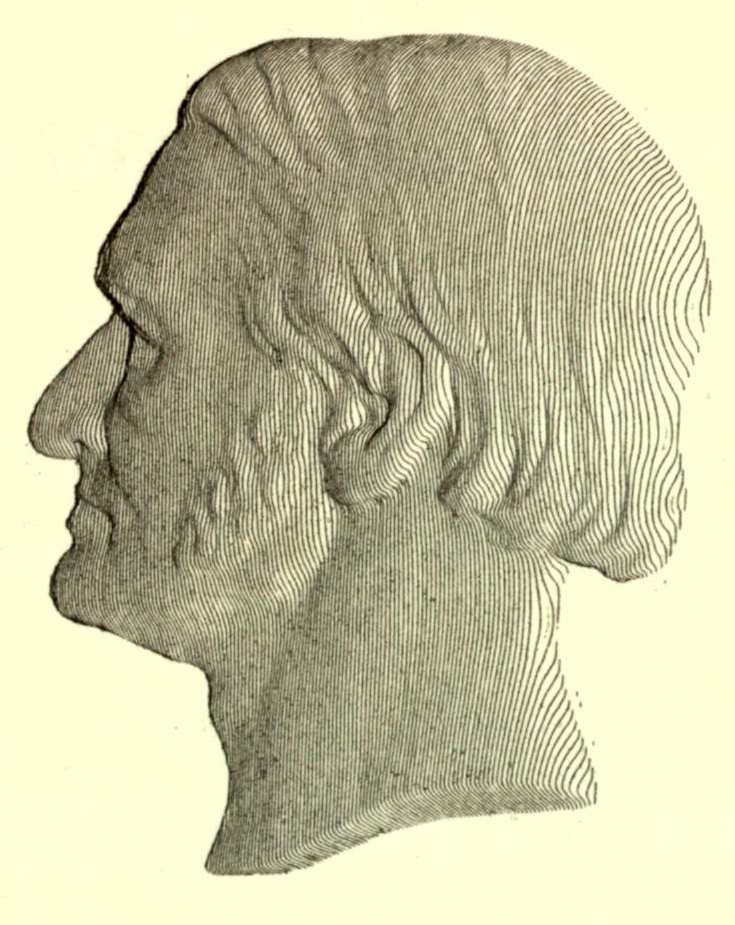
\includegraphics[height=2.05in]{illustrations/native004_portrait.png}\par
\vfill
{\fontsize{8.4}{11}\selectfont\leavevmode
\special{pdf:literal direct /Span << /ActualText (HERAUSGEGEBEN) >> BDC}%
\textls[355]{HERAUSGEGEBEN}%
\special{pdf:literal direct EMC}\par}
\vspace{11pt}
{\fontsize{5.8}{8}\selectfont\bfseries VON DER\par}
\vspace{9pt}
{\fontsize{9.35}{12}\selectfont\bfseries KÖNIGLICHEN GESELLSCHAFT DER WISSENSCHAFTEN\par}
\vspace{10pt}
{\fontsize{5.8}{8}\selectfont\bfseries ZU\par}
\vspace{9pt}
{\fontsize{10.4}{13}\selectfont\bfseries\textls[120]{GÖTTINGEN}\par}
\vspace{10pt}
{\fontsize{9}{11}\selectfont\bfseries 1874.\par}
}
\vspace*{21pt}
\clearpage
\thispagestyle{empty}
\noindent\SourceLeaf{5}\null\par
\clearpage
%
\thispagestyle{empty}
\pdfbookmark[0]{Ausgabe und Quellen}{translation-sources}
\begin{center}\textbf{Ausgabe und Quellen}\end{center}
\noindent Diese KI-Übersetzung ins heutige Deutsch bietet die astronomischen Schriften aus Carl Friedrich Gauß’ \textit{Werken}, Band~VI (Göttingen, 1874): Abhandlungen, Beobachtungen, Briefauszüge und Besprechungen. Die historischen Titelblätter und das Porträt begleiten den Text, ebenso Ernst Scherings eigene Bemerkungen. Die Übersetzung folgt dem Text der Werkausgabe mit ihren historischen Auszügen und Anmerkungen. Bei deutschsprachigen Originalen handelt es sich um eine Wiedergabe im heutigen Deutsch. Die bandinternen Verweise behalten die Seitenzahlen der Ausgabe von 1874. Quellen und Parallelübersetzungen sind in den begleitenden Anmerkungen angegeben. Die Titelvignette stammt aus dem Digitalisat der \href{https://archive.org/details/werkecarlf06gausrich/page/n8/mode/1up}{University of California Libraries}.
\par\medskip\noindent\textbf{Elliptische Elemente der Pallas}
\par\smallskip
\noindent Diese KI-Übersetzung umfasst alle fünfzehn Artikel und die Tabellen von Gauß’ \textit{Disquisitio de elementis ellipticis Palladis}. Sie folgt dem lateinischen Text in den \textit{Werken}, Band~VI (Göttingen, 1874), einschließlich des historischen Titels der Abhandlung. Auch die in modernem Deutsch wiedergegebenen Bandtitel und das Porträt stammen aus dieser Ausgabe. Die Abhandlung wurde am 25.~November 1810 vorgelegt und 1811 in Band~I der \textit{Commentationes societatis regiae scientiarum Gottingensis recentiores} gedruckt. \href{https://gdz.sub.uni-goettingen.de/id/PPN236007467}{Göttinger Digitalisat}.
\par\smallskip\noindent Historische Paralleltexte sind der deutsche \href{https://www.digitale-sammlungen.de/de/view/bsb10538613?page=463}{Zeitschriftenauszug vom November 1811}, die von Anton Börsch und Paul Simon herausgegebene deutsche Teilübersetzung der Artikel~10--15 (Berlin, 1887, S.~118--128) und Hale F. Trotters \href{https://www.york.ac.uk/depts/maths/histstat/gausspallas.htm}{englischer Auszug} nach der französischen Übersetzung von Joseph Bertrand im Princeton Technical Report Nr.~5 (1957). Die Ausgabe von Börsch und Simon enthält ein Vorwort von Helmert. Die deutsche Terminologie zur Bahnbestimmung wurde auch mit E. F. M. Jochims \textit{Satellitenbewegung}, Band~III, Stand 9.~Februar 2022, S.~60 und 63, abgeglichen.
\par\smallskip\noindent Übersetzung und Satz wurden mit KI erstellt.
\clearpage
%
\thispagestyle{empty}\SourceLeaf{6}
\pdfbookmark[0]{Untersuchung über die elliptischen Elemente der Pallas. Titel}{palladis-title}
\begin{center}\vspace*{.45in}
{\Large UNTERSUCHUNG}\par\medskip
ÜBER DIE\par\medskip
{\LARGE ELLIPTISCHEN ELEMENTE DER PALLAS}\par\medskip
AUS DEN\par\medskip
OPPOSITIONEN DER JAHRE 1803, 1804, 1805, 1807, 1808, 1809\par\bigskip
VON\par\bigskip
{\large CARL FRIEDRICH GAUSS}\par\bigskip
DER KÖNIGLICHEN GESELLSCHAFT VORGELEGT AM XXV. NOV. MDCCCX.\par\vfill
\rule{.75\linewidth}{.3pt}\par\smallskip
Commentationes societatis regiae scientiarum Gottingensis recentiores. Vol.~\textsc{i}.\par
Göttingen \textsc{mdcccxi}.\par\smallskip
\rule{.75\linewidth}{.3pt}
\end{center}\clearpage
%
\SourceLeaf{8}
\pdfbookmark[0]{Untersuchung über die elliptischen Elemente der Pallas}{palladis}
\begin{center}
{\large UNTERSUCHUNG}\par\medskip
{\Large ÜBER DIE ELLIPTISCHEN ELEMENTE DER PALLAS}\par\medskip
AUS DEN OPPOSITIONEN DER JAHRE 1803, 1804, 1805, 1807, 1808, 1809.
\end{center}
\Article{1}
Der im März 1802 entdeckte Hauptplanet Pallas ist bisher siebenmal in periodischer Folge erschienen. Da der Planet aber am Tag seiner Entdeckung die Opposition zur Sonne schon überschritten hatte, zählt man bis jetzt nur sechs Oppositionen; die meisten davon wurden an mehreren Sternwarten recht gut beobachtet und konnten daher mit ausreichender Genauigkeit bestimmt werden. Ausnehmen muss man allein die Opposition von 1808. In diesem Jahr befand sich der Planet im Aphel seiner Bahn und bereitete den Beobachtern wegen seines schwachen Lichts erhebliche Schwierigkeiten. Um die Wahrheit zu sagen, haben ihn die Astronomen ein wenig vernachlässigt. Der angesehene \textsc{von Lindenau} lieferte zwar eine recht große Zahl von Rektaszensionen, die er um die Zeit der Opposition mit gewohnter Sorgfalt am ausgezeichneten Meridianfernrohr der Seeberger Sternwarte beobachtet hatte. Von anderer Seite konnte ich jedoch nur wenige und weit weniger sichere Deklinationen erhalten. Deshalb ließ sich diese Opposition nicht mit derselben Genauigkeit wie die übrigen bestimmen, und besonders die Breite blieb zu unsicher.
\Article{2}
Sobald die Beobachtungen einer Erscheinung abgeschlossen waren, pflegte ich sie jedes Jahr vollständig zu sammeln, sorgfältig zu prüfen und mit den Beobachtungen der Vorjahre zu verbinden, um daraus die elliptischen Elemente umso \SourceLeaf{9}genauer bestimmen zu können. Aus der letzten Rechnung dieser Art, die ich gegen Ende des Jahres 1807 ausführte, gingen die Elemente hervor, die im Januarheft 1808 des XVII. Bandes des Commercium literarium astronomicum des angesehenen \textsc{von Zach} veröffentlicht wurden. Sie stimmten mit allen vier bis dahin beobachteten Oppositionen sehr gut überein. Im folgenden Jahr hielt mich nach der fünften Opposition der Mangel an zuverlässigen Beobachtungen von neuen Rechnungen ab. Ich nahm sie erst wieder auf, als mir die 1809 um die sechste Opposition angestellten Beobachtungen erlaubten, die Rechnung für beide Oppositionen gemeinsam in Angriff zu nehmen. Ich habe sie in unseren Gelehrten Anzeigen vom 24. Februar 1810 angekündigt.

\Needspace{11\baselineskip}
Hier folgt eine Übersicht über alle sechs bisher beobachteten Oppositionen:
\begin{center}\small\setlength{\tabcolsep}{3pt}
\begin{tabular}{l r r|r|r|r}
\multicolumn{3}{c|}{\shortstack{Oppositionszeit am\\Göttinger Meridian}}&\shortstack{Tage seit Beginn\\des Jahres 1803}&\shortstack{Heliozentrische\\Länge}&\shortstack{Geozentrische\\Breite}\\\hline
1803 Juni&30.&$0^{\mathrm h}\;27^{\mathrm m}\;32^{\mathrm s}$&181.019120&$277^0\;39'\;24''0$&$+46^0\;26'\;36''0$\\
1804 Aug.&30.&$4\;58\;27$&608.207257&$337\;0\;36.1$&$+15\;1\;49.8$\\
1805 Nov.&29.&$11\;15\;4$&1064.468796&$67\;20\;42.9$&$-54\;30\;54.9$\\
1807 Mai&4.&$14\;37\;41$&1585.609502&$223\;37\;27.7$&$+42\;11\;25.6$\\
1808 Juli&26.&$21\;17\;32$&2034.887176&$304\;2\;59.7$&$+37\;43\;53.7$\\
1809 Sept.&22.&$16\;10\;20$&2457.673843&$359\;40\;4.4$&$-7\;22\;10.1$
\end{tabular}\end{center}
\Article{3}
Wenn Pallas sich genau auf einer Ellipse und nach den Gesetzen \textsc{Kepler}s bewegte, könnten die neuesten Elemente, die mit den vier Oppositionen der Jahre 1803, 1804, 1805, 1807 sehr gut übereinstimmen, nur noch sehr kleine Fehler enthalten. Sie müssten gewiss auch mit den nächsten Oppositionen bis auf eine oder zwei Bogenminuten übereinstimmen. Tatsächlich war die Übereinstimmung so weit davon entfernt, dass diese Elemente schon bei der fünften Opposition eine Abweichung von bis zu vier Bogenminuten zeigten und bei der sechsten um zwölf Bogenminuten abwichen. Unser Planet erfährt nämlich durch die übrigen Planeten, besonders durch Jupiter, so große Störungen, dass sich zwischen den Erscheinungen und einer rein elliptischen Bewegung keine genaue und dauerhafte Übereinstimmung erzielen lässt. Zugleich ist daraus ersichtlich, dass sich je nach den vier zugrunde gelegten Oppositionen jeweils andere Elemente ergeben. Das hat die Berechnung zweier weiterer Elementensysteme bestätigt, von denen ich das eine kürzlich aus den Oppositionen \SourceLeaf{10}der Jahre 1804, 1805, 1807, 1808 und das andere aus denen der Jahre 1805, 1807, 1808, 1809 abgeleitet habe. Damit sich diese verschiedenen Elementensysteme besser vergleichen lassen, gebe ich sie hier einzeln an.

\Needspace{14\baselineskip}
\begin{center}I.\quad\textit{Elliptische Elemente der Pallas aus den Oppositionen der Jahre}\par
1803, 1804, 1805, 1807.\end{center}
\begingroup\small\setlength{\tabcolsep}{2pt}
\noindent\begin{tabular}{@{}p{.51\linewidth}lr@{}}
Epoche der mittleren Länge für 1803 am Göttinger Meridian&. . . . . . . . . . . . . .&$221^0\;39'\;30''4$\\
Mittlere tägliche tropische Bewegung&. . . . . . . . . . . .&$770''2143$\\
Länge des Perihels 1803&. . . . . . . . . . . . .&$121^0\;3'\;11''4$\\
Länge des aufsteigenden Knotens 1803&. . . . . . . . . . .&$172\;28\;56.9$\\
Bahnneigung&. . . . . . . . . . . . . . . .&$34\;37\;41.0$\\
Exzentrizität $(=\sin.\,14^0\;10'\;58''81)$&. . . . . . . . . .&$0.2450198$\\
Logarithmus der großen Halbachse&. . . . . . . . . . . . .&$0.4423149$
\end{tabular}\par\endgroup

\Needspace{13\baselineskip}
\begin{center}II.\quad\textit{Elliptische Elemente der Pallas aus den Oppositionen der Jahre}\par
1804, 1805, 1807, 1808.\end{center}
\begingroup\small\setlength{\tabcolsep}{2pt}
\noindent\begin{tabular}{@{}p{.51\linewidth}lr@{}}
Epoche der mittleren Länge 1803&. . . . . . . . . . .&$221^0\;34'\;56''7$\\
Mittlere tropische tägliche Bewegung&. . . . . . . . . . . .&$770''4467$\\
Länge des Perihels 1803&. . . . . . . . . . . . .&$121^0\;5'\;22''1$\\
Länge des aufsteigenden Knotens 1803&. . . . . . . . . . .&$172\;28\;46.8$\\
Bahnneigung&. . . . . . . . . . . . . . . .&$34\;37\;31.5$\\
Exzentrizität $(=\sin.\,14^0\;10'\;4''08)$&. . . . . . . . . . .&$0.2447624$\\
Logarithmus der großen Halbachse&. . . . . . . . . . . . .&$0.4422276$
\end{tabular}\par\endgroup

\Needspace{13\baselineskip}
\begin{center}III.\quad\textit{Elliptische Elemente der Pallas aus den Oppositionen der Jahre}\par
1805, 1807, 1808, 1809.\end{center}
\begingroup\small\setlength{\tabcolsep}{2pt}
\noindent\begin{tabular}{@{}p{.51\linewidth}lr@{}}
Epoche der mittleren Länge 1803&. . . . . . . . . . .&$221^0\;23'\;24''6$\\
Mittlere tropische tägliche Bewegung&. . . . . . . . . . . .&$770''9265$\\
Länge des Perihels 1803&. . . . . . . . . . . . .&$120^0\;58'\;4''8$\\
Länge des aufsteigenden Knotens 1803&. . . . . . . . . . .&$172\;27\;52.4$\\
Bahnneigung&. . . . . . . . . . . . . . . .&$34\;36\;49.4$\\
Exzentrizität $(=\sin.\,14^0\;9'\;36''63)$&. . . . . . . . . . .&$0.2446335$\\
Logarithmus der großen Halbachse&. . . . . . . . . . . . .&$0.4420473$
\end{tabular}\par\endgroup
\SourceLeaf{11}
\Article{4}
Wie sich die elliptische Bahn eines Planeten aus vier Beobachtungen bestimmen lässt, von denen nur zwei vollständig sind, habe ich in Abschnitt II von Buch II der Theoria motus corporum coelestium gezeigt. Die dort angegebene Lösung behandelt die Aufgabe in größter Allgemeinheit. Im Sonderfall, dass die vier Beobachtungen Oppositionen sind, empfiehlt sich jedoch ein anderes Verfahren. Ich hoffe, dass seine Darstellung den Astronomen willkommen sein wird. Dieses Verfahren setzt zwar voraus, dass man jedes der Elemente näherungsweise kennt, oder wenigstens die vier Elemente Bahnneigung, Länge des Knotens, Länge des Perihels und Exzentrizität. Es spricht aber nichts dagegen, diese Kenntnis aus einer früheren Rechnung als bereits vorhanden vorauszusetzen. Das Wesentliche hängt von der Lösung der folgenden Aufgabe ab.
\begin{quote}\itshape
„Zu vier gegebenen Längen des Planeten in seiner Bahn, die gegebenen Zeitpunkten entsprechen, die Länge des Perihels, die Exzentrizität, die mittlere tägliche Bewegung und die Epoche der mittleren Länge finden“
\end{quote}
Die Lösung gebe ich im folgenden Artikel an.
\Article{5}
Da die Länge des Perihels als bereits näherungsweise bekannt vorausgesetzt wird, erhält man durch Abziehen dieser Länge von den Längen in der Bahn die näherungsweisen wahren Anomalien $v$, $v'$, $v''$, $v'''$. Dabei kann man jene Länge entweder als konstant ansehen oder, wenn ihre jährliche Änderung bekannt ist, auf die einzelnen Zeitpunkte entsprechend übertragen. Sei $e=\sin\varphi$ die näherungsweise Exzentrizität. Mit ihr berechne man nach den bekannten Verfahren die mittleren Anomalien $M$, $M'$, $M''$, $M'''$, die den wahren Anomalien $v$, $v'$, $v''$, $v'''$ entsprechen. Bezeichnen wir nun die Zeiten mit $t$, $t'$, $t''$, $t'''$, dann müssten ihre Differenzen $t'-t$, $t''-t'$, $t'''-t''$ den Differenzen $M'-M$, $M''-M'$, $M'''-M''$ proportional sein, wenn wir von den wahren Werten der Länge des Perihels und des Winkels $\varphi$ ausgegangen wären. Andernfalls erhält man die an diesen Größen anzubringenden Korrekturen auf folgende Weise. Setzt man
\[
\begin{aligned}
m&=-\frac{\cos\varphi^3}{(1+e\cos v)^2},&n&=\frac{m(2+e\cos v)\sin v}{\cos\varphi'}\\[6pt]
m'&=-\frac{\cos\varphi^3}{(1+e\cos v')^2},&n'&=\frac{m'(2+e\cos v')\sin v'}{\cos\varphi}\\[6pt]
m''&=-\frac{\cos\varphi^3}{(1+e\cos v'')^2},&n''&=\frac{m''(2+e\cos v'')\sin v''}{\cos\varphi}\\[6pt]
m'''&=-\frac{\cos\varphi^3}{(1+e\cos v''')^2},&n'''&=\frac{m'''(2+e\cos v''')\sin v'''}{\cos\varphi}
\end{aligned}
\]
\noindent\SourceLeaf{12}
so folgt aus Artikel 15 der Theoria Motus Corporum Coelestium, dass sich bei einer Korrektur des Perihels um den kleinen Zuwachs $\mathrm d\Pi$ und des Winkels $\varphi$ um den Zuwachs $\mathrm d\varphi$ für die mittleren Anomalien die korrigierten Werte ergeben
\[
\begin{gathered}
M+m\mathrm d\Pi+n\mathrm d\varphi\\
M'+m'\mathrm d\Pi+n'\mathrm d\varphi\\
M''+m''\mathrm d\Pi+n''\mathrm d\varphi\\
M'''+m'''\mathrm d\Pi+n'''\mathrm d\varphi
\end{gathered}
\]
sofern man Potenzen und Produkte der Korrekturen $\mathrm d\Pi$, $\mathrm d\varphi$ vernachlässigen darf. Man erhält also drei Ausdrücke für die mittlere tägliche Bewegung in Bezug auf das Perihel, nämlich
\[
\begin{gathered}
\frac{M'-M}{t'-t}+\frac{m'-m}{t'-t}\mathrm d\Pi+\frac{n'-n}{t'-t}\mathrm d\varphi\\[5pt]
\frac{M''-M'}{t''-t'}+\frac{m''-m'}{t''-t'}\mathrm d\Pi+\frac{n''-n'}{t''-t'}\mathrm d\varphi\\[5pt]
\frac{M'''-M''}{t'''-t''}+\frac{m'''-m''}{t'''-t''}\mathrm d\Pi+\frac{n'''-n''}{t'''-t''}\mathrm d\varphi
\end{gathered}
\]
Aus ihrer Gleichheit ergeben sich die Unbekannten $\mathrm d\Pi$, $\mathrm d\varphi$. Setzt man diese in einen der Ausdrücke ein, so ergibt sich die korrigierte mittlere Bewegung, aus der nach dem bekannten Verfahren auch die große Halbachse bestimmt wird. Setzt man schließlich die Werte der Korrekturen $\mathrm d\Pi$, $\mathrm d\varphi$ in den Ausdruck für eine beliebige mittlere Anomalie ein, so ergibt sich daraus ihr korrigierter Wert und damit die auf einen beliebigen Zeitpunkt zu übertragende Epoche der mittleren Länge.

Übrigens ist leicht einzusehen, wie sich bei Bedarf sowohl die periodischen als auch die säkularen Störungen berücksichtigen lassen. Man muss die gegebenen Längen in der Bahn lediglich von den periodischen Störungen befreien, bevor man sie in die Rechnung einführt. Mithilfe der säkularen Störungen sind dagegen die für eine beliebige Epoche angenommenen Werte für die Länge des Perihels und die Exzentrizität auf die einzelnen Zeitpunkte $t$, $t'$, $t''$, $t'''$ zu übertragen.
\Article{6}
Sehen wir nun, wie sich dies zur Bestimmung der Bahn aus vier beobachteten Oppositionen verwenden lässt. Bei der ersten Opposition sei die Länge des Planeten in der Ekliptik $\alpha$, die geozentrische Breite $\beta$, der Abstand der Erde von der Sonne $R$, die näherungsweise Länge des aufsteigenden Knotens $\AscendingNode$ und die näherungsweise Neigung der Bahnebene gegen die Ekliptik $i$. Die zu den übrigen Oppositionen gehörenden Größen bezeichne ich mit entsprechenden Zeichen, die sich durch einen, zwei oder drei Indizes unterscheiden. Aus $\alpha$, $\AscendingNode$, $i$ ergibt sich die Länge in der Bahn nach der bekannten
\SourceLeaf{13}Formel. Den drei übrigen Längen in der Ekliptik legt man eine entsprechende Rechnung zugrunde. Aus diesen vier Längen in der Bahn leitet man nach den Vorschriften des vorhergehenden Artikels die elliptischen Elemente ab und daraus nach den bekannten Formeln die vier Radiusvektoren $r$, $r'$, $r''$, $r'''$. Setzt man nun
\[
\frac{R\sin\beta}{r}=\sin(\beta-\gamma),\qquad \frac{R'\sin\beta'}{r'}=\sin(\beta'-\gamma')\quad\text{etc.}
\]
so sind $\gamma$, $\gamma'$, $\gamma''$, $\gamma'''$ offenbar die vier heliozentrischen Längen, die aus den geozentrischen Breiten abgeleitet wurden. Leiten wir dieselben Größen aus den Längen ab, indem wir setzen
\[
\operatorname{tang}i\sin(\alpha-\AscendingNode)=\operatorname{tang}\delta,\qquad \operatorname{tang}i\sin(\alpha'-\AscendingNode)=\operatorname{tang}\delta'\ \text{etc.}
\]
Offenbar müsste dann $\gamma=\delta$, $\gamma'=\delta'$, $\gamma''=\delta''$, $\gamma'''=\delta'''$ gelten, wenn für $\AscendingNode$ und $i$ die wahren Werte eingesetzt worden wären und sich alle vier Oppositionen, durch die die Aufgabe überbestimmt ist, mit derselben Ellipse darstellen ließen. Ergibt sich etwas anderes, so erhält man die Korrekturen $\mathrm d\AscendingNode$, $\mathrm di$ für die Größen $\AscendingNode$, $i$ auf folgende Weise. Soweit diese Korrekturen als kleine Größen erster Ordnung gelten, deren Potenzen und Produkte man vernachlässigen darf, ergeben sich bei Verwendung der Werte $\AscendingNode+\mathrm d\AscendingNode$, $i+\mathrm di$ anstelle der Breiten $\gamma$, $\delta$, $\gamma'$, $\delta'$ usw. offenbar andere Breiten von folgender Form
\[
\begin{array}{ll}
\gamma+a\mathrm d\AscendingNode+b\mathrm di,&\delta+c\mathrm d\AscendingNode+f\mathrm di\\
\gamma'+a'\mathrm d\AscendingNode+b'\mathrm di,&\delta'+c'\mathrm d\AscendingNode+f'\mathrm di\quad\text{etc.}
\end{array}
\]
wobei man die Koeffizienten $c$, $f$, $c'$, $f'$ usw. nach den folgenden Formeln findet
\[
\begin{array}{ll}
c=-\frac12\sin2\delta\operatorname{cotang}(\alpha-\AscendingNode),&f=\dfrac{\sin2\delta}{\sin2i}\\[5pt]
c'=-\frac12\sin2\delta'\operatorname{cotang}(\alpha'-\AscendingNode),&f'=\dfrac{\sin2\delta'}{\sin2i}\quad\text{etc.}
\end{array}
\]
Die Koeffizienten $a$, $b$ usw. könnten wir ebenfalls auf analytischem Weg bestimmen, doch ziehe ich das folgende Verfahren vor. Ich wiederhole die eben beschriebene Rechnung und setze anstelle der Knotenlänge $\AscendingNode$ einen anderen Wert ein, der sich von ihr um einen kleinen, beliebig gewählten Betrag unterscheidet. Daraus lassen sich die Zahlenwerte der Koeffizienten $a$, $a'$ usw. leicht gewinnen. Wiederholt man dieselbe Rechnung mit einer geringfügig geänderten Bahnneigung, erhält man entsprechend die Werte der Koeffizienten $b$, $b'$ usw. Zugleich zeigt sich so, wie groß die Korrekturen der elliptischen Elemente ausfallen, wenn die Größen $\AscendingNode$, $i$ kleine Korrekturen erfahren.

\SourceLeaf{14}
Damit liegen zur Bestimmung der Korrekturen $\mathrm d\AscendingNode$, $\mathrm di$ \textit{vier} Gleichungen vor
\[
\begin{gathered}
\gamma-\delta+(a-c)\mathrm d\AscendingNode+(b-f)\mathrm di=0\\
\gamma'-\delta'+(a'-c')\mathrm d\AscendingNode+(b'-f')\mathrm di=0\\
\gamma''-\delta''+(a''-c'')\mathrm d\AscendingNode+(b''-f'')\mathrm di=0\\
\gamma'''-\delta'''+(a'''-c''')\mathrm d\AscendingNode+(b'''-f''')\mathrm di=0
\end{gathered}
\]
Wegen der unvermeidlichen Beobachtungsfehler lassen sich diese Gleichungen kaum genau erfüllen. Die am besten geeigneten Werte der Unbekannten $\mathrm d\AscendingNode$, $\mathrm di$ werden daher nach den in Abschnitt III von Buch II der Theoria Motus Corporum Coelestium erläuterten Grundsätzen bestimmt. Daraus lassen sich nach dem eben Gesagten zugleich die Korrekturen der übrigen Elemente leicht ableiten,
\Article{7}
Diesen Vorschriften möchte ich noch einige Bemerkungen hinzufügen.

I. Es bedarf kaum des Hinweises, dass unsere Formeln auch dann anwendbar sind, wenn die Knoten nicht als ruhend betrachtet werden. Man braucht den angenommenen Wert der Knotenlänge nur von seiner Epoche auf die vier Zeitpunkte umzurechnen und diese vier verschiedenen Werte in den Formeln für die jeweiligen vier Örter zu verwenden. Dasselbe gilt für die Bahnneigung, sofern ihre säkulare Änderung bekannt geworden ist und ihre Berücksichtigung lohnend erscheint. Will man außerdem die Störungen der heliozentrischen Breite in die Rechnung aufnehmen, so muss man sie in den vorhergehenden Gleichungen offenbar entweder von $\gamma$, $\gamma'$, $\gamma''$, $\gamma'''$ abziehen oder zu $\delta$, $\delta'$, $\delta''$, $\delta'''$ addieren.

III. Wenn die Bahnneigung und die Exzentrizität mäßig sind, werden die Koeffizienten $a$, $b$, $a'$, $b'$ usw. so klein, dass man sie vernachlässigen und damit auf die oben vorgeschriebene zweite und dritte Rechnung verzichten kann. Hat man dann die Korrekturen $\mathrm d\AscendingNode$, $\mathrm di$ gefunden, so muss man, sofern sie nicht zufällig sehr klein ausfallen, die Längen in der Bahn aus den korrigierten Werten der Knotenlänge und der Bahnneigung, also $\AscendingNode+\mathrm d\AscendingNode$, $i+\mathrm di$, neu berechnen. Weichen die korrigierten Längen in der Bahn um mehrere Bogensekunden von den früheren unkorrigierten ab, so muss man die elliptischen Elemente nach Artikel 5 erneut berechnen. Übrigens wird man die Koeffizienten $m$, $n$, $m'$ usw. kaum je neu berechnen müssen, da sich ihre Werte schon aus der ersten Annahme hinreichend genau ergeben.
\SourceLeaf{15}
\Article{8}
Zur besseren Erläuterung der vorhergehenden Vorschriften gebe ich hier die vollständige Rechnung an, mit der das dritte Elementensystem aus den Oppositionen der Jahre 1805, 1807, 1808, 1809 bestimmt wurde. Ich setzte die Länge des aufsteigenden Knotens für den Beginn des Jahres 1803 zu $172^0\,28'\,46''8=\AscendingNode$ und die Bahnneigung zu $34^0\,37'\,31''5$ an. Jene Länge rechnete ich auf die Zeitpunkte der einzelnen Oppositionen um, indem ich die Präzession $2'\,26''01$, $3'\,37''50$, $4'\,39''12$, $5'\,37''11$ addierte. Anschließend leitete ich aus den Längen die heliozentrischen Breiten ab
\[
\begin{array}{rrr}
\delta=-33^0&40'&50''63\\
\delta'=+28&14&51.24\\
\delta''=+27&20&55.86\\
\delta'''=-4&52&28.44
\end{array}
\]
\[
\begin{array}{ll}
c=+0.1252,&f=-0.9870\\
c'=-0.3366.&f'=+0.8917\\
c''=+0.3609.&f''=+0.8727\\
c'''=+0.6803,&f'''=-0{,}1811
\end{array}
\]
Ferner ergeben sich die Breitenargumente
\[
\begin{array}{rrr}
257^0&25'&6''73\\
56&24&5.96\\
126&2&55.07\\
188&36&2.69
\end{array}
\]
aus denen die elliptischen Elemente zu ermitteln sind. Dazu setze ich den Winkel $\varphi=14^0\,10'\,4''08$, wie er im zweiten Elementensystem gefunden wurde, und die Länge des Perihels für den Beginn des Jahres 1803 $=121^0\,5'\,22''1$. Das Perihel wird ebenso wie der Knoten gegenüber den Fixsternen als unbeweglich vorausgesetzt. Sein Abstand vom aufsteigenden Knoten ist daher konstant $=308^0\,36'\,35''3$. Nach den bekannten Formeln erhalten wir damit die folgenden Werte.
\[
\begin{array}{rrr@{\quad}rrr}
v=308^0&48'&31''43,&M=328^0&15'&45''08\\
v'=107&47&30.66,&M'=79&46&27.05\\
v''=177&26&19.77,&M''=175&54&28.87\\
v'''=239&59&27.39,&M'''=266&29&57.59
\end{array}
\]
\SourceLeaf{16}
\[
\begin{array}{ll}
m=-0.68517,&n=+1.18569\\
m'=-1.06482,&n=-2.01318\\
m''=-1.59701,&n=-0.12921\\
m'''=-1.18352,&n=+1.93947
\end{array}
\]
Bezeichnen wir also die Korrektur der Länge des Perihels mit $\mathrm d\Pi$ und die Korrektur des Winkels $\varphi$ mit $\mathrm d\varphi$, so ergibt sich die mittlere siderische Bewegung

von der ersten bis zur zweiten Opposition innerhalb von $521.140706$ Tagen
\[
111^0\,30'\,41''97-0.37965\mathrm d\Pi-3.19887\mathrm d\varphi
\]
von der zweiten bis zur dritten Opposition innerhalb von $449.277674$ Tagen
\[
96^0\,8'\,1''82-0.53219\mathrm d\Pi+1.88397\mathrm d\varphi
\]
von der dritten bis zur vierten Opposition innerhalb von $422.786667$ Tagen
\[
90^0\,35'\,28''72+0.41349\mathrm d\Pi+2.06868\mathrm d\varphi
\]
Daraus ergeben sich drei Ausdrücke für die mittlere tägliche siderische Bewegung
\[
\begin{gathered}
770''31398-0.0007285\mathrm d\Pi-0.0061382\mathrm d\varphi\\
770.30718-0.0011845\mathrm d\Pi+0.0041933\mathrm d\varphi\\
771.37892+0.0009780\mathrm d\Pi+0.0048930\mathrm d\varphi
\end{gathered}
\]
aus deren Vergleich sich die folgenden Gleichungen ergeben
\[
\begin{gathered}
0=0''00680+0.0004560\mathrm d\Pi-0.0103315\mathrm d\varphi\\
0=-1.07174-0.0021625\mathrm d\Pi-0.0006997\mathrm d\varphi
\end{gathered}
\]
daraus $\mathrm d\Pi=-488''82$, $\mathrm d\varphi=-20''92$, und folglich
\begin{center}\fontsize{9}{11}\selectfont\setlength{\tabcolsep}{3pt}\begin{tabular}{lr}
korrigierte Länge des Perihels zu Beginn des Jahres 1803,&$120^0\,57'\,13''28$,\\
und korrigierter Wert des Winkels $\ .\ .\ .\ .\ .\ .$&$\varphi=14^0\,9'\,43''16$\\
ferner ergibt sich die mittlere tägliche siderische Bewegung $\ .\ .\ .\ .\ .$&$770''7985$\\
korrigierte mittlere Anomalie für die erste Opposition $\ .$&$328^0\,20'\,55''20$\\
mittlere Länge für dieselbe Epoche $\ .\ .\ .\ .\ .$&$89^0\,20'\,34''49$
\end{tabular}\end{center}
Schließlich ergibt sich aus der mittleren siderischen Bewegung der Logarithmus der großen Halbachse $0.4420439$ und damit der Logarithmus des Halbparameters $0.4152361$. Da wir nun die korrigierten Werte der wahren Anomalien haben
\SourceLeaf{17}
\[
\begin{array}{rrr}
v=308^0&56'&40''25\\
v'=107&55&39.48\\
v''=177&34&28.59\\
v'''=240&7&36.21
\end{array}
\]
berechnet man die Logarithmen der Radiusvektoren
\[
\begin{aligned}
\log r&=0.3531088\\
\log r'&=0.4492406\\
\log r''&=0.5369700\\
\log r'''&=0.4716739
\end{aligned}
\]
Aus den Sonnentafeln haben wir ferner
\[
\begin{aligned}
\log R&=9.9937332\\
\log R'&=0.0039862\\
\log R''&=0.0065917\\
\log R'''&=0.0011160
\end{aligned}
\]
woraus wir schließlich ableiten
\[
\begin{array}{rrr}
\gamma=-33^0&39'&48''15\\
\gamma'=+28&15&0.73\\
\gamma''=+27&20&9.07\\
\gamma'''=-4&52&53.99
\end{array}
\]

Um die Koeffizienten $a$, $b$ usw. zu erhalten, bilde ich eine \textit{zweite Annahme}. Ich behalte die Bahnneigung bei, vergrößere aber die Knotenlänge um eine Bogenminute, sodass sie für den Beginn des Jahres 1803 $172^0\,29'\,46''8$ beträgt. Setzt man dann wie in der ersten Annahme die Länge des Perihels für dieselbe Epoche $=121^0\,5'\,22''1$, so findet man die wahren Anomalien
\[
\begin{array}{rrr}
v=308^0&48'&40''93\\
v'=107&47&34.06\\
v''=177&26&22.25\\
v'''=239&59&15.00
\end{array}
\]
und daraus, wenn man wieder $\varphi=14^0\,10'\,4''08$ setzt, die mittleren Anomalien
\SourceLeaf{18}
\[
\begin{array}{rrr}
M=328^0&15'&51''59\\
M'=79&46&30.67\\
M''=175&54&32.83\\
M'''=266&29&42.93
\end{array}
\]
(Für diese Rechnung ist das übliche Verfahren übrigens entbehrlich. Es genügt, zu den in der ersten Annahme gefundenen Werten der mittleren Anomalien die Produkte aus den positiv genommenen Koeffizienten $m$, $m'$, $m''$, $m'''$ und den Differenzen zwischen den entsprechenden Werten der wahren Anomalien in beiden Annahmen zu addieren, nämlich
\[
\begin{aligned}
+9''50\times0.68517&=+6''51\\
+3.40\times1.06482&=+3.62\\
+2.48\times1.59701&=+3.96\\
-12.39\times1.18352&=-14.66)
\end{aligned}
\]
Behält man die Werte der Koeffizienten $m$, $n$ usw. bei, so erhält man daraus
\begin{center}\fontsize{9}{11}\selectfont\setlength{\tabcolsep}{3pt}\begin{tabular}{p{.23\linewidth}p{.70\linewidth}}
$\mathrm d\Pi=-468''21$,&Länge des Perihels zu Beginn des Jahres 1803, $120^0\,57'\,33''89$\\
$\mathrm d\varphi=-20''62$,&$\varphi=14^0\,9'\,43''46$
\end{tabular}\end{center}
\begin{center}\fontsize{9}{11}\selectfont\setlength{\tabcolsep}{3pt}\begin{tabular}{ll}
mittlere tägliche siderische Bewegung&$=770''7761$\\
Logarithmus der großen Halbachse&$=0.4420523$\\
mittlere Länge bei der ersten Opposition&$=89^0\,20'\,47''85$
\end{tabular}\end{center}
\[
\begin{array}{rrr}
\gamma=-33^0&39'&51''10\\
\gamma'=+28&15&1.27\\
\gamma''=+27&20&10.97\\
\gamma'''=-4&52&54.66
\end{array}
\]

Schließlich bilde ich eine \textit{dritte Annahme}, indem ich $\AscendingNode=172^0\,28'\,46''6$, $i=34^0\,38'\,31''5$ setze. Daraus ergibt sich wie zuvor
\begin{center}\fontsize{9}{11}\selectfont\setlength{\tabcolsep}{3pt}\begin{tabular}{lr}
Länge des Perihels für den Beginn des Jahres 1803,&$120^0\,55'\,34''46$\\
&$\varphi=14^0\,9'\,52''63$\\
mittlere tägliche siderische Bewegung&$=770''8398$\\
Logarithmus der großen Halbachse&$=0.4420283$\\
mittlere Länge bei der ersten Opposition&$=89^0\,20'\,20''65$
\end{tabular}\end{center}
\SourceLeaf{19}
\[
\begin{array}{rrr}
\gamma=-33^0&39'&35''63\\
\gamma'=+28&15&5.20\\
\gamma''=+27&20&9.32\\
\gamma'''=-4&52&52.65
\end{array}
\]

Der Vergleich der Werte der heliozentrischen Breiten $\gamma$, $\gamma'$, $\gamma''$, $\gamma'''$, die in den drei Annahmen gefunden wurden, liefert
\[
\begin{array}{ll}
a=-0.0492,&b=+0.2087\\
a'=+0.0212,&b'=+0.0745\\
a''=+0.0317,&b''=+0.0042\\
a'''=-0.0112,&b'''=+0.0223
\end{array}
\]
Man erhält somit vier Gleichungen
\[
\begin{gathered}
+62''48-0.1744\mathrm d\AscendingNode+1.1957\mathrm di=0\\
+9.49+0.3578\mathrm d\AscendingNode-0.8172\mathrm di=0\\
-46.79-0.3292\mathrm d\AscendingNode-0.8685\mathrm di=0\\
-25.55-0.6915\mathrm d\AscendingNode+0.2034\mathrm di=0
\end{gathered}
\]
aus denen sich nach dem Prinzip der kleinsten Quadrate ergibt
\[
\begin{aligned}
\mathrm d\AscendingNode&=-54''41\\
\mathrm di&=-42.06
\end{aligned}
\]
sodass man erhält
\begin{center}\fontsize{9}{11}\selectfont\setlength{\tabcolsep}{3pt}\begin{tabular}{lr}
Länge des aufsteigenden Knotens für den Beginn des Jahres 1803,&$172^0\,27'\,52''39$\\
Bahnneigung $\ .\ .\ .\ .\ .\ .\ .\ .\ .\ .$&$34\quad36\quad49.44$
\end{tabular}\end{center}

Die übrigen Elemente lassen sich entweder durch Vergleich der Ergebnisse der drei Annahmen gewinnen oder, genauer, durch eine neue Berechnung der Längen in der Bahn und durch Wiederholung der in Artikel 5 erläuterten Rechenschritte. Das erste Verfahren liefert
\begin{center}\fontsize{9}{11}\selectfont\setlength{\tabcolsep}{3pt}\begin{tabular}{lr}
Länge des Perihels 1803 $\ .\ .\ .\ .\ .\ .\ .$&$120^0\,58'\,3''86$\\
Winkel $\varphi\ .\ .\ .\ .\ .\ .\ .\ .\ .\ .\ .\ .\ .$&$14\quad9\quad36.25$\\
mittlere Länge bei der ersten Opposition $\ .\ .$&$89\quad20\quad32.08$\\
mittlere tägliche siderische Bewegung $\ .\ .\ .\ .\ .\ .\ .$&$770''7899$\\
Logarithmus der großen Halbachse. $\ .\ .\ .\ .\ ,\ .\ .$&$0.4420471$
\end{tabular}\end{center}
\SourceLeaf{20}
Mit dem anderen Verfahren erhält man
\begin{center}\fontsize{9}{11}\selectfont\setlength{\tabcolsep}{3pt}\begin{tabular}{lr}
Länge des Perihels 1803 $\ .\ .\ .\ .\ .\ .\ .\ .$&$120^0\,58'\,4''81$\\
Winkel $\varphi\ .\ .\ .\ .\ .\ .\ .\ .\ .\ .\ .\ .\ .$&$14\quad9\quad36.63$\\
mittlere Länge bei der ersten Opposition $\ .\ .\ .\ .$&$89\quad20\quad31.81$\\
mittlere tägliche siderische Bewegung $\ .\ .\ .\ .\ .\ .\ .$&$770''7893$\\
Logarithmus der großen Halbachse $\ .\ .\ .\ .\ .\ .\ .\ .$&$0.4420473$
\end{tabular}\end{center}
Mit diesen Elementen stimmen die oben in Artikel 3 angegebenen überein.
\Article{9}
So groß die Störungen auch sein mögen, die Pallas durch die übrigen Planeten erfährt, so zeigt doch die Erfahrung, dass an vier Oppositionen angepasste elliptische Elemente der Bewegung des Planeten während dieses ganzen Zeitraums recht gut genügen. Sie weichen sogar von seiner vorhergehenden und nachfolgenden Bewegung nur wenig ab, sofern man den Zeitraum nicht zu groß wählt. So wich etwa das zweite der in Artikel 3 angegebenen Elementensysteme bei der Opposition von 1803 um drei und bei der Opposition von 1809 um fünf Bogenminuten von der beobachteten heliozentrischen Länge ab. Unter diesen Umständen scheint es mir zur Aufstellung einer Ephemeride für die künftige Bewegung des Planeten stets am zweckmäßigsten, rein elliptische Elemente zu verwenden, die aus den vier unmittelbar vorhergehenden Oppositionen abgeleitet wurden. Die Zahl der aus den Störungen entstehenden Gleichungen wird gewiss so groß werden, dass selbst die Berechnung eines einzigen heliozentrischen Orts des Planeten beinahe so aufwendig sein muss wie die Berechnung der elliptischen Elemente nach den oben angegebenen Vorschriften. So lässt sich der geozentrische Ort des Planeten stets mit einem Fehler von wenigen Bogenminuten sicher vorhersagen. Diese Genauigkeit genügt, um den Planeten aufzufinden.
\Article{10}
Doch die Würde der Wissenschaft verlangt, dass man auf eine dauerhaftere Übereinstimmung hinwirkt, die sich offensichtlich erst erzielen lässt, wenn die Störungen in die Rechnung aufgenommen werden. Nach meinem Urteil wäre eine so langwierige und mühsame Rechnung verfrüht gewesen, solange die verfügbaren Beobachtungen einen zu kurzen Zeitraum umfassten und sich die Störungen durch die übrigen Planeten kaum bemerkbar machten. Jetzt aber, da die elliptische Bewegung nicht mehr ausreicht, um alle beobachteten Örter miteinander in Einklang zu bringen, scheint die Zeit gekommen, in der man an eine genauere Theorie denken kann. Wie ich die Berechnung der Störungen, die Pallas vor allem durch Jupiter erfährt,
\SourceLeaf{21}
am zweckmäßigsten und genauesten ausführen zu können glaube, werde ich bald an anderer Stelle ausführlicher erläutern, da sich die bei anderen Planeten verwendeten Methoden wegen der übergroßen Exzentrizität und Bahnneigung kaum oder gar nicht anwenden lassen. Im Folgenden gehe ich noch auf die elliptischen Elemente ein, die sich als Grundlage der Störungsrechnung am besten zu eignen scheinen. Ich nehme mir vor, elliptische Elemente zu gewinnen, die nicht dieser oder jener Opposition genau genügen, sondern allen bisher beobachteten so gut wie möglich. Ein Verfahren zur Ausführung dieser Aufgabe habe ich bereits in Artikel 187 der Theoria Motus Corporum Coelestium kurz beschrieben. Was ich dort allgemein behandelt habe, lässt einige Abkürzungen zu, wenn die beobachteten Örter Oppositionen sind. Außerdem fehlen in jenem Werk einige praktische Kunstgriffe, mit denen ich seit Langem die Anwendung der Methode der kleinsten Quadrate zu erleichtern pflege. Ich hoffe daher, dass die Astronomen eine etwas ausführlichere Darstellung dieser Rechnungen hier begrüßen werden. Die ganze Aufgabe besteht darin, die \textit{Korrekturen} zu bestimmen, die zu den Näherungswerten der Elemente hinzuzufügen sind, von denen vorausgesetzt wird, dass sie von allen beobachteten Örtern nur wenig abweichen. Die ganze Arbeit hängt somit von zwei Schritten ab. Zunächst sind die linearen Gleichungen aufzustellen, die die einzelnen beobachteten Örter liefern. Dann sind aus diesen Gleichungen die am besten geeigneten Werte der Unbekannten zu gewinnen.
\Article{11}
Für die näherungsweisen Elemente bezeichnen die Symbole die folgenden Größen.
\begin{description}\setlength{\itemsep}{0pt}\setlength{\parsep}{0pt}
\item[$L$] die mittlere Länge des Planeten für eine beliebige Epoche
\item[$t$] die Zahl der Tage, die seit der Epoche bis zum Zeitpunkt der Beobachtung vergangen sind
\item[$\MeanMotionGlyph$] die mittlere tägliche siderische Bewegung in Bogensekunden
\item[$\Pi$] die Länge des Perihels
\item[$e=\sin\varphi$] die Exzentrizität
\item[$a$] die große Halbachse
\item[$r$] der Radiusvektor
\item[$v$] die wahre Anomalie
\item[$E$] die exzentrische Anomalie
\item[$\AscendingNode$] die Länge des aufsteigenden Knotens
\item[$i$] die Bahnneigung
\item[$u$] das Breitenargument
\item[$\lambda$] die heliozentrische Länge
\SourceLeaf{22}
\item[$\gamma$] die heliozentrische Breite
\item[$\ApproxBeta$] die geozentrische Breite
\item[$R$] der Abstand der Erde von der Sonne.
\end{description}
Aufgrund der Beobachtung setze ich dagegen die folgenden Werte an.
\begin{description}\setlength{\itemsep}{0pt}\setlength{\parsep}{0pt}
\item[$\alpha$] die heliozentrische Länge
\item[$\ObservedBeta$] die geozentrische Breite.
\end{description}
Schließlich bezeichne ich mit $\mathrm dL$, $\mathrm d\MeanMotionGlyph$, $\mathrm d\Pi$ usw. die Korrekturen der Größen $L$, $\MeanMotionGlyph$, $\Pi$ usw. Damit ist $\mathrm dL+t\mathrm d\MeanMotionGlyph$ die Korrektur der mittleren Länge,
$\mathrm dL+t\mathrm d\MeanMotionGlyph-\mathrm d\Pi$ ist die Korrektur der mittleren Anomalie,
und somit gilt nach Artikel 15 und 16 der Theoria Motus Corp. Coel.
\[
\begin{aligned}
\mathrm dv&=\frac{aa\cos\varphi}{rr}(\mathrm dL+t\mathrm d\MeanMotionGlyph-\mathrm d\Pi)+\frac{aa}{rr}(2-e\cos E-ee)\sin E\mathrm d\varphi\\
\mathrm dr&=\frac ra\mathrm da+a\operatorname{tang}\varphi\sin v(\mathrm dL+t\mathrm d\MeanMotionGlyph-\mathrm d\Pi)-a\cos\varphi\cos v\mathrm d\varphi
\end{aligned}
\]
Ferner ergibt sich als Korrektur des Breitenarguments $\mathrm du=\mathrm dv+\mathrm d\Pi-\mathrm d\AscendingNode$,
und nach Artikel 52 der Theoria Motus C. C. ergibt sich die Korrektur der heliozentrischen Länge aus
\[
\mathrm d\lambda=\mathrm d\AscendingNode-\operatorname{tang}\gamma\cos(\lambda-\AscendingNode)\mathrm di+\frac{\cos i}{\cos\gamma^2}\mathrm du
\]
Daraus folgt
\[
\begin{aligned}
\mathrm d\lambda={}&\frac{aa\cos\varphi\cos i}{rr\cos\gamma^2}\mathrm dL\\
&+\frac{taa\cos\varphi\cos i}{rr\cos\gamma^2}\mathrm d\MeanMotionGlyph\\
&+\left(\frac{\cos i}{\cos\gamma^2}-\frac{aa\cos\varphi\cos i}{rr\cos\gamma^2}\right)\mathrm d\Pi\\
&+\frac{aa\cos i}{rr\cos\gamma^2}(2-e\cos E-ee)\sin E\mathrm d\varphi\\
&+\left(1-\frac{\cos i}{\cos\gamma^2}\right)\mathrm d\AscendingNode\\
&-\operatorname{tang}\gamma\cos(\lambda-\AscendingNode)\mathrm di
\end{aligned}
\]
Da ferner gilt
\[
\begin{aligned}
a^{\frac32}\MeanMotionGlyph&=\mathrm{Const.}\\
r\sin(\ApproxBeta-\gamma)&=R\sin\ApproxBeta\\
\operatorname{tang}\gamma&=\operatorname{tang}i\sin(\alpha-\AscendingNode)
\end{aligned}
\]
ergibt sich durch Differentiation
\SourceLeaf{23}
\[
\frac{\mathrm da}{a}=-\frac{2\mathrm d\MeanMotionGlyph}{3\MeanMotionGlyph}
\]
\[
\frac{\mathrm dr}{r}+\operatorname{cotang}(\ObservedBeta-\gamma).(\mathrm d\ApproxBeta-\mathrm d\gamma)=\operatorname{cotg}\ApproxBeta\mathrm d\ApproxBeta,\quad\text{oder}
\]
\[
\mathrm d\ApproxBeta=\frac{\sin\ApproxBeta\cos(\ApproxBeta-\gamma)}{\sin\gamma}\mathrm d\gamma-\frac{\sin\ApproxBeta\sin(\ApproxBeta-\gamma)}{r\sin\gamma}\mathrm dr
\]
\[
\mathrm d\gamma=\frac{\sin2\gamma}{\sin2i}\mathrm di-\tfrac12\sin2\gamma\operatorname{cotang}(\alpha-\AscendingNode)\mathrm d\AscendingNode
\]
woraus sich mit dem oben entwickelten Ausdruck für $\mathrm dr$ ergibt
\[
\begin{aligned}
\mathrm d\ApproxBeta={}&-\frac{a\sin\ApproxBeta\sin(\ApproxBeta-\gamma)\operatorname{tang}\varphi\sin v}{r\sin\gamma}\mathrm dL\\
&+\left\{\frac{2\sin\ApproxBeta\sin(\ApproxBeta-\gamma)}{3\MeanMotionGlyph\sin\gamma}-\frac{at\sin\ApproxBeta\sin(\ApproxBeta-\gamma)\operatorname{tang}\varphi\sin v}{r\sin\gamma}\right\}\mathrm d\MeanMotionGlyph\\
&+\frac{a\sin\ApproxBeta\sin(\ApproxBeta-\gamma)\operatorname{tang}\varphi\sin v}{r\sin\gamma}\mathrm d\Pi\\
&+\frac{a\sin\ApproxBeta\sin(\ApproxBeta-\gamma)\cos\varphi\cos v}{r\sin\gamma}\mathrm d\varphi\\
&+\frac{2\sin\ApproxBeta\cos(\ApproxBeta-\gamma)\cos\gamma}{\sin2i}\mathrm di\\
&-\sin\ApproxBeta\cos(\ApproxBeta-\gamma)\cos\gamma\operatorname{cotang}(\alpha-\AscendingNode)\mathrm d\AscendingNode
\end{aligned}
\]
Als Werte der heliozentrischen Länge und der geozentrischen Breite ergeben sich aus den korrigierten Werten der Elemente also $\lambda+\mathrm d\lambda$, $\ApproxBeta+\mathrm d\ApproxBeta$. Damit liefert jede Opposition zwei Gleichungen
\[
\begin{aligned}
\alpha&=\lambda+\mathrm d\lambda\\
\ObservedBeta&=\ApproxBeta+\mathrm d\ApproxBeta
\end{aligned}
\]
\Article{12}
Wenden wir diese Vorschriften auf die sechs in Artikel 2 angegebenen Oppositionen der Pallas an
und legen wir der Rechnung das in Artikel 3 dargestellte zweite Elementensystem zugrunde, so erhalten wir die folgenden zwölf Gleichungen.

\noindent Aus der \textit{ersten} Opposition, mit der durch Rechnung gefundenen Länge $=277^0\,36'\,20''07$,
\[
\text{geozentrische Breite}=+46^0\,26'\,29''19:
\]
\[
\begin{aligned}
0={}&-183''93+0.79363\mathrm dL+143.66\mathrm d\MeanMotionGlyph+0.39493\mathrm d\Pi+0.95920\mathrm d\varphi\\
&-0.18856\mathrm d\AscendingNode+0.17387\mathrm di\\[4pt]
0={}&-6''81-0.02658\mathrm dL+46.71\mathrm d\MeanMotionGlyph+0.02658\mathrm d\Pi-0.20858\mathrm d\varphi\\
&+0.15946\mathrm d\AscendingNode+1.25782\mathrm di
\end{aligned}
\]
\SourceLeaf{24}
\Needspace{11\baselineskip}
Aus der \textit{zweiten} Opposition, mit der berechneten Länge $=337^0\,0'\,36''04$,
\[
\text{geozentrische Breite}=+15^0\,1'\,46''71:
\]
\[
\begin{aligned}
0={}&-0''06+0.58880\mathrm dL+358.12\mathrm d\MeanMotionGlyph+0.26208\mathrm d\Pi-0.85234\mathrm d\varphi\\
&+0.14912\mathrm d\AscendingNode+0.17775\mathrm di\\[4pt]
0={}&-3''09+0.01318\mathrm dL+28.39\mathrm d\MeanMotionGlyph-0.01318\mathrm d\Pi-0.07861\mathrm d\varphi\\
&+0.91704\mathrm d\AscendingNode+0.54365\mathrm di
\end{aligned}
\]
Aus der \textit{dritten} Opposition, mit der berechneten Länge $=67^0\,20'\,42''88$,
\[
\text{geozentrische Breite}=-54^0\,31'\,3''88:
\]
\[
\begin{aligned}
0={}&-0''02+1.73436\mathrm dL+1846.17\mathrm d\MeanMotionGlyph-0.54603\mathrm d\Pi-2.05662\mathrm d\varphi\\
&-0.18833\mathrm d\AscendingNode-0.17445\mathrm di\\[4pt]
0={}&-8''98-0.12606\mathrm dL-227.42\mathrm d\MeanMotionGlyph+0.12606\mathrm d\Pi-0.38939\mathrm d\varphi\\
&+0.17176\mathrm d\AscendingNode-1.35441\mathrm di
\end{aligned}
\]
Aus der \textit{vierten} Opposition, mit der berechneten Länge $=223^0\,37'\,25''39$,
\[
\text{geozentrische Breite}=+42^0\,11'\,28''07:
\]
\[
\begin{aligned}
0={}&-2''31+0.99584\mathrm dL+1579.03\mathrm d\MeanMotionGlyph+0.06456\mathrm d\Pi+1.99545\mathrm d\varphi\\
&-0.06040\mathrm d\AscendingNode-0.33750\mathrm di\\[4pt]
0={}&+2''47-0.08089\mathrm dL-67.22\mathrm d\MeanMotionGlyph+0.08089\mathrm d\Pi-0.09970\mathrm d\varphi\\
&-0.46359\mathrm d\AscendingNode+1.22803\mathrm di
\end{aligned}
\]
Aus der \textit{fünften} Opposition, mit der berechneten Länge $=304^0\,2'\,59''71$,
\[
\text{geozentrische Breite}=+37^0\,44'\,31''82:
\]
\[
\begin{aligned}
0={}&+0''01+0.65311\mathrm dL+1329.09\mathrm d\MeanMotionGlyph+0.38994\mathrm d\Pi-0.08439\mathrm d\varphi\\
&-0.04305\mathrm d\AscendingNode+0.34268\mathrm di\\[4pt]
0={}&+38''12-0.00218\mathrm dL+38.47\mathrm d\MeanMotionGlyph+0.00218\mathrm d\Pi-0.18710\mathrm d\varphi\\
&+0.47301\mathrm d\AscendingNode-1.14371\mathrm di
\end{aligned}
\]
Aus der \textit{sechsten} Opposition, mit der berechneten Länge $=359^0\,34'\,46''67$,
\[
\text{geozentrische Breite}=-7^0\,20'\,12''13:
\]
\[
\begin{aligned}
0={}&-317''73+0.69957\mathrm dL+1719.32\mathrm d\MeanMotionGlyph+0.12913\mathrm d\Pi-1.38787\mathrm d\varphi\\
&+0.17130\mathrm d\AscendingNode-0.08360\mathrm di\\[4pt]
0={}&+117''97-0.01315\mathrm dL-43.84\mathrm d\MeanMotionGlyph+0.01315\mathrm d\Pi+0.02929\mathrm d\varphi\\
&+1.02138\mathrm d\AscendingNode-0.27187\mathrm di
\end{aligned}
\]
Von diesen zwölf Gleichungen werden wir jedoch die zehnte ganz verwerfen, da die beobachtete geozentrische Breite zu unsicher ist.
\SourceLeaf{25}
\Article{13}
Da sich die sechs Unbekannten $\mathrm dL$, $\mathrm d\MeanMotionGlyph$ usw. nicht so bestimmen lassen, dass alle elf Gleichungen genau erfüllt sind, das heißt, dass die einzelnen Funktionen der Unbekannten auf der rechten Seite gleichzeitig $=0$ werden, werden wir diejenigen Werte ermitteln, für die die Summe der Quadrate dieser Funktionen möglichst klein ist. Sind allgemein die folgenden linearen Funktionen der Unbekannten $p$, $q$, $r$, $s$ usw. gegeben
\[
\begin{aligned}
n+ap+bq+cr+ds+\text{etc.}&=w\\
n'+a'p+b'q+c'r+d's+\text{etc.}&=w'\\
n''+a''p+b''q+c''r+d''s+\text{etc.}&=w''\\
n'''+a'''p+b'''q+c'''r+d'''s+\text{etc.}&=w'''
\end{aligned}
\]
usw., so sind offenbar die Bedingungsgleichungen dafür, dass $ww+w'w'+w''w''+w'''w'''+\text{etc.}=\Omega$ ein Minimum wird, die folgenden
\[
\begin{aligned}
aw+a'w'+a''w''+a'''w'''+\text{etc.}&=0\\
bw+b'w'+b''w''+b'''w'''+\text{etc.}&=0\\
cw+c'w'+c''w''+c'''w'''+\text{etc.}&=0\\
dw+d'w'+d''w''+d'''w'''+\text{etc.}&=0\\
\text{etc.\quad oder}&
\end{aligned}
\]
wenn wir der Kürze halber bezeichnen
\[
\begin{array}{ll}
an+a'n'+a''n''+a'''n'''+\text{etc.}&\text{mit }[an]\\
aa+a'a'+a''a''+a'''a'''+\text{etc.}&\text{mit }[aa]\\
ab+a'b'+a''b''+a'''b'''+\text{etc.}&\text{mit }[ab]\\
\text{etc.}&\\
bb+b'b'+b''b''+b'''b'''+\text{etc.}&\text{mit }[bb]\\
bc+b'c'+b''c''+b'''c'''+\text{etc.}&\text{mit }[bc]\\
\text{etc. etc.}&
\end{array}
\]
sind $p$, $q$, $r$, $s$ usw. durch Elimination aus den folgenden Gleichungen zu bestimmen
\[
\begin{aligned}{}
[an]+[aa]p+[ab]q+[ac]r+[ad]s+\text{etc.}&=0\\
[bn]+[ab]p+[bb]q+[bc]r+[bd]s+\text{etc.}&=0\\
[cn]+[ac]p+[bc]q+[cc]r+[cd]s+\text{etc.}&=0\\
[dn]+[ad]p+[bd]q+[cd]r+[dd]s+\text{etc.}&=0\\
\text{etc.}&
\end{aligned}
\]
\SourceLeaf{26}
Sobald die Zahl der Unbekannten $p$, $q$, $r$, $s$ usw. etwas größer ist, erfordert die Elimination jedoch eine sehr langwierige und mühsame Rechnung, die sich auf folgende Weise erheblich verkürzen lässt. Außer den Koeffizienten $[an]$, $[aa]$, $[ab]$ usw., deren Zahl $=\tfrac12(ii+3i)$ ist, wenn die Zahl der Unbekannten $=i$ ist, setze ich auch voraus, dass $nn+n'n'+n''n''+n'''n'''+\text{etc.}=[nn]$ berechnet worden ist. Dann ist leicht einzusehen, dass gilt
\[
\begin{aligned}
\Omega={}&[nn]+2[an]p+2[bn]q+2[cn]r+2[dn]s+\text{etc.}\\
&+[aa]pp+2[ab]pq+2[ac]pr+2[ad]ps+\text{etc.}\\
&\qquad+[bb]qq+2[bc]qr+2[bd]qs+\text{etc.}\\
&\qquad\qquad+[cc]rr+2[cd]rs+\text{etc.}\\
&\qquad\qquad\qquad+[dd]ss+\text{etc.}\\
&\qquad\qquad\qquad\qquad\text{etc.}
\end{aligned}
\]
Bezeichnen wir also
\[
[an]+[aa]p+[ab]q+[ac]r+[ad]s+\text{etc.}\quad\text{mit}\quad A
\]
so ist klar, dass alle Teile von $\dfrac{A^2}{[aa]}$, die den Faktor $p$ enthalten, in $\Omega$ vorkommen und somit $\Omega-\dfrac{A^2}{[aa]}$ eine von $p$ unabhängige Funktion ist. Setzen wir daher
\[
\begin{aligned}{}
[nn]-\frac{[an]^2}{[aa]}&=[nn,1]\\
[bn]-\frac{[an].[ab]}{[aa]}&=[bn,1]\\
[cn]-\frac{[an].[ac]}{[aa]}&=[cn,1]\\
[dn]-\frac{[an].[ad]}{[aa]}&=[dn,1]\quad\text{etc.}\\
[bb]-\frac{[ab]^2}{[aa]}&=[bb,1]\\
[bc]-\frac{[ab].[ac]}{[aa]}&=[bc,1]\\
[bd]-\frac{[ab].[ad]}{[aa]}&=[bd,1]\quad\text{etc. etc.: ergibt sich}
\end{aligned}
\]
\[
\begin{aligned}
\Omega-\frac{A^2}{[aa]}={}&[nn,1]+2[bn,1]q+2[cn,1]r+2[dn,1]s+\text{etc.}\\
&+[bb,1]qq+2[bc,1]qr+2[bd,1]qs+\text{etc.}\\
&\qquad+[cc,1]rr+2[cd,1]rs+\text{etc.}\\
&\qquad\qquad+[dd,1]ss+\text{etc.}\\
&\qquad\qquad\qquad\text{etc.}
\end{aligned}
\]
Diese Funktion bezeichnen wir mit $\Omega'$.

\SourceLeaf{27}
Setzen wir ebenso
\[
[bn,1]+[bb,1]q+[bc,1]r+[bd,1]s+\text{etc.}=B
\]
so ist $\Omega'-\dfrac{B^2}{[bb,1]}$ eine von $q$ unabhängige Funktion, die wir $=\Omega''$ setzen. Auf dieselbe Weise setzen wir
\[
\begin{aligned}{}
[nn,1]-\frac{[bn,1]^2}{[bb,1]}&=[nn,2]\\
[cn,1]-\frac{[bn,1].[bc,1]}{[bb,1]}&=[cn,2]\\
[cc,1]-\frac{[bc,1]^2}{[bb,1]}&=[cc,2]\\
\text{etc. etc.\quad und}&
\end{aligned}
\]
\[
[cn,2]+[cc,2]r+[cd,2]s+\text{etc.}=C
\]
sodass $\Omega''-\dfrac{C^2}{[cc,2]}$ auch von $r$ unabhängig ist. Wir fahren ebenso fort, bis wir in der Folge $\Omega$, $\Omega'$, $\Omega''$ usw. zu einem von allen Unbekannten unabhängigen Glied gelangen. Es lautet $[nn,\mu]$, wenn die Zahl der Unbekannten $p$, $q$, $r$, $s$ usw. mit $\mu$ bezeichnet wird. Wir haben also
\[
\Omega=\frac{A^2}{[aa]}+\frac{B^2}{[bb,1]}+\frac{C^2}{[cc,2]}+\frac{D^2}{[dd,3]}+\text{etc.}+[nn,\mu]
\]
Da nun $\Omega=ww+w'w'+w''w''\text{ etc.}$ seiner Natur nach keinen negativen Wert annehmen kann, lässt sich leicht zeigen, dass die Divisoren $[aa]$, $[bb,1]$, $[cc,2]$, $[dd,3]$ usw. notwendig \textit{positiv} sein müssen (der Kürze halber führe ich diesen Beweis hier jedoch nicht näher aus). Daraus folgt unmittelbar, dass sich der kleinste Wert von $\Omega$ ergibt, wenn man $A=0$, $B=0$, $C=0$, $D=0$ usw. setzt. Aus diesen $(\mu)$ Gleichungen sind also die Unbekannten $p$, $q$, $r$, $s$ usw. zu bestimmen. Das gelingt sehr leicht in umgekehrter Reihenfolge, da die letzte Gleichung offenbar nur eine Unbekannte enthält, die vorletzte zwei und so weiter. Zugleich hat dieses Verfahren den Vorzug, dass sich daraus der kleinste Wert der Summe $\Omega$ unmittelbar ergibt, da er offenbar $=[nn,\mu]$ ist.
\Article{14}
Wenden wir diese Vorschriften nun auf unser Beispiel an. Hier sind $p$, $q$, $r$, $s$ usw. die Größen $\mathrm dL$, $\mathrm d\MeanMotionGlyph$, $\mathrm d\Pi$, $\mathrm d\varphi$, $\mathrm d\AscendingNode$, $\mathrm di$. Nach sorgfältiger Durchführung der Rechnung fand ich die folgenden Zahlenwerte.
\SourceLeaf{28}
{\fontsize{9}{11}\selectfont
\[
\begin{array}{lll}
\begin{gathered}{}
[nn]=148848\\
[an]=-371.09\\
[bn]=-580104\\
[cn]=-113.45\\
[dn]=+268.53\\
[en]=+94.26\\
[fn]=-31.81\\
[aa]=+5.91569\\
[ab]=+7203.91\\
[ac]=-0.09344\\
[ad]=-2.28516\\
[ae]=-0.34664\\
[af]=-0.18194\\
[bb]=+10834225\\
[bc]=-49.06\\
[bd]=-3229.77\\
[be]=-198.64\\
[bf]=-143.05\\
[cc]=+0.71917\\
[cd]=+1.13382\\
[ce]=+0.06400\\
[cf]=+0.26341\\
[dd]=+12.00340\\
[de]=-0.37137\\
[df]=-0{,}11762\\
[ee]=+2.28215\\
[ef]=-0.36136\\
[ff]=+5.62456\\[3pt]
\text{Daraus leitete ich ferner ab}\\[3pt]
[nn,1]=+125569\\
[bn,1]=-138534
\end{gathered}&
\begin{gathered}{}
[cn,1]=-119.31\\
[dn,1]=-125.18\\
[en,1]=+72.52\\
[fn,1]=-43.22\\
[bb,1]=+2458225\\
[bc,1]=+62.13\\
[bd,1]=-510.58\\
[be,1]=+213.84\\
[bf,1]=+73.45\\
[cc,1]=+0.71769\\
[cd,1]=+1.09773\\
[ce,1]=-0.05852\\
[cf,1]=+0.26054\\
[dd,1]=+11.12064\\
[de,1]=-0.50528\\
[df,1]=-0.18790\\
[ee,1]=+2.26185\\
[ef,1]=-0.37202\\
[ff,1]=+5.61905\\[3pt]
\text{Und daraus ebenso}\\[3pt]
[nn,2]=+117763\\
[cn,2]=-115.81\\
[dn,2]=-153.95\\
[en,2]=+84.57\\
[fn,2]=-39.08\\
[cc,2]=+0.71612\\
[cd,2]=+1.11063\\
[ce,2]=-0.06392\\
[cf,2]=+0.25868\\
[dd,2]=+11.01463\\
[de,2]=-0.46088
\end{gathered}&
\begin{gathered}{}
[df,2]=-0.17265\\
[ee,2]=+2.24325\\
[ef,2]=-0.37841\\
[ff,2]=+5.61686\\[3pt]
\text{Daraus ferner}\\[3pt]
[nn,3]=+99034\\
[dn,3]=+25.66\\
[en,3]=+74.23\\
[fn,3]=+2.75\\
[dd,3]=+9.29213\\
[de,3]=-0.36175\\
[df,3]=-0.57384\\
[ee,3]=+2.23754\\
[ef,3]=-0.35532\\
[ff,3]=+5.52342\\[3pt]
\text{Daraus auf dieselbe Weise}\\[3pt]
[nn,4]=+98963\\
[en,4]=+75.23\\
[fn,4]=+4.33\\
[ee,4]=+2.22346\\
[ef,4]=-0.37766\\
[ff,4]=+5.48798\\[3pt]
\text{Daraus}\\[3pt]
[nn,5]=+96418\\
[fn,5]=+17.11\\
[ff,5]=+5.42383\\[3pt]
\text{Und daraus schließlich}\\[3pt]
[nn,6]=+96364
\end{gathered}
\end{array}
\]
}
Zur Bestimmung der Unbekannten haben wir also die folgenden sechs Gleichungen.
\[
\begin{aligned}
0={}&+17''11+5.42383\mathrm di\\
0={}&+75''23+2.22346\mathrm d\AscendingNode-0.37766\mathrm di\\
0={}&+25''66+9.29213\mathrm d\varphi-0.36175\mathrm d\AscendingNode-0.57384\mathrm di\\
0={}&-115''81+0.71612\mathrm d\Pi+1.11063\mathrm d\varphi-0.06392\mathrm d\AscendingNode+0.25868\mathrm di\\
0={}&-13854''+2458225\mathrm d\MeanMotionGlyph+62.13\mathrm d\Pi-510.58\mathrm d\varphi+213{,}84\mathrm d\AscendingNode\\
&+73.45\mathrm di\\[4pt]
0={}&-371''09+5.91569\mathrm dL+7203.91\mathrm d\MeanMotionGlyph-0.09344\mathrm d\Pi-2.28516\mathrm d\varphi\\
&-0.34664\mathrm d\AscendingNode-0.18194\mathrm di
\end{aligned}
\]
\SourceLeaf{29}
aus denen sich ergibt
\[
\begin{aligned}
\mathrm di&=-3''15\\
\mathrm d\AscendingNode&=-34''37\\
\mathrm d\varphi&=-4''29\\
\mathrm d\Pi&=+166''44\\
\mathrm d\MeanMotionGlyph&=+0''054335\\
\mathrm dL&=-3''06
\end{aligned}
\]

Die korrigierten elliptischen Elemente, die allen sechs Oppositionen möglichst genau genügen, sind somit die folgenden.
\begin{center}\fontsize{9}{11}\selectfont\setlength{\tabcolsep}{3pt}\begin{tabular}{lr}
Epoche der mittleren Länge 1803, am Göttinger Meridian&$221^0\,34'\,53''64$\\
Mittlere tropische tägliche Bewegung $\ .\ .\ .\ .\ .\ .\ .\ .\ .\ .\ .\ .$&$770''5010$\\
Länge des Perihels 1803 $\ .\ .\ .\ .\ .\ .\ .\ .\ .\ .\ .\ .\ .$&$121^0\,8'\,8''54$\\
Länge des aufsteigenden Knotens 1803 $\ .\ .\ .\ .\ .\ .\ .\ .\ .\ .$&$172\quad28\quad12.43$\\
Bahnneigung $\ .\ .\ .\ .\ .\ .\ .\ .\ .\ .\ .\ .\ .\ .\ .$&$34\quad37\quad28.35$\\
Exzentrizität $=\sin14^0\,9'\,59''79\ .\ .\ .\ .\ .\ .\ .\ .\ .\ .\ .$&$0.2447424$\\
Logarithmus der großen Halbachse $\ .\ .\ .\ .\ .\ .\ .\ .\ .\ .\ .\ .$&$0.4422071$
\end{tabular}\end{center}
\Article{15}
Setzen wir die eben gefundenen Werte der Korrekturen $\mathrm dL$, $\mathrm d\MeanMotionGlyph$ usw. in die zwölf Gleichungen aus Artikel 12 ein, so erhalten wir die folgenden Differenzen zwischen den beobachteten und berechneten Werten der heliozentrischen Längen und der geozentrischen Breiten.
\begin{center}\begin{tabular}{c|r|r}
Bei der Opposition&\multicolumn{2}{c}{Differenz}\\
des Jahres&\multicolumn{1}{c|}{der Länge}&\multicolumn{1}{c}{der Breite}\\\hline
1803&$-111''00$&$-8''31$\\
1804&$+59.18$&$-36.67$\\
1805&$+19.92$&$+0.07$\\
1807&$+85.77$&$+25.01$\\
1808&$+135.88$&$+28.72$\\
1809&$-216.54$&$+83.01$
\end{tabular}\end{center}
%
\clearpage\thispagestyle{empty}
\pdfbookmark[0]{Quellen zu den Kometenbeobachtungen von 1813}{cometa1813-sources}
\begin{center}\textbf{Quellen zu den Kometenbeobachtungen von 1813}\end{center}
\noindent Diese KI-Übersetzung folgt dem lateinischen Text in Gauß’ \textit{Werken}, Band~VI (Göttingen, 1874), S.~25--36, einschließlich des Titelblatts. Die Abhandlung wurde der Königlichen Gesellschaft der Wissenschaften am 10.~September 1813 vorgelegt und in Band~II der \textit{Commentationes societatis regiae scientiarum Gottingensis recentiores} gedruckt. \href{https://gdz.sub.uni-goettingen.de/id/PPN236007467}{Göttinger Digitalisat}.
\par\smallskip\noindent Eine eigene \href{https://www.digitale-sammlungen.de/de/view/bsb10538617?page=517}{deutsche Übersetzung aus dem Lateinischen} erschien in der \textit{Monatlichen Correspondenz zur Beförderung der Erd- und Himmels-Kunde}, Band~28, Nr.~LVIII (Gotha, Dezember 1813), S.~501--513. Der Beitrag nennt keinen Übersetzer. Auf dem Bandtitel steht F.~von Zach als Herausgeber. Das Digitalisat stammt aus der Bayerischen Staatsbibliothek.
\par\smallskip\noindent Zum Vergleich der Fachbegriffe dienten Wilhelm Olbers’ \href{https://www.e-rara.ch/zut/content/titleinfo/449756}{Abhandlung über Kometenbahnen von 1797} aus der ETH-Bibliothek und Andreas Kammerers und Mike Kretlows \href{https://fg-kometen.vdsastro.de/Publ/kometen_beobachten_2.0.pdf}{\textit{Kometen beobachten}}, Ausgabe März 2010, S.~252--256.
\par\smallskip\noindent Übersetzung und Satz wurden mit KI erstellt.
\clearpage
%
\thispagestyle{empty}\SourceLeaf{30}
\pdfbookmark[0]{Beobachtungen des zweiten Kometen von 1813. Titel}{cometa1813-title}
\begin{center}\vspace*{.45in}
{\Large BEOBACHTUNGEN}\par\bigskip
{\LARGE DES ZWEITEN KOMETEN VON 1813}\par\bigskip
ANGESTELLT AN DER GÖTTINGER STERNWARTE\par\bigskip
MIT\par\bigskip
EINIGEN BEMERKUNGEN ZUR BERECHNUNG\par\medskip
PARABOLISCHER BAHNEN\par\bigskip
VON\par\bigskip
{\large CARL FRIEDRICH GAUSS}\par\bigskip
DER KÖNIGLICHEN GESELLSCHAFT DER WISSENSCHAFTEN AM 10. SEPTEMBER 1813 VORGELEGT.\par\vfill
\rule{.75\linewidth}{.3pt}\par\smallskip
Commentationes societatis regiae scientiarum Gottingensis recentiores. Bd.~\textsc{ii}.\par
Göttingen \textsc{mdcccxiii}.\par\smallskip
\rule{.75\linewidth}{.3pt}
\end{center}\clearpage
%
\SourceLeaf{32}
\fancyhead[L]{\small BEOBACHTUNGEN DES ZWEITEN KOMETEN VON 1813}
\renewcommand{\Article}[1]{\par\medskip\Needspace{4\baselineskip}\pdfbookmark[1]{Art. #1}{cometae-art-#1}\centerline{\textbf{#1.}}\nobreak\smallskip}
\pdfbookmark[0]{Beobachtungen des zweiten Kometen von 1813}{cometae}
\begin{center}
{\large BEOBACHTUNGEN}\par\medskip
{\Large DES ZWEITEN KOMETEN VON 1813}\par\medskip
ANGESTELLT AN DER GÖTTINGER STERNWARTE\par\medskip
MIT\par\medskip
EINIGEN BEMERKUNGEN ZUR BERECHNUNG PARABOLISCHER BAHNEN.\par\smallskip
\rule{.09\linewidth}{.3pt}
\end{center}

Am 7. April begann ich selbst, den Kometen an unserer Sternwarte zu beobachten, nachdem ihn mein lieber Kollege, der angesehene \textsc{Harding}, am 3. April dieses Jahres im Sternbild des Poniatowskischen Stiers entdeckt hatte. Mit einem Kreismikrometer, das an einem zehnfüßigen Fernrohr angebracht war, erhielt ich folgende Bestimmungen:
\begin{center}\small\setlength{\tabcolsep}{4pt}
\begin{tabular}{r|r|r|r l}
1813&Mittl. Gött. Zeit&Scheinb. Rektasz.&\multicolumn{2}{c}{Scheinb. Dekl.}\\\hline
Apr. 7&$13^{\mathrm h}\;12^{\mathrm m}\;2^{\mathrm s}$&$271^0\;7'\;19''3$&$5^0\;34'\;36''7$&Nördl.\\
9&$13\;35\;40$&$270\;10\;33.5$&$4\;11\;3.4$&—\\
11&$13\;17\;43$&$269\;1\;19.9$&$2\;33\;0.7$&—\\
14&$13\;7\;36$&$266\;44\;5.5$&$0\;33\;0.8$&Südl.\\
21&$14\;23\;0$&$256\;39\;19.3$&$12\;57\;56.0$&—
\end{tabular}\end{center}

Der angesehene \textsc{Harding} stellte später mit dem Mauerquadranten folgende Beobachtungen an:
\begin{center}\small\setlength{\tabcolsep}{4pt}
\begin{tabular}{r|r|r|r l}
Apr. 21&$15^{\mathrm h}\;7^{\mathrm m}\;21^{\mathrm s}$&$256^0\;34'\;19''6$&$13^0\;2'\;26''5$&Südl.\\
24&$14\;22\;50$&$248\;23\;21$&$21\;45\;2$&\\
25&$14\;4\;21$&$244\;44\;42$&$25\;10\;42$&
\end{tabular}\end{center}

Am 24. und 25. April war der Komet auch mit bloßem Auge sehr deutlich zu sehen. In den folgenden Nächten war der Himmel von Wolken bedeckt, und bald setzte der rasche Abstieg des Kometen nach Süden den Beobachtungen ein Ende.

\SourceLeaf{33}\SourceGathering{4\textsuperscript{*}}
Es scheint überflüssig, hier die parabolischen Elemente zu wiederholen, die ich gleich zu Beginn selbst aus den ersten drei Beobachtungen abgeleitet hatte. Mit ihrer genaueren Ausarbeitung betraute ich einen sehr geübten und erfahrenen Rechner, Dr. \textsc{Gerling}. Ihm verdanken wir die folgenden korrigierten Elemente, die so gut wie möglich an alle Beobachtungen angepasst sind, sowohl an unsere eigenen als auch an die, die der angesehene \textsc{Olbers} übersandt hatte.
\par\medskip
\noindent\begin{minipage}{.975\linewidth}\small
\noindent\makebox[\linewidth][s]{Logarithmus der Periheldistanz\hfill.\hfill.\hfill.\hfill.\hfill.\hfill.\hfill.\hfill.\hfill.\hfill.\hfill$0.0849212$}\par
\noindent Zeit des Periheldurchgangs für den Göttinger Meridian\par
\noindent\makebox[\linewidth][r]{1813 Mai $19.44507$}\par
\noindent\makebox[\linewidth][s]{Länge des Perihels\hfill.\hfill.\hfill.\hfill.\hfill.\hfill.\hfill.\hfill.\hfill.\hfill.\hfill.\hfill.\hfill.\hfill.\hfill$197^0\;43'\;7''7$}\par
\noindent\makebox[\linewidth][s]{Länge des aufsteigenden Knotens\hfill.\hfill.\hfill.\hfill.\hfill,\hfill.\hfill.\hfill.\hfill.\hfill.\hfill.\hfill$42\;40\;15.2$}\par
\noindent\makebox[\linewidth][s]{Bahnneigung\hfill.\hfill.\hfill.\hfill.\hfill.\hfill.\hfill.\hfill.\hfill.\hfill.\hfill.\hfill.\hfill.\hfill.\hfill.\hfill$81\;2\;11.8$}\par
\noindent \textit{Rückläufige} Bewegung.\par
\end{minipage}\par\medskip

\Needspace{11\baselineskip}
Der angesehene \textsc{Olbers} stellte folgende Beobachtungen an:
\begin{center}\small\setlength{\tabcolsep}{4pt}
\begin{tabular}{r|r|r|r l}
1813&Mittl. Bremer Zeit&Scheinb. Rektasz.&\multicolumn{2}{c}{Scheinb. Dekl.}\\\hline
Apr. 14&$13^{\mathrm h}\;31^{\mathrm m}\;4^{\mathrm s}$&$266^0\;42'\;51''2$&$0^0\;34'\;22''8$&Südl.\\
15&$12\;14\;29$&$265\;48\;47.9$&$1\;46\;4.5$&\\
19&$11\;38\;0$&$260\;40\;39.1$&$8\;15\;23.7$&\\
21&$12\;0\;35$&$256\;51\;59.3$&$12\;42\;54.3$&\\
24&$11\;58\;38$&$248\;43\;57.7$&$21\;25\;9.8$&\\
25&$11\;41\;30$&$245\;8\;18.0$&$24\;49\;2.4$&\\
&$12\;5\;38$&$245\;4\;3.0$&$24\;54\;16.4$&
\end{tabular}\end{center}

Hinzu kam eine Beobachtung des angesehenen \textsc{Bouvard} an der Kaiserlichen Sternwarte in Paris:
\begin{center}\small\setlength{\tabcolsep}{4pt}
\begin{tabular}{r|r|r|r l}
1813&Mittl. Pariser Zeit&Scheinb. Rektasz.&\multicolumn{2}{c}{Scheinb. Dekl.}\\\hline
Apr. 13&$16^{\mathrm h}\;22^{\mathrm m}\;2^{\mathrm s}$&$267^0\;27'\;18''$&$0^0\;24'\;46''$&Nördl.
\end{tabular}\end{center}

Die Rechnungen des angesehenen \textsc{Gerling} zeigen, wie gut die oben angegebenen Elemente mit den einzelnen Beobachtungen übereinstimmen:
\SourceLeaf{34}
\begin{center}\small\setlength{\tabcolsep}{6pt}
\begin{tabular}{r|r|r|l}
&\multicolumn{2}{c|}{Differenz}&\\
&Rektasz.&Dekl.&Beobachter\\\hline
Apr. 7&$+3''8$&$+8''5$&Gauss\\
9&$+2.0$&$+34.3$&Gauss\\
11&$-5.3$&$-17.7$&Gauss\\
13&$-1.6$&$-0.4$&Bouvard\\
14&$-7.4$&$-28.6$&Gauss\\
&$+2.7$&$-8.4$&Olbers\\
15&$-0.9$&$+28.7$&Olbers\\
19&$-25.1$&$+103.9$&Olbers\\
21&$-56.6$&$-59.2$&Olbers\\
&$-30.1$&$-5.2$&Gauss\\
&$-22.8$&$-24.1$&Harding\\
24&$-45.2$&$-41.4$&Olbers\\
&$+0.4$&$-11.6$&Harding\\
25&$-23.3$&$-67.8$&Olbers\\
&$-9.4$&$-27.4$&Olbers\\
&$+9.7$&$+1.4$&Harding
\end{tabular}\end{center}

Bei diesem Vergleich wurden sowohl die Aberration als auch die Parallaxe gebührend berücksichtigt.
\par\nobreak\smallskip
\noindent\makebox[\linewidth][c]{\rule{.225\linewidth}{.3pt}}\par\medskip

Ich möchte einige Rechenabkürzungen hinzufügen, die ich bei der ersten Bestimmung einer parabolischen Bahn nach der Methode des angesehenen \textsc{Olbers} oft mit Vorteil benutzt habe. Mit ihnen lässt sich diese ohnehin schon rasche Methode, wie es scheint, weiter abkürzen oder besser an die numerische Rechnung anpassen. Sie betreffen die Berechnung der Radiusvektoren und vor allem die Sehne zwischen dem ersten und dem letzten Ort. Der angesehene \textsc{Olbers} verwendet dazu Ausdrücke der Form $\BareRoot{(f+g\rho+h\rho\rho)}$. Die Koeffizienten $f$, $g$, $h$ bestimmt er durch recht einfache Rechenschritte. In den meisten Fällen erreicht man damit jedoch nur dann ausreichende Genauigkeit, wenn man sie mit den größeren Logarithmentafeln ausführt, die auf sieben oder wenigstens sechs Dezimalstellen berechnet sind. Ich habe dafür andere Ausdrücke eingesetzt, die sich an sich etwas leichter berechnen lassen und außerdem den Vorteil haben, dass für alle Rechenschritte fünf Dezimalstellen und damit die kleineren Logarithmentafeln genügen. Das Wesentliche ist Folgendes. Es seien
\SourceLeaf{35}
\par\noindent\hspace*{.06\linewidth}%
\begin{tabular}[t]{@{}l@{\enspace}p{.70\linewidth}@{}}
  $\odot$, $\odot'$, $\odot''$ & die Längen der Sonne bei der ersten, zweiten und dritten Beobachtung\\
  $R$, $R'$, $R''$ & die Entfernungen der Sonne von der Erde\\
  $\alpha$, $\alpha'$, $\alpha''$ & die geozentrischen Längen und\\
  $\ObservedBeta$, $\ObservedBeta'$, $\ObservedBeta''$ & die geozentrischen Breiten des Kometen\\
  $r$, $r'$, $r''$ & seine Entfernungen von der Sonne\\
  $\rho$, $\rho'$, $\rho''$ & seine verkürzten Entfernungen von der Erde\\
  $t$, $t'$, $t''$ & die Beobachtungszeiten\\
  \multicolumn{2}{@{}l@{}}{$k$\quad die Sehne zwischen dem ersten und dem dritten Ort des Kometen}\\
  \multicolumn{2}{@{}l@{}}{$M=\frac{\rho''}{\rho}$}
\end{tabular}\par\medskip

Damit sieht man leicht, dass gilt
\[
\begin{aligned}{}
{[1]}\quad r&=\BareRoot{[(\rho\cos\alpha-R\cos\odot)^2}\\
&\qquad +(\rho\sin\alpha-R\sin\odot)^2+\rho\rho\operatorname{tang}\ObservedBeta^2]\\
{[2]}\quad r''&=\BareRoot{[(M\rho\cos\alpha''-R''\cos\odot'')^2}\\
&\qquad +(M\rho\sin\alpha''-R''\sin\odot'')^2\\
&\qquad +MM\rho\rho\operatorname{tang}{\ObservedBeta''}^2]\\
{[3]}\quad k&=\BareRoot{[(M\rho\cos\alpha''-\rho\cos\alpha-R''\cos\odot''+R\cos\odot)^2}\\
&\qquad +(M\rho\sin\alpha''-\rho\sin\alpha-R''\sin\odot''+R\sin\odot)^2\\
&\qquad +(M\rho\operatorname{tang}\ObservedBeta''-\rho\operatorname{tang}\ObservedBeta)^2]
\end{aligned}
\]
Die Gleichungen 1 und 2 nehmen folgende Form an
\[
\begin{aligned}
r&=\BareRoot{\left(\frac{\rho\rho}{\cos\ObservedBeta^2}-2\rho R\cos(\alpha-\odot'')+RR\right)}\\
r''&=\BareRoot{\left(\frac{MM\rho\rho}{\cos{\ObservedBeta''}^2}-2M\rho R''\cos(\alpha''-\odot'')+R''R''\right)}
\end{aligned}
\]
Setzen wir also
\[
\begin{aligned}
\cos\ObservedBeta\cos(\alpha-\odot)&=\cos\psi, & R\sin\psi&=B\\
\cos\ObservedBeta''\cos(\alpha''-\odot'')&=\cos\psi'', & R''\sin\psi''&=B''
\end{aligned}
\]
so erhalten wir
\[
\begin{aligned}
r&=\BareRoot{\left[\left(\frac{\rho}{\cos\ObservedBeta}-R\cos\psi\right)^2+BB\right]}\\
r''&=\BareRoot{\left[\left(\frac{M\rho}{\cos\ObservedBeta''}-R''\cos\psi''\right)^2+B''B''\right]}
\end{aligned}
\]

Bestimmen wir ferner die fünf Hilfsgrößen $g$, $G$, $h$, $H$, $\zeta$ so, dass gilt
\SourceLeaf{36}
\[
\begin{aligned}
R''\cos\odot''-R\cos\odot&=g\cos G\\
R''\sin\odot''-R\sin\odot&=g\sin G\\
M\cos\alpha''-\cos\alpha&=h\cos\zeta\cos H\\
M\sin\alpha''-\sin\alpha&=h\cos\zeta\sin H\\
M\operatorname{tang}\ObservedBeta''-\operatorname{tang}\ObservedBeta&=h\sin\zeta
\end{aligned}
\]
so geht Formel 3 in die folgende über
\[
\begin{aligned}
k&=\BareRoot{[(\rho h\cos\zeta\cos H-g\cos G)^2}\\
&\qquad +(\rho h\cos\zeta\sin H-g\sin G)^2+\rho\rho hh\sin\zeta^2]\\
&=\BareRoot{(\rho\rho hh-2\rho hg\cos\zeta\cos(G-H)+gg)}
\end{aligned}
\]
Setzen wir also
\[
\cos\zeta\cos(G-H)=\cos\varphi,\quad g\sin\varphi=A
\]
so gilt
\[
k=\BareRoot{[(\rho h-g\cos\varphi)^2+AA]}
\]
oder, wenn wir zusätzlich $\rho h-g\cos\varphi=u$ setzen,
\[
k=\BareRoot{(uu+AA)}
\]

Wir glauben, dass es vielen Lesern willkommen sein wird, wenn wir hier sämtliche zu diesen Umformungen gehörenden Rechenschritte nochmals in der richtigen Reihenfolge darstellen und auch alle übrigen Schritte hinzufügen. So findet sich hier alles beisammen, was zur ersten Berechnung einer parabolischen Bahn erforderlich ist. Zugleich erläutern wir diese Vorschriften mit Zahlen zu unserem Kometen. Wir wählen dazu unsere Beobachtungen vom 7., 14. und 21. April, deren Reduktion die folgenden \textit{Daten} liefert:
\[
\begin{array}{rcrrr@{\qquad}rcrrr}
t&=&\multicolumn{3}{l}{7.55002}&&&&&\\
t'&=&\multicolumn{3}{l}{14.54694}&&&&&\\
t''&=&\multicolumn{3}{l}{21.59931}&&&&&\\
\alpha&=&271^0&16'&38''&\ObservedBeta&=&+29^0&2'&0''\\
\alpha'&=&266&27&22&\ObservedBeta'&=&+22&52&18\\
\alpha''&=&256&48&8&\ObservedBeta''&=&+9&53&12\\
\odot&=&17&47&41&\log R&=&\multicolumn{3}{l}{0.00091}\\
\odot'&=&24&38&45&\log R'&=&\multicolumn{3}{l}{0.00175}\\
\odot''&=&31&31&25&\log R''&=&\multicolumn{3}{l}{0.00260}
\end{array}
\]

\SourceLeaf{37}
I. Der \textit{erste} Rechenschritt besteht darin, einen Näherungswert für $M$ zu bestimmen. Ihn liefert die Formel
\[
M=\frac{t''-t'}{t'-t}.\frac{\operatorname{tang}\ObservedBeta'\sin(\alpha-\odot')-\operatorname{tang}\ObservedBeta\sin(\alpha'-\odot')}{\operatorname{tang}\ObservedBeta''\sin(\alpha'-\odot')-\operatorname{tang}\ObservedBeta'\sin(\alpha''-\odot')}
\]
In unserem Beispiel ergibt sich $\log M=9.75799$.

II. Nun sind die Größen $g$, $G$, $h$, $H$, $\zeta$ nach den folgenden Formeln zu bestimmen. Sie sind offensichtlich den oben angegebenen gleichwertig und für die Rechnung bequemer.
\[
\begin{aligned}
R''\cos(\odot''-\odot)-R&=g\cos(G-\odot)\\
R''\sin(\odot''-\odot)&=g\sin(G-\odot)\\
M-\cos(\alpha''-\alpha)&=h\cos\zeta\cos(H-\alpha'')\\
\sin(\alpha''-\alpha)&=h\cos\zeta\sin(H-\alpha'')\\
M\operatorname{tang}\ObservedBeta''-\operatorname{tang}\ObservedBeta&=h\sin\zeta
\end{aligned}
\]

In unserem Beispiel ergibt sich
\[
\begin{array}{rcrrr}
G&=&113^0&43'&57''\\
\log g&=&\multicolumn{3}{l}{9.38029}\\
H&=&109^0&5'&49''\\
\zeta&=&44&13&9\\
\log h&=&\multicolumn{3}{l}{9.81477}
\end{array}
\]

III. Danach setzen wir
\[
\begin{aligned}
\cos\zeta\cos(G-H)&=\cos\varphi\\
\cos\ObservedBeta\cos(\alpha-\odot)&=\cos\psi\\
\cos\ObservedBeta''\cos(\alpha''-\odot'')&=\cos\psi''\\[5pt]
g\sin\varphi&=A\\
R\sin\psi&=B\\
R''\sin\psi''&=B''
\end{aligned}
\]
Wenn sich bei dieser Rechnung die Kosinuswerte der Winkel $\varphi$, $\psi$, $\psi''$ nur wenig von eins unterscheiden, empfiehlt es sich, sechs oder sogar sieben Stellen zu verwenden. Die Winkel $\varphi$, $\psi$, $\psi''$ selbst braucht man nicht in Grad, Minuten und Sekunden anzugeben, da es genügt, von den Logarithmen der Kosinuswerte unmittelbar zu denen der Sinuswerte überzugehen.

\SourceLeaf{38}
In unserem Beispiel ergibt sich
\[
\begin{aligned}
\log A&=9.22527\\
\log B&=9.98706\\
\log B''&=9.86038
\end{aligned}
\]

IV. Schließlich setze man
\[
\begin{aligned}
h\cos\ObservedBeta&=b\\
\frac{h\cos\ObservedBeta''}{M}&=b''\\
g\cos\varphi-bR\cos\psi&=c\\
g\cos\varphi-b''R''\cos\psi''&=c''
\end{aligned}
\]
In unserem Beispiel
\[
\begin{aligned}
\log b&=9.75645\\
\log b''&=0.05028\\
c&=+0.31365\\
c''&=+0.95443
\end{aligned}
\]

V. Nach diesen Vorbereitungen hängen die Radiusvektoren $r$, $r''$ und die Sehne $k$ wie folgt von der Unbekannten $u$ ab
\[
\begin{aligned}
r&=\BareRoot{\left[\left(\frac{u+c}{b}\right)^2+BB\right]}\\
r''&=\BareRoot{\left[\left(\frac{u+c''}{b''}\right)^2+B''B''\right]}\\
k&=\BareRoot{(uu+AA)}
\end{aligned}
\]
Die Unbekannte ist durch Probieren so zu bestimmen, dass die folgende Gleichung erfüllt ist
\[
(r+r''+k)^{\frac32}-(r+r''-k)^{\frac32}=\frac{t''-t}{m}
\]
Dabei bezeichnet $m$ eine Zeit von $9.6887401$ Tagen, und es gilt
\[
\log m=0.9862673
\]
Der Größe $(r+r''-k)^{\frac32}$ müsste das Zeichen $+$ vorangestellt werden, wenn die heliozentrische Bewegung des Kometen in der Zeit $t''-t$ einen Winkel von $180^0$ überschritte. Dieser Fall kann unter den Voraussetzungen, auf denen diese erste Bahnbestimmung beruht, nicht eintreten. Es braucht wohl kaum erwähnt zu werden, dass man zur numerischen Berechnung von $r$ einen Hilfswinkel $\theta$ einführen sollte, für den gilt
\SourceLeaf{39}\SourceGathering{VI.~5}
\[
\frac{bB}{u+c}=\operatorname{tang}\theta
\]
Daraus folgt $r=\frac{B}{\sin\theta}$, und ebenso verfährt man bei $r''$ und $k$. Jeder wird außerdem leicht erkennen, dass sich bei all diesen Rechenschritten unsere Tafel zur unmittelbaren Bestimmung der Logarithmen von Summen und Differenzen sehr bequem verwenden lässt.

In unserem Beispiel gilt $\log\frac{t''-t}{m}=0.16139$, und nach wenigen Versuchen ergibt sich
\[
u=0.24388
\]

VI. Hat man $u$ gefunden, so gilt
\[
\rho=\frac{u+g\cos\varphi}{h},\quad\rho''=M\rho
\]
\begin{center}(in unserem Beispiel $\log\rho=9.80364$, $\log\rho''=9.56163$).\end{center}

Die übrigen Rechenschritte sind hinreichend bekannt. Damit aber hier alles beisammen ist, schien es zweckmäßig, auch die übrigen Formeln anzufügen, die wir gewöhnlich verwenden. Es seien
\begin{description}
\setlength{\itemsep}{1.2pt}
\setlength{\parsep}{0pt}
\item[$\lambda$, $\lambda''$] die heliozentrischen Längen des Kometen bei der ersten und dritten Beobachtung
\item[$\ApproxBeta$, $\ApproxBeta''$] die heliozentrischen Breiten
\item[$\upsilon$, $\upsilon''$] die Längen in der Bahn
\item[$\AscendingNode$] die Länge des aufsteigenden Knotens
\item[$i$] die Bahnneigung, die zwischen $0$ und $90^0$ anzusetzen ist, wenn wir wie üblich rechtläufige und rückläufige Bewegung unterscheiden
\item[$\Pi$] die Länge des Perihels
\item[$T$] die Zeit des Periheldurchgangs
\item[$q$] die Periheldistanz.
\end{description}

VII. Die heliozentrischen Orte findet man mit den Formeln
\[
\begin{aligned}
\rho\cos(\alpha-\odot)-R&=r\cos\ApproxBeta\cos(\lambda-\odot)\\
\rho\sin(\alpha-\odot)&=r\cos\ApproxBeta\sin(\lambda-\odot)\\
\rho\operatorname{tang}\ObservedBeta&=r\sin\ApproxBeta\\
\rho''\cos(\alpha''-\odot'')-R''&=r''\cos\ApproxBeta''\cos(\lambda''-\odot'')\\
\rho''\sin(\alpha''-\odot'')&=r''\cos\ApproxBeta''\sin(\lambda''-\odot'')\\
\rho''\operatorname{tang}\ObservedBeta''&=r''\sin\ApproxBeta''
\end{aligned}
\]

\SourceLeaf{40}
Die Übereinstimmung der hier erhaltenen Werte für die Radiusvektoren $r$, $r''$ mit den zuvor aus $u$ abgeleiteten Werten dient zur Kontrolle der Rechnung. Die Bewegung ist rechtläufig oder rückläufig, je nachdem, ob $\lambda''$ größer oder kleiner als $\lambda$ ist.

In unserem Beispiel finden wir
\[
\begin{aligned}
\lambda&=225^0\;4'\;22'',&\ApproxBeta&=+14^0\;51'\;39'',&\log r&=0.13896\\
\lambda''&=223\;6\;55,&\ApproxBeta''&=+2\;49\;28,&\log r''&=0.11068
\end{aligned}
\]

Die Bewegung des Kometen ist also rückläufig.

VIII. Zur Bestimmung der Knotenlänge und der Bahnneigung verwendet man die Formeln:
\[
\begin{aligned}
\pm\operatorname{tang}\ApproxBeta&=\operatorname{tang}i.\sin(\lambda-\AscendingNode)\\
\pm\frac{\operatorname{tang}\ApproxBeta''-\operatorname{tang}\ApproxBeta.\cos(\lambda''-\lambda)}{\sin(\lambda''-\lambda)}&=\operatorname{tang}i.\cos(\lambda-\AscendingNode)
\end{aligned}
\]
wobei die oberen Zeichen für rechtläufige, die unteren für rückläufige Bewegung gelten. Die Längen in der Bahn ergeben sich dann aus den Formeln
\[
\begin{aligned}
\frac{\operatorname{tang}(\lambda-\AscendingNode)}{\cos i\cdot}&=\operatorname{tang}(\upsilon-\AscendingNode)\\
\frac{\operatorname{tang}(\lambda''-\AscendingNode)}{\cos i}&=\operatorname{tang}(\upsilon''-\AscendingNode)
\end{aligned}
\]
wobei $\upsilon-\AscendingNode$, $\upsilon''-\AscendingNode$ jeweils in denselben Quadranten zu nehmen sind wie $\lambda-\AscendingNode$, $\lambda''-\AscendingNode$.

Für unseren Kometen finden wir
\[
\begin{array}{rcrrr}
\AscendingNode&=&42^0&40'&8''\\
i&=&81&1&3\\
\upsilon&=&237&43&7\\
\upsilon''&=&225&31&32
\end{array}
\]

IX. Die Länge des Perihels und die Periheldistanz ergeben sich aus den Formeln
\[
\begin{gathered}
\frac{1}{\BareRoot r}=\frac{1}{\BareRoot q}.\cos\tfrac12(\upsilon-\Pi)\\
\frac{\operatorname{cotg}\tfrac12(\upsilon''-\upsilon)}{\BareRoot r}-\frac{1}{\sin\tfrac12(\upsilon''-\upsilon).\BareRoot{r''}}=\frac{1}{\BareRoot q}.\sin\tfrac12(\upsilon-\Pi)
\end{gathered}
\]
Für unseren Kometen gilt $\Pi=197^0\;37'\;51''$, $\log q=0.08469$.

\SourceLeaf{41}\SourceGathering{5\textsuperscript{*}}
X. Schließlich entnehme man der Tafel von \textsc{Barker} die mittleren Bewegungen, die den wahren Anomalien $\upsilon-\Pi$, $\upsilon''-\Pi$ oder $\Pi-\upsilon$, $\Pi-\upsilon''$ entsprechen, und bezeichne sie mit $M$, $M''$. Dann gilt
\[
T=t\mp Mnq^{\frac32}=t''\mp M''nq^{\frac32}
\]
Die oberen Zeichen gelten bei rechtläufiger Bewegung, wenn $\upsilon>\Pi$, $\upsilon''>\Pi$, oder bei rückläufiger Bewegung, wenn $\upsilon<\Pi$, $\upsilon''<\Pi$. In den entgegengesetzten Fällen gelten die unteren Zeichen. Die Größe $n$ ist konstant, mit dem Logarithmus $=0.0398723$. Die Übereinstimmung der beiden Werte von $T$ liefert eine zweite Kontrolle der Rechnung.

In unserem Beispiel finden wir
\[
\begin{aligned}
T&=49.518\\
T&=49.517
\end{aligned}
\]
sodass der $19.5175$. Mai als Zeitpunkt des Periheldurchgangs angesetzt werden kann.

Berechnet man aus diesen Elementen den geozentrischen Ort zur Zeit der mittleren Beobachtung, so erhält man die Länge $266^0\;27'\;15''$ und die nördliche Breite $22^0\;52'\;18''$. Die Länge weicht um $7''$ von der beobachteten ab, die Breite stimmt genau überein.
\par\nobreak\medskip
\centerline{\rule{.25\linewidth}{.3pt}}
%
\clearpage\thispagestyle{empty}
\pdfbookmark[0]{Quellen zur Abhandlung über die Bestimmung der Polhöhe}{poli1808-sources}
\begin{center}\textbf{Quellen zur Abhandlung über die Bestimmung der Polhöhe}\end{center}
\noindent Diese KI-Übersetzung folgt dem lateinischen Text in den \textit{Werken}, Band~VI (Göttingen, 1874), S.~37--49. Sie enthält das Titelblatt, alle sieben Artikel, Gauß’ Anmerkung zu den Azimuten und beide Vorlesungsankündigungen. Auf dem Titelblatt steht \mbox{\textsc{elevationem}}, in der wiederholten Überschrift \mbox{\textsc{elpvationem}}. Beide Überschriften sind dem Sinn nach gleich übersetzt. \href{https://gdz.sub.uni-goettingen.de/id/PPN236007467}{Göttinger Digitalisat}.
\par\smallskip\noindent Zur astronomischen Terminologie siehe Siegfried Krauter, \textit{Mathematische Erd- und Himmelskunde}, Fassung vom Januar 2012, S.~24--26.
\par\smallskip\noindent Übersetzung und Satz wurden mit KI erstellt.
\clearpage
%
\clearpage
\thispagestyle{empty}
\SourceLeaf{42}
\pdfbookmark[0]{Eine besondere Methode zur Bestimmung der Polhöhe. Titel}{poli1808-title}
\vspace*{.13\textheight}
{\centering
{\fontsize{13}{16}\selectfont\bfseries EINE BESONDERE METHODE\par}
\vspace{16pt}
{\fontsize{15.3}{19}\selectfont\bfseries ZUR BESTIMMUNG DER POLHÖHE\par}
\vspace{46pt}
{\fontsize{9.2}{11}\selectfont WIRD ERLÄUTERT\par}
\vspace{43pt}
{\fontsize{10.5}{13}\selectfont UND ZUGLEICH WERDEN SEINE VORLESUNGEN\par
\vspace{7pt}
FÜR DAS KOMMENDE SEMESTER\par}
\vspace{53pt}
{\fontsize{8.8}{11}\selectfont ANGEKÜNDIGT\par}
\vspace{46pt}
{\large VON DR. CARL FRIEDRICH GAUSS.\par}
}
\vfill
\centerline{\rule{.60\linewidth}{.3pt}}
\medskip
{\centering\fontsize{9.5}{12}\selectfont GÖTTINGEN, MDCCCVIII.\par}
\vspace*{.105\textheight}
\clearpage
\thispagestyle{empty}
\noindent\SourceLeaf{43}\null\par
\clearpage
%
\SourceLeaf{44}
\fancyhead[L]{\small EINE BESONDERE METHODE ZUR BESTIMMUNG DER POLHÖHE}
\renewcommand{\Article}[1]{\par\medskip\Needspace{5\baselineskip}\pdfbookmark[1]{Art. #1}{poli1808-art-#1}\begin{center}\textbf{#1.}\end{center}\nobreak}
\pdfbookmark[0]{Eine besondere Methode zur Bestimmung der Polhöhe}{poli1808-body}
\begin{center}\large EINE BESONDERE METHODE\par\medskip
ZUR BESTIMMUNG DER POLHÖHE.\par\medskip\rule{.09\linewidth}{.3pt}\end{center}
\Article{1}
Bekanntlich beruhen die gebräuchlichsten Methoden, mit denen Beobachter auf Reisen geografische Ortsbestimmungen vornehmen, auf Sonnenbeobachtungen. Korrespondierende Höhen dienen zur Zeitbestimmung, Höhen am oder nahe dem Meridian zur Bestimmung der Polhöhe. Diese Art der Beobachtung hat mehrere Vorzüge, besonders für diejenigen, die zur Höhenmessung den Hadley-Sextanten verwenden. Mit diesem Instrument lassen sich die Höhen der Sonne viel leichter genau beobachten als die der Sterne. Auch sind die Teilstriche am Gradbogen bei Nacht schlechter zu erkennen als am Tag. Überdies ist die Rechnung mit korrespondierenden und zirkummeridianen Höhen so einfach, dass auch jemand, der in der Mathematik wenig geübt ist, sie leicht erlernen kann. --- Lassen sich wegen Wolken oder anderer Hindernisse keine korrespondierenden Höhen gewinnen, so verbindet man gewöhnlich Beobachtungen nahe der Kulmination mit anderen, die weiter von ihr entfernt liegen. Die Abweichung der Uhr von der wahren Zeit und die Polhöhe leitet man daraus meist mit indirekten Methoden ab, etwa mit der nach \textsc{Cornelis Douwes} benannten.

Zweifellos sind Sonnenbeobachtungen den nächtlichen vorzuziehen, wann immer sie möglich sind. Wir meinen jedoch, dass auch die nächtlichen Beobachtungen Beachtung verdienen. Oft klart der Himmel bei Einbruch der Nacht auf, nachdem er tagsüber bedeckt war, oder lässt wenigstens gelegentlich
\SourceLeaf{45}die Sterne erkennen. Oft könnte auch ein Reisender, der tagsüber keine Zeit für Beobachtungen hatte, weil er seine Reise fortsetzen wollte, mit einer geografischen Ortsbestimmung an seinem Übernachtungsort einen nützlichen Beitrag leisten, sofern er sich genügend Geschick in der Beobachtung der Sterne erworben hat. Hinzu kommen die Unsicherheit der Sonnenbeobachtungen in den Wintermonaten, wenn die Sonne in unseren Gegenden kaum über den Dunst am Horizont steigt, die häufigeren Störungen durch aufdringliche Zuschauer und die Erschütterungen des künstlichen Horizonts, besonders eines Quecksilberhorizonts, durch vorbeifahrende Wagen. In der Ruhe der Nacht ist man davor besser geschützt. Man muss also zugeben, dass Sternbeobachtungen es verdienen, sorgfältiger gepflegt und praktisch genutzt zu werden.

Welchen Nutzen diese Art der Beobachtung \textit{auf Seereisen} haben kann, erkennt man leicht, wenn man bedenkt, wie wichtig es ist, die Position des Schiffes nach Möglichkeit täglich festzustellen. Davon hängen nicht selten das Wohlergehen und das Leben von Menschen ab. Gewiss haben nächtliche Beobachtungen auch auf See ihre besonderen Schwierigkeiten, denn der Meereshorizont, von dem aus die Höhen zu messen sind, ist nachts schlechter zu erkennen. Doch lässt sich diese Schwierigkeit beheben, indem man den Sextanten mit einem Fernrohr größerer Öffnung versieht.
\Article{2}
Die im vorigen Artikel angeführten Gründe für Sternbeobachtungen gewinnen noch mehr Gewicht, wenn man bedenkt, dass sich auf diese Weise in einem sehr kurzen Zeitraum, etwa durch Beobachtungen innerhalb der ersten wenigen Minuten, sowohl die Polhöhe als auch die Zeit mit erstaunlicher Genauigkeit bestimmen lassen. Dazu braucht man nur die Höhen zweier beliebiger, voneinander verschiedener Sterne zu beobachten, deren Positionen als bekannt vorausgesetzt werden, und die zugehörigen Uhrzeiten zu notieren. Der tägliche Gang der Uhr muss nur so genau bekannt sein, dass sich das Zeitintervall hinreichend genau in Sternzeit umrechnen lässt. Wenn wir uns nicht irren, zählt diese Aufgabe gewiss zu den nützlichsten der nautischen Astronomie. Daher ist es recht erstaunlich, dass diejenigen, die über diesen Gegenstand geschrieben haben, sie offenbar völlig übergangen haben. Der angesehene \textsc{Kraft} zeigte in den \textit{Actis novis Acad. Petropol.}, Bd.~XIII, wie man aus den Höhen zweier Sterne die Polhöhe bestimmt. Aus einem mir unbekannten Grund schränkte er die allgemeine Aufgabe durch eine besondere Bedingung ein. Er setzte nämlich voraus, dass beide Beobachtungen im selben Augenblick
\SourceLeaf{46}angestellt wurden. Dazu braucht man also zwei Beobachter, zwei Instrumente und genaue Gleichzeitigkeit der Beobachtungen, die sich gewiss nur schwer erreichen lässt. Dabei ist diese Bedingung völlig unnütz und überflüssig. Ein gut ausgerüstetes Schiff hat gewiss eine Uhr, die ein Zeitintervall von wenigen Minuten genau messen kann. Auch kann die Bewegung des Schiffs in so kurzer Zeit keine merkliche Änderung seiner geografischen Position bewirken. Schließlich wird die Rechnung zur Lösung der Aufgabe durch diese Bedingung um nichts einfacher, wie wir gleich zeigen werden.
\Article{3}
Leicht sieht man, dass sich die Aufgabe in der vom angesehenen \textsc{Kraft} behandelten Form auch so stellen lässt. \glqq{}Gegeben sind die Lagen zweier Punkte auf einer Kugelfläche in Bezug auf einen Großkreis, hier den Äquator. Gesucht ist die Lage eines dritten Punkts, dessen Abstände von diesen beiden Punkten gegeben sind.\grqq{} Die beiden ersten Punkte sind durch die Positionen der beiden beobachteten Sterne auf der Himmelskugel gegeben, etwa durch ihre Rektaszensionen und Deklinationen. Der dritte Punkt entspricht dem Zenit des Beobachtungsorts. Seine Deklination bestimmt die Polhöhe, seine Rektaszension den kulminierenden Punkt des Äquators und damit die Sternzeit. Die unmittelbar naheliegende Lösung verwendet drei sphärische Dreiecke. Im ersten, das aus den beiden gegebenen Punkten und dem Pol des Äquators gebildet wird, sind zwei Seiten und der eingeschlossene Winkel gegeben. Daraus ergeben sich die dritte Seite und einer der beiden übrigen Winkel, etwa der am ersten Punkt. Im zweiten Dreieck, das aus den beiden gegebenen Punkten und dem gesuchten dritten Punkt gebildet wird, sind bereits alle Seiten gegeben. Daraus ergibt sich einer der Winkel, und zwar wieder der am ersten Punkt, wenn wir im ersten Dreieck den Winkel an diesem Punkt gewählt haben. Die Summe oder Differenz dieser beiden Winkel bildet den bekannten Winkel im dritten Dreieck aus dem ersten und dem dritten Punkt und dem Pol des Äquators. In diesem Dreieck sind außerdem die beiden anliegenden Seiten bekannt. Daraus ergeben sich schließlich der Winkel am Pol und der Abstand des dritten Punkts vom Pol, also das Komplement der Polhöhe. Schon die Astronomen des 16. Jahrhunderts verwendeten diese Methode. Siehe etwa \textit{Tychonis Astronomiae instauratae progymnasmata}, S.~211 ff., wo die Positionen sehr vieler Sterne, darunter auch die des neuen Sterns in der Kassiopeia, aus ihren Abständen von je zwei Sternen bekannter Position bestimmt werden.

\SourceLeaf{47}\SourceGathering{VI.~6}Zugleich ist daraus ersichtlich, dass die Aufgabe streng genommen stets zwei Lösungen zulässt. Beschreibt man nämlich auf der Kugelfläche zwei Kreise um die gegebenen Punkte als Mittelpunkte, mit Radien gleich den jeweiligen gegebenen Abständen, so schneiden sich die Kreise im Allgemeinen in zwei Punkten. Jeder der beiden Schnittpunkte kommt als gesuchter dritter Punkt infrage. In der Praxis kann daraus jedoch keine Mehrdeutigkeit entstehen. Man denke sich den Großkreis durch den ersten und zweiten Punkt, der die Kugelfläche in zwei Halbkugeln teilt. Es kann kein Zweifel bestehen, ob der dritte Punkt, der Zenit selbst, und der Nordpol in derselben oder in entgegengesetzten Halbkugeln liegen müssen. Der erste Fall muss eintreten, wenn die Rektaszension des Sterns, der bei der Beobachtung links vom anderen stand, die Rektaszension des rechts von ihm stehenden Sterns um einen Betrag übersteigt, der, falls nötig um $360$ Grad vermehrt, zwischen $0$ und $180^0$ liegt. Der zweite Fall gilt dagegen, wenn dieser Überschuss zwischen $180^0$ und $360^0$ liegt.

Gerade dieser von vornherein in der Aufgabe liegenden Mehrdeutigkeit ist die umständliche Rechnung zuzuschreiben, die die direkte Lösung erschwert. Im Folgenden werden wir jedoch zeigen, wie man sie beträchtlich abkürzt. Lässt man auch eine indirekte Lösung zu, so kann man eine recht rasche angeben. Ihre Erläuterung behalten wir uns für eine andere Gelegenheit vor.

Bisher haben wir den Sonderfall betrachtet, in dem beide Beobachtungen gleichzeitig sind. Die allgemeine Aufgabe lässt sich auf folgende Weise auf diesen Fall zurückführen. Anstelle des an zweiter Stelle beobachteten Sterns denke man sich einen fiktiven Stern mit derselben Deklination und einer Rektaszension, die um die zwischen den beiden Beobachtungen verstrichene Sternzeit vermindert ist. Dieser fiktive Stern hätte zur Zeit der ersten Beobachtung offenkundig dieselbe Höhe erreicht, die der tatsächlich beobachtete Stern zur Zeit der zweiten Beobachtung hatte. Ersetzt man diesen durch den fiktiven Stern, so kann die Rechnung auf gleichzeitige Beobachtungen gegründet werden.

Dies alles wurde aus naheliegenden, aber geometrischen Überlegungen gewonnen. Wir hoffen daher, dass eine direkte Lösung, die allein auf analytischen Rechenschritten beruht, vielen willkommen sein wird. Sie wird gewiss erneut bestätigen, dass sich aus geometrischen Überlegungen kaum etwas gewinnen lässt, das man bei geschickter Handhabung der Analysis nicht ebenso elegant herleiten kann.
\SourceLeaf{48}
\begingroup
\newcommand{\GaussVIPoliLabel}[3]{%
  \makebox[0pt][l]{[#2]}%
  \makebox[#1\linewidth][r]{$\displaystyle #3$}%
}
\newcommand{\GaussVIPoliAligned}[1]{%
  \[\makebox[\linewidth][l]{$\displaystyle\begin{aligned}#1\end{aligned}$}\]%
}
\newcommand{\GaussVIPoliSingle}[2]{%
  \[\makebox[\linewidth][l]{%
    \makebox[0pt][l]{[#1]}%
    \makebox[\linewidth][c]{$\displaystyle #2$}}\]%
}
\Article{4}
Es sei $\varphi$ die Polhöhe, $\alpha$ und $\alpha'$ seien die Rektaszensionen, $\delta$ und $\delta'$ die Deklinationen der beiden Sterne. Ferner seien $\gamma$ und $\gamma'$ die Rektaszensionen der kulminierenden Äquatorpunkte zur Zeit der ersten beziehungsweise der zweiten Beobachtung, also die Sternzeiten selbst, in Grad umgerechnet. Schließlich sei $h$ die beobachtete Höhe des ersten Sterns und $h'$ die Höhe des zweiten. Offenbar sind $\gamma-\alpha$ und $\gamma'-\alpha'$ die zu den beiden Beobachtungen gehörenden Stundenwinkel. Wir setzen $\gamma-\alpha=\lambda$ und $\gamma'-\alpha'=\lambda-\theta$. Damit ist $\theta=\alpha'-\alpha-(\gamma'-\gamma)$ bekannt, denn $\gamma'-\gamma$ ist gleich dem Zeitintervall zwischen den beiden Beobachtungen, erst in Sternzeit und dann in Grad umgerechnet. Der Lösung der Aufgabe liegen somit diese beiden Gleichungen zugrunde:
\GaussVIPoliAligned{
\GaussVIPoliLabel{.30}{1}{\sin h}&=\sin\delta\sin\varphi+\cos\delta\cos\varphi\cos\lambda\\
\GaussVIPoliLabel{.30}{2}{\sin h'}&=\sin\delta'\sin\varphi+\cos\delta'\cos\varphi\cos(\lambda-\theta)
}
Wollten wir aus diesen Gleichungen die Unbekannte $\lambda$ oder die Unbekannte $\varphi$ eliminieren, so kämen wir zu einer zu komplizierten Gleichung. Den ersten Weg nahm der angesehene \textsc{Kraft} in der oben angeführten Abhandlung. Die so gewonnene Lösung ist jedoch nach unserem Urteil noch länger und mühsamer als die, die sich unmittelbar aus den drei Dreiecken ergibt, obwohl seine Lösung nur $\varphi$ bestimmt und die Zeit außer Betracht lässt. Es ist daher besser, eine neue Unbekannte einzuführen und damit beide Größen $\varphi,\lambda$ zu eliminieren. Bei ihrer Wahl leitet uns die folgende Beobachtung. Es gilt
\[
\begin{aligned}
&(\sin\delta\sin\varphi+\cos\delta\cos\varphi\cos\lambda)^2+(\cos\delta\sin\varphi-\sin\delta\cos\varphi\cos\lambda)^2\\
&\qquad=\sin\varphi^2+\cos\varphi^2\cos\lambda^2=1-\cos\varphi^2\sin\lambda^2
\end{aligned}
\]
und somit nach Gleichung $1$
\[
(\cos\delta\sin\varphi-\sin\delta\cos\varphi\cos\lambda)^2+\cos\varphi^2\sin\lambda^2=\cos h^2,
\]
oder
\[
\left(\frac{\cos\delta\sin\varphi-\sin\delta\cos\varphi\cos\lambda}{\cos h}\right)^2+\left(\frac{\cos\varphi\sin\lambda}{\cos h}\right)^2=1
\]

Wir können daher setzen
\GaussVIPoliAligned{
\GaussVIPoliLabel{.56}{3}{\dfrac{\cos\delta\sin\varphi-\sin\delta\cos\varphi\cos\lambda}{\cos h}}&=\cos u\\[4pt]
\GaussVIPoliLabel{.56}{4}{\dfrac{\cos\varphi\sin\lambda}{\cos h}}&=\sin u
}

\SourceLeaf{49}\SourceGathering{6\textsuperscript{*}}Kombinieren wir nun Gleichung $3$ mit $1$, so erhalten wir
\GaussVIPoliAligned{
\GaussVIPoliLabel{.34}{5}{\sin\varphi}&=\sin\delta\sin h+\cos\delta\cos h\cos u\\
\GaussVIPoliLabel{.34}{6}{\cos\varphi\cos\lambda}&=\cos\delta\sin h-\sin\delta\cos h\cos u
}

Wir bringen Gleichung $2$ in die Form
\[
\sin h'=\sin\delta'\sin\varphi+\cos\theta\cos\delta'\cos\varphi\cos\lambda+\sin\theta\cos\delta'\cos\varphi\sin\lambda
\]
und setzen für $\sin\varphi$, $\cos\varphi\cos\lambda$, $\cos\varphi\sin\lambda$ ihre Werte aus den Gleichungen $5,\ 6,\ 4$ ein. Das ergibt
\[
\begin{aligned}
&\sin h'-\sin h\sin\delta\sin\delta'-\sin h\cos\theta\cos\delta\cos\delta'-\cos u\cos h\cos\delta\sin\delta'\\
&\quad+\cos u\cos h\cos\theta\sin\delta\cos\delta'-\sin u\cos h\sin\theta\cos\delta'=0
\end{aligned}
\]

Setzen wir
\GaussVIPoliSingle{7}{\frac{\cos\delta\sin\delta'-\cos\theta\sin\delta\cos\delta'}{\sin\theta\cos\delta'}=\operatorname{cotang}v}
so geht diese Gleichung in die folgende über
\[
\begin{aligned}
&\sin h'-\sin h\sin\delta\sin\delta'-\sin h\cos\theta\cos\delta\cos\delta'\\
&\qquad-\cos h\sin\theta\cos\delta'(\cos u\operatorname{cotang}v+\sin u)=0
\end{aligned}
\]

Setzen wir also $v-u=w$, so erhalten wir
\GaussVIPoliSingle{8}{\cos w=\frac{\sin v(\sin h'-\sin h\sin\delta\sin\delta'-\sin h\cos\theta\cos\delta\cos\delta')}{\cos h\sin\theta\cos\delta'}}
woraus sich $w$ und damit $u=v-w$ bestimmen lässt.

Sobald der Winkel $u$ gefunden ist, ergibt sich $\lambda$ durch Kombination der Gleichungen $4$ und $6$, also
\GaussVIPoliSingle{9}{\operatorname{tang}\lambda=\frac{\cos h\sin u}{\cos\delta\sin h-\sin\delta\cos h\cos u}}

Aus $\lambda$ erhalten wir $\gamma=\alpha+\lambda$. Rechnen wir diesen Winkel in Zeit um, so ergibt sich der Stand der Uhr. Schließlich liefert die Kombination der Gleichungen $4$ und $5$
\GaussVIPoliSingle{10}{\operatorname{tang}\varphi=\frac{\sin\lambda\,(\sin\delta\sin h+\cos\delta\cos h\cos u)}{\cos h\sin u}}
Zur Kontrolle der Rechnung kann man bei Bedarf neben dieser Formel auch Gleichung $4$ selbst verwenden.
\SourceLeaf{50}\Article{5}
Zur Lösung aus dem vorigen Artikel fügen wir noch einige Bemerkungen hinzu.

Aus Formel $8$ ergeben sich für den durch seinen Kosinus bestimmten Winkel $w$ zwei Werte, ein positiver und ein negativer. Daraus gehen offenbar zwei verschiedene Lösungen hervor, wie wir oben bereits bemerkt haben. Welche davon die wahre ist, lässt sich jedoch leicht auf folgende Weise erkennen. Man kann zeigen, dass der Sinus der Differenz zwischen dem Azimut des Vertikalkreises, in dem der erste Stern beobachtet wurde, und dem Azimut des Vertikalkreises, in dem der zweite Stern beobachtet wurde, oder genauer der Sinus des von links nach rechts gemessenen Überschusses des ersten Azimuts über das zweite gleich dem folgenden Ausdruck ist
\[
=\frac{\sin\theta\cos\delta'\sin w}{\cos h'\sin v}
\]
Da nun $\cos\delta',\ \cos h'$ ihrer Natur nach positive Größen sind, muss $\sin w$ offenbar dasselbe oder das entgegengesetzte Vorzeichen wie $\frac{\sin\theta}{\sin v}$ haben, je nachdem, ob der erste Vertikalkreis rechts oder links vom zweiten lag. Darüber kann keine Ungewissheit bestehen, denn Beobachtungen in nahezu zusammenfallenden oder nahezu entgegengesetzten Vertikalkreisen sind für die Praxis ganz ungeeignet und daher sorgfältig zu vermeiden, wie wir unten ausführlicher darlegen werden.

Durch Einführung zweier Hilfswinkel lässt sich die Lösung noch etwas abkürzen und für die numerische Rechnung geeigneter machen. Bestimmt man nämlich den Winkel $F$ durch die Gleichung
\GaussVIPoliSingle{11}{\operatorname{tang}F=\frac{\operatorname{tang}\delta'}{\cos\theta}}
so gehen die Gleichungen $7$ und $8$ in die folgenden über
\GaussVIPoliAligned{
\GaussVIPoliLabel{.34}{12}{\operatorname{tang}v}&=\dfrac{\cos F\operatorname{tang}\theta}{\sin(F-\delta)}\\[5pt]
\GaussVIPoliLabel{.34}{13}{\cos w}&=\dfrac{\cos v\operatorname{tang}h}{\operatorname{tang}(F-\delta)}\left(\dfrac{\sin h'\sin F}{\sin h\sin\delta'\cos(F-\delta)}-1\right)
}

Führen wir ebenso einen Hilfswinkel $G$ ein, für den gilt
\GaussVIPoliSingle{14}{\operatorname{tang}G=\frac{\operatorname{tang}h}{\cos u}}
so gehen die Gleichungen $9$ und $10$ in die folgenden über
\GaussVIPoliAligned{
\GaussVIPoliLabel{.34}{15}{\operatorname{tang}\lambda}&=\dfrac{\cos G\operatorname{tang}u}{\sin(G-\delta)}\\[5pt]
\GaussVIPoliLabel{.34}{16}{\operatorname{tang}\varphi}&=\cos\lambda\operatorname{cotang}(G-\delta)
}
\SourceLeaf{51}\Article{6}
Praktische Astronomen beklagen sich öfter darüber, dass die von Theoretikern vorgeschlagenen Methoden mitunter für den praktischen Gebrauch ungeeignet sind oder zumindest hinter den Erwartungen zurückbleiben. Um einen solchen Verdacht von unserer Methode möglichst gut abzuwenden und zugleich die Anwendung der vorangegangenen Anweisungen zu zeigen, empfiehlt es sich, ein Beispiel anhand tatsächlicher Beobachtungen ausführlicher durchzurechnen. Am $21$. August dieses Jahres beobachtete ich auf unserer Sternwarte mit einem Troughton-Sextanten mit einem Radius von zehn Zoll die unkorrigierte doppelte Höhe des Sterns $\alpha$ Aquilae. Sie betrug $91^0\ 34'\ 10''$, als die Shelton-Uhr $20^{\mathrm h}\ 40^{\mathrm m}\ 8^{\mathrm s}$ anzeigte. Der Stern $\alpha$ Andromedae erreichte dieselbe Höhe bei der Uhrzeit $20^{\mathrm h}\ 46^{\mathrm m}\ 59^{\mathrm s}$. Der erste Stern wurde im rechten Vertikalkreis beobachtet, der zweite im linken. Der tägliche Gang der Uhr stimmte genau mit der wahren Sternzeit überein. Befreit man den beobachteten Winkel vom Indexfehler, so ergibt sich der wahre Winkel $91^0\ 31'\ 36''$ und damit die scheinbare Höhe $45^0\ 45'\ 48''$, aus der sich die wahre Höhe $45^0\ 44'\ 52''6=h=h'$ ergibt. Unter gehöriger Berücksichtigung von Aberration und Nutation ergaben sich folgende Sternpositionen:
\[
\begin{array}{rcl@{\quad}rcl}
\alpha&=&295^0\ 22'\ 6''6&\delta&=&+8^0\ 22'\ 43''1\\
\alpha'&=&359\ 38\ 18.5&\delta'&=&+28\ 2\ 13.4
\end{array}
\]
Die in einen Bogen umgerechnete Zeitdifferenz $6'\ 51''$ ergibt $\gamma'-\gamma=1^0\ 42'\ 45''$, woraus $\theta=62^0\ 33'\ 26''9$ folgt. Die Rechnung selbst verläuft nun folgendermaßen (der Faktor $\frac{\sin h'}{\sin h}$ in Formel $13$ fällt hier wegen der gleichen Höhen offenbar weg).
\[
\begin{array}{@{}l@{\quad}r@{}l@{\hspace{.65em}}l@{}}
\log\operatorname{tang}\delta'\quad .\ .\ .\ .&9.7263516&&\\
\log\cos\theta\quad .\ .\ .\ .\ .&9.6635677&&\\\cline{1-3}
\log\operatorname{tang}F\quad .\ .\ .\ .&0.0627839&,&\text{daraus }F=49^0\ 7'\ 37''70\\
&&&\text{und }F-\delta=40^0\ 44'\ 54''60\\[8pt]
\log\operatorname{tang}\theta.\quad .\ .\ .\ .&0.2845877&&\\
\log\cos F\quad .\ .\ .\ .\ .&9.8158318&&\\
\text{Komp. }\log\sin(F-\delta)\quad .&0.1802598&&\\\cline{1-3}
\log\operatorname{tang}v\quad .\ .\ .\ .\ .&0.2856793&&\text{daraus }v=62^0\ 36'\ 58''79\\[8pt]
\log\sin F\quad .\ .\ .\ .\ .&9.8786157&&\\
\text{Komp. }\log\sin\delta'\quad .\ .\ .&0.3278629&&\\
\text{Komp. }\log\cos(F-\delta)\quad .&0.1205703&&\\\cline{1-3}
&0.3270489&&=\log 2.123483=\log n
\end{array}
\]
\endgroup
%
\SourceLeaf{52}
\[
\begin{array}{lrl}
\log(n-1)\quad .\ .\ .\ .&0.0505666&\\
\log\cos v\quad .\ .\ .\ .\ .&9.6627075&\\
\log\operatorname{tang}h.\quad .\ .\ .\ .&0.0113399&\\
\log\operatorname{cotang}(F-\delta)\quad .\ .&0.0646895&\\\cline{1-2}
\log\cos w\quad .\ .\ .\ .\ .&9.7893035,&\text{daraus }w=+52^0\ 0'\ 14''25\\
&&\text{und }u=10^0\ 36'\ 44''54
\end{array}
\]
\[
\begin{array}{lrl}
\log\operatorname{tang}h.\quad .\ .\ .\ .&0.0113399&\\
\log\cos u\quad .\ .\ .\ .\ .&9.9925074&\\\cline{1-2}
\log\operatorname{tang}G\quad .\ .\ .\ .&0.0188325,&\text{daraus }G=46^0\ 14'\ 30''77\\
&&\text{und }G-\delta=37^0\ 51'\ 47''67
\end{array}
\]
\[
\begin{array}{lrl}
\log\cos G\quad .\ .\ .\ .\ .&9.8398647&\\
\log\operatorname{tang}u.\quad .\ .\ .\ .&9.2726964&\\
\text{Komp. }\log\sin(G-\delta).&0.2119881&\\\cline{1-2}
\log\operatorname{tang}\lambda.\quad .\ .\ .\ .&9.3245492,&\text{daraus }\lambda=11^0\ 55'\ 18''31
\end{array}
\]
\[
\begin{array}{lrl}
\log\cos\lambda\quad .\ .\ .\ .\ .&9.9905300&\\
\log\operatorname{cotang}(G-\delta)\quad .\ .&0.1093281&\\\cline{1-2}
\log\operatorname{tang}\varphi\quad .\ .\ .\ .&0.0998581,&\text{daraus }\varphi=51^0\ 31'\ 47''19
\end{array}
\]

Diese Polhöhe weicht nur um wenige Bogensekunden von der wahren ab. Aus $\lambda$ ergibt sich ferner $\gamma=307^0\ 17'\ 24''91$, oder in Zeit $20^{\mathrm h}\ 29^{\mathrm m}\ 9^{\mathrm s}66$. Der Vorsprung der Uhr gegenüber der wahren Sternzeit beträgt also $=+10^{\mathrm m}\ 58^{\mathrm s}34$ und stimmt bis auf eine halbe Sekunde mit der aus anderen Beobachtungen am selben Tag gewonnenen Bestimmung überein.
\Article{7}
Unsere Untersuchung wäre gewiss unvollständig, wenn wir nicht auch zeigten, wie groß der Fehler bei der Bestimmung der unbekannten Größen werden kann, der aus den kleinen unvermeidlichen Fehlern bei der Höhenmessung entsteht. Zugleich wird daraus ersichtlich, welche Sterne man vorzugsweise wählen sollte, damit die Bestimmungen möglichst genau ausfallen. Dazu betrachten wir die Höhen $h,h'$ sowie die Größen $\varphi$ und $\lambda$ als veränderlich. Durch Differentiation von Gleichung $1$ ergibt sich dann
\expandafter\def\csname HistoricalNoteText1\endcsname{Wir setzen stets voraus, dass die Azimute vom Süden aus nach rechts über Westen, Norden usw. von $0$ bis $360^0$ gezählt werden.}
\SourceLeaf{53}
\[
\cos h\,\mathrm dh=(\sin\delta\cos\varphi-\cos\delta\sin\varphi\cos\lambda)\mathrm d\varphi-\cos\delta\cos\varphi\sin\lambda\,\mathrm d\lambda
\]
Setzt man nun das Azimut des Vertikalkreises, in dem der erste Stern beobachtet wurde, $=A$, so gilt bekanntlich\HistoricalNote{1}
\[
\begin{aligned}
\sin\delta\cos\varphi-\cos\delta\sin\varphi\cos\lambda&=-\cos h\cos A\\
\cos\delta\sin\lambda&=\cos h\sin A
\end{aligned}
\]
womit die vorangegangene Gleichung in die folgende übergeht
\[
{}[17]\qquad\mathrm dh=-\cos A\,\mathrm d\varphi-\cos\varphi\sin A\,\mathrm d\lambda
\]
Ganz ebenso ergibt sich, wenn man das Azimut des zweiten Sterns bei der zweiten Beobachtung $=A'$ setzt, durch Differentiation von Gleichung $2$
\[
{}[18]\qquad\mathrm dh'=-\cos A'\,\mathrm d\varphi-\cos\varphi\sin A'\,\mathrm d\lambda
\]
Aus der Kombination dieser Gleichungen erhält man
\[
{}[19]\qquad\mathrm d\varphi=-\frac{\sin A'}{\sin(A'-A)}\mathrm dh+\frac{\sin A\;{}'}{\sin(A'-A)}\mathrm dh'
\]
\[
{}[20]\qquad\cos\varphi\,\mathrm d\lambda=\frac{\cos A'}{\sin(A'-A)}\mathrm dh-\frac{\cos A}{\sin(A'-A)}\mathrm dh'
\]

Daraus ergibt sich unmittelbar, dass selbst die geringsten Fehler der beobachteten Höhen bei der Bestimmung sowohl der Polhöhe als auch der Zeit zu sehr beträchtlichen Fehlern führen können, wenn $\sin(A'-A)$ sehr klein ist, das heißt, wenn der zweite Vertikalkreis dem ersten oder dem ihm entgegengesetzten sehr nahe liegt. Man muss daher sorgfältig vermeiden, zwei so zueinander stehende Sterne zu kombinieren. Zugleich ist klar, dass sich die Beobachtungsfehler bei der Bestimmung der Polhöhe gewiss nur wenig verstärken können, sooft $\sin(A'-A)$ einen beträchtlichen positiven oder negativen Wert hat. Dasselbe gilt für die Zeitbestimmung, deren Genauigkeit außerdem von der Polhöhe selbst abhängt. Das liegt unabhängig von der Methode in der Natur der Sache selbst, denn in höheren Breiten lässt sich die Zeit immer mit geringerer Genauigkeit bestimmen als an Orten näher am Äquator. — Am besten wäre es stets, %
\SourceLeaf{54}die Sterne so zu wählen, dass $A'-A$ oder $A-A'$ annähernd $=90^0$ wird, dass sich also die beiden Vertikalkreise annähernd unter rechten Winkeln schneiden. In diesem Fall lässt sich leicht zeigen, dass der größte Wert von $\mathrm d\varphi$ $=\BareRoot{(\mathrm dh^2+\mathrm dh'^2)}$ ist und dass für den größten Wert der anderen Größe gilt $\mathrm d\lambda=\frac{\BareRoot{(\mathrm dh^2+\mathrm dh'^2)}}{\cos\varphi}$. Könnten wir also jede einzelne Höhe bis auf $10''$ sicher angeben, so wäre der größte Fehler bei der Bestimmung der Breite $=14''$ und der größte Fehler bei der Bestimmung des Winkels $\lambda$ wäre $\frac{14''}{\cos\varphi}$. Damit wäre in unseren Gegenden der größte Fehler bei der Zeitbestimmung $=1''5$ Zeitsekunden. Es ist kaum nötig, darauf hinzuweisen, dass bei dieser Fehlerabschätzung nur die Wirkung der Beobachtungsfehler berücksichtigt wird. Das genügt durchaus, da sich die Positionen der helleren Sterne selbst heutzutage so genau angeben lassen, dass man ihre Fehler vernachlässigen kann.

\medskip\centerline{\rule{.25\textwidth}{.3pt}}\medskip
In den Vorlesungen, die ich im kommenden Wintersemester halten werde,

\noindent\textit{öffentlich} um IX Uhr werde ich die Theorie der parabolischen Bewegung der Kometen erläutern.

\noindent\textit{privat} um X Uhr werde ich \textit{Astronomie} lehren und den Hörern zugleich Gelegenheit zu praktischen Übungen sowohl im Beobachten als auch im astronomischen Rechnen geben.
\par\medskip\centerline{\rule{.3\textwidth}{.3pt}}
%
\clearpage\thispagestyle{empty}
\pdfbookmark[0]{Quellen zur Anzeige der Theoria motus von 1809}{anzeige1809-sources}
\begin{center}\textbf{Quellen zur Anzeige der \textit{Theoria motus} von 1809}\end{center}
\noindent Diese KI-Übertragung des deutschen Originals in heutiges Deutsch folgt dem Text in Gauß’ \textit{Werken}, Band~VI (Göttingen, 1874), S.~51 und 53--60. Sie umfasst das Abteilungstitelblatt und die Anzeige aus den \textit{Göttingischen gelehrten Anzeigen}, 96.~Stück, 17.~Juni 1809, S.~945--955. \href{https://www.digitale-sammlungen.de/de/view/bsb10538675?page=947}{Erstdruck in der Bayerischen Staatsbibliothek}. \href{https://gdz.sub.uni-goettingen.de/id/PPN236007467}{Historischer deutscher Text in den Werken}.
\par\smallskip\noindent Die Vorrede zum Buch ist ein eigener Text. Sie liegt in Charles Henry Davis’ englischer Übersetzung der \textit{Theoria motus} vor (Boston, 1857). Zur heutigen Terminologie der Bahnbestimmung siehe Ernst Friedrich Maria Jochim, \textit{Satellitenbewegung}, Band~III, Fassung vom 9.~Februar 2022, S.~342 und 363--364.
\par\smallskip\noindent Übertragung und Satz wurden mit KI erstellt.
\clearpage
%
\clearpage
\thispagestyle{empty}
\noindent\SourceLeaf{55}\null\par
\clearpage
\begingroup
\fancypagestyle{gaussVIPoliReviewsTitle}{%
  \fancyhf{}%
  \renewcommand{\headrulewidth}{0pt}%
  \renewcommand{\footrulewidth}{0pt}%
  \fancyfoot[C]{\makebox[\textwidth][r]{%
    {\normalsize\bfseries 7\textsuperscript{*}}\hspace*{.18\textwidth}}}%
}
\thispagestyle{gaussVIPoliReviewsTitle}
\SourceLeaf{56}
\pdfbookmark[0]{Anzeigen eigener Schriften}{anzeigen-title}
\begin{center}
\vspace*{1.4in}
{\Large ANZEIGEN\par}
\vspace{.6in}
{\large EIGNER\par}
\vspace{.6in}
{\LARGE SCHRIFTEN.\par}
\end{center}
\clearpage
\endgroup
\thispagestyle{empty}
\noindent\SourceLeaf{57}\null\par
\clearpage
%
\SourceLeaf{58}
\fancyhead[L]{\small ANZEIGEN EIGENER SCHRIFTEN}
\pdfbookmark[1]{Theoria motus corporum coelestium. Anzeige von 1809}{anzeige-theoria1809}
\begin{center}\rule{.75\textwidth}{.3pt}\\
Göttingische gelehrte Anzeigen. 17. Juni 1809.\\
\rule{.75\textwidth}{.3pt}\end{center}
\textit{Theoria motus corporum coelestium in sectionibus conicis Solem ambientium.} Von \textsc{Carl Frid. Gauß.} Hamburg, 1809. Im Verlag von \textit{Frid. Perthes} und \textit{J. H. Besser.} XII Seiten Vorrede, 228 Seiten Text und 20 Seiten Tabellen, dazu eine Kupfertafel. Großquart.

Mit dem Teil der theoretischen Astronomie, der die parabolische und elliptische Bewegung der Himmelskörper zum Gegenstand hat, haben sich bekanntlich viele Autoren beschäftigt, darunter sogar Mathematiker ersten Ranges in eigenen Werken. Nach solchen Vorgängern konnte nur ein gewichtiger Anlass eine neue Bearbeitung dieses Gebiets rechtfertigen. Den eigentlichen Astronomen ist dieser Anlass hinreichend bekannt. Nur jenen Freunden der Himmelskunde, die daraus keine Hauptbeschäftigung machen und vielleicht in den letzten verhängnisvollen Jahren über den Angelegenheiten der Erde die Angelegenheiten des Himmels aus den Augen verloren haben, wollen wir kurz die Umstände in Erinnerung rufen, die unmittelbar zu diesem Werk geführt haben. Die Aufgabe besteht darin, aus den nur mäßig lange von der Erde aus beobachteten Bewegungen eines Himmelskörpers seine Bahn mit hinreichender Genauigkeit zu bestimmen, wenn man von ihm nur weiß, dass er sich nach den Gesetzen \textsc{Kepler}s in einem Kegelschnitt um die Sonne bewegt. Bisher war diese Aufgabe eigentlich noch nie
\SourceLeaf{59}ernsthaft bearbeitet worden. Zwar gibt es einige Untersuchungen zu diesem Problem. Ohne den Scharfsinn und die analytische Kunst zu verkennen, von denen einige dieser Untersuchungen Spuren zeigen, muss man den vorgeschlagenen Methoden doch alles absprechen, was zur praktischen Brauchbarkeit nötig ist. Sie liefern statt der größtmöglichen Genauigkeit bestenfalls eine grobe Annäherung oder bieten statt eines flexiblen, auf die praktische Anwendung zugeschnittenen Rechenverfahrens nur einen verworrenen Haufen unausgearbeiteter Formeln, die selbst den unermüdlichsten Rechner abschrecken. Oder sie werden schließlich schon durch weit kleinere Fehler als die bei Beobachtungen unvermeidlichen völlig unbrauchbar, obwohl sie auf Beobachtungen anwendbar sein müssten, wie sie der heutige Stand der praktischen Astronomie erlaubt. Dass ein schon an sich zweifellos so interessantes Problem vernachlässigt wurde, scheint zum Teil daran zu liegen, dass die Mathematiker, die sich damit beschäftigten, mit den Möglichkeiten und Bedürfnissen der Praxis nicht genügend vertraut waren. Vor allem lag es aber wohl daran, dass die Geschichte der Astronomie noch keinen Fall kannte, in dem eine angemessene Lösung der Aufgabe dringend nötig und ihr Nutzen deutlich spürbar gewesen wäre. Als nämlich \textsc{Kepler} nach der Entdeckung seiner Gesetze daran ging, die Abmessungen der Bahnen der damals bekannten Planeten zu bestimmen, standen ihm neben den bereits sehr genau bekannten mittleren Bewegungen ein reicher Schatz guter Beobachtungen \textsc{Tycho}s aus vielen Jahren zur Verfügung. Daraus brauchte er jeweils nur auszuwählen, was er für seine schönen, aber auf Sonderfälle zugeschnittenen und vergleichsweise einfachen Methoden benötigte. Dieselben Hilfsmittel, ja noch bessere, hatten \textsc{Kepler}s Nachfolger. Mit den Fortschritten der Beobachtungskunst machten sie sich daran, die schon recht gut bekannten Elemente der Planetenbahnen noch genauer zu bestimmen.

Anders lagen die Dinge bei den Kometen, in deren Bewegung man nach \textsc{Newton}s Entdeckungen nur einen Sonderfall der allgemeinen Gesetze \textsc{Kepler}s erkannte. Diese Himmelskörper sind gewöhnlich nur kurze Zeit sichtbar. Wie ihre Bewegungen erscheinen, hängt davon ab, welche Stellungen die Erde während dieser Zeit gerade einnimmt. Der Mathematiker, der aus den Erscheinungen die Bahnen bestimmen will,
\SourceLeaf{60}hat unter den Beobachtungen wenig Auswahl. Er muss sie nehmen, wie er sie vorfindet, wie der Zufall sie ihm gegeben hat. Nur äußerst selten stehen ihm Beobachtungen zur Verfügung, die unter den Umständen angestellt wurden, die er sich für die Anwendung spezieller Methoden wünschen würde. Die Aufgabe, aus einigen Beobachtungen eines Kometen seine parabolische Bahn zu bestimmen, war daher ebenso wichtig wie schwierig. \textsc{Newton} selbst erkannte die Schwierigkeiten an und wusste sie zu überwinden. Mit welchem Eifer und mit welchem Erfolg man sich seit \textsc{Newton} bis in unsere Zeit mit dieser Aufgabe beschäftigt hat, ist hinreichend bekannt. Zwischen dieser Aufgabe und der oben von uns erwähnten besteht aber ein wesentlicher Unterschied. Bei jener wird die Art des Kegelschnitts \textit{vorgeschrieben}. Bei dieser soll sie aus der unendlichen Vielfalt möglicher Kegelschnitte, von denen die Parabel nur eine Art ist, allein mithilfe der Beobachtungen selbst und ohne hypothetische Voraussetzungen ermittelt werden. Verständlicherweise vereinfacht diese Einschränkung jene Aufgabe erheblich. Bei den meisten Kometen durfte und musste man sich diese Vereinfachung gestatten, weil die gewöhnlich recht geringe Genauigkeit der Beobachtungen und ihre kurze Dauer kaum je ausreichen, um eine Abweichung von der Parabel nachzuweisen und ihre Größe zu bestimmen. Bei einigen Kometen hat man diese Bestimmung zwar tatsächlich versucht, aber, und das ist wesentlich, stets erst, nachdem man bereits eine parabolische Bahn berechnet hatte, die als Annäherung an die zu bestimmende Ellipse oder Hyperbel diente. So blieb unser allgemeineres Problem auch hier gewissermaßen entbehrlich.

Auch die Entdeckung eines neuen dauerhaft vorhandenen Himmelskörpers im Jahr 1781 ließ den Bedarf an einer Lösung dieses Problems noch nicht spürbar werden. Nachdem sich eine parabolische Bahn als unzureichend erwiesen hatte, versuchte man es mit einem Kreis. Weil die Exzentrizität der Planetenbahn zufällig recht klein war, stellte er die Bewegung des Planeten einige Jahre lang leidlich genau dar. Angesichts seiner sehr langsamen Bewegung, seines geringen Abstands von der Ekliptik und seiner noch recht großen Helligkeit bestand keine \textit{Gefahr im Verzug}. Man fand ihn von einem Jahr zum anderen mühelos wieder und konnte mit der Bestimmung der Abweichung vom Kreis oder der wahren Ellipse warten, bis man die Beobachtungen nach Belieben auswählen konnte.

\SourceLeaf{61}Ganz anders verhielt es sich mit der im Jahr 1801 entdeckten Ceres. Dieser Himmelskörper erscheint nur als Sternchen achter Größe. Aus der zahllosen Schar ganz ähnlicher Fixsterne lässt er sich nur mühsam und bei genauer Kenntnis seiner jeweiligen Position herausfinden. Der Entdecker hatte ihn nur 41 Tage lang beobachtet. Als die Entdeckung im übrigen Europa bekannt wurde, war er bereits in den Sonnenstrahlen verschwunden und sollte erst nach einem Jahr in einer ganz anderen Himmelsgegend wieder sichtbar werden. Nun kam es darauf an, den Ort, an dem man ihn wieder suchen musste, möglichst genau vorherzusagen. Die Vorhersage musste allein auf den wenigen vorhandenen Beobachtungen und einer strengen Rechnung beruhen, ohne unsichere Hypothesen. Mehrere Astronomen versuchten es mit der einfachsten Hypothese, einer Kreisbahn. Die Beobachtungen ließen sich damit freilich nur unvollkommen in Einklang bringen. Ob die Hypothese zur Wiederauffindung ausreichen würde, blieb also zumindest höchst fraglich. Tatsächlich bestätigte sich später, dass die Kreishypothese schon am Ende des Jahres 1801 um elf Grad vom wahren Ort des Planeten abwich. Die Astronomen, die das Glück hatten, ihn wiederzufinden, erklärten selbst, dass die Wiederauffindung nach einer so fehlerhaften Hypothese unmöglich gewesen wäre.

Dem Verfasser des vorliegenden Werks waren im Sommer 1801 bei einer ganz anderen Beschäftigung einige Ideen gekommen, die ihn zu einer Lösung des erwähnten allgemeinen Problems führen zu können schienen. Zu einer anderen Zeit hätte er diese Ideen, die für ihn zunächst nur einen theoretischen Reiz hatten, vielleicht nicht gleich weiterverfolgt und ausgearbeitet. Doch gerade zu diesem Zeitpunkt hatte \textsc{Piazzis} Entdeckung die allgemeine Aufmerksamkeit gefesselt und waren seine Beobachtungen soeben veröffentlicht worden. Der Verfasser konnte es sich daher nicht versagen, daran die praktische Anwendbarkeit seiner Ideen zu prüfen. Der Erfolg dieser Arbeit ist bekannt. Die bis dahin ungeahnte Möglichkeit war damit aufs Schönste erwiesen, aus einer kurzen Reihe von Beobachtungen eines Planeten seine Bahn schon sehr nahe an der wahren Bahn und weit genauer zu bestimmen, als für seine Wiederauffindung nach längerer Zeit nötig war. Die angewandte Methode hatte sich bewährt. Hätten an ihrer allgemeinen Brauchbarkeit noch Zweifel bestehen können, so wurden diese durch ebenso
%
\SourceLeaf{62}glückliche Erfolge bei drei weiteren, seither neu entdeckten Planeten vollständig ausgeräumt.

Jene Methoden bilden die ursprüngliche Grundlage des Werks, dem diese Anzeige gewidmet ist. Bei der fortgesetzten Beschäftigung mit dem Gegenstand hatte der Verfasser jedoch Gelegenheit, sie immer wieder so vielfach zu ergänzen, zu ändern und zu verbessern, dass von ihrer ursprünglichen Gestalt fast keine Spuren übrig geblieben sind. Er hofft daher, dass die Astronomen, die von Anfang an lebhaftes Interesse an diesen Untersuchungen und den Wunsch nach einer baldigen Veröffentlichung geäußert hatten, keinen Grund haben werden, mit dem späten Erscheinen unzufrieden zu sein. Wir überlassen den sachkundigen Lesern des Werks selbst das Urteil, inwieweit diese Hoffnung begründet ist, und beschränken uns hier darauf, seinen Aufbau und Inhalt in aller Kürze darzustellen.

Das mehrfach erwähnte Problem war zwar der Anlass und der Hauptzweck des vorliegenden Werks, konnte aber in der Ausführung nur einen Teil, ja nur den kleineren Teil davon ausmachen. Man kann sich leicht denken, dass sich eine angemessene Lösung nicht geben ließ, ohne eine Fülle bisher noch nicht entwickelter Wahrheiten über die Bewegung der Himmelskörper in Kegelschnitten vorauszusetzen. Diese neuen, schon an sich sehr interessanten Beziehungen waren so zahlreich und so eng miteinander verbunden, dass sie im Zusammenhang dargestellt werden mussten. Ihnen ist daher der gesamte erste Teil des Werks gewidmet. Der Aufbau ist sehr einfach. Dieser erste Teil gliedert sich in vier Abschnitte. Der erste und der zweite enthalten die Beziehungen, die sich auf einen einzigen Ort des Himmelskörpers auf seiner Bahn oder im Raum beziehen. Der dritte und der vierte entwickeln die Beziehungen zwischen zwei oder mehreren Orten. Neben den neuen Beziehungen mussten durchweg auch die wichtigsten bereits bekannten aufgeführt werden. Diese sind jedoch meist in einer dem Verfasser eigenen Form entwickelt. Der begrenzte Raum dieser Blätter erlaubt es nicht, auch nur einen Überblick über alle hier behandelten Gegenstände zu geben. Wir beschränken uns darauf, einige der umfangreicheren Untersuchungen zu berühren. Dazu gehört im ersten Abschnitt ein Exkurs
\SourceLeaf{63}\SourceGathering{VI.~8}über die Genauigkeit, die sich bei numerischen Rechnungen mit Tabellen aller Art erreichen lässt. Im selben Abschnitt findet sich ferner eine neue Methode, um die Bewegung auf Ellipsen und Hyperbeln, die sich der Parabel nähern, auf die Bewegung auf der Parabel zurückzuführen. Der zweite Abschnitt enthält ein Verfahren, um die geozentrischen Orte der Himmelskörper mithilfe dreier Koordinaten zu bestimmen. Der Verfasser hatte darüber bekanntlich schon früher eine Abhandlung vorgelegt. Hier wird das Verfahren noch wesentlich verbessert. Im selben Abschnitt werden auch die Differenzialänderungen des geozentrischen Orts aus den Differenzialänderungen der einzelnen Elemente bestimmt. Der dritte Abschnitt behandelt besonders ausführlich die äußerst wichtige Aufgabe, aus zwei Orten eines Himmelskörpers auf seiner Bahn die Elemente zu bestimmen. Vor allem die zweite Lösung gab Gelegenheit, sehr viele neue Beziehungen zu entwickeln. Um die praktische Brauchbarkeit der dargestellten Methoden deutlicher zu machen und auch weniger Geübten das Studium zu erleichtern, sind die wichtigeren Ergebnisse durchweg mit Beispielen erläutert, die aus wirklichen Fällen gewählt wurden und größtenteils miteinander zusammenhängen. Die Bewegung auf einer Hyperbel, die ja auch bei Kometen tatsächlich vorkommen kann, wird schon wegen ihres analytischen Interesses beinahe ebenso ausführlich behandelt wie die Bewegung auf einer Ellipse oder Parabel.

Die im ersten Teil dargestellten Untersuchungen sind gleichsam der Stoff, aus dem im zweiten Teil die Lösung der großen Aufgabe aufgebaut wird, durch die Analyse der geozentrischen Erscheinungen die Bahn des Himmelskörpers selbst zu bestimmen. Diese Arbeit stellt eigentlich mehrere sehr unterschiedliche Anforderungen. Eine Arbeit ist nötig, um die noch ganz unbekannte Bahn eines Himmelskörpers zum ersten Mal näherungsweise zu bestimmen. Eine andere ist nötig, um die schon näherungsweise bekannten Elemente anhand einer längeren, vielleicht viele Jahre umfassenden Beobachtungsreihe genauer auszuarbeiten. Die erste Aufgabe verlangt mehr Geschick, die andere mehr Arbeit. Für die erste wird man nur so viele Beobachtungen verwenden wie nötig, im Allgemeinen also drei. Die Aufgabe, aus drei vollständigen Beobachtungen die Bahn eines Himmelskörpers zu bestimmen, ist gewissermaßen die wichtigste Aufgabe
\SourceLeaf{64}des ganzen Werks und bildet den Inhalt des ersten Abschnitts des zweiten Teils. Die Lösung selbst lässt sich hier nicht in einem Auszug wiedergeben. Als Beleg für ihre breite Anwendbarkeit führen wir nur an, dass sie in den drei erläuternden Beispielen mit gleichem Erfolg auf Beobachtungen angewandt wird, die 22 Tage, 71 Tage beziehungsweise 260 Tage auseinanderliegen. Eine Besonderheit ist, dass man die kleinen Änderungen durch Parallaxe und Aberration nach Belieben \textit{sofort} berücksichtigen kann, ohne die Arbeit wesentlich zu erschweren. Ihretwegen braucht man die Rechnung also nicht doppelt auszuführen.

Unter gewissen Umständen, besonders wenn die Bahnebene nur wenig gegen die Ekliptik geneigt ist, wäre es nicht zweckmäßig, die Bestimmung der Elemente auf drei vollständige Beobachtungen zu stützen. Man muss vier Beobachtungen zugrunde legen, von denen aber nur zwei vollständig sein müssen. So ergibt sich eine neue Aufgabe, der der zweite Abschnitt gewidmet ist. Ein Beispiel zu Vesta, bei dem die erste und die letzte Beobachtung 162 Tage auseinanderliegen, erläutert diese Methode. Auch hier kann man, wenn man will, Parallaxe und Aberration \textit{sofort} berücksichtigen.

Zur genaueren Ausarbeitung der Elemente eines Himmelskörpers geht man gerade umgekehrt vor. Man verwendet alle verfügbaren Beobachtungen anstelle der kleinstmöglichen Zahl. Wie man dabei vorgeht, zeigt der dritte Abschnitt. Hier war der Ort, die Hauptpunkte einer für jede Anwendung der Mathematik auf die physische Welt höchst wichtigen Frage zu entwickeln. Wie verbindet man Beobachtungen und Messungen am zweckmäßigsten, um Ergebnisse zu gewinnen, wenn sie wegen der Unvollkommenheit unserer Sinne und Instrumente unvermeidlich mit Fehlern behaftet sind, mögen diese auch noch so klein sein? Die hier ausgeführten Grundsätze, die der Verfasser schon seit 14 Jahren angewandt und vor geraumer Zeit mehreren seiner astronomischen Freunde mitgeteilt hatte, führen zu der Methode, die auch \textsc{Legendre} vor einigen Jahren in seinem Werk \textit{Nouvelles méthodes pour la détermination des orbites des comètes} unter dem Namen \textit{Méthode des moindres carrés} aufgestellt hat. Die Begründung der Methode, die der Verfasser gibt, ist
\SourceLeaf{65}\SourceGathering{8\textsuperscript{*}}ganz seine eigene. Eine ausführlichere Behandlung ist von ihm in Zukunft zu erwarten.

Um eine \textit{bleibende} Übereinstimmung der Elemente mit den Bewegungen eines Planeten zu erreichen, darf man sich nicht auf eine rein elliptische Bewegung beschränken. Man muss auch die von den anderen Planeten verursachten Störungen berücksichtigen. Die Berechnung der Störungen selbst lag natürlich außerhalb des Plans eines Werks, das allein der Bewegung nach den Gesetzen \textsc{Kepler}s gewidmet ist. Der vierte und letzte Abschnitt deutet aber wenigstens die wichtigsten Schritte an, die nötig sind, um eine Planetenbahn unter Berücksichtigung der schon berechneten Störungen zu verbessern und ihr gleichsam den letzten Schliff zu geben.

Wir schließen diese Anzeige mit dem Wunsch, dass dieses Werk, die Frucht einer siebenjährigen Beschäftigung mit diesen Untersuchungen, dazu beitragen möge, diesem wichtigsten und schönsten Teil der theoretischen Astronomie mehr Freunde zu gewinnen und den Astronomen selbst ihre mit dem stetigen Wachstum der Wissenschaft immer umfangreicheren Arbeiten zu erleichtern.
\par\bigskip\centerline{\rule{.24\textwidth}{.3pt}}
%
\clearpage\thispagestyle{empty}
\pdfbookmark[0]{Quellen zur Pallas-Anzeige von 1810}{anzeige1810-sources}
\begin{center}\textbf{Quellen zur Pallas-Anzeige von 1810}\end{center}
\noindent Diese KI-Übertragung des deutschen Originals in heutiges Deutsch folgt dem Text in Gauß’ \textit{Werken}, Band~VI (Göttingen, 1874), S.~61--64. Die Anzeige erschien in den \textit{Göttingischen gelehrten Anzeigen}, 198.~Stück, 13.~Dezember 1810, S.~1969--1973. \href{https://www.digitale-sammlungen.de/de/view/bsb10538678?page=939}{Erstdruck in der Bayerischen Staatsbibliothek}. \href{https://gdz.sub.uni-goettingen.de/id/PPN236007467}{Historischer deutscher Text in den Werken}.
\par\smallskip\noindent Die Anzeige bespricht die lateinische Abhandlung über die elliptischen Elemente der Pallas, die am 25.~November 1810 vorgelegt wurde. Sie enthält eigene Tabellen mit vier Systemen von Elementen und sechs Paaren von Abweichungen.
\par\smallskip\noindent Übertragung und Satz wurden mit KI erstellt.
\clearpage
%
\clearpage
\SourceLeaf{66}
\pdfbookmark[1]{Disquisitio de elementis ellipticis Palladis — Anzeige 1810}{anzeige-palladis1810}
\begin{center}\rule{.75\textwidth}{.3pt}\\
Göttingische gelehrte Anzeigen. 13. Dezember 1810.\\
\rule{.75\textwidth}{.3pt}\end{center}
Am 25. November legte Professor \textsc{Gauß} der Königlichen Gesellschaft der Wissenschaften eine Abhandlung vor:
\begin{center}
\textit{Disquisitio de elementis ellipticis Palladis ex oppositionibus annorum}\\
1803, 1804, 1805, 1807, 1808, 1809.
\end{center}
Seit drei Jahren hatte der Verfasser keine neuen Rechnungen zur Bahn der Pallas angestellt. Wegen der großen Lichtschwäche des Planeten waren die Beobachtungen von 1808 sehr spärlich und mangelhaft gewesen, und zum Teil wurden sie erst später bekannt. Deshalb schien es nicht der Mühe wert, die Elemente schon damals danach zu verbessern. Erst nachdem Professor \textsc{Gauß} die Beobachtungen der Pallas von 1809 erhalten hatte, die \textsc{Bouvard} an der Kaiserlichen Sternwarte in Paris angestellt hatte, berechnete er zusammen mit der Opposition von 1809 auch die von 1808 (siehe diese Gelehrten Anzeigen vom 24. Februar 1810). Die weitere Untersuchung aller sechs bisher beobachteten Oppositionen ergab, dass eine elliptische Bahn nicht mehr ausreicht, um sie alle genau darzustellen. Das ist eine Folge der großen Störungen, die dieser Planet durch die anderen, besonders durch Jupiter, erfährt. Professor \textsc{Gauß} hat dies auf zweierlei Weise gezeigt. Zunächst berechnete er drei Systeme elliptischer Elemente, jedes aus vier Oppositionen, das erste aus denen von 1803, 1804, 1805 und 1807,
\SourceLeaf{67}%
das zweite aus denen von 1804, 1805, 1807 und 1808 und das dritte aus den Oppositionen von 1805, 1807, 1808 und 1809. Wäre die Bewegung rein elliptisch, so hätten sich zwischen diesen Systemen nur kleine Unterschiede zeigen müssen. Wir stellen die drei Systeme hier nebeneinander:
\par\nobreak
\begingroup
\newcommand{\GaussVIAngle}[6]{%
  \makebox[17pt][r]{$#1$}\makebox[4pt][l]{${}#2$}\hspace{2pt}%
  \makebox[12pt][r]{$#3$}\makebox[4pt][l]{${}#4$}\hspace{2pt}%
  \makebox[12pt][r]{$#5$}\makebox[18pt][l]{${}#6$}%
}
{\centering\small
\setlength{\tabcolsep}{8pt}
\begin{tabular}{c|l|l|l}
& \multicolumn{1}{c|}{I.} & \multicolumn{1}{c|}{II.} & \multicolumn{1}{c}{III.}\\\hline
$A$ & \GaussVIAngle{221}{^0}{39}{'}{30}{''4} & \GaussVIAngle{221}{^0}{34}{'}{56}{''7} & \GaussVIAngle{221}{^0}{23}{'}{24}{''6}\\
$B$ & \multicolumn{1}{r|}{$770.2143$} & \multicolumn{1}{r|}{$770.4467$} & \multicolumn{1}{r}{$770.9265$}\\
$C$ & \GaussVIAngle{121}{}{3}{}{11}{.4} & \GaussVIAngle{121}{}{5}{}{22}{.1} & \GaussVIAngle{120}{}{58}{}{4}{.8}\\
$D$ & \GaussVIAngle{172}{}{28}{}{56}{.9} & \GaussVIAngle{172}{}{28}{}{46}{.8} & \GaussVIAngle{172}{}{27}{}{52}{.4}\\
$E$ & \GaussVIAngle{34}{}{37}{}{41}{.0} & \GaussVIAngle{34}{}{37}{}{31}{.5} & \GaussVIAngle{34}{}{36}{}{49}{.4}\\
$F$ & $0.2450198$ & $0.2447624$ & $0.2446335$\\
$G$ & $0.4423149$ & $0.4422276$ & $0.4420473$
\end{tabular}\par}
\begin{samepage}\small
Dabei stehen die Zeichen für die folgenden Größen
\par\noindent\hspace*{.06\linewidth}%
\begin{tabular}{@{}l@{\enspace}p{.74\linewidth}@{}}
  $A$ & Epoche der mittleren Länge 1803 für den Göttinger Meridian\\
  $B$ & mittlere tägliche tropische Bewegung\\
  $C$ & Länge des Perihels 1803\\
  $D$ & Länge des aufsteigenden Knotens 1803\\
  $E$ & Neigung der Bahn\\
  $F$ & Exzentrizität\\
  $G$ & Logarithmus der großen Halbachse\\
\end{tabular}\par\smallskip
\end{samepage}
Will man eine bleibende Übereinstimmung der Erscheinungen mit der Rechnung erreichen, so wird man die Störungen der Pallas durch die anderen Planeten einrechnen müssen. Für manche Zwecke wird man aber auch künftig eine rein elliptische Bahn vorziehen, wenn sich damit die unerträglich langwierigen Rechnungen vermeiden lassen, die die große Zahl der Störungsgleichungen sonst nötig machen würde. Geht es insbesondere nur darum, den Planeten wiederzufinden, so ist es gewiss bequemer, rein elliptische Elemente auf die vier unmittelbar vorausgegangenen Oppositionen zu stützen und danach die Ephemeride zu berechnen. Nach einem Jahr kann diese noch nicht sehr weit von dem abweichen, was man am Himmel sieht. Deshalb hat Professor \textsc{Gauß} die im Oktoberheft der \textit{Monatlichen Correspondenz} abgedruckte Ephemeride für die Bewegung der Pallas bei ihrer nächsten Erscheinung nach dem obigen System III von Elementen berechnet.

\SourceLeaf{68}%
Auf eine zweite Weise hat Professor \textsc{Gauß} den Einfluss der Störungen nachgewiesen, indem er rein elliptische Elemente berechnete, die sich \textit{allen} sechs Oppositionen \textit{möglichst} genau anschließen und dennoch von den einzelnen beobachteten Orten erheblich abweichen. Wir geben hier auch dieses \textit{vierte} System von Elementen an:
\begin{center}\small
\newcommand{\GaussVIElementLeaders}{%
  .\hspace{.95em}.\hspace{.95em}.\hspace{.95em}.\hspace{.95em}.\hspace{.95em}%
  .\hspace{.95em}.\hspace{.95em}.\hspace{.95em}.\hspace{.95em}.\hspace{.95em}%
  .\hspace{.95em}.\hspace{.95em}.\hspace{.95em}.\hspace{.95em}.\hspace{.95em}.%
}
\begin{tabular}{cll}
$A$ & \GaussVIElementLeaders & \GaussVIAngle{221}{^0}{34}{'}{53}{''64}\\
$B$ & \GaussVIElementLeaders & \multicolumn{1}{r}{$770.5010$}\\
$C$ & \GaussVIElementLeaders & \GaussVIAngle{121}{}{8}{}{8}{.54}\\
$D$ & \GaussVIElementLeaders & \GaussVIAngle{172}{}{28}{}{12}{.43}\\
$E$ & \GaussVIElementLeaders & \GaussVIAngle{34}{}{37}{}{28}{.35}\\
$F$ & \GaussVIElementLeaders & $0.2447424$\\
$G$ & \GaussVIElementLeaders & $0.4422071$
\end{tabular}
\end{center}
\endgroup
Die folgende Übersicht zeigt die Fehler dieser Elemente:
\begin{center}\small
\setlength{\tabcolsep}{4pt}
\newcommand{\GaussVIError}[2]{\makebox[11pt][c]{$#1$}\makebox[39pt][r]{$#2$}}
\begin{tabular}{c|c|c}
Opposition & \multicolumn{2}{c}{Unterschied}\\
von & der heliozentr. Länge & der geozentr. Breite\\\hline
1803 & \GaussVIError{-}{111''00} & \GaussVIError{-}{8''31}\\
1804 & \GaussVIError{+}{59.18} & \GaussVIError{-}{36.67}\\
1805 & \GaussVIError{+}{19.92} & \GaussVIError{+}{0.07}\\
1807 & \GaussVIError{+}{85.77} & \GaussVIError{+}{25.01}\\
1808 & \GaussVIError{+}{135.88} & \GaussVIError{+}{28.72}\\
1809 & \GaussVIError{-}{216.54} & \GaussVIError{+}{83.01}
\end{tabular}\end{center}
Den Hauptinhalt der vorliegenden Abhandlung bildet die Entwicklung der Methoden, mit denen diese verschiedenen Systeme von Elementen gefunden wurden. In dieser Hinsicht lässt sie sich als eine Art Ergänzung zu einigen Abschnitten der \textit{Theoria motus corporum coelestium} ansehen. Die Aufgabe, aus vier beobachteten Orten eines Himmelskörpers seine Bahn zu bestimmen, war in jenem Werk zwar schon ausführlich behandelt worden. Dort wurden zwei Lösungen angegeben, eine für den Fall, dass die Bahn noch ganz unbekannt ist, und eine für den Fall, dass die schon näherungsweise bekannte Bahn verbessert werden soll. Die zweite Lösung hätte also auch zur Bestimmung der drei obigen Systeme von Elementen verwendet werden können. Doch gerade im vorliegenden Fall, in dem die vier Beobachtungen Oppositionen sind, hielt es Professor \textsc{Gauß} für vorteilhafter, eine ganz andere Methode zu verwenden. Sie wird in der
\SourceLeaf{69}%
Abhandlung ausführlich erklärt und am Beispiel der tatsächlichen Berechnung des dritten Systems von Elementen weiter erläutert. Für eine nähere Beschreibung dieser Methode fehlt hier der Raum.

Das vierte System von Elementen wurde nach den Grundsätzen berechnet, die im 3. Abschnitt des 2. Buchs der \textit{Theoria motus corporum coelestium} entwickelt sind. Auch hierzu gibt die vorliegende Abhandlung mehrere Ergänzungen, die den Astronomen hoffentlich willkommen sein werden. Zunächst eine bequeme Berechnung der Differenzialänderungen der heliozentrischen Länge und der geozentrischen Breite aus den Differenzialänderungen der einzelnen Elemente. Sodann ein eigenes Verfahren, um die unbekannten Größen nach dem oben erwähnten Grundsatz zu bestimmen. Sind nämlich $w,w',w''$ usw. die vorgegebenen linearen Funktionen der unbekannten Größen $p,q,r$ usw., und soll die Summe $ww+w'w'+w''w''+$ usw. ein Minimum annehmen, so erhält man leicht ebenso viele lineare Gleichungen, wie es unbekannte Größen gibt. Aus ihnen sind die Unbekannten durch Elimination zu bestimmen. Bei einer einigermaßen großen Zahl von Unbekannten ist diese Elimination jedoch äußerst mühsam, da jede Gleichung alle Unbekannten enthält. Professor \textsc{Gauß} hat diese Arbeit erheblich abgekürzt. Zwar führt auch er die Lösung auf ebenso viele lineare Gleichungen zurück, wie es unbekannte Größen gibt. Seine Gleichungen sind jedoch so beschaffen, dass nur die erste alle Unbekannten enthält. Die zweite ist frei von $p$, die dritte von $p$ und $q$, die vierte von $p,q$ und $r$ usw. Daher macht es nur wenig Mühe, die Unbekannten in umgekehrter Reihenfolge zu bestimmen. Das Verfahren hat außerdem den Vorteil, dass man den kleinsten Wert von $ww+w'w'+w''w''+$ usw. im Voraus angeben und ihn zur Kontrolle der Rechnung mit dem Wert vergleichen kann, den man anschließend erhält, indem man die gefundenen Werte der Unbekannten in $w,w',w''$ usw. einsetzt.
\par\bigskip\centerline{\rule{.24\textwidth}{.3pt}}
%
\clearpage\thispagestyle{empty}
\pdfbookmark[0]{Quellen zur Kometenanzeige von 1814}{anzeige1814-sources}
\begin{center}\textbf{Quellen zur Kometenanzeige von 1814}\end{center}
\noindent Diese KI-Übertragung des deutschen Originals in heutiges Deutsch folgt dem Text in Gauß’ \textit{Werken}, Band~VI (Göttingen, 1874), S.~65--67. Die Anzeige erschien in den \textit{Göttingischen gelehrten Anzeigen}, 3.~Stück, 3.~Januar 1814, S.~25--28. \href{https://www.digitale-sammlungen.de/de/view/bsb10538685?page=31}{Erstdruck in der Bayerischen Staatsbibliothek}. \href{https://gdz.sub.uni-goettingen.de/id/PPN236007467}{Historischer deutscher Text in den Werken}.
\par\smallskip\noindent In den \textit{Werken} reichen die Beobachtungen an der Sternwarte vom 9. bis zum 25.~April. Im Erstdruck reichen sie vom 7. bis zum 25.~April. In beiden Fassungen verwendet das abschließende Beispiel Beobachtungen vom 7., 14. und 21.~April.
\par\smallskip\noindent Übertragung und Satz wurden mit KI erstellt.
\clearpage
%
\clearpage
\SourceLeaf{70}
\pdfbookmark[1]{Observationes cometae secundi a. 1813. Anzeige von 1814}{anzeige-cometae1814}
\begin{center}\rule{.75\textwidth}{.3pt}\\
Göttingische gelehrte Anzeigen. 3. Januar 1814.\\
\rule{.75\textwidth}{.3pt}\end{center}
Wir haben noch die Anzeige einer kurzen Abhandlung nachzuholen, die Professor \textsc{Gauß} am 10. September des vergangenen Jahres der Königlichen Gesellschaft vorlegte. Sie trägt den Titel
\begin{center}
\textit{Observationes cometae secundi a.} 1813 \textit{in observatorio Gottingensi factae, adiectis
nonnullis adnotationibus circa calculum orbitarum parabolicarum.}
\end{center}
Bekanntlich entdeckte unser Professor \textsc{Harding} diesen Kometen am 3. April des vergangenen Jahres im Poniatowskischen Stier. Die an der hiesigen Sternwarte angestellten Beobachtungen reichen vom 9. bis zum 25. April. In der Abhandlung findet man sie \textit{vollständig}. Da der größte Teil schon andernorts bekannt gemacht worden ist, übergehen wir sie hier mit Stillschweigen und geben aus der Abhandlung nur die parabolische Bahn an, die Professor \textsc{Gauß} von Dr. \textsc{Gerling} in Cassel aus den hiesigen und einigen Bremer und Pariser Beobachtungen berechnen ließ.
\begin{center}\small
Zeit des Durchgangs durch das Perihel, 19. Mai 1813, $10^{\mathrm h}\;24^{\mathrm m}\;5^{\mathrm s}$\\
Mittlere Göttinger Zeit
\end{center}
\begin{center}\small
\begin{tabular}{@{}l@{\qquad}r@{}}
Länge des Perihels $\quad.\;.\;.\;.$ & $197^0\;43'\;7''7$\\
Länge des aufsteigenden Knotens $\quad,$ & $42\;40\;15.2$\\
Bahnneigung $\quad.\;.\;.\;.\;.\;.$ & $81\quad2\;11.8$\\
Logarithmus des kleinsten Abstands & $0.0849212$\\
\multicolumn{2}{l}{Bewegung \textit{rückläufig.}}
\end{tabular}\end{center}

\SourceLeaf{71}\SourceGathering{VI.~9}%
Noch vor wenigen Jahrzehnten konnten in ganz Europa nur wenige Menschen eine Kometenbahn berechnen. Heute haben verbesserte Methoden diese Arbeit so sehr erleichtert und vereinfacht, dass sich ein sonst fähiger Kopf ohne Schwierigkeiten mit ihr vertraut machen und eine Kometenbahn in weniger Stunden bestimmen kann, als früher Tage nötig waren. Für die \textit{erste} Berechnung einer Bahn aus drei Beobachtungen lässt die bequeme Methode von Dr. \textsc{Olbers} fast nichts zu wünschen übrig, sofern man Beobachtungen wählen kann, bei denen die Richtung der geozentrischen Bewegung der Richtung des Großkreises nicht zu nahe kommt, der auf der Himmelskugel durch den mittleren geozentrischen Ort des Kometen und den entsprechenden Sonnenort gezogen wird. Der zweite Teil der vorliegenden Abhandlung soll einige Punkte dieser schönen Methode noch etwas vereinfachen und für die numerische Rechnung noch bequemer machen. Der Versuch betrifft das indirekte Verfahren zur näherungsweisen Bestimmung der Abstände des Kometen von der Sonne und der Sehne zwischen den beiden äußersten Orten. Nur wer in der astronomischen Rechnung unerfahren ist, könnte es der Methode zum Vorwurf machen, dass dieses Verfahren indirekt ist. Die Form, die ihm \textsc{Olbers} gegeben hat, hat jedoch einen Nachteil. In den meisten Fällen würden die kleineren Tafeln mit fünf Dezimalstellen zu große Fehler verursachen, auch wenn man, wie bei einer ersten Näherung angemessen, in der Rechnung keine äußerste Genauigkeit anstrebt. Das liegt daran, dass mehrere ihrer Natur nach sehr kleine Größen als Differenzen anderer, fast gleicher Größen erscheinen. Professor \textsc{Gauß} suchte diesem Nachteil zu begegnen, indem er mehrere Hilfsgrößen einführte, die sich mit den kleinen Tafeln immer hinreichend genau bestimmen lassen. Dadurch gab er den Formeln für die Abstände von der Sonne und für die Sehne eine andere Form, bei der auch die anschließenden Versuche der indirekten Lösung etwas bequemer zu werden scheinen. Diese Umformungen lassen sich hier nicht im Auszug wiedergeben, ohne dass wir diesen Teil der Abhandlung ganz abschreiben. Wir verweisen daher auf den demnächst erscheinenden zweiten Band der \textit{Commentationes} der Gesellschaft, in dem die ganze Abhandlung bereits abgedruckt ist.

Der Verfasser glaubte manchen Lesern einen Dienst zu erweisen, wenn er die ihm eigenen Änderungen mit
%
\SourceLeaf{72}%
einer gedrängten Übersicht über alle übrigen Schritte verbände, die zur ersten Bestimmung einer Kometenbahn nötig sind. Wir bemerken dazu, dass auch einige der anderen Formeln hier in einer Form erscheinen, die von der sonst üblichen abweicht. Diese Form bringt aber nur dann eine gewisse Abkürzung, wenn man die Tafel benutzt, die der Verfasser vor einem Jahr zur unmittelbaren Berechnung der Logarithmen von Summen und Differenzen veröffentlicht hat. So steht hier auf zwei oder drei Seiten alles beisammen, was man außer den Tafeln zur Berechnung einer Kometenbahn braucht. Zugleich wird alles an einem Beispiel zum letzten Kometen erläutert. Der Verfasser leitet aus seinen Beobachtungen vom 7., 14. und 21. April Elemente ab, die von den oben mitgeteilten und auf sämtliche Beobachtungen gestützten Elementen nur wenig abweichen.
\par\bigskip\centerline{\rule{.24\textwidth}{.3pt}}
%
\clearpage\thispagestyle{empty}
\pdfbookmark[0]{Quellen zur Anzeige über die Polhöhe von 1808}{anzeige1808-sources}
\begin{center}\textbf{Quellen zur Anzeige über die Polhöhe von 1808}\end{center}
\noindent Diese KI-Übertragung des deutschen Originals in heutiges Deutsch folgt der Anzeige in Gauß’ \textit{Werken}, Band~VI (Göttingen, 1874), S.~68--69. Die Anzeige erschien in den \textit{Göttingischen gelehrten Anzeigen}, 195.~Stück, 5.~Dezember 1808, S.~1945--1947. \href{https://manifests.sub.uni-goettingen.de/iiif/image/gdz:PPN319721507_1808:00001951/full/1200,/0/default.jpg}{Erstdruck}. \href{https://gdz.sub.uni-goettingen.de/id/PPN236007467}{Historischer deutscher Text in den Werken}.
\par\smallskip\noindent Die Anzeige bespricht Gauß’ \textit{Methodus peculiaris elevationem poli determinandi}, das in diesem Band weiter vorn wiedergegebene Vorlesungsprogramm. Zur heutigen Terminologie von Sternzeit und Polhöhe siehe auch Siegfried Krauter, \textit{Astronomie} (Januar 2012), S.~24--26.
\par\smallskip\noindent Übertragung und Satz wurden mit KI erstellt.
\clearpage
%
\clearpage
\SourceLeaf{73}%
\pdfbookmark[1]{Göttingische gelehrte Anzeigen. 5. Dezember 1808.}{review1808}
\begin{center}\small Göttingische gelehrte Anzeigen. 5. Dezember 1808.\end{center}
\medskip
\enlargethispage{-9\baselineskip}
Das kürzlich erschienene Programm, in dem Professor \textsc{Gauß} seine Vorlesungen für das laufende Winterhalbjahr ankündigt, soll die Astronomen vor allem auf die Vorteile aufmerksam machen, die sich aus den heute zu Unrecht stark vernachlässigten \textit{Sternhöhen} für die Bestimmung von Zeit und Breite ergeben. Es lässt sich zwar nicht bestreiten, dass solche Beobachtungen besonders mit Reflexionsinstrumenten schwieriger sind und mehr Übung erfordern als Sonnenbeobachtungen. Ebenso gewiss ist aber, dass sich diese Schwierigkeiten überwinden lassen und sich die aufgewandte Mühe in sehr vielen Fällen vielfach auszahlt. Reisenden Beobachtern und Seeleuten ist die Verwendung von Sternhöhen besonders zu empfehlen. Sternhöhen können die oft vereitelten Sonnenhöhenmessungen vielfach ersetzen und bieten einen wichtigen Vorteil, der einem entgeht, wenn man sich auf Sonnenhöhen beschränkt. Aus einer einzelnen Sonnenhöhe kann man die Zeit nur bestimmen, wenn man die Breite bereits kennt. Umgekehrt muss die Zeit bekannt sein, wenn man die Breite aus einer Sonnenhöhe außerhalb des Meridians bestimmen will. Aus zwei Sonnenhöhen lassen sich Zeit und Breite nach bekannten Methoden durchaus gemeinsam bestimmen. Soll das Ergebnis aber einigermaßen genau sein, müssen diese Beobachtungen
\SourceLeaf{74}%
recht weit auseinanderliegen. Eine gute Uhr ist dabei unerlässlich, und auf See muss außerdem die Bewegung des Schiffes berücksichtigt werden. Verbindet man dagegen die beobachtete Höhe eines Sterns mit der Höhe eines zweiten Sterns, die man auf Wunsch unmittelbar danach messen kann, so lassen sich Zeit und Breite stets gemeinsam mit großer Genauigkeit bestimmen, sofern die Sterne selbst passend gewählt sind. Der Gang der Uhr muss dabei nur so zuverlässig bekannt sein, dass sich die Zeit zwischen den beiden Beobachtungen in Sternzeit umrechnen lässt. Die Aufgabe lässt sich ohne Weiteres auf die Lösung dreier sphärischer Dreiecke zurückführen. Dabei wird die numerische Rechnung allerdings etwas umfangreich. Professor \textsc{Gauß} hat jedoch auf rein analytischem Weg eine merklich kürzere Lösung entwickelt. Sie kann zugleich als Bestätigung dafür gelten, dass sich alles, was aus geometrischen Überlegungen folgt, mit analytischen Mitteln immer mindestens ebenso einfach und elegant finden lässt, wenn man sie \mbox{passend einsetzt.} Auch für den praktischen Gebrauch wird man die vorliegende Lösung weit bequemer finden als diejenige, die Herr \textsc{Kraft} im 13.~Band der \textit{Nova Acta Petropol.} für dasselbe Problem angegeben hat, nur mit der unwesentlichen Einschränkung, dass die beiden Höhenmessungen gleichzeitig erfolgen sollen. Der Verfasser verspricht, bei einer anderen Gelegenheit eine noch bequemere indirekte Lösung mitzuteilen. Die vorliegende Abhandlung erläutert außerdem, worauf man bei der Wahl der Sterne achten muss, damit die Ergebnisse möglichst genau ausfallen. Sie veranschaulicht das Verfahren durch seine tatsächliche Anwendung auf zwei an der hiesigen Sternwarte gemessene Sternhöhen. Die daraus abgeleitete Polhöhe stimmt bis auf $7''$ mit der von \textsc{Tob. Mayer} festgesetzten überein. Die daraus abgeleitete Zeit weicht nur um eine halbe Zeitsekunde von der Zeit ab, die am selben Tag auf andere Weise bestimmt wurde.
\par\bigskip\centerline{\rule{.24\textwidth}{.3pt}}
%
\clearpage\thispagestyle{empty}
\pdfbookmark[0]{Quellen zur Berechnung des Osterfestes (1800)}{osterfest1800-sources}
\begin{center}\textbf{Quellen zur Berechnung des Osterfestes (1800)}\end{center}
\noindent Diese KI-Übertragung des deutschen Originals in heutiges Deutsch folgt Gauß’ Text in den \textit{Werken}, Band~VI (Göttingen, 1874), S.~73--79, einschließlich der allgemeinen Regeln und der am Schluss abgedruckten handschriftlichen Bemerkung. Der Erstdruck erschien in Franz Xaver von Zachs \textit{Monatlicher Correspondenz zur Beförderung der Erd- und Himmels-Kunde}, Band~2, August 1800, Aufsatz~XV, S.~121--130, unter dem Namen Doctor Gaus in Braunschweig. \href{https://www.digitale-sammlungen.de/de/view/bsb10538594?page=127}{Erstdruck}. \href{https://gdz.sub.uni-goettingen.de/id/PPN236007467}{Historischer deutscher Text in den Werken}.
\par\smallskip\noindent Der Erstdruck gibt auf S.~123 für $a$ 9 mögliche Werte an und führt auf S.~123--124 die Werte 0 bis 18 auf. Die Anmerkung in den \textit{Werken} nennt 19. Bei der Zählung der Schaltjahre schließt der Erstdruck 1700 ausdrücklich aus (S.~126). Die \textit{Werke} beziehen das gegebene Jahr ein, wenn es ein Schaltjahr ist. Für den gregorianischen Kalender bis 1699 gibt der Erstdruck $M=12$, $N=2$ an (S.~128). In den \textit{Werken} steht $M=22$, $N=2$ (S.~78).
\par\smallskip\noindent Eine kurze englische Wiedergabe der drei einleitenden Anweisungen und des Ergebnisses findet sich in Eric S. Roberts’ \textit{Programming Abstractions in C++}, Abbildung~2-18, \href{https://tfetimes.com/wp-content/uploads/2015/04/Prog-in-Cpp.pdf}{Frühjahr 2012}, S.~119, und \href{https://web.stanford.edu/dept/cs_edu/resources/textbook/Reader-Beta-2012.pdf}{Herbst 2012}, S.~118--119 (Aufgabe~8 und Abbildung). Zur Kalenderterminologie und den späteren eigenständigen Regeln siehe Reinhold Bien, \href{https://doi.org/10.1007/s00407-004-0078-5}{\textit{Gauß and Beyond: The Making of Easter Algorithms}}, \textit{Archive for History of Exact Sciences} 58 (2004), S.~439--452, besonders S.~439--442.
\par\smallskip\noindent Übertragung und Satz wurden mit KI erstellt.
\clearpage
%
\clearpage\thispagestyle{empty}\SourceLeaf{76}
\pdfbookmark[0]{Verschiedene Aufsätze über Astronomie}{astronomie-title}
\begin{center}
\vspace*{1.4in}
{\Large VERSCHIEDENE AUFSÄTZE\par}
\vspace{.6in}
{\large ÜBER\par}
\vspace{.6in}
{\LARGE ASTRONOMIE.\par}
\end{center}
\clearpage
%
\clearpage
\fancyhead[L]{\small VERSCHIEDENE AUFSÄTZE ÜBER ASTRONOMIE}
\SourceLeaf{78}%
\pdfbookmark[1]{Berechnung des Osterfestes}{osterfest1800}
\begin{center}
{\large BERECHNUNG DES OSTERFESTES.\par}
\medskip\hrule\medskip
{\small Monatliche Correspondenz zur Beförderung der Erd- und Himmels-Kunde,\par
herausgegeben vom Freiherrn \textsc{von Zach}. August 1800.\par}
\medskip\hrule
\end{center}
\medskip
Dieser Aufsatz lässt das übliche Verfahren zur Bestimmung des Osterfestes beiseite. Man findet es in jeder Anleitung zur mathematischen Chronologie, und es ist an sich leicht genug, wenn man die Bedeutung und den Gebrauch der üblichen Fachwörter \textit{Goldene Zahl}, \textit{Epakte}, \textit{Ostergrenze}, \textit{Sonnenzirkel} und \textit{Sonntagsbuchstabe} kennt und die nötigen Hilfstafeln vor sich hat. Hier geht es um eine rein analytische Lösung der Aufgabe, die von diesen Hilfsbegriffen unabhängig ist und allein auf den einfachsten Rechenoperationen beruht. Hoffentlich ist die Lösung dem Liebhaber willkommen, der mit jenem Verfahren nicht vertraut ist oder das Osterdatum auf der Stelle bestimmen möchte, wenn ihm die nötigen Hilfsmittel fehlen oder er für das betreffende Jahr keinen Kalender nachschlagen kann, und empfiehlt sich zugleich dem Kenner durch ihre Einfachheit und Geschmeidigkeit. Die folgenden Regeln, die sich jeder, der sie der Mühe wert hält, leicht einprägen kann, gelten für zwei Jahrhunderte, von 1700 bis 1899. Durch geeignete Änderung der darin vorkommenden Konstanten und durch Hinzufügen einer geringfügigen Ausnahme lassen sie sich leicht an jedes andere gegebene Jahrhundert anpassen. Die Ausnahme folgt aus der Einrichtung unseres Kalenders und tritt in diesem Zeitraum zufällig nicht ein.

\SourceLeaf{79}%
\expandafter\def\csname HistoricalNoteText2\endcsname{Der Grund ist, dass $a$ nur 19 verschiedene Werte $(0,\ 1,\ 2\ldots18)$ annehmen kann und folglich auch $d$ nur ebenso viele. Der Wert 29 gehört nicht dazu.}
I. Man teilt die Jahreszahl, für die man Ostern berechnen will, durch 19, durch 4 und durch 7 und nennt die Reste dieser Divisionen der Reihe nach $a$, $b$ und $c$. Geht eine Division auf, setzt man den zugehörigen Rest $=0$. Die Quotienten bleiben ganz unberücksichtigt. Dasselbe gilt für die folgenden Divisionen.

II. Dann teilt man $19a+23$ durch 30 und nennt den Rest $d$.

III. Schließlich teilt man $2b+4c+6d+3$ oder $2b+4c+6d+4$ durch 7, je nachdem, ob das gegebene Jahr zwischen 1700 und 1799 oder zwischen 1800 und 1899 einschließlich liegt, und nennt den Rest $e$.

Dann fällt Ostern auf den $22+d+e^{\mathrm{ten}}$ März oder, wenn $d+e$ größer als 9 ist, auf den $d+e-9^{\mathrm{ten}}$ April.

\textit{Beispiele.} Für das Jahr 1744 erhält man bei der Division von 1744 durch 19 den Rest $15=a$. Die Division durch 4 geht auf, also $b=0$. Bei der Division durch 7 erhält man den Rest $1=c$. Daraus ergibt sich $19a+23=308$, was bei der Division durch 30 den Rest $8=d$ ergibt. Schließlich ergibt $2b+4c+6d+3=55$ bei der Division durch 7 den Rest $6=e$. Ostern fällt also auf den $22+8+6^{\mathrm{ten}}$ März oder den $14-9$, das heißt auf den 5. April.

Für 1800 ergibt sich $a=14$, $b=0$, $c=1$. Dann ist $19a+23=289$, also $d=19$. Weiter ist $2b+4c+6d+4=122$, also $e=3$. Somit fällt Ostern auf den $19+3-9$, das heißt auf den 13. April.

Für 1818 ist $a=13$, $b=2$, $c=5$. Dann ist $19a+23=270$, also $d=0$. Weiter ist $2b+4c+6d+4=28$, also $e=0$. Somit fällt Ostern auf den 22. März.

Im letzten Beispiel fällt Ostern auf den frühestmöglichen Tag, denn $d$ und $e$ haben hier offensichtlich ihre kleinstmöglichen Werte. Andererseits ist ersichtlich, dass Ostern nie später als am $22+29+6^{\mathrm{ten}}$ März, das heißt am 26. April, eintreten kann, da $d$ höchstens 29 und $e$ höchstens 6 werden kann. Im achtzehnten und neunzehnten Jahrhundert kann aber niemals $d=29$ werden\HistoricalNote{2}. Der späteste Ostertermin in diesem Zeitraum ist daher der 25. April. Auf ihn fällt Ostern, wenn zugleich $d=28$ und $e=6$ gilt. Diese beiden Bedingungen treffen in den Jahren 1734 und 1886 zusammen. In anderen Jahrhunderten könnte zwar $d=29$ werden. %
\SourceLeaf{80}%
Doch gerade dann greift die oben erwähnte Ausnahme, durch die der Wert von $d$ wieder auf 28 herabgesetzt wird, sodass der 25. April der spätestmögliche Ostertermin überhaupt ist. Dies weiter auszuführen würde hier zu weit führen.

Die Analyse, mit der man die obige Formel findet, beruht eigentlich auf Prinzipien der \textit{höheren Arithmetik}, für die ich gegenwärtig noch keine Schrift anführen kann. Daher lässt sie sich hier freilich nicht in ihrer ganzen Einfachheit darstellen. Das Folgende wird jedoch ausreichen, um sich eine Vorstellung von der Grundlage der Regeln zu machen und sich von ihrer Richtigkeit zu überzeugen.

I. Die Goldene Zahl eines Jahres unserer Zeitrechnung ist bekanntlich der Rest, den man erhält, wenn man zur Jahreszahl 1 addiert und die Summe durch 19 teilt. Geht die Division auf, muss der Rest jedoch $=19$ gesetzt werden. Daraus folgt leicht, dass $a+1$ die Goldene Zahl des gegebenen Jahres ist.

II. Die Ostergrenze, das heißt der Tag des Ostervollmonds, fällt im 18. und 19. Jahrhundert für ein Jahr mit der Goldenen Zahl 1 auf den 13. April. Dann fällt sie im ganzen Zyklus von 19 Jahren, also bis einschließlich des Jahres mit der Goldenen Zahl 19, in jedem Jahr \textit{entweder} 11 Tage früher \textit{oder} 19 Tage später als im unmittelbar vorangehenden Jahr, je nachdem, ob sie in diesem \textit{entweder} in den April \textit{oder} in den März gefallen war, wovon man sich leicht anhand einer Tafel der Ostergrenzen überzeugen kann. Im Jahr mit der Goldenen Zahl 2 fällt sie also auf den 2. April, im darauffolgenden auf den 22. März, im Jahr mit der Goldenen Zahl 4 auf den 10. April und so weiter. Daraus folgt, dass die Ostergrenze nie \textit{vor} dem 21. März und nie \textit{nach} dem 19. April fällt. Nimmt man also an, sie falle in dem Jahr mit der Goldenen Zahl $a+1$ auf den $21+D^{\mathrm{ten}}$ März (wobei man die Tage des Aprils als Fortsetzung des März zählt), so liegt $D$ stets zwischen 0 und 29 einschließlich. Für $a=0$ ist also $D=23$, für $a=1$ ergibt sich $D=23-11$, für $a=2$ ergibt sich $D=23-2\times11$, für $a=3$ ergibt sich $D=23-2\times11+19$ und so weiter. Allgemein gilt $D=23-11p+19q$, wobei $p$ und $q$ durch die Bedingungen bestimmt werden, dass $p+q=a$ gilt und $D$ zwischen 0 und 29 einschließlich liegt. Folglich ergibt sich $D=23+19a-30p$, woraus man leicht schließt, dass $D$ der Rest ist, den man erhält, wenn man $23+19a$ durch 30 teilt. Also gilt $D=d$, oder die Ostergrenze fällt auf den $21+d^{\mathrm{ten}}$ März.

\SourceLeaf{81}%
III. Ostern selbst fällt nur auf den \textit{ersten} Sonntag \textit{nach} der Ostergrenze, also mindestens einen und höchstens sieben Tage später, mithin gewiss nicht vor dem $22+d^{\mathrm{ten}}$ März. Nimmt man also an, Ostern falle auf den $22+d+E^{\mathrm{ten}}$ März, so liegt $E$ zwischen 0 und 6 einschließlich und muss durch die Bedingung bestimmt werden, dass dieser Tag ein Sonntag ist. Diese Bedingung lässt sich rein arithmetisch ausdrücken. Der Zeitraum zwischen dem $22+d+E^{\mathrm{ten}}$ März des gegebenen Jahres und irgendeinem festgelegten Sonntag muss eine durch 7 teilbare Anzahl von Tagen (eine ganze Anzahl von Wochen) umfassen. Man muss also einen bestimmten Sonntag festlegen. Ich wähle dazu den 21. März 1700. Nennt man nun die Zahl des gegebenen Jahres $A$ und bezeichnet mit $i$ die Anzahl der Schaltjahre zwischen 1700 und dem Jahr $A$, dieses eingeschlossen, wenn es ein Schaltjahr ist, so ist $i$ zugleich die Anzahl der Schalttage, die zwischen dem 21. März 1700 und Ostern des Jahres $A$ liegen, und die Anzahl \textit{aller} Tage vom 21. März 1700 bis zum $22+d+E^{\mathrm{ten}}$ März des Jahres $A$
\[
=1+d+E+i+365(A-1700)
\]
Ebenso leicht ist zu sehen, dass zwischen 1700 und 1799 gilt
\[
i=\tfrac14(A-b-1700)
\]
zwischen 1800 und 1899 dagegen
\[
i=\tfrac14(A-b-1700)-1
\]
Zur Bestimmung von $E$ hat man also die Bedingung, dass
\[
1+d+E+365(A-1700)+\tfrac14(A-b-1700)
\]
oder
\[
d+E+365(A-1700)+\tfrac14(A-b-1700)
\]
durch 7 teilbar sein muss, je nachdem, ob das Jahr zwischen 1700 und 1799 oder zwischen 1800 und 1899 liegt. Auch wenn man ein Vielfaches von 7 zu dieser Zahl addiert oder davon abzieht oder wenn man die Zahl von einem Vielfachen von 7 abzieht, muss also eine durch 7 teilbare Zahl herauskommen. Um den Bruch zu beseitigen, addiere ich zunächst $\frac74(A-b-1700)$, was, wie man leicht sieht, durch 7 teilbar ist. Daraus erhalte ich
%
\SourceLeaf{82}%
\begingroup\postdisplaypenalty=10000
\[
1+d+E+367(A-1700)-2b
\]
\endgroup
oder
\[
d+E+367(A-1700)-2b
\]
Dann ziehe ich $364(A-1700)$ ab. Das ergibt
\[
d+E+3A-5099-2b
\]
oder
\[
d+E+3A-5100-2b
\]
Addiert man anschließend 5096, so erhält man
\[
d+E+3A-3-2b
\]
oder
\[
d+E+3A-4-2b
\]
Zieht man schließlich $3A-3c$ ab, was offensichtlich durch 7 teilbar ist, so erhält man
\[
d+E+3c-3-2b
\]
oder
\[
d+E+3c-4-2b
\]
Zieht man dies von $7c+7d$ ab, so erhält man
\[
3+2b+4c+6d-E
\]
oder
\[
4+2b+4c+6d-E
\]
was also durch 7 teilbar sein muss. Daraus ist klar, dass $E$ der Rest ist, den man erhält, wenn man
\[
3+2b+4c+6d
\]
oder
\[
4+2b+4c+6d
\]
durch 7 teilt. Folglich ist $E=e$.

Ostern fällt also auf den $22+d+e^{\mathrm{ten}}$ März oder, was dasselbe ist, auf den $d+e-9^{\mathrm{ten}}$ April. W. Z. B. W.

\Needspace{13\baselineskip}
\SourceLeaf{83}%
\begin{center}\textit{Ganz allgemeine Regeln zur Berechnung des Osterfestes\\
nach dem julianischen und nach dem gregorianischen Kalender.}\end{center}
\begin{center}
\begin{tabular}{l|r|l}
Die Division & durch & ergibt den Rest\\\hline
der Jahreszahl & 19 & $a$\\
der Jahreszahl & 4 & $b$\\
der Jahreszahl & 7 & $c$\\
der Zahl $19a+M$ & 30 & $d$\\
der Zahl $2b+4c+6d+N$ & 7 & $e$\\\hline
\end{tabular}\par
Dann fällt Ostern auf den $22+d+e^{\mathrm{ten}}$ März\par
oder den $d+e-9^{\mathrm{ten}}$ April
\end{center}

$M$ und $N$ sind Zahlen, deren Werte im julianischen Kalender für immer, im gregorianischen dagegen jeweils für mindestens 100 Jahre unverändert bleiben. Im julianischen Kalender gilt $M=15$, $N=6$. Im gregorianischen gilt von seiner Einführung bis 1699 $M=22$, $N=2$.

\begin{center}\small
\setlength{\tabcolsep}{5pt}\begin{tabular}{rrll|rrll}
von 1700 & bis 1799 & $M=23$, & $N=3$ & von 2100 & bis 2199 & $M=24$, & $N=6$\\
1800 & $\ldots$1899 & $M=23$, & $N=4$ & 2200 & $\ldots$2299 & $M=25$, & $N=0$\\
1900 & $\ldots$1999 & $M=24$, & $N=5$ & 2300 & $\ldots$2399 & $M=26$, & $N=1$\\
2000 & $\ldots$2099 & $M=24$, & $N=5$ & 2400 & $\ldots$2499 & $M=25$, & $N=1$
\end{tabular}
\end{center}

Im Allgemeinen findet man im gregorianischen Kalender die Werte von $M$ und $N$ für jedes gegebene Jahrhundert von $100k$ bis $100k+99$ nach der folgenden Regel.

Es ergebe
\[
k\text{ durch }\left\{\begin{smallmatrix}3\\4\end{smallmatrix}\right\}
\text{ geteilt die (ganzzahligen) Quotienten }
\left\{\begin{smallmatrix}p\\q\end{smallmatrix}\right\}
\]
wobei die Reste unberücksichtigt bleiben.
Dann ist
\[
\left\{\begin{smallmatrix}M\\N\end{smallmatrix}\right\}
\text{ der \textit{Rest}, den man erhält, wenn man }
\left\{\begin{smallmatrix}15+k-p-q\\4+k-q\end{smallmatrix}\right\}
\text{ durch }\left\{\begin{smallmatrix}30\\7\end{smallmatrix}\right\}\text{ teilt.}
\]
\textit{Beispiel.} Für die 100 Jahre von 4700 bis 4799 ist $k=47$, $p=15$, $q=11$. Daraus ergibt sich $15+k-p-q=36$ und $4+k-q=40$, also $M=6$, $N=5$. So erhält man zum Beispiel für das Jahr 4763
\SourceLeaf{84}%
\begin{center}\small
\begin{tabular}{r|r|l}
$a=13$ & $19a+M=253$ & $e=3$\\
$b=3$ & $d=13$ & Ostern am $13+3-9$, das heißt am 7. April\\
$c=3$ & $2b+4c+6d+N=101$ & \quad nach dem greg. Kalender\\
\multicolumn{3}{@{}c@{}}{}\\[-4pt]
\multicolumn{2}{@{}l|}{\shortstack[l]{Nach dem julianischen\\Kalender dagegen}} & \\
\multicolumn{2}{r|}{$19a+M=262$} & $e=2$\\
\multicolumn{2}{r|}{$d=22$} & Ostern am $22+2-9$, das heißt am\\
\multicolumn{2}{r|}{$2b+4c+6d+N=156$} & \quad 15. April
\end{tabular}
\end{center}

Von den obigen Regeln gibt es im \textit{gregorianischen Kalender} nur die folgenden zwei Ausnahmen.

I. Ergibt die Rechnung den 26. April als Ostertermin, so nimmt man stattdessen \textit{immer} den 19. April. (Z.\,B. 1609. 1989).

Man sieht leicht, dass dieser Fall nur dann vorkommen kann, wenn die Rechnung $d=29$ und $e=6$ ergibt. Den Wert 29 kann $d$ nur dann annehmen, wenn bei der Division von $11M+11$ durch 30 ein Rest herauskommt, der \textit{kleiner} als 19 ist. Dazu muss $M$ einen der folgenden 19 Werte haben.
\[
\begin{gathered}
0,\ 2,\ 3,\ 5,\ 6,\ 8,\ 10,\ 11,\ 13,\ 14,\ 16,\ 17,\ 19,\ 21,\ 22,\ 24,\ 25,\ 27,\ 29
\end{gathered}
\]
II. Ergibt die Rechnung $d=28$, $e=6$, und ergibt die Division von $11M+11$ durch 30 zudem einen Rest, der kleiner als 19 ist, so ergibt die Rechnung den 25. April, Ostern fällt jedoch auf den 18. April. --- Man überzeugt sich leicht, dass dieser Fall nur in denjenigen Jahrhunderten eintreten kann, in denen $M$ einen der folgenden acht Werte hat.
\[
2,\ 5,\ 10,\ 13,\ 16,\ 21,\ 24,\ 29
\]
\textit{Von diesen beiden Ausnahmen abgesehen, gelten die obigen Regeln ganz allgemein.}
\par\bigskip\centerline{\rule{.24\textwidth}{.3pt}}\medskip
[Handschriftliche Bemerkung:]

$p$ wird als Quotient bei der Division von $8k+13$ durch 25 bestimmt.
\begin{center}\small
\setlength{\tabcolsep}{4pt}
\begin{tabular}{lrl}
Von Ostern bis Michaelis sind es im Durchschnitt $\ .\ .$ & $173\frac{52}{95}$ & Tage\\
und (Ostern eingeschlossen, Michaelis ausgeschlossen) $\ .\ .\ .$ & $25\frac{21}{95}$ & Sonntage\\
& $148\frac{31}{95}$ & Wochentage\\
Von Michaelis bis Ostern dagegen $\ .\ .\ .\ .\ .\ .$ & $164\frac{773}{950}$ & Wochentage
\end{tabular}
\end{center}
\par\bigskip\centerline{\rule{.24\textwidth}{.3pt}}
%
\clearpage\thispagestyle{empty}
\pdfbookmark[0]{Quellen zur Berechnung des Pessachfestes (1802)}{osterfest1802-sources}
\begin{center}\textbf{Quellen zur Berechnung des Pessachfestes (1802)}\end{center}
\noindent Diese KI-Übertragung des deutschen Originals in heutiges Deutsch folgt Gauß’ \textit{Berechnung des jüdischen Osterfestes} in den \textit{Werken}, Band~VI (Göttingen, 1874), S.~80--81. Der Erstdruck erschien in Franz Xaver von Zachs \textit{Monatlicher Correspondenz zur Beförderung der Erd- und Himmels-Kunde}, Band~5, Mai 1802, Aufsatz~XLVI, S.~435--437, unter dem Namen Dr.~Gauß in Braunschweig. \href{https://www.digitale-sammlungen.de/de/view/bsb10538597?page=447}{Erstdruck}. \href{https://gdz.sub.uni-goettingen.de/id/PPN236007467}{Historischer deutscher Text in den Werken}.
\par\smallskip\noindent Titel und Text geben Gauß’ Ausdruck \textit{jüdisches Osterfest} als \textit{Pessachfest} wieder. Die Kalenderbegriffe und Zahlenformen der \textit{Werke} bleiben erhalten, einschließlich der über das Monatsende hinausgezählten Märztage im Beispiel. Zum heutigen Sprachgebrauch siehe Barbara Staudinger, \href{https://www.jmw.at/news/die_pessach-formel}{\textit{Die Pessach-Formel}}, Jüdisches Museum Wien, 27.~März 2025.
\par\smallskip\noindent Übertragung und Satz wurden mit KI erstellt.
\clearpage
%
\clearpage\SourceLeaf{85}%
\pdfbookmark[1]{Berechnung des Pessachfestes}{osterfest1802}
\begin{center}
{\large BERECHNUNG DES PESSACHFESTES.\par}
\medskip\hrule\medskip
{\small Monatliche Correspondenz zur Beförderung der Erd- und Himmels-Kunde,\par
herausgegeben vom Freiherrn \textsc{von Zach}. Mai 1802.\par}
\medskip\hrule
\end{center}\medskip
Der 15. Nisan des jüdischen Jahres $A$, an dem die Juden ihr Pessachfest feiern, fällt in das Jahr $A-3760=B$ der christlichen Zeitrechnung. Zur Bestimmung des entsprechenden Monatstages dient die folgende rein arithmetische Regel.

Man teilt $12A+17$ oder, was hier dasselbe ergibt, $12B+12$ durch 19 und nennt den Rest $a$. Dann teilt man $A$ oder $B$ durch 4 und setzt den Rest $=b$. Man berechnet den Wert
\begin{center}\small
\begin{tabular}{lll}
\multicolumn{1}{c}{von} & \multicolumn{1}{c}{oder von} & \shortstack{Wert der Dezimalbrüche\\in gewöhnlichen Brüchen}\\[5pt]
$32.0440932$ & $20.0955877$ & $32\frac{4343}{98496}\quad20\frac{9415}{98496}$\\[5pt]
$+1.5542418a$ & $+1.5542418a$ & $1\frac{272953}{492480}$\\[5pt]
$+0.25\quad b$ & $+0.25\quad b$ & $\frac14$\\[5pt]
$-0.003177794A$ & $-0.003177794B$ & $\frac{313}{98496}$
\end{tabular}
\end{center}
und setzt ihn $=M+m$, sodass $M$ den ganzzahligen Anteil und $m$ den (dezimalen) Bruchteil bezeichnet. Schließlich teilt man $M+3A+5b+5$ oder $M+3B+5b+1$ durch 7 und setzt den Rest $=c$. Nun sind die folgenden vier Fälle zu unterscheiden.

I. Ist $c=2$ oder beträgt der Wert 4 oder 6, so fällt Pessach auf den $M+1^{\mathrm{ten}}$ März \textit{alten Stils}. Dafür schreibt man den $M-30^{\mathrm{ten}}$ April, wenn wegen \textit{Adu} die Bedingung $M>30$ erfüllt ist.
\SourceLeaf{86}%

II. Ist $c=1$, zugleich $a>6$ und außerdem $m\geqq0.63287037$
$(\frac{311676}{492480}=\frac{1367}{2160})$, so fällt Pessach wegen \textit{Getred} auf den $M+2^{\mathrm{ten}}$ März \textit{a. St.}

III. Ist $c=0$, zugleich $a>11$ und außerdem $m\geqq0.89772376$\hfill\break
\mbox{$(\frac{442111}{492480}=\frac{23269}{25920})$}, so fällt Pessach wegen \textit{Batu Thakpad} auf den $M+1^{\mathrm{ten}}$ März \textit{a. St.}

IV. In allen übrigen Fällen fällt Pessach auf den $M^{\mathrm{ten}}$ März alten Stils.

\begin{center}\rule{.25\linewidth}{.3pt}\end{center}

\textit{Erste Anmerkung.} Diese Regeln dienen zugleich zur Bestimmung des 1. \textit{Tisri}, also des Neujahrstags, der immer 163 Tage nach Pessach des vorhergehenden Jahres liegt.

\textit{Zweite Anmerkung.} Das Jahr $A$ ist ein gewöhnliches Jahr (mit 12 Monaten), wenn $a<12$, und ein Schaltjahr (mit 13 Monaten), wenn $a>11$.

\begin{center}\small
\begin{tabular}{lll}
\textit{Beispiel zu diesen Regeln:} & $A=5562$ & $B=1802$\\
& $12A+17=66761$ & $12B+12=21636$\\
\multicolumn{3}{c}{Die Division durch 19 ergibt $a=14$}\\
\multicolumn{3}{c}{Die Division von 5562 oder 1802 durch 4 ergibt $b=2$.}\\
Damit liefert die obige Formel & $32.0440932$ & $20.0955877$\\
& $+21.7593852$ & $21.7593852$\\
& $+\phantom{0}0.5$ & $0.5$\\
& $-17.6748903$ & $-\phantom{0}5.7263848$\\\cline{2-3}
& $36.6285881$ & $36.6285881$
\end{tabular}
\end{center}
also $M=36,\quad m=0.6285881$,
\[
\begin{aligned}
M+3A+5b+5&=36+16686+10+5=16737\\
M+3B+5b+1&=36+\phantom{0}5406+10+1=\phantom{0}5453
\end{aligned}
\]
und die Division durch 7 ergibt $c=0$.

Da $m$ hier kleiner als $0.89772376$ ist, greift Regel III hier nicht. Nach Regel IV fällt Pessach daher auf den 36. März alten Stils oder den 48. März neuen Stils, das heißt auf den 17. April.

In den \textit{meisten} Fällen genügt es, mit der obigen Formel nur etwa 2 Dezimalstellen zu berechnen.

\begin{center}\rule{.25\linewidth}{.3pt}\end{center}
%
\clearpage\thispagestyle{empty}
\pdfbookmark[0]{Quellen zur Bestimmung des Osterfestes (1807)}{osterfest1807-sources}
\begin{center}\textbf{Quellen zur Bestimmung des Osterfestes (1807)}\end{center}
\noindent Diese KI-Übertragung des deutschen Originals in heutiges Deutsch folgt Gauß’ \textit{Noch etwas über die Bestimmung des Osterfestes} in den \textit{Werken}, Band~VI (Göttingen, 1874), S.~82--86. Der Erstdruck erschien im \textit{Braunschweigischen Magazin}, Band~20, 12.~September 1807, Sp.~589--596, unter dem Namen Doktor Gauß. \href{https://www.digitale-sammlungen.de/de/view/bsb10531610?page=303}{Erstdruck}. \href{https://gdz.sub.uni-goettingen.de/id/PPN236007467}{Historischer deutscher Text in den Werken}.
\par\smallskip\noindent Im Rechenbeispiel für 1801 stehen in der Tabelle zur vierten Regel im Erstdruck 90 und 7300 (Sp.~592), in den \textit{Werken} 48 und 7258 (S.~84). Beide Drucke geben 6 als den daraus folgenden vierten Rest an. Die Verweise in eckigen Klammern auf S.~75, 78 und 80 stammen aus den \textit{Werken}. Zu den verschiedenen Fassungen der Osterregeln siehe Reinhold Bien, \href{https://doi.org/10.1007/s00407-004-0078-5}{\textit{Gauß and Beyond: The Making of Easter Algorithms}}, \textit{Archive for History of Exact Sciences} 58 (2004), S.~439--452, besonders S.~441--443.
\par\smallskip\noindent Übertragung und Satz wurden mit KI erstellt.
\clearpage
%
\clearpage\SourceLeaf{87}%
\pdfbookmark[1]{Noch etwas über die Bestimmung des Osterfestes}{osterfest1807}
\begin{center}
{\large NOCH ETWAS ÜBER DIE BESTIMMUNG DES OSTERFESTES.\par}
\medskip\hrule\medskip
{\small Braunschweigisches Magazin. 1807. September 12.\par}
\medskip\hrule
\end{center}\medskip
Die zyklische Berechnung des Osterfestes, von der in diesen Blättern schon mehrmals die Rede war, ist zwar an sich leicht, beruht aber auf Grundlagen, die nicht jedem bekannt sind. Sie setzt außerdem Hilfstafeln voraus, die nicht jeder zur Hand hat und die, wie das Beispiel des Herrn Superintendenten \textsc{Helmuth} gezeigt hat, selbst in gedruckten Schriften fehlerhaft sein können. Trotzdem möchte man nicht selten das Osterdatum für ein künftiges Jahr oder für ein vergangenes Jahr wissen, für das man keinen Kalender zur Hand hat. Manchem mag daher ein besonderes Verfahren zur Bestimmung des Osterfestes willkommen sein, bei dem man die Grundlagen und Fachwörter der zyklischen Berechnungsart überhaupt nicht kennen muss, keine Hilfstafeln braucht und nur ein paar ganz einfache Rechenoperationen auszuführen hat. Ich habe diese Methode bereits vor sieben Jahren in der von Herrn \textsc{von Zach} herausgegebenen \textit{Monatlichen Correspondenz} (Augustheft 1800) mitgeteilt. Da sie aber wohl nur wenigen Lesern dieses Magazins bekannt geworden ist, mag es dem einen oder anderen helfen, hier das Wesentliche dieses Verfahrens noch einmal erklärt zu finden. Ich beschränke mich hier jedoch darauf, die Regeln zur Bestimmung des Osterfestes im gregorianischen Kalender für das gegenwärtige Jahrhundert, die unmittelbar %
\SourceLeaf{88}%
folgenden und die vergangenen so darzustellen, dass selbst Ungeübte sie verstehen können. Dazu werde ich noch die Regeln für dieselbe Rechnung im julianischen Kalender angeben. Die Erweiterung der Regeln auf die späteren Jahrhunderte und ihren Zusammenhang mit der ursprünglichen Einrichtung unseres Kalenders muss man an der angegebenen Stelle nachlesen. [S.~75 d.~B.]

Zur Bestimmung des Osterfestes für jedes beliebige Jahr des gegenwärtigen Jahrhunderts von 1800 bis einschließlich 1899 sind die folgenden Regeln zu beachten.

$1^{0}$. Man teilt die Jahreszahl durch 19. Der Quotient bleibt ganz unberücksichtigt. Man merkt sich nur den Rest. Um ihn von den Resten zu unterscheiden, die bei den folgenden Operationen entstehen, wollen wir ihn den \textit{ersten} Rest nennen. Geht die Division auf, nimmt man 0 als Rest. Das gilt auch bei den übrigen Divisionen.

$2^{0}$. Man multipliziert diesen ersten Rest mit 19, addiert 23 zum Produkt und teilt die Summe durch 30. Auch hier merkt man sich nur den Rest, den wir den \textit{zweiten} Rest nennen.

$3^{0}$. Man teilt die Jahreszahl durch 4. Der Rest heißt der \textit{dritte} Rest.

$4^{0}$. Man bildet die Summe aus der vierfachen Jahreszahl, dem sechsfachen zweiten Rest, dem doppelten dritten und der Zahl 4. Bei der Division dieser Summe durch 7 erhalten wir den \textit{vierten} Rest.

$5^{0}$. Die Summe des zweiten und vierten Restes gibt nun an, wie viele Tage nach dem 22. März Ostern eintritt. Ist diese Summe höchstens 9, so fällt Ostern noch in den März. Das Datum erhält man, indem man zu dieser Summe 22 addiert. Ist die Summe größer als 9, so fällt Ostern in den April. Das Datum erhält man, indem man von der Summe 9 abzieht.

Ich will diese Regeln an ein paar Beispielen erläutern. Zuerst sei Ostern für das Jahr 1801 zu berechnen. Hier ergibt

\textit{nach der ersten Regel} die Division durch 19 den Quotienten 94, um den wir uns nicht kümmern, und den Rest 15, der also der erste Rest ist.

\textit{Nach der zweiten Regel} ist das Neunzehnfache des ersten Restes 285. Addiert man 23, ergibt sich 308. Bei der Division durch 30 bleibt 8 als zweiter Rest.

\textit{Nach der dritten Regel} ist der dritte Rest 1.
\SourceLeaf{89}%

\begin{center}\small
\begin{tabular}{llr}
\textit{Nach der vierten Regel} & addieren wir die vierfache Jahreszahl &7204\\
& den sechsfachen zweiten Rest &48\\
& den doppelten dritten Rest\quad . &2\\
& und die Zahl\quad .\ .\ .\ .\ .\ . &4\\\cline{3-3}
&\hfill ergibt die Summe &7258
\end{tabular}
\end{center}
Teilt man die Summe durch 7, bleibt 6 als vierter Rest.

\textit{Nach der fünften Regel} erhalten wir schließlich 14 als Summe des zweiten und vierten Restes. Da sie um 5 größer ist als 9, fällt Ostern auf den 5. April. — Der Gründonnerstag dieses Jahres, an den die Ereignisse des Tages jetzt wieder erinnern, fiel also auf den 2. April.

Für das Jahr 1808, das Herrn Superintendenten \textsc{Helmuth} den Anlass zu seinem Aufsatz gab, ergibt sich auf dieselbe Weise Folgendes.

Nach der ersten Regel ist der Rest 3.

Nach der zweiten Regel ist das Neunzehnfache des ersten Restes 57. Addiert man 23, erhält man 80, also ist der zweite Rest 20.

Nach der dritten Regel ist der dritte Rest 0.

Nach der vierten Regel haben wir 7232, 120, 0 und 4 zu addieren. Das ergibt die Summe 7356, also den vierten Rest 6.

Nach der fünften Regel erhalten wir die Summe 26. Zieht man davon 9 ab, ergibt sich der 17. April als Osterdatum.

Nach diesen Erläuterungen kann jeder, der die vier Grundrechenarten kennt, die Rechnung für andere Jahre ohne Weiteres ausführen.

In der oben angegebenen Form gelten diese Regeln für die hundert Jahre von 1800 bis 1899. Für andere Jahrhunderte ändern sie sich etwas. Im vergangenen Jahrhundert von 1700 bis 1799 besteht der einzige Unterschied darin, dass man in der Summe nach der vierten Regel die Zahl 4 durch 3 ersetzt. Im siebzehnten Jahrhundert dagegen, oder genauer von 1583 (als Ostern erstmals nach der neuen Einrichtung bestimmt wurde) bis 1699, ist in der eben genannten vierten Regel die Zahl 4 durch 2 zu ersetzen. Außerdem wird in der zweiten Regel die Zahl, die zum 19-fachen ersten Rest addiert wird, von 23 auf 22 geändert. Alles Übrige bleibt gleich. Nur diese beiden Punkte betreffen auch die Änderungen für die unmittelbar folgenden Jahrhunderte. Anstelle der Zahl 23, die in der %
\SourceLeaf{90}%
ersten Regel für das achtzehnte und neunzehnte Jahrhundert gilt, setzt man im zwanzigsten, einundzwanzigsten und zweiundzwanzigsten die Zahl 24, im dreiundzwanzigsten 25, im vierundzwanzigsten 26 und im fünfundzwanzigsten wieder 25. Anstelle der Zahl 4, die in der vierten Regel im neunzehnten Jahrhundert gebraucht wird, oder der 3, die im achtzehnten gebraucht wird, nimmt man
\begin{center}\small
\begin{tabular}{lr}
im zwanzigsten und einundzwanzigsten\quad .\ .\ .\ . &5\\
im zweiundzwanzigsten\quad .\ .\ .\ .\ .\ .\ .\ .\ . &6\\
im dreiundzwanzigsten\quad .\ .\ .\ .\ .\ .\ .\ .\ .\ . &0\\
im vierundzwanzigsten und fünfundzwanzigsten &1
\end{tabular}
\end{center}
Die allgemeinen Regeln für diese Änderungen findet man an der angegebenen Stelle der Mon. Corresp. [S.~78 d.~B.]

Ich habe nur noch zu bemerken, dass die Epaktentafel im gregorianischen Kalender so eingerichtet ist, dass es in einzelnen Jahren zwei Arten von Ausnahmen von den obigen Regeln geben kann. Die erste besteht darin, dass jedes Mal, wenn der zweite Rest 29 und der vierte Rest 6 ist und Ostern nach der fünften Regel also auf den 26. April fallen müsste, das Fest eine Woche früher gefeiert wird, also am 19. April. Dieser Fall ist bisher nur einmal eingetreten, nämlich im Jahr 1609, und wird erst im Jahr 1981 wieder eintreten. Die zweite Ausnahme kann eintreten, wenn der zweite Rest 28 und der vierte 6 ist. Nach der fünften Regel müsste Ostern dann am $25^{\mathrm{sten}}$ April sein, wird aber tatsächlich auf den 18. April verlegt, und zwar nur, wenn der erste Rest nicht unter 11 lag. In diesem Fall tritt die Ausnahme nicht ein, und Ostern bleibt am 25. April. Diese zweite Ausnahme ist bisher noch nie eingetreten und wird zum ersten Mal erst im Jahr 1954 vorkommen.

Alles Vorangehende betrifft die Berechnung des Osterfestes im gregorianischen Kalender. Für den julianischen Kalender brauchen die obigen fünf Regeln nur in zwei Punkten geändert zu werden. In der zweiten Regel ersetzt man die Zahl 23 durch 15 und in der vierten Regel 4 durch 6. Mit diesen Änderungen gelten die Regeln allgemein für alle Jahrhunderte. Auch diese Rechnung will ich an einem Beispiel erläutern. Für das Jahr 1808 erhielten wir nach der ersten Regel, die unverändert bleibt, den ersten Rest 3. Multipliziert man ihn mit 19 und addiert 15, ergibt sich 72. Bei der Division durch 30 bleibt %
\SourceLeaf{91}%
12 als zweiter Rest. Der dritte Rest ist wie oben 0. Nach der vierten Regel haben wir nun 7232, 72, 0 und 6 zu addieren. Das ergibt 7310, also den vierten Rest 2. Seine Summe mit dem zweiten Rest ist 14. Zieht man nach der fünften Regel 9 davon ab, bleibt 5. Ostern fällt also auf den 5. April nach dem julianischen Stil, der dem 17. April nach dem gregorianischen entspricht. In diesem Jahr fällt Ostern also zufällig in beiden Kalendern auf denselben Tag, obwohl das julianische Datum um 12 Tage niedriger ist.

Übrigens lässt sich zeigen, dass im 143. Jahrhundert, das heißt von 14200 bis 14299, Ostern in beiden Kalendern immer auf dasselbe Datum fallen würde, wenn beide Kalender so lange unverändert in Gebrauch blieben, was freilich kaum zu erwarten ist. Dasselbe Datum läge dann aber in den beiden Kalendern immer 15 volle Wochen auseinander, und das julianische Osterfest würde also 15 Wochen später eintreten als das gregorianische. Mit dem Jahr 14300 endet diese Übereinstimmung wieder. Sie beginnt 43200 von Neuem. Dann würde der Unterschied aber 46 Wochen betragen.

Schließlich bemerke ich, dass im Maiheft der Mon. Corresp. von 1802 [S.~80 d.~B.] auch eine rein arithmetische Regel zur Berechnung des Pessachfestes angegeben ist, für deren Anwendung keine weitere Kenntnis der Einrichtung des jüdischen Kalenders nötig ist.

\begin{center}\rule{.25\linewidth}{.3pt}\end{center}
%
\clearpage\thispagestyle{empty}
\pdfbookmark[0]{Quellen zu den heliozentrischen Vorschriften (1802)}{vorschriften1802-sources}
\begin{center}\textbf{Quellen zu den heliozentrischen Vorschriften (1802)}\end{center}
\noindent Diese KI-Übertragung des deutschen Originals in heutiges Deutsch folgt Carl Friedrich Gauß’ Text in den \textit{Werken}, Band~VI (Göttingen, 1874), S.~87--93. Der Erstdruck erschien im Juniheft 1802 der von Franz Xaver von Zach herausgegebenen \textit{Monatlichen Correspondenz zur Beförderung der Erd- und Himmels-Kunde}, Band~5, S.~540--546, unter dem Namen Dr.~Gauß in Braunschweig. \href{https://gdz.sub.uni-goettingen.de/id/PPN236007467}{Historischer deutscher Text in den Werken}. \href{https://www.digitale-sammlungen.de/en/view/bsb10538597?page=556}{Erstdruck}.
\par\smallskip\noindent Im Erstdruck steht \(V\) für die Länge der Sonne, in den \textit{Werken} \(\odot\). Im Rechenbeispiel \(6^{0}\) steht im Erstdruck hinter dem Komplement von \(\log\cos i\) ein \(n\) (S.~544). Die \textit{Werke} geben \(0.0075025\) ohne dieses Zeichen (S.~91). Die Übertragung folgt der Lesart der \textit{Werke}.
\par\smallskip\noindent Ein Nachdruck steht in Anhang IV, S.~42--45, zu \href{https://gdz.sub.uni-goettingen.de/id/PPN60187157X}{Carl Haases deutscher Übersetzung der \textit{Theoria motus}} (Hannover, 1865). Gauß’ verwandte Darstellung und seinen Rückverweis auf den Zeitschriftenaufsatz findet man in Artikel~74, S.~89--91, in \href{https://www2.karlin.mff.cuni.cz/~tuma/Aplikace21/theoryofmotionof00gausuoft.pdf#page=113}{Charles Henry Davis’ englischer Übersetzung der \textit{Theoria motus}} (Boston, 1857).
\par\smallskip\noindent Übertragung und Satz wurden mit KI erstellt.
\clearpage
%
\expandafter\def\csname HistoricalNoteText3\endcsname{Der analytischen Vollständigkeit halber merke ich an, dass sich der Himmelskörper in diesem Fall am
$\left\{\begin{array}{c}\AscendingNode\\\DescendingNode\end{array}\right\}$ befindet, je nachdem, ob $\sin(\odot-\alpha)$ und $\sin(\alpha-\AscendingNode)$
$\left\{\begin{array}{l}\text{gleiche}\\\text{entgegengesetzte}\end{array}\right\}$ Vorzeichen haben.}
\clearpage\SourceLeaf{92}%
\pdfbookmark[1]{Vorschriften zur Bestimmung heliozentrischer Positionen}{vorschriften1802}
\begin{center}
{\small VORSCHRIFTEN, WIE MAN AUS DER GEOZENTRISCHEN LÄNGE UND BREITE EINES HIMMELSKÖRPERS,
DER POSITION SEINES KNOTENS, DER NEIGUNG SEINER BAHN, DER LÄNGE DER SONNE UND IHREM
ABSTAND VON DER ERDE DIE HELIOZENTRISCHE LÄNGE DES HIMMELSKÖRPERS IN SEINER BAHN,
SEINEN WAHREN ABSTAND VON DER SONNE UND SEINEN WAHREN ABSTAND VON DER ERDE
ABLEITET.\par}
\medskip\hrule\medskip
{\small Monatliche Correspondenz zur Beförderung der Erd- und Himmels-Kunde,\par
herausgegeben vom Freiherrn \textsc{von Zach}. Juni 1802.\par}
\medskip\hrule
\end{center}\medskip
\begin{center}\textit{Bedeutung der Zeichen:}\end{center}
\noindent\begin{minipage}[t]{.48\textwidth}\small
\begin{center}\textit{Gegeben;}\end{center}
\begin{tabular}{@{}lp{.78\linewidth}@{}}
$\AscendingNode$ & \raggedright Länge des aufsteigenden Knotens.\tabularnewline
$\odot$ & \raggedright Länge der Sonne.\tabularnewline
$\alpha$ & \raggedright Geozentrische Länge des Himmelskörpers.\tabularnewline
$\ObservedBeta$ & \raggedright Geozentrische Breite.\tabularnewline
$i$ & \raggedright Neigung der Bahn.\tabularnewline
$R$ & \raggedright Abstand der Sonne von der Erde.
\end{tabular}
\end{minipage}\hfill
\begin{minipage}[t]{.48\textwidth}\small
\begin{center}\textit{Gesucht:}\end{center}
\begin{tabular}{@{}lp{.78\linewidth}@{}}
$\upsilon$ & \raggedright Heliozentr. Länge des Himmelskörpers in seiner Bahn.\tabularnewline
$r$ & \raggedright Wahrer Abstand von der Sonne.\tabularnewline
$\Delta$ & \raggedright Wahrer Abstand von der Erde.
\end{tabular}
\[
\left.\begin{array}{l}A\\B\\C\ \text{etc.}\end{array}\right\}\text{ Hilfswinkel.}
\]
\end{minipage}

\begin{center}I.\end{center}
\[
\begin{aligned}
1^{0}\quad\frac{\cos(\odot-\AscendingNode)\operatorname{tang}\ObservedBeta}{\sin(\odot-\alpha)}&=\operatorname{tang}A\\[5pt]
\frac{\sin A\operatorname{tang}(\odot-\AscendingNode)}{\sin(A+i)}&=\operatorname{tang}(\upsilon-\AscendingNode)
\end{aligned}
\]
\[
\begin{aligned}
2^{0}\quad\frac{\sin(\odot-\alpha)\operatorname{tang}i}{\cos(\odot-\AscendingNode)}&=\operatorname{tang}B\\[5pt]
\frac{\cos B\sin\ObservedBeta\operatorname{tang}(\odot-\AscendingNode)}{\sin(B+\ObservedBeta)\cos i}&=\operatorname{tang}(\upsilon-\AscendingNode)
\end{aligned}
\]
\[
\begin{aligned}
3^{0}\quad\frac{\sin(\odot-\AscendingNode)\operatorname{tang}\ObservedBeta}{\sin(\odot-\alpha)\operatorname{tang}i}&=\operatorname{tang}C\\[5pt]
\frac{\sin C\sin(\odot-\AscendingNode)}{\sin(C+\odot-\AscendingNode)\cos i}&=\operatorname{tang}(\upsilon-\AscendingNode)
\end{aligned}
\]
\[
\begin{aligned}
4^{0}\quad\frac{\cos(\odot-\AscendingNode)\operatorname{tang}\ObservedBeta}{\cos(\odot-\alpha)\operatorname{tang}i}&=\operatorname{tang}D\\[5pt]
\frac{\sin D\operatorname{tang}(\odot-\AscendingNode)\cos(\odot-\alpha)}{\sin(D+\odot-\alpha)\cos i}&=\operatorname{tang}(\upsilon-\AscendingNode)
\end{aligned}
\]
\textit{Anmerkung:} Da Winkel, die sich um $180^{0}$ unterscheiden, denselben Tangens
haben, ist noch eine Vorschrift dafür nötig, wie die Winkel $A$, $B$, $C$ usw.
und $\upsilon-\AscendingNode$ anhand ihrer Tangenswerte anzusetzen sind. Der Winkel
$\upsilon-\AscendingNode$ ist stets zwischen 0 und $180^{0}$ anzusetzen, wenn $\ObservedBeta$
\SourceLeaf{93}%
positiv (nördlich) ist. Ist die Breite dagegen südlich, so muss $\upsilon-\AscendingNode$
zwischen $180^{0}$ und $360^{0}$ oder, was dasselbe ist, zwischen $-180^{0}$ und 0 liegen.
Ist $\ObservedBeta=0$, so befindet sich der Himmelskörper an einem Knoten, und es
besteht nie Zweifel, ob es $\AscendingNode$ oder $\DescendingNode$ ist\HistoricalNote{3}.
Die Hilfswinkel $A$, $B$, $C$, $D$ und ebenso die folgenden $E$, $F$ usw. kann man
in dieser Hinsicht ganz nach Belieben ansetzen. Dabei sind die Vorzeichen $\pm$
selbstverständlich angemessen zu berücksichtigen. Im folgenden Beispiel habe ich
sie stets zwischen $-90^{0}$ und $+90^{0}$ gewählt. — Logarithmen, deren zugehörige
Größen negativ sind, habe ich durch ein dazugeschriebenes n gekennzeichnet.

\begin{center}II.\end{center}
\[
\begin{aligned}
5^{0}\quad\frac{\operatorname{tang}\ObservedBeta}{\sin(\alpha-\AscendingNode)}&=\operatorname{tang}E\\[5pt]
\frac{\sin E\sin(\odot-\AscendingNode)}{\sin(i-E)\sin(\upsilon-\AscendingNode)}&=\frac{r}{R}
\end{aligned}
\]
\[
\begin{aligned}
6^{0}\quad\operatorname{tang}i\sin(\alpha-\AscendingNode)&=\operatorname{tang}F\\[5pt]
\frac{\cos F\sin(\odot-\AscendingNode)\sin\ObservedBeta}{\sin(F-\ObservedBeta)\sin(\upsilon-\AscendingNode)\cos i}&=\frac{r}{R}
\end{aligned}
\]
\[
\begin{aligned}
7^{0}\quad\cos i\operatorname{tang}(\upsilon-\AscendingNode)&=\operatorname{tang}G\\[5pt]
\frac{\cos G\sin(\odot-\alpha)}{\sin(\alpha-\AscendingNode-G)\cos(\upsilon-\AscendingNode)}&=\frac{r}{R}
\end{aligned}
\]
\[
\begin{aligned}
8^{0}\quad\frac{\operatorname{tang}(\alpha-\AscendingNode)}{\cos i}&=\operatorname{tang}H\\[5pt]
\frac{\sin H\sin(\odot-\alpha)}{\sin(H-(\upsilon-\AscendingNode))\sin(\alpha-\AscendingNode)}&=\frac{r}{R}
\end{aligned}
\]
\[
\begin{aligned}
9^{0}\quad\frac{\operatorname{tang}\ObservedBeta}{\sin i\cos(\alpha-\AscendingNode)}&=\operatorname{tang}I\\[5pt]
\frac{\sin I\cos(\odot-\AscendingNode)}{\sin(\upsilon-\AscendingNode-I)}&=\frac{r}{R}
\end{aligned}
\]
\[
\begin{aligned}
10^{0}\quad\sin i\cos(\alpha-\AscendingNode)\operatorname{tang}(\upsilon-\AscendingNode)&=\operatorname{tang}K\\[5pt]
\frac{\cos K\sin\ObservedBeta\cos(\odot-\AscendingNode)}{\sin(K-\ObservedBeta)\cos(\upsilon-\AscendingNode)}&=\frac{r}{R}
\end{aligned}
\]
\[
\begin{aligned}
11^{0}\quad\frac{\sin C\sin(\odot-\alpha)}{\cos(C+\odot-\alpha)\operatorname{tang}(\odot-\AscendingNode)\cos i}&=\operatorname{tang}L\\[5pt]
\frac{\sin L}{\sin(\upsilon-\AscendingNode-L)\cos(\odot-\AscendingNode)}&=\frac{r}{R}
\end{aligned}
\]
\[
\begin{aligned}
12^{0}\quad\frac{\sin D\cos(\odot-\AscendingNode)}{\cos(D+\odot-\AscendingNode)\cos i}&=\operatorname{tang}M\\[5pt]
\frac{\sin M}{\sin(\upsilon-\AscendingNode-M)\cos(\odot-\AscendingNode)}&=\frac{r}{R}
\end{aligned}
\]
\begin{center}III.\end{center}
\[
13^{0}\quad\frac{r\sin(\upsilon-\AscendingNode)\sin i}{\sin\ObservedBeta}=\Delta
\]
\[
\begin{aligned}
14^{0}\quad\frac{R\sin E\sin(\odot-\AscendingNode)\sin i}{\sin(i-E)\sin\ObservedBeta}&\\[5pt]
&=\frac{R\cos E\sin(\odot-\AscendingNode)\sin i}{\sin(i-E)\sin(\alpha-\AscendingNode)\cos\ObservedBeta}\\[5pt]
&=\Delta
\end{aligned}
\]
\[
\begin{aligned}
15^{0}\quad\frac{R\cos F\sin(\odot-\AscendingNode)\operatorname{tang}i}{\sin(F-\ObservedBeta)}&\\[5pt]
&=\frac{R\sin F\sin(\odot-\AscendingNode)\sin(\alpha-\AscendingNode)}{\sin(F-\ObservedBeta)}\\[5pt]
&=\Delta
\end{aligned}
\]
Und so lassen sich noch weitere Ausdrücke für $\Delta$ ableiten, indem man
$13^{0}$ mit allen Formeln in II verbindet.

\par\Needspace{14\baselineskip}
\SourceLeaf{94}%
\begin{center}\textit{Beispiel.}\end{center}
\[
\begin{array}{rlrrr}
\AscendingNode&=&80^{0}&59'&12''07\\
\odot&=&281&1&34.99\\
\alpha&=&53&23&2.46\\
i&=&10&37&9.55
\end{array}
\]
\[
\begin{array}{@{}r@{\;}l@{\quad}l@{}}
\log\operatorname{tang}\ObservedBeta & {}=8.7349698\,\mathrm n & \ObservedBeta=-3^{0}\ 6'\ 33''561\quad\text{negativ oder südlich}\\
\log R & {}=9.9926158 &
\end{array}
\]
\[
\begin{array}{rlrrr}
\text{Folglich }\odot-\AscendingNode&=&200^{0}&2'&22''92\\
\odot-\alpha&=&227&38&32.53\\
\alpha-\AscendingNode&=&-27&36&9.61
\end{array}
\]
\par\medskip\noindent\begin{minipage}[t]{\textwidth}
\begin{center}$1^{0}$.\end{center}
{\smallskip\fontsize{8.7}{10.5}\selectfont
\noindent\begin{tabular*}{\linewidth}{@{}l@{\enspace}l@{\extracolsep{\fill}}p{1em}@{\extracolsep{0pt}}l@{\enspace}r@{\enspace}r@{\enspace}r@{\enspace}r@{}}
$\log\operatorname{tang}\ObservedBeta\enspace .\ .\ .\ .\ .$ & $8.7349698\,\mathrm n$ &  &  &  &  &  &\\
$\log\cos(\odot-\AscendingNode)\enspace .\ .\ .$ & $9.9728762\,\mathrm n$ &  &  &  &  &  &\\
$\text{Compl.}\ \log\sin(\odot-\alpha)\enspace .$ & $0.1313827\,\mathrm n$ &  &  &  &  &  &\\
\cline{1-2}
$\log\operatorname{tang}A\enspace .\ .\ .\ .\ .$ & $8.8392287\,\mathrm n$ &  & folglich & $A=-$ & $3^{0}$ & $57'$ & $2''136$\\
\cline{1-2}
$\log\sin A\enspace .\ .\ .\ .\ .$ & $8.8381955\,\mathrm n$ &  &  & $A+i=$ & $6$ & $40$ & $7.414$\\
$\log\operatorname{tang}(\odot-\AscendingNode)\enspace .\ .\ .$ & $9.5620014$ &  &  &  &  &  &\\
$\text{Compl.}\ \log\sin(A+i)\enspace .$ & $0.9350608$ &  &  &  &  &  &\\
\cline{1-2}
$\log\operatorname{tang}(\upsilon-\AscendingNode)\enspace .\ .\ .$ & $9.3352577\,\mathrm n$ &  & ferner & $\upsilon-\AscendingNode=-$ & $12^{0}$ & $12'$ & $37''942$\\
 &  &  & also & $\upsilon=.$ & $68$ & $46$ & $34.128$\\
\cline{4-8}
\end{tabular*}\par}
\end{minipage}\par
\par\medskip\noindent\begin{minipage}[t]{\textwidth}
\begin{center}$2^{0}$.\end{center}
{\smallskip\fontsize{8.7}{10.5}\selectfont
\noindent\begin{tabular*}{\linewidth}{@{}l@{\enspace}l@{\extracolsep{\fill}}p{1em}@{\extracolsep{0pt}}l@{\enspace}r@{\enspace}r@{\enspace}r@{\enspace}r@{}}
$\log\sin(\odot-\alpha)\enspace .\ .\ .\ .$ & $9.8686173\,\mathrm n$ &  &  &  &  &  &\\
$\log\operatorname{tang}i\enspace .\ .\ .\ .\ .$ & $9.2729872$ &  &  &  &  &  &\\
$\text{Compl.}\ \log\cos(\odot-\AscendingNode)\enspace .$ & $0.0271238\,\mathrm n$ &  &  &  &  &  &\\
\cline{1-2}
$\log\operatorname{tang}B\enspace .\ .\ .\ .\ .$ & $9.1687283$ &  & folglich & $B=$ & $8^{0}$ & $23'$ & $21''888$\\
\cline{1-2}
$\log\cos B\enspace .\ .\ .\ .\ .$ & $9.9953277$ &  &  & $B+\ObservedBeta=$ & $5$ & $16$ & $48.327$\\
$\log\sin\ObservedBeta\enspace .\ .\ .\ .\ .\ .$ & $8.7343300\,\mathrm n$ &  &  &  &  &  &\\
$\log\operatorname{tang}(\odot-\AscendingNode)\enspace .\ .\ .$ & $9.5620014$ &  &  &  &  &  &\\
$\text{Compl.}\ \log\sin(B+\ObservedBeta)\enspace .$ & $1.0360961$ &  &  &  &  &  &\\
$\text{Compl.}\ \log\cos i\enspace .\ .\ .$ & $0.0075025$ &  &  &  &  &  &\\
\cline{1-2}
$\log\operatorname{tang}(\upsilon-\AscendingNode)\enspace .\ .\ .$ & $9.3352577\,\mathrm n$ &  & \multicolumn{5}{@{}l@{}}{wie oben}\\
\end{tabular*}\par}
\end{minipage}\par

\SourceLeaf{95}%

\par\medskip\noindent\begin{minipage}[t]{\textwidth}
\begin{center}$3^{0}$.\end{center}
{\smallskip\fontsize{8.7}{10.5}\selectfont
\noindent\begin{tabular*}{\linewidth}{@{}l@{\enspace}l@{\extracolsep{\fill}}p{1em}@{\extracolsep{0pt}}l@{\enspace}r@{\enspace}r@{\enspace}r@{\enspace}r@{}}
$\log\sin(\odot-\AscendingNode)\enspace .\ .\ .$ & $9.5348776\,\mathrm n$ &  &  &  &  &  &\\
$\log\operatorname{tang}\ObservedBeta\enspace .\ .\ .\ .\ .$ & $8.7349698\,\mathrm n$ &  &  &  &  &  &\\
$\text{Compl.}\ \log\sin(\odot-\alpha)\enspace .$ & $0.1313827\,\mathrm n$ &  &  &  &  &  &\\
$\text{Compl.}\ \log\operatorname{tang}i\enspace .\ .\ .$ & $0.7270128$ &  &  &  &  &  &\\
\cline{1-2}
$\log\operatorname{tang}C\enspace .\ .\ .\ .\ .$ & $9.1282429\,\mathrm n$ &  & also & $C=-$ & $7^{0}$ & $39'$ & $7''056$\\
\cline{1-2}
$\log\sin C\enspace .\ .\ .\ .\ .$ & $9.1243583\,\mathrm n$ &  &  & $C+\odot-\AscendingNode=$ & $192$ & $23$ & $15.864$\\
$\log\sin(\odot-\AscendingNode)\enspace .\ .\ .$ & $9.5348776\,\mathrm n$ &  &  &  &  &  &\\
$\text{Compl.}\ \log\sin(C+\odot-\AscendingNode)$ & $0.6685194\,\mathrm n$ &  &  &  &  &  &\\
$\text{Compl.}\ \log\cos i\enspace .\ .\ .$ & $0.0075025$ &  &  &  &  &  &\\
\cline{1-2}
$\log\operatorname{tang}(\upsilon-\AscendingNode)\enspace .\ .\ .$ & $9.3352578\,\mathrm n$ &  & \multicolumn{5}{@{}l@{}}{wie vorhin.}\\
\end{tabular*}\par}
\end{minipage}\par
\par\medskip\noindent\begin{minipage}[t]{\textwidth}
\begin{center}$4^{0}$.\end{center}
{\smallskip\fontsize{8.7}{10.5}\selectfont
\noindent\begin{tabular*}{\linewidth}{@{}l@{\enspace}l@{\extracolsep{\fill}}p{1em}@{\extracolsep{0pt}}l@{\enspace}r@{\enspace}r@{\enspace}r@{\enspace}r@{}}
$\log\cos(\odot-\AscendingNode)\enspace .\ .\ .$ & $9.9728762\,\mathrm n$ &  &  &  &  &  &\\
$\log\operatorname{tang}\ObservedBeta\enspace .\ .\ .\ .\ .$ & $8.7349698\,\mathrm n$ &  &  &  &  &  &\\
$\text{Compl.}\ \log\cos(\odot-\alpha)\enspace .$ & $0.1714973\,\mathrm n$ &  &  &  &  &  &\\
$\text{Compl.}\ \log\operatorname{tang}i\enspace .\ .\ .$ & $0.7270128$ &  &  &  &  &  &\\
\cline{1-2}
$\log\operatorname{tang}D\enspace .\ .\ .\ .\ .$ & $9.6063561\,\mathrm n$ &  & also & $D=-$ & $21^{0}$ & $59'$ & $51''182$\\
\cline{1-2}
$\log\sin D\enspace .\ .\ .\ .\ .$ & $9.5735295\,\mathrm n$ &  &  & $D+\odot-\alpha=$ & $205$ & $38$ & $41.348$\\
$\log\operatorname{tang}(\odot-\AscendingNode)\enspace .\ .\ .$ & $9.5620014$ &  &  &  &  &  &\\
$\log\cos(\odot-\alpha)\enspace .\ .\ .\ .$ & $9.8285027\,\mathrm n$ &  &  &  &  &  &\\
$\text{Compl.}\ \log\sin(D+\odot-\alpha)$ & $0.3637217\,\mathrm n$ &  &  &  &  &  &\\
$\text{Compl.}\ \log\cos i\enspace .\ .\ .$ & $0.0075025$ &  &  &  &  &  &\\
\cline{1-2}
$\log\operatorname{tang}(\upsilon-\AscendingNode)\enspace .\ .\ .\ .$ & $9.3352578\,\mathrm n$ &  & \multicolumn{5}{@{}l@{}}{wie oben.}\\
\end{tabular*}\par}
\end{minipage}\par
\par\medskip\noindent\begin{minipage}[t]{\textwidth}
\begin{center}$5^{0}$.\end{center}
{\smallskip\fontsize{8.7}{10.5}\selectfont
\noindent\begin{tabular*}{\linewidth}{@{}l@{\enspace}l@{\extracolsep{\fill}}p{1em}@{\extracolsep{0pt}}l@{\enspace}r@{\enspace}r@{\enspace}r@{\enspace}r@{}}
$\log\operatorname{tang}\ObservedBeta\enspace .\ .\ .\ .\ .$ & $8.7349698\,\mathrm n$ &  &  &  &  &  &\\
$\log\sin(\alpha-\AscendingNode)\enspace .\ .\ .\ .$ & $9.6658973\,\mathrm n$ &  &  &  &  &  &\\
\cline{1-2}
$\log\operatorname{tang}E\enspace .\ .\ .\ .\ .$ & $9.0690725$ &  & also & $E=$ & $6^{0}$ & $41'$ & $12''412$\\
\cline{1-2}
$\log\sin E\enspace .\ .\ .\ .\ .$ & $9.0661081$ &  &  & $i-E=$ & $3$ & $55$ & $57.138$\\
$\log\sin(\odot-\AscendingNode)\enspace .\ .\ .\ .$ & $9.5348776\,\mathrm n$ &  &  &  &  &  &\\
$\text{Compl.}\ \log\sin(i-E)\enspace .$ & $1.1637907$ &  &  &  &  &  &\\
$\text{Compl.}\ \log\sin(\upsilon-\AscendingNode)\enspace .$ & $0.6746802\,\mathrm n$ &  & \multicolumn{5}{@{}c@{}}{ferner}\\
\cline{1-2}
$\log\frac{r}{R}\enspace .\ .\ .\ .\ .\ .\ .$ & $0.4394566$ &  & \multicolumn{5}{@{}l@{}}{$\log r=\log R+\log\dfrac{r}{R}=0.4320724$}\\
\end{tabular*}\par}
\end{minipage}\par

\SourceLeaf{96}%

\par\medskip\noindent\begin{minipage}[t]{\textwidth}
\begin{center}$6^{0}$.\end{center}
{\smallskip\fontsize{8.7}{10.5}\selectfont
\noindent\begin{tabular*}{\linewidth}{@{}l@{\enspace}l@{\extracolsep{\fill}}p{1em}@{\extracolsep{0pt}}l@{\enspace}r@{\enspace}r@{\enspace}r@{\enspace}r@{}}
$\log\operatorname{tang}i\enspace .\ .\ .\ .\ .$ & $9.2729872$ &  &  &  &  &  &\\
$\log\sin(\alpha-\AscendingNode)\enspace .\ .\ .\ .$ & $9.6658973\,\mathrm n$ &  &  &  &  &  &\\
\cline{1-2}
$\log\operatorname{tang}F\enspace .\ .\ .\ .\ .$ & $8.9388845\,\mathrm n$ &  & daher & $F=-$ & $4^{0}$ & $57'$ & $53''955$\\
\cline{1-2}
$\log\cos F\enspace .\ .\ .\ .\ .$ & $9.9983674$ &  &  & $F-\ObservedBeta=-$ & $1$ & $51$ & $20.394$\\
$\log\sin\ObservedBeta\enspace .\ .\ .\ .\ .\ .$ & $8.7343300\,\mathrm n$ &  &  &  &  &  &\\
$\log\sin(\odot-\AscendingNode)\enspace .\ .\ .\ .$ & $9.5348776\,\mathrm n$ &  &  &  &  &  &\\
$\text{Compl.}\ \log\sin(F-\ObservedBeta)\enspace .$ & $1.4896990\,\mathrm n$ &  &  &  &  &  &\\
$\text{Compl.}\ \log\sin(\upsilon-\AscendingNode)\enspace .$ & $0.6746802\,\mathrm n$ &  &  &  &  &  &\\
$\text{Compl.}\ \log\cos i\enspace .\ .\ .$ & $0.0075025$ &  &  &  &  &  &\\
\cline{1-2}
$\log\frac{r}{R}\enspace .\ .\ .\ .\ .\ .\ .$ & $0.4394567$ &  & \multicolumn{5}{@{}l@{}}{annähernd wie zuvor.}\\
\end{tabular*}\par}
\end{minipage}\par
\par\medskip\noindent\begin{minipage}[t]{\textwidth}
\begin{center}$7^{0}$.\end{center}
{\smallskip\fontsize{8.7}{10.5}\selectfont
\noindent\begin{tabular*}{\linewidth}{@{}l@{\enspace}l@{\extracolsep{\fill}}p{1em}@{\extracolsep{0pt}}l@{\enspace}r@{\enspace}r@{\enspace}r@{\enspace}r@{}}
$\log\cos i\enspace .\ .\ .\ .\ .\ .$ & $9.9924975$ &  &  &  &  &  &\\
$\log\operatorname{tang}(\upsilon-\AscendingNode)\enspace .\ .\ .$ & $9.3352577\,\mathrm n$ &  &  &  &  &  &\\
\cline{1-2}
$\log\operatorname{tang}G\enspace .\ .\ .\ .\ .$ & $9.3277552\,\mathrm n$ &  & also & $G=-$ & $12^{0}$ & $0'$ & $27''118$\\
\cline{1-2}
$\log\cos G\enspace .\ .\ ,\ .\ .$ & $9.9903922$ &  &  & $\alpha-\AscendingNode-G=-$ & $15$ & $35$ & $42.492$\\
$\log\sin(\odot-\alpha)\enspace .\ .\ .\ .$ & $9.8686173\,\mathrm n$ &  &  &  &  &  &\\
$\text{Compl.}\ \log\sin(\alpha-\AscendingNode-G)$ & $0.5705092\,\mathrm n$ &  &  &  &  &  &\\
$\text{Compl.}\ \log\cos(\upsilon-\AscendingNode)\enspace .$ & $0.0099379$ &  &  &  &  &  &\\
\cline{1-2}
$\log\frac{r}{R}\enspace .\ .\ .\ .\ .\ .\ .$ & $0.4394566$ &  & \multicolumn{5}{@{}l@{}}{wie oben.}\\
\end{tabular*}\par}
\end{minipage}\par
\par\medskip\noindent\begin{minipage}[t]{\textwidth}
\begin{center}$8^{0}$.\end{center}
{\smallskip\fontsize{8.7}{10.5}\selectfont
\noindent\begin{tabular*}{\linewidth}{@{}l@{\enspace}l@{\extracolsep{\fill}}p{1em}@{\extracolsep{0pt}}l@{\enspace}r@{\enspace}r@{\enspace}r@{\enspace}r@{}}
$\log\operatorname{tang}(\alpha-\AscendingNode)\enspace .\ .\ .$ & $9.7183744\,\mathrm n$ &  &  &  &  &  &\\
$\log\cos i\enspace .\ .\ .\ .\ .\ .$ & $9.9924975$ &  &  &  &  &  &\\
\cline{1-2}
$\log\operatorname{tang}H\enspace .\ .\ .\ .\ .$ & $9.7258769\,\mathrm n$ &  & folglich & $H=-$ & $28^{0}$ & $0'$ & $39''879$\\
\cline{1-2}
$\log\sin H\enspace .\ .\ .\ .\ .$ & $9.6717672\,\mathrm n$ &  &  & $H-(\upsilon-\AscendingNode)=-$ & $15$ & $48$ & $1.937$\\
$\log\sin(\odot-\alpha)\enspace .\ .\ .\ .$ & $9.8686173\,\mathrm n$ &  &  &  &  &  &\\
$\text{Compl.}\ \log\sin(H-(\upsilon-\AscendingNode))$ & $0.5649695\,\mathrm n$ &  &  &  &  &  &\\
$\text{Compl.}\ \log\sin(\alpha-\AscendingNode)\enspace .$ & $0.3341027\,\mathrm n$ &  &  &  &  &  &\\
\cline{1-2}
$\log\frac{r}{R}\enspace .\ .\ .\ .\ .\ .\ .$ & $0.4394567$ &  & \multicolumn{5}{@{}l@{}}{wie vorher.}\\
\end{tabular*}\par}
\end{minipage}\par

\SourceLeaf{97}%

\par\medskip\noindent\begin{minipage}[t]{\textwidth}
\begin{center}$9^{0}$.\end{center}
{\smallskip\fontsize{8.7}{10.5}\selectfont
\noindent\begin{tabular*}{\linewidth}{@{}l@{\enspace}l@{\extracolsep{\fill}}p{1em}@{\extracolsep{0pt}}l@{\enspace}r@{\enspace}r@{\enspace}r@{\enspace}r@{}}
$\log\operatorname{tang}\ObservedBeta\enspace .\ .\ .\ .\ .$ & $8.7349698\,\mathrm n$ &  &  &  &  &  &\\
$\text{Compl.}\ \log\sin i\enspace .\ .\ .$ & $0.7345153$ &  &  &  &  &  &\\
$\text{Compl.}\ \log\cos(\alpha-\AscendingNode)\enspace .$ & $0.0524771$ &  &  &  &  &  &\\
\cline{1-2}
$\log\operatorname{tang}I\enspace .\ .\ .\ .\ .$ & $9.5219622\,\mathrm n$ &  & hieraus & $I=-$ & $18^{0}$ & $23'$ & $55''334$\\
\cline{1-2}
$\log\sin I\enspace .\ .\ .\ .\ .\ .$ & $9.4991749\,\mathrm n$ &  &  & $\upsilon-\AscendingNode-I=$ & $6$ & $11$ & $17.392$\\
$\log\cos(\odot-\AscendingNode)\enspace .\ .\ .$ & $9.9728762\,\mathrm n$ &  &  &  &  &  &\\
$\text{Compl.}\ \log\sin(\upsilon-\AscendingNode-I)$ & $0.9674054$ &  &  &  &  &  &\\
\cline{1-2}
$\log\frac{r}{R}\enspace .\ .\ .\ .\ .\ .\ .$ & $0.4394565$ &  & \multicolumn{5}{@{}l@{}}{wie vorhin.}\\
\end{tabular*}\par}
\end{minipage}\par
\par\medskip\noindent\begin{minipage}[t]{\textwidth}
\begin{center}$10^{0}$.\end{center}
\begin{center}In der Nähe des Knotens weniger genau.\end{center}
{\smallskip\fontsize{8.7}{10.5}\selectfont
\noindent\begin{tabular*}{\linewidth}{@{}l@{\enspace}l@{\extracolsep{\fill}}p{1em}@{\extracolsep{0pt}}l@{\enspace}r@{\enspace}r@{\enspace}r@{\enspace}r@{}}
$\log\sin i\enspace .\ .\ .\ .\ .\ .$ & $9.2654847$ &  &  &  &  &  &\\
$\log\cos(\alpha-\AscendingNode)\enspace .\ .\ .\ .$ & $9.9475229$ &  &  &  &  &  &\\
$\log\operatorname{tang}(\upsilon-\AscendingNode)\enspace .\ .\ .\ .$ & $9.3352577\,\mathrm n$ &  &  &  &  &  &\\
\cline{1-2}
$\log\operatorname{tang}K\enspace .\ .\ .\ .\ .$ & $8.5482653\,\mathrm n$ &  & also & $K=-$ & $2^{0}$ & $1'$ & $26''344$\\
\cline{1-2}
$\log\cos K\enspace .\ .\ .\ .\ .$ & $9.9997290$ &  &  & $K-\ObservedBeta=$ & $1$ & $5$ & $7.217$\\
$\log\sin\ObservedBeta\enspace .\ .\ .\ .\ .\ .$ & $8.7343300\,\mathrm n$ &  &  &  &  &  &\\
$\log\cos(\odot-\AscendingNode)\enspace .\ .\ .$ & $9.9728762\,\mathrm n$ &  &  &  &  &  &\\
$\text{Compl.}\ \log\sin(K-\ObservedBeta)\enspace .$ & $1.7225836$ &  &  &  &  &  &\\
$\text{Compl.}\ \log\cos(\upsilon-\AscendingNode)\enspace .$ & $0.0099379$ &  &  &  &  &  &\\
\cline{1-2}
$\log\frac{r}{R}\enspace .\ .\ .\ .\ .\ .\ .$ & $0.4394567$ &  & \multicolumn{5}{@{}l@{}}{wie vorhin.}\\
\end{tabular*}\par}
\end{minipage}\par
\par\medskip\noindent\begin{minipage}[t]{\textwidth}
\begin{center}$11^{0}$.\end{center}
\[C+\odot-\alpha=219^{0}\ 59'\ 25''474\]
{\smallskip\fontsize{8.7}{10.5}\selectfont
\noindent\begin{tabular*}{\linewidth}{@{}l@{\enspace}l@{\extracolsep{\fill}}p{1em}@{\extracolsep{0pt}}l@{\enspace}r@{\enspace}r@{\enspace}r@{\enspace}r@{}}
$\log\sin C\enspace .\ .\ .\ .\ .$ & $9.1243583\,\mathrm n$ &  &  &  &  &  &\\
$\log\sin(\odot-\alpha)\enspace .\ .\ .\ .$ & $9.8686173\,\mathrm n$ &  &  &  &  &  &\\
$\text{Compl.}\ \log\cos(C+\odot-\alpha)$ & $0.1156850\,\mathrm n$ &  &  &  &  &  &\\
$\text{Compl.}\ \log\operatorname{tang}(\odot-\AscendingNode)$ & $0.4379986$ &  &  &  &  &  &\\
$\text{Compl.}\ \log\cos i\enspace .\ .\ .$ & $0.0075025$ &  &  &  &  &  &\\
\cline{1-2}
$\log\operatorname{tang}L\enspace .\ .\ .\ .\ .$ & $9.5541617\,\mathrm n$ &  & also & $L=-$ & $19^{0}$ & $42'$ & $32''533$\\
\cline{1-2}
$\log\sin L\enspace .\ .\ .\ .\ .\ .$ & $9.5279439\,\mathrm n$ &  &  & $\upsilon-\AscendingNode-L=$ & $7$ & $29$ & $54.591$\\
$\text{Compl.}\ \log\sin(\upsilon-\AscendingNode-L)$ & $0.8843888$ &  &  &  &  &  &\\
$\text{Compl.}\ \log\cos(\odot-\AscendingNode)\enspace .$ & $0.0271238\,\mathrm n$ &  &  &  &  &  &\\
\cline{1-2}
$\log\frac{r}{R}\enspace .\ .\ .\ .\ .\ .\ .$ & $0.4394565$ &  & \multicolumn{5}{@{}l@{}}{wie zuvor.}\\
\end{tabular*}\par}
\end{minipage}\par

\SourceLeaf{98}%

\par\medskip\noindent\begin{minipage}[t]{\textwidth}
\begin{center}$12^{0}$.\end{center}
\[D+\odot-\AscendingNode=178^{0}\ 2'\ 31''738\]
{\smallskip\fontsize{8.7}{10.5}\selectfont
\noindent\begin{tabular*}{\linewidth}{@{}l@{\enspace}l@{\extracolsep{\fill}}p{1em}@{\extracolsep{0pt}}l@{\enspace}r@{\enspace}r@{\enspace}r@{\enspace}r@{}}
$\log\sin D\enspace .\ .\ .\ .\ .$ & $9.5735295\,\mathrm n$ &  &  &  &  &  &\\
$\log\cos(\odot-\AscendingNode)\enspace .\ .\ .$ & $9.9728762\,\mathrm n$ &  &  &  &  &  &\\
$\text{Compl.}\ \log\cos(D+\odot-\AscendingNode)$ & $0.0002536\,\mathrm n$ &  &  &  &  &  &\\
$\text{Compl.}\ \log\cos i\enspace .\ .\ .$ & $0.0075025$ &  &  &  &  &  &\\
\cline{1-2}
$\log\operatorname{tang}(M=L)\enspace .\ .\ .$ & $9.5541618\,\mathrm n$ &  & \multicolumn{5}{@{}l@{}}{wie oben in $11^{0}$.}\\
\end{tabular*}\par}

Der übrige Teil der Rechnung verläuft genauso wie dort.


\end{minipage}\par
\par\medskip\noindent\begin{minipage}[t]{\textwidth}
\begin{center}$13^{0}$.\end{center}
\begin{center}\small
\begin{tabular}{@{}lcl@{}}
$\log r$ & $.\ .\ .\ .\ .\ .\ .$ & $0.4320724$\\
$\log\sin(\upsilon-\AscendingNode)$ & $.\ .\ .\ .$ & $9.3253198\,\mathrm n$\\
$\log\sin i$ & $.\ .\ .\ .\ .\ .$ & $9.2654847$\\
$\text{Compl.}\ \log\sin\ObservedBeta$ & $.\ .\ .$ & $1.2656700\,\mathrm n$\\
\hline
$\log\Delta$ & $.\ .\ .\ .\ .\ .\ .$ & $0.2885469$\\
\end{tabular}
\end{center}
\par\medskip\noindent\rule{.3\textwidth}{.3pt}

\end{minipage}\par
%
\clearpage\thispagestyle{empty}
\pdfbookmark[0]{Quellen zu den geozentrischen Positionen der Planeten (1804)}{bemerkungen1804-sources}
\begin{center}\textbf{Quellen zu den geozentrischen Positionen der Planeten (1804)}\end{center}
\noindent Diese KI-Übertragung in heutiges Deutsch folgt Carl Friedrich Gauß’ deutschem Original in den \textit{Werken}, Band~VI (Göttingen, 1874), S.~94--105, einschließlich der am Ende abgedruckten handschriftlichen Bemerkungen. Der Aufsatz erschien zuerst als Beitrag L im Maiheft 1804 der von Franz Xaver von Zach herausgegebenen \textit{Monatlichen Correspondenz zur Beförderung der Erd- und Himmels-Kunde}, Band~9, S.~385--400. \href{https://gdz.sub.uni-goettingen.de/id/PPN236007467}{Historischer deutscher Text in den Werken}. \href{https://www.digitale-sammlungen.de/en/view/bsb10538601?page=421}{Erstdruck}.
\par\smallskip\noindent In den \textit{Werken} steht \(x-X\) im Nenner der Formel für \(\operatorname{tang}\alpha\) (S.~96). Im Erstdruck steht dort \(x-Z\) (S.~387), ebenso im Nachdruck in Anhang VII, S.~53--58, zu \href{https://gdz.sub.uni-goettingen.de/id/PPN60187157X}{Carl Haases deutscher Übersetzung der \textit{Theoria motus}} (Hannover, 1865). In den handschriftlichen Bemerkungen der \textit{Werke} bedeutet \textit{in plano ipsius} \(Z\) „in der Ebene von \(Z\)“.
\par\smallskip\noindent Gauß behandelt das verwandte Problem in Artikel~53--57, S.~60--66, der \href{https://www2.karlin.mff.cuni.cz/~tuma/Aplikace21/theoryofmotionof00gausuoft.pdf#page=89}{\textit{Theoria motus} in Charles Henry Davis’ englischer Übersetzung} (Boston, 1857). Artikel~56, S.~65, verweist für eine weitere Lösung auf den Aufsatz vom Mai 1804.
\par\smallskip\noindent Übertragung und Satz wurden mit KI erstellt.
\clearpage
%
\expandafter\def\csname HistoricalNoteText4\endcsname{In einem Brief an \textsc{Leibnitz}. Horrebowii Opera T. II p. 142.}
\expandafter\def\csname HistoricalNoteText5\endcsname{Dieser ist also gleich dem Sinus der mittleren Horizontalparallaxe der Sonne, wenn die mittlere
Entfernung der Erde von der Sonne als Einheit gewählt wird.}
\clearpage\SourceLeaf{99}%
\pdfbookmark[1]{Einige Bemerkungen zur Vereinfachung der Berechnung geozentrischer Planetenpositionen}{bemerkungen1804}
\begin{center}
{\small EINIGE BEMERKUNGEN ZUR VEREINFACHUNG DER BERECHNUNG
DER GEOZENTRISCHEN POSITIONEN DER PLANETEN.\par}
\medskip\hrule\medskip
{\small Monatliche Correspondenz zur Beförderung der Erd- und Himmels-Kunde,\par
herausgegeben vom Freiherrn \textsc{von Zach}. Mai 1804.\par}
\medskip\hrule
\end{center}\medskip
Seit der Erfindung der Pendeluhren beziehen sich alle unsere Beobachtungen
der Fixsterne, Planeten und Kometen unmittelbar auf ihre Lage zum Äquator
statt zur Ekliptik. Auch unseren neuesten und besten Sternverzeichnissen und
Sternkarten liegen Rektaszension und Deklination statt Länge und Breite zugrunde.
Daher gibt es sehr häufig Anlass, aus den heliozentrischen Positionen der Planeten
und Kometen in ihren Bahnen ihre geozentrischen Positionen in Bezug auf den
Äquator zu berechnen. Noch häufiger ergäbe sich dieser Anlass, wenn man sich
entschlösse, in den astronomischen Ephemeriden durchgängig statt der wenig
nützlichen Längen und Breiten der Planeten die in jeder praktischen Hinsicht
viel brauchbareren Rektaszensionen und Deklinationen anzusetzen. Das hat der
vortreffliche \textsc{Römer} schon vor hundert Jahren empfohlen\HistoricalNote{4},
und es wird besonders für die beiden zuletzt entdeckten Planeten ganz
unentbehrlich, die so schwer zu beobachten und nur mithilfe sehr detaillierter
Sternkarten unter den kleinen Fixsternen in ihrer Umgebung auszumachen sind.
Ebenso oft würde die allgemeinere Befolgung eines anderen Vorschlags Anlass zu
jener Rechnung geben. Beim Vergleich der beobachteten Position
\SourceLeaf{100}%
eines Planeten oder Kometen mit seiner berechneten Position soll man die
beobachtete Rektaszension und Deklination unmittelbar zugrunde legen, statt
daraus, wie es gewöhnlich geschieht, erst eine sogenannte beobachtete Länge
und Breite abzuleiten. Die Vorteile dieses Verfahrens hat ein sachkundiger
Beurteiler bereits in Band V der Mon. Corr., S. 594, erwähnt.

Unter diesem Gesichtspunkt sind die geozentrische Länge und Breite des
Planeten lediglich Zwischengrößen zur Bestimmung seiner Lage zum Äquator.
Für die obigen Vorschläge spricht daher vielleicht zusätzlich, dass man sich
diese Zwischenrechnung und sogar die Reduktion der heliozentrischen Position
in der Bahn auf die heliozentrische Position in Bezug auf die Ekliptik ganz
ersparen kann. Aus der Position in der Bahn lassen sich die geozentrische
Rektaszension und Deklination unmittelbar mit sehr einfachen und flexiblen
Formeln ableiten, die in diesem Aufsatz entwickelt werden sollen. Zu diesen
Vorteilen kommt die große Leichtigkeit, mit der sich bei diesem Verfahren die
\textit{Parallaxe} auch dann berücksichtigen lässt, wenn sich der Planet außerhalb
des Meridians des Beobachtungsorts befindet. Das ist zwar seltener nötig, bei
anderen Methoden dann aber wesentlich umständlicher.

Man lege durch den Mittelpunkt der Sonne drei zueinander senkrechte Ebenen,
die erste parallel zum Erdäquator, die zweite durch die Äquinoktialpunkte
und die dritte somit durch die Sonnenwendepunkte. Die senkrechten Abstände
des Erdmittelpunkts von diesen Ebenen seien der Reihe nach $Z$, $Y$, $X$,
die Abstände eines Planeten von denselben Ebenen $z$, $y$, $x$. Diese Abstände
seien auf der Seite der ersten Ebene positiv, auf der der Nordpol liegt, bei
der zweiten auf der Seite der Sommersonnenwende und bei der dritten auf der
Seite der Frühlingstagundnachtgleiche. Demnach sind $z-Z$, $y-Y$, $x-X$ die auf
dieselbe Weise bestimmten senkrechten Abstände des Planeten von drei zu den
obigen Ebenen parallelen Ebenen durch den Erdmittelpunkt. Bezeichnet man also
die geozentrische Rektaszension des Planeten mit $\alpha$, seine Deklination mit
$\delta$ und seinen Abstand von der Erde mit $\Delta$, so ergibt sich
\[
\begin{aligned}
x-X&=\Delta\cos\delta\cos\alpha\\
y-Y&=\Delta\cos\delta\sin\alpha\\
z-Z&=\Delta\sin\delta
\end{aligned}
\]
\SourceLeaf{101}%
Man findet also $\alpha$ mit der Formel $\operatorname{tang}\alpha=\frac{y-Y}{x-X}$.
Das positive oder negative Vorzeichen des Zählers muss darüber entscheiden,
ob $\alpha$ in den ersten beiden oder den letzten beiden Quadranten anzusetzen ist.
Dann erhält man
\[
\Delta\cos\delta=\frac{x-X}{\cos\alpha}=\frac{y-Y}{\sin\alpha},\quad
\text{und}\quad\operatorname{tang}\delta=\frac{z-Z}{\Delta\cos\delta}
\]

So erhält man die Rektaszension und Deklination des Planeten vom Erdmittelpunkt
aus gesehen. Sucht man sie so, wie sie von einem Punkt auf der Erdoberfläche aus
erscheinen, muss man in den obigen Formeln nur statt der Koordinaten $X$, $Y$, $Z$
des Erdmittelpunkts die Abstände des Beobachtungsorts von den drei Grundebenen
verwenden. Der Erdradius sei $=\rho$\HistoricalNote{5}, die Polhöhe des Beobachtungsorts
$=\varphi$ und die dortige Sternzeit im Augenblick der Beobachtung, im Bogenmaß
angegeben, oder die Rektaszension des kulminierenden Äquatorpunkts $=\vartheta$.
Dann ergeben sich, wie man leicht sieht, die Abstände
\[
\begin{gathered}
X+\rho\cos\varphi\cos\vartheta\\
Y+\rho\cos\varphi\sin\vartheta\\
Z+\rho\sin\varphi
\end{gathered}
\]
Dabei wird die Erde als Kugel angenommen. Sollte es nötig sein, auch ihre
sphäroidische Form zu berücksichtigen, wie es bei Kometen der Fall sein könnte,
die der Erde sehr nahe kommen, müsste man für $\rho$ nur den Abstand des
Beobachtungsorts vom Erdmittelpunkt und für $\varphi$ seine sogenannte
verbesserte Polhöhe einsetzen. Beide werden nach bekannten Regeln bestimmt.

Nun sieht man, dass nur noch eine bequeme Methode zur Bestimmung der Koordinaten
$X$, $Y$, $Z$, $x$, $y$, $z$ zu finden ist. Dazu beschreibe man eine Kugelfläche
mit unbestimmtem Radius um die Sonne. Auf ihr bezeichne $P$ den Nordpol der
Ekliptik, $p$ den Nordpol der Ebene der Planetenbahn, $K$ die Position der Erde,
$k$ die heliozentrische Position des Planeten und schließlich $\mathfrak{x}$,
$\mathfrak{y}$, $\mathfrak{z}$ die Pole der drei Grundebenen auf den Seiten, auf
denen die Abstände $x$, $y$, $z$ positiv angesetzt werden.
\SourceLeaf{102}%
Damit bezeichnet $\mathfrak{z}$ den Nordpol des Äquators, $\mathfrak{x}$ den
Frühlingspunkt und $\mathfrak{y}$ den Punkt des Äquators mit der Rektaszension
$90^0$. Wer eine Figur benötigt, kann sie danach leicht selbst zeichnen. Setzen
wir nun den Abstand der Erde von der Sonne $=R$, so ergibt sich offensichtlich
\[
\begin{aligned}
X&=R\cos\mathfrak{x}K\\
Y&=R\cos\mathfrak{y}K\\
Z&=R\cos\mathfrak{z}K
\end{aligned}
\]
Da im sphärischen Dreieck $\mathfrak{x}PK$ die Seite $PK=90^0$ ist und somit
$\cos\mathfrak{x}K=\sin\mathfrak{x}P\cos\mathfrak{x}PK$ gilt, folgt
\[
\begin{aligned}
X&=R\sin\mathfrak{x}P\cos\mathfrak{x}PK,\quad\text{und ebenso}\\
Y&=R\sin\mathfrak{y}P\cos\mathfrak{y}PK\quad\text{und}\\
Z&=R\sin\mathfrak{z}P\cos\mathfrak{z}PK
\end{aligned}
\]

Ganz entsprechend erhält man für die Koordinaten des Planeten, wenn wir
seinen Abstand von der Sonne mit $r$ bezeichnen,
\[
\begin{aligned}
x&=r\sin\mathfrak{x}p\cos\mathfrak{x}pk\\
y&=r\sin\mathfrak{y}p\cos\mathfrak{y}pk\\
z&=r\sin\mathfrak{z}p\cos\mathfrak{z}pk
\end{aligned}
\]

Wir legen hier ein für alle Mal fest, dass der sphärische Winkel
$\mathfrak{x}PK$ in dem Sinn zu verstehen ist, in dem der Schenkel $PK$ dem
Schenkel $P\mathfrak{x}$ \textit{in der Reihenfolge der Zeichen folgt}.
Er ist also von $KP\mathfrak{x}$ zu unterscheiden, und beide Winkel ergänzen
sich zu $360^0$. Ebenso ist jeder andere sphärische Winkel zu verstehen.
Mit dieser genaueren Festlegung können wir die Grundformeln der sphärischen
Trigonometrie ohne Weiteres auf Dreiecke mit Winkeln über $180^0$ ausdehnen.
Dadurch vermeiden wir die sonst nötige Unterscheidung mehrerer Einzelfälle.
Winkel, deren Differenz $360^0$ oder ein Vielfaches davon beträgt, gelten
durchweg als gleichbedeutend.

Wir betrachten nun zunächst die Koordinaten $X$, $Y$, $Z$ und setzen die
Schiefe der Ekliptik $=\varepsilon$ und die heliozentrische Länge der Erde
$=\lambda$ ($=$ geozentrische Länge der Sonne $+180^0$). In den obigen Formeln
gilt also $\mathfrak{x}P=90^0$, $\mathfrak{y}P=90^0+\varepsilon$,
$\mathfrak{z}P=\varepsilon$, $\mathfrak{x}PK=\lambda$,
$\mathfrak{y}PK=\mathfrak{z}PK=\lambda-90^0$, und folglich
\SourceLeaf{103}%
\[
\begin{aligned}
X&=R\cos\lambda\\
Y&=R\sin\lambda\cos\varepsilon\\
Z&=R\sin\lambda\sin\varepsilon
\end{aligned}
\]

Für den Planeten setzen wir der Kürze halber $\mathfrak{x}p=a$,
$\mathfrak{y}p=b$, $\mathfrak{z}p=c$, seinen Abstand längs der Bahn vom
aufsteigenden Knoten auf der Ekliptik $=t$ und die Winkel $\mathfrak{x}pP$,
$\mathfrak{y}pP$, $\mathfrak{z}pP$ der Reihe nach $=A$, $B$, $C$. Man sieht
leicht, dass $Ppk=t-90^0$ (oder nach der obigen Bemerkung $=t+270^0$) gilt,
also $\mathfrak{x}pk=A+t-90^0$, $\mathfrak{y}pk=B+t-90^0$,
$\mathfrak{z}pk=C+t-90^0$. Damit erhält man
\[
\begin{aligned}
x&=r\sin a\sin(A+t)\\
y&=r\sin b\sin(B+t)\\
z&=r\sin c\sin(C+t)
\end{aligned}
\]

Nun bleibt noch, die Größen $a$, $A$ usw., die allein von der Lage der
Planetenbahn und nicht von der jeweiligen Position des Planeten in ihr
abhängen, aus der Neigung der Bahnebene und der Länge des aufsteigenden Knotens
abzuleiten. Wir bezeichnen die Neigung mit $i$ und die Länge des Knotens mit
$\AscendingNode$. Aus dem Dreieck $\mathfrak{x}pP$ ergeben sich die folgenden
drei Gleichungen
\[
\begin{aligned}
\operatorname{cotang}\mathfrak{x}pP&=\frac{\sin pP\operatorname{cotang}\mathfrak{x}P-\cos pP\cos pP\mathfrak{x}}{\sin pP\mathfrak{x}}\\
\cos\mathfrak{x}p&=\cos pP\cos\mathfrak{x}P+\sin pP\sin\mathfrak{x}P\cos pP\mathfrak{x}\\
\sin\mathfrak{x}p&=\frac{\sin\mathfrak{x}P\sin pP\mathfrak{x}}{\sin\mathfrak{x}pP}
\end{aligned}
\]

Ebenso liefern die Dreiecke $\mathfrak{y}pP$, $\mathfrak{z}pP$ jeweils drei
ähnliche Gleichungen. Sie brauchen hier nicht ausgeschrieben zu werden, da
man in den drei obigen lediglich $\mathfrak{x}$ durch $\mathfrak{y}$ bzw.
$\mathfrak{z}$ ersetzen muss. Nun gilt
\[
pP=i,\quad pP\mathfrak{x}=90^0-\AscendingNode,\quad pP\mathfrak{y}=pP\mathfrak{z}=180^0-\AscendingNode
\]
Mit diesen und den übrigen Einsetzungen erhalten wir für unsere neun Gleichungen
\[
\begin{aligned}
\operatorname{cotang}A&=-\cos i\operatorname{tang}\AscendingNode\\
\cos a&=\sin i\sin\AscendingNode\\
\sin a&=\frac{\cos\AscendingNode}{\sin A}
\end{aligned}
\]
\SourceLeaf{104}%
\[
\begin{aligned}
\operatorname{cotang}B&=\frac{-\sin i\operatorname{tang}\varepsilon+\cos i\cos\AscendingNode}{\sin\AscendingNode}\\
\cos b&=-\cos i\sin\varepsilon-\sin i\cos\varepsilon\cos\AscendingNode\\
\sin b&=\frac{\cos\varepsilon\sin\AscendingNode}{\sin B}\\
\operatorname{cotang}C&=\frac{\sin i\operatorname{cotang}\varepsilon+\cos i\cos\AscendingNode}{\sin\AscendingNode}\\
\cos c&=\cos i\cos\varepsilon-\sin i\sin\varepsilon\cos\AscendingNode\\
\sin c&=\frac{\sin\varepsilon\sin\AscendingNode}{\sin C}
\end{aligned}
\]

Ob $A$, $B$ und $C$ in den ersten beiden oder den letzten beiden
Quadranten anzusetzen sind, entscheidet man so, dass die Sinuswerte von
$a$, $b$ und $c$ positiv sind. Man setzt also $A$ in den ersten beiden
Quadranten an, wenn $\cos\AscendingNode$ positiv ist, und $B$ und $C$ in
denselben, wenn $\sin\AscendingNode$ positiv ist. In den entgegengesetzten
Fällen setzt man sie in den letzten beiden Quadranten an. $B$ und $C$
liegen also in den ersten oder letzten beiden Quadranten, je nachdem,
ob $\AscendingNode$ in den ersten oder den letzten beiden liegt.

Die vierte, fünfte, siebte und achte dieser Gleichungen lassen sich durch
die Einführung von Hilfswinkeln noch bequemer gestalten. Das ist auf zwei
Arten möglich.

\textit{Erstens}. Setzt man $\frac{\operatorname{tang}i}{\cos\AscendingNode}=\operatorname{tang}E$
und $\operatorname{tang}i\cos\AscendingNode=\operatorname{tang}F$, so ergibt sich
\[
\begin{aligned}
\operatorname{cotang}B&=\frac{\sin i\cos(E+\varepsilon)}{\sin\AscendingNode\cos\varepsilon\sin E}=\frac{\cos i\cos(E+\varepsilon)}{\operatorname{tang}\AscendingNode\cos\varepsilon\cos E}\\
\cos b&=-\frac{\cos i\sin(F+\varepsilon)}{\cos F}=-\frac{\sin i\cos\AscendingNode\sin(F+\varepsilon)}{\sin F}\\
\operatorname{cotang}C&=\frac{\sin i\sin(E+\varepsilon)}{\sin\AscendingNode\sin\varepsilon\sin E}=\frac{\cos i\sin(E+\varepsilon)}{\operatorname{tang}\AscendingNode\sin\varepsilon\cos E}\\
\cos c&=\frac{\cos i\cos(F+\varepsilon)}{\cos F}=\frac{\sin i\cos\AscendingNode\cos(F+\varepsilon)}{\sin F}
\end{aligned}
\]

\textit{Zweitens}. Setzt man $\frac{\operatorname{tang}\varepsilon}{\cos\AscendingNode}=\operatorname{tang}G$
und $\operatorname{tang}\varepsilon\cos\AscendingNode=\operatorname{tang}H$, so ergibt sich
\[
\begin{aligned}
\operatorname{cotang}B&=\frac{\cos(G+i)}{\operatorname{tang}\AscendingNode\cos G}=\frac{\operatorname{tang}\varepsilon\cos(G+i)}{\sin\AscendingNode\sin G}\\
\cos b&=-\frac{\sin\varepsilon\sin(G+i)}{\sin G}=-\frac{\cos\AscendingNode\cos\varepsilon\sin(G+i)}{\cos G}\\
\operatorname{cotang}C&=\frac{\sin(H+i)}{\sin\AscendingNode\operatorname{tang}\varepsilon\cos H}=\frac{\sin(H+i)}{\operatorname{tang}\AscendingNode\sin H}\\
\cos c&=\frac{\cos\varepsilon\cos(H+i)}{\cos H}=\frac{\sin\varepsilon\cos\AscendingNode\cos(H+i)}{\sin H}
\end{aligned}
\]

\SourceLeaf{105}%
Es dürfte sich lohnen, noch einige Beziehungen zwischen den Größen
$A$, $a$ usw. herzuleiten. Aus dem sphärischen Dreieck $\mathfrak{x}p\mathfrak{y}$
ergibt sich $\cos\mathfrak{x}\mathfrak{y}=\cos\mathfrak{x}p\cos\mathfrak{y}p+\sin\mathfrak{x}p\sin\mathfrak{y}p\cos\mathfrak{x}p\mathfrak{y}$.
Nun ist $\mathfrak{x}\mathfrak{y}=90^0$ und
$\mathfrak{x}p\mathfrak{y}=\mathfrak{x}pP-\mathfrak{y}pP=A-B$. Also gilt
\[
\cos(A-B)=-\operatorname{cotang}a\operatorname{cotang}b
\]
Ebenso ergeben die Dreiecke $\mathfrak{y}p\mathfrak{z}$, $\mathfrak{z}p\mathfrak{x}$
\[
\begin{aligned}
\cos(B-C)&=-\operatorname{cotang}b\operatorname{cotang}c\\
\cos(C-A)&=-\operatorname{cotang}c\operatorname{cotang}a
\end{aligned}
\]

Ferner gilt im Dreieck $\mathfrak{x}p\mathfrak{y}$ die Gleichung
$\cos a=\cos p\mathfrak{y}\mathfrak{x}\sin b$ und im Dreieck
$\mathfrak{y}p\mathfrak{z}$ die Gleichung $\sin\mathfrak{z}\mathfrak{y}p=\sin\mathfrak{y}p\mathfrak{z}\sin c$.
Da nun $\mathfrak{z}\mathfrak{y}p+p\mathfrak{y}\mathfrak{x}=\mathfrak{z}\mathfrak{y}\mathfrak{x}=90^0$ ist,
gilt $\cos a=\sin b\sin c\sin\mathfrak{y}p\mathfrak{z}$ oder, da
$\mathfrak{y}p\mathfrak{z}=B-C$ ist,
\[
\sin(B-C)=\frac{\cos a}{\sin b\sin c}
\]
Ganz ähnlich erhält man
\[
\begin{aligned}
\sin(C-A)&=\frac{\cos b}{\sin c\sin a}\\
\sin(A-B)&=\frac{\cos c}{\sin a\sin b}
\end{aligned}
\]

Verbindet man diese Gleichungen mit den vorherigen, so ergibt sich noch
\[
\begin{aligned}
\operatorname{cotang}(A-B)&=-\frac{\cos a\cos b}{\cos c}=\operatorname{tang}(F+\varepsilon)\cos a\\
\operatorname{cotang}(B-C)&=-\frac{\cos b\cos c}{\cos a}\\
\operatorname{cotang}(C-A)&=-\frac{\cos c\cos a}{\cos b}=\operatorname{cotang}(F+\varepsilon)\cos a
\end{aligned}
\]
\[
\begin{aligned}
\cos a^2&=\operatorname{cotang}(A-B)\operatorname{cotang}(C-A)\\
\cos b^2&=\operatorname{cotang}(B-C)\operatorname{cotang}(A-B)\\
\cos c^2&=\operatorname{cotang}(C-A)\operatorname{cotang}(B-C)
\end{aligned}
\]
und auf ähnliche Weise lassen sich die Quadrate der Sinus- und Tangenswerte
der Seiten $a$, $b$, $c$ durch die Winkel $A-B$, $B-C$, $C-A$ ausdrücken.

\SourceLeaf{106}%
Um den Gebrauch dieser Formeln zu erläutern, wenden wir einige davon auf
Pallas an und legen dabei die neuesten [VII.] Elemente dieses Planeten für
1803 zugrunde. Wir setzen also
\[
\begin{aligned}
i&=34^0\;38'\;1''1\\
\AscendingNode&=172\;28\;13.7\\
\varepsilon&=23\;27\;55.8\quad\text{(mittlere Schiefe nach \textsc{Maskelyne} für 1803).}
\end{aligned}
\]

Mit diesen Elementen ergibt sich die folgende Rechnung. Das n neben
einem Logarithmus zeigt an, dass die zugehörige Größe negativ ist.

\begin{center}\begin{minipage}{\textwidth}\centering
\begin{tabular}{@{}lcl@{}}
$\log\cos i$ & $ .\quad .\quad .$ & $9.9152958$\\
$\log\operatorname{tang}\AscendingNode$ & $ .\quad .$ & $9.1211553\,\mathrm{n}$\\\hline
$\log\operatorname{cotang}A$ & $.$ & $9.0364511$
\end{tabular}\par\smallskip
 also $A=263^0\;47'\;35''4$
\end{minipage}\end{center}
\begin{center}\begin{minipage}{\textwidth}\centering
\begin{tabular}{@{}lcl@{}}
$\log\cos\AscendingNode$ & $ .\quad .\quad .$ & $9.9962390\,\mathrm{n}$\\
$\log\sin A$ & $ .\quad .\quad .$ & $9.9974467\,\mathrm{n}$\\\hline
$\log\sin a$ & $ .\quad .\quad .$ & $9.9987923$
\end{tabular}
\end{minipage}\end{center}
\begin{center}\begin{minipage}{\textwidth}\centering
\begin{tabular}{@{}lcl@{}}
$\log\sin i$ & $ .\quad .\quad .$ & $9.7545982$\\
$\log\sin\AscendingNode$ & $ .\quad .\quad .$ & $9.1173944$\\\hline
$\log\cos a$ & $ .\quad .\quad .$ & $8.8719926$
\end{tabular}\par\smallskip
 hieraus $a=85^0\;43'\;44''8$
\end{minipage}\end{center}
\begin{center}\begin{minipage}{\textwidth}\centering
\begin{tabular}{@{}lcl@{}}
$\log\operatorname{tang}i$ & $ .\quad .$ & $9.8393024$\\
$\log\cos\AscendingNode$ & $ .\quad .\quad .$ & $9.9962390\,\mathrm{n}$\quad also\\\hline
\end{tabular}
\[
\begin{gathered}
\log\operatorname{tang}E\quad .\quad .\quad 9.8430634\,\mathrm{n},\\
E=145^0\;8'\;2''4;\quad E+\varepsilon=168^0\;35'\;58''2\\
\log\operatorname{tang}F\quad .\quad .\quad 9.8355414\,\mathrm{n},\\
F=145\;35\;52.9;\quad F+\varepsilon=169\;3\;48.7
\end{gathered}
\]
\end{minipage}\end{center}
\begin{center}\begin{minipage}{\textwidth}\centering
\begin{tabular}{@{}lcl@{}}
$\log\cos i$ & $ .\quad .\quad .$ & $9.9152958$\\
Compl. $\log\operatorname{tang}\AscendingNode$ & & $0.8788447\,\mathrm{n}$\\
Compl. $\log\cos E$ & & $0.0859260\,\mathrm{n}$\\\hline
$\log\mathrm{const}.$ & $ .\quad .$ & $0.8800665$
\end{tabular}
\end{minipage}\end{center}
\begin{center}\begin{minipage}{\textwidth}\centering
\begin{tabular}{@{}lcl@{}}
$\log\cos(E+\varepsilon)$ & $.$ & $9.9913455\,\mathrm{n}$\\
Compl. $\log\cos\varepsilon$ & & $0.0374886$\\\hline
$\log\operatorname{cotang}B$ & $.$ & $0.9089006\,\mathrm{n}$
\end{tabular}\par\smallskip
 hieraus $B=172^0\;58'\;7''4$,
\end{minipage}\end{center}
\SourceLeaf{107}%
\begin{center}\begin{minipage}{\textwidth}\centering
\begin{tabular}{@{}lcl@{}}
$\log\mathrm{const}.$ & $ .\quad .$ & $0.8800665$\\
$\log\sin(E+\varepsilon)$ & $.$ & $9.2959318$\\
Compl. $\log\sin\varepsilon$ & & $0.3999023$\\\hline
$\log\operatorname{cotang}C$ & $.$ & $0.5759006$
\end{tabular}\par\smallskip
 $C=14^0\;52'\;12''5$
\end{minipage}\end{center}
\begin{center}\begin{minipage}{\textwidth}\centering
\begin{tabular}{@{}lcl@{}}
$\log\cos\varepsilon$ & $ .\quad .\quad .$ & $9.9625114$\\
$\log\sin\AscendingNode$ & $ .\quad .\quad .$ & $9.1173944$\\
Compl. $\log\sin B$ & & $0.9121791$\\\hline
$\log\sin b$ & $ .\quad .\quad .$ & $9.9920849$
\end{tabular}
\end{minipage}\end{center}
\begin{center}\begin{minipage}{\textwidth}\centering
\begin{tabular}{@{}lcl@{}}
$\log\sin\varepsilon$ & $ .\quad .\quad .$ & $9.6000977$\\
$\log\sin n$ & $ .\quad .\quad .$ & $9.1173944$\\
Compl. $\log\sin C$ & & $0.5906942$\\\hline
$\log\sin c$ & $ .\quad .\quad .$ & $9.3081863$
\end{tabular}
\end{minipage}\end{center}
\begin{center}\begin{minipage}{\textwidth}\centering
\begin{tabular}{@{}lcl@{}}
$\log\cos i$ & $ .\quad .\quad .$ & $9.9152958$\\
$\log\cos F$ & $ .\quad .$ & $9.9165035\,\mathrm{n}$\\\hline
 & & $9.9987923\,\mathrm{n}$
\end{tabular}
\end{minipage}\end{center}
\begin{center}\begin{minipage}{\textwidth}\centering
\begin{tabular}{@{}lcl@{}}
$\log\sin(F+\varepsilon)$ & $.$ & $9.2781142$\\
$\log\cos(F+\varepsilon)$ & $.$ & $9.9920399\,\mathrm{n}$\\\hline
$\log\cos b$ & $ .\quad .\quad .$ & $9.2769065$\\
$\log\cos c$ & $ .\quad .\quad .$ & $9.9908322$
\end{tabular}\par\smallskip
 also
$\begin{aligned}b&=79^0\;5'\;39''4\\c&=11\;43\;52.8\end{aligned}$
\end{minipage}\end{center}

Braucht man nur die Sinuswerte von $a$, $b$, $c$, so ist die Berechnung
ihrer Kosinuswerte entbehrlich und damit auch der Hilfswinkel $F$. Will man
aber auch $a$, $b$, $c$ selbst kennen, so helfen die Kosinuswerte, die
später noch einmal gebraucht werden, die durch die Sinuswerte allein
verbleibenden Mehrdeutigkeiten aufzulösen. Liegen die Sinuswerte näher
bei 1, so ermöglichen die Kosinuswerte eine genauere Bestimmung und zugleich
eine Kontrolle der Rechnung. Dafür ist auch die Gleichung
$\frac{\cos i}{\cos F}=\pm\sin a$ nützlich. Das obere Vorzeichen gilt, wenn
$F$ und $A$ beide in den ersten oder beide in den letzten zwei Quadranten
liegen. Das untere gilt, wenn $F$ in der anderen Hälfte des Kreisumfangs
als $A$ angesetzt wird.
\SourceLeaf{108}%
(Der Grund dafür ergibt sich aus der Bemerkung, dass $F$ im ersten Fall
mit dem Winkel $P\mathfrak{x}p$ übereinstimmt und im zweiten um $180^0$ davon
abweicht.)

Die Größen $\varepsilon$, $\AscendingNode$, $i$ unterliegen säkularen
Änderungen. Dasselbe gilt daher für die davon abhängigen Größen $A$, $a$,
$B$, $b$, $C$, $c$. Sind die jährlichen Änderungen der erstgenannten Größen
bekannt, so lassen sich die Änderungen von $A$, $a$ usw. mit leicht
herzuleitenden Differentialformeln berechnen, bei denen wir uns hier nicht
aufhalten wollen. Man kann auch die Werte von $A$, $a$ usw. für eine weiter
entfernte Epoche neu berechnen und daraus ihre jährlichen Änderungen ableiten.

Außerdem erfahren diese Größen durch die Nutation periodische Änderungen,
die mit jedem Umlauf der Mondknoten wiederkehren. Da die geozentrische Position
des Planeten in Bezug auf den wahren Äquator gesucht ist, muss man eigentlich
für $\varepsilon$ die wahre Schiefe der Ekliptik statt der mittleren und für
$\AscendingNode$ den Abstand des aufsteigenden Knotens vom wahren statt vom
mittleren Äquinoktialpunkt nehmen. Die daraus entstehenden periodischen
Änderungen lassen sich mit denselben Differentialformeln wie die säkularen
Änderungen berechnen und in eine Tabelle eintragen, deren Argument die Länge
des Mondknotens ist. Sind zahlreiche geozentrische Positionen für einen nicht
zu langen Zeitraum zu berechnen und fehlt eine solche Tabelle, so berechnet
man am bequemsten die wahren Werte von $A$, $a$ usw. für zwei Epochen zu Anfang
und Ende des Zeitraums unmittelbar aus den wahren Werten von $\varepsilon$,
$i$, $\AscendingNode$ und gewinnt daraus die Werte für die dazwischenliegenden
Zeiten durch einfache Interpolation. Über ein Jahr kann man diese Änderungen
ohne Bedenken als gleichförmig ansehen.

Man könnte auch die durch die Nutation bedingten periodischen Änderungen
ganz weglassen und die mittleren Werte von $A$, $a$ usw. verwenden. Dann
müsste man aber auch bei der Erde für $\varepsilon$ die mittlere Schiefe der
Ekliptik verwenden und bei der Länge $\lambda$ die Nutation weglassen, um
den Abstand vom mittleren Äquinoktium zu erhalten. So erhält man die
geozentrische Rektaszension und Deklination des Planeten in Bezug auf den
\textit{mittleren} Äquator. Daraus leitet man seine Position zum \textit{wahren}
Äquator ebenso ab, wie man durch Berücksichtigung der Nutation die mittlere
Position eines Fixsterns auf seine scheinbare Position reduziert.

\SourceLeaf{109}%
Wir haben jetzt nur noch einige Bemerkungen über die Störungen hinzuzufügen.
Die Breitenstörungen, um die es hier allein geht, sind bei allen älteren
Planeten so unbedeutend, dass man sie mit Recht ganz vernachlässigen kann.
Nur bei Ceres und Pallas müssen sie wegen der starken Neigung ihrer Bahnen
zur Jupiterbahn berücksichtigt werden. Das kann auf zwei Wegen geschehen.
Man kann die Elemente, die die Lage der Bahn bestimmen, also die Neigung
und die Länge des Knotens, als veränderlich betrachten und ihre mittleren
Werte durch periodische Gleichungen berichtigen. Oder man untersucht
unmittelbar, wie weit der Planet durch fremde Kräfte aus der mittleren
Ebene seiner Bahn herausgedrängt wird. Im ersten Fall überträgt man die
Änderungen auch auf die Größen $A$, $a$ usw. und fügt zu den von der Nutation
abhängigen periodischen Gleichungen weitere hinzu. Deren Argumente stimmen
mit denen der Gleichungen für die Neigung und die Länge des Knotens überein.
Dieses Verfahren war jedoch bisher nicht üblich. Bei der zweiten Methode
dagegen geben die Störungstafeln die Störung der heliozentrischen Breite an,
also die heliozentrische Breite des Planeten über der mittleren Ebene seiner
Bahn. Sie sei $=\ObservedBeta$ und werde zum Nordpol hin als positiv, zum
Südpol hin als negativ gerechnet. Im sphärischen Dreieck $\mathfrak{x}pk$
ist die Seite $pk$ also $=90^0$ im vorigen Fall und $=90^0-\ObservedBeta$ hier.
Daraus folgt
\[
x=r\cos\mathfrak{x}k=r(\sin\ObservedBeta\cos a+\cos\ObservedBeta\sin a\sin(t+A))
\]
und ebenso
\[
\begin{aligned}
y&=r(\sin\ObservedBeta\cos b+\cos\ObservedBeta\sin b\sin(t+B))\\
z&=r(\sin\ObservedBeta\cos c+\cos\ObservedBeta\sin c\sin(t+C))
\end{aligned}
\]

Da $\ObservedBeta$ hier höchstens einige Minuten betragen kann, darf man
$\cos\ObservedBeta=1$ und $\sin\ObservedBeta=\ObservedBeta$ setzen. Wegen der
Störungen braucht man also zu den ohne sie gefundenen Werten von $x$, $y$,
$z$ nur die Größen $\ObservedBeta r\cos a$, $\ObservedBeta r\cos b$,
$\ObservedBeta r\cos c$ zu addieren. Dabei muss $\ObservedBeta$ in Teilen
des Radius ausgedrückt werden.

\medskip
[Handschriftliche Bemerkungen zu S.\,100.]
\[
\sin a^2=-\frac{\cos(B-C)}{\sin(A-B)\sin(C-A)}
\]
\SourceLeaf{110}%
\[
\operatorname{tang}a^2=-\frac{\cos(B-C)}{\cos(A-B)\cos(C-A)}
\]
\[
\cos a^2+\cos b^2+\cos c^2=1
\]
\[
\begin{aligned}
-\frac{\cos a}{\cos b}&=\operatorname{tang}(B-C)\cos=\frac{\operatorname{cotang}(C-A)}{\cos c}\\
&=\operatorname{tang}\AscendingNode'\ \text{in plano ipsius }Z
\end{aligned}
\]
\[
\begin{aligned}
\sin\AscendingNode'&=\sin b\sin(B-C)=\frac{\cos a}{\sin c}\\
\cos\AscendingNode'&=-\frac{\cos b}{\sin c}
\end{aligned}
\]

\begin{center}Differentialänderungen:\end{center}
\[
2\mathrm{d}a=-\frac{\mathrm{d}A-\mathrm{d}B}{\sin(A-B)\operatorname{cotang}b}-\frac{\mathrm{d}C-\mathrm{d}A}{\sin(C-A)\operatorname{cotang}c}
\]

Umgekehrt lassen sich aus $a$, $b$, $c$ die Größen $\AscendingNode$
und $i$ mit den folgenden Formeln bestimmen
\[
\begin{aligned}
\cos a&=\sin i\sin\AscendingNode\\
-\cos b\cos\varepsilon-\cos c\sin\varepsilon&=\sin i\cos\AscendingNode\\
-\cos b\sin\varepsilon+\cos c\cos\varepsilon&=\cos i
\end{aligned}
\]
\[
\begin{aligned}
\sin a&=k\\
\cos b&=k\cos\theta\\
\cos c&=k\sin\theta
\end{aligned}
\]
\[
\begin{aligned}
\cos a&=\sin i\sin\AscendingNode\\
-k\cos(\theta-\varepsilon)&=\sin i\cos\AscendingNode\\
k\sin(\theta-\varepsilon)&=\cos i
\end{aligned}
\]
\begin{center}\rule{.25\linewidth}{.4pt}\end{center}
%
\clearpage\thispagestyle{empty}
\pdfbookmark[0]{Quellen zu Über die Grenzen der geozentrischen Positionen der Planeten (1804)}{grenzen1804-sources}
\begin{center}\textbf{Quellen zu Über die Grenzen der geozentrischen Positionen der Planeten (1804)}\end{center}
\noindent Diese KI-Übertragung in heutiges Deutsch folgt Carl Friedrich Gauß’ deutschem Original in den \textit{Werken}, Band~VI (Göttingen, 1874), S.~106--118, einschließlich der drei Tabellen für Pallas und Ceres. Der Aufsatz erschien zuerst als Beitrag XIV im Augustheft 1804 der von Franz Xaver von Zach herausgegebenen \textit{Monatlichen Correspondenz zur Beförderung der Erd- und Himmels-Kunde}, Band~10, S.~173--191. \href{https://gdz.sub.uni-goettingen.de/id/PPN236007467}{Historischer deutscher Text in den Werken}. \href{https://www.digitale-sammlungen.de/en/view/bsb10538602?page=181}{Erstdruck}.
\par\smallskip\noindent Gauß’ zwei Verweise auf seinen Aufsatz vom Mai 1804 beziehen sich auf S.~98 und 100 dieses Bandes. Im \href{https://www.digitale-sammlungen.de/en/view/bsb10538601?page=421}{Erstdruck vom Mai}, Band~9, Beitrag L, S.~385--400, entsprechen ihnen S.~385\,ff.\ und 394.
\par\smallskip\noindent Zur Terminologie der Bahnen siehe Gauß’ \href{https://www2.karlin.mff.cuni.cz/~tuma/Aplikace21/theoryofmotionof00gausuoft.pdf#page=28}{\textit{Theory of the Motion of the Heavenly Bodies} in Charles Henry Davis’ englischer Übersetzung} (Boston, 1857), Buch I, Abschnitt I, Art.~1--3 und den Anfang von Art.~4, und Ernst Friedrich Maria Jochims \href{https://elib.dlr.de/94028/1/SAB-III-gesamt-2022-02-09.pdf#page=74}{\textit{Satellitenbewegung}, Band III} (PDF vom 9.\ Februar 2022), S.~60--63.
\par\smallskip\noindent Übertragung und Satz wurden mit KI erstellt.
\clearpage
%
\clearpage\SourceLeaf{111}%
\pdfbookmark[1]{Über die Grenzen der geozentrischen Positionen der Planeten}{grenzen1804}
\begin{center}
{\small ÜBER DIE GRENZEN DER GEOZENTRISCHEN POSITIONEN DER PLANETEN.\par}
\medskip\hrule\medskip
{\small Monatliche Correspondenz zur Beförderung der Erd- und Himmels-Kunde,\par
herausgegeben vom Freiherrn \textsc{von Zach}. August 1804.\par}
\medskip\hrule
\end{center}\medskip
Von der Sonne aus gesehen scheint die Bewegung jedes Planeten immer
auf ein und demselben Großkreis am Fixsternhimmel zu verlaufen, wenn man
von den kleinen Störungen durch andere Himmelskörper absieht. Von der
Erde aus würde sie ebenso erscheinen, wenn die Ebene seiner Bahn mit
der Ekliptik zusammenfiele. Sind diese beiden Ebenen jedoch gegeneinander
geneigt, so liegen alle möglichen geozentrischen Positionen des Planeten
auf der Himmelskugel nicht mehr wie im ersten Fall auf einer nur in
einer Dimension ausgedehnten Linie. Sie füllen vielmehr einen
Flächenbereich, eine \textit{Zone}, die den ganzen übrigen Himmel, an
dem der Planet von der Erde aus nie erscheinen kann, in zwei Teile
trennt und daher der \textit{Zodiakus} des Planeten heißen kann. Somit
hat jeder Planet im Grunde seinen eigenen Zodiakus, dessen Grenzen
(\textit{Limiten}) sich vollkommen genau bestimmen lassen, wenn man
seine Bahn und die Erdbahn als Kegelschnitte mit unveränderlichen
Elementen auffasst. Schon für sich genommen ist die genaue Bestimmung
dieser Grenzen ein interessantes analytisches Problem. Auch ihre
Anwendung hat einige praktische Bedeutung, besonders bei den beiden neuen
Planeten, deren Zodiaken eine beträchtliche Ausdehnung haben. Bekanntlich
braucht man sehr genaue und detaillierte Sternkarten, um diese
bemerkenswerten Himmelskörper aufzusuchen und zu beobachten. Selbst die
besten Karten, die wir bisher
\SourceLeaf{112}%
besitzen, reichen dafür noch bei Weitem nicht aus. Will man also nicht
jedes Jahr Spezialkarten der Gegenden entwerfen, die diese Planeten
durchlaufen, so muss man einen eigenen Atlas in Betracht ziehen, der
den ganzen Bereich umfasst, in dem sie erscheinen können. Die genaue
Bestimmung seiner Grenzen ist umso wünschenswerter, als man sich bei
einem Vorhaben von ohnehin beträchtlichem Umfang gerne jede dafür
unnötige Mühe erspart. Gewiss wird allen Freunden der Astronomie die
Nachricht sehr willkommen sein, dass der geschickte Lilienthaler
Astronom \textsc{Harding}, dem wir bereits mehrere vortreffliche
Spezialkarten verdanken, mit dieser größeren Arbeit begonnen hat. Sie
wird sich sowohl durch ihren großen Detailreichtum als auch durch die
besonders sorgfältige, durchweg auf eigener Anschauung beruhende
kritische Prüfung auszeichnen.

Wir legen durch den Mittelpunkt der Sonne drei zueinander senkrechte,
im Übrigen beliebige Ebenen. Die senkrechten Abstände des beobachteten
Planeten von ihnen nennen wir $x$, $y$, $z$, die Abstände der Erde dagegen
$x'$, $y'$, $z'$. Ferner setzen wir
\[
\begin{aligned}
x'-x&=\Delta\cos\alpha\cos\ObservedBeta\\
y'-y&=\Delta\sin\alpha\cos\ObservedBeta\\
z'-z&=\Delta\sin\ObservedBeta
\end{aligned}
\]
Dabei ist $\Delta$ der Abstand des Planeten von der Erde,
$\ObservedBeta$ die Neigung der vom Planeten zur Erde gezogenen Geraden
gegen eine durch die Erde gelegte Ebene parallel zur Ebene der
$z$-Koordinaten und $\alpha$ der Winkel zwischen der Projektion dieser
Geraden auf diese Ebene und einer durch die Erde gelegten Ebene parallel
zur Ebene der $y$-Koordinaten. Auf der Himmelskugel bestimmen also $\alpha$
und $\ObservedBeta$ die geozentrische Position des Planeten in Bezug auf die
Großkreise, die von den Ebenen der $z$-, $y$-, $x$-Koordinaten (genauer:
von den dazu parallelen Ebenen durch die Erde) gebildet werden. Ebenso
bestimmen Länge und Breite die Position in Bezug auf die Ekliptik und
die Äquinoktial- und Solstitialkoluren.

Aus der Beschaffenheit der Planetenbahn ergeben sich zwei Gleichungen
zwischen $x$, $y$, $z$. Daher kann man diese drei veränderlichen Größen
als Funktionen \textit{einer} veränderlichen Größe betrachten, die wir
mit $t$ bezeichnen und im Übrigen noch offenlassen. Ebenso sollen $x'$,
$y'$, $z'$ Funktionen der veränderlichen Größe
\SourceLeaf{113}%
$t'$ sein. Damit sind $\alpha$ und $\ObservedBeta$ Funktionen beider
Größen $t$, $t'$. Sie mögen durch die folgenden Differentialgleichungen
bestimmt sein.
\[
\mathrm{d}\alpha=p\mathrm{d}t+p'\mathrm{d}t',\qquad \mathrm{d}\ObservedBeta=q\mathrm{d}t+q'\mathrm{d}t'
\]

Unter dieser Voraussetzung ist klar, dass bei gleichzeitiger Änderung
von $t$, $t'$ im Verhältnis $\mathrm{d}t:\mathrm{d}t'=-p':p$ die Größe
$\alpha$ unverändert bleibt, während $\ObservedBeta$ so lange zu- oder
abnimmt, bis es einen größten oder kleinsten Wert erreicht hat. Das
geschieht offenbar, wenn $pq'-qp'=0$ wird. Die Verbindung \textit{aller}
Werte von $t$ und $t'$ ergibt nun alle möglichen geozentrischen
Positionen des Planeten. Unter allen Verbindungen, die dasselbe
$\alpha$ ergeben, muss diejenige eintreten, bei der $\ObservedBeta$
einen größten oder kleinsten Wert annimmt, wenn die geozentrische
Position auf den Grenzen des Zodiakus des Planeten liegen soll.
Daraus folgt, dass die Bedingungsgleichung $pq'-qp'=0$ diese Grenzen
bestimmt.

Durch Differenzieren der obigen Gleichungen erhält man
\[
\begin{aligned}
\mathrm{d}x'-\mathrm{d}x&=\cos\alpha\cos\ObservedBeta\,\mathrm{d}\Delta-\Delta\sin\alpha\cos\ObservedBeta\,\mathrm{d}\alpha-\Delta\cos\alpha\sin\ObservedBeta\,\mathrm{d}\ObservedBeta\\
\mathrm{d}y'-\mathrm{d}y&=\sin\alpha\cos\ObservedBeta\,\mathrm{d}\Delta+\Delta\cos\alpha\cos\ObservedBeta\,\mathrm{d}\alpha-\Delta\sin\alpha\sin\ObservedBeta\,\mathrm{d}\ObservedBeta\\
\mathrm{d}z'-\mathrm{d}z&=\sin\ObservedBeta\,\mathrm{d}\Delta+\Delta\cos\ObservedBeta\,\mathrm{d}\ObservedBeta
\end{aligned}
\]

Zusammen mit jenen Gleichungen folgt daraus leicht
\[
\begin{gathered}
-\sin\alpha(\mathrm{d}x'-\mathrm{d}x)+\cos\alpha(\mathrm{d}y'-\mathrm{d}y)=\Delta\cos\ObservedBeta\,\mathrm{d}\alpha\\
\begin{aligned}
-\cos\alpha\sin\ObservedBeta(\mathrm{d}x'-\mathrm{d}x)-\sin\alpha\sin\ObservedBeta(\mathrm{d}y'-\mathrm{d}y)&\\
{}+\cos\ObservedBeta(\mathrm{d}z'-\mathrm{d}z)&=\Delta\mathrm{d}\ObservedBeta
\end{aligned}
\end{gathered}
\]

Aus den partiellen Differentialen ergibt sich also
\[
\begin{aligned}
\Delta\cos\ObservedBeta\,p\mathrm{d}t&=\sin\alpha\,\mathrm{d}x-\cos\alpha\,\mathrm{d}y\\
\Delta\cos\ObservedBeta\,p'\mathrm{d}t'&=-\sin\alpha\,\mathrm{d}x'+\cos\alpha\,\mathrm{d}y'\\
\Delta q\mathrm{d}t&=\cos\alpha\sin\ObservedBeta\,\mathrm{d}x+\sin\alpha\sin\ObservedBeta\,\mathrm{d}y-\cos\ObservedBeta\,\mathrm{d}z\\
\Delta q'\mathrm{d}t'&=-\cos\alpha\sin\ObservedBeta\,\mathrm{d}x'-\sin\alpha\sin\ObservedBeta\,\mathrm{d}y'+\cos\ObservedBeta\,\mathrm{d}z'
\end{aligned}
\]

Setzt man diese Werte von $p$, $p'$, $q$, $q'$ in die Bedingungsgleichung
$pq'=p'q$ ein, so erhält man nach den nötigen Umformungen
\[
\begin{aligned}
\cos\alpha\cos\ObservedBeta(\mathrm{d}y'\mathrm{d}z-\mathrm{d}y\,\mathrm{d}z')&+\sin\alpha\cos\ObservedBeta(\mathrm{d}z'\mathrm{d}x-\mathrm{d}z\,\mathrm{d}x')\\
&+\sin\ObservedBeta(\mathrm{d}x'\mathrm{d}y-\mathrm{d}x\,\mathrm{d}y')=0
\end{aligned}
\]
\SourceLeaf{114}%
oder nach Multiplikation mit $\Delta$
\[
\begin{aligned}
(x'-x)(\mathrm{d}y'\mathrm{d}z-\mathrm{d}y\,\mathrm{d}z')&+(y'-y)(\mathrm{d}z'\mathrm{d}x-\mathrm{d}z\,\mathrm{d}x')\\
&+(z'-z)(\mathrm{d}x'\mathrm{d}y-\mathrm{d}x\,\mathrm{d}y')=0
\end{aligned}
\]
Diese Gleichung lässt sich noch besser in folgender Form schreiben.
\[
\left.\begin{aligned}
\mathrm{d}x(y'\mathrm{d}z'-z'\mathrm{d}y')&+\mathrm{d}x'(y\,\mathrm{d}z-z\,\mathrm{d}y)\\
{}+\mathrm{d}y(z'\mathrm{d}x'-x'\mathrm{d}z')&+\mathrm{d}y'(z\,\mathrm{d}x-x\,\mathrm{d}z)\\
{}+\mathrm{d}z(x'\mathrm{d}y'-y'\mathrm{d}x')&+\mathrm{d}z'(x\,\mathrm{d}y-y\,\mathrm{d}x)
\end{aligned}\right\}=0
\]

Diese Gleichung gibt allgemein den Zusammenhang zwischen den
Positionen der Erde und des Planeten an, bei denen die geozentrische
Position des Planeten auf den Grenzen liegt. Man muss darin nur für
$x$, $y$, $z$ ihre Werte in Abhängigkeit von $t$ und für $x'$, $y'$, $z'$
ihre Werte in Abhängigkeit von $t'$ einsetzen, wie sie sich jeweils
aus der Bahn ergeben, um eine endliche Gleichung zwischen $t$ und $t'$
zu erhalten. Es schien die Mühe wert, diese Gleichung durch eine
allgemeine Analyse herzuleiten. Es ist aber leicht zu zeigen, dass sie
zugleich die Bedingung dafür ist, \textit{dass die Tangenten an den
Positionen der Erde und des Planeten in einer Ebene liegen}, und gerade
diese Bedingung aus den Anforderungen unserer Aufgabe abzuleiten.
Der Kürze halber gehen wir hier jedoch nicht weiter darauf ein.

Für die Größen $t$, $t'$, die wir bisher offengelassen haben, wählen wir
am bequemsten die heliozentrischen Winkelabstände des Planeten und der
Erde auf ihren Bahnen von der gemeinsamen Knotenlinie, und zwar vom
aufsteigenden Knoten der Planetenbahn auf der Erdbahn. Bezeichnen wir
nun die Abstände des Planeten und der Erde von der Sonne mit $r$, $r'$,
so lassen sich die Koordinaten wie folgt ausdrücken.
\[
\begin{aligned}
x&=r\sin a\sin(t+A)\\
y&=r\sin b\sin(t+B)\\
z&=r\sin c\sin(t+C)\\
x'&=r'\sin a'\sin(t'+A')\\
y'&=r'\sin b'\sin(t'+B')\\
z'&=r'\sin c'\sin(t'+C')
\end{aligned}
\]

Dies und die Bedeutung der Konstanten $a$, $A$ usw. lassen sich leicht
durch Verallgemeinerung der in der \textit{Mon. Corr.} vom Mai 1804
[S.\,98 d.\,B.] vorgetragenen Untersuchung verstehen. Sind ferner $k$, $k'$
\SourceLeaf{115}%
die Halbparameter der Kegelschnitte, die der Planet und die Erde
beschreiben, $e$, $e'$ die Exzentrizitäten und $g$, $g'$ die
Winkelabstände der Aphele von der Knotenlinie, so ergibt sich
\[
r=\frac{k}{1-e\cos(t-g)},\qquad r'=\frac{k'}{1-e'\cos(t'-g')}
\]

Die Rechnung ergibt daraus
\[
\mathrm{d}x=\frac{k\sin a\,\mathrm{d}t}{(1-e\cos(t-g))^2}\times(\cos(t+A)-e\cos(g+A))
\]

Die Werte von $\mathrm{d}y$, $\mathrm{d}z$ haben eine ähnliche Form.
Um sie zu erhalten, braucht man nur $a$, $A$ durch $b$, $B$ oder durch
$c$, $C$ zu ersetzen. Die Werte von $\mathrm{d}x'$, $\mathrm{d}y'$,
$\mathrm{d}z'$ erhält man aus denen von $\mathrm{d}x$, $\mathrm{d}y$,
$\mathrm{d}z$, indem man die auf den Planeten bezogenen Größen durch
die entsprechenden Größen für die Erde ersetzt.

Bequemer entwickelt man $y\,\mathrm{d}z-z\,\mathrm{d}y$ aus den
Werten von $y$, $z$, bevor man darin den Wert von $r$ einsetzt. So
erhält man
\[
y\,\mathrm{d}z-z\,\mathrm{d}y=rr\sin b\sin c\sin(B-C)\mathrm{d}t=rr\cos a\,\mathrm{d}t
\]
(siehe den genannten Aufsatz [S.\,100 d.\,B.]), und ebenso
\[
\begin{aligned}
z\,\mathrm{d}x-x\,\mathrm{d}z&=rr\cos b\,\mathrm{d}t\\
x\,\mathrm{d}y-y\,\mathrm{d}x&=rr\cos c\,\mathrm{d}t
\end{aligned}
\]

Für die drei entsprechenden Ausdrücke für die Erde erhält man
ganz ähnliche Werte.

Setzt man alle diese Werte ein und formt entsprechend um, so
erhält die obige Bedingungsgleichung die folgende Gestalt.
\[
\begin{aligned}
&k'\cos a'\sin a\,(\cos(t+A)-e\cos(g+A))\\
&{}+k'\cos b'\sin b\,(\cos(t+B)-e\cos(g+B))\\
&{}+k'\cos c'\sin c\,(\cos(t+C)-e\cos(g+C))\\
&{}+k\cos a\sin a'\,(\cos(t'+A')-e'\cos(g'+A'))\\
&{}+k\cos b\sin b'\,(\cos(t'+B')-e'\cos(g'+B'))\\
&{}+k\cos c\sin c'\,(\cos(t'+C')-e'\cos(g'+C'))=0
\end{aligned}
\]

Bezeichnet man die Neigung der Planetenbahn gegen die Erdbahn mit
$i$, so lassen sich die ersten drei Terme dieser Gleichung durch
geeignete Umformungen in $k'\sin i\,(\cos t-e\cos g)$ und die letzten
drei in $-k\sin i\,(\cos t'-e'\cos g')$ verwandeln.
\SourceLeaf{116}%
Die Umformungen sind an sich leicht, wenn auch etwas umständlich.
Wir können uns hier ihre Ausführung umso eher ersparen, als wir zum
selben Ergebnis viel bequemer gelangen, wenn wir die drei bisher
offengelassenen Grundebenen, auf die sich die Koordinaten beziehen,
geeignet wählen. Wir nehmen nämlich für die Ebene der $z$-Koordinaten
die Ekliptik und wählen die Ebenen der $x$-, $y$-Koordinaten so, dass
der Pol der ersten in den aufsteigenden Knoten der Planetenbahn fällt,
der Pol der zweiten dagegen $90^0$ weiter vorwärts auf der Ekliptik
liegt. Auf der Seite \textit{dieser} Pole und auf der Nordseite der
Ekliptik sollen die Koordinaten $x$, $y$, $z$ positiv angesetzt werden.
Man sieht leicht, dass unter diesen Voraussetzungen gilt
\[
\begin{array}{llll}
a=90^0,&b=90^0+i,&c=i,&C=0\\
a'=90^0,&b'=90^0.&c'=0,&B'=0
\end{array}
\]
und somit die obige Gleichung übergeht in
\[
k'\sin i\,(\cos t-e\cos g)-k\sin i\,(\cos t'-e'\cos g')=0
\]
oder
\[
k'(\cos t-e\cos g)=k(\cos t'-e'\cos g')
\]

Aus der Theorie der Kegelschnitte lässt sich leicht zeigen, dass
$\frac{k}{\cos t-e\cos g}$ und $\frac{k'}{\cos t'-e'\cos g'}$ die
Abstände der Sonne von den Schnittpunkten der Knotenlinie der beiden
Bahnen mit den Tangenten an den Positionen des Planeten und der Erde
angeben. Die soeben gefundene Gleichung zeigt also, dass diese beiden
Tangenten die Knotenlinie in ein und demselben Punkt schneiden. Das
stimmt mit der oben erwähnten Bedingung überein, nach der sie in ein
und derselben Ebene liegen sollen.

Bei der Lage der Planetenbahn zur Erdbahn sind drei Fälle zu
unterscheiden. Entweder schließt die Planetenbahn die Erdbahn ein,
oder die Erdbahn die Planetenbahn, oder beide umschließen sich wie
Glieder einer Kette. Der erste Fall tritt ein, wenn der Planet auf
der Knotenlinie auf beiden Seiten weiter von der Sonne entfernt ist
als die Erde. Der zweite tritt ein, wenn die Erde auf beiden Seiten
weiter von der Sonne entfernt ist als der Planet. Der dritte tritt
ein, wenn auf der einen Seite der Planet und auf der anderen die
Erde weiter von der Sonne entfernt ist. Keiner der bisher bekannten
Planeten hat gegenüber der Erde oder einem anderen Planeten die Lage,
die der dritte Fall erfordert.
\SourceLeaf{117}%
Kometen dieser Art gibt es dagegen in großer Zahl. Die analytische
Bedingung für den ersten Fall ist, dass $k-k'$ positiv und ohne
Rücksicht auf das Vorzeichen größer ist als $k'e\cos g-ke'\cos g'$.
Im zweiten Fall muss $k'-k$ diese Eigenschaften haben. Im dritten
Fall muss $k-k'$ oder $k'-k$ ohne Rücksicht auf das Vorzeichen kleiner
sein als $k'e\cos g-ke'\cos g'$.

Im ersten dieser drei Fälle erhält man aus der obigen Gleichung zu
jedem beliebigen Wert von $t$ zwischen $0^0$ und $360^0$ zwei Werte
von $t'$. Im zweiten Fall liefert jeder Wert von $t'$ zwei Werte
von $t$. Der eine Wert von $t'$ (im ersten Fall, bzw. von $t$ im
zweiten) liegt stets zwischen $0$ und $180$, der andere zwischen $180$
und $360^0$, oder vielmehr innerhalb noch engerer Grenzen, die sich
leicht genauer bestimmen lassen. Im ersten Fall entsprechen also
jeder heliozentrischen Position des Planeten zwei heliozentrische
Positionen der Erde. Umgekehrt gilt das nicht, denn die Erde kann den
Planeten nur in zwei getrennten Abschnitten ihrer Bahn auf seinen
Grenzen sehen. Der eine liegt unterhalb oder südlich der Ebene der
Planetenbahn, der andere oberhalb oder nördlich davon. Auf der
nördlichen Grenze ist der Planet nur zu sehen, wenn $t'$ einen seiner
möglichen Werte zwischen $0$ und $180$ annimmt, auf der südlichen bei
einem Wert zwischen $180$ und $360^0$. Ebenso entsprechen im zweiten
Fall jeder heliozentrischen Position der Erde zwei heliozentrische
Positionen des Planeten. Umgekehrt gilt das auch hier nicht, denn der
Planet kann der Erde nur in zwei getrennten Abschnitten seiner Bahn
auf seinen Grenzen erscheinen, von denen der eine nördlich, der
andere südlich der Ekliptik liegt. Auf der nördlichen Grenze erscheint
er bei den Werten zwischen $0$ und $180$, auf der südlichen bei den
Werten zwischen $180$ und $360^0$.

Im dritten Fall dagegen können $t$ und $t'$ jeweils nur Werte
innerhalb bestimmter Grenzen annehmen. Anders gesagt, Erde und
Planet müssen sich jeweils in einem bestimmten Abschnitt ihrer
Bahn befinden, wenn die obige Bedingungsgleichung erfüllt sein soll.

Daraus ergibt sich, dass die geozentrischen Positionen des Planeten,
die aus allen der obigen Gleichung genügenden Verbindungen seiner
heliozentrischen Positionen mit denen der Erde hervorgehen, im ersten
und zweiten Fall zwei getrennte, jeweils in sich zurücklaufende Linien
auf der Himmelskugel bilden. Zwischen ihnen liegt im ersten Fall der
Großkreis, der die Ebene der Planetenbahn darstellt, im zweiten die
Ekliptik.
\SourceLeaf{118}%
Im dritten Fall hingegen bilden jene geozentrischen Positionen nur
\textit{eine} in sich zurücklaufende Linie, wie eine nähere Betrachtung
des Falls leicht zeigt.

Nach den vorhergehenden Untersuchungen kann der Zodiakus des Planeten
keine anderen Grenzen haben als eben diese Linien. Es scheint daher
naheliegend, dass der Zodiakus des Planeten in den ersten beiden
Fällen die zwischen den beiden Linien liegende Zone ist, im dritten
Fall einer der beiden Bereiche, in die jene Linie die ganze
Kugeloberfläche teilt. Dieser Schluss träfe jedoch in den ersten
beiden Fällen nicht immer und im dritten nie zu. Man darf hier,
wie in vielen anderen Anwendungen der Analysis, bei denen eine
ähnliche Vorsicht mitunter zu wenig beachtet wird, nicht vergessen,
dass unsere Schlussfolgerung ganz auf der Voraussetzung beruht, der
Zodiakus des Planeten sei tatsächlich begrenzt und der Planet könne
von der Erde aus nicht an jedem Punkt des Himmels erscheinen. Diese
Voraussetzung ist jedoch im dritten Fall nicht erfüllt, wie sich
schon aus Gründen der \textit{Geometrie der Lage} zeigen lässt. Die gefundene
Linie kann hier also keine Grenze des Zodiakus des Planeten sein,
da dieser den \textit{ganzen} Himmel einnimmt. Im ersten und zweiten
Fall gibt es zwar immer wenigstens auf einer Seite der gefundenen
Zone Stellen am Himmel, an denen der Planet nie erscheinen kann.
Damit ist die eine Linie gewiss eine Grenze. Trotzdem kann es
vorkommen, dass es \textit{nur} auf einer Seite solche ausgeschlossenen
Stellen gibt. Dann bildet die andere Linie keine Grenze, und der
von ihr von der Zone abgetrennte Bereich des Himmels gehört ebenso
ganz zum Zodiakus wie die Zone selbst. Hier ist jedoch nicht der Ort,
diese Untersuchung vollständig durchzuführen und darzulegen, was
jene Linien in solchen Fällen eigentlich bedeuten, wenn sie keine
Grenzen sind. Wir können uns hier umso eher damit begnügen, die
Freunde der Analysis auf diese scheinbar paradoxen Erscheinungen
aufmerksam zu machen, als sich leicht zeigen lässt, dass keiner der
bisher bekannten Planeten, auf die es uns hier zunächst ankommt,
von der Erde aus je an einem der beiden Pole der Ekliptik erscheint.
Die genannten Ausnahmen können bei diesen Planeten also nicht
eintreten. Ihre Zodiaken müssen somit wirkliche \textit{Zonen} sein
und die beiden gefundenen Linien ihre Grenzen.

Wir wollen unsere Ergebnisse nun auf \textit{Pallas} und \textit{Ceres}
anwenden, teils zur weiteren Erläuterung, teils für den praktischen
Gebrauch.
\SourceLeaf{119}%
Wir wollen die Grenzen ihrer Zodiaken so abstecken, dass man sie in
die Sternkarten eintragen kann. Wegen der Störungen müssen diese
Grenzen noch etwas erweitert werden, und weil sich die Elemente in
Zukunft ändern werden, sind einige Änderungen nötig. Für die Praxis
werden sie jedoch unerheblich sein. Wenn die Beobachtungen sie nach
Jahren bemerkbar machen, werden sie gerade deshalb sogar interessant
sein, weil sie dann deutlich zeigen, wie die hier zugrunde gelegten
elliptischen Elemente allmählich nicht mehr ausreichen.

Für \textit{Pallas} setzen wir nach den neuesten Elementen für den
Anfang des Jahres 1803 (\textit{Mon. Corr.}, März 1804)
\[
\begin{array}{rl@{\qquad}rl}
e&=0.2457396&\varphi&=14^0\;13'\;31''966\\
k&=2.602122&&\\
g&=128^0\;49'\;20''7&&\\
\AscendingNode&=172\;28\;13.7&i&=34\;38\;1.1
\end{array}
\]

Für die Erde dagegen
\[
\begin{array}{rl@{\qquad}rl}
e'&=0.016792&\varphi&=0^0\;57'\;43''802\\
k'&=0.999718&&\\
g'&=107^0\;5'\;39''&&\\
\mathrm{Aph.}&=279\;33\;52.7&&
\end{array}
\]

Setzt man diese Werte ein, so erhält unsere obige Gleichung die Form
\[
\cos t'=0.384193\cos t+0.0542514
\]

Daraus folgt, dass die beiden äußersten Werte von $\cos t'$
$+0.438444$ und $-0.329942$ sind. Alle möglichen Werte von $t'$
liegen also entweder zwischen $63^0\;59'\;43''$ und $109^0\;15'\;55''$
oder zwischen $250^0\;44'\;5''$ und $296^0\;0'\;17''$. Daher kann
\textit{Pallas} der Erde nur dann auf ihren Grenzen erscheinen,
wenn die heliozentrische Länge der Erde zwischen $236^0\;28'$
und $281^0\;44'$ oder zwischen $63^0\;12'$ und $180^0\;29'$ liegt,
also etwa vom 18.\,Mai bis 4.\,Juli und vom 26.\,November bis
9.\,Januar. Im ersten Abschnitt ihrer Bahn liegt die Erde südlich,
im anderen nördlich der Ebene der Pallasbahn. Daher wird ihr
\textit{Pallas} im ersten Abschnitt auf der nördlichen, im anderen
auf der südlichen Grenze ihres Zodiakus erscheinen. Es lässt sich
auch leicht zeigen, dass \textit{Pallas}
\SourceLeaf{120}%
jedes Jahr zu den angegebenen Zeiten je einmal die nördliche und
die südliche Grenze berühren muss. --- Um genügend Punkte auf beiden
Grenzen zu erhalten, nehmen wir für $t$ der Reihe nach alle Werte
von $0$ bis $360^0$ von $10$ zu $10$ Grad. Kombinieren wir
jeden davon mit den beiden zugehörigen, aus der obigen Formel
zu bestimmenden Werten von $t'$, so leiten wir unmittelbar die
entsprechenden geozentrischen Positionen in Rektaszension und
Deklination ab. Dazu können wir das im genannten Aufsatz erklärte
Verfahren und die dort bereits berechneten Konstanten verwenden.
Die folgende Tabelle enthält die Ergebnisse dieser Rechnungen.

\begin{center}
\begingroup\small\setlength{\tabcolsep}{5pt}
\begin{tabular}{r||rr|rrl||rr|rrl}
&\multicolumn{5}{c||}{Nördliche Grenze}&\multicolumn{5}{c}{Südliche Grenze}\\
$t$&\multicolumn{2}{c|}{Rektasz.}&\multicolumn{3}{c||}{Deklination}&\multicolumn{2}{c|}{Rektasz.}&\multicolumn{3}{c}{Deklination.}\\\hline
$0^0$&$148^0$&$4'$&$12^0$&$56'$&nördl.&$196^0$&$54'$&$7^0$&$12'$&südl.\\
$10$&$159$&$30$&$15$&$56$&&$205$&$54$&$4$&$26$&\\
$20$&$171$&$54$&$18$&$55$&&$214$&$15$&$2$&$11$&\\
$30$&$185$&$6$&$21$&$38$&&$222$&$3$&$0$&$23$&\\
$40$&$198$&$48$&$23$&$52$&&$229$&$27$&$1$&$1$&nördl.\\
$50$&$212$&$41$&$25$&$26$&&$236$&$32$&$2$&$4$&\\
$60$&$226$&$28$&$26$&$16$&&$243$&$26$&$2$&$48$&\\[3pt]
$70$&$239$&$59$&$26$&$23$&&$250$&$16$&$3$&$16$&\\
$80$&$253$&$8$&$25$&$53$&&$257$&$6$&$3$&$28$&\\
$90$&$265$&$54$&$24$&$49$&&$264$&$1$&$3$&$25$&\\
$100$&$278$&$18$&$23$&$19$&&$271$&$4$&$3$&$5$&\\
$110$&$290$&$25$&$21$&$27$&&$278$&$18$&$2$&$30$&\\
$120$&$302$&$19$&$19$&$17$&&$285$&$44$&$1$&$37$&\\[3pt]
$130$&$314$&$4$&$16$&$53$&&$293$&$23$&$0$&$27$&\\
$140$&$325$&$43$&$14$&$22$&&$301$&$16$&$1$&$2$&südl.\\
$150$&$337$&$16$&$11$&$47$&&$309$&$24$&$2$&$50$&\\
$160$&$348$&$42$&$9$&$14$&&$317$&$49$&$4$&$57$&\\
$170$&$359$&$55$&$6$&$49$&&$326$&$34$&$7$&$23$&\\
$180$&$10$&$49$&$4$&$40$&&$335$&$41$&$10$&$8$&\\[3pt]
$190$&$21$&$15$&$2$&$49$&&$345$&$12$&$13$&$10$&\\
$200$&$31$&$5$&$1$&$21$&&$355$&$12$&$16$&$24$&\\
$210$&$40$&$14$&$0$&$14$&&$5$&$44$&$19$&$53$&\\
$220$&$48$&$39$&$0$&$31$&südl.&$16$&$53$&$23$&$6$&\\
$230$&$56$&$23$&$0$&$59$&&$28$&$41$&$26$&$16$&\\
$240$&$63$&$28$&$1$&$10$&&$41$&$12$&$29$&$5$&\\[3pt]
$250$&$70$&$2$&$1$&$9$&&$54$&$25$&$31$&$21$&\\
$260$&$76$&$12$&$0$&$57$&&$68$&$16$&$32$&$52$&\\
$270$&$82$&$5$&$0$&$35$&&$82$&$36$&$33$&$29$&\\
$280$&$87$&$51$&$0$&$4$&&$97$&$12$&$33$&$5$&\\
$290$&$93$&$38$&$0$&$37$&nördl.&$111$&$47$&$31$&$39$&\\
$300$&$99$&$35$&$1$&$30$&&$126$&$6$&$29$&$14$&\\[3pt]
$310$&$105$&$53$&$2$&$36$&&$139$&$52$&$26$&$0$&\\
$320$&$112$&$40$&$3$&$59$&&$152$&$57$&$22$&$12$&\\
$330$&$120$&$8$&$5$&$40$&&$165$&$12$&$18$&$9$&\\
$340$&$128$&$26$&$7$&$44$&&$176$&$37$&$14$&$10$&\\
$350$&$137$&$43$&$10$&$10$&&$187$&$10$&$10$&$28$&\\
$360$&$148$&$4$&$12$&$56$&&$196$&$54$&$7$&$12$&
\end{tabular}
\endgroup
\end{center}
\SourceLeaf{121}%
Der Bequemlichkeit halber wurden mit geeigneten Interpolationsverfahren
zwischen diesen $72$ Punkten die folgenden $144$ Punkte eingefügt. Ihre
Rektaszensionen steigen von $5$ zu $5$ Grad.

\begin{center}
\begingroup\small\setlength{\tabcolsep}{3pt}
\begin{tabular}{r|rrl|rrl||r|rrl|rrl}
\multicolumn{14}{c}{\textit{Zodiakus der Pallas}}\\[4pt]
&\multicolumn{6}{c||}{Deklination}&&\multicolumn{6}{c}{Deklination}\\
\shortstack{Rektasz.}&\multicolumn{3}{c|}{\shortstack{der nördlichen\\Grenze}}&\multicolumn{3}{c||}{\shortstack{der südlichen\\Grenze}}&\shortstack{Rektasz.}&\multicolumn{3}{c|}{\shortstack{der nördlichen\\Grenze}}&\multicolumn{3}{c}{\shortstack{der südlichen\\Grenze}}\\\hline
$0^0$&$6^0$&$48'$&nördl.&$17^0$&$56'$&südl.&$180^0$&$20^0$&$38'$&nördl.&$12^0$&$58'$&südl.\\
$5$&$5$&$47$&&$19$&$32$&&$185$&$21$&$37$&&$11$&$12$&\\
$10$&$4$&$49$&&$21$&$4$&&$190$&$22$&$31$&&$9$&$29$&\\
$15$&$3$&$54$&&$22$&$33$&&$195$&$23$&$19$&&$7$&$49$&\\
$20$&$3$&$2$&&$23$&$59$&&$200$&$24$&$2$&&$6$&$13$&\\
$25$&$2$&$13$&&$25$&$20$&&$205$&$24$&$39$&&$4$&$42$&\\
$30$&$1$&$29$&&$26$&$36$&&$210$&$25$&$11$&&$3$&$17$&\\[3pt]
$35$&$0$&$50$&&$27$&$46$&&$215$&$25$&$37$&&$2$&$0$&\\
$40$&$0$&$16$&&$28$&$51$&&$220$&$25$&$58$&&$0$&$49$&\\
$45$&$0$&$14$&südl.&$29$&$49$&&$225$&$26$&$12$&&$0$&$13$&nördl.\\
$50$&$0$&$37$&&$30$&$41$&&$230$&$26$&$22$&&$1$&$7$&\\
$55$&$0$&$55$&&$31$&$26$&&$235$&$26$&$25$&&$1$&$52$&\\
$60$&$1$&$6$&&$32$&$4$&&$240$&$26$&$23$&&$2$&$28$&\\[3pt]
$65$&$1$&$11$&&$32$&$36$&&$245$&$26$&$16$&&$2$&$56$&\\
$70$&$1$&$9$&&$33$&$0$&&$250$&$26$&$3$&&$3$&$15$&\\
$75$&$1$&$0$&&$33$&$17$&&$255$&$25$&$45$&&$3$&$26$&\\
$80$&$0$&$44$&&$33$&$27$&&$260$&$25$&$23$&&$3$&$28$&\\
$85$&$0$&$21$&&$33$&$30$&&$265$&$24$&$55$&&$3$&$23$&\\
$90$&$0$&$10$&nördl.&$33$&$25$&&$270$&$24$&$22$&&$3$&$9$&\\[3pt]
$95$&$0$&$49$&&$33$&$13$&&$275$&$23$&$46$&&$2$&$48$&\\
$100$&$1$&$34$&&$32$&$54$&&$280$&$23$&$5$&&$2$&$19$&\\
$105$&$2$&$27$&&$32$&$27$&&$285$&$22$&$20$&&$1$&$43$&\\
$110$&$3$&$25$&&$31$&$53$&&$290$&$21$&$31$&&$1$&$0$&\\
$115$&$4$&$29$&&$31$&$11$&&$295$&$20$&$39$&&$0$&$10$&\\
$120$&$5$&$38$&&$30$&$23$&&$300$&$19$&$43$&&$0$&$46$&südl.\\[3pt]
$125$&$6$&$52$&&$29$&$27$&&$305$&$18$&$45$&&$1$&$49$&\\
$130$&$8$&$9$&&$28$&$24$&&$310$&$17$&$44$&&$2$&$58$&\\
$135$&$9$&$27$&&$27$&$14$&&$315$&$16$&$42$&&$4$&$12$&\\
$140$&$10$&$47$&&$25$&$57$&&$320$&$15$&$37$&&$5$&$32$&\\
$145$&$12$&$7$&&$24$&$35$&&$325$&$14$&$31$&&$6$&$56$&\\
$150$&$13$&$27$&&$23$&$7$&&$330$&$13$&$24$&&$8$&$24$&\\[3pt]
$155$&$14$&$46$&&$21$&$33$&&$335$&$12$&$17$&&$9$&$56$&\\
$160$&$16$&$4$&&$19$&$55$&&$340$&$11$&$10$&&$11$&$30$&\\
$165$&$17$&$19$&&$18$&$14$&&$345$&$10$&$3$&&$13$&$6$&\\
$170$&$18$&$29$&&$16$&$30$&&$350$&$8$&$57$&&$14$&$43$&\\
$175$&$19$&$36$&&$14$&$44$&&$355$&$7$&$52$&&$16$&$20$&\\
$180$&$20$&$38$&&$12$&$58$&&$360$&$6$&$48$&&$17$&$56$&
\end{tabular}
\endgroup
\end{center}

Für \textit{Ceres} haben wir nach den neuesten Elementen für 1803
\[
\begin{aligned}
e&=0.0788941.\\
k&=2.750681\\
g&=245^0\;34'\;56''
\end{aligned}
\]
\SourceLeaf{122}
Für die Erde gelten $e'$ und $k'$ wie oben sowie $g'=198^0\;35'\;31''$.
Daraus ergibt sich die Bedingungsgleichung
\[
\cos t'=.\,0.363444\cos t-0.004063
\]

Die Werte von $t'$ liegen also zwischen $68^0\;56'\;16''$ und
$111^0\;33'\;43''$ sowie zwischen $248^0\;26'\;17''$ und
$291^0\;3'\;44''$. Die heliozentrische Länge der Erde liegt folglich
zwischen $149^0\;55'$ und $192^0\;32'$ sowie zwischen $329^0\;25'$
und $12^0\;2'$. Die Erde kann \textit{Ceres} daher ungefähr nur
vom 19.\,Februar bis 3.\,April auf ihren nördlichen und vom
23.\,August bis 6.\,Oktober auf ihren südlichen Grenzen sehen.
Mit dieser Formel wurden wie zuvor bei \textit{Pallas} auf jeder
Grenze des Zodiakus von \textit{Ceres} 36 Punkte in Rektaszension
und Deklination berechnet. In Bezug auf den mehrfach erwähnten
Aufsatz wurden dabei für die Konstanten $a$, $A$ usw. die folgenden
Werte verwendet.
\[
\begin{array}{rcrrr}
a&=&79^0&30'&5''\\
b&=&114&42&11\\
c&=&27&7&24\\
A&=&170&49&4\\
B&=&85&42&29\\
C&=&59&36&33
\end{array}
\]
Bezeichnet $v$ die wahre Anomalie von \textit{Ceres}, so ergeben
sich die drei Koordinaten aus den folgenden Formeln.
\[
\begin{aligned}
x&=\frac{\alpha\sin(v+56^0\;24'\;0'')}{1-e\cos v}\\[8pt]
y&=\frac{\ObservedBeta\sin(v+331^0\;17'\;25'')}{1-e\cos v}\\[8pt]
z&=\frac{\gamma\sin(v+305^0\;11'\;29'')}{1-e\cos v}
\end{aligned}
\]
wobei
\[
\begin{aligned}
\log\alpha&=\log k\sin a=0.432108\\
\log\ObservedBeta&=\log k\sin b=0.397758\\
\log\gamma&=\log k\sin c=0.098319
\end{aligned}
\]
\SourceLeaf{123}

Statt dieser $72$ Punkte geben wir hier in der folgenden Tabelle
nur die $144$ Punkte an, die auf ähnliche Weise wie bei
\textit{Pallas} zwischen ihnen eingefügt wurden.

\begin{center}
\begingroup\small\setlength{\tabcolsep}{3pt}
\begin{tabular}{r|rrl|rrl||r|rrl|rrl}
\multicolumn{14}{c}{\textit{Zodiakus der Ceres}}\\[4pt]
&\multicolumn{6}{c||}{Deklination}&&\multicolumn{6}{c}{Deklination}\\
\shortstack{Rektasz.}&\multicolumn{3}{c|}{\shortstack{der nördlichen\\Grenze}}&\multicolumn{3}{c||}{\shortstack{der südlichen\\Grenze}}&\shortstack{Rektasz.}&\multicolumn{3}{c|}{\shortstack{der nördlichen\\Grenze}}&\multicolumn{3}{c}{\shortstack{der südlichen\\Grenze}}\\\hline
$0^0$&$8^0$&$37'$&südl.&$17^0$&$29'$&südl.&$180^0$&$18^0$&$49'$&nördl.&$8^0$&$17'$&nördl.\\
$5$&$6$&$15$&&$15$&$13$&&$185$&$16$&$31$&&$5$&$56$&\\
$10$&$3$&$45$&&$12$&$51$&&$190$&$14$&$5$&&$3$&$28$&\\
$15$&$1$&$11$&&$10$&$26$&&$195$&$11$&$33$&&$0$&$55$&\\
$20$&$1$&$27$&nördl.&$7$&$56$&&$200$&$8$&$57$&&$1$&$41$&südl.\\
$25$&$4$&$7$&&$5$&$18$&&$205$&$6$&$16$&&$4$&$19$&\\
$30$&$6$&$48$&&$2$&$38$&&$210$&$3$&$34$&&$6$&$56$&\\
$35$&$9$&$26$&&$0$&$3$&&$215$&$0$&$52$&&$9$&$32$&\\
$40$&$12$&$1$&&$2$&$30$&nördl.&$220$&$1$&$47$&südl.&$12$&$3$&\\
$45$&$14$&$31$&&$4$&$58$&&$225$&$4$&$21$&&$14$&$29$&\\
$50$&$16$&$54$&&$7$&$20$&&$230$&$6$&$50$&&$16$&$48$&\\
$55$&$19$&$9$&&$9$&$35$&&$235$&$9$&$12$&&$18$&$59$&\\
$60$&$21$&$16$&&$11$&$42$&&$240$&$11$&$25$&&$21$&$1$&\\[3pt]
$65$&$23$&$12$&&$13$&$39$&&$245$&$13$&$28$&&$22$&$53$&\\
$70$&$24$&$58$&&$15$&$27$&&$250$&$15$&$21$&&$24$&$35$&\\
$75$&$26$&$34$&&$17$&$4$&&$255$&$17$&$3$&&$26$&$6$&\\
$80$&$27$&$59$&&$18$&$30$&&$260$&$18$&$34$&&$27$&$26$&\\
$85$&$29$&$13$&&$19$&$45$&&$265$&$19$&$53$&&$28$&$36$&\\
$90$&$30$&$16$&&$20$&$49$&&$270$&$21$&$1$&&$29$&$35$&\\[3pt]
$95$&$31$&$8$&&$21$&$42$&&$275$&$21$&$56$&&$30$&$24$&\\
$100$&$31$&$50$&&$22$&$24$&&$280$&$22$&$40$&&$31$&$1$&\\
$105$&$32$&$21$&&$22$&$55$&&$285$&$23$&$13$&&$31$&$29$&\\
$110$&$32$&$42$&&$23$&$14$&&$290$&$23$&$34$&&$31$&$46$&\\
$115$&$32$&$51$&&$23$&$22$&&$295$&$23$&$43$&&$31$&$52$&\\
$120$&$32$&$50$&&$23$&$19$&&$300$&$23$&$41$&&$31$&$48$&\\[3pt]
$125$&$32$&$40$&&$23$&$5$&&$305$&$23$&$28$&&$31$&$34$&\\
$130$&$32$&$18$&&$22$&$40$&&$310$&$23$&$4$&&$31$&$9$&\\
$135$&$31$&$46$&&$22$&$3$&&$315$&$22$&$27$&&$30$&$34$&\\
$140$&$31$&$3$&&$21$&$16$&&$320$&$21$&$40$&&$29$&$49$&\\
$145$&$30$&$9$&&$20$&$17$&&$325$&$20$&$40$&&$28$&$53$&\\
$150$&$29$&$4$&&$19$&$6$&&$330$&$19$&$30$&&$27$&$46$&\\[3pt]
$155$&$27$&$49$&&$17$&$45$&&$335$&$18$&$8$&&$26$&$29$&\\
$160$&$26$&$22$&&$16$&$12$&&$340$&$16$&$35$&&$25$&$1$&\\
$165$&$24$&$44$&&$14$&$28$&&$345$&$14$&$51$&&$23$&$23$&\\
$170$&$22$&$56$&&$12$&$34$&&$350$&$12$&$55$&&$21$&$34$&\\
$175$&$20$&$57$&&$10$&$30$&&$355$&$10$&$51$&&$19$&$36$&\\
$180$&$18$&$49$&&$8$&$17$&&$360$&$8$&$37$&&$17$&$29$&\\
\end{tabular}
\endgroup
\end{center}
%
\clearpage\thispagestyle{empty}
\pdfbookmark[0]{Quellen zu Der Zodiakus der Juno (1805)}{zodiacus1805-sources}
\begin{center}\textbf{Quellen zu Der Zodiakus der Juno (1805)}\end{center}
\noindent Diese KI-Übertragung in heutiges Deutsch folgt Carl Friedrich Gauß’ deutschem Original in den \textit{Werken}, Band~VI (Göttingen, 1874), S.~119--121, einschließlich der vollständigen Tabelle. Der Aufsatz erschien zuerst als Beitrag XX im Märzheft 1805 der von Franz Xaver von Zach herausgegebenen \textit{Monatlichen Correspondenz zur Beförderung der Erd- und Himmels-Kunde}, Band~11, S.~225--228. \href{https://gdz.sub.uni-goettingen.de/id/PPN236007467}{Historischer deutscher Text in den Werken}. \href{https://www.digitale-sammlungen.de/en/view/bsb10538603?page=237}{Erstdruck}.
\par\smallskip\noindent Der Nachtrag bezieht sich auf Gauß’ Aufsatz über die Grenzen der geozentrischen Positionen der Planeten auf S.~106--118 dieses Bandes. Sein \href{https://www.digitale-sammlungen.de/en/view/bsb10538602?page=181}{Erstdruck} erschien im Augustheft 1804, Band~10, Beitrag XIV, S.~173--191.
\par\smallskip\noindent Übertragung und Satz wurden mit KI erstellt.
\clearpage
%
\clearpage\SourceLeaf{124}%
\pdfbookmark[1]{Der Zodiakus der Juno}{zodiacus1805}
\begin{center}
{\small DER ZODIAKUS DER JUNO.\par}
\medskip
{\small (Ein Nachtrag zum Aufsatz im Augustheft der \textit{M. C.} von 1804 [S.\,106 d.\,B.])\par}
\medskip\hrule\medskip
{\small Monatliche Correspondenz zur Beförderung der Erd- und Himmels-Kunde,\par
herausgegeben vom Freiherrn \textsc{von Zach}. März 1805.\par}
\medskip\hrule
\end{center}\medskip
Obwohl Juno bisher erst kurze Zeit beobachtet worden ist, scheinen
die Elemente ihrer Bahn schon genau genug zu sein, um die Grenzen
der Zone abzustecken, in der uns der Planet erscheinen kann. Das
dient dem Atlas, den man von seinem verdienstvollen Entdecker
erhoffen darf. Auf Bitten meines Freundes \textsc{Harding} habe ich
diese Arbeit umso lieber übernommen, als gerade die kleine,
lichtschwache Juno in weniger günstigen Lagen als in diesem Jahr von
allen drei neuen Planeten am schwersten zu beobachten sein wird und
daher detaillierte Sternkarten am nötigsten haben wird.

Nach meinen letzten Beobachtungen scheint mein vierter Satz von
Elementen für Juno noch so gut mit ihrer Bewegung übereinzustimmen,
dass ich die Bahn vorerst nicht zuverlässig weiter verbessern
könnte. Daher habe ich diese Elemente meinen Rechnungen zugrunde
gelegt und in der Schreibweise des erwähnten Aufsatzes die folgenden
Werte angesetzt.
\[
\begin{aligned}
e&=0.25684\\
k&=2.49630\\
g&=62^0\;19'\;35''\\
e'&=0.01679\\
k'&=0.999718\\
g'&=108^0\;30'\;1''
\end{aligned}
\]
\SourceLeaf{125}%
Daraus fand ich die folgende Bedingungsgleichung.
\[
\cos t'=0.400477\cos t-0.053103
\]

Die Werte von $\cos t'$ liegen also zwischen $+0.347374$ und
$-0.453580$. Die Werte von $t'$ liegen folglich einerseits zwischen
$69^0\;40'\;23''$ und $116^0\;58'\;25''$, andererseits zwischen
$234^0\;5'\;47''$ und $281^0\;23'\;49''$. Damit liegen die
heliozentrischen Positionen der Erde, von denen aus Juno auf ihren
Grenzen erscheinen kann, zwischen den Längen $240^0\;45'$ und
$288^0\;3'$ sowie zwischen $54^0\;6'$ und $101^0\;24'$. Die ersten
fallen etwa in die Zeit vom 22.\,Mai bis 10.\,Juli, in der Juno
einmal auf der nördlichen Grenze erscheinen muss. Die anderen fallen
in die Zeit vom 16.\,November bis 2.\,Januar, in der sie einmal die
südliche Grenze erreicht.

Auf dieser Grundlage wurden genau wie bei Ceres und Pallas $36$
Punkte auf der nördlichen und ebenso viele auf der südlichen Grenze
bestimmt. Zur unmittelbaren Berechnung der Rektaszensionen und
Deklinationen werden die folgenden Formeln und Konstanten verwendet.
\[
\begin{array}{rcrrr}
a&=&87^0&59'&22''\\
b&=&100&32&38\\
c&=&10&44&17\\
A&=&261&18&7\\
B&=&171&40&35\\
C&=&160&38&2
\end{array}
\]
\[
v=\text{wahre Anomalie der Juno}
\]
\[
\begin{aligned}
x&=\frac{\alpha\sin(v+323^0\;37'\;41'')}{1-e\cos v}\\[8pt]
y&=\frac{\ObservedBeta\sin(v+234^0\;0'\;9'')}{1-e\cos v}\\[8pt]
z&=\frac{\gamma\sin(v+222^0\;57'\;37'')}{1-e\cos v}
\end{aligned}
\]
\[
\begin{aligned}
\alpha&=k\sin a; &\log\alpha&=0.397030\\
\ObservedBeta&=k\sin b; &\log\ObservedBeta&=0.389902\\
\gamma&=k\sin c; &\log\gamma&=9.667556
\end{aligned}
\]

Zwischen diese $72$ Punkte wurden $144$ weitere eingefügt. Ihre
Rektaszensionen steigen von $5$ zu $5$ Grad. Die folgende Tabelle
enthält diese Punkte.
\SourceLeaf{126}
\begin{center}
\begingroup\small\setlength{\tabcolsep}{3pt}
\begin{tabular}{r|rrl|rrl||r|rrl|rrl}
\multicolumn{14}{c}{Zodiakus der Juno.}\\[4pt]
&\multicolumn{6}{c||}{Deklination}&&\multicolumn{6}{c}{Deklination}\\
AR.&\multicolumn{3}{c|}{\shortstack{der nördlichen\\Grenze}}&\multicolumn{3}{c||}{\shortstack{der südlichen\\Grenze}}&AR.&\multicolumn{3}{c|}{\shortstack{der nördlichen\\Grenze}}&\multicolumn{3}{c}{\shortstack{der südlichen\\Grenze}}\\\hline
$0^0$&$4^0$&$23'$&nördl.&$10^0$&$38'$&südl.&$180^0$&$6^0$&$59'$&nördl.&$3^0$&$9'$&südl.\\
$5$&$5$&$13$&&$10$&$8$&&$185$&$6$&$5$&&$3$&$47$&\\
$10$&$6$&$3$&&$9$&$36$&&$190$&$5$&$11$&&$4$&$27$&\\
$15$&$6$&$51$&&$9$&$3$&&$195$&$4$&$17$&&$5$&$8$&\\
$20$&$7$&$39$&&$8$&$29$&&$200$&$3$&$23$&&$5$&$50$&\\
$25$&$8$&$26$&&$7$&$54$&&$205$&$2$&$30$&&$6$&$32$&\\
$30$&$9$&$11$&&$7$&$19$&&$210$&$1$&$38$&&$7$&$15$&\\[3pt]
$35$&$9$&$54$&&$6$&$43$&&$215$&$0$&$49$&&$7$&$58$&\\
$40$&$10$&$34$&&$6$&$7$&&$220$&$0$&$11$&&$8$&$40$&\\
$45$&$11$&$13$&&$5$&$32$&&$225$&$0$&$44$&südl.&$9$&$21$&\\
$50$&$11$&$49$&&$4$&$56$&&$230$&$1$&$26$&&$10$&$0$&\\
$55$&$12$&$23$&&$4$&$21$&&$235$&$2$&$3$&&$10$&$38$&\\
$60$&$12$&$53$&&$3$&$47$&&$240$&$2$&$38$&&$11$&$13$&\\[3pt]
$65$&$13$&$21$&&$3$&$14$&&$245$&$3$&$8$&&$11$&$45$&\\
$70$&$13$&$45$&&$2$&$43$&&$250$&$3$&$34$&&$12$&$15$&\\
$75$&$14$&$7$&&$2$&$13$&&$255$&$3$&$55$&&$12$&$42$&\\
$80$&$14$&$25$&&$1$&$45$&&$260$&$4$&$12$&&$13$&$5$&\\
$85$&$14$&$40$&&$1$&$19$&&$265$&$4$&$24$&&$13$&$26$&\\
$90$&$14$&$51$&&$0$&$56$&&$270$&$4$&$32$&&$13$&$43$&\\[3pt]
$95$&$14$&$58$&&$0$&$35$&&$275$&$4$&$34$&&$13$&$56$&\\
$100$&$15$&$1$&&$0$&$17$&&$280$&$4$&$32$&&$14$&$7$&\\
$105$&$15$&$1$&&$0$&$2$&&$285$&$4$&$25$&&$14$&$14$&\\
$110$&$14$&$55$&&$0$&$10$&nördl.&$290$&$4$&$14$&&$14$&$17$&\\
$115$&$14$&$46$&&$0$&$19$&&$295$&$3$&$58$&&$14$&$18$&\\
$120$&$14$&$32$&&$0$&$24$&&$300$&$3$&$38$&&$14$&$16$&\\[3pt]
$125$&$14$&$14$&&$0$&$26$&&$305$&$3$&$14$&&$14$&$11$&\\
$130$&$13$&$52$&&$0$&$24$&&$310$&$2$&$45$&&$14$&$2$&\\
$135$&$13$&$26$&&$0$&$19$&&$315$&$2$&$14$&&$13$&$52$&\\
$140$&$12$&$56$&&$0$&$9$&&$320$&$1$&$38$&&$13$&$39$&\\
$145$&$12$&$22$&&$0$&$4$&südl.&$325$&$1$&$0$&&$13$&$24$&\\
$150$&$11$&$44$&&$0$&$20$&&$330$&$0$&$19$&&$13$&$6$&\\[3pt]
$155$&$11$&$3$&&$0$&$40$&&$335$&$0$&$25$&nördl.&$12$&$46$&\\
$160$&$10$&$19$&&$1$&$4$&&$340$&$1$&$9$&&$12$&$24$&\\
$165$&$9$&$32$&&$1$&$31$&&$345$&$1$&$57$&&$12$&$0$&\\
$170$&$8$&$43$&&$2$&$1$&&$350$&$2$&$45$&&$11$&$35$&\\
$175$&$7$&$52$&&$2$&$34$&&$355$&$3$&$34$&&$11$&$7$&\\
$180$&$6$&$59$&&$3$&$9$&&$360$&$4$&$23$&&$10$&$38$&\\
\end{tabular}
\endgroup
\end{center}
\begin{center}\rule{.25\linewidth}{.4pt}\end{center}
\clearpage
\thispagestyle{empty}
\noindent\SourceLeaf{127}\null\par
\clearpage
%
\clearpage\thispagestyle{empty}
\pdfbookmark[0]{Quellen zu Allgemeine Tafeln für Aberration und Nutation (1808)}{aberration1808-sources}
\begin{center}\textbf{Quellen zu Allgemeine Tafeln für Aberration und Nutation (1808)}\end{center}
\noindent Diese KI-Übertragung in heutiges Deutsch folgt Carl Friedrich Gauß’ deutschem Original in den \textit{Werken}, Band~VI (Göttingen, 1874), S.~123--128, mit den drei Tafeln, den Hinweisen zu ihrer Verwendung und dem Rechenbeispiel für $\alpha$ Cygni. Der Aufsatz erschien zuerst als Beitrag XX im Aprilheft 1808 der von Franz Xaver von Zach herausgegebenen \textit{Monatlichen Correspondenz zur Beförderung der Erd- und Himmels-Kunde}, Band~17, S.~312--317. \href{https://gdz.sub.uni-goettingen.de/id/PPN236007467}{Historischer deutscher Text in den Werken}. \href{https://www.digitale-sammlungen.de/en/view/bsb10538608?page=318}{Erstdruck}.
\par\smallskip\noindent Übertragung und Satz wurden mit KI erstellt.
\clearpage
%
\begingroup
\clearpage\SourceLeaf{128}%
\pdfbookmark[0]{Allgemeine Tafeln für Aberration und Nutation}{aberration1808}
\thispagestyle{empty}
\begin{center}
\vspace*{1.4in}
{\Large ALLGEMEINE TAFELN\par}
\vspace{.5in}
{\large FÜR\par}
\vspace{.5in}
{\Large ABERRATION UND NUTATION.\par}
\vfill
\hrule\medskip
{\small Monatliche Correspondenz zur Beförderung der Erd- und Himmels-Kunde,\par
herausgegeben vom Freiherrn \textsc{von Zach}. April 1808.\par}
\medskip\hrule
\end{center}
\clearpage
\SourceLeaf{129}%
\fancyhead[L]{\small ALLGEMEINE TAFELN FÜR ABERRATION UND NUTATION}
\begin{center}
\textit{Erste Tafel für die Aberration.}\par\medskip
Argument, Länge der Sonne $=\odot$\par\medskip
\begingroup\small\setlength{\tabcolsep}{5pt}
\begin{tabular}{r||r|rr||r|rr||r|rr||r}
&$0^{\mathrm z}$&\multicolumn{2}{c||}{$\mathrm{VI}^{\mathrm z}$}&$\mathrm I^{\mathrm z}$&\multicolumn{2}{c||}{$\mathrm{VII}^{\mathrm z}$}&$\mathrm{II}^{\mathrm z}$&\multicolumn{2}{c||}{$\mathrm{VIII}^{\mathrm z}$}&\\\cline{2-10}
Gr.&$\log a$&\multicolumn{2}{c||}{$A+$}&$\log a$&\multicolumn{2}{c||}{$A+$}&$\log a$&\multicolumn{2}{c||}{$A+$}&\\\hline
$0$&$1.2690$&$0^0$&$0'$&$1.2790$&$2^0$&$11'$&$1.2977$&$2^0$&$6'$&$30$\\
$1$&$1.2690$&$0$&$5$&$1.2796$&$2$&$14$&$1.2983$&$2$&$3$&$29$\\
$2$&$1.2691$&$0$&$11$&$1.2802$&$2$&$16$&$1.2988$&$2$&$0$&$28$\\
$3$&$1.2692$&$0$&$16$&$1.2808$&$2$&$18$&$1.2993$&$1$&$57$&$27$\\
$4$&$1.2692$&$0$&$22$&$1.2815$&$2$&$20$&$1.2998$&$1$&$54$&$26$\\
$5$&$1.2693$&$0$&$27$&$1.2821$&$2$&$21$&$1.3003$&$1$&$51$&$25$\\
$6$&$1.2695$&$0$&$32$&$1.2827$&$2$&$23$&$1.3008$&$1$&$47$&$24$\\
$7$&$1.2696$&$0$&$37$&$1.2834$&$2$&$24$&$1.3012$&$1$&$44$&$23$\\
$8$&$1.2698$&$0$&$43$&$1.2840$&$2$&$25$&$1.3017$&$1$&$40$&$22$\\
$9$&$1.2700$&$0$&$48$&$1.2847$&$2$&$26$&$1.3021$&$1$&$36$&$21$\\
$10$&$1.2703$&$0$&$53$&$1.2853$&$2$&$27$&$1.3025$&$1$&$32$&$20$\\
$11$&$1.2705$&$0$&$58$&$1.2860$&$2$&$28$&$1.3028$&$1$&$28$&$19$\\
$12$&$1.2708$&$1$&$3$&$1.2866$&$2$&$28$&$1.3032$&$1$&$24$&$18$\\
$13$&$1.2711$&$1$&$8$&$1.2873$&$2$&$28$&$1.3036$&$1$&$20$&$17$\\
$14$&$1.2714$&$1$&$12$&$1.2879$&$2$&$28$&$1.3039$&$1$&$16$&$16$\\
$15$&$1.2718$&$1$&$17$&$1.2886$&$2$&$28$&$1.3042$&$1$&$11$&$15$\\
$16$&$1.2721$&$1$&$22$&$1.2892$&$2$&$28$&$1.3045$&$1$&$7$&$14$\\
$17$&$1.2725$&$1$&$26$&$1.2899$&$2$&$27$&$1.3048$&$1$&$3$&$13$\\
$18$&$1.2729$&$1$&$30$&$1.2905$&$2$&$27$&$1.3050$&$0$&$58$&$12$\\
$19$&$1.2733$&$1$&$34$&$1.2912$&$2$&$26$&$1.3053$&$0$&$53$&$11$\\
$20$&$1.2738$&$1$&$39$&$1.2918$&$2$&$25$&$1.3055$&$0$&$49$&$10$\\
$21$&$1.2742$&$1$&$42$&$1.2924$&$2$&$24$&$1.3057$&$0$&$44$&$9$\\
$22$&$1.2747$&$1$&$46$&$1.2931$&$2$&$22$&$1.3059$&$0$&$39$&$8$\\
$23$&$1.2752$&$1$&$50$&$1.2938$&$2$&$21$&$1.3060$&$0$&$34$&$7$\\
$24$&$1.2757$&$1$&$53$&$1.2944$&$2$&$19$&$1.3061$&$0$&$30$&$6$\\
$25$&$1.2762$&$1$&$57$&$1.2949$&$2$&$17$&$1.3063$&$0$&$25$&$5$\\
$26$&$1.2768$&$2$&$0$&$1.2956$&$2$&$15$&$1.3064$&$0$&$20$&$4$\\
$27$&$1.2773$&$2$&$3$&$1.2961$&$2$&$13$&$1.3064$&$0$&$15$&$3$\\
$28$&$1.2779$&$2$&$6$&$1.2966$&$2$&$11$&$1.3065$&$0$&$10$&$2$\\
$29$&$1.2785$&$2$&$9$&$1.2972$&$2$&$8$&$1.3065$&$0$&$5$&$1$\\
$30$&$1.2790$&$2$&$11$&$1.2977$&$2$&$6$&$1.3065$&$0$&$0$&$0$\\
\hline
&$\log a$&\multicolumn{2}{c||}{$A-$}&$\log a$&\multicolumn{2}{c||}{$A-$}&$\log a$&\multicolumn{2}{c||}{$A-$}&Gr.\\\cline{2-10}
&$\mathrm V^{\mathrm z}$&\multicolumn{2}{c||}{$\mathrm{XI}^{\mathrm z}$}&$\mathrm{IV}^{\mathrm z}$&\multicolumn{2}{c||}{$\mathrm X^{\mathrm z}$}&$\mathrm{III}^{\mathrm z}$&\multicolumn{2}{c||}{$\mathrm{IX}^{\mathrm z}$}&
\end{tabular}
\endgroup
\end{center}
\clearpage\SourceLeaf{130}
\begin{center}
\textit{Zweite Tafel für die Aberration.}\par\medskip
Argumente, Summe und Differenz der Sonnenlänge\par
und der Deklination des Sterns.\par\medskip
\begingroup\small\setlength{\tabcolsep}{8pt}
\begin{tabular}{r||cc|cc|cc||r}
&$0^{\mathrm z}$&$\mathrm{VI}^{\mathrm z}$&$\mathrm I^{\mathrm z}$&$\mathrm{VII}^{\mathrm z}$&$\mathrm{II}^{\mathrm z}$&$\mathrm{VIII}^{\mathrm z}$&\\
Gr.&$-$&$+$&$-$&$+$&$-$&$+$&\\\hline
$0$&\multicolumn{2}{c|}{$4''03$}&\multicolumn{2}{c|}{$3''49$}&\multicolumn{2}{c||}{$2''02$}&$30$\\
$1$&\multicolumn{2}{c|}{$4.03$}&\multicolumn{2}{c|}{$3.46$}&\multicolumn{2}{c||}{$1.96$}&$29$\\
$2$&\multicolumn{2}{c|}{$4.03$}&\multicolumn{2}{c|}{$3.42$}&\multicolumn{2}{c||}{$1.89$}&$28$\\
$3$&\multicolumn{2}{c|}{$4.03$}&\multicolumn{2}{c|}{$3.38$}&\multicolumn{2}{c||}{$1.83$}&$27$\\
$4$&\multicolumn{2}{c|}{$4.02$}&\multicolumn{2}{c|}{$3.34$}&\multicolumn{2}{c||}{$1.77$}&$26$\\
$5$&\multicolumn{2}{c|}{$4.02$}&\multicolumn{2}{c|}{$3.30$}&\multicolumn{2}{c||}{$1.70$}&$25$\\
$6$&\multicolumn{2}{c|}{$4.01$}&\multicolumn{2}{c|}{$3.26$}&\multicolumn{2}{c||}{$1.64$}&$24$\\
$7$&\multicolumn{2}{c|}{$4.00$}&\multicolumn{2}{c|}{$3.22$}&\multicolumn{2}{c||}{$1.58$}&$23$\\
$8$&\multicolumn{2}{c|}{$3.99$}&\multicolumn{2}{c|}{$3.18$}&\multicolumn{2}{c||}{$1.51$}&$22$\\
$9$&\multicolumn{2}{c|}{$3.98$}&\multicolumn{2}{c|}{$3.13$}&\multicolumn{2}{c||}{$1.45$}&$21$\\
$10$&\multicolumn{2}{c|}{$3.97$}&\multicolumn{2}{c|}{$3.09$}&\multicolumn{2}{c||}{$1.38$}&$20$\\
$11$&\multicolumn{2}{c|}{$3.96$}&\multicolumn{2}{c|}{$3.04$}&\multicolumn{2}{c||}{$1.31$}&$19$\\
$12$&\multicolumn{2}{c|}{$3.95$}&\multicolumn{2}{c|}{$3.00$}&\multicolumn{2}{c||}{$1.25$}&$18$\\
$13$&\multicolumn{2}{c|}{$3.93$}&\multicolumn{2}{c|}{$2.95$}&\multicolumn{2}{c||}{$1.18$}&$17$\\
$14$&\multicolumn{2}{c|}{$3.91$}&\multicolumn{2}{c|}{$2.90$}&\multicolumn{2}{c||}{$1.11$}&$16$\\
$15$&\multicolumn{2}{c|}{$3.90$}&\multicolumn{2}{c|}{$2.85$}&\multicolumn{2}{c||}{$1.04$}&$15$\\
$16$&\multicolumn{2}{c|}{$3.88$}&\multicolumn{2}{c|}{$2.80$}&\multicolumn{2}{c||}{$0.98$}&$14$\\
$17$&\multicolumn{2}{c|}{$3.86$}&\multicolumn{2}{c|}{$2.75$}&\multicolumn{2}{c||}{$0.91$}&$13$\\
$18$&\multicolumn{2}{c|}{$3.84$}&\multicolumn{2}{c|}{$2.70$}&\multicolumn{2}{c||}{$0.84$}&$12$\\
$19$&\multicolumn{2}{c|}{$3.81$}&\multicolumn{2}{c|}{$2.65$}&\multicolumn{2}{c||}{$0.77$}&$11$\\
$20$&\multicolumn{2}{c|}{$3.79$}&\multicolumn{2}{c|}{$2.59$}&\multicolumn{2}{c||}{$0.70$}&$10$\\
$21$&\multicolumn{2}{c|}{$3.77$}&\multicolumn{2}{c|}{$2.54$}&\multicolumn{2}{c||}{$0.63$}&$9$\\
$22$&\multicolumn{2}{c|}{$3.74$}&\multicolumn{2}{c|}{$2.48$}&\multicolumn{2}{c||}{$0.56$}&$8$\\
$23$&\multicolumn{2}{c|}{$3.71$}&\multicolumn{2}{c|}{$2.43$}&\multicolumn{2}{c||}{$0.49$}&$7$\\
$24$&\multicolumn{2}{c|}{$3.68$}&\multicolumn{2}{c|}{$2.37$}&\multicolumn{2}{c||}{$0.42$}&$6$\\
$25$&\multicolumn{2}{c|}{$3.66$}&\multicolumn{2}{c|}{$2.31$}&\multicolumn{2}{c||}{$0.35$}&$5$\\
$26$&\multicolumn{2}{c|}{$3.63$}&\multicolumn{2}{c|}{$2.26$}&\multicolumn{2}{c||}{$0.28$}&$4$\\
$27$&\multicolumn{2}{c|}{$3.59$}&\multicolumn{2}{c|}{$2.20$}&\multicolumn{2}{c||}{$0.21$}&$3$\\
$28$&\multicolumn{2}{c|}{$3.56$}&\multicolumn{2}{c|}{$2.14$}&\multicolumn{2}{c||}{$0.14$}&$2$\\
$29$&\multicolumn{2}{c|}{$3.53$}&\multicolumn{2}{c|}{$2.08$}&\multicolumn{2}{c||}{$0.07$}&$1$\\
$30$&\multicolumn{2}{c|}{$3.49$}&\multicolumn{2}{c|}{$2.02$}&\multicolumn{2}{c||}{$0.00$}&$0$\\
\hline
&$+$&$-$&$+$&$-$&$+$&$-$&Gr.\\
&$\mathrm V^{\mathrm z}$&$\mathrm{XI}^{\mathrm z}$&$\mathrm{IV}^{\mathrm z}$&$\mathrm X^{\mathrm z}$&$\mathrm{III}^{\mathrm z}$&$\mathrm{IX}^{\mathrm z}$&
\end{tabular}
\endgroup
\end{center}
\clearpage\SourceLeaf{131}
\begin{center}
\textit{Allgemeine Tafel für die Nutation.}\par\medskip
Argument, Länge des aufsteigenden Knotens der Mondbahn $=\AscendingNode$.\par\medskip
\begingroup\small\setlength{\tabcolsep}{2.4pt}
\begin{tabular}{r||r|rr|r||r|rr|r||r|rr|r||r}
&\multicolumn{2}{c}{$0^{\mathrm z}$}&\multicolumn{2}{c||}{$\mathrm{VI}^{\mathrm z}$}&\multicolumn{2}{c}{$\mathrm I^{\mathrm z}$}&\multicolumn{2}{c||}{$\mathrm{VII}^{\mathrm z}$}&\multicolumn{2}{c}{$\mathrm{II}^{\mathrm z}$}&\multicolumn{2}{c||}{$\mathrm{VIII}^{\mathrm z}$}&\\\cline{2-13}
Gr.&$\log b$&\multicolumn{2}{c|}{\shortstack{$B$\\$-$}}&\shortstack{$c$\\$-\quad+$}&$\log b$&\multicolumn{2}{c|}{\shortstack{$B$\\$-$}}&\shortstack{$c$\\$-\quad+$}&$\log b$&\multicolumn{2}{c|}{\shortstack{$B$\\$-$}}&\shortstack{$c$\\$-\quad+$}&\\\hline
$0$&$0.9844$&$0^0$&$0'$&$0''00$&$0.9588$&$6^0$&$45'$&$8''27$&$0.8960$&$7^0$&$48'$&$14''33$&$30$\\
$1$&$0.9844$&$0$&$15$&$0.29$&$0.9571$&$6$&$54$&$8.52$&$0.8939$&$7$&$40$&$14.47$&$29$\\
$2$&$0.9843$&$0$&$31$&$0.58$&$0.9554$&$7$&$3$&$8.77$&$0.8917$&$7$&$32$&$14.61$&$28$\\
$3$&$0.9842$&$0$&$46$&$0.87$&$0.9536$&$7$&$12$&$9.01$&$0.8896$&$7$&$23$&$14.74$&$27$\\
$4$&$0.9840$&$1$&$1$&$1.15$&$0.9518$&$7$&$20$&$9.25$&$0.8875$&$7$&$14$&$14.87$&$26$\\
$5$&$0.9837$&$1$&$16$&$1.44$&$0.9500$&$7$&$28$&$9.49$&$0.8854$&$7$&$4$&$14.99$&$25$\\
$6$&$0.9834$&$1$&$32$&$1.73$&$0.9481$&$7$&$36$&$9.72$&$0.8834$&$6$&$53$&$15.11$&$24$\\
$7$&$0.9830$&$1$&$47$&$2.02$&$0.9462$&$7$&$43$&$9.96$&$0.8814$&$6$&$42$&$15.23$&$23$\\
$8$&$0.9825$&$2$&$2$&$2.30$&$0.9442$&$7$&$49$&$10.19$&$0.8795$&$6$&$29$&$15.34$&$22$\\
$9$&$0.9821$&$2$&$17$&$2.59$&$0.9422$&$7$&$55$&$10.41$&$0.8776$&$6$&$17$&$15.45$&$21$\\
$10$&$0.9815$&$2$&$31$&$2.87$&$0.9402$&$8$&$1$&$10.63$&$0.8758$&$6$&$3$&$15.55$&$20$\\
$11$&$0.9809$&$2$&$46$&$3.16$&$0.9382$&$8$&$6$&$10.85$&$0.8740$&$5$&$49$&$15.64$&$19$\\
$12$&$0.9802$&$3$&$1$&$3.44$&$0.9361$&$8$&$10$&$11.07$&$0.8723$&$5$&$35$&$15.73$&$18$\\
$13$&$0.9795$&$3$&$15$&$3.72$&$0.9340$&$8$&$14$&$11.28$&$0.8707$&$5$&$20$&$15.82$&$17$\\
$14$&$0.9787$&$3$&$29$&$4.00$&$0.9318$&$8$&$17$&$11.49$&$0.8691$&$5$&$4$&$15.90$&$16$\\
$15$&$0.9779$&$3$&$43$&$4.28$&$0.9297$&$8$&$20$&$11.70$&$0.8677$&$4$&$48$&$15.98$&$15$\\
$16$&$0.9770$&$3$&$57$&$4.56$&$0.9275$&$8$&$23$&$11.90$&$0.8663$&$4$&$31$&$16.05$&$14$\\
$17$&$0.9760$&$4$&$11$&$4.84$&$0.9253$&$8$&$24$&$12.10$&$0.8649$&$4$&$14$&$16.12$&$13$\\
$18$&$0.9750$&$4$&$24$&$5.11$&$0.9231$&$8$&$25$&$12.30$&$0.8637$&$3$&$56$&$16.18$&$12$\\
$19$&$0.9739$&$4$&$37$&$5.39$&$0.9208$&$8$&$25$&$12.49$&$0.8625$&$3$&$38$&$16.24$&$11$\\
$20$&$0.9728$&$4$&$50$&$5.66$&$0.9186$&$8$&$25$&$12.67$&$0.8615$&$3$&$20$&$16.29$&$10$\\
$21$&$0.9716$&$5$&$3$&$5.93$&$0.9163$&$8$&$24$&$12.86$&$0.8605$&$3$&$1$&$16.34$&$9$\\
$22$&$0.9704$&$5$&$16$&$6.20$&$0.9140$&$8$&$23$&$13.04$&$0.8596$&$2$&$41$&$16.38$&$8$\\
$23$&$0.9691$&$5$&$28$&$6.46$&$0.9118$&$8$&$21$&$13.21$&$0.8588$&$2$&$22$&$16.42$&$7$\\
$24$&$0.9678$&$5$&$40$&$6.73$&$0.9095$&$8$&$18$&$13.38$&$0.8582$&$2$&$2$&$16.45$&$6$\\
$25$&$0.9664$&$6$&$51$&$6.99$&$0.9072$&$8$&$15$&$13.55$&$0.8576$&$1$&$42$&$16.48$&$5$\\
$26$&$0.9650$&$6$&$3$&$7.25$&$0.9050$&$8$&$11$&$13.72$&$0.8571$&$1$&$22$&$16.50$&$4$\\
$27$&$0.9635$&$6$&$14$&$7.51$&$0.9027$&$8$&$6$&$13.88$&$0.8568$&$1$&$2$&$16.52$&$3$\\
$28$&$0.9620$&$6$&$24$&$7.77$&$0.9005$&$8$&$1$&$14.03$&$0.8565$&$0$&$41$&$16.53$&$2$\\
$29$&$0.9604$&$6$&$35$&$8.02$&$0.8983$&$7$&$55$&$14.18$&$0.8563$&$0$&$21$&$16.54$&$1$\\
$30$&$0.9588$&$6$&$45$&$8.27$&$0.8960$&$7$&$48$&$14.33$&$0.8563$&$0$&$0$&$16.54$&$0$\\
\hline
&$\log b$&\multicolumn{2}{c|}{\shortstack{$+$\\$B$}}&\shortstack{$-\quad+$\\$c$}&$\log b$&\multicolumn{2}{c|}{\shortstack{$+$\\$B$}}&\shortstack{$-\quad+$\\$c$}&$\log b$&\multicolumn{2}{c|}{\shortstack{$+$\\$B$}}&\shortstack{$-\quad+$\\$c$}&Gr.\\\cline{2-13}
&\multicolumn{2}{c}{$\mathrm V^{\mathrm z}$}&\multicolumn{2}{c||}{$\mathrm{XI}^{\mathrm z}$}&\multicolumn{2}{c}{$\mathrm{IV}^{\mathrm z}$}&\multicolumn{2}{c||}{$\mathrm X^{\mathrm z}$}&\multicolumn{2}{c}{$\mathrm{III}^{\mathrm z}$}&\multicolumn{2}{c||}{$\mathrm{IX}^{\mathrm z}$}&
\end{tabular}
\endgroup
\end{center}
\clearpage\SourceLeaf{132}
\begin{center}\textit{Gebrauch der Tafeln.}\end{center}
Die \textit{Aberration in Rektaszension} ergibt sich aus der Formel
\[
-a\sec\delta\cos(\odot+A-\alpha)
\]
wobei $\alpha$ die Rektaszension des Sterns und $\delta$ seine Deklination bezeichnet.
Die Werte von $a$ und $A$ werden mit dem Argument $\odot$ der ersten Tafel entnommen.

Die \textit{Aberration in Deklination} besteht aus drei Teilen. Den ersten liefert
die Formel
\[
-a\sin\delta\sin(\odot+A-\alpha)
\]
Der zweite und dritte Teil werden mit den Argumenten $\odot+\delta$ und $\odot-\delta$
der zweiten Tafel entnommen. Eine südliche Deklination gilt als negativ. Eine positive
Aberration vermindert daher ihren Betrag.

Die \textit{Nutation in Rektaszension} wird mit der Formel bestimmt
\[
-b\operatorname{tang}\delta\cos(\AscendingNode+B-\alpha)+c
\]
wobei $b$, $B$, $c$ mit dem Argument $\AscendingNode$ der Tafel entnommen werden.

Die \textit{Nutation in Deklination ist} $=-b\sin(\AscendingNode+B-\alpha)$

\textit{Beispiel.} Berechnung der scheinbaren Position von $\alpha$ Cygni für den 17.\,Dezember
1807. Mittlere Position $\alpha=308^0\;43'\;15''75$, $\delta=+44^0\;35'\;58''5$

\begin{center}
\textit{Aberration.}\par\medskip
$\odot=8^{\mathrm z}\;25^0\;9',\qquad A=+24',\qquad \odot+A-\alpha=316^0\;50'$
\par\medskip
\begin{minipage}[t]{.48\textwidth}\centering\footnotesize
\begin{tabular}[t]{@{}lr@{}}
$\log(-a)\;.\;.\;.\;.\;.$&$1.3063\,\mathrm n$\\
$\log\cos(\odot+A-\alpha)\;.\;.$&$9.8629$\\
$\text{Compl.}\;\log\cos\delta\;.\;.\;.$&$0.1475$\\\hline
&$1.3167\,\mathrm n$\\
Aberr. in AR.\;.&$=-20''74$
\end{tabular}
\end{minipage}\hfill
\begin{minipage}[t]{.49\textwidth}\centering\footnotesize
\begin{tabular}[t]{@{}lr@{}}
$\log(-a)\;.\;.\;.\;.\;.$&$1.3063\,\mathrm n$\\
$\log\sin(\odot+A-\alpha)\;.\;.$&$9.8353\,\mathrm n$\\
$\log\sin\delta\;.\;.\;.\;.\;.\;.$&$9.8464$\\\hline
&$0.9880$\\
Zahl\;.\;.\;.\;.\;.\;.\;.&$+9''73$\\
$\odot+\delta=10^{\mathrm z}\;9^0\;45'\;.\;.$&$-2.58$\\
$\odot-\delta=7\;10\;33\;.\;.$&$+3.06$\\\hline
Aberr. in Dekl.\;.\;.&$=+10''21$
\end{tabular}
\end{minipage}
\end{center}
\clearpage\SourceLeaf{133}
\begin{center}
\textit{Nutation.}\par\medskip
$\AscendingNode=7^{\mathrm z}\;29^0\;18',\qquad B=-7^0\;55',\qquad \AscendingNode+B-\alpha=282^0\;42'$
\par\medskip
\begin{minipage}[t]{.48\textwidth}\centering\footnotesize
\begin{tabular}[t]{@{}lr@{}}
$\log(-b)\;.\;.\;.\;.\;.$&$0.8976\,\mathrm n$\\
$\log\cos(\AscendingNode+B-\alpha)\;.\;.$&$9.3421$\\
$\log\operatorname{tang}\delta\;.\;.\;.\;.\;.$&$9.9939$\\\hline
&$0.2336\,\mathrm n$\\
Zahl\ .\ .\ .\ .\ .\ .&$-1''71$\\
$c\;.\;.\;.\;.\;.\;.\;.$&$+14.23$\\\hline
Nutation in AR.\ .&$=+12''52$
\end{tabular}
\end{minipage}\hfill
\begin{minipage}[t]{.49\textwidth}\centering\footnotesize
\begin{tabular}[t]{@{}lr@{}}
$\log(-b)\;.\;.\;.\;.\;.$&$0.8976\,\mathrm n$\\
$\log\sin(\AscendingNode+B-\alpha)\;.\;.$&$9.9892\,\mathrm n$\\\hline
&$0.8868$\\
Nutation in Dekl.\ .&$=+7''71$
\end{tabular}
\end{minipage}
\par\bigskip\centerline{\rule{.27\linewidth}{.4pt}}\bigskip
\begin{minipage}[t]{.48\textwidth}\centering\footnotesize
\begin{tabular}[t]{@{}lr@{}}
Mittl. AR.\ .\ .&$=308^0\;43'\;15''75$\\
Aberration\ .\ .\ .\ .\ .&$-20.74$\\
Nutation\ .\ .\ .\ .\ .&$+12.52$\\\hline
Sch. AR.\ .\ .\ .&$=308^0\;43'\;7''53$
\end{tabular}
\end{minipage}\hfill
\begin{minipage}[t]{.49\textwidth}\centering\footnotesize
\begin{tabular}[t]{@{}lr@{}}
Mittl. Dekl.\ .&$=+44^0\;35'\;58''50$\\
Aberration\ .\ .\ .\ .\ .&$+10.21$\\
Nutation\ .\ .\ .\ .\ .\ .&$+7.71$\\\hline
Sch. Dekl.\ .&$=+44^0\;36'\;16''42$
\end{tabular}
\end{minipage}
\end{center}

\par\bigskip\centerline{\rule{.27\linewidth}{.4pt}}
%
\clearpage
\endgroup
\clearpage\thispagestyle{empty}
\pdfbookmark[0]{Quellen zu Über eine Aufgabe der sphärischen Astronomie (1808)}{sphaerisch1808-sources}
\begin{center}\textbf{Quellen zu Über eine Aufgabe der sphärischen Astronomie (1808)}\end{center}
\noindent Diese KI-Übertragung in heutiges Deutsch folgt Carl Friedrich Gauß’ deutschem Original in den \textit{Werken}, Band~VI (Göttingen, 1874), S.~129--140. Der Erstdruck erschien als Beitrag XXXV im Oktoberheft 1808 der von Franz Xaver von Zach herausgegebenen \textit{Monatlichen Correspondenz zur Beförderung der Erd- und Himmels-Kunde}, Band~18, S.~277--293. \href{https://gdz.sub.uni-goettingen.de/id/PPN236007467}{Historischer deutscher Text in den Werken}. \href{https://www.digitale-sammlungen.de/en/view/bsb10538609?page=299}{Erstdruck}.
\par\smallskip\noindent William Chauvenet behandelt Gauß’ praktische Bemerkungen und stellt sein Rechenbeispiel in anderer Form dar, in \href{https://archive.org/details/amanualspherica06chaugoog/page/n291/mode/1up}{\textit{A Manual of Spherical and Practical Astronomy}}, Band~I, \textit{Spherical Astronomy} (Philadelphia und London, 1863), S.~283 und 285.
\par\smallskip\noindent Übertragung und Satz wurden mit KI erstellt.
\clearpage
%
\begingroup
\clearpage\SourceLeaf{134}%
\pdfbookmark[1]{Über eine Aufgabe der sphärischen Astronomie}{sphaerisch1808}
\fancyhead[L]{\small ÜBER EINE AUFGABE DER SPHÄRISCHEN ASTRONOMIE}
\begin{center}
{\small ÜBER EINE AUFGABE DER SPHÄRISCHEN ASTRONOMIE.\par}
\medskip\hrule\medskip
{\small Monatliche Correspondenz zur Beförderung der Erd- und Himmels-Kunde,\par
herausgegeben vom Freiherrn \textsc{von Zach}. Oktober 1808.\par}
\medskip\hrule
\end{center}\medskip
Die tägliche Bewegung der Himmelskörper wirft eine große Vielfalt von Problemen auf, bei denen es um die Beziehungen zwischen Stundenwinkeln, Höhen, Azimuten, den Positionen der Himmelskörper und der Polhöhe geht. \textsc{Maupertuis} und andere Astronomen haben sich mit mehreren dieser Probleme beschäftigt. Sie sind allerdings von sehr unterschiedlichem und zum Teil sehr geringem praktischem Nutzen. Solche Aufgaben hat man vor allem Seeleuten und Reisenden sowie Beobachtern empfohlen, die nur über wenige und weniger vollkommene Instrumente verfügen. Sie sollen bei den beiden wichtigsten Beobachtungen helfen, der Zeit- und der Ortsbestimmung. Für Astronomen, denen die besten Uhren, Meridianteleskope, Mauerquadranten, Vollkreise und Zenitsektoren zur Verfügung stehen, sind solche Hilfsmethoden entbehrlich. Sie können die Zeit zu jeder Stunde mit größter Genauigkeit und Bequemlichkeit bestimmen. Welche Methoden sich am besten eignen, die geografische Lage ihres Beobachtungsorts festzulegen, ist für sie keine offene Frage mehr. Natürlich bleibt auch die Bestimmung der Sternpositionen und der Positionen der Sonne allein diesen Astronomen vorbehalten. Ein Beobachter mit schlechteren Instrumenten wird diese Positionen immer von ihnen übernehmen, wenn er sie braucht, und sie nicht aus seinen eigenen, weniger genauen Beobachtungen ableiten wollen. Daher ist es zum Beispiel praktisch völlig wertlos, aus drei beobachteten Sternhöhen
\SourceLeaf{135}%
zugleich die Polhöhe, die Deklination und die Kulminationszeit des Sterns zu bestimmen. Die einzige, kaum vorstellbare Ausnahme wäre, dass man nur einen einzigen Stern beobachten könnte, dessen Position noch nicht gut bestimmt ist. Jenes Verfahren könnte nur dann brauchbare Ergebnisse liefern, wenn die Beobachtungen zeitlich sehr weit auseinanderlägen und zugleich sowohl der Gang der Uhr währenddessen als auch die gemessenen Höhen selbst sehr genau wären. Selbst dann lassen sich Polhöhe und Zeit immer \textit{viel} genauer aus zwei dieser Beobachtungen ableiten, wenn man die Deklination des Sterns als gegeben ansieht.

Eine der nützlichsten Aufgaben überhaupt für Seeleute und reisende Beobachter ist es, aus zwei beobachteten Höhen zweier Sterne und den zugehörigen Uhrzeiten den Uhrstand und die Polhöhe zu bestimmen. Dabei gelten die Rektaszensionen und Deklinationen der Sterne als gegeben, und die Uhr geht entweder nach Sternzeit oder ihr Gang während der Beobachtungen wird als bekannt vorausgesetzt. Die Sterne und Höhen sind frei wählbar. Die einzige Bedingung ist, dass die Vertikalkreise, in denen die Höhen gemessen werden, im Zenit einen Winkel bilden, der weder zu spitz ist noch zu nahe bei $180^0$ liegt. So kann man die beiden Höhen leicht innerhalb weniger Minuten messen. Das ist zweifellos von größter Bedeutung für den Seefahrer, dessen Standort sich auf dem Meer ständig rasch ändert, ebenso wie für den reisenden Beobachter an Land, dessen Zeit begrenzt ist, der nur wenige Minuten lang günstiges Wetter hat oder der sich auf den Gang seiner Uhr nicht lange verlassen kann. Die naheliegende direkte Lösung dieser Aufgabe beruht auf der Berechnung von drei sphärischen Dreiecken und ist freilich etwas umständlich. Die indirekte Methode lässt sich sehr bequem und flexibel gestalten. Ich behalte mir vor, ein andermal darauf zurückzukommen.

Wenn man Sternhöhen mit einem Reflexionsinstrument und einem künstlichen Horizont beobachtet, ist es anfangs etwas schwierig, die beiden Bilder ins Gesichtsfeld zu bringen. Man erwirbt darin aber bald Übung, zumal wenn man sich auf die helleren Sterne beschränkt. Eine ganz grobe Vorausberechnung der Höhe erleichtert die Arbeit, sofern man Polhöhe und Uhrstand schon ungefähr kennt. Kann man von einem Stativ aus beobachten,
\SourceLeaf{136}%
so ist das nicht nur wesentlich bequemer. Man kann auch die Berührung der Bilder viel genauer und besser in der Mitte des Gesichtsfelds erkennen als bei einer Beobachtung aus freier Hand. Mit fleißiger Übung lässt sich aber auch darin viel erreichen.

Ein Nachteil des zuvor beschriebenen Verfahrens ist, dass man nachts bei künstlichem Licht die feinen Teilstriche des Sextanten weniger gut ablesen kann als am Tag. Wichtiger ist jedoch ein Umstand, der erst seit einiger Zeit zur Sprache gekommen ist. Bei vielen Spiegelsextanten, selbst bei solchen von den besten Meistern, ist die Teilung jedenfalls etwas weniger vollkommen, als man ihnen bei uns bisher ohne Weiteres zugetraut hat. Ich selbst besitze einen 10-Zoll-Spiegelsextanten von \textsc{Troughton}, Nr.\,420. Er ist sonst ausgezeichnet, gibt die Winkel von $100$ bis $120^0$ aber ganz entschieden um $50$ bis $60$ oder $70''$ zu klein an. Da alle übrigen Prüfungen und Berichtigungen an ihm mit größter Sorgfalt vorgenommen worden sind, kann ich das nur einem Teilungsfehler zuschreiben. Auf dem Meer sind solche Fehler bei der Breiten- und Zeitbestimmung ohne jede Bedeutung, und an Land fallen sie bei Orten, deren Lage bisher völlig unbekannt war, wenig ins Gewicht. Wo man jedoch größere Genauigkeit erreichen will, darf man die Vollkommenheit der Teilung nicht einfach voraussetzen. Man muss entweder zuerst versuchen, die Teilungsfehler möglichst genau zu ermitteln, oder darauf verzichten, mit Verfahren, die genau gemessene Höhen voraussetzen, völlig zuverlässige Bestimmungen vorzunehmen.

Aus diesen Gründen dürfte vielen Beobachtern ein Verfahren willkommen sein, mit dem man Polhöhe und Uhrstand in kurzer Zeit sehr genau bestimmen kann, selbst wenn das Instrument noch so ungenau oder unter Umständen gar nicht geteilt ist. Auf diese Weise kann man auch etwaige Teilungsfehler des Instruments selbst bestimmen. Die Genauigkeit der Ergebnisse hängt also allein davon ab, wie sorgfältig man die Berührung der Bilder beobachtet. Beim heutigen Stand unserer Sternverzeichnisse dürfen die verwendeten Sternpositionen als vollkommen fehlerfrei gelten. Bei diesem Verfahren wartet man die Zeitpunkte ab, zu denen drei beliebige Sterne in Vertikalkreisen, die am Zenit keine zu spitzen Winkel bilden, dieselbe Höhe erreichen. Diese Höhe ist im Übrigen frei wählbar und braucht
\SourceLeaf{137}%
selbst nicht bekannt zu sein. Polhöhe und Uhrstand lassen sich daraus wohl am bequemsten auf die folgende Weise ableiten. Ich verwende die folgenden Bezeichnungen.
\begin{description}
\item[$\alpha,\alpha',\alpha''$] die Rektaszensionen der drei Sterne,
\item[$\delta,\delta',\delta''$] ihre Deklinationen, wobei südliche Deklinationen als negativ gelten,
\item[$\theta,\theta',\theta''$] die drei Uhrzeiten, zu denen diese Sterne die Höhe $h$ erreichen,
\item[$k$] die Voreilung der Uhr gegenüber der Sternzeit, die ich für alle drei Beobachtungen als gleich annehme. Ginge die Uhr nicht nach Sternzeit, könnte man unter $k$ ihre Voreilung zu einem beliebigen Zeitpunkt verstehen. Mit $\theta,\theta',\theta''$ wären dann die Zeiten gemeint, die die Uhr angezeigt hätte, wenn sie zwischen diesem Zeitpunkt und den Beobachtungen genau nach Sternzeit gegangen wäre. Man könnte etwa $k$ als die Voreilung bei der ersten Beobachtung ansetzen und die beiden anderen Zeiten entsprechend vergrößern oder verkleinern, wenn die Uhr langsamer oder schneller als nach Sternzeit liefe.
\item[$\varphi$] die Polhöhe des Ortes.
\end{description}
Die drei Stundenwinkel sind also offenbar $\theta-k-\alpha$, $\theta'-k-\alpha'$, $\theta''-k-\alpha''$, in Winkel umgerechnet. Setzt man
\[
\begin{aligned}
\theta-\alpha&=t\\
\theta'-\alpha'&=t'\\
\theta''-\alpha''&=t''
\end{aligned}
\]
so erhält man die folgenden drei Gleichungen.
\[
\begin{aligned}
\mathrm{I.}\qquad&\sin h=\sin\varphi\sin\delta+\cos\varphi\cos\delta\cos(t-k)\\
\mathrm{II.}\qquad&\sin h=\sin\varphi\sin\delta'+\cos\varphi\cos\delta'\cos(t'-k)\\
\mathrm{III.}\qquad&\sin h=\sin\varphi\sin\delta''+\cos\varphi\cos\delta''\cos(t''-k)
\end{aligned}
\]

Zieht man I von II ab, ergibt sich nach einer einfachen Umformung
\[
\begin{aligned}
&2\sin\varphi\sin\tfrac12(\delta'-\delta)\cos\tfrac12(\delta'+\delta)\\
&\quad=2\cos\varphi\cos[\tfrac12(t+t')-k]\cos\tfrac12(t'-t)\sin\tfrac12(\delta'-\delta)\sin\tfrac12(\delta'+\delta)\\
&\qquad+2\cos\varphi\sin[\tfrac12(t+t')-k]\sin\tfrac12(t'-t)\cos\tfrac12(\delta'-\delta)\cos\tfrac12(\delta'+\delta)
\end{aligned}
\]
oder
\[
\begin{aligned}
\operatorname{tang}\varphi&=\cos[\tfrac12(t+t')-k]\cos\tfrac12(t'-t)\operatorname{tang}\tfrac12(\delta'+\delta)\\
&\quad+\sin[\tfrac12(t+t')-k]\sin\tfrac12(t'-t)\operatorname{cotg}\tfrac12(\delta'-\delta)
\end{aligned}
\]
\SourceLeaf{138}%
Man bestimme $A'$ und $B'$ so, dass
\[
\begin{aligned}
A'\sin B'&=\sin\tfrac12(t'-t)\operatorname{cotg}\tfrac12(\delta'-\delta)\\
A'\cos B'&=\cos\tfrac12(t'-t)\operatorname{tang}\tfrac12(\delta'+\delta)
\end{aligned}
\]
gilt. Setzt man zugleich
\[
\tfrac12(t+t')-B'=C'
\]
so nimmt die vorige Gleichung die folgende Form an
\[
\mathrm{IV.}\qquad\operatorname{tang}\varphi=A'\cos(C'-k)
\]

Auf genau dieselbe Weise oder einfach, indem man die Größen der zweiten Beobachtung mit denen der dritten vertauscht, erkennt man den entsprechenden Zusammenhang. Bestimmt man $A''$ und $B''$ so, dass
\[
\begin{aligned}
A''\sin B''&=\sin\tfrac12(t''-t)\operatorname{cotg}\tfrac12(\delta''-\delta)\\
A''\cos B''&=\cos\tfrac12(t''-t)\operatorname{tang}\tfrac12(\delta''+\delta)
\end{aligned}
\]
gilt, und setzt man zugleich
\[
\tfrac12(t+t'')-B''=C''
\]
so ergibt sich die folgende Gleichung
\[
\mathrm{V.}\qquad\operatorname{tang}\varphi=A''\cos(C''-k)
\]

Aus IV und V zusammen lassen sich nun leicht $k$ und $\varphi$ ableiten. Es gilt nämlich
\[
A'\cos(C'-k)=A''\cos(C''-k)
\]
also
\[
\begin{aligned}
&(A''-A')\cos[\tfrac12(C'+C'')-k]\cos\tfrac12(C''-C')\\
&=(A'+A'')\sin[\tfrac12(C'+C'')-k]\sin\tfrac12(C''-C')
\end{aligned}
\]
Setzt man also
\[
\frac{A'}{A''}=\operatorname{tang}\zeta
\]
woraus
\[
\frac{A''-A'}{A''+A'}=\operatorname{tang}(45^0-\zeta)
\]
\SourceLeaf{139}%
folgt, und bestimmt $\psi$ aus der Gleichung
\[
\operatorname{tang}(45^0-\zeta)\operatorname{cotang}\tfrac12(C''-C')=\operatorname{tang}\psi
\]
so erhält man
\[
k=\tfrac12(C'+C'')-\psi
\]
und anschließend $\varphi$ aus einer der beiden Gleichungen IV oder V. Aus der so gefundenen Polhöhe und den Stundenwinkeln $t-k$, $t'-k$, $t''-k$ kann man anschließend, wenn man möchte, mit den Formeln I, II, III oder mit anderen bekannten Verfahren die Höhe $h$ ableiten. Alle drei Beobachtungen müssen denselben Wert für sie ergeben.

Zu dieser Lösung sind noch die folgenden Bemerkungen zu machen.

1) Aus den beiden Gleichungen $A\sin B=M$, $A\cos B=N$ bestimmt man die Größen $A$ und $B$ mit den Formeln
\[
\begin{gathered}
\operatorname{tang}B=\frac{M}{N}\\
A=\frac{M}{\sin B}\quad\text{oder}\quad A=\frac{N}{\cos B}
\end{gathered}
\]
Für $A$ nimmt man vorzugsweise den ersten Ausdruck, wenn $M$ größer als $N$ ist, und im entgegengesetzten Fall den anderen. Bestimmt man den Winkel $B$ aus seiner Tangente, so bleibt bei positiver Tangente die Wahl zwischen dem ersten und dritten Quadranten offen, bei negativer zwischen dem zweiten und vierten. Man wählt den Quadranten, in dem der Sinus das Vorzeichen von $M$ und der Kosinus das Vorzeichen von $N$ hat. Dadurch wird $A$ positiv.

2) Die ähnliche Zweideutigkeit bei der Bestimmung von $\psi$ aus der Tangente muss man so auflösen, dass $\operatorname{tang}\varphi$ positiv wird. Man nimmt also $\psi$ zwischen $-90^0$ und $+90^0$, vorausgesetzt, die Beobachtungen wurden auf der Nordhalbkugel gemacht. Auf der Südhalbkugel wäre es umgekehrt.

Bei jedem Verfahren, das man dem praktischen Astronomen zur Anwendung empfiehlt, ist es eine unerlässliche Pflicht, den Einfluss der unvermeidlichen Beobachtungsfehler auf die Ergebnisse abzuschätzen. So kann man sich davon überzeugen, ob und unter welchen Umständen das Verfahren überhaupt zuverlässig anwendbar ist. Auf die Vernachlässigung dieser Pflicht gehen die vielen unausgereiften Einfälle zurück, über deren Nutzlosigkeit die praktischen Astronomen klagen. Eine einfache Untersuchung, die hier der Kürze wegen entfällt,
\SourceLeaf{140}%
zeigt Folgendes. Es seien $\lambda,\lambda',\lambda''$ die Azimute zu den drei Beobachtungen, vom Südpunkt aus in Richtung der täglichen Bewegung gezählt. Ein Fehler von $\Delta$ Zeitsekunden bei der ersten Berührung zieht dann einen Fehler von
\[
\frac{\Delta\sin\lambda\sin\tfrac12(\lambda''+\lambda')}{2\sin\tfrac12(\lambda'-\lambda)\sin\tfrac12(\lambda''-\lambda)}\quad\text{Zeitsekunden}
\]
bei der Zeitbestimmung und von
\[
\frac{15\Delta\sin\lambda\cos\varphi\cos\tfrac12(\lambda''+\lambda')}{2\sin\tfrac12(\lambda'-\lambda)\sin\tfrac12(\lambda''-\lambda)}\quad\text{Bogensekunden}
\]
bei der Polhöhe nach sich. Hat man die Berührung zu früh beobachtet, muss man nämlich $k$ um die eine Größe vermindern und $\varphi$ um die andere erhöhen. Die Ausdrücke für den Einfluss der Fehler bei der zweiten und dritten Beobachtung sind ganz ähnlich und ergeben sich allein durch Vertauschen von $\lambda$ mit $\lambda'$ oder $\lambda''$. Da die Höhe des ersten Sterns in $\Delta$ Zeitsekunden um $15\Delta\sin\lambda\cos\varphi$ Bogensekunden abnimmt, lässt sich der Einfluss der Beobachtungsfehler noch einfacher ausdrücken. Angenommen, die Höhe des ersten Sterns war in dem Augenblick, in dem man sie mit der Einstellung des Instruments übereinstimmend fand, tatsächlich noch oder schon um $D$ Bogensekunden größer. Dann erhält man für $k$ in Bogensekunden einen um
\[
\frac{D\sin\tfrac12(\lambda''+\lambda')}{2\cos\varphi\sin\tfrac12(\lambda'-\lambda)\sin\tfrac12(\lambda''-\lambda)}
\]
zu großen und für $\varphi$ einen um
\[
\frac{D\cos\tfrac12(\lambda''+\lambda)}{2\sin\tfrac12(\lambda'-\lambda)\sin\tfrac12(\lambda''-\lambda)}
\]
zu kleinen Wert.

Daraus folgt, dass man nur darauf achten muss, dass keiner der Sinuswerte von $\tfrac12(\lambda'-\lambda)$, $\tfrac12(\lambda''-\lambda)$, $\tfrac12(\lambda''-\lambda')$ zu klein wird. Dazu wählt man nur Sterne, die die Höhe $h$ bei recht unterschiedlichen Azimuten erreichen. Zweitens ist klar, dass Sterne, deren Höhe sich langsam ändert, ebenso brauchbar sind wie solche, die rasch steigen oder fallen. Bei den ersteren kommt es keineswegs darauf an, den Augenblick haargenau zu treffen, in dem sie die verlangte Höhe erreichen. Entscheidend ist nur, dass sie im dafür angesetzten Augenblick tatsächlich nicht merklich davon abweichen. Man kann daher ohne Bedenken auch Sterne nahe der Kulmination oder den Polarstern wählen. Gerade sie sind sehr geeignet,
\SourceLeaf{141}%
weil man die eben genannte Anforderung in Ruhe erfüllen kann. Wenigstens einer der drei Sterne wird seine Höhe ohnehin immer schneller ändern, wenn die Bedingung der unterschiedlichen Azimute erfüllt ist.

Bevor man diese Beobachtung vornimmt, sollte man sich darauf vorbereiten. Zu jeder Stunde lassen sich leicht einige gut erkennbare Sterne finden, die kurz nacheinander dieselbe Höhe erreichen. Mit einem Globus oder einer stereografischen Projektion der Himmelskugel lässt sich das ohne Weiteres bewerkstelligen. Kennt man die Zeitabstände zwischen den drei Beobachtungen im Voraus auf ein paar Minuten genau, so gelingt die Beobachtung umso besser. Man müsste schlecht beobachtet haben, wenn man damit den Uhrstand nicht wenigstens auf ein paar Sekunden genau erhielte. Durch die Kombination mehrerer Sterne und die Wiederholung an mehreren Abenden, an denen man auch dieselben Höhen erneut messen kann, lässt sich mit diesem Verfahren ein sehr hoher Grad an Genauigkeit erreichen. Außerdem lassen sich mehrere Abkürzungen der Rechnung angeben, besonders wenn man dieselben Sterne öfter in derselben oder nahezu derselben Höhe beobachtet hat. Darauf gehe ich hier nicht näher ein.

Um dieses Verfahren weiter zu erläutern, füge ich hier die vollständige Rechnung für eine tatsächliche Anwendung bei. Am 27. August dieses Jahres stellte ich meinen Sextanten auf die doppelte Höhe $105^0\ 18'\ 55''$ ein und beobachtete mit dem Quecksilberhorizont aus freier Hand die Sterne $\alpha$ Andromeda, $\alpha$ Kleiner Bär und $\alpha$ Leier. An der genau nach Sternzeit gehenden Pendeluhr von \textsc{Shelton} las ich die folgenden Zeiten ab.
\begin{center}
\begin{tabular}{lrrr}
$\alpha$ Andromeda $\ .\ .\ .\ .$&$21^{\mathrm u}$&$33^{\mathrm m}$&$26^{\mathrm s}$\\
$\alpha$ Kleiner Bär $\ .\ .\ .\ .$&$21$&$47$&$30$\\
$\alpha$ Leier $\ .\ .\ .\ .\ .\ .$&$22$&$5$&$21$
\end{tabular}
\end{center}
Die scheinbaren Positionen der Sterne an diesen Tagen sind unten angegeben.
\begin{center}
\small
\begin{tabular}{lcc}
&Rektaszension&Nördl. Deklination\\
$\alpha$ Andromeda&$23^{\mathrm u}\ 58^{\mathrm m}\ 33^{\mathrm s}33$&$28^0\ 2'\ 14''8$\\
$\alpha$ Kleiner Bär&$0\quad55\quad4.7$&$88\quad17\quad5.7$\\
$\alpha$ Leier $\ .\ .$&$18\quad30\quad28.96$&$38\quad37\quad6.6$
\end{tabular}
\end{center}
Daraus ergibt sich Folgendes.
\SourceLeaf{142}%
\begin{center}\small
\begin{tabular}{rcrcl}
&In Zeit&&&Im Winkelmaß\\
$t=$&$21^{\mathrm u}\ 34^{\mathrm m}\ 52^{\mathrm s}67$&$\ .\ .\ .$&&$323^0\ 43'\ 10''05$\\
$t'=$&$20\quad52\quad25.30$&$\ .\ .\ .$&&$313\quad6\quad19.50$\\
$t''=$&$3\quad34\quad52.04$&$\ .\ .\ .$&&$53\quad43\quad0.60$
\end{tabular}
\par\medskip
\begin{minipage}[t]{.49\textwidth}\centering
\begin{tabular}[t]{@{}lr@{}}
$\tfrac12(t'-t)=$&$-5^0\ 18'\ 25''27$\\
$\tfrac12(t'+t)=$&$318\quad24\quad44.77$\\[6pt]
$\tfrac12(\delta'-\delta)=$&$30\quad7\quad25.45$\\
$\tfrac12(\delta'+\delta)=$&$58\quad9\quad40.25$\\[6pt]
$\log\sin\tfrac12(t'-t)\;.\;.$&$8.9661069\,\mathrm n$\\
$\log\cot\tfrac12(\delta'-\delta)\;.\;.$&$0.2363974$\\[6pt]
$\log\cos\tfrac12(t'-t)\;.\;.$&$9.9981343$\\
$\log\operatorname{tang}\tfrac12(\delta'+\delta)\;.\;.$&$0.2069331$
\end{tabular}
\end{minipage}\hfill
\begin{minipage}[t]{.49\textwidth}\centering
\begin{tabular}[t]{@{}lr@{}}
$\tfrac12(t''-t)=$&$-135^0\ 0'\ 4''72$\\
$\tfrac12(t''+t)=$&$188\quad43\quad5.32$\\[6pt]
$\tfrac12(\delta''-\delta)=$&$5\quad17\quad25.90$\\
$\tfrac12(\delta''+\delta)=$&$33\quad19\quad40.70$\\[6pt]
$\log\sin\tfrac12(t''-t)\;.\;.$&$9.8494751\,\mathrm n$\\
$\log\cot\tfrac12(\delta''-\delta)\;.\;.$&$1.0333869$\\[6pt]
$\log\cos\tfrac12(t''-t)\;.\;.$&$9.8494949\,\mathrm n$\\
$\log\operatorname{tang}\tfrac12(\delta''+\delta)\;.\;.$&$9.8179461$
\end{tabular}
\end{minipage}
\end{center}
Damit haben wir
\begin{center}\small
\begin{minipage}[t]{.49\textwidth}\centering
\begin{tabular}[t]{@{}lr@{}}
$\log A'\cos B'\;.\;.\;.$&$0.2050674$\\
$\log A'\sin B'\;.\;.\;.$&$9.2025043\,\mathrm n$
\end{tabular}
\end{minipage}\hfill
\begin{minipage}[t]{.49\textwidth}\centering
\begin{tabular}[t]{@{}lr@{}}
$\log A''\cos B''\;.\;.\;.$&$9.6674410\,\mathrm n$\\
$\log A''\sin B'\;.\;.\;.$&$0.8828620\,\mathrm n$
\end{tabular}
\end{minipage}
\end{center}
Daraus erhalten wir
\begin{center}\small
\begin{minipage}[t]{.49\textwidth}\centering
\begin{tabular}[t]{@{}lr@{}}
$B'=$&$354^0\ 19'\ 22''04$\\
$B''=$&$266\quad30\quad55.07$\\[6pt]
$C'=$&$-35\quad54\quad37.27$\\
$C''=$&$-77\quad47\quad49.75$\\[6pt]
$\tfrac12(C''-C')=$&$-20^0\ 56'\ 36''24$\\
$\tfrac12(C''+C')=$&$-56\quad51\quad13.51$
\end{tabular}
\end{minipage}\hfill
\begin{minipage}[t]{.49\textwidth}\centering
\begin{tabular}[t]{@{}lr@{}}
$\log A'\;.\;.\;.$&$0.2072029$\\
$\log A''\;.\;.\;.$&$0.8836657$\\[6pt]
$\log\operatorname{tang}\zeta\;.\;.$&$9.3235372$\\
$\zeta=$&$11^0\ 53'\ 41''28$\\[6pt]
$45^0-\zeta=$&$33\quad6\quad18.72$
\end{tabular}
\end{minipage}
\par\medskip
\begin{tabular}{lr}
$\log\operatorname{tang}(45^0-\zeta)\;.\;.$&$9.8142617$\\
$\log\cot\tfrac12(C''-C')\;.\;.$&$0.4171063\,\mathrm n$\\\hline
$\log\operatorname{tang}\psi\;.\;.\;.\;.$&$0.2313680\,\mathrm n$\\
\multicolumn{2}{l}{$\psi=-59^0\ 35'\ 14''71$}\\
\multicolumn{2}{l}{$k=+2\quad44\quad1.20$}
\end{tabular}
\end{center}
Die Uhr ging der Sternzeit also um $10^{\mathrm m}\,56^{\mathrm s}08$ voraus.
\SourceLeaf{143}%
Das stimmt auf ein paar Zehntel mit dem Wert überein, der aus den Sterndurchgängen am Mauerquadranten abgeleitet worden war.

Zur Bestimmung der Polhöhe haben wir
\[
\begin{aligned}
C'-k&=-38^0\ 38'\ 38''47\\
C''-k&=-80\quad31\quad50.95
\end{aligned}
\]
\begin{center}\small
\begin{minipage}[t]{.49\textwidth}\centering
\begin{tabular}[t]{@{}lr@{}}
$\log A'\;.\;.\;.\;.$&$0.2072029$\\
$\log\cos(C'-k)\;.$&$9.8926738$\\\hline
$\log\operatorname{tang}\varphi\;.\;.\;.$&$0.0998767$\\
\multicolumn{2}{l}{$\varphi=51^0\ 31'\ 51''51$}
\end{tabular}
\end{minipage}\hfill
\begin{minipage}[t]{.49\textwidth}\centering
\begin{tabular}[t]{@{}lr@{}}
$\log A''\;.\;.\;.\;.$&$0.8836657$\\
$\log\cos(C''-k)\;.$&$9.2162109$\\\hline
&$0.0998766$
\end{tabular}
\end{minipage}
\end{center}

Berechnet man mit diesen Ergebnissen die wahre Höhe der Sterne, so erhält man aus allen drei Sternen bis auf eine Hundertstelsekunde denselben Wert.
\[
h=52^0\ 37'\ 21''3
\]
Die Refraktion beträgt nach der Korrektur anhand des Barometer- und Thermometerstands $42''7$. Die scheinbare Höhe ist also $52^0\ 38'\ 4''$. Der Kollimationsfehler des Sextanten beträgt $-3'\ 30''$, der gemessene Winkel also $105^0\ 15'\ 25''$. Da der wahre Winkel $105^0\ 16'\ 8''$ beträgt, ist der gemessene um $43''$ zu klein.

Am 25. August war der Sextant auf einen um $5''$ größeren Winkel eingestellt, nämlich $105^0\ 19'\ 0''$. Dieselben drei Sterne wurden zu den unten angegebenen Uhrzeiten beobachtet.
\begin{center}
\begin{tabular}{lrrr}
$\alpha$ Andromeda $\ .\ .\ .\ .$&$21^{\mathrm u}$&$33^{\mathrm m}$&$29^{\mathrm s}$\\
$\alpha$ Kleiner Bär $\ .\ .\ .\ .$&$21$&$47$&$38$\\
$\alpha$ Leier $\ .\ .\ .\ .\ .\ .$&$22$&$5$&$22$
\end{tabular}
\end{center}
Daraus ergeben sich die folgenden Werte.
\begin{center}
\begin{tabular}{lr}
Voreilung der Uhr gegenüber der Sternzeit&$10^{\mathrm m}\,57^{\mathrm s}9$\\
$\varphi=$&$51^0\ 31'\ 56''7$\\
$h=$&$52\quad37\quad29.15$
\end{tabular}
\end{center}
Die doppelte scheinbare Höhe beträgt $105^0\ 16'\ 25''5$. Der Sextant zeigt $105^0\ 15'\ 30''$ an, sein Fehler beträgt also $-54''5$.

Im Mittel beträgt der Fehler des Sextanten beim Winkel $105^0$ also $-48''7$, die Polhöhe $51^0\ 31'\ 54''1$. Einige Beobachtungen von Professor \textsc{Harding}
\SourceLeaf{144}%
an denselben Sternen, aber in etwas größerer Höhe, sowie eine frühere Beobachtung von mir mit $\alpha$ Andromeda, $\alpha$ Adler und $\alpha$ Leier ergeben für die Polhöhe bis auf ein paar Sekunden denselben Wert.

Um den Einfluss der Beobachtungsfehler besser überblicken zu können, habe ich aus den Zahlen des hier ausgeführten Beispiels die Azimute zu den drei Sternen berechnet. Ich erhielt die unten angegebenen Werte.
\begin{center}
\begin{tabular}{lcl}
$\alpha$ Andromeda & $.\ .\ .\ .$ & $293^{0}\ 45'\ 15''$\\
$\alpha$ Kleiner Bär & $.\ .\ .\ .$ & $182\quad9\quad9$\\
$\alpha$ Leier & $.\ .\ .\ .\ .\ .$ & $90\quad17\quad52$
\end{tabular}
\end{center}
Daraus finde ich mit den obigen Formeln, dass bei um $\Delta,\Delta',\Delta''$ Zeitsekunden zu früh beobachteten Berührungen die Voreilung der Uhr um
\[
+0.391\Delta+0.0066\Delta'+0.603\Delta''
\]
Zeitsekunden zu klein und die Polhöhe um
\[
+3.808\Delta-0.2884\Delta'-3.519\Delta''
\]
Bogensekunden zu klein ausfällt.

Irrt man sich also bei $\alpha$ Kleiner Bär um $20''$ und bei jedem der beiden anderen Sterne um $1''$, so kann der Fehler der Zeitbestimmung höchstens $1^{\mathrm{s}}1$ und der Fehler der Polhöhe höchstens $13''$ betragen, sofern die Sternpositionen selbst genau und zuverlässig sind. Will man die möglichen Fehler der Endergebnisse aus den Fehlern der Höhen statt aus denen der Zeiten bestimmen, dienen dazu die anderen oben angegebenen Formeln. Nehmen wir an, dass die Sternhöhen in den drei Beobachtungszeitpunkten um $D,D',D''$ Bogensekunden größer waren, als es die Einstellung des Sextanten erforderte. Daraus ergibt sich ein Fehler von
\[
+0.0430D+0.0177D'-0.0607D''
\]
Zeitsekunden bei der Voreilung der Uhr und von
\[
+0.446D-0{,}823D'+0.377D''
\]
Bogensekunden bei der Polhöhe. Beide Werte fallen um den jeweiligen Betrag zu groß aus. Die letzten Formeln dienen zugleich dazu, den Einfluss etwaiger Unsicherheiten der Sternpositionen abzuschätzen.
\SourceLeaf{145}%
Man braucht unter $D,D',D''$ nur die Fehler dieser Positionen in Richtung der drei Vertikalkreise und in Sekunden eines Großkreises zu verstehen, um die gefundenen Formeln unmittelbar auf ihren Einfluss anzuwenden. Denn $D,D',D''$ sind die Unterschiede zwischen den Höhen, die der Einstellung des Sextanten entsprechen, und den Höhen derjenigen Punkte der Himmelskugel, deren Rektaszensionen und Deklinationen der Rechnung zugrunde liegen. Es ist einleuchtend, dass es gleichgültig ist, ob sie bei völliger Übereinstimmung der Sterne mit diesen Punkten aus Beobachtungsfehlern stammen oder bei völlig genauen Beobachtungen aus kleinen Unterschieden zwischen den Sternen und jenen Punkten. Schließlich bemerke ich noch, dass die Summe der Koeffizienten in jeder der beiden Formeln für den Fehler der Polhöhe ebenso wie in der zweiten Formel für den Fehler der Zeitbestimmung stets $=0$ ist. In der ersten Formel für den Fehler der Zeitbestimmung ist sie dagegen $=1$. Den Grund dafür wird man bei einigem Nachdenken leicht finden.

\par\bigskip\centerline{\rule{.27\linewidth}{.4pt}}
%
\clearpage
\endgroup
\clearpage\thispagestyle{empty}
\pdfbookmark[0]{Quellen zu Gauß an von Lindenau, 30. November 1808}{lindenau1808nov-sources}
\begin{center}\textbf{Quellen zu Gauß an von Lindenau, 30. November 1808}\end{center}
\noindent Diese KI-Übertragung in heutiges Deutsch folgt Carl Friedrich Gauß’ deutschem Brief in den \textit{Werken}, Band~VI (Göttingen, 1874), S.~141--145, einschließlich der handschriftlichen Bemerkung. Der \href{https://archive.org/details/bub_gb_caMAAAAAMAAJ/page/n91/mode/1up}{Erstdruck}, Beitrag V im Januarheft 1809 der von Franz Xaver von Zach herausgegebenen \textit{Monatlichen Correspondenz zur Beförderung der Erd- und Himmels-Kunde}, Band~19, S.~85--92, enthält auf S.~86 eine mit v.~L. unterzeichnete Anmerkung und auf S.~90 Gauß’ Liste der Druckfehler in seiner Abhandlung vom Oktober. \href{https://gdz.sub.uni-goettingen.de/id/PPN236007467}{Historischer deutscher Text in den Werken}.
\par\smallskip\noindent Joseph-Jérôme de Lalande beschreibt Cagnolis Verfahren und das Rechenbeispiel in seiner \href{https://doi.org/10.3931/e-rara-9241}{\textit{Astronomie}}, 3.~Aufl., Band~III (Paris, 1792), Art.~3259--3261. Die von Gauß erwähnten Logarithmentafeln sind Michael Taylors \href{https://doi.org/10.3931/e-rara-9132}{\textit{Tables of Logarithms}} (London, 1792), mit Vorwort und Anleitungen von Nevil Maskelyne. Franz Brünnow behandelt Gauß’ Verfahren mit einem eigenen Beispiel im \href{https://archive.org/details/bub_gb_sAA5AAAAMAAJ/page/n306/mode/1up}{\textit{Lehrbuch der sphärischen Astronomie}} (Berlin, 1851), §20, und in seiner englischen Übersetzung der zweiten deutschen Auflage, \href{https://archive.org/details/sphericalastro00brhurich/page/n328/mode/1up}{\textit{Spherical Astronomy}} (London, 1865), §20.
\par\smallskip\noindent Übertragung und Satz wurden mit KI erstellt.
\clearpage
%
\begingroup
\clearpage\SourceLeaf{146}%
\pdfbookmark[1]{Gauss an von Lindenau}{lindenau1808nov}
\fancyhead[L]{\small GAUSS AN VON LINDENAU}
\begin{center}
{\small GAUSS AN VON LINDENAU.\par}
\medskip\hrule\medskip
{\small Monatliche Correspondenz zur Beförderung der Erd- und Himmels-Kunde,\par
herausgegeben von Freiherrn \textsc{von Zach}. Januar 1809.\par}
\medskip\hrule
\end{center}\medskip
\begin{flushright}Göttingen, den 30. November 1808.\end{flushright}
Für die Beobachtungen von Ceres und Juno, die Sie mir so freundlich mitgeteilt haben, danke ich Ihnen herzlich. Auch für die Kometenbeobachtungen aus Marseille bin ich Ihnen dankbar, obwohl dabei \emph{sehr} große Fehler unterlaufen zu sein scheinen und sich deshalb schwerlich etwas daraus schließen lassen wird. Heute möchte ich Ihnen noch einige Bemerkungen zu der Aufgabe mitteilen, über die Sie meinen Aufsatz in das Oktoberheft der \emph{Monatl. Corresp.} aufgenommen haben. \emph{Reisenden} Beobachtern würde ich vor allem eine andere Aufgabe als \emph{diese} empfehlen. Ich habe sie am Anfang jenes Aufsatzes erwähnt und in einem vor Kurzem hier gedruckten Programm behandelt, von dem ich Ihnen gerne ein Exemplar beilege. Die in der \emph{Monatl. Corresp.} behandelte Aufgabe wird besonders für Beobachter brauchbar sein, die mit einem weniger vollkommenen Instrument ihren Beobachtungsort möglichst genau bestimmen und zugleich die Fehler des Instruments ermitteln wollen. In diesem Fall findet man ohne jede Schwierigkeit für jede Stunde viele geeignete Sterne, wenn man für die am leichtesten erkennbaren Sterne vorab eine Höhentabelle berechnet. Sie kann auch sonst nützlich sein und lässt sich sehr bequem als Karte gestalten. Man braucht sich keineswegs auf Sterne erster Größe zu beschränken.
\SourceLeaf{147}%
An meinem Beispiel sehen Sie, dass sich auch Sterne zweiter Größe verwenden lassen. Mit etwas Übung lassen sich bei fehlendem Mondschein sogar noch Sterne dritter und vierter Größe gut beobachten, obwohl man dann natürlich sorgfältiger sein muss, um \emph{Verwechslungen} zu vermeiden. Was meine Lösung selbst angeht, so bin ich sofort selbst darauf gekommen, als ich nach einem Verfahren suchte, das sich möglichst bequem in der Praxis anwenden lässt. Es fiel mir nicht ein, anderswo nach Lösungen einer Aufgabe zu suchen, mit der sich meines Wissens noch niemand beschäftigt hatte. Erst nachdem ich meinen Aufsatz abgeschickt hatte, bemerkte ich, dass eine andere Aufgabe zwar einen ganz anderen Zweck hat, sich aber im Wesentlichen genau gleich lösen lässt. Dabei sind aus drei \emph{heliozentrischen} Positionen eines Sonnenflecks die Lage des Sonnenäquators und zugleich die Deklination des Flecks zu bestimmen. Letztere entspricht in unserer Aufgabe der Höhe $h$. Bekanntlich haben sich viele Geometer mit dieser Aufgabe beschäftigt, doch hat niemand eine so elegante Lösung gegeben wie \textsc{Cagnoli}. \textsc{La Lande} führt sie in seiner \textit{Astronomie} an. Was die Eleganz betrifft, ziehe ich diese Lösung meiner eigenen vor. Ich glaube allerdings, dass sich die Lösung selbst eleganter aus den drei Grundgleichungen ableiten lässt, als \textsc{Cagnoli} es getan hat. Auch in der praktischen Handhabung stehen alle anderen von \textsc{La Lande} angeführten Lösungen weit hinter der von \textsc{Cagnoli} zurück. Meine Lösung wäre noch etwas bequemer, wenn man nur $\varphi$ und $k$ sucht, die von \textsc{Cagnoli} dagegen etwas kürzer, wenn man auch $h$ wissen will. Im ersten Fall brauche ich 18 Logarithmen und \textsc{Cagnoli} 21, im zweiten brauche ich 24 und \textsc{Cagnoli} wieder nur 21. Dabei ist allerdings zu beachten, dass bei \textsc{Cagnoli} alle 21 zu fast ebenso vielen, nämlich 19 \emph{verschiedenen} Winkeln gehören. Bei meiner Lösung schlägt man dagegen für viele Winkel Sinus und Kosinus oder andere trigonometrische Funktionen zugleich nach. (Man schlägt also an 14 verschiedenen Stellen der Tafeln nach, wenn man nur $\varphi$ und $k$ sucht, und an 18, wenn man auch $h$ wissen will.) Das macht durchaus einen Unterschied, besonders wenn man die ausgezeichneten Tafeln von \textsc{Taylor} verwendet, bei denen sich fast die ganze Arbeit auf das Nachschlagen beschränkt. Für unsere Aufgabe lauteten die Formeln nach \textsc{Cagnoli}s Lösung wie folgt.

Man berechne die drei Hilfswinkel $A,A',A''$ aus den Gleichungen
\SourceLeaf{148}%
\[
\begin{aligned}
\operatorname{tang}A&=\frac{\sin\frac12(\delta''-\delta')}{\cos\frac12(\delta''+\delta')}\operatorname{cotang}\tfrac12(t''-t')\\
\operatorname{tang}A'&=\frac{\sin\frac12(\delta-\delta'')}{\cos\frac12(\delta+\delta'')}\operatorname{cotang}\tfrac12(t-t'')\\
\operatorname{tang}A''&=\frac{\sin\frac12(\delta'-\delta)}{\cos\frac12(\delta'+\delta)}\operatorname{cotang}\tfrac12(t'-t)
\end{aligned}
\]
bestimme dann
\[
\operatorname{tang}B=\frac{\sin\frac12(\delta'-\delta)}{\cos\frac12(\delta'+\delta)}\operatorname{cotang}(A-A')
\]
dann gilt
\[
k=\tfrac12(t'+t)-B
\]
Setzt man ferner $A'+A''-A=C$ und nimmt
\[
\begin{aligned}
\operatorname{tang}D&=\frac{\cos\frac12(t-k+C)}{\cos\frac12(t-k-C)}\operatorname{tang}(45^0+\tfrac12\delta)\\
\operatorname{tang}E&=\frac{\sin\frac12(t-k-C)}{\sin\frac12(t-k+C)}\operatorname{cotg}(45^0+\tfrac12\delta)
\end{aligned}
\]
\expandafter\def\csname HistoricalNoteText6\endcsname{[Handschriftliche Bemerkung:]
\[
\begin{aligned}
\frac{\cos\varphi}{\cos h}\sin(t-k)&=\sin(A'+A''-A)\\
\frac{\cos\varphi}{\cos h}\sin(t'-k)&=\sin(A''+A-A')\\
\frac{\cos\varphi}{\cos h}\sin(t''-k)&=\sin(A+A'-A'')
\end{aligned}
\]}
so gilt\HistoricalNote{6}
\[
\varphi=D+E,\qquad h=D-E
\]

Ein Nachteil dieser Methode ist, dass sich schwer im Voraus eine bestimmte Regel dafür angeben lässt, in welchem Halbkreis man die Winkel $A,A',A'',B,D,E$ nehmen muss, wenn man allein nach den analytischen Formeln ohne Zeichnung rechnet und den Beobachtungen nur die Uhrzeiten entnimmt, also vorher nicht weiß, auf welchen Seiten des Meridians die drei Sterne beobachtet wurden. Bekanntlich lassen die Tangenten allein diese Wahl offen. Es lässt sich jedoch zeigen, dass man zunächst beliebig wählen darf. In einigen Fällen muss man dann noch die folgenden Änderungen vornehmen.

1) Man ersetze $k$ durch $k+180^0$ oder, was hier auf dasselbe hinausläuft, durch $k-180^0$, wenn die für $\varphi$ und $h$ gefundenen Werte dazu führen, dass $\cos\varphi$ und $\sin h$ entgegengesetzte Vorzeichen haben.
\SourceLeaf{149}%

2) Liegen die für $h$ und $\varphi$ gefundenen Werte außerhalb der Grenzen $0$ und $90^0$, so nimmt man ihre Differenz zum nächstgelegenen Vielfachen von $180^0$.

3) Die Polhöhe ist als nördlich oder südlich anzusehen, je nachdem, ob $\sin\varphi$ und $\sin h$ gleiche oder entgegengesetzte Vorzeichen haben.

Ergäben also zum Beispiel die obigen Formeln $\varphi=231^0$, $h=-127^0$, so wäre die tatsächliche Polhöhe $51^0$ und die tatsächliche Höhe $53^0$. Der Wert von $k$ bliebe dabei gleich. Hätte man dagegen $\varphi=231^0$, $h=+127^0$ gefunden, so müsste man $k$ um $180^0$ vergrößern oder verkleinern. Das sei natürlich nur der analytischen Vollständigkeit halber bemerkt. Wenn $k$ um $180^0$ geändert werden muss, ist das ohnehin klar, da man beim Uhrstand nicht um ganze 12 Stunden im Zweifel ist.

Zum Vergleich lege ich noch die Rechnung mit den obigen Formeln für dasselbe Zahlenbeispiel bei.

\clearpage\begin{center}\emph{Berechnung des Beispiels nach Cagnolis Methode.}\end{center}
\begin{center}\small
\begin{minipage}[t]{.49\textwidth}\centering
\begin{tabular}[t]{@{}lr@{}}
$\tfrac12(\delta''-\delta')=$&$-24^0\ 49'\ 59''55$\\
$\tfrac12(\delta-\delta'')=$&$-5\quad17\quad25.90$\\
$\tfrac12(\delta'-\delta)=$&$+30\quad7\quad25.45$\\[10pt]
$\tfrac12(t''-t')=$&$-129\quad41\quad39.45$\\
$\tfrac12(t-t'')=$&$+135\quad0\quad4.72$\\
$\tfrac12(t'-t)=$&$-5\quad18\quad25.27$
\end{tabular}
\end{minipage}\hfill
\begin{minipage}[t]{.49\textwidth}\centering
\begin{tabular}[t]{@{}lr@{}}
$\tfrac12(\delta''+\delta')=$&$63^0\ 27'\ 6''15$\\
$\tfrac12(\delta+\delta'')=$&$33\quad19\quad40.70$\\
$\tfrac12(\delta'+\delta)=$&$58\quad9\quad40.25$
\end{tabular}
\end{minipage}
\par\medskip
\begin{tabular}[b]{@{}lr@{}}
$\log\sin\tfrac12(\delta''-\delta')\;.\;.\;.$&$9.6232267\,\mathrm n$\\
$\mathrm{Compl.}\log\cos\tfrac12(\delta''+\delta')\;.$&$0.3497391$\\
$\log\operatorname{cotang}\tfrac12(t''-t)\;.\;.\;.$&$9.9191030$\\\hline
$\log\operatorname{tang}A\;.\;.\;.\;.\;.\;.$&$9.8920688\,\mathrm n$
\end{tabular}
\qquad $A=142^0\quad2\quad50''70$
\par\medskip
\begin{tabular}[b]{@{}lr@{}}
$\log\sin\tfrac12(\delta-\delta'')\;.\;.\;.\;.$&$8.9647590\,\mathrm n$\\
$\mathrm{Compl.}\log\cos\tfrac12(\delta+\delta'')\;.$&$0.0780332$\\
$\log\operatorname{cotang}\tfrac12(t-t')\;.\;.\;.$&$0.0000199\,\mathrm n$\\\hline
$\log\operatorname{tang}A'\;.\;.\;.\;.\;.$&$9.0428121$
\end{tabular}
\qquad $A'=6^0\ 17'\ 51''34$
\end{center}
\SourceLeaf{150}%
\begin{center}\begingroup\small\setlength{\tabcolsep}{2.5pt}
\sbox{0}{\begin{tabular}{@{}lr@{\hspace{16pt}}rl@{}}
$\log\sin\tfrac12(\delta'-\delta)\;.\;.\;.\;.$&$9.7005892$&&\\
$\mathrm{Compl.}\log\cos\tfrac12(\delta'+\delta)\;.$&$0.2777516$&&\\\cline{1-2}
$(*)\;.\;.\;.\;.\;.\;.\;.\;.$&$9.9783408$&&\\
$\log\operatorname{cotang}\tfrac12(t'-t)\;.\;.\;.$&$1.0320274$&&\\\cline{1-2}
$\log\operatorname{tang}A''\;.\;.\;.\;.\;.$&$1.0103682\,\mathrm n$&$A''=$&$95^0\ 34'\ 36''24$\\
&&$A-A'=$&$135\quad44\quad59.36$\\
&&$C=$&$-40\quad10\quad23.12$\\[7pt]
$(*)\;.\;.\;.\;.\;.\;.\;.\;.$&$9.9783408$&&\\
$\log\operatorname{cotang}(A-A')\;.\;.\;.$&$0.0113684\,\mathrm n$&&\\\cline{1-2}
$\log\operatorname{tang}B\;.\;.\;.\;.\;.$&$9.9897092\,\mathrm n$&$B=$&$315^0\ 40'\ 43''55$\\
&&$\tfrac12(t+t')=$&$318\quad24\quad44.78$\\\cline{3-4}
&&$k=$&$2\quad44\quad1.23$\\[4pt]
&&$\tfrac12(t-k+C)=$&$140\quad24\quad22.85$\\
&&$\tfrac12(t-k-C)=$&$180\quad34\quad45.97$\\
&&$45^0+\tfrac12\delta=$&$59\quad1\quad7.40$\\[7pt]
$\log\cos\tfrac12(t-k+C)\;.\;.$&$9.8868199\,\mathrm n$&&\\
$\mathrm{Compl.}\log\cos\tfrac12(t-k-C)$&$0.0000222\,\mathrm n$&&\\
$\log\operatorname{tang}(45^0+\tfrac12\delta)\;.\;.\;.$&$0.2215478$&&\\\cline{1-2}
$\log\operatorname{tang}D\;.\;.\;.\;.\;.$&$0.1083899$&$D=$&$52^0\ 4'\ 36''35$\\[7pt]
$\log\sin\tfrac12(t-k-C)\;.\;.$&$8.0048736\,\mathrm n$&&\\
$\mathrm{Compl.}\log\sin\tfrac12(t-k+C)$&$0.1956297$&&\\
$\log\operatorname{cotang}(45^0+\tfrac12\delta)\;.\;.$&$9.7784522\,\mathrm n$&&\\\cline{1-2}
$\log\operatorname{tang}E\;.\;.\;.\;.\;.$&$7.9789555\,\mathrm n$&$E=$&$-0^0\ 32'\ 45''02$\\
&&Also $\varphi=$&$51\quad31\quad51.33$\\
&&$h=$&$52\quad37\quad21.37$\\
\end{tabular}}
\ifdim\wd0>\linewidth\resizebox{\linewidth}{!}{\usebox{0}}\else\usebox{0}\fi
\endgroup\end{center}
\par\bigskip\centerline{\rule{.27\linewidth}{.4pt}}
%
\clearpage
\endgroup
\clearpage\thispagestyle{empty}
\pdfbookmark[0]{Quellen zu Gauß an von Lindenau, 30. August 1808}{lindenau1808aug-sources}
\begin{center}\textbf{Quellen zu Gauß an von Lindenau, 30. August 1808}\end{center}
\noindent Diese KI-Übertragung in heutiges Deutsch folgt Carl Friedrich Gauß’ deutschem Text in den \textit{Werken}, Band~VI (Göttingen, 1874), S.~146--147, einschließlich der Anmerkung zum Sextanten. Der Abschnitt steht auf S.~271--273 des Beitrags XXXIV, \textit{Auszug aus einem Schreiben des Herrn Professors Gauss}, im \href{https://www.digitale-sammlungen.de/en/view/bsb10538609?page=293}{Septemberheft 1808} der von Franz Xaver von Zach herausgegebenen \textit{Monatlichen Correspondenz zur Beförderung der Erd- und Himmels-Kunde}, Band~18, S.~269--273. Die Anmerkung der Zeitschrift auf S.~271 kündigt die Abhandlung zur sphärischen Astronomie im \href{https://www.digitale-sammlungen.de/en/view/bsb10538609?page=299}{folgenden Heft} an. Die Werke drucken \textit{Reispiel}, die Zeitschrift \textit{Beyspiel}. \href{https://gdz.sub.uni-goettingen.de/id/PPN236007467}{Historischer deutscher Text in den Werken}.
\par\smallskip\noindent Übertragung und Satz wurden mit KI erstellt.
\clearpage
%
\begingroup
\clearpage\SourceLeaf{151}%
\pdfbookmark[1]{Gauß an von Lindenau}{lindenau1808aug}
\fancyhead[L]{\small GAUSS AN VON LINDENAU}
\begin{center}
{\small GAUSS AN VON LINDENAU.\par}
\medskip\hrule\medskip
{\small Monatliche Correspondenz zur Beförderung der Erd- und Himmels-Kunde,\par
herausgegeben vom Freiherrn \textsc{von Zach}. September 1808.\par}
\medskip\hrule
\end{center}\medskip
\begin{flushright}Göttingen, 30. August 1808.\end{flushright}
\begin{center}\small
—\ —\ —\ —\ —\ —\ —\ —\ —\ —\ —\ —\ —\ —\ —\ —\ —
\end{center}
Ich habe die Ehre, Ihnen hier für die \emph{Mon. Corresp.} [S.\ 141 dieses Bandes] einen Aufsatz über eine Aufgabe zu schicken, deren praktische Anwendung sehr zu empfehlen ist. Mir scheint, dass dieses Verfahren zur Bestimmung der Polhöhe in der Praxis eine sehr hohe Genauigkeit zulässt und die zuverlässigsten Ergebnisse liefert, wenn man keine Gelegenheit hat, mit Repetitionskreisen zu beobachten. Zumindest entfallen alle Umstände, die beim üblichen Verfahren mit Sonnenhöhen die Ergebnisse bisweilen fraglich machen können. Das sind das Ablesen, Fehler des Sextanten, Blendgläser, das Glasdach und die Refraktion. Zwar liefert jede Kombination von drei Sternen immer nur ein Ergebnis. Doch wie sehr man die Beobachtungen der Meridianhöhen der Sonne auch vervielfacht, bleiben die aus den erwähnten Umständen herrührenden Fehler mit Ausnahme des ersten immer in voller Stärke bestehen. Außerdem hindert einen nichts daran, dieselben Beobachtungen in mehreren Nächten zu wiederholen und selbst in einer Nacht mehrere Kombinationen zu bilden, wenn man sie so auswählt, dass die drei Beobachtungen in nicht zu großen Abständen aufeinanderfolgen. Letzte Nacht habe ich die drei Sterne, die im Reispiel der Abhandlung angeführt sind, noch einmal in
\SourceLeaf{152}%
\expandafter\def\csname HistoricalNoteText7\endcsname{Fehler des Sextanten bei $105^0\,52'= -49''4$.}%
einer etwas anderen Höhe beobachtet und für die Polhöhe $51^0\,31'\,54''4$\HistoricalNote{7} gefunden. Die drei Ergebnisse lauten:
\begin{center}
\begin{tabular}{@{}r@{\ }r@{\quad}c@{\quad}l@{}}
August & 25 & $.$ & $51^0\quad31'\quad56''7$\\
       & 27 & $.$ & $51\quad31\quad51.5$\\
       & 30 & $.$ & $51\quad31\quad54.4$\\\cline{2-4}
\multicolumn{2}{@{}r@{\quad}}{im Mittel} & $.$ & $51\quad31\quad54.2$
\end{tabular}
\end{center}
genau der Wert, den \textsc{Mayer} für unsere Polhöhe ermittelt hat. Auch wenn man diesen Grad der Übereinstimmung hier zum Teil für zufällig halten muss, glaube ich doch, dass man durch häufigeres Wiederholen und Vervielfachen der Beobachtungen mit gut bestimmten Sternen der wahren Polhöhe immer bis auf wenige Sekunden nahekommen kann. Alles hängt allein von der Vergrößerung und Klarheit des Fernrohrs und der Aufmerksamkeit des Beobachters ab. Aus Meridianhöhen der Sonne, die stets ausgezeichnet miteinander übereinstimmten, hatte ich zur Zeit der Sonnenwende mit einem Sextanten mehrmals $51^0\,32'\,32''$ erhalten, also ein um mehr als eine halbe Minute fehlerhaftes Ergebnis. Ob der Fehler meines Sextanten allein daher rührt, dass der ganze Bogen zu groß ist, habe ich noch nicht hinreichend geprüft. Gerade mit der von mir empfohlenen Methode wird sich das künftig aber sehr leicht prüfen lassen.

\par\bigskip\centerline{\rule{.27\linewidth}{.4pt}}
%
\clearpage
\endgroup
\clearpage\thispagestyle{empty}
\pdfbookmark[0]{Quellen zur Übersicht über die Bahnbestimmung (1809)}{summarische1809-sources}
\begin{center}\textbf{Quellen zur Übersicht über die Bahnbestimmung (1809)}\end{center}
\noindent Diese KI-Übertragung in heutiges Deutsch folgt Carl Friedrich Gauß' deutschem Text in den \href{https://gdz.sub.uni-goettingen.de/id/PPN236007467}{\textit{Werken}, Band~VI} (Göttingen, 1874), S.~148--165. Sie enthält alle neun Artikel, die unterzeichnete einleitende Anmerkung von Bernhard von Lindenau und die vier Anmerkungen von Gauß. Der \href{https://www.digitale-sammlungen.de/en/view/bsb10538610?page=203}{Erstdruck} erschien als Beitrag XVII im Septemberheft 1809 der von Franz Xaver von Zach herausgegebenen \textit{Monatlichen Correspondenz zur Beförderung der Erd- und Himmels-Kunde}, Band~20, S.~197--224.
\par\smallskip\noindent Gauß verweist auf \href{https://www.e-rara.ch/zut/content/pageview/449839}{S.~45, §38} von Wilhelm Olbers' \textit{Abhandlung über die leichteste und bequemste Methode die Bahn eines Cometen aus einigen Beobachtungen zu berechnen} (Weimar, 1797). Zu den Integrationsformeln siehe den Nachtrag zu Roger Cotes' \textit{De methodo differentiali Newtoniana} in der von Robert Smith herausgegebenen und erweiterten \textit{Harmonia mensurarum} (Cambridge, 1722), \href{https://www.e-rara.ch/zut/content/pageview/1256011}{S.~32--33}. Der Erstdruck verweist auf \href{https://www.e-rara.ch/zut/content/pageview/142894}{S.~87} von Gauß' \textit{Theoria motus corporum coelestium in sectionibus conicis solem ambientium} (Hamburg, 1809). Dort beginnt Artikel~83, auf den die Werke verweisen.
\par\smallskip\noindent Eine eigene \href{https://www2.karlin.mff.cuni.cz/~tuma/Aplikace21/ALL_Gauss_1809_Summarische.pdf}{englische Fassung} ohne Angabe der übersetzenden Person ist über Jiří Tůmas Kurs Aplikace21 an der Karls-Universität zugänglich.
\par\smallskip\noindent Übertragung und Satz wurden mit KI erstellt.
\clearpage
%
\begingroup
\expandafter\def\csname HistoricalNoteText8\endcsname{Als ich vor einiger Zeit das Glück hatte, Professor \textsc{Gauss} persönlich kennenzulernen, sah ich unter seinen Papieren den folgenden Aufsatz. Er war bereits vor mehreren Jahren entworfen worden und noch nirgends veröffentlicht. Er enthält die frühere Methode des Verfassers zur Bestimmung von Planetenbahnen. Bei der flüchtigen Durchsicht dieser Übersicht war ich bald überzeugt, dass sich die hier entwickelte Methode zur ersten näherungsweisen Bestimmung zweier Abstände des Planeten von der Erde wesentlich von der Methode unterscheidet, die der Verfasser jetzt in seinem größeren Werk öffentlich dargelegt hat. Deshalb bat ich ihn um Erlaubnis, den Aufsatz zu veröffentlichen. Ich ging davon aus, dass alle Kenner daran interessiert sein müssen, die verschiedenen Wege zu erfahren, auf denen der Verfasser zu der vollständigen Lösung gelangt ist, von der wir unseren Lesern im vorigen Heft einen Überblick gegeben haben. Zunächst wollte ich den Aufsatz mit einigen Bemerkungen zum Vergleich der früheren und der späteren Methode des Verfassers begleiten. Um die Sache wirklich zu erläutern, hätten sie aber etwas ausführlich werden müssen und wären ohne Verweis auf das Werk selbst doch unklar geblieben. Deshalb schien es mir zweckmäßiger, den astronomischen Lesern dieser Zeitschrift den ganzen Aufsatz, der vor allem für Kenner bestimmt ist, die das Werk selbst zur Hand haben, ohne weiteren Zusatz so mitzuteilen, wie ihn der Verfasser vor sechs Jahren niedergeschrieben hat.\hfill\textsc{von Lindenau.}}
\clearpage\SourceLeaf{153}%
\pdfbookmark[1]{Kurzer Überblick über die Methoden zur Bestimmung der Bahnen der beiden neuen Hauptplaneten}{summarische1809}
\fancyhead[L]{\small METHODEN ZUR BAHNBESTIMMUNG}
\begin{center}
{\small KURZER ÜBERBLICK ÜBER DIE METHODEN ZUR BESTIMMUNG DER BAHNEN DER BEIDEN NEUEN HAUPTPLANETEN\HistoricalNote{8}.\par}
\medskip\hrule\medskip
{\small Monatliche Correspondenz zur Beförderung der Erd- und Himmels-Kunde,\par
herausgegeben vom Freiherrn \textsc{von Zach}. September 1809.\par}
\medskip\hrule
\end{center}\medskip
\begin{center}1.\end{center}
Die Bestimmung der Bahn eines Himmelskörpers aus einer kurzen Reihe von Beobachtungen, ohne eine Kreis- oder Parabelbahn vorauszusetzen, beruht auf zwei Forderungen. I. Man muss die Bahn finden können, die drei gegebenen vollständigen Beobachtungen genügt. II. Man muss die so gefundene Bahn so verbessern können, dass die Abweichungen der berechneten Positionen von sämtlichen Beobachtungen möglichst gering werden.

\SourceLeaf{154}%
Die einfachste Art, der II\textsuperscript{ten} Forderung zu genügen, scheint darin zu bestehen, sie auf die I\textsuperscript{ste} zurückzuführen. Zu den Zeiten $t$, $t'$, $t''$ usw. seien $m$, $m'$, $m''$ die beobachteten Positionen (mit je zwei Komponenten). Die nach den bekannten Elementen $e$ (die man als aus sechs Größen bestehend auffasst) berechneten Positionen seien $p$, $p'$, $p''$ usw. Schließlich seien die nach den (noch als unbestimmt anzusehenden) Elementen $f$ berechneten Positionen $q$, $q'$, $q''$ usw. Die Differenzen für die Elemente $e$ sind also
\[
p-m,\quad p'-m',\quad p''-m''\ \text{usw.}
\]
Die Differenzen für die Elemente $f$ lauten dagegen
\[
(p-m)+(q-p),\quad(p'-m')+(q'-p'),\quad(p''-m'')+(q''-p'')\ \text{usw.}
\]
Diese sollen nun möglichst klein werden und keine Regelmäßigkeit behalten.

Die Differenzen $q-p$, $q'-p'$ usw. sind Funktionen der Zeit, sofern man die Elemente $f$ als konstant ansieht. Da sie von der Natur der Sache her klein sein werden, darf man bei der kurzen Dauer der Beobachtungen annehmen, dass sie sich für die dazwischenliegenden Zeiten durch Interpolation hinreichend genau bestimmen lassen, wenn man sie für zwei äußere und eine mittlere Zeit als gegeben annimmt. Man bezeichne sie für diese drei Zeiten mit $x$, $y$, $z$ (mit je zwei Komponenten). Nach bekannten Grundsätzen der Interpolationstheorie haben sie dann die lineare Form $\alpha x+\beta y+\gamma z$, wobei die Koeffizienten $\alpha$, $\beta$, $\gamma$ von der Zeit abhängen. Diese Differenzen für die Elemente $f$ haben für die Zeiten $t$, $t'$, $t''$ usw. also die folgende Gestalt.
\[
\begin{gathered}
p-m+\alpha x+\beta y+\gamma z\\
p'-m'+\alpha'x+\beta'y+\gamma'z\\
p''-m''+\alpha''x+\beta''y+\gamma''z\ \text{usw.}
\end{gathered}
\]
Hier ist alles außer $x$, $y$, $z$ bekannt. Man kann dann leicht beurteilen, welche Werte für $x$, $y$, $z$ am zweckmäßigsten sind. \emph{Es lässt sich zwar ein ganz systematisches Rechenverfahren zur Bestimmung dieser Werte angeben.} Ein gewisses Gespür führt aber immer ebenso sicher.

Da also offenbar die II\textsuperscript{te} Forderung auf die erste zurückgeführt ist, sobald $x$, $y$, $z$ bestimmt sind, können wir uns auf die erste beschränken.

\SourceLeaf{155}%
\begin{center}\emph{Bestimmung der Bahn aus drei vollständigen Beobachtungen.}\end{center}
\begin{center}2.\end{center}
Es wäre zwar leicht, den Zusammenhang zwischen den sechs unbekannten und den gegebenen Größen in sechs Gleichungen darzustellen. Diese wären jedoch viel zu unhandlich, um überhaupt brauchbar zu sein. Daher muss man sich damit begnügen, schrittweise zu der Bahn zu gelangen, die die drei Beobachtungen genau wiedergibt. Offensichtlich müssen alle Verfahren, die dafür überhaupt geeignet sind, am Ende dasselbe Ergebnis liefern. Die Güte des Endergebnisses misst daher die Genauigkeit der zugrunde gelegten Beobachtungen. Über den Wert des Verfahrens sagt sie nichts aus. Der Wert des Verfahrens lässt sich nur danach beurteilen, wie viele Schritte nötig sind und wie leicht sie sich ausführen lassen. Ließen sich die drei Beobachtungen mit einem Verfahren nicht jederzeit nach Belieben genau wiedergeben, so wäre es schon zu viel gesagt, es als schlechteres Verfahren zu bezeichnen. Es wäre überhaupt kein Verfahren.

Die Untersuchung zerfällt also in zwei Teile, eine \emph{erste Näherung} und die \emph{Korrekturverfahren}. Die erste Näherung stützt sich auf gewisse nahezu zutreffende Beziehungen, die sich aus der Natur der Aufgabe ergeben. Sie weichen umso weniger ab, je näher die Beobachtungen beieinanderliegen, und sind, mathematisch gesprochen, für unendlich nahe Beobachtungen streng exakt. Je näher also die zugrunde gelegten Beobachtungen beieinanderliegen, desto geringer ist der Einfluss der Abweichung dieser Beziehungen von der Wahrheit. Das erleichtert die Korrekturverfahren oder macht sie ganz entbehrlich. Man muss jedoch bedenken, dass bei nahe beieinanderliegenden Beobachtungen kleine Beobachtungsfehler sehr stark, bisweilen gewaltig auf die Elemente wirken. Dadurch wird die spätere Verbesserung anhand der ganzen Beobachtungsreihe, die oben als zweite Forderung bezeichnet wurde, umso schwieriger. Allgemeine Regeln für die zweckmäßigste Auswahl der Beobachtungen lassen sich kaum angeben. Ihre Güte, ihre mehr oder weniger günstige Lage und die Art der Bahn selbst sind zu berücksichtigen. Bei Ceres ließen sich die äußersten, 41 Tage auseinanderliegenden Beobachtungen mit gutem Erfolg sofort für die erste Näherung verwenden, und die Korrekturrechnungen waren gar nicht mühsam. Auch bei der Berechnung der II\textsuperscript{ten} Pallasbahn ließ man die vorherigen Näherungen beiseite und wandte das Verfahren der ersten
\SourceLeaf{156}%
Näherung sofort erneut auf die Beobachtungen über 27 Tage an. Bei Bahnen, die einer Parabel näher kämen und bei denen die geozentrische Bewegung sehr schnell ist, würde man wohl lieber mit etwas kürzeren Zeitabständen beginnen. Ein durch Erfahrung geschultes Urteil ist hier der beste Wegweiser.

\begin{center}
\emph{Hauptschritte der ersten Näherung.}\par\medskip
Erster Schritt.\par\smallskip
\emph{Näherungsweise Bestimmung der Abstände von der Erde zu den beiden äußeren Beobachtungszeiten.}
\end{center}
\begin{center}3.\end{center}
Damit man bei den vielen Zeichen, die in der folgenden Untersuchung nötig sind, leichter den Überblick behält, werden entsprechende Größen für die Erde $P$ und den beobachteten Planeten $p$ durchweg mit denselben Buchstaben bezeichnet, für die Erde jedoch mit großen und für den Planeten mit kleinen. Kommt derselbe Buchstabe ohne Strich sowie mit einem und mit zwei Strichen vor, so ist anzunehmen, dass sich die zweite und dritte Form zur zweiten und dritten Beobachtung zu den Zeiten $\tau'$, $\tau''$ ebenso verhalten wie die erste Form zur Beobachtung zur Zeit $\tau$. Die Zeit $\tau'$ muss an sich nicht zwischen $\tau$ und $\tau''$ liegen. Die folgenden Vorschriften lassen sich aber am günstigsten anwenden, wenn $\tau'$ etwa in der Mitte zwischen $\tau$ und $\tau''$ liegt.

$S$ bezeichnet die als unbeweglich betrachtete Position der Sonne (im Raum). $p$ ist die Position des Planeten $p$ zur Zeit $\tau$. Daraus erklären sich $p'$, $p''$, $P$, $P'$, $P''$.

$\mathfrak{X}$, $\mathfrak{Y}$, $\mathfrak{Z}$ sind drei beliebige feste Ebenen, die einander im Mittelpunkt der Sonne senkrecht schneiden.

$x$, $y$, $z$ sind die senkrechten Abstände des Planeten $p$ von diesen drei Ebenen zur Zeit $\tau$. Daraus ergeben sich $x'$, $y'$, $z'$; $x''$, $y''$, $z''$; $X$, $Y$, $Z$; $X'$, $Y'$, $Z'$; $X''$, $Y''$, $Z''$.
\[
\left.\begin{aligned}
\xi&=x-X\\
\eta&=y-Y\\
\zeta&=z-Z
\end{aligned}\right|\quad\text{Hieraus }\xi',\ \eta',\ \zeta';\ \xi'',\ \eta'',\ \zeta''
\]

$\xi$, $\eta$, $\zeta$ sind also die senkrechten Abstände des Planeten $p$ von drei beweglichen Ebenen, die parallel zu $\mathfrak{X}$, $\mathfrak{Y}$, $\mathfrak{Z}$ durch $P$ gelegt werden.

\SourceLeaf{157}%
\[
\begin{array}{c|c|c|c|c|l}
r&&\text{des }p&&S&\text{alle positiv.}\\
R&\text{Abstände}&\text{des }P&\text{von}&S&\text{Hieraus }r'\ \text{usw.}\\
\rho&&\text{des }p&&P&
\end{array}
\]
\[
\begin{array}{c|c|c|c|l}
b&&Sp&&\mathfrak{Z}\\
B&\text{Winkel der Linie}&SP&\text{mit der Ebene}&\mathfrak{Z}\\
\beta&&Pp&&\text{die }\mathfrak{Z}\text{ parallel ist}
\end{array}
\]
\[
\left.\begin{aligned}
d&=r\cos b\\D&=R\cos B\\\delta&=\rho\cos\beta
\end{aligned}\right|\quad
\begin{gathered}\text{d.\ h. die auf die Ebene }\mathfrak{Z}\\\text{und die zu ihr parallele Ebene projizierten Abstände}\end{gathered}
\]
\[
\begin{array}{c|c|l}
l&&\mathfrak{Y}\\
L&\text{Winkel dieser Projektion mit der Ebene}&\mathfrak{Y}\\
\lambda&&\text{die zu }\mathfrak{Y}\text{ parallel ist.}
\end{array}
\]
Die Winkel $b$ und $l$ sind auf denselben Seiten von $\mathfrak{Z}$ und $\mathfrak{Y}$ als positiv anzusetzen, auf denen man $z$ und $y$ als positiv ansieht. Die Winkel $b$ kann man stets zwischen den Grenzen $-90^0$, $+90^0$ lassen (damit die $d$ usw. stets positiv bleiben). Die Winkel $l$ dagegen kann man von $0$ bis $360^0$ anwachsen lassen, und zwar so, dass man sie dort $\left\{\begin{smallmatrix}0\\180^0\end{smallmatrix}\right\}$ setzt, wo die $x$ $\left\{\begin{smallmatrix}\text{positiv}\\\text{negativ}\end{smallmatrix}\right\}$ sind. So erhält man
\[
\left.\begin{aligned}
x&=r\cos b\cos l=d\cos l\\
y&=r\cos b\sin l=d\sin l\\
z&=r\sin b\phantom{\cos l}=d\operatorname{tang}b
\end{aligned}\right|\quad
\begin{gathered}\text{und ähnliche Gleichungen für}\\x'\ \text{usw.}\quad X\ \text{usw.}\quad\xi\ \text{usw.}\end{gathered}
\]

Wir nehmen an, dass die Bahnen von $p$ und $P$ in Ebenen liegen, und sehen dabei von den äußeren Einwirkungen ab, die sie beeinflussen. Wir setzen die Länge von $p$ in seiner Bahn zur Zeit $\tau$ $=v$ (also $v'$, $v''$; $V$, $V'$, $V''$) und setzen $\frac12r'r''\sin(v''-v')=f$, $\frac12r''r\sin(v-v'')=f'$, $\frac12rr'\sin(v'-v)=f''$. Damit sind $f$, $-f'$, $f''$ die positiven Flächeninhalte der Dreiecke $p'Sp''$, $pSp''$, $pSp'$ (vorausgesetzt, dass $p$ rechtläufig ist und $\tau'$ zwischen $\tau$ und $\tau''$ liegt. Die Vorzeichen lassen sich in anderen Fällen ohne Schwierigkeit zuordnen). Entsprechend $F$, $F'$, $F''$. Mit $g$, $-g'$, $g''$, $G$, $-G'$, $G''$ bezeichnen wir die Flächeninhalte der Ausschnitte aus der ganzen Bahn, die diesen Dreiecken entsprechen. Wir setzen voraus, dass ihre Vorzeichen mit denen von $f$, $-f'$, $f''$, $F$, $-F'$, $F''$ übereinstimmen. Daher sind $g$, $g'$, $g''$ und $G$, $G'$, $G''$ zu den Zeitabständen $\tau''-\tau'$, $\tau-\tau''$, $\tau'-\tau$ proportional.

\SourceLeaf{158}%
Die Bahnen von $p$ und $P$ sind Kegelschnitte, deren große Halbachsen wir mit $a$, $A$ bezeichnen. Die Exzentrizität der Bahn von $p$ setzen wir $=e=\sin\varphi$ (für eine Ellipse). Daher ist $a\cos\varphi^2=k$ der halbe Parameter. Länge des Aphels von $p$ in seiner Bahn $=\pi$. Mittlere Länge $=m$ (also $m'$, $m''$, $M$, $M'$, $M''$). Die übrigen Zeichen werden im Verlauf der Untersuchung eingeführt.

\begin{center}4.\end{center}
Da $p$, $p'$, $p''$ und $S$ in einer Ebene liegen, folgt nach einem bekannten Lehrsatz
\[
0=xy'z''+x'y''z+x''yz'-xy''z'-x'yz''-x''y'z
\]
und daraus folgt, dass von den folgenden neun Größen
\[
\begin{array}{ccc}
y'z''-y''z'&y''z-yz''&yz'-y'z\\
z'x''-z''x'&z''x-zx''&zx'-z'x\\
x'y''-x''y'&x''y-xy''&xy'-x'y
\end{array}
\]
die drei oberen jeweils zu den drei mittleren und zu den drei unteren proportional sind. Man kann sich leicht von Folgendem überzeugen.

I. Auch $f$, $f'$, $f''$ sind zu eben diesen Größen proportional. Die drei oberen, mittleren und unteren Größen stellen nämlich jeweils nur die doppelten Flächeninhalte der Projektionen der Dreiecke mit den Flächeninhalten $f$, $f'$, $f''$ auf die Fundamentalebenen $\mathfrak{X}$, $\mathfrak{Y}$, $\mathfrak{Z}$ dar. Das Verhältnis dieser Größen zu den Flächeninhalten der Dreiecke ist also jeweils das des doppelten Kosinus der Neigung der Bahn von $p$ zur jeweiligen Ebene zur Einheit. (In einer vollständigen Abhandlung wären hier noch Bemerkungen zu den Vorzeichen nötig, die sich aber durch bloßes Rechnen leicht umgehen lassen.)

II. Multipliziert man die drei oberen, die drei mittleren oder die drei unteren Größen jeweils mit $x$, $x'$, $x''$, mit $y$, $y'$, $y''$ beziehungsweise mit $z$, $z'$, $z''$, so wird die Summe der Produkte $=0$. Daraus lässt sich leicht schließen
\[
\begin{array}{r|c|l}
0=fx+f'x'+f''x''&\text{Durch genau}&0=FX+F'X'+F''X''\\
0=fy+f'y'+f''y''&\text{entsprechende Schlüsse}&0=FY+F'Y'+F''Y''\\
0=fz+f'z'+f''z''&\text{erhält man}&0=FZ+F'Z'+F''Z''
\end{array}
\]
\SourceLeaf{159}%
Daraus lassen sich leicht die folgenden drei Gleichungen ableiten
\[
\begin{aligned}
&(F+F'')(f\xi+f'\xi'+f''\xi'')\\
&\qquad=(Ff''-F''f)(X-X'')+[F'(f+f'')-(F+F'')f']X'\\
&(F+F'')(f\eta+f'\eta'+f''\eta'')\\
&\qquad=(Ff''-F''f)(Y-Y'')+[F'(f+f'')-(F+F'')f']Y'\\
&(F+F'')(f\zeta+f'\zeta'+f''\zeta'')\\
&\qquad=(Ff''-F''f)(Z-Z'')+[F'(f+f'')-(F+F'')f']Z'
\end{aligned}
\]

Aus diesen drei Gleichungen leiten wir vier weitere wie folgt ab
\[
\begin{array}{c|c|c|c|l}
\text{zuerst mit}&\text{dann mit}&\text{dann mit}&\text{endlich mit}&\text{multiplizieren}\\
\eta\zeta''-\eta''\zeta&\eta Z'-Y'\zeta&\eta'Z'-Y'\zeta'&\eta''Z'-Y'\zeta''&\text{und die}\\
\zeta\xi''-\zeta''\xi&\zeta X'-Z'\xi&\zeta'X'-Z'\xi'&\zeta''X'-Z'\xi''&\text{Produkte}\\
\xi\eta''-\xi''\eta&\xi Y'-X'\eta&\xi'Y'-X'\eta'&\xi''Y'-X'\eta''&\text{addieren.}
\end{array}
\]

Der Übersicht halber bezeichnen wir die Produktsummen, die entstehen
\begin{center}\begingroup\fontsize{9}{11}\selectfont\setlength{\tabcolsep}{.8pt}
\begin{tabular}{c|c|c|c|c|c}
&&&&&\shortstack{nach\\Multiplikation\\dieser\\Faktoren mit}\\\hline
&$*$&$*$&$\delta'\delta D'[\pi'\pi P']$&$\delta''\delta D'[\pi''\pi P']$&$\xi,\quad\eta,\quad\zeta$\\
$[\pi\pi'\pi'']$&$\delta\delta'\delta''\times[\pi\pi'\pi'']$&$\delta\delta'D'[\pi\pi'P']$&$*$&$\delta''\delta'D'[\pi''\pi'P']$&$\xi',\quad\eta',\quad\zeta'$\\
&$*$&$\delta\delta''D'[\pi\pi''P']$&$\delta'\delta''D'[\pi'\pi''P']$&$*$&$\xi'',\quad\eta'',\quad\zeta''$\\
$[\pi P\pi'']$&$\delta D\delta''[\pi P\pi'']$&$\delta DD'[\pi PP']$&$\delta'DD'[\pi'PP']$&$\delta''DD'[\pi''PP']$&$X,\quad Y,\quad Z$\\
$[\pi P'\pi'']$&$\delta D'\delta''[\pi P'\pi'']$&$*$&$*$&$*$&$X',\quad Y',\quad Z'$\\
&$\delta D''\delta''[\pi P''\pi'']$&$\delta D''D'[\pi P''P']$&$\delta'D''D'[\pi'P''P']$&$\delta''D''D'[\pi''P''P']$&$X'',\quad Y'',\quad Z''$
\end{tabular}\endgroup\end{center}
Offenbar muss an den hier mit $*$ bezeichneten Stellen $0$ stehen, und alle durch eingeklammerte Zeichen bezeichneten Größen sind \emph{gegeben}. Es gilt nämlich
\[
\begin{aligned}\relax
[\pi\pi'\pi'']&=\operatorname{tang}\beta\sin(\lambda'-\lambda'')+\operatorname{tang}\beta'\sin(\lambda''-\lambda)+\operatorname{tang}\beta''\sin(\lambda-\lambda')\\
[\pi P\pi'']&=\operatorname{tang}\beta\sin(L-\lambda'')+\operatorname{tang}B\sin(\lambda''-\lambda)+\operatorname{tang}\beta''\sin(\lambda-L)\\
&\text{usw.}
\end{aligned}
\]

Man braucht nicht alle 16 Gleichungen hinzuschreiben, da man sie auf entsprechende Weise aus der ersten ableiten kann, indem man nur $\beta$ durch
\expandafter\def\csname HistoricalNoteText9\endcsname{Der Kürze halber erlaube ich mir diesen leicht verständlichen Ausdruck. Der positive Pol von $\mathfrak{X}$ liegt auf der Seite dieser Ebene, auf der die $x$ positiv gezählt werden, und so fort.}%
\SourceLeaf{160}%
$\beta'$, $\beta''$, $B$, $B'$, $B''$ und $\lambda$ durch $\lambda'$, $\lambda''$, $L$, $L'$, $L''$ ersetzt, wenn an der Stelle von $\pi$ jeweils $\pi'$, $\pi''$, $P$, $P'$, $P''$ steht, und so fort. Zugleich sieht man, dass sich die 16 Größen auf 12 reduzieren, denn es gilt
\[
\begin{aligned}
+[\pi P'\pi'']&=-[\pi\pi''P']=+[\pi''\pi P']\\
[\pi\pi'P']&=-[\pi'\pi P']\\
[\pi''\pi'P']&=-[\pi'\pi''P']
\end{aligned}
\]

Ferner erkennt man leicht, dass der Ausdruck $[\pi\pi'\pi'']$, multipliziert mit dem Produkt der drei Kosinus der darin vorkommenden Breiten, das Sechsfache des Volumens einer Pyramide ist. Ihre Spitze liegt im Mittelpunkt einer Kugel mit dem Radius $1$, und die drei Eckpunkte ihrer Grundfläche liegen so auf der Kugeloberfläche, dass sie den drei geozentrischen Positionen von $p$ entsprechen. Jenes Zeichen gibt das Sechsfache des Volumens mit positivem oder negativem Vorzeichen an, je nachdem, ob die drei geozentrischen Positionen auf der Sphäre in entgegengesetzter oder in gleicher Reihenfolge (sens) liegen wie die positiven\HistoricalNote{9} Pole der Ebenen $\mathfrak{X}$, $\mathfrak{Y}$, $\mathfrak{Z}$ in dieser Reihenfolge. Die übrigen Zeichen drücken ganz entsprechende Größen aus.

So ergeben sich die folgenden vier Gleichungen:
\[
\begin{aligned}
1)\quad &(F+F'')f'\delta'[\pi\pi'\pi'']\\
&=(Ff''-F''f)(D[\pi P\pi'']-D''[\pi P''\pi''])\\
&\qquad+(F'(f+f'')-(F+F'')f')D'[\pi P'\pi'']\\
2)\quad &(F+F'')(f'\delta'[\pi\pi'P']+f''\delta''[\pi\pi''P'])\\
&=(Ff''-F''f)(D[\pi PP']-D''[\pi P''P'])\\
3)\quad &(F+F'')(f\delta[\pi'\pi P']+f''\delta''[\pi'\pi''P'])\\
&=(Ff''-F''f)(D[\pi'PP']-D''[\pi'P''P'])\\
4)\quad &(F+F'')(f\delta[\pi''\pi P']+f'\delta'[\pi''\pi'P'])\\
&=(Ff''-F''f)(D[\pi''PP']-D''[\pi''P''P'])
\end{aligned}
\]

\begin{center}5.\end{center}
Wir wollen nun diese vier Gleichungen, die streng richtig sind, näher betrachten, um darauf die erste Näherung zu gründen. Betrachten wir die Zeitabstände zwischen den Beobachtungen als unendlich kleine Größen erster Ordnung, so sind $f$, $f'$, $f''$, $G$, $G'$, $G''$ und alle eingeklammerten Größen ebenfalls von erster Ordnung, mit Ausnahme von $[\pi\pi'\pi'']$, das von dritter Ordnung ist. Ich übergehe die Beweise und die naheliegenden Bemerkungen zu besonderen Ausnah%
\SourceLeaf{161}%
men. Müsste man die gegenseitige Neigung der Bahnen von $p$ und $P$ als eine Größe erster Ordnung betrachten, so wären alle eingeklammerten Größen von einer Ordnung höher. Ferner ist
\[
Ff''-F''f=\frac FG.\frac{f''}{g''}Gg''-\frac{F''}{G''}.\frac fg G''g
\]
oder (weil $Gg''=G''g$)
\[
=\left(\frac FG.\frac{f''}{g''}-\frac{F''}{G''}.\frac fg\right)Gg''
\]
Nun ist $G-F$ eine Größe dritter Ordnung, also $1-\frac FG$ eine Größe zweiter Ordnung usw. Folglich ist auch $\frac FG.\frac{f''}{g''}-\frac{F''}{G''}.\frac fg$ von zweiter Ordnung und damit $Ff''-F''f$ von vierter Ordnung (sogar von fünfter Ordnung, wenn $\tau'$ in die Mitte zwischen $\tau$ und $\tau''$ fiele). Die rechten Seiten der zweiten, dritten und vierten Gleichung oben sind also von fünfter Ordnung, während auf der linken Seite jeweils sowohl der erste als auch der zweite Teil von dritter Ordnung ist. Für die erste Näherung kann man daher setzen
\[
\begin{array}{ll}
\text{aus 2)}&f'\delta'[\pi\pi'P']=-f''\delta''[\pi\pi''P']\\
\text{aus 4)}&f\delta[\pi\pi''P']=-f'\delta'[\pi'\pi''P']
\end{array}
\]
Was aus 3) folgt, ist mit diesen Ergebnissen identisch. Zur weiteren Abkürzung können wir hier auch $\frac fg=\frac{f''}{g''}$ setzen. Beide Größen unterscheiden sich von der Einheit nur um einen Betrag zweiter Ordnung und voneinander um einen Betrag derselben Ordnung (liegt $\tau'$ in der Mitte zwischen $\tau$ und $\tau''$, so ist die Differenz nur von dritter Ordnung). Da nun $g:-g':g''=\tau''-\tau':\tau''-\tau:\tau'-\tau$ gilt, erhält man
\[
\begin{aligned}
5)\qquad\delta&=\frac gf.\frac{f'}{g'}.\frac{\tau''-\tau}{\tau''-\tau'}.\frac{[\pi'\pi''P']}{[\pi\pi''P']}.\delta'\\
6)\qquad\delta''&=\frac{g''}{f''}.\frac{f'}{g'}.\frac{\tau''-\tau}{\tau'-\tau}.\frac{[\pi\pi'P']}{[\pi\pi''P']}.\delta'
\end{aligned}
\]

Diese Formeln ergeben $\delta$ und $\delta''$ aus $\delta'$ bis zur zweiten Ordnung einschließlich richtig, wenn $\tau'$ in der Mitte zwischen $\tau$ und $\tau''$ liegt, sonst ausschließlich der zweiten Ordnung. Im letzten Fall kann man $\frac{f'}{g'}=1$ setzen, da der Unterschied nur von zweiter Ordnung ist. Im ersten Fall hingegen lohnt es sich
\[
f'=g'+\tfrac43(f+f'+f'')\quad\text{oder}\quad\frac{f'}{g'}=1+\tfrac43\frac{f+f'+f''}{f'}
\]
zu setzen, was bald genauer bestimmt wird und um 1 Ordnung genauer ist. (Man sieht leicht, dass $f+f'+f''$ gleich dem Flächeninhalt des Dreiecks zwischen den drei Positionen
\SourceLeaf{162}%
\expandafter\def\csname HistoricalNoteText10\endcsname{Abhandlung über die leichteste Methode u.\ s.\ w.\ S.\ 45.}%
$p$, $p'$, $p''$ ist, nach einer bekannten Näherung also $=\frac34\times$ Flächeninhalt des Abschnitts zwischen der Sehne $pp''$ und dem Bogen.) Aus den obigen Formeln folgt ferner
\[
\frac{\delta''}{\delta}=\frac{[\pi\pi'P']}{[\pi'\pi''P']}.\frac{\tau''-\tau'}{\tau'-\tau}
\]
und wenn man für $\mathfrak{Z}$ die Ekliptik annimmt oder $B$, $B'$, $B''=0$ setzt, geht dies über in
\[
\frac{\delta''}{\delta}=\frac{\operatorname{tang}\beta\sin(\lambda'-L')-\operatorname{tang}\beta'\sin(\lambda-L')}{\operatorname{tang}\beta'\sin(\lambda''-L')-\operatorname{tang}\beta''\sin(\lambda'-L')}.\frac{\tau''-\tau'}{\tau'-\tau}
\]
also in die bekannte \textsc{Olbers}sche Formel\HistoricalNote{10}.

\begin{center}6.\end{center}
Nachdem wir aus den Formeln 2.\ 3.\ 4.\ bequeme Näherungen abgeleitet haben, gehen wir bei der ersten ähnlich vor. Bekanntlich gilt
\[
\begin{aligned}
\frac1r&=\frac1k(1-e\cos(v-\pi))\\
\frac1{r'}&=\frac1k(1-e\cos(v'-\pi))\\
\frac1{r''}&=\frac1k(1-e\cos(v''-\pi))
\end{aligned}
\]

Daraus folgt durch Multiplikation mit $\sin(v''-v')$, $\sin(v-v'')$, $\sin(v'-v)$ und anschließende Addition
\[
\begin{aligned}
\frac{f+f'+f''}{rr'r''}&=\frac1k(\sin(v''-v')+\sin(v-v'')+\sin(v'-v))\\
&=-\frac4k\sin\tfrac12(v''-v')\sin\tfrac12(v-v'')\sin\tfrac12(v'-v)
\end{aligned}
\]
oder
\[
\frac{f+f'+f''}{f'}=-\frac{2r'}k.\frac{\sin\tfrac12(v''-v')\sin\tfrac12(v'-v)}{\cos\tfrac12(v''-v)}
\]
Nach einem bekannten Lehrsatz der theoretischen Astronomie gilt
\[
\frac{\text{Überstrichene Fläche}}{\text{Mittlere Bewegung}}=\frac{a^{\frac32}.\BareRoot{k}}2
\]
Daraus folgt
\[
k=\frac{4gg''}{a^3(m'-m)(m''-m')}=\frac{4gg''}{A^3(M'-M)(M''-M')}
\]
\SourceLeaf{163}%
\expandafter\def\csname HistoricalNoteText11\endcsname{Hier wird tatsächlich subtrahiert, da $[\pi P\pi'']$, $[\pi P''\pi'']$ dasselbe Vorzeichen haben. Bei den Koeffizienten von $Ff''-F''f$ in den Gleichungen 2.\ 3.\ 4.\ werden die Teile hingegen tatsächlich addiert. Eine eingehendere Untersuchung würde hier zu weit führen.}%
Also gilt
\[
\begin{aligned}
\frac{f+f'+f''}{f'}&=-\frac{A^3(M'-M)(M''-M)}{2\cos^2\tfrac12(v''-v)}.\frac1{r'^3}.\frac{r'r'}{rr''}\\&\quad.\frac{r'r''\sin\tfrac12(v''-v')}{g}.\frac{rr'\sin\tfrac12(v'-v)}{g''}\\
\frac{f+f'+f''}{g'}&=-\frac{r'r''\sin\tfrac12(v''-v')}{g}.\frac{rr''\sin\tfrac12(v''-v)}{g'}.\frac{rr'\sin\tfrac12(v'-v)}{g''}\\&\quad.\frac{A^3(M'-M)(M''-M)}{2r'^3}.\frac{r'r'}{rr''}
\end{aligned}
\]
Man schließt daraus leicht, dass die Größen
\[
\frac1{\cos\tfrac12(v''-v)},\qquad\frac{r'r''\sin\tfrac12(v''-v')}{g},\qquad\frac{rr'\sin\tfrac12(v'-v)}{g'}
\]
und, falls entweder $\tau'$ in die Mitte zwischen $\tau$ und $\tau''$ fällt oder man die Abweichung der Bahn von $p$ von einem Kreis als Größe erster Ordnung betrachten kann, auch $\frac{r'r'}{rr''}$ von der Einheit nur um Größen zweiter Ordnung abweichen und man daher näherungsweise setzen darf
\[
\frac{f+f'+f''}{f'}=-\frac{A^3}{2r'^3}(M'-M)(M''-M')
\]
Entsprechend gilt näherungsweise
\[
\frac{F+F'+F''}{F'}=-\frac{A^3}{2R'^3}(M'-M)(M''-M')
\]

Die letzte Größe lässt sich auf Wunsch auch genau berechnen, da alle dafür nötigen Größen gegeben sind. Beide Größen sind von zweiter Ordnung und bis zur vierten ausschließlich bestimmt. — Wir haben also
\[
\begin{aligned}
F'(f+f'')-(F+F'')f'&=F'(f+f'+f'')-(F+F'+F'')f'\\
&=F'f'\tfrac12A^3(M'-M)(M''-M')\left(\frac1{R'^3}-\frac1{r'^3}\right)
\end{aligned}
\]
Diese Größe ist von vierter Ordnung und bis zur sechsten ausschließlich bestimmt. In Gleichung 1 oben ist die linke Seite von fünfter Ordnung. Auf der rechten Seite ist das erste Glied von sechster oder siebter Ordnung, denn $Ff''-F''f$ ist von vierter oder fünfter Ordnung und $D[\pi P\pi'']-D''[\pi P''\pi'']$ ist von zweiter\HistoricalNote{11} Ordnung. Das zweite Glied ist von fünfter Ordnung. Wir lassen daher das erste weg und erhalten
\[
7)\qquad\frac{[\pi\pi'\pi'']}{[\pi P'\pi'']}.\frac2{A^3(M'-M)(M''-M')}=\left(\frac1{R'^3}-\frac1{r'^3}\right)\frac R{\delta'}
\]
\SourceLeaf{164}%
mit einer Genauigkeit bis ausschließlich zur zweiten Ordnung, wenn $\tau'$ in die Mitte zwischen $\tau$ und $\tau''$ fällt. Sonst ist der Fehler nur von erster Ordnung. Diese Formel erhält die folgende Gestalt, wenn wir für $\mathfrak{Z}$ die Ekliptik nehmen. Sie ist der wichtigste Teil der ganzen Methode und ihre erste Grundlage.
\[
\begin{aligned}
\left\{1-\left(\frac{R'}{r'}\right)^3\right\}.\frac{R'}{\delta'}&=\frac2{A^3.(M'-M)(M''-M')}\\
&\quad.\frac{\operatorname{tg}\beta'\sin(\lambda''-\lambda)-\operatorname{tg}\beta\sin(\lambda''-\lambda')-\operatorname{tg}\beta''\sin(\lambda'-\lambda)}{\operatorname{tg}\beta\sin(L'-\lambda'')-\operatorname{tg}\beta''\sin(L'-\lambda)}
\end{aligned}
\]
$L'$ ist die Länge der Sonne $+180^0$.

Da die rechte Seite gegeben ist, sieht man, dass sich durch die Verbindung dieser Gleichung mit der folgenden
\[
\frac{\frac{R'}{\delta'}}{\frac{R'}{r'}}=\BareRoot{(1+\operatorname{tang}\beta'^2+\frac{R'R'}{\delta'\delta'}+2\frac{R'}{\delta'}\cos(\lambda'-L'))}
\]
$r'$ leicht finden lässt. Die indirekte Methode ist hier bei Weitem die bequemste. Mit wenigen Versuchen, für die sich leicht zweckmäßige Regeln angeben lassen, kommt man sehr schnell zum Ziel. Dabei erkennt man auch stets, ob es mehr als einen Wert für $r'$ und somit mehr als eine Bahn gibt, die die Beobachtungen darstellt. Das kann allerdings gelegentlich vorkommen. —

Weiter ist zu beachten, dass man die Längen hierbei eigentlich von einem festen Punkt statt von den beweglichen Äquinoktialpunkten aus zählen muss. Bei der Anwendung ist der Unterschied jedoch ohne Bedeutung. Drückt man die Zeit in Tagen aus, so gilt
\[
\log(M'-M)(M''-M')=\log(\tau'-\tau)+\log(\tau''-\tau')+6.4711352(-10)
\]
($M$ usw. müssen nämlich in Teilen des Radius statt in Grad ausgedrückt werden.)

Hat man $\delta'$ und $r'$, so lässt sich auch $\frac{f+f'+f''}{f'}$ bestimmen und damit auch $\delta$ und $\delta''$. Aus der Betrachtung der Formel 7) lassen sich noch weitere interessante Folgerungen ableiten, die hier übergangen werden müssen.

\begin{center}Zweiter Schritt.\\\emph{Näherungsweise Bestimmung der Bahnelemente.}\end{center}
\begin{center}7.\end{center}
Die mittlere Beobachtung zur Zeit $\tau'$ lassen wir nun ganz weg. An ihrer Stelle verwenden wir die Abstände $\delta$, $\delta''$, die im vorigen Schritt näherungsweise be%
\SourceLeaf{165}%
stimmt wurden. Daraus lassen sich nun offensichtlich die heliozentrischen Längen, Breiten und Abstände ableiten und daraus wiederum die Länge des $\AscendingNode$, die Neigung der Bahn und die Längen in der Bahn. Es bleibt also noch die Aufgabe,
\begin{center}\begin{tabular}{ll}
Aus zwei Längen in der Bahn $\quad.\quad.$&$v,\ v''$\\
\quad den Abständen von der Sonne $\quad.$&$r,\ r''$\\
\quad den zugehörigen Zeiten $\quad.\quad.\quad.$&$\tau,\ \tau''$
\end{tabular}\end{center}
die übrigen Elemente zu bestimmen, nämlich $a$, $e$, $\pi$ und die Epoche. Da die Beziehungen dieser Größen zu den gegebenen Größen transzendent sind, muss man wieder auf indirekte Methoden zurückgreifen. Wir betrachten hier drei davon.

\par\medskip\emph{Erste Methode.}\par
Wenn $\pi$ als gegeben vorausgesetzt wird.

Man setze
\[
\frac{r''+r}{r''-r}\operatorname{tang}\tfrac12(v''-v)=\operatorname{tang}\zeta
\]
so ist
\[
e=\frac{\cos\zeta}{\cos\tfrac12(v''-v)\cos[\pi-\tfrac12(v+v'')-\zeta]}
\]
Am besten berechnet man $k$ anschließend auf zwei Arten
\[
k=r[1-e\cos(v-\pi)]=r''[1-e\cos(v''-\pi)]
\]
Das dient zugleich zur Kontrolle der Rechnung. Setzt man $e=\sin\varphi$, so ist $a=\frac{k}{\cos\varphi^2}$. Aus den wahren Anomalien lassen sich dann die exzentrischen und mittleren Anomalien und Längen mit den üblichen Methoden oder bequemer mit indirekten Methoden berechnen. Daraus und aus der durch $a$ gegebenen mittleren Bewegung erhält man zwei Bestimmungen der mittleren Länge für eine beliebige Epoche. Stimmen beide überein, so hat man den richtigen Wert von $\pi$ gefunden. Andernfalls muss man die Rechnung mit einem etwas veränderten Wert von $\pi$ wiederholen und den wahren Wert durch Interpolation bestimmen. ‘Dabei empfiehlt es sich, die übrigen Elemente \emph{nicht} durch Interpolation zu bestimmen, sondern sie aus den korrigierten Werten von $\pi$ neu zu berechnen und erst aufzuhören, wenn die beiden Werte für die Epoche vollkommen übereinstimmen.’
\SourceLeaf{166}%
\par\medskip\emph{Zweite Methode.}\par
Wenn $e$ vorausgesetzt wird.

Die Rechnung ist genau dieselbe. Da man hier jedoch $\pi$ aus der Gleichung
\[
\cos[\pi-\tfrac12(v+v'')-\zeta]=\frac{\cos\zeta}{e\cos\tfrac12(v''-v)}
\]
bestimmen muss, braucht man bereits eine ungefähre Kenntnis des wahren Werts, weil dem Kosinus zwei verschiedene Werte entsprechen.

Methode I ist II vorzuziehen. Beide Methoden sind überhaupt nur dann zweckmäßig, wenn der durchlaufene Bogen schon sehr groß ist und man die Elemente schon beinahe kennt. Für die ersten Näherungen aus einer kurzen Beobachtungsreihe verwendet man stets die folgende Methode.

\Needspace{6\baselineskip}\par\medskip\emph{Dritte Methode.}\par
Wenn $k$ vorausgesetzt wird.

Man hat hier
\[
\begin{aligned}
\frac{\frac1{r''}-\frac1r}{2\sin\tfrac12(v''-v)}&=\frac ek\sin(\tfrac12(v+v'')-\pi)\\
\frac{\frac2k-\frac1{r''}-\frac1r}{2\cos\tfrac12(v''-v)}&=\frac ek\cos(\tfrac12(v+v'')-\pi)
\end{aligned}
\]
Durch Division erhält man also $\operatorname{tang}[\tfrac12(v+v'')-\pi]$, daraus $\pi$ und dann aus einer der beiden Gleichungen $e$. Alles Weitere geschieht genau wie bei den vorhergehenden Methoden.

Der Vorteil der dritten Methode liegt darin, dass man für $k$ sofort einen sehr guten Näherungswert finden kann, wenn der Bogen $v''-v$ nicht zu groß ist. Für den Ausschnitt zwischen den beiden Radiusvektoren gilt nämlich
\[
g'=\frac{a^{\frac32}\BareRoot{k}}2(m''-m)=\tfrac12A^{\frac32}(M''-M)\BareRoot{k}
\]
Nun ist $2g'=\int rr\,\mathrm{d}w$ von $w=v$ bis $w=v''$.

Nach der bekannten Formel von \textsc{Cotes} zur näherungsweisen Integration ist nun $\int\varphi w.\mathrm{d}w$ von $w=v$ bis $w=v''$
\[
=(\tfrac12\varphi v+\tfrac12\varphi v'')(v''-v)
\]
\SourceLeaf{167}%
und noch genauer
\[
=(\tfrac16\varphi v+\tfrac23\varphi\tfrac12(v+v'')+\tfrac16\varphi v'')(v''-v)
\]
noch genauer
\[
=(\tfrac18\varphi v+\tfrac38\varphi(\tfrac23v+\tfrac13v'')+\tfrac38\varphi(\tfrac13v+\tfrac23v'')+\tfrac18\varphi v'')(v''-v)\quad\text{usw.}
\]
Es reicht jedoch immer aus, bei den ersten beiden Formeln zu bleiben.

Nach der ersten hat man also
\[
2g'=\tfrac12(rr+r''r'')(v''-v)\quad\text{und}\quad\BareRoot{k}=\frac{\tfrac12(rr+r''r'')}{A^{\frac32}}.\frac{v''-v}{M''-M}
\]
Gewöhnlich setzt man $A$ $=1$. Drückt man $v''-v$ und $M''-M$ in Bogensekunden aus, so ist $\log(M''-M)=\log(\tau''-\tau)+3.5500073$. Zur Abkürzung der Rechnung setzt man $\frac{r'}r=\operatorname{tang}(45^0\pm\psi)$, woraus $\tfrac12(rr+r''r'')=\frac1{\cos2\psi}$ folgt.

Für die zweite Integrationsformel setzt man den Radiusvektor, der zur Länge $\tfrac12(v''+v)$ gehört, $=r^*$. Dann ist
\[
\frac1{r^*}=\tfrac12\left(\frac1r+\frac1{r''}\right)+\left[\tfrac12\left(\frac1r+\frac1{r''}\right)-\frac1k\right]\frac{2\sin\tfrac14(v''-v)^2}{\cos\tfrac12(v''-v)}
\]
Daraus kann man $r^*$ mithilfe des ersten Werts von $k$ bestimmen. Dann gilt
\[
2g'=\tfrac16(rr+r''r'')+\tfrac23r^*r^*
\]
und der neue Wert von $k$ ist damit
\[
=k\left\{1+\frac{\tfrac23(r^*r^*-\tfrac12(rr+r''r''))}{rr+r''r''}\right\}^2
\]

In der Praxis ist es gewöhnlich genau genug und bequemer, den Logarithmus des neuen Werts von $k$ zu bestimmen, indem man den Logarithmus des ersten Werts um $\tfrac43\log\frac{r^*r^*}{\tfrac12(rr+r''r'')}$ erhöht. Bestimmt man mit diesem neuen Wert von $k$ den Wert von $\frac1{r^*}$ nach der obigen Formel nochmals genauer und korrigiert dann den Wert von $k$ erneut, so stimmen die beiden zuletzt erhaltenen Bestimmungen der Epoche fast immer so gut überein, dass überhaupt keine neue Annahme nötig ist. Bei $\text{\AstroSymbols ⚳}$ und $\text{\AstroSymbols ⚴}$ stimmten sie, obwohl $\tau''-\tau$ 41 und 42 Tage betrug, immer bis auf ein paar Hundertstelsekunden überein.
\SourceLeaf{168}%
\begin{center}\emph{Verbesserungsverfahren.}\end{center}
\begin{center}8.\end{center}
Berechnet man aus den mit den vorhergehenden Methoden gefundenen Näherungswerten der Elemente die Position zur Zeit $\tau'$ und stimmt diese mit der Beobachtung überein, so ist die Arbeit abgeschlossen. Die Übereinstimmung wird gewöhnlich sehr gut sein (bei meinen Rechnungen betrug der Unterschied oft nur wenige Bogensekunden), aber selten vollkommen. Das liegt zum einen daran, dass die zugrunde gelegten Annahmen zum Teil nur näherungsweise gelten, zum anderen \emph{daran, dass selbst die dabei verwendeten Positionen der Sonne keiner Ellipse folgen, sondern die kleinen Störungen mit einschließen}. Man könnte zwar die Werte der oben weggelassenen kleinen Größen höherer Ordnung aus den genäherten Elementen sehr genau bestimmen und damit die obigen Formeln und die Werte von $\delta$, $\delta''$ verbessern. Ich meine jedoch, dass diese Rechnung viel mühsamer wäre als eine der folgenden Methoden.

Das einfachste Verfahren für eine erste Verbesserung ist das folgende. Darauf kam ich erst bei der Arbeit an $\text{\AstroSymbols ⚴}$ und wandte es dabei mit größtem Erfolg an, da die Zeitabstände noch kurz waren.

Angenommen, für die genäherten Elemente, \emph{die auf die oben beschriebene Weise gefunden wurden}, sei die berechnete Position zur Zeit $\tau$ in der Länge $=\lambda'+\mathfrak{L}$ und in der Breite $=\beta'+\mathfrak{B}$, während die beobachteten Werte $\lambda'$ und $\beta'$ sind. Alle kleinen Ungenauigkeiten in den Annahmen verschwören sich also, sodass die Länge um $\mathfrak{L}$ und die Breite um $\mathfrak{B}$ zu groß ausfällt. Dann berechnet man die Bahn ganz von neuem und \emph{auf genau dieselbe Weise}, indem man die Beobachtungen
\[
\begin{array}{ccc}
\lambda,&\lambda'-\mathfrak{L},&\lambda''\\
\beta,&\beta'-\mathfrak{B},&\beta''
\end{array}
\]
zugrunde legt. Die aus den neuen Elementen berechnete Position wird sich dann von $\lambda'$, $\beta'$ so wenig unterscheiden (nach meiner Erfahrung nur um Bruchteile einer Bogensekunde), dass keine weitere Verbesserung nötig ist.

\begin{center}9.\end{center}
Das eben beschriebene Verfahren gilt nur, wenn man die Bahnbestimmung auf \emph{dieselben} Beobachtungen stützen will, die man für die erste An%
\SourceLeaf{169}%
\expandafter\def\csname HistoricalNoteText12\endcsname{Siehe \textit{Theoria motus corporum coelest.}, Art.\ 83.}%
näherung verwendet hat. Will man aber danach die Elemente anhand ganz oder teilweise anderer Beobachtungen verbessern, so habe ich nach verschiedenen anderen Versuchen die folgenden beiden Methoden am brauchbarsten gefunden.

I. Man berechnet aus den zwei äußeren geozentrischen Positionen die heliozentrischen Positionen nach 3 Hypothesen. Zuerst setzt man die genäherten Abstände für diese Beobachtungen voraus. Dann ändert man zunächst den einen und danach den anderen Abstand ein wenig. Mit den unter den 3 Hypothesen gefundenen Elementen berechnet man jeweils die Position für die mittlere Beobachtung und vergleicht sie mit der beobachteten Position. Durch Interpolation erhält man dann die korrigierten Abstände und auf Wunsch auch die korrigierten Elemente. Es ist jedoch besser, die Mühe auf sich zu nehmen, die Elemente gesondert aus den neuen Abständen zu berechnen, besonders wenn sich die Elemente noch sehr stark ändern.

II\textsuperscript{a}. Man geht genau so vor, verwendet aber anstelle der genäherten Abstände für die äußeren Beobachtungen die genäherten Bestimmungen der Neigung und des $\AscendingNode$ und ändert jede von beiden ein wenig.

II\textsuperscript{b}. Man berechnet aus allen drei geozentrischen Positionen die heliozentrischen, teils mit den genäherten, teils mit etwas veränderten Bestimmungen der Neigung und des $\AscendingNode$. Aus den zwei äußeren heliozentrischen Positionen berechnet man die Elemente und aus diesen die mittlere heliozentrische Position. Diese vergleicht man mit der Position, die man aus der beobachteten geozentrischen Position abgeleitet hat. Dann bestimmt man durch Interpolation die verbesserte Neigung und den verbesserten $\AscendingNode$ usw.

In II\textsuperscript{b} könnte man auch mit bekannten Formeln aus den \emph{drei heliozentrischen} Positionen die Ellipse bestimmen, ohne die Zeiten heranzuziehen. Aus den Abmessungen der Ellipse ließen sich dann die 2 Zeitabstände berechnen und mit den wahren vergleichen. Anschließend könnte man wie zuvor die korrigierte Neigung und den korrigierten $\AscendingNode$ durch Interpolation bestimmen. Nach meiner Erfahrung musste ich dieses Verfahren jedoch verwerfen. Auf diesem Weg würde man erst nach wiederholten Rechenschritten mit weit größerer Mühe zu einer genauen Darstellung der Beobachtungen gelangen. Die Gründe dafür hier im Einzelnen zu untersuchen, würde zu weit führen\HistoricalNote{12}. Ich bemerke daher nur, dass man auf diese Weise die zweiten Dif%
\SourceLeaf{170}%
ferenziale wieder einführt, die man gerade durch die in den Artikeln 5.\ und 6.\ verwendeten Kunstgriffe beseitigt hat. Diese empfindlichen zweiten Differenziale können durch eine geringe Änderung der Neigung und des $\AscendingNode$ \emph{ganz enorm} entstellt werden, besonders wenn die Exzentrizität gering ist. Schon eine Änderung um ein paar Bogenminuten beim $\AscendingNode$ oder bei der Neigung kann leicht eine Ellipse hervorbringen, die mit der vorherigen fast keine Ähnlichkeit mehr hat. Der Interpolation kann man dann verständlicherweise nicht mehr trauen. Bei unseren Methoden tritt das nicht ein, da sie stets auf nur zwei Beobachtungen beruhen. \emph{Sapienti sat.} — Nach meinen wiederholten Erfahrungen halte ich Methode I für die zweckmäßigste und allgemeinste.

Alle diese Methoden gelten nur, solange der Bogen noch mäßig groß ist. Liegen bereits Beobachtungen aus 1 oder mehreren Jahren vor, so braucht man wieder andere Methoden, auf die ich hier nicht ausführlich eingehen kann. In diesem Fall ist es im Allgemeinen nicht ratsam, die Elemente aus drei vollständigen Beobachtungen zu bestimmen. Weit angemessener ist es, vier Längen und zwei Breiten zu verwenden. — Umfassen die Beobachtungen schon \emph{mehrere} Jahre und sind die Elemente bereits \emph{bis auf Kleinigkeiten} bestimmt, so halte ich Differentialkorrekturen für das beste Mittel. Dabei kann man eine beliebige Zahl von Beobachtungen zugrunde legen.
\begin{center}\rule{2.65cm}{0.4pt}\end{center}
%
\clearpage
\endgroup
\clearpage\thispagestyle{empty}
\pdfbookmark[0]{Quellen zur Tafel zur Mittagskorrektur (1811)}{mittags1811-sources}
\begin{center}{\textbf{Quellen zur Tafel zur Mittagskorrektur (1811)}}\end{center}
\noindent Diese KI-Übertragung in heutiges Deutsch folgt Carl Friedrich Gauß' deutschem Text in den \href{https://gdz.sub.uni-goettingen.de/id/PPN236007467}{\textit{Werken}, Band~VI} (Göttingen, 1874), S.~166--171. Sie enthält den Brief vom März 1811, das Rechenbeispiel und die drei Tafelseiten der Werkausgabe.
\par\smallskip\noindent Der \href{https://www.digitale-sammlungen.de/en/view/bsb10538612?page=411}{Erstdruck} erschien als Beitrag XXXIV, \textit{Auszug aus einem Schreiben des Herrn Professor Gauß}, im Aprilheft 1811 der von Franz Xaver von Zach herausgegebenen \textit{Monatlichen Correspondenz zur Beförderung der Erd- und Himmels-Kunde}, Band~23, S.~401--409. Die \href{https://www.digitale-sammlungen.de/en/view/bsb10538612?page=414}{Tafel auf S.~404--409} nennt Christian Ludwig Gerling als den Bearbeiter der Berechnungen. Der Erstdruck datiert das Beispiel auf den 2.~März. In der Werkausgabe steht der 20.~März.
\par\smallskip\noindent Die im Brief erwähnten Tafeln von Zachs stehen im \href{https://www.digitale-sammlungen.de/en/view/bsb10538612?page=65}{Januarheft desselben Bandes}, nach S.~56.
\par\smallskip\noindent Übertragung und Satz wurden mit KI erstellt.
\clearpage
%
\begingroup
\clearpage\SourceLeaf{171}%
\pdfbookmark[1]{Tafel zur Mittagskorrektur}{mittags1811}
\fancyhead[L]{\small TAFEL ZUR MITTAGSKORREKTUR}
\begin{center}
{\small TAFEL ZUR MITTAGSKORREKTUR.\par}
\medskip\hrule\medskip
{\small Monatliche Correspondenz zur Beförderung der Erd- und Himmels-Kunde,\par
herausgegeben von Freiherrn \textsc{von Zach}. April 1811.\par}
\medskip\hrule
\end{center}\medskip
\begin{flushright}Göttingen, im März 1811,\end{flushright}
Die schönen Tafeln zur Mittagskorrektur, die Herr \textsc{von Zach} im \emph{Januarheft der Monatl.\ Corresp.} mitgeteilt hat, veranlassen mich, Ihnen hier ähnliche Tafeln mitzuteilen, die ich schon vor einiger Zeit für meinen eigenen Gebrauch berechnet hatte. Ich selbst hatte meine Tafeln nur in Abständen von 5 Minuten und für halbe Zeitabstände von 0 bis 3 Stunden berechnet, da ich sehr selten korrespondierende Höhen in größeren Zeitabständen beobachte. Doch ein geschickter Hörer von mir, Herr \textsc{Gerling}, der sich mit gutem Erfolg mit Astronomie beschäftigt, hat sie mit großer Sorgfalt auf das Zehnfache erweitert. Herr v.\ \textsc{Zach} scheint seinen Hilfswinkel eingeführt zu haben, weil sich die Logarithmen ihrer Tangenten, die man eigentlich allein braucht, oder vielmehr der Logarithmus der Tangente des einen Winkels bei einem halben Zeitabstand von 6 Stunden zu stark ändert. Betrachtet man jedoch nur die häufigsten Fälle, lassen sich die Tafeln noch leichter handhaben, wenn man die Hilfswinkel weglässt und statt der Länge der Sonne lieber ihre Deklination und deren Änderung beibehält, da diese ebenso leicht den Ephemeriden zu entnehmen sind wie jene. Ich gehe daher folgendermaßen vor.
\SourceLeaf{172}%

Es sei
\begin{list}{}{\setlength{\leftmargin}{1.8em}\setlength{\labelwidth}{1.2em}\setlength{\labelsep}{.6em}\setlength{\itemsep}{0pt}\setlength{\parsep}{0pt}}
\item[$\delta$] die Deklination der Sonne am Mittag,
\item[$\mu$] ihre doppelte tägliche Änderung, also die Änderung vom vorhergehenden bis zum folgenden Tag, positiv oder negativ gerechnet, je nachdem, ob sich die Sonne von Süden nach Norden oder von Norden nach Süden bewegt,
\item[$\varphi$] die Polhöhe,
\item[$h$] der halbe Zeitabstand (gemessen in wahrer Sonnenzeit).
\end{list}
Dann ist bekanntlich die Mittagskorrektur in wahrer Sonnenzeit
\[
-\mu\operatorname{tang}\varphi\frac h{15.48^{\mathrm{st.}}\sin15h}+\mu\operatorname{tang}\delta\frac h{15.48^{\mathrm{st.}}\operatorname{tang}15h}
\]
Ich setze nun
\[
\frac h{720^{\mathrm{st.}}\sin15h}=A,\qquad\frac h{720^{\mathrm{st.}}\operatorname{tang}15h}=B
\]
und nehme in meine Tafeln nur $\log A$ und $\log B$ für das Argument $h$ auf. Damit ergibt sich für die Mittagskorrektur
\[
-A\mu\operatorname{tang}\varphi+B\mu\operatorname{tang}\delta
\]

Drei Dinge sind dabei noch zu beachten.

1) Man könnte sich wundern, dass ich die Änderung über 48 Stunden einführe. Eigentlich muss man die Änderung über 24 Stunden als Mittelwert aus der Änderung seit dem vorigen Mittag und der Änderung bis zum folgenden Mittag bestimmen. Meine Methode erspart also die Division durch 2.

2) Die Mittagskorrektur ergibt sich in wahrer Sonnenzeit. Läuft die Uhr nach mittlerer Zeit, kann man diese Korrektur bedenkenlos übernehmen. Läuft sie aber nach Sternzeit, muss man die Mittagskorrektur zuerst in Sternzeit umrechnen. Es genügt, sie mit $\frac{366}{365}$ zu multiplizieren oder die Konstante 0.0012 zu $\log A$ und zu $\log B$ zu addieren.

3) Für eine bestimmte Polhöhe könnte man auch gleich $\log A+\log\operatorname{tang}\varphi$ in die Tafel eintragen und sich so eine Addition sparen.

Hier noch ein Beispiel.

Am 20. März beobachtete ich einige korrespondierende Sonnenhöhen, bei denen der halbe Zeitabstand im Mittel $1^{\mathrm{st.}}\ 43'$ war.
\SourceLeaf{173}%

Hier gilt
\[
\mu=+2739'';\qquad\delta=-7^0\ 26'\ 4'';\qquad\varphi=51^0\ 31'\ 54''
\]
Daraus folgt
\begin{center}
\begin{tabular}{lr@{\qquad\qquad}lr}
$\log\mathrm{const.}$ & $0.0012$ & $\log\mathrm{const.}$ & $0.0012$\\
$\log A$ & $7.7394\,\mathrm n$ & $\log B$ & $7.6940$\\
$\log\mu$ & $3.4376$ & $\log\mu$ & $3.4376$\\
$\log\operatorname{tang}\varphi$ & $0.0999$ & $\log\operatorname{tang}\delta$ & $9.1156\,\mathrm n$\\\cline{2-2}\cline{4-4}
& $1.2781\,\mathrm n$ & & $0.2484\,\mathrm n$\\
Zahl & $-18''97$ & & $-1''77$\\
\end{tabular}
\end{center}
Die Mittagskorrektur beträgt also $-20''74$.

Bei den Tafeln von Herrn \textsc{von Zach} muss man 11-mal nachschlagen, bei meinen nur 7-mal. Sieht man $\log\operatorname{tang}\varphi$ als gegeben an, sind es bei seinen Tafeln 10 Nachschläge, bei meinen 6.
\clearpage\SourceLeaf{174}%
\begin{center}
\begingroup\setlength{\fboxsep}{1.2pt}\setlength{\fboxrule}{0.45pt}
\fbox{\setlength{\fboxsep}{6pt}\fbox{\begin{minipage}{.83\linewidth}\centering
\emph{Tafel zur Mittagskorrektur.}\par\medskip
Argument: Halber Zeitabstand.\par\medskip
\begingroup\fontsize{9}{10.2}\selectfont\setlength{\tabcolsep}{3pt}
\begin{tabular}{r|r|r||r|r|r||r|r|r}
Arg. & $\log A$ & $\log B$ & Arg. & $\log A$ & $\log B$ & Arg. & $\log A$ & $\log B$\\\hline
 &  &  & $0^{\mathrm h}\ 40^{\mathrm m}$ & $7.7269$ & $7.7203$ & $1^{\mathrm h}\ 20^{\mathrm m}$ & $7.7336$ & $7.7065$\\
$0^{\mathrm h}\ 1^{\mathrm m}$ & $7.7247$ & $7.7247$ & $41$ & $7.7270$ & $7.7200$ & $21$ & $7.7338$ & $7.7061$\\
$2$ & $7.7247$ & $7.7247$ & $42$ & $7.7271$ & $7.7198$ & $22$ & $7.7340$ & $7.7056$\\
$3$ & $7.7247$ & $7.7247$ & $43$ & $7.7272$ & $7.7196$ & $23$ & $7.7342$ & $7.7051$\\
$4$ & $7.7247$ & $7.7247$ & $44$ & $7.7274$ & $7.7193$ & $24$ & $7.7345$ & $7.7046$\\
$5$ & $7.7247$ & $7.7246$ & $45$ & $7.7275$ & $7.7191$ & $25$ & $7.7347$ & $7.7041$\\[1.15pt]
$6$ & $7.7247$ & $7.7246$ & $46$ & $7.7276$ & $7.7188$ & $26$ & $7.7349$ & $7.7036$\\
$7$ & $7.7248$ & $7.7246$ & $47$ & $7.7277$ & $7.7186$ & $27$ & $7.7352$ & $7.7031$\\
$8$ & $7.7248$ & $7.7245$ & $48$ & $7.7279$ & $7.7183$ & $28$ & $7.7354$ & $7.7026$\\
$9$ & $7.7248$ & $7.7245$ & $49$ & $7.7280$ & $8.7180$ & $29$ & $7.7357$ & $7.7021$\\
$10$ & $7.7248$ & $7.7244$ & $50$ & $7.7281$ & $7.7177$ & $30$ & $7.7359$ & $7.7015$\\[1.15pt]
$11$ & $7.7249$ & $7.7244$ & $51$ & $7.7283$ & $7.7174$ & $31$ & $7.7362$ & $7.7010$\\
$12$ & $7.7249$ & $7.4243$ & $52$ & $7.7284$ & $7.7172$ & $32$ & $7.7364$ & $7.7005$\\
$13$ & $7.7249$ & $7.7242$ & $53$ & $7.7286$ & $7.7169$ & $33$ & $7.7367$ & $7.6999$\\
$14$ & $7.7250$ & $7.7242$ & $54$ & $7.7287$ & $7.7166$ & $34$ & $7.7369$ & $7.6993$\\
$15$ & $7.7250$ & $7.7241$ & $55$ & $7.7289$ & $7.7162$ & $35$ & $7.7372$ & $7.6988$\\[1.15pt]
$16$ & $7.7251$ & $7.7240$ & $56$ & $7.7290$ & $7.7159$ & $36$ & $7.7374$ & $7.6982$\\
$17$ & $7.7251$ & $7.7239$ & $57$ & $7.7292$ & $7.7156$ & $37$ & $7.7377$ & $7.6976$\\
$18$ & $7.7251$ & $7.7238$ & $58$ & $7.7293$ & $7.7153$ & $38$ & $7.7380$ & $7.6970$\\
$19$ & $7.7252$ & $7.7237$ & $59$ & $7.7295$ & $7.7150$ & $39$ & $7.7383$ & $7.6964$\\
$20$ & $7.7253$ & $7.7236$ & $1^{\mathrm h}\ 0$ & $7.7297$ & $7.7146$ & $40$ & $7.7386$ & $7.6958$\\[1.15pt]
$21$ & $7.7253$ & $7.7235$ & $1$ & $7.7298$ & $7.7143$ & $41$ & $7.7388$ & $7.6952$\\
$22$ & $7.7254$ & $7.7234$ & $2$ & $7.7300$ & $7.7139$ & $42$ & $7.7391$ & $7.6946$\\
$23$ & $7.7254$ & $7.7232$ & $3$ & $7.7302$ & $7.7136$ & $43$ & $7.7394$ & $7.6940$\\
$24$ & $7.7255$ & $7.7231$ & $4$ & $7.7304$ & $7.7132$ & $44$ & $7.7397$ & $7.6934$\\
$25$ & $7.7256$ & $7.7230$ & $5$ & $7.7305$ & $7.7128$ & $45$ & $7.7400$ & $7.6927$\\[1.15pt]
$26$ & $7.7256$ & $7.7228$ & $6$ & $7.7307$ & $7.7125$ & $46$ & $7.7403$ & $7.6921$\\
$27$ & $7.7257$ & $7.7227$ & $7$ & $7.7309$ & $7.7121$ & $47$ & $7.7406$ & $7.6914$\\
$28$ & $7.7258$ & $7.7225$ & $8$ & $7.7311$ & $7.7117$ & $48$ & $7.7409$ & $7.6908$\\
$29$ & $7.7259$ & $7.7224$ & $9$ & $7.7313$ & $7.7113$ & $49$ & $7.7412$ & $7.6901$\\
$30$ & $7.7259$ & $7.7222$ & $10$ & $7.7315$ & $7.7109$ & $50$ & $7.7415$ & $7.6894$\\[1.15pt]
$31$ & $7.7260$ & $7.7220$ & $11$ & $7.7317$ & $7.7105$ & $51$ & $7.7418$ & $7.6888$\\
$32$ & $7.7261$ & $7.7219$ & $12$ & $7.7319$ & $7.7101$ & $52$ & $7.7421$ & $7.6881$\\
$33$ & $7.7262$ & $7.7217$ & $13$ & $7.7321$ & $7.7097$ & $53$ & $7.7424$ & $7.6874$\\
$34$ & $7.7263$ & $7.7215$ & $14$ & $7.7323$ & $7.7092$ & $54$ & $7.7428$ & $7.6867$\\
$35$ & $7.7264$ & $7.7213$ & $15$ & $7.7325$ & $7.7088$ & $55$ & $7.7431$ & $7.6859$\\[1.15pt]
$36$ & $7.7265$ & $7.7211$ & $16$ & $7.7327$ & $7.7083$ & $56$ & $7.7434$ & $7.6852$\\
$37$ & $7.7266$ & $7.7209$ & $17$ & $7.7329$ & $7.7079$ & $57$ & $7.7437$ & $7.6845$\\
$38$ & $7.7267$ & $7.7207$ & $18$ & $7.7331$ & $7.7075$ & $58$ & $7.7441$ & $7.6838$\\
$39$ & $7.7268$ & $7.7205$ & $19$ & $7.7333$ & $7.7070$ & $59$ & $7.7444$ & $7.6830$\\
$40$ & $7.7269$ & $7.7203$ & $20$ & $7.7336$ & $7.7065$ & $2^{\mathrm h}\ 0$ & $7.7447$ & $7.6823$\\
\end{tabular}
\endgroup
\end{minipage}}}\endgroup
\end{center}
\clearpage\SourceLeaf{175}%
\begin{center}
\begingroup\setlength{\fboxsep}{1.2pt}\setlength{\fboxrule}{0.45pt}
\fbox{\setlength{\fboxsep}{6pt}\fbox{\begin{minipage}{.83\linewidth}\centering
\emph{Tafel zur Mittagskorrektur.}\par\medskip
Argument: Halber Zeitabstand.\par\medskip
\begingroup\fontsize{9}{10.2}\selectfont\setlength{\tabcolsep}{3pt}
\begin{tabular}{r|r|r||r|r|r||r|r|r}
Arg. & $\log A$ & $\log B$ & Arg. & $\log A$ & $\log B$ & Arg. & $\log A$ & $\log B$\\\hline
$2^{\mathrm h}\ 0^{\mathrm m}$ & $7.7447$ & $7.6823$ & $2^{\mathrm h}\ 40^{\mathrm m}$ & $7{,}7606$ & $7.6448$ & $3^{\mathrm h}\ 20^{\mathrm m}$ & $7.7813$ & $7.5894$\\
$1$ & $7.7451$ & $7.6815$ & $41$ & $7.7610$ & $7.6437$ & $21$ & $7.7819$ & $7.5877$\\
$2$ & $7.7454$ & $7.6807$ & $42$ & $7.7615$ & $7.6425$ & $22$ & $7.7825$ & $7.5860$\\
$3$ & $7.7458$ & $7.6800$ & $43$ & $7.7620$ & $7.6414$ & $23$ & $7.7831$ & $7.5843$\\
$4$ & $7.7461$ & $7.6792$ & $44$ & $7.7624$ & $7.6402$ & $24$ & $7.7836$ & $7.5825$\\
$5$ & $7.7464$ & $7.6784$ & $45$ & $7.7629$ & $7.6390$ & $25$ & $7.7842$ & $7.5808$\\[1.15pt]
$6$ & $7.7468$ & $7.6776$ & $46$ & $7.7634$ & $7.6378$ & $26$ & $7.7848$ & $7.5790$\\
$7$ & $7.7472$ & $7.6768$ & $47$ & $7.7638$ & $7.6366$ & $27$ & $7.7854$ & $7.5772$\\
$8$ & $7.7475$ & $7.6759$ & $48$ & $7.7643{,}$ & $7.6354$ & $28$ & $7.7860$ & $7.5754$\\
$9$ & $7.7479$ & $7.6751$ & $49$ & $7.7648$ & $7.6342$ & $29$ & $7.7867$ & $7.5736$\\
$10$ & $7.7482$ & $7.6743$ & $50$ & $7.7653$ & $7.6329$ & $30$ & $7.7873$ & $7.5717$\\[1.15pt]
$11$ & $7.7486$ & $7.6734$ & $51$ & $7.7658$ & $7.6317$ & $31$ & $7.7879$ & $7.5699$\\
$12$ & $7.7490$ & $7.6726$ & $52$ & $7.7663$ & $7.6304$ & $32$ & $7.7885$ & $7.5680$\\
$13$ & $7.7494$ & $7.6717$ & $53$ & $7.7668$ & $7.6291$ & $33$ & $7.7891$ & $7.5661$\\
$14$ & $7.7497$ & $7.6708$ & $54$ & $7.7673$ & $7.6278$ & $34$ & $7.7898$ & $7.5641$\\
$15$ & $7.7501$ & $7.6700$ & $55$ & $7.7678$ & $7.6265$ & $35$ & $7.7904$ & $7.5622$\\[1.15pt]
$16$ & $7.7505$ & $7.6691$ & $56$ & $7.7683$ & $7.6252$ & $36$ & $7.7910$ & $7.5602$\\
$17$ & $7.7509$ & $7.6682$ & $57$ & $7.7688$ & $7.6239$ & $37$ & $7.7916$ & $7.5582$\\
$18$ & $7.7513$ & $7.6673$ & $58$ & $7.7693$ & $7.6225$ & $38$ & $7.7923$ & $7.5562$\\
$19$ & $7.7517$ & $7.6663$ & $59$ & $7.7698$ & $7.6212$ & $39$ & $7.7929$ & $7.5542$\\
$20$ & $7.7521$ & $7.6654$ & $3^{\mathrm h}\ 0$ & $7.7703$ & $7.6198$ & $40$ & $7.7936$ & $7.5522$\\[1.15pt]
$21$ & $7.7525$ & $7.6645$ & $1$ & $7.7708$ & $7.6184$ & $41$ & $7.7942$ & $7.5501$\\
$22$ & $7.7529$ & $7.6635$ & $2$ & $7.7713$ & $7.6170$ & $42$ & $7.7949$ & $7.5480$\\
$23$ & $7.7533$ & $7.6626$ & $3$ & $7.7719$ & $7.6156$ & $43$ & $7.7955$ & $7.5459$\\
$24$ & $7.7537$ & $7.6616$ & $4$ & $7.7724$ & $7.6142$ & $44$ & $7.7962$ & $7.5437$\\
$25$ & $7.7541$ & $7.6606$ & $5$ & $7.7729$ & $7.6127$ & $45$ & $7.7969$ & $7.5416$\\[1.15pt]
$26$ & $7.7545$ & $7.6597$ & $6$ & $7.7735$ & $7.6113$ & $46$ & $7.7975$ & $7.5394$\\
$27$ & $7.7549$ & $7.6587$ & $7$ & $7.7740$ & $7.6098$ & $47$ & $7.7982$ & $7.5372$\\
$28$ & $7.7553$ & $7.6577$ & $8$ & $7.7745$ & $7.6083$ & $48$ & $7.7989$ & $7.5350$\\
$29$ & $7.7557$ & $7.6567$ & $9$ & $7.7751$ & $7.6068$ & $49$ & $7.7995$ & $7.5327$\\
$30$ & $7.7562$ & $7.6556$ & $10$ & $7.7756$ & $7.6053$ & $50$ & $7.8002$ & $7.5304$\\[1.15pt]
$31$ & $7.7566$ & $7.6546$ & $11$ & $7{,}7762$ & $7.6038$ & $51$ & $7.8009$ & $7.5281$\\
$32$ & $7.7570$ & $7.6536$ & $12$ & $7.7767$ & $7.6023$ & $52$ & $7.8016$ & $7.5258$\\
$33$ & $7.7575$ & $7.6525$ & $13$ & $7.7773$ & $7.6007$ & $53$ & $7.8023$ & $7.5234$\\
$34$ & $7.7579$ & $7.6514$ & $14$ & $7.7779$ & $7.5991$ & $54$ & $7.8030$ & $7.5211$\\
$35$ & $7.7583$ & $7.6504$ & $15$ & $7.7784$ & $7.5975$ & $55$ & $7.8037$ & $7.5186$\\[1.15pt]
$36$ & $7.7588$ & $7.6493$ & $16$ & $7.7790$ & $7.5959$ & $56$ & $7.8044$ & $7.5162$\\
$37$ & $7.7592$ & $7.6482$ & $17$ & $7.7796$ & $7.5943$ & $57$ & $7.8051$ & $7.5137$\\
$38$ & $7.7597$ & $7.6471$ & $18$ & $7.7801$ & $7.5927$ & $58$ & $7.8058$ & $7.5112$\\
$39$ & $7.7601$ & $7.6460$ & $19$ & $7.7807$ & $7.5910$ & $59$ & $7.8065$ & $7.5087$\\
$40$ & $7.7606$ & $7.6448$ & $20$ & $7.7813$ & $7.5894$ & $4^{\mathrm h}\ 0$ & $7.8072$ & $7.5062$\\
\end{tabular}

\endgroup
\end{minipage}}}\endgroup
\end{center}
\clearpage\SourceLeaf{176}%
\begin{center}
\begingroup\setlength{\fboxsep}{1.2pt}\setlength{\fboxrule}{0.45pt}
\fbox{\setlength{\fboxsep}{6pt}\fbox{\begin{minipage}{.83\linewidth}\centering
\emph{Tafel zur Mittagskorrektur.}\par\medskip
Argument: Halber Zeitabstand.\par\medskip
\begingroup\fontsize{9}{10.2}\selectfont\setlength{\tabcolsep}{3pt}
\begin{tabular}{r|r|r||r|r|r||r|r|r}
Arg. & $\log A$ & $\log B$ & Arg. & $\log A$ & $\log B$ & Arg. & $\log A$ & $\log B$\\\hline
$4^{\mathrm h}\ 0^{\mathrm m}$ & $7.8072$ & $7.5062$ & $4^{\mathrm h}\ 40^{\mathrm m}$ & $7.8387$ & $7.3727$ & $5^{\mathrm h}\ 20^{\mathrm m}$ & $7.8763$ & $7.1160$\\
$1$ & $7.8079$ & $7.5036$ & $41$ & $7.8396$ & $7.3686$ & $21$ & $7.8773$ & $7.1061$\\
$2$ & $7.8086$ & $7.5010$ & $42$ & $7.8404$ & $7.3639$ & $22$ & $7.8784$ & $7.0960$\\
$3$ & $7.8094$ & $7.4983$ & $43$ & $7.8413$ & $7.3594$ & $23$ & $7.8794$ & $7.0855$\\
$4$ & $7.8101$ & $7.4957$ & $44$ & $7.8422$ & $7.3548$ & $24$ & $7.8804$ & $7.0748$\\
$5$ & $7.8108$ & $7.4930$ & $45$ & $7.8430$ & $7\ 3501$ & $25$ & $7.8815$ & $7.0637$\\[1.15pt]
$6$ & $7.8116$ & $7.4902$ & $46$ & $7.8439$ & $7.3454$ & $26$ & $7.8825$ & $7.0522$\\
$7$ & $7.8123$ & $7.4874$ & $47$ & $7.8448$ & $7.3406$ & $27$ & $7.8836$ & $7.0404$\\
$8$ & $7.8130$ & $7.4846$ & $48$ & $7.8457$ & $7.3357$ & $28$ & $7.8846$ & $7.0282$\\
$9$ & $7.8138$ & $7.4818$ & $49$ & $7.8466$ & $7.3307$ & $29$ & $7.8857$ & $7.0156$\\
$10$ & $7.8145$ & $7.4789$ & $50$ & $7.8475$ & $7.3256$ & $30$ & $7.8868$ & $7.0025$\\[1.15pt]
$11$ & $7.8153$ & $7.4760$ & $51$ & $7.8484$ & $7.3205$ & $31$ & $7.8878$ & $6.9889$\\
$12$ & $7.8160$ & $7.4731$ & $52$ & $7.8493$ & $7.3152$ & $32$ & $7.8889$ & $6.9748$\\
$13$ & $7.8168$ & $7.4701$ & $53$ & $7.8502$ & $7.3099$ & $33$ & $7.8900$ & $6.9602$\\
$14$ & $7.8176$ & $7.4671$ & $54$ & $7.8511$ & $7.3045$ & $34$ & $7.8911$ & $6.9449$\\
$15$ & $7.8183$ & $7.4640$ & $55$ & $7.8520$ & $7.2989$ & $35$ & $7.8922$ & $6.9290$\\[1.15pt]
$16$ & $7.8191$ & $7.4609$ & $56$ & $7.8530$ & $7.2933$ & $36$ & $7.8932$ & $6.9125$\\
$17$ & $7.8199$ & $7.4578$ & $57$ & $7.8539$ & $7.2876$ & $37$ & $7.8943$ & $6.8953$\\
$18$ & $7.8206$ & $7.4546$ & $58$ & $7.8548$ & $7.2817$ & $38$ & $7.8954$ & $6.8770$\\
$19$ & $7.8214$ & $7.4514$ & $59$ & $7.8558$ & $7.2758$ & $39$ & $7.8965$ & $6.8580$\\
$20$ & $7.8222$ & $7.4482$ & $5^{\mathrm h}\ 0$ & $7.8567$ & $7.2697$ & $40$ & $7.8977$ & $6.8379$\\[1.15pt]
$21$ & $7.8230$ & $7.4449$ & $1$ & $7.8576$ & $7.2635$ & $41$ & $7.8988$ & $6.8168$\\
$22$ & $7.8238$ & $7.4415$ & $2$ & $7.8586$ & $7.2572$ & $42$ & $7.8999$ & $6.7945$\\
$23$ & $7.8246$ & $7.4381$ & $3$ & $7.8595$ & $7.2507$ & $43$ & $7.9010$ & $6.7709$\\
$24$ & $7.8254$ & $7.4347$ & $4$ & $7.8605$ & $7.2442$ & $44$ & $7.9021$ & $6.7457$\\
$25$ & $7.8262$ & $7.4312$ & $5$ & $7.8614$ & $7.2374$ & $45$ & $7.9033$ & $6.7189$\\[1.15pt]
$26$ & $7.8270$ & $7.4277$ & $6$ & $7.8624$ & $7.2306$ & $46$ & $7.9044$ & $6.6901$\\
$27$ & $7.8278$ & $7.4241$ & $7$ & $7.8634$ & $7.2236$ & $47$ & $7.9055$ & $6.6591$\\
$28$ & $7.8286$ & $7.4205$ & $8$ & $7.8643$ & $7.2164$ & $48$ & $7.9067$ & $6.6255$\\
$29$ & $7.8294$ & $7.4168$ & $9$ & $7.8653$ & $7.2091$ & $49$ & $7.9078$ & $6.5889$\\
$30$ & $7.8303$ & $7.4131$ & $10$ & $7.8663$ & $7.2016$ & $50$ & $7.9090$ & $6.5487$\\[1.15pt]
$31$ & $7.8311$ & $7.4093$ & $11$ & $7\ 8673$ & $7.1940$ & $51$ & $7.9102$ & $6.5041$\\
$32$ & $7.8319$ & $7.4055$ & $12$ & $7.8683$ & $7.1861$ & $52$ & $7.9113$ & $6.4541$\\
$33$ & $7.8328$ & $7.4016$ & $13$ & $7.8693$ & $7.1781$ & $53$ & $7.9125$ & $6.3973$\\
$34$ & $7.8336$ & $7.3977$ & $14$ & $7.8703$ & $7.1699$ & $54$ & $7.9137$ & $6.3316$\\
$35$ & $7.8344$ & $7.3937$ & $15$ & $7.8713$ & $7.1615$ & $55$ & $7.9148$ & $6.2536$\\[1.15pt]
$36$ & $7.8353$ & $7.3896$ & $16$ & $7.8723$ & $7.1529$ & $56$ & $7.9160$ & $6.1579$\\
$37$ & $7.8361$ & $7.3855$ & $17$ & $7.8733$ & $7.1440$ & $57$ & $7.9172$ & $6.0341$\\
$38$ & $7.8370$ & $7.3813$ & $18$ & $7.8743$ & $7.1349$ & $58$ & $7.9184$ & $5.8593$\\
$39$ & $7.8378$ & $7.3771$ & $19$ & $7.8753$ & $7.1256$ & $59$ & $7.9196$ & $5.5594$\\
$40$ & $7.8387$ & $7.3727$ & $20$ & $7.8763$ & $7.1160$ & $6^{\mathrm h}\ 0$ & $7.9208$ & $B=0$\\
\end{tabular}


\endgroup
\end{minipage}}}\endgroup
\end{center}
%
\clearpage
\endgroup
\clearpage\thispagestyle{empty}
\pdfbookmark[0]{Quellen zur Tafel für die Sonnenkoordinaten (1812)}{sonnen1812-sources}
\begin{center}\textbf{Quellen zur Tafel für die Sonnenkoordinaten (1812)}\end{center}
\noindent Diese KI-Übertragung in heutiges Deutsch folgt Carl Friedrich Gauß’ deutschem Text in den \href{https://gdz.sub.uni-goettingen.de/id/PPN236007467}{\textit{Werken}, Band~VI} (Göttingen, 1874), S.~172--180. Sie enthält das Rechenbeispiel und die Tafeln der Epochen, der Sonnenkoordinaten und ihrer säkularen Änderungen.
\par\smallskip\noindent Der \href{https://www.digitale-sammlungen.de/en/view/bsb10538614?page=29}{Erstdruck} erschien als Beitrag~II, \textit{Über die Tafel für die Sonnen-Coordinaten in Beziehung auf den Äquator}, im Januarheft 1812 der von Franz Xaver von Zach herausgegebenen \textit{Monatlichen Correspondenz zur Beförderung der Erd- und Himmels-Kunde}, Band~25, S.~23--36. Die \href{https://www.digitale-sammlungen.de/en/view/bsb10538614?page=34}{Tafeln auf S.~28--36} nennen \href{https://www.deutsche-biographie.de/gnd134127897.html#ndbcontent}{Friedrich Ludwig Wachter} als Bearbeiter der Berechnungen. Gauß verwendet im Beispiel den Zeitpunkt einer Beobachtung von Zachs und gibt die unabhängig von Lindenau berechneten Werte an.
\par\smallskip\noindent Übertragung und Satz wurden mit KI erstellt.
\clearpage
%
\begingroup
\clearpage\SourceLeaf{177}%
\pdfbookmark[1]{Tafel für die Sonnenkoordinaten}{sonnen1812}
\fancyhead[L]{\small TAFEL FÜR DIE SONNENKOORDINATEN}
\begin{center}
{\small TAFEL FÜR DIE SONNENKOORDINATEN.\par}
\medskip\hrule\medskip
{\small Monatliche Correspondenz zur Beförderung der Erd- und Himmels-Kunde,\par
herausgegeben von Freiherr \textsc{von Zach}. Januar 1812.\par}
\medskip\hrule
\end{center}\medskip
Die Methode, die geozentrischen Positionen der Himmelskörper durch \emph{unmittelbaren} Bezug auf den Äquator mithilfe dreier rechtwinkliger Koordinaten zu berechnen, habe ich erstmals 1804 vorgeschlagen und später in der \emph{Theoria motus corporum coelestium} vervollkommnet. Sie erleichtert die Arbeit in allen Fällen, in denen \emph{viele} Positionen zu berechnen sind, so sehr, dass sie bei sachkundigen Astronomen Anklang gefunden hat und bereits vielfach angewandt wird. \emph{Viele} geozentrische Positionen sind in zweierlei Fällen zu berechnen. Entweder will man viele Beobachtungen eines Himmelskörpers aus einem mäßig langen Zeitraum mit den Elementen vergleichen, um deren mittleren Fehler so genau wie möglich zu bestimmen, oder man will die geozentrische Bewegung eines Himmelskörpers im Voraus berechnen, um die Beobachtungen zu erleichtern oder um andere Zwecke zu verfolgen. Im zweiten Fall ist keine sehr hohe Genauigkeit nötig. Man will keine Bogensekunden verbürgen, kann es vielleicht auch gar nicht und begnügt sich mit ganzen Bogenminuten. Gerade hier kann eine Hilfstafel die Arbeit mit der Methode noch erheblich erleichtern. Vernachlässigt man, wie es \emph{hier} zulässig ist, die Störungen der Sonnenlänge und des Abstands der Sonne von der Erde und legt zunächst für die Exzentrizität der Erdbahn, die Länge des Perigäums und die Schiefe der Ekliptik
\SourceLeaf{178}%
bestimmte Werte zugrunde, so hängen die drei Koordinaten der Sonne nur von der mittleren Sonnenlänge ab und lassen sich daher leicht in einer Tafel zusammenstellen. Eine solche Tafel habe ich bereits vor mehreren Jahren für meinen eigenen Gebrauch berechnet. Dabei legte ich die Elemente der Sonnenbahn für 1800 zugrunde und ließ die mittlere Sonnenlänge der Einfachheit halber um jeweils einen Dezimalgrad zunehmen. Es musste dann nur noch eine Tafel für die Epochen des Arguments zu Beginn jedes Jahres und für seine Änderung an einzelnen Tagen usw. hinzukommen. Damit war die Tafel für eine Reihe von Jahren hinreichend genau, solange die Argumente der Sonnenbahn von denen des Jahres 1800 noch nicht allzu stark abwichen. Um die Tafel auch für weiter entfernte Zeiten verwenden zu können, berechnete ich zusätzlich eine Tafel der säkularen Änderungen der Koordinaten, die durch die säkularen Änderungen der Elemente der Sonnenbahn hervorgerufen werden. Auf diese Weise konnte meine Tafel über mehrere Jahrhunderte hinweg verwendet werden.

Die einfachsten Methoden bieten sich nicht immer zuerst an, und so war es auch hier. Hätte ich die Argumente der Tafel jeweils um die mittlere tägliche Bewegung der Sonne statt um einen Dezimalgrad zunehmen lassen, so wäre die Tafel dadurch noch wesentlich leichter zu benutzen gewesen. Die \emph{unmittelbar} in der Tafel angegebenen Koordinaten hätten dann (von den säkularen Änderungen abgesehen) in jedem gegebenen Jahr jeweils für ein bestimmtes Datum und \emph{alle für dieselbe Stunde} gegolten. Damit wären die Vorrechnungen zur Bestimmung der Argumente fast ganz entfallen. Ich veranlasste daher den geschickten Herrn \textsc{Wachter}, die Tafel nach diesem Prinzip ganz neu zu berechnen. Da das Jahr 1800 nun immer weiter zurückliegt, riet ich außerdem, lieber die Elemente für 1820 zugrunde zu legen, damit man die Tafel der säkularen Änderungen vorerst für eine Reihe von Jahren (etwa von 1810 bis 1830) überhaupt nicht berücksichtigen müsste. Die Argumente der Tafel schreiten also in Schritten von $59'\ 8''33$ fort. Sie sind aber (der leichteren Berechnung wegen) so gewählt, dass sie nicht bei 0 beginnen, sondern dass die Länge des Perihels selbst eines ihrer Glieder ist. Diese von Herrn \textsc{Wachter} mit großer Sorgfalt berechnete Tafel mache ich hier bekannt und glaube, damit den Astronomen bei ihren Berechnungen einen Dienst zu erweisen. Mir bleibt nur noch, einige Worte zu ihrem Gebrauch hinzuzufügen.
\SourceLeaf{179}%

Tafel I gibt die Epoche an, also die Stunden usw. nach dem Pariser Meridian, für die Tafel II bei dem als Argument angegebenen Datum gilt. Man muss also die Epochen der ersten Tafel zu $0^{\mathrm h}$ des jeweiligen Datums addieren (nur in den Jahren 1792, 1793, 1796 und 1797 wird aus der Addition eine Subtraktion), um die Zeitpunkte zu erhalten, für die Tafel II unmittelbar gilt. Bei der Berechnung von Ephemeriden für Planeten und Kometen ist es ziemlich gleichgültig, welche Stunden man wählt. Man kann es daher stets so einrichten, dass man Tafel II unmittelbar ohne Interpolation verwenden kann. Oder man wählt, um wenigstens \emph{bequem} interpolieren zu können, Zeiten, die um $\frac12$, $\frac13$ oder $\frac14$ Tag von denen abweichen, für die die Tafel unmittelbar gilt.

Will man dagegen die Sonnenkoordinaten für eine vorgegebene Stunde bestimmen, zieht man zunächst den in der Epochentafel angegebenen Betrag ab (in den Jahren 1792, 1793, 1796 und 1797 wird daraus also eine Addition) und geht mit dem Rest in Tafel II ein.

\emph{Beispiel.} Gesucht sind die Sonnenkoordinaten für 1811 April 11 um $7^{\mathrm h}47^{\mathrm m}18^{\mathrm s}$ mittlerer Pariser Zeit (die um die Aberration korrigierte Zeit der ersten Beobachtung des Kometen durch Herrn \textsc{von Zach}). Man erhält also
\begin{center}
\begin{tabular}{lr}
& April $11.\ 7^{\mathrm h}\ 47^{\mathrm m}18^{\mathrm s}=$ April $11.3245$\\
Epoche für 1811 & $.\quad.\quad.\quad1\quad5\quad7\quad26\quad.\quad.\quad.\quad.\quad.\quad.\quad1.2135$\\\cline{2-2}
& April $10\quad2\quad39\quad52=$ April $10.1110$
\end{tabular}
\end{center}
Damit ergibt die Tafel von Herrn \textsc{Wachter}
\[
x=+9362.5,\qquad y=+3299.4,\qquad z=+1432.1
\]

Die Vorzeichen in Tafel III für die säkularen Änderungen der Koordinaten sind algebraisch zu verstehen. Sie beziehen sich auf die Werte mit ihrem Vorzeichen, nicht auf deren Beträge. Für ein Jahr \emph{nach} 1820 vergrößert die säkulare Änderung also den Betrag eines negativen $x$. Will man dies in unserem Beispiel berücksichtigen, so muss man noch die mit $-\frac9{100}$ multiplizierte säkulare Änderung addieren. Das ergibt
\[
\mathrm dx=+0.5,\qquad\mathrm dy=-0.1,\qquad\mathrm dz=-0.1
\]
folglich
\[
x=+9363.0,\qquad y=+3299.3,\qquad z=+1432.0
\]
\SourceLeaf{180}%

Die Tafel gibt übrigens alle Werte für die mittlere Entfernung der Erde von der Sonne $=10000$ an, in der üblichen Schreibweise also
\[
x=+0.93630,\qquad y=+0.32993,\qquad z=+0.14320
\]
Herr \textsc{von Lindenau} hat berechnet
\[
x=+0.936308,\qquad y=+0.329822,\qquad z=+0.143148
\]

Offenbar kann man für mehr als vier Dezimalstellen nicht einstehen. Es wäre überflüssig gewesen, Tafel II mit mehr Dezimalstellen anzugeben, da die periodischen Störungen sogar die vierte Dezimalstelle um eine oder zwei Einheiten verändern können. Für den \emph{Zweck}, für den die Tafel bestimmt ist, reicht diese Genauigkeit jedoch vollkommen aus. Für Fälle, in denen es auf Bogensekunden ankommt, kann und soll die Tafel nicht gelten.
\clearpage
\SourceLeaf{181}%
\begin{center}
\begingroup\setlength{\fboxsep}{1.2pt}\setlength{\fboxrule}{0.45pt}
\fbox{\setlength{\fboxsep}{5pt}\fbox{\begin{minipage}{.96\linewidth}\centering
\emph{Tafel für die Koordinaten der Sonne.}

\medskip
Tafel I. Die Epochen.

\medskip
\begingroup\fontsize{9}{10.2}\selectfont
\setlength{\tabcolsep}{3pt}
\begin{tabular}{r|rrrr|r||r|rrrr|r}
&\multicolumn{5}{c||}{Mittlere Pariser Zeit.}& &\multicolumn{5}{c}{Mittlere Pariser Zeit.}\\\hline
$1790$ & $+0^{\mathrm d}$ & $3^{\mathrm h}$ & $1^{\mathrm m}$ & $22^{\mathrm s}$ & $+0^{\mathrm d}1260$ &  &  &  &  &  & \\
$1791$ & $+0$ & $8$ & $50$ & $14$ & $+0.3682$ & $1831$ & $+1^{\mathrm d}$ & $1^{\mathrm h}$ & $24^{\mathrm m}$ & $37^{\mathrm s}$ & $+1^{\mathrm d}0588$\\
$1792$ & $-0$ & $9$ & $20$ & $54$ & $-0.3895$ & $1832$ & $0$ & $7$ & $13$ & $29$ & $0.3010$\\
$1793$ & $-0$ & $3$ & $32$ & $3$ & $-0.1473$ & $1833$ & $0$ & $13$ & $2$ & $20$ & $0.5433$\\
$1794$ & $+0$ & $2$ & $16$ & $49$ & $+0.0950$ & $1834$ & $0$ & $18$ & $51$ & $12$ & $0.7855$\\
$1795$ & $+0$ & $8$ & $5$ & $40$ & $-0.3373$ & $1835$ & $1$ & $0$ & $40$ & $3$ & $1.0278$\\[3pt]
$1796$ & $-0$ & $10$ & $5$ & $28$ & $-0.4205$ & $1836$ & $0$ & $6$ & $28$ & $55$ & $0.2701$\\
$1797$ & $-0$ & $4$ & $16$ & $37$ & $-0.1782$ & $1837$ &  & $12$ & $17$ & $47$ & $0.5123$\\
$1798$ & $+0$ & $1$ & $32$ & $15$ & $+0.0640$ & $1838$ &  & $18$ & $6$ & $38$ & $0.7546$\\
$1799$ &  & $7$ & $21$ & $7$ & $0.3063$ & $1839$ &  & $23$ & $55$ & $30$ & $0.9969$\\
$1800$ &  & $13$ & $9$ & $58$ & $0.5486$ & $1840$ &  & $5$ & $44$ & $21$ & $0.2391$\\[3pt]
$1801$ & $0$ & $18$ & $58$ & $50$ & $0.7908$ & $1841$ &  & $11$ & $33$ & $13$ & $0.4814$\\
$1802$ & $1$ & $0$ & $47$ & $42$ & $1.0331$ & $1842$ &  & $17$ & $22$ & $5$ & $0.7237$\\
$1803$ & $1$ & $6$ & $36$ & $33$ & $1.2754$ & $1843$ &  & $23$ & $10$ & $56$ & $0.9659$\\
$1804$ & $0$ & $12$ & $25$ & $24$ & $0.5176$ & $1844$ &  & $4$ & $59$ & $48$ & $0.2082$\\
$1805$ & $0$ & $18$ & $14$ & $16$ & $0.7599$ & $1845$ &  & $10$ & $48$ & $39$ & $0.4505$\\[3pt]
$1806$ & $1$ & $0$ & $3$ & $8$ & $1.0022$ & $1846$ &  & $16$ & $37$ & $31$ & $0.6927$\\
$1807$ & $1$ & $5$ & $51$ & $59$ & $1.2444$ & $1847$ &  & $22$ & $26$ & $22$ & $0.9350$\\
$1808$ & $0$ & $11$ & $40$ & $51$ & $0.4867$ & $1848$ &  & $4$ & $15$ & $14$ & $0.1773$\\
$1809$ & $0$ & $17$ & $29$ & $42$ & $0.7290$ & $1849$ &  & $10$ & $4$ & $6$ & $0.4195$\\
$1810$ & $0$ & $23$ & $18$ & $34$ & $0.9712$ & $1850$ &  & $15$ & $52$ & $57$ & $0.6618$\\[3pt]
$1811$ & $1$ & $5$ & $7$ & $26$ & $1.2135$ & $1851$ &  & $21$ & $41$ & $49$ & $0.9041$\\
$1812$ & $0$ & $10$ & $56$ & $17$ & $0.4557$ & $1852$ &  & $3$ & $30$ & $40$ & $0.1463$\\
$1813$ & $0$ & $16$ & $45$ & $9$ & $0.6980$ & $1853$ &  & $9$ & $19$ & $32$ & $0.3886$\\
$1814$ & $0$ & $22$ & $34$ & $0$ & $0.9403$ & $1854$ &  & $15$ & $8$ & $23$ & $0.6308$\\
$1815$ & $1$ & $4$ & $22$ & $52$ & $1.1825$ & $1855$ &  & $20$ & $57$ & $15$ & $0.8731$\\[3pt]
$1816$ & $0$ & $10$ & $11$ & $43$ & $0.4248$ & $1856$ &  & $2$ & $46$ & $7$ & $0.1154$\\
$1817$ & $0$ & $16$ & $0$ & $35$ & $0.6671$ & $1857$ &  & $8$ & $34$ & $58$ & $0.3576$\\
$1818$ & $0$ & $21$ & $49$ & $27$ & $0.9093$ & $1858$ &  & $14$ & $23$ & $50$ & $0.5999$\\
$1819$ & $1$ & $3$ & $38$ & $18$ & $1.1516$ & $1859$ &  & $20$ & $12$ & $41$ & $0.8422$\\
$1820$ & $0$ & $9$ & $27$ & $10$ & $0.3939$ & $1860$ &  & $2$ & $1$ & $33$ & $0.0844$\\[3pt]
$1821$ & $0$ & $15$ & $16$ & $1$ & $0.6361$ & $1864$ &  & $1$ & $16$ & $59$ & $0.0535$\\
$1822$ & $0$ & $21$ & $4$ & $53$ & $0.8784$ & $1868$ & $+0$ & $0$ & $32$ & $26$ & $+0.0225$\\
$1823$ & $1$ & $2$ & $53$ & $44$ & $1.1207$ & $1872$ & $-0$ & $0$ & $12$ & $8$ & $-0.0084$\\
$1824$ & $0$ & $8$ & $42$ & $36$ & $0.3629$ & $1876$ & $+0$ & $0$ & $56$ & $42$ & $+0.0393$\\
$1825$ & $0$ & $14$ & $31$ & $28$ & $0.6052$ & $1880$ &  & $1$ & $41$ & $15$ & $0.0703$\\[3pt]
$1826$ & $0$ & $20$ & $20$ & $19$ & $0.8474$ & $1884$ &  & $2$ & $25$ & $49$ & $0.1012$\\
$1827$ & $1$ & $2$ & $9$ & $11$ & $1.0897$ & $1888$ &  & $3$ & $10$ & $23$ & $0.1322$\\
$1828$ & $0$ & $7$ & $58$ & $2$ & $0.3320$ & $1892$ &  &  & $54$ & $57$ & $0.1631$\\
$1829$ & $0$ & $13$ & $46$ & $54$ & $0.5742$ & $1896$ &  & $4$ & $39$ & $30$ & $0.1941$\\
$1830$ & $0$ & $19$ & $35$ & $46$ & $0.8165$ & $1900$ & $+0$ & $18$ & $35$ & $56$ & $+0.7750$\\
\end{tabular}
\endgroup
\end{minipage}}}\endgroup
\end{center}
\clearpage
\SourceLeaf{182}%
\begin{center}
\begingroup\setlength{\fboxsep}{1.2pt}\setlength{\fboxrule}{0.45pt}
\fbox{\setlength{\fboxsep}{5pt}\fbox{\begin{minipage}{.96\linewidth}\centering
Tafel II.

\medskip\emph{Die Sonnenkoordinaten.}\medskip

\par\smallskip\noindent\rule{.94\linewidth}{0.3pt}\par\smallskip
\begingroup\fontsize{9}{10.2}\selectfont\setlength{\tabcolsep}{1.5pt}
\begin{tabular}{r|r|r|r|r||r|r|r|r|r||r|r|r|r||r|r|r|r}
\multicolumn{5}{c||}{Januar.}&\multicolumn{5}{c||}{Februar.}&\multicolumn{4}{c||}{März.}&\multicolumn{4}{c}{April.}\\[3pt]
\rotatebox{90}{Gemeinjahr}&\rotatebox{90}{Schaltjahr}&$x$&$y$&$z$&\rotatebox{90}{Gemeinjahr}&\rotatebox{90}{Schaltjahr}&$x$&$y$&$z$& &$x$&$y$&$z$& &$x$&$y$&$z$\\
&&$+$&$-$&$-$&&&$+$&$-$&$-$&&$+$&$\mp$&$\mp$&&$+$&$+$&$+$\\\hline
 & $0$ & $1614$ & $8897$ & $3862$ & $0$ & $1$ & $6598$ & $6718$ & $2916$ & $1$ & $9392$ & $2922$ & $1268$ & $1$ & $9783$ & $1918$ & $832$\\
$0$ & $1$ & $1786$ & $8869$ & $3850$ & $1$ & $2$ & $6727$ & $6611$ & $2869$ & $2$ & $9449$ & $2772$ & $1203$ & $2$ & $9748$ & $2072$ & $899$\\
$1$ & $2$ & $1958$ & $8839$ & $3836$ & $2$ & $3$ & $6855$ & $6502$ & $2822$ & $3$ & $9503$ & $2621$ & $1137$ & $3$ & $9711$ & $2226$ & $966$\\
$2$ & $3$ & $2129$ & $8805$ & $3822$ & $3$ & $4$ & $6980$ & $6391$ & $2774$ & $4$ & $9553$ & $2469$ & $1072$ & $4$ & $9671$ & $2379$ & $1033$\\
$3$ & $4$ & $2300$ & $8769$ & $3806$ & $4$ & $5$ & $7104$ & $6277$ & $2725$ & $5$ & $9602$ & $2316$ & $1005$ & $5$ & $9627$ & $2532$ & $1099$\\[3pt]
$4$ & $5$ & $2469$ & $8731$ & $3789$ & $5$ & $6$ & $7225$ & $6162$ & $2675$ & $6$ & $9647$ & $2163$ & $939$ & $6$ & $9581$ & $2684$ & $1165$\\
$5$ & $6$ & $2638$ & $8689$ & $3771$ & $6$ & $7$ & $7344$ & $6045$ & $2624$ & $7$ & $9689$ & $2008$ & $872$ & $7$ & $9533$ & $2835$ & $1230$\\
$6$ & $7$ & $2806$ & $8645$ & $3752$ & $7$ & $8$ & $7460$ & $5927$ & $2572$ & $8$ & $9728$ & $1854$ & $805$ & $8$ & $9481$ & $2985$ & $1296$\\
$7$ & $8$ & $2974$ & $8598$ & $3732$ & $8$ & $9$ & $7574$ & $5806$ & $2520$ & $9$ & $9765$ & $1699$ & $737$ & $9$ & $9427$ & $3134$ & $1360$\\
$8$ & $9$ & $3140$ & $8549$ & $3711$ & $9$ & $10$ & $7686$ & $5683$ & $2467$ & $10$ & $9798$ & $1543$ & $670$ & $10$ & $9369$ & $3283$ & $1425$\\[3pt]
$9$ & $10$ & $3306$ & $8497$ & $3688$ & $10$ & $11$ & $7796$ & $5559$ & $2413$ & $11$ & $9828$ & $1387$ & $602$ & $11$ & $9310$ & $3430$ & $1489$\\
$10$ & $11$ & $3470$ & $8442$ & $3664$ & $11$ & $12$ & $7903$ & $5433$ & $2358$ & $12$ & $9856$ & $1230$ & $534$ & $12$ & $9247$ & $3576$ & $1552$\\
$11$ & $12$ & $3633$ & $8384$ & $3639$ & $12$ & $13$ & $8008$ & $5306$ & $2303$ & $13$ & $9881$ & $1073$ & $466$ & $13$ & $9182$ & $3722$ & $1615$\\
$12$ & $13$ & $3795$ & $8324$ & $3613$ & $13$ & $14$ & $8111$ & $5177$ & $2247$ & $14$ & $9902$ & $916$ & $397$ & $14$ & $9114$ & $3866$ & $1678$\\
$13$ & $14$ & $3956$ & $8262$ & $3586$ & $14$ & $15$ & $8210$ & $5046$ & $2190$ & $15$ & $9921$ & $758$ & $329$ & $15$ & $9043$ & $4009$ & $1740$\\[3pt]
$14$ & $15$ & $4116$ & $8196$ & $3558$ & $15$ & $16$ & $8308$ & $4913$ & $2133$ & $16$ & $9936$ & $600$ & $260$ & $16$ & $8969$ & $4151$ & $1802$\\
$15$ & $16$ & $4275$ & $8129$ & $3528$ & $16$ & $17$ & $8403$ & $4780$ & $2075$ & $17$ & $9949$ & $442$ & $192$ & $17$ & $8894$ & $4292$ & $1863$\\
$16$ & $17$ & $4432$ & $8058$ & $3498$ & $17$ & $18$ & $8495$ & $4644$ & $2016$ & $18$ & $9959$ & $284$ & $123$ & $18$ & $8815$ & $4431$ & $1923$\\
$17$ & $18$ & $4587$ & $7986$ & $3466$ & $18$ & $19$ & $8584$ & $4508$ & $1956$ & $19$ & $9965$ & $-126$ & $-55$ & $19$ & $8734$ & $4569$ & $1983$\\
$18$ & $19$ & $4742$ & $7910$ & $3433$ & $19$ & $20$ & $8671$ & $4369$ & $1897$ & $20$ & $9969$ & $+33$ & $+14$ & $20$ & $8650$ & $4706$ & $2043$\\
 &  &  &  &  &  &  &  &  & $1836$ &  &  &  &  &  &  &  & \\
$19$ & $20$ & $4895$ & $7833$ & $3400$ & $20$ & $21$ & $8756$ & $4230$ &  & $21$ & $9970$ & $191$ & $83$ & $21$ & $8564$ & $4842$ & $2102$\\
$20$ & $21$ & $5046$ & $7752$ & $3365$ & $21$ & $22$ & $8837$ & $4089$ & $1775$ & $22$ & $9968$ & $349$ & $152$ & $22$ & $8475$ & $4976$ & $2160$\\
$21$ & $22$ & $5196$ & $7670$ & $3329$ & $22$ & $23$ & $8916$ & $3948$ & $1713$ & $23$ & $9962$ & $507$ & $220$ & $23$ & $8384$ & $5109$ & $2217$\\
$22$ & $23$ & $5344$ & $7585$ & $3292$ & $23$ & $24$ & $8993$ & $3804$ & $1651$ & $24$ & $9954$ & $665$ & $289$ & $24$ & $8291$ & $5240$ & $2274$\\
$23$ & $24$ & $5490$ & $7498$ & $3254$ & $24$ & $25$ & $9066$ & $3660$ & $1588$ & $25$ & $9943$ & $823$ & $357$ & $25$ & $8195$ & $5369$ & $2331$\\[3pt]
$24$ & $25$ & $5635$ & $7408$ & $3215$ & $25$ & $26$ & $9137$ & $3514$ & $1525$ & $26$ & $9929$ & $980$ & $426$ & $26$ & $8096$ & $5498$ & $2386$\\
$25$ & $26$ & $5778$ & $7316$ & $3175$ & $26$ & $27$ & $9205$ & $3368$ & $1462$ & $27$ & $9912$ & $1138$ & $494$ & $27$ & $7996$ & $5624$ & $2441$\\
$26$ & $27$ & $5920$ & $7222$ & $3035$ & $27$ & $28$ & $9270$ & $3220$ & $1398$ & $28$ & $9892$ & $1295$ & $562$ & $28$ & $7893$ & $5749$ & $2495$\\
$27$ & $28$ & $6059$ & $7125$ & $3093$ & $28$ & $29$ & $9332$ & $3072$ & $1333$ & $29$ & $9869$ & $1451$ & $630$ & $29$ & $7787$ & $5872$ & $2549$\\
$28$ & $29$ & $6197$ & $7027$ & $3050$ & $29$ & $30$ & $9392$ & $2922$ & $1268$ & $30$ & $9843$ & $1607$ & $698$ & $30$ & $7680$ & $5994$ & $2601$\\[3pt]
$29$ & $30$ & $6332$ & $6926$ & $3006$ &  &  &  &  &  & $31$ & $9814$ & $1763$ & $765$ & $31$ & $7570$ & $6113$ & $2653$\\
$30$ & $31$ & $6466$ & $6823$ & $2962$ &  &  &  &  &  & $32$ & $9783$ & $1918$ & $832$ &  &  &  & \\
$31$ & $32$ & $6598$ & $6718$ & $2916$ &  &  &  &  &  &  &  &  &  &  &  &  & \\
\end{tabular}\endgroup
\end{minipage}}}\endgroup
\end{center}
\clearpage
\SourceLeaf{183}%
\begin{center}
\begingroup\setlength{\fboxsep}{1.2pt}\setlength{\fboxrule}{0.45pt}
\fbox{\setlength{\fboxsep}{5pt}\fbox{\begin{minipage}{.96\linewidth}\centering
Tafel II.

\medskip\emph{Die Sonnenkoordinaten.}\medskip

\par\smallskip\noindent\rule{.94\linewidth}{0.3pt}\par\smallskip
\begingroup\fontsize{9}{10.2}\selectfont\setlength{\tabcolsep}{2pt}
\begin{tabular}{r|r|r|r||r|r|r|r||r|r|r|r||r|r|r|r}
\multicolumn{4}{c||}{Mai.} & \multicolumn{4}{c||}{Juni.} & \multicolumn{4}{c||}{Juli.} & \multicolumn{4}{c}{August.}\\[3pt]
 & $x$ & $y$ & $z$ &  & $x$ & $y$ & $z$ &  & $x$ & $y$ & $z$ &  & $x$ & $y$ & $z$\\
 & $+$ & $+$ & $+$ &  & $\pm$ & $+$ & $+$ &  & $-$ & $+$ & $+$ &  & $-$ & $+$ & $+$\\\hline
$1$ & $7570$ & $6113$ & $2653$ & $1$ & $3271$ & $8811$ & $3824$ & $1$ & $1737$ & $9190$ & $3989$ & $1$ & $6443$ & $7188$ & $3120$\\
$2$ & $7458$ & $6231$ & $2705$ & $2$ & $3110$ & $8861$ & $3846$ & $2$ & $1903$ & $9162$ & $3977$ & $2$ & $6573$ & $7088$ & $3076$\\
$3$ & $7344$ & $6348$ & $2755$ & $3$ & $2949$ & $8909$ & $3867$ & $3$ & $2069$ & $9132$ & $3964$ & $3$ & $6700$ & $6985$ & $3032$\\
$4$ & $7228$ & $6462$ & $2805$ & $4$ & $2787$ & $8954$ & $3886$ & $4$ & $2234$ & $9099$ & $3949$ & $4$ & $6825$ & $6880$ & $2986$\\
$5$ & $7110$ & $6575$ & $2854$ & $5$ & $2624$ & $8996$ & $3905$ & $5$ & $2399$ & $9063$ & $3934$ & $5$ & $6949$ & $6773$ & $2940$\\[3pt]
$6$ & $6990$ & $6685$ & $2902$ & $6$ & $2460$ & $9036$ & $3922$ & $6$ & $2563$ & $9025$ & $3917$ & $6$ & $7070$ & $6665$ & $2893$\\
$7$ & $6867$ & $6794$ & $2949$ & $7$ & $2295$ & $9074$ & $3938$ & $7$ & $2726$ & $8985$ & $3900$ & $7$ & $7189$ & $6554$ & $2845$\\
$8$ & $6743$ & $6901$ & $2995$ & $8$ & $2130$ & $9108$ & $3953$ & $8$ & $2889$ & $8942$ & $3881$ & $8$ & $7307$ & $6442$ & $2796$\\
$9$ & $6616$ & $7006$ & $3041$ & $9$ & $1965$ & $9141$ & $3967$ & $9$ & $3050$ & $8896$ & $3861$ & $9$ & $7422$ & $6327$ & $2746$\\
$10$ & $6488$ & $7108$ & $3085$ & $10$ & $1798$ & $9170$ & $3980$ & $10$ & $3211$ & $8848$ & $3840$ & $10$ & $7535$ & $6211$ & $2696$\\[3pt]
$11$ & $6358$ & $7209$ & $3129$ & $11$ & $1632$ & $9197$ & $3992$ & $11$ & $3371$ & $8797$ & $3818$ & $11$ & $7647$ & $6094$ & $2645$\\
$12$ & $6226$ & $7308$ & $3172$ & $12$ & $1464$ & $9222$ & $4003$ & $12$ & $3530$ & $8744$ & $3795$ & $12$ & $7755$ & $5974$ & $2593$\\
$13$ & $6093$ & $7404$ & $3214$ & $13$ & $1297$ & $9244$ & $4012$ & $13$ & $3688$ & $8689$ & $3771$ & $13$ & $7862$ & $5853$ & $2540$\\
$14$ & $5958$ & $7499$ & $3255$ & $14$ & $1129$ & $9263$ & $4021$ & $14$ & $3845$ & $8631$ & $3746$ & $14$ & $7967$ & $5730$ & $2487$\\
$15$ & $5821$ & $7591$ & $3295$ & $15$ & $961$ & $9280$ & $4028$ & $15$ & $4001$ & $8570$ & $3720$ & $15$ & $8069$ & $5605$ & $2433$\\[3pt]
$16$ & $5682$ & $7681$ & $3334$ & $16$ & $792$ & $9294$ & $4034$ & $16$ & $4156$ & $8507$ & $3692$ & $16$ & $8169$ & $5479$ & $2378$\\
$17$ & $5541$ & $7769$ & $3372$ & $17$ & $623$ & $9305$ & $4039$ & $17$ & $4309$ & $8442$ & $3664$ & $17$ & $8266$ & $5351$ & $2323$\\
$18$ & $5400$ & $7855$ & $3409$ & $18$ & $454$ & $9314$ & $4043$ & $18$ & $4462$ & $8374$ & $3635$ & $18$ & $8361$ & $5222$ & $2267$\\
$19$ & $5256$ & $7939$ & $3446$ & $19$ & $285$ & $9320$ & $4045$ & $19$ & $4613$ & $8304$ & $3604$ & $19$ & $8454$ & $5091$ & $2210$\\
$20$ & $5111$ & $8020$ & $3481$ & $20$ & $+116$ & $9324$ & $4047$ & $20$ & $4762$ & $8232$ & $3573$ & $20$ & $8544$ & $4959$ & $2153$\\[3pt]
$21$ & $4965$ & $8099$ & $3515$ & $21$ & $-53$ & $9325$ & $4047$ & $21$ & $4911$ & $8157$ & $3541$ & $21$ & $8632$ & $4826$ & $2095$\\
$22$ & $4817$ & $8175$ & $3548$ & $22$ & $222$ & $9323$ & $4047$ & $22$ & $5058$ & $8080$ & $3507$ & $22$ & $8718$ & $4691$ & $2036$\\
$23$ & $4668$ & $8250$ & $3581$ & $23$ & $391$ & $9319$ & $4045$ & $23$ & $5204$ & $8001$ & $3473$ & $23$ & $8801$ & $4554$ & $1977$\\
$24$ & $4517$ & $8322$ & $3612$ & $24$ & $560$ & $9312$ & $4042$ & $24$ & $5348$ & $7919$ & $3437$ & $24$ & $8881$ & $4417$ & $1917$\\
$25$ & $4365$ & $8391$ & $3642$ & $25$ & $729$ & $9302$ & $4038$ & $25$ & $5490$ & $7836$ & $3401$ & $25$ & $8959$ & $4278$ & $1857$\\[3pt]
$26$ & $4212$ & $8459$ & $3671$ & $26$ & $898$ & $9290$ & $4032$ & $26$ & $5632$ & $7750$ & $3364$ & $26$ & $9034$ & $4137$ & $1796$\\
$27$ & $4058$ & $8523$ & $3700$ & $27$ & $1066$ & $9275$ & $4026$ & $27$ & $5771$ & $7661$ & $3325$ & $27$ & $9107$ & $3996$ & $1735$\\
$28$ & $3903$ & $8586$ & $3727$ & $28$ & $1235$ & $9258$ & $4018$ & $28$ & $5909$ & $7571$ & $3286$ & $28$ & $9177$ & $3854$ & $1673$\\
$29$ & $3746$ & $8646$ & $3753$ & $29$ & $1402$ & $9238$ & $4010$ & $29$ & $6045$ & $7479$ & $3246$ & $29$ & $9245$ & $3710$ & $1610$\\
$30$ & $3589$ & $8703$ & $3778$ & $30$ & $1570$ & $9215$ & $4000$ & $30$ & $6180$ & $7384$ & $3205$ & $30$ & $9309$ & $3565$ & $1548$\\[3pt]
$31$ & $3430$ & $8758$ & $3802$ & $31$ & $1737$ & $9190$ & $3989$ & $31$ & $6312$ & $7287$ & $3163$ & $31$ & $9371$ & $3420$ & $1484$\\
$32$ & $3271$ & $8811$ & $3824$ &  &  &  &  & $32$ & $6443$ & $7188$ & $3120$ & $32$ & $9431$ & $3273$ & $1421$\\
\end{tabular}\endgroup
\end{minipage}}}\endgroup
\end{center}
\clearpage
\SourceLeaf{184}%
\begin{center}
\begingroup\setlength{\fboxsep}{1.2pt}\setlength{\fboxrule}{0.45pt}
\fbox{\setlength{\fboxsep}{5pt}\fbox{\begin{minipage}{.96\linewidth}\centering
Tafel II.

\medskip\emph{Die Sonnenkoordinaten.}\medskip

\par\smallskip\noindent\rule{.94\linewidth}{0.3pt}\par\smallskip
\begingroup\fontsize{9}{10.2}\selectfont\setlength{\tabcolsep}{2pt}
\begin{tabular}{r|r|r|r||r|r|r|r||r|r|r|r||r|r|r|r}
\multicolumn{4}{c||}{September.} & \multicolumn{4}{c||}{Oktober.} & \multicolumn{4}{c||}{November.} & \multicolumn{4}{c}{Dezember.}\\[3pt]
 & $x$ & $y$ & $z$ &  & $x$ & $y$ & $z$ &  & $x$ & $y$ & $z$ &  & $x$ & $y$ & $z$\\
 & $-$ & $\pm$ & $\pm$ &  & $-$ & $-$ & $-$ &  & $-$ & $-$ & $-$ &  & $\mp$ & $-$ & $-$\\\hline
$1$ & $9431$ & $3273$ & $1421$ & $1$ & $9889$ & $1370$ & $595$ & $1$ & $7661$ & $5774$ & $2506$ & $1$ & $3422$ & $8477$ & $3679$\\
$2$ & $9488$ & $3125$ & $1357$ & $2$ & $9859$ & $1526$ & $662$ & $2$ & $7548$ & $5894$ & $2558$ & $2$ & $3257$ & $8530$ & $3702$\\
$3$ & $9541$ & $2977$ & $1292$ & $3$ & $9826$ & $1681$ & $729$ & $3$ & $7432$ & $6013$ & $2610$ & $3$ & $3091$ & $8580$ & $3724$\\
$4$ & $9593$ & $2827$ & $1227$ & $4$ & $9790$ & $1835$ & $796$ & $4$ & $7315$ & $6130$ & $2661$ & $4$ & $2925$ & $8628$ & $3745$\\
$5$ & $9641$ & $2677$ & $1162$ & $5$ & $9751$ & $1989$ & $863$ & $5$ & $7195$ & $6245$ & $2711$ & $5$ & $2757$ & $8673$ & $3765$\\[3pt]
$6$ & $9687$ & $2526$ & $1097$ & $6$ & $9710$ & $2142$ & $930$ & $6$ & $7072$ & $6358$ & $2760$ & $6$ & $2589$ & $8716$ & $3783$\\
$7$ & $9729$ & $2375$ & $1031$ & $7$ & $9665$ & $2295$ & $996$ & $7$ & $6948$ & $6470$ & $2808$ & $7$ & $2419$ & $8755$ & $3800$\\
$8$ & $9769$ & $2222$ & $965$ & $8$ & $9618$ & $2447$ & $1062$ & $8$ & $6822$ & $6579$ & $2856$ & $8$ & $2249$ & $8792$ & $3816$\\
$9$ & $9807$ & $2069$ & $898$ & $9$ & $9567$ & $2598$ & $1128$ & $9$ & $6693$ & $6686$ & $2902$ & $9$ & $2079$ & $8826$ & $3831$\\
$10$ & $9841$ & $1915$ & $831$ & $10$ & $9514$ & $2749$ & $1193$ & $10$ & $6562$ & $6792$ & $2948$ & $10$ & $1907$ & $8858$ & $3845$\\[3pt]
$11$ & $9872$ & $1761$ & $764$ & $11$ & $9458$ & $2898$ & $1258$ & $11$ & $6430$ & $6895$ & $2993$ & $11$ & $1735$ & $8887$ & $3857$\\
$12$ & $9901$ & $1606$ & $697$ & $12$ & $9400$ & $3047$ & $1323$ & $12$ & $6295$ & $6996$ & $3037$ & $12$ & $1563$ & $8913$ & $3869$\\
$13$ & $9927$ & $1451$ & $630$ & $13$ & $9338$ & $3195$ & $1387$ & $13$ & $6159$ & $7095$ & $3079$ & $13$ & $1390$ & $8936$ & $3879$\\
$14$ & $9949$ & $1295$ & $562$ & $14$ & $9274$ & $3342$ & $1451$ & $14$ & $6020$ & $7192$ & $3121$ & $14$ & $1217$ & $8956$ & $3887$\\
$15$ & $9969$ & $1140$ & $495$ & $15$ & $9206$ & $3488$ & $1514$ & $15$ & $5880$ & $7286$ & $3163$ & $15$ & $1043$ & $8974$ & $3895$\\[3pt]
$16$ & $9986$ & $983$ & $427$ & $16$ & $9137$ & $3633$ & $1577$ & $16$ & $5738$ & $7379$ & $3203$ & $16$ & $869$ & $8989$ & $3902$\\
$17$ & $10000$ & $827$ & $359$ & $17$ & $9064$ & $3777$ & $1639$ & $17$ & $5594$ & $7469$ & $3242$ & $17$ & $694$ & $9001$ & $3907$\\
$18$ & $10011$ & $670$ & $291$ & $18$ & $8989$ & $3919$ & $1701$ & $18$ & $5449$ & $7556$ & $3280$ & $18$ & $520$ & $9010$ & $3911$\\
$19$ & $10020$ & $513$ & $223$ & $19$ & $8911$ & $4061$ & $1763$ & $19$ & $5302$ & $7642$ & $3317$ & $19$ & $345$ & $9017$ & $3914$\\
$20$ & $10025$ & $356$ & $154$ & $20$ & $8830$ & $4201$ & $1823$ & $20$ & $5153$ & $7725$ & $3353$ & $20$ & $-170$ & $9020$ & $3915$\\[3pt]
$21$ & $10027$ & $198$ & $86$ & $21$ & $8746$ & $4340$ & $1884$ & $21$ & $5002$ & $7806$ & $3388$ & $21$ & $+5$ & $9021$ & $3916$\\
$22$ & $10027$ & $+41$ & $+18$ & $22$ & $8660$ & $4478$ & $1944$ & $22$ & $4851$ & $7884$ & $3422$ & $22$ & $180$ & $9019$ & $3915$\\
$23$ & $10023$ & $-116$ & $-50$ & $23$ & $8572$ & $4614$ & $2003$ & $23$ & $4697$ & $7960$ & $3455$ & $23$ & $354$ & $9015$ & $3913$\\
$24$ & $10017$ & $274$ & $119$ & $24$ & $8481$ & $4749$ & $2061$ & $24$ & $4542$ & $8033$ & $3487$ & $24$ & $529$ & $9007$ & $3910$\\
$25$ & $10007$ & $431$ & $187$ & $25$ & $8387$ & $4883$ & $2119$ & $25$ & $4386$ & $8104$ & $3518$ & $25$ & $704$ & $8997$ & $3905$\\[3pt]
$26$ & $9995$ & $588$ & $255$ & $26$ & $8290$ & $5015$ & $2177$ & $26$ & $4228$ & $8173$ & $3547$ & $26$ & $878$ & $8984$ & $3899$\\
$27$ & $9979$ & $745$ & $323$ & $27$ & $8192$ & $5145$ & $2233$ & $27$ & $4069$ & $8239$ & $3576$ & $27$ & $1052$ & $8968$ & $3892$\\
$28$ & $9961$ & $902$ & $391$ & $28$ & $8090$ & $5274$ & $2289$ & $28$ & $3909$ & $8302$ & $3604$ & $28$ & $1226$ & $8949$ & $3884$\\
$29$ & $9940$ & $1058$ & $459$ & $29$ & $7987$ & $5402$ & $2344$ & $29$ & $3748$ & $8363$ & $3630$ & $29$ & $1399$ & $8927$ & $3875$\\
$30$ & $9916$ & $1214$ & $527$ & $30$ & $7881$ & $5527$ & $2399$ & $30$ & $3585$ & $8421$ & $3655$ & $30$ & $1572$ & $8903$ & $3864$\\[3pt]
$31$ & $9889$ & $1370$ & $595$ & $31$ & $7772$ & $5651$ & $2453$ & $31$ & $3422$ & $8477$ & $3679$ & $31$ & $1744$ & $8876$ & $3853$\\
 &  &  &  & $32$ & $7661$ & $5774$ & $2506$ &  &  &  &  & $32$ & $1916$ & $8846$ & $3840$\\
\end{tabular}\endgroup
\end{minipage}}}\endgroup
\end{center}
\clearpage
\SourceLeaf{185}%
\begin{center}
Tafel III.

\medskip\emph{Die säkularen Änderungen der Sonnenkoordinaten.}\medskip

\begin{tabular}{lr|r|r|r}
&&$x$&$y$&$z$\\\hline
Januar &$0$&$-10$&$-3$&$+1$\\
&$20,\ 19$&$9$&$4$&$+1$\\
Februar &$9,\ 8$&$8$&$5$&$0$\\
&$29,\ 28$&$6$&$4$&$-1$\\
März &$20$&$5$&$2$&$1$\\
April &$9$&$5$&$-1$&$1$\\
&$29$&$6$&$+1$&$1$\\
Mai &$19$&$8$&$1$&$2$\\
Juni &$8$&$9$&$+1$&$2$\\
&$28$&$10$&$-1$&$3$\\
Juli &$18$&$9$&$2$&$3$\\
August &$7$&$8$&$3$&$3$\\
&$27$&$6$&$3$&$3$\\
September &$16$&$5$&$3$&$-1$\\
Oktober &$6$&$5$&$1$&$0$\\
&$26$&$6$&$0$&$+1$\\
November &$15$&$8$&$0$&$2$\\
Dezember &$5$&$9$&$1$&$2$\\
&$25$&$10$&$2$&$2$
\end{tabular}
\end{center}
\begin{center}\rule{0.18\linewidth}{0.4pt}\end{center}
%
\clearpage
\endgroup
\clearpage\thispagestyle{empty}
\pdfbookmark[0]{Quellen zur Neuen Aussicht auf eine Erweiterung des Gebiets der Astronomie (1813)}{aussicht1813-sources}
\begin{center}\textbf{Quellen zur Neuen Aussicht auf eine Erweiterung des Gebiets der Astronomie (1813)}\end{center}
\noindent Diese KI-Übertragung in heutiges Deutsch folgt Carl Friedrich Gauß’ deutschem Text in den \href{https://gdz.sub.uni-goettingen.de/id/PPN236007467}{\textit{Werken}, Band~VI} (Göttingen, 1874), S.~181--184. Sie enthält alle drei Anmerkungen von Gauß.
\par\smallskip\noindent Der Erstdruck beginnt auf \href{https://ds.ub.uni-bielefeld.de/viewer/api/v1/records/2319262_013/files/images/00000197.tif/full/1250,/0/default.jpg}{S.~163} und reicht bis S.~170 im \textit{Neuen Göttingischen Taschenbuch zum Nutzen und Vergnügen für das Jahr 1813} bei Heinrich Dieterich in Göttingen. Das Digitalisat stammt von der Universitätsbibliothek Bielefeld.
\par\smallskip\noindent Übertragung und Satz wurden mit KI erstellt.
\clearpage
%
\begingroup
\interfootnotelinepenalty=10000\relax
\linespread{0.94}\selectfont
\clearpage\SourceLeaf{186}%
\pdfbookmark[1]{Neue Aussicht auf eine Erweiterung des Gebiets der Astronomie}{aussicht1813}
\fancyhead[L]{\small NEUE AUSSICHT FÜR DIE ASTRONOMIE}
\begin{center}
{\small NEUE AUSSICHT AUF EINE ERWEITERUNG\par
DES GEBIETS DER ASTRONOMIE.\par}
\medskip\hrule\medskip
{\small Neues Göttingisches Taschenbuch zum Nutzen und Vergnügen für das Jahr 1813.\par
Göttingen, bei Heinrich Dieterich.\par}
\medskip\hrule
\end{center}\medskip
So weit die Geschichte zurückreicht, war die Erde stets ein unruhiger Schauplatz feindseliger Leidenschaften. Ein Volk verdrängt das andere, um früher oder später selbst wieder einem anderen Platz zu machen. Ein Reich erhebt sich auf den Trümmern eines anderen. Vergänglichkeit ist das Los aller menschlichen Schöpfungen, an deren Segen oder Fluch die Generationen teilhaben, die der Strom der Zeit gerade an ihnen vorüberführt. Dieser ewige Wechsel aller Dinge auf der Erde ist demütigend und bedrückend. Erhebend und aufheiternd ist dagegen der Anblick, wie der menschliche Geist auf dem Gebiet der Wahrheit unablässig voranschreitet, und nirgends mehr als in der erhabensten der Naturwissenschaften, der Astronomie.

Seit zwei Jahrtausenden sehen wir, wie sich die schöne Frucht der Beobachtung und des tiefen Nachdenkens mitten in den Stürmen der Zeiten entwickelt und wächst, gepflegt von den liebevollen Händen derer, die sich der Astronomie verschrieben haben. Ein Jahrhundert gibt das kostbare Vermächtnis an das nächste weiter, damit es dieses weiter vermehrt. Immer mehr von ihren wunderbaren Geheimnissen enthüllt die Himmlische. Die Sterne sind gezählt. Gemessen ist die scheinbar unermessliche Entfernung der Sonne und der Himmelskörper, die sie umkreisen. Ihre Bahnen sind genau bestimmt. Eine einzige, erhaben einfache Grundkraft erklärt ihre verwickelten Bewegungen und alle vielfältigen Erscheinungen, die sich daraus ergeben, vollständig. Gemessen,
\expandafter\def\csname HistoricalNoteText13\endcsname{Die Beobachtungen von \textsc{Piazzi}, \textsc{Calandrelli} und \textsc{Brinkley} ergeben zwar eine kleine jährliche Parallaxe für den hellen Stern in der Leier. Doch die Beobachtungen sind noch mit Zweifeln behaftet, und die Ergebnisse stimmen nicht überein. Aus \textsc{Bradleys} Beobachtungen ergibt sich für denselben Stern zudem überhaupt keine merkliche Parallaxe.}%
\expandafter\def\csname HistoricalNoteText14\endcsname{Mithilfe der Durchgänge von 1761 und 1769.}%
\expandafter\def\csname HistoricalNoteText15\endcsname{Mithilfe der einen kleinen Ungleichheit in der Bewegung des Mondes, die von der Sonnenparallaxe abhängt.}%
\SourceLeaf{187}%
ja gewogen, sind die Erde, die Sonne, die Planeten und die Monde. Gemessen ist die Geschwindigkeit des Lichtstrahls. Verschwunden sind die Wahnvorstellungen, die einst die Völker ängstigten. Auch dem Irdischen zu dienen verschmäht die Himmlische nicht. Sie teilt und zählt dem Menschen seine Zeiträume, vermisst und kartiert ihm Länder und Kontinente und leitet seine Schiffe sicher über den Ozean.

Unser Sonnensystem ist der eigentliche Schauplatz unserer bisherigen Astronomie. Noch viele Jahrhunderte lang wird es unerschöpflichen Stoff für neue Forschungen bieten. Doch im Weltall nimmt unser Sonnensystem einen noch viel kleineren Platz ein als die Erde in unserem Sonnensystem. Es ist ein Tropfen im Ozean. Das Heer der Fixsterne ist für uns bisher kaum mehr als eine Anzahl fester Punkte, auf die wir unsere Beobachtungen beziehen. Von ihren unermesslichen Entfernungen haben wir nur eine Ahnung. Verglichen damit verschwindet fast die längste Grundlinie, mit der wir sie zu messen versuchen, der Durchmesser der jährlichen Erdbahn\HistoricalNote{13}. Geben wir deshalb die Hoffnung nicht auf, etwas über diese Entfernungen zu erfahren. Auch die Entfernung der Sonne hat man mit dem kleinen Erddurchmesser nicht unmittelbar gemessen. Unter günstigen Umständen wählte man dafür die nähere Venus{\renewcommand{\thefootnote}{**)}\HistoricalNote{14}}, und später wusste man mit Scharfsinn die schon länger bekannte Entfernung des Mondes als Maßstab für die Entfernung der Sonne zu nutzen{\renewcommand{\thefootnote}{***)}\HistoricalNote{15}}. Vielleicht sind uns gerade die hellsten Fixsterne nicht am nächsten. Was bei ihnen bisher noch nicht ganz gelungen ist, gelingt vielleicht eher bei einem unscheinbaren Stern von viel geringerer Helligkeit.

Tatsächlich gibt es gewichtige Gründe für diese Vermutung. Die sogenannten Fixsterne, zu denen auch unsere Sonne gehört, sind im strengen Sinn des Wortes nicht fest. Selbst wenn sie einmal alle zugleich in Ruhe gewesen wären, hätten sie wegen ihrer gegenseitigen Einwirkungen nicht in Ruhe bleiben können. Auch in diesem zahllosen Heer von Fixsternen ist überall Bewegung. Hier muss man räumliche Entfernungen ebenso wie Zeiträume in großen Maßstäben messen.
\SourceLeaf{188}%
Ein Jahrhundert verändert ihre gegenseitigen Stellungen weniger, als ein Tag die gegenseitigen Stellungen der Planeten verändert. Doch mit der Genauigkeit unserer heutigen Beobachtungen lassen sich diese Stellungsänderungen über fünfzig oder hundert Jahre bei einer beträchtlichen Zahl von Sternen bereits erkennen. Unter gleichen Umständen fallen diese Änderungen bei den \emph{nächsten} Sternen am meisten auf. Merkwürdigerweise sind sie bei einigen schwächeren Sternen beträchtlicher als bei den Sternen erster Größe. \emph{Solche} Sterne, von denen man vielleicht noch mehrere entdecken wird, sollte man besonders sorgfältig auf ihre jährliche Parallaxe hin beobachten, also darauf, wie sich ihre Stellung je nach dem Standort der Erde auf ihrer Bahn ändert.

Ein Stern verdient in dieser Hinsicht ganz besondere Aufmerksamkeit. Es ist der Stern sechster Größe im Sternbild Schwan, den \textsc{Flamstead} mit der Zahl 61 bezeichnet hat. Von allen Sternen, bei denen man bisher eine Verschiebung wahrgenommen hat, zeigt dieser die größte, nämlich 8 Bogenminuten und 52 Bogensekunden in hundert Jahren. Eine so beträchtliche Änderung seiner Stellung zu uns setzt entweder eine sehr schnelle tatsächliche Bewegung im Weltraum oder eine verhältnismäßig geringere Entfernung voraus. Diese wichtige Beobachtung verdanken wir Herrn \textsc{Bessel} in Königsberg. Er kam darauf, als er \textsc{Bradleys} Beobachtungen dieses Sterns mit Beobachtungen aus den letzten Jahren des vorigen Jahrhunderts verglich.

Ein anderer Umstand macht die beobachtete schnelle Bewegung dieses Sterns noch viel interessanter. Der Stern ist eigentlich ein sogenannter \emph{Doppelstern}. Durch ein gutes Fernrohr sieht man, dass er aus zwei Sternen besteht, die sehr nahe beieinander erscheinen (ihr Abstand beträgt 20 Bogensekunden, und ihre Helligkeit unterscheidet sich kaum). Solche Doppelsterne gibt es am Himmel in großer Zahl. Die Astronomen waren bisher stets der Meinung, dass zwei Sterne uns nur zufällig als Doppelstern erscheinen, weil sie mit uns beinahe auf einer einzigen Geraden liegen. Ihre Entfernungen von uns können dabei sehr verschieden sein. Vor wenigen Jahren hat Herr \textsc{Herschel} als Erster diese Ansicht bestritten und behauptet, die Sterne solcher Paare stünden tatsächlich nahe beieinander im Raum und bildeten ein eigenes System. Die Gründe, die \textsc{Herschel} für diese Ansicht anführt, sind freilich nicht entscheidend. Doch schon an sich ist es äußerst unwahrscheinlich,
\SourceLeaf{189}%
dass der Zufall so viele Doppelsterne mit so geringem Abstand gebildet haben sollte. Viel eher kann man darauf wetten, dass zwischen ihnen eine wirkliche Verbindung besteht. Unser Stern im Schwan fällt nun stark zugunsten von \textsc{Herschels} Ansicht ins Gewicht. Besteht zwischen den beiden Sternen keine weitere Verbindung, und ändern sie ihren Platz im Weltraum oder wir den unseren, so ist mit größter Wahrscheinlichkeit zu erwarten, dass sie uns bald nicht mehr als Doppelstern erscheinen. Am Himmel erscheinen zum Beispiel oft kleine Sterne nahe bei Jupiter. Wenn der Planet weiterzieht, scheint er die Sterne zurückzulassen. Nur die Trabanten, die ihm wirklich nahe sind, bleiben ihm stets treu. Unser Doppelstern ist aber in 50 Jahren am Firmament dreizehnmal so weit vorgerückt, wie der Abstand zwischen den beiden Sternen beträgt, und der Abstand selbst ist fast unverändert geblieben. Nur stehen die Sterne jetzt weniger schräg zueinander (1755 stand der eine nordöstlich vom anderen, jetzt fast genau östlich). Es bleibt also kaum ein Zweifel, dass wir in ihnen eine neue Besonderheit im Aufbau der Welt kennengelernt haben, ein Sonnensystem, in dem zwei Sonnen anstelle einer einzigen herrschen.

Eine reine, einseitige Herrschaft gibt es in der Welt der Körper nicht. Was herrscht, erfährt immer mehr oder weniger die Rückwirkung dessen, worüber es herrscht. Jene beiden Sonnen werden wechselseitig übereinander herrschen. Die zweite wird nicht um die erste laufen, die erste nicht um die zweite. Beide werden ihren gemeinsamen Schwerpunkt umlaufen. Je näher sie einander sind und je stärker sie aufeinander einwirken, desto schneller werden sie einen solchen wechselseitigen Umlauf vollenden. Wie weit sie voneinander entfernt sind, werden wir beurteilen können, wenn sich die Hoffnung als begründet erweist, dass wir ihre Entfernung von uns noch messen können. Und wie lange dieser Umlauf dauert, der vielleicht nur wenige Jahrhunderte währt, wird die Zeit lehren. Dann wird man in der Kenntnis des Sternenhimmels einen großen Schritt weiter sein. Man wird jene Sterne \emph{wiegen} können, zumindest ihre Gesamtmasse, auch wenn das bei den einzelnen Sternen nicht gelingt. Dem ersten Schritt werden weitere folgen. Aber wer zählt die Jahrtausende, die erst vergehen müssen, bis unsere Kenntnisse vom Sternenhimmel auch nur ein Schatten dessen werden können, was wir längst über \emph{unser} so großes und so kleines Sonnensystem wissen? Und wie viel Neues bleibt auch darin immer noch zu lernen.
\begin{center}\rule{0.24\linewidth}{0.4pt}\end{center}
%
\clearpage
\endgroup
\clearpage\thispagestyle{empty}
\pdfbookmark[0]{Quellen zu den Refraktionstafeln (1822)}{refraction1822-sources}
\begin{center}\textbf{Quellen zu den Refraktionstafeln (1822)}\end{center}
\noindent Diese KI-Übertragung in heutiges Deutsch folgt den \textit{Refractionstafeln} in den \href{https://gdz.sub.uni-goettingen.de/id/PPN236007467}{\textit{Werken}, Band~VI} (Göttingen, 1874), S.~185--190. Sie enthält Heinrich Christian Schumachers Einleitung und alle drei Tafeln auf fünf Seiten.
\par\smallskip\noindent Schumacher stellt eine Umformung eines Teils der Refraktionstafel von Friedrich Wilhelm Bessel durch Carl Friedrich Gauß vor. Als Erstveröffentlichung nennt die Werkausgabe das erste Heft der von H.~C.~Schumacher herausgegebenen \textit{Sammlung von Hülfstafeln} (Kopenhagen, 1822).
\par\smallskip\noindent Übertragung und Satz wurden mit KI erstellt.
\clearpage
%
\begingroup
\clearpage\SourceLeaf{190}%
\pdfbookmark[1]{Refraktionstafeln}{refraction1822}
\fancyhead[L]{\small REFRAKTIONSTAFELN}
\begin{center}
{\small REFRAKTIONSTAFELN.\par}
\medskip\hrule\medskip
{\small Sammlung von Hülfstafeln, herausgegeben von H.\ C.\ \textsc{Schumacher}.\par
Erstes Heft.\quad Kopenhagen 1822.\par}
\medskip\hrule
\end{center}\medskip
Auf S.\ 32 \textsc{a} [186 dieses Bandes] folgt eine für den Gebrauch äußerst bequeme Umformung des Teils der \textsc{Bessel}schen Tafel, der in der Praxis bei weitem am häufigsten gebraucht wird, nämlich bis zu einer Zenitdistanz von $79^0$ hinab. die ich der freundlichen Mitteilung von Herrn Hofrat \textsc{Gauss} verdanke. Sie setzt Logarithmentafeln mit 5 Dezimalstellen voraus, aus denen man den Logarithmus des Tangens der Zenitdistanz entnimmt. `Wenn man die Zenitdistanz mit $\zeta$ bezeichnet, so ist der Logarithmus der Refraktion
\[
=a+\log.\operatorname{tang}\zeta+\lambda b-c-10t
\]

Dabei wird $a$ der ersten Tafel entnommen, $b$ der zweiten, $c$ und $\lambda$ der dritten. $t$ bezeichnet die Temperatur am Innenthermometer in Grad \textsc{Réaumur} über dem Gefrierpunkt. $b$, $c$ und $10t$ werden in Einheiten der $5^{\mathrm{ten}}$ Dezimalstelle angegeben. Bei Zenitdistanzen unter $45^0$ ist der Faktor $\lambda$ weggelassen, und man kann statt $\lambda b$ einfach $b$ nehmen.'
\begin{flushright}\textsc{Schumacher.}\end{flushright}
\clearpage\SourceLeaf{191}%
\begin{center}
\begingroup\setlength{\fboxsep}{1.2pt}\setlength{\fboxrule}{0.45pt}
\fbox{\setlength{\fboxsep}{5pt}\fbox{\begin{minipage}[t][500pt][t]{.96\linewidth}\centering
{\small REFRAKTIONSTAFELN.\par}
\medskip
\par\noindent\rule{.98\linewidth}{0.3pt}\par\smallskip
Tafel I.\quad Argument: Barometerstand in Pariser Maß.
\medskip

{\fontsize{9}{10.2}\selectfont\setlength{\tabcolsep}{3pt}
\begin{tabular}{rr|r||rr|r||rr|r||rr|r}
&&$a$&&&$a$&&&$a$&&&$a$\\\hline
$26^{\mathrm{z}}$ & $2^{\mathrm{L}}0$ & $1.73506$ & $26$ & $6^{\mathrm{L}}0$ & $1.74056$ & $26^{\mathrm{z}}$ & $10^{\mathrm{L}}0$ & $1.74599$ & $27^{\mathrm{z}}$ & $2^{\mathrm{L}}0$ & $1.75135$\\
 & $2.1$ & $1.73520$ &  & $6.1$ & $1.74070$ &  & $10.1$ & $1.74613$ &  & $2.1$ & $1.75148$\\
 & $2.2$ & $1.73534$ &  & $6.2$ & $1.74083$ &  & $10.2$ & $1.74626$ &  & $2.2$ & $1.75161$\\
 & $2.3$ & $1.73547$ &  & $6.3$ & $1.74097$ &  & $10.3$ & $1.74640$ &  & $2.3$ & $1.75175$\\
 & $2.4$ & $1.73561$ &  & $6.4$ & $1.74110$ &  & $10.4$ & $1.74653$ &  & $2.4$ & $1.75188$\\
 & $2.5$ & $1.73575$ &  & $6.5$ & $1.74124$ &  & $10.5$ & $1.74666$ &  & $2.5$ & $1.75201$\\
 & $2.6$ & $1.73589$ &  & $6.6$ & $1.74138$ &  & $10.6$ & $1.74679$ &  & $2.6$ & $1.75214$\\
 & $2.7$ & $1.73603$ &  & $6.7$ & $1.74151$ &  & $10.7$ & $1.74693$ &  & $2.7$ & $1.75228$\\
 & $2.8$ & $1.73616$ &  & $6.8$ & $1.74165$ &  & $10.8$ & $1.74706$ &  & $2.8$ & $1.75241$\\
 & $2.9$ & $1.73630$ &  & $6.9$ & $1.74178$ &  & $10.9$ & $1.74720$ &  & $2.9$ & $1.75254$\\[4pt]
$26$ & $3.0$ & $1.73644$ & $26$ & $7.0$ & $1.74192$ & $26$ & $11.0$ & $1.74733$ & $27$ & $3.0$ & $1.75268$\\
 & $3.1$ & $1.73658$ &  & $7.1$ & $1.74206$ &  & $11.1$ & $1.74747$ &  & $3.1$ & $1.75281$\\
 & $3.2$ & $1.73672$ &  & $7.2$ & $1.74219$ &  & $11.2$ & $1.74760$ &  & $3.2$ & $1.75294$\\
 & $3.3$ & $1.73685$ &  & $7.3$ & $1.74233$ &  & $11.3$ & $1.74774$ &  & $3.3$ & $1.75307$\\
 & $3.4$ & $1.73699$ &  & $7.4$ & $1.74246$ &  & $11.4$ & $1.74787$ &  & $3.4$ & $1.75321$\\
 & $3.5$ & $1.73713$ &  & $7.5$ & $1.74260$ &  & $11.5$ & $1.74801$ &  & $3.5$ & $1.75334$\\
 & $3.6$ & $1.73727$ &  & $7.6$ & $1.74274$ &  & $11.6$ & $1.74814$ &  & $3.6$ & $1.75347$\\
 & $3.7$ & $1.73741$ &  & $7.7$ & $1.74287$ &  & $11.7$ & $1.74828$ &  & $3.7$ & $1.75361$\\
 & $3.8$ & $1.73754$ &  & $7.8$ & $1.74301$ &  & $11.8$ & $1.74841$ &  & $3.8$ & $1.75374$\\
 & $3.9$ & $1.73768$ &  & $7.9$ & $1.74314$ &  & $11.9$ & $1.74855$ &  & $3.9$ & $1.75387$\\[4pt]
$26$ & $4.0$ & $1.73782$ & $26$ & $8.0$ & $1.74328$ & $27$ & $0.0$ & $1.74868$ & $27$ & $4.0$ & $1.75400$\\
 & $4.1$ & $1.73796$ &  & $8.1$ & $1.74342$ &  & $0.1$ & $1.74882$ &  & $4.1$ & $1.75414$\\
 & $4.2$ & $1\;73809$ &  & $8.2$ & $1.74355$ &  & $0.2$ & $1.74895$ &  & $4.2$ & $1.75427$\\
 & $4.3$ & $1.73823$ &  & $8.3$ & $1.74369$ &  & $0.3$ & $1.74909$ &  & $4.3$ & $1.75440$\\
 & $4.4$ & $1.73837$ &  & $8.4$ & $1.74382$ &  & $0.4$ & $1.74922$ &  & $4.4$ & $1.75453$\\
 & $4.5$ & $1.73851$ &  & $8.5$ & $1.74396$ &  & $0.5$ & $1.74935$ &  & $4.5$ & $1.75467$\\
 & $4.6$ & $1.73864$ &  & $8.6$ & $1.74409$ &  & $0.6$ & $1.74948$ &  & $4.6$ & $1.75480$\\
 & $4.7$ & $1.73878$ &  & $8.7$ & $1.74423$ &  & $0.7$ & $1.74962$ &  & $4.7$ & $1.75493$\\
 & $4.8$ & $1.73892$ &  & $8.8$ & $1.74436$ &  & $0.8$ & $1.74975$ &  & $4.8$ & $1.75506$\\
 & $4.9$ & $1.73905$ &  & $8.9$ & $1.74450$ &  & $0.9$ & $1.74988$ &  & $4.9$ & $1.75520$\\[4pt]
$26$ & $5.0$ & $1.73919$ & $26$ & $9.0$ & $1.74463$ & $27$ & $1.0$ & $1.75001$ & $27$ & $5.0$ & $1.75533$\\
 & $5.1$ & $1.73933$ &  & $9.1$ & $1.74477$ &  & $1.1$ & $1.75014$ &  & $5.1$ & $1.75546$\\
 & $5.2$ & $1.73946$ &  & $9.2$ & $1.74490$ &  & $1.2$ & $1.75028$ &  & $5.2$ & $1.75559$\\
 & $5.3$ & $1.73960$ &  & $9.3$ & $1.74504$ &  & $1.3$ & $1.75041$ &  & $5.3$ & $1.75572$\\
 & $5.4$ & $1.73974$ &  & $9.4$ & $1.74517$ &  & $1.4$ & $1.75055$ &  & $5.4$ & $1.75585$\\
 & $5.5$ & $1.73988$ &  & $9.5$ & $1.74531$ &  & $1.5$ & $1.75068$ &  & $5.5$ & $1.75598$\\
 & $5.6$ & $1.74001$ &  & $9.6$ & $1.74545$ &  & $1.6$ & $1.75082$ &  & $5.6$ & $1.75611$\\
 & $5.7$ & $1.74015$ &  & $9.7$ & $1.74558$ &  & $1.7$ & $1.75095$ &  & $5.7$ & $1.75625$\\
 & $5.8$ & $1.74029$ &  & $9.8$ & $1.74572$ &  & $1.8$ & $1.75108$ &  & $5.8$ & $1.75638$\\
 & $5.9$ & $1.74042$ &  & $9.9$ & $1.74585$ &  & $1.9$ & $1.75122$ &  & $5.9$ & $1.75651$\\[4pt]
$26$ & $6.0$ & $1.74056$ & $26$ & $10.0$ & $1.74599$ & $27$ & $2.0$ & $1.75135$ & $27$ & $6.0$ & $1.75664$
\end{tabular}}
\end{minipage}}}\endgroup
\end{center}
\clearpage\SourceLeaf{192}%
\begin{center}
\begingroup\setlength{\fboxsep}{1.2pt}\setlength{\fboxrule}{0.45pt}
\fbox{\setlength{\fboxsep}{5pt}\fbox{\begin{minipage}[t][500pt][t]{.96\linewidth}\centering
{\small REFRAKTIONSTAFELN.\par}
\medskip
\par\noindent\rule{.98\linewidth}{0.3pt}\par\smallskip
Tafel I.\quad Argument: Barometerstand in Pariser Maß.
\medskip
{\fontsize{9}{10.2}\selectfont\setlength{\tabcolsep}{3pt}
\begin{tabular}{rr|r||rr|r||rr|r||rr|r}
&&$a$&&&$a$&&&$a$&&&$a$\\\hline
$27^{\mathrm{z}}$ & $6^{\mathrm{L}}0$ & $1.75664$ & $27^{\mathrm{z}}$ & $10^{\mathrm{L}}0$ & $1.76188$ & $28^{\mathrm{z}}$ & $2^{\mathrm{L}}0$ & $1.76705$ & $28^{\mathrm{z}}$ & $6^{\mathrm{L}}0$ & $1.77216$\\
 & $6.1$ & $1.75677$ &  & $10.1$ & $1.76201$ &  & $2.1$ & $1.76718$ &  & $6.1$ & $1.77229$\\
 & $6.2$ & $1.75691$ &  & $10.2$ & $1.76214$ &  & $2.2$ & $1.76731$ &  & $6.2$ & $1.77241$\\
 & $6.3$ & $1.75704$ &  & $10.3$ & $1.76227$ &  & $2.3$ & $1.76743$ &  & $6.3$ & $1.77254$\\
 & $6.4$ & $1.75717$ &  & $10.4$ & $1.76240$ &  & $2.4$ & $1.76756$ &  & $6.4$ & $1.77266$\\
 & $6.5$ & $1.75730$ &  & $10.5$ & $1.76253$ &  & $2.5$ & $1.76769$ &  & $6.5$ & $1.77279$\\
 & $6.6$ & $1.75744$ &  & $10.6$ & $1.76266$ &  & $2.6$ & $1.76782$ &  & $6.6$ & $1.77292$\\
 & $6.7$ & $1.75757$ &  & $10.7$ & $1.76279$ &  & $2.7$ & $1.76795$ &  & $6.7$ & $1.77304$\\
 & $6.8$ & $1.75770$ &  & $10.8$ & $1.76292$ &  & $2.8$ & $1.76807$ &  & $6.8$ & $1.77317$\\
 & $6.9$ & $1.75783$ &  & $10.9$ & $1.76305$ &  & $2.9$ & $1.76820$ &  & $6.9$ & $1.77329$\\[4pt]
$27$ & $7.0$ & $1.75796$ & $27$ & $11.0$ & $1.76317$ & $28$ & $3.0$ & $1.76833$ & $28$ & $7.0$ & $1.77342$\\
 & $7.1$ & $1.75809$ &  & $11.1$ & $1.76330$ &  & $3.1$ & $1.76846$ &  & $7.1$ & $1.77355$\\
 & $7.2$ & $1.75822$ &  & $11.2$ & $1.76343$ &  & $3.2$ & $1.76859$ &  & $7.2$ & $1.77367$\\
 & $7.3$ & $1.75836$ &  & $11.3$ & $1.76356$ &  & $3.3$ & $1.76871$ &  & $7.3$ & $1.77380$\\
 & $7.4$ & $1.75849$ &  & $11.4$ & $1.76369$ &  & $3.4$ & $1.76884$ &  & $7.4$ & $1.77393$\\
 & $7.5$ & $1.75862$ &  & $11.5$ & $1.76382$ &  & $3.5$ & $1.76897$ &  & $7.5$ & $1.77406$\\
 & $7.6$ & $1.75875$ &  & $11.6$ & $1.76395$ &  & $3.6$ & $1.76910$ &  & $7.6$ & $1.77418$\\
 & $7.7$ & $1.75888$ &  & $11.7$ & $1.76408$ &  & $3.7$ & $1.76923$ &  & $7.7$ & $1.77431$\\
 & $7.8$ & $1.75901$ &  & $11.8$ & $1.76421$ &  & $3.8$ & $1.76935$ &  & $7.8$ & $1.77444$\\
 & $7.9$ & $1.75914$ &  & $11.9$ & $1.76434$ &  & $3.9$ & $1.76948$ &  & $7.9$ & $1.77456$\\[4pt]
$27$ & $8.0$ & $1.75927$ & $28$ & $0.0$ & $1.76447$ & $28$ & $4.0$ & $1.76961$ & $28$ & $8.0$ & $1.77469$\\
 & $8.1$ & $1.75940$ &  & $0.1$ & $1.76460$ &  & $4.1$ & $1.76974$ &  & $8.1$ & $1.77482$\\
 & $8.2$ & $1.75953$ &  & $0.2$ & $1.76473$ &  & $4.2$ & $1.76986$ &  & $8.2$ & $1.77494$\\
 & $8.3$ & $1.75966$ &  & $0.3$ & $1.76486$ &  & $4.3$ & $1.76999$ &  & $8.3$ & $1.77507$\\
 & $8.4$ & $1.75979$ &  & $0.4$ & $1.76499$ &  & $4.4$ & $1.77012$ &  & $8.4$ & $1.77519$\\
 & $8.5$ & $1.75992$ &  & $0.5$ & $1.76512$ &  & $4.5$ & $1.77025$ &  & $8.5$ & $1.77532$\\
 & $8.6$ & $1.76005$ &  & $0.6$ & $1.76525$ &  & $4.6$ & $1.77037$ &  & $8.6$ & $1.77545$\\
 & $8.7$ & $1.76018$ &  & $0.7$ & $1.76537$ &  & $4.7$ & $1.77050$ &  & $8.7$ & $1.77557$\\
 & $8.8$ & $1.76031$ &  & $0.8$ & $1.76550$ &  & $4.8$ & $1.77063$ &  & $8.8$ & $1.77570$\\
 & $8.9$ & $1.76044$ &  & $0.9$ & $1.76563$ &  & $4.9$ & $1.77075$ &  & $8.9$ & $1.77582$\\[4pt]
$27$ & $9.0$ & $1.76057$ & $28$ & $1.0$ & $1.76576$ & $28$ & $5.0$ & $1.77088$ & $28$ & $9.0$ & $1.77595$\\
 & $9.1$ & $1.76070$ &  & $1.1$ & $1.76589$ &  & $5.1$ & $1.77101$ &  & $9.1$ & $1.77608$\\
 & $9.2$ & $1.76083$ &  & $1.2$ & $1.76602$ &  & $5.2$ & $1.77114$ &  & $9.2$ & $1.77620$\\
 & $9.3$ & $1.76096$ &  & $1.3$ & $1.76615$ &  & $5.3$ & $1.77126$ &  & $9.3$ & $1.77633$\\
 & $9.4$ & $1.76109$ &  & $1.4$ & $1.76628$ &  & $5.4$ & $1.77139$ &  & $9.4$ & $1.77645$\\
 & $9.5$ & $1.76122$ &  & $1.5$ & $1.76640$ &  & $5.5$ & $1.77152$ &  & $9.5$ & $1.77658$\\
 & $9.6$ & $1.76135$ &  & $1.6$ & $1.76653$ &  & $5.6$ & $1.77165$ &  & $9.6$ & $1.77671$\\
 & $9.7$ & $1.76148$ &  & $1.7$ & $1.76666$ &  & $5.7$ & $1.77178$ &  & $9.7$ & $1.77683$\\
 & $9.8$ & $1.76162$ &  & $1.8$ & $1.76679$ &  & $5.8$ & $1.77190$ &  & $9.8$ & $1.77695$\\
 & $9.9$ & $1.76175$ &  & $1.9$ & $1.76692$ &  & $5.9$ & $1.77203$ &  & $9.9$ & $1.77708$\\[4pt]
$27$ & $10.0$ & $1.76188$ & $28$ & $2.0$ & $1.76705$ & $28$ & $6.0$ & $1.77216$ & $28$ & $10.0$ & $1.77721$
\end{tabular}}
\end{minipage}}}\endgroup
\end{center}
\clearpage\SourceLeaf{193}%
\begin{center}
\begingroup\setlength{\fboxsep}{1.2pt}\setlength{\fboxrule}{0.45pt}
\fbox{\setlength{\fboxsep}{5pt}\fbox{\begin{minipage}[t][500pt][t]{.96\linewidth}\centering
{\small REFRAKTIONSTAFELN.\par}
\medskip
\par\noindent\rule{.98\linewidth}{0.3pt}\par\smallskip
Tafel II.\quad Argument: Außenthermometer nach Réaumur.
\medskip
{\fontsize{9}{10.2}\selectfont\setlength{\tabcolsep}{4pt}
\begin{tabular}{r|r||r|r||r|r||r|r||r|r}
&$b$&&$b$&&$b$&&$b$&&$b$\\\hline
$-12^00$ & $+4152$ & $-8^00$ & $+3264$ & $-4^00$ & $+2395$ & $+0^00$ & $+1542$ & $+4^00$ & $+707$\\
$11.9$ & $4129$ & $7.9$ & $3242$ & $3.9$ & $2373$ & $0.1$ & $1521$ & $4.1$ & $686$\\
$11.8$ & $4106$ & $7.8$ & $3220$ & $3.8$ & $2352$ & $0.2$ & $1500$ & $4.2$ & $665$\\
$11.7$ & $4083$ & $7.7$ & $3198$ & $3.7$ & $2330$ & $0.3$ & $1479$ & $4.3$ & $644$\\
$11.6$ & $4061$ & $7.6$ & $3176$ & $3.6$ & $2309$ & $0.4$ & $1458$ & $4.4$ & $623$\\
$11.5$ & $4039$ & $7.5$ & $3154$ & $3.5$ & $2287$ & $0.5$ & $1437$ & $4.5$ & $603$\\
$11.4$ & $4017$ & $7.4$ & $3132$ & $3.4$ & $2265$ & $0.6$ & $1416$ & $4.6$ & $582$\\
$11.3$ & $3994$ & $7.3$ & $3110$ & $3.3$ & $2244$ & $0.7$ & $1395$ & $4.7$ & $561$\\
$11.2$ & $3972$ & $7.2$ & $3088$ & $3.2$ & $2223$ & $0.8$ & $1374$ & $4.8$ & $541$\\
$11.1$ & $3949$ & $7.1$ & $3066$ & $3.1$ & $2201$ & $0.9$ & $1353$ & $4.9$ & $520$\\[4pt]
$-11.0$ & $+3927$ & $-7.0$ & $+3045$ & $-3.0$ & $+2180$ & $+1.0$ & $+1333$ & $+5.0$ & $+500$\\
$10.9$ & $3905$ & $6.9$ & $3023$ & $2.9$ & $2158$ & $1.1$ & $1312$ & $5.1$ & $479$\\
$10.8$ & $3883$ & $6.8$ & $3001$ & $2.8$ & $2137$ & $1.2$ & $1291$ & $5.2$ & $458$\\
$10.7$ & $3860$ & $6.7$ & $2979$ & $2.7$ & $2116$ & $1.3$ & $1270$ & $5.3$ & $438$\\
$10.6$ & $3838$ & $6.6$ & $2957$ & $2.6$ & $2095$ & $1.4$ & $1249$ & $5.4$ & $417$\\
$10.5$ & $3816$ & $6.5$ & $2936$ & $2.5$ & $2074$ & $1.5$ & $1228$ & $5.5$ & $397$\\
$10.4$ & $3794$ & $6.4$ & $2914$ & $2.4$ & $2052$ & $1.6$ & $1207$ & $5.6$ & $376$\\
$10.3$ & $3772$ & $6.3$ & $2892$ & $2.3$ & $2031$ & $1.7$ & $1186$ & $5.7$ & $356$\\
$10.2$ & $3749$ & $6.2$ & $2870$ & $2.2$ & $2009$ & $1.8$ & $1165$ & $5.8$ & $335$\\
$10.1$ & $3727$ & $6.1$ & $2848$ & $2.1$ & $1988$ & $1.9$ & $1144$ & $5.9$ & $315$\\[4pt]
$-10.0$ & $+3705$ & $-6.0$ & $+2827$ & $-2.0$ & $+1967$ & $+2.0$ & $+1123$ & $+6.0$ & $+295$\\
$9.9$ & $3683$ & $5.9$ & $2805$ & $1.9$ & $1945$ & $2.1$ & $1102$ & $6.1$ & $274$\\
$9.8$ & $3660$ & $5.8$ & $2783$ & $1.8$ & $1924$ & $2.2$ & $1081$ & $6.2$ & $254$\\
$9.7$ & $3638$ & $5.7$ & $2761$ & $1.7$ & $1902$ & $2.3$ & $1060$ & $6.3$ & $233$\\
$9.6$ & $3616$ & $5.6$ & $2739$ & $1.6$ & $1881$ & $2.4$ & $1039$ & $6.4$ & $213$\\
$9.5$ & $3594$ & $5.5$ & $2718$ & $1.5$ & $1860$ & $2.5$ & $1018$ & $6.5$ & $193$\\
$9.4$ & $3572$ & $5.4$ & $2696$ & $1.4$ & $1838$ & $2.6$ & $998$ & $6.6$ & $172$\\
$9.3$ & $3550$ & $5.3$ & $2674$ & $1.3$ & $1817$ & $2.7$ & $977$ & $6.7$ & $152$\\
$9.2$ & $3528$ & $5.2$ & $2653$ & $1.2$ & $1796$ & $2.8$ & $956$ & $6.8$ & $131$\\
$9.1$ & $3506$ & $5.1$ & $2631$ & $1.1$ & $1775$ & $2.9$ & $935$ & $6.9$ & $111$\\[4pt]
$-9.0$ & $+3484$ & $-5.0$ & $+2610$ & $-1.0$ & $+1754$ & $+3.0$ & $+914$ & $+7.0$ & $+91$\\
$8.9$ & $3462$ & $4.9$ & $2588$ & $0.9$ & $1732$ & $3.1$ & $894$ & $7.1$ & $70$\\
$8.8$ & $3440$ & $4.8$ & $2566$ & $0.8$ & $1711$ & $3.2$ & $873$ & $7.2$ & $50$\\
$8.7$ & $3418$ & $4.7$ & $2545$ & $0.7$ & $1690$ & $3.3$ & $852$ & $7.3$ & $29$\\
$8.6$ & $3396$ & $4.6$ & $2523$ & $0.6$ & $1669$ & $3.4$ & $831$ & $7.4$ & $+9$\\
$8.5$ & $3374$ & $4.5$ & $2502$ & $0.5$ & $1648$ & $3.5$ & $810$ & $7.5$ & $-11$\\
$8.4$ & $3352$ & $4.4$ & $2480$ & $0.4$ & $1626$ & $3.6$ & $790$ & $7.6$ & $32$\\
$8.3$ & $3330$ & $4.3$ & $2459$ & $0.3$ & $1605$ & $3.7$ & $769$ & $7.7$ & $52$\\
$8.2$ & $3308$ & $4.2$ & $2437$ & $0.2$ & $1584$ & $3.8$ & $748$ & $7.8$ & $73$\\
$8.1$ & $3286$ & $4.1$ & $2416$ & $0.1$ & $1563$ & $3.9$ & $727$ & $7.9$ & $93$\\[4pt]
$-8.0$ & $+3264$ & $-4.0$ & $+2395$ & $-0.0$ & $+1542$ & $+4.0$ & $+707$ & $+8.0$ & $-113$
\end{tabular}}
\end{minipage}}}\endgroup
\end{center}
\clearpage\SourceLeaf{194}%
\begin{center}
\begingroup\setlength{\fboxsep}{1.2pt}\setlength{\fboxrule}{0.45pt}
\fbox{\setlength{\fboxsep}{5pt}\fbox{\begin{minipage}[t][500pt][t]{.96\linewidth}\centering
{\small REFRAKTIONSTAFELN.\par}
\medskip
\par\noindent\rule{.98\linewidth}{0.3pt}\par\smallskip
Tafel II.\quad Argument: Außenthermometer nach Réaumur.
\medskip
{\fontsize{9}{10.2}\selectfont\setlength{\tabcolsep}{6pt}
\begin{tabular}{r|r||r|r||r|r||r|r}
&$b$&&$b$&&$b$&&$b$\\\hline
$+8^00$ & $-113$ & $+12^00$ & $-918$ & $+16^00$ & $-1707$ & $+20^00$ & $-2483$\\
$8.1$ & $134$ & $12.1$ & $938$ & $16.1$ & $1727$ & $20.1$ & $2502$\\
$8.2$ & $154$ & $12.2$ & $958$ & $16.2$ & $1746$ & $20.2$ & $2521$\\
$8.3$ & $174$ & $12.3$ & $978$ & $16.3$ & $1766$ & $20.3$ & $2541$\\
$8.4$ & $194$ & $12.4$ & $998$ & $16.4$ & $1785$ & $20.4$ & $2560$\\
$8.5$ & $214$ & $12.5$ & $1017$ & $16.5$ & $1805$ & $20.5$ & $2579$\\
$8.6$ & $235$ & $12.6$ & $1037$ & $16.6$ & $1824$ & $20.6$ & $2598$\\
$8.7$ & $255$ & $12.7$ & $1057$ & $16.7$ & $1844$ & $20.7$ & $2617$\\
$8.8$ & $275$ & $12.8$ & $1077$ & $16.8$ & $1863$ & $20.8$ & $2636$\\
$8.9$ & $295$ & $12.9$ & $1097$ & $16.9$ & $1883$ & $20.9$ & $2655$\\[4pt]
$+9.0$ & $-315$ & $+13.0$ & $-1117$ & $+17.0$ & $-1902$ & $+21.0$ & $-2674$\\
$9.1$ & $335$ & $13.1$ & $1137$ & $17.1$ & $1922$ & $21.1$ & $2693$\\
$9.2$ & $356$ & $13.2$ & $1156$ & $17.2$ & $1941$ & $21.2$ & $2712$\\
$9.3$ & $376$ & $13.3$ & $1176$ & $17.3$ & $1961$ & $21.3$ & $2731$\\
$9.4$ & $396$ & $13.4$ & $1196$ & $17.4$ & $1980$ & $21.4$ & $2750$\\
$9.5$ & $416$ & $13.5$ & $1216$ & $17.5$ & $2000$ & $21.5$ & $2770$\\
$9.6$ & $436$ & $13.6$ & $1236$ & $17.6$ & $2019$ & $21.6$ & $2789$\\
$9.7$ & $456$ & $13.7$ & $1255$ & $17.7$ & $2038$ & $21.7$ & $2808$\\
$9.8$ & $476$ & $13.8$ & $1275$ & $17.8$ & $2058$ & $21.8$ & $2827$\\
$9.9$ & $497$ & $13.9$ & $1295$ & $17.9$ & $2077$ & $21.9$ & $2846$\\[4pt]
$+10.0$ & $-517$ & $+14.0$ & $-1314$ & $+18.0$ & $-2097$ & $+22.0$ & $-2865$\\
$10.1$ & $537$ & $14.1$ & $1334$ & $18.1$ & $2116$ & $22.1$ & $2884$\\
$10.2$ & $557$ & $14.2$ & $1354$ & $18.2$ & $2136$ & $22.2$ & $2903$\\
$10.3$ & $577$ & $14.3$ & $1374$ & $18.3$ & $2155$ & $22.3$ & $2922$\\
$10.4$ & $597$ & $14.4$ & $1393$ & $18.4$ & $2175$ & $22.4$ & $2941$\\
$10.5$ & $617$ & $14.5$ & $1413$ & $18.5$ & $2194$ & $22.5$ & $2960$\\
$10.6$ & $637$ & $14.6$ & $1433$ & $18.6$ & $2213$ & $22.6$ & $2979$\\
$10.7$ & $657$ & $14.7$ & $1452$ & $18.7$ & $2233$ & $22.7$ & $2998$\\
$10.8$ & $678$ & $14.8$ & $1472$ & $18.8$ & $2252$ & $22.8$ & $3017$\\
$10.9$ & $698$ & $14.9$ & $1491$ & $18.9$ & $2271$ & $22.9$ & $3036$\\[4pt]
$+11.0$ & $-718$ & $+15.0$ & $-1511$ & $+19.0$ & $-2290$ & $+23.0$ & $-3055$\\
$11.1$ & $738$ & $15.1$ & $1531$ & $19.1$ & $2309$ & $23.1$ & $3074$\\
$11.2$ & $758$ & $15.2$ & $1550$ & $19.2$ & $2329$ & $23.2$ & $3093$\\
$11.3$ & $778$ & $15.3$ & $1570$ & $19.3$ & $2348$ & $23.3$ & $3112$\\
$11.4$ & $798$ & $15.4$ & $1590$ & $19.4$ & $2367$ & $23.4$ & $3131$\\
$11.5$ & $818$ & $15.5$ & $1609$ & $19.5$ & $2387$ & $23.5$ & $3151$\\
$11.6$ & $838$ & $15.6$ & $1629$ & $19.6$ & $2406$ & $23.6$ & $3170$\\
$11.7$ & $858$ & $15.7$ & $1648$ & $19.7$ & $2425$ & $23.7$ & $3189$\\
$11.8$ & $878$ & $15.8$ & $1668$ & $19.8$ & $2445$ & $23.8$ & $3208$\\
$11.9$ & $898$ & $15.9$ & $1687$ & $19.9$ & $2464$ & $23.9$ & $3227$\\[4pt]
$+12.0$ & $-918$ & $+16.0$ & $-1707$ & $+20.0$ & $-2483$ & $+24.0$ & $-3247$
\end{tabular}}
\end{minipage}}}\endgroup
\end{center}
\clearpage\SourceLeaf{195}%
\begin{center}
\begingroup\setlength{\fboxsep}{1.2pt}\setlength{\fboxrule}{0.45pt}
\fbox{\setlength{\fboxsep}{5pt}\fbox{\begin{minipage}[t][500pt][t]{.96\linewidth}\centering
{\small REFRAKTIONSTAFELN.\par}
\medskip
\par\noindent\rule{.98\linewidth}{0.3pt}\par\smallskip
Tafel III.\quad Argument: Scheinbare Zenitdistanz $=\zeta$.
\medskip
{\fontsize{9}{11}\selectfont\setlength{\tabcolsep}{3pt}
\begin{tabular}{r|r|r||r|r|r||r|r|r||r|r|r}
$\zeta$&$c$&$\lambda$&$\zeta$&$c$&$\lambda$&$\zeta$&$c$&$\lambda$&$\zeta$&$c$&$\lambda$\\\hline
$0^0$ & $0$ &  & $29^0$ & $16$ &  & $50^0$ & $75$ & $1.0023$ & $71^0$ & $430$ & $1.0124$\\
$5$ & $1$ &  & $30$ & $17$ &  & $51$ & $80$ & $1.0025$ & $72$ & $480$ & $1.0139$\\
$10$ & $2$ &  & $31$ & $18$ &  & $52$ & $85$ & $1.0026$ & $73$ & $541$ & $1.0156$\\
$11$ & $2$ &  & $32$ & $20$ &  & $53$ & $91$ & $1.0027$ & $74$ & $613$ & $1.0175$\\
$12$ & $3$ &  & $33$ & $21$ &  & $54$ & $98$ & $1.0029$ & $74\ 20'$ & $640$ & $1.0182$\\
$13$ & $3$ &  & $34$ & $23$ &  & $55$ & $106$ & $1.0032$ & $74\ 40$ & $669$ & $1.0189$\\
$14$ & $3$ &  & $35$ & $25$ &  & $56$ & $115$ & $1.0034$ & $75\ 0$ & $699$ & $1.0197$\\
$15$ & $4$ &  & $36$ & $27$ &  & $57$ & $124$ & $1.0037$ & $75\ 20$ & $731$ & $1.0204$\\
$16$ & $5$ &  & $37$ & $29$ &  & $58$ & $133$ & $1.0040$ & $75\ 40$ & $765$ & $1.0212$\\
$17$ & $5$ &  & $38$ & $31$ &  & $59$ & $144$ & $1.0043$ & $76\ 0$ & $801$ & $1.0220$\\
$18$ & $6$ &  & $39$ & $33$ &  & $60$ & $156$ & $1.0046$ & $76\ 20$ & $840$ & $1.0230$\\
$19$ & $6$ &  & $40$ & $35$ &  & $61$ & $168$ & $1.0049$ & $76\ 40$ & $881$ & $1.0241$\\
$20$ & $7$ &  & $41$ & $38$ &  & $62$ & $183$ & $1.0054$ & $77\ 0$ & $927$ & $1.0252$\\
$21$ & $8$ &  & $42$ & $41$ &  & $63$ & $199$ & $1.0058$ & $77\ 20$ & $975$ & $1.0264$\\
$22$ & $8$ &  & $43$ & $44$ &  & $64$ & $217$ & $1.0063$ & $77\ 40$ & $1028$ & $1.0280$\\
$23$ & $9$ &  & $44$ & $48$ &  & $65$ & $237$ & $1.0068$ & $78\ 0$ & $1084$ & $1.0299$\\
$24$ & $10$ &  & $45$ & $53$ & $1.0018$ & $66$ & $260$ & $1.0075$ & $78\ 10$ & $1112$ & $1.0308$\\
$25$ & $11$ &  & $46$ & $57$ & $1.0019$ & $67$ & $285$ & $1.0083$ & $78\ 20$ & $1142$ & $1.0318$\\
$26$ & $12$ &  & $47$ & $61$ & $1.0019$ & $68$ & $314$ & $1.0092$ & $78\ 30$ & $1175$ & $1.0328$\\
$27$ & $13$ &  & $48$ & $65$ & $1.0020$ & $69$ & $348$ & $1.0101$ & $78\ 40$ & $1209$ & $1.0338$\\
$28$ & $14$ &  & $49$ & $70$ & $1.0021$ & $70$ & $385$ & $1.0111$ & $78\ 50$ & $1244$ & $1.0347$\\
$29$ & $16$ &  & $50$ & $75$ & $1.0023$ & $71$ & $430$ & $1.0124$ & $79\ 0$ & $1280$ & $1.0357$
\end{tabular}}
\end{minipage}}}\endgroup
\end{center}
%
\clearpage
\endgroup
\clearpage\thispagestyle{empty}
\pdfbookmark[0]{Quellen zu Gauß an Schumacher (1. April 1843)}{schumacher18430401-sources}
\begin{center}\textbf{Quellen zu Gauß an Schumacher (1. April 1843)}\end{center}
\noindent Diese KI-Übertragung in heutiges Deutsch folgt dem deutschen Brief von Carl Friedrich Gauß an Heinrich Christian Schumacher vom 1.~April 1843 in den \href{https://gdz.sub.uni-goettingen.de/id/PPN236007467}{\textit{Werken}, Band~VI} (Göttingen, 1874), S.~191--193.
\par\smallskip\noindent Der \href{https://api.digitale-sammlungen.de/iiif/image/v2/bsb10049445_00162/full/1600,/0/default.jpg}{Erstdruck} erschien in den von H.~C.~Schumacher herausgegebenen \textit{Astronomischen Nachrichten}, Band~20, Nr.~474 (Altona, 1843), Sp.~299--300. Im selben Heft steht der \href{https://api.digitale-sammlungen.de/iiif/image/v2/bsb10049445_00158/full/1450,/0/default.jpg}{Brief von Johann Gottfried Galle} vom 25.~März 1843 mit den von Gauß angeführten Bahnelementen (Sp.~291--292). Beide Digitalisate der Zeitschrift stammen von der Bayerischen Staatsbibliothek.
\par\smallskip\noindent Übertragung und Satz wurden mit KI erstellt.
\clearpage
%
\begingroup
\clearpage\SourceLeaf{196}%
\pdfbookmark[1]{Gauss an Schumacher, 1. April 1843}{schumacher18430401}
\fancyhead[L]{\small GAUSS AN SCHUMACHER}
\begin{center}
{\small GAUSS AN SCHUMACHER.\par}
\medskip\hrule\medskip
{\small Astronomische Nachrichten herausgegeben von H.\ C.\ \textsc{Schumacher}.\par
Band 20.\ Nr.\ 474.\ S.\ 299.\par}
\medskip\hrule
\end{center}\medskip
\begin{flushright}Göttingen, 1. April 1843.\end{flushright}
Um aus den Bahnelementen für eine gegebene Zeit einen Ort zu bestimmen, verwende ich zur Berechnung der Anomalie gern die Tafel von \textsc{Burckhardt}. Sie reicht aber nur bis $163^0\ 45'$ und genügt daher nach den Elementen von Herrn \textsc{Galle} für den gegenwärtigen Stand des Kometen nicht mehr. Die Tafel von \textsc{Barker} reicht zwar für alle Werte aus, ist aber bei großen Anomalien wegen der mühsamen Interpolation sehr unhandlich. In solchen Fällen verwende ich gewöhnlich ein besonderes Verfahren, das ich Ihnen mitteilen möchte und das Sie vielleicht interessiert. Ist $M$ die Zahl, mit der man (oder bei größeren Werten mit deren Logarithmen) in die Tafel von \textsc{Barker} eingehen müsste, also $M=\frac{\text{Zwischenzeit}}{nq^{\frac32}}$, wobei $\log n=0{,}0398723$, so setze ich $\log\frac{MM}{16875}=3P$ und versuche mithilfe meiner kleinen Logarithmentafel, wobei $A$ und $B$ die dort verwendete Bedeutung haben, die Gleichung $3A+2B=3P$ zu erfüllen. Das gelingt immer sehr schnell, wenn $P$ groß ist. Ist dann $a$ die zum Logarithmus $A$ gehörige Zahl und setzt man die Anomalie $=v$, so ergibt sich
\[
\operatorname{tang}\tfrac12v=\BareRoot{(3a)}\quad\text{oder}\quad
\log\operatorname{tang}\tfrac12v=\tfrac12(A+\log3)
\]

Auch der Logarithmus des Radiusvektors lässt sich dann. äußerst bequem berechnen. Man geht mit $A+\log3$ wieder in die erste Spalte ein, oder $A+\log3=A^*$, und die entsprechende Größe in der zweiten Spalte $=B^*$ folgt, womit sich sogleich der Logarithmus des Radiusvektors $=A^*+B^*+\log q$ ergibt.

\SourceLeaf{197}%
Zumindest für die ersten Versuche lässt sich jene Gleichung in der Form $C=P+\frac13B$ etwas bequemer und fast auf einen Blick indirekt lösen. Man kann zuerst $P$ in der dritten Spalte aufsuchen, oder $P=C'$ und die entsprechende Größe in der zweiten Spalte $=B'$ setzen, dann $P+\frac13B'=C''$ und dazu aus der Tafel die Größe der zweiten Spalte $=B''$ nehmen, dann (wo nötig) $P+\frac13B''=C'''$ und das dazugehörige $B'''$ nehmen und so weiter. Die Rechnung kommt sehr schnell zum Stillstand. Will man sich mit der Genauigkeit fünfstelliger Logarithmen nicht begnügen, so kann man hier mit Vorteil die Tafel von \textsc{Matthiessen} heranziehen (die ich sonst wegen der unangebrachten Sparsamkeit, mit der sie ganz unnötigerweise gedruckt ist, nicht gern verwende). Ich ziehe es aber vor, sie erst zu verwenden, wenn ich mithilfe der kleineren Tafel die beiden Stellen bestimmt habe, zwischen denen der endgültige Wert von $A$ liegt. Dann verwende ich lieber die Gleichung in ihrer ursprünglichen Form $3A+2B=3P$.

\Needspace{9\baselineskip}
Soll zum Beispiel die Anomalie für Februar $48.33333$ oder für die Zeit seit dem Periheldurchgang $20^{\mathrm T}87663$ bestimmt werden, so ergibt sich nach den Elementen von \textsc{Galle} [Astr.\ Nachrichten Band 20.\ N.\ 474 Berlin~1843~März~25]
\begin{center}
{\small\setlength{\tabcolsep}{3pt}
\begin{tabular}{r@{\ }r@{\qquad}r@{\ }r}
$q^{\frac32}\ .\ .\ .\ .\ .\ .$&$7.0809490$&$20.87663\ .\ .\ .\ .$&$1.3196604$\\
$n\BareRoot{16875}\ .\ .$&$2.1534942$&&$9.2344432$\\\cline{1-2}\cline{4-4}
Konst.\ Logarithmus $=$&$9.2344432$&&$2.0852172$\\[3pt]
&&Also $3P=$&$4.1704344$\\
&&$P=$&$1.3901448$
\end{tabular}}
\end{center}
Die kleinen Tafeln ergeben daraus
\[
\begin{array}{ll}
B'=0.01806&\quad C''=1.39616\\
B''=0.01781&\quad C'''=1.39608
\end{array}
\]
womit die Rechnung bereits feststeht und sich $A=1.37827$ ergibt. Die Tafel von \textsc{Matthiessen} gibt genauer $A=1.3782739$. Die weitere Rechnung verläuft dann so
\begin{center}
\begin{tabular}{r@{\ }l}
$A=$&$1.3782739$\\
$3\ .\ .\ .\ .\ .$&$0.4771213$\\\cline{2-2}
&$1.8553952$\\[3pt]
&$0.9276976=\log\operatorname{tang}\ 83^0\ 15'\ 49''53$\\
\multicolumn{2}{r}{und die wahre Anomalie $=\qquad166\ 31\ 39{,}06$}
\end{tabular}
\end{center}

\SourceLeaf{198}%
Ferner gehört zu
\begin{center}
\begin{tabular}{r@{\ }r}
$A^*=$&$1.8553952$\\
$B^*=$&$0.0060170$\\
$q\ .\ .\ .\ .$&$8.0539660$\\\cline{1-2}
Logarithmus des Radiusvektors $=$&$9.9153782$
\end{tabular}
\end{center}

Man sieht außerdem, dass diese Methode lediglich eine indirekte Lösung der bekannten kubischen Gleichung zwischen der Tangente der halben Anomalie und der Sektorfläche ist. Zugleich sieht man, dass sich meine Logarithmentafel oder, für eine genauere Rechnung, die von \textsc{Matthiessen} auf ganz ähnliche Weise dazu verwenden lässt, alle reellen Wurzeln \textit{jeder algebraischen Gleichung mit höchstens drei effektiven Gliedern} sehr bequem zu finden, wie ich kürzlich für die quadratische Gleichung in der jüngsten Ausgabe der Logarithmentafel von \textsc{Vega} gezeigt habe.
\par\medskip\centerline{\rule{.25\textwidth}{.3pt}}
%
\clearpage
\endgroup
\clearpage\thispagestyle{empty}
\pdfbookmark[0]{Quellen zu Gauß an Schumacher (23. November 1847)}{schumacher18471123-sources}
\begin{center}\textbf{Quellen zu Gauß an Schumacher (23. November 1847)}\end{center}
\noindent Diese KI-Übertragung in heutiges Deutsch folgt dem deutschen Brief von Carl Friedrich Gauß an Heinrich Christian Schumacher vom 23.~November 1847 in den \href{https://gdz.sub.uni-goettingen.de/id/PPN236007467}{\textit{Werken}, Band~VI} (Göttingen, 1874), S.~194--196.
\par\smallskip\noindent Der \href{https://api.digitale-sammlungen.de/iiif/image/v2/bsb10049452_00009/full/1450,/0/default.jpg}{Erstdruck} erschien in den von H.~C.~Schumacher herausgegebenen \textit{Astronomischen Nachrichten}, Band~27, Nr.~625, Sp.~1--4. Das \href{https://api.digitale-sammlungen.de/iiif/image/v2/bsb10049452_00016/full/1450,/0/default.jpg}{Heft} ist auf den 29.~Januar 1848 in Altona datiert. Auf Gauß’ Unterschrift folgt dort die gesonderte Tafel \href{https://api.digitale-sammlungen.de/iiif/image/v2/bsb10049452_00010/full/1450,/0/default.jpg}{\textit{Zodiakus der Iris}} von Carl Wolfgang Benjamin Goldschmidt. Dessen \href{https://api.digitale-sammlungen.de/iiif/image/v2/bsb10049451_00128/full/1450,/0/default.jpg}{zweiter Satz von Bahnelementen der Iris} erschien in Band~26, Nr.~615, Sp.~239--240, im Heft vom 30.~Oktober 1847. Die Digitalisate der Zeitschrift stammen von der Bayerischen Staatsbibliothek.
\par\smallskip\noindent Übertragung und Satz wurden mit KI erstellt.
\clearpage
%
\begingroup
\clearpage\SourceLeaf{199}%
\pdfbookmark[1]{Gauss an Schumacher, 23. November 1847}{schumacher18471123}
\fancyhead[L]{\small GAUSS AN SCHUMACHER}
\begin{center}
{\small GAUSS AN SCHUMACHER.\par}
\medskip\hrule\medskip
{\small Astronomische Nachrichten herausgegeben von H.\ C.\ \textsc{Schumacher}.\par
Band 27.\ Nr.\ 625.\ S.\ 1.\par}
\medskip\hrule
\end{center}\medskip
\begin{flushright}Göttingen, 23. November 1847.\end{flushright}
Die in Nr.\ 615 der A.\ N.\ abgedruckten zweiten Bahnelemente der Iris hatte Herr Prof.\ \textsc{Goldschmidt} gleich nach dem 19.\ September berechnet. Sie haben auch noch in den folgenden Monaten gut mit den Beobachtungen übereingestimmt (am 17.\ und 18.\ November betrug die Abweichung von Herrn \textsc{Rümcker}s Meridianbeobachtung $16''$ in Rektaszension und $2''$ in Deklination). Man darf sie daher bereits als sehr gute Näherung betrachten. Ich habe deshalb Herrn Prof.\ \textsc{Goldschmidt} veranlasst, damit den Zodiakus der Iris zu berechnen. Das Ergebnis dieser Arbeit lasse ich hier folgen. Es kann dazu dienen, leichter zu prüfen, ob frühere Beobachtungen denselben Himmelskörper betrafen.

Bei dieser Gelegenheit nehme ich den Aufsatz wieder zur Hand, in dem ich vor 44 Jahren die allgemeine Methode zur Bestimmung der Grenzen eines solchen Zodiakus angegeben habe. Ich sehe, dass ich darin auch schon die Ausnahmefälle angedeutet habe, in denen der Bereich auf der Himmelskugel, in dem ein nach \textsc{Kepler}s Gesetzen um die Sonne kreisender Himmelskörper geozentrisch erscheinen kann, entweder gar keine oder nur \textit{eine} Grenze hat. Dabei ergibt die Methode im ersten Fall eine in sich zurücklaufende Linie und im anderen zwei solche Linien. Dort ist auch die Frage aufgeworfen, was in solchen Ausnahmefällen diese durch Rechnung gefundenen Linien eigentlich
\SourceLeaf{200}%
bedeuten. Ich habe mich damals auf diese Andeutungen beschränkt, weil eine weitere Ausführung dort ein Horsd’œuvre gewesen wäre und ich anderen gern das Vergnügen lassen wollte, sich mit einer meiner Meinung nach nicht uninteressanten mathematischen Aufgabe zu beschäftigen. Da ich aber von niemandem erfahren habe, der in der langen Zwischenzeit die mir inzwischen ganz entfallene Frage aufgegriffen hätte, nutze ich diese Gelegenheit, um hier wenigstens den Hauptnerv dessen mitzuteilen, was zur Beantwortung nötig ist.

Eine geozentrische Position des betreffenden Planeten (oder Kometen) ergibt sich, indem man einen Punkt seiner Bahn mit einem Punkt der Erdbahn kombiniert. Doch kann sich dieselbe geozentrische Position auch aus zwei, drei oder vier verschiedenen Kombinationen ergeben. Um sich das anschaulich zu machen, lege man durch die Sonne eine Ebene, auf der die Gerade senkrecht steht, die eine vorgegebene geozentrische Position auf der Himmelskugel darstellt. Auf diese Ebene projiziere man sowohl die Erdbahn als auch die Planetenbahn orthografisch. Beide Projektionen sind Ellipsen oder allgemeiner Kegelschnitte, die sich entweder gar nicht, zweimal oder viermal schneiden. Eine Berührung ist dabei als Verschmelzen zweier Schnittpunkte anzusehen. Jeder Schnittpunkt stellt eine geozentrische Position dar, die entweder mit der vorgegebenen Position übereinstimmt oder ihr auf der Himmelskugel gegenüberliegt. Das hängt davon ab, ob von den beiden Punkten auf der Planetenbahn und der Erdbahn, deren Projektionen zusammenfallen, der erste oder der zweite höher liegt. Als obere Seite der Projektionsebene gilt die Seite, auf der die vorgegebene geozentrische Position liegt.

Daraus ist klar, dass, wenn man irgendeinen Punkt der Himmelskugel. versuchsweise als geozentrische Position vorgibt, dieser es entweder auf gar keine, auf \textit{eine} oder auf zwei, drei oder vier Arten sein kann. Für einen gegebenen Planeten teilt sich so die ganze Oberfläche der Himmelskugel in verschiedene Bereiche. Die nach der von mir angegebenen Methode bestimmten Linien sind, allgemein gesprochen, lediglich Trennlinien zwischen zwei Bereichen der Kugeloberfläche, bei denen die Punkte auf der einen Seite auf zwei Arten mehr geozentrische Positionen sein können als auf der anderen. Die Punkte auf den Trennlinien bilden den Übergang. Das heißt, sie können auf \textit{eine} Art mehr als die Punkte auf der einen Seite und auf \textit{eine} Art weniger als die
\SourceLeaf{201}%
Punkte auf der anderen Seite geozentrische Positionen sein. Übrigens lässt sich auch das Kriterium angeben, nach dem man a priori entscheidet, auf welcher Seite der Trennlinie es zwei Lösungen mehr gibt als auf der anderen. Dabei möchte ich mich aber jetzt nicht aufhalten.

Alle bisher bekannten Planeten haben solche Bahnen, dass die durch die Theorie gefundenen Trennlinien immer wirkliche Grenzen sind. Es sind nämlich zwei Trennlinien, die die Himmelskugel in drei Bereiche teilen. Zwei davon sind getrennt liegende Flächen, in die gar keine geozentrischen Positionen fallen. Die dritte liegt gürtelförmig dazwischen und enthält alle geozentrischen Positionen. Jeder Punkt innerhalb des Gürtels kann auf zwei Arten geozentrische Position sein, jeder Punkt auf der Grenze auf \textit{eine} Art.

Man kann sich aber Bahnen vorstellen (mehrere Kometenbahnen fallen vielleicht darunter, doch habe ich das bisher nicht untersucht), bei denen zwei Grenzen die Himmelskugel ebenfalls in drei Bereiche teilen. Der eine Bereich enthält gar keine geozentrischen Positionen, der andere die geozentrischen Positionen auf zwei Arten und der dritte die Punkte, die auf vier verschiedene Arten geozentrische Positionen sein können.

Weitere Vielfalt ergibt sich, wenn \textit{eine} Trennlinie sich einmal oder zweimal selbst schneidet und so eine einfache oder doppelte Schleife bildet. Im ersten Fall trennt sie zwei, im zweiten drei Bereiche vom gürtelförmigen Teil ab, in denen es entsprechend 4 und 0 oder 4, 0, 4 Lösungsarten gibt.

\Needspace{8\baselineskip}
Wieder anders verhält es sich mit einer Bahn, die wie ein Kettenglied in die Erdbahn eingreift. In einem solchen Fall gibt es nur \textit{eine} zusammenhängende Grenzlinie und daher zwei getrennte Flächenbereiche. Die Punkte des einen können auf \textit{eine} Art, die des anderen auf drei Arten geozentrische Positionen sein.
\par\medskip\centerline{\rule{.25\textwidth}{.3pt}}
%
\clearpage
\endgroup
\newcommand{\EarthSymbol}{\text{\mdseries\AstroSymbols ♁}}
\clearpage\thispagestyle{empty}\SourceLeaf{202}%
\pdfbookmark[0]{Beobachtungen und Rechnungen}{observations-calculations}
\begin{center}
\vspace*{.22\textheight}
{\Large BEOBACHTUNGEN\par}
\vspace{14mm}
UND\par
\vspace{14mm}
{\Large RECHNUNGEN.\par}
\end{center}
\clearpage
\thispagestyle{empty}
\noindent\SourceLeaf{203}\null\par
\clearpage
%
\clearpage\thispagestyle{empty}
\pdfbookmark[0]{Quellen zum Ceres-Bericht vom Dezember 1801}{ceres180112-sources}
\begin{center}\textbf{Quellen zum Ceres-Bericht vom Dezember 1801}\end{center}
\noindent Diese KI-Übertragung in heutiges Deutsch folgt dem deutschen Text in Carl Friedrich Gauß’ \href{https://gdz.sub.uni-goettingen.de/id/PPN236007467}{\textit{Werken}, Band~VI} (Göttingen, 1874), S.~199--204. Franz Xaver von Zach berichtet über Gauß’ Berechnungen und Bemerkungen.
\par\smallskip\noindent Von Zachs \href{https://archive.org/download/bub_gb_8mY7AQAAIAAJ/page/n544.jpg}{ursprünglicher Aufsatz}, Nr.~LVII, erschien im Dezemberheft 1801 der Zeitschrift \textit{Monatliche Correspondenz zur Beförderung der Erd- und Himmels-Kunde} (Gotha, Becker), Band~IV, S.~638--649. Der in den \textit{Werken} wiedergegebene Text setzt beim \href{https://archive.org/download/bub_gb_8mY7AQAAIAAJ/page/n545.jpg}{Absatz auf S.~639} ein und reicht bis zum \href{https://archive.org/download/bub_gb_8mY7AQAAIAAJ/page/n555.jpg}{Schluss auf S.~649}. Die Überschrift in den \textit{Werken} nennt Band~III. Die Digitalisate der Zeitschrift stammen vom Exemplar der University of California, das Google digitalisiert hat und das im Internet Archive zugänglich ist.
\par\smallskip\noindent Übertragung und Satz wurden mit KI erstellt.
\clearpage
%
\begingroup
\expandafter\def\csname HistoricalNoteText16\endcsname{[Handschriftliche Bemerkung.] Am 31. Dez. schon fast 11 Grad. Vgl. S. 581 und 647. [S. 203 dieses Bandes.]}
\clearpage\SourceLeaf{204}%
\pdfbookmark[1]{Fortgesetzte Nachrichten. Ceres. Dezember 1801}{ceres180112}
\fancyhead[L]{\small [CERES.]}
\begin{center}
{\small FORTGESETZTE NACHRICHTEN ÜBER DEN LÄNGST VERMUTETEN NEUEN HAUPTPLANETEN UNSERES SONNENSYSTEMS.\par}
[CERES.]\par
\medskip\hrule\medskip
{\small Monatliche Correspondenz zur Beförderung der Erd- und Himmels-Kunde, herausgegeben von Freiherrn \textsc{von Zach}. Band III. Dezember 1801.\par}
\medskip\hrule
\end{center}\medskip
\noindent —\quad —\quad —\par
Die Untersuchungen und Berechnungen, die uns Dr.\ \textsc{Gauss} in Braunschweig vor Kurzem mitgeteilt hat, lassen uns sehr auf Hilfe und Erleichterung hoffen. Zugleich machen sie erneut sehr wahrscheinlich, dass das von \textsc{Piazzi} entdeckte neue Gestirn tatsächlich ein planetarischer Himmelskörper ist, der sich nach den \textsc{Kepler}'schen Gesetzen zwischen der Mars- und der Jupiterbahn bewegt.

Wir beeilen uns umso mehr, seine Berechnungen mitzuteilen, als sich seine neue elliptische Bahn beträchtlich von der elliptischen Bahn des Dr.\ \textsc{Burckhardt} und den beiden Kreisbahnen des Dr.\ \textsc{Olbers} und des Paters \textsc{Piazzi} unterscheidet. Diese Bahnen haben wir in unseren vorigen Heften zusammen mit den daraus vorausberechneten Orten des Planeten mitgeteilt. Ihre Abweichung von den \textsc{Gauss}'schen Positionen kann in diesem Monat 6 bis 7 Grad in geozentrischer Länge erreichen. Es ist daher wichtig, den beobachtenden Astronomen diese Bemerkungen so bald wie möglich mitzuteilen. Sie erfahren dadurch, dass sie das Gebiet am Himmel, in dem sie dieses neue und so schwer zu findende Gestirn suchen müssen, \textit{unbedingt} um weitere 6 bis 7 Grad nach Osten ausdehnen müssen. Denn 1) nach der Rechnung von Dr.\ \textsc{Gauss} liegen die Beobachtungen \textsc{Piazzi}s fast genau in der Mitte zwischen Perihel und Aphel. Die Doktoren \textsc{Burckhardt} und \textsc{Olbers} hatten dagegen angenommen, dass sie in der Nähe des einen oder des anderen liegen.

2) Die Exzentrizität der Bahn ist nach seiner Rechnung nicht ganz so gering, wie Pater \textsc{Piazzi} glaubt. Daher können sich die nach seinen elliptischen Elementen vorausberechneten Längen in diesem Monat leicht um 7 Grad\HistoricalNote{16} von den unter den Kreishypothesen berechneten unterscheiden.

3) Die \textsc{Gauss}'schen Elemente bestätigen die Beobachtungen \textsc{Piazzi}s vollkommen und räumen den Verdacht mangelnder Genauigkeit vollständig aus, den die Doktoren \textsc{Burckhardt} und \textsc{Olbers} bei der Prüfung anhand der Differenzen gehegt hatten.

All dies beweist die \textsc{Gauss}'sche Ellipse. Wie viel Vertrauen sie daher erwecken muss, werden Astronomen an der Genauigkeit erkennen, mit der sie sämtliche Beobachtungen \textsc{Piazzi}s darstellt. Dr.\ \textsc{Gauss} kam zu diesen Berechnungen durch einige Untersuchungen zur physischen Astronomie,
\SourceLeaf{205}%
die ihn zu einigen durchaus bedeutenden Ergänzungen der Theorie der Bestimmung der Bewegung von Himmelskörpern in Kegelschnitten jeder Art geführt haben. Er war so freundlich, uns einiges davon mitzuteilen. Wir hoffen, unsere astronomischen Leser ein andermal damit zu unterhalten, da uns eine Darstellung hier zu weit von unserem Gegenstand abbringen würde. Wir beschränken uns daher auf das, was sich unmittelbar auf die Untersuchung der Bahn der \textit{Ceres Ferdinandea} bezieht.

Zur Bestimmung der Bahn wählte Dr.\ \textsc{Gauss} zuerst die drei Beobachtungen vom 2. und 22. Januar und vom 11. Februar. Dabei übernahm er die Daten genau so, wie sie im Septemberheft der M.\ C. auf S.\ 280 angegeben sind. Mit einem eigenen Verfahren fand er schon beim vierten Versuch die folgenden Elemente:
\begin{center}
{\small\setlength{\tabcolsep}{2pt}
\begin{tabular}{l r}
Aphel $\ .\ .\ .\ .\ .\ .\ .\ .\ .\ .$&$330^0\ 14'\ 33''$\\
$\AscendingNode\ .\ .\ .\ .\ .\ .\ .\ .\ .\ .\ .\ .\ .$&$81\quad8\ 50$\\
Bahnneigung $\ .\ .\ .\ .\ .\ .\ .\ .$&$10\ 32\ 19$\\
Logarithmus der großen Halbachse $\ .\ .$&$0.4381058$\\
Exzentrizität $\ .\ .\ .\ .\ .\ .\ .\ .\ .\ .$&$0.0832836$\\
\multicolumn{2}{l}{Epoche: 31. Dez. 1800 am mittleren Mittag in Palermo}\\
mittlere heliozentrische Länge: $\ .\ .\ .$&$77^0\ 54'\ 29''$\\[4pt]
\multicolumn{2}{c}{Hieraus folgt:}\\[3pt]
größte Mittelpunktsgleichung $\ .\ .\ .$&$9^0\ 32'\ 57''$\\
große Halbachse $\ .\ .\ .\ .\ .\ .\ .\ .$&$2.74226$\\
siderische Umlaufzeit $\ .\ .\ .\ .\ .\ .$&$1658\frac23$ Tage\\
mittlere tägliche siderische Bewegung&$781''.355$
\end{tabular}}
\end{center}
Diese Elemente stellen die beiden äußeren Beobachtungen genau dar, die mittlere mit einem Fehler von $2''$ in Länge und Breite. Aberration und Präzession wurden angemessen berücksichtigt.

Nach diesem ersten gelungenen Versuch nahm Dr.\ \textsc{Gauss} eine zweite Berechnung dieser Bahn vor. Er ließ die Beobachtungen vom 2. und 22. Januar weg und wählte stattdessen die vom 1. und 21. Januar zusammen mit der vom 11. Februar, die er beibehalten wollte, damit der Zeitraum möglichst groß blieb. Diese Rechnung ergab für ihn bei der vierten Hypothese die folgenden Elemente:
\begin{center}
{\small\setlength{\tabcolsep}{2pt}
\begin{tabular}{l r}
Aphel $\ .\ .\ .\ .\ .\ .\ .\ .\ .$&$330^0\ 33'\ 20''$\\
$\AscendingNode\ .\ .\ .\ .\ .\ .\ .\ .\ .\ .\ .\ .\ .$&$81\quad2\ 35$\\
Bahnneigung $\ .\ .\ .\ .\ .\ .\ .$&$10\ 36\ 30$\\
Logarithmus der großen Halbachse&$0.4370335$\\
Exzentrizität $\ .\ .\ .\ .\ .\ .\ .\ .\ .$&$0.0705553$\\
Epoche wie oben $\ .\ .\ .\ .\ .\ .\ .$&$76^0\ 28'\ 14''.27$\\[4pt]
\multicolumn{2}{c}{Hieraus folgt:}\\[3pt]
größte Mittelpunktsgleichung $\ .\ .\ .$&$8^0\ 5'\ 19''$\\
große Halbachse $\ .\ .\ .\ .\ .\ .\ .\ .$&$2.73548$\\
siderische Umlaufzeit $\ .\ .\ .\ .\ .\ .$&$1652\frac12$ Tage\\
mittlere tägliche siderische Bewegung $\ .$&$784''.25$
\end{tabular}}
\end{center}
Mit diesen Elementen stimmen sämtliche im Septemberheft auf S.\ 280 angeführten Beobachtungen \textsc{Piazzi}s wie folgt überein:
\begin{center}
{\small\setlength{\tabcolsep}{4pt}
\begin{tabular}{r|r|r|r|r}
1801&\multicolumn{2}{c|}{Berechnete}&\multicolumn{2}{c}{Fehler der}\\
&Länge&Breite&Länge&Breite\\\hline
Jan.\ 1&$53^0\ 22'\ 58''42$&$3^0\ 6'\ 42''09$&$+0''12$&$-0''01$\\
2&$53\ 19\ 37.02$&$3\ 2\ 23.78$&$-7.28$&$-1.12$\\
$\mathord{:}\mathord{:}$ 3&$53\ 16\ 43.67$&$2\ 58\ 6.70$&$-14.93$&$-3.20$\\
4&$53\ 14\ 14.03$&$2\ 53\ 51.16$&$-1.47$&$-4.44$\\
$\mathord{:}\mathord{:}$ 10&$53\ 7\ 54.51$&$2\ 28\ 53.13$&$-4.59$&$-7.47$\\
13&$53\ 10\ 18.77$&$2\ 16\ 48.78$&$-18.83$&$-10.92$\\
14&$53\ 11\ 55.25$&$2\ 12\ 51.23$&$-5.95$&$-5.47$\\
19&$53\ 26\ 0.37$&$1\ 53\ 34.19$&$+1.17$&$-4.01$\\
21&$53\ 34\ 22.68$&$1\ 46\ 5.98$&$+1.38$&$-0.02$\\
22&$53\ 39\ 7.88$&$1\ 42\ 25.06$&$+6.08$&$-3.04$
\end{tabular}
\par\medskip
\begin{tabular}{r|r|r|r|r}
1801&\multicolumn{2}{c|}{Berechnete}&\multicolumn{2}{c}{Fehler der}\\
&Länge&Breite&Länge&Breite\\\hline
Jan.\ 23&$53^0\ 44'\ 15''74$&$1^0\ 38'\ 46''25$&$+0''04$&$-5''85$\\
28&$54\ 15\ 20.88$&$1\ 21\ 4.07$&$+5.18$&$-2.83$\\
30&$54\ 30\ 4.25$&$1\ 14\ 13.73$&$+5.25$&$-2.27$\\
31&$54\ 38\ 11.25$&$1\ 10\ 51.99$&$+3.95$&$-2.61$\\
$\mathord{:}\mathord{:}$ Feb.\ 1&$54\ 46\ 28.37$&$1\ 7\ 32.09$&$+9.07$&$+1.19$\\
2&$54\ 55\ 5.09$&$1\ 4\ 14.25$&$+7.19$&$+3.75$\\
5&$55\ 22\ 50.25$&$0\ 54\ 32.88$&$+6.85$&$+3.98$\\
8&$55\ 53\ 23.15$&$0\ 45\ 9.20$&$-6.38$&$+4.20$\\
11&$56\ 26\ 39.97$&$0\ 36\ 2.90$&$-0.03$&$+0.00$
\end{tabular}}
\end{center}
\SourceLeaf{206}%
So ausgezeichnet diese Übereinstimmung ist, hält es Dr.\ \textsc{Gauss} selbst doch für gut möglich, dass seine Elemente von den wahren beträchtlich stärker abweichen als voneinander, da der durchlaufene Teil der Bahn so klein ist und von der ersten bis zur letzten Beobachtung nur $9^0\ 15'\ 35''$ beträgt. Da diese Bahn aber immerhin \textit{möglich}, wenn nicht \textit{höchst wahrscheinlich} ist, haben beobachtende Astronomen doppelten Grund, sie bei der Suche nach diesem Gestirn zu berücksichtigen und sich vor allem an ihr zu orientieren. Von allen bisher erprobten und berechneten Bahnen bringt keine sämtliche Beobachtungen so eng und genau zur Übereinstimmung wie gerade diese \textsc{Gauss}'sche Ellipse.

Wir bemerken außerdem, dass Dr.\ \textsc{Gauss} bei all diesen Berechnungen sowohl den im Oktoberheft auf S.\ 365 angezeigten Druckfehler von einer Minute im Ort der Sonne als auch einen zweiten am 13. Jan. berücksichtigt hat, der ebenfalls die Länge der Sonne betraf. Für diese letzte Länge hat er $9^{\mathrm z}\ 23^0\ 13'\ 13.''8$ angenommen.

So weit war Dr.\ \textsc{Gauss} mit seinen Berechnungen der Bahn der \textit{Ceres Ferdinandea} gekommen, als er sie uns freundlicherweise mitteilte. Inzwischen hatten wir die Abhandlung \textsc{Piazzi}s samt seinen berichtigten Beobachtungen erhalten und im Novemberheft einen getreuen Auszug daraus mitgeteilt. Diese Änderungen waren gering, am beträchtlichsten war die um $15''$ verminderte Rektaszension vom 11. Febr., und sie änderten die vorigen Elemente nur wenig. Doch hatten sich hier und da einige bedeutendere Druck- und Rechenfehler in die Reduktion dieser Beobachtungen eingeschlichen. Da sich die Fehler leicht beseitigen und die Elemente daraufhin bald verbessern ließen, teilten wir Dr.\ \textsc{Gauss} zu diesem Zweck sämtliche Beobachtungen \textsc{Piazzi}s in der italienischen Originalschrift mit. Noch bevor er unsere Zuschrift erhielt, hatte er jedoch bereits mit der Berechnung einer neuen Bahn begonnen. So gering die Abweichungen seiner zweiten Elemente von den Beobachtungen schon waren, wiesen sie doch noch eine auffallende Regelmäßigkeit auf. Daraus ließ sich mit Gewissheit voraussehen, dass sich die Fehler noch beträchtlich weiter verringern ließen. Er machte den Versuch und war mit der Arbeit bereits weitgehend fertig, als er die ihm zugesandten berichtigten Beobachtungen erhielt, so wie \textsc{Piazzi} selbst sie reduziert und berechnet hatte. Daher hielt er es für richtig, die Arbeit zunächst ganz abzuschließen, zumal er im Voraus wusste, dass die Länge für den 11. Febr. nach den neuen Elementen um $6''$ kleiner ausfallen und sich damit von selbst schon fast um die Hälfte dem berichtigten Beobachtungswert nähern würde, der ihm bis dahin natürlich unbekannt war. Auf diese Weise fand er die folgenden \textit{dritten} Elemente:
\begin{center}
{\small\setlength{\tabcolsep}{2pt}
\begin{tabular}{l r}
Aphel $\ .\ .\ .\ .\ .\ .\ .\ .\ .\ .$&$326^0\ 53'\ 50''$\\
$\AscendingNode\ .\ .\ .\ .\ .\ .\ .\ .\ .\ .\ .\ .\ .$&$81\quad1\ 44$\\
Bahnneigung $\ .\ .\ .\ .\ .\ .\ .\ .$&$10\ 36\ 21$\\
Logarithmus der großen Halbachse $\ .$&$0.4414902$\\
Exzentrizität $\ .\ .\ .\ .\ .\ .\ .\ .\ .\ .$&$0.0819603$\\
Epoche $\ .\ .\ .\ .\ .\ .\ .\ .\ .\ .\ .\ .$&$77^0\ 34'\ 28''$\\[4pt]
\multicolumn{2}{c}{Hieraus ferner:}\\[3pt]
Größte Mittelpunktsgleichung $\ .\ .\ .$&$9^0\ 23'\ 57''$\\
Mittlere tägliche siderische heliozentrische Bewegung&$772''275$\\
Tägliche tropische heliozentrische Bewegung $\ .$&$772.413$\\
Tropische Umlaufzeit $\ .\ .\ .\ .\ .\ .$&$1677.8$ Tage
\end{tabular}}
\end{center}
Diese Elemente stellen die von uns reduzierten und im Septemberheft auf S.\ 280 angeführten Beobachtungen \textsc{Piazzi}s folgendermaßen dar:
\expandafter\def\csname HistoricalNoteText17\endcsname{In den Originalbeobachtungen \textsc{Piazzi}s auf S.\ 565 des Novemberhefts sind die Längen der Sonne am 13. Januar und 8. Februar um eine Minute zu groß. Alle geozentrischen Breiten sind um etwa $10''$ zu klein. Das kommt zweifellos daher, dass \textsc{Piazzi} bei der Reduktion seiner Beobachtungen eine andere Schiefe der Ekliptik verwendet hat, wahrscheinlich die von $23^0\ 28'\ 1''$ aus der \textit{Conn.\ d.\ tems Année} IX.}
\SourceLeaf{207}%
\begin{center}
{\small\setlength{\tabcolsep}{4pt}
\begin{tabular}{r|r|r|r|r}
1801&\multicolumn{2}{c|}{Berechnete}&\multicolumn{2}{c}{Fehler der}\\
&Länge&Breite&Länge&Breite\\\hline
Jan.\ 1&$53^0\ 23'\ 2''34$&$3^0\ 6'\ 43''63$&$+4''04$&$+1''53$\\
2&$53\ 19\ 41.24$&$3\ 2\ 25.68$&$-3.06$&$+0.78$\\
3&$53\ 16\ 48.05$&$2\ 58\ 8.97$&$-10.35$&$-0.93$\\
4&$53\ 14\ 18.47$&$2\ 53\ 53.79$&$+2.97$&$-1.81$\\
10&$53\ 7\ 58.37$&$2\ 28\ 57.12$&$-0.73$&$-3.48$\\
13&$53\ 10\ 21.60$&$2\ 16\ 52.89$&$-16.00$&$-6.81$\\
14&$53\ 11\ 57.70$&$2\ 12\ 55.36$&$-3.50$&$-1.34$\\
19&$53\ 26\ 0.59$&$1\ 53\ 38.01$&$+1.39$&$-0.19$\\
21&$53\ 34\ 21.99$&$1\ 46\ 9.53$&$+0.69$&$+3.53$\\
22&$53\ 39\ 6.69$&$1\ 42\ 28.45$&$+4.89$&$+0.35$
\end{tabular}
\par\medskip
\begin{tabular}{r|r|r|r|r}
1801&\multicolumn{2}{c|}{Berechnete}&\multicolumn{2}{c}{Fehler der}\\
&Länge&Breite&Länge&Breite\\\hline
Jan.\ 23&$53^0\ 44'\ 14''08$&$1^0\ 38'\ 49''44$&$-1''62$&$-2''66$\\
28&$54\ 15\ 17.11$&$1\ 21\ 5.91$&$+1.41$&$-0.99$\\
30&$54\ 30\ 9.76$&$1\ 14\ 15.12$&$+0.76$&$-0.88$\\
31&$54\ 38\ 6.44$&$1\ 10\ 52.81$&$-0.86$&$-1.79$\\
Febr.\ 1&$54\ 46\ 23.22$&$1\ 7\ 32.54$&$+3.92$&$+1.64$\\
2&$54\ 54\ 59.71$&$1\ 4\ 14.30$&$+1.81$&$+3.80$\\
5&$55\ 22\ 44.30$&$0\ 54\ 31.72$&$+0.90$&$+2.82$\\
8&$55\ 53\ 17.01$&$0\ 45\ 6.65$&$-12.49$&$+1.63$\\
11&$56\ 26\ 34.10$&$0\ 35\ 58.96$&$-5.90$&$-3.94$
\end{tabular}}
\end{center}
Die von \textsc{Piazzi} angezeigten Fehler und Berichtigungen ergeben nun folgende Änderungen. Wegen der um $15''$ verminderten Rektaszension vom 11. Febr. erhält man bei einer Schiefe der Ekliptik von $23^0\ 28'\ 12''$ die Länge $56^0\ 26'\ 26''1$ und die Breite $35'\ 59''7$. Damit beträgt der Längenfehler $+8''0$ und der Breitenfehler $-0''74$. Beim Nachrechnen der Reduktion von Rektaszension und Deklination für diejenigen Beobachtungen, bei denen \textsc{Piazzi}s Angaben beträchtlich von unseren abweichen, erhielt Dr.\ \textsc{Gauss} für den 8. Febr. die Länge $55^0\ 53'\ 17''7$. Der Fehler beträgt folglich $-0''7$\HistoricalNote{17}. Im Übrigen kommt Dr.\ \textsc{Gauss} zu denselben Ergebnissen wie wir, selbst bei der Länge am 13. Januar, die bei \textsc{Piazzi} so stark abweicht. Gerade diese Beobachtung weicht sowohl von den letzten als auch von den vorigen Elementen am stärksten ab und lässt sich nur auf Kosten der übrigen Beobachtungen genau darstellen. Daher vermutet Dr.\ \textsc{Gauss}, dass dabei irgendwo ein kleines Versehen unterlaufen ist. Im Übrigen sieht man leicht, dass die übrigen von \textsc{Piazzi} angegebenen kleinen Berichtigungen (Novemberheft, S.\ 573) die Genauigkeit, mit der die Beobachtungen durch diese letzten Elemente dargestellt werden, wenig verändern.

So gering jedoch alle Fehler sind, hat Dr.\ \textsc{Gauss} noch einen vierten Versuch unternommen, die Genauigkeit etwas weiter zu steigern. Bei diesen letzten Elementen sind die Längenfehler im Februar sämtlich positiv, wenn man auch die kleinen Berichtigungen \textsc{Piazzi}s berücksichtigt. Auch die Breitenfehler liegen gegen Ende überwiegend auf einer Seite. Dr.\ \textsc{Gauss} hat daher neue Elemente gesucht, nach denen die berechneten Längen und Breiten im Februar etwas kleiner werden, während die übrigen ungefähr gleich bleiben. Obwohl er diese Elemente nicht mit sämtlichen Beobachtungen verglichen hat und dies zum Teil auch ganz überflüssig ist, glaubt er doch im Voraus versichern zu können, dass sie zwischen den Beobachtungen so weit wie möglich die Mitte halten und dass die Fehler bei jeder Beobachtung (außer denen vom 3. und 13. Januar) in Länge und Breite innerhalb von $5''$ bleiben, keinerlei Regelmäßigkeit mehr zeigen und ihre Vorzeichen ganz unregelmäßig wechseln. Dr.\ \textsc{Gauss} bezweifelt mit gutem Grund, dass man \textit{bei genau denselben Daten} mit anderen Elementen eine \textit{merklich größere} Übereinstimmung erzielen könnte. Damit will er jedoch durchaus nicht sagen oder so verstanden werden, dass andere, erheblich verschiedene Elemente keine ähnliche Übereinstimmung ergeben könnten, zumal wenn man bei dieser empfindlichen Rechnung, bei der schon wenige Sekunden einen merklichen Unterschied machen, etwas andere Bestimmungen für die Sonne verwendete. So unterscheidet sich die Länge der Sonne bei \textsc{Piazzi} im Februar um eine halbe Minute von unserer, obwohl gerade hier in der Nähe der Quadratur der Einfluss der Sonnenlänge geringer ist als in anderen Lagen. Dr.\ \textsc{Gauss} hält es daher für möglicherweise nützlich, die Fehler der
\SourceLeaf{208}%
Sonnentafeln für diese Zeiten anhand sehr genauer Beobachtungen zu bestimmen und die Orte der Sonne danach zu verbessern. Diese \textit{vierten} Elemente lauten nun wie folgt:
\begin{center}
{\small\setlength{\tabcolsep}{2pt}
\begin{tabular}{l r}
Aphel $\ .\ .\ .\ .\ .\ .\ .\ .\ .\ .$&$326^0\ 27'\ 38''$\\
$\AscendingNode\ .\ .\ .\ .\ .\ .\ .\ .\ .\ .\ .\ .\ .$&$81\quad0\ 44$\\
Neigung $\ .\ .\ .\ .\ .\ .\ .\ .\ .\ .\ .$&$10\ 36\ 57$\\
Logarithmus der großen Halbachse $\ .$&$0.4420527$\\
Exzentrizität $\ .\ .\ .\ .\ .\ .\ .\ .\ .\ .$&$0.0825017$\\
Epoche 1800 31. Dez.\ $\ .\ .\ .\ .\ .\ .\ .$&$77^0\ 36'\ 34''$\\[4pt]
\multicolumn{2}{c}{Hieraus:}\\[3pt]
größte Mittelpunktsgleichung $\ .\ .\ .\ .$&$9^0\ 27'\ 41''$\\
\multicolumn{2}{l}{tägliche mittlere heliozentrische tropische Bewegung}\\
$\ .\ .\ .\ .\ .\ .\ .\ .\ .\ .\ .\ .$&$770''914$
\end{tabular}}
\end{center}
Aus diesen Elementen hat Dr.\ \textsc{Gauss} die folgenden Orte der \textit{Ceres Ferdinandea} vorausberechnet. Die Zeit ist mittlere Zeit für Mitternacht in \textit{Palermo}.
\begin{center}
{\fontsize{9}{11}\selectfont\setlength{\tabcolsep}{3pt}
\begin{tabular}{r|r|r|r|r|r}
1801&\shortstack{Geozentrische\\Länge}&\shortstack{Geozentrische\\Breite\\nördlich}&\shortstack{Logarithmus\\des Abstands\\von der $\EarthSymbol$}&\shortstack{Logarithmus\\des Abstands\\von der $\odot$}&\shortstack{Verhältnis\\der sichtbaren\\Helligkeit}\\\hline
November 25&$5^{\mathrm z}\ 20^0\ 16'$&$9^0\ 25'$&$0.42181$&$0.40468$&$0.6102$\\
Dezember 1&$5\ 22\ 15$&$9\ 48$&$0.40940$&$0.40472$&$0.6459$\\
7&$5\ 24\ 7$&$10\ 12$&$0.39643$&$0.40479$&$0.6855$\\
13&$5\ 25\ 51$&$10\ 37$&$0.38296$&$0.40488$&$0.7290$\\
19&$5\ 27\ 27$&$11\ 4$&$0.36902$&$0.40499$&$0.7770$\\
25&$5\ 28\ 53$&$11\ 32$&$0.35468$&$0.40512$&$0.8295$\\
31&$6\ 0\ 10$&$12\ 1$&$0.34000$&$0.40528$&$0.8869$
\end{tabular}}
\end{center}
\Needspace{12\baselineskip}
Falls man den Ort des Planeten nach diesen Elementen genauer oder für eine längere Zeit berechnen möchte, geben wir dafür hier noch folgende Formeln:

\begin{center}1) Zur Berechnung der Mittelpunktsgleichung $=M$\end{center}
\[
\begin{aligned}
M={}&-34005''494\ \mathrm{Sin.\ Anom.\ med.}\\
&+1750''951\ \mathrm{Sin.}\ 2\ \mathrm{A.\ m.}-124''951\ \mathrm{Sin.}\ 3\ \mathrm{A.\ m}\\
&+10''192\ \mathrm{Sin.}\ 4\ \mathrm{A.\ m.}-0''901\ \mathrm{Sin.}\ 5\ \mathrm{A.\ m.}\\
&+0''083\ \mathrm{Sin.}\ 6\ \mathrm{A.\ m.}
\end{aligned}
\]
\begin{center}2) Für den Radiusvektor $=r$\end{center}
\[
\begin{aligned}
r={}&2.776695+0.2373586\ \mathrm{Cosin.\ Anom.\ med.}\\
&-0.0093752\ \mathrm{Cosin.}\ 2\ \mathrm{A.\ m.}\\
&+0.0005789\ \mathrm{Cosin.}\ 3\ \mathrm{A.\ m.}\\
&-0.0000423\ \mathrm{Cosin.}\ 4\ \mathrm{A.\ m.}\\
&+0.0000034\ \mathrm{Cosin.}\ 5\ \mathrm{A.\ m.}\\
&-0.0000003\ \mathrm{Cosin.}\ 6\ \mathrm{A.\ m.}
\end{aligned}
\]
\[
\text{Oder:}\quad r=\frac{7.60570}{2.767278\pm0.2283053\ \mathrm{Cosin.\ Anom.\ ver.}}
\]
\begin{center}3) Für die heliozentrische Breite $=\lambda$.\end{center}
\[
\mathrm{Log.\ Sin.}\ \lambda=9.2653438+\mathrm{Log.\ Sin.\ Arg.\ Latit.}
\]
\begin{center}4) Für die Reduktion der heliozentrischen Länge auf die Erdbahn $=\varepsilon$.\end{center}
\[
\begin{aligned}
\alpha)&\quad\mathrm{Log.\ Tang.}\ \varphi=9.9925025+\mathrm{Log.\ Tang.\ Arg.\ Latit.}\\
\beta)&\quad\varepsilon=\mathrm{Arg.\ Latit.}-\varphi.
\end{aligned}
\]
\begin{center}5) Für die Reduktion des Radiusvektors oder die verkürzte Distanz $=\rho$.\end{center}
\[
\rho=\mathrm{Cosin.\ Latit.\ helioc.}\times\mathrm{Distant.\ vera.}
\]
\begin{center}Oder für den Logarithmus der Verkürzung selbst $=\mathrm{Log.}\ \mu$.\end{center}
\[
\mathrm{Log.}\ \mu=10.000000-\mathrm{Log.\ Cosin.\ Latit.\ helioc.}
\]
\begin{center}6) Für die Aberration des Lichts in Länge, Breite, Rektaszension und Deklination $=a$.\end{center}
\[
\begin{aligned}
\mathrm{Log.}\ a={}&\pm\mathrm{Log.\ Dist.}\ \text{à}\ \EarthSymbol+\mathrm{Log.\ mot.\ horar.\ geoc.}\\
&+\mathrm{Log.}\ 7.751007.
\end{aligned}
\]

\SourceLeaf{209}%
Wir schließen diese Nachricht mit einer Bemerkung von Dr.\ \textsc{Gauss} zur Neigung der Bahn der \textit{Ceres}, deren Größe vielen Astronomen so aufgefallen ist. Er stimmt dem Urteil einiger Astronomen völlig zu, dass uns kein physikalischer Grund dazu berechtigt, bei allen Himmelskörpern unseres Sonnensystems mit annähernd kreisförmiger Bahn auch eine geringe Neigung gegen die Ekliptik zu erwarten. Dennoch scheint ihm, dass sich das Paradoxe daran beträchtlich abschwächen und die Analogie einigermaßen retten lässt, wenn man diese Planetenbahn auf die Ebene bezieht, die ihr als Bezugsebene zukommt, nämlich auf den Sonnenäquator, wie \textsc{La Place} es bei den Bahnen der Uranusmonde getan hat (\textit{A.\ G.\ E.}\ Bd.\ II, S.\ 259). Vergleichen wir die Bahnebenen sämtlicher Planeten miteinander, zeigt sich dann, dass die Bahn der \textit{Ceres} gegen die Bahn keines anderen Planeten so stark geneigt ist wie gegen die Erdbahn. Wenn wir also die Bahn der \textit{Ceres} mit der Erdbahn vergleichen, vergleichen wir gerade die beiden Extreme unseres Sonnensystems. Denkt man sich aber eine Ebene, die ungefähr in der Mitte zwischen den Bahnebenen sämtlicher \textit{acht} Planeten liegt, so sind die Neigungen gegen diese Ebene alle klein genug. Es scheint sehr bemerkenswert, dass gerade der Sonnenäquator ungefähr so liegt, mit der einzigen Einschränkung, dass die Bahn der \textit{Ceres} ebenso wie die der Venus und des Merkur am wenigsten gegen ihn geneigt ist, etwa 3 bis 4 Grad, während die Erdbahn gerade am stärksten gegen ihn geneigt ist.
\begin{flushright}[\textsc{von Zach}.]\end{flushright}


%
\clearpage
\endgroup
\clearpage\thispagestyle{empty}
\pdfbookmark[0]{Quellen zum Ceres-Bericht vom Februar 1802}{ceres180202-sources}
\begin{center}\textbf{Quellen zum Ceres-Bericht vom Februar 1802}\end{center}
\noindent Diese KI-Übertragung in heutiges Deutsch folgt dem deutschen Auszug in Carl Friedrich Gauß’ \href{https://gdz.sub.uni-goettingen.de/id/PPN236007467}{\textit{Werken}, Band~VI} (Göttingen, 1874), S.~204--205. Franz Xaver von Zach zitiert Carl Friedrich Gauß und Heinrich Wilhelm Matthias Olbers in seinem Bericht über die Wiederauffindung der Ceres.
\par\smallskip\noindent Von Zachs \href{https://api.digitale-sammlungen.de/iiif/image/v2/bsb10538597_00178/full/1450,/0/default.jpg}{ursprünglicher Aufsatz}, Nr.~XX, erschien im Februarheft 1802 der Zeitschrift \textit{Monatliche Correspondenz zur Beförderung der Erd- und Himmels-Kunde} (Gotha, Becker), Band~V, S.~170--184. Der Auszug beginnt mit \href{https://api.digitale-sammlungen.de/iiif/image/v2/bsb10538597_00187/full/1450,/0/default.jpg}{Gauß’ Bemerkungen auf S.~179} und endet mit \href{https://api.digitale-sammlungen.de/iiif/image/v2/bsb10538597_00189/full/1450,/0/default.jpg}{Olbers’ Bemerkungen auf S.~181}. Der Aufsatz selbst reicht bis \href{https://api.digitale-sammlungen.de/iiif/image/v2/bsb10538597_00192/full/1450,/0/default.jpg}{S.~184}. Die Digitalisate der Zeitschrift stammen von der Bayerischen Staatsbibliothek.
\par\smallskip\noindent Übertragung und Satz wurden mit KI erstellt.
\clearpage
%
\begingroup
\fancyhead[L]{\small [CERES.]}
\bigskip\Needspace{10\baselineskip}
\pdfbookmark[1]{Fortgesetzte Nachricht. Ceres. Februar 1802}{ceres180202}
\begin{center}
{\small FORTGESETZTE NACHRICHT ÜBER DEN NEUEN HAUPTPLANETEN.\par}
[CERES.]\par
\medskip\hrule\medskip
Monatliche Correspondenz. Februar 1802.\par
\medskip\hrule
\end{center}\medskip
—\quad —\quad —\quad „Die Übereinstimmung der Deklinationen in den Beobachtungen \textsc{Piazzi}s sowohl untereinander als auch mit der Rechnung ist tatsächlich bewundernswert. Gerade das bestärkt meine Hoffnung, dass meine Elemente für die Auffindung genau genug sein werden. Denn gerade die Breitenbeobachtungen, die am stärksten von den Deklinationen abhängen, haben den größten Einfluss auf die Übereinstimmung der Elemente. Eine Änderung um $20''$ in der Breite würde die Ellipse völlig verändern, wenn man sie bei den äußeren Beobachtungen positiv und bei den mittleren negativ anbrächte oder umgekehrt. Damit hängt eine weitere Bemerkung zusammen, die aber erst dann ihren vollen Wert erhält, wenn die Wiederauffindung gelungen ist und die aus den Beobachtungen abgeleiteten Elemente bestätigt hat. In diesem Fall werden wir die Wiederauffindung hauptsächlich der starken Neigung der Bahn verdanken. Fiele die Bahn mit der Ekliptik zusammen, so müsste man wohl auf die Wiederauffindung verzichten. Zumindest wäre die Ungewissheit in der Länge nach einem Jahr außerordentlich groß und betrüge vielleicht ein paar Zeichen, obwohl diese Zone dann fast gar keine Breite hätte. Der Grund ist leicht einzusehen. Dann wären zur Bestimmung der Ellipse zwingend vier Längen erforderlich. Zwei äußere und eine mittlere Beobachtung ließen sich folglich durch unendlich viele Ellipsen und vielleicht auch durch Parabeln und Hyperbeln vollkommen darstellen. Bei der Kürze der Beobachtungsreihe ist leicht abzusehen,
\SourceLeaf{210}%
dass Elemente, die zwei äußere und eine mittlere Beobachtung darstellen, auch von der ganzen Reihe nur wenig abweichen können. Der Kegelschnitt wäre folglich fast ganz unbestimmt...“

Wie richtig Dr.\ \textsc{Gauss} dies beurteilt hat, liegt nun bei der Wiederauffindung der \textit{Ceres} zutage. Die enge Übereinstimmung seiner Elemente mit den jetzigen Beobachtungen bestätigt es. Ja, ohne die scharfsinnigen Bemühungen und Berechnungen von Dr.\ \textsc{Gauss} hätten wir die \textit{Ceres} vielleicht nicht wiedergefunden. Der größere und schönere Teil des Verdienstes gebührt daher ihm. Dieser Meinung ist auch der verehrte Dr.\ \textsc{Olbers}. Er schreibt an den Herausgeber: „Mit Vergnügen werden Sie bemerkt haben, wie genau die Ellipse von Dr.\ \textsc{Gauss} mit den Beobachtungen der \textit{Ceres} übereinstimmt. Teilen Sie dies doch diesem verehrten Gelehrten mit und übermitteln Sie ihm dabei meine ganz besondere Hochachtung. Ohne seine mühsamen Untersuchungen über die elliptischen Elemente dieses Planeten hätten wir ihn vielleicht überhaupt nicht wiedergefunden. Ich jedenfalls hätte ihn nicht so weit östlich gesucht.“
\begin{flushright}[\textsc{von Zach}.]\end{flushright}

%
\clearpage
\endgroup
\clearpage\thispagestyle{empty}
\pdfbookmark[0]{Quellen zum Ceres-Bericht vom März 1802}{ceres180203-sources}
\begin{center}\textbf{Quellen zum Ceres-Bericht vom März 1802}\end{center}
\noindent Diese KI-Übertragung folgt Franz Xaver von Zachs Bericht in Carl Friedrich Gauß’ \href{https://gdz.sub.uni-goettingen.de/id/PPN236007467}{\textit{Werken}, Bd.~VI} (Göttingen, 1874), S.~205--209. Sie enthält Gauß’ zitierte Bemerkungen, Bahnberechnungen, Tafeln und Ephemeride sowie von Zachs Text und Anmerkung.
\par\smallskip\noindent Von Zachs \href{https://api.digitale-sammlungen.de/iiif/image/v2/bsb10538597_00273/full/1450,/0/default.jpg}{Beitrag XXIX} erschien im Märzheft 1802 der \textit{Monatlichen Correspondenz zur Beförderung der Erd- und Himmels-Kunde} (Gotha, Becker), Bd.~V, S.~263--282. Der Auszug in der Werkausgabe beginnt mit \href{https://api.digitale-sammlungen.de/iiif/image/v2/bsb10538597_00277/full/1450,/0/default.jpg}{Gauß’ Brief auf S.~267} und endet mit seinen \href{https://api.digitale-sammlungen.de/iiif/image/v2/bsb10538597_00290/full/1450,/0/default.jpg}{Bemerkungen auf S.~280}. Die Digitalisate der Zeitschrift stammen aus der Bayerischen Staatsbibliothek.
\par\smallskip\noindent Übertragung und Satz wurden mit KI erstellt.
\clearpage
%
\begingroup
\fancyhead[L]{\small [CERES. ELEMENTE V--VII.]}
\bigskip\Needspace{10\baselineskip}
\pdfbookmark[1]{Fortgesetzte Nachrichten. Ceres Ferdinandea. März 1802}{ceres180203}
\begin{center}
{\small FORTGESETZTE NACHRICHTEN ÜBER DEN NEUEN HAUPTPLANETEN.\par}
CERES FERDINANDEA.\par
\medskip\hrule\medskip
Monatliche Correspondenz. Band V. S.\ 263—282. März 1802.\par
\medskip\hrule
\end{center}\medskip
—\quad —\quad —\quad „Ich kann nicht umhin, schreibt dieser verdienstvolle Gelehrte [\textsc{Gauss}], hier noch zu erwähnen, was für eine Wohltat es bei dieser Gelegenheit für die Astronomie war, dass es eine Zeitschrift wie die M.\ C.\ gab. Wie lau und gleichgültig hätte man die Entdeckung \textsc{Piazzi}s aufgenommen, wenn Sie nicht durch Ihre Zeitschrift alle Nachrichten darüber gesammelt, so schnell wie möglich verbreitet, das allgemeine Interesse geweckt, die Gründe dafür und dagegen abgewogen und es höchst wahrscheinlich gemacht hätten, dass dieses Gestirn ein Planet ist. Wahrscheinlich hätten sich nur wenige Astronomen die Mühe gemacht, es wieder zu suchen, da selbst der Lehrer und Meister aller heutigen Astronomen noch vor Kurzem so stark am neuen Planeten zweifelte?“ —\quad —\quad —

—\quad —\quad Im Dezemberheft des vorigen Jahres, S.\ 646 [S.\ 203 dieses Bandes], haben wir unseren Lesern alle Bahnelemente mitgeteilt, die Dr.\ \textsc{Gauss} nacheinander berechnet und anhand der Beobachtungen \textsc{Piazzi}s bis zum \textit{vierten Mal} verbessert hatte. An diesen \textit{vierten} Elementen hatte Dr.\ \textsc{Gauss} später noch die folgenden kleinen Änderungen vorgenommen:
\begin{quote}
$\AscendingNode\ 81^0\ 0'\ 13''39$, Aphel $326^0\ 27'\ 41''93$, Epoche $77^0\ 36'\ 38''35$, Neigung $10^0\ 37'\ 1''98$.
\end{quote}
Das Übrige blieb unverändert. —\quad —

—\quad —\quad —\quad Im vorangegangenen Februarheft, S.\ 178, haben wir bereits erwähnt, dass uns Dr.\ \textsc{Gauss} noch vor der Auffindung der \textit{Ceres} eine zum \textit{fünften Mal} verbesserte Bahn dieses Planeten zugeschickt hatte. Wir wollen daher auch diese Bahn vorerst zur historischen Kenntnis unserer astronomischen Leser gelangen lassen. Dr.\ \textsc{Gauss} berechnete die elliptische Bahn anhand der Beobachtungen \textsc{Piazzi}s wiederholt und mit großer Sorgfalt, wobei er Nutation, Aberration und Parallaxe aufs Genaueste berücksichtigte. Daraus ergaben sich die folgenden fünften Elemente:
\SourceLeaf{211}%
\begin{center}
(V)\par\smallskip
{\small\setlength{\tabcolsep}{2pt}
\begin{tabular}{l r}
Aphel $\ .\ .\ .\ .\ .\ .\ .\ .\ .$&$324^0\ 37'\ 11''$\\
$\AscendingNode\ .\ .\ .\ .\ .\ .\ .\ .\ .\ .\ .\ .$&$80\ 59\ 12$\\
Neigung $\ .\ .\ .\ .\ .\ .\ .\ .\ .\ .$&$10\ 37\ 9''55$\\
Logarithmus der großen Halbachse&$0.4446804$\\
Exzentrizität $\ .\ .\ .\ .\ .\ .\ .\ .\ .$&$0.0879111$\\
tägliche mittlere heliozentrische mittlere Bewegung&$763''950$\\
Epoche 1800 31. Dezember $\ .\ .\ .\ .$&$78^0\ 5'\ 16''6$
\end{tabular}}
\end{center}
Es wäre überflüssig, hier die schöne Übereinstimmung dieser Elemente mit den Beobachtungen \textsc{Piazzi}s zu zeigen, die Dr.\ \textsc{Gauss} aufs Sorgfältigste berechnet und bis auf ein paar Sekunden genau dargestellt hatte.

Als ich Dr.\ \textsc{Gauss} die Nachricht von der glücklichen Auffindung der so sehnlich erwarteten \textit{Ceres} und meine drei ersten Beobachtungen von ihr mitgeteilt hatte, berechnete er sie nach Erhalt als Erstes gleich nach seinen oben angegebenen V\textsuperscript{ten} Elementen. Er fand für die erste Beobachtung vom 7. Dezember in der Rektaszension einen Fehler von $+24'\ 8''$; für die zweite vom 11. Januar von $+30'\ 53''$; für die dritte vom 16. Januar von $+31'\ 53''$. Nach seinen IV\textsuperscript{ten} (verbesserten) Elementen weichen sie bei einer Überschlagsrechnung in derselben Reihenfolge so ab: $+14\frac12$ Minuten $+19\frac34$ Minuten $+20\frac12$ Minuten. Dass diese IV Elemente der Wahrheit etwas näher kommen als die V\textsuperscript{ten}, hält Dr.\ \textsc{Gauss} für Zufall; vielleicht liegt es aber auch zum Teil daran, wie sich die Störungen durch die Planeten auf die Beobachtungen \textsc{Piazzi}s auswirken, besonders auf die Breiten. Soweit Dr.\ \textsc{Gauss} aus den beiden ersten Beobachtungen von \textsc{Olbers} schließen konnte, die er inzwischen erhalten hatte, stimmten die Breiten mit beiden Sätzen von Elementen bis auf ein paar Minuten überein, und der Unterschied in den Deklinationen war hauptsächlich nur eine Folge der Unterschiede in der Länge. Bevor Dr.\ \textsc{Gauss} weitere Beobachtungen von mir erhielt, konnte er jedoch der Versuchung nicht widerstehen, seine Elemente vorläufig zu berichtigen. Dabei hielt er sich an meine beiden Rektaszensionen vom 7. Dezember und 16. Januar und fand so die folgenden VI\textsuperscript{ten} Elemente nach einer mit aller möglichen Sorgfalt ausgeführten Rechnung. Diese Sorgfalt war umso nötiger, als der geringste Fehler die ganze Arbeit nutzlos gemacht hätte.
\begin{center}
{\small\setlength{\tabcolsep}{2pt}
\begin{tabular}{l l}
Epoche 1801 Palermer Meridian $\ .\ .$&$77^0\ 24'\ 55''9$\\
—\quad1802\quad—\quad— $\ .\ .$&$155\ 33\ 35.1$\\
Tägliche mittlere tropische Bewegung&$770''7376$\\
Tropische Umlaufzeit $\ .\ .\ .\ .\ .\ .$&1681 Tage 12 St.\ 9 Min.\\
Logarithmus der großen Halbachse&$0.4421189$
\end{tabular}
\par\smallskip
$\left.\begin{array}{lr}
\text{Aphel}\ .\ .\ .\ .\ .\ .\ .\ .\ .&326^0\ 14'\ 45''\\
\AscendingNode\ .\ .\ .\ .\ .\ .\ .\ .\ .\ .\ .\ .&80\ 58\ 55
\end{array}\right\}\quad\begin{gathered}
\text{31. Dezember 1800,}\\
\text{siderisch ruhend angenommen}
\end{gathered}$
\par\smallskip
\begin{tabular}{l r}
Exzentrizität $\ .\ .\ .\ .\ .\ .\ .\ .\ .$&$0.08086253$\\
größte Mittelpunktsgleichung $\ .\ .\ .$&$9^0\ 16'\ 23''$\\
Neigung $\ .\ .\ .\ .\ .\ .\ .\ .\ .\ .\ .$&$10\ 37\ 51$
\end{tabular}}
\end{center}
Es lag in der Natur der bei dieser Rechnung verwendeten Methode, dass diese Elemente die Beobachtungen \textsc{Piazzi}s fast ebenso genau darstellen wie die V\textsuperscript{ten} Elemente. Es war jedoch nicht zu erwarten, dass gleich durch diese erste Verbesserung die Fehler bei den beiden neuen Beobachtungen sogleich von einem halben Grad auf null gebracht würden. Als Dr.\ \textsc{Gauss} inzwischen die beiden zugrunde gelegten Rektaszensionen nach diesen neuen Elementen berechnet hatte, fand er die Übereinstimmung doch größer, als er gehofft hatte. Der Fehler bei der ersten Beobachtung betrug nur $+3''0$, bei der letzten $+9''9$. Dr.\ \textsc{Gauss} hatte ferner drei neue Beobachtungen von mir, die ich ihm unterdessen geschickt hatte, nach diesen Elementen berechnet und fand die folgende Übereinstimmung in den Rektaszensionen.

\newcommand{\CeresSymbol}{\text{\mdseries\AstroSymbols ⚳}}
\SourceLeaf{212}%
\begin{center}
{\small\setlength{\tabcolsep}{5pt}
\begin{tabular}{r r|r|r|r}
\multicolumn{2}{c|}{Seeberg}&\shortstack{Berechnete\\Rektaszension $\CeresSymbol$}&Unterschied&\shortstack{Berechnete\\Deklination}\\\hline
1801 Dezember&7&$178^0\ 33'\ 33''6$&$+3''0$&$11^0\ 47'\ 33''$ N\\
1802 Januar&11&$186\ 46\ 9.3$&$+19.3$&$11\ 15\ 41$\\
—&; 16&$187\ 28\ 3.1$&$+9.9$&$11\ 26\ 40$\\
—&22&$188\ 6\ 45.9$&$+20.1$&$11\ 45\ 18$\\
—&25&$188\ 21\ 6.5$&$+27.3$&$11\ 56\ 49$
\end{tabular}}
\end{center}
Da bei der Bestimmung dieser Elemente nur die Breiten \textsc{Piazzi}s verwendet wurden und diese alle sehr nahe beim Knoten liegen, kann man für die Neigung noch keine große Genauigkeit erwarten. Nach einer Überschlagsrechnung mit den Deklinationen von \textsc{Olbers} glaubt Dr.\ \textsc{Gauss} jedoch, dass die Neigung kaum um mehr als eine Minute fehlerhaft sein dürfte. Das ist auch ein neuer Beleg für die ausgezeichnete Güte der Deklinationen \textsc{Piazzi}s.

Diese VI\textsuperscript{ten} Elemente werden später noch erhebliche Verbesserungen brauchen. Je weiter die Beobachtungen auseinanderliegen, desto sicherer fallen die Verbesserungen aus, verglichen mit einer möglichst genauen Anpassung der Elemente an die schon vorhandenen Beobachtungen durch Dr.\ \textsc{Gauss}. Dr.\ \textsc{Gauss} ist jedoch ein so geübter und unermüdlicher Rechner, dass ihm die Bestimmung neuer Elemente gar keine Mühe zu machen scheint. Ehe ich mich versah und ehe ich ihm meine Beobachtung vom 26. Januar zugeschickt hatte, überraschte er mich schon mit einer VII\textsuperscript{ten} Bahn der \textit{Ceres}. Dazu verwendete er anstelle meiner Beobachtung vom 16. die vom 25. Januar und erhielt damit die folgenden (VII) Elemente.
\begin{center}
(VII)
\par\smallskip
{\small
$\text{Epoche 1801}\ \left\{\begin{array}{lr}
\text{Seeburger Meridian}\ .\ .&77^0\ 27'\ 36''5\\
\text{Palermer Meridian}\ .\ .&77\ 27\ 30.9
\end{array}\right.$
\par\smallskip
\begin{tabular}{l r}
tägliche mittlere tropische Bewegung $\ .$&$769''7924$\\
Logarithmus der großen Halbachse $\ .$&$0.4424742$\\
Exzentrizität $\ .\ .\ .\ .\ .\ .\ .\ .\ .\ .$&$0.0814064$
\end{tabular}
\par\smallskip
$\left.\begin{array}{l}
\text{Aphel}\\
\AscendingNode
\end{array}\right\}\ \text{1801 ruhend}\ \begin{array}{lr}
.\ .\ .\ .\ .&325^0\ 57'\ 15''\\
.\ .\ .\ .\ .&80\ 58\ 40
\end{array}$
\par\smallskip
\begin{tabular}{l r}
größte Mittelpunktsgleichung $\ .\ .\ .$&$9\ 20\ 8.0$\\
Neigung $\ .\ .\ .\ .\ .\ .\ .\ .\ .\ .\ .$&$10\ 37\ 56.6$\\
{}[Handschrift] Epoche 1802 Palermo $\ .\ .$&$155\ 30\ 25.2$
\end{tabular}}
\end{center}
Hier wurden wiederum nur die Breiten \textsc{Piazzi}s verwendet. Diese Elemente stellen auch sämtliche Beobachtungen aus Palermo so genau wie möglich dar und stimmen jetzt auch besser mit meinen Beobachtungen überein, wie die folgende Übersicht zeigt:
\begin{center}
{\small\setlength{\tabcolsep}{4pt}
\begin{tabular}{r r|r|r|r|r}
\multicolumn{2}{c|}{Seeberg}&\shortstack{Berechnete\\Rektaszension}&Unterschied&\shortstack{Berechnete\\Deklination N.}&Unterschied\\\hline
1801 Dezember&7&$178^0\ 33'\ 29''2$&$-1''4$&&\\
1802 Januar&11&$186\ 45\ 47.6$&$-2.3$&&\\
&16&$187\ 27\ 38.8$&$-14.4$&&\\
&22&$188\ 6\ 18.2$&$-7.6$&&\\
&25&$188\ 20\ 37.2$&$-2.0$&$11^0\ 56'\ 58''4$&$+35''4$\\
&26&$188\ 24\ 37.0$&$-12.5$&$12\quad1\quad8.4$&\\
&28&$188\ 31\ 25.7$&$-12.1$&$12\quad9\ 55.6$&$+14.3$\\
&29&$188\ 34\ 14.1$&$-4.0$&$12\ 14\ 34.1$&\\
&30&$188\ 36\ 38.4$&$-5.5$&$12\ 19\ 19.8$&$+19.1$\\
&31&$188\ 38\ 38.3$&$-7.1$&$12\ 24\ 15.3$&\\
Februar&3&$188\ 42\quad9.5$&$-3.5$&$12\ 39\ 56.6$&$+17.6$\\
&4&$188\ 42\ 30.7$&$-5.6$&$12\ 45\ 25.7$&\\
&5&$188\ 42\ 26.7$&$-3.4$&$12\ 51\quad2.6$&$+34.7$\\
&9&$188\ 38\quad1.6$&$-2.3$&$13\ 14\ 43.0$&$+22.0$
\end{tabular}}
\end{center}
\expandafter\def\csname HistoricalNoteText18\endcsname{Damit wir auch hier nichts versäumen, was dazu beitragen kann, diesen Planeten möglichst lange und mit größtmöglicher Genauigkeit zu beobachten, werden wir jetzt, solange noch Zeit ist, alle Sterne vorab sehr genau zu bestimmen suchen, die in dem Teil der scheinbaren Bahn der \textit{Ceres} liegen werden, in dem man den Planeten nicht mehr im Meridian, sondern in seiner westlichen Quadratur nur mit Äquatorialinstrumenten oder parallaktischen Fernrohren beobachten kann. Diesen Beobachtungen ist auch deshalb größere Aufmerksamkeit zu widmen, weil sie für die Bestimmung des \textit{Radiusvektors} am günstigsten sein werden.}
\SourceLeaf{213}%
Es wäre für Dr.\ \textsc{Gauss} ein Leichtes, die oben gezeigte geringe Abweichung der Rechnung von allen bisher von mir beobachteten Rektaszensionen ganz verschwinden zu lassen. Da wir aber jetzt fast jede Woche von der Verbesserung dieser Elemente eine größere Genauigkeit erwarten können und sie auf jeden Fall hinreichend genau sind, um \textit{Ceres} noch lange aufzufinden, hält es Dr.\ \textsc{Gauss} selbst vorerst für das Beste, die Beobachtungen noch eine Zeit lang mit \textit{denselben Elementen} zu vergleichen und vor allem noch eine etwas größere Zahl genauer Deklinationen abzuwarten. Schon die geringe Abweichung, die die obige Tabelle zeigt, und die zu geringe Zahl zuverlässiger Deklinationen machen deutlich, dass es zur weiweitern Berichtigung der VII Elemente noch zu früh ist. Die Bahn der \textit{Ceres} ist ja wegen der Störungen durch die Einwirkung der übrigen Planeten keine vollkommene Ellipse. Diese Störungen müssen erst berechnet werden, ehe man die \textit{wahre} elliptische Bahn erhalten kann. —\quad —\quad —\quad Bei der jetzigen Lage, in der \textit{Ceres} bereits fast ein Viertel ihrer Bahn beschrieben hat, darf sich Dr.\ \textsc{Gauss} immerhin der Hoffnung hingeben, dass sich diese VII Elemente von den wahren Elementen der Bahn wohl nicht sehr stark unterscheiden. Mit allen Beobachtungen, auf die in diesem Jahr noch zu hoffen ist, bevor \textit{Ceres} unsichtbar wird\HistoricalNote{18}, hofft er diese Elemente so genau machen zu können, dass man sich damit bei einer Rückrechnung um 44 Jahre bis zu \textsc{Mayer}s Beobachtungen in der Länge um weniger als einen Grad und in der Breite nur um wenige Minuten irren kann. Sollte sich \textit{Ceres} anders als \textit{Uranus} in keinem älteren Sternverzeichnis finden, wird man ihre mittlere Bewegung freilich nur schrittweise genauer kennenlernen. Dann wird man noch lange jedes Jahr etwas hinzusetzen und verbessern müssen. —\quad —\quad —

Um unseren astronomischen Lesern auch künftig die Suche nach \textit{Ceres} zu erleichtern, teilen wir ihnen hier wieder eine kurze \textit{Ephemeride} ihres Laufs für die nächsten zwei Monate mit. Dr.\ \textsc{Gauss} hat sie nach seinen letzten und VII Elementen berechnet. Im April werden diese Stellungen hoffentlich um höchstens eine Minute vom Himmel abweichen.
\begin{center}
Stellungen der \textit{Ceres} im März und April 1802 für Mitternacht, mittlere Seeberger Zeit.
\par\smallskip
{\small\setlength{\tabcolsep}{5pt}
\begin{tabular}{r r|r|r|r}
\multicolumn{2}{c|}{1802}&\shortstack{Rektasz. $\CeresSymbol$\\in Grad}&Dekl.&Rektasz. in Zeit\\\hline
März&1&$186^0\ 41'$&$15^0\ 30'$ N&$12^{\mathrm u}\ 26^{\mathrm m}\ 45^{\mathrm s}$\\
&4&$186\ 11$&$15\ 50$&$12\ 24\ 45$\\
&7&$185\ 39$&$16\ 10$&$12\ 22\ 36$\\
&10&$185\quad5$&$16\ 29$&$12\ 20\ 18$\\
&13&$184\ 28$&$16\ 47$&$12\ 17\ 53$\\
&16&$183\ 51$&$17\quad4$&$12\ 15\ 24$\\
&19&$183\ 13$&$17\ 19$&$12\ 12\ 50$\\
&22&$182\ 34$&$17\ 33$&$12\ 10\ 15$\\
&25&$181\ 55$&$17\ 44$&$12\quad7\ 40$
\end{tabular}
\par\smallskip
\begin{tabular}{r r|r|r|r}
\multicolumn{2}{c|}{1802}&\shortstack{Rektasz. $\CeresSymbol$\\in Grad}&Dekl.&Rektasz. in Zeit\\\hline
März&28&$181^0\ 17'$&$17^0\ 54'$ N&$12^{\mathrm u}\quad5^{\mathrm m}\quad7^{\mathrm s}$\\
&31&$180\ 39$&$18\quad1$&$12\quad2\ 37$\\
April&3&$180\quad3$&$18\quad6$&$12\quad0\ 12$\\
&6&$179\ 29$&$18\quad9$&$11\ 57\ 54$\\
&9&$178\ 56$&$18\ 10$&$11\ 55\ 45$\\
&12&$178\ 26$&$18\quad9$&$11\ 53\ 46$\\
&15&$177\ 59$&$18\quad5$&$11\ 51\ 57$\\
&18&$177\ 35$&$17\ 59\frac12$&$11\ 50\ 20$
\end{tabular}}
\end{center}
Diesen Ephemeriden fügt Dr.\ \textsc{Gauss} noch die folgenden wichtigen Bemerkungen hinzu, die er daraus abgeleitet hat:

„Der Gegenschein des Planeten fällt auf den Nachmittag des 17. März. Um diese Zeit lässt er sich am günstigsten beobachten. Kurz vor der Opposition hat er den kleinsten Abstand von der Erde
\SourceLeaf{214}%
erreicht $=1.6025$. Ungefähr zur selben Zeit (etwas früher) erreicht er seine größte nördliche geozentrische Breite $=17^0\ 9'$, und etwas später seine schnellste rückläufige Bewegung mit täglich etwa 13 Min. in Rektaszension. Die nördliche Deklination nimmt noch bis Anfang April zu; ungefähr am 9. April wird der Lauf wieder südlich.“ —\quad —\quad —
\begin{flushright}[\textsc{von Zach}.]\end{flushright}

%
\clearpage
\endgroup
\clearpage\thispagestyle{empty}
\pdfbookmark[0]{Quellen zum Ceres-Bericht vom April 1802}{ceres180204-sources}
\begin{center}\textbf{Quellen zum Ceres-Bericht vom April 1802}\end{center}
\noindent Diese KI-Übertragung in heutiges Deutsch folgt dem deutschen Auszug in Carl Friedrich Gauß’ \href{https://gdz.sub.uni-goettingen.de/id/PPN236007467}{\textit{Werken}, Band~VI} (Göttingen, 1874), S.~209--210. Franz Xaver von Zach berichtet über Ceres und gibt Rechnungen von Carl Friedrich Gauß sowie Durchmesserbeobachtungen von Johann Hieronymus Schröter wieder.
\par\smallskip\noindent Von Zachs \href{https://api.digitale-sammlungen.de/iiif/image/v2/bsb10538597_00391/full/1450,/0/default.jpg}{ursprünglicher Aufsatz}, Nr.~XL, erschien im Aprilheft 1802 der Zeitschrift \textit{Monatliche Correspondenz zur Beförderung der Erd- und Himmels-Kunde} (Gotha, Becker), Band~V, S.~379--404. Der Auszug in den Werken beruht auf \href{https://api.digitale-sammlungen.de/iiif/image/v2/bsb10538597_00401/full/1450,/0/default.jpg}{S.~389--390} und \href{https://api.digitale-sammlungen.de/iiif/image/v2/bsb10538597_00414/full/1450,/0/default.jpg}{S.~402--404}. Auf der \href{https://api.digitale-sammlungen.de/iiif/image/v2/bsb10538597_00416/full/1450,/0/default.jpg}{letzten Seite} steht auch der Schluss des ursprünglichen Aufsatzes. Die Digitalisate der Zeitschrift stammen von der Bayerischen Staatsbibliothek.
\par\smallskip\noindent Übertragung und Satz wurden mit KI erstellt.
\clearpage
%
\begingroup
\fancyhead[L]{\small [CERES. ELEMENTE VII.]}
\newcommand{\CeresSymbol}{\text{\mdseries\AstroSymbols ⚳}}
\bigskip\Needspace{10\baselineskip}
\pdfbookmark[1]{Fortgesetzte Nachrichten. Ceres Ferdinandea. April 1802}{ceres180204}
\begin{center}
{\small FORTGESETZTE NACHRICHTEN ÜBER DEN NEUEN HAUPTPLANETEN.\par}
CERES FERDINANDEA.\par
\medskip\hrule\medskip
Monatliche Correspondenz Band V. S.\ 379—404. April 1802.\par
\medskip\hrule
\end{center}\medskip
—\quad —\quad —\quad Die VII. elliptische Bahn des \textit{neuen Planeten}, die \textsc{Gauß} bestimmt hat, [S.\ 207 dieses Bandes] stimmt weiterhin genau mit unseren fortgesetzten Beobachtungen dieses planetarischen Himmelskörpers überein, wie die folgende Berechnung und der Vergleich von Dr.\ \textsc{Gauß} hinreichend zeigen.
\begin{center}
{\small\setlength{\tabcolsep}{5pt}
\begin{tabular}{r r|r|r|r|r}
\multicolumn{2}{c|}{\shortstack{Seeberg\\1802}}&\shortstack{Berechnete\\Rektaszension\\$\CeresSymbol$}&\shortstack{Unter-\\schied}&\shortstack{Berechnete\\nördliche\\Deklination}&\shortstack{Unter-\\schied}\\\hline
Februar&19&$187^0\ 58'\ 23''8$&$-4''1$&$14^0\ 20'\ 24''0$&$+21''1$\\
—&26&$187\quad7\ 34.4$&$+1.0$&$15\quad9\ 20.1$&$+25.8$\\
—&27&$186\ 58\ 53.2$&$+5.8$&$15\ 16\ 20.2$&$+26.3$\\
—&28&$186\ 49\ 51.9$&$+3.7$&$15\ 23\ 19.1$&$+18.1$\\
März&1&$186\ 40\ 31.4$&$+3.5$&$15\ 30\ 16.0$&$+34.9$\\
—&2&$186\ 30\ 52.2$&$+3.3$&$15\ 37\ 10.6$&$\ .\ .\ .$\\
—&3&$186\ 20\ 55.1$&$+2.6$&$15\ 44\quad2.0$&$+19.7$
\end{tabular}}
\end{center}
Die Rektaszensionen stimmen also weiterhin ausgezeichnet überein, und der Fehler in der Deklination scheint sich wenig oder gar nicht geändert zu haben. Lässt man die Beobachtung vom 1. März weg, so läge er im Mittel aus fünf Beobachtungen bei $+22''$. —\quad —\quad —

Oberamtmann Dr.\ \textsc{Schröter} beobachtet den Durchmesser der \textit{Ceres} weiterhin regelmäßig. Hier folgen einige seiner Beobachtungen, die Dr.\ \textsc{Gauß} berechnet und uns freundlicherweise mitgeteilt hat.
\begin{center}
{\small\setlength{\tabcolsep}{4pt}
\begin{tabular}{r l r l r}
\multicolumn{3}{c}{Scheinbarer Durchmesser}&\multicolumn{2}{c}{\shortstack{Berechneter Durchmesser\\im Abstand 1.}}\\[5pt]
1802 Januar 10&$\ .\ .\ .\ .$&$2''500$&$\ .\ .\ .\ .\ .\ .$&$5''16$\\
25&$\ .\ .\ .\ .$&$2.514$&$\ .\ .\ .\ .\ \raisebox{.5ex}{.}\ .$&$4.77$\\
26&$\ .\ .\ .\ .$&$2.687$&$\ .\ .\ .\ .\ .\ .$&$5.07$\\
28&$\ .\ .\ .\ .$&$2.774$&$\ .\ .\ .\ .\ .\ .$&$5.18$\\
31&$\ .\ .\ .\ .$&$2.930$&$\ .\ .\ .\ .\ .\ .$&$5.38$\\
Februar 5&$\ .\ .\ .\ .$&$3.120$&$\ .\ .\ .\ .\ .\ .$&$5.59$\\
10&$\ .\ .\ .\ .$&$3.342$&$\ .\ .\ .\ .\ .\ .$&$5.90$
\end{tabular}}
\end{center}
\SourceLeaf{215}%

Das Mittel wäre $5''29=0.308$ der Erde oder 529 geografische Meilen, einschließlich des. atmosphärischen Nebels. Nach \textsc{Schröter}s Messung der scharf begrenzten Scheibe betrüge deren Durchmesser nur $3''44$ in der Entfernung $=1$, also fast genau $\tfrac15$ des Erddurchmessers. Damit wäre sie beträchtlich kleiner als unser Mond. Kein Wunder also, dass uns ein solches Planetchen so lange verborgen geblieben ist!

Da die VII. Ellipse für die \textit{Ceres}-Bahn von \textsc{Gauß} die Beobachtungen dieses Planeten weiterhin recht genau wiedergibt, teilen wir unseren astronomischen Lesern noch rechtzeitig eine Fortsetzung der \textit{Ephemeride} ihres Laufs für die nächsten drei Monate mit. Dr.\ \textsc{Gauß} hat die Berechnung freundlicherweise übernommen. Freilich ist kaum zu glauben, dass \textit{Ceres} bis dahin sichtbar bleibt. Schon jetzt, am 27. und 28. März, beobachten wir bei diesem Planeten eine so rasche Veränderung des Lichts, dass wir geneigt sind, sie ganz anderen Ursachen zuzuschreiben als dem Zustand unserer Atmosphäre oder der Entfernung des Planeten von der Erde. Astronomen, die mit Äquatorial- und parallaktischen Instrumenten ausgestattet sind und nichts unversucht lassen wollen, können sich damit die immer schwieriger werdende Suche nach Ceres erheblich erleichtern.
\begin{center}
Stellungen der \textit{Ceres} im April, Mai und Juni 1802 für Mitternacht, mittlere Seeberger Zeit.\par\medskip
{\fontsize{9}{11}\selectfont\setlength{\tabcolsep}{2pt}
\begin{tabular}{r r|r|r|r@{\qquad}r r|r|r|r}
\multicolumn{2}{c|}{}&\shortstack{R.A. $\CeresSymbol$\\in Grad}&\shortstack{Nördliche\\Dekl.}&\shortstack{R.A. $\CeresSymbol$\\in Zeit}&\multicolumn{2}{c|}{}&\shortstack{R.A. $\CeresSymbol$\\in Grad}&\shortstack{Nördliche\\Dekl.}&\shortstack{R.A. $\CeresSymbol$\\in Zeit}\\\hline
April&21&$177^0\ 14'$&$17^0\ 52'$&$11^{\mathrm u}\ 48^{\mathrm m}\ 55^{\mathrm s}$&Mai&27&$177^0\ 14'$&$14^0\ 13'$&$11^{\mathrm u}\ 48^{\mathrm m}\ 57^{\mathrm s}$\\
&24&$176\ 56$&$17\ 42$&$11\ 47\ 43$&&30&$177\ 34$&$13\ 47$&$11\ 50\ 16$\\
&27&$176\ 41$&$17\ 30$&$11\ 46\ 44$&Juni&2&$177\ 57$&$13\ 21$&$11\ 51\ 47$\\
&30&$176\ 29$&$17\ 17$&$11\ 45\ 58$&&5&$178\ 22$&$12\ 53$&$11\ 53\ 27$\\
Mai&3&$176\ 21$&$17\quad2$&$11\ 45\ 25$&&8&$178\ 49$&$12\ 25$&$11\ 55\ 17$\\
&6&$176\ 17$&$16\ 45$&$11\ 45\quad6$&&11&$179\ 19$&$11\ 56$&$11\ 57\ 16$\\
&9&$176\ 15$&$16\ 27$&$11\ 45\quad2$&&14&$179\ 51$&$11\ 27$&$11\ 59\ 24$\\
&12&$176\ 17$&$16\quad8$&$11\ 45\ 10$&&17&$180\ 25$&$10\ 57$&$12\quad1\ 40$\\
&15&$176\ 23$&$15\ 47$&$11\ 45\ 27$&&20&$181\quad1$&$10\ 27$&$12\quad4\quad4$\\
&18&$176\ 31$&$15\ 25$&$11\ 46\quad5$&&23&$181\ 39$&$9\ 56$&$12\quad6\ 35$\\
&21&$176\ 43$&$15\quad2$&$11\ 46\ 50$&&26&$182\ 18$&$9\ 25$&$12\quad9\ 13$\\
&24&$176\ 57$&$14\ 38$&$11\ 47\ 48$&&29&$183\quad0$&$8\ 54$&$12\ 11\ 59$
\end{tabular}}
\end{center}

\textit{Ceres} kommt zum Stillstand und wird am 2. Mai in der Länge bei $5^{\mathrm z}\ 19^0\ 45'$ und am 9. Mai in der R.A. bei $176^0\ 15'$ wieder rechtläufig. Die rückläufige Bewegung beträgt diesmal in der Länge $13^0\ 10'$ und dauert 92 Tage. In der R.A. beträgt sie $12^0\ 27'$ und dauert 93 Tage. Das Verhältnis der Lichtstärke des Planeten hat Dr.\ \textsc{Gauß} unter Vernachlässigung der Größe der Phase wie folgt berechnet.
\begin{center}
{\small\setlength{\tabcolsep}{5pt}
\begin{tabular}{r l r|r|r|r}
\multicolumn{3}{c|}{}&\multicolumn{2}{c|}{Abstand von der}&\shortstack{Licht-\\stärke}\\
\multicolumn{3}{c|}{}&$\odot$&$\EarthSymbol$&\\\hline
1801&Dezember&7&$2.5453$&$2.4892$&$0.4227$\\
1802&März&16&$2.5706$&$1.6024$&$1.0000$\\
&Mai&6&$2.5961$&$1.9039$&$0.6945$\\
&Juni&29&$2.6305$&$2.5735$&$0.3703$
\end{tabular}}
\end{center}
\begin{flushright}[\textsc{von Zach}.]\end{flushright}
%
\clearpage
\endgroup
\clearpage\thispagestyle{empty}
\pdfbookmark[0]{Quellen zum Ceres-Bericht vom Mai 1802}{ceres180205-sources}
\begin{center}\textbf{Quellen zum Ceres-Bericht vom Mai 1802}\end{center}
\noindent Diese KI-Übertragung in heutiges Deutsch folgt dem deutschen Auszug in Carl Friedrich Gauß’ \href{https://gdz.sub.uni-goettingen.de/id/PPN236007467}{\textit{Werken}, Band~VI} (Göttingen, 1874), S.~211. Franz Xaver von Zach berichtet über Ceres und stellt die Beobachtungen vom Seeberg und aus Greenwich den Rechnungen von Carl Friedrich Gauß gegenüber.
\par\smallskip\noindent Von Zachs \href{https://api.digitale-sammlungen.de/iiif/image/v2/bsb10538597_00474/full/1450,/0/default.jpg}{ursprünglicher Aufsatz}, Nr.~XLIX, erschien im Maiheft 1802 der Zeitschrift \textit{Monatliche Correspondenz zur Beförderung der Erd- und Himmels-Kunde} (Gotha, Becker), Band~V, S.~462--481. Der Auszug in den Werken umfasst Teile der \href{https://api.digitale-sammlungen.de/iiif/image/v2/bsb10538597_00485/full/1450,/0/default.jpg}{S.~473} und \href{https://api.digitale-sammlungen.de/iiif/image/v2/bsb10538597_00486/full/1450,/0/default.jpg}{474}. Die frühere Bemerkung zur Zeitminute der Beobachtung vom 19. Februar steht auf \href{https://api.digitale-sammlungen.de/iiif/image/v2/bsb10538597_00479/full/1450,/0/default.jpg}{S.~467}. Der Aufsatz endet auf \href{https://api.digitale-sammlungen.de/iiif/image/v2/bsb10538597_00493/full/1450,/0/default.jpg}{S.~481}. Die Digitalisate der Zeitschrift stammen von der Bayerischen Staatsbibliothek.
\par\smallskip\noindent Übertragung und Satz wurden mit KI erstellt.
\clearpage
%
\begingroup
\fancyhead[L]{\small [CERES. ELEMENTE VII.]}
\newcommand{\CeresSymbol}{\text{\mdseries\AstroSymbols ⚳}}
\SourceLeaf{216}%
\bigskip\Needspace{10\baselineskip}
\pdfbookmark[1]{Fortgesetzte Nachrichten. Ceres Ferdinandea. Mai 1802}{ceres180205}
\begin{center}
{\small FORTGESETZTE NACHRICHTEN ÜBER DEN NEUEN HAUPT-PLANETEN.\par}
CERES FERDINANDEA.\par
\medskip\hrule\medskip
Monatliche Correspondenz. Band V. S.\ 462—481. Mai 1802.\par
\medskip\hrule
\end{center}\medskip
—\quad —\quad —\quad Für die Zeit bis zum 3. März haben wir im vorigen Heft auf S.\ 389 [S.\ 209 dieses Bandes] die Übereinstimmung unserer Beobachtungen mit den Elementen von \textsc{Gauß} angegeben. Seitdem hat Dr.\ \textsc{Gauß} den Vergleich fortgesetzt, wie hier zu sehen ist.
\begin{center}
{\small\setlength{\tabcolsep}{5pt}\renewcommand{\arraystretch}{0.92}
\begin{tabular}{r r|r|r|r|r}
\multicolumn{2}{c|}{\shortstack{Seeberg\\1802}}&\shortstack{Berechnete\\R.A. der $\CeresSymbol$}&\shortstack{Unter-\\schied}&\shortstack{Berechnete\\Dekl. der $\CeresSymbol$}&\shortstack{Unter-\\schied}\\\hline
März&6&$185^0\ 49'\ 23''3$&$+4''6$&$16^0\quad4'\ 12''2$&$+23''0$\\
—&7&$185\ 38\ 22.0$&$+6.1$&$16\ 10\ 45.6$&$+29.7$\\
—&10&$185\quad3\ 57.2$&$+8.3$&$16\ 29\ 48.4$&$+29.5$\\
—&11&$184\ 52\quad5.2$&$+9.4$&$16\ 35\ 55.2$&$\ .\ .\ .\ .\ .$\\
—&15&$184\quad3\quad2.9$&$+10.9$&$16\ 58\ 58.2$&$+27.5$\\
—&16&$183\ 50\ 28.4$&$+9.4$&$17\quad4\ 20.6$&$+21.7$\\
—&17&$183\ 37\ 48.5$&$+13.7$&$17\quad9\ 32.6$&$+26.2$\\
—&18&$183\ 25\quad3.2$&$+12.5$&$17\ 14\ 34.4$&$+29.1$\\
—&19&$183\ 12\ 14.4$&$+15.8$&$17\ 19\ 25.1$&$+34.3$
\end{tabular}}
\end{center}

Dr.\ \textsc{Gauß} verglich auch zwei \textit{Greenwicher} Beobachtungen mit seinen Elementen, und die Rektaszensionen stimmen aufs Genaueste mit unseren überein, wenn man, wie oben, als unzweifelhaft voraussetzt, dass bei der Beobachtung vom 19. Februar die Minute versehentlich falsch notiert wurde.
\begin{center}
{\small\setlength{\tabcolsep}{2.8pt}\renewcommand{\arraystretch}{0.92}
\begin{tabular}{l r|r|r|r|r|r|r}
\multicolumn{2}{c|}{}&&\multicolumn{2}{c|}{Unterschied bei}&&\multicolumn{2}{c}{Unterschied bei}\\
\multicolumn{2}{c|}{\shortstack{Greenwich\\1802}}&\shortstack{Berechnete\\R.A. der $\CeresSymbol$}&\shortstack{Dr.\ \textsc{Mas-}\\\textsc{kelyne}}&\textsc{v. Zach}&\shortstack{Berechnete\\Deklination\\der $\CeresSymbol$}&\shortstack{Dr.\ \textsc{Mas-}\\\textsc{kelyne}}&\textsc{v. Zach}\\\hline
Februar&19&$187^0\ 58'\ 13''3$&$-4''3$&$-4''1$&$14^0\ 20'\ 36''2$&$+35''3$&$+21''1$\\
März&6&$185\ 49\quad3.8$&$+5.0$&$+4.6$&$16\quad4\ 24.0$&$+34.5$&$+23.0$
\end{tabular}}
\end{center}

Dieser Vergleich zeigt nun deutlich, dass die Beobachtungen des Planeten gegen Ende März immer stärker von der Ellipse von \textsc{Gauß} abweichen werden. Selbst wenn sie im Juni um 5 Minuten abweichen sollten, was doch unwahrscheinlich ist, wäre das \textit{völlig belanglos}. Der Fehler kann sich nämlich nur allmählich anhäufen. Wenn man also jeweils die vorausgegangenen Beobachtungen mit den Elementen oder der Ephemeride vergleicht, wird man ihn stets mit. hinreichender Genauigkeit im Voraus kennen. Dr.\ \textsc{Gauß} schreibt uns auch, er habe bereits Vorbereitungen getroffen, um die Elemente sofort wieder so ändern zu können, dass sie sich den neuesten Beobachtungen aufs Genaueste anschließen, sobald sich der Fehler auf eine Minute anhäufen sollte. Dann kann man wieder für geraume Zeit eine sehr genaue Übereinstimmung erwarten. Sobald aber die Beobachtungen für dieses Jahr abgeschlossen sind und vollständig vorliegen, will er die wahre Ellipse mit allen ihren Störungsgleichungen so genau wie möglich bestimmen.
\par\nobreak\noindent\hfill[\textsc{von Zach}.]\par
%
\clearpage
\endgroup
\clearpage\thispagestyle{empty}
\pdfbookmark[0]{Quellen zum Pallas-Bericht vom Juni 1802}{pallas180206-sources}
\begin{center}\textbf{Quellen zum Pallas-Bericht vom Juni 1802}\end{center}
\noindent Diese KI-Übertragung in heutiges Deutsch folgt dem deutschen Auszug in Carl Friedrich Gauß’ \href{https://gdz.sub.uni-goettingen.de/id/PPN236007467}{\textit{Werken}, Band~VI} (Göttingen, 1874), S.~212--216. Franz Xaver von Zach berichtet über die Entdeckung der Pallas durch Heinrich Wilhelm Matthias Olbers. Der Auszug enthält Rechnungen von Carl Friedrich Gauß und zitiert aus einem seiner Briefe.
\par\smallskip\noindent Von Zachs \href{https://api.digitale-sammlungen.de/iiif/image/v2/bsb10538597_00607/full/1450,/0/default.jpg}{ursprünglicher Aufsatz}, Nr.~LX, erschien im Juniheft 1802 der Zeitschrift \textit{Monatliche Correspondenz zur Beförderung der Erd- und Himmels-Kunde} (Gotha, Becker), Band~V, S.~591--606. Der Auszug folgt S.~591--600 und setzt mit der \href{https://api.digitale-sammlungen.de/iiif/image/v2/bsb10538597_00624/full/1450,/0/default.jpg}{Ephemeride auf S.~606} wieder ein. Der Verweis auf den erfolglosen Ansatz einer Kreisbahn führt ins \href{https://api.digitale-sammlungen.de/iiif/image/v2/bsb10538597_00498/full/1450,/0/default.jpg}{vorige Heft, S.~486}. Die Vergleiche der ersten und zweiten Bahnelemente mit Beobachtungen stehen auf \href{https://api.digitale-sammlungen.de/iiif/image/v2/bsb10538597_00610/full/1450,/0/default.jpg}{S.~594} und \href{https://api.digitale-sammlungen.de/iiif/image/v2/bsb10538597_00614/full/1450,/0/default.jpg}{S.~596}.
\par\smallskip\noindent Beim ersten Vergleich steht für Olbers’ Beobachtung vom 1. Mai in den \textit{Werken} der Unterschied der Rektaszension \(+20.0\). Im Zeitschriftendruck steht \(+5.0\). Der später angegebene Bahnbogen beträgt in den \textit{Werken} \(7^\circ 26'\), im \href{https://api.digitale-sammlungen.de/iiif/image/v2/bsb10538597_00611/full/1450,/0/default.jpg}{Zeitschriftendruck} \(7^\circ 23'\). Die Übertragung folgt den Zahlen der \textit{Werke} und bewahrt auf S.~214 deren Wortlaut \textit{einfachen} in der Aussage zur Parallaxenrechnung. Die Auslassung vor der Ephemeride folgt dem Auszug nach dem Absatz auf \href{https://api.digitale-sammlungen.de/iiif/image/v2/bsb10538597_00618/full/1450,/0/default.jpg}{S.~600}.
\par\smallskip\noindent Übertragung und Satz wurden mit KI erstellt. Die Digitalisate der Zeitschrift stammen von der Bayerischen Staatsbibliothek.
\clearpage
%
\begingroup
\SourceLeaf{217}%
\bigskip\Needspace{12\baselineskip}
\pdfbookmark[1]{Fortgesetzte Nachrichten über einen neuen von Dr. Olbers entdeckten Planeten. Juni 1802}{pallas180206}
\fancyhead[L]{\small PALLAS}
\begin{center}
{\small FORTGESETZTE NACHRICHTEN ÜBER EINEN NEUEN, HÖCHST BEMERKENSWERTEN PLANETEN UNSERES SONNENSYSTEMS, DEN DR. OLBERS IN BREMEN ENTDECKT HAT UND DER SICH ZWISCHEN MARS UND JUPITER BEWEGT.\par}
\medskip\hrule\medskip
Monatliche Correspondenz. Band V. S.\ 591—606. Juni 1802.\par
\medskip\hrule
\end{center}\medskip
Als wir im vorigen Heft zum ersten Mal von der bemerkenswerten Entdeckung des neuen Gestirns durch \textsc{Olbers} berichteten, berechtigten uns die damals vorliegenden Beobachtungen, Berechnungen und gesammelten Erfahrungen noch nicht dazu, diesen sonderbaren Wandelstern als einen Planeten unseres Sonnensystems bekannt zu geben. Wir hatten allerdings schon die Vermutung geäußert, dass dieses durch seine Bewegung und sein Aussehen so auffällige Gestirn nicht zur Klasse der gewöhnlichen sogenannten Kometen zu rechnen sei. Doch schon beim ersten Anblick dieses Himmelskörpers war die Vermutung seiner \textit{planetarischen Natur} so stark, dass sein Entdecker es sogleich wagte, für seine Bahn einen zur Sonne konzentrischen Kreis anzusetzen, ohne es wie sonst üblich zuerst mit einer Parabel zu versuchen. Aber wie wir bereits auf S.\ 486 des vorigen Heftes mitgeteilt haben, ließen sich die vorhandenen Beobachtungen durch keinerlei Kreisbahn darstellen. So wenige es auch waren, so machte es die starke Bewegung dieses Gestirns in der Breite doch schon möglich, den Kreis bei künftigen Untersuchungen dieser Bahn für immer auszuschließen.

Dasselbe versuchte Dr.\ \textsc{Gauß}. Auch er bestätigte die Erfahrung von Dr.\ \textsc{Olbers}, dass die Bewegung der \textit{Pallas} stets schneller war, als es nach den Gesetzen von \textsc{Kepler} auf einem Kreis möglich wäre. Sobald Dr.\ \textsc{Gauß} aber die Beobachtung dieses Gestirns vom 17. April von Dr.\ \textsc{Olbers} erhalten hatte, machte er sich daran, den Kegelschnitt unabhängig von jeder Hypothese nach seiner eigenen Methode zu bestimmen, deren Vorzüge \textit{Ceres} schon so glänzend bestätigt hatte. Es war zwar abzusehen, dass die Beobachtungen mit dem Ringmikrometer für diese heikle Rechnung zu ungenau und von zu kurzer Dauer waren, zumal sich \textit{Pallas} Anfang April in einer ungünstigen Lage befand, da die Tangente an ihre geozentrische Bewegung durch den Ort der Sonne ging. Dennoch fand Dr.\ \textsc{Gauß} eine Ellipse, die sich in ihren Hauptabmessungen von der später bestimmten kaum unterschied. Das Ergebnis stimmte mit dem späteren im Großen und Ganzen darin überein, dass Pallas ein Planet zwischen Mars und Jupiter sei, dessen Bahn der Ceresbahn an einer Stelle sehr nahe kommt und bei einer sehr großen Neigung eine beträchtliche Exzentrizität aufweist.

Die Exzentrizität betrug dabei $0.3$. Sie war also größer als bei allen anderen Planeten, aber doch nicht groß genug, um \textit{Pallas} den Namen eines Planeten abzusprechen. Denn das Verhältnis der großen zur kleinen Achse beträgt $1:\BareRoot{(1-(0.3)^2)}$, also ungefähr $1:0.95$. Die Ellipse ist folglich weniger abgeflacht als die Jupiterscheibe.

Da die hierfür verwendeten Beobachtungen naturgemäß bei Weitem nicht so genau sind wie Meridianbeobachtungen, misstraute Dr.\ \textsc{Gauß} diesen Elementen aus guten Gründen und hielt ihre Veröffentlichung bis zu einer späteren Prüfung zurück. Erst als er unsere \textit{Seeberger} Meridianbeobachtungen dieses Gestirns vom 15., 18. und 19. April und danach drei Pariser Beobachtungen vom 10., 12. und 13. April erhielt, entschloss er sich mangels einer längeren Reihe genauer Beobachtungen, diese vor%
\SourceLeaf{218}%
läufigen Elemente so zu verbessern, dass sie zu sechs \textit{Seeberger} Beobachtungen vom 4., 5., 7., 15., 18. und 19. April und zu den drei \textit{Pariser} Beobachtungen passten. Dabei fand er gleich beim ersten Versuch die folgenden
\expandafter\def\csname HistoricalNoteText19\endcsname{Genau diese Voraussetzung hatte Dr.\ \textsc{Gauß} auch bei \textit{Ceres} zugrunde gelegt. Er betrachtete das Aphel und den $\AscendingNode$ als ruhend gegenüber den Fixsternen und nicht gegenüber unserem Äquinoktium.}
\Needspace{20\baselineskip}
\begin{center}
\textit{Elemente der Pallas} (I).\par\medskip
[Handschrift:] Heliozentrischer Bogen $4^0\ 11'$\par\medskip
Bahn einer rechtläufigen Ellipse.\par\medskip
{\small\setlength{\tabcolsep}{2pt}
\begin{tabular}{l r}
Epoche 1802, 31. März, Mittag auf dem Seeberg $\ .\ .\ .\ .\ .\ .\ .$&$166^0\quad1'\ 37''2$\\
Tägliche mittlere tropische Bewegung $\ .\ .\ .\ .\ .\ .\ .$&$800''770$\\
Umlaufszeit $\ .\ .\ .\ .\ .\ .\ .\ .\ .\ .\ .\ .\ .\ .\ .\ .\ .$&$1618\tfrac12$ Tage\\
Logarithmus der großen Halbachse $\ .\ .\ .\ .\ .\ .\ .$&$0.4310494$
\end{tabular}
\par\smallskip
$\left.\begin{array}{l}\text{Sonnenferne}\\\text{Knoten}\end{array}\right\}\quad
\text{\shortstack{zur Zeit der Epoche\\gegenüber den Fixsternen ruhend\footnotemark}}\left\{\begin{array}{lr}.&304^0\ 36'\ 30''\\.&172^0\quad9'\ 58''\end{array}\right.$
\footnotetext{\csname HistoricalNoteText19\endcsname}
\par\smallskip
\begin{tabular}{l r}
Exzentrizität $\ .\ .\ .\ .\ .\ .\ .\ .\ .\ .\ .\ .\ .\ .\ .\ .$&$0.215708$\\
Neigung $\ .\ .\ .\ .\ .\ .\ .\ .\ .\ .\ .\ .\ .\ .\ .\ .\ .$&$33^0\ 39'\ 16''6$
\end{tabular}}
\end{center}
\Needspace{25\baselineskip}
Mit diesen Elementen verglich Dr.\ \textsc{Gauß} nun sehr genau die \textit{Seeberger} Beobachtungen, die ihm damals vorlagen, und die übrigen, die er von uns erhielt, ebenso wie die \textit{Pariser} Beobachtungen und eine von \textsc{Olbers}. Der Vergleich ergab die folgende Übereinstimmung.
\begin{center}
{\small\setlength{\tabcolsep}{3pt}
\begin{tabular}{r r|r|r|r|r|l}
\multicolumn{2}{c|}{}&&&\multicolumn{2}{c|}{Unterschiede}&\\
\multicolumn{2}{c|}{1802}&\shortstack{Berechnete\\R.A. der Pallas}&\shortstack{Berechnete\\Deklination\\der Pallas}&in R.A.&in Dekl.&Beobachter\\\hline
April&4&$183^0\ 44'\quad6''3$&$13^0\ 54'\ 51''0$&$-0''3$&$-2''0$&von Zach\\
&5&$183\ 34\ 25.7$&$14\ 13\ 17.2$&$+2.0$&$-5.7$&—\\
&7&$183\ 15\ 40.0$&$14\ 48\ 55.5$&$+1.5$&$-6.6$&—\\
&8&$183\quad6\ 35.2$&$15\quad6\quad9.1$&$-2.6$&$-0.9$&—\\
&10&$182\ 48\ 56.5$&$15\ 39\ 40.9$&$-1.5$&$-1.1$&Dr.\ Burckhardt\\
&12&$182\ 32\ 34.3$&$16\ 11\quad4.2$&$+2.8$&$+6.2$&Méchain\\
&13&$182\ 24\ 47.2$&$16\ 26\quad6.6$&$+2.8$&$+0.6$&—\\
&15&$182\ 10\ 13.2$&$16\ 54\ 33.0$&$-3.3$&$+2.2$&von Zach\\
&18&$181\ 50\ 26.2$&$17\ 34\ 26.5$&$-4.4$&$\ .\ .\ .$&—\\
&19&$181\ 44\ 28.0$&$17\ 46\ 51.7$&$+2.7$&$-2.5$&—\\
&24&$181\ 19\ 39.4$&$18\ 42\ 27.8$&$+1.6$&$\ .\ .\ .$&—\\
&25&$181\ 15\ 44.1$&$18\ 52\ 18.3$&$+11.9$&$\ .\ .\ .$&—\\
&26&$181\ 12\ 10.4$&$19\quad1\ 43.5$&$+8.6$&$-5.9$&—\\
&27&$181\quad8\ 57.9$&$19\ 10\ 44.0$&$+12.2$&$-2.8$&—\\
&29&$181\quad3\ 39.6$&$19\ 27\ 31.2$&$+23.0$&$-12.5$&—\\
&30&$181\quad1\ 33.9$&$19\ 35\ 18.2$&$+24.0$&$-15.3$&—\\
Mai&1&$180\ 59\ 48.1$&$19\ 42\ 42.5$&$+25.6$&$+1.7$&—\\
&1&$180\ 59\ 38.0$&$19\ 43\ 38.0$&$+20.0$&$+7.0$&Dr.\ Olbers
\end{tabular}}
\end{center}
Addiert man die Unterschiede mit umgekehrten Vorzeichen zu den berechneten Werten, erhält man die Beobachtungen.

Auch hier hält Dr.\ \textsc{Gauß} wie bei \textit{Ceres} an seiner bisherigen, nachahmenswerten Gewohnheit fest, die Rektaszensionen und Deklinationen aus den Elementen selbst abzuleiten und mit den beobachteten zu vergleichen, ohne aus den beobachteten Rektaszensionen und Deklinationen \textit{beobachtete Längen und Breiten abzuleiten}. Der Grund dafür leuchtet so unmittelbar ein, dass man sich wundern muss, warum
\SourceLeaf{219}%
dieses Verfahren nicht schon längst allgemein eingeführt und angewandt worden ist. Der Aufwand ist gleich, ob man mit der Beobachtung der Rechnung einen Schritt entgegengeht oder die Rechnung ganz bis zur Beobachtung führt. Nach einem eigenen Verfahren von Dr.\ \textsc{Gauß} wird diese Parallaxenrechnung vielmehr noch etwas einfachen. Der größte Vorteil liegt aber darin, dass man die guten Beobachtungen von den möglicherweise weniger zuverlässigen trennen kann. Andernfalls kann eine falsche Deklination leicht eine gute Rektaszension verderben, sodass sich sowohl eine fehlerhafte Breite als auch eine schlechte Länge ergibt. Da im obigen Vergleich der Beobachtungen mit den Bahnelementen die Unterschiede gegen Ende immer größer werden, war abzusehen, dass ein Unterschied von $25''$ bei der kurzen Dauer der Beobachtungen noch einen sehr starken Einfluss auf die Bestimmung dieser Elemente haben musste. Die weitere Untersuchung, die Dr.\ \textsc{Gauß} unmittelbar nach diesem Vergleich vornahm, hatte ihm auch gezeigt, dass die Beobachtungen über 15 Tage, auf denen seine früheren Elemente beruhten, noch keine genaue Bahnbestimmung erlaubten, die Natur des Gestirns aber schon recht deutlich erkennen ließen. Er hat nun sofort aus der ganzen Reihe unserer \textit{Seeberger} Beobachtungen neue Elemente bestimmt, die möglichst gut zu diesen Beobachtungen vom 4. April bis zum 1. Mai passen. Da der auf der Bahn durchlaufene Bogen bereits $7^0\ 26'$ beträgt, dürfte man zumindest an der planetarischen Natur des von \textsc{Olbers} entdeckten Gestirns wohl nicht mehr zweifeln. Die neue Ellipse dieses planetarischen Himmelskörpers ist somit die folgende.
\begin{center}
\textit{Elemente der Pallas aus 27 Tagen Seeberger Beobachtungen.}\par\medskip
(II.)\par\medskip
{\small\setlength{\tabcolsep}{2pt}
\begin{tabular}{l r}
Epoche 1802, 31. März, Mittag auf dem Seeberg $\ .\ .\ .\ .\ .\ .\ .$&$161^0\ 12'\ 43''2$\\
Tägliche mittlere tropische Bewegung $\ .\ .\ .\ .\ .\ .\ .\ .$&$757''166$\\
Logarithmus der großen Halbachse $\ .\ .\ .\ .\ .\ .\ .\ .$&$0.4472636$
\end{tabular}
\par\smallskip
$\left.\begin{array}{l}\text{Sonnenferne}\\\text{Knoten}\end{array}\right\}\ \text{gegenüber den Fixsternen ruhend}\left\{\begin{array}{lr}
.\ .\ .\ .\ .\ .\ .\ .\ .&300^0\quad5'\quad4''\\
.\ .\ .\ .\ .\ .\ .\ .\ .&172\ 34\ 35
\end{array}\right.$
\par\smallskip
\begin{tabular}{l r}
Exzentrizität $\ .\ .\ .\ .\ .\ .\ .\ .\ .\ .\ .\ .\ .\ .\ .\ .$&$0.2591096$\\
Neigung $\ .\ .\ .\ .\ .\ .\ .\ .\ .\ .\ .\ .\ .\ .\ .\ .\ .\ .$&$35^0\quad0'\ 42''$
\end{tabular}}
\end{center}

Dr.\ \textsc{Gauß} verglich nun die ganze Reihe unserer \textit{Seeberger} Beobachtungen mit diesen Elementen und fand die folgende Übereinstimmung.
\begin{center}
{\small\setlength{\tabcolsep}{5pt}
\begin{tabular}{r r|r|r|r|r}
\multicolumn{2}{c|}{}&&&\multicolumn{2}{c}{Unterschiede}\\
\multicolumn{2}{c|}{1802}&\shortstack{Berechnete\\R.A.\\der Pallas}&\shortstack{Berechnete nördliche\\Deklination\\der Pallas}&in R.A.&in Dekl.\\\hline
April&4&$183^0\ 44'\quad5''7$&$13^0\ 54'\ 55''4$&$-0''9$&$+3''4$\\
&5&$183\ 34\ 24.6$&$14\ 13\ 22.6$&$+0.9$&$-0.3$\\
&7&$183\ 15\ 39.6$&$14\ 49\quad1.3$&$+1.6$&$-0.7$\\
&8&$183\quad6\ 35.4$&$15\quad6\ 15.2$&$-2.4$&$+5.2$\\
&15&$182\ 10\ 17.9$&$16\ 54\ 35.7$&$+1.4$&$+4.9$\\
&18&$181\ 50\ 29.4$&$17\ 34\ 27.1$&$-1.2$&$\ .\ .\ .$\\
&19&$181\ 44\ 30.7$&$17\ 46\ 51.9$&$+5.4$&$-2.5$\\
&24&$181\ 19\ 35.8$&$18\ 42\ 27.9$&$-2.0$&$\ .\ .\ .$\\
&25&$181\ 15\ 38.3$&$18\ 52\ 18.9$&$+6.1$&$\ .\ .\ .$\\
&26&$181\ 12\quad2.0$&$19\quad1\ 44.9$&$+0.2$&$-4.5$\\
&27&$181\quad8\ 46.6$&$19\ 10\ 46.3$&$+1.0$&$-0.5$
\end{tabular}
\par\medskip
\begin{tabular}{r r|r|r|r|r}
\multicolumn{2}{c|}{}&&&\multicolumn{2}{c}{Unterschiede}\\
\multicolumn{2}{c|}{1802}&\shortstack{Berechnete\\R.A.\\der Pallas}&\shortstack{Berechnete nördliche\\Deklination\\der Pallas}&in R.A.&in Dekl.\\\hline
April&29&$181^0\quad3'\ 21''2$&$19^0\ 27'\ 36''2$&$+4''6$&$-7''5$\\
&30&$181\quad1\ 11.4$&$19\ 35\ 24.9$&$+1.5$&$-8.6$\\
Mai&1&$180\ 59\ 22.9$&$19\ 42\ 50.8$&$+0.4$&$+10.0$\\
&2&$180\ 57\ 56.7$&$19\ 49\ 53.2$&$+4.8$&$+1.6$\\
&3&$180\ 56\ 52.4$&$19\ 56\ 32.9$&$-3.2$&$-14.8$\\
&5&$180\ 55\ 49.6$&$20\quad8\ 45.6$&$-5.0$&$+6.9$\\
&6&$180\ 55\ 51.4$&$20\ 14\ 19.4$&$-2.7$&$\ .\ .\ .$\\
&7&$180\ 56\ 14.9$&$20\ 19\ 32.1$&$-8.9$&$-3.2$\\
&8&$180\ 57\quad0.4$&$20\ 24\ 23.7$&$-9.6$&$+3.6$\\
&11&$181\quad1\ 25.5$&$20\ 36\ 58.8$&$-16.2$&$-14.4$
\end{tabular}}
\end{center}
\SourceLeaf{220}%

Dr.\ \textsc{Gauß} hätte sich sehr leicht noch etwas genauer an die letzten Rektaszensionen anschließen können. Wegen der bei herannahender Dämmerung weniger zuverlässigen Deklinationen hätte er aber nicht sicher sein können, ob sich dadurch wirklich eine \textit{Verbesserung} der Bahn ergäbe. Er will daher spätere Beobachtungen abwarten, bevor er diese Elemente erneut korrigiert.

Wie dem auch sei, alle bisherigen Beobachtungen, Rechnungen und Vergleiche scheinen doch die planetarische Natur der \textit{Pallas} zu begründen und uns vor allen Zweifeln, Bedenken und unbestimmten Hypothesen zu bewahren. Dr.\ \textsc{Gauß} bemerkt nämlich in einem Schreiben ganz treffend: „Einer genauen Rechnung kann man nur eine ebenso genaue Rechnung entgegensetzen. Leere Vermutungen und vage Überlegungen genügen dazu nicht. Um Pallas im Jahr 1803 leicht wiederzufinden, werden meine Elemente II allerdings noch beträchtliche Verbesserungen brauchen und sie hoffentlich auch erhalten, wenn nur noch genügend Beobachtungen dafür gelingen. Doch \textit{beträchtlich} werden diese Verbesserungen nur für die Bestimmung des Ortes im Jahr 1803 sein. Für die \textit{planetarische} oder \textit{nichtplanetarische Natur} der \textit{Pallas} sind sie es nicht.“

Schon nach den früher gefundenen Elementen kam die Bahn der \textit{Pallas} der Ceresbahn sehr nahe, dort, wo ihr aufsteigender Knoten auf der Ceresbahn liegt. Das brachte Dr.\ \textsc{Olbers} auf die Vermutung, dass sich die Bahnen der \textit{Pallas} und der \textit{Ceres} tatsächlich schneiden und vielleicht wie zwei Glieder einer Kette ineinandergreifen. Dr.\ \textsc{Gauß} hat die Abstände der \textit{Pallas} und der \textit{Ceres} auf der Knotenlinie ihrer Bahnen überschlagen. Er fand bei $\DescendingNode$ für den Abstand der \textit{Pallas} von der Sonne $2.86$ und für den der \textit{Ceres} $2.93$. Bei $\AscendingNode$ sind die Abstände weniger ähnlich. Die Reihe der Beobachtungen ist aber noch zu kurz, um die Möglichkeit ausschließen zu können, dass die Abstände an dieser Stelle vielleicht genau gleich sind. Dr.\ \textsc{Gauß} will der Rechnung ganz ihren Lauf lassen und schlechterdings nichts Hypothetisches einmischen. Es ist freilich noch zu früh, sich in Hypothesen zu vertiefen. Wenn es gelingt, \textit{Pallas} im nächsten Jahr wiederzufinden, werden wir stattdessen bald Gewissheit haben.

Zu welchen Spekulationen über die Entstehung und Geschichte unseres Planetensystems wird dieser sonderbare Himmelskörper unterdessen Anlass geben? Welch unerwartet große Neigung für einen Planeten! Und wie auffällig ist die Lage seiner Bahn gegenüber der Ceresbahn! Diese brachte Dr.\ \textsc{Olbers} auf den Gedanken, dass beide Planeten wohl nur \textit{Überreste} eines einzigen sein könnten, den der Stoß eines Kometen zertrümmert hat. Wer hätte so etwas jemals in unserem Planetensystem erwartet? Und zu welchen neuen, wichtigen und großen Erkenntnissen kann und wird uns dieser Himmelskörper führen, der in mehr als einer Hinsicht zu den allerwichtigsten astronomischen Entdeckungen gehört, die je gemacht wurden!

Ebenso bemerkenswert findet Dr.\ \textsc{Gauß} die große Übereinstimmung der mittleren Bewegung dieser beiden Planeten. Bisher lässt sich nicht mit Gewissheit entscheiden, ob sie vielleicht \textit{genau} gleich sind. Wir kennen ja die eigentliche tägliche. Bewegung der \textit{Ceres} noch nicht auf eine Sekunde genau. So klein die Massen von \textit{Ceres} und \textit{Pallas} auch sind, muss es doch für den Unterschied ihrer mittleren Bewegungen eine Grenze geben, unter die er nicht fallen kann, ohne durch die wechselseitige Einwirkung ganz auf null gebracht zu werden. Nun unterscheiden sich diese mittleren Bewegungen nach den Elementen II nur wenig und kommen einander bei genauerer Kenntnis der Bahnen vielleicht noch viel näher. So könnte es doch sein, dass \textit{Ceres} und \textit{Pallas} dieselbe Umlaufzeit haben und nie sehr weit voneinander entfernt sind, ohne einander seit Anbeginn je zu nahe gewesen zu sein oder sich in Zukunft zu nahe kommen zu können. Bei $\AscendingNode$ wäre nämlich stets \textit{Pallas} voraus und bei $\DescendingNode$ \textit{Ceres}, weil ihre Mittelpunktsgleichung so verschieden ist. Dann wird man auch nach einer langen Reihe von Jahren aus Beobachtungen der \textit{Ceres} die
\SourceLeaf{221}%
Masse der \textit{Pallas} und aus Beobachtungen der \textit{Pallas} die Masse der \textit{Ceres} sehr gut bestimmen können. Nach einem Überschlag von Dr.\ \textsc{Gauß} ergibt ein Unterschied von 12 Sekunden in der mittleren täglichen Bewegung einen synodischen Umlauf von beinahe dreihundert Jahren.

\begingroup\rightskip=0pt plus1em\relax
Zu welchen Untersuchungen wird ein so einzigartiges Phänomen Anlass geben? Welche neuen Bedürfnisse der Wissenschaft wird es wecken? Nach allem, was wir bisher wussten, hätten wir solche außerordentlichen Erscheinungen im Weltsystem nicht erwartet! Wie sehr werden uns unsere bisherigen üblichen Rechenmethoden im Stich lassen und sich als unzureichend erweisen! Man denke etwa nur daran, dass wir die Störungen dieses neuen Himmelskörpers berechnen sollen. Nach den bisher allein üblichen Methoden hat man die Exzentrizität und die Neigung der Bahnen gleichsam als unendlich kleine Größen betrachtet und nach ihren Potenzen entwickelt, wobei man die höheren vernachlässigte. Bei zwei so großen Elementen der Pallasbahn wird das aber nicht mehr möglich sein. Ihre höheren Potenzen dürfen gewiss nicht vernachlässigt werden. Daher begründet vielleicht auch \textit{Pallas} zwangsläufig eine neue Epoche in der physischen Astronomie. Was wir durch strenge Rechnung wissen, ist ja das Einzige, was wir über den Bau der Welt \textit{wirklich wissen}. Wer rechnet, braucht aber Erfahrungen und Beobachtungen. Nur durch sie kann man Hypothesen den Stempel der Wahrheit aufdrücken. Deshalb haben alle Astronomen \textit{Pallas} mit ebenso großem Fleiß wie großer Sorgfalt beobachtet. Wir teilen unseren Lesern die ganze gesammelte Reihe dieser kostbaren Beobachtungen mit. Unsere Zeitschrift war bisher das Archiv aller Beobachtungen der \textit{Ceres}. Das soll sie auch für \textit{Pallas} sein, und wir werden keine Mühe scheuen, diese Sammlung möglichst vollständig zu machen. So finden die Astronomen hier alles beisammen, was sie sich sonst mühsam aus verstreuten Blättern zusammensuchen müssten und erst zu spät, vielleicht auch nie, finden würden.\par\endgroup

—\quad —\quad —

Um den Astronomen mit großen Äquatorialinstrumenten das Auffinden der \textit{Pallas} zu erleichtern, hat Dr.\ \textsc{Gauß} nach seinen Bahnelementen II die folgende Ephemeride ihres Laufs berechnet. Es mag etwas gewagt erscheinen, aus Elementen, die nur auf Beobachtungen aus 27 Tagen beruhen, den Ort des Planeten 2 Monate im Voraus bestimmen zu wollen. Es kann zwar nicht ausbleiben, dass diese Ephemeride gegen Ende schon sehr merklich vom Himmel abweicht. Da diese Abweichung aber wahrscheinlich nur einige Minuten betragen kann, wird sie das bequeme Auffinden des Planeten mithilfe der Ephemeride nicht erschweren, zumal man schon voraussehen kann, dass der Fehler in der Rektaszension (und vermutlich auch in der Deklination) negativ sein wird.
\Needspace{12\baselineskip}
\begin{center}
\textit{Ephemeride für Pallas Olbersiana, für Mitternacht auf dem Seeberg.}\par\medskip
{\small\setlength{\tabcolsep}{5pt}
\begin{tabular}{r r|r|r@{\qquad}r r|r|r}
\multicolumn{2}{c|}{1802}&\shortstack{R.A.\\der Pallas}&\shortstack{Deklination\\der Pallas}&\multicolumn{2}{c|}{1802}&\shortstack{R.A.\\der Pallas}&\shortstack{Deklination\\der Pallas}\\\hline
Mai&24&$181^0\ 57'$&$21^0\quad1'$ N.&Juni&14&$185^0\ 12'$&$20^0\ 17'$ N.\\
&27&$182\ 18$&$21\quad0$&&17&$185\ 48$&$20\quad5$\\
&30&$182\ 41$&$20\ 57$&&20&$186\ 27$&$19\ 52$\\
Juni&2&$183\quad6$&$20\ 52$&&23&$187\quad7$&$19\ 37$\\
&5&$183\ 34$&$20\ 46$&&26&$187\ 49$&$19\ 22$\\
&8&$184\quad5$&$20\ 38$&&29&$188\ 32$&$19\quad6$\\
&11&$184\ 37$&$20\ 28$&&&&
\end{tabular}}
\end{center}
\begin{flushright}[\textsc{von Zach}.]\end{flushright}
%
\clearpage
\endgroup
\clearpage\thispagestyle{empty}
\pdfbookmark[0]{Quellen zum Pallas-Bericht vom Juli 1802}{pallas180207-sources}
\begin{center}\textbf{Quellen zum Pallas-Bericht vom Juli 1802}\end{center}
\noindent Diese KI-Übertragung in heutiges Deutsch folgt dem deutschen Auszug in Carl Friedrich Gauß’ \href{https://gdz.sub.uni-goettingen.de/id/PPN236007467}{\textit{Werken}, Band~VI} (Göttingen, 1874), S.~217--220. Franz Xaver von Zach berichtet über die von Heinrich Wilhelm Matthias Olbers entdeckte Pallas. Der Auszug enthält Rechnungen von Gauß und zitiert seinen Brief vom 26. Juni.
\par\smallskip\noindent Von Zachs \href{https://api.digitale-sammlungen.de/iiif/image/v2/bsb10538598_00077/full/1450,/0/default.jpg}{ursprünglicher Aufsatz}, Nr.~X, erschien in der \textit{Monatlichen Correspondenz zur Beförderung der Erd- und Himmels-Kunde} (Gotha, Becker), Band~VI, Juli 1802, S.~71--96. Der Auszug beginnt mit dem \href{https://api.digitale-sammlungen.de/iiif/image/v2/bsb10538598_00086/full/1450,/0/default.jpg}{Brief auf S.~80}, setzt mit den dritten Bahnelementen auf S.~83 wieder ein und endet mit der \href{https://api.digitale-sammlungen.de/iiif/image/v2/bsb10538598_00100/full/1450,/0/default.jpg}{Erörterung der Durchmesser auf S.~94--95}.
\par\smallskip\noindent Im \href{https://api.digitale-sammlungen.de/iiif/image/v2/bsb10538598_00090/full/1450,/0/default.jpg}{Zeitschriftendruck, S.~84}, wird für die mittlere Bewegung der Ceres auf die Elemente VII verwiesen. Die Unterschiede der Rektaszension am 5. und 7. April sind dort \(+0{,}7\) und \(0\). In den \textit{Werken} stehen IV sowie \(+0.\) und \(0.7\). Beide Übertragungen folgen den \textit{Werken}.
\par\smallskip\noindent Der im Brief angeführte Aufsatz von \href{https://api.digitale-sammlungen.de/iiif/image/v2/bsb10538597_00562/full/1450,/0/default.jpg}{Prof.\ Wurm} behandelt die Planetenmassen (Juni 1802, S.~546--570). Der eigenständige Aufsatz von \href{https://doi.org/10.1098/rstl.1802.0010}{William Herschel} heißt \textit{Observations on the Two Lately Discovered Celestial Bodies} (1802, S.~213--232).
\par\smallskip\noindent Übertragung und Satz wurden mit KI erstellt. Die Digitalisate der Zeitschrift stammen von der Bayerischen Staatsbibliothek.
\clearpage
%
\begingroup
\SourceLeaf{222}%
\bigskip\Needspace{10\baselineskip}
\pdfbookmark[1]{Fortgesetzte Nachrichten. Pallas Olbersiana. Juli 1802}{pallas180207}
\begin{center}
{\small FORTGESETZTE NACHRICHTEN ÜBER DEN NEUEN HAUPT-PLANETEN\par}
PALLAS OLBERSIANA.\par
\medskip\hrule\medskip
Monatliche Correspondenz. Band VI. S.\ 71—96. Juli 1802.\par
\medskip\hrule
\end{center}\medskip
—\quad —\quad —

„Der sehr lehrreiche Aufsatz von Prof.\ \textsc{Wurm} in Ihrem Juniheft (schreibt Dr.\ \textsc{Gauß} am 26. Juni) zeigt leider, dass wir wegen der noch immer unsicheren Masse des Jupiter die Störungsgleichungen der \textit{Ceres} und der \textit{Pallas} noch nicht mit der Zuverlässigkeit werden bestimmen können, die man sich wohl wünschen würde. Dagegen werden die Beobachtungen der \textit{Ceres}, und noch mehr die der \textit{Pallas}, auch den großen Nutzen haben, dass sich jene Masse aus ihnen nach einem oder ein paar Umläufen sehr gut bestimmen lassen wird. Das kann sich dann auf viele andere wichtige Punkte der Astronomie nur günstig auswirken. So reicht in dieser erhabenen Wissenschaft, die der Himmel den Menschen geradezu geschenkt zu haben scheint, damit sie ihre Kräfte entfalten und sich über das Irdische erheben, eine Entdeckung der anderen immer die Hand. Die großen Entdeckungen stehen nie allein, sondern sind oft in ihren Folgen ebenso wichtig wie an sich. Eben jene Unbestimmtheit wird mir einen weiteren Anlass geben, meinem früheren, schon erwähnten Vorsatz treu zu bleiben. Außer der neuen Ellipse für \textit{Ceres}, die wenigstens unter genauester Berücksichtigung der Jupiterstörungen zu berechnen ist, will ich noch eine andere, \textit{reine} Ellipse ohne jede Störung berechnen, die auf genau denselben Beobachtungen beruht. Ich glaube, es müsste doch interessant sein zu sehen, inwieweit sich nächstes Jahr schon eine \textit{sichere} Spur der Einwirkung Jupiters in der Bewegung der \textit{Ceres} zeigen wird. Bis jetzt zeigt sich nämlich noch nicht die geringste Spur, und die Beobachtungen von anderthalb Jahren werden sich ohne Zweifel recht gut und ohne Zwang durch eine \textit{reine Ellipse} darstellen lassen. Dass die Elemente VII im Mai um $40''$ abweichen, braucht einen gar nicht zu wundern, wenn man bedenkt, auf wie dürftigen Beobachtungen sie beruhten. Ich hatte ja nur die Beobachtungen aus Palermo und ein paar von Ihnen, zu denen die Deklinationen fehlten. Aus diesem Grund kann ich meine bisherige Meinung noch nicht aufgeben, dass es die Arbeit ganz unnötig vermehrt hätte, wenn ich schon damals die Störungen hätte berücksichtigen wollen. Ich sehe tatsächlich nicht, dass man dadurch bisher etwas hätte besser machen können. Wohl aber glaube ich, dass vieles schlechter geworden wäre. Ich jedenfalls hätte wohl kaum die Geduld gehabt, eine so große Zahl von Beobachtungen haarscharf mit den Elementen zu vergleichen und eine Ephemeride für eine geraume Zeit zu berechnen, wenn ich jedes Mal noch so viele Gleichungen hätte berechnen müssen. Eine ohne Rücksicht auf die Störungen berechnete Ellipse, die sich genau an die Beobachtungen hält, muss diese Störungen selbst eine geraume Zeit lang mit einschließen. Solange es nur darum geht, die Beobachtungen zu erleichtern, die schon angestellten zu erörtern und ihren jeweiligen Wert zu würdigen, muss uns diese Ellipse weit wichtiger sein als eine \textit{mittlere Ellipse}. Diese kann erst dann interessant werden, wenn die Beobachtungen lange genug gedauert haben, um sie mit solcher Sicherheit bestimmen zu können, dass man mit ihr einige Jahre zurückgehen und in den älteren Sternverzeichnissen nachsuchen kann. Jetzt kann man sich schon nach anderthalb Jahren etwas recht Zuverlässiges davon versprechen. Deshalb werde ich, sobald ich den Schluss der Beobachtungen aus Palermo
\SourceLeaf{223}%
habe, diese Rechnungen mit aller mir möglichen Sorgfalt anstellen. Aus diesen Gründen glaube ich auch, dass es wenig nützen würde, bei \textit{Pallas} schon in diesem Jahr die Störungen zu berücksichtigen, zumal die bisher bei anderen Planeten üblichen Methoden meiner Meinung nach bei diesem Planeten keineswegs die nötige Genauigkeit ergeben würden. Nur wenn die Lichtschwäche des Planeten, \textit{quod Deus avortat}, seine Wiederauffindung im nächsten Jahr vereiteln sollte und man deshalb mit den diesjährigen Beobachtungen zwei Jahre vorausrechnen müsste, wäre es gut, die Einwirkung des Jupiter zu berücksichtigen, wenn auch meines Erachtens auf einem anderen als dem üblichen Weg.“\quad —\quad —\quad —

\Needspace{14\baselineskip}
\begin{center}
\textit{Elemente der Pallas Olbersiana aus 42 Tagen Meridianbeobachtungen auf dem Seeberg und in Greenwich.}\par\medskip
(III.)\par\medskip
{\small\setlength{\tabcolsep}{2pt}
\begin{tabular}{l r}
Epoche 1802, 31. März, Mittag auf dem Seeberg $\ .\ .\ .\ .\ .\ .\ .$&$162^0\ 25'\ 45''9$\\
tägliche mittlere tropische Bewegung $\ .\ .\ .\ .\ .\ .\ .$&$769''547$\\
Logarithmus der großen Halbachse $\ .\ .\ .\ .\ .\ .\ .\ .$&$0.4425664$
\end{tabular}
\par\smallskip
\resizebox{0.98\linewidth}{!}{%
$\left.\begin{array}{l}\text{Sonnenferne}\\\text{Knoten}\quad .\end{array}\right\}\ \text{für die Epoche und gegenüber den Fixsternen ruhend}\left\{\begin{array}{lr}
.\ .&300^0\ 58'\ 47''7\\
.\ .&172^0\ 28'\ 17''9
\end{array}\right.$%
}
\par\smallskip
\begin{tabular}{l r}
Exzentrizität $\ .\ .\ .\ .\ .\ .\ .\ .\ .\ .\ .\ .\ .\ .\ .\ .\ .$&$0.2476402$\\
Neigung $\ .\ .\ .\ .\ .\ .\ .\ .\ .\ .\ .\ .\ .\ .\ .\ .\ .\ .$&$34^0\ 39'\ 10''7$
\end{tabular}}
\end{center}

Es ist doch höchst bemerkenswert, dass die mittlere tropische Bewegung der \textit{Pallas} derjenigen der \textit{Ceres} unbeabsichtigt und ganz von selbst immer näher kommt. Nach den Elementen IV der Ceresbahn (Dezemberheft 1801, S.\ 647 [203 dieses Bandes]) bestimmte Dr.\ \textsc{Gauß} diese mittlere Bewegung zu $770''914$. Sie unterscheidet sich von der oben angegebenen Bewegung der \textit{Pallas} nur um anderthalb Sekunden. Da aber beide Bewegungen noch mit einer gewissen Unsicherheit behaftet sind, kann man jetzt eigentlich noch gar keinen Unterschied angeben.

\Needspace{27\baselineskip}
Dr.\ \textsc{Gauß} verglich nun die folgende Reihe von Beobachtungen mit den obigen Elementen III und fand die ausgezeichnete Übereinstimmung, die die folgende Tabelle zeigt.
\begin{center}
{\small\setlength{\tabcolsep}{4pt}
\begin{tabular}{r r|r|r|r|r|l}
\multicolumn{2}{c|}{1802}&\shortstack{Berechnete\\Rektaszension\\der Pallas}&\shortstack{Berechnete\\Deklination\\der Pallas}&\multicolumn{2}{c|}{Unterschied}&Beobachter.\\
\multicolumn{2}{c|}{}&&&in R.A.&in Dekl.&\\\hline
April&4&$183^0\ 44'\quad5''6$&$13^0\ 54'\ 53''5$&$-1''0$&$+1''5$&von Zach\\
&5&$183\ 34\ 24.4$&$14\ 13\ 20.2$&$+0.$&$-2.7$&von Zach\\
&7&$183\ 15\ 38.5$&$14\ 48\ 59.3$&$0.7$&$-2.8$&von Zach\\
&8&$183\quad6\ 33.9$&$15\quad6\ 12.8$&$-3.9$&$+2.8$&von Zach\\
&10&$182\ 48\ 56.3$&$15\ 39\ 43.5$&$-1.7$&$+1.5$&Dr.\ Burckhardt\\
&12&$182\ 32\ 33.7$&$16\ 11\quad6.4$&$+2.2$&$+8.4$&Méchain\\
&13&$182\ 24\ 46.8$&$16\ 26\quad8.3$&$+2.4$&$+2.3$&Méchain\\
&15&$182\ 10\ 14.1$&$16\ 54\ 33.7$&$-2.4$&$+2.9$&von Zach\\
&15&$182\ 10\quad4.2$&$16\ 54\ 53.3$&$+1.3$&$+1.9$&Méchain\\
&16&$182\quad3\quad9.7$&$17\quad8\ 36.3$&$+1.7$&$-0.5$&Méchain\\
&17&$181\ 56\ 33.7$&$17\ 21\ 52.8$&$+3.4$&$+3.0$&Méchain\\
&18&$181\ 50\ 25.0$&$17\ 34\ 25.3$&$-5.6$&$\ .\ .\ .$&von Zach\\
&19&$181\ 44\ 26.4$&$17\ 46\ 50.0$&$+1.1$&$-4.4$&von Zach\\
&23&$181\ 23\ 41.9$&$18\ 32\ 27.4$&$-0.1$&$-0.6$&Dr.\ Maskelyne\\
&24&$181\ 19\ 32.4$&$18\ 42\ 25.2$&$-5.4$&$\ .\ .\ .$&von Zach\\
&25&$181\ 15\ 35.3$&$18\ 52\ 15.9$&$+3.1$&$\ .\ .\ .$&von Zach\\
&25&$181\ 15\ 28.6$&$18\ 52\ 33.1$&$+0.3$&$+3.4$&Dr.\ Maskelyne\\
&26&$181\ 11\ 59.4$&$19\quad1\ 41.6$&$+2.4$&$-7.8$&von Zach\\
&26&$181\ 11\ 53.3$&$19\quad1\ 58.1$&$+3.1$&$-4.5$&Dr.\ Maskelyne\\
&27&$181\quad8\ 44.8$&$19\ 10\ 42.7$&$+0.8$&$-4.1$&von Zach
\end{tabular}}
\end{center}
\expandafter\def\csname HistoricalNoteText20\endcsname{Bei der \textit{Greenwicher} Beobachtung der R.A. vom 7. Mai scheint irgendein Versehen vorgekommen zu sein, weil sie um etwa $39''$ zu klein zu sein scheint.}
\SourceLeaf{224}%
\begin{center}
{\small\setlength{\tabcolsep}{4pt}
\begin{tabular}{r r|r|r|r|r|l}
\multicolumn{2}{c|}{1802}&\shortstack{Berechnete\\Rektaszension\\der Pallas}&\shortstack{Berechnete\\Deklination\\der Pallas}&\multicolumn{2}{c|}{Unterschied}&Beobachter\\
\multicolumn{2}{c|}{}&&&in R.A.&in Dekl.&\\\hline
April&29&$181^0\quad3'\ 20''9$&$19^0\ 27'\ 31''5$&$+4''3$&$-12''2$&von Zach\\
&30&$181\quad1\ 12.1$&$19\ 35\ 19.6$&$+2.2$&$-13.9$&von Zach\\
Mai&1&$180\ 59\ 24.6$&$19\ 42\ 44.8$&$+2.1$&$+4.0$&von Zach\\
&1&$180\ 59\ 21.7$&$19\ 42\ 57.7$&$+2.8$&$+3.3$&Dr.\ Maskelyne\\
&2&$180\ 57\ 59.7$&$19\ 49\ 46.5$&$+7.8$&$-5.5$&von Zach\\
&2&$180\ 57\ 57.5$&$19\ 49\ 58.7$&$+0.2$&$+2.0$&Dr.\ Maskelyne\\
&3&$180\ 56\ 56.9$&$19\ 56\ 25.9$&$+1.3$&$-21.8$&von Zach\\
&4&$180\ 56\ 15.0$&$20\quad2\ 53.0$&$+2.1$&$-0.3$&Dr.\ Maskelyne\\
&5&$180\ 55\ 56.9$&$20\quad8\ 36.2$&$+2.3$&$-2.5$&von Zach\\
&6&$180\ 56\quad0.3$&$20\ 14\quad8.8$&$+6.2$&$\ .\ .\ .$&von Zach\\
&7&$180\ 56\ 24.7$&$20\ 19\ 20.4$&$+0.9$&$-14.9$&von Zach\\
&7&$180\ 56\ 25.8$&$20\ 19\ 29.4$&$+39.3$&$-0.5$&Dr.\ Maskelyne\\
&8&$180\ 57\ 13.0$&$20\ 24\ 10.8$&$+3.0$&$-9{,}3$&von Zach\\
&9&$180\ 58\ 23.9$&$20\ 28\ 49.3$&$+2.3$&$+6.8$&Dr.\ Maskelyne\\
&11&$181\quad1\ 44.6$&$20\ 36\ 41.9$&$+2.9$&$-31.3$&von Zach\\
&11&$181\quad1\ 48.3$&$20\ 36\ 48.5$&$+3.4$&$+0.3$&Dr.\ Maskelyne\\
&13&$181\quad6\ 37.6$&$20\ 43\ 31.4$&$+4.6$&$-1.7$&Dr.\ Maskelyne\\
&14&$181\quad9\ 33.4$&$20\ 46\ 25.2$&$+4.0$&$-1.5$&Dr.\ Maskelyne\\
&16&$181\ 16\ 26.5$&$20\ 51\ 19.3$&$-1.7$&$+0.5$&Dr.\ Maskelyne
\end{tabular}}
\end{center}

Dieser Vergleich zeigt, dass man nach dieser ganzen Beobachtungsreihe nur noch wenig an den Elementen ändern könnte, zumal die letzten Greenwicher Deklinationen im Mai (die einen größeren Einfluss auf die Elemente haben als die Rektaszensionen) noch sehr gut miteinander übereinstimmen. Nur die berechneten Rektaszensionen\HistoricalNote{20} müssten gegen Ende noch um etwa $4''$ kleiner gemacht werden. Die Elemente wären davon aber nur ganz unerheblich betroffen. In einem Schreiben vom 26. Juni teilt uns Dr.\ \textsc{Gauß} mit, er habe auch die Beobachtungen dieses Planeten durch \textsc{Olbers} vom 19., 20. und 21. Juni noch mit seinen Elementen III verglichen. Sie stimmten noch so schön überein, dass er danach mit Gewissheit gar nichts ändern könne. Man wird es demnach bei diesen Bahnelementen III belassen können, bis die Beobachtungen ganz abgeschlossen sind. Damit berechnete Dr.\ \textsc{Gauß} also die folgende
\Needspace{15\baselineskip}
\begin{center}
\textit{Ephemeride für die Pallas Olbersiana für Mitternacht auf dem Seeberg.}\par\medskip
{\small\setlength{\tabcolsep}{3pt}
\begin{tabular}{r r|r|r|r|r}
\multicolumn{2}{c|}{1802}&\shortstack{R.A.\\der Pallas}&\shortstack{Dekl.\\der Pallas}&\shortstack{Abstand\\von d.\ $\EarthSymbol$}&\shortstack{Abstand\\von d.\ $\odot$}\\\hline
Mai&18&$181^0\ 25'$&$20^0\ 55'$&$1.888$&$2.477$\\
&21&$181\ 40$&$20\ 59$&$1.930$&$2.484$\\
&24&$181\ 58$&$21\quad0$&$1.973$&$2.492$\\
&27&$182\ 19$&$20\ 59$&$2.016$&$2.500$\\
&30&$182\ 42$&$20\ 56$&$2.060$&$2.508$\\
Juni&2&$183\quad8$&$20\ 51$&$2.104$&$2.516$\\
&5&$183\ 36$&$20\ 44$&$2.148$&$2.524$\\
&8&$184\quad6\frac{1}{2}$&$20\ 36$&$2.192$&$2.532$
\end{tabular}
\par\medskip
\begin{tabular}{r r|r|r|r|r}
\multicolumn{2}{c|}{1802}&\shortstack{R.A.\\der Pallas}&\shortstack{Dekl.\\der Pallas}&\shortstack{Abstand\\von d.\ $\EarthSymbol$}&\shortstack{Abstand\\von d.\ $\odot$}\\\hline
Juni&11&$184^0\ 39'$&$20^0\ 26\frac{1}{2}'$&$2.237$&$2{,}539$\\
&14&$185\ 14$&$20\ 15$&$2.281$&$2.547$\\
&17&$185\ 51$&$20\quad3$&$2.326$&$2.555$\\
&20&$186\ 30$&$19\ 50$&$2.370$&$2.563$\\
&23&$187\ 10$&$19\ 35$&$2.415$&$2.571$\\
&26&$187\ 52\frac{1}{2}$&$19\ 19\frac{1}{2}$&$2.459$&$2.579$\\
&29&$188\ 36$&$19\quad3$&$2.504$&$2.587$
\end{tabular}}
\end{center}

Für den Anfang des kommenden Jahres berechnete Dr.\ \textsc{Gauß} den ungefähren Ort der \textit{Pallas} wie folgt. Am 31. Dez.\ um $12^{\mathrm{u}}$ Mitternacht auf dem Seeberg, Länge $253^0\ 33'$, Breite $26^0\ 10'$, nördl.\ Abstand von der Erde $3.779$, von der Sonne $3.043$. Es bleibt aber sehr ungewiss, ob wir diesen Planeten wegen seiner Lichtschwäche
\SourceLeaf{225}%
in den nächsten beiden Jahren wiedersehen werden. Dr.\ \textsc{Olbers} hat die beiden folgenden Oppositionen der \textit{Pallas} nach den Elementen II von \textsc{Gauß} berechnet. Als er sie am 28. März entdeckte, war ihr Abstand von der Erde nur $=1.38$. Ende Mai war er $=2.00$ und am 15. Juni $=2.31$. Im kommenden Jahr 1803 gerät \textit{Pallas} gegen Ende Juni wieder in Opposition zur Sonne. Sie wird über dem Cerberus bei $9^{\mathrm{z}}\ 8^0$ Länge und $48^0$ nördlicher Breite stehen, aber ihr Abstand von der Erde wird $2.61$ betragen. Dr.\ \textsc{Olbers} glaubt, dass man sie bei diesem Abstand in der hellen nördlichen Dämmerung kaum finden dürfte. Etwas günstiger ist die Opposition von 1804, die gegen Ende August bei $11^{\mathrm{z}}\ 3^0$ und $19^0$ nördlicher Breite eintritt, also im Kopf des Pegasus. Zwar findet Dr.\ \textsc{Olbers} für den Abstand von der Erde noch $2.40$, doch die Nächte sind dann schon vollkommen dunkel. Aber \textit{ganz gewiss}, glaubt Dr.\ \textsc{Olbers}, werden wir \textit{Pallas} im Jahr 1805 wiedersehen, da sie bei der Opposition schon in den sonnennäheren Teil ihrer Bahn herabgekommen ist und damit auch der Erde viel näher sein wird. Hoffentlich halten diese Überlegungen unterdessen keinen Astronomen davon ab, \textit{Pallas} nach Kräften aufzuspüren, sobald eine Suche möglich ist. Denn große, lichtstarke Fernrohre könnten doch ausreichen, diesen Planeten noch zu entdecken, selbst wenn er nur als Stern zwölfter Größe erscheint. Freilich wird es etwas schwieriger sein, ihn zu finden. Doch selbst wenn 1803 und 1804 alle Versuche fehlschlagen sollten, hofft Dr.\ \textsc{Gauß}, dass seine Bahnelemente für 1805 immer noch als Leitfaden ausreichen werden, um \textit{Pallas} dennoch wiederzufinden (freilich mit etwas mehr Mühe als bei \textit{Ceres}).\quad —\quad —\quad —

\Needspace{30\baselineskip}
Was die geringe Größe dieser beiden neuen planetarischen Himmelskörper angeht, so ist es tatsächlich schwer zu begreifen, wie man einen so kleinen scheinbaren Durchmesser genau messen kann. \textsc{Herschel} und \textsc{Schröter}, beide geübte Beobachter und mit den größten und besten optischen Instrumenten ausgestattet, haben solche Messungen versucht. Schröter fand \textit{Ceres} 18-mal und \textit{Pallas} 40-mal so groß wie Herschel. Um die Schwierigkeit solcher Messungen zu zeigen, hat Dr.\ \textsc{Gauß} nach seinen neuesten Bahnelementen die folgenden Berechnungen der scheinbaren Durchmesser dieser Himmelskörper angestellt.
\begin{center}
\textit{Durchmesser der Ceres.}\par\medskip
{\small\setlength{\tabcolsep}{6pt}
\begin{tabular}{r r|r|c}
\multicolumn{2}{c|}{1802}&\shortstack{Abstand\\von der\\$\EarthSymbol$}&\shortstack{Scheinbarer Durchmesser, wenn man\\den wahren nach Dr.\ \textsc{Herschel}\\mit $=35$ deutschen Meilen ansetzt.}\\\hline
März&28&$1.621$&$0''22$
\end{tabular}}
\par\bigskip
\textit{Durchmesser der Pallas.}\par\medskip
{\small\setlength{\tabcolsep}{6pt}
\begin{tabular}{r r|r|c}
\multicolumn{2}{c|}{1802}&\shortstack{Abstand\\von der\\$\EarthSymbol$}&\shortstack{Scheinbarer Durchmesser, wenn man\\Dr.\ \textsc{Herschel}s Ergebnis $=15$ deutsche\\Meilen für richtig hält.}\\\hline
April&4&$1.407$&$0''11$\\
—&15&$1.386$&$0.10$\\
Juni&23&$2.415$&$0.06$
\end{tabular}}
\end{center}

Ob man so kleine Durchmesser wirklich noch messen oder überhaupt das reflektierte Licht von so kleinen Oberflächen noch sehen kann, überlassen wir anderen zur Beurteilung.\quad —\quad —\quad $=$
\begin{flushright}[\textsc{von Zach}.]\end{flushright}
%
\clearpage
\endgroup
\clearpage\thispagestyle{empty}
\pdfbookmark[0]{Quellen zum Pallas-Bericht vom August 1802}{pallas180208-sources}
\begin{center}\textbf{Quellen zum Pallas-Bericht vom August 1802}\end{center}
\noindent Diese KI-Übertragung in heutiges Deutsch folgt dem deutschen Auszug in Carl Friedrich Gauß’ \href{https://gdz.sub.uni-goettingen.de/id/PPN236007467}{\textit{Werken}, Band~VI} (Göttingen, 1874), S.~221--222. Franz Xaver von Zach berichtet über Pallas und zitiert Carl Friedrich Gauß und Heinrich Wilhelm Matthias Olbers.
\par\smallskip\noindent Von Zachs \href{https://api.digitale-sammlungen.de/iiif/image/v2/bsb10538598_00195/full/1450,/0/default.jpg}{ursprünglicher Aufsatz}, Nr.~XVIII, erschien in der \textit{Monatlichen Correspondenz zur Beförderung der Erd- und Himmels-Kunde} (Gotha, Becker), Band~VI, August 1802, S.~187--196. Der Auszug beginnt auf \href{https://api.digitale-sammlungen.de/iiif/image/v2/bsb10538598_00200/full/1450,/0/default.jpg}{S.~192} mit den Meldungen aus Vilna, Prag, Kremsmünster und Padua. Der \href{https://api.digitale-sammlungen.de/iiif/image/v2/bsb10538598_00201/full/1450,/0/default.jpg}{Mailänder Vergleich} verweist auf die \href{https://api.digitale-sammlungen.de/iiif/image/v2/bsb10538598_00079/full/1450,/0/default.jpg}{Beobachtungen im Juliheft, S.~73}. Die Fortsetzung der \href{https://api.digitale-sammlungen.de/iiif/image/v2/bsb10538598_00091/full/1450,/0/default.jpg}{Ephemeride} aus dem Juliheft steht im Zeitschriftendruck auf \href{https://api.digitale-sammlungen.de/iiif/image/v2/bsb10538598_00204/full/1450,/0/default.jpg}{S.~196}. An ihrer Stelle steht in den \textit{Werken} eine Bemerkung des Herausgebers in eckigen Klammern.
\par\smallskip\noindent Die Zeitschriftentabellen enthalten keine Spalten für die mittlere Zeit. Für den letzten Deklinationsunterschied im Mailänder Vergleich steht in der Zeitschrift \(+1{,}4\), in den \textit{Werken} \(-1.4\). In der \href{https://api.digitale-sammlungen.de/iiif/image/v2/bsb10538598_00202/full/1450,/0/default.jpg}{Bremer Tabelle} ist die zweite berechnete Spalte in der Zeitschrift mit nördlicher Deklination überschrieben. In den \textit{Werken} sind beide berechneten Spalten mit Rektaszension überschrieben. Die Übertragungen folgen jeweils den \textit{Werken}.
\par\smallskip\noindent \href{https://doi.org/10.1098/rstl.1802.0010}{William Herschels Aufsatz}, S.~216--217, beschreibt seine Beobachtungen vom 22. April. Eine eigenständige englische Übertragung eines Teils der Erörterung der Durchmesser findet sich bei \href{https://doi.org/10.1007/978-3-319-07614-0_14}{Clifford J.\ Cunningham und Wayne Orchiston, Abschnitt~6.2}.
\par\smallskip\noindent Übertragung und Satz wurden mit KI erstellt. Die Digitalisate der Zeitschrift stammen von der Bayerischen Staatsbibliothek.
\clearpage
%
\begingroup
\fancyhead[L]{\small [PALLAS. ELEMENTE III.]}
\SourceLeaf{226}%
\bigskip\Needspace{9\baselineskip}
\pdfbookmark[1]{Pallas Olbersiana. 1802 August}{pallas180208}
\begin{center}
PALLAS OLBERSIANA.\par
\medskip\hrule\medskip
Monatliche Correspondenz. Band VI. S.\ 187—196. 1802 August.\par
\medskip\hrule
\end{center}\medskip
—\quad —\quad —\quad Auch aus \textit{Vilna}, \textit{Prag}, \textit{Kremsmünster} und \textit{Padua} haben wir die Bestätigung erhalten, dass \textit{Pallas} dort nicht beobachtet wurde. Nach einer Nachricht von Dr.\ \textsc{Gauß} hatte Dr.\ \textsc{Maskelyne} die Beobachtung dieses Planeten am 20. Juli noch nicht aufgegeben. Er glaubt, \textit{Pallas} am 18. Juli noch als Stern 11. Größenklasse beobachtet zu haben, war sich aber nicht ganz sicher, ob es der Planet oder ein Fixstern war. Das wird die Rechnung oder die nächste Beobachtung zeigen.

Dr.\ \textsc{Gauß}’ dritte Bahnelemente für \textit{Pallas} stimmen weiterhin gut mit den beobachteten Deklinationen überein. Nur die Rektaszensionen weichen jetzt um einige Sekunden mehr ab. Dr.\ \textsc{Gauß} verglich die Beobachtungen, die \textsc{Cesaris} in Mailand an einem ausgezeichneten achtfüßigen Mauerquadranten von \textsc{Ramsden} angestellt hatte und die wir im vorigen Heft auf S.\ 73 mitgeteilt haben. Er erhielt die folgende Übereinstimmung.
\begin{center}
\textit{Vergleich der Mailänder Meridianbeobachtungen der Pallas}\par
\textit{mit den dritten Elementen von }\textsc{Gauß}.\par\medskip
{\small\setlength{\tabcolsep}{4pt}
\begin{tabular}{r r|r|r|r|r|r}
\multicolumn{2}{c|}{1802}&\shortstack{Mittlere Zeit\\in Mailand}&\multicolumn{2}{c|}{Berechnete}&\multicolumn{2}{c}{\shortstack{Unterschied\\R—B}}\\
\multicolumn{2}{c|}{}&&\shortstack{Rektaszension}&\shortstack{Nördliche\\Deklination}&in R.A.&in Dekl.\\\hline
Mai&4&$9^{\mathrm{u}}\ 15^{\mathrm{m}}\ 43^{\mathrm{s}}1$&$180^0\ 56'\ 15''7$&$20^0\quad2'\ 44''1$&$+15''7$&$-5''9$\\
&5&$9\ 11\ 45.3$&$180\ 55\ 56.8$&$20\quad8\ 38.1$&$+19.8$&$+5.1$\\
&6&$9\quad7\ 49.3$&$180\ 56\quad0.3$&$20\ 14\ 10.4$&$+16.3$&$+6.4$\\
&7&$9\quad3\ 55.6$&$180\ 56\ 24.8$&$20\ 19\ 22.1$&$+10.8$&$+2.1$\\
&8&$9\quad0\quad3.2$&$180\ 57\ 13.3$&$20\ 24\ 12.4$&$+8.3$&$+0.4$\\
&9&$8\ 56\ 12.1$&$180\ 58\ 21.9$&$20\ 28\ 43.1$&$+6.9$&$+0.1$\\
&10&$8\ 52\ 22.4$&$180\ 59\ 52.8$&$20\ 32\ 53.0$&$+7.8$&$-2.0$\\
&11&$8\ 48\ 34.3$&$181\quad1\ 45.2$&$20\ 36\ 43.4$&$+9.2$&$-3.6$\\
&12&$8\ 44\ 47.0$&$181\quad3\ 58.8$&$20\ 40\ 14{,}6$&$+7.8$&$-1.4$\\
&17&$8\ 26\ 12.9$&$181\ 20\ 17.1$&$20\ 53\ 18.0$&$+11.1$&$-4.0$\\
&18&$8\ 22\ 33.1$&$181\ 24\ 33.5$&$20\ 55\quad3.6$&$+15.5$&$+0.6$\\
&19&$8\ 18\ 55.8$&$181\ 29\quad9.4$&$20\ 56\ 30.8$&$+16.4$&$-0.2$\\
&20&$8\ 15\ 19.6$&$181\ 34\quad4.8$&$20\ 57\ 43.0$&$+14.8$&$-2.0$\\
&21&$8\ 11\ 44.6$&$181\ 39\ 18.6$&$20\ 58\ 39.5$&$+10.6$&$-1.5$\\
&22&$8\quad8\ 11.1$&$181\ 44\ 52.9$&$20\ 59\ 20.6$&$+6.9$&$-1.4$
\end{tabular}}
\end{center}

\Needspace{22\baselineskip}
Auch die Beobachtungen von Dr.\ \textsc{Olbers} zeigen dieselbe Übereinstimmung. Dass sie auch untereinander so gut übereinstimmen, zeigt zugleich den besonderen Wert dieser Beobachtungen, obwohl sie nur am \textit{Kreismikrometer} angestellt wurden. Wer sich die Mühe macht, sie ebenso genau zu untersuchen wie wir, wird feststellen, dass sie denen an Äquatorialsektoren in nichts nachstehen, ihnen ebenbürtig und mitunter sogar vorzuziehen sind. Das spricht freilich mehr für die Geschicklichkeit des ausgezeichneten Beobachters als für die Güte des Instruments, wie unsere Leser aus dem folgenden Vergleich erkennen werden.
\newcommand{\PallasSymbol}{\text{\mdseries\AstroSymbols ⚴}}
\SourceLeaf{227}%
\Needspace{15\baselineskip}
\begin{center}
\textit{Vergleich der Pallasbeobachtungen von Dr.\ }\textsc{Olbers}\par
\textit{mit den dritten Elementen von }\textsc{Gauß}.\par\medskip
{\small\setlength{\tabcolsep}{4pt}
\begin{tabular}{r r|r|r|r|r|r}
\multicolumn{2}{c|}{1802}&\shortstack{Mittlere Zeit\\in Bremen}&\multicolumn{2}{c|}{Berechnete}&\multicolumn{2}{c}{\shortstack{Unterschied\\R—B}}\\
\multicolumn{2}{c|}{}&&\shortstack{Rektaszension\\der $\PallasSymbol$}&\shortstack{Rektaszension\\der $\PallasSymbol$}&in R.A.&in Dekl.\\\hline
Juni&19&$11^{\mathrm{u}}\ 13^{\mathrm{m}}\ 55^{\mathrm{s}}$&$186^0\ 16'\ 19''$&$19^0\ 54'\ 17''$&$-6''$&$+17''$\\
&20&$11\quad7\ 51$&$186\ 29\ 12$&$19\ 49\ 39$&$-22$&$-1$\\
&21&$11\quad8\ 54$&$186\ 42\ 39$&$19\ 44\ 55$&$-20$&$-3$\\
&26&$11\ 18\ 34$&$187\ 52\quad3$&$19\ 19\ 31$&$-16$&$+8$\\
Juli&4&$11\ 28\ 14$&$189\ 52\ 12$&$18\ 33\ 39$&$-26$&$-5$\\
&8&$11\quad5\ 16$&$190\ 55\ 44$&$18\quad8\ 50$&$-25$&$-8$\\
&8&$11\ 13\ 20$&$190\ 55\ 50$&$18\quad8\ 48$&$-23$&$-10$\\
&9&$11\ 53\ 47$&$191\ 12\ 36$&$18\quad2\ 35$&$-28$&$+1$
\end{tabular}}
\end{center}

Aus all diesen Vergleichen und der ausgezeichneten Übereinstimmung der Beobachtungen mit der Ellipse von \textsc{Gauß} (die dieser geschickte Rechner der Wahrheit noch näher bringen wird) dürfen wir zuversichtlich hoffen, dass uns dieser neue Planet selbst dann erhalten bleibt, wenn er wegen seiner Lichtschwäche 1803 und 1804 unmöglich zu finden sein sollte. Doch schon jetzt haben wir begründete Hoffnung, dass sich \textit{Pallas} im kommenden Jahr unseren geschärften Blicken nicht entziehen wird. Dr.\ \textsc{Olbers}, der diesen Planeten zuletzt am 9. Juli gesehen hatte, ist selbst dieser Meinung und schreibt dazu. „So schwer der Planet auch jetzt zu sehen ist, bin ich doch überzeugt, dass Sie ihn im nächsten Jahr an Ihrem Durchgangsinstrument sehen werden. Bei seiner Opposition ist er der Erde dann etwas näher, als er ihr am 9. Juli war. Zwar steht er weiter von der Sonne entfernt und wird von ihr schwächer beleuchtet, doch seine größere Höhe über dem Horizont und der größere Abstand von der Dämmerung gleichen das mehr als aus.“

\Needspace{24\baselineskip}
Auch Dr.\ \textsc{Gauß} ist sehr zuversichtlich, dass sich \textit{Pallas} im nächsten Jahr wiederfinden lässt. Für den 28. Jan.\ 1803 (etwa einen Tag vor der Opposition) ermittelt er ihren Abstand von der Erde zu $2.56$. Aus Dr.\ \textsc{Herschel}s eigener Messung ermittelt er für diesen Planeten einen etwas größeren Durchmesser. Am 22. April gibt Dr.\ \textsc{Herschel} nach einer recht guten Messung den scheinbaren Durchmesser mit $=0''17$ an. Daraus berechnet Dr.\ \textsc{Gauß} den wahren Durchmesser zu $26\frac{1}{2}$ deutschen Meilen (bei einem Abstand von der Erde $=1.562$). In seinem letzten Brief wundert er sich darüber, wie außerordentlich verschieden die Ergebnisse der Messungen dieser Durchmesser durch Dr.\ \textsc{Herschel} und Dr.\ \textsc{Schröter} sind, obwohl sie nach derselben Methode vorgenommen wurden. „Ich bin sehr neugierig“, schreibt er, „wie stark Dr.\ \textsc{Herschel} vergrößert hat. Bei 500-facher Vergrößerung würde ein scheinbarer Durchmesser von $0''17$ wohl noch keine Scheibe ergeben?“ Ich jedenfalls habe bei 300-facher Vergrößerung weder an diesem Planeten von \textsc{Olbers} noch an jenem von \textsc{Piazzi} eine Spur einer Scheibe wahrnehmen können. Auf meine Anfrage dazu antwortete Dr.\ \textsc{Olbers} wie folgt. „Auch ich habe selbst bei den stärksten Vergrößerungen meines \textsc{Dollond}-Achromaten nie einen Unterschied zwischen diesen Planeten und Fixsternen von gleicher scheinbarer Größe wahrnehmen können.“

Wir haben im vorigen Heft auf S.\ 85 [S.\ 219 dieses Bandes] eine Ephemeride für \textit{Pallas} von \textsc{Gauß} mitgeteilt. Hier folgt ihre Fortsetzung. Sie erscheint zwar zu spät, um die Beobachtungen noch zu erleichtern, wird aber doch dazu beitragen, dass Sterne, die man etwa mit dem Planeten verwechselt hat, nicht als \textit{Pallas} ausgegeben werden. [Die Ephemeride ist ebenso eingerichtet wie die auf S.\ 219 abgedruckte, enthält nur den Abstand der Pallas von der Sonne nicht und reicht bis zum 28. August 1802. Die bisher in dieser Ausgabe von \textsc{Gauß}’ Werken mitgeteilten Ephemeriden werden als Beispiele für die von ihm berechneten genügen. Die übrigen können aus Platzgründen unberücksichtigt bleiben.]
%
\clearpage
\endgroup
\clearpage\thispagestyle{empty}
\pdfbookmark[0]{Quellen zu Gauß’ Brief an Bode vom September 1802}{bode18020910-sources}
\begin{center}\textbf{Quellen zu Gauß’ Brief an Bode vom September 1802}\end{center}
\noindent Diese KI-Übertragung in heutiges Deutsch folgt dem Brief Carl Friedrich Gauß’ an Johann Elert Bode vom 10. September 1802 in \href{https://gdz.sub.uni-goettingen.de/id/PPN236007467}{Gauß’ \textit{Werken}, Band~VI} (Göttingen, 1874), S.~223.
\par\smallskip\noindent Der \href{https://api.digitale-sammlungen.de/iiif/image/v2/bsb10538334_00237/full/1450,/0/default.jpg}{Erstdruck} steht auf S.~227--229 in Bodes \href{https://wwwadd.zah.uni-heidelberg.de/publikationen/baj/baj1805/baj1805.htm}{\textit{Astronomischem Jahrbuch für das Jahr 1805}} (Berlin, 1802). Der Brief gibt die Elemente für die Pallas-Ephemeride an, erörtert die Lichtstärke des Planeten und enthält eine Anmerkung zu den Vorhersagen nach den Elementen III. Die \href{https://api.digitale-sammlungen.de/iiif/image/v2/bsb10538334_00238/full/1450,/0/default.jpg}{Fußnote auf S.~228} ist im Jahrbuch mit G. unterzeichnet.
\par\smallskip\noindent Das Jahrbuch druckt die Ephemeride mit den \href{https://api.digitale-sammlungen.de/iiif/image/v2/bsb10538334_00239/full/1450,/0/default.jpg}{Oppositionszeiten auf S.~229}. In den \textit{Werken} steht eine Beschreibung der Ephemeride in eckigen Klammern. Die beiden Zeilen zur Opposition sind dort abgedruckt. Beide Übertragungen folgen dem Umfang der \textit{Werke} und bewahren die Zahlen der Neigungszeile ohne Einheitenzeichen.
\par\smallskip\noindent Übertragung und Satz wurden mit KI erstellt. Die Digitalisate des Jahrbuchs stammen von der Bayerischen Staatsbibliothek.
\clearpage
%
\begingroup
\fancyhead[L]{\small [PALLAS. ELEMENTE IV.]}
\newcommand{\CeresSymbol}{\text{\mdseries\AstroSymbols ⚳}}
\expandafter\def\csname HistoricalNoteText21\endcsname{Die Elemente III ergeben für die Rektaszension am 4. Febr.\ einen um $13'$ und am 28. Juni einen um $32'$ kleineren Wert, für die Deklination einen um $2'$ größeren.}
\SourceLeaf{228}%
\bigskip\Needspace{10\baselineskip}
\pdfbookmark[1]{Gauß an Bode. 1802 Sept. 10}{bode18020910}
\begin{center}GAUSS AN BODE.\end{center}
\begin{flushright}Braunschweig 1802 Sept.\ 10.\end{flushright}
\begin{center}
\medskip\hrule\medskip
Astronomisches Jahrbuch für 1805. Berlin 1802. Seite 227.\par
\medskip\hrule
\end{center}\medskip

Die Elemente, nach denen die folgende Ephemeride für den 9. Hauptplaneten \textit{Pallas Olbersiana} berechnet wurde, beruhen auf den ersten Meridianbeobachtungen vom Seeberg, den letzten aus Greenwich und den Beobachtungen von Dr.\ \textsc{Olbers} vom 8. Juli. Sie lauten wie folgt.
\begin{center}
{\small\setlength{\tabcolsep}{3pt}
\begin{tabular}{l r}
Epoche 1802, 31. März, Seeberger Meridian $\ .\ .\ .\ .\ .$&$162^0\ 55'\quad6''8$\\
Tägliche tropische Bewegung $\ .\ .\ .\ .\ .\ .\ .\ .\ .$&$769''7263$\\
Logarithmus der großen Halbachse $\ .\ .\ .\ .\ .\ .$&$0.4424992$\\
Sonnenferne $\ .\ .\ .\ .\ .\ .\ .\ .\ .\ .\ .\ .\ .\ .\ .$&$301^0\ 38'\ 42''$\\
Exzentrizität $\ .\ .\ .\ .\ .\ .\ .\ .\ .\ .\ .\ .\ .\ .\ .$&$0.243888$\\
Knoten {\AstroSymbols ☊} $\ .\ .\ .\ .\ .\ .\ .\ .\ .\ .\ .\ .\ .\ .\ .\ .$&$172^0\ 26'\ 31''$\\
Neigung $\ .\ .\ .\ .\ .\ .\ .\ .\ .\ .\ .\ .\ .\ .\ .\ .\ .$&$34\ 36\ 59$
\end{tabular}}
\end{center}
Wenn wir die Lichtstärke des Planeten am 8. Juli dieses Jahres $=1$ setzen, ergeben sich folgende Werte.
\begin{center}
\begin{tabular}{r l r}
am 4. April&$\ .\ .\ .\ .\ .\ .\ .\ .\ .\ .$&$=4.23$\\
4. Mai&$\ .\ .\ .\ .\ .\ .\ .\ .\ .\ .$&$=2.75$\\
26. Juli&$\ .\ .\ .\ .\ .\ .\ .\ .\ .\ .$&$=0.80$\\
24. August&$\ .\ .\ .\ .\ .\ .\ .\ .\ .$&$=0.60$\\
\multicolumn{2}{l}{größte Lichtstärke im nächsten Jahr}&$=0.653$
\end{tabular}
\end{center}

Das zeigt, dass man sich noch nicht ganz darauf verlassen kann, den Planeten 1803 wiederzufinden. Die große Höhe über dem Horizont und der größere Abstand von der Dämmerung müssen den Verlust ausgleichen. Doch ich schmeichle mir mit der Hoffnung, dass man den Planeten in südlichen Klimazonen leichter finden wird, etwa in Palermo, wo die Juninächte um Mitternacht ganz dunkel sind.

Wenn ich künftig auch eine Ephemeride der $\CeresSymbol$ nach verbesserten Elementen berechne, werde ich sie Ew.\ — ebenfalls zusenden\HistoricalNote{21}. [Die Ephemeride reicht vom 4. Febr.\ bis zum 28. Juni, jeweils um Mitternacht im Seeberger Meridian, 1803. Sie gibt Rektaszension und Deklination in Abständen von drei Tagen minutengenau an.]
\begin{center}
\begin{tabular}{l}
{\AstroSymbols ☍} 30. Juni. Nachmittag.\\
nach den Elementen III 30. Juni. Vormittag, bürgerliche Zeit.
\end{tabular}
\end{center}
%
\clearpage
\endgroup
\clearpage\thispagestyle{empty}
\pdfbookmark[0]{Quellen zum Ceres-Bericht vom Juni 1802}{ceres180206-sources}
\begin{center}\textbf{Quellen zum Ceres-Bericht vom Juni 1802}\end{center}
\noindent Diese KI-Übertragung in heutiges Deutsch folgt dem Auszug aus Franz Xaver von Zachs Bericht über Ceres in \href{https://gdz.sub.uni-goettingen.de/id/PPN236007467}{Gauß’ \textit{Werken}, Band~VI} (Göttingen, 1874), S.~224. Von Zach berichtet über Gauß’ Vergleich mit den Beobachtungen und über seine Berechnung der Opposition.
\par\smallskip\noindent Der \href{https://api.digitale-sammlungen.de/iiif/image/v2/bsb10538597_00592/full/1450,/0/default.jpg}{Erstdruck vom Juni 1802} steht als Beitrag LIX in der \textit{Monatlichen Correspondenz}, Band~V, S.~576--590. Der Auszug in den \textit{Werken} reicht vom Absatz über Gauß’ Vergleich und der \href{https://api.digitale-sammlungen.de/iiif/image/v2/bsb10538597_00598/full/1450,/0/default.jpg}{Tabelle mit zwölf Zeilen auf S.~582} bis zum \href{https://api.digitale-sammlungen.de/iiif/image/v2/bsb10538597_00599/full/1450,/0/default.jpg}{Absatz über die Opposition auf S.~583}.
\par\smallskip\noindent Die Tabelle der \textit{Werke} enthält eine Spalte für die mittlere Seeberger Zeit und bezeichnet die Unterschiede mit R—B. Für den 1. und 2. April stehen dort die berechneten Deklinationen \(18\ 3\ 20.6\) und \(18\ 5\ 6.2\), im Zeitschriftendruck dagegen \(18\ 3\ 20{,}0\) und \(18\ 5\ 0{,}2\). Für den 5. April lautet die berechnete Rektaszension \(179\ 40\ 15.6\) in den \textit{Werken} und \(179\ 40\ 15{,}0\) in der Zeitschrift. Die Übertragung folgt den \textit{Werken}.
\par\smallskip\noindent Übertragung und Satz wurden mit KI erstellt. Die Digitalisate der Zeitschrift stammen von der Bayerischen Staatsbibliothek.
\clearpage
%
\begingroup
\fancyhead[L]{\small [CERES. ELEMENTE VII.]}
\SourceLeaf{229}%
\bigskip\Needspace{9\baselineskip}
\pdfbookmark[1]{Ceres Ferdinandea. 1802 Juni}{ceres180206}
\begin{center}
CERES FERDINANDEA.\par
\medskip\hrule\medskip
Monatliche Correspondenz. Band V. S.\ 576—590. 1802 Juni.\par
\medskip\hrule
\end{center}\medskip
—\quad —\quad —

Auch Dr.\ \textsc{Gauß} hat wie bisher alle unsere Beobachtungen dieses Planeten weiter mit den Elementen VII seiner Bahn verglichen. Dieser Vergleich bestätigt, dass sich die Fehler dieser Elemente nur sehr wenig und langsam ändern und die Elemente somit den Ort des Planeten während seiner gesamten diesjährigen Sichtbarkeit mit mehr als ausreichender Genauigkeit angeben. Der Vergleich wird ihm auch künftig sehr zugutekommen, wenn er diese Elemente weiter verfeinert und die Störungsgleichungen einbezieht. Bis zum 19. März hatte Dr.\ \textsc{Gauß} diesen Vergleich im Maiheft auf S.\ 470 [S.\ 211 dieses Bandes] fortgeführt. Hier folgen die Ergebnisse der nächsten zwölf Beobachtungen.
\begin{center}
{\small\setlength{\tabcolsep}{4pt}
\begin{tabular}{r r|r|r|r|r|r}
\multicolumn{2}{c|}{1802}&\shortstack{Mittlere Zeit\\auf dem Seeberg}&\shortstack{Berechnete RA\\der Ceres}&\shortstack{Berechnete\\Deklination\\der Ceres}&\multicolumn{2}{c}{\shortstack{Unterschied\\R—B}}\\
\multicolumn{2}{c|}{}&&&&in RA&in Dekl.\\\hline
März&23&$12^{\mathrm{u}}\quad6^{\mathrm{m}}\ 28^{\mathrm{s}}9$&$182^0\ 20'\ 39''9$&$17^0\ 36'\ 51''4$&$+16''1$&$+23''5$\\
&27&$11\ 47\ 20.3$&$181\ 29\ 21.2$&$17\ 50\ 55.5$&$+20.1$&$+25.9$\\
&28&$11\ 42\ 33.7$&$181\ 16\ 41.4$&$17\ 53\ 52.9$&$+23.7$&$+29.8$\\
&29&$11\ 37\ 48.0$&$181\quad4\quad7.5$&$17\ 56\ 36.3$&$+18.3$&$+32.3$\\
&30&$11\ 33\quad2.5$&$180\ 51\ 40.3$&$17\ 59\quad5.5$&$+16.4$&$+36.5$\\
&31&$11\ 28\ 17.0$&$180\ 39\ 21.1$&$18\quad1\ 20.3$&$+24.1$&$+31.9$\\
April&1&$11\ 23\ 32.4$&$180\ 27\ 10.7$&$18\quad3\ 20.6$&$+25.2$&$+30.8$\\
&2&$11\ 18\ 48.7$&$180\ 15\ 10.1$&$18\quad5\quad6.2$&$+23.6$&$+31.4$\\
&3&$11\ 14\quad6.0$&$180\quad3\ 20.1$&$18\quad6\ 37.4$&$+17.7$&$+27.0$\\
&4&$11\quad9\ 24.1$&$179\ 51\ 41.7$&$18\quad7\ 53.5$&$+10.8$&$+24.1$\\
&5&$11\quad4\ 41.9$&$179\ 40\ 15.6$&$18\quad8\ 54.9$&$+21.5$&$+27.6$\\
&7&$10\ 55\ 21.3$&$179\ 18\quad3.9$&$18\ 10\ 12.5$&$+24.2$&$+25.4$
\end{tabular}}
\end{center}

Die Opposition des Planeten zur Sonne berechnete Dr.\ \textsc{Gauß} aus unseren Beobachtungen vom 15., 16., 17., 18. und 19. März. Er fand, dass sie am 17. März um $4^{\mathrm{u}}\ 21^{\mathrm{m}}\ 10^{\mathrm{s}}$ mittlerer Seeberger Zeit bei einer Länge von $5^{\mathrm{s}}\ 26^0\ 21'\ 27''3$ und einer geozentrischen Breite von $17^0\quad7'\ 59''6$ eintrat.
\par\noindent —\quad —\quad —\hfill [\textsc{von Zach}.]\par

%
\clearpage
\endgroup
\clearpage\thispagestyle{empty}
\pdfbookmark[0]{Quellen zum Ceres-Bericht vom Oktober 1802}{ceres180210-sources}
\begin{center}\textbf{Quellen zum Ceres-Bericht vom Oktober 1802}\end{center}
\noindent Diese KI-Übertragung in heutiges Deutsch folgt dem Auszug aus Franz Xaver von Zachs Bericht über Ceres in \href{https://gdz.sub.uni-goettingen.de/id/PPN236007467}{Gauß’ \textit{Werken}, Band~VI} (Göttingen, 1874), S.~224--225. Von Zach zitiert Johann Friedrich Wurm und stellt Carl Friedrich Gauß’ Berechnung der Störungen der Ceres durch Jupiter vor. Mit dem lateinischen \textit{quid pro quo} meint Wurm eine Verwechslung.
\par\smallskip\noindent Der \href{https://api.digitale-sammlungen.de/iiif/image/v2/bsb10538598_00392/full/1450,/0/default.jpg}{Erstdruck vom Oktober 1802} steht als Beitrag XXXVIII in der \textit{Monatlichen Correspondenz}, Band~VI, S.~382--389. Der Auszug in den \textit{Werken} entspricht dem \href{https://api.digitale-sammlungen.de/iiif/image/v2/bsb10538598_00397/full/1450,/0/default.jpg}{Text und den Jahreswerten auf S.~387} und den \href{https://api.digitale-sammlungen.de/iiif/image/v2/bsb10538598_00398/full/1450,/0/default.jpg}{periodischen Gleichungen auf S.~388}.
\par\smallskip\noindent Der Erstdruck bezeichnet \(0{,}000005909\) als jährliche Zunahme der Exzentrizität. In den \textit{Werken} heißt es jährliche Abnahme mit dem Wert \(0.000005909\). Das Argument des Längenterms \(+56{,}69\) endet in der Zeitschrift mit \(11^\circ\ 24'\ 1'\), die entsprechende Angabe in den \textit{Werken} lautet \(11\ 24\ 1''\). Beim Term \(+0{,}0002469\) des Radiusvektors steht in der Zeitschrift \(23^\circ\ 42'\ 43''\), in den \textit{Werken} \(23\ 42\ 53''\). Beide Übertragungen folgen den \textit{Werken}.
\par\smallskip\noindent Übertragung und Satz wurden mit KI erstellt. Die Digitalisate der Zeitschrift stammen von der Bayerischen Staatsbibliothek.
\clearpage
%
\begingroup
\fancyhead[L]{\small [CERES. STÖRUNGEN.]}
\newcommand{\CeresSymbol}{\text{\mdseries\AstroSymbols ⚳}}
\bigskip\Needspace{9\baselineskip}
\pdfbookmark[1]{Ceres Ferdinandea. 1802 Oktober}{ceres180210}
\begin{center}
CERES FERDINANDEA.\par
\medskip\hrule\medskip
Monatliche Correspondenz. Band VI. S.\ 382—389. 1802 Oktober.\par
\medskip\hrule
\end{center}\medskip
—\quad —\quad —

Mehrere Astronomen haben die Störungen der Länge und des Abstands der \textit{Ceres} durch Jupiter bereits berechnet. Solche verwickelten und schwierigen Rechnungen kann man jedoch gar nicht oft genug wiederholen. Erst kürzlich schrieb uns Prof.\ \textsc{Wurm} darüber, als er uns einige Verbesserungen und erläuternde Ergänzungen zu den Formeln für die
\newcommand{\JupiterSymbol}{\text{\mdseries\AstroSymbols ♃}}
\SourceLeaf{230}%
Störung durch Mars schickte, die wir demnächst in unseren Heften mitteilen werden: Ich glaube überhaupt, wer auf diesem Weg der Störungsrechnungen noch nie auf Dornen gestoßen ist, hat ihn bestimmt nie betreten. Denn bei solchen Untersuchungen lässt sich wohl kaum vermeiden, dass man hin und wieder in die Dornen gerät und vielleicht sogar, bis man sich besser zurechtfindet, ein kleines \textit{quid pro quo} begeht.

Dr.\ \textsc{Gauß} hat diese Störungsrechnungen daher mit seinen Elementen VII der Ceresbahn wiederholt und hier und da kleine Unterschiede gefunden. Die analytischen Formeln, die er bei dieser Rechnung verwendet, hat er zunächst alle selbst entwickelt. Einige davon haben eine etwas andere Form als die von \textsc{La Place}.
\begin{center}
\textit{Störungen der Ceres Ferdinandea durch Jupiter, berechnet von Dr.\ }\textsc{Gauß}\textit{.}\par\medskip
{\small\setlength{\tabcolsep}{3pt}
\begin{tabular}{l r}
Jährliche Abnahme der Exzentrizität $\ .\ .\ .\ .\ .\ .\ .\ .\ .\ .\ .\ .$&$0.000005909$\\
Jährliche Bewegung des Aphels gegenüber den Fixsternen $\ .\ .\ .\ .\ .$&$+70''15$
\end{tabular}}
\par\Needspace{14\baselineskip}\bigskip
\textit{Periodische Gleichungen.}\par\medskip
1)\quad \textbf{Für die Länge in der Bahn.}
\end{center}
\noindent\begin{minipage}[t]{.46\linewidth}\vspace{0pt}\small\setlength{\arraycolsep}{2pt}
\[
\begin{array}{l}
-231''94\sin(\CeresSymbol-\JupiterSymbol)\\
+496.68\sin2(\CeresSymbol-\JupiterSymbol)\\
+44.15\sin3(\CeresSymbol-\JupiterSymbol)\\
+10.07\sin4(\CeresSymbol-\JupiterSymbol)\\
+3.05\sin5(\CeresSymbol-\JupiterSymbol)\\
+1.07\sin6(\CeresSymbol-\JupiterSymbol)\\
+0.41\sin7(\CeresSymbol-\JupiterSymbol)\\
-60.25\sin(\JupiterSymbol+17^0\ 41'\ 28'')\\
-621.29\sin(\CeresSymbol-2\JupiterSymbol-26^0\ 49'\ 22'')
\end{array}
\]
\end{minipage}\hfill\vrule width .35pt\hfill\begin{minipage}[t]{.515\linewidth}\vspace{0pt}\small\setlength{\arraycolsep}{2pt}
\[
\begin{array}{l}
-442''65\sin(2\CeresSymbol-3\JupiterSymbol-11^0\ 34'\ 39'')\\
+56.69\sin(3\CeresSymbol-4\JupiterSymbol-11\quad24\quad1'')\\
+10.58\sin(4\CeresSymbol-5\JupiterSymbol-11\quad11\quad21'')\\
+3.26\sin(5\CeresSymbol-6\JupiterSymbol-10\quad55\quad43'')\\
+23.62\sin(2\CeresSymbol-\JupiterSymbol+36\quad31\quad34'')\\
-53.93\sin(3\CeresSymbol-2\JupiterSymbol+33\quad24\quad19'')\\
-5.96\sin(4\CeresSymbol-3\JupiterSymbol+31\quad20\quad18'')\\
-1.70\sin(5\CeresSymbol-4\JupiterSymbol+29\quad33\quad57'')
\end{array}
\]
\end{minipage}\par
\Needspace{15\baselineskip}
\begin{center}2)\quad \textbf{Für den Radiusvektor.}\end{center}
\noindent\begin{minipage}[t]{.46\linewidth}\vspace{0pt}\small\setlength{\arraycolsep}{2pt}
\[
\begin{array}{l}
-0.0000947\\
+0.0010304\cos(\CeresSymbol-\JupiterSymbol)\\
-0.0038023\cos2(\CeresSymbol-\JupiterSymbol)\\
-0.0004206\cos3(\CeresSymbol-\JupiterSymbol)\\
-0.0001077\cos4(\CeresSymbol-\JupiterSymbol)\\
-0.0000350\cos5(\CeresSymbol-\JupiterSymbol)\\
-0.0000128\cos6(\CeresSymbol-\JupiterSymbol)\\
-0.0000050\cos7(\CeresSymbol-\JupiterSymbol)\\
-0.0000633\cos(\CeresSymbol+25^0\ 56'\ 46'')\\
+0.0002469\cos(\JupiterSymbol+23\quad42\quad53'')
\end{array}
\]
\end{minipage}\hfill\vrule width .35pt\hfill\begin{minipage}[t]{.515\linewidth}\vspace{0pt}\small\setlength{\arraycolsep}{2pt}
\[
\begin{array}{l}
+0.0008589\cos(\CeresSymbol-2\JupiterSymbol-24^0\ 37'\ 54'')\\
+0.0025827\cos(2\CeresSymbol-3\JupiterSymbol-11\quad19\quad13'')\\
-0.0004817\cos(3\CeresSymbol-4\JupiterSymbol-11\quad32\quad33'')\\
-0.0001075\cos(4\CeresSymbol-5\JupiterSymbol-11\quad31\quad15'')\\
-0.0000366\cos(5\CeresSymbol-6\JupiterSymbol-11\quad21\quad15'')\\
-0.0001367\cos(2\CeresSymbol-\JupiterSymbol+37\quad40\quad22'')\\
+0.0003049\cos(3\CeresSymbol-2\JupiterSymbol+32\quad54\quad59'')\\
+0.0000411\cos(4\CeresSymbol-3\JupiterSymbol+29\quad43\quad48'')\\
+0.0000139\cos(5\CeresSymbol-4\JupiterSymbol+27\quad40\quad24'')
\end{array}
\]
\end{minipage}\par
\begin{flushright}[\textsc{von Zach}.]\end{flushright}
%
\clearpage
\endgroup
\clearpage\thispagestyle{empty}
\pdfbookmark[0]{Quellen zum Pallas-Bericht vom Oktober 1802}{pallas180210-sources}
\begin{center}\textbf{Quellen zum Pallas-Bericht vom Oktober 1802}\end{center}
\noindent Diese KI-Übertragung in heutiges Deutsch folgt dem Auszug aus Franz Xaver von Zachs Bericht über Pallas in \href{https://gdz.sub.uni-goettingen.de/id/PPN236007467}{Gauß’ \textit{Werken}, Band~VI} (Göttingen, 1874), S.~226--227. Von Zach beschreibt Gauß’ vierte Korrektur der Bahnelemente und die daraus berechnete Ephemeride. Der Auszug enthält sechs Werte für die Lichtstärke und den Vergleich zweier vorausberechneter Positionen.
\par\smallskip\noindent Der \href{https://api.digitale-sammlungen.de/iiif/image/v2/bsb10538598_00400/full/1450,/0/default.jpg}{Erstdruck vom Oktober 1802} steht als Beitrag XXXIX in der \textit{Monatlichen Correspondenz}, Band~VI, S.~390--396. Der Auszug in den \textit{Werken} reicht von \href{https://api.digitale-sammlungen.de/iiif/image/v2/bsb10538598_00403/full/1450,/0/default.jpg}{Gauß’ vierter Korrektur auf S.~393} bis zum \href{https://api.digitale-sammlungen.de/iiif/image/v2/bsb10538598_00406/full/1450,/0/default.jpg}{Vergleich und dem Absatz über die Opposition auf S.~396}.
\par\smallskip\noindent Die Zeitschrift druckt die \href{https://api.digitale-sammlungen.de/iiif/image/v2/bsb10538598_00404/full/1450,/0/default.jpg}{sieben Angaben zu den Elementen IV auf S.~394} und die \href{https://api.digitale-sammlungen.de/iiif/image/v2/bsb10538598_00405/full/1450,/0/default.jpg}{Ephemeride auf S.~395}. In den \textit{Werken} stehen ein Verweis auf den Septemberbrief an Bode und eine Beschreibung der Ephemeride in eckigen Klammern. Die Tabelle der Zeitschrift gibt für die tägliche Bewegung \(769{,}''726\) an und beendet die Angabe zum Aphel mit 41. Im angeführten Brief stehen \(769''7263\) und am Ende der Angabe zum Aphel \(42''\). Im Vergleich der \textit{Werke} kommen aus der Handschrift zwei Spalten für die Elemente V und am Schluss die Angabe der Opposition nach V hinzu.
\par\smallskip\noindent Übertragung und Satz wurden mit KI erstellt. Die Digitalisate der Zeitschrift stammen von der Bayerischen Staatsbibliothek.
\clearpage
%
\begingroup
\fancyhead[L]{\small [PALLAS.]}
\newcommand{\PallasSymbol}{\text{\mdseries\AstroSymbols ⚴}}
\SourceLeaf{231}%
\bigskip\Needspace{9\baselineskip}
\pdfbookmark[1]{Pallas Olbersiana. 1802 Oktober}{pallas180210}
\begin{center}
PALLAS OLBERSIANA.\par
\medskip\hrule\medskip
Monatliche Correspondenz. Band VI. S.\ 390—396. 1802 Oktober.\par
\medskip\hrule
\end{center}\medskip
—\quad —\quad —

Dr.\ \textsc{Gauß}, der die Elemente der Pallasbahn zum dritten Mal verbessert hatte, hat nun eine \textit{vierte} Korrektur gewagt. Diese neuen Elemente sind aus unseren ersten Beobachtungen auf dem \textit{Seeberg}, aus Dr.\ \textsc{Maskelynes} letzten Meridianbeobachtungen in \textit{Greenwich} und aus Dr.\ \textsc{Olbers}’ Beobachtung vom 8. Juli abgeleitet. Dr.\ \textsc{Gauß} möchte sie aber noch nicht als zuverlässiger ausgeben als die Elemente III, da er von den späteren Mailänder Beobachtungen eine viel genauere Verbesserung erwartet. Die Elemente lauten indessen wie folgt. [Dieselben wie oben im Brief an \textsc{Bode} vom 10. September, S.\ 223, ebenfalls für die Epoche 31. März 1802, mittags auf dem Seeberg, mit dem Zusatz „für die Epoche, siderisch ruhend“ beim Aphel und beim Knoten.]

Mit diesen Elementen hat Dr.\ \textsc{Gauß} die folgende Ephemeride für die Bewegung des Planeten im kommenden Jahr vorausberechnet. Es ist sinnvoll, sie frühzeitig bekannt zu machen. So kann man in der Zwischenzeit in dem Gebiet, das \textit{Pallas} im Jahr 1803 durchwandern wird, zweifelhafte Sterne genauer bestimmen, sich in diesem Himmelsgebiet vorab orientieren und sich damit vertraut machen. Das wird uns das Auffinden erleichtern. In der letzten Spalte der Ephemeride steht die Lichtstärke des Planeten. Als Einheit dient die Lichtstärke, die er am 8. Juli dieses Jahres hatte. Nach demselben Maßstab betrug sie:
\begin{center}
\begin{tabular}{r l l r}
am 4. April&1802&$=$&$4.23$\\
4. Mai&—&&$2.75$\\
16. Juli&—&&$0.90$\\
26. Juli&—&&$0.80$\\
7. Aug.&—&&$0.70$\\
24. Aug.&—&&$0.60$
\end{tabular}
\end{center}
Die Größe der Phase, die Höhe über dem Horizont und der zeitliche Abstand von der Dämmerung sind hierbei unberücksichtigt geblieben. Der erste Umstand ist ganz unerheblich, die beiden anderen hängen von den Beobachtungsorten und den leistungsstärkeren Fernrohren ab. Die größte Lichtstärke, die \textit{Pallas} im kommenden Jahr erreicht, wird $=0.656$ sein. Dieselbe Lichtstärke hatte sie in diesem Jahr 1802 am 14. August. \textsc{Oriani} \textit{beobachtete} den Planeten noch am 8. August und \textit{sah} ihn mit Mühe am 17. und 18. desselben Monats, wozu die Dämmerung und der niedrige Stand des Planeten wahrscheinlich viel beitrugen. So bleibt uns noch immer die angenehme Hoffnung, dass wir \textit{Pallas} im kommenden Jahr zu Gesicht bekommen und ihre Opposition zur Sonne beobachten können. Wahrscheinlich wird der Planet schon vor diesem Zeitpunkt (30. Juni 1803) gefunden, denn mit dem Zusammentreffen nimmt seine Sichtbarkeit oder Lichtstärke schon wieder ab. Im Meridian werden wir wohl, zumindest in unseren Breiten, vor der zweiten Maihälfte oder vor Anfang Juni wenig Hoffnung haben, diesen Planeten zu beobachten. [Die Ephemeride reicht vom 4. Februar bis zum 28. Juni, Mitternacht auf dem Seeberg 1803. Sie gibt für jeden dritten Tag RA und Deklination auf Minuten genau, den Abstand von der Erde auf zwei und die Lichtstärke auf drei Dezimalstellen an.]

Selbst wenn es Dr.\ \textsc{Gauß} gelingt, die obigen Elemente anhand der italienischen Beobachtung weiter zu verbessern, wie es höchst wahrscheinlich ist, wird es nicht nötig sein, die mühsame
\SourceLeaf{232}%
Berechnung einer neuen Ephemeride ganz auf dieser Grundlage zu wiederholen. Es wird dann genügen, \textit{einige} Positionen des Planeten nachzurechnen, denn der Unterschied kann nicht sehr beträchtlich sein und nur in langsamen Stufen gleichmäßig anwachsen. Dr.\ \textsc{Gauß} hat bereits versucht, einige Positionen der \textit{Pallas} nach seinen Elementen III zu berechnen. Der Unterschied ist kaum so beträchtlich, dass er das Auffinden des Planeten behindern dürfte, wie aus dem folgenden Vergleich zu sehen ist. [Diesem sind hier die Ergebnisse für die Elemente V aus der Handschrift beigefügt.]
\begin{center}
\begingroup\small\setlength{\tabcolsep}{2.5pt}
\begin{tabular}{l|r|r|r|r|r|r|r|r}
&\multicolumn{2}{c|}{RA der $\PallasSymbol$}&&\multicolumn{2}{c|}{Dekl. der $\PallasSymbol$}&&RA&Dekl.\\
1803&III. Elem.&IV. Elem.&Diff.&III. Elem.&IV. Elem.&Diff.&V. Elem.&V. Elem.\\\hline
Febr.\ 4&$267^0\ 35'$&$267^0\ 48'$&$13'$&$5^0\ 41'$&$5^0\ 38'$&$3'$&$267^0\ 45'$&$5^0\ 39'$\\
Juni 28&$275\ 45$&$276\ 17$&$32$&$23\ 12$&$23\ 10$&$2$&$276\ 9$&$23\ 11$
\end{tabular}\endgroup
\end{center}
Die Opposition dieses Planeten fällt nach den Elementen III auf den Vormittag des 30. Juni bürgerlicher Zeit, nach den Elementen IV auf den Nachmittag desselben Tages. Der Unterschied in der Deklination ist ganz unbedeutend. Nach V. Juni 30. $2^{\mathrm h}\ 53^{\mathrm m}$ In $277^0\ 45'$ L.
\begin{flushright}[\textsc{von Zach.}]\end{flushright}

%
\clearpage
\endgroup
\clearpage\thispagestyle{empty}
\pdfbookmark[0]{Quellen zum Ceres-Bericht vom November 1802}{ceres180211-sources}
\begin{center}\textbf{Quellen zum Ceres-Bericht vom November 1802}\end{center}
\noindent Diese KI-Übertragung in heutiges Deutsch folgt dem Auszug aus Franz Xaver von Zachs Ceres-Bericht vom November 1802 in \href{https://gdz.sub.uni-goettingen.de/id/PPN236007467}{Gauß’ \textit{Werken}, Band~VI} (Göttingen, 1874), S.~227--230. Von Zach berichtet über Gauß’ Rechnungen und zitiert seine abschließende Bemerkung. Die Herausgeber der \textit{Werke} fügen einen Auszug aus einem früheren Bericht über Barnaba Orianis Rechnungen in eckigen Klammern ein.
\par\smallskip\noindent Der \href{https://api.digitale-sammlungen.de/iiif/image/v2/bsb10538598_00506/full/1450,/0/default.jpg}{Erstdruck vom November} steht als Beitrag LI in der \textit{Monatlichen Correspondenz}, Band~VI, S.~492--498. Die Fassung der \textit{Werke} beruht auf \href{https://api.digitale-sammlungen.de/iiif/image/v2/bsb10538598_00509/full/1450,/0/default.jpg}{S.~495}--\href{https://api.digitale-sammlungen.de/iiif/image/v2/bsb10538598_00512/full/1450,/0/default.jpg}{498} des Novemberbeitrags und auf \href{https://api.digitale-sammlungen.de/iiif/image/v2/bsb10538598_00073/full/1450,/0/default.jpg}{S.~67}, \href{https://api.digitale-sammlungen.de/iiif/image/v2/bsb10538598_00074/full/1450,/0/default.jpg}{68} und \href{https://api.digitale-sammlungen.de/iiif/image/v2/bsb10538598_00076/full/1450,/0/default.jpg}{70} des Julibeitrags. Die Gleichungen für Radiusvektor und Breite stehen im Novemberheft auf \href{https://api.digitale-sammlungen.de/iiif/image/v2/bsb10538598_00510/full/1450,/0/default.jpg}{S.~496}.
\par\smallskip\noindent Eine Fußnote auf \href{https://api.digitale-sammlungen.de/iiif/image/v2/bsb10538598_00509/full/1450,/0/default.jpg}{S.~495} berichtigt einen Schreibfehler im Oktoberheft (S.~387). Gemeint ist eine Abnahme der Exzentrizität. Das Novemberheft druckt \(-230''00\) als ersten Koeffizienten der Länge und \(0''38\) ohne Vorzeichen für die jährliche Abnahme der Neigung. In den \textit{Werken} stehen \(-231''00\) und \(+0''38\). Die Übertragung folgt der Lesart der \textit{Werke}.
\par\smallskip\noindent Übertragung und Satz wurden mit KI erstellt. Die Digitalisate der Zeitschrift stammen von der Bayerischen Staatsbibliothek.
\clearpage
%
\begingroup
\fancyhead[L]{\small [CERES. STÖRUNGEN.]}
\newcommand{\CeresSymbol}{\text{\mdseries\AstroSymbols ⚳}}
\newcommand{\JupiterSymbol}{\text{\mdseries\AstroSymbols ♃}}
\bigskip\Needspace{10\baselineskip}
\pdfbookmark[1]{Ceres Ferdinandea. 1802 November}{ceres180211}
\begin{center}
CERES FERDINANDEA.\par
\medskip\hrule\medskip
Monatliche Correspondenz. Band VI. S.\ 492—498. 1802 November.\par
\medskip\hrule
\end{center}\medskip
—\quad —\quad —

Dr.\ \textsc{Gauß} hat inzwischen weiter an der Bahn dieses Planeten gearbeitet. Unter Berücksichtigung der Störungen, wie er sie (Oktoberheft, S.\ 387) [S.\ 224 dieses Bandes] nach seinen Elementen VII berechnet hatte, zusammen mit den Breitengleichungen, bei denen seine Rechnung mit der von \textsc{Oriani} (Juniheft, S.\ 586. Juliheft, S.\ 68) [1802. Juli S.\ 67—70. —\quad —\quad —\quad \textsc{Oriani}, ein geschickter und in den verwickelten Störungsrechnungen so versierter Rechner, scheute keine Mühe, die gesamte Störungsrechnung für \textit{Ceres} unter einer anderen Annahme über die mittlere Entfernung zu wiederholen und damit zugleich seine zuerst erhaltenen Ergebnisse erneut zu prüfen. Hier ist das Ergebnis dieser ganzen Rechnung, die uns dieser große Astronom freundlicherweise mitgeteilt hat.
\[
\begin{aligned}
\text{Es sei }D&=\text{mittlere Länge der }\CeresSymbol-\text{mittlere Länge des }\JupiterSymbol;\\
A'&=\text{mittlere Anomalie }\JupiterSymbol;\\
A&=\text{mittlere Anomalie der }\CeresSymbol.\\
H'&=\text{mittlere Länge }\JupiterSymbol-\text{mittlere Länge }\AscendingNode\JupiterSymbol.\\
H&=\text{mittlere Länge }\CeresSymbol-\text{mittlere Länge }\AscendingNode\CeresSymbol.
\end{aligned}
\]
Ferner ist zu beachten, dass man die Störungsgleichungen für jede andere Exzentrizität $e$ der Bahn erhält, indem man die Glieder mit $A$ mit $\dfrac{e}{0.081406}$ multipliziert, die Glieder mit $2A$ mit $\left(\dfrac{e}{0.081406}\right)^2$ und die Glieder mit $3A$. mit $\left(\dfrac{e}{0.081406}\right)^3$.

\Needspace{24\baselineskip}
Es folgen die Gleichungen für die Störungen der \textit{Ceres} durch Jupiter und ihre Änderungen.
\SourceLeaf{233}%
Die folgende Tabelle gibt die Störungen der heliozentrischen Breite an.
\begin{center}
\begingroup\small
\begin{tabular}{l|r}
\shortstack{Nach den Bahnelementen VII\\von \textsc{Gauß}}&\shortstack{Wenn die mittlere jährliche\\Bewegung der Ceres um\\20 Min. erhöht wird.}\\\hline
$-13''19\sin(H-D)$&$-12''97$\\
$+1.62\sin H'$&$+1.59$\\[3pt]
$+16.21\sin(2D-H)$&$+16.03$\\
$-1.99\sin(D-H')$&$-1.96$\\[3pt]
$+32.38\sin(3D-H)$&$+32.78$\\
$-3.97\sin(2D-H')$&$-4.01$\\[3pt]
$-5.50\sin(4D-H)$&$-5.31$\\
$+0.67\sin(3D-H')$&$+0.65$\\[3pt]
$+6.17\sin(D+H)$&$+6.06$\\
$-0.76\sin(2D+H')$&$-0.74$\\[3pt]
$+1.52\sin(2D+H)$&$+1.49$\\
$-0.19\sin(5D+H')$&$-0.18$\\[3pt]
$+16.15\sin(4D-A'-H-2^0\ 33')$&$+13.83$\\
$-13.86\sin(5D-A-H-2^0\ 33')$&$-11.92$
\end{tabular}\endgroup
\end{center}
fast vollständig übereinstimmt], bestimmte er sogleich die folgenden Elemente.
\begin{center}
\begingroup\small\setlength{\tabcolsep}{3pt}
\begin{tabular}{l r}
Epoche 1801 für Seeberg $\ .\ .$&$77^0\ 19'\ 38''4$\\
Tägliche tropische Bewegung $\ .$&$770''764$\\
Umlaufszeit $\ .\ .\ .\ .\ .\ .\ .$&1681 Tage 11 Stunden\\
Exzentrizität $\ .\ .\ .\ .\ .\ .\ .$&$0.0788132$\\[3pt]
Logarithmus der großen Halbachse $\ .$&$0.4421085$\\
Aphel 1801 $\ .\ .\ .\ .\ .\ .\ .\ .\ .$&$326^0\ 33'\ 10''$\\
Knoten 1801 $\ .\ .\ .\ .\ .\ .\ .\ .\ .\ .$&$80\ 54\ 52$\\
Neigung — $\ .\ .\ .\ .\ .\ .\ .\ .\ .\ .$&$10\ 37\ 48$
\end{tabular}\endgroup
\end{center}

Mit diesen Elementen berechnete Dr.\ \textsc{Gauß} nun die Störungen der $\CeresSymbol$ durch $\JupiterSymbol$ erneut. Die Ergebnisse folgen.
\begin{center}\textit{Säkulare Gleichungen.}\end{center}
\begin{center}
\begingroup\small\setlength{\tabcolsep}{3pt}
\begin{tabular}{l r}
Jährliches Vorrücken des Aphels gegenüber den Äquinoktien&$+121''3$\\
Jährliches Vorrücken der Knoten gegenüber den Äquinoktien $\ .\ .$&$+0.8$\\
Jährliche Abnahme der Exzentrizität $\ .\ .\ .\ .\ .\ .\ .\ .\ .$&$0.000005829$\\
Jährliche Abnahme der Bahnneigung $\ .\ .\ .\ .\ .\ .\ .$&$+0''38$
\end{tabular}\endgroup
\end{center}
\Needspace{19\baselineskip}
\begin{center}\textit{Periodische Gleichungen.}\par\medskip
\textbf{In der Länge.}\end{center}
\par\noindent\begin{minipage}[t]{.48\linewidth}\small
\[
\begin{aligned}
&-231''00\sin(\CeresSymbol-\JupiterSymbol)\\
&+492.37\sin2(\CeresSymbol-\JupiterSymbol)\\
&+43.85\sin3(\CeresSymbol-\JupiterSymbol)\\
&+10.00\sin4(\CeresSymbol-\JupiterSymbol)\\
&+3.03\sin5(\CeresSymbol-\JupiterSymbol)\\
&+1.04\sin6(\CeresSymbol-\JupiterSymbol)\\
&+0.40\sin7(\CeresSymbol-\JupiterSymbol)\\
&+0.16\sin8(\CeresSymbol-\JupiterSymbol)\\
&-58.90\sin(\JupiterSymbol+16^0\ 56'\ 37'')\\
&-598.69\sin(\CeresSymbol-2\JupiterSymbol-26^0\ 6'\ 58'')\\
&-437.75\sin(2\CeresSymbol-3\JupiterSymbol-10^0\ 54'\ 25'')
\end{aligned}
\]
\end{minipage}\hfill\begin{minipage}[t]{.515\linewidth}\small
\[
\begin{aligned}
&+54''90\sin(3\CeresSymbol-4\JupiterSymbol-10^0\ 32'\ 23'')\\
&+10.28\sin(4\CeresSymbol-5\JupiterSymbol-10\quad21\quad35'')\\
&+3.19\sin(5\CeresSymbol-6\JupiterSymbol-10\quad15\quad2'')\\
&+1.20\sin(6\CeresSymbol-7\JupiterSymbol-10\quad10\quad20'')\\
&+0.50\sin(7\CeresSymbol-8\JupiterSymbol-10\quad6\quad24'')\\
&+22.72\sin(2\CeresSymbol-\JupiterSymbol+36\quad0\quad12'')\\
&-51.80\sin(3\CeresSymbol-2\JupiterSymbol+32\quad47\quad57'')\\
&-5.74\sin(4\CeresSymbol-3\JupiterSymbol+30\quad41\quad32'')\\
&-1.65\sin(5\CeresSymbol-4\JupiterSymbol+28\quad53\quad58'')\\
&-0.69\sin(6\CeresSymbol-5\JupiterSymbol+28\quad13\quad52'')\\
&-0.26\sin(7\CeresSymbol-6\JupiterSymbol+26\quad41\quad16'')
\end{aligned}
\]
\end{minipage}\par
\SourceLeaf{234}%
\Needspace{19\baselineskip}
\begin{center}\textbf{Im Radiusvektor.}\end{center}
\par\noindent\begin{minipage}[t]{.48\linewidth}\small
\[
\begin{aligned}
&-0.0000943\\
&+0.0010261\cos(\CeresSymbol-\JupiterSymbol)\\
&-0.0037679\cos2(\CeresSymbol-\JupiterSymbol)\\
&-0.0004176\cos3(\CeresSymbol-\JupiterSymbol)\\
&-0.0001069\cos4(\CeresSymbol-\JupiterSymbol)\\
&-0.0000347\cos5(\CeresSymbol-\JupiterSymbol)\\
&-0.0000127\cos6(\CeresSymbol-\JupiterSymbol)\\
&-0.0000050\cos7(\CeresSymbol-\JupiterSymbol)\\
&-0.0000021\cos8(\CeresSymbol-\JupiterSymbol)\\
&-0.0000614\cos(\CeresSymbol+24^0\ 13'\ 37'')\\
&+0.0002398\cos(\JupiterSymbol+22\quad58\quad33'')\\
&+0.0008325\cos(\CeresSymbol-2\JupiterSymbol-23^0\ 54'\ 51'')
\end{aligned}
\]
\end{minipage}\hfill\begin{minipage}[t]{.515\linewidth}\small
\[
\begin{aligned}
&+0.0025560\cos(2\CeresSymbol-3\JupiterSymbol-10^0\ 39'\ 20'')\\
&-0.0004698\cos(3\CeresSymbol-4\JupiterSymbol-10\quad51\quad24'')\\
&-0.0001048\cos(4\CeresSymbol-5\JupiterSymbol-10\quad46\quad51'')\\
&-0.0000358\cos(5\CeresSymbol-6\JupiterSymbol-10\quad40\quad14'')\\
&-0.0000142\cos(6\CeresSymbol-7\JupiterSymbol-10\quad34\quad4'')\\
&-0.0000061\cos(7\CeresSymbol-8\JupiterSymbol-10\quad28\quad56'')\\
&-0.0001313\cos(2\CeresSymbol-\JupiterSymbol+37\quad11\quad18'')\\
&+0.0002928\cos(3\CeresSymbol-2\JupiterSymbol+32\quad17\quad53'')\\
&+0.0000397\cos(4\CeresSymbol-3\JupiterSymbol+29\quad3\quad25'')\\
&+0.0000135\cos(5\CeresSymbol-4\JupiterSymbol+26\quad58\quad26'')\\
&+0.0000057\cos(6\CeresSymbol-5\JupiterSymbol+25\quad46\quad37'')\\
&+0.0000026\cos(7\CeresSymbol-6\JupiterSymbol+25\quad2\quad49'')
\end{aligned}
\]
\end{minipage}\par
\begin{center}\textbf{In der Breite.}\end{center}
\par\noindent\begin{minipage}[t]{.48\linewidth}\small
\[
\begin{aligned}
&-11''60\sin(\JupiterSymbol-78^0\ 31'\ 50'')\\
&+14.29\sin(\CeresSymbol-2\JupiterSymbol+78^0\ 31'\ 50'')\\
&+28.73\sin(2\CeresSymbol-3\JupiterSymbol+78\quad31\quad50'')\\
&-4.81\sin(3\CeresSymbol-4\JupiterSymbol+78\quad31\quad50'')\\
&-0.96\sin(4\CeresSymbol-5\JupiterSymbol+78\quad31\quad50'')
\end{aligned}
\]
\end{minipage}\hfill\begin{minipage}[t]{.515\linewidth}\small
\[
\begin{aligned}
&-0''29\sin(5\CeresSymbol-6\JupiterSymbol+78^0\ 31'\ 50'')\\
&+5.43\sin(2\CeresSymbol-\JupiterSymbol-78\quad31\quad50'')\\
&+1.34\sin(3\CeresSymbol-2\JupiterSymbol-78\quad31\quad50'')\\
&+0.44\sin(4\CeresSymbol-3\JupiterSymbol-78\quad31\quad50'')
\end{aligned}
\]
\end{minipage}\par
Schließlich berechnete Dr.\ \textsc{Gauß} mit diesen Formeln die Zahlenwerte der Störungen für die zugrunde gelegten Beobachtungen erneut. So fand er die folgenden Bahnelemente, die wir künftig mit (VIII) bezeichnen werden.
\begin{center}
\begin{tabular}{r|r|r|r}
\multicolumn{2}{c|}{Epoche für Seeberg}&Aphel&Knoten\\\hline
1801&$77^0\ 19'\ 34''9$&$326^0\ 33'\ 37''$&$80^0\ 54'\ 59''$\\
1802&$155\ 28\ 35.1$&$326\ 35\ 39$&$80\ 55\ 0$\\
1803&$233\ 37\ 35.3$&$326\ 37\ 40$&$80\ 55\ 1$
\end{tabular}
\end{center}
\begin{center}
\begingroup\small\setlength{\tabcolsep}{3pt}
\begin{tabular}{l r}
Tägliche tropische Bewegung $\ .\ .\ .\ .\ .\ .\ .\ .\ .\ .\ .$&$770''7951$\\
Tropische Umlaufszeit $\ .\ .\ .\ .\ .\ .\ .\ .\ .\ .\ .\ .\ .$&1681 Tage 9 Stunden\\
Exzentrizität (1801) $\ .\ .\ .\ .\ .\ .\ .\ .\ .\ .\ .\ .\ .\ .$&$0.0788352$\\
Neigung (1801) $\ .\ .\ .\ .\ .\ .\ .\ .\ .\ .\ .\ .\ .\ .\ .\ .$&$10^0\ 37'\ 56''0$\\
Logarithmus der Halbachse $\ .\ .\ .\ .\ .\ .\ .\ .\ .\ .$&$0.4420971$
\end{tabular}\endgroup
\end{center}
Diese neuen Elemente unterscheiden sich so wenig von den vorhergehenden, dass man eine erneute Berechnung der Störungen nach ihnen als überflüssig ansehen kann, da die Ergebnisse von den oben angegebenen kaum merklich abweichen können. Aus Neugier prüfte Dr.\ \textsc{Gauß}, wie stark die neuen Elemente VIII um die Zeit des Zusammentreffens im kommenden Jahr von den Elementen VII abweichen werden. Ohne die Aberration zu berücksichtigen, findet er für den 28. Juni 1803 um 12 Uhr mittlerer Seeberger Zeit die folgenden Werte.
\begin{center}
\begin{tabular}{c|r|r}
\shortstack{Nach den\\Elementen}&Länge der $\CeresSymbol$&\shortstack{Breite der $\CeresSymbol$\\südl.}\\\hline
VII&$280^0\ 7'\ 43''$&$5^0\ 1'\ 21''$\\
VIII&$280\ 17\ 58$&$5\ 4\ 53$\\\hline
Unterschied&$10\ 15$&$3\ 32$
\end{tabular}
\end{center}
\SourceLeaf{235}%

Dr.\ \textsc{Gauß} schließt seine Rechnung mit dieser Bemerkung. „Da es schon nach den obigen Störungsgleichungen so viel Mühe macht, eine Position des Planeten zu berechnen, scheint es wohl noch kaum ratsam, ihre Zahl bereits jetzt durch die Gleichungen für Saturn und diejenigen für Jupiter zu erhöhen, die von den Quadraten und Produkten der Exzentrizitäten abhängen. Ihre Aufnahme böte im Übrigen keine weitere Schwierigkeit als das \textit{Taedium} des mechanischen Rechnens, zumal wir den Elementen jetzt nach fast einem halben Jahr mithilfe neuer Beobachtungen eine viel größere Genauigkeit werden geben können. Da es so mühsam ist, den jeweiligen Betrag der Gleichungen zu berechnen, wird es meines Erachtens wichtig sein, über eine Kürzung und Vereinfachung ihrer Tafeln nachzudenken. Ich werde Ihnen meine Gedanken dazu später zusammen mit einem \textit{Specimen} vorlegen.“
\begin{flushright}[\textsc{von Zach.}]\end{flushright}

%
\clearpage
\endgroup
\clearpage\thispagestyle{empty}
\pdfbookmark[0]{Quellen zum Pallas-Bericht vom November 1802}{pallas180211-sources}
\begin{center}\textbf{Quellen zum Pallas-Bericht vom November 1802}\end{center}
\noindent Diese KI-Übertragung in heutiges Deutsch folgt dem Auszug aus Franz Xaver von Zachs Pallas-Bericht vom November 1802 in \href{https://gdz.sub.uni-goettingen.de/id/PPN236007467}{Gauß’ \textit{Werken}, Band~VI} (Göttingen, 1874), S.~230--231. Der Auszug enthält von Zachs Erwiderung auf William Herschel und zitiert Gauß’ Brief vom 16. Oktober über die Einordnung von Ceres und Pallas und die Regel für die Abstände der Planeten.
\par\smallskip\noindent Der \href{https://api.digitale-sammlungen.de/iiif/image/v2/bsb10538598_00513/full/1450,/0/default.jpg}{Erstdruck} steht als Beitrag LII in der \textit{Monatlichen Correspondenz}, Band~VI, S.~499--505. Der Auszug reicht von der \href{https://api.digitale-sammlungen.de/iiif/image/v2/bsb10538598_00516/full/1450,/0/default.jpg}{Mitteilung über Herschels Sonderdruck auf S.~502} bis zum \href{https://api.digitale-sammlungen.de/iiif/image/v2/bsb10538598_00519/full/1450,/0/default.jpg}{Ende des Gauß-Zitats auf S.~505}. Der Sonderdruck ist Herschels \href{https://doi.org/10.1098/rstl.1802.0010}{\textit{Observations on the Two Lately Discovered Celestial Bodies}}. Auf der von Gauß angeführten \href{https://api.digitale-sammlungen.de/iiif/image/v2/bsb10538595_00604/full/1450,/0/default.jpg}{Seite vom Juni 1801} steht die numerische Regel, deren allgemeine Form Wurm zugeschrieben wird. Die Herausgeber der \textit{Werke} fügen den Verweis auf \href{https://api.digitale-sammlungen.de/iiif/image/v2/bsb10538319_00180/full/1450,/0/default.jpg}{Wurms Erörterung im \textit{Astronomischen Jahrbuch} für 1790, S.~168} hinzu.
\par\smallskip\noindent Eine frühere englische Wiedergabe eines Teils von Gauß’ Brief steht in Alexander von Humboldts \href{https://www.geology.19thcenturyscience.org/books/1858-Humboldt-Cosmos/Vol-IV/PDFpages/1858-Humboldt-Cosmos-IV-0118.pdf}{\textit{Cosmos}, Band~IV, S.~118}, übersetzt von E.~C. Otté und B.~H. Paul (\href{https://www.geology.19thcenturyscience.org/books/1858-Humboldt-Cosmos/Vol-IV/PDFpages/1858-Humboldt-Cosmos-IV-0002.pdf}{New York, Harper \& Brothers, 1858}). In diesem Auszug fehlt \(4+24\). Die vorliegende Übertragung gibt die ganze Folge und die ganze Passage nach den \textit{Werken} wieder. David C. Bossard erstellte die digitale Fassung von \textit{Cosmos} im Dezember 2005.
\par\smallskip\noindent Übertragung und Satz wurden mit KI erstellt. Die Digitalisate der Zeitschrift und des Jahrbuchs stammen von der Bayerischen Staatsbibliothek.
\clearpage
%
\begingroup
\fancyhead[L]{\small [PALLAS.]}
\expandafter\def\csname HistoricalNoteText22\endcsname{Observations on the two lately discovered celestial Bodies, by \textsc{William Herschel}. Read before the Royal Society. May 6. 1802. Aus den Philos.\ Transact.\ MDCCCII.}
\expandafter\def\csname HistoricalNoteText23\endcsname{[Vgl.\ Astronomisches Jahrbuch für 1790. \textsc{Wurm} an \textsc{Bode}, Leonberg, 27. Februar 1787. Von möglichen Planeten und Cometen unsers Sonnensystems. S.\ 168.]}
%
\bigskip\Needspace{10\baselineskip}
\pdfbookmark[1]{Pallas Olbersiana. 1802 November}{pallas180211}
\begin{center}
PALLAS OLBERSIANA.\par
\medskip\hrule\medskip
Monatliche Correspondenz. Band VI. S.\ 499—505. 1802 November.\par
\medskip\hrule
\end{center}\medskip
—\quad —\quad —

Dr.\ \textsc{Herschel} war so freundlich, uns einen Sonderdruck seiner Abhandlung aus den \textit{Philosophical Transactions}\HistoricalNote{22} zu schicken. Ihren wesentlichen Inhalt haben wir unseren Lesern bereits im Juliheft auf S.\ 90 in einem Auszug aus einem seiner Briefe mitgeteilt. Nachdem wir die Abhandlung noch einmal aufmerksam gelesen haben, sehen wir keinen Anlass, unsere bereits geäußerte Meinung darüber zu ändern. Aus unserem Briefwechsel geht auch hervor, dass andere Astronomen, darunter \textsc{La Lande}, \textsc{Oriani}, \textsc{Piazzi} und \textsc{Gauß}, seiner neu vorgeschlagenen Klassifikation nicht zustimmen. Besondere Beachtung verdienen die Gründe und eine sehr treffende Bemerkung von Dr.\ \textsc{Gauß} gegen das angebliche sogenannte harmonische Gesetz, mit dem die Abstände der Planeten übereinstimmen sollen. Dieser scharfsinnige Mathematiker äußert sich dazu in einem Schreiben vom 16. Oktober auf bemerkenswerte Weise.

„Dr.\ \textsc{Herschel} will die neuen Planeten, wie mir Prof.\ \textsc{Huth} sagte, der ihn in England besucht hat, noch immer nicht dulden, obwohl meines Wissens noch kein einziger Astronom seinen Vorschlag gebilligt hat. Im Grunde hängt es, wie Sie so richtig bemerkt haben, nur von der Übereinkunft ab, ob wir \textit{Ceres} und \textit{Pallas} als Planeten ansehen wollen. Es geht dabei gar nicht darum, ob sie Planeten \textit{sind}, sondern darum, ob es \textit{angemessen} und \textit{passend} ist, diese Himmelskörper Planeten zu \textit{nennen}. Sie stimmen in einigen Punkten mit den \textit{bisher bekannten} Planeten überein und weichen in anderen von ihnen ab. Dass die letzteren Punkte ganz unwesentlich sind, haben Sie im Juliheft dieses Jahres zur Genüge gezeigt. (Bei \textit{Ceres} lässt sich die Bahnneigung, wie Sie im Dezemberheft des vergangenen Jahres bemerkt haben, nicht einmal zu diesen Punkten zählen.) Dass den Astronomen eine kreisähnliche Bahn und die davon abhängige \textit{dauernde Gegenwart} stets als das Wesentliche galten, scheint daraus hervorzugehen, dass
\SourceLeaf{236}%
die Astronomen sie sofort ohne Weiteres als Planeten anerkannten, sobald sie sich von dieser Beschaffenheit der Bahn überzeugt hielten. Ich glaube sogar, dass wir auch dann nicht unbedingt von der Bezeichnung als Planeten abgehen müssten, wenn die Zukunft die Vermutung unseres vortrefflichen \textsc{Olbers}, \textit{Ceres} und \textit{Pallas} seien nur Bruchstücke eines zerstörten Planeten, durch die Entdeckung weiterer Bruchstücke bestätigen sollte. Bei der Prüfung ihres Anspruchs auf die Bezeichnung als Planet scheint es mir nämlich stärker darauf anzukommen, \textit{ob} diese Himmelskörper ihrer wesentlichen Eigenschaft nach Planeten sind, als darauf, \textit{wie} sie es \textit{geworden} sind.

„Es ist sonderbar, dass man das von Prof.\ \textsc{Titius} angegebene sogenannte Gesetz als Argument gegen die beiden Planeten verwenden wollte. Anders als bei allen Wahrheiten, die den Namen Gesetz verdienen, trifft dieses Verhältnis bei den übrigen Planeten nur ganz zufällig zu. Beim Merkur trifft es überhaupt nicht zu, was man noch nicht einmal bemerkt zu haben scheint\hyperlink{native-236-note}{\textsuperscript{*)}}. Mir scheint sehr einleuchtend, dass die Folge
\[
4,\ 4+3,\ 4+6,\ 4+12,\ 4+24,\ 4+48,\ 4+96,\ 4+192
\]
mit der die Abstände übereinstimmen sollten, nicht einmal eine kontinuierliche Folge ist. Das Glied vor $4+3$ kann ja nicht $4$ sein, also $4+0$. Es muss $4+1\frac12$ sein. Demnach müssten zwischen $4$ und $4+3$ noch unendlich viele Glieder liegen. Oder, wie \textsc{Wurm} es ausdrückt (M.\ C., Juniheft 1801, S.\ 594), für Merkur oder für $n=1$ ergibt $4+2^{n-2}\,3$ nicht $4$, sondern $5\frac12$.

„Es ist gar nichts daran auszusetzen, wenn man solche ungefähren Übereinstimmungen in der Natur sucht. Die größten Männer haben sich solchem \textit{lusus ingenii} hingegeben. So viel sich \textsc{Kepler} auch auf seine regelmäßigen Körper zugutehielt, die er mit den Planetenabständen in Übereinstimmung gebracht hatte (er wollte, wie er sagte, die Ehre dieses Fundes nicht für das Kurfürstentum Sachsen hergeben), so hätte er doch, wenn Uranus zu seiner Zeit entdeckt worden wäre, diesem gewiss nicht deshalb abgesprochen, ein Planet zu sein, weil er nicht zu seinen Vorstellungen passte. Vielmehr hätte er diese ohne jeden Zweifel sofort aufgegeben. Ebenso hatten Sie es gemacht. Auch Sie haben über jenes Gesetz von \textsc{Titius} nachgedacht. Doch Sie haben Ihre Überlegungen bloße Träume genannt und sie sogleich aufgegeben, als sie anfingen, den Tatsachen zu widersprechen.“
\par\nobreak\smallskip
\noindent\rule{.24\linewidth}{.3pt}\par\nobreak\smallskip
{\footnotesize\indent\hypertarget{native-236-note}{}*)\enspace\csname HistoricalNoteText23\endcsname\par}
\begin{flushright}[\textsc{von Zach.}]\end{flushright}

%
\clearpage
\endgroup
\clearpage\thispagestyle{empty}
\pdfbookmark[0]{Quellen zum Bericht über den Merkurdurchgang von 1802}{mercur18021103-sources}
\begin{center}\textbf{Quellen zum Bericht über den Merkurdurchgang von 1802}\end{center}
\noindent Diese KI-Übertragung in heutiges Deutsch folgt dem Auszug aus Franz Xaver von Zachs Bericht über Gauß’ Beobachtungen in Braunschweig in \href{https://gdz.sub.uni-goettingen.de/id/PPN236007467}{Gauß’ \textit{Werken}, Band~VI} (Göttingen, 1874), S.~231--232. Der Auszug enthält die Zeiten beider Berührungen beim Austritt, die mittleren Zeiten in einem Handschriftenauszug in eckigen Klammern und fünf Beobachtungen der Rektaszensionsdifferenz zwischen Sonne und Merkur.
\par\smallskip\noindent Der \href{https://api.digitale-sammlungen.de/iiif/image/v2/bsb10538598_00581/full/1450,/0/default.jpg}{Erstdruck} steht als Beitrag LXIII in der \textit{Monatlichen Correspondenz}, Band~VI, S.~567--575. Der Auszug reicht von \href{https://api.digitale-sammlungen.de/iiif/image/v2/bsb10538598_00584/full/1450,/0/default.jpg}{Gauß’ Beobachtungen auf S.~570} bis zu \href{https://api.digitale-sammlungen.de/iiif/image/v2/bsb10538598_00585/full/1450,/0/default.jpg}{seiner Tabelle auf S.~571}. Die Überschrift in den \textit{Werken} nennt den 3. November 1802. Die Zeitschrift nennt in der Überschrift den 8. November, der Handschriftenauszug in den \textit{Werken} den 9. November. Die Überschrift und das Datum der Handschrift folgen den \textit{Werken}.
\par\smallskip\noindent Übertragung und Satz wurden mit KI erstellt. Die Digitalisate der Zeitschrift stammen von der Bayerischen Staatsbibliothek.
\clearpage
%
\begingroup
\fancyhead[L]{\small [MERKURDURCHGANG.]}
\newcommand{\MercurySymbol}{\text{\mdseries\AstroSymbols ☿}}
\bigskip\Needspace{10\baselineskip}
\pdfbookmark[1]{Merkurdurchgang vor der Sonne am 3. November 1802}{mercur18021103}
\begin{center}
MERKURDURCHGANG VOR DER SONNE AM 3. NOVEMBER 1802.\par
\medskip\hrule\medskip
Monatliche Correspondenz. Band VI. S.\ 567—575. Dezember 1802.\par
\medskip\hrule
\end{center}\medskip
—\quad —\quad —

In \textit{Braunschweig} beobachtete Dr.\ \textsc{Gauß} beim Austritt die \textit{innere} Berührung um $0^{\mathrm u}\ 39^{\mathrm m}\ 16^{\mathrm s}$ und die \textit{äußere} um $0^{\mathrm u}\ 40^{\mathrm m}\ 48^{\mathrm s}$ wahrer Zeit. [Handschrift. Austritt des $\MercurySymbol$ in Braunschweig am 9. Nov.\ beobachtet. $0^{\mathrm u}\ 23^{\mathrm m}\ 17^{\mathrm s}$ innere Berührung, $0^{\mathrm u}\ 24^{\mathrm m}\ 49^{\mathrm s}$ äußere Berührung, mittlere Zeit.] Er verwendete dazu einen von \textsc{Baumann} gefertigten zweifüßigen Achromaten, in dem Merkur und die schöne Gruppe von Sonnenflecken, an der er vorbeizog, sehr gut zu sehen waren. Leider konnte er die Zeit nicht so genau bestimmen, wie er es sich gewünscht hätte. Diese Schwierigkeit teilt Dr.\ \textsc{Gauß}
\SourceLeaf{237}%
zu dieser Jahreszeit mit mehreren Astronomen, die kein Passageninstrument haben. So musste er sich zur Zeitbestimmung mit einigen einzelnen Sonnenhöhen begnügen, die er nach 1 Uhr mit einem unbedeckten Ölhorizont gemessen hatte. Aus diesem Grund und weil dies seine erste Beobachtung dieser Art ist, bittet er um Nachsicht, falls seine Beobachtung mit anderen nicht genau übereinstimmen sollte. Außer der Beobachtung des Austritts versuchte er auch, das Fernrohr als Kreismikrometer zu verwenden, und bestimmte mehrere Unterschiede der Rektaszension zwischen Merkur und dem Mittelpunkt der Sonne. Er selbst hält diese Werte allerdings für wenig genau. Immerhin lassen sie sich durch Rechnung überprüfen.
\begin{center}
\begin{tabular}{r|r}
Wahre Zeit&\shortstack{RA-Differenz\\$\odot-\MercurySymbol$}\\\hline
$23^{\mathrm u}\ 26^{\mathrm m}\ 6^{\mathrm s}$&$7'\ 51''$\\
$23\ 42\ 30$&$9\ 29$\\
$23\ 50\ 28$&$10\ 3$\\
$0\ 3\ 25$&$11\ 37$\\
$0\ 25\ 14$&$13\ 41$
\end{tabular}
\end{center}
—\quad —\quad —
\begin{flushright}[\textsc{von Zach.}]\end{flushright}

%
\clearpage
\endgroup
\clearpage\thispagestyle{empty}
\pdfbookmark[0]{Quellen zum Pallas-Bericht vom Dezember 1802}{pallas180212-sources}
\begin{center}\textbf{Quellen zum Pallas-Bericht vom Dezember 1802}\end{center}
\noindent Diese KI-Übertragung in heutiges Deutsch folgt dem Auszug aus Franz Xaver von Zachs Pallas-Bericht vom Dezember 1802 in \href{https://gdz.sub.uni-goettingen.de/id/PPN236007467}{Gauß’ \textit{Werken}, Band~VI} (Göttingen, 1874), S.~232--234. Er enthält Gauß’ Vergleich mit Orianis Beobachtungen, die fünfte Fassung der Elemente, den Vergleich mit Messiers letzter Beobachtung und die Angaben zur Lichtstärke.
\par\smallskip\noindent Der \href{https://api.digitale-sammlungen.de/iiif/image/v2/bsb10538598_00593/full/1450,/0/default.jpg}{Erstdruck} steht als Beitrag LXV in der \textit{Monatlichen Correspondenz}, Band~VI, S.~579--583. Der Auszug beginnt mit dem \href{https://api.digitale-sammlungen.de/iiif/image/v2/bsb10538598_00594/full/1450,/0/default.jpg}{Vergleich auf S.~580} und setzt sich mit den \href{https://api.digitale-sammlungen.de/iiif/image/v2/bsb10538598_00595/full/1450,/0/default.jpg}{Elementen V auf S.~581} und dem \href{https://api.digitale-sammlungen.de/iiif/image/v2/bsb10538598_00596/full/1450,/0/default.jpg}{Vergleich mit Messier auf S.~582} fort. Die Zeitschrift druckt auf \href{https://api.digitale-sammlungen.de/iiif/image/v2/bsb10538598_00597/full/1450,/0/default.jpg}{S.~583 die vollständige Ephemeride und vier Lichtstärken}. Die \textit{Werke} beschreiben die Ephemeride in eckigen Klammern und geben eine Handschriftenlesart zur Lichtstärke im April und vier weitere Lichtstärken an.
\par\smallskip\noindent Der Bericht verweist auf die \href{https://api.digitale-sammlungen.de/iiif/image/v2/bsb10538598_00404/full/1450,/0/default.jpg}{Elemente IV} und die \href{https://api.digitale-sammlungen.de/iiif/image/v2/bsb10538598_00405/full/1450,/0/default.jpg}{frühere Ephemeride} im Oktoberheft und auf \href{https://api.digitale-sammlungen.de/iiif/image/v2/bsb10538598_00516/full/1450,/0/default.jpg}{Messiers Beobachtung} im Novemberheft.
\par\smallskip\noindent Übertragung und Satz wurden mit KI erstellt. Die Digitalisate der Zeitschrift stammen von der Bayerischen Staatsbibliothek.
\clearpage
%
\begingroup
\fancyhead[L]{\small [PALLAS. ELEMENTE V.]}
\newcommand{\PallasSymbol}{\text{\mdseries\AstroSymbols ⚴}}
\bigskip\Needspace{10\baselineskip}
\pdfbookmark[1]{Pallas Olbersiana. Dezember 1802}{pallas180212}
\begin{center}
PALLAS OLBERSIANA.\par
\medskip\hrule\medskip
Monatliche Correspondenz. Band VI. S.\ 579—583. Dezember 1802.\par
\medskip\hrule
\end{center}\medskip
—\quad —\quad —

Dr.\ \textsc{Gauß} hat nun alle diese Mailänder Beobachtungen \textsc{Oriani}s mit seinen Elementen III für die Bahn dieses Planeten [S.\ 218 dieses Bandes] verglichen und die folgende Übereinstimmung gefunden.
\Needspace{22\baselineskip}
\begin{center}\textit{Vergleich der Beobachtungen \textsc{Oriani}s am Mailänder Äquatorialsektor mit den Bahnelementen III von Dr.\ \textsc{Gauß}.}\end{center}
\begin{center}
\begingroup\footnotesize\setlength{\tabcolsep}{2pt}
\begin{tabular}{l|r|r|r|r|r}
1802&\shortstack{Mittl. Zeit\\in Mailand}&\shortstack{Berechnete\\RA der Pallas}&\shortstack{Unterschied\\R—B}&\shortstack{Berechnete nördl.\\Dekl. der $\PallasSymbol$}&\shortstack{Unterschied\\R—B}\\\hline
Juli 10&$9^{\mathrm u}\ 40^{\mathrm m}\ 23^{\mathrm s}$&$191^0\ 27'\ 33''$&$\left\{\begin{array}{r}-11''\\-35\end{array}\right.$&$17^0\ 56'\ 20''$&$\left\{\begin{array}{r}-4''\\+4\end{array}\right.$\\
18&$9\ 36\ 4$&$193\ 43\ 47$&$-17$&$17\ 2\ 29$&$-38$\\
24&$9\ 32\ 16$&$195\ 30\ 59$&$-29$&$16\ 19\ 59$&$+12$\\
25&$9\ 44\ 12$&$195\ 49\ 25$&$-23$&$16\ 12\ 40$&$+12$\\
28&$9\ 8\ 6$&$196\ 44\ 25$&$\left\{\begin{array}{r}-33\\-28\end{array}\right.$&$15\ 50\ 56$&$\left\{\begin{array}{r}+1\\+16\end{array}\right.$\\
29&$9\ 11\ 28$&$197\ 3\ 9$&$\left\{\begin{array}{r}-36\\-22\\-36\end{array}\right.$&$15\ 43\ 33$&$\left\{\begin{array}{r}+1\\+18\\+14\end{array}\right.$\\
31&$9\ 6\ 9$&$197\ 40\ 46$&$-34$&$15\ 28\ 55$&$-1$\\
Aug.\ 1&$9\ 4\ 14$&$197\ 59\ 44$&$\left\{\begin{array}{r}-40\\-45\\-49\end{array}\right.$&$15\ 21\ 18$&$\left\{\begin{array}{r}-20\\+2\\+5\end{array}\right.$\\
2&$9\ 23\ 37$&$198\ 19\ 4$&$\left\{\begin{array}{r}-36\\-41\end{array}\right.$&$15\ 13\ 43$&$\left\{\begin{array}{r}+10\\+12\end{array}\right.$
\end{tabular}\endgroup
\end{center}
\SourceLeaf{238}%
\begin{center}
\begingroup\footnotesize\setlength{\tabcolsep}{2pt}
\begin{tabular}{l|r|r|r|r|r}
1802&\shortstack{Mittl. Zeit\\in Mailand}&\shortstack{Berechnete\\RA der Pallas}&\shortstack{Unterschied\\R—B}&\shortstack{Berechnete nördl.\\Dekl. der $\PallasSymbol$}&\shortstack{Unterschied\\R—B}\\\hline
Aug.\ 4&$8^{\mathrm u}\ 55^{\mathrm m}\ 38^{\mathrm s}$&$198\ 57\ 9$&$\left\{\begin{array}{r}-39''\\-47\end{array}\right.$&$14\ 58\ 52$&$\left\{\begin{array}{r}-5''\\-4\end{array}\right.$\\
5&$9\ 14\ 57$&$199\ 16\ 47$&$-39$&$14\ 51\ 13$&$\left\{\begin{array}{r}+15\\+28\end{array}\right.$\\
6&$9\ 6\ 27$&$199\ 36\ 7$&$\left\{\begin{array}{r}-50\\-51\end{array}\right.$&$14\ 43\ 43$&$-3$\\
7&$9\ 4\ 18$&$199\ 55\ 38$&$\left\{\begin{array}{r}-48\\-47\end{array}\right.$&$14\ 36\ 8$&$+15$\\
8&$9\ 0\ 14$&$200\ 15\ 9$&$-56$&$14\ 28\ 35$&$+14$
\end{tabular}\endgroup
\end{center}

Dr.\ \textsc{Gauß} hat zwar später zum vierten Mal verbesserte Elemente angegeben (Oktoberheft, S.\ 394) [S.\ 223 dieses Bandes], sie aber nicht selbst mit den obigen Mailänder Beobachtungen verglichen. Er hat jedoch den folgenden Vergleich angestellt, anhand dessen man ungefähr beurteilen kann, inwieweit diese Elemente IV besser mit den Beobachtungen übereinstimmen als die Elemente III.
\begin{center}
Die Elemente IV ergeben\par\medskip
\begin{tabular}{l|r|r}
1802&Eine größere RA&Eine kleinere Deklination\\\hline
Juli 8&$24''$&$8''$\\
Aug.\ 4&$66$&$0$
\end{tabular}\par\medskip
als die Elemente III.
\end{center}

Gegen Ende der Beobachtungen liefern die Elemente III also eine um etwa 1 Minute zu kleine Rektaszension und die Elemente IV eine um etwa $20''$ zu große. Die Deklinationen stimmen bei beiden ziemlich gut überein, soweit es die Genauigkeit der Beobachtungen zulässt.

Anhand dieser jüngsten Beobachtungen \textsc{Oriani}s hat Dr.\ \textsc{Gauß} die Elemente dieser Bahn nun auch zum fünften Mal verbessert und die folgenden Werte erhalten.
\Needspace{14\baselineskip}
\begin{center}\textit{Elemente V der Pallas Olbersiana.}\end{center}
\begin{center}
\begingroup\small\setlength{\tabcolsep}{3pt}
\begin{tabular}{l r}
\shortstack[l]{Epoche 31. März 1802\\mittags in Seeberg}&$162^0\ 46'\ 58''2$\\
Aphel $\ .\ .\ .\ .\ .\ .\ .\ .\ .$&$301\ 28\ 24.0$\\
Aufsteigender Knoten $\ .\ .\ .\ .\ .\ .$&$172\ 27\ 3.0$\\
Mittlere tägliche tropische Bewegung $\ .$&$769''583$\\[3pt]
Logarithmus der großen Halbachse&$0.4425529$\\
Exzentrizität $\ .\ .\ .\ .\ .\ .\ .\ .\ .$&$0.244976$\\
Neigung der Bahn $\ .\ .\ .\ .\ .\ .\ .$&$34^0\ 37'\ 40''$
\end{tabular}\endgroup
\end{center}

Dr.\ \textsc{Gauß} verglich nun die späteste aller Beobachtungen \textsc{Messier}s mit diesen Elementen (Novemberheft, S.\ 502). Er fand die folgenden Werte.
\Needspace{12\baselineskip}
\begin{center}
\begingroup\small\setlength{\tabcolsep}{4pt}
\begin{tabular}{l|r|r|r}
1802&\shortstack{Mittlere Zeit\\in Paris}&\shortstack{Berechnete RA\\der Pallas}&\shortstack{Unterschied\\R—B}\\\hline
Sept.\ 21&$7^{\mathrm u}\ 28^{\mathrm m}$&$215^0\ 49'\ 14''$&$+28''$
\end{tabular}\par\medskip
\begin{tabular}{r|r|r|r}
\shortstack{Berechnete Deklination\\der Pallas}&\shortstack{Unterschied\\R—B}&\shortstack{Abstand\\von der $\EarthSymbol$}&Lichtstärke\\\hline
$9^0\ 0'\ 16''\ \mathrm N.$&$+48''$&$3.518$&$0.485$
\end{tabular}\endgroup
\end{center}

Der Unterschied zwischen Rechnung und Beobachtung ist also noch mäßig. Dr.\ \textsc{Gauß} schreibt daher Folgendes.
„Da diese Beobachtung \textsc{Messier}s bei so ungünstiger Lage gemacht wurde (nach einer überschlägigen Rechnung stand Pallas nur 13 Grad über dem Horizont), bin ich ganz Ihrer Meinung, dass man aus dieser \textit{einzelnen} Beobachtung wenig Verlässliches zur Verbesserung der Elemente gewinnen kann. Die Verbesserung dürfte jedoch auf die Position der \textit{Pallas} im kommenden Jahr keinen sehr großen Einfluss haben. Ich habe mehrere Positionen nach den Elementen V neu
\SourceLeaf{239}%
berechnet. Für den 4. Febr., 24. März, 11. Mai und 28. Juni 1803 fand ich die Rektaszensionen um $3\frac12$ Min., $5\frac12$ Min., $7\frac12$ Min. bzw. 9 Min. kleiner und die Deklinationen alle um ungefähr 1 Min. größer als in der nach den Elementen IV berechneten Ephemeride.“ (Oktoberheft, S.\ 395.) [S.\ 224 dieses Bandes.]

Um auch hier keinen Wunsch offenzulassen, hat Dr.\ \textsc{Gauß} die ganze Ephemeride für den Lauf der Pallas im Jahr 1803 nach diesen Elementen V neu berechnet und um einen weiteren Monat verlängert. Am 3. April 1803 wird \textit{Pallas} heller sein, als sie am 21. September dieses Jahres war. Da sie dann auch in viel größerer Höhe über dem Horizont beobachtet werden kann, ist jetzt wohl kaum noch daran zu zweifeln, dass wir sie mit unseren stärkeren Fernrohren sehen werden. Es folgt die Ephemeride. [Die Ephemeride vom 4. Febr.\ bis 9. Aug.\ 1803 mit Rektaszension, Deklination und Lichtstärke in der bisher verwendeten Form.]

In der dritten Spalte dient die Lichtstärke, die der Planet in der Entfernung 1 von Sonne und Erde hätte, als Einheit. Nach diesem Maßstab hatte die Lichtstärke im Jahr 1802 die folgenden Werte.
\begin{center}
\begingroup\small
\begin{tabular}{llr r l}
1802&April&4 $\ .\ .$&$0.08997$&[Handschrift.] Genauer $0.09019$\\
&Mai&16 $\ .\ .$&$0.04740$&\\
&Aug.&10 $\ .\ .$&$0.01455$&\\
&Sept.&21 $\ .\ .$&$0.01030$&
\end{tabular}\par\medskip
\begin{tabular}{llr r}
1801&Jan.&1 $\ .\ .$&$0.03637$\\
&Febr.&11 $\ .\ .$&$0.02409$\\
&Dec.&7 $\ .\ .$&$0.02494$\\
1802&Febr.&26 $\ .\ .$&$0.05633$
\end{tabular}\endgroup
\end{center}
\begin{flushright}[\textsc{von Zach.}]\end{flushright}

%
\clearpage
\endgroup
\clearpage\thispagestyle{empty}
\pdfbookmark[0]{Quellen zum Brief an Bode vom 3. März 1803}{bode18030303-sources}
\begin{center}\textbf{Quellen zum Brief an Bode vom 3. März 1803}\end{center}
\noindent Diese KI-Übertragung in heutiges Deutsch folgt Carl Friedrich Gauß’ Brief an Johann Elert Bode vom 3. März 1803 in \href{https://gdz.sub.uni-goettingen.de/id/PPN236007467}{Gauß’ \textit{Werken}, Band~VI} (Göttingen, 1874), S.~234--235. Gauß vergleicht Olbers’ Beobachtungen nach der Wiederauffindung der Pallas mit den Elementen für die \href{https://api.digitale-sammlungen.de/iiif/image/v2/bsb10538598_00597/full/1450,/0/default.jpg}{Ephemeride vom Dezember 1802}. Anschließend gibt er vorläufig verbesserte Elemente und einen neuen Vergleich an.
\par\smallskip\noindent Der Erstdruck im \href{https://api.digitale-sammlungen.de/iiif/image/v2/bsb10538335_00189/full/1450,/0/default.jpg}{\textit{Astronomischen Jahrbuch für 1806}, S.~179} und \href{https://api.digitale-sammlungen.de/iiif/image/v2/bsb10538335_00190/full/1450,/0/default.jpg}{S.~180} (Berlin, 1803), nennt Pallas im Titel. In seiner ersten Vergleichstafel fehlen die mittleren Bremer Zeiten. Seine Fußnote verweist auf das \href{https://api.digitale-sammlungen.de/iiif/image/v2/bsb10538334_00238/full/1450,/0/default.jpg}{\textit{Astronomische Jahrbuch für 1805}, S.~228}. Der Brief in den \textit{Werken} enthält einen Verweis in eckigen Klammern auf S.~233 des Bandes.
\par\smallskip\noindent Übertragung und Satz wurden mit KI erstellt. Die Digitalisate der Jahrbücher und der Zeitschrift stammen von der Bayerischen Staatsbibliothek.
\clearpage
%
\begingroup
\fancyhead[L]{\small [GAUSS AN BODE.]}
\newcommand{\CeresSymbol}{\text{\mdseries\AstroSymbols ⚳}}
\bigskip\Needspace{12\baselineskip}
\pdfbookmark[1]{Gauß an Bode. 3. März 1803}{bode18030303}
\begin{center}
GAUSS AN BODE.\par
\medskip\hrule\medskip
Astronomisches Jahrbuch für 1806. S.\ 179—180. Berlin 1803.\par
\medskip\hrule
\end{center}\medskip
\begin{flushright}Braunschweig, 3. März 1803.\end{flushright}

Die wichtige Nachricht, dass der \textsc{Olbers}'sche Planet so früh in Lilienthal wiedergefunden wurde, werden Ew. — vermutlich schon von Herrn \textsc{Harding} selbst erhalten haben. Wahrscheinlich liegen Ihnen also auch die Beobachtungen von Dr.\ \textsc{Olbers} bereits vor. Ich hoffe, dass es Ihnen willkommen ist, auch Näheres über die Ergebnisse zu erfahren. Das Wetter ist hier seit dem 23. Febr. sehr schlecht. Jetzt kommt noch der Mondschein hinzu. Die Beobachtungen werden also wohl noch eine Weile unterbrochen bleiben.

Hier ist der Vergleich der Beobachtung von \textsc{Olbers} mit meinen Elementen V, nach denen die Ephemeride im Dezemberheft der M.\ C. berechnet wurde.
\begin{center}
\begingroup\small\setlength{\tabcolsep}{3pt}
\begin{tabular}{l|r|r|r|r|r}
& &\multicolumn{2}{c|}{Berechnete}&\multicolumn{2}{c}{Unterschied R—B}\\
1803&\shortstack{Mittl. Zeit\\in Bremen}&AR.&Declin.&AR.&Declin.\\\hline
Febr.\ 21&$17^{\mathrm u}\ 6^{\mathrm m}\ 10^{\mathrm s}$&$272^0\ 58'\ 47''$&$7^0\ 30'\ 40''$&$+2'\ 2''$&$-34''$\\
23&$15\ 24\ 36$&$273\ 31\ 14$&$7\ 45\ 4$&$+2\ 35$&$-57$
\end{tabular}\endgroup
\end{center}

Ich konnte dem Wunsch nicht widerstehen, auf dieser Grundlage eine vorläufige Verbesserung der Elemente vorzunehmen. Ich behalte mir vor, bessere Elemente anzugeben, sobald mehr und genauere Beobachtungen vorliegen. Ew. — werden aus dem Vergleich mit den Elementen V [S.\ 233 dieses Bandes] sehen, dass der Unterschied nur sehr gering ist:
\SourceLeaf{240}%
\begin{center}
\begingroup\small\setlength{\tabcolsep}{3pt}
\begin{tabular}{l r}
Epoche 1803 auf dem Seeberger Meridian $\ .\ .$&$221^0\ 28'\ 54''0$\\
Jährliche trop. Bewegung (365 T.) $\ .\ .$&$78\ 0\ 36.9$\\
Tägliche $\ .\ .\ .\ .\ .\ .\ .\ .\ .\ .\ .$&$769''416$\\
Sonnenferne 1803, gegenüber den Fixsternen ruhend $\ .$&$301^0\ 24'\ 13''$\\[3pt]
Knoten $\ .\ .\ .\ .\ .\ .\ .\ .\ .\ .\ .$&$172^0\ 28'\ 8''$\\
Exzentrizität $\ .\ .\ .\ .\ .\ .\ .\ .\ .$&$0.245619$\\
Logarithmus der halben großen Achse&$0.4426160$\\
Neigung der Bahn $\ .\ .\ .\ .\ .\ .\ .\ .$&$34^0\ 38'\ 20''$
\end{tabular}\endgroup
\end{center}

Diese Elemente geben die Beobachtung folgendermaßen wieder:
\begin{center}
\begingroup\small\setlength{\tabcolsep}{4pt}
\begin{tabular}{l|r|r|r|r}
&\multicolumn{2}{c|}{Berechnete}&\multicolumn{2}{c}{Unterschied R—B}\\
1803&AR.&Declin.&AR.&Declin.\\\hline
Febr.\ 21&$272^0\ 56'\ 25''0$&$7^0\ 31'\ 29''8$&$-20''0$&$+15''8$\\
23&$273\ 28\ 46.8$&$7\ 45\ 52.3$&$+7.8$&$-7.7$
\end{tabular}\endgroup
\end{center}
Man wird den Planeten also in diesem Jahr jederzeit so leicht finden können, wie man es sich nur wünschen kann.

Hoffentlich wird nun auch $\CeresSymbol$ bald wiedergefunden. Da sie diesmal tief am südlichen Himmel steht, wird die Wiederauffindung in Italien und Frankreich wohl früher gelingen als bei uns.

%
\clearpage
\endgroup
\clearpage\thispagestyle{empty}
\pdfbookmark[0]{Quellen zu den Tafeln für die Störungen der Ceres}{ceresstoerungen180303-sources}
\begin{center}\textbf{Quellen zu den Tafeln für die Störungen der Ceres}\end{center}
\noindent Diese KI-Übertragung in heutiges Deutsch folgt Carl Friedrich Gauß’ Brief an Franz Xaver von Zach vom 26. Dezember 1802, den vier nummerierten Anmerkungen und den fünf Tafeln in \href{https://gdz.sub.uni-goettingen.de/id/PPN236007467}{Gauß’ \textit{Werken}, Band~VI} (Göttingen, 1874), S.~235--243. Der Brief erläutert, wie sich die Störungen der Länge, des Radiusvektors und der Breite durch Jupiter zusammenfassen lassen. Brief und Tafeln behalten ihre jeweilige Nummerierung.
\par\smallskip\noindent Der Brief erschien im März 1803 als Beitrag XXXIII der \textit{Monatlichen Correspondenz}, beginnend auf \href{https://api.digitale-sammlungen.de/iiif/image/v2/bsb10538599_00275/full/1450,/0/default.jpg}{S.~259}. Gauß führt das Verfahren auf \href{https://api.digitale-sammlungen.de/iiif/image/v2/bsb10538599_00276/full/1450,/0/default.jpg}{S.~260} ein, gibt die Formeln auf \href{https://api.digitale-sammlungen.de/iiif/image/v2/bsb10538599_00277/full/1450,/0/default.jpg}{S.~261} an und schließt den Brief auf \href{https://api.digitale-sammlungen.de/iiif/image/v2/bsb10538599_00278/full/1450,/0/default.jpg}{S.~262}. Die Zeitschrift druckt den \href{https://api.digitale-sammlungen.de/iiif/image/v2/bsb10538599_00279/full/1450,/0/default.jpg}{Tafeltitel und die vier Anmerkungen auf S.~263}. Auf \href{https://api.digitale-sammlungen.de/iiif/image/v2/bsb10538599_00280/full/1450,/0/default.jpg}{S.~264 beginnt Tafel I}.
\par\smallskip\noindent Gauß verweist auf seinen \href{https://api.digitale-sammlungen.de/iiif/image/v2/bsb10538598_00512/full/1450,/0/default.jpg}{früheren Brief, Band~VI, S.~498}, und auf die Formeln für die \href{https://api.digitale-sammlungen.de/iiif/image/v2/bsb10538598_00509/full/1450,/0/default.jpg}{Länge} und die \href{https://api.digitale-sammlungen.de/iiif/image/v2/bsb10538598_00510/full/1450,/0/default.jpg}{Breite} im Novemberheft 1802.
\par\smallskip\noindent Übertragung und Satz wurden mit KI erstellt. Die Digitalisate der Zeitschrift stammen von der Bayerischen Staatsbibliothek.
\clearpage
%
\begingroup
\fancyhead[L]{\small [CERES. STÖRUNGEN.]}
\newcommand{\CeresSymbol}{\text{\mdseries\AstroSymbols ⚳}}
\newcommand{\JupiterSymbol}{\text{\mdseries\AstroSymbols ♃}}
\begingroup\linespread{0.94}\selectfont
\bigskip\Needspace{13\baselineskip}
\pdfbookmark[1]{Tafeln für die Störungen der Ceres. März 1803}{ceresstoerungen180303}
\begin{center}
TAFELN FÜR DIE STÖRUNGEN DER CERES.\par
\medskip\hrule\medskip
Monatliche Correspondenz. Band VII, S.\ 259—262. März 1803.\par
\medskip\hrule\bigskip
GAUSS AN VON ZACH.
\end{center}\medskip
\begin{flushright}Braunschweig, 26. Dezember 1802.\end{flushright}

Vor einiger Zeit schrieb ich Ihnen, dass ich darüber nachgedacht habe, die Tafeln für die Störungen der \textit{Ceres} zu kürzen, und Ihnen später eine Probe davon vorlegen wolle. (Mon. Corr. Band VI, S.\ 498) [S.\ 230 dieses Bandes] Ich habe jetzt die Ehre, dies näher zu erläutern und Ihnen statt einer Probe eine Tafel \textit{in extenso} zu übersenden.

Schon jetzt, da ich mich noch auf die Störungen durch Jupiter und auf die ersten Potenzen der Exzentrizitäten beschränkt habe, gibt es so viele Gleichungen, dass es äußerst mühsam wäre, ihre Zahlenwerte für eine große Zahl von Positionen ohne Tafeln aus den Formeln selbst zu berechnen. Aber auch mit Tafeln herkömmlicher Anordnung ist die Arbeit wirklich mühsam. Für \textit{alle} Gleichungen, die im Novemberheft 1802 der M.\ C. [S.\ 228 dieses Bandes] abgedruckt sind, wären \textit{vierzig} Tafeln nötig, und noch immer fast \textit{dreißig}, wenn man die kleineren Gleichungen weglässt, die einzeln weniger als $2''$ betragen. So viele Argumente zu bilden, in so vielen Tafeln nachzuschlagen und so viele Additionen auszuführen, verlangt immer noch viel Geduld, wenn man es oft tun muss.
Ich habe daher versucht, diese Tafeln auf eine handlichere Weise zu kürzen. Die \textit{acht} ersten Gleichungen \textit{für die Länge} (wobei nebenbei gesagt der erste Koeffizient auf S.\ 495 [228] statt $230''00$ vielmehr $231''00$ lauten muss) ergeben von selbst \textit{eine} Tafel mit dem Argument $\CeresSymbol-\JupiterSymbol$. Die übrigen vierzehn würden aber ebenso viele Tafeln erfordern. Man könnte sie in einer Tafel mit zwei Eingängen unterbringen. Sie wäre jedoch so umfangreich, so mühsam zu berechnen und so umständlich zu benutzen, dass daran nicht zu denken ist. Ich habe daher folgendes Verfahren gewählt:
\SourceLeaf{241}%

Bezeichne ich der Kürze halber $\CeresSymbol-\JupiterSymbol$ mit $D$, so sieht man bei einiger Aufmerksamkeit, dass sich jede dieser vierzehn Gleichungen in die Form
\[
a\sin(iD-\CeresSymbol-A)=a\sin(iD-A)\cos\CeresSymbol-a\cos(iD-A)\sin\CeresSymbol
\]
bringen lässt, wobei $i$ positive und negative ganze Zahlen bezeichnet. Die Summe aller Gleichungen wird also durch $P\cos\CeresSymbol-Q\sin\CeresSymbol$ ausgedrückt, wobei $P$ und $Q$ Funktionen von $D$ sind. Setzt man
\[
\frac PQ=\operatorname{tang}\varphi,\quad
\frac P{\sin\varphi}=\frac Q{\cos\varphi}=R,
\]
so hängen auch $R$ und $\varphi$ nur von $D$ ab, und die Summe aller vierzehn Gleichungen
\[
=R\sin(\varphi-\CeresSymbol)
\]
Man kann also in einer Tafel mit dem Argument $D$ für alle Werte von $D$ die entsprechenden Werte von $R$ und $\varphi$ eintragen und erhält durch eine sehr leichte Rechnung sofort die Summe all dieser Gleichungen. Ich habe es jedoch vorgezogen, auf die Angabe von $\varphi$ zu verzichten und dafür $\varphi-2D$ einzutragen, weil sich dieser Winkel weniger stark ändert als $\varphi$ und nur periodisch innerhalb gewisser Grenzen schwankt, während $D$ alle Werte von $0$ bis $360^0$ durchläuft. Dagegen würde $\varphi$ in dieser Zeit zwei Umläufe vollziehen. Dieses $\varphi-2D$ wird in der dritten Tafel mit $B$ bezeichnet, ebenso wie das obige $R$ mit $A$. Auf diese Weise ist also die Summe aller von der einfachen Exzentrizität abhängigen Gleichungen für die Länge
\[
A\sin(B+2D-\CeresSymbol)=A\sin(B+\CeresSymbol-2\JupiterSymbol)
\]

Entsprechend stehen die von der Exzentrizität unabhängigen Gleichungen des Radiusvektors in Tafel II, und die von den einfachen Exzentrizitäten abhängigen sind in Tafel IV in die Form $A\sin(B+2\CeresSymbol-3\JupiterSymbol)$ gebracht. In derselben Form stehen schließlich in Tafel V alle im Novemberheft [S.\ 229 dieses Bandes] aufgeführten Gleichungen für die Breite.

Auf diese Weise haben wir also nur fünf Tafeln. Dabei ist zwar etwas trigonometrische Rechnung nötig, die mir aber jedenfalls viel leichter fällt, als wenn ich jede der hier zusammengefassten Gleichungen einer eigenen Tafel entnehmen müsste. Auch ließen sich noch einige vorteilhafte Änderungen vornehmen, wenn man z.\ B. statt $A$ gleich $\log A$ eintrüge, \textit{oder auch auf andere Weise}. Das will ich mir aber für später aufheben, denn diese Tafeln sollen überhaupt nur so lange dienen, bis die Elemente anhand künftiger Beobachtungen weiter berichtigt und die Störungen danach genauer und vollständiger berechnet sind. Vorerst denke ich, dass mir diese Tafeln besonders bei der Berechnung der Beobachtungen des nächsten Jahres gute Dienste leisten sollen.

\Needspace{7\baselineskip}
\begin{center}\textit{Anmerkungen.}\end{center}
1.\quad $\CeresSymbol$ und $\JupiterSymbol$ bezeichnen die mittleren heliozentrischen Längen der Ceres und des Jupiter.

2.\quad Die Störungen des Radiusvektors sind in Millionsteln des Radius der Erdbahn ausgedrückt.

3.\quad Bei den Störungen der Breite und den zweiten Teilen der Störungen der Länge und des Radiusvektors ist $A$ als positiv anzusehen. Beim Sinus von $B+\CeresSymbol-2\JupiterSymbol$ und von $B+2\CeresSymbol-3\JupiterSymbol$ ist das Vorzeichen entsprechend zu beachten.

4.\quad Für die Breite nimmt man $B$ bei den ersten sechs Zeichen des Arguments oder beim Absteigen aus der ersten Spalte, bei den letzten sechs Zeichen oder beim Aufsteigen dagegen aus der dritten Spalte. $A$ ist beiden gemeinsam. Das geht schon aus der Anordnung der Tafel hervor.
%
\par\endgroup%
\clearpage
\fancyhead[L]{\small STÖRUNGEN DER CERES DURCH JUPITER.}

\SourceLeaf{242}%

\begin{center}STÖRUNGEN DER CERES DURCH JUPITER.\end{center}

\begin{center}
Tafel I. Störung der \textit{Länge}.\par Erster Teil. Argument $\CeresSymbol-\JupiterSymbol$.
\par\medskip
\begingroup\fontsize{10}{12}\selectfont\setlength{\tabcolsep}{4pt}\renewcommand{\arraystretch}{1.08}
\begin{tabular}{r|r|r|r|r|r|r|r}
 & $0^s$ & $\mathrm{I}^s$ & $\mathrm{II}^s$ & $\mathrm{III}^s$ & $\mathrm{IV}^s$ & $\mathrm{V}^s$ & \\
$\circ$ & $+$ & $+$ & $\pm$ & $-$ & $-$ & $-$ & $\circ$ \\\hline
$0$ & $0''$ & $364''6$ & $215''6$ & $272''2$ & $620''2$ & $505''2$ & $30$ \\
$1$ & $16.6$ & $368.6$ & $202.3$ & $288.7$ & $624.6$ & $493.1$ & $29$ \\
$2$ & $33.1$ & $372.0$ & $188.7$ & $305.0$ & $628.5$ & $480.6$ & $28$ \\
$3$ & $49.6$ & $374.7$ & $174.7$ & $321.1$ & $631.8$ & $467.6$ & $27$ \\
$4$ & $66.0$ & $376.8$ & $160.4$ & $336.9$ & $634.5$ & $454.2$ & $26$ \\
$5$ & $82.3$ & $378.2$ & $145.7$ & $352.6$ & $636.6$ & $440.3$ & $25$ \\[3pt]
$6$ & $98.3$ & $378.9$ & $130.8$ & $367.9$ & $638.2$ & $426.1$ & $24$ \\
$7$ & $114.2$ & $379.0$ & $115.6$ & $383.0$ & $639.1$ & $411.4$ & $23$ \\
$8$ & $129.9$ & $378.4$ & $100.0$ & $397.8$ & $639.5$ & $396.3$ & $22$ \\
$9$ & $145.3$ & $377.2$ & $84.3$ & $412.2$ & $639.4$ & $380.8$ & $21$ \\
$10$ & $160.4$ & $375.4$ & $68.3$ & $426.4$ & $638.6$ & $365.1$ & $20$ \\[3pt]
$11$ & $175.2$ & $372.8$ & $52.0$ & $440.2$ & $637.3$ & $348.9$ & $19$ \\
$12$ & $189.6$ & $369.7$ & $35.6$ & $453.6$ & $635.3$ & $332.5$ & $18$ \\
$13$ & $203.6$ & $365.9$ & $18.9$ & $466.7$ & $632.8$ & $315.8$ & $17$ \\
$14$ & $217.3$ & $361.5$ & $2.1$ & $479.4$ & $629.7$ & $298.8$ & $16$ \\
\cline{4-4}
$15$ & $230.5$ & $356.6$ & $14.8$ & $491.7$ & $626.1$ & $281.5$ & $15$ \\[3pt]
$16$ & $243.3$ & $350.9$ & $31.9$ & $503.5$ & $621.8$ & $263.9$ & $14$ \\
$17$ & $255.6$ & $344.8$ & $49.0$ & $515.0$ & $617.0$ & $246.1$ & $13$ \\
$18$ & $267.4$ & $338.0$ & $66.3$ & $526.0$ & $611.7$ & $228.2$ & $12$ \\
$19$ & $278.7$ & $330.6$ & $83.6$ & $536.6$ & $605.7$ & $209.8$ & $11$ \\
$20$ & $289.5$ & $322.7$ & $100.9$ & $546.7$ & $599.2$ & $191.4$ & $10$ \\[3pt]
$21$ & $299.7$ & $314.3$ & $118.3$ & $556.3$ & $592.2$ & $172.8$ & $9$ \\
$22$ & $309.4$ & $305.3$ & $135.7$ & $565.4$ & $584.6$ & $154.0$ & $8$ \\
$23$ & $318.5$ & $295.7$ & $153.0$ & $574.1$ & $576.5$ & $135.0$ & $7$ \\
$24$ & $326.9$ & $285.7$ & $170.3$ & $582.2$ & $567.8$ & $116.0$ & $6$ \\
$25$ & $334.8$ & $275.2$ & $187.6$ & $589.8$ & $558.7$ & $96.8$ & $5$ \\[3pt]
$26$ & $342.1$ & $264.2$ & $204.7$ & $597.0$ & $549.0$ & $77.6$ & $4$ \\
$27$ & $348.6$ & $252.7$ & $221.8$ & $603.6$ & $538.8$ & $58.2$ & $3$ \\
$28$ & $354.6$ & $240.7$ & $238.7$ & $609.7$ & $528.1$ & $38.8$ & $2$ \\
$29$ & $359.9$ & $228.4$ & $255.6$ & $615.2$ & $516.9$ & $19.4$ & $1$ \\
$30$ & $364.6$ & $215.6$ & $272.2$ & $620.2$ & $505.2$ & $0$ & $0$ \\
\hline $\circ$ & $-$ & $-$ & $\mp$ & $+$ & $+$ & $+$ & $\circ$ \\
 & $\mathrm{XI}^s$ & $\mathrm{X}^s$ & $\mathrm{IX}^s$ & $\mathrm{VIII}^s$ & $\mathrm{VII}^s$ & $\mathrm{VI}^s$ & \\
\end{tabular}\endgroup
\end{center}

\clearpage

\begin{center}
Tafel III. Störung des \textit{Radiusvektors}.\par Erster Teil. Arg. $\CeresSymbol-\JupiterSymbol$.
\par\medskip
\begingroup\fontsize{10}{12}\selectfont\setlength{\tabcolsep}{4pt}\renewcommand{\arraystretch}{1.08}
\begin{tabular}{r|r|r|r|r|r|r|r}
 & $0^s$ & $\mathrm{I}^s$ & $\mathrm{II}^s$ & $\mathrm{III}^s$ & $\mathrm{IV}^s$ & $\mathrm{V}^s$ & \\
$\circ$ & $-$ & $\mp$ & $+$ & $+$ & $\pm$ & $-$ & $\circ$ \\\hline
$0$ & $3415$ & $988$ & $2742$ & $3577$ & $921$ & $2834$ & $30$ \\
$1$ & $3412$ & $853$ & $2830$ & $3538$ & $795$ & $2939$ & $29$ \\
$2$ & $3402$ & $717$ & $2915$ & $3494$ & $668$ & $3041$ & $28$ \\
$3$ & $3386$ & $580$ & $2996$ & $3447$ & $539$ & $3141$ & $27$ \\
$4$ & $3363$ & $443$ & $3073$ & $3395$ & $410$ & $3238$ & $26$ \\
$5$ & $3335$ & $305$ & $3146$ & $3340$ & $281$ & $3332$ & $25$ \\[3pt]
$6$ & $3300$ & $167$ & $3215$ & $3280$ & $150$ & $3423$ & $24$ \\
$7$ & $3258$ & $29$ & $3280$ & $3217$ & $19$ & $3511$ & $23$ \\
\cline{3-3}\cline{6-6}
$8$ & $3211$ & $109$ & $3341$ & $3150$ & $112$ & $3596$ & $22$ \\
$9$ & $3158$ & $246$ & $3398$ & $3079$ & $244$ & $3678$ & $21$ \\
$10$ & $3099$ & $383$ & $3451$ & $3005$ & $376$ & $3756$ & $20$ \\[3pt]
$11$ & $3034$ & $519$ & $3499$ & $2928$ & $507$ & $3832$ & $19$ \\
$12$ & $2964$ & $654$ & $3543$ & $2847$ & $639$ & $3903$ & $18$ \\
$13$ & $2888$ & $788$ & $3582$ & $2762$ & $770$ & $3972$ & $17$ \\
$14$ & $2807$ & $921$ & $3618$ & $2675$ & $901$ & $4037$ & $16$ \\
$15$ & $2722$ & $1052$ & $3648$ & $2584$ & $1031$ & $4098$ & $15$ \\[3pt]
$16$ & $2631$ & $1182$ & $3675$ & $2490$ & $1161$ & $4156$ & $14$ \\
$17$ & $2536$ & $1310$ & $3697$ & $2394$ & $1290$ & $4210$ & $13$ \\
$18$ & $2437$ & $1435$ & $3714$ & $2294$ & $1418$ & $4260$ & $12$ \\
$19$ & $2333$ & $1559$ & $3727$ & $2192$ & $1544$ & $4306$ & $11$ \\
$20$ & $2226$ & $1681$ & $3735$ & $2087$ & $1670$ & $4349$ & $10$ \\[3pt]
$21$ & $2115$ & $1800$ & $3739$ & $1980$ & $1794$ & $4387$ & $9$ \\
$22$ & $2000$ & $1916$ & $3739$ & $1870$ & $1917$ & $4422$ & $8$ \\
$23$ & $1882$ & $2030$ & $3734$ & $1759$ & $2038$ & $4452$ & $7$ \\
$24$ & $1761$ & $2141$ & $3725$ & $1644$ & $2158$ & $4479$ & $6$ \\
$25$ & $1638$ & $2249$ & $3711$ & $1528$ & $2276$ & $4501$ & $5$ \\[3pt]
$26$ & $1512$ & $2354$ & $3693$ & $1410$ & $2392$ & $4520$ & $4$ \\
$27$ & $1384$ & $2456$ & $3670$ & $1290$ & $2506$ & $4534$ & $3$ \\
$28$ & $1254$ & $2555$ & $3644$ & $1168$ & $2617$ & $4545$ & $2$ \\
$29$ & $1122$ & $2650$ & $3613$ & $1045$ & $2727$ & $4551$ & $1$ \\
$30$ & $988$ & $2742$ & $3577$ & $921$ & $2834$ & $4553$ & $0$ \\
\hline $\circ$ & $-$ & $\mp$ & $+$ & $+$ & $\pm$ & $-$ & $\circ$ \\
 & $\mathrm{XI}^s$ & $\mathrm{X}^s$ & $\mathrm{IX}^s$ & $\mathrm{VIII}^s$ & $\mathrm{VII}^s$ & $\mathrm{VI}^s$ & \\
\end{tabular}\endgroup
\end{center}

\clearpage

\SourceLeaf{243}%

\begin{center}STÖRUNGEN DER CERES DURCH JUPITER.\end{center}

\begin{center}
Tafel II. Für den zweiten Teil der Störung der \textit{Länge}.\par Argument $\CeresSymbol-\JupiterSymbol$.
\par\medskip
\begingroup\fontsize{8}{12}\selectfont\setlength{\tabcolsep}{1.4pt}\renewcommand{\arraystretch}{1.08}
\begin{tabular}{r|r|r|r|r|r|r|r|r|r|r|r|r|r}
 & \multicolumn{2}{c|}{$\mathrm{0}^s$} & \multicolumn{2}{c|}{$\mathrm{I}^s$} & \multicolumn{2}{c|}{$\mathrm{II}^s$} & \multicolumn{2}{c|}{$\mathrm{III}^s$} & \multicolumn{2}{c|}{$\mathrm{IV}^s$} & \multicolumn{2}{c|}{$\mathrm{V}^s$} & \\
$\circ$ & $A$ & $B$ & $A$ & $B$ & $A$ & $B$ & $A$ & $B$ & $A$ & $B$ & $A$ & $B$ & $\circ$ \\\hline
$0$ & $862''7$ & $159^\circ49'$ & $925''3$ & $171^\circ58'$ & $814''1$ & $182^\circ28'$ & $717''7$ & $202^\circ17'$ & $578''8$ & $204^\circ13'$ & $228''1$ & $183^\circ35'$ & $0$ \\
$1$ & $862.7$ & $160\ 25$ & $925.7$ & $172\ 11$ & $808.3$ & $183\ 5$ & $716.4$ & $202^\circ44$ & $569.2$ & $203\ 55$ & $217.5$ & $182\ 5$ & $1$ \\
$2$ & $863.0$ & $161\ 0$ & $925.7$ & $172\ 25$ & $802.7$ & $183\ 42$ & $715.1$ & $203\ 10$ & $559.3$ & $203\ 36$ & $207.3$ & $180\ 29$ & $2$ \\
$3$ & $863.7$ & $161\ 35$ & $925.4$ & $172\ 38$ & $797.2$ & $184\ 20$ & $713.6$ & $203\ 34$ & $549.1$ & $203\ 15$ & $194.4$ & $178\ 45$ & $3$ \\
$4$ & $864.7$ & $162\ 9$ & $924.7$ & $172\ 52$ & $791.8$ & $184\ 59$ & $712.0$ & $203\ 56$ & $538.7$ & $202\ 54$ & $187.9$ & $176\ 52$ & $4$ \\
$5$ & $866.0$ & $162\ 43$ & $923.7$ & $173\ 5$ & $786.6$ & $185\ 39$ & $710.3$ & $204\ 16$ & $527.9$ & $202\ 31$ & $179.0$ & $174\ 51$ & $5$ \\[3pt]
$6$ & $867.6$ & $163\ 16$ & $922.4$ & $173\ 19$ & $781.5$ & $186\ 20$ & $708.5$ & $204\ 35$ & $516.9$ & $202\ 7$ & $170.4$ & $172\ 40$ & $6$ \\
$7$ & $869.5$ & $163\ 48$ & $920.7$ & $173\ 33$ & $776.6$ & $187\ 2$ & $706.5$ & $204\ 52$ & $505.7$ & $201\ 42$ & $162.5$ & $170\ 19$ & $7$ \\
$8$ & $871.7$ & $164\ 20$ & $918.7$ & $173\ 47$ & $771.9$ & $187\ 44$ & $704.2$ & $205\ 8$ & $494.3$ & $201\ 16$ & $155.1$ & $167\ 47$ & $8$ \\
$9$ & $874.1$ & $164\ 50$ & $916.4$ & $174\ 2$ & $767.4$ & $188\ 27$ & $701.8$ & $205\ 21$ & $482.6$ & $200\ 48$ & $148.3$ & $165\ 5$ & $9$ \\
$10$ & $876.6$ & $165\ 20$ & $913.7$ & $174\ 18$ & $763.2$ & $189\ 10$ & $699.1$ & $205\ 33$ & $470.8$ & $200\ 20$ & $142.1$ & $162\ 11$ & $10$ \\[3pt]
$11$ & $879.4$ & $165\ 48$ & $910.7$ & $174\ 33$ & $759.1$ & $189\ 54$ & $696.2$ & $205\ 44$ & $458.8$ & $199\ 50$ & $136.6$ & $159\ 8$ & $11$ \\
$12$ & $882.3$ & $166\ 16$ & $907.4$ & $174\ 50$ & $755.3$ & $190\ 38$ & $693.0$ & $205\ 52$ & $446.6$ & $199\ 18$ & $131.9$ & $155\ 55$ & $12$ \\
$13$ & $885.2$ & $166\ 42$ & $903.8$ & $175\ 7$ & $751.6$ & $191\ 22$ & $689.5$ & $205\ 59$ & $434.4$ & $198\ 45$ & $127.9$ & $152\ 34$ & $13$ \\
$14$ & $888.3$ & $167\ 8$ & $899.9$ & $175\ 25$ & $748.3$ & $192\ 6$ & $685.7$ & $206\ 4$ & $422.0$ & $198\ 11$ & $124.7$ & $149\ 7$ & $14$ \\
$15$ & $891.5$ & $167\ 32$ & $895.7$ & $175\ 44$ & $745.1$ & $192\ 50$ & $681.6$ & $206\ 8$ & $409.5$ & $197\ 35$ & $122.2$ & $145\ 38$ & $15$ \\[3pt]
$16$ & $894.6$ & $167\ 56$ & $891.3$ & $176\ 3$ & $742.2$ & $193\ 34$ & $677.2$ & $206\ 10$ & $397.0$ & $196\ 57$ & $120.5$ & $142\ 7$ & $16$ \\
$17$ & $897.7$ & $168\ 18$ & $886.6$ & $176\ 24$ & $739.5$ & $194\ 17$ & $672.5$ & $206\ 11$ & $384.5$ & $196\ 18$ & $119.6$ & $138\ 40$ & $17$ \\
$18$ & $900.8$ & $168\ 39$ & $881.8$ & $176\ 45$ & $737.0$ & $195\ 0$ & $667.4$ & $206\ 10$ & $371.9$ & $195\ 37$ & $119.5$ & $135\ 19$ & $18$ \\
$19$ & $903.9$ & $169\ 0$ & $876.7$ & $177\ 8$ & $734.7$ & $195\ 43$ & $661.9$ & $206\ 8$ & $359.3$ & $194\ 53$ & $120.1$ & $132\ 6$ & $19$ \\
$20$ & $906.8$ & $169\ 19$ & $871.4$ & $177\ 31$ & $732.5$ & $196\ 24$ & $656.2$ & $206\ 4$ & $346.7$ & $194\ 8$ & $121.3$ & $129\ 4$ & $20$ \\[3pt]
$21$ & $909.6$ & $169\ 38$ & $866.0$ & $177\ 56$ & $730.6$ & $197\ 5$ & $650.0$ & $205\ 59$ & $334.2$ & $193\ 20$ & $123.1$ & $126\ 15$ & $21$ \\
$22$ & $912.3$ & $169\ 56$ & $860.5$ & $178\ 21$ & $728.8$ & $197\ 44$ & $643.5$ & $205\ 52$ & $321.8$ & $192\ 30$ & $125.6$ & $123\ 41$ & $22$ \\
$23$ & $914.8$ & $170\ 13$ & $854.8$ & $178\ 48$ & $727.1$ & $198\ 23$ & $636.6$ & $205\ 44$ & $309.5$ & $191\ 36$ & $128.5$ & $121\ 21$ & $23$ \\
$24$ & $917.0$ & $170\ 30$ & $849.1$ & $179\ 16$ & $725.6$ & $199\ 1$ & $629.4$ & $205\ 35$ & $297.3$ & $190\ 40$ & $132.0$ & $119\ 17$ & $24$ \\
$25$ & $919.1$ & $170\ 45$ & $843.3$ & $179\ 45$ & $724.2$ & $199\ 37$ & $621.9$ & $205\ 24$ & $285.2$ & $189\ 40$ & $135.9$ & $117\ 28$ & $25$ \\[3pt]
$26$ & $920.9$ & $171\ 1$ & $837.4$ & $180\ 15$ & $722.8$ & $200\ 12$ & $613.9$ & $205\ 13$ & $273.3$ & $188\ 36$ & $140.3$ & $115\ 53$ & $26$ \\
$27$ & $922.4$ & $171\ 15$ & $831.6$ & $180\ 47$ & $721.5$ & $200\ 45$ & $605.7$ & $204\ 59$ & $261.7$ & $187\ 28$ & $145.1$ & $114\ 32$ & $27$ \\
$28$ & $923.7$ & $171\ 30$ & $825.7$ & $181\ 20$ & $720.3$ & $201\ 17$ & $597.0$ & $204\ 45$ & $250.2$ & $186\ 16$ & $150.2$ & $113\ 24$ & $28$ \\
$29$ & $924.7$ & $171\ 44$ & $819.9$ & $181\ 53$ & $719.0$ & $201\ 48$ & $588.1$ & $204\ 30$ & $239.0$ & $184\ 58$ & $155.7$ & $112\ 27$ & $29$ \\
$30$ & $925.3$ & $171\ 58$ & $814.1$ & $182\ 28$ & $717.7$ & $202\ 17$ & $578.8$ & $204\ 13$ & $228.1$ & $183\ 35$ & $161.6$ & $111\ 41$ & $30$ \\
\end{tabular}\endgroup
\end{center}

\begin{center}Diesen zweiten Teil erhält man, wenn man $A$ durch $\sin(B+\CeresSymbol-2\JupiterSymbol)$ multipliziert.\end{center}

\clearpage

\SourceLeaf{244}%

\begin{center}STÖRUNGEN DER CERES DURCH JUPITER.\end{center}

\begin{center}
Tafel II. Für den zweiten Teil der Störung der \textit{Länge}.\par Argument $\CeresSymbol-\JupiterSymbol$.
\par\medskip
\begingroup\fontsize{8}{12}\selectfont\setlength{\tabcolsep}{1.4pt}\renewcommand{\arraystretch}{1.08}
\begin{tabular}{r|r|r|r|r|r|r|r|r|r|r|r|r|r}
 & \multicolumn{2}{c|}{$\mathrm{VI}^s$} & \multicolumn{2}{c|}{$\mathrm{VII}^s$} & \multicolumn{2}{c|}{$\mathrm{VIII}^s$} & \multicolumn{2}{c|}{$\mathrm{IX}^s$} & \multicolumn{2}{c|}{$\mathrm{X}^s$} & \multicolumn{2}{c|}{$\mathrm{XI}^s$} & \\
$\circ$ & $A$ & $B$ & $A$ & $B$ & $A$ & $B$ & $A$ & $B$ & $A$ & $B$ & $A$ & $B$ & $\circ$ \\\hline
$0$ & $161''6$ & $111^\circ41'$ & $479''4$ & $112^\circ47'$ & $817''0$ & $111^\circ6'$ & $875''8$ & $119^\circ20'$ & $954''1$ & $138^\circ0'$ & $975''8$ & $146^\circ33'$ & $0$ \\
$1$ & $167.8$ & $111\ 4$ & $493.1$ & $112\ 48$ & $823.4$ & $111\ 6$ & $875.9$ & $119\ 55$ & $958.3$ & $138\ 27$ & $971.9$ & $146\ 48$ & $1$ \\
$2$ & $174.4$ & $110\ 36$ & $506.8$ & $112\ 48$ & $829.3$ & $111\ 7$ & $876.1$ & $120\ 32$ & $962.4$ & $138\ 54$ & $967.8$ & $147\ 3$ & $2$ \\
$3$ & $181.2$ & $110\ 15$ & $520.5$ & $112\ 47$ & $834.9$ & $111\ 9$ & $876.5$ & $121\ 9$ & $966.3$ & $139\ 20$ & $963.5$ & $147\ 19$ & $3$ \\
$4$ & $188.5$ & $110\ 1$ & $534.1$ & $112\ 45$ & $840.0$ & $111\ 12$ & $877.0$ & $121\ 48$ & $970.1$ & $139\ 43$ & $958.9$ & $147\ 35$ & $4$ \\
$5$ & $196.0$ & $109\ 52$ & $547.7$ & $112\ 43$ & $844.7$ & $111\ 16$ & $877.7$ & $122\ 27$ & $973.8$ & $140\ 7$ & $954.2$ & $147\ 52$ & $5$ \\[3pt]
$6$ & $203.9$ & $109\ 48$ & $561.3$ & $112\ 40$ & $849.0$ & $111\ 20$ & $878.6$ & $123\ 6$ & $977.3$ & $140\ 29$ & $949.4$ & $148\ 10$ & $6$ \\
$7$ & $212.1$ & $109\ 48$ & $574.7$ & $112\ 37$ & $853.0$ & $111\ 26$ & $879.6$ & $123\ 47$ & $980.6$ & $140\ 50$ & $944.4$ & $148\ 29$ & $7$ \\
$8$ & $220.7$ & $109\ 52$ & $588.1$ & $112\ 33$ & $856.7$ & $111\ 33$ & $880.9$ & $124\ 27$ & $983.7$ & $141\ 11$ & $939.4$ & $148\ 49$ & $8$ \\
$9$ & $229.6$ & $109\ 58$ & $601.3$ & $112\ 28$ & $859.9$ & $111\ 41$ & $882.4$ & $125\ 8$ & $986.6$ & $141\ 30$ & $934.3$ & $149\ 9$ & $9$ \\
$10$ & $238.8$ & $110\ 6$ & $614.3$ & $112\ 24$ & $862.8$ & $111\ 50$ & $884.1$ & $125\ 49$ & $989.2$ & $141\ 49$ & $929.2$ & $149\ 31$ & $10$ \\[3pt]
$11$ & $248.4$ & $110\ 15$ & $672.2$ & $112\ 19$ & $865.4$ & $112\ 0$ & $886.0$ & $126\ 30$ & $991.6$ & $142\ 7$ & $924.1$ & $149\ 54$ & $11$ \\
$12$ & $258.2$ & $110\ 26$ & $639.8$ & $112\ 15$ & $867.6$ & $112\ 11$ & $888.1$ & $127\ 12$ & $993.6$ & $142\ 24$ & $919.0$ & $150\ 17$ & $12$ \\
$13$ & $268.4$ & $110\ 37$ & $652.3$ & $112\ 10$ & $869.6$ & $112\ 24$ & $890.5$ & $127\ 53$ & $995.4$ & $142\ 40$ & $913.9$ & $150\ 42$ & $13$ \\
$14$ & $279.0$ & $110\ 49$ & $664.5$ & $112\ 5$ & $871.2$ & $112\ 38$ & $893.0$ & $128\ 34$ & $996.9$ & $142\ 56$ & $909.0$ & $151\ 7$ & $14$ \\
$15$ & $289.8$ & $111\ 1$ & $676.4$ & $112\ 0$ & $872.6$ & $112\ 53$ & $895.8$ & $129\ 14$ & $998.1$ & $143\ 12$ & $904.2$ & $151\ 34$ & $15$ \\[3pt]
$16$ & $300.9$ & $111\ 13$ & $688.2$ & $111\ 54$ & $873.7$ & $113\ 9$ & $898.8$ & $129\ 55$ & $998.9$ & $143\ 26$ & $899.5$ & $152\ 2$ & $16$ \\
$17$ & $312.3$ & $111\ 24$ & $699.6$ & $111\ 49$ & $874.6$ & $113\ 27$ & $902.0$ & $130\ 35$ & $999.4$ & $143\ 41$ & $895.0$ & $152\ 31$ & $17$ \\
$18$ & $324.0$ & $111\ 36$ & $710.7$ & $111\ 44$ & $875.3$ & $113\ 46$ & $905.3$ & $131\ 14$ & $999.6$ & $143\ 55$ & $890.7$ & $153\ 0$ & $18$ \\
$19$ & $335.9$ & $111\ 46$ & $721.6$ & $111\ 39$ & $875.8$ & $114\ 7$ & $908.9$ & $131\ 53$ & $999.4$ & $144\ 8$ & $886.7$ & $153\ 31$ & $19$ \\
$20$ & $348.1$ & $111\ 56$ & $732.1$ & $111\ 34$ & $876.1$ & $114\ 28$ & $912.6$ & $132\ 31$ & $998.9$ & $144\ 21$ & $882.9$ & $154\ 3$ & $20$ \\[3pt]
$21$ & $360.5$ & $112\ 5$ & $742.2$ & $111\ 29$ & $876.3$ & $114\ 52$ & $916.4$ & $133\ 8$ & $998.1$ & $144\ 34$ & $879.3$ & $154\ 35$ & $21$ \\
$22$ & $373.1$ & $112\ 13$ & $752.1$ & $111\ 25$ & $876.4$ & $115\ 16$ & $920.4$ & $133\ 44$ & $996.9$ & $144\ 47$ & $876.1$ & $155\ 8$ & $22$ \\
$23$ & $385.9$ & $112\ 21$ & $761.5$ & $111\ 21$ & $876.4$ & $115\ 42$ & $924.4$ & $134\ 19$ & $995.4$ & $145\ 0$ & $873.2$ & $155\ 42$ & $23$ \\
$24$ & $398.9$ & $112\ 27$ & $770.6$ & $111\ 17$ & $876.3$ & $116\ 9$ & $928.6$ & $134\ 54$ & $993.5$ & $145\ 13$ & $870.6$ & $156\ 16$ & $24$ \\
$25$ & $412.0$ & $112\ 33$ & $779.3$ & $111\ 14$ & $876.2$ & $116\ 38$ & $932.8$ & $135\ 28$ & $991.3$ & $145\ 26$ & $868\ 4$ & $156\ 51$ & $25$ \\[3pt]
$26$ & $425.3$ & $112\ 37$ & $787.7$ & $111\ 11$ & $876.1$ & $117\ 8$ & $937.1$ & $136\ 0$ & $988.8$ & $145\ 39$ & $866.5$ & $157\ 27$ & $26$ \\
$27$ & $438.7$ & $112\ 41$ & $795.6$ & $111\ 9$ & $875.9$ & $117\ 39$ & $941.3$ & $136\ 32$ & $986.0$ & $145\ 52$ & $865.0$ & $158\ 2$ & $27$ \\
$28$ & $452.2$ & $112\ 44$ & $803.2$ & $111\ 7$ & $875.8$ & $118\ 12$ & $945.6$ & $137\ 2$ & $982.9$ & $146\ 5$ & $863.8$ & $158\ 38$ & $28$ \\
$29$ & $465.8$ & $112\ 46$ & $810.3$ & $111\ 6$ & $875.8$ & $118\ 45$ & $949.9$ & $137\ 32$ & $979.5$ & $146\ 19$ & $863.1$ & $159\ 14$ & $29$ \\
$30$ & $479.4$ & $112\ 47$ & $817.0$ & $111\ 6$ & $875.8$ & $119\ 20$ & $954.1$ & $138\ 0$ & $975.8$ & $146\ 33$ & $862.7$ & $159\ 49$ & $30$ \\
\end{tabular}\endgroup
\end{center}

\begin{center}Diesen zweiten Teil erhält man, wenn man $A$ durch $\sin(B+\CeresSymbol-2\JupiterSymbol)$ multipliziert.\end{center}

\clearpage

\SourceLeaf{245}%

\begin{center}STÖRUNGEN DER CERES DURCH JUPITER.\end{center}

\begin{center}
Tafel IV. Für den zweiten Teil der Störung des \textit{Radiusvektors}.\par Argument $\CeresSymbol-\JupiterSymbol$.
\par\medskip
\begingroup\fontsize{8}{12}\selectfont\setlength{\tabcolsep}{1.4pt}\renewcommand{\arraystretch}{1.08}
\begin{tabular}{r|r|r|r|r|r|r|r|r|r|r|r|r|r}
 & \multicolumn{2}{c|}{$\mathrm{0}^s$} & \multicolumn{2}{c|}{$\mathrm{I}^s$} & \multicolumn{2}{c|}{$\mathrm{II}^s$} & \multicolumn{2}{c|}{$\mathrm{III}^s$} & \multicolumn{2}{c|}{$\mathrm{IV}^s$} & \multicolumn{2}{c|}{$\mathrm{V}^s$} & \\
$\circ$ & $A$ & $B$ & $A$ & $B$ & $A$ & $B$ & $A$ & $B$ & $A$ & $B$ & $A$ & $B$ & $\circ$ \\\hline
$0$ & $3137$ & $73^\circ58'$ & $2781$ & $57^\circ4'$ & $3171$ & $52^\circ12'$ & $2431$ & $42^\circ42'$ & $2236$ & $70^\circ32'$ & $2507$ & $67^\circ21'$ & $0$ \\
$1$ & $3130$ & $72\ 56$ & $2782$ & $57\ 6$ & $3174$ & $51\ 43$ & $2390$ & $43\ 2$ & $2264$ & $70\ 58$ & $2486$ & $67\ 15$ & $1$ \\
$2$ & $3122$ & $71\ 54$ & $2785$ & $57\ 9$ & $3175$ & $51\ 12$ & $2349$ & $43\ 28$ & $2293$ & $71\ 19$ & $2464$ & $67\ 12$ & $2$ \\
$3$ & $3113$ & $70\ 52$ & $2790$ & $57\ 12$ & $3174$ & $50\ 42$ & $2309$ & $43\ 58$ & $2322$ & $71\ 36$ & $2441$ & $67\ 11$ & $3$ \\
$4$ & $3102$ & $69\ 52$ & $2796$ & $57\ 16$ & $3172$ & $50\ 11$ & $2270$ & $44\ 33$ & $2350$ & $71\ 50$ & $2417$ & $67\ 13$ & $4$ \\
$5$ & $3091$ & $68\ 53$ & $2804$ & $57\ 19$ & $3166$ & $49\ 39$ & $2233$ & $45\ 14$ & $2378$ & $71\ 59$ & $2392$ & $67\ 18$ & $5$ \\[3pt]
$6$ & $3079$ & $67\ 56$ & $2814$ & $57\ 23$ & $3159$ & $49\ 8$ & $2198$ & $45\ 58$ & $2404$ & $72\ 5$ & $2366$ & $67\ 26$ & $6$ \\
$7$ & $3066$ & $67\ 0$ & $2825$ & $57\ 26$ & $3150$ & $48\ 36$ & $2165$ & $46\ 48$ & $2430$ & $72\ 8$ & $2339$ & $67\ 38$ & $7$ \\
$8$ & $3052$ & $66\ 6$ & $2838$ & $57\ 28$ & $3138$ & $48\ 5$ & $2134$ & $47\ 43$ & $2455$ & $72\ 8$ & $2313$ & $67\ 53$ & $8$ \\
$9$ & $3037$ & $65\ 13$ & $2852$ & $57\ 29$ & $3125$ & $47\ 33$ & $2106$ & $48\ 42$ & $2478$ & $72\ 5$ & $2286$ & $68\ 12$ & $9$ \\
$10$ & $3022$ & $64\ 23$ & $2868$ & $57\ 30$ & $3109$ & $47\ 3$ & $2080$ & $49\ 45$ & $2499$ & $71\ 59$ & $2259$ & $68\ 35$ & $10$ \\[3pt]
$11$ & $3006$ & $63\ 36$ & $2884$ & $57\ 29$ & $3091$ & $46\ 33$ & $2058$ & $50\ 52$ & $2519$ & $71\ 52$ & $2232$ & $69\ 2$ & $11$ \\
$12$ & $2990$ & $62\ 50$ & $2901$ & $57\ 26$ & $3070$ & $46\ 3$ & $2039$ & $52\ 2$ & $2538$ & $71\ 42$ & $2206$ & $69\ 34$ & $12$ \\
$13$ & $2973$ & $62\ 8$ & $2919$ & $57\ 22$ & $3048$ & $45\ 34$ & $2024$ & $53\ 16$ & $2554$ & $71\ 31$ & $2181$ & $70\ 9$ & $13$ \\
$14$ & $2957$ & $61\ 28$ & $2938$ & $57\ 17$ & $3023$ & $45\ 7$ & $2012$ & $54\ 31$ & $2568$ & $71\ 18$ & $2157$ & $70\ 48$ & $14$ \\
$15$ & $2940$ & $60\ 50$ & $2957$ & $57\ 10$ & $2997$ & $44\ 40$ & $2003$ & $55\ 47$ & $2581$ & $71\ 3$ & $2135$ & $71\ 32$ & $15$ \\[3pt]
$16$ & $2923$ & $60\ 16$ & $2976$ & $57\ 1$ & $2969$ & $44\ 15$ & $1999$ & $57\ 5$ & $2591$ & $70\ 48$ & $2114$ & $72\ 20$ & $16$ \\
$17$ & $2907$ & $59\ 45$ & $2995$ & $56\ 50$ & $2938$ & $43\ 52$ & $1997$ & $58\ 22$ & $2599$ & $70\ 32$ & $2095$ & $73\ 12$ & $17$ \\
$18$ & $2891$ & $59\ 16$ & $3014$ & $56\ 38$ & $2906$ & $43\ 30$ & $2000$ & $59\ 38$ & $2605$ & $70\ 15$ & $2078$ & $74\ 7$ & $18$ \\
$19$ & $2876$ & $58\ 51$ & $3033$ & $56\ 24$ & $2873$ & $43\ 10$ & $2006$ & $60\ 52$ & $2608$ & $69\ 58$ & $2063$ & $75\ 6$ & $19$ \\
$20$ & $2861$ & $58\ 28$ & $3051$ & $56\ 8$ & $2837$ & $42\ 53$ & $2015$ & $62\ 5$ & $2609$ & $69\ 40$ & $2051$ & $76\ 7$ & $20$ \\[3pt]
$21$ & $2847$ & $58\ 8$ & $3068$ & $55\ 51$ & $2801$ & $42\ 37$ & $2027$ & $63\ 14$ & $2609$ & $69\ 23$ & $2041$ & $77\ 11$ & $21$ \\
$22$ & $2834$ & $57\ 52$ & $3085$ & $55\ 32$ & $2763$ & $42\ 24$ & $2043$ & $64\ 20$ & $2606$ & $69\ 6$ & $2034$ & $78\ 17$ & $22$ \\
$23$ & $2823$ & $57\ 38$ & $3100$ & $55\ 12$ & $2723$ & $42\ 15$ & $2061$ & $65\ 23$ & $2600$ & $68\ 49$ & $2031$ & $79\ 24$ & $23$ \\
$24$ & $2812$ & $57\ 26$ & $3115$ & $54\ 50$ & $2683$ & $42\ 8$ & $2081$ & $66\ 22$ & $2593$ & $68\ 32$ & $2030$ & $80\ 32$ & $24$ \\
$25$ & $2803$ & $57\ 18$ & $3128$ & $54\ 26$ & $2642$ & $42\ 4$ & $2103$ & $67\ 15$ & $2583$ & $68\ 17$ & $2032$ & $81\ 41$ & $25$ \\[3pt]
$26$ & $2795$ & $57\ 11$ & $3140$ & $54\ 2$ & $2600$ & $42\ 4$ & $2127$ & $68\ 3$ & $2572$ & $68\ 3$ & $2038$ & $82\ 49$ & $26$ \\
$27$ & $2789$ & $57\ 7$ & $3150$ & $53\ 36$ & $2558$ & $42\ 7$ & $2153$ & $68\ 48$ & $2558$ & $67\ 50$ & $2046$ & $83\ 55$ & $27$ \\
$28$ & $2785$ & $57\ 4$ & $3159$ & $53\ 9$ & $2516$ & $42\ 14$ & $2179$ & $69\ 27$ & $2543$ & $67\ 38$ & $2058$ & $85\ 1$ & $28$ \\
$29$ & $2782$ & $57\ 4$ & $3166$ & $52\ 41$ & $2474$ & $42\ 26$ & $2207$ & $70\ 2$ & $2526$ & $67\ 28$ & $2072$ & $86\ 4$ & $29$ \\
$30$ & $2781$ & $57\ 4$ & $3171$ & $52\ 12$ & $2431$ & $42\ 42$ & $2236$ & $70\ 32$ & $2507$ & $67\ 21$ & $2089$ & $87\ 4$ & $30$ \\
\end{tabular}\endgroup
\end{center}

\begin{center}Diesen zweiten Teil erhält man, wenn man $A$ mit $\sin(B+2\CeresSymbol-3\JupiterSymbol)$ multipliziert.\end{center}

\clearpage

\SourceLeaf{246}%

\begin{center}STÖRUNGEN DER CERES DURCH JUPITER.\end{center}

\begin{center}
Tafel IV. Für den zweiten Teil der Störung des \textit{Radiusvektors}.\par Argument $\CeresSymbol-\JupiterSymbol$.
\par\medskip
\begingroup\fontsize{8}{12}\selectfont\setlength{\tabcolsep}{1.4pt}\renewcommand{\arraystretch}{1.08}
\begin{tabular}{r|r|r|r|r|r|r|r|r|r|r|r|r|r}
 & \multicolumn{2}{c|}{$\mathrm{VI}^s$} & \multicolumn{2}{c|}{$\mathrm{VII}^s$} & \multicolumn{2}{c|}{$\mathrm{VIII}^s$} & \multicolumn{2}{c|}{$\mathrm{IX}^s$} & \multicolumn{2}{c|}{$\mathrm{X}^s$} & \multicolumn{2}{c|}{$\mathrm{XI}^s$} & \\
$\circ$ & $A$ & $B$ & $A$ & $B$ & $A$ & $B$ & $A$ & $B$ & $A$ & $B$ & $A$ & $B$ & $\circ$ \\\hline
$0$ & $2089$ & $87^\circ\,4'$ & $2793$ & $91^\circ\,10'$ & $2262$ & $95^\circ\,46'$ & $3081$ & $112^\circ\,40'$ & $3349$ & $98^\circ\,17'$ & $2947$ & $95^\circ\,51'$ & $0$ \\
$1$ & $2109$ & $88\ 2$ & $2795$ & $90\ 50$ & $2252$ & $96\ 46$ & $3119$ & $112\ 23$ & $3330$ & $97\ 55$ & $2953$ & $95\ 41$ & $1$ \\
$2$ & $2131$ & $88\ 56$ & $2794$ & $90\ 30$ & $2246$ & $97\ 48$ & $3155$ & $112\ 3$ & $3310$ & $97\ 35$ & $2961$ & $95\ 29$ & $2$ \\
$3$ & $2155$ & $89\ 46$ & $2791$ & $90\ 10$ & $2243$ & $98\ 52$ & $3189$ & $111\ 41$ & $3289$ & $97\ 17$ & $2970$ & $95\ 15$ & $3$ \\
$4$ & $2181$ & $90\ 32$ & $2785$ & $89\ 51$ & $2243$ & $99\ 57$ & $3222$ & $111\ 18$ & $3267$ & $97\ 0$ & $2979$ & $94\ 57$ & $4$ \\
$5$ & $2209$ & $91\ 14$ & $2778$ & $89\ 33$ & $2347$ & $101\ 2$ & $3253$ & $110\ 53$ & $3245$ & $96\ 45$ & $2990$ & $94\ 37$ & $5$ \\[3pt]
$6$ & $2238$ & $91\ 52$ & $2768$ & $89\ 16$ & $2254$ & $102\ 8$ & $3283$ & $110\ 27$ & $3223$ & $96\ 31$ & $3001$ & $94\ 14$ & $6$ \\
$7$ & $2268$ & $92\ 26$ & $2756$ & $89\ 0$ & $2264$ & $103\ 12$ & $3310$ & $109\ 59$ & $3200$ & $96\ 19$ & $3012$ & $93\ 49$ & $7$ \\
$8$ & $2299$ & $92\ 55$ & $2743$ & $88\ 46$ & $2278$ & $104\ 16$ & $3335$ & $109\ 29$ & $3178$ & $96\ 9$ & $3024$ & $93\ 20$ & $8$ \\
$9$ & $2331$ & $93\ 21$ & $2727$ & $88\ 33$ & $2296$ & $105\ 17$ & $3358$ & $108\ 59$ & $3155$ & $96\ 1$ & $3036$ & $92\ 49$ & $9$ \\
$10$ & $2363$ & $93\ 42$ & $2710$ & $88\ 22$ & $2317$ & $106\ 16$ & $3379$ & $108\ 28$ & $3133$ & $95\ 54$ & $3048$ & $92\ 15$ & $10$ \\[3pt]
$11$ & $2395$ & $93\ 59$ & $2691$ & $88\ 13$ & $2340$ & $107\ 13$ & $3397$ & $107\ 56$ & $3112$ & $95\ 49$ & $3060$ & $91\ 38$ & $11$ \\
$12$ & $2428$ & $94\ 12$ & $2670$ & $88\ 7$ & $2367$ & $108\ 6$ & $3413$ & $107\ 23$ & $3091$ & $95\ 45$ & $3071$ & $90\ 58$ & $12$ \\
$13$ & $2460$ & $94\ 22$ & $2648$ & $88\ 2$ & $2396$ & $108\ 55$ & $3428$ & $106\ 50$ & $3071$ & $95\ 43$ & $3082$ & $90\ 16$ & $13$ \\
$14$ & $2491$ & $94\ 28$ & $2625$ & $88\ 1$ & $2429$ & $109\ 41$ & $3439$ & $106\ 17$ & $3051$ & $95\ 42$ & $3093$ & $89\ 32$ & $14$ \\
$15$ & $2522$ & $94\ 31$ & $2601$ & $88\ 3$ & $2463$ & $110\ 23$ & $3449$ & $105\ 44$ & $3033$ & $95\ 42$ & $3103$ & $88\ 44$ & $15$ \\[3pt]
$16$ & $2551$ & $94\ 31$ & $2575$ & $88\ 7$ & $2499$ & $111\ 0$ & $3454$ & $105\ 10$ & $3017$ & $95\ 44$ & $3112$ & $87\ 55$ & $16$ \\
$17$ & $2580$ & $94\ 28$ & $2550$ & $88\ 15$ & $2537$ & $111\ 33$ & $3461$ & $104\ 37$ & $3001$ & $95\ 46$ & $3121$ & $87\ 4$ & $17$ \\
$18$ & $2607$ & $94\ 23$ & $2523$ & $88\ 26$ & $2577$ & $112\ 2$ & $3464$ & $104\ 3$ & $2987$ & $95\ 49$ & $3129$ & $86\ 10$ & $18$ \\
$19$ & $2634$ & $94,\ 15$ & $2497$ & $88\ 41$ & $2618$ & $112\ 26$ & $3465$ & $103\ 30$ & $2974$ & $95\ 52$ & $3136$ & $85\ 15$ & $19$ \\
$20$ & $2658$ & $94\ 5$ & $2470$ & $89\ 0$ & $2660$ & $112\ 46$ & $3463$ & $102\ 58$ & $2964$ & $95\ 56$ & $3142$ & $84\ 18$ & $20$ \\[3pt]
$21$ & $2680$ & $93\ 53$ & $2444$ & $89\ 23$ & $2703$ & $113\ 2$ & $3460$ & $102\ 25$ & $2954$ & $95\ 59$ & $3146$ & $83\ 20$ & $21$ \\
$22$ & $2701$ & $93\ 39$ & $2418$ & $89\ 50$ & $2746$ & $113\ 13$ & $3454$ & $101\ 54$ & $2947$ & $96\ 2$ & $3150$ & $82\ 20$ & $22$ \\
$23$ & $2720$ & $93\ 23$ & $2393$ & $90\ 21$ & $2789$ & $113\ 21$ & $3447$ & $101\ 23$ & $2941$ & $96\ 5$ & $3153$ & $81\ 19$ & $23$ \\
$24$ & $2737$ & $93\ 7$ & $2369$ & $90\ 56$ & $2832$ & $113\ 25$ & $3438$ & $100\ 53$ & $2937$ & $96\ 7$ & $3154$ & $80\ 18$ & $24$ \\
$25$ & $2752$ & $92\ 49$ & $2346$ & $91\ 35$ & $2876$ & $113\ 25$ & $3427$ & $100\ 24$ & $2935$ & $96\ 8$ & $3154$ & $79\ 15$ & $25$ \\[3pt]
$26$ & $2765$ & $92\ 30$ & $2325$ & $92\ 18$ & $2918$ & $113\ 22$ & $3414$ & $99\ 56$ & $2934$ & $96\ 8$ & $3153$ & $78\ 12$ & $26$ \\
$27$ & $2775$ & $92\ 11$ & $2306$ & $93\ 5$ & $2960$ & $113\ 16$ & $3400$ & $99\ 29$ & $2935$ & $96\ 7$ & $3151$ & $77\ 9$ & $27$ \\
$28$ & $2783$ & $91\ 51$ & $2288$ & $93\ 55$ & $3002$ & $113\ 7$ & $3384$ & $99\ 4$ & $2937$ & $96\ 3$ & $3148$ & $76\ 5$ & $28$ \\
$29$ & $2789$ & $91\ 31$ & $2274$ & $94\ 49$ & $3042$ & $112\ 55$ & $3367$ & $98\ 40$ & $2941$ & $95\ 58$ & $3143$ & $75\ 2$ & $29$ \\
$30$ & $2793$ & $91\ 10$ & $2262$ & $95\ 46$ & $3081$ & $112\ 40$ & $3349$ & $98\ 17$ & $2947$ & $95\ 51$ & $3137$ & $73\ 58$ & $30$ \\
\end{tabular}\endgroup
\end{center}

\begin{center}Diesen zweiten Teil erhält man, wenn man $A$ durch $\sin(B+2\CeresSymbol-3\JupiterSymbol)$ multipliziert.\end{center}

\clearpage

\SourceLeaf{247}%

\begin{center}STÖRUNGEN DER CERES DURCH JUPITER.\end{center}

\begin{center}
Tafel V. Für die Störung der \textit{Breite}.\par Argument $\CeresSymbol-\JupiterSymbol$.
\par\medskip
\begingroup\fontsize{9}{12}\selectfont\setlength{\tabcolsep}{3pt}\renewcommand{\arraystretch}{1.08}
\begin{tabular}{r|r|r|r|r|r|r|r|r|r|r}
 & \multicolumn{3}{c|}{$\mathrm{0}^s$} & \multicolumn{3}{c|}{$\mathrm{I}^s$} & \multicolumn{3}{c|}{$\mathrm{II}^s$} & \\
$\circ$ & $B$ & $A$ &  & $B$ & $A$ &  & $B$ & $A$ &  & $\circ$ \\\hline
$0$ & $78^\circ\,3^{2'}$ & $41''3$ & $78^\circ\,32'$ & $60^\circ\,17'$ & $49''0$ & $96^\circ\,47'$ & $30^\circ\,36'$ & $44''8$ & $126^\circ\,27'$ & $30$ \\
$1$ & $78\ 11$ & $41.3$ & $78\ 52$ & $59\ 20$ & $49.3$ & $97\ 44$ & $29\ 45$ & $44.2$ & $127\ 19$ & $29$ \\
$2$ & $77\ 51$ & $41.4$ & $79\ 13$ & $58\ 22$ & $49.5$ & $98\ 41$ & $28\ 55$ & $43.6$ & $128\ 8$ & $28$ \\
$3$ & $77\ 30$ & $41.5$ & $79\ 34$ & $57\ 24$ & $49.7$ & $99\ 40$ & $28\ 7$ & $43.0$ & $128\ 56$ & $27$ \\
$4$ & $77\ 8$ & $41.6$ & $79\ 55$ & $56\ 25$ & $49.9$ & $100\ 39$ & $27\ 20$ & $42.3$ & $129\ 43$ & $26$ \\
$5$ & $76\ 46$ & $41.7$ & $80\ 17$ & $55\ 25$ & $50.1$ & $101\ 38$ & $26\ 35$ & $41.6$ & $130\ 28$ & $25$ \\[3pt]
$6$ & $76\ 23$ & $41.8$ & $80\ 40$ & $54\ 25$ & $50.2$ & $102\ 39$ & $25\ 52$ & $40.9$ & $131\ 11$ & $24$ \\
$7$ & $75\ 59$ & $42.0$ & $81\ 4$ & $53\ 24$ & $50.3$ & $103\ 39$ & $25\ 11$ & $40.1$ & $131\ 53$ & $23$ \\
$8$ & $75\ 34$ & $42.2$ & $81\ 29$ & $52\ 23$ & $50.4$ & $104\ 40$ & $24\ 32$ & $39.4$ & $132\ 32$ & $22$ \\
$9$ & $75\ 8$ & $42.4$ & $81\ 55$ & $51\ 22$ & $50.5$ & $105\ 42$ & $23\ 54$ & $38.6$ & $133\ 9$ & $21$ \\
$10$ & $74\ 41$ & $42.6$ & $82\ 23$ & $50\ 20$ & $50.5$ & $106\ 44$ & $23\ 20$ & $37.8$ & $133\ 44$ & $20$ \\[3pt]
$11$ & $74\ 12$ & $42.9$ & $82\ 52$ & $49\ 18$ & $50.6$ & $107\ 46$ & $22\ 47$ & $37.0$ & $134\ 16$ & $19$ \\
$12$ & $73\ 42$ & $43.2$ & $83\ 22$ & $48\ 16$ & $50.5$ & $108\ 48$ & $22\ 18$ & $36.2$ & $134\ 46$ & $18$ \\
$13$ & $73\ 10$ & $43.5$ & $83\ 54$ & $47\ 14$ & $50.5$ & $109\ 50$ & $21\ 51$ & $35.4$ & $135\ 13$ & $17$ \\
$14$ & $72\ 36$ & $43.8$ & $84\ 27$ & $46\ 12$ & $50.4$ & $110\ 52$ & $21\ 27$ & $34.6$ & $135\ 37$ & $16$ \\
$15$ & $72\ 1$ & $44.1$ & $85\ 2$ & $45\ 10$ & $50.3$ & $111\ 54$ & $21\ 6$ & $33.7$ & $135\ 57$ & $15$ \\[3pt]
$16$ & $71\ 25$ & $44.4$ & $85\ 39$ & $44\ 8$ & $50.1$ & $112\ 56$ & $20\ 49$ & $32.9$ & $136\ 14$ & $14$ \\
$17$ & $70\ 47$ & $44.8$ & $86\ 17$ & $43\ 6$ & $50.0$ & $113\ 57$ & $20\ 36$ & $32.1$ & $136\ 28$ & $13$ \\
$18$ & $70\ 7$ & $45.1$ & $86\ 57$ & $42\ 5$ & $49.8$ & $114\ 59$ & $20\ 26$ & $31.2$ & $136\ 37$ & $12$ \\
$19$ & $69\ 25$ & $45.5$ & $87\ 39$ & $41\ 4$ & $49.5$ & $116\ 0$ & $20\ 21$ & $30.4$ & $136\ 43$ & $11$ \\
$20$ & $68\ 42$ & $45.8$ & $88\ 22$ & $40\ 3$ & $49.2$ & $117\ 0$ & $20\ 20$ & $29.5$ & $136\ 44$ & $10$ \\[3pt]
$21$ & $67\ 58$ & $46.2$ & $89\ 6$ & $39\ 3$ & $48.9$ & $118\ 1$ & $20\ 24$ & $28.7$ & $136\ 40$ & $9$ \\
$22$ & $67\ 12$ & $46.5$ & $89\ 52$ & $38\ 4$ & $48.6$ & $119\ 0$ & $20\ 32$ & $27.9$ & $136\ 31$ & $8$ \\
$23$ & $66\ 24$ & $46.9$ & $90\ 39$ & $37\ 5$ & $48.2$ & $119\ 59$ & $20\ 47$ & $27.0$ & $136\ 17$ & $7$ \\
$24$ & $65\ 35$ & $47.2$ & $91\ 28$ & $36\ 6$ & $47.8$ & $120\ 57$ & $21\ 7$ & $26.2$ & $135\ 57$ & $6$ \\
$25$ & $64\ 45$ & $47.5$ & $92\ 18$ & $35\ 9$ & $47.4$ & $121\ 55$ & $21\ 33$ & $25.5$ & $135\ 31$ & $5$ \\[3pt]
$26$ & $63\ 54$ & $47.8$ & $93\ 10$ & $34\ 12$ & $46.9$ & $122\ 51$ & $22\ 5$ & $24.7$ & $134\ 59$ & $4$ \\
$27$ & $63\ 1$ & $48.2$ & $94\ 3$ & $33\ 17$ & $46.5$ & $123\ 47$ & $22\ 44$ & $23.9$ & $134\ 20$ & $3$ \\
$28$ & $62\ 7$ & $48.5$ & $94\ 56$ & $32\ 22$ & $45.9$ & $124\ 41$ & $23\ 30$ & $23.2$ & $133\ 34$ & $2$ \\
$29$ & $61\ 13$ & $48.8$ & $95\ 51$ & $31\ 29$ & $45.4$ & $125\ 35$ & $24\ 23$ & $22.5$ & $132\ 40$ & $1$ \\
$30$ & $60\ 17$ & $49.0$ & $96\ 47$ & $30\ 36$ & $44.8$ & $126\ 27$ & $25\ 24$ & $21.8$ & $131\ 40$ & $0$ \\
\hline $\circ$ &  & $A$ & $B$ &  & $A$ & $B$ &  & $A$ & $B$ & $\circ$ \\
 & \multicolumn{3}{c|}{$\mathrm{XI}^s$} & \multicolumn{3}{c|}{$\mathrm{X}^s$} & \multicolumn{3}{c|}{$\mathrm{IX}^s$} & \\
\end{tabular}\endgroup
\end{center}

\begin{center}Diese Störung ist $A\sin(B+2\CeresSymbol-3\JupiterSymbol)$.\end{center}

\clearpage

\SourceLeaf{248}%

\begin{center}STÖRUNGEN DER CERES DURCH JUPITER.\end{center}

\begin{center}
Tafel V. Für die Störung der \textit{Breite}.\par Argument $\CeresSymbol-\JupiterSymbol$.
\par\medskip
\begingroup\fontsize{9}{12}\selectfont\setlength{\tabcolsep}{3pt}\renewcommand{\arraystretch}{1.08}
\begin{tabular}{r|r|r|r|r|r|r|r|r|r|r}
 & \multicolumn{3}{c|}{$\mathrm{III}^s$} & \multicolumn{3}{c|}{$\mathrm{IV}^s$} & \multicolumn{3}{c|}{$\mathrm{V}^s$} & \\
$\circ$ & $B$ & $A$ &  & $B$ & $A$ &  & $B$ & $A$ &  & $\circ$ \\\hline
$0$ & $25^\circ\,24'$ & $21''8$ & $131^\circ\,40'$ & $72^\circ\,51'$ & $21''4$ & $84^\circ\,13'$ & $72^\circ\,23'$ & $28''0$ & $84^\circ\,41'$ & $30$ \\
$1$ & $26\ 33$ & $21.2$ & $130\ 31$ & $73\ 22$ & $21.8$ & $83\ 42$ & $72\ 15$ & $28.0$ & $84\ 48$ & $29$ \\
$2$ & $27\ 49$ & $20.6$ & $129\ 14$ & $73\ 49$ & $22.2$ & $83\ 15$ & $72\ 8$ & $28.0$ & $84\ 55$ & $28$ \\
$3$ & $29\ 14$ & $20.0$ & $127\ 50$ & $74\ 11$ & $22.6$ & $82\ 53$ & $72\ 3$ & $27.9$ & $85\ 1$ & $27$ \\
$4$ & $30\ 46$ & $19.5$ & $126\ 18$ & $74\ 29$ & $22.9$ & $82\ 34$ & $71\ 58$ & $27.9$ & $85\ 6$ & $26$ \\
$5$ & $32\ 25$ & $19.0$ & $124\ 38$ & $74\ 44$ & $23.3$ & $82\ 19$ & $71\ 55$ & $27.8$ & $85\ 9$ & $25$ \\[3pt]
$6$ & $34\ 12$ & $18.6$ & $122\ 52$ & $74\ 56$ & $23.7$ & $82\ 7$ & $71\ 52$ & $27.7$ & $85\ 11$ & $24$ \\
$7$ & $36\ 5$ & $18.2$ & $120\ 58$ & $75\ 5$ & $24.0$ & $81\ 59$ & $71\ 51$ & $27.6$ & $85\ 12$ & $23$ \\
$8$ & $38\ 4$ & $17.9$ & $119\ 0$ & $75\ 11$ & $24.4$ & $81\ 53$ & $71\ 52$ & $27.5$ & $85\ 12$ & $22$ \\
$9$ & $40\ 8$ & $17.6$ & $116\ 56$ & $75\ 14$ & $24.7$ & $81\ 49$ & $71\ 54$ & $27.5$ & $85\ 10$ & $21$ \\
$10$ & $42\ 15$ & $17.4$ & $114\ 49$ & $75\ 16$ & $25.0$ & $81\ 48$ & $71\ 58$ & $27.3$ & $85\ 6$ & $20$ \\[3pt]
$11$ & $44\ 25$ & $17.2$ & $114\ 39$ & $75\ 15$ & $25.3$ & $81\ 49$ & $72\ 3$ & $27.2$ & $85\ 1$ & $19$ \\
$12$ & $46\ 36$ & $17.1$ & $110\ 28$ & $75\ 12$ & $25.6$ & $81\ 51$ & $72\ 10$ & $27.1$ & $84\ 54$ & $18$ \\
$13$ & $48\ 46$ & $17.1$ & $108\ 17$ & $75\ 8$ & $25.9$ & $81\ 55$ & $72\ 18$ & $27.0$ & $84\ 46$ & $17$ \\
$14$ & $50\ 56$ & $17.0$ & $106\ 8$ & $75\ 3$ & $26.1$ & $82\ 1$ & $72\ 29$ & $26.9$ & $84\ 34$ & $16$ \\
$15$ & $53\ 2$ & $17.1$ & $104\ 1$ & $74\ 56$ & $26.3$ & $82\ 8$ & $72\ 42$ & $26.8$ & $84\ 22$ & $15$ \\[3pt]
$16$ & $55\ 5$ & $17.2$ & $101\ 59$ & $74\ 48$ & $26.6$ & $82\ 16$ & $72\ 55$ & $26.6$ & $84\ 8$ & $14$ \\
$17$ & $57\ 3$ & $17.3$ & $100\ 1$ & $74\ 39$ & $26.8$ & $82\ 25$ & $73\ 10$ & $26.5$ & $83\ 54$ & $13$ \\
$18$ & $58\ 56$ & $17.5$ & $98\ 8$ & $74\ 29$ & $27.0$ & $82\ 34$ & $73\ 28$ & $26.4$ & $83\ 36$ & $12$ \\
$19$ & $60\ 42$ & $17.7$ & $96\ 22$ & $74\ 19$ & $27.2$ & $82\ 45$ & $73\ 47$ & $26.3$ & $83\ 17$ & $11$ \\
$20$ & $62\ 22$ & $17.9$ & $94\ 42$ & $74\ 8$ & $27.3$ & $82\ 55$ & $74\ 7$ & $26.2$ & $82\ 57$ & $10$ \\[3pt]
$21$ & $63\ 54$ & $18.2$ & $93\ 9$ & $73\ 57$ & $27.5$ & $83\ 7$ & $74\ 29$ & $26.1$ & $82\ 35$ & $9$ \\
$22$ & $65\ 20$ & $18.5$ & $91\ 44$ & $73\ 46$ & $27.6$ & $83\ 18$ & $74\ 52$ & $26.0$ & $82\ 12$ & $8$ \\
$23$ & $66\ 39$ & $18.8$ & $90\ 25$ & $73\ 34$ & $27.7$ & $83\ 29$ & $75\ 17$ & $25.9$ & $81\ 47$ & $7$ \\
$24$ & $67\ 51$ & $19.2$ & $89\ 13$ & $73\ 23$ & $27.8$ & $83\ 40$ & $75\ 42$ & $25.9$ & $81\ 21$ & $6$ \\
$25$ & $68\ 56$ & $19.5$ & $88\ 8$ & $73\ 12$ & $27.9$ & $83\ 52$ & $76\ 9$ & $25.8$ & $80\ 55$ & $5$ \\[3pt]
$26$ & $69\ 55$ & $19.9$ & $87\ 9$ & $73\ 1$ & $27.9$ & $84\ 2$ & $76\ 36$ & $25.7$ & $80\ 27$ & $4$ \\
$27$ & $70\ 47$ & $20.3$ & $86\ 16$ & $72\ 51$ & $28.0$ & $84\ 13$ & $77\ 5$ & $25.7$ & $79\ 59$ & $3$ \\
$28$ & $71\ 34$ & $20.6$ & $85\ 30$ & $72\ 41$ & $28.0$ & $84\ 23$ & $77\ 34$ & $25.7$ & $79\ 30$ & $2$ \\
$29$ & $72\ 15$ & $21.0$ & $84\ 49$ & $72\ 32$ & $28.0$ & $84\ 32$ & $78\ 3$ & $25.7$ & $79\ 1$ & $1$ \\
$30$ & $72\ 51$ & $21.4$ & $84\ 13$ & $72\ 23$ & $28.0$ & $84\ 41$ & $78\ 32$ & $25.6$ & $78\ 32$ & $0$ \\
\hline $\circ$ &  & $A$ & $B$ &  & $A$ & $B$ &  & $A$ & $B$ & $\circ$ \\
 & \multicolumn{3}{c|}{$\mathrm{VIII}^s$} & \multicolumn{3}{c|}{$\mathrm{VII}^s$} & \multicolumn{3}{c|}{$\mathrm{VI}^s$} & \\
\end{tabular}\endgroup
\end{center}

\begin{center}Diese Störung ist $A\sin(B+2\CeresSymbol-3\JupiterSymbol)$.\end{center}
%
\clearpage
\endgroup
\clearpage\thispagestyle{empty}
\pdfbookmark[0]{Quellen zu den Pallas-Berichten vom April, Mai und Juni 1803}{pallas18030406-sources}
\begin{center}\textbf{Quellen zu den Pallas-Berichten vom April, Mai und Juni 1803}\end{center}
\noindent Diese KI-Übertragungen in heutiges Deutsch folgen zwei Auszügen aus den Berichten von Franz Xaver von Zach in \href{https://gdz.sub.uni-goettingen.de/id/PPN236007467}{Gauß’ \textit{Werken}, Band~VI} (Göttingen, 1874), S.~244. Beide Berichte beschreiben Gauß’ Vergleich berechneter Positionen der Pallas mit Beobachtungen von Heinrich Wilhelm Olbers.
\par\smallskip\noindent Für April und Mai geben die \textit{Werke} einen Hinweis zum Aprilbeitrag (XLIV, \href{https://api.digitale-sammlungen.de/iiif/image/v2/bsb10538599_00387/full/1450,/0/default.jpg}{S.~369--375}) in eckigen Klammern und einen Abschnitt aus dem Maibeitrag (LIV, \href{https://api.digitale-sammlungen.de/iiif/image/v2/bsb10538599_00486/full/1450,/0/default.jpg}{S.~466--469}). Der Aprilbericht gibt die \href{https://api.digitale-sammlungen.de/iiif/image/v2/bsb10538599_00392/full/1450,/0/default.jpg}{Elemente VI auf S.~374} an und steht in Zusammenhang mit dem \href{https://api.digitale-sammlungen.de/iiif/image/v2/bsb10538335_00189/full/1450,/0/default.jpg}{Brief an Bode vom 3. März 1803}. Der Maiauszug enthält den \href{https://api.digitale-sammlungen.de/iiif/image/v2/bsb10538599_00488/full/1450,/0/default.jpg}{Vergleich auf S.~468} und die Angabe zur Fortsetzung der \href{https://api.digitale-sammlungen.de/iiif/image/v2/bsb10538598_00597/full/1450,/0/default.jpg}{Ephemeride vom Dezember 1802}. Die Zeitschrift druckt die vollständige Fortsetzung auf \href{https://api.digitale-sammlungen.de/iiif/image/v2/bsb10538599_00489/full/1450,/0/default.jpg}{S.~469}. Der Juniauszug entspricht dem Vergleich auf \href{https://api.digitale-sammlungen.de/iiif/image/v2/bsb10538599_00584/full/1450,/0/default.jpg}{S.~560} am Ende des Beitrags LXV (\href{https://api.digitale-sammlungen.de/iiif/image/v2/bsb10538599_00580/full/1450,/0/default.jpg}{S.~556--560}). Beide Tafeln der \textit{Werke} geben mittlere Bremer Zeiten an.
\par\smallskip\noindent Eine zeitgenössische englische Fassung des Aprilberichts, \href{https://upload.wikimedia.org/wikipedia/commons/d/d6/The_philosophical_magazine._Volume_16%2C_1803._%28IA_s2id13415870%29.pdf#page=53}{„On the new Planet Pallas“, Baron von Zach zugeschrieben}, erschien in \textit{The Philosophical Magazine}, Band~16, Nr.~61 (1803), S.~49--52. Der Beitrag nennt keinen Übersetzer. Grundlage der vorliegenden Übertragungen ist der deutsche Text der \textit{Werke}.
\par\smallskip\noindent Übertragung und Satz wurden mit KI erstellt. Die Digitalisate der deutschen Zeitschrift stammen von der Bayerischen Staatsbibliothek. Das Digitalisat der englischen Zeitschrift stammt aus dem Internet Archive, vermittelt über Wikimedia Commons.
\clearpage
%
\begingroup
\fancyhead[L]{\small [PALLAS. ELEMENTE VI.]}
\newcommand{\PallasSymbol}{\text{\mdseries\AstroSymbols ⚴}}
\SourceLeaf{249}%
\pdfbookmark[1]{Pallas. April und Mai 1803}{pallas18030405}
\Needspace{10\baselineskip}
\begin{center}
PALLAS.
\end{center}


Monatliche Correspondenz. Band VII, S.\ 369—375 und 466—469. April und Mai 1803.


[Das Aprilheft gibt den Inhalt des Briefs an \textsc{Bode} vom 3.\ März wieder. Siehe oben S.\ 233. Das Maiheft enthält noch folgende Stelle:]

— — — Diese Beobachtungen [von Dr.\ \textsc{Olbers}] stimmen weiterhin ausgezeichnet mit den Elementen VI der Bahn von Dr.\ \textsc{Gauß} überein. Hier ist der Vergleich:

\begin{center}
\begingroup\fontsize{10}{12}\selectfont\setlength{\tabcolsep}{3pt}\renewcommand{\arraystretch}{1.12}
\begin{tabular}{lrl}
\multicolumn{3}{l}{1803 März 4. $17^u\,11^m\,41^s$ m. Z. Br.} \\
Berechn. AR. $\PallasSymbol$ & $275^\circ\,52'\,35''9$ & Unterschied. R—B, $-2''1$ \\
Berechn. Decl. $\PallasSymbol$ & $8\ 58\ 18.1$ & Unterschied. R—B, $-4.9$ \\
\end{tabular}\endgroup
\end{center}

Da der Fehler der vorhergehenden Elemente V so klein und außerdem immer hinreichend genau bekannt ist, wird die in unserem Dezemberheft angegebene Ephemeride während ihres gesamten Zeitraums zum Auffinden des Planeten vollkommen ausreichen. Die Rektaszension darin ist jetzt $2\tfrac{1}{2}$ Min.\ zu groß und wird am 9.\ August $4'\,6''$ zu groß sein, sofern man sich auf die fortdauernde Übereinstimmung der neuen Element verlassen kann. — — — Dr.\ \textsc{Gauß} hat inzwischen die Ephemeride der \emph{Pallas} [in der von ihm bisher verwendeten Form] nach den neuen Elementen VI [vom 9.\ Aug.] bis zum 23.\ Okt.\ 1803 fortgesetzt. Länger wird man sie wohl nicht verfolgen können, da sie schon am 18.\ Sept.\ lichtschwächer zu werden beginnt, als sie bei ihrer Wiederentdeckung war.

\begin{flushright}
[\textsc{von Zach}.]
\end{flushright}

%
\clearpage
\pdfbookmark[1]{Pallas. Juni 1803}{pallas180306}
\Needspace{28\baselineskip}
\begin{center}
PALLAS.
\end{center}


Monatliche Correspondenz. Band VII, S.\ 556—560. Juni 1803.


— — —

Dr.\ \textsc{Gauß} vergleicht unermüdlich weiter die Beobachtungen der \emph{Pallas} von \textsc{Olbers} mit seinen Elementen VI. Hier ist das Ergebnis der Beobachtungen vom 16.\ März bis zum 13.\ April. Man wird mit Vergnügen sehen, dass diese Elemente weiterhin gut übereinstimmen und die Unterschiede kaum größer sind als die bei den Beobachtungen selbst zu erwartenden Unsicherheiten, besonders bei den Deklinationen, die Dr.\ \textsc{Olbers} selbst als sehr unsicher angibt:

\begin{center}
\begingroup\fontsize{8}{10}\selectfont\setlength{\tabcolsep}{3pt}\renewcommand{\arraystretch}{1.12}
\begin{tabular}{r|r|r|r|r|r}
1803 & \shortstack{Mittlere Zeit\\in\\Bremen} & \shortstack{Berechnete\\Rektaszension\\der Pallas} & \shortstack{Berechnete\\Norddeklination\\der Pallas} & \shortstack{Unterschied\\in Rektasz.\\R—B} & \shortstack{in Dekl.\\R—B} \\ \hline
März 16 & $14^u\,10^m\,28^s$ & $278^\circ\,37'\,10''1$ & $10^\circ\,43'\,18''7$ & $-5''9$ & $+57''7$ \\
21 & $13\,40\,47$ & $279\,37\,19.0$ & $11\,30\,22.1$ & $+14.0$ & $+19.1$ \\
22 & $13\,14\,22$ & $279\,48\,30.2$ & $11\,39\,49.6$ & $+20.2$ & $+64.6$ \\
24 & $13\,2\,12$ & $280\,10\,29.9$ & $11\,59\,11.0$ & $+4.9$ & $+28.0$ \\
31 & $13\,24\,25$ & $281\,20\,15.1$ & $13\,8\,54.8$ & $-2.9$ & $+4.8$ \\
April 11 & $12\,10\,9$ & $282\,43\,33.5$ & $15\,0\,59.4$ & $-16.5$ & $+9.4$ \\
12 & $12\,12\,18$ & $282\,49\,32.1$ & $15\,11\,21.3$ & $-11.9$ & $+4.3$ \\
13 & $12\,13\,41$ & $282\,55\,13.0$ & $15\,21\,42.8$ & $-2.0$ & $+24.8$ \\
\end{tabular}\endgroup
\end{center}

\begin{flushright}
[\textsc{von Zach}.]
\end{flushright}
%
\clearpage
\endgroup
\clearpage\thispagestyle{empty}
\pdfbookmark[0]{Quellen zum Pallas-Bericht vom Juli 1803}{pallas180307-sources}
\begin{center}\textbf{Quellen zum Pallas-Bericht vom Juli 1803}\end{center}
\noindent Diese KI-Übertragung in heutiges Deutsch folgt dem Auszug aus dem Pallas-Bericht von Franz Xaver von Zach in \href{https://gdz.sub.uni-goettingen.de/id/PPN236007467}{Gauß’ \textit{Werken}, Band~VI} (Göttingen, 1874), S.~245. Der Auszug entspricht dem letzten Absatz und der letzten Tabelle des Beitrags VII im Juliheft der \textit{Monatlichen Correspondenz}, Band~VIII (1803), \href{https://api.digitale-sammlungen.de/iiif/image/v2/bsb10538600_00096/full/1450,/0/default.jpg}{S.~90--93}, auf \href{https://api.digitale-sammlungen.de/iiif/image/v2/bsb10538600_00099/full/1450,/0/default.jpg}{S.~93}. Die Tabelle der \textit{Werke} gibt die mittleren Bremer Zeiten an und bezeichnet die Unterschiede mit R—B. Die Beobachtungen stammen von Heinrich Wilhelm Olbers, der Vergleich mit den Elementen VI von Carl Friedrich Gauß.
\par\smallskip\noindent Übertragung und Satz wurden mit KI erstellt. Die Digitalisate der Zeitschrift stammen von der Bayerischen Staatsbibliothek.
\clearpage
%
\begingroup
\fancyhead[L]{\small [PALLAS. ELEMENTE VI.]}
\pdfbookmark[1]{Pallas. Juli 1803}{pallas180307}
\Needspace{28\baselineskip}
\SourceLeaf{250}%
\begin{center}\textsc{Pallas.}\end{center}

\medskip
Monatliche Correspondenz. Band VIII, S.\ 90—93. Juli 1803.

\medskip
— — —

\medskip
{\rightskip=0pt plus 1em
Dr.\ \textsc{Gauß} hat seine Elemente VI weiter mit den Beobachtungen von \textsc{Olbers} verglichen und dabei folgende Übereinstimmung erhalten:\par}


\begin{center}
\begingroup\fontsize{9}{11}\selectfont\setlength{\tabcolsep}{3pt}\renewcommand{\arraystretch}{1.12}
\begin{tabular}{r|r|r|r|r|r}
1803 & \shortstack{Mittlere Zeit\\in\\Bremen} & \shortstack{Berechnete\\Rektaszension\\der Pallas} & \shortstack{Berechnete\\Deklination\\der Pallas} & \shortstack{Unterschied\\in Rekt.\\R—B} & \shortstack{in Dekl.\\R—B} \\ \hline
April 15 & $12^u\,3^m\,34^s$ & $283^\circ\,5'\,39''9$ & $15^\circ\,42'\,20''3$ & $-\,1''1$ & $+\,9''3$ \\
20 & $12\,55\,28$ & $283\,26\,47.3$ & $16\,34\,18.4$ & $-\,8.7$ & $-\,32.6$ \\
24 & $11\,50\,56$ & $283\,38\,3.9$ & $17\,14\,30.4$ & $+\,20.9$ & $-\,16.6$ \\
25 & $12\,16\,41$ & $283\,40\,0.6$ & $17\,25\,0.7$ & $+\,15.6$ & $-\,30.3$ \\
Mai 11 & $11\,22\,17$ & $283\,29\,40.1$ & $19\,57\,28.6$ & $-\,12.9$ & $+\,26.6$ \\
12 & $11\,50\,10$ & $283\,26\,14.9$ & $20\,6\,23.9$ & $-\,15.1$ & $+\,19.9$ \\
20 & $11\,38\,40$ & $282\,48\,3.6$ & $21\,11\,25.3$ & $+\,4.6$ & $+\,4.3$ \\
31 & $10\,57\,47$ & $281\,24\,52.3$ & $22\,22\,35.8$ & $+\,2.3$ & $-\,10.2$ \\
Juni 1 & $10\,52\,5$ & $281\,15\,44.6$ & $22\,27\,49.1$ & $-\,8.4$ & $-\,8.9$ \\
1 & $11\,9\,33$ & $281\,15\,37.9$ & $22\,27\,52.9$ & $-\,1.3$ & $-\,13.1$ \\
\end{tabular}\endgroup
\end{center}

\begin{flushright}
[\textsc{von Zach}.]
\end{flushright}

\bigskip
%
\clearpage
\endgroup
\clearpage\thispagestyle{empty}
\pdfbookmark[0]{Quellen zum Ceres-Bericht vom September und Oktober 1803}{ceres18030910-sources}
\begin{center}\textbf{Quellen zum Ceres-Bericht vom September und Oktober 1803}\end{center}
\noindent Diese KI-Übertragung in heutiges Deutsch folgt dem Auszug aus dem Bericht von Franz Xaver von Zach in \href{https://gdz.sub.uni-goettingen.de/id/PPN236007467}{Gauß’ \textit{Werken}, Band~VI} (Göttingen, 1874), S.~245--246. Der Abschnitt über die verbesserten Elemente und die beiden Tabellen entsprechen \href{https://api.digitale-sammlungen.de/iiif/image/v2/bsb10538600_00298/full/1450,/0/default.jpg}{S.~290} des Beitrags XXXII, \href{https://api.digitale-sammlungen.de/iiif/image/v2/bsb10538600_00296/full/1450,/0/default.jpg}{S.~288--291}, im Septemberheft der \textit{Monatlichen Correspondenz}, Band~VIII (1803). Die drei Beobachtungen von Giuseppe Piazzi stehen im \href{https://api.digitale-sammlungen.de/iiif/image/v2/bsb10538600_00100/full/1450,/0/default.jpg}{Juliheft, S.~94}. Die Tabelle der \textit{Werke} gibt die mittleren Zeiten in Palermo an und bezeichnet die Unterschiede mit R—B.
\par\smallskip\noindent Der Absatz in eckigen Klammern in den \textit{Werken} beschreibt die von Carl Friedrich Gauß berechnete und im Beitrag XLIII, \href{https://api.digitale-sammlungen.de/iiif/image/v2/bsb10538600_00379/full/1450,/0/default.jpg}{S.~369--371} des Oktoberhefts, gedruckte Ephemeride. Sie steht auf \href{https://api.digitale-sammlungen.de/iiif/image/v2/bsb10538600_00380/full/1450,/0/default.jpg}{S.~370} und \href{https://api.digitale-sammlungen.de/iiif/image/v2/bsb10538600_00381/full/1450,/0/default.jpg}{S.~371}. Clifford Cunningham gibt den Oktoberbeitrag in \href{https://doi.org/10.1007/978-3-319-28815-4_10}{„The Scientific Papers on Ceres“} (2016), S.~364--365, auf Englisch wieder und zeigt die Ephemeride in Abb.~10.68 und~10.69.
\par\smallskip\noindent Übertragung und Satz wurden mit KI erstellt. Die Digitalisate der Zeitschrift stammen von der Bayerischen Staatsbibliothek.
\clearpage
%
\begingroup
\fancyhead[L]{\small [CERES. ELEMENTE IX.]}
\newcommand{\CeresSymbol}{\text{\mdseries\AstroSymbols ⚳}}
\pdfbookmark[1]{Ceres. September und Oktober 1803}{ceres18030910}
\Needspace{10\baselineskip}
\centerline{\textsc{Ceres.}}

\medskip
Monatliche Correspondenz. Band VIII, S.\ 288—291 und S.\ 369—371. September und Oktober 1803.

\medskip
— — —

\medskip
Dr.\ \textsc{Gauß} untersuchte unterdessen, welche Korrektur seiner letzten Elemente (VIII) sich aus den Bremer Beobachtungen und den drei auf S.\ 94 des Julihefts angegebenen Beobachtungen aus Palermo ergab. Eine kleine Änderung genügte, um diese neuen Beobachtungen mit den alten in Einklang zu bringen. Nur den Knoten musste er um 3 Minuten weiter verschieben als für die Beobachtungen von 1801 in Palermo. Hoffentlich lässt sich dies später durch eine vollständigere Berechnung der Störungen rechtfertigen. Hier sind nun diese neuen Elemente (IX).

\begin{center}
\begingroup\fontsize{9}{11}\selectfont\setlength{\tabcolsep}{3pt}
\begin{tabular}{lr}
Epoche für Seeberg 1803 . . . . . . . . . . . . & $233^\circ\ 36'\ 3''1$ \\
Tropische Bewegung in 365 Tagen . . . . . . . . . & $78\ 8\ 7.2$ \\
Tropische Bewegung an einem Tag . . . . . . . . & $770''650$ \\
Logarithmus der großen Halbachse . . . . . . . . & $0.4421516$ \\
Aphel 1803 . . . . . . . . . . . . . . . & $326^\circ\ 33'\ 18''$ \\
Knoten 1803 . . . . . . . . . . . . . . . . . & $80\ 58\ 22$ \\
Exzentrizität . . . . . . . . . . . . . . . . & $0.0788941$ \\
Neigung . . . . . . . . . . . . . . . . . . & $10^\circ\ 37'\ 54''$ \\
\end{tabular}\endgroup
\end{center}
\SourceLeaf{251}%

Diese Elemente stimmen mit den drei erwähnten Beobachtungen von \textsc{Piazzi} wie folgt überein:

\begin{center}
\begingroup\fontsize{9}{11}\selectfont\setlength{\tabcolsep}{3pt}\renewcommand{\arraystretch}{1.12}
\begin{tabular}{r|r|r|r|r|r}
 & & \multicolumn{2}{c|}{Berechnet} & \multicolumn{2}{c}{Unterschied R—B} \\ \cline{3-6}
1803 & \shortstack{Mittlere Zeit\\in Palermo} & \shortstack{Rektaszension\\der $\CeresSymbol$} & \shortstack{Deklination\\der $\CeresSymbol$} & in Rekt. & in Dekl. \\ \hline
Mai 12 & $15^u\,53^m\,37^s7$ & $288^\circ\,19'\,17''9$ & $24^\circ\,36'\,22''0$ & $+\,2''9$ & $+\,9''0$ \\
--- 13 & $15\,49\,41.3$ & $288\,18\,57.3$ & $24\,39\,57.2$ & $-\,10.2$ & $-\,4.2$ \\
--- 14 & $15\,45\,41.9$ & $288\,18\,13.1$ & $24\,43\,36.7$ & $-\,1.9$ & $+\,5.6$ \\
\end{tabular}\endgroup
\end{center}

[Das Oktoberheft enthält die nach den Elementen IX von \textsc{Gauß} berechnete Ephemeride. Sie reicht vom 30. April 1804 bis zum 19. Januar 1805 und gilt in Abständen von drei Tagen jeweils für Mitternacht in Seeberg. Sie gibt die Rektaszension und die Deklination auf Minuten genau, die Lichtstärke auf fünf Dezimalstellen und auch die mittlere Zeit des Meridiandurchgangs an.]

\begin{flushright}
[\textsc{von Zach}.]
\end{flushright}

\bigskip
%
\clearpage
\endgroup
\clearpage\thispagestyle{empty}
\pdfbookmark[0]{Quellen zum Ceres- und Pallas-Bericht vom März 1804}{cerespallas180403-sources}
\begin{center}\textbf{Quellen zum Ceres- und Pallas-Bericht vom März 1804}\end{center}
\noindent Diese KI-Übertragung in heutiges Deutsch folgt dem Auszug aus dem Bericht von Franz Xaver von Zach in \href{https://gdz.sub.uni-goettingen.de/id/PPN236007467}{Gauß’ \textit{Werken}, Band~VI} (Göttingen, 1874), S.~246--247. Der Bericht beginnt auf \href{https://api.digitale-sammlungen.de/iiif/image/v2/bsb10538601_00260/full/1200,/0/default.jpg}{S.~246} als Beitrag XXV im Märzheft 1804 der \textit{Monatlichen Correspondenz}, Band~IX. Gauß’ Ephemeride für Pallas steht auf \href{https://api.digitale-sammlungen.de/iiif/image/v2/bsb10538601_00261/full/1450,/0/default.jpg}{S.~247}, \href{https://api.digitale-sammlungen.de/iiif/image/v2/bsb10538601_00262/full/1450,/0/default.jpg}{S.~248} und \href{https://api.digitale-sammlungen.de/iiif/image/v2/bsb10538601_00263/full/1450,/0/default.jpg}{S.~249}. Die \textit{Werke} beschreiben die Ephemeride in eckigen Klammern und geben die \href{https://api.digitale-sammlungen.de/iiif/image/v2/bsb10538601_00264/full/1450,/0/default.jpg}{Elemente und den Schlussabsatz auf S.~250} wieder. Die Liste der Sterne aus Piazzis Katalog beginnt in der Zeitschrift auf \href{https://api.digitale-sammlungen.de/iiif/image/v2/bsb10538601_00265/full/1250,/0/default.jpg}{S.~251}.
\par\smallskip\noindent Der Bericht verweist auf Gauß’ \href{https://api.digitale-sammlungen.de/iiif/image/v2/bsb10538600_00380/full/1450,/0/default.jpg}{Ceres-Ephemeride vom Oktober 1803}, die Ankündigung von Karl Ludwig Hardings \href{https://api.digitale-sammlungen.de/iiif/image/v2/bsb10538600_00547/full/1450,/0/default.jpg}{Karte des Laufs der Ceres} im Dezember und die zugehörigen \href{https://api.digitale-sammlungen.de/iiif/image/v2/bsb10538600_00548/full/1450,/0/default.jpg}{Vergleichssterne für Ceres}. Johann Elert Bodes Ephemeride für Pallas beginnt auf \href{https://api.digitale-sammlungen.de/iiif/image/v2/bsb10538335_00101/full/1450,/0/default.jpg}{S.~91 des \textit{Astronomischen Jahrbuchs für 1806}}.
\par\smallskip\noindent Übertragung und Satz wurden mit KI erstellt. Die Digitalisate der Zeitschrift und des Jahrbuchs stammen von der Bayerischen Staatsbibliothek.
\clearpage
%
\begingroup
\fancyhead[L]{\small [CERES UND PALLAS.]}
\pdfbookmark[1]{Ceres und Pallas. März 1804}{cerespallas180403}
\linespread{0.94}\selectfont
\Needspace{10\baselineskip}
\centerline{\textsc{Ceres und Pallas.}}

\medskip
Monatliche Correspondenz. Band IX, S.\ 246—250. März 1804.

\medskip
Im Oktoberheft des vergangenen Jahres haben wir auf S.\ 370 bereits eine Ephemeride des geozentrischen Laufs der \emph{Ceres} für das Jahr 1804 veröffentlicht, die Dr.\ \textsc{Gauß} aus seinen zum neunten Mal verbesserten Bahnelementen berechnet hatte. Im Dezemberheft haben wir auf S.\ 535 eine Karte dieses Laufs von Inspektor \textsc{Harding} in Lilienthal angekündigt. Sie liegt nun diesem Heft bei.

{\rightskip=0pt plus 1em
Dr.\ \textsc{Gauß} hat seither die Elemente der \emph{Pallas}-Bahn anhand der neuesten Beobachtungen noch einmal korrigiert und aus diesen zum siebten Mal verbesserten Bahnelementen die folgende Ephemeride berechnet. Auch auf diese werden wir eine von Inspektor \textsc{Harding} entworfene Karte des geozentrischen Laufs dieses Planeten folgen lassen. [Die Ephemeride reicht vom 30. April 1804 bis zum 19. Januar 1805 und gibt in der bisher verwendeten Form die Rektaszension, die Deklination, die Entfernung von der Erde und die Lichtstärke an.]\par}


An einigen Stellen ist der Unterschied zur Ephemeride beträchtlich, die Prof.\ \textsc{Bode} im Berliner Astronomischen Jahrbuch für 1806 auf S.\ 91 angegeben hat. \emph{Pallas} wird sich in diesem Jahr wieder etwas leichter beobachten lassen als im vergangenen. Ihre größte Lichtstärke vom 20. Juni des vergangenen Jahres erreicht sie dieses Jahr am 23. Juli, und am 7. September wird sie noch um mehr als $\frac{1}{4}$ heller. Dazu kommen die völlige Dunkelheit der Nächte und der Umstand, dass \emph{Pegasus} und \emph{Wassermann} weniger sternreich sind als die Gegend, in der sich der Planet im vergangenen Jahr aufhielt. Die Lichtstärke, bei der er im vergangenen Jahr zum ersten Mal gefunden wurde, erreichte er diesmal schon am 5. Juni, und am 18. Mai erreichte er die Lichtstärke vom 10. Oktober 1803, als Dr.\ \textsc{Olbers} ihn zum letzten Mal beobachtete.

Es folgen die neuesten Elemente (VII) der \emph{Pallas}-Bahn, aus denen Dr.\ \textsc{Gauß} die obige Ephemeride berechnet hat.

\begin{center}
\begingroup\fontsize{9}{11}\selectfont\setlength{\tabcolsep}{3pt}
\begin{tabular}{lr}
Epoche (Seeberg) 1803 . . . . . . & $221^\circ\ 29'\ 32''0$ \\
tägliche tropische Bewegung . . . & $770''0446$ \\
jährliche tropische Bewegung . . . & $78^\circ\ 4'\ 26''3$ \\
Aphel 1803 . . . . . . . & $301\ 17\ 34.4$ \\
Exzentrizität . . . . . . . . . & $0.2457396$ \\
Logarithmus der großen Halbachse  & $0.4423790$ \\
Aufsteigender Knoten 1803 . . . . . . & $172^\circ\ 28'\ 13''7$ \\
Neigung der Bahn . . . . . . . & $34\ 38\ 1.1$ \\
\end{tabular}\endgroup
\end{center}
\SourceLeaf{252}%

Im letzten Dezemberheft haben wir auf S.\ 536 aus dem großen Sternkatalog von \textsc{Piazzi} ein kleines Verzeichnis der Sterne veröffentlicht, die auf dem Weg der \emph{Ceres} oder in seiner Nähe liegen werden. Ebenso geben wir hier eine kleine Auswahl der Sterne aus diesem Katalog an, die der \emph{Pallas} sehr nahe kommen und mit ihr verglichen werden können.

\begin{flushright}
[\textsc{von Zach}.]
\end{flushright}

\bigskip
%
\clearpage
\endgroup
\clearpage\thispagestyle{empty}
\pdfbookmark[0]{Quellen zum Kometenbericht vom Mai 1804}{comet180405-sources}
\begin{center}\textbf{Quellen zum Kometenbericht vom Mai 1804}\end{center}
\noindent Diese KI-Übertragung in heutiges Deutsch folgt dem Auszug aus dem Bericht von Franz Xaver von Zach in \href{https://gdz.sub.uni-goettingen.de/id/PPN236007467}{Gauß’ \textit{Werken}, Band~VI} (Göttingen, 1874), S.~247--248. Der Bericht erschien als Beitrag LIV im Maiheft 1804 der \textit{Monatlichen Correspondenz}, Band~IX, \href{https://www.digitale-sammlungen.de/en/view/bsb10538601?page=468}{S.~432}, \href{https://www.digitale-sammlungen.de/en/view/bsb10538601?page=469}{S.~433}, \href{https://www.digitale-sammlungen.de/en/view/bsb10538601?page=470}{S.~434} und \href{https://www.digitale-sammlungen.de/en/view/bsb10538601?page=471}{S.~435}. Von Zach berichtet über Beobachtungen von Heinrich Wilhelm Matthias Olbers, Jean-Louis Pons, Alexis Bouvard und Charles Messier und gibt die von Carl Friedrich Gauß bestimmten parabolischen Elemente und seine Berechnung wieder. Das auf S.~385 angeführte Verfahren stammt aus Gauß’ \href{https://www.digitale-sammlungen.de/en/view/bsb10538601?page=421}{\textit{Einige Bemerkungen zur Vereinfachung der Rechnung für die geocentrischen Oerter der Planeten}}, auch in den \textit{Werken}, Band~VI, S.~94.
\par\smallskip\noindent Übertragung und Satz wurden mit KI erstellt. Die Digitalisate der Zeitschrift stammen von der Bayerischen Staatsbibliothek.
\clearpage
%
\begingroup
\fancyhead[L]{\small [NEUER KOMET.]}
\pdfbookmark[1]{Neuer Komet. Mai 1804}{comet180405}
\Needspace{10\baselineskip}
\centerline{\textsc{Neuer Komet.}}

\medskip
Monatliche Correspondenz. Band IX. S. 432---435. Mai 1804.

\medskip
Der von Dr. \textsc{Olbers} am 12. März entdeckte neue Komet wurde auch in Marseille auf der Sternwarte der Marine am 7. März von \textsc{Pons} entdeckt. Am 10. März entdeckte ihn auch der Astronom \textsc{Bouvard} von der Pariser Nationalsternwarte. Um $15^u\ 57^m$ mittlerer Zeit ermittelte er eine Rektaszension von $220^\circ\ 4'$ und eine südliche Deklination von $1^\circ\ 41'$. Am 11. März um $15^u\ 39^m$ mittlerer Zeit fand er Rektaszension $220^\circ\ 10'$ und nördliche Deklination $2^\circ\ 44'$. Am 29. März um $9^u$ mittlerer Zeit fand er Rektaszension $218^\circ\ 40'$ und nördliche Deklination $46^\circ\ 37'$.

Auch \textsc{Messier} verfolgte diesen Kometen in Paris. Am 17. März um $11^u\ 34^m\ 18^s$ wahrer Zeit beobachtete er Rektaszension $220^\circ\ 29'\ 45''$ und nördliche Deklination $26^\circ\ 18'\ 24''$.

\Needspace{18\baselineskip}
Dr. \textsc{Olbers} beobachtete diesen Kometen an zehn Tagen bis zum 1. April. Aus diesen Beobachtungen bestimmte Dr. \textsc{Gauss} die folgenden parabolischen Elemente seiner Bahn:

\begin{center}
\begingroup\fontsize{9}{11}\selectfont\setlength{\tabcolsep}{3pt}
\begin{tabular}{lr}
Zeit des Perihels, 13. Februar 1804 . . . . . & $14^u\ 49^m\ 51^s$ mittl. Seeberger Zeit \\
Logarithmus des Abstands . . . . . . . . & $0.0298575$ \\
\end{tabular}\endgroup
\end{center}
{\fontsize{8}{10}\selectfont
\[\left.\begin{array}{ll}\text{Länge des Perihels . . . . . . . . . .}&148^\circ\ 44'\ 51''\\\text{Länge des aufsteigenden Knotens . . . . . .}&176\ 47\ 58\end{array}\right\}\begin{array}{l}\text{beide vom mittleren}\\\text{Äquinoktium aus gezählt}\end{array}\]}
\begin{center}
\begingroup\fontsize{9}{11}\selectfont\setlength{\tabcolsep}{3pt}
\begin{tabular}{lr}
Neigung der Bahn . . . . . . . . . . . & $56\ 28\ 40$ \\
Bewegung . . . . . . . . . . . . . . & rechtläufig. \\
\end{tabular}\endgroup
\end{center}

Mit diesen Elementen ergibt der Vergleich mit sämtlichen Beobachtungen von \textsc{Olbers} Folgendes:

\begin{center}
\begingroup\fontsize{9}{11}\selectfont\setlength{\tabcolsep}{3pt}\renewcommand{\arraystretch}{1.12}
\begin{tabular}{r|r|r|r}
1804 & \shortstack{Mittlere Zeit\\Bremen} & \multicolumn{2}{c}{\shortstack{Unterschied zwischen Rechnung\\und Beobachtung}} \\ \cline{3-4}
 & & in Rekt. & in Dekl. \\ \hline
März 12 & $12^u\,56^m\,13^s$ & $+9''$ & $0''$ \\
13 & $11\,40\,43$ & $-19$ & $-7$ \\
14 & $12\,22\,26$ & $+22$ & $+92$ \\
15 & $8\,54\,41$ & $-31$ & $-79$ \\
20 & $9\,22\,52$ & $-247 ::$ & $+121 ::$ \\
\end{tabular}\endgroup
\end{center}
\begin{center}
\begingroup\fontsize{9}{11}\selectfont\setlength{\tabcolsep}{3pt}\renewcommand{\arraystretch}{1.12}
\begin{tabular}{r|r|r|r}
1802 & \shortstack{Mittlere Zeit\\Bremen} & \multicolumn{2}{c}{\shortstack{Unterschied zwischen Rechnung\\und Beobachtung}} \\ \cline{3-4}
 & & in Rekt. & in Dekl. \\ \hline
März 22 & $8^u\,59^m\,13^s$ & $-143''$ & $+85''$ \\
27 & $8\,59\,43$ & $-55$ & $-152$ \\
28 & $8\,28\,2$ & $-27$ & $+32$ \\
29 & $8\,45\,41$ & $-26$ & $+33$ \\
April 1 & $9\,1\,52$ & $+28$ & $-1$ \\
\end{tabular}\endgroup
\end{center}

\noindent Dabei verlaufen die Fehler besonders in der Deklination so unregelmäßig, dass man sie mit gutem Grund größtenteils den Beobachtungen zuschreiben kann. Dr. \textsc{Olbers} selbst bezeichnet die Beobachtung vom 20. März als sehr zweifelhaft.

Bei diesem Vergleich berücksichtigte Dr. \textsc{Gauss} sowohl. Nutation und Aberration als auch die Parallaxe. Letztere ist besonders bei den ersten Beobachtungen, als der Abstand des Kome%
\SourceLeaf{253}%
ten von der Erde nur ein Viertel der Entfernung der Sonne betrug, nicht ganz unerheblich. Er bezog sie daher umso lieber ein, da sich der Rechenaufwand dadurch kaum erhöht.
Bei diesen Rechnungen verwendete er das Verfahren aus dem vortrefflichen Aufsatz, der im vorliegenden Heft auf S. 385 [S. 94 dieses Bandes] abgedruckt ist. Für die Konstanten $A$, $B$, $C$, $a$, $b$, $c$ fand er zur unmittelbaren Berechnung von Rektaszension und Deklination die folgenden Werte:
\[
A = 268^\circ\ 14'\ 21'', \quad B = 176^\circ\ 29'\ 48'', \quad C = 2^\circ\ 19'\ 58''
\]
\[
a = 87\ \ 19\ \ 38, \quad b = 56\ \ 56\ \ 7, \quad c = 33\ \ 12\ \ 3
\]

\Needspace{22\baselineskip}
\indent Die \emph{Konstanten} beziehen sich bereits auf den wahren Äquator und schließen somit die Nutation ein, die während einer so kurzen Zeit als unveränderlich anzusehen ist. Ist also $v$ die wahre Anomalie des Kometen, so erhält man die Koordinaten $x$, $y$, $z$ unmittelbar durch die folgenden äußerst einfachen Formeln:

\[
\begin{aligned}
x &= \frac{\alpha \sin(v + 240^\circ\ 11'\ 14'')}{\cos\frac{1}{2}v^2}, \\[5pt]
y &= \frac{\ObservedBeta \sin(v + 148^\circ\ 26'\ 41'')}{\cos\frac{1}{2}v^2}, \\[5pt]
z &= \frac{\gamma \sin(v + 334^\circ\ 16'\ 51'')}{\cos\frac{1}{2}v^2}
\end{aligned}
\]

\noindent und wobei

\[
\log\alpha = 0.029384, \quad \log \ObservedBeta = 9.953130, \quad \log \gamma = 9.768302
\]

\indent Die Größen $\alpha$, $\ObservedBeta$, $\gamma$ sind hier nämlich die Produkte aus dem Abstand im Perihel und dem Sinus von $a$, $b$, $c$. Die Winkel $240^\circ\ 11'\ 14''$ usw. sind gleich den Winkeln $A$, $B$, $C$ abzüglich der Entfernung des Knotens vom Perihel $=\,28^\circ\ 3'\ 7''$. — — —

\begin{flushright}
[\textsc{von Zach}.]
\end{flushright}

\bigskip
%
\clearpage
\endgroup
\clearpage\thispagestyle{empty}
\pdfbookmark[0]{Quellen zu Gauß’ Briefen an Bode über Juno von 1804}{bodejuno1804-sources}
\begin{center}\textbf{Quellen zu Gauß’ Briefen an Bode über Juno von 1804}\end{center}
\noindent Diese KI-Übertragung in heutiges Deutsch folgt den Auszügen aus Carl Friedrich Gauß’ Briefen an Johann Elert Bode vom 30. September und 12. November 1804 in \href{https://gdz.sub.uni-goettingen.de/id/PPN236007467}{Gauß’ \textit{Werken}, Band~VI} (Göttingen, 1874), S.~248--250. Bode druckte die Auszüge unter dem Titel \textit{Beobachtung der Juno und Elemente ihrer Bahn, von Hr. Doct. Gauß in Braunschweig} im \textit{Astronomischen Jahrbuch für das Jahr 1808}, \href{https://www.digitale-sammlungen.de/en/view/bsb10538337?page=197}{S.~187}, \href{https://www.digitale-sammlungen.de/en/view/bsb10538337?page=198}{S.~188}, \href{https://www.digitale-sammlungen.de/en/view/bsb10538337?page=199}{S.~189} und \href{https://www.digitale-sammlungen.de/en/view/bsb10538337?page=200}{S.~190}. Das \href{https://www.digitale-sammlungen.de/en/view/bsb10538337?page=7}{Titelblatt} des Jahrbuchs für 1808 nennt Berlin, 1805, als Erscheinungsort und Erscheinungsjahr. Herausgeber war Johann Elert Bode.
\par\smallskip\noindent Übertragung und Satz wurden mit KI erstellt. Die Digitalisate des Jahrbuchs stammen von der Bayerischen Staatsbibliothek.
\clearpage
%
\begingroup
\fancyhead[L]{\small [JUNO. ELEMENTE.]}
\newcommand{\CeresSymbol}{\text{\mdseries\AstroSymbols ⚳}}
\newcommand{\PallasSymbol}{\text{\mdseries\AstroSymbols ⚴}}
\newcommand{\JunoSymbol}{\text{\mdseries\AstroSymbols ⚵}}
\pdfbookmark[1]{Gauß an Bode über Juno. September und November 1804}{bodejuno1804}
\linespread{0.94}\selectfont
\Needspace{10\baselineskip}
\centerline{\textsc{Gauß an Bode.}}

\medskip
Astronomisches Jahrbuch für 1808. S. 187---190. Berlin 1808.

\medskip
\begin{flushright}
Braunschweig, 30. September 1804.
\end{flushright}

Ew. --- erlaube ich mir, hier alle meine bisherigen Beobachtungen der Juno vorzulegen. Ich habe sie zwar nur mit dem Kreismikrometer, aber mit größtmöglicher Sorgfalt angestellt. Sie gehen sämtlich aus sehr zahlreichen Vergleichen hervor, teils mit Sternen aus \textsc{Piazzi}s Katalog, teils mit Sternen aus der Hist. Céleste, die ich nach diesem Katalog sorgfältig reduziert habe. Bis auf die ersten 3, die mit einem schlechteren Instrument gemacht wurden, habe ich alle mit einem sehr guten Spiegelteleskop von \textsc{Short} angestellt.

\begin{center}
\begingroup\fontsize{10}{12}\selectfont\setlength{\tabcolsep}{3pt}\renewcommand{\arraystretch}{1.12}
\begin{tabular}{r|rrr|rrr|rrr}
1804 & \multicolumn{3}{c|}{Mittlere Zeit} & \multicolumn{6}{c}{Scheinbare} \\ \cline{5-10}
 & \multicolumn{3}{c|}{} & \multicolumn{3}{c|}{Rektaszension} & \multicolumn{3}{c}{Südliche Deklination} \\ \hline
12. Sept. & $10^u$ & $35^m$ & $2^s$ & $0^\circ$ & $54'$ & $31''$ & $1^\circ$ & $38'$ & $15''$ \\
13 & $9$ & $41$ & $32$ &  & $45$ & $24$ &  & $50$ & $59$ \\
14 & $11$ & $38$ & $49$ &  & $35$ & $37$ & $2$ & $5$ & $1$ \\
15 & $10$ & $16$ & $17$ &  & $26$ & $53$ &  & $17$ & $35$ \\
16 & $10$ & $37$ & $4$ &  & $17$ & $17$ &  & $31$ & $20$ \\
17 & $11$ & $28$ & $59$ &  & $7$ & $23$ &  & $44$ & $29$ \\
\end{tabular}\endgroup
\end{center}
\begin{center}
\begingroup\fontsize{10}{12}\selectfont\setlength{\tabcolsep}{3pt}\renewcommand{\arraystretch}{1.12}
\begin{tabular}{r|rrr|rrr|rrr}
1804 & \multicolumn{3}{c|}{Mittlere Zeit} & \multicolumn{6}{c}{Scheinbare} \\ \cline{5-10}
 & \multicolumn{3}{c|}{} & \multicolumn{3}{c|}{Rektaszension} & \multicolumn{3}{c}{Südliche Deklination} \\ \hline
18. Sept. & $11^u$ & $22^m$ & $16^s$ & $359^\circ$ & $57'$ & $26''$ &  & $58'$ & $3''$ \\
21 & $10$ & $24$ & $52$ &  & $28$ & $6$ & $3$ & $38$ & $0$ \\
24 & $10$ & $1$ & $2$ & $358$ & $57$ & $53$ & $4$ & $18$ & $6$ \\
25 & $8$ & $44$ & $25$ &  & $48$ & $12$ &  & $30$ & $44$ \\
27 & $10$ & $20$ & $29$ &  & $27$ & $20$ &  & $57$ & $47$ \\
28 & $8$ & $29$ & $4$ &  & $18$ & $20$ & $5$ & $10$ & $22$ \\
\end{tabular}\endgroup
\end{center}
\SourceLeaf{254}%

Teils anhand dieser Beobachtungen, teils anhand der Beobachtungen unseres gemeinsamen Freundes, Herrn Dr. \textsc{Olbers}, und einiger Beobachtungen des Freiherrn \textsc{von Zach} habe ich bereits eine erste Annäherung an die Elemente versucht, die ich die Ehre habe, Ihnen hier mitzuteilen. Ich halte die Planetennatur der Juno nun bereits \emph{aus den Beobachtungen} für erwiesen und glaube hoffen zu dürfen, dass auch die Elemente schon ausreichen, um eine Vorstellung von den ungefähren Dimensionen der Bahn zu geben,

\begin{center}
I\textsuperscript{te} Elemente der Junobahn.
\end{center}

\begin{center}
\begingroup\fontsize{8}{10}\selectfont\setlength{\tabcolsep}{3pt}
\begin{tabular}{lr}
Epoche 5. September 1804, $0^u$ mittlere Zeit im Seeberger Meridian . & $20^\circ\ 38'\ 56''$ \\
Tägliche mittlere Bewegung . . . . . . . . . . & $779''80$ \\
Aphel . . . . . . . . . . . . . . . . & $239^\circ\ 14'\ 2''$ \\
Log. der Halbachse . . . . . . . . . . . . . & $0.438682$ \\
Exzentrizität . . . . . . . . . . . . . . . & $0.287359$ \\
Aufsteigender Knoten . . . . . . . . . . . . . . & $171^\circ\ 15'\ 35''$ \\
Neigung . . . . . . . . . . . . . . . . . . & $13\ 34\ 59$ \\
\end{tabular}\endgroup
\end{center}

Da die Beobachtungen bisher nur einen so kurzen Zeitraum umfassen, werden diese Elemente natürlich noch beträchtlicher Verbesserungen bedürfen. Insbesondere ist die Unsicherheit der mittleren Bewegung noch viel größer als der kleine Unterschied zur mittleren Bewegung von $\CeresSymbol$ und $\PallasSymbol$. Daher kann es durchaus sein, dass alle 3 der Gleichheit noch viel näher kommen.

Um weiter entfernten Astronomen, denen es vielleicht noch nicht gelungen ist, den Planeten aufzufinden, die Suche nach Kräften zu erleichtern, habe ich aus den obigen Elementen eine kleine Ephemeride berechnet. Sie wird seinen Lauf hoffentlich mehrere Wochen lang genau genug angeben, um ihn aufzufinden.

\Needspace{26\baselineskip}
\begin{flushright}
Braunschweig, 12. November 1804.
\end{flushright}

Indem ich Ew.--- für die Beobachtungen, die Sie mir mitgeteilt haben, meinen verbindlichsten Dank ausspreche, berichte ich Ihnen zugleich weiter über die neuesten Ergebnisse meiner Untersuchungen zur Bahn der Juno, obwohl sie bereits vor 14 Tagen berechnet wurden und sich daher bald weiter verbessern lassen werden. Hier die

\begin{center}
III\textsuperscript{ten} Elemente der Juno.
\end{center}

\begin{center}
\begingroup\fontsize{9}{11}\selectfont\setlength{\tabcolsep}{3pt}
\begin{tabular}{lr}
Epoche 1805 im Seeberger Meridian . . . . . . . . & $43^\circ\ 21'\ 2''$ \\
Aphel . . . . . . . . . . . . . . . . . & $233\ 56\ 6$ \\
Neigung . . . . . . . . . . . . . . . . . . & $12\ 52\ 48$ \\
Logarithmus der Halbachse . . . . . . . . . . . . & $0.426699$ \\
Tägliche Bewegung . . . . . . . . . . . . . . & $812''754$ \\
Knoten . . . . . . . . . . . . . . . . . . & $171^\circ\ 0'\ 0''$ \\
Exzentrizität . . . . . . . . . . . . . . . . & $0.263182$ \\
\end{tabular}\endgroup
\end{center}

Dass die mittlere Bewegung der Juno der von $\CeresSymbol$ und $\PallasSymbol$ nicht gleich, sondern größer ist, sehe ich bereits als erwiesen an.

Bei der Berechnung der III\textsuperscript{ten} Elemente lagen mir die Beobachtungen von Herrn \textsc{von Zach} bis zum 21. Oktober vor, mit denen sie bis auf ein paar Sekunden übereinstimmen.
Die Beobachtungen von Dr. \textsc{Maskelyne} liegen mir bisher bis zum 17\textsuperscript{ten} vor. Nach den späteren Beobachtungen steht jedoch fest, dass diese Elemente die Rektaszension jetzt zu groß angeben. Über die Deklination kann ich aber noch nichts entscheiden. Hier der Vergleich mit den neuesten Beobachtungen.
\SourceLeaf{255}%


\begin{center}\begin{tabular}{r|cc|c|cc}
 & \multicolumn{2}{c|}{Hr. Prof. \textsc{Bode}} & & \multicolumn{2}{c}{Hr. Dr. \textsc{Olbers}} \\
 & Rekt. & Dekl. & & Rekt. & Dekl. \\
\hline
20. Okt. & $+33''$ & $+7''$ & 27. Okt. & $+21''$ & $+15''$ \\
2. Nov. & $+48$ & $+5$ & 30 & $+34$ & $+12$ \\
5 & $+46$ & $-15$ & 2. Nov. & $+33$ & $-1$ \\
 & & & 5 & $+39$ & $+25$ \\
 & & & 6 & $+37$ & $+32$ \\
\end{tabular}\end{center}

Am 20. Dezember kommen $\CeresSymbol$ und $\JunoSymbol$ einander so nahe, dass man sie gleichzeitig im Fernrohr beobachten kann.


%
\clearpage
\endgroup
\clearpage\thispagestyle{empty}
\pdfbookmark[0]{Quellen zum Bericht über Hardings Entdeckung vom Oktober 1804}{harding1804-sources}
\begin{center}\textbf{Quellen zum Bericht über Hardings Entdeckung vom Oktober 1804}\end{center}
\noindent Diese KI-Übertragung in heutiges Deutsch folgt dem vollständigen Auszug aus dem Bericht von Franz Xaver von Zach in \href{https://gdz.sub.uni-goettingen.de/id/PPN236007467}{Gauß’ \textit{Werken}, Band~VI} (Göttingen, 1874), S.~250--253. Von Zach berichtet über die Entdeckung von Karl Ludwig Harding und zitiert Carl Friedrich Gauß und Heinrich Wilhelm Matthias Olbers. Der ursprüngliche Bericht erschien als Beitrag XXXI im Oktoberheft 1804 der \textit{Monatlichen Correspondenz}, Band~X, S.~371--385. Die Überschrift des Auszugs stammt von \href{https://www.digitale-sammlungen.de/en/view/bsb10538602?page=385}{S.~371}. Die entsprechende Textpassage erstreckt sich von \href{https://www.digitale-sammlungen.de/en/view/bsb10538602?page=393}{S.~379} bis \href{https://www.digitale-sammlungen.de/en/view/bsb10538602?page=399}{S.~385}.
\par\smallskip\noindent Olbers verweist auf \href{https://archive.org/download/histoireclestef00lalagoog/page/n146.jpg}{S.~119} und \href{https://archive.org/download/histoireclestef00lalagoog/page/n158.jpg}{S.~131} der von Jérôme de Lalande herausgegebenen \href{https://archive.org/download/histoireclestef00lalagoog/page/n12.jpg}{\textit{Histoire céleste française}}, Band~I (Paris, Imprimerie de la République, Jahr IX [1801]). \href{https://catalogue.bnf.fr/ark:/12148/cb30722242z}{Katalog der Bibliothèque nationale de France}.
\par\smallskip\noindent Übertragung und Satz wurden mit KI erstellt. Die Digitalisate der Zeitschrift stammen von der Bayerischen Staatsbibliothek. Das von Google digitalisierte Exemplar des Sternkatalogs ist im Internet Archive zugänglich.
\clearpage
%
\begingroup
\pdfbookmark[1]{Hardings Entdeckung der Juno. Oktober 1804}{harding1804}
\clearpage
\fancyhead[L]{\small JUNO.}
\hypertarget{native-255-lower}{}
\begin{center}
\textbf{ÜBER EINEN NEUEN, VON INSPEKTOR HARDING IN LILIENTHAL ENTDECKTEN HÖCHST MERKWÜRDIGEN WANDELSTERN.}
\end{center}

\begin{center}
Monatliche Correspondenz. Band X. S. 371–385 Oktober 1804.
\end{center}

\begin{center}
— — —
\end{center}

Kaum hatte ich dem unermüdlichen und unvergleichlichen Dr. \textsc{Gauss} meine ersten drei Beobachtungen dieses Gestirns vom 13., 14. und 15. September mitgeteilt, da erhielt ich am 23. September schon mit umgehender Post die folgende Antwort, die alle unsere Leser ebenso in Erstaunen versetzen wird wie mich. „Was werden Sie sagen“, schreibt dieser tiefsinnige Geometer, „dass ich es gewagt habe, meine eigenen Beobachtungen mit den drei Beobachtungen, die Sie mir freundlicherweise mitgeteilt haben, und ein paar früheren von Dr. \textsc{Olbers} zusammenzunehmen, die alle zusammen nur 14 Tage und einen heliozentrischen Bogen von vier Grad umfassen, dass ich es gewagt habe, auf diese wacklige Grundlage schon einen vorläufigen Versuch und elliptische Elemente einer Bahn ohne jede hypothetische Voraussetzung zu stützen? Das Ergebnis kann nur sehr \textit{prekär} sein. Doch ich bin geneigt zu hoffen, dass es nicht mehr \textit{enorm} oder \textit{völlig} von der Wahrheit abweichen kann, sondern wenigstens schon eine grobe Vorstellung von den Dimensionen der Bahn gibt. Mit noch größerer Zuversicht hoffe ich, dass es ausreichen wird, um danach den Planeten vielleicht einen Monat lang, vielleicht noch länger, aufzufinden. Und mit Gewissheit kann ich behaupten, dass dadurch alle bisherigen Beobachtungen gut dargestellt werden. Hier einstweilen das Ergebnis. Demnächst folgt der Vergleich mit den Beobachtungen, bei dem ich zugleich entscheiden werde, ob ich es des Titels \textit{Elemente I des Planeten von \textsc{Harding}} für würdig erklären kann.

\begin{center}
\begingroup\fontsize{9}{11}\selectfont\setlength{\tabcolsep}{3pt}
\begin{tabular}{lr}
Epoche, Seeberger Meridian, 1804, 5. Sept.  & $24^\circ\ 53'\ 44''$ \\
Sonnenferne . . . . . . . . . . & $244\ 51\ 36$ \\
aufsteigender Knoten . . . . . . & $171\ 48\ 24$ \\
Exzentrizität . . . . . . . . . & $0.313757$ \\
große Halbachse . . . . . . . . & $2.88208$ \\
tägliche Bewegung . . . . . . . & $725''18$ \\
Neigung der Bahn . . . . . . . & $15^\circ\ 12'\ 39''$ \\
Bewegung . . . . . . . . . . & rechtläufig \\
\end{tabular}\endgroup
\end{center}

„Was sagen Sie zu dieser sonderbaren Bahn, der großen Exzentrizität, der großen Annäherung an Ceres und Pallas hinsichtlich der Achse und der mittleren Bewegung, \textit{die durch eine kleine Änderung der Beobachtung sehr leicht zu völliger Gleichheit werden kann}? Ich will aber meinem Grundsatz treu bleiben, den Rechnungen schlechterdings nichts Hypothetisches beizumischen und künftigen Erfahrun%
\SourceLeaf{256}%
gen nicht vorzugreifen. In sehr kurzer Zeit werden wir schon viel weiter sein. Dass die Bahn himmelweit von einer Parabel verschieden ist und \textsc{Harding}s Stern die Bezeichnung Planet verdient, daran lässt sich jetzt schon kaum mehr zweifeln. Es wäre daher zu wünschen, dass er bald einen Namen erhält. Natürlich muss das Recht, ihn zu taufen, dem Entdecker allein vorbehalten bleiben usw.

Hier sind die Beobachtungen, die Dr. \textsc{Gauss} in Braunschweig angestellt hat.

\begin{center}
\begingroup\fontsize{9}{11}\selectfont\setlength{\tabcolsep}{3pt}\renewcommand{\arraystretch}{1.12}
\begin{tabular}{r|r|r|r}
1804 & \shortstack{Mittlere Zeit in\\Braunschweig} & \shortstack{Scheinbare gerade\\Aufsteigung} & \shortstack{Scheinbare südliche\\Deklination} \\ \hline
12. Sept. & $10^{u}\,35^{m}\,2^{s}$ & $0^\circ\ 54'\ 26''$ & $1^\circ\ 38'\ 15''$ \\
13 & $9\ 41\ 32$ & $0\ 45\ 24$ & $1\ 50\ 59$ \\
14 & $11\ 38\ 49$ & $0\ 35\ 37$ & $2\ 5\ 1$ \\
15 & $10\ 16\ 17$ & $0\ 26\ 53$ & $2\ 17\ 42$ \\
16 & $10\ 37\ 4$ & $0\ 17\ 17$ & $2\ 31\ 20$ \\
17 & $11\ 28\ 59$ & $0\ 7\ 23$ & $2\ 44\ 7$ \\
\end{tabular}\endgroup
\end{center}

\begin{center}
\begingroup\fontsize{9}{11}\selectfont\setlength{\tabcolsep}{3pt}\renewcommand{\arraystretch}{1.12}
\begin{tabular}{r|r|r|r}
1804 & \shortstack{Mittlere Zeit in\\Braunschweig} & \shortstack{Scheinbare gerade\\Aufsteigung} & \shortstack{Scheinbare südliche\\Deklination} \\ \hline
18 & $11^{u}\,22^{m}\,16^{s}$ & $359^\circ\ 57'\ 26''$ & $2^\circ\ 58'\ 3''$ \\
21 & $10\ 24\ 52$ & $359\ 28\ 6$ & $3\ 37\ 59$ \\
24 & $10\ 1\ 2$ & $358\ 57\ 53$ & $4\ 18\ 6$ \\
25 & $8\ 44\ 25$ & $358\ 48\ 12$ & $4\ 30\ 44$ \\
27 & $10\ 20\ 29$ & $358\ 27\ 20$ & $4\ 57\ 47$ \\
28 & $8\ 29\ 4$ & $358\ 18\ 20$ & $5\ 10\ 22$ \\
\end{tabular}\endgroup
\end{center}

Er schreibt dazu: „Die ersten drei Beobachtungen wurden mit einem schlechten und besonders schlecht montierten Achromaten gemacht und verdienen daher wenig Vertrauen. Die folgenden dagegen wurden mit einem sehr guten Spiegelteleskop gemacht. Sie werden daher besser sein, wenigstens so gut, wie es die Ringmikrometermethode und meine Sehschärfe zulassen.“

Wenige Tage nach diesem Schreiben, schon am 30. September, erhielt ich die nähere Bestätigung der Elemente dieser Planetenbahn. „Ich schicke Ihnen hier“, schreibt Dr. \textsc{Gauss}, „neue und verbesserte Elemente. Ich gebe mich der Hoffnung hin, dass sie schon eine annähernde Bestimmung der wahren Elemente liefern können, und wage es daher, sie als die \textit{I. Elemente} anzukündigen.

\begin{center}
\begingroup\fontsize{9}{11}\selectfont\setlength{\tabcolsep}{3pt}
\begin{tabular}{lr}
Epoche, Seeberger Meridian, 1804, 5. Sept. . . . . . . . & $20^\circ\ 38'\ 56''$ \\
Sonnenferne . . . . . . . . . . . . . . . . & $239\ 14\ 2$ \\
aufsteigender Knoten . . . . . . . . . . . . . & $171\ 15\ 35$ \\
Exzentrizität . . . . . . . . . . . . . . . . & $0.287359$ \\
große Halbachse (Logarithmus) . . . . . . . . . . & $0.438682$ \\
tägliche Bewegung . . . . . . . . . . . . . . & $779''80$ \\
Neigung der Bahn . . . . . . . . . . . . . . & $13^\circ\ 34'\ 59''$ \\
Bewegung . . . . . . . . . . . . . . . . . & rechtläufig. \\
\end{tabular}\endgroup
\end{center}

Mit diesen neuen Elementen verglich Dr. \textsc{Gauss} nun sämtliche Beobachtungen aus Seeberg, Bremen und Braunschweig. Die Differenzen sind nicht größer als die bei Ringmikrometern möglichen Fehler, die zum Teil auch auf die Vergleichssterne zurückgehen könnten.

\begin{center}
\textit{Seeberger Beobachtungen:}
\end{center}

\begin{center}
\begingroup\fontsize{8}{10}\selectfont\setlength{\tabcolsep}{3pt}\renewcommand{\arraystretch}{1.12}
\begin{tabular}{r|r|r|r|r|r}
1804 & \shortstack{Mittlere Zeit\\auf dem Seeberg} & \shortstack{Berechnete gerade\\Aufsteigung} & \shortstack{Differenz\\R—B} & \shortstack{Berechnete\\Deklination} & \shortstack{Differenz\\R—B} \\ \hline
13. Sept. & $12^{u}\,31^{m}\,59^{s}$ & $0^\circ\ 44'\ 57''5$ & $+1''0$ & $1^\circ\ 52'\ 34''7$ & $-2''3$ \\
14 & $12\ 27\ 27$ & $0\ 35\ 43.8$ & $+2.8$ & $2\ 5\ 35.3$ & $-0.3$ \\
15 & $12\ 22\ 53$ & $0\ 26\ 20.4$ & $+0.4$ & $2\ 18\ 40.5$ & $+2.0$ \\
17 & $12\ 13\ 45$ & $0\ 7\ 7.8$ & $-0.3$ & $2\ 45\ 8.7$ & $-4.4$ \\
18 & $12\ 9\ 10$ & $359\ 57\ 20.4$ & $0$ & $2\ 58\ 28.3$ & $-2.6$ \\
20 & $ .\quad .\quad . $ & $359\ 37\ 28.7$ & $ .\ .\ . $ & $3\ 25\ 14.9$ & $+11.4$ \\
23 & $11\ 46\ 11$ & $359\ 7\ 11.9$ & $-3.0$ & $4\ 5\ 32.0$ & $-2.5$ \\
\end{tabular}\endgroup
\end{center}
\Needspace{23\baselineskip}
\SourceLeaf{257}%
\begin{center}
\textit{Bremer Beobachtungen:}
\end{center}

\begin{center}
\begingroup\fontsize{8}{10}\selectfont\setlength{\tabcolsep}{3pt}\renewcommand{\arraystretch}{1.12}
\begin{tabular}{r|r|r|r|r|r}
1804 & \shortstack{Mittlere Zeit\\in Bremen} & \shortstack{Berechnete gerade\\Aufsteigung} & \shortstack{Differenz\\R—B} & \shortstack{Berechnete\\Deklination} & \shortstack{Differenz\\R—B} \\ \hline
7. Sept. & $10^{u}\,37^{m}\,21^{s}$ & $1^\circ\ 36'\ 57''$ & $+5''$ & $0^\circ\ 36'\ 6''$ & $-3''$ \\
8 & $8\ 11\ 20$ & $1\ 29\ 42$ & $+16$ & $0\ 47\ 4$ & $-15$ \\
9 & $10\ 48\ 50$ & $1\ 20\ 36$ & $+10$ & $1\ 0\ 47$ & $-3$ \\
10 & $8\ 15\ 6$ & $1\ 13\ 5$ & $+5$ & $1\ 11\ 58$ & $+2$ \\
11 & $10\ 34\ 3$ & $1\ 3\ 35$ & $+11$ & $1\ 25\ 51$ & $+10$ \\
12 & $11\ 18\ 32$ & $0\ 54\ 27$ & $+22$ & $1\ 39\ 3$ & $-1$ \\
13 & $8\ 54\ 0$ & $0\ 46\ 17$ & $+14$ & $1\ 50\ 41$ & $-9$ \\
14 & $8\ 24\ 44$ & $0\ 37\ 15$ & $+8$ & $2\ 3\ 27$ & $ .\quad . $ \\
15 & $10\ 54\ 28$ & $0\ 26\ 52$ & $+12$ & $2\ 17\ 57$ & $-8$ \\
17 & $10\ 23\ 9$ & $0\ 7\ 50$ & $+25$ & $2\ 44\ 12$ & $-20$ \\
18 & $8\ 38\ 17$ & $359\ 58\ 44$ & $-3$ & $2\ 56\ 35$ & $-16$ \\
21 & $8\ 30\ 54$ & $359\ 28\ 49$ & $-3$ & $3\ 36\ 50$ & $-4$ \\
21 & $10\ 9\ 32$ & $359\ 28\ 8$ & $-1$ & $3\ 37\ 45$ & $-1$ \\
23 & $13\ 25\ 57$ & $359\ 6\ 26$ & $+8$ & $4\ 6\ 32$ & $-5$ \\
24 & $8\ 27\ 37$ & $358\ 58\ 22$ & $+8$ & $4\ 17\ 12$ & $-10$ \\
25 & $8\ 41\ 38$ & $358\ 48\ 15$ & $+2$ & $4\ 30\ 32$ & $-22$ \\
\end{tabular}\endgroup
\end{center}

\Needspace{16\baselineskip}
\begin{center}
\textit{Braunschweiger Beobachtungen;} 
\end{center}

\begin{center}
\begingroup\fontsize{8}{10}\selectfont\setlength{\tabcolsep}{3pt}\renewcommand{\arraystretch}{1.12}
\begin{tabular}{r|r|r|r|r|r}
1804 & \shortstack{Mittlere Zeit in\\Braunschweig} & \shortstack{Berechnete gerade\\Aufsteigung} & \shortstack{Differenz\\R—B} & \shortstack{Berechnete\\Deklination} & \shortstack{Differenz\\R—B} \\ \hline
12. Sept. & $10^{u}\,35^{m}\,2^{s}$ & $0^\circ\ 54'\ 46''$ & $+15''$ & $1^\circ\ 38'\ 36''$ & $+21''$ \\
13 & $9\ 41\ 32$ & $0\ 46\ 2$ & $+38$ & $1\ 51\ 2$ & $+3$ \\
14 & $11\ 38\ 49$ & $0\ 35\ 58$ & $+21$ & $2\ 5\ 15$ & $+14$ \\
15 & $10\ 16\ 17$ & $0\ 27\ 10$ & $+17$ & $2\ 17\ 33$ & $-2$ \\
16 & $10\ 37\ 4$ & $0\ 17\ 28$ & $+11$ & $2\ 30\ 58$ & $-22$ \\
17 & $11\ 28\ 59$ & $0\ 7\ 25$ & $+2$ & $2\ 44\ 44$ & $+15$ \\
18 & $11\ 22\ 16$ & $359\ 57\ 38$ & $+12$ & $2\ 58\ 4$ & $+1$ \\
21 & $10\ 24\ 52$ & $359\ 28\ 5$ & $-1$ & $3\ 37\ 50$ & $-10$ \\
24 & $10\ 1\ 2$ & $358\ 57\ 45$ & $-8$ & $4\ 18\ 1$ & $-5$ \\
25 & $8\ 44\ 25$ & $358\ 48\ 6$ & $-6$ & $4\ 30\ 43$ & $-1$ \\
27 & $10\ 29\ 29$ & $358\ 27\ 8$ & $-12$ & $4\ 58\ 17$ & $+30$ \\
28 & $8\ 29\ 4$ & $358\ 17\ 50$ & $-30$ & $5\ 10\ 30$ & $+8$ \\
\end{tabular}\endgroup
\end{center}

Auch Dr. \textsc{Olbers} war so freundlich, uns seine weiteren Beobachtungen des merkwürdigen Fremdlings mitzuteilen:

\begin{center}
\begingroup\fontsize{9}{11}\selectfont\setlength{\tabcolsep}{3pt}\renewcommand{\arraystretch}{1.12}
\begin{tabular}{r|r|r|r}
1804 & \shortstack{Mittlere Zeit\\in\\Bremen} & \shortstack{Scheinbare\\gerade\\Aufsteigung} & \shortstack{Scheinbare\\südliche\\Deklination} \\ \hline
9. Sept. & $10^{u}\,48^{m}\,50^{s}$ & $1^\circ\ 20'\ 30''$ & $1^\circ\ 1'\ 5''$ \\
10 & $8\ 15\ 6$ & $1\ 12\ 55$ & $1\ 11\ 55$ \\
11 & $10\ 43\ 54$ & $1\ 3\ 20$ & $1\ 25\ 48$ \\
\end{tabular}\endgroup
\end{center}

Dr. \textsc{Olbers} schreibt dazu: „Diese Beobachtungen bedürfen noch einer kleinen Korrektur, da alle Vergleiche bis auf einen mit lichtschwachen Sternen aus der \textit{Hist. cél.} vorgenommen werden mussten. Da die Beobachtung von \textsc{Harding} und meine wahrscheinlich die ersten sind, die man an diesem neuen Planeten angestellt hat, wäre es sehr zu wünschen, dass Sie so freundlich wären, diese lichtschwachen Sterne von \textsc{La Lande} genauer zu bestimmen. Es sind folgende Sterne:

\Needspace{11\baselineskip}
\begin{center}\fontsize{9}{11}\selectfont
\begin{tabular}{l}
S. 119 Hist. cél.\\
Größe $8$\quad dritter Faden $0^u\ 8^m\ 53^s5$\\
\quad (soll sein $0^u\ 7^m\ 53^s5$)\quad Zenitdistanz $49^\circ\ 20'\ 6''$
\end{tabular}
\[
\text{S. 131 Hist. cél.}\left\{\begin{array}{lll}
8\ \text{—}&\text{mittlerer Faden}\ 0\ 3\ 40.5&\text{— —}\ 49\ 59\ 0\\
8\ \text{—}&\text{— —}\ 0\ 4\ 26.0&\text{— —}\ 50\ 15\ 12
\end{array}\right.
\]
\end{center}
\par
\SourceLeaf{258}%
\indent Auch ich habe diese drei Sterne so genau wie möglich bestimmt. Hier folgen ihre mittleren Positionen für den Anfang des Jahres 1804:

\begin{center}
\begingroup\fontsize{8}{10}\selectfont\setlength{\tabcolsep}{3pt}\renewcommand{\arraystretch}{1.12}
\begin{tabular}{r|r|r|r|r}
Größe & \shortstack{Mittlere gerade\\Aufsteigung\\1804} & \shortstack{Jährliche\\Änderung} & \shortstack{Mittlere südliche\\Deklination\\1804} & \shortstack{Jährliche\\Änderung} \\ \hline
$8$ & $1^\circ\ 0'\ 24''0$ & $+46''0$ & $1^\circ\ 7'\ 19''6$ & $-20''0$ \\
$8$ & $1\ 11\ 52.7$ & $+46.0$ & $1\ 23\ 30.9$ & $-20.0$ \\
$8$ & $2\ 0\ 20.9$ & $+46.0$ & $0\ 28\ 15.7$ & $-20.0$ \\
\end{tabular}\endgroup
\end{center}

In der Geschichte der Astronomie aller Zeiten und Nationen ist es beispiellos und zeugt von der glänzenden Epoche der heutigen Sternkunde in Deutschland, dass ein Planet vorhergesagt wurde und innerhalb von nur drei Wochen entdeckt und beobachtet, seine Bahn berechnet und sein künftiger Lauf vorgezeichnet wurde. All dies geschah jedoch durch die vereinten Kräfte von vier deutschen Astronomen, die das alles schon geleistet hatten, ehe die Nachricht von der Existenz dieses neuen Weltkörpers unsere eifersüchtigen Nachbarn erreicht hatte.

Zum Schluss folgt also eine Ephemeride des künftigen geozentrischen Laufs dieses neuen Planeten, die Dr. \textsc{Gauss} nach seinen obigen I. Elementen berechnet hat. So großer Verbesserungen diese Elemente auch noch bedürfen mögen, hofft Dr. \textsc{Gauss} doch zuversichtlich, dass sie diesen Lauf mehrere Wochen lang genau darstellen werden. Daher wird die folgende Ephemeride den weiter entfernten Astronomen sehr willkommen sein, die diesen neuen Himmelsgast noch nicht gefunden haben. Die Zeitpunkte sind für Mitternacht in Seeberg berechnet.

\begin{center}
\begingroup\fontsize{9}{11}\selectfont\setlength{\tabcolsep}{3pt}\renewcommand{\arraystretch}{1.12}
\begin{tabular}{r|r|r}
\shortstack{Mitternacht\\auf dem Seeberg} & \shortstack{Gerade Aufsteigung\\des neuen\\Planeten} & \shortstack{Südliche Deklination\\des neuen\\Planeten.} \\ \hline
5. Sept. & $1^\circ\ 52'$ & $0^\circ\ 12'$ \\
12 & $0\ 54$ & $1\ 39$ \\
19 & $359\ 47$ & $3\ 12$ \\
26 & $358\ 36$ & $4\ 55$ \\
30 & $357\ 56$ & $5\ 39$ \\
3. Okt. & $357\ 27$ & $6\ 17$ \\
6 & $357\ 0$ & $6\ 54$ \\
9 & $356\ 35$ & $7\ 29$ \\
12 & $356\ 12$ & $8\ 2$ \\
15 & $355\ 51$ & $8\ 33$ \\
\end{tabular}\endgroup
\end{center}
\begin{center}
\begingroup\fontsize{9}{11}\selectfont\setlength{\tabcolsep}{3pt}\renewcommand{\arraystretch}{1.12}
\begin{tabular}{r|r|r}
\shortstack{Mitternacht\\auf dem Seeberg} & \shortstack{Gerade Aufsteigung\\des neuen\\Planeten} & \shortstack{Südliche Deklination\\des neuen\\Planeten} \\ \hline
18. Okt. & $355^\circ\ 35'$ & $9^\circ\ 1'$ \\
21 & $355\ 21$ & $9\ 27$ \\
24 & $355\ 11$ & $9\ 50$ \\
27 & $355\ 4$ & $10\ 11$ \\
30 & $355\ 2$ & $10\ 28$ \\
2. Nov. & $355\ 4$ & $10\ 42$ \\
5 & $355\ 10$ & $10\ 54$ \\
8 & $355\ 20$ & $11\ 3$ \\
11 & $355\ 34$ & $11\ 8$ \\
14 & $355\ 53$ & $11\ 13$ \\
\end{tabular}\endgroup
\end{center}

\hfill[\textsc{von Zach.}]
%
\clearpage
\endgroup
\clearpage\thispagestyle{empty}
\pdfbookmark[0]{Quellen zu Gauß’ Bericht über den neuen Planeten vom Oktober 1804}{nachrichten1804-sources}
\begin{center}\textbf{Quellen zu Gauß’ Bericht über den neuen Planeten vom Oktober 1804}\end{center}
\noindent Diese KI-Übertragung in heutiges Deutsch folgt Carl Friedrich Gauß’ Bericht in den \href{https://gdz.sub.uni-goettingen.de/id/PPN236007467}{\textit{Werken}, Band~VI} (Göttingen, 1874), S.~253--256. Das \href{https://digipress.digitale-sammlungen.de/view/bsb10531607_00329_u001}{\textit{Braunschweigische Magazin}}, Stück~40 vom 6. Oktober 1804, nennt Gauß als Verfasser in \href{https://www.digitale-sammlungen.de/en/view/bsb10531607?page=329}{Sp.~621}. Der Erstdruck endet mit einer Ephemeride in \href{https://www.digitale-sammlungen.de/en/view/bsb10531607?page=332}{Sp.~628}. Die Werkausgabe verweist auf die \hyperlink{native-258}{Ephemeride in Franz Xaver von Zachs Bericht auf S.~253}.
\par\smallskip\noindent Karl Ludwig Harding entdeckte Juno. Der von Harding verwendete Sternkatalog war Jérôme de Lalandes \href{https://archive.org/download/histoireclestef00lalagoog/page/n12.jpg}{\textit{Histoire céleste française}} (Paris, 1801). Gauß nennt Michel Lefrançais Lalande für seine Beobachtungen und John Flamsteed für dessen Sternverzeichnis.
\par\smallskip\noindent Übertragung und Satz wurden mit KI erstellt. Die Digitalisate der Zeitschrift stammen von der Bayerischen Staatsbibliothek.
\clearpage
%
\begingroup
\pdfbookmark[1]{Einige Nachrichten über den neuen Planeten. Oktober 1804}{nachrichten1804}
\linespread{0.94}\selectfont
\clearpage
\fancyhead[L]{\small JUNO. ENTDECKUNG.}
\hypertarget{native-258-lower}{}
\begin{center}
EINIGE NACHRICHTEN ÜBER DEN NEUEN PLANETEN.

\rule{0.75\linewidth}{0.4pt}

Braunschweigisches Magazin. Stück 40. 1804, 6. Oktober.

\rule{0.75\linewidth}{0.4pt}
\end{center}

Die kürzlich in \emph{Lilienthal} gemachte Entdeckung eines neuen beweglichen Sterns, über die bereits einige Zeitungsberichte erschienen sind, hat die öffentliche Neugier so sehr geweckt, dass Menschen, denen der Fortschritt der Wissenschaften am Herzen liegt, einige genauere Nachrichten über diese bemerkenswerte Entdeckung wahrscheinlich begrüßen werden. Das gilt umso mehr, als sich
\SourceLeaf{259}
jetzt, nachdem der Lauf des Sterns seit drei Wochen beobachtet wird, schon recht zuverlässige Schlüsse über seine wahre Bahn ziehen lassen. Die meisten Leser dieser Blätter würden diese Ergebnisse sonst erst viel später zu Gesicht bekommen.

Herr \textsc{Harding}, Mitarbeiter des berühmten Justizrats \textsc{Schröter} in Lilienthal, arbeitete bereits seit einem halben Jahr an einem astronomischen Atlas eigener Art. Er soll nur die Teile des Fixsternhimmels umfassen, in denen die beiden neu entdeckten Planeten \emph{Ceres} und \emph{Pallas} sichtbar sein können. Zum Auffinden und Beobachten dieser kleinen Himmelskörper sind sehr detaillierte Sternkarten unbedingt nötig, die wenigstens bis zur achten Größe hinab alle Sterne vollständig enthalten. Sämtliche bisher vorhandenen Himmelskarten reichen dazu bei Weitem nicht aus. Das Vorhaben von Herrn \textsc{Harding} verdient daher große Anerkennung. Von der großen Sorgfalt und dem unermüdlichen Fleiß, mit denen er es ausführt, zeugen einige ausgezeichnete Detailkarten, die er bereits für Herrn von \textsc{Zach}s Monatliche Correspondenz geliefert hat. Herr \textsc{Harding} stützt sich dabei hauptsächlich auf die Histoire céleste française von \textsc{Lalande}, ein unschätzbares Werk. Es enthält die innerhalb von 10 Jahren an der Sternwarte der Militärschule in Paris hauptsächlich von \textsc{Lalande}s Neffen \textsc{Michel Lefrançais Lalande} gemachten Beobachtungen von 50000 Fixsternen. Alle Sterne daraus, die in die von Herrn \textsc{Harding} bearbeiteten Zonen fallen, trägt er in seine Karten ein. Jeden einzelnen sucht er aber vorher selbst am Himmel auf, um sich zu vergewissern, dass er wirklich vorhanden ist, und um etwaige Beobachtungs-, Schreib- und Druckfehler zu berichtigen, die bei einer so gewaltigen Arbeit unvermeidlich sind. Damit begnügt sich Herr \textsc{Harding} noch nicht. Wo er weitere lichtschwächere Fixsterne bis wenigstens zur achten Größe findet, die in der Histoire céleste fehlen, bestimmt er sie selbst und trägt sie in seinen Karten nach. Solche Sterne gibt es noch in großer Zahl.

Gerade bei einer solchen Durchmusterung einer Himmelsgegend stieß Herr \textsc{Harding} am 1. September im Sternbild der Fische auf einen Stern achter Größe, der in der Histoire céleste fehlt. Weil das unzählige Male vorkommt, schöpfte er keinen Verdacht und trug ihn vorläufig allein nach Augenmaß als Fixstern in seine Karten ein. Als er jedoch drei Tage später wieder nachsah, stand an jener Stelle kein Stern mehr. In der Nähe, etwa einen halben Grad südwestlich davon, zeigte sich dagegen ein ganz ähnlicher Stern an einer Stelle, an der er sich nicht erinnerte, am 1. September einen Stern gesehen zu haben. Das erregte starken Verdacht, ließ aber noch keinen sicheren Schluss zu, weil es vielleicht nur an einer bei lichtschwachen Fixsternen sehr gewöhnlichen Helligkeitsänderung oder an einem Irrtum lag. Am 5. September schließlich waren beide bisherigen Stellen leer, während an einer Stelle in entsprechendem Abstand nach Südwesten ein Stern stand. Herr \textsc{Harding} konnte nun nicht mehr daran zweifeln, dass die an den drei Abenden wahrgenommenen Sterne ein und derselbe waren. Er nahm daher eine regelrechte Beobachtung des entdeckten beweglichen Sterns vor und setzte seine Beobachtungen an den folgenden Abenden fort. Sie bestätigten eine ganz regelmäßige rückläufige Bewegung, die den Stern zugleich nach Süden führte. Er unterrichtete auswärtige Astronomen von seiner wichtigen Entdeckung.

Ich erhielt die Nachricht am 11., als der Himmel hier am Abend ganz bedeckt war. Am 12. dagegen war es sehr klar. Ich fand \textsc{Harding}s Stern sofort und bestimmte seinen Ort durch eine gute Beobachtung. Seitdem konnte ich ihn bis heute (30. Sept.) noch an elf verschiedenen Abenden beobachten, zuletzt am 28. Seine Bewegung ist noch immer rückläufig und nach Süden gerichtet. Der bisherige Bogen kommt einer geraden Linie so nahe, dass die Krümmung kaum zu bemerken ist, doch die Geschwindigkeit hat merklich zugenommen. Diese Erscheinungen vertragen sich sehr gut mit der Annahme, dass dieser Himmelskörper wirklich eine Planetenbahn beschreibt. So allgemein betrachtet, lassen sie natürlich zunächst nur Vermutungen zu. Gewissheit kann uns nur eine
\SourceLeaf{260}
Rechnung geben, die mit so viel Genauigkeit und Vorsicht durchgeführt wird, wie eine so heikle und schwierige Untersuchung erfordert.

Im Aussehen ähnelt dieser Stern Ceres und Pallas sehr, ist aber noch etwas heller als sie. Nach meiner Schätzung entspricht seine Helligkeit ungefähr der eines Fixsterns $7^{ter}$ bis $8^{ter}$ Größe. Selbst am 18. September, als der fast volle Mond nicht weit von ihm entfernt stand, konnte ich ihn mit einem Spiegelteleskop von \textsc{Short} ohne die geringste Anstrengung sehen und beobachten. Bei diesem Stern zeigt sich nicht die geringste Spur eines Nebels, wie er bei Kometen vorkommt, auch mit den großen Lilienthaler Instrumenten nicht.

Von den anderen auswärtigen Astronomen, die diesen Stern bereits beobachten, kenne ich bisher nur Herrn Dr. \textsc{Olbers}, Herrn von \textsc{Zach} und Herrn Prof. \textsc{Bode}. Der erste begann mit den Beobachtungen am 7., Herr von \textsc{Zach} am 13. und Herr \textsc{Bode} am 21. Da der Stern aber noch mindestens bis Januar 1805 sichtbar bleiben wird, hoffe ich zuversichtlich, dass er noch an allen europäischen Sternwarten beobachtet werden kann. So kurze Zeit dieser bemerkenswerte Himmelskörper auch bisher beobachtet worden ist, habe ich doch schon versucht, vorwiegend anhand meiner eigenen Beobachtungen eine erste annähernde Bestimmung der Hauptdimensionen seiner wahren Bahn vorzunehmen. Das befriedigt zum Teil und fürs Erste die ganz natürliche allgemeine Wissbegier. Einen wesentlicheren Nutzen hat eine solche Arbeit aber dadurch, dass sie uns in die Lage versetzt, den Lauf des Sterns schon für einige Zeit \emph{voraus}zusagen. So können wir weiter entfernten Astronomen, die die Nachrichten über den bereits zurückgelegten Weg womöglich erst so spät erhalten, dass sie den Stern damit nicht mehr unmittelbar auffinden können, ungefähr zeigen, wo sie ihn suchen müssen, und ihnen vielleicht eine vergebliche Suche ersparen.

Das bemerkenswerte Ergebnis dieser Untersuchung war, dass \textsc{Harding}s Stern ebenso wie Ceres und Pallas eine Planetenbahn zwischen Mars und Jupiter beschreibt. Die Umlaufzeit und die mittlere Entfernung von der Sonne sind fast (oder ganz) genau dieselben wie bei diesen beiden. Die Exzentrizität ist noch etwas größer als bei Pallas, die Bahnneigung dagegen viel kleiner als bei Pallas und nur wenig größer als bei Ceres. Es ergaben sich eine Umlaufzeit von 1662 Tagen, eine mittlere Entfernung von 2.746, eine Exzentrizität von 0.287, eine Bahnneigung von 13 Grad 35 Minuten, eine Länge des Aphels von 239 Grad 14 Min., eine Länge des aufsteigenden Knotens von 171 Grad 16 Min. Die mittlere Länge in der Bahn betrug am 5. Sept. zu Mittag im Meridian der Sternwarte Seeberg 20 Grad 39 Min.

Nach diesen Ergebnissen kann es jetzt schon als ausgemacht gelten, dass \textsc{Harding}s Stern ebenso wie die anderen Planeten seine regelmäßigen Zeiten der Sichtbarkeit und Unsichtbarkeit haben und von nun an ein ständiger Gegenstand unserer Beobachtungen sein wird. Ihm gebührt daher mit vollem Recht der Rang eines Planeten. Herr \textsc{Harding} hat deshalb bereits den Namen \emph{Juno} für ihn vorgeschlagen, um ihn den älteren Planeten gleichzustellen. Zweifellos werden alle Astronomen das Recht des Entdeckers achten und seiner Namenswahl zustimmen. Als Zeichen der Juno ist ihr Zepter mit einem Stern vorgeschlagen worden.

Juno steht jetzt innerhalb des gut erkennbaren Vierecks, das die vier Sterne in den Fischen bilden, die in \textsc{Flamsteeds} Verzeichnis mit 27, 29, 30, 33 bezeichnet sind. Wer gute Augen hat, sieht diese Sterne bei klarem Himmel ohne Fernrohr. Juno wird ihre Bewegung noch einige Zeit in der bisherigen Richtung fortsetzen, aber mit schon jetzt wieder abnehmender Geschwindigkeit. In der zweiten Oktoberhälfte wird die Krümmung des Wegs nach Südosten immer deutlicher. Etwa am 30. Oktober geht die rückläufige Bewegung in eine rechtläufige über, und etwa am 17. November, wenn Juno eine südliche Deklination von $11\frac{1}{4}$ Grad erreicht haben wird, beginnt diese wieder abzunehmen, und der Weg biegt wieder nach Norden ab.

\SourceLeaf{261}
Vielleicht gibt es unter den Lesern dieser Blätter den einen oder anderen, der über geeignete Instrumente und genügend Geschick verfügt, um zu versuchen, diesen neuen Planeten aufzuspüren und ihn auf seinem Lauf zu verfolgen. Deshalb füge ich noch die genauen Angaben sowohl zu seinen bisherigen als auch zu seinen künftigen Positionen hinzu, jene nur von Woche zu Woche, diese von 3 zu 3 Tagen. Alle Angaben gelten für Mitternacht. [Diese Ephemeride ist ein Auszug aus der oben auf S. 253 abgedruckten.]
%
\clearpage
\endgroup
\clearpage\thispagestyle{empty}
\pdfbookmark[0]{Quellen zum Juno-Bericht vom November 1804}{juno180411-sources}
\begin{center}\textbf{Quellen zum Juno-Bericht vom November 1804}\end{center}
\noindent Diese KI-Übertragung in heutiges Deutsch folgt dem Auszug aus Franz Xaver von Zachs Bericht in \href{https://gdz.sub.uni-goettingen.de/id/PPN236007467}{Gauß’ \textit{Werken}, Band~VI} (Göttingen, 1874), S.~256--258. Der ursprüngliche Bericht \textit{Fortgesetzte Nachrichten über den neuen Harding’schen Planeten Juno} erschien als Beitrag XXXVIII der \textit{Monatlichen Correspondenz}, Band~X, November 1804, \href{https://www.digitale-sammlungen.de/en/view/bsb10538602?page=477}{S.~463}--\href{https://www.digitale-sammlungen.de/en/view/bsb10538602?page=485}{471}. Der Auszug beginnt mit dem Vergleichsstern auf \href{https://www.digitale-sammlungen.de/en/view/bsb10538602?page=480}{S.~466}. Er zitiert Carl Friedrich Gauß zu seiner zweiten Bestimmung der Elemente und Heinrich Wilhelm Matthias Olbers zu seiner Hypothese, bei der die von Barnaba Oriani berechneten Verschiebungen der Aphelien zur Sprache kommen. Gauß’ Vergleichstabelle steht auf \href{https://www.digitale-sammlungen.de/en/view/bsb10538602?page=483}{S.~469}. Die Werkausgabe beschreibt die Ephemeride von \href{https://www.digitale-sammlungen.de/en/view/bsb10538602?page=484}{S.~470} in eckigen Klammern.
\par\smallskip\noindent Übertragung und Satz wurden mit KI erstellt. Die Digitalisate der Zeitschrift stammen von der Bayerischen Staatsbibliothek.
\clearpage
%
\begingroup
\pdfbookmark[1]{Juno. Zweite Elemente. November 1804}{juno180411}
\clearpage
\fancyhead[L]{\small JUNO.}
\hypertarget{native-261-lower}{}
\begin{center}
JUNO.

\rule{0.75\linewidth}{0.4pt}

Monatliche Correspondenz. Band X. S. 463–471. November 1804.

\rule{0.75\linewidth}{0.4pt}
\end{center}

\noindent—\quad—\quad—\par
Dr. \textsc{Gauss} bat uns, die Position eines Sterns zu bestimmen, der am 28. Sept. sehr nahe bei \emph{Juno} stand und mit dem er sie verglichen hatte. Aus dem Mittelwert der Beobachtungen an fünf Tagen erhielten wir die folgende Position dieses Sterns, die auch anderen Beobachtern nützlich sein kann.

\begin{center}
\begingroup\fontsize{9}{11}\selectfont\setlength{\tabcolsep}{3pt}\renewcommand{\arraystretch}{1.1}
\begin{tabular}{r|r|r|r|r}
Größe & \shortstack{Mittlere Rektaszension\\1804} & \shortstack{Jährliche\\Änderung} & \shortstack{Mittlere südliche\\Deklination\\1804} & \shortstack{Jährliche\\Änderung}\\ \hline
8 & $358^\circ\ 19'\ 34''42$ & $+46''1$ & $5^\circ\ 13'\ 57''27$ & $-20''0$ \\
\end{tabular}\endgroup
\end{center}


Unermüdlich setzt Dr. \textsc{Gauss} die beschwerliche und mühevolle Arbeit fort, die Elemente der Bahn dieses neuen Planeten zu verbessern. „Seit meinem letzten Brief“, (schreibt dieser große Rechner) „habe ich unsere \emph{Juno} weiterhin fleißig beobachtet. Für die Elemente verwende ich meine eigenen Beobachtungen aber nicht mehr, da Ihre Beobachtungen, die Sie mir freundlicherweise mitgeteilt haben, schon einen beträchtlichen Bogen zu umfassen beginnen. Inzwischen habe ich bei einer erneuten Verbesserung der Juno-Bahn vergeblich versucht, die mittlere Bewegung von Ceres und Pallas auch für Juno hypothetisch zugrunde zu legen. Darauf habe ich die Elemente ein zweites Mal und unabhängig von Hypothesen bestimmt. Dabei ergaben sich folgende Werte.“

\begin{center}
\emph{II\textsuperscript{te} Elemente der Juno.}
\end{center}

\begin{center}
\begingroup\fontsize{9}{11}\selectfont\setlength{\tabcolsep}{3pt}\renewcommand{\arraystretch}{1.1}
\begin{tabular}{lr}
Epoche 1804, 30. Sept., um $0^{\mathrm u}$ mittlerer Zeit  &  \\
\quad in Seeberg . . . . . . . . . & $21^\circ\ 17'\ 47''$ \\
Tägliche mittlere Bewegung . . . . & $836''89$ \\
Aphel . . . . . . . . . & $231^\circ\ 38'\ 1''$ \\
Exzentrizität . . . . . . . . . & $0.254964$ \\
Logarithmus der Halbachse . . . . . & $0.4182255$ \\
Knoten . . . . . . . . . . . & $170^\circ\ 46'\ 41''$ \\
Neigung der Bahn . . . . . . . & $12^\circ\ 19'\ 43''$ \\
\end{tabular}\endgroup
\end{center}


„Wenn sich in meine Rechnungen keine Fehler eingeschlichen haben, kann es schon als ziemlich sicher gelten, dass Junos mittlere Bewegung der von Ceres und Pallas \emph{nicht gleich} ist. Sie ist \emph{beträchtlich größer}, und folglich sind die Umlaufzeit und die mittlere Entfernung von der Sonne kleiner. Die weiteren Beobachtungen werden uns sehr bald Gewissheit darüber geben.“

Anfangs schien es, als würde Dr. \textsc{Gauss} auch für \emph{Juno} dieselbe Umlaufzeit wie für Ceres und Pallas finden. Das hätte der Hypothese von Dr. \textsc{Olbers} über die Entstehung dieses kleinen Plane%
\SourceLeaf{262}%
ten sehr widersprochen. Setzt man nämlich voraus, dass all diese kleinen Planeten vielleicht nur Trümmer und Bruchstücke eines zerstörten größeren Planeten sind, so lässt sich zwar zeigen, dass die Umlaufzeiten dieser kleinen Trümmer nicht \emph{sehr verschieden} sein können. Dennoch war es sehr unwahrscheinlich, dass alle Stücke des zersprengten Planeten genau dieselbe Geschwindigkeit erhalten haben sollten. Nun findet unser vortrefflicher \textsc{Gauss}, wie wir oben gesehen haben, dass die mittlere Bewegung von \emph{Juno} viel rascher ist als die von Ceres und Pallas.

Dr. \textsc{Olbers} äußert sich dazu folgendermaßen. „Die gesamte Lage der Juno-Bahn ist mit meiner Hypothese vereinbar (die ich übrigens weiterhin nur als Hypothese vorbringen will). Ihre Knoten mit der Ceres-Bahn liegen jetzt etwa 24 Grad vom Knoten der Pallas-Bahn entfernt. Bei den schon so unterschiedlichen Neigungen dieser Bahnen müssen sich die Knoten durch die Anziehungskraft des Jupiter aber ungleichförmig verschieben. Jetzt liegt die Juno-Bahn beim absteigenden Knoten auf der Ceres-Bahn, wo die Pallas-Bahn dieser so nahe kommt, weit innerhalb der Ceres-Bahn. Die Aphelien aller dieser Bahnen bewegen sich ganz anders als die Knoten. Die Lagen der Apsidenlinien gegenüber den Knoten verändern sich also ständig. Da diese Bahnen fast gleich große Achsen, aber sehr unterschiedliche Exzentrizitäten haben, folgt daraus, dass sie sich zu bestimmten Zeiten tatsächlich schneiden werden und sich auch in der Vergangenheit tatsächlich geschnitten haben. Nehme ich zum Beispiel die von \textsc{Oriani} bestimmte jährliche Verschiebung der Aphelien an, für Pallas $106''1$ und für Ceres $120''9$, und setze ich voraus, dass die Knoten gegenüber den Fixsternen ruhen und die Neigungen unveränderlich sind, so folgt, dass sich die Bahnen von Ceres und Pallas beim absteigenden Knoten von Pallas auf der Ceres-Bahn vor 7463 Jahren tatsächlich geschnitten haben und nach 282 Jahren wieder schneiden werden. Beim aufsteigenden Knoten wird ein solcher Schnitt in 925 Jahren eintreten. Wie jetzt die Pallas-Bahn an beiden Knoten innerhalb der Ceres-Bahn liegt, wird nach 1000 Jahren die Ceres-Bahn innerhalb der Pallas-Bahn liegen. Diese Überlegungen können jedoch erst dann zu einem entscheidenden Ergebnis führen, wenn die Störungen aller drei Bahnen vollständig ausgearbeitet sind.“

\Needspace{24\baselineskip}
Bis das geschehen kann, verbessert Dr. \textsc{Gauss} weiterhin die elliptischen Elemente der Bahn und vergleicht sie mit den besten Meridianbeobachtungen. Es folgt ein solcher Vergleich aller dieser Beobachtungen mit seinen zweiten Elementen der \emph{Juno}.

\begin{center}
\begingroup\fontsize{8}{10}\selectfont\setlength{\tabcolsep}{3pt}\renewcommand{\arraystretch}{1.1}
\begin{tabular}{r|r|r|r|r|l}
 & \multicolumn{2}{c|}{Berechnete} & \multicolumn{2}{c|}{Differenz} & \\ 1804 & \shortstack{Rektaszension} & \shortstack{Südliche\\Deklination} & \shortstack{in der\\Rektaszension} & \shortstack{in der\\Deklination} & Beobachter \\ \hline
13. Sept. & $0^\circ\ 44'\ 56''0$ & $1^\circ\ 52'\ 37''6$ & $-0''4$ & $+0''6$ & von Zach \\
14 & $0\ 35\ 42.9$ & $2\ 5\ 40.3$ & $+1.9$ & $+4.8$ & — \\
15 & $0\ 26\ 19.8$ & $2\ 18\ 48.6$ & $-0.2$ & $+10.1$ & — \\
17 & $0\ 7\ 8.0$ & $2\ 45\ 18.8$ & $-0.1$ & $-5.7$ & — \\
18 & $359\ 57\ 20.9$ & $2\ 58\ 38.7$ & $+0.4$ & $+7.8$ & — \\
20 & $359\ 37\ 39.0$ & $3\ 25\ 24.7$ & $.\ .\ .\ .$ & $+21.2$ & — \\
23 & $359\ 7\ 17.4$ & $4\ 5\ 36.5$ & $+2.5$ & $+2.0$ & — \\
23 & $359\ 7\ 3.3$ & $4\ 5\ 55.0$ & $+3.3$ & $+8.0$ & Dr. Burckhardt \\
25 & $358\ 46\ 45.8$ & $4\ 32\ 41.4$ & $-2.2$ & $+13.2$ & Dr. Maskelyne \\
27 & $358\ 26\ 56.9$ & $4\ 58\ 43.7$ & $-3.7$ & $-12.8$ & von Zach \\
28 & $358\ 16\ 58.7$ & $5\ 11\ 49.3$ & $-7.9$ & $+5.5$ & — \\
29 & $358\ 6\ 48.0$ & $5\ 25\ 11.7$ & $-4.3$ & $+15.0$ & Dr. Maskelyne \\
30 & $357\ 57\ 18.2$ & $5\ 37\ 50.4$ & $-8.5$ & $+6.7$ & von Zach \\
2. Okt. & $357\ 38\ 6.4$ & $6\ 2\ 59.7$ & $-9.6$ & $+0.2$ & — \\
4 & $357\ 19\ 34.8$ & $6\ 27\ 40.2$ & $-4.7$ & $+1.5$ & — \\
5 & $357\ 10\ 37.3$ & $6\ 39\ 43.7$ & $-4.2$ & $+3.8$ & — \\
6 & $357\ 1\ 52.8$ & $6\ 51\ 35.6$ & $-3.5$ & $+3.3$ & — \\
\end{tabular}\endgroup
\end{center}

\SourceLeaf{263}
\indent Nach denselben Elementen hat Dr. \textsc{Gauss} ferner für Mitternacht in Seeberg die folgende Ephemeride des künftigen Laufs der \emph{Juno} berechnet. [Vom 15. Okt. bis zum 2. Dez. enthält sie Rektaszension und Deklination.]

Etwa am 18. Dezember kommen sich Juno und Ceres geozentrisch nahe.

\noindent—\quad—\quad—\par

\hfill[\textsc{von Zach.}]

%
\clearpage
\endgroup
\clearpage\thispagestyle{empty}
\pdfbookmark[0]{Quellen zur Mitteilung über die Sternbedeckung}{occultation1804-sources}
\begin{center}\textbf{Quellen zur Mitteilung über die Sternbedeckung}\end{center}
\noindent Diese KI-Übertragung in heutiges Deutsch folgt der Mitteilung in \href{https://gdz.sub.uni-goettingen.de/id/PPN236007467}{Gauß’ \textit{Werken}, Band~VI} (Göttingen, 1874), S.~258, über die von Carl Friedrich Gauß am 16. Oktober 1804 in Braunschweig beobachtete Bedeckung eines Sterns in den Fischen. In der \textit{Monatlichen Correspondenz}, Band~X, November 1804, ist dies die zweite Beobachtung in Beitrag XLI auf \href{https://www.digitale-sammlungen.de/en/view/bsb10538602?page=495}{S.~481}.
\par\smallskip\noindent Übertragung und Satz wurden mit KI erstellt. Das Digitalisat der Zeitschrift stammt von der Bayerischen Staatsbibliothek.
\clearpage
%
\begingroup
\pdfbookmark[1]{Beobachtete Sternbedeckung. November 1804}{occultation1804}
\Needspace{10\baselineskip}
\begin{center}
BEOBACHTETE STERNBEDECKUNG.
\end{center}

\begin{center}
\rule{0.6\linewidth}{0.4pt}

Monatliche Correspondenz. Band X. S. 481. November 1804.

\rule{0.6\linewidth}{0.4pt}
\end{center}

In Braunschweig beobachtete Dr. \textsc{Gauss} am 16. Oktober 1804 die Bedeckung von $\lambda$ in den Fischen.

\begin{center}
\begingroup\fontsize{10}{12}\selectfont\setlength{\tabcolsep}{3pt}\renewcommand{\arraystretch}{1.1}
\begin{tabular}{llrll}
Eintritt & um & $10^{\mathrm u}\ 31^{\mathrm m}\ 16^{\mathrm s}7$ & mittlere & Zeit \\
Austritt & „ & $11\ 40\ 48.0$ & „ & „ \\
\end{tabular}\endgroup
\end{center}
%
\clearpage
\endgroup
\clearpage\thispagestyle{empty}
\pdfbookmark[0]{Quellen zum Juno-Bericht vom Dezember 1804}{juno180412-sources}
\begin{center}\textbf{Quellen zum Juno-Bericht vom Dezember 1804}\end{center}
\noindent Diese KI-Übertragung in heutiges Deutsch folgt dem Auszug aus Franz Xaver von Zachs Bericht in \href{https://gdz.sub.uni-goettingen.de/id/PPN236007467}{Gauß’ \textit{Werken}, Band~VI} (Göttingen, 1874), S.~258--260. Die entsprechende Passage in \textit{Ueber die Juno}, Beitrag LII der \textit{Monatlichen Correspondenz}, Band~X, Dezember 1804, beginnt auf \href{https://www.digitale-sammlungen.de/en/view/bsb10538602?page=566}{S.~552} und reicht bis zu den Seeberger Beobachtungen auf \href{https://www.digitale-sammlungen.de/en/view/bsb10538602?page=569}{S.~555}.
\par\smallskip\noindent Von Zach zitiert Carl Friedrich Gauß zu den dritten Elementen. Die Tabellen enthalten unter anderem Beobachtungen, die von Zach auf dem Seeberg und Nevil Maskelyne in Greenwich anstellten. Die Zeitschrift enthält die Vergleichstabellen auf \href{https://www.digitale-sammlungen.de/en/view/bsb10538602?page=567}{S.~553} und die Ephemeride auf \href{https://www.digitale-sammlungen.de/en/view/bsb10538602?page=568}{S.~554}. Die Werkausgabe beschreibt die Ephemeride in eckigen Klammern.
\par\smallskip\noindent Übertragung und Satz wurden mit KI erstellt. Die Digitalisate der Zeitschrift stammen von der Bayerischen Staatsbibliothek.
\clearpage
%
\begingroup
\newcommand{\JunoSymbol}{\text{\mdseries\AstroSymbols ⚵}}
\pdfbookmark[1]{Juno. Dritte Elemente. Dezember 1804}{juno180412}
\clearpage
\fancyhead[L]{\small JUNO.}
\hypertarget{native-263-lower}{}
\begin{center}
JUNO.

\rule{0.6\linewidth}{0.4pt}

Monatliche Correspondenz. Band X. S. 552–555. Dezember 1804.

\rule{0.6\linewidth}{0.4pt}
\end{center}

\noindent—\quad—\quad—\par

Leider war der Himmel hier seit dem 6. November ständig bedeckt. Deshalb konnten wir Juno nicht weiter beobachten und Dr. \textsc{Gauss} keine neuen Daten liefern, mit denen er seine bereits berechneten Elemente hätte verbessern können. Doch die beiden Beobachtungen vom 20. und 21. Okt., die wir ihm mitteilten und die um $1\frac{1}{2}$ Minuten von seinen II. Elementen abwichen, reichten aus, um diesen ebenso unermüdlichen wie scharfsinnigen Astronomen zu veranlassen, sofort neue III. Elemente für Juno zu berechnen. Er schickte sie uns mit folgenden Bemerkungen. „Seit meinem letzten Brief habe ich die folgenden neuen III. Elemente berechnet. Dabei halfen mir Ihre Beobachtungen der Juno vom 20. und 21. Okt., die Sie mir freundlicherweise mitgeteilt hatten und die bereits um $1\frac{1}{2}$ Minuten von den zweiten Elementen abwichen.

\begin{center}
\begingroup\fontsize{8}{10}\selectfont\setlength{\tabcolsep}{3pt}\renewcommand{\arraystretch}{1.1}
\begin{tabular}{lr}
Epoche 1804, 30. Sept., um $0^{\mathrm u}$ im Seeberger Meridian . . & $22^\circ\ 34'\ 48''$ \\
Tägliche mittlere Bewegung . . . . . . . . . . . & $842''75$ \\
Aphel . . . . . . . . . . . . . . . . & $233^\circ\ 56'\ 6''$ \\
Logarithmus der großen Halbachse . . . . . . . & $0.426699$ \\
Exzentrizität . . . . . . . . . . . . . . . . & $0.263182$ \\
Aufsteigender Knoten . . . . . . . . . . . . . & $171^\circ\ 0'\ 0''$ \\
Neigung der Bahn . . . . . . . . . . . . . . & $12\ 52\ 48$ \\
\end{tabular}\endgroup
\end{center}

„Ich habe diese Elemente mit sämtlichen Ihrer Beobachtungen verglichen und folgende Übereinstimmung gefunden.
\SourceLeaf{264}
\begin{center}
\begingroup\fontsize{8}{10}\selectfont\setlength{\tabcolsep}{3pt}\renewcommand{\arraystretch}{1.1}
\begin{tabular}{r|r|r|r|r|r}
1804 & \shortstack{Mittlere Zeit\\auf dem\\Seeberg} & \shortstack{Berechnete\\Rektaszension\\der $\JunoSymbol$} & \shortstack{Berechnete südliche\\Deklination\\der $\JunoSymbol$} & \multicolumn{2}{c}{\shortstack{Differenz\\R—B\\in Rekt.\qquad in Dekl.}}\\ \hline
13. Sept. & $12^{\mathrm u}\ 31^{\mathrm m}\ 59^{\mathrm s}$ & $0^\circ\ 44'\ 55''8$ & $1^\circ\ 52'\ 34''3$ & $-0''6$ & $-2''7$ \\
14 & $12\ 27\ 27$ & $\phantom{000}\ 35\ 43.2$ & $2\ 5\ 35.3$ & $+2.2$ & $-0.2$ \\
15 & $12\ 22\ 53$ & $\phantom{000}\ 26\ 20.8$ & $\phantom{0}\ 18\ 42.2$ & $+0.8$ & $+3.7$ \\
17 & $12\ 13\ 45$ & $\phantom{000}\ 7\ 10.6$ & $\phantom{0}\ 45\ 9.2$ & $+2.5$ & $-3.9$ \\
18 & $12\ 9\ 10$ & $359\ 57\ 24.5$ & $\phantom{0}\ 58\ 28.2$ & $+4.0$ & $-2.7$ \\
20 & $.\ .\ .\ .$ & $\phantom{000}\ 37\ 35.7$ & $3\ 25\ 32.7$ & $.\ .\ .\ .$ & $+9.2$ \\
23 & $11\ 46\ 11$ & $\phantom{000}\ 7\ 25.9$ & $4\ 5\ 22.9$ & $+11.0$ & $-11.6$ \\
27 & $11\ 27\ 46$ & $358\ 27\ 7.7$ & $\phantom{0}\ 58\ 29.8$ & $+7.0$ & $-27.4$ \\
28 & $11\ 23\ 11$ & $\phantom{000}\ 17\ 9.6$ & $5\ 11\ 35.1$ & $+3.2$ & $-8.8$ \\
30 & $11\ 14\ 1$ & $357\ 57\ 28.6$ & $\phantom{0}\ 37\ 28.2$ & $-1.9$ & $-15.5$ \\
2. Okt. & $11\ 4\ 52$ & $\phantom{000}\ 38\ 15.5$ & $6\ 2\ 50.8$ & $+0.5$ & $-8.7$ \\
4 & $10\ 55\ 46$ & $\phantom{000}\ 19\ 40.9$ & $\phantom{0}\ 27\ 36.7$ & $+1.4$ & $-2.0$ \\
5 & $10\ 51\ 15$ & $\phantom{000}\ 10\ 41.1$ & $\phantom{0}\ 39\ 43.8$ & $-0.4$ & $+3.9$ \\
6 & $10\ 46\ 44$ & $\phantom{000}\ 1\ 54.0$ & $\phantom{0}\ 51\ 39.0$ & $-2.3$ & $+6.8$ \\
10 & $10\ 28\ 50$ & $356\ 29\ 14.9$ & $7\ 37\ 10.5$ & $+0.8$ & $+19.4$ \\
12 & $10\ 20\ 0$ & $\phantom{000}\ 14\ 37.8$ & $7\ 58\ 30.8$ & $-5.7$ & $+4.3$ \\
20 & $9\ 45\ 34$ & $355\ 29\ 55.3$ & $9\ 12\ 58.8$ & $+3.4$ & $-4.6$ \\
21 & $9\ 41\ 23$ & $\phantom{000}\ 26\ 2.7$ & $\phantom{0}\ 20\ 45.8$ & $+2.6$ & $+2.6$ \\
\end{tabular}\endgroup
\end{center}

„Dr. \textsc{Maskelyne} war so freundlich, mir noch die folgenden drei Beobachtungen mitzuteilen.

\begin{center}
\begingroup\fontsize{9}{11}\selectfont\setlength{\tabcolsep}{3pt}\renewcommand{\arraystretch}{1.1}
\begin{tabular}{r|r|r|r}
1804 & \shortstack{Mittlere Zeit\\in\\Greenwich} & \shortstack{Scheinbare\\Rektaszension\\der $\JunoSymbol$} & \shortstack{Scheinbare südliche\\Deklination\\der $\JunoSymbol$}\\ \hline
5. Okt. & $10^{\mathrm u}\ 51^{\mathrm m}\ 6^{\mathrm s}$ & $357^\circ\ 10'\ 24''6$ & $6^\circ\ 40'\ 1''1$ \\
9 & $10\ 33\ 9$ & $356\ 36\ 46.9$ & $7\ 26\ 21.3$ \\
17 & $9\ 58\ 10$ & $355\ 43\ 45.6$ & $8\ 47\ 18.5$ \\
\end{tabular}\endgroup
\end{center}

„Die III. Elemente stimmen mit diesen und den früheren Beobachtungen wie folgt überein.

\begin{center}
\begingroup\fontsize{8}{10}\selectfont\setlength{\tabcolsep}{3pt}\renewcommand{\arraystretch}{1.1}
\begin{tabular}{r|r|r|r|r|r}
1804 & \shortstack{Mittlere Zeit\\in\\Greenwich} & \shortstack{Berechnete\\Rektaszension\\der $\JunoSymbol$} & \shortstack{Berechnete südliche\\Deklination\\der $\JunoSymbol$} & \multicolumn{2}{c}{\shortstack{Differenz\\R—B\\in Rekt.\qquad in Dekl.}}\\ \hline
25. Sept. & $11^{\mathrm u}\ 36^{\mathrm m}\ 50^{\mathrm s}$ & $358^\circ\ 46'\ 55''7$ & $4^\circ\ 32'\ 26''8$ & $+7''7$ & $-1''4$ \\
29 & $11\ 18\ 27$ & $358\ 6\ 58.7$ & $5\ 24\ 58.3$ & $+6.4$ & $+1.6$ \\
5. Okt. & $10\ 51\ 6$ & $357\ 10\ 24.7$ & $6\ 40\ 6.0$ & $+0.1$ & $+4.9$ \\
9 & $10\ 33\ 9$ & $356\ 36\ 46.4$ & $7\ 26\ 28.0$ & $-0.5$ & $+6.7$ \\
17 & $9\ 58\ 10$ & $355\ 43\ 46.0$ & $8\ 47\ 27.1$ & $+0.4$ & $+8.6$ \\
\end{tabular}\endgroup
\end{center}

„Nach den III. Elementen ergibt sich für den künftigen Lauf der \emph{Juno} Folgendes. [Vom 2. Nov. 1804 bis zum 4. Jan. 1805 in Abständen von drei Tagen, Rektaszension, Deklination und Helligkeit.]

„Als Einheit wurde die Helligkeit gewählt, die der Planet in der Entfernung 1 von der Sonne und von der Erde hätte. Auf derselben Skala betrug sie

\begin{center}
\begingroup\fontsize{9}{11}\selectfont\setlength{\tabcolsep}{3pt}\renewcommand{\arraystretch}{1.1}
\begin{tabular}{lrl}
am 5. Sept. & $0.1378$ &  \\
— 12. — & $0.1484$ &  \\
— 3. Okt. & $0.1640$ & am größten in diesem Jahr \\
— 21. — & $0.1543$ &  \\
\end{tabular}\endgroup
\end{center}

„Es wird interessant sein zu sehen, wie lange \emph{Juno} diesmal sichtbar bleibt. Bei der nächsten Opposition Anfang März 1806 im Sternbild Löwe erreicht sie nur ein Viertel ihrer größten Helligkeit in diesem Jahr. Für den 31. Dezember 1805 ergibt sich für mich folgende Position
\SourceLeaf{265}
\begin{center}
Rekt. $176^\circ\ 45'$\quad Südl. Dekl. $2^\circ\ 44'$\quad Helligkeit $0.0284$.
\end{center}

\Needspace{17\baselineskip}
\indent Hier sind sämtliche Beobachtungen, die wir erhalten konnten.

\begin{center}
\begingroup\fontsize{9}{11}\selectfont\setlength{\tabcolsep}{3pt}\renewcommand{\arraystretch}{1.1}
\begin{tabular}{r|r|r|r}
1804 & \shortstack{Mittlere Zeit\\auf dem\\Seeberg} & \shortstack{Scheinbare\\Rektaszension\\der $\JunoSymbol$} & \shortstack{Scheinbare südliche\\Deklination\\der $\JunoSymbol$}\\ \hline
23. Okt. & $9^{\mathrm u}\ 33^{\mathrm m}\ 4^{\mathrm s}338$ & $355^\circ\ 19'\ 23''69$ & $9^\circ\ 35'\ 53''6$ \\
24 & $9\ 28\ 57.709$ & $355\ 16\ 42.51$ & $.\ .\ .\ .$ \\
30 & $9\ 4\ 54.644$ & $355\ 9\ 47.25$ & $10\ 18\ 43.8$ \\
5. Nov. & $8\ 41\ 56.099$ & $355\ 19\ 2.57$ & $.\ .\ .\ .$ \\
18 & $7\ 55\ 51.375$ & $356\ 34\ 46.58$ & $10\ 58\ 16.2$ \\
\end{tabular}\endgroup
\end{center}

\hfill[\textsc{von Zach.}]
%
\clearpage
\endgroup
\clearpage\thispagestyle{empty}
\pdfbookmark[0]{Quellen zum Juno-Bericht vom Februar 1805}{juno180502-sources}
\begin{center}\textbf{Quellen zum Juno-Bericht vom Februar 1805}\end{center}
\noindent Diese KI-Übertragung in heutiges Deutsch folgt dem Auszug aus Franz Xaver von Zachs Bericht in \href{https://gdz.sub.uni-goettingen.de/id/PPN236007467}{Gauß’ \textit{Werken}, Band~VI} (Göttingen, 1874), S.~260--261. Die entsprechende Passage in \textit{Ueber die Juno}, Beitrag XVII der \textit{Monatlichen Correspondenz}, Band~XI, Februar 1805, reicht von \href{https://www.digitale-sammlungen.de/en/view/bsb10538603?page=195}{S.~185} bis \href{https://www.digitale-sammlungen.de/en/view/bsb10538603?page=198}{S.~188}.
\par\smallskip\noindent Carl Friedrich Gauß berechnete die vierten Elemente der Juno aus eigenen Beobachtungen und Beobachtungen von Wilhelm Olbers. Der im Bericht besprochene Stern steht auf \href{https://archive.org/download/histoireclestef00lalagoog/page/n162.jpg}{S.~135} in Jérôme de Lalandes \textit{Histoire céleste française} (Paris, Jahr IX [1801]).
\par\smallskip\noindent Die Anmerkung der Werkausgabe verweist auf die \hyperlink{native-111}{auf S.~106 abgedruckten Vorschriften} und auf Gauß’ \hyperlink{native-124}{\textit{Der Zodiakus der Juno}}, erschienen im Märzheft auf \href{https://www.digitale-sammlungen.de/en/view/bsb10538603?page=237}{S.~225--228}.
\par\smallskip\noindent Übertragung und Satz wurden mit KI erstellt. Die Digitalisate der Zeitschrift stammen von der Bayerischen Staatsbibliothek.
\clearpage
%
\begingroup
\newcommand{\JunoSymbol}{\text{\mdseries\AstroSymbols ⚵}}
\pdfbookmark[1]{Juno. Vierte Elemente. Februar 1805}{juno180502}
\clearpage
\fancyhead[L]{\small JUNO.}
\hypertarget{native-265-lower}{}
\begin{center}
JUNO.

\rule{0.6\linewidth}{0.4pt}

Monatliche Correspondenz. Band XI. S. 184–193. Februar 1805.

\rule{0.6\linewidth}{0.4pt}
\end{center}

—\quad—\quad—

Wie immer lieferte auch diesmal Dr. \textsc{Gauss}, der mit ausdauerndem Fleiß weiterarbeitet, die interessantesten und wichtigsten Beiträge. Deshalb beginnen wir auch hier unseren Bericht über die neuesten Beobachtungen und Berechnungen zur Juno mit seinen Beiträgen. Im November 1804 hatte dieser Astronom vergeblich darauf gewartet, dass man ihm gute Meridianbeobachtungen der Juno mitteilt, mit deren Hilfe er ihre Elemente weiter verbessern könnte. Da er jedoch bis zum Dezember keine erhielt und die nach den dritten Elementen berechneten Positionen um einige Minuten von den beobachteten abwichen, stützte er die folgenden IV. Elemente auf mehrere Beobachtungen der Juno, die er teils selbst am Kreismikrometer vorgenommen, teils von Dr. \textsc{Olbers} erhalten hatte.

\begin{center}
\emph{IV. Elemente der Junobahn.}
\end{center}

\begin{center}
\begingroup\fontsize{9}{11}\selectfont\setlength{\tabcolsep}{3pt}\renewcommand{\arraystretch}{1.1}
\begin{tabular}{lr}
Epoche 1805 . . . . . . . . . & $42^\circ\ 41'\ 34''$ \\
Aphel . . . . . . . . . & $233\ 23\ 47$ \\
Aufsteigender Knoten . . . . . . & $171\ 4\ 12$ \\
Neigung . . . . . . . . . . . & $13\ 4\ 9$ \\
Tägliche Bewegung . . . . . . . . & $812''091$ \\
Logarithmus der Halbachse . . . . & $0.426935$ \\
Exzentrizität . . . . . . . . . . & $0.256841$ \\
\end{tabular}\endgroup
\end{center}

\indent Aus diesen Elementen berechnete Dr. \textsc{Gauss} ihren geozentrischen Lauf für Dezember 1804 sowie Januar und Februar 1805. Die Ephemeride für den mittleren Monat haben wir schon im vorigen Heft mitgeteilt. Daher folgen hier nur die Ephemeriden für Dezember und Februar [Diese Ephemeriden sind in diesem Werk nicht abgedruckt.] —\quad—\quad—

Dr. \textsc{Gauss} machte im Dezember und Januar die folgenden drei Beobachtungen.

\begin{center}
\begingroup\fontsize{9}{11}\selectfont\setlength{\tabcolsep}{3pt}\renewcommand{\arraystretch}{1.1}
\begin{tabular}{l|r|r|r}
& Mittlere Zeit & Rekt. $\JunoSymbol$ & \shortstack{Declinatio\\australis}\\ \hline
1804, 29. Dezember & $6^{\mathrm u}\ 53^{\mathrm m}\ 43^{\mathrm s}$ & $7^\circ\ 23'\ 11''$ & $7^\circ\ 28'\ 2''$ \\
30 & $6\ 19\ 50$ & $7\ 44\ 5$ & $7\ 19\ 57$ \\
1805, 5. Januar & $5\ 6\ 57.5$ & $9\ 59\ 42$ & $6\ 30\ 56$ \\
\end{tabular}\endgroup
\end{center}
\par\Needspace{11\baselineskip}
\SourceLeaf{266}\par
\indent Er schrieb uns dazu, dass ihm die letzte Beobachtung für sich genommen zwar gut erscheine. Der Vergleich mit einem Stern aus der Histoire céleste mache sie jedoch sehr zweifelhaft. Am 5. Januar verglich Dr. \textsc{Gauss} Juno achtmal mit dem Stern achter Größe. Seine Position ist in der Histoire céleste auf S. 135 wie folgt angegeben.

\begin{center}
\begingroup\fontsize{10}{12}\selectfont\setlength{\tabcolsep}{3pt}\renewcommand{\arraystretch}{1.1}
\begin{tabular}{c|r|r}
& Rekt. & Zenitdistanz\\ \hline
8 & $0^{\mathrm u}\ 40^{\mathrm m}\ 14^{\mathrm s}$ & $55^\circ\ 19'\ 15''$ \\
\end{tabular}\endgroup
\end{center}


\noindent Doch schon nach bloßem Augenmaß schien ihm dieser Stern mit drei anderen, die über ihm standen, eine andere rhomboidale Figur zu bilden, als sich aus den Angaben in der Histoire céleste ergab. Da Dr. \textsc{Gauss} die Position dieses Sterns genauer bestimmt haben wollte, nutzten wir dazu den ersten klaren Abend. Seine Vermutung bestätigte sich vollständig. Wir erhielten als südliche Deklination nicht $6^\circ\,28'$, sondern $6^\circ\,23'\,9''$. Danach würde die am 5. Januar beobachtete Deklination der Juno $6^\circ\,25'\,47''$ betragen. Aus den IV. Elementen ergeben sich diese Werte.

\begin{center}
\begingroup\fontsize{10}{12}\selectfont\setlength{\tabcolsep}{3pt}\renewcommand{\arraystretch}{1.1}
\begin{tabular}{l|r|r}
& Rekt. $\JunoSymbol$ & Deklination\\ \hline
1804, 30. Dezember & $7^\circ\ 44'\ 14''$ & $7^\circ\ 20'\ 16''$ \\
1805, 5. Januar & $9\ 59\ 44$ & $6\ 25\ 58$ \\
\end{tabular}\endgroup
\end{center}


\noindent Nach der letzten Reduktion stimmen die beobachteten Positionen mit diesen Werten sehr gut überein. Zu unserer Bestimmung der Position dieses zweifelhaften Sterns müssen wir jedoch anmerken, dass es bei seiner Kulmination noch so hell war, dass diese Beobachtungen kaum als völlig zuverlässig gelten können. —\quad—\quad—

[Mit diesen IV. Elementen berechnete \textsc{Gauss} den Zodiakus der Juno nach den oben auf \hyperlink{native-111}{S. 106} abgedruckten Vorschriften, Mon. Corr. Bd. XI, S. 225–228. März 1805.]

\hfill [\textsc{von Zach.}]

%
\clearpage
\endgroup
\clearpage\thispagestyle{empty}
\pdfbookmark[0]{Quellen zum Ceres-Bericht vom März 1805}{ceres180503-sources}
\begin{center}\textbf{Quellen zum Ceres-Bericht vom März 1805}\end{center}
\noindent Diese KI-Übertragung in heutiges Deutsch folgt dem Auszug aus Franz Xaver von Zachs Bericht in \href{https://gdz.sub.uni-goettingen.de/id/PPN236007467}{Gauß’ \textit{Werken}, Band~VI} (Göttingen, 1874), S.~261--262. Die entsprechenden Passagen in \textit{Ueber die Ceres}, Beitrag XXVI der \textit{Monatlichen Correspondenz}, Band~XI, März 1805, stehen auf \href{https://www.digitale-sammlungen.de/en/view/bsb10538603?page=295}{S.~283} und \href{https://www.digitale-sammlungen.de/en/view/bsb10538603?page=298}{S.~286}--\href{https://www.digitale-sammlungen.de/en/view/bsb10538603?page=299}{287}.
\par\smallskip\noindent Carl Friedrich Gauß berechnete die zehnten Elemente. Friedrich Wilhelm Bessel lieferte die für die Ephemeride benötigten Sonnenpositionen. Von Zach verweist auf Bessels \textit{Berechnung der Harriot’schen und Torporley’schen Beobachtungen des Cometen von 1607} im Novemberheft von 1804, \href{https://www.digitale-sammlungen.de/en/view/bsb10538602?page=439}{S.~425} und \href{https://www.digitale-sammlungen.de/en/view/bsb10538602?page=440}{folgende}.
\par\smallskip\noindent Übertragung und Satz wurden mit KI erstellt. Die Digitalisate der Zeitschrift stammen von der Bayerischen Staatsbibliothek.
\clearpage
%
\begingroup
\pdfbookmark[1]{Ceres. Zehnte Elemente. März 1805}{ceres180503}
\clearpage
\fancyhead[L]{\small CERES.}
\begin{center}
CERES.

\rule{0.6\linewidth}{0.4pt}

Monatliche Correspondenz. Band XI. S. 283–292. März 1805.

\rule{0.6\linewidth}{0.4pt}
\end{center}

{\rightskip=0pt plus 1em
Auch die Zeit, in der Ceres sichtbar war, ist nun vorbei. Selbst mit größeren Äquatorialinstrumenten dürfte ihre Beobachtung schwierig sein, weil sie in beträchtlicher Entfernung vom Meridian stattfinden müsste. Wir müssen nun sechs bis sieben Monate darauf verzichten, diesen Wandelstern am Himmel zu verfolgen, und können nur darauf hinarbeiten, ihn bei seinem nächsten Erscheinen sofort wiederzufinden. Mit den von Dr. \textsc{Gauss} erneut verbesserten Elementen und der daraus berechneten Ephemeride wird das keine Schwierigkeiten bereiten, da man die Bahn der Ceres jetzt als sehr genau bestimmt ansehen kann. Wir geben hier noch alles an, was ihre künftige Beobachtung erleichtern kann.\par}

Die nach den IX. Elementen berechnete Ephemeride des geozentrischen Laufs der Ceres gab ihre Rektaszension im September und Oktober um neun Minuten zu klein und ihre Deklination um vier Minuten zu groß an. Deshalb zog Dr. \textsc{Gauss} die drei Oppositionen der Ceres in den Jahren 1802, 1803 und 1804 heran und stützte darauf die folgenden X. Elemente.
\SourceLeaf{267}
\begin{center}
\begingroup\fontsize{9}{11}\selectfont\setlength{\tabcolsep}{3pt}\renewcommand{\arraystretch}{1.1}
\begin{tabular}{lr}
Epoche 1804, Seeberger Meridian . . . . . . . . & $312^\circ\ 1'\ 33''5$ \\
Tägliche Bewegung . . . . . . . . . . . . . & $771''0524$ \\
Aphel . . . . . . . . . . . . . . . & $326^\circ\ 26'\ 3''1$ \\
Exzentrizität . . . . . . . . . . . . . . . & $0.0784757$ \\
Logarithmus der Halbachse . . . . . . . . . & $0.04420004$ \\
$\AscendingNode$ 1804 . . . . . . . . . . . . . . . . . & $80^\circ\ 59'\ 12''$ \\
Neigung . . . . . . . . . . . . . . . . . & $10\ 37\ 45$ \\
\end{tabular}\endgroup
\end{center}

\indent Aus diesen Elementen berechnete Dr. \textsc{Gauss} den geozentrischen Lauf dieses Planeten vom 28. Juli 1805 bis zum 24. Mai 1806 [und gibt die Rektaszension und die Deklination minutengenau an, den Abstand von der Erde auf drei Dezimalstellen und die Helligkeit auf fünf Dezimalstellen, jeweils um 12 Uhr Seeberger Zeit in Abständen von drei Tagen.]

—\quad—\quad—

Er [\textsc{Gauss}] schrieb uns dazu, dass \textsc{Bessel}, der durch seine Abhandlung über die Bahn des Kometen von 1607 (M. C. 1804, Bd. X, S. 425 f.) zu großem Ansehen gelangt war, ihm bei der Berechnung dieser Ephemeride half, indem er alle dafür nötigen Sonnenpositionen lieferte. Wer die Rechnungen kennt, die zur Bestimmung der Elemente eines Planeten und dann zur Ableitung jeder einzelnen Position daraus nötig sind, muss gewiss bewundern, wie ein einzelner Mann in so kurzer Zeit so viele mühsame Rechnungen vollenden konnte. —\quad—\quad—

\hfill[\textsc{von Zach.}]
%
\clearpage
\endgroup
\clearpage\thispagestyle{empty}
\pdfbookmark[0]{Quellen zum Pallas-Bericht vom April 1805}{pallas180504-sources}
\begin{center}\textbf{Quellen zum Pallas-Bericht vom April 1805}\end{center}
\noindent Diese KI-Übertragung in heutiges Deutsch folgt dem Auszug aus Franz Xaver von Zachs Bericht in \href{https://gdz.sub.uni-goettingen.de/id/PPN236007467}{Gauß’ \textit{Werken}, Band~VI} (Göttingen, 1874), S.~262--263. Die entsprechenden Passagen aus Beitrag XXXIII, \textit{Fortgesetzte Nachrichten über den neuen Haupt-Planeten Pallas}, erschienen im Aprilheft der \textit{Monatlichen Correspondenz}, Band~XI, auf \href{https://www.digitale-sammlungen.de/en/view/bsb10538603?page=388}{S.~376}, \href{https://www.digitale-sammlungen.de/en/view/bsb10538603?page=389}{S.~377}, \href{https://www.digitale-sammlungen.de/en/view/bsb10538603?page=393}{S.~381} und \href{https://www.digitale-sammlungen.de/en/view/bsb10538603?page=395}{S.~383}.
\par\smallskip\noindent Von Zach berichtet über die achten Elemente von Carl Friedrich Gauß, nennt die Beobachter und beschreibt Karl Ludwig Hardings Arbeit an einer Sternkarte. Die Ephemeride steht in der Zeitschrift auf \href{https://www.digitale-sammlungen.de/en/view/bsb10538603?page=389}{S.~377} bis \href{https://www.digitale-sammlungen.de/en/view/bsb10538603?page=392}{S.~380}. Die Werkausgabe beschreibt sie in eckigen Klammern und verweist auf den \hyperlink{native-267}{Ceres-Bericht auf S.~262}.
\par\smallskip\noindent Übertragung und Satz wurden mit KI erstellt. Die Digitalisate der Zeitschrift stammen von der Bayerischen Staatsbibliothek.
\clearpage
%
\begingroup
\pdfbookmark[1]{Pallas. Achte Elemente. April 1805}{pallas180504}
\clearpage
\fancyhead[L]{\small PALLAS.}
\hypertarget{native-267-lower}{}
\begin{center}
PALLAS.

\rule{0.5\linewidth}{0.4pt}

Monatliche Correspondenz. Band XI. S. 376–383. April 1805.

\rule{0.5\linewidth}{0.4pt}
\end{center}

\emph{Pallas} ließ sich zwar schon seit mehreren Monaten nicht mehr beobachten. Dank des Fleißes von Dr. \textsc{Gauss} können wir unseren Lesern hier aber noch einiges zur Theorie dieses neuen Planeten mitteilen. Das wird vor allem helfen, ihn in der nächsten, wahrscheinlich noch etwas entfernten Sichtbarkeitsperiode wiederzufinden. Nur ein Mangel an Beobachtungsmaterial kann dem unermüdlichen Fleiß von Dr. \textsc{Gauss} und seinem anhaltenden Bemühen um immer genauere berechnete Planetenbahnen Grenzen setzen. Mehrmals äußerte er seine Unzufriedenheit darüber, dass so wenige Beobachtungen der Pallas vorlagen, denn dadurch konnte er die VII. Elemente dieses Planeten nicht weiter berichtigen. Freilich brachte die Beobachtung dieses lichtschwachen Himmelskörpers mancherlei Schwierigkeiten mit sich. Die Beobachtungen von \textsc{Olbers}, \textsc{Oriani}, \textsc{David} und an der hiesigen Sternwarte sind die einzigen, die im ganzen vergangenen Jahr gemacht wurden. Sehr willkommen war ihm daher die am 30. August 1804 in \emph{Brera} beobachtete Opposition der Pallas. Zu diesem Zeitpunkt betrug der mittlere Fehler der VII. Elemente in der Länge $-7'\,28''3$ und in der Breite $+2'\,14''7$. Auf diese Beobachtung und alle verfügbaren früheren Beobachtungen stützte er die folgenden VIII. Elemente der Pallas.
\SourceLeaf{268}
\begin{center}
\begingroup\fontsize{9}{11}\selectfont\setlength{\tabcolsep}{3pt}\renewcommand{\arraystretch}{1.1}
\begin{tabular}{@{}l|l@{}}
\begin{tabular}[t]{@{}lr@{}}
\shortstack[l]{Epoche, Seeberger\\Meridian}  & $\left\{\begin{array}{lr}1803\ .&221^\circ\ 31'\ 23''2\\1804\ .&299\ 58\ 38.1\end{array}\right.$ \\
\shortstack[l]{Tägliche tropische\\Bewegung . . .} & $771''6802$ \\
\shortstack[l]{Aphel 1803\\ . . . \raisebox{.3ex}{.} . . .} & $301^\circ\ 1'\ 44''1$ \\
\end{tabular} &
\begin{tabular}[t]{@{}lr@{}}
\shortstack[l]{Aufsteigender\\Knoten 1803 . . . .} & $172^\circ\ 29'\ 6''8$ \\
\shortstack[l]{Exzentrizität\\ . . . . . . . . .} & $0.246101$ \\
\shortstack[l]{Logarithmus der\\Halbachse . . .} & $0.4417647$ \\
\shortstack[l]{Neigung der\\Bahn . . . . . . .} & $34^\circ\ 37'\ 43''2$ \\
\end{tabular} \\
\end{tabular}\endgroup
\end{center}

\indent Aus diesen Elementen berechnete Dr. \textsc{Gauss} außerdem die folgende Ephemeride für den geozentrischen Lauf der \emph{Pallas} [vom 28. Juli 1805 bis zum 30. April 1806 und gibt die Positionen in derselben Weise an wie die der Ceres für dieselben Jahre, \hyperlink{native-267}{S. 262} dieses Bandes.]

\Needspace{19\baselineskip}
—\quad—\quad—

Dr. \textsc{Gauss} schrieb uns, dass diese Ephemeride noch einmal auf rein elliptischen Elementen beruhe. Er halte es bei Pallas noch nicht für zweckmäßig, die Störungen zu berücksichtigen. Zum einen lassen sich alle bisherigen Beobachtungen noch recht gut durch eine reine Ellipse darstellen. Zum anderen ließ sich die Bahn der Pallas in der kurzen Zeit ihres Erscheinens noch nicht so genau bestimmen, dass man sich von der Entwicklung sämtlicher Störungsgleichungen eine Genauigkeit versprechen dürfte, die diese mühsame Arbeit lohnen könnte. —\quad—\quad—\quad—\quad—\quad— Wäre die Masse der Ceres etwas größer, so könnte sie erhebliche Störungen in der Bahn der Pallas hervorrufen, teils wegen des geringen Abstands zwischen beiden Planeten, teils wegen ihrer fast gleichen mittleren Bewegung.

—\quad—\quad—

Inspektor \textsc{Harding}, dem Dr. \textsc{Gauss} die oben angegebene neue Ephemeride für Pallas sofort mitteilte, arbeitete an der sehr verdienstvollen Aufgabe, eine Sternkarte für ihren Lauf zu entwerfen. Leider werden ihm hier oft Sternpositionen fehlen, da ihm die Histoire céleste in diesen südlichen Zonen weniger hilft, als es diese wertvolle Sammlung sonst tut.

\hfill[\textsc{von Zach.}]
%
\clearpage
\endgroup
\clearpage\thispagestyle{empty}
\pdfbookmark[0]{Quellen zum Juno-Bericht vom Mai 1805}{juno180505-sources}
\begin{center}\textbf{Quellen zum Juno-Bericht vom Mai 1805}\end{center}
\noindent Diese KI-Übertragung in heutiges Deutsch folgt dem Auszug aus Franz Xaver von Zachs Bericht in \href{https://gdz.sub.uni-goettingen.de/id/PPN236007467}{Gauß’ \textit{Werken}, Band~VI} (Göttingen, 1874), S.~263--265. Der Bericht erschien als Beitrag XLII, \textit{Fortgesetzte Nachrichten über den neuen Haupt-Planeten Juno}, in der \textit{Monatlichen Correspondenz}, Band~XI, Mai 1805. Die Beobachtungen von Giuseppe Piazzi in Palermo stehen auf \href{https://www.digitale-sammlungen.de/en/view/bsb10538603?page=489}{S.~475}, der Vergleich und die fünften Elemente von Carl Friedrich Gauß auf \href{https://www.digitale-sammlungen.de/en/view/bsb10538603?page=490}{S.~476}. Auf \href{https://www.digitale-sammlungen.de/en/view/bsb10538603?page=491}{S.~477} stehen Gauß’ Beobachtung vom 20. Februar und der Anfang der Ephemeride. Die Zeitschrift berichtet auch über Beobachtungen von Barnaba Oriani und Wilhelm Olbers. Sie nennt Johann Karl Burckhardt als Urheber der Bahnelemente, die sie auf \href{https://www.digitale-sammlungen.de/en/view/bsb10538603?page=496}{S.~482} nach dem \textit{Moniteur} vom 28. Dezember 1804 anführt.
\par\smallskip\noindent Piazzi beschreibt den Vollkreis in Buch~II seiner \href{https://www.e-rara.ch/zut/content/titleinfo/11884975}{\textit{Della specola astronomica de’ regi studi di Palermo}} (Palermo, 1792). Die in der Werkausgabe angeführten Elemente zur Berliner Zeit stehen auf \href{https://www.digitale-sammlungen.de/en/view/bsb10538337?page=280}{S.~270} in Johann Elert Bodes \href{https://www.digitale-sammlungen.de/en/view/bsb10538337?page=7}{\textit{Astronomischem Jahrbuch für das Jahr 1808}} (Berlin, 1805).
\par\smallskip\noindent Übertragung und Satz wurden mit KI erstellt. Die Digitalisate von Zeitschrift und Jahrbuch stammen von der Bayerischen Staatsbibliothek.
\clearpage
%
\begingroup
\newcommand{\JunoSymbol}{\text{\mdseries\AstroSymbols ⚵}}
\pdfbookmark[1]{Juno. Fünfte Elemente. Mai 1805}{juno180505}
\clearpage
\fancyhead[L]{\small JUNO.}
\hypertarget{native-268-lower}{}
\begin{center}
JUNO.
\end{center}

\noindent\rule{\linewidth}{0.4pt}

\begin{center}
Monatliche Correspondenz. Band XI. S. 475–482. Mai 1805.
\end{center}

\noindent\rule{\linewidth}{0.4pt}

Wir geben hier einen kleinen Nachtrag mit Beobachtungen der \emph{Juno}, die an weiter entfernten Sternwarten gemacht wurden und von denen wir erst später erfuhren. Sie umfassen den letzten Abschnitt ihrer diesmaligen Sichtbarkeit. Einige konnten bereits nicht mehr im Meridian gemacht werden und waren nur außerhalb des Meridians mit Äquatorialinstrumenten möglich. Vor allem wegen des hellen Mondscheins in den ersten Februartagen war \emph{Juno} nicht mehr zu sehen und ließ sich anschließend nicht wiederfinden. Nur Dr. \textsc{Gauss} hatte am 20. Februar noch das Glück, Juno zu beobachten. Es ist die letzte Beobachtung der Juno, die uns überhaupt mitgeteilt wurde.

Von \textsc{Piazzi} in Palermo erhielten wir noch eine Reihe von Meridianbeobachtungen, die er mit seinem Vollkreis gemacht hatte. Sie folgen hier.
\SourceLeaf{269}
\begin{center}
\begingroup\fontsize{9}{11}\selectfont\setlength{\tabcolsep}{3pt}\renewcommand{\arraystretch}{1.1}
\begin{tabular}{r|r|r|r}
1805 & \shortstack{Mittlere Zeit\\in Palermo} & \shortstack{Scheinbare\\Rektaszension der $\JunoSymbol$} & \shortstack{Scheinbare südliche\\Deklination der $\JunoSymbol$}\\ \hline
22. Nov. & $7^{\mathrm u}\ 42^{\mathrm m}\ 39^{\mathrm s}9$ & $357^\circ\ 12'\ 28''5$ & $.\ .\ .\ .\ .$ \\
24 & $7\ 36\ 12.5$ & $357\ 33\ 36.6$ & $10^\circ\ 49'\ 34''9$ \\
25 & $7\ 33\ 1.5$ & $357\ 44\ 54.9$ & $10\ 47\ 21.5$ \\
26 & $7\ 29\ 52.3$ & $357\ 56\ 36.9$ & $10\ 44\ 49.9$ \\
28 & $7\ 23\ 37.0$ & $358\ 20\ 49.5$ & $10\ 38\ 59.5$ \\
29 & $7\ 20\ 31.4$ & $358\ 33\ 26.1$ & $10\ 35\ 43.2$ \\
4. Dez. & $7\ 5\ 28.2$ & $359\ 42\ 42.3$ & $10\ 15\ 52.4$ \\
10 & $6\ 47\ 21.8$ & $1\ 5\ 11.9$ & $.\ .\ .\ .\ .$ \\
\end{tabular}\endgroup
\end{center}

\par\indent Die Beobachtung vom 10. Dezember scheint einen Fehler zu enthalten, da sie erheblich von der aus den Elementen berechneten Position abweicht. Dr. \textsc{Gauss} verglich diese Beobachtungen sorgfältig mit seinen IV. Elementen und erhielt die folgenden Ergebnisse.

\begin{center}
\begingroup\fontsize{9}{11}\selectfont\setlength{\tabcolsep}{3pt}\renewcommand{\arraystretch}{1.1}
\begin{tabular}{r|r|r|r|r}
1805 & \shortstack{Berechnete\\Rektaszension\\der $\JunoSymbol$} & \shortstack{Berechnete südliche\\Deklination\\der $\JunoSymbol$} & \multicolumn{2}{c}{\shortstack{Fehler der IV. Elemente\\von Dr. \textsc{Gauss}\\in Rekt.\qquad in Dekl.}}\\ \hline
22. Nov. & $357^\circ\ 12'\ 11''6$ & $.\ .\ .\ .\ .$ & $-16''9$ & $.\ .\ .$ \\
24 & $357\ 33\ 28.3$ & $10^\circ\ 49'\ 47''3$ & $-8.3$ & $+12''4$ \\
25 & $357\ 44\ 42.4$ & $10\ 47\ 25.9$ & $-12.5$ & $+4.4$ \\
26 & $357\ 56\ 18.3$ & $10\ 44\ 55.0$ & $-18.6$ & $+5.1$ \\
28 & $358\ 20\ 39.6$ & $10\ 39\ 5.0$ & $-9.9$ & $+5.5$ \\
29 & $358\ 33\ 22.3$ & $10\ 35\ 55.8$ & $-3,8$ & $+12.6$ \\
4. Dez. & $359\ 42\ 27.6$ & $10\ 16\ 9.3$ & $-14.7$ & $+16.9$ \\
10 &  &  &  &  \\
\end{tabular}\endgroup
\end{center}

\Needspace{14\baselineskip}
\par\indent Diese Abweichungen sind so gering, dass sie kaum eine Verbesserung der IV. Elemente der Juno zu erfordern scheinen. Denn alle unsere älteren Planetentafeln zeigen in der Rektaszension ebenso große, vielleicht oft noch größere Abweichungen. Dennoch stützte der fleißige Dr. \textsc{Gauss} die folgenden verbesserten V. Elemente der Juno auf diese Beobachtungen und auf eine eigene vom 20. Februar.

\begin{center}
\begingroup\fontsize{8}{10}\selectfont\setlength{\tabcolsep}{3pt}\renewcommand{\arraystretch}{1.1}
\begin{tabular}{lr}
Epoche 1805, Seeberger Meridian . . . . & $42^\circ\ 32'\ 36''$ \\
\multicolumn{2}{l}{$\left.\begin{array}{lr}\text{\AscendingNode\ 1805 . . . . . . . . . . . . . .}&171\ 4\ 15.6\\\text{Aphel . . . . . . . . . . . . .}&233\ 11\ 39\end{array}\right\}\begin{array}{l}\text{als siderisch ruhend}\\\text{vorausgesetzt}\end{array}$} \\
Neigung der Bahn . . . . . . . . . . & $13\ 3\ 38$ \\
Tägliche tropische Bewegung . . . . . . . & $815''9595$ \\
Jährliche . . . . . . . . . . . . . . & $82^\circ\ 43'\ 45''2$ \\
Exzentrizität . . . . . . . . . . . . & $0.254236$ \\
Logarithmus der Halbachse . . . . . . & $0.4256078$ \\
\end{tabular}\endgroup
\end{center}

\par\indent Die erwähnte Beobachtung von Dr. \textsc{Gauss} lautet wie folgt.

\begin{center}
\begingroup\fontsize{9}{11}\selectfont\setlength{\tabcolsep}{3pt}\renewcommand{\arraystretch}{1.1}
\begin{tabular}{c|c|c}
Mittlere Zeit & Rekt. $\JunoSymbol$ & Decl. bor. $\JunoSymbol$\\ \hline
1805, 20. Feb. $7^{\mathrm u}\ 11^{\mathrm m}\ 12^{\mathrm s}$ & $30^\circ\ 27'\ 2''$ & $1^\circ\ 47'\ 48''$ \\
\end{tabular}\endgroup
\end{center}

\par\indent Die aus den IV. Elementen für diese Zeit berechnete Position der \emph{Juno} lautet wie folgt.

\begin{center}
\begingroup\fontsize{9}{11}\selectfont\setlength{\tabcolsep}{3pt}\renewcommand{\arraystretch}{1.1}
\begin{tabular}{c|c|c|c}
& & \multicolumn{2}{c}{Unterschied}\\ Rekt. $\JunoSymbol$ & Decl. bor. $\JunoSymbol$ & in Rekt. & in Dekl.\\ \hline
$30^\circ\ 27'\ 41''6$ & $1^\circ\ 47'\ 20''$ & $+39''6$ & $-27''7$ \\
\end{tabular}\endgroup
\end{center}
\SourceLeaf{270}
\par\indent Aus diesen fünften Elementen berechnete Dr. \textsc{Gauss} die folgende Ephemeride für den geozentrischen Lauf der Juno [vom 20. Oktober 1805 bis zum 23. Juli 1806, wie für Ceres und Pallas auf S. \hyperlink{native-267}{262} und \hyperlink{native-268}{263} dieses Bandes].

[Im übrigen Teil dieses Aufsatzes gibt von \textsc{Zach} noch Beobachtungen von \textsc{Oriani} in Mailand und von \textsc{Olbers} in Bremen an und vergleicht sie mit den IV. Elementen von \textsc{Gauss}. Außerdem gibt er die von Dr. \textsc{Burckhardt} berechneten Elemente der Junobahn nach dem \emph{Moniteur} vom 28. Dezember 1804 wieder.]

[\textsc{Bode} veröffentlichte die auf Berliner Zeit bezogenen, von \textsc{Gauss} berechneten Elemente, die X\textsuperscript{ten} der Ceres, die VIII\textsuperscript{ten} der Pallas und die V\textsuperscript{ten} der Juno, im \emph{Astronomischen Jahrbuch für 1808}, Berlin 1805, \href{https://www.digitale-sammlungen.de/en/view/bsb10538337?page=280}{S. 270}.]

%
\clearpage
\endgroup
\clearpage\thispagestyle{empty}
\pdfbookmark[0]{Quellen zum ersten Kometen von 1805}{comet1805-1-sources}
\begin{center}\textbf{Quellen zum ersten Kometen von 1805}\end{center}
\noindent Diese KI-Übertragung in heutiges Deutsch folgt dem Auszug aus Franz Xaver von Zachs Bericht in \href{https://gdz.sub.uni-goettingen.de/id/PPN236007467}{Gauß’ \textit{Werken}, Band~VI} (Göttingen, 1874), S.~265--266. Der Bericht erschien als Beitrag~V in der \textit{Monatlichen Correspondenz}, Band~XIII, Januar 1806, \href{https://www.digitale-sammlungen.de/en/view/bsb10538605?page=87}{S.~79--83}. Auf \href{https://www.digitale-sammlungen.de/en/view/bsb10538605?page=90}{S.~82}--\href{https://www.digitale-sammlungen.de/en/view/bsb10538605?page=91}{83} wird Carl Friedrich Gauß’ Brief vom 5. Dezember zitiert. Er behandelt die Beobachtungen von Johann Sigismund Gottfried Huth, Jacques-Joseph Thulis und Wilhelm Olbers sowie die von Friedrich Wilhelm Bessel berechneten Elemente. Die Beobachtungen von Thulis in Marseille stehen im Novemberheft 1805, Band~XII, auf \href{https://www.digitale-sammlungen.de/en/view/bsb10538604?page=518}{S.~502}. Übertragung und Satz wurden mit KI erstellt. Die Zeitschriftendigitalisate stammen von der Bayerischen Staatsbibliothek.
\clearpage
%
\pdfbookmark[1]{Erster Komet von 1805}{comet1805-1}
\Needspace{12\baselineskip}
\fancyhead[L]{\small ERSTER KOMET VON 1805.}
\begin{center}
ERSTER KOMET DES JAHRES 1805.

\rule{0.6\linewidth}{0.4pt}

Monatliche Correspondenz. Band XIII. S. 79–83. Januar 1806.

\rule{0.6\linewidth}{0.4pt}

—\quad—\quad—
\end{center}

Dr. \textsc{Gauss} berichtet uns am 5. Dezember aus Braunschweig, er habe vergeblich versucht, diese Elemente von \textsc{Bessel} an die Beobachtungen aus Frankfurt und Marseille anzupassen. Diese Beobachtungen scheinen allerdings sehr ungenau zu sein. „Da diese Elemente“, schreibt Dr. \textsc{Gauss}, „um mehrere Grad von \textsc{Huth}s letzten Beobachtungen abweichen, versuchte ich, sie anhand dieser Beobachtungen zu verbessern, obwohl \textsc{Huth}s Angaben, die nur in Schritten von fünf Minuten angegeben sind, bloße Schätzungen nach Augenmaß zu sein scheinen. Der Versuch gelang jedoch nicht. Auch die Beobachtungen von \textsc{Thulis}, die Sie mir freundlicherweise mitgeteilt haben (Novemberheft 1805, \href{https://www.digitale-sammlungen.de/en/view/bsb10538604?page=518}{S. 502}), scheinen nicht besonders gut zu sein. Jedenfalls konnte ich auch mit ihnen kein zufriedenstellendes Ergebnis erzielen. Das zeigt schon der Vergleich mit \textsc{Olbers}’ Beobachtungen. Rechnet man sie auf dieselbe Zeit um, so weichen \textsc{Olbers}’ Beobachtungen am 29. Oktober um sechs Minuten in der Rektaszension und neun Minuten in der Deklination, am 31. Oktober um eine Minute in der Rektaszension und zwölf Minuten in der Deklination von denen von \textsc{Thulis} ab. Am 9. November weichen \textsc{Bessel}s Elemente jedoch um 71 Minuten in der Länge von \textsc{Thulis}’ Beobachtungen ab. Das ist doch mehr, als man an Beobachtungsfehlern voraussetzen darf. Ich versuchte daher, den Fehler zu korrigieren, konnte aber dennoch einen Fehler von fast 29 Minuten in der Breite nicht vermeiden. Hier sind die Elemente

\begin{center}
\begingroup\fontsize{8}{10}\selectfont\setlength{\tabcolsep}{3pt}\renewcommand{\arraystretch}{1.1}
\begin{tabular}{lr}
Durchgang durch das Perihel im November . . . . & $17.746$ in Seeberg. \\
Länge des aufsteigenden Knotens . . . . . . . . & $340^\circ\ 11'$ \\
Neigung der Bahn . . . . . . . . . . . . . & $17\ 34$ \\
Länge der Sonnennähe . . . . . . . . . . . . & $157\ 17$ \\
Logarithmus des kleinsten Abstands . . . . . . . & $9.53969$ \\
Bewegung . . . . . . . . . . . . . . . . & rechtläufig \\
\end{tabular}\endgroup
\end{center}

„Diese Ergebnisse verdienen allerdings ebenfalls wenig Vertrauen.“
\SourceLeaf{271}
\par\indent Wir haben alle diese Umstände nur angeführt, um anderen, die sich an der Berechnung versuchen, vergebliche Mühe zu ersparen, falls sie die Beobachtungen aus Frankfurt und Marseille irgendwie in Übereinstimmung bringen wollen. Da \textsc{Bessel}s Bahn die Beobachtungen von \textsc{Olbers} bis zum 13. November so zufriedenstellend darstellt, dürfen diese Elemente als genau bestimmt gelten. Sollten wir künftig bessere Beobachtungen über einen längeren Zeitraum erhalten, dürften nur sehr geringe Verbesserungen nötig sein.

\hfill[\textsc{von Zach.}]

%
\clearpage
\clearpage\thispagestyle{empty}
\pdfbookmark[0]{Quellen zum zweiten Kometen von 1805}{comet1805-2-sources}
\begin{center}\textbf{Quellen zum zweiten Kometen von 1805}\end{center}
\noindent Diese KI-Übertragung in heutiges Deutsch folgt dem Auszug aus Franz Xaver von Zachs Bericht in \href{https://gdz.sub.uni-goettingen.de/id/PPN236007467}{Gauß’ \textit{Werken}, Band~VI} (Göttingen, 1874), S.~266. Der Bericht erschien als Beitrag~VI in der \textit{Monatlichen Correspondenz}, Band~XIII, Januar 1806, \href{https://www.digitale-sammlungen.de/en/view/bsb10538605?page=91}{S.~83--91}. Der Auszug entspricht der Passage, die auf \href{https://www.digitale-sammlungen.de/en/view/bsb10538605?page=96}{S.~88} mit Carl Friedrich Gauß’ Beobachtungen vom 8. Dezember beginnt. Auf \href{https://www.digitale-sammlungen.de/en/view/bsb10538605?page=97}{S.~89} folgen seine parabolischen Elemente und Formeln, auf \href{https://www.digitale-sammlungen.de/en/view/bsb10538605?page=98}{S.~90} seine Abstände und Lichtstärken. Die genannte Methode verweist auf Gauß’ Aufsatz vom Mai 1804 auf \hyperlink{native-99}{S.~94} und auf die zugehörigen Formeln in seinem Aufsatz zum Tierkreis der Juno auf \hyperlink{native-125}{S.~120} dieses Bandes. Übertragung und Satz wurden mit KI erstellt. Die Zeitschriftendigitalisate stammen von der Bayerischen Staatsbibliothek.
\clearpage
%
\pdfbookmark[1]{Zweiter Komet von 1805}{comet1805-2}
\Needspace{14\baselineskip}
\fancyhead[L]{\small ZWEITER KOMET VON 1805.}
\begin{center}
ZWEITER KOMET DES JAHRES 1805.

\rule{0.6\linewidth}{0.4pt}

Monatliche Correspondenz. Band XIII. S. 83–91. Januar 1806.

\rule{0.6\linewidth}{0.4pt}

—\quad—\quad—
\end{center}

Dr. \textsc{Gauss} beobachtete diesen Kometen am 8. Dezember. Er wurde mit 359 im Wassermann und einem anderen Stern aus der \emph{Hist. célest.} verglichen.

\begin{center}
\begingroup\fontsize{9}{11}\selectfont\setlength{\tabcolsep}{3pt}\renewcommand{\arraystretch}{1.1}
\begin{tabular}{r|r|r|r}
1805 & \shortstack{Mittlere Zeit in\\Braunschweig} & \shortstack{Scheinbare\\Rektaszension} & \shortstack{Scheinbare südliche\\Deklination}\\ \hline
8. Dezember & $6^{\mathrm u}\ 55^{\mathrm m}\ 17^{\mathrm s}$ & $353^\circ\ 7'\ 40''$ & $23^\circ\ 36'\ 24''$ \\
8 & $7\ 58\ 3$ & $352\ 57\ 57$ & $24\ 6\ .\ .$ \\
\end{tabular}\endgroup
\end{center}

\par\indent Die zweite Deklination ist nur eine Schätzung. Aus dieser Beobachtung, der ersten Beobachtung von \textsc{Bouvard} vom 16. November und der oben angeführten Beobachtung von Dr. \textsc{Olbers} vom 2. Dezember berechnete Dr. \textsc{Gauss} die folgenden parabolischen Elemente.

\begin{center}
\begingroup\fontsize{8}{10}\selectfont\setlength{\tabcolsep}{3pt}\renewcommand{\arraystretch}{1.1}
\begin{tabular}{lr}
Durchgang durch das Perihel am 31. Dezember 1805 , & $7^{\mathrm u}\ 20^{\mathrm m}\ 39^{\mathrm s}$ Seeberger Zeit \\
Länge des Perihels , . . . . . . . . . . . . & $109^\circ\ 23'\ 40''$ \\
Länge des aufsteigenden Knotens . . . . . . . . . . & $250\ 33\ 14$ \\
Neigung der Bahn . , . . . . . \raisebox{.3ex}{.} . . . . . . . & $16\ 33\ 33$ \\
Logarithmus des kleinsten Abstands . . . . . . . . & $9.9502477$ \\
Bewegung . . . . . . . . . . . . . . . . . . & rechtläufig. \\
\end{tabular}\endgroup
\end{center}

\Needspace{24\baselineskip}
\par\indent Nach der Methode aus dem Aufsatz im Maiheft der M. C. von 1804 [S. \hyperlink{native-99}{94} und \hyperlink{native-125}{120} dieses Bandes] werden die Koordinaten durch die folgenden Formeln dargestellt.

\[
\begin{gathered}
x = \frac{\alpha \sin(v + 198^\circ\,37'\,20'')}{\cos\frac{1}{2}v^2},\\[4pt]
y = \frac{\ObservedBeta \sin(v + 103^\circ\,41'\,12'')}{\cos\frac{1}{2}v^2},\\[4pt]
z = \frac{\gamma \sin(v + 148^\circ\,41'\,54'')}{\cos\frac{1}{2}v^2}
\end{gathered}
\]

\noindent wobei $v$ die Anomalie des Kometen bezeichnet und Log. $\alpha = 9.933968$, Log. $\ObservedBeta = 9.930525$, Log. $\gamma = 9.551021$.

Aus seinen Elementen bestimmt Dr. \textsc{Gauss} unter Berücksichtigung der Parallaxe für den Abstand des Kometen von der Erde am 16. Nov. 0.24990, am 2. Dez. 0.08913, am 8. Dez. bei der I. Beob. 0.04850, am 8. Dez. bei der II. Beob. 0.04841.

Für die Lichtstärke ergibt sich dagegen am 16. November 16.6, am 2. Dezember 117.8 und am 8. Dezember 439.2, wenn man die Lichtstärke im Abstand 1 von der Erde und von der Sonne als Einheit annimmt.

\begin{center}
—\quad—\quad—
\end{center}

\hfill[\textsc{von Zach.}]
%
\clearpage
\clearpage\thispagestyle{empty}
\pdfbookmark[0]{Quellen zum Brief von Gauß an Bode vom 14. März 1806}{bode18060314-sources}
\begin{center}\textbf{Quellen zum Brief von Gauß an Bode vom 14. März 1806}\end{center}
\noindent Diese KI-Übertragung in heutiges Deutsch folgt Carl Friedrich Gauß’ Brief an Johann Elert Bode in \href{https://gdz.sub.uni-goettingen.de/id/PPN236007467}{Gauß’ \textit{Werken}, Band~VI} (Göttingen, 1874), S.~267--269. Der Brief erschien erstmals in Bodes \textit{Astronomischem Jahrbuch für 1809} (Berlin, 1806), \href{https://www.digitale-sammlungen.de/en/view/bsb10538338?page=147}{S.~137}, \href{https://www.digitale-sammlungen.de/en/view/bsb10538338?page=148}{S.~138}, \href{https://www.digitale-sammlungen.de/en/view/bsb10538338?page=149}{S.~139} und \href{https://www.digitale-sammlungen.de/en/view/bsb10538338?page=150}{S.~140}. Die Werkausgabe verweist außerdem auf die Ceres-Beobachtungen in der \textit{Monatlichen Correspondenz}, Band~XIII, \href{https://www.digitale-sammlungen.de/en/view/bsb10538605?page=197}{S.~189}, und auf Gauß’ Bemerkungen zum Kometen von 1772, die Franz Xaver von Zach in Beitrag~XXIII, \href{https://www.digitale-sammlungen.de/en/view/bsb10538605?page=320}{S.~310--313}, insbesondere auf \href{https://www.digitale-sammlungen.de/en/view/bsb10538605?page=321}{S.~311}--\href{https://www.digitale-sammlungen.de/en/view/bsb10538605?page=322}{312}, mitteilt. Übertragung und Satz wurden mit KI erstellt. Die historischen Zeitschriften- und Jahrbuchdigitalisate stammen von der Bayerischen Staatsbibliothek.
\clearpage
%
\pdfbookmark[1]{Gauß an Bode, 14. März 1806}{bode18060314}
\clearpage
\fancyhead[L]{\small CERES. PALLAS. JUNO. KOMET.}
\SourceLeaf{272}
\begin{center}
CERES, PALLAS, JUNO UND DER ZWEITE KOMET VON 1805.
\end{center}

\noindent\rule{\linewidth}{0.4pt}
\begin{center}
Astronomisches Jahrbuch für 1809. S. 137–140. Berlin 1806.
\end{center}
\noindent\rule{\linewidth}{0.4pt}

\begin{center}
GAUSS AN BODE.
\end{center}
\hfill Braunschweig, 14. März 1806.

\par\indent Gern teile ich Ew. --- einige Beobachtungen mit, die ich im vergangenen Winter angestellt habe und die Ihnen hoffentlich nicht unwillkommen sind. Es sind zwar nur wenige, doch das schlechte Wetter, über das alle meine astronomischen Korrespondenten klagen, hat auch hier den ganzen Winter über angehalten. Außerdem kann ich bei meinen dürftigen Hilfsmitteln die praktische Arbeit hier nur nebenbei betreiben. Zuerst folgen meine Beobachtungen der drei neuen Planeten.

\Needspace{13\baselineskip}
\begin{center}\emph{Ceres.}\end{center}
\begin{center}
\begingroup\fontsize{9}{11}\selectfont\setlength{\tabcolsep}{2pt}\renewcommand{\arraystretch}{1.1}
\begin{tabular}{lr|r|r}
\multicolumn{2}{c|}{Mittlere Zeit} & Rekt. & Dekl.\\ \hline
\textsuperscript{1}805. 24. Oktober & $11^{\mathrm u}\ 22^{\mathrm m}\ 32^{\mathrm s}$ & $109^\circ\ 28'\ 29''$ & $23^\circ\ 27'\ 0''$ Nord.\\
28. & $11\ 31\ 22$ & $110\ 7\ 7$ & $23\ 36\ 58$\\
14. November & $9\ 22\ 30$ & $111\ 44\ 56$ & $24\ 32\ 1$\\
18. & $9\ 0\ 37$ & $111\ 50\ 48$ & $24\ 48\ 47$\\
\end{tabular}\endgroup
\end{center}

\Needspace{11\baselineskip}
\begin{center}\emph{Pallas.}\end{center}
\begin{center}
\begingroup\fontsize{9}{11}\selectfont\setlength{\tabcolsep}{2pt}\renewcommand{\arraystretch}{1.1}
\begin{tabular}{lr|r|r}
1806. 14. Februar & $8^{\mathrm u}\ 11^{\mathrm m}\ 16^{\mathrm s}$ & $70^\circ\ 16'\ 31''$ & $19^\circ\ 59'\ 13''$ Süd.\\
16. & $7\ 32\ 28$ & $70\ 42\ 39$ & $19\ 20\ 44$\\
17. & $8\ 52\ 38$ & $70\ 56\ 44$ & $19\ 1\ 8$\\
20. & $7\ 49\ 35$ & $71\ 39\ 2$ & $18\ 5\ 0$\\
\end{tabular}\endgroup
\end{center}

\Needspace{8\baselineskip}
\begin{center}\emph{Juno.}\end{center}
\begin{center}
\begingroup\fontsize{9}{11}\selectfont\setlength{\tabcolsep}{2pt}\renewcommand{\arraystretch}{1.1}
\begin{tabular}{lr|r|r}
1806. 17. Februar & $9^{\mathrm u}\ 42^{\mathrm m}\ 0^{\mathrm s}$ & $173^\circ\ 46'\ 45''$ & $0^\circ\ 28'\ 32''$ Nord.\\
20. & $11\ 24\ 15$ & $173\ 15\ 53$ & $0\ 54\ 30$\\
\end{tabular}\endgroup
\end{center}

\par\indent Diesen Beobachtungen zufolge ergab meine Ephemeride für Ceres eine im Okt. 1805 um 4$\frac{1}{2}'$ und im Nov. um 5$\frac{1}{2}'$ zu große Rektaszension und eine um 1$'$ zu kleine Deklination. Für Pallas ergab sie eine um 27$\frac{1}{2}'$ zu große Rektaszension und eine um 5$'$ zu große Deklination (das heißt zu weit nördlich). Für Juno ergab sie eine um 1$\frac{1}{2}'$ zu große Rektaszension und eine um 1$'$ zu kleine Deklination (das heißt zu weit südlich). [Diese Beobachtungen der Ceres stehen auch in der Monatl. Corr., Band XIII, \href{https://www.digitale-sammlungen.de/en/view/bsb10538605?page=197}{S. 189}.]



\par\indent Der beträchtliche Unterschied bei Pallas ist zweifellos eine Folge der Störungen, die sich jetzt bemerkbar machen. Die über alle Erwartungen gute Übereinstimmung bei Juno beweist dagegen die Genauigkeit meiner letzten Elemente und meiner Beobachtung vom 20. Feb. 1805, nach der diese Elemente bestimmt wurden. Bisher kenne ich sonst niemanden, der Pallas oder Juno in diesem Jahr beobachtet oder gesehen hätte. Pallas ist sehr hell, so hell wie ein Stern 7. oder 7..8\textsuperscript{ter} Größe. Pallas muss sich auch bei voller Beleuchtung mit dem Passageninstrument und dem Quadranten gut beobachten lassen. Juno ist freilich lichtschwach. Bei meinen Beobachtungen hatte sie etwa 11\textsuperscript{ter} Größe und ist daher mit einem beleuchteten Fernrohr wohl kaum zu beobachten. Ceres ist wie immer gut sichtbar. Ich konnte meine Beobachtungen nur deshalb nicht fortsetzen, weil sie für meinen Beobachtungsplatz zu hoch kommt. Prof. \textsc{Harding} hat sie öfter gut am Mauerquadranten beobachtet. Gern werde ich Ihnen meine Ergebnisse und ihren Lauf für die nächste Erscheinung zusenden.

\SourceLeaf{273}

\par\indent Den zweiten Kometen des vergangenen Jahres habe ich nur am 8. Dezember beobachtet, und zwar zweimal. Er war auch mit bloßem Auge gut sichtbar, etwa so hell wie ein Stern 3. oder 4. Größe. Hier sind meine Beobachtungen.
\begin{center}
\begingroup\fontsize{9}{11}\selectfont\setlength{\tabcolsep}{2pt}\renewcommand{\arraystretch}{1.1}
\begin{tabular}{lr|r|r}
\multicolumn{2}{c|}{Mittlere Zeit} & Rektasz. & Dekl.\\ \hline
1805. 8. Dezember & $6^{\mathrm u}\ 55^{\mathrm m}\ 17^{\mathrm s}$ & $353^\circ\ 7'\ 40''$ & $23^\circ\ 36'\ 24''$ Südl.\\
& $7\ 58\ 3$ & $352\ 57\ 57$ & $24\ 6$\\
\end{tabular}\endgroup
\end{center}

\par\indent Die parabolischen Elemente, die ich aus dieser Beobachtung, einer Beobachtung von \textsc{Olbers} vom 2. Dez. und der im Moniteur veröffentlichten Beobachtung von \textsc{Bouvard} vom 16. Nov. berechnet habe, stehen im Januarheft der M. C. [\hyperlink{comet1805-2.1}{S. 266} dieses Bandes]. Inzwischen habe ich durch die Güte von Herrn \textsc{von Zach} noch die ganze Reihe der Originalbeobachtungen von \textsc{Thulis} erhalten. Außerdem ist durch die Zeitungen eine Meridianbeobachtung bekannt geworden, die am 8. Dez. in Greenwich gemacht wurde. Mit diesen zusätzlichen Beobachtungen habe ich die folgenden verbesserten Elemente gewonnen.

\Needspace{11\baselineskip}
\begin{center}
\begingroup\fontsize{8}{10}\selectfont\setlength{\tabcolsep}{2pt}\renewcommand{\arraystretch}{1.1}
\begin{tabular}{lr}
Zeit der Sonnennähe 1805. 31. Dez. . . . . . & $6^{\mathrm u}\ 54^{\mathrm m}\ 35^{\mathrm s}$ mittlere Seeberger Zeit\\
Länge der Sonnennähe . . . . . . . . . & $109^\circ\ 21'\ 50''5$\\
Länge des aufsteigenden Knotens . . . . . . & $250\ 33\ 34.9$\\
Neigung der Bahn . . . . . . . . . . . & $16\ 30\ 31.9$\\
Logarithmus des kleinsten Abstands . . . . & $9.9503300$\\
Bewegung . . . . . . . . . . . . . . & rechtläufig.\\
\end{tabular}\endgroup
\end{center}

\par\indent Hier folgt der Vergleich aller Beobachtungen mit diesen Elementen. Ich habe zwar noch ein paar weitere von \textsc{Thulis} erhalten, konnte sie aber nicht reduzieren, weil die zum Vergleich benutzten Sterne weder in den Sternverzeichnissen noch in der Hist. Cél. vorkommen. [Für \textsc{Gauss}, \textsc{Olbers} und \textsc{Thulis} ist jeweils die Zeit in Braunschweig, Bremen beziehungsweise Marseille angegeben.]
\begin{center}
\begingroup\fontsize{8}{10}\selectfont\setlength{\tabcolsep}{2pt}\renewcommand{\arraystretch}{1.1}
\begin{tabular}{r|r|r|r|r|r|l}
1805 & Mittlere Zeit & \shortstack{Berechnete\\Rektaszension} & \shortstack{Berechnete\\Deklination} & \shortstack{Differenz\\in Rekt.\\R---B} & \shortstack{Differenz\\in Dekl.\\R---B} & Beobachter\\ \hline
15. Nov. & $10^{\mathrm u}\ 28^{\mathrm m}\ 13^{\mathrm s}$ & $14^\circ\ 33'\ 0''$ & $39^\circ\ 18'\ 41''$ N. & $-2'\ 30''$ & $+\phantom{1'}\ 26''$ & Thulis\\
16 & $7\ 17\ 54$ & $14\ 12\ 7$ & $38\ 58\ 53$ & $-1\ 58$ & $+\phantom{1}\ 46$ & Thulis\\
19 & $7\ 11\ 17$ & $12\ 55\ 12$ & $37\ 34\ 27$ & $-\phantom{1}\ 4$ & $+1'\ 7$ & Thulis\\
20 & $7\ 3\ 15$ & $12\ 28\ 23$ & $36\ 59\ 41$ & $-\phantom{1}\ 23$ & $-\phantom{1}\ 32$ & Thulis\\
21 & $9\ 36\ 1$ & $11\ 57\ 5$ & $36\ 16\ 16$ & $+1\ 13$ & $-\phantom{1}\ 20$ & Thulis\\
29 & $6\ 39\ 44$ & $7\ 24\ 39$ & $26\ 47\ 49$ & $+1\ 32$ & $+\phantom{1}\ 1$ & Thulis\\
2. Dez. & $5\ 34\ 9$ & $4\ 48\ 43$ & $18\ 58\ 18$ & $+1\ 35$ & $-\phantom{1}\ 52$ & Olbers\\
2 & $9\ 39\ 0$ & $4\ 36\ 3$ & $18\ 20\ 28$ & $+1\ 47$ & $-\phantom{1}\ 3$ & Thulis\\
3 & $5\ 48\ 39$ & $3\ 39\ 51$ & $15\ 6\ 38$ & $+\phantom{1}\ 45$ & $-\phantom{1}\ 19$ & Olbers\\
3 & $6\ 30\ 37$ & $3\ 36\ 52$ & $14\ 55\ 11$ & $+1\ 10$ & $-\phantom{1}\ 26$ & Thulis\\
4 & $6\ 31\ 5$ & $2\ 16\ 36$ & $10\ 6\ 29$ N. & $+2\ 12$ & $-1\ 12$ & Thulis\\
6 & $7\ 16\ 16$ & $358\ 39\ 22$ & $3\ 39\ 32$ S. & $+\phantom{1}\ 22$ & $+\phantom{1}\ 48$ & Thulis\\
7 & $7\ 35\ 21$ & $356\ 9\ 21$ & $13\ 4\ 56$ & $\phantom{+1}\ 0$ & $+\phantom{1}\ 42$ & Thulis\\
8 & $5\ 27\ 22$ & $353\ 20\ 30$ & $22\ 56\ 24$ & $-1\ 10$ & $+2\ 44$ & Olbers\\
8 & $6\ 46\ 23$ & $353\ 8\ 33$ & $23\ 34\ 40$ & $-\phantom{1}\ 42$ & $+2\ 18$ & Olbers\\
8 & $6\ 55\ 17$ & $353\ 7\ 44$ & $23\ 35\ 57$ & $+\phantom{1}\ 4$ & $-\phantom{1}\ 47$ & Gauss\\
8 & & $353\ 6\ 21$ & $23\ 40\ 59$ & $-\phantom{1}\ 33$ & $-\phantom{1}\ 15$ & Maskelyne\\
8 & $6\ 59\ 39$ & $353\ 3\ 54$ & $23\ 47\ 34$ & $+\phantom{1}\ 9$ & $-\phantom{1}\ 33$ & Thulis\\
8 & $7\ 58\ 3$ & $352\ 57\ 34$ & $24\ 6\ 39$ & $-\phantom{1}\ 23$ & & Gauss\\
\end{tabular}\endgroup
\end{center}

\par\indent Die Elemente dieses Kometen liegen zwar sehr nahe bei denen des Kometen von 1772, doch ist der Unterschied, besonders beim kleinsten Abstand, immer noch zu groß. Eine eigene genaue Un%
\SourceLeaf{274}%
tersuchung der Beobachtungen des Kometen von 1772 hat mir außerdem gezeigt, dass man die beiden Sätze von Elementen einander nicht wesentlich näherbringen kann, ohne die Übereinstimmung mit den Beobachtungen zu beeinträchtigen. Der Komet von 1772 ist auch keinem Hauptplaneten so nahe gekommen, dass dessen Störung eine große Änderung seiner Elemente hätte verursachen können. [Diese Bemerkungen teilt \textsc{Gauss} nach \textsc{von Zach} am 21. Feb. 1806 mit (Monatl. Corr., Band XIII, \href{https://www.digitale-sammlungen.de/en/view/bsb10538605?page=320}{S. 310–313}, März 1806). Zugleich gibt er einige vorläufige Hinweise auf Arbeiten, deren Ergebnisse ausführlicher in dem weiter unten auf \hyperlink{native-275-lower}{S. 270} abgedruckten Brief vom 20. Mai 1806 stehen.]

\par\indent Ich arbeite jetzt an meiner Methode, die Planetenbahnen aus den Beobachtungen zu bestimmen, und werde hoffentlich bald daran denken können, sie öffentlich bekannt zu machen. Durch die vielen Verbesserungen, die ich seit 1801 einführen konnte, haben ihre verschiedenen Teile kaum noch Ähnlichkeit mit ihrer ursprünglichen Gestalt. Daher bereue ich es nicht, dass ich mich mit der Veröffentlichung nicht allzu sehr beeilt habe.

%
\clearpage
\clearpage\thispagestyle{empty}
\pdfbookmark[0]{Quellen zum Bericht über Pallas und Juno vom März 1806}{pallasjuno180603-sources}
\begin{center}\textbf{Quellen zum Bericht über Pallas und Juno vom März 1806}\end{center}
\noindent Diese KI-Übertragung in heutiges Deutsch folgt dem Auszug aus Franz Xaver von Zachs Bericht in \href{https://gdz.sub.uni-goettingen.de/id/PPN236007467}{Gauß’ \textit{Werken}, Band~VI} (Göttingen, 1874), S.~269--270. Der Bericht erschien als Beitrag~XXIV, \textit{Fortgesetzte Nachrichten über die neuen Planeten}, in der \textit{Monatlichen Correspondenz}, Band~XIII, März 1806, auf \href{https://www.digitale-sammlungen.de/en/view/bsb10538605?page=323}{S.~313}, \href{https://www.digitale-sammlungen.de/en/view/bsb10538605?page=324}{S.~314} und \href{https://www.digitale-sammlungen.de/en/view/bsb10538605?page=325}{S.~315}. Die vier Beobachtungen der Pallas und die zwei der Juno auf S.~314 der Zeitschrift stehen in der Werkausgabe auf S.~267 im \hyperlink{native-272}{Brief von Gauß an Bode}. Der Bericht zitiert Carl Friedrich Gauß zu den Störungen und zu den Schwierigkeiten bei der Beobachtung der Juno. Übertragung und Satz wurden mit KI erstellt. Die Zeitschriftendigitalisate stammen von der Bayerischen Staatsbibliothek.
\clearpage
%
\pdfbookmark[1]{Pallas und Juno, März 1806}{pallasjuno180603}
\clearpage
\fancyhead[L]{\small PALLAS. JUNO.}
\hypertarget{native-274-lower}{}
\begin{center}
PALLAS. JUNO.

\rule{0.6\linewidth}{0.4pt}

Monatliche Correspondenz. Band XIII. S. 313–315. März 1806.

\rule{0.6\linewidth}{0.4pt}
\end{center}

\par\indent Von \emph{Pallas} sind uns bisher nur die drei Beobachtungen bekannt geworden, die an der Seeberger Sternwarte gemacht und im vorigen Heft auf \href{https://www.digitale-sammlungen.de/en/view/bsb10538605?page=197}{S. 189} mitgeteilt wurden. Von \emph{Juno} ist uns hingegen noch keine einzige bekannt. Deshalb beeilen wir uns, unseren Lesern die folgende Nachricht mitzuteilen.

\par\indent Dr.\ \textsc{Gauss} sah \emph{Pallas} am 13. Februar zum ersten Mal wieder. Er machte diese Beobachtung nur einmal und allein zu dem Zweck, den Planeten am nächsten klaren Abend anhand seiner Bewegung unter den anderen benachbarten Sternen herauszufinden. Wegen der Unsicherheit musste er sie alle ebenfalls festhalten. Weil er die Beobachtung für sehr ungenau hielt, schickte er sie uns gar nicht. Am folgenden Abend, dem 14. Februar, fiel es ihm dann leicht, die weitergezogene Pallas zu erkennen, die wie ein Stern 7\textsuperscript{ter} bis 8\textsuperscript{ter} Größe erschien. An diesem Abend verglich er sie mit 54 Eridani, an den folgenden Abenden mit Sternen der Hist.\ cél. Hier sind die Beobachtungen [dieselben wie auf \hyperlink{native-272}{S. 267} dieses Bandes].

\par\indent Diesen Beobachtungen zufolge gibt Dr.\ \textsc{Gauss}’ Ephemeride in der M.\,C., Band XI, \href{https://www.digitale-sammlungen.de/en/view/bsb10538603?page=388}{S. 376} [\hyperlink{pallas180504.1}{S. 263} dieses Bandes] die Rektaszension dieses Planeten um 27 Minuten und die Deklination um 5 Minuten zu groß an. „Es ist sonderbar“, bemerkt Dr.\ \textsc{Gauss}, „dass die erste Abweichung genau in die entgegengesetzte Richtung weist wie die, die sich aus Ihren Beobachtungen vom November des vorigen Jahres ergibt (siehe das vorige Heft, \href{https://www.digitale-sammlungen.de/en/view/bsb10538605?page=197}{S. 189}). In der Größe des Fehlers zeigt sich jetzt, wie ich glaube, der Einfluss der Störungen.“

\par\indent \emph{Juno} sah er am 16. Februar zum ersten Mal wieder, und am 17. Februar beobachtete er sie wieder als \emph{solche}. Hier sind seine Beobachtungen [dieselben wie auf \hyperlink{native-272}{S. 267} dieses Bandes].

\par\indent Danach würde Dr.\ \textsc{Gauss}’ Ephemeride (M.\,C., Band XI, \href{https://www.digitale-sammlungen.de/en/view/bsb10538603?page=491}{S. 477} [\hyperlink{native-270}{S. 265} dieses Bandes]) die Rektaszension um eine oder anderthalb Minuten zu groß und die Deklination um eine Minute zu klein angeben. Nach genau einem Jahr ist das eine ganz unbedeutende Abweichung. Daraus lässt sich zugleich schließen, dass Dr.\ \textsc{Gauss}’ letzte Beobachtung vom 20. Februar 1805, auf der seine V.\ Ele%
\SourceLeaf{275}%
mente beruhten, besonders gut gewesen sein muss. Dr.~\textsc{Gauss} schreibt bei dieser Gelegenheit: „Juno ist sehr lichtschwach. Ich schätze sie etwa so hell wie einen Stern elfter Größe. Bei klarem Himmel lässt sie sich mit dem Kreismikrometer noch gut beobachten. Mit dem Passageninstrument und dem Kreis oder Quadranten wird das aber kaum möglich sein, wenn Beleuchtung nötig ist. Diese Beobachtungen sind für mich gewöhnlich sehr mühsam, weil ich dazu nur ein Spiegelteleskop von \textsc{Short} verwenden kann. Sein Gesichtsfeld ist sehr klein. Daher fehlen meistens geeignete Sterne mit gut bestimmter Position, die nahe genug liegen und zusammen mit dem Planeten durch das enge Feld ziehen. Hinzu kommt die oft erhebliche Schwierigkeit, solche kleinen Planeten überhaupt erst zu finden, wenn keine bekannten Sterne nahe genug sind, um als Leitsterne zu dienen.“

\par\indent Diesen Nachrichten fügen wir eine weitere hinzu, die unseren astronomisch interessierten Lesern gewiss höchst willkommen sein wird. Dr.~\textsc{Gauss} berichtet uns, dass er sich jetzt hauptsächlich mit verschiedenen Einzelfragen seiner Methode zur Bestimmung der Planetenbahnen beschäftigt. Er hofft, bald ernsthaft mit der Ausarbeitung, Fertigstellung und Herausgabe eines eigenen Werks darüber beginnen zu können.

\begin{flushright}
[\textsc{von Zach}.]
\end{flushright}
%
\clearpage
\clearpage\thispagestyle{empty}
\pdfbookmark[0]{Quellen zum Brief über den zweiten Kometen von 1805}{cometletter18060520-sources}
\begin{center}\textbf{Quellen zum Brief über den zweiten Kometen von 1805}\end{center}
\noindent Diese KI-Übertragung in heutiges Deutsch folgt dem Brief Carl Friedrich Gauß’ vom 20. Mai 1806 an Franz Xaver von Zach in \href{https://gdz.sub.uni-goettingen.de/id/PPN236007467}{Gauß’ \textit{Werken}, Band~VI} (Göttingen, 1874), S.~270--275. Der Brief erschien in der \textit{Monatlichen Correspondenz}, Band~XIV, Juli 1806, Beitrag~VIII, Teil~2, \href{https://www.digitale-sammlungen.de/en/view/bsb10538606?page=85}{S.~75}--\href{https://www.digitale-sammlungen.de/en/view/bsb10538606?page=96}{86}. Die Zeitschriftendigitalisate stammen von der Bayerischen Staatsbibliothek. Die Zeitspalte und die eckige Klammer zur Ortszeit folgen der Werkausgabe, in der auf S.~273 \textit{dasss} steht.
\par\medskip
Gauß verweist auf Jérôme Lalandes \textit{Histoire céleste française} (Paris, 1801), \href{https://archive.org/details/histoireclestef00lalagoog/page/n47/mode/1up}{S.~20}, \href{https://archive.org/details/histoireclestef00lalagoog/page/n64/mode/1up}{S.~37}, \href{https://archive.org/details/histoireclestef00lalagoog/page/n227/mode/1up}{S.~200} und \href{https://archive.org/details/histoireclestef00lalagoog/page/n516/mode/1up}{S.~477}, sowie auf die \textit{Connaissance des tems} für \href{https://cdt.imcce.fr/items/show/152}{das Jahr~XI} und \href{https://cdt.imcce.fr/items/show/154}{das Jahr~XIII}. Übertragung und Satz wurden mit KI erstellt.
\clearpage
%
\pdfbookmark[1]{Gauß an von Zach über den zweiten Kometen (20. Mai 1806)}{cometletter18060520}
\clearpage
\fancyhead[L]{\small ZWEITER KOMET VON 1805.}
\hypertarget{native-275-lower}{}
\begin{center}
ZWEITER KOMET VON 1805.

\rule{0.6\linewidth}{0.4pt}

Monatliche Correspondenz. Band XIV. S. 75–86. Juli 1806.

\rule{0.6\linewidth}{0.4pt}

\textsc{Gauss an von Zach.}
\end{center}
\begin{flushright}
Braunschweig, 20. Mai 1806.
\end{flushright}

\par\indent --- --- --- Es ist schon eine ganze Weile her, dass Sie mir freundlicherweise die Originalbeobachtungen aus Marseille zu den beiden im vergangenen Jahr erschienenen Kometen handschriftlich mitgeteilt haben. Gleich nachdem ich sie erhalten hatte, nahm ich die Berechnung des zweiten Kometen wieder auf und hätte Ihnen die Ergebnisse daher schon vor zwei Monaten schicken können. Dass ich es bisher noch nicht getan habe, lag keineswegs an Nachlässigkeit. Ich hatte mir vorgenommen, meine Untersuchung auszuweiten, und gerade diese Arbeit wurde durch verschiedene andere Verpflichtungen verzögert und unterbrochen. Jetzt zögere ich jedoch nicht länger, Ihnen meine bisherigen Untersuchungen vorzulegen. Sie haben zwar nicht zu dem Ziel geführt, das ich anfangs erreichen wollte und zu erreichen hoffte, werden aber auch so schon Anlass zu mancher durchaus interessanten Überlegung geben. Nach diesen Vorbemerkungen will ich nun der Reihe nach über meine Rechnungen berichten.

\par\indent Die Beobachtungen von Herrn~\textsc{Thulis} sind an sich alle sehr gut. Die Sternpositionen, die er mit dem parallaktischen Instrument beobachtet hat, sind jedoch größtenteils sehr fehlerhaft, besonders die Rektaszensionen. So ist etwa die vom 29. November um 25$^{\mathrm{s}}$ in Zeit zu klein, die vom 6. Dezember um 30$^{\mathrm{s}}$ und die vom 8. Dezember um 38$^{\mathrm{s}}$. Auch die Deklinationen müssen zum Teil um mehrere Minuten geändert werden. Es ist daher kein Wunder, dass bei vielen Sternen vermerkt wurde, sie seien nicht aufzufinden, obwohl ich den weitaus größten Teil reduzieren konnte. Ich habe alle Beobachtungen neu reduziert, außer denen vom 11. und 22. November (für die ich
\SourceLeaf{276}%
die Sterne nirgends gefunden habe) und der vom 5. Dezember, deren Stern zwar bei \textsc{Bode} (64 Piscium), aber nirgends in der Hist.\ cél. vorkommt. Zur Identifizierung der Sterne habe ich daher noch Folgendes hinzuzufügen:

\begin{enumerate}
\item[1)] Die Sterne vom 15. und 16. November sind ein und derselbe Stern. Hist.\ cél., S.\ 477 (die Conn.\ des tems an XI besitze ich nicht).
\item[2)] Der Stern vom 23. November steht in der Hist.\ cél., S.\ 20.
\item[3)] Der Stern am 3. Dezember ist 113 Piscium bei \textsc{Bode} und steht in der Hist.\ cél., S.\ 37 und 200.
\item[4)] Am 7. Dezember ist es 374 Aquarii bei \textsc{Bode}, 981 bei \textsc{Mayer}.
\item[5)] Am 8. Dezember ist es 359 Aquarii bei \textsc{Bode}, derselbe Stern, mit dem Dr.\ \textsc{Olbers} und ich den Kometen an diesem Abend verglichen haben.
\end{enumerate}

{\rightskip=0pt plus 1em
\par\indent Nachdem ich die Beobachtungen nun sorgfältig reduziert hatte, verbesserte ich damit meine parabolischen Elemente. Dabei zeigte sich, dass sich die drei zugrunde gelegten Positionen in der Parabel nicht ganz so genau darstellen ließen, wie man es sich hätte wünschen können. Deshalb mussten die Differenzen so gut wie möglich auf alle drei Beobachtungen verteilt werden. Das habe ich mit größter Sorgfalt nach einer eigenen Methode getan, die ich auch in mein Werk aufnehmen möchte. So ergaben sich die folgenden neuen parabolischen Elemente des zweiten Kometen. Seeberger Zeit. Die Bewegung ist rechtläufig.\par}



\begin{center}\begingroup
\fontsize{9}{11}\selectfont
\setlength{\tabcolsep}{2pt}\renewcommand{\arraystretch}{1.12}
\begin{tabular}{lr}
Durchgang durch das Perihel, 1805 Dez. 31 & $6^{\mathrm{u}}\,54^{\mathrm{m}}\,34^{\mathrm{s}}$ \\
Länge des Perihels .\ .\ .\ .\ .\ . & $109^{\circ}\,21'\,50''$ \\
Länge des aufsteigenden Knotens .\ . & $250\;33\;35$ \\
Neigung der Bahn .\ .\ .\ .\ .\ .\ . & $16^{\circ}\,30'\,32''$ \\
Logarithmus des kleinsten Abstands .\ . & 9.9503300 \\
Logarithmus der mittl. tägl. Bewegung . & 0.0346333 \\
\end{tabular}\endgroup\end{center}



\par\indent Hier folgt der Vergleich dieser Elemente mit sämtlichen Beobachtungen:



\begin{center}\begingroup
\fontsize{8}{10}\selectfont
\setlength{\tabcolsep}{2pt}\renewcommand{\arraystretch}{1.12}
\begin{tabular}{|c|c|c|c|c|c|l|}
\hline
& & \shortstack{Berechnete\\Rektaszension} & \shortstack{Berechnete\\Deklination} & \multicolumn{2}{c|}{Differenz in} & \\
1805 & Mittlere Zeit & & & \shortstack{Rektasz.\\R---B} & \shortstack{Deklination\\R---B} & Beobachter \\
\hline
Nov.\ 15 & $10\,28^{\mathrm{m}}\,13^{\mathrm{s}}$ & $14^{\circ}\,33'\,0''$ & $39^{\circ}\,18'\,41''$ N. & $-2'\,30''$ & $+0'\,26''$ & Mr.\ Thulis \\
16 & $7\;\;17\;\;54$ & $14\;\;12\;\;7$ & $38\;\;58\;\;53$ & $-1\;\;58$ & $+0\;\;46$ & --- --- \\
19 & $7\;\;11\;\;17$ & $12\;\;55\;\;12$ & $37\;\;34\;\;27$ & $-0\;\;4$ & $+1\;\;7$ & --- --- \\
20 & $7\;\;3\;\;15$ & $12\;\;28\;\;23$ & $36\;\;59\;\;41$ & $-0\;\;23$ & $-0\;\;32$ & --- --- \\
21 & $9\;\;36\;\;1$ & $11\;\;57\;\;5$ & $36\;\;16\;\;16$ & $+1\;\;13$ & $-0\;\;20$ & --- --- \\
23 & $7\;\;23\;\;15$ & $11\;\;1\;\;15$ & $34\;\;46\;\;43$ & $+1\;\;0$ & $+0\;\;40$ & --- --- \\
29 & $6\;\;39\;\;44$ & $7\;\;24\;\;39$ & $26\;\;47\;\;49$ & $+1\;\;32$ & $+0\;\;1$ & --- --- \\
Dec.\ 2 & $5\;\;34\;\;9$ & $4\;\;48\;\;43$ & $18\;\;58\;\;18$ & $+1\;\;35$ & $-0\;\;52$ & Dr.\ Olbers \\
2 & $9\;\;39\;\;0$ & $4\;\;36\;\;3$ & $18\;\;20\;\;18$ & $+1\;\;47$ & $-0\;\;3$ & Mr.\ Thulis \\
3 & $5\;\;48\;\;39$ & $3\;\;39\;\;51$ & $15\;\;4\;\;52$ & $+0\;\;45$ & $-2\;\;5$ & Dr.\ Olbers \\
3 & $6\;\;30\;\;37$ & $3\;\;36\;\;52$ & $14\;\;55\;\;11$ & $+1\;\;10$ & $-0\;\;26$ & Mr.\ Thulis \\
4 & $6\;\;31\;\;5$ & $2\;\;16\;\;36$ & $10\;\;6\;\;29$ N. & $+2\;\;12$ & $-1\;\;12$ & --- --- \\
6 & $7\;\;16\;\;16$ & $358\;\;39\;\;22$ & $3\;\;39\;\;32$ S. & $+0\;\;22$ & $+0\;\;48$ & --- --- \\
7 & $7\;\;35\;\;21$ & $356\;\;9\;\;21$ & $13\;\;4\;\;56$ & $0\;\;0$ & $+0\;\;42$ & --- --- \\
8 & $5\;\;27\;\;22$ & $353\;\;20\;\;30$ & $22\;\;56\;\;24$ & $-1\;\;10$ & $+2\;\;44$ & Dr.\ Olbers \\
8 & $6\;\;46\;\;23$ & $353\;\;8\;\;33$ & $23\;\;34\;\;40$ & $-0\;\;42$ & $+2\;\;18$ & --- --- \\
8 & $6\;\;55\;\;17$ & $353\;\;7\;\;44$ & $23\;\;35\;\;37$ & $+0\;\;4$ & $-0\;\;47$ & Dr.\ Gauss \\
8 & & $353\;\;6\;\;21$ & $23\;\;40\;\;59$ & $-0\;\;33$ & $-0\;\;15$ & Dr.\ Maskelyne \\
8 & $6\;\;59\;\;39$ & $353\;\;3\;\;54$ & $23\;\;47\;\;34$ & $+0\;\;9$ & $-0\;\;33$ & Mr.\ Thulis \\
8 & $7\;\;58\;\;3$ & $352\;\;57\;\;34$ & $24\;\;6\;\;39$ & $-0\;\;23$ & .\quad . & Dr.\ Gauss \\
9 & $6\;\;4\;\;9$ & $349\;\;2\;\;44$ & $35\;\;23\;\;39$ & $-0\;\;16$ & .\quad . & Mr.\ Thulis \\
\hline
\end{tabular}\endgroup\end{center}



\par\indent Der Vergleich wurde mit voller Genauigkeit durchgeführt. Aberration, Nutation und Parallaxe wurden angemessen
\SourceLeaf{277}%
berücksichtigt, und die zur größeren Genauigkeit mitbeobachteten Sekundenbruchteile wurden erst am Ende der Rechnung weggelassen. [Die Zeit ist die Ortszeit der jeweiligen Beobachtungsorte.]

\par\indent Die Differenzen sind an sich zwar nicht viel größer, als Beobachtungsfehler bei Kometen gewöhnlich sein können. In ihrem Verlauf zeigt sich aber eine unverkennbare Regelmäßigkeit, die für die Güte der Beobachtungen von \textsc{Thulis} zu sprechen scheint. Bei meiner eigenen Beobachtung am 8. Dezember schimmerte der Kern tatsächlich so deutlich durch, dass sich der Komet mit ziemlicher Genauigkeit beobachten lassen musste. Es ist sehr zu bedauern, dass nur die Meridianbeobachtungen vom 8. Dezember aus Greenwich (aus den Zeitungen) und vom 9\textsuperscript{ten} aus Marseille bekannt sind. Aus dieser Regelmäßigkeit ließ sich voraussehen, dass man mit einer ohne die parabolische Hypothese bestimmten Bahn, ob sich nun eine Ellipse oder eine Hyperbel ergeben würde, zumindest eine erheblich bessere Übereinstimmung mit den Beobachtungen erreichen könnte. Ich habe diese Arbeit daher umso lieber übernommen, als ich gerade an einigen wichtigen Änderungen und Ergänzungen meiner Methode arbeitete und eine praktische Anwendung dafür wünschte. Das kam mir umso mehr entgegen, als gerade \emph{dieses} Beispiel eine Besonderheit hat, die bei den Asteroiden Ceres, Pallas und Juno nicht vorkommen kann. Hier ist nicht der Ort, näher darauf einzugehen.

\par\indent Das Ergebnis dieser Arbeit ist in der Tat in mehr als einer Hinsicht bemerkenswert. Ich erhielt die folgende \emph{elliptische} Bahn:

\begin{center}\begingroup
\fontsize{9}{11}\selectfont
\setlength{\tabcolsep}{2pt}\renewcommand{\arraystretch}{1.12}
\begin{tabular}{lr}
\multicolumn{2}{l}{Durchgang durch das Perihel} \\
\quad am 2. Januar 1806, Seeberger Zeit .\ . & $11^{\mathrm{u}}\;8^{\mathrm{m}}\;45^{\mathrm{s}}$ \\
Länge des Perihels .\ .\ .\ .\ . & $109^\circ\;30'\;2''3$ \\
Länge des aufsteig. Knotens .\ . & $251\;28\;22.5$ \\
Neigung der Bahn .\ .\ .\ .\ .\ .\ . & $12\;43\;10.0$ \\
Logarithmus der großen Halbachse .\ .\ . & $0.4505887$ \\
Mittlere tägliche Bewegung .\ .\ .\ .\ . & $748''383$ \\
Umlaufzeit .\ .\ .\ .\ .\ .\ .\ . & 1731 Tage 17 Std. \\
Exzentrizität .\ .\ .\ .\ .\ .\ .\ .\ .\ . & $0.6769242$ \\
Größter Abstand von der Sonne .\ .\ .\ . & $4.732625$ \\
Kleinster \quad---\ ---\ --- .\ .\ .\ . & $0.911786$ \\
Logarithmus des kleinsten Abstands .\ .\ . & $9.9598931$ \\
\end{tabular}\endgroup\end{center}

\Needspace{28\baselineskip}
\par\indent Diese Elemente stimmen folgendermaßen mit den Beobachtungen überein:

\begin{center}\begingroup
\fontsize{9}{11}\selectfont
\setlength{\tabcolsep}{2pt}\renewcommand{\arraystretch}{1.12}
\begin{tabular}{c|cc|cc|l}
& \shortstack{Berechnete\\Rektaszension} & \shortstack{Berechnete\\Deklination} & \multicolumn{2}{c|}{Differenz in} & \\
1805 & & & \shortstack{Rektasz.\\R---B} & \shortstack{Deklination\\R---B} & Beobachter \\
\hline
Nov. 15 & $14^\circ\;35'\;45''$ & $39^\circ\;17'\;56''$ N. & $+15''$ & $-19''$ & Mr. Thulis \\
16 & $14\;14\;20$ & $38\;56\;6$ & $+15$ & $-1$ & --- --- \\
19 & $12\;55\;23$ & $37\;34\;5$ & $+7$ & $+45$ & --- --- \\
20 & $12\;27\;59$ & $36\;59\;24$ & $-47$ & $-49$ & --- --- \\
21 & $11\;55\;59$ & $36\;15\;58$ & $+7$ & $-38$ & --- --- \\
23 & $10\;59\;33$ & $34\;46\;25$ & $-42$ & $+22$ & --- --- \\
29 & $7\;22\;34$ & $26\;47\;40$ & $-33$ & $-8$ & --- --- \\
Dec.\ 2 & $4\;47\;28$ & $18\;58\;28$ & $+20$ & $-42$ & Dr. Olbers \\
2 & $4\;34\;22$ & $18\;20\;44$ & $+6$ & $+13$ & Mr. Thulis \\
3 & $3\;38\;51$ & $15\;5\;11$ & $-15$ & $-1'\;46$ & Dr. Olbers \\
3 & $1\;35\;50$ & $14\;55\;37$ & $+8$ & $0$ & Mr. Thulis \\
4 & $2\;15\;55$ & $10\;7\;4$ N. & $+1'\;31$ & $-37$ & --- --- \\
6 & $358\;39\;13$ & $3\;38\;58$ S. & $+13$ & $+14$ & --- --- \\
7 & $356\;9\;28$ & $13\;4\;43$ & $+7$ & $+29$ & --- --- \\
8 & $353\;21\;10$ & $22\;56\;53$ & $-30$ & $+3\;13$ & Dr. Olbers \\
8 & $353\;9\;12$ & $23\;35\;19$ & $-3$ & $+2\;57$ & --- --- \\
8 & $353\;8\;10$ & $23\;36\;16$ & $+30$ & $-8$ & Dr. Gauss \\
8 & $353\;6\;55$ & $23\;41\;36$ & $+1$ & $+22$ & Dr. Maskelyne \\
8 & $353\;4\;18$ & $23\;48\;8$ & $+33$ & $+1$ & Mr. Thulis \\
8 & $352\;57\;46$ & $24\;7\;18$ & $-11$ & .\quad . & Dr. Gauss \\
9 & $349\;2\;56$ & $35\;25\;21$ & $-4$ & .\quad . & Mr. Thulis \\
\end{tabular}\endgroup\end{center}
\SourceLeaf{278}%
\par\indent Vergleicht man diese Differenzen mit den oben für die Parabel gefundenen, sieht man auf den ersten Blick, dass die Ellipse \emph{sehr viel} besser passt. Unter den Beobachtungen von \textsc{Thulis} beträgt die Differenz nur bei der Rektaszension vom 4. Dezember mehr als $50''$. An diesem Tag wurde ein Stern verwendet, den ich aus der Conn. des tems, An. XIII, entnommen habe, für den ich aber in der Hist. cél. keine Beobachtungen finden konnte. Vielleicht ist hier eine Berichtigung nötig. Dr. \textsc{Olbers} hatte seine Deklination vom 3. Dezember selbst als sehr zweifelhaft bezeichnet. Am 8. Dezember ließ sich die Rechnung mit den Deklinationen von Dr. \textsc{Olbers} nur dann in Übereinstimmung bringen, wenn man um 3 Minuten von der Meridianbeobachtung aus Greenwich abwich, mit der auch \textsc{Thulis} und ich bis auf Kleinigkeiten übereinstimmen. Auch die Deklination vom 9. Dezember stimmt nach der Umrechnung auf den scheinbaren Wert durch Berücksichtigung der Refraktion bei der Ellipse besser mit der Schätzung von \textsc{Thulis} überein als bei der Parabel.

\par\indent Daraus lassen sich nun die folgenden Schlüsse ziehen:

\par\indent Die Beobachtungen des Kometen lassen sich durch alle Ellipsen darstellen, die von der obigen Ellipse zur Parabel überleiten. Genauer gesagt lassen sich die Beobachtungen in einer Ellipse mit \emph{jeder} mittleren Entfernung über 2.82 noch immer besser darstellen als in irgendeiner Parabel. Je weiter sich die Ellipse von der obigen entfernt, desto schlechter stellt sie die Beobachtungen dar. Auch auf der anderen Seite wird man bis zu einer gewissen Grenze mit einer mittleren Entfernung unter 2.82 die Beobachtungen noch besser darstellen können als mit der Parabel, da die Differenzen zu beiden Seiten des Minimums nur allmählich zunehmen. Ich habe dazu zwar keine Rechnung angestellt, glaube aber doch, dass selbst die mittlere Entfernung 2.0 oder eine Umlaufzeit von weniger als drei Jahren noch ebenso gut mit allen Beobachtungen vereinbar ist wie die Parabel.

\par\indent Ich habe schon öfter gedacht und gesagt, dass bei den hundert bisher berechneten Kometen, bei denen man stets ohne Weiteres die parabolische Hypothese anwendet und schon zufrieden ist, wenn sie sich mit den Beobachtungen verträgt, wohl für den weitaus größten Teil gilt, dass sich aus den Beobachtungen allein nicht einmal sicher beweisen ließe, dass ihre Bahn einer Parabel sehr nahe kommen muss. Bei jedem Kometen, dessen Bahn berechnet wird, wäre es daher wünschenswert, eine Vorstellung davon zu haben, wie weit die Grenzen auseinanderliegen, innerhalb deren die Bahn liegen muss, damit die Rechnung nicht zu stark von der Beobachtung abweicht. Unser Komet, der in 24 Tagen eine geozentrische Bewegung von beinahe 80 Grad gezeigt hat, ist in dieser Hinsicht meiner Meinung nach ein sehr bemerkenswertes Beispiel dafür, wie sehr wir über die wahren Abmessungen der Bahn im Ungewissen bleiben. Allerdings räume ich gern ein, dasss sich über seine wahre Bahn schon etwas ziemlich Bestimmtes sagen lassen müsste, wenn der Komet noch bis in den Januar hinein gut beobachtet worden wäre (was in der südlichen Hemisphäre sehr gut möglich gewesen wäre). In dieser Hinsicht wäre mir schon sehr willkommen, wenn Sie mir die Originalbeobachtungen von \textsc{Thulis} vom 10. und 12. November und früher oder später eine genaue Bestimmung der am 11. November zum Vergleich verwendeten Sterne verschaffen könnten. Eine um fünf Tage verlängerte Beobachtungsdauer ist hier schon von einigem Wert.

\par\indent Bei aller Ungewissheit schien die so viel bessere Übereinstimmung der obigen Ellipse es doch einigermaßen wahrscheinlich zu machen, dass sich der Komet tatsächlich in einer Ellipse mit einer nicht allzu langen Umlaufzeit bewegt. Dazu kam die Ähnlichkeit mit dem Kometen von 1772. \textsc{Bessel} hatte zwar durch seine Rechnungen gefunden, dass die übrigen Elemente nicht besser übereinstimmen als bei den Parabeln, wenn man jeden dieser Kometen durch eine Ellipse mit 33 Jahren Umlaufzeit darstellt. Nach der obigen Untersuchung blieb es aber immer noch möglich, dass ein und derselbe Komet in diesen 33 Jahren vielleicht zwei, drei
\SourceLeaf{279}%
oder mehr Umläufe vollendet hatte. Der lichtschwache Komet war im vergangenen Jahr nur wegen seiner großen Nähe so auffällig geworden. Seine Lichtschwäche würde leicht erklären, warum er bei den übrigen Durchgängen durch das Perihel unbemerkt blieb, die vielleicht unter ungünstigen Umständen stattfanden. Meine Rechnungen dazu ergeben jedoch, dass auch dies nicht möglich sein wird. Ich finde nämlich, dass man die Beobachtungen beider Kometen nicht zugleich mit derselben kleinsten und größten Entfernung von der Sonne in Einklang bringen kann, ohne bei den übrigen Elementen (etwa der Länge des Perihels, der Bahnneigung und der Länge des Knotens) eine zu große Differenz zu erhalten.

\par\indent Hier ist die Tabelle mit zwei Sätzen von Elementen des Kometen von 1772. Der erste gilt für eine Parabel, bei der ich den kleinsten Abstand genauso groß angesetzt hatte wie in meinen (früheren) parabolischen Elementen des vorjährigen Kometen. Der zweite gilt für eine Ellipse mit demselben kleinsten und größten Abstand wie die obige Ellipse. Der Vergleich der jeweiligen Elemente mit denen des vorjährigen Kometen zeigt, dass man beim Kometen von 1772 unter der Voraussetzung, dass der größte und der kleinste Abstand dieselben sind wie beim Kometen von 1805, stets eine erheblich kleinere Länge des Perihels, eine erheblich größere Länge des Knotens und eine um $4^\circ$ bis $5^\circ$ größere Neigung findet als beim letzteren.

\begin{center}\begingroup
\fontsize{8}{10}\selectfont
\setlength{\tabcolsep}{2pt}\renewcommand{\arraystretch}{1.12}
\begin{tabular}{l|c|c}
& \multicolumn{2}{c}{Elemente des Kometen von 1772.} \\
 & parabolische & elliptische \\
\hline
Durchgang durch das Perihel & 9. Febr. 1772. $5^{\mathrm{u}}$ & 8. Febr. 1772. $1^{\mathrm{u}}$ \\
Länge des Perihels . . . . & $90^{\circ}\,17'$ & $97^{\circ}\,21'$ \\
Länge des aufsteigenden Knotens & $261\ \ 9$ & $263\ \ 24$ \\
Neigung der Bahn . . . . . & $20\ \ 28$ & $17\ \ 39$ \\
kleinster Abstand . . . . . . & $0.8918$ & $0.9118$ \\
größter Abstand . . . . . . & $\infty$ & $4.7326$ \\
\end{tabular}\endgroup\end{center}

\par\indent Diese Elemente beruhen nur auf der ersten und der letzten Beobachtung von \textsc{Messier} (zwei Beobachtungen reichen immer aus, wenn zwei der Elemente als gegeben angesehen werden). Für die mittlere Beobachtung ergab sich dann in der Länge eine Differenz von 6 Minuten bei der Parabel und von 3 Min. bei der Ellipse. Die Breite stimmte in beiden Fällen gut. Durch Verteilung ließen sich diese Differenzen jedoch etwa auf die Hälfte reduzieren, ohne dass sich die Elemente selbst dadurch \emph{stark} ändern könnten.

\par\indent Trotzdem will ich die Möglichkeit, dass beide Kometen identisch sind, noch nicht ausschließen. Die bisherigen Untersuchungen zeigen allerdings, dass sich ihre Bewegungen nicht zufriedenstellend durch ein und dieselbe Bahn darstellen lassen. Es bleibt aber die Möglichkeit, dass eine äußere Störung die Elemente erheblich verändert hat. Gibt man dem Kometen von 1772 eine Umlaufzeit von 33 Jahren, sodass er 1805 wieder ins Perihel kommen musste, findet sich zwar keine Annäherung an einen Hauptplaneten. Es ist aber weiterhin möglich, dass die Ellipse, aus deren Perihel er 1772 kam, und diejenige, in deren Perihel er 1805 ankam, ganz verschiedene Umlaufzeiten haben. Dazwischen könnte er einem Hauptplaneten einmal so nahe gekommen sein, dass dieser die erste Ellipse in die zweite verwandeln konnte, gleichviel ob der Komet in dieser Zeit einen oder mehrere Umläufe vollendet hat. Es bleibt also noch die freilich etwas langwierige Untersuchung, ob sich unter allen elliptischen Bahnen, die die Bewegungen der beiden Kometen darstellen können (und die, wie wir sicher wissen, innerhalb so weiter Grenzen liegen), zwei finden lassen, die ihren jeweiligen Kometen an irgendeinem Tag zwischen 1772 und 1805 an ein und dieselbe Position führen, in deren unmittelbarer Nähe sich am selben Tag ein Hauptplanet befand. In einem solchen Fall musste dieser Hauptplanet einen starken
\SourceLeaf{280}%
Einfluss auf die Elemente haben, der aber je nach der relativen Bewegung sehr unterschiedlich ausfallen musste. Daraus ließe sich eine Änderung der Elemente, wie auch immer sie beschaffen sein mag, leicht erklären. Dazu möchte ich künftig noch weitere Untersuchungen anstellen. --- --- ---%
\clearpage
\clearpage\thispagestyle{empty}
\pdfbookmark[0]{Quellen zum Brief über den zweiten Kometen von 1805}{cometletter18060708-sources}
\begin{center}\textbf{Quellen zum Brief über den zweiten Kometen von 1805}\end{center}
\noindent Diese KI-Übertragung in heutiges Deutsch folgt dem Brief Carl Friedrich Gauß’ vom 8. Juli 1806 an Franz Xaver von Zach in \href{https://gdz.sub.uni-goettingen.de/id/PPN236007467}{Gauß’ \textit{Werken}, Band~VI} (Göttingen, 1874), S.~275--277. Der Brief erschien in der \textit{Monatlichen Correspondenz}, Band~XIV, August 1806, Beitrag~XV, \href{https://www.digitale-sammlungen.de/en/view/bsb10538606?page=195}{S.~181}--\href{https://www.digitale-sammlungen.de/en/view/bsb10538606?page=200}{186}. Die Zeitschriftendigitalisate stammen von der Bayerischen Staatsbibliothek.
\par\medskip
Die Werkausgabe enthält die Tagesbruchteile in der Tabelle und liest nach dem Vergleich der Abstände \textit{Aberration}, wo die \href{https://www.digitale-sammlungen.de/en/view/bsb10538606?page=197}{Zeitschrift auf S.~183} \textit{Nutation} liest. Für den Abstand zwischen den äußersten Pallasbeobachtungen nennt die Werkausgabe 71 Tage, die \href{https://www.digitale-sammlungen.de/en/view/bsb10538606?page=200}{Zeitschrift auf S.~186} dagegen 73 Tage.
\par\medskip
Adrien-Marie Legendres \href{https://www.e-rara.ch/zut/content/titleinfo/10838079}{\textit{Nouvelles méthodes pour la détermination des orbites des comètes}} (Paris, Firmin Didot, Jahr XIII--1805) enthalten den Anhang \textit{Sur la Méthode des moindres quarrés}. Übertragung und Satz wurden mit KI erstellt.
\clearpage
%
\pdfbookmark[1]{Gauß an von Zach über den zweiten Kometen (8. Juli 1806)}{cometletter18060708}
\clearpage
\fancyhead[L]{\small ZWEITER KOMET DES JAHRES 1805.}
\hypertarget{native-280-lower}{}
\begin{center}
ZWEITER KOMET DES JAHRES 1805.

\rule{0.6\linewidth}{0.4pt}

Monatliche Correspondenz. Band XIV. S. 181–186. August 1806.

\rule{0.6\linewidth}{0.4pt}
\end{center}

\begin{center}
\textsc{Gauss an von Zach.}
\end{center}

\begin{flushright}
Braunschweig, 8. Juli 1806.
\end{flushright}

\noindent --- --- --- Zum Kometen von 1805 habe ich seit meinem früheren Bericht an Sie nur noch die Beobachtungen von \textsc{Bouvard}, die Sie mir freundlicherweise mitgeteilt haben, mit meinen Elementen verglichen, sowohl mit den parabolischen (M.\,C., Juliheft 1806, \href{https://www.digitale-sammlungen.de/en/view/bsb10538606?page=87}{S.~77}) [\hyperlink{native-276}{S.~271} dieses Bandes] als auch mit den elliptischen (ebd., \href{https://www.digitale-sammlungen.de/en/view/bsb10538606?page=89}{S.~79}) [\hyperlink{native-277}{S.~272} dieses Bandes]. Der Vergleich sieht so aus: [Die Differenz ist R---B.]

\begin{center}\begingroup
\fontsize{8}{10}\selectfont
\setlength{\tabcolsep}{1pt}\renewcommand{\arraystretch}{1.12}
\begin{tabular}{l||c|c|c|c||c|c|c|c}
\shortstack{Zeit der Beob.} & \multicolumn{2}{c|}{\shortstack{In der Parabel\\berechnete}} & \multicolumn{2}{c||}{\shortstack{Differenz in}} & \multicolumn{2}{c|}{\shortstack{In der Ellipse\\berechnete}} & \multicolumn{2}{c}{\shortstack{Differenz in}} \\
Paris 1805. & Länge & Breite & Länge & Breite & Länge & Breite & Länge & Breite \\
\hline
Nov. 16.\,45203 & $29^\circ\,21'\,30''$ & $30^\circ\,2'\,32''$ & $-2'\,7''$ & $-8''$ & $29^\circ\,22'\,48''$ & $30^\circ\,1'\,18''$ & $-0'\,49''$ & $-1'\,22''$ \\
17.\,36386 & $28\,51\,5$ & $29\,49\,40$ & $-0\,18$ & $+48$ & $28\,51\,55$ & $29\,48\,47$ & $+0\,32$ & $-0\,4$ \\
18.\,39927 & $28\,14\,28$ & $29\,32\,42$ & $+0\,10$ & $-2$ & $28\,14\,43$ & $29\,32\,8$ & $+0\,25$ & $-0\,36$ \\
23.\,32241 & $24\,41\,33$ & $27\,25\,5$ & $+0\,29$ & $-30$ & $24\,39\,54$ & $27\,25\,31$ & $-1\,10$ & $-0\,4$ \\
30.\,51095 & $15\,43\,40$ & $19\,25\,32$ & $+4\,0$ & $+4$ & $15\,42\,3$ & $19\,26\,26$ & $+2\,23$ & $+0\,58$ \\
Dec. 5.\,29581 & $2\,7\,19$ & $3\,20\,5$ & $+0\,8$ & $-40$ & $2\,7\,20$ & $3\,21\,26$ & $+0\,9$ & $+0\,40$ \\
\end{tabular}\endgroup\end{center}

\par\indent Dieser Vergleich zeigt, dass die Ellipse mit diesen Beobachtungen nicht ganz so gut übereinstimmt wie mit den Beobachtungen aus Marseille. Zugleich scheint sich daraus zu ergeben, 1) dass die Beobachtungen aus Marseille besser sind und 2) dass auch bei den anderen die Parabel größere Differenzen ergibt als die Ellipse. Dabei muss ich noch bemerken, dass die hier für die Ellipse angesetzten Differenzen eigentlich nicht die wahren sind und noch erheblich geändert werden müssen. Die \emph{berechneten} Längen und Breiten sind hier nämlich frei von Parallaxe und Aberration. Ich habe sie mit den beobachteten verglichen, nachdem diese von Parallaxe und Aberration befreit worden waren (so wie Sie sie mir mitgeteilt haben). Diese bereits vorgenommene Reduktion hängt aber von den Abständen des Kometen von der Erde ab. Die Reduktion wegen der Parallaxe ist umgekehrt proportional zum Abstand, die wegen der Aberration dagegen direkt proportional. Die Abstände fallen in der Parabel und der Ellipse jedoch sehr verschieden aus. Zum Beispiel:

\begin{center}\begingroup
\fontsize{9}{11}\selectfont
\setlength{\tabcolsep}{2pt}\renewcommand{\arraystretch}{1.12}
\begin{tabular}{rlll}
Abstand in der Parabel: & Nov. 16 $=0.2489$, & Nov. 23 $=0.1761$, & Dec. 5 $=0.0638$ \\
in der Ellipse: & $=0.1794$ & $=0.1269$ & $=0.0460$ \\
\end{tabular}\endgroup\end{center}
\SourceLeaf{281}%
\par\indent Die Reduktion wegen der Parallaxe, die hier besonders beträchtlich ist, fällt für die Ellipse also ungefähr im Verhältnis 7:5 größer aus als für die Parabel, die Reduktion wegen der Aberration dagegen im selben Verhältnis kleiner. Da die beiden Reduktionen bei den Beobachtungen nicht einzeln angegeben sind und man aus den Angaben nur ihre Summe erschließen kann, und auch das nur bei den letzten vier Beobachtungen, müsste man die Reduktionen für die Ellipse neu berechnen. Diese Mühe habe ich mir nicht gemacht. Für die Parabel werden die Reduktionen dagegen so ausfallen, wie \textsc{Legendre} sie angenommen hat, da meine parabolischen Elemente so wenig von seinen abweichen. Schon durch bloßes Abschätzen erkennt man aber, dass die Beobachtung vom 5. Dezember, die einzige, die eine Meridianbeobachtung zu sein scheint, nach genauerer Reduktion noch viel besser mit den elliptischen Elementen übereinstimmen würde. Sollte ich \textsc{Bouvard}s ursprüngliche Rektaszensionen und Deklinationen noch zu Gesicht bekommen, werde ich sie auf dieselbe Weise mit meinen Elementen vergleichen wie die von \textsc{Thulis}. Vorerst habe ich diese Rechnungen beiseitegelegt, da sich über den Kometen nichts Bestimmteres sagen lassen wird, solange keine Beobachtungen bekannt werden, die den Zeitraum noch erweitern.

\par\indent \textsc{Legendre}s Werk, das Sie bei dieser Gelegenheit erwähnen, habe ich noch nicht gesehen. Ich habe mich absichtlich nicht darum bemüht, um bei der Arbeit an meiner Methode ganz in der Kette meiner eigenen Gedanken zu bleiben. Ein paar Worte, die \textsc{de la Lande} in der jüngsten \emph{Histoire de l'Astronomie}, 1805, fallen lässt, \emph{méthode des moindres quarrés}, bringen mich auf die Vermutung, dass ein Grundsatz, den ich schon seit zwölf Jahren bei mancherlei Rechnungen verwende und den ich auch in meinem Werk verwenden werde, obwohl er für meine Methode nicht wesentlich ist, --- dass dieser Grundsatz auch von \textsc{Legendre} verwendet worden ist. Im Übrigen dürfte es nur wenige Berührungspunkte geben, da unsere Arbeiten sehr verschiedene Gegenstände haben. Die Bestimmung einer Kometenbahn, bei der man eine Parabel voraussetzt, und die Bestimmung einer Planetenbahn, bei der man von jeder Hypothese absehen soll, erfordern eine ganz unterschiedliche Behandlung. Dem letzteren Problem ist mein Werk \emph{eigentlich} gewidmet, obwohl es auch zum ersteren vieles enthalten wird, was von mir selbst stammt.

\par\indent Ich bin übrigens überaus froh, dass ich die Methode, mit der ich die Bahnen von Ceres und Pallas berechnet hatte, nicht schon 1802 veröffentlicht habe, obwohl mich so viele dazu aufgefordert hatten. Denn seitdem habe ich weiter daran gearbeitet, die Methode selbst zu verbessern, besonders im vergangenen Winter, und in ihrer jetzigen Gestalt ähnelt sie ihrer ersten fast gar nicht mehr. Um davon einen Eindruck zu geben, will ich nur \emph{einen} Umstand erwähnen. Da das Problem so verwickelt ist, liegt es in der Natur der Sache, dass man bei der allerersten Annäherung einige Voraussetzungen machen muss, die nur näherungsweise richtig sind (wie zum Beispiel bei der Methode von Dr.~\textsc{Olbers} die Voraussetzung, dass die Sehnen bei der Erde und dem Kometen durch die mittleren Radiusvektoren im Verhältnis der Zeitabstände geschnitten werden). Voraussetzungen dieser Art liegen also auch bei meiner Methode der ersten Annäherung zugrunde. Sie weichen umso weniger von der Wahrheit ab, je kürzer die Zeitabstände sind. Man darf also die Beobachtungen, auf die man die erste Annäherung stützt, zeitlich nicht allzu weit auseinander wählen, weil man sonst wegen der nur näherungsweise richtigen Voraussetzung bei der ersten Rechnung zu weit von der Wahrheit entfernt bliebe und die Korrekturverfahren zu oft und mit zu großer Mühe wiederholen müsste. Doch konnte ich mit meiner Methode in ihrer Gestalt von 1802 bei Pallas gleich Beobachtungen verwenden, die 27 Tage auseinanderlagen. Viel weiter hätte ich allerdings nicht gehen wollen. Jetzt ist meine Methode dagegen so beschaffen, dass ich neulich, als ich die Beobachtungen von \textsc{Oriani} aus dem Jahr 1805, die Sie mir freundlicherweise mitgeteilt haben, für ein
\SourceLeaf{282}%
\emph{Beispiel} in meinem Werk verwenden wollte und sie also so behandeln musste, als wüsste ich von der Pallasbahn noch gar nichts, sogleich und mit dem besten Erfolg die äußersten, 71 Tage auseinanderliegenden Beobachtungen zugrunde legen konnte. Es besteht gar kein Zweifel, dass ich dabei noch beträchtlich weiter hätte gehen können.

%
\clearpage
\clearpage\thispagestyle{empty}
\pdfbookmark[0]{Quellen zum Brief über Pallas und Juno}{pallasjuno18060708-sources}
\begin{center}\textbf{Quellen zum Brief über Pallas und Juno}\end{center}
\noindent Diese KI-Übertragung in heutiges Deutsch folgt dem Brief Carl Friedrich Gauß’ vom 8. Juli 1806 an Franz Xaver von Zach in \href{https://gdz.sub.uni-goettingen.de/id/PPN236007467}{Gauß’ \textit{Werken}, Band~VI} (Göttingen, 1874), S.~277--278. Er erschien in der \textit{Monatlichen Correspondenz}, Band~XIV, August 1806, Beitrag~XVI, Teil~1, \href{https://www.digitale-sammlungen.de/en/view/bsb10538606?page=201}{S.~187}--\href{https://www.digitale-sammlungen.de/en/view/bsb10538606?page=206}{192}. Die Zeitschriftendigitalisate stammen von der Bayerischen Staatsbibliothek.
\par\medskip
Die Werkausgabe gibt in eckigen Klammern eine Beschreibung der Pallas-Ephemeride, die in der Zeitschrift auf \href{https://www.digitale-sammlungen.de/en/view/bsb10538606?page=203}{S.~189}--\href{https://www.digitale-sammlungen.de/en/view/bsb10538606?page=206}{192} abgedruckt ist. Die zitierten Mailänder Beobachtungen stehen auf \href{https://www.digitale-sammlungen.de/en/view/bsb10538606?page=100}{S.~90 des Julihefts}. Dort wird Carlini für die Beobachtungen und ihre Berechnung genannt. Friedrich Wilhelm Bessels Brief und seine Beobachtungen der Juno beginnen auf \href{https://www.digitale-sammlungen.de/en/view/bsb10538606?page=206}{S.~192 des Augusthefts}. Übertragung und Satz wurden mit KI erstellt.
\clearpage
%
\pdfbookmark[1]{Gauß an von Zach über Pallas und Juno (8. Juli 1806)}{pallasjuno18060708}
\Needspace{18\baselineskip}
\fancyhead[L]{\small GAUSS AN VON ZACH.}
\begin{center}
GAUSS AN VON ZACH.
\end{center}

\begin{center}
Monatliche Correspondenz. Band XIV. S. 187–192. August 1806.
\end{center}

\begin{flushright}
Braunschweig, 8. Juli 1806.
\end{flushright}

\par\indent --- --- --- Mithilfe der Mailänder Beobachtungen des Planeten \emph{Pallas} (M.\,C., Juliheft 1806, \href{https://www.digitale-sammlungen.de/en/view/bsb10538606?page=100}{S.~90}), die Sie mir freundlicherweise geschickt haben, habe ich neue Elemente (IX.) dieser Planetenbahn berechnet, die mit den Beobachtungen von \textsc{Oriani} möglichst genau übereinstimmen. Daraus habe ich die Opposition hergeleitet, was mit den zu stark abweichenden Elementen VIII nicht so gut möglich gewesen wäre. Das Ergebnis lautet:

\begin{center}
1805. Nov. 29.\ \ $11^{\mathrm{u}}\,18^{\mathrm{m}}\,17^{\mathrm{s}}$ mittlere Zeit in Seeberg.

Länge:\quad $67^\circ\,20'\,42''9$

Südliche geozentrische Breite:\quad $54\;\;30\;\;54.9$
\end{center}

\par\indent Für eine Ephemeride zur nächsten Erscheinung der \emph{Pallas} habe ich meine neuen Elemente nun auf die drei Oppositionen von 1803, 1804, 1805 und die Beobachtungen von 1802 gestützt. Dabei zeigte sich, dass sich diese verschiedenen Positionen nicht mehr ganz genau durch eine reine Ellipse darstellen ließen. Das ist zweifellos eine Folge der bisher vernachlässigten Störungen. Die Abweichung bleibt aber gering und dürfte kaum eine Minute überschreiten. Insbesondere ergibt sich aus den Beobachtungen von 1803 eine um $44''$ größere, aus denen von 1805 eine um ebenso viel kleinere Bahnneigung als der für die folgenden Elemente angesetzte Mittelwert. Der Knoten scheint nach den Beobachtungen von 1802 etwa $45''$ hinter dem angesetzten Mittel zu liegen, nach denen von 1804 nur ebenso weit davor. Hier sind die neuen Elemente (IX.), nach denen die folgende Ephemeride berechnet worden ist:
\Needspace{19\baselineskip}
\begin{center}\begingroup
\fontsize{9}{11}\selectfont
\setlength{\tabcolsep}{2pt}\renewcommand{\arraystretch}{1.12}
\begin{tabular}{lr}
\multicolumn{2}{c}{Epoche im Meridian von Seeberg} \\
1802. & $143^\circ\,24'\,1''1$ \\
1803. & $221\;32\;56.4$ \\
1804. & $299\;54\;42.5$ \\
1805. & $18\;3\;37.8$ \\
1806. & $96\;12\;33.2$ \\
1807. & $174\;21\;18.5$ \\
\end{tabular}\endgroup\end{center}
\begin{center}\begingroup
\fontsize{9}{11}\selectfont
\setlength{\tabcolsep}{2pt}\renewcommand{\arraystretch}{1.12}
\begin{tabular}{lr}
tägliche mittlere tropische Bewegung .\ .\ . & $770''7816$ \\
Länge des Aphels 1805 .\ .\ .\ . & $301^\circ\,11'\,31''1$ \\
Länge des aufsteigenden Knotens 1805 . & $172\;30\;5.8$ \\
Exzentrizität .\ .\ .\ .\ .\ .\ .\ .\ .\ .\ . & $0.2453840$ \\
Logarithmus der mittleren Entfernung .\ .\ . & $0.4421021$ \\
Neigung der Bahn .\ .\ .\ .\ .\ .\ .\ . & $34^\circ\,37'\,8''1$ \\
\end{tabular}\endgroup\end{center}

\par\indent Nach diesen Elementen würde die nächste Opposition am 4. Mai 1807 um 21 Uhr bei $223^\circ\,53'$ Länge und $42^\circ\,18'$ nördlicher geozentrischer Breite eintreten. Die Zeit wird zeigen, inwieweit diese Rechnung zutrifft. Meine Ephemeride habe ich gleich an Herrn Prof. \textsc{Harding} geschickt. Er wird danach eine Karte zeichnen, und ich hoffe, Sie werden uns bald in der M.\,C. damit beschenken.
\Needspace{15\baselineskip}
\SourceLeaf{283}%
\par\indent Meine nächste Arbeit wird nun \emph{Juno} betreffen. An meinen Elementen V wird wenig zu verbessern sein. Ich habe auch diese Rechnung bereits begonnen. Hier ist vorläufig mein Vergleich der Elemente V mit den letzten drei Beobachtungen, die Herr \textsc{Bessel} im Mai angestellt hat:

\begin{center}\begingroup
\fontsize{9}{11}\selectfont
\setlength{\tabcolsep}{2pt}\renewcommand{\arraystretch}{1.12}
\begin{tabular}{l|l|l|l|l}
& \multicolumn{2}{c|}{Berechnete} & \multicolumn{2}{c}{Unterschied in} \\
\shortstack{Mittlere Zeit\\in Lilienthal} & Rektaszension & \shortstack{Nördliche\\Deklination} & Rektaszension & Deklination \\
\hline
1806. Mai 17.\ $11^{\mathrm{u}}\,47^{\mathrm{m}}\,59^{\mathrm{s}}$ & $165^\circ\;4'\;11''$ & $9^\circ\;30'\;36''$ & $+0'\,51''$ & $+38''$ \\
19.\ $11\;\;1\;\;38$ & $165\;\;16\;\;34$ & $9\;\;29\;\;23$ & $+0\;\;33$ & $-4$ \\
23.\ $11\;\;31\;\;\;2$ & $165\;\;44\;\;57$ & $9\;\;25\;\;13$ & $+1\;\;11$ & $0$ \\
\cline{3-5}
& & Mittel & $+52''$ & $+11''$ \\
\end{tabular}\endgroup\end{center}

\par\indent Sobald ich die Elemente der \emph{Juno} verbessert habe, werde ich auch für sie gleich eine Ephemeride berechnen und sie Ihnen und Herrn Prof. \textsc{Harding} mitteilen. Zuletzt werde ich dieselbe Arbeit noch für \emph{Ceres} vornehmen, da ich hoffe, dass bis dahin mehr Beobachtungen aus der Zeit um die Opposition bekannt sein werden als bisher. [Der geozentrische Lauf der Pallas nach den Elementen IX ist vom 7. Dezember 1806 bis zum 21. September 1807 in Abständen von drei Tagen jeweils für 12 Uhr, Mitternacht in Seeberg, angegeben. Rektaszension und Deklination sind in Minuten angegeben, der Abstand von der Erde auf drei und die Lichtstärke auf vier Dezimalstellen.]
%
\clearpage
\clearpage\thispagestyle{empty}
\pdfbookmark[0]{Quellen zum Brief an Bode}{bode18060730-sources}
\begin{center}\textbf{Quellen zum Brief an Bode}\end{center}
\noindent Diese KI-Übertragung in heutiges Deutsch folgt dem Brief Carl Friedrich Gauß’ vom 30. Juli 1806 an Johann Elert Bode in \href{https://gdz.sub.uni-goettingen.de/id/PPN236007467}{Gauß’ \textit{Werken}, Band~VI} (Göttingen, 1874), S.~278--279. Er erschien in Bodes \textit{Astronomischem Jahrbuch für 1809} (Berlin, 1806), \href{https://www.digitale-sammlungen.de/en/view/bsb10538338?page=225}{S.~215}--\href{https://www.digitale-sammlungen.de/en/view/bsb10538338?page=229}{219}. Die beiden historischen Anmerkungen stehen auch auf \href{https://www.digitale-sammlungen.de/en/view/bsb10538338?page=227}{S.~217 des Jahrbuchs}. Die zweite ist von Bode unterzeichnet.
\par\medskip
Das Jahrbuch druckt die Ephemeride der Pallas auf \href{https://www.digitale-sammlungen.de/en/view/bsb10538338?page=228}{S.~218} und die der Juno auf \href{https://www.digitale-sammlungen.de/en/view/bsb10538338?page=229}{S.~219} ab. Die Tabelle für Juno beginnt dort am 12. Januar 1807. Die Beschreibung in eckigen Klammern in der Werkausgabe nennt den 7. Dezember 1806.
\par\medskip
Die Mailänder Beobachtungen der Juno und der Pallas stehen in der \textit{Monatlichen Correspondenz}, Band~XIV, Juli 1806, auf \href{https://www.digitale-sammlungen.de/en/view/bsb10538606?page=98}{S.~88} bzw.\ \href{https://www.digitale-sammlungen.de/en/view/bsb10538606?page=100}{S.~90}. Die Zeitschrift nennt Carlini als Urheber der Beobachtungen und Berechnungen zur Pallas und der Beobachtungen und Berechnungen zur Juno am Äquatorialsektor. Die historischen Digitalisate stammen von der Bayerischen Staatsbibliothek. Übertragung und Satz wurden mit KI erstellt.
\clearpage
%
\pdfbookmark[1]{Gauß an Bode über Pallas und Juno (30. Juli 1806)}{bode18060730}
\begingroup
\newcommand{\PallasSymbol}{\text{\mdseries\AstroSymbols ⚴}}
\newcommand{\CeresSymbol}{\text{\mdseries\AstroSymbols ⚳}}
\renewcommand{\thefootnote}{*)}
\expandafter\def\csname HistoricalNoteText24\endcsname{Juno erreicht Ende April 1807 ihr Aphel.}
\expandafter\def\csname HistoricalNoteText25\endcsname{Daraufhin teilte ich Herrn Dr. \textsc{Gauss} meine Beobachtungen der Ceres am M.\,Q. vom 10. und 12. Januar mit, ebenso einige weitere, die Herr Dr. \textsc{Koch} in Danzig angestellt hat und die weiter unten folgen. \textsc{Bode.}}
%
\clearpage
\fancyhead[L]{\small GAUSS AN BODE.}
\hypertarget{native-283-lower}{}
\begin{center}
GAUSS AN BODE.
\end{center}

\begin{center}
Astronomisches Jahrbuch für 1809. S. 215–219. Berlin 1806.
\end{center}

\begin{flushright}
Braunschweig, 30. Juli 1806.
\end{flushright}

\par\indent In meinem letzten Brief habe ich Ew. --- versprochen, Ihnen die Ergebnisse meiner neuesten Rechnungen über die neuen Planeten mitzuteilen, sobald ich damit fertig sei. Ich beeile mich nun, dieses Versprechen einzulösen.

\par\indent Meine Beobachtungen der Pallas vom Februar dieses Jahres habe ich Ihnen bereits mitgeteilt (siehe \href{https://www.digitale-sammlungen.de/en/view/bsb10538338?page=147}{S.~137} [\hyperlink{native-272}{S.~267} dieses Bandes]). Für die letzte Verbesserung der Elemente habe ich jedoch nur die in Mailand gemachten Beobachtungen verwendet, die inzwischen auch im \href{https://www.digitale-sammlungen.de/en/view/bsb10538606?page=100}{Juliheft der M.\,C.} abgedruckt sind. Dies sind demnach meine neuesten elliptischen Elemente der Pallas.

\begin{center}
\emph{Elemente der Pallas.} (IX.)

Epochen der Länge, Meridian von Seeberg.
\end{center}

\begin{center}\begingroup
\fontsize{9}{11}\selectfont
\setlength{\tabcolsep}{3pt}\renewcommand{\arraystretch}{1.12}
\begin{tabular}{ll}
1802.  & $143^\circ\,24'\,1''1$ \\
1803.  & $221\;32\;56.4$ \\
1804.  & $299\;54\;42.5$ \\
1805.  & $18\;3\;37.8$ \\
1806.  & $96\;12\;33.2$ \\
1807.  & $174\;21\;28.5$ \\
\end{tabular}\endgroup\end{center}
\begin{center}\begingroup
\fontsize{9}{11}\selectfont
\setlength{\tabcolsep}{3pt}\renewcommand{\arraystretch}{1.12}
\begin{tabular}{ll}
tägliche mittlere Bewegung .\ .\ .\ .\ . & $770''7816$ \\
Aphel 1806 .\ .\ .\ .\ .\ .\ .\ . & $301^\circ\,12'\,21''$ \\
aufsteigender Knoten 1806 .\ .\ .\ . & $172\;30\;56$ \\
Neigung der Bahn .\ .\ .\ .\ .\ .\ . & $34\;37\;8$ \\
Exzentrizität .\ .\ .\ .\ .\ .\ .\ .\ .\ . & $0.245384$ \\
Logarithmus der Halbachse .\ .\ .\ .\ . & $0.4421021$ \\
\end{tabular}\endgroup\end{center}
\SourceLeaf{284}%
\par\indent Nach diesen Elementen habe ich den Lauf der Pallas für ihre nächste Erscheinung berechnet. Ich habe die Ehre, die Ephemeride hier beizufügen. Prof. \textsc{Harding} hat wieder eine Karte dazu angefertigt, die Herr \textsc{v. Zach} für die M.\,C. stechen lassen wird. Von Prof. \textsc{Harding}s Atlas, der für die Beobachtung der Asteroiden so notwendig ist, werden schon demnächst ein paar Blätter erscheinen.

\par\indent Auch die hier gemachten Beobachtungen der Juno habe ich Ihnen bereits mitgeteilt (siehe \href{https://www.digitale-sammlungen.de/en/view/bsb10538338?page=147}{S.~137} [\hyperlink{native-272}{S.~267} dieses Bandes]). Soweit ich bisher sehe, waren es die ersten in diesem Jahr. Auch hier habe ich zur Verbesserung der Elemente hauptsächlich die Beobachtungen von \textsc{Oriani} verwendet, die im \href{https://www.digitale-sammlungen.de/en/view/bsb10538606?page=98}{Juliheft der M.\,C.} abgedruckt sind.

\begin{center}
VI. \emph{Elemente der Juno.}

Epochen der mittleren Länge. Meridian von Seeberg.
\end{center}

\begin{center}\begingroup
\fontsize{9}{11}\selectfont
\setlength{\tabcolsep}{3pt}\renewcommand{\arraystretch}{1.12}
\begin{tabular}{ll}
1805.  & $42^\circ\,35'\,7''3.$ \\
1806.  & $125^\circ\,11'\,20''1.$ \\
1807.  & $207^\circ\,47'\,33''0$ \\
\end{tabular}\endgroup\end{center}

\begin{center}\begingroup
\fontsize{9}{11}\selectfont
\setlength{\tabcolsep}{3pt}\renewcommand{\arraystretch}{1.12}
\begin{tabular}{ll}
Länge des Aphels 1806 .\ .\ . & $233^\circ\,17'\,1''$ \\
Länge des aufsteigenden Knotens 1806  & $171\;4\;57$ \\
Neigung der Bahn .\ .\ .\ .\ .\ .\ . & $13\;3\;28''4$ \\
tägliche mittlere tropische Bewegung . & $814''720$ \\
Exzentrizität .\ .\ .\ .\ .\ .\ .\ .\ . & $0.2549441$ \\
Logarithmus der Halbachse .\ .\ .\ . & $0.4260480$ \\
\end{tabular}\endgroup\end{center}

\par\indent Die nach diesen Elementen berechnete Ephemeride habe ich auch schon Herrn Prof. \textsc{Harding} mitgeteilt, damit er danach die Karte zeichnen kann. Sie erhalten hier eine Abschrift davon. Im nächsten Jahr wird es jedoch äußerst schwierig sein, Juno zu beobachten. Schon in diesem Jahr war sie äußerst lichtschwach, und im nächsten wird sie nicht einmal halb so hell erscheinen wie in diesem\HistoricalNote{24}. [Der Lauf der Juno vom 7. Dezember 1806 bis zum 21. September 1807 ist in Abständen von drei Tagen für 12 Uhr in Seeberg angegeben, mit Rektaszension und Deklination auf die Minute genau.] Die $\text{\AstroSymbols ☍}$ der $\PallasSymbol$ tritt demnach am 4. Mai 1807 um 21 Uhr bei $223^\circ\,53'$ Länge und $42^\circ\,18'$ nördlicher Breite ein.

\par\indent Über Ceres habe ich dieses Jahr noch keine weiteren Rechnungen angestellt. Mir fehlen noch gute Beobachtungen in der Nähe der Opposition. Da die $\CeresSymbol$ eine so günstige Lage hatte, zweifle ich nicht daran, dass diese $\text{\AstroSymbols ☍}$ an mehreren Orten gut beobachtet worden sein wird. Sollten Sie solche Beobachtungen haben, wäre es mir eine Gefälligkeit, wenn Sie sie mir \emph{bald} mitteilen. Gern werde ich Ihnen dann auch die Ergebnisse daraus zuschicken\renewcommand{\thefootnote}{**)}\HistoricalNote{25}\renewcommand{\thefootnote}{*)}.



%
\clearpage
\endgroup
\clearpage\thispagestyle{empty}
\pdfbookmark[0]{Quellen zum Brief vom 25. August 1806}{zach18060825-sources}
\begin{center}\textbf{Quellen zum Brief vom 25. August 1806}\end{center}
\noindent Diese KI-Übertragung in heutiges Deutsch folgt dem Brief Carl Friedrich Gauß’ vom 25. August 1806 an Franz Xaver von Zach in \href{https://gdz.sub.uni-goettingen.de/id/PPN236007467}{Gauß’ \textit{Werken}, Band~VI} (Göttingen, 1874), S.~279--280. Der Brief erschien als Beitrag XXXIII in der \textit{Monatlichen Correspondenz}, Band~XIV, Oktober 1806, \href{https://www.digitale-sammlungen.de/en/view/bsb10538606?page=393}{S.~377}--\href{https://www.digitale-sammlungen.de/en/view/bsb10538606?page=398}{382}. Die Zeitschrift druckt die in der Werkausgabe beschriebene Ephemeride auf \href{https://www.digitale-sammlungen.de/en/view/bsb10538606?page=395}{S.~379}--\href{https://www.digitale-sammlungen.de/en/view/bsb10538606?page=397}{381} ab.
\par\medskip
Die Spalte für die Lichtstärke in der von Gauß angeführten Tabelle gibt für den 23. und 26. Februar 1806 den Wert 0,03983 und für den 1. März den Wert 0,03972 an. Im Brief steht für März der Wert 0.03983. \href{https://www.digitale-sammlungen.de/en/view/bsb10538603?page=492}{\textit{Monatliche Correspondenz}, Band~XI, Mai 1805, S.~478.}
\par\medskip
Im Anschluss an die Ephemeride druckt die Zeitschrift Gauß’ Berichtigungen zu seinem früheren Brief über den zweiten Kometen. Auf \href{https://www.digitale-sammlungen.de/en/view/bsb10538606?page=397}{S.~381} gibt er für S.~183, dritte Zeile von unten, \emph{Aberration} statt \emph{Nutation} an und für S.~186, vierte Zeile von unten, 71 statt 73. Auf \href{https://www.digitale-sammlungen.de/en/view/bsb10538606?page=398}{S.~382} erklärt er die Verkürzung um zwei Tage für bedeutungslos, da er in einem zweiten Beispiel für sein Werk mit ebenso gutem Erfolg Beobachtungen der Ceres im Abstand von 112 Tagen verwendet habe. Die historischen Digitalisate stammen von der Bayerischen Staatsbibliothek. Übertragung und Satz wurden mit KI erstellt.
\clearpage
%
\pdfbookmark[1]{Gauß an von Zach über Juno (25. August 1806)}{zach18060825}
\Needspace{15\baselineskip}
\fancyhead[L]{\small GAUSS AN VON ZACH.}
\begin{center}
GAUSS AN VON ZACH.
\end{center}

\begin{center}
Monatliche Correspondenz. Band XIV. S. 377–382. Oktober 1806.
\end{center}

\begin{flushright}
Braunschweig, 25. August 1806.
\end{flushright}

\par\indent --- --- --- Anbei erhalten Sie die Ephemeride für Juno. Sie ist zwar schon seit einiger Zeit fertig, doch ich hatte immer gehofft, die für \emph{Ceres} zugleich beifügen zu können. Von Ceres habe ich aber noch immer keine ganz zuverlässigen Beobachtungen aus der Zeit um die
\SourceLeaf{285}%
Opposition. --- Sollte ich nicht bald gute Beobachtungen von ihr erhalten, werde ich die Elemente vorerst mit den Beobachtungen von \textsc{Pasquich} verbessern müssen, die nach seinem eigenen Urteil nicht sehr zuverlässig sind. Die Beobachtungen von \textsc{Harding} und ein paar, die mir \textsc{Bode} mitgeteilt hat, liegen zeitlich schon etwas weiter von der Opposition entfernt. Sollte man sie nicht auch in Mailand beobachtet haben?

\par\indent Die Elemente, nach denen die Ephemeride der \emph{Juno} berechnet wurde, sind folgende:

\begin{center}
VI. \emph{Elemente der Juno.}
\end{center}

\Needspace{18\baselineskip}
\begin{center}
Epoche der Länge im Meridian von Seeberg
\end{center}
\[
\left\{\begin{array}{ll}
1805. & 42^\circ\,35'\,7''3\\
1806. & 125\;11\;20.1\\
1807. & 207\;47\;33.0
\end{array}\right.
\]
\begin{center}\begingroup
\fontsize{9}{11}\selectfont
\setlength{\tabcolsep}{3pt}\renewcommand{\arraystretch}{1.12}
\begin{tabular}{ll}
tägliche mittlere tropische Bewegung  & $814''7201$ \\
Länge des Aphels 1806 .\ .\ . & $233^\circ\,17'\,1''$ \\
Länge des aufsteigenden Knotens 1806  & $171^\circ\,4'\,57''4$ \\
Exzentrizität .\ .\ .\ .\ .\ .\ .\ .\ . & $0.254944$ \\
Logarithmus der Halbachse .\ .\ .\ . & $0.4260480$ \\
Neigung der Bahn .\ .\ .\ .\ .\ .\ . & $13^\circ\,3'\,28''4$ \\
\end{tabular}\endgroup\end{center}

\par\indent Prof. \textsc{Harding} schreibt mir, er habe beide Karten schon größtenteils fertiggestellt. Eine Unpässlichkeit verzögere nur noch den Vergleich mit dem Himmel selbst. Er hofft, sie Ihnen bald zuschicken zu können.

\Needspace{15\baselineskip}
\par\indent Die Lichtstärke der \emph{Juno} im nächsten Jahr habe ich in meiner Ephemeride nicht angegeben, weil ich sie diesmal nach einer neuen, besonders bequemen Methode berechnet habe, bei der der Abstand des Planeten von der Sonne überhaupt nicht in die Rechnung eingeht. Zur Übersicht gebe ich aber doch drei berechnete Werte für die Lichtstärke an, aus denen hervorgeht, wie außerordentlich schwierig die Beobachtung der Juno im nächsten Jahr sein wird:

\begin{center}\begingroup
\fontsize{9}{11}\selectfont
\setlength{\tabcolsep}{3pt}\renewcommand{\arraystretch}{1.12}
\begin{tabular}{ll}
1807 Januar 12 .\ . & $0.00661,$ \\
Mai 18 .\ . & $0.01600,$ \\
Sept. 21 .\ . & $0.00709$ \\
\end{tabular}\endgroup\end{center}

\par\indent In diesem Jahr betrug die größte Lichtstärke im März immerhin noch $0.03983$ (M.\,C., Band~XI, \href{https://www.digitale-sammlungen.de/en/view/bsb10538603?page=492}{S.~478} [\hyperlink{native-270}{S.~265} dieses Bandes]). 1807 wird sie also, wenn sie am größten ist, nicht einmal halb so groß sein. --- Die eben erwähnte neue Methode verkürzt die Rechnung so sehr, dass ich auf einer gewöhnlichen Oktavseite 15 vollständige Rechnungen unterbringe, wenn die Positionen der Sonne als bereits gegeben gelten.

\par\indent [Der geozentrische Lauf der Juno vom 12. Januar bis zum 21. September 1807 ist in Abständen von drei Tagen für 12 Uhr, Mitternacht in Seeberg, dargestellt. Rektaszension und Deklination sind auf die Minute, der Abstand von der Erde auf drei Dezimalstellen genau angegeben.]

%
\clearpage
\clearpage\thispagestyle{empty}
\pdfbookmark[0]{Quellen zum Brief vom 3. Januar 1807}{zach18070103-sources}
\begin{center}\textbf{Quellen zum Brief vom 3. Januar 1807}\end{center}
\noindent Diese KI-Übertragung in heutiges Deutsch folgt dem Brief Carl Friedrich Gauß’ vom 3. Januar 1807 an Franz Xaver von Zach in \href{https://gdz.sub.uni-goettingen.de/id/PPN236007467}{Gauß’ \textit{Werken}, Band~VI} (Göttingen, 1874), S.~280--281. Er erschien als Beitrag VIII in der \textit{Monatlichen Correspondenz}, Band~XV, Februar 1807, \href{https://archive.org/details/bub_gb_sKAAAAAAMAAJ/page/n157/mode/1up}{S.~152}--\href{https://archive.org/details/bub_gb_sKAAAAAAMAAJ/page/n162/mode/1up}{157}. Von Zachs Anmerkung zur verspäteten Post steht auf \href{https://archive.org/details/bub_gb_sKAAAAAAMAAJ/page/n157/mode/1up}{S.~152}. Die Ephemeride beginnt auf \href{https://archive.org/details/bub_gb_sKAAAAAAMAAJ/page/n159/mode/1up}{S.~154}. Dort berichtet von Zach in einer eigenen Anmerkung, dass Hardings Karten für Ceres, Pallas und Juno bereits beim Kupferstecher waren.
\par\medskip
Die beiden Verweise auf Pasquichs Beobachtungen führen zu \href{https://www.digitale-sammlungen.de/en/view/bsb10538605?page=200}{Band~XIII, S.~192} und \href{https://www.digitale-sammlungen.de/en/view/bsb10538606?page=102}{Band~XIV, S.~92}. Im folgenden Beitrag, \href{https://archive.org/details/bub_gb_sKAAAAAAMAAJ/page/n163/mode/1up}{Band~XV, S.~158}--\href{https://archive.org/details/bub_gb_sKAAAAAAMAAJ/page/n164/mode/1up}{159}, übersendet Oriani die Mailänder Beobachtungen und nennt Carlini als Urheber der Beobachtungen und Berechnungen. In der Beschreibung der Ephemeride in eckigen Klammern steht in der Werkausgabe \emph{Delimalen}. Gemeint sind Dezimalstellen.
\par\medskip
Das Februarheft stammt aus dem von Google digitalisierten Exemplar der New York Public Library im Internet Archive. Die Hefte von 1806 stammen aus der Bayerischen Staatsbibliothek. Übertragung und Satz wurden mit KI erstellt.
\clearpage
%
\pdfbookmark[1]{Gauß an von Zach über Ceres (3. Januar 1807)}{zach18070103}
\begingroup
\renewcommand{\thefootnote}{*)}
\expandafter\def\csname HistoricalNoteText26\endcsname{Die an der Mailänder Sternwarte gemachte und uns von Herrn \textsc{Oriani} freundlicherweise übersandte Beobachtung der Opposition dieses Planeten, die wir als Nächstes wiedergeben, war wegen des durch die Kriegsumstände gestörten Postverkehrs noch nicht eingetroffen, als Herr Dr. \textsc{Gauss} die neuen Elemente berechnete. Der Brief mit der Beobachtung war beinahe sechs Wochen unterwegs. [\textsc{von Zach.}]}
%
\Needspace{34\baselineskip}
\begin{center}
GAUSS AN VON ZACH.
\end{center}

\begin{center}
Monatliche Correspondenz. Band XV. S. 152–157. Februar 1807.
\end{center}

\begin{flushright}
Braunschweig, 3. Januar 1807.
\end{flushright}

\par\indent --- --- --- Ich habe die Ehre, Ihnen hier die Ephemeride für den Lauf der \emph{Ceres} zu übersenden
die Elemente für ihre Berechnung konnte ich mangels anderer\HistoricalNote{26} nur auf die Beobachtung der letzten Opposition durch Herrn Professor
\SourceLeaf{286}%
\textsc{Pasquich} (M.\,C., Band~XIII, \href{https://www.digitale-sammlungen.de/en/view/bsb10538605?page=200}{S.~192}; Band~XIV, \href{https://www.digitale-sammlungen.de/en/view/bsb10538606?page=102}{S.~92}) stützen. Ihre weitere Verbesserung muss ich mir daher vorbehalten, bis ich zuverlässigere Beobachtungen erhalte.
Es waren die folgenden:

\begin{center}
XI. \emph{Elemente.}
\end{center}

\begin{center}\begingroup
\fontsize{9}{11}\selectfont
\setlength{\tabcolsep}{3pt}\renewcommand{\arraystretch}{1.12}
\begin{tabular}{ll}
\multicolumn{2}{l}{Epoche der Länge im Meridian von} \\
\quad Seeberg 1806 .\ .\ .\ .\ .\ .\ .\ . & $108^\circ\,19'\,34''7$ \\
Länge des Aphels 1806 .\ .\ . & $326\;37\;59$ \\
Länge des aufsteigenden Knotens$\cdot$1806  & $80\;53\;23$ \\
Neigung der Bahn .\ .\ .\ .\ .\ .\ . & $10\;37\;33.7$ \\
Mittlere jährliche tropische Bewegung  & $78^\circ\,9'\,23''3$ \\
Mittlere tägliche tropische Bewegung . & $770''8584$ \\
Exzentrizität .\ .\ .\ .\ .\ .\ .\ .\ .\ . & $0.0783486$ \\
Log. der Halbachse .\ .\ .\ .\ .\ . & $0.4420728$ \\
\end{tabular}\endgroup\end{center}

\par\indent Mein Werkchen über die Bestimmung der Planetenbahnen usw., dem ich den größten Teil meiner Zeit gewidmet habe, nähert sich der Vollendung. Bisher habe ich 22 Bogen Manuskript ausgearbeitet und bin gerade dabei, die ausführlichen Beispiele einzutragen. Eines stammt von der \emph{Juno}, bei der die Zwischenzeit 22 Tage beträgt. Beim zweiten, von der \emph{Pallas}, sind es 71 Tage. Das dritte, von der \emph{Ceres}, bei dem es 118 Tage waren, habe ich wieder gestrichen, um mit einem anderen, bei dem es 260 Tage sind, die große Allgemeinheit der Methode noch besser zu zeigen. In all diesen Beispielen lässt sie sich unmittelbar anwenden, ohne dass man irgendetwas über die Bahn als bereits bekannt voraussetzt. Das Ganze wird im Druck etwa 30 Bogen umfassen. Bei den gegenwärtigen Verhältnissen, fürchte ich, wird es in Deutschland vielleicht einige Mühe kosten, einen zuverlässigen Verleger zu finden. --- --- --- [Der geozentrische Lauf der Ceres vom 19. Dezember 1806 bis zum 21. September 1807 ist ebenso dargestellt, wie ich oben auf \hyperlink{native-283}{S.~278} dieses Bandes für die Pallas angedeutet habe. Nur ist die Lichtstärke auf fünf Delimalen genau bestimmt, dort waren es vier.]
%
\clearpage
\endgroup
\clearpage\thispagestyle{empty}
\pdfbookmark[0]{Quellen zum Brief vom 10. März 1807}{zach18070310-sources}
\begin{center}\textbf{Quellen zum Brief vom 10. März 1807}\end{center}
\noindent Diese KI-Übertragung in heutiges Deutsch folgt dem Brief Carl Friedrich Gauß’ vom 10. März 1807 an Franz Xaver von Zach in \href{https://gdz.sub.uni-goettingen.de/id/PPN236007467}{Gauß’ \textit{Werken}, Band~VI} (Göttingen, 1874), S.~281--282. Er erschien als Beitrag XXIV in der \textit{Monatlichen Correspondenz}, Band~XV, April 1807, \href{https://zs.thulb.uni-jena.de/rsc/viewer/jportal_derivate_00237836/Monatliche_Correspondenz_130168688_15_1807_0380.tif}{S.~377}--\href{https://zs.thulb.uni-jena.de/rsc/viewer/jportal_derivate_00237836/Monatliche_Correspondenz_130168688_15_1807_0381.tif}{378}. Die Digitalisate des Aprilhefts stammen von der Thüringer Universitäts- und Landesbibliothek Jena.
\par\medskip
Auf \href{https://archive.org/details/bub_gb_sKAAAAAAMAAJ/page/n164/mode/1up}{S.~159 des Februarhefts} gibt Carlini in den von Oriani übersandten Beobachtungen für den 4. Januar 1806 die Deklination $29^\circ\,20'\,29''3$ an. Gauß nennt in seinem Brief $29^\circ\,21'\,29''3$ und erörtert einen weiteren Fehler bei der Breite. Das Februarheft stammt aus dem von Google digitalisierten Exemplar der New York Public Library im Internet Archive.
\par\medskip
Die Abkürzung \emph{Hist. cél.} verweist auf Jérôme de Lalandes \href{https://archive.org/download/histoireclestef00lalagoog/page/n12.jpg}{\textit{Histoire céleste française}} (Paris, An~IX [1801]). Übertragung und Satz wurden mit KI erstellt.
\clearpage
%
\pdfbookmark[1]{Gauß an von Zach über Pallas und Ceres (10. März 1807)}{zach18070310}
\begingroup
\newcommand{\PallasSymbol}{\text{\mdseries\AstroSymbols ⚴}}
\clearpage
\fancyhead[L]{\small GAUSS AN VON ZACH.}
\hypertarget{native-286-lower}{}
\begin{center}
\textbf{GAUSS AN VON ZACH.}

\hrulefill

Monatliche Correspondenz. Band XV. S. 377. 378. April 1807.

\hrulefill
\end{center}

\begin{flushright}
Braunschweig, 10. März 1807.
\end{flushright}

\par\indent Hiermit habe ich die Ehre, Ihnen meine ersten Beobachtungen der \emph{Pallas} in diesem Jahr zu übersenden. Das schlechte Wetter hat mich bisher daran gehindert, die Beobachtungen fortzusetzen.

\begin{center}\begingroup
\fontsize{9}{11}\selectfont
\setlength{\tabcolsep}{3pt}\renewcommand{\arraystretch}{1.15}
\begin{tabular}{l|l|l|l}
1807 & Mittlere Zeit & \shortstack{Scheinbare\\Rektaszension $\PallasSymbol$} & \shortstack{Scheinbare nördliche\\Deklination $\PallasSymbol$} \\
\hline
Februar 28 & $11^{\mathrm u}\,55^{\mathrm m}\,42^{\mathrm s}$ & $236^\circ\;48'\;6''$ & $8^\circ\;10'\;15''$ \\
März \phantom{0}3 & $12\;\;55\;\;25$ & $237\;\;15\;\;5$ & $8\;\;54\;\;19$ \\
--- \phantom{0}5 & $12\;\;22\;\;2$ & $237\;\;30\;\;41$ & $9\;\;24\;\;52$ \\
\end{tabular}\endgroup\end{center}

\par\indent Die ersten beiden Beobachtungen sind weniger zuverlässig, besonders was die Deklinationen angeht. Die dritte dagegen, die unter günstigeren Umständen gemacht wurde, ist so genau, wie es meine Hilfs%
\SourceLeaf{287}%
mittel erlauben. Zum Vergleich dienten am fünften März zwei Sterne neunter Größe aus der \emph{Hist. cél.}, deren scheinbare Positionen wie folgt angenommen wurden

\begin{center}\begingroup
\fontsize{9}{11}\selectfont
\setlength{\tabcolsep}{3pt}\renewcommand{\arraystretch}{1.15}
\begin{tabular}{l|l}
Rektaszension & Nördliche Deklination \\
\hline
$237^\circ\;19'\;12''$ & $9^\circ\;27'\;50''$ \\
$237\;\;31\;\;13$ & $9\;\;28\;\;8$ \\
\end{tabular}\endgroup\end{center}

\par\indent Nach diesen Beobachtungen gibt meine Ephemeride die Deklinationen genau an. Die Rektaszensionen sind darin um 12 bis 13 Minuten zu groß. Diese Abweichung scheint noch zuzunehmen. Für die Mailänder Beobachtungen der \emph{Ceres} von 1806 danke ich Ihnen sehr. Dadurch habe ich nun auch diese Opposition mit der gewünschten Genauigkeit bestimmt. Allerdings finde ich, dass die Deklination am 4. Januar um 1 Minute zu klein ist und $29^\circ\;21'\;29''3$ betragen sollte (Februarheft 1807, \href{https://archive.org/details/bub_gb_sKAAAAAAMAAJ/page/n164/mode/1up}{S.~159}). Das ist kein Schreibfehler, denn auch die Breite ist zu klein, und Herr \textsc{Carlini} muss sich zufällig auch bei der aus den Elementen berechneten Breite um 1 Minute geirrt haben. Machen Sie diesen geschickten Astronomen doch bei Gelegenheit darauf aufmerksam. Mein letztes Ergebnis stimmt fast genau mit dem von Herrn \textsc{Carlini} berechneten überein. Ich finde die Opposition am 3. Januar 1806 um $12^{\mathrm u}\,20^{\mathrm m}\,12^{\mathrm s}$ mittlerer Zeit in Mailand bei $103^\circ\;1'\;9''4$ wahrer Länge und $6^\circ\;28'\;32''4$ geozentrischer nördlicher Breite. Mit der Verwendung dieses Ergebnisses werde ich nun warten, bis auch die diesjährige Opposition beobachtet worden ist.

%
\clearpage
\endgroup
\clearpage\thispagestyle{empty}
\pdfbookmark[0]{Quellen zur Vesta-Notiz}{vesta1807-sources}
\begin{center}\textbf{Quellen zur Vesta-Notiz}\end{center}
\noindent Diese KI-Übertragung in heutiges Deutsch folgt der Notiz \emph{Vesta} in \href{https://gdz.sub.uni-goettingen.de/id/PPN236007467}{Gauß’ \textit{Werken}, Band~VI} (Göttingen, 1874), S.~282. Der Auszug stammt aus Franz Xaver von Zachs Bericht über Wilhelm Olbers’ Entdeckung der Vesta in der \textit{Monatlichen Correspondenz}, Band~XV, Mai 1807, Beitrag XXXV, S.~502--508. Der hier wiedergegebene Wortwechsel steht auf \href{https://zs.thulb.uni-jena.de/rsc/viewer/jportal_derivate_00237836/Monatliche_Correspondenz_130168688_15_1807_0514.tif}{S.~507}. Von Zach zitiert Olbers’ Brief vom 22. April, in dem dieser wiederum Gauß’ Antwort zur Namenswahl zitiert. Olbers beschreibt auch das von Gauß gewählte Zeichen.
\par\medskip
Gauß’ Brief an Olbers vom 14. April 1807 enthält die Stelle zur Namenswahl in etwas anderer Form und erörtert mehrere Entwürfe für das Zeichen. Er steht in Carl Schillings Ausgabe des Briefwechsels (Berlin, 1900), erste Abteilung, \href{https://archive.org/details/p1wilhelmolberss02olbeuoft/page/n351/mode/1up}{S.~338}--\href{https://archive.org/details/p1wilhelmolberss02olbeuoft/page/n352/mode/1up}{339}. Das editierbare Zeichen folgt der in der Werkausgabe gedruckten Kontur. Das Zeitschriftendigitalisat stammt von der Thüringer Universitäts- und Landesbibliothek Jena. Übertragung und Satz wurden mit KI erstellt.
\clearpage
%
\pdfbookmark[1]{Die Benennung der Vesta (1807)}{vesta1807}
\begingroup
\newcommand{\VestaAltarBody}{\hbox{\vrule width0pt height6.2916667bp depth0pt\special{pdf:bcontent}\special{pdf:code q 0 g 0.0000000 4.2916667 m 0.0000000 4.1666667 l 0.1666667 4.1250000 l 0.1666667 3.2500000 l 0.3750000 3.2083333 l 0.3750000 2.9166667 l 0.6666667 2.9166667 l 0.6666667 3.2083333 l 0.8750000 3.2500000 l 0.8750000 3.3750000 l 1.0416667 3.4166667 l 1.0833333 3.6250000 l 1.4166667 3.6250000 l 1.4583333 3.7916667 l 1.7500000 3.7916667 l 1.7916667 3.9583333 l 1.9583333 3.9583333 l 2.0000000 3.7916667 l 2.1250000 3.7916667 l 2.1666667 3.9583333 l 2.2916667 3.9583333 l 2.3333333 3.7916667 l 2.5000000 3.7916667 l 2.5416667 3.9583333 l 2.8333333 3.9583333 l 2.8750000 3.9166667 l 2.8750000 3.6250000 l 3.0416667 3.6250000 l 3.0416667 3.7500000 l 3.2083333 3.7916667 l 3.2500000 3.9583333 l 3.5833333 3.9583333 l 3.6250000 3.7916667 l 3.7500000 3.7916667 l 3.7916667 3.9583333 l 4.1250000 3.9583333 l 4.1666667 3.7916667 l 4.2916667 3.7916667 l 4.3333333 3.9583333 l 4.4583333 3.9583333 l 4.5000000 3.7916667 l 5.0000000 3.7916667 l 5.0000000 3.9166667 l 5.1666667 3.9583333 l 5.2083333 3.7916667 l 5.5416667 3.7916667 l 5.5833333 3.7500000 l 5.5833333 2.0000000 l 5.7500000 1.9583333 l 5.7500000 0.9166667 l 5.7083333 0.8750000 l 4.8750000 0.8750000 l 4.8333333 0.7083333 l 4.3333333 0.7083333 l 4.2916667 0.8750000 l 3.9583333 0.8750000 l 3.9583333 0.7500000 l 3.7916667 0.7083333 l 3.7500000 0.8750000 l 2.5416667 0.8750000 l 2.5000000 1.0416667 l 1.6250000 1.0416667 l 1.5833333 1.2500000 l 1.4583333 1.2500000 l 1.4166667 1.4166667 l 0.7083333 1.4166667 l 0.6666667 1.4583333 l 0.6666667 1.9583333 l 0.3750000 1.9583333 l 0.3750000 1.6250000 l 0.5416667 1.5833333 l 0.5416667 0.9166667 l 0.3750000 0.8750000 l 0.3750000 0.3750000 l 0.5000000 0.3750000 l 0.5416667 0.2083333 l 1.7500000 0.2083333 l 1.7916667 0.0000000 l 1.9583333 0.0000000 l 2.0000000 0.2083333 l 2.8333333 0.2083333 l 2.8750000 0.0000000 l 3.3750000 0.0000000 l 3.4166667 0.2083333 l 4.8333333 0.2083333 l 4.8750000 0.0000000 l 5.1666667 0.0000000 l 5.2083333 0.2083333 l 6.0833333 0.2083333 l 6.0833333 0.3333333 l 6.2500000 0.3750000 l 6.2916667 0.5416667 l 6.4583333 0.5416667 l 6.4583333 0.7083333 l 6.2500000 0.7500000 l 6.2916667 0.9166667 l 6.4583333 0.9166667 l 6.4583333 1.0416667 l 6.2500000 1.0833333 l 6.2500000 1.5833333 l 6.4583333 1.6250000 l 6.4583333 1.9583333 l 6.2500000 2.0000000 l 6.2916667 2.1666667 l 6.4583333 2.1666667 l 6.4583333 2.3333333 l 6.2500000 2.3750000 l 6.2500000 2.6666667 l 6.4583333 2.7083333 l 6.4583333 2.8750000 l 6.2500000 2.9166667 l 6.2500000 3.2083333 l 6.4583333 3.2500000 l 6.4583333 4.1250000 l 6.2916667 4.1250000 l 6.2500000 4.2916667 l 5.0416667 4.2916667 l 5.0000000 4.4583333 l 4.8750000 4.4583333 l 4.8333333 4.2916667 l 4.1666667 4.2916667 l 4.1250000 4.4583333 l 4.2916667 4.5000000 l 4.3333333 4.7083333 l 4.4583333 4.7083333 l 4.4583333 5.3750000 l 4.2916667 5.4166667 l 4.2916667 5.7500000 l 4.1666667 5.7500000 l 4.1250000 5.9166667 l 3.2500000 5.9166667 l 3.2083333 5.9583333 l 3.2083333 6.2916667 l 2.7083333 6.2916667 l 2.7083333 5.9583333 l 2.6666667 5.9166667 l 2.3333333 5.9166667 l 2.2916667 6.0833333 l 1.7916667 6.0833333 l 1.7916667 5.7916667 l 1.9583333 5.7916667 l 2.0000000 5.5833333 l 2.1666667 5.5416667 l 2.1666667 5.0416667 l 2.0000000 5.0000000 l 2.0000000 4.7083333 l 2.1666667 4.6666667 l 2.1666667 4.5000000 l 2.1250000 4.4583333 l 1.6250000 4.4583333 l 1.5833333 4.2916667 l 0.3750000 4.2916667 l 0.3333333 4.1250000 l 0.1666667 4.1250000 l 0.1250000 4.2916667 l h f* Q}\special{pdf:econtent}\kern6.4583333bp}}
%
\clearpage\fancyhead[L]{\small VESTA.}
\begin{center}
\textbf{VESTA.}

\hrulefill

Monatliche Correspondenz. Band XV. S. 502–508. Mai 1807.

\hrulefill
\end{center}

--- --- ---

\par\indent „Sobald ich mit einiger Gewissheit annehmen konnte“, (schreibt uns Dr. \textsc{Olbers} am 22. April) „dass ich tatsächlich der erste Entdecker dieses neuen Planeten war, bat ich unseren unvergleichlichen \textsc{Gauss}, der sich um all diese kleinen Planeten so außerordentliche Verdienste erworben hat, einen Namen und ein Zeichen für ihn zu bestimmen. Dr. \textsc{Gauss} hat meine Bitte erfüllt. ‚Sie bitten mich‘, antwortete er, ‚so eindringlich, die Ehre anzunehmen und Pate Ihres Planeten zu sein, dass ich sie nicht ablehnen kann, so wenig Anspruch ich auch darauf habe. So sei es also. Ich weiß dem Planeten keinen schöneren Namen zu geben als den der Göttin, die die Völker der Antike zur Schutzgöttin der reinen Sitten, der makellosen Tugend und des häuslichen Glücks machten. Wenn Sie meine Wahl also nicht unpassend finden, dann heiße Ihr Töchterchen \emph{Vesta!}‘ Ich finde den Namen sehr glücklich gewählt. Als Zeichen hat Herr Dr. \textsc{Gauss} die symbolische Darstellung des heiligen Feuers gewählt, das auf dem Altar der Göttin brennt \VestaAltarBody{}. Auch dieses Zeichen scheint mir in jeder Hinsicht seinem Zweck zu entsprechen.“

\begin{flushright}
[\textsc{von Zach.}]
\end{flushright}
%
\clearpage
\endgroup
\clearpage\thispagestyle{empty}
\pdfbookmark[0]{Quellen zum Brief vom 8. Mai 1807}{bode18070508-sources}
\begin{center}\textbf{Quellen zum Brief vom 8. Mai 1807}\end{center}
\noindent Diese KI-Übertragung in heutiges Deutsch folgt Gauß’ Brief an Johann Elert Bode vom 8. Mai 1807 in \href{https://gdz.sub.uni-goettingen.de/id/PPN236007467}{Gauß’ \textit{Werken}, Band~VI} (Göttingen, 1874), S.~283--284. Bode veröffentlichte ihn zusammen mit einem zweiten Brief von Gauß vom 23. August im \textit{Astronomischen Jahrbuch für das Jahr 1810} (Berlin, 1807), S.~210--214. Der Maibrief steht auf den \href{https://www.digitale-sammlungen.de/en/view/bsb10538339?page=220}{S.~210}, \href{https://www.digitale-sammlungen.de/en/view/bsb10538339?page=221}{211} und \href{https://www.digitale-sammlungen.de/en/view/bsb10538339?page=222}{212}. Die Digitalisate stammen von der Bayerischen Staatsbibliothek.
\par\medskip
Bodes unterzeichneter Hinweis verweist auf die ersten Bahnelemente auf \href{https://www.digitale-sammlungen.de/en/view/bsb10538339?page=208}{S.~198} des Jahrbuchs. Die Werkausgabe verweist zusätzlich auf ihre S.~286, wo die ersten Elemente in dem gesonderten Bericht aus der \textit{Monatlichen Correspondenz} stehen. Die Vergleichstabelle folgt der Werkausgabe einschließlich der Spalte mit den mittleren Zeiten. Die beiden editierbaren Altarzeichen folgen ihren jeweiligen Konturen in der Tabelle der scheinbaren Positionen in der Werkausgabe. Übertragung und Satz wurden mit KI erstellt.
\clearpage
%
\pdfbookmark[1]{Gauß an Bode über Vesta (8. Mai 1807)}{bode18070508}
\begingroup
\newcommand{\VestaAltarRA}{\hbox{\vrule width0pt height6.4166667bp depth0pt\special{pdf:bcontent}\special{pdf:code q 0 g 0.0000000 4.4583333 m 0.0000000 2.8750000 l 0.1666667 2.8333333 l 0.1666667 2.5000000 l 0.0000000 2.4583333 l 0.0000000 1.7916667 l 0.1666667 1.7500000 l 0.1666667 1.4166667 l 0.0000000 1.3750000 l 0.0000000 0.5416667 l 0.1666667 0.5000000 l 0.1666667 0.3333333 l 0.2916667 0.3333333 l 0.3333333 0.1666667 l 3.2083333 0.1666667 l 3.2500000 0.0000000 l 3.5416667 0.0000000 l 3.5833333 0.1666667 l 4.2500000 0.1666667 l 4.2916667 0.3333333 l 4.7916667 0.3333333 l 4.8333333 0.1666667 l 5.5416667 0.1666667 l 5.5833333 0.3333333 l 5.8750000 0.3333333 l 5.8750000 0.5000000 l 6.0833333 0.5416667 l 6.0833333 2.8333333 l 5.8750000 2.8750000 l 5.8750000 3.1666667 l 6.0833333 3.2083333 l 6.0833333 4.0833333 l 5.9166667 4.0833333 l 5.8750000 4.2500000 l 5.7083333 4.2916667 l 5.7083333 4.4583333 l 5.0416667 4.4583333 l 5.0000000 4.6250000 l 4.6666667 4.6250000 l 4.6250000 4.4583333 l 4.2916667 4.4583333 l 4.2500000 4.6250000 l 4.0833333 4.6666667 l 4.0833333 5.7083333 l 3.9583333 5.7083333 l 3.9166667 5.8750000 l 3.7500000 5.8750000 l 3.7083333 6.0833333 l 3.0416667 6.0833333 l 3.0000000 6.2500000 l 2.8333333 6.2916667 l 2.8333333 6.4166667 l 2.5000000 6.4166667 l 2.4583333 6.2500000 l 1.9583333 6.2500000 l 1.9583333 6.1250000 l 1.7916667 6.0833333 l 1.7916667 4.8333333 l 1.6250000 4.7916667 l 1.5833333 4.6250000 l 0.1666667 4.6250000 l 0.1666667 4.5000000 l h 0.5000000 3.7083333 m 0.6666667 3.7500000 l 0.7083333 3.9583333 l 2.1250000 3.9583333 l 2.1666667 4.1250000 l 2.4583333 4.1250000 l 2.5000000 3.9583333 l 5.0000000 3.9583333 l 5.0416667 3.7500000 l 5.2083333 3.7083333 l 5.2083333 2.5000000 l 5.0416667 2.4583333 l 5.0416667 2.1666667 l 5.2083333 2.1250000 l 5.2083333 1.2500000 l 5.0416667 1.2083333 l 5.0000000 1.0416667 l 1.4166667 1.0416667 l 1.3750000 1.2083333 l 0.7083333 1.2083333 l 0.6666667 1.3750000 l 0.5000000 1.4166667 l 0.5000000 2.2916667 l 0.6666667 2.3333333 l 0.6666667 3.3750000 l 0.5000000 3.4166667 l h f* Q}\special{pdf:econtent}\kern6.0833333bp}}
\newcommand{\VestaAltarDecl}{\hbox{\vrule width0pt height6.4583333bp depth0pt\special{pdf:bcontent}\special{pdf:code q 0 g 1.9583333 6.2916667 m 1.9583333 6.1250000 l 1.7916667 6.0833333 l 1.7500000 5.9166667 l 1.6250000 5.9166667 l 1.6250000 4.8750000 l 1.5833333 4.8333333 l 0.3333333 4.8333333 l 0.3333333 4.7083333 l 0.1666667 4.6666667 l 0.1666667 4.3333333 l 0.0000000 4.2916667 l 0.0000000 3.7916667 l 0.1666667 3.7500000 l 0.1666667 3.2500000 l 0.0000000 3.2083333 l 0.0000000 0.7500000 l 0.1666667 0.7083333 l 0.1666667 0.5416667 l 0.2916667 0.5416667 l 0.3333333 0.3750000 l 0.8333333 0.3750000 l 0.8750000 0.5416667 l 1.3750000 0.5416667 l 1.4166667 0.5000000 l 1.4166667 0.2083333 l 3.2083333 0.2083333 l 3.2500000 0.0000000 l 3.7500000 0.0000000 l 3.7916667 0.2083333 l 5.5416667 0.2083333 l 5.5416667 0.3333333 l 5.7083333 0.3750000 l 5.7500000 0.5416667 l 5.8750000 0.5416667 l 5.8750000 4.2916667 l 5.7500000 4.2916667 l 5.7083333 4.4583333 l 5.2083333 4.4583333 l 5.1666667 4.6666667 l 4.3333333 4.6666667 l 4.2916667 4.8333333 l 4.1250000 4.8333333 l 4.0833333 4.8750000 l 4.0833333 5.7500000 l 3.9583333 5.7500000 l 3.9166667 5.9166667 l 3.7500000 5.9583333 l 3.7500000 6.0833333 l 3.0416667 6.0833333 l 3.0000000 6.2916667 l 2.8750000 6.2916667 l 2.8333333 6.4583333 l 2.5000000 6.4583333 l 2.4583333 6.2916667 l h 0.5000000 3.7500000 m 0.6666667 3.7916667 l 0.7083333 3.9583333 l 0.8333333 3.9583333 l 0.8750000 4.1666667 l 1.3750000 4.1666667 l 1.4166667 3.9583333 l 2.8333333 3.9583333 l 2.8750000 3.7916667 l 3.2083333 3.7916667 l 3.2500000 3.9583333 l 4.6250000 3.9583333 l 4.6666667 3.7916667 l 4.8750000 3.7500000 l 4.8750000 3.2500000 l 5.0416667 3.2083333 l 5.0416667 2.5416667 l 5.2083333 2.5000000 l 5.2083333 1.4583333 l 5.0416667 1.4166667 l 5.0000000 1.2500000 l 4.8750000 1.2500000 l 4.8333333 1.0416667 l 3.7916667 1.0416667 l 3.7500000 1.2500000 l 1.4166667 1.2500000 l 1.3750000 1.4166667 l 0.7083333 1.4166667 l 0.6666667 1.5833333 l 0.5000000 1.6250000 l h f* Q}\special{pdf:econtent}\kern5.8750000bp}}
%
\clearpage
\fancyhead[L]{\small GAUSS AN BODE.}
\SourceLeaf{288}%
\begin{center}
\textbf{GAUSS AN BODE.}

\hrulefill

Astronomisches Jahrbuch für 1810. S. 210–214. Berlin 1807.

\hrulefill
\end{center}

\begin{flushright}
Braunschweig, den 8. Mai 1807.
\end{flushright}

\par\indent Ew. --- danke ich sehr für die Beobachtungen der Vesta, die Sie mir freundlicherweise mitgeteilt haben. Ich hätte Ihnen die Ergebnisse, die ich schon vor 18 Tagen gefunden hatte, geschickt, wenn ich nicht zunächst Anlass gehabt hätte, ihnen zu misstrauen, und später Grund zu der Erwartung gehabt hätte, sie bald verbessern zu können. Das ist auch jetzt noch nicht möglich, wie Sie im Folgenden sehen werden.

\par\indent Ich habe Vesta nur an zwei Abenden beobachtet. Der hohe Stand des Planeten erschwerte mir bald die Beobachtungen, und ich konnte sie danach umso eher aufgeben, als die Herren \textsc{Olbers} und \textsc{Harding} so freundlich waren, mir ihre Beobachtungen an jedem Posttag zuzuschicken. Hier sind meine beiden Beobachtungen.

\begin{center}\begingroup
\fontsize{9}{11}\selectfont
\setlength{\tabcolsep}{3pt}\renewcommand{\arraystretch}{1.15}
\begin{tabular}{l|l|l}
& \multicolumn{2}{c}{Scheinbare} \\
& Rektasz. \VestaAltarRA{} & Dekl. \VestaAltarDecl{} \\
\hline
1807. April 6. $8^{\mathrm u}\,22^{\mathrm m}\,45^{\mathrm s}$ M.\,Z. & $182^\circ\;21'\;54''6$ & $12^\circ\;28'\;0''9$ \\
\phantom{1807. April} 8. $\;\;8\;\;\;\;28\;\;\;\;49$ & $181\;\;\;56\;\;\;51.0$ & $12\;\;\;35\;\;\;45.8$ \\
\end{tabular}\endgroup\end{center}

\par\indent Am 20. April, als ich die Beobachtung von Dr. \textsc{Olbers} vom 17. erhalten hatte und mir damit ein Zeitraum von 19 Tagen zur Verfügung stand, nahm ich die erste Bestimmung der Bahn dieses neuen Planeten vor. Schon am 21. teilte ich Herrn Dr. \textsc{Olbers} die gefundenen Elemente mit. Die Zwischenzeit war jedoch so kurz, die Genauigkeit der Beobachtungen, die größtenteils nur mit dem Kreismikrometer angestellt worden waren, so begrenzt, und außerdem erschwerte in diesem Fall die geringe Neigung der Bahn eine genaue Bestimmung. Daher wagte ich es noch nicht, diese Ergebnisse auch nur als zuverlässige Näherungen auszugeben. Ich behielt mir deshalb vor, sie zu verbessern, sobald spätere Beobachtungen mich dazu in die Lage versetzten. Doch die danach erhaltenen Beobachtungen stimmten weiterhin so genau mit den Elementen überein, dass sich der Unterschied noch gar nicht bestimmen ließ. Da es damit im Grunde ebenso gut ist, als wären die Elemente auch unmittelbar auf die späteren Beobachtungen gestützt, glaube ich jetzt, dass man sie doch mit Zuversicht als erste Näherung gelten lassen darf. Erst Ende April und Anfang dieses Monats begann der Unterschied merklich zu werden. Jetzt sieht man wenigstens, dass die berechneten Rektaszensionen etwas zu groß und die Deklinationen etwas zu klein sind. Die tatsächlichen Unterschiede sind aber noch zu klein, und die Beobachtungen geben ihre Größe noch zu uneinheitlich an, als dass eine zweite Berechnung der Bahn jetzt schon von Nutzen wäre. Sobald der Fehler etwas größer geworden ist, soll dies geschehen. Hier also meine \emph{Elemente} I. \emph{der Vesta.} (Sie stehen bereits weiter oben auf \href{https://www.digitale-sammlungen.de/en/view/bsb10538339?page=208}{S.~198} dieses Jahrbuchs, \textsc{Bode}.) [Sie sind in diesem Band auf \hyperlink{vesta1807-first-elements}{S. 286} abgedruckt.]
\par\Needspace{70pt}
\SourceLeaf{289}%
\par\medskip\noindent Vergleich mit sämtlichen Beobachtungen, die mir bis jetzt bekannt geworden sind.

\begingroup\fontsize{9}{11}\selectfont\setlength{\tabcolsep}{2.5pt}\renewcommand{\arraystretch}{1.10}
\begin{longtable}{l|l|l|l|l|l|l}
1807 & Mittl. Zeit & Berechn. Rektasz. & Diff. & Berechn. Dekl. & Diff. & Beobachter \\
\hline
\endhead
März 29 & $8^{\mathrm u}\,21^{\mathrm m}\,20^{\mathrm s}$ & $184^\circ\;8'\;54''4$ & $-1''4$ & . . . . & . . . & Olbers \\*
        & $10\;\;31\;\;16$ & $184\;\;\;7\;\;40.2$ & $-10.6$ & $11^\circ\;47'\;52''4$ & $+5''4$ & Olbers \\
30      & $8\;\;34\;\;53$ & $183\;\;55\;\;\;3.0$ & $+6.2$ & . . . . & . . . & Olbers \\*
        & $8\;\;44\;\;\;8$ & $183\;\;54\;\;57.7$ & $+11.9$ & $11\;\;53\;\;18.6$ & $+7.6$ & Olbers \\*
        & $12\;\;33\;\;17$ & $183\;\;52\;\;44.2$ & $+3.4$ & $11\;\;54\;\;14.7$ & $-12.3$ & Olbers \\
April 1 & $9\;\;50\;\;\;0$ & $183\;\;27\;\;\;3.7$ & $+0.9$ & $12\;\;\;4\;\;40.7$ & $-11.3$ & Olbers \\*
        & $12\;\;\;4\;\;35$ & $183\;\;25\;\;47.8$ & $+23.6$ & $12\;\;\;5\;\;\;9.6$ & $-22.1$ & Bessel \\
2       & $8\;\;21\;\;\;1$ & $183\;\;14\;\;23.8$ & $+6.0$ & $12\;\;\;9\;\;34.7$ & $-12.3$ & Olbers \\*
        & $11\;\;38\;\;13$ & $183\;\;12\;\;33.7$ & $+19.6$ & $12\;\;10\;\;16.5$ & $-17.7$ & Bessel \\
3       & $8\;\;16\;\;49$ & $183\;\;\;1\;\;\;3.6$ & $+2.8$ & $12\;\;14\;\;33.6$ & $-6.4$ & Olbers \\
4       & $9\;\;\;9\;\;43$ & $182\;\;47\;\;20.9$ & $+0.1$ & $12\;\;19\;\;29.1$ & $-15.9$ & Olbers \\
5       & $11\;\;17\;\;\;3$ & $182\;\;33\;\;10.7$ & $-0.2$ & $12\;\;24\;\;21.5$ & $+2.6$ & Harding \\
6       & $8\;\;22\;\;45$ & $182\;\;21\;\;48.5$ & $-6.1$ & $12\;\;28\;\;\;6.7$ & $+5.6$ & Gauss \\*
        & $11\;\;12\;\;15$ & $182\;\;20\;\;21.6$ & $-12.2$ & $12\;\;28\;\;34.2$ & $+45$ & Harding \\
8       & $8\;\;21\;\;37$ & $181\;\;56\;\;42.9$ & $-0.1$ & $12\;\;35\;\;50.1$ & $-8.0$ & Olbers \\*
        & $8\;\;28\;\;49$ & $181\;\;56\;\;42.2$ & $-8.8$ & $12\;\;35\;\;50.1$ & $+4.3$ & Gauss \\*
        & $11\;\;\;2\;\;43$ & $181\;\;55\;\;22.5$ & $+3.3$ & $12\;\;36\;\;13.6$ & $+1.4$ & Harding \\
9       & $8\;\;30\;\;46$ & $181\;\;44\;\;25.6$ & $+8.6$ & $12\;\;39\;\;19.8$ & $+5.7$ & Olbers \\*
        & $10\;\;57\;\;58$ & $181\;\;43\;\;13.8$ & $+11.5$ & $12\;\;39\;\;39.6$ & $+3.5$ & Harding \\
12      & $8\;\;27\;\;20$ & $181\;\;\;9\;\;25.6$ & $-8.4$ & $12\;\;48\;\;\;7.4$ & $-8.7$ & Olbers \\
13      & $10\;\;39\;\;14$ & $180\;\;57\;\;28.3$ & $+11.3$ & $12\;\;50\;\;41.5$ & $-1.5$ & Bode \\
14      & $8\;\;19\;\;51$ & $180\;\;47\;\;36.3$ & $-21.7$ & $12\;\;52\;\;37.2$ & $-10.9$ & Olbers \\*
        & $10\;\;34\;\;33$ & $180\;\;46\;\;39.2$ & $-0.7$ & $12\;\;52\;\;44.4$ & $+4.7$ & Harding \\
17      & $8\;\;12\;\;35$ & $180\;\;17\;\;21.6$ & $-5.2$ & $12\;\;57\;\;18.3$ & $+2.3$ & Olbers \\
23      & $8\;\;30\;\;52$ & $179\;\;26\;\;39.7$ & $-1.3$ & $12\;\;59\;\;20.4$ & $+0.4$ & Olbers \\*
        & $9\;\;53\;\;49$ & $179\;\;26\;\;16.1$ & $-1.2$ & $12\;\;59\;\;18.9$ & $+4.6$ & Harding \\
24      & $9\;\;49\;\;26$ & $179\;\;19\;\;20.7$ & $+4.7$ & $12\;\;58\;\;42.5$ & $-12.5$ & Bode \\
25      & $8\;\;44\;\;38$ & $179\;\;13\;\;\;0.6$ & $-18.4$ & $12\;\;57\;\;52.4$ & $-5.6$ & Olbers \\*
        & & $179\;\;12\;\;57.1$ & $+8.1$ & $12\;\;57\;\;51.9$ & $-14.1$ & Olbers \\*
        & $9\;\;45\;\;\;5$ & $179\;\;12\;\;45.9$ & $+9.9$ & $12\;\;57\;\;50.1$ & $-16.9$ & Bode \\*
        & $10\;\;25\;\;19$ & $179\;\;12\;\;28.7$ & $+5.6$ & $12\;\;57\;\;47.4$ & $+17.0$ & Bessel \\
26      & $8\;\;46\;\;\;4$ & $179\;\;\;6\;\;45.0$ & $-3.0$ & $12\;\;56\;\;44.2$ & $-6.8$ & Olbers \\*
        & $9\;\;40\;\;45$ & $179\;\;\;6\;\;35.9$ & $-0.1$ & $12\;\;56\;\;42.3$ & $-15.7$ & Bode \\*
        & $9\;\;40\;\;42$ & $179\;\;\;6\;\;32.5$ & $+12.6$ & $12\;\;56\;\;41.6$ & $-7.1$ & Harding \\*
        & $10\;\;44\;\;12$ & $179\;\;\;6\;\;15.7$ & $+5.0$ & $12\;\;56\;\;38.0$ & $+8.5$ & Bessel \\
27      & $9\;\;36\;\;26$ & $179\;\;\;0\;\;51.3$ & $+3.3$ & $12\;\;55\;\;19.0$ & $-3.0$ & Bode \\*
        & $9\;\;36\;\;23$ & $179\;\;\;0\;\;48.2$ & $+16.1$ & $12\;\;55\;\;18.1$ & $-10.6$ & Harding \\*
        & $10\;\;45\;\;27$ & $179\;\;\;0\;\;31.3$ & $+7.3$ & $12\;\;55\;\;13.5$ & $+3.5$ & Bessel \\*
        & $11\;\;18\;\;35$ & $179\;\;\;0\;\;23.6$ & $+12.6$ & $12\;\;55\;\;11.3$ & $-9.7$ & Olbers \\
28      & $10\;\;57\;\;\;6$ & $178\;\;55\;\;10.4$ & $+8.9$ & $12\;\;53\;\;32.9$ & $-22.3$ & Bessel \\*
        & $11\;\;34\;\;20$ & $178\;\;55\;\;\;2.4$ & $+3.4$ & $12\;\;53\;\;30.1$ & $-20.9$ & Olbers \\
29      & $9\;\;27\;\;52$ & $178\;\;50\;\;38.9$ & $+17.9$ & $12\;\;51\;\;47.0$ & $-15.0$ & Bode \\*
        & $9\;\;28\;\;51$ & $178\;\;50\;\;36.0$ & $-0.2$ & $12\;\;51\;\;45.8$ & $-2.6$ & Harding \\*
        & $11\;\;\;4\;\;54$ & $178\;\;50\;\;16.6$ & $+21.8$ & $12\;\;51\;\;37.3$ & $-37.8$ & Bessel \\
30      & $9\;\;23\;\;38$ & $178\;\;46\;\;11.6$ & $+23.6$ & $12\;\;49\;\;38.7$ & $-21.3$ & Bode \\*
        & $9\;\;23\;\;39$ & $178\;\;46\;\;\;9.1$ & $-13.1$ & $12\;\;49\;\;37.4$ & $+1.1$ & Harding \\
Mai 1   & $9\;\;19\;\;26$ & $178\;\;42,\;\;10.7$ & $+14.7$ & $12\;\;47\;\;15.7$ & $-15.3$ & Bode \\*
        & $11\;\;23\;\;35$ & $178\;\;41\;\;48.2$ & $+22.2$ & $12\;\;47\;\;\;0.8$ & $-51.2$ & Olbers \\
2       & $9\;\;15\;\;14$ & $178\;\;38\;\;34\;3$ & $+24.1$ & $12\;\;44\;\;36.7$ & $-27.4$ & Harding \\
4       & $9\;\;\;7\;\;\;1$ & $178\;\;32\;\;46.7$ & $+17.7$ & $12\;\;38\;\;40.5$ & $-23.5$ & Bode \\
\end{longtable}\endgroup

\par\indent Ich freue mich, dass der Name und das Zeichen, die ich für \emph{Vesta} gewählt habe, Ihren Beifall gefunden haben. [Die mittleren Zeiten beziehen sich jeweils auf den Beobachtungsort.]
%
\clearpage
\endgroup
\clearpage\thispagestyle{empty}
\pdfbookmark[0]{Quellen zum Brief vom 23. August 1807}{bode18070823-sources}
\begin{center}\textbf{Quellen zum Brief vom 23. August 1807}\end{center}
\noindent Diese KI-Übertragung in heutiges Deutsch folgt Gauß’ Brief an Johann Elert Bode vom 23. August 1807 in \href{https://gdz.sub.uni-goettingen.de/id/PPN236007467}{Gauß’ \textit{Werken}, Band~VI} (Göttingen, 1874), S.~284--285. Im \textit{Astronomischen Jahrbuch für das Jahr 1810} (Berlin, 1807) beginnt der Brief auf \href{https://www.digitale-sammlungen.de/en/view/bsb10538339?page=222}{S.~212}. Auf \href{https://www.digitale-sammlungen.de/en/view/bsb10538339?page=223}{S.~213} folgen die dritten Elemente. Die Ephemeride endet auf \href{https://www.digitale-sammlungen.de/en/view/bsb10538339?page=224}{S.~214}. Die Werkausgabe beschreibt die Ephemeride in eckigen Klammern. Die Digitalisate des Jahrbuchs stammen von der Bayerischen Staatsbibliothek.
\par\medskip
Gauß’ Abkürzung M.\,C. steht für die \textit{Monatliche Correspondenz}. Seine zweiten Elemente und seine Auskunft über ihre Übereinstimmung mit den Beobachtungen stehen auf \href{https://zs.thulb.uni-jena.de/rsc/viewer/jportal_derivate_00237836/Monatliche_Correspondenz_130168688_15_1807_0605.tif}{S.~598} in Franz Xaver von Zachs Bericht über Vesta vom Juni 1807, Beitrag XLIII, Band~XV, \href{https://zs.thulb.uni-jena.de/rsc/viewer/jportal_derivate_00237836/Monatliche_Correspondenz_130168688_15_1807_0597.tif}{S.~590}--600. Die Zeitschriftendigitalisate stammen von der Thüringer Universitäts- und Landesbibliothek Jena. Das editierbare Altarzeichen im Brief folgt seiner Kontur in der Werkausgabe. Übertragung und Satz wurden mit KI erstellt.
\clearpage
%
\pdfbookmark[1]{Gauß an Bode über Vesta (23. August 1807)}{bode18070823}
\begingroup
\newcommand{\VestaBodyTwoNinety}{\hbox{\vrule width0pt height6.458333bp depth0pt\special{pdf:bcontent}\special{pdf:code q 0 g 2.000000 6.250000 m 2.000000 6.125000 l 1.833333 6.083333 l 1.833333 5.791667 l 2.000000 5.750000 l 2.000000 5.416667 l 1.833333 5.375000 l 1.833333 4.875000 l 1.791667 4.833333 l 1.625000 4.833333 l 1.583333 4.666667 l 0.375000 4.666667 l 0.375000 4.500000 l 0.208333 4.458333 l 0.166667 4.291667 l 0.000000 4.291667 l 0.000000 2.708333 l 0.208333 2.666667 l 0.208333 0.541667 l 0.375000 0.500000 l 0.375000 0.208333 l 0.541667 0.166667 l 0.541667 0.000000 l 1.041667 0.000000 l 1.083333 0.208333 l 4.125000 0.208333 l 4.166667 0.000000 l 4.666667 0.000000 l 4.666667 0.166667 l 4.833333 0.208333 l 4.875000 0.375000 l 5.208333 0.375000 l 5.250000 0.208333 l 5.416667 0.166667 l 5.416667 0.000000 l 5.750000 0.000000 l 5.750000 0.166667 l 5.916667 0.208333 l 5.958333 0.375000 l 6.291667 0.375000 l 6.291667 0.500000 l 6.458333 0.541667 l 6.458333 2.500000 l 6.291667 2.541667 l 6.291667 4.291667 l 6.125000 4.291667 l 6.083333 4.458333 l 5.250000 4.458333 l 5.208333 4.666667 l 4.500000 4.666667 l 4.458333 4.833333 l 4.291667 4.875000 l 4.291667 5.750000 l 4.166667 5.750000 l 4.125000 5.916667 l 3.958333 5.958333 l 3.958333 6.083333 l 3.458333 6.083333 l 3.416667 6.250000 l 3.083333 6.250000 l 3.041667 6.458333 l 2.541667 6.458333 l 2.500000 6.250000 l h 0.708333 3.583333 m 0.875000 3.625000 l 0.875000 3.750000 l 1.041667 3.791667 l 1.083333 3.958333 l 2.666667 3.958333 l 2.708333 4.166667 l 3.041667 4.166667 l 3.083333 3.958333 l 3.416667 3.958333 l 3.458333 4.166667 l 3.750000 4.166667 l 3.791667 3.958333 l 4.833333 3.958333 l 4.875000 3.791667 l 5.041667 3.750000 l 5.041667 3.416667 l 5.208333 3.416667 l 5.250000 3.250000 l 5.416667 3.208333 l 5.416667 2.333333 l 5.583333 2.291667 l 5.583333 1.291667 l 5.416667 1.250000 l 5.375000 1.041667 l 1.625000 1.041667 l 1.583333 1.250000 l 1.083333 1.250000 l 1.041667 1.416667 l 0.875000 1.458333 l 0.875000 2.500000 l 0.708333 2.541667 l h f* Q}\special{pdf:econtent}\kern6.458333bp}}
%
\clearpage
\fancyhead[L]{\small GAUSS AN BODE.}
\hypertarget{native-289-lower}{}
\begin{flushright}
Braunschweig, den 23. August 1807.
\end{flushright}

\par\indent Verzeihen Sie bitte, dass ich Ihnen seit der Mitteilung meiner ersten Elemente der Vesta keine weiteren Nachrichten über meine späteren Untersuchungen zu diesem Gegenstand geschickt habe.
\SourceLeaf{290}%
\par\indent Eine Reise nach Bremen in diesem Sommer und eine Krankheit, die mich danach traf, haben mich sowohl in meinen Arbeiten insgesamt als auch in meiner Korrespondenz etwas zurückgeworfen. Jetzt beeile ich mich umso mehr, das Versäumte nachzuholen, damit Sie meine Mitteilungen noch nach Belieben in Ihrem neuen Jahrbuch verwenden können.

\par\indent Meine zweiten Elemente der \VestaBodyTwoNinety{} und ihre Übereinstimmung mit sehr vielen Beobachtungen werden Ihnen bereits aus der \href{https://zs.thulb.uni-jena.de/rsc/viewer/jportal_derivate_00237836/Monatliche_Correspondenz_130168688_15_1807_0605.tif}{M.\,C.} bekannt sein.

\par\indent Für die Berechnung der \emph{dritten} Elemente habe ich außer den früheren Beobachtungen auch die Pariser und Mailänder Meridianbeobachtungen und die letzten Bremer und Lilienthaler Beobachtungen --- sie reichen bis zum 11. Juli --- verwendet. Hier sind diese dritten Elemente.

\begin{center}\begingroup\fontsize{9}{11}\selectfont
\begin{tabular}{ll}
\shortstack[l]{Epoche der Länge, 31. März 1807\\$0^{\text{u}}$ in Bremen} .\ .\ . & $192^\circ\,23'\,30''1$ \\
Aphel .\ .\ .\ .\ .\ .\ .\ .\ .\ .\ .\ .\ .\ .\ .\ . & $69\;50\;31.9$ \\
Knoten .\ .\ .\ .\ .\ .\ .\ .\ .\ .\ .\ .\ .\ .\ .\ .\ .\ . & $103\;18\;28.0$
\end{tabular}\endgroup\end{center}

\noindent Beide gelten für die oben genannte Epoche und werden als relativ zu den Fixsternen unbeweglich vorausgesetzt.

\begin{center}\begingroup\fontsize{9}{11}\selectfont
\begin{tabular}{ll}
Neigung der Bahn .\ .\ .\ .\ .\ .\ .\ .\ .\ .\ .\ .\ . & $7\;8\;10.7$ \\
Exzentrizität .\ .\ .\ .\ .\ .\ .\ .\ .\ .\ .\ .\ .\ .\ . & $0.0855050$ \\
Logarithmus der Halbachse .\ .\ .\ .\ .\ .\ .\ .\ .\ . & $0.3720160$ \\
Mittlere tägliche tropische Bewegung .\ .\ .\ .\ .\ . & $981''7087$
\end{tabular}\endgroup\end{center}

\par\indent Ich füge hier auch die nach diesen Elementen berechnete Ephemeride für das nächste Jahr bei.

[Rektaszension und Deklination sind auf Minuten genau für Mitternacht in Seeberg in Abständen von vier Tagen vom 2. Mai 1808 bis zum 18. März 1809 angegeben.]

%
\clearpage
\endgroup
\clearpage\thispagestyle{empty}
\pdfbookmark[0]{Quellen zum Bericht über Vesta vom Juni 1807}{vesta1807june-sources}
\begin{center}\textbf{Quellen zum Bericht über Vesta vom Juni 1807}\end{center}
\noindent Diese KI-Übertragung in heutiges Deutsch folgt Franz Xaver von Zachs Bericht vom Juni 1807 in \href{https://gdz.sub.uni-goettingen.de/id/PPN236007467}{Gauß’ \textit{Werken}, Band~VI} (Göttingen, 1874), S.~285--288. Von Zach zitiert Heinrich Wilhelm Matthias Olbers und Carl Friedrich Gauß. Der Erstdruck erschien als Beitrag XLIII, \textit{Fortgesetzte Nachrichten über den neuen von Dr. Olbers in Bremen entdeckten Planeten Vesta}, in der \textit{Monatlichen Correspondenz zur Beförderung der Erd- und Himmelskunde}, Band~XV, \href{https://zs.thulb.uni-jena.de/rsc/viewer/jportal_derivate_00237836/Monatliche_Correspondenz_130168688_15_1807_0597.tif}{S.~590}--600. Der Auszug der Werkausgabe beginnt im letzten Absatz auf \href{https://zs.thulb.uni-jena.de/rsc/viewer/jportal_derivate_00237836/Monatliche_Correspondenz_130168688_15_1807_0600.tif}{S.~593} und endet oben auf \href{https://zs.thulb.uni-jena.de/rsc/viewer/jportal_derivate_00237836/Monatliche_Correspondenz_130168688_15_1807_0606.tif}{S.~599}. Die Zeitschriftendigitalisate stammen von der Thüringer Universitäts- und Landesbibliothek Jena.
\par\medskip
Die Werkausgabe führt die historische Fußnote als Anmerkung~27. Ihre Formulierung \textit{des Herr Verlegers} lautet im Erstdruck auf \href{https://zs.thulb.uni-jena.de/rsc/viewer/jportal_derivate_00237836/Monatliche_Correspondenz_130168688_15_1807_0601.tif}{S.~594} \textit{des Herrn Verlegers}. Die ersten Elemente und ihr Vergleich mit den Beobachtungen stehen auf \href{https://zs.thulb.uni-jena.de/rsc/viewer/jportal_derivate_00237836/Monatliche_Correspondenz_130168688_15_1807_0603.tif}{S.~596}, die zweiten Elemente auf \href{https://zs.thulb.uni-jena.de/rsc/viewer/jportal_derivate_00237836/Monatliche_Correspondenz_130168688_15_1807_0605.tif}{S.~598}. Die Fußnote des Erstdrucks auf S.~598 verweist auf den Eintrag zu 91 Virginis in Beitrag XXIV derselben Zeitschrift, Band~IX (März 1804), \href{https://www.digitale-sammlungen.de/en/view/bsb10538601?page=253}{S.~239}, digitalisiert von der Bayerischen Staatsbibliothek. Dieser Verweis gehört zum Erstdruck. Die sechs editierbaren Altarzeichen folgen den Konturen der Werkausgabe. Übertragung und Satz wurden mit KI erstellt.
\clearpage
%
\pdfbookmark[1]{Weitere Nachrichten über Vesta (Juni 1807)}{vesta1807june}
\begingroup
\expandafter\def\csname HistoricalNoteText27\endcsname{Dieses Werk über die Bestimmung der Planetenbahnen wird nun bald erscheinen. Dr. \textsc{Gauss} schreibt uns, dass die \textsc{Perthes}sche Buchhandlung in Hamburg den Verlag übernommen habe. Das Manuskript ist zwar ganz fertig. Da Dr. \textsc{Gauss} es aber auf Wunsch des Verlegers nun auf Latein herausgibt, damit es auch Ausländer lesen können, die kein Deutsch können, verzögert sich das Erscheinen noch etwas. In ein paar Monaten wird der Druck aber beginnen können.}
%
\newcommand{\VestaRATwoNinety}{\hbox{\vrule width0pt height6.291667bp depth0pt\special{pdf:bcontent}\special{pdf:code q 0 g 1.791667 6.083333 m 1.791667 5.958333 l 1.625000 5.916667 l 1.625000 5.583333 l 1.791667 5.541667 l 1.791667 5.250000 l 1.625000 5.208333 l 1.625000 4.708333 l 1.458333 4.666667 l 1.416667 4.458333 l 0.208333 4.458333 l 0.166667 4.291667 l 0.000000 4.291667 l 0.000000 3.791667 l 0.166667 3.791667 l 0.208333 3.625000 l 1.750000 3.625000 l 1.791667 3.791667 l 4.125000 3.791667 l 4.166667 3.958333 l 4.666667 3.958333 l 4.708333 3.791667 l 5.000000 3.791667 l 5.041667 3.625000 l 5.250000 3.583333 l 5.250000 3.250000 l 5.416667 3.208333 l 5.416667 2.916667 l 5.250000 2.875000 l 5.250000 1.083333 l 5.041667 1.041667 l 5.000000 0.875000 l 1.250000 0.875000 l 1.208333 1.041667 l 0.708333 1.041667 l 0.666667 1.250000 l 0.500000 1.291667 l 0.500000 2.500000 l 0.375000 2.500000 l 0.333333 2.666667 l 0.208333 2.666667 l 0.166667 2.500000 l 0.000000 2.500000 l 0.000000 0.375000 l 0.166667 0.375000 l 0.208333 0.208333 l 0.666667 0.208333 l 0.708333 0.000000 l 5.375000 0.000000 l 5.416667 0.208333 l 5.708333 0.208333 l 5.750000 0.375000 l 5.916667 0.375000 l 5.916667 0.500000 l 6.083333 0.541667 l 6.083333 2.666667 l 6.250000 2.708333 l 6.250000 3.208333 l 6.083333 3.250000 l 6.083333 3.916667 l 5.958333 3.916667 l 5.916667 4.125000 l 5.750000 4.125000 l 5.708333 4.291667 l 4.500000 4.291667 l 4.458333 4.458333 l 4.291667 4.500000 l 4.291667 4.666667 l 4.125000 4.708333 l 4.125000 5.375000 l 3.958333 5.375000 l 3.916667 5.541667 l 3.750000 5.583333 l 3.750000 5.750000 l 3.583333 5.791667 l 3.583333 5.916667 l 3.250000 5.916667 l 3.208333 6.083333 l 2.875000 6.083333 l 2.833333 6.291667 l 2.541667 6.291667 l 2.500000 6.083333 l h f* Q}\special{pdf:econtent}\kern6.250000bp}}
\newcommand{\VestaDecTwoNinety}{\hbox{\vrule width0pt height6.458333bp depth0pt\special{pdf:bcontent}\special{pdf:code q 0 g 1.791667 6.083333 m 1.791667 4.708333 l 1.583333 4.666667 l 1.541667 4.458333 l 1.041667 4.458333 l 1.000000 4.291667 l 0.333333 4.291667 l 0.333333 4.166667 l 0.166667 4.125000 l 0.166667 3.625000 l 0.000000 3.583333 l 0.000000 2.708333 l 0.166667 2.666667 l 0.166667 1.833333 l 0.000000 1.791667 l 0.000000 0.541667 l 0.125000 0.541667 l 0.166667 0.375000 l 0.333333 0.333333 l 0.333333 0.208333 l 1.208333 0.208333 l 1.250000 0.000000 l 1.916667 0.000000 l 1.958333 0.208333 l 2.625000 0.208333 l 2.666667 0.000000 l 3.166667 0.000000 l 3.208333 0.208333 l 3.708333 0.208333 l 3.750000 0.000000 l 4.458333 0.000000 l 4.500000 0.208333 l 5.708333 0.208333 l 5.750000 0.375000 l 6.041667 0.375000 l 6.083333 0.541667 l 6.250000 0.541667 l 6.250000 1.958333 l 6.041667 2.000000 l 6.041667 2.333333 l 6.250000 2.375000 l 6.250000 3.583333 l 6.041667 3.625000 l 6.041667 3.916667 l 6.250000 3.958333 l 6.250000 4.291667 l 6.083333 4.291667 l 6.041667 4.458333 l 5.041667 4.458333 l 5.000000 4.666667 l 4.500000 4.666667 l 4.458333 4.833333 l 4.250000 4.875000 l 4.250000 5.541667 l 4.083333 5.583333 l 4.083333 5.750000 l 3.958333 5.750000 l 3.916667 5.916667 l 3.416667 5.916667 l 3.375000 6.083333 l 3.166667 6.125000 l 3.166667 6.291667 l 2.875000 6.291667 l 2.833333 6.458333 l 2.500000 6.458333 l 2.458333 6.291667 l 2.125000 6.291667 l 2.083333 6.083333 l h 0.666667 3.583333 m 0.833333 3.625000 l 0.875000 3.791667 l 2.083333 3.791667 l 2.125000 3.958333 l 3.541667 3.958333 l 3.583333 3.791667 l 4.250000 3.791667 l 4.291667 3.958333 l 4.625000 3.958333 l 4.666667 3.791667 l 5.166667 3.791667 l 5.208333 3.625000 l 5.375000 3.583333 l 5.375000 1.291667 l 5.208333 1.250000 l 5.166667 1.041667 l 2.125000 1.041667 l 2.083333 0.875000 l 1.250000 0.875000 l 1.208333 1.041667 l 0.875000 1.041667 l 0.833333 1.250000 l 0.666667 1.291667 l 0.666667 1.583333 l 0.458333 1.625000 l 0.458333 2.666667 l 0.666667 2.708333 l h f* Q}\special{pdf:econtent}\kern6.250000bp}}
\newcommand{\VestaRATwoNinetyOne}{\hbox{\vrule width0pt height6.250000bp depth0pt\special{pdf:bcontent}\special{pdf:code q 0 g 0.000000 4.250000 m 0.000000 4.125000 l 0.166667 4.083333 l 0.166667 3.791667 l 0.000000 3.750000 l 0.000000 3.041667 l 0.166667 3.000000 l 0.166667 2.875000 l 0.000000 2.833333 l 0.000000 0.166667 l 0.125000 0.166667 l 0.166667 0.000000 l 0.291667 0.000000 l 0.333333 0.166667 l 1.000000 0.166667 l 1.041667 0.333333 l 1.208333 0.333333 l 1.250000 0.166667 l 2.083333 0.166667 l 2.125000 0.000000 l 2.458333 0.000000 l 2.500000 0.166667 l 3.708333 0.166667 l 3.750000 0.000000 l 3.916667 0.000000 l 3.958333 0.166667 l 4.458333 0.166667 l 4.500000 0.333333 l 5.333333 0.333333 l 5.375000 0.166667 l 5.708333 0.166667 l 5.750000 0.333333 l 6.041667 0.333333 l 6.041667 3.000000 l 6.250000 3.041667 l 6.250000 3.375000 l 6.041667 3.416667 l 6.041667 4.250000 l 5.875000 4.291667 l 5.875000 4.458333 l 3.958333 4.458333 l 3.916667 4.625000 l 4.083333 4.666667 l 4.125000 4.833333 l 4.250000 4.833333 l 4.250000 5.541667 l 4.125000 5.541667 l 4.083333 5.708333 l 3.916667 5.750000 l 3.916667 5.875000 l 3.208333 5.875000 l 3.166667 6.083333 l 3.041667 6.083333 l 3.000000 6.250000 l 2.500000 6.250000 l 2.458333 6.083333 l 1.791667 6.083333 l 1.791667 5.916667 l 1.958333 5.875000 l 1.958333 5.208333 l 1.791667 5.166667 l 1.791667 4.833333 l 1.916667 4.833333 l 1.958333 4.666667 l 2.125000 4.625000 l 2.125000 4.500000 l 2.083333 4.458333 l 0.166667 4.458333 l 0.166667 4.291667 l h 0.458333 3.750000 m 0.666667 3.791667 l 0.708333 3.958333 l 2.625000 3.958333 l 2.666667 4.125000 l 2.833333 4.125000 l 2.875000 3.958333 l 3.000000 3.958333 l 3.041667 4.125000 l 3.375000 4.125000 l 3.416667 3.958333 l 3.708333 3.958333 l 3.750000 4.125000 l 3.916667 4.125000 l 3.958333 3.958333 l 4.083333 3.958333 l 4.125000 4.125000 l 4.250000 4.125000 l 4.291667 3.958333 l 4.625000 3.958333 l 4.666667 4.125000 l 5.000000 4.125000 l 5.041667 3.958333 l 5.333333 3.958333 l 5.375000 3.916667 l 5.375000 3.583333 l 5.208333 3.541667 l 5.208333 3.416667 l 5.375000 3.375000 l 5.375000 1.083333 l 5.333333 1.041667 l 4.500000 1.041667 l 4.458333 0.833333 l 2.500000 0.833333 l 2.458333 1.041667 l 2.333333 1.041667 l 2.291667 0.833333 l 1.250000 0.833333 l 1.208333 1.041667 l 0.500000 1.041667 l 0.458333 1.083333 l 0.458333 1.750000 l 0.291667 1.791667 l 0.291667 2.125000 l 0.458333 2.166667 l 0.458333 2.291667 l 0.291667 2.333333 l 0.291667 2.666667 l 0.458333 2.708333 l 0.458333 3.375000 l 0.666667 3.416667 l 0.666667 3.541667 l 0.500000 3.541667 l h 2.833333 5.750000 m 2.875000 5.708333 l 2.875000 5.208333 l 2.666667 5.166667 l 2.666667 4.833333 l 2.500000 4.791667 l 2.458333 4.833333 l 2.458333 5.708333 l 2.500000 5.750000 l h f* Q}\special{pdf:econtent}\kern6.250000bp}}
\newcommand{\VestaDecTwoNinetyOne}{\hbox{\vrule width0pt height6.250000bp depth0pt\special{pdf:bcontent}\special{pdf:code q 0 g 1.791667 6.083333 m 1.791667 5.750000 l 1.958333 5.750000 l 2.000000 5.583333 l 2.166667 5.541667 l 2.166667 5.416667 l 2.000000 5.375000 l 2.000000 5.041667 l 1.791667 5.000000 l 1.791667 4.708333 l 2.000000 4.666667 l 2.000000 4.333333 l 1.958333 4.291667 l 0.375000 4.291667 l 0.333333 4.125000 l 0.166667 4.125000 l 0.166667 3.416667 l 0.000000 3.375000 l 0.000000 3.250000 l 0.166667 3.208333 l 0.166667 2.333333 l 0.000000 2.291667 l 0.000000 1.791667 l 0.166667 1.750000 l 0.166667 1.625000 l 0.000000 1.583333 l 0.000000 1.250000 l 0.125000 1.250000 l 0.166667 1.083333 l 0.000000 1.041667 l 0.000000 0.375000 l 0.125000 0.375000 l 0.166667 0.208333 l 0.333333 0.208333 l 0.375000 0.000000 l 0.875000 0.000000 l 0.916667 0.208333 l 1.958333 0.208333 l 2.000000 0.000000 l 2.125000 0.000000 l 2.166667 0.208333 l 2.500000 0.208333 l 2.541667 0.000000 l 2.666667 0.000000 l 2.708333 0.208333 l 3.750000 0.208333 l 3.791667 0.000000 l 4.083333 0.000000 l 4.125000 0.208333 l 4.291667 0.208333 l 4.333333 0.000000 l 4.625000 0.000000 l 4.666667 0.208333 l 6.083333 0.208333 l 6.083333 2.833333 l 6.250000 2.875000 l 6.250000 3.041667 l 6.083333 3.083333 l 6.083333 4.291667 l 5.041667 4.291667 l 5.041667 3.958333 l 5.166667 3.958333 l 5.208333 3.791667 l 5.416667 3.750000 l 5.416667 3.083333 l 5.583333 3.041667 l 5.583333 2.541667 l 5.416667 2.500000 l 5.416667 1.458333 l 5.583333 1.416667 l 5.583333 1.250000 l 5.416667 1.208333 l 5.416667 0.916667 l 5.375000 0.875000 l 4.125000 0.875000 l 4.083333 0.666667 l 3.791667 0.666667 l 3.750000 0.875000 l 3.625000 0.875000 l 3.625000 0.708333 l 3.416667 0.666667 l 3.375000 0.875000 l 0.708333 0.875000 l 0.666667 1.041667 l 0.500000 1.083333 l 0.500000 2.125000 l 0.333333 2.166667 l 0.333333 2.291667 l 0.500000 2.333333 l 0.500000 2.500000 l 0.375000 2.500000 l 0.333333 2.666667 l 0.500000 2.708333 l 0.500000 3.750000 l 0.541667 3.791667 l 0.875000 3.791667 l 0.916667 3.958333 l 2.291667 3.958333 l 2.333333 3.791667 l 2.833333 3.791667 l 2.875000 3.958333 l 4.083333 3.958333 l 4.125000 3.791667 l 4.291667 3.791667 l 4.333333 3.958333 l 4.833333 3.958333 l 4.833333 4.291667 l 4.125000 4.291667 l 4.083333 4.333333 l 4.083333 4.833333 l 4.291667 4.875000 l 4.291667 5.375000 l 4.125000 5.375000 l 4.083333 5.541667 l 3.916667 5.583333 l 3.916667 5.708333 l 3.250000 5.708333 l 3.208333 5.916667 l 3.083333 5.916667 l 3.041667 6.083333 l 2.875000 6.083333 l 2.833333 6.250000 l 2.541667 6.250000 l 2.541667 5.958333 l 2.666667 5.958333 l 2.708333 5.750000 l 2.875000 5.708333 l 2.875000 5.208333 l 2.708333 5.166667 l 2.666667 5.208333 l 2.666667 5.541667 l 2.541667 5.541667 l 2.500000 5.708333 l 2.333333 5.708333 l 2.291667 5.916667 l 2.166667 5.916667 l 2.125000 6.083333 l h 3.750000 5.208333 m 3.791667 5.166667 l 3.791667 4.875000 l 3.625000 4.833333 l 3.583333 4.666667 l 3.416667 4.666667 l 3.375000 4.458333 l 3.083333 4.458333 l 3.041667 4.666667 l 3.208333 4.708333 l 3.208333 5.000000 l 3.250000 5.041667 l 3.583333 5.041667 l 3.583333 5.166667 l h f* Q}\special{pdf:econtent}\kern6.250000bp}}
\newcommand{\VestaRATwoNinetyTwo}{\hbox{\vrule width0pt height6.250000bp depth0pt\special{pdf:bcontent}\special{pdf:code q 0 g 1.583333 6.083333 m 1.583333 5.750000 l 1.791667 5.708333 l 1.791667 4.500000 l 1.750000 4.458333 l 0.708333 4.458333 l 0.666667 4.291667 l 0.166667 4.291667 l 0.166667 4.125000 l 0.000000 4.083333 l 0.000000 3.250000 l 0.166667 3.208333 l 0.166667 1.250000 l 0.000000 1.208333 l 0.000000 0.333333 l 0.125000 0.333333 l 0.166667 0.166667 l 0.333333 0.125000 l 0.333333 0.000000 l 1.041667 0.000000 l 1.083333 0.166667 l 1.541667 0.166667 l 1.583333 0.000000 l 5.875000 0.000000 l 5.875000 0.125000 l 6.041667 0.166667 l 6.083333 0.333333 l 6.250000 0.333333 l 6.250000 1.375000 l 6.041667 1.416667 l 6.041667 1.750000 l 6.250000 1.791667 l 6.250000 2.291667 l 6.041667 2.333333 l 6.041667 3.000000 l 6.250000 3.041667 l 6.250000 4.083333 l 6.083333 4.083333 l 6.041667 4.291667 l 5.916667 4.291667 l 5.875000 4.458333 l 5.375000 4.458333 l 5.333333 4.291667 l 4.500000 4.291667 l 4.458333 4.458333 l 4.250000 4.500000 l 4.250000 5.333333 l 4.083333 5.375000 l 4.083333 5.708333 l 3.958333 5.708333 l 3.916667 5.875000 l 3.208333 5.875000 l 3.166667 6.083333 l 3.041667 6.083333 l 3.000000 6.250000 l 2.666667 6.250000 l 2.625000 6.083333 l h 5.208333 3.541667 m 5.208333 3.250000 l 5.375000 3.208333 l 5.375000 2.333333 l 5.208333 2.291667 l 5.208333 1.791667 l 5.375000 1.750000 l 5.375000 1.083333 l 5.208333 1.041667 l 5.166667 0.833333 l 1.083333 0.833333 l 1.041667 1.041667 l 0.875000 1.041667 l 0.833333 1.208333 l 0.666667 1.250000 l 0.666667 3.541667 l 0.833333 3.583333 l 0.875000 3.791667 l 3.708333 3.791667 l 3.750000 3.958333 l 4.625000 3.958333 l 4.666667 3.791667 l 5.000000 3.791667 l 5.041667 3.583333 l h f* Q}\special{pdf:econtent}\kern6.250000bp}}
\newcommand{\VestaDecTwoNinetyTwo}{\hbox{\vrule width0pt height6.250000bp depth0pt\special{pdf:bcontent}\special{pdf:code q 0 g 2.166667 6.083333 m 2.166667 5.958333 l 2.000000 5.916667 l 2.000000 5.250000 l 1.833333 5.208333 l 1.833333 4.875000 l 2.000000 4.833333 l 2.000000 4.708333 l 1.833333 4.666667 l 1.833333 4.500000 l 1.791667 4.458333 l 0.750000 4.458333 l 0.708333 4.291667 l 0.375000 4.291667 l 0.375000 4.166667 l 0.208333 4.125000 l 0.208333 3.083333 l 0.000000 3.041667 l 0.000000 2.000000 l 0.166667 2.000000 l 0.208333 1.791667 l 0.500000 1.791667 l 0.500000 2.833333 l 0.708333 2.875000 l 0.708333 3.750000 l 0.875000 3.791667 l 0.916667 3.958333 l 1.791667 3.958333 l 1.833333 3.791667 l 2.125000 3.791667 l 2.166667 3.958333 l 4.833333 3.958333 l 4.875000 3.791667 l 5.208333 3.791667 l 5.250000 3.625000 l 5.416667 3.583333 l 5.416667 1.625000 l 5.583333 1.583333 l 5.583333 1.250000 l 5.416667 1.208333 l 5.375000 1.041667 l 4.500000 1.041667 l 4.458333 0.875000 l 1.625000 0.875000 l 1.583333 1.041667 l 0.541667 1.041667 l 0.500000 1.208333 l 0.208333 1.208333 l 0.208333 0.916667 l 0.000000 0.875000 l 0.000000 0.375000 l 0.166667 0.375000 l 0.208333 0.208333 l 0.375000 0.166667 l 0.375000 0.000000 l 0.708333 0.000000 l 0.750000 0.208333 l 1.250000 0.208333 l 1.291667 0.000000 l 1.583333 0.000000 l 1.625000 0.208333 l 2.500000 0.208333 l 2.541667 0.000000 l 3.916667 0.000000 l 3.958333 0.208333 l 4.833333 0.208333 l 4.875000 0.000000 l 5.208333 0.000000 l 5.250000 0.208333 l 5.541667 0.208333 l 5.583333 0.000000 l 5.916667 0.000000 l 5.916667 0.166667 l 6.083333 0.208333 l 6.125000 0.375000 l 6.291667 0.375000 l 6.291667 0.708333 l 6.458333 0.750000 l 6.458333 1.041667 l 6.291667 1.083333 l 6.291667 1.416667 l 6.458333 1.458333 l 6.458333 2.666667 l 6.291667 2.708333 l 6.291667 3.375000 l 6.458333 3.416667 l 6.500000 3.625000 l 6.625000 3.625000 l 6.625000 3.916667 l 6.500000 3.916667 l 6.458333 4.125000 l 6.333333 4.125000 l 6.291667 4.291667 l 6.125000 4.291667 l 6.083333 4.458333 l 4.500000 4.458333 l 4.458333 4.666667 l 4.291667 4.708333 l 4.291667 4.833333 l 4.458333 4.875000 l 4.458333 5.541667 l 4.291667 5.583333 l 4.291667 5.750000 l 4.166667 5.750000 l 4.125000 5.916667 l 3.625000 5.916667 l 3.583333 6.083333 l 3.250000 6.083333 l 3.208333 6.250000 l 2.708333 6.250000 l 2.666667 6.083333 l h f* Q}\special{pdf:econtent}\kern6.625000bp}}
%
\clearpage\fancyhead[L]{\small VESTA.}
\begin{center}
VESTA.
\end{center}

\begin{center}
\rule{0.6\linewidth}{0.4pt}\\
Monatliche Correspondenz. Band XV. S. 590–600. Juni 1807.\\
\rule{0.6\linewidth}{0.4pt}
\end{center}

--- --- ---

\par\indent Herr Dr. \textsc{Gauss} in Braunschweig machte die folgenden zwei Beobachtungen, die auf zahlreichen Vergleichen mit dem Stern von \textsc{Piazzi} beruhen, Rektaszension $180^\circ\,51'\,27''5$, nördliche Deklination $12^\circ\,35'\,14''0$.

\begin{center}\begingroup
\fontsize{10}{12}\selectfont
\setlength{\tabcolsep}{2.5pt}\renewcommand{\arraystretch}{1.15}
\begin{tabular}{c|c|c|c}
1807. & \shortstack{Mittl. Zeit in\\Braunschweig} & \shortstack{Scheinbare\\Rektaszension \VestaRATwoNinety{}} & \shortstack{Scheinb. nördliche\\Deklination \VestaDecTwoNinety{}} \\ \hline
April 6 & $8^{\text{u}}\,22^{\text{m}}\,45^{\text{s}}$ & $182^\circ\,21'\,54''6$ & $12^\circ\,28'\,0''9$ \\
8 & $8\ \ 28\ \ 49$ & $181\ \ 56\ \ 51.0$ & $12\ \ 35\ \ 45.8$
\end{tabular}\endgroup\end{center}

\par\indent Es war zu erwarten, dass der bewundernswerte Dr. \textsc{Gauss}, der sich um alle neu entdeckten kleinen Planeten so einzigartige Verdienste erworben hat, auch bei \emph{Vesta} unübertroffen bleiben würde. Doch diesmal hat sich dieser große Geometer selbst übertroffen. „Unseren vortrefflichen \textsc{Gauss} habe ich schon oft bewundert“, (schreibt uns Dr. \textsc{Olbers} am 20. April) „aber diesmal hat er mich doch in Erstaunen versetzt. Er erhielt meine Beobachtung der \emph{Vesta} vom 17. April am Abend des 20. April um $9\tfrac{1}{2}$ Uhr. Schon am 21. April um 5 Uhr nachmittags konnte er mir die berechneten elliptischen Elemente und den Vergleich mit allen Beobachtungen schicken. Für all dies-
\SourceLeaf{291}%
brauchte er nur zehn Stunden. Das belegt zugleich die große Flexibilität seiner neuen, so sehr verbesserten Methode\HistoricalNote{27} zur Bestimmung von Planetenbahnen.“

\par\indent Dr. \textsc{Gauss} selbst schreibt uns darüber Folgendes. „Die erste Bestimmung der Bahn nahm ich am 20. April vor, als ich die Beobachtung von Dr. \textsc{Olbers} vom 17. April erhalten hatte. Dadurch war der Zeitraum auf 19 Tage angewachsen. Die Ergebnisse übersandte ich Dr. \textsc{Olbers} am 21. April. Doch der Zeitraum war noch so kurz, fast alle Beobachtungen waren nur mit dem Kreismikrometer gemacht worden, und die geringe Neigung der Bahn dieses Planeten trägt außerdem dazu bei, die Ergebnisse vergleichsweise weniger zuverlässig zu machen. Deshalb wagte ich es noch nicht, sie schon als wirkliche Annäherung an die Wahrheit auszugeben, und hielt sie in der Absicht zurück, sie zunächst noch einmal anhand späterer Beobachtungen zu verbessern. Erst gestern (27. April) habe ich neuere Beobachtungen erhalten, mit denen ich gleich eine neue Berechnung anstellen wollte. Zu meiner großen Freude finde ich jedoch, dass meine ersten Ergebnisse noch so genau mit ihnen übereinstimmen, dass ich eigentlich noch gar nichts daran mit Sicherheit zu ändern wüsste. Ich schiebe diese neue Berechnung also auf, bis der Fehler eine deutlich merkliche Größe erreicht hat, und warte nun nicht länger damit, Ihnen die I. Elemente der \emph{Vesta} mitzuteilen.

\begin{center}\begingroup\fontsize{9}{11}\selectfont
\begin{tabular}{ll}
\hypertarget{vesta1807-first-elements}{}\shortstack[l]{Epoche der Länge, 29. März 1807\\$12^{\text{u}}$ M.\,Z. in Bremen} . & $193^\circ\,8'\,4''6$ \\
Aphel .\ .\ .\ .\ .\ .\ .\ .\ .\ .\ .\ .\ .\ .\ .\ . & $69^\circ\;7\;40.9$ \\
Aufsteigender Knoten .\ .\ .\ .\ .\ .\ .\ .\ .\ .\ .\ .\ . & $103\;8\;36.2$
\end{tabular}\endgroup\end{center}

\noindent Alle drei werden vom mittleren Äquinoktium aus gezählt, die beiden letzten gelten als tropisch ruhend.

\begin{center}\begingroup\fontsize{9}{11}\selectfont
\begin{tabular}{ll}
Mittlere tägliche Bewegung .\ .\ .\ .\ .\ .\ .\ .\ .\ .\ .\ . & $978''909$ \\
Exzentrizität .\ .\ .\ .\ .\ .\ .\ .\ .\ .\ .\ .\ .\ .\ .\ .\ .\ . & $0.097505$ \\
Logarithmus der großen Halbachse .\ .\ .\ .\ .\ .\ .\ .\ . & $0.3728428$ \\
Neigung der Bahn .\ .\ .\ .\ .\ .\ .\ .\ .\ .\ .\ .\ .\ .\ . & $7^\circ\;5'\;49''5$
\end{tabular}\endgroup\end{center}

\par\indent „Hier nun der Vergleich mit sämtlichen bekannt gewordenen Beobachtungen.

\begin{center}\begingroup
\fontsize{8}{10}\selectfont
\setlength{\tabcolsep}{2.5pt}\renewcommand{\arraystretch}{1.15}
\begin{tabular}{c|c|c|c|c|c|c}
1807 & \shortstack{Mittlere Zeit\\am\\Beobachtungsort} & \shortstack{Berechnete\\Rektaszension\\\VestaRATwoNinetyOne{}} & \shortstack{Unterschied.} & \shortstack{Berechnete nördl.\\Deklination\\\VestaDecTwoNinetyOne{}} & \shortstack{Unterschied.} & Beobachter. \\ \hline
März 29 & $8^{\text{u}}\,21^{\text{m}}\,20^{\text{s}}$ & $184^\circ\,8'\,54''4$ & $-1''4$ & $.\ .\ .\ .\ .$ & $.\ .\ .$ & Olbers \\
        & $10\ \ 31\ \ 16$ & $184\ \ 7\ \ 40.2$ & $-10.6$ & $11^\circ\,47'\,52''4$ & $+5''4$ & \\
30 & $8\ \ 34\ \ 53$ & $183\ \ 55\ \ \ 3.0$ & $+6.2$ & $.\ .\ .\ .\ .$ & $.\ .\ .$ & \\
   & $8\ \ 44\ \ \ 8$ & $183\ \ 54\ \ 57.7$ & $+11.9$ & $11\ \ 53\ \ 18.6$ & $+7.6$ & \\
   & $12\ \ 33\ \ 17$ & $183\ \ 52\ \ 44.2$ & $+3.4$ & $11\ \ 54\ \ 14.7$ & $-12.3$ & \\
April 1 & $9\ \ 50\ \ \ 0$ & $183\ \ 27\ \ \ 3.7$ & $+0.9$ & $12\ \ \ 4\ \ 40.7$ & $-11.3$ & \\
   & $12\ \ \ 4\ \ 35$ & $183\ \ 25\ \ 47.8$ & $+23.6$ & $12\ \ \ 5\ \ \ 9.6$ & $-22.1$ & Bessel \\
2 & $8\ \ 21\ \ \ 1$ & $183\ \ 14\ \ 23.8$ & $+6.0$ & $12\ \ \ 9\ \ 34.7$ & $-12.3$ & Olbers \\
3 & $8\ \ 16\ \ 49$ & $183\ \ \ 1\ \ \ 3.6$ & $+2.8$ & $12\ \ 14\ \ 33.6$ & $-6.4$ & \\
4 & $9\ \ \ 9\ \ 43$ & $182\ \ 47\ \ 20.9$ & $+0.1$ & $12\ \ 19\ \ 29.1$ & $-15.9$ & \\
5 & $11\ \ 17\ \ \ 3$ & $182\ \ 33\ \ 10.7$ & $-0.2$ & $12\ \ 24\ \ 21.6$ & $+2.5$ & Harding \\
6 & $8\ \ 22\ \ 45$ & $182\ \ 21\ \ 48.5$ & $-6.1$ & $12\ \ 28\ \ \ 6.6$ & $+5.7$ & Gauss \\
  & $11\ \ 12\ \ 15$ & $182\ \ 20\ \ 21.6$ & $-12.2$ & $12\ \ 28\ \ 34.6$ & $+45.2$ & Harding \\
8 & $8\ \ 21\ \ 37$ & $181\ \ 56\ \ 42.9$ & $-0.1$ & $12\ \ 35\ \ 50.1$ & $-8.0$ & Olbers \\
  & $8\ \ 28\ \ 49$ & $181\ \ 56\ \ 42.2$ & $-8.8$ & $12\ \ 35\ \ 50.1$ & $+4.3$ & Gauss \\
  & $11\ \ \ 2\ \ 43$ & $181\ \ 55\ \ 22.5$ & $+3.3$ & $12\ \ 36\ \ 13.6$ & $+1.4$ & Harding
\end{tabular}\endgroup\end{center}
\begin{center}\begingroup
\fontsize{8}{10}\selectfont
\setlength{\tabcolsep}{2.5pt}\renewcommand{\arraystretch}{1.15}
\begin{tabular}{c|c|c|c|c|c|c}
\SourceLeaf{292}%
1807 & \shortstack{Mittlere Zeit\\am\\Beobachtungsort} & \shortstack{Berechnete\\Rektaszension\\\VestaRATwoNinetyTwo{}} & \shortstack{Unterschied.} & \shortstack{Berechnete nördl.\\Deklination\\\VestaDecTwoNinetyTwo{}} & \shortstack{Unterschied.} & Beobachter. \\ \hline
April 9 & $8^{\text{u}}\,30^{\text{m}}\,46^{\text{s}}$ & $181^\circ\,44'\,25''6$ & $+8''6$ & $12^\circ\,39'\,19''8$ & $+5''7$ & Olbers \\
   & $10\ \ 57\ \ 58$ & $181\ \ 43\ \ 13.8$ & $+11.5$ & $12\ \ 39\ \ 39.6$ & $+3.5$ & Harding \\
12 & $8\ \ 27\ \ 20$ & $181\ \ \ 9\ \ 25.6$ & $-8.4$ & $12\ \ 48\ \ \ 7.4$ & $-8.7$ & Olbers \\
13 & $10\ \ 39\ \ 14$ & $180\ \ 57\ \ 28.3$ & $+11.3$ & $12\ \ 50\ \ 41.5$ & $-1.5$ & Bode \\
14 & $8\ \ 19\ \ 51$ & $180\ \ 47\ \ 36.3$ & $-21.7$ & $12\ \ 52\ \ 37.2$ & $-10.9$ & Olbers \\
   & $10\ \ 34\ \ 33$ & $180\ \ 46\ \ 39.2$ & $-0.7$ & $12\ \ 52\ \ 44.4$ & $+4.7$ & Harding \\
17 & $8\ \ 12\ \ 35$ & $180\ \ 17\ \ 21.6$ & $-5.2$ & $12\ \ 57\ \ 18.3$ & $+2.3$ & Olbers \\
23 & $8\ \ 30\ \ 52$ & $179\ \ 26\ \ 39.7$ & $-1.3$ & $12\ \ 59\ \ 20.4$ & $+0.4$ & \\
25 & $9\ \ 53\ \ 49$ & $179\ \ 13\ \ \ 0.6$ & $-18.4$ & $12\ \ 57\ \ 52.4$ & $-5.6$ & \\
   & $9\ \ 49\ \ 26$ & $179\ \ 12\ \ 57.1$ & $+8.1$ & $12\ \ 57\ \ 51.9$ & $-14.1$ &
\end{tabular}\endgroup\end{center}

\par\indent Diese Übereinstimmung ist so gut, wie man es bei diesen Beobachtungen nur erwarten kann. Da der Zeitraum nun 27 Tage beträgt, meint Dr. \textsc{Gauss}, dass diese Elemente wenigstens eine Vorstellung von den wichtigsten Abmessungen der Bahn geben. \emph{Vesta} würde demnach ihre Bahn viel schneller durchlaufen als die anderen kleinen Planeten. Ihre Bahnneigung wäre von allen die kleinste, ihre Exzentrizität mäßig. Letzteres und die große Helligkeit des Planeten geben Dr. \textsc{Gauss} sehr große Hoffnung, dass wir ältere Beobachtungen dieses neuen Planeten finden werden, vielleicht sogar bei \textsc{Flamsteed}. Sobald die Elemente etwas zuverlässiger bekannt sind, wird Dr. \textsc{Gauss} danach suchen.

\par\indent Am 18. Mai schreibt uns dieser unvergleichliche Astronom. „Meine ersten Elemente der \emph{Vesta}, die ich Ihnen vor einiger Zeit geschickt hatte und die auf Beobachtungen über 19 Tage beruhten, stimmten bis gegen Ende April durchweg sehr gut mit den Beobachtungen überein. Im Mai begann der Unterschied aber einigermaßen merklich zu werden und war am 6. Mai auf $+33''$ in der Rektaszension und $-41''$ in der Deklination angewachsen. Eine Verbesserung der Elemente wäre noch kaum nötig gewesen. Der Hauptgrund war, dass mir einige Sterne aus älteren Katalogen verdächtig geworden waren und ich ungeduldig wissen wollte, wie groß die noch nötigen Änderungen an den Elementen etwa sein könnten. Am 9. Mai, als ich die Beobachtung von Dr. \textsc{Olbers} vom $6^{\text{ten}}$ erhalten hatte, nahm ich eine zweite Berechnung der Bahn vor, deren Ergebnisse ich Ihnen hier mitzuteilen die Ehre habe.

\Needspace{16\baselineskip}
\begin{center}
II. \emph{Elemente der Vesta}
\end{center}

\begin{center}
Auf Beobachtungen über 38 Tage gegründet.
\end{center}

\begin{center}\begingroup\fontsize{9}{11}\selectfont
\begin{tabular}{ll}
\shortstack[l]{Epoche der Länge, 29. März 1807 $12^{\text{u}}$\\M.\,Z. in Bremen} .\ .\ .\ .\ .\ . & $192^\circ\,9'\,53''9$ \\
Aphel .\ .\ .\ .\ .\ .\ .\ .\ . & $69\;57\;52$ \\
Aufsteigender Knoten .\ .\ .\ .\ .\ . & $103\;18\;34$ \\
Mittlere tägliche tropische Bewegung  & $980''707$ \\
Exzentrizität .\ .\ .\ .\ .\ .\ .\ .\ . & $0.0872230$ \\
Logarithmus der mittleren Entfernung . & $0.3723521$ \\
Neigung der Bahn .\ .\ .\ .\ .\ .\ . & $7^\circ\,8'\,6''8$
\end{tabular}\endgroup\end{center}

\par\indent „Diese Elemente stimmen noch bis zum $11^{\text{ten}}$, also so weit, wie die mir vorliegenden Beobachtungen reichen, aufs Schönste mit ihnen überein. Ich habe bisher insgesamt 68 Beobachtungen verglichen. Die Übereinstimmung ist durchweg so gut, dass sich nirgends ein deutlicher Unterschied zwischen dem berechneten und dem wahren Ort angeben lässt.“

\par\indent „Meine Hoffnung, dass wir Beobachtungen der \emph{Vesta} in der \emph{Historia coelestis} finden werden, ist immer noch sehr groß. Bei den vermissten Sternen, die ich gleich am Anfang als verdächtig vermerkt hatte, ist diese Hoffnung aber größtenteils geschwunden. Nur über 91 \emph{Virginis} nach
\SourceLeaf{293}%
\textsc{Flamsteed} will ich noch kein abschließendes Urteil fällen. Die Länge würde sehr gut zum Ort der \emph{Vesta} passen, wenn die mittlere tägliche Bewegung nur etwa $6''$ größer wäre als nach den II. Elementen. Die Breite \emph{scheint} allerdings etwas zu groß. Bald werden wir darüber bestimmter urteilen können.“

--- --- ---
\hfill [\textsc{von Zach}.]
%
\clearpage
\endgroup
\clearpage\thispagestyle{empty}
\pdfbookmark[0]{Quellen zum Bericht über Vesta vom Juli 1807}{vesta1807july-sources}
\begin{center}\textbf{Quellen zum Bericht über Vesta vom Juli 1807}\end{center}
\noindent Diese KI-Übertragung in heutiges Deutsch folgt Franz Xaver von Zachs Bericht vom Juli 1807 in \href{https://gdz.sub.uni-goettingen.de/id/PPN236007467}{Gauß’ \textit{Werken}, Band~VI} (Göttingen, 1874), S.~288--290. Der Bericht enthält Carl Friedrich Gauß’ Brief vom 7. Juni 1807 und seinen Vergleich der Beobachtungen mit den zweiten Bahnelementen der Vesta. Der Erstdruck erschien als Beitrag VII, \textit{Fortgesetzte Nachrichten über den neuen von Dr. Olbers in Bremen entdeckten Planeten Vesta}, in der \textit{Monatlichen Correspondenz zur Beförderung der Erd- und Himmelskunde}, Band~XVI, \href{https://www.digitale-sammlungen.de/en/view/bsb10538607?page=91}{S.~83}--\href{https://www.digitale-sammlungen.de/en/view/bsb10538607?page=100}{92}. Gauß’ Brief beginnt auf \href{https://www.digitale-sammlungen.de/en/view/bsb10538607?page=92}{S.~84}. Seine Vergleichstafel reicht von \href{https://www.digitale-sammlungen.de/en/view/bsb10538607?page=93}{S.~85} über \href{https://www.digitale-sammlungen.de/en/view/bsb10538607?page=94}{S.~86} bis \href{https://www.digitale-sammlungen.de/en/view/bsb10538607?page=95}{S.~87}. Dort folgen seine Bemerkungen zu drei Deklinationen.
\par\medskip
Die Tabelle der Werkausgabe enthält eine Spalte für die mittlere Zeit am Beobachtungsort. Die beiden Überschriften für die Unterschiede behalten die historischen Kürzel R.$-$B. und R$-$B. Der Auszug der Werkausgabe endet mit dem eingeklammerten Hinweis auf die Meridianbeobachtungen von Groombridge und Maskeline. Der Erstdruck gibt die entsprechenden Beobachtungen in Greenwich auf \href{https://www.digitale-sammlungen.de/en/view/bsb10538607?page=97}{S.~89} und schreibt den zweiten Namen dort Maskelyne. Die Zeitschriftendigitalisate stammen von der Bayerischen Staatsbibliothek. Übertragung und Satz wurden mit KI erstellt.
\clearpage
%
\pdfbookmark[1]{Weitere Nachrichten über Vesta (Juli 1807)}{vesta1807july}
\begingroup
\clearpage
\fancyhead[L]{\small VESTA.}
\hypertarget{native-293-lower}{}
\begin{center}
VESTA.
\end{center}

\begin{center}
\rule{0.6\linewidth}{0.4pt}\\
Monatliche Correspondenz. Band XVI. S. 83–92. Juli 1807.\\
\rule{0.6\linewidth}{0.4pt}
\end{center}

\par\indent Seit der ersten Entdeckung des neuen Planeten \emph{Vesta}, der dritten Entdeckung eines neuen Planeten durch einen Deutschen, sind kaum drei Monate vergangen. Schon wurde dieses kleine Gestirn an den meisten in- und ausländischen Sternwarten aufgefunden und beobachtet. So erhielt der Geometer die Daten, um die Bahn des neuen Irrsterns zu untersuchen und enger einzugrenzen. Die rasche Zunahme dieser schwierigen Beobachtungen und die systematische, vom Zufall unabhängige Entdeckung dieses neuen Planeten kennzeichnen eine bemerkenswerte, glänzende neue Epoche in der Praxis der beobachtenden Astronomie. Den Mathematiker andererseits, der die früheren Bemühungen um Methoden zur Bestimmung von Planetenbahnen und die langen, ermüdenden Rechnungen kennt, die alle bisher angegebenen direkten und indirekten Verfahren erforderten, muss es freudig erstaunen, wie gut schon nach nur zehn Stunden Arbeit die ersten Elemente dieses Planeten angenähert waren. Bald darauf wurden die zweiten aus einem kurzen durchlaufenen heliozentrischen Bahnbogen von noch nicht $11^\circ$ mit solcher Sicherheit und Genauigkeit bestimmt, dass die nach diesen II. Elementen berechneten Positionen der \emph{Vesta} mit 84 beobachteten so gut übereinstimmen, wie man es bei älteren Planetentafeln kaum durchweg findet.

\par\indent Meine zweiten Elemente der \emph{Vesta}, die ich Ihnen vor einiger Zeit geschickt habe, haben sich so gut gehalten, schreibt uns am 7. Juni der Geometer, für den die Bestimmung von Planetenbahnen ein leichtes Spiel zu sein scheint, dass ich bisher keinen Anlass hatte, etwas daran zu verbessern. Die Beobachtungen seit Mitte Mai zeigen zwar, dass die Elemente etwas zu große Rektaszensionen ergeben, doch ist dieser Unterschied in sehr engen Grenzen geblieben. Die Deklinationen stimmen weiterhin ausgezeichnet überein. Bis \emph{Vesta} für dieses Jahr unsichtbar wird, können die Elemente wahrscheinlich um etwa $1'$ von den Beobachtungen abweichen. Deshalb halte ich es für überflüssig, die Bahn vorher neu zu bestimmen. Diesmal schicke ich Ihnen also nur den sorgfältigen Vergleich aller mir bekannt gewordenen Beobachtungen mit den zweiten Elementen. Die Unterschiede bis etwa zum 6. Mai kann man wohl getrost größtenteils den jeweiligen Beobachtungen zuschreiben. Die meisten dieser Beobachtungen (34) wurden in \emph{Bremen} gemacht, 15 in \emph{Göttingen}, 12 in \emph{Lilienthal}, 10 in \emph{Berlin}, 5 in \emph{Greenwich}, 3 in \emph{Paris}, 3 in \emph{Prag} und 2 in \emph{Braunschweig}, zusammen 84.
\clearpage
\begingroup
\fontsize{9}{11}\selectfont
\setlength{\tabcolsep}{2.5pt}\renewcommand{\arraystretch}{1.10}
\begin{longtable}{lrrrrrl}
1807 & \shortstack{Mittlere Zeit\\am Beobachtungsort} & \multicolumn{2}{c}{Berechnete} & \multicolumn{2}{c}{Unterschied R.$-$B.} & Beobachter. \\
& & AR. & Decl. & AR. & Decl. & \\ \hline
\endhead
\SourceLeaf{294}März 29 & $8^{\text{u}}\;21^{\text{m}}\;20^{\text{s}}$ & $184^\circ\,8'\,53''4$ &  & $-2''4$ &  & Olbers \\*
 & $10\;31\;16$ & $184\;7\;39.1$ & $11^\circ 47' 56''0$ & $-11.7$ & $+9''0$ &  \\
30 & $8\;34\;53$ & $183\;55\;\;1.8$ &  & $+5.0$ &  &  \\*
 & $8\;44\;8$ & $183\;54\;56.5$ & $11\;53\;21.7$ & $+10.7$ & $+10.7$ &  \\*
 & $12\;33\;17$ & $183\;52\;45.6$ & $11\;54\;16.5$ & $+4.8$ & $-10.5$ &  \\
April 1 & $9\;50\;0$ & $183\;27\;\;2.8$ & $12\;\;4\;41.6$ & $0$ & $+10.4$ &  \\*
 & $12\;4\;35$ & $183\;25\;47.1$ & $12\;\;5\;11.2$ & $+22.9$ & $+20.5$ & Bessel \\
2 & $8\;21\;1$ & $183\;14\;23.2$ & $12\;\;9\;34.7$ & $+5.4$ & $-12.3$ & Olbers \\*
 & $11\;38\;13$ & $183\;12\;33.1$ & $12\;10\;16.3$ & $+19.0$ & $-17.9$ & Bessel \\
3 & $8\;16\;49$ & $183\;\;1\;\;3.3$ & $12\;14\;32.5$ & $+2.5$ & $-7.5$ & Olbers \\
4 & $9\;9\;43$ & $182\;47\;20.8$ & $12\;19\;27.2$ & $0$ & $-17.8$ &  \\
5 & $11\;17\;3$ & $182\;33\;11.0$ & $12\;24\;18.9$ & $+0.3$ & $-0.2$ & Harding \\
6 & $8\;22\;45$ & $182\;21\;54.0$ & $12\;28\;\;1.4$ & $-0.6$ & $+0.5$ & Gauss \\*
 & $11\;12\;15$ & $182\;20\;22.4$ & $12\;28\;31.1$ & $-11.5$ & $+41.7$ & Harding \\
8 & $8\;21\;37$ & $181\;56\;44.8$ & $12\;35\;45.4$ & $-6.1$ & $-0.4$ & Gauss \\*
 & $8\;28\;49$ & $181\;56\;44.5$ & $12\;35\;45.5$ & $+1.5$ & $-12.5$ & Olbers \\*
 & $11\;2\;43$ & $181\;55\;24.2$ & $12\;36\;\;9.0$ & $+5.0$ & $-3.2$ & Harding \\
9 & $8\;30\;46$ & $181\;44\;27.2$ & $12\;39\;15.0$ & $+10.2$ & $+1.0$ & Olbers \\*
 & $10\;57\;58$ & $181\;43\;16.0$ & $12\;39\;34.7$ & $+5.0$ & $-1.4$ & Harding \\
12 & $8\;27\;20$ & $181\;\;9\;28.1$ & $12\;48\;\;2.0$ & $-5\;9$ & $-14.0$ & Olbers \\
13 & $10\;39\;14$ & $180\;57\;31\;2$ & $12\;50\;36.1$ & $+14.2$ & $-6.9$ & Bode \\
14 & $8\;19\;51$ & $180\;47\;39.9$ & $12\;52\;32.2$ & $-18.1$ & $-15.8$ & Olbers \\*
 & $10\;43\;33$ & $180\;46\;42.5$ & $12\;52\;42.7$ & $+2.6$ & $+3.0$ & Harding \\*
 & $10\;34\;36$ & $180\;46\;29.1$ & $12\;52\;45.2$ & $+3.9$ & $+7.0$ & Burckhardt \\
17 & $8\;12\;35$ & $180\;17\;24.9$ & $12\;57\;14.7$ & $-1.9$ & $-1.3$ & Olbers \\
23 & $8\;30\;52$ & $179\;26\;39.4$ & $12\;59\;23.6$ & $-1.6$ & $+3.6$ &  \\*
 & $9\;53\;49$ & $179\;26\;15.7$ & $12\;59\;22.1$ & $-1.4$ & $+7.8$ & Harding \\
24 & $9\;49\;26$ & $179\;19\;19.2$ & $12\;58\;47.2$ & $+3\;2$ & $-7.8$ & Bode \\
25 & $8\;44\;38$ & $179\;12\;57.9$ & $12\;57\;58.8$ & $-21.1$ & $+0.8$ & Olbers \\*
 &  & $179\;12\;54.4$ & $12\;57\;58.2$ & $+5.4$ & $-7.8$ &  \\*
 & $9\;45\;5$ & $179\;12\;43.1$ & $12\;57\;56.5$ & $+7.1$ & $-10.5$ & Bode \\*
 &  & $179\;12\;28.9$ & $12\;57\;54.3$ & $-1.1$ & $+8.3$ & Groombridge \\*
 & $10\;25\;19$ & $179\;12\;27.1$ & $12\;57\;54.1$ & $+4.0$ & $+8.3$ & Bessel \\
26 & $8\;46\;4$ & $179\;\;6\;41.1$ & $12\;56\;52.4$ & $-6.7$ & $+1.4$ & Olbers \\*
 & $9\;40\;45$ & $179\;\;6\;31.7$ & $12\;56\;50.5$ & $-4.3$ & $-7.5$ & Bode \\*
 & $9\;40\;42$ & $179\;\;6\;28.3$ & $12\;56\;49.8$ & $+8.5$ & $+1.1$ & Harding \\*
 & $9\;40\;45$ & $179\;\;6\;20.7$ & $12\;56\;48.3$ & $+3.2$ & $2.9$ & Burckhardt \\*
 &  & $179\;\;6\;18.4$ & $12\;56\;47.8$ & $-6.6$ & $+3.8$ & Groombridge \\*
 & $10\;44\;12$ & $179\;\;6\;11.4$ & $12\;56\;46.3$ & $+0.7$ & $+2.0$ & Bessel \\
27 & $9\;36\;26$ & $179\;\;0\;45.6$ & $12\;55\;29\;4$ & $-2.4$ & $+7.4$ & Bode \\*
 & $9\;36\;23$ & $179\;\;0\;42.3$ & $12\;55\;28.6$ & $+10.2$ & $-0\;1$ & Harding \\*
 &  & $179\;\;0\;33.1$ & $12\;55\;26.1$ & $+1.1$ & $-3.9$ & Maskelyne \\*
 & $10\;45\;27$ & $179\;\;0\;25.4$ & $12\;55\;24.0$ & $-1.4$ & $-0.2$ & Bessel \\*
 & $11\;18\;35$ & $179\;\;0\;17.7$ & $12\;55\;21.9$ & $+6.7$ & $+0.9$ & Olbers \\
28 &  & $178\;55\;15.2$ & $12\;53\;49.5$ & $+6.2$ & $+5.5$ & Groombridge \\*
 & $10\;57\;6$ & $178\;55\;\;2.6$ & $12\;53\;45.9$ & $+6.4$ & $0$ & Bessel \\*
 & $11\;34\;20$ & $178\;54\;54.4$ & $12\;53\;43.1$ & $-4.6$ & $-7.8$ & Olbers \\
29 & $9\;27\;52$ & $178\;50\;29.2$ & $12\;52\;\;2.4$ & $+8.2$ & $+0.4$ & Bode \\*
 & $9\;28\;51$ & $178\;50\;26.5$ & $12\;52\;\;1.2$ & $-13.5$ & $+2.8$ & Harding \\*
 &  & $178\;50\;18.8$ & $12\;51\;58.0$ & $+3.8$ & $+6.0$ & Maskelyne \\*
 & $11\;4\;54$ & $178\;50\;\;6.7$ & $12\;51\;52.9$ & $-11.9$ & $-7.7$ & Bessel \\
30 & $9\;23\;38$ & $178\;45\;59.6$ & $12\;49\;56\;7$ & $+11.6$ & $-3.3$ & Bode \\*
 & $9\;23\;39$ & $178\;45\;57.2$ & $12\;49\;55.4$ & $-2.9$ & $-5.2$ & Harding \\*
 & $11\;27\;45$ & $178\;45\;34.4$ & $12\;49\;43.5$ & $+2.2$ & $-9.6$ & Bessel \\
Mai 1 & $9\;19\;26$ & $178\;41\;56.4$ & $12\;47\;36.5$ & $+0.4$ & $+5.5$ & Bode \\*
 & $11\;23\;35$ & $178\;41\;33.6$ & $12\;47\;21.8$ & $+7.6$ & $-30.2$ & Olbers \\*
 & $11\;57\;53$ & $178\;41\;28.3$ & $12\;47\;18.3$ & $+12.0$ & $-6.7$ & Bessel \\
2 & $9\;15\;14$ & $178\;38\;17.3$ & $12\;45\;\;0.3$ & $+7.1$ & $-3.8$ & Harding \\
\end{longtable}
\endgroup

\clearpage
\begingroup
\fontsize{9}{11}\selectfont
\setlength{\tabcolsep}{2.5pt}\renewcommand{\arraystretch}{1.10}
\begin{longtable}{lrrrrrl}
1807 & \shortstack{Mittlere Zeit\\am Beobachtungsort} & \multicolumn{2}{c}{Berechnete} & \multicolumn{2}{c}{Unterschied R$-$B.} & Beobachter. \\
& & AR. & Decl. & AR. & Decl. & \\ \hline
\endhead
\SourceLeaf{295}Mai 4 & $9^{\text{u}}\;5^{\text{m}}\;43^{\text{s}}$ & $178^\circ 32'\,24''4$ & $12^\circ 39' 10''8$ & $-0''6$ & $-20''2$ & David \\*
 & $9\;7\;1$ & $178\;32\;23.9$ & $12\;39\;10.2$ & $-5.1$ & $+6.2$ & Bode \\*
 & $9\;6\;59$ & $178\;32\;22.2$ & $12\;39\;\;8.0$ & $-1.7$ & $+3.2$ & Harding \\
5 & $9\;1\;37$ & $178\;30\;\;6.6$ & $12\;35\;54.2$ & $+4.6$ & $-11.8$ & David \\*
 & $9\;2\;56$ & $178\;30\;\;6.1$ & $12\;35\;53.4$ & $+10.1$ & $+4.4$ & Bode \\*
 & $9\;2\;54$ & $178\;30\;\;4.9$ & $12\;35\;51\;5$ & $+1.7$ & $-4.2$ & Harding \\*
 & $9\;4\;36$ & $178\;30\;\;4.4$ & $12\;35\;50.6$ & $+7.4$ & $-2.4$ & Olbers \\*
 & $11\;33\;55$ & $178\;29\;51.6$ & $12\;35\;29.3$ & $+1.6$ & $-1.7$ &  \\
6 & $8\;57\;32$ & $178\;28\;15.3$ & $12\;32\;23.8$ & $+20.3$ & $-10.2$ & David \\*
 & $9\;16\;10$ & $178\;28\;12.6$ & $12\;32\;17.7$ & $+3.6$ & $-5.3$ & Olbers \\
8 & $9\;51\;51$ & $178\;25\;51.7$ & $12\;24\;39.9$ & $+4.6$ & $+1.6$ & Harding \\*
 & $9\;18\;20$ & $178\;25\;50.7$ & $12\;24\;34.6$ & $+1.7$ & $+3.6$ & Olbers \\*
 & $10\;30\;36$ & $178\;25\;48.5$ & $12\;24\;22.4$ & $+11.6$ & $-12.7$ & Bessel \\
11 &  & $178\;25\;37.4$ & $12\;11\;32.2$ & $+2.2$ & $+5.2$ & Harding \\*
 & $10\;31\;39$ & $178\;25\;40.3$ & $12\;11\;\;9.2$ & $+3.5$ & $-2.0$ & Bessel \\
15 & $8\;23\;43$ & $178\;31\;26.4$ & $11\;51\;\;4.9$ & $+9\;0$ & $-2.8$ & Burckhardt \\
19 & $10\;43\;2$ & $178\;44\;20.4$ & $11\;27\;10.4$ & $-4.4$ & $-13.1$ & Bessel \\*
 & $11\;28\;15$ & $178\;44\;28.0$ & $11\;26\;59.7$ & $+25.0$ & $-71.3$ & Olbers \\
22 & $10\;23\;12$ & $178\;58\;\;4.5$ &  & $+17.5$ &  &  \\
23 & $10\;52\;10$ & $179\;\;3\;43.2$ & $11\;\;0\;55.1$ & $+17.2$ & $-10.9$ &  \\
24 & $11\;28\;23$ & $179\;\;9\;29.8$ & $10\;53\;47.9$ & $+17.8$ & $+2.9$ &  \\
25 & $10\;29\;53$ & $179\;15\;24.3$ & $10\;46\;58.5$ & $+19.6$ & $-1.6$ &  \\*
 & $10\;53\;31$ & $179\;15\;30.5$ & $10\;46\;51.5$ & $+17.7$ & $+2.9$ &  \\
26 & $10\;45\;20$ & $179\;22\;\;0.2$ & $10\;39\;38.4$ & $+29.0$ & $-6.9$ &  \\
31 & $11\;32\;54$ & $180\;\;0\;25.9$ &  & $+22.9$ &  &  \\
Juni 2 & $12\;19\;7$ & $180\;18\;28.9$ & $9\;44\;18.4$ & $+23.9$ & $+0.4$ &  \\
\end{longtable}
\endgroup
\smallskip
\par\indent „Die Deklination von \textsc{Harding} vom 6. April und die Deklinationen von \textsc{Olbers} vom 1. und 19. Mai scheinen fehlerhaft zu sein. Bei mehreren Beobachtungen von \textsc{Olbers}, \textsc{Harding} und \textsc{Bessel} beruht der Vergleich auf einigen späteren Berichtigungen. Die Angaben, die ich Ihnen vielleicht früher mitgeteilt habe, werden daher etwas abweichen.“ — [\textsc{Groombridge} und \textsc{Maskeline} machten Meridianbeobachtungen.]

\smallskip
\noindent---\ ---\ ---

\begin{flushright}
[\textsc{von Zach}.]
\end{flushright}
%
\clearpage
\endgroup
\clearpage\thispagestyle{empty}
\pdfbookmark[0]{Quellen zum Bericht über Vesta vom September 1807}{vesta1807september-sources}
\begin{center}\textbf{Quellen zum Bericht über Vesta vom September 1807}\end{center}
\noindent Diese KI-Übertragung in heutiges Deutsch folgt Franz Xaver von Zachs Bericht in \href{https://gdz.sub.uni-goettingen.de/id/PPN236007467}{Gauß’ \textit{Werken}, Band~VI} (Göttingen, 1874), S.~290--292. Er enthält Äußerungen von Heinrich Wilhelm Matthias Olbers und Carl Friedrich Gauß sowie die Pariser Beobachtungen, die Bouvard Gauß mitteilte. Der Erstdruck erschien als Beitrag XXII, \textit{Fortgesetzte Nachrichten über den neuen von Dr. Olbers in Bremen entdeckten Planeten Vesta}, in der \textit{Monatlichen Correspondenz zur Beförderung der Erd- und Himmelskunde}, Band~XVI, September 1807, \href{https://www.digitale-sammlungen.de/en/view/bsb10538607?page=299}{S.~285}--\href{https://www.digitale-sammlungen.de/en/view/bsb10538607?page=305}{291}. Olbers’ Brief beginnt auf \href{https://www.digitale-sammlungen.de/en/view/bsb10538607?page=300}{S.~286}, die dritten Elemente stehen auf \href{https://www.digitale-sammlungen.de/en/view/bsb10538607?page=301}{S.~287} und die Vergleichstafel und Gauß’ Bemerkungen zu Hardings Atlas auf \href{https://www.digitale-sammlungen.de/en/view/bsb10538607?page=302}{S.~288}.
\par\medskip
Die Überschrift der Vergleichstafel nennt in der Werkausgabe die mittlere Zeit in Paris, im Erstdruck die mittlere Zeit in Bremen. Die beiden editierbaren Vesta-Zeichen folgen den Konturen der Werkausgabe. In der Zeitangabe für den 13. April zeigt das Göttinger Digitalisat einen hochgestellten schrägen Strich zwischen 6 und 2. Das \href{https://archive.org/details/werkecarlf06gausrich}{Exemplar der University of California Libraries} zeigt eine weitere, versetzte Spur. Die Lesung des Zeichens bleibt unsicher. Der \href{https://www.digitale-sammlungen.de/en/view/bsb10538607?page=302}{Erstdruck} gibt den Wert mit 6,2 Sekunden an. Die Werkausgabe beschreibt die Ephemeride von \href{https://www.digitale-sammlungen.de/en/view/bsb10538607?page=303}{S.~289}, \href{https://www.digitale-sammlungen.de/en/view/bsb10538607?page=304}{S.~290} und \href{https://www.digitale-sammlungen.de/en/view/bsb10538607?page=305}{S.~291} des Erstdrucks in eckigen Klammern. Die Zeitschriftendigitalisate stammen von der Bayerischen Staatsbibliothek. Übertragung und Satz wurden mit KI erstellt.
\clearpage
%
\pdfbookmark[1]{Weitere Nachrichten über Vesta (September 1807)}{vesta1807september}
\begingroup
\newcommand{\VestaRATwoNinetySix}{\hbox{\vrule width0pt height5.708333bp depth0pt\special{pdf:bcontent}\special{pdf:code q 0 g 0.000000 4.083333 m 0.000000 3.416667 l 0.166667 3.375000 l 0.166667 3.208333 l 0.333333 3.208333 l 0.333333 3.375000 l 0.500000 3.416667 l 0.500000 3.541667 l 0.666667 3.583333 l 0.708333 3.750000 l 1.208333 3.750000 l 1.250000 3.958333 l 5.166667 3.958333 l 5.208333 3.750000 l 5.416667 3.708333 l 5.416667 3.041667 l 5.583333 3.000000 l 5.583333 2.666667 l 5.416667 2.625000 l 5.416667 0.875000 l 5.208333 0.833333 l 5.166667 0.666667 l 1.625000 0.666667 l 1.583333 0.833333 l 0.541667 0.833333 l 0.500000 1.000000 l 0.166667 1.000000 l 0.166667 0.875000 l 0.000000 0.833333 l 0.000000 0.333333 l 0.125000 0.333333 l 0.166667 0.166667 l 0.333333 0.166667 l 0.375000 0.000000 l 0.875000 0.000000 l 0.916667 0.166667 l 5.916667 0.166667 l 5.916667 0.291667 l 6.083333 0.333333 l 6.083333 1.541667 l 5.916667 1.583333 l 5.916667 2.458333 l 6.083333 2.500000 l 6.083333 2.833333 l 5.916667 2.875000 l 5.916667 4.083333 l 5.750000 4.083333 l 5.708333 4.250000 l 4.333333 4.250000 l 4.291667 4.458333 l 4.083333 4.500000 l 4.083333 5.333333 l 3.958333 5.333333 l 3.916667 5.500000 l 3.750000 5.541667 l 3.750000 5.708333 l 2.708333 5.708333 l 2.666667 5.500000 l 2.000000 5.500000 l 2.000000 5.208333 l 1.791667 5.166667 l 1.791667 4.500000 l 1.625000 4.458333 l 1.583333 4.250000 l 0.166667 4.250000 l 0.166667 4.125000 l h f* Q}\special{pdf:econtent}\kern6.083333bp}}
\newcommand{\VestaDecTwoNinetySix}{\hbox{\vrule width0pt height6.250000bp depth0pt\special{pdf:bcontent}\special{pdf:code q 0 g 5.875000 4.083333 m 5.750000 4.083333 l 5.708333 4.250000 l 5.541667 4.291667 l 5.541667 4.458333 l 5.375000 4.458333 l 5.375000 4.291667 l 5.208333 4.250000 l 5.208333 3.958333 l 5.375000 3.916667 l 5.375000 1.041667 l 5.208333 1.000000 l 5.166667 0.833333 l 3.208333 0.833333 l 3.166667 1.000000 l 3.041667 1.000000 l 3.000000 0.833333 l 0.708333 0.833333 l 0.666667 1.000000 l 0.500000 1.041667 l 0.500000 2.291667 l 0.291667 2.333333 l 0.291667 2.625000 l 0.500000 2.666667 l 0.500000 3.541667 l 0.666667 3.583333 l 0.708333 3.750000 l 1.916667 3.750000 l 1.958333 3.958333 l 2.666667 3.958333 l 2.708333 3.750000 l 3.000000 3.750000 l 3.000000 4.083333 l 3.041667 4.125000 l 3.916667 4.125000 l 3.916667 4.250000 l 4.083333 4.291667 l 4.083333 5.500000 l 3.916667 5.541667 l 3.916667 5.708333 l 3.583333 5.708333 l 3.541667 5.875000 l 3.208333 5.875000 l 3.166667 6.041667 l 3.000000 6.083333 l 3.000000 6.250000 l 2.875000 6.250000 l 2.833333 6.041667 l 2.500000 6.041667 l 2.458333 5.875000 l 1.958333 5.875000 l 1.958333 5.208333 l 1.791667 5.166667 l 1.791667 4.500000 l 1.625000 4.458333 l 1.625000 4.291667 l 1.583333 4.250000 l 0.333333 4.250000 l 0.333333 4.125000 l 0.166667 4.083333 l 0.125000 3.916667 l 0.000000 3.916667 l 0.000000 3.041667 l 0.166667 3.000000 l 0.166667 2.666667 l 0.000000 2.625000 l 0.000000 0.333333 l 0.125000 0.333333 l 0.166667 0.166667 l 0.666667 0.166667 l 0.708333 0.000000 l 1.041667 0.000000 l 1.083333 0.166667 l 1.375000 0.166667 l 1.416667 0.000000 l 3.000000 0.000000 l 3.041667 0.166667 l 3.708333 0.166667 l 3.750000 0.333333 l 4.625000 0.333333 l 4.666667 0.166667 l 5.333333 0.166667 l 5.375000 0.333333 l 5.708333 0.333333 l 5.708333 0.458333 l 5.875000 0.500000 l h f* Q}\special{pdf:econtent}\kern5.875000bp}}
\newcommand{\ObservedTimeStroke}{\hbox{\vrule width0pt height1.208333bp depth0pt\special{pdf:bcontent}\special{pdf:code q 0 g 0.000000 1.041667 m 0.000000 0.708333 l 0.166667 0.708333 l 0.208333 0.541667 l 0.375000 0.500000 l 0.375000 0.333333 l 0.541667 0.291667 l 0.541667 0.166667 l 0.875000 0.166667 l 0.916667 0.000000 l 1.416667 0.000000 l 1.416667 0.125000 l 1.583333 0.166667 l 1.583333 0.500000 l 1.458333 0.500000 l 1.416667 0.666667 l 1.250000 0.666667 l 1.208333 0.833333 l 0.750000 0.833333 l 0.708333 1.041667 l 0.541667 1.041667 l 0.500000 1.208333 l 0.208333 1.208333 l 0.166667 1.041667 l h f* Q}\special{pdf:econtent}\kern1.583333bp}}
%
\clearpage
\fancyhead[L]{\small VESTA.}
\hypertarget{native-295-lower}{}
\centerline{VESTA.}

\begin{center}
\rule{0.5\linewidth}{0.4pt}\\[2pt]
Monatliche Correspondenz. Band XVI. S. 285–291. September 1807.\\[2pt]
\rule{0.5\linewidth}{0.4pt}
\end{center}

\smallskip
\noindent---\ ---\ ---

\smallskip
\par\indent „Am 8. Juli, schreibt uns Dr. \textsc{Olbers}, habe ich meine Beobachtungen abgeschlossen, weil der tiefe Stand des Planeten, der Mondschein und die Dämmerung sie zu sehr erschwerten. Die letzten sechs Beobachtungen wurden in Gegenwart unseres vortrefflichen Freundes \textsc{Gauss} gemacht, der mich mit einem Besuch erfreut hat. Dieser ausgezeichnete Astronom wird uns nun sehr bald die III. Elemente der \emph{Vesta} geben. Die zweiten Elemente werden unterdessen nur geringfügige Korrekturen erfahren, da sie auch die letzten Beobachtungen noch so genau wiedergeben. Die Rektaszension ist nach ihnen nur etwa $1'$ zu groß und die Deklination um weniger als $30''$ zu klein. Aus den II. Elementen habe ich ermittelt, dass \emph{Vesta} am 25. März 1796 in der Zone stand, die laut der \emph{Hist. Cél.} damals beobachtet wurde. Doch kann ein kleiner, durchaus
\SourceLeaf{296}möglicher Fehler in der großen Halbachse und damit in der mittleren Bewegung der \emph{Vesta} ihre Deklination für diesen Tag noch stark verändern. Ob jetzt ein beobachteter Stern in dieser Zone fehlt, weiß ich nicht, denn der Teil, in dem die \emph{Vesta} gestanden haben könnte, ist jetzt im Licht der Sonne verborgen.“

\par\indent Wir haben diese \emph{dritten Elemente} vor wenigen Tagen erhalten und geben sie hier wieder. Dr. \textsc{Gauss} hatte dafür außer allen in dieser Zeitschrift schon veröffentlichten Beobachtungen auch eine Reihe Pariser Beobachtungen vom 13. April bis zum 22. Mai verwendet, die ihm Herr \textsc{Bouvard} mitgeteilt hatte.

\smallskip

\begin{center}\begin{tabular}{lr}
Epoche 31. März 1807, Mittag in Bremen  & $192^\circ\;23'\;30''1$ \\
Tägliche tropische Bewegung .\ .\ . & $981''8459$ \\
\shortstack[l]{Aphel, für die Epoche siderisch\\fest} .\ .\ .\ .\ .\ .\ .\ .\ .\ . & $69^\circ\;50'\;31''9$ \\
Aufsteigender Knoten .\ .\ .\ .\ . & $103^\circ\;18'\;28''$ \\
Neigung der Bahn .\ .\ .\ .\ .\ .\ . & $7\;8\;10.7$ \\
Exzentrizität .\ .\ .\ .\ .\ .\ .\ .\ .\ . & $0.0855050$ \\
Logarithmus des mittleren Abstands .\ . & $0.3720160$ \\
\end{tabular}\end{center}
\par\indent Diese Elemente unterscheiden sich nur geringfügig von den zweiten. Dadurch wird jedoch die geozentrische Position der \emph{Vesta} zur Zeit der nächsten Opposition im September 1808 um $22'$ größer. Zugleich hatte Dr. \textsc{Gauss} die Güte, uns jene Reihe Pariser Beobachtungen samt den Differenzen zwischen den beobachteten und den nach den II. Elementen berechneten Positionen zu schicken.

\smallskip
\clearpage\begingroup\fontsize{9}{11}\selectfont\setlength{\tabcolsep}{2.5pt}\renewcommand{\arraystretch}{1.05}
\begin{center}\begin{tabular}{lrrrrr}
1807 & \shortstack{Mittlere Zeit\\in Paris} & Rektasz. \VestaRATwoNinetySix & \shortstack{Differenz zu\\II. Elem.} & Dekl. \VestaDecTwoNinetySix & \shortstack{Differenz zu\\II. Elem.} \\ \hline
April 13 & $22^{\text{u}}\;39^{\text{m}}\;6\mathord{\raisebox{.65ex}{\ObservedTimeStroke}}2$ & $180^\circ 57' 7''8$ & $+3''4$ & $12^\circ 50' 35''0$ & $+5''2$ \\
14 & $22\;34\;28.3$ & $180\;46\;27.9$ & $+1.3$ & $12\;52\;39.2$ & $+6.0$ \\
18 & $22\;16\;7.0$ & $180\;\;7\;\;6.9$ & $-3.1$ & $12\;58\;\;9.3$ & $+12.7$ \\
19 & $22\;11\;34.9$ & $179\;58\;\;4.1$ & $+2.2$ & $12\;59\;\;5.5$ & $+0.4$ \\
21 & $22\;2\;39.0$ & $179\;41\;20.6$ & $-1.4$ & $12\;58\;40.7$ & $+65.0$ \\
24 & $21\;49\;20\;2$ & $179\;19\;\;5.1$ & $+1.7$ & $12\;58\;44.2$ & $+1.7$ \\
25 & $21\;44\;58.3$ & $179\;12\;26.6$ & $+4.7$ & $12\;57\;47.3$ & $+7.4$ \\
26 & $21\;40\;38.5$ & $179\;\;6\;33.8$ & $-13.1$ & $12\;56\;40.6$ & $+7.6$ \\
27 & $21\;36\;18.4$ & $179\;\;0\;35.4$ & $+0.1$ & $12\;55\;10.8$ & $+15.9$ \\
28 & $21\;32\;1.2$ & $178\;55\;15.2$ & $-0.$ & $12\;53\;47.3$ & $+2.8$ \\
29 & $21\;27\;45.5$ & $178\;50\;16.5$ & $+4.1$ & $12\;51\;54.4$ & $+4.3$ \\
30 & $21\;23\;31.7$ & $178\;45\;52.5$ & $-0.8$ & $12\;49\;49.4$ & $+3.2$ \\
Mai 1 & $21\;19\;20.0$ & $178\;41\;47.7$ & $+1.6$ & $12\;47\;26.9$ & $+5.0$ \\
7 & $20\;54\;44.7$ & $178\;26\;43.7$ & $+4.3$ & $12\;28\;39.6$ & $-7.5$ \\
12 & $20\;35\;3.3$ & $178\;26\;18.3$ & $+8.1$ & $12\;\;6\;35.8$ & $+2.8$ \\
15 & $20\;23\;35.2$ & $178\;31\;18.5$ & $+7.9$ & $11\;50\;39.4$ & $+25.5$ \\
16 & $20\;19\;50.7$ & $178\;33\;47.4$ & $+9.8$ & $11\;45\;30.8$ & $+0.2$ \\
17 & $20\;16\;5.0$ & $178\;36\;42.3$ & $+10.9$ & $11\;39\;46.8$ & $-0.6$ \\
18 & $20\;13\;22.5$ & $178\;39\;57.3$ & $+16.6$ & $11\;33\;50.4$ & $+0.3$ \\
20 & $20\;5\;1.9$ & $178\;47\;55.5$ & $+13.0$ & $11\;21\;31.8$ & $-3.5$ \\
21 & $20\;1\;24.6$ & $178\;52\;29.4$ & $+12.4$ & $11\;15\;\;5.5$ & $-3.6$ \\
22 & $19\;57\;48.9$ & $178\;57\;25.8$ & $+12.9$ & $11\;\;8\;27.6$ & $-2.1$ \\
\end{tabular}\end{center}\endgroup


\par\indent Die Zeiten werden hier von Mitternacht an gezählt, und die Deklination vom 21. April ist offenbar um eine Bogenminute zu klein. Doch wer staunt nicht über diese ganz ausgezeichnete Übereinstimmung der II. Elemente mit dem Himmel?

\par\indent „Die Ephemeride für den Lauf der \emph{Vesta} im nächsten Jahr, schreibt uns Dr. \textsc{Gauss} weiter, lege ich bei. Ein großer Teil des diesmaligen Laufs der \emph{Vesta} fällt auf die Karte von \textsc{Harding} für die Bewegung der \emph{Ceres} im Jahr 1804, die der M. Corr. beigefügt ist. Professor \textsc{Harding} wird das Blatt seines Atlas, das den übrigen Teil enthält, demnächst dem Kupferstecher übergeben. Dieses nützliche Vorhaben kann man gar nicht genug empfehlen und unterstützen. Das erste, sehr sauber gestochene Blatt habe ich bereits in \emph{Bremen} gesehen.“

\SourceLeaf{297}\par\indent Leider wird die \emph{Vesta} nach der beiliegenden Ephemeride erst im Mai oder Juni des folgenden Jahres wieder sichtbar. [Lauf der Vesta vom 2. Mai 1808 bis zum 18. März 1809 in Abständen von vier Tagen nach den III. Elementen. Rektaszension und Deklination auf Bogenminuten, Logarithmus des Abstands auf vier Dezimalstellen.]

\par\indent Da die Elemente der \emph{Vesta}-Bahn jetzt schon recht gut angenähert sind, wird es interessant sein, in älteren Sternverzeichnissen nach \emph{Vesta} zu suchen. Unser Versuch, eine Beobachtung der \emph{Vesta} unter den Beobachtungen von \textsc{Mayer} zu finden, war bisher vergeblich.

\begin{flushright}
[\textsc{von Zach}.]
\end{flushright}

%
\clearpage
\endgroup
\clearpage\thispagestyle{empty}
\pdfbookmark[0]{Quellen zum Kometenbericht vom Dezember 1807}{comet1807december-sources}
\begin{center}\textbf{Quellen zum Kometenbericht vom Dezember 1807}\end{center}
\noindent Diese KI-Übertragung in heutiges Deutsch folgt dem Kometenauszug vom Dezember 1807 in \href{https://gdz.sub.uni-goettingen.de/id/PPN236007467}{Gauß’ \textit{Werken}, Band~VI} (Göttingen, 1874), S.~292. Franz Xaver von Zach leitet den Brief von Carl Friedrich Gauß vom 16. November 1807 ein. Der Erstdruck erschien in Beitrag XLIV, \textit{Fortgesetzte Nachrichten über den Cometen von 1807}, in der \textit{Monatlichen Correspondenz zur Beförderung der Erd- und Himmelskunde}, Band~XVI, Dezember 1807, \href{https://www.digitale-sammlungen.de/en/view/bsb10538607?page=576}{S.~562}--\href{https://www.digitale-sammlungen.de/en/view/bsb10538607?page=581}{567}. Die Einleitung zum Brief beginnt unten auf \href{https://www.digitale-sammlungen.de/en/view/bsb10538607?page=578}{S.~564}. Gauß’ Bahnelemente und seine abschließenden Bemerkungen stehen auf \href{https://www.digitale-sammlungen.de/en/view/bsb10538607?page=579}{S.~565}.
\par\medskip
Die Tabelle der Werkausgabe enthält die eingeklammerte Bahnneigung und schreibt in der ersten Zeile \textit{duchs}, während im Erstdruck \textit{durchs} steht. Die Zeitschriftendigitalisate stammen von der Bayerischen Staatsbibliothek. Übertragung und Satz wurden mit KI erstellt.
\clearpage
%
\pdfbookmark[1]{Weitere Nachrichten über den Kometen von 1807 (Dezember 1807)}{comet1807december}
\begingroup
\Needspace{24\baselineskip}\fancyhead[L]{\small KOMET VON 1807.}
\centerline{KOMET VON 1807.}

\begin{center}
\rule{0.5\linewidth}{0.4pt}\\[2pt]
Monatliche Correspondenz. Band XVI. S. 562–567. Dezember 1807.\\[2pt]
\rule{0.5\linewidth}{0.4pt}
\end{center}
\par\indent ---\ ---\ --- Dr. \textsc{Gauss}, der die Bahn keines am Himmel erscheinenden Fremdlings unbeachtet lässt, schrieb uns am 16. November. „Aus den Bremer und Lilienthaler Beobachtungen bis zum 5. November habe ich folgende parabolische Elemente des Kometen abgeleitet

\smallskip

\begin{center}\begin{tabular}{lr}
Durchgang duchs Perihel, 18. Sept. .\ .\ .\ .\ . & $19^{\text{u}}\;6^{\text{m}}$ in Paris \\
Länge des Perihels .\ .\ .\ .\ .\ .\ .\ .\ .\ .\ . & $271^\circ\;0'\;13''3$ \\
$\AscendingNode$ .\ .\ .\ .\ .\ .\ .\ .\ .\ .\ .\ .\ .\ .\ .\ . & $266\;38\;31.2$ \\
\multicolumn{2}{l}{beide vom scheinbaren Äquinoktium aus gezählt} \\
Log. des kleinsten Abstandes .\ .\ .\ .\ .\ . & $9.8114927$ \\
{}[Neigung der Bahn .\ .\ .\ .\ .\ .\ .\ .\ .\ . & $63^\circ\;12'\;35''6$] \\
\multicolumn{2}{l}{Rechtläufige Bewegung}
\end{tabular}\end{center}


\par\indent Diese Elemente unterscheiden sich nur geringfügig von denen, die ich schon früher aus einigen Berliner Beobachtungen berechnet hatte. Ebenso weichen sie nur wenig von denen ab, die Herr \textsc{Bessel} aus einer kürzeren Reihe von Beobachtungen abgeleitet hat. Von Göttingen aus werde ich Ihnen mehr darüber schreiben.“

\begin{flushright}
[\textsc{von Zach}.]
\end{flushright}

%
\clearpage
\endgroup
\clearpage\thispagestyle{empty}
\pdfbookmark[0]{Quellen zur Juno-Anzeige vom Januar 1808}{juno1808elementsVII-sources}
\begin{center}\textbf{Quellen zur Juno-Anzeige vom Januar 1808}\end{center}
\noindent Diese KI-Übertragung ins heutige Deutsch folgt dem gesammelten Text \textit{Juno. Elemente VII.} in \href{https://gdz.sub.uni-goettingen.de/id/PPN236007467}{Gauß’ \textit{Werken}, Bd.~VI} (Göttingen, 1874), S.~292--293. Der Erstdruck erschien unter der Überschrift \textit{Göttingen} in den \textit{Göttingischen gelehrten Anzeigen}, Stück 14, 23. Januar 1808, \href{https://manifests.sub.uni-goettingen.de/iiif/image/gdz:PPN319721507_1808:00000131/full/1600,/0/default.jpg}{S.~129} und \href{https://manifests.sub.uni-goettingen.de/iiif/image/gdz:PPN319721507_1808:00000132/full/1600,/0/default.jpg}{S.~130}. Im Exemplar der Niedersächsischen Staats- und Universitätsbibliothek Göttingen steht auf S.~129 der Name Gauß am Rand. Die Anzeige spricht von Gauß in der dritten Person.
\par\medskip
Die Zeitschrift druckt die VII. Elemente in der Anzeige ab. Die Werkausgabe verweist in eckigen Klammern auf den gesonderten Brief an Bode vom 24. Januar 1808 auf S.~294. KI-Übertragung und KI-Satz.
\clearpage
%
\pdfbookmark[1]{Juno. Elemente VII (23. Januar 1808)}{juno1808elementsVII}
\begingroup
\Needspace{15\baselineskip}\fancyhead[L]{\small JUNO. ELEMENTE VII.}
\centerline{JUNO. ELEMENTE VII.}

\begin{center}
\rule{0.5\linewidth}{0.4pt}\\[2pt]
Göttingische gelehrte Anzeigen. Stück 14. S. 129, 130. 23. Januar 1808.\\[2pt]
\rule{0.5\linewidth}{0.4pt}
\end{center}

\par\indent Von der \emph{Juno} sind aus dem vergangenen Jahr nur die Beobachtungen bekannt geworden, die Inspektor \textsc{Bessel} in Lilienthal im März, April und Mai mit dem Kreismikrometer gemacht hat. Wahrscheinlich war dieser Planet so lichtschwach, dass er sich nirgends mit feststehenden Instrumenten beobachten ließ. Überdies waren die meisten Astronomen, solange er sichtbar war, so sehr mit der neu entdeckten \emph{Vesta} beschäftigt, dass Juno darüber etwas vernachlässigt worden sein mag. Unser Professor \textsc{Gauss} hat daher nicht gezögert, jene Beobachtungen zur Verbesserung der bisherigen Elemente der Juno zu verwenden, zumal Herr \textsc{Bessel} mit
\SourceLeaf{298}einem ausgezeichneten Teleskop beobachtet hat und im Umgang mit dem Kreismikrometer besonders geschickt ist. Zunächst wurde mithilfe der Beobachtungen vom Mai die Opposition bestimmt. Dabei ergab sich folgendes Ergebnis:

\[
\begin{array}{l}
1807.\ \text{Mai}\ 17.\quad 12^{\text{u}}\,27^{\text{m}}\,41^{\text{s}}\ \text{m.\,Z. in Göttingen}\\[2pt]
\text{wahre Länge}\ .\ .\ .\ .\ .\ 236^\circ\ 4'\ 57''6.\\[2pt]
\text{wahre geozentrische Breite}\quad 16\;56\;0.1\ \text{nördl.}
\end{array}
\]\par\indent Aus der Verbindung dieser Opposition mit denen von 1804 und 1806 und mit anderen Positionen von 1804, 1805 und 1806 wurden dann die folgenden neuen Elemente (VII.) berechnet. Sie geben sämtliche zugrunde gelegten Beobachtungen möglichst genau wieder. [Sie stehen in diesem Abdruck auf Seite 294 als Teil des Briefes an \textsc{Bode} vom 24. Januar 1808.]\par\indent Die Ephemeride für die nächste Erscheinung der Juno nach diesen neuen Elementen ist bereits fertig, und die Astronomen werden sie in der Monatlichen Correspondenz des Freiherrn \textsc{von Zach} finden. Diese Rechnung war umso notwendiger, als die von Professor \textsc{Bode} im Jahrbuch für 1810 nach den VI. Elementen berechnete Ephemeride die Rektaszensionen um die Zeit der nächsten Opposition um mehr als $\frac{3}{4}$ Grad zu groß angibt. Die auch diesmal noch sehr geringe Lichtstärke der Juno wird das Auffinden und Beobachten sehr erschweren.
%
\clearpage
\endgroup
\clearpage\thispagestyle{empty}
\pdfbookmark[0]{Quellen zu den beiden Briefen an Bode von 1808}{bode1808letters-sources}
\begin{center}\textbf{Quellen zu den beiden Briefen an Bode von 1808}\end{center}
\noindent Diese KI-Übertragungen ins heutige Deutsch folgen den beiden Briefen von Carl Friedrich Gauß an Johann Elert Bode vom 24. Januar und 23. Juli 1808 in \href{https://gdz.sub.uni-goettingen.de/id/PPN236007467}{Gauß’ \textit{Werken}, Bd.~VI} (Göttingen, 1874), S.~293--296. Bode druckte beide Briefe zusammen im \textit{Astronomischen Jahrbuch für das Jahr 1811} (Berlin, 1808), \href{https://www.digitale-sammlungen.de/en/view/bsb10538340?page=147}{S.~135}--\href{https://www.digitale-sammlungen.de/en/view/bsb10538340?page=151}{139}. Im Exemplar der Bayerischen Staatsbibliothek steht der Januarbrief auf \href{https://www.digitale-sammlungen.de/en/view/bsb10538340?page=147}{S.~135}, \href{https://www.digitale-sammlungen.de/en/view/bsb10538340?page=148}{S.~136} und im oberen Teil von \href{https://www.digitale-sammlungen.de/en/view/bsb10538340?page=149}{S.~137}, der Julibrief am Fuß von \href{https://www.digitale-sammlungen.de/en/view/bsb10538340?page=149}{S.~137} sowie auf \href{https://www.digitale-sammlungen.de/en/view/bsb10538340?page=150}{S.~138} und \href{https://www.digitale-sammlungen.de/en/view/bsb10538340?page=151}{S.~139}.
\par\medskip
In der ersten Zeile zum 4. Januar beginnt die Rektaszension in der Werkausgabe mit 325, im Jahrbuch mit 525. Für das Dollond-Instrument bei Thiarks’ Trabantenbeobachtung am 24. Juli gibt die Werkausgabe $3\tfrac14$ f. an, das Jahrbuch $3\tfrac12$ f. Beide Ausgaben nennen den 24. Juli im Brief vom 23. Juli. Die Werkausgabe beschreibt die Ephemeride des Januarbriefs in eckigen Klammern und lässt zwei mit B. gezeichnete Anmerkungen des Jahrbuchs aus. Die Übertragungen folgen der Werkausgabe. KI-Übertragung und KI-Satz.
\clearpage
%
\pdfbookmark[1]{Gauss an Bode (24. Januar 1808)}{bode1808jan}
\begingroup
\clearpage
\fancyhead[L]{\small GAUSS AN BODE.}
\hypertarget{native-298-lower}{}
\begin{center}
GAUSS AN BODE.
\end{center}

\begin{center}
\begin{tabular}{c}
\hline
Astronomisches Jahrbuch für 1811. S. 135--139. Berlin 1808.\\
\hline
\end{tabular}
\end{center}

\begin{flushright}
Göttingen, 24. Januar 1808.
\end{flushright}

{\rightskip=0pt plus 1em\par\indent Zunächst werden die mit meinem Ortswechsel; verbundenen Unruhen und danach meine durch äußerst ungünstiges Wetter vereitelte Hoffnung, Ihre Kometenbeobachtungen mit zahlreichen hiesigen Beobachtungen zu erwidern, mein langes Schweigen entschuldigen. Hier erhalten Ew. --- unterdessen die wenigen Beobachtungen des Kometen, die ich dem hier fast ununterbrochen bedeckten Himmel habe abgewinnen können.\par}

\begin{center}\fontsize{9}{11}\selectfont\setlength{\tabcolsep}{2pt}
\begin{tabular}{lrrrl}
& M. Z. in Göttingen. & Rektasz. & Dekl. & \\
1807. Dez. 17. & $11^{\text{u}}\,24^{\text{m}}\,44^{\text{s}}$ & $305^\circ\;54'\;0''$ & $45^\circ\;4'\;30''$ & \\
29. & $7\;59\;21$ & $318\;57\;41$ & $46\;41\;48$ & \\
& $11\;36\;33$ & $319\;6\;35$ & $46\;43\;11$ & \\
1808. Jan. 4. & $7\;22\;12$ & $325\;11\;19$ & $47\;12\;46$ & \smash{\raisebox{16.5pt}{$\left.\vphantom{\begin{array}{c}0\\0\\0\\0\end{array}}\right\}$ von mir.}}\\
& $9\;13\;57$ & $325\;15\;53$ & & \\
& $17\;30\;26$ & $325\;36\;38$ & & von Prof. \textsc{Harding}.\\
\end{tabular}
\end{center}

\par\indent Die parabolische Bahn des Kometen hatte ich bereits Anfang November aus einigen Bremer und Lilienthaler Beobachtungen berechnet. Da diese bisher noch nicht bekannt geworden sind, teile ich sie Ihnen hier mit.

\SourceLeaf{299}\noindent Durchgang durch das Perihelium 18. Sept. $19^{\text{u}}\,16^{\text{m}}\,0^{\text{s}}$ Merid. von Paris.


\begin{center}\fontsize{10}{12}\selectfont\setlength{\tabcolsep}{3pt}\renewcommand{\arraystretch}{1.15}\begin{tabular}{lr}
Länge des Perihels .\;.\;.\;.\;.\;.\;.\;.\;.\;.\;.\;.\;.\; & $271^\circ\;0'\;13''3.$ \\
Logarithmus des kleinsten Abstands , .\;.\;.\;.\;.\;.\;.\;.\;.\;.\; & $9.8114927$ \\
Aufsteigender Knoten .\;.\;.\;.\;.\;.\;.\;.\;.\;.\;.\;.\;.\; & $266^\circ\;38'\;31''2.$ \\
Neigung der Bahn .\;.\;.\;.\;.\;.\;.\;.\;.\;.\;.\;.\;.\;.\; & $63\;12\;35.6.$ \\
\end{tabular}\end{center}

\noindent Bewegung rechtläufig.


\par\indent Ende November und Anfang Dezember wichen diese Elemente um etwa $1'$ von den Beobachtungen ab, danach nahm der Fehler aber wieder ab. Sollte es mir gelingen, noch einige Beobachtungen des Kometen zu erhalten, werde ich die oben angegebene Bahn danach noch einmal verbessern. Die Korrekturen werden aber gewiss sehr klein sein. Über die Abweichung der Bahn von der Parabel, die nicht beträchtlich sein kann, wird sich anhand der Beobachtungen schwerlich etwas entscheiden lassen.

\par\indent Meine neuen (X.) Elemente der \emph{Pallas} sind folgende:


\begin{center}\fontsize{10}{12}\selectfont\setlength{\tabcolsep}{3pt}\renewcommand{\arraystretch}{1.15}\begin{tabular}{lr}
Epoche 1808 Meridian von Göttingen .\;.\;.\;.\;.\;.\;.\; & $252^\circ\;32'\;28''5$ \\
Tägliche tropische Bewegung .\;.\;.\;.\;.\;.\;.\;.\;.\;.\;.\;.\; & $770''2143$ \\
Logarithmus der großen Halbachse .\;.\;.\;.\;.\;.\;.\;.\;.\; & $0.4423149$ \\
Exzentrizität .\;.\;.\;.\;.\;.\;.\;.\;.\;.\;.\;.\;.\;.\;.\;.\;.\; & $0.2450198$ \\
Perihel 1803 .\;.\;.\;.\;.\;.\;.\;.\;.\;.\;.\;.\;.\;.\;.\; & $121^\circ\;3'\;11''4$ \\
$\AscendingNode\;1803$ .\;.\;.\;.\;.\;.\;.\;.\;.\;.\;.\;.\;.\;.\;.\;.\;.\;.\; & $172\;28\;56.9$ \\
Neigung der Bahn .\;.\;.\;.\;.\;.\;.\;.\;.\;.\;.\;.\;.\;.\; & $34\;37\;41.0$ \\
\end{tabular}\end{center}


\par\indent Die Elemente der \emph{Juno} habe ich vor Kurzem anhand der Beobachtungen verbessert, die Herr \textsc{Bessel} im vergangenen Jahr angestellt hat. Hier sind die neuen (VII.) Elemente:


\begin{center}\fontsize{10}{12}\selectfont\setlength{\tabcolsep}{3pt}\renewcommand{\arraystretch}{1.15}\begin{tabular}{lr}
Epoche, Meridian von Göttingen 1805 .\;.\;.\;.\;.\;.\;.\; & $42^\circ\;37'\;3''7$ \\
1806 .\;.\;.\;.\;.\;.\;.\; & $125\;7\;57.8$ \\
1807 .\;.\;.\;.\;.\;.\;.\; & $207\;38\;51.8$ \\
1808 .\;.\;.\;.\;.\;.\;.\; & $290\;23\;19.8$ \\
Mittlere tägliche tropische Bewegung .\;.\;.\;.\;.\;.\;.\;.\;.\; & $813''8468$ \\
Tropische Umlaufszeit .\;.\;.\;.\;.\;.\;.\;.\;.\;.\;.\; & $1592\;\text{Tage}\;10\tfrac12\;\text{St.}$ \\
Sonnennähe 1805 .\;.\;.\;.\;.\;.\;.\;.\;.\;.\;.\;.\;.\;.\;.\; & $53^\circ\;19'\;0''2$ \\
Aufsteigender Knoten 1805 .\;.\;.\;.\;.\;.\;.\;.\;.\;.\;.\; & $171\;4\;28.2$ \\
Exzentrizität .\;.\;.\;.\;.\;.\;.\;.\;.\;.\;.\;.\;.\;.\;.\;.\;.\; & $0.2554996$ \\
Logarithmus der großen Halbachse .\;.\;.\;.\;.\;.\;.\;.\;.\; & $0.4263781$ \\
Neigung der Bahn .\;.\;.\;.\;.\;.\;.\;.\;.\;.\;.\;.\;.\;.\; & $13^\circ\;4'\;26.2$ \\
\end{tabular}\end{center}


\par\indent Die daraus berechnete Ephemeride für 1808 lautet: [Sie gibt für Mitternacht in Göttingen vom 16. April bis zum 28. Dezember in Abständen von vier Tagen Rektaszension und Deklination auf Minuten genau an.]

\par\indent Mein Werk über die Bestimmung der Bahnen der Himmelskörper ist jetzt im Druck. Ich hoffe, dass es zu Ostern erscheinen kann.

%
\clearpage
\pdfbookmark[1]{Gauss an Bode (23. Juli 1808)}{bode1808jul}
\SourceLeaf{300}
\begin{flushright}
Göttingen, 23. Juli 1808.
\end{flushright}

\par\indent Auf Ew. --- Wunsch teile ich Ihnen hier die Beobachtungen mit, die ich seither an den neuen Planeten machen konnte. Sie wurden alle mit dem Kreismikrometer gemacht. Mit unserem Mauerquadranten wird dieses Jahr nur Vesta beobachtet werden können, und sie kulminiert noch bei Tage.

\Needspace{9\baselineskip}
\begin{center}\emph{Beobachtungen der Juno.}\end{center}

\begin{center}\fontsize{10}{12}\selectfont\setlength{\tabcolsep}{3pt}\renewcommand{\arraystretch}{1.15}\begin{tabular}{lrrr}
1808 & \shortstack{Mittl. Zeit\\in Göttingen} & \shortstack{Rektaszension} & \shortstack{südliche\\Deklination}\\
Juni 20 & $11^{\text{u}}\,49^{\text{m}}\,0^{\text{s}}$ & $315^\circ\;29'\;34''$ & $2^\circ\;16'\;23''$\\
22 & $12\;0\;45$ & $315\;23\;1$ & $2\;14\;29$\\
Juli 6 & $12\;42\;23$ & $314\;1\;0$ & $2\;19\;7$\\
\end{tabular}\end{center}

\Needspace{9\baselineskip}\begin{center}\emph{Beobachtungen der Vesta.}\end{center}

\begin{center}\fontsize{9}{12}\selectfont\setlength{\tabcolsep}{3pt}\renewcommand{\arraystretch}{1.15}\begin{tabular}{lrrrl}
Juni 22 & $13^{\text{u}}\,46^{\text{m}}\,25^{\text{s}}$ & $353^\circ\;12'\;17''$ & $9^\circ\;12'\;16''$ & \\
Juli 1 & $14\;38\;57$ & $354\;28\;3$ & $9\;9\;39$ & \\
2 & $12\;50\;2$ & $355\;7\;7$ & & (von Prof. \textsc{Harding}).\\
13 & $13\;22\;37$ & $356\;35\;27$ & $9\;27\;40$ & \\
\end{tabular}\end{center}

\Needspace{7\baselineskip}\begin{center}\emph{Beobachtungen der Pallas.}\end{center}

\begin{center}\fontsize{9}{12}\selectfont\setlength{\tabcolsep}{3pt}\renewcommand{\arraystretch}{1.15}\begin{tabular}{lrrrl}
Juli 13 & $12^{\text{u}}\,3^{\text{m}}\,17^{\text{s}}$ & $300^\circ\;21'\;49''$ & $18^\circ\;41'\;44''$ nördl. & \\
15 & $12\;1\;28$ & $299\;57\;3$ & $18\;32\;40$ & (von Prof. \textsc{Harding}).\\
\end{tabular}\end{center}

\par\indent Vesta hat jetzt schon die $7^{\text{te}}$ Größe. Juno und Pallas sind dagegen sehr lichtschwach und schätzungsweise kaum von $10^{\text{ter}}$ Größe. Ceres habe ich noch nicht gesehen. Die Beobachtungen der Pallas werden wenig zuverlässig sein, da sie nur mit einem schwächeren Instrument gemacht werden konnten, weil der Planet für das Herschel-Teleskop jetzt zu hoch steht. --- Wegen der Elemente verweise ich auf Nr. 14, 40 und 107 unserer gelehrten Anzeigen [Seite 292, 299, 300 dieses Bandes]. Ephemeriden für das nächste Jahr werde ich erst nach einer erneuten Verbesserung der Elemente erstellen. Bei Vesta halte ich eine Ephemeride umso weniger für nötig, da sie, wenn sie im März 1809 unsichtbar geworden ist, erst im Oktober oder November 1809 wieder sichtbar wird. --- Hier noch einige Eintritte der Jupitermonde:

\begin{center}
\fontsize{10}{12}\selectfont\setlength{\tabcolsep}{3pt}\begin{tabular}{lccl}
$2^{\text{ter}}$ Mond Juni 22. & $12^{\text{u}}\,45^{\text{m}}\,9^{\text{s}}$ & & \textsc{Harding} $3\tfrac12$f. \textsc{Dollond}.\\
& $12\;45\;32$ & & \textsc{Gauss} $10$f. \textsc{Herschel}.\\
$1^{\text{ster}}$ Mond Juli 13. & $13\;45\;36$ & & \textsc{Harding} $4$f. \textsc{Dollond}.\\
& $13\;45\;38$ & & \textsc{Thiarks} $3\tfrac12$f. \textsc{Dollond}.\\
& $13\;45\;38$ & & \textsc{Gauss} $10$f. \textsc{Herschel}.\\
\end{tabular}

Austritte.

\fontsize{10}{12}\selectfont\setlength{\tabcolsep}{3pt}\begin{tabular}{lccl}
$4^{\text{ter}}$ Mond Juli 14. & $13\;35\;16$ & & \textsc{Harding} $10$f. \textsc{Herschel}.\\
& $13\;35\;56$ & & \textsc{Thiarks} $3\tfrac12$f. \textsc{Dollond}.\\
$2^{\text{ter}}$ Mond Juli 24. & $12\;32\;13$ & & \textsc{Thiarks} $3\tfrac14$f. \textsc{Dollond}.\\
& $12\;32\;27$ & & \textsc{Harding} $4$f. \textsc{Dollond}.\\
\end{tabular}
\end{center}

\Needspace{8\baselineskip}\par\indent Außerdem 2 Sternbedeckungen.

\smallskip
\noindent Juni 4.\quad $9^{\text{u}}\,3^{\text{m}}\,39^{\text{s}}0$\quad Eintritt von $\iota$ Virginis. \textsc{Gauss} und \textsc{Harding} in derselben Sekunde.

\smallskip
\noindent Juli 6.\quad $10\;39\;6.2$\quad Eintritt von $\mu$ Sagittarii. \textsc{Gauss}.

\smallskip
{\rightskip=0pt plus 3em\par\indent Der König hat den Instrumentenbestand unserer Sternwarte vor Kurzem durch ein Geschenk erweitert, ein Spiegelteleskop von \textsc{Chevalier} und einen Zeitmesser von \textsc{Berthoud}. --- Der Druck meines
\SourceLeaf{301}Werks über die Bestimmung der Planetenbahnen ist noch nicht abgeschlossen. Bisher sind erst 12 Bogen fertig, und das Ganze wird etwa 30 umfassen. Wir erwarten das $4^{\text{te}}$ Blatt der Karten von Professor \textsc{Harding} mit jeder Post. Wenn dieses wertvolle Unternehmen doch beim Publikum genügend Unterstützung fände!~---\par}
%
\clearpage
\endgroup
\clearpage\thispagestyle{empty}
\pdfbookmark[0]{Quelle zum Brief an von Lindenau vom 25. Januar 1808}{lindenau1808-sources}
\begin{center}\textbf{Quelle zum Brief an von Lindenau vom 25. Januar 1808}\end{center}
\noindent Diese KI-Übertragung ins heutige Deutsch folgt dem Brief von Carl Friedrich Gauß an von Lindenau vom 25. Januar 1808 in \href{https://gdz.sub.uni-goettingen.de/id/PPN236007467}{Gauß’ \textit{Werken}, Bd.~VI} (Göttingen, 1874), S.~296--298. Der Brief erschien zuerst als \textit{Auszug aus einem Schreiben des Herrn Professors Gauss} in der \textit{Monatlichen Correspondenz}, Bd.~XVII, Februar 1808, \href{https://www.digitale-sammlungen.de/en/view/bsb10538608?page=188}{S.~182}--\href{https://www.digitale-sammlungen.de/en/view/bsb10538608?page=194}{188}. Das digitalisierte Exemplar stammt aus der Bayerischen Staatsbibliothek.
\par\medskip
Die Werkausgabe verweist auf die Kometenbeobachtungen in der Anzeige vom 25. Februar und stellt die Mailänder Vestabeobachtungen und ihre Differenzen nebeneinander. Im Erstdruck stehen sie auf \href{https://www.digitale-sammlungen.de/en/view/bsb10538608?page=189}{S.~183} und \href{https://www.digitale-sammlungen.de/en/view/bsb10538608?page=190}{S.~184}. In der Pallastafel bleibt das hochgestellte Zeichen nach 770 aus der Werkausgabe erhalten. Im Erstdruck stehen dort ein Komma und ein Sekundenzeichen. Der Brief endet in der Werkausgabe mit einer in eckige Klammern gesetzten Beschreibung der Juno-Ephemeride. Die Ephemeride steht in der Zeitschrift auf \href{https://www.digitale-sammlungen.de/en/view/bsb10538608?page=192}{S.~186}--\href{https://www.digitale-sammlungen.de/en/view/bsb10538608?page=194}{188}. KI-Übertragung und KI-Satz.
\clearpage
%
\pdfbookmark[1]{Gauss an von Lindenau (25. Januar 1808)}{lindenau1808}
\begingroup
\newcommand{\PallasSymbol}{\text{\mdseries\AstroSymbols ⚴}}
\newcommand{\VestaAltarThreeOhOne}{\hbox{\vrule width0pt height6.458333bp depth0pt\special{pdf:bcontent}\special{pdf:code q 0 g 1.791667 6.291667 m 1.791667 6.125000 l 1.625000 6.083333 l 1.625000 5.958333 l 1.750000 5.958333 l 1.791667 5.791667 l 1.958333 5.750000 l 1.958333 4.708333 l 1.916667 4.666667 l 1.416667 4.666667 l 1.375000 4.458333 l 0.166667 4.458333 l 0.166667 4.333333 l 0.000000 4.291667 l 0.000000 3.958333 l 0.166667 3.916667 l 0.166667 3.416667 l 0.000000 3.375000 l 0.000000 2.708333 l 0.166667 2.666667 l 0.166667 2.333333 l 0.333333 2.291667 l 0.333333 1.791667 l 0.166667 1.750000 l 0.166667 0.750000 l 0.333333 0.708333 l 0.333333 0.208333 l 0.500000 0.208333 l 0.541667 0.000000 l 0.666667 0.000000 l 0.666667 0.166667 l 0.833333 0.208333 l 0.875000 0.375000 l 2.125000 0.375000 l 2.166667 0.208333 l 3.750000 0.208333 l 3.791667 0.375000 l 4.458333 0.375000 l 4.500000 0.208333 l 4.791667 0.208333 l 4.833333 0.375000 l 6.250000 0.375000 l 6.250000 0.500000 l 6.416667 0.541667 l 6.416667 1.041667 l 6.250000 1.083333 l 6.250000 1.416667 l 6.416667 1.458333 l 6.416667 1.750000 l 6.250000 1.791667 l 6.250000 3.208333 l 6.083333 3.250000 l 6.083333 3.916667 l 6.250000 3.958333 l 6.250000 4.125000 l 6.083333 4.166667 l 6.083333 4.458333 l 5.583333 4.458333 l 5.541667 4.666667 l 4.833333 4.666667 l 4.791667 4.458333 l 4.291667 4.458333 l 4.250000 4.666667 l 4.083333 4.708333 l 4.083333 4.833333 l 4.250000 4.875000 l 4.250000 5.750000 l 4.125000 5.750000 l 4.083333 5.916667 l 3.916667 5.958333 l 3.916667 6.083333 l 3.250000 6.083333 l 3.208333 6.291667 l 3.041667 6.291667 l 3.000000 6.458333 l 2.708333 6.458333 l 2.666667 6.291667 l h 0.500000 3.750000 m 0.666667 3.791667 l 0.708333 3.958333 l 0.833333 3.958333 l 0.875000 4.166667 l 2.458333 4.166667 l 2.500000 3.958333 l 2.833333 3.958333 l 2.875000 4.166667 l 5.000000 4.166667 l 5.041667 3.958333 l 5.166667 3.958333 l 5.208333 3.791667 l 5.375000 3.750000 l 5.375000 2.541667 l 5.583333 2.500000 l 5.583333 1.083333 l 5.541667 1.041667 l 2.875000 1.041667 l 2.833333 1.250000 l 2.500000 1.250000 l 2.458333 1.416667 l 2.333333 1.416667 l 2.291667 1.250000 l 1.791667 1.250000 l 1.750000 1.041667 l 1.083333 1.041667 l 1.041667 1.250000 l 0.833333 1.291667 l 0.875000 1.458333 l 1.041667 1.458333 l 1.041667 1.750000 l 0.875000 1.750000 l 0.833333 1.958333 l 0.666667 2.000000 l 0.666667 2.500000 l 0.500000 2.541667 l h f* Q}\special{pdf:econtent}\kern6.416667bp}}
%
\clearpage
\fancyhead[L]{\small GAUSS AN VON LINDENAU.}
\hypertarget{native-301-lower}{}
\begin{center}GAUSS AN VON LINDENAU.
\end{center}

\begin{center}
\begin{tabular}{c}
\hline
Monatliche Correspondenz. Band XVII. S. 182--188. 1808 Februar.\\
\hline
\end{tabular}
\end{center}

\begin{flushright}
Göttingen, am 25. Januar 1808.
\end{flushright}

Bitte entschuldigen Sie, dass ich Ihnen die erhoffte Reihe guter hiesiger Kometenbeobachtungen wegen des beispiellos schlechten Wetters nicht mitschicken kann. In der ganzen Zeit, die ich hier bin (seit dem 21. November), gab es nur 3 Abende, an denen ich dem ungünstigen Himmel einige spärliche Beobachtungen abgewinnen konnte. Ich gebe sie hier zusammen mit den Abweichungen von meinen Elementen wieder. [Es sind die Beobachtungen vom 17. und 29. Dezember und vom 4. Januar, die weiter unten auf Seite 298 im Abdruck des Aufsatzes vom 25. Februar 1808 aus den Göttingischen gelehrten Anzeigen stehen.]

\par\indent Auf die Beobachtungen vom 29. Dezember kann man sich weniger verlassen, weil das dafür verwendete Instrument schlecht montiert ist. Die beiden ersten Beobachtungen vom 4. Januar sind nur einzelne Bestimmungen zwischen den Wolken. Für sich genommen halte ich sie aber für gut. Die letzte stammt von meinem geschätzten Kollegen, Prof. \textsc{Harding}, und ist der Mittelwert aus einigen gut übereinstimmenden Vergleichen. Im Übrigen können die jüngsten Beobachtungen des Kometen keine große Genauigkeit erreichen, da seine geringe Lichtstärke und sein kaum erkennbarer Kern keine so genaue Beobachtung der Ein- und Austritte mehr zulassen. Im Dezemberheft der M.\,C. [S. 292 dieses Bandes] ist bei meinen Elementen übrigens die Bahnneigung vergessen worden. Sie beträgt $63^\circ\;12'\;35''6$. Das sehe ich in dem Exemplar von Hofrat \textsc{Blumenbach}, das mir soeben gezeigt wurde.

\par\indent Für die Mailänder Beobachtungen der \VestaAltarThreeOhOne{}, die Sie mir freundlicherweise mitgeteilt haben, bin ich Ihnen sehr verbunden. Mein vortrefflicher Freund Herr \textsc{Bessel} war so freundlich, die letzten Beobachtungen unter gebührender Berücksichtigung der Refraktion so genau wie möglich zu reduzieren. Hier sind die Ergebnisse dieser Reduktionen:


\begin{center}\fontsize{9}{11}\selectfont\setlength{\tabcolsep}{2pt}\renewcommand{\arraystretch}{1.15}\begin{tabular}{lrrrrr}
& & & & \multicolumn{2}{c}{Differenzen}\\
1807 & Mittl. Zeit & Rektasz. & Deklination & Rektasz. & Dekl.\\\hline
Sept. 5 & $7^{\text{u}}\,21^{\text{m}}\,13^{\text{s}}0$ & $211^\circ\;29'\;4''5$ & $8^\circ\;2'\;49''9$ südl. & $-46''6$ & $-53''0$\\
8 & $7\;14\;47.5$ & $212\;49\;55.4$ & $8\;38\;18.1$ & $-54.0$ & $-59.3$\\
8 & $7\;29\;44.8$ & $212\;50\;11.5$ & $8\;38\;16.0$ & $-53.2$ & $-49.9$\\
10 & $7\;13\;14.9$ & $213\;44\;31.7$ & $9\;1\;45.8$ & $-65.5$ & $-61.4$\\
21 & $7\;4\;10.8$ & $218\;51\;35.2$ & $11\;7\;42.5$ & $-82.4$ & $-64.5$\\
26 & $6\;53\;51.8$ & $221\;15\;21.1$ & $12\;2\;59.3$ & $-99.5$ & $-66.9$\\
\end{tabular}\end{center}

\par\indent Prof. \textsc{Harding} war so freundlich, diese Beobachtungen mit meinen III. Elementen zu vergleichen. Daraus ergaben sich die folgenden Differenzen. [In diesem Abdruck stehen sie oben neben den Beobachtungen.]

\par\indent I\SourceLeaf{302}ch halte es für überflüssig, die III. Elemente auf dieser Grundlage jetzt noch einmal zu verbessern. Die Korrekturen wären nur sehr klein, und die Ephemeride im Septemberheft der M.\,C. wird zum Auffinden genügen.

\par\indent Hier sind die neuen Elemente der \emph{Pallas}, nach denen die Ephemeride im Dezemberheft der M.\,C. berechnet wurde:

\begin{center}
X$^{\text{te}}$ Elemente
\end{center}


\begin{center}\fontsize{10}{12}\selectfont\setlength{\tabcolsep}{2pt}\renewcommand{\arraystretch}{1.15}\begin{tabular}{cr}
Epoche & \shortstack{Meridian von\\Göttingen}\\\hline
1802 & $143^\circ\;33'\;58''7$\\
1803 & $221\;39\;26.9$\\
1804 & $299\;57\;45.4$\\
1805 & $18\;3\;13.6$\\
1806 & $96\;8\;41.8$\\
1807 & $174\;14\;10.0$\\
1808 & $252\;32\;28.5$\\
\end{tabular}\end{center}

\begin{center}\fontsize{10}{12}\selectfont\setlength{\tabcolsep}{2pt}\renewcommand{\arraystretch}{1.15}\begin{tabular}{lr}
Tägliche tropische Bewegung .\;.\;.\;.\;.\; & $770^{.}2143$\\
Logarithmus der großen Halbachse .\;.\; & $0.4423149$\\
Exzentrizität .\;.\;.\;.\;.\;.\;.\;.\;.\;.\;.\; & $0.2450198$\\
Perihel 1803 .\;.\;.\;.\;.\;.\;.\; & $121^\circ\;3'\;11''4$\\
$\AscendingNode$, 1803 .\;.\;.\;.\;.\;.\;.\;.\;.\;.\; & $172\;28\;56.9$\\
Neigung der Bahn .\;.\;.\;.\;.\;.\;.\; & $34\;37\;41.0$\\
\end{tabular}\end{center}

\par\indent Diese Elemente stützen sich ausschließlich auf die vier Oppositionen von 1803, 1804, 1805 und 1807. Die Beobachtungen von 1802 wurden überhaupt nicht berücksichtigt, da sie sich für eine genaue Bestimmung der Opposition nicht eignen. Alle Längen jener Oppositionen werden genau wiedergegeben,, die Breiten lassen sich zwar nicht genau in Einklang bringen, doch erreichen die Differenzen keine $\frac12$ Minute. Im Übrigen wird Pallas 1808 schwieriger zu beobachten sein als je zuvor, da sie gerade im Aphel steht.

\Needspace{19\baselineskip}
\par\indent Vor einiger Zeit habe ich auch die Elemente der \emph{Juno} verbessert. Die Ergebnisse und die daraus berechnete Ephemeride für 1808 finden Sie in der Beilage. Ich möchte nur noch erwähnen, dass Prof. \textsc{Harding} so freundlich war, die neuen VII$^{\text{ten}}$ Elemente sorgfältig mit den Beobachtungen von Herrn \textsc{Bessel} zu vergleichen, wobei er die Parallaxe außer Acht ließ.


\begin{center}\fontsize{9}{11}\selectfont\setlength{\tabcolsep}{2pt}\renewcommand{\arraystretch}{1.15}\begin{tabular}{lrrrrr}
1807 & \shortstack{Mittlere Zeit\\Lilienthal} & \shortstack{Berechnete\\Rektasz.} & \shortstack{Untersch.\\R--B} & \shortstack{Berechn. südl.\\Deklination} & \shortstack{Untersch.\\R--B}\\\hline
Mai 5 & $12^{\text{u}}\,46^{\text{m}}\,4^{\text{s}}$ & $240^\circ\;5'\;11''4$ & $+26''6$ & $3^\circ\;44'\;27''1$ & $+7''8$\\
7 & $12\;25\;33$ & $239\;42\;31.0$ & $+3.6$ & $3\;34\;18.0$ & $+17.6$\\
8 & $11\;30\;29$ & $239\;31\;22.3$ & $+5.6$ & $3\;29\;29.4$ & $+0.1$\\
19 & $12\;8\;26$ & $237\;17\;26.9$ & $-5.6$ & $2\;40\;34.5$ & $-3.8$\\
23 & $11\;51\;8$ & $236\;28\;5.2$ & $-9.5$ & $2\;26\;12.1$ & $+5.9$\\
24 & $11\;14\;57$ & $236\;16\;7.4$ & $-5.2$ & $2\;22\;59.9$ & $-0.2$\\
25 & $11\;54\;26$ & $236\;3\;31.0$ & $-2.6$ & $2\;19\;44.7$ & $-2.3$\\
26 & $11\;50\;58$ & $235\;51\;11.4$ & $-5.7$ & $2\;16\;41.9$ & $-16.0$\\
\end{tabular}\end{center}

\par\indent In der Ephemeride für die $\PallasSymbol$ habe ich einen Druckfehler zu berichtigen. Die letzte Spalte gibt nicht die Abstände der Pallas von der Erde an, sondern deren Logarithmen.

\par\indent Mein Werk über die Bestimmung der Bahnen der Himmelskörper ist jetzt im Druck und wird hoffentlich bald nach Ostern erscheinen können.

\par\indent Ich schicke Ihnen auch kleine Aberrations- und Nutationstafeln mit. Ich hatte sie schon vor vier Jahren berechnet und mehreren Freunden mitgeteilt, die sie praktisch fanden und sich an ihren Gebrauch gewöhnt haben. Mir scheint, dass man mit ihnen von allen allgemeinen Tafeln am schnellsten und kürzesten rechnet. Dass man dafür Sinus- und Logarithmentafeln braucht, fällt nicht ins Gewicht, denn diese hat ohnehin jeder Astronom stets auf dem Schreibtisch. Das Exemplar die\SourceLeaf{303}ser Tafeln, das ich Ihnen hier schicke, ist nach den neuesten Zahlenangaben von Herrn \textsc{von Zach} ganz neu berechnet worden. [Seite 123..128 dieses Bandes.]

\par\indent [Der geozentrische Lauf der Juno ist für Mitternacht in Göttingen vom 16. April bis zum 28. Dezember 1808 in Abständen von vier Tagen angegeben, die Rektaszension und Deklination auf Minuten genau und der Logarithmus des Abstands von der Erde auf vier Dezimalstellen.]

%
\clearpage
\endgroup
\clearpage\thispagestyle{empty}
\pdfbookmark[0]{Quelle zur Anzeige über den Kometen von 1807}{comet1807-feb1808-sources}
\begin{center}\textbf{Quelle zur Anzeige über den Kometen von 1807}\end{center}
\noindent Diese KI-Übertragung ins heutige Deutsch folgt der Anzeige vom 25. Februar 1808 in \href{https://gdz.sub.uni-goettingen.de/id/PPN236007467}{Gauß’ \textit{Werken}, Bd.~VI} (Göttingen, 1874), S.~298--299. Die Anzeige erschien ohne Verfasserangabe unter der Überschrift \textit{Göttingen} in den \textit{Göttingischen gelehrten Anzeigen}, Stück~32, \href{https://manifests.sub.uni-goettingen.de/iiif/image/gdz:PPN319721507_1808:00000317/full/1600,/0/default.jpg}{S.~313}, \href{https://manifests.sub.uni-goettingen.de/iiif/image/gdz:PPN319721507_1808:00000318/full/1600,/0/default.jpg}{314} und \href{https://manifests.sub.uni-goettingen.de/iiif/image/gdz:PPN319721507_1808:00000319/full/1600,/0/default.jpg}{315}. Der Berichterstatter spricht von Gauß in der dritten Person.
\par\medskip
Der Erstdruck führt die Differenzen auf S.~314 gesondert auf. In der Werkausgabe stehen sie neben den Beobachtungen. Darauf weist der Satz in eckigen Klammern hin. KI-Übertragung und KI-Satz.
\clearpage
%
\pdfbookmark[1]{Komet von 1807 (25. Februar 1808)}{comet1807feb1808}
\begingroup
\Needspace{18\baselineskip}
\fancyhead[L]{\small KOMET VON 1807.}
\begin{center}
KOMET VON 1807.
\end{center}

\begin{center}
\fontsize{10}{12}\selectfont\begin{tabular}{c}
\hline
Göttingische gelehrte Anzeigen. Stück 32. Seite 313..315. 25. Februar 1808. \\
\hline
\end{tabular}
\end{center}

Das ungünstige Wetter, das den ganzen Winter über anhielt, erlaubte an der hiesigen Sternwarte nur wenige Beobachtungen des letzten Kometen, und diese meist unter ungünstigen Bedingungen. Da die Beobachtungen inzwischen überall zu Ende sein dürften, stellen wir hier alle zusammen, die seit der Ankunft von Prof. \textsc{Gauss} hier möglich waren.


\begin{center}\fontsize{9}{11}\selectfont\setlength{\tabcolsep}{2pt}\renewcommand{\arraystretch}{1.15}\begin{tabular}{lrrrrr}
& & \multicolumn{2}{c}{Scheinbare} & \multicolumn{2}{c}{Unterschied}\\
& Mittlere Zeit & \shortstack{Rektaszension} & \shortstack{nordliche\\Deklination} & \shortstack{Rektasz.} & Deklination\\\hline
1807 Dez. 17. & $11^{\text{u}}\,24^{\text{m}}\,44^{\text{s}}$ & $305^\circ\;54'\;0''$ & $45^\circ\;4'\;30''$ & $+49$ & $-28$\\
29 & $7\;59\;21$ & $318\;57\;41$ & $46\;41\;48$ & $+6$ & $-25$\\
29 & $11\;36\;33$ & $319\;6\;35$ & $46\;43\;11$ & $+49$ & $-55$\\
1808 Jan. 4 & $7\;22\;12$ & $325\;11\;19$ & $47\;12\;46$ & $-18$ & $-21$\\
4 & $9\;13\;57$ & $325\;15\;53$ & & $-6$ & \\
4 & $17\;30\;26$ & $325\;36\;38$ & & $+18$ & \\
31 & $9\;31\;34$ & $349\;46\;43$ & $48\;9\;26$ & $-84$ & $+24$\\
\end{tabular}\end{center}

\par\indent Bis auf die letzte wurden alle diese Beobachtungen mit dem Kreismikrometer durch Vergleich mit Sternen aus der \emph{histoire céleste} angestellt. Bei der letzten diente ein Stern siebter Größe zum Vergleich, dessen Position bis dahin nicht bestimmt war. Erst am 14. Februar ließ sich seine Position beobachten. Die Beobachtung ergab


\begin{center}\fontsize{10}{12}\selectfont\setlength{\tabcolsep}{2pt}\renewcommand{\arraystretch}{1.15}\begin{tabular}{lr}
scheinbare Rektaszension des Sterns .\;.\;.\;.\; & $350^\circ\;14'\;38''$\\
scheinbare nördliche Deklination .\;.\;.\;.\;.\;.\;.\; & $48\;4\;33$\\
\end{tabular}\end{center}

\noindent Die obige Beobachtung wurde anhand dieser Position reduziert, die noch zu berichtigen ist.

\par\indent Die aus der Monatlichen Correspondenz bereits bekannten parabolischen Elemente des Kometen, die Prof. \textsc{Gauss} schon Anfang November berechnet hatte, stimmten mit diesen späteren Beobachtungen folgendermaßen überein [die Unterschiede sind in diesem Abdruck oben neben den Beobachtungen angegeben.]

\Needspace{12\baselineskip}
\par\indent Es wäre kaum der Mühe wert, diese Elemente anhand der Beobachtungen nochmals zu verbessern, zumal schon wegen des schwachen Lichts des Kometen seine Ein- und Austritte am 31. Januar nur mit Mühe beobachtet werden konnten und die letzten Beobachtungen daher keine besonders hohe Genauigkeit erreichen konnten. Wenn man an anderen Sternwarten nicht viel mehr Glück hatte, wird sich trotz der langen Sichtbar\SourceLeaf{304}keit dieses Kometen schwerlich eine entscheidende Aussage über die Abweichung seiner Bahn von einer Parabel treffen lassen. Gewiss kann die Abweichung aber in jedem Fall nur sehr klein sein.

\par\indent Am 14. Februar war der Komet im \textsc{Herschel}-Teleskop gerade noch zu sehen, doch an eine eigentliche Beobachtung war nicht mehr zu denken.
%
\clearpage
\endgroup
\clearpage\thispagestyle{empty}
\pdfbookmark[0]{Quelle zu Ceres, Elemente XII}{ceres1808xii-sources}
\begin{center}\textbf{Quelle zu Ceres, Elemente XII}\end{center}
\noindent Diese KI-Übertragung ins heutige Deutsch folgt der Anzeige vom 10. März 1808 in \href{https://gdz.sub.uni-goettingen.de/id/PPN236007467}{Gauß’ \textit{Werken}, Bd.~VI} (Göttingen, 1874), S.~299--300. Die Anzeige erschien unter der Überschrift \textit{Göttingen} in den \textit{Göttingischen gelehrten Anzeigen}, Stück~40, \href{https://manifests.sub.uni-goettingen.de/iiif/image/gdz:PPN319721507_1808:00000397/full/1600,/0/default.jpg}{S.~393}, \href{https://manifests.sub.uni-goettingen.de/iiif/image/gdz:PPN319721507_1808:00000398/full/1600,/0/default.jpg}{394} und \href{https://manifests.sub.uni-goettingen.de/iiif/image/gdz:PPN319721507_1808:00000399/full/1600,/0/default.jpg}{395}. Der Text spricht von Gauß in der dritten Person.
\par\medskip
Der Erstdruck vergleicht fünf Oppositionen. Die Werkausgabe enthält außerdem den Vergleich für 1808 und die Unterschiede für die Elemente XIII. Schering weist darauf hin, dass Gauß beides handschriftlich hinzugefügt hat. Auch der Hinweis auf Harding in eckigen Klammern steht in der Werkausgabe. Das leere Feld für die Breite von 1808 und das unregelmäßige Zeichen in der Punktreihe zur wahren Länge folgen der Werkausgabe. KI-Übertragung und KI-Satz.
\clearpage
%
\pdfbookmark[1]{Ceres. Elemente XII (10. März 1808)}{ceres1808xii}
\begingroup
\clearpage
\fancyhead[L]{\small CERES ELEMENTE XII.}
\hypertarget{native-304-lower}{}
\begin{center}CERES ELEMENTE XII.
\end{center}

\begin{center}
\fontsize{10}{12}\selectfont\begin{tabular}{c}
\hline
Göttingische gelehrte Anzeigen. Stück 40. Seite 393..395. 10. März 1808. \\
\hline
\end{tabular}
\end{center}

Die Ergebnisse der vorjährigen Beobachtungen der neuen Planeten Vesta, Pallas und Juno liegen der astronomischen Öffentlichkeit bereits vor. Die Ergebnisse zu Juno wurden erst vor Kurzem in diesen Blättern mitgeteilt. Es bleibt also nur noch Ceres, zu der Prof. \textsc{Gauss} seine Untersuchungen gerade abgeschlossen hat. Außer den Beobachtungen, die Prof. \textsc{Harding} im April und Mai 1807 an der hiesigen Sternwarte angestellt hat, und einigen Berliner Beobachtungen konnte Prof. \textsc{Gauss} noch eine schöne Reihe handschriftlich mitgeteilter Mailänder Beobachtungen heranziehen. Aus allen diesen Beobachtungen ergab sich für die letzte Opposition folgendes Resultat:


\begin{center}\fontsize{10}{12}\selectfont\setlength{\tabcolsep}{3pt}\renewcommand{\arraystretch}{1.15}\begin{tabular}{lr}
Zeit der Opposition 1807, Mai 3. .\;.\; & $4^{\text{u}}\,12^{\text{m}}\,44^{\text{s}}$\\
\multicolumn{2}{r}{Meridian von Göttingen}\\
Wahre Länge .\;.\;.\;.\;.\;.\;.\;,\;.\; & $222^\circ\;14'\;9''1$\\
Wahre geozentrische Breite .\;.\;.\;.\; & $10\;40\;15.9$ nordlich.\\
\end{tabular}\end{center}

\noindent Dies ist die \emph{fünfte} Opposition, die seit der Entdeckung der \emph{Ceres} beobachtet wurde.

\par\indent Die letzten Elemente, die auch in diesen Blättern (1806, S. 1946) [von \textsc{Harding}] mitgeteilt wurden, weichen von diesem Ergebnis nur um 3 Minuten in der Länge und nur um 13 Sekunden in der heliozentrischen Breite ab. So klein dieser Unterschied auch ist, so eindeutig beweist er doch, dass die Störungen, auf die sich Prof. \textsc{Gauss} bisher beschränkt hat, nicht mehr ausreichen, um alle vorliegenden Beobachtungen genau wiederzugeben. Bisher wurden nämlich nur die von Jupiter verursachten Störungen berücksichtigt, und auch dabei blieben jene ausgeschlossen, die von höheren Potenzen der Exzentrizitäten abhängen. Um die bisherigen und die künftigen Beobachtungen genau miteinander in Einklang zu bringen, wird man daher vor allem diese zuletzt genannten Störungen nachträglich berücksichtigen müssen. Aus mehr als einem Grund wird es allerdings ratsam sein, für diese Arbeit noch eine oder ein paar neue Oppositionen abzuwarten. Diesmal hat sich Prof. \textsc{Gauss} also noch damit begnügt, die letzten Elemente unter Berücksichtigung allein derjenigen Störungen der Länge und des Radiusvektors zu verbessern, die im Märzheft der Monatlichen Correspondenz von 1803 in Tafeln zusammengestellt sind, wobei er die Störungen der Breite vollständiger berechnet hat (diese sind bisher noch nicht gedruckt worden). So werden die Differenzen möglichst auf alle fünf Oppositionen verteilt. Das Ergebnis dieser Untersuchung sind die folgenden neuen Elemente (in der Reihe Nr. XII), die sich, wie man sehen wird, nur sehr wenig von den letzten unterscheiden. Die Epochen gelten für den Meridian von Göttingen.

\Needspace{18\baselineskip}
\SourceLeaf{305}
\begin{center}\fontsize{10}{12}\selectfont\setlength{\tabcolsep}{3pt}\renewcommand{\arraystretch}{1.15}\begin{tabular}{lrr}
& Mittlere Länge & Perihel\\\hline
1802 & $155^\circ\;28'\;15''7$ & $146^\circ\;30'\;22''1$\\
1803 & $233\;38\;7.1$ & $32\;23.3$\\
1804 & $312\;0\;49.5$ & $34\;24.9$\\
1805 & $30\;10\;40.9$ & $36\;26.1$\\
1806 & $108\;20\;32.3$ & $38\;27.4$\\
1807 & $186\;30\;23.7$ & $40\;28.6$\\
1808 & $264\;53\;6.1$ & $42\;30.2$\\
\end{tabular}\end{center}

\begin{center}\fontsize{10}{12}\selectfont\setlength{\tabcolsep}{3pt}\renewcommand{\arraystretch}{1.15}\begin{tabular}{lr}
Tägliche mittlere Bewegung .\;.\;.\;.\;.\; & $770''9354$\\
Exzentrizität 1806 .\;.\;.\;.\;.\;.\;.\;.\;.\; & $0.0785251$\\
Jährliche Abnahme .\;.\;.\;.\;.\;.\;.\;.\; & $0.00000583$\\
Logarithmus der großen Halbachse .\;.\;.\; & $0.4420439$\\
Aufsteigender Knoten 1806 .\;.\;.\;.\; & $80^\circ\;53'\;24''6$\\
Jährliche Bewegung .\;.\;.\;.\;.\;.\;.\;.\; & $+1''48$\\
Neigung der Bahn 1806 .\;.\;.\;.\;.\;.\; & $10^\circ\;37'\;33''2$\\
Jährliche Abnahme .\;.\;.\;.\;.\;.\;.\;.\; & $-0''44$\\
\end{tabular}\end{center}

\par\indent Mit den fünf bisherigen Oppositionen stimmen diese Elemente folgendermaßen überein:

\begin{center}\fontsize{9}{11}\selectfont\setlength{\tabcolsep}{3pt}\renewcommand{\arraystretch}{1.15}\begin{tabular}{lrrrr}
& \multicolumn{2}{c}{Unterschied} & \multicolumn{2}{c}{\shortstack{Nach den\\XIII. Elementen}}\\
& \shortstack{heliozentr. Länge\\in der Bahn} & \shortstack{heliozentrische\\Breite} & & \\\hline
1802 & $-24''1$ & $+1''2$ & $-0''5$ & $-1''9$\\
1803 & $+40.9$ & $-9.6$ & $+22.1$ & $-5.3$\\
1804 & $-21.0$ & $-3.1$ & $-34.9$ & $-1.2$\\
1806 & $+7.8$ & $0$ & $+26.7$ & $-3.6$\\
1807 & $-9.5$ & $-11.3$ & $-26.9$ & $-11.7$\\
1808 & $+62.7$ & & $+20.8$ & $-6.0$\\
\end{tabular}\end{center}

\noindent [Den Vergleich mit der Opposition von 1808 und die Unterschiede für die Elemente Nr. XIII hat \textsc{Gauss} handschriftlich hinzugefügt. \textsc{Schering}.]

%
\clearpage
\endgroup
\clearpage\thispagestyle{empty}
\pdfbookmark[0]{Quelle zur Anzeige über den Kometen von 1807 vom 2. April 1808}{comet1807-apr1808-sources}
\begin{center}\textbf{Quelle zur Anzeige über den Kometen von 1807 vom 2. April 1808}\end{center}
\noindent Diese KI-Übertragung ins heutige Deutsch folgt der Anzeige vom 2. April 1808 in \href{https://gdz.sub.uni-goettingen.de/id/PPN236007467}{Gauß’ \textit{Werken}, Bd.~VI} (Göttingen, 1874), S.~300--301. Die Anzeige erschien unter der Überschrift \textit{Göttingen} in den \textit{Göttingischen gelehrten Anzeigen}, Stück~53, \href{https://manifests.sub.uni-goettingen.de/iiif/image/gdz:PPN319721507_1808:00000525/full/1600,/0/default.jpg}{S.~521}, \href{https://manifests.sub.uni-goettingen.de/iiif/image/gdz:PPN319721507_1808:00000526/full/1600,/0/default.jpg}{522} und \href{https://manifests.sub.uni-goettingen.de/iiif/image/gdz:PPN319721507_1808:00000527/full/1600,/0/default.jpg}{523}. Sie enthält Bessels Beobachtungen aus Lilienthal und eine eigene Beobachtung von Olbers aus Bremen. Der Berichterstatter spricht von Gauß in der dritten Person.
\par\medskip
Die Werkausgabe verwendet in Bessels Beobachtungstafel Dezimalpunkte, in den Tafeln der parabolischen und elliptischen Elemente dagegen Dezimalkommas. Diese Unterscheidung bleibt erhalten. KI-Übertragung und KI-Satz.
\clearpage
%
\pdfbookmark[1]{Komet von 1807 (2. April 1808)}{comet1807apr1808}
\begingroup
\Needspace{20\baselineskip}
\fancyhead[L]{\small KOMET VON 1807.}
\begin{center}
KOMET VON 1807.
\end{center}

\begin{center}
\fontsize{10}{12}\selectfont\begin{tabular}{c}
\hline
Göttingische gelehrte Anzeigen. Stück 53. Seite 521..523. 2. April 1808. \\
\hline
\end{tabular}
\end{center}

Einem Brief an Prof. \textsc{Gauss} vom 18. März zufolge hatte Inspektor \textsc{Bessel} in Lilienthal das Glück, den letzten Kometen noch bis gegen Ende Februar verfolgen zu können. Wir beeilen uns, diese wertvollen Beobachtungen hier mitzuteilen.


\begin{center}\fontsize{10}{12}\selectfont\setlength{\tabcolsep}{3pt}\renewcommand{\arraystretch}{1.15}\begin{tabular}{lrrr}
1808 & Mittlere Zeit & \shortstack{Scheinbare\\Rektaszension} & \shortstack{Scheinbare\\nördl. Deklination}\\\hline
Jan. 4 & $9^{\text{u}}\,49^{\text{m}}\,40^{\text{s}}$ & $325^\circ\;17'\;16''1$ & $47^\circ\;13'\;11''1$\\
4 & $11\;34\;32$ & $325\;21\;47.6$ & $47\;13\;40.9$\\
12 & $6\;58\;59$ & $333\;3\;58.2$ & $47\;40\;58.8$\\
21 & $7\;26\;15$ & $341\;19\;13.0$ & $47\;59\;15.3$\\
23 & $6\;49\;6$ & $343\;2\;37.9$ & $48\;2\;5.2$\\
Febr. 19 & $7\;20\;6$ & $3\;43\;35.7$ & $48\;21\;17.1$\\
20 & $7\;23\;15$ & $4\;24\;3.7$ & $48\;21\;33.5$\\
24 & $7\;35\;16$ & $7\;3\;11.1$ & $48\;23\;38.3$\\
\end{tabular}\end{center}

\par\indent Nach Herrn \textsc{Bessel}s eigenem Urteil verdient unter den im Februar beobachteten Deklinationen allein die vom 20. Vertrauen.

W\SourceLeaf{306}ir fügen diesen Beobachtungen auch die späteste von Dr. \textsc{Olbers} in Bremen hinzu. Die früheren Beobachtungen dieses Astronomen sind bereits aus der Monatl. Correspondenz bekannt:

\begin{quote}
Febr. 14. $7^{\text{u}}\,30^{\text{m}}\,36^{\text{s}}$ mittl. Z.\quad Rektasz. $0^\circ\;15'\;53''$,\quad nördl. Deklination $48^\circ\;18'\;10''$
\end{quote}

\par\indent Herr \textsc{Bessel} hat diese letzten Beobachtungen benutzt, um seine parabolischen Elemente noch einmal zu verbessern. Dabei erhielt er die folgenden Ergebnisse, die sich nur wenig von den Elementen des Herrn Prof. \textsc{Gauss} unterscheiden:


\begin{center}\fontsize{9}{11}\selectfont\setlength{\tabcolsep}{3pt}\renewcommand{\arraystretch}{1.15}\begin{tabular}{lr}
\shortstack[l]{Durchgang durch das Perihel,\\Pariser Zeit 1807 September} .\;.\;.\; & $18{,}82718$\\
Neigung der Bahn .\;.\;.\;.\;.\;.\;.\;.\;.\;.\;.\;.\;.\;.\;.\;.\;.\; & $63^\circ\;14'\;28''1$\\
Aufsteigender Knoten .\;.\;.\;.\;.\;.\;.\;.\;.\;.\;.\;.\;.\;.\;.\;.\; & $266\;36\;51{,}7$\\
Perihel .\;.\;.\;.\;.\;.\;.\;.\;.\;.\;.\;.\;.\;.\;.\;.\;.\;.\;.\;.\; & $271\;6\;7{,}5$\\
\multicolumn{2}{l}{(beide vom mittleren Äquinoktium aus gezählt)}\\
Logarithmus des kleinsten Abstands .\;.\;.\;.\;.\;.\;.\;.\;.\;.\;.\;.\; & $9{,}8122168$\\
Logarithmus der mittleren Bewegung .\;.\;.\;.\;.\;.\;.\;.\;.\;.\;.\;.\; & $0{,}2418031$\\
\end{tabular}\end{center}


\Needspace{14\baselineskip}
\par\indent Diese Elemente lassen für die Breiten zu Anfang Dezember noch eine Abweichung von einer Minute übrig. Durch Verteilung ließe sich dieser Fehler noch beträchtlich vermindern. Herr \textsc{Bessel} zog es jedoch vor, die parabolische Hypothese beiseitezulassen und die Beobachtungen möglichst genau mit einer elliptischen Bahn in Einklang zu bringen. Auch wenn es in der Natur der Sache liegt, dass sich die Abmessungen dieser Bahn nicht genau bestimmen lassen, scheint daraus doch mit ziemlicher Sicherheit hervorzugehen, dass die Bahn tatsächlich elliptisch ist und eine hyperbolische Bahn ausscheidet. Nur bei wenigen Kometen lässt sich nach einer einzigen Erscheinung auch nur so viel mit voller Gewissheit behaupten. Die Elemente der von Herrn \textsc{Bessel} bestimmten elliptischen Bahn lauten:


\begin{center}\fontsize{9}{11}\selectfont\setlength{\tabcolsep}{3pt}\renewcommand{\arraystretch}{1.15}\begin{tabular}{lr}
Zeit des Durchgangs durch das Perihel September .\;.\;.\;.\;.\;.\; & $18{,}74986$\\
Neigung der Bahn .\;.\;.\;.\;.\;.\;.\;.\;.\;.\;.\;.\;.\;.\;.\; & $63^\circ\;10'\;53''2$\\
Aufsteigender Knoten .\;.\;.\;.\;.\;.\;.\;.\;.\;.\;.\;.\;.\;.\; & $266\;46\;3{,}1$\\
Perihel .\;.\;.\;.\;.\;.\;.\;.\;.\;.\;.\;.\;.\;.\;.\;.\;.\;.\; & $271\;56\;0{,}1$\\
\multicolumn{2}{l}{(beide vom mittleren Äquinoktium aus gezählt.)}\\
Logarithmus des kleinsten Abstands .\;.\;.\;.\;.\;.\;.\;.\;.\;.\;.\; & $9{,}8105558$\\
Logarithmus der mittleren Bewegung .\;.\;.\;.\;.\;.\;.\;.\;.\;.\;.\; & $0{,}2442946$\\
Exzentrizität .\;.\;.\;.\;.\;.\;.\;.\;.\;.\;.\;.\;.\;.\;.\;.\;.\;.\;.\; & $0{,}9958626$\\
Große Halbachse .\;.\;.\;.\;.\;.\;.\;.\;.\;.\;.\;.\;.\;.\;.\;.\;.\;.\; & $156{,}253$\\
Umlaufszeit .\;.\;.\;.\;.\;.\;.\;.\;.\;.\;.\;.\;.\;.\;.\;.\;.\;.\;.\;.\; & $1953{,}2\text{ Jahre.}$\\
\end{tabular}\end{center}
%
\clearpage
\endgroup
\clearpage\thispagestyle{empty}
\pdfbookmark[0]{Quelle zum Brief an von Lindenau vom 27. Juni 1808}{lindenau1808june-sources}
\begin{center}\textbf{Quelle zum Brief an von Lindenau vom 27. Juni 1808}\end{center}
\noindent Diese KI-Übertragung ins heutige Deutsch folgt dem Brief von Carl Friedrich Gauß an Bernhard August von Lindenau vom 27. Juni 1808 in \href{https://gdz.sub.uni-goettingen.de/id/PPN236007467}{Gauß’ \textit{Werken}, Bd.~VI} (Göttingen, 1874), S.~301--303. Der Brief erschien zuerst als Beitrag~IX, \textit{Auszug aus einem Schreiben des Hrn. Professors Gauß}, im Juliheft 1808 der \textit{Monatlichen Correspondenz}, Bd.~XVIII, \href{https://www.digitale-sammlungen.de/en/view/bsb10538609?page=95}{S.~83}, \href{https://www.digitale-sammlungen.de/en/view/bsb10538609?page=96}{84}, \href{https://www.digitale-sammlungen.de/en/view/bsb10538609?page=97}{85} und \href{https://www.digitale-sammlungen.de/en/view/bsb10538609?page=98}{86}. Das digitalisierte Exemplar stammt aus der Bayerischen Staatsbibliothek.
\par\medskip
Im Erstdruck misst Hardings Dollond-Instrument $3\tfrac12$ Fuß, in der Werkausgabe $3\tfrac14$ Fuß. Die Tafeln folgen der Werkausgabe. Im Brief steht das Aphel der Vesta, im gesonderten Bericht vom 4. Juli das Perihel. Auch die Schreibweise \textit{Zeifel} und das Komma nach \textit{lasse} folgen der Werkausgabe.
\par\medskip
Gauß behandelt die Bahnbestimmung aus vier Beobachtungen in der \textit{Theoria motus}, Buch~II, Abschnitt~II. In Charles Henry Davis’ englischer Übersetzung von 1857 stehen die Aufgabenstellung in \href{https://www2.karlin.mff.cuni.cz/~tuma/Aplikace21/theoryofmotionof00gausuoft.pdf#page=258}{Art.~164} und das \href{https://www2.karlin.mff.cuni.cz/~tuma/Aplikace21/theoryofmotionof00gausuoft.pdf#page=267}{Vesta-Beispiel in Art.~171}, S.~243--248. Das Buch enthält seine eigene Rechnung und eigene Tafelangaben. KI-Übertragung und KI-Satz.
\clearpage
%
\pdfbookmark[1]{Gauss an von Lindenau (27. Juni 1808)}{lindenau1808june}
\begingroup
\newcommand{\JunoSymbol}{\text{\mdseries\AstroSymbols ⚵}}
\newcommand{\VestaAltarThreeOhSeven}{\hbox{\vrule width0pt height6.083333bp depth0pt\special{pdf:bcontent}\special{pdf:code q 0 g 1.625000 5.916667 m 1.625000 5.791667 l 1.791667 5.750000 l 1.791667 4.500000 l 1.916667 4.500000 l 1.958333 4.333333 l 1.916667 4.291667 l 1.416667 4.291667 l 1.375000 4.125000 l 0.000000 4.125000 l 0.000000 3.625000 l 0.125000 3.625000 l 0.166667 3.791667 l 0.500000 3.791667 l 0.541667 3.958333 l 3.000000 3.958333 l 3.041667 3.791667 l 3.208333 3.791667 l 3.250000 3.958333 l 3.375000 3.958333 l 3.416667 3.791667 l 3.541667 3.791667 l 3.583333 3.958333 l 5.000000 3.958333 l 5.041667 3.791667 l 5.208333 3.750000 l 5.208333 2.166667 l 5.375000 2.125000 l 5.375000 2.000000 l 5.208333 1.958333 l 5.208333 1.458333 l 5.375000 1.416667 l 5.375000 0.916667 l 5.333333 0.875000 l 3.041667 0.875000 l 3.000000 0.708333 l 2.875000 0.708333 l 2.833333 0.875000 l 1.958333 0.875000 l 1.958333 0.750000 l 1.791667 0.708333 l 1.750000 0.875000 l 0.375000 0.875000 l 0.333333 0.916667 l 0.333333 1.250000 l 0.166667 1.250000 l 0.166667 1.083333 l 0.000000 1.041667 l 0.000000 0.916667 l 0.166667 0.875000 l 0.166667 0.750000 l 0.000000 0.708333 l 0.000000 0.375000 l 0.125000 0.375000 l 0.166667 0.208333 l 0.333333 0.208333 l 0.375000 0.000000 l 0.500000 0.000000 l 0.541667 0.208333 l 1.750000 0.208333 l 1.791667 0.000000 l 1.916667 0.000000 l 1.958333 0.208333 l 2.125000 0.208333 l 2.166667 0.000000 l 2.458333 0.000000 l 2.500000 0.208333 l 2.833333 0.208333 l 2.875000 0.000000 l 3.000000 0.000000 l 3.041667 0.208333 l 3.750000 0.208333 l 3.791667 0.000000 l 3.916667 0.000000 l 3.958333 0.208333 l 4.125000 0.166667 l 4.125000 0.000000 l 4.291667 0.000000 l 4.333333 0.208333 l 4.625000 0.208333 l 4.666667 0.000000 l 4.833333 0.000000 l 4.875000 0.208333 l 5.333333 0.208333 l 5.375000 0.000000 l 5.541667 0.000000 l 5.583333 0.208333 l 5.875000 0.208333 l 5.875000 0.500000 l 6.083333 0.541667 l 6.083333 0.875000 l 5.875000 0.916667 l 5.875000 1.416667 l 6.083333 1.458333 l 6.083333 1.583333 l 5.875000 1.625000 l 5.875000 1.958333 l 6.083333 2.000000 l 6.083333 2.333333 l 5.875000 2.375000 l 5.916667 2.541667 l 6.083333 2.541667 l 6.083333 3.041667 l 5.875000 3.083333 l 5.916667 3.250000 l 6.083333 3.250000 l 6.083333 3.416667 l 5.875000 3.458333 l 5.875000 3.583333 l 6.083333 3.625000 l 6.083333 3.750000 l 5.875000 3.791667 l 5.875000 4.125000 l 5.750000 4.125000 l 5.708333 4.291667 l 4.125000 4.291667 l 4.083333 4.458333 l 3.916667 4.500000 l 3.916667 4.666667 l 4.083333 4.708333 l 4.083333 5.000000 l 4.291667 5.041667 l 4.291667 5.208333 l 4.125000 5.208333 l 4.083333 5.375000 l 3.958333 5.375000 l 3.916667 5.541667 l 3.750000 5.583333 l 3.750000 5.750000 l 3.041667 5.750000 l 3.000000 5.916667 l 2.833333 5.958333 l 2.833333 6.083333 l 2.333333 6.083333 l 2.333333 5.791667 l 2.666667 5.791667 l 2.708333 5.750000 l 2.708333 5.041667 l 2.500000 5.000000 l 2.458333 5.041667 l 2.458333 5.541667 l 2.166667 5.541667 l 2.125000 5.750000 l 1.958333 5.750000 l 1.916667 5.916667 l h 3.916667 4.291667 m 4.083333 4.333333 l 4.125000 4.166667 l 3.958333 4.125000 l h 3.750000 4.458333 m 3.916667 4.500000 l 3.958333 4.333333 l 3.791667 4.291667 l h 2.333333 5.041667 m 2.500000 5.000000 l 2.500000 4.333333 l 2.458333 4.291667 l 2.291667 4.333333 l 2.291667 5.000000 l h 3.541667 5.416667 m 3.583333 5.375000 l 3.583333 4.708333 l 3.541667 4.666667 l 3.250000 4.666667 l 3.250000 4.500000 l 3.041667 4.458333 l 3.000000 4.500000 l 3.000000 4.833333 l 3.208333 4.875000 l 3.208333 5.000000 l 3.375000 5.041667 l 3.375000 5.208333 l 3.250000 5.208333 l 3.208333 5.375000 l 3.250000 5.416667 l h f* Q}\special{pdf:econtent}\kern6.083333bp}}
%
\clearpage
\fancyhead[L]{\small GAUSS AN VON LINDENAU.}
\hypertarget{native-306-lower}{}
\begin{center}GAUSS AN VON LINDENAU.
\end{center}

\begin{center}
\rule{4cm}{0.4pt}\\
\fontsize{10}{12}\selectfont Monatliche Correspondenz. Band XVIII. S. 83..86. Juli 1808.\\
\rule{4cm}{0.4pt}
\end{center}

\begin{flushright}
Göttingen, am 27. Juni 1808.
\end{flushright}

\noindent —\;—\;— Obwohl mein Werk schon im Messekatalog stand, ist der Druck leider bis jetzt noch nicht einmal zur Hälfte abgeschlossen. Es geht sehr langsam voran, da ich mir die einzelnen B\SourceLeaf{307}ögen zur letzten Durchsicht zuschicken lasse, Bei einer Aufgabe, die den Gegenstand eines Abschnitts dieses Werks bildet, nämlich die Bahn eines Planeten aus \emph{vier} geozentrischen Positionen zu bestimmen (von denen zwei unvollständig sein können), habe ich schon vor langer Zeit eine weitere Berechnung der Bahn der \emph{Vesta} angestellt, um ein eigens ausgewähltes Beispiel zu geben. Dabei habe ich eine der letzten Mailänder Beobachtungen mitverwendet. Der Natur der Sache nach konnte und sollte diese Bahn zwar nicht das genauestmögliche Ergebnis aus den vorhandenen Beobachtungen sein (denn alle verwendeten Positionen sind \emph{einzelne} Beobachtungen, die zuvor nicht vom wahrscheinlichsten Beobachtungsfehler befreit wurden). Dennoch war abzusehen, dass diese Elemente viel genauer sein mussten als die III$^{\text{ten}}$, die im September bereits um $1'$ von den Beobachtungen abwichen. Da diese neuen Elemente bisher noch nicht bekannt geworden sind, teile ich sie Ihnen hier mit.


\begin{center}\fontsize{9}{11}\selectfont\setlength{\tabcolsep}{3pt}\renewcommand{\arraystretch}{1.15}\begin{tabular}{lr}
Epoche, Meridian von Paris 1807 .\;.\;.\;.\;.\;.\;.\;.\;.\;.\;.\;.\; & $168^\circ\;10'\;47''6$\\
Tägl. mittl. tropische Bewegung .\;.\;.\;.\;.\;.\;.\;.\;.\;.\;.\;.\;.\;.\; & $978''8588$\\
\shortstack[l]{Aphel für die Epoche\\gegenüber den Fixsternen unverändert} .\;.\;.\;.\;.\;.\;.\;.\; & $69^\circ\;57'\;6''5$\\
Aufsteigender Knoten .\;.\;.\;.\;.\;.\;.\;.\;.\;.\;.\;.\;.\;.\;.\;.\; & $103\;11\;57''3$\\
Exzentrizität .\;.\;.\;.\;.\;.\;.\;.\;.\;.\;.\;.\;.\;.\;.\;.\;.\;.\;.\;.\;.\; & $0{,}0880158$\\
Logarithmus des mittleren Abstands .\;.\;.\;.\;.\;.\;.\;.\;.\;.\;.\;.\; & $0{,}3728980$\\
Neigung der Bahn .\;.\;.\;.\;.\;.\;.\;.\;.\;.\;.\;.\;.\;.\;.\;.\;.\; & $7^\circ\;8'\;20''8$\\
\end{tabular}\end{center}


\par\indent Am 22. Juni haben wir Vesta hier wiedergefunden. Seither hatten wir zwar keine klare Nacht mehr, aber der beobachtete Stern stand fast genau dort, wo Vesta zu erwarten war. Er hatte die achte Größe (wie sie der Planet jetzt ungefähr haben muss), und es gab in der Nähe keinen anderen erkennbaren Stern, der Vesta hätte sein können. Professor \textsc{Harding} hatte bei seiner früheren Durchsicht dieser Gegend hier keinen unbeobachteten Fixstern bemerkt. Schließlich scheinen meine eigenen Beobachtungen über ungefähr eine Stunde das Vorrücken in Rektaszension schon ziemlich unverkennbar zu zeigen. So bleibt wohl kein Zeifel, dass es wirklich Vesta war. Die erste klare Nacht wird uns darüber volle Gewissheit geben. Juno haben wir schon am 20. Juni wiedergefunden und beobachtet, obwohl wir sie an diesem Abend eher in einem anderen Stern 10. Größe zu erkennen glaubten, der aber am 21$^{\text{sten}}$ unverändert an seiner Stelle stand. Am 22$^{\text{sten}}$ gab die Beobachtung volle Gewissheit. Juno erreicht kaum die 10. Größe. Doch hoffe ich, dass Sie sie mit dem Passageinstrument beobachten werden, da sie 1806 bei ungefähr gleicher Lichtschwäche in Mailand mit dem Mauerquadranten beobachtet wurde.

\Needspace{10\baselineskip}
\par\indent Hier sind meine Beobachtungen von Juno und Vesta:


\begin{center}\fontsize{9}{11}\selectfont\setlength{\tabcolsep}{3pt}\renewcommand{\arraystretch}{1.15}\begin{tabular}{lrrrr}
& 1808 & \shortstack{Mittlere Zeit\\in Göttingen} & \shortstack{Scheinbare\\Rektaszension} & \shortstack{Scheinb. südl.\\Deklination}\\\hline
$\JunoSymbol$ & Juni 20 & $11^{\text{u}}\,49^{\text{m}}\,0^{\text{s}}$ & $315^\circ\;29'\;34''$ & $2^\circ\;16'\;23''$\\
$\JunoSymbol$ & 22 & $12\;0\;45$ & $315\;23\;1$ & $2\;14\;20$\\
\VestaAltarThreeOhSeven & 22 & $13\;46\;25$ & $353\;12\;17$ & $9\;11\;55$\\
\end{tabular}\end{center}


\par\indent Bei Juno geben die 7$^{\text{ten}}$ Elemente (Gött. gelehrte Anz. 1808, St. 14, Monatl. Corresp. 1808, Febr.) also die Rektaszension um $11'$ zu klein und die Deklination um $2'$ zu groß an. Bei Vesta geben die dritten Elemente die Rektaszension um $8'$ zu klein und die Deklination um $3'$ zu groß an. Die obigen Elemente ergeben dagegen eine berechnete Rektaszension von $353^\circ\;14'\;30''$ und eine Deklination von $9^\circ\;12'\;26''$. Jene ist also um $2'\;13''$, diese um $31''$ zu groß. Übrigens ist die beobachtete Deklination ziemlich unsicher, weil der Vergleichsstern sehr ungünstig stand.

N\SourceLeaf{308}och ein paar Beobachtungen aus diesem Monat kann ich Ihnen hier mitteilen.

\par\indent Eintritt von i Virginis am dunklen Mondrand am 4. Juni, $9^{\text{u}}\,3^{\text{m}}\,39^{\text{s}}0$ M. Z., von mir und Professor \textsc{Harding} in derselben Sekunde beobachtet.

\Needspace{8\baselineskip}
\par\indent Eintritt des II$^{\text{ten}}$ Jupitermonds am 22. Juni:


\begin{center}\fontsize{10}{12}\selectfont\setlength{\tabcolsep}{3pt}\renewcommand{\arraystretch}{1.15}\begin{tabular}{ll}
$12^{\text{u}}\,45^{\text{m}}\,9^{\text{s}}$ M. Z. & \textsc{Harding} am $3\frac{1}{4}$-Fuß-\textsc{Dollond}.\\
$12\;45\;32$\quad — & \textsc{Gauss} am 17-Fuß-\textsc{Herschel}.\\
\end{tabular}\end{center}


\par\indent Von Professor \textsc{Hardings} Himmelskarten erwarten wir demnächst das vierte Blatt.

%
\clearpage
\endgroup
\clearpage\thispagestyle{empty}
\pdfbookmark[0]{Quelle zum Bericht über Vesta, Juno, Pallas und Ceres}{planets1808july-sources}
\begin{center}\textbf{Quelle zum Bericht über Vesta, Juno, Pallas und Ceres}\end{center}
\noindent Diese KI-Übertragung ins heutige Deutsch folgt dem Bericht vom 4. Juli 1808 in \href{https://gdz.sub.uni-goettingen.de/id/PPN236007467}{Gauß’ \textit{Werken}, Bd.~VI} (Göttingen, 1874), S.~303--304. Der Bericht erschien unter der Überschrift \textit{Göttingen} im Doppelheft 107 und 108 der \textit{Göttingischen gelehrten Anzeigen}, \href{https://manifests.sub.uni-goettingen.de/iiif/image/gdz:PPN319721507_1808:00001071/full/1600,/0/default.jpg}{S.~1065}, \href{https://manifests.sub.uni-goettingen.de/iiif/image/gdz:PPN319721507_1808:00001072/full/1600,/0/default.jpg}{1066}, \href{https://manifests.sub.uni-goettingen.de/iiif/image/gdz:PPN319721507_1808:00001073/full/1600,/0/default.jpg}{1067} und \href{https://manifests.sub.uni-goettingen.de/iiif/image/gdz:PPN319721507_1808:00001074/full/1600,/0/default.jpg}{1068}. Die Werkausgabe nennt Stück 107. Der Bericht spricht von Gauß in der dritten Person.
\par\medskip
Im Erstdruck stehen auf S.~1067 zwei Beobachtungen der Juno. Die Werkausgabe verweist auf die entsprechenden Zeilen im Brief vom 27. Juni. Die Vestatafel des Berichts behält ihren Perihelwert, die eigene Genauigkeit der Angaben zu Knoten und Neigung und die unregelmäßigen Zeichen in den Punktreihen der Werkausgabe. KI-Übertragung und KI-Satz.
\clearpage
%
\pdfbookmark[1]{Vesta, Juno, Pallas, Ceres (4. Juli 1808)}{planets1808july}
\begingroup
\Needspace{16\baselineskip}
\fancyhead[L]{\small VESTA. JUNO. PALLAS. CERES.}
\begin{center}
VESTA. JUNO. PALLAS. CERES.
\end{center}

\begin{center}
\rule{4cm}{0.4pt}\\
\fontsize{10}{12}\selectfont Göttingische gelehrte Anzeigen. Stück 107. Seite 1065..1068. 4. Juli 1808.\\
\rule{4cm}{0.4pt}
\end{center}

In der Nacht vom 22. auf den 23. Juni wurde der neue Planet \emph{Vesta}, nachdem er bei uns fast ein ganzes Jahr unsichtbar gewesen war, an der hiesigen Sternwarte wiedergefunden und zum ersten Mal wieder beobachtet. Er gleicht bereits ganz einem Stern achter Größe, und während der Beobachtungen, die eine Stunde bis zum Tagesanbruch fortgesetzt wurden, war die Änderung seiner Position schon deutlich zu erkennen. Das Mittel aus allen Vergleichen mit einem Stern achter Größe, dessen scheinbare Position aus der Hist. céleste reduziert und mit


\begin{center}\fontsize{10}{12}\selectfont\setlength{\tabcolsep}{3pt}\renewcommand{\arraystretch}{1.15}\begin{tabular}{l}
$352^\circ\;44'\;1''$ Rektaszension,\\
$8^\circ\;58'\;9''$ südliche Deklination
\end{tabular}\end{center}


\noindent angesetzt wurde, ergab folgendes Resultat:


\begin{center}\fontsize{10}{12}\selectfont\setlength{\tabcolsep}{3pt}\renewcommand{\arraystretch}{1.15}\begin{tabular}{lrrr}
1808 & \shortstack{Mittlere Zeit\\in\\Göttingen} & \shortstack{Scheinbare\\Rektaszension\\der Vesta} & \shortstack{Südliche\\Deklination\\der Vesta}\\\hline
Juni 22 & $13^{\text{u}}\,46^{\text{m}}\,25^{\text{s}}$ & $353^\circ\;12'\;17''$ & $9^\circ\;11'\;55''$\\
\end{tabular}\end{center}


\par\indent Die nach den dritten Elementen von Professor \textsc{Gauss} berechnete und im Septemberheft der Monatl. Correspondenz 1807 abgedruckte Ephemeride gibt die Rektaszension um $8'$ zu klein und die Deklination um $3'$ zu groß an. Diese Elemente waren schon im Juli des Vorjahrs aus allen damals verfügbaren Beobachtungen berechnet worden. Die letzte war am 11. Juli in Lilienthal gemacht worden. Die Mailänder Astronomen verfolgten den Planeten noch viel länger (bis zum 26. Sept.). Ihre Beobachtungen hätten im Nachhinein eine noch viel genauere Bestimmung der Bahn ermöglicht. Obwohl diese letzten Beobachtungen nach der Berechnung von Professor \textsc{Harding} bereits um mehr als eine Minute von den dritten Elementen abwichen, hielt Professor \textsc{Gauss} damals eine erneute Korrektur der Elemente für unnötig. Die schon berechnete Ephemeride hielt er für mehr als genau genug, um den Planeten wiederzufinden, wie der Erfolg nun auch bestätigt hat. Später fand Professor \textsc{Gauss} doch noch einen Anlass für eine neue Berechnung der Elemente. Er wollte einen Abschnitt seines im Druck befindlichen Werks über die Bahnen der Himmelskörper durch ein ausgewähltes Beispiel erläutern. Das genauestmögliche Endergebnis der Beobachtungen des Vorjahrs lag außerhalb dieses Ziels. Dabei wurde eine der letzten Mailändi\SourceLeaf{309}schen Beobachtungen mitverwendet, dem Zweck der Rechnung entsprechend jedoch \emph{ohne} sie vorher vom wahrscheinlichen Beobachtungsfehler zu befreien. Trotzdem war abzusehen, dass das Ergebnis beträchtlich genauer sein würde als die dritten Elemente. Da es bisher noch nirgends gedruckt ist, fügen wir es hier bei:

\begin{center}
\emph{Elemente der Vesta.}
\end{center}


\begin{center}\fontsize{9}{11}\selectfont\setlength{\tabcolsep}{3pt}\renewcommand{\arraystretch}{1.15}\begin{tabular}{lr}
Epoche 1807 Meridian von Paris .\;.\;.\;.\;.\;.\;.\;.\; & $168^\circ\;10'\;47''6$\\
Tägliche tropische mittlere Bewegung .\;.\;.\;.\;.\;.\;.\;.\; & $978''8588$\\
Perihel .\;.\;.\;.\;.\;.\;.\;.\;.\;.\;.\;.\;.\;.\;.\; & $249^\circ\;57'\;6''5$\\
Aufsteigender Knoten .\;.\;.\;.\;.\;.\;.\;.\;.\;,\;.\;.\; & $103\;11\;57$\\
\multicolumn{2}{l}{\quad beide für 1807 und gegenüber den Fixsternen unverändert}\\
Neigung der Bahn .\;.\;.\;.\;.\;.\;.\;.\;.\;.\;.\;.\;.\; & $7\;8\;21$\\
Exzentrizität .\;.\;.\;.\;.\;.\;.\;.\;.\;.\;,\;.\;.\;.\;.\;.\; & $0{,}0880158$\\
Logarithmus des mittleren Abstands .\;.\;.\;\hspace{.5em}.\;.\;.\;.\; & $0{,}3728980$\\
\end{tabular}\end{center}


\Needspace{9\baselineskip}
\par\indent Die mit \emph{diesen} Elementen für den Zeitpunkt der obigen Beobachtung berechnete Position lautet:


\begin{center}\fontsize{10}{12}\selectfont\setlength{\tabcolsep}{3pt}\renewcommand{\arraystretch}{1.15}\begin{tabular}{rrrr}
Rektaszension & Unterschied & Deklination & Unterschied\\\hline
$353^\circ\;14'\;30''$ & $+2'\;13''$ & $9^\circ\;12'\;26''$ & $+31''$\\
\end{tabular}\end{center}


\par\indent Es ist noch zu bemerken, dass der Vergleichsstern für die Bestimmung der Deklination sehr ungünstig stand und diese daher nicht sehr zuverlässig ist. Für die Rektaszension glauben wir umso mehr einstehen zu können, da die Hist. cél. zwei Beobachtungen des Vergleichssterns enthält, die sehr gut übereinstimmende Ergebnisse lieferten. Professor \textsc{Gauss} hat die Refraktion bei der Reduktion nach einem eigenen Verfahren berücksichtigt.

\par\indent Schon am 20. Juni wurde hier auch \emph{Juno} wiedergefunden. Sie ist noch sehr lichtschwach und gleicht nur einem Stern 10..11. Größe. Folgende Beobachtungen waren bisher möglich: [Sie stehen oben auf Seite 302 im Brief an \textsc{von Lindenau} vom 27. Juni 1808.]

\par\indent Die Position des Vergleichssterns wurde aus der Histoire céleste bestimmt:


\begin{center}\fontsize{10}{12}\selectfont\setlength{\tabcolsep}{3pt}\renewcommand{\arraystretch}{1.15}\begin{tabular}{l}
Rektaszension $315^\circ\;24'\;58''$\\
südliche Deklination $2^\circ\;4'\;20''$
\end{tabular}\end{center}


\par\indent Demnach weichen die siebten, im 14. Stück dieser Anzeigen mitgeteilten Elemente um $11'$ in der Rektaszension und um $2'$ in der Deklination von der Beobachtung ab. Die Ephemeride (Monatl. Corresp., Februar) gibt jene zu klein und diese zu groß an. Diese Differenzen lassen sich schon zum Teil der Wirkung der Störungen zuschreiben.

\par\indent \emph{Pallas} war schon am 20. Mai wiedergefunden worden. Schlechtes Wetter, Mondschein und ein zu großer Abstand von Sternen mit gut bestimmter Position haben aber bisher keine Beobachtungen zugelassen. Nach einer ungefähren Schätzung schien die Ephemeride im Dezemberheft der Monatl. Corresp. die Deklination gut und die Rektaszension um $2'$ zu klein anzugeben.

\par\indent \emph{Ceres} stand bisher noch zu tief in der Morgendämmerung. Wir hoffen aber, auch von ihr bald Beobachtungen mitteilen zu können.
%
\clearpage
\endgroup
\clearpage\thispagestyle{empty}
\pdfbookmark[0]{Quelle zum Brief an von Lindenau vom 6. August 1808}{lindenau1808aug06-sources}
\begin{center}\textbf{Quelle zum Brief an von Lindenau vom 6. August 1808}\end{center}
\noindent Diese KI-Übertragung ins heutige Deutsch folgt dem Brief von Carl Friedrich Gauß an Bernhard August von Lindenau vom 6. August 1808 in Gauß’ \href{https://gdz.sub.uni-goettingen.de/id/PPN236007467}{\textit{Werke}, Bd.~VI} (Göttingen, 1874), S.~305--306. Der Erstdruck erschien als Nr.~XXI, \textit{Auszug aus einem Schreiben des Hrn. Dr. Gauß}, im Augustheft der \textit{Monatlichen Correspondenz}, Bd.~XVIII, S.~\href{https://www.digitale-sammlungen.de/en/view/bsb10538609?page=193}{173}, \href{https://www.digitale-sammlungen.de/en/view/bsb10538609?page=194}{174} und \href{https://www.digitale-sammlungen.de/en/view/bsb10538609?page=195}{175}.
\par\medskip
Die Werkausgabe enthält den handschriftlichen Eintrag zu Ceres und verweist für die Vestabeobachtungen auf die Mitteilung vom November. Für den Satz über die noch in Paris befindlichen Instrumente verweist Ernst Schering auf die Göttingischen gelehrten Anzeigen, Stück 127, S.~\href{https://manifests.sub.uni-goettingen.de/iiif/image/gdz:PPN319721507_1808:00001271/full/1600,/0/default.jpg}{1265}. Mit \textit{levi calamo} sagt Gauß, dass er die Rechnung rasch und ohne Umstände angestellt hat. Zu den Instrumentenbezeichnungen siehe den \href{https://kalliope.staatsbibliothek-berlin.de/ead?ead.id=DE-611-HS-3300344}{Katalogeintrag der SUB Göttingen zu Cod. Ms. Gauß Astron.~7}. KI-Übertragung und KI-Satz.
\clearpage
%
\pdfbookmark[1]{Gauss an von Lindenau (6. August 1808)}{lindenau1808aug06}
\clearpage
\fancyhead[L]{\small GAUSS AN VON LINDENAU.}
\SourceLeaf{310}\begin{center}
GAUSS AN VON LINDENAU.
\end{center}

\hrule
\begin{center}
\fontsize{10}{12}\selectfont Monatliche Correspondenz. Band XVIII. S. 173..175. August 1808.
\end{center}
\hrule

\begin{flushright}
Göttingen, den 6. August 1808.
\end{flushright}

\par\indent Seit meinem letzten Brief habe ich die Beobachtungen der neuen Planeten fortgesetzt, sooft es die Umstände erlaubten. Ich freue mich, Ihnen hier mitzuteilen, was ich bisher ermittelt habe. \emph{Juno}, \emph{Vesta} und \emph{Pallas} ließen sich bisher nur mit dem Kreismikrometer beobachten. Die Beobachtungen der Vesta habe ich aber seit dem 13. Juli nicht fortgesetzt, da sie sich von jetzt an schon im Meridian beobachten lässt. Professor \textsc{Harding} ist auch eine Beobachtung der \emph{Ceres} am Quadranten gelungen. Ich werde sie Ihnen später mitteilen [handschriftliche Bemerkung: Juli 25. $13^{\text{u}}\,14^{\text{m}}\,29^{\text{s}}$ \quad $322^\circ\,8'\,57''6$ \quad $27^\circ\,52'\,11''5$]

\par\indent \emph{Pallas} steht jetzt leider die ganze Nacht für unseren Beobachtungsort zu hoch. Ich konnte nur einige Beobachtungen machen, deren Deklinationen aber unsicher sind.

\par\indent Die Beobachtung der \emph{Vesta} vom 2. Juli und die der \emph{Pallas} vom 15. Juli stammen von Herrn \textsc{Harding}, alle übrigen von mir. Der Fehler der Ephemeride beträgt bei \emph{Pallas} $-4'$ in der Rektaszension. Die Deklination stimmt auf $1'$ genau. Bei \emph{Juno} ist die Differenz in der Rektaszension inzwischen auf $13'$ angewachsen. Die vier letzten Beobachtungen der \emph{Juno} halte ich alle für sehr gut, sofern die Vergleichssterne in der Hist. Cél. gut beobachtet worden sind.

\Needspace{13\baselineskip}
\begin{center}
\emph{Beobachtungen der Pallas.}
\end{center}


\begin{center}\fontsize{10}{12}\selectfont\setlength{\tabcolsep}{3pt}\renewcommand{\arraystretch}{1.15}\begin{tabular}{lrrr}
1808 & \shortstack{Mittlere Zeit\\in Göttingen} & \shortstack{Scheinbare\\Rektaszension} & \shortstack{Scheinbare\\Deklination}\\\hline
Juli 13 & $12^{\text{u}}\;3^{\text{m}}\;17^{\text{s}}$ & $300^\circ\;21'\;49''$ & $18^\circ\;41'\;44''$ N.\\
15 & $12\;1\;28$ & $299\;57\;3$ & $18\;32\;40$\\
25 & $10\;9\;44$ & $297\;57\;37$ & $17\;40\;10$\\
\end{tabular}\end{center}


\Needspace{13\baselineskip}
\begin{center}
\emph{Beobachtungen der Juno.}
\end{center}


\begin{center}\fontsize{10}{12}\selectfont\setlength{\tabcolsep}{3pt}\renewcommand{\arraystretch}{1.15}\begin{tabular}{lrrr}
1808 & \shortstack{Mittlere Zeit\\in Göttingen} & \shortstack{Scheinbare\\Rektaszension} & \shortstack{Scheinbare\\Deklination}\\\hline
Juni 20 & $11^{\text{u}}\;49^{\text{m}}\;0^{\text{s}}$ & $315^\circ\;29'\;34''$ & $2^\circ\;16'\;23''$ S.\\
22 & $12\;0\;45$ & $315\;23\;1$ & $2\;14\;29$\\
Juli 6 & $12\;42\;23$ & $314\;1\;0$ & $2\;19\;7$\\
30 & $10\;51\;17$ & $309\;38\;9$ & $3\;57\;13$\\
31 & $11\;40\;57$ & $309\;24\;53$ & $4\;3\;48$\\
Aug. 4 & $10\;42\;53$ & $308\;33\;44$ & $4\;30\;32$\\
5 & $10\;53\;46$ & $308\;20\;39$ & $4\;37\;36$\\
\end{tabular}\end{center}


\par\indent [Im Original sind auch Beobachtungen der \emph{Vesta} vom 22. Juni sowie vom 1., 2. und 13. Juli beigefügt. Sie finden sich auch in der weiter unten auf Seite 309 abgedruckten Mitteilung der Gött. gel. Anz. vom 10. Nov. 1808.]

\par\indent Ich habe bereits levi calamo aus meinen Beobachtungen die Opposition der \emph{Juno} berechnet und die Elemente vorläufig verbessert. Eine kleine Änderung genügt, um alle vier bisher beobachteten Oppositionen mit einer reinen Ellipse sehr genau darzustellen. Sie besteht hauptsächlich in einer leichten Verringerung der Länge des Perihels und einer leichten Erhöhung der mittleren Bewegung. Bald mehr darüber.

\par\indent Unsere Sternwarte hat vom König mehrere astronomische Instrumente geschenkt bekommen. Ein gregorianisches Teleskop von \textsc{Chevalier} und ein Marinechronometer von \textsc{Louis Berthoud} sind schon an\SourceLeaf{311}gekommen. Soweit sich aus den bisherigen Erfahrungen schließen lässt, hat das Chronometer einen ziemlich gleichmäßigen Gang. Freilich wurde sein Gang bisher nur bei beständiger Ruhe beobachtet. Bald werden wir versuchen, damit eine geografische Länge zu bestimmen. [Diese Mitteilung über die Instrumente ist auch in den Gött. gel. Anzeigen, Stück 127, Seite 1265, vom 8. August 1808 mit dem Zusatz abgedruckt „Die übrigen Instrumente, die bisher in Paris waren, dürfen wir ebenfalls bald erwarten.“ \textsc{Schering}.]

%
\clearpage
\clearpage\thispagestyle{empty}
\pdfbookmark[0]{Quelle zu Juno Elemente VIII}{juno1808viii-sources}
\begin{center}\textbf{Quelle zu Juno Elemente VIII}\end{center}
\noindent Diese KI-Übertragung ins heutige Deutsch folgt der Mitteilung vom 25. August 1808 in Gauß’ \href{https://gdz.sub.uni-goettingen.de/id/PPN236007467}{\textit{Werke}, Bd.~VI} (Göttingen, 1874), S.~306--307. Der Erstdruck erschien unter der Überschrift \textit{Göttingen} in den \textit{Göttingischen gelehrten Anzeigen}, Stück 136, S.~\href{https://manifests.sub.uni-goettingen.de/iiif/image/gdz:PPN319721507_1808:00001359/full/1600,/0/default.jpg}{1353}, \href{https://manifests.sub.uni-goettingen.de/iiif/image/gdz:PPN319721507_1808:00001360/full/1600,/0/default.jpg}{1354} und \href{https://manifests.sub.uni-goettingen.de/iiif/image/gdz:PPN319721507_1808:00001361/full/1600,/0/default.jpg}{1355}.
\par\medskip
Die Mitteilung in der Werkausgabe verweist auf die Beobachtungstabelle im Brief vom 6. August. Der Erstdruck der Mitteilung gibt für die Rektaszension der Juno am 30. Juli die letzte Ziffer 0. Der Erstdruck des Briefs vom 6. August und die Werkausgabe geben dort 9. Die Mitteilung und der spätere Brief geben auch verschiedene Werte für die geozentrische Breite bei der Opposition. Die beiden Lesarten der Werkausgabe bleiben erhalten. KI-Übertragung und KI-Satz.
\clearpage
%
\pdfbookmark[1]{Juno Elemente VIII (25. August 1808)}{juno1808viii}
\Needspace{15\baselineskip}
\fancyhead[L]{\small JUNO ELEMENTE VIII.}
\begin{center}
JUNO ELEMENTE VIII.
\end{center}

\hrule
\begin{center}
\fontsize{10}{12}\selectfont Göttingische gelehrte Anzeigen. Stück 136. Seite 1353..1355. 25. August 1808.
\end{center}
\par\vspace{4pt}\hrule\vspace{4pt}

\par\indent Die ersten Beobachtungen der \emph{Juno}, die in diesem Jahr an der hiesigen Sternwarte gemacht wurden, sind bereits im 107. Stück dieser Zeitschrift [S. 303 dieses Bandes] mitgeteilt worden. Seitdem wurden die Beobachtungen fortgesetzt, sooft die Umstände günstig waren, freilich nur mit dem Kreismikrometer, da der kleine Planet im lichtschwachen Fernrohr unseres Mauerquadranten durchweg unsichtbar blieb. Man hat versucht, diesen Mangel durch zahlreiche und möglichst sorgfältige Vergleiche auszugleichen. Besonders die vier Beobachtungen in der Nähe der Opposition dürfen für so genau gehalten werden, wie es das angewandte Verfahren überhaupt zulässt. Da die Beobachtung vom 22. Juni noch eine kleine Korrektur erfahren hat, stellen wir hier die ersten beiden Bestimmungen noch einmal mit allen späteren zusammen, die bisher gemacht wurden [sie stehen oben auf Seite 305 im Brief an \textsc{von Lindenau} vom 6. Aug. 1808].

\par\indent Demnach ist der Fehler der Ephemeride bei den letzten Beobachtungen in der Rektaszension auf 13 Minuten angewachsen. Der Fehler in der Deklination liegt ziemlich unverändert bei $1\frac{1}{2}$ Minuten. Beobachtungen von anderen Orten sind bisher noch nicht bekannt geworden.

\par\indent Professor \textsc{Gauss} hat die letzten vier Beobachtungen, die besonders gut ausgefallen sind, zur Bestimmung der Opposition benutzt und dabei folgendes Ergebnis erhalten:

\begin{center}
1808. August 2. $9^{\text{u}}\,30^{\text{m}}\,43^{\text{s}}$ mittlere Zeit in Göttingen\\
wahre Länge .\;.\;.\;.\;.\;.\;.\;.\;.\; $310^\circ\,16'\,31''5$\\
wahre geozentrische Breite .\;.\;.\;.\; $13\;53\;56,2$ nordl.
\end{center}

\Needspace{25\baselineskip}
\par\indent Diese Opposition, die \emph{vierte} bisher beobachtete, wurde anschließend mit denen von 1804, 1806 und 1807 verbunden, um die folgenden neuen Elemente (VIII) zu bestimmen. Sie geben sämtliche bisherigen Beobachtungen weiterhin sehr gut wieder.


\begin{center}\fontsize{10}{12}\selectfont\setlength{\tabcolsep}{3pt}\renewcommand{\arraystretch}{1.15}\begin{tabular}{lr}
\multicolumn{2}{c}{Epoche der mittleren Länge}\\
\multicolumn{2}{c}{für den Meridian von Göttingen:}\\\hline
1804 .\;.\;.\;.\;.\;.\;.\;.\; & $320^\circ\;1'\;20''1$\\
1805 .\;.\;.\;.\;.\;.\;.\;.\; & $42\;35\;8.4$\\
1806 .\;.\;.\;.\;.\;.\;.\;.\; & $125\;8\;56.7$\\
1807 .\;.\;.\;.\;.\;.\;.\;.\; & $207\;42\;45.0$\\
1808 .\;.\;.\;.\;.\;.\;.\;.\; & $290\;30\;7.6$\\
1809 .\;.\;.\;.\;.\;.\;.\;.\; & $13\;3\;55.8$\\
1810 .\;.\;.\;.\;.\;.\;.\;.\; & $95\;37\;44.1$\\
\end{tabular}\end{center}

\begin{center}\fontsize{9}{11}\selectfont\setlength{\tabcolsep}{3pt}\renewcommand{\arraystretch}{1.15}\begin{tabular}{lr}
Tägliche mittlere tropische Bewegung .\;.\; & $814''324$\\
Tropische Umlaufszeit .\;.\; & 1591 Tage 12 Stunden\\
Perihel 1805 .\;.\;.\;.\;.\;.\;.\; & $53^\circ\;10'\;53''9$\\
Aufsteigender Knoten 1805 .\;.\;.\;.\; & $171\;4\;11{,}3$\\
\multicolumn{2}{l}{\quad Beide als fest gegenüber den Fixsternen vorausgesetzt.}\\
Neigung der Bahn .\;.\;.\;.\;.\;.\;.\;.\; & $13\;4\;11{,}0$\\
Exzentrizität .\;.\;.\;.\;.\;.\;.\;.\;.\;.\;.\; & $0{,}2554521$\\
Logarithmus der großen Halbachse .\;.\;.\; & $0{,}4261883$\\
\end{tabular}\end{center}


\SourceLeaf{312}\par\indent Nach diesen Elementen fällt die nächste Opposition, bei der Juno wieder beträchtlich heller sein wird, auf den 30. Januar 1810, bei $130^\circ\,2'$ Länge und $14^\circ\,51'$ südlicher Breite am Kopf der Wasserschlange.

%
\clearpage
\clearpage\thispagestyle{empty}
\pdfbookmark[0]{Quelle zum Brief an von Lindenau vom 30. August 1808}{lindenau1808aug30-sources}
\begin{center}\textbf{Quelle zum Brief an von Lindenau vom 30. August 1808}\end{center}
\noindent Diese KI-Übertragung ins heutige Deutsch folgt dem Brief von Carl Friedrich Gauß an Bernhard August von Lindenau vom 30. August 1808 in Gauß’ \href{https://gdz.sub.uni-goettingen.de/id/PPN236007467}{\textit{Werke}, Bd.~VI} (Göttingen, 1874), S.~307. Der Erstdruck erschien als Nr.~XXXIV, \textit{Auszug aus einem Schreiben des Herrn Professors Gauß}, im Septemberheft der \textit{Monatlichen Correspondenz}, Bd.~XVIII, S.~\href{https://www.digitale-sammlungen.de/en/view/bsb10538609?page=291}{269}, \href{https://www.digitale-sammlungen.de/en/view/bsb10538609?page=292}{270}, \href{https://www.digitale-sammlungen.de/en/view/bsb10538609?page=293}{271}, \href{https://www.digitale-sammlungen.de/en/view/bsb10538609?page=294}{272} und \href{https://www.digitale-sammlungen.de/en/view/bsb10538609?page=295}{273}.
\par\medskip
Der Erstdruck wiederholt hier die Bahnelemente. Die Werkausgabe verweist dafür auf die eigene Juno-Mitteilung und stellt die Ausführungen zur Polhöhe hinter den zugehörigen Aufsatz auf S.~146--147. Eine englische Teilübersetzung findet sich bei \href{https://doi.org/10.1007/978-3-319-58118-7_12}{Clifford J. Cunningham, \textit{Scientific Papers} (Springer, 2017), S.~283--284}. Diese Übertragung folgt der Gliederung und den Tabellenwerten der Werkausgabe. KI-Übertragung und KI-Satz.
\clearpage
%
\pdfbookmark[1]{Gauss an von Lindenau (30. August 1808)}{lindenau1808aug30}
\Needspace{16\baselineskip}
\fancyhead[L]{\small GAUSS AN VON LINDENAU.}
\begin{center}
GAUSS AN VON LINDENAU.
\end{center}

\hrule
\begin{center}
\fontsize{10}{12}\selectfont Monatliche Correspondenz. Band XVIII. S. 269..273. September 1808.
\end{center}
\hrule

\begin{flushright}
Göttingen, am 30. August 1808.
\end{flushright}

\par\indent Ich danke Ihnen sehr herzlich dafür, dass Sie mir die Nachrichten über die beiden letzten Kometen und Ihre Beobachtungen der neuen Planeten so freundlich mitgeteilt haben. Schade, dass die Nachrichten nicht früher bekannt geworden sind. Jetzt ist natürlich an eine Suche nach den Kometen nicht mehr zu denken. Gestatten Sie mir, Ihnen die neuesten Ergebnisse unserer Juno-Beobachtungen im beiliegenden Blatt unserer gel. Anz. vorzulegen. Die Beobachtungen waren folgende:


\begin{center}\fontsize{10}{12}\selectfont\setlength{\tabcolsep}{3pt}\renewcommand{\arraystretch}{1.15}\begin{tabular}{lrrr}
1808 & \shortstack{Mittlere Zeit\\in Göttingen} & \shortstack{Scheinbare\\Rektaszension der Juno} & \shortstack{Südliche Deklination\\der Juno}\\\hline
Juni 20 & $11^{\text{u}}\;49^{\text{m}}\;0^{\text{s}}$ & $315^\circ\;29'\;34''$ & $2^\circ\;16'\;23''$\\
22 & $12\;0\;45$ & $315\;23\;1$ & $2\;14\;29$\\
Juli 6 & $12\;42\;23$ & $314\;1\;0$ & $2\;19\;7$\\
30 & $10\;51\;17$ & $309\;38\;0$ & $3\;57\;13$\\
31 & $11\;40\;57$ & $309\;24\;53$ & $4\;3\;48$\\
Aug. 4 & $10\;42\;53$ & $308\;33\;44$ & $4\;30\;32$\\
5 & $10\;53\;46$ & $308\;20\;39$ & $4\;37\;36$\\
\end{tabular}\end{center}


\Needspace{11\baselineskip}
\par\indent Demnach ist der Fehler der Ephemeride bei den letzten Beobachtungen in der Rektaszension auf $13'$ angewachsen. Der Fehler in der Deklination liegt ziemlich unverändert bei $1'5$. Beobachtungen von anderen Orten sind bisher noch nicht bekannt geworden. Die letzten vier Beobachtungen ergeben für die Opposition folgendes Resultat:

\begin{center}
1808 August 2. $9^{\text{u}}\,30^{\text{m}}\,43^{\text{s}}$ mittlere Zeit in Göttingen\\
Wahre Länge .\;.\;.\;.\;.\;.\;.\;.\;.\; $310^\circ\,16'\,31''5$\\
Wahre geozentrische Breite .\;.\;.\;.\; $13\;53\;56,5$ nordl. \end{center}

\par\indent Diese Opposition, die vierte bisher beobachtete, wurde anschließend mit denen von 1804, 1806 und 1807 verbunden, um die folgenden neuen Elemente (VIII) zu bestimmen. Sie geben sämtliche bisherigen Beobachtungen weiterhin sehr gut wieder, [sie sind oben auf Seite 306 aus den Gött. gel. Anzeigen vom 25. Aug. 1808 abgedruckt.]

\par\indent Vesta haben wir seit dem 12. August schon achtmal im Meridian beobachtet, aber die Beobachtungen sind noch nicht alle berechnet.

\par\indent [Den weiteren Teil des Briefes, der den Aufsatz über die Bestimmung der Polhöhe ankündigt, habe ich oben auf Seite 146 dieses Bandes nach jenem Aufsatz wiedergegeben. \textsc{Schering}.]
%
\clearpage
\clearpage\thispagestyle{empty}
\pdfbookmark[0]{Quelle zu Vesta, Ceres, Komet (10. November 1808)}{vestacerescomet1808nov-sources}
\begin{center}\textbf{Quelle zu Vesta, Ceres, Komet (10. November 1808)}\end{center}
\noindent Diese KI-Übertragung ins heutige Deutsch folgt der Mitteilung vom 10. November 1808 in Gauß’ \href{https://gdz.sub.uni-goettingen.de/id/PPN236007467}{\textit{Werke}, Bd.~VI} (Göttingen, 1874), S.~308--309. Das erste dieser Blätter trägt die gedruckte Zahl 380. Der Erstdruck erschien unter \textit{Göttingen} in den \textit{Göttingischen gelehrten Anzeigen}, Stück 180, S.~\href{https://manifests.sub.uni-goettingen.de/iiif/image/gdz:PPN319721507_1808:00001799/full/1600,/0/default.jpg}{1793}, \href{https://manifests.sub.uni-goettingen.de/iiif/image/gdz:PPN319721507_1808:00001800/full/1600,/0/default.jpg}{1794} und \href{https://manifests.sub.uni-goettingen.de/iiif/image/gdz:PPN319721507_1808:00001801/full/1600,/0/default.jpg}{1795}.
\par\medskip
Die Mitteilung unterscheidet Bodes Berliner Beobachtungen, die von ihm mitgeteilten Petersburger Beobachtungen von Schubert und Wisniewsky und die Göttinger Beobachtungen mit Tiarks’ Vergleich. Das Feld für die Deklination vom 2. Juli ist in beiden Drucken leer. Die Deklination vom 22. Juni bleibt in der Mitteilung und im Brief vom 27. Juni jeweils nach der Werkausgabe erhalten. Auch die Schreibung „Nordliche“ in der Kometentabelle folgt der Werkausgabe. KI-Übertragung und KI-Satz.
\clearpage
%
\pdfbookmark[1]{Vesta, Ceres, Komet (10. November 1808)}{vestacerescomet1808nov}
\clearpage
\fancyhead[L]{\small VESTA. CERES. KOMET.}
\SourceLeaf{313}\begin{center}
VESTA. CERES. KOMET.
\end{center}

\par\vspace{4pt}\hrule\vspace{4pt}
\begin{center}
\fontsize{10}{12}\selectfont Göttingische gelehrte Anzeigen. Stück 180. Seite 1793..1795. 10. November 1808.
\end{center}
\par\vspace{4pt}\hrule\vspace{4pt}

Professor \textsc{Bode} hat uns die folgenden wertvollen Beobachtungen der \emph{Vesta} mitgeteilt, die an der Berliner Sternwarte gemacht wurden:


\begin{center}\fontsize{10}{12}\selectfont\setlength{\tabcolsep}{5pt}\renewcommand{\arraystretch}{1.15}\begin{tabular}{lrrr}
1808 & \shortstack{Mittlere Zeit\\in Berlin} & \shortstack{Scheinbare\\Rektaszension} & \shortstack{Scheinbare südliche\\Deklination}\\
\hline
Aug. 24 & $11^{\text{u}}\;16^{\text{m}}\;16^{\text{s}}$ & $354^\circ\;34'\;59''$ & $13^\circ\;50'\;22''$\\
Sept. 1 & $12\;48\;0.7$ & $352\;57\;27$ & $14\;49\;41$\\
5 & $11\;8\;0$ & $352\;5\;20$ & $15\;20\;11$\\
13 & $11\;50\;1.0$ & $350\;15\;10$ & $16\;15\;59$\\
15 & $11\;40\;21.7$ & $349\;48\;2$ & $16\;28\;2$\\
20 & $11\;16\;26.7$ & $348\;42\;5$ & $16\;54\;35$\\
Oct. 6 & $10\;1\;55.2$ & $345\;49\;31$ & $17\;42\;7$\\
9 & $9\;48\;36.0$ & $345\;26\;47$ & $17\;44\;4$\\
14 & $9\;26\;57.3$ & $344\;56\;58$ & $17\;42\;30$\\
\end{tabular}\end{center}


\par\indent Alle diese Beobachtungen bis auf die erste und die dritte wurden am Mauerquadranten gemacht.

\par\indent \emph{Ceres} blieb am Mauerquadranten stets unsichtbar. Die folgenden drei Beobachtungen wurden mit dem Kreismikrometer gemacht:


\begin{center}\fontsize{10}{12}\selectfont\setlength{\tabcolsep}{5pt}\renewcommand{\arraystretch}{1.15}\begin{tabular}{lrrr}
1808 & \shortstack{Mittlere Zeit\\in Berlin} & \shortstack{Scheinbare\\Rektaszension} & \shortstack{Scheinbare südliche\\Deklination}\\
\hline
Aug. 29 & $10^{\text{u}}\;52^{\text{m}}\;49^{\text{s}}$ & $314^\circ\;45'\;57''$ & $30^\circ\;34'\;28''$\\
Sept. 16 & $7\;46\;36$ & $312\;26\;31$ & $30\;39\;58$\\
17 & $9\;12\;43$ & $312\;22\;24$ & $30\;40\;4$\\
\end{tabular}\end{center}


\par\indent Die folgenden Beobachtungen des letzten Kometen wurden von den Herren \textsc{Schubert} und \textsc{Wisniewsky} in Petersburg angestellt und uns ebenfalls von Professor \textsc{Bode} freundlicherweise mitgeteilt. Sie sind von besonderem Interesse, weil es die spätesten Beobachtungen sind, die irgendwo gemacht werden konnten. Bei den letzten war der Komet so lichtschwach, dass ihn nur ein sehr scharfes Auge im Fernrohr erkennen konnte. Die Beobachtungen wurden mit dem Kreismikrometer gemacht. Bei der Reduktion berücksichtigte man Refraktion, Nutation und Aberration nicht. Die Vergleichssterne wurden nicht angegeben.


\begin{center}\fontsize{10}{12}\selectfont\setlength{\tabcolsep}{5pt}\renewcommand{\arraystretch}{1.15}\begin{tabular}{lrrr}
1808 & \shortstack{Mittlere Zeit\\in Petersburg} & \shortstack{Rektaszension} & \shortstack{Nordliche\\Deklination}\\
\hline
Jan. 15 & $6^{\text{u}}\;49^{\text{m}}\;30^{\text{s}}$ & $335^\circ\;50'\;2''$ & $47^\circ\;47'\;27''$\\
26 & $7\;2\;25$ & $345\;33\;24$ & $48\;4\;6$\\
Febr. 15 & $8\;45\;44$ & $2\;36\;58$ & $48\;44\;20$\\
25 & $9\;17\;3$ & $9\;21\;23$ & $48\;50\;48$\\
März 1 & $9\;53\;5$ & $12\;33\;34$ & $48\;51\;59$\\
22 & $9\;24\;29$ & $23\;6\;39$ & $48\;48\;25$\\
27 & $10\;54\;20$ & $25\;48\;51$ & $48\;53\;49$\\
\end{tabular}\end{center}


\par\indent Bei dieser Gelegenheit fügen wir auch die Beobachtungen der \emph{Vesta} bei, die in diesem Jahr an der hiesigen Sternwarte gemacht wurden. Die erste, die überhaupt die früheste in diesem Jahr ge\SourceLeaf{314}machte zu sein scheint, wurde bereits im 107. Stück dieser Zeitschrift [S. 303 dieses Bandes] mitgeteilt. Seit dem 10. August wurden die Beobachtungen am Mauerquadranten gemacht. Zufällige Hindernisse haben die Fortsetzung im Oktober unterbrochen.


\begin{center}\fontsize{10}{12}\selectfont\setlength{\tabcolsep}{5pt}\renewcommand{\arraystretch}{1.15}\begin{tabular}{lrrr}
1808 & \shortstack{Mittlere Zeit\\in Göttingen} & \shortstack{Scheinbare\\Rektaszension} & \shortstack{Scheinbare südliche\\Deklination}\\
\hline
Juni 22 & $13^{\text{u}}\;46^{\text{m}}\;25^{\text{s}}$ & $353^\circ\;12'\;17''$ & $9^\circ\;12'\;16''$\\
Juli  1 & $14\;38\;57$ & $354\;28\;3$ & $9\;9\;39$\\
2 & $12\;50\;2$ & $355\;7\;7$ & \\
13 & $13\;22\;37$ & $356\;35\;27$ & $9\;27\;40$\\
Aug. 10 & $14\;28\;53.7$ & $356\;36\;16.5$ & $11\;52\;50.3$\\
12 & $14\;20\;22.3$ & $356\;23\;22.3$ & $12\;8\;5.3$\\
14 & $14\;11\;23.4$ & $356\;9\;3.7$ & $12\;23\;25.7$\\
15 & $14\;6\;54.8$ & $356\;1\;6.0$ & $12\;31\;21.2$\\
22 & $13\;35\;4.7$ & $354\;56\;6.3$ & $13\;28\;20.7$\\
23 & $13\;30\;28.0$ & $354\;45\;24.1$ & $13\;36\;10.4$\\
29 & $13\;2\;11.5$ & $353\;35\;29.2$ & $14\;25\;25.8$\\
30 & $12\;57\;26.4$ & $353\;23\;12.9$ & $14\;33\;32.6$\\
Sept. 5 & $12\;28\;37.0$ & $352\;4\;33.3$ & $15\;20\;32.5$\\
8 & $12\;14\;6.6$ & $351\;23\;46.5$ & $15\;42\;22.3$\\
11 & $11\;59\;34.6$ & $350\;43\;7.3$ & $16\;3\;7.1$\\
12 & $11\;54\;42.9$ & $350\;28\;40.5$ & $16\;9\;34.9$\\
21 & $11\;11\;22.7$ & $348\;29\;10.5$ & $16\;59\;51.1$\\
\end{tabular}\end{center}


\Needspace{17\baselineskip}
\par\indent Herr \textsc{Tiarks} widmet sich bei uns mit Erfolg den mathematischen Wissenschaften und ist bereits sehr geübt im astronomischen Rechnen. Er hat einige dieser Beobachtungen mit den Elementen verglichen, die wir im 107. Stück dieser Anzeigen [S. 303 dieses Bandes] mitgeteilt haben. Daraus ergaben sich folgende Differenzen:


\begin{center}\fontsize{10}{12}\selectfont\setlength{\tabcolsep}{5pt}\renewcommand{\arraystretch}{1.15}\begin{tabular}{lrr}
 & \multicolumn{2}{c}{Differenz}\\
 & in der Länge & in der Breite\\\hline
Aug. 23 & $+4'\;7''4$ & $+43''0$\\
29 & $+4\;5.6$ & $+50.6$\\
30 & $+3\;53.9$ & $+45.0$\\
Sept. 5 & $+4\;4.5$ & $+45.2$\\
8 & $+4\;11.3$ & $+54.0$\\
11 & $+3\;31.6$ & $+38.3$\\
12 & $+4\;7.7$ & $+59.6$\\
21 & $+3\;37.0$ & $+55.1$\\
\end{tabular}\end{center}


%
\clearpage
\clearpage\thispagestyle{empty}
\pdfbookmark[0]{Quelle zu Vesta (8. April 1809)}{vesta1809apr-sources}
\begin{center}\textbf{Quelle zu Vesta (8. April 1809)}\end{center}
\noindent Diese KI-Übertragung ins heutige Deutsch folgt der Mitteilung vom 8. April 1809 in Gauß’ \href{https://gdz.sub.uni-goettingen.de/id/PPN236007467}{\textit{Werke}, Bd.~VI} (Göttingen, 1874), S.~309--311. Der Erstdruck erschien unter \textit{Göttingen} in den \textit{Göttingischen gelehrten Anzeigen}, Stück 55, S.~\href{https://www.digitale-sammlungen.de/en/view/bsb10538675?page=539}{537}, \href{https://www.digitale-sammlungen.de/en/view/bsb10538675?page=540}{538}, \href{https://www.digitale-sammlungen.de/en/view/bsb10538675?page=541}{539} und \href{https://www.digitale-sammlungen.de/en/view/bsb10538675?page=542}{540}.
\par\medskip
Die Mitteilung enthält die Pariser und Göttinger Beobachtungen, die erste beobachtete Opposition der Vesta, ihre vierten Bahnelemente und Angaben zur relativen Helligkeit. Der letzte Punkt der Punktreihe in der Epochenzeile 1811 steht wie in der Werkausgabe erhöht. KI-Übertragung und KI-Satz.
\clearpage
%
\pdfbookmark[1]{Vesta (8. April 1809)}{vesta1809apr}
\Needspace{16\baselineskip}
\fancyhead[L]{\small VESTA.}
\begin{center}
VESTA.

\par\vspace{4pt}\hrule\vspace{4pt}

\fontsize{9}{11}\selectfont Göttingische gelehrte Anzeigen. Stück 55. Seite 537..540. 8. April 1809.

\par\vspace{4pt}\hrule\vspace{4pt}
\end{center}

In einigen früheren Ausgaben unserer Gel. Anz. haben wir die ersten Beobachtungen der Vesta mitgeteilt, die von Juni bis September des vergangenen Jahres an der hiesigen Sternwarte gemacht wurden, ebenso wie die Beobachtungen von Professor \textsc{Bode} in Berlin (1808, S. 1793) [Nov. 10. S. 308 dieses Bandes]. Vor kurzem hat Professor \textsc{Gauss} von Herrn \SourceLeaf{315}\textsc{Bouvard} auch die Beobachtungen dieses Planeten erhalten, die an der kaiserlichen Sternwarte in Paris gemacht wurden. Wir glauben, den Astronomen einen Dienst zu erweisen, wenn wir sie frühzeitig bekannt machen.

\begin{center}
Beobachtungen der Vesta in Paris:
\end{center}


\begin{center}\fontsize{10}{12}\selectfont\setlength{\tabcolsep}{5pt}\renewcommand{\arraystretch}{1.15}\begin{tabular}{lrrr}
1808 & \shortstack{Mittlere Zeit\\in Paris} & \shortstack{Scheinbare\\Rektaszension} & \shortstack{Scheinbare südliche\\Deklination}\\
\hline
Aug. 26 & $13^{\text{u}}\;16^{\text{m}}\;23^{\text{s}}5$ & $354^\circ\;11'\;28''80$ & $14^\circ\;1'\;20''3$\\
28 & $13\;6\;56.1$ & $353\;47\;30.30$ & $14\;17\;43.4$\\
Sept. 16 & $11\;35\;23.2$ & $349\;34\;9.45$ & $16\;34\;8.7$\\
19 & $11\;20\;57.3$ & $348\;54\;30.00$ & $16\;50\;16.0$\\
22 & $11\;6\;37.0$ & $348\;16\;15.00$ & $17\;4\;24.0$\\
24 & $10\;57\;7.7$ & $347\;51\;49.80$ & $17\;12\;48.5$\\
25 & $10\;52\;24.5$ & $347\;39\;55.35$ & $17\;16\;36.0$\\
26 & $10\;47\;42.1$ & $347\;28\;18.75$ & $17\;20\;10.0$\\
Oct.  4 & $10\;10\;48.6$ & $346\;6\;32.55$ & $17\;39\;50.5$\\
5 & $10\;6\;18.0$ & $345\;57\;50.25$ & $17\;41\;6.7$\\
6 & $10\;1\;48.7$ & $345\;49\;27.75$ & $17\;42\;20.0$\\
13 & $9\;31\;7.4$ & $345\;1\;51.75$ & $17\;43\;36.3$\\
\end{tabular}\end{center}


{\rightskip=0pt plus 1em \par\indent Aus diesen und den übrigen vorhandenen Beobachtungen hat Professor \textsc{Gauss} die Opposition der Vesta bestimmt, die \emph{erste}, die bisher beobachtet wurde.\par}

\Needspace{7\baselineskip}
\begin{center}Opposition der Vesta:

1808 September 8. $7^{\text{u}}\;52^{\text{m}}\;57^{\text{s}}$ Mittl. Zeit in Göttingen.
\end{center}
\begin{center}\fontsize{10}{12}\selectfont\setlength{\tabcolsep}{5pt}\renewcommand{\arraystretch}{1.15}\begin{tabular}{lr}

Wahre Länge .\;.\;.\;.\;.\;.\;.\;.\;.\; & $345^\circ\;53'\;38''5$\\
Wahre geozentrische Breite .\;.\;.\;.\; & $11\;0\;25.8$ südl.\\
\end{tabular}\end{center}


\par\indent An der hiesigen Sternwarte wurden die Meridianbeobachtungen der Vesta bis zum November fortgesetzt und dann aufgegeben. Bei abnehmender Helligkeit des Planeten erlaubte die kleine Öffnung des Fernrohrs an unserem Mauerquadranten keine sehr genaue Bestimmung mehr. Weniger genaue Beobachtungen aus dieser Zeit wären für die Verbesserung der Elemente ohnehin von geringem Nutzen gewesen. Erst gegen Ende dieser Sichtbarkeitsperiode wurden die Beobachtungen deshalb mit dem Kreismikrometer wieder aufgenommen. Das unbeständige Wetter ließ zwar nur zwei Beobachtungen zu, doch sie fielen besonders gut aus. Sie verdienen hier umso eher mitgeteilt zu werden, als es wahrscheinlich die spätesten Beobachtungen dieser Periode waren.


\begin{center}\fontsize{10}{12}\selectfont\setlength{\tabcolsep}{5pt}\renewcommand{\arraystretch}{1.15}\begin{tabular}{lrrr}
1809 & \shortstack{Mittlere Zeit\\in Göttingen} & \shortstack{Scheinbare\\Rektaszension der Vesta} & \shortstack{Scheinbare südliche\\Deklination}\\
\hline
Febr. 8 & $7^{\text{u}}\;8^{\text{m}}\;25^{\text{s}}$ & $9^\circ\;26'\;51''3$ & $2^\circ\;9'\;28''8$\\
16 & $7\;16\;56$ & $12\;25\;20.0$ & $0\;41\;32.4$\\
\end{tabular}\end{center}


\par\indent Die im 107. Stück unserer vorjährigen Anzeigen [1808. Juli 4. S. 302 dieses Bandes] abgedruckten Elemente weichen von diesen letzten Beobachtungen um 4 Minuten in der Länge und um nur wenige Sekunden in der Breite ab. Sie brauchten daher nur mäßig verbessert zu werden, um sie mit den Beobachtungen von 1807, 1808 und 1809 in Übereinstimmung zu bringen. Hier folgen die neuen Elemente, die Professor \textsc{Gauss} kürzlich bestimmt hat.



\Needspace{20\baselineskip}
\SourceLeaf{316}\begin{center}
IV. \emph{Elemente der Vesta.}
\end{center}


\begin{center}\fontsize{10}{12}\selectfont\setlength{\tabcolsep}{5pt}\renewcommand{\arraystretch}{1.15}\begin{tabular}{lr}
\multicolumn{2}{c}{Epochen der mittleren Länge.}\\
\multicolumn{2}{c}{Meridian von Göttingen.}\\
1807 .\;.\;.\;.\;.\;.\;.\;.\;.\; & $168^\circ\;16'\;35''5$\\
1808 .\;.\;.\;.\;.\;.\;.\;.\;.\; & $267\;39\;28.6$\\
1809 .\;.\;.\;.\;.\;.\;.\;.\;.\; & $6\;46\;4.2$\\
1810 .\;.\;.\;.\;.\;.\;.\;.\;.\; & $105\;52\;39.7$\\
1811 .\;.\;.\;.\;.\;.\;.\;.\;\textsuperscript{.}\; & $204\;59\;15.3$\\
\end{tabular}\end{center}

\begin{center}\fontsize{9}{11}\selectfont\setlength{\tabcolsep}{5pt}\renewcommand{\arraystretch}{1.15}\begin{tabular}{lr}

Perihel 1807, fest gegenüber den Fixsternen .\; & $249^\circ\;52'\;23''8$\\
Aufsteigender Knoten 1807, fest gegenüber den Fixsternen  & $103\;13\;11{,}2$\\
Neigung der Bahn .\;.\;.\;.\;.\;.\; & $7\;8\;18{,}8$\\
Tägliche mittlere tropische Bewegung .\;.\; & $977''5221$\\
Tropische Umlaufszeit .\;.\; & 1325 Tage 19 Stunden\\
Exzentrizität .\;.\;.\;.\;.\;.\;.\;.\;.\;.\; & $0{,}0887809$\\
Logarithmus der großen Halbachse .\;.\; & $0{,}3732940$\\
\end{tabular}\end{center}


\par\indent Nach diesen Elementen erwarten wir die zweite Opposition der Vesta am Nachmittag des 1. Januar 1810 bei $100^\circ\;43'$ Länge und $0^\circ\;31'$ südlicher geozentrischer Breite.

\Needspace{18\baselineskip}
\par\indent Vielleicht finden einige unserer Leser auch die Ergebnisse über die wechselnde relative Helligkeit dieses Planeten interessant, die Professor \textsc{Gauss} bei diesen Rechnungen nebenbei ermittelt hat. Als Einheit dient die Helligkeit, die der Planet im Abstand 1 von Erde und Sonne zeigen würde. Am Tag seiner Entdeckung, dem 29. März 1807, als der Planet wie ein Stern 5..6. Größe erschien, war die Helligkeit $= 0,11815$. Sie nahm damals schon ab und war am 26. September 1807, als die Mailänder Astronomen den Planeten zum letzten Mal beobachteten, auf 0.02699 gesunken. Am 22. Juni 1808, als der Planet an unserer Sternwarte erstmals wiedergefunden wurde und wie ein Stern 8. oder 7..8. Größe aussah, war die Helligkeit schon wieder $= 0.05492$. Der Planet wurde immer heller. Im September, als seine Helligkeit bei der Opposition auf 0,09513 gestiegen war, glich er einem Stern 6. oder 6..7. Größe. Danach nahm die Helligkeit wieder ab. Am 16. Februar war sie auf 0,01629 gesunken, obwohl der Planet immer noch gut die Helligkeit eines Sterns 9. Größe hatte. Bei der nächsten Opposition wird sie nur auf 0,06435 steigen. Daher ist der Planet nur mit der Helligkeit eines Sterns 7. Größe zu erwarten.
%
\clearpage
\clearpage\thispagestyle{empty}
\pdfbookmark[0]{Quelle zum Brief an von Lindenau vom 20. Mai 1809}{lindenau1809may-sources}
\begin{center}\textbf{Quelle zum Brief an von Lindenau vom 20. Mai 1809}\end{center}
\noindent Diese KI-Übertragung ins heutige Deutsch folgt dem Brief von Carl Friedrich Gauß an Bernhard August von Lindenau in \href{https://gdz.sub.uni-goettingen.de/id/PPN236007467}{Gauß’ \textit{Werken}, Bd.~VI} (Göttingen, 1874), S.~311--312. Der Brief erschien zuerst als Beitrag XLV, \textit{Auszug aus einem Schreiben des Herrn Prof. Gauß}, im Maiheft 1809 der \textit{Monatlichen Correspondenz}, Bd.~XIX, S.~\href{https://archive.org/download/bub_gb_caMAAAAAMAAJ/page/n515.jpg}{501}, \href{https://archive.org/download/bub_gb_caMAAAAAMAAJ/page/n516.jpg}{502} und \href{https://archive.org/download/bub_gb_caMAAAAAMAAJ/page/n517.jpg}{503}. Das digitalisierte Exemplar stammt von der New York Public Library.
\par\smallskip\noindent Die Werkausgabe fügt die beiden eckigen Klammern samt Inhalt hinzu. Sie betreffen von Lindenaus Veröffentlichung der Ceres-Ephemeride und die Anzeige von Gauß’ Programm zur Polhöhenbestimmung im Februarheft. Im Zitat zur Wahl des Halbkreises steht in beiden Drucken $\cos h$. KI-Übertragung und KI-Satz.
\clearpage
%
\pdfbookmark[1]{Gauss an von Lindenau (20. Mai 1809)}{lindenau1809may}
\clearpage
\fancyhead[L]{\small GAUSS AN VON LINDENAU.}
\hypertarget{native-316-lower}{}
\begin{center}
\textbf{GAUSS AN VON LINDENAU.}

\par\vspace{4pt}\hrule\vspace{4pt}
\fontsize{10}{12}\selectfont Monatliche Correspondenz. Band XIX. Seite 501..503. 1809. Mai.
\par\vspace{4pt}\hrule\vspace{4pt}
\end{center}

\begin{flushright}Göttingen, am 20. Mai 1809.\end{flushright}

\par\indent Ich schicke Ihnen beiliegend die Ergebnisse meiner Rechnungen zur Verbesserung der Elemente der neuen Planeten. Einen Teil dieser Rechnungen habe ich schon vor einiger Zeit abgeschlossen. Bei Ceres werden Sie einige Unterschiede zwischen meinen und \textsc{Santini}s Ergebnissen (Monatl. Corresp. Febr. S. 191) bemerken. Wahrscheinlich liegt das zum Teil daran, dass \textsc{Santini} beim Vergleich der \emph{einzelnen} Beobachtungen mit den XI. Elementen die Störungen nicht berücksichtigt hat. Das kann ich nicht billigen, denn diese Störungen haben im Lauf der 22 Tage keineswegs gleichbleibenden Einfluss auf die geozentrischen Positionen. Die mittlere Differenz darf daher nicht als die wahre gelten. Auch bei der anschließenden Berechnung der Störungen scheint Herr \textsc{Santini} einige Fehler gemacht zu haben. Nach meinen Tafeln finde ich für die Störung der Länge $+6'\;6''4$ und für die Störung des Radiusvektors $+0{,}001570$. Sie werden bemerken, dass diese Zahlen mit denen \textsc{Santini}s fast keine Ähnlichkeit haben. \SourceLeaf{317}Die Störung der Breite, die sich freilich nicht mit der von \textsc{Santini} vergleichen lässt, weil ich mit vollständigeren Gleichungen gerechnet habe, beträgt $+56''8$. — Auf dem beiliegenden Blatt schicke ich Ihnen zugleich die Ephemeriden für die nächste Sichtbarkeit von Ceres, Juno und Vesta. Die Ephemeride für Juno hat Herr Professor \textsc{Harding} nach den bereits früher in der Monatl. Corresp. abgedruckten Elementen berechnet. Die Ephemeride für Vesta nach den IV Elementen stammt von Herrn Dr. \textsc{Schumacher}, der sich jetzt bei uns aufhält. Die für Ceres habe ich selbst übernommen. [\textsc{Von Lindenau} hat diese Ephemeride in den Aufsatz „Fortgesetzte Nachrichten u.\,s.\,f.“ im Maiheft 1809 der Mon. Corr., Seite 504 bis 515, aufgenommen. Sie gibt für Mitternacht in Göttingen vom 18. Juli 1809 bis zum 16. März 1810 in Abständen von vier Tagen die geozentrische Rektaszension und Deklination auf die Minute genau und den Logarithmus des Abstands mit vier Dezimalstellen an.] Es fehlt also nur noch Pallas. Leider habe ich von ihr bisher keine brauchbaren Beobachtungen aus dem vergangenen Jahr zu Gesicht bekommen und konnte daher noch keine Rechnungen für sie anstellen.

\Needspace{23\baselineskip}
\par\indent Zur Anzeige meines Programms im Februarheft [in der ein nicht genannter Verfasser „in dieser Zeitschrift die wichtigsten Formeln, auf denen die Methode beruht, kurz dargestellt“ und die Nummerierung der Formeln und die Bezeichnungsweise aus der Schrift von \textsc{Gauss}, Methodus peculiaris elevationem poli determinandi, Seite 39 und die folgenden Seiten dieses Bandes, unverändert übernommen hat] muss ich noch bemerken, dass dort irrtümlich von gleichen Höhen die Rede ist (S. 136). Eine solche Bedingung gehört überhaupt nicht zur Aufgabe. Auch die folgende Ergänzung ist angebracht. „Bestimmt man $\lambda$ nach Formel 9 aus der Tangente, so bleibt offen, ob $\lambda$ im ersten oder zweiten Halbkreis zu wählen ist. Formel 4 beseitigt diese Mehrdeutigkeit. Sie zeigt, dass $\lambda$ in demselben Halbkreis zu wählen ist, in dem $u$ liegt, weil $\cos\varphi$ und $\cos h$ ihrer Natur nach offensichtlich positive Größen sind.“

\par\indent Natürlich war dieser Zusatz nur der analytischen Vollständigkeit halber nötig. Welcher Wert von $\lambda$ der richtige ist, kann kaum zweifelhaft sein, denn beim zweiten Wert läge der Stand der Uhr um 12 Stunden daneben, und die Polhöhe hätte das falsche Vorzeichen. Auch aus Ihrem Auszug kann sich jeder leicht die geometrischen Erörterungen ergänzen, die das Programm selbst enthält, und zeigen, was die verwendeten Zeichen auf der Sphäre bedeuten. Herr Professor \textsc{Harding} hat übrigens für das astronomische Jahrbuch eine deutsche Übersetzung davon veranlasst.
%
\clearpage
\clearpage\thispagestyle{empty}
\pdfbookmark[0]{Quellen zu den XIII. Elementen der Ceres (3. Juni 1809)}{ceres1809xiii-sources}
\begin{center}\textbf{Quellen zu den XIII. Elementen der Ceres (3. Juni 1809)}\end{center}
\noindent Diese KI-Übertragung ins heutige Deutsch folgt der Mitteilung zur Ceres in \href{https://gdz.sub.uni-goettingen.de/id/PPN236007467}{Gauß’ \textit{Werken}, Bd.~VI} (Göttingen, 1874), S.~312--314. Der Erstabdruck erschien unter \textit{Göttingen} in den \textit{Göttingischen gelehrten Anzeigen}, Stück 87, 3. Juni 1809, S.~\href{https://api.digitale-sammlungen.de/iiif/image/v2/bsb10538675_00859/full/1600,/0/default.jpg}{857}, \href{https://api.digitale-sammlungen.de/iiif/image/v2/bsb10538675_00860/full/1600,/0/default.jpg}{858}, \href{https://api.digitale-sammlungen.de/iiif/image/v2/bsb10538675_00861/full/1600,/0/default.jpg}{859}, \href{https://api.digitale-sammlungen.de/iiif/image/v2/bsb10538675_00862/full/1600,/0/default.jpg}{860}. Das digitalisierte Exemplar stammt aus der Bayerischen Staatsbibliothek.
\par\smallskip\noindent Siehe auch Bernhard August von Lindenaus \href{https://archive.org/download/bub_gb_caMAAAAAMAAJ/page/n518.jpg}{\textit{Fortgesetzte Nachrichten über die neuen Hauptplaneten}}, \textit{Monatliche Correspondenz}, Bd.~XIX, Mai 1809, S.~504--515, im von Google digitalisierten Exemplar der New York Public Library. Der Parallelbericht über Ceres steht auf S.~504--507. In der \href{https://archive.org/download/bub_gb_caMAAAAAMAAJ/page/n525.jpg}{Ceres-Tafel} bezeichnet die letzte Spalte den Logarithmus des Abstands, in der \href{https://archive.org/download/bub_gb_caMAAAAAMAAJ/page/n526.jpg}{Juno-Tafel} den Abstand von der Erde. Die eckige Klammer folgt dem Wortlaut der Werkausgabe.
\par\smallskip\noindent KI-Übertragung und KI-Satz.
\clearpage
%
\pdfbookmark[1]{Ceres. Elemente XIII (3. Juni 1809)}{ceres1809xiii}
\clearpage
\fancyhead[L]{\small CERES.}
\hypertarget{native-317-lower}{}
\begin{center}
\textbf{CERES.}
\par\vspace{4pt}\hrule\vspace{4pt}
\fontsize{10}{12}\selectfont Göttingische gelehrte Anzeigen. Stück 87. S. 857..860. 1809. Juni 3.
\par\vspace{4pt}\hrule\vspace{4pt}
\end{center}

\par\indent Im 40. Stück unserer vorjährigen Anzeigen [S. 299 dieses Bandes] haben wir die zwölften Elemente der \emph{Ceres} mitgeteilt, die Herr Professor \textsc{Gauss} auf die Beobachtungen von 1807 gestützt hatte. Nun teilen wir die Ergebnisse der soeben abgeschlossenen Rechnungen aus den Beobachtungen von 1808 mit. Weil der Planet tief im Steinbock stand, war er in unseren nördlichen Gegenden nur sehr schwer zu beobachten. An der hiesigen Sternwarte war nur eine einzige Meridianbeobachtung möglich, die zudem nicht als besonders gut gelten kann.


\begin{center}\fontsize{10}{12}\selectfont\setlength{\tabcolsep}{5pt}\renewcommand{\arraystretch}{1.15}\begin{tabular}{lr} 1808 mittlere Zeit Juli 25. & $13^{\text{u}}\;14^{\text{m}}\;29^{\text{s}}$.\\ Rektaszension & $322^\circ\;8'\;57''6$.\\ Südliche Deklination & $27^\circ\;52'\;12''5$\\
\end{tabular}\end{center}


\SourceLeaf{318}\par\indent Weitere Beobachtungen sind bisher nur von Herrn von \textsc{Lindenau} an der Seeberger Sternwarte und von Herrn \textsc{Santini} in Padua bekannt geworden. Mithilfe dieser Beobachtungen hat Herr Professor \textsc{Gauss} die Opposition von 1808, den Fehler der XII. Elemente und die Korrekturen bestimmt, die an diesen Elementen anzubringen sind, um sie mit allen sechs bisher beobachteten Oppositionen möglichst genau in Übereinstimmung zu bringen. Da der Briefwechsel zurzeit so sehr erschwert ist, hoffen wir, dass es den Astronomen willkommen sein wird, diese Ergebnisse in unseren Blättern zu finden.

\par\indent Die Opposition wurde nach möglichst sorgfältiger Auswertung der Beobachtungen bestimmt. Das Ergebnis lautet wie folgt.

\begin{center} 1808 Aug. 5. \quad $11^{\text{u}}\ 30^{\text{m}}\ 13^{\text{s}}$ mittlere Zeit in Göttingen

wahre Länge der Ceres .\;.\;.\;\ $313^\circ\ 13'\ 40''2$

wahre geozentrische Breite .\;.\;\ $12\ 43\ 44{,}8$ südlich
\end{center}

\par\indent Die XII. Elemente weichen diesmal nur um eine Minute in der Länge und um ein paar Sekunden in der Breite ab. Das ist ein ganz unbedeutender Unterschied, wenn man bedenkt, dass die berücksichtigten Störungen noch nicht vollständig sind und daher eine vollkommene Übereinstimmung aller Beobachtungen aus fast acht Jahren ohnehin als unmöglich gelten muss. Herr Professor \textsc{Gauss} hat für die künftige vollständigere Berechnung der Störungen bereits alles Nötige entworfen, kann aber freilich noch nicht sagen, wann er diese ebenso heikle wie umfangreiche Arbeit tatsächlich ausführen kann. Inzwischen hielt er es für interessant zu untersuchen, wie genau sich alle sechs beobachteten Oppositionen noch mit seinen 1802 berechneten Störungstafeln in Einklang bringen lassen. Das Ergebnis zeigt, dass die Unterschiede auch diesmal noch so gering sind, dass man ihretwegen noch eine Zeit lang auf die vollständigeren Störungen verzichten kann. Man darf dabei aber nicht vergessen, dass die Berechnung einer einzigen Planetenposition gewiss viermal so viel Zeit und Arbeit kosten wird wie jetzt, sobald diese Störungen vollständig berücksichtigt werden müssen. Es folgen die neuen Elemente der Ceres, die nur äußerst wenig von den XII. abweichen. Die Epochen gelten für den Meridian von Göttingen.

\Needspace{23\baselineskip}
\begin{center} XIII. \emph{Elemente der Ceres.}
\end{center}


\begin{center}\fontsize{10}{12}\selectfont\setlength{\tabcolsep}{5pt}\renewcommand{\arraystretch}{1.15}\begin{tabular}{crr}  & Mittlere Länge. & Perihel.\\\hline 1801 & $77^\circ\;18'\;36''5$ & $146^\circ\;26'\;0''1$\\ 1802 & $155\;28\;23.4$ & $\phantom{146}\;28\;1.4$\\ 1803 & $233\;38\;10.3$ & $\phantom{146}\;30\;2.6$\\ 1804 & $312\;0\;48.1$ & $\phantom{146}\;32\;4.2$\\ 1805 & $30\;10\;35.0$ & $\phantom{146}\;34\;5.4$\\ 1806 & $108\;20\;21.8$ & $\phantom{146}\;36\;6.6$\\ 1807 & $186\;30\;8.7$ & $\phantom{146}\;38\;7.9$\\ 1808 & $264\;52\;46.5$ & $\phantom{146}\;40\;9.5$\\ 1809 & $343\;2\;33.4$ & $\phantom{146}\;42\;10.7$\\
\end{tabular}\end{center}

\begin{center}\fontsize{9}{11}\selectfont\setlength{\tabcolsep}{5pt}\renewcommand{\arraystretch}{1.15}\begin{tabular}{lr} Tägliche mittlere tropische Bewegung .\; & $770''9230$\\ Exzentrizität 1806 .\;.\;.\;.\;.\;.\;.\;.\; & $0.0785028$\\ Jährliche Abnahme .\;.\;.\;.\;.\;.\;.\;.\; & $0.00000583$\\ Logarithmus der großen Halbachse .\;.\; & $0.4420486$\\ Aufsteigender Knoten 1806 .\;.\;.\;.\; & $80^\circ\;53'\;41''3$\\ Jährliche Bewegung .\;.\;.\;.\;.\;.\;.\;.\; & $+1{,}48$\\ Neigung der Bahn 1806 .\;.\;,\;.\;.\; & $10^\circ\;37'\;31''2$\\ Jährliche Abnahme .\;.\;.\;.\;.\;.\;.\;.\;.\;.\; & $0{,}44$\\
\end{tabular}\end{center}


\Needspace{13\baselineskip}\par\indent Wie gut diese neuen Elemente mit allen sechs bisher beobachteten Oppositionen übereinstimmen, zeigen die folgenden Unterschiede.

\SourceLeaf{319}\begin{center} Unterschied:
\end{center}


\begin{center}\fontsize{10}{12}\selectfont\setlength{\tabcolsep}{5pt}\renewcommand{\arraystretch}{1.15}\begin{tabular}{crr}  & \shortstack{heliozentrische Länge\\in der Bahn} & \shortstack{heliozentrische\\Breite}\\\hline 1802 & $-0''5$ & $-1''9$\\ 1803 & $+22.1$ & $-5.3$\\ 1804 & $-34.9$ & $-1.2$\\ 1806 & $+26.7$ & $-3.6$\\ 1807 & $-26.9$ & $-11.7$\\ 1808 & $+20.8$ & $-6.0$\\
\end{tabular}\end{center}


\Needspace{17\baselineskip}\par\noindent Dabei ist zu bemerken, dass die Störungen der Länge und des Radiusvektors für diese Rechnung den Störungstafeln entnommen sind, die Herr Professor \textsc{Gauss} im Märzheft der Monatl. Corresp. [März 1803, Seite 235 und folgende Seiten dieses Bandes] veröffentlicht hat. Die Breitenstörungen beruhen dagegen auf einer späteren, vollständigeren Entwicklung, deren Ergebnisse bisher noch nicht gedruckt sind. Die geringen Unterschiede in der Breite darf man als Bestätigung dafür ansehen, dass bei jener Bestimmung keine erheblichen Glieder übersehen wurden. [Der Inhalt dieser Mitteilung ist in der Monatlichen Correspondenz, Band XIX, Seite 504\,..\,512, Mai 1809, wiedergegeben. Dort sind auch die von \textsc{Gauss} berechneten Ephemeriden abgedruckt, für Ceres vom 18. Juli 1809 bis zum 16. April 1810 und für Juno vom 4. September 1809 bis zum 10. Mai 1810. Sie geben für Mitternacht in Göttingen in Abständen von vier Tagen die geozentrische Rektaszension und die geozentrische Deklination auf die Minute genau und den Abstand von der Erde auf vier Dezimalstellen genau an.]

%
\clearpage
\clearpage\thispagestyle{empty}
\pdfbookmark[0]{Quelle zum Brief an von Lindenau vom 14. August 1809}{lindenau1809aug14-sources}
\begin{center}\textbf{Quelle zum Brief an von Lindenau vom 14. August 1809}\end{center}
\noindent Diese KI-Übertragung ins heutige Deutsch folgt dem Brief von Carl Friedrich Gauß an Bernhard August von Lindenau in \href{https://gdz.sub.uni-goettingen.de/id/PPN236007467}{Gauß’ \textit{Werken}, Bd.~VI} (Göttingen, 1874), S.~314--315. Der Erstabdruck erschien als Beitrag X, \textit{Auszug aus einem Schreiben des Hrn. Prof. Gauß}, im Juliheft 1809 der \textit{Monatlichen Correspondenz}, Bd.~XX, S.~\href{https://api.digitale-sammlungen.de/iiif/image/v2/bsb10538610_00084/full/1600,/0/default.jpg}{78}, \href{https://api.digitale-sammlungen.de/iiif/image/v2/bsb10538610_00085/full/1600,/0/default.jpg}{79}. Die Datierungen von Heft und Brief bleiben erhalten. Das digitalisierte Exemplar stammt aus der Bayerischen Staatsbibliothek.
\par\smallskip\noindent Zum Äquatorialsektor in Mailand siehe den \href{https://www.lombardiabeniculturali.it/scienza-tecnologia/schede/ST060-00001/}{Katalogeintrag ST060-00001 von Lombardia Beni Culturali} und den \href{https://artsandculture.google.com/asset/equatorial-sector/OwGZAfaAaOv35g}{englischen Objekteintrag des Museums}. KI-Übertragung und KI-Satz.
\clearpage
%
\pdfbookmark[1]{Gauss an von Lindenau (14. August 1809)}{lindenau1809aug14}
\begingroup
\newcommand{\PallasSymbol}{\text{\mdseries\AstroSymbols ⚴}}
\clearpage
\fancyhead[L]{\small GAUSS AN VON LINDENAU.}
\begin{center}
\textbf{GAUSS AN VON LINDENAU.}
\par\vspace{4pt}\hrule\vspace{4pt}
\fontsize{10}{12}\selectfont Monatliche Correspondenz. Band XX. S. 78, 79. 1809 Juli.
\par\vspace{4pt}\hrule\vspace{4pt}
\end{center}
\begin{flushright} Göttingen, den 14. August 1809.
\end{flushright}

\par\indent ---\enspace---\enspace--- Was ich Ihnen heute mitteilen kann, sind ein paar Beobachtungen der neuen Planeten, die ich in diesen Tagen gemacht habe. Mir kam es vor allem darauf an, Pallas rechtzeitig aufzusuchen. Letztes Jahr konnte ich die Elemente aus Mangel an guten \emph{vollständigen} Beobachtungen nicht verbessern (noch immer fehlen mir zuverlässigere \emph{Deklinationen}, und ich fürchte beinahe, dass ich außer meinen eigenen nur die mit dem Äquatorialsektor in Mailand gewonnenen werde verwenden können). Deshalb müssen wir uns diesmal mit der Ephemeride behelfen, die Herr Professor \textsc{Bode} im Jahrbuch für 1811 nach den 1807 bestimmten Elementen berechnet hat. --- Trotzdem hat es keine Mühe gekostet, den Planeten danach zu finden. Am 8. August hatte Herr Professor \textsc{Harding} die Gegend in den Fischen abgesucht, in der er stehen musste. Am 9. August erkannten wir ihn sofort in einem Stern 9. Größe, der sich merklich nach Süden bewegt hatte. Am 10. August war die Wiederauffindung völlig gewiss. Hier sind die Ergebnisse meiner Beobachtungen von diesen Tagen.


\begin{center}\fontsize{9}{11}\selectfont\setlength{\tabcolsep}{5pt}\renewcommand{\arraystretch}{1.15}\begin{tabular}{lrrr} 1809 & \shortstack{Mittlere Zeit\\in Göttingen.} & \shortstack{Scheinbare\\Rektaszension der $\PallasSymbol$} & \shortstack{Scheinbare nördliche\\Deklination.}\\\hline Aug. 9 & $11^{\text{u}}\;42^{\text{m}}\;48^{\text{s}}$ & $7^\circ\;51'\;44''$ & $2^\circ\;41'\;6''$\\ 10 & $11\;9\;58$ & $7\;50\;35$ & $2\;32\;37$\\
\end{tabular}\end{center}


\SourceLeaf{320}\par\indent Daraus geht hervor, dass die Ephemeride im astronomischen Jahrbuch die Deklinationen jetzt gut angibt, die Rektaszensionen aber um $20'$ zu klein.

\par\indent Am 10. August habe ich auch Ceres gefunden. Ein paar noch nicht vollständig reduzierte Beobachtungen zeigen zumindest, dass meine Ephemeride im Maiheft der M. C. die Position auf die Minute genau angibt. Ceres ist 8. bis 9. Größe.

\par\indent In der Nacht vom 12. auf den 13. glaubte Herr Professor \textsc{Harding}, auch Vesta bereits als Stern 9. bis 10. Größe erkannt zu haben, sehr nahe bei der Position, die die von Herrn Dr. \textsc{Schumacher} berechnete Ephemeride angibt. Das muss allerdings noch bestätigt werden. Dazu wird die erste klare Nacht genutzt werden.

%
\clearpage
\endgroup
\clearpage\thispagestyle{empty}
\pdfbookmark[0]{Quelle zu Pallas, Ceres, Vesta (26. August 1809)}{planets1809aug-sources}
\begin{center}\textbf{Quelle zu Pallas, Ceres, Vesta (26. August 1809)}\end{center}
\noindent Diese KI-Übertragung ins heutige Deutsch folgt der Mitteilung in \href{https://gdz.sub.uni-goettingen.de/id/PPN236007467}{Gauß’ \textit{Werken}, Bd.~VI} (Göttingen, 1874), S.~315. Der Erstabdruck erschien in den \textit{Göttingischen gelehrten Anzeigen}, Stück 136, 26. August 1809, S.~\href{https://api.digitale-sammlungen.de/iiif/image/v2/bsb10538676_00340/full/1600,/0/default.jpg}{1348}, \href{https://api.digitale-sammlungen.de/iiif/image/v2/bsb10538676_00341/full/1600,/0/default.jpg}{1349}, \href{https://api.digitale-sammlungen.de/iiif/image/v2/bsb10538676_00342/full/1600,/0/default.jpg}{1350}. Das digitalisierte Exemplar stammt aus der Bayerischen Staatsbibliothek.
\par\smallskip\noindent Im Erstabdruck stehen die beiden Beobachtungen der Pallas nochmals. Die Werkausgabe verweist dafür auf den Brief vom 14. August. KI-Übertragung und KI-Satz.
\clearpage
%
\pdfbookmark[1]{Pallas, Ceres, Vesta (26. August 1809)}{planets1809aug}
\clearpage
\fancyhead[L]{\small PALLAS. CERES. VESTA.}
\begin{center}
\textbf{PALLAS. CERES. VESTA.}
\par\vspace{4pt}\hrule\vspace{4pt}
\fontsize{10}{12}\selectfont Göttingische gelehrte Anzeigen. Stück 136. Seite 1348..1350. 1809 August 26.
\par\vspace{4pt}\hrule\vspace{4pt}
\end{center}

\par\indent Eine kurze Nachricht in unseren Blättern über die Wiederauffindung der \emph{Pallas} an der hiesigen Sternwarte in der Nacht vom 9. auf den 10. August dürfte den Astronomen willkommen sein. Der Mangel an brauchbaren Beobachtungen aus dem vergangenen Jahr hatte Herrn Professor \textsc{Gauss} davon abgehalten, die Elemente zu verbessern. Bei der Suche nach dem Planeten muss man sich daher noch an die älteren Elemente halten, nach denen Herr Professor \textsc{Bode} im astronomischen Jahrbuch für 1811 eine kleine Ephemeride berechnet hat. Schon am 8. August wurde die Gegend abgesucht, in der Pallas zu erwarten war. Am folgenden Abend hatte sich einer der aufgezeichneten Sterne beträchtlich nach Süden bewegt. Am 10. August bestätigte es sich vollständig, dass dies Pallas gewesen war. Herr Professor \textsc{Gauss} hat bisher die folgenden zwei Beobachtungen gemacht [dieselben wie die an von \textsc{Lindenau} im Brief vom 14. Aug. 1809 mitgeteilten, S. 314 dieses Bandes]. Die erste Deklination ist nicht ganz so zuverlässig wie die zweite. Beide Rektaszensionen können als gut gelten. Demnach gibt die erwähnte Ephemeride von Herrn Professor \textsc{Bode} die Deklination gut an, die Rektaszension aber um 20 Minuten zu klein. Pallas erreicht übrigens schon die volle Helligkeit eines Sterns neunter Größe.

\par\indent Am 10. August wurde auch \emph{Ceres} wiedergefunden. Herr Professor \textsc{Gauss} hat sie einige Male mit benachbarten Sternen verglichen. Diese Beobachtungen sind aber noch nicht vollständig reduziert. Vorerst genügt es festzustellen, dass der Planet auf die Minute genau an der Position gefunden wurde, an der man ihn nach den XIII. Elementen (siehe das 87. Stück der Gött. gel. Anz. dieses Jahres) [3. Juni 1809, S. 313 dieses Bandes] und der danach berechneten Ephemeride (im Maiheft der Monatl. Correspondenz) erwartet hatte. Ceres erscheint ebenfalls so hell wie ein Stern neunter Größe.

\par\indent Auch \emph{Vesta} glaubte Herr Professor \textsc{Harding} bereits am 12. August in einem schwachen Sternchen neunter Größe zu erkennen. Es stand sehr nahe bei der Position, an der sie nach den IV. Elementen (siehe das 55. Stück dieser Anz.) [8. April 1809, S. 311 dieses Bandes] und der danach von Herrn Dr. \textsc{Schumacher} berechneten Ephemeride (Monatl. Corresp. am angegebenen Ort) stehen sollte. Die Witterung hat seither allerdings noch keine genauere Bestätigung zugelassen.
%
\clearpage
\clearpage\thispagestyle{empty}
\pdfbookmark[0]{Quellen zum Brief vom 23. Februar 1810}{lindenau1810feb23-sources}
\begin{center}\textbf{Quellen zum Brief vom 23. Februar 1810}\end{center}
\noindent Diese KI-Übertragung ins heutige Deutsch folgt dem Brief von Gauß an Bernhard August von Lindenau in den \href{https://gdz.sub.uni-goettingen.de/id/PPN236007467}{\textit{Werken}, Bd.~VI} (Göttingen, 1874), S.~316--317. Der Brief erschien in der \textit{Monatlichen Correspondenz}, Bd.~XXI, März 1810, Nr.~XXVI, S.~\href{https://api.digitale-sammlungen.de/iiif/image/v2/bsb10538611_00284/full/1600,/0/default.jpg}{276}, \href{https://api.digitale-sammlungen.de/iiif/image/v2/bsb10538611_00285/full/1600,/0/default.jpg}{277}, \href{https://api.digitale-sammlungen.de/iiif/image/v2/bsb10538611_00286/full/1600,/0/default.jpg}{278}, \href{https://api.digitale-sammlungen.de/iiif/image/v2/bsb10538611_00287/full/1600,/0/default.jpg}{279}, \href{https://api.digitale-sammlungen.de/iiif/image/v2/bsb10538611_00288/full/1600,/0/default.jpg}{280}. Das digitalisierte Zeitschriftenexemplar stammt aus der Bayerischen Staatsbibliothek.
\par\smallskip\noindent Die Zeitschrift bringt auf S.~276--278 auch einen Bericht über die Pallas-Ergebnisse in der Ich-Form und auf S.~280 zwei redaktionelle Fußnoten. Die zweite ist mit v.~L. gezeichnet. Die Werkausgabe bringt den Pallas-Bericht gesondert und lässt die beiden Fußnoten weg. Für den Austritt des dritten Trabanten steht in der Werkausgabe 9\,43\,39.3, auf S.~279 der Zeitschrift 9\,43\,38.3.
\par\smallskip\noindent Gauß verweist auf die Methode der kleinsten Quadrate im 3. Abschnitt des 2. Buches seiner \href{https://www.e-rara.ch/zut/doi/10.3931/e-rara-522?lang=en}{\textit{Theoria motus}} (Hamburg, 1809, Exemplar Rar 4203 der ETH-Bibliothek). Siehe auch Barnaba Orianis \textit{Druckfehler}, Nr.~XXVII im selben Zeitschriftenheft, S.~\href{https://api.digitale-sammlungen.de/iiif/image/v2/bsb10538611_00289/full/1600,/0/default.jpg}{281}, \href{https://api.digitale-sammlungen.de/iiif/image/v2/bsb10538611_00290/full/1600,/0/default.jpg}{282}, \href{https://api.digitale-sammlungen.de/iiif/image/v2/bsb10538611_00291/full/1600,/0/default.jpg}{283}. KI-Übertragung und KI-Satz.
\clearpage
%
\pdfbookmark[1]{Gauss an von Lindenau (23. Februar 1810)}{lindenau1810feb23}
\begingroup
\newcommand{\JupiterSymbol}{\text{\mdseries\AstroSymbols ♃}}
\clearpage\fancyhead[L]{\small GAUSS AN VON LINDENAU.}\SourceLeaf{321}

\begin{center}\textbf{GAUSS AN VON LINDENAU.}\par\vspace{4pt}\hrule\vspace{4pt}\fontsize{10}{12}\selectfont Monatliche Correspondenz. Bd. XXI. S. 276\,..\,280. März 1810.\par\vspace{4pt}\hrule\vspace{4pt}\end{center}
\begin{flushright}Göttingen, 23. Februar 1810.\end{flushright}

\par\indent ---\enspace---\enspace--- Ich habe gerade einige Rechnungen zu den beiden letzten Oppositionen der Pallas abgeschlossen. Die Ergebnisse habe ich in Nr. 32 der Göttinger gelehrten Zeitungen [S. 317 dieses Bandes] abdrucken lassen und teile sie Ihnen hier mit. ---\enspace---

Ich habe daraus bereits einige weitere Ergebnisse zu den Elementen gewonnen und arbeite jetzt noch an einigen Rechnungen dazu. All dies soll in einen Aufsatz für unsere Sozietät eingehen. Darin werde ich auch verschiedene Kunstgriffe erläutern, die ich seit vielen Jahren bei der Anwendung der im 3. Abschnitt des 2. Buches meiner \emph{Theoria} entwickelten Methode (\emph{des moindres carrés}) verwende. Sobald die Arbeit fertig ist, schicke ich Ihnen einen Auszug.

Ich füge die hiesigen Beobachtungen der \emph{Vesta} bei, die alle Professor \textsc{Harding} am Mauerquadranten gemacht hat.

\Needspace{12\baselineskip}\begin{center}\emph{Beobachtungen der Vesta.}\end{center}
\begin{center}\fontsize{10}{12}\selectfont\setlength{\tabcolsep}{5pt}\renewcommand{\arraystretch}{1.15}\begin{tabular}{lrrr}
1810 & \shortstack{Mittlere Zeit\\in Göttingen} & \shortstack{Scheinbare Rektaszension\\der Vesta} & \shortstack{Scheinbare nördliche\\Deklination}\\
Januar 13 & $11^{\text{u}}\;1^{\text{m}}\;27^{\text{s}}7$ & $98^\circ\;5'\;44''5$ & $23^\circ\;19'\;17''6$\\
15 & $10\;51\;30.1$ & $97\;34\;57.0$ & $23\;26\;14.3$\\
28 & $9\;49\;13.7$ & $94\;46\;15.2$ & $24\;7\;33.7$\\
Februar 2 & $9\;26\;32.7$ & $94\;0\;51.3$ & $24\;20\;51.7$\\
3 & $9\;22\;7.4$ & $93\;53\;19.2$ & $24\;23\;37.8$\\
6 & $9\;8\;56.1$ & $93\;32\;33.2$ & $24\;31\;1.9$\\
\end{tabular}\end{center}

\Needspace{21\baselineskip}\par\indent Hier sind auch unsere Beobachtungen der Bedeckung des Jupiter vom 8. Februar. Die Austritte sind ganz unsicher, weil der Mond sehr tief stand.

\Needspace{17\baselineskip}\begin{center}\emph{Eintritte.}\end{center}
\begin{center}\fontsize{10}{12}\selectfont\setlength{\tabcolsep}{5pt}\renewcommand{\arraystretch}{1.0}\begin{tabular}{lrl}
1. Trabant & $8^{\text{u}}\;58^{\text{m}}\;2^{\text{s}}9$ & \textsc{Harding}\\
 & $3.3$ & \textsc{Gauss}\\
2. Trabant & $8\;58\;26.2$ & G.\\
 & $28.7$ & H.\\
$\JupiterSymbol$ I. R. & $9\;0\;16.4$ & H.\\
 & $17.4$ & G.\\
$\JupiterSymbol$ II. R. & $9\;2\;26.0$ & G.\\
 & $26.7$ & H.\\
3. Trabant & $9\;7\;55.5$ & G.\\
 & $56.4$ & H.\\
4. Trabant & $9\;14\;35.3$ & H.\\
 & $37.0$ & G.\\
\end{tabular}\end{center}
\Needspace{9\baselineskip}\begin{center}\emph{Austritte.}\end{center}
\begin{center}\fontsize{10}{12}\selectfont\setlength{\tabcolsep}{5pt}\renewcommand{\arraystretch}{1.0}\begin{tabular}{lrl}
1. Trabant & $9^{\text{u}}\;30^{\text{m}}\;59^{\text{s}}$ & \textsc{Gauss} schon ausgetreten\\
$\JupiterSymbol$ I. R. & $9\;33\;37.9$ & H.\\
II. R. & $9\;35\;19.6$ & G.\\
 & $36.1$ & H.\\
3. Trabant & $9\;43\;39.3$ & H.\\
\end{tabular}\end{center}

\par\indent Für den Hinweis auf die Druckfehler in meiner Theoria bin ich Herrn \textsc{Oriani} sehr verbunden. Er hat ganz recht, dass ich auf S. 129 vergessen habe hinzuzufügen, dass $B, B', B'' = 0$ vorausgesetzt
\SourceLeaf{322}werden muss, wenn die Bedingungsgleichung, bei der die Gleichung [7] unbrauchbar ist, die dort angegebene Form haben soll. Es ist übrigens klar, dass die Gleichung [7] auch dann unbrauchbar sein kann, wenn $B, B', B''=0$ nicht gilt, nämlich wenn der Ausdruck mit zwölf Gliedern, den \textsc{Oriani} entwickelt hat, zufällig $=0$ oder sehr klein wird. Mir war schon früher eingefallen, dass \textsc{Euler} bereits das Theorem gefunden hatte, aus dem sich der schöne, von mir \textsc{La Place} zugeschriebene Lehrsatz sehr leicht ableiten lässt. Die Stelle auf S. 212 war aber schon gedruckt. Ich wollte es jedoch nicht in die Errata aufnehmen, weil \textsc{La Place} das genannte Theorem wenigstens als Erster in der dort verwendeten Form aufgestellt hat. Die meisten der von \textsc{Oriani} gemeldeten Druckfehler hatte ich mir auch schon notiert. Hier sind noch drei weitere, die er übersehen hat:

\begin{center}\fontsize{10}{12}\selectfont\setlength{\tabcolsep}{5pt}\renewcommand{\arraystretch}{1.15}\begin{tabular}{lrlrlllll}
S. & 1 & Zeile & 4 & v. u. & statt & inversa & lies & composita\\
--- & 65 & --- & 2 & --- & --- & $\cos\theta$. & lies & $\cos\zeta$\\
--- & 195 & --- & 16 &  & --- & $\lambda'''$ & lies & $=\lambda'''$.\\
\end{tabular}\end{center}

\par\indent Den Druckfehler $380^\circ$ statt $180^\circ$ auf S. 4 finde ich in meinem Exemplar nicht. Anstelle der zwei Druckfehler auf S. 83 könnte man einen einzigen angeben, nämlich $\zeta+45$ statt $\zeta-45^\circ$.
%
\clearpage
\endgroup
\clearpage\thispagestyle{empty}
\pdfbookmark[0]{Quellen zu Pallas (24. Februar 1810)}{pallas1810feb24-sources}
\begin{center}\textbf{Quellen zu Pallas (24. Februar 1810)}\end{center}
\noindent Diese KI-Übertragung ins heutige Deutsch folgt dem Bericht in \href{https://gdz.sub.uni-goettingen.de/id/PPN236007467}{Gauß’ \textit{Werken}, Bd.~VI} (Göttingen, 1874), S.~317--318. Er erschien in den \textit{Göttingischen gelehrten Anzeigen}, Stück 32, 24. Februar 1810, S.~\href{https://api.digitale-sammlungen.de/iiif/image/v2/bsb10538677_00341/full/1600,/0/default.jpg}{305}, \href{https://api.digitale-sammlungen.de/iiif/image/v2/bsb10538677_00342/full/1600,/0/default.jpg}{306}, \href{https://api.digitale-sammlungen.de/iiif/image/v2/bsb10538677_00343/full/1600,/0/default.jpg}{307}, \href{https://api.digitale-sammlungen.de/iiif/image/v2/bsb10538677_00344/full/1600,/0/default.jpg}{308}. Das digitalisierte Exemplar stammt aus der Bayerischen Staatsbibliothek.
\par\smallskip\noindent Die Werkausgabe gibt die nördliche Breite bei der Opposition von 1808 mit 37\,33\,54 an. In beiden Zeitschriftenberichten steht 37\,43\,54 (siehe \href{https://api.digitale-sammlungen.de/iiif/image/v2/bsb10538677_00342/full/1600,/0/default.jpg}{S.~306} und \href{https://api.digitale-sammlungen.de/iiif/image/v2/bsb10538611_00285/full/1600,/0/default.jpg}{\textit{Monatliche Correspondenz}, S.~277}). In der Werkausgabe und in den \textit{Anzeigen} endet die Deklination vom 29. September auf 57.3, in der \href{https://api.digitale-sammlungen.de/iiif/image/v2/bsb10538611_00286/full/1600,/0/default.jpg}{\textit{Correspondenz}, S.~278}, auf 57.4.
\par\smallskip\noindent Die Werkausgabe zeigt mit zwei Strichen an, dass sie Wisniewskys Bedeckungstafel auslässt. Die Tafel steht auf S.~307--308 der \textit{Anzeigen}. KI-Übertragung und KI-Satz.
\clearpage
%
\pdfbookmark[1]{Pallas (24. Februar 1810)}{pallas1810feb24}
\clearpage\fancyhead[L]{\small PALLAS.}

\begin{center}\textbf{PALLAS.}\par\vspace{4pt}\hrule\vspace{4pt}\fontsize{10}{12}\selectfont Göttingische gelehrte Anzeigen. Stück 32. S. 305\,..\,308. 24. Februar 1810.\par\vspace{4pt}\hrule\vspace{4pt}\end{center}

\par\indent \emph{Pallas} war im Jahr 1808 nur an wenigen Sternwarten und nur unvollkommen beobachtet worden. Deshalb hatte man die Elemente seit 1807 auch nicht berichtigen können. An der hiesigen Sternwarte machte die große Lichtschwäche des Planeten jede Beobachtung am Mauerquadranten unmöglich. Die wenigen Beobachtungen mit dem Kreismikrometer konnten wegen besonderer Umstände keine große Genauigkeit beanspruchen. An der Seeberger Sternwarte beobachtete Herr \textsc{von Lindenau} den Planeten zwar mit gewohnter Genauigkeit am Passageninstrument, doch konnten auch dort keine Deklinationen beobachtet werden. Die Bestimmungen mit dem Äquatorialsektor in Mailand setzen erst am 22. August ein und waren daher für die Opposition kaum noch zu gebrauchen. Erst durch das Astronomische Jahrbuch für 1812 sind nun noch einige vollständige Beobachtungen bekannt geworden, die Herr \textsc{David} um die Zeit der Opposition in Prag gemacht hat. Professor \textsc{Gauss} hat deren Deklinationen zusammen mit den an der Seeberger Sternwarte bestimmten Rektaszensionen verwendet, um die Opposition abzuleiten. Leider hat die Untersuchung der Prager Beobachtungen gezeigt, dass sie schlecht zusammenpassen. So ergeben die verschiedenen Deklinationen zum Beispiel Resultate, die fast eine Minute voneinander abweichen. Da jedoch keine besseren Deklinationen vorliegen, blieb nur, die vorhandenen so gut wie möglich zu nutzen. So ergab sich für die Opposition von 1808, die fünfte bisher beobachtete, folgendes Ergebnis.

\begin{center}Opposition der Pallas am 26. Juli 1808.\\$21^{\text{u}}\;17^{\text{m}}\;32^{\text{s}}$ Meridian von Göttingen\par Wahre Länge .\;.\;.\;.\;.\; $304^\circ\;2'\;59''7$\par Wahre geozentrische Breite\quad $37\;33\;54$ nördlich\end{center}

\Needspace{26\baselineskip}\SourceLeaf{323}\par\indent Im Jahr 1809 scheinen die Beobachtungen der Pallas an der hiesigen Sternwarte (siehe Gel. Anz. 1809, S. 1348) [26. Aug. 1809, S. 314 dieses Bandes] die frühesten gewesen zu sein. Von anderen Sternwarten hat Professor \textsc{Gauss} durch die freundliche Mitteilung der Herren \textsc{von Lindenau} und \textsc{Bouvard} eine wertvolle Reihe von Seeberger und Pariser Meridianbeobachtungen erhalten. Die Pariser Beobachtungen, die sonst erst nach einigen Jahren bekannt würden, geben wir im Folgenden wieder. Die mittleren Zeiten, die Herr \textsc{Bouvard} nicht mitgeteilt hatte, hat Professor \textsc{Gauss} selbst ergänzt.

\Needspace{18\baselineskip}\begin{center}\emph{Beobachtungen der Pallas in Paris.}\end{center}
\begin{center}\fontsize{9}{11}\selectfont\setlength{\tabcolsep}{5pt}\renewcommand{\arraystretch}{1.0}\begin{tabular}{lrrr}
1809 & Mittlere Zeit & \shortstack{Scheinbare\\Rektaszension} & \shortstack{Scheinbare südliche\\Deklination}\\
Sept. 12 & $12^{\text{u}}\;51^{\text{m}}\;39^{\text{s}}6$ & $4^\circ\;30'\;25''80$ & $4^\circ\;20'\;10''4$\\
15 & $12\;37\;41.7$ & $3\;57\;48.75$ & $5\;5\;16.4$\\
28 & $11\;36\;52.6$ & $1\;31\;50.25$ & $8\;20\;23.4$\\
29 & $11\;32\;11.1$ & $1\;20\;24.30$ & $8\;34\;57.3$\\
Okt. 2 & $11\;18\;7.1$ & $0\;46\;15.30$ & $9\;18\;22.5$\\
5 & $11\;4\;5.9$ & $0\;12\;35.25$ & $10\;0\;21.0$\\
6 & $10\;59\;25.5$ & $0\;1\;37.50$ & $10\;14\;6.9$\\
7 & $10\;54\;46.2$ & $359\;50\;44.55$ & $10\;27\;36.8$\\
8 & $10\;50\;7.1$ & $359\;39\;54.90$ & $10\;40\;1.5$\\
9 & $10\;45\;28.7$ & $359\;29\;16.50$ & $10\;54\;5.5$\\
13 & $10\;27\;2.2$ & $358\;48\;26.25$ & $11\;54\;59.5$\\
\end{tabular}\end{center}

\par\indent Die hier abgedruckten Zahlen stimmen genau mit den Angaben im Brief von Herrn \textsc{Bouvard} überein. Die Auswertung dieser Bestimmung hat jedoch gezeigt, dass die Rektaszension vom 12. September um etwa $1'\,15''$ im Bogen zu groß ist (die Rektaszensionen waren nur in Zeit angegeben), die Deklination vom 8. Oktober um 1 Minute zu klein und die Deklination vom 13. Oktober um 10 Minuten zu groß. Aus diesen Beobachtungen ergeben sich die folgenden Bestimmungen für die sechste Opposition der Pallas.

\begin{center}Zeit der Opposition am 22. Sept. 1809.\\$16^{\text{u}}\;10^{\text{m}}\;20^{\text{s}}$ Meridian von Göttingen\par Wahre Länge der Pallas .\;.\; $359^\circ\;40'\;4''4$\par Wahre geozentrische Breite ,\quad $7\;22\;10.1$ südlich\end{center}

\par\indent Die Ergebnisse, die Professor \textsc{Gauss} aus diesen beiden Oppositionen in Verbindung mit den vier früheren abgeleitet hat, werden bei anderer Gelegenheit bekannt gemacht.

Wie im vorigen Jahr drucken wir hier noch ein Verzeichnis ab, das uns kürzlich zur Veröffentlichung zugesandt wurde. Es enthält einige im Jahr 1810 sichtbare Sternbedeckungen, die in den astronomischen Ephemeriden entweder gar nicht oder nicht richtig angegeben sind. Herr \textsc{Wisniewsky} hat sie für den Meridian und Horizont von Berlin vorausberechnet. --- ---
%
\clearpage
\clearpage\thispagestyle{empty}
\pdfbookmark[0]{Quellen zum Brief vom 17. August 1810}{gaussexcerpt1810aug-sources}
\begin{center}\textbf{Quellen zum Brief vom 17. August 1810}\end{center}
\noindent Diese KI-Übertragung ins heutige Deutsch folgt dem Brief vom 17. August 1810 in \href{https://gdz.sub.uni-goettingen.de/id/PPN236007467}{Gauß’ \textit{Werken}, Bd.~VI} (Göttingen, 1874), S.~318--319. Der Erstdruck erschien als Beitrag XXXI in der Zeitschrift \href{https://archive.org/download/bub_gb_YCI4AAAAMAAJ/page/n4.jpg}{\textit{Monatliche Correspondenz}, Bd.~XXII} vom September 1810, S.~\href{https://archive.org/download/bub_gb_YCI4AAAAMAAJ/page/n292.jpg}{289} und \href{https://archive.org/download/bub_gb_YCI4AAAAMAAJ/page/n293.jpg}{290}. Das Exemplar der University of Michigan wurde von Google digitalisiert und ist im Internet Archive zugänglich.
\par\smallskip\noindent Die Werkausgabe nennt in der Quellenzeile Band XVIII. Auf dem Titelblatt der Zeitschrift steht Band XXII. Es nennt F. von Zach als Herausgeber. Der Erstdruck setzt zu Beginn vier Punkte und vor der Hoffnung auf den Weiterbau einen Schlusspunkt. Er bezeichnet die beiden in Zeit gemessenen Größen mit Strichen und schreibt Freytagswerder. Die Übertragung folgt der Werkausgabe. KI-Übertragung und KI-Satz.
\clearpage
%
\pdfbookmark[1]{Auszug aus einem Brief (17. August 1810)}{gaussexcerpt1810aug}
\clearpage\fancyhead[L]{\small AUSZUG AUS EINEM BRIEF.}\hypertarget{native-323-lower}{}\label{native-323-lower}

\begin{center}\textbf{AUSZUG AUS EINEM BRIEF VON PROFESSOR GAUSS.}\par\vspace{4pt}\hrule\vspace{4pt}\fontsize{10}{12}\selectfont Monatliche Correspondenz. Band XVIII. S. 289. 290. 1810 September.\par\vspace{4pt}\hrule\vspace{4pt}\end{center}
\begin{flushright}Göttingen, den 17. August 1810.\end{flushright}

\par\indent ---\enspace---\enspace--- Sie werden bereits wissen, dass unser König jetzt den Weiterbau unserer neuen Sternwarte angeordnet und dafür mit wahrhaft königlicher Freigebigkeit 200000 Franken bewilligt hat
\SourceLeaf{324}Wenn Sie diesen Herbst noch zu uns kommen, werden Sie hoffentlich sehen, dass der Bau bereits wieder aufgenommen wurde.

Am 8. August war ich in Münden, unter anderem um herauszufinden, wie sich die Fahrt auf den Gang unseres Chronometers auswirkt. Das Wetter war jedoch sehr ungünstig, und vormittags zwischen 10 und 11 Uhr konnte ich nur einige ungenaue Sonnenhöhen messen. Mittags war die Sonne völlig unsichtbar, und erst nach 1 Uhr erhielt ich einige zuverlässige Höhen. Aus diesen und einigen ebenso guten Messungen gegen 6 Uhr bestimmte ich die Polhöhe mit $51^\circ\ 25'\ 22''$ und den Längenunterschied gegenüber \emph{Göttingen} zu $1^{\text{m}}9^{\text{s}}3$ westlich, in Zeit gemessen. Der Chronometer hat sich ausgezeichnet bewährt. Sein täglicher Gang vom 7\,..\,9. August betrug $0^{\text{s}}1$ und war damit derselbe wie zuvor. Da meine Sonnenhöhen so weit vom Mittag entfernt gemessen wurden, möchte ich die Genauigkeit meiner Bestimmung erst beurteilen, wenn ich Gelegenheit habe, sie zu wiederholen. Ich muss jedoch bemerken, dass meine neun Sonnenhöhen gut miteinander übereinstimmen. Mein Beobachtungsplatz war der sogenannte \emph{Freitagswerder} am Zusammenfluss von \emph{Fulda} und \emph{Werra} unmittelbar nördlich vor der Stadt. Professor \textsc{Seyffer} bestimmte 1794 an einem vermutlich etwas \emph{südlicher} gelegenen Ort die Polhöhe mit $51^\circ\ 26'\ 52''$, allerdings nur aus einer einzigen Höhe.
%
\clearpage
\clearpage\thispagestyle{empty}
\pdfbookmark[0]{Quellen zum Brief an Bode}{bode1810sep-sources}
\begin{center}\textbf{Quellen zum Brief an Bode}\end{center}
\noindent Diese KI-Übertragung ins heutige Deutsch folgt dem Brief an Johann Elert Bode vom 2. September 1810 in \href{https://gdz.sub.uni-goettingen.de/id/PPN236007467}{Gauß’ \textit{Werken}, Bd.~VI} (Göttingen, 1874), S.~319. Bode druckte den Auszug auf S.~\href{https://api.digitale-sammlungen.de/iiif/image/v2/bsb10538342_00245/full/1600,/0/default.jpg}{237} des \textit{Astronomischen Jahrbuchs für 1813} (Berlin, 1810) nach der Ephemeride auf S.~\href{https://api.digitale-sammlungen.de/iiif/image/v2/bsb10538342_00244/full/1600,/0/default.jpg}{236}--237 ab. Auf der folgenden S.~\href{https://api.digitale-sammlungen.de/iiif/image/v2/bsb10538342_00246/full/1600,/0/default.jpg}{238} steht eine gesonderte, von Bode gezeichnete Notiz. Das digitalisierte Exemplar stammt aus der Bayerischen Staatsbibliothek.
\par\smallskip\noindent Die eckige Klammer zur Identifizierung der Ephemeride stammt aus der Werkausgabe. Im Jahrbuch steht ein Punkt nach der Bemerkung, der Empfänger wisse bereits von den Plänen der Regierung. In der Werkausgabe folgt der Betrag von 200000 Franken an dieser Stelle ohne Satzzeichen. KI-Übertragung und KI-Satz.
\clearpage
%
\pdfbookmark[1]{Gauss an Bode (2. September 1810)}{bode1810sep}
\clearpage\fancyhead[L]{\small GAUSS AN BODE.}

\begin{center}\textbf{GAUSS AN BODE.}\par\vspace{4pt}\hrule\vspace{4pt}\fontsize{10}{12}\selectfont Astronomisches Jahrbuch für 1813. Seite 236\,..\,238. Berlin 1810.\par\vspace{4pt}\hrule\vspace{4pt}\end{center}
\begin{flushright}Göttingen, den 2. September 1810.\end{flushright}

\par\indent ---\enspace---\enspace---

\par\indent Die Elemente, nach denen diese Ephemeride [der Pallas für 1810 Sept. 16 bis 1811 Juli 1 von \textsc{Gauss}] berechnet wurde, beruhen nur auf den letzten 4 Oppositionen und werden ausreichen, um den Planeten diesmal aufzufinden. Ich habe aber auch schon vor einiger Zeit die Elemente berechnet, die möglichst genau mit allen 6 bisher beobachteten Oppositionen übereinstimmen und sich jetzt am besten als Grundlage für die Berechnung der Störungen eignen. Die Störungen beginnen inzwischen, sehr deutlich hervorzutreten. Ich werde unserer Gesellschaft der Wissenschaften demnächst eine Abhandlung über diese Rechnungen vorlegen. Sie werden bereits wissen, dass unsere Regierung sehr viel für die Astronomie tun will 200000 Franken sollen für den Bau der neuen Sternwarte verwendet werden. Professor \textsc{Harding} hat für eine Reise nach Paris eine Zuwendung von 4000 Franken erhalten, um dort die Lücken der Histoire céleste zu füllen und seine Sternkarten zu vervollständigen.

Die Ehre meiner kürzlichen Aufnahme in Ihre Akademie der Wissenschaften weiß ich sehr zu schätzen.
%
\clearpage
\clearpage\thispagestyle{empty}
\pdfbookmark[0]{Quellen zu den Neuen Pallas-Elementen}{pallaselements1810oct-sources}
\begin{center}\textbf{Quellen zu den Neuen Pallas-Elementen}\end{center}
\noindent Diese KI-Übertragung ins heutige Deutsch folgt dem Beitrag \textit{Neue Pallaselemente} in \href{https://gdz.sub.uni-goettingen.de/id/PPN236007467}{Gauß’ \textit{Werken}, Bd.~VI} (Göttingen, 1874), S.~320. Beitrag XLV der Zeitschrift \href{https://archive.org/download/bub_gb_YCI4AAAAMAAJ/page/n4.jpg}{\textit{Monatliche Correspondenz}, Bd.~XXII} vom Oktober 1810 nennt Gauß auf S.~\href{https://archive.org/download/bub_gb_YCI4AAAAMAAJ/page/n403.jpg}{400} und druckt seine Ephemeride auf S.~\href{https://archive.org/download/bub_gb_YCI4AAAAMAAJ/page/n404.jpg}{401}, \href{https://archive.org/download/bub_gb_YCI4AAAAMAAJ/page/n405.jpg}{402} und \href{https://archive.org/download/bub_gb_YCI4AAAAMAAJ/page/n406.jpg}{403}. Das digitalisierte Exemplar der University of Michigan ist im Internet Archive zugänglich.
\par\smallskip\noindent Die Werkausgabe bringt den Bericht und die Bahnelemente. Es folgt eine eckige Klammer, die die Ephemeride beschreibt. Im Bericht steht das redaktionelle Wir. Gauß wird in der dritten Person als Urheber der Berechnung genannt. Die Zeile des aufsteigenden Knotens, die kommaförmige Markierung in der Zeile der Neigung und die Winkelzeichen folgen der Werkausgabe. KI-Übertragung und KI-Satz.
\clearpage
%
\pdfbookmark[1]{Neue Pallas-Elemente (Oktober 1810)}{pallaselements1810oct}
\clearpage\fancyhead[L]{\small NEUE PALLAS-ELEMENTE.}\SourceLeaf{325}

\begin{center}\textbf{NEUE PALLAS-ELEMENTE.}\par\vspace{4pt}\hrule\vspace{4pt}\fontsize{10}{12}\selectfont Monatliche Correspondenz. Band XXII. S. 400\,..\,403. 1810 Oktober.\par\vspace{4pt}\hrule\vspace{4pt}\end{center}

\par\indent Von den neuen Planeten wird \emph{Pallas} zuerst sichtbar sein und wegen ihrer großen Erdnähe eine beträchtliche Helligkeit erreichen. In unseren nördlichen Breiten könnte diese allenfalls durch die starke südliche Deklination gemindert werden. Deshalb beeilen wir uns, unseren Lesern die Ephemeride ihrer Bewegung mitzuteilen, die Professor \textsc{Gauss} kürzlich berechnet hat. Anfang November wird sich der Planet wahrscheinlich bereits im Meridian beobachten lassen.

Die Elemente, auf denen die folgende Ephemeride beruht, wurden aus den Oppositionen von 1805, 7, 8 und 9 hergeleitet und sind nachstehend aufgeführt.

\Needspace{14\baselineskip}\begin{center}\emph{Göttinger Meridian.}\par\medskip\fontsize{10}{12}\selectfont\setlength{\tabcolsep}{4pt}\renewcommand{\arraystretch}{1.15}\begin{tabular}{llr}
Mittlere Länge 1803 & .\;.\;. & $221^\circ\;23'\;24''6$\\
mittlere tägliche Bewegung &  & $770''9365$\\
1803 Perihelium & .\;.\;.\;. & $120^\circ\;58'\;4''8$\\
--- $\AscendingNode$ & .\;.\;.\;.\;.\;. & $172\;27\;52.4$\\
Neigung & .\;.\;,\;.\;.\;.\;. & $34^\circ\;36'\;49''4$\\
Exzentrizität & .\;.\;.\;.\;. & $0.2446335$\\
Log. halbe Achse & .\;.\;.\;. & $0.4420473$\\
\end{tabular}\end{center}

\par\indent [Der Lauf der Pallas 1810 und 1811 ist für Mitternacht in Göttingen in Abständen von vier Tagen angegeben, Rektasz. und Dekl. in Minuten Log. der Entf. von der Erde mit vier Dezimalstellen]
%
\clearpage
\clearpage\thispagestyle{empty}
\pdfbookmark[0]{Quellen zu Pallas (Dezember 1810)}{pallas1810dec-sources}
\begin{center}\textbf{Quellen zu Pallas (Dezember 1810)}\end{center}
\noindent Diese KI-Übertragung ins heutige Deutsch folgt dem Bericht in \href{https://gdz.sub.uni-goettingen.de/id/PPN236007467}{Gauß’ \textit{Werken}, Bd.~VI} (Göttingen, 1874), S.~320--322. Die entsprechenden Abschnitte erschienen in Beitrag LXII der Zeitschrift \href{https://archive.org/download/bub_gb_YCI4AAAAMAAJ/page/n4.jpg}{\textit{Monatliche Correspondenz}, Bd.~XXII} vom Dezember 1810, S.~\href{https://archive.org/download/bub_gb_YCI4AAAAMAAJ/page/n594.jpg}{591}, \href{https://archive.org/download/bub_gb_YCI4AAAAMAAJ/page/n595.jpg}{592}, \href{https://archive.org/download/bub_gb_YCI4AAAAMAAJ/page/n596.jpg}{593}, \href{https://archive.org/download/bub_gb_YCI4AAAAMAAJ/page/n597.jpg}{594} und \href{https://archive.org/download/bub_gb_YCI4AAAAMAAJ/page/n598.jpg}{595}. Das Exemplar der University of Michigan wurde von Google digitalisiert und ist im Internet Archive zugänglich.
\par\smallskip\noindent Die Zeitschrift leitet einen Brief von Gauß vom 2. Dezember ein. Die Werkausgabe setzt mit dem Zitat ein, enthält seine Vorhersage für den 15. Dezember und schließt mit seiner Antwort auf den Beobachtungsbericht. In der Tabelle auf S.~594 stehen in der Zeitschrift das Jahr 1810 und die Deklination $21^\circ\;58''7$. Die Werkausgabe gibt 1809 und $22^\circ\;58''7$ an. Bei den Bahnelementen auf S.~592 unterscheiden sich auch die Winkelminuten in der Zeile zur Exzentrizität und die Winkelsekunden der Neigung. Die Übertragung folgt der Werkausgabe. KI-Übertragung und KI-Satz.
\clearpage
%
\pdfbookmark[1]{Pallas (Dezember 1810)}{pallas1810dec}
\begingroup
\newcommand{\PallasSymbol}{\text{\mdseries\AstroSymbols ⚴}}
\clearpage\fancyhead[L]{\small PALLAS.}\hypertarget{native-325-lower}{}\label{native-325-lower}
\begin{center}\textbf{PALLAS.}\par\vspace{4pt}\hrule\vspace{4pt}\fontsize{10}{12}\selectfont Monatliche Correspondenz. Band XXII. S. 591\,..\,595. 1810 Dezember.\par\vspace{4pt}\hrule\vspace{4pt}\end{center}

\par\indent „Ich beeile mich, Ihnen, mein teuerster Freund, eine wichtige Nachricht mitzuteilen“, schrieb Professor \textsc{Gauss}. „Ich habe Ihnen neulich schon geschrieben, dass ich die Störungen berechne, die Pallas in den Jahren 1803\,..\,1811 durch Jupiter erfahren hatte. Wie schlecht sich alle sechs bisher beobachteten Oppositionen durch rein elliptische Elemente darstellen lassen, habe ich in der Abhandlung gezeigt, die ich Ihnen gegenüber schon einige Male erwähnt habe. Als ich die Arbeit über diese Störungen vor einigen Tagen abgeschlossen hatte, war es für mich deshalb außerordentlich befriedigend festzustellen, dass sich unter Berücksichtigung der Störungen alle sechs Oppositionen genauer in Einklang bringen ließen, als ich erwartet hatte. Hier ist die Tabelle der Abweichungen:

\begin{center}\fontsize{10}{12}\selectfont\setlength{\tabcolsep}{4pt}\renewcommand{\arraystretch}{1.15}\begin{tabular}{r|r|r}
 & \shortstack{Mittlere\\Länge} & \shortstack{Heliozentr.\\Breite}\\\hline
1803 & $+1''3$ & $-1''0$\\
1804 & $-3.8$ & $+4.1$\\
1805 & $+3.9$ & $+6.0$\\
1807 & $-3.3$ & $+3.9$\\
1808 & $+3.2$ & $-17.0$\\
1809 & $-1.4$ & $-3.9$\\
\end{tabular}\end{center}
\noindent (Die Breite für 1808 war bekanntlich sehr schlecht bestimmt.)

\SourceLeaf{326}\par\indent „Da sich die Elemente 1809 bei der heliozentrischen Konjunktion mit Jupiter \emph{sehr stark} geändert hatten, wollte ich wissen, wie weit meine Ephemeride im Oktoberheft der \emph{Monatl. Corresp.} wohl abweichen könnte. Ich berechnete daher aus meinen neuen Ergebnissen unter Berücksichtigung der Störungen eine Position. Dabei fand ich für den 9. Januar 1811 mittags in Göttingen

{\fontsize{10}{12}\selectfont\[\begin{array}{llr|l}\text{AE }\PallasSymbol & 151^\circ\;37' & \text{also }1^\circ\;40'\text{ weniger} & \raisebox{-0.6\baselineskip}{als in der Ephemeride.}\\\text{Decl.} & 22^\circ\;10'\text{ südl.} & \text{—}\quad 11'\text{ südl.} & \end{array}\]}

\noindent Ich habe gerade noch eine zweite Position berechnet, für den 26. Oktober 1810 mittags in Göttingen

{\fontsize{10}{12}\selectfont\[\begin{array}{llr|l}\text{AE }\PallasSymbol & 134^\circ\;55' & \text{also }45'\text{ weniger} & \raisebox{-0.6\baselineskip}{als die Ephemeride}\\\text{Decl.} & 14^\circ\;28'\text{ südl.} & \text{—}\quad 6'\text{ südl.} & \end{array}\]}

\Needspace{15\baselineskip}\noindent Wenn Sie selbst einzelne Positionen berechnen möchten, können Sie dazu die folgenden Elemente verwenden:

\begin{center}\fontsize{10}{12}\selectfont\setlength{\tabcolsep}{4pt}\renewcommand{\arraystretch}{1.15}\begin{tabular}{llr}
Epoche 1811 Göttingen & .\;.\;.\;.\;.\;. & $126^\circ\;32'\;52''$\\
tägliche mittlere trop. Bewegung & .\;. & $769''012$\\
Logarithmus der halben Achse & .\;.\;.\;. & $0.44277$\\
Exzentrizität & .\;.\;.\;.\;.\;.\;.\;.\;.\;. & $0.24162\ (=\operatorname{Sin}13^\circ\;18'\;56'')$\\
Perihel für die obige Epoche & .\;.\;.\;.\;. & $120^\circ\;55'\;5''$\\
Knoten & .\;.\;.\;.\;.\;.\;.\;.\;.\;.\;.\;. & $172\;32\;30$\\
Neigung & .\;.\;.\;.\;.\;.\;.\;.\;.\;.\;. & $34\;35\;55$\\
\end{tabular}\end{center}

\noindent Vor dem Abschicken kann ich noch eine Position hinzufügen, für den 15. Dez. 1810 mittags in Göttingen.

{\fontsize{10}{12}\selectfont\[\begin{array}{llr|l}\text{AE }\PallasSymbol & 149^\circ\;37' & \text{also }1^\circ\;15'\text{ weniger} & \raisebox{-0.6\baselineskip}{als die Ephemeride}\\\text{Decl.} & 21''\;37'\text{ südl.} & \text{—}\quad 12'\text{ südlicher} & \end{array}\]}

\par\indent „Ich bitte Sie nun, in der ersten klaren Nacht nach Pallas zu suchen. Hier war es bisher immer unmöglich. Sie können sich leicht vorstellen, wie ungeduldig ich die Bestätigung dieses bemerkenswerten Ergebnisses erwarte, das bei den neuen Planeten bisher noch nicht vorgekommen ist.

\par\indent „Durch Interpolation ergibt sich für die Ephemeride im Oktoberheft die folgende Korrektur:
\Needspace{12\baselineskip}
\begin{center}\fontsize{10}{12}\selectfont\setlength{\tabcolsep}{4pt}\renewcommand{\arraystretch}{1.15}\begin{tabular}{ll|r|l}
 &  & AE. & Decl.\\\hline
1810 den 26. Oktober & Mittag & $-45'$ & $6'$ südl.\\
--- den 7. November & Mitternacht & 49 & 8\\
--- den 20. November & Mittag & 56 & 10\\
--- den 2. Dezember & Mitternacht & 65 & 11\\
--- den 15. Dezember & Mittag & 75 & 12\\
--- den 27. Dezember & Mitternacht & 87 & 12\\
1811 den 9. Januar & Mittag & 101 & 11\\
\end{tabular}\end{center}

\par\indent So bemerkenswerte Ergebnisse und der Wunsch unseres hochverehrten Freundes waren Ansporn genug, mit größtmöglicher Sorgfalt nach Pallas zu suchen. Leider machte der seit sechs Wochen äußerst ungünstige Himmel fast alle unsere Bemühungen zunichte. Am 18. Dezember klarte es etwas auf, und um zwei Uhr morgens sahen wir im Gesichtsfeld des Fernrohrs am parallaktischen Instrument drei Sterne. Einer davon war höchstwahrscheinlich Pallas, doch eine eindeutige Beobachtung war unmöglich, da sich der Himmel bald wieder zuzog. Auch konnten wir weder bei \emph{Piazzi} noch in der \emph{Histoire céleste} eine Positionsbestimmung für einen dieser drei Sterne finden. Am 19. De\SourceLeaf{327}zember gelang uns endlich eine Meridianbeobachtung. Genau an der Stelle, an der die korrigierte Ephemeride Pallas angab, beobachteten wir einen Stern 7...8. Größe, der höchstwahrscheinlich Pallas war.

\begin{center}\fontsize{10}{12}\selectfont\setlength{\tabcolsep}{4pt}\renewcommand{\arraystretch}{1.15}\begin{tabular}{c|c|c|c}
1809 & \shortstack{mittlere\\Seeberger Zeit} & AR. app. $\PallasSymbol$ & \shortstack{Deklination\\austr.}\\\hline
Dezember 19 & $16^{\text{u}}\;9^{\text{m}}\;7^{\text{s}}3$ & $150^\circ\;20'\;13''5$ & $22^\circ\;58''7$\\
\end{tabular}\end{center}

\par\indent Die Deklination ließ sich freilich nur am Passageinstrument beobachten und ist auf die Minute unsicher. Die Rektaszension dagegen ist genau und stimmt mit der korrigierten Bestimmung ausgezeichnet überein. Im Fernrohr des Quadranten war Pallas überhaupt nicht sichtbar. Ein kleiner Stern in der Nähe von Pallas, für den wir die Position
\[\text{AR. }149''\;28'\;36''.\quad\text{Decl. austr. }21^\circ\;59'\]
\noindent fanden, war unverändert an seiner Stelle geblieben. Wir zögerten, Professor \textsc{Gauss} diese einzelne Beobachtung mitzuteilen, weil wir hofften, bald durch eine zweite bestätigen zu können, dass es wirklich Pallas war. Leider hat der Himmel uns diese Freude bisher nicht gestattet. Deshalb teilen wir ihm nun unsere vermutete Position von Pallas mit. \textsc{Gauss} teilt unsere Vermutung und schrieb uns darauf Folgendes:

\par\indent „Ich freue mich sehr, dass sich meine Rechnung über die Störungen von Pallas so schön ausgezahlt hat. Das Wetter hat es mir zwar bisher unmöglich gemacht, den Planeten aufzusuchen. Ich zweifle aber nicht mehr daran, dass der von Ihnen beobachtete Stern Pallas war. \textsc{Harding} hat an dieser Stelle keinen Stern auf seiner Karte, aber den anderen, den Sie am 18. Dez. ebenfalls gesehen haben, hat er eingetragen, obwohl er in der \emph{Histoire céleste} nicht vorkommt.“
%
\clearpage
\endgroup
\clearpage\thispagestyle{empty}
\pdfbookmark[0]{Quellen zu Pallas (14. Januar 1811)}{pallas1811jan-sources}
\begin{center}\textbf{Quellen zu Pallas (14. Januar 1811)}\end{center}
\noindent Diese KI-Übertragung ins heutige Deutsch folgt dem Bericht in \href{https://gdz.sub.uni-goettingen.de/id/PPN236007467}{Gauß’ \textit{Werken}, Bd.~VI} (Göttingen, 1874), S.~322--324. Der Bericht erschien unter der Überschrift Göttingen in der Zeitschrift \textit{Göttingische gelehrte Anzeigen}, Stück 8 und 9 vom 14. Januar 1811, S.~\href{https://api.digitale-sammlungen.de/iiif/image/v2/bsb10538679_00109/full/1600,/0/default.jpg}{73}, \href{https://api.digitale-sammlungen.de/iiif/image/v2/bsb10538679_00110/full/1600,/0/default.jpg}{74}, \href{https://api.digitale-sammlungen.de/iiif/image/v2/bsb10538679_00111/full/1600,/0/default.jpg}{75}, \href{https://api.digitale-sammlungen.de/iiif/image/v2/bsb10538679_00112/full/1600,/0/default.jpg}{76} und \href{https://api.digitale-sammlungen.de/iiif/image/v2/bsb10538679_00113/full/1600,/0/default.jpg}{77}. Das digitalisierte Exemplar stammt aus der Bayerischen Staatsbibliothek.
\par\smallskip\noindent In der Korrekturtabelle der Werkausgabe steht vor dem Deklinationswert 13 für den 27. Dezember ein Zeichen mit einem senkrechten Strich und einem rechten Arm. Im Erstdruck steht ein vollständiges Pluszeichen. Das Zeichen der Werkausgabe ist als bearbeitbare Kontur wiedergegeben. Die geschätzte südliche Deklination bei der Seeberger Beobachtung lautet in der Werkausgabe $20^\circ\;58'$, auf S.~76 der Zeitschrift $21^\circ\;58'$. Die Ephemeride vom Oktober steht in der Zeitschrift \href{https://archive.org/download/bub_gb_YCI4AAAAMAAJ/page/n403.jpg}{\textit{Monatliche Correspondenz} vom Oktober 1810, S.~400--403}. KI-Übertragung und KI-Satz.
\clearpage
%
\pdfbookmark[1]{Pallas (14. Januar 1811)}{pallas1811jan}
\clearpage\fancyhead[L]{\small PALLAS.}\hypertarget{native-327-lower}{}\label{native-327-lower}
\newcommand{\ObservedDeclinationMark}{\hbox{\vrule width0pt height6.625000bp depth0pt\special{pdf:bcontent}\special{pdf:code q 0 g 0.333333 6.625000 m 0.333333 3.791667 l 0.166667 3.750000 l 0.125000 3.541667 l 0.000000 3.541667 l 0.000000 3.041667 l 0.125000 3.041667 l 0.166667 2.875000 l 0.333333 2.833333 l 0.333333 0.916667 l 0.166667 0.875000 l 0.166667 0.166667 l 0.291667 0.166667 l 0.333333 0.000000 l 0.833333 0.000000 l 0.875000 0.166667 l 1.041667 0.166667 l 1.041667 0.875000 l 0.833333 0.916667 l 0.833333 2.833333 l 1.041667 2.875000 l 1.083333 3.041667 l 3.000000 3.041667 l 3.041667 2.875000 l 3.541667 2.875000 l 3.583333 3.041667 l 3.916667 3.041667 l 3.916667 3.208333 l 4.083333 3.250000 l 4.083333 3.375000 l 4.250000 3.416667 l 4.250000 3.541667 l 4.083333 3.583333 l 4.083333 3.750000 l 1.416667 3.750000 l 1.375000 3.541667 l 1.083333 3.541667 l 1.041667 3.750000 l 0.833333 3.791667 l 0.833333 6.083333 l 1.041667 6.125000 l 1.041667 6.458333 l 0.875000 6.458333 l 0.833333 6.625000 l h f* Q}\special{pdf:econtent}\kern4.250000bp}}

\begin{center}\textbf{PALLAS.}\par\vspace{4pt}\hrule\vspace{4pt}\fontsize{10}{12}\selectfont Göttingische gelehrte Anzeigen. Stück 8 u. 9. Seite 73\,..\,77. 1811 Jan. 14.\par\vspace{4pt}\hrule\vspace{4pt}\end{center}

\par\indent Im 198. Stück unserer Gelehrten Anzeigen vom vergangenen Jahr [S. 61 d. B.] haben wir über eine Untersuchung von Professor \textsc{Gauss} zu den sechs bisher beobachteten Oppositionen der Pallas berichtet, die sich nicht mehr durch eine rein elliptische Bewegung darstellen lassen. Professor \textsc{Gauss} war überzeugt, dass die immer größeren Abweichungen eine Folge der Störungen sind, die Pallas besonders durch Jupiter erfährt. Er begann deshalb schon im Oktober des vergangenen Jahres, die von Jupiter verursachten Störungen für die Jahre 1803..1811 zu berechnen. Zum einen wollte er sehen, um wie viel besser sich die Oppositionen unter Berücksichtigung dieser Störungen in Einklang bringen ließen. Zum anderen wollte er damit die spätere Entwicklung der allgemeinen Theorie dieser Störungen vorbereiten. Die heikle und schwierige Arbeit führte zu einem Ergebnis, das so befriedigend war, wie man es kaum hätte erwarten dürfen. Alle sechs Oppositionen ließen sich sowohl in der Länge als auch in der Breite bis auf wenige Sekunden in Einklang bringen. Da Pallas gegen Ende des Jahres 1810 wieder sichtbar werden musste, schien es interessant, vorab zu bestimmen, \SourceLeaf{328}wie stark sich die aus rein elliptischen Elementen berechnete Ephemeride für diese nächste Erscheinung durch die verbesserte Theorie des Planeten ändern würde, die die Jupiterstörungen berücksichtigt. Das lag umso näher, als Jupiters Einfluss bei der heliozentrischen Konjunktion von 1809 besonders stark gewesen war und die Elemente erheblich verändert hatte. Vor allem hatten Exzentrizität und mittlere Bewegung stark abgenommen, die mittlere Entfernung hatte zugenommen und die Apsidenlinie hatte sich zurückverlagert. Die Rechnung ergab eine Änderung der Ephemeride, die weit größer war als in irgendeinem der vorhergehenden Jahre. Gegen Ende Oktober war die Rektaszension um \emph{drei Viertel Grad} kleiner und die südliche Deklination um \emph{sechs Minuten} größer als in der Ephemeride, die in der Monatl. Corresp. vom Oktober 1810 abgedruckt ist. Diese Unterschiede nahmen immer weiter zu, wie die folgende Übersicht zeigt.
\Needspace{15\baselineskip}
\begin{center}Korrektur der Pallas-Ephemeride wegen der Störungen:\end{center}
\begin{center}\fontsize{10}{12}\selectfont\setlength{\tabcolsep}{4pt}\renewcommand{\arraystretch}{1.15}\begin{tabular}{llrr|r|r}
 &  &  &  & Rektaszension & Deklination\\\hline
1810. & Okt. & 26 & $0^{\text{u}}$ & $-45'$ & $+6'$\\
 & Nov. & 7 & 12 & $-52$ & $+7$\\
 & --- & 20 & 0 & $-59$ & $+9$\\
 & Dez. & 2 & 12 & $-67$ & $+11$\\
 & --- & 15 & 0 & $-75$ & $+12$\\
 & --- & 27 & 12 & $-84$ & \ObservedDeclinationMark\,$13$\\
1811 & Jan. & 9 & 0 & $-94$ & $+14$\\
 & --- & 21 & 12 & $-103$ & $+14$\\
 & Feb. & 3 & 0 & $-112$ & $+14$\\
\end{tabular}\end{center}

\par\indent Ein so großer Unterschied war für die Suche nach Pallas von größter Bedeutung. Professor \textsc{Gauss} teilte daher mehreren auswärtigen Astronomen sofort diese Ergebnisse mit, da das ungewöhnlich ungünstige Wetter die Suche hier verhinderte. Um in dieser wichtigen Angelegenheit ganz sicherzugehen, hielt es Professor \textsc{Gauss} jedoch für angebracht, die gesamte Störungsrechnung zu wiederholen. Bei dieser umfangreichen Arbeit konnten sich hier und da leicht Fehler eingeschlichen haben. Außerdem waren von der zweiten Rechnung schon deshalb zuverlässigere Ergebnisse zu erwarten, weil ihr bereits die verbesserte Theorie zugrunde gelegt werden konnte. Es zeigten sich aber nur unbedeutende Unterschiede von wenigen Sekunden. Die sechs Oppositionen stimmten weiterhin ebenso gut überein, und die erforderliche Änderung der Ephemeride blieb bis auf Kleinigkeiten ebenso groß. Damit man die jetzige Übereinstimmung der sechs Oppositionen besser einschätzen und mit den großen Abweichungen bei rein elliptischen Elementen (siehe unsere Anz. 1810, S. 1971) [S. 63 d. B.] vergleichen kann, geben wir sie hier an.
\Needspace{10\baselineskip}
\begin{center}\fontsize{10}{12}\selectfont\setlength{\tabcolsep}{4pt}\renewcommand{\arraystretch}{1.15}\begin{tabular}{r|r|r}
 & \multicolumn{2}{c}{Unterschied der}\\
 & \shortstack{mittlere\\Länge} & \shortstack{heliozentr.\\Breite}\\\hline
1803 & $+7''3$ & $+1''6$\\
1804 & $-6.8$ & $-4.0$\\
1805 & $+1.5$ & $-4.1$\\
1807 & $-3.3$ & $-3.8$\\
1808 & $-3.9$ & $-16.9$\\
1809 & $+5.0$ & $+3.5$\\
\end{tabular}\end{center}

\SourceLeaf{329}\par\indent Die Breite für 1808 war bekanntlich schlecht beobachtet worden. Daraus darf man schließen, dass die Störungen, die die anderen Planeten, besonders Saturn und Mars, in der Bewegung der Pallas verursachen, gegenüber denen durch Jupiter ganz unbedeutend sind und vorerst noch ganz vernachlässigt werden dürfen.

Auch die auswärtigen Astronomen, denen diese Ergebnisse mitgeteilt worden waren, hatten ungünstiges Wetter. Nur Herr von \textsc{Lindenau} beobachtete am 19. Dez. an der Seeberger Sternwarte einen kleinen Stern am Passageinstrument.
\[\begin{gathered}16^{\text{u}}\;9^{\text{m}}\;7^{\text{s}}1\ \text{M. Z.}\quad\text{Rektasz. }150^\circ\;20'\;12''45\\\text{geschätzte Deklination }20^\circ\;58'\text{ südl.}\end{gathered}\]
{\rightskip=0pt plus 1em \noindent Das stimmte auf die Minute mit der Stelle überein, an der Pallas nach der korrigierten Ephemeride stehen musste. Diese einzelne Beobachtung, die sich seither noch nicht hatte bestätigen lassen, gab aber noch keine volle Gewissheit, ob es wirklich Pallas gewesen war.\par}

\par\indent An der hiesigen Sternwarte ließ sich in der Nacht vom 4. auf den 5. Januar erstmals seit beinahe zwei Monaten wieder versuchen, Pallas zu finden. Da Professor \textsc{Gauss} dazu nur bewegliche Instrumente verwenden konnte, erschwerten der Mondschein und die strenge Kälte (11 Grad) die Suche ungemein. Seine Anstrengungen waren dennoch von Erfolg gekrönt. Professor \textsc{Gauss} fand Pallas an der Stelle wieder, an der er sie nach seiner korrigierten Ephemeride erwartet hatte. Außerdem gelangen ihm ein paar Vergleiche mit Sternen der Histoire céleste. Daraus leitete er unter dem Vorbehalt einer späteren genaueren Reduktion die folgende Position des Planeten ab.

\begin{center}\fontsize{10}{12}\selectfont\setlength{\tabcolsep}{4pt}\renewcommand{\arraystretch}{1.15}\begin{tabular}{c|c|c}
1811 Mittl. Zeit & Rektaszension & südl. Deklination\\\hline
Jan. 4 $15^{\text{u}}\;4^{\text{m}}\;42^{\text{s}}$ & $151^\circ\;40'\;5''$ & $22^\circ\;22'\;36''$\\
\end{tabular}\end{center}

\par\indent Der Planet hatte übrigens erst die 8. bis 9. Größe.

\Needspace{17\baselineskip}{\rightskip=0pt plus 1em \par\indent Auswärtige Astronomen werden den Planeten mit der eben angegebenen Korrektur der Ephemeride leicht finden. Wer die Ephemeride weiterführen oder genauer berechnen möchte, kann dazu die folgenden Elemente verwenden, die die gegenwärtige Bewegung des Planeten darstellen.\par}

\begin{center}\fontsize{10}{12}\selectfont\setlength{\tabcolsep}{4pt}\renewcommand{\arraystretch}{1.15}\begin{tabular}{llr}
\shortstack[l]{Epoche der mittleren Länge\\im Meridian von Göttingen 1811} & .\;. & $126^\circ\;33'\;6''$\\
Länge des Perihels & .\;.\;.\;.\;.\;.\;.\;.\;.\;.\;.\;.\;.\;.\;.\;. & $120\;55\;8$\\
Länge des aufsteigenden Knotens & .\;.\;.\;.\;.\;.\;.\;.\;.\;.\;.\;. & $172\;32\;40$\\
Neigung der Bahn & .\;.\;.\;.\;.\;.\;.\;.\;.\;.\;.\;.\;.\;.\;.\;.\;. & $34\;35\;14$\\
Tägliche mittlere tropische Bewegung & .\;.\;.\;.\;.\;.\;.\;,\;.\;. & $768''980$\\
Exzentrizität & .\;.\;.\;.\;.\;.\;.\;.\;.\;.\;.\;.\;.\;.\;.\;.\;.\;.\;.\;. & $0.24160$\\
Logarithmus der großen Halbachse & .\;.\;.\;.\;.\;.\;.\;.\;.\;.\;.\;. & $0.44278$\\
\end{tabular}\end{center}

\par\indent Professor \textsc{Gauss} glaubt, den praktischen Astronomen, die Pallas beobachten wollen, mit der unverzüglichen Bekanntgabe dieser Ergebnisse einen Dienst zu erweisen. Eine vollständige Darstellung seiner Arbeit über die Störungen der Pallas behält er sich für eine andere Gelegenheit vor.
%
\clearpage
\clearpage\thispagestyle{empty}
\pdfbookmark[0]{Quellen zum Brief vom 14. Januar 1811}{lindenau1811jan-sources}
\begin{center}\textbf{Quellen zum Brief vom 14. Januar 1811}\end{center}
\noindent Diese KI-Übertragung ins heutige Deutsch folgt dem Brief von Gauß an Bernhard August von Lindenau in \href{https://gdz.sub.uni-goettingen.de/id/PPN236007467}{Gauß’ \textit{Werken}, Bd.~VI} (Göttingen, 1874), S.~325. Der Erstdruck erschien als Beitrag VIII der Zeitschrift \textit{Monatliche Correspondenz}, Bd.~XXIII, Januar 1811, S.~\href{https://api.digitale-sammlungen.de/iiif/image/v2/bsb10538612_00105/full/1600,/0/default.jpg}{97} und \href{https://api.digitale-sammlungen.de/iiif/image/v2/bsb10538612_00106/full/1600,/0/default.jpg}{98}. Das digitalisierte Exemplar stammt aus der Bayerischen Staatsbibliothek.
\par\smallskip\noindent Gauß verweist auf die Elemente im \href{https://archive.org/download/bub_gb_YCI4AAAAMAAJ/page/n595.jpg}{Dezemberheft von 1810, S.~592}. Die tägliche mittlere tropische Bewegung steht in der Werkausgabe des Briefs als $768.980$. Der Erstdruck verwendet den Doppelstrich und das Dezimalkomma. Er enthält außerdem die Ephemeride vom 3. Februar bis zum 12. April 1811. In der Werkausgabe stehen dafür die Daten in eckigen Klammern. KI-Übertragung und KI-Satz.
\clearpage
%
\pdfbookmark[1]{Gauss an von Lindenau (14. Januar 1811)}{lindenau1811jan}
\clearpage\fancyhead[L]{\small GAUSS AN VON LINDENAU.}\SourceLeaf{330}
\begin{center}\textbf{GAUSS AN VON LINDENAU.}\par\vspace{4pt}\hrule\vspace{4pt}\fontsize{10}{12}\selectfont Monatliche Correspondenz. Band XXIII. Seite 97. 98. 1811. Januar.\par\vspace{4pt}\hrule\vspace{4pt}\end{center}

\begin{flushright}Göttingen, den 14. Januar 1811.\end{flushright}
\par\indent --- --- --- An der hiesigen Sternwarte ließ sich in der Nacht vom 4. auf den 5. Januar erstmals seit beinahe zwei Monaten wieder versuchen, \emph{Pallas} zu finden. Da ich dazu nur bewegliche Instrumente verwenden konnte, erschwerten der Mondschein und die strenge Kälte (11$^\circ$ Réaum.) die Suche ungemein. Meine Bemühungen waren dennoch von Erfolg gekrönt. Ich fand \emph{Pallas} an der Stelle, an der sie nach meiner korrigierten Ephemeride stehen musste. Außerdem gelangen mir ein paar Vergleiche mit Sternen der \emph{Histoire céleste}. Daraus leitete ich unter dem Vorbehalt einer späteren genaueren Reduktion die folgende Position des Planeten ab.

\begin{center}\fontsize{10}{12}\selectfont\setlength{\tabcolsep}{4pt}\renewcommand{\arraystretch}{1.15}\begin{tabular}{c|c|c|c}
1811 & Mittlere Zeit & \shortstack{Rektaszension\\der Pallas} & \shortstack{Südliche\\Deklination}\\\hline
4. Januar & $15^{\text{u}}\;4^{\text{m}}\;42^{\text{s}}$ & $151^\circ\;40'\;5''$ & $22^\circ\;22'\;36''$\\
\end{tabular}\end{center}

\Needspace{16\baselineskip}\par\indent Meine erneut durchgesehenen Störungsrechnungen haben nun die folgenden Elemente der \emph{Pallas} ergeben. Sie weichen nur geringfügig von denen ab, die ich Ihnen zuletzt mitgeteilt habe (Dez. Heft 1810, S. 592) [S. 321 d. B.].

\begin{center}\fontsize{10}{12}\selectfont\setlength{\tabcolsep}{4pt}\renewcommand{\arraystretch}{1.15}\begin{tabular}{llr}
\shortstack[l]{Epoche der mittl. Länge\\im Meridian von Göttingen} & .\;.\;. & $126^\circ\;33'\;6''$\\
Länge des Perihels & .\;.\;.\;.\;.\;.\;.\;.\;.\;.\;.\;.\;.\;.\;. & $120\;55\;8$\\
Länge des aufsteigenden Knotens & .\;.\;.\;.\;.\;.\;.\;.\;.\;.\;. & $172\;32\;40$\\
Neigung der Bahn & .\;.\;.\;.\;.\;.\;.\;.\;.\;.\;.\;.\;.\;.\;.\;. & $34\;35\;14$\\
Tägliche mittlere tropische Bewegung & .\;.\;.\;.\;.\;.\;.\;.\;. & $768.980$\\
Exzentrizität & .\;.\;.\;.\;.\;.\;.\;.\;.\;.\;.\;.\;.\;.\;.\;.\;.\;. & $0.24160$\\
Logarithmus der großen Halbachse & .\;.\;.\;.\;.\;.\;.\;.\;. & $0.44278$\\
\end{tabular}\end{center}

\par\indent Hier folgt noch die berechnete Fortsetzung der Ephemeride [vom 3. Febr. bis 12. April 1811].
%
\clearpage
\clearpage\thispagestyle{empty}
\pdfbookmark[0]{Quellen zu Juno (10. Juni 1811)}{juno1811jun-sources}
\begin{center}\textbf{Quellen zu Juno (10. Juni 1811)}\end{center}
\noindent Diese KI-Übertragung ins heutige Deutsch folgt dem Bericht in \href{https://gdz.sub.uni-goettingen.de/id/PPN236007467}{Gauß’ \textit{Werken}, Bd.~VI} (Göttingen, 1874), S.~325--326. Der Bericht erschien unter der Überschrift Göttingen in den \textit{Göttingischen gelehrten Anzeigen}, Stück 92 und 93 vom 10. Juni 1811, S.~\href{https://api.digitale-sammlungen.de/iiif/image/v2/bsb10538679_00949/full/1600,/0/default.jpg}{913} und \href{https://api.digitale-sammlungen.de/iiif/image/v2/bsb10538679_00950/full/1600,/0/default.jpg}{914}. Das digitalisierte Exemplar stammt aus der Bayerischen Staatsbibliothek.
\par\smallskip\noindent Die Werkausgabe ergänzt den Hinweis auf S.~305 dieses Bandes in eckigen Klammern. Die Beobachtungen, die Opposition und die Bahnelemente folgen der Schreibweise der Werkausgabe. KI-Übertragung und KI-Satz.
\clearpage
%
\pdfbookmark[1]{Juno (10. Juni 1811)}{juno1811jun}
\clearpage\fancyhead[L]{\small JUNO.}\hypertarget{native-330-lower}{}\label{native-330-lower}
\begin{center}\textbf{JUNO.}\par\vspace{4pt}\hrule\vspace{4pt}\fontsize{10}{12}\selectfont Göttingische gelehrte Anzeigen. Stück 92. 93. S. 913\,..\,914. 1811. Juni 10.\par\vspace{4pt}\hrule\vspace{4pt}\end{center}

\par\indent Die letzten Nachrichten über Juno stehen im 136. Stück unserer Anzeigen von 1808 [S. 305 d. B.]. Dort sind die Beobachtungen mitgeteilt, die Professor \textsc{Gauss} 1808 an unserer Sternwarte an diesem Planeten angestellt hat, außerdem die Bestimmung der vierten Opposition und der achte Satz von Elementen. Die fünfte Opposition, die im Januar 1810 eintrat, wurde nirgends beobachtet. Zum ersten Mal ging die Bestimmung einer Opposition eines der vier neuen Planeten durch ein gemeinsames Versäumnis aller Astronomen verloren. Umso wichtiger war es, zu verhindern, dass auch die \SourceLeaf{331}\emph{sechste} Opposition im April dieses Jahres unbeobachtet blieb. Die wenigen Beobachtungen, die Professor \textsc{Gauss} wegen der äußerst geringen Helligkeit des Planeten nur mit dem Kreismikrometer anstellen konnte, werden daher umso wertvoller sein, da sie allem Anschein nach die einzigen sein werden, die diesmal irgendwo gemacht wurden. Zum Vergleich dienten $\varphi$ Librae und einige andere nahe gelegene Sterne der Histoire céleste. Wenn ihre Positionen künftig genauer bestimmt sind, werden die folgenden Ergebnisse noch eine kleine Korrektur brauchen.
\Needspace{10\baselineskip}
\begin{center}\fontsize{10}{12}\selectfont\setlength{\tabcolsep}{4pt}\renewcommand{\arraystretch}{1.15}\begin{tabular}{c|c|c|c}
1811 & \shortstack{mittlere Zeit\\in Göttingen} & \shortstack{Rektaszension} & \shortstack{Südliche\\Deklination}\\\hline
April 22 & $9^{\text{u}}\;51^{\text{m}}\;35^{\text{s}}$ & $216^\circ\;41'\;50''1$ & $0^\circ\;58'\;16''$\\
24 & $10\;32\;55$ & $216\;17\;58.7$ & $0\;46\;50$\\
25 & $10\;19\;22$ & $216\;6\;3.6$ & $0\;40\;4$\\
26 & $10\;17\;30$ & $215\;54\;7.3$ & $0\;33\;51$\\
\end{tabular}\end{center}

\par\indent Die Deklination vom 22. April ist zweifelhaft, und auch die vom 24. April ist weniger zuverlässig als die beiden folgenden, bei denen der Planet günstiger stand.

\Needspace{8\baselineskip}\par\indent Aus diesen Beobachtungen hat Professor \textsc{Gauss} für die Opposition das folgende Ergebnis gewonnen.
\begin{center}1811 April 24. $19^{\text{u}}\;20^{\text{m}}\;12^{\text{s}}$ mittl. Zeit in Göttingen\\$214^\circ\;8'\;48''3$ wahre heliozentrische Länge\\$12\;55\;2.0$ wahre geozentrische Breite, nördlich\end{center}
\Needspace{20\baselineskip}\par\indent Die starke Abweichung dieser Position von den Elementen, die auf den ersten vier Oppositionen beruhen, zeigt nun auch bei Juno den Einfluss der Störungen, die besonders Jupiter verursacht. Für Juno wird ihre Berechnung einen ebenso ungeheuren Aufwand erfordern wie für Pallas. Es ist nur angemessen, dass diese Arbeit zuerst für die früher entdeckte Pallas erledigt wird. Professor \textsc{Gauss} hat sich daher vorerst damit begnügt, neue elliptische Elemente auf die Oppositionen von 1806, 1807, 1808, 1811 zu stützen. Wir geben sie hier wieder.

\begin{center}\fontsize{10}{12}\selectfont\setlength{\tabcolsep}{4pt}\renewcommand{\arraystretch}{1.15}\begin{tabular}{llr}
\shortstack[l]{Epoche der mittleren Länge, 1811,\\Meridian von Göttingen} & .\;. & $177^\circ\;48'\;1''8$\\
Tägliche mittlere tropische Bewegung & .\;.\;.\;.\;.\;.\;.\;.\;.\;. & $813''2486$\\
Länge des Perihels 1811 & .\;.\;.\;.\;.\;.\;.\;.\;.\;.\;.\;.\;.\;. & $53^\circ\;14'\;32''4$\\
Länge des aufsteigenden Knotens 1811 & .\;.\;.\;.\;.\;.\;.\;.\;.\;. & $171\;9\;13.5$\\
Neigung der Bahn & .\;.\;.\;.\;.\;.\;.\;.\;.\;.\;.\;.\;.\;.\;.\;.\;. & $13\;4\;27.0$\\
Exzentrizität & .\;.\;.\;.\;.\;.\;.\;.\;.\;.\;.\;.\;.\;.\;.\;.\;. & $=\sin14\;44\;9.1$\\
Logarithmus der großen Halbachse & .\;.\;.\;.\;.\;.\;.\;.\;.\;.\;. & $0.4265711.$\\
\end{tabular}\end{center}
%
\clearpage
\clearpage\thispagestyle{empty}
\pdfbookmark[0]{Quellen zum Brief vom 3. August 1811}{lindenau1811aug-sources}
\begin{center}\textbf{Quellen zum Brief vom 3. August 1811}\end{center}
\noindent Diese KI-Übertragung ins heutige Deutsch folgt dem Brief von Gauß an Bernhard August von Lindenau in \href{https://gdz.sub.uni-goettingen.de/id/PPN236007467}{Gauß’ \textit{Werken}, Bd.~VI} (Göttingen, 1874), S.~326--327. Der Erstdruck erschien als Auszug in der \textit{Monatlichen Correspondenz}, Bd.~XXIV, August 1811, S.~\href{https://api.digitale-sammlungen.de/iiif/image/v2/bsb10538613_00190/full/1600,/0/default.jpg}{180}, \href{https://api.digitale-sammlungen.de/iiif/image/v2/bsb10538613_00191/full/1600,/0/default.jpg}{181} und \href{https://api.digitale-sammlungen.de/iiif/image/v2/bsb10538613_00192/full/1600,/0/default.jpg}{182}. Das digitalisierte Exemplar stammt aus der Bayerischen Staatsbibliothek.
\par\smallskip\noindent Die Zeitschrift bezeichnet Gauß als \textit{Ritter der westphälischen Krone}. In einer redaktionellen Fußnote auf S.~182 steht, dass die Ephemeride im nächsten Heft erscheinen werde. Die Werkausgabe lässt den Titel und die Fußnote weg und enthält die handschriftliche Bemerkung in eckigen Klammern, die im Erstdruck fehlt. KI-Übertragung und KI-Satz.
\clearpage
%
\pdfbookmark[1]{Gauss an von Lindenau (3. August 1811)}{lindenau1811aug}
\clearpage\fancyhead[L]{\small GAUSS AN VON LINDENAU.}\hypertarget{native-331-lower}{}\label{native-331-lower}
\begin{center}\textbf{GAUSS AN VON LINDENAU.}\par\vspace{4pt}\hrule\vspace{4pt}\fontsize{10}{12}\selectfont Monatliche Correspondenz. Band XXIV. Seite 180\,..\,182. 1811. August.\par\vspace{4pt}\hrule\vspace{4pt}\end{center}

\begin{flushright}Göttingen, den 3. August 1811.\end{flushright}
\Needspace{16\baselineskip}\par\indent Ich habe in den letzten Tagen aus den Beobachtungen des Kometen, die Herr \textsc{von Zach} angestellt hat und die Sie an Professor \textsc{Harding} geschickt hatten, vorläufig die folgenden parabolischen Elemente abgeleitet.
\SourceLeaf{332}
\begin{center}\fontsize{10}{12}\selectfont Durchgang durch das Perihel 1811 Sept. 10\\$0^{\text{u}}\;51^{\text{m}}\;21^{\text{s}}$ Merid. von Göttingen.\end{center}

\begin{center}\fontsize{10}{12}\selectfont\setlength{\tabcolsep}{4pt}\renewcommand{\arraystretch}{1.15}\begin{tabular}{llr}
Logarithmus des Abstands im Perihel & .\;.\;.\;.\;.\;.\;. & $9.99153$\\
Länge des Perihels & .\;.\;.\;.\;.\;.\;.\;.\;.\;.\;.\;.\;.\;.\;. & $73^\circ\;14'\;35''$\\
Länge des aufsteigenden Knotens & .\;.\;.\;.\;.\;.\;.\;.\;.\;.\;.\;. & $141\;4\;59$\\
Neigung der Bahn & .\;.\;.\;.\;.\;.\;.\;.\;.\;.\;.\;.\;.\;.\;.\;.\;. & $73\;48\;2$\\
Bewegung rückläufig &  & \\
\end{tabular}\end{center}

\Needspace{15\baselineskip}\par\indent Nach der Mitte dieses Monats kann man bereits damit beginnen, diesen bemerkenswerten Himmelskörper am nördlichen Himmel zu suchen. Dafür habe ich aus den obigen Elementen die folgenden Positionen berechnet.

\begin{center}\fontsize{10}{12}\selectfont\setlength{\tabcolsep}{4pt}\renewcommand{\arraystretch}{1.15}\begin{tabular}{lrr}
1811 Aug. 11 $12^{\text{u}}$ & AR. $142^\circ\;43'$ & Decl. $29^\circ\;54'$ N.\\
26 & $152\;19$ & $36\;15$\\
Sept. 10 & $167\;34$ & $43\;14$\\
\end{tabular}\end{center}

\begin{center}\fontsize{10}{12}\selectfont\setlength{\tabcolsep}{4pt}\renewcommand{\arraystretch}{1.15}\begin{tabular}{lrr}
1811 Sept. 25 $12^{\text{u}}$ & AR. $194^\circ\;22'$ & Decl. $48^\circ\;35'$ N.\\
Oct. 10 & $232\;28$ & $44\;52$\\
25 & $262\;49$ & $30\;42$\\
\end{tabular}\end{center}

\Needspace{20\baselineskip}\par\indent Diese Ergebnisse können jedoch nur als vorläufig gelten, weil die bisher langsame heliozentrische Bewegung (vom 11. April bis zum 2. Juni nur $15^\circ$) noch keine sehr genaue Bestimmung der Elemente erlaubt. Die Helligkeit, bezogen auf die Helligkeit im Abstand 1 von Erde und Sonne als Einheit, hatte folgende Werte

\begin{center}\fontsize{10}{12}\selectfont\setlength{\tabcolsep}{4pt}\renewcommand{\arraystretch}{1.15}\begin{tabular}{llr}
April 11 & .\;.\;.\;.\;. & $0.035$\\
Mai 7 & .\;.\;.\;.\;. & $0.042$\\
Juni 2 & .\;.\;.\;.\;. & $0.052$\\
\end{tabular}\end{center}

\noindent und wird folgende Werte haben

\begin{center}\fontsize{10}{12}\selectfont\setlength{\tabcolsep}{4pt}\renewcommand{\arraystretch}{1.15}\begin{tabular}{llr}
Aug. 11 & .\;.\;.\;.\;.\;.\;.\;.\;. & $0.194$\\
26 & .\;.\;.\;.\;.\;.\;.\;.\;. & $0.294$\\
Sept. 10 & .\;.\;.\;.\;.\;.\;.\;.\;. & $0.434$\\
Sept. 25 & .\;.\;.\;.\;.\;.\;.\;.\;. & $0.576$\\
Oct. 10 & .\;.\;.\;.\;.\;.\;.\;.\;. & $0.595$\\
25 & .\;.\;.\;.\;.\;.\;.\;.\;. & $0.415$\\
\end{tabular}\end{center}

\noindent Erst gegen Februar wird der Komet im Wassermann unsichtbar. Vielleicht wird er dort im April oder Mai wieder sichtbar, falls sein Licht nicht zu schwach ist. Für den 2. Juli 1812 habe ich die folgenden Werte überschlägig berechnet.
\begin{center}AR. $336^\circ$\quad Dekl. $22^\circ$ südl.\quad Helligkeit $0.005$.\end{center}
\par\indent [Handschriftliche Bemerkung. Nach verbesserten Elementen 1812 Juni $3.22^{\mathrm u}$ $337^\circ\,49'$ --- $11^\circ\,41'$ --- $0.5435$ $0.0057$.]

\par\indent Ich habe die Berechnungen der Störungen von \emph{Pallas} nun bis Ende 1812 fortgesetzt. In einigen Tagen hoffe ich Ihnen die Ephemeride schicken zu können, die Herr \textsc{Nicolai}, ein sehr geübter junger Mann, gerade berechnet.
%
\clearpage
\clearpage\thispagestyle{empty}
\pdfbookmark[0]{Quellen zu Pallas. Komet. (17. August 1811)}{pallascomet1811aug-sources}
\begin{center}\textbf{Quellen zu Pallas. Komet. (17. August 1811)}\end{center}
\noindent Diese KI-Übertragung ins heutige Deutsch folgt dem Bericht in \href{https://gdz.sub.uni-goettingen.de/id/PPN236007467}{Gauß’ \textit{Werken}, Bd.~VI} (Göttingen, 1874), S.~327--330. Er erschien unter der Überschrift Göttingen in den \textit{Göttingischen gelehrten Anzeigen}, Stück 130 vom 17. August 1811, S.~\href{https://api.digitale-sammlungen.de/iiif/image/v2/bsb10538680_00265/full/1600,/0/default.jpg}{1289}, \href{https://api.digitale-sammlungen.de/iiif/image/v2/bsb10538680_00266/full/1600,/0/default.jpg}{1290}, \href{https://api.digitale-sammlungen.de/iiif/image/v2/bsb10538680_00267/full/1600,/0/default.jpg}{1291}, \href{https://api.digitale-sammlungen.de/iiif/image/v2/bsb10538680_00268/full/1600,/0/default.jpg}{1292} und \href{https://api.digitale-sammlungen.de/iiif/image/v2/bsb10538680_00269/full/1600,/0/default.jpg}{1293}. Das digitalisierte Exemplar stammt aus der Bayerischen Staatsbibliothek.
\par\smallskip\noindent Für den Unterschied der mittleren Länge im Jahr 1811 gibt die Werkausgabe auf S.~329 den Wert $-2.2$ an, der Erstdruck auf S.~1291 den Wert $-3{,}2$. Bei der fehlenden Deklination in der Berliner Beobachtung vom 18. Februar stehen in der Werkausgabe drei Striche, im Erstdruck drei Punkte. Bei den Elementen des Kometen steht in der Werkausgabe \textit{parobolischen}, im Erstdruck \textit{parabolischen}. KI-Übertragung und KI-Satz.
\clearpage
%
\pdfbookmark[1]{Pallas. Komet. (17. August 1811)}{pallascomet1811aug}
\clearpage\fancyhead[L]{\small PALLAS. KOMET.}\hypertarget{native-332-lower}{}\label{native-332-lower}
\begin{center}\textbf{PALLAS. KOMET.}\par\vspace{4pt}\hrule\vspace{4pt}\fontsize{10}{12}\selectfont Göttingische gelehrte Anzeigen. Stück 130. Seite 1289\,..\,1293. 1811. August 17.\par\vspace{4pt}\hrule\vspace{4pt}\end{center}

\par\indent Im 8. Stück unserer Anzeigen dieses Jahres [S. 322 d. B.] wurde über die Arbeit von Professor \textsc{Gauss} zu den Störungen der Pallas seit ihrer Entdeckung berichtet. Dort steht auch die \SourceLeaf{333}erste Beobachtung vom 4. Januar an unserer Sternwarte, die die Ergebnisse dieser Arbeit mit einer kaum erwarteten Genauigkeit bestätigte. Der Planet war zu lichtschwach, um an unserer Sternwarte im Meridian beobachtet werden zu können. Die Beobachtungen wurden daher hier nicht fortgesetzt. Lediglich auswärtige Astronomen, denen leistungsfähigere Instrumente zur Verfügung standen, wurden rechtzeitig benachrichtigt. So erhielt Professor \textsc{Gauss} für die Zeit der Opposition, die im Februar eintrat, sehr wertvolle Beobachtungen von fünf Sternwarten, nämlich aus Paris, Mannheim, Seeberg, Berlin und Hamburg. Sie dienten ihm als Grundlage für seine weiteren Untersuchungen. Die Beobachtungen der Herren \textsc{von Lindenau}, \textsc{Barry} und \textsc{Harding} an den Sternwarten auf dem Seeberg und in Mannheim sind bereits in der Monatlichen Correspondenz abgedruckt. Die übrigen teilen wir hier mit.

\Needspace{14\baselineskip}\begin{center}\fontsize{10}{12}\selectfont\setlength{\tabcolsep}{4pt}\renewcommand{\arraystretch}{1.15}
Beobachtungen der Pallas in Paris, von Herrn \textsc{Bouvard}.

\begin{tabular}{c|c|c}
im Meridian & Rektaszension & Südliche Deklination \\
\hline
1811 Febr. 17 & $146^\circ\,58'\,33''15$ & $13^\circ\,29'\,42''4$ \\
18 & $146\;\;47\;\;55.95$ & $13\;\;\;5\;\;59.4$ \\
22 & $146\;\;\;6\;\;27.90$ & $11\;\;28\;\;19.6$ \\
27 & $145\;\;18\;\;13.65$ & $9\;\;19\;\;32.9$ \\
\end{tabular}
\end{center}

\Needspace{14\baselineskip}\begin{center}\fontsize{10}{12}\selectfont\setlength{\tabcolsep}{4pt}\renewcommand{\arraystretch}{1.15}
Beobachtungen in Berlin, von Professor \textsc{Bode}.

\begin{tabular}{c|c|c|c}
1811 & Mittlere Zeit & Rektaszension & Südliche Deklination \\
\hline
Febr. 18 & $11^{\mathrm u}\,55^{\mathrm m}\,22^{\mathrm s}5$ & $146^\circ\,48'\,2''$ & --- --- --- \\
19 & $11\;\;50\;\;34.0$ & $146\;\;37\;\;32$ & $12^\circ\,42'\,44''5$ \\
20 & $11\;\;45\;\;57.0$ & $146\;\;27\;\;\;4$ & $12\;\;19\;\;\;1$ \\
März 12 & $10\;\;16\;\;33.6$ & $143\;\;45\;\;29$ & $3\;\;32\;\;42$ \\
16 & $9\;\;59\;\;45.1$ & $143\;\;29\;\;18$ & $1\;\;48\;\;\;3$ \\
17 & $9\;\;55\;\;35.1$ & $143\;\;26\;\;13$ & $1\;\;22\;\;11$ \\
\end{tabular}
\end{center}

\Needspace{14\baselineskip}\begin{center}\fontsize{10}{12}\selectfont\setlength{\tabcolsep}{4pt}\renewcommand{\arraystretch}{1.15}
Beobachtungen in Hamburg, von Professor \textsc{Schumacher}.

\begin{tabular}{c|c|c}
im Meridian & Rektaszension & Südliche Deklination \\
\hline
1811 Febr. 19 & $146^\circ\,37'\,15''0$ & $12^\circ\,42'\,45''3$ \\
20 & $146\;\;26\;\;52.5$ & $12\;\;18\;\;32.7$ \\
21 & $146\;\;16\;\;37.5$ & $11\;\;53\;\;47.7$ \\
22 & $146\;\;\;6\;\;36.0$ & $11\;\;28\;\;53.5$ \\
März 9 & $144\;\;\;1\;\;45.0$ & $4\;\;52\;\;42.5$ \\
15 & $143\;\;32\;\;39.0$ & $2\;\;13\;\;59.0$ \\
16 & $143\;\;29\;\;24.0$ & $1\;\;47\;\;57.0$ \\
18 & $143\;\;23\;\;34.5$ & $0\;\;56\;\;47.8$ \\
\end{tabular}
\end{center}


\Needspace{8\baselineskip}\noindent Daraus leitete Professor \textsc{Gauss} das folgende Ergebnis für die Opposition ab.
\begin{center}1811 Febr. 21. $19^{\mathrm u}\,25^{\mathrm m}\,31^{\mathrm s}$ mittlere Zeit in Göttingen\end{center}

\begin{center}\fontsize{10}{12}\selectfont\setlength{\tabcolsep}{4pt}\renewcommand{\arraystretch}{1.15}\begin{tabular}{llr}
Wahre heliozentrische Länge & .\;.\;.\;.\;.\;.\;.\;. & $152^\circ\,48'\,15''8$\\
Wahre geozentrische Breite, südlich & .\;.\;.\;.\;. & $23\;48\;19.2$\\
\end{tabular}\end{center}

\Needspace{17\baselineskip}\par\indent Wenn man die von Professor \textsc{Gauss} berechneten Störungen durch Jupiter ordnungsgemäß berücksichtigt, ist die Übereinstimmung dieser Opposition mit den sechs vorhergehenden in der Tat bewundernswert. Nachdem an den schon vor der Wiederauffindung bestimmten Elementen nur einige äußerst geringfügige Korrekturen vorgenommen worden waren, ergaben sich die folgenden Unterschiede zwischen Beobachtung und Rechnung.
\SourceLeaf{334}
\begin{center}\fontsize{10}{12}\selectfont\setlength{\tabcolsep}{4pt}\renewcommand{\arraystretch}{1.15}
Unterschied der

\begin{tabular}{c|c|c}
 & mittleren Länge & heliozentrischen Breite \\
\hline
1803 & $+8''7$ & $-1''1$ \\
1804 & $-7.0$ & $-10.2$ \\
1805 & $+1.4$ & $-3.5$ \\
1807 & $-1.2$ & $-2.4$ \\
1808 & $-3.1$ & $-21.4$ \\
1809 & $+4.5$ & $-2.1$ \\
1811 & $-2.2$ & $-12.1$ \\
\end{tabular}
\end{center}


\Needspace{21\baselineskip}\par\indent Anschließend wurde die Berechnung der Störungen um ein weiteres Jahr fortgeführt. Professor \textsc{Gauss} wurde bei dieser mühsamen Arbeit von Herrn \textsc{Nicolai} unterstützt, der sich hier mit großem Eifer den mathematischen Wissenschaften widmet. Unter der Aufsicht von Professor \textsc{Gauss} führte er den größeren Teil der numerischen Rechnungen mit ebenso viel Fleiß wie Geschick aus. Nach den Ergebnissen dieser Rechnung wird sich die Bewegung der Pallas um die Zeit der Opposition im nächsten Jahr durch die folgenden elliptischen Elemente darstellen lassen, in denen die Störungen bereits enthalten sind.

\begin{center}\fontsize{10}{12}\selectfont\setlength{\tabcolsep}{4pt}\renewcommand{\arraystretch}{1.15}\begin{tabular}{llr}
\shortstack[l]{Epoche der mittleren Länge 1812 Juni 10 Mittag\\im Meridian von Göttingen} & . & $239^\circ\,4'\,46''1$\\
Länge des Perihels für dieselbe Zeit &  & $121\;0\;48.5$\\
Länge des aufsteigenden Knotens & . & $172\;32\;44.5$\\
Neigung der Bahn & .\;.\;.\;.\;.\;.\;. & $34^\circ\,34'\,54''7$\\
Tägliche mittlere tropische Bewegung &  & $768''5746$\\
Exzentrizität & .\;.\;.\;.\;.\;. & $=\sin13^\circ\,59'\,1''8$\\
Logarithmus der großen Halbachse & . & $0.4429321$\\
\end{tabular}\end{center}

\Needspace{20\baselineskip}\par\indent Aus eben diesen Elementen hat Herr \textsc{Nicolai} auch eine Ephemeride für die Erscheinung der Pallas im Jahr 1812 berechnet. Sie ist zu umfangreich, um hier Platz zu finden, und wird in der Monatl. Correspondenz und im Astronom. Jahrbuch abgedruckt werden. Wir geben nur noch die ebenfalls von Herrn \textsc{Nicolai} \emph{im Voraus} berechnete nächste Opposition (die achte) an. Sie kann zu gegebener Zeit dazu dienen, die Genauigkeit unserer Ergebnisse zu prüfen.
\begin{center}1812 Juni 10. $3^{\mathrm u}\,32^{\mathrm m}$ mittlere Zeit in Göttingen.\end{center}

\begin{center}\fontsize{10}{12}\selectfont\setlength{\tabcolsep}{4pt}\renewcommand{\arraystretch}{1.15}\begin{tabular}{llr}
Heliozentrische Länge der Pallas & .\;.\;.\;.\;.\;.\;.\;. & $259^\circ\,28'\,53''$\\
Heliozentrische Breite, nördlich & .\;.\;.\;.\;.\;.\;.\;. & $34\;32\;37$\\
Geozentrische Breite & .\;.\;.\;.\;.\;.\;.\;.\;.\;.\;.\;. & $48\;16\;36$\\
\end{tabular}\end{center}

\begin{center}\fontsize{10}{12}\selectfont\setlength{\tabcolsep}{4pt}\renewcommand{\arraystretch}{1.15}\begin{tabular}{lr}
\shortstack[l]{Logarithmus der Entfernung der Pallas\\von der Sonne} & $0.504259$\\
\shortstack[l]{Logarithmus der Entfernung der Pallas\\von der Erde} & $0.384915$\\
\end{tabular}\end{center}

\Needspace{20\baselineskip}\par\indent Bei dieser Gelegenheit fügen wir noch die parobolischen Elemente des Kometen hinzu, den \textsc{Flaugergues} im März dieses Jahres entdeckt hat. Professor \textsc{Gauss} hat sie soeben aus einigen Beobachtungen berechnet, die Herr von \textsc{Zach} in Marseille angestellt hat. Die Elemente sind vorläufig und können die Wiederauffindung dieses bemerkenswerten Kometen gegen Ende August erleichtern.
\begin{center}Durchgang durch das Perihel 1811 Sept. 10. $0^{\mathrm u}\,51^{\mathrm m}$\end{center}

\begin{center}\fontsize{10}{12}\selectfont\setlength{\tabcolsep}{4pt}\renewcommand{\arraystretch}{1.15}\begin{tabular}{llr}
Länge des Perihels & .\;.\;.\;.\;.\;.\;.\;.\;.\;.\;.\;. & $73^\circ\,14'\,35''$\\
Logarithmus des kleinsten Abstands & .\;.\;.\;.\;.\;.\;. & $9.99153$\\
Länge des aufsteigenden Knotens & .\;.\;.\;.\;.\;.\;.\;. & $141^\circ\,4'\,59''$\\
Neigung der Bahn & .\;.\;.\;.\;.\;.\;.\;.\;.\;.\;.\;.\;. & $73\;48\;2$\\
Bewegung \emph{rückläufig} &  & \\
\end{tabular}\end{center}

\SourceLeaf{335}\Needspace{12\baselineskip}\par\indent Aus diesen Elementen wurden die folgenden Positionen berechnet.
\begin{center}\fontsize{10}{12}\selectfont\setlength{\tabcolsep}{4pt}\renewcommand{\arraystretch}{1.15}
\begin{tabular}{l|cc|c}
Mitternacht & Rektaszension & Nördliche Deklination & Lichtstärke \\
\hline
1811 Aug. 11 & $142^\circ\,43'$ & $29^\circ\,54'$ & $0.194$ \\
\phantom{1811 }\phantom{Aug. }26 & $152\;\;19$ & $36\;\;15$ & $0.294$ \\
Sept. 10 & $167\;\;34$ & $43\;\;14$ & $0.434$ \\
\phantom{Sept. }25 & $194\;\;22$ & $48\;\;35$ & $0.576$ \\
Okt. 10 & $232\;\;28$ & $44\;\;52$ & $0.595$ \\
\end{tabular}
\end{center}


\par\indent Nach demselben Maßstab betrug die Helligkeit (unter der Voraussetzung, dass der Komet sein Licht allein von der Sonne erhält) am 11. April $0.035$ und am 2. Juni $0.052$. Anfang Oktober wird er also 17-mal so hell sein wie am 11. April und mit ganz besonderem Glanz am nördlichen Himmel erscheinen. Danach wird er bei abnehmender Helligkeit noch durch die Sternbilder Herkules und Adler ziehen und zu Beginn des nächsten Jahres im Wassermann unsichtbar werden. Wenn sein Licht bis dahin allmählich schwächer geworden ist, aber die Beobachtung noch zulässt, kann er im April vielleicht im Wassermann noch einmal sichtbar werden und mit sehr leistungsstarken Teleskopen noch eine geraume Zeit verfolgt werden. Aber auch wenn das nicht gelingen sollte, wird er wegen seines außerordentlichen Glanzes im Herbst dieses Jahres und wegen seiner langen Sichtbarkeit, die gewiss an die zehn Monate betragen wird, in den Annalen der Kometenkunde eine der allerbemerkenswertesten Erscheinungen bleiben.
%
\clearpage
\clearpage\thispagestyle{empty}
\pdfbookmark[0]{Quellen zu Juno (August 1811)}{juno1811aug-sources}
\begin{center}\textbf{Quellen zu Juno (August 1811)}\end{center}
\noindent Diese KI-Übertragung ins heutige Deutsch folgt dem Bericht in \href{https://gdz.sub.uni-goettingen.de/id/PPN236007467}{Gauß’ \textit{Werken}, Bd.~VI} (Göttingen, 1874), S.~330--331. Der Erstdruck erschien als Beitrag XXI, \textit{Fortgesetzte Nachrichten über den neuen Haupt-Planeten Juno}, in der \textit{Monatlichen Correspondenz}, Bd.~XXIV, August 1811, S.~\href{https://api.digitale-sammlungen.de/iiif/image/v2/bsb10538613_00196/full/1600,/0/default.jpg}{186}, \href{https://api.digitale-sammlungen.de/iiif/image/v2/bsb10538613_00197/full/1600,/0/default.jpg}{187} und \href{https://api.digitale-sammlungen.de/iiif/image/v2/bsb10538613_00198/full/1600,/0/default.jpg}{188}. Das digitalisierte Exemplar stammt aus der Bayerischen Staatsbibliothek.
\par\smallskip\noindent Der Erstdruck nennt für den Bericht vom September 1808 Bd.~XVIII, S.~270. Eine Fußnote auf S.~187 verweist für das Oppositionsergebnis auf Stück 92 der \textit{Göttingischen gelehrten Anzeigen}. Wachters Ephemeride für 1812 beginnt auf S.~188. Die Werkausgabe gibt die Daten in eckigen Klammern an. KI-Übertragung und KI-Satz.
\clearpage
%
\pdfbookmark[1]{Juno (August 1811)}{juno1811aug}
\clearpage\fancyhead[L]{\small JUNO.}\hypertarget{native-335-lower}{}\label{native-335-lower}
\begin{center}\textbf{JUNO.}\par\vspace{4pt}\hrule\vspace{4pt}\fontsize{10}{12}\selectfont Monatliche Correspondenz. Band XXIV. Seite 186\,..\,188. 1811. August.\par\vspace{4pt}\hrule\vspace{4pt}\end{center}

\par\indent Im Septemberheft 1808 dieser Zeitschrift [S. 307 d. B.] haben wir unseren Lesern die Elemente der \emph{Juno} mitgeteilt, die Professor \textsc{Gauss} zum achten Mal verbessert hatte. Seither ließ sich eine weitere Verbesserung kaum vornehmen, da die fünfte Opposition der \emph{Juno}, die im Januar 1810 eintrat, nirgends beobachtet wurde. Umso wichtiger war es daher, die Opposition im April dieses Jahres nicht zu versäumen. Der Planet war ungewöhnlich lichtschwach, was die Beobachtung besonders schwierig machte. Wahrscheinlich ist Professor \textsc{Gauss} der Einzige, dem die Beobachtung dieser Opposition gelungen ist. Hier war der Planet selbst im so lichtstarken Meridianfernrohr der Seeberger Sternwarte nie sichtbar. Umso wertvoller sind die wenigen Beobachtungen, die Professor \textsc{Gauss} bei der äußerst geringen Helligkeit des Planeten nur mit dem Kreismikrometer anstellen konnte. Zum Vergleich dienten $\varphi$ Librae und einige andere nahe gelegene Sterne der \emph{Histoire céleste}. Wenn ihre Positionen künftig genauer bestimmt sind, werden die folgenden Ergebnisse noch eine kleine Korrektur brauchen.
\Needspace{10\baselineskip}\begin{center}\fontsize{10}{12}\selectfont\setlength{\tabcolsep}{4pt}\renewcommand{\arraystretch}{1.15}
\begin{tabular}{l|c|c|c}
1811 & \shortstack{Mittlere Zeit\\in Göttingen} & \shortstack{Rektaszension} & \shortstack{Südliche\\Deklination} \\
\hline
April 22 & $9^{\mathrm u}\,51^{\mathrm m}\,35^{\mathrm s}$ & $216^\circ\,41'\,50''1$ & $0^\circ\,58'\,16''$ \\
\phantom{April }24 & $10\;\;32\;\;55$ & $216\;\;17\;\;58.7$ & $0\;\;46\;\;50$ \\
\phantom{April }25 & $10\;\;19\;\;22$ & $216\;\;6\;\;3.6$ & $0\;\;40\;\;4$ \\
\phantom{April }26 & $10\;\;17\;\;30$ & $215\;\;54\;\;7.3$ & $0\;\;33\;\;51$ \\
\end{tabular}
\end{center}

\SourceLeaf{336}\Needspace{12\baselineskip}\par\indent Die Deklination vom 22. April ist zweifelhaft, und auch die vom 24. ist weniger zuverlässig als die beiden folgenden, bei denen der Planet günstiger stand. Aus diesen Beobachtungen hat Professor \textsc{Gauss} das folgende Ergebnis für die Opposition gewonnen.
\begin{center}\fontsize{10}{12}\selectfont\setlength{\tabcolsep}{4pt}\renewcommand{\arraystretch}{1.15}
\begin{tabular}{l}
$\text{\AstroSymbols ☍}$ 1811. 24. April $19^{\mathrm u}\,20^{\mathrm m}\,12^{\mathrm s}$ Mittlere Zeit in Göttingen \\
$214^\circ\,8'\,48''3$ wahre heliozentrische Länge \\
$12\;\;55\;\;2.0$ wahre geozentrische Breite, nördlich \\
\end{tabular}
\end{center}


\Needspace{20\baselineskip}\par\indent Die starke Abweichung dieser Position von den Elementen, die auf den ersten vier Oppositionen beruhen, zeigt nun auch bei Juno den Einfluss der Störungen, die besonders \emph{Jupiter} verursacht. Für Juno wird ihre Berechnung einen ebenso ungeheuren Aufwand erfordern wie für Pallas. Es ist nur angemessen, dass diese Arbeit zuerst für die früher entdeckte Pallas abgeschlossen wird. Deshalb hat sich Professor \textsc{Gauss} vorerst damit begnügt, neue elliptische Elemente auf die Oppositionen von 1806, 1807, 1808, 1811 zu stützen. Wir geben sie hier wieder.

\begin{center}\fontsize{10}{12}\selectfont\setlength{\tabcolsep}{4pt}\renewcommand{\arraystretch}{1.15}\begin{tabular}{llr}
\shortstack[l]{Epoche der mittleren Länge 1811\\Meridian von Göttingen} & .\;.\;.\;.\;. & $177^\circ\,48'\,1''8$\\
tägliche mittlere tropische Bewegung &  & $813''2486$\\
Länge des Perihels 1811 & .\;.\;. & $53^\circ\,14'\,32''4$\\
Länge des aufsteigenden Knotens 1811 &  & $171^\circ\,9'\,13''5$\\
Neigung der Bahn & .\;.\;.\;.\;.\;.\;. & $13\;4\;27.0$\\
Exzentrizität & .\;.\;.\;.\;.\;. & $=\mathrm{Sin}\;14\;44\;9.1$\\
Logarithmus der großen Halbachse &  & $=0.4265711.$\\
\end{tabular}\end{center}

\par\indent Nach diesen Elementen hat Herr \textsc{Wachter}, ein geschickter Schüler von Professor \textsc{Gauss}, die folgende Ephemeride für den Lauf der \emph{Juno} im Jahr 1812 berechnet. [vom 23. Februar bis 5. November]
%
\clearpage
\clearpage\thispagestyle{empty}
\pdfbookmark[0]{Quellen zu Pallas (10. Februar und 29. August 1811)}{pallas1811letters-sources}
\begin{center}\textbf{Quellen zu Pallas (10. Februar und 29. August 1811)}\end{center}
\noindent Diese KI-Übertragung ins heutige Deutsch folgt den beiden Briefen in \href{https://gdz.sub.uni-goettingen.de/id/PPN236007467}{Gauß’ \textit{Werken}, Bd.~VI} (Göttingen, 1874), S.~331--333. Die Briefe von Carl Friedrich Gauß erschienen unter der Überschrift \textit{Astronomische Beobachtungen und Bemerkungen, vom Hrn. Prof. Gauss in Göttingen. Aus zweyen Briefen Desselben} im \textit{Astronomischen Jahrbuch für das Jahr 1814}, herausgegeben von Johann Elert Bode (Berlin, 1811), S.~\href{https://api.digitale-sammlungen.de/iiif/image/v2/bsb10538343_00254/full/1600,/0/default.jpg}{246}, \href{https://api.digitale-sammlungen.de/iiif/image/v2/bsb10538343_00255/full/1600,/0/default.jpg}{247}, \href{https://api.digitale-sammlungen.de/iiif/image/v2/bsb10538343_00256/full/1600,/0/default.jpg}{248} und \href{https://api.digitale-sammlungen.de/iiif/image/v2/bsb10538343_00257/full/1600,/0/default.jpg}{249}. Das digitalisierte Exemplar stammt aus der Bayerischen Staatsbibliothek.
\par\smallskip\noindent Der Erstdruck gibt für die Vestaopposition den 25. Mai und für die Pariser Zeit der Ceresopposition von 1807 die Stunde 3 an. In der Werkausgabe stehen der 15. Mai und die Stunde 8. Der zweite Term der Breitenstörung der Ceres beginnt im Erstdruck mit $+14{,}17$, in der Werkausgabe mit $-14.17$. Zwei Fußnoten im Erstdruck betreffen die Übermittlung der Meridianbeobachtungen an Gauß und den späteren Abdruck der Ephemeriden im selben Band. KI-Übertragung und KI-Satz.
\clearpage
%
\pdfbookmark[1]{Pallas (10. Februar und 29. August 1811)}{pallas1811letters}
\begingroup
\newcommand{\JupiterSymbol}{\text{\mdseries\AstroSymbols ♃}}
\newcommand{\CeresSymbol}{\text{\mdseries\AstroSymbols ⚳}}
\clearpage\fancyhead[L]{\small PALLAS.}\hypertarget{native-336-lower}{}\label{native-336-lower}
\begin{center}\textbf{PALLAS.}\par\vspace{4pt}\hrule\vspace{4pt}\fontsize{10}{12}\selectfont Astronomisches Jahrbuch für 1814. Seite 246\,..\,249. Berlin 1811.\par\vspace{4pt}\hrule\vspace{4pt}\end{center}

\begin{flushright}Göttingen, den 10. Februar 1811.\end{flushright}
\par\indent Am 14. Januar dieses Jahres habe ich in unseren gelehrten Anzeigen einen kurzen Bericht über die Störungen der Pallas durch Jupiter veröffentlichen lassen. Die \emph{allgemeine} Theorie dieser Störungen steht freilich noch aus. Sie wird noch viel mehr Arbeit erfordern, wenn sie alles leisten soll, was man sich wünschen kann. Ich habe damit schon angefangen. Es eilt aber noch nicht, da sich die Art, wie ich die Störungen in meiner jüngsten Arbeit behandelt habe, noch viele Jahre in gleicher Weise fortführen lässt. Sobald die Opposition dieses Jahres beobachtet worden ist, werde ich diese Fortsetzung in Angriff nehmen und dann vielleicht auch Juno und Vesta ähnlich behandeln. Ich bitte Sie, die bevorstehende $\text{\AstroSymbols ☍}$ der Pallas sorgfältig zu beobachten. Zur Erleichterung gebe ich hier die verbesserte Ephemeride an, denn die Übereinstimmung meiner neuen Ergebnisse hat sich vollständig bestätigt.
\Needspace{14\baselineskip}
\begin{center}\fontsize{10}{12}\selectfont\setlength{\tabcolsep}{4pt}\renewcommand{\arraystretch}{1.15}\begin{tabular}{lll}
Febr. 11 & AR. $148^\circ\,3'$ & Dekl. $15^\circ\,43'$ S.\\
\phantom{Febr. }15 & $147\;\;20$ & $14\;\;16$\\
\phantom{Febr. }19 & $146\;\;37$ & $12\;\;42$\\
\phantom{Febr. }23 & $145\;\;55$ & $11\;\;3$\\
\phantom{Febr. }27 & $145\;\;17$ & $9\;\;19$\\
März \phantom{1}3 & AR. $144^\circ\,43'$ & Dekl. $7^\circ\,32'$ S.\\
\phantom{März }7 & $144\;\;13$ & $5\;\;44$\\
11 & $143\;\;49$ & $3\;\;57$\\
15 & $143\;\;31$ & $2\;\;11$\\
19 & $143\;\;20$ & $0\;\;29$\\
\end{tabular}\end{center}

\SourceLeaf{337}\Needspace{12\baselineskip}\par\indent Professor \textsc{Harding} hat in Mannheim die folgenden Beobachtungen der Pallas gemacht.
\begin{center}\fontsize{10}{12}\selectfont\setlength{\tabcolsep}{4pt}\renewcommand{\arraystretch}{1.15}
\begin{tabular}{l|c|c|c}
1811 Januar 20 & $14^{\mathrm u}\,6^{\mathrm m}\,38^{\mathrm s}6$ & $151^\circ\,10'\,36''2$ & $-21^\circ\,7'\,39''7$ \\
\phantom{1811 Januar }21 & $14\;\;2\;\;18.1$ & $151\;\;4\;\;53.5$ & $-20\;\;57\;\;27.7$ \\
\phantom{1811 Januar }22 & $13\;\;57\;\;58.4$ & & $-20\;\;47\;\;51.7$ \\
\phantom{1811 Januar }23 & $13\;\;53\;\;38.6$ & $150\;\;52\;\;48.2$ & $-20\;\;37\;\;58.8$ \\
\phantom{1811 Januar }24 & $13\;\;49\;\;16.4$ & $150\;\;46\;\;0.6$ & $-20\;\;27\;\;9.7$ \\
\phantom{1811 Januar }25 & $13\;\;44\;\;53.0$ & $150\;\;39\;\;9.9$ & $-20\;\;16\;\;9.4$ \\
\end{tabular}
\end{center}


\par\indent Der Planet ist jetzt ziemlich hell. Ceres, die sehr nahe an der in ihrer Ephemeride angegebenen Position steht, schien mir aber noch etwas heller zu sein.
\Needspace{18\baselineskip}\begin{flushright}Göttingen, den 29. August 1811.\end{flushright}
\par\indent Verehrtester Freund, ich freue mich, Ihnen anbei die Ephemeriden für die nächste Erscheinung von \emph{Pallas}, \emph{Juno} und \emph{Vesta} zu übersenden. Drei geschickte Schüler von mir haben sich die Rechnung geteilt. Näheres zu Pallas finden Sie in Nr. 8 und 130 der Göttingischen Gelehrten Anzeigen [S. 327 d. B]. Herr \textsc{Nicolai} hat unter meiner Aufsicht die Berechnung der Störung der Pallas durch Jupiter jetzt um ein weiteres Jahr fortgeführt und berechnet nun die Ephemeride für 1813. Näheres zu Juno steht in Nr. 92 unserer gelehrten Anzeigen [Seite 325 d. B.] Die Elemente der Vesta sind noch vorläufig und werden eine kleine Verbesserung brauchen. Inzwischen teile ich Ihnen hier die Beobachtungen mit, die ich an unserer Sternwarte mit dem Mauerquadranten gemacht habe.
\Needspace{9\baselineskip}\begin{center}\fontsize{10}{12}\selectfont\setlength{\tabcolsep}{4pt}\renewcommand{\arraystretch}{1.15}
\begin{tabular}{l|c|c|c}
1811 Mai 20 & $12^{\mathrm u}\,27^{\mathrm m}\,45''1$ M.\,Z. & $244^\circ\,42'\,0''9$ & $-12^\circ\,28'\,10''1$ \\
\phantom{1811 Mai }24 & $12\;\;8\;\;3.4$ & $243\;\;42\;\;26.1$ & $-12\;\;30\;\;1.8$ \\
\phantom{1811 Mai }25 & $12\;\;3\;\;7.6$ & $243\;\;27\;\;25.3$ & $-12\;\;30\;\;47.8$ \\
\phantom{1811 Mai }29 & $11\;\;43\;\;22.9$ & $242\;\;27\;\;0.7$ & $-12\;\;35$ \\
\phantom{1811 Mai }30 & $11\;\;38\;\;27.3$ & $242\;\;12\;\;3.0$ & $-12\;\;35\;\;52.8$ \\
\end{tabular}
\end{center}


\par\indent Aus diesen Beobachtungen, die ich alle für gut halte, habe ich die Opposition wie folgt abgeleitet. 1811 Mai 15. $12^{\mathrm u}\,44^{\mathrm m}\,30^{\mathrm s}$ mittlere Zeit in Göttingen, $243^\circ\,48'\,43''9$ wahre Länge, $8^\circ\,33'\,59''5$ nördliche geozentrische Breite. Zu den Änderungen, die Herr Dr. \textsc{Triesnecker} dem Jahrbuch von 1813 zufolge an meinen Ergebnissen für einige Ceresoppositionen vornehmen zu müssen glaubte, bemerke ich Folgendes.

\par\indent 1) In der Berechnung der Opposition für 1807 aus den Mailänder Beobachtungen habe ich, soweit ich sie bisher überprüft habe, keine Fehler gefunden. Ich muss daher bei meinem Ergebnis vom 3. Mai bleiben, $8^{\mathrm u}\,42^{\mathrm m}\,28^{\mathrm s}$ Pariser Zeit und $222^\circ\,14'\,9''1$ Länge. Ich will aber die ganze Rechnung wiederholen, sobald ich dazu komme, die Elemente nach den beiden Oppositionen von 1809 und 1811 (die noch nicht benutzt worden sind) zu berechnen.

\par\indent 2) Die Vermutung von Herrn Dr. \textsc{Triesnecker}, bei der Opposition von 1808 die geozentrische Breite von $12^\circ\,43'\,44''8$ in $12^\circ\,45'\,44''8$ zu ändern, ist völlig unzulässig. Ebenso muss die Länge der Knotenlinie unbedingt $80^\circ\,53'\,23''$ bleiben und darf keineswegs um $5'$ größer angesetzt werden. Herr Tr. kam nur deshalb zu seiner Vermutung, weil die Elemente mit meinen Störungstafeln sonst weniger gut mit der Breite übereinstimmen. Ich wundere mich aber sehr, dass er meinen ausdrücklichen Hinweis übersehen hat. Bei der Berechnung der Breiten habe ich anstelle meiner alten Tafeln die vollständigen Störungsgleichungen verwendet, die ich später entwickelt habe. Sie sind bisher noch nicht gedruckt worden. Deshalb teile ich sie Ihnen hier so mit, wie sie 1805 berechnet worden sind.
\SourceLeaf{338}\Needspace{24\baselineskip}\begin{center}\emph{Störungen der Breite der Ceres durch Jupiter.}

($\JupiterSymbol$ mittlere Länge des $\JupiterSymbol$, $\CeresSymbol$ mittlere Länge der $\CeresSymbol$)
\end{center}
\[
\begin{array}{l}
-9''65\,\sin(\JupiterSymbol-74^\circ\,13')\\
-14.17\,\sin(\CeresSymbol-2\JupiterSymbol+78^\circ\,35')\\
+27.47\,\sin(2\CeresSymbol-3\JupiterSymbol+78\;35)\\
-4.62\,\sin(3\CeresSymbol-4\JupiterSymbol+78\;35)\\
+5.51\,\sin(2\CeresSymbol-\JupiterSymbol-78\;35)\\
+0.99\,\sin(3\CeresSymbol-2\JupiterSymbol-78\;35)\\
+1.91
\end{array}
\]
\[
\begin{array}{l}
+8.61\,\sin(\CeresSymbol-\JupiterSymbol+95\;26)\\
-10.31\,\sin(2\CeresSymbol-2\JupiterSymbol+94\;10)\\
-6''16\,\sin(3\CeresSymbol-3\JupiterSymbol+112^\circ\,26')\\
-13.69\,\sin(2\JupiterSymbol-57^\circ\,21')\\
-6.77\,\sin(3\JupiterSymbol-\CeresSymbol-61\;25)\\
+4.30\,\sin(2\CeresSymbol-4\JupiterSymbol+72\;24)\\
-22.51\,\sin(3\CeresSymbol-5\JupiterSymbol+70\;27)\\
+1.65\,\sin(3\JupiterSymbol-56^\circ\,9')
\end{array}
\]
\par\indent Die ersten sechs Gleichungen sind die alten in verbesserter Form. Die übrigen neun, die eine Minute betragen können, sind ganz neu hinzugekommen. Daher überrascht es nicht, dass sich die Lage des Knotens bei Berücksichtigung aller Gleichungen um $5'$ änderte. — Diese 15 Breitengleichungen sind noch zu ertragen, aber bei Pallas habe ich über 40, die über $1''$ hinausgehen.\par
\indent Den Kometen haben wir am 22. August zum ersten Mal wieder gesehen. Erst heute früh hat Professor \textsc{Harding} aber einige seiner Abstände von Fixsternen gemessen. Sie sind noch nicht reduziert worden.
%
\clearpage
\endgroup
\clearpage\thispagestyle{empty}
\pdfbookmark[0]{Quellen zu Komet (10. September 1811)}{comet1811sep10-sources}
\begin{center}\textbf{Quellen zu Komet (10. September 1811)}\end{center}
\noindent Diese KI-Übertragung ins heutige Deutsch folgt dem Brief und dem Zusatz von Carl Friedrich Gauß in \href{https://gdz.sub.uni-goettingen.de/id/PPN236007467}{Gauß’ \textit{Werken}, Bd.~VI} (Göttingen, 1874), S.~333--335. Sie erschienen unter der Überschrift \textit{Beobachtungen und Elemente der Bahn des Kometen von 1811 und Zusatz zu seiner Theoria motus corp. coelest.} im \textit{Astronomischen Jahrbuch für das Jahr 1814}, herausgegeben von Johann Elert Bode (Berlin, 1811). Der Beitrag beginnt auf S.~\href{https://api.digitale-sammlungen.de/iiif/image/v2/bsb10538343_00262/full/1600,/0/default.jpg}{254}, setzt sich auf S.~\href{https://api.digitale-sammlungen.de/iiif/image/v2/bsb10538343_00263/full/1600,/0/default.jpg}{255} und \href{https://api.digitale-sammlungen.de/iiif/image/v2/bsb10538343_00264/full/1600,/0/default.jpg}{256} fort und endet auf S.~\href{https://api.digitale-sammlungen.de/iiif/image/v2/bsb10538343_00265/full/1600,/0/default.jpg}{257}. Das digitalisierte Exemplar stammt aus der Bayerischen Staatsbibliothek.
\par\smallskip\noindent Das Jahrbuch nennt neun Beobachtungen von Zach und eine Vorausberechnung für 3 Monate. Die Werkausgabe nennt neue Beobachtungen und 4 Monate. Das Jahrbuch enthält eine redaktionelle Fußnote zur Zeit der Bedeckung und setzt auf S.~257 $z$ anstelle von $x$. In der Werkausgabe steht $-z$ anstelle von $x$. Das kleine Zeichen links oberhalb der 2 im Zähler der Formel für $\xi$ ist in der Werkausgabe zu sehen und wird als bearbeitbare Konturen wiedergegeben. KI-Übertragung und KI-Satz.
\clearpage
%
\pdfbookmark[1]{Komet (10. September 1811)}{comet1811sep10}
\clearpage\fancyhead[L]{\small KOMET.}\hypertarget{native-338-lower}{}\label{native-338-lower}
\begin{center}\textbf{KOMET.}\par\vspace{4pt}\hrule\vspace{4pt}\fontsize{10}{12}\selectfont Astronomisches Jahrbuch für 1814. Seite 254\,..\,256. Berlin 1811.\par\vspace{4pt}\hrule\vspace{4pt}\end{center}

\newcommand{\ObservedNumeratorMark}{\hbox{\vrule width0pt height2.291667bp depth0pt\special{pdf:bcontent}\special{pdf:code q 0 g 1.208333 0.833333 m 1.083333 0.833333 l 1.041667 1.000000 l 0.708333 1.000000 l 0.708333 0.875000 l 0.541667 0.833333 l 0.541667 0.708333 l 0.375000 0.666667 l 0.333333 0.500000 l 0.000000 0.500000 l 0.000000 0.000000 l 0.500000 0.000000 l 0.541667 0.166667 l 0.875000 0.166667 l 0.875000 0.291667 l 1.041667 0.333333 l 1.041667 0.500000 l 1.208333 0.541667 l h 0.000000 2.083333 m 0.000000 1.958333 l 0.125000 1.958333 l 0.166667 1.791667 l 1.041667 1.791667 l 1.083333 1.583333 l 1.375000 1.583333 l 1.375000 2.083333 l 1.208333 2.125000 l 1.208333 2.291667 l 0.166667 2.291667 l 0.166667 2.125000 l h f* Q}\special{pdf:econtent}\kern1.375000bp}}

\begin{flushright}Göttingen, den 10. September 1811.\end{flushright}
\par\indent Den Kometen haben wir hier zuerst am 22. August in der Abenddämmerung gesehen. Die Stadt schränkt jedoch die Sicht von unserer Sternwarte ein, sodass wir erst im September Beobachtungen anstellen konnten. Dazu habe ich die Abstände von Fixsternen verwendet, die sich mit dem Sextanten auf dem Stativ sehr gut beobachten lassen. Bisher konnten noch nicht alle Beobachtungen reduziert werden. Heute kann ich erst die folgenden drei mitteilen, die auf Abständen von $\alpha$ Lyrae und $\alpha$ Aurigae beruhen.
\Needspace{9\baselineskip}
\begin{center}\fontsize{10}{12}\selectfont\setlength{\tabcolsep}{4pt}\renewcommand{\arraystretch}{1.15}\begin{tabular}{r|c|c|c}
1811 & Mittlere Zeit & Rektaszension & Nördliche Deklination\\
\hline
Sept. 4 & $8^{\mathrm u}\,28^{\mathrm m}\,47^{\mathrm s}$ & $158^\circ\,25'\,24''$ & $39^\circ\,18'\,2''$\\
6 & $8\;48\;38$ & $160\;23\;16$ & $40\;14\;16$\\
7 & $8\;57\;6$ & $161\;26\;10$ & $40\;41\;54$\\
\end{tabular}\end{center}

\par\indent Anhand dieser und neuer Beobachtungen von Herrn von \textsc{Zach} habe ich meine vorläufigen parabolischen Elemente, die im 130. Stück unserer gelehrten Anzeigen [S. 327 d. B.] abgedruckt sind, wie folgt verbessert.
\Needspace{11\baselineskip}
\begin{center}\fontsize{10}{12}\selectfont\setlength{\tabcolsep}{4pt}\renewcommand{\arraystretch}{1.15}\begin{tabular}{l}
Durchgang durch das Perihel 1811 Sept. 12\\
\quad $5^{\mathrm u}\,21^{\mathrm m}\,15^{\mathrm s}$ mittlere Zeit in Göttingen\\
\end{tabular}\end{center}

\begin{center}\fontsize{10}{12}\selectfont\setlength{\tabcolsep}{4pt}\renewcommand{\arraystretch}{1.15}\begin{tabular}{llr}
Logarithmus des kleinsten Abstands & .\;.\;.\;.\;.\;.\;.\;.\;. & $0.017060$\\
Länge des Perihels & .\;.\;.\;.\;.\;.\;.\;.\;.\;.\;.\;.\;.\;.\;. & $75^\circ\,17'\,34''$\\
Länge des aufsteigenden Knotens & .\;.\;.\;.\;.\;.\;.\;.\;.\;. & $140\;24\;13$\\
Neigung der Bahn & .\;.\;.\;.\;.\;.\;.\;.\;.\;.\;.\;.\;.\;.\;. & $73\;7\;17$\\
\end{tabular}\end{center}
\noindent Bewegung rückläufig.

\Needspace{19\baselineskip}\SourceLeaf{339}\par\indent Daraus habe ich den geozentrischen Lauf für die nächsten 4 Monate wie unten angegeben berechnet.

\begin{center}\fontsize{10}{12}\selectfont\setlength{\tabcolsep}{4pt}\renewcommand{\arraystretch}{1.15}\begin{tabular}{rr|c|c|c|c}
\multicolumn{2}{c|}{Göttinger Zeit} & \shortstack{Rektaszension} & \shortstack{Nördliche\\Deklination} & \shortstack{Log. des Abstands\\von der Erde} & \shortstack{Helligkeit.}\\
\hline
1811 Sept. 12 & $5^{\mathrm u}$ & $166^\circ\,54'$ & $42^\circ\,58'$ & $0.2079$ & $0.355$\\
17 & $5$ & $173\;46$ & $45\;15$ & $0.1836$ & $0.394$\\
22 & $6$ & $182\;2$ & $47\;17$ & $0.1594$ & $0.432$\\
Okt. 2 & $7$ & $203\;24$ & $49\;34$ & $0.1160$ & $0.490$\\
12 & $8$ & $228\;45$ & $47\;15$ & $0.0911$ & $0.492$\\
22 & $9$ & $251\;23$ & $39\;56$ & $0.0963$ & $0.421$\\
Nov. 1 & $10$ & $267\;58$ & $30\;32$ & $0.1312$ & $0.310$\\
11 & $11$ & $279\;38$ & $22\;18$ & $0.1851$ & $0.208$\\
21 & $12$ & $288\;13$ & $14\;55$ & $0.2415$ & $0.138$\\
Dez. 1 & $13$ & $294\;54$ & $9\;42$ & $0.2976$ & $0.093$\\
11 & $14$ & $300\;24$ & $5\;49$ & $0.3487$ & $0.064$\\
21 & $15$ & $303\;22$ & $3\;0$ & $0.3848$ & $0.048$\\
\end{tabular}\end{center}

\par\indent Von der Mondfinsternis am 2. September war hier wegen sehr ungünstigen Wetters wenig zu sehen. Die Bedeckung von $\lambda$ \emph{Aquarii} während der Finsternis (im Jahrbuch etwa 1 Stunde zu früh angegeben) ließ sich aber sehr gut beobachten. Eintritt und Austritt erfolgten am verfinsterten, aber noch sichtbaren Mondrand. Der Austritt ließ sich umso besser beobachten, weil einer meiner Zuhörer die Bedeckung im Voraus berechnet hatte und wir deshalb darauf vorbereitet waren.

\par\indent Eintritt von $\lambda$ Aquarii, mittlere Zeit $10^{\mathrm u}\,16^{\mathrm m}\,17^{\mathrm s}4$. Austritt $10^{\mathrm u}\,51^{\mathrm m}\,40^{\mathrm s}5$.

\par\indent Auf Ihren Wunsch füge ich noch einen kurzen Zusatz zu meiner Theoria motus corporum coelestium bei.
\Needspace{16\baselineskip}\begin{center}\emph{Zusatz zu Artikel 90 und 100 der Theoria motus corporum coelestium, vom Verfasser.}\end{center}
\par\indent Bei der wichtigen Aufgabe, aus zwei Radiusvektoren und dem eingeschlossenen Winkel die elliptischen oder hyperbolischen Elemente zu bestimmen, habe ich mit großem Vorteil eine Hilfsgröße verwendet, $\xi$ für die Ellipse und $\zeta$ für die Hyperbel. Dafür habe ich dem Werk eine Tafel beigefügt. Die Tafel wurde nach einem dort angegebenen Kettenbruch berechnet, dessen vollständige Herleitung dort aber fehlt. Zu seiner theoretischen Entwicklung, die mit anderen Untersuchungen zusammenhängt, habe ich bisher noch keine Gelegenheit gefunden. Mancher wird daher hier gern einen anderen Weg finden, auf dem sich diese Hilfsgröße ebenso bequem hätte berechnen lassen.

\par\indent Wir haben (Art. 90)
\[
\xi=x-\frac{5}{6}+\frac{10}{9X}=\frac{xX-\dfrac{5}{6}X+\dfrac{10}{9}}{X}
\]
\par\indent Setzt man für $X$ die dort angegebene Reihe ein, so geht der Zähler dieses Bruchs leicht über in

\[
\begin{aligned}
&\frac{8}{105}xx\bigl(1+\frac{2\mathord{.}8}{9}x+\frac{3\mathord{.}8\mathord{.}10}{9\mathord{.}11}xx\\
&\qquad+\frac{4\mathord{.}8\mathord{.}10\mathord{.}12}{9\mathord{.}11\mathord{.}13}x^3+\frac{5\mathord{.}8\mathord{.}10\mathord{.}12\mathord{.}14}{9\mathord{.}11\mathord{.}13\mathord{.}15}x^4+\text{etc.}\bigr)
\end{aligned}
\]
\par\indent Setzt man also die Reihe
\[
1+\frac{2\mathord{.}8}{9}x+\frac{3\mathord{.}8\mathord{.}10}{9\mathord{.}11}xx+\text{etc.}=A
\]
\SourceLeaf{340}\noindent so ergibt sich
\[
xX-\frac{5}{6}X+\frac{10}{9}=\frac{8}{105}Axx
\]
\[
X=\frac{\dfrac{4}{3}\bigl(1-\dfrac{12}{175}Axx\bigr)}{1-\dfrac{6}{5}x}
\]
\[
\xi=\frac{\dfrac{\mathord{\raisebox{7bp}{\ObservedNumeratorMark}\,}2}{35}Axx\bigl(1-\dfrac{6}{5}x\bigr)}{1-\dfrac{12}{175}Axx}
\]
\noindent Nach dieser Formel kann man $\xi$ stets bequem und sicher berechnen. Für $\zeta$ braucht man nur $-z$ anstelle von $x$ einzusetzen.

\Needspace{8\baselineskip}\par\indent Ich bemerke nur noch, dass sich $A$ nach folgender Formel noch bequemer berechnen lässt

\[
\begin{aligned}
A={}&(1-x)^{-\frac{3}{2}}\bigl(1+\frac{1\mathord{.}5}{2\mathord{.}9}x+\frac{1\mathord{.}3\mathord{.}5\mathord{.}7}{2\mathord{.}4\mathord{.}9\mathord{.}11}xx\\
&\qquad+\frac{1\mathord{.}3\mathord{.}5\mathord{.}5\mathord{.}7\mathord{.}9}{2\mathord{.}4\mathord{.}6\mathord{.}9\mathord{.}11\mathord{.}13}x^3+\text{etc.}\bigr)
\end{aligned}
\]
\noindent Die Herleitung dieser Reihe aus der vorigen beruht jedoch auf Überlegungen, die hier nicht ausgeführt werden können.
%
\clearpage
\clearpage\thispagestyle{empty}
\pdfbookmark[0]{Quellen zu Komet (Briefe vom 8. und 16. September 1811)}{comet1811septletters-sources}
\begin{center}\textbf{Quellen zu Komet (Briefe vom 8. und 16. September 1811)}\end{center}
\noindent Diese KI-Übertragung ins heutige Deutsch folgt dem Bericht und den Auszügen aus den Briefen von Carl Friedrich Gauß in \href{https://gdz.sub.uni-goettingen.de/id/PPN236007467}{Gauß’ \textit{Werken}, Bd.~VI} (Göttingen, 1874), S.~335--337. Die Auszüge erschienen in Beitrag XXXI, \textit{Ueber den grossen Cometen von 1811}, in der \textit{Monatlichen Correspondenz}, Bd.~XXIV, September 1811, S.~\href{https://api.digitale-sammlungen.de/iiif/image/v2/bsb10538613_00314/full/1600,/0/default.jpg}{304}, \href{https://api.digitale-sammlungen.de/iiif/image/v2/bsb10538613_00315/full/1600,/0/default.jpg}{305}, \href{https://api.digitale-sammlungen.de/iiif/image/v2/bsb10538613_00316/full/1600,/0/default.jpg}{306} und \href{https://api.digitale-sammlungen.de/iiif/image/v2/bsb10538613_00317/full/1600,/0/default.jpg}{307}. Das digitalisierte Exemplar stammt aus der Bayerischen Staatsbibliothek.
\par\smallskip\noindent Die Briefdaten stehen in der Zeitschrift in Fußnoten auf S.~304 und 306, in der Werkausgabe im Text. Der Erstdruck und die Werkausgabe geben für den 17. September die Stunde 0 an. Der Punkt vor der 27 in der Septemberephemeride steht in der Werkausgabe. Die historische Fußnote verweist auf das Augustheft, S.~180. KI-Übertragung und KI-Satz.
\clearpage
%
\pdfbookmark[1]{Komet (Briefe vom 8. und 16. September 1811)}{comet1811septletters}
\clearpage\fancyhead[L]{\small KOMET.}\hypertarget{native-340-lower}{}\label{native-340-lower}
\begin{center}\textbf{KOMET.}\par\vspace{4pt}\hrule\vspace{4pt}\fontsize{10}{12}\selectfont Monatliche Correspondenz. Band XXIV. S. 304\,..\,307. 1811 September.\par\vspace{4pt}\hrule\vspace{4pt}\end{center}

\par\indent ---\;---\;--- Professor \textsc{Gauss} hat uns interessante Ergebnisse seiner Beobachtungen und Rechnungen mitgeteilt. Aus einigen seiner Briefe geben wir die einschlägigen Stellen wieder. ---\;---\;--- Göttingen, am 8. September. „Den Kometen habe ich zuerst am 22. August gesehen. Da die Stadt den Blick von der Sternwarte nach Norden stark einschränkt, konnte ich ihn erst am 3. September zum ersten Mal beobachten. Ich habe versucht, seine Position aus Abständen zu bestimmen, die ich mit dem Sextanten gemessen habe. Mit dem schönen Stativ, das Sie uns über den geschickten Instrumentenbauer \textsc{Körner} in Weimar besorgt haben, ist das eine sehr bequeme und, wie es scheint, auch verhältnismäßig sehr genaue Beobachtungsmethode. Die Beobachtungen vom 3. September habe ich noch nicht reduziert. Die Beobachtungen der folgenden Tage, bei denen zum Vergleich immer $\alpha$ Aurigae und $\alpha$ Lyrae herangezogen wurden, habe ich mit aller Sorgfalt berechnet und folgende Ergebnisse gefunden.
\Needspace{9\baselineskip}
\begin{center}\fontsize{10}{12}\selectfont\setlength{\tabcolsep}{4pt}\renewcommand{\arraystretch}{1.15}\begin{tabular}{r|c|c|c}
1811 & \shortstack{Mittlere Zeit\\in Göttingen} & \shortstack{Rektaszension\\des Kometen} & \shortstack{Nördliche\\Deklination}\\\hline
Sept. 4 & $8^{\mathrm u}\,28^{\mathrm m}\,47^{\mathrm s}$ & $158^\circ\,25'\,24''$ & $39^\circ\,18'\,2''$\\
6 & $8\;48\;38$ & $160\;23\;16$ & $40\;14\;16$\\
7 & $8\;57\;6$ & $161\;26\;10$ & $40\;41\;54$\\
\end{tabular}\end{center}

\SourceLeaf{341}\par\indent Nach diesen und neun Beobachtungen von Herrn von \textsc{Zach} habe ich meine parabolischen Elemente\footnote{Monatl. Corresp., Augustheft 1811, S. 180. [S. 326 d. B.]} verbessert und dabei die folgenden Werte erhalten.
\Needspace{10\baselineskip}
\begin{center}\fontsize{10}{12}\selectfont\setlength{\tabcolsep}{4pt}\renewcommand{\arraystretch}{1.15}\begin{tabular}{l}
Zeit des Periheldurchgangs 1811 Sept. 12\\
\quad $5^{\mathrm u}\,21^{\mathrm m}\,15^{\mathrm s}$ Mittlere Zeit in Göttingen\\
\end{tabular}\end{center}
\begin{center}\fontsize{10}{12}\selectfont\setlength{\tabcolsep}{4pt}\renewcommand{\arraystretch}{1.15}\begin{tabular}{llr}
Logarithmus des kleinsten Abstands & .\;.\;.\;.\;.\;.\;.\;. & $0.017060$\\
Länge des Perihels & .\;.\;.\;.\;.\;.\;.\;.\;.\;.\;.\;.\;. & $75^\circ\,17'\,34''$\\
Länge des aufsteigenden Knotens & .\;.\;.\;.\;.\;.\;.\;.\;. & $140\;24\;13$\\
Neigung der Bahn & .\;.\;.\;.\;.\;.\;.\;.\;.\;.\;.\;.\;.\;. & $73\;7\;16$\\
\end{tabular}\end{center}

\par\indent Es scheint bisher noch keinen sicheren Hinweis darauf zu geben, dass die Bahn elliptisch ist. Ich habe mir bisher nur ein paar Mal die Zeit genommen, den Kometen mit einem großen Teleskop zu betrachten. Am 7. September war die Form des Schweifs sehr bemerkenswert. Er bog sich in zwei Ästen vom Kometen weg. Diese gingen aber nicht vom Kometen selbst aus, sondern hingen in geringer Entfernung von ihm zusammen. Ein dunkler Zwischenraum trennte sie vom Kometen, sodass sie ihn wie eine Parabel ihren Brennpunkt umschlossen. Gewiss ist dieser Komet in mehr als einer Hinsicht einer der bemerkenswertesten, die je beobachtet wurden. Ich konnte ebenso wenig wie Professor \textsc{Harding} eine Spur eines eigentlichen Kerns im Kometen wahrnehmen.“ ---\quad Göttingen, am 16. September. Da Sie den Kometen jetzt im Meridian beobachten, werde ich meine Beobachtungen heute Abend abschließen. Hier ist, was ich seit meinem letzten Brief erhalten habe.
\Needspace{10\baselineskip}
\begin{center}\fontsize{10}{12}\selectfont\setlength{\tabcolsep}{4pt}\renewcommand{\arraystretch}{1.15}\begin{tabular}{r|c|c|c}
 & \shortstack{Mittlere Zeit\\in Göttingen} & \shortstack{Rektaszension\\des Kometen} & \shortstack{Nördliche\\Deklination}\\\hline
Sept. 9 & $8^{\mathrm u}\,37^{\mathrm m}\,53^{\mathrm s}$ & $163^\circ\,35'\,5''$ & $41^\circ\,39'\,13''$\\
14 & $8\;45\;5$ & $169\;44\;58$ & .\quad.\quad.\quad.\\
15 & $7\;39\;57$ & $171\;3\;58$ & $44\;24\;57$\\
16 & $7\;57\;16$ & $172\;31\;4$ & $44\;51\;23$\\
\end{tabular}\end{center}

\Needspace{24\baselineskip}\par\indent Für den Lauf des Kometen bis Ende Dezember habe ich aus meinen verbesserten Elementen die folgende Ephemeride berechnet.
\begin{center}\fontsize{10}{12}\selectfont\setlength{\tabcolsep}{3pt}\renewcommand{\arraystretch}{1.15}\begin{tabular}{rr|c|c|c|c}
\multicolumn{2}{c|}{\shortstack{Mittlere Zeit\\in Göttingen}} & \shortstack{Rektaszension} & \shortstack{Nördliche\\Deklination} & \shortstack{Log. des Abstands\\des Kometen\\von der Erde} & \shortstack{Helligkeit}\\\hline
1811 Sept. 12 & $5^{\mathrm u}$ & $166^\circ\,54'$ & $42^\circ\,58'$ & $0.2079$ & $0.355$\\
17 & $0$ & $173\;46$ & $45\;15$ & $0.1836$ & $0.394$\\
22 & $6$ & $182\;2$ & $47\;17$ & $0.1594$ & $0.432$\\
.27 & $6$ & $192\;19$ & $48\;48$ & $0.1366$ & $0.465$\\
Okt. 2 & $7$ & $203\;24$ & $49\;34$ & $0.1160$ & $0.490$\\
7 & $7$ & $215\;58$ & $49\;7$ & $0.1004$ & $0.501$\\
12 & $8$ & $228\;45$ & $47\;16$ & $0.0911$ & $0.492$\\
22 & $9$ & $251\;23$ & $39\;46$ & $0.0963$ & $0.421$\\
Nov. 1 & $10$ & $267\;58$ & $30\;32$ & $0.1312$ & $0.310$\\
11 & $11$ & $279\;38$ & $22\;18$ & $0.1851$ & $0.208$\\
21 & $12$ & $288\;13$ & $14\;55$ & $0.2415$ & $0.138$\\
Dez. 1 & $13$ & $294\;54$ & $9\;42$ & $0.2976$ & $0.093$\\
11 & $14$ & $300\;24$ & $5\;49$ & $0.3487$ & $0.064$\\
21 & $15$ & $305\;7$ & $2\;55$ & $0.3938$ & $0.046$\\
31 & $16$ & $309\;16$ & $0\;48$ & $0.4330$ & $0.034$\\
\end{tabular}\end{center}

\Needspace{16\baselineskip}\par\indent Ein ganz flüchtiger Vergleich meiner Beobachtungen und der ersten Beobachtungen von \textsc{Olbers} mit meinen Elementen hat mir folgende Ergebnisse geliefert;
\SourceLeaf{342}
\begin{center}\fontsize{10}{12}\selectfont\setlength{\tabcolsep}{7pt}\renewcommand{\arraystretch}{1.15}\begin{tabular}{lr|r|r}
 & & AR. & Dekl.\\\hline
Aug. & 23 & $+127''$ & $+18''$\\
Sept. & 4 & $+30$ & $-9$\\
 & 6 & $+9$ & $-11$\\
 & 7 & $-54$ & $+20$\\
 & 9 & $-65$ & $-64$\\
 & 14 & $-140$ & .\;.\;.\;.\\
 & 15 & $-195$ & $-76$\\
\end{tabular}\end{center}

\par\indent Ist der hier erkennbare, schnell wachsende Unterschied in der Rektaszension begründet, so wäre ich geneigt, darin bereits ein Anzeichen für die Elliptizität der Bahn zu sehen.“
%
\clearpage
\clearpage\thispagestyle{empty}
\pdfbookmark[0]{Quellen zu Komet (21. September 1811)}{comet1811sept21-sources}
\begin{center}\textbf{Quellen zu Komet (21. September 1811)}\end{center}
\noindent Diese KI-Übertragung ins heutige Deutsch folgt dem Bericht in \href{https://gdz.sub.uni-goettingen.de/id/PPN236007467}{Gauß’ \textit{Werken}, Bd.~VI} (Göttingen, 1874), S.~337--338. Er erschien unter der Überschrift Göttingen in den \textit{Göttingischen gelehrten Anzeigen}, Stück 151 vom 21. September 1811, S.~\href{https://api.digitale-sammlungen.de/iiif/image/v2/bsb10538680_00473/full/1600,/0/default.jpg}{1497}, \href{https://api.digitale-sammlungen.de/iiif/image/v2/bsb10538680_00474/full/1600,/0/default.jpg}{1498} und \href{https://api.digitale-sammlungen.de/iiif/image/v2/bsb10538680_00475/full/1600,/0/default.jpg}{1499}. Das digitalisierte Exemplar stammt aus der Bayerischen Staatsbibliothek.
\par\smallskip\noindent Für den 22. Oktober gibt die Werkausgabe auf S.~338 die Stunde 0 an, der Erstdruck auf S.~1499 die Stunde 9. Der Bericht gibt die Abstände des Kometen von der Erde direkt an. KI-Übertragung und KI-Satz.
\clearpage
%
\pdfbookmark[1]{Komet (21. September 1811)}{comet1811sept21}
\clearpage\fancyhead[L]{\small KOMET.}\hypertarget{native-342-lower}{}\label{native-342-lower}
\begin{center}\textbf{KOMET.}\par\vspace{4pt}\hrule\vspace{4pt}\fontsize{10}{12}\selectfont Göttingische gelehrte Anzeigen. Stück 151. Seite 1497\,..\,1499. 1811 Sept. 21.\par\vspace{4pt}\hrule\vspace{4pt}\end{center}

\par\indent Den großen Kometen dieses Jahres, dessen Wiedererscheinen wir im 130. Stück unserer gelehrten Anzeigen [S. 327 d. B.] im Voraus angekündigt hatten, haben unsere Astronomen hier zum ersten Mal am 22. August in der späten Abenddämmerung gesehen. Eigentliche Beobachtungen waren erst später möglich, da die Gebäude der Stadt die Sicht von der Sternwarte nach Norden zu stark einschränken. Gemessen wurden die Abstände des Kometen von Fixsternen. Diese Methode eignet sich sehr gut für diesen hellen Kometen und liefert eine hohe Genauigkeit, besonders wenn die Beobachtungen vom Stativ aus gemacht werden. Von den auf diese Weise angestellten Beobachtungen sind bisher (10. September) allerdings erst die folgenden von Professor \textsc{Gauss} vollständig reduziert.

\Needspace{9\baselineskip}
\begin{center}\fontsize{10}{12}\selectfont\setlength{\tabcolsep}{4pt}\renewcommand{\arraystretch}{1.15}\begin{tabular}{ll|c|c|c}
\multicolumn{2}{c|}{1811} & Mittlere Zeit & Rektaszension & Nördliche Deklination \\\hline
Sept. & 4 & $8^{\mathrm u}\,28^{\mathrm m}\,47^{\mathrm s}$ & $158^\circ\;25'\;24''$ & $39^\circ\;18'\;2''$ \\
 & 6 & $8\;\;48\;\;38$ & $160\;\;\;23\;\;\;16$ & $40\;\;\;14\;\;\;16$ \\
 & 7 & $8\;\;57\;\;\;6$ & $161\;\;\;26\;\;\;10$ & $40\;\;\;41\;\;\;54$ \\
\end{tabular}
\end{center}

\par\indent Professor \textsc{Gauss} hat anhand dieser Beobachtungen die vorläufigen parabolischen Elemente verbessert, die er an der genannten Stelle mitgeteilt hatte, und folgende Ergebnisse gefunden.

\Needspace{13\baselineskip}
\begin{center}\fontsize{10}{12}\selectfont\setlength{\tabcolsep}{4pt}\renewcommand{\arraystretch}{1.15}\begin{tabular}{l}
Durchgang durch das Perihel 1811 Sept. 12.\\
\quad $5^{\mathrm u}\,21^{\mathrm m}\,15^{\mathrm s}$ mittlere Zeit in Göttingen\\
\end{tabular}\end{center}
\begin{center}\fontsize{9}{11}\selectfont\setlength{\tabcolsep}{2pt}\renewcommand{\arraystretch}{1.15}\begin{tabular}{llr}
Länge des Perihels & .\;.\;.\;.\;.\;.\;.\;.\;.\;.\;.\;.\;.\;.\;.\;. & $75^\circ\,17'\,34''$\\
Kleinster Abstand von der Sonne & .\;.\;.\;.\;.\;.\;.\;.\;.\;.\;.\;. & $1.04006$\\
Länge des aufsteigenden Knotens & .\;.\;.\;.\;.\;.\;.\;.\;.\;.\;.\;. & $140^\circ\,24'\,13''$\\
Neigung der Bahn & .\;.\;.\;.\;.\;.\;.\;.\;.\;.\;.\;.\;.\;.\;.\;.\;. & $73\;7\;16$\\
\end{tabular}\end{center}
\noindent Bewegung \emph{rückläufig}.

\par\indent Bisher gibt es keinen Hinweis darauf, dass die Bahn elliptisch ist.

\par\indent Um den Lauf des Kometen in den nächsten Monaten besser überblicken zu können, hat Professor \textsc{Gauss} aus den obigen verbesserten Elementen eine kurze Ephemeride berechnet. Daraus geht hervor, dass der Komet der Erde am 15. Oktober am nächsten kommt, dann aber noch fast ein Viertel weiter von ihr entfernt ist als die Sonne. Falls er überhaupt nur durch\SourceLeaf{343} reflektiertes Licht sichtbar ist, erreicht er seine größte Helligkeit am 7. Oktober. Er ist dann etwa fünfzehnmal so hell wie am 11. April. Am 3. Oktober nähert sich der Komet dem Stern $\eta$ im Großen Bären und am 3. Dezember dem Stern $\alpha$ im Adler bis auf weniger als einen Grad.

\Needspace{15\baselineskip}\noindent Lauf des Kometen während der letzten Monate dieses Jahres

\begin{center}\fontsize{10}{12}\selectfont\setlength{\tabcolsep}{3pt}\renewcommand{\arraystretch}{1.15}\begin{tabular}{ll|c|c|c|c}
\multicolumn{2}{c|}{1811} & \shortstack{Rektaszension} & \shortstack{Nördliche\\Deklination} & \shortstack{Abstand\\von der Erde} & \shortstack{Helligkeit} \\\hline
Sept. & 12\ $5^{\mathrm u}$ & $166^\circ\;54'$ & $42^\circ\;58'$ & 1.614 & 0.355 \\
 & 22\ $6$ & $182\;\;\;2$ & $47\;\;\;17$ & 1.443 & 0.432 \\
Okt. & 2\ $7$ & $203\;\;\;24$ & $49\;\;\;34$ & 1.306 & 0.490 \\
 & 12\ $8$ & $228\;\;\;45$ & $47\;\;\;16$ & 1.233 & 0.492 \\
\end{tabular}
\end{center}

\Needspace{15\baselineskip}\noindent Lauf des Kometen während der letzten Monate dieses Jahres

\begin{center}\fontsize{10}{12}\selectfont\setlength{\tabcolsep}{3pt}\renewcommand{\arraystretch}{1.15}\begin{tabular}{ll|c|c|c|c}
\multicolumn{2}{c|}{1811} & \shortstack{Rektaszension} & \shortstack{Nördliche\\Deklination} & \shortstack{Abstand\\von der Erde} & \shortstack{Helligkeit} \\\hline
Okt. & 22\ $0^{\mathrm u}$ & $251^\circ\;23'$ & $39^\circ\;56'$ & 1.248 & 0.421 \\
Nov. & 1\ $10$ & $267\;\;\;58$ & $30\;\;\;32$ & 1.353 & 0.310 \\
 & 11\ $11$ & $279\;\;\;38$ & $22\;\;\;18$ & 1.531 & 0.208 \\
 & 21\ $12$ & $288\;\;\;13$ & $14\;\;\;55$ & 1.744 & 0.138 \\
Dez. & 1\ $13$ & $294\;\;\;54$ & $9\;\;\;42$ & 1.984 & 0.093 \\
 & 11\ $14$ & $300\;\;\;24$ & $5\;\;\;49$ & 2.232 & 0.064 \\
 & 21\ $15$ & $303\;\;\;22$ & $3\;\;\;0$ & 2.426 & 0.048 \\
\end{tabular}
\end{center}

{\rightskip=0pt plus 1em\par\indent Sonderbar ist die Form des \emph{Schweifs}. Er biegt sich um den Kometen herum, ohne mit ihm verbunden zu sein, und läuft in zwei gegeneinander geneigte Äste aus. Von einem eigentlichen \emph{Kern} ist übrigens im Kometen keine Spur zu sehen.\par}
%
\clearpage
\clearpage\thispagestyle{empty}
\pdfbookmark[0]{Quellen zu Komet (Oktober 1811)}{comet1811oct-sources}
\begin{center}\textbf{Quellen zu Komet (Oktober 1811)}\end{center}
\noindent Diese KI-Übertragung ins heutige Deutsch folgt dem redaktionellen Bericht und dem Auszug aus dem Brief von Carl Friedrich Gauß vom 14. Oktober 1811 in \href{https://gdz.sub.uni-goettingen.de/id/PPN236007467}{\textit{Werke}, Band~VI} (Göttingen, 1874), S.~338--340. Der Erstdruck erschien als Beitrag XL, \textit{Über den großen Cometen von 1811}, in der \textit{Monatlichen Correspondenz}, Band XXIV, Oktober 1811, S.~\href{https://api.digitale-sammlungen.de/iiif/image/v2/bsb10538613_00418/full/1600,/0/default.jpg}{406}, \href{https://api.digitale-sammlungen.de/iiif/image/v2/bsb10538613_00419/full/1600,/0/default.jpg}{407}, \href{https://api.digitale-sammlungen.de/iiif/image/v2/bsb10538613_00420/full/1600,/0/default.jpg}{408}, \href{https://api.digitale-sammlungen.de/iiif/image/v2/bsb10538613_00421/full/1600,/0/default.jpg}{409}, \href{https://api.digitale-sammlungen.de/iiif/image/v2/bsb10538613_00422/full/1600,/0/default.jpg}{410} und \href{https://api.digitale-sammlungen.de/iiif/image/v2/bsb10538613_00423/full/1600,/0/default.jpg}{411}. Er bezeichnet sich als Fortsetzung des Beitrags, der im Septemberheft auf S.~289 beginnt. Das digitalisierte Exemplar stammt aus der Bayerischen Staatsbibliothek.
\par\smallskip\noindent In der Zeitschrift steht das Briefdatum in einer Fußnote auf S.~409. Die Werkausgabe nimmt das Datum in den Text auf und endet mit Gauß’ Bemerkung, Olbers werde ausführlicher schreiben. In der Zeitschrift folgt darauf die Fortsetzung des redaktionellen Berichts mit dem Beginn der Vergleiche mit von Zachs Beobachtungen in Marseille. Die Zeitschrift setzt in der Deklinationsspalte am 10. September einen Doppelstrich zu $-27$, verwendet beim Periheldurchgang andere Zeitzeichen, gibt die Winkeleinheiten der Bahnneigung an und quadriert den Kosinus in allen drei Koordinatenformeln. Zeichen, Einheiten und Nenner folgen in der Übertragung der Werkausgabe. KI-Übertragung und KI-Satz.
\clearpage
%
\pdfbookmark[1]{Komet (Oktober 1811)}{comet1811oct}
\clearpage\fancyhead[L]{\small KOMET.}\hypertarget{native-343-lower}{}\label{native-343-lower}
\begin{center}\textbf{KOMET.}\par\vspace{4pt}\hrule\vspace{4pt}\fontsize{10}{12}\selectfont Monatliche Correspondenz. Band XXIV, S. 406\,..\,411, Oktober 1811.\par\vspace{4pt}\hrule\vspace{4pt}\end{center}

\par\indent Die im vorigen Heft geäußerte Hoffnung, dass wir unseren Lesern in diesem Heft etwas Bestimmtes über die Umlaufzeit des Kometen mitteilen könnten, hat sich nicht erfüllt. Anfangs schien es wahrscheinlich, dass die starke, immer weiter zunehmende Abweichung der Beobachtungen von den parabolischen Elementen auf einer tatsächlichen Abweichung der Bahn von der Parabel beruhte. Später zeigte sich jedoch, dass eine kleine Korrektur der Elemente völlig ausreichte, um beides in befriedigende Übereinstimmung zu bringen. Da es von Interesse ist zu sehen, wie man die Elemente durch aufeinanderfolgende Änderungen immer besser mit dem Himmel in Übereinstimmung bringen kann, legen wir heute zunächst eine Tabelle vor, in der sämtliche bis zum 11. Oktober gemachten Beobachtungen mit den erstmals verbesserten Elementen von \textsc{Gauß} verglichen werden (Mon. Corresp., Septemberheft, S. 305) [S. 335 d. B.].

\Needspace{41\baselineskip}\SourceLeaf{344}
Vergleich sämtlicher Kometenbeobachtungen mit den parabolischen Elementen von \textsc{Gauß}.

\begin{center}

\fontsize{10}{12}\selectfont\setlength{\tabcolsep}{7pt}\renewcommand{\arraystretch}{1.05}\begin{tabular}{ll|c|c|l}
\multicolumn{2}{c|}{1811} & \multicolumn{2}{c|}{Abweichung} & Name \\
\multicolumn{2}{c|}{Beobachtungstag} & in Rektasz. & in Dekl. & des Beobachters \\\hline
August & 22 & $+61''$ & $-57''$ & Bessel \\
 & 23 & $+70$ & $-79$ & Bessel \\
 & 23 & $+119$ & $-21$ & Olbers \\
 & 25 & $+116$ & $-101$ & Olbers \\
 & 26 & $+98$ & $-84$ & Olbers \\
 & 27 & $+99$ & $-99$ & Olbers \\
 & 27 & $+63$ & $-50$ & Bessel \\
 & 28 & $+34$ & $-68$ & Bessel \\
 & 28 & $+46$ & $-124$ & Olbers \\
 & 29 & $+128$ & $-26$ & Oriani \\
 & 30 & $+9$ & $-41$ & Olbers \\
 & 30 & $+43$ & $-55$ & Bessel \\
 & 31 & $+37$ & $-49$ & Oriani \\
 & 31 & $+47$ & $-120$ & Olbers \\
Sept. & 1 & $+25$ & $-43$ & Oriani \\
 & 2 & $+19$ & $-74$ & Oriani \\
 & 3 & $+10$ & $-92$ & Oriani \\
 & 3 & $+23$ & $-67$ & Olbers \\
 & 4 & $+25$ & $-73$ & Oriani \\
 & 4 & $+51$ & $-129$ & Olbers \\
 & 4 & $+30$ & $-9$ & Gauss \\
 & 6 & $-43$ & $-89$ & Oriani \\
 & 6 & $-7$ & $-50$ & Lindenau \\
 & 6 & $+9$ & $-11$ & Gauss \\
 & 7 & $-26$ & $-74$ & Lindenau \\
 & 7 & $-17$ & $-80$ & Bessel \\
 & 7 & $-54$ & $+20$ & Gauss \\
 & 8 & $-54$ & $-45$ & Oriani \\
 & 8 & $-41$ & $-44$ & Lindenau \\
 & 9 & $-61$ & $-38$ & Oriani \\
 & 9 & $-62$ & $-7$ & Lindenau \\
 & 9 & $-65$ & $-64$ & Gauss \\
\end{tabular}
\end{center}
\Needspace{38\baselineskip}
\begin{center}

\fontsize{10}{12}\selectfont\setlength{\tabcolsep}{7pt}\renewcommand{\arraystretch}{1.05}\begin{tabular}{ll|c|c|l}
\multicolumn{2}{c|}{1811} & \multicolumn{2}{c|}{Abweichung} & Name \\
\multicolumn{2}{c|}{Beobachtungstag} & in Rektasz. & in Dekl. & des Beobachters \\\hline
Sept. & 10 & $-116''$ & $-27$ & Lindenau \\
 & 10 & $-54$ & $-71$ & Schubert \\
 & 11 & $-70$ & $-73$ & Oriani \\
 & 11 & $-135$ & $-28$ & Lindenau \\
 & 11 & $-82$ & $-106$ & Bessel. \\
 & 12 & $-120$ & $-43$ & Oriani \\
 & 12 & $-37$ & $-78$ & Bessel \\
 & 12 & $-86$ & $-53$ & Schubert \\
 & 13 & $-111$ & $-118$ & Oriani \\
 & 13 & $-130$ & $-34$ & Lindenau \\
 & 13 & $-119$ & $-74$ & Schubert \\
 & 14 & $-135$ & $-94$ & Oriani \\
 & 14 & $-146$ & $-34$ & Lindenau \\
 & 14 & $-140$ & .\;.\;. & Gauss \\
 & 14 & $-139$ & $-30$ & Schubert \\
 & 15 & $-154$ & $-51$ & Lindenau \\
 & 15 & $-195$ & $-76$ & Gauss \\
 & 15 & $-158$ & $-65$ & Schubert \\
 & 16 & $-225$ & $-54$ & Lindenau \\
 & 16 & $-219$ & $-30$ & Gauss \\
 & 16 & $-184$ & $-52$ & Schubert \\
 & 17 & $-172$ & $-43$ & Oriani \\
 & 17 & $-261$ & $-29$ & Lindenau \\
 & 18 & $-247$ & $-34$ & Lindenau \\
 & 19 & $-287$ & $-66$ & Lindenau \\
 & 22 & $-443$ & .\;.\;. & Bessel \\
 & 23 & $-420$ & .\;.\;. & Bessel \\
 & 26 & $-626$ & $+53$ & Lindenau \\
 & 30 & $-839$ & $+130$ & Lindenau \\
Okt. & 2 & $-879$ & $+118$ & Gauss \\
 & 5 & $-1123$ & $+336$ & Lindenau \\
 & 11 & $-1271$ & $+626$ & Lindenau \\
\end{tabular}

\end{center}

\Needspace{17\baselineskip}\par\indent Herr Professor \textsc{Gauß}, der uns in den letzten Tagen des Septembers und Anfang Oktober das große Vergnügen eines 14-tägigen Aufenthalts auf der hiesigen Sternwarte bereitete, war sehr geneigt, in diesen Abweichungen die Spur einer elliptischen oder hyperbolischen Bahn zu sehen. Er begann schon hier mit einigen Rechnungen zu ihrer Bestimmung, ohne jedoch zu einem bestimmten Ergebnis zu gelangen. Aber schon am zweiten Tag nach seiner Rückkehr nach Göttingen teilte er uns seine interessanten Ergebnisse mit. Wir geben sie hier mit seinen eigenen Worten wieder. „Datiert Göttingen, 14. Oktober. Ich habe meine letzten Rechnungen zum Kometen sofort überprüft und, wie ich zuvor vermutet hatte, darin bald einen Schreibfehler von 10 Minuten entdeckt. Nach dessen Korrektur fiel das Ergebnis ganz anders aus, und zwar zeigte sich,

\begin{center}
\emph{dass noch gar keine sichere Spur einer Elliptizität der Bahn zu bemerken ist.}
\end{center}

\noindent Meine verbesserten parabolischen Elemente lauten wie folgt.

\Needspace{12\baselineskip}
\begin{center}\fontsize{10}{12}\selectfont\setlength{\tabcolsep}{4pt}\renewcommand{\arraystretch}{1.15}\begin{tabular}{l}
Durchgang durch das Perihel 1811 Sept. 12\\
\quad $5^{\mathrm u}\,32^{\mathrm m}\,46^{\mathrm s}$ M. Z. in Göttingen\\
\end{tabular}\end{center}
\begin{center}\fontsize{10}{12}\selectfont\setlength{\tabcolsep}{3pt}\renewcommand{\arraystretch}{1.15}\begin{tabular}{llr}
Länge des Perihels & .\;.\;.\;.\;.\;.\;. & $75^\circ\,4'\,43''$\\
Log. des Abstands im Perihel & .\;.\;. & $0.015530$\\
Länge des aufsteigenden Knotens & . & $140^\circ\,21'\,40''$\\
Neigung der Bahn & .\;.\;.\;.\;.\;. & $73\;4\;18$\\
\end{tabular}\end{center}
\noindent Bewegung rückläufig

\Needspace{17\baselineskip}\SourceLeaf{345}
\par\indent Für die auf den Äquator bezogenen Koordinaten finde ich die folgenden Konstanten.

\[
\begin{array}{ll}
x = \dfrac{\alpha.\sin(v+348^\circ\,50'\,38'')}{\cos\frac{1}{2}v} & \log \alpha = 9.91435 \\[2ex]
y = \dfrac{\ObservedBeta.\sin(v+171^\circ\,56'\,51'')}{\cos\frac{1}{2}v} & \log \ObservedBeta = 9.80148 \\[2ex]
z = \dfrac{\gamma.\sin(v+80^\circ\;0'\;3'')}{\cos\frac{1}{2}v} & \log \gamma = 0.01538 \\
\end{array}
\]

\par\indent Diese Elemente sind übrigens nur flüchtig berechnet und ließen sich leicht noch besser an die Beobachtungen anpassen. Ich hielt es aber nicht für der Mühe wert, das schon jetzt zu tun. Sie reichen aus, um die Beobachtungen noch einige Zeit mit ihnen zu vergleichen, und zeigen, dass sich über die Elliptizität der Bahn bisher nichts Sicheres sagen lässt. Ich glaube nicht, dass die Umlaufzeit, wenn die Bahn elliptisch ist, unter 1000 Jahren liegen kann. Ich habe diese Elemente soeben mit Ihren und meinen Beobachtungen verglichen. Das bestätigt, was ich eben gesagt habe.

\Needspace{25\baselineskip}
\begin{center}\fontsize{10}{12}\selectfont\setlength{\tabcolsep}{6pt}\renewcommand{\arraystretch}{1.15}\begin{tabular}{l|c|c|c|c}
 & \multicolumn{4}{c}{Unterschied}\\
 & \multicolumn{2}{c|}{in Rektaszension} & \multicolumn{2}{c}{in Deklination} \\
1811 & v. L. & G. & v. L. & G. \\\hline
Sept. 4 & --- & $+5''$ & --- & $+23''$ \\
6 & --- & $-7$ & --- & $+28$ \\
7 & --- & $-58$ & --- & $+61$ \\
9 & --- & $-38$ & --- & $-18$ \\
10 & $-69''$ & & $+26''$ & \\
11 & $-70$ & & $+39$ & \\
14 & $-12$ & $-9$ & $+26$ & \\
15 & $+5$ & $-17$ & $+7$ & $-18$ \\
16 & $-37$ & $-36$ & $+10$ & $+35$ \\
17 & $-43$ & & $+33$ & \\
18 & $+4$ & & $+16$ & \\
19 & $-27$ & & $+1$ & \\
26 & $-47$ & & $+63$ & \\
30 & --- & $-50$ & $+76$ & \\
Oktober 2 & --- & $-29$ & & $+19$ \\
\end{tabular}
\end{center}

\par\indent Die Elemente ergeben also --- anscheinend während des gesamten Zeitraums dieser Beobachtungen --- um etwa eine halbe Minute zu kleine Rektaszensionen und ungefähr ebenso viel zu große Deklinationen. Dieser Unterschied ließe sich leicht beseitigen, ohne die Parabel zu verlassen und ohne die Übereinstimmung mit den Beobachtungen von \textsc{Zach} zu verschlechtern. \textsc{Olbers} hat mir in einem Brief, den ich hier vorfand, kurz von seiner einfallsreichen Hypothese über den Kometenschweif berichtet. Er nimmt einen Stoff an, der vom Kometen erzeugt und sowohl vom Kometen als auch von der Sonne abgestoßen wird. Der Stoff häuft sich dort an, wo die beiden Abstoßungskräfte eine Art Gleichgewicht halten, und bildet eine Art hohlen parabolischen Konoid. \textsc{Olbers} wird Ihnen darüber ausführlicher schreiben.
%
\clearpage
\clearpage\thispagestyle{empty}
\pdfbookmark[0]{Quellen zu Komet (November 1811)}{comet1811nov-sources}
\begin{center}\textbf{Quellen zu Komet (November 1811)}\end{center}
\noindent Diese KI-Übertragung ins heutige Deutsch folgt dem Brief von Carl Friedrich Gauß in \href{https://gdz.sub.uni-goettingen.de/id/PPN236007467}{\textit{Werke}, Band~VI} (Göttingen, 1874), S.~341--342. Die Werkausgabe gibt Göttingen, 15. November, als Briefdatum an. Der Brief steht in zwei Auszügen in Beitrag XLIX, \textit{Über den großen Cometen von 1811}, in der \textit{Monatlichen Correspondenz}, Band XXIV, November 1811, S.~\href{https://api.digitale-sammlungen.de/iiif/image/v2/bsb10538613_00521/full/1600,/0/default.jpg}{507}--\href{https://api.digitale-sammlungen.de/iiif/image/v2/bsb10538613_00531/full/1600,/0/default.jpg}{517}. Der erste Auszug beginnt auf S.~\href{https://api.digitale-sammlungen.de/iiif/image/v2/bsb10538613_00526/full/1600,/0/default.jpg}{512} und endet auf S.~\href{https://api.digitale-sammlungen.de/iiif/image/v2/bsb10538613_00527/full/1600,/0/default.jpg}{513}. Der zweite beginnt auf S.~\href{https://api.digitale-sammlungen.de/iiif/image/v2/bsb10538613_00529/full/1600,/0/default.jpg}{515} und reicht über S.~\href{https://api.digitale-sammlungen.de/iiif/image/v2/bsb10538613_00530/full/1600,/0/default.jpg}{516} bis zum ersten Absatz auf S.~517. Das digitalisierte Exemplar stammt aus der Bayerischen Staatsbibliothek.
\par\smallskip\noindent In der Zeitschrift nennt eine Fußnote zum ersten Auszug den 15. November und eine Fußnote zum zweiten den 10. und 15. November. Der Hinweis auf Burckhardt zum Kometen von 1301 ist eine redaktionelle Fußnote der Zeitschrift. Auf S.~516 steht dort der Singular „Beobachtung“, wo die Werkausgabe den Plural hat. Für die Rektaszension am 1. April gibt die Zeitschrift 119 7 32 an, die Werkausgabe 119 7 38. Die Übertragung folgt der Lesart der Werkausgabe. KI-Übertragung und KI-Satz.
\clearpage
%
\pdfbookmark[1]{Komet (November 1811)}{comet1811nov}
\clearpage\fancyhead[L]{\small KOMET.}\SourceLeaf{346}
\begin{center}\textbf{KOMET.}\par\vspace{4pt}\hrule\vspace{4pt}\fontsize{10}{12}\selectfont Monatliche Correspondenz. Band XXIV, S. 507\,..\,517, November 1811.\par\vspace{4pt}\hrule\vspace{4pt}\end{center}

\begin{flushright}Göttingen, 15. November.\end{flushright}
\par\indent Nach dem, was \textsc{Pingré} aus europäischen und chinesischen Beobachtungen des Kometen von 1301 anführt, \emph{kann dieser Komet mit dem gegenwärtigen nicht identisch sein.} Denn der gegenwärtige Komet kann unmöglich am 16. September bei einer Länge von 110$^\circ$ erschienen sein. Ebenso unmöglich ist es, dass er am 30. September bei einer Länge von 231$^\circ$ und \emph{nur} 26$^\circ$ nördlicher Breite erschienen ist.


\par\indent Teils wegen ungünstigen Wetters, teils wegen anderer Verpflichtungen konnte ich seit meinem letzten Brief nur eine Beobachtung des Kometen machen. Ich teile sie Ihnen hier mit.

\begin{center}
\fontsize{10}{12}\selectfont\setlength{\tabcolsep}{3pt}\renewcommand{\arraystretch}{1.15}\begin{tabular}{l|c|c}
 & Rektasz. & Nördl. Dekl. \\ \hline
1811 Okt. 20 $10^{\mathrm u}$ $9^{\mathrm m}$ $12^{\mathrm s}$ m. Z. & $247^\circ\,46'\,39''$ & $41^\circ\,20'\,15''$ \\
\end{tabular}
\end{center}


\par\indent Ich habe diese Beobachtungen mit meinen letzten parabolischen Elementen verglichen, ebenso wie Herr \textsc{Nicolai} die letzten Beobachtungen von \textsc{Olbers} und die letzten Seeberger Beobachtungen. Es folgen die Ergebnisse.

\Needspace{20\baselineskip}\begin{center}Bremer Beobachtungen\end{center}
\begin{center}\fontsize{10}{12}\selectfont\setlength{\tabcolsep}{8pt}\renewcommand{\arraystretch}{1.15}\begin{tabular}{l|c|c}
& \multicolumn{2}{c}{Unterschied} \\
Tag der & & \\
Beobachtung & in Rektasz. & in Dekl. \\ \hline
Okt. 19 & $-73''$ 
 & $+152''$ \\
19 & $-73$ & ---\;--- \\
20 & $-39$ & $+139$ \\
24 & $-82$ & $+227$ \\
24 & $-84$ & $+205$ \\
25 & $-108$ & ---\;--- \\
25 & $-91$ & ---\;--- \\
28 & $-60$ & $+293$ \\
Nov. 4 & $-159$ & ---\;--- \\
4 & $-155$ & $+342$ \\
7 & $-91$ & ---\;--- \\
7 & ---\;--- & $+377$ \\
7 & $-102$ & ---\;--- \\
9 & $-274$ & $+379$ \\
\end{tabular}\end{center}
\Needspace{15\baselineskip}\begin{center}Seeberger Beobachtungen\end{center}
\begin{center}\fontsize{10}{12}\selectfont\setlength{\tabcolsep}{8pt}\renewcommand{\arraystretch}{1.15}\begin{tabular}{l|c|c}
& \multicolumn{2}{c}{Unterschied} \\
Tag der & & \\
Beobachtung & in Rektasz. & in Dekl. \\ \hline
Okt. 20 & $-113''$ & $+196''$ \\
24 & $-109$ & $+175$ \\
25 & $-88$ & $+263$ \\
28 & $-87$ & $+327$ \\
29 & $-124$ & $+265$ \\
Nov. 4 & $-110$ & $+387$ \\
5 & $-74$ & ---\;--- \\
\end{tabular}\end{center}


\Needspace{19\baselineskip}\par\indent Dr. \textsc{Olbers} hat mir die ersten Beobachtungen von Herrn \textsc{Flaugergues} mitgeteilt. Ich füge Herrn \textsc{Nicolai}s Berechnung der Abweichungen von den Elementen bei

\Needspace{15\baselineskip}
\begin{center}\fontsize{9}{11}\selectfont\setlength{\tabcolsep}{3pt}\renewcommand{\arraystretch}{1.15}\begin{tabular}{l|c|c|c|c}
\shortstack{Tag der\\Beobachtung} & \shortstack{Rektasz.\\des Kometen} & \shortstack{Abweichung von\\den Elementen} & \shortstack{Südl. Dekl.\\des Kometen} & \shortstack{Abweichung von\\den Elementen}\\\hline
März 26 & $120^\circ\,16'\,0''$ & $+859''$ & $29^\circ\,15'\,0''$ & $+300''$\\
28 & $119\;52\;56$ & $+316$ & $28\;\;7\;\;0$ & $+257$\\
29 & $119\;41\;\;4$ & $+127$ & $27\;32\;57$ & $+226$\\
30 & $119\;29\;26$ & $-50$ & $26\;58\;22$ & $+193$\\
31 & $119\;18\;36$ & $-306$ & $26\;23\;13$ & $+297$\\
April 1 & $119\;\;7\;38$ & $-382$ & $25\;50\;17$ & $+219$\\
\end{tabular}\end{center}

\SourceLeaf{347}\par\indent Für die erste Beobachtung von Herrn \textsc{Flaugergues} war in früheren Berichten eine um $10'$ größere Rektaszension angegeben. Dann wäre der Unterschied nur $259''$. Ich enthalte mich noch eines Urteils über die großen Abweichungen, bis ich einmal Zeit finde, selbst wieder Berechnungen zum Kometen anzustellen. Dazu komme ich derzeit noch nicht.


%
\clearpage
\clearpage\thispagestyle{empty}
\pdfbookmark[0]{Quellen zu Komet (19. Dezember 1811)}{comet1811dec19-sources}
\begin{center}\textbf{Quellen zu Komet (19. Dezember 1811)}\end{center}
\noindent Diese KI-Übertragung ins heutige Deutsch folgt dem Bericht in \href{https://gdz.sub.uni-goettingen.de/id/PPN236007467}{\textit{Werke}, Band~VI} (Göttingen, 1874), S.~342--343. Der Erstdruck erschien unter der Überschrift Göttingen in den \textit{Göttingischen gelehrten Anzeigen}, Heft 201 vom 19. Dezember 1811, S.~\href{https://api.digitale-sammlungen.de/iiif/image/v2/bsb10538680_00977/full/1600,/0/default.jpg}{2001}, \href{https://api.digitale-sammlungen.de/iiif/image/v2/bsb10538680_00978/full/1600,/0/default.jpg}{2002}, \href{https://api.digitale-sammlungen.de/iiif/image/v2/bsb10538680_00979/full/1600,/0/default.jpg}{2003} und \href{https://api.digitale-sammlungen.de/iiif/image/v2/bsb10538680_00980/full/1600,/0/default.jpg}{2004}. Am Ende des Berichts steht das Datum 12. Dezember. Das digitalisierte Exemplar stammt aus der Bayerischen Staatsbibliothek.
\par\smallskip\noindent Beim Zeitpunkt des Periheldurchgangs stehen in der Zeitschrift auf S.~2002 35 Sekunden und in der Werkausgabe 55. Auf S.~2003 druckt die Zeitschrift Nicolais sechzehnzeilige Ephemeride für Januar 1812 ab. An dieser Stelle stehen in der Werkausgabe drei Striche. Auch die Form Blätten und die beiden Punkte in den Rektaszensionen für den 17. und 20. November in der Marseiller Tabelle folgen der Werkausgabe. Den beiden Punkten wird hier keine numerische Bedeutung zugewiesen. KI-Übertragung und KI-Satz.
\clearpage
%
\pdfbookmark[1]{Komet (19. Dezember 1811)}{comet1811dec19}
\clearpage\fancyhead[L]{\small KOMET.}\hypertarget{native-347-lower}{}\label{native-347-lower}
\begin{center}\textbf{KOMET.}\par\vspace{4pt}\hrule\vspace{4pt}\fontsize{10}{12}\selectfont Göttingische gelehrte Anzeigen. Heft 201, S. 2001\,..\,2004, 19. Dezember 1811.\par\vspace{4pt}\hrule\vspace{4pt}\end{center}

\par\indent In Heft 151 dieser Blätten [S. 337 d. B.] haben wir die ersten hiesigen Beobachtungen des großen diesjährigen Kometen zusammen mit den ersten verbesserten parabolischen Elementen bekannt gegeben. Diese Elemente waren lediglich als vorläufig bezeichnet worden. Sie wichen bald um einige Minuten von den Beobachtungen ab, und Anfang Oktober war der Unterschied bereits auf einen Viertelgrad angewachsen. Eine leichte Verbesserung der parabolischen Elemente genügte jedoch, um diesen Fehler zu beseitigen. Diese zweiten verbesserten Elemente wurden im Oktoberheft der Monatl. Correspondenz [S. 338 d. B.] bekannt gemacht. Anfang November war der Fehler dieser Elemente, deren Berechnung nur einige einzelne Beobachtungen zugrunde gelegen hatten, wieder auf einige Minuten angewachsen. Herr Professor \textsc{Gauß} hielt es daher für interessant, zu untersuchen, inwieweit sich dies schon als Beweis für die Elliptizität der Bahn ansehen ließe. Er ließ die dafür nötigen Rechnungen unter seiner Aufsicht von Herrn \textsc{Nicolai} ausführen. Von dessen hervorragender Geschicklichkeit und Sorgfalt beim astronomischen Rechnen haben wir schon früher in diesen Blättern Beispiele mitgeteilt. Man legte den größten Teil der Beobachtungen zugrunde, die Herr von \textsc{Zach} in der ersten Sichtbarkeitsperiode des Kometen gemacht hatte, sowie eine große Zahl neuerer Beobachtungen, die bis zum 6. November reichten. Aus dem Vergleich dieser Beobachtungen mit den letzten Elementen von Herrn Professor \textsc{Gauß} leitete man vier Normalorte ab. Es zeigte sich, dass sich die neueren Beobachtungen mit einer nur sehr kleinen Korrektur dieser letzten Elemente genau darstellen ließen, während bei den älteren Beobachtungen nur kleine Unterschiede blieben, nämlich $16''$ in der Länge und $28''$ in der Breite beim ersten Normalort vom 16. April sowie $51''$ in der Länge und $120''$ in der Breite beim zweiten vom 18. Mai. Zwar ist kaum anzunehmen, dass der letztere Normalort, der Mittelwert aus einer großen Zahl freilich nicht sehr genauer Beobachtungen, tatsächlich um den ganzen Betrag dieses großen Unterschieds fehlerhaft ist. Doch solange ungewiss ist, wie viel davon auf den Normalort selbst entfällt, ist der Unterschied noch zu klein, um darauf eine einigermaßen zuverlässige Bestimmung der Ellipse zu gründen. Herr Professor Gauss hielt es daher für besser, diese Arbeit zu verschieben, bis sich anhand späterer Beobachtungen etwas entscheiden lässt. Auf jeden Fall liegt die Umlaufzeit weit über 1000 Jahren. Die verbesserten parabolischen Elemente nach der Berechnung von Herrn \textsc{Nicolai} lauten wie folgt.

\Needspace{18\baselineskip}
\begin{center}\fontsize{10}{12}\selectfont\setlength{\tabcolsep}{4pt}\renewcommand{\arraystretch}{1.15}\begin{tabular}{l}
Durchgang durch das Perihel am 12. September 1811\\
\quad $6^{\mathrm u}\;30^{\mathrm m}\;55^{\mathrm s}$ Mittl. Z. in Göttingen\\
\end{tabular}\end{center}
\begin{center}\fontsize{10}{12}\selectfont\setlength{\tabcolsep}{3pt}\renewcommand{\arraystretch}{1.15}\begin{tabular}{llr}
Logarithmus des kleinsten Abstands &  & $0.0151048$\\
Länge des Perihels & .\;.\;.\;.\;. & $75^\circ\;1'\;44''3$\\
Länge des aufsteigenden Knotens & .\;.\;. & $140\;21\;57.5$\\
\end{tabular}\end{center}
\noindent Beide sind gegenüber den Fixsternen fest und werden vom Äquinoktium des 12. September aus gezählt.
\begin{center}\fontsize{10}{12}\selectfont\setlength{\tabcolsep}{3pt}\renewcommand{\arraystretch}{1.15}\begin{tabular}{llr}
Neigung der Bahn & .\;.\;.\;.\;.\;.\;. & $73^\circ\;4'\;30''9$\\
\end{tabular}\end{center}
\noindent Bewegung rückläufig.

\SourceLeaf{348}
\par\indent Um die Beobachtungen im Januar des nächsten Jahres zu erleichtern, hat Herr \textsc{Nicolai} noch die folgende Ephemeride berechnet. Wir geben sie hier vollständig wieder, auch wenn der Komet schon vorher nicht mehr sichtbar sein wird. \mbox{--- --- ---}


\par\indent Das Vorstehende war bereits für den Druck niedergeschrieben, als Herr Professor \textsc{Gauß} in einem Brief von Herrn von \textsc{Lindenau} erfuhr, dass Herr \textsc{Pons} am 16. November in Marseille einen weiteren neuen Kometen im Eridanus entdeckt hatte. Dem Brief lagen die folgenden Beobachtungen von Herrn von \textsc{Zach} in Marseille bei.

\begin{center}
\fontsize{10}{12}\selectfont\setlength{\tabcolsep}{3pt}\renewcommand{\arraystretch}{1.15}\begin{tabular}{l|c|c|c}
1811 & \shortstack{Mittlere Zeit\\in Marseille} & \shortstack{Rektaszension} & \shortstack{Südliche\\Deklination} \\ \hline
Nov. 17 & $10^{\mathrm u}\;23^{\mathrm m}$ & $67^\circ.25'$ & $25^\circ\,52'$ \\
18 & $11\;\;11\;\;17^{\mathrm s}3$ & $67\;\;14\;\;39''8$ & $25\;\;24\;\;\;8''6$ \\
19 & $\;9\;\;59\;\;32.8$ & $67\;\;\;4\;\;59.6$ & $24\;\;54\;\;\;8.5$ \\
20 & $10\;\;\;8\;\;37.7$ & $.66\;\;56\;\;\;8.2$ & $24\;\;18\;\;\;9.2$ \\
21 & $10\;\;14\;\;45.5$ & $66\;\;46\;\;53.0$ & $23\;\;41\;\;47.8$ \\
\end{tabular}
\end{center}


\Needspace{22\baselineskip}\par\indent Gleich am Abend des 9. Dezember, an dem diese Nachricht eingegangen war, begünstigte ein sehr klarer Himmel die Suche nach dem Kometen an der hiesigen Sternwarte. Herr Professor \textsc{Harding} sichtete ihn sofort mit einem Kometensucher in der Nähe eines Sterns siebter Größe. Herr Professor \textsc{Gauß} verglich den Kometen mehrmals mit diesem Stern am Kreismikrometer. Die scheinbare Position des Sterns wurde aus der \emph{Histoire céleste} zu $64^\circ\,11'\,23''1$ Rektaszension und $10^\circ\,22'\,2''5$ südlicher Deklination bestimmt. Daraus ergab sich die folgende Position des Kometen.

\Needspace{9\baselineskip}
\begin{quote}\raggedright 1811, 9. Dez. $10^{\mathrm u}\;6^{\mathrm m}\;52^{\mathrm s}$ Rektasz. $63^\circ\;49'\;41''4$, südliche Deklination $10^\circ\;21'\;55''5$\par\medskip Am 11. Dez. um $10^{\mathrm u}\;34^{\mathrm m}\;1^{\mathrm s}$ M. Z. ergab sich eine Rektasz. von $63^\circ\;33'\;20''5$ und eine südl. Dekl. von $8^\circ\;39'\;54''7$\end{quote}


\par\indent Dieser neue Komet ist bisher übrigens sehr klein und lichtschwach, etwa so hell wie ein Stern achter Größe. Er scheint sich jedoch der Erde zu nähern, da sich seine Bewegung beschleunigt. Weil er einen deutlicheren Mittelpunkt als der große Komet zeigt, lässt er sich am Kreismikrometer auch besser beobachten.


\par\indent Am 12. Dezember.


%
\clearpage
\clearpage\thispagestyle{empty}
\pdfbookmark[0]{Quellen zu Komet (Dezember 1811, Monatliche Correspondenz)}{comet1811decmc-sources}
\begin{center}\textbf{Quellen zu Komet (Dezember 1811, Monatliche Correspondenz)}\end{center}
\noindent Diese KI-Übertragung ins heutige Deutsch folgt den \href{https://gdz.sub.uni-goettingen.de/id/PPN236007467}{\textit{Werken}, Band~VI} (Göttingen, 1874), S.~343--344. Der Erstdruck erschien als Teil von Nr.~LVII, \textit{IIter Comet vom Jahre 1811}, in der \textit{Monatlichen Correspondenz}, Band~XXIV, Dezember 1811, S.~\href{https://api.digitale-sammlungen.de/iiif/image/v2/bsb10538613_00611/full/1600,/0/default.jpg}{595}, \href{https://api.digitale-sammlungen.de/iiif/image/v2/bsb10538613_00612/full/1600,/0/default.jpg}{596}, \href{https://api.digitale-sammlungen.de/iiif/image/v2/bsb10538613_00613/full/1600,/0/default.jpg}{597} und \href{https://api.digitale-sammlungen.de/iiif/image/v2/bsb10538613_00614/full/1600,/0/default.jpg}{598}. Der Göttinger Auszug beginnt auf S.~596 nach den Berichten über Seeberg und den Beobachtungen von Olbers und Blanpain. Das digitalisierte Exemplar stammt aus der Bayerischen Staatsbibliothek.
\par\smallskip\noindent Die Werkausgabe setzt das Datum von Gauß’ Brief in den laufenden Text. Die Zeitschrift hatte es in einer Fußnote angegeben. Zahlen, Zeichensetzung in den Tabellen, die Form Beoobachter und beide öffnenden Anführungszeichen folgen der Werkausgabe. Für den 11. Dezember stehen hier bei der Rektaszension 18.0 und bei der Deklination 46.4 Sekunden. Der gesonderte Dezemberbericht in den \textit{Göttingischen gelehrten Anzeigen} gibt 20.5 und 54.7 an. KI-Übertragung und KI-Satz.
\clearpage
%
\pdfbookmark[1]{Komet (Dezember 1811, Monatliche Correspondenz)}{comet1811decmc}
\clearpage\fancyhead[L]{\small KOMET.}\hypertarget{native-348-lower}{}\label{native-348-lower}
\begin{center}\textbf{KOMET.}\par\vspace{4pt}\hrule\vspace{4pt}\fontsize{10}{12}\selectfont Monatliche Correspondenz. Band XXIV, S. 595\,..\,598, Dezember 1811.\par\vspace{4pt}\hrule\vspace{4pt}\end{center}

\par\indent In Göttingen fanden die Herren \textsc{Gauß} und \textsc{Harding} den Kometen gleich am Abend des 9. Dezember, an dem mein Brief dort eingegangen war. Am Kreismikrometer machte \textsc{Gauß} die folgenden Beobachtungen.

\begin{center}
\fontsize{10}{12}\selectfont\setlength{\tabcolsep}{4pt}\renewcommand{\arraystretch}{1.15}\begin{tabular}{l|c|c|c}
 & Mittlere Zeit & Rektasz. des Kometen & Südl. Dekl. \\
 & in Göttingen & & \\ \hline
Dez. 9 & $10^{\mathrm u}\;\;6^{\mathrm m}\;52^{\mathrm s}$ & $63^\circ\;49'\;41''4$ & $10^\circ\;21'\;55''5$ \\
11 & $10\;\;34\;\;\;\;1$ & $63\;\;33\;\;18.0$ & $8\;\;39\;\;46.4$ \\
12 & $\;\;8\;\;\;\;5\;\;52$ & $63\;\;26\;\;25.3$ & $7\;\;54\;\;25.9$ \\
\end{tabular}
\end{center}

\SourceLeaf{349}
\par\indent „Hier, schrieb uns \textsc{Gauß} aus Göttingen am 15. Dez. 1811, sind auch meine vorläufigen Elemente. Sie sind freilich nur als Annäherung anzusehen, zeigen aber doch, dass der Komet ein \emph{neuer} ist und an Helligkeit nicht mehr zunehmen wird.

\Needspace{16\baselineskip}
\begin{center}\fontsize{10}{12}\selectfont\setlength{\tabcolsep}{4pt}\renewcommand{\arraystretch}{1.15}\begin{tabular}{l}
Zeit des Periheldurchgangs 1811 Nov. 12,6225 Gött. Mer.\\
\end{tabular}\end{center}
\begin{center}\fontsize{10}{12}\selectfont\setlength{\tabcolsep}{3pt}\renewcommand{\arraystretch}{1.15}\begin{tabular}{llr}
Länge des Perihels & .\;.\;.\;.\;.\;.\;. & $48^\circ\;30'\;20''$\\
Log. des Abstands im Perihel & .\;.\;.\;.\;. & $0.20160$\\
Aufsteigender Knoten & .\;.\;.\;.\;.\;. & $92^\circ\;46'\;59''$\\
Neigung der Bahn & .\;.\;.\;.\;.\;.\;. & $31\;37\;55$\\
\end{tabular}\end{center}
\noindent Bewegung rechtläufig


\par\indent „Der Komet kann noch \emph{sehr} lange sichtbar sein, wenn seine Helligkeit es zulässt. Für den 31. Januar 1812, $10^{\mathrm u}$, finde ich Rektasz. $67\frac{1}{2}^\circ$, Dekl. $25\frac{1}{2}^\circ$ nördlich, Helligkeit 0.178.

\begin{center}
\begin{tabular}{l}
Helligkeit 1811 November 18 $\;=\;0.713$ \\
\qquad --- \qquad --- Dezember 12 $\;=\;0.698$ \\
\end{tabular}
\end{center}


\Needspace{20\baselineskip}\par\indent Herr \textsc{Gerling} verglich alle seither bekannt gewordenen Beobachtungen mit diesen Elementen und erhielt die folgenden Ergebnisse.

\begin{center}
\fontsize{10}{12}\selectfont\setlength{\tabcolsep}{6pt}\renewcommand{\arraystretch}{1.15}\begin{tabular}{l|c|c|l}
 & \multicolumn{2}{c|}{Abweichung} & \\
 & in Rektasz. & in Dekl. & Beoobachter \\ 
\hline
Nov. 18 & $+32''$ & $-101''$ & v. Zach \\
19 & $+80$ & $+46$ & v. Zach \\
20 & $+23$ & $+4$ & v. Zach \\
21 & $+3$ & $+15$ & v. Zach \\
Dez. 8 & $+19$ & .\;.\;.\;. & v. Lindenau \\
9 & $+11$ & $+12$ & v. Lindenau \\
9 & $+8$ & $-55$ & Olbers \\
9 & $+1$ & $+1$ & Gauss \\
11 & $-10$ & $-16$ & Gauss \\
12 & $+1$ & $+7$ & Gauss \\
\end{tabular}
\end{center}


\par\indent Um die künftigen Beobachtungen des Kometen zu erleichtern, berechnete Herr \textsc{Nicolai} aus den obigen Elementen die folgende Ephemeride.

\begin{center}
\fontsize{10}{12}\selectfont\setlength{\tabcolsep}{4pt}\renewcommand{\arraystretch}{1.15}\begin{tabular}{l|c|c|c|c}
Mitternacht & Rektasz. & Deklination & \shortstack{Log. Abst.\\$a\;\EarthSymbol$} & \shortstack{Helligkeit} \\ \hline
1811 Dezember 21 & $62^\circ\;36'$ & $0^\circ\;7$ S. & 9.8879 & 0.596 \\
29 & $62\;\;25$ & $6\;\;20$ N. & 9.9185 & 0.496 \\
1812 Januar 6 & $62\;\;49$ & $12\;\;11$ --- & 9.9562 & 0.397 \\
14 & $63\;\;47$ & $17\;\;15$ --- & 9.9984 & 0.310 \\
22 & $65\;\;17$ & $21\;\;33$ --- & 0.0427 & 0.239 \\
30 & $67\;\;17$ & $25\;\;\;\,8$ --- & 0.0872 & 0.183 \\
Februar 7 & $69\;\;41$ & $28\;\;\;\,7$ --- & 0.1310 & 0.141 \\
\end{tabular}
\end{center}


\par\indent Danach nimmt die Helligkeit des Kometen schon wieder sehr merklich ab. Da das Mondlicht seine Sichtbarkeit nun eine Zeit lang beeinträchtigen wird, bleibt es wohl noch zweifelhaft, ob sich eine weitere Reihe guter Beobachtungen dieses Kometen gewinnen lässt. Doch die schöne Übereinstimmung mit allen Beobachtungen zeigt, dass die obigen Elemente seinen Lauf schon jetzt mit sehr guter Annäherung bestimmen, sodass unsere Nachkommen ihn bei einem späteren Wiedererscheinen ohne Mühe wiedererkennen können.
%
\clearpage
\clearpage\thispagestyle{empty}
\pdfbookmark[0]{Quellen zu Komet (Januar 1812, Monatliche Correspondenz)}{comet1812janmc-sources}
\begin{center}\textbf{Quellen zu Komet (Januar 1812, Monatliche Correspondenz)}\end{center}
\noindent Diese KI-Übertragung ins heutige Deutsch folgt den \href{https://gdz.sub.uni-goettingen.de/id/PPN236007467}{\textit{Werken}, Band~VI} (Göttingen, 1874), S.~345. Der eingeklammerte Text stammt aus der Werkausgabe. Darauf folgt der Schluss von Gauß’ Brief vom 16. Januar 1812 aus Nr.~VIII, \textit{Aus zwey Schreiben des Herrn Professor Gauss}, \textit{Monatliche Correspondenz}, Band~XXV, S.~\href{https://api.digitale-sammlungen.de/iiif/image/v2/bsb10538614_00100/full/1600,/0/default.jpg}{94}, \href{https://api.digitale-sammlungen.de/iiif/image/v2/bsb10538614_00101/full/1600,/0/default.jpg}{95}, \href{https://api.digitale-sammlungen.de/iiif/image/v2/bsb10538614_00102/full/1600,/0/default.jpg}{96} und \href{https://api.digitale-sammlungen.de/iiif/image/v2/bsb10538614_00103/full/1600,/0/default.jpg}{97}.
\par\smallskip\noindent Der in der Klammer genannte Artikel ist der Göttinger Bericht in den \textit{Göttingischen gelehrten Anzeigen}, Heft~15 vom 25. Januar 1812, S.~\href{https://api.digitale-sammlungen.de/iiif/image/v2/bsb10538681_00191/full/1600,/0/default.jpg}{147}, \href{https://api.digitale-sammlungen.de/iiif/image/v2/bsb10538681_00192/full/1600,/0/default.jpg}{148} und \href{https://api.digitale-sammlungen.de/iiif/image/v2/bsb10538681_00193/full/1600,/0/default.jpg}{149}. Beide digitalisierten Zeitschriftenexemplare stammen aus der Bayerischen Staatsbibliothek. Die Schreibweise der Konjunktionszeiten folgt der Werkausgabe. KI-Übertragung und KI-Satz.
\clearpage
%
\pdfbookmark[1]{Komet (Januar 1812, Monatliche Correspondenz)}{comet1812janmc}
\clearpage\fancyhead[L]{\small KOMET.}\SourceLeaf{350}
\begin{center}\textbf{KOMET.}\par\vspace{4pt}\hrule\vspace{4pt}\fontsize{10}{12}\selectfont Monatliche Correspondenz. Band XXV, S. 94..97, Januar 1812.\par\vspace{4pt}\hrule\vspace{4pt}\end{center}

\par\indent [Der Inhalt dieser Briefe ist bis auf den letzten Absatz auch im Artikel vom 25. Januar 1812 der Gött. gel. Anz. wiedergegeben. Hier steht jedoch als Zeitpunkt des Periheldurchgangs .\;.\;.\;.\;. 1811 Nov. 11,392108, Meridian von Göttingen.]

\par\indent Herr \textsc{Wachter} hat vor Kurzem ebenfalls die Bedeckung von $\lambda$ Aquarii berechnet und die folgenden verbesserten Konjunktionszeiten gefunden.

\begin{center}
\fontsize{10}{12}\selectfont\setlength{\tabcolsep}{6pt}\renewcommand{\arraystretch}{1.15}\begin{tabular}{l|ccc}
Göttingen & $10^{\text{u}}$ & $22^{\text{m}}$ & $29^{\text{s}}69$ \\
Mannheim & 10 & 16 & 38.01 \\
Cronach & 10 & 28 & 3.50 \\
\end{tabular}
\end{center}

\noindent Die ersten beiden stimmen gut mit Ihren Ergebnissen überein, bei der letzten gibt es aber einen Unterschied von 10 Sekunden. Da er die Rechnung zweimal mit zwei verschiedenen Methoden durchgeführt hat, finden Sie es vielleicht der Mühe wert, Ihre letzte Rechnung noch einmal zu prüfen.
%
\clearpage
\clearpage\thispagestyle{empty}
\pdfbookmark[0]{Quellen zu Komet (25. Januar 1812)}{comet1812jan25-sources}
\begin{center}\textbf{Quellen zu Komet (25. Januar 1812)}\end{center}
\noindent Diese KI-Übertragung ins heutige Deutsch folgt den \href{https://gdz.sub.uni-goettingen.de/id/PPN236007467}{\textit{Werken}, Band~VI} (Göttingen, 1874), S.~345--347. Der Bericht erschien zuerst unter der Überschrift Göttingen in den \textit{Göttingischen gelehrten Anzeigen}, Heft~15 vom 25. Januar 1812, S.~\href{https://api.digitale-sammlungen.de/iiif/image/v2/bsb10538681_00191/full/1600,/0/default.jpg}{147}, \href{https://api.digitale-sammlungen.de/iiif/image/v2/bsb10538681_00192/full/1600,/0/default.jpg}{148}, \href{https://api.digitale-sammlungen.de/iiif/image/v2/bsb10538681_00193/full/1600,/0/default.jpg}{149} und \href{https://api.digitale-sammlungen.de/iiif/image/v2/bsb10538681_00194/full/1600,/0/default.jpg}{150}. Das digitalisierte Exemplar stammt aus der Bayerischen Staatsbibliothek.
\par\smallskip\noindent Die Überschrift der Werkausgabe nennt S.~147--149. Die am Ende des Berichts erwähnte fünfzehnzeilige Ephemeride steht in der Zeitschrift auf S.~150. In der Werkausgabe endet der Bericht mit dem Absatz, der die Ephemeride ankündigt. Die Schreibweise der Formeln und die Tabellenwerte folgen der Werkausgabe, einschließlich der geschwungenen Form der zweiten Konstanten. KI-Übertragung und KI-Satz.
\clearpage
%
\pdfbookmark[1]{Komet (25. Januar 1812)}{comet1812jan25}
\clearpage\fancyhead[L]{\small KOMET.}\hypertarget{native-350-lower}{}\label{native-350-lower}
\begin{center}\textbf{KOMET.}\par\vspace{4pt}\hrule\vspace{4pt}\fontsize{10}{12}\selectfont Göttingische gelehrte Anzeigen. Heft 15, S. 147..149, 25. Januar 1812.\par\vspace{4pt}\hrule\vspace{4pt}\end{center}

\par\indent Seit den ersten in diesen Blättern (Heft~201 des Vorjahres [S.~342 dieses Bandes]) angekündigten Beobachtungen des \emph{neuen} Kometen hat das seit mehr als einem Monat ungewöhnlich ungünstige Wetter nur drei weitere Beobachtungen an der hiesigen Sternwarte zugelassen. Wir teilen sie zusammen mit den ersten Beobachtungen mit, deren Reduktion etwas verbessert wurde.

\begin{center}
\fontsize{10}{12}\selectfont\setlength{\tabcolsep}{3pt}\renewcommand{\arraystretch}{1.15}\begin{tabular}{l|c|c|c}
 & \shortstack{Mittlere\\Zeit} & \shortstack{Rektaszension} & Deklination \\
\hline
1811 Dez. 9 & $10^{\text{u}}6^{\text{m}}52^{\text{s}}$ & $63^\circ49'41''4$ & $10^\circ21'55''5$ S. \\
11 & $10\;\;34\;\;1$ & $63\;\;33\;\;18.0$ & $8\;\;39\;\;46.4$ \\
12 & $8\;\;5\;\;52$ & $63\;\;26\;\;25.3$ & $7\;\;54\;\;25.9$ \\
1812 Januar 3 & $7\;\;1\;\;30$ & $62\;\;37\;\;6.4$ & $9\;\;47\;\;14.7$ N. \\
4 & $6\;\;53\;\;59$ & $62\;\;40\;\;38.6$ & $10\;\;29\;\;57.8$ \\
\end{tabular}
\end{center}

\noindent Schon am 13. Dezember hatte Herr Professor \textsc{Gauß} aus seinen ersten Beobachtungen und denen des Herrn von \textsc{Zach}, die wir ebenfalls dort mitgeteilt haben, vorläufige parabolische Elemente berechnet. Sie sind im Westphälischen Moniteur, Nr.~301, und im Dezemberheft der Monatlichen Correspondenz abgedruckt. Natürlich konnten diese auf so dürftige Daten gestützten Elemente nur Näherungen sein, doch betrug ihre Abweichung von der Beobachtung am 3. Januar noch immer nur 8 Minuten. Nachdem Herr Professor \textsc{Gauß} seine Beobachtung vom 4. Januar gemacht hatte, übertrug er Herrn \textsc{Nicolai} die Verbesserung der parabolischen Elemente. Dieser führte die Arbeit mit größter Sorgfalt und mit bestem Erfolg aus. Die\SourceLeaf{351} folgenden verbesserten Elemente hat dieser geschickte Rechner ermittelt. Sie werden sich gewiss nur noch geringfügig verbessern lassen.

\Needspace{15\baselineskip}
\begin{center}\fontsize{10}{12}\selectfont\setlength{\tabcolsep}{4pt}\renewcommand{\arraystretch}{1.15}\begin{tabular}{l}
Zeit des Periheldurchgangs 1811 Nov. 11\\
\quad $9^{\mathrm u}\;24^{\mathrm m}\;38^{\mathrm s}$ Meridian von Göttingen.\\
\end{tabular}\end{center}
\begin{center}\fontsize{10}{12}\selectfont\setlength{\tabcolsep}{3pt}\renewcommand{\arraystretch}{1.15}\begin{tabular}{llr}
Abstand im Perihel & .\;.\;.\;.\;.\;.\;.\;.\;.\;.\;. & $1.589198$\\
Länge des Perihels & .\;.\;.\;.\;.\;.\;.\;.\;.\;.\;.\;.\;. & $47^\circ\;39'\;36''1$\\
Länge des aufsteigenden Knotens & .\;.\;.\;.\;.\;.\;.\;.\;. & $92\;53\;44.2$\\
Neigung der Bahn & .\;.\;.\;.\;.\;.\;.\;.\;.\;.\;.\;.\;.\;. & $31\;32\;38.7$\\
\end{tabular}\end{center}
\noindent Rechtläufige Bewegung.

\par\indent Die Konstanten, mit denen nach der Methode von Herrn Professor \textsc{Gauß} die Koordinaten des Kometen in Bezug auf den Äquator berechnet werden, sind die folgenden.

\Needspace{13\baselineskip}
\[
\begin{aligned}
x\cos\tfrac{1}{2}\upsilon^2&=\alpha\sin(\upsilon+138^\circ\;9'\;39''6)\\
y\cos\tfrac{1}{2}\upsilon^2&=\ObservedBeta\sin(\upsilon+59\;53\;53.5)\\
z\cos\tfrac{1}{2}\upsilon^2&=\gamma\sin(\upsilon+355\;26\;5.4)\\
\log\alpha&=0.1319477\\
\log\ObservedBeta&=0.1784770\\
\log\gamma&=9.9865984
\end{aligned}
\]

\Needspace{35\baselineskip}\par\indent Außer den oben angeführten Beobachtungen erhielt Herr Professor \textsc{Gauß} noch einige Beobachtungen von Herrn von \textsc{Lindenau} an der Seeberger Sternwarte, von Herrn Dr. \textsc{Olbers} in Bremen und von Herrn \textsc{Burckhardt} in Paris. Burckhardts Beobachtungen sind Meridianbeobachtungen. Mit all diesen Beobachtungen verglich Herr \textsc{Nicolai} seine Elemente und erhielt die folgende schöne Übereinstimmung, die kaum noch etwas zu wünschen übrig lässt.

\begin{center}
\fontsize{10}{12}\selectfont\setlength{\tabcolsep}{5pt}\renewcommand{\arraystretch}{1.15}\begin{tabular}{l|c|c|l}
 & \multicolumn{2}{c|}{Unterschied} & \\
 & \shortstack{in Rektaszension} & \shortstack{in Deklination} & Beobachter \\
\hline
1811 Nov. 18 & $-12''4$ & $-138''4$ & v. Zach \\
19 & $+34.7$ & $+19.5$ & v. Zach \\
20 & $-11.9$ & $-5.5$ & v. Zach \\
21 & $-45.0$ & $+4.9$ & v. Zach \\
Dez. 8 & $+9.7$ & .\;.\;.\;. & v. Lindenau \\
9 & $+1.0$ & $-51.4$ & Olbers \\
9 & $+4.9$ & $+22.6$ & v. Lindenau \\
9 & $-5.0$ & $+3.4$ & Gauss \\
11 & $+2.9$ & $-32.7$ & Gauss \\
12 & $+8.5$ & $-27.6$ & Gauss \\
14 & $+23.5$ & $-34.4$ & Olbers \\
14 & $+18.9$ & $-6.7$ & Burckhardt \\
16 & $+28.7$ & $-18.1$ & Olbers \\
22 & $+20.8$ & $+2.4$ & Burckhardt \\
25 & $+25.1$ & $-3.1$ & Burckhardt \\
1812 Jan. 3 & $+2.7$ & $-21.1$ & Olbers \\
3 & $-5.5$ & $+12.9$ & Gauss \\
4 & $+2.8$ & $-12.7$ & Gauss \\
6 & $-35.6$ & $-1.5$ & Olbers \\
\end{tabular}
\end{center}

\par\indent Seit den ersten hiesigen Beobachtungen, bei denen seine Helligkeit am größten und ungefähr $= 0.7$ war, ist der Komet merklich lichtschwächer geworden. Doch ließ er sich am 3. und 4. Januar noch ebenso gut wie zuvor beobachten. Er würde noch sehr lange sichtbar bleiben, wenn nicht zu befürchten\SourceLeaf{352} wäre, dass ihn sein immer schwächer werdendes Licht wohl schon im Februar unseren Blicken entziehen wird. Inzwischen werden die Beobachtungen durch die folgende Ephemeride sehr erleichtert, die ebenfalls Herr \textsc{Nicolai} berechnet hat. Ihr zufolge wird der Komet, nachdem er bereits mitten durch die Hyaden gezogen ist, aus dem Stier in den Fuhrmann treten und dort wahrscheinlich unsichtbar werden.
%
\clearpage
\clearpage\thispagestyle{empty}
\pdfbookmark[0]{Quellen zu Komet (Brief vom 1. März 1812)}{comet1812march1-sources}
\begin{center}\textbf{Quellen zu Komet (Brief vom 1. März 1812)}\end{center}
\noindent Diese KI-Übertragung ins heutige Deutsch folgt den \href{https://gdz.sub.uni-goettingen.de/id/PPN236007467}{\textit{Werken}, Band~VI} (Göttingen, 1874), S.~347--348. Gauß’ Brief ist auf den 1. März datiert und erschien als Nr.~XIX, \textit{Aus einem Schreiben des Hrn. Prof. Gauss}, im Februarheft 1812 der \textit{Monatlichen Correspondenz}, Band~XXV, S.~\href{https://api.digitale-sammlungen.de/iiif/image/v2/bsb10538614_00214/full/1600,/0/default.jpg}{206} und \href{https://api.digitale-sammlungen.de/iiif/image/v2/bsb10538614_00215/full/1600,/0/default.jpg}{207}. Das digitalisierte Exemplar stammt aus der Bayerischen Staatsbibliothek.
\par\smallskip\noindent Die Schreibweise der Beobachtungen folgt der Werkausgabe. Für 162 Mayer stehen in diesem Brief 27.0 Sekunden bei Harding und 27.5 bei Gauß. Der gesonderte Bericht vom 7. März gibt 27.0 für Gauß und 27.5 für Harding an. KI-Übertragung und KI-Satz.
\clearpage
%
\pdfbookmark[1]{Komet (Brief vom 1. März 1812)}{comet1812march1}
\clearpage\fancyhead[L]{\small KOMET.}\hypertarget{native-352-lower}{}\label{native-352-lower}
\begin{center}\textbf{KOMET.}\par\vspace{4pt}\hrule\vspace{4pt}\fontsize{10}{12}\selectfont Monatliche Correspondenz. Band XXV, S. 206\;..\;207, Februar 1812.\par\vspace{4pt}\hrule\vspace{4pt}\end{center}

\begin{flushright}Göttingen, den 1. März.\end{flushright}
\par\indent Das schlechte Wetter und das Mondlicht haben mir seit dem 4. Januar nur eine Beobachtung des Kometen ermöglicht. Dabei ist auch noch die Deklination unsicher. Ich habe jetzt nur noch wenig Hoffnung, ihn in den nächsten Tagen noch einmal zu beobachten, da das Wetter weiterhin ganz ungünstig ist und der Komet schon sehr lichtschwach geworden sein muss.

\begin{center}
\fontsize{10}{12}\selectfont\setlength{\tabcolsep}{4pt}\begin{tabular}{l|c|c}
 & Rektasz. & Dekl. \\
\hline
1812 Febr. 2 \quad $11^{\mathrm{u}}51^{\mathrm{m}}52^{\mathrm{s}}$ M.\,Z. & $68^\circ9'17''9$ & $26^\circ1'34''$ N. \\
\end{tabular}
\end{center}

\Needspace{24\baselineskip}\par\indent Ich kann die folgenden Sternbedeckungen mitteilen.

\begin{center}\fontsize{9}{11}\selectfont\setlength{\tabcolsep}{1.8pt}\renewcommand{\arraystretch}{1.15}\begin{tabular}{rrrrllll}
1812 Febr. 1 & $12^{\mathrm u}$ & $21^{\mathrm m}$ & $26^{\mathrm s}7$ & M.\,Z. & Eintritt & $\eta$ Virginis & Gauss\\
19 & $7$ & $22$ & $15.0$ &  & Austritt & $\gamma$ Tauri & Gerling\\
19 & $9$ & $56$ & $3.4$ &  & Eintr. & 71 Tauri & —\\
 &  &  & $3.8$ &  & — & — & Harding\\
 &  &  & $3.9$ &  & — & — & Gauss\\
19 & $10$ & $58$ & $56.9$ &  & Eintr. & $\theta^1$ Tauri & Harding\\
 &  &  & $57.4$ &  & — & — & Gauss\\
 &  &  & $57.9$ &  & — & — & Gerling\\
 & $11$ & $55$ & $34.6$ &  & Austr. & $\theta^1$ Tauri & Gauss\\
 &  &  & $38.6$ &  & — & — & Harding\\
19 & $10$ & $58$ & $12.0$ &  & Eintr. & $\theta^2$ Tauri & Gauss und Harding zugleich\\
 & $11$ & $59$ & $6.6$ &  & Austr. & $\theta^2$ Tauri & Gauss\\
 &  &  & $8.6$ &  & — & — & Harding\\
19 & $12$ & $3$ & $39.5$ &  & Eintr. & 160 Mayer & —\\
19 &  &  & $40.0$ &  & — & — & Gauss\\
19 & $12$ & $26$ & $27.0$ &  & Eintr. & 162 Mayer & Harding\\
 &  &  & $27.5$ &  & — & — & Gauss\\
\end{tabular}\end{center}

\par\indent Professor \textsc{Harding} beobachtete mit einem schwächeren Instrument als ich. Daher beobachtete er die Eintritte etwas früher und die Austritte später als ich. Nur bei 162 \textsc{Mayer} ist die Beobachtung von Professor \textsc{Harding} meiner vorzuziehen, da ich zufällig im Augenblick der Beobachtung etwas gestört wurde.
\Needspace{10\baselineskip}\SourceLeaf{353}\par\indent Noch einige \emph{Eintritte} am 20. Februar.

\begin{center}\fontsize{10}{12}\selectfont\setlength{\tabcolsep}{3pt}\renewcommand{\arraystretch}{1.15}\begin{tabular}{rrrrlll}
1812 Febr. 20 & $11^{\mathrm u}$ & $7^{\mathrm m}$ & $46^{\mathrm s}8$ & M.\,Z. & 111 Tauri & Gerling\\
— & $11$ & $36$ & $54.0$ &  & Anonyma & Harding\\
— & $13$ & $0$ & $25.0$ &  & 117 Tauri & Gerling\\
— &  &  & $25.1$ &  & —\quad — & Harding\\
\end{tabular}\end{center}
%
\clearpage
\clearpage\thispagestyle{empty}
\pdfbookmark[0]{Quellen zu Beobachtung (7. März 1812)}{observation1812march7-sources}
\begin{center}\textbf{Quellen zu Beobachtung (7. März 1812)}\end{center}
\noindent Diese KI-Übertragung ins heutige Deutsch folgt den \href{https://gdz.sub.uni-goettingen.de/id/PPN236007467}{\textit{Werken}, Band~VI} (Göttingen, 1874), S.~348. Der Bericht erschien unter der Überschrift Göttingen in den \textit{Göttingischen gelehrten Anzeigen}, Heft~38 vom 7. März 1812, S.~\href{https://api.digitale-sammlungen.de/iiif/image/v2/bsb10538681_00413/full/1600,/0/default.jpg}{369} und \href{https://api.digitale-sammlungen.de/iiif/image/v2/bsb10538681_00414/full/1600,/0/default.jpg}{370}. Das digitalisierte Exemplar stammt aus der Bayerischen Staatsbibliothek.
\par\smallskip\noindent Beim ersten Eintrag zu Mayer steht in der Werkausgabe 16c und in der Zeitschrift auf S.~369 die Zahl 160. Für 162 Mayer gibt dieser Bericht 27.0 Sekunden für Gauß und 27.5 für Harding an. Im Brief vom 1. März ordnet Gauß die Werte umgekehrt zu. KI-Übertragung und KI-Satz.
\clearpage
%
\pdfbookmark[1]{Beobachtung (7. März 1812)}{observation1812march7}
\clearpage\fancyhead[L]{\small BEOBACHTUNG.}\hypertarget{native-353-lower}{}\label{native-353-lower}
\begin{center}\textbf{BEOBACHTUNG.}\par\vspace{4pt}\hrule\vspace{4pt}\fontsize{10}{12}\selectfont Göttingische gelehrte Anzeigen. Heft 38, S. 369\;..\;370, 7. März 1812.\par\vspace{4pt}\hrule\vspace{4pt}\end{center}

\par\indent Eine so seltene Beobachtung wie die von \emph{neun} Sternbedeckungen an zwei Abenden verdient es wohl, in diesen Blättern festgehalten zu werden.

\Needspace{27\baselineskip}\par\indent Am 19. Februar dieses Jahres wurden an der hiesigen Sternwarte die folgenden sechs Sternbedeckungen beobachtet.

\begin{center}\fontsize{9}{11}\selectfont\setlength{\tabcolsep}{2.5pt}\renewcommand{\arraystretch}{1.15}\begin{tabular}{lrrrll}
$\gamma$ Tauri, Austritt & $7^{\mathrm u}$ & $22^{\mathrm m}$ & $15^{\mathrm s}0$ & m.\,Z. & Hr. Gerling\\
71 Tauri, Eintritt & $9$ & $56$ & $3.8$ & — & Prof. Harding\\
 & $9$ & $56$ & $3.9$ & — & Prof. Gauss\\
 & $9$ & $56$ & $3.4$ & — & Hr. Gerling\\
$\theta^1$ Tauri, Eintritt & $10$ & $58$ & $56.9$ & — & Prof. Harding\\
 & $10$ & $58$ & $57.4$ & — & Prof. Gauss\\
 & $10$ & $58$ & $57.9$ & — & Hr. Gerling\\
Austritt & $11$ & $55$ & $34.6$ & — & Prof. Gauss\\
 & $11$ & $55$ & $38.6$ & — & Prof. Harding\\
$\theta^2$ Tauri, Eintritt & $10$ & $58$ & $12.0$ & — & Prof. Gauss und Harding zugleich\\
Austritt & $11$ & $59$ & $6.6$ & — & Prof. Gauss\\
 & $11$ & $59$ & $8.6$ & — & Prof. Harding\\
16c Mayer, Eintritt & $12$ & $3$ & $39.5$ & — & Prof. Harding\\
160 Mayer, Eintritt & $12$ & $3$ & $40.0$ & — & Prof. Gauss\\
162 Mayer, Eintritt & $12$ & $26$ & $27.0$ & — & Prof. Gauss\\
 & $12$ & $26$ & $27.5$ & — & Harding\\
\end{tabular}\end{center}

\par\indent Professor \textsc{Gauß} beobachtete mit dem 10-füßigen \textsc{Herschel}-Teleskop, Professor \textsc{Harding} mit einem 5-füßigen Teleskop und Herr Gerling mit dem 5-füßigen Dollond.

\Needspace{13\baselineskip}\par\indent Am 20. Februar wurden noch die folgenden 3 Bedeckungen beobachtet. Dabei benutzte Herr Professor \textsc{Harding} das 5-füßige und Herr \textsc{Gerling} das 10-füßige Teleskop.

\begin{center}\fontsize{9}{11}\selectfont\setlength{\tabcolsep}{2.5pt}\renewcommand{\arraystretch}{1.15}\begin{tabular}{lrrrll}
111 Tauri, Eintritt & $11^{\mathrm u}$ & $7^{\mathrm m}$ & $46^{\mathrm s}8$ & m.\,Z. & Hr. Gerling\\
Anonyma, Eintritt & $11$ & $36$ & $54.0$ & — & Prof. Harding\\
117 Tauri, Eintritt & $13$ & $0$ & $25.0$ & — & Hr. Gerling\\
 & $13$ & $0$ & $25.1$ & — & Prof. Harding\\
\end{tabular}\end{center}
%
\clearpage
\clearpage\thispagestyle{empty}
\pdfbookmark[0]{Quellen zu Pallas (Brief vom 15. April 1812)}{pallas1812apr15-sources}
\begin{center}\textbf{Quellen zu Pallas (Brief vom 15. April 1812)}\end{center}
\noindent Diese KI-Übertragung ins heutige Deutsch folgt den \href{https://gdz.sub.uni-goettingen.de/id/PPN236007467}{\textit{Werken}, Band~VI} (Göttingen, 1874), S.~349. Gauß’ Brief vom 15. April erschien als Nr.~XXXVI, \textit{Aus einem Schreiben des Hrn. Prof. Gauss}, in der \textit{Monatlichen Correspondenz}, Band~XXV, April 1812, S.~\href{https://api.digitale-sammlungen.de/iiif/image/v2/bsb10538614_00403/full/1600,/0/default.jpg}{389}. Das digitalisierte Exemplar stammt aus der Bayerischen Staatsbibliothek.
\par\smallskip\noindent Die Schreibweise folgt der Werkausgabe. In der Beobachtungszeile steht das Zeichen für Pallas. Der Ausdruck im Absatz über die Störungen enthält die Zeichen für Jupiter und Pallas. KI-Übertragung und KI-Satz.
\clearpage
%
\pdfbookmark[1]{Pallas (Brief vom 15. April 1812)}{pallas1812apr15}
\begingroup
\newcommand{\PallasSymbol}{\text{\mdseries\AstroSymbols ⚴}}
\newcommand{\JupiterSymbol}{\text{\mdseries\AstroSymbols ♃}}
\clearpage\fancyhead[L]{\small PALLAS.}\SourceLeaf{354}
\begin{center}\textbf{PALLAS.}\par\vspace{4pt}\hrule\vspace{4pt}\fontsize{10}{12}\selectfont Monatliche Correspondenz. Band XXV, S. 389, April 1812.\par\vspace{4pt}\hrule\vspace{4pt}\end{center}

\begin{flushright}Göttingen, den 15. April 1812.\end{flushright}
\par\indent Mit großer Ungeduld erwartete ich dieses Jahr die Wiederkehr der Pallas. Ich wollte sehen, ob sich die Störungsrechnungen diesmal ebenso schön bestätigen würden wie im vorigen Jahr. Mondlicht und schlechtes Wetter ließen mich Pallas aber erst am 4. April sehen. An diesem Abend war es nur kurze Zeit klar, und ich bekam Pallas nur zu Gesicht. Erst am 9. April gelang mir eine Beobachtung, bei der die Deklination allerdings nur geschätzt wurde.

\begin{center}\fontsize{10}{12}\selectfont\setlength{\tabcolsep}{0pt}\renewcommand{\arraystretch}{1.15}\begin{tabular}{l}
1812 April 9\quad $11^{\mathrm u}\;32^{\mathrm m}\;27^{\mathrm s}$ Rektasz. $\PallasSymbol\;269^\circ\;6'\;6''7$.\quad Dekl. $16^\circ\;38'$
\end{tabular}\end{center}

\par\indent Diese Beobachtung zeigt wenigstens, dass die von Herrn \textsc{Nicolai} berechnete Ephemeride vollkommen zutrifft. Es ist sehr zu wünschen, dass man die Opposition am 10. Juni nicht versäumt. Wegen der Lichtschwäche des Planeten wird die Beobachtung mit festen Instrumenten jedoch schwierig sein. Jetzt hat er nur die 11. Größe.

\par\indent Die erste Berechnung der periodischen und säkularen Störungen durch Jupiter habe ich jetzt ganz abgeschlossen. Die Zahl aller entwickelten Gleichungen liegt bei knapp 400. Die größte, die von $5\,\JupiterSymbol-2\,\PallasSymbol$ abhängt, beträgt ungefähr 56 Minuten. Einen einzigen Ort der Pallas zu berechnen, kostet mehrere Tage Arbeit. Einige Ergebnisse dieser Arbeit sind von großem Interesse.

\par\indent Von der gestrigen Bedeckung von $\alpha$ Tauri war hier wegen des bedeckten Himmels nichts zu sehen.
%
\clearpage
\endgroup
\clearpage\thispagestyle{empty}
\pdfbookmark[0]{Quellen zu Pallas (25. April 1812)}{pallas1812apr25-sources}
\begin{center}\textbf{Quellen zu Pallas (25. April 1812)}\end{center}
\noindent Diese KI-Übertragung ins heutige Deutsch folgt den \href{https://gdz.sub.uni-goettingen.de/id/PPN236007467}{\textit{Werken}, Band~VI} (Göttingen, 1874), S.~349--351. Der Bericht erschien unter der Überschrift Göttingen in den \textit{Göttingischen gelehrten Anzeigen}, Heft~67 vom 25. April 1812, S.~\href{https://api.digitale-sammlungen.de/iiif/image/v2/bsb10538681_00701/full/1600,/0/default.jpg}{657}, \href{https://api.digitale-sammlungen.de/iiif/image/v2/bsb10538681_00702/full/1600,/0/default.jpg}{658}, \href{https://api.digitale-sammlungen.de/iiif/image/v2/bsb10538681_00703/full/1600,/0/default.jpg}{659} und \href{https://api.digitale-sammlungen.de/iiif/image/v2/bsb10538681_00704/full/1600,/0/default.jpg}{660}. Das digitalisierte Exemplar stammt aus der Bayerischen Staatsbibliothek. Der Bericht enthält zwei Mitteilungen aus einem Brief Friedrich Wilhelm Bessels an Gauß vom 26. März.
\par\smallskip\noindent In der Zeitschrift steht auf S.~659 bei der Deklination von Sequens zuerst die Zahl 37, und für die jährliche Bewegung des Hauptsterns in Deklination stehen dort 3 Sekunden 321. In der Werkausgabe stehen 47 und 2 Sekunden 321, mit positivem Vorzeichen bei der jährlichen Bewegung. Die Übertragung folgt der Werkausgabe. KI-Übertragung und KI-Satz.
\clearpage
%
\pdfbookmark[1]{Pallas (25. April 1812)}{pallas1812apr25}
\clearpage\fancyhead[L]{\small PALLAS.}\hypertarget{native-354-lower}{}\label{native-354-lower}
\begin{center}\textbf{PALLAS.}\par\vspace{4pt}\hrule\vspace{4pt}\fontsize{10}{12}\selectfont Göttingische gelehrte Anzeigen. Heft 67, S. 657\;..\;660, 25. April 1812.\par\vspace{4pt}\hrule\vspace{4pt}\end{center}

\par\indent In diesen Blättern haben wir schon einige Male von der Arbeit des Professors \textsc{Gauß} über die Störungen der Pallas berichtet (siehe die Hefte~8 und 130 des Vorjahres [S.~322 und 327 dieses Bandes]). Die dort angedeuteten Ergebnisse dieser Untersuchungen haben nun erneut eine schöne Bestätigung gefunden. Am 4. April erlaubte das Wetter zum ersten Mal in diesem Jahr, den Planeten aufzusuchen. Genau an der Stelle, die die von Herrn \textsc{Nicolai} nach der Störungstheorie berechnete Ephemeride angab, war ein Sternchen elfter Größe sichtbar. Am 9. April hatte es diese Stelle verlassen und sich wie erwartet weiterbewegt. Ein paar Vergleiche mit 93 Herculis ergaben die folgende Stellung, wobei die Deklination allerdings nur geschätzt ist.

\begin{center}\fontsize{10}{12}\selectfont\setlength{\tabcolsep}{0pt}\renewcommand{\arraystretch}{1.15}\begin{tabular}{l}
April 9. $11^{\mathrm u}\;32^{\mathrm m}\;27^{\mathrm s}$ M. Z.\\
Rektaszension der Pallas $269^\circ\;6'\;6''7$\\
Nördliche Deklination $16\;38$
\end{tabular}\end{center}
\SourceLeaf{355}\Needspace{13\baselineskip}\par\indent Demnach stimmt die Stellung des Planeten vollkommen mit jener Ephemeride überein. Gleich darauf erfuhr Professor \textsc{Gauß} von Herrn Dr. \textsc{Olbers}, den er gebeten hatte, den Planeten aufzusuchen, dass ihm das schon am 3. April gelungen war. Die beiden folgenden Bremer Beobachtungen stimmen ebenfalls aufs Genaueste mit der Ephemeride von Herrn \textsc{Nicolai} überein.

\begin{center}
\fontsize{10}{12}\selectfont\setlength{\tabcolsep}{3pt}\renewcommand{\arraystretch}{1.15}\begin{tabular}{c|c|c}
Mittlere Zeit & \shortstack{Rektaszension} & \shortstack{Nördliche\\Deklination} \\
\hline
April 3 \quad $11^{\mathrm u}\;26^{\mathrm m}\;44^{\mathrm s}$ & $268^\circ\;42'\;23''1$ & $15^\circ\;25'\;4''9$ \\
\phantom{April} 4 \qquad\quad $12\;2\;33$ & $268\;47\;12.5$ & $15\;37\;41.1$ \\
\end{tabular}
\end{center}

\par\indent Wir beeilen uns, diese Stellungen bekannt zu machen. Der Planet ist wegen seiner Lichtschwäche in diesem Jahr äußerst schwer zu beobachten. Wir bitten alle Astronomen dringend, ihn besonders um die Zeit der Opposition (10. Juni) sorgfältig zu beobachten.

\par\indent Auch die \emph{erste vorläufige} Berechnung der \emph{allgemeinen} Theorie der Pallasstörungen hat Professor \textsc{Gauß} vor Kurzem vollendet. Die Zahl aller periodischen Gleichungen, die aus der Einwirkung Jupiters folgen und noch merklich sind, erreicht \emph{Vier hundert}. Unter den sehr bemerkenswerten Ergebnissen, die sich schon daraus ableiten lassen, ist eines von ganz besonderem Interesse. Aus bestimmten Gründen halten wir es hier in der folgenden Chiffre fest. Den Schlüssel dazu werden wir zu gegebener Zeit mitteilen.

\begin{center}
1111000100101001
\end{center}

\par\indent Bei dieser Gelegenheit fügen wir noch zwei weitere interessante astronomische Mitteilungen aus einem Brief von Herrn Professor \textsc{Bessel} in Königsberg an Professor \textsc{Gauß} vom 26. März bei.

\par\indent Bekanntlich hat schon \textsc{Herschel} die Auffassung vertreten, dass die Sterne, die uns als Doppelsterne erscheinen, nicht zufällig mit uns auf einer geraden Linie liegen, sondern sich tatsächlich nahe beieinander befinden und jedes Paar ein eigenes System bildet. Gegen \emph{die Gründe}, aus denen dieser berühmte Beobachter den Schluss zog, bestehen zwar noch erhebliche Einwände, doch andere Beobachtungen sprechen sehr stark für die Auffassung selbst. Aus Gründen der Wahrscheinlichkeitsrechnung ist es nämlich höchst unwahrscheinlich, dass \emph{der Zufall} unter den Sternen bis zu einer gewissen Ordnung auch nur ein einziges Doppelsternpaar gebildet haben sollte, geschweige denn so viele, wie sich tatsächlich am Himmel finden. Nun hat diese Auffassung durch eine sehr interessante Bemerkung von Herrn Professor \textsc{Bessel} eine sehr einleuchtende Bestätigung erhalten. Bei seiner wichtigen Bearbeitung der Beobachtungen \textsc{Bradley}s, mit der er sich schon seit mehreren Jahren beschäftigt, hat er mehrere Fixsterne mit sehr starker Eigenbewegung erkannt. Am bemerkenswertesten darunter ist der Doppelstern 61 Cygni, dessen Eigenbewegung die stärkste aller bekannten Eigenbewegungen ist. Beide Sterne haben diese Bewegung gemeinsam. Sie ist auf den Herkules gerichtet. Auch alle starken Eigenbewegungen folgen dieser Richtung sehr genau. Für 1755 findet Herr \textsc{Bessel} aus \textsc{Bradley}s Beobachtungen die folgenden Werte.

\begin{center}
\fontsize{10}{12}\selectfont\setlength{\tabcolsep}{3pt}\renewcommand{\arraystretch}{1.15}\begin{tabular}{c|c|c}
 & \shortstack{Rektaszension} & \shortstack{Nördliche\\Deklination} \\
\hline
61 Cygni & $313^\circ\;59'\;11''3$ & $37^\circ\;33'\;29''7$ \\
Sequens & $313\;59\;25.7$ & $47\;33\;45.7$ \\
\end{tabular}
\end{center}

\par\indent Die Angabe \textsc{Piazzi}s konnte nicht verwendet werden, weil das Beobachtungsjahr unbekannt ist. Zwei Beobachtungen in der \emph{Histoire céleste} liefern jedoch die jährliche Bewegung des Hauptsterns

\begin{center}\fontsize{10}{12}\selectfont\setlength{\tabcolsep}{0pt}\renewcommand{\arraystretch}{1.15}\begin{tabular}{l}
$+5''250$ in Rektaszension;\\$+2''321$ in Deklination.
\end{tabular}\end{center}
\SourceLeaf{356}\noindent Könnte man die jährliche Parallaxe dieses Doppelsterns durch Beobachtungen bestimmen, so ließe sich künftig, sobald die Bewegung der beiden Sterne um ihren gemeinsamen Schwerpunkt bekannt ist, daraus das Verhältnis der Summe ihrer Massen zur Masse unserer Sonne ableiten. Daran sieht man, wie sehr dieser bemerkenswerte Stern die größte Aufmerksamkeit der Astronomen verdient.

\Needspace{25\baselineskip}\par\indent Eine zweite Mitteilung von Herrn Professor \textsc{Bessel} betrifft den großen Kometen des Vorjahres. Schon vor acht Monaten (siehe unsere Gelehrten Anzeigen vom Vorjahr, S.~1293 [S.~329 dieses Bandes]) bemerkten wir, dass Hoffnung bestehe, diesen Kometen im April und in den folgenden Monaten im Wassermann ein drittes Mal wiederzufinden. Es gibt noch keinen Grund, diese Hoffnung aufzugeben. Sofern seine Helligkeit sich nicht durch physische Ursachen ändert, wird der Komet noch ein Fünftel des Lichts haben, das er Anfang Januar hatte, als man ihn noch mit bloßem Auge erkannte. Die folgende kleine Ephemeride, die Herr Professor \textsc{Bessel} berechnet hat, wird bei der Suche gute Dienste leisten.

\begin{center}
\fontsize{10}{12}\selectfont\setlength{\tabcolsep}{3pt}\renewcommand{\arraystretch}{1.15}\begin{tabular}{c|c|c|c}
\shortstack{Mittlere Pariser Zeit\\$1812\;16^{\mathrm u}$} & \shortstack{Rektasz.} & \shortstack{Südliche\\Dekl.} & Helligkeit \\
\hline
April 12 & $335^\circ\;44'$ & $6^\circ\;52'$ & 0.0068 \\
16 & $336\;14$ & $7\;6$ & 0.0067 \\
20 & $336\;42$ & $7\;21$ & 0.0065 \\
24 & $337\;6$ & $7\;37$ & 0.0064 \\
28 & $337\;28$ & $7\;55$ & 0.0063 \\
Mai\ \ 2 & $337\;46$ & $8\;14$ & 0.0062 \\
6 & $338\;1$ & $8\;35$ & 0.0061 \\
10 & $338\;12$ & $8\;57$ & 0.0061 \\
14 & $338\;20$ & $9\;21\tfrac{1}{2}$ & 0.0060 \\
18 & $338\;23$ & $9\;48$ & 0.0060 \\
22 & $338\;23$ & $10\;16$ & 0.0059 \\
26 & $338\;18$ & $10\;46$ & 0.0059 \\
30 & $338\;10$ & $11\;19$ & 0.0058 \\
\end{tabular}
\end{center}
%
\clearpage
\clearpage\thispagestyle{empty}
\pdfbookmark[0]{Quellen zu Gauss an Bode (5. Mai 1812)}{bode1812may5-sources}
\begin{center}\textbf{Quellen zu Gauss an Bode (5. Mai 1812)}\end{center}
\noindent Diese KI-Übertragung ins heutige Deutsch folgt dem Brief von Gauß vom 5. Mai 1812 in den \href{https://gdz.sub.uni-goettingen.de/id/PPN236007467}{\textit{Werken}, Band~VI} (Göttingen, 1874), S.~351--354. Der Erstdruck erschien unter der Überschrift über Beobachtungen der Pallas, des zweiten Kometen von 1811 und seine Bahnelemente sowie Sternbedeckungen und Weiteres im \href{https://api.digitale-sammlungen.de/iiif/image/v2/bsb10538344_00005/full/1600,/0/default.jpg}{\textit{Astronomisches Jahrbuch für das Jahr 1815}}, herausgegeben von Johann Elert Bode (Berlin, 1812), S.~\href{https://api.digitale-sammlungen.de/iiif/image/v2/bsb10538344_00198/full/1600,/0/default.jpg}{190}, \href{https://api.digitale-sammlungen.de/iiif/image/v2/bsb10538344_00199/full/1600,/0/default.jpg}{191}, \href{https://api.digitale-sammlungen.de/iiif/image/v2/bsb10538344_00200/full/1600,/0/default.jpg}{192}, \href{https://api.digitale-sammlungen.de/iiif/image/v2/bsb10538344_00201/full/1600,/0/default.jpg}{193}, \href{https://api.digitale-sammlungen.de/iiif/image/v2/bsb10538344_00202/full/1600,/0/default.jpg}{194}. Das digitalisierte Exemplar stammt aus der Bayerischen Staatsbibliothek.
\par\smallskip\noindent Das Jahrbuch enthält auf S.~190 eine mit B. gezeichnete Anmerkung außerhalb des Textes der Werkausgabe. Auf S.~192 steht in der Perihellänge ein einfacher Strich nach 39. Auf S.~193 ist die Abweichung der Deklination vom 9. Dezember mit $+5''4$ angegeben. In der Werkausgabe stehen ein Doppelstrich nach 39 und $+3''4$. Die Übertragung folgt der Werkausgabe. KI-Übertragung und KI-Satz.
\clearpage
%
\pdfbookmark[1]{Gauss an Bode (5. Mai 1812)}{bode1812may5}
\begingroup
\newcommand{\PallasSymbol}{\text{\mdseries\AstroSymbols ⚴}}
\clearpage\fancyhead[L]{\small GAUSS AN BODE.}\hypertarget{native-356-lower}{}\label{native-356-lower}
\begin{center}\textbf{GAUSS AN BODE.}\par\vspace{4pt}\hrule\vspace{4pt}\fontsize{10}{12}\selectfont Astronomisches Jahrbuch für 1815. Seite 190\qquad194. Berlin 1812.\par\vspace{4pt}\hrule\vspace{4pt}\end{center}

\begin{flushright}Göttingen, 5. Mai 1812.\end{flushright}
\par\indent Ich möchte von Ihnen, wie im vergangenen Jahr, auch in diesem Jahr einige Beobachtungen der Pallas um die Zeit der Opposition (10. Juni) erhalten. Deshalb mache ich Sie besonders darauf aufmerksam und teile Ihnen mit, was ich bisher dazu beobachtet habe. Am 4. April habe ich diesen Planeten zum ersten Mal wieder gesehen, aber erst am 9. beobachtet. Die gestrige Beobachtung war ebenso wie die vom 9. April für die Bestimmung der Deklination ungünstig, daher lasse ich diese ganz weg. Der Planet ist kaum heller als ein Stern 10. Größe.

\begin{center}
\fontsize{10}{12}\selectfont\setlength{\tabcolsep}{3pt}\renewcommand{\arraystretch}{1.15}\begin{tabular}{c|c|c|c}
1812 & Mittlere Zeit & Rektasz. $\PallasSymbol$ & Nördl. Dekl. \\
\hline
April\ \ 9 & $11^{\mathrm u}\;32^{\mathrm m}\;27^{\mathrm s}$ & $169^\circ\;5'\;58''4$ & \\
Mai\ \ 2 & $10\;36\;6$ & $268\;42\;5.3$ & $21^\circ\;4'\;37''7$ \\
4 & $10\;24\;16$ & $268\;32\;27.4$ & \\
\end{tabular}
\end{center}
\SourceLeaf{357}\par\indent Herr \textsc{Nicolai} findet beim Vergleich mit den Elementen, nach denen er seine Ephemeride berechnet hat, folgende Unterschiede:

\begin{center}
\fontsize{10}{12}\selectfont\setlength{\tabcolsep}{3pt}\renewcommand{\arraystretch}{1.15}\begin{tabular}{c|c|c}
 & Rektasz. & Dekl. \\
\hline
April\ \ 9 & $+30''6$ & \\
Mai\ \ 2 & $+57.6$ & $-5''4$ \\
4 & $+49.4$ & \\
\end{tabular}
\end{center}

\par\indent Ich halte meine Beobachtungen für gut. Verglichen wurde mit 93, 96, 95 im Herkules nach \textsc{Piazzi}s Katalog. Ich neige dazu, den Unterschied in der Rektaszension den Störungen durch Saturn und Mars zuzuschreiben. Sie sind in meinen Rechnungen bisher unberücksichtigt geblieben, doch ich werde sie bald ebenfalls berechnen. Die Zahl aller von mir berechneten periodischen Störungen durch Jupiter beläuft sich auf 400, wobei alle unter $1''$ weggelassen sind. Dabei haben sich mehrere bemerkenswerte Ergebnisse gezeigt, die ich aber vorerst noch zurückhalten muss. Denn meine ganze Rechnung kann nur als vorläufig gelten und muss noch einmal in größerem Umfang wiederholt werden.

\par\indent Von den anderen neuen Planeten habe ich noch keinen beobachtet. Ich habe gestern Abend nur die Gegend, in der Juno steht, ins Fernrohr genommen. Sie stand sehr tief, und die kleinen Sterne waren noch schlecht zu sehen. Es schien mir, als sei die Stelle, an der Juno nach der Ephemeride stehen sollte, leer. Bei einer um etwa $25'$ kleineren Rektaszension stand dagegen ein Stern 9. bis 10. Größe, der vielleicht Juno war. Das sei nur als vorläufige Notiz mitgeteilt. Bald wird sich das genauer bestimmen lassen.

\par\indent Bei dieser Gelegenheit teile ich Ihnen noch einige andere astronomische Beobachtungen mit. — Vom Erscheinen des zweiten Kometen erfuhr ich am 9. Dezember des vergangenen Jahres durch Herrn von \textsc{Lindenau}, und ich fand ihn gleich am selben Tag. Hier sind meine sämtlichen Beobachtungen dieses Kometen. Ich halte sie alle für gut, mit Ausnahme der letzten Deklination, die etwas weniger zuverlässig ist.

\begin{center}
\fontsize{10}{12}\selectfont\setlength{\tabcolsep}{3pt}\renewcommand{\arraystretch}{1.15}\begin{tabular}{c|c|c|c}
 & Mittlere Zeit & Rektasz. & Dekl. \\
\hline
1811 Dez.\ \ 9 & $10^{\mathrm u}\;6^{\mathrm m}\;52^{\mathrm s}$ & $63^\circ\;49'\;41''4$ & $10^\circ\;21'\;55''5$ S. \\
11 & $10\;34\;1$ & $63\;33\;18.0$ & $8\;39\;46.4$ \\
12 & $\;8\;5\;52$ & $63\;26\;25.3$ & $7\;54\;25.9$ \\
1812 Jan.\ \ 3 & $\;6\;54\;46$ & $62\;37\;6.4$ & $9\;47\;14.7$ N. \\
4 & $\;6\;54\;15$ & $62\;40\;38.6$ & $10\;29\;57.8$ \\
Febr.\ \ 2 & $11\;51\;52$ & $68\;9\;17.9$ & $26\;1\;34$ \\
\end{tabular}
\end{center}

\Needspace{15\baselineskip}\par\indent Gleich nach meiner Beobachtung vom 12. Dezember berechnete ich die parabolischen Elemente. Ich lasse sie hier jedoch weg und gebe stattdessen die von Herrn \textsc{Nicolai} verbesserten Elemente an, die dieser sehr geschickte Rechner gleich nach meiner Beobachtung vom 4. Januar ermittelt hat.

\begin{center}\fontsize{10}{12}\selectfont\setlength{\tabcolsep}{2pt}\renewcommand{\arraystretch}{1.15}\begin{tabular}{lll}
\multicolumn{3}{l}{Zeit des Perihels Nov 11.39211, Göttinger Meridian}\\
— Länge & $.\;.\;.\;.\;.\;.\;.\;.\;.\;.\;.\;.\;.\;.\;.$ & $47^\circ\;39''\;36''1$\\
— Logarithmus des Abstands & $.\;.\;.\;.\;.\;.\;.\;.$ & $0.2011781$\\
Länge des $\AscendingNode$ & $.\;.\;.\;.\;.\;.\;.\;.\;.\;.\;.\;.\;.\;.\;.\;.$ & $92^\circ\;53'\;44''2$\\
Bahnneigung & $.\;.\;.\;.\;.\;.\;.\;.\;.\;.\;.\;.\;.\;.$ & $31\;32\;38.7$\\
\multicolumn{3}{l}{Rechtläufige Bewegung.}\\
\end{tabular}\end{center}

\Needspace{10\baselineskip}\par\indent Der Vergleich dieser Elemente mit meinen Beobachtungen ergab nach Herrn \textsc{Nicolai}s Rechnung folgende Ergebnisse.
\SourceLeaf{358}\begin{center}
Differenz
\end{center}

\begin{center}
\fontsize{10}{12}\selectfont\setlength{\tabcolsep}{3pt}\renewcommand{\arraystretch}{1.15}\begin{tabular}{c|c|c||c|c|c}
1811 & Rektasz. & Dekl. & 1812 & Rektasz. & Dekl. \\
\hline
Dez. 9 & $-5''0$ & $+3''4$ & Jan. 3 & $-6''5$ & $+0''3$ \\
11 & $+2.9$ & $-32.7$ & 4 & $+2.8$ & $-12.7$ \\
12 & $+8.5$ & $-27.6$ & Febr. 2 & $-113.7$ & $+18.1$ \\
\end{tabular}
\end{center}

\par\indent Herr \textsc{Nicolai} will seine Elemente demnächst anhand der letzten im Februar gemachten Beobachtungen noch einmal verbessern.

\Needspace{30\baselineskip}\par\indent Hier noch einige Beobachtungen von Sternbedeckungen:

\begin{center}\fontsize{9}{11}\selectfont\setlength{\tabcolsep}{2pt}\renewcommand{\arraystretch}{1.15}\begin{tabular}{llrrrll}
1811 Okt. 23 & Stern 6. Größe & $7^{\mathrm u}$ & $21^{\mathrm m}$ & $40^{\mathrm s}1$ & Eintritt & Harding\\
— & 7. & 8 & 14 & 40.4 & — & Harding\\
— & 6.\ 7. & 8 & 30 & 33.8 & — & Gauss\\
24 & 7.\ 8. & 7 & 38 & 48.8 & — & Harding\\
1812 Febr. 1 & $\eta$ Virginis & 12 & 21 & 26.7 & — & Gauss\\
19 & $\gamma$ Tauri & 7 & 22 & 15.0 & Austritt & Gerling\\
— & 71 Tauri & 9 & 56 & 3.4 & Eintritt & Gerling\\
 &  &  &  & 3.8 & — & Harding\\
 &  &  &  & 3.9 & — & Gauss\\
— & $1\,\theta$ Tauri & 10 & 58 & 56.9 & — & Harding\\
 &  &  &  & 57.4 & — & Gauss\\
 &  &  &  & 57.9 & — & Gerling\\
 &  & 11 & 55 & 34.6 & Austritt & Gauss\\
 &  &  &  & 38.6 & — & Harding\\
— & $2\,\theta$ Tauri & 10 & 58 & 12.0 & Eintritt & Gauss und Harding\\
 &  & 11 & 59 & 6.6 & Austritt & Gauss\\
 &  &  &  & 8.6 & Austritt & Harding\\
— & 160 Mayer & 12 & 3 & 39.5 & Eintritt & Harding\\
 &  &  &  & 40.0 & — & Gauss\\
— & 162 Mayer & 12 & 26 & 27.0 & — & Gauss\\
 &  &  &  & 27.5 & — & Harding\\
20 & 111 Tauri & 11 & 7 & 46.8 & Eintritt & Gerling\\
— & Anonyma & 11 & 36 & 54.0 & — & Harding\\
— & 117 Tauri & 13 & 0 & 25.0 & — & Gerling\\
 &  &  &  & 25.1 & — & Harding\\
\end{tabular}\end{center}

\par\indent Die Bedeckung von $\eta\;\text{\AstroSymbols ♍}$ am 23. April fand hier in Göttingen gar nicht statt.

\par\indent Ich habe noch eine Beobachtung der Bedeckung von $\lambda\;\text{\AstroSymbols ♒}$ vom 2. September 1811 nachzutragen. Herr Oberst von \textsc{Tischleder} hat sie mir mit dem Auftrag zugesandt, sie Ihnen mitzuteilen.

\par\indent Festung Rosenberg oberhalb von Cronach: Eintritt von $\lambda$ Aquarii, 1811 Sept. 2, $10^{\mathrm u}$ $25^{\mathrm m}$ $5^{\mathrm s}4$ mittlere Zeit.

\par\indent Herr \textsc{Wachter} hat daraus und aus den Beobachtungen in Göttingen und Mannheim folgende Konjunktionszeiten berechnet: Mannheim $10^{\mathrm u}$ $16^{\mathrm m}$ $38^{\mathrm s}01$, Göttingen $10^{\mathrm u}$ $22^{\mathrm m}$ $29^{\mathrm s}69$, Cronach $10^{\mathrm u}$ $28^{\mathrm m}$ $3^{\mathrm s}50$.

\par\indent Die Länge von Cronach ergibt sich also aus dem Vergleich mit

\begin{center}
\fontsize{10}{12}\selectfont\setlength{\tabcolsep}{3pt}\renewcommand{\arraystretch}{1.15}\begin{tabular}{ll}
Göttingen & $35^{\mathrm m}$ $55^{\mathrm s}81$ \\
Mannheim & 35 \quad $57.49$ \\
im Mittel & 35 \quad $56.65$ oder in Graden $28^\circ$ $59'$ $10''$ \\
\end{tabular}
\end{center}
\SourceLeaf{359}\par\indent Der Oberst gibt die Polhöhe an mit $=50^\circ$ $14'$ $42''6$.

\par\indent An unserer neuen Sternwarte wird auch diesen Sommer eifrig gearbeitet. Demnächst erwarte ich einen 12-zölligen Multiplikationskreis von \textsc{Reichenbach}. Herr Dr. \textsc{Gerling} geht als Mathematiklehrer an das Lyzeum in Cassel. Er wird seine Stelle im September antreten. Wegen seines Geschicks und seines Eifers wäre es wünschenswert, dass er auch dort noch astronomisch tätig sein kann. Seine Probeschrift über Sternbedeckungen und Finsternisse und besonders über die bei uns (aber nicht in Berlin) ringförmige Sonnenfinsternis von 1820 (7. Sept.) wird gerade gedruckt.
%
\clearpage
\endgroup
\clearpage\thispagestyle{empty}
\pdfbookmark[0]{Quellen zu Pallas (Brief vom 4. August 1812)}{pallas1812aug4-sources}
\begin{center}\textbf{Quellen zu Pallas (Brief vom 4. August 1812)}\end{center}
\noindent Diese KI-Übertragung ins heutige Deutsch folgt dem Brief von Gauß vom 4. August 1812 in den \href{https://gdz.sub.uni-goettingen.de/id/PPN236007467}{\textit{Werken}, Band~VI} (Göttingen, 1874), S.~354--356. Der Brief erschien zuerst in der \textit{Monatlichen Correspondenz zur Beförderung der Erd- und Himmelskunde}, Band~XXVI, August 1812, Nr.~XIII, S.~\href{https://api.digitale-sammlungen.de/iiif/image/v2/bsb10538615_00207/full/1600,/0/default.jpg}{199}, \href{https://api.digitale-sammlungen.de/iiif/image/v2/bsb10538615_00208/full/1600,/0/default.jpg}{200}, \href{https://api.digitale-sammlungen.de/iiif/image/v2/bsb10538615_00209/full/1600,/0/default.jpg}{201}, \href{https://api.digitale-sammlungen.de/iiif/image/v2/bsb10538615_00210/full/1600,/0/default.jpg}{202}, \href{https://api.digitale-sammlungen.de/iiif/image/v2/bsb10538615_00211/full/1600,/0/default.jpg}{203}. Das digitalisierte Exemplar stammt aus der Bayerischen Staatsbibliothek.
\par\smallskip\noindent Für die wahre geozentrische Breite bei der Opposition stehen in der Zeitschrift $48\;16\;26.1\;\mathrm{N}.$ und in der Werkausgabe $48\;18\;26.1\;\mathrm{N}.$ Die Werkausgabe enthält außerdem vier Punkte hinter der Deklination vom 9. April, zwei waagerechte Striche vor der ersten Deklinationsdifferenz sowie die unterschiedlichen Schreibungen Burkhardt im Text und Burckhardt in der Tabelle. Die Übertragung folgt dem Brief in der Werkausgabe. KI-Übertragung und KI-Satz.
\clearpage
%
\pdfbookmark[1]{Pallas (Brief vom 4. August 1812)}{pallas1812aug4}
\clearpage\fancyhead[L]{\small PALLAS.}\hypertarget{native-359-lower}{}\label{native-359-lower}
\begin{center}\textbf{PALLAS.}\par\vspace{4pt}\hrule\vspace{4pt}\fontsize{10}{12}\selectfont Monatliche Correspondenz. Band XXVI. S. 199\;..\;203. 1812. August.\par\vspace{4pt}\hrule\vspace{4pt}\end{center}

\begin{flushright}Göttingen, 4. August 1812.\end{flushright}
\par\indent Ich habe Ihnen schon vor einiger Zeit gemeldet, dass \emph{Pallas} in diesem Jahr zum ersten Mal wieder aufgefunden wurde. Seither habe ich selbst nur wenige Beobachtungen gemacht. Um die Zeit der Opposition stand der Planet für unseren Standort die ganze Nacht zu hoch, um mit unserem besten Instrument mikrometrische Vergleiche anzustellen. Am Mauerquadranten war er überhaupt nicht zu sehen, weil er nur die zehnte Größe hatte. Deshalb begnügte ich mich damit, ihn um diese Zeit ein einziges Mal mit einem schwächeren Instrument am Kreismikrometer zu beobachten. Die dabei bestimmte Deklination war wenig zuverlässig.

\Needspace{11\baselineskip}\par\indent Hier sind alle meine Beobachtungen:

\begin{center}
\fontsize{10}{12}\selectfont\setlength{\tabcolsep}{3pt}\renewcommand{\arraystretch}{1.15}\begin{tabular}{c|c|c|c}
1812 & Mittlere Zeit & Rektaszension & Nördl. Dekl. \\
\hline
April 9 & $11^{\mathrm u}\;32^{\mathrm m}\;27^{\mathrm s}$ & $269^\circ\;5'\;58''4$ & $16^\circ\;38'\;0''\!:\,:$ \\
Mai 2 & 10 \quad 36 \quad 6 & 268 \quad 42 \quad 5.3 & 21 \quad 4 \quad 31.7 \\
4 & 10 \quad 44 \quad 44 & 268 \quad 31 \quad 38.0 & 21 \quad 25 \quad 4.3 \\
Juni 7 & 11 \quad 13 \quad 51 & 262 \quad 50 \quad 51.1 & 25 \quad 2 \quad 56.6 \\
\end{tabular}
\end{center}

\Needspace{9\baselineskip}\par\indent Dr. \textsc{Olbers} hatte in Bremen die folgenden beiden Beobachtungen gemacht:

\begin{center}
\fontsize{10}{12}\selectfont\setlength{\tabcolsep}{3pt}\renewcommand{\arraystretch}{1.15}\begin{tabular}{c|c|c|c}
1812 & Mittlere Zeit & Rektaszension & Nördl. Dekl. \\
\hline
April 3 & $11^{\mathrm u}\;26^{\mathrm m}\;44^{\mathrm s}$ & $268^\circ\;42'\;23''1$ & $15^\circ\;25'\;4''9$ \\
4 & 12 \quad 2 \quad 33 & 268 \quad 47 \quad 12.5 & 15 \quad 37 \quad 41.1 \\
\end{tabular}
\end{center}

\Needspace{12\baselineskip}\par\indent Aus Paris war er so freundlich, mir die folgenden vier Meridianbeobachtungen von Dr. \textsc{Burkhardt} mitzuteilen:

\begin{center}
\fontsize{10}{12}\selectfont\setlength{\tabcolsep}{3pt}\renewcommand{\arraystretch}{1.15}\begin{tabular}{c|c|c|c}
1812 & Mittlere Zeit & Rektaszension & Nördl. Dekl. \\
\hline
Juni 5 & $12^{\mathrm u}\;35^{\mathrm m}\;57^{\mathrm s}4$ & $263^\circ\;15'\;24''0$ & $24^\circ\;58'\;28''5$ \\
6 & 12 \quad 33 \quad 10.5 & 263 \quad 2 \quad 35. & 25 \quad 0 \quad 30. \\
8 & 12 \quad 21 \quad 37.0 & 262 \quad 37 \quad 6.5 & 25 \quad 3 \quad 57.7 \\
11 & 12 \quad 7 \quad 15.7 & 261 \quad 58 \quad 37.8 & 25 \quad 6 \quad 29.3 \\
\end{tabular}
\end{center}

\Needspace{20\baselineskip}\par\indent Die zweite Beobachtung wurde als weniger genau bezeichnet. Das sind alle Beobachtungen aus diesem Jahr, von denen ich erfahren habe. Herr \textsc{Nicolai} hat sie alle mit den Elementen verglichen und folgende Übereinstimmung gefunden:
\SourceLeaf{360}\begin{center}
\emph{Unterschied.}
\end{center}

\begin{center}\fontsize{10}{12}\selectfont\setlength{\tabcolsep}{6pt}\renewcommand{\arraystretch}{1.15}\begin{tabular}{c|c|c|c}
1812 & Rektasz. & Dekl. & Beobachter\\\hline
April 3 & $+30''3$ & $-\!-10''7$ & Olbers\\
4 & $+33.3$ & $-16.8$ & Olbers\\
9 & $+30.6$ &  & Gauss\\
Mai 2 & $+57.6$ & $-5.4$ & Gauss\\
4 & $+49.4$ & $+6.6$ & Gauss\\
\end{tabular}\end{center}
\begin{center}\fontsize{10}{12}\selectfont\setlength{\tabcolsep}{6pt}\renewcommand{\arraystretch}{1.15}\begin{tabular}{c|c|c|c}
1812 & Rektasz. & Dekl. & Beobachter\\\hline
Juni 5 & $+51''4$ & $+6''1$ & Burckhardt\\
6 & $+59.4$ & $+11.7$ & Burckhardt\\
7 & $+56.7$ & $-34.0$ & Gauss\\
8 & $+59.6$ & $+2.4$ & Burckhardt\\
11 & $+62.0$ & $+8.2$ & Burckhardt\\
\end{tabular}\end{center}

\par\indent Dass die Elemente bei der diesjährigen Opposition um 1 Minute abweichen, schreibe ich hauptsächlich dem Einfluss von Saturn und Mars zu. Bei ihnen wurden die Störungen durch Jupiter so genau wie möglich berücksichtigt, und sie stimmten mit allen sieben ersten Oppositionen sehr genau überein. Herr \textsc{Nicolai} hat die von Saturn verursachten Störungen unter meiner Aufsicht bereits einmal vorläufig berechnet. Eine zweite, genauere Rechnung wird bald entweder dieser außerordentlich geschickte und gewandte Rechner oder ich selbst vornehmen. Über ihr Ergebnis werde ich zu gegebener Zeit ausführlicher berichten.

\par\indent Herr \textsc{Nicolai} hat die Opposition aus den Beobachtungen im Juni wie folgt bestimmt.

\begin{center}\fontsize{10}{12}\selectfont\setlength{\tabcolsep}{0pt}\renewcommand{\arraystretch}{1.15}\begin{tabular}{l}
1812 Juni 10. $3^{\mathrm u}\;2^{\mathrm m}\;48^{\mathrm s}$\\Mittlere Zeit am Göttinger Meridian
\end{tabular}\end{center}
\begin{center}\fontsize{10}{12}\selectfont\setlength{\tabcolsep}{2pt}\renewcommand{\arraystretch}{1.15}\begin{tabular}{lcr}
Wahre Länge & $.\;.\;.\;.\;.\;.\;.\;.\;.\;.\;.\;.\;.\;.\;.$ & $259^\circ\;27'\;51''7$\\
Wahre geozentrische Breite & $.\;.\;.\;.\;.\;.\;.\;.\;.\;.$ & $48\;18\;26.1\;\mathrm{N}.$\\
\end{tabular}\end{center}

\Needspace{18\baselineskip}\par\indent Ich habe inzwischen untersucht, wie genau sich alle acht bisher beobachteten Oppositionen noch in Einklang bringen lassen, wenn man nur die Störungen durch Jupiter berücksichtigt. Dazu müssen an den Elementen die folgenden Korrekturen vorgenommen werden:

\begin{center}\fontsize{9}{11}\selectfont\setlength{\tabcolsep}{2pt}\renewcommand{\arraystretch}{1.15}\begin{tabular}{lcr}
Korrektur der Epoche 1810 & $.\;.\;.\;.\;.\;.\;.\;.\;.\;.\;.$ & $-13''31$\\
der täglichen mittleren Bewegung & $.\;.\;.\;.\;.\;.\;.\;.\;.\;.$ & $-0.01200$\\
der Länge des Perihels & $.\;.\;.\;.\;.\;.\;.\;.\;.\;.\;.\;.$ & $-17''57$\\
des Exzentrizitätswinkels & $.\;.\;.\;.\;.\;.\;.\;.\;.\;.\;.\;.\;.$ & $-4.09$\\
des Logarithmus der großen Halbachse & $.\;.\;.\;.\;.\;.\;,$ & $+0.0000045$\\
der Länge des Knotens & $.\;.\;.\;.\;.\;.\;.\;.\;.\;.\;.\;.\;.\;.$ & $+0''80$\\
der Neigung der Bahn & $.\;.\;.\;.\;.\;.\;.\;.\;.\;.\;.\;.\;.\;.$ & $-1''21$\\
\end{tabular}\end{center}

\Needspace{16\baselineskip}\noindent Mit diesen Korrekturen stimmen alle acht Oppositionen wie folgt überein:

\begin{center}
\emph{Unterschied}
\end{center}

\begin{center}
\fontsize{10}{12}\selectfont\setlength{\tabcolsep}{6pt}\renewcommand{\arraystretch}{1.15}\begin{tabular}{c|c|c}
Opposition & Mittlere Länge & Helioz. Breite \\
\hline
1803 & $+5''8$ & $-2''8$ \\
1804 & $-12.9$ & $-9.7$ \\
1805 & $-15.2$ & $-0.7$ \\
1807 & $+8.3$ & $-5.8$ \\
1808 & $+16.0$ & $+11.7$ \\
1809 & $+13.0$ & $-1.5$ \\
1811 & $+11.7$ & $-9.5$ \\
1812 & $-25.9$ & $+6.1$ \\
\end{tabular}
\end{center}

\par\indent Ich füge nur noch hinzu, dass leichte Abweichungen der hier mitgeteilten Zahlen von den bereits anderswo gedruckten auf eine spätere Berichtigung der Rechnung zurückgehen.

\Needspace{13\baselineskip}\par\indent Herr \textsc{Nicolai} hat die Opposition für das nächste Jahr wie folgt \emph{im Voraus} berechnet:
\SourceLeaf{361}\begin{center}\fontsize{10}{12}\selectfont\setlength{\tabcolsep}{0pt}\renewcommand{\arraystretch}{1.15}\begin{tabular}{l}
Zeit 1813 Aug. 18\quad $8^{\mathrm u}\;50^{\mathrm m}\;5^{\mathrm s}$\\Mittlere Zeit in Göttingen
\end{tabular}\end{center}
\begin{center}\fontsize{10}{12}\selectfont\setlength{\tabcolsep}{2pt}\renewcommand{\arraystretch}{1.15}\begin{tabular}{lcr}
Wahre Länge & $.\;.\;.\;.\;.\;.\;.\;.\;.$ & $325^\circ\;24'\;17''9$\\
Geozentr. Breite & $.\;.\;.\;,\;.\;.\;.\;.$ & $24\;37\;23.8\;\mathrm{N}.$\\
\end{tabular}\end{center}

\par\indent Ich habe auch \emph{Juno} mehrmals beobachtet. Sie war dieses Jahr außerordentlich lichtschwach. In meinem nächsten Brief werde ich ausführlich über die daraus abgeleiteten Ergebnisse berichten und eine von Herrn \textsc{Wachter} berechnete Ephemeride für das nächste Jahr mitteilen.
%
\clearpage
\clearpage\thispagestyle{empty}
\pdfbookmark[0]{Quellen zu Pallas (Bericht vom 8. August 1812)}{pallas1812aug8-sources}
\begin{center}\textbf{Quellen zu Pallas (Bericht vom 8. August 1812)}\end{center}
\noindent Diese KI-Übertragung ins heutige Deutsch folgt dem Bericht vom 8. August 1812 in den \href{https://gdz.sub.uni-goettingen.de/id/PPN236007467}{\textit{Werken}, Band~VI} (Göttingen, 1874), S.~356--357. Er erschien zuerst unter der Überschrift Göttingen in den \textit{Göttingischen gelehrten Anzeigen}, Heft~127, S.~\href{https://api.digitale-sammlungen.de/iiif/image/v2/bsb10538682_00223/full/1600,/0/default.jpg}{1257}, \href{https://api.digitale-sammlungen.de/iiif/image/v2/bsb10538682_00224/full/1600,/0/default.jpg}{1258}, \href{https://api.digitale-sammlungen.de/iiif/image/v2/bsb10538682_00225/full/1600,/0/default.jpg}{1259}. Das digitalisierte Exemplar stammt aus der Bayerischen Staatsbibliothek.
\par\smallskip\noindent Für die wahre Länge bei der Opposition stehen auf S.~1258 der Zeitschrift $259^\circ\;27'\;51''7$ und in der Werkausgabe $259^\circ\;37'\;51''7$. Die Übertragung gibt den Wert der Werkausgabe wieder. Im gesonderten Brief vom 4. August stehen eigene Angaben zur Opposition. KI-Übertragung und KI-Satz.
\clearpage
%
\pdfbookmark[1]{Pallas (Bericht vom 8. August 1812)}{pallas1812aug8}
\clearpage\fancyhead[L]{\small PALLAS.}\hypertarget{native-361-lower}{}\label{native-361-lower}
\begin{center}\textbf{PALLAS.}\par\vspace{4pt}\hrule\vspace{4pt}\fontsize{10}{12}\selectfont Göttingische gelehrte Anzeigen. Heft 127. S. 1257\;..\;1259. 1812 Aug. 8.\par\vspace{4pt}\hrule\vspace{4pt}\end{center}

\par\indent In Heft 67 dieser Zeitschrift [S. 349 dieses Bandes] wurde bereits darüber berichtet, dass Pallas in diesem Jahr zum ersten Mal wiedergefunden wurde und ihre Stellung sehr gut mit der nach der Störungstheorie berechneten Ephemeride übereinstimmte. Seither wurden an der hiesigen Sternwarte nur wenige Beobachtungen gemacht. Vor allem um die Zeit der Opposition ließen ungünstiges Wetter, Mondschein und der hohe, für unseren Standort ungünstige Stand des Planeten nur eine einzige Beobachtung zu. Hier folgen sämtliche Beobachtungen, die Professor \textsc{Gauss} in diesem Jahr an unserer Sternwarte gemacht hat:

\smallskip{\centering
\fontsize{10}{12}\selectfont\setlength{\tabcolsep}{3pt}\renewcommand{\arraystretch}{1.15}\begin{tabular}{c|c|c|c}
1812 & Mittlere Zeit & \shortstack{Rektaszension} & \shortstack{Nördliche\\Abweichung} \\
\hline
April 9 & $11^{\mathrm u}\;32^{\mathrm m}\;27^{\mathrm s}$ & $269^\circ\;5'\;58''4$ & $16^\circ\;38'\;0''$ \\
Mai 2 & 10 \quad 36 \quad 6 & 268 \quad 42 \quad 5.3 & 21 \quad 4 \quad 31.7 \\
— 4 & 10 \quad 44 \quad 44 & 268 \quad 31 \quad 38.0 & 21 \quad 25 \quad 4.3 \\
Juni 7 & 11 \quad 13 \quad 51 & 262 \quad 50 \quad 51.1 & 25 \quad 2 \quad 56.6 \\
\end{tabular}\par}
\smallskip

\par\indent Bei der letzten Beobachtung hatte der Planet die zehnte Größe.

\par\indent Professor \textsc{Gauss} hatte mehrere seiner auswärtigen Astronomenfreunde, denen bessere Hilfsmittel zur Verfügung stehen, eingeladen, Pallas um die Zeit der Opposition zu beobachten. Nach den bisher eingegangenen Nachrichten ist dies jedoch weder an der kaiserlichen Sternwarte in Paris noch in Marseille oder Berlin gelungen. Das ist kaum verwunderlich, denn der Planet ist dieses Jahr so lichtschwach, dass er an den fest montierten Instrumenten kaum die geringste Beleuchtung verträgt. Nur Herr \textsc{Burckhardt} hatte das Glück, an der Sternwarte der Militärschule in Paris die folgenden Meridianbeobachtungen zu erhalten:

\smallskip{\centering
\fontsize{10}{12}\selectfont\setlength{\tabcolsep}{3pt}\renewcommand{\arraystretch}{1.15}\begin{tabular}{c|c|c|c}
1812 & Mittlere Zeit & \shortstack{Rektaszension} & \shortstack{Nördliche\\Abweichung} \\
\hline
Juni 5 & $12^{\mathrm u}\;35^{\mathrm m}\;57^{\mathrm s}4$ & $263^\circ\;15'\;24''0$ & $24^\circ\;58'\;28''5$ \\
6 & 12 \quad 33 \quad 10.5 & 263 \quad 2 \quad 35 & 25 \quad 0 \quad 30 \\
8 & 12 \quad 21 \quad 37.0 & 262 \quad 37 \quad 6.5 & 25 \quad 3 \quad 57.7 \\
11 & 12 \quad 7 \quad 15.7 & 261 \quad 58 \quad 37.8 & 25 \quad 6 \quad 29.3 \\
\end{tabular}\par}
\smallskip

\par\indent Professor \textsc{Gauss} übergab diese Beobachtungen Herrn \textsc{Nicolai}, damit er daraus die Opposition berechne. Sein Ergebnis lautet:
\par\smallskip\noindent\SourceLeaf{362}\begin{minipage}{\linewidth}\centering
\fontsize{10}{12}\selectfont\setlength{\tabcolsep}{0pt}\renewcommand{\arraystretch}{1.15}\begin{tabular}{l}
Opposition der Pallas 1812 Juni 10. $3^{\mathrm u}\;2^{\mathrm m}\;48^{\mathrm s}$\\mittl. Zeit am Göttinger Meridian
\end{tabular}\par\smallskip
\fontsize{10}{12}\selectfont\setlength{\tabcolsep}{2pt}\renewcommand{\arraystretch}{1.15}\begin{tabular}{lcr}
Wahre Länge & $.\;.\;.\;.\;.\;.\;.\;.\;.\;.\;.\;.\;.\;.\;.\;.\;.\;.$ & $259^\circ\;37'\;51''7$\\
Wahre geozentrische Breite & $.\;.\;.\;.\;.\;.\;.\;.\;.\;.\;.\;.\;.$ & $48\;16\;26.1\;\mathrm{N}.$\\
\end{tabular}\par\end{minipage}\par

\par\indent Dies ist nun die \emph{achte} beobachtete Opposition der Pallas seit ihrer Entdeckung. Das Ergebnis weicht von der Rechnung, die Herr \textsc{Nicolai} ein Jahr zuvor im Voraus durchgeführt hat, um 29 Minuten in der Zeit, 1 Minute in der Länge und 10 Sekunden in der Breite ab (siehe Gött. gel. Anz. 1811, S. 1292 [S. 329 dieses Bandes]). Professor \textsc{Gauss} glaubt, in diesen zwar geringen Unterschieden schon ganz sicher den Einfluss der bisher noch nicht untersuchten Störungen durch Saturn und Mars zu erkennen. Für die Berechnung der Störungen durch Saturn sind bereits alle Vorbereitungen getroffen, und wir werden darüber zu gegebener Zeit ausführlich berichten. Inzwischen hat Professor \textsc{Gauss} untersucht, wie genau sich alle acht bisher beobachteten Oppositionen noch darstellen lassen, wenn nur die Störungen durch Jupiter berücksichtigt werden. Das Ergebnis ist, dass man für die größtmögliche Übereinstimmung

\begin{center}\fontsize{9}{11}\selectfont\setlength{\tabcolsep}{2pt}\renewcommand{\arraystretch}{1.15}\begin{tabular}{lcr}
\shortstack[l]{die Epoche der mittleren Länge\\am 10. Juni 1812 um} & $.\;.\;.\;.$ & $-26''95$\\
die tägliche mittlere Bewegung um & $.\;.\;.\;.\;.\;.\;.\;.\;.\;.$ & $-0''01225$\\
den Logarithmus der Halbachse um & $.\;.\;.\;.\;.\;.\;.\;.\;.\;.\;.$ & $+0.0000046$\\
die Länge des Perihels um & $.\;.\;.\;.\;.\;.\;.\;.\;.\;.\;.\;.\;.\;.$ & $-18''84$\\
den Exzentrizitätswinkel um & $.\;.\;.\;.\;.\;.\;.\;.\;.\;.\;.\;.\;.$ & $-3''92$\\
die Länge des Knotens um & $.\;.\;.\;.\;.\;.\;.\;.\;.\;.\;.\;.\;.\;.$ & $+0''80$\\
die Neigung der Bahn um & $.\;.\;.\;.\;.\;.\;.\;.\;.\;.\;.\;.\;.\;.$ & $-1''21$\\
\end{tabular}\end{center}

\Needspace{16\baselineskip}\noindent ändern muss. Die beobachtete und die berechnete Opposition stimmen dann wie folgt überein:

\begin{center}
\fontsize{10}{12}\selectfont\setlength{\tabcolsep}{7pt}\renewcommand{\arraystretch}{1.15}\begin{tabular}{c|c|c}
 & \multicolumn{2}{c}{Unterschied im} \\
Opposition & mittlere Länge & heliozentr. Breite \\
\hline
1803 & $+$\ 6$''$4  & $-$\ 2$''$8 \\
1804 & $-$10.9 & $-$9.7 \\
1805 & $-$13.8 & $-$0.7 \\
1807 & $+$10.2 & $-$5.8 \\
1808 & $+$19.1 & $+$11.7 \\
1809 & $+$16.1 & $-$1.5 \\
1811 & $+$14.2 & $-$9.5 \\
1812 & $-$22.3 & $+$6.1 \\
\end{tabular}
\end{center}

\par\indent Die \emph{neunte} Opposition wird nach der Rechnung von Herrn \textsc{Nicolai} am 18. August 1813 um $9^{\mathrm u}$ eintreten, bei $325^\circ\;24'$ Länge und $24^\circ\;37'$ nördlicher geozentrischer Breite.
%
\clearpage
\clearpage\thispagestyle{empty}
\pdfbookmark[0]{Quellen zu Gauss an Bode (22. August 1812)}{bode1812aug22-sources}
\begin{center}\textbf{Quellen zu Gauss an Bode (22. August 1812)}\end{center}
\noindent Diese KI-Übertragung ins heutige Deutsch folgt dem Brief von Gauß vom 22. August 1812 in den \href{https://gdz.sub.uni-goettingen.de/id/PPN236007467}{\textit{Werken}, Band~VI} (Göttingen, 1874), S.~357--360. Der Erstdruck erschien im \href{https://api.digitale-sammlungen.de/iiif/image/v2/bsb10538344_00005/full/1600,/0/default.jpg}{\textit{Astronomisches Jahrbuch für das Jahr 1815}}, herausgegeben von Johann Elert Bode (Berlin, 1812), S.~\href{https://api.digitale-sammlungen.de/iiif/image/v2/bsb10538344_00253/full/1600,/0/default.jpg}{245}, \href{https://api.digitale-sammlungen.de/iiif/image/v2/bsb10538344_00254/full/1600,/0/default.jpg}{246}, \href{https://api.digitale-sammlungen.de/iiif/image/v2/bsb10538344_00255/full/1600,/0/default.jpg}{247}, \href{https://api.digitale-sammlungen.de/iiif/image/v2/bsb10538344_00256/full/1600,/0/default.jpg}{248}, \href{https://api.digitale-sammlungen.de/iiif/image/v2/bsb10538344_00257/full/1600,/0/default.jpg}{249}. Das digitalisierte Exemplar stammt aus der Bayerischen Staatsbibliothek.
\par\smallskip\noindent Im Brief der Werkausgabe steht bei den Juno-Beobachtungen Januar und beim Vergleich Juni. Diese Monatsangaben finden sich auch im Erstdruck. Dort stehen auf S.~248 bei der Epoche das Jahr 1811 und bei der letzten Deklinationsdifferenz ein Dezimalkomma. In der Werkausgabe fehlt bei der Epoche die Jahresangabe, und die Differenz lautet $-45\;0$. Das Jahrbuch enthält auf S.~249 drei mit B. gezeichnete Anmerkungen, darunter einen Verweis auf die im Jahrbuch folgende Juno-Ephemeride. Diese Anmerkungen gehören zum Erstdruck. KI-Übertragung und KI-Satz.
\clearpage
%
\pdfbookmark[1]{Gauss an Bode (22. August 1812)}{bode1812aug22}
\clearpage\fancyhead[L]{\small GAUSS AN BODE.}\hypertarget{native-362-lower}{}\label{native-362-lower}
\begin{center}\textbf{GAUSS AN BODE.}\par\vspace{4pt}\hrule\vspace{4pt}\fontsize{10}{12}\selectfont Astronomisches Jahrbuch für 1815. Seite 245\;..\;249. Berlin 1812.\par\vspace{4pt}\hrule\vspace{4pt}\end{center}

\begin{flushright}Göttingen, 22. August 1812.\end{flushright}
\par\indent Wenn ich mich nicht irre, habe ich Ihnen bereits von der ersten Wiederauffindung der Pallas berichtet. Diesmal sind hier nur wenige Beobachtungen gemacht worden. Um die Zeit der Opposition war der Stand des
\SourceLeaf{363}Planeten für unseren Standort zu hoch, um ihn mit dem gewöhnlichen Instrument am Kreismikrometer zu beobachten. Ich musste deshalb ein anderes, schlechteres Instrument verwenden. Auch damit ließen schlechtes Wetter und Mondschein nur eine einzige Beobachtung zu. Hier folgen alle meine Beobachtungen:

\begin{center}\fontsize{10}{12}\selectfont\setlength{\tabcolsep}{4pt}\renewcommand{\arraystretch}{1.15}\begin{tabular}{l|c|c|c}
& Mittlere Zeit & Scheinb. Rektasz. & Nördl. Dekl.\\\hline
April 9 & $11^{\mathrm u}\;32^{\mathrm m}\;27^{\mathrm s}$ & $269^\circ\;5'\;58''4$ & $16^\circ\;38'$\\
Mai 2 & $10\;36\;6$ & $268\;42\;5.3$ & $21\;4\;31''7$\\
— 4 & $10\;44\;44$ & $268\;31\;38.0$ & $21\;25\;4.3$\\
Juni 7 & $11\;13\;51$ & $262\;50\;51.1$ & $25\;2\;56.6$\\
\end{tabular}\end{center}

\par\indent Außer zwei früheren Beobachtungen von Herrn Dr. \textsc{Olbers} wurden mir von auswärts nur vier Meridianbeobachtungen von Herrn Dr. \textsc{Burckhardt} an der Sternwarte der Militärschule in Paris mitgeteilt. Ich habe sie in Nr. 127 unserer Gelehrten Anzeigen [S. 356 dieses Bandes] abdrucken lassen. Aus diesen Daten hat Herr \textsc{Nicolai}, dessen Geschick im Rechnen Sie bereits kennen, die Opposition berechnet:

\Needspace{10\baselineskip}1812 Juni 10. $3^{\mathrm u}\;2^{\mathrm m}\;48^{\mathrm s}$ Mittlere Zeit in Göttingen

\begin{center}\fontsize{10}{12}\selectfont\setlength{\tabcolsep}{2pt}\renewcommand{\arraystretch}{1.15}\begin{tabular}{lcr}
Wahre Länge & $.\;.\;.\;.\;.\;.\;.\;.\;.\;.\;.$ & $259^\circ\;27'\;51''7$\\
Wahre geoz. Breite & $.\;.\;.\;.\;.\;.\;.\;.\;.$ & $48\;16\;26.1\;\mathrm{N}.$\\
\end{tabular}\end{center}

\Needspace{13\baselineskip}\par\indent Nachdem an den letzten Elementen nur die folgenden kleinen Korrekturen vorgenommen worden waren,

\begin{center}\fontsize{10}{12}\selectfont\setlength{\tabcolsep}{4pt}\renewcommand{\arraystretch}{1.15}\begin{tabular}{rl}
$-13''29$ & bei der Epoche der Länge 1810\\
$-0.01200$ & bei der täglichen Bewegung\\
$-17.57$ & bei der Länge des Perihels\\
$-4.09$ & beim Exzentrizitätswinkel\\
$+0''80$ & bei der Länge des Knotens\\
$-1.21$ & bei der Neigung der Bahn\\
$+0.0000045$ & beim Log. der großen Halbachse;\\
\end{tabular}\end{center}

\Needspace{17\baselineskip}\noindent ergab sich folgende größtmögliche Übereinstimmung.

\begin{center}\fontsize{10}{12}\selectfont\setlength{\tabcolsep}{6pt}\renewcommand{\arraystretch}{1.15}\begin{tabular}{c|c|c}
& \multicolumn{2}{c}{Differenz}\\
Oppos. & Mittl. Länge & helioz. Breite\\\hline
$1803$ & $-5''06$ & $-2''78$\\
$1804$ & $-12.95$ & $-9.66$\\
$1805$ & $-15.20$ & $-0.67$\\
$1807$ & $+8.28$ & $-5.77$\\
$1808$ & $+16.04$ & $+11.67$\\
$1809$ & $+13.00$ & $-1.48$\\
$1811$ & $+11.73$ & $-9.53$\\
$1812$ & $-25.92$ & $+6.15$\\
\end{tabular}\end{center}

\par\indent Ich schreibe diese Unterschiede hauptsächlich den Störungen durch Saturn und Mars zu, da bisher nur die Störungen durch Jupiter berücksichtigt wurden. Letztere sind jedoch bei Weitem die stärksten. Ihre erste Berechnung hat mir ungefähr 400 Gleichungen ergeben. Bei einer zweiten, vollständigeren Rechnung, mit der ich bereits einen kleinen Anfang gemacht habe, werden ungefähr 1000 entwickelt, die über $0''1$ betragen. Die nächste Opposition wird nach der Rechnung von Herrn \textsc{Nicolai} eintreten

\Needspace{10\baselineskip}1813 August 18. $8^{\mathrm u}\;50^{\mathrm m}\;5^{\mathrm s}$ Mittlere Zeit in Göttingen

\begin{center}\fontsize{10}{12}\selectfont\setlength{\tabcolsep}{2pt}\renewcommand{\arraystretch}{1.15}\begin{tabular}{lcr}
Wahre Länge & $.\;.\;.\;.\;.\;.\;.\;.\;.\;.\;.\;.$ & $325^\circ\;24'\;18''$\\
Wahre geozentrische Breite & $.\;.\;.\;.\;.\;.\;.$ & $24\;37\;24\;\mathrm{N}..$\\
\end{tabular}\end{center}

\Needspace{17\baselineskip}\SourceLeaf{364}\par\indent Die Beobachtungen der \emph{Juno} waren dieses Jahr außerordentlich schwierig. Schon das bloße Auffinden in der von kleinen Sternen wimmelnden Milchstraße war sehr mühsam, weil der Planet so lichtschwach war. Er erreichte nur ungefähr die 11. und auch später noch nicht die 10. Größe. Als ich ihn aber erst einmal gefunden hatte, hatte ich das Glück, 4 gute Beobachtungen zu machen, die ich Ihnen hier mitteile.

\begin{center}\fontsize{10}{12}\selectfont\setlength{\tabcolsep}{4pt}\renewcommand{\arraystretch}{1.15}\begin{tabular}{l|c|c|c}
1812 & Mittlere Zeit & Scheinb. Rektasz. & Deklination\\\hline
Jan. 7 & $12^{\mathrm u}\;21^{\mathrm m}\;0^{\mathrm s}$ & $282^\circ\;21'\;24''5$ & $4^\circ\;41'\;44''6\;\mathrm S.$\\
13 & $12\;51\;12$ & $281\;16\;32.9$ & $4\;33\;39.6$\\
Juli 12 & $11\;35\;28$ & $275\;5\;10.3$ & $5\;6\;11.2$\\
13 & $11\;28\;12$ & $274\;52\;49.9$ & $5\;9\;20.0$\\
\end{tabular}\end{center}

\par\indent Aus diesen Beobachtungen hat Herr \textsc{Wachter} die Opposition nach einer eigenen Methode von mir wie folgt bestimmt. Sie erlaubt es, zeitlich weiter entfernte Beobachtungen einzubeziehen als das gewöhnliche Verfahren. Ihre Erklärung muss ich mir für eine andere Gelegenheit aufsparen:

\Needspace{10\baselineskip}1812 Juni 29. $19^{\mathrm u}\;51^{\mathrm m}\;43^{\mathrm s}$ Mittlere Zeit in Göttingen

\begin{center}\fontsize{10}{12}\selectfont\setlength{\tabcolsep}{2pt}\renewcommand{\arraystretch}{1.15}\begin{tabular}{lcr}
Wahre Länge & $.\;.\;.\;.\;.\;.\;.\;.\;.\;.\;.\;.$ & $278^\circ\;15'\;21''3$\\
Wahre geozentrische Breite & $.\;.\;.\;.\;.\;.\;.$ & $18\;36\;56.9$\\
\end{tabular}\end{center}

\Needspace{14\baselineskip}\par\indent Die Unterschiede zwischen meinen letzten Elementen und den Beobachtungen wurden auf die übliche Weise bestimmt. Nach Herrn \textsc{Wachter}s Rechnung sind es die folgenden:

\begin{center}\fontsize{10}{12}\selectfont\setlength{\tabcolsep}{7pt}\renewcommand{\arraystretch}{1.15}\begin{tabular}{l|c|c}
& Rektasz. & Dekl.\\\hline
Juni 7 & $+21''8$ & $-35''9$\\
13 & $+31.0$ & $-34.7$\\
Juli 12 & $+22.4$ & $-46.9$\\
13 & $+26.2$ & $-45\;0$\\
\end{tabular}\end{center}

\Needspace{16\baselineskip}\par\indent Derselbe geschickte Rechner hat außerdem die Elemente der 4 letzten Oppositionen nach meiner im I. Band der Neuen Comment. der hiesigen Königlichen Sozietät [S. 1 dieses Bandes] erklärten Methode angepasst und folgende Ergebnisse gefunden:

\begin{center}\fontsize{9}{11}\selectfont\setlength{\tabcolsep}{2pt}\renewcommand{\arraystretch}{1.15}\begin{tabular}{lcr}
Epoche, Göttinger Meridian & $.\;.\;.\;.\;.\;.\;.\;.$ & $177^\circ\;48'\;21''0$\\
Tägliche mittlere tropische Bewegung & $.\;.\;.\;.\;.$ & $813''25748$\\
Länge des Perihels 1811 & $.\;.\;.\;.\;.\;.\;.\;.\;.\;.\;.$ & $53^\circ\;15'\;10''1$\\
Länge des $\AscendingNode$ & $.\;.\;.\;.\;.\;.\;.\;.\;.\;.\;.\;.\;.\;.$ & $171\;9\;16.7$\\
Neigung der Bahn & $.\;.\;.\;.\;.\;.\;.\;.\;.\;.\;.\;.\;.$ & $13\;4\;17.2$\\
Logarithmus der großen Halbachse & $.\;.\;.\;.\;.\;.$ & $0.4265679$\\
\end{tabular}\end{center}

\par\indent Schließlich hat er auch die Ephemeride für Juno für das nächste Jahr berechnet. Ich habe das Vergnügen, Ihnen eine Kopie beizulegen. Im Übrigen scheint Juno in diesem Jahr nirgendwo sonst beobachtet worden zu sein.

\par\indent Herr Professor \textsc{Harding} hat Vesta ein paarmal am Kreismikrometer beobachtet. Die Ephemeride gab die Rektaszension um etwa $11'$ zu klein an. Ohne Zweifel wird ihre $\text{\AstroSymbols ☍}$ sehr gut durch Meridianbeobachtungen zu bestimmen sein. Vorher wollte ich dazu keine neuen Rechnungen vornehmen lassen. Es wird auch ausreichen, wenn eine neue Ephemeride etwa mit dem Ende des Jahres 1813 beginnt. Für das Jahrbuch 1815 wird also noch keine nötig sein.

\SourceLeaf{365}\par\indent Auch Ceres wurde zur Zeit der $\text{\AstroSymbols ☍}$ hier einigemal im und außerhalb des Meridians beobachtet. Dazu wurden jedoch noch keine Rechnungen angestellt.

\par\indent Professor \textsc{Harding} und ich haben einen Abend lang vergeblich nach dem in den Zeitungen angekündigten neuen Kometen gesucht.


%
\clearpage
\clearpage\thispagestyle{empty}
\pdfbookmark[0]{Quellen zu Juno (9. September 1812)}{juno1812sept9-sources}
\begin{center}\textbf{Quellen zu Juno (9. September 1812)}\end{center}
\noindent Diese KI-Übertragung ins heutige Deutsch folgt dem Brief vom 9. September 1812 in den \href{https://gdz.sub.uni-goettingen.de/id/PPN236007467}{\textit{Werken}, Band~VI} von Gauß (Göttingen, 1874), S.~360--361. Der Brief erschien zuerst als Nr.~XXIV in der Zeitschrift \textit{Monatliche Correspondenz zur Beförderung der Erd- und Himmelskunde}, Band~XXVI (September 1812), S.~\href{https://api.digitale-sammlungen.de/iiif/image/v2/bsb10538615_00307/full/1600,/0/default.jpg}{297}, \href{https://api.digitale-sammlungen.de/iiif/image/v2/bsb10538615_00308/full/1600,/0/default.jpg}{298}, \href{https://api.digitale-sammlungen.de/iiif/image/v2/bsb10538615_00309/full/1600,/0/default.jpg}{299}. Die Links führen zum digitalisierten Exemplar der Bayerischen Staatsbibliothek.
\par\smallskip\noindent Der Erstdruck wiederholt Monatsangaben und Deklinationsrichtung durch Wiederholungsstriche, gibt als Rektaszensionsdifferenz für den 12. Juli $+22{,}4$ an und bezeichnet die geozentrische Breite der Opposition als nördlich. Die Werkausgabe lässt diese Wiederholungsstriche weg, gibt $+22\;4$ an und lässt die Richtung im Oppositionsergebnis offen. Bei der früheren Überschneidung der Bahnen nennen beide Ausgaben die vierte und sechste Spalte. KI-Übertragung und KI-Satz.
\clearpage
%
\pdfbookmark[1]{Juno (9. September 1812)}{juno1812sept9}
\clearpage\fancyhead[L]{\small JUNO.}\hypertarget{native-365-lower}{}\label{native-365-lower}
\begin{center}\textbf{JUNO.}\par\vspace{4pt}\hrule\vspace{4pt}\fontsize{10}{12}\selectfont Monatliche Correspondenz. Band XXVI. Seite 297\;..\;299. September 1812.\par\vspace{4pt}\hrule\vspace{4pt}\end{center}

\begin{flushright}Göttingen, 9. Sept. 1812.\end{flushright}
\par\indent Heute möchte ich meine \emph{Juno}-Beobachtungen nachreichen. Diesen kleinen Planeten zu finden, machte dieses Jahr außerordentlich viel Mühe, da er kaum die 11. Größe erreichte und gerade in der Milchstraße stand. Hinzu kam, dass Mondschein und schlechtes Wetter die Suche unterbrachen. So habe ich nur vier Beobachtungen erhalten, die ich aber alle für sehr gut halte.

\begin{center}\fontsize{10}{12}\selectfont\setlength{\tabcolsep}{4pt}\renewcommand{\arraystretch}{1.15}\begin{tabular}{l|c|c|c}
1812 & Mittlere Zeit & Rektasz. & Deklination\\\hline
Juni 7 & $12^{\mathrm u}\;21^{\mathrm m}\;0^{\mathrm s}$ & $282^\circ\;21'\;24''5$ & $4^\circ\;41'\;44''6$ südl.\\
13 & $12\;51\;12$ & $281\;16\;32.9$ & $4\;33\;39.6$\\
Juli 12 & $11\;35\;28$ & $275\;5\;10.3$ & $5\;6\;11.2$\\
13 & $11\;28\;12$ & $274\;52\;49.9$ & $5\;9\;20.0$\\
\end{tabular}\end{center}

\Needspace{13\baselineskip}\par\indent Meine X Elemente ergeben folgende Unterschiede:

\begin{center}\fontsize{10}{12}\selectfont\setlength{\tabcolsep}{7pt}\renewcommand{\arraystretch}{1.15}\begin{tabular}{l|c|c}
& Rektasz. & Dekl.\\\hline
Juni 7 & $+21''8$ & $-35''9$\\
13 & $+31.0$ & $-34.7$\\
Juli 12 & $+22\;4$ & $-46.9$\\
13 & $+26.2$ & $-45.0$\\
\end{tabular}\end{center}

\par\indent Herr \textsc{Wachter} übernahm es, aus diesen Beobachtungen die Opposition zu berechnen. Ich empfahl ihm dafür eine Methode, die ich seit Langem zu diesem Zweck verwende. Sie hat den Vorteil, dass sich auch zeitlich etwas weiter entfernte Beobachtungen ohne Bedenken für die Opposition verwenden lassen. Ich werde Ihnen ein anderes Mal etwas ausführlicher über dieses Verfahren schreiben. Das Ergebnis von Herrn \textsc{Wachter} lautet:

\Needspace{8\baselineskip}\begin{center}
\emph{Opposition der Juno} 1812.
\end{center}

den 29. Juni $19^{\mathrm u}\;51^{\mathrm m}\;43^{\mathrm s}$ Mittlere Zeit in Göttingen

\begin{center}\fontsize{10}{12}\selectfont\setlength{\tabcolsep}{2pt}\renewcommand{\arraystretch}{1.15}\begin{tabular}{lcr}
Wahre Länge & $.\;.\;.\;.\;.\;.\;.\;.\;.\;.\;.$ & $278^\circ\;15'\;21''3$\\
Wahre geozentrische Breite & $.\;.\;.\;.\;.\;.$ & $18\;36\;56.9$\\
\end{tabular}\end{center}

\Needspace{19\baselineskip}\par\indent Herr \textsc{Wachter} hat außerdem aus den vier letzten beobachteten Oppositionen (die von 1810 wurde bekanntlich versäumt) die Elemente nach der im I. Band der \emph{Comment. Nov. Soc. Sc. Götting.} [S. 1 dieses Bandes] dargestellten Methode korrigiert und Folgendes gefunden:
\SourceLeaf{366}\begin{center}\fontsize{9}{11}\selectfont\setlength{\tabcolsep}{2pt}\renewcommand{\arraystretch}{1.15}\begin{tabular}{lcr}
Epoche 1813, Göttinger Meridian & $.\;.\;.\;.\;.\;.\;.$ & $342^\circ\;56'\;32''2$\\
Tägliche mittlere tropische Bewegung & $.\;.\;.\;.\;.\;.$ & $813''25748$\\
Perihel 1813 & $.\;.\;.\;.\;.\;.\;.\;.\;.\;.\;.\;.\;.\;.$ & $53^\circ\;16'\;52''3$\\
Knoten 1813 & $.\;.\;.\;.\;.\;.\;.\;.\;.\;.\;.\;.\;.\;.\;.\;.$ & $171\;10\;58.9$\\
Neigung der Bahn & $.\;.\;.\;.\;.\;.\;.\;.\;.\;.\;.\;.\;.$ & $13\;4\;17.2$\\
Exzentrizitätswinkel & $.\;.\;.\;.\;.\;.\;.\;.\;.\;.\;.\;.$ & $14\;43\;58.1$\\
Logarithmus der großen Halbachse & $.\;.\;.\;.\;.\;.\;.$ & $0.4265679$\\
\end{tabular}\end{center}

\par\indent Da jetzt die säkularen Änderungen der Elemente der Ceres- und Pallasbahn bekannt sind, soweit sie von Jupiter herrühren (gegen dessen Wirkung die übrigen Planeten ganz unbedeutend sind), veranlasste ich Herrn \textsc{Enke}, einen talentvollen jungen Mann und ebenso geschickten wie sorgfältigen Rechner, zu untersuchen, ob der Abstand der Ceres- und Pallasbahn, der bekanntlich am aufsteigenden Knoten der Ceresbahn auf der Pallasbahn ziemlich klein ist — eben das brachte Herrn Dr. \textsc{Olbers} auf seine bekannte Hypothese —, jetzt ab- oder zunimmt, das heißt, ob die Bahnen sich auf einen wirklichen Schnitt zubewegen oder sich von ihm entfernen. Letzteres würde offenkundig \textsc{Olbers}’ Hypothese stützen, aber das Ergebnis ist genau umgekehrt. Der Abstand war früher größer als heute. Herr \textsc{Enke} findet folgende Radiusvektoren

\begin{center}\fontsize{9}{11}\selectfont\setlength{\tabcolsep}{2pt}\renewcommand{\arraystretch}{1.15}\begin{tabular}{c|c|c|c||c|c|c}
& \multicolumn{3}{c||}{\shortstack{im $\AscendingNode$ der Ceresbahn auf der\\Pallasbahn}} & \multicolumn{3}{c}{\shortstack{im $\DescendingNode$ der Ceresbahn auf der\\Pallasbahn}}\\
Jahr & Ceres & Pallas & Unterschied & Ceres & Pallas & Unterschied\\\hline
$808$ & $2.82294$ & $2.70322$ & $-0.11972$ & $2.67612$ & $2.37780$ & $-0.29832$\\
$1808$ & $2.92427$ & $2.84945$ & $-0.07482$ & $2.59569$ & $2.40346$ & $-0.19223$\\
$3475$ & $2.95374$ & $2.95743$ & $+0.00369$ & $2.57987$ & $2.49163$ & $-0.08824$\\
\end{tabular}\end{center}

\par\indent Danach würde etwa um das Jahr 3397 ein wirklicher Schnitt im $\AscendingNode$ eintreten, was man immerhin als näherungsweise richtig ansehen darf. Freilich wird es auch schon einmal einen Schnitt gegeben haben. Aus dem Verlauf der Zahlen in der vierten und sechsten Spalte lässt sich jedoch wenigstens schließen, dass dies nur zu einer viele Jahrtausende entfernten Epoche möglich gewesen sein kann. Wenn man also die Hypothese von Dr. \textsc{Olbers} über den Ursprung der neuen Planeten annehmen will, liegt dieser Ursprung in einer noch gar nicht berechenbaren Ferne vor der Zeit, bis zu der unsere Geschichte zurückreicht.
%
\clearpage
\clearpage\thispagestyle{empty}
\pdfbookmark[0]{Quellen zu Vesta (24. Dezember 1812)}{vesta1812dec24-sources}
\begin{center}\textbf{Quellen zu Vesta (24. Dezember 1812)}\end{center}
\noindent Diese KI-Übertragung ins heutige Deutsch folgt dem Bericht vom 24. Dezember 1812 in den \href{https://gdz.sub.uni-goettingen.de/id/PPN236007467}{\textit{Werken}, Band~VI} von Gauß (Göttingen, 1874), S.~361--364. Der Erstdruck steht unter der Überschrift Göttingen in der Zeitschrift \textit{Göttingische gelehrte Anzeigen}, Stück~205, S.~\href{https://api.digitale-sammlungen.de/iiif/image/v2/bsb10538682_01007/full/1600,/0/default.jpg}{2041}, \href{https://api.digitale-sammlungen.de/iiif/image/v2/bsb10538682_01008/full/1600,/0/default.jpg}{2042}, \href{https://api.digitale-sammlungen.de/iiif/image/v2/bsb10538682_01009/full/1600,/0/default.jpg}{2043}, \href{https://api.digitale-sammlungen.de/iiif/image/v2/bsb10538682_01010/full/1600,/0/default.jpg}{2044}, \href{https://api.digitale-sammlungen.de/iiif/image/v2/bsb10538682_01011/full/1600,/0/default.jpg}{2045}. Die Links führen zum digitalisierten Exemplar der Bayerischen Staatsbibliothek. Zum Bericht gehört der abschließende Abschnitt über Nicolais Arbeit zum zweiten Kometen von 1811.
\par\smallskip\noindent Beide Ausgaben lassen den Tag in der Zeile zur Oktoberopposition offen. Bei Enkes Elementen auf S.~2044 endet die Länge des Perihels im Erstdruck mit $31{,}1$. Im Sinusausdruck zur Exzentrizität stehen dort Grad-, Minuten- und Sekundenzeichen. Die Werkausgabe gibt die Länge als $249^\circ\;38^{\prime}\;31.4$ und das Sinusargument ohne diese Zeichen an. KI-Übertragung und KI-Satz.
\clearpage
%
\pdfbookmark[1]{Vesta (24. Dezember 1812)}{vesta1812dec24}
\clearpage\fancyhead[L]{\small VESTA.}\hypertarget{native-366-lower}{}\label{native-366-lower}
\begin{center}\textbf{VESTA.}\par\vspace{4pt}\hrule\vspace{4pt}\fontsize{10}{12}\selectfont Göttingische gelehrte Anzeigen. Stück 205. Seite 2041\;..\;2045. 24. Dezember 1812.\par\vspace{4pt}\hrule\vspace{4pt}\end{center}

\par\indent Im Oktober dieses Jahres kam Vesta, der jüngste der neuen Planeten, zum vierten Mal seit ihrer Entdeckung in Opposition zur Sonne. Für die Theorie eines neuen Planeten ist gerade die vierte Opposition stets besonders wichtig, weil man mit ihr die Bahn erstmals allein aus Oppositionen bestimmen kann. Deshalb wurde Vesta an der hiesigen Sternwarte um die Zeit der Opposition so oft im Meridian beobachtet, wie es das ungünstige Wetter zuließ. Professor \textsc{Gauss} achtete dabei besonders auf die Deklinationen. Die \SourceLeaf{367}Rektaszensionen wurden daher nur nebenbei mitgemessen, weil man hoffen konnte, von anderen Sternwarten bessere Werte zu erhalten, als sie sich am Mauerquadranten messen lassen. Diese Beschränkung auf das, was sich mit dem Mauerquadranten gut messen lässt, war umso notwendiger, als der Planet bei Weitem weniger als halb so hell war wie bei der Opposition des Vorjahres und sich diesmal mit dem lichtschwachen Instrument oft nur mühsam beobachten ließ. Vesta wurde insgesamt fünfmal beobachtet. Die Beobachtungen vom 24. und 27. Oktober waren jedoch bei sehr ungünstigen Luftverhältnissen eher Schätzungen. Die drei Deklinationen vom 25. Oktober, 28. Oktober und 1. November sind dagegen als sehr gut anzusehen. Am 1. November wurde die Rektaszension nur nebenbei an einem einzigen Faden gemessen.

\medskip
\Needspace{12\baselineskip}\noindent\emph{Beobachtung der Vesta in Göttingen.}

\begin{center}
\fontsize{10}{12}\selectfont\setlength{\tabcolsep}{4pt}\renewcommand{\arraystretch}{1.15}\begin{tabular}{|c|c|c|c|}
\hline
1812 & Mittlere Zeit & Rektaszension & Nördliche Dekl. \\
\hline
Okt. 24 & $12^{\mathrm u}\;3^{\mathrm m}\;39^{\mathrm s}$ & . . . . & $1^\circ\,54'\,49''$ \\
25 & $11\;58\;43$ & $33^\circ\,52'\,33''1$ & $1\;50\;15.8$ \\
27 & $11\;48\;53$ & . . . . & $1\;41\;56$ \\
28 & $11\;43\;58$ & $33\;\;8\;\;1.8$ & $1\;38\;40.9$ \\
Nov. 1 & $11\;24\;21$ & $32\;\;9\;35.9$ & $1\;25\;\;0.9$ \\
\hline
\end{tabular}
\end{center}

\Needspace{13\baselineskip}\par\indent An der Seeberger Sternwarte konnte der Planet nur zweimal beobachtet werden. Herr von \textsc{Lindenau} teilte Professor \textsc{Gauss} folgende Beobachtungen mit:

\begin{center}
\fontsize{10}{12}\selectfont\setlength{\tabcolsep}{4pt}\renewcommand{\arraystretch}{1.15}\begin{tabular}{|c|c|c|c|}
\hline
1812 & Mittlere Zeit & Rektaszension & Nördliche Dekl. \\
\hline
Okt. 25 & $11^{\mathrm u}\;58^{\mathrm m}\;46^{\mathrm s}8$ & $33^\circ\,52'\,31''7$ & $1^\circ\,50'\,28''1$ \\
Nov. 1 & $11\;24\;23.1$ & $32\;\;9\;11.0$ & $1\;25\;28{,}9$ \\
\hline
\end{tabular}
\end{center}

\Needspace{17\baselineskip}\par\indent Schließlich machte Herr von \textsc{Zach} an seiner Sternwarte bei Marseille folgende Meridianbeobachtungen:

\begin{center}
\fontsize{10}{12}\selectfont\setlength{\tabcolsep}{4pt}\renewcommand{\arraystretch}{1.15}\begin{tabular}{|c|c|c|c|}
\hline
1812 & Mittlere Zeit & Rektaszension & Nördliche Dekl. \\
\hline
Okt. 21 & $12^{\mathrm u}\;18^{\mathrm m}\;21^{\mathrm s}1$ & $34^\circ\,51'\,13''2$ & $2^\circ\,\;7'\,57''5$ \\
23 & $12\;\;8\;32.3$ & $34\;21\;53.4$ & $1\;54\;39{,}9$ \\
24 & $12\;\;3\;37.5$ & $34\;\;7\;\;8.4$ & $1\;54\;25.3$ \\
26 & $11\;53\;47.5$ & $33\;37\;31.2$ & $1\;46\;15.7$ \\
28 & $11\;43\;57.4$ & $33\;\;7\;52.2$ & $1\;38\;54.5$ \\
29 & $11\;39\;\;2.4$ & $32\;53\;\;2.4$ & $1\;35\;\;0.1$ \\
\hline
\end{tabular}
\end{center}

\par\indent Beim Vergleich all dieser Beobachtungen mit den neuesten Elementen, die in der Monatl. Corresp., Band XXIV, S. 502, mitgeteilt wurden, erhöhte man die Epoche um $12'\,47''3$, um eine bessere Übereinstimmung zu erhalten. Dadurch ergaben sich folgende Unterschiede.

\medskip
\Needspace{14\baselineskip}\noindent\emph{Beobachtungen in Göttingen.} 

\begin{center}
Unterschied

\fontsize{10}{12}\selectfont\setlength{\tabcolsep}{7pt}\renewcommand{\arraystretch}{1.15}\begin{tabular}{|c|c|c|}
\hline
 & Rektaszension & Deklination \\
\hline
Okt. 24 & . . . & $-38''68$: \\
25 & $+3''04$ & $-13.26$ \\
27 & . . . & $+16.10$: \\
28 & $+6.37$ & $-13.32$ \\
Nov. 1 & $-15.16$ & $-10.17$ \\
\hline
\end{tabular}
\end{center}

\Needspace{12\baselineskip}\SourceLeaf{368}\noindent\emph{Beobachtungen auf der Seeberger Sternwarte.}

\begin{center}
Unterschied.

\fontsize{10}{12}\selectfont\setlength{\tabcolsep}{7pt}\renewcommand{\arraystretch}{1.15}\begin{tabular}{|c|c|c|}
\hline
 & Rektaszension & Deklination \\
\hline
Okt. 25 & $+6''44$ & $-23''41$ \\
Nov. 1 & $+11.71$ & $-37.70$ \\
\hline
\end{tabular}
\end{center}

\medskip
\Needspace{15\baselineskip}\noindent\emph{Beobachtungen zu Lacapellete bei Marseille.}

\begin{center}
Unterschied.

\fontsize{10}{12}\selectfont\setlength{\tabcolsep}{7pt}\renewcommand{\arraystretch}{1.15}\begin{tabular}{|c|c|c|}
\hline
 & Rektaszension & Deklination \\
\hline
Okt. 21 & $+2''73$ & $-52''74$ \\
23 & $+3.93$ & $+220.85$ \\
24 & $+3.80$ & $-17.41$ \\
26 & $+5.06$ & $-13.51$ \\
28 & $+4.80$ & $-29.19$ \\
29 & $+7.20$ & $-11.60$ \\
\hline
\end{tabular}
\end{center}

\par\indent Man sieht, dass die Rektaszensionen gut übereinstimmen. Bei den Deklinationen ist die Übereinstimmung weniger gut. Professor \textsc{Gauss} meinte, sich hier vor allem an die drei hiesigen Deklinationsmessungen halten zu müssen, die untereinander sehr gut übereinstimmen. Bei der Beobachtung von Herrn von \textsc{Zach} am 23. Oktober scheint ein Fehler von 4 Minuten unterlaufen zu sein. Unter dieser Annahme stimmen wenigstens die vier Beobachtungen vom 23., 24., 26. und 29. Oktober auch untereinander recht gut und mit den hiesigen annähernd überein. So ergab sich schließlich für die Opposition folgendes Ergebnis:

\medskip
\begin{center}\fontsize{10}{12}\selectfont\setlength{\tabcolsep}{2pt}\renewcommand{\arraystretch}{1.15}\begin{tabular}{l}
1812 Oktober $8^{\mathrm u}\;54^{\mathrm m}\;44^{\mathrm s}$\\Mittlere Zeit in Göttingen
\end{tabular}\end{center}
\begin{center}\fontsize{10}{12}\selectfont\setlength{\tabcolsep}{2pt}\renewcommand{\arraystretch}{1.15}\begin{tabular}{lcr}
Wahre Länge & $.\;.\;.\;.\;.\;.\;.\;.\;.\;.\;.$ & $32^\circ\;17'\;40''8$\\
Geozentrische Breite & $.\;.\;.\;.\;.\;.\;.\;.\;.$ & $11\;5\;32.3\;\text{südl.}$\\
\end{tabular}\end{center}

\Needspace{22\baselineskip}\par\indent Die Berichtigung der Elemente anhand der vier bisher beobachteten Oppositionen übertrug Professor \textsc{Gauss} daraufhin Herrn \textsc{Enke}, der sich bei uns mit ausgezeichnetem Erfolg dem Studium der Astronomie widmet und in astronomischen Rechnungen bereits sehr geschickt ist. Sein Ergebnis lautet:

\medskip
\begin{center}\fontsize{10}{12}\selectfont\setlength{\tabcolsep}{2pt}\renewcommand{\arraystretch}{1.15}\begin{tabular}{l}
Epoche der Länge 1814 Februar 13.\\$0^{\mathrm u}$ in Göttingen $\; .\; 154^\circ\;48'\;29''4$
\end{tabular}\end{center}
\begin{center}\fontsize{9}{11}\selectfont\setlength{\tabcolsep}{2pt}\renewcommand{\arraystretch}{1.15}\begin{tabular}{lcr}
Tägliche mittlere tropische Bewegung & $.\;.\;.\;.\;.\;.$ & $978''1642$\\
Länge des Perihels & $.\;.\;.\;.\;.\;.\;.\;.\;.\;.\;.\;.$ & $249^\circ\;38'\;31.4$\\
Länge des aufsteigenden Knotens & $.\;.\;.\;.\;.\;.\;.\;.$ & $103\;12\;25.3$\\
Neigung der Bahn & $.\;.\;.\;.\;.\;.\;.\;.\;.\;.\;.\;.\;.$ & $7\;8\;5.0$\\
Exzentrizität & $.\;.\;.\;.\;.\;.\;.\;.\;.$ & $=0.0894779=\sin 5\;8\;0.86$\\
Logarithmus der großen Halbachse & $.\;.\;.\;.\;.\;.\;.$ & $0.3731047$\\
\end{tabular}\end{center}

\Needspace{12\baselineskip}\par\indent Die nächste Opposition fällt nach der auf diesen Elementen beruhenden Rechnung von Herrn \textsc{Enke} auf den 13. Februar 1814, $10^{\mathrm u}\;21^{\mathrm m}\;26^{\mathrm s}$, bei $144^\circ\,37'\,51''$ Länge und $8^\circ\,2'\,19''$ nördlicher Breite. Die Helligkeit des Planeten wird dann $= 0.08698$ sein. Bei den ersten vier Oppositionen betrug sie

\medskip
\begin{center}\begin{tabular}{ll}$1808\;.\;.\;0.09516,$ & $1810\;.\;.\;0.06440,$\\$1811\;.\;.\;0.16540,$ & $1812\;.\;.\;0.06641$\end{tabular}\end{center}

\medskip
\noindent Eine vollständige Ephemeride für 1813 und 1814, berechnet von Herrn \textsc{Enke}, wird an anderer Stelle erscheinen.

\Needspace{39\baselineskip}\SourceLeaf{369}\par\indent Wir nutzen diese Gelegenheit, um kurz über eine wichtige Arbeit zu berichten, die Herr \textsc{Nicolai} soeben über den zweiten Kometen des Jahres 1811 abgeschlossen hat. Von diesem Kometen war in diesen Blättern schon zweimal die Rede (1811, Stück 201, und 1812, Stück 15 [S. 342 und 345 dieses Bandes]). Im letzteren Heft wurden die Ergebnisse der Rechnungen von Herrn \textsc{Nicolai} mitgeteilt. Die ausgezeichnete Genauigkeit, die die Beobachtungen dieses Kometen zuließen, und der keineswegs kurze Zeitraum, den sie abdeckten, schienen Professor \textsc{Gauss} auszureichen, um etwas über die Elliptizität der Bahn entscheiden zu können. Er ermunterte Herrn \textsc{Nicolai} daher zu dieser interessanten Untersuchung, und das Ergebnis hat dieses Urteil vollständig bestätigt. Unter allen Kometen, deren Umlaufzeit aus einer einzigen Erscheinung berechnet wurde, gehört dieser gewiss zu denen mit der am besten bestimmten Umlaufzeit. Das Ergebnis von Herrn \textsc{Nicolai} lautet:

\Needspace{22\baselineskip}\medskip
\begin{center}\fontsize{10}{12}\selectfont\setlength{\tabcolsep}{2pt}\renewcommand{\arraystretch}{1.15}\begin{tabular}{l}
Durchgang durch das Perihel 1811 Nov. 11.\\$0^{\mathrm u}\;26^{\mathrm m}\;4^{\mathrm s}$
\end{tabular}\end{center}
\begin{center}\fontsize{9}{11}\selectfont\setlength{\tabcolsep}{2pt}\renewcommand{\arraystretch}{1.15}\begin{tabular}{lcr}
Länge des Perihels & $.\;.\;.\;.\;.\;.\;.\;.\;.\;.\;.\;.$ & $47^\circ\;27'\;27''1$\\
Länge des aufsteigenden Knotens & $.\;.\;.\;.\;.\;.\;.\;.\;.$ & $93\;1\;52.1$\\
\end{tabular}\end{center}
\noindent beide vom mittleren Äquinoktium des 1. Januar 1812 aus gezählt
\begin{center}\fontsize{9}{11}\selectfont\setlength{\tabcolsep}{2pt}\renewcommand{\arraystretch}{1.15}\begin{tabular}{lcr}
Neigung der Bahn & $.\;.\;.\;.\;.\;.\;.\;.\;.\;.\;.\;.\;.\;.$ & $31^\circ\;17'\;11''0$\\
Logarithmus des kleinsten Abstands & $.\;.\;.\;.\;.\;.\;.$ & $0.1992359$\\
Exzentrizität & $.\;.\;.\;.\;.\;.\;.\;.\;.\;.\;.\;.\;.\;.\;.\;.\;.$ & $0.98271088$\\
Große Halbachse & $.\;.\;.\;.\;.\;.\;.\;.\;.\;.\;.\;.\;.\;.$ & $91.5088$\\
Siderische Umlaufzeit & $.\;.\;.\;.\;.\;.\;.\;.\;.\;.\;.\;.$ & $875.4\;\text{Jahre.}$\\
\end{tabular}\end{center}

\par\indent Eine ausführliche Darstellung dieser Arbeit behält sich Herr \textsc{Nicolai} für eine andere Veröffentlichung vor. Sie zeigt die ausgezeichnete Übereinstimmung dieser Ellipse mit den Beobachtungen und die Unmöglichkeit, diese mit einer parabolischen Bahn zu vereinbaren.
%
\clearpage
\clearpage\thispagestyle{empty}
\pdfbookmark[0]{Quellen zu Komet (April 1813)}{comet1813apr-sources}
\begin{center}\textbf{Quellen zu Komet (April 1813)}\end{center}
\noindent Diese KI-Übertragung ins heutige Deutsch folgt dem Auszug mit der Überschrift Comet in den \href{https://gdz.sub.uni-goettingen.de/id/PPN236007467}{\textit{Werken}, Band~VI} von Gauß (Göttingen, 1874), S.~364--365. Er stammt aus Nr.~XLIV der Zeitschrift \textit{Monatliche Correspondenz zur Beförderung der Erd- und Himmelskunde}, Band~XXVII (April 1813), S.~\href{https://api.digitale-sammlungen.de/iiif/image/v2/bsb10538616_00402/full/1600,/0/default.jpg}{388}, \href{https://api.digitale-sammlungen.de/iiif/image/v2/bsb10538616_00403/full/1600,/0/default.jpg}{389}. Die Links führen zum digitalisierten Exemplar der Bayerischen Staatsbibliothek. Der Auszug beginnt mit den fünf von Gauß bestimmten Positionen und endet damit, dass Enke an der Verbesserung der Elemente arbeitet.
\par\smallskip\noindent Sowohl in der Werkausgabe als auch im Erstdruck stehen in Hardings Beobachtung 71 Sekunden. In Gauß’ zweitem Satz von Elementen gibt die Werkausgabe für den Periheldurchgang den 15.93437 Mai an, der Erstdruck den 19,93437 Mai. Die vier Kometenzeichen folgen der Werkausgabe. KI-Übertragung und KI-Satz.
\clearpage
%
\pdfbookmark[1]{Komet (April 1813)}{comet1813apr}
\clearpage\fancyhead[L]{\small KOMET.}\hypertarget{native-369-lower}{}\label{native-369-lower}
\begin{center}\textbf{KOMET.}\par\vspace{4pt}\hrule\vspace{4pt}\fontsize{10}{12}\selectfont Monatliche Correspondenz. Band XXVII. Seite 388\;..\;389. April 1813.\par\vspace{4pt}\hrule\vspace{4pt}\end{center}

\newcommand{\CometThreeSixNineA}{\hbox{\vrule width0pt height8.041667bp depth0pt\special{pdf:bcontent}\special{pdf:code q 0 g 8.583333 7.500000 m 8.083333 7.500000 l 8.083333 7.375000 l 7.916667 7.333333 l 7.916667 7.208333 l 7.750000 7.166667 l 7.750000 7.000000 l 7.541667 6.958333 l 7.541667 6.833333 l 7.375000 6.791667 l 7.333333 6.625000 l 7.000000 6.625000 l 7.000000 6.458333 l 6.833333 6.416667 l 6.833333 6.291667 l 6.666667 6.250000 l 6.625000 6.083333 l 6.458333 6.083333 l 6.458333 5.916667 l 6.291667 5.875000 l 6.250000 5.708333 l 6.125000 5.708333 l 6.125000 5.375000 l 5.958333 5.333333 l 5.916667 5.166667 l 5.750000 5.166667 l 5.750000 5.041667 l 5.583333 5.000000 l 5.541667 4.833333 l 5.208333 4.833333 l 5.208333 4.666667 l 5.041667 4.625000 l 5.041667 4.500000 l 4.875000 4.458333 l 4.833333 4.291667 l 4.500000 4.291667 l 4.500000 4.125000 l 4.333333 4.083333 l 4.291667 3.916667 l 4.125000 3.916667 l 4.125000 3.791667 l 3.958333 3.750000 l 3.916667 3.541667 l 3.791667 3.541667 l 3.750000 3.750000 l 3.541667 3.791667 l 3.541667 4.083333 l 3.750000 4.125000 l 3.791667 4.333333 l 4.083333 4.333333 l 4.083333 4.458333 l 4.291667 4.500000 l 4.291667 4.625000 l 4.458333 4.666667 l 4.458333 4.833333 l 4.625000 4.875000 l 4.666667 5.041667 l 4.833333 5.041667 l 4.875000 5.208333 l 5.166667 5.208333 l 5.208333 5.375000 l 5.375000 5.375000 l 5.375000 5.541667 l 5.541667 5.583333 l 5.541667 5.708333 l 5.708333 5.750000 l 5.750000 5.916667 l 5.916667 5.916667 l 5.916667 6.083333 l 6.083333 6.125000 l 6.083333 6.250000 l 6.250000 6.291667 l 6.291667 6.458333 l 6.625000 6.458333 l 6.625000 6.625000 l 6.791667 6.666667 l 6.791667 6.791667 l 6.958333 6.833333 l 7.000000 7.000000 l 7.166667 7.000000 l 7.208333 7.208333 l 7.500000 7.208333 l 7.541667 7.375000 l 7.708333 7.375000 l 7.708333 7.708333 l 7.541667 7.708333 l 7.500000 7.875000 l 6.666667 7.875000 l 6.666667 7.750000 l 6.458333 7.708333 l 6.458333 7.541667 l 6.291667 7.500000 l 6.291667 7.375000 l 6.125000 7.333333 l 6.083333 7.166667 l 5.958333 7.166667 l 5.958333 7.000000 l 5.750000 6.958333 l 5.750000 6.833333 l 5.583333 6.791667 l 5.541667 6.625000 l 5.416667 6.625000 l 5.416667 6.458333 l 5.208333 6.416667 l 5.208333 6.291667 l 5.041667 6.250000 l 5.000000 6.083333 l 4.875000 6.083333 l 4.875000 5.916667 l 4.666667 5.875000 l 4.666667 5.750000 l 4.500000 5.708333 l 4.458333 5.541667 l 4.333333 5.541667 l 4.291667 5.333333 l 4.125000 5.333333 l 4.125000 5.041667 l 3.958333 5.000000 l 3.916667 4.833333 l 3.583333 4.833333 l 3.583333 4.666667 l 3.416667 4.625000 l 3.375000 4.458333 l 3.041667 4.458333 l 3.041667 4.333333 l 2.875000 4.291667 l 2.833333 4.333333 l 2.833333 4.625000 l 3.000000 4.666667 l 3.000000 4.833333 l 3.208333 4.875000 l 3.250000 5.041667 l 3.541667 5.041667 l 3.583333 5.208333 l 3.750000 5.208333 l 3.750000 5.333333 l 3.916667 5.375000 l 3.916667 5.541667 l 4.083333 5.583333 l 4.125000 5.750000 l 4.291667 5.750000 l 4.291667 5.875000 l 4.458333 5.916667 l 4.458333 6.083333 l 4.625000 6.125000 l 4.666667 6.291667 l 4.833333 6.291667 l 4.833333 6.416667 l 5.000000 6.458333 l 5.000000 6.625000 l 5.166667 6.666667 l 5.208333 6.833333 l 5.375000 6.833333 l 5.375000 6.958333 l 5.541667 7.000000 l 5.541667 7.166667 l 5.708333 7.208333 l 5.708333 7.500000 l 5.916667 7.541667 l 5.916667 7.875000 l 5.750000 7.875000 l 5.708333 8.041667 l 5.041667 8.041667 l 5.000000 7.875000 l 4.666667 7.875000 l 4.666667 7.750000 l 4.500000 7.708333 l 4.500000 7.375000 l 4.333333 7.333333 l 4.291667 7.166667 l 4.125000 7.166667 l 4.125000 7.000000 l 3.958333 6.958333 l 3.958333 6.666667 l 3.791667 6.625000 l 3.750000 6.416667 l 3.583333 6.416667 l 3.583333 6.125000 l 3.416667 6.083333 l 3.416667 5.916667 l 3.250000 5.875000 l 3.208333 5.708333 l 3.041667 5.708333 l 3.041667 5.583333 l 2.875000 5.541667 l 2.833333 5.333333 l 2.708333 5.333333 l 2.708333 5.041667 l 2.500000 5.000000 l 2.500000 4.875000 l 2.333333 4.833333 l 2.333333 4.666667 l 2.166667 4.625000 l 2.125000 4.458333 l 1.791667 4.458333 l 1.750000 4.291667 l 1.250000 4.291667 l 1.208333 4.083333 l 0.916667 4.083333 l 0.916667 3.958333 l 0.708333 3.916667 l 0.708333 3.791667 l 0.541667 3.750000 l 0.541667 3.583333 l 0.375000 3.541667 l 0.375000 3.041667 l 0.166667 3.000000 l 0.166667 1.958333 l 0.000000 1.916667 l 0.000000 1.416667 l 0.166667 1.375000 l 0.166667 1.083333 l 0.333333 1.083333 l 0.375000 0.875000 l 0.500000 0.875000 l 0.541667 0.708333 l 0.708333 0.666667 l 0.708333 0.541667 l 0.875000 0.541667 l 0.916667 0.375000 l 1.208333 0.375000 l 1.250000 0.166667 l 1.750000 0.166667 l 1.791667 0.000000 l 3.208333 0.000000 l 3.208333 0.125000 l 3.375000 0.166667 l 3.375000 0.333333 l 3.541667 0.375000 l 3.583333 0.541667 l 3.750000 0.541667 l 3.750000 0.666667 l 3.916667 0.708333 l 3.958333 0.875000 l 4.083333 0.875000 l 4.083333 1.375000 l 4.291667 1.416667 l 4.291667 2.666667 l 4.083333 2.708333 l 4.083333 3.208333 l 4.125000 3.250000 l 4.458333 3.250000 l 4.500000 3.416667 l 4.833333 3.416667 l 4.833333 3.541667 l 5.000000 3.583333 l 5.041667 3.791667 l 5.375000 3.791667 l 5.375000 3.916667 l 5.541667 3.958333 l 5.583333 4.125000 l 5.916667 4.125000 l 5.916667 4.291667 l 6.083333 4.333333 l 6.125000 4.500000 l 6.416667 4.500000 l 6.458333 4.666667 l 6.625000 4.666667 l 6.625000 4.833333 l 6.791667 4.875000 l 6.791667 5.000000 l 6.958333 5.041667 l 7.000000 5.208333 l 7.166667 5.208333 l 7.166667 5.333333 l 7.333333 5.375000 l 7.333333 5.541667 l 7.500000 5.583333 l 7.541667 5.750000 l 7.875000 5.750000 l 7.875000 5.875000 l 8.041667 5.916667 l 8.041667 6.083333 l 8.250000 6.125000 l 8.250000 6.250000 l 8.416667 6.291667 l 8.458333 6.458333 l 8.583333 6.458333 l h 1.625000 3.583333 m 2.666667 3.583333 l 2.708333 3.416667 l 3.000000 3.416667 l 3.041667 3.250000 l 3.208333 3.250000 l 3.250000 3.041667 l 3.416667 3.000000 l 3.416667 2.333333 l 3.250000 2.291667 l 3.250000 1.625000 l 3.041667 1.583333 l 3.041667 1.416667 l 2.875000 1.375000 l 2.875000 1.250000 l 2.708333 1.208333 l 2.666667 1.041667 l 2.500000 1.041667 l 2.458333 0.833333 l 1.625000 0.833333 l 1.583333 1.041667 l 1.458333 1.041667 l 1.416667 1.208333 l 1.250000 1.208333 l 1.208333 1.375000 l 1.041667 1.416667 l 1.041667 1.583333 l 0.875000 1.625000 l 0.875000 1.750000 l 0.666667 1.791667 l 0.666667 2.458333 l 0.875000 2.500000 l 0.875000 2.833333 l 1.041667 2.875000 l 1.041667 3.000000 l 1.208333 3.041667 l 1.208333 3.208333 l 1.416667 3.250000 l 1.416667 3.375000 l 1.583333 3.416667 l h f* Q}\special{pdf:econtent}\kern8.583333bp}}
\newcommand{\CometThreeSixNineB}{\hbox{\vrule width0pt height8.083333bp depth0pt\special{pdf:bcontent}\special{pdf:code q 0 g 8.416667 7.541667 m 8.083333 7.541667 l 8.083333 7.375000 l 7.916667 7.333333 l 7.916667 7.208333 l 7.750000 7.166667 l 7.708333 7.000000 l 7.583333 7.000000 l 7.541667 6.791667 l 7.375000 6.791667 l 7.333333 6.625000 l 7.041667 6.625000 l 7.000000 6.666667 l 7.000000 7.000000 l 7.166667 7.041667 l 7.208333 7.208333 l 7.541667 7.208333 l 7.541667 7.333333 l 7.708333 7.375000 l 7.708333 7.708333 l 7.583333 7.708333 l 7.541667 7.875000 l 6.666667 7.875000 l 6.625000 7.708333 l 6.291667 7.708333 l 6.250000 7.541667 l 5.958333 7.541667 l 5.916667 7.708333 l 5.750000 7.708333 l 5.708333 7.875000 l 5.541667 7.916667 l 5.541667 8.083333 l 5.208333 8.083333 l 5.166667 7.875000 l 4.875000 7.875000 l 4.833333 7.708333 l 4.666667 7.708333 l 4.666667 7.583333 l 4.500000 7.541667 l 4.500000 7.375000 l 4.333333 7.333333 l 4.291667 7.166667 l 4.125000 7.166667 l 4.125000 7.041667 l 3.958333 7.000000 l 3.958333 6.833333 l 3.791667 6.791667 l 3.750000 6.625000 l 3.583333 6.625000 l 3.583333 6.291667 l 3.416667 6.250000 l 3.416667 6.125000 l 3.250000 6.083333 l 3.208333 5.916667 l 3.041667 5.916667 l 3.041667 5.750000 l 2.875000 5.708333 l 2.875000 5.416667 l 2.708333 5.375000 l 2.708333 5.208333 l 2.541667 5.166667 l 2.500000 5.000000 l 2.333333 5.000000 l 2.333333 4.875000 l 2.166667 4.833333 l 2.125000 4.666667 l 2.000000 4.666667 l 1.958333 4.458333 l 1.791667 4.458333 l 1.750000 4.291667 l 1.250000 4.291667 l 1.208333 4.125000 l 0.916667 4.125000 l 0.916667 3.958333 l 0.708333 3.916667 l 0.708333 3.791667 l 0.541667 3.750000 l 0.500000 3.583333 l 0.375000 3.583333 l 0.375000 3.250000 l 0.166667 3.208333 l 0.166667 2.708333 l 0.000000 2.666667 l 0.000000 1.625000 l 0.166667 1.583333 l 0.166667 1.250000 l 0.333333 1.250000 l 0.375000 1.083333 l 0.541667 1.041667 l 0.541667 0.708333 l 0.666667 0.708333 l 0.708333 0.541667 l 1.041667 0.541667 l 1.083333 0.375000 l 1.250000 0.333333 l 1.250000 0.208333 l 1.458333 0.166667 l 1.458333 0.000000 l 3.000000 0.000000 l 3.000000 0.166667 l 3.208333 0.208333 l 3.208333 0.333333 l 3.375000 0.375000 l 3.375000 0.500000 l 3.541667 0.541667 l 3.583333 0.708333 l 3.750000 0.708333 l 3.750000 0.875000 l 3.916667 0.916667 l 3.958333 1.083333 l 4.083333 1.083333 l 4.083333 1.416667 l 4.291667 1.458333 l 4.291667 2.500000 l 4.083333 2.541667 l 4.083333 3.041667 l 4.291667 3.083333 l 4.333333 3.250000 l 4.625000 3.250000 l 4.666667 3.416667 l 5.166667 3.416667 l 5.166667 3.583333 l 5.375000 3.625000 l 5.416667 3.791667 l 5.708333 3.791667 l 5.708333 3.916667 l 5.916667 3.958333 l 5.916667 4.125000 l 6.083333 4.166667 l 6.083333 4.291667 l 6.250000 4.333333 l 6.291667 4.500000 l 6.458333 4.500000 l 6.458333 4.666667 l 6.625000 4.708333 l 6.625000 4.833333 l 6.791667 4.875000 l 6.833333 5.041667 l 7.000000 5.041667 l 7.000000 5.166667 l 7.166667 5.208333 l 7.166667 5.375000 l 7.333333 5.416667 l 7.375000 5.583333 l 7.541667 5.583333 l 7.541667 5.708333 l 7.708333 5.750000 l 7.750000 5.958333 l 8.041667 5.958333 l 8.083333 6.125000 l 8.250000 6.125000 l 8.250000 6.250000 l 8.416667 6.291667 l 8.416667 6.458333 l 8.583333 6.500000 l 8.583333 6.791667 l 8.791667 6.833333 l 8.791667 7.166667 l 8.625000 7.166667 l 8.583333 7.333333 l 8.416667 7.375000 l h 1.458333 3.625000 m 2.125000 3.625000 l 2.166667 3.416667 l 2.833333 3.416667 l 2.875000 3.250000 l 3.000000 3.250000 l 3.041667 3.083333 l 3.208333 3.083333 l 3.250000 2.875000 l 3.416667 2.833333 l 3.416667 2.541667 l 3.250000 2.500000 l 3.250000 1.625000 l 3.041667 1.583333 l 3.041667 1.458333 l 2.875000 1.416667 l 2.875000 1.250000 l 2.708333 1.208333 l 2.666667 1.041667 l 2.166667 1.041667 l 2.125000 0.875000 l 1.250000 0.875000 l 1.208333 1.041667 l 1.041667 1.083333 l 1.041667 1.416667 l 0.916667 1.416667 l 0.875000 1.583333 l 0.666667 1.625000 l 0.666667 1.958333 l 0.500000 2.000000 l 0.500000 2.500000 l 0.666667 2.541667 l 0.666667 2.833333 l 0.875000 2.875000 l 0.875000 3.041667 l 1.041667 3.083333 l 1.041667 3.208333 l 1.208333 3.250000 l 1.250000 3.416667 l 1.416667 3.416667 l h 3.916667 5.416667 m 3.958333 5.375000 l 3.958333 5.041667 l 3.791667 5.000000 l 3.750000 4.833333 l 3.583333 4.833333 l 3.541667 4.666667 l 3.250000 4.666667 l 3.250000 4.500000 l 3.041667 4.458333 l 3.000000 4.500000 l 3.000000 4.833333 l 3.208333 4.875000 l 3.208333 5.000000 l 3.375000 5.041667 l 3.416667 5.208333 l 3.750000 5.208333 l 3.750000 5.375000 l h 6.833333 6.458333 m 6.833333 6.291667 l 6.666667 6.250000 l 6.666667 6.125000 l 6.500000 6.083333 l 6.458333 5.916667 l 6.291667 5.916667 l 6.291667 5.750000 l 6.125000 5.708333 l 6.125000 5.583333 l 5.958333 5.541667 l 5.916667 5.375000 l 5.750000 5.375000 l 5.708333 5.166667 l 5.416667 5.166667 l 5.375000 5.000000 l 5.208333 5.000000 l 5.208333 4.875000 l 5.041667 4.833333 l 5.000000 4.666667 l 4.875000 4.666667 l 4.875000 4.500000 l 4.666667 4.458333 l 4.666667 4.333333 l 4.500000 4.291667 l 4.500000 4.166667 l 4.333333 4.125000 l 4.333333 3.958333 l 4.125000 3.916667 l 4.125000 3.791667 l 3.958333 3.750000 l 3.916667 3.583333 l 3.583333 3.583333 l 3.541667 3.750000 l 3.375000 3.791667 l 3.375000 3.916667 l 3.541667 3.958333 l 3.541667 4.125000 l 3.750000 4.166667 l 3.791667 4.333333 l 4.083333 4.333333 l 4.125000 4.500000 l 4.291667 4.500000 l 4.333333 4.708333 l 4.625000 4.708333 l 4.666667 4.875000 l 4.833333 4.875000 l 4.833333 5.000000 l 5.000000 5.041667 l 5.041667 5.208333 l 5.166667 5.208333 l 5.166667 5.375000 l 5.375000 5.416667 l 5.375000 5.541667 l 5.541667 5.583333 l 5.541667 5.708333 l 5.708333 5.750000 l 5.708333 5.916667 l 5.916667 5.958333 l 5.916667 6.083333 l 6.083333 6.125000 l 6.125000 6.291667 l 6.458333 6.291667 l 6.500000 6.500000 l 6.791667 6.500000 l h 5.541667 7.041667 m 5.583333 7.000000 l 5.583333 6.666667 l 5.416667 6.625000 l 5.375000 6.458333 l 5.208333 6.458333 l 5.208333 6.291667 l 5.041667 6.250000 l 5.041667 6.125000 l 4.875000 6.083333 l 4.833333 5.916667 l 4.666667 5.916667 l 4.666667 5.750000 l 4.500000 5.708333 l 4.500000 5.583333 l 4.333333 5.541667 l 4.291667 5.375000 l 3.958333 5.375000 l 3.916667 5.541667 l 4.083333 5.583333 l 4.083333 5.916667 l 4.291667 5.958333 l 4.333333 6.125000 l 4.625000 6.125000 l 4.625000 6.250000 l 4.833333 6.291667 l 4.833333 6.458333 l 5.000000 6.500000 l 5.000000 6.625000 l 5.166667 6.666667 l 5.208333 6.833333 l 5.375000 6.833333 l 5.416667 7.041667 l h f* Q}\special{pdf:econtent}\kern8.791667bp}}
\newcommand{\CometThreeSixNineC}{\hbox{\vrule width0pt height8.250000bp depth0pt\special{pdf:bcontent}\special{pdf:code q 0 g 8.625000 7.541667 m 8.458333 7.541667 l 8.416667 7.708333 l 8.125000 7.708333 l 8.125000 7.583333 l 7.916667 7.541667 l 7.875000 7.375000 l 7.583333 7.375000 l 7.583333 7.041667 l 7.375000 7.000000 l 7.333333 6.833333 l 7.041667 6.833333 l 7.041667 6.666667 l 6.833333 6.625000 l 6.833333 6.500000 l 6.666667 6.458333 l 6.625000 6.291667 l 6.500000 6.291667 l 6.500000 6.125000 l 6.291667 6.083333 l 6.291667 5.958333 l 6.125000 5.916667 l 6.083333 5.750000 l 5.958333 5.750000 l 5.958333 5.583333 l 5.750000 5.541667 l 5.750000 5.416667 l 5.583333 5.375000 l 5.541667 5.208333 l 5.416667 5.208333 l 5.416667 5.041667 l 5.250000 5.000000 l 5.208333 4.833333 l 5.041667 4.833333 l 5.000000 4.666667 l 4.875000 4.666667 l 4.833333 4.458333 l 4.500000 4.458333 l 4.500000 4.333333 l 4.333333 4.291667 l 4.291667 4.125000 l 4.166667 4.125000 l 4.125000 3.916667 l 3.958333 3.916667 l 3.916667 3.750000 l 3.625000 3.750000 l 3.583333 3.916667 l 3.375000 3.958333 l 3.416667 4.166667 l 3.583333 4.166667 l 3.625000 4.333333 l 3.916667 4.333333 l 3.958333 4.500000 l 4.125000 4.500000 l 4.125000 4.666667 l 4.291667 4.708333 l 4.291667 4.833333 l 4.458333 4.875000 l 4.500000 5.041667 l 4.666667 5.041667 l 4.666667 5.208333 l 4.833333 5.250000 l 4.875000 5.416667 l 5.208333 5.416667 l 5.208333 5.541667 l 5.375000 5.583333 l 5.375000 5.750000 l 5.541667 5.791667 l 5.541667 5.916667 l 5.708333 5.958333 l 5.750000 6.125000 l 5.916667 6.125000 l 5.916667 6.291667 l 6.083333 6.333333 l 6.083333 6.458333 l 6.250000 6.500000 l 6.291667 6.666667 l 6.458333 6.666667 l 6.500000 6.875000 l 6.791667 6.875000 l 6.833333 7.041667 l 7.000000 7.041667 l 7.000000 7.166667 l 7.166667 7.208333 l 7.166667 7.375000 l 7.333333 7.416667 l 7.375000 7.583333 l 7.708333 7.583333 l 7.708333 7.708333 l 7.541667 7.750000 l 7.541667 8.083333 l 6.666667 8.083333 l 6.625000 7.916667 l 6.291667 7.916667 l 6.291667 7.750000 l 6.125000 7.708333 l 6.083333 7.541667 l 5.916667 7.583333 l 5.916667 7.916667 l 5.750000 7.916667 l 5.708333 8.083333 l 5.541667 8.125000 l 5.541667 8.250000 l 5.041667 8.250000 l 5.000000 8.083333 l 4.708333 8.083333 l 4.666667 7.916667 l 4.500000 7.916667 l 4.500000 7.583333 l 4.333333 7.541667 l 4.333333 7.416667 l 4.166667 7.375000 l 4.166667 7.208333 l 3.958333 7.166667 l 3.958333 7.041667 l 3.791667 7.000000 l 3.750000 6.833333 l 3.625000 6.833333 l 3.625000 6.500000 l 3.416667 6.458333 l 3.416667 6.333333 l 3.250000 6.291667 l 3.250000 6.125000 l 3.083333 6.083333 l 3.041667 5.916667 l 2.875000 5.916667 l 2.833333 5.750000 l 2.708333 5.750000 l 2.708333 5.416667 l 2.541667 5.375000 l 2.500000 5.208333 l 2.333333 5.208333 l 2.333333 5.041667 l 2.166667 5.000000 l 2.166667 4.875000 l 2.000000 4.833333 l 1.958333 4.666667 l 1.625000 4.666667 l 1.583333 4.458333 l 1.083333 4.458333 l 1.083333 4.333333 l 0.916667 4.291667 l 0.875000 4.125000 l 0.708333 4.125000 l 0.708333 3.958333 l 0.541667 3.916667 l 0.500000 3.750000 l 0.375000 3.750000 l 0.375000 3.458333 l 0.208333 3.416667 l 0.208333 2.708333 l 0.000000 2.666667 l 0.000000 1.458333 l 0.166667 1.458333 l 0.208333 1.291667 l 0.375000 1.250000 l 0.375000 0.916667 l 0.500000 0.916667 l 0.541667 0.750000 l 0.708333 0.708333 l 0.708333 0.541667 l 0.916667 0.500000 l 0.916667 0.375000 l 1.416667 0.375000 l 1.458333 0.208333 l 1.958333 0.208333 l 2.000000 0.000000 l 2.833333 0.000000 l 2.833333 0.166667 l 3.041667 0.208333 l 3.083333 0.375000 l 3.375000 0.375000 l 3.416667 0.541667 l 3.583333 0.541667 l 3.583333 0.708333 l 3.750000 0.750000 l 3.750000 1.041667 l 3.916667 1.083333 l 3.958333 1.291667 l 4.125000 1.291667 l 4.125000 1.791667 l 4.291667 1.833333 l 4.291667 2.500000 l 4.125000 2.541667 l 4.125000 2.875000 l 3.958333 2.875000 l 3.916667 3.041667 l 4.125000 3.083333 l 4.125000 3.208333 l 4.291667 3.250000 l 4.291667 3.416667 l 4.458333 3.458333 l 4.500000 3.625000 l 4.666667 3.625000 l 4.708333 3.791667 l 5.000000 3.791667 l 5.041667 3.958333 l 5.375000 3.958333 l 5.375000 4.125000 l 5.541667 4.166667 l 5.541667 4.291667 l 5.708333 4.333333 l 5.750000 4.500000 l 5.916667 4.500000 l 5.916667 4.666667 l 6.083333 4.708333 l 6.125000 4.875000 l 6.458333 4.875000 l 6.458333 5.000000 l 6.625000 5.041667 l 6.625000 5.208333 l 6.791667 5.250000 l 6.833333 5.416667 l 7.166667 5.416667 l 7.166667 5.541667 l 7.333333 5.583333 l 7.333333 5.750000 l 7.541667 5.791667 l 7.541667 5.916667 l 7.708333 5.958333 l 7.750000 6.125000 l 7.875000 6.125000 l 7.916667 6.333333 l 8.250000 6.333333 l 8.250000 6.458333 l 8.416667 6.500000 l 8.458333 6.666667 l 8.625000 6.666667 l h 1.458333 3.791667 m 2.500000 3.791667 l 2.541667 3.625000 l 2.833333 3.625000 l 2.875000 3.458333 l 3.208333 3.458333 l 3.250000 3.416667 l 3.250000 3.083333 l 3.416667 3.041667 l 3.416667 2.541667 l 3.250000 2.500000 l 3.250000 1.833333 l 3.083333 1.791667 l 3.041667 1.583333 l 2.875000 1.583333 l 2.875000 1.291667 l 2.708333 1.250000 l 2.666667 1.041667 l 1.250000 1.041667 l 1.208333 1.250000 l 1.083333 1.250000 l 1.041667 1.416667 l 0.875000 1.458333 l 0.875000 1.791667 l 0.666667 1.833333 l 0.666667 3.041667 l 0.875000 3.083333 l 0.875000 3.208333 l 1.041667 3.250000 l 1.041667 3.416667 l 1.208333 3.458333 l 1.250000 3.625000 l 1.416667 3.625000 l h 5.750000 7.375000 m 5.750000 7.041667 l 5.583333 7.000000 l 5.541667 6.833333 l 5.416667 6.833333 l 5.416667 6.666667 l 5.250000 6.625000 l 5.208333 6.458333 l 5.041667 6.458333 l 5.041667 6.333333 l 4.875000 6.291667 l 4.875000 6.125000 l 4.708333 6.083333 l 4.666667 5.916667 l 4.500000 5.916667 l 4.500000 5.791667 l 4.333333 5.750000 l 4.333333 5.583333 l 4.166667 5.541667 l 4.125000 5.375000 l 3.958333 5.375000 l 3.958333 5.250000 l 3.791667 5.208333 l 3.791667 5.041667 l 3.625000 5.000000 l 3.583333 4.833333 l 3.416667 4.833333 l 3.375000 4.666667 l 2.875000 4.666667 l 2.833333 4.708333 l 2.833333 4.833333 l 3.041667 4.875000 l 3.041667 5.000000 l 3.208333 5.041667 l 3.208333 5.208333 l 3.375000 5.250000 l 3.416667 5.416667 l 3.583333 5.416667 l 3.583333 5.541667 l 3.750000 5.583333 l 3.750000 5.750000 l 3.916667 5.791667 l 3.958333 5.958333 l 4.125000 5.958333 l 4.125000 6.083333 l 4.291667 6.125000 l 4.291667 6.291667 l 4.458333 6.333333 l 4.500000 6.500000 l 4.666667 6.500000 l 4.666667 6.625000 l 4.833333 6.666667 l 4.833333 6.833333 l 5.000000 6.875000 l 5.041667 7.041667 l 5.208333 7.041667 l 5.250000 7.208333 l 5.541667 7.208333 l 5.583333 7.416667 l h f* Q}\special{pdf:econtent}\kern8.625000bp}}
\newcommand{\CometThreeSixNineD}{\hbox{\vrule width0pt height8.250000bp depth0pt\special{pdf:bcontent}\special{pdf:code q 0 g 8.416667 7.708333 m 8.083333 7.708333 l 8.083333 7.583333 l 7.916667 7.541667 l 7.916667 7.375000 l 7.750000 7.333333 l 7.708333 7.166667 l 7.541667 7.166667 l 7.541667 7.041667 l 7.375000 7.000000 l 7.375000 6.833333 l 7.208333 6.791667 l 7.166667 6.625000 l 6.833333 6.625000 l 6.833333 6.500000 l 6.666667 6.458333 l 6.666667 6.291667 l 6.458333 6.250000 l 6.458333 6.125000 l 6.291667 6.083333 l 6.250000 5.916667 l 6.125000 5.916667 l 6.125000 5.750000 l 5.958333 5.708333 l 5.916667 5.541667 l 5.750000 5.541667 l 5.750000 5.416667 l 5.583333 5.375000 l 5.583333 5.208333 l 5.416667 5.166667 l 5.375000 5.000000 l 5.208333 5.000000 l 5.208333 4.875000 l 5.041667 4.833333 l 5.041667 4.666667 l 4.875000 4.625000 l 4.833333 4.458333 l 4.500000 4.458333 l 4.500000 4.333333 l 4.333333 4.291667 l 4.333333 4.125000 l 4.125000 4.083333 l 4.125000 3.958333 l 3.958333 3.916667 l 3.916667 3.750000 l 3.583333 3.750000 l 3.541667 3.791667 l 3.541667 4.083333 l 3.750000 4.125000 l 3.791667 4.333333 l 4.083333 4.333333 l 4.125000 4.500000 l 4.291667 4.500000 l 4.291667 4.625000 l 4.458333 4.666667 l 4.458333 4.833333 l 4.625000 4.875000 l 4.666667 5.041667 l 4.833333 5.041667 l 4.833333 5.166667 l 5.000000 5.208333 l 5.000000 5.375000 l 5.166667 5.416667 l 5.208333 5.583333 l 5.375000 5.583333 l 5.375000 5.708333 l 5.541667 5.750000 l 5.541667 5.916667 l 5.708333 5.958333 l 5.750000 6.125000 l 5.916667 6.125000 l 5.958333 6.291667 l 6.250000 6.291667 l 6.250000 6.458333 l 6.416667 6.500000 l 6.458333 6.666667 l 6.625000 6.666667 l 6.625000 6.791667 l 6.791667 6.833333 l 6.791667 7.000000 l 6.958333 7.041667 l 7.000000 7.208333 l 7.166667 7.208333 l 7.166667 7.333333 l 7.333333 7.375000 l 7.375000 7.583333 l 7.500000 7.583333 l 7.500000 8.041667 l 6.833333 8.041667 l 6.833333 7.916667 l 6.666667 7.875000 l 6.625000 7.708333 l 6.291667 7.708333 l 6.291667 7.583333 l 6.125000 7.541667 l 6.125000 7.375000 l 5.958333 7.333333 l 5.958333 7.041667 l 5.750000 7.000000 l 5.750000 6.833333 l 5.583333 6.791667 l 5.583333 6.666667 l 5.416667 6.625000 l 5.375000 6.458333 l 5.041667 6.458333 l 5.041667 6.291667 l 4.875000 6.250000 l 4.833333 6.083333 l 4.666667 6.083333 l 4.666667 5.958333 l 4.500000 5.916667 l 4.500000 5.750000 l 4.333333 5.708333 l 4.291667 5.541667 l 4.125000 5.541667 l 4.125000 5.416667 l 3.958333 5.375000 l 3.958333 5.208333 l 3.791667 5.166667 l 3.750000 5.000000 l 3.583333 5.000000 l 3.583333 4.666667 l 3.541667 4.625000 l 3.250000 4.625000 l 3.208333 4.458333 l 3.041667 4.458333 l 3.000000 4.500000 l 3.000000 4.833333 l 3.208333 4.875000 l 3.208333 5.166667 l 3.375000 5.208333 l 3.375000 5.375000 l 3.541667 5.416667 l 3.583333 5.583333 l 3.916667 5.583333 l 3.916667 5.708333 l 4.083333 5.750000 l 4.083333 5.916667 l 4.291667 5.958333 l 4.291667 6.083333 l 4.458333 6.125000 l 4.500000 6.291667 l 4.625000 6.291667 l 4.625000 6.458333 l 4.833333 6.500000 l 4.833333 6.625000 l 5.000000 6.666667 l 5.000000 7.000000 l 5.166667 7.041667 l 5.208333 7.208333 l 5.375000 7.208333 l 5.375000 7.333333 l 5.541667 7.375000 l 5.541667 7.541667 l 5.708333 7.583333 l 5.750000 7.750000 l 5.916667 7.750000 l 5.916667 8.041667 l 5.750000 8.041667 l 5.708333 8.250000 l 5.208333 8.250000 l 5.166667 8.041667 l 4.875000 8.041667 l 4.833333 7.875000 l 4.666667 7.875000 l 4.666667 7.750000 l 4.500000 7.708333 l 4.458333 7.541667 l 4.333333 7.541667 l 4.333333 7.208333 l 4.125000 7.166667 l 4.125000 7.041667 l 3.958333 7.000000 l 3.958333 6.833333 l 3.791667 6.791667 l 3.750000 6.625000 l 3.583333 6.625000 l 3.583333 6.291667 l 3.416667 6.250000 l 3.416667 6.125000 l 3.250000 6.083333 l 3.208333 5.916667 l 3.041667 5.916667 l 3.041667 5.750000 l 2.875000 5.708333 l 2.875000 5.583333 l 2.708333 5.541667 l 2.666667 5.375000 l 2.500000 5.375000 l 2.500000 5.041667 l 2.333333 5.000000 l 2.291667 4.833333 l 2.166667 4.833333 l 2.166667 4.666667 l 1.958333 4.625000 l 1.916667 4.458333 l 1.416667 4.458333 l 1.375000 4.291667 l 1.083333 4.291667 l 1.083333 4.125000 l 0.916667 4.083333 l 0.875000 3.916667 l 0.708333 3.916667 l 0.708333 3.791667 l 0.541667 3.750000 l 0.500000 3.541667 l 0.375000 3.541667 l 0.375000 3.083333 l 0.166667 3.041667 l 0.166667 2.708333 l 0.000000 2.666667 l 0.000000 1.625000 l 0.166667 1.583333 l 0.166667 1.250000 l 0.375000 1.208333 l 0.375000 0.916667 l 0.541667 0.875000 l 0.541667 0.708333 l 0.666667 0.708333 l 0.708333 0.541667 l 1.041667 0.541667 l 1.083333 0.375000 l 1.375000 0.375000 l 1.416667 0.166667 l 2.125000 0.166667 l 2.166667 0.000000 l 2.666667 0.000000 l 2.708333 0.166667 l 3.000000 0.166667 l 3.041667 0.375000 l 3.375000 0.375000 l 3.375000 0.500000 l 3.541667 0.541667 l 3.583333 0.708333 l 3.750000 0.708333 l 3.750000 0.875000 l 3.916667 0.916667 l 3.958333 1.083333 l 4.083333 1.083333 l 4.083333 1.583333 l 4.291667 1.625000 l 4.291667 2.666667 l 4.083333 2.708333 l 4.083333 3.208333 l 4.291667 3.250000 l 4.291667 3.375000 l 4.458333 3.416667 l 4.500000 3.583333 l 4.833333 3.583333 l 4.833333 3.750000 l 5.000000 3.791667 l 5.000000 3.916667 l 5.166667 3.958333 l 5.208333 4.125000 l 5.541667 4.125000 l 5.541667 4.291667 l 5.708333 4.333333 l 5.750000 4.500000 l 5.916667 4.500000 l 5.958333 4.666667 l 6.250000 4.666667 l 6.250000 4.833333 l 6.416667 4.875000 l 6.458333 5.041667 l 6.625000 5.041667 l 6.625000 5.166667 l 6.791667 5.208333 l 6.833333 5.416667 l 7.166667 5.416667 l 7.166667 5.541667 l 7.333333 5.583333 l 7.375000 5.750000 l 7.500000 5.750000 l 7.500000 5.916667 l 7.708333 5.958333 l 7.708333 6.083333 l 7.875000 6.125000 l 7.916667 6.291667 l 8.041667 6.291667 l 8.083333 6.500000 l 8.416667 6.500000 l 8.416667 6.625000 l 8.583333 6.666667 l 8.583333 7.541667 l 8.458333 7.541667 l h 1.625000 3.791667 m 2.125000 3.791667 l 2.166667 3.583333 l 2.833333 3.583333 l 2.875000 3.416667 l 3.041667 3.375000 l 3.041667 3.250000 l 3.208333 3.250000 l 3.250000 3.083333 l 3.416667 3.041667 l 3.416667 2.333333 l 3.250000 2.291667 l 3.250000 1.791667 l 3.041667 1.750000 l 3.041667 1.458333 l 2.875000 1.416667 l 2.875000 1.250000 l 2.708333 1.208333 l 2.666667 1.041667 l 2.166667 1.041667 l 2.125000 0.875000 l 1.416667 0.875000 l 1.375000 1.041667 l 1.250000 1.041667 l 1.208333 1.208333 l 1.041667 1.250000 l 1.041667 1.416667 l 0.875000 1.458333 l 0.875000 1.750000 l 0.666667 1.791667 l 0.666667 2.833333 l 0.875000 2.875000 l 0.875000 3.041667 l 1.041667 3.083333 l 1.041667 3.375000 l 1.083333 3.416667 l 1.375000 3.416667 l 1.416667 3.583333 l 1.583333 3.583333 l h f* Q}\special{pdf:econtent}\kern8.583333bp}}

\par\indent Mit einem Kreismikrometer erhielt Herr Professor \textsc{Gauss} fünf Positionen des Kometen.
\begin{center}\fontsize{9}{11}\selectfont\setlength{\tabcolsep}{4pt}\renewcommand{\arraystretch}{1.15}\begin{tabular}{c|c|c|c}
1813 & \shortstack{Mittlere Zeit\\in Göttingen} & Scheinb. Rektasz. \CometThreeSixNineA & Scheinb. Dekl. \CometThreeSixNineB\\\hline
April 7 & $13^{\mathrm u}\;12^{\mathrm m}\;2^{\mathrm s}$ & $271^\circ\;7'\;19''3$ & $5^\circ\;34'\;36''7$ N.\\
9 & $13\;35\;40$ & $270\;10\;33.5$ & $4\;11\;3.4$\\
11 & $13\;17\;43$ & $269\;1\;19.9$ & $2\;33\;0.7$\\
14 & $13\;7\;36$ & $266\;44\;5.5$ & $0\;33\;0.8$ S.\\
21 & $14\;23\;0$ & $256\;39\;19.3$ & $12\;57\;56.0$\\
\end{tabular}\end{center}
\Needspace{8\baselineskip}\par\indent Von \textsc{Harding} erhielten wir eine Meridianbeobachtung des Kometen
\begin{center}\fontsize{9}{11}\selectfont\setlength{\tabcolsep}{4pt}\renewcommand{\arraystretch}{1.15}\begin{tabular}{c|c|c|c}
1813 & \shortstack{Mittlere Zeit\\in Göttingen} & Scheinb. Rektasz. \CometThreeSixNineC & Scheinb. Dekl. \CometThreeSixNineD\\\hline
April 21 & $15^{\mathrm u}\;7^{\mathrm m}\;71^{\mathrm s}$ & $256^\circ\;34'\;19''6$ & $13^\circ\;2'\;26''5$ S.\\
\end{tabular}\end{center}

\Needspace{17\baselineskip}\SourceLeaf{370}\par\indent Aus den Beobachtungen vom 7., 9. und 11. April berechneten Professor \textsc{Gauss} und sein geschickter Schüler, Herr \textsc{Enke}, folgende Elemente:

\begin{center}\fontsize{9}{11}\selectfont\setlength{\tabcolsep}{5pt}\renewcommand{\arraystretch}{1.15}\begin{tabular}{lcrr}
& & \textsc{Enke} & \textsc{Gauss}\\
Durchgang durch das Perihel 1813 & & Mai $19.7988$ & $20.3597$\\
Länge des Perihels & $.\;.\;.\;.\;.\;.$ & $196^\circ\;51'\;47''$ & $195^\circ\;24'\;57''$\\
Knoten & $.\;.\;.\;.\;.\;.\;.\;.\;.\;.\;.$ & $42\;29\;23$ & $42\;9\;26$\\
Neigung & $.\;.\;.\;.\;.\;.\;.\;.\;.\;.$ & $80\;49\;9$ & $80\;20\;11$\\
Logarithmus des kleinsten Abstands &  & $0.08209$ & $0.07734$\\
\end{tabular}\end{center}

\Needspace{16\baselineskip}\par\indent Kurz darauf erhielten wir von \textsc{Gauss} einen zweiten Satz von Elementen, berechnet aus den Beobachtungen vom 7., 11. und 14. April:

\begin{center}\fontsize{10}{12}\selectfont\setlength{\tabcolsep}{2pt}\renewcommand{\arraystretch}{1.15}\begin{tabular}{l}
Durchgang durch das Perihel 1813 Mai 15.93437\\Mittlere Zeit in Göttingen\\
\end{tabular}\end{center}\begin{center}\fontsize{10}{12}\selectfont\setlength{\tabcolsep}{2pt}\renewcommand{\arraystretch}{1.15}\begin{tabular}{lcr}
Länge des Perihels & $.\;.\;.\;.\;.\;.\;.\;.\;.\;.\;.\;.\;.$ & $196^\circ\;42'\;39''$\\
Logarithmus des kleinsten Abstands & $.\;.\;.\;.\;.\;.\;.\;.\;.$ & $0.08173$\\
Knoten & $.\;.\;.\;.\;.\;.\;.\;.\;.\;.\;.\;.\;.\;.\;.\;.\;.$ & $42^\circ\;29'\;12''$\\
Neigung & $.\;.\;.\;.\;.\;.\;.\;.\;.\;.\;.\;.\;.\;.\;.\;.\;.$ & $80\;46\;26$\\
\end{tabular}\end{center}

\noindent Rückläufige Bewegung.

\par\indent Bei der Übersendung schrieb uns \textsc{Gauss}, dass auch diese Elemente schon wieder verbessert werden müssten, da sie am 21. April bereits um $9'$ abwichen. Herr \textsc{Enke} arbeitet jetzt an dieser Verbesserung.
%
\clearpage
\clearpage\thispagestyle{empty}
\pdfbookmark[0]{Quellen zu Instrumente (10. Mai 1813)}{instruments1813may-sources}
\begin{center}\textbf{Quellen zu Instrumente (10. Mai 1813)}\end{center}
\noindent Diese KI-Übertragung ins heutige Deutsch folgt dem Bericht in den \href{https://gdz.sub.uni-goettingen.de/id/PPN236007467}{\textit{Werken}, Band~VI} von Gauß (Göttingen, 1874), S.~365--367. Er erschien zuerst unter der Überschrift Göttingen in der Zeitschrift \textit{Göttingische gelehrte Anzeigen}, Stück~75 (10. Mai 1813), S.~\href{https://api.digitale-sammlungen.de/iiif/image/v2/bsb10538683_00757/full/1600,/0/default.jpg}{745}, \href{https://api.digitale-sammlungen.de/iiif/image/v2/bsb10538683_00758/full/1600,/0/default.jpg}{746}, \href{https://api.digitale-sammlungen.de/iiif/image/v2/bsb10538683_00759/full/1600,/0/default.jpg}{747}, \href{https://api.digitale-sammlungen.de/iiif/image/v2/bsb10538683_00760/full/1600,/0/default.jpg}{748}, \href{https://api.digitale-sammlungen.de/iiif/image/v2/bsb10538683_00761/full/1600,/0/default.jpg}{749}, \href{https://api.digitale-sammlungen.de/iiif/image/v2/bsb10538683_00762/full/1600,/0/default.jpg}{750}, \href{https://api.digitale-sammlungen.de/iiif/image/v2/bsb10538683_00763/full/1600,/0/default.jpg}{751}, \href{https://api.digitale-sammlungen.de/iiif/image/v2/bsb10538683_00764/full/1600,/0/default.jpg}{752}. Die Links führen zum digitalisierten Exemplar der Bayerischen Staatsbibliothek.
\par\smallskip\noindent Der Erstdruck enthält auf S.~750--752 die Preisliste und eine anschließende Mitteilung über das Institut. Die Werkausgabe endet mit der eingeklammerten Anmerkung zur Liste und schreibt dort Frauenhofer. Beide Ausgaben geben für den Abstand der äußersten Deklinationsbestimmungen drei Viertel einer Sekunde an. Der Punkt im Satz über die Winkelmessung mit dem Theodolit folgt der Werkausgabe. KI-Übertragung und KI-Satz.
\par\smallskip\noindent Zur Terminologie verwandter Instrumente siehe \href{https://catalogue.museogalileo.it/object/RepeatingCircle.html}{Museo Galileo, inv.~576}, \href{https://zbirka.fgg.uni-lj.si/en/instrument/11}{University of Ljubljana, no.~11}, \href{https://digital.deutsches-museum.de/projekte/gruendungssammlung/detail/2015/}{Deutsches Museum, Inv.~2015}.
\clearpage
%
\pdfbookmark[1]{Instrumente (10. Mai 1813)}{instruments1813may}
\clearpage\fancyhead[L]{\small INSTRUMENTE.}\hypertarget{native-370-lower}{}\label{native-370-lower}
\begin{center}\textbf{INSTRUMENTE.}\par\vspace{4pt}\hrule\vspace{4pt}\fontsize{10}{12}\selectfont Göttingische gelehrte Anzeigen. Stück 75. Seite 745\;..\;752. 10. Mai 1813.\par\vspace{4pt}\hrule\vspace{4pt}\end{center}

\par\indent In der Sitzung der Königlichen Sozietät der Wissenschaften am 3. April, in der Professor \textsc{Eichhorn} den Vortrag hielt, berichtete Professor \textsc{Gauss} über zwei neue astronomische Instrumente. Die hiesige Sternwarte erhielt sie vor einigen Monaten aus der Werkstatt des berühmten Instrumentenbauers, Herrn Salinenrat \textsc{Reichenbach} in München. Professor \textsc{Gauss} legte zugleich die ersten damit angestellten Beobachtungen vor.

\par\indent Das \emph{erste} ist ein Repetitionskreis mit zwei Fernrohren und einem Durchmesser von 12 Zoll. An diesem Kunstwerk bewundert man die Feinheit und Genauigkeit der Teilung, die fast unglaubliche Empfindlichkeit der Libellen und die Vollkommenheit der Fernrohre ebenso wie die Präzision und Schönheit der Ausarbeitung aller einzelnen Teile des Instruments, die Leichtigkeit seiner vielen Bewegungen und die verschiedenen sinnreich angeordneten Vorrichtungen, mit denen der geniale Instrumentenbauer dem Beobachter die Arbeit erleichtert hat.

\par\indent Der Hauptkreis ist auf eingelegtem Silber unmittelbar von 5 zu 5 Minuten geteilt. Jeder der vier Nonien unterteilt einen solchen Abschnitt wiederum in 75 Teile, also von 4 zu 4 Sekunden. Die Nonien stehen im rechten Winkel zueinander und befinden sich in derselben Ebene wie der Gradbogen auf einem vollständigen zweiten Kreis. Dieser bewegt sich innerhalb des ersten so vollkommen konzentrisch, dass er ihn, obwohl mit bloßem Auge gar kein Zwischenraum wahrnehmbar ist, \SourceLeaf{371}nirgends berührt und sich daher mit größter Leichtigkeit bewegen lässt. Auch durch die absichtlich etwas schräg gestellten Mikroskope erkennt man den Zwischenraum nicht. Die Striche der Nonien scheinen unmittelbar an die Striche des Gradbogens anzustoßen. Das erhöht die Ablesegenauigkeit beträchtlich, ebenso wie die zweckmäßige Beleuchtung und die außerordentliche Feinheit und Gleichmäßigkeit der Teilstriche. Man kann ohne Weiteres 2, nötigenfalls sogar einzelne Sekunden schätzen. Die vier Nonien weichen nie um mehr als ein paar Sekunden voneinander ab. Das beweist sowohl das Fehlen jeder merklichen Exzentrizität als auch die unübertreffliche Genauigkeit der Teilung selbst.

\begingroup\rightskip=0pt plus 1em \par\indent Die drei zum Kreis gehörigen Libellen sind außerordentlich empfindlich. Die Hauptlibelle am hinteren Fernrohr gibt bei einer Neigung um eine Sekunde einen Ausschlag von mehr als einer Pariser Linie. Die äußerst geringe und doch gleichmäßige Krümmung im Innern der Glasröhre setzt einen Radius von mehr als 1400 Fuß voraus und ließ sich nur durch sehr kunstvolle und sorgfältige Bearbeitung erreichen. Um diese Krümmung zu erhalten, wurden die Glasröhren an beiden Enden mit genau eingeschliffenen Glasstöpseln, über die noch eine Blasenhaut gezogen ist, vollkommen verschlossen, ohne die Enden zuzuschmelzen.\par\endgroup

\par\indent Die beiden Fernrohre sind nur 16 Zoll lang und haben eine Öffnung von 15 Linien. Dennoch sind sie von ganz ausgezeichneter Güte, vollkommen achromatisch und vertragen dank ihrer außerordentlichen Präzision starke Vergrößerungen. Daher lässt sich mit großer Schärfe auf die feinen, im Brennpunkt eingezogenen Spinnfäden zielen. Das vordere Fernrohr hat ein prismatisches Okular, sodass das Auge bei der Höhenmessung immer durch horizontale Strahlen blickt. Hoch stehende Sterne lassen sich daher ebenso bequem beobachten wie tief stehende. Der Lichtverlust ist dabei fast unmerklich.

\par\indent Alle Schrauben für die Feineinstellung sind mit größter Präzision gearbeitet. Sie sprechen auf die leiseste Berührung sofort richtig an, und besondere Bremsschrauben verhindern auch künftig jedes Spiel. Ihre Gewinde sind so fein, dass auf einen Zoll mehr als 100 Gänge kommen.

\par\indent Da hier nicht der Ort für eine vollständige Beschreibung des Instruments ist, übergehen wir mehrere ebenso sinnreiche wie zweckmäßige Vorrichtungen, die den \textsc{Reichenbach}schen Kreisen eigen sind. Dazu gehören die Mittel, die Kreisebene ganz genau senkrecht zu stellen, Gegenstände leicht aufzufinden und ins Gesichtsfeld zu bringen und dergleichen.

\par\indent Mehrere Umstände verzögerten den Beginn der astronomischen Beobachtungen mit diesem Kreis bis Mitte März. Professor \textsc{Gauss} hat seither mit Unterstützung von Professor \textsc{Harding} beobachtet, der die Libelle einstellte. Als Beispiel teilen wir hier die Ergebnisse für die Polhöhe mit, die sich aus den beobachteten unteren Kulminationen des Polarsterns ergeben haben. Ihre gute Übereinstimmung bezeugt am besten die Vorzüglichkeit des Instruments.

\Needspace{13\baselineskip}\begin{center}Polhöhe der Göttinger Sternwarte aus Beobachtungen des Polarsterns bei der unteren Kulmination\end{center}
\begin{center}\fontsize{10}{12}\selectfont\setlength{\tabcolsep}{7pt}\renewcommand{\arraystretch}{1.15}\begin{tabular}{ll|c|r}
& 1813 & \shortstack{Anzahl der\\Beobachtungen} &\\\hline
März & 20 & 10 & $51^\circ\;31'\;54''86$\\
& 22 & 18 & $55.73$\\
& 26 & 18 & $57.41$\\
& 31 & 18 & $56.25$\\
April & 3 & 18 & $56.55$\\
& 7 & 32 & $55.20$\\
& 8 & 22 & $57.33$\\
\end{tabular}\end{center}

\par\indent\SourceLeaf{372}Das Mittel aus allen 136 Beobachtungen beträgt $51^\circ\,31'\,56''20$. Das äußerste Ergebnis weicht davon nur um $1''34$ ab. Für die Reduktion auf den Mittelpunkt der Sternwarte sind davon noch $0''16$ abzuziehen. Damit beträgt ihre Polhöhe $51^\circ\,31'\,56''04$, nur $2''$ mehr als von \textsc{Tob. Meyer} bestimmt. Dieses Ergebnis hängt noch von der Deklination des Polarsterns ab, für die die Bestimmung von Herrn von \textsc{Zach} zugrunde gelegt wurde. Sobald sich der Polarstern bei der oberen Kulmination beobachten lässt, wird es sich daher vielleicht noch ändern, aber gewiss nur sehr wenig. Hätte man für die Deklination das Mittel aus den Bestimmungen der Herren von \textsc{Zach}, \textsc{Oriani}, \textsc{Bouvard} und \textsc{Pond} zugrunde gelegt (deren Extremwerte nur um $\frac{3}{4}$ Sekunden voneinander abweichen), oder die Bestimmung von \textsc{Pond} allein, die mit diesem Mittel genau übereinstimmt, so wäre die Polhöhe um weitere $0''44$ kleiner ausgefallen.

\par\indent Das \emph{zweite} Instrument, in seiner Art ein ebenso bewundernswertes Meisterwerk, ist ein Repetitionstheodolit von 8 Zoll Durchmesser. Der Horizontalkreis ist unmittelbar von 10 zu 10 Minuten geteilt. Jeder der vier Nonien gibt $10''$ an, kleinere Teile lassen sich noch schätzen. Auch hier liegen die Nonien auf einer vollständigen Kreisscheibe innerhalb des geteilten Kreises und in derselben Ebene. Der innere Kreis oder Noniuskreis trägt zwei Stützen, auf denen das Hauptfernrohr von 12 Zoll Länge und 13 Linien Öffnung wie bei einem Passageninstrument an einer horizontalen Achse aufgehängt ist, die in zwei vollkommen gleiche zylindrische Stahlzapfen ausläuft. Wie bei einem Meridianfernrohr lässt sich seine Visierlinie durch Umlegen ganz genau senkrecht zu dieser Achse ausrichten. Eine an die Achse anzuhängende Libelle dient dazu, die Kreisebene waagerecht und die Achse parallel zu ihr zu stellen. Bei dieser Libelle ergibt 1 Sekunde einen Ausschlag von einer halben Linie. Ehe das Fernrohr den Horizontalkreis berührt, lässt es sich bis zu $40^\circ$ über und unter den Horizont neigen. Diese Neigung wird an einem eigenen Vertikalkreis von 5 Zoll Durchmesser gemessen, dessen Nonius einzelne Minuten angibt und an dem sich noch halbe oder Drittelminuten schätzen lassen. Das zweite, untere Fernrohr ist dem oberen ganz gleich, dient aber nur als Kontrollfernrohr, um den unveränderten Stand des Instruments zu prüfen. Es ist erstaunlich, wie genau sich mit einem so kleinen Instrument Winkel messen. lassen. Einzelmessungen geben die Winkel stets bis auf wenige Sekunden genau, und durch Repetition lassen sich ihre wahren Werte bis auf $1''$, höchstens $2''$, sicher bestimmen. Für den astronomischen Gebrauch ist besonders wichtig, wie leicht und genau man durch Beobachtung der Sonne oder der Fixsterne (von denen man diejenigen erster Größe leicht am hellen Tag sieht) die Azimute irdischer Gegenstände bestimmen kann. Sind diese für einen bestimmten Standort einmal genau ermittelt, können sie ihrerseits zur bequemen, von der Refraktion unabhängigen Zeitbestimmung dienen. Dieser Vorteil ist besonders in den Wintermonaten an einer Sternwarte ohne Passageninstrument hoch einzuschätzen.

\par\Needspace{10\baselineskip}\indent Besonders erfreulich ist, dass die schönen Fernrohre an diesen Instrumenten ganz deutschen Ursprungs sind. In ihrer Vollkommenheit stehen sie den besten englischen Fernrohren gleicher Abmessungen in nichts nach und übertreffen sie womöglich sogar. Das Flintglas für die Objektive wird in Benedictbeuern hergestellt. --- [Diesem Bericht hat \textsc{Gauss} eine Preisliste der im optischen Institut von \textsc{Reichenbach}, \textsc{Frauenhofer} und von \textsc{Utzschneider} gefertigten optischen Instrumente beigefügt, die in diese Ausgabe seiner Werke nicht aufgenommen wurde.]
%
\clearpage
\clearpage\thispagestyle{empty}
\pdfbookmark[0]{Quellen zu Komet (5. und 12. Juli 1813)}{comet1813jul-sources}
\begin{center}\textbf{Quellen zu Komet (5. und 12. Juli 1813)}\end{center}
\noindent Diese KI-Übertragung ins heutige Deutsch folgt dem Auszug mit der Überschrift Comet in den \href{https://gdz.sub.uni-goettingen.de/id/PPN236007467}{\textit{Werken}, Band~VI} von Gauß (Göttingen, 1874), S.~368. Die Briefe vom 5. und 12. Juli 1813 erschienen zusammen zuerst als Nr.~IX der Zeitschrift \textit{Monatliche Correspondenz zur Beförderung der Erd- und Himmelskunde}, Band~XXVIII (Juli 1813), S.~\href{https://api.digitale-sammlungen.de/iiif/image/v2/bsb10538617_00103/full/1600,/0/default.jpg}{97}, \href{https://api.digitale-sammlungen.de/iiif/image/v2/bsb10538617_00104/full/1600,/0/default.jpg}{98}, \href{https://api.digitale-sammlungen.de/iiif/image/v2/bsb10538617_00105/full/1600,/0/default.jpg}{99}. Die Links führen zum digitalisierten Exemplar der Bayerischen Staatsbibliothek.
\par\smallskip\noindent Die Werkausgabe kennzeichnet Auslassungen durch Striche. Der Erstdruck enthält auf S.~97--98 Ponds Sterntabelle und die zugehörige Erläuterung. Die Beobachtungen und Elemente des Kometen stehen auf S.~99. Die beiden Einträge zum 25. April sind in beiden Ausgaben verschieden. Das Kometenzeichen folgt der Werkausgabe. KI-Übertragung und KI-Satz.
\clearpage
%
\pdfbookmark[1]{Komet (5. und 12. Juli 1813)}{comet1813jul}
\clearpage\fancyhead[L]{\small KOMET.}\SourceLeaf{373}
\begin{center}\textbf{KOMET.}\par\vspace{4pt}\hrule\vspace{4pt}\fontsize{10}{12}\selectfont Monatliche Correspondenz. Band XXVIII. Seite 97\;..\;99. Juli 1813.\par\vspace{4pt}\hrule\vspace{4pt}\end{center}

\newcommand{\CometThreeSevenThree}{\hbox{\vrule width0pt height7.875000bp depth0pt\special{pdf:bcontent}\special{pdf:code q 0 g 8.625000 7.125000 m 8.458333 7.125000 l 8.416667 7.333333 l 8.125000 7.333333 l 8.125000 7.166667 l 7.916667 7.125000 l 7.916667 7.000000 l 7.750000 6.958333 l 7.708333 6.791667 l 7.583333 6.791667 l 7.541667 6.583333 l 7.208333 6.583333 l 7.208333 6.458333 l 7.041667 6.416667 l 7.000000 6.250000 l 6.875000 6.250000 l 6.875000 6.083333 l 6.666667 6.041667 l 6.666667 5.916667 l 6.500000 5.875000 l 6.458333 5.708333 l 6.333333 5.708333 l 6.333333 5.541667 l 6.125000 5.500000 l 6.125000 5.375000 l 5.958333 5.333333 l 5.916667 5.166667 l 5.791667 5.166667 l 5.750000 4.958333 l 5.416667 4.958333 l 5.416667 4.833333 l 5.250000 4.791667 l 5.208333 4.625000 l 5.041667 4.625000 l 5.041667 4.500000 l 4.875000 4.458333 l 4.875000 4.291667 l 4.708333 4.250000 l 4.666667 4.083333 l 4.500000 4.083333 l 4.458333 3.916667 l 4.166667 3.916667 l 4.166667 3.750000 l 3.958333 3.708333 l 3.916667 3.541667 l 3.416667 3.541667 l 3.375000 3.583333 l 3.375000 3.916667 l 3.583333 3.958333 l 3.583333 4.083333 l 3.750000 4.125000 l 3.791667 4.291667 l 3.916667 4.291667 l 3.958333 4.500000 l 4.291667 4.500000 l 4.291667 4.791667 l 4.333333 4.833333 l 4.666667 4.833333 l 4.666667 4.958333 l 4.833333 5.000000 l 4.833333 5.166667 l 5.000000 5.208333 l 5.041667 5.375000 l 5.375000 5.375000 l 5.375000 5.500000 l 5.541667 5.541667 l 5.541667 6.041667 l 5.750000 6.083333 l 5.750000 6.250000 l 5.916667 6.291667 l 5.958333 6.458333 l 6.291667 6.458333 l 6.333333 6.625000 l 6.833333 6.625000 l 6.833333 6.791667 l 7.000000 6.833333 l 7.000000 6.958333 l 7.166667 7.000000 l 7.208333 7.166667 l 7.541667 7.166667 l 7.541667 7.666667 l 6.500000 7.666667 l 6.500000 7.541667 l 6.333333 7.500000 l 6.291667 7.333333 l 6.125000 7.333333 l 6.125000 7.166667 l 5.958333 7.125000 l 5.916667 6.958333 l 5.791667 6.958333 l 5.791667 6.625000 l 5.583333 6.583333 l 5.583333 6.458333 l 5.416667 6.416667 l 5.375000 6.250000 l 5.250000 6.250000 l 5.208333 6.041667 l 5.041667 6.041667 l 5.000000 5.875000 l 4.708333 5.875000 l 4.666667 5.708333 l 4.500000 5.708333 l 4.500000 5.541667 l 4.333333 5.500000 l 4.333333 5.375000 l 4.166667 5.333333 l 4.125000 5.166667 l 3.958333 5.166667 l 3.958333 5.000000 l 3.791667 4.958333 l 3.791667 4.833333 l 3.625000 4.791667 l 3.583333 4.625000 l 3.416667 4.625000 l 3.416667 4.500000 l 3.250000 4.458333 l 3.208333 4.250000 l 2.916667 4.250000 l 2.875000 4.291667 l 2.875000 4.625000 l 3.041667 4.666667 l 3.041667 4.791667 l 3.208333 4.833333 l 3.208333 4.958333 l 3.375000 5.000000 l 3.375000 5.166667 l 3.583333 5.208333 l 3.583333 5.333333 l 3.750000 5.375000 l 3.791667 5.541667 l 3.916667 5.541667 l 3.958333 5.750000 l 4.125000 5.750000 l 4.125000 5.875000 l 4.291667 5.916667 l 4.333333 6.083333 l 4.458333 6.083333 l 4.500000 6.291667 l 4.833333 6.291667 l 4.833333 6.416667 l 5.000000 6.458333 l 5.000000 6.791667 l 5.208333 6.833333 l 5.208333 6.958333 l 5.375000 7.000000 l 5.416667 7.166667 l 5.541667 7.166667 l 5.583333 7.375000 l 5.750000 7.375000 l 5.750000 7.875000 l 5.041667 7.875000 l 5.041667 7.708333 l 4.875000 7.666667 l 4.875000 7.541667 l 4.708333 7.500000 l 4.666667 7.333333 l 4.500000 7.333333 l 4.500000 7.166667 l 4.333333 7.125000 l 4.333333 7.000000 l 4.166667 6.958333 l 4.125000 6.791667 l 3.958333 6.791667 l 3.958333 6.625000 l 3.791667 6.583333 l 3.750000 6.416667 l 3.625000 6.416667 l 3.625000 6.083333 l 3.416667 6.041667 l 3.416667 5.916667 l 3.250000 5.875000 l 3.208333 5.708333 l 3.083333 5.708333 l 3.083333 5.541667 l 2.916667 5.500000 l 2.875000 5.333333 l 2.708333 5.333333 l 2.666667 5.166667 l 2.541667 5.166667 l 2.541667 5.000000 l 2.375000 4.958333 l 2.375000 4.666667 l 2.166667 4.625000 l 2.166667 4.500000 l 2.000000 4.458333 l 1.958333 4.250000 l 1.458333 4.250000 l 1.416667 4.083333 l 1.083333 4.083333 l 1.083333 3.958333 l 0.916667 3.916667 l 0.916667 3.750000 l 0.750000 3.708333 l 0.708333 3.541667 l 0.541667 3.541667 l 0.500000 3.375000 l 0.375000 3.375000 l 0.375000 3.041667 l 0.208333 3.000000 l 0.208333 2.500000 l 0.000000 2.458333 l 0.000000 1.416667 l 0.208333 1.375000 l 0.208333 1.041667 l 0.333333 1.041667 l 0.375000 0.875000 l 0.541667 0.833333 l 0.541667 0.708333 l 0.708333 0.708333 l 0.750000 0.500000 l 0.875000 0.500000 l 0.916667 0.333333 l 1.250000 0.333333 l 1.291667 0.166667 l 1.583333 0.166667 l 1.625000 0.000000 l 2.875000 0.000000 l 2.916667 0.166667 l 3.208333 0.166667 l 3.208333 0.291667 l 3.375000 0.333333 l 3.416667 0.500000 l 3.583333 0.500000 l 3.583333 0.666667 l 3.750000 0.708333 l 3.750000 0.833333 l 3.916667 0.875000 l 3.958333 1.041667 l 4.125000 1.041667 l 4.125000 1.541667 l 4.291667 1.583333 l 4.291667 2.083333 l 4.125000 2.125000 l 4.125000 2.833333 l 3.958333 2.833333 l 3.916667 3.000000 l 4.125000 3.041667 l 4.125000 3.166667 l 4.291667 3.208333 l 4.333333 3.416667 l 4.666667 3.416667 l 4.708333 3.583333 l 5.000000 3.583333 l 5.000000 3.708333 l 5.208333 3.750000 l 5.208333 3.916667 l 5.375000 3.958333 l 5.416667 4.125000 l 5.750000 4.125000 l 5.791667 4.291667 l 6.083333 4.291667 l 6.083333 4.458333 l 6.291667 4.500000 l 6.291667 4.625000 l 6.458333 4.666667 l 6.458333 4.791667 l 6.625000 4.833333 l 6.666667 5.000000 l 6.833333 5.000000 l 6.833333 5.166667 l 7.000000 5.208333 l 7.041667 5.375000 l 7.375000 5.375000 l 7.416667 5.541667 l 7.708333 5.541667 l 7.708333 5.708333 l 7.875000 5.750000 l 7.916667 5.916667 l 8.083333 5.916667 l 8.083333 6.041667 l 8.250000 6.083333 l 8.250000 6.250000 l 8.416667 6.291667 l 8.458333 6.458333 l 8.625000 6.458333 l h 1.833333 3.750000 m 2.125000 3.750000 l 2.166667 3.583333 l 2.666667 3.583333 l 2.708333 3.416667 l 2.875000 3.416667 l 2.916667 3.208333 l 3.041667 3.208333 l 3.083333 3.041667 l 3.208333 3.041667 l 3.250000 2.875000 l 3.416667 2.833333 l 3.416667 2.333333 l 3.250000 2.291667 l 3.250000 1.958333 l 3.083333 1.916667 l 3.083333 1.583333 l 2.916667 1.541667 l 2.916667 1.250000 l 2.708333 1.208333 l 2.708333 1.041667 l 2.541667 1.000000 l 2.500000 0.833333 l 1.291667 0.833333 l 1.250000 1.000000 l 1.083333 1.000000 l 1.041667 1.208333 l 0.875000 1.250000 l 0.875000 1.541667 l 0.708333 1.583333 l 0.708333 1.916667 l 0.500000 1.958333 l 0.500000 2.458333 l 0.708333 2.500000 l 0.708333 3.000000 l 0.875000 3.041667 l 0.916667 3.208333 l 1.041667 3.208333 l 1.083333 3.416667 l 1.416667 3.416667 l 1.458333 3.583333 l 1.791667 3.583333 l h f* Q}\special{pdf:econtent}\kern8.625000bp}}

\begin{flushright}
Göttingen, 5. und 12. Juli 1813.
\end{flushright}

\par\indent --- --- --- Mit Vergnügen teile ich Ihnen, mein bester Freund, das Verzeichnis der Sterndeklinationen von \textsc{Pond} mit, das ich durch Herrn Dr. \textsc{Olbers} erhalten habe: --- --- ---

\Needspace{16\baselineskip}\par\indent Hier schicke ich Ihnen außerdem die Beobachtungen des Kometen von Dr. \textsc{Olbers}:

\begin{center}\fontsize{9}{11}\selectfont\setlength{\tabcolsep}{5pt}\renewcommand{\arraystretch}{1.15}\begin{tabular}{l|c|c|c}
1813 & \shortstack{Mittlere Zeit\\in Bremen} & Rektasz. \CometThreeSevenThree & \shortstack{Südliche\\Deklination}\\\hline
April 14 & $13^{\mathrm u}\;31^{\mathrm m}\;4^{\mathrm s}$ & $266^\circ\;42'\;51''2$ & $0^\circ\;34'\;22''8$\\
15 & $12\;14\;29$ & $265\;48\;47.9$ & $1\;46\;4.5$\\
19 & $11\;38\;0$ & $260\;40\;39.1$ & $8\;15\;23.7$\\
21 & $12\;0\;35$ & $256\;51\;59.3$ & $12\;42\;54.3$\\
24 & $11\;58\;38$ & $248\;43\;57.7$ & $21\;25\;9.8$\\
25 & $11\;41\;30$ & $245\;8\;18.0$ & $24\;49\;2.4$\\
25 & $12\;5\;38$ & $245\;4\;3.0$ & $24\;54\;16.4$\\
\end{tabular}\end{center}

\Needspace{16\baselineskip}\par\indent Herr \textsc{Enke} hat aus meinen Beobachtungen folgende Elemente abgeleitet:

\begin{center}\fontsize{10}{12}\selectfont\setlength{\tabcolsep}{3pt}\renewcommand{\arraystretch}{1.15}\begin{tabular}{lcr}
Zeit des Periheldurchgangs 1813 Mai & $.\;.\;.\;.\;.\;.\;.$ & $19.44658$\\\multicolumn{3}{r}{Mittl. Zeit in Göttingen.}\\
Log. des Perihelabstands & $.\;.\;.\;.\;.\;.\;.\;.\;.\;.$ & $0.084969$\\
Länge des Perihels & $.\;.\;.\;.\;.\;.\;.\;.\;.\;.$ & $197^\circ\;43'\;45''6$\\
$\AscendingNode$ & $.\;.\;.\;.\;.\;.\;.\;.\;.\;.\;.\;.\;.\;.\;.\;.$ & $42\;40\;39.6$\\
Neigung & $.\;.\;.\;.\;.\;.\;.\;.\;.\;.\;.\;.\;.\;.$ & $81\;2\;28.2$\\
\end{tabular}\end{center}

\noindent Rückläufige Bewegung.
%
\clearpage
\clearpage\thispagestyle{empty}
\pdfbookmark[0]{Quellen zu Pallas (31. August 1813)}{pallas1813aug-sources}
\begin{center}\textbf{Quellen zu Pallas (31. August 1813)}\end{center}
\noindent Diese KI-Übertragung ins heutige Deutsch folgt dem Brief vom 31. August 1813 in den \href{https://gdz.sub.uni-goettingen.de/id/PPN236007467}{\textit{Werken}, Band~VI} von Gauß (Göttingen, 1874), S.~368--369. Er erschien zuerst als Nr.~XXI, \textit{Aus einem Schreiben des Hrn. Prof. Gauss}, in der Zeitschrift \textit{Monatliche Correspondenz zur Beförderung der Erd- und Himmelskunde}, Band~XXVIII (August 1813), S.~\href{https://api.digitale-sammlungen.de/iiif/image/v2/bsb10538617_00205/full/1600,/0/default.jpg}{197}, \href{https://api.digitale-sammlungen.de/iiif/image/v2/bsb10538617_00206/full/1600,/0/default.jpg}{198}. Die Links führen zum digitalisierten Exemplar der Bayerischen Staatsbibliothek.
\par\smallskip\noindent Der Erstdruck beginnt mit vier Punkten, die Werkausgabe mit drei Strichen. Für den 16. August stehen im Erstdruck in beiden Deklinationsfeldern fünf Punkte. Die Werkausgabe hat fünf in der Beobachtungstabelle und vier in der Vergleichstabelle. Sie lässt zudem die Wiederholungsstriche für den Monat in der ersten Tabelle weg und verwendet für die Zeiteinheiten hochgestellte u, m und s. KI-Übertragung und KI-Satz.
\clearpage
%
\pdfbookmark[1]{Pallas (31. August 1813)}{pallas1813aug}
\begingroup
\newcommand{\PallasSymbol}{\text{\mdseries\AstroSymbols ⚴}}
\clearpage\fancyhead[L]{\small PALLAS.}\hypertarget{native-373-lower}{}\label{native-373-lower}
\begin{center}\textbf{PALLAS.}\par\vspace{4pt}\hrule\vspace{4pt}\fontsize{10}{12}\selectfont Monatliche Correspondenz. Band XXVIII. Seite 197\;..\;198. August 1813.\par\vspace{4pt}\hrule\vspace{4pt}\end{center}

\begin{flushright}
Göttingen, 31. August 1813.
\end{flushright}

\par\indent --- --- --- Ich sende Ihnen hier meine diesjährigen Beobachtungen der \emph{Pallas}:

\begin{center}\fontsize{10}{12}\selectfont\setlength{\tabcolsep}{5pt}\renewcommand{\arraystretch}{1.15}\begin{tabular}{l|c|c|c}
1813 & \shortstack{Mittlere Zeit\\in Göttingen} & Rektasz. $\PallasSymbol$ & Dekl.\\\hline
Juni 28 & $11^{\mathrm u}\;37^{\mathrm m}\;2^{\mathrm s}$ & $327^\circ\;2'\;13''3$ & $+14^\circ\;5'\;43''4$\\
Aug. 16 & $10\;36\;23$ & $319\;50\;54.7$ & $.\;.\;.\;.\;.$\\
19 & $9\;31\;0$ & $319\;17\;10.6$ & $10\;0\;8.4$\\
26 & $9\;23\;7$ & $317\;59\;52.0$ & $8\;44\;35.3$\\
\end{tabular}\end{center}

\Needspace{12\baselineskip}\par\indent Der Vergleich von Herrn \textsc{Nicolai} mit den neuesten Elementen ergibt folgende Ergebnisse:
\begin{center}\fontsize{10}{12}\selectfont\setlength{\tabcolsep}{7pt}\renewcommand{\arraystretch}{1.15}\begin{tabular}{l|c|c}
\SourceLeaf{374} & \multicolumn{2}{c}{Unterschied}\\
1813 & in Rektasz. & in Dekl.\\\hline
Juni 28 & $+23''6$ & $+22''4$\\
Aug. 16 & $+35.6$ & $.\;.\;.\;.$\\
19 & $+28.5$ & $+4.5$\\
26 & $+22.4$ & $-4.3$\\
\end{tabular}\end{center}

\par\indent Ich bemerke dazu, dass die Rektaszension vom 16. August nur auf einem einzigen Vergleich beruht. Die Bestimmungen vom 19. und 26. August stützen sich dagegen auf zahlreiche Vergleiche, die ausgezeichnet übereinstimmen.


%
\clearpage
\endgroup
\clearpage\thispagestyle{empty}
\pdfbookmark[0]{Quellen zu Pallas (4. November 1813)}{pallas1813nov-sources}
\begin{center}\textbf{Quellen zu Pallas (4. November 1813)}\end{center}
\noindent Diese KI-Übertragung ins heutige Deutsch folgt dem Bericht mit der Überschrift Pallas in den \href{https://gdz.sub.uni-goettingen.de/id/PPN236007467}{\textit{Werken}, Band~VI} von Gauß (Göttingen, 1874), S.~369--370. Er erschien zuerst unter der Überschrift Göttingen in den \textit{Göttingischen gelehrten Anzeigen}, Stück~176 (4. November 1813), S.~\href{https://api.digitale-sammlungen.de/iiif/image/v2/bsb10538684_00729/full/1600,/0/default.jpg}{1753}, \href{https://api.digitale-sammlungen.de/iiif/image/v2/bsb10538684_00730/full/1600,/0/default.jpg}{1754}, \href{https://api.digitale-sammlungen.de/iiif/image/v2/bsb10538684_00731/full/1600,/0/default.jpg}{1755}. Die Links führen zum digitalisierten Exemplar der Bayerischen Staatsbibliothek.
\par\smallskip\noindent Der Punkt nach „Opposition“ im ersten Absatz und die Verweise in eckigen Klammern folgen der Werkausgabe. Der Erstdruck kürzt in der Vergleichstabelle wiederholte Beobachternamen ab und verwendet Dezimalkommas. In beiden Ausgaben steht vor der ersten beobachteten Deklination kein Vorzeichen. Im gesonderten Brief vom 31. August steht dort ein Pluszeichen. KI-Übertragung und KI-Satz.
\clearpage
%
\pdfbookmark[1]{Pallas (4. November 1813)}{pallas1813nov}
\clearpage\fancyhead[L]{\small PALLAS.}\hypertarget{native-374-lower}{}\label{native-374-lower}
\begin{center}\textbf{PALLAS.}\par\vspace{4pt}\hrule\vspace{4pt}\fontsize{10}{12}\selectfont Göttingische gelehrte Anzeigen. Stück 176. Seite 1753\;..\;1755. 4. November 1813.\par\vspace{4pt}\hrule\vspace{4pt}\end{center}

\par\indent Die Beobachtungen des vergangenen Jahres bestätigten sehr gut die aus den Störungsrechnungen vorausberechnete Bewegung der \emph{Pallas}. Wir haben damals im 67. und 127. Stück dieser Blätter [S. 349 und 356 dieses Bandes] darüber berichtet. Diese Bestätigung erhöhte das Interesse, mit dem die Astronomen die Wiederkehr dieses Planeten im laufenden Jahr erwarteten. An der hiesigen Sternwarte wurde der Planet am 28. Juni zum ersten Mal wieder beobachtet, genau an der Stelle, die Herr \textsc{Nicolai} schon zwei Jahre zuvor in seiner Ephemeride berechnet hatte. Um die Zeit der Opposition. suchte Professor \textsc{Gauss} so viele Beobachtungen wie möglich zu erhalten. Das außergewöhnlich ungünstige Wetter des vergangenen Sommers erlaubte jedoch nur eine geringe Ausbeute. Trotzdem sind diese Beobachtungen vorzüglich ausgefallen, obwohl sie bei dem schwachen Licht des Planeten, der auch diesmal nur von der 10. Größe war, nur mit dem Kreismikrometer angestellt wurden. Hier folgen alle Beobachtungen von Professor \textsc{Gauss}:

\begin{center}\fontsize{10}{12}\selectfont\setlength{\tabcolsep}{5pt}\renewcommand{\arraystretch}{1.15}\begin{tabular}{l|c|c|c}
1813 & Mittlere Zeit & Rektaszension & Nördl. Deklination\\\hline
Juni 28 & $11^{\mathrm u}\;37^{\mathrm m}\;2^{\mathrm s}$ & $327^\circ\;2'\;13''3$ & $14^\circ\;5'\;43''4$\\
August 16 & $10\;36\;23$ & $319\;50\;54.7$ & $.\;.\;.\;.$\\
19 & $9\;31\;0$ & $319\;17\;10.6$ & $10\;0\;8.4$\\
26 & $9\;23\;7$ & $317\;59\;52.0$ & $8\;44\;35.3$\\
\end{tabular}\end{center}

\Needspace{18\baselineskip}\par\indent Herr \textsc{Burckhardt} und Herr \textsc{von Lindenau} teilten Professor \textsc{Gauss} außerdem folgende wertvolle Beobachtungen mit:

\begin{center}Meridianbeobachtungen der Pallas auf der Sternwarte der Militärschule in Paris.\end{center}
\begin{center}\fontsize{10}{12}\selectfont\setlength{\tabcolsep}{5pt}\renewcommand{\arraystretch}{1.15}\begin{tabular}{l|c|c|c}
1813 & Sternzeit & Rektaszension & Nördl. Deklination\\\hline
August 4 & $21^{\mathrm u}\;28^{\mathrm m}\;30^{\mathrm s}5$ & $322^\circ\;7'\;38''0$ & $12^\circ\;11'\;58''5$\\
9 & $21\;24\;42$ & $.\;.\;.\;.$ & $11\;32\;38.4$\\
11 & $.\;.\;.\;.$ & $.\;.\;.\;.$ & $11\;15\;28.1$\\
15 & $21\;20\;7.2$ & $320\;1\;48.0$ & $10\;38\;48.2$\\
17 & $21\;18\;35.2$ & $319\;38\;48.5$ & $10\;19\;29.3$\\
19 & $21\;17\;4.3$ & $319\;16\;4.5$ & $9\;59\;18.3$\\
26 & $21\;11\;56.1$ & $317\;59\;1.8$ & $8\;43\;23.4$\\
\end{tabular}\end{center}

\Needspace{11\baselineskip}\begin{center}\leavevmode\SourceLeaf{375}Beobachtungen der Pallas auf der Seeberger Sternwarte:\end{center}

\begin{center}\fontsize{10}{12}\selectfont\setlength{\tabcolsep}{5pt}\renewcommand{\arraystretch}{1.15}\begin{tabular}{l|c|c}
1813 & Mittlere Zeit & Rektaszension\\\hline
Sept. 1 & $10^{\mathrm u}\;25^{\mathrm m}\;16^{\mathrm s}6$ & $316^\circ\;58'\;15''9$\\
3 & $10\;16\;9.6$ & $316\;39\;25.5$\\
4 & $10\;11\;35.4$ & $316\;29\;48.7$\\
\end{tabular}\end{center}

\Needspace{25\baselineskip}\par\indent Professor \textsc{Gauss} übergab diese Beobachtungen Herrn \textsc{Nicolai}. Dieser geschickte junge Astronom, der nun als Gehilfe von Herrn \textsc{von Lindenau} an der Seeberger Sternwarte angestellt ist, verglich sie zunächst sehr sorgfältig mit den zuletzt verbesserten Elementen und fand die folgende schöne Übereinstimmung:

\begin{center}Abweichung von der Rechnung:\end{center}
\begin{center}\fontsize{10}{12}\selectfont\setlength{\tabcolsep}{7pt}\renewcommand{\arraystretch}{1.15}\begin{tabular}{l|c|c|l}
1813 & Rektaszension & Deklination & Beobachter\\\hline
Juni 28 & $+23''6$ & $+22''4$ & Gauss\\
Aug. 4 & $+36.9$ & $-5.9$ & Burckhardt\\
9 & $.\;.\;.\;.$ & $+5.1$ & Burckhardt\\
11 & $.\;.\;.\;.$ & $+6.2$ & Burckhardt\\
15 & $+26.9$ & $+3.7$ & Burckhardt\\
16 & $+35.6$ & $.\;.\;.\;.$ & Gauss\\
17 & $+28.2$ & $-6.6$ & Burckhardt\\
19 & $+28.5$ & $+4.5$ & Gauss\\
19 & $+24.8$ & $-7.4$ & Burckhardt\\
26 & $+22.4$ & $-4.3$ & Gauss\\
26 & $+18.3$ & $+11.1$ & Burckhardt\\
Sept. 1 & $+22.8$ & $.\;.\;.\;.$ & v. Lindenau\\
3 & $+20.9$ & $.\;.\;.\;.$ & v. Lindenau\\
4 & $+49.9$ & $.\;.\;.\;.$ & v. Lindenau\\
\end{tabular}\end{center}

\Needspace{13\baselineskip}\par\indent Aus den Beobachtungen vom 15., 17. und 19. August leitete Herr \textsc{Nicolai} folgendes Ergebnis für die Opposition ab:

\begin{center}\emph{Neunte beobachtete Opposition der Pallas.}\end{center}
\begin{center}1813 August 18. $8^{\mathrm u}\;41^{\mathrm m}\;5^{\mathrm s}$ mittlere Zeit in Göttingen\end{center}
\begin{center}\fontsize{10}{12}\selectfont\setlength{\tabcolsep}{3pt}\renewcommand{\arraystretch}{1.15}\begin{tabular}{lcr}
Wahre Länge der Pallas & $.\;.\;.\;.\;.\;.\;.\;.$ & $325^\circ\;23'\;56''5$\\
Wahre geozentrische Breite & $.\;.\;.\;.\;.\;.\;.$ & $24\;37\;36.1\ \mathrm{N.}$\\
\end{tabular}\end{center}

\noindent Man vergleiche damit die Vorausberechnung im 127. Stück dieser Anzeigen vom vergangenen Jahr [S. 356 dieses Bandes].

\par\indent Eine erneute Verbesserung der Elemente, um sie auch dieser Opposition noch besser anzupassen, schien Professor \textsc{Gauss} unter diesen Umständen die Mühe nicht wert zu sein.
%
\clearpage
\clearpage\thispagestyle{empty}
\pdfbookmark[0]{Quellen zu Juno (8., 9. und 16. Dezember 1813)}{juno1813dec-sources}
\begin{center}\textbf{Quellen zu Juno (8., 9. und 16. Dezember 1813)}\end{center}
\noindent Diese KI-Übertragung ins heutige Deutsch folgt der Korrespondenz vom 8., 9. und 16. Dezember 1813 in den \href{https://gdz.sub.uni-goettingen.de/id/PPN236007467}{\textit{Werken}, Band~VI} von Gauß (Göttingen, 1874), S.~370--372. Sie erschien zuerst als Nr.~LXIII, \textit{Auszug aus zweyen Schreiben des Hrn. Professor Gauss}, in der Zeitschrift \textit{Monatliche Correspondenz zur Beförderung der Erd- und Himmelskunde}, Band~XXVIII (Dezember 1813), S.~\href{https://api.digitale-sammlungen.de/iiif/image/v2/bsb10538617_00590/full/1600,/0/default.jpg}{574}, \href{https://api.digitale-sammlungen.de/iiif/image/v2/bsb10538617_00591/full/1600,/0/default.jpg}{575}, \href{https://api.digitale-sammlungen.de/iiif/image/v2/bsb10538617_00592/full/1600,/0/default.jpg}{576}, \href{https://api.digitale-sammlungen.de/iiif/image/v2/bsb10538617_00593/full/1600,/0/default.jpg}{577}, \href{https://api.digitale-sammlungen.de/iiif/image/v2/bsb10538617_00594/full/1600,/0/default.jpg}{578}. Die Links führen zum digitalisierten Exemplar der Bayerischen Staatsbibliothek.
\par\smallskip\noindent Der Erstdruck beginnt die Briefe vom 8. und 16. Dezember mit Punkten und enthält auf S.~575--577 mit N. gezeichnete Anmerkungen. Die Werkausgabe setzt an diesen beiden Stellen Striche und lässt die Anmerkungen weg. Die Vergleichstabelle zur Pallas endet im Erstdruck mit Opposition IX. Die Werkausgabe enthält auch Opposition X und Scherings Bemerkung in eckigen Klammern. Beide Ausgaben geben in den Juno-Elementen für den Logarithmus den Wert 0.4267631 an. KI-Übertragung und KI-Satz.
\clearpage
%
\pdfbookmark[1]{Juno (8., 9. und 16. Dezember 1813)}{juno1813dec}
\begingroup
\newcommand{\JunoSymbol}{\text{\mdseries\AstroSymbols ⚵}}
\clearpage\fancyhead[L]{\small JUNO.}\hypertarget{native-375-lower}{}\label{native-375-lower}
\begin{center}\textbf{JUNO.}\par\vspace{4pt}\hrule\vspace{4pt}\fontsize{10}{12}\selectfont Monatliche Correspondenz. Band XXVIII. Seite 574\;..\;578. Dezember 1813.\par\vspace{4pt}\hrule\vspace{4pt}\end{center}


\begin{flushright}Göttingen, 8., 9. und 16. Dezember 1813.\end{flushright}
\noindent --- --- --- Das Wetter war wie gewöhnlich zu dieser Jahreszeit sehr ungünstig für Beobachtungen. Ich bestimme die Zeit jetzt anhand von Sternazimuten, die ich (am Tag) mit dem Theodolit beobachte. Beobachtungen bei gleichen Sonnenhöhen gelingen jetzt nie, \SourceLeaf{376}da es sich nur gelegentlich für einzelne Stunden etwas aufklart. Gegen Sonnenuntergang vergleiche ich jetzt $\alpha$ Aurigae mit einem 4000 Meter entfernten Turm, dessen Azimut im Sommer bestimmt wurde. Das geht recht gut.

\Needspace{12\baselineskip}\par\indent Ich habe Juno nur ein einziges Mal beobachten können, doch die Beobachtung selbst ist sehr gut und wurde am Tag der Opposition gemacht. Der Planet hatte die achte Größe.
\begin{center}\fontsize{10}{12}\selectfont\setlength{\tabcolsep}{4pt}\renewcommand{\arraystretch}{1.15}\begin{tabular}{l|c|c|c}
1813 & \shortstack{Mittlere Zeit\\in Göttingen} & \shortstack{Rektaszension $\JunoSymbol$} & \shortstack{Südliche\\Deklination $\JunoSymbol$}\\\hline
Nov. 19 & $9^{\mathrm u}\;46^{\mathrm m}\;46^{\mathrm s}$ & $60^\circ\;30'\;35''0$ & $3^\circ\;5'\;9''3$\\
\end{tabular}\end{center}
\Needspace{7\baselineskip}\par\indent Die scheinbare Position des Vergleichssterns wurde aus der \emph{Hist. Cél.} bestimmt
\begin{center}Rektasz. $=60^\circ\;47'\;50''0$\quad Dekl. $=3^\circ\;0'\;16''0$ südl.\end{center}

\Needspace{12\baselineskip}\par\indent Ich habe ohne jedes Bedenken aus dieser Beobachtung die Opposition abgeleitet, da von anderswo wohl kaum Beobachtungen eintreffen werden.
\begin{center}\emph{Achte Opposition der Juno:}\end{center}
\begin{center}1813 November 19. $18^{\mathrm u}\;11^{\mathrm m}\;25^{\mathrm s}$ Mittlere Zeit in Göttingen\end{center}
\begin{center}\fontsize{10}{12}\selectfont\setlength{\tabcolsep}{2pt}\renewcommand{\arraystretch}{1.15}\begin{tabular}{lcr}
Wahre Länge & $.\;.\;.\;.\;.\;.\;.\;.\;.\;.\;.\;.\;.$ & $57^\circ\;33'\;58''0$\\
Geozentrische Breite & $.\;.\;.\;.\;.\;.\;.\;.\;.\;.$ & $23\;18\;46.8\ \text{südl.}$\\
\end{tabular}\end{center}
\Needspace{6\baselineskip}\begin{center}\emph{Fortsetzung vom 9. Dezember $10^{\mathrm u}$.}\end{center}
\par\indent Heute Abend habe ich bei dichtem Nebel und Mondschein zwar noch nicht wieder an der Stelle nachgesehen, an der ich Juno am 19. November beobachtet habe, aber ich habe Juno selbst wieder aufgesucht. \emph{Verhältnismäßig} schien sie heute \emph{heller} als am 19. November. Wenigstens war sie deutlich heller als der Stern achter Größe, mit dem sie heute verglichen wurde, während sie am 19. November den damals zum Vergleich herangezogenen Stern achter Größe kaum erreichte. Ich bitte Herrn \textsc{Nicolai}, die Beobachtungen zu reduzieren und mit den unten folgenden Elementen zu vergleichen. Die Beobachtung beruht zwar nur auf drei kümmerlichen Vergleichen mit einem Stern aus der \emph{Hist. Cél.}, der am 20. Januar 1798 am zweiten Faden um $3^{\mathrm u}\;42^{\mathrm m}\;48^{\mathrm s}5$ beobachtet wurde. Sie kann aber dennoch zur Kontrolle dienen.
\begin{center}
1813 Dezember 9. $0^{\mathrm u}\;22^{\mathrm m}\;2^{\mathrm s}$ Sternzeit, $\JunoSymbol$ folgt auf den Stern
$3^{\mathrm m}\;49^{\mathrm s}75$ Zeit $=57'\;26''25$ Bogen

$0^{\mathrm u}\;32^{\mathrm m}\;4^{\mathrm s}$ --- $\JunoSymbol$ steht weiter südlich um $5'\;0''9$.
\end{center}
\noindent Ungefähr folgt daraus
\begin{center}Rektasz. $=56^\circ\;56\tfrac12'$\quad Dekl. $=3^\circ\;56\tfrac12'$ südl.\end{center}

\Needspace{15\baselineskip}\par\indent Die Elemente, die auf den Oppositionen von 1810, 1811, 1812, 1813 beruhen, lauten (X):
\begin{center}\fontsize{9}{11}\selectfont\setlength{\tabcolsep}{2pt}\renewcommand{\arraystretch}{1.15}\begin{tabular}{lcr}
Epoche 1814, Meridian von Göttingen & $.\;.\;.\;.\;.\;.$ & $65^\circ\;19'\;23''8$\\
Tägliche tropische Bewegung & $.\;.\;.\;.\;.\;.\;.\;.\;.$ & $812''709$\\
Log. der großen Halbachse & $.\;.\;.\;.\;.\;.\;.\;.\;.\;.$ & $0.4267631$\\
Perihel (1814) & $.\;.\;.\;.\;.\;.\;.\;.\;.\;.\;.\;.\;.\;.$ & $53^\circ\;10'\;0''40$\\
Exzentrizitätswinkel & $.\;.\;.\;.\;.\;.\;.\;.\;.\;.\;.\;.\;.$ & $14\;43\;7.97$\\
Aufsteigender Knoten (1814) & $.\;.\;.\;.\;.\;.\;.\;.\;.\;.$ & $171\;10\;33.00$\\
Neigung & $.\;.\;.\;.\;.\;.\;.\;.\;.\;.\;.\;.\;.\;.\;.\;.\;.$ & $13\;4\;12.03$\\
\end{tabular}\end{center}
\par\indent Der Vergleich dieser Elemente, besonders der mittleren Bewegung, mit den Elementen (VIII), die auf den Oppositionen von 1804, 1806, 1807, 1808 beruhten, zeigt, wie stark sich die Jupiterstörungen auswirken.

\Needspace{18\baselineskip}\begin{flushright}\leavevmode\SourceLeaf{377}Göttingen, 16. Dezember 1813.\end{flushright}
\noindent --- --- --- Ich habe mir doch die Mühe gemacht, die Elemente auch an die letzte Opposition der Pallas, die IX., anzupassen. Die Korrekturen sind äußerst gering:
\begin{center}\fontsize{10}{12}\selectfont\setlength{\tabcolsep}{2pt}\renewcommand{\arraystretch}{1.15}\begin{tabular}{lcr}
Länge des Knotens & $.\;.\;.\;.\;.\;.$ & $-2''7$\\
Neigung der Bahn & $.\;.\;.\;.\;.\;.$ & $-1.4$\\
Länge des Perihels & $.\;.\;.\;.\;.\;.$ & $-9.4$\\
Exzentrizitätswinkel & $.\;.\;.\;.\;.\;.$ & $+1.8$\\
Epoche 1810 & $.\;.\;.\;.\;.\;.\;.$ & $-4.2$\\
Tägliche Bewegung & $.\;.\;.\;.$ & $-0''00569$\\
Log. der großen Halbachse & $.$ & $+0.0000021$\\
\end{tabular}\end{center}
\Needspace{22\baselineskip}\par\indent Die 9 Oppositionen stimmen nun folgendermaßen mit den verbesserten Elementen überein:
\begin{center}Unterschied:\end{center}
\begin{center}\fontsize{10}{12}\selectfont\setlength{\tabcolsep}{7pt}\renewcommand{\arraystretch}{1.15}\begin{tabular}{l|c|c}
Oppos. & \shortstack{Mittlere\\Länge} & \shortstack{Heliozentr.\\Breite.}\\\hline
I & $-1''3$ & $-5''3$\\
II & $-12.9$ & $-11.9$\\
III & $-20.4$ & $-0.4$\\
IV & $+2.5$ & $-6.8$\\
V & $+23.5$ & $+9.0$\\
VI & $+21.5$ & $-3.1$\\
VII & $+14.1$ & $-7.2$\\
VIII & $-16.1$ & $+4.0$\\
IX & $-10.9$ & $-0.0$\\
X & $-14.0$ & $+2.4$\\
\end{tabular}\end{center}
\par\indent Ich bin sehr neugierig, wie die Unterschiede ausfallen werden, sobald die Saturnstörungen hinzukommen. [Die Angabe für Oppos. X ist eine handschriftliche Bemerkung. \textsc{Schering}.]
%
\clearpage
\endgroup
\clearpage\thispagestyle{empty}
\pdfbookmark[0]{Quellen zu Juno (23. Dezember 1813)}{juno1813dec23-sources}
\begin{center}\textbf{Quellen zu Juno (23. Dezember 1813)}\end{center}
\noindent Diese KI-Übertragung ins heutige Deutsch folgt dem Bericht mit der Überschrift Juno in den \href{https://gdz.sub.uni-goettingen.de/id/PPN236007467}{\textit{Werken}, Band~VI} von Gauß (Göttingen, 1874), S.~372--373. Er erschien zuerst unter Göttingen in den \textit{Göttingischen gelehrten Anzeigen}, Stück~204 (23. Dezember 1813), S.~\href{https://api.digitale-sammlungen.de/iiif/image/v2/bsb10538684_01009/full/1600,/0/default.jpg}{2033}, \href{https://api.digitale-sammlungen.de/iiif/image/v2/bsb10538684_01010/full/1600,/0/default.jpg}{2034}. Die Links führen zum digitalisierten Exemplar der Bayerischen Staatsbibliothek.
\par\smallskip\noindent Im Satz zur Berechnung der Opposition steht in der Werkausgabe der Plural, im Erstdruck der Singular. Beide geben für die Oppositionszeit 5 Sekunden an und setzen am Ende der Beobachtungszeit ein Doppelstrichzeichen. In der gesonderten Dezemberkorrespondenz beträgt die Sekundenangabe zur Opposition 25. Die \textit{Georgsharfe} ist auf \href{https://www.e-rara.ch/i3f/v20/3341782/full/2200,/0/default.jpg}{Tafel XII} von Johann Elert Bodes \textit{Uranographia} (Berlin, 1801) als \textit{Harpa Georgii} eingezeichnet, ETH-Bibliothek Zürich, Rar 10278. KI-Übertragung und KI-Satz.
\clearpage
%
\pdfbookmark[1]{Juno (23. Dezember 1813)}{juno1813dec23}
\clearpage\fancyhead[L]{\small JUNO.}\hypertarget{native-377-lower}{}\label{native-377-lower}
\begin{center}\textbf{JUNO.}\par\vspace{4pt}\hrule\vspace{4pt}\fontsize{10}{12}\selectfont Göttingische gelehrte Anzeigen. Stück 204. Seite 2033\;..\;2034. 23. Dezember 1813.\par\vspace{4pt}\hrule\vspace{4pt}\end{center}


\par\indent Die Jahreszeit, in der \emph{Juno} dieses Jahr in der \emph{Georgsharfe} in Opposition zur Sonne kam, ist hier gewöhnlich ungünstig für astronomische Beobachtungen. Professor \textsc{Gauss} konnte um diese Zeit nur eine einzige Beobachtung dieses Planeten erhalten:
\begin{center}\fontsize{10}{12}\selectfont\setlength{\tabcolsep}{4pt}\renewcommand{\arraystretch}{1.15}\begin{tabular}{l|c|c|c}
1813 & Mittlere Zeit & Rektaszension & Deklination\\\hline
Nov. 19 & $9^{\mathrm u}\;46^{\mathrm m}\;46''$ & $60^\circ\;30'\;35''0$ & $3^\circ\;5'\;9''3\ \text{Südl.}$\\
\end{tabular}\end{center}
\par\indent Obwohl der Planet diesmal zugleich sehr nahe an seinem Perihel und damit hinsichtlich seiner Beleuchtung in der günstigsten Lage war, erreichte er doch kaum die 8. Größe.

\Needspace{14\baselineskip}\par\indent Da auswärtige Beobachtungen ganz fehlen und derzeit von entfernten Sternwarten keine zu erwarten sind, selbst wenn der Planet noch irgendwo anders beobachtet worden sein sollte, musste sich Professor \textsc{Gauss} entschließen, die Berechnung der Opposition auf die obigen einzelnen Beobachtungen zu stützen. Das Ergebnis lautet:
\begin{center}\leavevmode\SourceLeaf{378}\emph{Achte Opposition der Juno.}\end{center}
\begin{center}1813 November 19. $18^{\mathrm u}\;11^{\mathrm m}\;5^{\mathrm s}$ Mittlere Zeit in Göttingen.\end{center}
\begin{center}\fontsize{10}{12}\selectfont\setlength{\tabcolsep}{2pt}\renewcommand{\arraystretch}{1.15}\begin{tabular}{lcr}
Wahre Länge & $.\;.\;.\;.\;.\;.\;.\;.\;.\;.\;.\;.\;.$ & $57^\circ\;33'\;58''0$\\
Geozentrische Breite & $.\;.\;.\;.\;.\;.\;.\;.\;.\;.\;.$ & $23\;18\;46.8\ \text{Südl.}$\\
\end{tabular}\end{center}
\Needspace{20\baselineskip}\par\indent Für die nächste Sichtbarkeitsperiode des Planeten soll eine Ephemeride berechnet und an anderer Stelle mitgeteilt werden. Dafür leitete Professor \textsc{Gauss} aus der fünften, sechsten, siebten und achten Opposition neue elliptische Elemente ab.
\begin{center}\fontsize{9}{11}\selectfont\setlength{\tabcolsep}{2pt}\renewcommand{\arraystretch}{1.15}\begin{tabular}{lcr}
\shortstack[l]{Epoche der mittleren Länge 1810\\im Meridian von Göttingen} &  & $95^\circ\;29'\;56''$\\
Tägliche tropische mittlere Bewegung & $.\;.\;.\;.\;.\;.\;.$ & $812''709$\\
Tropische Umlaufszeit & $.\;.\;.\;.\;.\;.\;.\;.\;.\;.\;.\;.\;.$ & $1594\ \text{Tage}\ 16\ \text{Stunden}$\\
Länge des Perihels (1810) & $.\;.\;.\;.\;.\;.\;.\;.\;.\;.\;.$ & $53^\circ\;6'\;40''$\\
Länge des aufsteigenden Knotens (1810) & $.\;.\;.\;.\;.\;.\;.$ & $171\;7\;13$\\
Exzentrizitätswinkel & $.\;.\;.\;.\;.\;.\;.\;.\;.\;.\;.\;.\;.\;.$ & $14\;43\;8$\\
Neigung der Bahn & $.\;.\;.\;.\;.\;.\;.\;.\;.\;.\;.\;.\;.\;.$ & $13\;4\;12$\\
Log. der großen Halbachse & $.\;.\;.\;.\;.\;.\;.\;.$ & $0.4267670$\\
\end{tabular}\end{center}
\par\indent Der Vergleich dieser Elemente mit denen, die auf den vier \emph{ersten} Oppositionen beruhten (siehe Stück 136 dieser Anzeigen von 1808 [S. 306 dieses Bandes]), zeigt sehr deutlich, wie stark auch bei diesem Planeten die äußeren Störungen wirken. Besonders auffällig ist der Unterschied in der mittleren Bewegung. Aus den früheren Oppositionen ergab sich eine um 3 Tage und 4 Stunden kürzere Umlaufszeit. Ohne die Störungen hätte dieser Unterschied keine halbe Stunde betragen können.
%
\clearpage
\clearpage\thispagestyle{empty}
\pdfbookmark[0]{Quellen zu Komet (31. Januar 1814)}{comet1814jan-sources}
\begin{center}\textbf{Quellen zu Komet (31. Januar 1814)}\end{center}
\noindent Diese KI-Übertragung ins heutige Deutsch folgt dem Bericht mit der Überschrift Comet in den \href{https://gdz.sub.uni-goettingen.de/id/PPN236007467}{\textit{Werken}, Band~VI} von Gauß (Göttingen, 1874), S.~373--375. Seine Vorlage ist der Bericht unter Göttingen in den \textit{Göttingischen gelehrten Anzeigen}, Stück~19 (31. Januar 1814), S.~\href{https://api.digitale-sammlungen.de/iiif/image/v2/bsb10538685_00191/full/1600,/0/default.jpg}{185}, \href{https://api.digitale-sammlungen.de/iiif/image/v2/bsb10538685_00192/full/1600,/0/default.jpg}{186}, \href{https://api.digitale-sammlungen.de/iiif/image/v2/bsb10538685_00193/full/1600,/0/default.jpg}{187}, \href{https://api.digitale-sammlungen.de/iiif/image/v2/bsb10538685_00194/full/1600,/0/default.jpg}{188}, \href{https://api.digitale-sammlungen.de/iiif/image/v2/bsb10538685_00195/full/1600,/0/default.jpg}{189}. Die Links führen zum digitalisierten Exemplar der Bayerischen Staatsbibliothek. Der Kometenbericht endet auf S.~188. Im selben Heft folgen ein Bericht über die Präzession und der gesonderte Nachtrag zur Juno.
\par\smallskip\noindent Die Werkausgabe schreibt den Namen des Beobachters Wisniwsky und gibt die aus Bessels zwei Beobachtungen bestimmte Rektaszension des Vergleichssterns IV als 322 44 56.1 an. Im Erstdruck stehen Wisniewsky und 322 44 36,1. Die beiden Doppelpunkte in den Zahlentabellen folgen der Werkausgabe. KI-Übertragung und KI-Satz.
\clearpage
%
\pdfbookmark[1]{Komet (31. Januar 1814)}{comet1814jan}
\clearpage\fancyhead[L]{\small KOMET.}\hypertarget{native-378-lower}{}\label{native-378-lower}
\begin{center}\textbf{KOMET.}\par\vspace{4pt}\hrule\vspace{4pt}\fontsize{10}{12}\selectfont Göttingische gelehrte Anzeigen. Stück 19. S. 185\;..\;189. 31. Januar 1814.\par\vspace{4pt}\hrule\vspace{4pt}\end{center}

\par\indent Aus einem Brief vom 30. Dezember des vergangenen Jahres von Professor \textsc{Bessel} in Königsberg an Professor \textsc{Gauss} teilen wir hier einiges mit, das die astronomischen Leser unserer Zeitschrift gern früh erfahren werden. Aus verschiedenen Nachrichten ist bereits bekannt, dass die auch in unseren Anzeigen mehrmals angedeutete Aussicht (siehe 1811, Stück 130, und 1812, Stück 67 [S. 327 und 349 dieses Bandes]), der große Komet von 1811 könne im Sommer des Jahres mit vorzüglichen Instrumenten und unter günstigen Umständen noch einmal gesehen und beobachtet werden, nicht unbegründet war. Dieses Glück war den Astronomen an den europäischen Sternwarten trotz ihrer sorgfältigen Bemühungen nicht beschieden. Das lag teils an der zu hellen nächtlichen Dämmerung in dieser Jahreszeit, teils am weniger günstigen Klima, mit dem die meisten von ihnen zu kämpfen haben. Aus dem Kaukasus, aus \emph{Neu-Tscherkask}, erhalten die Astronomen die in ihrer Art einzigartigen Beobachtungen dieses bemerkenswerten Kometen. Herr von \textsc{Wisniwsky}, der seit mehreren Jahren in jenen abgelegenen Gegenden unterwegs ist, stellte sie fast ein Jahr nach dem Durchgang des Kometen durch die Sonnennähe an. Professor \textsc{Bessel}, der sich bekanntlich schon in mehr als einer Hinsicht um die Theorie dieses Kometen verdient gemacht und für ihn eine elliptische Bahn berechnet hatte, \SourceLeaf{379}erhielt diese wichtigen Beobachtungen aus Petersburg. Er wird sie später zur möglichst genauen Verfeinerung der Bahn verwenden. Die folgenden vorläufigen Ergebnisse verdienen es jedoch, schon jetzt bekannt gemacht zu werden.

\Needspace{14\baselineskip}\par\indent Herr von \textsc{Wisniwsky} beobachtete den Kometen vom 8. bis zum 27. August. In dieser Zeit erhielt er 29 Durchgänge durch das Kreismikrometer, dessen Feld er anhand mehrerer Sternpaare äußerst genau bestimmte. Er verglich den Kometen mit folgenden Sternen:

\begin{center}\fontsize{10}{12}\selectfont\setlength{\tabcolsep}{5pt}\renewcommand{\arraystretch}{1.15}\begin{tabular}{c|rr|rr}
& \multicolumn{2}{c|}{Rektaszension} & \multicolumn{2}{c}{Südl. Deklination}\\\hline
I & $324^\circ$ & $34'$ & $24^\circ$ & $31'$\\
II & 323 & 10 & 24 & 59\\
III & 322 & 37 & 25 & 16\\
IV & 322 & 45 & 25 & 57\\
V & 322 & 17 & 26 & 3\\
\end{tabular}\end{center}

\Needspace{15\baselineskip}\par\indent Nach der Reduktion von Professor \textsc{Bessel} ergeben sich folgende Positionen des Kometen relativ zu diesen Sternen:

\begin{center}\fontsize{9}{11}\selectfont\setlength{\tabcolsep}{3pt}\renewcommand{\arraystretch}{1.15}\begin{tabular}{l|c|c|c|rr|rr}
1812 & \shortstack{Mittlere Zeit in\\Neu-Tscherkask} & \shortstack{Vergl.\\Stern} & \shortstack{Anz. d.\\Beob.} & \multicolumn{2}{c|}{\shortstack{Rektaszension}} & \multicolumn{2}{c}{Deklination}\\\hline
Aug. 8 & $12^{\mathrm u}\;18^{\mathrm m}\;51^{\mathrm s}4$ & I & 4 & $-5'$ & $30''5$ & $-1'$ & $19''3$\\
11 & $12\;45\;21.7$ & II & 2 & $+25$ & 23.7 & $-3$ & 52.2\\
12 & $11\;42\;25.3$ & II & 7 & $+9$ & 7.5 & $-51$ & 15.3\\
12 & $12\;41\;41.0$ & III & 3 & $+41$ & 10.0 & $+1$ & 15.8\\
15 & $12\;10\;7.9$ & IV & 3 & $-18$ & 9.0 & $+11$ & 50.0\\
15 & $12\;30\;18.7$ & V & 5 & $+8$ & 39.8 & $+13$ & 0.0\\
17 & $13\;34\;8.4$ & V & 6 & $-25$ & 36.7 & $-1$ & 1.7\\
\end{tabular}\end{center}

\Needspace{12\baselineskip}\par\indent Von den Sternen selbst stehen nur drei (II, IV, V) in der \emph{Histoire céleste}. Professor \textsc{Bessel} reduzierte ihre dort angegebenen Positionen mit seinen eigenen Reduktionselementen auf das Jahr 1812 und fand:

\begin{center}\fontsize{10}{12}\selectfont\setlength{\tabcolsep}{4pt}\renewcommand{\arraystretch}{1.15}\begin{tabular}{c|rrr|rrr}
& \multicolumn{3}{c|}{Rektaszension} & \multicolumn{3}{c}{Südl. Deklination}\\\hline
II & $323^\circ$ & $9'$ & $1''5$ & $24^\circ$ & $59'$ & $26''5$\\
IV & 322 & 44 & 32.3 & 25 & 56 & 53.4\\
V & 322 & 16 & 17.1 & 26 & 3 & 36.9\\
\end{tabular}\end{center}

\Needspace{7\baselineskip}\par\indent Die Rektaszensionen von II und IV bestimmte er außerdem aus eigenen Beobachtungen:

\begin{center}\fontsize{10}{12}\selectfont\setlength{\tabcolsep}{4pt}\renewcommand{\arraystretch}{1.15}\begin{tabular}{lcrl}
II & $.\;.\;.\;.\;.\;.\;.\;.$ & $323^\circ\;9'\;5''3$ & (1 Beob.)\\
IV & $.\;.\;.\;.\;.\;.\;.\;.$ & $322\;44\;56.1$ & (2 Beob.)\\
\end{tabular}\end{center}

\Needspace{13\baselineskip}\par\indent Legt man bevorzugt diese Werte zugrunde, ergeben sich folgende beobachtete Positionen des Kometen:

\begin{center}\fontsize{9}{11}\selectfont\setlength{\tabcolsep}{3pt}\renewcommand{\arraystretch}{1.15}\begin{tabular}{l|c|rrr|rrr}
& Mittlere Zeit & \multicolumn{3}{c|}{Rektaszension} & \multicolumn{3}{c}{Südl. Deklination}\\\hline
Aug. 11 & $12^{\mathrm u}\;45^{\mathrm m}\;21^{\mathrm s}7$ & $323^\circ$ & $35'$ & $9''9$: & $25^\circ$ & $3'$ & $0''4$\\
12 & $11\;42\;25.3$ & 323 & 18 & 53.7 & 25 & 14 & 59.5\\
15 & $12\;10\;7.9$ & 322 & 27 & 7.9 & 25 & 44 & 45.3\\
15 & $12\;30\;18.7$ & 322 & 25 & 37.9 & 25 & 45 & 19.0\\
17 & $13\;34\;8.4$ & 321 & 51 & 21.4 & 26 & 4 & 20.7\\
\end{tabular}\end{center}

\Needspace{13\baselineskip}\par\indent Der Vergleich dieser Beobachtungen mit den rein elliptischen Elementen ergab für Professor \textsc{Bessel} folgende Differenzen
\SourceLeaf{380}\begin{center}\fontsize{10}{12}\selectfont\setlength{\tabcolsep}{8pt}\renewcommand{\arraystretch}{1.15}\begin{tabular}{l|c|c}
& \shortstack{Rektaszension} & Deklination\\\hline
Aug. 11 & $-31''2$ & $-10''0$:\\
12 & $-55.9$ & $+113.9$\\
15 & $-86.4$ & $+76.1$\\
15 & $-10.9$ & $+101.6$\\
17 & $-51.2$ & $+57.8$\\
\end{tabular}\end{center}

\par\indent Diese Übereinstimmung nach einem Abstand von mehr als drei Vierteljahren beweist, wie gut Herr \textsc{Bessel} die Beobachtungen zu nutzen wusste. Besonders diejenigen, die er selbst mit einem vorzüglichen Heliometer angestellt hatte, waren von ausgezeichneter Genauigkeit. Man sieht sogar, dass Herr \textsc{Bessel} selbst eine noch etwas bessere Übereinstimmung erzielt hätte, wenn er es schon damals der Mühe wert gefunden hätte, seine Elemente anhand der spätesten damaligen Beobachtungen noch einmal zu verfeinern, da diese bereits etwas in derselben Richtung von den Elementen abzuweichen begannen. Zugleich sieht man, dass die Störungen nur einen sehr kleinen Einfluss auf die Bewegung des Kometen gehabt haben können, mit dessen Berechnung Herr \textsc{Bessel} derzeit beschäftigt ist.
%
\clearpage
\clearpage\thispagestyle{empty}
\pdfbookmark[0]{Quellen zu Juno (31. Januar 1814)}{juno1814jan-sources}
\begin{center}\textbf{Quellen zu Juno (31. Januar 1814)}\end{center}
\noindent Diese KI-Übertragung ins heutige Deutsch folgt dem Bericht mit der Überschrift Juno in den \href{https://gdz.sub.uni-goettingen.de/id/PPN236007467}{\textit{Werken}, Band~VI} von Gauß (Göttingen, 1874), S.~375. Der Bericht erschien unter Göttingen in den \textit{Göttingischen gelehrten Anzeigen}, Stück~19 (31. Januar 1814), \href{https://api.digitale-sammlungen.de/iiif/image/v2/bsb10538685_00195/full/1600,/0/default.jpg}{S.~189}. Der Link führt zum digitalisierten Exemplar der Bayerischen Staatsbibliothek.
\par\smallskip\noindent In beiden Ausgaben steht über der Beobachtungstabelle das Jahr 1812. Die Beobachtungen in Bessels Fußnote im gesonderten Briefwechsel vom Dezember 1813 tragen die Jahresangabe 1813. KI-Übertragung und KI-Satz.
\clearpage
%
\pdfbookmark[1]{Juno (31. Januar 1814)}{juno1814jan}
\clearpage\fancyhead[L]{\small JUNO.}\hypertarget{native-380-lower}{}\label{native-380-lower}
\begin{center}\textbf{JUNO.}\par\vspace{4pt}\hrule\vspace{4pt}\fontsize{10}{12}\selectfont Göttingische gelehrte Anzeigen. Stück 19. Seite 189. 31. Januar 1814.\par\vspace{4pt}\hrule\vspace{4pt}\end{center}

\par\indent Als Nachtrag zu unserer kürzlich erschienenen Mitteilung über Juno (siehe Stück 204 vom vergangenen Jahr) fügen wir noch drei Beobachtungen dieses Planeten von Professor \textsc{Bessel} hinzu:

\begin{center}\fontsize{10}{12}\selectfont\setlength{\tabcolsep}{3pt}\renewcommand{\arraystretch}{1.15}\begin{tabular}{l|c|rrr|c}
1812 & \shortstack{Mittlere Zeit\\in Königsberg} & \multicolumn{3}{c|}{\shortstack{Rektaszension}} & \shortstack{Südliche\\Deklination}\\\hline
Nov. 18 & $12^{\mathrm u}\;12^{\mathrm m}\;26^{\mathrm s}5$ & $60^\circ$ & $41'$ & $21''5$ & ---\quad---\\
21 & $11\;58\;20.4$ & 60 & 6 & 42.5 & ---\quad---\\
Dez. 11 & $10\;25\;54.9$ & 56 & 39 & 0.8 & $3^\circ\;53'\;27''2$\\
\end{tabular}\end{center}

\par\indent Dies sind die ersten Früchte der neuen Königsberger Sternwarte, deren Bau vor drei Jahren begann und die Herr \textsc{Bessel} schon im vergangenen Herbst bezogen hat. Die Astronomie schuldet der Regierung den wärmsten Dank dafür, dass sie dieses für die Wissenschaft so wichtige Institut gegründet, mit vorzüglichen Instrumenten ausgestattet und selbst in diesen bedrängten Jahren so rasch vollendet hat. Jeder Monat, den ein Astronom wie \textsc{Bessel} länger auf die Möglichkeit hätte warten müssen, seine Arbeit voll zu entfalten, wäre in der Tat ein Verlust für die Wissenschaft gewesen.
%
\clearpage
\clearpage\thispagestyle{empty}
\pdfbookmark[0]{Quellen zu Pallas (29. Mai 1814)}{pallas1814may-sources}
\begin{center}\textbf{Quellen zu Pallas (29. Mai 1814)}\end{center}
\noindent Diese KI-Übertragung ins heutige Deutsch folgt dem Brief von Carl Friedrich Gauß mit der Überschrift Pallas in seinen \href{https://gdz.sub.uni-goettingen.de/id/PPN236007467}{\textit{Werken}, Band~VI} (Göttingen, 1874), S.~376--377. Gauß sandte ihn am 29. Mai 1814 aus Göttingen an Johann Elert Bode, den Herausgeber des \textit{Astronomischen Jahrbuchs}. Der Brief erschien im Jahrbuch für 1817 (Berlin, 1814), S.~\href{https://api.digitale-sammlungen.de/iiif/image/v2/bsb10538346_00220/full/1600,/0/default.jpg}{212}, \href{https://api.digitale-sammlungen.de/iiif/image/v2/bsb10538346_00221/full/1600,/0/default.jpg}{213}, \href{https://api.digitale-sammlungen.de/iiif/image/v2/bsb10538346_00222/full/1600,/0/default.jpg}{214}, \href{https://api.digitale-sammlungen.de/iiif/image/v2/bsb10538346_00223/full/1600,/0/default.jpg}{215}. Die Links führen zum digitalisierten Exemplar der Bayerischen Staatsbibliothek.
\par\smallskip\noindent Die Überschrift des Erstdrucks nennt die Beobachtungen der Juno und ihre neuen Bahnelemente, die nächste Opposition der Pallas und astronomische Nachrichten. Eine mit B. gezeichnete Anmerkung auf S.~212 datiert das frühere Schreiben zur Juno auf den 10. Dezember 1813. In der Werkausgabe steht der Brief unter Pallas. Die längere Überschrift und die Anmerkung fehlen dort. In beiden Ausgaben lautet der Name des Instrumentenbauers Frauenhofer. KI-Übertragung und KI-Satz.
\clearpage
%
\pdfbookmark[1]{Pallas (29. Mai 1814)}{pallas1814may}
\clearpage\fancyhead[L]{\small PALLAS.}\SourceLeaf{381}
\begin{center}\textbf{PALLAS.}\par\vspace{4pt}\hrule\vspace{4pt}\fontsize{10}{12}\selectfont Astronomisches Jahrbuch für 1817. Seite 212\;..\;215. Berlin 1814.\par\vspace{4pt}\hrule\vspace{4pt}\end{center}

\begin{flushright}
Göttingen, den 29. Mai 1814.
\end{flushright}

\par\indent Mein verehrtester Freund, ich schulde Ihnen noch meinen herzlichsten Dank für das wertvolle Geschenk Ihres astronomischen Jahrbuchs für 1816. Ich habe meinen Dank aufgeschoben, weil ich ihn mit einigen Beiträgen für das neue Jahrbuch verbinden wollte. Die Arbeit an dem, was ich Ihnen über die letzte Vestaopposition schicken wollte, hat sich bisher jedoch verzögert. Ich werde Ihnen das aber noch nachreichen.

\Needspace{14\baselineskip}\par\indent Über die letzte Junoopposition habe ich Ihnen zwar schon einiges mitgeteilt. Da ich jetzt noch Verschiedenes hinzufügen kann und nicht mehr genau weiß, wie viel ich Ihnen bereits geschrieben habe, will ich hier alles Wesentliche zusammenstellen. Das Wetter erlaubte mir um die Zeit der Opposition nur eine Beobachtung, die ich allerdings für sehr gut halte. Erst fast drei Wochen später konnte ich zur Kontrolle eine zweite machen, die ich nach der Reduktion von Herrn \textsc{Nicolai} beifüge:

\begin{center}\fontsize{10}{12}\selectfont\setlength{\tabcolsep}{3pt}\renewcommand{\arraystretch}{1.15}\begin{tabular}{l|c|rrr|rrr}
1813 & Mittlere Zeit & \multicolumn{3}{c|}{Scheinbare Rektasz.} & \multicolumn{3}{c}{Südl. Dekl.}\\\hline
Nov. 19 & $9^{\mathrm u}\;46^{\mathrm m}\;46^{\mathrm s}$ & $60^\circ$ & $30'$ & $35''0$ & $3^\circ$ & $5'$ & $9''3$\\
Dez. 9 & $7\;9\;38$ & 56 & 56 & 47.4 & 3 & 56 & 35.3\\
\end{tabular}\end{center}

\Needspace{14\baselineskip}\par\indent Ich hatte die vorläufige Berechnung der Opposition zwar bereits auf meine erste Beobachtung gestützt. Da ich aber zum einen nur flüchtig gerechnet hatte und zum anderen \textsc{Bessel} mir danach noch seine Meridianbeobachtungen mitteilte (die Sie zweifellos von ihm selbst erhalten haben werden), bat ich einen geschickten und talentierten Hörer meiner Vorlesungen, Herrn \textsc{Möbius}, die Ergebnisse entsprechend zu berichtigen. Er findet für die Opposition:

\begin{center}19. November 1813. $18^{\mathrm u}\;12^{\mathrm m}\;0^{\mathrm s}$ Mittlere Zeit in Göttingen\end{center}
\begin{center}\fontsize{10}{12}\selectfont\setlength{\tabcolsep}{2pt}\renewcommand{\arraystretch}{1.15}\begin{tabular}{lcr}
Wahre Länge & $.\;.\;.\;.\;.\;.\;.\;.\;.\;.\;.\;.\;.\;.$ & $57^\circ\;34'\;2''1$\\
Geozentrische Breite & $.\;.\;.\;.\;.\;.\;.\;.\;.\;.\;.$ & $23\;18\;46.1\;\mathrm{S.}$\\
\end{tabular}\end{center}

\Needspace{14\baselineskip}\par\indent Zugleich hat er die Elemente an diese und die drei vorhergehenden Oppositionen von 1810, 1811 und 1812 angepasst und folgendes Ergebnis erhalten:

\begin{center}\fontsize{9}{11}\selectfont\setlength{\tabcolsep}{2pt}\renewcommand{\arraystretch}{1.15}\begin{tabular}{lcr}
Epoche 1810, Meridian von Göttingen & $.\;.\;.\;.\;.\;.\;.$ & $95^\circ\;29'\;53''2$\\
Tägliche mittlere tropische Bewegung & $.\;.\;.\;.\;.\;.\;.$ & $812''7140$\\
Länge des Perihels (1810 sid. ruh.) & $.\;.\;.\;.\;.\;.\;.$ & $53^\circ\;6'\;43''0$\\
Länge des aufsteigenden Knotens (1810) & $.\;.\;.\;.\;.\;.$ & $171\;6\;45.0$\\
Exzentrizitätswinkel & $.\;.\;.\;.\;.\;.\;.\;.\;.\;.\;.\;.\;.$ & $14\;43\;9.5$\\
Neigung der Bahn & $.\;.\;.\;.\;.\;.\;.\;.\;.\;.\;.\;.\;.\;.$ & $13\;4\;12.9$\\
Logarithmus der großen Halbachse & $.\;.\;.\;.\;.\;.\;.$ & $0.4267616$\\
\end{tabular}\end{center}

\par\indent Außerdem hat dieser geschickte Rechner für die nächste Erscheinung der Juno eine Ephemeride berechnet, von der ich Ihnen gern eine Abschrift beilege.

\SourceLeaf{382}\par\indent Für Pallas hat Herr \textsc{Nicolai} (der seit einem halben Jahr als Gehilfe an der Seeberger Sternwarte angestellt ist) ebenfalls eine Ephemeride berechnet und mir die beiliegende Kopie für Ihr Jahrbuch geschickt. Zum Auffinden des Planeten (der diesmal ohnehin ziemlich hell sein wird) ist sie gewiss genauer als nötig, obwohl sie nach den früheren Elementen berechnet wurde und deren Veränderung durch die fortwirkenden Störungen des Jupiters unberücksichtigt blieb. Es ist aber doch interessant, den Einfluss dieser Störungen \emph{im Voraus} anzugeben. Deshalb habe ich Herrn \textsc{Möbius} diese ziemlich mühsame Arbeit übertragen. Das Ergebnis ist, dass die Rektaszension in der Ephemeride von Herrn \textsc{Nicolai} um die Zeit der Opposition um 1$\frac{1}{2}$ Minuten vermindert werden muss, während sich die Deklination nur um wenige Sekunden vermindert. Für die Opposition selbst erhält er im Voraus Folgendes:

\begin{center}25. Oktober 1814. $12^{\mathrm u}\;39^{\mathrm m}\;50^{\mathrm s}$ Göttinger Zeit.\end{center}
\begin{center}\fontsize{10}{12}\selectfont\setlength{\tabcolsep}{2pt}\renewcommand{\arraystretch}{1.15}\begin{tabular}{lcr}
Wahre Länge & $.\;.\;.\;.\;.\;.\;.\;.\;.\;.$ & $31^\circ\;58'\;28''4$\\
Heliozentrische Breite & $.\;.\;.\;.\;.\;.\;.$ & $23\;38\;32.7\;\mathrm{S.}$\\
\end{tabular}\end{center}

\noindent (Die geozentrische Breite hat er mir mitzuteilen vergessen. Da er sich jetzt nicht mehr hier aufhält, kann ich sie zum Vergleich mit dem Ergebnis von Herrn \textsc{Nicolai} nicht beifügen.)

\par\indent Ich habe jetzt angefangen, auch die Störungen der Pallas durch Mars zu berechnen. Sie werden zwar fast alle sehr klein, aber doch zahlreich sein. Die Gleichungen für Jupiter, Saturn und Mars, die über $0''1$ liegen, werden insgesamt mehr als 1000 an der Zahl sein.

\Needspace{10\baselineskip}\par\indent Vor ein paar Tagen habe ich aus München ein ausgezeichnetes Heliometer mit 43 Zoll Brennweite und 34 Linien Öffnung erhalten. Der geniale Instrumentenbauer hat unter anderem die wichtige Verbesserung vorgenommen, dass er es für wiederholte Messungen eingerichtet hat, indem er beide Objektivhälften unabhängig voneinander beweglich gemacht hat. Dadurch vermeidet man den nachteiligen Einfluss kleiner örtlicher Unebenheiten der Schraube vollständig. Die Präzision des Fernrohrs ist, wie man es von \textsc{Frauenhofer}s Arbeiten gewohnt ist, außerordentlich hoch.
%
\clearpage
\clearpage\thispagestyle{empty}
\pdfbookmark[0]{Quellen zu Vesta (13. August 1814)}{vesta1814aug-sources}
\begin{center}\textbf{Quellen zu Vesta (13. August 1814)}\end{center}
\noindent Diese KI-Übertragung ins heutige Deutsch folgt dem Bericht mit der Überschrift Vesta in den \href{https://gdz.sub.uni-goettingen.de/id/PPN236007467}{\textit{Werken}, Band~VI} von Gauß (Göttingen, 1874), S.~377--379. Der Bericht erschien unter Göttingen in den \textit{Göttingischen gelehrten Anzeigen}, Stück~129 (13. August 1814), S.~\href{https://images.p.sub.uni-goettingen.de/iiif/image/gdz:PPN319721507_1814:00001287/full/1600,/0/default.jpg}{1281}, \href{https://images.p.sub.uni-goettingen.de/iiif/image/gdz:PPN319721507_1814:00001288/full/1600,/0/default.jpg}{1282}, \href{https://images.p.sub.uni-goettingen.de/iiif/image/gdz:PPN319721507_1814:00001289/full/1600,/0/default.jpg}{1283}, \href{https://images.p.sub.uni-goettingen.de/iiif/image/gdz:PPN319721507_1814:00001290/full/1600,/0/default.jpg}{1284}. Die Links führen zum digitalisierten Exemplar der Niedersächsischen Staats- und Universitätsbibliothek Göttingen.
\par\smallskip\noindent Die Werkausgabe gibt für die Polhöhe der neuen Königsberger Sternwarte $54^\circ\,42'\,50''31$ an. In der vorletzten Zeile der Vergleichstabelle steht bei Nicolai neben der Rektaszensionsdifferenz $+5.58$ der 26. Februar. Der Erstdruck gibt auf S.~1282 die Polhöhe $54^\circ\,17'\,50''31$ an und druckt auf S.~1283 in dieser Zeile den Tag 29 und die Differenz $+5{,}58$. In einer \href{https://images.p.sub.uni-goettingen.de/iiif/image/gdz:PPN319721507_1814:00001996/full/1600,/0/default.jpg}{Fußnote auf S.~1988} bezeichnet das Stück vom 12. Dezember 1814 die 17 Minuten der Polhöhe als Druckfehler und gibt 42 Minuten an. KI-Übertragung und KI-Satz.
\clearpage
%
\pdfbookmark[1]{Vesta (13. August 1814)}{vesta1814aug}
\clearpage\fancyhead[L]{\small VESTA.}\hypertarget{native-382-lower}{}\label{native-382-lower}
\begin{center}\textbf{VESTA.}\par\vspace{4pt}\hrule\vspace{4pt}\fontsize{10}{12}\selectfont Göttingische gelehrte Anzeigen. Stück 129. Seite 1281\;..\;1284. 13. August 1814.\par\vspace{4pt}\hrule\vspace{4pt}\end{center}

\par\indent Wir haben noch kurz über die letzte Opposition der \emph{Vesta} im Februar dieses Jahres und über einige dadurch veranlasste Berechnungen zu berichten. An der hiesigen Sternwarte hat Professor \textsc{Gauss} mit dem Mauerquadranten die folgenden Beobachtungen gemacht:

\begin{center}\fontsize{9}{11}\selectfont\setlength{\tabcolsep}{3pt}\renewcommand{\arraystretch}{1.15}\begin{tabular}{l|c|rrr|rrr}
1814 & \shortstack{Mittlere Zeit\\in Göttingen} & \multicolumn{3}{c|}{\shortstack{Scheinbare\\Rektaszension}} & \multicolumn{3}{c}{\shortstack{Scheinbare\\Deklination}}\\\hline
Febr. 12 & $12^{\mathrm u}\;30^{\mathrm m}\;15^{\mathrm s}$ & $149^\circ$ & $56'$ & $48''3$ & $20^\circ$ & $47'$ & $3''3$ N.\\
14 & $12\;20\;26$ & 149 & 27 & 22.8 & 21 & 3 & 3.3\\
15 & $12\;15\;31$ & 149 & 12 & 35.5 & 21 & 10 & 55.7\\
20 & $11\;50\;55$ & 147 & 58 & 14.3 & 21 & 47 & 35.5\\
\end{tabular}\end{center}

{\rightskip=0pt plus 1em \par\indent Bei der sehr geringen Beleuchtung, die der Planet in dem lichtschwachen Fernrohr vertrug, kann man diesen Beobachtungen nur eine mäßige Genauigkeit zuschreiben.\par}

\SourceLeaf{383}\Needspace{20\baselineskip}\par\indent Professor \textsc{Gauss} erhielt von anderen Sternwarten die folgenden Beobachtungen:

\Needspace{14\baselineskip}\begin{center}\emph{Beobachtungen der Vesta an der Seeberger Sternwarte von Herrn} \textsc{Nicolai}.\end{center}
\begin{center}\fontsize{9}{11}\selectfont\setlength{\tabcolsep}{3pt}\renewcommand{\arraystretch}{1.15}\begin{tabular}{l|c|rrr|c}
1814 & \shortstack{Mittlere Seeberger\\Zeit} & \multicolumn{3}{c|}{\shortstack{Scheinbare\\Rektaszension}} & \shortstack{Scheinbare\\Deklination}\\\hline
Febr. 12 & $12^{\mathrm u}\;30^{\mathrm m}\;16^{\mathrm s}0$ & $149^\circ$ & $57'$ & $0''0$ & $\cdot\quad\cdot\quad\cdot$\\
15 & $12\;15\;31.6$ & 149 & 12 & 42.0 & $\cdot\quad\cdot\quad\cdot$\\
20 & $11\;50\;55.1$ & 147 & 58 & 15.9 & $21^\circ\;47'\;28''$ N.\\
25 & $11\;26\;25.1$ & 146 & 45 & 26.8 & $\cdot\quad\cdot\quad\cdot$\\
26 & $11\;21\;32.7$ & 146 & 31 & 17.7 & $\cdot\quad\cdot\quad\cdot$\\
28 & $11\;11\;50.7$ & 146 & 3 & 39.9 & $\cdot\quad\cdot\quad\cdot$\\
\end{tabular}\end{center}
\Needspace{17\baselineskip}\begin{center}\emph{Beobachtungen der Vesta an der Königsberger Sternwarte von Prof.} \textsc{Bessel}.\end{center}
\begin{center}\fontsize{9}{11}\selectfont\setlength{\tabcolsep}{3pt}\renewcommand{\arraystretch}{1.15}\begin{tabular}{l|rrr|rrr|rrr}
1814 & \multicolumn{3}{c|}{\shortstack{Mittlere Zeit\\in Königsberg}} & \multicolumn{3}{c|}{\shortstack{Scheinbare\\Rektaszension}} & \multicolumn{3}{c}{\shortstack{Scheinbare\\Deklination}} \\
\hline
Jan.\ 31  & $13^{\mathrm u}$ & $28^{\mathrm m}$ & $25^{\mathrm s}$ & $152^{\circ}$ & $40'$ & $16''8$ & $19^{\circ}$ & $6'$  & $38''4$ N. \\
Febr.\ 9  & 12 & 45 & 5  & 150 & 40 & 49.2 & 20 & 22 & 8.3 \\
13        & 12 & 25 & 30 & 149 & 42 & 44.3 & 20 & 54 & 38.2 \\
14        & 12 & 20 & 35 & 149 & 27 & 56.6 & 21 & 2  & 37.9 \\
19        & 11 & 55 & 58 & 148 & 13 & 33.3 & 21 & 40 & 19.8 \\
21        & 11 & 46 & 8  & 147 & 43 & 51.5 & 21 & 54 & 27.8 \\
22        & 11 & 41 & 13 & 147 & 29 & 9.1  & 22 & 1  & 9.7  \\
25        & 11 & 26 & 33 & 146 & 45 & 47.0 & 22 & 20 & 34.1 \\
26        & 11 & 21 & 40 & 146 & 31 & 36.8 & 22 & 26 & 34.1 \\
\end{tabular}\end{center}

\par\indent Professor \textsc{Bessel} hat die Polhöhe der neuen Königsberger Sternwarte aus 69 mit dem 2 Fuß messenden \textsc{Cary}-Kreis beobachteten Kulminationen des Polarsterns zu $54^{\circ}\,42'\,50''31$ bestimmt.

\Needspace{28\baselineskip}\par\indent Dr. \textsc{Gerling} in Cassel übernahm den Vergleich all dieser Beobachtungen mit den letzten Elementen. Um eine bessere Übereinstimmung zu erzielen, wurde die Epoche geändert und für den 13. Februar um $12^{\mathrm u}$ mittlerer Göttinger Zeit zu $154^{\circ}\,54'\,8''39$ angenommen. Diese Rechnung ergab folgende Unterschiede

\begin{center}\fontsize{10}{12}\selectfont\setlength{\tabcolsep}{6pt}\renewcommand{\arraystretch}{1.15}\begin{tabular}{l|c|c|l}
& \shortstack{in der\\Rektaszension} & \shortstack{in der\\Deklination} & Beobachter \\
\hline
Jan.\ 31 & $-11''15$ & $+4''44$  & Bessel \\
Febr.\ 9 & $-6.05$   & $+5.08$   & Bessel \\
12       & $-6.75$   & $\cdot\;\cdot\;\cdot\;\cdot$ & Nicolai \\
12       & $-16.45$  & $+10.42$  & Gauss \\
13       & $-3.16$   & $-0.11$   & Bessel \\
14       & $-3.13$   & $+5.62$   & Bessel \\
14       & $-11.23$  & $+16.76$  & Gauss \\
15       & $-8.95$   & $+22.86$  & Gauss \\
15       & $-0.46$   & $\cdot\;\cdot\;\cdot\;\cdot$ & Nicolai \\
19       & $+4.77$   & $+4.42$   & Bessel \\
20       & $+2.53$   & $+6.57$   & Nicolai \\
20       & $+2.98$   & $+0.21$   & Gauss \\
21       & $+2.61$   & $+6.97$   & Bessel \\
22       & $+2.48$   & $+0.93$   & Bessel \\
25       & $+3.60$   & $+5.05$   & Bessel \\
25       & $+6.28$   & $\cdot\;\cdot\;\cdot\;\cdot$ & Nicolai \\
26       & $+1.76$   & $+0.66$   & Bessel \\
26       & $+5.58$   & $\cdot\;\cdot\;\cdot\;\cdot$ & Nicolai \\
28       & $+7.92$   & $\cdot\;\cdot\;\cdot\;\cdot$ & Nicolai \\
\end{tabular}\end{center}

\par\indent Anschließend leitete Dr. \textsc{Gerling} aus diesen Ergebnissen die Opposition selbst ab und bestimmte dann neue Elemente, die die vier Oppositionen von 1810, 1811, 1812 und 1814 darstellen.

\Needspace{12\baselineskip}\SourceLeaf{384}\emph{Fünfte beobachtete Opposition der Vesta.}

\begin{center}13. Februar 1814. $9^{\mathrm u}\;5^{\mathrm m}\;40^{\mathrm s}$ Mittlere Zeit in Göttingen\end{center}
\begin{center}\fontsize{10}{12}\selectfont\setlength{\tabcolsep}{2pt}\renewcommand{\arraystretch}{1.15}\begin{tabular}{lcr}
Wahre Länge & $.\;.\;.\;.\;.\;.\;.\;.\;.\;.\;.\;.$ & $144^\circ\;34'\;54''47$\\
Geozentrische Breite & $.\;.\;.\;.\;.\;.\;.\;.\;.\;.$ & $8\;2\;8.55\;\mathrm{N.}$\\
\end{tabular}\end{center}

\Needspace{16\baselineskip}\emph{Neue Elemente der Vesta.}

\begin{center}\fontsize{9}{11}\selectfont\setlength{\tabcolsep}{2pt}\renewcommand{\arraystretch}{1.15}\begin{tabular}{lcr}
Epoche der mittleren Länge, 13. Febr. 1814. & & $12^{\mathrm u}$\\
in Göttingen & & $154^\circ\;55'\;27''83$\\
Länge des Perihels & $.\;.\;.\;.\;.\;.\;.\;.\;.\;.\;.\;.\;.$ & $249\;38\;6.69$\\
Länge des aufsteigenden Knotens & $.\;.\;.\;.\;.\;.\;.\;.$ & $103\;11\;30.51$\\
\multicolumn{3}{c}{Beide für die Zeit der Epoche}\\
Neigung der Bahn & $.\;.\;.\;.\;.\;.\;.\;.\;.\;.\;.\;.\;.$ & $7\;8\;16.01$\\
Exzentrizitätswinkel & $.\;.\;.\;.\;.\;.\;.\;.\;.\;.\;.\;.$ & $5\;8\;30.75$\\
Logarithmus des mittleren Abstands & $.\;.\;.\;.\;.\;.\;.$ & $0.3731261$\\
Mittlere tägliche tropische Bewegung & $.\;.\;.\;.\;.\;.$ & $977''95156$\\
\end{tabular}\end{center}

{\rightskip=0pt plus 1em \par\indent Derselbe geschickte Astronom berechnet jetzt eine Ephemeride für die nächste Erscheinung der Vesta. Die Ephemeride wird demnächst an anderer Stelle veröffentlicht.\par}
%
\clearpage
\clearpage\thispagestyle{empty}
\pdfbookmark[0]{Quellen zu Pallas (12. Dezember 1814)}{pallas1814dec-sources}
\begin{center}\textbf{Quellen zu Pallas (12. Dezember 1814)}\end{center}
\noindent Diese KI-Übertragung ins heutige Deutsch folgt dem Bericht mit der Überschrift Pallas in den \href{https://gdz.sub.uni-goettingen.de/id/PPN236007467}{\textit{Werken}, Band~VI} von Gauß (Göttingen, 1874), S.~379--381. Er erschien unter der zweiten Überschrift Göttingen in den \textit{Göttingischen gelehrten Anzeigen}, Stück~199 (12. Dezember 1814), S.~\href{https://images.p.sub.uni-goettingen.de/iiif/image/gdz:PPN319721507_1814:00001993/full/1600,/0/default.jpg}{1985}, \href{https://images.p.sub.uni-goettingen.de/iiif/image/gdz:PPN319721507_1814:00001994/full/1600,/0/default.jpg}{1986}, \href{https://images.p.sub.uni-goettingen.de/iiif/image/gdz:PPN319721507_1814:00001995/full/1600,/0/default.jpg}{1987}, \href{https://images.p.sub.uni-goettingen.de/iiif/image/gdz:PPN319721507_1814:00001996/full/1600,/0/default.jpg}{1988}, \href{https://images.p.sub.uni-goettingen.de/iiif/image/gdz:PPN319721507_1814:00001997/full/1600,/0/default.jpg}{1989}, \href{https://images.p.sub.uni-goettingen.de/iiif/image/gdz:PPN319721507_1814:00001998/full/1600,/0/default.jpg}{1990}. Die Links führen zum digitalisierten Exemplar der Niedersächsischen Staats- und Universitätsbibliothek Göttingen.
\par\smallskip\noindent In der Werkausgabe steht im Tabellenkopf Seberg. In der letzten Deklinationszelle zum 3. November steht 10 6 mit Zwischenraum, und die Differenz der mittleren Länge zur zweiten Opposition lautet $-12.9$. Im Erstdruck stehen an diesen Stellen Seeberg, 10,6 und $-2{,}9$. Der Dezemberbericht gibt in der Vorausbestimmung der Opposition 50.5 Sekunden an, der gesonderte Maibrief 50 Sekunden.
\par\smallskip\noindent \textit{Fußnote des Erstdrucks, S.~1988.} Durch einen Druckfehler wurde in Stück~129, S.~1282, ihre Polhöhe mit $54^\circ\,17'\,50''3$ statt mit $54^\circ\,42'\,50''3$ angegeben. Die Anmerkung bezieht sich auf die neue Königsberger Sternwarte und stammt aus dem Erstdruck. KI-Übertragung und KI-Satz.
\clearpage
%
\pdfbookmark[1]{Pallas (12. Dezember 1814)}{pallas1814dec}
\clearpage\fancyhead[L]{\small PALLAS.}\hypertarget{native-384-lower}{}\label{native-384-lower}
\begin{center}\textbf{PALLAS.}\par\vspace{4pt}\hrule\vspace{4pt}\fontsize{10}{12}\selectfont Göttingische gelehrte Anzeigen. Stück 199. Seite 1985\;..\;1990. 12. Dezember 1814.\par\vspace{4pt}\hrule\vspace{4pt}\end{center}

\par\indent Die in unseren Blättern schon öfter erwähnte Arbeit von Professor \textsc{Gauss} über die verwickelte Theorie der Bewegungen der Pallas hat durch die Beobachtungen der Opposition dieses Planeten im Oktober dieses Jahres, der \emph{zehnten} seit seiner Entdeckung, erneut eine schöne Bestätigung erhalten. Wir teilen hier diese Beobachtungen und die \emph{zunächst} daraus abgeleiteten Ergebnisse mit und behalten die weiteren Folgerungen für die Theorie einer anderen Gelegenheit vor. Herr \textsc{Nicolai}, Adjunkt an der Seeberger Sternwarte, hatte bei seiner vor mehr als einem Jahr angestellten Vorausberechnung der Bewegung für die diesmalige Sichtbarkeit nur die oskulierenden Elemente der neunten Opposition zugrunde gelegt (was zum Auffinden des Planeten natürlich vollkommen ausreichen musste). Professor \textsc{Gauss} hielt es daher für interessant, noch vor der Wiederkehr des Planeten zu bestimmen, wie diese Elemente durch die fortwährende Einwirkung des Jupiters von der neunten bis zur zehnten Opposition zu berichtigen waren. Er ließ diese nicht unbedeutende Arbeit schon zu Beginn dieses Jahres unter seiner Leitung von Herrn \textsc{Möbius} ausführen, der sich damals bei uns mit ausgezeichnetem Eifer mathematischen und astronomischen Studien widmete. Die Ergebnisse dieser Berechnung sind ausführlicher bereits im soeben erschienenen astronomischen Jahrbuch für 1817 abgedruckt. Zum Vergleich mit den tatsächlichen Beobachtungen geben wir hier nur die Vorausbestimmung der Opposition selbst wieder.

\begin{center}25. Oktober 1814. $12^{\mathrm u}\;39^{\mathrm m}\;50^{\mathrm s}5$ Mittlere Zeit in Göttingen\end{center}
\begin{center}\fontsize{10}{12}\selectfont\setlength{\tabcolsep}{3pt}\renewcommand{\arraystretch}{1.15}\begin{tabular}{lcr}
Wahre Länge & $.\;.\;.\;.\;.\;.\;.\;.\;.\;.\;.\;.\;.$ & $31^\circ\;58'\;28''4$\\
Heliozentrische Breite & $.\;.\;.\;.\;.\;.\;.\;.\;.\;.$ & $23\;38\;32.7\;\mathrm{S.}$\\
\end{tabular}\end{center}

\SourceLeaf{385}\Needspace{10\baselineskip}\par\indent An der hiesigen Sternwarte wurde mit dem Kreismikrometer die folgende Beobachtung gemacht.

\begin{center}\fontsize{9}{11}\selectfont\setlength{\tabcolsep}{3pt}\renewcommand{\arraystretch}{1.15}\begin{tabular}{c|ccc|ccc|ccc}
1814 & \multicolumn{3}{c|}{\shortstack{Mittlere Zeit\\in Göttingen}} & \multicolumn{3}{c|}{\shortstack{Scheinbare\\Rektaszension}} & \multicolumn{3}{c}{\shortstack{Scheinbare\\Deklination}} \\
\hline
Sept.\ 16 & $12^{\mathrm u}$ & $1^{\mathrm m}$ & $1^{\mathrm s}$ & $46^{\circ}$ & $16'$ & $23''4$ & $11^{\circ}$ & $4'$ & $20''9$ S. \\
\end{tabular}\end{center}

\par\indent Dadurch bestätigte sich die Richtigkeit der Ephemeride. Da kein Zweifel bestand, dass der Planet an anderen Sternwarten mit fest aufgestellten Instrumenten beobachtet werden konnte, wäre es zwecklos gewesen, die Beobachtungen mit dem Kreismikrometer fortzusetzen. Die obige Beobachtung stützte sich übrigens auf zahlreiche Vergleiche und war im Tagebuch als sehr gut bezeichnet.

\Needspace{19\baselineskip}\par\indent An der \emph{Seeberger} Sternwarte beschränkte man sich mit Recht auf Beobachtungen mit dem Meridianfernrohr, da der Planet zu lichtschwach war, um vom \textsc{Dollond}schen Quadranten zuverlässige Deklinationen erwarten zu können. Herr von \textsc{Lindenau} und Herr \textsc{Nicolai} beobachteten die folgenden Rektaszensionen:

\begin{center}\fontsize{9}{11}\selectfont\setlength{\tabcolsep}{3pt}\renewcommand{\arraystretch}{1.15}\begin{tabular}{c|ccc|ccc}
1814 & \multicolumn{3}{c|}{\shortstack{Mittlere Zeit\\auf Seberg}} & \multicolumn{3}{c}{\shortstack{Scheinbare\\Rektaszension}} \\
\hline
Sept.\ 17  & $15^{\mathrm u}$ & $19^{\mathrm m}$ & $41^{\mathrm s}5$ & $46^{\circ}$ & $18'$ & $26''2$ \\
18         & 15 & 15 & 52.0 & 46 & 20 & 2.8 \\
19         & 15 & 12 & 1.0  & 46 & 21 & 17.0 \\
20         & 15 & 8  & 8.0  & 46 & 22 & 0.7 \\
Okt.\ 12 & 13 & 36 & 19.2 & 45 & 2  & 4.5 \\
13         & 13 & 31 & 52.0 & 44 & 54 & 14.6 \\
15         & 13 & 22 & 53.1 & 44 & 37 & 25.8 \\
21         & 12 & 55 & 28.0 & 43 & 39 & 51.6 \\
28         & 12 & 22 & 45.3 & 42 & 21 & 48.5 \\
\end{tabular}\end{center}

\Needspace{14\baselineskip}\par\indent Die Beobachtungen, die Herr \textsc{Schumacher} an der \emph{Mannheimer} Sternwarte mit dem acht Fuß messenden Mauerquadranten angestellt hatte, wurden vollständig im Original eingesandt und hier von Herrn \textsc{Encke} mit größter Sorgfalt reduziert. Daraus ergab sich Folgendes:

\begin{center}\fontsize{9}{11}\selectfont\setlength{\tabcolsep}{3pt}\renewcommand{\arraystretch}{1.15}\begin{tabular}{c|ccc|ccc|ccc}
1814 & \multicolumn{3}{c|}{\shortstack{Mittlere Zeit\\in Mannheim}} & \multicolumn{3}{c|}{\shortstack{Scheinbare\\Rektaszension}} & \multicolumn{3}{c}{\shortstack{Scheinbare\\Deklination}} \\
\hline
Okt.\ 12 & $13^{\mathrm u}$ & $36^{\mathrm m}$ & $17^{\mathrm s}4$ & $45^{\circ}$ & $2'$  & $0''3$  & $19^{\circ}$ & $12'$ & $38''4$ S. \\
15         & 13 & 22 & 51.5 & 44 & 37 & 23.7 & 20 & 6  & 54.6 \\
21         & 12 & 55 & 27.0 & 43 & 39 & 57.5 & 21 & 49 & 52.1 \\
22         & 12 & 50 & 48.3 & 43 & 29 & 15.3 & 22 & 6  & 3.8  \\
\end{tabular}\end{center}

\par\indent Bei den beiden letzten Beobachtungen war der Planet so lichtschwach, dass er sich nur mit Mühe erkennen ließ.

\Needspace{18\baselineskip}\par\indent An der neuen \emph{Königsberger} Sternwarte (von deren großer Tätigkeit unsere Blätter schon mehrere Beispiele gegeben haben) machte Professor \textsc{Bessel} die folgenden Beobachtungen:

\begin{center}\fontsize{9}{11}\selectfont\setlength{\tabcolsep}{3pt}\renewcommand{\arraystretch}{1.15}\begin{tabular}{c|ccc|ccc|ccc}
1814 & \multicolumn{3}{c|}{\shortstack{Mittlere Zeit\\in Königsberg}} & \multicolumn{3}{c|}{\shortstack{Scheinbare\\Rektaszension}} & \multicolumn{3}{c}{\shortstack{Scheinbare\\Deklination}} \\
\hline
Okt.\ 14 & $13^{\mathrm u}$ & $27^{\mathrm m}$ & $30^{\mathrm s}6$ & $44^{\circ}$ & $46'$ & $15''3$ & $19^{\circ}$ & $48'$ & $30''8$ S. \\
15         & 13 & 23 & 0.4  & 44 & 37 & 38.6 & 20 & 6  & 20.0 \\
18         & 13 & 9  & 22.9 & 44 & 10 & 8.3  & 20 & 58 & 58.9 \\
19         & 13 & 4  & 48.3 & 44 & 0  & 25.9 & 21 & 15 & 52.6 \\
Nov.\ 1    & 12 & 3  & 57.3 & 41 & 33 & 59.9 & 24 & 31 & 29.8 \\
2          & 11 & 59 & 12.6 & 41 & 21 & 46.2 & 24 & 44 & 9.7  \\
3          & 11 & 54 & 27.4 & 41 & 9  & 24.1 & 24 & 56 & $10\;6$ \\
4          & 11 & 49 & 42.0 & 40 & 56 & 59.6 & 25 & 7  & 41.8 \\
\end{tabular}\end{center}

\SourceLeaf{386}\par\indent Auch dieser ausgezeichnete Beobachter beklagt sich über die Schwierigkeiten, die sich bei den Beobachtungen aus der Lichtschwäche des Planeten ergaben.

\Needspace{31\baselineskip}\par\indent Die folgende Übersicht zeigt die Ergebnisse des Vergleichs all dieser Beobachtungen mit den zuletzt gefundenen Elementen. (Dabei ist nur zu bemerken, dass die verwendete Epoche der mittleren Länge um einige Sekunden abweicht. Das liegt an einem Verfahren von Professor \textsc{Gauss}, das ihm eigen ist und an anderer Stelle ausführlicher begründet werden soll.)

\begin{center}
\fontsize{10}{12}\selectfont\setlength{\tabcolsep}{5pt}\renewcommand{\arraystretch}{1.15}\begin{tabular}{l|cc|l}
 & \multicolumn{2}{c|}{Unterschied} & \\
1814 & Rektasz. & Dekl. & Beobachter \\
\hline
Sept.\ 16 & $-9''2$ & $+5''9$ & Gauss \\
17 & $-1.6$ & & von Lindenau \\
18 & $-6.2$ & & von Lindenau \\
19 & $-10.7$ & & von Lindenau \\
20 & $-7.5$ & & von Lindenau \\
Okt.\ 12 & $-4.9$ & & von Lindenau \\
12 & $-3.6$ & $+2.2$ & Schumacher \\
13 & $-8.8$ & & von Lindenau \\
14 & $-9.4$ & $+12.0$ & Bessel \\
15 & $-5.2$ & $+6.7$ & Bessel \\
15 & $-6.5$ & & von Lindenau \\
15 & $-7.7$ & $+5.7$ & Schumacher \\
18 & $-2.7$ & $+13.2$ & Bessel \\
19 & $-4.0$ & $+2.4$ & Bessel \\
21 & $-2.2$ & & von Lindenau \\
21 & $-12.0$ & $+4.5$ & Schumacher \\
22 & $-0.4$ & $-1.3$ & Schumacher \\
28 & $+1.8$ & & von Lindenau \\
Nov.\ 1 & $-0.4$ & $+8.5$ & Bessel \\
2 & $-5.1$ & $+10.6$ & Bessel \\
3 & $-5.9$ & $-2.8$ & Bessel \\
4 & $-7.9$ & $-21.9$ & Bessel \\
\end{tabular}
\end{center}

\Needspace{10\baselineskip}\par\indent Für die \emph{zehnte Opposition} selbst ergibt sich schließlich aus diesen Beobachtungen Folgendes:

\begin{center}25. Oktober 1814. $12^{\mathrm u}\;33^{\mathrm m}\;22^{\mathrm s}$ Mittlere Zeit in Göttingen\end{center}
\begin{center}\fontsize{10}{12}\selectfont\setlength{\tabcolsep}{3pt}\renewcommand{\arraystretch}{1.15}\begin{tabular}{lcr}
Wahre Länge & $.\;.\;.\;.\;.\;.\;.\;.\;.\;.\;.\;.$ & $31^\circ\;58'\;11''3$\\
Geozentrische Breite & $.\;.\;.\;.\;.\;.\;.\;.\;.\;.$ & $37\;20\;53.2\;\mathrm{Südl.}$\\
\end{tabular}\end{center}

\Needspace{21\baselineskip}\par\indent Der genaue Vergleich dieses Ergebnisses mit den zuletzt gefundenen und um die Jupiterstörungen gehörig berichtigten Elementen ergab so geringe Unterschiede, dass die Grundelemente danach keiner weiteren Berichtigung bedürfen. Wir geben daher nur noch die folgende Übersicht darüber, wie gut alle bisher beobachteten Oppositionen mit der Theorie von Herrn \textsc{Gauss} übereinstimmen.

\begin{center}
\fontsize{10}{12}\selectfont\setlength{\tabcolsep}{5pt}\renewcommand{\arraystretch}{1.15}\begin{tabular}{ll|cc}
 & & \multicolumn{2}{c}{Unterschied} \\
Oppos. & & Mittl.\ Länge & Helioz. Breite \\
\hline
I & 1803 & $-1''3$ & $-5''3$ \\
II & 1804 & $-12.9$ & $-11.9$ \\
III & 1805 & $-20.4$ & $-0.4$ \\
IV & 1807 & $+2.5$ & $-6.8$ \\
V & 1808 & $+23.5$ & $+9.0$ \\
VI & 1809 & $+21.5$ & $-3.1$ \\
VII & 1811 & $+14.1$ & $-7.2$ \\
VIII & 1812 & $-16.1$ & $+4.0$ \\
IX & 1813 & $-10.9$ & $-0.0$ \\
X & 1814 & $-14.0$ & $+2.4$ \\
\end{tabular}
\end{center}
%
\clearpage
\clearpage\thispagestyle{empty}
\pdfbookmark[0]{Quellen zu Komet (20. März 1815)}{comet1815mar-sources}
\begin{center}\textbf{Quellen zu Komet (20. März 1815)}\end{center}
\noindent Diese KI-Übertragung ins heutige Deutsch folgt dem Bericht mit der Überschrift Comet in den \href{https://gdz.sub.uni-goettingen.de/id/PPN236007467}{\textit{Werken}, Band~VI} von Gauß (Göttingen, 1874), S.~382. Er erschien unter Göttingen in den \textit{Göttingischen gelehrten Anzeigen}, Stück~45 (20. März 1815), \href{https://api.digitale-sammlungen.de/iiif/image/v2/bsb10538686_00449/full/1600,/0/default.jpg}{S.~441}. Der Link führt zum digitalisierten Exemplar der Bayerischen Staatsbibliothek.
\par\smallskip\noindent Der Bericht gibt die Nachricht von der Entdeckung aus dem Brief von Heinrich Wilhelm Olbers vom 7. März an Carl Friedrich Gauß wieder. Darauf folgt der Bericht über die Suche an der Göttinger Sternwarte. KI-Übertragung und KI-Satz.
\clearpage
%
\pdfbookmark[1]{Komet (20. März 1815)}{comet1815mar}
\clearpage\fancyhead[L]{\small KOMET.}\SourceLeaf{387}
\begin{center}\textbf{KOMET.}\par\vspace{4pt}\hrule\vspace{4pt}\fontsize{10}{12}\selectfont Göttingische gelehrte Anzeigen. Stück 45. Seite 441. 20. März 1815.\par\vspace{4pt}\hrule\vspace{4pt}\end{center}

\par\indent In einem Schreiben vom 7. März an Professor \textsc{Gauss} berichtete Dr. \textsc{Olbers}, dass er am 6. März im Perseus einen neuen Kometen entdeckt hatte. Am 6. März um $10^{\mathrm u}\,55^{\mathrm m}$ mittlerer Zeit betrug seine Rektaszension $49^\circ\,7'$ und seine nördliche Deklination $32^\circ\,7'$. Am 7. März um $7^{\mathrm u}\,40^{\mathrm m}$ betrug seine Rektaszension $49^\circ\,22'$ und seine nördliche Deklination $32^\circ\,32'$. Danach ist zu erwarten, dass dieser Komet noch ziemlich lange sichtbar bleiben wird. Im Übrigen ist er sehr klein, hat einen schlecht abgegrenzten Kern und einen sehr blassen, durchsichtigen Nebel. In Helligkeit und Form ähnelt er dem zweiten Kometen von 1811, wie dieser im Februar 1812 erschien.

\par\indent Gleich nach Eingang dieses Briefs am 13. März suchte man an der hiesigen Sternwarte nach dem neuen Kometen. Nur für wenige Minuten klarte der Himmel so weit auf, dass der Komet zwischen 159 und 164 im Perseus zu sehen war (nach \textsc{Bodes} Katalog). Doch die Regenwolken kamen zu schnell zurück, sodass nicht einmal eine Schätzung möglich war.
%
\clearpage
\clearpage\thispagestyle{empty}
\pdfbookmark[0]{Quellen zu Komet (8. April 1815)}{comet1815apr-sources}
\begin{center}\textbf{Quellen zu Komet (8. April 1815)}\end{center}
\noindent Diese KI-Übertragung ins heutige Deutsch folgt dem Bericht mit der Überschrift Comet in den \href{https://gdz.sub.uni-goettingen.de/id/PPN236007467}{\textit{Werken}, Band~VI} von Gauß (Göttingen, 1874), S.~382--383. Er erschien unter Göttingen in den \textit{Göttingischen gelehrten Anzeigen}, Stück~55 (8. April 1815), S.~\href{https://api.digitale-sammlungen.de/iiif/image/v2/bsb10538686_00545/full/1600,/0/default.jpg}{537}, \href{https://api.digitale-sammlungen.de/iiif/image/v2/bsb10538686_00546/full/1600,/0/default.jpg}{538}. Die Links führen zum digitalisierten Exemplar der Bayerischen Staatsbibliothek.
\par\smallskip\noindent Die Werkausgabe gibt als Länge des Perihels $246^\circ\,7'\,2''$ an, der Erstdruck $146^\circ\,7'\,2''$. In beiden steht Enke, und beide geben für die Rektaszension am 30. März 59 13 3 an. Das Sternbild Auriga heißt in der Werkausgabe Fahrmann, im Erstdruck Fuhrmann. KI-Übertragung und KI-Satz.
\clearpage
%
\pdfbookmark[1]{Komet (8. April 1815)}{comet1815apr}
\clearpage\fancyhead[L]{\small KOMET.}\hypertarget{native-387-lower}{}\label{native-387-lower}
\begin{center}\textbf{KOMET.}\par\vspace{4pt}\hrule\vspace{4pt}\fontsize{10}{12}\selectfont Göttingische gelehrte Anzeigen. Stück 55. Seite 537\;..\;538. 8. April 1815.\par\vspace{4pt}\hrule\vspace{4pt}\end{center}

\par\indent Vom 13. bis zum 31. März gab es hier nur vier klare Abende, an denen der neue Komet beobachtet werden konnte. Hier folgen daher alle Beobachtungen, die an der hiesigen Sternwarte bisher gewonnen wurden:

\begin{center}\fontsize{9}{11}\selectfont\setlength{\tabcolsep}{3pt}\renewcommand{\arraystretch}{1.15}\begin{tabular}{l|ccc|ccc|ccc}
1815 & \multicolumn{3}{c|}{Mittlere Zeit} & \multicolumn{3}{c|}{\shortstack{Scheinbare\\Rektaszension}} & \multicolumn{3}{c}{\shortstack{Scheinbare\\Deklination}} \\

\hline
März 20 & $10^{\mathrm u}$ & $33^{\mathrm m}$ & $6^{\mathrm s}$ & $54^\circ$ & $7'$ & $1''$ & $39^\circ$ & $7'$ & $47''$ N. \\
21 & 10 & 11 & 37 & 54 & 33 & 21 & 39 & 36 & 57 \\
21 & 10 & 57 & 0 & 54 & 34 & 21 & 39 & 38 & 8 \\
25 & 9 & 46 & 38 & 56 & 28 & 50 & 41 & 38 & 5 \\
30 & 9 & 50 & 57 & 59 & 13 & 3 & 44 & 10 & 27 \\
\end{tabular}\end{center}

\par\indent Die zweite Beobachtung vom 21. März stammt von Herrn \textsc{Enke}, dessen Geschick in der praktischen Astronomie diese Blätter schon öfter belegt haben. Weitere Beobachtungen von anderen Orten sind noch nicht eingegangen.

\Needspace{19\baselineskip}\par\indent Professor \textsc{Gauss} hat aus diesen allerdings spärlichen Beobachtungen die Bahn dieses Kometen vorläufig näherungsweise bestimmt:

\begin{center}\fontsize{10}{12}\selectfont\setlength{\tabcolsep}{3pt}\renewcommand{\arraystretch}{1.15}\begin{tabular}{l}
Durchgang durch das Perihel\\
\quad Mittlere Zeit in Göttingen, 24. April 1815. $16^{\mathrm u}\;37^{\mathrm m}\;34^{\mathrm s}$\\
\end{tabular}\end{center}
\begin{center}\fontsize{10}{12}\selectfont\setlength{\tabcolsep}{3pt}\renewcommand{\arraystretch}{1.15}\begin{tabular}{lcr}
Länge des Perihels & $.\;.\;.\;.\;.$ & $246^\circ\;7'\;2''$\\
Aufsteigender Knoten & $.\;.\;.\;.\;.\;.$ & $82\;43\;4$\\
Neigung der Bahn & $.\;.\;.\;.\;.\;.\;.$ & $45^\circ\;8'\;55''$\\
Kleinster Abstand von der Sonne & $.\;.$ & $1.24738$\\
\end{tabular}\end{center}
\noindent Bewegung rechtläufig.

\SourceLeaf{388}\par\indent Aus dieser Bestimmung lässt sich schon voraussehen, dass der Komet bis gegen Ende April noch etwas heller werden wird. Diese Zunahme ist aber sehr gering. Er wird für das bloße Auge unsichtbar bleiben und daher \emph{nur für die Astronomen} interessant sein. Er wird durch den Fahrmann und den Luchs in den Großen Bären ziehen und sich dort, weil sein Licht immer weiter abnimmt, im Juni dem Auge entziehen.
%
\clearpage
\clearpage\thispagestyle{empty}
\pdfbookmark[0]{Quellen zu Pallas (Briefe vom 1. Februar und 24. April 1815)}{pallascorr1815-sources}
\begin{center}\textbf{Quellen zu Pallas (Briefe vom 1. Februar und 24. April 1815)}\end{center}
\noindent Diese KI-Übertragung ins heutige Deutsch folgt den beiden Briefen von Carl Friedrich Gauß an Johann Elert Bode unter Pallas in den \href{https://gdz.sub.uni-goettingen.de/id/PPN236007467}{\textit{Werken}, Band~VI} (Göttingen, 1874), S.~383--385. Bode druckte die Auszüge unter einer gemeinsamen Überschrift zu Pallas, zur Wintersonnenwende von 1814, zum Kometen von 1815 und zur barometrischen Höhenmessung im \textit{Astronomischen Jahrbuch für 1818} (Berlin, 1815), S.~\href{https://api.digitale-sammlungen.de/iiif/image/v2/bsb10538347_00175/full/1600,/0/default.jpg}{167}--\href{https://api.digitale-sammlungen.de/iiif/image/v2/bsb10538347_00181/full/1600,/0/default.jpg}{173}. Die Links führen zum Exemplar der Bayerischen Staatsbibliothek.
\par\smallskip\noindent Die Fußnote zu Enckes Ephemeride auf S.~\href{https://api.digitale-sammlungen.de/iiif/image/v2/bsb10538347_00176/full/1600,/0/default.jpg}{168} lautet „Sie steht schon oben.“ Der Abschnitt zur barometrischen Höhenmessung mit drei Tafeln und einem Rechenbeispiel reicht im Jahrbuch von S.~\href{https://api.digitale-sammlungen.de/iiif/image/v2/bsb10538347_00177/full/1600,/0/default.jpg}{169} bis zum oberen Teil von S.~\href{https://api.digitale-sammlungen.de/iiif/image/v2/bsb10538347_00180/full/1600,/0/default.jpg}{172}. In der Werkausgabe fehlen beide in Band~VI.
\par\smallskip\noindent Das Jahrbuch gibt für die mittlere Zeit am 25.~März 9~46~58 und für die Rektaszension am 30.~März 59~13~3 an. In den Briefen der Werkausgabe stehen 9~46~38 und 59~14~3. Für die Länge des Perihels nennt das Jahrbuch $146^\circ\,7'\,2''$, die Briefe der Werkausgabe nennen $146^\circ\,7\,2$. Im gesonderten Bericht vom 8.~April steht in der Werkausgabe $246^\circ\,7'\,2''$. KI-Übertragung und KI-Satz.
\clearpage
%
\pdfbookmark[1]{Pallas (Briefe vom 1. Februar und 24. April 1815)}{pallascorr1815}
\clearpage\fancyhead[L]{\small PALLAS.}\hypertarget{native-388-lower}{}\label{native-388-lower}
\begin{center}\textbf{PALLAS.}\par\vspace{4pt}\hrule\vspace{4pt}\fontsize{10}{12}\selectfont Astronomisches Jahrbuch für 1818. Seite 167\;..\;173. Berlin 1815.\par\vspace{4pt}\hrule\vspace{4pt}\end{center}

\begin{flushright}
Göttingen, den 1.\ Februar 1815.
\end{flushright}

\par\indent Die Berechnungen für \emph{Pallas}, die auch im letzten Jahrbuch stehen, haben sich erneut bestens bestätigt. Ich selbst habe den Planeten zwar nur einmal mit dem Kreismikrometer beobachtet

\begin{center}
\fontsize{9}{11}\selectfont\setlength{\tabcolsep}{3pt}\renewcommand{\arraystretch}{1.15}\begin{tabular}{l|ccc|ccc|ccc}
1814 & \multicolumn{3}{c|}{Mittlere Zeit} & \multicolumn{3}{c|}{Rektaszension} & \multicolumn{3}{c}{Deklination} \\
\hline
Sept.\ 16 & $12^{\mathrm u}$ & $1^{\mathrm m}$ & $1^{\mathrm s}$ & $146^\circ$ & $16'$ & $23''4$ & $11^\circ$ & $4'$ & $20''9$ S. \\
\end{tabular}
\end{center}

\noindent doch eine wertvolle Reihe von Meridianbeobachtungen der Herren von \textsc{Lindenau}, \textsc{Bessel} und \textsc{Schumacher} ermöglichte es mir, die Opposition gut zu berechnen. Für die Einzelheiten verweise ich auf die Gött.\ gel.\ Anz., St.\ 199 [S.\ 379 d.\ B.]. Hier führe ich nur das Endergebnis an:

\begin{center}25. Oktober 1814. $12^{\mathrm u}\;33^{\mathrm m}\;22^{\mathrm s}$ Mittlere Zeit in Göttingen\end{center}
\begin{center}\fontsize{10}{12}\selectfont\setlength{\tabcolsep}{3pt}\renewcommand{\arraystretch}{1.15}\begin{tabular}{lcr}
Wahre Länge & $.\;.\;.\;.\;.\;.\;.\;.\;.\;.\;.\;.\;.$ & $31^\circ\;58'\;11''3$\\
Geozentrische Breite, südl. & $.\;.\;.\;.\;.\;.\;.\;.$ & $37\;20\;53.2$\\
\end{tabular}\end{center}

\par\indent Meine Theorie gibt alle 10 bisherigen Oppositionen bis auf wenige Sekunden wieder.

\Needspace{12\baselineskip}\par\indent Herr \textsc{Enke} hat die verdienstvolle Arbeit übernommen, die Berechnungen für die nächste Erscheinung im Voraus anzustellen. Hier gebe ich sein Ergebnis für die XI.\ Opposition an:

\begin{center}9. April 1816. $2^{\mathrm u}\;14^{\mathrm m}\;24^{\mathrm s}$ Mittlere Zeit in Göttingen\end{center}
\begin{center}\fontsize{10}{12}\selectfont\setlength{\tabcolsep}{3pt}\renewcommand{\arraystretch}{1.15}\begin{tabular}{lcr}
Wahre Länge & $.\;.\;.\;.\;.\;.\;.\;.\;.\;.\;.\;.$ & $199^\circ\;34'\;40''5$\\
Geozentrische Breite & $.\;.\;.\;.\;.\;.\;.\;.\;.$ & $28\;6\;16.3\;\text{Nordl.}$\\
\end{tabular}\end{center}

\Needspace{8\baselineskip}\par\indent Bei der nächsten Opposition wird \emph{Pallas} heller sein, als sie seit mehreren Jahren gewesen ist. Hier die Lichtstärken zum Vergleich

\begin{center}\fontsize{9}{11}\selectfont
1812\ .\ 0.01666,\quad 1813\ .\ 0.01475,\quad 1814\ .\ 0.05476,\quad 1816\ .\ 0.05997
\end{center}

\par\indent Ich freue mich, Ihnen hier eine Abschrift der Ephemeride beilegen zu können, die derselbe geschickte junge Astronom berechnet hat.

\par\indent Für die Beobachtung der Wintersonnenwende war das Wetter in diesem Jahr ungewöhnlich günstig. Ich habe alles getan, um diese Beobachtungen so genau wie möglich zu machen. Dazu \SourceLeaf{389}gehörte ein eigener Schirm, der Licht nur auf das Objektiv fallen ließ und alle anderen Strahlen abhielt. Da ich diese Vorrichtung bei meinen Beobachtungen früherer Sonnenwenden noch nicht angebracht hatte, wollte ich diesen Beobachtungen kein volles Vertrauen schenken. Allerdings kann ich eigentlich nicht sagen, dass die Beobachtungen vor dem Anbringen des Schirms schlechter übereinstimmten. Das Ergebnis für die Schiefe der Ekliptik stimmt nun vollständig mit dem von Herrn \textsc{von Zach} überein. Die Wintersonnenwende ergibt einen um $10''$ kleineren Wert als die Sommersonnenwende. Ich möchte dieses Phänomen jedoch lieber so ausdrücken. Legt man für die Schiefe der Ekliptik den Mittelwert zugrunde, so ergeben Sonnenbeobachtungen stets eine im Durchschnitt um $5''$ geringere Polhöhe als Beobachtungen von Zirkumpolarsternen. Nach meiner Erfahrung gilt das zu \emph{jeder} Jahreszeit. Dieses sonderbare Phänomen ist noch immer ein astronomisches Rätsel. Es wäre gelöst, wenn sich am Instrument etwas fände, das die Annahme rechtfertigte, es gebe alle Zenitdistanzen um $2''5$ zu klein an. Ich kann aber überhaupt nichts finden, was stets einen Fehler in derselben Richtung hervorriefe. Besonders möchte ich ausdrücklich darauf hinweisen, dass ich die Visierlinie des Fernrohrs mit einem eigenen Verfahren so genau wie möglich parallel zur Ebene des Instruments ausgerichtet habe. Dass ich zugleich darauf geachtet habe, die Ebene genau senkrecht zu stellen und bei der Berechnung nichts auszulassen, brauche ich nicht eigens zu erwähnen. So wurden beispielsweise die von der vierten Potenz abhängigen Glieder jedes Mal berücksichtigt. Wenn man auch nur eine dieser Vorsichtsregeln außer Acht lässt, wird die Zenitdistanz tatsächlich zu klein. Meine Beobachtungen der letzten Sonnenwende waren folgende:

\begin{center}
\fontsize{10}{12}\selectfont\setlength{\tabcolsep}{5pt}\renewcommand{\arraystretch}{1.15}\begin{tabular}{l l ccc l}
1814 Dez.\ 17 & W.\ Z.\ D.\ & $74^\circ$ & $53'$ & $48''53$ & 12 Beob. \\
19 & & 74 & 57 & 35.13 & 14 \\
21 & & 74 & 59 & 24.02 & 14 \\
22 & & 74 & 59 & 38.63 & 14 \\
23 & & 74 & 59 & 21.10 & 14 \\
24 & & 74 & 58 & 36.74 & 14 \\
25 & & 74 & 57 & 22.29 & 14 \\
29 & & 74 & 57 & 51.39 & 12 \\
\end{tabular}
\end{center}

\par\indent An jedem Tag waren die Beobachtungen in 2 oder 3 Reihen aufgeteilt. Die einzelnen Reihen wichen meist kaum eine und nie zwei Sekunden vom Mittel ab.

\par\indent Für eine ganz genaue Berechnung dieser Beobachtungen hat mir bisher die Zeit gefehlt. Vorläufig ergibt sich daraus aber für die Zenitdistanz bei der Sonnenwende $74^\circ\,59'\,36''6$. Mit der Polhöhe $51^\circ\,31'\,55''0$ ergibt das eine Schiefe, die um $5''$ kleiner ist als in unseren besten Tafeln. Die Polhöhe beruht auf mehr als 200 Beobachtungen des Polarsterns bei seiner oberen und unteren Kulmination. Die untere ergab $51^\circ\,31'\,55''5$, die obere $51^\circ\,31'\,54''5$, wenn ich die Tafeln von Herrn \textsc{Bessel} zugrunde legte.

\Needspace{17\baselineskip}\begin{flushright}
Göttingen, den 24.\ April
\end{flushright}

\par\indent Den Kometen von \textsc{Olbers} werden Sie inzwischen zweifellos längst selbst gefunden und beobachtet haben. Ich fand ihn zwar gleich am 13. März, als ich die erste Nachricht von seiner Entdeckung erhielt. Das äußerst ungünstige Wetter ließ aber erst am 20. eine wirkliche Beobachtung zu. Meine Beobachtungen aus dem März sind folgende:

\begin{center}\fontsize{9}{11}\selectfont\setlength{\tabcolsep}{3pt}\renewcommand{\arraystretch}{1.15}\begin{tabular}{l|ccc|ccc|ccc}
1815 & \multicolumn{3}{c|}{Mittlere Zeit} & \multicolumn{3}{c|}{\shortstack{Scheinbare\\Rektaszension}} & \multicolumn{3}{c}{\shortstack{Scheinbare Dekl.\\Nördlich}} \\

\hline
März 20 & $10^{\mathrm u}$ & $33^{\mathrm m}$ & $6^{\mathrm s}$ & $54^\circ$ & $7'$ & $1''$ & $39^\circ$ & $7'$ & $47''$ \\
21 & 10 & 11 & 37 & 54 & 33 & 21 & 39 & 36 & 57 \\
21 & 10 & 57 & 0 & 54 & 34 & 21 & 39 & 38 & 8 \\
25 & 9 & 46 & 38 & 56 & 28 & 50 & 41 & 38 & 5 \\
30 & 9 & 50 & 57 & 59 & 14 & 3 & 44 & 10 & 27 \\
\end{tabular}\end{center}

\Needspace{20\baselineskip}\SourceLeaf{390}\par\indent Die zweite Beobachtung vom 21. stammt von Herrn \textsc{Enke}, der auch sämtliche Vergleichssterne aus der \emph{Histoire Céleste} reduziert hat. Meine Beobachtungen vom April sind noch nicht reduziert. --- Am 31. März berechnete ich aus den obigen Beobachtungen die folgenden vorläufigen parabolischen Elemente, die auch jetzt noch nicht stark abweichen dürften.

\begin{center}\fontsize{9}{11}\selectfont $\text{Perihel}\left\{\begin{array}{lcr}
\text{Zeit, 24. April 1815} & .\;.\;.\;. & 16^{\mathrm u}\;37^{\mathrm m}\;34^{\mathrm s}\;\text{Göttinger Zeit}\\
\text{Länge} & .\;.\;.\;.\;.\;.\;.\;.\;. & 146^\circ\;7\;2\\
\text{Abstand} & .\;.\;.\;.\;.\;.\;.\;. & 1.24738\\
\end{array}\right.$\end{center}
\begin{center}\fontsize{10}{12}\selectfont\setlength{\tabcolsep}{3pt}\renewcommand{\arraystretch}{1.15}\begin{tabular}{lcr}
Aufsteigender Knoten & $.\;.\;.\;.\;.\;.\;.\;.$ & $82\;43\;4$\\
Neigung der Bahn & $.\;.\;.\;.\;.\;.\;.\;.\;.$ & $45\;8\;55$\\
\end{tabular}\end{center}
\noindent Bewegung rechtläufig.

\par\indent Ich hoffe, dass sich dieser Komet noch bis Juli beobachten lässt und seine Bahn anschließend mit großer Zuverlässigkeit als Ellipse berechnet werden kann.

\par\indent Juno war um die Zeit ihrer Opposition nur von 9. bis 10. Größe. Ich habe sie zweimal gut beobachtet, die Beobachtungen aber noch nicht reduziert.

\par\indent Unser ausgezeichnetes Heliometer konnte bisher mangels einer festen Aufstellung nur wenig genutzt werden. Vorgestern ist endlich das parallaktische Stativ angekommen, das seit fast einem Jahr bestellt war und von \textsc{Frauenhofer} äußerst schön und einfallsreich ausgeführt wurde.
%
\clearpage
\clearpage\thispagestyle{empty}
\pdfbookmark[0]{Quellen zu Komet (3. Juli 1815)}{comet1815jul-sources}
\begin{center}\textbf{Quellen zu Komet (3. Juli 1815)}\end{center}
\noindent Diese KI-Übertragung ins heutige Deutsch folgt dem Bericht mit der Überschrift Comet in den \href{https://gdz.sub.uni-goettingen.de/id/PPN236007467}{\textit{Werken}, Band~VI} von Gauß (Göttingen, 1874), S.~385--387. Der Erstdruck erschien unter Göttingen in den \textit{Göttingischen gelehrten Anzeigen}, Stück~105 (3. Juli 1815). Die Werkausgabe nennt S.~1041..1043. Im Exemplar der Bayerischen Staatsbibliothek reicht der vollständige Erstdruck von S.~\href{https://api.digitale-sammlungen.de/iiif/image/v2/bsb10538687_00367/full/1600,/0/default.jpg}{1041} bis S.~\href{https://api.digitale-sammlungen.de/iiif/image/v2/bsb10538687_00371/full/1600,/0/default.jpg}{1045}.
\par\smallskip\noindent Der Erstdruck gibt den aufsteigenden Knoten der parabolischen Bahn als $82\,43\,6$ an. Die Werkausgabe setzt Einheitenzeichen, $82^\circ\,43'\,6''$. Für die Lichtstärke am 20.~Juni steht im Erstdruck auf S.~\href{https://api.digitale-sammlungen.de/iiif/image/v2/bsb10538687_00370/full/1600,/0/default.jpg}{1044} $\frac{9}{10}$, in der Werkausgabe $\frac{3}{10}$. Der Bruchteil der Umlaufzeit beträgt im Erstdruck $\frac{1}{3}$, wobei die vorangehenden Ziffern blass sind. In der Werkausgabe beträgt die Umlaufzeit $77\frac{1}{8}$ Jahre. Der Text folgt den Lesarten der Werkausgabe. KI-Übertragung und KI-Satz.
\clearpage
%
\pdfbookmark[1]{Komet (3. Juli 1815)}{comet1815jul}
\clearpage\fancyhead[L]{\small KOMET.}\hypertarget{native-390-lower}{}\label{native-390-lower}
\begin{center}\textbf{KOMET.}\par\vspace{4pt}\hrule\vspace{4pt}\fontsize{10}{12}\selectfont Göttingische gelehrte Anzeigen. Stück 105. Seite 1041..1043. 3. Juli 1815.\par\vspace{4pt}\hrule\vspace{4pt}\end{center}

\par\indent Im 55. Stück dieser Zeitschrift [S. 382 d. B.] wurden die ersten Beobachtungen des jetzt sichtbaren Kometen von der hiesigen Sternwarte mitgeteilt. Wir können nun die folgenden zwei von Herrn Prof. \textsc{Gauss} hinzufügen, den zufällige Umstände zu einer recht langen Unterbrechung gezwungen hatten.

\begin{center}\fontsize{10}{12}\selectfont\setlength{\tabcolsep}{4pt}\renewcommand{\arraystretch}{1.15}\begin{tabular}{l|c|c|c}
1815 & Mittlere Zeit & Rektaszension & Deklination.\\\hline
April 2 & $9^{\mathrm u}\;11^{\mathrm m}\;55^{\mathrm s}$ & $61^\circ\;2'\;27''$ & $45^\circ\;39'\;57''\;\mathrm{N.}$\\
Juni 12 & $10\;53\;31$ & $165\;3\;3$ & $52\;8\;25$\\
\end{tabular}\end{center}

\Needspace{23\baselineskip}\par\indent Von den zahlreichen Beobachtungen, die auswärtige Astronomen mitgeteilt haben, führen wir hier nur die an, die Herr \textsc{Santini} an der Sternwarte in Padua angestellt hat. Der Sekretär der dortigen Sektion des K. K. Instituts, Herr Ritter \textsc{Brera}, hat sie Herrn Prof. \textsc{Gauss} in einem Schreiben vom 19. Mai zugesandt.

\SourceLeaf{391}\begin{center}\fontsize{10}{12}\selectfont\setlength{\tabcolsep}{5pt}\renewcommand{\arraystretch}{1.15}\begin{tabular}{l|c|c|c}
1815 & \shortstack{Mittlere Zeit\\in Padua} & \shortstack{Rektaszension} & \shortstack{Nördliche\\Deklination}\\\hline
April 24 & $9^{\mathrm u}\;39^{\mathrm m}\;50^{\mathrm s}$ & $80^\circ\;49'\;33''$ & $56^\circ\;3'\;16''$\\
28 & $8\;57\;49$ & $85\;57\;54$ & $57\;37\;53$\\
Mai 1 & $8\;57\;22$ & $90\;16\;13$ & $58\;41\;7$\\
2 & $9\;8\;51$ & $91\;47\;15$ & $59\;0\;32$\\
2 & $9\;40\;22$ & $91\;48\;48$ & $59\;0\;40$\\
6 & $9\;29\;48$ & $98\;13\;9:$ & $\text{wolkig}$\\
8 & $9\;10\;55$ & $101\;40\;4$ & $60\;35\;36$\\
8 & $9\;45\;26$ & $101\;42\;13$ & $60\;37\;0$\\
10 & $9\;9\;11$ & $105\;14\;41$ & $60\;59\;45:$\\
11 & $8\;37\;5$ & $107\;4\;0$ & $61\;6\;4$\\
11 & $9\;22\;30$ & $107\;7\;18$ & $61\;7\;30$\\
12 & $9\;3\;20$ & $108\;57\;37$ & $61\;16\;32:$\\
12 & $9\;48\;15$ & $109\;2\;11$ & $61\;16\;7$\\
17 & $10\;15\;15$ & $118\;47\;45$ & $61\;30\;45$\\
17 & $10\;31\;5$ & $118\;49\;35$ & $61\;30\;47$\\
\end{tabular}\end{center}

\par\indent Diese Beobachtungen wurden mit einem Kreismikrometer am \textsc{Adams}schen Quadranten angestellt.

\par\indent Mehrere Astronomen haben inzwischen neue parabolische Elemente bestimmt, die alle nur wenig von den ersten Elementen abweichen, die Herr Prof. \textsc{Gauss} bestimmt hat und die an der genannten Stelle mitgeteilt wurden. So gut alle diese Elemente die früheren Beobachtungen auch wiedergaben, sie teilten doch das gleiche Schicksal. Die späteren Beobachtungen wichen schneller und stärker davon ab, als man es sonst bei solchen Berechnungen gewohnt ist. Das deutete bereits auf eine merkliche Abweichung der Bahn von einer Parabel hin. Da der Komet nun immer lichtschwächer und seine Beobachtung immer schwieriger wird, hielt Herr Prof. \textsc{Gauss} es für nützlich, die parabolischen Elemente noch einmal zu korrigieren, um die weiteren Beobachtungen zu erleichtern. Aus den Beobachtungen vom 6. März und 25. April (beide von Herrn Dr. \textsc{Olbers}) und vom 12. Juni erhielt er folgende Ergebnisse:

\Needspace{12\baselineskip}\begin{center}\fontsize{10}{12}\selectfont Durchgang durch das Perihel am 25. April.\par $11^{\mathrm u}\;41^{\mathrm m}\;19^{\mathrm s}$ M. Z. in Göttingen\end{center}
\begin{center}\fontsize{10}{12}\selectfont\setlength{\tabcolsep}{3pt}\renewcommand{\arraystretch}{1.15}\begin{tabular}{lcr}
Länge des Perihels & $.\;.\;.\;.\;.\;.\;.\;.\;.\;.\;.\;.$ & $147^\circ\;35'\;55''$\\
Kleinster Abstand & $.\;.\;.\;.\;.\;.\;.\;.\;.\;.\;.\;.\;.\;.$ & $1.23024$\\
Aufsteigender Knoten & $.\;.\;.\;.\;.\;.\;.\;.\;.\;.\;.\;.\;.$ & $82^\circ\;43'\;6''$\\
Neigung der Bahn & $.\;.\;.\;.\;.\;.\;.\;.\;.\;.\;.\;.\;.$ & $44\;43\;13$\\
\end{tabular}\end{center}\begin{center}Bewegung rechtläufig.\end{center}

\par\indent Diese Elemente kommen den drei Beobachtungen in jeder Hinsicht sehr nahe. Dennoch weichen sie sehr stark von den dazwischenliegenden Beobachtungen ab (bei der Rektaszension um \emph{bis zu elf Minuten}). Diese Erscheinung kann oft vorkommen und sollte nicht überraschen. Daraus folgt einerseits, dass die Bahn beträchtlich von einer Parabel abweicht, und andererseits, dass sich die drei genannten Beobachtungen zur Bestimmung des Kegelschnitts nicht eignen, da sie ihn für sich genommen bis zu einem gewissen Grad unbestimmt lassen. (Der eigentliche Grund für dieses Phänomen liegt darin, dass die Richtung der geozentrischen Bewegung um die Zeit der mittleren Beobachtung fast mit der Richtung eines vom Kometen zur Sonne gezogenen Großkreises zusammenfiel. Siehe die letzten Artikel im ersten Abschnitt des zweiten Buchs der \emph{Theor. Mot. C. C.}.) Es ist daher zu erwarten, dass auch die folgende kurze, aus diesen parabolischen Elementen berechnete Ephemeride von Anfang an merklich von der tatsächlichen Bewegung abweicht. Sie wird zu kleine Rektaszensionen und zu große Deklinationen liefern, dürfte aber doch genau genug sein, um den Kometen leichter zu finden:

\SourceLeaf{392}\begin{center}\fontsize{10}{12}\selectfont\setlength{\tabcolsep}{5pt}\renewcommand{\arraystretch}{1.15}\begin{tabular}{l|c|c}
\shortstack{$10^{\mathrm u}\;53^{\mathrm m}$\\in Göttingen} & \shortstack{Rektaszension} & Deklination\\\hline
Juni 20 & $174^\circ\;46'$ & $46^\circ\;47'\;\mathrm{N.}$\\
24 & $178\;55$ & $43\;56$\\
28 & $182\;41$ & $41\;3$\\
Juli 2 & $186\;7$ & $38\;8$\\
6 & $189\;16$ & $35\;16$\\
10 & $192\;11$ & $32\;25$\\
14 & $194\;53$ & $29\;40$\\
\end{tabular}\end{center}

\par\indent Am 20. Juni beträgt die Lichtstärke noch $\frac{3}{10}$ der Lichtstärke am Tag der Entdeckung des Kometen, am 14. Juli hingegen nur die Hälfte davon.

\par\indent Obwohl es für eine genaue Bestimmung der wahren Bahn des Kometen noch zu früh ist, hielt Herr Prof. \textsc{Gauss} eine vorläufige Bestimmung für interessant. Sie gibt wenigstens eine ungefähre Vorstellung davon, wie unerwartet stark die Bahn von der Parabel abweicht, und kann außerdem dazu dienen, die Beobachtungen im Hinblick auf eine genauere Bestimmung zu erörtern und vorzubereiten. Dem Zweck entsprechend wurde die Rechnung nur überschlägig ausgeführt, allein auf fünf vereinzelte Beobachtungen gestützt und ohne jede Berücksichtigung von Präzession, Aberration, Nutation und Parallaxe. Diese Umstände peinlich genau zu berücksichtigen, wäre bei einer solchen ersten Bestimmung verlorene Mühe gewesen.

\Needspace{13\baselineskip}\begin{center}
Vorläufige \emph{elliptische} Elemente des Kometen von 1815.
\end{center}

\begin{center}\fontsize{10}{12}\selectfont Durchgang durch das Perihel am 26. April $0^{\mathrm u}\;21^{\mathrm m}\;25^{\mathrm s}$\end{center}
\begin{center}\fontsize{10}{12}\selectfont\setlength{\tabcolsep}{3pt}\renewcommand{\arraystretch}{1.15}\begin{tabular}{lcr}
Länge des Perihels & $.\;.\;.\;.\;.\;.\;.\;.\;.\;.\;.$ & $148^\circ\;58'\;48''$\\
Abstand im Perihel & $.\;.\;.\;.\;.\;.\;.\;.\;.$ & $1.21349$\\
Aufsteigender Knoten & $.\;.\;.\;.\;.\;.\;.\;.\;.\;.\;.$ & $83\;26\;21$\\
Neigung der Bahn & $.\;.\;.\;.\;.\;.\;.\;.\;.\;.\;.\;.\;.$ & $44\;30\;43$\\
Exzentrizität & $.\;.\;.\;.\;.\;.\;.\;.\;.\;.\;.\;.\;.\;.$ & $0.933149$\\
\end{tabular}\end{center}

\par\indent Daraus ergeben sich ferner ein Abstand im Aphel von 35.091 und eine Umlaufzeit von $77\frac{1}{8}$ Jahren, fast so lang wie die des \textsc{Halley}schen Kometen. Mit diesen Elementen entfallen alle jene groben Abweichungen der parabolischen Bahn vollständig. Herr Prof. \textsc{Gauss} glaubt sie daher schon jetzt als eine Annäherung an die Wahrheit ansehen zu dürfen. Selbst wenn eine spätere genauere Rechnung eine merklich längere Umlaufzeit ergibt, wird sie doch kaum mehr als 100 Jahre betragen können. Man kann diesen Kometen daher schon jetzt als eine der bemerkenswertesten Erscheinungen in den Annalen der Astronomie ansehen.
%
\clearpage
\clearpage\thispagestyle{empty}
\pdfbookmark[0]{Quellen zu Gauß an Bode (9. August 1815)}{bode1815aug-sources}
\begin{center}\textbf{Quellen zu Gauß an Bode (9. August 1815)}\end{center}
\noindent Diese KI-Übertragung ins heutige Deutsch folgt dem Brief von Carl Friedrich Gauß an Johann Elert Bode in den \href{https://gdz.sub.uni-goettingen.de/id/PPN236007467}{\textit{Werken}, Band~VI} (Göttingen, 1874), S.~387--389. Bode druckte ihn unter einer Überschrift zu den Kometenbeobachtungen, den Bahnelementen und den Beobachtungen der Juno im \textit{Astronomischen Jahrbuch für 1818} (Berlin, 1815), S.~\href{https://api.digitale-sammlungen.de/iiif/image/v2/bsb10538347_00237/full/1600,/0/default.jpg}{229}--\href{https://api.digitale-sammlungen.de/iiif/image/v2/bsb10538347_00240/full/1600,/0/default.jpg}{232}. Die Links führen zum Exemplar der Bayerischen Staatsbibliothek.
\par\smallskip\noindent Das Jahrbuch gibt für die Rektaszension des Kometen am 30.~März 59~13~3 an (S.~\href{https://api.digitale-sammlungen.de/iiif/image/v2/bsb10538347_00238/full/1600,/0/default.jpg}{230}), die Werkausgabe im Brief 59~13~2. Auf S.~\href{https://api.digitale-sammlungen.de/iiif/image/v2/bsb10538347_00239/full/1600,/0/default.jpg}{231} steht im Jahrbuch \textit{Elemente}, in der Werkausgabe \textit{Elemnnte}. Die Deklination am 27.~Juli endet in beiden Drucken nach 20~37 mit einem Doppelpunkt.
\par\smallskip\noindent Auf S.~\href{https://api.digitale-sammlungen.de/iiif/image/v2/bsb10538347_00240/full/1600,/0/default.jpg}{232} nennt das Jahrbuch $77\tfrac13$ Jahre Umlaufzeit und für die Deklination der Juno am 29.~März $1\,32\,30{,}1$ N. In der Werkausgabe stehen $77\tfrac12$ Jahre und $1\,32\,38.1$ N. Bei den elliptischen Elementen steht im Jahrbuch „Abstand in der Sonnennähe“, und der aufsteigende Knoten hat keine Einheitenzeichen. Die Werkausgabe nennt den „Abstand von der Sonnennähe“ und gibt für den Knoten $83^\circ\,26'\,21''$ an. Beide Drucke nennen für die Montierung eine halbe Bogenminute. Die Schreibung \textit{Frauenhofer} folgt der Werkausgabe. KI-Übertragung und KI-Satz.
\clearpage
%
\pdfbookmark[1]{Gauß an Bode (9. August 1815)}{bode1815aug}
\clearpage\fancyhead[L]{\small GAUSS AN BODE.}\hypertarget{native-392-lower}{}\label{native-392-lower}
\begin{center}\textbf{GAUSS AN BODE.}\par\vspace{4pt}\hrule\vspace{4pt}\fontsize{10}{12}\selectfont Astronomisches Jahrbuch für 1818. Seite 229..232. Berlin 1815.\par\vspace{4pt}\hrule\vspace{4pt}\end{center}

\begin{flushright}
Göttingen, den 9. August 1815.
\end{flushright}

\par\indent Gerne teile ich Ihnen hier alle meine Kometenbeobachtungen mit. Das äußerst ungünstige Wetter und der Mondschein werden mich, fürchte ich, wohl daran hindern, weitere Beobachtungen hinzuzufügen, obwohl der Komet sonst noch einige Wochen gut zu beobachten wäre.

\SourceLeaf{393}\begin{center}\fontsize{10}{12}\selectfont\setlength{\tabcolsep}{5pt}\renewcommand{\arraystretch}{1.15}\begin{tabular}{l|c|c|c}
1815 & \shortstack{Mittlere Zeit\\in Göttingen} & \shortstack{Scheinbare\\Rektaszension} & \shortstack{Scheinbare nördliche\\Deklination}\\\hline
März 20 & $10^{\mathrm u}\;33^{\mathrm m}\;6^{\mathrm s}$ & $54^\circ\;7'\;1''$ & $39^\circ\;7'\;47''$\\
21 & $10\;11\;37$ & $54\;33\;21$ & $39\;36\;57$\\
25 & $9\;46\;38$ & $56\;28\;50$ & $41\;38\;5$\\
30 & $9\;50\;57$ & $59\;13\;2$ & $44\;10\;27$\\
April 2 & $9\;11\;55$ & $61\;2\;27$ & $45\;39\;57$\\
Juni 12 & $10\;53\;31$ & $165\;3\;3$ & $52\;8\;25$\\
30 & $10\;49\;12$ & $184\;39\;24$ & $39\;22\;5$\\
Juli 13 & $10\;57\;20$ & $194\;32\;52$ & $29\;53\;54$\\
27 & $10\;4\;59$ & $203\;0\;56$ & $20\;37\quad:$\\
29 & $10\;13\;58$ & $204\;6\;3$ & $19\;24\;13$\\
Aug. 4 & $10\;14\;7$ & $207\;14\;8$ & $15\;53\;49$\\
\end{tabular}\end{center}

\par\indent Am 13. und 27. Juli sowie am 4. August wurden Sterne aus \textsc{Piazzis} Katalog (XII, 268; 1 Boot.; XIII, 264. 265. 284) zum Vergleich herangezogen, an allen anderen Tagen Sterne aus der Histoire Céleste und den Mem. 1790. Alle Beobachtungen wurden mit dem Kreismikrometer des 10 Fuß langen \textsc{Herschel}schen Teleskops angestellt, ausgenommen die vom 12. Juni. An diesem Tag wurde der Komet mit dem \textsc{Frauenhofer}schen Heliometer, das auf einer ausgezeichneten parallaktischen Montierung stand, mit 219 Ursae majoris \textsc{Bode} (berechnet aus den Mem. 1790) verglichen. Dazu dienten der Abstand und der unmittelbar am Instrument abgelesene Positionswinkel. So ausgezeichnet die Ergebnisse dieser Methode bei helleren Kometen auch sein mögen, in diesem Fall ziehe ich gute Beobachtungen mit dem Kreismikrometer vor. Der lichtschwache Komet verschwand neben dem mehr als 5-mal so hellen Stern völlig und war nur zu erkennen, wenn die eine Hälfte des Objektivs größtenteils abgedeckt war.

\Needspace{23\baselineskip}\par\indent Meine schon Ende März berechneten parabolischen Elemente habe ich Ihnen, glaube ich, bereits mitgeteilt. Sie weichen in den folgenden Monaten stärker von der Bewegung des Kometen ab, als man es sonst in solchen Fällen gewohnt ist. Sobald ich die Beobachtung vom 12. Juni erhalten hatte, berechnete ich aus ihr und zwei Beobachtungen von \textsc{Olbers} vom 6. März und 25. April neue parabolische Elemente, die ich hier angebe:

\Needspace{12\baselineskip}\begin{center}\fontsize{10}{12}\selectfont Durchgang durch das Perihel am 25. April 1815.\par $11^{\mathrm u}\;41^{\mathrm m}\;19^{\mathrm s}$ M. Z. in Göttingen\end{center}
\begin{center}\fontsize{9}{11}\selectfont\setlength{\tabcolsep}{2pt}\renewcommand{\arraystretch}{1.15}\begin{tabular}{lcr}
Länge des Perihels & $.\;.\;.\;.\;.\;.\;.\;.\;.\;.\;.\;.$ & $147^\circ\;35'\;55''$\\
Länge des aufsteigenden Knotens & $.\;.\;.\;.\;.\;.\;.\;.$ & $82\;43\;6$\\
Neigung der Bahn & $.\;.\;.\;.\;.\;.\;.\;.\;.\;.\;.\;.\;.$ & $44\;43\;13$\\
Kleinster Abstand von der Sonne & $.\;.\;.\;.\;.\;.\;.\;.$ & $1.23024$\\
\end{tabular}\end{center}\begin{center}Bewegung rechtläufig.\end{center}

\par\indent Diese Elemnnte geben die drei zugrunde gelegten Beobachtungen vollständig und fast genau wieder. Trotzdem weichen sie von den dazwischenliegenden Beobachtungen beträchtlich ab (in der Rektaszension um bis zu 11 Minuten). Es kann oft vorkommen, dass drei vollständige Beobachtungen nicht ausreichen, um den Kegelschnitt zu bestimmen. Darüber habe ich in den letzten Artikeln des ersten Abschnitts des zweiten Buchs der Theoria Motus C. C. ausführlicher gesprochen. Da aber die Abweichung der parabolischen Elemente von den anderen Beobachtungen eindeutig zeigte, dass sich die Bahn stark von einer Parabel unterscheiden musste, schien es mir interessant, eine vorläufige hypothesenfreie Berechnung der Bahn vorzunehmen. Ich legte 5 Beobachtungen zugrunde, die durch die daraus ermittelte Ellipse bis auf Kleinigkeiten wiedergegeben wurden. Auch haben diese Elemente (um die Mitte Juni berechnet und im 105. Stück der hiesigen Gel. Anz. [S. 385 d. B.] abgedruckt) bis auf meine letzten Beobachtungen durchgehend gut mit den Beobachtungen \SourceLeaf{394}übereingestimmt. Herr \textsc{Nicolai} hat sie inzwischen schon einmal durch eine genauere Rechnung und die Verwendung weiterer Beobachtungen verbessert. Er erhielt nur kleine Änderungen. Mit Freude sehe ich auch, dass unser ausgezeichneter \textsc{Bessel} Ergebnisse erhalten hat, die sehr gut damit übereinstimmen. Den weiteren Feinschliff werde ich diesen geschickten Händen überlassen. Die Ergebnisse werden ein kostbares Vermächtnis für unsere Enkel sein, die die Wiederkehr dieses höchst bemerkenswerten Kometen feiern werden.

\Needspace{14\baselineskip}\begin{center}
\emph{Elliptische Elemente des Kometen von} 1815.
\end{center}

\begin{center}\fontsize{10}{12}\selectfont Durchgang durch das Perihel am 26. April.\par $0^{\mathrm u}\;21^{\mathrm m}\;25^{\mathrm s}$ in Göttingen.\end{center}
\begin{center}\fontsize{9}{11}\selectfont\setlength{\tabcolsep}{2pt}\renewcommand{\arraystretch}{1.15}\begin{tabular}{lcr}
Länge des Perihels & $.\;.\;.\;.\;.\;.\;.\;.\;.\;.\;.\;.$ & $148^\circ\;58'\;48''$\\
Abstand vom Perihel & $.\;.\;.\;.\;.\;.\;.\;.\;.$ & $1.21349$\\
Aufsteigender Knoten & $.\;.\;.\;.\;.\;.\;.\;.\;.\;.\;.\;.$ & $83^\circ\;26'\;21''$\\
Neigung der Bahn & $.\;.\;.\;.\;.\;.\;.\;.\;.\;.\;.\;.\;.$ & $44\;30\;43$\\
Exzentrizität & $.\;.\;.\;.\;.\;.\;.\;.\;.\;.\;.\;.\;.\;.\;.$ & $0.933149$\\
\end{tabular}\end{center}

\par\indent Daraus ergeben sich ferner ein Abstand im Aphel von $35.0911$ und eine Umlaufzeit von $77\tfrac12$ Jahren. Diese Umlaufzeit kann nur um wenige Jahre unsicher sein und ist wahrscheinlich noch etwas zu groß.

\Needspace{9\baselineskip}\par\indent Von Juno, die bei der diesjährigen Opposition nur die 10. Größe hatte, habe ich die folgenden drei Beobachtungen gemacht. Vielleicht sind es überhaupt die einzigen, die diesmal angestellt wurden.

\begin{center}\fontsize{9}{11}\selectfont\setlength{\tabcolsep}{2pt}\renewcommand{\arraystretch}{1.15}\begin{tabular}{llrccc}
1815 & März & 1. & $10^{\mathrm u}\;22^{\mathrm m}\;0^{\mathrm s}$ & $\mathrm{AR}=197^\circ\;7'\;56''8$ & $\mathrm{Decl.}=2^\circ\;19'\;3''0\;\mathrm{S.}$\\
 & & 29. & $10\;8\;57$ & $192\;31\;51.8$ & $1\;32\;38.1\;\mathrm{N.}$\\
 & April & 8. & $9\;27\;43$ & $190\;34\;51.9$ & $2\;53\;24.2$ ---\\
\end{tabular}\end{center}

\par\indent Was das \textsc{Frauenhofer}sche Heliometer betrifft, für das ich im vergangenen Frühjahr das überaus schöne parallaktische Stativ erhalten habe, so wäre eine etwas ausführlichere Beschreibung ohne genaue Zeichnung wohl kaum verständlich. Ich bin überzeugt, dass man sich bei einer sehr festen Aufstellung des Instruments auf die Bewegungen der parallaktischen Montierung bis auf $\tfrac12$ Bogenminute verlassen könnte (die Nonien zeigen sogar $10''$ an). Das erlauben meine jetzigen Räumlichkeiten aber nicht. Ich muss das Instrument bald in diese, bald in jene Türöffnung stellen. Inzwischen habe ich jedoch einen Weg gefunden, es überall in sehr kurzer Zeit bis auf 1 oder höchstens $2'$ richtig auszurichten. Bei günstiger Luft finde ich dann zum Beispiel den Polarstern, den Merkur und dergleichen auch am Tag ohne große Mühe.
%
\clearpage
\clearpage\thispagestyle{empty}
\pdfbookmark[0]{Quellen zum Kometen (18. September 1815)}{comet1815sep-sources}
\begin{center}\textbf{Quellen zum Kometen (18. September 1815)}\end{center}
\noindent Diese KI-Übertragung ins heutige Deutsch folgt dem Bericht in den \href{https://gdz.sub.uni-goettingen.de/id/PPN236007467}{\textit{Werken}, Band~VI} (Göttingen, 1874), S.~389--391. Der Erstabdruck erschien in den \textit{Göttingischen gelehrten Anzeigen}, Stück~149 (18. September 1815), S.~\href{https://api.digitale-sammlungen.de/iiif/image/v2/bsb10538688_00113/full/1600,/0/default.jpg}{1473}--\href{https://api.digitale-sammlungen.de/iiif/image/v2/bsb10538688_00116/full/1600,/0/default.jpg}{1476}. Die Links zum Erstabdruck führen zum Exemplar der Bayerischen Staatsbibliothek. Der Verweis auf Möbius’ Elemente führt zu \href{https://api.digitale-sammlungen.de/iiif/image/v2/bsb10538617_00593/full/1600,/0/default.jpg}{\textit{Monatliche Correspondenz}, Band~XXVIII, S.~577}, wo eine mit N. unterzeichnete Anmerkung Möbius’ Vergleich und seine verbesserten Elemente angibt.
\par\smallskip\noindent Im Erstabdruck steht auf S.~\href{https://api.digitale-sammlungen.de/iiif/image/v2/bsb10538688_00114/full/1600,/0/default.jpg}{1474} \textit{Fraunhofer}, und auf S.~\href{https://api.digitale-sammlungen.de/iiif/image/v2/bsb10538688_00115/full/1600,/0/default.jpg}{1475} stehen vor dem Abschnitt über Juno drei Sternchen. Beide Drucke geben für die Rektaszension des Kometen am 30.~März 59~13~3 und für die Deklination der Juno am 29.~März 30.1 Sekunden an (im Erstabdruck 30,1). Im gesammelten Augustbrief an Bode stehen dagegen 59~13~2 und 38.1. Beide Drucke des Berichts haben beim Zeiteintrag für den 1.~März ein Doppelstrichzeichen.
\par\smallskip\noindent Im Erstabdruck steht bei der Perihellänge der Juno 53~14~53,8 ohne Einheitenzeichen und bei der Bahnneigung $13^\circ\,14'\,0''1$. In der Werkausgabe ist die Länge mit Einheitenzeichen versehen, die Neigung dagegen ohne solche Zeichen gesetzt. Der letzte Satz nennt im Erstabdruck \textit{Hrn.\ N.}, in der Werkausgabe Nicolai. Die Übertragung folgt den Lesarten der Werkausgabe. KI-Übertragung und KI-Satz.
\clearpage
%
\pdfbookmark[1]{Komet (18. September 1815)}{comet1815sep}
\clearpage\fancyhead[L]{\small KOMET.}\hypertarget{native-394-lower}{}\label{native-394-lower}
\begin{center}\textbf{KOMET.}\par\vspace{4pt}\hrule\vspace{4pt}\fontsize{10}{12}\selectfont Göttingische gelehrte Anzeigen. Stück 149. Seite 1473..1476. 18. September 1815.\par\vspace{4pt}\hrule\vspace{4pt}\end{center}

\par\indent Prof. \textsc{Gauss} hat den höchst bemerkenswerten Kometen, über den wir in dieser Zeitschrift mehrmals berichtet haben, an der hiesigen Sternwarte länger beobachtet, als anfangs zu hoffen war. Da die Beobachtungen jetzt abgeschlossen sind, stellen wir sie hier vollständig zusammen.

\SourceLeaf{395}\begin{center}\fontsize{10}{12}\selectfont\setlength{\tabcolsep}{5pt}\renewcommand{\arraystretch}{1.15}\begin{tabular}{l|c|c|c}
1815 & \shortstack{Mittlere Zeit\\in Göttingen} & \shortstack{Scheinbare\\Rektaszension} & \shortstack{Scheinbare\\Deklination}\\\hline
März 20 & $10^{\mathrm u}\;33^{\mathrm m}\;6^{\mathrm s}$ & $54^\circ\;7'\;1''$ & $39^\circ\;7'\;47''\;\mathrm{N.}$\\
21 & $10\;11\;37$ & $54\;33\;21$ & $39\;36\;57$\\
25 & $9\;46\;38$ & $56\;28\;50$ & $41\;38\;5$\\
30 & $9\;50\;57$ & $59\;13\;3$ & $44\;10\;27$\\
April 2 & $9\;11\;55$ & $61\;2\;27$ & $45\;39\;57$\\
Juni 12 & $10\;53\;31$ & $165\;3\;3$ & $52\;8\;25$\\
30 & $10\;49\;12$ & $184\;39\;24$ & $39\;22\;5$\\
Juli 13 & $10\;57\;20$ & $194\;32\;52$ & $29\;53\;54$\\
27 & $10\;4\;59$ & $203\;0\;56$ & $20\;37\quad:$\\
29 & $10\;13\;58$ & $204\;6\;3$ & $19\;24\;13$\\
Aug. 4 & $10\;14\;7$ & $207\;14\;8$ & $15\;53\;49$\\
25 & $9\;1\;44$ & $217\;1\;31$ & $5\;33\;36$\\
\end{tabular}\end{center}

\par\indent Wir bemerken dazu noch, dass am 13. und 27. Juli und am 4. August Sterne aus \textsc{Piazzis} Katalog zum Vergleich herangezogen wurden. An allen übrigen Tagen wurden dagegen Sterne verwendet, deren Positionen aus der \emph{Histoire Céleste} oder den \emph{Mémoires de l’Ac. de Paris} 1790 reduziert worden waren. Alle Beobachtungen wurden mit dem Kreismikrometer des 10 Fuß langen \textsc{Herschel}schen Teleskops angestellt, ausgenommen die vom 12. Juni. An diesem Tag wurden der Abstand vom Stern Nr. 219 im Großen Bären nach \textsc{Bode} und der Positionswinkel mit einem ausgezeichneten \textsc{Frauenhofer}schen Heliometer gemessen.

\par\indent Die elliptische Bahn, die Herr Prof. \textsc{Gauss} um die Mitte des Juni bestimmt hatte und die im 105. Stück dieser Zeitschrift [S. 385 d. B.] mitgeteilt wurde, stimmte auch mit allen späteren Beobachtungen weiterhin gut überein. Die späteren Bestimmungen dieser Bahn durch die Herren \textsc{Bessel} und \textsc{Nicolai}, die auf einer sorgfältigeren Untersuchung der Beobachtungen beruhen, weichen ebenfalls nur wenig davon ab. Bei der kurzen Umlaufzeit dieses Kometen kann jetzt nur noch eine geringe Unsicherheit bestehen. Wir stellen diese Bestimmungen hier zusammen.

\Needspace{21\baselineskip}\begin{center}
\emph{Elliptische Elemente des Kometen berechnet vom Hrn. Prof.} \textsc{Bessel.}
\end{center}

\begin{center}\fontsize{10}{12}\selectfont Durchgang durch das Perihel am 26. April.\par $0^{\mathrm u}\;5^{\mathrm m}\;14^{\mathrm s}5$ Mittlere Zeit in Paris\end{center}
\begin{center}\fontsize{9}{11}\selectfont\setlength{\tabcolsep}{2pt}\renewcommand{\arraystretch}{1.15}\begin{tabular}{lcr}
Länge des Knotens & $.\;.\;.\;.\;.\;.\;.\;.\;.\;.\;.\;.\;.$ & $83^\circ\;28'\;46''18$\\
Länge des Perihels & $.\;.\;.\;.\;.\;.\;.\;.\;.\;.\;.\;.$ & $149\;2\;29.13$\\
\multicolumn{3}{c}{\shortstack{beide für den 1. Januar 1815 und\\siderisch ruhend vorausgesetzt}}\\
Neigung der Bahn & $.\;.\;.\;.\;.\;.\;.\;.\;.\;.\;.\;.\;.$ & $44\;29\;53.71$\\
Logarithmus des kleinsten Abstands & $.\;.\;.\;.\;.\;.\;.$ & $0.0837950$\\
Exzentrizität & $.\;.\;.\;.\;.\;.\;.\;.\;.\;.\;.\;.\;.\;.\;.$ & $0.93112771$\\
Große Halbachse & $.\;.\;.\;.\;.\;.\;.\;.\;.\;.\;.\;.\;.\;.$ & $17.60964$\\
Siderische Umlaufszeit & $.\;.\;.\;.\;.\;.\;.\;.\;.\;.\;.\;.$ & $73.89682\;\text{Jahre}$\\
\end{tabular}\end{center}

\Needspace{21\baselineskip}\begin{center}
\emph{Elliptische Elemente des Kometen, berechnet von Hrn.} \textsc{Nicolai}, \emph{auf der Seeberger Sternwarte.}
\end{center}

\begin{center}\fontsize{10}{12}\selectfont Durchgang durch das Perihel am 26. April.\par $0^{\mathrm u}\;55^{\mathrm m}\;32^{\mathrm s}$ M. Z. der Seeberger Sternwarte\end{center}
\begin{center}\fontsize{9}{11}\selectfont\setlength{\tabcolsep}{2pt}\renewcommand{\arraystretch}{1.15}\begin{tabular}{lcr}
Länge des Perihels & $.\;.\;.\;.\;.\;.\;.\;.\;.\;.\;.\;.$ & $149^\circ\;3'\;25''3$\\
Länge des Knotens & $.\;.\;.\;.\;.\;.\;.\;.\;.\;.\;.\;.\;.\;.$ & $83\;28\;52.3$\\
\multicolumn{3}{c}{beide für den 26. April und siderisch ruhend}\\
Neigung der Bahn & $.\;.\;.\;.\;.\;.\;.\;.\;.\;.\;.\;.\;.$ & $44\;29\;46.0$\\
Logarithmus des kleinsten Abstands & $.\;.\;.\;.\;.\;.\;.$ & $0.0837490$\\
Exzentrizität & $.\;.\;.\;.\;.\;.\;.\;.\;.\;.\;.\;.\;.\;.\;.\;.$ & $0.93029341$\\
Große Halbachse & $.\;.\;.\;.\;.\;.\;.\;.\;.\;.\;.\;.\;.\;.$ & $17.39704$\\
Siderische Umlaufszeit & $.\;.\;.\;.\;.\;.\;.\;.\;.\;.\;.\;.$ & $72.564\;\text{Julian. Jahre.}$\\
\end{tabular}\end{center}

\Needspace{13\baselineskip}\SourceLeaf{396}\begingroup\setlength{\rightskip}{0pt plus 1em}\par\indent Der Vergleich der letzteren Elemente mit den jüngsten hiesigen Beobachtungen ergab folgende\par\endgroup

\begin{center}
\fontsize{10}{12}\selectfont\setlength{\tabcolsep}{9pt}\renewcommand{\arraystretch}{1.15}\begin{tabular}{l | c | c}
& \multicolumn{2}{c}{Unterschiede} \\
& Rektaszension & Deklination \\
\hline
Juni 30 & $-50''4$ & $+15''9$ \\
Juli 13 & $-16.6$ & $-44.1$ \\
27 & $-23.8$ & \\
29 & $+3.6$ & $-47.8$ \\
August 4 & $-6.5$ & $-38.1$ \\
25 & $-2.4$ & $-47.5$ \\
\end{tabular}
\end{center}

\Needspace{13\baselineskip}\par\indent Bei dieser Gelegenheit holen wir auch den Bericht über die Beobachtungen der \emph{Juno} nach, die Herr Prof. \textsc{Gauss} um die Zeit der Opposition gemacht hat. Dieser diesmal ungewöhnlich lichtschwache Planet scheint an keiner anderen Sternwarte beobachtet worden zu sein.

\begin{center}\fontsize{10}{12}\selectfont\setlength{\tabcolsep}{5pt}\renewcommand{\arraystretch}{1.15}\begin{tabular}{l|c|c|c}
1815 & \shortstack{Mittlere Zeit\\in Göttingen} & \shortstack{Scheinbare\\Rektaszension} & \shortstack{Scheinbare\\Deklination}\\\hline
März 1 & $10^{\mathrm u}\;22^{\mathrm m}\;0''5$ & $197^\circ\;7'\;56''7$ & $2^\circ\;19'\;3''0\;\mathrm{S.}$\\
29 & $10\;8\;57.0$ & $192\;31\;51.8$ & $1\;32\;30.1\;\mathrm{N.}$\\
April 8 & $9\;27\;42.9$ & $190\;34\;51.9$ & $2\;53\;24.2\;\mathrm{N.}$\\
\end{tabular}\end{center}

\Needspace{14\baselineskip}\par\indent Herr \textsc{Nicolai} übernahm es, diese Beobachtungen mit den letzten von Herrn \textsc{Möbius} berechneten Elementen zu vergleichen (siehe Mon. Corresp. 1813, Bd. XXVIII, S. 577). Nachdem er die Epoche um $4'$ $55''$ vergrößert hatte, fand er folgende

\begin{center}
\fontsize{10}{12}\selectfont\setlength{\tabcolsep}{6pt}\renewcommand{\arraystretch}{1.15}\begin{tabular}{l | c | c | c | c}
& \multicolumn{4}{c}{Unterschiede} \\
& Rektaszension & Deklination & Länge & Breite \\
\hline
März 1 & $-20''6$ & $-49.7$ & $0$ & $-53''7$ \\
29 & $-12.2$ & $-50.5$ & $+8.6$ & $-51.2$ \\
April 8 & $-16.3$ & $-45.1$ & $+2.9$ & $-47.8$ \\
\end{tabular}
\end{center}

\noindent und daraus die Opposition mit der Sonne

\begin{center}31. März 1815.\quad $12^{\mathrm u}\;56^{\mathrm m}\;43^{\mathrm s}$ Mittlere Zeit in Göttingen\end{center}
\begin{center}\fontsize{9}{11}\selectfont\setlength{\tabcolsep}{2pt}\renewcommand{\arraystretch}{1.15}\begin{tabular}{lcr}
Wahre Länge & $.\;.\;.\;.\;.\;.\;.\;.\;.\;.\;.\;.\;.$ & $190^\circ\;25'\;6''6$\\
Nördliche geozentrische Breite & $.\;.\;.\;.\;.\;.\;.$ & $6\;29\;10.0$\\
\end{tabular}\end{center}

\Needspace{21\baselineskip}\par\indent Durch die Verbindung dieser Opposition mit den drei vorhergehenden erhielt dieser geschickte Astronom außerdem folgende

\Needspace{18\baselineskip}\begin{center}
\emph{Neue Elemente der Juno.}
\end{center}

\begin{center}\fontsize{9}{11}\selectfont\setlength{\tabcolsep}{2pt}\renewcommand{\arraystretch}{1.15}\begin{tabular}{lcr}
Epoche der mittleren Länge 1816 & $.\;.$ & $230^\circ\;11'\;34''2$\\
\multicolumn{3}{c}{für den Meridian von Göttingen}\\
Tägliche tropische Bewegung & $.\;.\;.$ & $812''9304$\\
Länge des Perihels 1816 & $.\;.\;.\;.\;.$ & $53^\circ\;14'\;53''8$\\
Länge des aufsteigenden Knotens 1816 &  & $171\;9\;58.9$\\
Neigung der Bahn & $.\;.\;.\;.\;.\;.\;.$ & $13\;14\;0.1$\\
Exzentrizitätswinkel & $.\;.\;.\;.\;.\;.$ & $14\;43\;28.84$\\
Logarithmus der großen Halbachse & $.$ & $0.4266844$\\
\end{tabular}\end{center}

\par\indent Eine von Herrn \textsc{Nicolai} aus diesen Elementen berechnete Ephemeride wird im Astronomischen Jahrbuch für 1818 veröffentlicht werden.
%
\clearpage
\clearpage\thispagestyle{empty}
\pdfbookmark[0]{Quellen zu Gauß an Bode (10. August 1816)}{bode1816aug-sources}
\begin{center}\textbf{Quellen zu Gauß an Bode (10. August 1816)}\end{center}
\noindent Diese KI-Übertragung ins heutige Deutsch folgt dem Brief von Carl Friedrich Gauß an Johann Elert Bode in den \href{https://gdz.sub.uni-goettingen.de/id/PPN236007467}{\textit{Werken}, Band~VI} (Göttingen, 1874), S.~392--393. Das \textit{Astronomische Jahrbuch für 1819} (Berlin, 1816), S.~\href{https://api.digitale-sammlungen.de/iiif/image/v2/bsb10538348_00225/full/1600,/0/default.jpg}{219}--\href{https://api.digitale-sammlungen.de/iiif/image/v2/bsb10538348_00227/full/1600,/0/default.jpg}{221}, druckt den Brief unter einer Überschrift zur Opposition der Pallas für 1817, zu den Beobachtungen und neuen Bahnelementen der Juno und zu veränderlichen Sternen. Die Jahrbuchlinks führen zum Exemplar der Bayerischen Staatsbibliothek.
\par\smallskip\noindent Das Jahrbuch enthält zwei Fußnoten. Bei den beiliegenden Ephemeriden auf S.~\href{https://api.digitale-sammlungen.de/iiif/image/v2/bsb10538348_00225/full/1600,/0/default.jpg}{219} steht \textit{Folgen nachher.} („Sie folgen weiter unten.“). Bei Hardings Ephemeride auf S.~\href{https://api.digitale-sammlungen.de/iiif/image/v2/bsb10538348_00227/full/1600,/0/default.jpg}{221} steht \textit{Folgt nachher.} („Sie folgt weiter unten.“). Der Brief in der Werkausgabe endet mit der letzten jährlichen Abnahme in der Tabelle zum veränderlichen Stern. Die beigelegten Ephemeriden gehören dort nicht zum Brieftext.
\par\smallskip\noindent Auf S.~\href{https://api.digitale-sammlungen.de/iiif/image/v2/bsb10538348_00226/full/1600,/0/default.jpg}{220} fehlt in der Tabelle zur Lichtstärke der Eintrag für 1818. In der Werkausgabe steht 0.02122. Das Jahrbuch gibt in der Beobachtung vom 12.~Juni $27''{,}5$ an und für die tägliche tropische Bewegung $812''{,}40187$. In der Werkausgabe stehen $27^{\mathrm s}5$ und $812''40187$. KI-Übertragung und KI-Satz.
\clearpage
%
\pdfbookmark[1]{Gauß an Bode (10. August 1816)}{bode1816aug}
\clearpage\fancyhead[L]{\small JUNO.}\SourceLeaf{397}
\begin{center}\textbf{GAUSS AN BODE.}\par\vspace{4pt}\hrule\vspace{4pt}\fontsize{10}{12}\selectfont Astronomisches Jahrbuch für 1819. Seite 219..221. Berlin 1816.\par\vspace{4pt}\hrule\vspace{4pt}\end{center}
\begin{flushright}Göttingen, den 10. August 1816.\end{flushright}

\par\indent Wie gewünscht, verehrtester Freund, sende ich Ihnen hiermit gerne die Ephemeriden für die nächste Erscheinung von Pallas und Juno und füge einige Anmerkungen hinzu.

\par\indent Die Ephemeride für Pallas hat Herr \textsc{Westphal} aus Schwerin berechnet, der sich hier zurzeit mit Eifer der Astronomie widmet. Dabei wurden die Störungen, wie seit 5 Jahren stets, nach meiner Theorie berücksichtigt. Daher ist die genaueste Übereinstimmung zu erwarten. Die nächste Opposition hat Herr \textsc{Westphal} wie folgt vorausberechnet:
\begin{center}\fontsize{10}{12}\selectfont
11. Juli 1817. $8^{\mathrm u}\;45^{\mathrm m}\;5^{\mathrm s}$ Mittlere Zeit in Göttingen\par
\setlength{\tabcolsep}{3pt}\begin{tabular}{lcr}
Wahre Länge & $.\;.\;.\;.\;.\;.\;.\;.\;.\;.\;.\;.\;.\;.$ & $289^\circ\;3'\;22''$\\
Geozentrische Breite & $.\;.\;.\;.\;.\;.\;.\;.\;.\;.\;.$ & $43\;33\;1$\\
\end{tabular}\end{center}

\par\indent Pallas wird im nächsten Jahr sehr lichtschwach sein und nur die 10. bis 11. Größenklasse haben. Hier ist eine Übersicht über ihre Lichtstärke bei den letzten Oppositionen und der kommenden:
\begin{center}\fontsize{10}{12}\selectfont\setlength{\tabcolsep}{11pt}\begin{tabular}{lr|lr}
1812 & $0.01666$ & 1816 & $0.05997$\\
1813 & $0.01475$ & 1817 & $0.01289$\\
1814 & $0.05476$ & 1818 & $0.02122$\\
\end{tabular}\end{center}

\Needspace{9\baselineskip}\par\indent Juno habe ich selbst zweimal mit dem Kreismikrometer beobachtet:
\begin{center}\fontsize{10}{12}\selectfont\setlength{\tabcolsep}{5pt}\begin{tabular}{l|c|c|c}
1816 & Mittlere Zeit & Rektaszension & \shortstack{Südliche\\Deklination}\\\hline
Juni 12 & $10^{\mathrm u}\;47^{\mathrm m}\;27^{\mathrm s}5$ & $251^\circ\;46'\;8''0$ & $3^\circ\;42'\;4''7$\\
13 & $10\;27\;34.7$ & $251\;33\;47.6$ & $3\;41\;11.7$\\
\end{tabular}\end{center}

\Needspace{11\baselineskip}\par\indent Bei dem ungewöhnlich schlechten Wetter im vergangenen Frühjahr konnten keine weiteren Beobachtungen gemacht werden. Daraus habe ich folgende Ergebnisse für die Opposition abgeleitet:
\begin{center}\fontsize{10}{12}\selectfont
3. Juni 1816. $4^{\mathrm u}\;20^{\mathrm m}\;20^{\mathrm s}$ Mittlere Zeit in Göttingen\par
\setlength{\tabcolsep}{3pt}\begin{tabular}{lcr}
Wahre Länge & $.\;.\;.\;.\;.\;.\;.\;.\;.\;.\;.\;.$ & $252^\circ\;51'\;39''2$\\
Geozentrische Breite & $.\;.\;.\;.\;.\;.\;.\;.\;.$ & $18\;34\;3.1$ Nördl.\\
\end{tabular}\end{center}

\Needspace{9\baselineskip}\par\indent Herr \textsc{Enke}, der diese Rechnung später wiederholte und dabei auch die Beobachtungen aus Wilna heranzog, fand
\begin{center}\fontsize{10}{12}\selectfont
3. Juni \quad $4^{\mathrm u}\;17^{\mathrm m}\;31^{\mathrm s}$ \quad Mittlere Zeit in Göttingen\par
$252^\circ\;51'\;32''6$\par
$18\;34\;14.6$
\end{center}

\Needspace{15\baselineskip}\par\indent Aus der Kombination der letzten vier Oppositionen leitete ich folgende Elemente ab:
\SourceLeaf{398}\begin{center}\fontsize{9}{11}\selectfont\setlength{\tabcolsep}{2pt}\renewcommand{\arraystretch}{1.15}\begin{tabular}{lcr}
Mittlere Länge 6. Sept. 1817. $0^{\mathrm u}$ in Göttingen & $.\;.$ & $8^\circ\;51'\;41''$\\
Perihel & $.\;.\;.\;.\;.\;.\;.\;.\;.\;.\;.\;.\;.\;.$ & $53\;16\;46$\\
Knoten & $.\;.\;.\;.\;.\;.\;.\;.\;.\;.\;.\;.\;.\;.\;.\;.$ & $171\;9\;41$\\
Neigung & $.\;.\;.\;.\;.\;.\;.\;.\;.\;.\;.\;.\;.\;.\;.$ & $13\;3\;49$\\
Exzentrizitätswinkel & $.\;.\;.\;.\;.\;.\;.\;.\;.\;.\;.$ & $14\;46\;0$\\
Tägliche mittlere tropische Bewegung & $.\;.\;.\;.$ & $812''40187$\\
Logarithmus der großen Halbachse & $.\;.\;.\;.\;.\;.$ & $0.4269223$\\
\end{tabular}\end{center}

\par\indent (Es ist wohl überflüssig zu erwähnen, dass diese Elemente allein für die Berechnung der nächsten Ephemeride berechnet wurden. Solange die Störungen noch nicht entwickelt sind, ist dieses Verfahren das bequemste und genaueste.)
\par\indent Aus diesen Elementen hat Herr Prof. \textsc{Harding} eine Ephemeride für die nächste Erscheinung berechnet, von der ich Ihnen hier eine Abschrift beilege. Dieselbe Rechnung hat auch Herr \textsc{Posselt} ausgeführt. Seine Ephemeride weicht von der hier vorliegenden überall nur in den Sekunden ab und wird in der Zeitschrift von Herrn \textsc{von Lindenau} abgedruckt. Nach der Rechnung von Herrn Professor \textsc{Harding} aus den oben angegebenen Elementen fällt die nächste Opposition auf den folgenden Zeitpunkt.
\begin{center}\fontsize{10}{12}\selectfont
6. Sept. 1817. $4^{\mathrm u}\;10^{\mathrm m}\;30^{\mathrm s}$ mittlere Zeit in Göttingen.\par
\setlength{\tabcolsep}{3pt}\begin{tabular}{lcr}
Wahre Länge & $.\;.\;.\;.\;.\;.\;.\;.\;.\;.\;.\;.\;.$ & $343^\circ\;37'\;36''$\\
Geozentrische Breite & $.\;.\;.\;.\;.\;.\;.\;.\;.\;.\;.$ & $3\;6\;9$ Nördl.\\
Die Lichtstärke 1816 & $.\;.\;.\;.\;.\;.\;.\;.\;.\;.\;.$ & $0.01747$\\
\hfill1817 & $.\;.\;.\;.\;.\;.\;.\;.\;.\;.\;.$ & $0.11398$\\
\end{tabular}\end{center}

\Needspace{18\baselineskip}\par\indent Erlauben Sie mir noch ein paar Bemerkungen über veränderliche Sterne. Dem von Herrn Prof. \textsc{Harding} entdeckten Stern in der Jungfrau schreibt Herr \textsc{Koch} im Jahrbuch für 1818 eine Periode von 295 Tagen zu, ohne anzugeben, worauf sie beruht. Diese Periode ist aber mit den Beobachtungen von Herrn Prof. \textsc{Harding} nicht vereinbar. — Einen zweiten veränderlichen Stern bemerkte Herr Prof. \textsc{Harding} im Jahr 1811 im Wassermann südlich unterhalb von $\omega^2$. Ausgehend von der sechsten Größenklasse verblasst der Stern allmählich, bis er nach ungefähr $2\frac12$ Monaten völlig unsichtbar ist. Seine Helligkeitsschwankungen scheinen überhaupt keiner regelmäßigen Periode zu folgen. Seine mittlere Position im Jahr 1800 war
\begin{center}\fontsize{10}{12}\selectfont\setlength{\tabcolsep}{3pt}\begin{tabular}{lcr}
Rektaszension & $.\;.\;.\;.\;.\;.\;.\;.\;.\;.\;.$ & $353^\circ\;21'\;48''5$\\
Jährliche. Ver. & $.\;.\;.\;.\;.\;.\;.\;.\;.\;.\;.\;.\;.\;.\;.$ & $+46.56$\\
Südliche Deklination & $.\;.\;.\;.\;.\;.\;.\;.\;.\;.$ & $16^\circ\;23'\;13''4$\\
Jährliche Abnahme & $.\;.\;.\;.\;.\;.\;.\;.\;.\;.\;.\;.\;.\;.$ & $19.88$.\\
\end{tabular}\end{center}
%
\clearpage
\clearpage\thispagestyle{empty}
\pdfbookmark[0]{Quellen zu Polarstern und Sonne (18. Juli 1817)}{polaris1817jul-sources}
\begin{center}\textbf{Quellen zu Polarstern und Sonne (18. Juli 1817)}\end{center}
\noindent Diese KI-Übertragung ins heutige Deutsch folgt dem Brief von Carl Friedrich Gauß vom 18. Juli 1817 in den \href{https://gdz.sub.uni-goettingen.de/id/PPN236007467}{\textit{Werken}, Band~VI} (Göttingen, 1874), S.~393--399. Der Erstabdruck erschien als Beitrag XII, als Auszug aus einem Brief an den Direktor der Seeberger Sternwarte, in der von Bernhard von Lindenau und Johann Gottlieb Friedrich Bohnenberger herausgegebenen \textit{Zeitschrift für Astronomie und verwandte Wissenschaften}, Band~IV, Juli und August 1817, S.~\href{https://api.digitale-sammlungen.de/iiif/image/v2/bsb10061006_00119/full/1600,/0/default.jpg}{119}--\href{https://api.digitale-sammlungen.de/iiif/image/v2/bsb10061006_00131/full/1600,/0/default.jpg}{131}. Die Links zum Erstabdruck führen zum Exemplar der Bayerischen Staatsbibliothek.
\par\smallskip\noindent Auf S.~\href{https://api.digitale-sammlungen.de/iiif/image/v2/bsb10061006_00119/full/1600,/0/default.jpg}{119} bezeichnet der Erstabdruck den östlichen Versatz als $1''{,}90$, die Werkausgabe als $1^{\mathrm s}90$. In der Vermutung zum Schwerpunkt der Sonne stehen auf S.~\href{https://api.digitale-sammlungen.de/iiif/image/v2/bsb10061006_00124/full/1600,/0/default.jpg}{124} $\frac{1}{400}$ und $\frac{1}{1000}$, in der Werkausgabe $\frac{1}{100}$ und $\frac{1}{1000}$. Auf S.~\href{https://api.digitale-sammlungen.de/iiif/image/v2/bsb10061006_00126/full/1600,/0/default.jpg}{126} fehlt die Spalte für Bessels Refraktion, und der Barometerstand vom 8.~April ist mit 7,2 angegeben. In der Werkausgabe steht dort 7~2.
\par\smallskip\noindent Auf S.~\href{https://api.digitale-sammlungen.de/iiif/image/v2/bsb10061006_00128/full/1600,/0/default.jpg}{128} endet die zweite Uhrzeitzeile mit 30,81 wie in der Werkausgabe. Die Reduktion für den 20.~Juni steht auf S.~\href{https://api.digitale-sammlungen.de/iiif/image/v2/bsb10061006_00129/full/1600,/0/default.jpg}{129} als 61~30,15, in der Werkausgabe als 61~30~15. Auf S.~\href{https://api.digitale-sammlungen.de/iiif/image/v2/bsb10061006_00130/full/1600,/0/default.jpg}{130} steht für das auf die Mitte der Sternwarte reduzierte Ergebnis der Sonnenbeobachtungen $51^\circ\,31'\,45''{,}21$. Die Werkausgabe druckt $50^\circ\,31'\,45''21$. Auf S.~\href{https://api.digitale-sammlungen.de/iiif/image/v2/bsb10061006_00131/full/1600,/0/default.jpg}{131} steht \textit{Reduction}, in der Werkausgabe \textit{Refraction}. Die Übertragung folgt der Werkausgabe einschließlich ihrer drei eingeklammerten handschriftlichen Aufzeichnungen. Die Fußnote zu Westphals Koeffizienten steht in beiden Ausgaben. KI-Übertragung und KI-Satz.
\clearpage
%
\pdfbookmark[1]{Polarstern und Sonne (18. Juli 1817)}{polaris1817jul}
\clearpage\fancyhead[L]{\small POLARSTERN.}\hypertarget{native-398-part-lower}{}\label{native-398-part-lower}
\begin{center}\hrule\vspace{4pt}\fontsize{10}{12}\selectfont
V. \textsc{Lindenau} u. \textsc{Bohnenberger} Zeitschrift für Astronomie u. verwandte Wiss.\par
Band IV. Seite 119..131. Juli u. August. 1817.\par\vspace{4pt}\hrule\vspace{4pt}\end{center}
\begin{flushright}Göttingen, den 18. Juli 1817.\end{flushright}
\par\indent Wenn ich mich nicht irre, mein teuerster Freund, habe ich Ihnen meine Beobachtungen des Polarsterns mit dem zwölfzolligen \textsc{Reichenbach}schen Kreis noch nicht vollständig mitgeteilt. Ich freue mich, dass ich \SourceLeaf{399} sie jetzt mit einer Reihe von Beobachtungen zur Sonnenwende verbinden kann, die in diesem Jahr durch das schönste Wetter mehr als je begünstigt wurden. Diese Beobachtungen wurden an der neuen Sternwarte gemacht. Deren Bau ist, wie Sie wissen, noch nicht ganz vollendet, und der eigentliche Betrieb wird erst beginnen, wenn die neuen Meridianinstrumente eingetroffen und aufgestellt sind. Nach meiner geodätischen Bestimmung liegt die Mitte der neuen Sternwarte $6''11$ südlich und $1^{\mathrm s}90$ östlich von der Mitte der alten. Der Platz, an dem ich den Polarstern beobachtet habe, liegt $0''12$ nördlich, der Platz der Sonnenbeobachtungen $0''16$ südlich von der Mitte.

\par\indent Sie erinnern sich, dass ich in einigen meiner früheren Briefe eine Vermutung über den viel besprochenen Unterschied zwischen der aus Beobachtungen der Zirkumpolarsterne und der aus Sonnenbeobachtungen bestimmten Polhöhe erwähnt habe. Bei den kleineren Repetitionskreisen könnte dieser Unterschied auf eine Durchbiegung des Fernrohrs auf der Objektivseite zurückgehen, da man am Objektiv einen kräftigen Messingring als Gegengewicht für das Prismenokular und die Klammer aufsteckt. Falls dies eine nachteilige Durchbiegung verursacht, müsste man nach \textsc{Reichenbachs} Rat das aufgesteckte Gewicht so weit verringern, dass es gerade das Fernrohr richtig ausbalanciert. Die Klammer wäre durch ein am Alhidadenkreis angeschraubtes Gewicht auszubalancieren. Für meinen Zweck war es jedoch noch günstiger, das aufgesteckte Gewicht ganz abzunehmen und das vollständige Gleichgewicht durch ein am Alhidadenkreis angeschraubtes Gewicht herzustellen. Wäre jene Vermutung begründet gewesen, so hätte die verbleibende Durchbiegung auf der Okularseite des Fernrohrs nun offensichtlich einen Fehler in der entgegengesetzten Richtung verursachen müssen. Wären zuvor alle Zenitdistanzen infolge einer Durchbiegung zu klein gemessen worden, so müssten sie nun alle zu groß werden, und die Beobachtungen des Polarsterns müssten eine zu kleine, die Sonnenbeobachtungen eine zu große Polhöhe ergeben. Das Ergebnis hat dies jedoch keineswegs bestätigt. Die an der neuen Sternwarte aus dem Polarstern mit angeschraubtem Gewicht bestimmte Polhöhe ist fast haarscharf dieselbe wie diejenige, die sich aus der Übertragung der mit aufgestecktem Gewicht an der alten Sternwarte beobachteten Polhöhe ergibt. Die Sonnenbeobachtungen weichen in derselben Richtung und um denselben Betrag ab wie zuvor. Anfangs, bevor das Wetter zusammenhängende astronomische Beobachtungen zuließ, hatte ich einen anderen Weg gewählt, um die Vermutung zu prüfen. Ich hatte mehrere Reihen von Zenitdistanzen eines Gegenstands auf der Erde beobachtet, einige mit aufgestecktem, die anderen mit angeschraubtem Gewicht. Die ersten Reihen ergaben tatsächlich einen Unterschied in der Richtung und ungefähr in der Größe, die zu erwarten gewesen wären, wenn dies wirklich die Ursache gewesen wäre. In den folgenden Reihen verschwand dieser Unterschied jedoch fast ganz. Überhaupt stimmten die Beobachtungen des irdischen Gegenstands, den man nicht so genau anvisieren konnte wie Gegenstände am Himmel, weniger gut überein, als für diese Prüfung nötig gewesen wäre.

{\rightskip=0pt plus 1em \par\indent Wenn dieser äußerst bemerkenswerte Unterschied auf das Instrument zurückgeht, muss es in seiner Bauweise etwas geben, das dazu führt, dass wir die Zenitdistanzen damit zu klein beobachten. Jenes Gewicht war nicht die Ursache. Nach sorgfältiger Prüfung habe ich auch festgestellt, dass mehrere andere Umstände, die ich in Verdacht zu ziehen geneigt war, keinen Einfluss hatten. Ich gestehe, dass ich bisher keinen Umstand gefunden habe, dem ich eine \emph{solche} Wirkung zuschreiben könnte. Eine Wirkung in \emph{entgegengesetzter} Richtung wäre viel leichter zu erklären und kann tatsächlich eintreten, wenn man nicht auf der Hut ist. Wie Sie wissen, habe ich selbst im vergangenen Winter eine solche Erfahrung gemacht. Ich hatte den Kreis ganz zerlegt, gereinigt und wieder zusammengesetzt. Meine ersten Beobachtungen des Polarsterns ergaben wiederholt eine um $20''$ zu kleine Polhöhe. Es gab also etwas, das die Zenitdistanzen vergrößerte. Nach mehreren anderen Prüfungen fand ich die Fehlerquelle bald in einer Durchbiegung des Okularrohrs, das an seinem äußersten Ende im Fernrohr von der Feder \SourceLeaf{400} festgehalten wird. Die Feder hatte vielleicht etwas an Spannkraft verloren. Nachdem sie durch leichtes Biegen die nötige Spannkraft zurückerhalten hatte, verschwand der Fehler sofort. Derselbe Fehler tritt auch auf, wenn der Faden, an dem die Zenitdistanzen beobachtet werden, nicht richtig gespannt ist. Der Faden hängt dann in der Mitte unter seinem eigenen Gewicht durch, und man beobachtet offensichtlich zu große Zenitdistanzen. Es braucht wohl kaum daran erinnert zu werden, dass es hier um geringe Fehler geht. Wenn der schlaffe Faden aber in der Mitte um ein paar Sekunden durchhängt und seine gesamte Länge vielleicht mehr als ein Grad beträgt, erkennt das Auge noch keine Krümmung, es sei denn, dass man das Bild einer vollkommen geraden waagerechten Linie aus geeigneter Entfernung auf den Faden projizieren lässt.\par}

\par\indent Gewiss ist jedoch, dass man das Instrument nur für fehlerfrei erklären kann, wenn man den entgegengesetzten Fehler anderen Instrumenten zuschreibt, die zwischen den Stern- und Sonnenbeobachtungen entweder keinen solchen Unterschied oder einen kleineren ergeben. Hat der 12-zollige Kreis recht, so geben die dreifüßigen Kreise mit aufrechter Säule und \textsc{Bessels} Kreis zu große Zenitdistanzen. Hat der dreifüßige Kreis recht, so gibt der zwölfzollige zu kleine und der \textsc{Bessel}sche zu große Zenitdistanzen. Hat der letztere recht, so geben alle \textsc{Reichenbach}schen Kreise zu kleine Zenitdistanzen. Mit \emph{Gewissheit} kann man aber keinem Instrument recht geben, solange man nicht entweder die mögliche Fehlerquelle an den anderen Instrumenten eindeutig und unwiderlegbar nachgewiesen oder die Unrichtigkeit der mit den anderen Instrumenten gefundenen Ergebnisse auf anderem Wege \emph{entschieden} dargelegt hat. So wie die Dinge jetzt liegen, müssen wir, scheint mir, noch eingestehen, dass kein bestimmtes Urteil möglich ist. Die relative \emph{Wahrscheinlichkeit} wird jeder Astronom aus subjektiven Gründen vielleicht anders abwägen. Denn ich finde es durchaus natürlich, dass man, wenn sich gegen keines der Instrumente ein bestimmter Einwand erheben lässt, dies am stärksten bei dem Instrument empfindet, mit dem man selbst beobachtet und daher am besten vertraut ist.

\par\indent Zwei weitere Bemerkungen kann ich mir hier jedoch nicht versagen.

\par\indent \emph{Erstens} scheint mir, dass man das Zeugnis der zwölfzolligen Kreise nicht allein \emph{deswegen} verwerfen kann, \emph{weil} sie die kleinsten dieser Instrumente sind, sofern man nicht nachweisen kann, dass sie \emph{wegen ihrer geringen Größe} konstante Fehler verursachen, die immer in dieselbe Richtung wirken. Zufällige Fehler, die bald so, bald anders wirken, könnte man wegen der geringen Größe eher erwarten. Die Erfahrung zeigt aber, dass ihre Ergebnisse ebenso gut oder wenigstens nicht viel schlechter übereinstimmen als die der größeren Instrumente. Ich weiß nicht, ob man \emph{im Allgemeinen} bei größeren Instrumenten wegen ihrer Größe nicht mindestens ebenso sehr vor konstanten Fehlern auf der Hut sein muss.

\par\indent \emph{Zweitens} gestehe ich, dass, wenn man von allen anderen Umständen absieht, bei einem Instrument noch kein Grund für die Annahme seiner Richtigkeit zu bestehen scheint, nur \emph{deswegen}, \emph{weil} es überhaupt keinen Unterschied zwischen Stern- und Sonnenbeobachtungen ergibt. Abgesehen davon, dass noch nicht ganz geklärt ist, ob die Refraktion für die Sonne und für die Fixsterne \emph{genau} dieselbe ist, kommt hier noch ein anderer wichtiger Umstand in Betracht. Wie Sie sich erinnern, habe ich mich darüber schon vor mehreren Jahren mit Ihnen unterhalten und ihn damals als eine mögliche Erklärung des Rätsels angeführt, ohne ihm besonders viel Gewicht beimessen zu wollen. Ich greife den Gegenstand hier wieder auf, da meines Wissens bisher noch nicht öffentlich davon die Rede war. Wir \emph{beobachten} den Mittelpunkt der Gestalt der Sonne. Die Anziehungskraft der Sonne wird dagegen auf die Planeten annähernd so wirken, als wäre sie in ihrem Schwerpunkt vereinigt. Der Schwerpunkt der Sonne wird in der Ebene der Erdbahn liegen, während der Mittelpunkt ihrer Gestalt außerhalb dieser Ebene liegen wird. Man darf nicht annehmen, dass beide mathematisch genau zusammenfallen, da der Sonnenkörper zweifellos keine \emph{ganz} gleichartige Masse ist. Läge der Schwerpunkt etwas südlich vom Mittelpunkt der Gestalt, so hätte dieser immer \SourceLeaf{401} eine kleine nördliche Breite. Soweit man sie außer Acht lässt, müsste sich aus Sonnenbeobachtungen auf der nördlichen Erdhalbkugel immer eine zu kleine Polhöhe ergeben. So einfach und natürlich diese Erklärung auch scheint, sie ist doch mit Schwierigkeiten verbunden. Man müsste erst genauer untersuchen, inwieweit eine solche Zusammensetzung des Sonnenkörpers möglich ist, bei der der Schwerpunkt um $\frac{1}{100}$ oder um $\frac{1}{1000}$ des Sonnendurchmessers südlich vom Mittelpunkt der Gestalt läge, ohne dass die Oberfläche des Sonnenkörpers unter den Bedingungen des Gleichgewichts stärker von der Kugelgestalt abwiche, als es nach den Beobachtungen der Fall ist. Auch die beobachteten Merkurdurchgänge kommen hier in Betracht. Die daraus abgeleiteten Breiten des Merkur beruhen auf der Annahme, dass der Mittelpunkt der Sonnengestalt in der Ebene der Ekliptik selbst liegt. Daher würden alle beobachteten Breiten zu weit südlich liegen. Die daraus abgeleitete Länge des aufsteigenden Knotens würde zu groß, die des absteigenden zu klein ausfallen, und beide würden nicht übereinstimmen. Die Zahlen, die Sie in Ihrer Merkurtheorie mitgeteilt haben, deuten tatsächlich auf etwas Derartiges hin, scheinen sich aber mit einem so großen Unterschied, wie ihn die zwölfzolligen Kreise ergeben, nicht zu vertragen. Freilich gibt es zu wenige beobachtete Durchgänge durch den absteigenden Knoten. Da Sie keine Einzelheiten zu den ausgewählten Beobachtungen und zur Art der Ableitung der Breiten mitgeteilt haben, lässt sich nicht beurteilen, welche Genauigkeit man den einzelnen Breiten zuschreiben soll. Es wäre aber wohl der Mühe wert, die Merkurdurchgänge unter diesem Gesichtspunkt noch einmal aufs Sorgfältigste zu untersuchen.

\par\indent Es wäre außerordentlich interessant, wenn wir Beobachtungen der Sonne und der südlichen Zirkumpolarsterne mit Repetitionskreisen von der südlichen Erdhalbkugel hätten. Die südliche Breite müsste aber so groß sein, dass die Refraktion bei den Zirkumpolarsternen keine erhebliche Unsicherheit verursachen könnte.

\par\indent Bei dieser Gelegenheit bemerke ich noch, dass mir Herr Prof. \textsc{Schumacher} die Polhöhe mitgeteilt hat, die sein Bruder, Herr Kapitän \textsc{Schumacher}, in Friedrichsmark mit einem \textsc{Reichenbach}schen astronomischen Theodoliten beobachtet hat, der dem Ihren sehr ähnlich ist. Aus Beobachtungen des Polarsterns ergab sich $=55^\circ\,58'\,41''3$, aus Sonnenbeobachtungen $=55^\circ\,58'\,36''6$. Der Unterschied ist fast genau derselbe wie bei meinen Beobachtungen.

\Needspace{16\baselineskip}\par\indent\emph{Beobachtungen des Polarsterns in der unteren Kulmination an der neuen Göttinger Sternwarte.}

\begin{center}
\fontsize{9}{11}\selectfont
\setlength{\tabcolsep}{2pt}
\begin{tabular}{l|c|c|c|c|c|c}
1817 & \begin{tabular}{c}Anz. der\\Beob.\end{tabular}
& \begin{tabular}{c}Scheinbare\\Zenitdistanz\end{tabular}
& Barometer & \begin{tabular}{c}Thermo-\\meter\end{tabular}
& \begin{tabular}{c}Re-\\fraktion\end{tabular}
& \begin{tabular}{c}Refr. nach\\Bessel\end{tabular} \\
\hline
März 28 & 16 & $40^\circ\,7'\,22''40$ & $27^{\mathrm z}\,8^{\mathrm l}2$ & $-0^\circ5$ & $50''78$ & $50''25$ \\
April\ \ 1 & 22 & $24.98$ & $14.9$ & $+3.0$ & $50.88$ & \\
\ \ \ \ \ \ \ \ 2 & 24 & $23.38$ & $13.3$ & $+3.7$ & $50.49$ & \\
\ \ \ \ \ \ \ \ 8 & 28 & $26.36$ & $7\;2$ & $+4.4$ & $49.40$ & $48.87$ \\
\ \ \ \ \ \ \ 11 & 26 & $25.00$ & $9.3$ & $-1.4$ & $51.16$ & \\
\ \ \ \ \ \ \ 13 & 12 & $29.83$ & $8.5$ & $0$ & $50.68$ & \\
Mai\ \ \ 7 & 30 & $34.68$ & $10.9$ & $+7.5$ & $49.22$ & $48.67$ \\
\end{tabular}
\end{center}

\Needspace{12\baselineskip}\par\indent Daraus folgt

\begin{center}
\fontsize{9}{11}\selectfont
\setlength{\tabcolsep}{3pt}
\begin{tabular}{l|c|c|c}
1817 & Wahre Zenitdistanz & Scheinbare Polardistanz & Polhöhe \\
\hline
März 28 & $40^\circ\,8'\,13''18$ & $1^\circ\,40'\,2''51$ & $51^\circ\,31'\,49''33$ \\
April\ \ 1 & $15.86$ & $3.70$ & $47.84$ \\
\ \ \ \ \ \ \ \ 2 & $13.87$ & $4.00$ & $50.13$ \\
\ \ \ \ \ \ \ \ 8 & $15.76$ & $5.79$ & $50.03$ \\
\ \ \ \ \ \ \ 11 & $16.12$ & $6.97$ & $50.51$ \\
\ \ \ \ \ \ \ 13 & $20.51$ & $7.26$ & $46.75$ \\
Mai\ \ \ 7 & $23.90$ & $13.50$ & $49.67$ \\
\end{tabular}
\end{center}

\SourceLeaf{402}
\par\indent Also im Mittel aus 158 Beobachtungen $51^\circ\,31'\,49''42$, oder auf die Mitte der Sternwarte reduziert

\begin{center}\fontsize{10}{12}\selectfont $51^\circ\,31'\,49''30$ [$-0.644\,Q$ Handschriftliche Aufzeichnung.]\end{center}

\par\indent Die Refraktion ist den Tafeln von \textsc{Carlini} entnommen, die Polardistanz denen von \textsc{Bessel}. Meine Beobachtungen des Polarsterns in der unteren Kulmination von 1813 an der alten Sternwarte ergeben nach denselben Tafeln für deren Polhöhe $51^\circ\,31'\,55''48$. Auf die neue Sternwarte reduziert, ergeben die 136 Beobachtungen also

\[ 51^\circ\,31'\,49''37 \]

\par\indent Die Änderung des Gegengewichts hatte demnach überhaupt keinen Einfluss auf die Beobachtungen.

\par\indent Die obere Kulmination des Polarsterns konnte ich noch nicht beobachten. Am 19. Februar beobachtete ich 6 Zenitdistanzen in einem Abstand von 2 Stunden von der oberen Kulmination. Ihre Berechnung will ich hier noch als Beispiel beifügen, um mein Versprechen in der M.\,C. 1813, S. 484 zu erfüllen. Mit Vergnügen sehe ich aus dem letzten Heft Ihrer Zeitschrift, dass auch Herr \textsc{Littrow} diese Beobachtungsart mit Erfolg angewandt hat.

\Needspace{11\baselineskip}\par\indent Meine Beobachtungszeiten nach der Uhr waren

\begin{center}\fontsize{10}{12}\selectfont\setlength{\tabcolsep}{3pt}\begin{tabular}{ccc}
$2^{\mathrm u}$ & $54^{\mathrm m}$ & $19^{\mathrm s}5$\\
 & $59$ & $55.0$\\
$3$ & $4$ & $57.0$\\
 & $8$ & $36.0$\\
 & $13$ & $24.0$\\
 & $15$ & $31.0$\\
\end{tabular}\end{center}

\par\indent (Die großen Zeitabstände waren eine Folge des ungünstigen Wetters, das den ganzen Winter über nur für einzelne Augenblicke Sterne sichtbar werden ließ). Der durchlaufene Bogen betrug $222^\circ\,23'\,53''$, der Barometerstand $27^{\mathrm z}\,10^{\mathrm l}3$, der Thermometerstand $+4^\circ5$ und die Kulminationszeit des Sterns $0^{\mathrm u}\,55^{\mathrm m}\,23^{\mathrm s}59$. Mein Berechnungsverfahren will ich hier nur an seiner Anwendung erläutern.

\par\indent Das Mittel aller Uhrzeiten ist $3^{\mathrm u}\,6^{\mathrm m}\,7^{\mathrm s}08$. Die Unterschiede davon ohne Rücksicht auf das Vorzeichen sind

\begin{center}\fontsize{10}{12}\selectfont\setlength{\tabcolsep}{3pt}\begin{tabular}{cc}
$11^{\mathrm m}$ & $47^{\mathrm s}58$\\
$6$ & $12.08$\\
$1$ & $10.08$\\
$2$ & $48.92$\\
$7$ & $16.92$\\
$9$ & $23.92$\\
\end{tabular}\end{center}

\par\indent Mit diesen Unterschieden gehe ich in die bekannte Korrekturtafel der Höhen in Meridiannähe ein (ich benutze die von Herrn von \textsc{Zach} in der Attraction des montagnes) und erhalte

\begin{center}\fontsize{10}{12}\selectfont\setlength{\tabcolsep}{3pt}\begin{tabular}{c}
$273''01$\\
$75.50$\\
$2.68$\\
$15.56$\\
$104.11$\\
$173.42$\\
\end{tabular}\end{center}

\noindent Das Mittel daraus ist $107''38$. Ihm entspricht in derselben Tafel das Argument $7^{\mathrm m}\,23^{\mathrm s}73$. Daraus schließe ich (mithilfe eines kleinen Kunstgriffs, dessen Grund man sich leicht selbst klarmachen oder in den Götting. gel. Anz. 1815, S. 454 [23. März, siehe die weiter unten folgenden Anzeigen in diesem Band] \fancyhead[L]{\small SONNENBEOBACHTUNGEN.}\SourceLeaf{403} nachsehen kann), dass das Mittel der \emph{berechneten} Zenitdistanzen für die \emph{sechs} wirklichen Beobachtungszeiten annähernd gleich dem Mittel derjenigen für die \emph{zwei} Uhrzeiten ist

\begin{center}\fontsize{9}{11}\selectfont\setlength{\tabcolsep}{3pt}\begin{tabular}{ccccccccccc}
$3^{\mathrm u}$ & $6^{\mathrm m}$ & $7^{\mathrm s}08$ & $-$ & $7^{\mathrm m}$ & $23^{\mathrm s}73$ & $=$ & $2^{\mathrm u}$ & $58^{\mathrm m}$ & $43^{\mathrm s}35$\\
$3$ & $6$ & $7{,}08$ & $+$ & $7$ & $23{,}73$ & $=$ & $3$ & $13$ & $30{,}81$\\
\end{tabular}\end{center}

\Needspace{12\baselineskip}\noindent denen die Stundenwinkel $30^\circ\,49'\,56''9$ und $34^\circ\,31'\,48''3$ entsprechen. Die für diese Stundenwinkel nach bekannten Formeln berechneten Zenitdistanzen, mit der aus \textsc{Bessels} Tafel entnommenen Deklination $88^\circ\,20'\,7''53$ und der Polhöhe $51^\circ\,31'\,47''0$, sind

\begin{center}\fontsize{10}{12}\selectfont\begin{tabular}{lrrr}
& $37^\circ$ & $2'$ & $57''31$\\
& $37$ & $6$ & $32.75$\\\cline{2-4}
also das Mittel & $37$ & $4$ & $45.03$\\
\end{tabular}\end{center}
\noindent oder unter Berücksichtigung der mit $d\delta$, $d\varphi$ bezeichneten Korrekturen der zugrunde gelegten Deklination und Polhöhe\footnote{Die Koeffizienten sind mit dem mittleren Stundenwinkel einer von Herrn \textsc{Westphal} für die hiesige Polhöhe berechneten Tafel entnommen.}

\[ = 37^\circ\,4'\,45''03 - 1.00\,d\varphi + 0.83\,d\delta \]

\par\indent Das Mittel der beobachteten Zenitdistanzen ist $37^\circ\,3'\,58''83$ oder um die Refraktion $44''64$ bereinigt

\[ = 37^\circ\,4'\,43''47 \]

\par\indent Daraus folgt also $d\varphi = +1''56 + 0.83\,d\delta$ oder für die Polhöhe\newline \mbox{$= 51^\circ\,31'\,48''56 + 0.83\,d\delta$}. Die Beobachtungen in der unteren Kulmination haben $51^\circ\,31'\,49''42 - d\delta$ ergeben. Daraus würden $d\delta = +0''47$ und die Polhöhe $51^\circ\,31'\,48''95$ folgen. (Natürlich ist dies nur als Beispiel hinzugefügt. Um die Polhöhe von der zugrunde gelegten Deklination unabhängig zu machen, müssten die Beobachtungen in der Nähe der oberen Kulmination viel zahlreicher sein, und die Ergebnisse müssten dann nach der Methode der kleinsten Quadrate zusammengeführt werden). Man könnte auch eine Korrektur der zugrunde gelegten Rektaszension einführen. Man lässt dies aber besser weg, da dieses Element dank Ihrer Bemühungen und der unseres \textsc{Bessel} jetzt so genau bestimmt ist.

\Needspace{22\baselineskip}\par\indent Ich lasse nunmehr meine Sonnenbeobachtungen folgen.

\begin{center}\fontsize{9}{11}\selectfont\setlength{\tabcolsep}{3pt}\begin{tabular}{c|c|c|c|c|c}
$1817$ & \shortstack{durchlaufener\\Bogen} & \shortstack{Summe der\\Reduktion} & \shortstack{Anz. der\\Beob.} & Barometer & Thermometer\\
\hline$\text{Juni}\ 13$ & $283^\circ\,11'\,9''75$ & $11'\,28''90$ & $10$ & $27^{\mathrm z}\,6^{\mathrm l}6$ & $20^\circ8$\\
$16$ & $451\;21\;38.75$ & $52\,1.70$ & $16$ & $13.1$ & $13.0$\\
$17$ & $563\;46\;30.75$ & $77\,32.11$ & $20$ & $11.0$ & $14.3$\\
$18$ & $449\;59\;10.75$ & $25\,45.01$ & $16$ & $7.7$ & $16.4$\\
$19$ & $337\;8\;25.25$ & $12\,31.98$ & $12$ & $7.7$ & $19.3$\\
$20$ & $562\;18\;1.50$ & $61\;30\;15$ & $20$ & $7.4$ & $17.0$\\
$21$ & $337\;0\;25.50$ & $19\,20.42$ & $12$ & $7.5$ & $21.0$\\
$22$ & $280\;43\;13.25$ & $7\,55.97$ & $10$ & $8.3$ & $22.0$\\
$23$ & $337\;14\;3.75$ & $26\,26.97$ & $12$ & $8.1$ & $20.7$\\
$24$ & $449\;48\;49.25$ & $31\,1.55$ & $16$ & $8.1$ & $22.5$\\
$25$ & $281\;19\;53.25$ & $18\,40.57$ & $10$ & $8.1$ & $20.4$\\
$26$ & $394\;13\;39.25$ & $23\,47.90$ & $14$ & $7.5$ & $19.0$\\
$27$ & $620\;53\;26.75$ & $73\,42.54$ & $22$ & $5.8$ & $17.5$\\
$29$ & $452\;46\;31.50$ & $40\,2.88$ & $16$ & $8.9$ & $16.0$\\
$30$ & $226\;51\;23.75$ & $21\,7.83$ & $8$ & $7.6$ & $19.0$\\
\end{tabular}\end{center}

\SourceLeaf{404}
\Needspace{23\baselineskip}\par\indent Hieraus finde ich ferner

\begin{center}\fontsize{9}{11}\selectfont\setlength{\tabcolsep}{3pt}\begin{tabular}{c|c|c|c|c|c}
$1817$ & Refraktion & Parallaxe & Breite & \shortstack{Reduktion auf\\die Sonnenwende} & \shortstack{Zenitdistanz zur\\Sonnenwende}\\
\hline$\text{Juni}\ 13$ & $29''22$ & $4.01$ & $-0''11$ & $14'\,30''92$ & $28^\circ\,3'\,52''26$\\
$16$ & $30.73$ & $3.99$ & $+0.26$ & $5\,59.44$ & $48.63$\\
$17$ & $30.33$ & $3.99$ & $+0.34$ & $3\,58.31$ & $55.30$\\
$18$ & $29.67$ & $3.99$ & $+0.38$ & $2\,21.96$ & $53.46$\\
$19$ & $29.25$ & $3.99$ & $+0.39$ & $1\,10.43$ & $54.66$\\
$20$ & $29.17$ & $3.99$ & $+0.37$ & $0\,23.71$ & $51.41$\\
$21$ & $28.99$ & $3.99$ & $+0.30$ & $0\,1.81$ & $48.91$\\
$22$ & $28.91$ & $3.99$ & $+0.20$ & $0\,4.75$ & $52.10$\\
$23$ & $29.11$ & $3.98$ & $+0.08$ & $0\,32.50$ & $51.77$\\
$24$ & $28.89$ & $3.98$ & $-0.06$ & $1\,24.96$ & $51.62$\\
$25$ & $29.12$ & $3.99$ & $-0.22$ & $2\,42.22$ & $49.96$\\
$26$ & $29.35$ & $3.99$ & $-0.37$ & $4\,24.19$ & $51.61$\\
$27$ & $29.47$ & $3.99$ & $-0.52$ & $6\,30.75$ & $53.49$\\
$29$ & $30.05$ & $4.01$ & $-0.79$ & $11\,57.68$ & $51.86$\\
$30$ & $29.60$ & $4.01$ & $-0.88$ & $15\,17.82$ & $53.88$\\
\end{tabular}\end{center}

\par\indent Im Mittel aus 214 Beobachtungen

\[ = 28^\circ\,3'\,52''15 \]

\par\indent Meine Wahrscheinlichkeitstheorie ergibt für dieses Resultat den wahrscheinlichen Fehler $= \pm 0''32$. Nach den Mailänder Ephemeriden (denen auch Herr Kapitän \textsc{Schumacher} bei der Reduktion seiner oben erwähnten Beobachtungen die Deklinationen der Sonne entnahm) beträgt die scheinbare Schiefe der Ekliptik $= 23^\circ\,27'\,52''9$, also die Polhöhe $51^\circ\,31'\,45''05$ oder auf den Mittelpunkt reduziert

\begin{center}\fontsize{10}{12}\selectfont $50^\circ\,31'\,45''21$ [$+0.472\,Q$ Handschriftliche Aufzeichnung.]\end{center}

\noindent um $4''09$ kleiner als die aus dem Polarstern bestimmte Polhöhe. Mit \textsc{Bessels} Schiefe der Ekliptik wäre der Unterschied noch um anderthalb Sekunden größer.

\par\indent Ich muss noch bemerken, dass der Thermometerstand am Barometer nicht mit aufgezeichnet wurde. Bei so mäßigen Zenitdistanzen kann es nur einen sehr kleinen Bruchteil einer Sekunde ausmachen, wenn man die Reduktion auf eine Normaltemperatur oder auf die Temperatur der Luft im Freien vernachlässigt. Sollte jemand die Beobachtungen nach anderen Refraktionstafeln und unter Berücksichtigung einer solchen Refraktion berechnen wollen, so wird er wenig fehlgehen, wenn er die Temperatur des Quecksilbers bei den Sonnenbeobachtungen jeweils um $2^\circ$ niedriger, bei den Polarsternbeobachtungen um $2^\circ$ höher als die Temperatur im Freien ansetzt. Zu dieser Bemerkung veranlasst mich der an sich sehr berechtigte Hinweis von Herrn Prof. \textsc{Pasquich} im neuen Heft der Zeitschrift, das mir gerade ausgehändigt wurde. [Handschriftlich: $51^\circ\,30'\,48''26 - 0.966\,Q$ Wintersonnenwende 1817.]
%
\clearpage
\clearpage\thispagestyle{empty}
\pdfbookmark[0]{Quellen zu Gauß an Bode (17. März und 15. August 1817)}{bodemaraug1817-sources}
\begin{center}\textbf{Quellen zu Gauß an Bode (17. März und 15. August 1817)}\end{center}
\noindent Diese KI-Übertragung ins heutige Deutsch folgt den Briefen von Carl Friedrich Gauß an Johann Elert Bode in den \href{https://gdz.sub.uni-goettingen.de/id/PPN236007467}{\textit{Werken}, Band~VI} (Göttingen, 1874), S.~399--402. Der Erstabdruck erschien unter dem gemeinsamen Titel \textit{Astronomische Beobachtungen und Bemerkungen, vom Hrn. Prof. Ritter Gauß in Göttingen, aus Briefen desselben} im \textit{Astronomischen Jahrbuch für 1820} (Berlin, 1817), S.~\href{https://api.digitale-sammlungen.de/iiif/image/v2/bsb10538349_00205/full/1600,/0/default.jpg}{201}--\href{https://api.digitale-sammlungen.de/iiif/image/v2/bsb10538349_00209/full/1600,/0/default.jpg}{205}. Die Links zum Erstabdruck führen zum Exemplar der Bayerischen Staatsbibliothek.
\par\smallskip\noindent Auf der Anfangsseite des Jahrbuchs stehen zwei Anmerkungen zum Abdruck. Die erste folgt auf die Erwähnung der Ephemeride und lautet „Sie folgt weiter unten.“ Die zweite folgt auf Gauß’ Frage nach dem winterlichen Himmel und lautet „Siehe meine Beobachtungen auf S.~90 und den folgenden Seiten.“ Beide Anmerkungen fehlen in der Werkausgabe. Die im Brief erwähnte Ephemeride gehört nicht zum dort wiedergegebenen Text.
\par\smallskip\noindent Auf S.~\href{https://api.digitale-sammlungen.de/iiif/image/v2/bsb10538349_00206/full/1600,/0/default.jpg}{202} verwendet das Jahrbuch kurze Striche für die Eintritte bei der Mondfinsternis und schreibt den östlichen Versatz als $1''{,}90$ in Zeit. Die Werkausgabe hat Punktreihen und $1^{\mathrm s}90$. Die Einträge 16,16 für den 11.~April und 49,60 für den 7.~Mai auf S.~\href{https://api.digitale-sammlungen.de/iiif/image/v2/bsb10538349_00207/full/1600,/0/default.jpg}{203} und der aus den Sonnenbeobachtungen abgeleitete Wert $51^\circ\,31'\,45''{,}21$ mit den beiden Abweichungen von $4''{,}1$ auf S.~\href{https://api.digitale-sammlungen.de/iiif/image/v2/bsb10538349_00208/full/1600,/0/default.jpg}{204} gehören zu diesem Briefpaar. Der eigenständige Julibrief hat seine eigenen Lesarten. KI-Übertragung und KI-Satz.
\clearpage
%
\pdfbookmark[1]{Gauß an Bode (17. März und 15. August 1817)}{bodemaraug1817}
\clearpage\fancyhead[L]{\small GAUSS AN BODE.}\hypertarget{native-404-part-lower}{}\label{native-404-part-lower}
\begin{center}\large GAUSS AN BODE.\end{center}
\begin{center}\hrule\vspace{4pt}\fontsize{10}{12}\selectfont
Astronomisches Jahrbuch für 1820. Seite 201..205. Berlin 1817.\par\vspace{4pt}\hrule\vspace{4pt}\end{center}
\begin{flushright}Göttingen, den 17. März 1817.\end{flushright}
\par\indent Da die Theorie der Bewegung von Pallas hinreichend ausgearbeitet ist, habe ich Herrn Dr. \textsc{Tittel} aus Erlau, der sich anderthalb Jahre hier aufgehalten hat, veranlasst, die Ephemeride für 1818..1819 schon \SourceLeaf{405} jetzt zu berechnen. Ich freue mich, Ihnen eine Abschrift für Ihr nächstes Jahrbuch beizulegen.

\par\indent War der Himmel im vergangenen Winter bei Ihnen für Beobachtungen ebenso ungünstig wie hier? Nur höchst selten war die Sonne oder ein Stern zu sehen. Am ganzen 19. November des vergangenen Jahres schneite es, und von der Sonnenfinsternis war nichts zu sehen. Um die Mitte der Finsternis war eine gewisse Abnahme der Tageshelligkeit zu bemerken, doch war daran nichts Außergewöhnliches. Jedenfalls ist es seither auch ohne Sonnenfinsternis bei Schneegestöber öfter ebenso dunkel gewesen, selbst um Mittag. Bei der Mondfinsternis vom 4. Dezember war der Himmel etwas weniger ungünstig. Anfang und Ende blieben zwar unsichtbar, aber die folgenden Phasen habe ich, zum Teil zwischen rasch vorüberziehenden Wolken, ganz gut beobachtet.

\Needspace{15\baselineskip}\par\indent 4. Dezember 1816 auf der neuen Sternwarte.

\par\indent Eintritte.
\begin{center}\fontsize{10}{12}\selectfont\setlength{\tabcolsep}{3pt}\begin{tabular}{llrrrl}
Tycho 1. Rand & $\cdot\;\cdot\;\cdot\;\cdot\;\cdot\;\cdot\;\cdot\;\cdot\;\cdot\;\cdot\;\cdot\;\cdot$ &  $8^{\mathrm u}$ & $17^{\mathrm m}$ & $2^{\mathrm s}$ & W. Z.\\
Tycho 2. Rand & $\cdot\;\cdot\;\cdot\;\cdot\;\cdot\;\cdot\;\cdot\;\cdot\;\cdot\;\cdot\;\cdot\;\cdot$ &  & $18$ & $44$ & —\\
Kepler Mitte & $\cdot\;\cdot\;\cdot\;\cdot\;\cdot\;\cdot\;\cdot\;\cdot\;\cdot\;\cdot\;\cdot\;\cdot\;\cdot$ &  & $29$ & $24$ & —\\
Copernicus 1. Rand & $\cdot\;\cdot\;\cdot\;\cdot\;\cdot\;\cdot\;\cdot\;\cdot\;\cdot\;\cdot\;\cdot$ &  & $40$ & $28$ & —\\
Copernicus 2. Rand & $\cdot\;\cdot\;\cdot\;\cdot\;\cdot\;\cdot\;\cdot\;\cdot\;\cdot\;\cdot\;\cdot$ &  & $45$ & $11$ & —\\
Aristarch 1. Rand & $\cdot\;\cdot\;\cdot\;\cdot\;\cdot\;\cdot\;\cdot\;\cdot\;\cdot\;\cdot\;\cdot$ &  & $50$ & $28$ & —\\
Dionysius Mitte & $\cdot\;\cdot\;\cdot\;\cdot\;\cdot\;\cdot\;\cdot\;\cdot\;\cdot\;\cdot\;\cdot\;\cdot$ &  $9$ & $0$ & $46$ & —\\
Censorinus Mitte & $\cdot\;\cdot\;\cdot\;\cdot\;\cdot\;\cdot\;\cdot\;\cdot\;\cdot\;\cdot\;\cdot$ &  & $5$ & $44$ & —\\
\end{tabular}\end{center}

\Needspace{7\baselineskip}\begin{flushright}Göttingen, den 15. August 1817.\end{flushright}

\par\indent Der Bau der hiesigen neuen Sternwarte ist zwar noch nicht ganz abgeschlossen, aber doch so weit fortgeschritten, dass in zwei Zimmern beobachtet werden kann. Bis die neuen festen Meridianinstrumente eintreffen und aufgestellt sind, werden die Beobachtungen mit dem 12-zölligen \textsc{Reichenbach}schen Repetitionskreis die wichtigsten sein. Ich teile Ihnen die damit gewonnenen Ergebnisse der Beobachtungen des Polarsterns und der Sonne beim letzten Solstitium mit. Zunächst muss ich bemerken, dass nach meinen geodätischen Messungen die Mitte der neuen Sternwarte $6''1$ weiter südlich und um $1^{\mathrm s}90$ in Zeit weiter östlich liegt als die Mitte der alten Sternwarte. Ferner habe ich am Instrument selbst eine kleine Änderung vorgenommen. Bei meinen früheren Beobachtungen benutzte ich stets den Messingring, der auf der Objektivseite des Fernrohrs aufgesteckt wird und sowohl das Übergewicht des prismatischen Okulars als auch die Klammer ausgleicht. Man hatte vermutet, dass dieser Ring das Fernrohr durchbiegen könnte (oder genauer gesagt, dass er die Objektivseite stärker durchbiegen könnte als das Okular die andere Seite). Die Folge wäre, dass das Instrument alle Zenitdistanzen zu \emph{klein} angeben müsste. Man mutmaßte, dass dies vielleicht die Ursache des Unterschieds sei, den man bei der Bestimmung der Polhöhe je nach Beobachtung von Zirkumpolarsternen oder der Sonne findet. Wäre diese Vermutung begründet, so müsste der Unterschied verschwinden, wenn man das Gegengewicht wegnimmt. Vielmehr müsste sich der Unterschied dadurch umkehren, da jetzt eindeutig die Okularseite des Fernrohrs das Übergewicht hat. Aber meine neuen Beobachtungen, bei denen jenes Gewicht entfernt und stattdessen ein Gewicht am Alhidadenkreis selbst angeschraubt ist, sprechen ganz dagegen und scheinen mir eindeutig zu beweisen, dass die Durchbiegung des Fernrohrs überhaupt nicht wahrnehmbar ist. Zum einen ergeben die neuen Beobachtungen des Polarsterns und der Sonne wieder genau denselben Unterschied der \SourceLeaf{406}Polhöhe und in derselben Richtung wie die früheren. Zum anderen stimmt die absolute Bestimmung der Polhöhe der neuen Sternwarte genau mit der von der alten Sternwarte übertragenen überein.

\Needspace{15\baselineskip}\par\indent\emph{Beobachtungen des Polarsterns bei der unteren Kulmination.}

\begin{center}\fontsize{10}{12}\selectfont\setlength{\tabcolsep}{3pt}
\begin{tabular}{l|c|c|c}
1817 & Anzahl & \shortstack{Wahre Zenitdistanz\\im Meridian} & Polhöhe \\
\hline
März 28 & 16 & $40^\circ\ 8'\ 13''18$ & $51^\circ\ 31'\ 49''33$ \\
April\ \ 1 & 22 & $15.86$ & $47.84$ \\
\ \ \ \ \ \ \ \ 2 & 24 & $13.87$ & $50.13$ \\
\ \ \ \ \ \ \ \ 8 & 28 & $15.76$ & $50.03$ \\
\ \ \ \ \ \ \ 11 & 26 & $16.16$ & $50.51$ \\
\ \ \ \ \ \ \ 13 & 12 & $20.51$ & $46.75$ \\
Mai\ \ \ 7 & 30 & $23.90$ & $49.60$ \\
Mittel & 158 & $\cdot\ \cdot\ \cdot\ \cdot\ \cdot$ & $51^\circ\ 31'\ 49''42$ \\
\end{tabular}
\end{center}

\par\indent Für die Berechnung der Refraktion wurde \textsc{Carlini}s Tafel zugrunde gelegt, für die Deklination des Polarsterns die von \textsc{Bessel}. Der Beobachtungsort liegt $0''12$ nördlich der Mitte. Die Polhöhe in der Mitte beträgt also nach den obigen Beobachtungen $51^\circ\ 31'\ 49''3$.

\par\indent Meine Beobachtungen des Polarsterns bei der unteren Kulmination von 1813 ergeben, mit denselben Elementen reduziert, für die alte Sternwarte die Polhöhe $51^\circ\ 31'\ 55''48$. Die Übertragung liefert also dasselbe Ergebnis wie die unmittelbaren Beobachtungen.

\par\indent Die Witterung war in diesem Jahr für die Beobachtungen der Sommersonnenwende günstiger als je zuvor. Der Beobachtungsort liegt $0''16$ südlich der Mitte.

\Needspace{23\baselineskip}\par\indent\emph{Beobachtungen der Sonnenwende.}

\begin{center}\fontsize{10}{12}\selectfont\setlength{\tabcolsep}{3pt}
\begin{tabular}{l|c|c|c}
1817 & Anzahl & \shortstack{Wahre Zenitdistanz\\im Meridian} & Im Solstitium \\
\hline
Juni\ 13 & 10 & $28^\circ\ 18'\ 11''30$ & $28^\circ\ 3'\ 52''26$ \\
\ \ \ \ \ \ 16 & 16 & $9\ \ 51.80$ & $48.63$ \\
\ \ \ \ \ \ 17 & 20 & $7\ \ 57.26$ & $55.30$ \\
\ \ \ \ \ \ 18 & 16 & $6\ \ 19.03$ & $53.46$ \\
\ \ \ \ \ \ 19 & 12 & $5\ \ \ 8.69$ & $54.66$ \\
\ \ \ \ \ \ 20 & 20 & $4\ \ 18.74$ & $51.41$ \\
\ \ \ \ \ \ 21 & 12 & $3\ \ 54.41$ & $48.91$ \\
\ \ \ \ \ \ 22 & 10 & $4\ \ \ 0.64$ & $52.10$ \\
\ \ \ \ \ \ 23 & 12 & $4\ \ 28.17$ & $51.77$ \\
\ \ \ \ \ \ 24 & 16 & $5\ \ 20.62$ & $51.62$ \\
\ \ \ \ \ \ 25 & 10 & $6\ \ 36.39$ & $49.96$ \\
\ \ \ \ \ \ 26 & 14 & $8\ \ 20.16$ & $51.61$ \\
\ \ \ \ \ \ 27 & 22 & $10\ 28.75$ & $53.49$ \\
\ \ \ \ \ \ 29 & 16 & $15\ 54.34$ & $51.86$ \\
\ \ \ \ \ \ 30 & 8 & $19\ 16.59$ & $53.88$ \\
\multicolumn{3}{l}{Mittel aus 214 Beobachtungen} & $28^\circ\ 3'\ 52''15$ \\
\end{tabular}
\end{center}

\par\indent Die Zenitdistanz in der ersten Spalte ist lediglich auf den Meridian reduziert und um die Refraktion bereinigt. In der letzten Spalte sind Parallaxe und Einfluss der Sonnenbreite herausgerechnet und die Werte auf den Augenblick der Sonnenwende reduziert. Für die Mitte der Sternwarte erhalte ich also $28^\circ\ 3'\ 52''31$. Mit der Schiefe der Ekliptik $23^\circ\ 27'\ 52''9$ aus den Mailänder Ephemeriden ergibt sich daraus die Polhöhe $51^\circ\ 31'\ 45''21$, um $4''1$ kleiner als aus dem Polarstern. Legt man umgekehrt die Polhöhe aus dem Polarstern zugrunde, so ergibt sich die Schiefe um $4''1$ größer als nach \textsc{Carlini}. Nach \textsc{Bessel} wäre der Unterschied noch anderthalb Sekunden größer. Nach allem, was bisher über dieses \SourceLeaf{407}bemerkenswerte Phänomen gesagt worden ist, scheint es, als wären wir seiner Erklärung nicht näher gekommen. Es wäre gewiss wünschenswert, dass ein geübter Beobachter einmal in einer nicht zu geringen Breite auf der \emph{südlichen} Hemisphäre ähnliche Beobachtungen der Sonne und südlicher Zirkumpolarsterne mit \textsc{Reichenbach}schen Repetitionskreisen anstellt. Für \emph{Reisen} in ferne Weltgegenden zu astronomischen Zwecken, die uns früher so viele wichtige Erfahrungen und Aufschlüsse gebracht haben, haben die Regierungen tatsächlich seit geraumer Zeit gar nichts getan, so sehr sie sonst auch in Europa die Wissenschaft unterstützen.
%
\clearpage
\clearpage\thispagestyle{empty}
\pdfbookmark[0]{Quellen zu den Sternbedeckungen (8. März 1818)}{occult1818mar-sources}
\begin{center}\textbf{Quellen zu den Sternbedeckungen (8. März 1818)}\end{center}
\noindent Diese KI-Übertragung ins heutige Deutsch folgt den an Johann Elert Bode gesandten Beobachtungen von Carl Friedrich Gauß in den \href{https://gdz.sub.uni-goettingen.de/id/PPN236007467}{\textit{Werken}, Band~VI} (Göttingen, 1874), S.~402. Das \textit{Astronomische Jahrbuch für 1821} (Berlin, 1818), S.~\href{https://api.digitale-sammlungen.de/iiif/image/v2/bsb10538350_00238/full/1600,/0/default.jpg}{232}, nennt Gauß in Göttingen. Der Link führt zum Exemplar der Bayerischen Staatsbibliothek.
\par\smallskip\noindent Das Jahrbuch verwendet beim Januareintrag ein hochgestelltes h, einen einfachen und einen doppelten Strich und vor der abschließenden Null ein Komma. Die Werkausgabe verwendet hochgestellte u, m und s und setzt die Null unmittelbar hinter das s. Die gepaarten Beobachtungen von Gauß und Harding sowie die Zeichen für Jungfrau und Stier sind übernommen. KI-Übertragung und KI-Satz.
\clearpage
%
\pdfbookmark[1]{Gauß an Bode: Sternbedeckungen (8. März 1818)}{occult1818mar}
\clearpage\fancyhead[L]{\small GAUSS AN BODE.}\hypertarget{native-407-part-middle}{}\label{native-407-part-middle}
\begin{center}\large GAUSS AN BODE.\end{center}
\begin{center}\hrule\vspace{4pt}\fontsize{10}{12}\selectfont Astronomisches Jahrbuch für 1821 Seite 232. Berlin 1818.\par\vspace{4pt}\hrule\vspace{4pt}\end{center}
\par\indent Beobachtete Sternbedeckungen, eingesandt am 8. März 1818.
\begin{center}\fontsize{9}{11}\selectfont\setlength{\tabcolsep}{3pt}
\begin{tabular}{lll}
27. Januar 1818. & $\begin{array}{rrrl}11^{\mathrm u}&25^{\mathrm m}&27^{\mathrm s}0&\text{W. Z.}\end{array}$ & Austritt $1\;\text{\AstroSymbols ♍}$.\\[3pt]
13. Februar. & $\left.\begin{array}{rrrll}6&47&24.5&\text{—}&\text{\textsc{Gauss}}\\&&24.6&\text{—}&\text{\textsc{Harding}}\end{array}\right\}$ & Eintritt $1\;A\;\text{\AstroSymbols ♉}$.\\[3pt]
\hfill — & $\begin{array}{rrrl}8&10&26.4&\text{— H.}\end{array}$ & Austritt $1\;A\;\text{\AstroSymbols ♉}$.\\[3pt]
\hfill — & $\left.\begin{array}{rrrll}7&10&21.5&\text{—}&\text{G.}\\&&21.6&\text{—}&\text{H.}\end{array}\right\}$ & Eintritt $2\;A\;\text{\AstroSymbols ♉}$.\\[3pt]
\hfill — & $\begin{array}{rrrl}8&26&2.4&\text{— G.}\end{array}$ & Austritt $2\;A\;\text{\AstroSymbols ♉}$.\\[3pt]
\hfill — & $\begin{array}{rrrl}7&11&32.4&\text{— H.}\end{array}$ & Eintritt Stern 8. Größe.\\[3pt]
\hfill — & $\begin{array}{rrrl}11&42&27.1&\text{— H.}\end{array}$ & Eintritt 100 \emph{Lacaille}.\\[3pt]
\hfill — & $\begin{array}{rrrl}12&30&59.9&\text{— H.}\end{array}$ & Eintritt Stern 8. Größe.\\[3pt]
17. Februar. & $\begin{array}{rrrl}9&47&28.7&\text{— H.}\end{array}$ & Eintritt Stern 6. Größe.\\
\end{tabular}\end{center}
%
\clearpage
\clearpage\thispagestyle{empty}
\pdfbookmark[0]{Quellen zum Kometenbericht (März und April 1818)}{comet1818zaa-sources}
\begin{center}\textbf{Quellen zum Kometenbericht (März und April 1818)}\end{center}
\noindent Diese KI-Übertragung ins heutige Deutsch folgt dem Bericht von Carl Friedrich Gauß in den \href{https://gdz.sub.uni-goettingen.de/id/PPN236007467}{\textit{Werken}, Band~VI} (Göttingen, 1874), S.~402--403. Der Erstabdruck erschien als Beitrag XXXIV, \textit{Auszug aus einem Briefe des Herrn Hofrath Ritter Gauß}, in der von Bernhard von Lindenau und Johann Gottlieb Friedrich Bohnenberger herausgegebenen \textit{Zeitschrift für Astronomie und verwandte Wissenschaften}, Band~V, März und April 1818, S.~\href{https://api.digitale-sammlungen.de/iiif/image/v2/bsb10061007_00286/full/1600,/0/default.jpg}{276}--\href{https://api.digitale-sammlungen.de/iiif/image/v2/bsb10061007_00287/full/1600,/0/default.jpg}{277}. Die Links führen zum Exemplar der Bayerischen Staatsbibliothek.
\par\smallskip\noindent Der Erstabdruck gibt den Logarithmus als 0,07937 und die Deklination des Vergleichssterns als $45^\circ\,9'$ an. In der Werkausgabe stehen 0.07937 und $15^\circ\,9'$. Sie druckt für den Zeitabstand des Kometen $14''98$, wo der Erstabdruck $14''{,}98$ hat. Die Werkausgabe enthält außerdem die vier späteren Beobachtungen des Sterns mit dem Vermerk „Handschrift“. KI-Übertragung und KI-Satz.
\clearpage
%
\pdfbookmark[1]{Komet (März und April 1818)}{comet1818zaa}
\clearpage\fancyhead[L]{\small KOMET.}\hypertarget{native-407-part-lower}{}\label{native-407-part-lower}
\begin{center}\large KOMET.\end{center}
\begin{center}\hrule\vspace{4pt}\fontsize{10}{12}\selectfont V. \textsc{Lindenau} u. \textsc{Bohnenberger} Zeitschrift für Astronomie u. verwandte Wiss.\par Band V. Seite 276..277. März und April 1818.\par\vspace{4pt}\hrule\vspace{4pt}\end{center}
\par\indent Aus den Beobachtungen des Kometen von Dr. \textsc{Olbers} vom 3. bis 28. März habe ich in diesen Tagen die folgenden parabolischen Elemente abgeleitet. Sie weichen nur wenig von denen ab, die \textsc{Olbers} selbst aus seinen Beobachtungen vom 3. und 13. März und der mir noch unbekannten Beobachtung aus Marseille vom 18. Januar erhalten hat.

\begin{center}\fontsize{10}{12}\selectfont
Durchgang durch das Perihel am 26,8991. Februar 1818, Göttinger Zeit.
\par\smallskip\begin{tabular}{lrr}
Logarithmus des Abstands im Perihel & $\cdot\;\cdot\;\cdot\;\cdot\;\cdot\;\cdot\;\cdot\;\cdot$ & $0.07937$\\
Neigung der Bahn & $\cdot\;\cdot\;\cdot\;\cdot\;\cdot\;\cdot\;\cdot\;\cdot\;\cdot\;\cdot\;\cdot\;\cdot\;\cdot\;\cdot\;\cdot$ & $90^\circ\;0'\;0''$\\
Aufsteigender Knoten & $\cdot\;\cdot\;\cdot\;\cdot\;\cdot\;\cdot\;\cdot\;\cdot\;\cdot\;\cdot\;\cdot\;\cdot\;\cdot\;\cdot$ & $70\;5\;12$\\
\end{tabular}
\par\smallskip Länge des Perihels, die Bewegung als rechtläufig betrachtet $183\;22\;58$
\end{center}
\SourceLeaf{408}\par\indent Die zur Ekliptik senkrechte Lage der Bahn ergab sich zwanglos aus den Beobachtungen, wird aber wohl durch weitere Beobachtungen noch etwas geändert werden. Erst dann wird man sehen, ob die Bewegung in Bezug auf die Ekliptik rechtläufig oder rückläufig ist. Um die Beobachtungen zu erleichtern, habe ich aus diesen Elementen die folgende Ephemeride berechnet. Die Zeit ist $14^{\mathrm u}20^{\mathrm m}$ in Göttingen. Die Spalte für die Helligkeit setzt geborgtes Licht voraus, $=1$ im Abstand 1 von Erde und Sonne.

\begin{center}\fontsize{10}{12}\selectfont\setlength{\tabcolsep}{3pt}
\begin{tabular}{ll|ll|lll|l}
\multicolumn{2}{c|}{1818} & \multicolumn{2}{c|}{Rekt.} & \multicolumn{3}{c|}{Dekl.} & Helligkeit \\
\hline
April & 6  & $298^\circ$ & $58'$ & $12^\circ$ & $57'$ & N. & 0.396 \\
      & 10 & 297 & 50 & 11 & 2  &    & 0.418 \\
      & 14 & 296 & 27 & 8  & 54 &    & 0.443 \\
      & 18 & 294 & 47 & 6  & 30 &    & 0.471 \\
      & 22 & 292 & 44 & 3  & 48 &    & 0.503 \\
      & 26 & 290 & 17 & 0  & 43 &    & 0.535 \\
      & 30 & 287 & 21 & 2  & 46 & S. & 0.568 \\
Mai   & 4  & 283 & 53 & 6  & 41 &    & 0.596 \\
      & 8  & 279 & 47 & 10 & 58 &    & 0.616 \\
      & 12 & 275 & 4  & 15 & 33 &    & 0.621 \\
\end{tabular}
\end{center}

\par\indent Wegen des Mondscheins wird man die Beobachtungen wohl nicht länger fortsetzen können. Wenn er aufhört, wird der Komet zumindest für uns zu weit nach Süden vorgerückt sein.

\par\indent Ich selbst habe den Kometen bisher erst einmal beobachtet und mit einem Stern 9\textsuperscript{ter} Größe verglichen, der in der Hist. cél. nicht vorkommt. Die Bestimmung seines Orts behalte ich mir für später vor. Er dürfte ungefähr bei $300^\circ\,3'$ Rektaszension und $15^\circ\,9'$ Deklination liegen.

\begin{center}\fontsize{9}{11}\selectfont\setlength{\tabcolsep}{3pt}\begin{tabular}{lrrrll}
1. April. & $15^{\mathrm u}$ & $45^{\mathrm m}$ & $28^{\mathrm s}$ & Sternzeit, & \shortstack[l]{der Komet folgt dem Stern um\\$14''98$ in Zeit}\\
& $15$ & $44$ & $56$ & — & \shortstack[l]{der Komet steht $4'\,22''$\\weiter südlich als der Stern.}\\
\end{tabular}\end{center}

\par\indent Die Deklination dürfte erheblich weniger genau sein als die Rektaszension.

\Needspace{8\baselineskip}\par\indent [Handschrift:] Beobachtungen dieses Sterns
\begin{center}\fontsize{10}{12}\selectfont\begin{tabular}{lrl}
1819 August & 27 & $20^{\mathrm u}\;0^{\mathrm m}\;11^{\mathrm s}49$\\
Sept. & 4 & $11.48$\\
& 7 & $11.38$\\
& 24 & $11.30$\\
\end{tabular}\end{center}

%
\clearpage
\clearpage\thispagestyle{empty}
\pdfbookmark[0]{Quellen zum Kometenbericht (13. April 1818)}{comet1818gga-sources}
\begin{center}\textbf{Quellen zum Kometenbericht (13. April 1818)}\end{center}
\noindent Diese KI-Übertragung ins heutige Deutsch folgt dem Bericht in den \href{https://gdz.sub.uni-goettingen.de/id/PPN236007467}{\textit{Werken}, Band~VI} von Carl Friedrich Gauß (Göttingen, 1874), S.~403--404. Die Werkausgabe nennt die \textit{Göttingischen gelehrten Anzeigen}, Stück~60, 13. April 1818, S.~593--594. Der Bericht spricht von Gauß in der dritten Person und wendet sich bei der Mitteilung der Ergebnisse in der ersten Person Plural an die Leser.
\par\smallskip\noindent Die Werkausgabe druckt \textit{Dphemeride} im eingeklammerten Satz. Dieser Satz verweist auf die Ephemeride im vorhergehenden Bericht. KI-Übertragung und KI-Satz.
\clearpage
%
\pdfbookmark[1]{Komet (13. April 1818)}{comet1818gga}
\clearpage\fancyhead[L]{\small KOMET.}\hypertarget{native-408-part-lower}{}\label{native-408-part-lower}
\begin{center}\large KOMET.\end{center}
\begin{center}\hrule\vspace{4pt}\fontsize{10}{12}\selectfont Göttingische gelehrte Anzeigen. Stück 60. Seite 593..594. 13. April 1818.\par\vspace{4pt}\hrule\vspace{4pt}\end{center}
\par\indent Um die Beobachtung des Kometen zu erleichtern, den Herr \textsc{Pons} Ende vergangenen Jahres entdeckt hat, hat Herr Hofrat \textsc{Gauss} seine Bahn für die restliche Zeit seiner Sichtbarkeit vorausberechnet. Wir glauben, den Beobachtern mit der Veröffentlichung dieser Ergebnisse einen Dienst zu erweisen. Die parabolischen Elemente, nach denen diese Ephemeride berechnet wurde, beruhen auf den Beobachtungen von Herrn Dr. \textsc{Olbers} vom 3. bis 28. März und lauten wie folgt:

\begin{center}\fontsize{10}{12}\selectfont
Zeit des Durchgangs durch die Sonnennähe
\par 26. Febr. 1818. $21^{\mathrm u}\;34^{\mathrm m}\;42^{\mathrm s}$ Zeit am Meridian von Göttingen
\par\smallskip\begin{tabular}{lrr}
Kleinster Abstand von der Sonne & $\cdot\;\cdot\;\cdot\;\cdot$ & $1.20053$\\
Aufsteigender Knoten & $\cdot\;\cdot\;\cdot\;\cdot\;\cdot\;\cdot$ & $70^\circ\;5'\;12''$\\
Neigung der Bahn & $\cdot\;\cdot\;\cdot\;\cdot\;\cdot\;\cdot\;\cdot$ & $90\;0\;0$\\
Länge der Sonnennähe & $\cdot\;\cdot\;\cdot\;\cdot\;\cdot\;\cdot$ & $183\;22\;58$\\
\end{tabular}\end{center}

\SourceLeaf{409}\par\indent Erst die künftige Verbesserung dieser Elemente anhand weiterer Beobachtungen wird zeigen, ob die Neigung merklich vom rechten Winkel abweicht und in welcher Richtung. Bisher bleibt unbestimmt, ob die Bewegung in Bezug auf die Ekliptik rechtläufig oder rückläufig ist. Die Zeit der Ephemeride ist $14^{\mathrm u}\,20^{\mathrm m}$ am Meridian von Göttingen. [Die Dphemeride ist im vorhergehenden Aufsatz abgedruckt.]

\par\indent Obwohl der Komet seine Sonnennähe schon weit hinter sich hat, wird sein Licht wegen der weiterhin abnehmenden Entfernung von der Erde noch zunehmen, sodass es am 12. Mai doppelt so stark sein wird wie am 13. März. Da es aber an sich so außerordentlich schwach ist, wird der Komet nur mit guten Fernrohren zu beobachten sein.

\par\indent Die Beobachtungen dieses Kometen an der hiesigen Sternwarte werden bei einer anderen Gelegenheit veröffentlicht.
%
\clearpage
\clearpage\thispagestyle{empty}
\pdfbookmark[0]{Quellen zu Borda’s Kreis}{bordacircle1818-sources}
\begin{center}\textbf{Quellen zu Borda’s Kreis}\end{center}
\noindent Diese KI-Übertragung ins heutige Deutsch folgt Carl Friedrich Gauß’ \textit{Borda’s Kreis} in den \href{https://gdz.sub.uni-goettingen.de/id/PPN236007467}{\textit{Werken}, Band~VI} (Göttingen, 1874), S.~404--409. Der Erstabdruck erschien als Beitrag XXIV, \textit{Ueber einige Berichtigungen an Bordaischen Wiederholungskreisen}, in der von Bernhard von Lindenau und Johann Gottlieb Friedrich Bohnenberger herausgegebenen \textit{Zeitschrift für Astronomie und verwandte Wissenschaften}, Band~V, März und April 1818, S.~\href{https://api.digitale-sammlungen.de/iiif/image/v2/bsb10061007_00208/full/1600,/0/default.jpg}{198}--\href{https://api.digitale-sammlungen.de/iiif/image/v2/bsb10061007_00221/full/1600,/0/default.jpg}{211}. Die Links zum Erstabdruck führen zum Exemplar der Bayerischen Staatsbibliothek. In der Quellenzeile der Werkausgabe steht \textit{Liadenau} für Lindenau.
\par\smallskip\noindent Auf S.~\href{https://api.digitale-sammlungen.de/iiif/image/v2/bsb10061007_00210/full/1600,/0/default.jpg}{200} definiert der Erstabdruck $M$ und $N$ mit der zweiten Achse als gemeinsamer Achse. In der Werkausgabe ist es die dritte. Auf S.~\href{https://api.digitale-sammlungen.de/iiif/image/v2/bsb10061007_00214/full/1600,/0/default.jpg}{204} gibt der Erstabdruck $\cos I=\sin a\sin b$ und einen Ausdruck für den Tangens von $\eta$ mit $\sin a\sin b$ an. In der Werkausgabe steht in der Kosinusformel das Produkt der Tangenswerte von $b$ und $c$ mit einem Minuszeichen. Für den Tangens stehen dort zwei Wurzelausdrücke. Auf S.~\href{https://api.digitale-sammlungen.de/iiif/image/v2/bsb10061007_00217/full/1600,/0/default.jpg}{207} nennt der Erstabdruck bei der horizontalen Einstellung $a$ und $b$. Die Werkausgabe nennt $c$ und $b$. Die Übertragung folgt der Werkausgabe und übernimmt ihre Wurzelzeichen ohne Überstrich und die verschiedenen Formen für $\upsilon$ und $V$. KI-Übertragung und KI-Satz.
\clearpage
%
\pdfbookmark[1]{Borda’s Kreis}{bordacircle1818}
\clearpage\fancyhead[L]{\small BORDA’S KREIS.}\hypertarget{native-409-part-lower}{}\label{native-409-part-lower}
\begin{center}\large BORDA’S KREIS.\end{center}
\begin{center}\hrule\vspace{4pt}\fontsize{10}{12}\selectfont V. \textsc{Liadenau} u. \textsc{Bohnenberger}, Zeitschrift für Astronomie u. verwandte Wiss.\\ Band V. Seite 198..211. März und April 1818.\par\vspace{4pt}\hrule\vspace{4pt}\end{center}
\par\indent Wie von Ihnen gewünscht, hochverehrter Herr Professor, freue ich mich, Ihnen hier die Methode mitzuteilen, mit der ich die Visierlinie parallel zur Kreisebene eingestellt habe. Wie mich die wiederholte Erfahrung gelehrt hat, lässt sich damit eine sehr hohe Genauigkeit erzielen.

\par\indent Um mich kurz und genau ausdrücken zu können, bezeichne ich die verschiedenen Achsen des Instruments wie folgt. Die Achse, die bei Höhenmessungen vertikal gestellt werden muss und die man auch bei jeder anderen Verwendung zumindest annähernd in dieser Lage belässt, nenne ich die \emph{erste Achse}. Die Bewegung um diese Achse wird am Azimutkreis gemessen. Dieser hat jedoch nur einen Index, dessen Nonius nur Minuten angibt, obwohl sich noch Bruchteile einer Minute schätzen lassen. Außerdem ist ungewiss, ob eine kleine Exzentrizität vorliegt. Eine Berichtigung der Visierlinie mithilfe dieses Azimutkreises (indem man in zwei entgegengesetzten vertikalen Lagen des Hauptkreises das Azimut eines irdischen Gegenstands bestimmt, nötigenfalls unter Berücksichtigung seiner Parallaxe, wenn er nicht sehr weit entfernt ist) liefert daher noch nicht die ganze erreichbare oder wünschenswerte Genauigkeit. Für eine erste vorläufige Berichtigung kann man sich jedoch dieses bequemen und einfachen Verfahrens bedienen.

\par\indent Fast senkrecht zur ersten Achse liegt diejenige, die ich die \emph{zweite} nenne. Sie liegt also stets nahezu horizontal. Durch Drehung um sie wird der Kreis in eine vertikale, geneigte oder horizontale Lage gebracht. An den \textsc{Reichenbach}schen Kreisen gibt es keine Teilung, mit der sich das Ausmaß dieser Drehung messen lässt. Für die meisten Beobachtungen ist sie auch überflüssig, aber es gibt doch einige Fälle, in denen sie wünschenswert wäre. Insbesondere könnte man bei Tage mühelos Winkel zwischen Fixsternen und irdischen Objekten messen, was gegenwärtig entweder gar nicht oder nur mit großer Schwierigkeit möglich ist.

\par\indent Wiederum fast senkrecht zur zweiten Achse liegt die Achse, um die sich der ganze Kreis dreht. Diese Bewegung wird am Trommelkreis gemessen. Da diese Achse im mathematischen Sinn mit derjenigen zusammenfällt, \SourceLeaf{410} um die sich der Alhidadenkreis bewegt, werden beide Achsen als eine betrachtet, die ich die \emph{dritte} nenne. Diese dritte Achse steht genau senkrecht auf der Kreisebene. Bezeichnet $a$ den Winkel der Visierlinie mit der Kreisebene (den ich positiv ansetze, wenn die Objektivseite weiter von der Kreisfläche entfernt ist als die Okularseite), so ist $90^\circ{-}a$ der Winkel der Visierlinie mit der dritten Achse, wobei jene zur Objektivseite hin und diese von der graduierten Fläche aus abwärts genommen wird.

\par\indent Für die Benutzung des Instruments braucht die zweite Achse weder genau parallel zur Kreisebene noch genau senkrecht zur ersten Achse zu stehen. Die Abweichungen werden jedoch gewiss klein sein. Wiederholte Erfahrungen mit dem hiesigen 12-zölligen \textsc{Reichenbach}schen Kreis haben mich gelehrt, dass sie jahrelang unverändert bleiben, selbst nachdem das Instrument auseinandergenommen worden ist. Mit $b$ bezeichne ich die Neigung der zweiten Achse gegen die Kreisebene, positiv genommen, wenn ihr linker Arm\footnote{wenn man hinter dem als vertikal vorausgesetzten Kreis steht.} näher am Kreis liegt. Schließlich bezeichne ich mit $c$ die Neigung der zweiten Achse gegen eine Ebene senkrecht zur ersten Achse (als solche kann man die Ebene des Azimutkreises ansehen), positiv genommen, wenn der linke Arm höher über ihr liegt.

\par\indent Ferner seien $M$ und $N$ die Schnittpunkte der dritten Achse mit der zweiten Achse und mit der Visierlinie und $O$ ein gut sichtbares Objekt. Der Abstand $MN$ hat bei jedem Kreis einen bestimmten, durch Messung oder auf andere Weise zu ermittelnden Wert. Beim hiesigen Kreis beträgt er $\frac{1}{8}$ Meter. Ist die Visierlinie auf das Objekt $O$ gerichtet, bezeichne ich den Winkel $MON$ mit $p$. Die genaue Formel dafür ist

\[ \sin p = \frac{MN}{MO}\cdot\cos a \]

\noindent wofür man jederzeit $p = \dfrac{MN}{MO}\cdot 206265''$ ansetzen darf. Es wird nicht schwer sein, $MO$ so genau zu bestimmen, dass $p$ auf die Sekunde genau bekannt ist. Bei weit entfernten Objekten wird $p$ ganz unmerklich. Das ist aber kein Grund, sie bei der folgenden Berichtigungsmethode näheren Objekten vorzuziehen, wenn letztere bessere Zielpunkte bieten.

\par\indent Ich setze voraus, dass bei allen hier zu beschreibenden Arbeitsschritten der Kreis selbst überhaupt nicht um die dritte Achse bewegt wird, dass also die Klemmung an der Trommel fest angezogen ist und ihre Stellschraube unberührt bleibt. Man kann, wenn man will, auch die Pressmutter am hinteren Teil der dritten Achse etwas fester anziehen als gewöhnlich.

\par\indent Der Kürze halber bezeichne ich den Winkel zwischen der Ebene durch die zweite und dritte Achse und der Ebene durch die erste und zweite Achse mit $I$. Er bestimmt somit das Ausmaß der Drehung des Kreises um die zweite Achse. Die Bauart des Instruments erlaubt nur Werte dieses Winkels von $0$ bis $90^\circ$ und etwas über beide Grenzen hinaus. Dass die Reichenbachschen Kreise keine Teilung zur Messung dieses Winkels haben, habe ich schon oben bemerkt.

\par\indent Das Wesentliche meiner Methode liegt darin, dass sich die Visierlinie, wenn sie bei irgendeiner Lage des Instruments auf ein Objekt gerichtet ist, durch die Verbindung einer Drehung um die zweite Achse mit einer Drehung des Alhidadenkreises um die dritte ein zweites Mal auf das Objekt richten lässt. Ich nehme an, dass $I = i$ ist, wenn die dritte Achse mit der zweiten Achse und der Geraden $MO$ in eine Ebene gebracht ist. Dagegen soll der Index des Alhidadenkreises $k$ anzeigen, wenn die Visierlinie mit der zweiten und dritten Achse in einer Ebene liegt, sodass die Visierlinie und die zweite Achse (linker Arm) auf der Kreisebene dieselbe Projektion haben

\SourceLeaf{411}
\par\indent Man sieht leicht, dass, wenn bei auf das Objekt gerichteter Visierlinie der Index des Alhidadenkreises auf $k-\varkappa$ steht und $I=i-\eta$ ist, die Visierlinie wieder auf dasselbe Objekt gerichtet ist, wenn man $I=i+\eta$ einstellt und den Index des Alhidadenkreises auf $k+\varkappa$ stellt. Diese zweite Stellung ist natürlich nur dann physisch möglich, wenn der zweite Wert von $I$ innerhalb der Grenzen liegt, die die Bauart des Instruments zulässt. Ferner lässt sich leicht zeigen, dass die folgende Gleichung exakt gilt:

\[ \sin b \cos\varkappa = \cos b\, \mathrm{tang}(a+p) + \mathrm{cotang}\,\eta \sin\varkappa \]

\noindent und dass der Kosinus des Winkels zwischen der zweiten Achse und der Geraden $MO$

\[ = \sin b \sin(a+p) + \cos b \cos(a+p) \cos\varkappa \]

\noindent wird. Daraus folgt leicht, dass $\varkappa$ entweder sehr klein ist oder sehr nahe bei $180^\circ$ liegt. Im ersten Fall ist der genannte Winkel sehr klein, im zweiten liegt er nahe bei $180^\circ$. Das heißt, das Objekt muss im ersten Fall annähernd in Richtung des linken Arms der zweiten Achse liegen, im zweiten annähernd in Richtung des rechten.

\par\indent Damit erhält man hinreichend genau

\noindent im ersten Fall \[ b - a - p = \frac{\varkappa}{\mathrm{tang}\,\eta} \]

\noindent im zweiten Fall \[ b + a + p = \frac{\varkappa - 180^\circ}{\mathrm{tang}\,\eta} \]

\par\indent Aus zwei solchen Versuchen erhält man also, sofern man $\eta$ ermitteln kann, die Werte von $b-a-p$ und von $b+a+p$ und folglich von $b$ und $a+p$ oder, sofern $p$ als bekannt gelten kann, von $a$. Zugleich erhält man offenbar aus jedem solchen Versuch, ohne $\eta$ zu benötigen, eine Bestimmung von $k$. Da $\eta$ hierbei frei gewählt werden kann, macht man es am besten so groß wie möglich. Allerdings wird man kaum weit über $45^\circ$ hinausgehen können. Da man an \textsc{Reichenbach}schen Kreisen die Werte von $I$ nicht ablesen kann, muss man sich auf solche Werte beschränken, für die man die Stellung auf anderem Wege erreichen kann. Ich werde weiter unten zeigen, wie man die Stellung, für die $I=0$ ist, in der also die erste. zweite und dritte Achse in einer Ebene liegen, mit größter Genauigkeit einstellen kann. Ferner kann man die Kreisebene zur ersten Achse parallel machen, indem man beide auf bekannte Weise vertikal stellt. Diese beiden Stellungen kann man durch zwei Striche auf dem Quadranten markieren, der die Klemmung für die Drehung um die zweite Achse trägt. Die Striche zieht man an der Kante einer der Stützen der zweiten Achse, damit man die Stellungen jederzeit schnell und hinreichend genau wiederfindet. Der Kürze halber nenne ich die erste Stellung die \emph{horizontale}, die zweite die \emph{vertikale}. Für die letztere gilt exakt

\[ \cos I = -\,\mathrm{tang}\,b\,.\,\mathrm{tang}\,c \]

\noindent $I$ wird also nicht merklich von $90^\circ$ abweichen, und da der Unterschied $=2\eta$ gesetzt ist, ergibt sich exakt

\[ \mathrm{tang}\,\eta = \BareRoot{\dfrac{1+\mathrm{tang}\,b\,.\,\mathrm{tang}\,c}{1-\mathrm{tang}\,b\,.\,\mathrm{tang}\,c}} = \BareRoot{\dfrac{\cos(b-c)}{\cos(b+c)}} \]

\noindent und damit wird der Wert nur unmerklich von $\eta$ abweichen.

\SourceLeaf{412}
\par\indent Daraus folgt: Wenn beim ersten Versuch, bei dem das Objekt annähernd in Richtung des linken Arms der zweiten Achse lag, der Index des Alhidadenkreises in der horizontalen Stellung des Kreises $h$ und in der vertikalen $\upsilon$ angezeigt hat, und wenn er dagegen beim zweiten Versuch, bei dem das Objekt annähernd in Richtung des rechten Arms der zweiten Achse lag, entsprechend $180^\circ+h'$, $180^\circ+\upsilon'$ angezeigt hat, erhält man:

\[ \begin{aligned} b-a-p &= \upsilon-k = k-h = \tfrac{1}{2}(\upsilon-h) \\ b+a+p &= \upsilon'-k = k-h' = \tfrac{1}{2}(\upsilon'-h') \end{aligned} \]

\noindent also

\[ \begin{aligned} a &= \tfrac{1}{4}(\upsilon'-h'-\upsilon+h)-p \\ b &= \tfrac{1}{4}(\upsilon'-h'+\upsilon-h) \end{aligned} \]

\noindent Zugleich erhält man für $k$ die beiden Werte

\[ \tfrac{1}{2}(\upsilon+h) \quad\text{und}\quad \tfrac{1}{2}(\upsilon'+h') \]

\noindent deren enge Übereinstimmung die Richtigkeit der Arbeitsschritte bestätigen wird.

\par\indent Mein Verfahren läuft demnach wie folgt ab. Das gewählte Objekt muss einen scharf erkennbaren Zielpunkt bieten und darf höchstens einige Grade vom Horizont entfernt sein. Ich stelle das Instrument so auf, dass einer seiner Füße annähernd in einer Ebene mit der ersten Achse und dem Objekt liegt. In diese Ebene bringe ich dann auch die zweite Achse durch eine Drehung im Azimut nach Augenmaß, sodass ihr linker Arm zunächst dem Objekt zugewandt ist. Danach stelle ich den Kreis horizontal und richte die Visierlinie mit der Schraube an dem genannten Fuß und durch Verstellen der Alhidade auf das Objekt. Dann wird der Kreis vertikal gestellt und die Visierlinie durch Verstellen im Azimut und an der Alhidade wieder auf das Objekt gerichtet. Damit ist die erste grobe Einstellung abgeschlossen. Der Kreis wird erneut horizontal gestellt. Wenn das Verstellen der Alhidade allein nicht genügt, um die Visierlinie auf das Objekt zu richten, hilft man an der Fußschraube nach. Dann wird der Kreis wieder vertikal gestellt und die Visierlinie durch Verstellen der Alhidade auf das Objekt gerichtet, nötigenfalls mit Hilfe der Azimutschraube. Man fährt mit diesen beiden Arbeitsschritten abwechselnd fort, bis das Verstellen der Alhidade allein in horizontaler Lage zum genauen Anvisieren genügt. Die Ablesungen am Alhidadenkreis ergeben $h$ und $\upsilon$.

\par\indent Danach löst man nach der letzten vertikalen Einstellung die Azimutklemmung und dreht den Kreis um die erste Achse um $180^\circ$, sodass nun der rechte Arm der zweiten Achse annähernd auf das Objekt gerichtet ist. Durch Verstellen der Alhidade (um nahezu $180^\circ$) und eine Feineinstellung an der Azimutschraube richtet man die Visierlinie genau auf das Objekt. Auch hier lese ich den Index des Alhidadenkreises ab, der etwa $180^\circ+V$ anzeigen möge. Damit beginnt die zweite Reihe von Arbeitsschritten. Man legt den Kreis horizontal und visiert das Objekt durch Verstellen der Fußschraube und der Alhidade an. In der neuen vertikalen Stellung verstellt man im Azimut und an der Alhidade. So fährt man wieder abwechselnd fort, bis das Verstellen der Alhidade allein ausreicht, um das Objekt in beiden Lagen zu treffen. Die Ablesungen am Alhidadenkreis ergeben hier $180^\circ+h'$ und $180^\circ+\upsilon'$. Damit sind die Messungen abgeschlossen.

\par\indent Die zuvor genannte Ablesung $180^\circ+V$ dient auch dazu, die Größe $c$ zu bestimmen. Bei vertikaler Stellung des Kreises liegt die Visierlinie offenbar in einer Ebene mit der ersten und dritten Achse und ist nach oben gerichtet, wenn der Index des Alhidadenkreises auf $\tfrac{1}{2}(\upsilon+V)-90^\circ$ steht. Anders gesagt ist dann die Projektion der Visierlinie auf die Kreisebene parallel zur ersten Achse. Die Projektion der zweiten Achse (linker Arm) auf dieselbe Ebene bildet also mit dem zur ersten Achse parallelen Radius den Winkel $k+90^\circ-\tfrac{1}{2}(\upsilon+V)$. Daher gilt

\SourceLeaf{413}
\[ \sin c = \cos b\,\sin\bigl(\tfrac{1}{2}(\upsilon+V)-k\bigr) \]

\noindent wofür man

\[ c = \tfrac{1}{2}(\upsilon+V)-k = \tfrac{1}{2}(V-h) \]

\noindent setzen darf.

\par\indent Mit diesem Verfahren erhält man also den Fehler $a$ in Sekunden. Will man ihn bei positivem $a$ beseitigen, so muss das Fadenkreuz vom Kreis aus abwärts verschoben werden oder, wenn man das prismatische Okular verwendet, in Richtung vom Objektiv zum Okular. Um die Größe der Verschiebung unmittelbar vor Augen zu haben, kann man entweder das Verhältnis zu einem geeigneten Objekt von bekanntem Durchmesser nach Augenmaß schätzen oder zuerst die Visierlinie genau auf ein feines Ziel richten und dann den Alhidadenkreis um $a$ verschieben. Darauf verschiebt man das Fadenkreuz so weit, bis das Objekt in der Diagonale erscheint. Bei diesem heiklen Arbeitsschritt muss man selbstverständlich vorsichtig vorgehen und jede Verschiebung des Kreises selbst vermeiden. Durch Wiederholung des vorstehenden Verfahrens kann man sich stets vergewissern, ob man sein Ziel erreicht hat.

\par\indent Mir bleibt nun noch zu zeigen, wie man den Kreis horizontal einstellt, sodass $I=0$ ist. Solange $c$ und $b$ nicht beträchtlich sind, kommt es freilich nicht so genau darauf an, und man könnte sich mit dem Augenmaß begnügen. Mit dem folgenden Verfahren lässt sich die Stellung jedoch mit äußerster Genauigkeit erreichen.

\par\indent Nachdem bei feststehender Trommel $k$ bestimmt worden ist, legt man den Kreis zuerst nach Augenmaß horizontal, stellt den Index des Alhidadenkreises auf $k+l$, wobei $l$ einen beliebigen Winkel bezeichnet, am besten $90^\circ$, und bringt durch Verstellen im Azimut und am Fuß ein gut sichtbares Objekt auf die Visierlinie. Darauf stellt man den Index des Alhidadenkreises auf $k-l$. Hat man die horizontale Stellung zufällig genau getroffen, so lässt sich die Visierlinie durch Verstellen im Azimut allein wieder genau auf das Objekt richten. Andernfalls geht sie darüber oder darunter hinweg. Nachdem man das Objekt durch Verstellen im Azimut so nahe wie möglich an die Visierlinie gebracht hat (das heißt auf den zur dritten Achse parallelen Faden oder beim prismatischen Okular auf den zum Fernrohr parallelen Faden), bringt man es durch Drehen des Kreises um die zweite Achse um die Hälfte näher an die Visierlinie. Die andere Hälfte korrigiert man mit einer Fußschraube, nötigenfalls mit Hilfe der Azimutschraube, sodass das Objekt wieder genau auf der Visierlinie liegt. Um zu prüfen, wie genau halbiert wurde, stellt man den Index des Alhidadenkreises wieder auf $k+l$ und prüft, ob das Verstellen im Azimut allein das Objekt jetzt wieder genau auf die Visierlinie bringt. Falls nicht, korrigiert man wieder die Hälfte des jetzt gewiss viel kleineren Fehlers an der Schneckenschraube, die zur Feinbewegung um die zweite Achse dient. Man fährt damit fort, bis man ganz zufrieden ist.

\par\indent Ist die erste Einstellung nach Augenmaß zu schlecht ausgefallen, so ist die erste Halbierung schwer mit hinreichender Genauigkeit auszuführen, weil das Verstellen im Azimut das Objekt bei groß gewähltem $l$ gar nicht erst ins Gesichtsfeld bringt. Um sich also vieles Ausprobieren zu ersparen, wählt man $l$ anfangs lieber klein, etwa $=10^\circ$, und bringt den Kreis nach dem beschriebenen Verfahren in die gewünschte Stellung. Diese lässt sich dann durch Wiederholung des Verfahrens mit einem großen Wert von $l$ fein berichtigen.

\par\indent Wenn bei einem Instrument zufällig $b=c$ ist, steht die Kreisebene in der horizontalen Stellung genau senkrecht zur ersten Achse. Ein Objekt, das einmal auf der Visierlinie liegt, lässt sich nach jeder Änderung der Alhidadenstellung durch bloßes Verstellen im Azimut wieder auf sie bringen. \SourceLeaf{414} Sind aber $b$ und $c$ ungleich, so sieht man leicht, dass dies unmöglich ist. Die Kreisebene kann dann im \emph{eigentlichen} Sinne nur dann genau horizontal gestellt werden, wenn die erste Achse etwas geneigt wird. Beim hiesigen \textsc{Reichenbach}schen Kreis ist $c=+5'40''$, $b=+28''$ im Mittel aus mehreren Versuchen.

\par\indent Wie schon oben bemerkt, ist die Bestimmung von $k$ von der Kenntnis bestimmter Werte von $I$ ganz unabhängig. Ohne die Azimut- und Trommelschraube zu berühren, braucht man nur ein Objekt durch Verstellen der Alhidade und Drehen um die zweite Achse zweimal auf die Visierlinie zu bringen und den Mittelwert aus beiden Stellungen des Index des Alhidadenkreises zu nehmen. Am zweckmäßigsten richtet man es so ein, dass die Drehung um die zweite Achse möglichst groß wird. Dazu nehme ich zunächst die oben beschriebene grobe Einstellung vor. Wenn das Objekt dann bei ungefähr horizontaler Stellung des Kreises genau auf der Visierlinie liegt, drehe ich den Kreis um die zweite Achse, bis die Bogenbewegung des Objekts im Gesichtsfeld es wieder auf den zur Kreisebene parallelen Faden führt (beim prismatischen Okular auf den entsprechenden Faden, der also senkrecht zum Fernrohr steht). Dann bringe ich das Objekt durch Verstellen der Alhidade genau auf das Kreuz. \emph{Bliebe} das Objekt bei der Drehung um die zweite Achse genau auf dem Kreuz, so wäre dies ein Beweis dafür, dass es in der zweiten Achse selbst läge, dass folglich $b=a+p$ wäre und die Stellung des Index selbst $=k$.

\par\indent Bei dieser Gelegenheit möchte ich noch das Verfahren erwähnen, das ich mit Vorteil verwende, um die Kreisebene genau vertikal zu stellen. Dafür ist bei \textsc{Reichenbach}s Kreisen eigentlich die Hängelibelle vorgesehen, mit der sich zwar eine große Genauigkeit erzielen lässt. Ihre Verwendung ist aber etwas umständlich, weil das Fernrohr abgenommen werden muss, und erfordert eine sehr stabile Aufstellung und viel Vorsicht. Ich verwende den Quecksilberhorizont und wähle ein möglichst hoch gelegenes Objekt (es braucht übrigens nicht weit entfernt zu sein, denn bei diesem Arbeitsschritt schadet es nicht, wenn man das Okularrohr weit herausziehen muss, um es deutlich zu sehen). Ich stelle den Kreis nach Augenmaß vertikal, bringe ihn in die Vertikalebene des Objekts und visiere es genau an. Darauf wird das Fernrohr abgesenkt, bis das Bild des Objekts im Quecksilberhorizont zu sehen ist. Trifft die Visierlinie genau auf das Bild, so steht die Kreisebene vertikal. Andernfalls korrigiert man die eine Hälfte entweder an einer Fußschraube oder an der Schneckenschraube, die andere an der Azimutschraube. Hat man genau halbiert, trifft die Visierlinie des wieder angehobenen Fernrohrs das Objekt selbst genau. Andernfalls korrigiert man erneut die eine Hälfte der Abweichung an der Fußschraube oder der Schneckenschraube, die andere an der Azimutschraube. Ist die Höhe des Objekts nicht zu gering und lässt es sich genau genug anvisieren, so kann man auch auf diese Weise eine sehr große Genauigkeit erreichen, weit mehr als nötig ist, wenn man keine \emph{sehr} kleinen Zenitdistanzen messen will. Für \emph{allzu kleine} Zenitdistanzen empfiehlt es sich aber bekanntlich nicht, den \textsc{Borda}schen Kreis zu verwenden.

%
\clearpage
\clearpage\thispagestyle{empty}
\pdfbookmark[0]{Quellen zu Instrumente (8. August 1818)}{instruments1818aug-sources}
\begin{center}\textbf{Quellen zu Instrumente (8. August 1818)}\end{center}
\noindent Diese KI-Übertragung ins heutige Deutsch folgt dem Bericht \textit{Instrumente} in den \href{https://gdz.sub.uni-goettingen.de/id/PPN236007467}{\textit{Werken}, Band~VI} (Göttingen, 1874), S.~410--414. Der Bericht erschien zuerst unter der Überschrift Göttingen in den \textit{Göttingischen gelehrten Anzeigen}, Stück~127, 8. August 1818, S.~\href{https://books.google.com/books?id=Uy1ZAAAAcAAJ&pg=PA1257}{1257}--\href{https://books.google.com/books?id=Uy1ZAAAAcAAJ&pg=PA1267}{1267}. Die Links zum Erstabdruck führen zum Digitalisat in Google Books. Der Bericht verwendet die erste Person Plural und spricht von Gauß in der dritten Person.
\par\smallskip\noindent In der Tafel der Polarsternbeobachtungen und dem anschließenden Satz steht im Erstabdruck auf S.~\href{https://books.google.com/books?id=Uy1ZAAAAcAAJ&pg=PA1263}{1263} bei der Korrektur für den 26. Juni ein Dezimalkomma. Der Mittelwert der Korrekturen endet dort auf 83. In der Werkausgabe fehlt in dieser Tabellenzelle der Dezimalpunkt und der Mittelwert endet auf 88. Auch bei drei Uranuswerten auf S.~\href{https://books.google.com/books?id=Uy1ZAAAAcAAJ&pg=PA1264}{1264}--\href{https://books.google.com/books?id=Uy1ZAAAAcAAJ&pg=PA1265}{1265} hat der Erstabdruck Dezimalkommas, während in der Werkausgabe keine Dezimalpunkte sichtbar sind. Die Übertragung übernimmt die Lesarten der Werkausgabe. KI-Übertragung und KI-Satz.
\clearpage
%
\pdfbookmark[1]{Instrumente (8. August 1818)}{instruments1818aug}
\clearpage
\fancyhead[L]{\small INSTRUMENTE.}
\SourceLeaf{415}
\begin{center}
\Large INSTRUMENTE.
\end{center}

\begin{center}
Göttingische gelehrte Anzeigen. Stück 127. Seite 1257..1267. 8. August 1818.
\end{center}

\par\indent Unsere \emph{neue Sternwarte}, dieses große und beredte Denkmal der Liebe unserer Regierung zur Wissenschaft, hat bisher in unserer Zeitschrift noch keine besondere Erwähnung gefunden, obwohl das Gebäude schon seit anderthalb Jahren so weit fertiggestellt ist, dass der Instrumentenbestand der alten Sternwarte darin untergebracht werden konnte und in einem Teil des Gebäudes Beobachtungen mit Unterbrechungen stattfinden konnten. Der Sache nach konnten es aber nur Beobachtungen von der Art sein, wie sie schon auf der alten Sternwarte möglich waren, und es schien uns nicht angebracht, darüber in dieser Zeitschrift eigens zu berichten. Mehrere davon sind bereits in astronomischen Zeitschriften veröffentlicht worden. Die neue Sternwarte, die keiner anderen nachstehen soll, kann erst mit ihren \emph{festen Meridianinstrumenten} den ihr gebührenden Rang einnehmen, und die Zeit ist nun nahe, in der sie vollständig ausgerüstet sein wird. --- Über das Äußere des Gebäudes, das der Würde seiner Bestimmung entspricht und der geschickten und geschmackvollen Arbeit unseres Universitätsbaumeisters \textsc{Müller} zur Ehre gereicht, werden wir hier nichts sagen. Auch eine vollständige Beschreibung der inneren Einrichtung bleibt einem anderen Ort vorbehalten. Aber die neuen Hauptinstrumente, die dem Gebäude erst seinen wahren wissenschaftlichen Wert geben, sollen, sobald sie nach und nach eintreffen und aufgestellt werden, in dieser Zeitschrift näher beschrieben und den Freunden der Himmelskunde bekannt gemacht werden. --- Das erste der neuen Meridianinstrumente, der \emph{Repsoldsche Meridiankreis}, kam im April dieses Jahres an und wurde vom Instrumentenbauer selbst aufgestellt. Herr \textsc{Repsold} in Hamburg hatte das Instrument bereits vor längerer Zeit ursprünglich für seinen eigenen Gebrauch angefertigt und in seiner Privatsternwarte auf dem Hamburger Wall aufgestellt. Den Freunden der Astronomie ist es nicht unbekannt, denn in der \textit{Monatlichen Correspondenz} sind mehrere Auszüge aus den Tagebüchern von Herrn \textsc{Repsold} abgedruckt. Auch in unserer Zeitschrift (1811, S. 1290 [S. 327 dieses Bandes]) haben wir über einige Beobachtungen berichtet, die Herr Professor \textsc{Schumacher} an diesem Kreis gemacht hatte. Da die Sternwarte von Herrn \textsc{Repsold} in der für Hamburg so unglücklichen Zeit abgerissen worden war und der Eigentümer das Instrument daher ungenutzt lassen musste, genehmigte unsere Regierung den Vorschlag von Herrn Hofrat \textsc{Gauss}, es für unsere neue Sternwarte anzukaufen. Der Instrumentenbauer übernahm dabei mehrere so wichtige und bedeutende Verbesserungen am Instrument, dass daraus gewissermaßen ein ganz neues geworden ist. Die Arbeit an diesen neuen Einrichtungen wurde durch manche unvorhergesehenen Umstände oft unterbrochen. Deshalb hat sich die Lieferung des Instruments so lange verzögert, obwohl auf der Sternwarte seit anderthalb Jahren alles für seine Aufstellung vorbereitet war. --- Die Bauart dieses Instruments verdient umso mehr eine ausführlichere Beschreibung, da sie ganz aus den eigenen Ideen des genialen Instrumentenbauers hervorgegangen und bis jetzt einzigartig ist. Das Instrument verbindet ein erstklassiges Durchgangsfernrohr mit einem Kreis, der dem neuen Greenwicher Mauerkreis sehr ähnlich ist. Das Fernrohr ist $7\frac{1}{2}$ Pariser Fuß lang, hat $6\frac{3}{4}$ Fuß Brennweite und 46 Linien Öffnung. Es sitzt auf einer 4 Fuß langen Achse, die wie bei anderen Durchgangsfernrohren zwischen zwei steinernen Pfeilern von $6\frac{1}{2}$ Fuß Höhe und 22 Zoll im Quadrat aufgehängt ist. Drei gesonderte Ausgleichsvorrichtungen heben sowohl die Durchbiegung des Fernrohrs als auch die der Achse auf und tragen so viel vom Gewicht des Ganzen, dass die Lagerpfannen nur mit einigen Lot belastet werden. Die Lagerpfannen \SourceLeaf{416} selbst bestehen aus Bergkristall, die vollkommen zylindrischen und gleich dicken Zapfen aus Glockenmetall. Sollten die Zapfen nach langem Gebrauch trotz der geringen Reibung etwas abgenutzt sein, lässt sich durch eine besondere Vorrichtung eine andere Stelle ihrer Oberfläche zur Auflage bringen. Das Okularrohr lässt sich parallel zur Achse verschieben, sodass jeder Faden in die Mitte des Gesichtsfeldes gebracht werden kann. Die Fäden werden durch die Achse beleuchtet. Die stärkste üblicherweise verwendete Vergrößerung ist die 96-fache. Bei günstiger Luft lassen sich Sterne bis zur dritten Größe tagsüber mühelos beobachten. Die Hängelibelle, mit der die Achse waagerecht eingestellt wird, ist äußerst sorgfältig gearbeitet und lässt Bruchteile von Sekunden sicher erkennen. Eine einzige große Platte dient beiden Pfeilern als gemeinsame Unterlage und ist ihrerseits mit großen Quadern 12 Fuß tief im Boden gegründet. Die Stabilität dieser Anordnung hat sich seit der Aufstellung aufs Beste bewährt. Azimut, waagerechte Lage der Achse und Kollimationslinie haben sich zumindest bis jetzt fast gar nicht verändert. --- Der Kreis sitzt nahe dem einen Ende fest auf der Achse und misst an der Teilung im Durchmesser $3\frac{1}{2}$ Fuß. Die Teilung wurde mit bewundernswerter Genauigkeit durch sehr saubere Striche im Abstand von jeweils 5 Minuten angebracht, während der Kreis auf der Achse selbst saß. Dadurch wurde jede Exzentrizität vermieden. Für den Versand musste der Kreis freilich wieder abgenommen werden. Beim erneuten Aufsetzen vor Ort ist nur eine fast unmerkliche Exzentrizität entstanden, die nach der sorgfältigen Prüfung von Herrn Hofrat \textsc{Gauss} $0''8$ beträgt. Abgelesen wird mit drei vortrefflichen Mikrometermikroskopen. Ihre Träger sind so an den verschiebbaren Teilen der Lager befestigt, dass ihr Abstand von der Kreisfläche vollkommen gleich bleibt, selbst wenn diese etwas von einer Ebene abweichen sollte. Ein Mikroskop sitzt unten, die beiden anderen sitzen seitlich, jeweils $90^\circ$ von ihm entfernt. Die Bauart des Instruments ließ es nicht zu, ein viertes festes Mikroskop anzubringen (früher war nur eines vorhanden). Da die beiden seitlichen Mikroskope die Wirkung einer Exzentrizität vollständig aufheben, bleibt beim Ablesen aller drei nur ein Drittel davon übrig. Es beträgt nur $0''3$ und kann berücksichtigt werden, wo es nötig erscheint. Ein viertes, \emph{bewegliches} Mikroskop zur Prüfung der Teilung selbst wird der Instrumentenbauer auf Wunsch von Herrn Hofrat \textsc{Gauss} noch nachliefern. Die Schlitten in den Mikroskopen werden durch äußerst gleichmäßig laufende Schrauben bewegt, deren Spiel durch die bekannte Erfindung von \textsc{Ramsden} beseitigt ist. Sie tragen eine kreisrunde Öffnung, in der sich die Halbierung der Teilstriche so genau erkennen lässt, dass Bruchteile von Sekunden sicher abzulesen sind. Der Kreis hat neun Speichen. Zwischen einem Paar sitzt ein Kupferzylinder, der mit einer ebenfalls ganz vortrefflichen Libelle bis auf eine halbe Sekunde genau waagerecht eingestellt werden kann. Dadurch werden etwaige Veränderungen in der Stellung der Mikroskope erkennbar. Außerdem erhält man absolute Zenitdistanzen, da sich die Neigung der Visierlinie gegen diesen Zylinder aus Beobachtungen bei umgelegtem Instrument ergibt. --- Als das Instrument ankam, war im Fernrohr noch das Fadennetz aus der ersten Herstellung eingesetzt. Es bestand aus drei senkrechten und zwei waagerechten Spinnenfäden, wobei die waagerechten $21''$ voneinander entfernt waren. Als Herr \textsc{Repsold} Ende Mai nach Göttingen zurückkehrte, ersetzte er das Fadennetz durch ein neues. Dadurch hat das Einstellen erheblich an Genauigkeit gewonnen. Das neue Fadennetz besteht aus fünf senkrechten und zwei waagerechten ausgewählten Spinnenfäden. Die waagerechten sind vollkommen parallel und stehen $12''7$ voneinander ab. Beim Beobachten bringt man den Stern in der Regel in die Mitte zwischen diese beiden Fäden. Das ist sehr genau möglich, und man kann dabei die Durchgänge an den senkrechten Fäden stets leicht und deutlich beobachten. Bei Sternen am Äquator betragen die Zeitabstände zwischen den einzelnen senkrechten Fäden etwas mehr als 16 Sekunden. --- Aus bekannten Gründen gehören die Beobachtungen des Polarsterns an jeder gut ausgestatteten \SourceLeaf{417} Sternwarte zu den täglichen Beobachtungen. Bei einem neuen Durchgangsfernrohr sind sie doppelt wichtig, weil die wichtigsten Berichtigungen auf ihnen beruhen müssen. Herr Hofrat \textsc{Gauss} hat daher alle oberen und unteren Kulminationen dieses Sterns sorgfältig beobachtet, sooft es das sehr günstige Juniwetter erlaubte. Als Beispiel dafür, was das Instrument leistet, geben wir die bisher beobachteten Rektaszensionen samt dem Vergleich mit der Hilfstafel, die Herr \textsc{Bessel} im astronomischen Jahrbuch für 1817 mitgeteilt und im folgenden Jahrgang verbessert hat. Der Bruchteil des Tages wird von der unteren Kulmination an gezählt, die zum angegebenen Datum gehört. Die letzte Spalte gibt das Quadrat der Genauigkeit jedes einzelnen Ergebnisses nach der Zahl der dazu beitragenden Fadendurchgänge an. Einige Astronomen haben dieses Quadrat sehr treffend das Gewicht der Beobachtung genannt. Als Einheit dient die Genauigkeit einer Bestimmung aus zwei aufeinanderfolgenden Kulminationen, die jeweils nur an einem Faden beobachtet wurden. Die folgenden 19 Bestimmungen beruhen auf 41 beobachteten Kulminationen, von denen jeweils zwei oder drei unmittelbar aufeinanderfolgende zu einem Ergebnis zusammengefasst wurden.

\begin{center}
\begin{tabular}{r@{\hspace{4pt}}l|c c c|c|c}
\multicolumn{2}{c}{1818} & \multicolumn{3}{c}{\shortstack{Beobachtete\\Rektaszension}} & \shortstack{Korrektur\\der Tafel} & Gewicht \\
\hline
Juni & 3.25  & $0^{\mathrm{u}}$ & $55^{\mathrm{m}}$ & $58^{\mathrm{s}}65$ & $+3^{\mathrm{s}}93$ & 2.67 \\
     & 4.25  & & & 58.19 & $+2.80$ & 5.00 \\
     & 5.25  & & & 58.56 & $+2.45$ & 5.00 \\
     & 6.25  & & & 58.91 & $+2.22$ & 4.00 \\
     & 8.50  & $0$ & $56$ & $1.14$ & $+2.97$ & 6.40 \\
     & 10.25 & & & 2.58 & $+3.20$ & 3.75 \\
     & 11.25 & & & 2.68 & $+2.59$ & 1.67 \\
     & 12.50 & & & 3.31 & $+2.36$ & 4.29 \\
     & 16.75 & & & 6.11 & $+2.13$ & 4.44 \\
     & 18.25 & & & 7.31 & $+2.26$ & 5.00 \\
     & 19.25 & & & 8.29 & $+2.51$ & 2.86 \\
     & 21.25 & & & 10.49 & $+3.26$ & 5.00 \\
     & 22.75 & & & 12.02 & $+3.60$ & 1.33 \\
     & 26.25 & & & 13.49 & $+2\ 60$ & 1.60 \\ 
     & 27.25 & & & 14.77 & $+3.14$ & 4.44 \\
     & 29.50 & & & 16.71 & $+3.42$ & 3.43 \\
Juli & 7.50  & & & 22.51 & $+3.31$ & 6.00 \\
     & 8.25  & & & 22.97 & $+3.22$ & 1.67 \\
     & 9.25  & & & 23.89 & $+3.40$ & 3.75 \\
\end{tabular}
\end{center}

\par\indent Der Mittelwert der aus diesen 19 Beobachtungen ermittelten Korrekturen der Tafel ist $+2^{\mathrm{s}}88$. Wenn man sich gestattet, den Tafelfehler während dieser Zeit als konstant anzusehen, ergibt die Anwendung der Wahrscheinlichkeitstheorie von Herrn Hofrat \textsc{Gauss} für den wahrscheinlichen Fehler einer Beobachtung, deren Genauigkeit 1 ist, den Wert $=0^{\mathrm{s}}64$ und für den wahrscheinlichen Fehler des Endergebnisses den Wert $=0^{\mathrm{s}}076$. Als zweites Beispiel fügen wir die Beobachtungen des Uranus bei, die Herr Hofrat \textsc{Gauss} zur Zeit der Opposition dieses Planeten angestellt hat. Die Deklinationen beruhen auf dem Vergleich mit der unmittelbar vorausgegangenen unteren und der unmittelbar folgenden oberen Kulmination des Polarsterns. Ausgenommen sind nur die Beobachtungen vom 7. und 13. Juni, an denen nur die untere Kulmination beobachtet worden war und die Deklination des Polarsterns aus \textsc{Bessels} Tafel zugrunde gelegt wurde. Die Refraktionen sind \textsc{Bessels} Tafel entnommen, die auf den Beobachtungen von \textsc{Bradley} beruht. Würde man sie \textsc{Carlinis} Tafel entnehmen, so würden die Deklinationen des Uranus $3''$ weiter südlich ausfallen. Sobald in Zukunft genügend geeignete Beobachtungen vorliegen, wird sich zeigen, welche der beiden Tafeln dem hiesigen Klima am besten entspricht.

\SourceLeaf{418}
\begin{center}
\setlength{\tabcolsep}{3pt}
\begin{tabular}{l|ccc|ccc|ccc}
\hline
1818 & \multicolumn{3}{c|}{Mittlere Zeit} & \multicolumn{3}{c|}{Rektaszension} & \multicolumn{3}{c}{Südl. Dekl.} \\
\hline
Juni 3 & $12^{\mathrm u}$ & $22^{\mathrm m}$ & $17^{\mathrm s}5$ & $257^\circ$ & $23'$ & $28''3$ & $23^\circ$ & $1'$ & $41''5$ \\
4 & 12 & 18 & 10.9 & & 20 & 47.8 & & 1 & 29.0 \\
5 & 12 & 14 & 4.6 & & 18 & 9.9 & & 1 & 14.4 \\
7 & 12 & 5 & 51.6 & & 12 & 54.4 & & 0 & 50.5 \\
8 & 12 & 1 & 45.1 & & 10 & 15.0 & & 0 & 38.4 \\
9 & 11 & 57 & 38.6 & & 7 & 36.4 & & 0 & 27.4 \\
10 & 11 & 53 & 32.1 & & 4 & 56.5 & & 0 & 12.6 \\
11 & 11 & 49 & 25.7 & & 2 & 18.0 & & 0 & 2.9 \\
12 & 11 & 45 & 19.2 & 256 & 59 & 33.9 & 22 & 59 & $50\;9$ \\ 
13 & 11 & 41 & 12.7 & & 57 & 0.4 & & 59 & 40.5 \\
\hline
\end{tabular}
\end{center}

\Needspace{18\baselineskip}\par\indent Herr Hofrat \textsc{Gauss} übertrug den Vergleich dieser Beobachtungen mit den Uranustafeln von \textsc{Delambre} Herrn \textsc{Dirksen}, der sich bei uns mit besonderem Eifer dem Studium der Astronomie widmet. Die Ergebnisse dieses Vergleichs sind folgende:

\begin{center}
\begin{tabular}{c|cc}
& \multicolumn{2}{c}{Unterschied} \\
& Rektaszension & Deklination \\
\hline
Juni 3 & $-54.1$ & $+10.3$ \\
4 & $-52.1$ & $+10.6$ \\
5 & $-52.9$ & $+12.9$ \\
7 & $-55.8$ & $+12.3$ \\
8 & $-55.9$ & $+12.0$ \\
9 & $-56\;8$ & $+10.5$ \\
10 & $-56.4$ & $+12.9$ \\
11 & $-57.2$ & $+10.1$ \\
12 & $-52.4$ & $+9\;4$ \\ 
13 & $-58.1$ & $+7.4$ \\
\hline
Mittel & $-55.2$ & $+10.8$ \\
\end{tabular}
\end{center}

\Needspace{15\baselineskip}\par\indent Daraus ergab sich nach der Rechnung von Herrn \textsc{Dirksen}:

\begin{center}
Zeit der Opposition am 9. Juni 1818.\\
$5^{\mathrm u}\,30^{\mathrm m}\,43^{\mathrm s}$ Mittlere Zeit in Göttingen
\end{center}
\begin{center}
\begin{tabular}{ll}
Wahre Länge . . . . . . . . . . . . . . & $258^\circ\;10'\;34''5$ \\
Geozentrische Breite . . . . . . . . . . . . & $0\;4\;12.1$ \\
Heliozentrische . . . . . . . . . . . . . . & $0\;3\;58.7$ Südl. \\
\end{tabular}
\end{center}

\noindent und der Fehler der Tafeln von \textsc{Delambre}

\begin{center}
\begin{tabular}{ll}
in der Länge . . . . . . . . . . . . . . & $-45''3$ \\
in heliozentrischer Breite . . . . . . . . . . & $+14.6$ \\
\end{tabular}
\end{center}

\par\indent Wir können diesen Bericht nicht schließen, ohne auch die Pendeluhr von \textsc{Shelton} zu erwähnen. Sie war auf der alten Sternwarte bereits 47 Jahre in Gebrauch gewesen, aber erst jetzt lässt sich ihre Güte voll würdigen, da die Sternwarte früher über kein Mittel zur genauesten Zeitbestimmung verfügte. Zum Beleg fügen wir nur die Aufzeichnungen über ihren Gang während eines Monats bei. Wir bemerken dazu, dass der Gang während der gesamten Zeit, in der das \textsc{Repsold}sche Instrument zu seiner Bestimmung diente, ebenso gleichmäßig war. Das Datum bezieht sich auf Sonnentage. Zur besseren Übersicht sind die Stunden der Uhrzeit jeweils über 24 hinaus bis zum nächsten Mittag weitergezählt. Die letzte Spalte enthält die Anzahl der Sterne aus \textsc{Maskelynes} Fundamentalkatalog, auf denen die Zeitbestimmung beruht.

\SourceLeaf{419}
\begin{center}
\begin{tabular}{ll|c|c|c}
 & & Uhrzeit & \shortstack{Abweichung von\\der Sternzeit} & \shortstack{Verglichene\\Sterne} \\
\hline
Juni & 15 & $15^{\mathrm u}\;22^{\mathrm m}$ & $+0^{\mathrm s}41$ & 4 \\
 & 17 & $20\;\;50$ & $+0.28$ & 2 \\
 & 18 & $11\;\;37$ & $+0.29$ & 2 \\
 & 20 & $12\;\;28$ & $+0.11$ & 2 \\
 & 21 & $11\;\;37$ & $-0.06$ & 2 \\
 & 22 & $7\;\;\;30$ & $-0.59$ & 1 \\
 & 23 & $11\;\;40$ & $-0.90$ & 1 \\
 & 26 & $14\;\;54$ & $-1.78$ & 5 \\
 & 27 & $16\;\;15$ & $-1.86$ & 4 \\
 & 28 & $14\;\;41$ & $-1.99$ & 1 \\
 & 29 & $18\;\;\;\;1$ & $-2.32$ & 6 \\
 & 30 & $16\;\;\;\;9$ & $-2.43$ & 5 \\
\end{tabular}
\end{center}

\begin{center}
\begin{tabular}{ll|c|c|c}
 & & Uhrzeit & \shortstack{Abweichung von\\der Sternzeit} & \shortstack{Verglichene\\Sterne} \\
\hline
Juli & 1 & $14^{\mathrm u}\;7^{\mathrm m}$ & $-2^{\mathrm s}92$ & 1 \\
 & 2 & $14\;\;51$ & $-3.11$ & 2 \\
 & 6 & $25\;\;17$ & $-3.87$ & 4 \\
 & 7 & $22\;\;31$ & $-3.90$ & 7 \\
 & 8 & $16\;\;36$ & $-4.03$ & 4 \\
 & 9 & $28\;\;\;7$ & $-4.21$ & 4 \\
 & 10 & $15\;\;\;3$ & $-4.28$ & 3 \\
 & 13 & $29\;\;24$ & $-4.53$ & 2 \\
 & 14 & $29\;\;14$ & $-4.62$ & 4 \\
 & 15 & $15\;\;56$ & $-4.73$ & 5 \\
 & 16 & $14\;\;41$ & $-4.93$ & 1 \\
\end{tabular}
\end{center}

\par\indent Dabei muss auch erwähnt werden, dass die Uhr vorläufig aufgestellt ist. Sie ruht zwar auf einem eigenen steinernen Fundament, aber nur über ihr Gehäuse, und ist nicht unmittelbar an dem steinernen Pfeiler befestigt, neben dem das Gehäuse steht. Sie läuft mit einem einzigen Aufziehen einen Monat lang. Etwa in der Mitte dieser Zeit steht das Gewicht der Pendellinse gegenüber. Das hat man früher wohl für nachteilig gehalten und durch mancherlei Vorrichtungen zu vermeiden gesucht. Die Aufzeichnungen über die \textsc{Shelton}sche Uhr zeigen aber um diese Zeit keinerlei spürbare Veränderung des Gangs. Überhaupt ist ihr Gang viel regelmäßiger als der mancher anderen Uhren auf den bedeutendsten Sternwarten, auch solcher, die unmittelbar an einem steinernen Pfeiler befestigt sind. Sollte man daraus nicht schließen, dass beide Umstände von viel geringerer Bedeutung sind, als man bisher gewöhnlich geglaubt hat?
%
\clearpage
\clearpage\thispagestyle{empty}
\pdfbookmark[0]{Quellen zu Gauß an Bode (7. September 1818)}{bodesep1818-sources}
\begin{center}\textbf{Quellen zu Gauß an Bode (7. September 1818)}\end{center}
\noindent Diese KI-Übertragung ins heutige Deutsch folgt Carl Friedrich Gauß’ Brief an Johann Elert Bode in den \href{https://gdz.sub.uni-goettingen.de/id/PPN236007467}{\textit{Werken}, Band~VI} (Göttingen, 1874), S.~414--416. Der Erstabdruck erschien unter dem Titel \textit{Ueber den Repsoldschen Meridiankreis, Beobachtung des Uranus, Saturns und der Pallas etc.} als Beitrag~24 in Bodes \href{https://api.digitale-sammlungen.de/iiif/image/v2/bsb10538350_00003/full/1600,/0/default.jpg}{\textit{Astronomisches Jahrbuch für das Jahr 1821}} (Berlin, 1818), S.~\href{https://api.digitale-sammlungen.de/iiif/image/v2/bsb10538350_00218/full/1600,/0/default.jpg}{212}--\href{https://api.digitale-sammlungen.de/iiif/image/v2/bsb10538350_00222/full/1600,/0/default.jpg}{216}. Die Links zum Jahrbuch führen zum Exemplar der Bayerischen Staatsbibliothek.
\par\smallskip\noindent Im Erstabdruck stehen auf S.~\href{https://api.digitale-sammlungen.de/iiif/image/v2/bsb10538350_00219/full/1600,/0/default.jpg}{213} zwei Anmerkungen. Die erste gehört zur Erwähnung der Pallas-Ephemeride: „Folgt weiter unten.“ Die von Dirksen berechnete Ephemeride erschien gesondert als Beitrag~30, S.~\href{https://api.digitale-sammlungen.de/iiif/image/v2/bsb10538350_00230/full/1600,/0/default.jpg}{224}--\href{https://api.digitale-sammlungen.de/iiif/image/v2/bsb10538350_00231/full/1600,/0/default.jpg}{225}. Sie reicht vom 7. August 1819 bis zum 6. Juni 1820 und gilt für Mitternacht in Göttingen. Die zweite Anmerkung gehört zu Gauß’ Bemerkung, dass Bode den Kreis zweifellos schon gesehen habe: „Der geniale Instrumentenbauer zeigte ihn mir, als ich im Jahr 1810 in Hamburg war. B.“
\par\smallskip\noindent Im Erstabdruck steht auf S.~\href{https://api.digitale-sammlungen.de/iiif/image/v2/bsb10538350_00220/full/1600,/0/default.jpg}{214} bei der ersten Gruppe der Polarsternbeobachtungen \textit{Jul.}, in der Werkausgabe steht \textit{Juni}. Auf S.~\href{https://api.digitale-sammlungen.de/iiif/image/v2/bsb10538350_00221/full/1600,/0/default.jpg}{215} hat der Mittelwert der Korrektur einen Doppelstrich, in der Werkausgabe ein hochgestelltes \textit{s}. Die Deklination des Uranus am 3. Juni endet im Erstabdruck auf $41'',5$, im Brief in der Werkausgabe auf $41''6$. Die Verbform „drücken“ nach der Einzahl „Spalte“ und die Schreibung „Boobachtungen“ folgen der Werkausgabe. KI-Übertragung und KI-Satz.
\clearpage
%
\pdfbookmark[1]{Gauß an Bode (7. September 1818)}{bodesep1818}
\clearpage
\fancyhead[L]{\small GAUSS AN BODE.}
\hypertarget{native-419-part-lower}{}\label{native-419-part-lower}
\begin{center}
\Large GAUSS AN BODE.
\end{center}

\begin{center}
\rule{6cm}{0.4pt}

Astronomisches Jahrbuch für 1821. Seite 212..216. Berlin 1818.
\end{center}

\begin{flushright}Göttingen, 7. September 1818.\end{flushright}

\par\indent Wie gewünscht, hochverehrter Freund, übersende ich Ihnen anbei wieder eine Ephemeride für Pallas von August 1819 bis Juni 1820. Herr \textsc{Dirksen}, der sich hier mit Eifer den mathematischen Wissenschaften widmet, hat sie berechnet. Er hat auch die Berechnung der diesjährigen Opposition mit denselben Elementen wiederholt, die Herr Dr. \textsc{Tittel} verwendet hatte, und ein etwas abweichendes Ergebnis gefunden, nämlich:

\begin{center}
\setlength{\tabcolsep}{3pt}
\begin{tabular}{l|c|c}
 & Hr. Dirksen & Hr. Dr. Tittel \\
\hline
Zeit in Göttingen . & \shortstack{Sept. 8\\$15^{\mathrm u}\;17^{\mathrm m}\;5^{\mathrm s}$} & \shortstack{Sept. 8\\$18^{\mathrm u}\;44^{\mathrm m}\;12^{\mathrm s}$} \\
Wahre Länge . . & $345^\circ\;47'\;18''$ & $345^\circ\;55'\;34''$ \\
Geozentrische Breite & $6\;47\;25$ & $6\;47\;11$ \\
\end{tabular}
\end{center}

\par\indent Wie dieser Rechenfehler entstanden ist, kann ich nicht sagen. Er beschränkt sich aber auf die Berechnung der Opposition, denn mehrere von Herrn \textsc{Dirksen} nachgerechnete Positionen der \SourceLeaf{420} Ephemeride stimmen vollkommen mit den Angaben von Herrn Dr. \textsc{Tittel} überein (deren Richtigkeit auch durch die Beobachtungen, die ich weiter unten anführe, bereits bestätigt wird).

\par\indent Seit Ende April dieses Jahres beobachte ich mit dem vortrefflichen Meridiankreis von \textsc{Repsold}. Sie haben dieses Instrument zweifellos früher selbst gesehen. Inzwischen sind daran aber so viele wichtige Verbesserungen vorgenommen worden, dass es als ganz neues Instrument gelten kann. Es hat eine ganz neue Teilung erhalten, drei Ablesungen statt der früheren einzigen und neue Zapfenlager aus Bergkristall. Die Zapfen selbst sind neu abgedreht und zentriert worden und so weiter. Einige weitere neue Vorrichtungen dafür erwarte ich noch von Herrn \textsc{Repsold}. Als Beispiel dafür, wie vortrefflich das Instrument als Durchgangsfernrohr ist, mögen die folgenden Bestimmungen der Rektaszension des Polarsterns dienen. Die letzte Spalte unter der Überschrift Gewicht drücken das Quadrat der Genauigkeit nach der Zahl der beitragenden Fäden aus, wenn man die Genauigkeit einer Bestimmung aus einem Fadendurchgang bei der oberen und einem Fadendurchgang bei der unteren Kulmination als Einheit nimmt. Die Formel dafür lautet
\[
\frac{2ab}{a+b}
\]
\noindent wenn die Bestimmung auf zwei Kulminationen beruht und $a$ und $b$ die Anzahl der jeweils beobachteten Durchgänge bezeichnen, und
\[
\frac{8abc}{ab+4ac+bc}
\]
\noindent bei einer Bestimmung aus drei aufeinanderfolgenden Kulminationen, bei der in der dritten $c$ Fadendurchgänge beobachtet werden. Im ersten Fall setzt man voraus, dass die Pfeiler 12 Stunden unverrückt standen. Im zweiten setzt man nur voraus, dass ihre etwaigen Veränderungen während 24 Stunden gleichförmig waren. Die Zeiten jeder Rektaszensionsbestimmung werden von der unteren Kulmination des jeweiligen Tages an gezählt.

\begin{center}
\begin{tabular}{l|r|c|c}
1818 & \shortstack{Beobachtete Rektaszension\\des Polarsterns} & \shortstack{Korrektur von\\\textsc{Bessels} Tafel} & Gewicht \\
\hline
Juni 3.25 & $0^{\mathrm u}\,55^{\mathrm m}\,58^{\mathrm s}65$ & $+3^{\mathrm s}93$ & 2.67 \\
4.25 & 58.19 & $+2.80$ & 5.00 \\
5.25 & 58.56 & $+2.45$ & 5.00 \\
6.25 & 58.91 & $+2.22$ & 4.00 \\
8.50 & $0\,\;56\;\;1.14$ & $+2.97$ & 6.40 \\
10.25 & 2.58 & $+3.20$ & 3.75 \\
11.25 & 2.68 & $+2.59$ & 1.67 \\
12.50 & 3.31 & $+2.36$ & 4.29 \\
16.75 & 6.11 & $+2.13$ & 4.44 \\
18.25 & 7.31 & $+2.26$ & 5.00 \\
19.25 & 8.29 & $+2.51$ & 2.86 \\
21.25 & 10.49 & $+3.26$ & 5.00 \\
22.75 & 12.02 & $+3.60$ & 1.33 \\
26.25 & 13.49 & $+2.60$ & 1.60 \\
27.25 & 14.77 & $+3.14$ & 4.44 \\
29.50 & 16.71 & $+3.42$ & 3.43 \\
Juli 7.50 & 22.51 & $+3.31$ & 6.00 \\
8.25 & 22.97 & $+3.22$ & $1\;67$ \\
9.25 & 23.89 & $+3.40$ & 3.75 \\
Sept. 3.75 & 57.44 & $+2.35$ & 2.86 \\
\end{tabular}
\end{center}

\par\indent Wenn man annimmt, dass die Korrektur von \textsc{Bessels} Tafel während dieser Zeit konstant ist, wäre sie im Mittel
\[
= +2^{\mathrm s}86
\]

\Needspace{20\baselineskip}\SourceLeaf{421}
\par\indent Außerdem füge ich meine Beobachtungen von Uranus, Saturn und Pallas bei. Die Oppositionen der beiden letzten Planeten treten erst in den nächsten Tagen ein.

\begin{center}
\emph{Beobachtungen des Uranus.}

\setlength{\tabcolsep}{2.2pt}\begin{tabular}{l|ccc|ccc|ccc}
\hline
1818 & \multicolumn{3}{c|}{Mittlere Zeit} & \multicolumn{3}{c|}{Rektaszension} & \multicolumn{3}{c}{Deklination} \\
\hline
Juni 3 & $12^{\mathrm u}$ & $22^{\mathrm m}$ & $17^{\mathrm s}5$ & $257^\circ$ & $23'$ & $28''3$ & $23^\circ$ & $1'$ & $41''6$ Südl. \\ 
4 & 12 & 18 & 10.9 & & 20 & 47.8 & & 1 & 29.0 \\
5 & 12 & 14 & $4\;6$ & & 18 & 9.9 & & 1 & 14.4 \\
7 & 12 & 5 & 51.6 & & 12 & 54.6 & & 0 & 50.5 \\ 
8 & 12 & 1 & 45.1 & & 10 & 15.0 & & 0 & 38.4 \\
9 & 11 & 57 & 38.6 & & 7 & 36.4 & & 0 & 27.4 \\
10 & 11 & 53 & $32\;1$ & & 4 & 56.5 & & 0 & 12.6 \\
11 & 11 & 49 & 25.7 & & 2 & 18.0 & & 0 & 2.9 \\
12 & 11 & 45 & 19.2 & 256 & 59 & 33.9 & 22 & 59 & 50.9 \\
13 & 11 & 41 & 12.7 & & 57 & 0.4 & & 59 & 40.5 \\
\hline
\end{tabular}
\end{center}

\begin{center}
\emph{Beobachtungen des Saturn.}

\setlength{\tabcolsep}{2.2pt}\begin{tabular}{l|ccc|ccc|ccc}
\hline
Aug. 31 & $12^{\mathrm u}$ & $31^{\mathrm m}$ & $25^{\mathrm s}0$ & $347^\circ$ & $24'$ & $5''2$ & $7^\circ$ & $48'$ & $6''2$ Südl. \\
Sept. 1 & 12 & 27 & 12.0 & & 19 & 49.3 & & 49 & 55.8 \\
3 & 12 & 18 & 47.0 & & 11 & 30.1 & & 53 & 37.4 \\
4 & 12 & 14 & 34.1 & & 7 & 14.1 & & 55 & 27.4 \\
6 & 12 & 6 & 8.7 & 346 & 58 & 50.2 & & 59 & 7.0 \\
\hline
\end{tabular}
\end{center}

\begin{center}
\emph{Beobachtungen der Pallas.}

\setlength{\tabcolsep}{2.2pt}\begin{tabular}{l|ccc|ccc|ccc}
\hline
Aug. 31 & $12^{\mathrm u}$ & $25^{\mathrm m}$ & $8^{\mathrm s}7$ & $345^\circ$ & $49'$ & $45''1$ & $2^\circ$ & $23'$ & $2''4$ Nordl. \\
Sept. 4 & 12 & 6 & 26.8 & & 5 & 5.8 & 1 & 32 & 43.4 \\
\hline
\end{tabular}
\end{center}

\par\indent Bei so lichtschwachen Gestirnen wie Pallas werden die Beobachtungen sehr dadurch erschwert, dass sich die äußerst feinen Fäden (die natürlichen Spinnenfäden sind mehrmals gespalten) bei der Beleuchtung, die diese Gestirne vertragen, kaum sichtbar machen lassen. Ansonsten leisten diese Fäden besonders bei Beobachtungen am Tage vortreffliche Dienste. Für solche Zwecke werde ich künftig zusätzlich eigene, dickere Fäden einziehen.

\Needspace{22\baselineskip}\par\indent Herr \textsc{Dirksen} hat die Boobachtungen des Uranus mit den Uranustafeln von \textsc{de Lambre} verglichen und folgende Unterschiede gefunden: 

\begin{center}
\begin{tabular}{l|c|c}
 & Rektaszension & Deklination \\
\hline
Juni 3 & $-54''1$ & $+10''3$ \\
4 & $-52.1$ & $+10.6$ \\
5 & $-52.9$ & $+12.9$ \\
7 & $-55.8$ & $+12.3$ \\
8 & $-55.9$ & $+12.0$ \\
\end{tabular}
\par\medskip
\begin{tabular}{l|c|c}
 & Rektaszension & Deklination \\
\hline
Juni 9 & $-56''8$ & $+10''5$ \\
10 & $-56.4$ & $+12.9$ \\
11 & $-57.2$ & $+10.1$ \\
12 & $-52.4$ & $+9.4$ \\
13 & $-58.1$ & $+7.4$ \\
Mittel & $-55.2$ & $+10.8$ \\
\end{tabular}
\end{center}

\Needspace{16\baselineskip}\par\indent Daraus berechnete Herr \textsc{Dirksen} die Opposition folgendermaßen:

\begin{center}
\begin{tabular}{ll}
\multicolumn{2}{l}{9. Juni 1818. $5^{\mathrm u}\,30^{\mathrm m}\,43^{\mathrm s}$} \\
\multicolumn{2}{l}{Mittlere Zeit in Göttingen.} \\
Wahre Länge . . . . . . . . . . . . . & $258^\circ\;10'\;34''5$ \\
\end{tabular}\par\smallskip
\begin{tabular}{ll}
Geozentrische Breite . . . . . . . . . . . & $0\;4\;12.1$ \\
Heliozentrische . . . . . . . . . . . . . & $0\;3\;58.7$ \\
\end{tabular} $\left.\rule{0pt}{2.2em}\right\}$ Südl.
\end{center}

\noindent und den Fehler jener Tafeln heliozentrisch

\begin{center}
\begin{tabular}{ll}
Länge . . . . . . . . . . . . . . . . & $-45''3$ \\
Breite . . . . . . . . . . . . . . . . & $+14.6$ \\
\end{tabular}
\end{center}

\par\indent Von meinen zahlreichen Fixsternbeobachtungen ist bisher nur ein Teil reduziert. Die Ergebnisse werde ich zu einem späteren Zeitpunkt mitteilen.
%
\clearpage
\clearpage\thispagestyle{empty}
\pdfbookmark[0]{Quellen zu Komet (18. Februar 1819)}{cometfeb1819-sources}
\begin{center}\textbf{Quellen zu Komet (18. Februar 1819)}\end{center}
\noindent Diese KI-Übertragung ins heutige Deutsch folgt \textit{Comet} in den \href{https://gdz.sub.uni-goettingen.de/id/PPN236007467}{\textit{Werken}, Band~VI} (Göttingen, 1874), S.~417--419. Der Bericht erschien zuerst unter der Überschrift Göttingen in den \textit{Göttingischen gelehrten Anzeigen}, Stück~28, 18. Februar 1819, S.~\href{https://books.google.com/books?id=CAQEAAAAMAAJ&pg=PA273}{273}--278. Für S.~273--\href{https://books.google.com/books?id=CAQEAAAAMAAJ&pg=PA277}{277} wurde das von Google digitalisierte Exemplar der University of Michigan herangezogen. Der Bericht spricht von Gauß in der dritten Person.
\par\smallskip\noindent In Nicolais vorläufigen parabolischen Elementen gibt der Erstabdruck auf S.~\href{https://books.google.com/books?id=CAQEAAAAMAAJ&pg=PA274}{274} als Logarithmus des kleinsten Abstands 9,52933 an, die Werkausgabe dagegen 0.52933. Auch das Datum 1818 November und die Formulierung „Länge des aufsteigenden Kometen“ beim Vergleich mit dem Kometen von 1805 stehen im Erstabdruck auf S.~\href{https://books.google.com/books?id=CAQEAAAAMAAJ&pg=PA276}{276}. Die Übertragung folgt der Werkausgabe und übernimmt auch die Angabe „etwa 40“ ohne Einheit beim Vergleich der Rektaszensionen. Die historische Fußnote zur wahrscheinlichen Seeberger Zeit steht auch im Erstabdruck auf S.~\href{https://books.google.com/books?id=CAQEAAAAMAAJ&pg=PA275}{275}. KI-Übertragung und KI-Satz.
\clearpage
%
\pdfbookmark[1]{Komet (18. Februar 1819)}{cometfeb1819}
\clearpage
\fancyhead[L]{\small KOMET.}
\SourceLeaf{422}
\begin{center}
\Large KOMET.

\medskip
Göttingische gelehrte Anzeigen. Stück 28. Seite 273..278. 18. Februar 1819.
\end{center}

\par\indent Über die beiden Kometen, die \textsc{Pons} im November des vergangenen Jahres in Marseille entdeckt hat, berichten wir hier umso lieber, als sie in mehrfacher Hinsicht zu den bemerkenswertesten gehören. Der eine scheint in Deutschland zuerst an der Mannheimer Sternwarte beobachtet worden zu sein. Herr Professor \textsc{Nicolai} stellte dort die folgenden Beobachtungen an und teilte sie Herrn Hofrat \textsc{Gauss} in einem Brief vom 8. Januar mit:

\begin{center}
\setlength{\tabcolsep}{2.2pt}\begin{tabular}{c|ccc|ccc|ccc}
1818 & \multicolumn{3}{c|}{\shortstack{Mittlere Zeit\\in Mannheim}} & \multicolumn{3}{c|}{\shortstack{Rektaszension}} & \multicolumn{3}{c}{\shortstack{Nordliche\\Deklination}} \\
\hline
Dez. 22 & $6^{\mathrm u}$ & $51^{\mathrm m}$ & $48^{\mathrm s}$ & $326^\circ$ & $18'$ & $13''$ & $2^\circ$ & $54'$ & $5''$ \\
        & 8     & 45     & 37     & 326         & 16    & 59     & 2         & 52    & 24    \\
     23 & 7     & 11     & 25     & 326         & 3     & 39     & 2         & 40    & 26    \\
     24 & 7     & 14     & 3      & 325         & 48    & 33     & 2         & 26    & 59    \\
     25 & 6     & 48     & 49     & 325         & 32    & 49     & 2         & 13    & 34    \\
     29 & 7     & 0      & 31     & 324         & 19    & 58     & 1         & 10    & 57    \\
\end{tabular}
\end{center}

\Needspace{10\baselineskip}\par\indent Dem Schreiben waren zugleich die folgenden parabolischen Elemente beigefügt, die Herr Professor \textsc{Nicolai} vorläufig aus den Beobachtungen vom 22., 25. und 29. Dezember berechnet hatte.

\begin{center}
\begin{tabular}{l l}
Zeit der Sonnennähe im Januar 1819 . . . . . . . & 25.0000 in M. \\
Logarithmus des kleinsten Abstands . . . . . . & 0.52933 \\
Länge der Sonnennähe . . . . . . . . . . & $145^\circ$ $49'$ 10 \\
Länge des aufsteigenden Knoten . . . . . . . & 330 \quad 14 \quad 17 \\
Neigung der Bahn . . . . . . . . . . . . & 14 \quad 59 \quad 6 \\
\multicolumn{2}{l}{Richtung: \emph{rechtläufig.}} \\
\end{tabular}
\end{center}

\Needspace{14\baselineskip}\par\indent An der hiesigen Sternwarte machte Herr Professor \textsc{Harding} die folgenden Beobachtungen:

\begin{center}
\setlength{\tabcolsep}{2.2pt}\begin{tabular}{c|ccc|ccc|ccc l}
& \multicolumn{3}{c|}{\shortstack{Mittlere Zeit\\in Göttingen}} & \multicolumn{3}{c|}{\shortstack{Rektaszension}} & \multicolumn{3}{c}{Deklination} & \\
\hline
1818 Dez. 25 & $6^{\mathrm u}$ & $39^{\mathrm m}$ & $52^{\mathrm s}$ & $325^\circ$ & $33'$ & $30''$ & $2^\circ$ & $14'$ & $49''$ & Nordl. \\
          26 & 5     & 58     & 32     & 325         & 17    & 8      & 2         & 0     & 31     & \\
          27 & 6     & 7      & 10     & 324         & 59    & 15     & 1         & 45    & 5      & \\
          28 & 6     & 24     & 8      & 324         & 40    & 17     & 1         & 27    & 31     & \\
1819 Jan.  1 & 6     & 36     & 16     & 323         & 11    & 48     & 0         & 14    & 58     & \\
           7 & 6     & 39     & 41     & 319         & 53    & 59     & 2         & 19    & 59     & Südl. \\
           8 & 7     & 37     & 34     & 319         & 15    & 28     & 2         & 51    & 49     & \\
          12 & 6     & 6      & 7      & 315         & 36    & 53     & 5         & 35    & 24     & \\
\end{tabular}
\end{center}

\Needspace{11\baselineskip}\par\indent An der Seeberger Sternwarte beobachtete Herr Professor \textsc{Encke} diesen Kometen fünfmal:

\begin{center}
\setlength{\tabcolsep}{2.2pt}\begin{tabular}{c|ccc|ccc|ccc l}
& \multicolumn{3}{c|}{\shortstack{Mittlere Zeit\\in Seeberg}} & \multicolumn{3}{c|}{\shortstack{Rektaszension}} & \multicolumn{3}{c}{Deklination} & \\
\hline
1819 Jan. 1 & $6^{\mathrm u}$ & $38^{\mathrm m}$ & $46^{\mathrm s}$ & $323^\circ$ & $11'$ & $36''$ & $0^\circ$ & $14'$ & $38''$ & Nördl. \\
          4 & 7     & 26     & 56     & 321         & 43    & 43     & 0         & 54    & 59     & Südl. \\
          5 & 7     & 12     & 12     & 321         & 10    & 3      & 1         & 20    & 57     & \\
          6 & 5     & 49     & 48     & 320         & 35    & 14     & 1         & 47    & 57     & \\
         12 & 6     & 16     & 32     & 315         & 35    & 20     & 5         & 35    & 26     & \\
\end{tabular}
\end{center}

\SourceLeaf{423}
\expandafter\def\csname HistoricalNoteText423\endcsname{wahrscheinlich Seeberger Zeit, was Herr \textsc{Encke} nicht ausdrücklich angegeben hatte.}
\par\indent Die Ergebnisse, die Herr Professor \textsc{Encke} aus seinen eigenen und den Mannheimer Beobachtungen gewonnen und Herrn Hofrat \textsc{Gauss} in einem Brief vom 5. Februar mitgeteilt hat, verdienen größte Aufmerksamkeit. Obwohl diese Beobachtungen nur drei Wochen umfassen, ließen sie sich durch eine Parabel nur mit Fehlern von mehreren Minuten darstellen, die bei diesen Beobachtungen unzulässig waren. Nach mehreren Versuchen fand Herr \textsc{Encke} unter Einbeziehung der freilich nur sehr groben Angaben von \textsc{Pons} eine elliptische Bahn mit einer Umlaufzeit von 3 Jahren und 7 Monaten, die mit allen Beobachtungen ausgezeichnet übereinstimmte.

\Needspace{16\baselineskip}\par\indent Die folgende Übersicht zeigt die Unterschiede zwischen den in Mannheim und Seeberg beobachteten und den berechneten Positionen:

\begin{center}
\begin{tabular}{c|c|c|l}
& Rektaszension & Deklination & Beobachter \\
\hline
Dez. 22 & $+\ 7''6$  & $-\ 4''7$  & Nicolai \\
     23 & $+\ 0.3$   & $+17.3$    & --- \\
     24 & $-\ 1.0$   & $+11.7$    & --- \\
     25 & $+11.2$    & $-\ 5.5$   & --- \\
     29 & $+14.6$    & $-\ 1.8$   & --- \\
Jan.  1 & $+15.6$    & $+14.8$    & Encke \\
      4 & $+26.5$    & $+27.2$    & --- \\
      5 & $+30.6$    & $+12.9$    & --- \\
      6 & $+36.1$    & $+23.8$    & --- \\
     12 & $+\ 7.1$   & $+\ 3.0$   & --- \\
\end{tabular}
\end{center}

\par\indent Ohne die Angaben von \textsc{Pons} hätte sich eine noch merklich bessere Übereinstimmung erzielen lassen.

\Needspace{14\baselineskip}\par\indent Die elliptischen Elemente sind folgende:

\begin{center}
\begin{tabular}{ll}
Zeit der Sonnennähe 1819. Januar . . & $27.13417$\footnotemark \\
Länge der Sonnennähe . . . . . & $156^\circ\;14'\;8''$ \\
Länge des Knotens . . . . . . . & $334\;18\;8$ \\
\multicolumn{2}{l}{(beide auf das mittlere Äquinoktium von 1819 bezogen)} \\
\end{tabular}\par\smallskip
\begin{tabular}{ll}
Neigung der Bahn . . . . . . . & $13^\circ\;42'\;30''$ \\
Logarithmus der großen Halbachse . & $0.3697758$ \\
Exzentrizitätswinkel . . . . . . & $58^\circ\;57'\;24''$ \\
\end{tabular}
\end{center}
\footnotetext{\csname HistoricalNoteText423\endcsname}

\par\indent Hoffentlich werden in Zukunft noch frühere \emph{gute} Beobachtungen aus Frankreich oder Italien bekannt, sodass sich die Unsicherheit der Bahnbestimmung enger eingrenzen lässt. Noch wichtiger wäre es, wenn in südlichen Gegenden nach dem Durchgang durch die Sonnennähe noch einige gute Beobachtungen gemacht werden könnten. In unseren Breiten, wo sich der Komet nur noch wenig über den südlichen Horizont erheben wird, besteht dazu keine Hoffnung.

\Needspace{15\baselineskip}\par\indent Höchst bemerkenswert ist die große Übereinstimmung dieser Elemente mit denen des ersten Kometen von 1805. Zum Vergleich geben wir sie hier so an, wie sie Herr Professor \textsc{Bessel} damals für eine Parabel berechnet hat. Wir bemerken nur noch, dass schon damals der Vergleich der Beobachtungen mit der Rechnung fast unverkennbare Spuren einer Abweichung der Bahn jenes Kometen von der Parabel zeigte. Diesen Spuren scheint jedoch kein Astronom weiter nachgegangen zu sein.

\begin{center}
\begin{tabular}{l l}
\multicolumn{2}{l}{Durchgang durch die Sonnennähe 1818 November} \\
\multicolumn{2}{l}{18.13782 Pariser Zeit} \\
Länge der Sonnennähe . . . . . . . . . . . . & $147^\circ$ $51'$ $28''$ \\
Länge des aufsteigenden Kometen . . . . . . . . & 344\ \ 37\ \ 19 \\
Neigung der Bahn . . . . . . . . . . . . . . & 15\ \ 36\ \ 36 \\
Logarithmus des kleinsten Abstands . . . . . . . & 9.57820 \\
\end{tabular}
\end{center}

\SourceLeaf{424}\noindent (Mit den Elementen von \textsc{Encke} für den Kometen von 1818. 1819 ergibt sich für diesen Logarithmus 9.52579). Die Frage verdient gewiss eine sorgfältige Untersuchung, ob der jetzige Komet seit 1805 solche Störungen erfahren haben kann, dass sich dadurch die Unterschiede in den Elementen erklären lassen, und ob die beiden Kometen demnach als identisch anzusehen sind.

\par\indent Den anderen von \textsc{Pons} entdeckten Kometen fand seinerseits auch Herr Professor \textsc{Bessel} am 22. Dezember an der Königsberger Sternwarte auf.

\Needspace{17\baselineskip}\par\indent Die folgenden Beobachtungen teilte dieser Astronom Herrn Hofrat \textsc{Gauss} in einem Brief vom 14. Januar mit:

\begin{center}
\setlength{\tabcolsep}{2.2pt}\begin{tabular}{c|ccc|ccc|ccc}
& \multicolumn{3}{c|}{\shortstack{Mittlere Zeit\\in Königsberg}} & \multicolumn{3}{c|}{\shortstack{Rektaszension}} & \multicolumn{3}{c}{\shortstack{Nordliche\\Deklination}} \\
\hline
1818 Dez. 22 & $7^{\mathrm u}$ & $6^{\mathrm m}$  & $51^{\mathrm s}$ & $303^\circ$ & $1'$  & $21''7$ & $36^\circ$ & $48'$ & $20''2$ \\
             & 7     & 53     & 35     & 303         & 10    & 14.7    & 36         & 48    & 29.8    \\
             & 10    & 21     & 47     & 303         & 37    & 29.1    & 36         & 51    & $0.3\!:$ \\
          24 & 18    & 22     & 50     & 311         & 56    & $29.1\!:$ & \multicolumn{3}{c}{.\quad .\quad .\quad .} \\
          25 & 6     & 22     & 20     & 313         & 17    & 17.2    & 37         & 7     & 53.1    \\
          26 & 6     & 4      & 56     & 315         & 38    & 48.2    & 37         & 4     & 1.2     \\
             & 10    & 33     & 0      & 316         & 3     & 18.1    & 37         & 2     & 35.2    \\
          27 & 6     & 55     & 0      & 317         & 39    & 48.8    & 36         & 58    & 45.6    \\
          28 & 6     & 0      & 22     & 319         & 24    & $50.7\!:$ & 36       & 53    & $31.6\!:$ \\
1819 Jan.  1 & 11    & 11     & 4      & 324         & 39    & 12.3    & 36         & 22    & $34.2\!::$ \\
           2 & 6     & 5      & 6      & 325         & 22    & 3.4     & 36         & 15    & 54.3    \\
\end{tabular}
\end{center}

\Needspace{12\baselineskip}\par\indent Dem Brief waren die folgenden vorläufigen parabolischen Elemente beigefügt, die Herr Professor \textsc{Bessel} auf die Beobachtungen vom 22. und 27. Dezember und vom 2. Januar gestützt hatte:

\begin{center}
\begin{tabular}{l l}
\multicolumn{2}{l}{Zeit der Sonnenähe 1818 Dezember 4.0968 Pariser Zeit.} \\
Aufsteigender Knoten . . . . . . . . . . . . & $90^\circ$ $7'$ $29''$ \\
Neigung der Bahn . . . . . . . . . . . . . & 117\ \ 19\ \ 10 \\
Abstand des Perihels vom Knoten . . . . . . . . & 347\ \ \ 0\ \ 24 \\
Logarithmus des kleinsten Abstands . . . . . . . & 9.928324 \\
\end{tabular}
\end{center}

\Needspace{14\baselineskip}\par\indent Mithilfe dieser Elemente fand Herr Hofrat \textsc{Gauss} den Kometen sofort als sehr blassen Nebelfleck auf. Die Elemente ergaben eine um etwa 40 zu große Rektaszension und eine um $10'$ zu große Deklination. Daraufhin stellte Herr Professor \textsc{Harding} an der hiesigen Sternwarte noch die folgenden Beobachtungen an:

\begin{center}
\setlength{\tabcolsep}{2.2pt}\begin{tabular}{c|ccc|ccc|ccc}
& \multicolumn{3}{c|}{\shortstack{Mittlere Zeit\\in Göttingen}} & \multicolumn{3}{c|}{\shortstack{Rektaszension}} & \multicolumn{3}{c}{\shortstack{Nordliche\\Deklination}} \\
\hline
1819 Jan. 26 & $7^{\mathrm u}$ & $19^{\mathrm m}$ & $5^{\mathrm s}$  & $335^\circ$ & $23'$ & $7''$  & $35^\circ$ & $18'$ & $29''$ \\
          27 & 7     & 2      & 35     & 335         & 36    & 4      & 35         & 18    & 50     \\
          28 & 7     & 22     & 16     & 335         & 50    & 38     & 35         & 20    & 58     \\
          29 & 7     & 27     & 56     & 336         & 4     & 38     & 35         & 22    & 32     \\
          30 & 6     & 54     & 10     & 336         & 16    & 33     & 35         & 23    & 31     \\
\end{tabular}
\end{center}

\par\indent Da dieser Komet, der seit seiner Entdeckung durch seine starke geozentrische Bewegung auffällt, immer lichtschwächer wird, sind kaum noch spätere Beobachtungen zu erwarten. Ob auch bei diesem Kometen die vorhandenen Beobachtungen ausreichen, um die Abweichung der Bahn von der Parabel zu bestimmen, und zu welchen Ergebnissen das führt, wird eine künftige Untersuchung zeigen.
%
\clearpage
\clearpage\thispagestyle{empty}
\pdfbookmark[0]{Quellen zu Komet (24. Mai 1819)}{cometmay1819-sources}
\begin{center}\textbf{Quellen zu Komet (24. Mai 1819)}\end{center}
\noindent Diese KI-Übertragung ins heutige Deutsch folgt \textit{Comet} in den \href{https://gdz.sub.uni-goettingen.de/id/PPN236007467}{\textit{Werken}, Band~VI} (Göttingen, 1874), S.~420--422. Die Werkausgabe nennt als Quelle die \textit{Göttingischen gelehrten Anzeigen}, Stück~83, 24. Mai 1819, S.~825--829. Der Text setzt die Darstellung im \hyperlink{native-422}{Bericht vom 18. Februar 1819} fort. Er verwendet die erste Person Plural und spricht von Gauß in der dritten Person.
\par\smallskip\noindent Die Übertragung übernimmt die ungewöhnliche Formulierung „des einen dieses Kometen“ am Anfang, den Punkt vor dem mit „dass“ beginnenden Satzteil, den Doppelpunkt nach 53 in der zweiten Tabelle, die wiederholte Zeiteinheit in der Seeberger Zeit und die Zahl 32 ohne Strich in der ersten aus den neueren Elementen berechneten Position. KI-Übertragung und KI-Satz.
\clearpage
%
\pdfbookmark[1]{Komet (24. Mai 1819)}{cometmay1819}
\clearpage
\fancyhead[L]{\small KOMET.}
\SourceLeaf{425}
\begin{center}
\Large KOMET.

\medskip
Göttingische gelehrte Anzeigen. Stück 83. Seite 825..829. 24. Mai 1819.
\end{center}

\par\indent Im 28. Stück dieser Anzeigen [S. 417 dieses Bandes] haben wir über die beiden Kometen vom vergangenen Jahr berichtet und dabei bereits auf die Wahrscheinlichkeit der Identität des einen dieses Kometen mit dem ersten von 1805 hingewiesen. Die späteren Rechnungen von Herrn Professor \textsc{Encke} haben diese Wahrscheinlichkeit so sehr erhöht, dass an der Identität kaum noch ein Zweifel bestehen kann. Wir zählen diese Erweiterung unserer Kenntnis des Sonnensystems ohne Bedenken zu den bemerkenswertesten Entdeckungen des neunzehnten Jahrhunderts und teilen hier das Wesentliche darüber aus einigen Briefen dieses Astronomen an Herrn Hofrat \textsc{Gauss} mit. Da außer den in der genannten Ausgabe abgedruckten Beobachtungen des Kometen von 1818 noch immer keine weiteren brauchbaren bekannt geworden sind, hielt es Herr Professor \textsc{Encke} vorerst für das Ratsamste, die Beobachtungen des Kometen von 1805 erneut zu untersuchen. Dabei zeigt sich das überraschende Ergebnis, dass eine Ellipse mit einer Umlaufzeit von 3.42 Jahren die Beobachtungen am besten darstellt. Für den Kometen von 1818 hatte er aus den angeführten Elementen eine Umlaufzeit von 3.59 Jahren gefunden. Beide Angaben waren natürlich noch mit einer gewissen Unsicherheit behaftet. Da zwischen den beiden beobachteten Zeiten des Durchgangs durch die Sonnennähe 13.19 Jahre vergangen sind, war es unter der Voraussetzung der Identität am wahrscheinlichsten, dass der Komet in der Zwischenzeit vier Umläufe vollzogen hatte (Dass der Komet, der zwar nicht zu den lichtschwächsten gehört, aber nur mit einem Fernrohr sichtbar ist, bei seiner dreimaligen Rückkehr zur Sonnennähe in den Jahren 1809, 1812 und 1815 unbemerkt blieb, kann niemanden befremden, der mit der Sache vertraut ist). Mit einer entsprechend abgeänderten Umlaufzeit berechnete Herr Professor \textsc{Encke} neue elliptische Elemente aus den Beobachtungen von 1805, die sich damit sehr befriedigend darstellen ließen. Es war eine angenehme Überraschung, dass die einzelnen Elemente dieser neuen Bahn denen der aus den Beobachtungen von 1818 berechneten Bahn außerordentlich viel näher kamen. Nach diesem ermutigenden Erfolg entschloss sich Herr \textsc{Encke}, nach der Methode von Herrn Hofrat \textsc{Gauss} die Störungen zu berechnen, die jene Elemente während der ganzen 13 Jahre durch die Einwirkung des Jupiter erfahren haben mussten. Auch diese mühsame Arbeit blieb nicht unbelohnt, denn sie führte zu einer noch besseren Übereinstimmung. Wir geben hier die Elemente so an, wie sie Herr \textsc{Encke} nach Berücksichtigung der Einwirkungen des Jupiter für den Anfang des Jahres 1819 berechnet hat. Sie beruhen allein auf den Beobachtungen von 1805 und wurden nur in Bezug auf die große Achse so bestimmt, dass die Zeit des Durchgangs durch die Sonnennähe nach vier Umläufen mit der 1819 beobachteten zusammenfiel:

\begin{center}
\begin{tabular}{l l}
\multicolumn{2}{l}{Durchgang durch die Sonnennähe 1819 Jan. 27.27} \\
Länge der Sonnennähe . . . . . . . . . . . . & $156^\circ$ $59'$ $30''$ \\
Länge des aufsteigenden Knoten . . . . . . . . . & 334\ \ 31\ \ \ 0 \\
\multicolumn{2}{l}{\quad beide vom mittleren Äquinoktium von 1819 an gezählt} \\
Neigung der Bahn . . . . . . . . . . . . . . & 13\ \ 36\ \ 35 \\
Exzentrizitätswinkel . . . . . . . . . . . . . & 58\ \ \ 2\ \ 58 \\
Logarithmus der großen Halbachse . . . . . . . . & 0.3451979 \\
\end{tabular}
\end{center}

\Needspace{12\baselineskip}\par\indent Schließlich bestimmte Herr \textsc{Encke} die Bahn noch einmal allein aus den Beobachtungen \SourceLeaf{426}von 1818..1819. Dabei setzte er den Logarithmus der großen Halbachse $= 0.345$ voraus und fand, dass sich die Beobachtungen damit noch viel besser darstellen ließen als mit der früher berechneten Bahn. Die neuen Elemente sind folgende:

\begin{center}
\begin{tabular}{l l}
Zeit der Sonnennähe 1819 Januar . . . . . . . . & 27.27545 Seeberger Zeit \\
Länge der Sonnennähe . . . . . . . . . . . . & $157^\circ\,5'\,53$: \\ 
Länge des Knoten . . . . . . . . . . . . . . & $334\;\;43\;\;37$ \\
Neigung der Bahn . . . . . . . . . . . . . . & $13\;\;38\;\;42$ \\
Exzentrizitätswinkel . . . . . . . . . . . . . & $58\;\;6\;\;45.52$ \\
\end{tabular}
\end{center}

\par\indent Diese Elemente stimmen mit den aus den Beobachtungen von 1805 abgeleiteten so gut überein, dass die Wahrscheinlichkeit der Identität beider Kometen dem gleichkommt, was man bei Gegenständen außerhalb der reinen Mathematik Gewissheit nennt.

\par\indent Man könnte nun noch genauer wissen wollen, inwieweit diese herrliche Übereinstimmung von der vorausgesetzten Zahl von \emph{vier} Umläufen abhängt. Es scheint uns wichtig, auch die Bahnen unter der Annahme von nur drei Umläufen zu bestimmen. Es lässt sich voraussehen, dass sich sowohl die Beobachtungen von 1805 als auch die von 1818 durch Ellipsen mit einer Umlaufzeit von 4.4 Jahren noch recht gut darstellen lassen. Nach einer vorläufigen Abschätzung von Herrn Hofrat \textsc{Gauss} wird die Übereinstimmung beider Bahnen aber erheblich geringer sein als bei den oben angeführten. Wir hoffen, dass sich Herr \textsc{Encke}, der sich durch seine bisherigen Rechnungen schon ein so großes Verdienst erworben hat, auch dieser Untersuchung annehmen wird, und wir neigen zu der Annahme. dass das Ergebnis so ausfallen wird, dass sich auch ohne vollständige Berechnung der Störungen über die Unhaltbarkeit der Annahme einer anderen Zahl von Umläufen als vier urteilen lässt. Diese Untersuchung würde sich übrigens erübrigen, wenn man den Kometen in diesem Jahr noch einmal beobachten könnte. In unseren nördlichen Gegenden besteht dazu freilich wenig oder gar keine Hoffnung. In Italien scheint es jedoch bei Verwendung sehr lichtstarker Instrumente nicht ganz unmöglich zu sein. Um solche Versuche zu erleichtern, teilen wir daher hier noch eine von Herrn \textsc{Encke} berechnete Ephemeride für die kommenden Monate mit. Die Zeiten sind $4^{\mathrm{u}}\,26^{\mathrm{m}}$ Minuten Seeberger Zeit.
\nopagebreak[4]
\begin{center}
\begin{tabular}{c|c|c|c}
1819 & Rektaszension & Südliche & Log. der Entf. \\
 & & Deklination & von der Erde \\
\hline
Mai\quad 31 & $336^\circ\,28'$ & $19^\circ\,43'$ & 0.2277 \\
Juni\quad 10 & $335\;\;27$ & $20\;\;22$ & 0.2168 \\
\phantom{Juni\quad} 20 & $333\;\;30$ & $21\;\;19$ & 0.2070 \\
\phantom{Juni\quad} 30 & $330\;\;36$ & $22\;\;28$ & 0.2004 \\
Juli\quad 10 & $326\;\;49$ & $23\;\;43$ & 0.1991 \\
\phantom{Juli\quad} 20 & $322\;\;26$ & $24\;\;54$ & 0.2049 \\
\phantom{Juli\quad} 30 & $317\;\;47$ & $25\;\;51$ & 0.2189 \\
Aug.\quad 9 & $313\;\;17$ & $26\;\;30$ & 0.2408 \\
\phantom{Aug.\quad} 19 & $309\;\;20$ & $26\;\;47$ & 0.2691 \\
\phantom{Aug.\quad} 29 & $306\;\;11$ & $26\;\;48$ & 0.3020 \\
Sept.\quad 8 & $303\;\;54$ & $26\;\;35$ & 0.3374 \\
\phantom{Sept.\quad} 18 & $302\;\;29$ & $26\;\;13$ & 0.3737 \\
\end{tabular}
\end{center}

\Needspace{7\baselineskip}\par\indent Dabei ist noch zu bemerken, dass diese Ephemeride aus den früheren Elementen berechnet wurde. Die folgenden zwei aus den neueren Elementen berechneten Positionen geben eine Vorstellung davon, wie weit diese Elemente von den früheren abweichen:

\begin{center}
\begin{tabular}{c|c|c|c}
Juli\quad 30 & $320^\circ\,32$ & $24^\circ\,36'$ & 0.2097 \\
Aug.\quad\;\;9 & $315\;\;59$ & $25\;\;21$ & 0.2294 \\
\end{tabular}
\end{center}

\SourceLeaf{427}\par\indent Wir schließen diesen Bericht mit dem Wunsch, dass die höchst bemerkenswerte Entdeckung die Freunde der Astronomie anspornen möge, mit doppeltem Eifer nach Kometen zu suchen, denn alles lässt vermuten, dass sie nur der Anfang einer unermesslichen und nach und nach reifenden Erndte sein wird.
%
\clearpage
\clearpage\thispagestyle{empty}
\pdfbookmark[0]{Quellen zu Instrumente (18. Oktober 1819)}{instrumentsoct1819-sources}
\begin{center}\textbf{Quellen zu Instrumente (18. Oktober 1819)}\end{center}
\noindent Diese KI-Übertragung ins heutige Deutsch folgt \textit{Instrumente} in den \href{https://gdz.sub.uni-goettingen.de/id/PPN236007467}{\textit{Werken}, Band~VI} (Göttingen, 1874), S.~422--424. Der Bericht erschien zuerst unter \textit{Göttingen} in den \textit{Göttingischen gelehrten Anzeigen}, Stück~167, 18. Oktober 1819. Die Werkausgabe nennt S.~1665--1669. Im \href{https://books.google.com/books?id=SggWAAAAYAAJ&pg=PA1665}{von Google digitalisierten Exemplar der New York Public Library} reicht der Bericht bis auf \href{https://books.google.com/books?id=SggWAAAAYAAJ&pg=PA1670}{S.~1670}. Dort stehen die Beobachtungen von 85 Pegasi und der Schlussabsatz über die Eigenbewegung des Sterns.
\par\smallskip\noindent Der Verweis am Anfang auf den \hyperlink{native-415}{früheren Bericht über den Meridiankreis von Repsold} steht in der Werkausgabe. Die Übertragung folgt der Schreibweise des wahrscheinlichen Fehlers in der Werkausgabe und behält die Ziffer 1 in der Bezeichnung des Sterns im Drachen und die fehlende Präposition in der Wendung über die Rolle und die Zimmerdecke bei. Der Bericht verwendet die erste Person Plural und spricht von Gauß in der dritten Person. KI-Übertragung und KI-Satz.
\clearpage
%
\pdfbookmark[1]{Instrumente (18. Oktober 1819)}{instrumentsoct1819}
\clearpage
\fancyhead[L]{\small INSTRUMENTE.}
\hypertarget{native-427-part-lower}{}
\begin{center}
\Large INSTRUMENTE.
\end{center}



\begin{center}
Göttingische gelehrte Anzeigen. Stück 167. Seite 1665..1669. 18. Oktober 1819.
\end{center}





Im 127. Stück dieser Anzeigen vom vorigen Jahr [S. 410 dieses Bandes] haben wir den Meridiankreis von \textsc{Repsold} beschrieben und einige der ersten Beobachtungen mitgeteilt, die damit an der hiesigen Sternwarte angestellt wurden. Jetzt berichten wir kurz über das \emph{Mittagsfernrohr} von \textsc{Reichenbach}, das zweite Hauptinstrument, dessen Aufstellung vor Kurzem abgeschlossen wurde. Da die Einrichtung der Mittagsfernrohre, wie sie beim gegenwärtigen Stand der Beobachtungskunst verwendet werden, in allen wesentlichen Punkten stets dieselbe ist, können wir uns hier auf die Besonderheiten unseres Instruments beschränken. Das Fernrohr hat eine Brennweite von sechs Pariser Fuß und eine Öffnung von 52 Linien. In dieser Hinsicht wird es also nur vom neuen Mittagsfernrohr der Sternwarte in Greenwich übertroffen, das bei 10 Fuß Brennweite eine Öffnung von 5 englischen Zoll hat. Die Achse misst 37 Zoll, und die Stahlzapfen ruhen in Pfannen aus Glockenmetall. Es gibt 4 Okulare, die nach einer vorläufigen Bestimmung 80-, 110-, 150- und 210-fach vergrößern. Auch die stärkste Vergrößerung liefert vollkommen scharfe Bilder. Herr Hofrat \textsc{Gauss} verwendet sie gewöhnlich, obwohl sie eine etwas sorgfältigere Einstellung der Höhe verlangt, weil das Gesichtsfeld dabei nur 9 Minuten im Durchmesser hat. Das Fadennetz besteht aus Spinnenfäden, von denen sieben senkrecht stehen. Sterne am Äquator durchlaufen die Zwischenräume in 10 Sekunden. Hat man die Fertigkeit, die das Beobachten bei diesen kurzen Intervallen verlangt, einmal erworben, so ist es überaus angenehm, in kurzer Zeit so viele Fadendurchgänge beobachten zu können. Bei der größeren Zahl von Fäden fällt es außerdem weniger ins Gewicht, wenn ein Durchgang an einem oder einigen Fäden absichtlich oder zufällig unbeobachtet bleibt. Aus mehreren hundert eigenen Beobachtungen von Sternen, die nicht zu weit vom Äquator entfernt sind, findet Herr Hofrat \textsc{Gauss} für den sogenannten wahrscheinlichen Fehler des beobachteten Durchgangs an einem Faden $=0^{\mathrm s}095$. An der Libelle, mit der die Achse waagerecht gestellt wird, entspricht ein Ausschlag von einem Pariser Zoll einer Neigung von 20 Sekunden. Das Fernrohr wird auf jede vorgegebene Deklination mit einem kleinen Kreis eingestellt, der am Fernrohr selbst nahe dem Okularende befestigt und unmittelbar in Viertelgrade sowie durch den Nonius in Minuten unterteilt ist. Auf ihm dreht sich eine Alhidade mit einer kleinen Libelle, und der Index an der Alhidade zeigt sofort die Deklination an. Diese Einrichtung hat den großen Vorteil, dass man das Instrument auch in umgekehrter Lage mit gleicher Leichtigkeit auf jede Höhe richten kann. Ein zweiter ähnlicher Kreis, den der Instrumentenbauer noch nachliefern wird und der auf der anderen Seite anzubringen ist, bietet dann den weiteren Vorteil, zwei Sterne, die schnell nacheinander durch die Meridianebene gehen, ohne Zeitverlust beobachten zu können. ---
Die optische Vollkommenheit des Fernrohrs ist bewundernswert. Einige Beispiele, die wir hier aus den Beobachtungen von Herrn Hofrat \textsc{Gauss} anführen, mögen zeigen, was man mit guten, aber nicht gerade ungewöhn%
\SourceLeaf{428}%
lich scharfen Augen in unserem Klima bei günstigem, aber keineswegs außergewöhnlichem Zustand der Luft mit gebührender Aufmerksamkeit, doch ohne übermäßige Anstrengung erkennen kann. Bei \emph{voller Fadenbeleuchtung} ist ein Saturnstrabant, häufig sind auch zwei, gut zu erkennen und zu beobachten. Dasselbe gilt für den Begleitstern des Polarsterns. Der kleine Stern, der jetzt nur 5 Minuten vom Pol entfernt ist, verträgt noch genügend Beleuchtung, um sich gut beobachten zu lassen. Schon in der Dämmerung, wenn die Fäden noch gar keine Beleuchtung brauchen, lässt er sich erkennen und beobachten. Bei Tage lassen sich Sterne bis zur 3. Größe meist leicht beobachten, wenn sie weder zu tief noch zu nahe bei der Sonne stehen. Bei günstiger Luft und unter Beachtung einiger Vorsichtsregeln sind auch Sterne vierter, ja selbst fünfter Größe noch bei Tage recht gut zu erkennen. So hat Herr Hofrat \textsc{Gauss} zum Beispiel die Sterne fünfter Größe $\gamma'$ im Kleinen Bären, $e$ im Großen Bären, $1$ im Drachen nach Hevel und $g$ im Großen Bären (Alcor) bei hellem Tage beobachtet, den letzten sogar zur Mittagszeit. Die Schwierigkeit, derart lichtschwache Sterne bei Tage zu beobachten, besteht eigentlich nur darin, dass die Bauart des Instruments kein ganz genaues Einstellen zulässt. Wo \emph{diese} Schwierigkeit wegfällt und das Auge also nur einen sehr kleinen Teil des Gesichtsfelds fixieren muss, erkennt man Sterne 5ter Größe, ja selbst noch lichtschwächere, leicht. Das ist bei Doppelsternen der Fall. So ist etwa der Begleiter von $\zeta$ im Großen Bären, dem die Sternverzeichnisse nur die sechste Größe zuweisen, am hellen Mittag sehr schön zu sehen. Ebenso ist der noch lichtschwächere Begleiter von $\alpha$ im Herkules gegenwärtig, da er nachmittags um 4 Uhr kulminiert, sehr gut zu erkennen. Im Übrigen liegen die vielen Vorteile der Möglichkeit, auch lichtschwächere Sterne bei Tage gut zu beobachten, für Kenner auf der Hand. Wir erwähnen hier nur einen sehr wichtigen. Bei der Berichtigung des Instruments anhand von Zirkumpolarsternen, die bekanntlich als einzige einem solchen Instrument angemessen ist und so oft wie möglich vorgenommen werden muss, bleibt man nicht auf den Polarstern beschränkt, dessen eine Kulmination oft in eine unbequeme Nachtstunde fällt oder dessen Beobachtung durch ungünstige Umstände vereitelt wird.

\par\indent Die Vorrichtung zum Ausheben und Umlegen des Instruments verdient noch besondere Erwähnung. Das Fernrohr wird mit einem Seil aus den Lagern gehoben, das oben über eine Rolle läuft und bis zu einer unten an der Mauer befestigten Winde geführt ist. Dann wird das Fernrohr frei in der Luft schwebend ohne jede Erschütterung umgewandt und wieder eingelegt. Der ganze Vorgang dauert nur wenige Minuten. Die über dem Fernrohr der Decke des Zimmers befindliche Rolle wird nach getaner Arbeit durch einen Zug zur Seite geschoben, damit sie beim Beobachten von Zenitalsternen nicht im Weg ist. Diesen ganzen schönen Apparat hat der hiesige Herr Inspektor \textsc{Rumpf} sehr zweckmäßig und solide ausgeführt.

\par\indent Als Beispiele fügen wir noch einige der ersten mit diesem Instrument angestellten Beobachtungen bei. Wir bemerken nur, dass die Deklinationen diesmal nicht beobachtet werden konnten, weil der Meridiankreis von \textsc{Repsold} in diesem Monat abgenommen war.

\Needspace{27\baselineskip}
\begin{center}
\emph{Beobachtungen des Saturn.}

\small
\setlength{\tabcolsep}{5pt}
\begin{tabular}{l|rrr|rrr}
\multicolumn{1}{c|}{1819}  &  \multicolumn{3}{c|}{Mittlere Zeit}  &  \multicolumn{3}{c}{Scheinbare Rektaszension}  \\
\hline
Sept.\ 4  &  $13^{\mathrm u}$  &  $5^{\mathrm m}$  &  $43^{\mathrm s}9$  &  $359^\circ$  &  $40'$  &  $2''7$  \\
5  &  $13$  &  $1$  &  $22.0$  &   &  $36$  &  $2.7$  \\
6  &  $12$  &  $57$  &  $10.7$  &   &  $32$  &  $9.6$  \\
7  &  $12$  &  $52$  &  $58.8$  &   &  $28$  &  $10.3$  \\
8  &  $12$  &  $48$  &  $46.1$  &   &  $24$  &  $4.0$  \\
9  &  $12$  &  $44$  &  $34.4$  &   &  $20$  &  $0.4$  \\
10  &  $12$  &  $40$  &  $22.2$  &   &  $15$  &  $55.6$  \\
11  &  $12$  &  $36$  &  $10.1$  &   &  $11$  &  $51.7$  \\
12  &  $12$  &  $31$  &  $57.5$  &   &  $7$  &  $41.2$  \\
\hline
 \multicolumn{1}{c|}{1819}  &  \multicolumn{3}{c|}{Mittlere Zeit}  &  \multicolumn{3}{c}{Scheinbare Rektaszension}  \\
\hline
 Sept.\ 13  &  $12^{\mathrm u}$  &  $27^{\mathrm m}$  &  $45^{\mathrm s}0$  &  $359^\circ$  &  $3'$  &  $30''4$  \\
 14  &  $12$  &  $23$  &  $32.3$  &  $358$  &  $59$  &  $18.1$  \\
 15  &  $12$  &  $19$  &  $19.8$  &   &  $55$  &  $9.0$  \\
 16  &  $12$  &  $15$  &  $7.0$  &   &  $50$  &  $54.4$  \\
 19  &  $12$  &  $2$  &  $28.6$  &   &  $38$  &  $10.6$  \\
 21  &  $11$  &  $54$  &  $3.0$  &   &  $29$  &  $42.9$  \\
 24  &  $11$  &  $41$  &  $24.2$  &   &  $15$  &  $56.4$  \\
 28  &  $11$  &  $24$  &  $33.4$  &   &  $0$  &  $5.1$  \\
 Okt.\ 1  &  $11$  &  $11$  &  $55.9$  &  $357$  &  $47$  &  $36.3$  \\
\end{tabular}
\end{center}

\Needspace{22\baselineskip}
\SourceLeaf{429}
\emph{Beobachtungen der Vesta.}

\begin{center}
\begin{tabular}{l|rrr|rrr}
\multicolumn{1}{c|}{1819}  &  \multicolumn{3}{c|}{Mittlere Zeit}  &  \multicolumn{3}{c}{Scheinbare Rektaszension}  \\
\hline
Sept.\ 7  &  $13^{\mathrm u}$  &  $32^{\mathrm m}$  &  $52^{\mathrm s}0$  &  $9^\circ$  &  $28'$  &  $7''2$  \\
9  &   &  $23$  &  $32.6$  &   &  $6$  &  $10.5$  \\
10  &   &  $18$  &  $51.1$  &  $8$  &  $54$  &  $44.7$  \\
11  &   &  $14$  &  $8.6$  &   &  $43$  &  $1.8$  \\
12  &   &  $9$  &  $25.1$  &   &  $31$  &  $6.9$  \\
15  &  $12$  &  $55$  &  $18.7$  &  $7$  &  $53$  &  $49.8$  \\
\hline
 \multicolumn{1}{c|}{1819}  &  \multicolumn{3}{c|}{Mittlere Zeit}  &  \multicolumn{3}{c}{Scheinbare Rektaszension}  \\
\hline
 Sept.\ 16  &  $12^{\mathrm u}$  &  $50^{\mathrm m}$  &  $21^{\mathrm s}4$  &  $7^\circ$  &  $40'$  &  $58''5$  \\
 19  &   &  $35$  &  $55.5$  &   &  $1$  &  $18.0$  \\
 21  &   &  $26$  &  $15.9$  &  $6$  &  $34$  &  $15.9$  \\
 24  &   &  $11$  &  $43.4$  &  $5$  &  $52$  &  $58.0$  \\
 28  &  $11$  &  $52$  &  $18.1$  &  $4$  &  $57$  &  $24.3$  \\
 Okt.\ 1  &   &  $37$  &  $45.3$  &   &  $16$  &  $1.2$  \\
\end{tabular}
\end{center}

\Needspace{27\baselineskip}
\par\indent Da diese Beobachtungen noch nicht mit Tafeln oder Elementen verglichen sind, geben wir auch noch die Beobachtungen eines Fixsterns samt der Reduktion auf den mittleren Ort für den Anfang des Jahres 1820 an.


\begin{center}
\emph{Rektaszension von 85 Pegasi.}
\end{center}

\begin{center}
\begin{tabular}{l|rrr|rrr}
\multicolumn{1}{c|}{1819}  &  \multicolumn{3}{c|}{Beobachtete}  &  \multicolumn{3}{c}{Mittlere für 1820}  \\
\hline
Sept.\ 4  &  $358^\circ$  &  $11'$  &  $40''8$  &  $358^\circ$  &  $11'$  &  $43''0$  \\
5  &   &   &  $41.4$  &   &   &  $43.4$  \\
6  &   &   &  $40.2$  &   &   &  $42.0$  \\
7  &   &   &  $43.9$  &   &   &  $45.5$  \\
8  &   &   &  $42.6$  &   &   &  $44.0$  \\
9  &   &   &  $42.9$  &   &   &  $44.1$  \\
10  &   &   &  $43.0$  &   &   &  $44.1$  \\
\hline
 \multicolumn{1}{c|}{1819}  &  \multicolumn{3}{c|}{Beobachtete}  &  \multicolumn{3}{c}{Mittlere für 1820}  \\
\hline
 Sept.\ 11  &  $358^\circ$  &  $11'$  &  $42''6$  &  $358^\circ$  &  $11'$  &  $43''6$  \\
 12  &   &   &  $45.4$  &   &   &  $46.2$  \\
 13  &   &   &  $41.8$  &   &   &  $42.4$  \\
 14  &   &   &  $44.7$  &   &   &  $45.1$  \\
 15  &   &   &  $44.8$  &   &   &  $45.1$  \\
 16  &   &   &  $43.0$  &   &   &  $43.2$  \\
\multicolumn{4}{r|}{Im Mittel . .} &  $358$  &  $11$  &  $43.97$  \\
\end{tabular}
\end{center}

\par\indent Dieser Stern zeichnet sich durch eine starke Eigenbewegung aus. Der Vergleich der aus diesen Beobachtungen hervorgehenden Rektaszension mit der von \textsc{Bradley} für 1755 ergibt für 64.7 Jahre eine Eigenbewegung von $+54''65$, also für ein Jahr $+0''845$.
%
\clearpage
\clearpage\thispagestyle{empty}
\pdfbookmark[0]{Quellen zu Instrumente (Jahrbuch für 1822)}{instruments1822-sources}
\begin{center}\textbf{Quellen zu Instrumente (Jahrbuch für 1822)}\end{center}
\noindent Diese KI-Übertragung ins heutige Deutsch folgt \textit{Instrumente} in den \href{https://gdz.sub.uni-goettingen.de/id/PPN236007467}{\textit{Werken}, Band~VI} (Göttingen, 1874), S.~424--428. Im von Johann Elert Bode herausgegebenen und 1819 in Berlin erschienenen \textit{Astronomischen Jahrbuch für das Jahr 1822} nennt die \href{https://api.digitale-sammlungen.de/iiif/image/v2/bsb10538351_00241/full/1600,/0/default.jpg}{Überschrift des Erstdrucks} Gauß als Verfasser der Beobachtungen und der Instrumentenbeschreibung und Dirksen als Urheber der Bahnelemente des Kometen. Im Exemplar der Bayerischen Staatsbibliothek steht der Bericht auf S.~235--241. Gauß schreibt in der ersten Person und spricht den Empfänger direkt an.
\par\smallskip\noindent In den \href{https://api.digitale-sammlungen.de/iiif/image/v2/bsb10538351_00242/full/1600,/0/default.jpg}{Bahnelementen des Erstdrucks} ist die Zeit der Sonnennähe am 27. Juni mit einem hochgestellten h angegeben. Die Übertragung folgt der Werkausgabe mit dem 28. Juni und hochgestelltem n. Sie behält die unvollständige Wendung über die Genauigkeit der Zenitdistanzen sowie beide Aussagen über den Wert von \(a\) bei. Die \href{https://api.digitale-sammlungen.de/iiif/image/v2/bsb10538351_00246/full/1600,/0/default.jpg}{historische Fußnote zu den beiden Gleichungen} steht in beiden Ausgaben. Der Verweis auf die Gewichte führt in der Werkausgabe zum \hyperlink{native-415}{früheren Bericht über den Meridiankreis von Repsold}. KI-Übertragung und KI-Satz.
\clearpage
%
\pdfbookmark[1]{Instrumente (Jahrbuch für 1822)}{instruments1822}
\clearpage
\fancyhead[L]{\small INSTRUMENTE.}
\hypertarget{native-429-part-lower}{}
\begin{center}{\Large INSTRUMENTE.}\end{center}
\begin{center}
Astronomisches Jahrbuch für 1822. Seite 235..241. Berlin 1819.
\end{center}

\par\indent Den Kometen habe ich zuerst am 2. Juli in Lauenburg beobachtet, an dem Abend, an dem ihn dort Leutnant \textsc{Zartmann} entdeckte. Ich habe diese Beobachtungen (durch Messung von Abständen zu Sternen mit Spiegelsextanten) jedoch nicht genau reduziert, da ich bald darauf erfuhr, dass der Komet etwa zur gleichen Zeit auch schon andernorts entdeckt und im Meridian beobachtet worden war. Nach meiner Rückkehr habe ich ihn hier bei seiner unteren Kulmination im Meridian beobachtet, zunächst bis zum 26. Juli am Kreis von \textsc{Repsold}. Dort wurden die Durchgänge an den feinen Fäden allerdings allmählich schwer zu beobachten, während die Zenitdistanzen noch mehr Genauigkeit zu erlauben. 
Inzwischen hatte ich das Mittagsfernrohr von \textsc{Reichenbach} (das bei beträchtlich größerer optischer Kraft etwas stärkere Fäden hat) zur Beobachtung bereit gemacht. Daher beobachtete ich die Rektaszensionen vom 27. Juli an mit diesem Instrument, während Herr Professor \textsc{Harding} die Zenitdistanz weiterhin am Kreis von \textsc{Repsold} einstellte. Seit dem 4. August habe ich den Kometen noch an mehreren Abenden (zuletzt am 21. August) im Mittagsfernrohr gesehen. Da die \SourceLeaf{430}Fadendurchgänge aber eher zu erahnen als wirklich zu beobachten waren, lasse ich sie lieber weg, weil sie kein Vertrauen verdienen. Sie bestätigen dennoch die anhaltend gute Übereinstimmung der Elemente von \textsc{Dircksen}.

\Needspace{18\baselineskip}
\begin{center}
\emph{Beobachtungen des Kometen.}
\end{center}

\begin{center}
\begin{tabular}{l|c|c|c}
1819 & Mittlere Zeit & & \\
\hline
Juli 19 & $11^{\mathrm u}\,56^{\mathrm m}\,53^{\mathrm s}$ & $116^\circ\,7'\,26''$ & $+51^\circ\,52'\,12''$ \\
21 & $11\,53\,33$ & $117\,15\,34$ & $51\,54\,58$ \\
22 & $11\,51\,53$ & $117\,49\,34$ & $51\,54\,56$ \\
26 & $11\,44\,14$ & $119\,51\,10$ & $51\,48\,49$ \\
27 & $11\,42\,8$ & $120\,18\,43$ & --- --- --- \\
28 & $11\,40\,2$ & --- --- --- & $51\,43\,46$ \\
30 & $11\,35\,40$ & $121\,38\,52$ & $51\,37\,23$ \\
Aug. 3 & $11\,26\,24$ & $123\,16\,9$ & $51\,23\,25$ \\
4 & $11\,23\,59$ & $123\,38\,55$ & $51\,19\,46$ \\
\end{tabular}
\end{center}

\Needspace{13\baselineskip}
\par\indent Herr \textsc{Dircksen} hat aus diesen Beobachtungen und den ersten Beobachtungen von Herrn Professor \textsc{Struve} in Dorpat die folgenden parabolischen Elemente berechnet.

\begin{center}
\begin{tabular}{ll}
Zeit der Sonnennähe & 1819 Juni 28.\ $17^{\mathrm n}\,49^{\mathrm m}\,9^{\mathrm s}$ Göttinger Zeit \\
Länge der Sonnennähe & . . . . . . . . . . .\ $287^\circ\,6'\,24''8$ \\
Logarithmus des Abstandes & . . . . . . . . . .\ $9.5330800$ \\
Länge des Knotens & . . . . . . . . . . . .\ $273^\circ\,42'\,8''8$ \\
Neigung der Bahn & . . . . . . . . . . . .\ $80\,45\,12.0$ \\
\multicolumn{2}{l}{Bewegung rechtläufig.}
\end{tabular}
\end{center}

\Needspace{17\baselineskip}
\par\indent Der Vergleich der obigen Beobachtungen mit diesen Elementen ergibt folgende Unterschiede:

\begin{center}
\begin{tabular}{l|c|c}
 &  Rektasz.  &  Dekl.  \\
\hline
Juli 19  &  $-15''5$  &  $-3''5$  \\
21  &  $+39.7$  &  $+5.2$  \\
22  &  $-30.0$  &  $+9.5$  \\
26  &  $-37.9$  &  $+26.5$  \\
27  &  $-9.8$  &  --- ---  \\
\hline
  &  Rektasz.  &  Dekl.  \\
\hline
 Juli 28  &  --- ---  &  $+4''0$  \\
 30  &  $-0''2$  &  $-19.2$  \\
 Aug. 3  &  $-9.1$  &  $-0.3$  \\
 4  &  $+3.8$  &  $-2.9$  \\
\end{tabular}
\end{center}

\Needspace{18\baselineskip}
\par\indent Der Vergleich einiger früherer auswärtiger Beobachtungen ergibt folgende Unterschiede:

\begin{center}
\begin{tabular}{l|c|c|l}
Juli 2  &  $-25''1$  &  $-16''6$  &  Bode  \\
3  &  $-1.0$  &  $-1.6$  &  Struve  \\
3  &  $-1.8$  &  $+44.4$  &  Pond  \\
4  &  $-17.3$  &  $+19.6$  &  Struve  \\
4  &  $-48.3$  &  $-65.8$  &  Bode  \\
5  &  $+12.1$  &  $+18.8$  &  Struve  \\
\hline
 Juli 5  &  $-19''1$  &  $-86''7$  &  Pond  \\
 6  &  $-16.6$  &  $+18.0$  &  Struve  \\
 6  &  $-20.8$  &  $-19.9$  &  Bode  \\
 7  &  $-18.1$  &  $+17.3$  &  Struve  \\
 11  &  $+41.1$  &  $-24.4$  &  Bode  \\
 12  &  $-96.3$  &  $-6.3$  &  Bode  \\
\end{tabular}
\end{center}

\par\indent Das sechsfüßige Mittagsfernrohr von \textsc{Reichenbach} ist nun seit Ende Juli täglich in Gebrauch. Eine kurze Nachricht über dieses Instrument wird Ihnen wohl willkommen sein. Das Objektiv von \textsc{Frauenhofer} hat 52 Pariser Linien Öffnungen. Die 4 Okulare vergrößern (nach meiner noch vorläufigen Schätzung) 80-, 100-, 140-, 200-fach. Ich verwende gewöhnlich das stärkste. Dabei ist freilich eine sorgfältige Einstellung nötig, damit man die Sterne nicht verfehlt, denn der Radius des Gesichtsfeldes beträgt nur $4\tfrac{1}{2}$ Minute. Es sind 7 senkrechte Fäden eingezogen, deren Zwischenräume Äquatorsterne innerhalb von $10^{\mathrm s}$ durchlaufen. An diese kurzen Intervalle gewöhnt man sich nach etwas Übung leicht. Man kann in der Zwischenzeit ohne Weiteres die Beobachtungen aufschreiben, das Okular verschieben \SourceLeaf{431}und früh genug fertig sein, um in aller Ruhe die beiden Schläge der Uhr abzuwarten, zwischen die der nächste Fadendurchgang fällt. Man muss nur daran gewöhnt sein, während dieser Handgriffe die Schläge der Uhr sicher weiterzuzählen, wenn man sie nicht von einem Gehilfen zählen lassen kann. Sobald man diese Fertigkeit erworben hat, ist es überaus angenehm, in kurzer Zeit eine größere Zahl von Bestimmungen zu erhalten. Meine eigene Erfahrung zeigt bereits, dass unter dieser Voraussetzung die größere Zahl und der kleinere Abstand der Fäden die Genauigkeit der einzelnen Beobachtungen nicht beeinträchtigen. Aus fast 300 beobachteten Fadendurchgängen von $\gamma$, $\alpha$ und $\beta$ im Adler finde ich für den wahrscheinlichen Fehler \emph{eines} Durchgangs $= 0^{\mathrm{s}}090$, noch etwas weniger als bei meinen Beobachtungen am Kreis von \textsc{Repsold}, wo die 5 Fäden zeitlich über $16^{\mathrm{s}}$ auseinanderliegen. — Das Fernrohr wird mit einem kleinen Kreis eingestellt, der seitlich am Rohr nahe dem Okular befestigt und in Viertelgrade eingeteilt ist. Auf ihm bewegt sich eine Alhidade mit einer Libelle. Der Nonius an dieser Alhidade zeigt einzelne Minuten an. Die Einrichtung ähnelt der am neuen Mittagsfernrohr in Greenwich. Sie bietet den großen Vorteil, dass die Einstellung bei umgelegtem Instrument ebenso leicht ist. Ist die Alhidade einmal eingestellt, kann man auch das Rohr schneller wieder in die richtige Lage bringen, falls es versehentlich ein wenig verrückt wird. Dagegen scheint die Einstellung, da sie \emph{zwei} Handgriffe erfordert, etwas mehr Zeit zu brauchen als bei der gewöhnlichen Einrichtung. Nachts kommt man auch nur schwer ohne einen Gehilfen aus. Herr \textsc{von Reichenbach} wird mir jedoch noch einen zweiten Kreis mit etwas veränderter Einrichtung liefern. Damit entfällt die letzte Unbequemlichkeit, und man gewinnt noch den Vorteil, dass man die beiden Kreise im Voraus auf zwei Sterne einstellen und sie so auch dann bequem beobachten kann, wenn sie sehr schnell aufeinanderfolgen. Ich teile Ihnen noch meine Beobachtungen der letzten Jupiteropposition mit. Dabei habe ich die Rektaszensionen am Mittagsfernrohr beobachtet, während Herr Professor \textsc{Harding} die Zenitdistanzen am Kreis von \textsc{Repsold} einstellte. Diese Beobachtungen können jedoch noch nicht als Maßstab für die mit dem Mittagsfernrohr erreichbare Genauigkeit dienen, weil die damals verwendete Uhr einige Unregelmäßigkeiten im Gang zeigte.

\begin{center}
\begin{tabular}{r|ccc|cc|cc}
1819 & \multicolumn{3}{c|}{Mittlere Zeit} & \multicolumn{2}{c|}{} & \multicolumn{2}{c}{} \\
\hline
Juli 30 & $12^{\mathrm{u}}$ & $31^{\mathrm{m}}$ & $46^{\mathrm{s}}4$ & $315^{\circ}\,42'$ & $47''3$ & $-17^{\circ}\,47'$ & $50''8$ \\
Aug.\ 1 & 12 & 22 & 52.5 & $27$ & 13.2 & $52$ & 34.8 \\
3 & 12 & 13 & 58.7 & $11$ & 41.1 & $57$ & 12.1 \\
4 & 12 & 9 & 31.7 & $3$ & 53.5 & $59$ & 35.9 \\
5 & 12 & 5 & 4.5 & $314\,56$ & 3.1 & $18\,1$ & 49.3 \\
13 & 11 & 29 & 29.1 & $313\,53$ & 50.7 & $19$ & 56.1 \\
\end{tabular}
\end{center}

\par\indent Im vorigen Herbst erhielt ich von Herrn \textsc{Repsold} eine neue, ganz ausgezeichnete Libelle, die unmittelbar auf das Fernrohr gesetzt wird. Der Vergleich der Beobachtungen in entgegengesetzten Lagen des Instruments ergibt den Winkel zwischen der nivellierten Linie und der Sichtlinie. Seitdem habe ich die Beobachtung von etwa 50 Zirkumpolarsternen zu einer meiner Hauptaufgaben gemacht und etwa 1200 Beobachtungen erhalten. Die Ergebnisse für die Polhöhe und die Deklinationen dieser Sterne werde ich bei anderer Gelegenheit bekannt geben. Zuvor müssen aber noch mehrere andere Prüfungen stattfinden. Zum einen werde ich die Teilung mithilfe eines besonderen Apparats, der jetzt an den Pfeilern angebracht ist, aufs Sorgfältigste prüfen. Zum anderen werde ich eine weitere Reihe von Beobachtungen vornehmen, die ich für unerlässlich halte, wenn die \emph{absoluten} Zenitdistanzen zuverlässig sein sollen. Vielfache Erfahrungen aus neuerer Zeit mit Sterndeklinationen und mit der Schiefe der Ekliptik haben gezeigt, dass wir \SourceLeaf{432}über die wahren absoluten Zenitdistanzen noch ganz im Ungewissen sind. Das eine Instrument gibt sie so an, das andere anders. Da wir die Wirkung der \emph{Schwerkraft} auf die Teile des Instruments nicht aufheben können, entstehen je nach Bauart des Instruments durch Biegung und dergleichen \emph{Fehler}, die mit der Zenitdistanz verschieden ausfallen und für die man die Form $a\sin z+b\cos z$ annehmen darf. Bei Instrumenten, die sich umwenden lassen und an denen jeder Stern in beiden Lagen beobachtet wird, ist der zweite Term $b\cos z$ unschädlich. Er verursacht lediglich einen Kollimationsfehler, der je nach Zenitdistanz unterschiedlich ausfällt. Auch bei einem gut ausgeführten Instrument wird ein solcher Term aber immer noch merklich sein. Anders verhält es sich mit dem ersten Term $a\sin z$. Er verfälscht alle Zenitdistanzen, die kleinen wenig, die größeren mehr. In dieser Hinsicht ist jedes Instrument ein Individuum. Zwar kann der Instrumentenbauer den Fehler stark vermindern, doch halte ich es für unmöglich, ihn mit Sicherheit ganz zu beseitigen. Es bleibt nur, ihn durch Beobachtungen zu bestimmen. Der Vergleich der Deklinationen südlicher Sterne, die Herr \textsc{Littrow} aus \textsc{Bessel}s Beobachtungen abgeleitet hat, mit denen von \textsc{Pond} zeigt mir, dass man die Differenz der Werte von $a$ bei den Kreisen von \textsc{Pond} und \textsc{Bessel} ungefähr $=3''$ setzen muss, um die Ergebnisse möglichst gut zur Übereinstimmung zu bringen. Wie groß die einzelnen Werte sind, bleibt unentschieden. Wüsste man \emph{gewiss}, dass der Mittelpunkt der Figur der Sonne einen Großkreis beschreibt und dass die Refraktion für Sonnen- und Sternlicht genau dieselbe ist, so dürfte man den Unterschied ganz oder größtenteils dem Kreis von \textsc{Pond} zuschreiben. Da diese Voraussetzungen jedoch unbewiesen sind, wäre der Schluss eine petitio principii. Ich bemerke nur noch, dass nach dem Vergleich meiner Beobachtungen mit denen von \textsc{Pond} der Wert von $a$ am Kreis von \textsc{Repsold} von dem am Kreis von \textsc{Pond} um $1''5$ abweicht, und zwar auf der dem Kreis von \textsc{Bessel} entgegengesetzten Seite. Dieser Kreis unterscheidet sich daher von dem von \textsc{Repsold} um $4''5$. Darüber braucht man sich keineswegs zu wundern. Nach mehreren Erfahrungen bewirkt am Kreis von \textsc{Repsold} ein Gewicht von 1 Lot, das man beim Objektiv auflegt, eine Biegung, die die Zenitdistanzen am Horizont um $1''$ vermindert. Die Gegengewichte, die \textsc{Repsold} und \textsc{Reichenbach} am Fernrohr angebracht haben, machen diese Biegung zwar sehr klein, bieten aber keine Gewähr, dass sie ganz aufgehoben ist. Das einzige Mittel, den Wert von $a$ zu erfahren, scheint mir eine hinreichend große Zahl von Beobachtungen mithilfe eines Quecksilberhorizonts zu sein. Ich habe bislang erst einige Male Beobachtungen dieser Art am Polarstern angestellt. Sie ergeben zwar im Mittel fast haarscharf $a=0$, doch müssten die Beobachtungen viel zahlreicher sein, damit ich mich dabei beruhigen könnte. Ich kann aber schon glauben, dass der Wert von $a$ am Kreis von \textsc{Repsold} fast $5''$ betragen könnte. Solche Beobachtungen haben übrigens, besonders bei einem großen Instrument, manche praktische Schwierigkeit.

\par\indent Von meinen Beobachtungen am Kreis von \textsc{Repsold} gebe ich hier noch die Rektaszensionen des Polarsterns an, die ich im vorigen Mai bestimmt habe. Der Dezimalbruch des Tages wird von der unteren Kulmination des Datum an gezählt. Der Vergleich ist mit \textsc{Bessel}s \emph{neuen} Tafeln vorgenommen\footnote{Die beiden kleinen Gleichungen bleiben jedoch unberücksichtigt.} (die Unterschiede der Beobachtungen im vorjährigen Jahrbuch bezogen sich auf \textsc{Bessel}s ältere Tafeln). Wegen der Spalte mit der Überschrift Gewicht verweise ich auf das vorjährige Jahrbuch (S. 214 [S. 415 dieses Bandes]).

\Needspace{22\baselineskip}
\SourceLeaf{433}
\begin{center}
\begin{tabular}{r|l|l|l}
1819  &  \shortstack{Scheinb.\\Rektasz.}  &  \shortstack{Verb. Diff. zu\\Bessels Tafeln}  &  Gewicht  \\
\hline
 &  $0^{\mathrm u}\,55^{\mathrm m}$  &   &   \\
Mai 1.\,0  &  $51^{\mathrm s}03$  &  $+0^{\mathrm s}07$  &  5.52  \\
2.75  &  51.27  &  $-$0.40  &  3.43  \\
3.25  &  52.39  &  $+$0.51  &  4.44  \\
6.00  &  52.97  &  $-$0.09  &  3.56  \\
7.25  &  54.33  &  $+$0.72  &  3.75  \\
\hline
 1819  &  \shortstack{Scheinb.\\Rektasz.}  &  \shortstack{Verb. Diff. zu\\Bessels Tafeln}  &  Gewicht  \\
\hline
  &  $0^{\mathrm u}\,55^{\mathrm m}$  &   &   \\
 Mai 8.25  &  $54^{\mathrm s}83$  &  $+0^{\mathrm s}76$  &  3.43  \\
 9.75  &  54.95  &  $+$0.17  &  3.00  \\
 10.75  &  53.29  &  $-$1.98  &  3.40  \\
 16.50  &  57.21  &  $-$1.06  &  3.00  \\
 21.25  &  60.96  &  $+$0.03  &  2.67  \\
\end{tabular}
\end{center}

Im Mittel wäre demnach die Korrektur nur $= -0^{\mathrm s}03$.

\par\indent Seit Kurzem ist nun auch der Meridiankreis von \textsc{Reichenbach} angekommen und kann bald aufgestellt werden. Zum Mittagsfernrohr bemerke ich noch, dass seine optische Kraft außerordentlich groß ist. Den kleinen Stern, der $5'$ vom Pol entfernt ist, sehe ich in der Dämmerung, wenn noch keine Fadenbeleuchtung nötig ist. Das Umlegen geschieht in der Luft mit einem Apparat, den der hiesige Herr Inspektor \textsc{Rumpf} sehr schön ausgeführt hat. Ein Seil läuft oben über eine Rolle, von dort seitwärts zu einer zweiten Rolle und dann nach unten auf die Welle einer Winde mit Sperre und dergleichen, auf die es aufgewickelt ist. Damit hebt man das Instrument nur etwa 1 Zoll an. Darauf dreht man es frei schwebend um und lässt es in der entgegengesetzten Lage wieder ein. Nach Gebrauch wird die Rolle durch bloßes Ziehen an einer Schnur zur Seite geschoben, damit sie bei Zenitbeobachtungen nicht stört. Der ganze Vorgang dauert etwa 5--6 Minuten, sodass ich beim Umlegen während der Kulmination des Polarsterns von 7 Fäden nur einen verliere. Sobald ich den zweiten Einstellkreis erhalten habe, lässt sich der Vorgang leicht so schnell ausführen, dass gar kein Faden verloren geht. Beim Kreis von \textsc{Repsold} dauert das Umlegen immer über eine halbe Stunde. Beim Kreis von \textsc{Reichenbach} wird es auf andere Weise mit einer besonderen Maschine geschehen, und der Instrumentenbauer glaubt, dass jedes Mal 8 Minuten genügen werden.
%
\clearpage
\clearpage\thispagestyle{empty}
\pdfbookmark[0]{Quellen zu Gauss an Bode (21. März 1820)}{bodemarch1820-sources}
\begin{center}\textbf{Quellen zu Gauss an Bode (21. März 1820)}\end{center}
\noindent Diese KI-Übertragung ins heutige Deutsch folgt \textit{Gauss an Bode} in den \href{https://gdz.sub.uni-goettingen.de/id/PPN236007467}{\textit{Werken}, Band~VI} (Göttingen, 1874), S.~428--429. Die \href{https://api.digitale-sammlungen.de/iiif/image/v2/bsb10538352_00166/full/1600,/0/default.jpg}{Überschrift des Erstdrucks} im von Johann Elert Bode herausgegebenen und 1820 in Berlin erschienenen \textit{Astronomischen Jahrbuch für das Jahr 1823} nennt Beobachtungen von Saturn und Vesta im Jahr 1819 sowie von Pallas und Mars im Jahr 1820. Sie wurden am Mittagsfernrohr der Göttinger Sternwarte gemacht und von Gauß am 21. März 1820 eingesandt. Im Exemplar der Bayerischen Staatsbibliothek steht der Bericht auf S.~160--161.
\par\smallskip\noindent Die Werkausgabe gibt als letzten Zahlenwert für den Mars am 23. Januar 8.0 an, der \href{https://api.digitale-sammlungen.de/iiif/image/v2/bsb10538352_00167/full/1600,/0/default.jpg}{Erstdruck} 8,1. Im \hyperlink{native-427-part-lower}{Instrumentenbericht} vom Oktober 1819 steht für Saturn am 1. Oktober 36.3 und für Vesta am 24. September 58.0. Beide Ausgaben des Märzbriefs geben dafür 36.9 bzw. 58.1 an. Die Tabellen folgen auch in der Anordnung der Einheiten und Überschriften der Werkausgabe. KI-Übertragung und KI-Satz.
\clearpage
%
\pdfbookmark[1]{Gauss an Bode (21. März 1820)}{bodemarch1820}
\clearpage
\fancyhead[L]{\small GAUSS AN BODE.}
\hypertarget{native-433-part-lower}{}
\begin{center}
{\Large GAUSS AN BODE.}

\rule{0.6\linewidth}{0.4pt}

Astronomisches Jahrbuch für 1823. Seite 160..161. Berlin 1820.
\end{center}

\hfill Göttingen, den 21. März 1820.

\begin{center}
\emph{Saturn.}
\end{center}

\begin{center}
\begin{tabular}{r|c|c}
1819 Sept. 4 & $13^{\mathrm u}\,5^{\mathrm m}\,43^{\mathrm s}9$ & $359^\circ\,40'\,2''7$ \\
5 & $13\;\;1\;\;22.0$ & $36\;\;\;\;2.7$ \\
6 & $12\;57\;10.7$ & $32\;\;\;\;9.6$ \\
7 & $12\;52\;58.8$ & $28\;\;10.3$ \\
8 & $12\;48\;46.1$ & $24\;\;\;\;4.0$ \\
9 & $12\;44\;34.4$ & $20\;\;\;\;0.4$ \\
10 & $12\;40\;22.2$ & $15\;\;55.6$ \\
11 & $12\;36\;10.1$ & $11\;\;51.7$ \\
12 & $12\;31\;57.5$ & $\;\;7\;\;41.2$ \\
\hline
1819 Sept. 13 & $12^{\mathrm u}\,27\mathrm{m}\,45^{\mathrm s}0$ & $359^\circ\,3'\,30''4$ \\
14 & $12\;23\;32.3$ & $358\;59\;18.1$ \\
15 & $12\;19\;19.8$ & $55\;\;\;\;9.0$ \\
16 & $12\;15\;\;7.0$ & $50\;\;54.4$ \\
19 & $12\;\;2\;28.6$ & $38\;\;10.6$ \\
21 & $11\;54\;\;3.0$ & $29\;\;42.9$ \\
24 & $11\;41\;24.2$ & $15\;\;56.4$ \\
28 & $11\;24\;33.4$ & $\;\;0\;\;\;\;5.1$ \\
Okt. 1 & $11\;11\;55.9$ & $357\;47\;36.9$ \\
\end{tabular}
\end{center}

\Needspace{19\baselineskip}
\SourceLeaf{434}
\begin{center}
\textit{Vesta.}
\end{center}

\begin{center}
\begin{tabular}{r|c|c}
1819 Sept. 7 & $13^{\mathrm u}32^{\mathrm m}52^{\mathrm s}0$ & $9^\circ\,28'\,7''2$ \\
9 & $13\ 23\ 32.6$ & $9\ 6\ 10.5$ \\
10 & $13\ 18\ 51.1$ & $8\ 54\ 44.7$ \\
11 & $13\ 14\ 8.6$ & $8\ 43\ 1.8$ \\
12 & $13\ 9\ 25.1$ & $8\ 31\ 6.9$ \\
15 & $12\ 55\ 18.7$ & $7\ 53\ 49.8$ \\
\hline
1819 Sept. 16 & $12^{\mathrm u}50^{\mathrm m}21^{\mathrm s}4$ & $7^\circ\,40'\,58''5$ \\
19 & $12\ 35\ 55.5$ & $7\ 1\ 18.0$ \\
21 & $12\ 26\ 15.9$ & $6\ 34\ 15.9$ \\
24 & $12\ 11\ 43.4$ & $5\ 52\ 58.1$ \\
28 & $11\ 52\ 18.1$ & $4\ 57\ 24.3$ \\
Okt. 1 & $11\ 37\ 45.3$ & $4\ 16\ 1.2$ \\
\end{tabular}
\end{center}

\Needspace{12\baselineskip}
\begin{center}
\textit{Pallas.}
\end{center}

\begin{center}
\begin{tabular}{r|c|c}
1820 Jan. 2 & $12^{\mathrm u}0^{\mathrm m}56^{\mathrm s}9$ & $101^\circ\,44'\,50''4$ \\
9 & $11\ 27\ 31.7$ & $100\ 16\ 8.8$ \\
14 & $11\ 3\ 53.7$ & $99\ 16\ 26.5$ \\
\hline
1820 Jan. 15 & $10^{\mathrm u}59^{\mathrm m}12^{\mathrm s}7$ & $99^\circ\,5'\,5''1$ \\
22 & $10\ 26\ 58.4$ & $97\ 54\ 9.0$ \\
31 & $9\ 47\ 19.9$ & $96\ 50\ 9.0$ \\
\end{tabular}
\end{center}

\Needspace{12\baselineskip}
\begin{center}
\textit{Mars.}
\end{center}

\begin{center}
\begin{tabular}{r|c|c}
1820 Jan. 17 & $12^{\mathrm u}7^{\mathrm m}30^{\mathrm s}8$ & $118^\circ\,10'\,41''1$ \\
22 & $11\ 39\ 24.9$ & $116\ 3\ 44.8$ \\
23 & $11\ 33\ 50.8$ & $115\ 39\ 8.0$ \\
25 & $11\ 22\ 56.7$ & $114\ 50\ 55.9$ \\
\hline
1820 Febr. 8 & $10^{\mathrm u}9^{\mathrm m}43^{\mathrm s}1$ & $110^\circ\,19'\,58''3$ \\
9 & $10\ 4\ 52.7$ & $110\ 6\ 18.6$ \\
\end{tabular}
\end{center}

\par\indent Die Beobachtungen der \textit{Ceres} habe ich noch nicht reduziert. Dazu ist noch zu bemerken, dass die Beobachtungen vom 17. Jan. an (einschließlich) mit \textsc{Bessels} neuer Tafel für die scheinbaren Rektaszensionen der \textsc{Maskelyn}schen Sterne reduziert sind.

{\rightskip=0pt plus 3em
\par\indent Über den Meridiankreis von \textsc{Reichenbach}, der seit dem 21. Februar täglich in Gebrauch ist, ein anderes Mal.\par}
%
\clearpage
\clearpage\thispagestyle{empty}
\pdfbookmark[0]{Quellen zu Meridiankreis (5. Juni 1820)}{meridianjune1820-sources}
\begin{center}\textbf{Quellen zu Meridiankreis (5. Juni 1820)}\end{center}
\noindent Diese KI-Übertragung ins heutige Deutsch folgt \textit{Meridiankreis} in den \href{https://gdz.sub.uni-goettingen.de/id/PPN236007467}{\textit{Werken}, Band~VI} (Göttingen, 1874), S.~429--433. Der \href{https://images.p.sub.uni-goettingen.de/iiif/image/gdz:PPN319721507_1820:00000901/full/1600,/0/default.jpg}{Erstdruck} erschien unter \textit{Göttingen} in den \textit{Göttingischen gelehrten Anzeigen}, Nr.~91, 5. Juni 1820, S.~905--912. Das digitalisierte Exemplar stammt aus der Niedersächsischen Staats- und Universitätsbibliothek Göttingen. Der Bericht verwendet die erste Person Plural und nennt Gauß in der dritten Person als Beobachter. Der Verweis auf Reichenbachs Passageinstrument führt zum \hyperlink{native-427-part-lower}{Bericht vom Oktober 1819}.
\par\smallskip\noindent Der Erstdruck gibt auf \href{https://images.p.sub.uni-goettingen.de/iiif/image/gdz:PPN319721507_1820:00000902/full/1600,/0/default.jpg}{S.~906} 14 Sekunden an. Die Werkausgabe druckt vor der 14 einen Punkt. Auf \href{https://images.p.sub.uni-goettingen.de/iiif/image/gdz:PPN319721507_1820:00000907/full/1600,/0/default.jpg}{S.~911} nennt der Erstdruck in der Überschrift zur Zenitdistanz des Polarsterns den Kollimationsfehler. Die Werkausgabe nennt dort den Kulminationsfehler. In der Zeitangabe zum Mars am 11. April steht in der Werkausgabe zwischen 20 und 3 ein Zwischenraum, im \href{https://images.p.sub.uni-goettingen.de/iiif/image/gdz:PPN319721507_1820:00000908/full/1600,/0/default.jpg}{Erstdruck} ein Komma. Die Übertragung folgt der Werkausgabe. KI-Übertragung und KI-Satz.
\clearpage
%
\pdfbookmark[1]{Meridiankreis (5. Juni 1820)}{meridianjune1820}
\clearpage
\fancyhead[L]{\small MERIDIANKREIS.}
\hypertarget{native-434-part-lower}{}
\begin{center}
{\Large MERIDIANKREIS.}

\rule{0.6\linewidth}{0.4pt}

Göttingische gelehrte Anzeigen. Nr. 91. S. 905..912. 5. Juni 1820.

\rule{0.6\linewidth}{0.4pt}
\end{center}

Der neue Meridiankreis von \textsc{Reichenbach}, den unsere Sternwarte im vergangenen Jahr erhalten hat, ist zwar schon seit geraumer Zeit aufgestellt und in Gebrauch. Ehe wir öffentlich darüber berichten, meinten wir jedoch, erst eine beträchtliche Reihe von Erfahrungen abwarten zu müssen, um danach umso sicherer beurteilen zu können, was dieses Instrument von einer bisher noch nicht verwendeten Bauart leistet.

Das Instrument dient zugleich als Mittagsfernrohr und als Höhenmesser. Für den ersten Zweck hat es mit den besten einfachen Mittagsfernrohren alle Einrichtungen gemeinsam. Sie bedürfen daher keiner ausführlichen Beschreibung. Das Fernrohr hat eine Brennweite von 5 Pariser Fuß und eine Öffnung von 4 Pariser Zoll. Die vier Okulare vergrößern 68-, 86-, 120- und 170-fach. Hofrat \textsc{Gauss} benutzt fast ausschließlich das stärkste. Das Fadennetz musste hier erneuert werden, weil einige Fäden schlaff geworden waren. Es besteht jetzt aus sieben senkrechten und zwei waagerechten Spinnenfäden. Sterne am Äquator durchlaufen die Zwischenräume zwischen den senkrechten Fäden in $\cdot 14$ Sekunden. Die waagerechten Fäden sind nur $7''6$ voneinander entfernt.

Die Achse ist 33 Pariser Zoll lang und trägt auf der einen Seite zwei konzentrische Kreise, deren vom Fernrohr abgewandte Flächen fast in derselben Ebene liegen. Der äußere Kreis sitzt \textit{fest} auf der Achse und dreht sich daher mit dem Fernrohr. Er trägt die Teilung, die unmittelbar in Schritten von 3 \SourceLeaf{435}
Minuten ausgeführt ist. Der innere Kreis (Alhidadenkreis) könnte sich ohne eine am Pfeiler angebrachte Hemmung um die Achse drehen. Die Hemmung erlaubt nur eine kleine, feine Bewegung zum Einstellen der am Kreis befestigten Wasserwaage. Auf diesem Alhidadenkreis liegen die vier Indizes jeweils $45^\circ$ von der Senkrechten entfernt. Ihre Nonien unterteilen jeden Hauptabschnitt in 90 Teile, also in Schritte von 2 Sekunden. Kleinere Teile lassen sich noch abschätzen. Der Durchmesser der Kreise an der Ablesestelle beträgt 35 Pariser Zoll. Die beiden Kreise berühren sich nicht und sind doch nur durch einen kaum merklichen Zwischenraum getrennt. Die Fläche des geteilten Kreises ragt äußerst wenig über die des Alhidadenkreises hinaus, weshalb die Ablesemikroskope absichtlich etwas schräg stehen. Diese Einrichtungen hat das Instrument mit anderen von \textsc{Reichenbach} gemeinsam. Drei Ausgleichsvorrichtungen für das ganze Instrument, den Alhidadenkreis und das Fernrohr sollen den Druck der Zapfen auf die Lagerschalen und des Alhidadenkreises auf die Achse sowie die Biegung des Rohrs aufheben. Ein Ausschlag von einem Pariser Zoll entspricht an der Hängelibelle, mit der die Achse waagerecht eingestellt wird, $22''$, an der Hauptlibelle $17''6$. Letztere dient dazu, den Alhidadenkreis stets in unveränderter Lage zu halten oder sehr kleine Verschiebungen zu messen und in Rechnung zu stellen. (Hofrat \textsc{Gauss} berührt die Korrekturschraube gewöhnlich nur, wenn die Verstellung mehr als $2''$ beträgt, was selten vorkommt.)

Das Instrument lässt sich mithilfe einer sehr zweckmäßig eingerichteten Maschine leicht und sicher umlegen. Bei der Höhenmessung dient das Umlegen zunächst dazu, den Kollimationsfehler zu ermitteln und die gemessenen Zenitdistanzen in absolute umzuwandeln. Es kann jedoch bedenklich erscheinen, den Kollimationsfehler über längere Zeit und bei beträchtlichen Temperaturänderungen als völlig unveränderlich anzusehen. Wenn man das Instrument nicht sehr häufig umlegt, ist es daher vorteilhafter, die Beobachtungen auf den Pol statt auf den Zenit zu beziehen. Der Ort des Pols auf dem Kreis lässt sich anhand von Zirkumpolarsternen umso leichter bestimmen, als die optische Leistung des Fernrohrs bewundernswert groß ist. Es steht darin dem Fernrohr am Passageinstrument von \textsc{Reichenbach} (d. Anz. 1819 [S. 422 d. B.]) kaum nach, obwohl dieses bei größerer Brennweite auch eine etwas größere Öffnung hat. Ein etwa noch vorhandener kleiner Unterschied wird dadurch ausgeglichen, dass man den Meridiankreis vorher aufs Genaueste einstellen kann und so jedes Mal seine ganze Aufmerksamkeit nur auf einen sehr kleinen Teil des Gesichtsfelds richten muss. Unter den von Hofrat \textsc{Gauss} am Tag beobachteten Sternen sind viele von der vierten Größe. 1 Draconis \textsc{Hevelii} und $\omega$ Cephei \textsc{Hevelii}, die ebenfalls am Tag und um die Mittagszeit beobachtet wurden, sind sogar nur von der fünften Größe. Dank der Einrichtung des Fadennetzes sind die Tagesbeobachtungen so feiner Pünktchen, sobald diese überhaupt sichtbar sind, ebenso zuverlässig wie die Beobachtungen der helleren Sterne.

\Needspace{40\baselineskip}
Als Beispiel für die ausgezeichnete Übereinstimmung, die sich mit diesem Instrument erreichen lässt, geben wir hier die Ergebnisse aller Bestimmungen des Orts des Pols auf dem Instrument von der Eröffnung des Beobachtungsbuchs bis zum ersten Umlegen. Sie stammen aus sämtlichen unmittelbar nacheinander beobachteten entgegengesetzten Kulminationen von Zirkumpolarsternen. Die Übereinstimmung der Ergebnisse für ein und denselben Stern beweist, wie genau sich die Beobachtungen anstellen lassen und dass der Kollimationsfehler in dieser Zeit unverändert blieb. Die ebenso große Übereinstimmung der Ergebnisse für verschiedene Sterne beweist dagegen die ausgezeichnete Qualität der Teilung von \textsc{Reichenbach}, die angesichts der mäßigen Größe des Kreises umso mehr Bewunderung verdient.

\Needspace{29\baselineskip}
\SourceLeaf{436}
\begin{center}
\begin{tabular}{l|l|c|c}
1820 & Name der Sterne & Größe & Ort des Pols \\
\hline
Febr. 26 & $\alpha$ Cephei & 3 & $321^\circ\,29'\,32''14$ \\
 & $\beta$ Cephei & 3 & $31.89$ \\
 & $\delta$ Draconis & 3 & $32.29$ \\
 & $\eta$ Cephei & 3.4 & $32.24$ \\
 & $\alpha$ Cephei & 3 & $31.16$ \\
 & $\beta$ Cephei & 3 & $31.65$ \\
27 & $\delta$ Draconis & 3 & $31.39$ \\
 & $\eta$ Cephei & 3.4 & $31.90$ \\
 & $\delta$ Draconis & 3 & $31.54$ \\
 & $\eta$ Cephei & 3.4 & $31.63$ \\
28 & $\gamma$ Cephei & 3 & $31.54$ \\
 & $\tau$ Cephei & 4 & $32.74$ \\
 & $\delta$ Cephei & 4 & $31.12$ \\
März 9 & $\delta$ Draconis & 3 & $31.18$ \\
 & $\beta$ Cephei & 3 & $32.18$ \\
 & $\tau$ Cephei & 4 & $31.42$ \\
 & $\iota$ Cephei & 4 & $31.52$ \\
10 & $\beta$ Cephei & 3 & $32.05$ \\
11 & 1 Dracon. Hev. & 5 & $31.97$ \\
18 & 1 Dracon. Hev. & 5 & $32.04$ \\
 & 3 Lacertae & 4 & $32.32$ \\
 & $\alpha$ Ursae maj. & 2 & $31.62$ \\
19 & $\alpha$ Ursae min. & 2 & $32.81$ \\
\end{tabular}
\end{center}

\par\indent Der Mittelwert beträgt $321^\circ\,29'\,31''84$. Keine einzige dieser 23 Bestimmungen weicht um eine volle Sekunde von ihm ab.

\par\indent Soweit man die Beobachtungen an diesem Instrument auf den Pol statt auf den Zenit bezieht, ist die genaueste Kenntnis der Polhöhe im Grunde von untergeordneter Bedeutung. Wo es auf eine einzelne Sekunde oder gar auf Teile von Sekunden ankommt, ist größte Vorsicht geboten. Da man auf Dauer keine \textit{so große} Konstanz des Kollimationsfehlers erwarten kann, wie sie die obige Übersicht zeigt, empfiehlt es sich für die genaueste Bestimmung der Polhöhe, nur Beobachtungen zu verbinden, die unmittelbar vor und unmittelbar nach dem Umlegen gemacht wurden. Hofrat \textsc{Gauss} wagt es daher nicht, seine bisherigen Beobachtungen für \textit{diese} Bestimmung zu verwenden. Nach dem ersten Umlegen herrschte ziemlich lange ungünstiges Wetter, und beim zweiten am 13. April ließ eine zufällige kleine Störung des Fadennetzes die \textit{vollständige} Gleichheit des Kollimationsfehlers etwas zweifelhaft erscheinen. Die Ergebnisse dieser Beobachtungen liegen im Übrigen sehr nahe beieinander und ebenso nahe an einem Ergebnis, das auf einem anderen Weg gewonnen wurde und das wir gleich anführen wollen. Verbindet man nämlich den Ort des Pols im ersten Zeitraum mit dem im zweiten ($38^\circ\,25'\,53''\!54$), so erhält man die Polhöhe $51^\circ\,31'\,49''\!15$. Verbindet man die 13 Zirkumpolarsternbeobachtungen unmittelbar vor dem zweiten Umlegen mit den unmittelbar danach beobachteten entgegengesetzten Kulminationen derselben Sterne, so erhält man $51^\circ\,31'\,47''\!86$.

Seit einigen Jahren hat bekanntlich ein Umstand die Aufmerksamkeit der Astronomen in hohem Maße auf sich gezogen. Obwohl es dabei nur um ein paar Sekunden geht, ist er sowohl für die Beobachtungskunst als auch für die vielfältigen astronomischen Ergebnisse von größter Bedeutung. Wir meinen die kleinen Unterschiede, die bei der Bestimmung von Sterndeklinationen, der Schiefe der Ekliptik und von Polhöhen mit verschiedenen, im Übrigen aber ganz ausgezeichneten Instrumenten aufgetreten sind. Ohne Zweifel gehen diese Unterschiede auf die \emph{Einwirkung der Schwerkraft} auf die verschiedenen Teile jedes Instruments zurück, auch wenn sich bis \SourceLeaf{437}
jetzt weder die Art der Einwirkung vollständig und mit Sicherheit nachweisen noch mit Bestimmtheit beurteilen lässt, welches Instrument das richtige und welches das unrichtige Ergebnis geliefert hat. Wie stark sich Metalle biegen, wissen wir im Grunde noch sehr wenig. Es scheint uns zu gewagt, bei irgendeinem Instrument, wie es auch gebaut sein mag, einen merklichen Einfluss der Schwerkraft auf seine Teile und damit auf die Beobachtungen für ausgeschlossen zu halten, ohne eine solche Behauptung durch hinreichende andere Belege zu begründen. Beim hiesigen Meridiankreis hat der große Instrumentenbauer zwar alles getan, um die Biegung des Fernrohrs durch eine ausgeklügelte Ausgleichsvorrichtung aufzuheben. Man könnte aber immer noch zweifeln, ob dadurch jede Flexion beseitigt oder in ihren Wirkungen völlig unmerklich geworden ist. Das einzige direkte Mittel zur Prüfung scheint darin zu bestehen, unmittelbare Beobachtungen eines Himmelskörpers mit Beobachtungen seines in einem künstlichen Horizont gesehenen Bildes zu verbinden. Solche Beobachtungen müssen selbstverständlich oft wiederholt werden, um diese heikle Frage zu klären. Hofrat \textsc{Gauss} hat mit solchen Beobachtungen bereits begonnen, indem er den Polarstern im Spiegel einer Wasseroberfläche beobachtete. Den glänzendsten Beweis für die erstaunliche optische Leistung des Fernrohrs liefert wohl der Umstand, dass sich auch die obere, am Tag eintretende Kulmination auf diese Weise recht gut beobachten ließ. Das Ergebnis der ersten \textit{vollständigen} Beobachtung dieser Art war folgendes:

\Needspace{22\baselineskip}
{\rightskip=0pt plus 3em \textit{Zenitdistanz des Polarsterns} (frei von Strahlenbrechung, aber einschließlich des Kulminationsfehlers)\par}

\begin{center}
1820 Mai 13.
\end{center}

\begin{center}
\begin{tabular}{l c l}
Untere Kulmination, direkt & . . . . . . . . . . & $319^\circ\,50'\,20''\!73$ \\
Untere Kulmination, reflektiert & . . . . . . . . . & $220\ \ 5\ \ 3.94$ \\
Obere Kulmination, direkt & . . . . . . . . . . & $323\ \ 8\ 41.51$ \\
Obere Kulmination, reflektiert & . . . . . . . . . & $216\ 46\ 44.31$ \\
\end{tabular}
\end{center}

\begin{center}
Hieraus folgt die \textit{wahre} Zenitdistanz
\end{center}

\begin{center}
\begin{tabular}{l c l}
in der unteren Kulmination & . . . . . . . . . . & $40\ \ 7\ 21.60$ \\
in der oberen Kulmination & . . . . . . . . . . & $36\ 49\ \ 1.40$ \\
\end{tabular}
\end{center}

\noindent und daraus ergibt sich bei einer Änderung der Deklination in 12 Stunden von $-0''10$ die Polhöhe $51^\circ\,31'\,48''\!45$ am Standort des Wassergefäßes oder $51^\circ\,31'\,48''\!40$ für den Mittelpunkt des Kreises.

\par\indent Da diese Bestimmung fast genau zwischen den beiden oben angeführten liegt, ist es bereits sehr wahrscheinlich, dass die Wirkung der Schwerkraft auf die Beobachtungen mit diesem Instrument entweder völlig unmerklich oder doch äußerst gering sein muss. Die Deklination des Polarsterns aus den obigen Beobachtungen ist um $0''42$ kleiner als nach \textsc{Bessels} Tafeln (sämtliche bisherigen Beobachtungen von Hofrat \textsc{Gauss} ergeben für diese Korrektur $=
-0''67$).

\Needspace{17\baselineskip}
Um auch ein Beispiel dafür zu geben, was das Instrument als Mittagsfernrohr leistet, führen wir hier einige Beobachtungen des Mars an, die Hofrat \textsc{Gauss} um die Zeit der Quadratur dieses Planeten gemacht hat.

\begin{center}
\begin{tabular}{l|c|c|c}
1820 & Mittlere Zeit & \shortstack{Rektasz. des\\1. Randes} & \shortstack{Dekl. des\\Mittelpunkts} \\
\hline
März 29 & $7^{\mathrm u}\,10^{\mathrm m}\,16^{\mathrm s}3$ & $114^\circ\,37'\,49''3$ & $24^\circ\,16'\,47''3$ N. \\
30 & $7\,7\,40.7$ & $114\,57\,57.7$ & $24\,12\,7.1$ \\
31 & $7\,5\,6.8$ & $115\,18\,30.1$ & $24\,7\,18.1$ \\
April 5 & $6\,52\,37.3$ & $117\,6\,19.9$ & $23\,42\,5.4$ \\
10 & $6\,40\,40.4$ & $119\,2\,17.5$ & $23\,14\,30.6$ \\
11 & $6\,38\,20\,3$ & $119\,26\,18.3$ & $23\,8\,41.0$ \\
12 & $6\,36\,1.6$ & $119\,50\,41.5$ & $23\,2\,48.0$ \\
13 & $6\,33\,43.7$ & $120\,15\,15.0$ & $22\,56\,44.8$ \\
26 & $6\,5\,16.8$ & $125\,56\,10.0$ & $21\,29\,12.8$ \\
\end{tabular}
\end{center}

\Needspace{18\baselineskip}
\SourceLeaf{438}
Herr von \textsc{Staudt} verglich diese Beobachtungen mit den Marstafeln von Herrn von \textsc{Lindenau}. Er widmet sich derzeit bei uns mit ausgezeichnetem Eifer und Erfolg dem Studium der mathematischen und astronomischen Wissenschaften. Es ergaben sich folgende

\begin{center}
Unterschiede

\begin{tabular}{ll|r|r}
 & & Rektasz. & Dekl. \\
\hline
März & 29 & $-0''7$ & $+5''1$ \\
 & 30 & $-0.5$ & $+3.9$ \\
 & 31 & $-2.1$ & $+6.1$ \\
April & 5 & $-1.3$ & $+3.9$ \\
 & 10 & $-4.9$ & $+2.9$ \\
 & 11 & $-1.9$ & $+3.6$ \\
 & 12 & $-4.8$ & $+1.9$ \\
 & 13 & $-1.8$ & $+4.2$ \\
 & 26 & $-1.5$ & $+1.5$ \\
\end{tabular}
\end{center}
%
\clearpage
\clearpage\thispagestyle{empty}
\pdfbookmark[0]{Quellen zu Gauss an Bode (3. September 1820)}{bodeseptember1820-sources}
\begin{center}\textbf{Quellen zu Gauss an Bode (3. September 1820)}\end{center}
\noindent Diese KI-Übertragung ins heutige Deutsch folgt \textit{Gauss an Bode} in den \href{https://gdz.sub.uni-goettingen.de/id/PPN236007467}{\textit{Werken}, Band~VI} (Göttingen, 1874), S.~433--434. Der \href{https://api.digitale-sammlungen.de/iiif/image/v2/bsb10538352_00234/full/1600,/0/default.jpg}{Erstdruck} erschien unter \textit{Astronomische Beobachtungen im Jahr 1820} im von Johann Elert Bode herausgegebenen und 1820 in Berlin erschienenen \textit{Astronomischen Jahrbuch für das Jahr 1823}, S.~228--230. Die Links führen zum Exemplar der Bayerischen Staatsbibliothek. Der Brief beginnt unterhalb der vorhergehenden Tabelle. Gauß nennt von Staudt als Urheber der Berechnung der Pallas-Ephemeride, die im Brief erwähnt wird und außerhalb des in den Werken abgedruckten Textes steht.
\par\smallskip\noindent Für seine Beschreibung des Meridiankreises von Reichenbach verweist Gauß auf den \hyperlink{native-434-part-lower}{Bericht vom 5. Juni 1820}. Der \href{https://api.digitale-sammlungen.de/iiif/image/v2/bsb10538352_00236/full/1600,/0/default.jpg}{Erstdruck auf S.~230} schreibt den Namen Bradley. Die Werkausgabe schreibt Brandley. Diese Schreibweise ist in der Übertragung beibehalten. Die Tabellen folgen der Anordnung der Werkausgabe und behalten O und U für den oberen und unteren Sonnenrand bei. KI-Übertragung und KI-Satz.
\clearpage
%
\pdfbookmark[1]{Gauss an Bode (3. September 1820)}{bodeseptember1820}
\clearpage
\fancyhead[L]{\small GAUSS AN BODE.}
\hypertarget{native-438-part-lower}{}
\begin{center}
{\large GAUSS AN BODE.}

Astronomisches Jahrbuch für 1823, S. 228..230. Berlin 1820.
\end{center}

\hfill Göttingen, den 3. September 1820.

\par\indent Wie gewünscht übersende ich Ihnen hier die Ephemeride für den Lauf der \emph{Pallas} während ihrer Sichtbarkeit im Jahr 1821. Sie wurde diesmal von Herrn \textsc{von Staudt} berechnet, einem jungen Mann von ausgezeichnetem Talent, der sich hier dem Studium der Mathematik und Astronomie widmet. Die Berechnung ist erst heute fertig geworden, und Sie wollten sie so bald wie möglich erhalten. Deshalb kann ich die noch nicht abgeschlossene genaue Vorausberechnung der Opposition vom 19. Mai 1821 nicht beifügen. Sonst könnte ich die Sendung erst einen Posttag später abschicken.

Den Meridiankreis von \textsc{Reichenbach} habe ich in unseren gelehrten Anzeigen ausführlich beschrieben. Es wird daher nicht nötig sein, hier etwas davon zu wiederholen. Ich habe seit dem 21. Februar wohl etwa 1200 Beobachtungen damit gemacht, von denen bisher allerdings erst ein Teil vollständig reduziert ist. Diesmal teile ich Ihnen die bis zum 15. Juli beobachteten Sonnendeklinationen mit (von den gleichzeitig am Mittagsfernrohr beobachteten Rektaszensionen ist erst ein Teil reduziert). Der Ort des Pols auf dem Instrument ist dabei bereits anhand sämtlicher dafür geeigneter Beobachtungen so genau wie möglich bestimmt. Die Beobachtungen sind um die Refraktion nach \textsc{Bessels} Tafel und auch um die Parallaxe bereinigt. Für die mittlere Horizontalparallaxe wurde $=8''60$ angesetzt. Die Flexion blieb jedoch unberücksichtigt. Nach meinen bisherigen Versuchen scheint sie fast ganz unmerklich zu sein. Sollte sie aber doch vielleicht \emph{einige Zehntel einer Sekunde} betragen, so lässt sich diese Größe erst durch eine lange Reihe von Beobachtungen ermitteln.


\Needspace{17\baselineskip}
\SourceLeaf{439}
\begin{center}
\emph{Beobachtete Deklinationen der Sonne} 1820.

O oberer Rand \quad U unterer Rand
\end{center}

\begin{center}
\begin{tabular}{ll|r r r l}
\multicolumn{6}{c}{Südlich} \\
Febr. & 22 & $10^\circ$ & $12'$ & $36''5$ & O \\
 & 27 & $8$ & $54$ & $23.0$ & U \\
 & 28 & $7$ & $59$ & $29.9$ & O \\
 & 29 & $8$ & $9$ & $11.3$ & U \\
März & 5 & $6$ & $14$ & $26.5$ & U \\
 & 11 & $3$ & $53$ & $5.3$ & U \\
 & 14 & $2$ & $11$ & $0.0$ & O \\
 & 19 & $0$ & $44$ & $37.2$ & U \\
\multicolumn{6}{c}{Nördlich} \\
April & 3 & $5$ & $38$ & $52.1$ & O \\
 & 4 & $6$ & $1$ & $48.2$ & O \\
\end{tabular}
\end{center}

\Needspace{15\baselineskip}
\begin{center}
\begin{tabular}{ll|r r r l}
\multicolumn{6}{c}{Nördlich} \\
April & 12 & $9^\circ$ & $0'$ & $52''2$ & O \\
 & 13 & $8$ & $50$ & $43.1$ & U \\
 & 16 & $9$ & $55$ & $14.7$ & U \\
 & 18 & $11$ & $9$ & $15.3$ & O \\
 & 21 & $12$ & $11$ & $13.2$ & O \\
 & 22 & $11$ & $59$ & $26.2$ & U \\
 & 23 & $12$ & $19$ & $29.7$ & O \\
 & 24 & $13$ & $11$ & $9.9$ & O \\
 & 26 & $13$ & $50$ & $10.3$ & O \\
 & 27 & $13$ & $37$ & $30.7$ & U \\
Mai & 6 & $16$ & $19$ & $13.5$ & U \\
\end{tabular}
\end{center}

\Needspace{15\baselineskip}
\begin{center}
\begin{tabular}{ll|r r r l}
\multicolumn{6}{c}{Nördlich} \\
Mai & 11 & $18^\circ$ & $11'$ & $25''9$ & O \\
 & 19 & $20$ & $4$ & $23.5$ & O \\
 & 27 & $21$ & $4$ & $11.3$ & U \\
 & 31 & $21$ & $41$ & $11.8$ & U \\
Juni & 6 & $22$ & $25$ & $19.1$ & U \\
 & 20 & $23$ & $43$ & $27.5$ & O \\
 & 25 & $23$ & $50$ & $30.6$ & O \\
 & 27 & $23$ & $4$ & $58.1$ & U \\
Juli & 11 & $22$ & $23$ & $0.0$ & O \\
 & 12 & $22$ & $14$ & $51.1$ & O \\
 & 15 & $21$ & $16$ & $29.3$ & U \\
\end{tabular}
\end{center}

Ich teile Ihnen noch die Ergebnisse meiner Beobachtungen von 20 Zenitsternen mit, das heißt die auf den Anfang von 1820 reduzierten mittleren Zenitdistanzen. Für die Reduktion wurden dieselben Elemente verwendet, die \textsc{Bessels} Tafeln für den Polarstern zugrunde liegen. Es sind dieselben Sterne, die Professor \textsc{Schumacher} mit dem Zenitsektor von \textsc{Ramsden} 1819 in Lauenburg und in diesem Jahr in Skagen beobachtet hat. Aus diesen Beobachtungen wird die Krümmung der verschiedenen Abschnitte des Meridianbogens von Skagen bis Göttingen abgeleitet werden. Ich kann diese Krümmungen noch nicht angeben, da mir die \emph{Endergebnisse} der Beobachtungen von \textsc{Schumacher} noch nicht bekannt sind. Ich bemerke nur noch, dass ich jeden Stern \emph{mindestens} dreimal in der einen und dreimal in der anderen Lage des Kreises beobachtet habe. Bei der Reduktion auf den Anfang von 1820 wurde die Eigenbewegung der Sterne nicht berücksichtigt. Sie lässt sich aber mit größter Genauigkeit aus dem Vergleich meiner Bestimmungen mit denen von \textsc{Brandley} ableiten. Dabei ist die Polhöhe der hiesigen Sternwarte mit $=51^\circ\,31'\,48''7$ anzusetzen. Das Mittel meiner Beobachtungszeiten fällt in die ersten Augusttage.

\Needspace{27\baselineskip}
\begin{center}
\begin{tabular}{l|l|l}
Sterne. & M. Z. D. 1820. & Kollimationsfehler \\
\hline
$\eta$ Cephei & $9^\circ\,36'\,44''28$ N. & $2'\,15''50$ \\
\emph{Piazzi XX.} 222. & $8\;\;17\;\;7.34$ & $16.65$ \\
$\iota$ Draconis & $8\;\;4\;\;11.09$ & $16.78$ \\
47 Draconis & $7\;\;38\;\;26.35$ & $17.19$ \\
Cephei 2 Hev. & $6\;\;50\;\;16.06$ & $16.96$ \\
48 Draconis & $6\;\;2\;\;55.95$ & $17.36$ \\
53 Draconis & $5\;\;1\;\;32.34$ & $17.06$ \\
33 Cygni & $4\;\;29\;\;25.71$ & $18.35$ \\
49 Draconis & $3\;\;52\;\;25.79$ & $17.18$ \\
46 Draconis & $3\;\;49\;\;49.51$ & $16.62$ \\
\emph{Piazzi XX.} 391. & $2\;\;17\;\;59.29$ & $17.64$ \\
51 Draconis & $1\;\;35\;\;38.56$ & $16.96$ \\
$\kappa$ Cygni & $1\;\;30\;\;37.18$ & $17.20$ \\
\emph{Piazzi XXI.} 32. & $1\;\;18\;\;6.93$ & $16.27$ \\
20 Cygni & $1\;\;0\;\;18.21$ & $17.54$ \\
$\iota$ Cygni & $0\;\;10\;\;46.28$ S. & $17.06$ \\
$c'$ Cygni Praec. & $1\;\;25\;\;6.27$ & $18.03$ \\
$c'$ Cygni Sequ. & $1\;\;25\;\;33.33$ & $16.37$ \\
$\theta$ Cygni & $1\;\;43\;\;15.97$ & $17.79$ \\
$\omega'$ Cygni & $2\;\;44\;\;22.59$ & $17.71$ \\
\multicolumn{2}{r|}{Mittlerer Kollimationsfehler . .} & $2'\,17''22$ \\
\end{tabular}
\end{center}

Sie sehen, dass die Bestimmung des Kollimationsfehlers nur bei zwei Sternen um mehr als $1''$ vom Mittelwert abweicht.
%
\clearpage
\clearpage\thispagestyle{empty}
\pdfbookmark[0]{Quellen zu Instrumente (20. November 1820)}{instrumentsnov1820-sources}
\begin{center}\textbf{Quellen zu Instrumente (20. November 1820)}\end{center}
\noindent Diese KI-Übertragung ins heutige Deutsch folgt \textit{Instrumente} in den \href{https://gdz.sub.uni-goettingen.de/id/PPN236007467}{\textit{Werken}, Band~VI} (Göttingen, 1874), S.~435. Der Erstdruck erschien unter \textit{Göttingen} in den \textit{Göttingischen gelehrten Anzeigen}, Nr.~187, 20. November 1820, \href{https://images.p.sub.uni-goettingen.de/iiif/image/gdz:PPN319721507_1820:00001879/full/1600,/0/default.jpg}{S.~1865} und \href{https://images.p.sub.uni-goettingen.de/iiif/image/gdz:PPN319721507_1820:00001880/full/1600,/0/default.jpg}{S.~1866}, im Exemplar der Niedersächsischen Staats- und Universitätsbibliothek Göttingen.
\par\smallskip\noindent Eine \href{https://www.duden.de/rechtschreibung/Tertie}{Tertie} ist eine Sechzigstelsekunde. Die Wörter über die Empfindlichkeit des Pendels bleiben unter den Strichen in der Werkausgabe lesbar und stehen auch im Erstdruck. KI-Übertragung und KI-Satz.
\clearpage
%
\pdfbookmark[1]{Instrumente (20. November 1820)}{instrumentsnov1820}
\clearpage
\fancyhead[L]{\small INSTRUMENTE.}
\SourceLeaf{440}
\begin{center}
{\large INSTRUMENTE.}
\end{center}

\begin{center}
\noindent\rule{\linewidth}{0.4pt}

Göttingische gelehrte Anzeigen. Nr. 187. S. 1865..1866. 20. November 1820.

\noindent\rule{\linewidth}{0.4pt}
\end{center}

Seine Königliche Hoheit, der Herzog von \textsc{Clarence}, hat der Universität ein Zeichen seines gnädigen Gedenkens gegeben, indem er der Bibliothek eine kostbare Sammlung von Seekarten auf 182 Blättern schenkte. Es sind die Karten, die das Hydrographical Office in London herausgibt und mit seinem Stempel versieht. Sie kommen nicht in den Buchhandel und sind ausschließlich für die Königliche Marine bestimmt. Die Sammlung umfasst die europäischen Gewässer ebenso wie den größten Teil der Küsten Afrikas, Amerikas, Ost- und Westindiens. Viele davon kennt der Herzog, selbst Seemann, aus eigener Anschauung. Damit dürften ihr Wert und unser Dank hinreichend zum Ausdruck kommen, denn ein Verzeichnis der einzelnen Karten würde dem Zweck dieser Blätter nicht entsprechen.

Auch Seine Königliche Hoheit, der Herzog von \textsc{Sussex}, hat der Universität mit zwei Geschenken an die Sternwarte ein Zeichen seines huldvollen Gedenkens gegeben. Es handelt sich um eine von \textsc{Hardy} in London gefertigte Tertienuhr von besonderer Bauart und besonders schöner Ausführung und um einen Apparat, den man ein umgekehrtes Pendel nennen könnte und der zeigt, wie sich eine einfallsreiche Idee praktisch nutzen lässt. Das gewöhnliche Pendel ist oben befestigt und \emph{hängt} an der Feder. Dieses ist unten befestigt und \emph{steht} auf der verhältnismäßig kräftigen Feder. Die Pendelstange ist ein 5 Zoll langer Zylinder, auf dessen oberes Ende ein kleines kugelförmiges Gewicht aufgeschraubt ist. Oben läuft die Stange in eine feine Spitze aus, die sich über einem einen Zoll großen, in 20 Teile unterteilten Gradbogen bewegt. Jeder Teil entspricht demnach eigentlich etwas mehr als 34 Minuten. Die Versuche an der Sternwarte haben jedoch ergeben, dass schon eine Neigung des Apparats um 57 Sekunden einen Ausschlag um einen Teil bewirkt. Das Pendel ist also ebenso empfindlich wie ein gewöhnliches von 15 Fuß Länge. Da man das Kügelchen höher oder tiefer schrauben kann, lässt es sich bei Bedarf leicht so abgleichen, dass ein Ausschlag um einen Teil genau einer Minute entspricht. Daraus sieht man, dass der Apparat, mit den nötigen Korrekturschrauben versehen und mit der gebotenen Vorsicht angewandt, in manchen Fällen mit Vorteil an die Stelle einer Libelle oder eines Lots treten kann.

%
\clearpage
\clearpage\thispagestyle{empty}
\pdfbookmark[0]{Quellen zu Komet (10. Februar 1821)}{cometfeb1821-sources}
\begin{center}\textbf{Quellen zu Komet (10. Februar 1821)}\end{center}
\noindent Diese KI-Übertragung ins heutige Deutsch folgt \textit{Comet} in den \href{https://gdz.sub.uni-goettingen.de/id/PPN236007467}{\textit{Werken}, Band~VI} (Göttingen, 1874), S.~435. Der \href{https://images.p.sub.uni-goettingen.de/iiif/image/gdz:PPN319721507_1821:00000217/full/1600,/0/default.jpg}{Erstdruck} erschien unter \textit{Göttingen} in den \textit{Göttingischen gelehrten Anzeigen}, Nr.~23, 10. Februar 1821, S.~217, im Exemplar der Niedersächsischen Staats- und Universitätsbibliothek Göttingen. Er nennt Nicolet als Entdecker und Gauß für das Auffinden und die Beobachtung des Kometen in Göttingen.
\par\smallskip\noindent Der Erstdruck bezeichnet die Minuten und Sekunden der Beobachtungszeit mit Strichen. Die Werkausgabe verwendet hochgestellte Buchstaben. In der Deklinationszeile fehlen in beiden Ausgaben die Einheitenzeichen. KI-Übertragung und KI-Satz.
\clearpage
%
\pdfbookmark[1]{Komet (10. Februar 1821)}{cometfeb1821}
\clearpage
\fancyhead[L]{\small KOMET.}
\hypertarget{native-440-part-lower}{}
\begin{center}
{\large KOMET.}
\end{center}

\begin{center}
\noindent\rule{\linewidth}{0.4pt}

Göttingische gelehrte Anzeigen. Nr. 23. S. 217. 10. Februar 1821.

\noindent\rule{\linewidth}{0.4pt}
\end{center}

Der Komet, den Herr \textsc{Nicolet} am 21. Januar dieses Jahres in Paris entdeckt hatte, wurde am 30. Januar von Hofrat \textsc{Gauss} an unserer Sternwarte aufgefunden und beobachtet. Um $7^{\mathrm{u}}\,34^{\mathrm{m}}\,32^{\mathrm{s}}$ mittlerer Zeit hatte er folgende Koordinaten.

\begin{center}
\begin{tabular}{ll}
Rektaszension . . . . . . . . & $359^\circ\;27'\;7''$ \\
Nördliche Deklination . . . . . . & $16\quad4\quad36$ \\
\end{tabular}
\end{center}

Dieser Komet ist mit bloßem Auge unsichtbar, aber schon im Kometensucher gut zu erkennen. Dort zeigt sich auch der einige Grad lange Schweif. Von einem abgegrenzten Kern ist keine Spur zu sehen.
%
\clearpage
\clearpage\thispagestyle{empty}
\pdfbookmark[0]{Quellen zu Heller Fleck im Mond}{moonmarch1821-sources}
\begin{center}\textbf{Quellen zu Heller Fleck im Mond}\end{center}
\noindent Diese KI-Übertragung ins heutige Deutsch folgt dem Bericht [\textit{Heller Fleck im Mond.}] in \href{https://gdz.sub.uni-goettingen.de/id/PPN236007467}{Gauß’ \textit{Werken}, Bd.~VI} (Göttingen, 1874), S.~436--437. Der Bericht zitiert aus dem Brief von Dr. Heinrich Wilhelm Olbers an Gauß vom 27. Februar 1821 einschließlich der Tagebuchaufzeichnung und verweist auf einen späteren Brief von Olbers. Der Erstdruck erschien unter Göttingen in den \textit{Göttingischen gelehrten Anzeigen}, Nr.~46, 22. März 1821, S.~\href{https://images.p.sub.uni-goettingen.de/iiif/image/gdz:PPN319721507_1821:00000451/full/1600,/0/default.jpg}{449}, \href{https://images.p.sub.uni-goettingen.de/iiif/image/gdz:PPN319721507_1821:00000452/full/1600,/0/default.jpg}{450}, \href{https://images.p.sub.uni-goettingen.de/iiif/image/gdz:PPN319721507_1821:00000453/full/1600,/0/default.jpg}{451} und \href{https://images.p.sub.uni-goettingen.de/iiif/image/gdz:PPN319721507_1821:00000454/full/1600,/0/default.jpg}{452}. Das digitalisierte Exemplar stammt aus der Niedersächsischen Staats- und Universitätsbibliothek Göttingen.
\par\smallskip\noindent Beim Vergleich mit einem Fixstern nordöstlich vom Mond nennt die Werkausgabe die dritte Größe, der Erstdruck auf S.~\href{https://images.p.sub.uni-goettingen.de/iiif/image/gdz:PPN319721507_1821:00000452/full/1600,/0/default.jpg}{450} die sechste. Die spätere hypothetische Helligkeit sechster Größe steht in beiden Fassungen. Die Werkausgabe hat \textit{Maeilius}. Auf S.~\href{https://images.p.sub.uni-goettingen.de/iiif/image/gdz:PPN319721507_1821:00000454/full/1600,/0/default.jpg}{452} des Erstdrucks steht offenbar \textit{Manilius}. Die Übertragung folgt der Werkausgabe. KI-Übertragung und KI-Satz.
\clearpage
%
\pdfbookmark[1]{[Heller Fleck im Mond] (22. März 1821)}{moonmarch1821}
\clearpage
\fancyhead[L]{\small HELLER FLECK IM MOND.}
\SourceLeaf{441}
\begin{center}
{\large [HELLER FLECK IM MOND.]}
\end{center}

\begin{center}
\noindent\rule{\linewidth}{0.4pt}

Göttingische gelehrte Anzeigen. Nr. 46. S. 449..452. 22. März 1821.

\noindent\rule{\linewidth}{0.4pt}
\end{center}

Über eine Erscheinung, die Dr. \textsc{Olbers} am 5. Februar dieses Jahres auf dem dunklen Teil der Mondoberfläche beobachtet hat, teilen wir hier einen Auszug aus seinem Brief vom 27. Februar an Hofrat \textsc{Gauss} mit. Das tun wir umso lieber, als die überaus einfallsreichen Vermutungen, die dieser geniale Astronom über das an sich schon ebenso seltene wie bemerkenswerte Phänomen anfügt, die größte Aufmerksamkeit verdienen und zu einer ganz neuen und fruchtbaren Sichtweise führen.

Am 5. Februar (schreibt Dr. \textsc{Olbers}) habe ich die Erscheinung auf dem Mond gesehen, die man einen Mondvulkan genannt hat. Was ich darüber sogleich in mein Tagebuch geschrieben habe, lautet wörtlich wie folgt. `Am Fünften war es sehr klar, aber es gab schon Mondschein. Auf dem dunklen Teil des Mondes habe ich das Phänomen, das man für einen brennenden Vulkan auf dem Mond gehalten hat, noch nie so deutlich und auffällig gesehen wie an diesem Abend. Wie gewöhnlich schien es sich im Aristarch zu befinden. Es war klein, aber ganz \emph{auffallend} heller als der übrige, von der Sonne nicht beleuchtete Teil des Mondes. Es sah ganz wie ein Stern aus, und zwar genau wie ein Fixstern dritter Größe nordöstlich vom Mond.'

Da es am 6. Februar bedeckt war, hat Dr. \textsc{Olbers} nicht weiter nach dieser Erscheinung Ausschau gehalten. Bald darauf meldeten jedoch englische Zeitungen, Kapitän \textsc{Kater} habe der Royal Society in London am 7. Februar von einem Vulkan berichtet, den er auf dem Mond gesehen habe. Durch fortgesetzte Beobachtungen habe er sich tatsächlich davon überzeugt, dass der Vulkan gerade ausbreche.

Es scheint also (fährt Dr. \textsc{Olbers} fort), dass Herr \textsc{Kater} dieselbe Erscheinung gesehen hat, die auch mir am 5. Februar auffiel, sie aber weiter verfolgt hat. Ich weiß zwar nicht, was ihn davon überzeugt hat, dass es wirklich ein brennender Vulkan war. Doch nach allem, was wir über die Beschaffenheit des Mondes und seine so zweifelhafte Atmosphäre wissen, scheint ein brennender Vulkan fast unmöglich. `Vielmehr glaube ich, dass sich die Erde tatsächlich in der ebenen, merklich glatten, beinahe wie poliert wirkenden Seitenwand einer großen, zum Aristarch gehörenden Felsklippe gespiegelt hat.' Das so gespiegelte Bild eines Teils der Erde musste sehr viel heller sein als alles Übrige, was allein von der Erde beleuchtet wurde. Denn dieses streut das Erdlicht in alle Richtungen, während jenes es nur in \emph{eine} Richtung zurückwirft. Selbst wenn jene unvollkommene Spiegelung nur ein Zehntel des Erdlichts zurückwarf (da unsere wirklichen Spiegel etwa die Hälfte des auf sie fallenden Lichts zurückwerfen) und die Seitenwand nur $2''$ im Durchmesser hatte, konnte sie doch so hell wie ein Stern sechster Größe erscheinen. --- Mit dieser Vorstellung lässt sich \emph{erstens} erklären, warum wir die vulkanartigen Erscheinungen immer nur an bestimmten Stellen des Mondes sehen. \emph{Zweitens} lässt sich erklären, warum wir sie nur selten und nicht in jeder Lunation zu Gesicht bekommen. Die Libration muss nämlich bis auf etwa $2^\circ$ dieselbe sein. --- Dass es solche Seitenwände von Mondklippen geben kann, die das Licht mehr oder weniger wie ein Spiegel zurückwerfen, lässt sich wohl kaum bezweifeln. Auf der Erde mag es große Gletscherflächen geben, die ebenfalls als unvollkommene Spiegel Licht zurückwerfen können. Ich führe das nur als Analogie an, denn Gletscher auf dem Mond sind ebenso
\SourceLeaf{442}%
unwahrscheinlich wie brennende Vulkane. Doch es scheint durchaus vorstellbar, dass unter den Gebirgen, die sich wahrscheinlich auch auf dem Mond nach Kristallisationsgesetzen gebildet haben, einzelne ebene, glatte, beinahe wie poliert wirkende Seitenflächen haben. Vielleicht gibt es davon viele auf dem Mond, aber sie dürften selten gerade so liegen, dass sie uns bei einer bestimmten Libration genau das Bild der Erde zurückspiegeln können. Auch die Sonne scheint sich zuweilen in ähnlichen Klippenwänden auf dem Mond zu spiegeln. Noch vor etwa 8 Wochen sah ich im Mare Imbrium jenseits der Lichtgrenze zwei von der Sonne beschienene Berggipfel. Sie waren so ungewöhnlich hell, funkelnd und dem Sirius ähnlich, dass ich es für unmöglich hielt, hier bloß nach den gewöhnlichen Streuungsgesetzen zurückgeworfenes Sonnenlicht anzunehmen. Ich kann nicht mit Sicherheit sagen, ob einer dieser Berge vielleicht der ebenfalls im Mare Imbrium gelegene Lahire (nach \textsc{Schröter}) war, an dem \textsc{Schröter} ganz ähnliche Erscheinungen beobachtet hat.

In einem späteren Brief bemerkt Dr. \textsc{Olbers} noch, dass sich diese Hypothese über die Ursache des Phänomens leicht prüfen lassen werde. Falls sie die wahre Erklärung liefere, müsse bei derselben Libration immer wieder dieselbe Erscheinung auftreten. Felswände, die ein Bild der Erde oder der Sonne mehr oder weniger unvollkommen zurückspiegeln können, seien auf dem Mond umso eher vorstellbar, da dort die äußere Oberfläche der Gebirge und Klippen wahrscheinlich nicht wie auf der Erde durch atmosphärische Einwirkung verwittere. Die spiegelnde Klippenwand brauche auch nicht ganz eben zu sein, sofern nur die spiegelnden Teile in parallelen Ebenen liegen, wie es bei Bergen, die sich nach Kristallisationsgesetzen gebildet haben, leicht der Fall sein könne. Dr. \textsc{Olbers} erinnert hier an unsere Basaltberge. Deren einzelne große Kristalle könnten zusammen für ein entferntes Auge noch sehr wohl ein unvollkommenes Sonnenbild zurückspiegeln, wenn ihre Oberflächen nicht längst durch Luft, Dünste, Regen usw. ihre wahrscheinlich ursprünglich vorhandene Politur und Glätte verloren hätten.

\Needspace{7\baselineskip}Am 6. März, als die Nachtseite des Mondes ausgezeichnet zu sehen war, konnte Dr. \textsc{Olbers} mit seinem Fernrohr von \textsc{Dollond} alle Flecken sehr deutlich erkennen, etwa Grimaldi, Copernicus, Kepler, Maeilius, Menelaus usw. Aristarch hob sich wieder von allen anderen ab, anscheinend sogar \emph{mehr als gewöhnlich}. Doch so \emph{hell} und so \emph{fixsternähnlich} wie am 5. Februar fand ihn Dr. \textsc{Olbers} diesmal nicht.
%
\clearpage
\clearpage\thispagestyle{empty}
\pdfbookmark[0]{Quellen zu Komet (17. Mai 1821)}{cometmay1821-sources}
\begin{center}\textbf{Quellen zu Komet (17. Mai 1821)}\end{center}
\noindent Diese KI-Übertragung ins heutige Deutsch folgt dem Bericht \textit{Comet.} in \href{https://gdz.sub.uni-goettingen.de/id/PPN236007467}{Gauß’ \textit{Werken}, Bd.~VI} (Göttingen, 1874), S.~437--439. Der Erstdruck erschien unter Göttingen in den \textit{Göttingischen gelehrten Anzeigen}, Nr.~78, 17. Mai 1821, S.~\href{https://images.p.sub.uni-goettingen.de/iiif/image/gdz:PPN319721507_1821:00000773/full/1600,/0/default.jpg}{769}, \href{https://images.p.sub.uni-goettingen.de/iiif/image/gdz:PPN319721507_1821:00000774/full/1600,/0/default.jpg}{770} und \href{https://images.p.sub.uni-goettingen.de/iiif/image/gdz:PPN319721507_1821:00000775/full/1600,/0/default.jpg}{771}. Das digitalisierte Exemplar stammt aus der Niedersächsischen Staats- und Universitätsbibliothek Göttingen. Der Bericht enthält die Göttinger Beobachtungen und nennt von Staudt als Urheber der parabolischen Elemente und der Helligkeitsrechnung.
\par\smallskip\noindent Beide Drucke nennen den Göttinger Meridian in der Zeile für den Logarithmus des kleinsten Abstands. Die Anordnung und die Deklination vom 10. Februar folgen der Werkausgabe. In der ersten Beobachtung verwendet der Erstdruck ein hochgestelltes u und Striche, die Werkausgabe hochgestellte u, m und s. Der Erstdruck verwendet Dezimalkommas. Der \hyperlink{native-440-part-lower}{Bericht vom 10. Februar 1821} ist eine frühere Göttinger Mitteilung über denselben Kometen. KI-Übertragung und KI-Satz.
\clearpage
%
\pdfbookmark[1]{Komet (17. Mai 1821)}{cometmay1821}
\clearpage
\fancyhead[L]{\small KOMET.}
\hypertarget{native-442-part-lower}{}
\begin{center}
{\large KOMET.}

\noindent\rule{\linewidth}{0.4pt}

Göttingische gelehrte Anzeigen. Nr. 78. S. 769..771. 17. Mai 1821.

\noindent\rule{\linewidth}{0.4pt}
\end{center}

Wir haben bisher damit gezögert, sämtliche Beobachtungen des diesjährigen Kometen mitzuteilen, die an unserer Sternwarte gemacht wurden. Wir hofften nämlich, dass sich die darauf beruhenden Ergebnisse durch viel spätere Beobachtungen von anderen Orten noch verbessern ließen. Da sich diese Hoffnung nicht erfüllt hat, teilen wir nun hier sämtliche hiesigen Beobachtungen mit.

\Needspace{14\baselineskip}
\SourceLeaf{443}
\begin{center}
\begin{tabular}{lr|r|r|r}
\multicolumn{2}{c|}{1821} & Mittlere Zeit & Rektaszension & Nördl. Dekl. \\
\hline
Jan. & 30 & $7^{\mathrm{u}}\;34^{\mathrm{m}}\;32^{\mathrm{s}}$ & $359^\circ\;27'\;7''$ & $16^\circ\;4'\;36''$ \\
Febr. & 3 & $7\quad3\quad56$ & $359\quad3\quad54$ & $15\quad46\quad3$ \\
& 7 & $6\quad42\quad38$ & $358\quad45\quad5$ & $15\quad29\quad49$ \\
& 9 & $6\quad42\quad30$ & $358\quad36\quad24$ & $15\quad21\quad22$ \\
& 10 & $6\quad52\quad27$ & $358\quad32\quad19$ & $16\quad17\quad50$ \\
& 11 & $7\quad12\quad0$ & $358\quad28\quad27$ & $15\quad14\quad26$ \\
März & 1 & $7\quad18\quad7$ & $357\quad13\quad34$ & $14\quad8\quad37$ \\
& 5 & $7\quad5\quad28$ & $356\quad54\quad11$ & $13\quad43\quad5$ \\
\end{tabular}
\end{center}

\Needspace{14\baselineskip}
Herr von \textsc{Staudt}, von dessen hervorragendem Geschick im astronomischen Rechnen wir schon öfter Beispiele mitgeteilt haben, stützt auf diese Beobachtungen die folgenden \emph{parabolischen Elemente}.

\begin{center}
\small
\begin{tabular}{p{.73\linewidth}r}
Zeit des Durchgangs durchs Perihel 1821 März \mbox{.\,.\,.\,.\,.\,.\,.\,.\,.} & $21.61890$ \\
Logarithmus des kleinsten Abstands von der Sonne Meridian von Göttingen & $8.9645990$ \\
Argument der Breite im Perihel \mbox{.\,.\,.\,.\,.\,.\,.\,.\,.\,.\,.\,.\,.} & $169^\circ\;10'\;9''3$ \\
Länge des aufsteigenden Knotens \mbox{.\,.\,.\,.\,.\,.\,.\,.\,.\,.\,.\,.\,.\,.\,.\,.} & $48\quad44\quad14.7$ \\
Neigung der Bahn \mbox{.\,.\,.\,.\,.\,.\,.\,.\,.\,.\,.\,.\,.\,.\,.\,.\,.\,.\,.\,.\,.} & $106\quad40\quad16.4$ \\
\end{tabular}
\end{center}

\Needspace{17\baselineskip}
Diese Elemente geben sämtliche uns bekannt gewordenen Beobachtungen so gut wieder, dass keine weitere Verbesserung und noch weniger eine Bestimmung der Elliptizität möglich ist, solange keine viel späteren guten Beobachtungen von anderen Orten bekannt werden. Aus Platzgründen können wir hier nur den Vergleich der Elemente mit den hiesigen Beobachtungen beifügen.

\begin{center}
\begin{tabular}{lr|r|r}
& & \multicolumn{2}{c}{Unterschied.} \\
& & Rektasz. & Deklination \\
\hline
Januar & 30 & $-18''8$ & $+34''9$ \\
Februar & 3 & $+3.9$ & $-6.0$ \\
& 7 & $-13.1$ & $-36.0$ \\
& 9 & $-0.1$ & $+14.7$ \\
& 10 & $+2.6$ & $+7.3$ \\
& 11 & $-1.2$ & $-3.5$ \\
März & 1 & $-0.3$ & $-0.3$ \\
& 5 & $-5.3$ & $-20.6$ \\
\end{tabular}
\end{center}

\Needspace{11\baselineskip}
Dieser Komet unterscheidet sich von anderen durch seine starke Annäherung an die Sonne und musste daher um die Zeit des Perihels eine sehr große Helligkeit erreichen. Unter der Annahme, dass das Licht des Kometen geborgtes Sonnenlicht ist, ergab die Rechnung von Herrn \textsc{von Staudt} die folgenden Helligkeitswerte.

\begin{center}
\begin{tabular}{lr|r}
Januar & 21 & $0.139$ \\
Februar & 10 & $0.258$ \\
März & 1 & $0.832$ \\
& 5 & $1.253$ \\
\end{tabular}
\end{center}
\Needspace{7\baselineskip}
\begin{center}
\begin{tabular}{lr|r}
März & 18 & $19.588$ \\
& 19 & $32.519$ \\
& 20 & $59.932$ \\
& 21 & $110.610$ \\
\end{tabular}
\end{center}
\Needspace{7\baselineskip}
\begin{center}
\begin{tabular}{lr|r}
März & 22 & $128.139$ \\
& 23 & $81.238$ \\
& 24 & $46.005$ \\
& 25 & $27.980$ \\
\end{tabular}
\end{center}

Die Zahlen ab dem 18. März gelten für die Kulminationszeit in Göttingen. In den ersten Märztagen war der Komet sehr leicht mit bloßem Auge zu sehen und war fast so hell wie ein Stern dritter Größe. Deshalb bestand große Hoffnung, dass sich der Komet zur Zeit seiner größten Helligkeit trotz seiner Stellung nahe der Sonne tagsüber mit lichtstarken Instrumenten im Meridian beobachten ließe. An unserer Sternwarte ließ der bedeckte Himmel jedoch vom 19. bis zum 23. März keinen Versuch zu. Am 18. und am 24. dagegen, als der Himmel um die
\SourceLeaf{444}%
Kulminationszeit des Kometen klar war, ließ sich keine Spur des Kometen erkennen, obwohl seine Position genau vorausberechnet worden war. Nach den Nachrichten, die Hofrat \textsc{Gauss} von verschiedenen anderen Sternwarten erhalten hat, sind die Suchversuche dort um die Zeit der größten Helligkeit des Kometen ebenfalls durch ungünstiges Wetter vereitelt worden.
%
\clearpage
\clearpage\thispagestyle{empty}
\pdfbookmark[0]{Quellen zu Gauß an Bode (26. Dezember 1821)}{bodedecember1821-sources}
\begin{center}\textbf{Quellen zu Gauß an Bode (26. Dezember 1821)}\end{center}
\noindent Diese KI-Übertragung ins heutige Deutsch folgt dem Brief vom 26. Dezember 1821 in \href{https://gdz.sub.uni-goettingen.de/id/PPN236007467}{Gauß’ \textit{Werken}, Bd.~VI} (Göttingen, 1874), S.~439--440. Johann Elert Bode druckte ihn unter der Überschrift \textit{Erfindung eines Heliotrops, Beobachtungen des Kometen von 1821 und Elemente seiner Bahn} im \textit{Astronomischen Jahrbuch für das Jahr 1825}, Bd.~50, S.~\href{https://api.digitale-sammlungen.de/iiif/image/v2/bsb10538354_00109/full/1600,/0/default.jpg}{103}, \href{https://api.digitale-sammlungen.de/iiif/image/v2/bsb10538354_00110/full/1600,/0/default.jpg}{104}, \href{https://api.digitale-sammlungen.de/iiif/image/v2/bsb10538354_00111/full/1600,/0/default.jpg}{105} und \href{https://api.digitale-sammlungen.de/iiif/image/v2/bsb10538354_00112/full/1600,/0/default.jpg}{106}. Das \href{https://api.digitale-sammlungen.de/iiif/image/v2/bsb10538354_00003/full/1600,/0/default.jpg}{Titelblatt} des Exemplars der Bayerischen Staatsbibliothek nennt Berlin 1822. Im Impressum stehen Bode als Verleger, Ferd. Dümmler als Kommissionär und C. F. E. Späth als Drucker. Die Quellenzeile der Werkausgabe nennt Berlin 1821 und S.~103--105. Die Vergleichstabelle füllt S.~\href{https://api.digitale-sammlungen.de/iiif/image/v2/bsb10538354_00112/full/1600,/0/default.jpg}{106} des Jahrbuchs.
\par\smallskip\noindent Im Brief stehen beim ersten Zeitwert 42 Sekunden, ebenso im Jahrbuch. Im früheren \hyperlink{native-442-part-lower}{Bericht vom 17. Mai 1821} stehen 32 Sekunden. Beide Werte bleiben an ihrer jeweiligen Stelle erhalten. Das Jahrbuch nennt ebenfalls $9\tfrac{1}{3}$ geografische Meilen. Gauß schreibt die Berechnung der Elemente von Staudt zu und legt dessen eigenhändigen Vergleich bei.
\par\smallskip\noindent Auf S.~\href{https://api.digitale-sammlungen.de/iiif/image/v2/bsb10538354_00110/full/1600,/0/default.jpg}{104} versah Bode den Verweis auf die Mitteilung über den Heliotrop mit einer unterzeichneten Fußnote. In heutiger Schreibung lautet sie „Siehe im letzten Abschnitt \textit{Noch verschiedene astronomische Beobachtungen, Bemerkungen usw.} B.“ Die Werkausgabe verweist an dieser Stelle redaktionell auf Band IV. KI-Übertragung und KI-Satz.
\clearpage
%
\pdfbookmark[1]{Gauß an Bode (26. Dezember 1821)}{bodedecember1821}
\clearpage
\fancyhead[L]{\small GAUSS AN BODE.}
\hypertarget{native-444-part-lower}{}
\begin{center}
{\large GAUSS AN BODE.}

\noindent\rule{\linewidth}{0.4pt}

Astronomisches Jahrbuch für 1825. S. 103..105. Berlin 1821.

\noindent\rule{\linewidth}{0.4pt}
\end{center}

\begin{flushright}
Göttingen, den 26. Dezember 1821.
\end{flushright}

Sie werden mir mein langes Schweigen nachsehen, wenn ich Ihnen sage, dass ich den größten Teil des Jahres von hier fort war und selbst noch im Spätherbst nach Altona gereist bin, um den Zenitsektor von \textsc{Ramsden} in Empfang zu nehmen. Von dort bin ich erst vor Kurzem zurückgekehrt.

Bei meiner Triangulation, für die ich bisher an fünf Eckpunkten die Winkel gemessen habe, habe ich versucht, die Dreiecke so groß wie möglich zu machen. Sie werden in Nr. 126 der hiesigen Göttingischen gelehrten Anzeigen [Bd.\,IV der Werke.] die Mitteilung über das neue Hilfsmittel gelesen haben, das ich dafür einsetze, den \emph{Heliotrop}, und über die ersten Versuche im großen Maßstab, die damit gemacht wurden. Seitdem habe ich es ständig benutzt, als Zielpunkt beim Winkelmessen und mit ebenso gutem Erfolg für telegrafische Signale. Das Sonnenlicht, das ein Spiegel von 2 Zoll Breite und $1\tfrac{1}{4}$ Zoll Höhe zurückwarf, war aus Entfernungen von 5, 6, $7\tfrac{1}{2}$, ja einmal von $9\tfrac{1}{3}$ geografischen Meilen mit \emph{bloßem Auge} zu sehen. Seine gewaltige Wirkung versetzt gewöhnlich diejenigen in Staunen, die sie zum ersten Mal erleben und durch keine theoretische Berechnung darauf vorbereitet sind. Bei einigermaßen günstigen Luftverhältnissen sind der Länge der Dreiecksseiten jetzt nur noch die Grenzen gesetzt, die sich aus der Krümmung der Erde ergeben. Das gilt besonders, wenn man die Spiegel noch etwas größer macht, wie ich es bei zwei neu angefertigten Heliotropen ganz verschiedener Bauart getan habe.

Die genannten Arbeiten haben mich bisher daran gehindert, mich um die Berechnung einer Ephemeride für die nächste Erscheinung der Pallas zu kümmern und die früheren Beobachtungen, die ich hier gemacht habe, für Ihr Jahrbuch zu ordnen. Fürs Erste kann ich Ihnen hier nur meine Beobachtungen des diesjährigen Kometen beifügen.

\Needspace{15\baselineskip}
\begin{center}
\small
\setlength{\tabcolsep}{4pt}
\begin{tabular}{l|rrr|rrr|rrr}
1821 & \multicolumn{3}{c|}{\begin{tabular}{c}Mittlere Zeit\\ in Göttingen\end{tabular}} & \multicolumn{3}{c|}{Rektaszension} & \multicolumn{3}{c}{Nördliche Deklination} \\
\hline
Jan. 30 & 7\textsuperscript{u} & 34\textsuperscript{m} & 42\textsuperscript{s} & $359^\circ$ & $27'$ & $7''$ & $16^\circ$ & $4'$ & $36''$ \\
Febr. 3 & 7 & 3 & 56 & 359 & 3 & 54 & 15 & 46 & 3 \\
 7 & 6 & 42 & 38 & 358 & 45 & 5 & 15 & 29 & 49 \\
 9 & 6 & 42 & 30 & 358 & 36 & 24 & 15 & 21 & 22 \\
 10 & 6 & 52 & 27 & 358 & 32 & 19 & 16 & 17 & 50 \\
 11 & 7 & 12 & 0 & 358 & 28 & 27 & 15 & 14 & 26 \\
März 1 & 7 & 18 & 7 & 357 & 13 & 34 & 14 & 8 & 37 \\
 5 & 7 & 5 & 28 & 356 & 54 & 11 & 13 & 43 & 5 \\
\end{tabular}
\end{center}

\Needspace{18\baselineskip}
\SourceLeaf{445}
Die parabolischen Elemente, die Herr von \textsc{Staudt} daraus berechnet hat, sind folgende.

\begin{center}
\small
\begin{tabular}{p{.43\linewidth}p{.49\linewidth}}
Zeit des Perihels \mbox{.\,.\,.\,.\,.\,.\,.} & 1821 März $21.61890$ in Göttingen \\
—\quad Arg. der Breite \mbox{.\,.\,.\,.\,.\,.} & $169^\circ\;10'\;9''3$ \\
—\quad Logarithmus des Abstands \mbox{.\,.\,.} & $8.9645990$ \\
{\rightskip=0pt plus 3em Länge des aufsteigenden Knotens \mbox{.\,.\,.\,.\,.}\par} & $48^\circ\;44'\;14''7$ vom mittl. Äquinoktium des 1. Febr. \\
Neigung der Bahn \mbox{.\,.\,.\,.\,.\,.\,.\,.\,.\,.} & $106\quad40\quad16.4$ \\
\end{tabular}
\end{center}

Herr von \textsc{Staudt} hat diese Elemente sowohl mit meinen Beobachtungen als auch mit allen anderen verglichen, die damals bekannt geworden waren. Die Ergebnisse dieses Vergleichs lege ich für Ihr Jahrbuch in seiner eigenen Handschrift bei, weil die Zeit zum Abschreiben zu knapp ist.

\Needspace{34\baselineskip}
\begin{center}
\begin{tabular}{l|r|r}
& \multicolumn{2}{c}{Differenzen in} \\
& AR. & Dekl. \\
\multicolumn{3}{c}{Paris} \\
Jan. 21 & $+0''2$ & $+0''1$ \\
\multicolumn{3}{c}{Göttingen} \\
Jan. 30 & $-18''8$ & $+34''9$ \\
Febr. 3 & $+3.9$ & $-6.0$ \\
7 & $-13.1$ & $-36.0\!:$ \\
9 & $-0.1$ & $+14.7$ \\
10 & $+2.6$ & $+7.3$ \\
11 & $-1.2$ & $-3.5$ \\
März 1 & $-0.3$ & $-0.3$ \\
5 & $-5.3$ & $-20.6$ \\
\multicolumn{3}{c}{Bremen} \\
Jan. 30 & $-12.6$ & $+12.4$ \\
30 & $+9.1$ & $+34.2$ \\
Febr. 2 & $+24.7$ & $+9.7$ \\
5 & $-7.3$ & $-42.3\!::$ \\
7 & $+8.8$ & $+16.0\!:$ \\
8 & $+4.9$ & $+22.4$ \\
9 & $+5.0$ & $+14.1$ \\
10 & $-5.8$ & $+20.2$ \\
11 & $+4.4$ & $+3.2$ \\
12 & $-9.5$ & $+0.4$ \\
13 & $+0.6$ & $-24.6$ \\
14 & $-2.8$ & $-19.6$ \\
19 & $+10.2$ & $-3.4$ \\
März 1 & $+8.5$ & $-9.4$ \\
5 & $-0.6$ & $-7.6$ \\
6 & $+8.6$ & $-0.2$ \\
\end{tabular}
\end{center}

\Needspace{38\baselineskip}
\begin{center}
\begin{tabular}{l|r|r}
& \multicolumn{2}{c}{Differenzen in} \\
& AR. & Dekl. \\
\multicolumn{3}{c}{Mannheim} \\
Febr. 6 & $-0''2$ & $+28''9\!:$ \\
7 & $+2.2$ & $+1.3$ \\
8 & $+9.6$ & $-1.1$ \\
9 & $-6.2$ & $+5.7$ \\
10 & $+5.9$ & $+7.3$ \\
11 & $+12.0$ & $+17.4$ \\
12 & $+8.6$ & $+6.3$ \\
13 & $+8.6$ & $+4.2$ \\
14 & $+9.2$ & $+12.7$ \\
15 & $+9.4$ & $-3.7$ \\
27 & $+3.7$ & $-18.2$ \\
\multicolumn{3}{c}{Königsberg} \\
Febr. 9 & $-1.2$ & $+0.5$ \\
10 & $-5.4$ & $+2.9$ \\
11 & $+1.2$ & $-7.6$ \\
12 & $+1.9$ & $-1.1$ \\
14 & $+14.3$ & $-6.3$ \\
15 & $+11.7$ & $-20.8$ \\
19 & $-9.5$ & $+20.7$ \\
25 & $+35.3$ & $+35.9$ \\
27 & $+5.1$ & $-10.6$ \\
März 4 & $+15.6$ & $-12.4$ \\
5 & $-11.4$ & $+4.3$ \\
6 & $+7.8$ & $-17.2$ \\
\multicolumn{3}{c}{Hamburg} \\
Febr. 7 & $-3.2$ & $-29.2$ \\
8 & $+4.5$ & $+28.9$ \\
9 & $-6.5$ & $+9.9$ \\
10 & $+4.5$ & \mbox{.\,.\,.\,.} \\
12 & $-7.0$ & \mbox{.\,.\,.\,.} \\
\multicolumn{3}{c}{Dorpat} \\
Febr. 14 & $-3.6$ & $+83.0\!::$ \\
\end{tabular}
\end{center}

\Needspace{39\baselineskip}
\begin{center}
\begin{tabular}{l|r|r}
& \multicolumn{2}{c}{Differenzen in} \\
& AR. & Dekl. \\
\multicolumn{3}{c}{Seeberg} \\
Febr. 3 & $+30''2$ & $+103''4\!::$ \\
5 & $-8.6$ & $-41.5$ \\
7 & $+14.3$ & $-95.1\!::$ \\
8 & $+25.1$ & $+40.3\!::$ \\
9 & $+9.8$ & $-20.6$ \\
10 & $-4.9$ & $-19.0$ \\
11 & $+0.1$ & $-15.1$ \\
12 & $+10.2$ & $-20.0$ \\
14 & $+5.3$ & $-39.7$ \\
\multicolumn{3}{c}{Wien} \\
Febr. 20 & $-78.8$ & $-28.1$ \\
\multicolumn{3}{c}{Mailand} \\
Jan. 31 & $-37.7$ & $+4.5$ \\
Febr. 1 & $-22.9$ & $-4.4$ \\
2 & $-0.2$ & $-3.1$ \\
3 & $-29.4$ & $-0.2$ \\
7 & $-31.5$ & $-10.5$ \\
8 & $-19.8$ & $-2.3$ \\
\multicolumn{3}{c}{Padua} \\
Febr. 16 & $-50.5$ & $-56.1$ \\
16 & $-30.8$ & $-60.2$ \\
17 & $-69.4$ & $-15.5$ \\
17 & $-44.0$ & $-45.9$ \\
18 & $-61.5$ & $-1.3$ \\
18 & $-34.6$ & $-30.1$ \\
\multicolumn{3}{c}{Florenz} \\
Febr. 16 & $-14.8$ & $-24.9$ \\
17 & $-7.0$ & $-12.9$ \\
21 & $+5.9$ & $-47.6$ \\
22 & $-19.1$ & $-34.8$ \\
23 & $-8.6$ & $-47.5$ \\
25 & $-26.3$ & $-265.0$ \\
27 & $+16.0$ & $-603.2$ \\
\end{tabular}
\end{center}
%
\clearpage
\clearpage\thispagestyle{empty}
\pdfbookmark[0]{Quellen zu Mondbeobachtungen (Februar 1822)}{moonfebruary1822-sources}
\begin{center}\textbf{Quellen zu Mondbeobachtungen (Februar 1822)}\end{center}
\noindent Diese KI-Übertragung ins heutige Deutsch folgt der ersten Mitteilung mit der Überschrift \textit{Mondsbeobachtungen} in \href{https://gdz.sub.uni-goettingen.de/id/PPN236007467}{Gauß’ \textit{Werken}, Bd.~VI} (Göttingen, 1874), S.~441. H. C. Schumacher veröffentlichte die Mitteilung zuerst unter dem Titel \textit{Sterne, deren grade Aufsteigung mit der des Mondes zu vergleichen ist} in den \textit{Astronomischen Nachrichten}, Bd.~I, \href{https://api.digitale-sammlungen.de/iiif/image/v2/bsb10049426_00061/full/1800,/0/default.jpg}{Nr.~7}, Februar 1822, Sp.~\href{https://api.digitale-sammlungen.de/iiif/image/v2/bsb10049426_00065/full/1800,/0/default.jpg}{105--106}. Er zeichnete mit S. Das \href{https://api.digitale-sammlungen.de/iiif/image/v2/bsb10049426_00005/full/1800,/0/default.jpg}{Titelblatt} des gebundenen Bandes aus der Bayerischen Staatsbibliothek nennt Altona 1823 und die Hammerich- und Heineking’sche Buchdruckerei.
\par\smallskip\noindent Schumacher nennt Professor Encke als Übermittler der Sterne für die nächsten Lunationen und Gauß als Übermittler der Göttinger Beobachtungen für die vorigen. Im Erstdruck stehen einfache und doppelte Striche, wo die Werkausgabe hochgestellte m und s verwendet. In beiden Drucken bleiben die Differenzen in den beiden Mondzeilen leer. KI-Übertragung und KI-Satz.
\clearpage
%
\pdfbookmark[1]{Mondbeobachtungen (Februar 1822)}{moonfebruary1822}
\clearpage
\fancyhead[L]{\small MONDSBEOBACHTUNGEN.}
\SourceLeaf{446}
\begin{center}
{\large MONDSBEOBACHTUNGEN.}

\noindent\rule{\linewidth}{0.4pt}

Astronomische Nachrichten. Band I. Nr. 7. S. 105. Februar 1822.

\noindent\rule{\linewidth}{0.4pt}
\end{center}

Hier teile ich die Sterne mit, die mir Professor \textsc{Encke} für die nächsten Lunationen zum Vergleich mit dem Mond geschickt hat. Für die vorigen habe ich von Hofrat und Ritter \textsc{Gauss} folgende Beobachtungen aus Göttingen erhalten.

\begin{center}
\begin{tabular}{l|l|l|l}
1822 Januar 2 & Piazzi I. 243 & $-12^{\mathrm{m}}\;35^{\mathrm{s}}13$ & 7 Fäden \\
 & 73 Mayer & $-8\quad32.26$ & 6 \\
 & Piazzi II. 12 & $-3\quad30.69$ & 7 \\
 & Mond & & 7 \\
Januar 3 & $\varepsilon$ Arietis & $-18\quad4.28$ & 7 \\
 & 52 Arietis & $-12\quad5.90$ & 4 \\
 & $\zeta$ Arietis & $-2\quad26.01$ & 7 \\
 & Mond & & 5 \\
\end{tabular}
\end{center}

\begin{flushright}
\textsc{Schumacher}.
\end{flushright}

%
\clearpage
\clearpage\thispagestyle{empty}
\pdfbookmark[0]{Quellen zu Mondbeobachtungen (April 1822)}{moonapril1822-sources}
\begin{center}\textbf{Quellen zu Mondbeobachtungen (April 1822)}\end{center}
\noindent Diese KI-Übertragung ins heutige Deutsch folgt der zweiten Mitteilung mit der Überschrift \textit{Mondsbeobachtungen} in \href{https://gdz.sub.uni-goettingen.de/id/PPN236007467}{Gauß’ \textit{Werken}, Bd.~VI} (Göttingen, 1874), S.~441. H. C. Schumacher veröffentlichte sie zuerst unter derselben Überschrift in den \textit{Astronomischen Nachrichten}, Bd.~I, \href{https://api.digitale-sammlungen.de/iiif/image/v2/bsb10049426_00103/full/1800,/0/default.jpg}{Nr.~12}, April 1822, Sp.~\href{https://api.digitale-sammlungen.de/iiif/image/v2/bsb10049426_00109/full/1800,/0/default.jpg}{189--190}, und zeichnete mit S. Das \href{https://api.digitale-sammlungen.de/iiif/image/v2/bsb10049426_00005/full/1800,/0/default.jpg}{Titelblatt} des gebundenen Bandes aus der Bayerischen Staatsbibliothek nennt Altona 1823 und die Hammerich- und Heineking’sche Buchdruckerei. Schumacher teilt die Göttinger Messungen von Gauß mit und ergänzt Beobachtungen von Kapitän v. Caroc in Kopenhagen.
\par\smallskip\noindent Für 309 Mayer am 3. März steht in der Werkausgabe $-13\quad3.60$, im Erstdruck $-2\quad46{,}94$. Für 371 Mayer am 4. März steht in der Werkausgabe $-2\quad24\;57$ ohne Dezimalzeichen, im Erstdruck $-2\quad24{,}57$. In der Werkausgabe bleiben die Differenzen in den vier Mondzeilen leer, wo im Erstdruck Striche stehen. Sie verwendet hochgestellte m und s, wo der Erstdruck einfache und doppelte Striche verwendet. KI-Übertragung und KI-Satz.
\clearpage
%
\pdfbookmark[1]{Mondbeobachtungen (April 1822)}{moonapril1822}
\clearpage
\hypertarget{native-446-part-lower}{}
\begin{center}
{\large MONDSBEOBACHTUNGEN.}

\noindent\rule{\linewidth}{0.4pt}

Astronomische Nachrichten. Band I. Nr. 12. S. 189. April 1822.

\noindent\rule{\linewidth}{0.4pt}
\end{center}

Von Hofrat und Ritter \textsc{Gauss} habe ich die folgenden an der Göttinger Sternwarte beobachteten Unterschiede in der Rektaszension zwischen dem Mond und den bestimmten Sternen erhalten.

\begin{center}
\begin{tabular}{l|l|l|l}
1822 März 1 & Mond 1 R & & 7 Fäden \\
 & PV, 287 & $+9^{\mathrm{m}}\;54^{\mathrm{s}}73$ & 7 \\
 & V, 303 & $+12\quad55.11$ & 7 \\
 & V, 319 & $+15\quad23.77$ & 7 \\
März 3 & 309 Mayer & $-13\quad3.60$ & 7 \\
 & Mond & & 7 \\
 & $\mu$ Cancri & $+9\quad55.94$ & 6 \\
März 4 & 351 Mayer & $-15\quad25.29$ & 7 \\
 & 44 Cancri & $-9\quad58.83$ & 7 \\
 & $\delta$ Cancri & $-8\quad25.67$ & 7 \\
 & 371 Mayer & $-2\quad24\;57$ & 7 \\
 & Mond & & 7 \\
\end{tabular}
\end{center}

Zu den Beobachtungen von Kapitän v. \textsc{Caroc} in Kopenhagen an der Sternwarte der Gradmessung auf Holkens Bastion ist noch Folgendes hinzuzufügen.

\begin{center}
\begin{tabular}{l|l|l|l}
März 9 & Mond 2 R & & 3 Fäden \\
 & 56 Virginis & $+20^{\mathrm{m}}\;17^{\mathrm{s}}91$ & 5 \\
 & XIII, 56 & $+25\quad59.83$ & 5 \\
\end{tabular}
\end{center}

\begin{flushright}
\textsc{Schumacher}.
\end{flushright}
%
\clearpage
\clearpage\thispagestyle{empty}
\pdfbookmark[0]{Quellen zu Komet (15. Februar 1823)}{cometfeb1823-sources}
\begin{center}\textbf{Quellen zu Komet (15. Februar 1823)}\end{center}
\noindent Diese KI-Übertragung ins heutige Deutsch folgt dem Bericht \textit{Comet} in \href{https://gdz.sub.uni-goettingen.de/id/PPN236007467}{Gauß’ \textit{Werken}, Bd.~VI} (Göttingen, 1874), S.~442--443. Der Erstdruck erschien unter der Überschrift \textit{Göttingen} in den \textit{Göttingischen gelehrten Anzeigen}, Nr.~26, 15. Februar 1823, S.~\href{https://images.p.sub.uni-goettingen.de/iiif/image/gdz:PPN385030444_1823_1:00000251/full/1600,/0/default.jpg}{249}, \href{https://images.p.sub.uni-goettingen.de/iiif/image/gdz:PPN385030444_1823_1:00000252/full/1600,/0/default.jpg}{250} und \href{https://images.p.sub.uni-goettingen.de/iiif/image/gdz:PPN385030444_1823_1:00000253/full/1600,/0/default.jpg}{251}. Die Digitalisate stammen aus der Niedersächsischen Staats- und Universitätsbibliothek Göttingen. Der Bericht gibt Beobachtungen wieder, die Rümker Gauß in einem Brief aus Paramatta mitteilte. Er verweist auf den \hyperlink{native-425}{Bericht vom 24. Mai 1819} über Enckes Entdeckung.
\par\smallskip\noindent Der Erstdruck schreibt Enckes Namen \textit{Enke} und verwendet andere Zeitzeichen und Dezimalzeichen. Dort fehlen der eingeklammerte Verweis auf S.~420 und die Punktreihen neben den beiden Bedeckungszeiten. Die Tabelle und die Angaben zur Bedeckung und zur Länge folgen der Werkausgabe, einschließlich der nur stellenweise angegebenen Einheiten, der Schreibung \textit{Paramatta} und der Sternzeitstunde 13 am 22. Juni, die auch in der Zeitschrift steht. Der Bericht lässt offen, was \textit{mittlere} bei den Koordinaten bedeutet. KI-Übertragung und KI-Satz.
\clearpage
%
\pdfbookmark[1]{Komet (15. Februar 1823)}{cometfeb1823}
\clearpage
\fancyhead[L]{\small KOMET.}
\SourceLeaf{447}
\begin{center}
{\large KOMET.}

\noindent\rule{\linewidth}{0.4pt}

Göttingische gelehrte Anzeigen. Nr. 26. S. 249..251. 15. Februar 1823.

\noindent\rule{\linewidth}{0.4pt}
\end{center}

Ein Schreiben von Herrn \textsc{Rümker} aus Paramatta in New South Wales an Hofrat \textsc{Gauss} vom August 1822 enthält neben vielen anderen dort angestellten astronomischen Beobachtungen, die erst an anderer Stelle veröffentlicht werden sollen, auch die Beobachtungen des Kometen von \textsc{Encke}, die Herr \textsc{Rümker} im Juni des vergangenen Jahres angestellt hat. Bekanntlich war die Hoffnung sehr gering, den Kometen bei seiner Wiederkehr zur Sonne im Jahr 1822 in Europa beobachten zu können. Tatsächlich blieben alle Bemühungen europäischer Astronomen, ihn zu sehen, völlig erfolglos. Dagegen rechnete man damit, dass er den Beobachtern auf der südlichen Halbkugel nicht entgehen würde. Da aber bereits bekannt war, dass die Nachforschungen der englischen Astronomen am Kap der Guten Hoffnung \emph{nicht gelungen} waren, wartete man umso sehnlicher auf Nachrichten aus Neuholland. Umso mehr freuen wir uns, in unseren Blättern die Bestätigung mitteilen zu können, die unser geschickter Landsmann gewonnen hat. In Nr. 83 des Jahrgangs 1819 [S.~420 dieses Bandes.] haben wir zuerst über die höchst bemerkenswerte Entdeckung von Herrn \textsc{Encke} berichtet. Es folgen \emph{sämtliche} Beobachtungen von Herrn \textsc{Rümker}. Nach dem 23. Juni störte das Mondlicht, und nach dem Vollmond war der Komet für weitere Beobachtungen zu lichtschwach.

\Needspace{23\baselineskip}
\begin{center}
Beobachtungen des Kometen von \textsc{Encke} in \emph{Paramatta}.
\end{center}

\begin{center}
\small\setlength{\tabcolsep}{3pt}
\begin{tabular}{l|ccc|ccc|ccc}
\multicolumn{1}{c|}{1822} & \multicolumn{3}{c|}{Sternzeit} & \multicolumn{3}{c|}{Mittlere Rektasz.} & \multicolumn{3}{c}{Mittlere Deklination} \\
\hline
Juni 2 & $10^{\mathrm{u}}$ & $39^{\mathrm{m}}$ & $25^{\mathrm{s}}$ & $92^{\circ}$ & $43'$ & $51''3$ & $17^{\circ}$ & $39'$ & $46''3$ Nordl. \\
3 & 11 & --- & --- & 93 & 46 & 20.7 & 16 & 53 & 7.5 \\
4 & 11 & 3 & 0 & 94 & 46 & 0.0 & 16 & 4 & 36.7 \\
6 & 11 & 7 & 38 & 96 & 42 & 11.6 & 14 & 22 & 42.0 \\
7 & 11 & 3 & 10 & 97 & 38 & 15 & 13 & 26 & 5 \\
8 & 11 & 17 & 25 & 98 & 33 & 47.7 & 12 & 31 & 18.6 \\
10 & 11 & 20 & 0 & 100 & 24 & 43.8 & 10 & 29 & 49.5 \\
11 & 11 & 24 & 39 & 101 & 19 & 44.5 & 9 & 26 & 4.6 \\
12 & 11 & 40 & 0 & 102 & 17 & 52 & 8 & 18 & 30 \\
13 & 11 & 42 & 4 & 103 & 15 & 2 & 7 & 6 & 30 \\
14 & 11 & 55 & 0 & 104 & 15 & 40 & 5 & 52 & 27 \\
15 & 11 & 40 & 48 & 105 & 17 & 0.5 & 4 & 33 & 40 \\
19 & 12 & 13 & 38 & 109 & 54 & 36.4 & 1 & 29 & 43.7 Südl. \\
20 & 12 & 16 & 53 & 111 & 14 & 26.9 & 3 & 14 & 29.1 \\
22 & 13 & 18 & 46 & 114 & 12 & 20.5 & 7 & 8 & --- \\
23 & 12 & 53 & 55 & 115 & 47 & 41.7 & 9 & 9 & 48.4 \\
\end{tabular}
\end{center}

Es wird nicht gesagt, ob der Zusatz \emph{mittlere} bei Rektaszension und Deklination ein Mittel aus mehreren Beobachtungen meint oder eine Bereinigung um die Nutation. Zum Vergleich wurden Sterne aus dem Katalog von \textsc{Piazzi} und aus der \emph{Histoire Céleste} verwendet. Herr \textsc{Rümker} verspricht, Näheres bei nächster Gelegenheit nachzuliefern.

Aus den beiden Sonnenwenden im Dezember 1821 und im Juni 1822 erhält Herr \textsc{Rümker} für die Sternwarte in Paramatta folgende Polhöhe

\[
33^{\circ}\,48'\,41''97
\]

\Needspace{16\baselineskip}
Aus einer Bedeckung von $\alpha$ Scorpii am 10. April 1822, bei der

% 
\SourceLeaf{448}
\begin{center}
\small
\begin{tabular}{l l}
der Eintritt \mbox{.\,.\,.\,.\,.\,.\,.\,.\,.\,.\,.} & $18^{\mathrm{u}}\;35^{\mathrm{m}}\;47^{\mathrm{s}}4$ Mittlere Zeit \\
der Austritt \mbox{.\,.\,.\,.\,.\,.\,.\,.\,.\,.\,.\,.} & $19\quad14\quad27.9$
\end{tabular}
\end{center}

\noindent beobachtet wurden, bestimmt Herr \textsc{Rümker} mit den dem Nautical Almanac entnommenen Positionen des Mondes die Länge von Paris
\begin{center}
\begin{tabular}{l l}
10 St. $3^{\mathrm{m}}\;56^{\mathrm{s}}3$ & aus dem Eintritt \\
$10\quad4\quad7.3$ & aus dem Austritt.
\end{tabular}
\end{center}
%
\clearpage
\clearpage\thispagestyle{empty}
\pdfbookmark[0]{Quellen zu Mondsterne (Februar 1823)}{nicolai1823-sources}
\begin{center}\textbf{Quellen zu Mondsterne (Februar 1823)}\end{center}
\noindent Diese KI-Übertragung ins heutige Deutsch folgt Nicolais \textit{Mondsterne} in \href{https://gdz.sub.uni-goettingen.de/id/PPN236007467}{Gauß’ \textit{Werken}, Band~VI} (Göttingen, 1874), S.~443--445. Der Aufsatz erschien zuerst als \textit{Berechnung der Meridiandifferenz zweier Orte, aus correspondirenden Mondsculminationen} in den von H.~C. Schumacher herausgegebenen \textit{Astronomischen Nachrichten}, Band~II, Nr.~26 (Februar 1823), Sp.~\href{https://api.digitale-sammlungen.de/iiif/image/v2/bsb10049427_00021/full/1800,/0/default.jpg}{17--18}, \href{https://api.digitale-sammlungen.de/iiif/image/v2/bsb10049427_00022/full/1800,/0/default.jpg}{19--20}, \href{https://api.digitale-sammlungen.de/iiif/image/v2/bsb10049427_00025/full/1800,/0/default.jpg}{21--22} und \href{https://api.digitale-sammlungen.de/iiif/image/v2/bsb10049427_00026/full/1800,/0/default.jpg}{23--24}. Die Links führen zum Exemplar der Bayerischen Staatsbibliothek. Der Band erschien 1824 in Altona.
\par\smallskip\noindent Die Werkausgabe enthält die Überschrift \textit{Mondsterne} und die eingeklammerte Adressierung an Schumacher. Ihre Reihe aus 22 Strichen kennzeichnet die Auslassung von Nicolais Rechenbeispielen aus Sp.~20--24 des Erstdrucks. Dazu gehören Beobachtungen vom 3., 4. und 5. März und ein Vergleich zwischen Dorpat und Mannheim. Die Übertragung folgt der Notation der Werkausgabe, einschließlich der Reihenfolge der Faktoren im Ausdruck, der die stündliche Bewegung mit der Meridiandifferenz verknüpft, des Wurzelzeichens ohne Überstrich, des Buchstabens $s$ im Absatz nach der Formel für den wahrscheinlichen Fehler und des hochgestellten aufrechten s in $0^{\mathrm{s}}1$. Im Erstdruck steht dagegen in Sp.~24 $0^{\prime\prime}{,}1$. KI-Übertragung und KI-Satz.
\clearpage
%
\pdfbookmark[1]{Mondsterne (Februar 1823)}{nicolai1823}
\clearpage
\fancyhead[L]{\small MONDSTERNE.}
\hypertarget{native-448-mondsterne}{}
\begin{center}
{\large MONDSTERNE.}
\end{center}

\begin{center}
Astronomische Nachrichten. Band II. Nr. 26. Seite 17..20. 1823 Februar.
\end{center}

\begin{center}
Berechnung der Meridiandifferenz zweier Orte aus entsprechenden Mondkulminationen.\\
Von Herrn Professor \textsc{Nicolai}, Direktor der Sternwarte in Mannheim [an \textsc{Schumacher.}].
\end{center}

Mit diesen Zeilen will ich heute versuchen, Ihrer freundlichen Bitte nachzukommen und Ihnen mitzuteilen, wie ich aus den entsprechenden Mondkulminationen die Meridiandifferenz berechne.

Diese Methode beruht bekanntlich darauf, dass man an zwei Orten den wahren Unterschied der Rektaszension zwischen einem der Mondränder und einigen zuvor vereinbarten Fixsternen beobachtet. Der Unterschied zwischen der wahren Rektaszension des Mondrandes und der eines Fixsterns sei (positiv gerechnet, wenn die Rektaszension des Mondes größer ist als die des Sterns) am westlichen Beobachtungsort $=t$ und am östlichen $=\tau$. Dann ist $t-\tau$ der wahre Rektaszensionsunterschied des Mondrandes für die zwischen beiden Beobachtungen verstrichene Zeit. Hat man an beiden Orten mehrere Fixsterne verglichen, so nimmt man das arithmetische Mittel der verschiedenen Werte von $t-\tau$, sofern die Beobachtungen an beiden Orten gleich genau waren. Wie vorzugehen ist, wenn das hinsichtlich der Zahl der beobachteten Fäden nicht der Fall ist, werden wir weiter unten sehen. --- Offenbar kommt es aber darauf an, den wahren Rektaszensionsunterschied des \emph{Mittelpunkts} des Mondes zu erhalten. Dieser wird von dem eben erhaltenen etwas abweichen, weil sich der Halbmesser des Mondes in AR. zwischen den Beobachtungen ändert, teils durch die Änderung des wahren Mondhalbmessers selbst, teils durch die Änderung der Deklination des Mondes. Bezeichnet man für die Kulminationszeit des Mondes am westlichen Beobachtungsort seinen \emph{wahren} (vom Erdmittelpunkt aus gesehenen) Halbmesser mit $r$ und seine wahre Deklination mit $d$, für die Kulminationszeit am östlichen Ort dieselben Größen mit $\rho$ und $\delta$, dann ist

\[
t-\tau \mp \tfrac{1}{15}\left(\frac{r}{\cos d}-\frac{\rho}{\cos\delta}\right) = \Delta
\]
\noindent der wahre Rektaszensionsunterschied des Mondmittelpunkts für die beiden Beobachtungszeitpunkte. Das untere Zeichen in diesem Ausdruck gilt, wenn der westliche oder erste Mondrand beobachtet wird, das obere beim östlichen oder zweiten Mondrand. In allen Fällen, in denen die Meridiandifferenz der beiden Beobachtungsorte nicht sehr groß ist, kann man diese Korrektur ganz vernachlässigen. Auch
\SourceLeaf{449}%
sieht man leicht, dass man die absoluten Werte von $r$ und $d$ nicht sehr genau zu kennen braucht, da es hier nur auf die \emph{Änderung} dieser Größen zwischen den Beobachtungen ankommt.

Um aus $\Delta$ den Meridianunterschied der beiden Beobachtungsorte zu erhalten, benötigen wir nur ein einziges Element, nämlich die stündliche Bewegung des Mondes in AR. Bezeichnet man sie mit $h$ und die Meridiandifferenz in Zeit mit $x$, so gilt

\[
x = \left(\frac{1}{h}\,m\cdot 15\cdot 3600 - 1\right)\Delta = n\Delta
\]
\noindent wenn man den Faktor $\frac{1}{h}m\cdot15\cdot3600-1=n$ setzt. In diesem Ausdruck hängt der Faktor $m$ von der Zeitart ab, für die $h$ berechnet ist. Bedeutet $h$ die Bewegung in einer Sternzeitstunde, so ist $m=1$. Ist $h$ die Bewegung in einer mittleren Sonnenstunde, so bezeichnet $m$ das Verhältnis des mittleren Sonnentags zum Sterntag ($=1.00274$). Ist schließlich $h$ die Bewegung in einer wahren Sonnenstunde, so bezeichnet $m$ das jeweilige Verhältnis des wahren Sonnentags zum Sterntag. --- Zur Berechnung der stündlichen Bewegung $h$ ist zu bemerken, dass es nicht vorteilhaft wäre, sie durch unmittelbare Berechnung zweier nur eine Stunde auseinanderliegender Mondörter aus den Mondtafeln abzuleiten. Denn obwohl die Mondtafeln auf Zehntelsekunden berechnet sind, kann man wegen der großen Zahl der zu summierenden Gleichungen für einen daraus berechneten Mondort nie bis auf eine Sekunde bürgen. Es ist daher klar, dass die so berechnete stündliche Bewegung oft merklich fehlerhaft ausfallen würde. Weit sicherer und tatsächlich sehr genau geht man vor, wenn man mehrere Mondörter in \emph{beträchtlichen} Abständen, zum Beispiel alle 12 Stunden, berechnet und daraus durch \emph{genaue Interpolation} die stündliche Bewegung ableitet. Dadurch verteilen sich die kleinen Fehler gleichmäßig, die bei den einzelnen Örtern noch bestehen. Für dieses Verfahren kann man ohne Bedenken die in den Ephemeriden alle 12 Stunden berechneten Mondörter verwenden. --- Wegen der \emph{Veränderlichkeit} der stündlichen Bewegung selbst muss man außerdem darauf achten, das zur Bestimmung der Meridiandifferenz verwendete $h$ \emph{für das Mittel der beiden auf denselben Meridian reduzierten Beobachtungszeiten} zu berechnen. Es sei $A$ die Rektaszension des Mondes für die Stunde $\theta$ auf einem bestimmten Meridian und $A'$ dieselbe für die Stunde $\theta+1$ auf demselben Meridian. Dann ist $A'-A$ oder $h$ die stündliche Bewegung des Mondes in Rektaszension für die Zeit $\theta+30^{\rm m}$. Man berechnet also für den Meridian der Tafeln oder Ephemeriden mehrere aufeinanderfolgende stündliche Bewegungen, reduziert die beiden Beobachtungszeiten mithilfe des ungefähr bekannten Meridianunterschieds auf diesen Meridian der Tafeln oder Ephemeriden und erhält das zu verwendende $h$ für das Mittel dieser Zeiten durch Interpolation aus den stündlichen Bewegungen.

Da sich die Vergleichssterne und der Mond nicht an jedem Abend und von jedem Beobachter stets an allen Fäden des Meridianfernrohrs beobachten lassen, kann man offensichtlich nicht allen Ergebnissen dieselbe Genauigkeit beimessen. Das ist ebenfalls zu berücksichtigen. Herr Hofrat \textsc{Gauss} hatte mir die Ausdrücke für die relative Genauigkeit der einzelnen Ergebnisse schon früher freundlicherweise mitgeteilt. Sie ergeben sich leicht aus der Methode der kleinsten Quadrate. Der Mond sei an einem Ort an $l$ Fäden und am anderen an $l'$ beobachtet worden, die verschiedenen Sterne ferner an einem Ort an $a, b, c$ usw. Fäden und am anderen an $a', b', c'$ usw. Man setzt

\[
\frac{l\,l'}{l+l'}=\lambda,\qquad \frac{a\,a'}{a+a'}=\alpha,\qquad \frac{b\,b'}{b+b'}=\ObservedBeta,\qquad \frac{c\,c'}{c+c'}=\gamma,
\]
\noindent usw. Nun muss man das Mittel der Ergebnisse aus den einzelnen Vergleichssternen so bilden, dass man ihnen jeweils das Gewicht (Quadrat der Genauigkeit) $\alpha, \ObservedBeta, \gamma$ usw. zuweist. Das so erhaltene Ergebnis
\SourceLeaf{450}%
für $t-\tau$ oder für $\Delta$ hat dann das Gewicht $\dfrac{\sigma\lambda}{\sigma+\lambda}$, wenn man $\alpha+\ObservedBeta+\gamma+\text{etc.}=\sigma$ setzt. Bezeichnet man den Koeffizienten, mit dem $\Delta$ zur Bestimmung der Meridiandifferenz multipliziert wird, wie oben mit $n$, dann ist das Gewicht des Ergebnisses für diese Differenz $=\dfrac{\sigma\lambda}{(\sigma+\lambda)nn}$ und das Gewicht des Ergebnisses aus allen Bestimmungen $=\Sigma\cdot\dfrac{\sigma\lambda}{(\sigma+\lambda)nn}$. Setzt man den wahrscheinlichen Fehler eines Fadenantritts $=\varepsilon$, dann ist der wahrscheinliche Fehler des Endergebnisses

\[
=\frac{\varepsilon}{\BareRoot{\Sigma\,\dfrac{\sigma\lambda}{(\sigma+\lambda)nn}}}
\]

Wie man sieht, setzt diese Berechnung des wahrscheinlichen Fehlers voraus, dass man allen beobachteten Fadenantritten dieselbe Zuverlässigkeit beimisst, ohne zwischen Mond und Sternen, den verschiedenen Deklinationen oder den Beobachtern zu unterscheiden. Es wäre nicht schwierig, all diese Umstände zu berücksichtigen, wenn man die betreffenden Koeffizienten kennte. Doch dürfte das alles unerheblich sein. Was die verschiedenen Deklinationen betrifft, kann man ohne Bedenken alle im Tierkreis des Mondes beobachteten Fadenantritte als gleich genau betrachten, zumal die jeweiligen Begleitumstände der Beobachtung, der Zustand der Luft, der tiefere oder höhere Stand des Mondes und der Sterne usw., die Genauigkeit der Fadenantritte hier viel stärker beeinflussen werden als die größeren oder kleineren Deklinationen. Im Übrigen empfiehlt es sich, in der obigen Endformel für $s$ einen \emph{mittleren} Wert aus allen im Tierkreis des Mondes beobachteten Fadenantritten zugrunde zu legen.

\begin{center}
{\small ---\,---\,---\,---\,---\,---\,---\,---\,---\,---\,---\,---\,---\,---\,---\,---\,---\,---\,---\,---\,---\,---}
\end{center}

Diese ganze Rechnung ist, wie Sie sehen, äußerst einfach und, seit uns die Conn.\ de Tems die Mühe erspart, die Rektaszensionen des Mondes selbst zu berechnen, auch sehr bequem und kurz. --- Abschließend bemerke ich noch, dass man den Wert von $x+\Delta$ \emph{in voller Strenge} aus $\Delta$ eigentlich durch eine Reihe erhält, die nach den ungeraden Potenzen von $\Delta$ fortschreitet. Ihr erstes Glied ist $\dfrac{1}{h}m\cdot15\cdot3600\Delta$ (wobei $h$ für das Mittel der beiden Beobachtungszeiten genommen wird). Das zweite, von $\Delta^3$ abhängige Glied ist allerdings bereits so klein, dass es erst bei einer Meridiandifferenz von zwei bis zweieinhalb Stunden etwa $0^{\mathrm{s}}1$ beträgt.
Bei einem \emph{sehr großen} Längenunterschied würde ich aber ein \emph{indirektes} Verfahren vorziehen, nämlich aus einer \emph{angenommenen} Meridiandifferenz den ihr entsprechenden Unterschied der Rektaszensionen des Mondes berechnen, diesen berechneten Unterschied mit dem tatsächlich beobachteten vergleichen und aus ihrer Abweichung mithilfe der stündlichen Bewegung die Korrektur bestimmen, die an der angenommenen Meridiandifferenz noch anzubringen ist.

\begin{flushright}
\textsc{Nicolai.}
\end{flushright}
%
\clearpage
\clearpage\thispagestyle{empty}
\pdfbookmark[0]{Quellen zu Fadenintervalle (November 1823)}{wire1823-sources}
\begin{center}\textbf{Quellen zu Fadenintervalle (November 1823)}\end{center}
\noindent Diese KI-Übertragung ins heutige Deutsch folgt Gauß’ \textit{Fadenintervalle} in \href{https://gdz.sub.uni-goettingen.de/id/PPN236007467}{den \textit{Werken}, Band~VI} (Göttingen, 1874), S.~445--448. Der Aufsatz erschien zuerst als \textit{Neue Methode, die gegenseitigen Abstände der Fäden in Meridian-Fernröhren zu bestimmen} in den von H.~C. Schumacher herausgegebenen \textit{Astronomischen Nachrichten}, Band~II, Nr.~43 (November 1823), Sp.~\href{https://api.digitale-sammlungen.de/iiif/image/v2/bsb10049427_00218/full/1800,/0/default.jpg}{371--372}, \href{https://api.digitale-sammlungen.de/iiif/image/v2/bsb10049427_00219/full/1800,/0/default.jpg}{373--374} und \href{https://api.digitale-sammlungen.de/iiif/image/v2/bsb10049427_00220/full/1800,/0/default.jpg}{375--376}. Die Links führen zum Exemplar der Bayerischen Staatsbibliothek. Der Band erschien 1824 in Altona.
\par\smallskip\noindent Der Erstdruck nennt Gauß als \textit{Hofrath und Ritter} und trägt seine Unterschrift. Die Werkausgabe hat die Überschrift \textit{Fadenintervalle} und schreibt den Namen des Optikers \textit{Frauenhofer}, wo im Erstdruck \textit{Fraunhofer} steht. Beim zweiten wahren Abstand für Faden I am 23. Oktober steht in Sp.~374 des Erstdrucks 10 24,06. Die Übertragung behält die Lesung 10 24.86 der beschädigten Ziffer in der Werkausgabe bei. Die Einheitenzeichen stehen an den Stellen, an denen sie auch in der Werkausgabe stehen. \textit{Theoria Combinationis Observationum} ist die von Gauß verwendete Kurzform des Titels. KI-Übertragung und KI-Satz.
\clearpage
%
\pdfbookmark[1]{Fadenintervalle (November 1823)}{wire1823}
\clearpage
\fancyhead[L]{\small FADENINTERVALLE.}
\hypertarget{native-450-fadenintervalle}{}
\begin{center}
{\large FADENINTERVALLE.}
\end{center}

\begin{center}
\rule{0.5\linewidth}{0.4pt}\\[2pt]
Astronomische Nachrichten. Band II. Nr. 43. Seite 371\,..\,376. 1823 November.\\[2pt]
\rule{0.5\linewidth}{0.4pt}
\end{center}

\begin{center}
Neue Methode, die gegenseitigen Abstände der Fäden in Meridianfernrohren zu bestimmen.
\end{center}

Die Fadenintervalle in Meridianfernrohren scheint man ausschließlich aus beobachteten Durchgängen des Polarsterns oder anderer polnaher
\SourceLeaf{451}%
Sterne mit bekannter Deklination zu bestimmen. Unter günstigen Bedingungen verbindet dieses Verfahren Bequemlichkeit mit großer Genauigkeit. In Jahreszeiten, in denen ungünstiges Wetter vorherrscht, muss man oft lange warten und manchen vergeblichen Versuch machen, bis man auch nur einen vollständigen Durchgang beobachten kann. Wenn die Gestirne, wie so oft, mit starkem Zittern statt ganz ruhig durch das Gesichtsfeld ziehen, ist die erreichbare Genauigkeit des Verfahrens auch viel geringer. Das alles wäre weniger wichtig, wenn man die endgültige Bestimmung der Intervalle immer auf eine Zeit verschieben könnte, in der die Bedingungen für dieses Verfahren besonders günstig sind. Man möchte aber einerseits die Reduktionen, für die man die Fadenintervalle kennen muss, früh durchführen können. Andererseits kann ein Aufschub bedenklich werden, weil besonders ein Netz aus feinen Spinnenfäden so leicht beschädigt werden kann. Ich selbst musste das Netz mitunter in kurzen Abständen wiederholt erneuern, weil ein Faden erschlafft oder zufällig gerissen war, noch bevor auch nur ein vollständiger Durchgang des Polarsterns bei günstigen Luftverhältnissen beobachtet werden konnte. Auch wenn man die neuen Fäden in dieselben vorgeritzten Kerben legt, kann man keineswegs auf gleiche Abstände zählen, wie mich die Erfahrung oft gelehrt hat. Aus diesen Gründen suchte ich nach einem neuen Verfahren zur Bestimmung der Fadenintervalle, das neben dem üblichen und bei ungünstigen Bedingungen an seiner Stelle mit Vorteil verwendet werden könnte. Das Verfahren, das ich vor Kurzem erprobt habe, scheint seinen Zweck zu erfüllen.

Alle Lichtstrahlen, die parallel zueinander auf das Objektiv treffen, vereinigen sich in einem Punkt der Ebene, in der das Fadennetz liegen soll. Umgekehrt werden alle Strahlen, die in entgegengesetzter Richtung von einem Punkt dieser Ebene ausgehen und auf das Objektiv treffen, nach dem Durchgang durch das Objektiv parallel. Die Strahlen, die von verschiedenen Punkten ausgehen, bilden dagegen nach dem Durchgang durch das Objektiv miteinander genau die Winkel, die dem Abstand dieser Punkte entsprechen, wenn man ihn wie bei der Benutzung des Instruments als Winkel angibt. Ist also die Okularseite des Fernrohrs gegen den Himmel oder eine andere helle Fläche gerichtet, würde ein weitsichtiges Auge das Fadennetz durch das Objektiv deutlich und mit dem richtigen Abstand im eben beschriebenen Sinn sehen, wenn es für so feine Gegenstände empfindlich genug wäre. Was dem bloßen Auge unmöglich ist, gelingt mit einem zweiten Fernrohr, dessen Okular so eingestellt ist, wie es das Auge für sehr weit entfernte Gegenstände braucht. Tatsächlich sieht man so die im Brennpunkt eines \textsc{Frauenhofer}schen Objektivs eingezogenen Fäden mit größter Deutlichkeit und Klarheit.
Auf diese Weise lassen sich auch die Fadenabstände sehr genau messen. Dazu benutzte ich denselben 12-zölligen Theodoliten von \textsc{Ertel}, mit dem ich bei der Gradmessung die Winkel beobachtet habe. Sein eigenes Netz besteht aus einem waagerechten und zwei parallelen Fäden, die eine halbe Minute voneinander entfernt sind. In einem neuen Okular, das \textsc{Repsold} dafür angefertigt hat, sind diese Fäden erstaunlich fein. Man erhält eine sehr saubere Messung, wenn man die durch beide Objektive gesehenen Fäden des Meridianinstruments genau zwischen die beiden parallelen Fäden bringt.

Bei diesem Verfahren muss man das Okular des Meridianfernrohrs selbstverständlich ganz abnehmen oder zumindest eines mit schwächerer Vergrößerung einsetzen, durch das die Fäden, deren Abstände man messen will, gleichzeitig sichtbar sind.

Der Abstand des Theodoliten vom Objektiv spielt zwar keine Rolle, doch wird man ihn lieber nicht zu groß wählen, damit man nicht einige Strahlen zu nah am Rand des Objektivs oder gar nur bei halber Beleuchtung empfängt.

\Needspace{3\baselineskip}
\SourceLeaf{452}%
Der Theodolit gibt, sofern er richtig nivelliert ist, die auf den Horizont projizierten Winkel statt der tatsächlichen Winkel an. Deshalb muss man die unmittelbar gemessenen Werte noch auf die wahren Winkel reduzieren. Bei so kleinen Abständen wie an meinen Meridianinstrumenten genügt dafür die Multiplikation mit dem Kosinus des Neigungswinkels. Bei einem Meridiankreis gibt dieser selbst den Neigungswinkel bereits mit größter Genauigkeit an. Bei einem einfachen Mittagsfernrohr, das die Neigung bestenfalls auf eine Minute genau angibt, kann man sie ebenso gut am kleinen Höhenkreis des Theodoliten ablesen. Dann sollte man eine zu große Neigung vermeiden.

Die folgenden Messungen sind nur als erster Versuch anzusehen. Dabei wurden noch keineswegs alle Vorsichtsmaßnahmen getroffen, die sich empfehlen. Der Theodolit stand mit seinem hölzernen Stativ lediglich auf dem Zwischenboden aus Brettern zwischen den Pfeilern der Meridianinstrumente und war vom Stuhl des Beobachters nicht unabhängig. Die Stellung des Stuhls war bei der beträchtlichen Neigung etwas beengt, und zum Ablesen war das Licht nicht besonders günstig. Wenn man diese Schwierigkeiten vermeidet, hat man umso mehr Grund, eine bessere Übereinstimmung zu erwarten. Jede Zahl ist das Ergebnis von 10 Wiederholungen.

\Needspace{23\baselineskip}
\emph{Abstände des mittleren Fadens im Fernrohr des \textup{\textsc{Reichenbach}}schen Meridiankreises von den 6 übrigen.}

\begin{center}
1823 Okt.\ 23. \quad Neigung $=23^\circ\,58'\,52''$

\begingroup\renewcommand{\arraystretch}{1.1}
\begin{tabular}{r@{\;}c@{}|r|r}
 & & Horizontal & Wahrer Abstand \\
\cline{3-4}
\smash{\raisebox{-0.6em}{I}} & \smash{\raisebox{-0.6em}{$\bigg\{$}} & $11'\,25''050$ & $10'\,25''93$ \\
 & & $11\quad23.000$ & $10\quad24.86$ \\
\smash{\raisebox{-0.6em}{II}} & \smash{\raisebox{-0.6em}{$\bigg\{$}} & $7\quad45.900$ & $7\quad5.69$ \\
 & & $7\quad46.275$ & $7\quad6.03$ \\
\smash{\raisebox{-0.6em}{III}} & \smash{\raisebox{-0.6em}{$\bigg\{$}} & $3\quad58.225$ & $3\quad37.66$ \\
 & & $3\quad57.750$ & $3\quad37.23$ \\
\smash{\raisebox{-0.6em}{V}} & \smash{\raisebox{-0.6em}{$\bigg\{$}} & $3\quad58.850$ & $3\quad38.24$ \\
 & & $3\quad59.375$ & $3\quad38.71$ \\
\smash{\raisebox{-0.6em}{VI}} & \smash{\raisebox{-0.6em}{$\bigg\{$}} & $7\quad53.625$ & $7\quad12.74$ \\
 & & $7\quad53.875$ & $7\quad12.98$ \\
\smash{\raisebox{-0.6em}{VII}} & \smash{\raisebox{-0.6em}{$\bigg\{$}} & $11\quad17.600$ & $10\quad19.11$ \\
 & & $11\quad17.775$ & $10\quad19.28$ \\
\end{tabular}
\endgroup

\medskip
Nov.\ 6. \quad Neigung $=23^\circ\,57'\,30''$

\begingroup\renewcommand{\arraystretch}{1.1}
\begin{tabular}{r@{\;}c@{}|r|r}
\smash{\raisebox{-0.6em}{I}} & \smash{\raisebox{-0.6em}{$\bigg\{$}} & $11'\,24''800$ & $10'\,25''29$ \\
 & & $11\quad25.575$ & $10\quad26.51$ \\
\end{tabular}
\endgroup
\end{center}

Die Fadenintervalle wurden auch aus drei beobachteten Durchgängen des Polarsterns berechnet, von denen sich jedoch nur einer vollständig beobachten ließ. Die Luftverhältnisse waren dabei weder besonders günstig noch besonders ungünstig. Die ersten beiden waren untere Durchgänge bei Tag, der dritte ein oberer Durchgang bei Nacht.

\begin{center}
\begingroup\small\setlength{\tabcolsep}{4pt}
\begin{tabular}{l|r|r|r|r|r|r}
 & I & II & III & V & VI & VII \\
Okt.\ 23 & $10'\,26''91$ & .\,.\,.\,. & $3'\,38''54$ & $3'\,38''12$ & $7'\,11''27$ & $10'\,19''31$ \\
Nov.\ 5 & $10\quad26.90$ & $7'\,7''01$ & $3\quad38.33$ & $3\quad39.39$ & $7\quad10.41$ & $10\quad19.50$ \\
\phantom{Nov.\ }6 & $10\quad24.31$ & .\,.\,.\,. & $3\quad35.12$ & $3\quad40.22$ & .\,.\,.\,. & .\,.\,.\,. \\
\end{tabular}
\endgroup
\end{center}

Wendet man die in meiner Theoria Combinationis Observationum entwickelten Grundsätze auf die Bestimmungen mit dem Theodoliten an, so ergibt sich für ein Fadenintervall aus 10 Wiederholungen ein mittlerer Fehler $= 0''67$. Bei Anwendung auf die Durchgänge des Polarsterns ergibt sich aus einem Durchgang dagegen ein mittlerer Fehler $= 1''38$. Die erste Bestimmung hätte demnach eine doppelt so große Genauigkeit oder das vierfache Gewicht. Allerdings ist die Zahl der Messungen
\SourceLeaf{453}%
auf beiden Seiten zu gering, um daraus den mittleren Fehler mit großer Zuverlässigkeit abzuleiten. Beim Polarstern gilt er ohnehin nur für ähnliche Luftverhältnisse, da er bei außergewöhnlich günstigen Luftverhältnissen bedeutend kleiner ausfallen würde. Im Allgemeinen bestätigt sich dadurch aber zumindest die Brauchbarkeit des neuen Verfahrens hinreichend.

Eine andere, nicht weniger interessante Anwendung der obigen Grundsätze ist die Bestimmung der Vergrößerung von Fernrohren, die ich hier aber nur kurz andeute. Ist das Okular für ein weitsichtiges Auge eingestellt, erscheinen die Gegenstände beim Blick von hinten durch das Fernrohr um denselben Faktor verkleinert, um den es sie beim üblichen Gebrauch vergrößert. Sie sind dabei so deutlich zu sehen, dass man sie ohne Weiteres durch ein zweites Fernrohr wieder vergrößern kann. Man kann also den Winkel zwischen zwei auf diese Weise betrachteten Objekten mit dem Theodoliten durch Wiederholung messen und ihn mit dem Winkel zwischen den Richtungen von der Mitte des Okulars zu den Objekten selbst vergleichen. Die Objekte brauchen gar nicht sehr weit entfernt zu sein. Bei etwas stärkerer Vergrößerung genügen unter Umständen wenige Fuß. Für größere Genauigkeit muss man bei einigermaßen großen Winkeln am Okular gebührend berücksichtigen, dass die Vergrößerungen genauer genommen zu den Tangenten der Neigungswinkel gegen die optische Achse proportional sind und nicht zu den Winkeln selbst. Am einfachsten wählt man also die Objekte so, dass die Richtung der optischen Achse sehr nahe in der Mitte zwischen den Richtungen von der Mitte des Okulars zu diesen Objekten liegt. Dann vergleicht man die Tangente des halben Winkels am Okular mit der Tangente des halben Winkels, der sich nach gehöriger Reduktion der Theodolitenbeobachtung auf den wahren Wert ergibt. Statt des Theodoliten kann man auch das Heliometer verwenden, das den wahren Wert unmittelbar angibt.
Dieses Verfahren ermöglicht eine ungleich größere Genauigkeit als die anderen, die man sonst für denselben Zweck angewandt hat.
%
\clearpage
\clearpage\thispagestyle{empty}
\pdfbookmark[0]{Quellen zur Bedeckung der Plejaden (29. August 1820)}{pleiades1824-sources}
\begin{center}\textbf{Quellen zur Bedeckung der Plejaden (29. August 1820)}\end{center}
\noindent Diese KI-Übertragung ins heutige Deutsch folgt dem Bericht \textit{Sternbedeckung} in \href{https://gdz.sub.uni-goettingen.de/id/PPN236007467}{den \textit{Werken}, Band~VI} (Göttingen, 1874), S.~448. Gauß teilte die Göttinger Beobachtungen in einem Brief mit. Die Werkausgabe nennt Bessel in eckigen Klammern als Empfänger. Die entsprechende Stelle steht in den \textit{Astronomischen Nachrichten}, Band~III, Nr.~50 (Februar 1824), \href{https://api.digitale-sammlungen.de/iiif/image/v2/bsb10049428_00023/full/1800,/0/default.jpg}{Sp.~22}, in der von Bessel mitgeteilten Untersuchung \textit{Berechnung verschiedener Sternbedeckungen} von Rosenberger, Strehlke und Klupsz. Die \href{https://api.digitale-sammlungen.de/iiif/image/v2/bsb10049428_00021/full/1800,/0/default.jpg}{Überschrift der Untersuchung} und die Textstelle stammen aus dem Exemplar der Bayerischen Staatsbibliothek. H.~C. Schumacher gab den Band 1825 in Altona heraus.
\par\smallskip\noindent Die Tabelle der Werkausgabe hat vier Zeilen, enthält zwei Wiederholungsstriche und setzt die Einheitenzeichen in die erste Zeile. Bei der ersten Zeitangabe für $\eta$ steht in der Zeitschrift an der Sekundenstelle 3,37 und in der Werkausgabe 37.37. Die Übertragung behält die Zahlen der Werkausgabe und die eingeklammerte Erläuterung zu $x$ bei. KI-Übertragung und KI-Satz.
\clearpage
%
\pdfbookmark[1]{Bedeckung der Plejaden (29. August 1820)}{pleiades1824}
\clearpage
\fancyhead[L]{\small STERNBEDECKUNG.}
\hypertarget{native-453-sternbedeckung}{}
\begin{center}
{\large STERNBEDECKUNG.}

\rule{0.75\linewidth}{0.4pt}

Astronomische Nachrichten. Band III. Nr. 50. Seite 22. 1824 Februar.

\rule{0.75\linewidth}{0.4pt}
\end{center}

\begin{center}
Bedeckung der Plejaden am 29. August 1820.
\end{center}

Dieselbe Bedeckung ist in Göttingen, Bremen, Altona, Hamburg, Berlin, Wien und Modena beobachtet.

\begin{center}
Göttingen (in einem Briefe von \textsc{Gauss} [an \textsc{Bessel}] freundlicherweise mitgeteilt).

\begingroup\small\setlength{\tabcolsep}{4pt}
\begin{tabular}{c l c c c | c c l}
$p$ & Austritt & $9^{\mathrm u}$ & $46^{\mathrm m}$ & $42^{\mathrm s}49$ & $10^{\mathrm u}$ & $5^{\mathrm m}$ & $26^{\mathrm s}78 - 1.582x$ \\
$\eta$ & --- & $9$ & $51$ & $37.37$ & $10$ & $8$ & $22.89 - 1.265x$ \\
$f$ & Eintritt & $9$ & $40$ & $4.77$ & $10$ & $46$ & $56.01 + 0.219x$ \\
$h$ & --- & $9$ & $44$ & $11.60$ & $10$ & $49$ & $18.09 + 0.795x$ \\
\end{tabular}
\endgroup
\end{center}

[wobei $x$ die Korrektur der Breitendifferenz zwischen Mond und Stern bezeichnet.]

%
\clearpage
\clearpage\thispagestyle{empty}
\pdfbookmark[0]{Quellen zu Gauß an Bode (21. April 1824)}{bode1824april-sources}
\begin{center}\textbf{Quellen zu Gauß an Bode (21. April 1824)}\end{center}
\noindent Diese KI-Übertragung ins heutige Deutsch folgt Gauß’ Brief vom 21. April 1824 in \href{https://gdz.sub.uni-goettingen.de/id/PPN236007467}{den \textit{Werken}, Band~VI} (Göttingen, 1874), S.~449--450. Bodes \textit{Astronomisches Jahrbuch für 1827} (Berlin, 1824), S.~\href{https://books.google.nl/books?id=4C8PAAAAQAAJ&pg=PA128&redir_esc=y}{128}, \href{https://books.google.nl/books?id=4C8PAAAAQAAJ&pg=PA129&redir_esc=y}{129} und \href{https://books.google.nl/books?id=4C8PAAAAQAAJ&pg=PA130&redir_esc=y}{130}, druckt ihn unter der Überschrift \textit{Meridianbeobachtungen des Kometen von 1824}. Die Links führen zum Digitalisat in Google Books.
\par\smallskip\noindent Der Erstdruck datiert die ersten beiden Beobachtungszeilen auf den 31. Januar und den 3. Februar. In der Werkausgabe stehen der 31. Februar und der 3. Januar. Die Übertragung behält die Datumsangaben der Werkausgabe, die leere Sekundenstelle und den Doppelpunkt in der Zeile für den 20. sowie die beiden Gruppen von je 16 Vergleichszeilen bei. Der Wert $+963.4$ und Gauß’ Vermutung eines Fehlers von einer Zeitminute in der Rektaszension der Altonaer Beobachtung bleiben wie gedruckt erhalten. KI-Übertragung und KI-Satz.
\clearpage
%
\pdfbookmark[1]{Gauß an Bode (21. April 1824)}{bode1824april}
\clearpage
\fancyhead[L]{\small GAUSS AN BODE.}
\SourceLeaf{454}

\begin{center}
{\large GAUSS AN BODE.}
\end{center}

\begin{center}
\rule{6cm}{0.4pt}\\
Astronomisches Jahrbuch für 1827. Seite 128..130. Berlin 1824.\\
\rule{6cm}{0.4pt}
\end{center}

\begin{flushright}
Göttingen, den 21. April 1824.
\end{flushright}

Bei all diesen Beobachtungen war der Komet so lichtschwach, dass er gar keine Fadenbeleuchtung vertrug. Komet und Fadennetz ließen sich daher nur sichtbar machen, indem man das Licht abwechselnd abschirmte und wieder freigab. Unter diesen Umständen war bei den Beobachtungen, besonders bei der Bestimmung der Rektaszensionen, nur eine geringe Genauigkeit möglich. Die angegebenen Zeiten beziehen sich auf das Mittel der beobachteten oder vielmehr geschätzten Fadenantritte. An Tagen, an denen nicht an allen Fäden beobachtet wurde, weichen sie daher etwas von der wahren Kulminationszeit ab.

\begin{center}
\begingroup\small\setlength{\tabcolsep}{4pt}
\begin{tabular}{lr|c|c|c}
\multicolumn{2}{c|}{1824} & \shortstack{Mittlere Zeit\\in Göttingen} & Rektaszension & Deklination \\
\hline
Febr. & 31 & $13^{\mathrm u}\,28^{\mathrm m}\,20^{\mathrm s}$ & $152^\circ\,16'\,29''$ & $72^\circ\,38'\,35''$ N. \\
Jan. & 3 & $11\quad55\quad7$ & $131\quad23\quad10$ & $69\quad14\quad9$ \\
 & 7 & $10\quad38\quad3$ & $116\quad12\quad50$ & $63\quad14\quad56$ \\
 & 8 & $10\quad24\quad5$ & $113\quad50\quad49$ & $61\quad46\quad15$ \\
 & 19 & $8\quad52\quad23$ & $101\quad49\quad31$ & $48\quad48\quad51$ \\
 & 20 & $8\quad48$ & ---\quad---\quad--- & $47\quad55$ \quad : \\
 & 27 & $8\quad11\quad46$ & $99\quad26\quad51$ & $42\quad48\quad49$ \\
 & 28 & $8\quad6\quad47$ & $99\quad18\quad8$ & $42\quad12\quad46$ \\
März & 2 & $7\quad53\quad59$ & $99\quad0\quad39$ & $40\quad32\quad3$ \\
\end{tabular}
\endgroup
\end{center}

Einige frühere Beobachtungen, die ich außerhalb des Meridians mit einem Kreismikrometer oder Heliometer gemacht habe, habe ich noch nicht reduziert. Ich muss nämlich die Vergleichssterne, die in der Histoire Céleste fehlen, erst selbst bestimmen.

Herr Dr. \textsc{Schmidt}, ein junger Mann mit ausgezeichneten mathematischen Kenntnissen, hat aus diesen und einigen anderen Beobachtungen die folgenden parabolischen Elemente berechnet:

\begin{center}
\begingroup\small
\begin{tabular}{p{.51\linewidth}p{.41\linewidth}}
Länge des Knotens \mbox{.\,.\,.\,.\,.\,.\,.\,.\,.\,.\,.\,.} & $303^\circ\,3'\,51''3$ \\
Neigung der Bahn \mbox{.\,.\,.\,.\,.\,.\,.\,.\,.\,.\,.\,.} & $76\quad12\quad14.0$ \\
Länge der Sonnennähe \mbox{.\,.\,.\,.\,.\,.\,.\,.\,.\,.\,.} & $274\quad34\quad14.4$ \\
Durchgang durch dieselbe \mbox{.\,.\,.\,.} & 1823 Dezember 9.47459 Göttinger Zeit. \\
Logarithmus des kleinsten Abstands. \mbox{.\,.\,.\,.\,.\,.} & 9.3553041 \\
\multicolumn{2}{l}{Rückläufige Bewegung.} \\
\end{tabular}
\endgroup
\end{center}

\Needspace{23\baselineskip}
Der Vergleich dieser Elemente mit den bisher bekannt gewordenen Beobachtungen ergab die folgenden Unterschiede:

\Needspace{12\baselineskip}
\SourceLeaf{455}


\begin{center}
\begin{tabular}{lr|r|r|l}
 & & \shortstack{in\\Rektaszension} & \shortstack{in\\Deklination} & Beobachter \\
\hline
Jan. & 1 & 0 & 0 & Bouvard \\
 & 3 & $+12.5$ & $-22.6$ & Nicolai \\
 & 4 & $+13.6$ & $+1.6$ & Nicolai \\
 & 5 & $+34.5$ & $-6.5$ & Nicolai \\
 & 11 & $+0.2$ & $+9.5$ & Olbers \\
 & 14 & $+27.5$ & $+0.3$ & Olbers \\
 & 24 & $+48.6$ & $+3.4$ & Schumacher \\
 & 25 & $+85.0$ & $-3.3$ & Schumacher \\
 & 26 & $+44.0$ & $+11.0$ & Soldner \\
 & 27 & $+33.0$ & $+10.4$ & Soldner \\
 & 30 & $-26.5$ & $+20.7$ & Schumacher \\
 & 31 & $-36.7$ & $+25.5$ & Soldner \\
 & 31 & $+24.9$ & $+14.5$ & Gauss \\
Febr. & 2 & $+963.4$ & $-5.7$ & Schumacher \\
 & 3 & $-28.9$ & $+12.0$ & Schumacher \\
 & 3 & $-40.6$ & $-8.6$ & Gauss \\
\end{tabular}
\end{center}

\begin{center}
\begin{tabular}{lr|r|r|l}
 & & \shortstack{in\\Rektaszension} & \shortstack{in\\Deklination} & Beobachter \\
\hline
Febr. & 7 & $-4.5$ & $+18.5$ & Gauss \\
 & 8 & $-40.6$ & $-2.0$ & Gauss \\
 & 11 & $-18.4$ & $-22.0$ & Schumacher \\
 & 13 & $-10.4$ & $-1.2$ & Schumacher \\
 & 18 & $-2.6$ & $-66.1$ & Olbers \\
 & 19 & $-1.0$ & $+1.0$ & Gauss \\
 & 19 & $+26.0$ & $-26.7$ & Olbers \\
 & 21 & $+36.2$ & $-38.8$ & Olbers \\
 & 27 & $+27.8$ & $-0.2$ & Gauss \\
 & 27 & $+21.6$ & $-34.5$ & Olbers \\
 & 28 & $+21.4$ & $-22.7$ & Gauss \\
 & 28 & $+0.4$ & $-11.4$ & Olbers \\
März & 2 & $-41.3$ & $+9.8$ & Gauss \\
 & 2 & $+40.1$ & $-34.9$ & Olbers \\
 & 5 & $+7.3$ & $-83.3$ & Olbers \\
 & 19 & $+56.3$ & $+36.4$ & Olbers \\
\end{tabular}
\end{center}


Bei der Rektaszension der Altonaer Beobachtung vom 2. Februar scheint ein Fehler von einer Zeitminute vorzuliegen.
%
\clearpage
\clearpage\thispagestyle{empty}
\pdfbookmark[0]{Quellen zum Kometenbericht vom Juni 1824}{cometjun1824-sources}
\begin{center}\textbf{Quellen zum Kometenbericht vom Juni 1824}\end{center}
\noindent Diese KI-Übertragung ins heutige Deutsch folgt dem Bericht \textit{Comet} in \href{https://gdz.sub.uni-goettingen.de/id/PPN236007467}{den \textit{Werken}, Band~VI} (Göttingen, 1874), S.~450. Gauß’ Bericht erschien zuerst unter der Überschrift \textit{Beobachtungen des Cometen von 1824 in Göttingen} in den \textit{Astronomischen Nachrichten}, Band~III, Nr.~59 (Juni 1824), \href{https://api.digitale-sammlungen.de/iiif/image/v2/bsb10049428_00102/full/1800,/0/default.jpg}{Sp.~179--180} und \href{https://api.digitale-sammlungen.de/iiif/image/v2/bsb10049428_00103/full/1800,/0/default.jpg}{Sp.~181--182}. Die Links führen zum Exemplar der Bayerischen Staatsbibliothek. H.~C. Schumacher gab den Band 1825 in Altona heraus.
\par\smallskip\noindent Der Erstdruck gibt als mittlere Zeit für den 3. Februar 11 55 7,1 an und endet mit Gauß’ Unterschrift. Die Werkausgabe gibt 11 35 7.1 an und endet mit der letzten Beobachtung. Die Übertragung folgt der Werkausgabe und behält die Leerstelle und die vier Punkte am 20. Februar sowie den abgesetzten Punkt vor der Rektaszension am 27. Februar bei. KI-Übertragung und KI-Satz.
\clearpage
%
\pdfbookmark[1]{Kometenbericht (Juni 1824)}{cometjun1824}
\clearpage
\fancyhead[L]{\small KOMET.}
\hypertarget{native-455-comet}{}
\begin{center}
{\large KOMET.}
\end{center}

\begin{center}
\rule{6cm}{0.4pt}\\
Astronomische Nachrichten. Band III. Nr. 59. Seite 179..182. 1824 Juni.\\
\rule{6cm}{0.4pt}
\end{center}

\begin{center}
Beobachtungen des Kometen von 1824 in Göttingen.
\end{center}

Zwar wurden alle diese Beobachtungen am Meridiankreis bei den oberen Kulminationen gemacht. Der Komet war aber so lichtschwach, dass er bei der geringsten Fadenbeleuchtung nicht zu sehen war. Man musste daher abwechselnd die Fäden bei freigegebenem Licht und den Kometen bei abgeschirmtem Licht beobachten. Deshalb können die Beobachtungen bei weitem nicht so genau sein, wie sie unter günstigeren Verhältnissen gewesen wären. Das Wetter vereitelte die Beobachtung aller früheren Kulminationen, obwohl ich mich jedes Mal dazu bereitgehalten hatte. Ich bemerke noch, dass die Durchgänge nicht immer an allen 7 Fäden beobachtet oder geschätzt wurden. Daher stimmt die angesetzte Zeit nicht immer mit dem Durchgang durch den Meridian selbst überein. Sie entspricht stets dem Mittel der beobachteten Fadendurchgänge. Die Deklinationen wurden auf diese Zeit reduziert, sofern sie nicht zur selben Zeit eingestellt worden waren.

\begin{center}
\begingroup\small\setlength{\tabcolsep}{4pt}
\begin{tabular}{lr|c|c|c}
\multicolumn{2}{c|}{} & \shortstack{Göttinger\\mittlere Zeit} & Rektaszension & \shortstack{Deklination\\Nordlich.} \\
\hline
Januar & 31 & $13^{\rm u}\,28^{\rm m}\,20^{\rm s}5$ & $152^{\circ}\,16'\,29''1$ & $72^{\circ}\,38'\,35''3$ \\
Februar & 3 & $11\quad35\quad7.1$ & $131\quad23\quad10$ & $69\quad14\quad8.6$ \\
 & 7 & $10\quad38\quad2.8$ & $116\quad12\quad49.6$ & $63\quad14\quad55.9$ \\
 & 8 & $10\quad24\quad5.3$ & $113\quad50\quad49.2$ & $61\quad46\quad15.0$ \\
 & 19 & $8\quad52\quad23.5$ & $101\quad49\quad31.2$ & $48\quad48\quad51.1$ \\
 & 20 & $8\quad48$ &  & $47\quad55$ \quad :\,: \\
 & 27 & $8\quad11\quad46.1$ & .\,$99\quad26\quad50.5$ & $42\quad48\quad49.0$ \\
 & 28 & $8\quad6\quad47.2$ & $99\quad18\quad7.7$ & $42\quad12\quad46.2$ \\
März & 2 & $7\quad53\quad59.0$ & $99\quad0\quad39.4$ & $40\quad32\quad2.5$ \\
\end{tabular}
\endgroup
\end{center}

%
\clearpage
\clearpage\thispagestyle{empty}
\pdfbookmark[0]{Quellen zu Gauß an Bode (5. August 1825)}{bodeaug1825-sources}
\begin{center}\textbf{Quellen zu Gauß an Bode (5. August 1825)}\end{center}
\noindent Diese KI-Übertragung ins heutige Deutsch folgt Gauß’ Brief vom 5. August 1825 in \href{https://gdz.sub.uni-goettingen.de/id/PPN236007467}{den \textit{Werken}, Band~VI} (Göttingen, 1874), S.~451. Johann Elert Bodes \textit{Astronomisches Jahrbuch für 1828} (Berlin, 1825), \href{https://books.google.nl/books?id=GDAPAAAAQAAJ&pg=PA171&redir_esc=y}{S.~171} und \href{https://books.google.nl/books?id=GDAPAAAAQAAJ&pg=PA172&redir_esc=y}{S.~172}, druckt den Beitrag unter der Überschrift \textit{Meridian-Beobachtungen der Pallas und Ceres im Jahr 1825 vom Herrn Hofrath Ritter Gauss in Göttingen}. Die Links führen zum Digitalisat in Google Books.
\par\smallskip\noindent Das Jahrbuch nennt den 5. August als Einsendedatum. In der Werkausgabe steht das Datum in der Orts- und Datumszeile des Briefs aus Göttingen. Beide Drucke enthalten vierzehn Beobachtungen der Pallas und sieben Beobachtungen der Ceres. KI-Übertragung und KI-Satz.
\clearpage
%
\pdfbookmark[1]{Gauß an Bode (5. August 1825)}{bodeaug1825}
\clearpage
\fancyhead[L]{\small GAUSS AN BODE.}
\SourceLeaf{456}

\begin{center}
{\large GAUSS AN BODE.}
\end{center}

\begin{center}
\rule{6cm}{0.4pt}\\
Astronomisches Jahrbuch für 1828. Seite 171..172. Berlin 1825.\\
\rule{6cm}{0.4pt}
\end{center}

\begin{flushright}
Göttingen, den 5. August 1825.
\end{flushright}

Diese Beobachtungen sind vielleicht deshalb von größerem Interesse, weil diese Planeten 1825 zum ersten Mal wieder ganz in der Nähe der Gegend standen, in der sie 1802 entdeckt beziehungsweise wiedergefunden wurden. Zumindest Pallas wurde vielleicht auch sonst nirgends beobachtet, da die veröffentlichte Ephemeride so stark abweicht. Mir selbst hatte diesmal die Zeit gefehlt, eine solche nach meiner Theorie zu berechnen.

\begin{center}
\emph{Meridianbeobachtungen der Pallas an der Sternwarte in Göttingen.}
\end{center}

\begin{center}
\begingroup\small\setlength{\tabcolsep}{4pt}
\begin{tabular}{lr|c|c|c}
\multicolumn{2}{c|}{1825} & \shortstack{Mittlere Zeit\\in Göttingen} & Rektaszension & Deklination \\
\hline
März & 3 & $13^{\rm u}\,4^{\rm m}\,23^{\rm s}7$ & $177^{\circ}\,34'\,24''3$ & $0^{\circ}\,24'\,4''1$ Südl. \\
 & 4 & $12\quad59\quad49.6$ & $177\quad24\quad50.7$ & $0\quad0\quad18.2$ Nordl. \\
 & 7 & $12\quad46\quad4.0$ & $176\quad55\quad18.1$ & $1\quad14\quad7.2$ \\
 & 8 & $12\quad41\quad27.9$ & $176\quad45\quad12.3$ & $1\quad38\quad52.6$ \\
 & 9 & $12\quad36\quad51.3$ & $176\quad35\quad0.3$ & $2\quad3\quad40.3$ \\
 & 10 & $12\quad32\quad14.3$ & $176\quad24\quad43.2$ & $2\quad28\quad29.3$ \\
 & 18 & $11\quad55\quad14.1$ & $175\quad1\quad15.0$ & $5\quad44\quad59.3$ \\
 & 19 & $11\quad50\quad37.3$ & $174\quad50\quad59.1$ & $6\quad8\quad56.3$ \\
 & 20 & $11\quad46\quad0.6$ & $174\quad40\quad46.2$ & $6\quad32\quad41.4$ \\
 & 25 & $11\quad23\quad6.1$ & $173\quad51\quad53.7$ & $8\quad27\quad50.6$ \\
 & 27 & $11\quad14\quad1.1$ & $173\quad33\quad32.8$ & $9\quad11\quad51.7$ \\
 & 29 & $11\quad4\quad59.8$ & $173\quad16\quad8.2$ & $9\quad54\quad29.8$ \\
April & 6 & $10\quad29\quad36.6$ & $172\quad16\quad59.2$ & $12\quad29\quad56.1$ \\
 & 7 & $10\quad25\quad16.7$ & $172\quad10\quad57.4$ & $12\quad47\quad32.9$ \\
\end{tabular}
\endgroup
\end{center}

\begin{center}
\emph{Meridianbeobachtungen der Ceres an der Sternwarte in Göttingen.}
\end{center}

\begin{center}
\begingroup\small\setlength{\tabcolsep}{4pt}
\begin{tabular}{lr|c|c|c}
\multicolumn{2}{c|}{1825} & \shortstack{Mittlere Zeit\\in Göttingen} & Rektaszension & Deklination \\
\hline
März & 9 & $13^{\rm u}\,1^{\rm m}\,7^{\rm s}5$ & $182^{\circ}\,40'\,4''6$ & $17^{\circ}\,35'\,18''5$ Nordl. \\
 & 10 & $12\quad56\quad23.3$ & $182\quad27\quad57.4$ & $17\quad41\quad20.9$ \\
 & 18 & $12\quad18\quad11.1$ & $180\quad46\quad26.4$ & $18\quad24\quad4.4$ \\
 & 19 & $12\quad13\quad23.5$ & $180\quad33\quad28.9$ & $18\quad28\quad34.0$ \\
 & 20 & $12\quad8\quad36.8$ & $180\quad20\quad32.2$ & $18\quad32\quad50.0$ \\
 & 29 & $11\quad25\quad38.4$ & $178\quad26\quad37.3$ & $19\quad1\quad18.0$ \\
April & 7 & $10\quad43\quad31.3$ & $176\quad45\quad21.7$ & $19\quad10\quad5.9$ \\
\end{tabular}
\endgroup
\end{center}
%
\clearpage
\clearpage\thispagestyle{empty}
\pdfbookmark[0]{Quellen zum Kometenbericht vom 10. April 1826}{biela1826-sources}
\begin{center}\textbf{Quellen zum Kometenbericht vom 10. April 1826}\end{center}
\noindent Diese KI-Übertragung ins heutige Deutsch folgt dem Bericht \textit{Comet} in \href{https://gdz.sub.uni-goettingen.de/id/PPN236007467}{den \textit{Werken}, Band~VI} (Göttingen, 1874), S.~451--453. Der Bericht erschien ohne Unterschrift unter \textit{Göttingen} in den \textit{Göttingischen gelehrten Anzeigen}, Nr.~57 (10. April 1826), S.~\href{https://api.digitale-sammlungen.de/iiif/image/v2/bsb10538703_00567/full/1550,/0/default.jpg}{561}, \href{https://api.digitale-sammlungen.de/iiif/image/v2/bsb10538703_00568/full/1550,/0/default.jpg}{562}, \href{https://api.digitale-sammlungen.de/iiif/image/v2/bsb10538703_00569/full/1550,/0/default.jpg}{563}, \href{https://api.digitale-sammlungen.de/iiif/image/v2/bsb10538703_00570/full/1550,/0/default.jpg}{564} und \href{https://api.digitale-sammlungen.de/iiif/image/v2/bsb10538703_00571/full/1550,/0/default.jpg}{565}. Die Links führen zum Exemplar der Bayerischen Staatsbibliothek. Der Bericht verweist auf die früheren Anzeigen in \hyperlink{native-422}{Nr.~28} und \hyperlink{native-425}{Nr.~83} von 1819.
\par\smallskip\noindent Der eingeklammerte Verweis auf S.~417 und 420 gehört zur Werkausgabe. Die Tabellen folgen dieser Ausgabe. Dazu gehören die erste Längenangabe ohne Sekundenzeichen und das Kürzel O ohne Punkt in der vierten Längenzeile. Sowohl in der Zeitschrift als auch in der Werkausgabe stehen an den betreffenden Stellen $4\frac{3}{4}$ und $3\frac{3}{8}$ Jahre. KI-Übertragung und KI-Satz.
\clearpage
%
\pdfbookmark[1]{Kometenbericht (10. April 1826)}{biela1826}
\clearpage
\fancyhead[L]{\small KOMET.}
\hypertarget{native-456-comet}{}
\begin{center}
{\large KOMET.}
\end{center}

\begin{center}
\rule{6cm}{0.4pt}\\
Göttingische gelehrte Anzeigen. Stück 57. Seite 561..565. 1826. April 10.\\
\rule{6cm}{0.4pt}
\end{center}

Unsere Zeitschrift hatte 1819 in den Nummern 28 und 83 [S. 417 und 420 dieses Bandes] als Erste öffentlich über die wichtige Entdeckung berichtet, durch die wir einen Kometen mit einer Umlaufzeit von nur drei Jahren kennengelernt haben. Er wurde nach dem Astronomen, der sich um seine Theorie so verdient gemacht hat, der \SourceLeaf{457}\textsc{Encke}sche Komet genannt. Der Bericht schloss mit dem Wunsch, dass \emph{diese höchst bemerkenswerte Entdeckung die Freunde der Astronomie anspornen möge, mit doppeltem Eifer nach Kometen zu suchen, da alles darauf hindeute, dass diese Entdeckung nur der Anfang einer unermesslichen, nach und nach reifenden Ernte sein werde.} Wie weit sich dieser \emph{Wunsch} erfüllt hat, zeigen die 14 neuen Kometen, die seitdem beobachtet und berechnet worden sind. Mit hoher Wahrscheinlichkeit können wir nun auch die erste Bestätigung der \emph{Vermutung} melden. Hauptmann \textsc{Biela} entdeckte am 28. Februar dieses Jahres in Josephsstadt in Böhmen im Sternbild Widder einen kleinen Kometen, der mit bloßem Auge unsichtbar war. Nach seiner Mitteilung wurde er auch an mehreren anderen Orten beobachtet. An unserer Sternwarte hat ihn Professor \textsc{Harding} bisher zweimal beobachtet. Einige Tage später entdeckte Herr \textsc{Gambard} in Marseille unabhängig davon denselben Kometen. Bei der großen Zahl neuer Kometen, die in den letzten Jahren gefunden wurden, würden wir diesen in unserer Zeitschrift nicht eigens erwähnen, wenn nicht schon die ersten Bahnberechnungen, die von mehreren verschiedenen Personen angestellt wurden und sich auch auf verschiedene Beobachtungen stützten, ein höchst bemerkenswertes Ergebnis erbracht hätten. Hofrat \textsc{Gauss} hat von fünf Astronomen die parabolischen Elemente erhalten, von Hauptmann von \textsc{Biela} selbst, Herrn \textsc{Clausen} in Altona, Professor \textsc{Encke} in Berlin, Dr.\ \textsc{Olbers} in Bremen und Professor \textsc{Schwerdt} in Speyer. Wir stellen sie hier zusammen:

\begin{center}
\begingroup\small\setlength{\tabcolsep}{5pt}
\begin{tabular}{rlll}
\multicolumn{4}{l}{Durchgang durch das Perihel} \\
1826. März & 15.45653 & v. B. & \\
 & 15.75422 & Cl. & \\
 & 18.2432 & Göttinger Z. & E. \\
 & 18.33773 & --- & O. \\
 & 17.620 & Sch. & \\
\end{tabular}
\par\medskip
\begin{tabular}{ll}
\multicolumn{2}{l}{Länge des Perihels} \\
$96^{\circ}\quad27'\quad33$ & v. B. \\
$95\quad48\quad15$ & Cl. \\
$107\quad55\quad31$ & E. \\
$112\quad39\quad24$ & O \\
$100\quad51\quad57$ & Sch. \\
\end{tabular}
\par\medskip
\begin{tabular}{ll}
\multicolumn{2}{l}{Aufsteigender Knoten} \\
$245^{\circ}\quad57'\quad0''$ & v. B. \\
$245\quad16\quad40$ & Cl. \\
$248\quad41\quad59$ & E. \\
$250\quad44\quad21$ & O. \\
$246\quad34\quad52$ & Sch. \\
\end{tabular}
\par\medskip
\begin{tabular}{ll}
\multicolumn{2}{l}{Neigung der Bahn} \\
$15^{\circ}\quad28'\quad23''$ & v. B. \\
$15\quad45\quad19$ & Cl. \\
$13\quad12\quad37$ & E. \\
$12\quad18\quad31$ & O. \\
$15\quad7\quad5$ & Sch. \\
\end{tabular}
\par\medskip
\begin{tabular}{ll}
\multicolumn{2}{l}{Logarithmus des kleinsten Abstands} \\
0.00506 & v. B. \\
0.0114369 & Cl. \\
9.96474 & E. \\
9.94460 & O. \\
9.99565 & Sch. \\
\end{tabular}
\endgroup
\end{center}
\noindent Rechtläufige Bewegung.

Angesichts der dürftigen Daten, auf denen diese Ergebnisse beruhen, sind die Unterschiede gering und werden sich bald ausgleichen lassen.

Sofort fällt auf, wie stark diese Elemente durchweg denen des zweiten Kometen von 1805 ähneln. Schon diese Ähnlichkeit allein macht es außerordentlich wahrscheinlich, dass beide Kometen identisch sind. Die Umstände beim Kometen von 1805 verstärken diese Wahrscheinlichkeit noch erheblich. Hofrat \textsc{Gauss}, der dessen Erscheinung sehr eingehend untersucht hatte, fand, dass die \SourceLeaf{458}Beobachtungen sehr auffällig auf eine kurze Umlaufzeit hinwiesen, obwohl sie nicht ausreichten, um diese aus der Erscheinung allein einigermaßen genau zu bestimmen. Am besten ließen sich die Beobachtungen mit einer Umlaufzeit von $4\frac{3}{4}$ Jahren vereinbaren. Nach jenen Untersuchungen hätte sich jedoch auch eine um ein Jahr kürzere oder um einige Jahre längere Umlaufzeit noch sehr gut und viel besser als eine parabolische Bewegung mit den Beobachtungen in Einklang bringen lassen. Zudem hatten die Elemente des Kometen von 1805 denen des Kometen von 1772 stark geähnelt. Das hatte zu der Vermutung geführt, dass beide identisch sein könnten. Der Unterschied war allerdings noch so beträchtlich, dass einige Astronomen die Identität für unwahrscheinlich hielten oder sogar sicher waren, dass es verschiedene Kometen waren. Hofrat \textsc{Gauss} zeigte aber schon damals, dass dieses Urteil nicht hinreichend begründet und eine vollständige Erklärung des Unterschieds keineswegs ausgeschlossen war. Obwohl er inzwischen nicht dazu gekommen ist, die umfangreichen Berechnungen anzustellen, die zur Entscheidung nötig wären, hielt er die Identität der beiden Kometen weiterhin für wahrscheinlich. Unter diesen Umständen ist es höchst bemerkenswert, dass die Zeit zwischen den Periheldurchgängen der Kometen von 1772 und 1805 und die Zeit zwischen den Durchgängen der Kometen von 1805 und 1826 annähernd im Verhältnis der Zahlen 5 und 3 stehen.

Wir dürfen daher mit hoher Wahrscheinlichkeit vermuten, dass alle drei Kometen identisch sind, dass dieser Komet von 1772 bis 1826 insgesamt acht Umläufe von durchschnittlich jeweils 6 Jahren und 9 Monaten vollzogen hat und dass die Unterschiede in den Elementen von 1772 und 1805, die einige Astronomen an der vermuteten Identität hatten zweifeln lassen, vor allem auf Störungen durch Jupiter zurückgingen, dem der Komet in der Zwischenzeit sehr nahe gekommen ist. Ohne diesen letzten Umstand wäre es vorerst noch ebenso wahrscheinlich, dass der Komet in der Zwischenzeit 10 und 6, also insgesamt 16 Umläufe von jeweils $3\frac{3}{8}$ Jahren vollzogen hätte.

Es ist sehr zu wünschen, dass der von Herrn von \textsc{Biela} entdeckte Komet, dessen Beobachtungen Mitte März durch den Mondschein unterbrochen wurden, nach dessen Ende irgendwo noch mehrmals gut beobachtet werden kann. Sollte dies nicht gelingen, so werden selbst die bereits gewonnenen Beobachtungen, sobald sie angemessen ausgewertet sind, ausreichen, um über die sich so unwiderstehlich aufdrängende Vermutung zu entscheiden, dass diese drei Kometen identisch sind.%
\clearpage
\clearpage\thispagestyle{empty}
\pdfbookmark[0]{Quellen zu Hardys Pendeluhr (26. Juni 1826)}{hardy1826-sources}
\begin{center}\textbf{Quellen zu Hardys Pendeluhr (26. Juni 1826)}\end{center}
\noindent Diese KI-Übertragung ins heutige Deutsch folgt dem Bericht \textit{Hardy’s Pendeluhr} in \href{https://gdz.sub.uni-goettingen.de/id/PPN236007467}{den \textit{Werken}, Band~VI} (Göttingen, 1874), S.~453--454. Der Bericht erschien ohne Unterschrift unter \textit{Göttingen} in den \textit{Göttingischen gelehrten Anzeigen}, Nr.~101 (26. Juni 1826), \href{https://api.digitale-sammlungen.de/iiif/image/v2/bsb10538704_00329/full/1550,/0/default.jpg}{S.~1001} und \href{https://api.digitale-sammlungen.de/iiif/image/v2/bsb10538704_00330/full/1550,/0/default.jpg}{S.~1002}. Die Links führen zum Exemplar der Bayerischen Staatsbibliothek.
\par\smallskip\noindent Der Erstdruck bringt die 21 Beobachtungen in einer Tabelle und liest \textit{retardirt}, wo in der Werkausgabe \textit{retradirt} steht. Die Übertragung gibt den beschriebenen Rückgang des täglichen Gangs wieder und folgt den Tabellen der Werkausgabe, einschließlich der beiden hochgestellten Sekundenzeichen und der Leerstelle für den täglichen Gang am 17. Juni. KI-Übertragung und KI-Satz.
\clearpage
%
\pdfbookmark[1]{Hardys Pendeluhr (26. Juni 1826)}{hardy1826}
\clearpage
\fancyhead[L]{\small HARDYS PENDELUHR.}
\hypertarget{native-458-hardy}{}
\begin{center}{\large HARDYS PENDELUHR.}\end{center}

\begin{center}
\rule{0.55\linewidth}{0.4pt}\\[2pt]
Göttingische gelehrte Anzeigen. Stück 101. Seite 1001\,..\,1002. 1826. Juni 26.\\[2pt]
\rule{0.55\linewidth}{0.4pt}
\end{center}

Seine Königliche Hoheit, der Herzog von \textsc{Sussex}, hat der Universität erneut sein gnädiges Wohlwollen gezeigt, indem er der Sternwarte ein kostbares Geschenk machte. Es ist eine astronomische Pendeluhr von \textsc{Hardy}. Seit einigen Monaten dient sie bereits als Hauptuhr bei den Meridianbeobachtungen. Dabei hat sie die Erwartungen, die der Name des Uhrmachers und die Vollkommenheit seiner Arbeit geweckt hatten, voll erfüllt. Wir fügen eine Übersicht über ihren bisherigen Gang bei, dessen Gleichmäßigkeit nichts zu wünschen übrig lässt. Die Kompensation wird auf \SourceLeaf{459}denkbar einfachste Weise erreicht. Die Pendelstange trägt am unteren Ende statt der sonst üblichen Pendellinse einen Rahmen. Darin steht ein zylindrisches Glasgefäß von $6\frac{1}{2}$ Zoll Höhe und 2 Zoll Weite, das fast ganz mit Quecksilber gefüllt ist. Erweist sich die Kompensation als zu schwach, muss etwas Quecksilber hinzugegeben werden. Im umgekehrten Fall muss man etwas herausnehmen. So lässt sich die Kompensation sehr fein einstellen, sobald der Gang der Uhr bei den äußersten Temperaturen beobachtet worden ist. Die folgende Übersicht zeigt, dass der tägliche Gang bei zunehmender Wärme ganz allmählich um eine halbe Sekunde zurückgeht und die Kompensation somit bisher noch etwas zu schwach ist.

\begin{center}
\emph{Stand und Gang des Regulators von \textup{\textsc{Hardy}} gegenüber der Sternzeit, auf den Mittag reduziert.}
\end{center}

\begin{center}
\begingroup\small\setlength{\tabcolsep}{5pt}
\begin{tabular}{lr|r|r}
 & & Stand & täglicher Gang \\
\hline
1826 & März 9 & $+0^{\mathrm s}83$ & $+0.42$ \\
 & 11 & $1.67$ & $+0.52$ \\
 & 14 & $3.22$ & $+0.45$ \\
 & 19 & $5.46$ & $+0.35$ \\
 & April 20 & $16.55$ & $+0.14$ \\
 & 21 & $16.69$ & $+0.07$ \\
 & 22 & $16.76$ & $+0.21$ \\
 & Mai 2 & $19.09$ & $+0.16$ \\
 & 8 & $20.05$ & $+0.18$ \\
 & 9 & $20.23$ & $+0.25$ \\
 & 11 & $20.74$ & $+0.01$ \\
\end{tabular}
\par\medskip
\begin{tabular}{lr|r|r}
 & & Stand & täglicher Gang \\
\hline
1826 & Mai 14 & $+20^{\mathrm s}78$ & $+0.08$ \\
 & 16 & $20.94$ & $+0.21$ \\
 & 18 & $21.37$ & $+0.15$ \\
 & 20 & $21.68$ & $+0.02$ \\
 & 23 & $21.73$ & $+0.10$ \\
 & 26 & $22.03$ & $-0.06$ \\
 & 30 & $21.78$ & $-0.18$ \\
 & Juni 11 & $19.57$ & $-0.22$ \\
 & 16 & $18.45$ & $-0.18$ \\
 & 17 & $18.27$ &  \\
\end{tabular}
\endgroup
\end{center}

%
\clearpage
\clearpage\thispagestyle{empty}
\pdfbookmark[0]{Quellen zu Gauß an Bode (10. Juli 1826)}{bodejul1826-sources}
\begin{center}\textbf{Quellen zu Gauß an Bode (10. Juli 1826)}\end{center}
\noindent Diese KI-Übertragung ins heutige Deutsch folgt Gauß’ Brief vom 10. Juli 1826 in \href{https://gdz.sub.uni-goettingen.de/id/PPN236007467}{den \textit{Werken}, Band~VI} (Göttingen, 1874), S.~454--455. Johann Elert Bodes \textit{Astronomisches Jahrbuch für 1829} (Berlin, 1826), \href{https://books.google.nl/books?id=LxwPAAAAQAAJ&pg=PA144&redir_esc=y}{S.~144} und \href{https://books.google.nl/books?id=LxwPAAAAQAAJ&pg=PA145&redir_esc=y}{S.~145}, nennt das Einsendedatum und druckt den Brief unter der Überschrift \textit{Meridian-Beobachtungen der Pallas und Ceres im Jahr 1826}. Die Links führen zum Digitalisat in Google Books.
\par\smallskip\noindent Jede Tabelle enthält acht Beobachtungen. Die beiden Doppelpunkte und die drei Striche in der Pallas-Tabelle sowie der Doppelpunkt in der ersten Ceres-Zeile sind aus der Werkausgabe übernommen. Auch im Erstdruck ist von einem Stern 10. Größe die Rede. KI-Übertragung und KI-Satz.
\clearpage
%
\pdfbookmark[1]{Gauß an Bode (10. Juli 1826)}{bodejul1826}
\clearpage
\fancyhead[L]{\small GAUSS AN BODE.}
\hypertarget{native-459-bode}{}
\begin{center}{\large GAUSS AN BODE.}\end{center}

\begin{center}
\rule{0.55\linewidth}{0.4pt}\\[2pt]
Astronomisches Jahrbuch für 1829. Seite 144\,..\,145. Berlin 1826.\\[2pt]
\rule{0.55\linewidth}{0.4pt}
\end{center}

\begin{flushright}
Göttingen, den 10. Juli 1826.
\end{flushright}

\begingroup\rightskip=0pt plus 1em\relax
Hiermit sende ich Ihnen, mein hochverehrter Freund, meine Meridianbeobachtungen der Pallas und der Ceres um die Zeit ihrer diesjährigen Oppositionen zur freien Verwendung in Ihrem Jahrbuch.
\par\endgroup

\begin{center}
\emph{Beobachtungen der Pallas} 1826.
\end{center}

\begin{center}
\begingroup\small\setlength{\tabcolsep}{4pt}
\begin{tabular}{lr|c|c|c}
 & & \shortstack{Mittlere Zeit\\in Göttingen} & Rektaszension & \shortstack{Deklination\\nördl.} \\
\hline
Juni & 21 & $12^{\mathrm u}11^{\mathrm m}35^{\mathrm s}4$ & $272^\circ 31' 4''9$ & $23^\circ 52' 19''4$ \\
 & 22 & $12\ \ 6\ \ 48.7$ & $272\ \ 18\ \ 21.3$ & $23\ \ 51\ \ 24.1$ \\
 & 23 & $12\ \ 2\ \ \ 2.9$ & $272\ \ \ 5\ \ 50.8:$ & $23\ \ 50\ \ \ 1.9$ \\
 & 24 & $11\ 57\ 16.2$ & $271\ 53\ \ 7.0$ & $23\ 48\ 32.4$ \\
 & 25 & $11\ 52\ 30.0$ & $271\ 40\ 30.6$ & $23\ 46\ 39.4$ \\
 & 26 & $11\ 47\ 43.6$ & $271\ 27\ 51.1$ & $23\ 44\ 24.3$ \\
 & 27 & $11\ 42\ 58.0$ & $271\ 15\ 23.9:$ & ---\quad---\quad--- \\
 & 28 & $11\ 38\ 12.4$ & $271\ \ 2\ 55.8$ & $23\ 39\ 10.5$ \\
\end{tabular}
\endgroup
\end{center}

Das schwache Licht des Planeten erschwerte die Beobachtungen und verringerte ihre Genauigkeit. Am 27. ließ ich mich durch einen Stern 10. Größe irreführen, der nur eine Bogenminute von Pallas entfernt stand. Dadurch wurde die Zenitdistanz nicht auf den erheblich schwächeren Planeten eingestellt, und dieser wurde außerdem nur an zwei Fäden unzuverlässig beobachtet.

\Needspace{15\baselineskip}
\SourceLeaf{460}

\begin{center}
\emph{Beobachtungen der Ceres} 1826.
\end{center}

\begin{center}
\begingroup\small\setlength{\tabcolsep}{4pt}
\begin{tabular}{lr|c|c|c}
 & & \shortstack{Mittlere Zeit\\in Göttingen} & Rektaszension & \shortstack{Deklination\\südl.} \\
\hline
Juni & 24 & $12^{\mathrm u}30^{\mathrm m}16^{\mathrm s}6$ & $280^\circ 9' 33''0:$ & $27^\circ 40' 54''6$ \\
 & 25 & $12\ 25\ 22.6$ & $279\ 54\ 59.5$ & $27\ 45\ 11.6$ \\
 & 26 & $12\ 20\ 29.0$ & $279\ 40\ 32.7$ & $27\ 49\ 20.4$ \\
 & 27 & $12\ 15\ 35.2$ & $279\ 26\ \ 1.5$ & $27\ 53\ 25.9$ \\
 & 28 & $12\ 10\ 41.1$ & $279\ 11\ 26.4$ & $27\ 57\ 26.8$ \\
 & 30 & $12\ \ 0\ 52.3$ & $278\ 42\ \ 7.6$ & $28\ \ 5\ 20.8$ \\
Juli & \ 2 & $11\ 51\ \ 3.6$ & $278\ 12\ 49.0$ & $28\ 12\ 57.7$ \\
 & \ 3 & $11\ 46\ \ 9.3$ & $277\ 58\ 11.1$ & $28\ 16\ 37.1$ \\
\end{tabular}
\endgroup
\end{center}

Ceres hatte gut die 8. Größe, und alle Beobachtungen sind gut. Nur die erste Rektaszension beruht auf zwei Fäden allein, und dabei wurde die schwächste Vergrößerung verwendet.
%
\clearpage
\clearpage\thispagestyle{empty}
\pdfbookmark[0]{Quellen zum Beitrag „Chronometrische Längenbestimmungen“}{chronometric1826-sources}
\begin{center}\textbf{Quellen zum Beitrag „Chronometrische Längenbestimmungen“}\end{center}
\noindent Diese KI-Übertragung ins heutige Deutsch folgt \textit{Chronometrische Längenbestimmungen} in \href{https://gdz.sub.uni-goettingen.de/id/PPN236007467}{\textit{Werke}, Band~VI} (Göttingen, 1874), S.~455--459. Der Erstdruck in den \textit{Astronomischen Nachrichten}, Band~V, Nr.~110, bezeichnet den Beitrag als Auszug aus einem Schreiben von Gauß an den Herausgeber. Im Exemplar der Bayerischen Staatsbibliothek steht er in den Spalten \href{https://api.digitale-sammlungen.de/iiif/image/v2/bsb10049430_00124/full/1500,/0/default.jpg}{227--228}, \href{https://api.digitale-sammlungen.de/iiif/image/v2/bsb10049430_00125/full/1500,/0/default.jpg}{229--230}, \href{https://api.digitale-sammlungen.de/iiif/image/v2/bsb10049430_00126/full/1500,/0/default.jpg}{231--232} und \href{https://api.digitale-sammlungen.de/iiif/image/v2/bsb10049430_00127/full/1500,/0/default.jpg}{233--234}. Die Werkausgabe datiert den Beitrag auf November 1826. Der gebundene Zeitschriftenband trägt die Jahreszahl 1827.
\par\smallskip\noindent Die Werkausgabe enthält Ernst Scherings Anmerkung zu den Beobachtungen von Dr. Tiarks auf der Expedition der englischen Admiralität von 1824. In ihrem Text steht die Nummer 4 zweimal, über dem $S$ unter dem ersten Wurzelzeichen steht ein Strich, und der erste Vergleich in Greenwich wird auf Juni datiert. Die Zeitschrift druckt die Nummer 3 zweimal und setzt unter das erste Wurzelzeichen ein $S$ ohne Strich. Im Fließtext nennt sie Januar, in der Tabelle Juni. Bei der Bremer Rechnung nennt sie zudem den Stand des gedachten Chronometers und am Schluss Gauß als Unterzeichner. Die Übertragung folgt dem Text und der Tabellenanordnung der Werkausgabe. KI-Übertragung und KI-Satz.
\clearpage
%
\pdfbookmark[1]{Chronometrische Längenbestimmungen (November 1826)}{chronometric1826}
\clearpage
\fancyhead[L]{\small CHRONOMETRISCHE LÄNGENBESTIMMUNGEN.}
\hypertarget{native-460-chronometric}{}
\expandafter\def\csname HistoricalNoteText462\endcsname{[beobachtet von Dr. \textsc{Tiarks} auf der von der englischen Admiralität im Jahre 1824
veranstalteten Expedition zur chronometrischen Bestimmung der Längsunterschiede zwischen Altona,
Bremen, Helgoland und Greenwich. \textsc{Schering}.]}
\begin{center}{\large CHRONOMETRISCHE LÄNGENBESTIMMUNGEN.}\end{center}

\begin{center}
\rule{0.55\linewidth}{0.4pt}\\[2pt]
Astronomische Nachrichten. Band V. Nr. 110. Seite 227\,..\,234. 1826 November.\\[2pt]
\rule{0.55\linewidth}{0.4pt}
\end{center}

Es seien $\theta, \theta', \theta''\ldots$ die Zeiten (insgesamt $n$), zu denen der Chronometer der jeweiligen Ortszeit an den Orten mit den Längen $x, x', x''$ usw. um die Unterschiede $a, a', a''$ usw. voraus war. Ich setze voraus, dass die Angaben $\theta, \theta', \theta''$ usw. bereits auf einen einzigen Ort reduziert sind. Ist also der tägliche Gang des Chronometers $=u$, so hätte man bei einem vollkommenen Chronometer die $n-1$ Gleichungen.

\[
a-\theta u-x = a'-\theta' u-x' = a''-\theta'' u-x'' = a'''-\theta''' u-x''' = \text{etc.}
\]

\begingroup\rightskip=0pt plus 1em
Damit diese Gleichungen ausreichen, um die unbekannten Größen $u, x, x', x''$ usw. zu bestimmen, betrachtet man eine der Größen $x, x', x''$ usw. als gegeben und setzt voraus, dass mindestens an einem Ort zweimal beobachtet wurde, sodass zwei der Größen $x, x', x''$ usw. identisch sind. Sind nicht mehr als zwei identisch, ist die Aufgabe vollständig bestimmt. Im anderen Fall ist sie überbestimmt. Dann muss man die unbekannten Größen so bestimmen, dass die $n-1$ Gleichungen\par\endgroup

\[
\begin{aligned}
0 &= a-a'+(\theta'-\theta)u-x+x'\\
0 &= a'-a''+(\theta''-\theta')u-x'+x''\\
0 &= a''-a'''+(\theta'''-\theta'')u-x''+x''' \quad \text{etc.}
\end{aligned}
\]
\noindent so genau wie möglich erfüllt sind. Denn wegen der Unvollkommenheiten, die bei allen Chronometern stets vorkommen, wird man nicht jede Gleichung genau erfüllen können. Diesen Gleichungen darf man aber offensichtlich nicht dasselbe Gewicht geben. Die Größen

\[
\begin{aligned}
&a-a'+(\theta'-\theta)u-x+x'\\
&a'-a''+(\theta''-\theta')u-x'+x''
\end{aligned}
\]
\noindent drücken nämlich nur die Summen aller Abweichungen vom mittleren Gang aus, die der Chronometer in den Zeitintervallen $\theta'-\theta$, $\theta''-\theta'$ usw. hatte. Bei einem guten Chronometer, dem man tatsächlich einen mittleren Gang zuschreiben kann, der keinen allmählich in derselben Richtung zunehmenden Änderungen unterliegt, muss man den zu erwartenden mittleren Wert einer solchen Summe proportional zur Quadratwurzel des Zeitintervalls ansetzen.

\Needspace{3\baselineskip}
\SourceLeaf{461}
Daher muss man bei der Behandlung der obigen Gleichungen nach der Methode der kleinsten Quadrate ungleiche Gewichte ansetzen, die zu den Zeitintervallen $\theta'-\theta$, $\theta''-\theta'$, $\theta'''-\theta''$ usw. umgekehrt proportional sind.

Die Auflösung bereitet dann keine Schwierigkeiten, und man erhält sowohl die plausibelsten Werte von $u, x, x', x''$ usw. als auch ihre relative Zuverlässigkeit. Dazu mache ich noch einige Bemerkungen.

1) Sind die erste und die letzte Beobachtung am selben Ort gemacht worden, so stimmt der plausibelste Wert von $u$ genau mit dem Wert überein, der allein aus dem Vergleich der beiden äußersten Beobachtungen folgt. Die Rechnung wird dann außerordentlich einfach. Nach einem leicht zu beweisenden Lehrsatz darf man diesen plausibelsten Wert von $u$ unmittelbar in die Gleichungen einsetzen. Das ist gleichbedeutend damit, sämtliche beobachteten Chronometerzeiten auf die Zeiten eines gedachten Chronometers zu reduzieren, dessen Vorlauf $=0$ wäre.

2) Hat man den Gleichungen einfach die Gewichte $\dfrac{1}{\theta'-\theta}$, $\dfrac{1}{\theta''-\theta'}$ gegeben, so ist die Einheit der Gewichte, die man für die Endergebnisse der Längenbestimmungen findet, die Genauigkeit, die man mit \emph{diesem} Chronometer bei bekanntem Gang für einen nach einem Zeitintervall von einem Tag bestimmten Längenunterschied erwarten würde (sofern die Zeiten $\theta, \theta', \theta''$ in Tagen ausgedrückt sind). Um jedoch die Ergebnisse \emph{verschiedener} Chronometer von ungleicher Güte vergleichen zu können, braucht man noch einen Faktor, der von der Güte des jeweiligen Chronometers abhängt. Um ihn zu finden, setzt man die Werte der Größen

\[
\begin{aligned}
&a-a'+(\theta'-\theta)u-x+x'\\
&a'-a''+(\theta''-\theta')u-x'+x''\\
&a''-a'''+(\theta'''-\theta'')u-x''+x''' \quad \text{etc.}
\end{aligned}
\]
\noindent nachdem man für $u, x, x', x''$ usw. die gefundenen plausibelsten Werte eingesetzt hat, $=\lambda, \lambda', \lambda''$ usw. und

\[
\frac{\lambda\lambda}{\theta'-\theta} + \frac{\lambda'\lambda'}{\theta''-\theta'} + \frac{\lambda''\lambda''}{\theta'''-\theta''} + \text{etc.} = S
\]

Ferner sei $\nu$ die Anzahl sämtlicher zuvor unbekannter Größen und $m=\BareRoot{\dfrac{S'}{n-\nu-1}}$. Dann ist der für den jeweiligen Chronometer spezifische Faktor der Größe $\dfrac{1}{mm}$ oder $\dfrac{n-\nu-1}{S}$ proportional. Man kann $m$ als die nach einem Zeitintervall von einem Tag zu erwartende mittlere Abweichung vom mittleren Gang ansehen.

3) Die obigen Regeln gelten für einen Chronometer, dessen Gang sich nicht erheblich fortschreitend ändert. Im gegenteiligen Fall kann man sich, sofern die Beobachtungsreihe nicht übermäßig lang ist, damit begnügen, eine zur Zeit proportionale Änderung des täglichen Ganges anzunehmen. Dann ist eine weitere unbekannte Größe einzuführen, und die Gleichungen haben folgende Gestalt:

\[
\begin{aligned}
0 &= a-a'+(\theta'-\theta)u+(\theta'\theta'-\theta\theta)v-x+x'\\
0 &= a'-a''+(\theta''-\theta')u+(\theta''\theta''-\theta'\theta')v-x'+x''\\
0 &= a''-a'''+(\theta'''-\theta'')u+(\theta'''\theta'''-\theta''\theta'')v-x''+x'''\\
&\text{usw.}
\end{aligned}
\]

4) Noch weiter zu gehen und eine weitere unbekannte Größe sowie Glieder der Form $(\theta'^3-\theta^3)w$ einzuführen, dürfte kaum ratsam sein. Unter anderem würde ich Chronometer, die starke, deutliche, aber ihrerseits unregelmäßige Änderungen des mittleren Ganges zeigen, lieber ganz ausschließen. Ihre Ergebnisse sind nämlich wesentlich ungenauer, und ihre \SourceLeaf{462}Genauigkeit lässt sich zum Vergleich viel schwerer in Zahlen angeben. Ich gehe daher hier auf die viel verwickeltere Theorie solcher Fälle nicht ein, da im vorliegenden Fall das Obige ausreichen wird.

4) Zur Auflösung der Gleichungen nach der Methode der kleinsten Quadrate ist es vielleicht nicht überflüssig, daran zu erinnern, dass man in den meisten Fällen die unbekannten Größen zweckmäßig aus einem bekannten (möglichst gut angenäherten) und einem unbekannten (also sehr kleinen) Teil zusammensetzt. Dieser Rat wurde zwar schon mehrfach an anderer Stelle gegeben, und der Vorteil dieses Vorgehens liegt auf der Hand. Dennoch schien es mir gut, daran zu erinnern, weil ich sehe, dass dieser Rat häufig vergessen wird. Dadurch werden die numerischen Rechnungen unnötig erschwert, und Fehler können leichter auftreten.

\Needspace{23\baselineskip}
Von den 36 Chronometern\HistoricalNote{462} habe ich die Ergebnisse für die folgenden 5 berechnet.

\begin{center}
\begingroup\fontsize{8}{10}\selectfont\setlength{\tabcolsep}{2pt}
\begin{tabular}{ll|r|r|r|r|r|r}
 & & & Nr. 1 & Nr. 4 & \textsc{Breguet} 3056 & \textsc{Kessels} 1252 & \textsc{Barraud} 904 \\
\hline
Greenwich & Juni 30 & $3^{\rm u}22^{\rm m}$ & $-8^{\rm m}17^{\rm s}14$ & $+1^{\rm m}2^{\rm s}37$ &  &  &  \\
 & Juli 25 & $2\;15$ & $10\;44.39$ & $1\;32.15$ & $+30^{\rm m}59^{\rm s}75$ & $+50^{\rm m}29^{\rm s}31$ & $+48^{\rm m}29^{\rm s}20$ \\
 & 28 & $3\;13$ & $11\;0.69$ & $1\;36.96$ & $30\;50.07$ & $50\;39.69$ & $48\;40.24$ \\
 & Aug. 2 & $1\;15$ & $11\;28.48$ & $1\;44.44$ & $30\;31.78$ & $50\;52.14$ & $48\;58.87$ \\
 & 17 & $10\;28$ & $12\;59.40$ & $2\;6.24$ & $29\;35.69$ & $51\;38.66$ & $49\;57.83$ \\
 & 25 & $7\;27$ & $13\;47.98$ & $2\;15.84$ & $29\;10.48$ & $52\;2.45$ & $50\;27.15$ \\
 & Sept. 10 & $7\;40$ & $15\;24.47$ & $2\;40.36$ &  &  &  \\
Helgoland & Juli 3 & $3\;40$ & $-40\;8.00$ & $-30\;26.84$ &  &  &  \\
 & 22 & $12\;40$ & $42\;2.02$ & $30\;3.89$ & $-0\;20.34$ & $+18\;48.39$ & $+16\;47.39$ \\
 & Aug. 5 & $1\;48$ & $43\;18.11$ & $29\;43.35$ & $1\;10.24$ & $19\;26.77$ & $17\;37.51$ \\
 & 11 & $13\;9$ & $43\;35.77$ & $29\;33.43$ & $1\;32.75$ & $19\;47.22$ & $18\;1.30$ \\
 & 30 & $19\;30$ & $45\;53.08$ & $29\;7.96$ & $2\;40.67$ & $20\;47.68$ & $19\;17.03$ \\
 & Sept. 6 & $3\;6$ & $46\;31.56$ & $28\;58.94$ & $3\;4.55$ & $21\;6.56$ & $19\;43.80$ \\
 & 7 & $8\;42$ & $46\;38.72$ & $28\;56.71$ &  &  &  \\
Altona & Aug. 6 & $5\;55$ & $-51\;38.95$ & $-37\;55.76$ & $-9\;28.50$ & $+11\;16.25$ & $+9\;28.48$ \\
 & 9 & $12\;35$ & $51\;57.35$ & $37\;50.03$ & $9\;38.81$ & $11\;27.76$ & $9\;40.30$ \\
 & 31 & $9\;57$ & $54\;10.33$ & $37\;21.30$ & $10\;56.68$ & $12\;35.96$ & $11\;5.92$ \\
 & Sept. 4 & $22\;12$ & $54\;39.16$ & $37\;15.21$ & $11\;15.36$ & $12\;48.10$ & $11\;24.49$ \\
Bremen & Aug. 13 & $0\;2$ & $-47\;50.65$ & $-33\;16.49$ & $-5\;23.37$ & $+16\;5.83$ & $+14\;21.86$ \\
\end{tabular}
\endgroup
\end{center}

Zur Probe gebe ich die Rechnung für \emph{Breguet} 3056 an. Die Länge von Helgoland sei $=0$, die von Greenwich $=-x$ und die von Altona $=+y$. Bremen schließe ich hier aus, weil dort nur einmal beobachtet wurde und es daher ohnehin keine Kontrolle ermöglicht.

Die Zeiten rechne ich vom ersten Vergleich der englischen Chronometer an (Greenwich, 30. Juni, $3^{\rm u}22^{\rm m}$).

Indem ich einen gedachten Chronometer mit dem Gang $=0$ einsetze, finde ich seinen Stand.

\begin{center}
\begin{tabular}{r|l||r|l}
$\theta$ & & $\theta$ & \\
\hline
22.4 & $+60^{\rm s}20$ & 42.4 & $+59^{\rm s}88$ \\
25.0 & $+1949.60-x$ & 48.3 & $+1949.60-x$ \\
28.0 & $+1950.87-x$ & 56.2 & $+1952.74-x$ \\
32.9 & $+1950.29-x$ & 61.6 & $+61.32$ \\
35.9 & $+59.08$ & 62.2 & $-432.53+y$ \\
37.1 & $-434.98+y$ & 66.8 & $-434.98+y$ \\
40.4 & $-433.49+y$ & 68.0 & $+60.19$ \\
\end{tabular}
\end{center}

\SourceLeaf{463}
\Needspace{12\baselineskip}
Die obigen Gleichungen sind hier so beschaffen, dass $x$ und $y$ überhaupt nicht vermischt sind. Dadurch wird die weitere Rechnung noch einfacher. Für $x$ haben wir nämlich vier Bestimmungen.

\[
\begin{array}{ll}
+1889^{\rm s}40 & \text{Gewicht } \dfrac{1}{2.6}=0.38 \\[7pt]
+1891.21 & \dfrac{1}{3.0}=0.33 \\[7pt]
+1889.78 & \dfrac{1}{5.9}=0.17 \\[7pt]
+1891.42 & \dfrac{1}{3.4}=0.19 \\[7pt]
\hline
\text{Also } x=+1890^{\rm s}36 \quad \text{Gewicht} & =1.07
\end{array}
\]

Ebenso findet man

\[
y=+494^{\rm s}12 \quad \text{Gewicht } =3.83
\]
\noindent Setzt man diese Werte ein, so erhält man den Stand des gedachten Chronometers gegenüber der Helgoländer Zeit

\begin{center}
\begingroup\small\renewcommand{\arraystretch}{1.25}
\begin{tabular}{r|r r@{\qquad}r|r r}
$\theta$ & & $\lambda$ & $\theta$ & & $\lambda$ \\
\cline{1-1}\cline{3-4}\cline{6-6}
$22.4$ & $+60^{\rm s}20$ & \raisebox{-7pt}{$-0^{\rm s}96$} & $42.4$ & $+59^{\rm s}88$ & \raisebox{-7pt}{$-0^{\rm s}62$} \\
$25.0$ & $59.24$ & \raisebox{-7pt}{$+1.27$} & $48.3$ & $59.24$ & \raisebox{-7pt}{$+3.14$} \\
$28.0$ & $60.51$ & \raisebox{-7pt}{$-0.58$} & $56.2$ & $62.38$ & \raisebox{-7pt}{$-1.06$} \\
$32.9$ & $59.93$ & \raisebox{-7pt}{$-0.85$} & $61.6$ & $61.32$ & \raisebox{-7pt}{$+0.27$} \\
$35.9$ & $59.08$ & \raisebox{-7pt}{$+0.06$} & $62.2$ & $61.59$ & \raisebox{-7pt}{$-2.45$} \\
$37.1$ & $59.14$ & \raisebox{-7pt}{$+1.47$} & $66.8$ & $59.14$ & \raisebox{-7pt}{$+1.05$} \\
$40.4$ & $60.63$ & \raisebox{-7pt}{$-0.75$} & $68.0$ & $60.19$ &  \\
$42.4$ & $59.88$ &  &  &  &  \\
\end{tabular}
\endgroup
\end{center}

Also $S=6.00$, $m=\BareRoot{\dfrac{6.00}{13-3}}$. Daraus ergibt sich der zu erwartende mittlere Fehler für $x$: $0^{\rm s}75$, für $y$: $0^{\rm s}40$

\Needspace{19\baselineskip}
Die 5 Chronometer, für die ich die Rechnung durchgeführt habe, ergeben insgesamt

\begin{center}
\begin{tabular}{ll|l|l}
 & & E.\,med. & Gewicht \\
\hline
Breguet & $x=1890^{\rm s}36$ & $0^{\rm s}75$ & 1.78 \\
Kessels & $1893.29$ & $0.67$ & 2.23 \\
Barraud & $1892.32$ & $0.49$ & 4.16 \\
Engl. 1 & $1892.39$ & $0.43$ & 5.41 \\
---\quad 4 & $1892.52$ & $0.35$ & 8.16 \\
\hline
Mittel & $x=1892.35$ & & 21.74 \\
\end{tabular}
\end{center}

\begin{center}
\begin{tabular}{ll|l|l}
Breguet & $y=494.12$ & $0.40$ & 6.25 \\
Kessels & $493.89$ & $0.36$ & 7.72 \\
Barraud & $493.67$ & $0.26$ & 14.79 \\
Engl. 1 & $493.98$ & $0.29$ & 11.89 \\
---\quad 4 & $494.16$ & $0.24$ & 17.36 \\
\hline
 & $y=493.96$ & & 58.01 \\
\end{tabular}
\end{center}

\begingroup\emergencystretch=1.5em\relax
In die letzte Spalte mit der Überschrift Gewicht habe ich\newline hier $\dfrac{1}{\text{Quadr. (E.\,m.)}}$ eingetragen und somit als Einheit die Genauigkeit angesetzt, für die der zu erwartende mittlere Fehler $=1^{\rm s}$ ist. So ergibt sich zum Beispiel für Altona als zu erwartender mittlerer Fehler $=\dfrac{1^{\rm s}}{\BareRoot{58.01}}=0^{\rm s}13$. Es ist allerdings ratsamer, die Zahlen der letzten Spalte nur als Verhältniszahlen zu betrachten und die absolute Genauigkeit aus den Abweichungen der mit den einzelnen Chronometern für $x$ und $y$ gefundenen Werte von den Endergebnissen abzuleiten. Doch wird die Genauigkeit des Endergebnisses auch dann \SourceLeaf{464}noch etwas größer erscheinen, als sie wirklich ist, da die Zeitbestimmungen in Greenwich, Helgoland und Altona keine \emph{absolute} Genauigkeit haben. Deshalb müssen sich die aus dieser Quelle stammenden Fehler offenbar selbst bei noch so vielen Chronometern in den Endergebnissen auswirken.
\par\endgroup

Die Länge von Bremen lässt sich auf folgende Weise bestimmen. Setzt man die Länge $=z$ östlich von Helgoland an, so ergibt der Vergleich des Chronometers von \textsc{Breguet}

\[
-165^{\rm s}52+z
\]


\begin{center}\small
\begin{tabular}{p{0.42\linewidth} r l r}
Also aus dem vorhergehenden Vergleich & $z=225.40$ & Gewicht & $\dfrac{1}{1.4}=0.7$ \\[5pt]
aus dem folgenden Vergleich & $z=224.76$ & & $\dfrac{1}{4.5}=0.2$ \\[8pt]
\cline{2-2}\cline{4-4}
 & $225.24$ & & $0.9$ \\
\end{tabular}
\end{center}

\Needspace{17\baselineskip}
Das Gewicht $0.9$ muss noch mit $\dfrac{10}{6.00}$ multipliziert werden. So ergeben die 5 Chronometer

\begin{center}
\begin{tabular}{l|l|l}
 & & Gewicht \\
\hline
Breguet & $225.24$ & $1.5$ \\
Kessels & $225.84$ & $1.9$ \\
Barraud & $225.39$ & $3.6$ \\
Engl. 1 & $226.04$ & $2.9$ \\
---\quad 4 & $224.86$ & $4.3$ \\
\hline
 & $225.42$ & $14.2$ \\
\end{tabular}
\end{center}

Die Länge von Bremen, die hiernach $268^{\rm s}54$ westlich von Altona liegt, hängt aber natürlich weiterhin von der Zeitbestimmung in Bremen ab, und dieser Unterschied scheint mehrere Sekunden zu klein zu sein. Nach meinen Dreiecken liegt der Ansgariusthurm $273^{\rm s}51$ in Zeit westlich von Göttingen, also das Observatorium von \textsc{Olbers} $271^{\rm s}9$.
%
\clearpage
\clearpage\thispagestyle{empty}
\pdfbookmark[0]{Quellen zu Kometenbericht (September 1827)}{comet1827-sources}
\begin{center}\textbf{Quellen zu Kometenbericht (September 1827)}\end{center}
\noindent Diese KI-Übertragung ins heutige Deutsch folgt \textit{Comet} in \href{https://gdz.sub.uni-goettingen.de/id/PPN236007467}{\textit{Werke}, Band~VI} (Göttingen, 1874), S.~459--460. Heinrich Christian Schumacher berichtet über Gauß’ Meridianbeobachtungen und die von Peters berechnete Bahn. Der Erstdruck erschien im September 1827 in den \textit{Astronomischen Nachrichten}, Band~VI, Nr.~123, \href{https://api.digitale-sammlungen.de/iiif/image/v2/bsb10049431_00038/full/1550,/0/default.jpg}{Sp.~43--44}. Der gebundene Band der Bayerischen Staatsbibliothek trägt die Jahreszahl 1828.
\par\smallskip\noindent Die Werkausgabe gibt für die letzte Zeitangabe 47~27.0 und druckt nach der 5 in der Bahnneigung ein nach rechts offenes Zeichen, das hier als aufrechtes \textup{c} wiedergegeben wird. Im Erstdruck steht an diesen Stellen 47~27,7 beziehungsweise 50. Er liest außerdem \textit{Perihels} statt \textit{Prihels} und zeichnet mit \textit{S.} Die Übertragung folgt den Zahlen, dem Zeichen des aufsteigenden Knotens, der Tabellenanordnung und der ausgeschriebenen Unterschrift der Werkausgabe. KI-Übertragung und KI-Satz.
\clearpage
%
\pdfbookmark[1]{Kometenbericht (September 1827)}{comet1827}
\clearpage
\fancyhead[L]{\small KOMET.}
\hypertarget{native-464-comet}{}
\begin{center}{\large KOMET.}\end{center}

\begin{center}
\rule{0.55\linewidth}{0.4pt}\\[2pt]
Astronomische Nachrichten Band VI. Nr. 123. Seite 43\,..\,44. 1827 September.\\[2pt]
\rule{0.55\linewidth}{0.4pt}
\end{center}

\begin{center}Beobachtungen des von \textsc{Pons} im Luchs entdeckten Kometen.\end{center}

Hofrat \textsc{Gauss} hat mir die folgenden seiner Meridianbeobachtungen geschickt.

\begin{center}
\begin{tabular}{l|l|l|l}
 & & Rektasz. Kom. & $\delta$ Kom. \\
\hline
1827 Aug. 20 & $10^{\rm u}28^{\rm m}11^{\rm s}1$ & $125^\circ29'41''9$ & $+56^\circ21'56''1$ \\
\hfill 21 & $37\;53.0$ & $128\;54\;42.5$ & $54\;58\;38.2$ \\
\hfill 22 & $47\;27.0$ & $132\;17\;54.6$ & $53\;23\;1.1$ \\
\end{tabular}
\end{center}

Aus diesen Beobachtungen hat Herr \textsc{Peters} folgende Bahn berechnet:

\Needspace{9\baselineskip}
\SourceLeaf{465}
Zeit des Perihels 1827 September $12.2632$ Altona.

\begin{center}
\begin{tabular}{l l l}
$P$ & \mbox{.\,.\,.\,.\,.\,.\,.\,.\,.\,.\,.\,.\,.\,.\,.\,.\,.\,.\,.} & $255^\circ25'50''$ \\
$\AscendingNode$ & \mbox{.\,.\,.\,.\,.\,.\,.\,.\,.\,.\,.\,.\,.\,.\,.\,.\,.\,.\,.} & $150\;11\;40$ \\
$i$ & \mbox{.\,.\,.\,.\,.\,.\,.\,.\,.\,.\,.\,.\,.\,.\,.\,.\,.\,.\,.} & $54\;27\;5\mathrm{c}$ \\
$\log q$ & \mbox{.\,.\,.\,.\,.\,.\,.\,.\,.\,.\,.\,.\,.\,.\,.\,.\,.\,.} & $9.21395$ \\
\end{tabular}
\end{center}

Rückläufig.

Diese Elemente geben die mittlere Beobachtung mit Abweichungen von $+5''$ in der Länge und $-4''$ in der Breite wieder.
\begin{flushright}\textsc{Schumacher.}\end{flushright}

%
\clearpage
\clearpage\thispagestyle{empty}
\pdfbookmark[0]{Quellen zu Pallasbeobachtungen (Oktober 1827)}{pallas1827-sources}
\begin{center}\textbf{Quellen zu Pallasbeobachtungen (Oktober 1827)}\end{center}
\noindent Diese KI-Übertragung ins heutige Deutsch folgt \textit{Pallas} in \href{https://gdz.sub.uni-goettingen.de/id/PPN236007467}{\textit{Werke}, Band~VI} (Göttingen, 1874), S.~460. Heinrich Christian Schumacher gibt die vier Beobachtungen wieder, die Gauß ihm mitgeteilt hat. Der Erstdruck erschien als \textit{Pallasbeobachtungen} im Oktober 1827 in den \textit{Astronomischen Nachrichten}, Band~VI, Nr.~124, \href{https://api.digitale-sammlungen.de/iiif/image/v2/bsb10049431_00050/full/1550,/0/default.jpg}{Sp.~67--68}. Der gebundene Band der Bayerischen Staatsbibliothek trägt die Jahreszahl 1828.
\par\smallskip\noindent Die Werkausgabe setzt die Einheiten in die erste Zeile und gibt Schumachers Nachnamen wieder, wo der Erstdruck mit \textit{S.} zeichnet. Die Tabelle und die Unterschrift folgen der Werkausgabe. KI-Übertragung und KI-Satz.
\clearpage
%
\pdfbookmark[1]{Pallasbeobachtungen (Oktober 1827)}{pallas1827}
\clearpage
\fancyhead[L]{\small PALLAS.}
\hypertarget{native-465-pallas}{}
\begin{center}{\large PALLAS.}\end{center}

\begin{center}
\rule{0.55\linewidth}{0.4pt}\\[2pt]
Astronomische Nachrichten Band VI. Nr. 124 Seite 67\,..\,68. 1827 Oktober.\\[2pt]
\rule{0.55\linewidth}{0.4pt}
\end{center}

\begin{center}Pallasbeobachtungen.\end{center}

Hofrat \textsc{Gauss} hat mir die folgenden seiner Pallasbeobachtungen mitgeteilt.

\begin{center}
\begin{tabular}{l|l|l|l}
 & & Rektasz. & $\delta$ \\
\hline
1827 Aug. 31 & $11^{\rm u}16^{\rm m}2^{\rm s}0$ & $328^\circ19'54''6$ & $+5^\circ52'27''4$ \\
\hfill Sept. 2 & $11\;6\;42.2$ & $327\;57\;51.4$ & $5\;28\;38.2$ \\
\hfill 3 & $11\;2\;2.8$ & $327\;46\;57.4$ & $5\;16\;31.8$ \\
\hfill 4 & $10\;57\;24.2$ & $327\;36\;14.9$ & $5\;4\;21.3$ \\
\end{tabular}
\end{center}

Die erste Beobachtung ist weniger zuverlässig, weil der Planet aufgrund des großen Temperaturunterschieds zwischen draußen und drinnen äußerst schwer zu sehen war. Bei den 3 anderen Beobachtungen waren die Fenster schon lange vorher geöffnet worden, und Hofrat \textsc{Gauss} hält diese Beobachtungen für sehr gut.
\begin{flushright}\textsc{Schumacher.}\end{flushright}

%
\clearpage
\clearpage\thispagestyle{empty}
\pdfbookmark[0]{Quellen zu Größte Sonnenhöhe (1827)}{sunheight1827-sources}
\begin{center}\textbf{Quellen zu Größte Sonnenhöhe (1827)}\end{center}
\noindent Diese KI-Übertragung ins heutige Deutsch folgt \textit{Grösste Sonnenhöhe} in \href{https://gdz.sub.uni-goettingen.de/id/PPN236007467}{\textit{Werke}, Band~VI} (Göttingen, 1874), S.~460--461. Die Werkausgabe nennt S.~92 der von Heinrich Christian Schumacher herausgegebenen \textit{Astronomischen Hülfstafeln} für 1827. Schumacher hat den Beitrag unterzeichnet und schreibt die Bemerkung zur Berechnung der Stundenwinkel Gauß zu.
\par\smallskip\noindent Die Übertragung umfasst den Beitrag in der Werkausgabe bis zu Schumachers Unterschrift. Die im letzten Satz erwähnte Tafel fehlt in diesem Text. KI-Übertragung und KI-Satz.
\clearpage
%
\pdfbookmark[1]{Größte Sonnenhöhe (1827)}{sunheight1827}
\clearpage
\fancyhead[L]{\small GRÖSSTE SONNENHÖHE.}
\hypertarget{native-465-sunheight}{}
\begin{center}{\large GRÖSSTE SONNENHÖHE.}\end{center}

\begin{center}
\rule{0.55\linewidth}{0.4pt}\\[2pt]
Astronomische Hülfstafeln herausg. von \textsc{Schumacher} für 1827 Seite 92.\\[2pt]
\rule{0.55\linewidth}{0.4pt}
\end{center}

Bekanntlich erreicht die Sonne wegen der Änderung ihrer Deklination ihre größte Höhe außerhalb des Meridians, und zwar in den aufsteigenden Zeichen \emph{nach}, in den absteigenden Zeichen \emph{vor} ihrem Durchgang durch den Meridian. Der Zeitpunkt dieser größten Höhe ist bemerkenswert, weil er nach einer einfallsreichen Bemerkung von Hofrat \textsc{Gauss} bei Beobachtungen
\SourceLeaf{466}meridiannaher Sonnenhöhen dem Berechner die Mühe erspart, die Änderung der Deklination während der Beobachtungszeit zu berücksichtigen. Die Stundenwinkel dienen als Argumente der Korrekturen, mit denen man die zu anderen Zeiten als am Mittag gemessenen Höhen auf die Mittagshöhe reduziert. Man braucht die Stundenwinkel lediglich vom Zeitpunkt der größten Sonnenhöhe aus zu rechnen statt wie gewöhnlich vom wahren Mittag aus. Mit dieser einfachen Verschiebung des Nullpunkts der Stundenwinkel ist der Einfluss der Deklinationsänderung für die gesamte Beobachtungsreihe berücksichtigt. --- Die folgende Tafel gibt für jeden zehnten Tag und für alle Polhöhen von Gibraltar bis Petersburg (von $36^\circ$ bis $60^\circ$) an, was man zum Zeitpunkt des wahren Mittags hinzuzählen oder von ihm abziehen muss, um den Zeitpunkt der größten Sonnenhöhe zu erhalten. \textsc{Schumacher.}
%
\clearpage
\clearpage\thispagestyle{empty}
\pdfbookmark[0]{Quellen zu Beobachtungen der Ceres in Göttingen (1829)}{ceres1829-sources}
\begin{center}\textbf{Quellen zu Beobachtungen der Ceres in Göttingen (1829)}\end{center}
\noindent Diese KI-Übertragung ins heutige Deutsch folgt dem Beitrag auf S.~462 der \href{https://gdz.sub.uni-goettingen.de/id/PPN236007467}{\textit{Werke}, Band~VI} (Göttingen, 1874). Carl Friedrich Gauß’ Beobachtungen erschienen erstmals als \textit{Beobachtungen der Ceres in Göttingen} in den \textit{Astronomischen Nachrichten}, Band~VII, Nr.~161, \href{https://api.digitale-sammlungen.de/iiif/image/v2/bsb10049432_00211/full/1800,/0/default.jpg}{Sp.~329--330}, im Juni 1829.
\par\smallskip\noindent Die Werkausgabe nennt Gauß in der eingeklammerten Überschrift und fasst alle acht Beobachtungen in einer Tabelle zusammen. Das Feld für die Deklination am 16. März bleibt dort leer. Der Erstdruck ordnet die Beobachtungen in zwei Blöcken an, setzt einen Strich in das Feld und schließt mit Gauß’ Unterschrift. KI-Übertragung und KI-Satz.
\clearpage
%
\pdfbookmark[1]{Beobachtungen der Ceres in Göttingen (1829)}{ceres1829}
\clearpage
\fancyhead[L]{\small CERES PALLAS.}
\SourceLeaf{467}
\begin{center}
\rule{0.55\linewidth}{0.4pt}\\[2pt]
Astronomische Nachrichten Band VII. Nr. 161. Seite 329. 1829 Juni.\\[2pt]
\rule{0.55\linewidth}{0.4pt}
\end{center}

\begin{center}[Beobachtungen der \emph{Ceres} in Göttingen von \textsc{Gauss.}]\end{center}

\begin{center}
\begin{tabular}{l|l|l|l}
1829 & Mittlere Zeit & Rektaszension & Nördliche Deklination \\
\hline
Januar 22 & $10^{\rm u}21^{\rm m}46^{\rm s}2$ & $97^\circ24'25''0$ & $30^\circ22'0''4$ \\
\hfill 25 & $10\;7\;41.4$ & $96\;50\;4.0$ & $30\;30\;8.3$ \\
Februar 11 & $8\;52\;51.7$ & $94\;49\;55.8$ & $30\;58\;55.4$ \\
\hfill 19 & $8\;20\;52.8$ & $94\;41\;58.8$ & $31\;4\;46.7$ \\
März 5 & $7\;29\;47.9$ & $95\;41\;35.9$ & $31\;6\;19.2$ \\
\hfill 14 & $6\;59\;57.5$ & $97\;5\;4.0$ & $31\;2\;42.0$ \\
\hfill 16 & $6\;53\;37.2$ & $97\;27\;56.7$ & \\
\hfill 18 & $6\;47\;22.3$ & $97\;52\;14.5$ & $30\;59\;55.9$ \\
\end{tabular}
\end{center}

Anhaltend ungünstiges Wetter verhinderte die Beobachtung der Opposition.

%
\clearpage
\clearpage\thispagestyle{empty}
\pdfbookmark[0]{Quellen zu Gauss an Schumacher (20. Juli 1830)}{cerespallas1830-sources}
\begin{center}\textbf{Quellen zu Gauss an Schumacher (20. Juli 1830)}\end{center}
\noindent Diese KI-Übertragung ins heutige Deutsch folgt Gauß’ Brief vom 20. Juli 1830 an Heinrich Christian Schumacher auf S.~462 der \href{https://gdz.sub.uni-goettingen.de/id/PPN236007467}{\textit{Werke}, Band~VI} (Göttingen, 1874). Der Auszug erschien erstmals in den \textit{Astronomischen Nachrichten}, Band~VIII, Nr.~185, \href{https://api.digitale-sammlungen.de/iiif/image/v2/bsb10049433_00169/full/1800,/0/default.jpg}{Sp.~321--322}, im August 1830.
\par\smallskip\noindent Für Pallas gibt die Werkausgabe am 27. April in der Sekundenstelle der mittleren Zeit 58.5 an und am 30. April die Zeit 81~44.3. Im Erstdruck stehen an diesen Stellen 58,6 und 31~44,3. Dort ist auch die Überschrift zur Cerestabelle länger, und der Brief endet mit Gauß’ Unterschrift. Wortlaut, Zahlen und Tabellenanordnung folgen hier der Werkausgabe. KI-Übertragung und KI-Satz.
\clearpage
%
\pdfbookmark[1]{Gauss an Schumacher (20. Juli 1830)}{cerespallas1830}
\clearpage
\fancyhead[L]{\small CERES PALLAS.}
\hypertarget{native-467-letter}{}
\begin{center}
\rule{0.55\linewidth}{0.4pt}\\[2pt]
Astronomische Nachrichten Band VIII. Nr. 185. Seite 321. 1830 August.\\[2pt]
\rule{0.55\linewidth}{0.4pt}
\end{center}

\begin{center}Auszug aus einem Schreiben von Herrn Hofrat \textsc{Gauss} an den Herausgeber.\quad Göttingen, 20. Juli 1830.\end{center}

Ich sende Ihnen hier meine Beobachtungen von \emph{Ceres} und Pallas bei den diesjährigen Oppositionen.

\begin{center}
\emph{Ceres.}

\begin{tabular}{l|l|l|l}
1830 & Mittlere Zeit & Rektaszension & Deklination \\
\hline
April 24 & $12^{\rm u}39^{\rm m}21^{\rm s}9$ & $222^\circ20'25''8$ & $4^\circ18'27''6$ S. \\
\hfill 25 & $34\;33.0$ & $7\;9.1$ & $16\;45.0$ \\
\hfill 26 & $29\;44.3$ & $221\;53\;54.1$ & $15\;9.0$ \\
\hfill 27 & $24\;54.7$ & $40\;27.3$ & $13\;38.8$ \\
\hfill 28 & $20\;5.0$ & $26\;58.3$ & $12\;14.6$ \\
\hfill 29 & $15\;15.3$ & $13\;28.8$ & $10\;52.4$ \\
\hfill 30 & $10\;25.1$ & $220\;59\;52.5$ & $9\;37.2$ \\
Mai 2 & $0\;44.7$ & $32\;39.1$ & $7\;29.2$ \\
\hfill 5 & $11\;46\;14.9$ & $219\;52\;0.7$ & $5\;2.0$ \\
\end{tabular}
\end{center}

\begin{center}
Beobachtungen der \emph{Pallas} in Göttingen.

\begin{tabular}{l|l|l|l}
1830 & Mittlere Zeit & Rektaszension & Deklination \\
\hline
April 24 & $13^{\rm u}0^{\rm m}9^{\rm s}1$ & $227^\circ33'5''2$ & $22^\circ38'1''6$ N. \\
\hfill 25 & $12\;55\;26.1$ & $21\;17.4$ & $49\;48.7$ \\
\hfill 26 & $50\;42.4$ & $9\;17.7$ & $23\;1\;16.3$ \\
\hfill 27 & $45\;58.5$ & $226\;57\;15.4$ & $12\;19.4$ \\
\hfill 28 & $41\;14.1$ & $45\;6.1$ & $22\;58.4$ \\
\hfill 29 & $36\;29.3$ & $32\;51.7$ & $33\;23.1$ \\
\hfill 30 & $81\;44.3$ & $20\;33.1$ & $43\;21.8$ \\
\end{tabular}
\end{center}

Den Eintritt bei der neulich am Tag gesehenen Bedeckung von Aldebaran habe ich sehr gut beobachtet:

\begin{center}16. Juli. Eintritt von $\alpha$ Tauri am hellen Mondrand $0^{\rm u}44^{\rm m}44^{\rm s}0$ mittlerer Zeit.\end{center}

Gleich danach verdunkelten Wolken den Himmel, und der Mond war nicht wieder zu sehen.
%
\clearpage
\clearpage\thispagestyle{empty}
\pdfbookmark[0]{Quellen zu Gauss an Schumacher (12. Mai 1832)}{mercury1832-sources}
\begin{center}\textbf{Quellen zu Gauss an Schumacher (12. Mai 1832)}\end{center}
\noindent Diese KI-Übertragung ins heutige Deutsch folgt dem Brief auf S.~463 der \href{https://gdz.sub.uni-goettingen.de/id/PPN236007467}{\textit{Werke}, Band~VI} (Göttingen, 1874). Carl Friedrich Gauß schrieb am 12. Mai 1832 an Heinrich Christian Schumacher. Der Brief erschien in den \textit{Astronomischen Nachrichten}, Band~X, Nr.~225, \href{https://api.digitale-sammlungen.de/iiif/image/v2/bsb10049435_00080/full/1800,/0/default.jpg}{Sp.~143--144}, ausgegeben am 3. Juli 1832.
\par\smallskip\noindent Bei den Deklinationsangaben stehen in der Werkausgabe ein hochgestelltes \textup{s} nach der 43, der Wert 44.4 in der zweiten Zeile und ein zweites $\alpha$ vor der Abkürzung für Deklination. Der Erstdruck hat dort ein doppeltes Strichzeichen, gibt 44,3 an und lässt das zweite $\alpha$ weg. Er hat außerdem eine längere Überschrift und schließt mit Gauß’ Unterschrift. Die Übertragung folgt der Werkausgabe. KI-Übertragung und KI-Satz.
\clearpage
%
\pdfbookmark[1]{Gauss an Schumacher (12. Mai 1832)}{mercury1832}
\clearpage
\fancyhead[L]{\small BEOBACHTUNGEN.}
\SourceLeaf{468}
\begin{center}
\rule{0.55\linewidth}{0.4pt}\\[2pt]
Astronomische Nachrichten. Band X. Nr. 225. Seite 143. 3. Juli 1832.\\[2pt]
\rule{0.55\linewidth}{0.4pt}
\end{center}

\begin{center}[\textsc{Gauss} an \textsc{Schumacher.}]\quad Göttingen, 12. Mai 1832.\end{center}

{\rightskip=0pt plus 1em Beim letzten Merkurdurchgang habe ich die erste Berührung beim Eintritt wegen einer Wolke verpasst und die zweite durch einen Zufall. Den Austritt habe ich dagegen beobachtet\par}

\begin{center}
\begin{tabular}{ll}
innere Berührung beim Austritt \mbox{.\,.\,.\,.\,.\,.\,.} & $4^{\rm u}25^{\rm m}32^{\rm s}1$ \\
äußere Berührung \mbox{.\,.\,.\,.\,.\,.\,.\,.\,.\,.\,.\,.\,.\,.} & $4\;28\;22.5$ \\
\end{tabular}
\end{center}

Außerdem habe ich seine Kulmination am Meridiankreis beobachtet

\medskip
\noindent 5. Mai. Rektasz.\quad $2^{\rm u}49^{\rm m}50^{\rm s}36$\par
\noindent $\delta+16^\circ28'43^{\rm s}6$ der Nullpunkt aus dem Nadir bestimmt.\par
\noindent\hspace*{1em}---\quad ---\quad $44.4$ der Nullpunkt aus $\alpha$ Can. min. mit der Dekl. von $\alpha$ aus \textsc{Enckes} \mbox{I. B.}

%
\clearpage
\clearpage\thispagestyle{empty}
\pdfbookmark[0]{Quellen zu Opposition der Pallas (1834)}{pallas1834-sources}
\begin{center}\textbf{Quellen zu Opposition der Pallas (1834)}\end{center}
\noindent Diese KI-Übertragung ins heutige Deutsch folgt dem Beitrag auf S.~463 der \href{https://gdz.sub.uni-goettingen.de/id/PPN236007467}{\textit{Werke}, Band~VI} (Göttingen, 1874). Heinrich Christian Schumacher gibt drei Beobachtungen wieder, die Carl Friedrich Gauß in Göttingen gemacht hat. Der Beitrag erschien in den \textit{Astronomischen Nachrichten}, Band~XI, Nr.~262, \href{https://api.digitale-sammlungen.de/iiif/image/v2/bsb10049436_00218/full/1800,/0/default.jpg}{Sp.~403--404}, ausgegeben am 9. Juli 1834. Der Katalog der Bayerischen Staatsbibliothek datiert den gebundenen Band auf 1833.
\par\smallskip\noindent Die Werkausgabe setzt die Einheiten zur ersten Beobachtung und gibt die Unterschrift als \textit{Schumacher.} wieder. Der Erstdruck setzt die Einheiten in eine eigene Zeile und zeichnet mit \textit{S.} Tabelle und Unterschrift folgen hier der Werkausgabe. KI-Übertragung und KI-Satz.
\clearpage
%
\pdfbookmark[1]{Opposition der Pallas (1834)}{pallas1834}
\clearpage
\hypertarget{native-468-pallas}{}
\begin{center}
\rule{0.55\linewidth}{0.4pt}\\[2pt]
Astronomische Nachrichten. Band XI. Nr. 262. Seite 403. 9. Juli 1834.\\[2pt]
\rule{0.55\linewidth}{0.4pt}
\end{center}

\begin{center}Opposition der \emph{Pallas} 1834.\end{center}

Von Herrn Hofrat \textsc{Gauss} in Göttingen habe ich die folgenden Beobachtungen der Pallas erhalten, die er mit dem Meridiankreis gemacht hat. Wir haben hier keine erhalten.

\begin{center}
\begin{tabular}{l|l|l}
1834 Febr. 6 & $8^{\rm u}41^{\rm m}47^{\rm s}02$ & $-20^\circ44'23''7$ \\
\hfill 9 & $8\;39\;39.10$ & $-19\;41\;52.9$ \\
\hfill 10 & $8\;38\;57.80$ & $-19\;20\;0.3$ \\
\end{tabular}
\end{center}
\begin{flushright}\textsc{Schumacher.}\end{flushright}

%
\clearpage
\clearpage\thispagestyle{empty}
\pdfbookmark[0]{Quellen zu Sternbedeckung an der Göttinger Sternwarte (1838)}{occultation1838-sources}
\begin{center}\textbf{Quellen zu Sternbedeckung an der Göttinger Sternwarte (1838)}\end{center}
\noindent Diese KI-Übertragung ins heutige Deutsch folgt dem Beitrag auf S.~463 der \href{https://gdz.sub.uni-goettingen.de/id/PPN236007467}{\textit{Werke}, Band~VI} (Göttingen, 1874). Carl Friedrich Gauß und Goldschmidt beobachteten die Bedeckung am 27. Juni 1838. Heinrich Christian Schumacher veröffentlichte ihre Beobachtungen in den \textit{Astronomischen Nachrichten}, Band~XVI, Nr.~361, \href{https://api.digitale-sammlungen.de/iiif/image/v2/bsb10049441_00011/full/1800,/0/default.jpg}{Sp.~5--6}, in der Werkausgabe auf den 18. Oktober 1838 datiert.
\par\smallskip\noindent Der Erstdruck bezeichnet Minuten und Sekunden mit Strichzeichen und zeichnet mit \textit{S.} Die Werkausgabe verwendet hochgestellte Buchstaben für die Zeiteinheiten und schreibt Schumachers Nachnamen aus. Die Übertragung folgt deren Schreibweise und Unterschrift. KI-Übertragung und KI-Satz.
\clearpage
%
\pdfbookmark[1]{Sternbedeckung an der Göttinger Sternwarte (1838)}{occultation1838}
\clearpage
\hypertarget{native-468-occultation}{}
\begin{center}
\rule{0.55\linewidth}{0.4pt}\\[2pt]
Astronomische Nachrichten. Band XVI. Nr. 361. Seite 5. 18. Oktober 1838.\\[2pt]
\rule{0.55\linewidth}{0.4pt}
\end{center}

\begin{center}\emph{Sternbedeckung}, beobachtet an der Göttinger Sternwarte.\end{center}

\begin{center}
\setlength{\tabcolsep}{2pt}
\begin{tabular}{llll}
Eintritt von $\chi$ Leonis am 27. Juni 1838. & $10^{\rm u}9^{\rm m}17^{\rm s}7$ & M. Z. & \textsc{Gauss.} \\
 & $10\;9\;16.9$ & --- & \textsc{Goldschmidt.} \\
\end{tabular}
\end{center}

Durch die Güte von Herrn Hofrat und Ritter \textsc{Gauss} mitgeteilt.
\begin{flushright}\textsc{Schumacher.}\end{flushright}
%
\clearpage
\clearpage\thispagestyle{empty}
\pdfbookmark[0]{Quellen zu Beobachtung der Sonnenfinsternis in Göttingen (15. März 1838)}{eclipse1838-sources}
\begin{center}\textbf{Quellen zu Beobachtung der Sonnenfinsternis in Göttingen (15. März 1838)}\end{center}
\noindent Diese KI-Übertragung ins heutige Deutsch folgt dem Text auf S.~464 der \href{https://gdz.sub.uni-goettingen.de/id/PPN236007467}{\textit{Werke}, Band~VI} (Göttingen, 1874). Heinrich Christian Schumacher berichtet über Gauß’ Beobachtung vom 15. März 1838. Der Erstdruck erschien am 30. Mai 1839 unter den \textit{Vermischten Nachrichten}. \textit{Astronomische Nachrichten}, Band~XVI, Nr.~378, \href{https://api.digitale-sammlungen.de/iiif/image/v2/bsb10049441_00162/full/1800,/0/default.jpg}{Sp.~303}.
\par\smallskip\noindent Die Werkausgabe nennt das Beobachtungsdatum bei der Zeitangabe und gibt Schumachers Unterschrift wieder. Der Erstdruck nennt das Datum im vorangehenden Bericht aus Rostock und fügt hinzu, dass in Altona kein Zeitpunkt der Finsternis beobachtet werden konnte. Die Übertragung folgt der Werkausgabe. KI-Übertragung und KI-Satz.
\clearpage
%
\pdfbookmark[1]{Beobachtung der Sonnenfinsternis in Göttingen (15. März 1838)}{eclipse1838}
\clearpage
\fancyhead[L]{\small BEOBACHTUNGEN.}
\SourceLeaf{469}
\begin{center}
\rule{0.55\linewidth}{0.4pt}\\[2pt]
Astronomische Nachrichten. Band XVI. Nr. 378. Seite 303. 30. Mai 1839.\\[2pt]
\rule{0.55\linewidth}{0.4pt}
\end{center}

Herr Hofrat \textsc{Gauss} konnte in Göttingen nur den Beginn dieser Sonnenfinsternis um
\begin{center}15. März 1838.\quad $3^{\rm u}59^{\rm m}9^{\rm s}6$ mittlere Zeit\end{center}
\noindent beobachten. Von der Mitte der Finsternis an verdeckten Wolken die Sonne.
\begin{flushright}\textsc{Schumacher.}\end{flushright}

%
\clearpage
\clearpage\thispagestyle{empty}
\pdfbookmark[0]{Quellen zu Bedeckung von 42 Omega Strich Geminorum (1841)}{occultation1841-sources}
\begin{center}\textbf{Quellen zu Bedeckung von 42 Omega Strich Geminorum (1841)}\end{center}
\noindent Diese KI-Übertragung ins heutige Deutsch folgt dem Text auf S.~464 der \href{https://gdz.sub.uni-goettingen.de/id/PPN236007467}{\textit{Werke}, Band~VI} (Göttingen, 1874). Die Mitteilung von Heinrich Christian Schumacher gibt Beobachtungen von Carl Friedrich Gauß und Dr. Goldschmidt vom 23. Mai 1841 wieder. Das Heft des Erstdrucks ist auf den 5. August 1841 datiert. \textit{Astronomische Nachrichten}, Band~XVIII, Nr.~430, \href{https://api.digitale-sammlungen.de/iiif/image/v2/bsb10049443_00194/full/1800,/0/default.jpg}{Sp.~367--368}.
\par\smallskip\noindent Die Werkausgabe nennt das Jahr und gibt Schumachers Unterschrift wieder. Der Erstdruck hat eine eigene Überschrift, \textit{Sternbedeckung}, und verwendet andere Zeichen für die Zeiteinheiten. Die Übertragung folgt der Werkausgabe. KI-Übertragung und KI-Satz.
\clearpage
%
\pdfbookmark[1]{Bedeckung von 42 Omega Strich Geminorum (1841)}{occultation1841}
\clearpage
\hypertarget{native-469-occultation}{}
\begin{center}
\rule{0.55\linewidth}{0.4pt}\\[2pt]
Astronomische Nachrichten. Band XVIII. Nr. 430. Seite 367. 5. August 1841.\\[2pt]
\rule{0.55\linewidth}{0.4pt}
\end{center}

Herr Hofrat \textsc{Gauss} beobachtete am 23. Mai 1841 in Göttingen den Austritt von $42\omega'$ Gemin. um $9^{\rm u}32^{\rm m}10^{\rm s}6$ mittlerer Zeit, da ungünstiges Wetter die Beobachtung des Eintritts verhinderte. Herr Dr. \textsc{Goldschmidt} beobachtete diesen Austritt $0^{\rm s}3$ früher.
\begin{flushright}\textsc{Schumacher.}\end{flushright}

%
\clearpage
\clearpage\thispagestyle{empty}
\pdfbookmark[0]{Quellen zu Mitteilung über Goldschmidts Kometenbeobachtungen}{goldschmidtobs1842-sources}
\begin{center}\textbf{Quellen zu Mitteilung über Goldschmidts Kometenbeobachtungen}\end{center}
\noindent Diese KI-Übertragung ins heutige Deutsch folgt dem Text auf S.~464 der \href{https://gdz.sub.uni-goettingen.de/id/PPN236007467}{\textit{Werke}, Band~VI} (Göttingen, 1874). Die Notiz verweist auf den Brief vom 27. November 1842, mit dem Carl Friedrich Gauß aus Göttingen Heinrich Christian Schumacher Goldschmidts Beobachtungen mitteilte. \textit{Astronomische Nachrichten}, Band~XX, Nr.~465, \href{https://api.digitale-sammlungen.de/iiif/image/v2/bsb10049445_00088/full/1800,/0/default.jpg}{Sp.~159--160}.
\par\smallskip\noindent Die Werkausgabe nennt in der Quellenangabe den 5. Januar 1842, das Heft des Erstdrucks dagegen den 5. Januar 1843. Die eingeklammerte Notiz behält die Datierung der Werkausgabe bei. Die Zahlentabelle steht im Brief des Erstdrucks und gehört nicht zum Umfang der Notiz. KI-Übertragung und KI-Satz.
\clearpage
%
\pdfbookmark[1]{Mitteilung über Goldschmidts Kometenbeobachtungen}{goldschmidtobs1842}
\clearpage
\hypertarget{native-469-notice1842}{}
\begin{center}
\rule{0.55\linewidth}{0.4pt}\\[2pt]
Astronomische Nachrichten. Band XX. Nr. 465. Seite 160. 5. Januar 1842.\\[2pt]
\rule{0.55\linewidth}{0.4pt}
\end{center}

[Mitteilung der von \textsc{Goldschmidt} ausgeführten Beobachtungen des \emph{Kometen.}]

%
\clearpage
\clearpage\thispagestyle{empty}
\pdfbookmark[0]{Quellen zu Mitteilung über Goldschmidts elliptische Elemente (1844)}{goldschmidtelements1844-sources}
\begin{center}\textbf{Quellen zu Mitteilung über Goldschmidts elliptische Elemente (1844)}\end{center}
\noindent Diese KI-Übertragung ins heutige Deutsch folgt dem Text auf S.~464 der \href{https://gdz.sub.uni-goettingen.de/id/PPN236007467}{\textit{Werke}, Band~VI} (Göttingen, 1874). Die Notiz verweist auf den am 18. Januar 1844 erschienenen Brief von Carl Friedrich Gauß an Heinrich Christian Schumacher vom 2. Januar 1844. Sie nennt Dr. Goldschmidt als den Berechner der Elemente. \textit{Astronomische Nachrichten}, Band~XXI, Nr.~494, \href{https://api.digitale-sammlungen.de/iiif/image/v2/bsb10049446_00119/full/1800,/0/default.jpg}{Sp.~221--222}.
\par\smallskip\noindent Die Werkausgabe enthält eine eingeklammerte Notiz zu den Elementen. Der Brief im Erstdruck enthält die Elemente, eine Vergleichstabelle und Gauß’ Erläuterungen. Die Übertragung folgt dem Umfang der Notiz in der Werkausgabe. KI-Übertragung und KI-Satz.
\clearpage
%
\pdfbookmark[1]{Mitteilung über Goldschmidts elliptische Elemente (1844)}{goldschmidtelements1844}
\bigskip
\hypertarget{native-469-notice1844}{}
\begin{center}
\rule{0.55\linewidth}{0.4pt}\\[2pt]
Astronomische Nachrichten. Band XXI. Nr. 494. Seite 221. 222. 18. Januar 1844.\\[2pt]
\rule{0.55\linewidth}{0.4pt}
\end{center}

[Mitteilung der von Dr. \textsc{Goldschmidt} berechneten elliptischen Elemente des Kometen.]

%
\clearpage
\clearpage\thispagestyle{empty}
\pdfbookmark[0]{Quellen zu Gauss an Schumacher (17. Januar 1844)}{cometletterjan1844-sources}
\begin{center}\textbf{Quellen zu Gauss an Schumacher (17. Januar 1844)}\end{center}
\noindent Diese KI-Übertragung ins heutige Deutsch folgt dem Text auf S.~464--465 der \href{https://gdz.sub.uni-goettingen.de/id/PPN236007467}{\textit{Werke}, Band~VI} (Göttingen, 1874). Carl Friedrich Gauß schrieb den Brief am 17. Januar 1844 in Göttingen an Heinrich Christian Schumacher. Das Heft des Erstdrucks ist auf den 8. Februar 1844 datiert. \textit{Astronomische Nachrichten}, Band~XXI, Nr.~495, \href{https://api.digitale-sammlungen.de/iiif/image/v2/bsb10049446_00126/full/1800,/0/default.jpg}{Sp.~235--236}.
\par\smallskip\noindent Die Quellenangabe der Werkausgabe lautet \textit{Astronomisehe}. Ihre Tabelle nennt den 13. Dezember 1842, die des Erstdrucks den 13. Dezember 1843. Die Werkausgabe spricht von mehreren Chronometern, der Erstdruck von einem. Die Übertragung behält die Lesarten der Werkausgabe und die beiden Punkte bei den Sekundenangaben bei. Der Erstdruck enthält in \href{https://api.digitale-sammlungen.de/iiif/image/v2/bsb10049446_00127/full/1800,/0/default.jpg}{Sp.~237--238} auch die Ephemeride und die zweiten Elemente. Sie gehören nicht zum Umfang des gesammelten Auszugs. KI-Übertragung und KI-Satz.
\clearpage
%
\pdfbookmark[1]{Gauss an Schumacher (17. Januar 1844)}{cometletterjan1844}
\clearpage
\hypertarget{native-469-letter}{}
\begin{center}
\rule{0.55\linewidth}{0.4pt}\\[2pt]
Astronomisehe Nachrichten. Band XXI. Nr. 495. S. 235..238. 8. Februar 1844.\\[2pt]
\rule{0.55\linewidth}{0.4pt}
\end{center}

\begin{center}[\textsc{Gauss} an \textsc{Schumacher.}]\quad Göttingen, 17. Januar 1844.\end{center}

Anbei sende ich Ihnen eine Ephemeride des \emph{Kometen}, die Herr Dr. \textsc{Goldschmidt} nach seinen zweiten Elementen berechnet hat. Ich zweifle nicht daran, dass man den Kometen damit immer leicht finden kann, sofern sein Licht nicht so schwach wird, dass er nicht mehr zu sehen ist.

\Needspace{3\baselineskip}
\SourceLeaf{470}
Herr Dr. \textsc{Goldschmidt} wird den Vergleich dieser zweiten Elemente mit sämtlichen ihm bekannt gewordenen Beobachtungen unverzüglich abschließen.

Meine eigene Beobachtung vom 11. Januar lautet:
\begin{center}
\begin{tabular}{l|l|l|l}
1844 Januar 11 & $9^{\rm u}23^{\rm m}41^{\rm s}.8$ & $77^\circ8'49''4$ & ---\quad ---\quad --- \\
 & $9\;23\;47.5$ & ---\quad ---\quad --- & $+3^\circ32'26''7$ \\
\end{tabular}
\end{center}

Die Deklination bleibt etwas ungewiss. Der geringe Unterschied zwischen den Zeiten, für die Rektaszension und Deklination gelten, rührt daher, dass die Rektaszension auf drei Beobachtungen beruht, die Deklination auf zwei, und dass die dritte Beobachtung, die nur für die Rektaszension brauchbar ist, \emph{nahe}, aber \emph{nicht genau}, in der Mitte zwischen den beiden anderen liegt.

Ich habe die Chronometer eines Handwerkers aus Hannover jetzt hier zur Prüfung, allerdings erst seit 4 oder 5 Tagen. In dieser Zeit war ihr Gang ausgezeichnet gleichmäßig, obwohl sich in so kurzer Zeit noch wenig entscheiden lässt.

Schließlich merke ich noch an, dass sich meine Beobachtung vom 13. Dezember bei der neuen Reduktion geringfügig geändert hat, allein wegen eines Fehlers bei der \emph{Reduktion des Sterns}. Sie lautet jetzt:
\begin{center}
\begin{tabular}{l|l|l|l}
1842 Dezember 13 & $9^{\rm u}35^{\rm m}15^{\rm s}.9$ & ---\quad ---\quad --- & $+3^\circ39'28''6$ \\
 & $9\;43\;13.7$ & $78^\circ45'38''0$ & ---\quad ---\quad --- \\
\end{tabular}
\end{center}

%
\clearpage
\clearpage\thispagestyle{empty}
\pdfbookmark[0]{Quellen zu Schumachers Kometenbericht (17. Februar 1844)}{cometreportfeb1844-sources}
\begin{center}\textbf{Quellen zu Schumachers Kometenbericht (17. Februar 1844)}\end{center}
\noindent Diese KI-Übertragung ins heutige Deutsch folgt dem Text auf S.~465 der \href{https://gdz.sub.uni-goettingen.de/id/PPN236007467}{\textit{Werke}, Band~VI} (Göttingen, 1874). Heinrich Christian Schumacher berichtet über Beobachtungen und Vergleiche, die Gauß ihm mitgeteilt hat, sowie über Berechnungen von Dr. Goldschmidt. Das Heft des Erstdrucks ist auf den 17. Februar 1844 datiert. \textit{Astronomische Nachrichten}, Band~XXI, Nr.~496, \href{https://api.digitale-sammlungen.de/iiif/image/v2/bsb10049446_00132/full/1800,/0/default.jpg}{Sp.~247--248}.
\par\smallskip\noindent Der Bericht in der Werkausgabe gibt $3'34''18$ für den Abstand an, um den der Komet dem Stern vorausging. Der Erstdruck gibt $3'44''18$ an und druckt anschließend die am Schluss erwähnte Vergleichstabelle ab. Die Übertragung folgt der Lesart und dem Umfang des Berichts in der Werkausgabe. KI-Übertragung und KI-Satz.
\clearpage
%
\pdfbookmark[1]{Schumachers Kometenbericht (17. Februar 1844)}{cometreportfeb1844}
\clearpage
\hypertarget{native-470-report}{}
\begin{center}
\rule{0.55\linewidth}{0.4pt}\\[2pt]
Astronomische Nachrichten. Band XXI. Nr. 496. Seite 247. 17. Februar 1844.\\[2pt]
\rule{0.55\linewidth}{0.4pt}
\end{center}

Herr Hofrat \textsc{Gauss} hat mir in einem Brief vom 16. die folgenden Beobachtungen des Kometen geschickt:
\begin{center}
\begin{tabular}{l|l|l|l}
1844 Januar 15 & $8^{\rm u}18^{\rm m}17^{\rm s}8$ m. Z. & AR.: $77^\circ20'59''6$ & $\delta$: ---\quad ---\quad --- \\
 & $8\;10\;44.5$\quad --- & AR.: ---\quad ---\quad --- & $\delta$: $+3^\circ49'47''3$ \\
\end{tabular}
\end{center}

Dr. \textsc{Goldschmidt} hatte die Position eines Sterns für diesen Tag zu $78^\circ17'2''3$ $+3^\circ51'2''9$ berechnet. Der Komet ging diesem Stern um $8^{\rm u}18^{\rm m}17^{\rm s}8$ um $3'34''18$ voraus und stand um $8^{\rm u}10^{\rm m}44^{\rm s}5$ mittlerer Zeit $1'15''6$ weiter südlich. Herr Hofrat \textsc{Gauss} hält die Beobachtung für so gut, wie er sie bei der großen Lichtschwäche des Kometen mit dem Ringmikrometer machen konnte, vorausgesetzt selbstverständlich, dass die Position des Sterns gut bestimmt ist.

In einem späteren Brief vom 21. hat Herr Hofrat \textsc{Gauss} mir freundlicherweise den Vergleich mit den zweiten Elementen von \textsc{Goldschmidt} mitgeteilt.
\begin{flushright}\textsc{Schumacher.}\end{flushright}
%
\clearpage
\clearpage\thispagestyle{empty}
\pdfbookmark[0]{Quellen zu Beobachtung der Mondfinsternis vom 31. Mai 1844 in Göttingen}{lunareclipse1844-sources}
\begin{center}\textbf{Quellen zu Beobachtung der Mondfinsternis vom 31. Mai 1844 in Göttingen}\end{center}
\noindent Diese KI-Übertragung ins heutige Deutsch folgt dem Bericht auf S.~466 der \href{https://gdz.sub.uni-goettingen.de/id/PPN236007467}{\textit{Werke}, Band~VI} (Göttingen, 1874). Carl Friedrich Gauß und Goldschmidt machten die Beobachtungen. Gauß unterzeichnete den Bericht. Er erschien in den \textit{Astronomischen Nachrichten}, Band~XXII, Nr.~506, \href{https://api.digitale-sammlungen.de/iiif/image/v2/bsb10049447_00024/full/1800,/0/default.jpg}{Sp.~31--32}, ausgegeben am 20. Juni 1844. Der Katalog der Bayerischen Staatsbibliothek datiert den gebundenen Band auf 1845.
\par\smallskip\noindent Beim Eintritt von Aristarch gibt die Werkausgabe für Goldschmidts Beobachtung 32 Minuten an, der Erstdruck 52. Im Erstdruck ist zudem vom Rand des Mondes die Rede, der am weitesten vom Mittelpunkt des Schattens entfernt ist. Die Werkausgabe spricht vom entfernten Rand. Die Übertragung folgt der Werkausgabe und belässt Goldschmidts 15~1~21 in der Zeile Plinius~I.
\par\smallskip\noindent Der kurze Strich vor Goldschmidts Eintrag zum Eintritt von Dionysius ist als Minuszeichen gesetzt. Gauß’ erste Austrittszeit behält den Punkt nach dem Stundenzeichen. Die Punktreihe beim Austritt von Grimaldi~II behält ihr Komma. KI-Übertragung und KI-Satz.
\clearpage
%
\pdfbookmark[1]{Beobachtung der Mondfinsternis vom 31. Mai 1844 in Göttingen}{lunareclipse1844}
\clearpage
\fancyhead[L]{\small BEOBACHTUNGEN.}
\SourceLeaf{471}
\begin{center}
\rule{0.55\linewidth}{0.4pt}\\[2pt]
Astronomische Nachrichten. Band XXII. Nr. 506. Seite 31. 20. Juni 1844.\\[2pt]
\rule{0.55\linewidth}{0.4pt}
\end{center}
\begin{center}
Beobachtung der Mondfinsternis vom 31. Mai 1844 in Göttingen.\\
Die Zeiten sind in Sternzeit angegeben.
\end{center}

\begin{center}\begingroup\fontsize{10}{12}\selectfont\setlength{\tabcolsep}{5pt}
\begin{tabular}{@{}p{0.47\linewidth}|r|r@{}}
\emph{Eintritt} & \multicolumn{1}{c|}{\textsc{Gauss}} & \multicolumn{1}{c}{\textsc{Goldschmidt}}\\\hline
Anfang\ \mbox{.\,.\,.\,.} & $14^{\rm u}\ 27^{\rm m}$ & \\
Riccioli\ \mbox{.\,.\,.\,.} & $32\ 24^{\rm s}$ & \\
Aristarch\ \mbox{.\,.\,.\,.} & $32\ 48$ & $14^{\rm u}\ 32^{\rm m}\ 36^{\rm s}$\\
Grimaldi\ \mbox{.\,.\,.\,.} & $34\ 4$ & \\
Kepler\ \mbox{.\,.\,.\,.} & $37\ 30$ & $37\ 15$\\
Mayer\ \mbox{.\,.\,.\,.} &  & $38\ 57$\\
Crüger\ \mbox{.\,.\,.\,.} & $39\ 2$ & \\
Pytheas\ \mbox{.\,.\,.\,.} & $42\ 1$ & $41\ 46$\\
Copernicus I.\ \mbox{.\,.} & $42\ 57$ & $42\ 50$\\
Plato I.\ \mbox{.\,.\,.\,.} & $44\ 3$ & $43\ 51$\\
Plato II.\ \mbox{.\,.\,.\,.} & $44\ 58$ & $45\ 18$\\
Copernicus II.\ \mbox{.\,.} &  & $45\ 5$\\
Gassendi I.\ \mbox{.\,.\,.} & $45\ 16$ & \\
Gassendi II.\ \mbox{.\,.\,.} & $46\ 6$ & \\
Calippus\ \mbox{.\,.\,.\,.} & $51\ 48$ & \\
Aristoteles\ \mbox{.\,.\,.} & $52\ 35$ & \\
Eudoxus\ \mbox{.\,.\,.\,.} & $53\ 12$ & \\
Sulpicius Gallus\ \mbox{.} & $54\ 38$ & \\
Manilius I.\ \mbox{.\,.\,.} & $55\ 36$ & $55\ 25$\\
Manilius II.\ \mbox{.\,.\,.} & $56\ 23$ & $56\ 49$\\
Menelaus\ \mbox{.\,.\,.} & $59\ 5$ & $58\ 39$\\
Posidonius I.\ \mbox{.\,.} & $59\ 54$ & \\
Posidonius II.\ \mbox{.\,.} & $15\ 1\ 7$ & \\
Plinius I.\ \mbox{.\,.\,.} &  & $15\ 1\ 21$\\
Plinius II.\ \mbox{.\,.\,.} &  & $2\ 24$\\
Dionysius\ \mbox{.\,.\,.} & $2\ 49$ & $-2\ 58$\\
Tycho I.\ \mbox{.\,.\,.\,.} & $6\ 2$ & $5\ 49$\\
Tycho II.\ \mbox{.\,.\,.} & $7\ 38$ & $7\ 50$\\
Censorinus\ \mbox{.\,.\,.} & $10\ 52$ & \\
Proclus\ \mbox{.\,.\,.\,.} & $11\ 23$ & $11\ 4$\\
Taruntius\ \mbox{.\,.\,.} & $14\ 29$ & \\
Goclenius I.\ \mbox{.\,.\,.} & $17\ 0$ & $16\ 56$\\
Goclenius II.\ \mbox{.\,.} & $17\ 36$ & $17\ 50$\\
Beginn der totalen Finsternis\ \mbox{.} & $29\ 28$ & $30\ 4$\\
\end{tabular}\endgroup\end{center}

\clearpage
\begin{center}\begingroup\fontsize{10}{12}\selectfont\setlength{\tabcolsep}{5pt}
\begin{tabular}{@{}p{0.47\linewidth}|r|r@{}}
\emph{Austritte.} & \multicolumn{1}{c|}{\textsc{Gauss}} & \multicolumn{1}{c}{\textsc{Goldschmidt}}\\\hline
Ende der totalen Finsternis\ \mbox{.} & $16^{\rm u}.46^{\rm m}\ 54^{\rm s}$ & \\
Crüger\ \mbox{.\,.\,.\,.} & $49\ 34$ & \\
Riccioli\ \mbox{.\,.\,.\,.} & $51\ 1$ & \\
Grimaldi I.\ \mbox{.\,.\,.} &  & $16^{\rm u}\ 50^{\rm m}\ 29$\\
Grimaldi II.\ \mbox{.\,,\,.} &  & $16\ 51\ 17$\\
Marius\ \mbox{.\,.\,.\,.} &  & $55\ 44$\\
Gassendi I.\ \mbox{.\,.\,.} & $57\ 14$ & \\
Gassendi II.\ \mbox{.\,.\,.} & $58\ 36$ & \\
Kepler I.\ \mbox{.\,.\,.\,.} &  & $17\ 0\ 22$\\
Kepler II.\ \mbox{.\,.\,.} &  & $1\ 58$\\
Aristarch\ \mbox{.\,.\,.} & $17\ 2\ 41$ & $2\ 22$\\
Tycho I.\ \mbox{.\,.\,.\,.} & $4\ 51$ & $3\ 59$\\
Tycho II.\ \mbox{.\,.\,.\,.} & $6\ 31$ & $6\ 12$\\
Mayer\ \mbox{.\,.\,.\,.\,.} &  & $8\ 27$\\
Copernicus I.\ \mbox{.\,.} & $10\ 20$ & $10\ 8$\\
Copernicus II.\ \mbox{.\,.} & $11\ 56$ & $11\ 55$\\
Pytheas\ \mbox{.\,.\,.\,.} & $12\ 33$ & $12\ 34$\\
Laplace\ \mbox{.\,.\,.\,.} & $14\ 56$ & \\
Plato I.\ \mbox{.\,.\,.\,.} & $19\ 53$ & $19\ 36$\\
Plato II.\ \mbox{.\,.\,.\,.} & $20\ 58$ & $20\ 41$\\
Manilius I.\ \mbox{.\,.\,.} &  & $25\ 38$\\
Manilius Mitte & $25\ 58$ & \\
Manilius II.\ \mbox{.\,.\,.} &  & $26\ 27$\\
Sulpicius Gallus\ \mbox{.} & $26\ 54$ & \\
Dionysius\ \mbox{.\,.\,.} & $28\ 49$ & $28\ 13$\\
Menelaus I.\ \mbox{.\,.\,.} &  & $28\ 46$\\
Menelaus Mitte\ \mbox{.} & $29\ 25$ & \\
Menelaus II.\ \mbox{.\,.} &  & $29\ 31$\\
Fracastos\ \mbox{.\,.\,.\,.} & $31\ 44$ & \\
Plinius\ \mbox{.\,.\,.\,.} & $32\ 59$ & $32\ 46$\\
Posidonius I.\ \mbox{.\,.} & $34\ 49$ & \\
Posidonius II.\ \mbox{.\,.} & $35\ 57$ & $35\ 58$\\
Censorinus\ \mbox{.\,.\,.} & $36\ 4$ & \\
Goclenius I.\ \mbox{.\,.} & $38\ 44$ & \\
Goclenius II.\ \mbox{.\,.} & $39\ 14$ & $40\ 6$\\
Jansen A (nach Mädler) & $39\ 53$ & \\
Proclus\ \mbox{.\,.\,.\,.} & $42\ 16$ & $41\ 59$\\
Picard\ \mbox{.\,.\,.\,.} & $44\ 53$ & \\
Ende\ \mbox{.\,.\,.\,.\,.} & $50$ & $49\ 24$\\
\end{tabular}\endgroup\end{center}

Während der totalen Finsternis erschien der vom Mittelpunkt des Schattens entfernte Mondrand in einem schönen hellen Blau, der übrige Mond in dunklem Kupferrot.
\begin{flushright}\textsc{Gauss.}\end{flushright}
%
\clearpage
\clearpage\thispagestyle{empty}
\pdfbookmark[0]{Quellen zu Beobachtungen und Elemente des Kometen (1. August 1844)}{cometaug1844observations-sources}
\begin{center}\textbf{Quellen zu Beobachtungen und Elemente des Kometen (1. August 1844)}\end{center}
\noindent Diese KI-Übertragung ins heutige Deutsch folgt dem Bericht auf S.~466--467 der \href{https://gdz.sub.uni-goettingen.de/id/PPN236007467}{\textit{Werke}, Band~VI} (Göttingen, 1874). Der nicht unterzeichnete Beitrag in den \textit{Astronomischen Nachrichten}, Band~XXII, Nr.~511, \href{https://api.digitale-sammlungen.de/iiif/image/v2/bsb10049447_00064/full/1800,/0/default.jpg}{Sp.~111--112}, ausgegeben am 1. August 1844, berichtet über Beobachtungen von Carl Friedrich Gauß. Der Katalog der Bayerischen Staatsbibliothek datiert den gebundenen Band auf 1845.
\par\smallskip\noindent Der Erstdruck enthält außerdem Beobachtungen von Rümker und die von Rümker und Funk berechneten Elemente. Der Auszug in der Werkausgabe endet mit der Anzahl von Gauß’ Vergleichen. Die Tabelle folgt der Werkausgabe bei den Zeitzeichen, dem Dezimalpunkt und den beiden Kometenzeichen. KI-Übertragung und KI-Satz.
\clearpage
%
\pdfbookmark[1]{Beobachtungen und Elemente des Kometen (1. August 1844)}{cometaug1844observations}
\clearpage
\fancyhead[L]{\small KOMET.}
\newcommand{\CometFourSevenTwoDecl}{\hbox{\vrule width0pt height8bp depth0pt\special{pdf:bcontent}\special{pdf:code q 0 g 4.909091 8.000000 m 4.000000 7.090909 l 4.000000 6.909091 l 3.818182 6.727273 l 3.818182 6.545455 l 1.818182 4.545455 l 1.454545 4.545455 l 1.272727 4.363636 l 1.090909 4.363636 l 0.363636 3.636364 l 0.363636 3.454545 l 0.181818 3.272727 l 0.181818 3.090909 l 0.000000 2.909091 l 0.000000 1.636364 l 0.181818 1.454545 l 0.181818 1.272727 l 1.090909 0.363636 l 1.818182 0.363636 l 2.000000 0.181818 l 2.181818 0.181818 l 2.363636 0.363636 l 3.272727 0.363636 l 3.636364 0.727273 l 3.818182 0.727273 l 4.181818 1.090909 l 4.181818 1.818182 l 4.363636 2.000000 l 4.363636 2.181818 l 4.181818 2.363636 l 4.181818 2.545455 l 4.000000 2.727273 l 4.000000 3.090909 l 4.181818 3.272727 l 4.363636 3.272727 l 4.909091 3.818182 l 5.272727 3.818182 l 5.454545 4.000000 l 5.636364 4.000000 l 6.000000 4.363636 l 6.000000 4.545455 l 6.363636 4.909091 l 6.545455 4.909091 l 6.727273 5.090909 l 6.909091 5.090909 l 7.818182 6.000000 l 8.000000 6.000000 l 8.000000 6.181818 l 8.181818 6.363636 l 8.363636 6.363636 l 8.545455 6.545455 l 8.545455 6.727273 l 8.727273 6.909091 l 8.545455 7.090909 l 8.727273 7.272727 l 8.545455 7.454545 l 8.000000 7.454545 l 7.636364 7.818182 l 6.545455 7.818182 l 6.363636 7.636364 l 6.181818 7.818182 l 6.000000 7.818182 l 5.818182 8.000000 l h 1.454545 3.636364 m 1.636364 3.818182 l 2.363636 3.818182 l 2.545455 3.636364 l 2.909091 3.636364 l 3.272727 3.272727 l 3.272727 2.909091 l 3.454545 2.727273 l 3.454545 2.181818 l 3.272727 2.000000 l 3.272727 1.818182 l 3.090909 1.636364 l 3.090909 1.454545 l 2.545455 0.909091 l 1.636364 0.909091 l 1.454545 1.090909 l 1.272727 1.090909 l 0.727273 1.636364 l 0.727273 3.090909 l 1.272727 3.636364 l h 3.272727 5.090909 m 3.454545 5.272727 l 3.636364 5.272727 l 3.818182 5.090909 l 3.818182 4.909091 l 3.272727 4.363636 l 2.909091 4.363636 l 2.727273 4.545455 l 2.727273 4.727273 l 3.090909 5.090909 l h 7.090909 7.272727 m 7.454545 7.272727 l 7.636364 7.090909 l 4.727273 4.181818 l 4.545455 4.181818 l 3.818182 3.454545 l 3.636364 3.454545 l 3.272727 3.818182 l 3.818182 4.363636 l 4.000000 4.363636 l 4.545455 4.909091 l 4.727273 4.909091 l 4.909091 5.090909 l 4.909091 5.272727 l 5.272727 5.636364 l 5.454545 5.636364 l h 5.454545 7.272727 m 5.818182 7.272727 l 6.000000 7.090909 l 4.727273 5.818182 l 4.545455 5.818182 l 4.363636 5.636364 l 4.181818 5.636364 l 4.000000 5.818182 l h f* Q}\special{pdf:econtent}\kern8.909091bp}}
\newcommand{\CometFourSevenTwoAR}{\hbox{\vrule width0pt height8bp depth0pt\special{pdf:bcontent}\special{pdf:code q 0 g 5.454545 8.000000 m 5.272727 7.818182 l 4.909091 7.818182 l 4.363636 7.272727 l 4.363636 7.090909 l 1.636364 4.363636 l 1.272727 4.363636 l 1.090909 4.181818 l 0.909091 4.181818 l 0.181818 3.454545 l 0.181818 2.909091 l 0.000000 2.727273 l 0.000000 1.636364 l 0.181818 1.454545 l 0.181818 1.272727 l 1.090909 0.363636 l 1.454545 0.363636 l 1.636364 0.181818 l 2.545455 0.181818 l 2.727273 0.363636 l 3.090909 0.363636 l 3.272727 0.545455 l 3.454545 0.545455 l 4.000000 1.090909 l 4.000000 1.636364 l 4.181818 1.818182 l 4.181818 2.363636 l 4.000000 2.545455 l 4.000000 2.909091 l 4.545455 3.454545 l 4.727273 3.454545 l 5.090909 3.818182 l 5.454545 3.818182 l 6.000000 4.363636 l 6.181818 4.363636 l 6.363636 4.545455 l 6.363636 4.727273 l 6.909091 5.272727 l 7.090909 5.272727 l 7.272727 5.454545 l 7.454545 5.454545 l 7.454545 5.636364 l 8.363636 6.545455 l 8.545455 6.545455 l 8.727273 6.727273 l 8.727273 7.272727 l 8.363636 7.636364 l 8.181818 7.636364 l 8.000000 7.454545 l 7.818182 7.454545 l 7.454545 7.818182 l 6.727273 7.818182 l 4.909091 6.000000 l 4.909091 5.818182 l 4.363636 5.272727 l 4.181818 5.272727 l 3.454545 4.545455 l 3.272727 4.545455 l 2.909091 4.181818 l 2.727273 4.181818 l 2.545455 4.363636 l 2.545455 4.545455 l 3.272727 5.272727 l 3.454545 5.272727 l 4.545455 6.363636 l 4.545455 6.545455 l 5.272727 7.272727 l 5.454545 7.272727 l 5.636364 7.454545 l 5.818182 7.454545 l 6.000000 7.636364 l 6.000000 7.818182 l 5.818182 8.000000 l h 1.636364 3.636364 m 1.818182 3.818182 l 2.545455 3.818182 l 3.454545 2.909091 l 3.454545 2.181818 l 3.272727 2.000000 l 3.272727 1.636364 l 3.090909 1.454545 l 3.090909 1.272727 l 2.727273 0.909091 l 1.454545 0.909091 l 0.545455 1.818182 l 0.545455 2.545455 l 0.727273 2.727273 l 0.727273 2.909091 l 1.454545 3.636364 l h 7.090909 7.090909 m 7.272727 7.272727 l 7.454545 7.272727 l 7.636364 7.090909 l 7.636364 6.909091 l 6.000000 5.272727 l 5.818182 5.272727 l 4.727273 4.181818 l 4.545455 4.181818 l 4.181818 3.818182 l 4.181818 3.636364 l 3.818182 3.272727 l 3.636364 3.272727 l 3.272727 3.636364 l 5.272727 5.636364 l 5.454545 5.636364 l 6.909091 7.090909 l h f* Q}\special{pdf:econtent}\kern8.909091bp}}

\hypertarget{native-471-lower}{}
\begin{center}
\rule{0.55\linewidth}{0.4pt}\\[2pt]
Astronomische Nachrichten. Band XXII. Nr. 511. S. 111. 112. 1. August 1844.\\[2pt]
\rule{0.55\linewidth}{0.4pt}
\end{center}
\begin{center}Beobachtungen und Elemente des \emph{Kometen.}\end{center}

Herr Hofrat \textsc{Gauss} hat an der Göttinger Sternwarte bei durchweg günstigen atmosphärischen Bedingungen die folgende Beobachtung des Kometen gemacht:

\Needspace{5\baselineskip}
\SourceLeaf{472}
\begin{center}
\setlength{\tabcolsep}{3pt}
\begin{tabular}{llll}
1844 Juli 23. & $10^{\rm u}\ 46^{\rm m}\ 32^{\rm s}$ m. Z. & Dekl. \CometFourSevenTwoDecl & $=+36^\circ\ 29'\ 51''2$ \\
 & $10\ 56\ 4$\quad --- & AR. \CometFourSevenTwoAR & $=226\ 7\ 13.8$ \\
\end{tabular}
\end{center}

Die Rektaszension beruht auf 4 Vergleichen, die Deklination nur auf einem.

%
\clearpage
\clearpage\thispagestyle{empty}
\pdfbookmark[0]{Quellen zu Mitteilung über Goldschmidts Kometenelemente (17. August 1844)}{cometaug1844notice-sources}
\begin{center}\textbf{Quellen zu Mitteilung über Goldschmidts Kometenelemente (17. August 1844)}\end{center}
\noindent Diese KI-Übertragung ins heutige Deutsch folgt der eingeklammerten Mitteilung auf S.~467 der \href{https://gdz.sub.uni-goettingen.de/id/PPN236007467}{\textit{Werke}, Band~VI} (Göttingen, 1874). Sie verweist auf den Brief, den Carl Friedrich Gauß am 28. Juli 1844 an Heinrich Christian Schumacher schrieb. Der Brief erschien in den \textit{Astronomischen Nachrichten}, Band~XXII, Nr.~512, \href{https://api.digitale-sammlungen.de/iiif/image/v2/bsb10049447_00066/full/1800,/0/default.jpg}{Sp.~115--116}. Die Quellenangabe der Werkausgabe datiert das Heft auf den 17. August 1844.
\par\smallskip\noindent Der Brief nennt Dr. Goldschmidt als Urheber der Berechnung der parabolischen Elemente. Im Erstdruck stehen die Elemente, die Abweichungen von drei Beobachtungen, die Ephemeride und die Koordinatenausdrücke. Die Werkausgabe enthält die eingeklammerte Mitteilung. KI-Übertragung und KI-Satz.
\clearpage
%
\pdfbookmark[1]{Mitteilung über Goldschmidts Kometenelemente (17. August 1844)}{cometaug1844notice}
\bigskip
\hypertarget{native-472-notice}{}
\begin{center}
\rule{0.55\linewidth}{0.4pt}\\[2pt]
Astronomische Nachrichten. Band XXII. Nr. 512. S. 115. 116. 17. August 1844.\\[2pt]
\rule{0.55\linewidth}{0.4pt}
\end{center}

[Mitteilung der von Dr. \textsc{Goldschmidt} berechneten Elemente des Kometen.]

%
\clearpage
\clearpage\thispagestyle{empty}
\pdfbookmark[0]{Quellen zu Gauß’ Kometenbeobachtungen vom 8. und 10. August 1844}{cometaug1844gauss-sources}
\begin{center}\textbf{Quellen zu Gauß’ Kometenbeobachtungen vom 8. und 10. August 1844}\end{center}
\noindent Diese KI-Übertragung ins heutige Deutsch folgt den beiden Abschnitten vom 8. und 10. August 1844 auf S.~467 der \href{https://gdz.sub.uni-goettingen.de/id/PPN236007467}{\textit{Werke}, Band~VI} (Göttingen, 1874). Carl Friedrich Gauß schrieb an Heinrich Christian Schumacher. Beide Abschnitte erschienen zusammen in den \textit{Astronomischen Nachrichten}, Band~XXII, Nr.~513, \href{https://api.digitale-sammlungen.de/iiif/image/v2/bsb10049447_00079/full/1800,/0/default.jpg}{Sp.~141--142} und \href{https://api.digitale-sammlungen.de/iiif/image/v2/bsb10049447_00080/full/1800,/0/default.jpg}{Sp.~143--144}, ausgegeben am 22. August 1844.
\par\smallskip\noindent Der Erstdruck enthält eine Überschrift zum Schreiben von Gauß und eine Unterschrift. Beides fehlt im Auszug der Werkausgabe. Die Tabellen behalten deren Zeitzeichen, die kurze Markierung nach 48, die Wiederholungsstriche bei der Zeitangabe, die Dezimalpunkte und die Abkürzung G.~R. bei. Die gesonderten Beiträge über die Hamburger Beobachtungen und die Beobachtungen von Edward Cooper gehören nicht zum Auszug. KI-Übertragung und KI-Satz.
\clearpage
%
\pdfbookmark[1]{Gauß’ Kometenbeobachtungen vom 8. und 10. August 1844}{cometaug1844gauss}
\clearpage
\hypertarget{native-472-august}{}
\begin{center}
\rule{0.55\linewidth}{0.4pt}\\[2pt]
Astronomische Nachrichten. Band XXII. Nr. 513. S. 141..144. 22. August 1844.\\[2pt]
\rule{0.55\linewidth}{0.4pt}
\end{center}
\begin{flushright}Göttingen, 8. Aug. 1844.\end{flushright}

Seit dem 23. des vorigen Monats habe ich den Kometen zwar an mehreren Abenden kurz gesehen, doch erst gestern konnte ich wieder eine Beobachtung machen. Schon beim dritten Vergleich zogen aber erneut Wolken auf, die weitere Beobachtungen unmöglich machten. Ich erhielt die folgenden Werte, wobei ich zwei Sterne aus \textsc{Bessels} Zone Nr. 364 zum Vergleich heranzog.

\begin{center}
\setlength{\tabcolsep}{3pt}
\begin{tabular}{llll}
1844 Aug. 7. & $9^{\rm u}\ 16^{\rm m}\ 29^{\rm s}$ M. Z. & A. R. & $=213^\circ\ 52'\ 6''8$ \\
 & $9\ 24\ 48\mathord{\cdot}$\quad --- & Dekl. & $=+24\ 50\ 21.5$ \\
\end{tabular}
\end{center}

{\rightskip=0pt plus 1em Nach einer groben Überschlagsrechnung ergeben die parabolischen Elemente von Dr. \textsc{Goldschmidt} eine um $10''$ größere Rektaszension und eine um $16''$ kleinere Deklination.\par}

\begin{flushright}Göttingen, 10. Aug. 1844.\end{flushright}

Ich sende Ihnen erneut eine Positionsbestimmung des Kometen, die ich gestern Abend vorgenommen habe. Zum Vergleich dienten 2 Sterne aus \textsc{Bessels} Zone 364, der erste auch aus Zone 460.

\begin{center}
\setlength{\tabcolsep}{3pt}
\begin{tabular}{llll}
1844 Aug. 9. & $9^{\rm u}\ 36^{\rm m}\ 54^{\rm s}$ M. Z. & G. R. & $212^\circ\ 40'\ 23''8$ \\
 & $9\ 35\ 8$\quad --- & Abw. & $23\ 18\ 16.6$ \\
\end{tabular}
\end{center}

\textsc{Goldschmidts} Elemente ergeben eine um $5''$ größere Rektaszension und eine um $16''$ kleinere Deklination.
%
\clearpage
\clearpage\thispagestyle{empty}
\pdfbookmark[0]{Quellen zu Gauß an Schumacher (18. August 1844)}{cometaug18-sources}
\begin{center}\textbf{Quellen zu Gauß an Schumacher (18. August 1844)}\end{center}
\noindent Diese KI-Übertragung ins heutige Deutsch folgt dem Brief auf S.~467--468 der \href{https://gdz.sub.uni-goettingen.de/id/PPN236007467}{\textit{Werke}, Band~VI} (Göttingen, 1874). Carl Friedrich Gauß schrieb am 18. August 1844 an Heinrich Christian Schumacher. Der Erstdruck erschien in der Beilage zu den \textit{Astronomischen Nachrichten}, Band~XXII, Nr.~514, \href{https://api.digitale-sammlungen.de/iiif/image/v2/bsb10049447_00091/full/1800,/0/default.jpg}{Sp.~165--166}. Die \href{https://api.digitale-sammlungen.de/iiif/image/v2/bsb10049447_00092/full/1800,/0/default.jpg}{Schlusszeile auf Sp.~168} datiert die Beilage auf den 5. September 1844. Die Quellenangabe der Werkausgabe nennt das Briefdatum.
\par\smallskip\noindent Der Erstdruck bezeichnet Gauß als Direktor der Göttinger Sternwarte und enthält seine Unterschrift. Die Werkausgabe nennt Schumacher als Empfänger und endet mit dem Hinweis auf den einzigen Vergleich. Ihre Tabelle verwendet hochgestellte Buchstaben für die Zeiteinheiten, Dezimalpunkte und je drei Striche für die fehlenden Winkelangaben. KI-Übertragung und KI-Satz.
\clearpage
%
\pdfbookmark[1]{Gauß an Schumacher (18. August 1844)}{cometaug18}
\clearpage
\fancyhead[L]{\small KOMET.}
\hypertarget{native-472-lower}{}
\begin{center}
\rule{0.55\linewidth}{0.4pt}\\[2pt]
Astronomische Nachrichten. Band XXII. Nr. 514. S. 165. 166. 18. Aug. 1844.\\[2pt]
\rule{0.55\linewidth}{0.4pt}
\end{center}
\begin{center}\textsc{Gauss} an \textsc{Schumacher}. Göttingen, 18. August 1844.\end{center}

Ich sende Ihnen noch ein paar Kometenbeobachtungen. Bei dem durchweg ungünstigen Wetter habe ich selbst diese dürftigen Beobachtungen nur mit Mühe machen können:

\begin{center}
\setlength{\tabcolsep}{4pt}
\begin{tabular}{lccc}
1844. & \shortstack{Mittlere Zeit\\in Göttingen} & Rektaszension & \shortstack{Nördliche\\Deklination} \\
Aug. 11 & $9^{\rm u}\ 28^{\rm m}\ 16^{\rm s}$ & $211^\circ\ 34'\ 13''6$ & ---\quad ---\quad --- \\
 & $9\ 31\ 48$ & ---\quad ---\quad --- & $21^\circ\ 48'\ 12''6$ \\
17 & $8\ 34\ 23$ & $208\ 42\ 2.3$ & ---\quad ---\quad --- \\
 & $8\ 36\ 8$ & ---\quad ---\quad --- & $17\ 28\ 22.6$ \\
\end{tabular}
\end{center}

\Needspace{6\baselineskip}
\SourceLeaf{473}
Am 11. dienten drei Sterne, die dem Kometen folgten, zum Vergleich. Der zweite wird mit dem Stern identisch sein, der in \textsc{Bessels} Zone 460 wie folgt angegeben ist
\[
\begin{array}{c|c|c|c}
8.\,9 & 4 & 14^{\rm u}\ 7^{\rm m}\ 50^{\rm s}54 & 21^\circ\ 50'\ 21''9
\end{array}
\]
\noindent sofern man annimmt, dass die Beobachtung am dritten statt am vierten Faden gemacht wurde und die Uhrzeit deshalb irrtümlich um das Fadenintervall vermindert abgedruckt ist. Meine oben angegebene Rektaszension beruht auf dieser Hypothese, deren Richtigkeit ich noch nicht bestätigen konnte, und auf der Annahme, dass die von \textsc{Bessel} verwendete Reduktionszahl $15^{\rm s}46$ oder die unmittelbar beobachtete Antrittszeit $14^{\rm u}\ 8^{\rm m}\ 6^{\rm s}0$ war. Würde man den zweiten Stern ganz ausschließen, wäre die Rektaszension des Kometen um $4''2$ größer und müsste folglich mit $211^\circ\ 34'\ 17''8$ angesetzt werden. Die Parabel von Dr. \textsc{Goldschmidt} stimmt noch immer recht gut mit den Beobachtungen überein.

Am 17. August wurde Piazzi XIII. 280 zum Vergleich verwendet. Die Rektaszension beruht jedoch nur auf einem einzigen Vergleich.

%
\clearpage
\clearpage\thispagestyle{empty}
\pdfbookmark[0]{Quellen zu Auszüge aus Gauß’ Kometenbriefen vom September 1844}{cometsep1844-sources}
\begin{center}\textbf{Quellen zu Auszüge aus Gauß’ Kometenbriefen vom September 1844}\end{center}
\noindent Diese KI-Übertragung ins heutige Deutsch folgt den Auszügen vom 1., 3., 6. und 8. September 1844 auf S.~468--469 der \href{https://gdz.sub.uni-goettingen.de/id/PPN236007467}{\textit{Werke}, Band~VI} (Göttingen, 1874). Carl Friedrich Gauß schrieb an Heinrich Christian Schumacher. Die Zeitschrift druckte die vier Auszüge zusammen in den \textit{Astronomischen Nachrichten}, Band~XXII, Nr.~516, \href{https://api.digitale-sammlungen.de/iiif/image/v2/bsb10049447_00103/full/1800,/0/default.jpg}{Sp.~189--190} und \href{https://api.digitale-sammlungen.de/iiif/image/v2/bsb10049447_00104/full/1800,/0/default.jpg}{Sp.~191--192}. Die Quellenangabe der Werkausgabe datiert das Heft auf den 3. Oktober 1844.
\par\smallskip\noindent Bei der Rektaszension vom 31. August steht in der Werkausgabe ein hochgestelltes \(u\) nach der 8, im Erstdruck ein doppeltes Strichzeichen. Im Auszug vom 6. September steht in der Werkausgabe, dass das Ergebnis unter Berücksichtigung der Rektaszension beobachtet wurde. Im Erstdruck wurde es unter Berücksichtigung der Refraktion berechnet. Die Übertragung folgt den Lesarten der Werkausgabe.
\par\smallskip\noindent Gauß’ Bemerkung zum Radiusvektor bezieht sich auf die Koordinatenformeln in \href{https://api.digitale-sammlungen.de/iiif/image/v2/bsb10049447_00066/full/1800,/0/default.jpg}{Nr.~512, Sp.~116} der Zeitschrift. Dieselbe Nummer nennt die \hyperlink{native-472-notice}{Mitteilung über Goldschmidts Elemente} in der Werkausgabe. KI-Übertragung und KI-Satz.
\clearpage
%
\pdfbookmark[1]{Auszüge aus Gauß’ Kometenbriefen vom September 1844}{cometsep1844}
\clearpage
\hypertarget{native-473-lower}{}
\begin{center}
\rule{0.55\linewidth}{0.4pt}\\[2pt]
Astronomische Nachrichten. Band XXII. Nr. 516. S. 189..192. 3. Oktober 1844.\\[2pt]
\rule{0.55\linewidth}{0.4pt}
\end{center}
\begin{flushright}1. September 1844.\end{flushright}

Gestern Abend konnte ich nach langer Unterbrechung wieder ein paar Vergleiche des Kometen mit benachbarten Fixsternen machen. Sie eigneten sich aber nur zur Bestimmung der Rektaszension

\begin{center}
1844 August 31.\quad $8^{\rm u}\ 25^{\rm m}\ 57^{\rm s}$ m. Z.\quad Rektasz. $203^\circ\ 45'\ 8^{\rm u}3$
\end{center}

Die Parabel von Dr. \textsc{Goldschmidt} stimmt damit noch bis auf eine Sekunde überein.

Ich merke noch an, dass bei \textsc{Goldschmidts} Formeln zur Berechnung der Koordinaten, wie sie in Nr. 512 der A. N. abgedruckt sind, noch der Radiusvektor als Faktor hinzukommen muss.

\begin{flushright}Göttingen, Sept. 3.\end{flushright}

Ich schicke Ihnen noch eine Kometenbeobachtung.

\begin{center}
1844 Sept. 2.\quad $8^{\rm u}\ 27^{\rm m}\ 11^{\rm s}$\quad Rektasz. $=203^\circ\ 11'\ 0''2$\\[2pt]
Dekl. $=+7^\circ\ 6'\ 32''1$
\end{center}

Sie beruht auf zwei Vergleichen mit einem Stern 9. Größe aus \textsc{Bessels} Zonen 83 und 160 und mit den beiden \textsc{Piazzi}schen Sternen XIII, 194 und 208. --- Die Rektaszension des zweiten Sterns (XIII, 194) hat bei mir einige Bedenken geweckt, und es scheint fast, als hätte der Stern eine Eigenbewegung. Die Zeitdifferenz zwischen dem zweiten und dritten Stern ist wie folgt angegeben

\begin{center}
\setlength{\tabcolsep}{3pt}
\begin{tabular}{lll}
in der Hist. Céleste & $2^{\rm m}\ 26^{\rm s}00$ & \\
in \textsc{Zachs} Katalog & $2\ 26.11$ & \\
in \textsc{Piazzis} Katalog, 1. Aufl. & $2\ 26.04$ & jeder Stern 4-mal \\
\hphantom{in \textsc{Piazzis} Katalog, }2. Aufl. & $2\ 26.31$ & jeder Stern 10-mal beob. \\
in \textsc{Bessels} Zone 160. & $2\ 27.00$ & \\
meine beiden Durchgänge ergeben & $2\ 27.64$ & \\
\end{tabular}
\end{center}

\Needspace{6\baselineskip}
\SourceLeaf{474}
Die Differenz scheint also zuzunehmen, obwohl die jährliche Präzession für XIII. 208 um ein paar Hundertstel einer Bogensekunde kleiner ist als für XIII, 194. --- Für die obige Positionsbestimmung des Kometen habe ich nur die \textsc{Bessel}schen Beobachtungen der drei Sterne verwendet und das Mittel aus allen Ergebnissen angesetzt. Würde ich bei den Rektaszensionen das Ergebnis aus XIII, 194 ausschließen, ergäbe sich
\[
203^\circ\ 10'\ 57''2
\]
\noindent Bei der Reduktion ist die Refraktion übrigens genau berücksichtigt. --- \textsc{Goldschmidts} Parabel gibt die Rektaszension noch gut wieder, ergibt aber eine um 1 Minute zu kleine Deklination.

\begin{flushright}Göttingen, Sept. 6.\end{flushright}

Auch gestern habe ich den Kometen beobachtet. Ich konnte aber nur einen Durchgang erfassen, der auch nur für die \emph{Deklination} brauchbar war. Das unter Berücksichtigung der Rektaszension beobachtete Ergebnis war

\begin{center}
1844 Sept. 5.\quad $7^{\rm u}\ 56^{\rm m}\ 56^{\rm s}$ m. Z.\quad Dekl. des Kometen $+5^\circ\ 21'\ 20''2$
\end{center}

\textsc{Goldschmidts} Parabel ergibt $1'\ 5''$ weniger.

\begin{flushright}Göttingen, Sept. 8.\end{flushright}

Heute schicke ich Ihnen meine Kometenbeobachtung von vorgestern:

\begin{center}
\setlength{\tabcolsep}{3pt}
\begin{tabular}{lll}
1844 Sept. 6. & $8^{\rm u}\ 1^{\rm m}\ 53^{\rm s}$ & Rektaszension $202^\circ\ 7'\ 6''7$ \\
 & $8\ 8\ 7$ & Nördl. Deklination $4\ 46\ 25.6$ \\
\end{tabular}
\end{center}

Die Rektaszension beruht auf vier, die Deklination auf zwei Vergleichen.

Gestern Abend war der Himmel bedeckt.
\begin{flushright}C. F. \textsc{Gauss}.\end{flushright}
%
\clearpage
\clearpage\thispagestyle{empty}
\pdfbookmark[0]{Quellen für Gauß’ Briefe über De Vicos Kometen (Oktober und November 1844)}{cometdevico-sources}
\begin{center}\textbf{Quellen für Gauß’ Briefe über De Vicos Kometen (Oktober und November 1844)}\end{center}
\noindent Diese KI-Übertragung ins heutige Deutsch folgt den Auszügen vom 15. Oktober und 11. November 1844 auf S.~469--470 der \href{https://gdz.sub.uni-goettingen.de/id/PPN236007467}{\textit{Werke}, Band~VI} (Göttingen, 1874). Carl Friedrich Gauß schrieb an Heinrich Christian Schumacher. In den \textit{Astronomischen Nachrichten}, Band~XXII, Nr.~521, \href{https://api.digitale-sammlungen.de/iiif/image/v2/bsb10049447_00147/full/1800,/0/default.jpg}{Sp.~277--278}, steht unter den Auszügen der Name \textit{Gauss}. Die Überschrift der Ephemeride nennt De Vicos Kometen. Das Heft ist laut der Schlusszeile auf \href{https://api.digitale-sammlungen.de/iiif/image/v2/bsb10049447_00148/full/1800,/0/default.jpg}{Sp.~280} auf den 28. November 1844 datiert.
\par\smallskip\noindent Die elliptischen Elemente stammen von Goldschmidt. Der Text in der Werkausgabe endet mit dem Satz, der die Ephemeride ankündigt. Die Zeitschrift druckt sie auf Sp.~277--280 mit einer abschließenden Erläuterung ihrer Spalte zur Lichtstärke. KI-Übertragung und KI-Satz.
\clearpage
%
\pdfbookmark[1]{Gauß’ Briefe über De Vicos Kometen (Oktober und November 1844)}{cometdevico}
\clearpage
\fancyhead[L]{\small KOMET.}
\hypertarget{native-474-lower}{}
\begin{center}
\rule{0.55\linewidth}{0.4pt}\\[2pt]
Astronomische Nachrichten. Band XXII. Nr. 521. S. 277. 278. 28. November 1844.\\[2pt]
\rule{0.55\linewidth}{0.4pt}
\end{center}
\begin{flushright}Göttingen, 15. Oktober und 11. November 1844.\end{flushright}

Am 6. Oktober habe ich den \emph{Kometen} ein paarmal mit Ceti 200 \textsc{Bode} verglichen. Aus diesen Vergleichen lässt sich nur die Rektaszension mit Sicherheit ableiten.

\begin{center}
1844 Oktober 6.\quad $10^{\rm u}\ 40^{\rm m}\ 32^{\rm s}$ m. Z.\quad Rektasz. $18^\circ\ 50'\ 51''1$
\end{center}

Für die Sterne, mit denen ich den Kometen am 14. Oktober verglichen habe, lege ich aufgrund der verschiedenen neueren Meridianbeobachtungen die folgenden scheinbaren Positionen am Beobachtungstag zugrunde:

\begin{center}
\setlength{\tabcolsep}{3pt}
\begin{tabular}{llll}
Stern 1. & \shortstack[l]{Rektaszension\\$19^\circ\ 46'\ 4''0$} & \shortstack[l]{Deklination\\$0^\circ\ 56'\ 51''4$} & südlich \\
\hfill 2. & \hfill $19\ 52\ 18.8$ & \hfill $0\ 44\ 45.5$ & \\
\end{tabular}
\end{center}
\noindent Damit finde ich als Position des Kometen

\begin{center}
\setlength{\tabcolsep}{3pt}
\begin{tabular}{lll}
1844 Oktober 14. & $9^{\rm u}\ 27^{\rm m}\ 6^{\rm s}$ m. Z. & Rektasz. $20^\circ\ 16'\ 11''3$ \\
 & $9\ 32\ 7$ & Südl. Dekl. $0\ 44\ 30.3$ \\
\end{tabular}
\end{center}

\Needspace{7\baselineskip}
\SourceLeaf{475}
Dr. \textsc{Goldschmidt} hat für den Kometen folgende elliptische Elemente berechnet:

\begin{center}
Periheldurchgang 1844 Sept. 2.49152 mittlere Berliner Zeit.
\end{center}
{\small
\[
\left.\begin{array}{llr}
\text{Länge des Perihels} & \text{.\ .\ .\ .\ .} & 342^\circ\ 29'\ 44''9 \\
\text{Aufsteigender Knoten} & \text{.\ .\ .\ .\ .} & 63\ 48\ 55.2
\end{array}\right\}
\begin{array}{l}
\text{vom mittleren Äquinoktium} \\
\text{1844 Sept. 21.5 aus gezählt}
\end{array}
\]
}
\begin{center}
\setlength{\tabcolsep}{4pt}
\begin{tabular}{llr}
Bahnneigung & \mbox{.\ .\ .\ .\ .} & $2\ 55\ 1.9$ \\
\multicolumn{2}{l}{Logarithmus der großen Halbachse} & $0.4929151$ \\
Exzentrizität & \mbox{.\ .\ .\ .\ .\ .\ .\ .} & $0.6186103$ \\
\multicolumn{3}{l}{Rechtläufige Bewegung.}
\end{tabular}
\end{center}

\Needspace{14\baselineskip}
Die siderische Umlaufzeit, die sich aus diesen Elementen ergibt, beträgt 2400.339 Tage. Die Elemente geben die 3 zugrunde gelegten Beobachtungen (23. Aug., 21. Sept., 15. Okt.) genau wieder. Dr. \textsc{Goldschmidt} wird demnächst sämtliche bekannt gewordenen Beobachtungen mit diesen Elementen vergleichen. Vorläufig hat er die drei Beobachtungen vom 14. Okt., 1. Nov. und 2. Nov. damit verglichen. Dabei haben sich folgende Differenzen ergeben:

\begin{center}
\begin{tabular}{lrrl}
 & in Rektasz. & in Deklination & \\
Okt. 14 & $-0''9$ & $-8''3$ & Gauss \\
Nov. 1 & $+8.7$ & $-10.3$ & Petersen \\
\hfill 2 & $-12.3$ & $-8.4$ & Rümker \\
\end{tabular}
\end{center}

Die folgende Ephemeride ist nach diesen Elementen berechnet.

%
\clearpage
\clearpage\thispagestyle{empty}
\pdfbookmark[0]{Quellen zu Schumachers Bericht über d’Arrests Kometen (Januar 1845)}{cometdarrest-sources}
\begin{center}\textbf{Quellen zu Schumachers Bericht über d’Arrests Kometen (Januar 1845)}\end{center}
\noindent Diese KI-Übertragung ins heutige Deutsch folgt dem Auszug auf S.~470--471 der \href{https://gdz.sub.uni-goettingen.de/id/PPN236007467}{\textit{Werke}, Band~VI} (Göttingen, 1874). Heinrich Christian Schumacher berichtet über Beobachtungen von Petersen und Carl Friedrich Gauß. Der Bericht über den von d’Arrest entdeckten Kometen beginnt auf \href{https://api.digitale-sammlungen.de/iiif/image/v2/bsb10049447_00184/full/1800,/0/default.jpg}{Sp.~351} der \textit{Astronomischen Nachrichten}, Band~XXII, Nr.~526. Der Auszug in der Werkausgabe stammt aus \href{https://api.digitale-sammlungen.de/iiif/image/v2/bsb10049447_00185/full/1800,/0/default.jpg}{Sp.~353--354}. Die Quellenangabe der Werkausgabe datiert das Heft auf den 25. Januar 1845.
\par\smallskip\noindent Die Zeitschrift druckt auch Beobachtungen und Berechnungen weiterer Beteiligter, darunter die Bahnelemente von Rümker und Sievers. Der Auszug enthält Schumachers Bemerkungen zu den Elementen und endet mit der Angabe zum letzten Vergleichsstern auf Hardings Karte und Schumachers Unterschrift. Die Tabelle folgt bei den Wiederholungsangaben der Werkausgabe. KI-Übertragung und KI-Satz.
\clearpage
%
\pdfbookmark[1]{Schumachers Bericht über d’Arrests Kometen (Januar 1845)}{cometdarrest}
\clearpage
\hypertarget{native-475-lower}{}
\begin{center}
\rule{0.55\linewidth}{0.4pt}\\[2pt]
Astronomische Nachrichten Band XXII. Nr. 526. S. 353. 354. 25. Januar 1845.\\[2pt]
\rule{0.55\linewidth}{0.4pt}
\end{center}

Am 11. verglich Herr \textsc{Petersen} den Kometen mit zwei Sternen aus der Hist. Cél., S. 237 und 295, für die er zur Beobachtungszeit die folgenden scheinbaren Positionen annahm

\begin{center}
\begin{tabular}{rr}
$19^{\rm u}\ 21^{\rm m}\ 2^{\rm s}85$ & $+42^\circ\ 1'\ 5''1$ \\
$22\ 20.95$ & $41\ 55\ 11.8$ \\
\end{tabular}
\end{center}
\noindent Er fand:

\begin{center}
Jan. 11.\quad $9^{\rm u}\ 16^{\rm m}\ 7^{\rm s}$ Altonaer m. Z.\quad $289^\circ\ 37'\ 35''6$\quad $+41^\circ\ 58'\ 40''7$.
\end{center}

Aus zwei Vergleichen mit denselben Sternen erhielt Herr Hofrat \textsc{Gauss}

\begin{center}
\begin{tabular}{lll}
Jan. 11. & $5^{\rm u}\ 35^{\rm m}\ 19^{\rm s}2$ Gött. m. Z. & $+41^\circ\ 54'\ 40''2$ \\
 & $5\ 39\ 29.0$ & Rektasz. $289^\circ\ 41'\ 47''6$ \\
\end{tabular}
\end{center}

Die Deklination beruht allein auf dem zweiten Stern, die Rektaszension auf dem Mittel aus beiden. Herr Hofrat \textsc{Gauss} wünscht, dass die Positionen der Sterne jetzt bei der unteren Kulmination bestimmt werden.

Zum Schluss dieses Artikels erhalte ich noch von Herrn Hofrat \textsc{Gauss} eine Göttinger Beobachtung, von Herrn \textsc{Rümker} die folgenden Elemente und von Herrn \textsc{Sievers} die Verbesserung seiner früheren Bahn. Herr \textsc{Rümker} hätte seine Elemente früher geliefert, wenn die Geschäfte der Navigationsschule, bei denen ihm mehr Hilfe zu wünschen wäre, nicht gerade fast seine ganze Zeit in Anspruch nähmen.

\begin{center}
\setlength{\tabcolsep}{3pt}
\begin{tabular}{lll}
1845 Jan. 12. & $5^{\rm u}\ 51^{\rm m}\ 11^{\rm s}0$ M. Z. Göttingen & Rektasz. $289^\circ\ 14'\ 45''5$ \\
 & $5\ 54\ 59.5$ & Dekl. $42\ 22\ 15.4$ N. \\
\end{tabular}
\end{center}

\Needspace{7\baselineskip}
\SourceLeaf{476}
Zum Vergleich dienten 3 Sterne. Ihre aus der Hist. Cél. abgeleiteten Positionen für den Beobachtungstag sind:

\begin{center}
\begin{tabular}{rr}
$288^\circ\ 54'\ 5''4$ & $+42^\circ\ 15'\ 49''7$ \\
$289\ 1\ 5.6$ & $42\ 23\ 59.7$ \\
$290\ 7\ 35.2$ & $42\ 29\ 48.2$ \\
\end{tabular}
\end{center}

Der letzte dieser Sterne ist auf \textsc{Hardings} Karte deutlich zu weit nördlich eingezeichnet.
\begin{flushright}\textsc{Schumacher}.\end{flushright}
%
\clearpage
\clearpage\thispagestyle{empty}
\pdfbookmark[0]{Quellen für Meridianbeobachtung von Collas Kometen}{cometcolla-sources}
\begin{center}\textbf{Quellen für Meridianbeobachtung von Collas Kometen}\end{center}
\noindent Diese KI-Übertragung ins heutige Deutsch folgt dem Bericht auf S.~471 der \href{https://gdz.sub.uni-goettingen.de/id/PPN236007467}{\textit{Werke}, Band~VI} (Göttingen, 1874). Heinrich Christian Schumacher berichtet über eine Beobachtung, die Carl Friedrich Gauß am 12. Juni 1845 in Göttingen machte. Der Erstdruck steht in den \textit{Astronomischen Nachrichten}, Band~XXIII, Nr.~543, \href{https://api.digitale-sammlungen.de/iiif/image/v2/bsb10049448_00121/full/1800,/0/default.jpg}{Sp.~225--226}. Die Quellenangabe der Werkausgabe nennt den 7. August 1845.
\par\smallskip\noindent Die Tabelle folgt der Werkausgabe bei den Zeitzeichen und der Überschrift für die mittlere Zeit. In der Werkausgabe steht Schumachers Unterschrift. KI-Übertragung und KI-Satz.
\clearpage
%
\pdfbookmark[1]{Meridianbeobachtung von Collas Kometen}{cometcolla}
\clearpage
\fancyhead[L]{\small KOMET.}
\hypertarget{native-476-middle}{}
\begin{center}
\rule{0.55\linewidth}{0.4pt}\\[2pt]
Astronomische Nachrichten Band XXIII. Nr. 543. S. 225. 226. 7. August 1845.\\[2pt]
\rule{0.55\linewidth}{0.4pt}
\end{center}

\begin{center}Meridianbeobachtung des von Herrn \textsc{Colla} entdeckten Kometen in Göttingen.\end{center}

Herr Geheimer Hofrat \textsc{Gauss} hat mir freundlicherweise die folgende Beobachtung des Kometen mitgeteilt, die er bei der unteren Kulmination mit dem Göttinger Meridiankreis gemacht hat.

\begin{center}
\setlength{\tabcolsep}{5pt}
\begin{tabular}{l|r|r|r}
 & Mittlere Zeit & Rektasz. & Nördl. Dekl. \\
\hline
1845 Juni 12 & $13^{\rm u}\ 12^{\rm m}\ 59^{\rm s}9$ & $99^\circ\ 26'\ 5''4$ & $43^\circ\ 56'\ 53''6$ \\
\end{tabular}
\end{center}
\begin{flushright}\textsc{Schumacher}.\end{flushright}

%
\clearpage
\clearpage\thispagestyle{empty}
\pdfbookmark[0]{Quellen für Erste Beobachtungen von Le Verriers Planeten}{leverrierfirst-sources}
\begin{center}\textbf{Quellen für Erste Beobachtungen von Le Verriers Planeten}\end{center}
\noindent Diese KI-Übertragung ins heutige Deutsch folgt dem Bericht auf S.~471 der \href{https://gdz.sub.uni-goettingen.de/id/PPN236007467}{\textit{Werke}, Band~VI} (Göttingen, 1874). Heinrich Christian Schumacher gibt drei Beobachtungen von Carl Friedrich Gauß wieder. Der Erstdruck steht in der Beilage zu den \textit{Astronomischen Nachrichten}, Band~XXV, Nr.~581, \href{https://api.digitale-sammlungen.de/iiif/image/v2/bsb10049450_00049/full/1800,/0/default.jpg}{Sp.~82}. Die Quellenangabe der Werkausgabe nennt den 22. Oktober 1846. Der Katalog der Bayerischen Staatsbibliothek datiert den gebundenen Band auf 1847.
\par\smallskip\noindent Der Zeitschriftenbericht enthält auch Beobachtungen und Messungen anderer Astronomen. Die Werkausgabe gibt die drei Zeilen von Gauß mit den wiederholten Minuszeichen und den leeren Gradangaben wieder. Der Auszug endet mit Schumachers Unterschrift. KI-Übertragung und KI-Satz.
\clearpage
%
\pdfbookmark[1]{Erste Beobachtungen von Le Verriers Planeten}{leverrierfirst}
\clearpage
\fancyhead[L]{\small NEPTUN.}
\hypertarget{native-476-planet}{}
\begin{center}
\rule{0.55\linewidth}{0.4pt}\\[2pt]
Astronomische Nachrichten Band XXV. Nr. 581. Beilage. S. 82. 22. Oktober 1846.\\[2pt]
\rule{0.55\linewidth}{0.4pt}
\end{center}

\begin{center}Erste Beobachtungen von \textsc{Le Verriers} Planeten.\end{center}

Herr Geheimer Hofrat \textsc{Gauss} hat mir die folgenden Meridianbeobachtungen geschickt.

\begin{center}
\setlength{\tabcolsep}{5pt}
\begin{tabular}{lr|r|r|r}
\multicolumn{2}{l|}{} & M. Z. in Göttingen & & \\
\hline
Sept. & 27 & $9^{\rm u}\ 27^{\rm m}\ 57^{\rm s}1$ & $328^\circ\ 14'\ 35''8$ & $-13^\circ\ 25'\ 54''0$ \\
Okt. & 6 & $8\ 51\ 56.5$ & $5\ 12.6$ & $-\phantom{13^\circ\ }29\ 6.0$ \\
 & 10 & $8\ 35\ 58.8$ & $1\ 40.7$ & $-\phantom{13^\circ\ }30\ 17.8$ \\
\end{tabular}
\end{center}
\begin{flushright}\textsc{Schumacher}.\end{flushright}

%
\clearpage
\clearpage\thispagestyle{empty}
\pdfbookmark[0]{Quellen für Gauß an Schumacher über Le Verriers Planeten (22. Oktober 1846)}{leverrierletter-sources}
\begin{center}\textbf{Quellen für Gauß an Schumacher über Le Verriers Planeten (22. Oktober 1846)}\end{center}
\noindent Diese KI-Übertragung ins heutige Deutsch folgt dem Brief auf S.~471 der \href{https://gdz.sub.uni-goettingen.de/id/PPN236007467}{\textit{Werke}, Band~VI} (Göttingen, 1874). Carl Friedrich Gauß schrieb am 22. Oktober 1846 an Heinrich Christian Schumacher über seine Beobachtung vom Vorabend. Der Brief steht unten auf \href{https://api.digitale-sammlungen.de/iiif/image/v2/bsb10049450_00056/full/1800,/0/default.jpg}{der Doppelseite mit Sp.~95--96} der \textit{Astronomischen Nachrichten}, Band~XXV, Nr.~582. Die Quellenangabe der Werkausgabe nennt S.~95 und den 5. November 1846.
\par\smallskip\noindent Die Überschrift im Erstdruck nennt Gauß als Verfasser und den Herausgeber als Empfänger. Die Werkausgabe beginnt mit Ort und Datum. Ihre Schreibweise und der Schlusssatz über die Kreisbahn bleiben erhalten. KI-Übertragung und KI-Satz.
\clearpage
%
\pdfbookmark[1]{Gauß an Schumacher über Le Verriers Planeten (22. Oktober 1846)}{leverrierletter}
\clearpage
\hypertarget{native-476-letter}{}
\begin{center}
\rule{0.55\linewidth}{0.4pt}\\[2pt]
Astronomische Nachrichten. Band XXV. Nr. 582. S. 95. 5. November 1846.\\[2pt]
\rule{0.55\linewidth}{0.4pt}
\end{center}
\begin{flushright}Göttingen, 22. Oktober 1846.\end{flushright}

Gestern Abend habe ich \textsc{Le Verriers} Planeten mit dem Meridiankreis beobachtet. Ich möchte Ihnen das Ergebnis gleich mitteilen:

\begin{center}
1846 Okt. 21.\quad $7^{\rm u}\ 52^{\rm m}\ 13^{\rm s}7$\par
Rektasz. $=327^\circ\ 54'\ 7''8$\qquad Dekl. $-13^\circ\ 32'\ 50''1$
\end{center}

Die Beobachtungen stimmten noch immer alle sehr gut mit einer Kreisbahn überein.
%
\clearpage
\clearpage\thispagestyle{empty}
\pdfbookmark[0]{Quellen zu Gauß an Schumacher über den Nadirpunkt (31. Oktober 1846)}{nadir-sources}
\begin{center}\textbf{Quellen zu Gauß an Schumacher über den Nadirpunkt (31. Oktober 1846)}\end{center}
\noindent Diese KI-Übertragung ins heutige Deutsch folgt dem Briefauszug auf S.~472 der \href{https://gdz.sub.uni-goettingen.de/id/PPN236007467}{\textit{Werke}, Band~VI} (Göttingen, 1874). Carl Friedrich Gauß schrieb am 31. Oktober 1846 aus Göttingen an Heinrich Christian Schumacher. Der Auszug erschien zuerst in den \textit{Astronomischen Nachrichten}, Band~XXV, Nr.~579, \href{https://api.digitale-sammlungen.de/iiif/image/v2/bsb10049450_00030/full/1800,/0/default.jpg}{Sp.~43--44}. Die \href{https://api.digitale-sammlungen.de/iiif/image/v2/bsb10049450_00032/full/1800,/0/default.jpg}{Schlusszeile auf Sp.~48} datiert das Heft auf den 10. Dezember 1846. Der Katalog der Bayerischen Staatsbibliothek datiert den gebundenen Band auf 1847.
\par\smallskip\noindent Die Abbildung folgt der Fassung in der Werkausgabe und enthält editierbare Vektorkonturen. Im Erstdruck stehen eine Überschrift und Gauß’ Unterschrift. Der Schlusssatz ist dort hervorgehoben. Der Text hier folgt der Fassung der Werkausgabe. KI-Übertragung und KI-Satz.
\clearpage
%
\pdfbookmark[1]{Gauß an Schumacher über den Nadirpunkt (31. Oktober 1846)}{nadir}
\clearpage
\fancyhead[L]{\small NADIRPUNKT.}
\SourceLeaf{477}
\begin{center}
\rule{0.55\linewidth}{0.4pt}\\[2pt]
Astronomische Nachrichten. Band XXV. Nr. 579. S. 43. 44. 10. Dezember 1846.\\[2pt]
\rule{0.55\linewidth}{0.4pt}
\end{center}
\begin{flushright}Göttingen, 31. Oktober 1846.\end{flushright}

Wenn man den Nadirpunkt anhand des vom Quecksilberhorizont reflektierten Bildes der Fäden bestimmen will, wünscht man sich vor allem ein einigermaßen gleichmäßig beleuchtetes Gesichtsfeld. Bei Verwendung einer Lampe war das früher jedoch nie der Fall. Im sonst äußerst schwach beleuchteten Gesichtsfeld zeigte sich lediglich ein etwas undeutliches Bild der Flamme.

Ich habe mir früher damit beholfen, dass ich das Okular etwas zur Seite schraubte, sodass der mittlere Faden seitlich versetzt erschien und etwa der benachbarte Faden in der Mitte des Gesichtsfeldes lag. Das hatte den Vorteil, dass das Flammenbild die Beobachtungen nicht mehr wesentlich störte. So ging es besser als bei zentrisch stehendem Okular, aber immer noch nicht so gut, wie man es sich wünschen konnte. Das war also nur ein Behelf. Grundlegend lässt sich das Problem auf folgende Weise beheben.

\begin{center}
\begingroup
\setlength{\unitlength}{1bp}
\begin{picture}(228,195)
\put(0,0){\special{pdf:bcontent}\special{pdf:code q 0 g 56.700000 178.800000 m 56.400000 178.500000 l 54.300000 178.500000 l 54.000000 178.200000 l 53.400000 178.200000 l 53.100000 177.900000 l 52.800000 178.200000 l 52.500000 177.900000 l 51.900000 177.900000 l 51.600000 178.200000 l 51.300000 178.200000 l 51.000000 177.900000 l 50.400000 177.900000 l 50.100000 177.600000 l 49.200000 177.600000 l 48.900000 177.300000 l 47.700000 177.300000 l 47.400000 177.000000 l 46.800000 177.000000 l 46.500000 176.700000 l 45.900000 176.700000 l 45.600000 176.400000 l 45.300000 176.400000 l 45.000000 176.100000 l 44.400000 176.100000 l 44.400000 175.800000 l 44.100000 175.500000 l 43.800000 175.500000 l 43.500000 175.200000 l 43.200000 175.200000 l 42.900000 175.500000 l 42.300000 174.900000 l 41.700000 174.900000 l 40.500000 173.700000 l 40.200000 173.700000 l 39.600000 173.100000 l 39.600000 172.800000 l 39.300000 172.500000 l 39.300000 172.200000 l 39.000000 171.900000 l 39.000000 171.600000 l 38.700000 171.300000 l 35.100000 171.300000 l 34.500000 171.900000 l 34.200000 171.600000 l 31.800000 171.600000 l 31.500000 171.300000 l 30.600000 171.300000 l 30.300000 171.600000 l 26.100000 171.600000 l 25.800000 171.900000 l 22.200000 171.900000 l 22.200000 171.600000 l 21.900000 171.300000 l 22.200000 171.000000 l 22.200000 170.700000 l 22.500000 170.400000 l 22.500000 169.800000 l 22.200000 169.500000 l 22.200000 166.800000 l 22.500000 166.500000 l 22.500000 163.500000 l 22.200000 163.200000 l 22.500000 162.900000 l 22.500000 161.100000 l 22.200000 160.800000 l 22.200000 154.800000 l 22.500000 154.500000 l 22.500000 154.200000 l 22.200000 153.900000 l 22.500000 153.600000 l 22.200000 153.300000 l 22.200000 153.000000 l 21.900000 152.700000 l 22.200000 152.400000 l 22.200000 150.300000 l 21.900000 150.000000 l 22.200000 149.700000 l 22.200000 149.400000 l 21.900000 149.100000 l 21.900000 148.500000 l 22.200000 148.200000 l 21.900000 147.900000 l 21.900000 147.300000 l 22.200000 147.000000 l 22.200000 146.700000 l 21.900000 146.400000 l 22.200000 146.100000 l 22.200000 144.600000 l 21.900000 144.300000 l 21.900000 142.500000 l 22.200000 142.200000 l 22.200000 140.400000 l 22.500000 140.100000 l 22.200000 139.800000 l 22.200000 136.200000 l 21.900000 135.900000 l 21.900000 132.600000 l 22.200000 132.300000 l 21.900000 132.000000 l 21.900000 131.400000 l 22.200000 131.100000 l 21.900000 130.800000 l 21.900000 130.500000 l 22.200000 130.200000 l 22.200000 128.400000 l 22.500000 128.100000 l 21.900000 127.500000 l 22.200000 127.200000 l 21.900000 126.900000 l 21.900000 125.700000 l 21.600000 125.400000 l 21.300000 125.400000 l 21.900000 125.400000 l 22.200000 125.100000 l 22.200000 123.900000 l 21.900000 123.600000 l 22.200000 123.300000 l 22.200000 120.900000 l 21.900000 120.600000 l 22.200000 120.300000 l 22.200000 119.400000 l 21.900000 119.100000 l 21.900000 118.500000 l 22.200000 118.200000 l 21.900000 117.900000 l 22.200000 117.600000 l 22.200000 116.100000 l 22.500000 115.800000 l 22.200000 115.500000 l 22.200000 112.200000 l 22.500000 111.900000 l 22.200000 111.600000 l 22.200000 111.000000 l 21.900000 110.700000 l 21.900000 108.900000 l 21.600000 108.600000 l 21.900000 108.300000 l 21.900000 106.200000 l 22.200000 105.900000 l 22.200000 104.700000 l 21.900000 104.400000 l 22.200000 104.100000 l 21.900000 103.800000 l 22.200000 103.500000 l 22.200000 102.600000 l 21.900000 102.300000 l 21.900000 99.600000 l 21.600000 99.300000 l 21.900000 99.000000 l 21.900000 97.800000 l 21.600000 97.500000 l 21.900000 97.200000 l 21.900000 96.900000 l 21.600000 96.600000 l 21.900000 96.300000 l 21.900000 95.100000 l 21.600000 94.800000 l 21.600000 94.500000 l 21.900000 94.200000 l 21.600000 93.900000 l 21.600000 93.300000 l 21.900000 93.000000 l 21.900000 92.700000 l 21.600000 92.400000 l 21.900000 92.100000 l 21.900000 91.500000 l 21.600000 91.200000 l 21.900000 90.900000 l 21.900000 90.300000 l 21.600000 90.000000 l 21.900000 89.700000 l 21.900000 88.500000 l 21.600000 88.200000 l 21.600000 87.600000 l 21.900000 87.300000 l 21.900000 87.000000 l 21.600000 86.700000 l 21.600000 86.400000 l 21.900000 86.100000 l 21.300000 85.500000 l 21.300000 85.200000 l 21.600000 84.900000 l 21.600000 84.300000 l 21.300000 84.000000 l 21.300000 83.400000 l 21.600000 83.100000 l 21.300000 82.800000 l 21.300000 82.200000 l 21.600000 81.900000 l 21.600000 81.600000 l 21.900000 81.300000 l 21.900000 81.000000 l 21.600000 80.700000 l 21.600000 79.800000 l 21.300000 79.500000 l 21.600000 79.200000 l 21.600000 78.900000 l 21.900000 78.600000 l 21.600000 78.300000 l 21.600000 77.400000 l 21.300000 77.100000 l 21.300000 75.300000 l 21.000000 75.000000 l 21.300000 74.700000 l 21.300000 69.900000 l 21.600000 69.600000 l 21.600000 69.000000 l 21.300000 68.700000 l 21.300000 64.800000 l 21.600000 64.500000 l 21.300000 64.200000 l 21.300000 62.700000 l 21.600000 62.400000 l 21.600000 62.100000 l 21.300000 61.800000 l 21.300000 61.500000 l 21.600000 61.200000 l 21.300000 60.900000 l 21.600000 60.600000 l 21.300000 60.300000 l 21.300000 60.000000 l 21.000000 59.700000 l 21.000000 58.800000 l 21.300000 58.500000 l 21.000000 58.200000 l 21.600000 57.600000 l 21.600000 55.800000 l 21.300000 55.500000 l 21.600000 55.200000 l 21.600000 52.800000 l 21.000000 52.200000 l 21.000000 51.900000 l 21.300000 51.600000 l 21.300000 51.000000 l 21.000000 50.700000 l 21.300000 50.400000 l 21.300000 48.300000 l 21.000000 48.000000 l 21.300000 47.700000 l 21.300000 47.100000 l 21.000000 46.800000 l 21.000000 46.500000 l 21.300000 46.500000 l 21.600000 46.200000 l 22.800000 46.200000 l 23.100000 46.500000 l 23.400000 46.500000 l 23.700000 46.200000 l 24.000000 46.500000 l 24.300000 46.200000 l 24.300000 45.900000 l 24.600000 46.200000 l 24.900000 45.900000 l 25.200000 46.200000 l 25.500000 46.200000 l 25.800000 45.900000 l 26.100000 46.200000 l 27.600000 46.200000 l 27.900000 45.900000 l 28.500000 45.900000 l 28.800000 46.200000 l 29.100000 46.200000 l 29.400000 46.500000 l 29.700000 46.200000 l 31.500000 46.200000 l 31.800000 46.500000 l 32.400000 46.500000 l 32.700000 46.200000 l 36.900000 46.200000 l 37.200000 46.500000 l 37.800000 45.900000 l 37.800000 45.300000 l 38.100000 45.300000 l 38.400000 45.000000 l 38.400000 44.700000 l 39.000000 44.100000 l 39.000000 43.800000 l 39.300000 43.500000 l 39.300000 43.200000 l 39.600000 42.900000 l 39.900000 42.900000 l 40.800000 42.000000 l 40.800000 41.700000 l 41.400000 41.700000 l 41.700000 41.400000 l 42.300000 41.400000 l 42.600000 41.100000 l 42.600000 40.800000 l 42.900000 41.100000 l 43.200000 40.800000 l 43.500000 40.800000 l 43.800000 40.500000 l 44.400000 40.500000 l 45.000000 39.900000 l 45.300000 40.200000 l 45.600000 39.900000 l 46.200000 39.900000 l 46.500000 39.600000 l 46.800000 39.600000 l 47.100000 39.300000 l 48.000000 39.300000 l 48.300000 39.000000 l 48.900000 39.000000 l 49.200000 38.700000 l 49.500000 38.700000 l 49.800000 38.400000 l 51.000000 38.400000 l 51.300000 38.100000 l 53.100000 38.100000 l 53.400000 38.400000 l 53.700000 38.400000 l 54.000000 38.100000 l 55.800000 38.100000 l 56.100000 37.800000 l 56.400000 37.800000 l 56.700000 38.100000 l 57.300000 38.100000 l 57.600000 37.800000 l 57.600000 37.500000 l 59.400000 37.500000 l 59.700000 37.200000 l 60.000000 37.500000 l 65.400000 37.500000 l 65.700000 37.800000 l 66.000000 37.500000 l 68.100000 37.500000 l 68.400000 37.800000 l 69.900000 37.800000 l 70.200000 38.100000 l 71.700000 38.100000 l 72.000000 38.400000 l 72.300000 38.100000 l 72.600000 38.400000 l 72.900000 38.400000 l 73.200000 38.100000 l 73.500000 38.400000 l 73.800000 38.400000 l 74.100000 38.700000 l 74.700000 38.100000 l 75.000000 38.400000 l 75.300000 38.400000 l 75.600000 38.700000 l 76.500000 38.700000 l 76.800000 39.000000 l 77.400000 39.000000 l 78.000000 39.600000 l 78.900000 39.600000 l 79.200000 39.900000 l 79.800000 39.900000 l 79.800000 40.200000 l 80.100000 40.500000 l 81.000000 40.500000 l 81.600000 41.100000 l 81.900000 41.100000 l 82.200000 41.400000 l 82.800000 41.400000 l 83.100000 41.700000 l 83.400000 41.700000 l 84.300000 42.600000 l 84.600000 42.600000 l 84.900000 42.900000 l 85.200000 42.900000 l 85.200000 43.500000 l 85.500000 43.800000 l 85.500000 44.400000 l 85.800000 44.700000 l 85.800000 45.000000 l 86.100000 45.300000 l 86.400000 45.300000 l 86.700000 45.600000 l 87.000000 45.300000 l 89.700000 45.300000 l 90.000000 45.600000 l 90.900000 45.600000 l 91.200000 45.300000 l 91.200000 45.000000 l 91.500000 45.300000 l 91.800000 45.000000 l 92.100000 45.300000 l 92.400000 45.000000 l 93.600000 45.000000 l 93.900000 45.300000 l 94.200000 45.000000 l 96.300000 45.000000 l 96.600000 45.300000 l 96.900000 45.000000 l 97.800000 45.000000 l 98.100000 45.300000 l 98.400000 45.000000 l 99.300000 45.000000 l 99.600000 44.700000 l 101.700000 44.700000 l 102.000000 45.000000 l 104.100000 45.000000 l 104.400000 45.300000 l 105.000000 45.300000 l 105.300000 45.600000 l 105.300000 49.500000 l 105.600000 49.800000 l 105.300000 50.100000 l 105.900000 50.700000 l 105.600000 51.000000 l 105.900000 51.300000 l 105.900000 51.900000 l 105.600000 52.200000 l 105.900000 52.500000 l 105.600000 52.800000 l 105.900000 53.100000 l 105.600000 53.400000 l 105.900000 53.700000 l 105.600000 54.000000 l 105.600000 54.900000 l 105.900000 55.200000 l 105.900000 55.800000 l 105.600000 56.100000 l 105.600000 58.500000 l 105.300000 58.800000 l 105.600000 59.100000 l 105.900000 59.100000 l 105.900000 62.100000 l 105.600000 62.400000 l 105.600000 62.700000 l 105.900000 63.000000 l 105.900000 63.900000 l 106.200000 64.200000 l 106.200000 64.500000 l 105.900000 64.800000 l 106.200000 65.100000 l 105.900000 65.400000 l 105.900000 66.300000 l 105.600000 66.600000 l 105.900000 66.900000 l 105.900000 67.200000 l 106.200000 67.500000 l 106.200000 67.800000 l 105.900000 68.100000 l 105.900000 69.300000 l 106.200000 69.600000 l 105.600000 70.200000 l 106.200000 70.800000 l 105.900000 71.100000 l 105.900000 71.700000 l 105.600000 72.000000 l 105.900000 72.300000 l 105.900000 72.600000 l 106.200000 72.900000 l 106.200000 73.800000 l 105.900000 74.100000 l 105.900000 74.700000 l 106.200000 75.000000 l 106.200000 75.300000 l 105.900000 75.600000 l 105.900000 75.900000 l 106.500000 76.500000 l 106.500000 77.100000 l 106.800000 77.400000 l 106.500000 77.400000 l 106.200000 77.700000 l 106.500000 78.000000 l 106.500000 78.900000 l 106.200000 79.200000 l 106.500000 79.500000 l 106.500000 79.800000 l 106.200000 80.100000 l 106.500000 80.400000 l 106.500000 80.700000 l 106.200000 81.000000 l 106.500000 81.300000 l 106.200000 81.600000 l 106.200000 83.400000 l 105.900000 83.700000 l 106.500000 84.300000 l 106.500000 85.200000 l 106.800000 85.500000 l 106.200000 86.100000 l 106.500000 86.400000 l 106.200000 86.700000 l 106.500000 87.000000 l 106.500000 89.400000 l 106.200000 89.700000 l 106.800000 90.300000 l 106.500000 90.600000 l 106.500000 92.100000 l 106.200000 92.100000 l 105.900000 92.400000 l 106.200000 92.700000 l 106.200000 93.000000 l 106.500000 93.300000 l 106.500000 93.600000 l 106.200000 93.900000 l 106.500000 94.200000 l 106.500000 94.500000 l 106.200000 94.800000 l 106.500000 95.100000 l 106.200000 95.400000 l 106.200000 97.800000 l 106.500000 98.100000 l 107.100000 98.100000 l 107.400000 97.800000 l 107.700000 97.800000 l 108.000000 98.100000 l 108.600000 97.500000 l 109.500000 97.500000 l 109.800000 97.800000 l 109.800000 98.400000 l 109.500000 98.700000 l 109.200000 98.700000 l 108.900000 99.000000 l 106.500000 99.000000 l 105.900000 99.600000 l 106.200000 99.900000 l 106.200000 100.200000 l 105.900000 100.500000 l 106.500000 101.100000 l 106.200000 101.400000 l 106.500000 101.700000 l 106.500000 104.100000 l 106.200000 104.400000 l 106.200000 109.200000 l 106.500000 109.500000 l 106.500000 109.800000 l 106.200000 110.100000 l 106.500000 110.400000 l 106.500000 113.100000 l 106.800000 113.400000 l 106.800000 114.000000 l 106.500000 114.300000 l 106.500000 116.100000 l 106.200000 116.400000 l 106.200000 116.700000 l 106.500000 117.000000 l 106.500000 117.900000 l 106.200000 118.200000 l 106.500000 118.500000 l 106.200000 118.800000 l 106.500000 119.100000 l 106.200000 119.400000 l 106.500000 119.700000 l 106.500000 120.900000 l 106.200000 121.200000 l 106.500000 121.500000 l 106.500000 122.100000 l 106.800000 122.400000 l 106.500000 122.700000 l 106.500000 124.800000 l 106.200000 125.100000 l 106.200000 125.400000 l 106.500000 125.700000 l 106.500000 126.000000 l 106.800000 126.300000 l 107.100000 126.300000 l 106.800000 126.600000 l 106.800000 127.500000 l 107.100000 127.800000 l 106.800000 128.100000 l 106.800000 128.400000 l 106.500000 128.700000 l 106.800000 129.000000 l 106.500000 129.300000 l 106.500000 129.600000 l 106.800000 129.900000 l 106.500000 130.200000 l 106.500000 131.400000 l 106.800000 131.700000 l 106.500000 132.000000 l 106.500000 132.900000 l 106.200000 133.200000 l 106.800000 133.800000 l 106.500000 134.100000 l 106.500000 134.400000 l 106.800000 134.700000 l 106.800000 135.000000 l 107.100000 135.300000 l 107.100000 135.600000 l 106.500000 136.200000 l 107.100000 136.800000 l 107.100000 137.400000 l 106.800000 137.700000 l 106.800000 138.600000 l 107.100000 138.900000 l 107.100000 139.800000 l 106.800000 140.100000 l 106.800000 140.700000 l 106.500000 141.000000 l 106.500000 141.300000 l 106.800000 141.600000 l 106.800000 142.200000 l 106.500000 142.500000 l 106.500000 142.800000 l 106.800000 143.100000 l 107.100000 143.100000 l 107.400000 143.400000 l 107.400000 144.000000 l 107.100000 144.300000 l 107.100000 144.600000 l 107.400000 144.900000 l 106.800000 145.500000 l 107.100000 145.800000 l 106.800000 146.100000 l 106.800000 146.700000 l 107.100000 147.000000 l 106.800000 147.300000 l 106.800000 147.600000 l 107.100000 147.900000 l 108.000000 147.900000 l 108.000000 149.100000 l 107.400000 149.100000 l 106.800000 149.700000 l 107.100000 150.000000 l 107.100000 151.200000 l 107.400000 151.500000 l 107.700000 151.500000 l 107.700000 152.400000 l 107.100000 153.000000 l 107.100000 153.600000 l 107.400000 153.900000 l 107.100000 154.200000 l 107.100000 154.500000 l 107.400000 154.800000 l 107.400000 157.800000 l 107.100000 158.100000 l 107.100000 158.400000 l 107.400000 158.700000 l 107.400000 159.300000 l 107.100000 159.600000 l 107.400000 159.900000 l 107.700000 159.900000 l 107.400000 160.200000 l 107.400000 161.100000 l 107.700000 161.400000 l 107.700000 161.700000 l 107.400000 162.000000 l 107.700000 162.300000 l 107.700000 162.900000 l 107.400000 163.200000 l 107.700000 163.500000 l 107.400000 163.800000 l 107.400000 164.700000 l 107.100000 164.700000 l 106.800000 165.000000 l 107.100000 165.300000 l 107.400000 165.300000 l 107.700000 165.600000 l 107.100000 166.200000 l 107.400000 166.500000 l 107.400000 167.100000 l 107.100000 167.400000 l 107.400000 167.700000 l 107.400000 168.600000 l 107.700000 168.900000 l 107.700000 170.400000 l 105.000000 170.400000 l 104.700000 170.100000 l 103.500000 170.100000 l 103.200000 169.800000 l 102.900000 170.100000 l 102.000000 170.100000 l 101.700000 170.400000 l 101.100000 170.400000 l 100.800000 170.700000 l 100.500000 170.700000 l 100.200000 170.400000 l 97.800000 170.400000 l 97.500000 170.100000 l 97.200000 170.400000 l 93.600000 170.400000 l 93.300000 170.700000 l 92.700000 170.700000 l 92.400000 170.400000 l 88.800000 170.400000 l 87.600000 171.600000 l 87.600000 171.900000 l 87.000000 172.500000 l 86.700000 172.500000 l 86.100000 173.100000 l 86.100000 173.400000 l 85.500000 174.000000 l 85.200000 174.000000 l 84.900000 174.300000 l 84.900000 174.600000 l 84.600000 174.600000 l 84.300000 174.900000 l 84.000000 174.900000 l 83.700000 175.200000 l 83.400000 175.200000 l 83.100000 175.500000 l 82.800000 175.500000 l 82.500000 175.800000 l 81.900000 175.800000 l 81.600000 176.100000 l 81.000000 176.100000 l 80.700000 176.400000 l 80.400000 176.100000 l 80.100000 176.100000 l 79.800000 176.400000 l 78.600000 176.400000 l 78.300000 176.700000 l 77.700000 176.700000 l 77.400000 177.000000 l 76.800000 177.000000 l 76.200000 177.600000 l 75.300000 177.600000 l 75.000000 177.900000 l 73.500000 177.900000 l 73.200000 178.200000 l 72.900000 177.900000 l 72.600000 178.200000 l 71.700000 178.200000 l 71.400000 178.500000 l 71.100000 178.200000 l 70.800000 178.500000 l 68.700000 178.500000 l 68.400000 178.200000 l 68.100000 178.500000 l 66.900000 178.500000 l 66.600000 178.800000 l 66.300000 178.500000 l 63.900000 178.500000 l 63.600000 178.800000 l 62.400000 178.800000 l 62.100000 178.500000 l 61.800000 178.800000 l 61.200000 178.800000 l 60.900000 178.500000 l 60.300000 178.500000 l 60.000000 178.800000 l h 37.500000 46.200000 m 37.800000 46.500000 l 38.100000 46.200000 l 37.800000 45.900000 l h 38.700000 48.000000 m 39.000000 48.300000 l 39.300000 48.000000 l 39.000000 47.700000 l h 54.300000 53.700000 m 54.600000 53.400000 l 54.900000 53.700000 l 55.200000 53.700000 l 55.500000 53.400000 l 55.800000 53.700000 l 56.100000 53.400000 l 56.400000 53.700000 l 56.700000 53.400000 l 57.000000 53.400000 l 57.300000 53.700000 l 57.600000 53.700000 l 57.900000 53.400000 l 58.200000 53.400000 l 58.500000 53.100000 l 58.800000 53.400000 l 65.100000 53.400000 l 65.400000 53.700000 l 65.700000 53.400000 l 66.000000 53.700000 l 66.300000 53.400000 l 66.600000 53.400000 l 66.900000 53.100000 l 69.300000 53.100000 l 69.600000 52.800000 l 69.900000 53.100000 l 70.200000 52.800000 l 72.600000 52.800000 l 72.900000 52.500000 l 73.800000 52.500000 l 74.100000 52.200000 l 74.400000 52.500000 l 75.000000 51.900000 l 75.900000 51.900000 l 76.200000 51.600000 l 77.400000 51.600000 l 77.700000 51.300000 l 78.000000 51.600000 l 78.300000 51.300000 l 79.200000 51.300000 l 79.500000 51.000000 l 80.400000 51.000000 l 81.000000 50.400000 l 81.300000 50.400000 l 81.600000 50.100000 l 81.900000 50.100000 l 82.200000 49.800000 l 82.500000 49.800000 l 83.700000 48.600000 l 83.700000 48.300000 l 84.000000 48.000000 l 84.000000 47.700000 l 84.300000 47.700000 l 84.600000 47.400000 l 84.300000 47.100000 l 84.600000 46.800000 l 84.300000 46.500000 l 84.300000 45.600000 l 84.000000 45.300000 l 84.000000 45.000000 l 83.400000 44.400000 l 83.400000 44.100000 l 82.800000 43.500000 l 82.200000 43.500000 l 81.600000 42.900000 l 81.300000 42.900000 l 81.000000 42.600000 l 80.700000 42.600000 l 80.400000 42.300000 l 79.800000 42.300000 l 79.500000 42.000000 l 78.600000 42.000000 l 78.300000 41.700000 l 77.700000 41.700000 l 77.700000 41.400000 l 77.400000 41.100000 l 77.100000 41.100000 l 76.800000 40.800000 l 75.900000 40.800000 l 75.600000 40.500000 l 75.000000 40.500000 l 74.700000 40.200000 l 74.400000 40.200000 l 74.100000 40.500000 l 73.800000 40.500000 l 73.500000 40.200000 l 71.400000 40.200000 l 71.100000 39.900000 l 70.200000 39.900000 l 69.900000 39.600000 l 66.000000 39.600000 l 65.700000 39.900000 l 65.400000 39.900000 l 65.400000 39.600000 l 65.100000 39.300000 l 57.900000 39.300000 l 57.300000 39.900000 l 54.000000 39.900000 l 53.700000 40.200000 l 53.400000 40.200000 l 53.100000 39.900000 l 51.600000 39.900000 l 51.300000 40.200000 l 50.700000 40.200000 l 50.400000 40.500000 l 49.200000 40.500000 l 48.600000 41.100000 l 47.400000 41.100000 l 47.100000 41.400000 l 46.200000 41.400000 l 45.900000 41.700000 l 45.300000 41.700000 l 44.700000 42.300000 l 43.800000 42.300000 l 43.500000 42.600000 l 43.200000 42.600000 l 42.900000 42.900000 l 42.600000 42.900000 l 42.300000 43.200000 l 42.300000 43.500000 l 42.000000 43.500000 l 41.700000 43.800000 l 41.400000 43.500000 l 39.900000 45.000000 l 39.600000 45.000000 l 39.300000 45.300000 l 39.300000 45.600000 l 39.000000 45.900000 l 38.700000 45.900000 l 38.400000 46.200000 l 39.000000 46.800000 l 39.000000 47.700000 l 39.600000 48.300000 l 39.900000 48.300000 l 40.800000 49.200000 l 41.100000 48.900000 l 41.100000 49.200000 l 42.000000 50.100000 l 42.300000 50.100000 l 42.600000 50.400000 l 42.900000 50.400000 l 43.500000 51.000000 l 44.100000 51.000000 l 44.400000 51.300000 l 45.300000 51.300000 l 45.600000 51.600000 l 45.900000 51.600000 l 46.200000 51.900000 l 46.800000 51.900000 l 47.100000 52.200000 l 47.700000 52.200000 l 48.000000 52.500000 l 48.900000 52.500000 l 49.200000 52.800000 l 50.700000 52.800000 l 51.000000 52.500000 l 51.300000 52.800000 l 51.600000 52.800000 l 51.900000 53.100000 l 52.500000 53.100000 l 52.800000 52.800000 l 53.100000 53.100000 l 53.700000 53.100000 l h 105.000000 101.400000 m 105.300000 101.700000 l 105.900000 101.100000 l 105.600000 100.800000 l 105.600000 100.500000 l 105.300000 100.200000 l 105.300000 99.900000 l 105.900000 99.300000 l 105.600000 99.000000 l 104.700000 99.000000 l 104.400000 99.300000 l 104.700000 99.600000 l 104.700000 100.800000 l 105.000000 101.100000 l h 105.000000 103.800000 m 105.300000 104.100000 l 105.600000 104.100000 l 105.900000 103.800000 l 105.900000 103.200000 l 105.600000 102.900000 l 105.300000 102.900000 l 105.000000 103.200000 l h 105.000000 109.200000 m 105.300000 109.500000 l 105.600000 109.200000 l 105.300000 108.900000 l h 105.300000 112.200000 m 105.600000 112.500000 l 106.200000 111.900000 l 106.200000 111.300000 l 105.900000 111.000000 l 105.900000 110.400000 l 106.200000 110.100000 l 105.900000 109.800000 l 105.900000 109.500000 l 105.600000 109.200000 l 105.000000 109.800000 l 105.000000 110.400000 l 105.300000 110.700000 l h 105.300000 116.100000 m 105.600000 116.400000 l 106.200000 115.800000 l 105.900000 115.500000 l 105.900000 115.200000 l 105.600000 114.900000 l 105.300000 115.200000 l h 105.000000 116.400000 m 105.300000 116.700000 l 105.600000 116.400000 l 105.300000 116.100000 l h 105.300000 120.900000 m 105.600000 121.200000 l 105.900000 120.900000 l 105.900000 120.600000 l 106.200000 120.300000 l 106.200000 119.400000 l 105.900000 119.100000 l 105.900000 118.800000 l 106.200000 118.500000 l 105.600000 117.900000 l 105.300000 118.200000 l h 105.900000 134.700000 m 106.200000 135.000000 l 106.500000 134.700000 l 106.500000 134.400000 l 105.900000 133.800000 l 105.600000 133.800000 l 105.300000 134.100000 l 105.300000 134.400000 l 105.600000 134.700000 l h 105.600000 135.000000 m 105.900000 135.300000 l 106.200000 135.000000 l 105.900000 134.700000 l h 104.400000 155.400000 m 105.000000 154.800000 l 105.000000 152.100000 l 105.300000 151.800000 l 105.300000 151.500000 l 105.000000 151.200000 l 105.000000 149.400000 l 104.700000 149.100000 l 104.400000 149.100000 l 104.100000 148.800000 l 102.300000 148.800000 l 102.000000 148.500000 l 101.700000 148.500000 l 101.700000 147.600000 l 102.000000 147.300000 l 102.300000 147.600000 l 103.200000 147.600000 l 103.500000 147.900000 l 103.800000 147.600000 l 104.100000 147.600000 l 105.000000 148.500000 l 105.600000 147.900000 l 105.300000 147.600000 l 105.000000 147.600000 l 105.300000 147.300000 l 104.700000 146.700000 l 105.000000 146.400000 l 105.000000 143.100000 l 104.700000 142.800000 l 104.700000 140.700000 l 105.000000 140.400000 l 105.300000 140.400000 l 105.600000 140.100000 l 105.300000 139.800000 l 105.000000 139.800000 l 105.000000 135.900000 l 104.700000 135.600000 l 104.700000 135.300000 l 105.000000 135.000000 l 104.400000 134.400000 l 104.700000 134.100000 l 104.700000 133.500000 l 104.400000 133.200000 l 104.400000 132.900000 l 104.700000 132.600000 l 104.400000 132.300000 l 104.700000 132.000000 l 104.700000 130.200000 l 104.400000 129.900000 l 104.700000 129.600000 l 104.400000 129.300000 l 104.400000 129.000000 l 105.000000 128.400000 l 105.000000 128.100000 l 104.700000 127.800000 l 104.700000 126.300000 l 104.400000 126.000000 l 104.700000 125.700000 l 104.700000 123.300000 l 104.400000 123.000000 l 104.700000 122.700000 l 104.400000 122.400000 l 104.400000 120.900000 l 104.700000 120.600000 l 104.700000 120.000000 l 104.400000 119.700000 l 104.700000 119.400000 l 104.400000 119.100000 l 104.700000 118.800000 l 104.700000 118.500000 l 104.400000 118.200000 l 104.400000 117.900000 l 103.800000 117.300000 l 104.100000 117.000000 l 104.100000 116.400000 l 104.400000 116.400000 l 104.700000 116.100000 l 104.400000 115.800000 l 104.400000 115.500000 l 104.700000 115.200000 l 104.700000 114.900000 l 104.400000 114.600000 l 104.400000 111.600000 l 104.700000 111.300000 l 104.400000 111.000000 l 104.400000 110.400000 l 104.700000 110.100000 l 104.400000 109.800000 l 104.400000 109.500000 l 104.100000 109.200000 l 104.100000 108.300000 l 104.400000 108.000000 l 104.100000 107.700000 l 104.100000 104.400000 l 104.400000 104.100000 l 104.400000 101.100000 l 104.100000 100.800000 l 104.100000 100.500000 l 103.800000 100.200000 l 104.100000 99.900000 l 104.100000 99.600000 l 104.400000 99.300000 l 104.100000 99.000000 l 103.200000 99.000000 l 102.900000 98.700000 l 102.600000 98.700000 l 102.300000 99.000000 l 100.800000 99.000000 l 100.500000 99.300000 l 99.900000 99.300000 l 99.900000 97.800000 l 100.500000 97.200000 l 100.500000 96.900000 l 100.800000 97.200000 l 101.400000 97.200000 l 101.700000 97.500000 l 102.000000 97.200000 l 102.300000 97.500000 l 102.600000 97.500000 l 103.200000 98.100000 l 103.800000 98.100000 l 104.100000 97.800000 l 103.800000 97.500000 l 103.800000 97.200000 l 104.100000 96.900000 l 103.800000 96.600000 l 103.800000 93.300000 l 104.100000 93.000000 l 103.500000 92.400000 l 103.200000 92.400000 l 103.500000 92.100000 l 103.500000 91.800000 l 103.800000 91.500000 l 103.800000 91.200000 l 103.500000 90.900000 l 103.500000 89.100000 l 103.800000 88.800000 l 103.500000 88.500000 l 103.800000 88.200000 l 103.500000 87.900000 l 103.500000 87.000000 l 103.800000 86.700000 l 103.800000 85.500000 l 103.500000 85.200000 l 103.800000 84.900000 l 103.800000 84.300000 l 103.200000 83.700000 l 103.500000 83.400000 l 103.500000 82.800000 l 103.200000 82.500000 l 103.500000 82.200000 l 103.500000 81.300000 l 103.200000 81.000000 l 103.200000 80.400000 l 102.900000 80.100000 l 103.800000 79.200000 l 103.800000 78.300000 l 103.200000 77.700000 l 103.500000 77.700000 l 103.800000 77.400000 l 103.500000 77.100000 l 103.500000 76.500000 l 103.800000 76.200000 l 103.800000 75.900000 l 103.200000 75.300000 l 103.200000 73.500000 l 103.500000 73.200000 l 103.500000 72.900000 l 103.200000 72.600000 l 103.200000 72.300000 l 103.500000 72.000000 l 103.500000 68.700000 l 103.200000 68.400000 l 103.200000 68.100000 l 103.500000 67.800000 l 103.200000 67.500000 l 103.200000 66.300000 l 103.500000 66.000000 l 103.500000 65.700000 l 103.200000 65.400000 l 103.500000 65.100000 l 103.500000 62.400000 l 103.200000 62.100000 l 103.200000 61.200000 l 103.500000 60.900000 l 103.500000 60.300000 l 103.200000 60.000000 l 103.500000 59.700000 l 102.900000 59.100000 l 102.900000 58.200000 l 103.200000 57.900000 l 103.200000 55.800000 l 103.500000 55.500000 l 103.500000 54.300000 l 103.200000 54.000000 l 103.500000 53.700000 l 103.500000 51.000000 l 103.200000 50.700000 l 103.200000 50.400000 l 103.500000 50.100000 l 103.200000 49.800000 l 103.200000 49.200000 l 103.500000 48.900000 l 103.500000 47.400000 l 103.200000 47.100000 l 102.000000 47.100000 l 101.700000 46.800000 l 99.600000 46.800000 l 99.300000 47.100000 l 98.400000 47.100000 l 98.100000 47.400000 l 97.500000 47.400000 l 97.200000 47.100000 l 96.900000 47.400000 l 96.600000 47.100000 l 96.300000 47.400000 l 95.100000 47.400000 l 94.800000 47.100000 l 94.500000 47.400000 l 91.500000 47.400000 l 91.200000 47.700000 l 90.000000 47.700000 l 89.700000 47.400000 l 85.800000 47.400000 l 85.500000 47.700000 l 85.500000 48.300000 l 85.200000 48.600000 l 85.200000 48.900000 l 84.600000 49.500000 l 84.600000 49.800000 l 84.300000 49.800000 l 83.700000 50.400000 l 83.400000 50.400000 l 82.800000 51.000000 l 82.800000 51.300000 l 82.200000 51.900000 l 81.600000 51.900000 l 81.300000 52.200000 l 81.000000 52.200000 l 80.400000 52.800000 l 79.500000 52.800000 l 79.200000 53.100000 l 78.600000 53.100000 l 78.300000 53.400000 l 78.000000 53.400000 l 77.700000 53.100000 l 77.400000 53.100000 l 77.100000 53.400000 l 76.500000 53.400000 l 76.200000 53.700000 l 74.700000 53.700000 l 74.400000 54.000000 l 74.400000 54.300000 l 72.900000 54.300000 l 72.600000 54.600000 l 70.200000 54.600000 l 69.900000 54.900000 l 67.800000 54.900000 l 67.500000 55.200000 l 66.300000 55.200000 l 66.000000 55.500000 l 65.700000 55.200000 l 57.900000 55.200000 l 57.600000 55.500000 l 56.100000 55.500000 l 55.800000 55.200000 l 53.700000 55.200000 l 53.400000 54.900000 l 52.500000 54.900000 l 52.200000 54.600000 l 51.000000 54.600000 l 50.700000 54.300000 l 49.800000 54.300000 l 49.500000 54.000000 l 49.200000 54.300000 l 48.300000 54.300000 l 48.000000 54.000000 l 47.100000 54.000000 l 46.800000 53.700000 l 46.200000 53.700000 l 45.900000 53.400000 l 45.300000 53.400000 l 45.000000 53.100000 l 44.400000 53.100000 l 43.800000 52.500000 l 43.200000 52.500000 l 42.600000 51.900000 l 42.000000 51.900000 l 41.700000 51.600000 l 41.400000 51.600000 l 41.100000 51.300000 l 40.500000 51.300000 l 39.600000 50.400000 l 39.300000 50.400000 l 39.000000 50.100000 l 39.000000 49.800000 l 38.700000 49.500000 l 38.400000 49.500000 l 38.400000 49.200000 l 38.100000 48.900000 l 38.100000 48.300000 l 38.400000 48.300000 l 38.700000 48.000000 l 38.400000 47.700000 l 35.700000 47.700000 l 35.400000 48.000000 l 35.100000 48.000000 l 34.800000 47.700000 l 34.500000 47.700000 l 34.200000 48.000000 l 33.600000 48.000000 l 33.300000 47.700000 l 33.000000 48.000000 l 32.700000 48.000000 l 32.400000 48.300000 l 31.800000 48.300000 l 31.500000 48.000000 l 31.200000 48.300000 l 29.700000 48.300000 l 29.100000 47.700000 l 28.800000 48.000000 l 24.300000 48.000000 l 24.000000 48.300000 l 23.700000 48.000000 l 23.400000 48.300000 l 23.400000 51.900000 l 23.700000 52.200000 l 23.700000 52.500000 l 24.000000 52.800000 l 23.700000 53.100000 l 23.700000 54.900000 l 23.400000 55.200000 l 23.700000 55.500000 l 23.700000 57.000000 l 24.000000 57.300000 l 23.400000 57.900000 l 23.400000 58.800000 l 23.700000 59.100000 l 23.400000 59.400000 l 23.400000 60.300000 l 23.700000 60.600000 l 23.700000 63.000000 l 23.400000 63.300000 l 23.700000 63.600000 l 23.400000 63.900000 l 23.700000 64.200000 l 23.700000 67.800000 l 24.000000 68.100000 l 24.000000 68.700000 l 24.300000 69.000000 l 24.300000 69.600000 l 24.000000 69.600000 l 23.700000 69.900000 l 23.700000 70.800000 l 23.400000 71.100000 l 24.000000 71.700000 l 24.000000 72.000000 l 23.700000 72.300000 l 24.000000 72.600000 l 24.000000 73.500000 l 23.700000 73.800000 l 23.700000 74.100000 l 24.000000 74.400000 l 24.000000 74.700000 l 23.400000 75.300000 l 23.700000 75.600000 l 23.700000 76.800000 l 23.400000 77.100000 l 23.700000 77.400000 l 24.000000 77.400000 l 24.000000 77.700000 l 23.700000 78.000000 l 24.000000 78.300000 l 24.000000 79.800000 l 23.700000 80.100000 l 24.000000 80.400000 l 24.000000 81.600000 l 23.700000 81.900000 l 23.700000 85.800000 l 24.000000 86.100000 l 24.000000 86.400000 l 23.700000 86.700000 l 23.700000 87.300000 l 24.000000 87.600000 l 24.300000 87.600000 l 24.600000 87.900000 l 25.200000 87.900000 l 26.400000 89.100000 l 26.700000 89.100000 l 27.300000 89.700000 l 27.300000 90.000000 l 28.500000 91.200000 l 28.800000 91.200000 l 29.100000 91.500000 l 29.400000 91.500000 l 29.700000 91.800000 l 29.700000 92.100000 l 30.300000 92.700000 l 30.300000 93.000000 l 30.600000 93.300000 l 30.900000 93.300000 l 31.200000 93.600000 l 31.200000 93.900000 l 31.500000 94.200000 l 31.800000 94.200000 l 32.400000 94.800000 l 32.700000 94.800000 l 33.300000 95.400000 l 33.900000 95.400000 l 35.700000 97.200000 l 35.700000 97.500000 l 36.000000 97.800000 l 37.200000 97.800000 l 37.800000 98.400000 l 37.800000 99.000000 l 38.100000 99.300000 l 38.700000 99.300000 l 38.700000 99.600000 l 39.000000 99.900000 l 39.300000 99.900000 l 39.300000 100.200000 l 40.800000 101.700000 l 41.100000 101.700000 l 41.400000 102.000000 l 42.000000 102.000000 l 42.300000 102.300000 l 42.600000 102.300000 l 44.400000 104.100000 l 44.700000 104.100000 l 45.000000 104.400000 l 45.300000 104.400000 l 45.900000 105.000000 l 45.900000 105.300000 l 45.600000 105.600000 l 45.900000 105.900000 l 46.500000 105.900000 l 47.400000 106.800000 l 47.700000 106.800000 l 48.000000 107.100000 l 48.300000 107.100000 l 48.300000 107.400000 l 48.900000 108.000000 l 48.600000 108.000000 l 48.300000 108.300000 l 48.600000 108.600000 l 49.500000 108.600000 l 49.200000 108.900000 l 49.500000 109.200000 l 49.800000 109.200000 l 50.100000 109.500000 l 50.400000 109.500000 l 50.700000 109.800000 l 51.000000 109.800000 l 51.000000 110.100000 l 51.300000 110.400000 l 51.900000 110.400000 l 51.900000 110.700000 l 52.200000 111.000000 l 52.500000 111.000000 l 53.100000 111.600000 l 53.400000 111.600000 l 53.400000 111.900000 l 54.900000 113.400000 l 54.900000 113.700000 l 55.500000 114.300000 l 55.800000 114.300000 l 56.700000 115.200000 l 57.000000 115.200000 l 57.000000 115.500000 l 57.600000 116.100000 l 57.900000 116.100000 l 58.500000 116.700000 l 58.800000 116.700000 l 59.100000 117.000000 l 59.400000 117.000000 l 59.400000 117.300000 l 60.300000 118.200000 l 60.600000 118.200000 l 60.600000 118.500000 l 60.900000 118.800000 l 61.500000 118.800000 l 62.400000 119.700000 l 62.700000 119.700000 l 62.700000 120.000000 l 63.300000 120.600000 l 63.600000 120.600000 l 65.700000 122.700000 l 66.000000 122.700000 l 67.800000 124.500000 l 68.100000 124.500000 l 69.000000 125.400000 l 69.300000 125.400000 l 70.500000 126.600000 l 70.800000 126.600000 l 71.100000 126.900000 l 71.400000 126.900000 l 73.200000 128.700000 l 73.500000 128.700000 l 73.500000 129.300000 l 74.400000 130.200000 l 74.700000 130.200000 l 75.000000 130.500000 l 75.000000 130.800000 l 75.300000 131.100000 l 75.600000 131.100000 l 75.900000 131.400000 l 76.200000 131.400000 l 76.500000 131.700000 l 76.800000 131.700000 l 77.400000 132.300000 l 77.700000 132.300000 l 77.700000 132.600000 l 78.600000 133.500000 l 78.900000 133.500000 l 79.200000 133.800000 l 79.500000 133.800000 l 79.200000 134.100000 l 79.800000 134.700000 l 79.800000 135.000000 l 80.100000 135.300000 l 80.700000 135.300000 l 81.000000 135.600000 l 81.300000 135.600000 l 81.600000 135.900000 l 81.600000 136.200000 l 81.900000 136.500000 l 82.500000 136.500000 l 83.100000 137.100000 l 83.100000 137.400000 l 83.700000 138.000000 l 84.000000 138.000000 l 84.600000 138.600000 l 84.900000 138.600000 l 85.200000 138.900000 l 85.500000 138.900000 l 86.400000 139.800000 l 86.400000 140.100000 l 86.700000 140.400000 l 87.000000 140.400000 l 87.300000 140.700000 l 87.300000 141.000000 l 88.500000 142.200000 l 88.800000 142.200000 l 89.100000 142.500000 l 89.100000 142.800000 l 89.400000 143.100000 l 89.700000 143.100000 l 90.000000 143.400000 l 90.300000 143.400000 l 90.900000 144.000000 l 91.200000 144.000000 l 91.500000 144.300000 l 91.800000 144.300000 l 91.800000 144.600000 l 92.100000 144.900000 l 92.100000 145.200000 l 92.700000 145.800000 l 93.300000 145.800000 l 94.500000 147.000000 l 94.800000 147.000000 l 94.800000 147.300000 l 95.400000 147.900000 l 95.700000 147.900000 l 96.600000 148.800000 l 96.900000 148.800000 l 97.200000 149.100000 l 97.200000 149.400000 l 97.500000 149.700000 l 97.800000 149.700000 l 97.800000 150.000000 l 98.100000 150.300000 l 98.400000 150.300000 l 99.000000 150.900000 l 99.300000 150.900000 l 99.300000 151.200000 l 99.600000 151.500000 l 99.900000 151.500000 l 100.200000 151.800000 l 100.500000 151.800000 l 102.300000 153.600000 l 102.600000 153.600000 l 102.600000 153.900000 l 102.900000 154.200000 l 103.200000 154.200000 l h 57.900000 160.800000 m 58.200000 161.100000 l 58.500000 160.800000 l 58.200000 160.500000 l h 24.600000 169.500000 m 24.900000 169.800000 l 25.200000 169.500000 l 25.500000 169.800000 l 25.800000 169.500000 l 26.100000 169.500000 l 26.400000 169.200000 l 26.700000 169.500000 l 27.600000 169.500000 l 27.900000 169.200000 l 31.800000 169.200000 l 32.100000 169.500000 l 33.300000 169.500000 l 33.600000 169.800000 l 33.900000 169.800000 l 34.200000 169.500000 l 34.500000 169.800000 l 34.800000 169.500000 l 34.800000 169.200000 l 38.400000 169.200000 l 39.000000 168.600000 l 39.000000 168.300000 l 39.300000 168.000000 l 39.300000 167.700000 l 39.600000 167.400000 l 39.600000 167.100000 l 40.200000 166.500000 l 40.500000 166.500000 l 40.800000 166.200000 l 40.800000 165.900000 l 41.100000 166.200000 l 42.000000 165.300000 l 42.300000 165.300000 l 43.200000 164.400000 l 43.500000 164.400000 l 43.800000 164.100000 l 44.700000 164.100000 l 45.000000 163.800000 l 45.600000 163.800000 l 45.900000 163.500000 l 46.500000 163.500000 l 46.800000 163.200000 l 47.100000 163.200000 l 47.400000 162.900000 l 48.300000 162.900000 l 48.600000 162.600000 l 49.200000 162.600000 l 49.500000 162.300000 l 49.800000 162.600000 l 50.100000 162.300000 l 50.400000 162.300000 l 50.700000 162.000000 l 51.300000 162.000000 l 51.600000 161.700000 l 51.900000 161.700000 l 52.200000 161.400000 l 52.800000 161.400000 l 53.100000 161.100000 l 53.400000 161.400000 l 53.700000 161.400000 l 54.000000 161.100000 l 55.200000 161.100000 l 55.500000 160.800000 l 55.800000 160.800000 l 56.400000 161.400000 l 56.700000 161.100000 l 57.000000 161.100000 l 57.300000 160.800000 l 57.300000 160.500000 l 57.300000 160.800000 l 57.600000 161.100000 l 58.200000 160.500000 l 58.500000 160.500000 l 58.500000 160.800000 l 58.800000 161.100000 l 59.100000 160.800000 l 59.400000 160.800000 l 59.700000 160.500000 l 63.000000 160.500000 l 63.300000 160.200000 l 63.600000 160.200000 l 63.900000 160.500000 l 64.500000 160.500000 l 64.800000 160.200000 l 65.100000 160.500000 l 68.700000 160.500000 l 69.000000 160.800000 l 69.300000 160.500000 l 69.600000 160.500000 l 69.900000 160.800000 l 71.400000 160.800000 l 71.700000 161.100000 l 72.000000 160.800000 l 72.300000 161.100000 l 72.600000 161.100000 l 72.900000 161.400000 l 74.400000 161.400000 l 74.700000 161.700000 l 75.000000 161.400000 l 75.600000 162.000000 l 75.900000 161.700000 l 76.200000 162.000000 l 76.800000 161.400000 l 77.100000 161.700000 l 77.400000 161.700000 l 77.700000 162.000000 l 78.000000 162.000000 l 78.300000 162.300000 l 79.500000 162.300000 l 79.800000 162.600000 l 80.100000 162.600000 l 80.700000 163.200000 l 81.300000 163.200000 l 81.600000 163.500000 l 81.900000 163.500000 l 82.200000 163.800000 l 82.800000 163.800000 l 83.400000 164.400000 l 84.000000 164.400000 l 84.300000 164.700000 l 84.600000 164.700000 l 84.900000 165.000000 l 85.500000 165.000000 l 85.500000 165.600000 l 86.100000 166.200000 l 86.400000 166.200000 l 86.700000 166.500000 l 86.700000 166.800000 l 87.000000 167.100000 l 87.300000 167.100000 l 87.600000 167.400000 l 87.600000 167.700000 l 87.900000 168.000000 l 87.900000 168.300000 l 88.200000 168.600000 l 88.500000 168.300000 l 88.800000 168.600000 l 89.100000 168.300000 l 89.700000 168.300000 l 90.000000 168.600000 l 90.900000 168.600000 l 91.200000 168.300000 l 92.400000 168.300000 l 93.000000 168.900000 l 93.600000 168.300000 l 95.100000 168.300000 l 95.400000 168.000000 l 95.700000 168.300000 l 99.600000 168.300000 l 99.900000 168.000000 l 100.200000 168.000000 l 100.500000 168.300000 l 100.800000 168.000000 l 101.100000 168.000000 l 101.400000 168.300000 l 101.700000 168.300000 l 102.000000 168.000000 l 102.900000 168.000000 l 103.200000 167.700000 l 103.500000 168.000000 l 103.800000 167.700000 l 104.100000 168.000000 l 104.700000 168.000000 l 105.000000 167.700000 l 105.000000 165.000000 l 105.300000 164.700000 l 105.300000 164.100000 l 105.000000 163.800000 l 105.300000 163.500000 l 105.000000 163.200000 l 105.300000 162.900000 l 105.300000 159.900000 l 105.000000 159.600000 l 105.000000 159.000000 l 104.700000 158.700000 l 104.400000 158.700000 l 104.400000 158.400000 l 102.900000 156.900000 l 102.600000 156.900000 l 102.600000 156.600000 l 102.000000 156.000000 l 101.400000 156.000000 l 100.200000 154.800000 l 99.900000 154.800000 l 98.100000 153.000000 l 97.800000 153.000000 l 97.800000 152.700000 l 96.600000 151.500000 l 96.300000 151.500000 l 96.000000 151.200000 l 95.700000 151.200000 l 94.200000 149.700000 l 93.900000 149.700000 l 93.000000 148.800000 l 92.700000 148.800000 l 92.100000 148.200000 l 92.100000 147.900000 l 91.800000 147.600000 l 91.500000 147.600000 l 89.400000 145.500000 l 89.100000 145.500000 l 87.900000 144.300000 l 87.600000 144.300000 l 86.400000 143.100000 l 86.100000 143.100000 l 84.600000 141.600000 l 84.300000 141.900000 l 83.700000 141.300000 l 83.700000 141.000000 l 82.200000 139.500000 l 81.900000 139.500000 l 80.100000 137.700000 l 80.100000 137.400000 l 79.800000 137.100000 l 79.500000 137.100000 l 79.500000 136.800000 l 79.200000 136.500000 l 78.900000 136.500000 l 77.400000 135.000000 l 76.800000 135.000000 l 76.200000 134.400000 l 75.900000 134.400000 l 74.400000 132.900000 l 74.100000 132.900000 l 72.000000 130.800000 l 71.700000 130.800000 l 69.000000 128.100000 l 68.700000 128.100000 l 68.700000 127.800000 l 67.500000 126.600000 l 66.900000 126.600000 l 66.300000 126.000000 l 66.000000 126.000000 l 66.000000 125.700000 l 65.700000 125.400000 l 65.400000 125.400000 l 65.400000 125.100000 l 65.100000 124.800000 l 64.800000 124.800000 l 64.200000 124.200000 l 63.900000 124.200000 l 63.900000 123.900000 l 63.600000 123.600000 l 63.300000 123.600000 l 60.600000 120.900000 l 60.300000 120.900000 l 59.100000 119.700000 l 58.800000 119.700000 l 58.200000 119.100000 l 57.900000 119.100000 l 57.900000 118.800000 l 57.600000 118.500000 l 57.000000 118.500000 l 56.400000 117.900000 l 56.100000 117.900000 l 55.800000 117.600000 l 55.800000 117.300000 l 55.200000 116.700000 l 55.200000 116.400000 l 54.000000 115.200000 l 53.700000 115.200000 l 53.700000 114.900000 l 52.800000 114.000000 l 52.500000 114.000000 l 52.200000 113.700000 l 51.900000 113.700000 l 50.700000 112.500000 l 50.100000 112.500000 l 48.600000 111.000000 l 48.300000 111.000000 l 47.700000 110.400000 l 47.400000 110.400000 l 47.100000 110.100000 l 46.800000 110.100000 l 45.300000 108.600000 l 45.000000 108.600000 l 43.500000 107.100000 l 43.200000 107.100000 l 42.900000 106.800000 l 42.900000 106.500000 l 41.700000 105.300000 l 41.400000 105.300000 l 38.400000 102.300000 l 38.100000 102.300000 l 37.800000 102.000000 l 37.500000 102.000000 l 36.300000 100.800000 l 36.000000 100.800000 l 36.000000 100.500000 l 35.400000 99.900000 l 35.100000 99.900000 l 33.600000 98.400000 l 33.300000 98.700000 l 31.500000 96.900000 l 31.200000 96.900000 l 31.200000 96.600000 l 30.600000 96.000000 l 30.600000 95.700000 l 30.000000 95.100000 l 29.700000 95.100000 l 28.500000 93.900000 l 28.200000 93.900000 l 28.200000 93.600000 l 27.600000 93.000000 l 27.300000 93.000000 l 24.900000 90.600000 l 24.000000 90.600000 l 23.700000 90.900000 l 23.700000 91.200000 l 24.000000 91.500000 l 23.700000 91.800000 l 23.700000 92.100000 l 24.000000 92.400000 l 24.000000 93.300000 l 23.700000 93.600000 l 24.000000 93.900000 l 24.000000 96.300000 l 23.700000 96.600000 l 24.000000 96.900000 l 24.000000 97.500000 l 23.700000 97.800000 l 24.000000 98.100000 l 24.000000 100.800000 l 24.300000 101.100000 l 23.700000 101.700000 l 23.700000 102.000000 l 24.300000 102.600000 l 24.300000 103.200000 l 24.000000 103.500000 l 24.300000 103.800000 l 24.300000 106.200000 l 23.700000 106.800000 l 24.000000 107.100000 l 24.000000 109.200000 l 23.700000 109.500000 l 23.700000 110.100000 l 24.000000 110.400000 l 24.000000 110.700000 l 24.300000 111.000000 l 24.300000 111.300000 l 24.000000 111.600000 l 24.300000 111.900000 l 24.300000 112.500000 l 24.000000 112.800000 l 24.300000 113.100000 l 24.300000 114.300000 l 24.600000 114.600000 l 24.600000 115.500000 l 24.300000 115.800000 l 24.300000 116.100000 l 24.000000 116.400000 l 24.300000 116.700000 l 24.300000 118.200000 l 24.000000 118.500000 l 24.000000 119.100000 l 24.300000 119.400000 l 24.300000 120.600000 l 24.000000 120.900000 l 24.300000 121.200000 l 24.300000 121.800000 l 24.600000 122.100000 l 24.300000 122.400000 l 24.300000 123.300000 l 24.000000 123.600000 l 24.000000 125.700000 l 24.300000 126.000000 l 24.000000 126.300000 l 24.000000 126.900000 l 24.300000 127.200000 l 24.000000 127.500000 l 24.300000 127.800000 l 24.300000 128.700000 l 24.600000 129.000000 l 24.600000 129.600000 l 24.300000 129.900000 l 24.300000 130.200000 l 24.000000 130.500000 l 24.000000 131.400000 l 24.300000 131.700000 l 24.300000 132.000000 l 24.000000 132.300000 l 24.000000 133.500000 l 24.300000 133.800000 l 24.300000 134.100000 l 24.000000 134.400000 l 24.000000 134.700000 l 24.300000 135.000000 l 24.000000 135.300000 l 24.000000 135.900000 l 24.300000 136.200000 l 24.300000 136.800000 l 24.600000 137.100000 l 24.300000 137.400000 l 24.300000 142.500000 l 24.000000 142.800000 l 24.000000 144.000000 l 24.300000 144.300000 l 24.300000 145.500000 l 24.600000 145.800000 l 24.300000 146.100000 l 24.300000 147.900000 l 24.600000 148.200000 l 24.300000 148.500000 l 24.300000 150.000000 l 24.600000 150.300000 l 24.600000 150.600000 l 24.300000 150.900000 l 24.300000 151.200000 l 24.600000 151.500000 l 24.600000 151.800000 l 24.900000 152.100000 l 24.600000 152.100000 l 24.300000 152.400000 l 24.300000 152.700000 l 24.600000 153.000000 l 24.600000 153.600000 l 24.900000 153.900000 l 24.900000 154.200000 l 24.000000 155.100000 l 24.600000 155.700000 l 24.600000 156.000000 l 24.300000 156.300000 l 24.300000 156.600000 l 24.600000 156.900000 l 24.300000 157.200000 l 24.300000 158.400000 l 24.600000 158.700000 l 24.600000 159.000000 l 24.300000 159.300000 l 24.300000 159.600000 l 24.600000 159.900000 l 24.600000 160.500000 l 24.300000 160.800000 l 24.300000 161.100000 l 24.900000 161.700000 l 24.600000 162.000000 l 24.600000 162.300000 l 24.900000 162.600000 l 24.900000 166.500000 l 24.600000 166.500000 l 24.300000 166.800000 l 24.600000 167.100000 l 24.600000 167.400000 l 24.300000 167.700000 l 24.600000 168.000000 l h 58.200000 177.000000 m 58.500000 177.300000 l 58.800000 177.000000 l 59.100000 177.300000 l 59.700000 177.300000 l 60.000000 177.000000 l 60.600000 177.000000 l 60.900000 176.700000 l 61.200000 177.000000 l 61.800000 177.000000 l 62.100000 177.300000 l 62.400000 177.000000 l 63.300000 177.000000 l 63.600000 177.300000 l 63.900000 177.000000 l 64.200000 177.000000 l 64.500000 177.300000 l 64.800000 177.000000 l 66.000000 177.000000 l 66.300000 176.700000 l 66.600000 177.000000 l 66.900000 176.700000 l 67.200000 177.000000 l 67.500000 177.000000 l 67.800000 176.700000 l 68.100000 176.700000 l 68.400000 176.400000 l 68.700000 176.700000 l 69.900000 176.700000 l 70.200000 176.400000 l 71.100000 176.400000 l 71.400000 176.700000 l 71.700000 176.400000 l 72.000000 176.400000 l 72.300000 176.100000 l 73.800000 176.100000 l 74.100000 175.800000 l 75.300000 175.800000 l 75.600000 175.500000 l 76.200000 175.500000 l 76.500000 175.800000 l 77.400000 174.900000 l 78.300000 174.900000 l 78.900000 174.300000 l 80.100000 174.300000 l 80.400000 174.000000 l 80.700000 174.300000 l 81.600000 174.300000 l 81.900000 174.000000 l 81.900000 173.700000 l 82.200000 174.000000 l 82.500000 173.700000 l 82.800000 173.700000 l 83.100000 173.400000 l 83.400000 173.400000 l 83.700000 173.100000 l 84.000000 173.100000 l 85.200000 171.900000 l 85.200000 171.600000 l 85.500000 171.300000 l 85.800000 171.300000 l 86.700000 170.400000 l 86.700000 169.800000 l 86.400000 169.500000 l 86.400000 168.600000 l 86.100000 168.300000 l 85.800000 168.300000 l 85.200000 167.700000 l 84.900000 167.700000 l 84.600000 167.400000 l 84.300000 167.400000 l 83.400000 166.500000 l 83.100000 166.500000 l 82.800000 166.200000 l 82.500000 166.200000 l 82.200000 165.900000 l 81.900000 165.900000 l 81.600000 165.600000 l 81.000000 165.600000 l 80.700000 165.300000 l 80.400000 165.300000 l 79.500000 164.400000 l 78.900000 164.400000 l 78.600000 164.100000 l 77.700000 164.100000 l 77.400000 163.800000 l 77.100000 163.800000 l 76.800000 163.500000 l 76.500000 163.800000 l 75.600000 163.800000 l 75.300000 163.500000 l 74.700000 163.500000 l 74.400000 163.200000 l 72.300000 163.200000 l 72.000000 162.900000 l 69.900000 162.900000 l 69.600000 162.600000 l 65.700000 162.600000 l 65.400000 162.300000 l 63.000000 162.300000 l 62.700000 162.600000 l 60.000000 162.600000 l 59.700000 162.900000 l 58.800000 162.900000 l 58.500000 163.200000 l 56.400000 163.200000 l 56.100000 162.900000 l 55.200000 162.900000 l 54.900000 163.200000 l 53.100000 163.200000 l 52.800000 163.500000 l 51.900000 163.500000 l 51.300000 164.100000 l 50.400000 164.100000 l 50.100000 164.400000 l 49.200000 164.400000 l 48.900000 164.700000 l 48.300000 164.700000 l 48.000000 165.000000 l 47.700000 164.700000 l 47.400000 165.000000 l 47.100000 165.000000 l 46.800000 165.300000 l 46.500000 165.300000 l 46.200000 165.600000 l 45.600000 165.600000 l 45.300000 165.900000 l 44.700000 165.900000 l 44.400000 166.200000 l 43.200000 166.200000 l 42.900000 166.500000 l 42.900000 166.800000 l 42.600000 167.100000 l 42.300000 167.100000 l 41.700000 167.700000 l 41.400000 167.700000 l 41.100000 168.000000 l 41.100000 168.300000 l 40.500000 168.900000 l 40.500000 170.400000 l 40.800000 170.700000 l 40.800000 171.300000 l 41.100000 171.600000 l 41.400000 171.600000 l 41.400000 171.900000 l 41.700000 172.200000 l 42.000000 172.200000 l 42.600000 172.800000 l 43.500000 172.800000 l 43.800000 173.100000 l 44.100000 173.100000 l 44.100000 173.400000 l 44.400000 173.700000 l 44.700000 173.700000 l 45.000000 174.000000 l 45.300000 174.000000 l 45.600000 174.300000 l 46.200000 174.300000 l 46.500000 174.600000 l 47.100000 174.600000 l 47.400000 174.900000 l 48.000000 174.900000 l 48.300000 175.200000 l 48.600000 175.200000 l 48.900000 175.500000 l 49.200000 175.200000 l 49.500000 175.500000 l 49.800000 175.500000 l 50.100000 175.800000 l 51.000000 175.800000 l 51.300000 176.100000 l 51.900000 175.500000 l 52.200000 175.800000 l 52.500000 175.800000 l 52.800000 176.100000 l 53.100000 175.800000 l 53.400000 176.100000 l 54.600000 176.100000 l 54.900000 176.400000 l 55.200000 176.100000 l 55.500000 176.400000 l 56.100000 176.400000 l 56.400000 176.700000 l 56.700000 176.700000 l 57.000000 177.000000 l h f* Q}\special{pdf:econtent}}
\put(0,0){\special{pdf:bcontent}\special{pdf:code q 0 g 184.200000 118.200000 m 183.900000 117.900000 l 183.600000 117.900000 l 183.300000 117.600000 l 183.000000 117.600000 l 183.000000 115.800000 l 182.700000 115.500000 l 183.000000 115.200000 l 183.000000 114.900000 l 183.300000 114.600000 l 183.000000 114.300000 l 183.300000 114.000000 l 183.300000 113.700000 l 183.000000 113.400000 l 183.300000 113.100000 l 183.300000 111.300000 l 183.000000 111.000000 l 183.000000 110.700000 l 182.700000 110.400000 l 180.600000 110.400000 l 180.300000 110.100000 l 178.500000 110.100000 l 178.200000 110.400000 l 176.700000 110.400000 l 176.400000 110.100000 l 176.100000 110.400000 l 176.100000 110.700000 l 176.100000 110.400000 l 175.800000 110.100000 l 175.500000 110.100000 l 175.200000 110.400000 l 172.500000 110.400000 l 172.200000 110.100000 l 171.900000 110.400000 l 169.200000 110.400000 l 168.900000 110.100000 l 168.000000 110.100000 l 167.700000 110.400000 l 167.400000 110.100000 l 167.100000 110.100000 l 166.800000 109.800000 l 166.800000 109.200000 l 166.500000 108.900000 l 166.500000 108.600000 l 165.900000 108.000000 l 165.600000 108.000000 l 165.600000 106.800000 l 165.900000 106.500000 l 165.600000 106.200000 l 165.600000 105.900000 l 165.900000 105.600000 l 165.900000 104.400000 l 165.600000 104.100000 l 165.600000 103.200000 l 165.900000 103.200000 l 166.200000 102.900000 l 166.200000 102.600000 l 166.500000 102.300000 l 166.500000 102.000000 l 166.200000 101.700000 l 166.200000 100.200000 l 165.900000 99.900000 l 165.900000 98.400000 l 166.200000 98.100000 l 165.900000 97.800000 l 165.900000 96.600000 l 165.600000 96.300000 l 165.900000 96.000000 l 165.900000 93.900000 l 165.600000 93.600000 l 166.200000 93.000000 l 166.200000 92.700000 l 165.900000 92.400000 l 165.900000 91.800000 l 165.600000 91.500000 l 165.600000 90.900000 l 165.900000 90.600000 l 165.900000 84.600000 l 166.200000 84.300000 l 166.200000 84.000000 l 166.800000 83.400000 l 166.500000 83.100000 l 166.500000 82.800000 l 166.800000 82.800000 l 167.700000 81.900000 l 168.000000 81.900000 l 168.300000 81.600000 l 170.700000 81.600000 l 171.000000 81.300000 l 173.100000 81.300000 l 173.400000 81.000000 l 173.700000 81.300000 l 174.600000 81.300000 l 174.900000 81.000000 l 175.500000 81.600000 l 176.100000 81.000000 l 176.400000 81.300000 l 179.700000 81.300000 l 180.000000 81.000000 l 180.300000 81.300000 l 180.600000 81.300000 l 180.900000 81.000000 l 181.200000 81.300000 l 181.800000 81.300000 l 182.100000 81.000000 l 182.700000 81.000000 l 183.000000 81.300000 l 183.300000 81.000000 l 183.600000 81.000000 l 183.900000 81.300000 l 184.500000 80.700000 l 186.300000 80.700000 l 186.600000 81.000000 l 186.900000 80.700000 l 187.200000 80.700000 l 187.500000 81.000000 l 188.400000 81.000000 l 188.700000 81.300000 l 189.000000 81.000000 l 192.300000 81.000000 l 192.600000 80.700000 l 193.800000 80.700000 l 194.100000 80.400000 l 194.400000 80.700000 l 197.400000 80.700000 l 197.700000 80.400000 l 198.000000 80.700000 l 199.200000 80.700000 l 199.500000 81.000000 l 200.700000 81.000000 l 201.000000 80.700000 l 201.600000 80.700000 l 201.900000 80.400000 l 202.500000 80.400000 l 202.800000 80.700000 l 204.000000 80.700000 l 204.300000 80.400000 l 204.900000 80.400000 l 205.200000 80.100000 l 205.500000 80.400000 l 209.100000 80.400000 l 209.400000 80.100000 l 210.000000 80.100000 l 210.300000 79.800000 l 210.600000 80.100000 l 211.200000 80.100000 l 211.800000 80.700000 l 212.700000 80.700000 l 213.000000 81.000000 l 213.300000 81.000000 l 213.900000 81.600000 l 214.200000 81.600000 l 215.100000 82.500000 l 215.400000 82.500000 l 215.400000 82.800000 l 215.100000 83.100000 l 215.700000 83.700000 l 215.700000 84.900000 l 216.000000 85.200000 l 216.000000 85.500000 l 215.700000 85.800000 l 216.000000 86.100000 l 216.000000 86.400000 l 216.300000 86.700000 l 216.000000 87.000000 l 216.000000 87.300000 l 215.700000 87.600000 l 216.000000 87.900000 l 215.700000 88.200000 l 215.700000 88.500000 l 216.300000 89.100000 l 215.700000 89.700000 l 215.700000 90.600000 l 216.000000 90.900000 l 216.000000 92.400000 l 216.300000 92.700000 l 216.000000 93.000000 l 216.300000 93.300000 l 216.300000 93.900000 l 216.000000 94.200000 l 216.300000 94.500000 l 216.000000 94.800000 l 216.300000 95.100000 l 216.300000 97.800000 l 216.000000 98.100000 l 216.000000 98.400000 l 216.300000 98.700000 l 216.300000 99.600000 l 216.600000 99.900000 l 216.300000 100.200000 l 216.600000 100.500000 l 216.600000 101.700000 l 216.300000 102.000000 l 216.300000 102.600000 l 216.000000 102.900000 l 216.000000 103.500000 l 216.300000 103.800000 l 216.300000 104.100000 l 216.000000 104.400000 l 216.300000 104.700000 l 216.300000 105.000000 l 216.000000 105.300000 l 216.300000 105.600000 l 216.000000 105.600000 l 215.700000 105.900000 l 216.300000 106.500000 l 216.300000 106.800000 l 215.700000 107.400000 l 215.700000 108.000000 l 215.100000 108.600000 l 215.400000 108.900000 l 215.100000 109.200000 l 215.100000 109.500000 l 215.100000 109.200000 l 214.800000 108.900000 l 214.500000 108.900000 l 214.200000 109.200000 l 213.000000 109.200000 l 212.700000 109.500000 l 212.400000 109.500000 l 212.100000 109.200000 l 210.000000 109.200000 l 209.700000 109.500000 l 203.700000 109.500000 l 203.400000 109.800000 l 202.500000 109.800000 l 202.200000 109.500000 l 201.600000 109.500000 l 199.800000 111.300000 l 199.800000 111.900000 l 200.100000 112.200000 l 199.800000 112.500000 l 200.100000 112.800000 l 200.100000 113.100000 l 199.800000 113.400000 l 199.800000 114.000000 l 199.500000 114.300000 l 199.800000 114.600000 l 199.800000 115.800000 l 199.500000 116.100000 l 199.800000 116.400000 l 199.800000 116.700000 l 200.100000 117.000000 l 200.100000 117.300000 l 199.500000 117.300000 l 199.200000 117.600000 l 198.600000 117.600000 l 198.300000 117.900000 l 198.000000 117.600000 l 196.200000 117.600000 l 195.900000 117.900000 l 195.600000 117.600000 l 193.200000 117.600000 l 192.600000 118.200000 l 188.400000 118.200000 l 188.100000 117.900000 l 184.800000 117.900000 l 184.500000 118.200000 l h 209.100000 82.800000 m 209.400000 83.100000 l 211.800000 83.100000 l 212.100000 82.800000 l 211.800000 82.500000 l 209.400000 82.500000 l h 199.500000 82.800000 m 199.800000 83.100000 l 200.700000 83.100000 l 201.000000 82.800000 l 200.700000 82.500000 l 199.800000 82.500000 l h 211.800000 83.100000 m 212.100000 83.400000 l 212.700000 83.400000 l 213.000000 83.100000 l 212.700000 82.800000 l 212.100000 82.800000 l h 201.300000 83.700000 m 202.200000 83.700000 l 202.500000 83.400000 l 204.900000 83.400000 l 205.200000 83.700000 l 205.500000 83.400000 l 207.000000 83.400000 l 207.300000 83.100000 l 207.000000 82.800000 l 204.000000 82.800000 l 204.000000 82.500000 l 203.700000 82.200000 l 201.000000 82.200000 l 200.700000 82.500000 l 201.000000 82.800000 l 202.500000 82.800000 l 201.000000 82.800000 l 200.700000 83.100000 l h 199.800000 83.700000 m 200.100000 84.000000 l 200.700000 84.000000 l 201.000000 83.700000 l 201.000000 83.400000 l 200.700000 83.100000 l 199.500000 83.100000 l 199.200000 82.800000 l 198.600000 82.800000 l 198.300000 83.100000 l 198.000000 82.800000 l 197.400000 83.400000 l 197.700000 83.700000 l h 168.000000 84.600000 m 168.300000 84.300000 l 183.600000 84.300000 l 183.900000 84.000000 l 184.200000 84.000000 l 184.500000 83.700000 l 185.700000 83.700000 l 186.000000 84.000000 l 186.600000 84.000000 l 186.900000 83.700000 l 187.500000 83.700000 l 188.100000 84.300000 l 188.400000 84.000000 l 192.300000 84.000000 l 192.600000 83.700000 l 197.100000 83.700000 l 197.400000 83.400000 l 197.100000 83.100000 l 196.500000 83.100000 l 196.500000 82.800000 l 198.600000 82.800000 l 198.900000 82.500000 l 198.600000 82.200000 l 197.700000 82.200000 l 197.400000 81.900000 l 197.100000 82.200000 l 193.500000 82.200000 l 193.200000 82.500000 l 192.900000 82.200000 l 192.600000 82.200000 l 192.300000 82.500000 l 189.000000 82.500000 l 188.700000 82.800000 l 188.400000 82.800000 l 188.100000 82.500000 l 187.500000 82.500000 l 187.200000 82.200000 l 185.100000 82.200000 l 184.800000 82.500000 l 184.500000 82.200000 l 184.200000 82.200000 l 183.600000 82.800000 l 182.100000 82.800000 l 181.800000 82.500000 l 181.500000 82.800000 l 181.200000 82.800000 l 180.900000 82.500000 l 180.600000 82.800000 l 179.400000 82.800000 l 179.100000 82.500000 l 178.800000 82.800000 l 178.500000 82.800000 l 178.200000 82.500000 l 177.900000 82.500000 l 177.600000 82.800000 l 177.300000 82.500000 l 177.000000 82.800000 l 168.900000 82.800000 l 168.600000 83.100000 l 168.300000 83.100000 l 167.400000 84.000000 l h 198.000000 87.600000 m 198.300000 87.900000 l 199.500000 87.900000 l 199.800000 87.600000 l 199.500000 87.300000 l 198.300000 87.300000 l h 187.200000 87.600000 m 187.500000 87.900000 l 187.800000 87.600000 l 187.500000 87.300000 l h 211.800000 88.200000 m 212.100000 88.500000 l 213.600000 88.500000 l 213.900000 88.200000 l 213.600000 87.900000 l 212.100000 87.900000 l h 197.700000 88.200000 m 198.000000 88.500000 l 198.300000 88.200000 l 198.000000 87.900000 l h 180.600000 88.500000 m 180.900000 88.200000 l 180.900000 87.900000 l 180.600000 87.600000 l 180.300000 87.600000 l 180.000000 87.900000 l h 176.700000 88.200000 m 177.000000 88.500000 l 177.300000 88.200000 l 177.000000 87.900000 l h 203.400000 88.500000 m 203.700000 88.800000 l 204.000000 88.500000 l 203.700000 88.200000 l h 197.400000 88.500000 m 197.700000 88.800000 l 198.000000 88.500000 l 197.700000 88.200000 l h 207.300000 88.800000 m 207.600000 89.100000 l 207.900000 88.800000 l 207.600000 88.500000 l h 196.200000 89.100000 m 196.500000 89.400000 l 196.800000 89.100000 l 196.500000 88.800000 l h 210.300000 89.400000 m 210.600000 89.700000 l 211.200000 89.100000 l 210.900000 88.800000 l 209.400000 88.800000 l 209.100000 89.100000 l 209.400000 89.400000 l h 205.200000 89.400000 m 205.500000 89.700000 l 206.700000 89.700000 l 207.000000 89.400000 l 207.300000 89.400000 l 207.600000 89.100000 l 207.300000 88.800000 l 206.700000 88.800000 l 206.400000 89.100000 l 206.400000 88.800000 l 206.100000 88.500000 l 205.800000 88.500000 l 205.500000 88.800000 l 205.500000 89.100000 l h 203.700000 89.400000 m 204.000000 89.700000 l 205.500000 88.200000 l 205.200000 87.900000 l 204.900000 87.900000 l 203.700000 89.100000 l h 201.300000 89.400000 m 201.600000 89.700000 l 203.400000 89.700000 l 203.700000 89.400000 l 203.700000 88.800000 l 203.400000 88.500000 l 202.800000 89.100000 l 202.200000 89.100000 l 201.900000 88.800000 l h 197.700000 89.400000 m 198.000000 89.700000 l 199.200000 89.700000 l 199.500000 89.400000 l 200.700000 89.400000 l 201.000000 89.100000 l 201.000000 88.800000 l 201.900000 87.900000 l 205.200000 87.900000 l 205.500000 88.200000 l 205.800000 87.900000 l 206.100000 87.900000 l 206.400000 87.600000 l 207.600000 87.600000 l 207.900000 87.900000 l 208.200000 87.900000 l 208.500000 87.600000 l 208.800000 87.600000 l 209.100000 87.300000 l 208.800000 87.000000 l 207.900000 87.000000 l 207.600000 86.700000 l 207.300000 86.700000 l 207.000000 87.000000 l 206.100000 87.000000 l 205.800000 86.700000 l 205.500000 87.000000 l 204.000000 87.000000 l 203.700000 87.300000 l 202.500000 87.300000 l 202.500000 87.000000 l 202.200000 86.700000 l 201.900000 87.000000 l 201.000000 87.000000 l 200.400000 87.600000 l 199.800000 87.600000 l 199.500000 87.900000 l 199.500000 88.200000 l 199.800000 88.500000 l 199.500000 88.500000 l 199.200000 88.800000 l 198.600000 88.800000 l 198.300000 89.100000 l 198.000000 89.100000 l h 195.900000 89.400000 m 196.200000 89.700000 l 196.500000 89.400000 l 196.200000 89.100000 l h 196.500000 89.700000 m 196.800000 90.000000 l 197.100000 89.700000 l 197.400000 89.700000 l 197.700000 89.400000 l 197.700000 88.800000 l 197.400000 88.500000 l 197.100000 88.500000 l 196.800000 88.800000 l 196.800000 89.100000 l 196.500000 89.400000 l h 192.900000 90.000000 m 193.200000 90.300000 l 193.500000 90.000000 l 193.200000 89.700000 l h 168.000000 90.300000 m 168.300000 90.000000 l 171.000000 90.000000 l 171.300000 90.300000 l 171.600000 90.000000 l 172.800000 90.000000 l 173.100000 89.700000 l 173.700000 90.300000 l 174.000000 90.300000 l 174.300000 90.000000 l 174.900000 90.000000 l 175.500000 89.400000 l 175.500000 88.800000 l 175.200000 88.500000 l 174.600000 88.500000 l 174.300000 88.800000 l 173.100000 88.800000 l 172.800000 88.500000 l 172.800000 88.200000 l 173.400000 87.600000 l 173.100000 87.300000 l 167.700000 87.300000 l 167.400000 87.600000 l 167.700000 87.300000 l 167.700000 87.000000 l 173.400000 87.000000 l 173.400000 87.300000 l 173.700000 87.600000 l 174.000000 87.300000 l 174.000000 87.000000 l 174.300000 86.700000 l 175.500000 86.700000 l 176.100000 86.100000 l 180.600000 86.100000 l 180.600000 86.400000 l 180.900000 86.700000 l 181.200000 86.700000 l 181.500000 86.400000 l 181.800000 86.400000 l 182.100000 86.100000 l 183.900000 86.100000 l 184.200000 85.800000 l 184.500000 86.100000 l 187.500000 86.100000 l 187.800000 86.400000 l 187.500000 86.100000 l 184.500000 86.100000 l 184.200000 85.800000 l 183.600000 86.400000 l 181.800000 86.400000 l 181.500000 86.700000 l 181.800000 87.000000 l 182.100000 87.000000 l 179.400000 87.000000 l 179.100000 86.700000 l 178.800000 87.000000 l 178.500000 87.000000 l 178.200000 86.700000 l 177.300000 86.700000 l 177.000000 87.000000 l 176.100000 87.000000 l 175.800000 87.300000 l 175.500000 87.300000 l 175.200000 87.000000 l 174.900000 87.300000 l 174.300000 87.300000 l 174.000000 87.600000 l 174.000000 87.900000 l 174.300000 88.200000 l 175.200000 88.200000 l 175.500000 88.500000 l 175.800000 88.500000 l 176.100000 88.200000 l 176.700000 88.200000 l 177.000000 87.900000 l 177.900000 87.900000 l 178.200000 88.200000 l 178.800000 87.600000 l 179.100000 87.900000 l 179.400000 87.600000 l 179.700000 87.600000 l 180.000000 87.900000 l 180.300000 87.600000 l 180.600000 87.600000 l 181.200000 88.200000 l 181.500000 87.900000 l 181.500000 87.600000 l 183.000000 87.600000 l 183.300000 87.300000 l 183.900000 87.300000 l 184.200000 87.000000 l 186.000000 87.000000 l 186.300000 87.300000 l 187.500000 87.300000 l 187.800000 87.600000 l 188.100000 87.300000 l 189.600000 87.300000 l 189.900000 87.600000 l 187.800000 87.600000 l 187.500000 87.900000 l 187.500000 88.200000 l 187.800000 88.500000 l 190.800000 88.500000 l 191.100000 88.200000 l 191.700000 88.200000 l 192.000000 88.500000 l 192.300000 88.500000 l 192.600000 88.200000 l 193.200000 88.200000 l 193.500000 87.900000 l 195.300000 87.900000 l 195.600000 87.600000 l 196.200000 87.600000 l 196.800000 87.000000 l 198.600000 87.000000 l 199.200000 86.400000 l 198.900000 86.100000 l 192.600000 86.100000 l 192.300000 86.400000 l 188.700000 86.400000 l 190.200000 86.400000 l 190.500000 86.100000 l 190.800000 86.400000 l 191.100000 86.400000 l 191.400000 86.100000 l 191.700000 86.400000 l 192.300000 86.400000 l 192.600000 86.100000 l 197.100000 86.100000 l 197.400000 85.800000 l 197.700000 86.100000 l 198.000000 85.800000 l 198.300000 86.100000 l 198.600000 85.800000 l 199.500000 85.800000 l 199.800000 86.100000 l 200.700000 86.100000 l 201.000000 85.800000 l 201.300000 86.100000 l 201.900000 86.100000 l 202.200000 85.800000 l 208.500000 85.800000 l 209.100000 86.400000 l 209.700000 86.400000 l 210.000000 86.700000 l 210.600000 86.700000 l 209.400000 86.700000 l 209.100000 87.000000 l 209.400000 87.300000 l 211.500000 87.300000 l 211.800000 87.600000 l 212.100000 87.300000 l 213.900000 87.300000 l 214.200000 87.000000 l 214.200000 86.400000 l 213.900000 86.100000 l 213.600000 86.100000 l 213.300000 85.800000 l 212.700000 85.800000 l 212.400000 86.100000 l 211.800000 86.100000 l 211.500000 85.800000 l 209.700000 85.800000 l 209.400000 85.500000 l 211.500000 85.500000 l 211.800000 85.800000 l 214.200000 85.800000 l 214.500000 85.500000 l 214.200000 85.200000 l 214.200000 84.900000 l 213.900000 84.600000 l 213.300000 84.600000 l 213.000000 84.300000 l 212.100000 84.300000 l 211.800000 84.000000 l 209.400000 84.000000 l 209.100000 84.300000 l 203.700000 84.300000 l 203.400000 84.600000 l 202.800000 84.600000 l 202.500000 84.300000 l 201.000000 84.300000 l 200.400000 84.900000 l 199.800000 84.900000 l 199.500000 84.600000 l 192.600000 84.600000 l 192.300000 84.900000 l 187.800000 84.900000 l 187.500000 84.600000 l 184.800000 84.600000 l 184.500000 84.900000 l 184.200000 84.600000 l 183.600000 85.200000 l 183.000000 85.200000 l 182.700000 84.900000 l 182.400000 85.200000 l 182.100000 84.900000 l 181.200000 84.900000 l 180.900000 85.200000 l 179.400000 85.200000 l 179.100000 84.900000 l 178.200000 84.900000 l 177.900000 85.200000 l 175.800000 85.200000 l 175.500000 85.500000 l 175.200000 85.200000 l 168.000000 85.200000 l 167.700000 85.500000 l 167.700000 85.800000 l 167.400000 85.800000 l 167.100000 86.100000 l 167.100000 86.700000 l 166.800000 87.000000 l 166.800000 88.200000 l 167.100000 88.500000 l 167.400000 88.200000 l 168.600000 88.200000 l 167.700000 88.200000 l 167.400000 88.500000 l 167.100000 88.500000 l 166.800000 88.800000 l 166.800000 89.100000 l 167.100000 89.400000 l 167.400000 89.400000 l 167.700000 89.100000 l 171.900000 89.100000 l 171.900000 89.400000 l 167.700000 89.400000 l 167.400000 89.700000 l h 213.000000 90.300000 m 213.300000 90.600000 l 213.600000 90.600000 l 214.200000 90.000000 l 214.200000 89.700000 l 214.500000 89.400000 l 214.200000 89.100000 l 213.600000 89.100000 l 213.300000 88.800000 l 212.700000 88.800000 l 212.400000 89.100000 l 212.100000 89.100000 l 211.500000 89.700000 l 211.800000 90.000000 l 212.400000 90.000000 l 212.700000 90.300000 l h 206.400000 90.300000 m 206.700000 90.600000 l 207.000000 90.600000 l 207.300000 90.300000 l 207.900000 90.300000 l 208.200000 90.000000 l 209.100000 90.000000 l 209.400000 89.700000 l 209.400000 89.400000 l 209.100000 89.100000 l 208.200000 89.100000 l 207.900000 89.400000 l 207.300000 89.400000 l 207.000000 89.700000 l 206.700000 89.700000 l 206.400000 90.000000 l h 175.800000 90.300000 m 176.100000 90.600000 l 176.700000 90.600000 l 177.600000 89.700000 l 181.200000 89.700000 l 181.500000 90.000000 l 184.200000 90.000000 l 184.500000 89.700000 l 185.400000 89.700000 l 185.700000 89.400000 l 186.300000 89.400000 l 186.600000 89.700000 l 188.100000 89.700000 l 188.400000 90.000000 l 189.300000 90.000000 l 189.600000 89.700000 l 190.200000 89.700000 l 190.500000 89.400000 l 191.400000 89.400000 l 191.700000 89.100000 l 191.400000 88.800000 l 190.500000 88.800000 l 190.200000 88.500000 l 189.900000 88.800000 l 188.100000 88.800000 l 187.800000 88.500000 l 185.400000 88.500000 l 184.800000 87.900000 l 184.500000 87.900000 l 184.200000 87.600000 l 183.600000 88.200000 l 184.200000 88.800000 l 184.800000 88.800000 l 184.500000 88.800000 l 184.200000 89.100000 l 181.500000 89.100000 l 181.500000 88.800000 l 181.200000 88.500000 l 180.900000 88.500000 l 180.600000 88.800000 l 180.600000 89.100000 l 176.100000 89.100000 l 175.800000 89.400000 l 175.500000 89.400000 l 175.200000 89.700000 l 175.800000 90.300000 l 176.400000 89.700000 l h 173.100000 90.300000 m 173.400000 90.600000 l 173.700000 90.300000 l 173.400000 90.000000 l h 166.800000 90.300000 m 167.100000 90.600000 l 167.400000 90.600000 l 167.700000 90.300000 l 167.700000 90.000000 l 167.400000 89.700000 l 167.100000 89.700000 l 166.800000 90.000000 l h 184.500000 90.600000 m 184.800000 90.900000 l 186.600000 90.900000 l 186.900000 90.600000 l 186.600000 90.300000 l 186.300000 90.300000 l 186.000000 90.000000 l 185.400000 90.000000 l 185.100000 90.300000 l 184.800000 90.300000 l h 174.300000 90.600000 m 174.600000 90.900000 l 175.800000 90.900000 l 176.100000 90.600000 l 175.800000 90.300000 l 174.600000 90.300000 l h 184.200000 90.900000 m 184.500000 91.200000 l 184.800000 90.900000 l 184.500000 90.600000 l h 180.600000 91.200000 m 180.900000 91.500000 l 183.900000 91.500000 l 184.200000 91.200000 l 183.900000 90.900000 l 183.300000 90.900000 l 183.000000 90.600000 l 180.900000 90.600000 l 180.600000 90.300000 l 180.300000 90.600000 l 180.000000 90.300000 l 179.700000 90.300000 l 179.400000 90.000000 l 179.100000 90.000000 l 178.500000 90.600000 l 178.800000 90.900000 l 179.100000 90.900000 l 179.400000 91.200000 l h 166.500000 91.200000 m 166.800000 91.500000 l 167.400000 91.500000 l 167.700000 91.200000 l 167.700000 90.900000 l 167.400000 90.600000 l 166.800000 90.600000 l 166.500000 90.900000 l h 166.800000 92.100000 m 167.100000 92.400000 l 167.400000 92.400000 l 167.700000 92.100000 l 167.700000 91.800000 l 167.400000 91.500000 l h 199.200000 92.700000 m 199.500000 93.000000 l 199.800000 93.000000 l 200.100000 92.700000 l 199.800000 92.400000 l 199.500000 92.400000 l h 189.900000 92.700000 m 190.200000 93.000000 l 190.500000 92.700000 l 190.200000 92.400000 l h 212.100000 93.600000 m 212.400000 93.300000 l 214.200000 93.300000 l 214.500000 93.000000 l 214.500000 92.400000 l 214.200000 92.100000 l 213.900000 92.100000 l 213.600000 91.800000 l 212.100000 91.800000 l 211.800000 92.100000 l 209.700000 92.100000 l 209.400000 92.400000 l 209.700000 92.700000 l 211.500000 92.700000 l 211.500000 93.000000 l h 204.000000 93.600000 m 204.300000 93.300000 l 204.900000 93.300000 l 205.200000 93.000000 l 205.500000 93.000000 l 205.800000 92.700000 l 205.500000 92.400000 l 203.700000 92.400000 l 203.400000 92.700000 l 203.400000 93.000000 l h 183.900000 93.300000 m 184.200000 93.600000 l 184.500000 93.300000 l 184.200000 93.000000 l h 204.000000 93.600000 m 204.300000 93.900000 l 204.600000 93.600000 l 204.300000 93.300000 l h 195.600000 93.600000 m 195.900000 93.900000 l 196.800000 93.900000 l 197.100000 93.600000 l 197.400000 93.600000 l 197.700000 93.300000 l 199.200000 93.300000 l 199.500000 93.000000 l 198.900000 92.400000 l 196.200000 92.400000 l 195.900000 92.700000 l 193.200000 92.700000 l 192.900000 92.400000 l 192.600000 92.700000 l 192.300000 92.700000 l 192.000000 93.000000 l 191.100000 93.000000 l 190.800000 93.300000 l 191.100000 93.600000 l 192.600000 93.600000 l 192.900000 93.300000 l 196.500000 93.300000 l 195.900000 93.300000 l h 177.000000 93.900000 m 177.300000 94.200000 l 177.900000 94.200000 l 178.200000 93.900000 l 177.900000 93.600000 l 177.300000 93.600000 l h 204.900000 94.200000 m 205.200000 94.500000 l 205.500000 94.200000 l 205.200000 93.900000 l h 182.400000 94.200000 m 182.700000 94.500000 l 183.600000 94.500000 l 183.900000 94.200000 l 183.900000 93.900000 l 184.200000 93.600000 l 183.900000 93.300000 l 183.600000 93.300000 l 183.000000 93.900000 l 182.700000 93.900000 l h 205.200000 94.500000 m 205.500000 94.800000 l 205.800000 94.500000 l 205.500000 94.200000 l h 168.900000 94.500000 m 169.200000 94.800000 l 169.500000 94.800000 l 169.800000 94.500000 l 170.100000 94.800000 l 170.700000 94.200000 l 170.400000 93.900000 l 168.600000 93.900000 l 168.300000 94.200000 l 168.600000 94.500000 l h 205.500000 94.800000 m 205.800000 95.100000 l 207.600000 95.100000 l 207.900000 94.800000 l 207.600000 94.500000 l 205.800000 94.500000 l h 201.900000 94.800000 m 202.200000 95.100000 l 203.100000 95.100000 l 203.400000 94.800000 l 203.100000 94.500000 l 202.200000 94.500000 l h 167.400000 95.100000 m 168.300000 94.200000 l 168.000000 93.900000 l 167.700000 93.900000 l 167.400000 94.200000 l 167.700000 93.900000 l 167.700000 93.600000 l 172.200000 93.600000 l 172.500000 93.900000 l 172.800000 93.600000 l 175.500000 93.600000 l 175.800000 93.900000 l 176.100000 93.600000 l 176.100000 93.300000 l 176.700000 93.300000 l 177.000000 93.600000 l 177.900000 93.600000 l 178.200000 93.900000 l 178.500000 93.900000 l 178.800000 93.600000 l 179.100000 93.600000 l 179.400000 93.300000 l 181.200000 93.300000 l 181.500000 93.600000 l 181.800000 93.600000 l 180.900000 93.600000 l 180.600000 93.900000 l 180.000000 93.900000 l 179.700000 94.200000 l 180.000000 94.500000 l 181.800000 94.500000 l 183.000000 93.300000 l 183.300000 93.300000 l 183.600000 93.000000 l 184.200000 93.000000 l 184.500000 92.700000 l 185.400000 92.700000 l 185.100000 93.000000 l 184.800000 93.000000 l 184.200000 93.600000 l 184.200000 93.900000 l 184.500000 94.200000 l 184.800000 94.200000 l 186.300000 92.700000 l 186.600000 92.700000 l 186.300000 93.000000 l 186.300000 93.300000 l 186.600000 93.600000 l 187.500000 92.700000 l 187.800000 92.700000 l 188.700000 91.800000 l 189.000000 91.800000 l 189.300000 92.100000 l 188.700000 92.700000 l 189.000000 93.000000 l 189.300000 93.000000 l 190.200000 92.100000 l 190.200000 92.400000 l 190.500000 92.700000 l 190.800000 92.700000 l 191.400000 92.100000 l 191.700000 92.100000 l 192.000000 92.400000 l 192.300000 92.100000 l 192.600000 92.100000 l 192.900000 91.800000 l 194.100000 91.800000 l 194.400000 92.100000 l 199.800000 92.100000 l 200.100000 92.400000 l 201.000000 92.400000 l 201.300000 92.100000 l 202.200000 92.100000 l 202.500000 92.400000 l 202.800000 92.100000 l 204.300000 92.100000 l 204.600000 91.800000 l 205.500000 91.800000 l 205.800000 91.500000 l 206.100000 91.500000 l 206.100000 91.800000 l 205.800000 91.800000 l 205.500000 92.100000 l 205.800000 92.400000 l 206.100000 92.400000 l 205.800000 92.700000 l 206.100000 93.000000 l 206.700000 93.000000 l 207.000000 92.700000 l 207.300000 93.000000 l 209.100000 93.000000 l 209.400000 92.700000 l 209.400000 92.400000 l 209.100000 92.100000 l 207.900000 92.100000 l 207.600000 91.800000 l 207.000000 91.800000 l 208.200000 91.800000 l 208.800000 91.200000 l 208.800000 90.900000 l 208.500000 90.600000 l 207.600000 90.600000 l 207.300000 90.900000 l 205.500000 90.900000 l 204.900000 90.300000 l 204.600000 90.300000 l 204.300000 90.000000 l 201.300000 90.000000 l 201.000000 90.300000 l 200.100000 90.300000 l 199.800000 90.600000 l 199.500000 90.300000 l 196.500000 90.300000 l 196.800000 90.000000 l 196.500000 89.700000 l 196.200000 89.700000 l 195.900000 89.400000 l 195.600000 89.700000 l 194.700000 89.700000 l 194.400000 90.000000 l 194.100000 90.000000 l 193.800000 90.300000 l 193.200000 90.300000 l 192.900000 90.000000 l 192.600000 90.300000 l 192.600000 90.600000 l 189.600000 90.600000 l 189.300000 90.900000 l 189.600000 91.200000 l 190.200000 91.200000 l 190.500000 91.500000 l 190.800000 91.200000 l 191.100000 91.200000 l 191.100000 91.500000 l 190.500000 91.500000 l 190.200000 91.200000 l 189.900000 91.500000 l 189.600000 91.500000 l 189.000000 90.900000 l 188.700000 91.200000 l 188.400000 91.200000 l 188.100000 91.500000 l 188.100000 91.200000 l 187.800000 90.900000 l 187.500000 91.200000 l 186.900000 91.200000 l 186.600000 91.500000 l 186.600000 91.800000 l 186.300000 91.800000 l 186.000000 92.100000 l 185.100000 92.100000 l 184.800000 91.800000 l 184.500000 91.800000 l 184.200000 92.100000 l 183.600000 92.100000 l 183.300000 92.400000 l 183.000000 92.100000 l 182.700000 92.400000 l 180.900000 92.400000 l 180.600000 92.100000 l 180.300000 92.100000 l 180.000000 92.400000 l 176.700000 92.400000 l 177.000000 92.100000 l 178.800000 92.100000 l 179.100000 91.800000 l 178.500000 91.200000 l 176.100000 91.200000 l 175.800000 91.500000 l 175.800000 91.800000 l 175.200000 91.200000 l 174.300000 91.200000 l 174.600000 90.900000 l 174.300000 90.600000 l 173.700000 90.600000 l 173.400000 90.900000 l 173.100000 90.900000 l 172.800000 91.200000 l 172.200000 91.200000 l 172.200000 90.900000 l 172.500000 90.600000 l 172.200000 90.300000 l 167.700000 90.300000 l 167.400000 90.600000 l 167.700000 90.900000 l 170.100000 90.900000 l 170.400000 91.200000 l 171.600000 91.200000 l 167.700000 91.200000 l 167.400000 91.500000 l 167.700000 91.800000 l 168.000000 91.800000 l 168.300000 92.100000 l 168.600000 92.100000 l 167.700000 92.100000 l 166.800000 93.000000 l 166.800000 93.300000 l 167.100000 93.600000 l 166.800000 93.900000 l 166.800000 94.500000 l h 208.500000 95.100000 m 208.800000 95.400000 l 209.400000 95.400000 l 209.700000 95.100000 l 211.200000 95.100000 l 211.500000 94.800000 l 211.800000 95.100000 l 212.100000 95.100000 l 212.400000 95.400000 l 214.200000 95.400000 l 214.500000 95.100000 l 214.500000 94.200000 l 214.200000 93.900000 l 213.900000 93.900000 l 213.600000 94.200000 l 213.900000 94.500000 l 212.400000 94.500000 l 212.400000 94.200000 l 212.100000 93.900000 l 212.100000 93.600000 l 211.500000 93.000000 l 211.200000 93.300000 l 210.300000 93.300000 l 210.000000 93.600000 l 210.300000 93.900000 l 210.000000 94.200000 l 209.700000 94.200000 l 209.400000 94.500000 l 208.800000 94.500000 l 208.500000 94.800000 l h 201.000000 95.700000 m 201.300000 95.400000 l 201.900000 95.400000 l 202.200000 95.100000 l 201.900000 94.800000 l 201.600000 94.800000 l 201.300000 94.500000 l 201.000000 94.800000 l 200.700000 94.500000 l 200.700000 94.200000 l 200.400000 93.900000 l 200.100000 93.900000 l 199.800000 94.200000 l 200.100000 94.500000 l 200.100000 94.800000 l h 196.500000 95.400000 m 196.800000 95.700000 l 197.400000 95.700000 l 197.700000 95.400000 l 198.000000 95.400000 l 198.300000 95.700000 l 198.600000 95.700000 l 199.200000 95.100000 l 198.900000 94.800000 l 198.600000 94.800000 l 198.000000 94.200000 l 197.400000 94.800000 l 197.100000 94.500000 l 196.500000 94.500000 l 196.200000 94.800000 l 196.500000 95.100000 l h 197.400000 95.700000 m 197.700000 96.000000 l 198.000000 96.000000 l 198.300000 95.700000 l 198.000000 95.400000 l 197.700000 95.400000 l h 201.300000 96.900000 m 201.600000 97.200000 l 203.100000 97.200000 l 203.400000 96.900000 l 203.700000 96.900000 l 204.000000 96.600000 l 204.300000 96.600000 l 204.600000 96.300000 l 207.300000 96.300000 l 207.600000 96.000000 l 207.900000 96.000000 l 208.500000 95.400000 l 208.200000 95.100000 l 207.900000 95.100000 l 207.600000 95.400000 l 206.400000 95.400000 l 206.100000 95.700000 l 204.900000 95.700000 l 204.600000 95.400000 l 204.300000 95.700000 l 202.800000 95.700000 l 202.500000 96.000000 l 202.800000 96.300000 l 203.100000 96.300000 l 202.800000 96.600000 l 201.600000 96.600000 l h 167.400000 96.900000 m 167.700000 97.200000 l 168.600000 97.200000 l 168.900000 96.900000 l 168.600000 96.600000 l 167.700000 96.600000 l h 214.200000 97.500000 m 214.500000 97.200000 l 214.500000 96.600000 l 214.200000 96.300000 l 213.300000 96.300000 l 213.000000 96.600000 l 213.300000 96.900000 l 213.600000 96.900000 l h 175.500000 97.200000 m 175.800000 97.500000 l 176.100000 97.200000 l 178.200000 97.200000 l 178.500000 96.900000 l 178.800000 96.900000 l 179.100000 96.600000 l 179.400000 96.600000 l 179.700000 96.900000 l 180.000000 96.600000 l 181.800000 96.600000 l 182.100000 96.300000 l 182.700000 96.300000 l 183.000000 96.600000 l 183.300000 96.300000 l 183.900000 96.300000 l 184.200000 96.600000 l 184.500000 96.300000 l 184.800000 96.300000 l 185.100000 96.000000 l 187.500000 96.000000 l 187.800000 96.300000 l 188.100000 96.300000 l 188.400000 96.600000 l 188.700000 96.600000 l 189.000000 96.300000 l 190.800000 96.300000 l 191.400000 96.900000 l 192.000000 96.300000 l 192.600000 96.300000 l 192.900000 96.000000 l 194.100000 96.000000 l 194.400000 96.300000 l 194.700000 96.300000 l 195.000000 96.000000 l 196.500000 96.000000 l 196.800000 95.700000 l 196.200000 95.100000 l 195.900000 95.100000 l 195.600000 94.800000 l 195.000000 94.800000 l 194.700000 95.100000 l 194.400000 95.100000 l 194.100000 94.800000 l 193.800000 94.800000 l 193.500000 95.100000 l 192.900000 95.100000 l 192.600000 95.400000 l 190.800000 95.400000 l 190.500000 95.700000 l 189.900000 95.700000 l 189.600000 95.400000 l 189.900000 95.400000 l 190.200000 95.100000 l 190.500000 95.100000 l 190.800000 94.800000 l 192.000000 94.800000 l 192.300000 94.500000 l 192.600000 94.500000 l 192.900000 94.200000 l 193.500000 94.200000 l 193.800000 93.900000 l 193.200000 93.300000 l 192.900000 93.300000 l 192.600000 93.600000 l 191.100000 93.600000 l 190.800000 93.900000 l 190.500000 93.600000 l 189.300000 93.600000 l 189.000000 93.900000 l 187.800000 93.900000 l 187.500000 93.600000 l 186.900000 93.600000 l 186.600000 93.900000 l 186.300000 93.600000 l 185.700000 93.600000 l 185.100000 94.200000 l 184.500000 94.200000 l 184.200000 94.500000 l 183.900000 94.500000 l 183.600000 94.800000 l 175.800000 94.800000 l 175.800000 94.500000 l 175.500000 94.200000 l 174.600000 94.200000 l 174.300000 93.900000 l 174.000000 94.200000 l 173.400000 94.200000 l 173.100000 93.900000 l 171.000000 93.900000 l 170.700000 94.200000 l 171.300000 94.800000 l 171.900000 94.800000 l 172.200000 94.500000 l 172.500000 94.500000 l 172.800000 94.800000 l 175.200000 94.800000 l 175.200000 95.100000 l 174.900000 95.100000 l 174.600000 94.800000 l 167.700000 94.800000 l 167.400000 95.100000 l 167.100000 95.100000 l 166.800000 95.400000 l 166.800000 95.700000 l 167.100000 96.000000 l 167.400000 96.000000 l 167.700000 95.700000 l 171.000000 95.700000 l 171.300000 95.400000 l 171.600000 95.700000 l 175.200000 95.700000 l 171.000000 95.700000 l 170.700000 96.000000 l 170.400000 96.000000 l 170.100000 95.700000 l 168.900000 95.700000 l 168.600000 96.000000 l 168.300000 95.700000 l 167.700000 95.700000 l 166.800000 96.600000 l 167.100000 96.900000 l 167.400000 96.900000 l 167.700000 96.600000 l 172.200000 96.600000 l 172.500000 96.900000 l 172.800000 96.600000 l 174.600000 96.600000 l 174.900000 96.900000 l 175.500000 96.900000 l h 175.800000 96.000000 m 176.100000 95.700000 l 177.000000 95.700000 l 177.300000 95.400000 l 177.600000 95.700000 l 182.400000 95.700000 l 176.100000 95.700000 l h 166.800000 97.200000 m 167.100000 97.500000 l 167.400000 97.500000 l 167.700000 97.200000 l 167.400000 96.900000 l 167.100000 96.900000 l h 189.900000 97.800000 m 190.200000 98.100000 l 190.500000 98.100000 l 190.800000 97.800000 l 192.600000 97.800000 l 192.900000 97.500000 l 192.600000 97.200000 l 192.300000 97.200000 l 191.700000 96.600000 l 191.400000 96.900000 l 191.400000 97.200000 l 188.700000 97.200000 l 188.400000 97.500000 l 188.700000 97.800000 l h 189.600000 98.400000 m 189.900000 98.700000 l 190.200000 98.400000 l 189.900000 98.100000 l h 190.500000 99.300000 m 190.800000 99.300000 l 191.100000 99.000000 l 190.500000 98.400000 l 190.200000 98.400000 l 189.900000 98.700000 l h 167.100000 99.000000 m 167.400000 99.300000 l 167.700000 99.000000 l 167.700000 98.700000 l 168.000000 98.700000 l 168.600000 98.100000 l 168.900000 98.100000 l 169.200000 97.800000 l 168.900000 97.500000 l 167.700000 97.500000 l 167.100000 98.100000 l h 190.800000 99.300000 m 191.100000 99.600000 l 191.400000 99.300000 l 191.100000 99.000000 l h 213.600000 102.000000 m 213.900000 101.700000 l 213.900000 100.500000 l 213.600000 100.200000 l 213.300000 100.200000 l 213.000000 100.500000 l 213.300000 100.800000 l 213.300000 101.100000 l 213.000000 101.400000 l h 167.400000 102.300000 m 167.700000 102.600000 l 168.000000 102.300000 l 168.000000 101.400000 l 167.700000 101.100000 l 167.100000 101.700000 l 167.400000 102.000000 l h 167.100000 102.900000 m 167.400000 103.200000 l 167.700000 102.900000 l 167.700000 102.600000 l 167.400000 102.300000 l 167.100000 102.600000 l h 212.700000 107.400000 m 213.000000 107.700000 l 213.300000 107.700000 l 213.600000 107.400000 l 213.600000 107.100000 l 213.900000 106.800000 l 213.900000 104.100000 l 213.600000 103.800000 l 213.900000 103.500000 l 213.900000 103.200000 l 213.600000 102.900000 l 213.600000 102.000000 l 213.300000 101.700000 l 213.000000 102.000000 l 213.000000 103.500000 l 212.700000 103.800000 l 213.000000 104.100000 l 212.700000 104.400000 l 213.000000 104.700000 l 212.700000 105.000000 l 213.000000 105.300000 l 212.700000 105.600000 l 212.700000 105.900000 l 213.000000 106.200000 l 212.700000 106.500000 l h 190.500000 107.700000 m 190.800000 108.000000 l 191.100000 107.700000 l 190.800000 107.400000 l h 213.000000 108.000000 m 213.300000 108.300000 l 213.600000 108.300000 l 213.900000 108.000000 l 213.900000 107.700000 l 213.600000 107.400000 l h 212.400000 108.000000 m 212.700000 108.300000 l 213.000000 108.000000 l 212.700000 107.700000 l h 190.800000 108.000000 m 191.100000 108.300000 l 191.400000 108.000000 l 191.100000 107.700000 l h 193.500000 116.700000 m 193.800000 117.000000 l 194.100000 116.700000 l 193.800000 116.400000 l h 196.500000 117.000000 m 196.800000 117.300000 l 197.100000 117.000000 l 198.000000 117.000000 l 198.600000 116.400000 l 198.600000 115.200000 l 198.900000 114.900000 l 198.900000 114.600000 l 198.600000 114.300000 l 198.900000 114.000000 l 198.600000 113.700000 l 198.900000 113.400000 l 198.900000 111.900000 l 198.600000 111.600000 l 198.600000 110.400000 l 198.900000 110.100000 l 198.900000 109.800000 l 200.100000 108.600000 l 200.700000 109.200000 l 201.000000 108.900000 l 201.600000 108.900000 l 201.900000 108.600000 l 202.200000 108.900000 l 202.500000 108.600000 l 203.100000 108.600000 l 203.400000 108.300000 l 204.600000 108.300000 l 204.900000 108.600000 l 205.500000 108.600000 l 205.800000 108.300000 l 206.100000 108.300000 l 206.400000 108.000000 l 206.400000 107.700000 l 206.100000 107.400000 l 206.100000 106.800000 l 205.800000 106.500000 l 205.800000 105.900000 l 206.100000 105.600000 l 206.100000 105.000000 l 205.800000 104.700000 l 206.100000 104.400000 l 206.100000 104.100000 l 205.800000 103.800000 l 205.800000 103.500000 l 206.100000 103.200000 l 206.100000 102.900000 l 205.800000 102.600000 l 205.800000 102.000000 l 206.400000 101.400000 l 206.400000 101.100000 l 206.700000 100.800000 l 206.700000 99.900000 l 207.000000 99.900000 l 206.700000 100.200000 l 206.700000 100.800000 l 207.000000 101.100000 l 207.000000 101.700000 l 206.700000 102.000000 l 207.000000 102.300000 l 206.400000 102.900000 l 206.700000 103.200000 l 206.400000 103.500000 l 206.700000 103.800000 l 206.700000 107.400000 l 207.000000 107.700000 l 207.000000 108.000000 l 207.600000 108.600000 l 207.900000 108.300000 l 208.200000 108.600000 l 208.500000 108.600000 l 209.100000 108.000000 l 209.100000 107.700000 l 208.800000 107.400000 l 208.800000 106.200000 l 208.500000 105.900000 l 208.500000 103.200000 l 208.800000 102.900000 l 209.100000 102.900000 l 209.100000 103.500000 l 209.400000 103.800000 l 209.100000 104.100000 l 209.100000 105.300000 l 209.400000 105.600000 l 209.400000 106.800000 l 209.100000 107.100000 l 209.100000 107.400000 l 209.400000 107.700000 l 209.700000 107.700000 l 209.700000 108.000000 l 210.000000 108.300000 l 210.300000 108.000000 l 210.900000 108.000000 l 211.200000 108.300000 l 211.500000 108.000000 l 212.400000 108.000000 l 212.700000 107.700000 l 212.400000 107.400000 l 212.400000 105.600000 l 212.700000 105.300000 l 212.400000 105.000000 l 212.400000 104.100000 l 212.100000 103.800000 l 212.100000 103.200000 l 212.400000 102.900000 l 212.400000 102.000000 l 212.700000 101.700000 l 212.700000 101.400000 l 212.400000 101.100000 l 212.400000 100.800000 l 212.700000 100.500000 l 212.400000 100.200000 l 212.400000 99.300000 l 212.100000 99.000000 l 212.100000 98.700000 l 212.400000 98.400000 l 212.700000 98.400000 l 212.700000 99.000000 l 213.300000 99.600000 l 213.300000 99.900000 l 213.600000 100.200000 l 213.900000 99.900000 l 213.900000 99.000000 l 213.600000 98.700000 l 213.900000 98.400000 l 213.900000 98.100000 l 213.600000 97.800000 l 213.300000 97.800000 l 213.000000 97.500000 l 212.400000 97.500000 l 211.800000 96.900000 l 210.600000 96.900000 l 210.300000 96.600000 l 210.000000 96.900000 l 209.700000 96.600000 l 209.400000 96.900000 l 209.400000 97.200000 l 207.600000 97.200000 l 207.300000 96.900000 l 207.000000 97.200000 l 204.600000 97.200000 l 204.300000 97.500000 l 204.000000 97.500000 l 203.700000 97.200000 l 203.400000 97.500000 l 201.300000 97.500000 l 201.000000 97.800000 l 200.100000 97.800000 l 199.800000 97.500000 l 195.000000 97.500000 l 194.700000 97.800000 l 194.400000 97.800000 l 194.400000 97.500000 l 194.700000 97.200000 l 194.400000 96.900000 l 192.900000 96.900000 l 192.600000 97.200000 l 192.900000 97.500000 l 193.500000 97.500000 l 193.200000 97.800000 l 193.200000 98.100000 l 192.900000 98.400000 l 192.900000 99.300000 l 193.200000 99.600000 l 193.200000 100.200000 l 194.100000 101.100000 l 194.400000 101.100000 l 195.300000 102.000000 l 195.300000 107.700000 l 195.600000 108.000000 l 195.600000 109.800000 l 195.300000 110.100000 l 195.600000 110.400000 l 195.600000 113.100000 l 195.300000 113.400000 l 195.300000 116.100000 l 195.600000 116.400000 l 195.600000 116.700000 l 195.900000 117.000000 l h 208.500000 102.000000 m 208.500000 100.800000 l 208.800000 100.500000 l 208.800000 100.200000 l 208.500000 99.900000 l 208.800000 99.600000 l 208.800000 99.300000 l 208.500000 99.000000 l 209.100000 99.000000 l 209.400000 99.300000 l 209.400000 101.700000 l 209.100000 102.000000 l h 210.900000 107.400000 m 210.600000 107.100000 l 210.900000 106.800000 l 210.900000 106.200000 l 210.600000 105.900000 l 210.600000 105.300000 l 210.900000 105.000000 l 210.900000 104.700000 l 210.600000 104.400000 l 210.600000 102.000000 l 210.900000 101.700000 l 210.900000 101.400000 l 211.200000 101.100000 l 210.900000 100.800000 l 210.900000 99.300000 l 210.600000 99.000000 l 210.600000 98.100000 l 210.900000 98.100000 l 211.200000 98.400000 l 211.200000 99.000000 l 211.500000 99.300000 l 211.500000 100.800000 l 211.800000 101.100000 l 211.500000 101.400000 l 211.500000 101.700000 l 211.200000 102.000000 l 211.200000 102.900000 l 210.900000 103.200000 l 211.200000 103.500000 l 211.200000 107.400000 l h 184.500000 117.300000 m 184.800000 117.000000 l 185.700000 117.000000 l 186.000000 117.300000 l 186.300000 117.000000 l 186.900000 117.000000 l 187.200000 117.300000 l 187.500000 117.000000 l 187.500000 116.400000 l 187.200000 116.100000 l 186.900000 116.100000 l 187.200000 115.800000 l 187.200000 115.200000 l 186.900000 114.900000 l 187.500000 114.300000 l 187.200000 114.000000 l 187.500000 113.700000 l 187.500000 112.500000 l 187.800000 112.200000 l 187.500000 111.900000 l 187.500000 108.600000 l 187.200000 108.300000 l 187.500000 108.000000 l 187.200000 107.700000 l 187.200000 106.500000 l 186.900000 106.200000 l 187.200000 105.900000 l 187.200000 104.700000 l 186.900000 104.400000 l 187.200000 104.100000 l 187.200000 103.800000 l 186.900000 103.500000 l 187.200000 103.200000 l 187.200000 102.600000 l 187.500000 102.300000 l 187.500000 102.000000 l 187.200000 101.700000 l 187.200000 101.400000 l 187.500000 101.400000 l 187.800000 101.100000 l 187.800000 100.800000 l 188.100000 101.100000 l 188.700000 100.500000 l 188.700000 99.600000 l 188.400000 99.300000 l 188.400000 98.400000 l 188.100000 98.100000 l 187.800000 98.100000 l 187.500000 97.800000 l 184.500000 97.800000 l 184.200000 98.100000 l 183.300000 98.100000 l 183.000000 98.400000 l 179.700000 98.400000 l 179.400000 98.100000 l 179.100000 98.400000 l 178.800000 98.100000 l 178.200000 98.100000 l 177.900000 98.400000 l 177.600000 98.100000 l 177.300000 98.100000 l 177.000000 98.400000 l 176.100000 98.400000 l 175.800000 98.700000 l 175.500000 98.400000 l 169.500000 98.400000 l 169.200000 98.700000 l 168.900000 98.700000 l 168.600000 99.000000 l 168.900000 99.300000 l 168.900000 99.600000 l 169.200000 99.900000 l 169.500000 99.900000 l 169.500000 101.100000 l 169.800000 101.400000 l 169.500000 101.700000 l 169.500000 102.300000 l 169.200000 102.300000 l 169.200000 100.800000 l 168.900000 100.500000 l 168.900000 99.900000 l 168.600000 99.600000 l 168.900000 99.300000 l 168.600000 99.000000 l 168.300000 99.000000 l 167.400000 99.900000 l 167.400000 100.200000 l 167.700000 100.500000 l 168.300000 100.500000 l 168.000000 100.800000 l 168.300000 101.100000 l 168.300000 101.400000 l 168.000000 101.700000 l 168.000000 102.300000 l 168.300000 102.600000 l 168.000000 102.900000 l 168.000000 103.200000 l 167.700000 103.500000 l 168.000000 103.800000 l 168.000000 105.600000 l 167.700000 105.900000 l 168.000000 106.200000 l 168.000000 107.400000 l 167.700000 107.700000 l 167.700000 108.000000 l 168.300000 108.600000 l 168.600000 108.600000 l 168.900000 108.900000 l 169.200000 108.600000 l 169.200000 108.300000 l 168.900000 108.000000 l 168.900000 106.500000 l 169.200000 106.500000 l 169.200000 106.800000 l 168.900000 107.100000 l 168.900000 107.700000 l 169.200000 108.000000 l 169.200000 108.900000 l 169.500000 109.200000 l 170.400000 109.200000 l 170.700000 108.900000 l 170.700000 108.000000 l 170.400000 107.700000 l 170.400000 106.500000 l 170.700000 106.200000 l 170.700000 106.500000 l 171.000000 106.800000 l 170.700000 107.100000 l 170.700000 107.400000 l 171.000000 107.700000 l 171.000000 108.900000 l 171.300000 109.200000 l 172.200000 109.200000 l 172.500000 109.500000 l 173.100000 109.500000 l 173.400000 109.200000 l 173.700000 109.500000 l 174.000000 109.500000 l 174.300000 109.200000 l 174.600000 109.500000 l 174.900000 109.200000 l 175.200000 109.500000 l 175.500000 109.200000 l 175.800000 109.200000 l 176.100000 109.500000 l 177.300000 109.500000 l 177.600000 109.200000 l 180.600000 109.200000 l 180.900000 109.500000 l 182.400000 109.500000 l 182.700000 109.800000 l 183.000000 109.800000 l 183.600000 110.400000 l 183.600000 111.000000 l 183.900000 111.300000 l 183.900000 112.200000 l 184.200000 112.500000 l 184.200000 113.400000 l 183.900000 113.700000 l 184.200000 114.000000 l 183.900000 114.300000 l 183.900000 114.600000 l 183.600000 114.900000 l 183.900000 115.200000 l 183.900000 115.500000 l 183.600000 115.800000 l 183.600000 116.100000 l 183.900000 116.400000 l 183.900000 116.700000 l h 170.400000 105.600000 m 170.400000 104.700000 l 170.100000 104.400000 l 170.400000 104.100000 l 170.400000 102.900000 l 170.700000 102.900000 l 171.000000 102.600000 l 170.700000 102.300000 l 170.700000 101.400000 l 170.400000 101.100000 l 170.400000 99.600000 l 170.700000 99.900000 l 171.000000 99.900000 l 171.300000 100.200000 l 171.000000 100.500000 l 171.000000 101.700000 l 171.300000 102.000000 l 171.000000 102.300000 l 171.300000 102.600000 l 171.000000 102.600000 l 170.700000 102.900000 l 171.000000 103.200000 l 170.700000 103.500000 l 170.700000 105.600000 l h 172.500000 108.600000 m 172.500000 108.300000 l 172.200000 108.000000 l 172.200000 106.500000 l 171.900000 106.200000 l 172.200000 105.900000 l 172.200000 105.000000 l 171.900000 104.700000 l 171.900000 104.400000 l 172.200000 104.100000 l 172.200000 103.800000 l 171.900000 103.500000 l 171.900000 102.900000 l 172.200000 102.900000 l 172.500000 102.600000 l 172.500000 101.100000 l 172.800000 100.800000 l 172.500000 100.500000 l 172.800000 100.800000 l 172.800000 102.600000 l 172.500000 102.900000 l h 188.700000 117.300000 m 189.000000 117.600000 l 190.500000 117.600000 l 190.800000 117.300000 l 191.100000 117.600000 l 191.400000 117.300000 l 191.700000 117.300000 l 192.000000 117.000000 l 192.000000 116.400000 l 191.400000 115.800000 l 191.700000 115.500000 l 191.400000 115.200000 l 191.400000 114.900000 l 192.000000 114.300000 l 191.700000 114.000000 l 191.700000 113.700000 l 192.000000 113.400000 l 192.000000 112.200000 l 191.700000 111.900000 l 191.700000 111.600000 l 192.000000 111.300000 l 191.700000 111.000000 l 192.000000 110.700000 l 192.000000 109.800000 l 192.300000 109.500000 l 192.300000 109.200000 l 191.400000 108.300000 l 190.800000 108.900000 l 190.800000 112.500000 l 191.100000 112.800000 l 191.100000 113.100000 l 190.800000 113.400000 l 190.800000 113.100000 l 190.500000 112.800000 l 190.500000 110.100000 l 190.800000 109.800000 l 190.500000 109.500000 l 190.800000 109.200000 l 190.500000 108.900000 l 190.500000 108.000000 l 189.900000 107.400000 l 190.200000 107.100000 l 190.200000 106.800000 l 190.500000 106.800000 l 190.200000 107.100000 l 190.500000 107.400000 l 190.800000 107.400000 l 191.100000 107.700000 l 191.400000 107.400000 l 191.400000 106.800000 l 191.700000 106.500000 l 191.400000 106.200000 l 191.400000 105.900000 l 191.700000 105.600000 l 191.400000 105.300000 l 191.400000 105.000000 l 191.700000 104.700000 l 191.700000 104.400000 l 191.400000 104.100000 l 191.400000 102.900000 l 192.000000 102.300000 l 191.700000 102.600000 l 191.700000 103.200000 l 192.000000 103.500000 l 192.000000 104.100000 l 191.700000 104.400000 l 192.000000 104.700000 l 192.000000 107.700000 l 192.300000 108.000000 l 192.000000 108.300000 l 192.300000 108.600000 l 192.300000 111.900000 l 192.000000 112.200000 l 192.300000 112.500000 l 192.300000 114.300000 l 192.000000 114.600000 l 192.000000 117.000000 l 192.600000 117.600000 l 192.900000 117.600000 l 193.200000 117.300000 l 193.500000 117.600000 l 193.800000 117.300000 l 193.800000 117.000000 l 193.500000 116.700000 l 193.200000 116.700000 l 193.200000 116.400000 l 192.900000 116.100000 l 192.900000 114.900000 l 193.200000 114.600000 l 193.200000 113.100000 l 193.500000 112.800000 l 193.200000 112.500000 l 193.200000 109.800000 l 192.900000 109.500000 l 193.200000 109.200000 l 193.200000 108.000000 l 192.900000 107.700000 l 192.900000 105.600000 l 192.600000 105.300000 l 192.600000 105.000000 l 192.900000 104.700000 l 192.600000 104.400000 l 192.900000 104.100000 l 192.600000 103.800000 l 192.900000 103.500000 l 192.600000 103.200000 l 192.600000 102.900000 l 192.900000 102.600000 l 192.900000 102.300000 l 193.200000 102.000000 l 193.200000 101.400000 l 192.900000 101.100000 l 192.600000 101.400000 l 189.000000 101.400000 l 188.700000 101.700000 l 188.400000 101.700000 l 187.500000 102.600000 l 187.500000 103.200000 l 187.800000 103.500000 l 187.800000 103.800000 l 187.500000 104.100000 l 187.500000 104.400000 l 187.800000 104.700000 l 187.800000 106.800000 l 187.500000 107.100000 l 187.500000 107.400000 l 188.100000 108.000000 l 188.100000 110.400000 l 187.800000 110.700000 l 188.100000 111.000000 l 188.100000 112.500000 l 187.800000 112.800000 l 188.100000 113.100000 l 188.100000 114.300000 l 187.800000 114.600000 l 187.800000 116.100000 l 188.100000 116.400000 l 188.100000 117.000000 l 188.400000 117.300000 l h 190.200000 116.700000 m 190.500000 116.400000 l 190.200000 116.100000 l 190.500000 115.800000 l 190.200000 115.500000 l 190.200000 114.600000 l 190.500000 114.600000 l 190.800000 114.300000 l 190.800000 114.000000 l 190.800000 114.600000 l 190.500000 114.900000 l 190.500000 115.200000 l 190.800000 115.500000 l 190.800000 115.800000 l 190.500000 116.100000 l 190.800000 116.400000 l 190.800000 116.700000 l h 192.300000 157.200000 m 192.300000 156.900000 l 192.000000 156.600000 l 192.000000 155.700000 l 191.700000 155.400000 l 191.700000 155.100000 l 191.100000 154.500000 l 191.100000 153.300000 l 190.800000 153.000000 l 190.500000 153.000000 l 190.200000 152.700000 l 190.200000 151.500000 l 189.600000 150.900000 l 189.300000 151.200000 l 189.300000 150.600000 l 189.000000 150.300000 l 189.000000 150.000000 l 188.700000 149.700000 l 188.700000 149.400000 l 188.400000 149.100000 l 188.400000 148.500000 l 187.800000 147.900000 l 187.500000 147.900000 l 187.200000 147.600000 l 187.200000 147.000000 l 186.900000 146.700000 l 186.900000 146.100000 l 186.300000 145.500000 l 186.000000 145.800000 l 185.700000 145.500000 l 185.700000 144.900000 l 185.400000 144.600000 l 185.400000 144.300000 l 185.100000 144.000000 l 184.800000 144.000000 l 184.500000 143.700000 l 184.200000 143.700000 l 184.200000 143.400000 l 183.900000 143.100000 l 183.900000 142.800000 l 183.600000 142.500000 l 183.600000 141.600000 l 183.300000 141.300000 l 182.700000 141.300000 l 182.400000 141.000000 l 182.400000 140.400000 l 182.100000 140.100000 l 182.100000 139.500000 l 181.800000 139.200000 l 181.800000 138.900000 l 182.100000 138.600000 l 180.900000 137.400000 l 180.900000 137.100000 l 180.600000 136.800000 l 180.600000 136.200000 l 180.900000 135.900000 l 180.600000 135.600000 l 180.600000 135.300000 l 180.300000 135.000000 l 180.300000 134.100000 l 180.000000 133.800000 l 180.000000 133.500000 l 179.400000 132.900000 l 179.700000 132.600000 l 179.700000 132.300000 l 179.400000 132.000000 l 179.400000 131.700000 l 179.100000 131.400000 l 179.100000 129.300000 l 179.400000 129.000000 l 179.400000 127.800000 l 179.700000 127.500000 l 179.700000 126.900000 l 180.000000 126.600000 l 180.000000 125.400000 l 180.300000 125.100000 l 180.000000 124.800000 l 180.000000 124.500000 l 180.600000 123.900000 l 180.600000 123.600000 l 180.900000 123.600000 l 181.200000 123.300000 l 181.200000 123.000000 l 182.100000 122.100000 l 182.100000 121.800000 l 184.800000 119.100000 l 184.800000 118.800000 l 188.100000 118.800000 l 188.400000 119.100000 l 192.900000 119.100000 l 193.200000 118.800000 l 195.900000 118.800000 l 196.200000 118.500000 l 196.500000 118.800000 l 198.000000 118.800000 l 198.600000 119.400000 l 198.600000 119.700000 l 198.900000 120.000000 l 198.900000 120.300000 l 198.600000 120.600000 l 198.300000 120.600000 l 198.000000 120.900000 l 198.000000 121.200000 l 198.600000 121.800000 l 199.800000 121.800000 l 200.400000 122.400000 l 200.400000 123.300000 l 200.700000 123.600000 l 201.000000 123.600000 l 201.000000 123.900000 l 201.900000 124.800000 l 201.900000 125.100000 l 202.200000 125.400000 l 202.200000 126.000000 l 201.900000 126.300000 l 202.200000 126.600000 l 202.200000 126.900000 l 202.500000 127.200000 l 202.500000 128.100000 l 202.800000 128.400000 l 202.800000 129.000000 l 202.500000 129.300000 l 203.100000 129.900000 l 203.100000 130.500000 l 202.800000 130.800000 l 202.800000 131.400000 l 202.500000 131.700000 l 202.500000 132.600000 l 202.800000 132.900000 l 202.500000 133.200000 l 202.500000 133.800000 l 202.200000 134.100000 l 202.500000 134.400000 l 202.500000 134.700000 l 202.200000 135.000000 l 201.900000 135.000000 l 201.600000 135.300000 l 201.600000 135.600000 l 201.300000 135.900000 l 201.300000 136.800000 l 201.600000 137.100000 l 201.300000 137.400000 l 201.300000 138.300000 l 201.000000 138.600000 l 200.700000 138.600000 l 200.400000 138.900000 l 200.700000 139.200000 l 200.100000 139.800000 l 200.100000 140.400000 l 199.800000 140.400000 l 199.200000 141.000000 l 199.500000 141.300000 l 199.500000 141.900000 l 199.200000 142.200000 l 199.200000 142.500000 l 198.900000 142.800000 l 198.600000 142.500000 l 198.300000 142.800000 l 198.300000 143.100000 l 198.000000 143.400000 l 198.000000 144.000000 l 197.700000 144.300000 l 197.700000 144.900000 l 197.400000 145.200000 l 197.400000 145.500000 l 196.200000 146.700000 l 196.200000 147.300000 l 195.900000 147.600000 l 195.600000 147.600000 l 195.300000 147.900000 l 195.300000 149.400000 l 195.000000 149.700000 l 195.300000 150.000000 l 194.100000 151.200000 l 194.100000 152.400000 l 193.500000 153.000000 l 193.500000 153.300000 l 193.200000 153.600000 l 193.200000 155.100000 l 193.500000 155.400000 l 193.200000 155.700000 l 193.200000 156.300000 l 192.900000 156.600000 l 192.900000 157.200000 l h 197.700000 120.600000 m 198.000000 120.900000 l 198.300000 120.600000 l 198.000000 120.300000 l h 197.400000 121.800000 m 197.700000 122.100000 l 198.000000 121.800000 l 197.700000 121.500000 l h 199.200000 124.800000 m 199.500000 124.500000 l 199.500000 123.900000 l 199.200000 123.600000 l 199.200000 123.300000 l 198.900000 123.000000 l 198.900000 122.700000 l 198.000000 121.800000 l 197.700000 122.100000 l 197.700000 122.400000 l 198.300000 123.000000 l 198.300000 123.600000 l 198.600000 123.900000 l 198.600000 124.200000 l h 182.100000 124.800000 m 182.400000 125.100000 l 182.700000 124.800000 l 182.400000 124.500000 l h 199.800000 126.300000 m 200.100000 126.600000 l 200.400000 126.300000 l 200.400000 125.400000 l 200.100000 125.100000 l 200.100000 124.800000 l 199.800000 124.500000 l 199.500000 124.800000 l 199.500000 125.400000 l 199.800000 125.700000 l h 181.800000 126.600000 m 182.100000 126.900000 l 182.400000 126.900000 l 182.700000 126.600000 l 182.700000 125.700000 l 183.000000 125.400000 l 183.000000 125.100000 l 182.700000 124.800000 l 182.400000 125.100000 l 182.100000 125.100000 l 181.800000 125.400000 l h 181.200000 127.800000 m 181.500000 128.100000 l 181.800000 127.800000 l 181.800000 127.500000 l 182.100000 127.200000 l 182.100000 126.900000 l 181.800000 126.600000 l 181.200000 127.200000 l h 180.900000 128.100000 m 181.200000 128.400000 l 181.500000 128.100000 l 181.200000 127.800000 l h 200.100000 128.700000 m 200.400000 129.000000 l 200.700000 128.700000 l 200.700000 128.100000 l 200.400000 127.800000 l 200.100000 128.100000 l h 200.400000 129.600000 m 200.700000 129.900000 l 201.000000 129.600000 l 201.000000 129.000000 l 200.700000 128.700000 l 200.400000 129.000000 l h 199.800000 132.300000 m 200.100000 132.000000 l 200.100000 131.700000 l 200.400000 131.400000 l 200.100000 131.100000 l 200.100000 130.800000 l 199.800000 130.500000 l 199.800000 128.400000 l 199.500000 128.100000 l 199.500000 127.500000 l 199.200000 127.200000 l 199.500000 126.900000 l 199.500000 125.700000 l 198.900000 125.100000 l 198.900000 124.800000 l 198.600000 124.500000 l 198.600000 124.200000 l 198.300000 123.900000 l 198.300000 123.600000 l 197.700000 123.000000 l 197.700000 122.700000 l 197.100000 122.100000 l 196.800000 122.400000 l 196.800000 122.700000 l 197.100000 123.000000 l 197.100000 123.300000 l 197.400000 123.600000 l 197.400000 124.200000 l 198.300000 125.100000 l 198.300000 125.700000 l 198.600000 126.000000 l 198.600000 126.300000 l 198.300000 126.600000 l 198.300000 126.900000 l 198.600000 127.200000 l 198.600000 128.100000 l 198.900000 128.400000 l 198.900000 129.900000 l 199.200000 130.200000 l 199.200000 130.800000 l 199.500000 131.100000 l 199.200000 131.400000 l 199.200000 131.700000 l h 183.600000 138.000000 m 183.900000 138.300000 l 184.200000 138.000000 l 184.200000 135.900000 l 183.900000 135.600000 l 183.600000 135.600000 l 183.300000 135.900000 l 183.300000 137.100000 l 183.600000 137.400000 l h 197.700000 139.200000 m 198.000000 139.500000 l 198.300000 139.200000 l 198.000000 138.900000 l h 197.400000 140.100000 m 197.700000 140.400000 l 198.000000 140.400000 l 198.300000 140.100000 l 198.300000 139.800000 l 197.700000 139.200000 l 197.400000 139.500000 l h 183.600000 140.700000 m 183.900000 141.000000 l 184.200000 140.700000 l 184.200000 139.200000 l 183.900000 138.900000 l 183.600000 138.900000 l 183.300000 139.200000 l 183.600000 139.500000 l h 196.200000 141.300000 m 196.500000 141.600000 l 197.100000 141.000000 l 196.800000 140.700000 l 196.800000 140.100000 l 197.100000 139.800000 l 197.100000 138.600000 l 196.800000 138.300000 l 196.200000 138.900000 l h 185.400000 141.600000 m 185.700000 141.300000 l 185.700000 141.000000 l 185.400000 140.700000 l 185.400000 140.400000 l 185.700000 140.100000 l 185.700000 139.800000 l 185.100000 139.200000 l 184.800000 139.500000 l 184.800000 141.000000 l h 185.400000 141.600000 m 185.700000 141.900000 l 186.000000 141.600000 l 185.700000 141.300000 l h 196.200000 143.100000 m 196.500000 143.400000 l 196.800000 143.100000 l 196.800000 142.800000 l 197.100000 142.500000 l 197.100000 141.600000 l 196.800000 141.300000 l 196.500000 141.600000 l 196.500000 142.200000 l 196.200000 142.500000 l h 186.900000 144.900000 m 187.200000 145.200000 l 187.500000 144.900000 l 187.200000 144.600000 l h 188.400000 145.500000 m 188.700000 145.800000 l 189.000000 145.500000 l 188.700000 145.200000 l h 193.800000 145.800000 m 194.100000 146.100000 l 194.400000 145.800000 l 194.100000 145.500000 l h 188.700000 147.000000 m 189.000000 147.300000 l 189.300000 147.000000 l 189.300000 145.800000 l 189.000000 145.500000 l 188.400000 146.100000 l 188.700000 146.400000 l h 189.900000 148.200000 m 190.200000 148.500000 l 190.500000 148.200000 l 190.500000 147.600000 l 190.800000 147.300000 l 190.500000 147.000000 l 190.500000 146.700000 l 190.200000 146.400000 l 189.900000 146.400000 l 189.600000 146.700000 l 189.900000 147.000000 l h 192.600000 148.500000 m 192.900000 148.800000 l 193.200000 148.500000 l 193.200000 147.900000 l 192.900000 147.600000 l 192.900000 147.300000 l 192.600000 147.000000 l 192.300000 147.300000 l 192.300000 147.900000 l 192.600000 148.200000 l h 191.100000 148.500000 m 191.400000 148.800000 l 191.700000 148.500000 l 191.700000 147.900000 l 192.000000 147.600000 l 192.000000 147.300000 l 191.700000 147.000000 l 192.000000 146.700000 l 192.000000 146.100000 l 191.700000 145.800000 l 192.000000 145.500000 l 191.700000 145.200000 l 192.000000 144.900000 l 192.000000 144.300000 l 191.700000 144.000000 l 192.000000 143.700000 l 191.700000 143.400000 l 192.000000 143.400000 l 192.300000 143.700000 l 192.300000 144.000000 l 192.000000 144.300000 l 192.000000 144.900000 l 192.300000 145.200000 l 192.300000 146.700000 l 192.900000 147.300000 l 193.200000 147.000000 l 193.200000 146.700000 l 192.900000 146.400000 l 192.900000 145.800000 l 193.200000 145.500000 l 193.200000 143.400000 l 192.900000 143.100000 l 193.200000 142.800000 l 193.200000 141.600000 l 193.500000 141.600000 l 193.500000 144.000000 l 193.200000 144.300000 l 193.500000 144.600000 l 193.500000 144.900000 l 193.200000 145.200000 l 193.200000 145.500000 l 193.500000 145.800000 l 193.800000 145.800000 l 194.100000 145.500000 l 194.100000 144.900000 l 194.400000 144.600000 l 194.400000 143.400000 l 194.100000 143.100000 l 194.400000 142.800000 l 194.400000 141.900000 l 194.700000 141.600000 l 194.100000 141.000000 l 194.400000 140.700000 l 194.100000 140.400000 l 194.400000 140.100000 l 194.400000 138.900000 l 194.100000 138.600000 l 194.400000 138.600000 l 194.700000 138.300000 l 194.700000 138.000000 l 194.400000 137.700000 l 194.400000 137.400000 l 194.700000 137.100000 l 194.700000 136.800000 l 194.400000 136.500000 l 194.700000 136.200000 l 194.700000 135.300000 l 195.000000 135.000000 l 194.700000 134.700000 l 194.700000 133.200000 l 194.400000 132.900000 l 194.100000 132.900000 l 194.100000 132.600000 l 194.400000 132.600000 l 195.000000 133.200000 l 195.000000 133.800000 l 195.300000 134.100000 l 195.000000 134.400000 l 195.300000 134.700000 l 195.300000 135.000000 l 195.000000 135.300000 l 195.000000 135.600000 l 195.300000 135.900000 l 195.300000 137.100000 l 195.000000 137.400000 l 195.300000 137.700000 l 195.600000 137.700000 l 194.700000 138.600000 l 194.700000 140.100000 l 194.400000 140.400000 l 194.700000 140.700000 l 194.700000 141.300000 l 195.000000 141.600000 l 195.000000 142.500000 l 194.700000 142.800000 l 195.000000 143.100000 l 194.700000 143.400000 l 195.300000 144.000000 l 195.600000 143.700000 l 195.600000 143.400000 l 195.900000 143.100000 l 195.600000 142.800000 l 195.900000 142.500000 l 195.900000 139.500000 l 196.200000 139.200000 l 195.900000 138.900000 l 195.900000 138.600000 l 196.200000 138.600000 l 196.500000 138.300000 l 196.500000 137.700000 l 196.200000 137.400000 l 196.500000 137.100000 l 196.200000 136.800000 l 196.200000 135.900000 l 196.500000 135.600000 l 196.200000 135.300000 l 196.500000 135.000000 l 196.200000 134.700000 l 196.200000 134.400000 l 196.500000 134.100000 l 196.200000 133.800000 l 195.900000 133.800000 l 196.200000 133.500000 l 196.200000 133.200000 l 195.900000 132.900000 l 196.200000 132.600000 l 196.200000 132.300000 l 195.900000 132.000000 l 195.900000 131.100000 l 195.600000 130.800000 l 195.900000 130.500000 l 195.900000 129.900000 l 195.900000 130.200000 l 196.200000 130.500000 l 196.200000 132.900000 l 196.800000 133.500000 l 196.800000 134.100000 l 196.500000 134.400000 l 196.800000 134.700000 l 196.500000 135.000000 l 196.800000 135.300000 l 196.500000 135.600000 l 196.800000 135.900000 l 196.800000 136.500000 l 196.500000 136.800000 l 196.800000 137.100000 l 196.800000 138.300000 l 197.100000 138.600000 l 197.400000 138.600000 l 197.700000 138.300000 l 197.700000 133.200000 l 197.400000 132.900000 l 197.400000 132.000000 l 197.100000 131.700000 l 197.100000 131.400000 l 197.400000 131.100000 l 197.400000 130.500000 l 197.100000 130.200000 l 197.100000 129.000000 l 196.800000 128.700000 l 196.800000 128.100000 l 196.500000 127.800000 l 196.500000 126.600000 l 196.800000 126.300000 l 196.500000 126.000000 l 196.500000 124.800000 l 196.800000 125.100000 l 196.800000 126.000000 l 197.100000 126.300000 l 196.800000 126.600000 l 196.800000 126.900000 l 197.100000 127.200000 l 197.100000 128.400000 l 197.400000 128.700000 l 197.400000 129.600000 l 197.700000 129.900000 l 197.700000 130.500000 l 198.000000 130.800000 l 197.700000 131.100000 l 198.000000 131.400000 l 198.000000 132.000000 l 197.700000 132.300000 l 198.000000 132.600000 l 197.700000 132.900000 l 198.000000 133.200000 l 198.300000 133.200000 l 198.300000 134.100000 l 198.000000 134.400000 l 198.000000 135.000000 l 198.300000 135.300000 l 198.000000 135.600000 l 198.300000 135.900000 l 198.000000 136.200000 l 198.300000 136.500000 l 198.300000 136.800000 l 198.600000 137.100000 l 198.900000 136.800000 l 198.900000 136.200000 l 199.800000 135.300000 l 199.500000 135.000000 l 199.500000 134.700000 l 199.200000 134.400000 l 199.200000 133.800000 l 198.900000 133.500000 l 198.900000 133.200000 l 199.200000 132.900000 l 198.900000 132.600000 l 198.600000 132.600000 l 198.600000 132.300000 l 198.900000 132.000000 l 198.600000 131.700000 l 198.900000 131.400000 l 198.900000 130.200000 l 198.600000 129.900000 l 198.600000 128.400000 l 198.000000 127.800000 l 198.000000 126.900000 l 198.300000 126.600000 l 198.300000 126.300000 l 198.000000 126.000000 l 198.000000 125.700000 l 197.700000 125.400000 l 197.700000 125.100000 l 197.100000 124.500000 l 197.100000 123.900000 l 196.800000 123.600000 l 196.800000 123.000000 l 196.500000 122.700000 l 196.500000 122.400000 l 195.900000 121.800000 l 195.900000 121.200000 l 195.600000 120.900000 l 195.900000 120.900000 l 196.500000 120.300000 l 196.500000 120.600000 l 196.800000 120.900000 l 197.100000 120.900000 l 198.000000 120.000000 l 197.700000 119.700000 l 193.500000 119.700000 l 192.900000 120.300000 l 188.400000 120.300000 l 187.800000 119.700000 l 187.500000 120.000000 l 185.400000 120.000000 l 184.500000 120.900000 l 184.200000 120.900000 l 183.000000 122.100000 l 183.000000 122.400000 l 182.700000 122.700000 l 182.700000 123.000000 l 182.400000 123.300000 l 182.400000 124.500000 l 182.700000 124.800000 l 183.000000 124.500000 l 183.000000 124.200000 l 183.600000 123.600000 l 183.600000 123.300000 l 183.600000 124.200000 l 183.300000 124.500000 l 183.600000 124.800000 l 183.600000 125.100000 l 183.300000 125.400000 l 183.300000 125.700000 l 183.000000 126.000000 l 183.000000 126.600000 l 182.400000 127.200000 l 182.400000 128.400000 l 182.100000 128.700000 l 182.100000 129.900000 l 181.800000 130.200000 l 181.800000 131.100000 l 182.100000 131.400000 l 181.800000 131.700000 l 181.800000 132.600000 l 182.100000 132.900000 l 182.400000 132.900000 l 182.700000 132.600000 l 183.000000 132.600000 l 183.000000 132.900000 l 183.300000 133.200000 l 183.300000 133.500000 l 183.600000 133.800000 l 184.200000 133.800000 l 183.600000 133.800000 l 183.300000 134.100000 l 183.600000 134.400000 l 183.300000 134.700000 l 183.600000 135.000000 l 183.900000 135.000000 l 184.200000 134.700000 l 184.200000 135.000000 l 184.500000 135.300000 l 184.200000 135.600000 l 184.500000 135.900000 l 184.500000 136.800000 l 184.800000 137.100000 l 184.500000 137.400000 l 184.500000 137.700000 l 184.800000 138.000000 l 184.800000 138.600000 l 184.500000 138.900000 l 184.500000 139.200000 l 184.800000 139.500000 l 185.400000 138.900000 l 185.400000 138.600000 l 185.700000 138.300000 l 185.400000 138.000000 l 185.700000 137.700000 l 185.700000 137.400000 l 186.300000 138.000000 l 186.000000 138.300000 l 186.300000 138.600000 l 186.000000 138.600000 l 185.700000 138.900000 l 186.000000 139.200000 l 186.000000 141.000000 l 186.600000 141.600000 l 186.600000 142.800000 l 186.900000 143.100000 l 186.900000 144.300000 l 187.500000 144.900000 l 187.800000 144.600000 l 187.800000 144.300000 l 187.500000 144.000000 l 187.500000 143.700000 l 187.800000 143.400000 l 187.500000 143.100000 l 187.500000 141.600000 l 187.200000 141.300000 l 187.500000 141.300000 l 187.800000 141.600000 l 187.800000 141.900000 l 188.100000 142.200000 l 188.100000 142.500000 l 187.800000 142.800000 l 188.100000 143.100000 l 188.100000 144.000000 l 188.400000 144.300000 l 188.400000 144.900000 l 189.000000 145.500000 l 189.600000 144.900000 l 189.300000 144.600000 l 189.600000 144.900000 l 189.600000 146.100000 l 189.900000 146.400000 l 190.200000 146.400000 l 190.500000 146.100000 l 190.500000 145.200000 l 190.800000 144.900000 l 190.500000 144.600000 l 190.500000 142.200000 l 190.200000 141.900000 l 190.200000 141.600000 l 189.900000 141.300000 l 189.900000 140.700000 l 190.200000 140.400000 l 190.200000 140.100000 l 189.900000 139.800000 l 189.900000 138.900000 l 190.200000 138.600000 l 190.200000 138.300000 l 190.500000 138.300000 l 190.500000 138.600000 l 190.200000 138.900000 l 190.200000 139.500000 l 190.500000 139.800000 l 190.200000 140.100000 l 190.200000 140.700000 l 190.500000 141.000000 l 190.200000 141.300000 l 190.500000 141.600000 l 190.800000 141.600000 l 190.800000 142.500000 l 190.500000 142.800000 l 190.500000 143.100000 l 190.800000 143.400000 l 190.800000 145.500000 l 191.100000 145.800000 l 190.800000 146.100000 l 190.800000 146.400000 l 191.100000 146.700000 l h 192.000000 142.500000 m 191.700000 142.200000 l 192.000000 141.900000 l 192.000000 141.600000 l 191.700000 141.300000 l 191.400000 141.300000 l 191.400000 140.100000 l 191.100000 139.800000 l 191.100000 139.500000 l 191.400000 139.200000 l 191.400000 138.900000 l 191.700000 138.900000 l 192.000000 138.600000 l 191.700000 138.300000 l 191.700000 136.800000 l 192.000000 137.100000 l 192.000000 137.400000 l 192.300000 137.700000 l 192.300000 138.000000 l 192.000000 138.300000 l 192.000000 138.600000 l 191.700000 138.900000 l 191.700000 139.500000 l 192.000000 139.800000 l 192.000000 140.100000 l 191.700000 140.400000 l 192.000000 140.700000 l 191.700000 141.000000 l 191.700000 141.300000 l 192.000000 141.600000 l 192.300000 141.600000 l 192.000000 141.900000 l 192.300000 142.200000 l 192.300000 142.500000 l h f* Q}\special{pdf:econtent}}
\put(0,0){\special{pdf:bcontent}\special{pdf:code q 0 g 21.300000 13.800000 m 21.000000 13.500000 l 21.000000 12.300000 l 21.300000 12.000000 l 21.300000 11.700000 l 21.900000 11.100000 l 22.200000 11.400000 l 23.400000 11.400000 l 24.000000 10.800000 l 24.300000 10.800000 l 24.600000 11.100000 l 28.500000 11.100000 l 28.800000 11.400000 l 31.800000 11.400000 l 32.100000 11.100000 l 33.300000 11.100000 l 33.600000 10.800000 l 33.900000 11.100000 l 40.200000 11.100000 l 40.500000 10.800000 l 40.800000 11.100000 l 45.900000 11.100000 l 46.200000 11.400000 l 46.500000 11.100000 l 46.800000 11.400000 l 48.300000 11.400000 l 48.600000 11.100000 l 49.200000 11.100000 l 49.500000 10.800000 l 49.800000 11.100000 l 50.100000 10.800000 l 50.400000 11.100000 l 50.700000 11.100000 l 51.000000 10.800000 l 51.600000 10.800000 l 51.900000 11.100000 l 52.200000 11.100000 l 52.500000 10.800000 l 53.100000 11.400000 l 53.700000 11.400000 l 54.000000 11.100000 l 54.300000 11.400000 l 55.500000 11.400000 l 55.800000 11.100000 l 56.100000 11.400000 l 56.700000 11.400000 l 57.000000 11.100000 l 57.300000 11.100000 l 57.600000 10.800000 l 58.200000 10.800000 l 58.500000 11.100000 l 58.800000 10.800000 l 59.700000 10.800000 l 60.000000 11.100000 l 60.300000 11.100000 l 60.600000 10.800000 l 60.900000 11.100000 l 61.200000 10.800000 l 62.400000 10.800000 l 62.700000 11.100000 l 63.900000 11.100000 l 64.200000 10.800000 l 64.800000 10.800000 l 65.100000 11.100000 l 65.400000 10.800000 l 66.600000 10.800000 l 66.900000 11.100000 l 67.200000 11.100000 l 67.500000 10.800000 l 67.800000 11.100000 l 68.100000 11.100000 l 68.400000 10.800000 l 68.700000 10.800000 l 69.000000 11.100000 l 69.600000 11.100000 l 69.900000 10.800000 l 70.200000 10.800000 l 70.500000 11.100000 l 71.100000 11.100000 l 71.400000 10.800000 l 71.700000 11.100000 l 72.000000 10.800000 l 72.300000 11.100000 l 73.200000 11.100000 l 73.500000 10.800000 l 73.800000 10.800000 l 74.100000 10.500000 l 74.400000 10.800000 l 74.700000 10.500000 l 75.300000 10.500000 l 75.600000 10.800000 l 75.900000 10.500000 l 76.200000 10.500000 l 76.500000 10.800000 l 76.800000 10.500000 l 77.100000 10.800000 l 77.400000 10.800000 l 77.700000 11.100000 l 78.000000 10.800000 l 79.800000 10.800000 l 80.100000 11.100000 l 80.400000 10.800000 l 80.700000 11.100000 l 81.900000 11.100000 l 82.500000 10.500000 l 82.800000 10.800000 l 84.300000 10.800000 l 84.600000 10.500000 l 84.900000 10.500000 l 85.200000 10.800000 l 86.400000 10.800000 l 86.700000 10.500000 l 87.000000 10.800000 l 87.300000 10.500000 l 87.600000 10.800000 l 87.900000 10.500000 l 88.800000 10.500000 l 89.100000 10.800000 l 90.000000 10.800000 l 90.300000 11.100000 l 90.600000 10.800000 l 90.600000 10.500000 l 90.900000 10.800000 l 91.200000 10.500000 l 91.500000 10.800000 l 92.400000 10.800000 l 93.000000 10.200000 l 93.300000 10.500000 l 94.800000 10.500000 l 95.100000 10.800000 l 95.400000 10.500000 l 98.700000 10.500000 l 99.300000 9.900000 l 99.600000 10.200000 l 101.100000 10.200000 l 101.400000 10.500000 l 104.700000 10.500000 l 105.000000 10.800000 l 105.000000 12.000000 l 104.700000 12.300000 l 99.300000 12.300000 l 99.000000 12.000000 l 98.700000 12.300000 l 98.700000 12.600000 l 98.400000 12.300000 l 98.100000 12.600000 l 97.800000 12.300000 l 96.900000 12.300000 l 96.600000 12.600000 l 96.000000 12.600000 l 95.700000 12.300000 l 95.100000 12.300000 l 94.800000 12.600000 l 90.600000 12.600000 l 90.300000 12.900000 l 89.100000 12.900000 l 88.800000 12.600000 l 82.500000 12.600000 l 82.200000 12.900000 l 77.100000 12.900000 l 76.800000 12.600000 l 74.100000 12.600000 l 73.800000 12.900000 l 65.700000 12.900000 l 65.400000 13.200000 l 65.100000 13.200000 l 64.800000 12.900000 l 57.300000 12.900000 l 57.000000 13.200000 l 52.800000 13.200000 l 52.500000 12.900000 l 48.900000 12.900000 l 48.600000 13.200000 l 40.800000 13.200000 l 40.500000 12.900000 l 40.200000 13.200000 l 31.800000 13.200000 l 31.500000 13.500000 l 29.400000 13.500000 l 29.100000 13.200000 l 28.800000 13.500000 l 28.500000 13.200000 l 23.700000 13.200000 l 23.400000 13.500000 l 22.200000 13.500000 l 21.900000 13.800000 l h f* Q}\special{pdf:econtent}}
\put(62.4,186.9){\makebox(0,0){\fontsize{15bp}{17bp}\selectfont A}}
\put(61.2,64.2){\makebox(0,0){\fontsize{15bp}{17bp}\selectfont B}}
\put(13.2,104.7){\makebox(0,0){\rotatebox[origin=c]{90}{\fontsize{15bp}{17bp}\selectfont Okular}}}
\put(57,129.3){\makebox(0,0){\rotatebox[origin=c]{45}{\fontsize{15bp}{17bp}\selectfont Spiegel}}}
\put(125.1,11.7){\makebox(0,0){\fontsize{15bp}{17bp}\selectfont Fäden}}
\end{picture}
\endgroup

\end{center}

Durch Versuche überzeugte ich mich bald davon, dass jenes undeutliche Flammenbild allein dadurch entsteht, dass die Flamme an der Linse B reflektiert wird. Dieses Bild trägt jedoch überhaupt nichts dazu bei, die Fäden oder ihr vom Quecksilber reflektiertes Bild sichtbar zu machen. Es erschwert das Sehen nur ganz erheblich. Ich nehme daher die Linse B ganz heraus. Das Okular vergrößert dann zwar etwas weniger, aber immer noch genug und liefert wunderbar scharfe Bilder. Das Okular, das ich beispielsweise am Meridiankreis verwende, vergrößert mit A und B 134-fach, mit A allein 96-fach.

So erhalte ich ein kleines, aber immer noch ausreichendes, gleichmäßig beleuchtetes Gesichtsfeld, ob ich nun eine Lampe oder Tageslicht verwende (Letzteres etwa nur mithilfe eines frei in der Hand gehaltenen Spiegelstücks). Entscheidend ist, dass sich zwischen dem um $45^\circ$ geneigten Spiegel und dem Fadensystem kein Glas befinden darf.
%
\clearpage
\clearpage\thispagestyle{empty}
\pdfbookmark[0]{Quellen zu Gauß’ Meridianbeobachtungen des Neptun (August 1847)}{neptune1847-sources}
\begin{center}\textbf{Quellen zu Gauß’ Meridianbeobachtungen des Neptun (August 1847)}\end{center}
\noindent Diese KI-Übertragung ins heutige Deutsch folgt den Beobachtungen auf S.~472 der \href{https://gdz.sub.uni-goettingen.de/id/PPN236007467}{\textit{Werke}, Band~VI} (Göttingen, 1874). Carl Friedrich Gauß machte die drei Beobachtungen am 12., 13. und 14. August 1847 in Göttingen und datierte den Bericht auf den 15. August. Der Erstdruck steht in den von Heinrich Christian Schumacher herausgegebenen \textit{Astronomischen Nachrichten}, Band~XXVI, Nr.~610, \href{https://api.digitale-sammlungen.de/iiif/image/v2/bsb10049451_00085/full/1800,/0/default.jpg}{Sp.~153--154}. Die \href{https://api.digitale-sammlungen.de/iiif/image/v2/bsb10049451_00088/full/1800,/0/default.jpg}{Schlusszeile auf Sp.~160} nennt den 30. August 1847. Der Katalog der Bayerischen Staatsbibliothek datiert den gebundenen Band auf 1848.
\par\smallskip\noindent Der Erstdruck enthält Gauß’ Unterschrift, kürzt die Überschriften ab und verwendet andere Zeitzeichen und Dezimaltrennzeichen. Tabelle und Verfasserangabe folgen hier der Werkausgabe. KI-Übertragung und KI-Satz.
\clearpage
%
\pdfbookmark[1]{Gauß’ Meridianbeobachtungen des Neptun (August 1847)}{neptune1847}
\clearpage
\fancyhead[L]{\small NEPTUN.}
\hypertarget{native-477-lower}{}
\begin{center}
\rule{0.55\linewidth}{0.4pt}\\[2pt]
Astronomische Nachrichten. Band XXVI. Nr. 610. S. 153. 154. 30. August 1847.\\[2pt]
\rule{0.55\linewidth}{0.4pt}
\end{center}
\begin{flushright}Göttingen, 15. Aug. 1847.\end{flushright}

Beobachtungen des Neptun am Meridiankreis von \textsc{Gauss}.

\begin{center}
\setlength{\tabcolsep}{3pt}
\begin{tabular}{l|r|r|r}
 & Mittlere Zeit & Rektasz. & Deklination \\\hline
1847 Aug. 12 & $12^{\rm u}\ 43^{\rm m}\ 5^{\rm s}9$ & $331^\circ\ 34'\ 57''1$ & $-12^\circ\ 18'\ 12''1$ \\
\hfill 13 & $12\ 39\ 3.8$ & $331\ 33\ 27.0$ & $-12\ 18\ 44.6$ \\
\hfill 14 & $12\ 35\ 1.3$ & $331\ 31\ 50.1$ & $-12\ 19\ 19.5$ \\
\end{tabular}
\end{center}

%
\clearpage
\clearpage\thispagestyle{empty}
\pdfbookmark[0]{Quellen zu Gauß’ Beobachtungen der Iris (September 1847)}{iris1847-sources}
\begin{center}\textbf{Quellen zu Gauß’ Beobachtungen der Iris (September 1847)}\end{center}
\noindent Diese KI-Übertragung ins heutige Deutsch folgt dem Bericht von Carl Friedrich Gauß auf S.~473 der \href{https://gdz.sub.uni-goettingen.de/id/PPN236007467}{\textit{Werke}, Band~VI} (Göttingen, 1874). Der Bericht ist auf den 7. September 1847 datiert. Der Erstdruck steht in den \textit{Nachrichten von der Georg-Augusts-Universität und der Königl. Gesellschaft der Wissenschaften zu Göttingen}, Nr.~11 vom \href{https://images.p.sub.uni-goettingen.de/iiif/image/gdz:PPN668664029_0003:00000163/full/1800,/0/default.jpg}{13. September 1847}, \href{https://images.p.sub.uni-goettingen.de/iiif/image/gdz:PPN668664029_0003:00000168/full/1800,/0/default.jpg}{S.~166}, \href{https://images.p.sub.uni-goettingen.de/iiif/image/gdz:PPN668664029_0003:00000169/full/1800,/0/default.jpg}{167} und \href{https://images.p.sub.uni-goettingen.de/iiif/image/gdz:PPN668664029_0003:00000170/full/1800,/0/default.jpg}{168}. Der Bericht beginnt auf S.~166 unter der Überschrift der Königlichen Gesellschaft der Wissenschaften.
\par\smallskip\noindent John Russell Hind entdeckte Iris. Gauß berichtet über seine eigenen Beobachtungen und unterscheidet Goldschmidts Elemente auf Grundlage der Beobachtungen von Gauß und Challis von der Bahn, die Gould eigens berechnete. Tabellenschreibweise und Zeichensetzung folgen hier der Werkausgabe. KI-Übertragung und KI-Satz.
\clearpage
%
\pdfbookmark[1]{Gauß’ Beobachtungen der Iris (September 1847)}{iris1847}
\clearpage
\fancyhead[L]{\small IRIS.}
\SourceLeaf{478}
\begin{center}
\rule{0.55\linewidth}{0.4pt}\\[2pt]
Nachrichten der Königl. Gesellsch. d. Wiss. zu Göttingen. Nr. 11. 13. September 1847.\\[2pt]
\rule{0.55\linewidth}{0.4pt}
\end{center}

Von der Entdeckung eines neuen Planeten durch Herrn \textsc{Hind} am 13. August in London erfuhr ich zuerst aus einer Pariser Zeitung vom 16. August. Aufgrund dieser Meldung beobachtete ich ihn am 21. August im Meridian. Da die Meldung nur zwei Positionen im Abstand von einer Stunde enthielt, blieb zunächst eine gewisse Unsicherheit über seine Identität. Bald darauf wurde sie nach Eingang weiterer englischer Beobachtungen vom 14. und 15. August ausgeräumt. Seitdem habe ich den Planeten, der bekanntlich den Namen Iris erhalten hat, an jedem Abend, an dem es das Wetter erlaubte, am Meridiankreis beobachtet. Bisher habe ich folgende Positionen erhalten.

\begin{center}
\setlength{\tabcolsep}{4pt}
\begin{tabular}{lr|r|r|r}
\multicolumn{2}{c|}{1847} & \shortstack{Mittlere Zeit\\in Göttingen} & Rektaszension & \shortstack{Südliche\\Deklination} \\\hline
August & 21 & $9^{\rm u}\ 52^{\rm m}\ 54^{\rm s}1$ & $297^\circ\ 47'\ 20''8$ & $13^\circ\ 42'\ 19''9$ \\
 & 28 & $9\ 21\ 16.6$ & $296\ 45\ 38.2$ & $13\ 54\ 47.9$ \\
 & 29 & $9\ 16\ 53.3$ & $296\ 38\ 46.6$ & $13\ 56\ 34.2$ \\
Sept. & 4 & $8\ 51\ 12.0$ & $296\ 7\ 14.1$ & $14\ 6\ 3.8$ \\
 & 6 & $8\ 42\ 54.5$ & $296\ 0\ 46.5$ & $14\ 8\ 56.1$ \\
\end{tabular}
\end{center}

Bei diesen Beobachtungen (unter meist wenig günstigen atmosphärischen Bedingungen) erschien der Planet nur so hell wie ein Stern 9. Größe.

Sobald die Beobachtung vom 28. August reduziert war, begann Herr Professor \textsc{Goldschmidt} mit der Berechnung der elliptischen Elemente. Er legte meine beiden Beobachtungen vom 21. und 28. August sowie eine Beobachtung zugrunde, die Herr \textsc{Challis} am 14. August in Cambridge gemacht hatte. Das sind seine Ergebnisse.

\begin{center}
\small
\setlength{\tabcolsep}{2.5pt}
\begin{tabular}{llr}
\multicolumn{2}{l}{\shortstack[l]{Mittlere Anomalie 1847 August 14. $0^{\rm u}$,\\Mittl. Göttinger Zeit}} & $288^\circ\ 53'\ 21''9$ \\
Länge des Perihels & \mbox{.\ .\ .\ .\ .\ .\ .\ .\ .\ .\ .\ .\ .\ .} & $44\ 6\ 49.3$ \\
Länge des aufsteigenden Knoten & \mbox{.\ .\ .\ .\ .\ .\ .\ .\ .} & $260\ 27\ 58.8$ \\
\multicolumn{3}{l}{beide vom scheinbaren Äquinoktium des 14. August an gerechnet} \\
Mittlere tägliche siderische Bewegung & \mbox{.\ .\ .\ .\ .\ .\ .} & $982''5907$ \\
Logarithmus der großen Halbachse & \mbox{.\ .\ .\ .\ .\ .\ .\ .} & $0.3717560$ \\
Exzentrizität & \mbox{.\ .\ .\ .\ .\ .\ .\ .\ .\ .\ .\ .\ .\ .\ .\ .} & $0.2135543$ \\
Neigung der Bahn & \mbox{.\ .\ .\ .\ .\ .\ .\ .\ .\ .\ .\ .\ .\ .} & $5^\circ\ 29'\ 55''8$ \\
\end{tabular}
\end{center}

Herr \textsc{Gould} aus Boston, der sich bei uns mit großem Eifer astronomischen Studien widmet, hat aus denselben Beobachtungen ebenfalls eine elliptische Bahn berechnet. Sie unterscheidet sich nur wenig von der oben angegebenen und stimmt auch mit den späteren, bis jetzt gemachten Beobachtungen noch sehr gut überein.

Zwei Schlüsse lassen sich daraus bereits ziehen. Erstens steht nun fest, dass Iris ein Planet ist und dass seine Bahn ebenso wie die Bahnen von Ceres, Pallas, Juno, Vesta, Asträa und Hebe zwischen den Bahnen von Mars und Jupiter liegt. Zweitens wird der Planet bei seiner Erscheinung im Jahr 1848 voraussichtlich deutlich heller sein als in diesem Jahr.

\noindent Göttingen, den 7. September 1847.\hfill\textsc{Gauss}.
%
\clearpage
\clearpage\thispagestyle{empty}
\pdfbookmark[0]{Quellen zu Gauß’ Meridianbeobachtungen der Iris und des Neptun}{irisneptune611-sources}
\begin{center}\textbf{Quellen zu Gauß’ Meridianbeobachtungen der Iris und des Neptun}\end{center}
\noindent Diese KI-Übertragung ins heutige Deutsch folgt dem Auszug auf S.~474 der \href{https://gdz.sub.uni-goettingen.de/id/PPN236007467}{\textit{Werke}, Band~VI} (Göttingen, 1874). Carl Friedrich Gauß beobachtete Iris am 21. August 1847 und Neptun am 17. August. Heinrich Christian Schumacher berichtet über die Beobachtungen in den \textit{Mittheilungen} der \textit{Astronomischen Nachrichten}, Band~XXVI, Nr.~611, \href{https://api.digitale-sammlungen.de/iiif/image/v2/bsb10049451_00095/full/1800,/0/default.jpg}{Sp.~173--174}. Die \href{https://api.digitale-sammlungen.de/iiif/image/v2/bsb10049451_00096/full/1800,/0/default.jpg}{Schlusszeile auf Sp.~176} nennt den 16. September 1847. Der Katalog der Bayerischen Staatsbibliothek datiert den gebundenen Band auf 1848.
\par\smallskip\noindent Der Auszug der Werkausgabe hat eine eingeklammerte Überschrift und gibt beide Beobachtungen in seiner eigenen Schreibweise wieder. Er enthält auch die Bemerkung über die Fäden, die vorbeiziehenden Wolken und die nicht beobachtete Kulmination. KI-Übertragung und KI-Satz.
\clearpage
%
\pdfbookmark[1]{Gauß’ Meridianbeobachtungen der Iris und des Neptun}{irisneptune611}
\clearpage
\fancyhead[L]{\small IRIS.}
\SourceLeaf{479}
\begin{center}
\rule{0.55\linewidth}{0.4pt}\\[2pt]
Astronomische Nachrichten. Band XXVI. Nr. 611. S. 173. 174. 16. Sept. 1847.\\[2pt]
\rule{0.55\linewidth}{0.4pt}
\end{center}
\begin{center}[Beobachtungen am Meridiankreis von \textsc{Gauss}.]\end{center}

\begin{center}
\small
\setlength{\tabcolsep}{3pt}
\begin{tabular}{lrll}
Iris: 1847 Aug. 21. & $9^{\rm u}\ 52^{\rm m}\ 54^{\rm s}1$ Gött. m. Z. & $297^\circ\ 47'\ 20''8$ & $-13^\circ\ 42'\ 20''4$ \\
\end{tabular}
\end{center}

Die Durchgangszeiten an den einzelnen Fäden stimmten nicht besonders gut überein, weil das Gestirn wegen vorüberziehender Wolken schwer zu sehen war. Unmittelbar darauf breiteten sich die Wolken noch weiter aus, sodass die Kulmination von $\alpha$ Steinbock nicht beobachtet werden konnte.

\begin{center}
\small
\setlength{\tabcolsep}{4pt}
\begin{tabular}{lrrr}
Neptun 1847 Aug. 17. & $12^{\rm u}\ 22^{\rm m}\ 55^{\rm s}2$ & $331^\circ\ 27'\ 14''1$ & $-12^\circ\ 21'\ 5''0$ \\
\end{tabular}
\end{center}

%
\clearpage
\clearpage\thispagestyle{empty}
\pdfbookmark[0]{Quellen zu Gauß’ Meridianbeobachtungen der Iris (September 1847)}{iris613-sources}
\begin{center}\textbf{Quellen zu Gauß’ Meridianbeobachtungen der Iris (September 1847)}\end{center}
\noindent Diese KI-Übertragung ins heutige Deutsch folgt dem Auszug auf S.~474 der \href{https://gdz.sub.uni-goettingen.de/id/PPN236007467}{\textit{Werke}, Band~VI} (Göttingen, 1874). Der Text der Werkausgabe beruht auf einem Brief von Carl Friedrich Gauß an Heinrich Christian Schumacher vom 5. September 1847 (\href{https://api.digitale-sammlungen.de/iiif/image/v2/bsb10049451_00105/full/1800,/0/default.jpg}{Sp.~193--194}), einem Bericht über spätere Beobachtungen (\href{https://api.digitale-sammlungen.de/iiif/image/v2/bsb10049451_00107/full/1800,/0/default.jpg}{Sp.~197--198}) und einer weiteren Beobachtung in den vermischten Nachrichten (\href{https://api.digitale-sammlungen.de/iiif/image/v2/bsb10049451_00112/full/1800,/0/default.jpg}{Sp.~207--208}). Alle drei stehen in den \textit{Astronomischen Nachrichten}, Band~XXVI, Nr.~613, laut Schlusszeile auf Sp.~208 ausgegeben am 14. Oktober 1847.
\par\smallskip\noindent Die Zeitschrift druckt im Brief die Elemente von Gould und Goldschmidt getrennt ab. Der Auszug der Werkausgabe setzt an diese Stelle vier Striche. Die Zahlenschreibweise, die fünf Beobachtungszeilen und die Einschränkungen zur Sichtbarkeit folgen hier der Werkausgabe. Die Lesart \textit{Din Luft} ist beibehalten. KI-Übertragung und KI-Satz.
\clearpage
%
\pdfbookmark[1]{Gauß’ Meridianbeobachtungen der Iris (September 1847)}{iris613}
\clearpage
\hypertarget{native-479-lower}{}
\begin{center}
\rule{0.55\linewidth}{0.4pt}\\[2pt]
Astronomische Nachrichten. Band XXVI. Nr. 613. S. 193..208. 14. Oktober 1847.\\[2pt]
\rule{0.55\linewidth}{0.4pt}
\end{center}
\begin{center}[Beobachtungen der \emph{Iris} am Meridiankreis von \textsc{Gauss}.]\end{center}
\begin{flushright}Göttingen, 5. Sept. 1847.\end{flushright}

Herr \textsc{Gould} hat mir soeben die Elemente geschickt, die er aus meinen Beobachtungen der Iris vom 21. und 28. August zusammen mit der Beobachtung aus Cambridge vom 14. August abgeleitet hat. Ich beeile mich, sie Ihnen mitzuteilen. --- --- --- ---

Gestern Abend habe ich Iris noch einmal am Meridiankreis beobachtet.

\begin{center}
\setlength{\tabcolsep}{4pt}
\begin{tabular}{l|r|r|r}
 & Göttinger M. Z. & AR. & Deklination \\\hline
1847 Sept. 4 & $8^{\rm u}\ 51^{\rm m}\ 12^{\rm s}0$ & $296^\circ\ 7'\ 14''1$ & $-14^\circ\ 6'\ 3''8$ \\
\hfill 6 & $8\ 42\ 54.5$ & $296\ 0\ 46.5$ & $-14\ 8\ 56.1$ \\
\hfill 10 & $8\ 26\ 43.6$ & $295\ 53\ 59.8$ & $-14\ 13\ 59.5$ \\
\end{tabular}
\end{center}

Der Planet erschien bei dieser Beobachtung lichtschwächer als bei jeder früheren. Wenn der Planet zu sehen sein sollte, blieben die Fäden ganz undeutlich. Das mag zu einem großen Teil am Zustand der Luft gelegen haben, denn alle Sterne erschienen (mit bloßem Auge) in mattem, diesigem Licht, obwohl der Himmel ganz wolkenfrei war.

\begin{center}
\begin{tabular}{l|r|r|r}
Sept. 12 & $8^{\rm u}\ 18^{\rm m}\ 50^{\rm s}5$ & $295^\circ\ 53'\ 37''8$ & $-14^\circ\ 16'\ 16''3$ \\
\end{tabular}
\end{center}

Din Luft war an diesem Abend günstiger als am 10. Am 13. dagegen war Iris nur im ganz verdunkelten Gesichtsfeld gerade noch zu sehen. Eine Beobachtung war unmöglich. Der etwa $1^{\rm m}\ 40^{\rm s}$ vorausgehende Stern 7. 8. Größe, der auf fast demselben Parallelkreis stand, hatte sich noch bei dürftiger Beleuchtung beobachten lassen.

\begin{center}
\begin{tabular}{l|r|r|r}
Sept. 19 & $7^{\rm u}\ 52^{\rm m}\ 19^{\rm s}9$ & $296^\circ\ 8'\ 51''1$ & $-14^\circ\ 22'\ 30''0$ \\
\end{tabular}
\end{center}
%
\clearpage
\clearpage\thispagestyle{empty}
\pdfbookmark[0]{Quellen zu den Irisbeobachtungen im Oktober 1847}{irisoctober-sources}
\begin{center}\textbf{Quellen zu den Irisbeobachtungen im Oktober 1847}\end{center}
\noindent Diese KI-Übertragung ins heutige Deutsch folgt den Auszügen auf S.~475 der \href{https://gdz.sub.uni-goettingen.de/id/PPN236007467}{\textit{Werke}, Band~VI} (Göttingen, 1874). Carl Friedrich Gauß schrieb am 11. und 21. Oktober 1847 an Heinrich Christian Schumacher. Zwischen den beiden Briefen berichtet Schumacher über Beobachtungen aus einem späteren Brief von Gauß.
\par\smallskip\noindent Die Auszüge stammen aus den \textit{Astronomischen Nachrichten}, Band~XXVI, Nr.~616, \href{https://api.digitale-sammlungen.de/iiif/image/v2/bsb10049451_00129/full/1800,/0/default.jpg}{Sp.~241--242} und \href{https://api.digitale-sammlungen.de/iiif/image/v2/bsb10049451_00136/full/1800,/0/default.jpg}{Sp.~255--256}. Die Schlusszeile auf Sp.~256 datiert die Ausgabe auf den 8. November 1847. Die beiden Berichte geben für einige derselben Beobachtungen vom 13. und 14. Oktober unterschiedliche Werte an. An beiden Stellen folgen die Tabellen der Werkausgabe. KI-Übertragung und KI-Satz.
\clearpage
%
\pdfbookmark[1]{Irisbeobachtungen im Oktober 1847}{irisoctober}
\clearpage
\fancyhead[L]{\small IRIS.}
\SourceLeaf{480}
\begin{center}
\rule{0.55\linewidth}{0.4pt}\\[2pt]
Astronomische Nachrichten. Band XXVI. Nr. 616. S. 241 u. 255. 8. November 1847.\\[2pt]
\rule{0.55\linewidth}{0.4pt}
\end{center}
\begin{center}[\textsc{Gauss} an \textsc{Schumacher}.]\quad Göttingen, 11. Oktober 1847.\end{center}

Nach einer Unterbrechung von vollen drei Wochen kann ich Ihnen heute doch noch eine Meridianbeobachtung der \emph{Iris} mitteilen. Der Planet war allerdings wegen seiner geringen Helligkeit sehr schwer zu beobachten.

\begin{center}
\begin{tabular}{ll}
\multicolumn{2}{l}{1847 Oct. 10.\quad $6^{\rm u}\ 42^{\rm m}\ 2^{\rm s}6$ M. Z.} \\
Rektasz. & $299^\circ\ 13'\ 32''7$ \\
Südl. Dekl. & $14^\circ\ 19'\ 38''6$ \\
\end{tabular}
\end{center}

\textsc{Goldschmidts} Elemente stimmen noch sehr gut. Von der \emph{Sonnenfinsternis} konnte ich nur das Ende beobachten.

\begin{center}
1847 Oct. 8.\quad $21^{\rm u}\ 39^{\rm m}\ 33^{\rm s}7$ Mittl. Zeit.\\
Professor \textsc{Goldschmidt} $2^{\rm s}4$ später.
\end{center}

Außerdem habe ich den Eintritt eines Flecks aufgezeichnet, also den Beginn des Eintritts oder die erste Berührung, um $19^{\rm u}\ 3^{\rm m}\ 40^{\rm s}8$. Die Luft flimmerte dabei so stark, dass das deutliche Sehen sehr beeinträchtigt wurde. Professor \textsc{Goldschmidt} hatte $3^{\rm s}7$ weniger.

In einem späteren Schreiben fügte der Geheime Hofrat noch folgende Meridianbeobachtungen der \emph{Iris} hinzu:

\begin{center}
\setlength{\tabcolsep}{4pt}
\begin{tabular}{l|r|r|r}
1847 & Mittlere Zeit & Rektaszension & Südl. Dekl. \\\hline
Oktober 11 & $6^{\rm u}\ 39^{\rm m}\ 0^{\rm s}6$ & $299^\circ\ 27'\ 3''6$ & $14^\circ\ 18'\ 39''3$ \\
\hfill 13 & $6\ 33\ 1.5$ & $299\ 55\ 18.2$ & $14\ 16\ 11.0$ \\
\hfill 14 & $6\ 30\ 4.2$ & $300\ 9\ 59.4$ & $14\ 14\ 44.5$ \\
\end{tabular}
\end{center}

\clearpage
\hypertarget{native-480-october21}{}
\begin{center}[\textsc{Gauss} an \textsc{Schumacher}.]\quad Göttingen, 21. Oktober 1847.\end{center}

Ich kann Ihnen noch drei Meridianbeobachtungen der \emph{Iris} schicken. Ich führe hier aber auch die Beobachtungen vom 13. und 14. noch einmal auf, weil sich die Deklinationen infolge der neuen Nadirbestimmungen geringfügig geändert haben und ich nicht weiß, ob die Änderung bei den Zahlen, die ich Ihnen früher mitgeteilt habe, schon berücksichtigt war. Die Angaben vom 10. und 11. sind davon nicht betroffen.

\begin{center}
\setlength{\tabcolsep}{4pt}
\begin{tabular}{l|r|r|r}
1847 & Mittlere Zeit & Rektaszension & Südl. Dekl. \\\hline
Oktober 13 & $6^{\rm u}\ 33^{\rm m}\ 1^{\rm s}5$ & $299^\circ\ 55'\ 18''1$ & $14^\circ\ 16'\ 11''4$ \\
\hfill 14 & $6\ 30\ 4.2$ & $300\ 9\ 59.4$ & $14\ 14\ 45.1$ \\
\hfill 15 & $6\ 27\ 8.2$ & $300\ 25\ 1.5$ & $14\ 13\ 17.2$ \\
\hfill 16 & $6\ 24\ 13.9$ & $300\ 40\ 27.1$ & $14\ 11\ 50.3$ \\
\hfill 17 & $6\ 21\ 20.8$ & $300\ 56\ 12.1$ & $14\ 10\ 9.1$ \\
\end{tabular}
\end{center}

Seitdem war es um die Kulminationszeit stets trüb. Das habe ich umso mehr bedauert, als es mich daran hinderte, den Planeten in sehr enger Konjunktion mit einem Stern 9. Größe aus \textsc{Bessels} Zonen zu sehen (20, 101 \textsc{Weisse}, dem der Planet am 18. bis auf fast eine halbe Minute nahe gekommen sein muss). Übrigens war der Planet wegen seiner sehr geringen Helligkeit stets sehr schwer zu beobachten. Ich kann aber nicht sagen, dass die große Nähe des Mondes am 17. die Beobachtung schwieriger gemacht hat als an den früheren Abenden.%
\clearpage
\clearpage\thispagestyle{empty}
\pdfbookmark[0]{Quellen zu den Florabeobachtungen im Dezember 1847}{flora622-sources}
\begin{center}\textbf{Quellen zu den Florabeobachtungen im Dezember 1847}\end{center}
\noindent Diese KI-Übertragung ins heutige Deutsch folgt dem Göttinger Bericht auf S.~476 der \href{https://gdz.sub.uni-goettingen.de/id/PPN236007467}{\textit{Werke}, Band~VI} (Göttingen, 1874). Heinrich Christian Schumacher berichtet über die Beobachtungen der Flora, die Carl Friedrich Gauß vom 10. bis 12. Dezember 1847 am Meridiankreis machte.
\par\smallskip\noindent Der Bericht erschien zuerst in den \textit{Astronomischen Nachrichten}, Band~XXVI, Nr.~622, \href{https://api.digitale-sammlungen.de/iiif/image/v2/bsb10049451_00186/full/1800,/0/default.jpg}{Sp.~352}, ausgegeben am 10. Januar 1848. In der Zeitschrift stehen Enckes Berliner Beobachtungen daneben. Die Göttinger Tabelle folgt bei den Einheiten und Leerstellen der Werkausgabe. KI-Übertragung und KI-Satz.
\clearpage
%
\pdfbookmark[1]{Florabeobachtungen im Dezember 1847}{flora622}
\clearpage
\fancyhead[L]{\small FLORA.}
\SourceLeaf{481}
\begin{center}
\rule{0.55\linewidth}{0.4pt}\\[2pt]
Astronomische Nachrichten. Band XXVI. Nr. 622. S. 352. 10. Januar 1848.\\[2pt]
\rule{0.55\linewidth}{0.4pt}
\end{center}

Von Geheimrat \textsc{Gauss} habe ich die folgenden Beobachtungen der \emph{Flora} am Göttinger Meridiankreis erhalten.

\begin{center}
\setlength{\tabcolsep}{4pt}
\begin{tabular}{l|r r r|r|r}
Dec. 10 & $11^{\rm u}$ & $11^{\rm m}$ & $4^{\rm s}0$ & $66^\circ\ 47'\ 26''2$ & $+14^\circ\ 22'\ 50''1$ \\
\hfill 11 & & $6$ & $7.9$ & $66\ 32\ 5.4$ & $14\ 25\ 42.6$ \\
\hfill 12 & & $1$ & $11.0$ & $66\ 16\ 59.9$ & $14\ 28\ 40.0$ \\
\end{tabular}
\end{center}

Geheimrat \textsc{Gauss} bemerkt, dass die Rektaszension am 10. etwas weniger zuverlässig sei als die am 11. und dass Flora viel heller als Iris erscheine. Die Beobachtungen konnten bei voller Beleuchtung gemacht werden, und der Planet bietet über $\rho$ Tauri, der ihm einige Minuten weiter nördlich um $7^{\rm s}$ folgte, einen schönen Anblick.

%
\clearpage
\clearpage\thispagestyle{empty}
\pdfbookmark[0]{Quellen zur Florabeobachtung vom 3. Januar 1848}{flora623-sources}
\begin{center}\textbf{Quellen zur Florabeobachtung vom 3. Januar 1848}\end{center}
\noindent Diese KI-Übertragung ins heutige Deutsch folgt dem Brief auf S.~476 der \href{https://gdz.sub.uni-goettingen.de/id/PPN236007467}{\textit{Werke}, Band~VI} (Göttingen, 1874). Carl Friedrich Gauß schrieb am 4. Januar 1848 an Heinrich Christian Schumacher über seine Beobachtung der Flora am Vortag.
\par\smallskip\noindent Der Brief erschien in den \textit{Astronomischen Nachrichten}, Band~XXVI, Nr.~623, \href{https://api.digitale-sammlungen.de/iiif/image/v2/bsb10049451_00194/full/1800,/0/default.jpg}{Sp.~367}, ausgegeben am 17. Januar 1848. In der Zeitschrift stehen Quirlings Bahnelemente daneben. Der Brief in der Werkausgabe enthält zwei von Goldschmidt berechnete Abweichungen. KI-Übertragung und KI-Satz.
\clearpage
%
\pdfbookmark[1]{Florabeobachtung vom 3. Januar 1848}{flora623}
\clearpage
\hypertarget{native-481-january4}{}
\begin{center}
\rule{0.55\linewidth}{0.4pt}\\[2pt]
Astronomische Nachrichten. Band XXVI. Nr. 623. S. 367. 17. Januar 1848.\\[2pt]
\rule{0.55\linewidth}{0.4pt}
\end{center}
\begin{center}[\textsc{Gauss} an \textsc{Schumacher}.]\quad Göttingen, 4. Januar 1848.\end{center}

Nach langer Unterbrechung klarte der Himmel gestern auf, wenn auch nur kurz. So konnte ich wieder eine Meridianbeobachtung der \emph{Flora} machen, die ich Ihnen hier mitteile.

\begin{center}
Beobachtung der Flora.\\[3pt]
\setlength{\tabcolsep}{4pt}
\begin{tabular}{l|r|r|r}
1848 & Mittl. Zeit in Göttingen & Rektaszension & Deklination \\\hline
Januar 3 & $9^{\rm u}\ 20^{\rm m}\ 4^{\rm s}2$ & $62^\circ\ 37'\ 13''8$ & $+15^\circ\ 59'\ 24''6$ \\
\end{tabular}
\end{center}

Die Elemente von Professor \textsc{Goldschmidt} weichen davon ab (nach seiner Rechnung) um

\begin{center}
$+18''2$ in der Rektaszension.\qquad $+2''4$ in der Deklination.
\end{center}

%
\clearpage
\clearpage\thispagestyle{empty}
\pdfbookmark[0]{Quellen zur Florabeobachtung vom 5. Januar 1848}{flora625-sources}
\begin{center}\textbf{Quellen zur Florabeobachtung vom 5. Januar 1848}\end{center}
\noindent Diese KI-Übertragung ins heutige Deutsch folgt dem Auszug auf S.~476 der \href{https://gdz.sub.uni-goettingen.de/id/PPN236007467}{\textit{Werke}, Band~VI} (Göttingen, 1874). Carl Friedrich Gauß schrieb am 10. Januar 1848 an Heinrich Christian Schumacher über die Beobachtung der Flora vom 5. Januar.
\par\smallskip\noindent Der Auszug erschien in den \textit{Astronomischen Nachrichten}, Band~XXVII, Nr.~625, \href{https://api.digitale-sammlungen.de/iiif/image/v2/bsb10049452_00015/full/1800,/0/default.jpg}{Sp.~13--14} und \href{https://api.digitale-sammlungen.de/iiif/image/v2/bsb10049452_00016/full/1800,/0/default.jpg}{Sp.~15--16}, ausgegeben am 29. Januar 1848. Gauß vergleicht die Beobachtungsbedingungen am 3. und 5. Januar und gibt zwei Abweichungen für Goldschmidts Elemente an. KI-Übertragung und KI-Satz.
\clearpage
%
\pdfbookmark[1]{Florabeobachtung vom 5. Januar 1848}{flora625}
\clearpage
\hypertarget{native-481-january10}{}
\begin{center}
\rule{0.55\linewidth}{0.4pt}\\[2pt]
Astronomische Nachrichten. Band XXVII. Nr. 625. S. 13..16. 29. Januar 1848.\\[2pt]
\rule{0.55\linewidth}{0.4pt}
\end{center}
\begin{center}[\textsc{Gauss} an \textsc{Schumacher}.]\quad Göttingen, 10. Januar 1848.\end{center}

Flora habe ich am 5. im Meridian beobachtet.

\begin{center}
\setlength{\tabcolsep}{4pt}
\begin{tabular}{l|r|r|r}
1848 Januar 5 & $9^{\rm u}\ 11^{\rm m}\ 44^{\rm s}8$ & $62^\circ\ 30'\ 18''1$ & $+16^\circ\ 9'\ 45''2$ \\
\end{tabular}
\end{center}

Die Abweichung der \textsc{Goldschmidt}schen Elemente beträgt $+16''4$, $+3''5$. Am 3. fand ich Flora zwar deutlich lichtschwächer als im Dezember des Vorjahres, aber immer noch hell genug, dass sie wohl fast volle Beleuchtung vertragen hätte. Am 5. musste ich die Beleuchtung stark dämpfen. Tatsächlich vertrug der Planet selbst eine geringe Feldbeleuchtung kaum. Das schrieb ich dem Zustand der Luft zu, da auch die Fixsterne sehr unscharfe und unruhige Bilder lieferten. Jedenfalls ist die Beobachtung vom 5. weniger genau als die vom 3.
%
\clearpage
\clearpage\thispagestyle{empty}
\pdfbookmark[0]{Quellen zum Brief über Grahams Planeten vom 22. Mai 1848}{graham639-sources}
\begin{center}\textbf{Quellen zum Brief über Grahams Planeten vom 22. Mai 1848}\end{center}
\noindent Diese KI-Übertragung ins heutige Deutsch folgt dem Auszug auf S.~477 der \href{https://gdz.sub.uni-goettingen.de/id/PPN236007467}{\textit{Werke}, Band~VI} (Göttingen, 1874). Carl Friedrich Gauß schrieb am 22. Mai 1848 an Heinrich Christian Schumacher über seine ersten beiden Beobachtungen von Grahams Planeten.
\par\smallskip\noindent Der Erstabdruck steht in den \textit{Astronomischen Nachrichten}, Band~XXVII, Nr.~639, \href{https://api.digitale-sammlungen.de/iiif/image/v2/bsb10049452_00126/full/1800,/0/default.jpg}{Sp.~235--236}. Die \href{https://api.digitale-sammlungen.de/iiif/image/v2/bsb10049452_00128/full/1800,/0/default.jpg}{Schlusszeile auf Sp.~240} nennt den 10. Juni 1848. Das hochgestellte Zeichen nach dem Monatsnamen und die Zeitschreibweise in der Tabelle folgen der Werkausgabe. KI-Übertragung und KI-Satz.
\clearpage
%
\pdfbookmark[1]{Grahams Planet, 22. Mai 1848}{graham639}
\clearpage
\fancyhead[L]{\small GRAHAMS PLANET.}
\SourceLeaf{482}
\begin{center}
\rule{0.55\linewidth}{0.4pt}\\[2pt]
Astronomische Nachrichten. Band XXVII. Nr. 639. S. 235. 236. 10. Juni 1848.\\[2pt]
\rule{0.55\linewidth}{0.4pt}
\end{center}
\begin{flushright}Göttingen 1848 Mai\raisebox{.35ex}{,} 22.\end{flushright}

Den neuen Planeten habe ich noch am Tag, an dem ich Ihre Nachricht erhielt, am Meridiankreis beobachtet, und zwei Tage später noch einmal. Beim ersten Mal war der Planet sehr lichtschwach. Beim zweiten Mal, als die Luft voller Moorrauch war, war er so lichtschwach, dass die Beobachtung nur wenig Vertrauen verdient. Trotzdem gebe ich hier beide an.

\begin{center}
\textsc{Graham}s Planet.\\[3pt]
\setlength{\tabcolsep}{4pt}
\begin{tabular}{l|r|r|r}
1848 & Göttinger m. Z. & Rektasz. & Dekl. \\\hline
Mai 9 & $11^{\rm u}\ 31^{\rm m}\ 3^{\rm s}95$ & $220^\circ\ 38'\ 6''6$ & $-11^\circ\ 57'\ 48''2$ \\
\hfill 11 & $11\ 21\ 14.7$ & $220\ 8\ 40.5$ & $-11\ 53\ 10.3$ \\
\end{tabular}
\end{center}

%
\clearpage
\clearpage\thispagestyle{empty}
\pdfbookmark[0]{Quellen zum Brief über Grahams Planeten vom 4. Juni 1848}{graham641-sources}
\begin{center}\textbf{Quellen zum Brief über Grahams Planeten vom 4. Juni 1848}\end{center}
\noindent Diese KI-Übertragung ins heutige Deutsch folgt dem Brief auf S.~477 der \href{https://gdz.sub.uni-goettingen.de/id/PPN236007467}{\textit{Werke}, Band~VI} (Göttingen, 1874). Carl Friedrich Gauß schrieb am 4. Juni 1848 an Heinrich Christian Schumacher. Er fügt eine Beobachtung vom 24. Mai hinzu und gibt die von Goldschmidt berechneten Elemente an.
\par\smallskip\noindent Der Brief erschien zuerst in den \textit{Astronomischen Nachrichten}, Band~XXVII, Nr.~641, \href{https://api.digitale-sammlungen.de/iiif/image/v2/bsb10049452_00141/full/1800,/0/default.jpg}{Sp.~265--266}. Die \href{https://api.digitale-sammlungen.de/iiif/image/v2/bsb10049452_00144/full/1800,/0/default.jpg}{Schlusszeile auf Sp.~272} nennt den 29. Juni 1848. Die Zeitschrift druckt unmittelbar nach dem Brief einen Vergleich der Meridianbeobachtungen mit den Elementen in 27 Zeilen ab. Der Text auf S.~477 endet mit dem Satz über die Abnahme des Instruments. KI-Übertragung und KI-Satz.
\clearpage
%
\pdfbookmark[1]{Grahams Planet, 4. Juni 1848}{graham641}
\clearpage
\hypertarget{native-482-june4}{}
\begin{center}
\rule{0.55\linewidth}{0.4pt}\\[2pt]
Astronomische Nachrichten. Band XXVII. Nr. 641. S. 265. 266. 29. Juni 1848.\\[2pt]
\rule{0.55\linewidth}{0.4pt}
\end{center}
\begin{flushright}Göttingen, 4. Juni 1848.\end{flushright}

Zu den beiden Beobachtungen von \textsc{Graham}s Planeten, die ich Ihnen am 22. Mai geschickt habe, kann ich nur noch eine weitere hinzufügen. Auch sie wurde am Meridiankreis gemacht:

\begin{center}
1848 Mai 24.\quad $10^{\rm u}\ 18^{\rm m}\ 39^{\rm s}0$ M. Z.\\
Rektasz. $217^\circ\ 15'\ 58''8$\qquad Dekl. $11^\circ\ 29'\ 29''65$ südl.
\end{center}

Der Planet war fast noch schwerer zu beobachten als am 11. Da sich der Zeitraum nun aber fast verdoppelt hatte, veranlasste ich Professor \textsc{Goldschmidt} gleich danach, die Bahn neu zu berechnen. Dabei ergaben sich die folgenden Elemente:

\begin{center}
\textsc{Graham}s Planet.\\[3pt]
\small
\setlength{\tabcolsep}{3pt}
\begin{tabular}{lr}
Epoche, mittl. Länge 1848 Mai 1. $0^{\rm u}$ M. Z. Berl. \mbox{.\ .} & $215^\circ\ 23'\ 57''6$ \\
Perihel \mbox{.\ .\ .\ .\ .\ .\ .\ .\ .\ .\ .\ .\ .\ .\ .\ .\ .} & $71\ 41\ 23.9$ \\
Aufsteigender Knoten \mbox{.\ .\ .\ .\ .\ .\ .\ .\ .\ .\ .\ .} & $68\ 29\ 31.5$ \\
\multicolumn{2}{l}{\quad Alle drei vom mittleren Äquinoktium des 1. Mai 1848 aus gerechnet.} \\
Neigung der Bahn \mbox{.\ .\ .\ .\ .\ .\ .\ .\ .\ .\ .\ .\ .} & $5\ 35\ 23.2$ \\
Exzentrizitätswinkel \mbox{.\ .\ .\ .\ .\ .\ .\ .\ .\ .\ .\ .\ .} & $7\ 6\ 17.7$ \\
Logarithmus der großen Halbachse \mbox{.\ .\ .\ .\ .\ .\ .} & $0.3776396$ \\
Mittlere tägliche siderische Bewegung \mbox{.\ .\ .\ .\ .\ .} & $962''8247$ \\
\end{tabular}
\end{center}

Diese Elemente beruhten auf der Beobachtung von \textsc{Graham} vom 26. April, der Berliner Beobachtung vom 11. Mai und meiner eigenen vom 24. Mai. Professor \textsc{Goldschmidt} hat diese Elemente mit allen Meridianbeobachtungen verglichen, die mir bisher bekannt geworden sind. Diesen Vergleich lege ich auf einem gesonderten Blatt bei. Meine Beobachtungen am Meridiankreis sind unterbrochen, weil das Instrument für eine Änderung jetzt abgenommen ist.
%
\clearpage
\clearpage\thispagestyle{empty}
\pdfbookmark[0]{Quellen zum Brief über Hinds Stern vom 19. August 1848}{hind650-sources}
\begin{center}\textbf{Quellen zum Brief über Hinds Stern vom 19. August 1848}\end{center}
\noindent Diese KI-Übertragung ins heutige Deutsch folgt dem Auszug auf S.~478 der \href{https://gdz.sub.uni-goettingen.de/id/PPN236007467}{\textit{Werke}, Band~VI} (Göttingen, 1874). Carl Friedrich Gauß schrieb am 19. August 1848 an Heinrich Christian Schumacher über seine Beobachtung von Hinds Stern am 30. Juli und den von Goldschmidt bestimmten mittleren Ort.
\par\smallskip\noindent Der Brief erschien in den \textit{Astronomischen Nachrichten}, Band~XXVIII, Nr.~650, \href{https://api.digitale-sammlungen.de/iiif/image/v2/bsb10049453_00016/full/1800,/0/default.jpg}{Sp.~23--24}. Die \href{https://api.digitale-sammlungen.de/iiif/image/v2/bsb10049453_00020/full/1800,/0/default.jpg}{Schlusszeile auf Sp.~32} nennt den 2. November 1848. Die Zeitschrift enthält den Vergleich, den die Werkausgabe durch drei Striche auslässt. KI-Übertragung und KI-Satz.
\clearpage
%
\pdfbookmark[1]{Hinds Stern, 19. August 1848}{hind650}
\clearpage
\fancyhead[L]{\small HINDS STERN. PARTHENOPE. VICTORIA.}
\SourceLeaf{483}
\begin{center}
\rule{0.55\linewidth}{0.4pt}\\[2pt]
Astronomische Nachrichten. Band XXVIII. Nr. 650. S. 23. 2. November 1848.\\[2pt]
\rule{0.55\linewidth}{0.4pt}
\end{center}
\begin{flushright}Göttingen, 19. August 1848.\end{flushright}

Ich konnte den Meridiankreis erst Ende Juli wieder aufstellen und nutzte die Gelegenheit, \textsc{Hind}s Stern noch im Meridian zu beobachten. Meine Beobachtung ergab:

\begin{center}
1848 Juli 30.\quad Rektasz. $16^{\rm u}\ 51^{\rm m}\ 1^{\rm s}77$\\
Südl. Dekl. $12^\circ\ 39'\ 10''6$
\end{center}

Professor \textsc{Goldschmidt} hatte aus früheren Beobachtungen bereits den mittleren Ort bestimmt

\begin{center}
für 1848 Jan. 1.\quad Rektasz. $16^{\rm u}\ 50^{\rm m}\ 59^{\rm s}06$\\
Dekl. $-12^\circ\ 39'\ 17''3$
\end{center}

und hat jetzt alle Beobachtungen, die uns bekannt geworden sind, damit verglichen; \mbox{---\quad---\quad---}

%
\clearpage
\clearpage\thispagestyle{empty}
\pdfbookmark[0]{Quellen zu den Beobachtungen der Parthenope}{parthenope719-sources}
\begin{center}\textbf{Quellen zu den Beobachtungen der Parthenope}\end{center}
\noindent Diese KI-Übertragung ins heutige Deutsch folgt dem Auszug auf S.~478 der \href{https://gdz.sub.uni-goettingen.de/id/PPN236007467}{\textit{Werke}, Band~VI} (Göttingen, 1874). Heinrich Christian Schumacher berichtet über die Beobachtungen der Parthenope, die Carl Friedrich Gauß am 31. Mai und 2. Juni 1850 in Göttingen machte.
\par\smallskip\noindent Die Beobachtungen stehen unter \textit{Beobachtungen und Elemente der Parthenope} in den \textit{Astronomischen Nachrichten}, Band~XXX, Nr.~719, \href{https://api.digitale-sammlungen.de/iiif/image/v2/bsb10049455_00191/full/1800,/0/default.jpg}{Sp.~374}. Die \href{https://api.digitale-sammlungen.de/iiif/image/v2/bsb10049455_00192/full/1800,/0/default.jpg}{Schlusszeile auf Sp.~376} nennt den 20. Juni 1850. Die Überschrift gehört zu einem längeren Zeitschriftenbericht. Die Werkausgabe gibt daraus nur die Göttinger Beobachtungen wieder, auf die in der Zeitschrift die von Georg Rümker berechneten Elemente folgen. KI-Übertragung und KI-Satz.
\clearpage
%
\pdfbookmark[1]{Beobachtungen der Parthenope}{parthenope719}
\clearpage
\hypertarget{native-483-parthenope}{}
\begin{center}
\rule{0.55\linewidth}{0.4pt}\\[2pt]
Astronomische Nachrichten. Band XXX. Nr. 719. S. 374. 20. Juni 1850.\\[2pt]
\rule{0.55\linewidth}{0.4pt}
\end{center}
\begin{center}Beobachtungen und Elemente der Parthenope.\end{center}

Geheimrat \textsc{Gauss} hat Parthenope am Meridiankreis der Göttinger Sternwarte beobachtet,

\begin{center}
\setlength{\tabcolsep}{4pt}
\begin{tabular}{l|r|r|r}
 & Mittlere Zeit & Rektasz. & Südl. Dekl. \\\hline
Mai 31 & $10^{\rm u}\ 27^{\rm m}\ 38^{\rm s}$ & $225^\circ\ 52'\ 38''4$ & $9^\circ\ 48'\ 3''7$ \\
\end{tabular}
\end{center}

Die Luft war in den Schichten näher am Horizont etwas trüb. Bei schwächster Beleuchtung der Fäden waren die Durchgänge nur schwer zu erkennen.

\begin{center}
\setlength{\tabcolsep}{4pt}
\begin{tabular}{l|r|r|r}
Juni 2 & $10^{\rm u}\ 18^{\rm m}\ 1^{\rm s}6$ & $225^\circ\ 30'\ 3''6$ & $9^\circ\ 45'\ 59''8$ \\
\end{tabular}
\end{center}

%
\clearpage
\clearpage\thispagestyle{empty}
\pdfbookmark[0]{Quellen zu den Beobachtungen der Victoria vom 31. Oktober 1850}{victoria740-sources}
\begin{center}\textbf{Quellen zu den Beobachtungen der Victoria vom 31. Oktober 1850}\end{center}
\noindent Diese KI-Übertragung ins heutige Deutsch folgt dem Auszug auf S.~478 der \href{https://gdz.sub.uni-goettingen.de/id/PPN236007467}{\textit{Werke}, Band~VI} (Göttingen, 1874). Carl Friedrich Gauß schrieb am 31. Oktober 1850 an Heinrich Christian Schumacher. Er teilte drei Beobachtungen der Victoria mit und beschrieb, was ihre Genauigkeit einschränkte.
\par\smallskip\noindent Der Brief erschien in den \textit{Astronomischen Nachrichten}, Band~XXXI, Nr.~740, \href{https://api.digitale-sammlungen.de/iiif/image/v2/bsb10049456_00157/full/1800,/0/default.jpg}{Sp.~305--306}. Die \href{https://api.digitale-sammlungen.de/iiif/image/v2/bsb10049456_00164/full/1800,/0/default.jpg}{Schlusszeile auf Sp.~320} nennt den 22. November 1850. Der Auszug der Werkausgabe endet nach den drei Beobachtungen. In der Zeitschrift folgen im Brief die von Goldschmidt berechneten Elemente und ein Vergleich mit Beobachtungen. KI-Übertragung und KI-Satz.
\clearpage
%
\pdfbookmark[1]{Beobachtungen der Victoria, 31. Oktober 1850}{victoria740}
\clearpage
\hypertarget{native-483-victoria}{}
\begin{center}
\rule{0.55\linewidth}{0.4pt}\\[2pt]
Astronomische Nachrichten. Band XXXI. Nr. 740. S. 305. 22. Nov. 1850.\\[2pt]
\rule{0.55\linewidth}{0.4pt}
\end{center}
\begin{flushright}Göttingen, 31. Oktober 1850.\end{flushright}

Ich schicke Ihnen, mein teuerster Freund, meine drei Meridianbeobachtungen der \emph{Victoria}. Abgesehen davon, dass die Beobachtung in einem auch nur schwach beleuchteten Feld schwierig ist, leidet ihre Genauigkeit etwas darunter, dass die Reduktionselemente jeweils erst aus weiter entfernten Beobachtungen gewonnen werden konnten.

\begin{center}
\setlength{\tabcolsep}{3pt}
\begin{tabular}{l|r|r|r}
1850 & Göttinger m. Z. & Rektaszension & Deklination \\\hline
Sept. 30 & $10^{\rm u}\ 54^{\rm m}\ 19^{\rm s}7$ & $352^\circ\ 52'\ 43''4$ & $11^\circ\ 16'\ 48''3$ N. \\
Okt. 12 & $10\ 0\ 49.7$ & $351\ 17\ 39.6$ & $9\ 5\ 23.0$ \\
\hfill 20 & $9\ 27\ 25.9$ & $350\ 48\ 27.6$ & $7\ 45\ 38.6$ \\
\end{tabular}
\end{center}
%
\clearpage
\clearpage\thispagestyle{empty}
\pdfbookmark[0]{Quellen zur Sonnenfinsternis vom 28. Juli 1851}{eclipse771-sources}
\begin{center}\textbf{Quellen zur Sonnenfinsternis vom 28. Juli 1851}\end{center}
\noindent Diese KI-Übertragung ins heutige Deutsch folgt dem Bericht auf S.~479 der \href{https://gdz.sub.uni-goettingen.de/id/PPN236007467}{\textit{Werke}, Band~VI} (Göttingen, 1874). Er gibt die Zeiten an, die Carl Friedrich Gauß, Westphal und Klinkerfues an der Göttinger Sternwarte für Anfang und Ende der Sonnenfinsternis vom 28. Juli 1851 festhielten.
\par\smallskip\noindent Der Bericht erschien in den \textit{Astronomischen Nachrichten}, Band~XXXIII, Nr.~771, \href{https://api.digitale-sammlungen.de/iiif/image/v2/bsb10049458_00030/full/1800,/0/default.jpg}{Sp.~47--48}. Die Schlusszeile auf demselben Blatt datiert die Ausgabe auf den 28. August 1851. KI-Übertragung und KI-Satz.
\clearpage
%
\pdfbookmark[1]{Sonnenfinsternis vom 28. Juli 1851}{eclipse771}
\clearpage
\fancyhead[L]{\small SONNENFINSTERNIS. PSYCHE.}
\SourceLeaf{484}
\begin{center}
\rule{0.55\linewidth}{0.4pt}\\[2pt]
Astronomische Nachrichten. Band XXXIII. Nr. 771. S. 47. 28. August 1851.\\[2pt]
\rule{0.55\linewidth}{0.4pt}
\end{center}
\begin{center}Beobachtung der \emph{Sonnenfinsternis} vom 28. Juli 1851 an der Göttinger Sternwarte.\end{center}

\begin{center}
\begin{tabular}{lrl}
Anfang & $2^{\rm u}\ 53^{\rm m}\ 37^{\rm s}4$ & \textsc{Gauss} \\
 & \mbox{---\quad---}\quad $39.4$ & \textsc{Westphal} \\
 & \mbox{---\quad---}\quad $40.4$ & \textsc{Klinkerfues} \\
\end{tabular}
\end{center}
\begin{center}
\begin{tabular}{lrl}
Ende & $5^{\rm u}\ 0^{\rm m}\ 0^{\rm s}6$ & \textsc{Gauss} \\
 & \mbox{---\quad---}\quad $1.6$ & \textsc{Westphal} \\
 & \mbox{---\quad---}\quad $2.6$ & \textsc{Klinkerfues} \\
\end{tabular}
\end{center}

%
\clearpage
\clearpage\thispagestyle{empty}
\pdfbookmark[0]{Quellen zu den Elementen der Psyche}{psyche818-sources}
\begin{center}\textbf{Quellen zu den Elementen der Psyche}\end{center}
\noindent Diese KI-Übertragung ins heutige Deutsch folgt Carl Friedrich Gauß’ Bericht auf S.~479 der \href{https://gdz.sub.uni-goettingen.de/id/PPN236007467}{\textit{Werke}, Band~VI} (Göttingen, 1874). Gauß erörtert die Bahn der Psyche und gibt die von Wilhelm Klinkerfues bestimmten Elemente an. Die Abkürzung Th.\ M.\ C.\ C.\ bezeichnet Gauß’ \textit{Theoria motus corporum coelestium in sectionibus conicis solem ambientium} (Hamburg, 1809).
\par\smallskip\noindent Der Bericht erschien in den \textit{Astronomischen Nachrichten}, Band~XXXV, Nr.~818, \href{https://api.digitale-sammlungen.de/iiif/image/v2/bsb10049460_00013/full/1800,/0/default.jpg}{Sp.~17}. Die Zeitschrift enthält eine Vergleichstabelle. Gauß’ Unterschrift und das Datum 8. Juli 1852 stehen am Ende des Beitrags auf \href{https://api.digitale-sammlungen.de/iiif/image/v2/bsb10049460_00014/full/1800,/0/default.jpg}{Sp.~20}. Die Werkausgabe lässt die Tabelle und die Unterschrift aus. Die \href{https://api.digitale-sammlungen.de/iiif/image/v2/bsb10049460_00020/full/1800,/0/default.jpg}{Schlusszeile auf Sp.~32} datiert die Ausgabe auf den 27. Juli 1852. KI-Übertragung und KI-Satz.
\clearpage
%
\pdfbookmark[1]{Elemente und Bahn der Psyche}{psyche818}
\clearpage
\hypertarget{native-484-psyche}{}
\begin{center}
\rule{0.55\linewidth}{0.4pt}\\[2pt]
Astronomische Nachrichten. Band XXXV. Nr. 818. S. 17. 27. Juli 1852.\\[2pt]
\rule{0.55\linewidth}{0.4pt}
\end{center}
\begin{center}Elemente der \emph{Psyche} mit Bemerkungen zur Bestimmung der Bahn dieses Planeten.\end{center}

Weil die Bahn der Psyche so wenig geneigt ist, eignet sich eine Bestimmung aus drei Beobachtungen überhaupt nicht für genaue Ergebnisse. Das bestätigen auch die Elemente, die verschiedene Rechner auf diese Weise erhalten haben. Ich habe daher Herrn \textsc{Klinkerfues} veranlasst, eine neue Bestimmung auf vier Orte zu stützen und dazu die in der Th. M. C. C. entwickelte Methode anzuwenden, die bisher, wie es scheint, wenig oder gar nicht verwendet wurde. Ich lege seine Elemente hier bei, zusammen mit dem Vergleich mit allen Beobachtungen, die uns bekannt geworden sind.

Interessant ist die enge Übereinstimmung mit \textsc{Hind}s Schätzung vom 29. Januar. Damit ist nicht mehr daran zu zweifeln, dass der damals von \textsc{Hind} gesehene Stern derselbe ist wie der 7 Wochen später von \textsc{Gasparis} entdeckte Planet. Wenn Herr \textsc{Hind} Näheres zu seiner damaligen Aufzeichnung mitteilen wollte, insbesondere zur Stunde und dazu, für wie genau er seine Schätzung hält, könnte die Einbeziehung dieser Beobachtung in eine neue Berechnung die Genauigkeit des Ergebnisses wahrscheinlich noch merklich erhöhen.

\Needspace{17\baselineskip}
\begin{center}
Elemente der Psyche.\\
Epoche: März 31.0, mittlere Berliner Zeit.
\end{center}
\[
\text{Mittlere Länge}=151^\circ\ 32'\ 5''56
\]
\[
\left.\begin{array}{rcl}
\pi &=& 6\ 20\ 2.86 \\
\AscendingNode &=& 150\ 33\ 5.86
\end{array}\right\}\quad\text{Mittl. Aequin. 1852.0}
\]
\[
\begin{array}{rcl}
i &=& 3\ 2\ 16.06 \\
\varphi &=& 6\ 38\ 32.80 \\
\log e &=& 9.0632320 \\
\log a &=& 0.4693195 \\
\mu &=& 701''4993
\end{array}
\]

Die vorstehenden Elemente wurden aus 4 Normalorten vom 19. März, 14. April, 30. April und 14. Mai berechnet.

Zu den unten [hier nicht abgedruckten] Beobachtungen, die mit diesem System verglichen wurden, gehört auch die Schätzung von Herrn \textsc{Hind} vom 29. Januar. Da die Uhrzeit zu dieser Schätzung unbekannt ist, wurde dafür ungefähr Berliner Mitternacht angenommen. Zu dieser Zeit beträgt die stündliche Bewegung des Planeten $22''75$ nach Westen und $10''25$ nach Norden.

%
\clearpage
\clearpage\thispagestyle{empty}
\pdfbookmark[0]{Quelle zu Scherings Notiz über die späteren Briefe}{schering485-sources}
\begin{center}\textbf{Quelle zu Scherings Notiz über die späteren Briefe}\end{center}
\noindent Diese KI-Übertragung ins heutige Deutsch folgt Ernst Scherings eingeklammerter Notiz auf S.~480 der \href{https://gdz.sub.uni-goettingen.de/id/PPN236007467}{\textit{Werke}, Band~VI} (Göttingen, 1874). Die Notiz nennt fünf spätere Auszüge aus Briefen von Carl Friedrich Gauß in den \textit{Astronomischen Nachrichten}.
\par\smallskip\noindent Die Tabelle enthält Scherings Verweise auf diese Auszüge. Seine Notiz schließt in der Werkausgabe die Gruppe der Beiträge aus der Zeitschrift ab. KI-Übertragung und KI-Satz.
\clearpage
%
\pdfbookmark[1]{Schering über spätere Briefe von Gauß}{schering485}
\clearpage
\fancyhead[L]{\small PSYCHE. KOMETEN.}
\SourceLeaf{485}
\noindent[Die in den Astronomischen Nachrichten abgedruckten Auszüge aus späteren Briefen von \textsc{Gauss}

\begin{center}
\setlength{\tabcolsep}{3pt}
\begin{tabular}{llrlrlll}
nämlich & Band & 36 & Nr. & 864 & Göttingen & 1853 & Juni 12 \\
 & & 37 & & 875 & & 1853 & September 3 \\
 & & 37 & & 885 & & 1853 & Dezember 2 \\
 & & 37 & & 888 & & 1853 & Dezember 16 \\
 & & 38 & & 910 & & 1854 & Juni 30 \\
\end{tabular}
\end{center}

\noindent enthalten Mitteilungen über die Beobachtungen, die \textsc{Klinkerfues}, \textsc{Westphal} und \textsc{Winnecke} damals an der Göttinger Sternwarte machten, sowie über die Kometenentdeckungen von \textsc{Klinkerfues}.

\begin{flushright}\textsc{Schering}.]\end{flushright}
%
\par\medskip\noindent\makebox[\linewidth][c]{\rule{.25\linewidth}{.4pt}}\par
\clearpage
\clearpage
\thispagestyle{empty}
\pdfbookmark[0]{Rezensionen und Anzeigen fremder Schriften}{beurtheilungen}
\SourceLeaf{486}
\begin{center}
\vspace*{.22\textheight}
{\Large REZENSIONEN UND ANZEIGEN\par}
\vspace{14mm}
FREMDER\par
\vspace{14mm}
{\Large S C H R I F T E N.\par}
\end{center}
\clearpage
\thispagestyle{empty}
\noindent\SourceLeaf{487}\null\par
\clearpage
%
\clearpage
\clearpage\thispagestyle{empty}
\pdfbookmark[0]{Quellen zur Rohde-Rezension von 1805}{rohde1805-sources}
\begin{center}\textbf{Quellen zur Rohde-Rezension von 1805}\end{center}
\noindent Diese KI-Übertragung ins heutige Deutsch folgt dem Abteilungstitel und der Rezension auf S.~483--485 der \href{https://gdz.sub.uni-goettingen.de/id/PPN236007467}{\textit{Werke}, Band~VI} (Göttingen, 1874). Carl Friedrich Gauß bespricht die Erwiderung des Hauptmanns Rohde auf eine Rezension seiner Abhandlung über die Massen der Planeten. Der folgende Briefauszug von Lindenau nennt Gauß als den Rezensenten.
\par\smallskip\noindent Die Rezension erschien als Teil V von XXXIX, \textit{Critik und Anticritik}, in Franz Xaver von Zachs \textit{Monatlicher Correspondenz}, Band~XII, Oktober 1805, S.~\href{https://api.digitale-sammlungen.de/iiif/image/v2/bsb10538604_00429/full/1500,/0/default.jpg}{413}--\href{https://api.digitale-sammlungen.de/iiif/image/v2/bsb10538604_00435/full/1500,/0/default.jpg}{419}. Die Werkausgabe setzt anstelle der Punkte im Erstdruck Striche.
\par\smallskip\noindent Die beiden französischen Zitate in Bemerkung I bedeuten \emph{„um die Ernte von allen Seiten zu beschleunigen, für die die Kräfte eines einzigen Mannes nicht ausreichen, meine aber überhaupt nicht“} und \emph{„angesichts der großen Zahl neuer analytischer Kombinationen usw.“} Die Bemerkung in Klammern dazwischen stammt von Gauß. KI-Übertragung und KI-Satz.
\clearpage
%
\pdfbookmark[1]{Rohde über die Massen der Planeten}{rohde1805}
\clearpage
\fancyhead[L]{\small ROHDE. ÜBER DIE MASSEN DER PLANETEN.}
\SourceLeaf{488}
\begin{center}
{\large ROHDE. ÜBER DIE MASSEN DER PLANETEN.\par}
\medskip
\rule{0.55\linewidth}{0.4pt}\\[2pt]
von \textsc{Zach}. Monatliche Correspondenz. Band XII. S. 413 . . 419. Oktober 1805.\\[2pt]
\rule{0.55\linewidth}{0.4pt}
\end{center}
\begin{center}Gutachten eines anderen Rezensenten über die Abhandlung des Hauptmanns \textsc{Rohde} über die Massen der Planeten, aus einem Brief dieses Rezensenten.\end{center}

\noindent --- --- --- Die --- --- --- Verteidigung des Hauptmanns \textsc{Rohde}, die Sie mir freundlicherweise mitgeteilt haben, hat mir als Beispiel für die noch viel schlechtere Verteidigung einer schlechten Sache einigen Spaß gemacht. Allerdings bedaure ich doch, dass ich eine gewisse Mitschuld daran trage, einen so undankbaren Streit ausgelöst zu haben. Meine Hoffnung, dass eine Zurechtweisung Hauptmann \textsc{Rohde} wenigstens vorsichtiger machen würde, hat sich nicht erfüllt. Seine unüberlegte Antwort, die er so voreilig hat drucken lassen, ist wieder voll neuer Beweise seiner --- --- --- --- --- Ich möchte mich noch einmal mit Ihnen über diese Sache unterhalten, ohne Ihrer Antwort vorzugreifen (Sie haben sie wahrscheinlich schon abgeschlossen, und die Gründlichkeit und die tiefe Überzeugung, die überall aus jener Rezension sprechen, bürgen dafür, dass niemand sie besser vertreten kann als Sie selbst). Mein Hauptgrund ist, dass Sie wissen möchten, was ich von dieser Erwiderung auf Ihre Kritik halte.

Meine Ansicht über diesen Streit ist folgende. In Ihrer Rezension wollten Sie nicht bestreiten, dass \textsc{Rohde}s Methode zur Bestimmung der Planetenmassen in abstracto oder rein theoretisch betrachtet richtig und zuverlässig sein könnte. Sie haben behauptet und bewiesen,

1) dass \textsc{Rohde} sie bei Ceres und Pallas völlig falsch angewandt hat und dass seine Ergebnisse dafür schon deshalb überhaupt nichts wert sein können.

2) dass es beim heutigen Stand der praktischen Astronomie nicht möglich ist, die mittleren Abstände der Planeten so genau zu bestimmen, wie es für diese Methode nötig wäre, außer wenn man sie aus der Umlaufzeit unter Berücksichtigung ihrer Massen berechnet.

Eine Verteidigung wie die des Hauptmanns \textsc{Rohde} gegen 1) ist mir noch nie begegnet. Mit anderen Worten besagt sie Folgendes. \emph{„Da meine Methode, wie der Rezensent in 2) bewiesen hat, doch ganz unbrauchbar und ohne praktischen Wert ist, wäre es lächerlich gewesen, bei ihrer Anwendung noch besondere Sorgfalt aufzuwenden.“} Leider hat er dabei einen weiteren schülerhaften Fehler begangen. Er schließt, dass das Vorrücken der Tagundnachtgleichen in einem Jahr 0.01419 in Zeit beträgt, also in 1684 Tagen noch nicht 0.07 Tage. So etwas würde man einem Anfänger in der Astronomie nicht verzeihen. Das Vorrücken der Tagundnachtgleichen in einem Jahr beträgt 50$''$, und die Sonne braucht 0.014 Tage, um es einzuholen. Sie braucht also 0.07 Tage, um das Vorrücken von 1684 Tagen einzu\SourceLeaf{489}holen. Ceres braucht dafür aber mehr als 0.3 Tage, und um so viel ist der siderische Umlauf länger als der tropische.

Alles, was \textsc{Rohde} gegen 2) vorbringt, ist völlig nichtssagendes Geschwätz, das überhaupt nicht zur Sache gehört. Er meint, die Beobachtungskunst sei heute so weit fortgeschritten, dass die sechste Dezimalstelle der mittleren Abstände als zuverlässig gelten könne. Es ist jedoch allgemein bekannt, dass sämtliche Angaben über die mittleren Abstände der Planeten und des \textsc{Halley}schen Kometen in astronomischen Werken aus den Umlaufzeiten berechnet sind, entweder mit oder ohne Berücksichtigung der Massen. \textsc{Rohde} durfte also die Angaben in \textsc{La Place}s \emph{Exposition du Système du Monde} etc. gar nicht verwenden. Es ist daher reine Einbildung, wenn er behauptet, die Übereinstimmung seiner Ergebnisse für Planeten mit Trabanten mit den aus diesen Angaben gewonnenen Ergebnissen bestätige die Gültigkeit seiner Methode.

\textsc{Rohde} scheint übrigens selbst gemerkt zu haben, wie nichtig seine Antwort ist (das Gegenteil wäre auch unbegreiflich, sofern man nicht die seltsamsten Voraussetzungen annehmen wollte). Denn er versucht einzulenken und den Eindruck zu erwecken, er habe gar nicht vorgehabt, bessere Bestimmungen der Planetenmassen zu liefern. Er habe bloß eine streng richtige Methode gesucht, die jedem Einwand standhält, ohne sich darum zu kümmern, ob sich die nötigen Elemente und Daten heute schon mit hinreichender Genauigkeit aus Beobachtungen gewinnen lassen. Dazu sind nun drei Bemerkungen zu machen.

\noindent I) \emph{Diese Behauptung ist unwahr}, denn Herr \textsc{Rohde} behauptet am Ende seiner Abhandlung ganz deutlich, alle bisher für Merkur, Mars und Venus angestellten Störungsrechnungen seien wertlos. Zum Teil liege das daran, dass man ihre Massen ganz falsch angesetzt habe, und zum Teil daran, dass man die unvergleichlich großen Einwirkungen von Ceres, Pallas und Juno habe vernachlässigen müssen. Ferner habe er die Astronomen auf dem schnellen Weg des Drucks über seine wichtige Entdeckung informieren wollen und nicht auf dem langsamen Weg der Mitteilung im Manuskript. So sollten sich alle, die rechnen konnten, sogleich zusammentun, um die Störungsrechnungen anhand seiner neuen Massenangaben ganz umzugestalten, \emph{pour accélérer de tous côtés la récolte, à laquelle les forces d'un seul homme ne suffisent pas, et les miennes point du tout} (gewiss das Wahrste in der ganzen Abhandlung), \emph{vû la grande quantité de combinaisons analytiques nouvelles etc.}

\noindent II) Es gibt nur einen Weg, um den mittleren Abstand eines Planeten ohne Berechnung aus der Umlaufzeit zu bestimmen, oder um überhaupt irgendeinen Abstand aus Beobachtungen zu gewinnen. Man berechnet ihn trigonometrisch in dem allbekannten Dreieck, dessen drei Winkel die Kommutation, die Elongation und die jährliche Parallaxe sind und in dem man den Abstand der Sonne von der Erde als bekannte Seite annimmt. Die Winkel findet man aus der Länge der Sonne und der geozentrischen und heliozentrischen Länge des Planeten. Letztere muss man aus den Tafeln berechnen. Bekanntlich lässt sich aber für keinen Planeten die Genauigkeit dieser berechneten Länge auf 5$''$ und mehr verbürgen. Ebenso wenig hat man die beobachtete geozentrische Länge der Sonne und der Planeten bis auf ein paar Sekunden genau erhalten. Diese Werte sind sehr niedrig angesetzt. Daraus lassen sich für die verschiedenen Planeten leicht Ergebnisse ableiten, die zeigen, dass die dadurch entstehenden Fehler in den Abständen gegenüber der erforderlichen Genauigkeit enorm sind und \textsc{Rohde}s Methode ganz unbrauchbar machen.

Wird \textsc{Rohde} aus diesem Schlupfwinkel vertrieben, wird er sich damit begnügen zu sagen, seine Methode sei doch theoretisch richtig und lasse sich vielleicht nach Jahrtausenden anwenden, wenn die Beobachtungen zehn- oder hundertmal so genau seien wie heute. Dagegen bemerke ich nun

\SourceLeaf{490}
III) \textsc{Rohde}s Methode ist auch theoretisch betrachtet falsch, führt zu unvermeidlichen Zirkelschlüssen und ist deshalb ganz und gar unbrauchbar.

Ich habe bereits bemerkt, dass man den gleichzeitigen Abstand der Sonne von der Erde unbedingt braucht, um den Abstand eines Planeten aus Beobachtungen zu finden. Je genauer man diesen bestimmen will, desto genauer muss man jenen kennen. Daher müssen sowohl die Elemente der Sonnenbewegung als auch alle Störungen, die den Abstand der Sonne von der Erde beeinflussen, aufs Genaueste bekannt sein, also insbesondere auch die Störungen durch den Planeten selbst, dessen Abstand man bestimmen will. Also (und darin liegt die \emph{Pointe} der Sache) muss seine Masse schon bekannt sein. Ist sie es nicht, sind die Störungsgleichungen für den Abstand der Sonne von der Erde unvollständig, dann ist dieser Abstand falsch, dann ist der berechnete Abstand des Planeten von der Sonne falsch, dann ist auch der mittlere Abstand falsch, der auf einem oder mehreren wahren Abständen beruht. Ein Beispiel wird die Sache verdeutlichen.

Angenommen, jemand wollte nach \textsc{Rohde}s Methode die Masse des Mars bestimmen. Um seinen mittleren Abstand aus Beobachtungen zu bestimmen, bräuchte er einen oder mehrere wahre Abstände und dazu die Abstände der Sonne von der Erde. In unseren älteren Sonnentafeln fehlen aber alle von Mars abhängigen Gleichungen, weil seine Masse unbekannt ist (in Freiherrn von \textsc{Zach}s neuesten Sonnentafeln Arg. IV. und Arg. XV). Allein wegen dieses Mangels könnte der Abstand der Erde von der Sonne um $0.0000058 + 0.0000011 = 0.0000069$ fehlerhaft sein. Der daraus entstehende Fehler beim Abstand des Mars von der Sonne wäre in demselben Verhältnis größer, in dem dieser Abstand jenen übertrifft, und betrüge somit mehr als $0.00001$. Welchen Einfluss ein solcher Fehler im Abstand auf die Masse hätte, muss man Hauptmann \textsc{Rohde} selbst berechnen lassen. Auch schweige ich davon, dass man zur Bestimmung der Masse eines Planeten nach \textsc{Rohde}s Methode sowohl diese Masse schon kennen müsste als auch die aller anderen Planeten. Denn sonst könnte man weder eine genaue Theorie der Erde haben (um den Abstand der Sonne von der Erde zu berechnen) noch eine genaue Theorie des Planeten selbst. Seine heliozentrische Länge müsste man aus den Tafeln nehmen. Seine tatsächlichen Abstände könnte man zur Bestimmung des mittleren Abstands nur verwenden, wenn man sie vorher vom Einfluss aller fremden Störungen befreit und so rein elliptisch gemacht hätte. Doch genug und schon viel zu viel über dieses unreife Produkt.
%
\clearpage
\clearpage\thispagestyle{empty}
\pdfbookmark[0]{Quellen zum Auszug über die barometrische Höhenmessung von 1806}{lindenau1806laplace-sources}
\begin{center}\textbf{Quellen zum Auszug über die barometrische Höhenmessung von 1806}\end{center}
\noindent Diese KI-Übertragung ins heutige Deutsch folgt dem Auszug auf S.~485--486 der \href{https://gdz.sub.uni-goettingen.de/id/PPN236007467}{\textit{Werke}, Band~VI} (Göttingen, 1874). Die Überschrift der Werkausgabe nennt Bernhard von Lindenau als Verfasser. Er zitiert Carl Friedrich Gauß zu der Frage, ob sich das gesuchte Element mit Rohdes Methode bestimmen lässt, und nimmt dann selbst dazu Stellung.
\par\smallskip\noindent Der Auszug stammt aus dem Brief vom 18. Mai 1806 in der \textit{Monatlichen Correspondenz}, Band~XIV, Juli 1806, \href{https://api.digitale-sammlungen.de/iiif/image/v2/bsb10538606_00066/full/1500,/0/default.jpg}{S.~56} und \href{https://api.digitale-sammlungen.de/iiif/image/v2/bsb10538606_00067/full/1500,/0/default.jpg}{S.~57}. Die Werkausgabe setzt nach den barometrischen Rechnungen ein und lässt eine Fußnote der Zeitschrift aus. Im Zitat steht in der Werkausgabe ein Punkt, wo die Zeitschrift ein Komma setzt. KI-Übertragung und KI-Satz.
\clearpage
%
\pdfbookmark[1]{Lindenau und Gauß über die Methode Rohdes}{lindenau1806laplace}
\clearpage
\fancyhead[L]{\small LINDENAU. ZACH.}
\hypertarget{native-490-lower}{}
\label{native-490-lower}
\begin{center}
\rule{0.55\linewidth}{0.4pt}\\[2pt]
Monatliche Correspondenz. Band XIV. S. 56. 57. Juli 1806.\\[2pt]
\rule{0.55\linewidth}{0.4pt}
\end{center}

\begin{center}
Über \textsc{La Place}s Ausdruck für Höhenmessungen mit dem Barometer. Aus einem Brief eines \emph{früheren} Rezensenten [von \textsc{Lindenau}.]
\end{center}

\begin{flushright}
--- --- --- 18. Mai 1806.
\end{flushright}

--- --- Bei den Ungereimtheiten fällt mir wieder \textsc{Rohde}s letzte in der M.\,C. besprochene Abhandlung ein. N.\,N. und ich waren darüber unterschiedlicher Meinung. N.\,N. erklärte die ganze Methode auch theoretisch für falsch, was ich nicht tat. Dazu schreibt er [\textsc{Gauss}] mir nun Folgendes:

„Auf einen Zweifel, den Sie in Ihrem vorletzten Brief geäußert haben, muss ich noch einmal zurückkommen. Sie finden meine Gründe dafür, dass ich \textsc{Rohde}s Methode auch theoretisch für falsch erklärt habe, zwar einleuchtend. Sie sagen aber, die Übereinstimmung von \textsc{Rohde}s Ausdruck mit einem bekannten Ausdruck habe Sie zögern lassen, die Methode ohne Einschränkung für falsch zu erklären.
\SourceLeaf{491}
Mir scheint, dass dem nur ein kleines Missverständnis zugrunde liegt. Ich habe nicht die von \textsc{Rohde} verwendete Formel für falsch erklärt, sondern seinen Versuch, mit einer zwar richtigen Formel ein Element zu bestimmen. das sich mit dieser Formel nicht bestimmen lässt.“

Darin stimme ich nun auch mit N. N. überein. Ich hätte das nicht erwähnt, wenn Hauptmann \textsc{Rohde} nicht wieder Anlass dazu gegeben hätte usw.

%
\clearpage
\clearpage\thispagestyle{empty}
\pdfbookmark[0]{Quelle zu von Lindenaus Brief vom 17. Februar 1806}{lindenau1806letter-sources}
\begin{center}\textbf{Quelle zu von Lindenaus Brief vom 17. Februar 1806}\end{center}
\noindent Diese KI-Übertragung ins heutige Deutsch folgt dem Auszug auf S.~486 der \href{https://gdz.sub.uni-goettingen.de/id/PPN236007467}{\textit{Werke}, Band~VI} (Göttingen, 1874), die den Brief als Teil von Gauß’ Nachlass ausweist. Bernhard von Lindenau schrieb am 17. Februar 1806 aus Altenburg an Carl Friedrich Gauß.
\par\smallskip\noindent Lindenau spricht darüber, dass Franz Xaver von Zach Gauß’ Brief abgedruckt hat, und erläutert seinen eigenen Vorbehalt gegenüber Rohdes Methode. Die Abkürzung Obh.\ folgt der Werkausgabe. KI-Übertragung und KI-Satz.
\clearpage
%
\pdfbookmark[1]{Von Lindenau an Gauß, 17. Februar 1806}{lindenau1806letter}
\clearpage
\hypertarget{native-491-lindenau}{}
\label{native-491-lindenau}
\begin{center}
[VON LINDENAU AN GAUSS.]

[In \textsc{Gauss}’ Nachlass.]
\end{center}

\begin{flushright}Altenburg, 17. Febr. 1806.\end{flushright}

--- --- --- Den Brief, in dem Euer Wohlgeboren mir freundlicherweise Ihr Gutachten über \textsc{Rohde}s Erwiderung auf die Kritik mitgeteilt hatten, habe ich Herrn Obh. \textsc{von Zach} weitergegeben. Wie Sie aus der M. C. ersehen haben werden, sah er sich veranlasst, den ganzen Brief abzudrucken. Ich hoffe, das läuft Ihren Wünschen nicht zuwider. --- ---

Ich muss noch einen kleinen Zweifel erwähnen, der mir bei dieser Gelegenheit gekommen ist. Euer Wohlgeb. erklären \textsc{Rohde}s Methode auch in \emph{theoretischer} Hinsicht für falsch, und die Gründe, die Sie dafür anführen, leuchten mir durchaus ein. Bedenke ich andererseits, dass \textsc{Rohde}s Ausdruck, wie ich in meiner Erwiderung gezeigt habe, dem bekannten Verhältnis zwischen Massen, Umlaufzeiten und mittleren Entfernungen analog ist, so ließ mich das wiederum zögern, jene Methode ohne Einschränkung für falsch zu erklären. --- ---

%
\clearpage
\clearpage\thispagestyle{empty}
\pdfbookmark[0]{Quelle zu von Zachs Brief vom 6. April 1807}{zach1807letter-sources}
\begin{center}\textbf{Quelle zu von Zachs Brief vom 6. April 1807}\end{center}
\noindent Diese KI-Übertragung ins heutige Deutsch folgt dem Brief auf S.~486 der \href{https://gdz.sub.uni-goettingen.de/id/PPN236007467}{\textit{Werke}, Band~VI} (Göttingen, 1874). Franz Xaver von Zach schrieb am 6. April 1807 aus Eisenberg an Carl Friedrich Gauß.
\par\smallskip\noindent Von Zach dankt Gauß für die Übersendung von Franz Güssmanns Broschüre und für seine Beurteilung, die von Zach im Maiheft ohne Namensnennung abdrucken will. KI-Übertragung und KI-Satz.
\clearpage
%
\pdfbookmark[1]{Von Zach an Gauß, 6. April 1807}{zach1807letter}
\clearpage
\hypertarget{native-491-zach}{}
\label{native-491-zach}
\begin{center}
VON ZACH AN GAUSS.
\end{center}

\begin{flushright}Eisenberg, 6. April 1807.\end{flushright}

Mein hochverehrter Freund, ich bin Ihnen für die freundliche Übersendung der Broschüre von \textsc{Güssmann} unendlich verbunden, noch mehr aber für Ihre gründliche Beurteilung. Ich werde sie in das Maiheft aufnehmen, das gerade im Druck ist, und Ihren Namen dabei auf Ihren Wunsch verschweigen, so gern ich ihn genannt hätte. Aber natürlich muss und werde ich Ihren Willen und Ihre Ruhe jederzeit respektieren. Ich bin schon zufrieden, dass Sie meine Bitte angehört haben und meine Ansicht für begründet halten, dass man so böse und boshafte Menschen wie die Gefährten unseres P. \textsc{Güssmann} in ihrem wahren Wesen zeigen muss, um manchen verdienten Mann bei Ehren zu halten und ihn vor Nachteil und Schaden durch nicht hinreichend unterrichtete Personen zu bewahren. Ein so verdienstvolles und gutes Werk haben Sie, mein Verehrtester, sowohl für die gute Sache als auch für Ihre guten Freunde unternommen. Sie und alle rechtgesinnten Menschen werden Ihnen dafür ewig dankbar sein. --- --- ---
%
\clearpage
\clearpage
\fancyhead[L]{\small QUELLENHINWEIS}
\section*{Quellen zur Besprechung von Güssmann}
\noindent Diese KI-Übertragung ins heutige Deutsch folgt dem Briefauszug von Carl Friedrich Gauß vom 10. März 1807 in \href{https://gdz.sub.uni-goettingen.de/id/PPN236007467}{\textit{Werke}, Bd.~VI} (Göttingen, 1874), S.~486--489. Die historische Fußnote zum Brief ist mit aufgenommen.
\par\smallskip\noindent Der Brief erschien zuerst als Beitrag XXIX in der von Franz Xaver von Zach herausgegebenen \textit{Monatlichen Correspondenz zur Beförderung der Erd- und Himmelskunde}, Bd.~XV, Mai 1807, S.~\href{https://archive.org/download/monatlichecorre21zachgoog/page/n469.jpg}{452}--\href{https://archive.org/download/monatlichecorre21zachgoog/page/n477.jpg}{460}. Google hat das Exemplar der New York Public Library digitalisiert. Es ist im Internet Archive zugänglich. KI-Übertragung und KI-Satz.
\clearpage
%
\pdfbookmark[1]{Gauß über Güssmanns Kometenbahnen}{guessmann1807}
\expandafter\def\csname HistoricalNoteText491\endcsname{\emph{Ueber die Berechnung der Cometenbahnen.} \emph{Von} \textsc{Franz Güssmann}. \emph{Wien, bei Joh. Thom. Edlen von Trattnern}, 1803. 4to. 43 Seiten mit einer Kupferplatte. Eigentlich hätte eine so armselige, mit Kuttenwitz ausgeschmückte Schmähschrift wohl überhaupt keine Erwähnung verdient. Es verdient aber Beachtung, dass man einen Menschen in seiner wahren Gestalt und Blöße zeigen sollte, der nur umherschleicht, um verdienten Männern bei nicht hinreichend unterrichteten Personen zu schaden. Dieser neidische und hämische Jesuit hat von jeher nichts als Schmähschriften \emph{à la Valencia} geschrieben. Ein kleines Beispiel oben zeigt, wie gewissenhaft und einsichtsvoll dieser heilige und gelehrte Mann dabei vorgeht. Wir könnten noch mehrere solcher Beispiele anführen, wenn es die Mühe lohnte.}
\clearpage
\fancyhead[L]{\small GÜSSMANN. KOMETENBAHNEN.}
\hypertarget{native-491-lower}{}\label{native-491-lower}
\begin{center}
\small Monatliche Correspondenz. Band XV. S. 452..460. Mai 1807.\\[3pt]
\rule{.72\linewidth}{.3pt}
\end{center}
\begin{center}Auszug aus einem Brief.\end{center}
\begin{flushright}--- --- --- 10. März 1807.\end{flushright}

--- --- --- Ich habe die Ehre, Ihnen die gewünschte Broschüre\HistoricalNote{491} von \textsc{Güssmann} zu übersen%
\SourceLeaf{492}%
den. Eine ausführliche und detaillierte Antwort ist sie wohl nicht wert. Eine solche Antwort könnte nur interessant werden, wenn man die Methoden von \textsc{Olbers} und \textsc{Boscovich} miteinander vergliche und zeigte, welche Vorteile die erstere gegenüber der letzteren durch ihre größere Bequemlichkeit hat. Man kann von diesen Vorteilen durchaus überzeugt sein, ohne \textsc{Boscovich}s Ruhm zu schmälern. Von diesem Ruhm kommt seinem Ordensbruder natürlich nichts zugute. Die Würdigung der Broschüre des Letzteren, die sich keineswegs dafür eignet, in diese Untersuchung einbezogen zu werden, bleibt daher wohl besser davon getrennt.

Auch nur mit einem Wort auf die ungezogenen, armseligen und völlig sachfremden Einfälle einzugehen, wäre sowohl Ihnen als auch Dr. \textsc{Olbers} gegenüber höchst unangebracht. Ich begnüge mich damit, die Hauptpunkte herauszuheben, mit denen er Unkundigen etwas gegen die Methode von Dr. \textsc{Olbers} gesagt zu haben scheinen könnte.

\textsc{Güssmann}s wichtigster Angriff richtet sich gegen die Formel von Dr. \textsc{Olbers}, mit der das Verhältnis der kurtierten Abstände in der ersten und dritten Beobachtung bestimmt wird. \textsc{Güssmann} gibt dann \emph{auf seine Art} eine Herleitung, in der er eine Menge Ungereimtheiten und Fehler findet. Dr. \textsc{Olbers} wird eine solche Herleitung jedoch nicht als seine eigene anerkennen, und wer dessen klare Darstellung mit \textsc{Güssmann}s sonderbarer Begriffsverwirrung vergleicht, wird zwischen beiden keinerlei Übereinstimmung finden. Ich weiß nicht, ob ich diese durchgängige Entstellung von \textsc{Olbers}’ Darstellung für \emph{absichtlich} halten oder glauben soll, dass \textsc{Güssmann} sie selbst nicht verstanden hat. Schon in den §§ 1 und 2 und später in § 21 wird \textsc{Olbers} die Annahme \emph{angedichtet}, die Bewegung des Kometen werde als geradlinig angesehen. Zwischen der einzigen Annahme von Dr. \textsc{Olbers}, dass die Sehnen der zwischen der ersten und der letzten Beobachtung durchlaufenen Bögen der Kometen- und Erdbahn von den mittleren \emph{Radiusvektoren} im Verhältnis der Zeiten geteilt werden, und der Annahme, die \textsc{Güssmann} ihm \emph{aufdrängen} will, dass sich der Komet und die Erde auf den Sehnen selbst bewegen, besteht ein so großer Unterschied, dass Gedankenlosigkeit oder — beispiellose Unverschämtheit dazugehört, ihn unwissentlich oder wissentlich zu übersehen. \textsc{Olbers}’ Herleitung des oben genannten Verhältnisses ($M$) ist so klar, wie es jeder Leser, für den seine Schrift bestimmt ist, erwarten kann. Es seien $k$ und $i$ die äußeren geozentrischen Positionen des Kometen auf der Himmelskugel. $h$ sei die Position, an der der Komet von der Erde aus erscheinen würde, wenn beide auf den Sehnen zwischen ihren äußeren Positionen an den Punkten stünden, an denen die mittleren \emph{Radiusvektoren} diese Sehnen schneiden. $h^*$ sei die wirkliche geozentrische Position bei der mittleren Beobachtung auf der Himmelskugel, $g$ die mittlere Position der Sonne. Dann liegen einerseits $g$, $h$ und $h^*$ auf einem Großkreis und andererseits auch $k$, $h$ und $i$. Ersteres gilt, weil die gedachte Sichtlinie offensichtlich in derselben Ebene wie die Sonne und die mittleren Positionen der Erde und des Kometen liegt. Das Zweite ergibt sich leicht — und \textsc{Olbers} hat es zu Recht seinen Lesern überlassen, dies herzuleiten — aus der Annahme, dass die Abschnitte, in die die Sehnen der Erdbahn und der Planetenbahn von den mittleren \emph{Radiusvektoren} geteilt werden, einander proportional sind. Darauf gründet \textsc{Olbers} nun ein einfaches Verfahren zur Bestimmung der Lage von $h$ auf der Himmelskugel. Damit wird dann das Verhältnis der kurtierten Abstände in den äußeren Beobachtungen, $M$, bestimmt. Schließlich zeigt \textsc{Olbers}, wie man auch auf die vorläufige Bestimmung von
\SourceLeaf{493}
$h$ ganz verzichten und $M$ unmittelbar aus den Daten der Aufgabe berechnen kann. Dieser letzte Schritt hätte analytisch mit den bereits gefundenen Formeln ausgeführt werden können. \textsc{Olbers} hielt es jedoch für anschaulicher, ihn mithilfe einer Projektion herzuleiten. Man vergleiche nun diese klare Darstellung mit \textsc{Güssmann}s abenteuerlicher Verwirrung. In § 6 und in Fig. II bezeichnet er wie ich die äußeren Positionen mit $k$ und $i$, mit $h$ aber zunächst die \emph{wahre Position}. Er behauptet, \textsc{Olbers} setze voraus, $h$ liege mit $k$ und $i$ auf demselben Großkreis. Das ist abermals eine unverschämte Unwahrheit, denn das hat \textsc{Olbers} nirgends gesagt. Gleich danach verwendet er $h$ jedoch für die oben so bezeichnete gedachte Position. Diese Verwechslung bringt ihn nun völlig durcheinander. Er meint, nach \textsc{Olbers}’ Verfahren müsse sich für $c''$, das heißt für die Länge des Punktes $h$, immer wieder die Länge des Punktes $h^*$, die mit $a''$ bezeichnet ist, ergeben. Zu diesem sonderbaren Urteil haben ihn nur die \emph{willkürliche} Verwechslung der Punkte $h$ und $h^*$ und die völlig unbegründete Annahme gebracht, die drei geozentrischen Positionen lägen auf einem Großkreis. Er kann überhaupt nicht begreifen, wie es möglich sein soll, die Reduktion $c''-a''$ unmittelbar aus den Beobachtungen zu berechnen, da sie von zwei noch unbekannten Elementen abhängt, nämlich von den Abständen des Kometen und der Erde von der Sonne. Das ist allerdings richtig. Die Sache erklärt sich aber leicht daraus, dass von \emph{eben diesen} Elementen auch die Abweichung der mittleren Position von dem durch die äußeren Positionen gelegten Großkreis abhängt und gerade diese Abweichung dazu dient, $c''-a''$ zu bestimmen. Dass sie gewöhnlich sehr klein ist, tut hier nichts zur Sache, denn $c''-a''$ ist von derselben Ordnung. Die Darstellung, die \textsc{Güssmann} in § 7 von \textsc{Olbers}’ Gebrauch der orthografischen Projektion gibt, ist wieder ganz unrichtig. In seiner Fig. III haben die Punkte $b$, $i$ und $r$ mit unserer Sache gar nichts zu tun. Nur $z$ und $n$ haben damit zu tun. Die von $z$ nach $n$ gezogene Linie bezieht sich auf die erwähnte gedachte Position, die von $b$ nach $r$ gezogene dagegen nicht. Die Neigung der Projektion der Sichtlinie $z\,n$ bezeichnet \textsc{Olbers} mit $b''$, sodass dafür notwendig
$\operatorname{tang} b'' = \dfrac{\operatorname{tang} \gamma''}{\sin(A''-c'')}$
gilt. Dass nun $\dfrac{\operatorname{tang} \gamma''}{\sin(A''-c'')} = \dfrac{\operatorname{tang} \ObservedBeta''}{\sin(A''-a'')}$ gilt, folgt unmittelbar daraus, dass die Projektionen von $z\,n$ und $\mathfrak{S}\,m$ zusammenfallen. Wenn \textsc{Güssmann} danach in § 9 meint, \textsc{Olbers}’ Formel müsse eigentlich $\dfrac{t''\sin(a''-a')}{t'\sin(a'''-a'')}$ lauten, so ist das wiederum die Folge seiner unbegreiflichen Vermengung der Punkte $h$ und $h^*$. Wenn er aber den Unterschied zwischen \textsc{Olbers}’ Formel und diesem Ausdruck damit erklärt, dass \textsc{Olbers} alle drei Breiten $\ObservedBeta'$, $\ObservedBeta''$ und $\ObservedBeta'''$ berücksichtigt, die nicht alle drei zu einer Geraden passen können, und zwar an bestimmten Punkten dieser Geraden, von bestimmten Punkten der Erdsehne aus gesehen, dann urteilt \textsc{Güssmann} hier völlig richtig. Damit gibt er, ohne es zu wissen, den Grund dafür an, warum \textsc{Olbers}’ Formel richtig ist, während der Ausdruck $\dfrac{t''\sin(a''-a')}{t'\sin(a'''-a'')}$, der auf der Annahme einer geradlinigen Bewegung beruht, unrichtig ist. Denn tatsächlich lässt sich zeigen, dass diese letzte Formel nur dann eine brauchbare Näherung liefern kann, wenn die Abstände der Erde und des Kometen von der Sonne nicht sehr ungleich sind — doch hier ist nicht der Ort dafür. Dieser Umstand liegt zufällig in beiden Beispielen von \textsc{Olbers} vor. Nur deshalb ist der Unterschied zwischen den nach dem erwähnten Ausdruck berechneten Werten von $M$ und den nach \textsc{Olbers}’ Formel berechneten Werten nicht größer, als \textsc{Güssmann} in § 9 findet. Eben diesem Umstand ist zuzuschreiben, dass \textsc{Güssmann} in seinem Beispiel in § 24 nach jenem Ausdruck noch einigermaßen richtige Ergebnisse erhält. Die trivialen Bemerkungen, die \textsc{Güssmann} in § 11 macht, sind gewiss auch Dr. \textsc{Olbers} nicht entgangen. Dass $M$ bei kleinen Werten von $a'''-c''$ und $c''-a'$ ebenso sicher wie bei großen durch $\dfrac{t''\sin(c''-a')}{t'\sin(a'''-c'')}$ bestimmt wird, wenn man $c''$ mit vollkommener Genauigkeit kennt, ist allerdings wahr. Bei der begrenzten Genauigkeit aller auf Sinustafeln beruhenden Rechnungen bleibt jedoch beim berechneten Wert von $c''$ stets eine Unsicherheit. \textsc{Olbers} wollte
\SourceLeaf{494}
nur sagen, dass diese Unsicherheit, selbst wenn sie unter $0''1$ liegen sollte, in Fällen, in denen $a'''\!-c''$ und $c''\!-a'$ sehr klein sind, den Wert von $M'$ verfälschen könnte. Ebenso hat \textsc{Güssmann} mit seiner zweiten Bemerkung ganz recht, dass die Vernachlässigung des Unterschieds zwischen $c''$ und $a''$, den \textsc{Güssmann} mit $\delta$ bezeichnet, theoretisch selbst bei noch so kleinen Zwischenzeiten nicht zulässig ist. Unrecht hat er aber, wenn er glaubt, dass $\delta$ einen umso beträchtlicheren Teil von $a''\!-a'$ ausmacht, je kleiner die Zwischenzeit ist. Es verhält sich gerade umgekehrt, denn $a''\!-a'$ ist eine Größe erster, $\delta$ dagegen eine Größe zweiter Ordnung. Dass dessen ungeachtet auch bei sehr kleinen Zwischenzeiten die Vernachlässigung von $\delta$ einen bedeutenden Einfluss auf die Ergebnisse haben kann, wusste \textsc{Olbers} sehr wohl. Wenn er diese Vernachlässigung in diesem Fall dennoch zuließ, so geschah es, weil dieser Einfluss, abgesehen von seiner absoluten Größe, im Vergleich mit den Ungenauigkeiten aus den unvermeidlichen Beobachtungsfehlern umso kleiner wird, je kleiner die Zwischenzeiten sind. Wo die Unsicherheit der Beobachtungen ohnehin nur eine grobe Bestimmung der Bahn erlaubt, wäre es sehr verkehrt, sich durch ängstliche Rücksicht auf Umstände, deren Einfluss viel geringer ist als jene Unsicherheit, die Arbeit zu erschweren und damit eine Genauigkeit vorzutäuschen, die die Umstände nicht zulassen. Inwieweit es übrigens in solchen Fällen zweckmäßiger sein kann, die Rechnung lieber ganz zu unterlassen, als unsichere Ergebnisse herzuleiten, bleibt immer dem eigenen Urteil verständiger Astronomen anhand der jeweiligen Umstände überlassen.

Hiermit schließe ich meine Bemerkungen. Es genügt mir, die Angriffe besprochen zu haben, die \textsc{Güssmann} in theoretischer Hinsicht erhoben hat. Wer die Kürze und Bequemlichkeit von \textsc{Olbers}’ Methode mit den weitschweifigen Rechnungen vergleichen mag, die \textsc{Güssmann} anschließend anstellt und die doch nur grob angenäherte Ergebnisse liefern, wird sich auch darüber leicht ein Urteil bilden. Die Sache spricht für sich. Dass \textsc{Güssmann} in § 16 Herrn \textsc{von Pacassi} wegen der nach der Methode von \textsc{Boscovich} berechneten, aber ganz fehlerhaften Bahn des Kometen von 1779 damit rechtfertigt, dass es sehr leicht sei, in einer sehr \emph{weitläufigen} Rechnung einen Fehler zu begehen, der dann ein unrichtiges Ergebnis verursacht --- das ist doch ein beredter Beweis für den Vorzug, den die Methode von Dr. \textsc{Olbers} in dieser Hinsicht unbestreitbar hat. Es ist bekannt, dass sich viele, nicht nur einer, die Methode von \textsc{Olbers} mit Leichtigkeit zu eigen gemacht und damit Kometenbahnen sicher und richtig berechnet haben, darunter auch Menschen, die weder von Beruf Mathematiker waren noch beanspruchten, als besonders geübte Rechner zu gelten.
%
\clearpage
\clearpage\thispagestyle{empty}
\pdfbookmark[0]{Quellen zur Besprechung von Zachs Tafeln}{zach1808tables-sources}
\begin{center}\textbf{Quellen zur Besprechung von Zachs Tafeln}\end{center}
\noindent Diese KI-Übertragung ins heutige Deutsch folgt der Besprechung von Gauß auf S.~489--492 der \href{https://gdz.sub.uni-goettingen.de/id/PPN236007467}{\textit{Werke}, Bd.~VI} (Göttingen, 1874). Sie erschien ohne Namensnennung unter der Überschrift \emph{Gotha} in den \textit{Göttingischen gelehrten Anzeigen}, Stück~2, 2. Januar 1808, S.~\href{https://api.digitale-sammlungen.de/iiif/image/v2/bsb10538673_00024/full/1800,/0/default.jpg}{18}--\href{https://api.digitale-sammlungen.de/iiif/image/v2/bsb10538673_00030/full/1800,/0/default.jpg}{24}. Das verlinkte Exemplar stammt aus der Bayerischen Staatsbibliothek.
\par\smallskip\noindent Der lateinische Titel lautet auf Deutsch \emph{Spezielle Tafeln der Aberration und Nutation in Rektaszension und Deklination zur Berechnung der scheinbaren oder wahren Positionen der Fixsterne, zusammen mit einem neuen Verzeichnis von 494 der bedeutenderen Tierkreissterne, erstellt an der Ernestinischen Sternwarte für den Beginn des Jahres 1800, und weiteren einschlägigen Tafeln}, von Franz Xaver Freiherr von Zach. Die Besprechung beschreibt die Tafeln und Verzeichnisse, ohne sie abzudrucken. Im ersten Absatz steht die lateinische Wendung \emph{monumentum aere perennius}. KI-Übertragung und KI-Satz.
\clearpage
%
\pdfbookmark[1]{Gauß über von Zachs Aberrations- und Nutationstafeln}{zach1808tables}
\clearpage
\fancyhead[L]{\small VON ZACH. TABULAE ABERRATIONIS ETC.}
\hypertarget{native-494-lower}{}\label{native-494-lower}
\begin{center}
\small Göttingische gelehrte Anzeigen. Stück 2. S. 18..24. 2. Januar 1808.\\[3pt]
\rule{.72\linewidth}{.3pt}
\end{center}

\emph{Tabulae speciales aberrationis et nutationis in ascensionem rectam et in declinationem ad supputandas stellarum fixarum positiones, sive apparentes, sive veras, una cum insigniorum 494 stellarum zodiacalium catalogo novo in specula astronomica Ernestina ad initium anni \textup{1800} constructo, cum aliis tabulis eo spectantibus, auctore} \textsc{Franc. Lib. Bar. de Zach}. Vol. I. 1806. 208 und \textsc{clvi} S. Vol. II. 1807. 508 S. Großoktav.

Das Erscheinen dieses wichtigen Werks, das die wertvollen Früchte langjähriger Arbeit enthält, wird allen praktischen Astronomen höchst willkommen sein. Sie haben es schon seit mehreren Jahren erwartet. Es behandelt vor allem die kleinen Veränderungen der Positionen der Fixsterne durch Präzession, Aberration und Nu%
\SourceLeaf{495}%
tation. Diese Positionen bilden bekanntlich die Grundlage der meisten astronomischen Beobachtungen. Die Berechnung jener kleinen Veränderungen gehört daher zu den täglichen Aufgaben des praktischen Astronomen. Um diese Astronomen hat sich der berühmte Verfasser also mit einem Werk sehr verdient gemacht, das die flexibelsten und brauchbarsten Formeln für jene Veränderungen aufstellt, durch äußerst sorgfältige Erörterungen anhand der neuesten und bewährtesten Untersuchungen und Beobachtungen die zuverlässigsten Zahlenwerte der zugrunde liegenden Größen ermittelt und die Arbeit durch zweckmäßige und bequeme Hilfstafeln so weit wie möglich verkürzt. Mit einem Wort, es bietet alles, was man sich zu diesem Gegenstand wünschen kann. So wertvoll dies alles ist, möchte der Rezensent einen anderen beträchtlichen Teil des Werks noch höher einschätzen, obwohl er im Titel nicht einmal erwähnt ist. Es ist das Verzeichnis von 1830 Tierkreissternen, ein Denkmal, dauerhafter als Erz, für zwei Sternwarten, die eine Zierde Deutschlands waren und jetzt leider beide ungenutzt dastehen. Einem Werk von dieser Bedeutung müssen wir eine ausführlichere Besprechung widmen.

Die Einleitung nimmt mehr als die Hälfte des ersten Bandes ein und beginnt mit der Präzession. Auf einen kurzen Bericht über ihre erste Entdeckung und die theoretischen Arbeiten von \textsc{Newton}, \textsc{d’Alembert}, \textsc{Euler}, \textsc{Lagrange} und \textsc{Laplace} folgt eine Tafel zur Veränderlichkeit der Präzession in den verschiedenen Jahrhunderten. Daran schließen sich Formeln und Hilfstafeln für die säkulare Änderung der Breite und für denjenigen Teil der säkularen Änderung der Länge an, der von Stern zu Stern verschieden ist. Ein eigener Kunstgriff des Verfassers macht diese Hilfstafeln leicht benutzbar. Es folgen die Formeln für die Präzession in Rektaszension und Deklination sowie eine Tafel für die Werte der Konstanten von 1450 bis 1950. Die Grundwerte hat der Verfasser durch eigene, sehr sorgfältige Vergleiche ermittelt. Zu Recht hat er dazu nur die neueren Beobachtungen herangezogen. Denn die Beobachtungen von \textsc{Hipparch} und \textsc{Tycho} können trotz des größeren Zeitabstands wegen ihrer weit geringeren Güte bei Weitem keine so zuverlässigen Ergebnisse liefern wie die Beobachtungen, die \textsc{Mayer} und \textsc{Bradley} mit den besten Mauerquadranten angestellt haben. Selbst \textsc{Flamsteed}s Beobachtungen bleiben noch zu weit hinter diesen zurück. Sie müssten in jedem Fall ganz neu reduziert werden, wenn man etwas Brauchbares aus ihnen folgern wollte. Der Rezensent hätte allerdings den Umstand, dass die möglicherweise noch bestehende geringe Unsicherheit bei der Abnahme der Schiefe der Ekliptik und bei der Eigenbewegung der Fixsterne bei zeitlich weiter auseinanderliegenden Beobachtungen größer sei als bei näher beieinanderliegenden, unter den Gründen für den Ausschluss der Beobachtungen von \textsc{Flamsteed} nicht angeführt. Aus dem Vergleich von 175 Deklinationen von \textsc{Bradley} mit denen von \textsc{Barry} leitet der Verfasser die gesamte jährliche Präzession von $50''1670$ ab. Der Vergleich der Deklinationen von \textsc{Mayer} und \textsc{Barry} ergibt $49''9140$. Ferner ergaben 350 Rektaszensionen von \textsc{Mayer} im Vergleich mit der eigenen Bestimmung des Verfassers $50''0718$ und schließlich 222 Rektaszensionen von \textsc{Bradley} im Vergleich mit denen des Verfassers $50''0631$. Das Mittel aller Bestimmungen beträgt somit $50''0540$, und dieser Wert liegt allen Formeln und Tafeln des Werks zugrunde. Wir erwähnen die folgenden Untersuchungen über die Eigenbewegungen der Sterne nur kurz. Man wird dort unter anderem mit Vergnügen eine ganz neue Reduktion aller Beobachtungen der Deklination des Polarsterns von \textsc{Flammsteed} finden, aus der sich nur eine säkulare Zunahme von $3''$ ergibt. Zur Berechnung der Deklination aus Länge und Breite benutzt der Verfasser hier Tafeln mit 10 Dezimalstellen. Das ist freilich nötig, wenn man die Deklination über ihren Sinus bestimmt. Diese Unbequemlichkeit lässt sich aber leicht vermeiden, und mit den gewöhnlichen Tafeln kommt man ebenso weit. Eine Tafel für die mittlere Rektaszension und Deklination des Polarsterns für jedes einzelne Jahr von 1790 bis 1820 schließt diese gehaltvolle Abhandlung ab.

\begingroup\rightskip=0pt plus 1em
Um die Konstante der \emph{Aberration} zu bestimmen, hat der Verfasser sämtliche Original%
\SourceLeaf{496}%
beobachtungen von \textsc{Bradley} erneut mit größter Genauigkeit untersucht. Er erhält $20''232$, was nur ganz geringfügig von dem Ergebnis abweicht, das \textsc{Delambre} aus den Verfinsterungen der Jupitermonde bestimmt hat, nämlich $20''255$. Den letzteren Wert hat der Verfasser einer allgemeinen Tafel für die Aberration am Ende des zweiten Bandes zugrunde gelegt. Diese Tafel nimmt nur zwei Seiten ein, aber ihre Benutzung erfordert eine Multiplikation mit einem Sinus und einem Sekans. Auch dieser kleinen Unbequemlichkeit hat der Verfasser durch einen eigenen Kunstgriff abgeholfen, sodass man bei einer anderen, in die Einleitung aufgenommenen allgemeinen Tafel nur addieren muss. Darauf folgen noch Formeln und Tafeln für die Aberration unter Berücksichtigung der elliptischen Bewegung der Erde sowie für die Aberration aufgrund der täglichen Bewegung. Schließlich folgen Formeln und Tafeln für die Änderung der Aberration bei einer Änderung der Rektaszension und Deklination des Sterns um $1^\circ$. Damit lässt sich abschätzen, wie lange die speziellen Tafeln brauchbar bleiben.\par\endgroup

Auch für die \emph{Nutation} hat der Verfasser außer den Formeln zwei allgemeine Tafeln geliefert. Die eine steht am Ende des zweiten Bandes und setzt die große und die kleine Halbachse der Nutationsellipse nach \textsc{Laplace} mit $10''056$ und $7''486$ an. Ihre Benutzung erfordert eine Multiplikation mit einem Tangens. Diese Unbequemlichkeit entfällt bei der anderen Tafel, die in die Einleitung aufgenommen wurde. Dort hat Herr \textsc{von Zach} die Halbachsen allerdings mit $9''648$ und $7''182$ angesetzt, weil er glaubte, die von \textsc{Laplace} zugrunde gelegte Mondmasse etwas verringern zu müssen. Außerdem findet man in diesem Abschnitt Anleitungen zur Berechnung des von der Sonnenlänge abhängigen Teils der Nutation sowie Formeln und Tafeln für die Änderung der Nutation bei veränderter Position des Sterns.

Der übrige Teil der Einleitung enthält Anleitungen zur richtigen Einstellung des Passageninstruments, Erklärungen zu den Verzeichnissen und Tafeln in diesem Band sowie Untersuchungen und Tafeln zur Aberration der Planeten, zu ihrer Parallaxe und zu ihren Durchmessern. Der Behauptung auf S. 203 können wir nicht zustimmen, wonach das Verfahren zur Berechnung der Aberration der Planeten, das wir allen anderen vorziehen und bei dem man nur die Zeit ändert, --- lediglich den von der Bewegung des Planeten abhängigen Teil der Aberration liefert. Dabei versteht sich, dass auch die verwendete Position der Erde dem geänderten Zeitpunkt entsprechen muss.

\begingroup\rightskip=0pt plus 1em
Übrigens sind alle Anleitungen in dieser gehaltreichen Einleitung durch zahlreiche gut gewählte Beispiele so erläutert, dass selbst die Ungeübtesten bei ihrer Anwendung auf keine Schwierigkeiten stoßen werden. Überall sind die Schriften angegeben, in denen man sich über die behandelten Gegenstände weiter unterrichten kann.\par\endgroup

Von den nun folgenden Tafeln selbst geben wir den Inhalt nur im Überblick wieder. Sie enthalten die Rektaszensionen und Deklinationen der 36 wichtigsten Sterne nach der neuesten Bestimmung von \textsc{Maskelyne} sowie spezielle Aberrations- und Nutationstafeln für jeden dieser Sterne. Es folgen ähnliche Tafeln für den Polarstern für 1790, 1800, 1810 und 1820 sowie ein Verzeichnis von Fixsternen, deren Rektaszensionen fast gleich und deren Deklinationen fast gleich groß, aber entgegengesetzt sind. Dieses Verzeichnis dient dazu, die Stellung des Passageninstruments zu berichtigen. Darauf folgt der wertvollste Teil des ganzen Werks, nämlich die an der Seeberger Sternwarte bestimmten Rektaszensionen von 1830 Tierkreissternen für das Jahr 1800 mit den Abweichungen von \textsc{Piazzi}s Katalog. Diese Abweichungen sind meist gering und werden in der Regel noch viel geringer, wenn man zu \textsc{Piazzi}s Rektaszensionen die Korrektur von $3''8$ addiert. Dennoch ist es stets gerechtfertigt, den Bestimmungen den Vorzug zu geben, die mit dem prächtigen 8 Fuß langen Seeberger Meridianfernrohr gemacht wurden. Die Deklinationen sind hier nur zur Identifizierung der Sterne angegeben, und zwar lediglich in Minuten. Bei einigen Sternen fehlen sie ganz. Es wäre zu wünschen, dass sich jemand die Mühe machte, diese Lücke zu schließen. Meist würde dafür schon die Histoire céleste genügen, sofern nicht zufällig mehrere Sterne im Tierkreis bis auf eine Zeitsekunde in der Rekta%
\SourceLeaf{497}%
szension übereinstimmen. Viele dieser Sterne scheinen sogar in dem unmittelbar folgenden Deklinationsverzeichnis von \textsc{Barry} vorzukommen, zum Beispiel in der Jungfrau 921 und 963. Um auch eine hinreichende Anzahl genau bestimmter Deklinationen zu geben, hat Herr \textsc{von Zach} ein zweites Verzeichnis von etwa 1200 Tierkreissternen beigefügt. Es enthält nur diese Deklinationen und die ungefähren Rektaszensionen und gibt das Ergebnis der Beobachtungen wieder, die \textsc{Barry} und \textsc{Henry} an der Mannheimer Sternwarte mit einem 8 Fuß langen Mauerquadranten von \textsc{Bird} gemacht haben. Die ebenfalls angegebenen Abweichungen von \textsc{Piazzi}s Katalog zeigen, dass dieses Verzeichnis es durchaus verdient, ihm zur Seite gestellt zu werden. Auch hier fehlen bei mehreren Sternen die Rektaszensionen ganz. Das fällt hier aber weniger ins Gewicht, weil meist schon die Reihenfolge zur Identifizierung des Sterns dienen kann.

Der verbleibende Teil des ersten Bandes enthält eine allgemeine Tafel für die Präzession in Rektaszension und Tafeln für die mittleren Refraktionen und deren Korrektur für den Stand des Barometers und Thermometers. Die Refraktionstafeln folgen denselben Grundsätzen wie die Tafeln in \textsc{Delambre}s neuen Sonnentafeln und sind lediglich auf die bisher allgemein üblichen Maße umgerechnet. Dazu kommen Tafeln für die Sonnenparallaxe und die Umrechnung der Sternzeit in mittlere und wahre Sonnenzeit sowie einige weitere kleinere Tafeln.

Den \emph{zweiten Band} füllen fast ganz die speziellen Aberrations- und Nutationstafeln für 494 Tierkreissterne samt ihren Positionen für 1800 nach dem Verfasser und anderen Astronomen. Wie wertvoll dieses Hilfsmittel für praktische Astronomen ist, haben wir schon erwähnt. Es bleibt also nur anzumerken, dass der zweite Band schon vor dem ersten gedruckt worden ist und daher in verschiedenen Punkten von ihm abweicht. Die vom Verfasser stammenden Sternpositionen müssen daher sämtlich durch die im großen Katalog des Bandes enthaltenen Positionen ersetzt werden, die nach \textsc{Maskelyne}s Verbesserung seines Fundamentalverzeichnisses berichtigt sind. Sollen ferner die Präzessionen, Aberrationen und Nutationen mit den neuesten Bestimmungen im ersten Band vollständig in Übereinstimmung gebracht werden, so sind die ersten um $\frac{1}{124}$ zu vermindern, die zweiten um $\frac{1}{78}$ zu erhöhen und die dritten um $\frac{1}{92}$ zu erhöhen.

Den Abschluss des zweiten Bandes bilden die bereits erwähnten allgemeinen Tafeln für Aberration und Nutation sowie eine Tafel für die Länge des aufsteigenden Knotens der Mondbahn nach den Mondtafeln von \textsc{Bürg}.
%
\clearpage
\clearpage\thispagestyle{empty}
\pdfbookmark[0]{Quellen zur Besprechung der Connoissance des tems}{connoissance1808-sources}
\begin{center}\textbf{Quellen zur Besprechung der Connoissance des tems}\end{center}
\noindent Diese KI-Übertragung ins heutige Deutsch folgt der Besprechung von Gauß auf S.~492--496 der \href{https://gdz.sub.uni-goettingen.de/id/PPN236007467}{\textit{Werke}, Bd.~VI} (Göttingen, 1874). Sie erschien ohne Namensnennung unter der Überschrift \emph{Paris} in den \textit{Göttingischen gelehrten Anzeigen}, Stück~56 und~57, 7. April 1808, S.~\href{https://api.digitale-sammlungen.de/iiif/image/v2/bsb10538673_00559/full/1800,/0/default.jpg}{553}--\href{https://api.digitale-sammlungen.de/iiif/image/v2/bsb10538673_00568/full/1800,/0/default.jpg}{562}. Das verlinkte Exemplar stammt aus der Bayerischen Staatsbibliothek.
\par\smallskip\noindent Der französische Titel bedeutet \emph{Kenntnis der Zeiten oder der Himmelsbewegungen zum Gebrauch für Astronomen und Seefahrer}. Herausgeber war das Bureau des longitudes. Die Werkausgabe datiert die bei Lalande erwähnte Sonnenfinsternis auf den 1. Februar 1804. Im Erstdruck steht auf \href{https://api.digitale-sammlungen.de/iiif/image/v2/bsb10538673_00561/full/1800,/0/default.jpg}{S.~555} der 11. Februar 1804. Die Übertragung folgt der Werkausgabe. KI-Übertragung und KI-Satz.
\clearpage
%
\pdfbookmark[1]{Gauß über die Connoissance des tems für 1808 und 1809}{connoissance1808}
\clearpage
\fancyhead[L]{\small CONNAISSANCE DES TEMS.}
\hypertarget{native-497-lower}{}\label{native-497-lower}
\begin{center}
\small Göttingische gelehrte Anzeigen. Stück 56. 57. S. 553..562. 7. April 1808.\\[3pt]
\rule{.72\linewidth}{.3pt}
\end{center}

\emph{Connoissance des tems, ou des mouvemens célestes à l'usage des astronomes et des navigateurs pour l'an} 1808, publiée par le bureau des longitudes. Paris. De l'imprimerie impériale. 1806. 502 Seiten im Oktavformat. --- Dieselbe für das Jahr 1809. Ebenda. 1807. 502 Seiten im Oktavformat.

Mit diesen Jahrgängen der zu Recht so hoch geschätzten astronomischen Ephemeriden ist man zur gewöhnlichen Zeitrechnung zurückgekehrt, nachdem 12 Jahrgänge (vom Jahr IV bis XII) in der Form des nun vergessenen republikanischen Kalenders erschienen waren. Die auch hier unverändert beibehaltene Anordnung des astronomischen Kalenders selbst und der damit verbundenen regelmäßigen Beiträge ist zu bekannt, als dass wir uns dabei aufhalten müssten. Nur bei der Tafel zur geografischen Lage der wichtigsten Orte der Erde --- die gewöhnlich von Zeit zu Zeit einige Ergänzungen und Verbesserungen erhält, obwohl selbst ganz bekannte Bestimmun%
\SourceLeaf{498}%
gen noch nicht überall berücksichtigt sind und manche groben Druckfehler von einem Jahrgang zum nächsten fortgeschleppt werden --- bemerken wir die mit dem Jahr 1809 eingeführte Änderung. Die Tafel ist nicht mehr wie bisher nach Ländern geordnet, sondern läuft für die ganze Erde in einer einzigen alphabetischen Folge durch. Der Rezensent würde der bisherigen Anordnung den Vorzug vor dieser Neuerung geben, da es mitunter bequem ist, die vorliegenden guten Ortsbestimmungen für ein Land beisammen zu haben. Wir wenden uns also sogleich den \emph{Zusätzen} zu, die stets aus einer großen Zahl wertvoller Abhandlungen, Beobachtungen und interessanter Mitteilungen bestehen und den Ephemeriden für Astronomen bleibenden Wert verleihen.

Die Redaktion der Zusätze, die bisher \textsc{Lalande} besorgt hatte, hat vom Jahr 1808 an \textsc{Delambre} übernommen. Zugleich hat man in diesem Jahr damit begonnen, sie mit den Beobachtungen von \textsc{Bouvard} an der Pariser kaiserlichen Sternwarte zu eröffnen, und wird dies künftig beibehalten. Diese regelmäßige Veröffentlichung der ebenso zahlreichen wie wertvollen Beobachtungen, auf dieselbe Weise, wie die Beobachtungen aus Greenwich bekannt gemacht werden, muss den Astronomen sehr willkommen sein und erhöht den Wert der Connoissance des tems beträchtlich. Im Jahrgang 1808 nehmen die Beobachtungen vom 24. September 1803 bis zum 21. September 1804 nach einer kurzen Beschreibung der Instrumente 83 Seiten ein. Das vortreffliche Passageninstrument von \textsc{Berge} hat $2\frac{1}{2}$ Meter (92 Pariser Zoll) Brennweite und 11 Zentimeter (4 Zoll) Öffnung und wurde im September 1803 aufgestellt. Die Uhr ist von \textsc{Louis Berthoud}. Der acht Fuß lange Mauerquadrant von \textsc{Bird}, der mit einem achromatischen Fernrohr ausgestattet ist, ist derselbe, der früher \textsc{Lemonnier} gehörte. Unter den Beobachtungen finden wir auch zahlreiche bisher noch nicht verwendete Beobachtungen der Ceres und Pallas. Angefügt sind Beobachtungen und parabolische Elemente des Kometen von 1804 und der beiden von 1805, von letzteren jedoch nur die reduzierten Längen und Breiten. An dieses astronomische Journal von \textsc{Bouvard} schließen sich Beobachtungen von \textsc{Flaugerques} in Viviers und von \textsc{Vidal} in Toulouse an. Letztere bestehen aus Kulminationen von Merkur und Venus, die dieser scharfsichtige Astronom zum Teil in derselben Minute wie die Sonne beobachtet hat. Sonnenfinsternisse sowie Planeten- und Sternbedeckungen, beobachtet von \textsc{Scarpellizi} in Rom und zum Teil von \textsc{Lalande} berechnet. Von \textsc{Lalande} Beobachtungen der unteren Konjunktionen der Venus von 1802 und 1804 und der Sonnenfinsternis vom 1. Februar 1804 von mehreren Orten aus. Von \emph{ebendemselben} ein neues Verzeichnis der Eigenbewegung von 500 Sternen. Der Rezensent zählt darunter 28, bei denen die jährliche Eigenbewegung in Rektaszension, und 15, bei denen sie in Deklination eine halbe Bogensekunde übersteigt. Es scheint aber, dass \textsc{Lalande} die Ungleichförmigkeit der Präzession nicht gebührend berücksichtigt hat, obwohl er dies ausdrücklich versichert. Wenigstens finden wir, dass dies beim Polarstern nicht geschehen ist. Vielmehr ist aus der Position von \textsc{Lacaille} von 1750 und der von \textsc{von Zach} von 1800 unmittelbar auf die beobachtete jährliche Bewegung in Rektaszension $173''18$ geschlossen worden. Diese ist mit der für 1800 (nicht, wie es sein sollte, für 1775) berechneten Bewegung $207''52$ verglichen worden. Danach wird die jährliche Eigenbewegung ganz falsch mit $34''34$ angesetzt. --- Von \textsc{Prony} eine Abhandlung über die Berechnung der geografischen Längen und Breiten aus den Abständen vom Meridian und von der Senkrechten dazu auf dem elliptischen Sphäroid. Seine Formeln sind zwar nur auf mäßige Abstände anwendbar, empfehlen sich aber durch ihre Einfachheit. Von \textsc{Delambre} eine neue, einfallsreiche Methode, die Anordnung der Jupitermonde allein durch Rechnung mithilfe bestimmter Hilfstafeln zu finden, wozu bisher gewöhnlich mechanische Hilfsmittel verwendet wurden. Von \emph{demselben} die Geschichte der Astronomie für 1804 und 1805. Die Entdeckung der \emph{Juno} nimmt hier zu Recht den ersten Platz ein. Das Urteil, dass sich jeder Astronom stets glücklich schätzen würde, eine so große Entdeckung mit einem ganzen Jahr --- vor der Entdeckung der Ceres hätte sicher niemand gezögert zu sagen, mit einem ganzen Leben --- angestrengter Arbeit zu erkaufen, macht dem französi%
\SourceLeaf{499}%
schen Astronomen Ehre. Dass die Astronomie in sechs Jahren viermal das Glück hatte, eine so unschätzbare Bereicherung zu erfahren, kann deren Wert wahrlich nicht mindern. Vielmehr müssen diese vor allem für Deutschland so ruhmvollen Ereignisse den Mut und die Tatkraft der Astronomen umso mehr anspornen, da sie die Hoffnung auf ähnliche künftige Erfolge so sehr erhöhen. Umso befremdlicher und mit jenem Urteil ganz unvereinbar ist die Kälte, mit der sich \textsc{Delambre} über den Plan äußert, den vor sieben Jahren, noch vor der Entdeckung der Ceres, in Lilienthal vor allem Herr \textsc{von Zach} entworfen hatte. Der ganze Himmel sollte unter einer Anzahl von Astronomen aufgeteilt und fortlaufend abgesucht werden. Auch er war zur Teilnahme eingeladen. Er hält einen solchen Vergleich für höchst beschwerlich und langweilig, weil man jede Nacht stundenlang mechanisch am unbeweglichen Fernrohr stehen und Sterne zählen müsste. Er glaubt, dass dies jeden ganz abschrecken müsse, der sich zur Astronomie berufen fühle. Nur etwa \emph{beiläufig}, sooft man den Mond, die anderen Planeten und die größeren Fixsterne beobachte, solle man einen glücklichen Zufall abwarten. Nur der \emph{verdiene} eine solche Entdeckung zu machen, dem sie gelinge, ohne darauf ausgegangen zu sein, während er mit einem großen und \emph{wirklich nützlichen} Vorhaben beschäftigt sei, und so weiter. Äußerungen dieser Art von einem Mann, der wegen seiner vielen verdienstvollen Arbeiten so große Achtung verdient, darf man nicht mit Stillschweigen übergehen. Männer. deren Name als Autorität gilt, sollten sich, meinen wir, umso mehr vor Urteilen hüten, die im Geist unseres engherzigen, frivolen Jahrhunderts gesprochen zu sein scheinen könnten. Man glaubt in diesem Jahrhundert die Musen zu ehren, indem man sie zu bloßen Mägden unserer Bedürfnisse herabwürdigt. Oder man schätzt, wie einer unserer geistreichsten Schriftsteller sich ausdrückt, in der erhabensten Astronomie die Gestirne nur als Schrittzähler und Wegweiser für Pfefferflotten. Wer nicht genug Begeisterung für die Wissenschaft empfindet, um das Große an der Entdeckung eines bisher unbekannten Himmelskörpers zu fühlen, der wie die Erde regelmäßig unsere Sonne umkreist und mit dessen Erscheinungen sich Himmelsbeobachter noch nach Jahrtausenden beschäftigen werden, und wessen erster Gedanke dabei ist, wozu eine solche Entdeckung nützen werde, dem haben wir nichts weiter zu sagen als unsere Überzeugung, dass gerade die neuen Planeten der theoretischen und physischen Astronomie einen ganz neuen Aufschwung geben werden. Wer aber eine andere Ansicht hat und in den vom glücklichsten Erfolg gekrönten Nachforschungen unserer \textsc{Olbers} und \textsc{Harding} einen Grund zu der keineswegs wirklichkeitsfremden Hoffnung sieht, dass noch manche ähnlichen Erfolge zu erwarten sind, der muss lebhaft wünschen, dass jener Plan bald ausgeführt wird. Er allein kann uns in einem für einzelne Astronomen nicht zu umfangreichen Unternehmen vom Zufall unabhängig machen. Ein solcher Leser wird sehr gern hören, dass ein wichtiger Schritt dazu schon getan ist. Mit wahrer Freude berichten wir, dass die Himmelskarten unseres Herrn Professor \textsc{Harding}, die das Unternehmen so vortrefflich vorbereitet haben, trotz der für die Wissenschaften bei uns so bedrängten Zeitumstände kurz vor dem Erscheinen stehen. Es ist übrigens eine ganz unbegründete Vorstellung von \textsc{Delambre}, dass die Arbeit bei solchen Nachforschungen so beschwerlich, zeitraubend und langweilig sei. Werden sie nur auf zweckmäßige Weise angestellt, nicht mit feststehenden Instrumenten, sondern mit guten lichtstarken Nachtfernrohren, so kann man in kurzer Zeit ein beträchtliches Gebiet absuchen, sobald einmal vollständige Karten vorliegen. In dieser Beschäftigung wird man gewiss immer eine angenehme Erholung von anderen mechanischen Arbeiten der beobachtenden und rechnenden Astronomie finden. Auch ist es keineswegs nötig, diese Durchmusterung jede Nacht vollständig zu wiederholen.

Nach dieser Abschweifung, die uns als ein Wort zur rechten Zeit erschien, kommen wir auf die übrigen Beiträge jenes Aufsatzes zurück. Über die Kometen von 1804 und 1805. \textsc{Schröter}s und \textsc{Harding}s
\SourceLeaf{500} Beobachtungen des Saturnrings. \textsc{Schröter}s und \textsc{Herschel}s Bestimmungen der Durchmesser der neuen Planeten. \textsc{Piazzi}s Beobachtungen der Parallaxe einiger Fixsterne. Einige den Berliner astronomischen Jahrbüchern entnommene Formeln von \textsc{Camerer} und \textsc{Olbers}. Über die Verfahren von \textsc{Bowditch} und \textsc{Mendoza}, scheinbare Mondabstände auf die wahren zu reduzieren. Mitteilungen aus dem zweiten Band der \emph{Asiatic Researches} über die Methoden der Hindus zur Berechnung der Sinustafeln. Die übrigen kürzeren Beiträge dieses Jahrgangs enthalten Anzeigen verschiedener neuer astronomischer Werke, die amtlichen Verhandlungen über die Abschaffung des republikanischen und die Wiedereinführung des gregorianischen Kalenders, Beobachtungen der Sonnenfinsternis vom 16. Juni 1806 und des letzten Merkurdurchgangs, die Ausschreibung des Preises für die Berechnung der Störungen der Pallas, einige Verbesserungen an den Tafeln in \textsc{Lalande}s Astronomie und einen Auszug aus den meteorologischen Beobachtungen in Paris aus dem Jahr XII.

Im \emph{Jahrgang} für 1809 nehmen die an der kaiserlichen Sternwarte vom 23. September 1804 bis zum Ende des Jahres 1805 angestellten Beobachtungen 108 Seiten ein. Die neuen Planeten Ceres, Pallas und Juno wurden 1804 fleißig im Meridian beobachtet, die letzte bis zum 24. Dezember. Doch bedauern wir, dass Beobachtungen von Pallas und Ceres vom Ende des Jahres 1805 fehlen. Von den beiden Kometen des Jahres 1805 finden wir hier die Originalbeobachtungen. Es folgen die astronomischen Beobachtungen \textsc{Messier}s aus fünf Jahren, von 1760\mbox{. . . .}1764, die sich an die bereits in früheren Bänden der Connoissance des tems mitgeteilten anschließen. Man findet hier eine Sonnenfinsternis, zwei Mondfinsternisse, mehrere Bedeckungen von Fixsternen, auch eine des Mars und sehr viele Verfinsterungen der Jupitermonde. Für Freunde der Meteorologie heben wir die Bemerkung hervor, dass am 19. Juli 1760 zwischen vier und fünf Uhr nachmittags das Quecksilberthermometer in Paris auf 32 Grad stieg. --- Astronomische Beobachtungen in Viviers von \textsc{Flaugerques}. --- Von \textsc{Burckhardt} die Anordnung des Räderwerks zur Darstellung der Planetenbewegungen, einige Bemerkungen dazu, wie man den Gebrauch des \textsc{Borda}schen Kreises bei verschiedenen Gelegenheiten genauer, allgemeiner und bequemer machen kann, sowie Untersuchungen zur Eigenbewegung unseres Sonnensystems anhand eines Vergleichs der beobachteten Eigenbewegungen der Fixsterne. Das Ergebnis ist, dass sich darüber noch wenig Befriedigendes feststellen lässt. Einige ältere chinesische Beobachtungen von Sonnenwenden, aus einem Manuskript, das Pater \textsc{Gaubil} einst an \textsc{Delisle} geschickt hat und das in der kaiserlichen Bibliothek aufbewahrt wird. Ebenfalls von \textsc{Burckhardt} der Vorschlag einer neuen Bauweise für Spiegelteleskope. Er fängt die vom großen Spiegel zurückgeworfenen Strahlen auf halber Brennweite mit einem senkrecht zur Achse stehenden Planspiegel auf, der sie zu den Okularen im durchbohrten Hohlspiegel zurückschickt. Diese Bauweise hat gegenüber der von \textsc{Newton} den Vorteil, dass das ganze Teleskop bei gleicher Brennweite des Spiegels nur halb so lang wird. Dafür entzieht der kleine Spiegel, dessen Durchmesser halb so groß sein muss, dem großen ein Viertel des in den Tubus einfallenden Lichts. Der Instrumentenbauer \textsc{Caroché} wird versuchen, den Vorschlag auszuführen. --- Bemerkungen über eine von \textsc{Ducum} in Bordeaux vorgeschlagene Methode, die Breite auf See durch zwei außerhalb des Meridians gemessene Höhen zu bestimmen. Der Berichterstatter hat diesen Bemerkungen noch verschiedene eigene Zusätze zu diesem Problem und der Lösung von \textsc{Douwes} beigefügt. --- Von \textsc{Oltmanns} eine wertvolle Untersuchung über die Länge von Quito anhand der von Herrn \textsc{v. Humboldt} beobachteten Mondabstände und Verfinsterungen der Jupitermonde sowie verschiedener älterer Beobachtungen. Sein Ergebnis für diese bisher so unterschiedlich bestimmte Länge ist $5^{\mathrm u}\,24^{\mathrm m}\,20^{\mathrm s}$ westlich von Paris. --- Über eine Stelle in der Geografie des Ptolemäus zur Projektionsart des Marinus von Tyrus, in der man ganz zu Unrecht schon eine Spur von Mercators Projektion zu erkennen glaubte. --- Beobachtungen von Ceres, Pallas und Juno durch \textsc{Poczobut} und \textsc{Keschka} in Wilna. --- Von \textsc{Henry} strenge Formeln für die Parallaxe der Länge und
\SourceLeaf{501} Breite. --- Eine neue Art Mikrometer von \textsc{Prony}. Die zugrunde liegende Idee ist ebenso einfach wie einfallsreich und lässt sich auch bei anderen Gelegenheiten mit Nutzen anwenden. Um nämlich dem beweglichen Faden (dem Läufer) eine sehr langsame Bewegung zu geben, ohne dazu eine Schraube mit sehr feinem Gewinde zu benötigen, die sich schwer herstellen lässt und sich bald verändert, bewegt er den Faden durch eine Schraube mit ziemlich grobem Gewinde. Auf beiden Seiten dieses Gewindes gibt er der Schraube aber auf derselben Achse weitere Gewindegänge, die ein wenig enger oder weiter als die mittleren und untereinander gleich sind. Die zugehörigen Muttern sitzen fest in der Büchse. Auf diese Weise hängt die tatsächliche Bewegung des Läufers nur vom Unterschied der beiden Arten von Gewindegängen ab. --- Auszüge aus einigen neuen astronomischen Schriften. Interessant sind die Auszüge aus einer Abhandlung von \textsc{Monteiro} über die Berechnung der Finsternisse im vierten Band der Ephemeriden von Coimbra. --- Geschichte der Astronomie für 1807. Sie betrifft hauptsächlich die Entdeckung der Vesta. Deutsche Leser werden darüber hier nichts Neues finden. Vom neuesten Kometen finden wir hier noch die ersten Beobachtungen von \textsc{Thulis} vom 21. und 22. September. Die Deklinationen sind nur in ganzen Minuten angegeben. --- Einige geografische Bestimmungen im Mittelmeer und an dessen Küste von \textsc{Dionisio Alcala Galeano}. --- Diesen Jahrgang beschließt wieder ein Auszug aus \textsc{Bouvard}s meteorologischen Beobachtungen aus dem Jahr XIII.
%
\clearpage
\clearpage\thispagestyle{empty}
\pdfbookmark[0]{Quellen zur Besprechung von Cagnolis Sternverzeichnis}{cagnoli1808-sources}
\begin{center}\textbf{Quellen zur Besprechung von Cagnolis Sternverzeichnis}\end{center}
\noindent Diese KI-Übertragung ins heutige Deutsch folgt der Besprechung von Gauß auf S.~496--497 der \href{https://gdz.sub.uni-goettingen.de/id/PPN236007467}{\textit{Werke}, Bd.~VI} (Göttingen, 1874). Sie erschien ohne Namensnennung unter der Überschrift \emph{Modena} in den \textit{Göttingischen gelehrten Anzeigen}, Stück~77, 14. Mai 1808, S.~\href{https://api.digitale-sammlungen.de/iiif/image/v2/bsb10538673_00767/full/1800,/0/default.jpg}{761}--\href{https://api.digitale-sammlungen.de/iiif/image/v2/bsb10538673_00769/full/1800,/0/default.jpg}{763}. Das verlinkte Exemplar stammt aus der Bayerischen Staatsbibliothek.
\par\smallskip\noindent Der französische Titel bedeutet \emph{Verzeichnis von 501 Sternen mit nachfolgenden Tafeln zur Aberration und Nutation}, von Antoine Cagnoli. Gauß beschreibt das Verzeichnis und die Tafeln. KI-Übertragung und KI-Satz.
\clearpage
%
\pdfbookmark[1]{Gauß über Cagnolis Sternverzeichnis}{cagnoli1808}
\clearpage
\fancyhead[L]{\small CAGNOLI. STERNVERZEICHNISS.}
\hypertarget{native-501-lower}{}\label{native-501-lower}
\begin{center}
\small Göttingische gelehrte Anzeigen. Stück 77. S. 761..763. 14. Mai 1808.\\[3pt]
\rule{.72\linewidth}{.3pt}
\end{center}

\emph{Catalogue de \textup{501} étoiles suivi des tables relatives d'Aberration et de Nutation, par Antoine Cagnoli.} Modena 1807. 280 Seiten im Quartformat.

Dieses Sternverzeichnis war bereits im X. Band der \emph{Memorie di Matematica e di Fisica della Societa Italiana} abgedruckt und erscheint hier in verbesserter und erweiterter Form. Jenem ersten Abdruck waren auch historische Mitteilungen über die Entstehung des Katalogs beigegeben, aus denen wir hier einiges herausgreifen. \textsc{Cagnoli} hatte schon im Jahr 1783 an seinem damaligen Wohnort Paris begonnen, ein Sternverzeichnis aus eigenen Beobachtungen zu erstellen. In den Jahren 1788\mbox{. . .}1792 vollendete er die Arbeit dann mit denselben Instrumenten in Verona. Sein Plan war, nördlich vom Äquator in jeder Zone von einem halben Grad Ausdehnung in Deklination wenigstens vier zuverlässige Bestimmungen von Sternen zu geben, die in Rektaszension ungefähr 6 Stunden auseinanderlagen. Das erklärt die zunächst auffallende Auswahl der Sterne. Es sind keineswegs die hellsten in jedem Sternbild ausgewählt, vielmehr finden sich an ihrer Stelle oft Sterne bis zur sechsten Größenklasse im Verzeichnis. \textsc{Cagnoli} konnte sich allerdings nicht ganz an diesen Plan halten, teils weil nicht überall geeignete Sterne zu finden waren, teils weil ihn gesundheitliche Probleme und andere Störungen daran hinderten. \textsc{Cagnoli} wollte für sein Verzeichnis nichts von anderen übernehmen. Um die absoluten Rektaszensionen zu erhalten, bestimmte er daher die von $\alpha$ im Fuhrmann durch 24 direkte Vergleiche mit der Sonne und erhielt so ein Ergebnis, das bis auf $1''$ mit der neuesten Angabe von \textsc{Maskelyne} übereinstimmte. Für die gesamte Arbeit verwendete er einen beweglichen Quadranten von drei Fuß Radius, dessen achromatisches Fernrohr zwei Zoll Öffnung hat, und ein achromatisches Meridianfernrohr von 3$\frac{1}{2}$ Fuß mit 28 Linien Öffnung, beide von \textsc{Megnié}, sowie eine vortreffliche Pendeluhr, die \textsc{Robins} in Paris verfer%
\SourceLeaf{502}%
tigt hat. Alle diese Instrumente befinden sich gegenwärtig an der Sternwarte in Mailand. Einige Sterne sind übrigens nach Beobachtungen von \textsc{Cesaris} in Mailand bestimmt und im Katalog durch ein besonderes Zeichen gekennzeichnet.

Von den 501 Sternen im Verzeichnis sind die meisten nördliche, nur 28 sind südliche. Ihre Positionen sind für 1800 angegeben. Zu jeder Rektaszension und Deklination stehen die Anzahl der Beobachtungen und die Differenz der am stärksten voneinander abweichenden Beobachtungen. Bei den meisten Sternen betragen die Unterschiede gegenüber den Bestimmungen von \textsc{Piazzi} nur wenige Sekunden. Es zeugt wirklich von besonderem Geschick und großer Sorgfalt, dass \textsc{Cagnoli} mit seinen für einen solchen Zweck doch nur mittelmäßigen Hilfsmitteln diese Genauigkeit erreichen konnte. Am Ende des Verzeichnisses sind sämtliche Sterne noch einmal nach ihren Abständen vom Nordpol geordnet. Das ist für alle sehr bequem, die diese Sterne zum Vergleich heranziehen wollen.

Besonders wertvoll sind die dem neuen Abdruck des Katalogs beigefügten speziellen Aberrations- und Nutationstafeln für die meisten dieser Sterne. Die Aberrationstafeln sind bereits nach der neuesten Bestimmung der Aberrationskonstanten durch \textsc{Delambre} ($20''25$) berechnet. Die Nutationstafeln beruhen dagegen noch auf der Annahme, dass die große und die kleine Halbachse der Nutationsellipse $9''0$ und $6''7$ betragen. Alle ihre Zahlen müssen daher um ein Neuntel oder ein Vierzehntel erhöht werden, wenn sie mit den neuesten Angaben von \textsc{Laplace} oder \textsc{von Zach} in Übereinstimmung gebracht werden sollen.
%
\clearpage
\clearpage\thispagestyle{empty}
\pdfbookmark[0]{Quellen zur Besprechung von Pasquichs Sternwartenvorschlägen}{pasquich1808-sources}
\begin{center}\textbf{Quellen zur Besprechung von Pasquichs Sternwartenvorschlägen}\end{center}
\noindent Diese KI-Übertragung ins heutige Deutsch folgt der Besprechung von Gauß auf S.~497--498 der \href{https://gdz.sub.uni-goettingen.de/id/PPN236007467}{\textit{Werke}, Bd.~VI} (Göttingen, 1874). Sie erschien ohne Namensnennung unter der Überschrift \emph{Ofen} in den \textit{Göttingischen gelehrten Anzeigen}, Stück~85, 28. Mai 1808, S.~\href{https://api.digitale-sammlungen.de/iiif/image/v2/bsb10538673_00847/full/1800,/0/default.jpg}{841}--\href{https://api.digitale-sammlungen.de/iiif/image/v2/bsb10538673_00849/full/1800,/0/default.jpg}{843}. Das verlinkte Exemplar stammt aus der Bayerischen Staatsbibliothek.
\par\smallskip\noindent Gauß zitiert den Titel von Johann Pasquichs Schrift in der Form \emph{Rechenschaft von meinen Vorschlägen zur Beförderung der Astronomie auf der königl. Universitäts-Sternwarte in Ofen}. Ofen ist der deutsche Name für Buda. KI-Übertragung und KI-Satz.
\clearpage
%
\pdfbookmark[1]{Gauß über Pasquichs Sternwartenvorschläge}{pasquich1808}
\clearpage
\fancyhead[L]{\small PASQUICH. STERNWARTE IN OFEN.}
\hypertarget{native-502-lower}{}\label{native-502-lower}
\begin{center}
\small Göttingische gelehrte Anzeigen. Stück 85. S. 841..843. 28. Mai 1808.\\[3pt]
\rule{.72\linewidth}{.3pt}
\end{center}

Unter dem Titel \emph{Rechenschaft über meine Vorschläge zur Förderung der Astronomie an der königlichen Universitätssternwarte in Ofen} hat der Direktor dieser Sternwarte, Herr \textsc{Joh. Pasquich}, eine kleine Schrift drucken lassen. Sie enthält sehr erfreuliche Nachrichten über das künftige Aufblühen der Astronomie in Ungarn, auf das man hoffen darf.

{\rightskip=0pt plus 3em Die seit 1780 in Ofen bestehende Sternwarte entspricht weder in ihrer Bauart noch mit ihren Instrumenten dem heutigen Stand der Astronomie. Das war umso bedauerlicher, als nach den Statuten der Universität an der Sternwarte außer dem Direktor noch zwei Assistenten und ein Wärter unterhalten werden müssen. Die königliche ungarische Statthalterei, an deren Spitze der aufgeklärte Erzherzog Palatin steht, erkannte, wie wichtig diese Einrichtung für die Wissenschaft und das Land werden könnte, wenn dort tatkräftige und ganz ihrer Wissenschaft ergebene Männer mit besseren Hilfsmitteln ausgestattet würden. Herr Professor \textsc{Pasquich} erhielt daher gleich nach seiner Anstellung als Astronom an dieser Sternwarte von höchster Stelle den Auftrag, Vorschläge zur Anschaffung neuer Instrumente zu machen. Er tat dies nach dem Grundsatz, dass es hier tatsächlich um die ernsthafte Förderung der Wissenschaft gehe, zu der beizutragen sich alle kultivierten Nationen Europas verpflichtet fühlen. Seine Vorschläge wurden sowohl vom Erzherzog Palatin und der königlichen Statthalterei als auch vom Kaiser selbst sogleich ohne jede Einschränkung genehmigt. Zugleich wurde angeordnet, die Instrumente unverzüglich zu bestellen. Er wandte sich daher an den Artilleriehauptmann \textsc{Reichenbach} in München, der dort bekanntlich vor einigen Jahren eine Werkstatt zur Herstellung mathematischer Instrumente eingerichtet hat und nach mehreren Proben den besten englischen Instrumentenbauern ebenbürtig zu sein scheint. Bestellt wurden ein drei Fuß großer Repetitionskreis mit einem dreißig Zoll großen Azimutalkreis und einem silbernen Limbus, ein sechs Fuß langes Meridianfernrohr, eine astronomische Pendeluhr mit Sekundenpendel, eine astronomische Reisependeluhr mit Halbsekundenpendel, ein achtzehn Zoll großer
\SourceLeaf{503}
astronomischer Kreis, ein zwölf Zoll großer Kreis für terrestrische Messungen, ein acht Fuß langes Fernrohr und ein Äquatoreal. Dies alles, einschließlich einiger Reparaturen an anderen Instrumenten, wurde zum mäßigen Preis von 7210 kaiserlichen Gulden oder 8652 Gulden in Reichswährung vereinbart. Außerdem wurde bei Bergrat \textsc{Seyffert} in Dresden noch eine astronomische Pendeluhr mit Sekundenpendel für 360 Taler bestellt. Die Herstellung jener Instrumente wurde zwar durch den Krieg unterbrochen, ist aber jetzt bis auf das acht Fuß lange Fernrohr und das Äquatoreal ganz abgeschlossen. Ein Teil der Instrumente ist schon in Ofen angekommen, die übrigen werden täglich erwartet.\par}

So bleibt jetzt nur noch zu wünschen, dass diese schöne Ausstattung bald einen würdigen Ort findet, an dem sie zum Wohl der Wissenschaft und zur Ehre der ungarischen Nation und ihrer hochgestellten Förderer eingesetzt werden kann. Herr \textsc{Pasquich} hat bereits einen geeigneten Platz für die neue Sternwarte vorgeschlagen. Nur einige besondere Umstände lassen noch ungewiss erscheinen, ob man sich für ihn entscheiden wird. Auf jeden Fall darf man mit Sicherheit erwarten, dass Ungarn bald mit einem Tempel der Urania geschmückt sein wird, zu dem man der ungarischen Nation und der Wissenschaft selbst Glück wünschen kann.
%
\clearpage
\clearpage\thispagestyle{empty}
\pdfbookmark[0]{Quellen zum Bericht über die Sternwarte Seeberg}{seeberg1808-sources}
\begin{center}\textbf{Quellen zum Bericht über die Sternwarte Seeberg}\end{center}
\noindent Diese KI-Übertragung ins heutige Deutsch folgt dem Bericht von Gauß auf S.~498--499 der \href{https://gdz.sub.uni-goettingen.de/id/PPN236007467}{\textit{Werke}, Bd.~VI} (Göttingen, 1874). Gauß stützt sich auf einen Bericht von Bernhard von Lindenau. Der Text erschien ohne Namensnennung unter der Überschrift \emph{Göttingen} in den \textit{Göttingischen gelehrten Anzeigen}, Stück~106, 2. Juli 1808, S.~\href{https://api.digitale-sammlungen.de/iiif/image/v2/bsb10538674_00017/full/1800,/0/default.jpg}{1049}--\href{https://api.digitale-sammlungen.de/iiif/image/v2/bsb10538674_00020/full/1800,/0/default.jpg}{1052}. Das verlinkte Exemplar stammt aus der Bayerischen Staatsbibliothek.
\par\smallskip\noindent Der Erstdruck zeigt bei der Sonnenbeobachtung vom 9. Mai auf \href{https://api.digitale-sammlungen.de/iiif/image/v2/bsb10538674_00018/full/1800,/0/default.jpg}{S.~1050} ein Pluszeichen. In der Werkausgabe steht ein waagerechter Strich mit einem abgesetzten Strich darunter. Die übertragene Tabelle gibt die sichtbare Form aus der Werkausgabe wieder. Das Zeichen bleibt mehrdeutig. KI-Übertragung und KI-Satz.
\clearpage
%
\pdfbookmark[1]{Gauß über die Sternwarte Seeberg}{seeberg1808}
\clearpage
\fancyhead[L]{\small VON LINDENAU. STERNWARTE SEEBERG.}
\hypertarget{native-503-lower}{}\label{native-503-lower}
\newcommand{\SeebergResidualMark}{\hbox{\vrule width0pt height3.272222bp depth0pt\special{pdf:bcontent}\special{pdf:code q 0 g 2.927778 1.377778 m 2.927778 1.205556 l 2.755556 1.033333 l 2.755556 0.172222 l 2.927778 0.000000 l 3.100000 0.172222 l 3.100000 1.377778 l h 0.172222 3.272222 m 0.000000 3.100000 l 0.000000 2.927778 l 0.172222 2.755556 l 1.205556 2.755556 l 1.377778 2.927778 l 2.066667 2.927778 l 2.238889 2.755556 l 2.755556 2.755556 l 2.927778 2.583333 l 2.927778 2.411111 l 3.100000 2.411111 l 3.100000 2.583333 l 3.444444 2.927778 l 6.027778 2.927778 l 6.200000 3.100000 l 6.027778 3.272222 l 3.961111 3.272222 l 3.788889 3.100000 l 3.616667 3.100000 l 3.444444 3.272222 l 2.583333 3.272222 l 2.411111 3.100000 l 0.516667 3.100000 l 0.344444 3.272222 l h f* Q}\special{pdf:econtent}\kern6.200000bp}}
\newcommand{\SeebergMoon}{\text{\mdseries\AstroSymbols ☽}}

\begin{center}
\small Göttingische gelehrte Anzeigen. Stück 106. S. 1049..1052. 2. Juli 1808.\\[3pt]
\rule{.72\linewidth}{.3pt}
\end{center}

Herr \textsc{von Lindenau} hat uns kürzlich in einem eigenen Aufsatz einen zuverlässigen Bericht über den gegenwärtigen Zustand der berühmten Sternwarte \emph{Seeberg} zugesandt. Ein Auszug daraus wird den Freunden der Himmelskunde umso willkommener sein, als seit einiger Zeit manche unbegründeten Nachrichten darüber aus trüben Quellen an die Öffentlichkeit gelangt waren. Die Kriegsunruhen und einige notwendig gewordene Reparaturen am Dach der Sternwarte hatten 1806 den Abbau der Instrumente erforderlich gemacht. Verschiedene Umstände, die hier nicht aufzuzählen sind, ließen es erst zu Beginn dieses Jahres zu, die nötigen Vorkehrungen für die Wiederaufstellung zu treffen. Herr \textsc{von Lindenau}, der in Abwesenheit von Herrn \textsc{von Zach} schon einmal die Aufsicht über die Sternwarte geführt hatte, wurde von Seiner Durchlaucht, dem Herzog von Sachsen-Gotha, mit dieser Aufgabe betraut und nahm am 9. April seine Wohnung auf der Sternwarte. Wegen des ungünstigen Wetters konnte man erst am 20. April mit der Wiederaufstellung der Instrumente beginnen. Danach begünstigten jedoch mehrere klare Nächte die Arbeit so sehr, dass Passageninstrument, Quadrant und Regulator Ende April für die Beobachtungen bereit waren. Wie vollkommen Herrn \textsc{von Lindenau} die Justierung der Instrumente sogleich gelang, zeigt eine schöne Reihe zahlreicher Beobachtungen, die er vom 29. April bis 9. Mai anstellte und uns mitteilte. Wegen des beschränkten Platzes in diesen Blättern können wir hier nur einige davon wiedergeben.

\begin{center}
\emph{Beobachtungen der Sonne.}

\smallskip
{\small\setlength{\tabcolsep}{3pt}
\begin{tabular}{r|rrr|rrr|r}
1808 & \multicolumn{3}{c|}{\shortstack{Mittlere Zeit\\in Seeberg}} & \multicolumn{3}{c|}{\shortstack{Rektaszension\\der Sonne}} & \shortstack{Fehler der\\Tafeln} \\
\hline
April 30 & $23^{\mathrm{u}}$ & $57^{\mathrm{m}}$ & $4^{\mathrm{s}}16$ & $37^{\circ}$ & $29'$ & $4''2$ & $+3''8$ \\
Mai 3 & 23 & 56 & 42.06 & 40 & 20 & 57.4 & $+1.0$ \\
5 & 23 & 56 & 29.87 & 42 & 16 & 9.9 & $+2.5$ \\
6 & 23 & 56 & 24.89 & 43 & 14 & 3.3 & $-2.0$ \\
7 & 23 & 56 & 20.06 & 44 & 11 & 59.0 & $-0.5$ \\
9 & 23 & 56 & 11.73 & 46 & 8 & 15.5 & $\SeebergResidualMark\,2.6$ \\
\hline
\multicolumn{7}{r|}{Fehler der Tafeln im Mittel} & $+1.8$ \\
\end{tabular}}
\end{center}

\clearpage
\SourceLeaf{504}
\begin{center}
\emph{Beobachtungen des Mondes.}

\smallskip
{\small\setlength{\tabcolsep}{3pt}
\begin{tabular}{r|rrr|rrr|r}
1808 & \multicolumn{3}{c|}{\shortstack{Mittlere Zeit\\in Seeberg}} & \multicolumn{3}{c|}{\shortstack{Rektaszension des\\westl. $\SeebergMoon$-Randes}} & \shortstack{Fehler der\\Tafeln.} \\
\hline
Mai 2 & $5^{\mathrm{u}}$ & $20^{\mathrm{m}}$ & $37^{\mathrm{s}}63$ & $120^{\circ}$ & $34'$ & $0''3$ & $+2''5$ \\
3 & 6 & 10 & 48.31 & 134 & 7 & 50.4 & $+0.6$ \\
4 & 7 & 0 & 59.58 & 147 & 41 & 52.8 & $+5.7$ \\
5 & 7 & 51 & 44.20 & 161 & 24 & 15.9 & $+6.2$ \\
6 & 8 & 43 & 44.35 & 175 & 25 & 30.6 & $+3.1$ \\
7 & 9 & 37 & 44.89 & 189 & 57 & 4.3 & $+2.3$ \\
8 & 10 & 13 & 19.15 & 205 & 7 & 5.8 & $+6.7$ \\
\hline
\multicolumn{7}{r|}{Mittlerer Fehler der Tafeln} & $+3''9$ \\
\end{tabular}}
\end{center}

Die Tafeln, mit denen die Beobachtungen verglichen wurden, sind die neuen Sonnentafeln von Herrn \textsc{von Zach} und die Mondtafeln von \textsc{Bürg}.

Außerdem teilte uns Herr \textsc{von Lindenau} noch 8 beobachtete Positionen des \emph{Uranus} mit, 11 Positionen des \emph{Saturn}, 6 Positionen des \emph{Jupiter}, 9 Positionen der Venus und 8 Positionen des \emph{Merkur}. Wir begnügen uns damit, hier nur die Endergebnisse anzuführen, die Herr \textsc{von Lindenau} daraus gewonnen hat. Der mittlere Fehler der Uranustafeln von \textsc{de Lambre} betrug für diese Epoche $-0''8$ in der Länge und $-16''$ in der Breite. Der mittlere Fehler der Saturntafeln betrug in der Länge $+9''1$ und in der Breite $-4''3$. Die Opposition des Saturn fand 1808 am 9. Mai um $8^{\mathrm{u}}25^{\mathrm{m}}47^{\mathrm{s}}2$ mittlerer Zeit in Seeberg statt. Der mittlere Fehler der Jupitertafeln betrug in der Länge $-1''6$ und in der Breite $-1''9$. Die Beobachtungen der Venus und des Merkur hat Herr \textsc{von Lindenau} nicht verglichen, weil er die Tafeln dieser Planeten dem heutigen Stand der Astronomie nicht mehr angemessen fand. Seit einem Jahr sammelt er selbst Material für neue Venustafeln. Dafür hat er bereits mehr als 200 gute Beobachtungen zusammengetragen. Damit und mithilfe der von \textsc{la Place} entwickelten Störungsgleichungen hofft er bald etwas Vollkommeneres liefern zu können als die bisherigen Tafeln.

Als Hauptaufgabe seiner praktischen Arbeit während seines Aufenthalts auf der Seeberger Sternwarte hat sich Herr \textsc{von Lindenau} vorgenommen, die Refraktionen und die jährliche Parallaxe der Fixsterne in Rektaszension zu bestimmen. Wenn die Annahme begründet ist, dass $\alpha$ Lyrae eine Parallaxe in Deklination von $4\ldots5''$ zeigt, so muss die Parallaxe in Rektaszension $7''$ betragen. Der Unterschied zwischen dem positiven und dem negativen Maximum steigt also auf fast eine Zeitsekunde. Vergleicht man einen solchen Stern mit mehreren kleinen Sternen in seiner Nähe, so darf man hoffen, dass eine solche Differenz dem vortrefflichen 8 Fuß langen Passageninstrument von \textsc{Ramsden} nicht entgehen wird. Freilich wird der Vergleich mit kleinen Sternen im positiven und negativen Maximum beträchtlichen \emph{praktischen} Schwierigkeiten unterliegen.

Herr \textsc{von Lindenau} hat mit den Refraktionsbeobachtungen bereits begonnen. Obwohl es noch zu früh ist, daraus ein bestimmtes Ergebnis zu ziehen, ergeben sie doch alle bei einem Barometerstand von 28 Zoll und einer Temperatur von $10^{\circ}$ Réaumur eine Horizontalrefraktion von $37\ldots40'$. (Wir bemerken bei dieser Gelegenheit, dass auch Herr Inspektor \textsc{Bessel} aus einer sehr sorgfältigen Untersuchung der Beobachtungen von \textsc{Bradley} geschlossen hat, dass der übliche Wert für die Horizontalrefraktion beträchtlich vergrößert werden muss). — Insgesamt wird Herr \textsc{von Lindenau} den Astronomen nach Ablauf eines Jahres die Ergebnisse seines Aufenthalts auf der Seeberger Sternwarte ausführlich vorlegen.

Das ganze Gebäude der eigentlichen Sternwarte ist jetzt vollständig wiederhergestellt. Am Wiederaufbau des Wohngebäudes wird gearbeitet, sodass es hoffentlich ebenfalls noch im Laufe dieses Sommers fertig wird.
%
\clearpage
\clearpage\thispagestyle{empty}
\pdfbookmark[0]{Quellen zu Gauß’ Besprechung von Laplace}{laplace1808-sources}
\begin{center}\textbf{Quellen zu Gauß’ Besprechung von Laplace}\end{center}
\noindent Diese KI-Übertragung ins heutige Deutsch folgt Gauß’ Besprechung auf S.~500--503 der \href{https://gdz.sub.uni-goettingen.de/id/PPN236007467}{\textit{Werke}, Bd.~VI} (Göttingen, 1874). Sie erschien ohne Namensnennung unter der Überschrift \emph{Paris} in den \textit{Göttingischen gelehrten Anzeigen}, Stück~119, 23. Juli 1808, S.~\href{https://api.digitale-sammlungen.de/iiif/image/v2/bsb10538674_00155/full/1800,/0/default.jpg}{1185}--\href{https://api.digitale-sammlungen.de/iiif/image/v2/bsb10538674_00162/full/1800,/0/default.jpg}{1192}. Das verlinkte Exemplar stammt aus der Bayerischen Staatsbibliothek. Einige Kolumnentitel tragen das Datum 25. Juli.
\par\smallskip\noindent Gauß bespricht die dritte Ausgabe von Pierre-Simon Laplaces \href{https://www.loc.gov/item/17002967/}{\textit{Exposition du système du monde}} (Paris, Courcier, 1808). Der Titel bedeutet \emph{Darstellung des Weltsystems}. Zwei Zeichen in der Tabelle der säkularen Änderungen sehen in der Werkausgabe wie ein kleines c aus. Im Eintrag zur großen Halbachse des Jupiter steht zudem ein Zwischenraum. Der \href{https://api.digitale-sammlungen.de/iiif/image/v2/bsb10538674_00159/full/1800,/0/default.jpg}{Erstdruck} zeigt an diesen Stellen Nullen und ein Dezimalkomma. Die übertragenen Tabellen folgen der Werkausgabe.
\par\smallskip\noindent Die französischen Worte, die Gauß im Absatz zum fünften Buch aus Laplace zitiert, lauten \emph{Le tableau des progrès de la plus sublime des sciences naturelles, toujours croissans au milieu même des révolutions des empires, pourra consoler des malheurs dont les récits remplissent les annales de tous les peuples.} KI-Übertragung und KI-Satz.
\clearpage
%
\pdfbookmark[1]{Gauß über Laplaces Exposition du système du monde}{laplace1808}
\clearpage
\fancyhead[L]{\small LAPLACE. EXPOSITION DU SYSTÈME DU MONDE.}
\SourceLeaf{505}
\begin{center}\small Göttingische gelehrte Anzeigen. Stück 119. S. 1185..1192. 23. Juli 1808.\\[3pt]\rule{.72\linewidth}{.3pt}\end{center}

\emph{Exposition du système du monde, par} M. \textsc{Laplace}, \emph{chancelier du Senat-Conservateur etc. Troisième édition, revue et augmentée par l'auteur. Chez Courcier,} 1808. 405 Seiten im Quartformat. Mit einem Bildnis des Verfassers.

Gegenstand, Aufbau, Darstellungsweise und Wert dieses in seiner Art klassischen Werks, dessen frühere Ausgaben sich in aller Händen befinden, sind zu bekannt, als dass wir uns jetzt noch damit aufhalten dürften. Eine ausführliche Besprechung seines Inhalts nach der deutschen Übersetzung der ersten Ausgabe findet sich bereits in Stück 97 und 131 dieser Blätter aus dem Jahr 1798. Die zweite Ausgabe, die 1799 erschien, hatte keine bedeutenden Änderungen erfahren. Wir beschränken uns deshalb hier auf die wichtigsten Änderungen und Zusätze, durch die sich die dritte Ausgabe von den früheren unterscheidet. Schon die größere Seitenzahl zeigt, dass die Erweiterungen erheblich sein müssen, denn die zweite Ausgabe hatte nur 351 Seiten. Die Erweiterungen bestehen teils aus einigen größeren Zusätzen, teils aus vielen kleineren. Dadurch werden die behandelten Gegenstände vollständiger erfasst und ihre Darstellung erhält einen noch engeren Zusammenhang, wird einsichtiger, fruchtbarer und interessanter. Ein besonderer Vorzug dieses Werks besteht darin, dass es von den numerischen Ergebnissen der Astronomie, soweit sie in eine allgemeine Übersicht gehören können, die neuesten und bewährtesten Bestimmungen mitteilt. In dieser Hinsicht kann es umso eher als maßgeblich gelten, als sehr viele davon auf den eigenen gründlichen Untersuchungen des Verfassers beruhen oder durch sie angeregt wurden. Wir glauben, manchem Leser einen willkommenen Dienst zu erweisen, wenn wir in dieser Besprechung die wichtigsten dieser Bestimmungen hervorheben, die seit der 2. Ausgabe weiter verbessert worden sind.

Das \emph{erste Buch}, das sich mit den \emph{scheinbaren} Bewegungen der Himmelskörper befasst, hat zwei neue Kapitel erhalten, nämlich \emph{das zehnte} über die teleskopischen Planeten Ceres, Pallas, Juno und Vesta und \emph{das elfte} über die Bewegung der Planeten um die Sonne. Das zweite Kapitel des zweiten Buchs mit derselben Überschrift ist dagegen entfallen. Tatsächlich treten die Gründe für die wahre Weltordnung deutlicher hervor, wenn vorher gezeigt worden ist, dass uns die Bewegungen der Planeten genau so erscheinen, als fänden sie auf Epizykeln statt, deren Mittelpunkt stets mit der Sonne zusammenfiele und sich mit ihr um die Erde bewegte. Das lässt sich bei Venus und Merkur aus ihren Phasen zusammen mit den aufeinanderfolgenden Änderungen ihrer scheinbaren Durchmesser beweisen, bei Jupiter und Saturn aus den Verfinsterungen der Trabanten und dem wiederholten Verschwinden des Rings. Diese Folgerungen aus den Tatsachen gehören also durchaus in den ersten Abschnitt, da sie von der Wahl des Weltsystems unabhängig sind. Vor der Erfindung der Fernrohre waren diese Tatsachen freilich unbekannt. \textsc{Ptolemäus} konnte daher in seinem System bei jedem Planeten nur das Verhältnis der Radien der Kreise und Epizykel angeben und musste ihre absoluten Größen unbestimmt lassen.

Von den verbesserten numerischen Angaben in diesem Buch nennen wir die folgenden und beziehen uns dabei auf die Seitenzahlen der zweiten Ausgabe. Dass überall die neuen Dezimaleinteilungen zugrunde liegen, braucht kaum erwähnt zu werden. Auf S. 6 beträgt die Schiefe der Ekliptik für 1801 $26^{\circ}\,07315$, ihre säkulare Abnahme (S. 11) für das gegenwärtige Jahrhundert $160''85$. Auf S. 16 beträgt der siderische Tag 0.997269672 des mittleren Sonnentags. Auf S. 17 dauert das tropische Jahr jetzt 365.242264 Tage. Auf S. 20 dauert der siderische Umlauf des Mondes 27.3216610716 Tage zu Beginn des 19. Jahrhunderts, der siderische Umlauf der Erdnähe 3232.58075
\SourceLeaf{506} Tage, der des Knotens 6793.42118 Tage. Für die Epoche von 1801 (Mitternacht vor dem 1. Januar in Paris) beträgt die mittlere Länge des Mondes $124^{\circ}01299$, die der Erdnähe $295^{\circ}66824$ und die des aufsteigenden Knotens $17^{\circ}6933$. Ferner beträgt die Exzentrizität der Mondbahn 0.0548553, die Neigung $5^{\circ}7222$ und der synodische Umlauf des Mondes 29.58058817896 Tage. Die neuen Bestimmungen zu den Planeten stellen wir weiter unten zusammen. Auf S. 51 beträgt die große Achse der Nutationsellipse $59''56$, die kleine in Teilen des Parallelkreises $111''30$. Auf S. 55 beträgt der nördliche Grad bei der mittleren Breite $73^{\circ}7$ nach den französischen Astronomen 100696 Meter, nach der neuen schwedischen Gradmessung aber nur 100316.1 Meter. Vielleicht würde sich bei einer erneuten Messung auch der von \textsc{Lacaille} am Kap gemessene Grad nicht unbeträchtlich ändern. Auf ihn scheint man wohl etwas zu viel Gewicht gelegt zu haben, um die Unregelmäßigkeit der Erdgestalt zu beweisen. Der Darstellung der wichtigsten Methoden zur Bestimmung der Länge hat \textsc{Laplace} den Wunsch beigefügt, dass sich alle Nationen darauf einigen möchten, die Länge von einem besonders auffälligen natürlichen Punkt aus zu zählen, statt von der wichtigsten Sternwarte des jeweiligen Landes. Dafür würde sich der Gipfel von Teneriffa besonders gut eignen. Auf S. 81 beträgt das Verhältnis des spezifischen Gewichts der atmosphärischen Luft zu dem des Quecksilbers beim Barometerstand 0.76 und bei der Temperatur schmelzenden Eises 1 zu 10477.9. Der ganze Abschnitt über Höhenmessungen mit dem Barometer und über die Lichtbrechung wird ausführlicher behandelt.

Im \emph{zweiten Buch} über die wahren Bewegungen der Himmelskörper finden wir nur wenige Änderungen. Im VI. (jetzt V.) Kapitel ist die Schätzung der Wahrscheinlichkeit entfallen, dass zwei beobachtete Kometen mit nahezu gleichen Elementen ein und derselbe sind. Stattdessen werden einige Vermutungen über die Wirkung der Sonnenwärme auf die Kometen gewagt. Völlig umgearbeitet ist dagegen die Tafel mit den Bestimmungsgrößen sämtlicher Planeten, die wir wegen ihrer Bedeutung hier vollständig wiedergeben. Dass \textsc{Laplace} die Epoche jetzt von Mitternacht zwischen dem 31. Dezember und dem 1. Januar an zählt, wurde bereits erwähnt.

\begin{center} \Needspace{140pt}
{\small\setlength{\tabcolsep}{6pt}
\begin{tabular}{l|r|r}
 & \shortstack{Mittlere Länge 1801\\Pariser Meridian} & \shortstack{Siderischer Umlauf\\in Tagen} \\
\hline
Merkur & $182^{\circ}15647$ & $87.96925804$ \\
Venus & $11.93672$ & $224.70082399$ \\
Erde & $111.28179$ & $365.25638350$ \\
Mars & $71.24145$ & $686.9796186$ \\
Jupiter & $124.67781$ & $4332.5963076$ \\
Saturn & $150.38010$ & $10758.9698400$ \\
Uranus & $197.54244$ & $30688.7126872$ \\
\end{tabular}} \end{center}

\begin{center} \Needspace{140pt}
{\small\setlength{\tabcolsep}{6pt}
\begin{tabular}{l|r|r|r}
 & \shortstack{Große\\Halbachse} & \shortstack{Exzentrizität\\1801} & \shortstack{Säkulare Änderung} \\
\hline
Merkur & $0.3870981$ & $0.20551494$ & $+ \text{c}.000003867$ \\
Venus & $0.7233323$ & $0.00685298$ & $- 0.000062711$ \\
Erde & $1.0000000$ & $0.01685318$ & $- 0.00\text{c}041632$ \\
Mars & $1.5236935$ & $0.09313400$ & $+ 0.000090176$ \\
Jupiter & $5\;2027911$ & $0.04817840$ & $+ 0.000159350$ \\
Saturn & $9.5387705$ & $0.05616830$ & $- 0.000312402$ \\
Uranus & $19.1833050$ & $0.04667030$ & $- 0.000025072$ \\
\end{tabular}} \end{center}

\SourceLeaf{507}
\begin{center} \Needspace{140pt}
{\small\setlength{\tabcolsep}{6pt}
\begin{tabular}{l|r|r}
 & \shortstack{Sonnennähe 1801} & \shortstack{Siderische\\Säkularbewegung} \\
\hline
Merkur & $82^{\circ}6256$ & $+ 1801''10$ \\
Venus & $142.9077$ & $- 826.63$ \\
Erde & $110.5571$ & $+ 3641.40$ \\
Mars & $369.3407$ & $+ 4884.05$ \\
Jupiter & $12.3812$ & $+ 2048.95$ \\
Saturn & $99.0549$ & $+ 5978.60$ \\
Uranus & $185.9574$ & $+ 738.69$ \\
\end{tabular}} \end{center}

\begin{center} \Needspace{140pt}
{\small\setlength{\tabcolsep}{6pt}
\begin{tabular}{l|r|r}
 & \shortstack{Neigung der Bahn\\1801} & \shortstack{Säkulare Änderung} \\
\hline
Merkur & $7^{\circ}78058$ & $+ 56''12$ \\
Venus & $3.76936$ & $- 14.05$ \\
Mars & $2.05663$ & $- 0.47$ \\
Jupiter & $1.46034$ & $- 69.78$ \\
Saturn & $2.77102$ & $- 47.88$ \\
Uranus & $0.85990$ & $+ 9.67$ \\
\end{tabular}} \end{center}

\begin{center} \Needspace{140pt}
{\small\setlength{\tabcolsep}{6pt}
\begin{tabular}{l|r|r}
 & \shortstack{Aufsteigender Knoten\\1801} & \shortstack{Siderische\\Säkularbewegung} \\
\hline
Merkur & $51^{\circ}0651$ & $- 2414''41$ \\
Venus & $83.1972$ & $- 5770.99$ \\
Mars & $53.3605$ & $- 7186.65$ \\
Jupiter & $109.3624$ & $- 4869.04$ \\
Saturn & $124.3662$ & $- 6995.25$ \\
Uranus & $10.9488$ & $- 11104.81$ \\
\end{tabular}} \end{center}

Von den hier angegebenen Elementen der vier neuen Planeten sind die der Ceres die 11., die der Pallas die 9. und die der Juno die 6. von \textsc{Gauss}. Für Vesta sind es diejenigen, die Herr \textsc{Burkhardt} in der Connoissance des tems für 1809 angegeben hat und für die erst wenige Beobachtungen benutzt worden waren. Wir lassen sie deshalb hier weg, da in Deutschland längst genauere bekannt sind (Monatl. Corresp. Febr. 1808; Gött. gel. Anz. 1808 St. 14. 40. 107).

Auch das \emph{dritte Buch} über die Bewegungsgesetze hat nur ein paar kleine Zusätze erhalten. Sie betreffen die Darstellung der ersten Grundsätze der Dynamik in Gleichungen, das Prinzip der kleinsten Wirkung, den Begriff \emph{Masse} und die beiden Arten des Gleichgewichts.

Im \emph{vierten Buch} über die Theorie der allgemeinen Schwere ist das Kapitel über die Störungen der elliptischen Bewegungen der Planeten zum zweiten geworden. Hinzugekommen sind zwei Kapitel, eines über die Trabanten des Saturn und Uranus, das andere über die Anziehung zwischen den kleinsten Teilen der Körper, die nur in unmerklichen Entfernungen merklich ist (attraction moléculaire). Dieses letzte Kapitel gibt einen Überblick über die Theorie, die \textsc{Laplace} in zwei Ergänzungen zu seiner Mécanique céleste (De l'action capillaire und Supplément à la théorie de l'action capillaire) entwickelt hat. Er hat sie mit so überraschend glücklichem Erfolg zur mathematischen Erklärung der Lichtbrechung, der Erscheinungen in Kapillarröhren, der Anziehung und Abstoßung kleiner auf einer Flüssigkeit schwimmender Körper, der Haftung einer Scheibe an einer Flüssigkeit, des Schwimmens kleiner fester Körper in einer spezifisch leichteren Flüssigkeit und so weiter angewandt. Diese Entdeckungen eröffnen eine neue Epoche in der Physik. Sie bahnen den Weg zu einer Wissenschaft, die für die Natur in Bezug auf die kleinsten Teile der Körper das sein wird, was die Gravitationstheorie für die Natur im Großen ist. Eine ausführlichere Besprechung davon müssen wir uns aber für eine andere Gelegenheit aufsparen.

\SourceLeaf{508}
Von den kleineren Änderungen und Zusätzen in diesem Abschnitt nennen wir noch die folgenden. Die große Gleichung des Saturn steigt auf $9111''41$ und ihre Periode beträgt $921\frac{1}{2}$ Jahre. Die große Gleichung des Jupiter beträgt $3720''36$. Die Massen der Planeten verhalten sich zur Masse der Sonne wie 1 zu 2025810 bei Merkur, zu 356632 bei Venus, zu 337086 bei der Erde, zu 2546320 bei Mars, zu 1067.09 bei Jupiter, zu 3534.08 bei Saturn und zu 19504 bei Uranus. Der scheinbare Durchmesser des Jupiter in der Entfernung 1 beträgt $599''151$. Die Schwere eines Körpers am Erdäquator, am Jupiteräquator und am Sonnenäquator verhält sich wie die Zahlen 1000, 2566, 27933. In die Theorie des Mondes sind mehrere Zusätze eingefügt. Sie betreffen die Ungleichheiten, die von der Abplattung der Erde und von der Parallaxe der Sonne abhängen, ferner die säkularen Ungleichheiten in der Bewegung des Knotens und der Apsiden und die vor einigen Jahren entdeckte Gleichung mit einer Periode von 184 Jahren. --- Auch der Abschnitt über die Jupitertrabanten ist an mehreren Stellen ausführlicher geworden.

Das \emph{fünfte Buch} enthält die Geschichte der Astronomie. Auch hier sind es nur Umrisse, doch von solcher Hand gezeichnet, sind sie für Kenner wie für Liebhaber von großem Interesse. „Eine Darstellung der Fortschritte der erhabensten Naturwissenschaft“, sagt \textsc{Laplace}, „von Fortschritten, die selbst inmitten der Umwälzungen der Reiche stetig weitergehen, mag über die Unglücksfälle hinwegtrösten, deren Schilderungen die Annalen aller Völker füllen.“ Auch dieser Teil des Werks ist um manche Zusätze und interessante Überlegungen bereichert. Dazu gehören die Bemerkungen über die Spuren astronomischer Kenntnisse, die man bei den indigenen Völkern Mexikos und Perus vorfand. Erstere kannten die Länge des tropischen Jahres sehr genau. Sie verwendeten eine Schaltmethode, die dafür $365\frac{25}{104}$ Tage oder 365 Tage, 5 Stunden, 46 Minuten und 9 Sekunden voraussetzt. Dabei ist sehr bemerkenswert, dass ihnen die Einteilung der Zeit in Wochen, die man bei allen Völkern der Alten Welt findet, unbekannt war und dass sie stattdessen einen Zeitraum von fünf Tagen hatten.

Am Schluss des Werks stehen noch sechs historische Anmerkungen. Die erste bezieht sich auf einige chinesische Beobachtungen von \textsc{Tcheou-Kong}, nach denen ungefähr im Jahr 1100 vor unserer Zeitrechnung die Schiefe der Ekliptik $26^{\circ}5563$ und die Rektaszension des Sterns $\varepsilon$ im Wassermann $297^{\circ}8096$ betrugen. Nach den Formeln von \textsc{Laplace} sollten sie für dieses Jahr $26^{\circ}5161$ beziehungsweise $298^{\circ}7265$ betragen. Um die letzteren Zahlen vollständig in Übereinstimmung zu bringen, müsste man nur noch 54 Jahre weiter zurückgehen. Die zweite betrifft einen Bericht, den uns \textsc{Geminus} über die Kenntnisse der Chaldäer von der Bewegung des Mondes überliefert hat. Die dritte Anmerkung betrifft die Beobachtung der Sonnenwende in Marseille durch \textsc{Pytheas}. Die vierte vergleicht die Angaben von \textsc{Hipparch} zur Bewegung des Mondes in Bezug auf die Sonne, die Erdnähe und den Knoten mit den Bestimmungen, die aus der Theorie der säkularen Ungleichheiten von \textsc{Laplace} folgen. Die fünfte vergleicht die größte Mittelpunktsgleichung der Sonne, die Lage der Sonnenferne, die Länge des Jahres und die Schiefe der Ekliptik nach den Bestimmungen der Araber mit den neuesten Angaben. Die sechste schließlich stellt die Bestimmungen der Schiefe der Ekliptik von \textsc{Tcheou-Kong} aus dem Jahr 1100 vor Christus, von \textsc{Pytheas} aus dem Jahr 350 vor Christus, von \textsc{Ibn Junis} aus dem Jahr 1000, von \textsc{Cocheou-Kong} aus dem Jahr 1280 und von \textsc{Ulug-Beigh} aus dem Jahr 1437 sowie die neuesten von 1801 den Ergebnissen der Theorie gegenüber.
%
\clearpage
\clearpage\thispagestyle{empty}
\pdfbookmark[0]{Quellen zur Besprechung von Bodes Jahrbuch für 1810}{bode1810review-sources}
\begin{center}\textbf{Quellen zur Besprechung von Bodes Jahrbuch für 1810}\end{center}
\noindent Diese KI-Übertragung ins heutige Deutsch folgt Gauß’ Besprechung auf S.~504--507 der \href{https://gdz.sub.uni-goettingen.de/id/PPN236007467}{\textit{Werke}, Bd.~VI} (Göttingen, 1874). Sie erschien ohne Namensnennung unter der Überschrift \emph{Berlin} in den \textit{Göttingischen gelehrten Anzeigen}, Stück~155, 26. September 1808, S.~\href{https://api.digitale-sammlungen.de/iiif/image/v2/bsb10538674_00515/full/1800,/0/default.jpg}{1545}--\href{https://api.digitale-sammlungen.de/iiif/image/v2/bsb10538674_00522/full/1800,/0/default.jpg}{1552}. Das verlinkte Exemplar stammt aus der Bayerischen Staatsbibliothek.
\par\smallskip\noindent Gauß bespricht Johann Elert Bodes \emph{Astronomisches Jahrbuch für das Jahr} 1810, \emph{nebst einer Sammlung der neuesten in die astronomischen Wissenschaften einschlagenden Abhandlungen und Nachrichten}, 1807 in Berlin gedruckt. Das Jahr 1810 bezeichnet den Jahrgang.
\par\smallskip\noindent Der \href{https://api.digitale-sammlungen.de/iiif/image/v2/bsb10538674_00521/full/1800,/0/default.jpg}{Erstdruck} nennt bei der Sternbedeckung unter Nummer 13 den 20. März und gibt den Beobachtungen an der Berliner Sternwarte die Nummer 24. In der Werkausgabe steht im Datum ein c-förmiges Zeichen. Der Eintrag zur Sternwarte steht dort ohne Nummer. Die Übertragung folgt der Werkausgabe. KI-Übertragung und KI-Satz.
\clearpage
%
\pdfbookmark[1]{Gauß über Bodes Astronomisches Jahrbuch für 1810}{bode1810review}
\clearpage
\fancyhead[L]{\small BODE. ASTRONOMISCHES JAHRBUCH.}
\SourceLeaf{509}
\begin{center}\small Göttingische gelehrte Anzeigen. Stück 155. S. 1545..1552. 26. September 1808.\\[3pt]\rule{.72\linewidth}{.3pt}\end{center}

Beim Verfasser und in Kommission bei \textsc{Fr. Braunes}. \emph{Astronomisches Jahrbuch für das Jahr} 1810, \emph{nebst einer Sammlung der neuesten in die astronomischen Wissenschaften einschlagenden Abhandlungen und Nachrichten. Von} \textsc{J. E. Bode}. 1807. 268 Seiten im Oktavformat und eine Kupfertafel. Berlin.

Der erste Teil dieses geschätzten und für jeden Astronomen unentbehrlichen Jahrbuchs, der den astronomischen Kalender enthält, ist ebenso eingerichtet wie im vorangegangenen Jahrgang. Der verehrte Herausgeber hat sich jedoch seit jeher unermüdlich darum bemüht, es brauchbarer zu machen, und Vorschläge und Wünsche in dieser Richtung berücksichtigt. Deshalb erlauben wir uns, hier einige solche Wünsche vorzutragen, die, wie wir sicher wissen, auch mehrere andere Astronomen seit Langem hegen. Die ausführliche Erläuterung des Kalenders und seines Gebrauchs wurde seit dem Jahrgang 1800 nicht wieder abgedruckt. Wir finden das sehr lobenswert, denn dieser ziemlich umfangreiche Aufsatz würde Platz einnehmen, den man besser nutzen könnte. Außerdem darf man \emph{das Meiste}, was er enthält, ohnehin bei jedem als bekannt voraussetzen, der den Himmel beobachten will. Einiges aus dieser Erläuterung betrifft jedoch die willkürlichen und nicht selbstverständlichen Festlegungen des Kalenders. Das sollte man wirklich zu einer ständigen Rubrik machen oder auf andere Weise in den Kalender aufnehmen. Dass zum Beispiel alle Planetenpositionen für Mitternacht wahrer Berliner Zeit angesetzt sind, mit Ausnahme von Venus und Merkur, deren Positionen für Mittag gelten, errät niemand von selbst. Wer den Jahrgang 1800 nicht nachschlagen kann, bleibt darüber im Ungewissen. Ebenso steht es mit der Angabe, dass die Bedeckungen der Fixsterne durch den Mond für die wahre Zeit gelten und nicht für die mittlere, die heute bei fast allen Astronomen üblich ist. Bei der scheinbaren Schiefe der Ekliptik wird die Nutation stets mit umgekehrtem Vorzeichen angegeben. Ohne Erklärung ist das nicht selbstverständlich. Da die scheinbare Schiefe die Nutation enthält, würde man eher annehmen, dass man diese davon abziehen muss, um die mittlere Schiefe zu erhalten. Bei der Angabe im Jahrbuch verhält es sich aber umgekehrt. Auch können wir es nicht gutheißen, dass Herr \textsc{Bode} die Schiefe der Ekliptik noch immer nach den älteren Sonnentafeln von Herrn \textsc{von Zach} angibt. Nach den neueren Beobachtungen, die englische, französische und italienische Astronomen schon seit vielen Jahren anstellen, ist sie um $8''$ zu groß. Daher sind auch alle Deklinationen der Sonne im Jahrbuch zu groß und ergeben, wenn man sich auf sie verlässt, je nach Jahreszeit unrichtige Polhöhen. Es wäre auch zu wünschen, dass Herr \textsc{Bode} die unbequeme Zeitangabe nach Vormittags- und Nachmittagsstunden durch die unter Astronomen übliche ersetzt. Wir kennen mehrere Fälle, in denen Sternbedeckungen und Verfinsterungen der Jupitermonde allein wegen der Angabe in bürgerlicher Zeit verpasst wurden. Auf den Wunsch eines Rezensenten im 41. Stück der Literaturzeitung von 1797 hin hat Herr \textsc{Bode} seit 1800 bei den Planetenpositionen auch die heliozentrischen Längen und Breiten aufgenommen, dafür aber die Rektaszensionen weggelassen. Damit waren wir nie zufrieden. Wir glauben, dass die geozentrische Rektaszension und Deklination das Allerwesentlichste in einer astronomischen Ephemeride sind. Lieber würden wir alle anderen Spalten zu den Planeten entbehren als diese beiden notwendigen Größen. Gewiss würde jeder Astronom aus mancherlei Gründen begrüßen, wenn auch die Abstände von der Erde angegeben würden, die zur Bestimmung der Aberration unentbehrlich sind. Die Gründe, aus denen jener Rezensent die heliozentrischen Positionen wünschte, scheinen uns nicht so erheb\SourceLeaf{510}lich. Wir glauben, dass sich von diesen beiden Spalten wenig Gebrauch machen lässt, zumal Herr \textsc{Bode} unter den monatlichen Erscheinungen die Oppositionen und Konjunktionen der Planeten angibt, die sich notfalls ebenso leicht aus den geozentrischen Positionen ableiten lassen. Wir könnten hier noch manche anderen Wünsche anfügen, zu denen uns der langjährige Gebrauch astronomischer Ephemeriden veranlasst hat. Da sie sich jedoch kaum ohne größere Änderungen an deren Form und Einrichtung erfüllen ließen, beschränken wir uns hier auf einen einzigen Wunsch. Wenn der verdienstvolle Herausgeber ihn erfüllte, würde er allen einen großen Gefallen tun, die viel mit Planeten- und Kometenrechnungen zu tun haben und für die das Berechnen der Sonnenpositionen stets sehr viel Zeit beansprucht. Dieser Zeitaufwand ließe sich in sehr vielen Fällen ganz vermeiden, wenn die Abstände der Sonne von der Erde oder ihre Logarithmen für jeden einzelnen Tag des Jahres angegeben würden, notfalls sogar mit einer Dezimalstelle weniger, als Herr \textsc{Bode} in den letzten vier Jahrgängen angegeben hat. Die dadurch etwas vermehrte Arbeit könnte der Herausgeber ausgleichen, indem er bei den Längen und Breiten des Mondes die Sekunden wegließe. Ihre Berechnung kostet ungeheure Arbeit, und wir glauben behaupten zu können, dass sie kaum oder überhaupt nicht gebraucht werden.

Zu diesen Bemerkungen über die Einrichtung des Jahrbuchs hat uns allein der aufrichtige Wunsch bewogen, es noch brauchbarer zu sehen. Nun wenden wir uns den Abhandlungen zu, die dem astronomischen Jahrbuch bleibenden Wert geben. 1) Untersuchung der wahren elliptischen Bewegung des Kometen von 1769, von \textsc{Fr. W. Bessel}. Diese Schrift wurde für einen Wettbewerb um einen Preis von 30 Friedrichsd’or eingereicht, den ein Ungenannter für die beste astronomische Abhandlung oder die bemerkenswerteste Entdeckung ausgesetzt hatte. Man sprach Herrn \textsc{Bessel} jedoch nur die eine Hälfte zu und die andere Herrn \textsc{Huth} als Mitentdecker der beiden Kometen des Jahres 1805. Die elliptische Bahn jenes Kometen hatte schon mehrere Astronomen beschäftigt, unter denen Pater \textsc{Asklepi} sie am sorgfältigsten untersucht hatte. Der Gegenstand verdiente aber durchaus eine neue Bearbeitung. Dazu luden vor allem die großen Verbesserungen unserer Sternverzeichnisse und Sonnentafeln ein, mit deren Hilfe man auf viel zuverlässigere Ergebnisse hoffen durfte. Herr \textsc{Bessel} hat ihn jetzt so vorbildlich und erschöpfend behandelt, dass nichts zu wünschen übrig bleibt. Wenn man zugestehen darf, dass die von Herrn \textsc{Bessel} aus einer neuen, äußerst sorgfältigen Auswertung sämtlicher guter Beobachtungen abgeleiteten Fundamentalpositionen bis auf $5''$ in Rektaszension und Deklination zuverlässig sind, so liegt die Umlaufzeit des Kometen zwischen $1691\frac{3}{5}$ und 2673 Jahren. Besondere Aufmerksamkeit verdient das Verfahren von Herrn \textsc{Bessel} zur Berechnung der Wirkung der Refraktion. Nur schade, dass die dazugehörigen Formeln durch mehrere Druckfehler völlig entstellt sind und man sie deshalb ohne einen späteren ausführlichen Aufsatz über diesen Gegenstand in der Mon. Corresp. gar nicht gebrauchen kann. 2) Über die geografische Länge von Havanna, von Herrn \textsc{Oltmanns}. Nach Beobachtungen von \textsc{Churrucca}, \textsc{Robredo}, \textsc{v. Humboldt} und \textsc{Galiano} beträgt sie im Mittel $5^{\mathrm u}\,38^{\mathrm m}\,51^{\mathrm s}5$ westlich von Paris. 3) Tafeln zur Reduktion der Höhen des Polarsterns auf die Meridianhöhe, für die Breite von Berlin. 4) Scheinbare Helligkeitsänderungen von Algol in den Jahren 1808, 1809, 1810, von Herrn Professor \textsc{Wurm}. 5) Drittes und viertes Verzeichnis der verglichenen Helligkeiten der Fixsterne, von Herrn \textsc{Herschel}. 6) Über die wahre geografische Länge des in Peru gemessenen Breitengrads, von Herrn \textsc{Oltmanns}. Aus den Beobachtungen von \textsc{Humboldt}, \textsc{Ulloa} und den französischen Akademikern ergibt sich als mittlere Länge von Quito $5^{\mathrm u}\,24^{\mathrm m}\,20^{\mathrm s}$. Der letzte Band der Connoissance des tems für 1809 gab dafür nach \textsc{Bouguer} noch $5^{\mathrm u}\,21^{\mathrm m}\,0^{\mathrm s}$ an. 7) Tafeln zur Berechnung der jährlichen Änderung der Rektaszension und Deklination der Fixsterne. In diesen Aufsatz haben sich mehrere Unrichtigkeiten eingeschlichen. Die Wirkung von Sonne und Mond bringt nicht die jähr\SourceLeaf{511}liche Änderung von $50''15$ in der Länge hervor, die sich durch die Änderung der Schiefe der Ekliptik noch um $0''135$ vergrößert, wie der Verfasser des Aufsatzes es ausdrückt. Vielmehr wird die durch die Wirkung von Sonne und Mond erzeugte sogenannte lunisolare Präzession durch die Verschiebung der Ekliptik wieder etwas vermindert. Diese Verschiebung hat zwar dieselbe Ursache wie die Abnahme der Schiefe, darf aber nicht mit ihr verwechselt werden. Dadurch sinkt die Präzession auf $50''15$ oder nach genaueren Bestimmungen auf $50''10$, den beobachteten Wert. Die Koeffizienten des veränderlichen Teils der Präzession in Rektaszension und die Formel für die Änderung der Deklination sollten ganz gleich sein. Auch die Regel zur Berechnung der Änderung der jährlichen Variation ist falsch. 8) Beitrag zu den Verfahren, eine Reihe von Monddistanzen zur Berechnung geografischer Längen heranzuziehen, von Herrn \textsc{Jabbo Oltmanns} (der Unterschied zwischen scheinbarer und wahrer Distanz wird für drei Zeitpunkte berechnet und daraus durch Interpolation für alle Beobachtungen bestimmt). 9) Astronomische Beobachtungen in Prag 1806, von den Herren \textsc{David} und \textsc{Bittner}. 10) Methode zur Bestimmung der geografischen Position von Gegenständen auf der Erde mithilfe beobachteter Azimute, Höhenwinkel und relativer Höhen, nebst einigen Hilfstafeln zur Berechnung barometrischer Höhenmessungen, von Herrn \textsc{Jabbo Oltmanns}. Viel Genauigkeit kann dieses Verfahren freilich nicht liefern. In ganz unbekannten Gegenden, wo andere Beobachtungen fehlen, ist es aber nicht zu verwerfen. 11) Über das röhrenförmige Pendel von \textsc{Troughton}, von Herrn \textsc{Schnitter} in Aachen. Im Jahrbuch für 1808 war die Erfindung von \textsc{Troughton} so beschrieben, dass sich selbst mit den Angaben des Erfinders für die Ausdehnung von Messing und Stahl nicht die richtige Kompensation ergab. Herrn \textsc{Schnitter} gebührt Dank dafür, dass er darauf aufmerksam gemacht hat und darauf hinwies, dass für eine vollkommene Kompensation alle sich nach unten ausdehnenden Stangen aus Stahl bestehen müssen. Der Rezensent, der den Originalaufsatz von \textsc{Troughton} (\textsc{Nicholson}’s philosophical journal, Bd. IX) vor sich hat, glaubt allerdings darauf hinweisen zu müssen, dass der Irrtum allein in der falschen Übersetzung im Jahrbuch liegt. Die Vorschrift von \textsc{Troughton} ist genau so, wie sie nach den Angaben von Herrn \textsc{Schnitter} sein muss. 12) Astronomische Beobachtungen und Bemerkungen von Herrn \textsc{van Beeck Calkoen}. 13) Beobachtung der Bedeckung von $\alpha$ im Skorpion am 2c.\ März 1805 und der Sonnenfinsternis vom 16. Juni 1806 auf der Insel Leon bei Cadiz, von Herrn \textsc{Canelas}. 14) Astronomische Beobachtungen in Wien 1806, von Herrn \textsc{Triesnecker}. 15) Entdeckung und Beobachtung eines vierten neuen Planeten von Herrn Dr. \textsc{Olbers}. 16) Beobachtung und Berechnung der Bahn des Kometen von 1806, Beobachtungen von Vesta und Juno und von Sternbedeckungen, von Herrn F. W. \textsc{Bessel}. 17) Messung der scheinbaren Größe der Vesta, von Herrn \textsc{Schröter} (am 26. April 1807 betrug der scheinbare Durchmesser $0''488$, woraus ein wahrer Durchmesser von 68 Meilen folgt). 18) Beobachtung der Vesta und Berechnung der Elemente ihrer Bahn und ihres Laufs für 1808, von Herrn Dr. \textsc{Gauss}. 19) Beobachtungen der Vesta in Berlin, vom Herausgeber. 20) Astronomische Beobachtungen und Bemerkungen von Herrn \textsc{Fritsch} in Quedlinburg. Die Beobachtungen der Planeten, auch die der Juno im Jahr 1807, als sie sehr schwer zu beobachten war, machen Herrn \textsc{Fritsch} Ehre, auch wenn sie für den Astronomen mangels einer gehörigen Zeitbestimmung nicht brauchbar sind. 21) Über ein Quecksilberpendel, von Herrn \textsc{Th. Blacker} in London. 22) Astronomische Beobachtungen von Herrn \textsc{Lalande}. 23) Beobachtungen zu den klimatischen Verhältnissen und zur Atmosphäre des Saturn, von Herrn Dr. \textsc{Herschel}. Die von Herrn Dr. H. bemerkten Farbänderungen der Polargegenden des Saturn scheinen periodisch zu sein. Herr H. sieht sie als Beweis für das Vorhandensein einer Atmosphäre an. Astronomische Beobachtungen an der Berliner Sternwarte 1806. Die Kriegsunruhen im Herbst dieses Jahres führten dabei zu mancherlei Störungen und Unterbrechungen. 25) Lauf der Pallas und Juno im Jahr 1808 (vorausberechnet). 26) Über beobachtete Unterschiede in den scheinbaren Größen einiger Sterne, von Herrn Dr. \textsc{Koch} in Danzig. 27) Astronomische Beobachtun\SourceLeaf{512}gen in Spanien (einigen spanischen Schriften entnommen). 28) Einige Bemerkungen zur physikalischen Astronomie, von Herrn \textsc{Huth} in Frankfurt an der Oder. 29) Beitrag zu geografischen Längenbestimmungen, von Herrn \textsc{Oltmanns}. 30) Der Vorschlag des Grafen \textsc{von Platen} für ein Verfahren zur Lösung einer astronomischen Aufgabe beruht im Wesentlichen darauf, Produkte von Sinuswerten in Summen umzuwandeln, wie es die Astronomen vor der Erfindung der Logarithmen taten. Heute rechnet man in den meisten Fällen bequemer mit Logarithmen. Gerade in den Fällen, von denen der Verfasser spricht, findet der Rezensent das vorgeschlagene Verfahren nicht bequem. 31) Vorschlag für ein Verfahren zur Bestimmung der Horizontalrefraktion mithilfe der geografischen Länge, von Herrn \textsc{Oltmanns} (mithilfe der Abstände des Mondes von der tief stehenden Sonne). 32) Zusatz von Herrn \textsc{Fischer} zu der Abhandlung über die beste Form der Objektivspiegel im Jahrbuch 1806. Herr F. nimmt hier seine irrige Behauptung zurück, dass sphärische Spiegel den parabolischen vorzuziehen seien. 33) Verschiedene astronomische Beobachtungen und Nachrichten. Aufmerksamkeit verdient die Mitteilung über einen Stern fünfter Größe, den Herr \textsc{Hecker} in Remplin bei $\alpha$ im Füllen am 17. August 1804 beobachtete und der danach nicht wieder gesehen wurde. Wir wundern uns nur, dass Herr \textsc{Hecker} dies nicht sogleich mitgeteilt hat, als die Nachricht vielleicht von Nutzen hätte sein können.
%
\clearpage
\clearpage\thispagestyle{empty}
\pdfbookmark[0]{Quellen zur Anzeige über Picot und Sigorgne}{picot1808-sources}
\begin{center}\textbf{Quellen zur Anzeige über Picot und Sigorgne}\end{center}
\noindent Diese KI-Übertragung ins heutige Deutsch folgt Gauß’ Anzeige auf S.~507 der \href{https://gdz.sub.uni-goettingen.de/id/PPN236007467}{\textit{Werke}, Bd.~VI} (Göttingen, 1874). Sie erschien ohne Namensnennung unter der Überschrift \emph{Genf} in den \textit{Göttingischen gelehrten Anzeigen}, Stück~164, 13. Oktober 1808, S.~\href{https://api.digitale-sammlungen.de/iiif/image/v2/bsb10538674_00623/full/1800,/0/default.jpg}{1639}--\href{https://api.digitale-sammlungen.de/iiif/image/v2/bsb10538674_00624/full/1800,/0/default.jpg}{1640}. Das verlinkte Exemplar stammt aus der Bayerischen Staatsbibliothek.
\par\smallskip\noindent Die französischen Titel in der Anzeige bedeuten \emph{Über die einundzwanzig jüngsten Kometen und die neuen Planeten}, von Professor P. Picot, und \emph{Beweis der unmittelbaren Erschaffung der Erde im festen Zustand und der Unmöglichkeit physikalischer Ursachen für die Ausbildung ihrer Gestalt}, von Abbé Sigorgne. Im ersten Beitrag berichtet Gauß über den Auszug aus einem Brief von Olbers. KI-Übertragung und KI-Satz.
\clearpage
%
\pdfbookmark[1]{Gauß über Picot und Sigorgne}{picot1808}
\clearpage
\fancyhead[L]{\small ANZEIGEN.}
\hypertarget{native-512-lower}{}\label{native-512-lower}
\begin{center}\small Göttingische gelehrte Anzeigen. Stück 164. S. 1639..1640. 13. Oktober 1808.\\[3pt]\rule{.72\linewidth}{.3pt}\end{center}

Genf. In der Bibliothèque Britannique vom Mai 1808 finden wir unter der Überschrift \emph{Sur les vingt-une dernières Comètes et les nouvelles planètes; par le Prof.} \textsc{P. Picot} einen Auszug aus einem Brief von \textsc{Olbers} mit einigen (bei uns hinlänglich bekannten) Nachrichten über den jüngsten Kometen und die vier neuen Planeten. Wertvoll ist die Zusammenstellung der parabolischen Elemente der 21 jüngsten seit 1790 erschienenen Kometen nach den zuverlässigsten Bestimmungen. \emph{Neun} davon stammen von \textsc{Olbers} selbst. Zugleich lässt uns dieser vortreffliche Astronom auf eine eigene Schrift über seine bekannte Hypothese zur Entstehung der Asteroiden hoffen. --- Ferner \emph{Demonstration de la création immédiate de la terre en état solide, et de l'impossibilité des causes physiques pour la formation de sa figure, par Mr. l'Abbé} \textsc{Sigorgne}. Da sowohl der von \textsc{Lacaille} am Kap der Guten Hoffnung gemessene Breitengrad als auch die verschiedenen auf der Nordhalbkugel gemessenen Breitengrade eine unregelmäßige Gestalt der Erde bewiesen hätten, könne die Erde weder flüssig noch weich gewesen sein, als sie ihre Drehbewegung erhielt. Sie müsse damals schon ein fester Körper und folglich auch schon vorher an den Polen abgeplattet gewesen sein. Der Rezensent hält weder die Prämissen für gesichert noch die Schlussfolgerung für richtig. \textsc{Lacaille}s Breitengrad dürfte ebenso sehr einer neuen Korrektur bedürfen wie der lappländische damals. Selbst der in Peru gemessene ist noch mit Zweifeln behaftet. Zwar lässt sich nicht bezweifeln, dass der Erdkörper bis zu einem gewissen Grad unregelmäßig ist. Daraus kann man aber keineswegs schließen, dass eine Entstehung durch physikalische Ursachen unmöglich sei. Die Erde hätte nur dann ein vollkommen regelmäßiger Körper werden können, wenn alle Teile der Masse, aus der sie sich bildete, vollkommen flüssig gewesen und so lange geblieben wären, bis sie sich nach den Gesetzen der Hydrostatik angeordnet hätten.
%
\clearpage
\clearpage\thispagestyle{empty}
\pdfbookmark[0]{Quellen zur Besprechung von Bouvard}{bouvard1808-sources}
\begin{center}\textbf{Quellen zur Besprechung von Bouvard}\end{center}
\noindent Diese KI-Übertragung ins heutige Deutsch folgt Gauß’ Besprechung auf S.~508--509 der \href{https://gdz.sub.uni-goettingen.de/id/PPN236007467}{\textit{Werke}, Bd.~VI} (Göttingen, 1874). Sie erschien ohne Namensnennung unter der Überschrift \emph{Paris} in den \textit{Göttingischen gelehrten Anzeigen}, Stück~177, 5. November 1808, S.~\href{https://api.digitale-sammlungen.de/iiif/image/v2/bsb10538674_00745/full/1800,/0/default.jpg}{1761}--\href{https://api.digitale-sammlungen.de/iiif/image/v2/bsb10538674_00748/full/1800,/0/default.jpg}{1764}. Das digitalisierte Exemplar stammt aus der Bayerischen Staatsbibliothek.
\par\smallskip\noindent Der \href{https://www.e-rara.ch/zut/content/titleinfo/21914082}{Band von 1808} wurde vom französischen Bureau des longitudes herausgegeben und bei Courcier gedruckt. Gauß bespricht Alexis Bouvards \emph{Neue Tafeln für Jupiter und Saturn, berechnet nach der Theorie von Laplace und nach der Dezimaleinteilung des rechten Winkels}. Der Band enthält auch die Tafeln der Jupitermonde von Jean-Baptiste Delambre. Das verlinkte Exemplar stammt aus der ETH-Bibliothek (Rar 15631).
\par\smallskip\noindent Der Erstdruck nennt auf \href{https://api.digitale-sammlungen.de/iiif/image/v2/bsb10538674_00746/full/1800,/0/default.jpg}{S.~1762} bei der Angabe zu S.~337 von Laplaces \textit{Mécanique céleste} den 4. Teil. Die Werkausgabe nennt den 8. Teil und hat unmittelbar vor \emph{Tafeln} ein apostrophförmiges Zeichen. Die Übertragung folgt der Werkausgabe. KI-Übertragung und KI-Satz.
\clearpage
%
\pdfbookmark[1]{Gauß über Bouvards Jupiter- und Saturntafeln}{bouvard1808}
\clearpage
\fancyhead[L]{\small BOUVARD. JUPITER UND SATURN.}
\SourceLeaf{513}
\begin{center}\small Göttingische gelehrte Anzeigen. Stück 177. S. 1761..1764. 5. November 1808.\\[3pt]\rule{.72\linewidth}{.3pt}\end{center}

Bei Courcier. \emph{Tables astronomiques publiées par le bureau des longitudes de France. Nouvelles tables de Jupiter et de Saturne calculées d'après la théorie de M. }\textsc{Laplace}, \emph{et suivant la division decimale de l'angle droit; par M.} \textsc{Bouvard}. 1808. Im Quartformat. Paris.

Diese Tafeln sind als Fortsetzung der Sonnen- und Mondtafeln anzusehen, die 1806 herausgegeben und bereits im 95. Stück dieser Blätter von 1807 besprochen wurden. Sie sind die kostbare Frucht der Untersuchungen, die \textsc{Laplace} mehr als 20 Jahre lang fortgesetzt und immer weiter verfeinert hat. Sie betreffen die Störungen, durch die die Bewegungen der beiden größten Planeten unseres Sonnensystems so verwickelt werden. Es ist bekannt, mit welch glücklichem Erfolg dieser große Geometer hier wie in allen anderen Gebieten der physikalischen Astronomie, die er erforscht hat, alle Schwierigkeiten überwunden und die widerspenstigen Bewegungen der Rechnung unterworfen hat. Ihm verdanken wir es, dass wir diese Bewegung jetzt fast ebenso genau berechnen wie beobachten können. Die auf den ersten Untersuchungen von \textsc{Laplace} beruhenden Jupiter- und Saturntafeln, die \textsc{Delambre} berechnet hatte, wichen schon selten um eine halbe Minute vom Himmel ab. Seitdem hat \textsc{Laplace} die Berechnung der Störungen noch viel weiter geführt. Unter Berücksichtigung dieser Rechnungen hat \textsc{Bouvard} aus einer äußerst sorgfältigen Auswertung aller seit einem halben Jahrhundert beobachteten Oppositionen die elliptischen Elemente neu bestimmt. Das hat eine dreimal so große Übereinstimmung ergeben. Die letzten Ergebnisse dieser Arbeit, nämlich die in Formeln gefassten Bewegungen von Jupiter und Saturn, sind bereits im 8. Teil der Mécanique céleste, S. 337, veröffentlicht worden. Im vorliegenden Werk finden wir sie nun in Tafeln. Über deren Einrichtung haben wir nur noch wenig hinzuzufügen, da sie in den meisten Punkten mit der aus den Sonnentafeln von \textsc{Delambre} bekannten Einrichtung übereinstimmt. Man zählt die Zeiten ab Mitternacht statt ab Mittag. Die von der Sonnennähe aus gemessenen Anomalien und die Gleichungen wurden alle positiv gemacht, indem man zu jeder eine konstante Größe addierte und die Summe aller dieser Zusätze von der Mittelpunktsgleichung (die, wo nötig, durch Hinzufügen von 400 Dezimalgraden positiv gemacht wurde), vom elliptischen Radiusvektor und vom Abstand vom Nordpol, der an die Stelle der Breite tritt, wieder abzog. Alle diese Festlegungen haben seit Langem den Beifall der Astronomen gefunden, abgesehen von der neuen Art der Zeitrechnung, die man ohne irgendeinen erkennbaren Nutzen eingeführt hat. Mit der Dezimaleinteilung des Quadranten in diesen 'Tafeln will man versuchen, die Astronomen nach und nach daran zu gewöhnen. Solange jedoch zugleich Sonnen- und Sinustafeln nach der alten Einteilung gebraucht werden müssen, ist dies eher eine Unbequemlichkeit als eine Erleichterung.

Die den Tafeln vorangestellte Einleitung beschreibt zunächst die einzelnen Tafeln. Darauf folgen die Formeln, nach denen sie berechnet wurden. Sie unterscheiden sich von den an der genannten Stelle der Mécanique céleste angegebenen nur dadurch, dass man alle Epochen und veränderlichen Koeffizienten von 1750 auf 1800 reduziert hat. Schließlich folgt die vollständige Berechnung einer Jupiterbeobachtung vom 2. April 1806, bei der die Tafeln um $20^{\prime\prime}0$ in der Länge und um $19^{\prime\prime}7$ in der Breite abweichen ($6^{\prime\prime}8$ und $6^{\prime\prime}4$ nach der Sexagesimaleinteilung). Das ist der Fehler für die geozentrische Position. Anschließend wird gezeigt, wie man daraus den Fehler der heliozentrischen Position ableiten kann. Da man dabei aber den berechneten Radiusvektor als vollkommen genau ansehen muss, hätte man darauf hinweisen müssen, dass sich dieses Verfahren nur dort mit einiger Sicherheit anwen\SourceLeaf{514}den lässt, wo ein mäßiger Fehler im Radiusvektor nur einen sehr geringen Einfluss auf Länge und Breite hat, also nur bei entfernten Planeten oder in der Nähe der Opposition sowie bei mäßigen Neigungen oder in der Nähe der Knoten.

Da diese Jupiter- und Saturntafeln allein auf den neueren Beobachtungen beruhen, ist es interessant zu sehen, mit welcher Genauigkeit sie ältere Beobachtungen wiedergeben. Besonders bemerkenswert ist in dieser Hinsicht die Begegnung der beiden Planeten, die \textsc{Ibn Junis} am 31. Oktober 1007 in Kairo beobachtete. Nach der Rechnung von \textsc{Bouvard} ergibt sich hier zwischen den Tafeln und der Beobachtung ein Unterschied von $11'\,25''$ in der Länge und von $6'\,56''$ in der Breite (Sexagesimaleinteilung), der den möglichen Beobachtungsfehler kaum übersteigt. Wir bemerken hierzu noch, dass sich nach dem Erscheinen der vorliegenden Tafeln ein kleiner Fehler in der großen Gleichung sowohl für Jupiter als auch für Saturn gefunden hat. Ein Glied war mit falschem Vorzeichen angesetzt worden. Diese Änderung in der großen Gleichung macht aber zugleich eine kleine Änderung der Epochen und mittleren Bewegungen nötig. Demnach muss zu $q^{\mathrm{IV}}$ (Mécan. cél., Band 4, S. 338) noch Folgendes hinzugefügt werden
\[
\begin{aligned}
&51''98 + t.0''4156\\
&{}- (73''58 - t.0''0103)\sin(5n^{\mathrm{V}}t - 2n^{\mathrm{IV}}t + 5\varepsilon^{\mathrm{V}} - 2\varepsilon^{\mathrm{IV}})\\
&{}+ (47''63 + t.0''0287)\cos(5n^{\mathrm{V}}t - 2n^{\mathrm{IV}}t + 5\varepsilon^{\mathrm{V}} - 2\varepsilon^{\mathrm{IV}})
\end{aligned}
\]
und zu $q^{\mathrm{V}}$ (ebenda)
\[
\begin{aligned}
&-127''13 - t.1''0212\\
&{}+ (179''952 - t.0''025192)\sin(5n^{\mathrm{V}}t - 2n^{\mathrm{IV}}t + 5\varepsilon^{\mathrm{V}} - 2\varepsilon^{\mathrm{IV}})\\
&{}- (116''541 + t.0''070196)\cos(5n^{\mathrm{V}}t - 2n^{\mathrm{IV}}t + 5\varepsilon^{\mathrm{V}} - 2\varepsilon^{\mathrm{IV}})
\end{aligned}
\]
Dadurch wird der oben genannte Fehler in der Länge auf $5'\,22''$ verringert und ist damit so klein, dass man ihn ohne Bedenken der Beobachtung zuschreiben kann.

%
\clearpage
\clearpage\thispagestyle{empty}
\pdfbookmark[0]{Quellen zur Besprechung von Humboldt und Oltmans}{humboldt1808-sources}
\begin{center}\textbf{Quellen zur Besprechung von Humboldt und Oltmans}\end{center}
\noindent Diese KI-Übertragung ins heutige Deutsch folgt Gauß’ Besprechung auf S.~509 der \href{https://gdz.sub.uni-goettingen.de/id/PPN236007467}{\textit{Werke}, Bd.~VI} (Göttingen, 1874). Sie erschien ohne Namensnennung unter der Überschrift \emph{Paris und Tübingen} in den \textit{Göttingischen gelehrten Anzeigen}, Stück~193, 3. Dezember 1808, \href{https://api.digitale-sammlungen.de/iiif/image/v2/bsb10538674_00922/full/1800,/0/default.jpg}{S.~1928}. Das digitalisierte Exemplar stammt aus der Bayerischen Staatsbibliothek.
\par\smallskip\noindent Der lateinische Titel bezeichnet eine \emph{Übersicht der geografischen Längen und Breiten, die Alexander von Humboldt in den Jahren 1799 bis 1804 in der Äquatorialregion astronomisch beobachtete und Jabbo Oltmans berechnete}. Gauß nennt F. Schöll und J. G. Cotta in Paris und Tübingen und gibt den Umfang mit sechzehn Folioseiten an. KI-Übertragung und KI-Satz.
\clearpage
%
\pdfbookmark[1]{Gauß über Humboldt und Oltmans}{humboldt1808}
\clearpage
\fancyhead[L]{\small HUMBOLDT. CONSPECTUS LONGITUDINUM ETC.}
\hypertarget{native-514-lower}{}\label{native-514-lower}
\begin{center}\small Göttingische gelehrte Anzeigen. Stück 193. S. 1928. 3. Dezember 1808.\\[3pt]\rule{.72\linewidth}{.3pt}\end{center}

\emph{Conspectus longitudinum et latitudinum geographicarum, per decursum annorum} 1799 \emph{ad} 1804 \emph{in plaga aequinoctiali ab} \textsc{Alex. de Humboldt} \emph{astronomice observatarum, calculo subjecit} \textsc{Jabbo Oltmans}. 16 Seiten im Folioformat. Bei \textsc{F. Schöll} und \textsc{J. G. Cotta} in Paris und Tübingen.

Den wertvollen Ergebnissen, die die Geografie der amerikanischen Tropenländer der Reise von Herrn \textsc{von Humboldt} verdankt, wird bekanntlich ein eigener Teil seines großen Werks gewidmet. Darin dürfen wir alle seine zahlreichen astronomischen Beobachtungen in voller Länge erwarten, dazu eine sehr sorgfältige Auswertung dieser Beobachtungen durch den bereits angesehenen Herrn \textsc{Jabbo Oltmans}. Da der Druck dieses Werks jedoch beträchtliche Zeit beanspruchen wird, hat man inzwischen diese Übersicht der wichtigsten Ortsbestimmungen zusammengestellt. Sie enthält nur die Endergebnisse. Fast dreihundert Bestimmungen werden hier mitgeteilt, die größtenteils auf den eigenen Beobachtungen von Herrn \textsc{von Humboldt} beruhen. Man kann nicht umhin, die Tatkraft und Vielseitigkeit dieses Mannes zu bewundern. Er verfolgte so viele verschiedenartige Ziele zugleich und wusste doch jedes so zu erreichen, als hätte er ihm seine Zeit und Kräfte ungeteilt widmen können.
%
\clearpage
\clearpage\thispagestyle{empty}
\pdfbookmark[0]{Quellen zur Besprechung von Hardings Himmelsatlas}{harding1809-sources}
\begin{center}\textbf{Quellen zur Besprechung von Hardings Himmelsatlas}\end{center}
\noindent Diese KI-Übertragung ins heutige Deutsch folgt Gauß’ Besprechung auf S.~510--512 der \href{https://gdz.sub.uni-goettingen.de/id/PPN236007467}{\textit{Werke}, Bd.~VI} (Göttingen, 1874). Sie erschien ohne Namensnennung unter der Überschrift \emph{Göttingen} in den \textit{Göttingischen gelehrten Anzeigen}, Stück~61, 17. April 1809, S.~\href{https://images.p.sub.uni-goettingen.de/iiif/image/gdz:PPN319721507_1809:00000603/full/1750,/0/default.jpg}{601}--\href{https://images.p.sub.uni-goettingen.de/iiif/image/gdz:PPN319721507_1809:00000609/full/1750,/0/default.jpg}{607}. Das digitalisierte Exemplar stammt aus der Niedersächsischen Staats- und Universitätsbibliothek Göttingen.
\par\smallskip\noindent Der Erstdruck nennt das letzte Blatt der Aufzählung IX. Die Werkausgabe nennt es dort IV und führt zu Beginn die Blätter I, II, V und IX auf. Beide Drucke geben den Endwert 81 der Rektaszension ohne Gradzeichen an. Die Übertragung folgt der Werkausgabe.
\par\smallskip\noindent Gauß verweist auf seinen Aufsatz \hyperlink{grenzen1804.1}{\emph{Über die Grenzen der geozentrischen Positionen der Planeten}} vom August 1804. Delambres Zitat aus Plutarch bedeutet \emph{ein Werk des vom Glück begünstigten Könnens, nicht des Zufalls}. Die Wortfolge weicht von \href{https://penelope.uchicago.edu/Thayer/E/Roman/Texts/Plutarch/Lives/Timoleon*.html#36.4}{Plutarchs \textit{Timoleon}, 36.4} ab. \href{https://www.davidrumsey.com/luna/servlet/detail/RUMSEY~8~1~372247~90138986:IX-Atlas-novus-coelestis-XXVII-tabu}{Hardings Blatt IX} in der David Rumsey Historical Map Collection gehört zum Atlas von 1822 mit 27 Blättern. KI-Übertragung und KI-Satz.
\clearpage
%
\pdfbookmark[1]{Gauß über Hardings Himmelsatlas}{harding1809}
\clearpage
\fancyhead[L]{\small HARDING. HIMMELSATLAS.}
\SourceLeaf{515}
\begin{center}\small Göttingische gelehrte Anzeigen. Stück 61. S. 601..607. 17. April 1809.\\[3pt]\rule{.72\linewidth}{.3pt}\end{center}

\textsc{K. L. Harding}. \emph{Neuer Himmelsatlas}. \emph{Erste Lieferung} mit den Blättern I. II. V und IX. Beim Verfasser und in Kommission bei \textsc{Friedrich Perthes} in Hamburg, 1809.

Mit Vergnügen zeigen wir die ersten Früchte eines Unternehmens an, auf dessen Ausführung Kenner und Liebhaber der Astronomie seit mehreren Jahren mit Verlangen gewartet haben. Die schwierigen Zeitumstände haben ihm zwar schwere Hindernisse in den Weg gelegt, seinen Fortgang aber glücklicherweise nicht aufgehalten. Das Bedürfnis nach möglichst genauen und sehr detaillierten Himmelskarten war schon früher oft zu spüren, besonders wenn Kometen erschienen. Seit der Entdeckung der Ceres und der drei anderen verschwisterten neuen Planeten ist dieses Bedürfnis für alle, die diese so bemerkenswerten Himmelskörper beobachten oder auch nur sehen wollen, so dringend geworden, dass jeder Freund der Sternkunde es nur höchst willkommen heißen kann, wenn diese Lücke geschlossen wird, und zwar so, wie es diese ersten vier Blätter zeigen. Unser verdienter Kollege hatte sich schon vor mehr als fünf Jahren, bald nach der Entdeckung der Ceres und der Pallas, zu diesem Unternehmen entschlossen. Anfangs war der Plan freilich etwas enger gefasst. Es sollten nur diejenigen Zonen des Himmels bearbeitet werden, in denen uns diese beiden Planeten erscheinen können. Die Abgrenzung dieser Zonen gab damals Anlass zu einem interessanten analytischen Problem, das Herr Professor \textsc{Gauss} in der Monatlichen Correspondenz (August 1804 [S. 106 d. B.]) gelöst hat. Herr Professor \textsc{Harding} begann seine Arbeit unter den glücklichsten Vorzeichen. Die Entdeckung eines dritten neuen Planeten ({\LatitudeSymbols οὐ τύχης ἀλλ' ἀρετῆς εὐτυχούσης ἔργον}, wie \textsc{Delambre} mit Plutarchs Worten sagt) belohnte gleichsam im Voraus die umfangreiche Arbeit, die er auf sich genommen hatte. Aber gerade diese Entdeckung und die im Jahr 1807 Herrn Dr. \textsc{Olbers} geglückte Auffindung eines vierten Planeten machten die Erweiterung des Plans schon notwendig. Die Überzeugung von der Wichtigkeit der Sache und die vielfach von anderen Astronomen geäußerten Wünsche bewogen Herrn Professor \textsc{Harding}, die ursprünglichen Beschränkungen ganz fallen zu lassen und das Unternehmen auf den gesamten Fixsternhimmel auszudehnen, soweit er für europäische Beobachter von Interesse ist und soweit angemessene Hilfsmittel zu seiner Bearbeitung vorhanden sind. Vom ersten, enger gefassten Plan sind daher nur in der Nummerierung und Anordnung der Karten Spuren geblieben. Wer sich für diese neue Darstellung des Sternhimmels interessiert, dem muss es natürlich auch am gelegensten sein, dass die Blätter mit Teilen des Zodiakus der neuen Planeten zuerst erscheinen, um dem dringendsten Bedürfnis so früh wie möglich abzuhelfen.

Herr Professor \textsc{Harding} hat \emph{alle} Sterne in seine Karten aufgenommen, für die \emph{zuverlässige} Bestimmungen oder Beobachtungen vorliegen. Außerdem hat er nach eigenen Beobachtungen eine beträchtliche Zahl von Sternen eingetragen, die noch in keinem Verzeichnis vorkommen. Diese Bestimmungen wird er dem Atlas demnächst beifügen. Bedenkt man, wie viel besonders in letzter Zeit für die bessere Kenntnis des Fixsternhimmels getan worden ist, kann man selbst beurteilen, wie sehr der neue Atlas mit der Fülle seines Inhalts alle seine Vorgänger übertreffen muss. So hat etwa das Sternbild des Wassermanns auf den Himmelskarten von \textsc{Flamsteed} 108 Sterne und auf den großen Himmelskarten von \textsc{Bode} 343. Auf den Karten von Herrn Professor \textsc{Harding}, Blatt IX und VIII, zählen wir dagegen 1444 Sterne. Blatt VIII ist zwar erst für die zweite Lieferung bestimmt, liegt uns aber schon als Stich vor. Es ist schwer zu entscheiden, ob diese Fülle selbst oder die beispiellose Gewissenhaftigkeit, mit der sie genutzt wurde, als der größe\SourceLeaf{516}re Vorzug dieser Karten gelten soll. Alle bisherigen Bearbeiter von Himmelskarten haben die Sterne stets so eingetragen, wie die für die besten gehaltenen Quellen sie angeben. Auch wenn sie, wie Herr Professor \textsc{Bode} bei seinem Atlas, durch sorgfältige Vergleiche, Vermutungen und scharfsinnige Kritik viele Fehler aller Art erfolgreich beseitigten, die bei einer so ungeheuren Menge an Zahlen in den Fixsternverzeichnissen unvermeidlich waren, mussten doch sehr viele Fehler unbemerkt bleiben und in die Karten übergehen, weil diese Mittel zu ihrer Entdeckung nicht ausreichten. Daher stehen auf den bisherigen Himmelskarten so viele Sterne, die am Himmel gar nicht stehen und nie gestanden haben. So hat Herr Professor \textsc{Harding} unter den 343 Sternen des Wassermanns bei \textsc{Bode} nicht weniger als 15 solcher Sterne bemerkt, in manchen anderen Sternbildern verhältnismäßig noch weit mehr. Das einzige Mittel, diesen Fehlern zu entgehen, bestand darin, \emph{sämtliche} Sterne vor ihrer Aufnahme in die Karten sorgfältig \emph{am Himmel selbst} zu überprüfen. Bei einem Unternehmen dieses Umfangs schien das freilich die Kräfte eines einzelnen Menschen beinahe zu übersteigen. Dennoch hielt Herr Professor \textsc{Harding} es bei der Bearbeitung eines neuen Atlas für unerlässlich. In die vorliegenden Himmelskarten wurde daher kein einziger Stern aufgenommen, von dessen wirklichem Vorhandensein an seinem Platz sich Herr Professor \textsc{Harding} nicht vorher selbst überzeugt hätte.

Aus diesen allgemeinen Bemerkungen über den Geist, in dem das Unternehmen ausgeführt wird, lässt sich leicht auf seinen wissenschaftlichen Wert schließen. Wir wollen noch einige Worte über das Äußere der Karten hinzufügen. Herr Professor \textsc{Harding} meinte, er solle ein wesentlich kleineres Format wählen als das der Karten von \textsc{Bode}, teils weil es bequemer zu gebrauchen ist, teils um den Preis nicht zu sehr erhöhen zu müssen --- beides Gesichtspunkte, die für Astronomen sehr ins Gewicht fallen. Die Blätter sind $16\frac{3}{4}$ Pariser Zoll hoch und $20\frac{1}{2}$ Zoll breit. Sie haben also nur etwa ein Drittel der Fläche der Karten von \textsc{Bode}. Bei den ersten vier Blättern, auf denen die Deklinationen nicht über 30 Grad nach Norden und Süden hinausgehen, schien es mit Recht überflüssig, eine eigentliche Projektion zu wählen. Die Grade der Rektaszension und der Deklination sind daher durchgehend gleich groß angesetzt (etwa $5\frac{6}{7}$ Pariser Linien). Das bietet bei der Benutzung noch einige Vorteile, die die geringe, selbst bei den größten Deklinationen kaum merkliche Verzerrung bei Weitem aufwiegen. Jedes Blatt umfasst so 42 Grad in Rektaszension und $34\frac{1}{2}$ Grad in Deklination. In Rektaszension reicht das erste Blatt von $359^\circ$ bis $41^\circ$, das zweite von $39^\circ$ bis $81$ usw., sodass sich an das neunte Blatt von $319^\circ$ bis $1^\circ$ wieder das erste anschließt. Das Gradnetz für Rektaszension und Deklination ist zur bequemeren Benutzung stehen geblieben. Außer diesem Netz und den Grenzen und Namen der Sternbilder enthalten die Karten nur das, was jemand auf ihnen sucht, der sie zum wirklichen Gebrauch und nicht als Sammlung hübscher Bilder anschafft. Das sind die Sterne und ihre allgemein gebräuchlichen Bezeichnungen, also die Buchstaben von \textsc{Bayer} oder die Zahlen von \textsc{Flamsteed}. Die Figuren der Sternbilder selbst sind beim heutigen Stand der Wissenschaft ganz außer Gebrauch. In den Augen eines Kenners hätten sie den Hintergrund der Karten nur verunstaltet. Man hat sie mit Recht ganz weggelassen und dadurch erst die deutliche und saubere Darstellung einer solchen Fülle von Sternen ermöglicht. Im Durchschnitt wird man auf jedem Blatt über 2000 Sterne zählen können. Wenn das Ganze also nach dem Plan des Verfassers aus 24 Blättern bestehen wird, von denen der größere Teil bereits vollständig gezeichnet ist, wird man in diesem Himmelsatlas ungefähr 50000 Sterne besitzen.

Mancher würde sich vielleicht wünschen, dass der Verfasser außer dem Netz für Rektaszension und Deklination noch ein Netz für die Längen- und Breitengrade hinzugefügt hätte, \SourceLeaf{517}vor allem um Planetenpositionen bequemer eintragen zu können, die in den astronomischen Ephemeriden gewöhnlich nur nach Länge und Breite angegeben werden. Dieses Netz wurde jedoch mit Bedacht weggelassen, damit das Gerüst schwarzer Linien den Eindruck, den die Anordnung der Sterne auf den Karten auf das Auge macht, möglichst wenig stört. Als Ersatz wird Herr Professor \textsc{Harding} in dem am Ende beizufügenden Text eine sehr handliche, sorgfältig berechnete Tabelle mitteilen. Mit ihrer Hilfe kann jeder Liebhaber dieses Netz ganz leicht mit der Feder selbst in sein Exemplar eintragen, wenn er möchte etwa in einer anderen Farbe, um beide Zwecke zugleich zu erreichen. Vielleicht wäre der Verfasser bereit, diese nützliche Tafel schon früher an geeigneter Stelle für die Besitzer der ersten Lieferung mitzuteilen.

Uns bleibt nur noch, die Teile des Himmels zu nennen, die auf den vier Blättern der ersten Lieferung dargestellt sind. Die Karten sind nach den Graden der Rektaszension und Deklination statt nach den Sternbildern eingeteilt, um möglichst viel Platz zu sparen und unnötige Wiederholungen zu vermeiden. Die meisten Sternbilder sind daher aufgeteilt. Dem kundigen Liebhaber braucht man nicht erst zu sagen, dass dies ganz gleichgültig ist. Das Blatt Nr. I. erstreckt sich in Deklination von $13^\circ$ nördlich bis $21\frac{1}{2}^\circ$ südlich; es enthält also Teile der Fische und des Widders, den größten Teil des Walfischs und einen kleinen Teil des Eridanus. Auf Blatt Nr. II. von $28\frac{1}{2}^\circ$ nördlich bis $6^\circ$ südlich findet man größtenteils den Rest des Widders und des Walfischs, fast den ganzen Stier und die Georgsharfe sowie Teile des Eridanus und des Orion. Blatt Nr. V. von $27^\circ$ nördlich bis $7\frac{1}{4}^\circ$ südlich zeigt einen großen Teil des Löwen, Teile des Kleinen Löwen und des Bechers sowie den größeren Teil der Jungfrau und des Haars der Berenike. Schließlich zeigt Blatt Nr. IV. von $5^\circ$ nördlich bis $29\frac{1}{4}^\circ$ südlich einen Teil des Steinbocks, des Luftballons, des Südlichen Fisches, der Bildhauerwerkstatt, des Walfischs, der Fische, des Pegasus und des Füllens sowie den größten Teil des Wassermanns. --- Wir schließen diese Anzeige mit dem Wunsch, dass alle, denen das Gedeihen der Wissenschaften und die Ermunterung echt deutscher Beharrlichkeit bei wahrhaft nützlichen Arbeiten am Herzen liegen, nun auch dieses Unternehmen unterstützen und aufrechterhalten, das man gar nicht genug empfehlen kann. Möge es als beste Belohnung für seinen würdigen Urheber künftig für die erhabene Wissenschaft reiche Früchte tragen.
%
\clearpage
\clearpage\thispagestyle{empty}
\pdfbookmark[0]{Quellen zur Rezension der Reise von Humboldt und Bonpland}{voyage1809-sources}
\begin{center}\textbf{Quellen zur Rezension der Reise von Humboldt und Bonpland}\end{center}
\noindent Diese KI-übersetzte Fassung in modernem Deutsch folgt der deutschsprachigen Rezension in Carl Friedrich Gauß, \emph{Werke}, Band~VI (Göttingen, 1874), S.~512–515. Sie erschien zuerst ohne Verfassernamen unter Paris und Tübingen in den \emph{Göttingischen gelehrten Anzeigen}, Stück~91, 10. Juni 1809, S.~898–904. Die Niedersächsische Staats- und Universitätsbibliothek Göttingen stellt die \href{https://images.p.sub.uni-goettingen.de/iiif/image/gdz:PPN319721507_1809:00000900/full/1750,/0/default.jpg}{Anfangsseite}, die \href{https://images.p.sub.uni-goettingen.de/iiif/image/gdz:PPN319721507_1809:00000903/full/1750,/0/default.jpg}{Koordinatentabelle} und die \href{https://images.p.sub.uni-goettingen.de/iiif/image/gdz:PPN319721507_1809:00000906/full/1750,/0/default.jpg}{Schlussseite} dieses Drucks bereit. Der Erstdruck wiederholt die Einheiten in beiden Zeilen und verwendet Striche für Zeitminuten und Zeitsekunden. Die Werkausgabe gibt die Einheiten in der ersten Zeile an und lässt sie in der zweiten unausgeschrieben. Im Erstdruck steht \emph{die} bzw. \emph{selbst}, in der Werkausgabe \emph{die die} bzw. \emph{selbs}.
\par\smallskip\noindent Der Buchtitel bezeichnet den vierten Teil der \emph{Reise von Humboldt und Bonpland}, \emph{Astronomie und Magnetismus}. Der erste Band enthält eine Sammlung astronomischer Beobachtungen, trigonometrischer Operationen und barometrischer Messungen, die auf einer Reise in die Äquatorialregionen des Neuen Kontinents von 1799 bis 1803 vorgenommen wurden. Die Rezension behandelt die beiden Lieferungen von 1808 und 1809, die bei Schöll und Cotta erhältlich waren. Alexander von Humboldt stellte die Beobachtungen an, Aimé Bonpland begleitete ihn und Jabbo Oltmanns arbeitete die Ergebnisse aus. Der \href{https://www.digitale-sammlungen.de/view/bsb10868686?page=9}{gebundene erste Band in der Bayerischen Staatsbibliothek} trägt das spätere Impressum Paris, F.~Schoell, 1810. Humboldts \emph{Abhandlung über die Refraktionen in der heißen Zone} erschien auch im \href{https://annales.minesparis.psl.eu/articles/1808-2/89-114.pdf}{\emph{Journal des mines}, Band~24 (1808), S.~169–218}. Satz mit KI erstellt.
\clearpage
%
\pdfbookmark[1]{Gauß über die Reise von Humboldt und Bonpland}{voyage1809}
\clearpage
\fancyhead[L]{\small VOYAGE DE HUMBOLDT ET BONPLAND.}
\hypertarget{native-517-lower}{}\label{native-517-lower}
\begin{center}\small Göttingische gelehrte Anzeigen. Stück 91. S. 898..904. 10. Juni 1809.\\[3pt]\rule{.72\linewidth}{.3pt}\end{center}

\emph{Voyage} \textsc{de Humboldt} \emph{et} \textsc{Bonpland}. \emph{Quatrième Partie, Astronomie et Magnetisme. Premier Volume, contenant un recueil d'observations astronomiques, d'opérations trigonométriques, et de mesures barométriques, faites pendant le cours d'un voyage aux régions équinoxiales du Nouveau-Continent, depuis} 1799 \emph{jusqu'en} 1803. I. Lieferung 1808, II. Lieferung 1809. Großquart, 279 Seiten. Bei \textsc{Schöll} und \textsc{Cotta} in Paris und Tübingen.

Die Bedeutung und die erstaunliche Zahl der geografischen Ortsbestimmungen, die unser berühmter Landsmann \textsc{von Humboldt} auf seiner Reise durch die amerikanischen Tropenländer vorgenommen hat, würden für sich allein ausreichen, um dieser Reise einen der ersten Plätze unter den wissenschaftlichen Expeditionen in die Neue Welt zuzuweisen. Dass so ungemein viel \emph{von einem Mann} geleistet wurde und dass dies wiederum nur eines der Ziele war, die dieser außergewöhnliche Mann mit gleicher Begeisterung verfolgte, macht das Unternehmen einzigartig. Nichts war daher mehr zu wünschen, als dass der Schatz an Beobachtungen, den Herr \textsc{von Humboldt} nach Europa zurückgebracht hat, mit aller möglichen Gewissenhaftigkeit und Sorgfalt ausgewertet und genutzt würde, ohne flüch\SourceLeaf{520}tig und oberflächlich vorzugehen. Glücklicherweise fand Herr \textsc{von Humboldt} in Herrn \textsc{Oltmanns} einen Mann, der dieser umfangreichen und beschwerlichen Aufgabe gewachsen war und sie mit vorbildlicher Treue und ausdauerndem Fleiß auf sich nahm. Herr \textsc{Oltmanns} hatte diese rühmlichen Eigenschaften schon früher in anerkennenswerter Weise unter Beweis gestellt. Herr \textsc{von Humboldt} konnte diesem jungen Astronomen die Ableitung der Ergebnisse aus seinen Beobachtungen ohne Bedenken anvertrauen. Herr \textsc{von Humboldt} begnügte sich damit jedoch nicht. Damit alle die Güte seiner Beobachtungen, die Richtigkeit der Rechnungen von \textsc{Oltmanns} und die verhältnismäßige Zuverlässigkeit der Ergebnisse selbst beurteilen können, entschloss er sich, sämtliche Originalbeobachtungen ungekürzt neben den wichtigsten Schritten der Rechnungen von \textsc{Oltmanns} im Druck bekannt zu machen. Diese seltenen, für die Geografie Amerikas so wichtigen und unter so ungewöhnlichen Mühen und Gefahren errungenen Beobachtungen sind dieser Ehre gewiss sehr würdig. Allerdings sind \emph{die meisten} von ihnen nicht von der Art, dass man hoffen dürfte, ihnen künftig noch merklich genauere Ergebnisse zu entnehmen, als sich schon jetzt aus ihnen gewinnen lassen.

Über die Instrumente, die Herr \textsc{von Humboldt} auf seiner Reise mitführte, gibt er nach einer Mitteilung von Herrn \textsc{Oltmanns} in der Einleitung zum vorliegenden Werk selbst die nötige Auskunft. Wir wissen nicht, ob diese Einleitung bereits gedruckt ist. So entnehmen wir nur einigen beiläufigen Angaben, dass ein Chronometer von \textsc{Berthoud} und ein Sextant von \textsc{Ramsden} die am häufigsten gebrauchten Instrumente waren. Mitunter wurde ein kleiner zweizölliger Sextant von \textsc{Troughton} benutzt, und einige Male finden wir auch einen kleinen Quadranten von \textsc{Bird} erwähnt. Die Breitenbestimmungen beruhen am häufigsten auf Sonnenhöhen, seltener auf Sternhöhen. Die Längenbestimmungen wurden größtenteils mit dem Chronometer vorgenommen. An den wichtigeren Orten wurden aber auch Verfinsterungen der Jupitermonde und Monddistanzen beobachtet, in Cumana auch einmal eine Sonnenfinsternis. Die gemessenen Breiten können daher verständlicherweise nicht den Grad an Genauigkeit beanspruchen, den man mit fest aufgestellten Instrumenten oder mit Repetitionskreisen erreicht. Unter den Längenbestimmungen wird sich keine bis auf eine Bogenminute ganz verbürgen lassen. Das kann aber natürlich den Wert dieser Beobachtungen in einem Land nicht schmälern, in dem die Lage vieler der von Herrn \textsc{von Humboldt} bestimmten Orte bisher um mehrere Grad ungewiss war und die der meisten noch nie bestimmt worden war.

Es würde dem Zweck unserer Göttingischen gelehrten Anzeigen nicht entsprechen, unserem Reisenden Schritt für Schritt zu folgen und alle seine Bestimmungen ausführlich wiederzugeben. Deshalb begnügen wir uns damit, den Inhalt der drei Bücher, aus denen die beiden vorliegenden Lieferungen bestehen, kurz anzuzeigen. Das \emph{erste Buch} umfasst den Aufenthalt in Spanien und die Überfahrt nach Südamerika. Herr \textsc{von Humboldt} bestimmte dabei die Lage folgender Orte: Barcellona, Montserrat, Col de Balaquet, Venta de la Sienita, Valencia, die Ruinen von Sagunt, Madrid, Aranjuez, Corunna und St. Croix auf Teneriffa. Für einige dieser Orte liegen bereits gute Bestimmungen anderer Beobachter vor. Ihre ausgezeichnete Übereinstimmung mit den Bestimmungen des Herrn \textsc{von Humboldt} zeigt, wie viel Vertrauen diese verdienen. Herr \textsc{Oltmanns} hat hier und später an allen Orten, für die andere, ältere oder neuere Bestimmungen vorlagen, diese mit denen von \textsc{Humboldt} zusammengestellt, um sie anhand seiner Bestimmungen zu bestätigen oder zu berichtigen. Besonders wichtig und wertvoll sind diese Erörterungen bei den Orten, die als Hauptbezugspunkte aller in Südamerika vorgenommenen Längenbestimmungen gelten müssen, nämlich Cumana und Caraccas. Diese Untersuchungen machen deshalb einen beträchtlichen Teil des \emph{zweiten} und \emph{dritten Buches} aus. Aus einer sehr sorgfältigen Auswertung der Beobachtungen \textsc{Humboldt}s gewinnt \textsc{Oltmanns} für diese beiden wichtigen Orte folgende Ergebnisse:
\SourceLeaf{521}
\begin{center} \begin{tabular}{@{}lll@{}} \textit{Cumana}, Länge & $4^{\mathrm h}\,26^{\mathrm m}\,0^{\mathrm s}$ & Br. $10^\circ\,27'\,52''$ nördlich \\ \textit{Caraccas}, Länge & $4\quad 37\quad 40$ & Br. $10\quad 30\quad 50$ nördlich \\ \end{tabular} \end{center}
\noindent Den übrigen Teil des zweiten Buches füllen die Ortsbestimmungen für die Inseln Tabago und Trinidad, die die Mündungen des Orinoko und verschiedene Orte an der Küste von Neu-Andalusien. Der übrige Teil des dritten Buches behandelt die große Reise ins Innere von Südamerika. Auf ihr bestimmte Herr \textsc{von Humboldt} die Lage einer großen Zahl bemerkenswerter Orte am Orinoko und am Cassiquiare und stellte die Verbindung des ersteren über den letzteren und den Rio Negro mit dem Amazonas außer Zweifel. Dieser Teil der Reise \textsc{Humboldt}s ist umso wichtiger, als alle bisherigen Karten dieser Gegenden höchst fehlerhaft waren und zum Teil sogar die Breiten um mehr als 4 Grad falsch angaben.

Den Wert astronomischer Beobachtungen aus diesen Teilen Amerikas kann man erst richtig würdigen, wenn man die vielfältigen Schwierigkeiten bedenkt, mit denen der Beobachter dort zu kämpfen hat. In Caraccas ist das Wetter so unbeständig, dass es als höchst seltener Glücksfall gelten muss, wenn eine erwartete Beobachtung einmal gelingt. Herr \textsc{von Humboldt} hatte die Geduld, siebenundzwanzig Nächte durchzuwachen, um Verfinsterungen von Jupitermonden zu beobachten. Die meisten dieser Nächte waren ganz verloren. Zuweilen ist der Himmel 5 Minuten vor einer erwarteten Erscheinung noch völlig klar und im nächsten Augenblick bedeckt. Am 16. Dezember 1799, als sich ein Mond verfinstern sollte, hatte Herr \textsc{von Humboldt} den Planeten bei völlig klarem Himmel bereits im Gesichtsfeld des Fernrohrs. Sein Gehilfe \textsc{Bonpland} zählte schon die Sekunden. Nur noch eine Minute, und die Beobachtung wäre gemacht gewesen. Doch plötzlich entsteht ein so dichter Nebel, dass selbst vom Planeten nichts mehr zu sehen ist. In der Wildnis des Orinoko ist die Lage des Beobachters noch außergewöhnlicher. Während der Nacht, schreibt Herr \textsc{von Humboldt}, erschreckte uns ringsum das Gebrüll der Tiger, begleitet vom Geheul unserer Hunde. Die Krokodile, angelockt von dem Feuer, das unsere indigenen Führer am Ufer angezündet hatten, richteten sich zur Hälfte aus dem Wasser auf, als wollten sie uns beobachten. Aber selbst solche Szenen lassen einen mit der Zeit gleichgültig, wenn man sich erst daran gewöhnt hat.

Dem zweiten Buch ist unter dem Titel \emph{Essai sur les refractions dans la zone torride} noch eine Abhandlung von Herrn \textsc{von Humboldt} angehängt. Darin betrachtet er aus verschiedenen, zum Teil neuen Blickwinkeln die interessante Frage, ob in unterschiedlichen Klimaten dieselbe Refraktionstafel angewandt werden darf. Herr \textsc{von Humboldt} betrachtet zuerst den Einfluss der unterschiedlichen Mischungsverhältnisse der Bestandteile der atmosphärischen Luft und ihres Feuchtigkeitszustands. Er zeigt, dass kein Grund besteht, daraus eine unterschiedliche Refraktion für verschiedene Klimate zu vermuten. Wichtiger ist, wie das Gesetz der Temperaturabnahme in den höheren Luftschichten die Refraktion bei kleinen Höhen und am Horizont beeinflusst. Die Frage, ob dieses Gesetz in den verschiedenen Erdzonen dasselbe ist, ist daher von größter Wichtigkeit. Herr \textsc{von Humboldt} hat dazu mehrere sehr bemerkenswerte direkte Versuche angestellt, die hinsichtlich der Temperaturabnahme in der heißen Zone überraschend gut übereinstimmen. Aus allen ergibt sich ein Höhenunterschied von 122 Toisen für eine Temperaturabnahme um 1 Grad Réaumur. Das unterscheidet sich fast gar nicht von dem, was \textsc{Gay-Lussac} in einem Ballon in einer Höhe von 6980 Metern über Paris feststellte. Es scheint also, dass dieses Gesetz in der warmen Jahreszeit in der gemäßigten und der heißen Zone genau dasselbe ist. Bei niedrigerem Thermometerstand dagegen scheint die Temperatur mit der Höhe langsamer abzunehmen. In Ermangelung direkter Beobachtungen hierzu fügt Herr \textsc{von Humboldt} die Ergebnisse bei, die Herr \textsc{Mathieu} aus zwei bekannten, in Torneå bei sehr starker Kälte ange\SourceLeaf{522}stellten Beobachtungen mithilfe der Hypothese von \textsc{Laplace} über die Abnahme der Luftdichte abgeleitet hat. Für eine Temperaturabnahme um 1 Grad Réaumur ergeben sie einen Höhenunterschied von $156\frac{1}{2}$ Toisen. Nach diesem Ergebnis sollte man also meinen, dass die Refraktionen in der kalten Zone eine andere Tafel als in der gemäßigten erfordern, die in der heißen Zone dagegen nicht. Das ist gerade das Gegenteil von dem, was einerseits \textsc{Bouguer} und andererseits \textsc{Maupertuis} und \textsc{Lemonnier} behauptet haben. Man weiß jedoch, dass \textsc{Bouguer} seine Beobachtungen selbst geändert hat, um sie mit den vermeintlich kleineren Refraktionen in Einklang zu bringen. Dagegen sprechen ferner die Beobachtungen von \textsc{Legentil}, die ebenfalls in der heißen Zone, in Pondichery, angestellt und von \textsc{Delambre} neu berechnet wurden. Sie vertragen sich recht gut mit der Tafel von \textsc{Bradley}, aber nicht mit der von \textsc{Bouguer}. Schließlich hat Herr \textsc{von Humboldt} selbst mehrere Beobachtungen zur Refraktion in Cumana, Caraccas, Acapulco und auf der Insel Cuba angestellt, die durchweg größere Zahlen ergeben als die Tafel von \textsc{Bouguer}. Aus all diesen Gründen scheint es am besten, die in der gemäßigten Zone aufgestellte Refraktionstafel auch in der heißen Zone beizubehalten, bis ein geübter Beobachter dort mit Geräten, die der neueren Beobachtungskunst entsprechen, eine Reihe zahlreicher Beobachtungen unter den verschiedensten atmosphärischen Bedingungen angestellt haben wird. In der gemäßigten und kalten Zone dagegen nimmt die Temperatur in den höheren Luftschichten umso langsamer ab, je niedriger der Thermometerstand in der untersten Luftschicht ist. Das wird es nötig machen, die Art zu ändern, wie unsere Refraktionstafeln die Temperatur berücksichtigen. Leider! Die Hoffnung, hier je zu einer Klärung zu kommen, wird durch die Bemerkung \textsc{Delambre}s sehr gedämpft, dass sich die Refraktion am Horizont bei fast unveränderten Barometer- und Thermometerständen häufig um 4 Minuten ändert, ohne dass man einen Grund dafür anzugeben weiß.

Wir müssen noch bemerken, dass der Druck dieses Werks von \textsc{Humboldt} eine äußere Eleganz aufweist, die seinem inneren Wert entspricht. Wir wünschten, auch die Genauigkeit des Drucks selbs bei den Zahlenangaben so loben zu können. Doch haben wir ungern bemerkt, dass die Korrektur in dieser Hinsicht ziemlich nachlässig ausgeführt wurde. Da der Abdruck von Originalbeobachtungen nur so weit von Wert ist, wie man allen Zahlen vertrauen kann, ist zu erwarten, dass der Herausgeber sie noch einmal sorgfältig mit der Handschrift vergleicht und alle Druckfehler am Ende gewissenhaft angibt.
%
\clearpage
\clearpage\thispagestyle{empty}
\pdfbookmark[0]{Quellen zur Rezension der Connoissance des tems für 1810}{connoissance1810-sources}
\begin{center}\textbf{Quellen zur Rezension der Connoissance des tems für 1810}\end{center}
\noindent Diese KI-übersetzte Fassung in modernem Deutsch folgt Carl Friedrich Gauß, \href{https://gdz.sub.uni-goettingen.de/id/PPN236007467}{\emph{Werke}, Band~VI} (Göttingen, 1874), S.~515–517. Die Rezension erschien zuerst ohne Verfassernamen unter \emph{Paris} in den \emph{Göttingischen gelehrten Anzeigen}, Stück~95, 17. Juni 1809, S.~939–943. Die Niedersächsische Staats- und Universitätsbibliothek Göttingen stellt den \href{https://images.p.sub.uni-goettingen.de/iiif/image/gdz:PPN319721507_1809:00000941/full/1650,/0/default.jpg}{Anfang}, den \href{https://images.p.sub.uni-goettingen.de/iiif/image/gdz:PPN319721507_1809:00000943/full/1650,/0/default.jpg}{Abschnitt zur Gradmessung} und den \href{https://images.p.sub.uni-goettingen.de/iiif/image/gdz:PPN319721507_1809:00000945/full/1650,/0/default.jpg}{Schluss} bereit. Der Erstdruck gibt für die zweite Abplattung $1/317$ und für den zweiten Ortsnamen \emph{Trivandeporum} an. Die Werkausgabe hat $1/817$ und \emph{Trivandepcrum}. Diese Lesarten bleiben hier erhalten. Im zweiten Breitengradwert steht im Erstdruck ein Komma und in der Werkausgabe ein Punkt. Am Anfang steht im Erstdruck \emph{geographischen}, in der Werkausgabe \emph{geopraphischen}.
\par\smallskip\noindent Der französische Titel bedeutet \emph{Kenntnis der Zeiten oder der Himmelsbewegungen zum Gebrauch der Astronomen und Seefahrer für das Jahr 1810}. Das Bureau des longitudes gab den \href{https://cdt.imcce.fr/items/show/159}{Jahrgang für 1810} heraus. Gedruckt wurde er 1808 in der Kaiserlichen Druckerei in Paris. Zu den verwandten Arbeiten in diesem Band gehören Gauß’ \hyperlink{native-128}{\emph{Allgemeine Tafeln für Aberration und Nutation}} und seine \hyperlink{native-517-lower}{Rezension des astronomischen Teils der \emph{Reise von Humboldt und Bonpland}}. Übersetzung und Satz mit KI erstellt.
\clearpage
%
\pdfbookmark[1]{Gauß über die Connoissance des tems für 1810}{connoissance1810}
\clearpage
\fancyhead[L]{\small CONNOISSANCE DES TEMS.}
\hypertarget{native-522-lower}{}\label{native-522-lower}
\begin{center}\small Göttingische gelehrte Anzeigen. Stück 95. S. 939..943. 17. Juni 1809.\\[3pt]\rule{.72\linewidth}{.3pt}\end{center}

\emph{Connoissance des tems ou des mouvemens célestes, à l'usage des astronomes et des navigateurs, pour l'an} 1810; \emph{publiée par le bureau des longitudes. De l'imprimerie impériale} 1808. Großoktav. Paris.

Wir übergehen den Kalender und die übrigen ständigen Artikel, deren Einrichtung unverändert geblieben ist, mit Stillschweigen. Wir bemerken nur, dass die Tafel der geopraphischen Längen und Breiten auch diesmal einige nicht unbedeutende Ergänzungen erhalten hat, vor allem \SourceLeaf{523}mehrere wertvolle neue Bestimmungen von der Insel Zypern, aus Arabien und vom Roten Meer. Die \emph{Additions}, die der eigentliche Anlass für diese Anzeige sind, beginnen wie in den beiden vorigen Jahrgängen mit den Beobachtungen, die Herr \textsc{Bouvard} im Jahr 1806 auf der kaiserlichen Sternwarte angestellt hat. Sie füllen 80 Seiten. Außer Sonne und Mond finden wir darunter auch sämtliche älteren Planeten, diesmal aber gar keine Beobachtungen von Ceres, Pallas oder Juno. Den von \textsc{Pons} im November in Marseille entdeckten Kometen beobachtete \textsc{Bouvard} vom 21. November bis zum 19. Dezember. Verfinsterungen von Jupitermonden sind ziemlich zahlreich. Sternbedeckungen gibt es insgesamt fünf, und zwar nur Eintritte ($g$ im Löwen am 9. Januar, $\zeta$ im Krebs am 1. März, $\theta$ im Ophiuchus am 1. Juni, $\xi$ in den Zwillingen am 8. September, 19 in den Fischen am 20. November). — Darauf folgen chinesische Beobachtungen seit dem Jahr 147 vor unserer Zeitrechnung, die Pater \textsc{Gaubil} im Jahr 1749 eingesandt hat. Die Beobachtungen beschränken sich auf enge Konjunktionen und Bedeckungen des Mondes und der Planeten untereinander und mit Fixsternen. Nähere Umstände fehlen, und meistens ist nur der Tag ohne die Stunde angegeben. Viel praktischer Nutzen wird sich daraus also kaum ziehen lassen. — Eine literarische Notiz von \textsc{J. C. Burckhardt} über die Verdienste von \textsc{Hevel} und \textsc{Dörfel} um die Theorie der Kometenbewegung. — Sechste und letzte Sammlung der Beobachtungen von \textsc{Messier}, von 1752 bis Ende 1759. Sie enthält zwei Mondfinsternisse, viele Sternbedeckungen durch den Mond, noch viel zahlreichere Verfinsterungen von Jupitermonden und zwei Kometen. Einer davon, der \textsc{Halley}sche Komet, wurde am 21. Januar 1759 zuerst aufgefunden. Auf Verlangen seines Lehrers \textsc{Delisle} musste \textsc{Messier} die Entdeckung bis Anfang April geheim halten. — Beobachtung der oberen Konjunktion des Merkur und der unteren der Venus im September und Oktober 1807 durch \textsc{Vidal} in Mirepoix. — Beobachtung des großen Kometen von 1807 durch denselben Beobachter vom 27. November bis zum 4. März 1808. — Beobachtungen desselben Kometen an der königlichen Sternwarte in Lissabon durch \textsc{Paul Ciera} (vom 7. Oktober bis zum 29. November) und in Bremen durch \textsc{Olbers} (vom 8. Oktober bis zum 14. Februar 1808). — Messung eines Erdmeridianbogens und eines auf dem Meridian senkrecht stehenden Grades in Ostindien durch Brigademajor \textsc{William Lambton}. Es handelt sich um einen Auszug aus den Memoirs von Calcutta. Die Basis maß 40006 englische Fuß. Die Endpunkte des gemessenen Meridianbogens waren

\begin{center}\begin{tabular}{@{}lll@{}}\emph{Paudree} & Breite & $13^\circ\,19'\,49''018$ \\ \emph{Trivandepcrum} & Breite & $11\quad44\quad52.\,59$ \\ \end{tabular}\end{center}
\noindent Daraus leitete man für den Breitengrad 60495 Fathoms oder 56763 Toisen ab. Für den Längengrad fand man 61061 Fathoms oder 57294 Toisen. Wie groß der Bogen war, aus dem der Längengrad bestimmt wurde, ist nicht angegeben. Daher können wir nicht beurteilen, welchen Grad an Genauigkeit man ihm zuschreiben darf. Der Vergleich der beiden würde die zu starke Abplattung $\frac{1}{205,67}$ ergeben. Mit der französischen Gradmessung verglichen, würde der Breitengrad die Abplattung $\frac{1}{817}$ ergeben. — Beobachtungen an der Lissaboner Sternwarte durch \textsc{Paul Ciera} (außer drei Bedeckungen des Sterns $\alpha^2$ im Krebs durch den Mond, 1807 am 20. Februar, am 16. April und am 14. Oktober, nur Verfinsterungen von Jupitermonden). — Methode von \textsc{Delambre} zur Berechnung der Korrekturen der Durchgänge am Passagenfernrohr. Der Aufsatz ist sehr weitschweifig, mag aber weniger geübten Praktikern nützen. Herr \textsc{Delambre} scheint es für eine neue Bemerkung zu halten, dass man das Passagenfernrohr allein durch den Vergleich mehrerer Durchgänge mit den Rektaszensionen lediglich in einen Stundenkreis bringen kann, ohne es damit in den Meridian zu bringen, wenn man weder die Libelle noch die absolute Sternzeit noch sonst etwas heranzieht, das sich auf den Zenit des Beobachters bezieht. Wir können aber nicht glauben, dass etwas so Offenkundiges je einem nachdenkenden Astronomen entgangen sein kann. — Die Mondfinsternis vom 4. Januar 1806, beobachtet von \textsc{Vidal} in Mirepoix. — Beobachtungen an der kaiserlichen Sternwarte in Marseille von \textsc{Thulis}, von 1796..\SourceLeaf{524}1806. — Beobachtung des großen Kometen von 1807 in Montauban durch \textsc{Duc-la Chapelle}. — Beobachtungen in Viviers durch \textsc{Flaugergues} im Jahr 1807. — Die allgemeinen Aberrations- und Nutationstafeln des Herrn \textsc{von Zach}, aus seinem bekannten Werk abgedruckt. Ebenso die allgemeinen Aberrations- und Nutationstafeln von \textsc{Gauss}, aus der Monatl. Correspondenz abgedruckt, zusammen mit einer Herleitung der Formeln, auf denen sie beruhen. — Geschichte der Astronomie für 1808. Sie besteht diesmal nur aus Auszügen aus neu erschienenen astronomischen Werken. In \textsc{von Zach}s \emph{Tabulae speciales} nimmt Herr \textsc{Delambre} die Gelegenheit wahr, die Formeln mitzuteilen, auf denen seine in diesem Werk erneut benutzten Aberrationstafeln für die Planeten beruhen. Es folgen \textsc{Cagnoli}s \emph{Sternverzeichnis}, \textsc{Monteiro-da-Rocha}s \emph{Mémoires sur l'astronomie pratique}, aus dem Portugiesischen ins Französische übersetzt, die französische Übersetzung von \textsc{Cagnoli}s Trigonometrie nach der zweiten Ausgabe, die erste Lieferung des astronomischen Teils der Reise von \textsc{Alexander von Humboldt}, \textsc{L. W. Pfaff}s \emph{de tubo Culminatorio Dorpatensi brevis narratio}, \emph{Dorpati} 1808, und die \emph{Efemeridi astronomiche di Milano per l'anno} 1809. An dieser Aufzählung sieht man, dass die \emph{Connoissance des tems} für Astronomen weiterhin ein sehr wertvolles Nachschlagewerk ist, auch wenn dieser Band etwas weniger Originalaufsätze enthält als manche seiner Vorgänger. Man wird darin nicht vergeblich nach Nachrichten über alles besonders Wissenswerte suchen, was in der Astronomie geschieht. — Auf diese Auszüge folgt noch ein Bericht über die Endergebnisse der französischen Gradmessung, die bis zur Insel Formentera fortgesetzt wurde. Dabei wurde ein Dreieck benutzt, dessen eine Seite 82555 Toisen maß. Der ganze Bogen von Dünkirchen bis Formentera ist dadurch auf $13^\circ\,12'\,22''$ angewachsen, und der Meter verringert sich dadurch von 443,296 Linien auf 443,2958 Linien, ändert sich also so gut wie gar nicht. Den Abschluss des Bandes bilden einige Verbesserungen zu den vom Bureau des Longitudes herausgegebenen Sonnen- und Mondtafeln, eine neu berechnete Tafel für die Zeitgleichung für 1800 zusammen mit den säkularen Änderungen und die meteorologischen Beobachtungen, die \textsc{Bouvard} im Jahr 1806 angestellt hat.
%
\clearpage
\clearpage\thispagestyle{empty}
\pdfbookmark[0]{Quellen zum Bericht über Lindenaus Untersuchungen zum Sonnendurchmesser}{lindenausolar1809-sources}
\begin{center}\textbf{Quellen zum Bericht über Lindenaus Untersuchungen zum Sonnendurchmesser}\end{center}
\noindent Diese KI-übersetzte Fassung in modernem Deutsch folgt Carl Friedrich Gauß, \href{https://gdz.sub.uni-goettingen.de/id/PPN236007467}{\emph{Werke}, Band~VI} (Göttingen, 1874), S.~517–520. Der Bericht erschien zuerst ohne Verfassernamen unter Göttingen in den \emph{Göttingischen gelehrten Anzeigen}, Stück~113, 17. Juli 1809. Der \href{https://images.p.sub.uni-goettingen.de/iiif/image/gdz:PPN319721507_1809:00001125/full/1650,/0/default.jpg}{Anfang} berichtet Ergebnisse aus Bernhard von Lindenaus Brief vom 8. Juni an Gauß. Am Ende folgt ein Hinweis auf Sternbedeckungen durch den Mond aus dem Verzeichnis von Herrn von Wisniewski, das Heinrich Wilhelm Olbers weitergab. Die Kopfzeile der Werkausgabe nennt S.~1121–1126. Der Hinweis endet in der Zeitschrift auf S.~1127.
\par\smallskip\noindent Im Erstdruck steht auf \href{https://images.p.sub.uni-goettingen.de/iiif/image/gdz:PPN319721507_1809:00001129/full/1650,/0/default.jpg}{S.~1125} $0{,}9631$ und $117/116$, in der Werkausgabe $0{,}09631$ und $17/116$. Die Übertragung folgt der Werkausgabe. In seinem Bericht vom 16. Juni 1810 (\emph{Werke}, Band~VI, S.~525) bezeichnet Gauß den ersten dieser Werte im Erstdruck als Druckfehler. Auf \href{https://images.p.sub.uni-goettingen.de/iiif/image/gdz:PPN319721507_1809:00001131/full/1650,/0/default.jpg}{S.~1127} steht in der Zeitschrift die Tabelle der Sternbedeckungen vor dem Schlusssatz. In der Werkausgabe stehen an ihrer Stelle zwei Striche. Übersetzung und Satz mit KI erstellt.
\clearpage
%
\pdfbookmark[1]{Gauß über Lindenaus Untersuchungen zum Sonnendurchmesser}{lindenausolar1809}
\clearpage
\fancyhead[L]{\small DURCHMESSER DER SONNE.}
\hypertarget{native-524-lower}{}\label{native-524-lower}
\begin{center}\small Göttingische gelehrte Anzeigen. Stück 113. S. 1121..1126. 17. Juli 1809.\\[3pt]\rule{.72\linewidth}{.3pt}\end{center}

In einem Schreiben vom 8. Juni an unseren Herrn Professor \textsc{Gauss} hat Herr \textsc{von Lindenau} die \emph{Ergebnisse von Untersuchungen über den Durchmesser der Sonne} mitgeteilt, die besondere Aufmerksamkeit verdienen. Zu diesen Untersuchungen kam er, als er versuchte, mithilfe einer recht beträchtlichen Anzahl von Sonnenkulminationen, die an der Seeberger Sternwarte beobachtet worden waren, den Sonnendurchmesser aus der Dauer der Durchgänge zu bestimmen. Dabei fand er Unterschiede, die er nur mit Bedenken allein Beobachtungsfehlern zugeschrieben hätte, da sie sehr deutlich einer bestimmten \emph{Periode} zu folgen schienen. Er entschloss sich daher, zu diesem Zweck sämtliche Greenwich-Beobachtungen von 1750 bis 1786 auszuwerten. Die Ergebnisse dieser Untersuchung sind in der Tat sehr bemerkenswert. Herr \textsc{von Lindenau} fasste zunächst für die einzelnen Jahre die Ergebnisse für die Sonnendurchmesser zusammen, die durchgehend auf die mittlere Entfernung der Erde von der Sonne reduziert wurden, wie die folgende Tabelle zeigt:

\SourceLeaf{525}\begin{center}\small
\setlength{\tabcolsep}{1.75pt}
\begin{tabular}{c|c|c||c|c|c}
\shortstack{Jahr der\\Beobach-\\tung}&\shortstack{Mittleres Ergebnis\\für den Sonnen-\\halbmesser bei\\mittlerer\\Entfernung}&\shortstack{Anzahl der\\Beobach-\\tungen}&\shortstack{Jahr der\\Beobach-\\tung}&\shortstack{Mittleres Ergebnis\\für den Sonnen-\\halbmesser bei\\mittlerer\\Entfernung}&\shortstack{Anzahl der\\Beobach-\\tungen}\\ \hline
1750 & $962''63$ & 37 & 1773 & $961''42$ & 56 \\
1751 & $961.82$ & 42 & 1774 & $961.22$ & 32 \\
1752 & $961.61$ & 61 & 1775 & $960.86$ & 62 \\
1753 & $961.81$ & 53 & 1776 & $960.75$ & 53 \\
1754 & $962.30$ & 71 & 1777 & $960.45$ & 81 \\
1755 & $961.81$ & 46 & 1778 & $960.36$ & 71 \\
1765 & $962.44$ & 65 & 1779 & $960.92$ & 41 \\
1766 & $962.70$ & 46 & 1780 & $960.80$ & 37 \\
1767 & $961.57$ & 77 & 1781 & $960.09$ & 50 \\
1768 & $961.53$ & 72 & 1782 & $960.26$ & 37 \\
1769 & $961.23$ & 65 & 1783 & $959.84$ & 42 \\
1770 & $961.66$ & 47 & 1785 & $959.93$ & 65 \\
1771 & $961.82$ & 64 & 1786 & $959.65$ & 55 \\
1772 & $961.84$ & 56 & & & \\
\end{tabular}\end{center}

Es ist sehr auffällig, dass der Sonnenhalbmesser hier stufenweise immer weiter abnimmt. Eine so beträchtliche Abnahme des Sonnenkörpers selbst in so kurzer Zeit ist jedoch völlig undenkbar. Bei einer Abnahme des Sonnenhalbmessers um 3 Sekunden würde sie fast ein Hundertstel des gesamten Volumens ausmachen. Den Grund dieses Phänomen kann man daher wohl nur im Fernrohr, im Auge des Beobachters oder in der Beobachtungsweise suchen. — Ebenso auffällige Ergebnisse lieferte die Zusammenstellung der einzelnen Bestimmungen nach den verschiedenen Jahreszeiten. Während dieser ganzen Reihe von Jahren zeigten sich mit nur wenigen Ausnahmen unverkennbare, periodisch wiederkehrende Änderungen. Die mittleren Werte für die einzelnen Monate, durchweg auf den 15. reduziert, waren folgende:

\begin{center}\begin{tabular}{l|c||l|c}
&\shortstack{Halbmesser\\der Sonne}&&\shortstack{Halbmesser\\der Sonne}\\ \hline
Januar & $960''17$ & Juli & $960''14$ \\
Februar & $961.16$ & August & $961.00$ \\
März & $961.52$ & September & $961.70$ \\
April & $961.22$ & Oktober & $961.80$ \\
Mai & $961.20$ & November & $961.16$ \\
Juni & $960.00$ & Dezember & $960.43$ \\
\end{tabular}\end{center}

Es zeigten sich hier zwei Maxima, die man auf Anfang April und Anfang Oktober legen kann, und zwei Minima, die man auf Anfang Januar und Anfang Juli legen kann. Der Unterschied zwischen den Extremwerten lässt sich für den Halbmesser auf anderthalb und damit für den Durchmesser auf drei Sekunden veranschlagen. Manchem mag es freilich etwas bedenklich erscheinen, über so kleine Größen anhand von \emph{Zeitbeobachtungen} entscheiden zu wollen, die für sich genommen oft viel größere Unterschiede zeigen. Andererseits sprechen die große Genauigkeit, mit der \textsc{Bradley} und \textsc{Maskelyne} in Greenwich immer beobachtet haben, die außerordentlich große Zahl der Beobachtungen und die Regelmäßigkeit der Änderungen in den Ergebnissen zu sehr dagegen, jene Unterschiede für bloß zufällig und für Folgen von Beobachtungsfehlern zu halten. Man könnte zunächst daran denken, sie dem Einfluss der Jahreszeiten auf die Atmosphäre und damit einer Veränderung der Irradiation oder einem Einfluss auf die Empfindlichkeit des Auges zuzuschreiben. Dann müssten die beiden verschiedenen Extremwerte allem Anschein nach aber in die Zeiten der größten Wärme und Kälte fallen, während die Beobach\SourceLeaf{518}tungen für beide Zeiten denselben Durchmesser ergeben. Durch eine \emph{elliptische Gestalt des Sonnenkörpers} ließe sich das Phänomen dagegen sehr ungezwungen erklären. Man nehme an, die Sonne sei ein durch Drehung um ihre Rotationsachse erzeugtes Ellipsoid, und bezeichne den Halbmesser des Sonnenäquators mit $a$ und die halbe Achse mit $b$. Ferner bezeichne man die Neigung des Sonnenäquators gegen den Erdäquator mit $i$, die Rektaszension des aufsteigenden Knotens der ersten Ebene auf der zweiten mit $N$ und die Rektaszension der Sonne mit $A$. Schließlich sei der scheinbare Halbmesser einer Kugel mit dem Halbmesser $a$, aus der Entfernung $1$ gesehen, mit $r$ bezeichnet. Eine einfache Herleitung zeigt dann, dass der aus der beobachteten Kulminationszeit abgeleitete und auf die mittlere Entfernung reduzierte Halbmesser folgender ist:

\[ r\left(1-\tfrac{1}{2}\left(1-\frac{bb}{aa}\right)\cos(A-N)^2\sin i^2\right) \]

Aus der von früheren Astronomen bestimmten Lage des Sonnenäquators, dessen aufsteigender Knoten auf der Ekliptik bei einer Länge von $78^\circ$ und dessen Neigung gegen die Ekliptik mit $7\tfrac{1}{2}$ Grad angenommen wird, folgt $i = 26^\circ \, 2'$, $N = 16^\circ \, 55'$. Die äußersten Werte des Halbmessers treten also ein, wenn $A-N$ entweder $0$ oder $90^\circ$ oder $180^\circ$ oder $270^\circ$ ist. Im ersten und dritten Fall, also am 8. April und 12. Oktober, ist jener Halbmesser $= r\left(1-\left(1-\dfrac{bb}{aa}\right).\,0{,}09631\right)$. Im zweiten und vierten Fall dagegen, also am 8. Juli und 6. Januar, findet man den Halbmesser $= r$. Der erste Wert ist der kleinere oder der größere, je nachdem, ob die Sonne ein abgeplattetes oder ein längliches Sphäroid ist. Sehr sonderbar ist, dass die beobachteten Phänomene bei dieser Erklärung die letztere Hypothese erfordern. Tatsächlich lassen sie sich sehr gut darstellen, wenn man $\dfrac{bb}{aa}-1 = \tfrac{1}{58}$ oder $\dfrac{b}{a} = \tfrac{17}{116}$ setzt oder für die Äquatorialabplattung des Sonnenkörpers $\tfrac{1}{117}$ ansetzt. Herr \textsc{von Lindenau} findet etwas weniger, nämlich $\tfrac{1}{140}$. — Um zu sehen, was direkte Messungen über diese Gestalt entscheiden würden, leitete Herr \textsc{von Lindenau} nun auch die vertikalen Sonnendurchmesser aus den Unterschieden der Zenitdistanzen der beiden Ränder ab. Dazu benutzte er ebenso viele Beobachtungen. Die Ergebnisse sind folgende:

\begin{center}\begin{tabular}{c|c||c|c}
Jahr & \shortstack{Mittlerer\\Sonnenhalbmesser} & Jahr & \shortstack{Mittlerer\\Sonnenhalbmesser} \\ \hline
1765 & $963''81$ & 1775 & $963''15$ \\
1766 & $964.28$ & 1776 & $962.71$ \\
1767 & $963.88$ & 1777 & $961.74$ \\
1768 & $963.40$ & 1778 & $962.47$ \\
1769 & $964.07$ & 1779 & $962.85$ \\
1770 & $963.31$ & 1780 & $962.63$ \\
1771 & $962.89$ & 1781 & $961.94$ \\
1772 & $963.36$ & 1782 & $961.84$ \\
1773 & $963.16$ & 1783 & $961.52$ \\
1774 & $963.46$ & & \\
\end{tabular}\end{center}

Auch hier zeigt sich wie bei den horizontalen Durchmessern eine schrittweise Abnahme. Die vertikalen Durchmesser sind durchweg um einige Sekunden größer als die horizontalen, im Mittel um $3''65$. Herr \textsc{von Lindenau} berechnete daraus eine Äquatorialabplattung von $\tfrac{1}{288}$. Herr Professor \textsc{Gauss} findet noch etwas weniger, nämlich $\tfrac{1}{420}$. Sowohl der Vergleich der zu verschiedenen Jahreszeiten gemessenen horizontalen Sonnendurchmesser untereinander als auch der Vergleich der mittleren horizontalen mit den mittleren vertikalen Durchmessern sprechen also übereinstimmend für eine längliche Gestalt der Sonne, sofern man sich auf die Genauigkeit der Messungen selbst verlassen kann, obwohl die Werte für die Elliptizität nicht übereinstimmen. Je weniger man versteht, wie bei einer solchen Gestalt des Sonnenkörpers ein Gleichgewichtszustand an seiner Oberfläche möglich sein soll, umso gespannter wird \SourceLeaf{519}man darauf sein, bald die Einzelheiten dieser interessanten Untersuchung von Herrn \textsc{von Lindenau} kennenzulernen.

Wir nutzen noch die Gelegenheit, ein Verzeichnis mitzuteilen, das Herr \textsc{von Wisniewski}, außerordentliches Mitglied der Petersburger Akademie der Wissenschaften, aus Astracan an Herrn Dr. \textsc{Olbers} gesandt hat und das uns dieser übermittelt hat. Das Verzeichnis nennt einige Sternbedeckungen durch den Mond, die noch in diesem Jahr eintreten und in \textsc{Bode}s Astronomischem Jahrbuch fehlen. Wir wollen die Beobachter darauf aufmerksam machen und so vielleicht einige Beobachtungen gewinnen, die denen entsprechen, die Herr \textsc{von Wisniewski} im Russischen Reich anstellen wird. Das Verzeichnis ist für den Horizont eines Ortes auf der Breite $52^{\circ}\,31'$ und der östlichen Länge $2^{\mathrm u}\,0^{\mathrm m}$ von Greenwich berechnet. — —

Mehrere dieser Bedeckungen sind bereits in der Connoissance des tems angezeigt.
%
\clearpage
\clearpage\thispagestyle{empty}
\pdfbookmark[0]{Quellen zur Besprechung von Rossels zweitem Band}{rossel1809-sources}
\begin{center}\textbf{Quellen zur Besprechung von Rossels zweitem Band}\end{center}
\noindent Diese KI-übersetzte Fassung in modernem Deutsch folgt Carl Friedrich Gauß, \href{https://gdz.sub.uni-goettingen.de/id/PPN236007467}{\emph{Werke}, Band~VI} (Göttingen, 1874), S.~520–522. Die Besprechung erschien zuerst ohne Verfassernamen unter Paris in den \emph{Göttingischen gelehrten Anzeigen}, Stück~167, 21.~Oktober 1809, \href{https://images.p.sub.uni-goettingen.de/iiif/image/gdz:PPN319721507_1809:00001661/full/1650,/0/default.jpg}{S.~1657}–\href{https://images.p.sub.uni-goettingen.de/iiif/image/gdz:PPN319721507_1809:00001667/full/1650,/0/default.jpg}{1663}. Sie behandelt den zweiten Band über die Reise von d’Entrecasteaux, der auf die Suche nach La Pérouse geschickt wurde. Der französische Titel nennt die Veröffentlichung auf Anordnung des Kaisers und Königs und die Bearbeitung durch M. de Rossel, einen früheren Kapitän zur See. Der \href{https://catalogue.bnf.fr/ark:/12148/cb43383186m}{Katalog der Bibliothèque nationale de France} führt Rossel als wissenschaftlichen Herausgeber.
\par\smallskip\noindent In der Werkausgabe steht ein Punkt nach \emph{ausmacht} und ein apostrophähnliches Zeichen vor \emph{den}. Im Erstdruck steht dort ein Komma, und das Zeichen fehlt. Bei den Schwingungszeiten stehen im Erstdruck Doppelstriche, in der Werkausgabe ein hochgestelltes \emph{s}. Die Übertragung folgt der Werkausgabe.
\par\smallskip\noindent In Abschnitt V zitiert Gauß Rossel auf Französisch.
\begin{quote}
Tout ce qui peut faciliter une observation aussi délicate, est précieux; nous n'en connoissons pas qui exige plus de dispositions naturelles: aussi nous sommes bien convaincus que, lorsque les savans auront fait, pour la perfection de cette méthode, tout ce que leur génie pourra leur inspirer, le talent de l'observateur aura encore beaucoup à y ajouter.
\end{quote}
\noindent Übersetzung und Satz mit KI erstellt.
\clearpage
%
\pdfbookmark[1]{Gauß über Rossels Bericht zur Reise von d’Entrecasteaux}{rossel1809}
\clearpage
\fancyhead[L]{\small VOYAGE DE DENTRECASTEAUX.}
\hypertarget{native-519-lower}{}\label{native-519-lower}
\begin{center}\small Göttingische gelehrte Anzeigen. Stück 167. S. 1657..1663. 21. Oktober 1809.\\[3pt]\rule{.72\linewidth}{.3pt}\end{center}

\emph{Voyage de} \textsc{Dentrecasteaux}\emph{, envoyé à la recherche de la Pérouse. Publié par ordre de Sa Majesté l'Empereur et Roi.} \emph{Rédigé par} M. \textsc{de Rossel}\emph{, ancien capitaine de vaisseau.} \emph{Tome second.} \emph{A Paris} 1808. 692 Seiten im Quartformat. Paris. Der erste Teil dieses Werks, der die Reise selbst schildert, wurde in diesen Blättern bereits besprochen (oben S. 1065). Dieser zweite Band ist ganz den astronomisch-nautischen Beobachtungen gewidmet und gliedert sich in zwei Hauptteile. Der erste beschreibt die Instrumente und untersucht allgemein, welche Genauigkeit sich mit ihnen erreichen lässt und unter welchen Umständen man die Beobachtungen am besten anstellt. Der zweite stellt die während der Reise auf der Fregatte La Recherche und zum Teil auch auf der anderen Fregatte, L'Esperance, gemachten astronomischen Beobachtungen in größter Ausführlichkeit und in Tabellen geordnet dar. Die für die Sicherheit der Schifffahrt so wichtigen astronomischen Beobachtungen und die Aufgabe, daraus Breite und Länge zu bestimmen, fallen meist Personen zu, die keine eigentlich mathematische Ausbildung erhalten und sich gewöhnlich kaum mehr als eine mechanische Fertigkeit im Beobachten und Rechnen angeeignet haben. Das ist der Hintergrund für die Abhandlung, die den ersten Teil ausmacht. Sie stammt von einem so sachkundigen und erfahrenen Beobachter wie Kapitän \textsc{Rossel} und ist gewiss eine sehr wertvolle Arbeit. Angehenden Seeleuten ist ihr Studium sehr zu empfehlen, damit sie den Wert besser beurteilen lernen, den sie 'den Beobachtungen beimessen können. Auch Liebhaber, die an Land beobachten, werden sie mit Gewinn lesen. Zu wünschen wäre nur, dass diese Abhandlung nicht Teil eines so teuren Werks wäre, mit dem sie eigentlich in keiner unmittelbaren Verbindung steht, oder dass sie wenigstens durch einen Sonderdruck mehr Lesern zugänglich gemacht würde. Wir hätten uns auch kleinere Unterabschnitte gewünscht, die die Übersicht erleichtern. Es gibt zwar Abschnitte, aber Abschnitte von 119 Seiten Länge. Von den beiden Kapiteln der Abhandlung handelt das erste von den Instrumenten, mit denen die beiden Fregatten ausgerüstet waren. Es erläutert zugleich die besonderen Vorzüge jedes Instruments. Jede Fregatte führte außer mehreren \textsc{Bordai}'schen Reflexionskreisen einen astronomischen Repetitionskreis für den Gebrauch an Land, einen Seechronometer, eine astronomische Uhr, einen Zähler, ein achromatisches Fernrohr, einen Inklinations\SourceLeaf{526}kompass neuer Bauart und einen Azimutkompass mit. Mit den Inklinationskompassen wurden an mehreren Orten auch Versuche über die Schwingungsdauer der Nadel im magnetischen Meridian angestellt. \textsc{Rossel} fügt eine Tafel bei, mit der sich die Schwingungen auf unendlich kleine reduzieren lassen. Der ganze Apparat befand sich in einem mit Glasscheiben verschlossenen Gehäuse, das bei diesen Versuchen jedoch geöffnet werden musste. \textsc{Rossel} meint daher, die Bewegung der Luft könne die Versuche bisweilen etwas unsicher gemacht haben. Schließlich wird noch die Einrichtung eines astronomischen Zeltes beschrieben, wie es jedes Schiff für die Beobachtungen an Land mitführte. — Das zweite Kapitel erläutert die Art und die Grenzen der Fehler, die von den Instrumenten, den Beobachtungen selbst oder den Tafeln herrühren, und die Mittel, sie zu korrigieren oder wenigstens möglichst zu verringern. Die verschiedenen Arten von Beobachtungen werden hier in 9 Abschnitten behandelt. §. I. Über die Zeitbestimmung aus einzelnen Höhen. Der Verfasser weist hier unter anderem auf den Einfluss der Fehler bei der Bestimmung der Horizontsenkung hin. Er empfiehlt daher, stets so hoch über der Meeresoberfläche zu beobachten, wie es praktisch möglich ist. Dieselbe Bemerkung gilt offenbar für alle auf See beobachteten Höhenwinkel. §. II. Breitenbestimmungen aus Meridianhöhen. Sonnenhöhen nahe dem Zenit sind nach \textsc{Rossel} nur auf 2..3 Minuten genau. Der Grund, aus dem er die Messung unter solchen Umständen für weniger zuverlässig hält, leuchtet uns nicht recht ein. Beim Wiegen des Reflexionskreises, so sagt er, löse sich das Bild der Sonne nur sehr langsam vom Seehorizont, sodass sich der eigentliche Vertikalkreis der Berührung nicht genau bestimmen lasse. Sternhöhen auf See zu messen gelang nie. Auch unter den günstigsten Umständen ließen sich Fehler von bis zu 5 Minuten nicht vermeiden. Das liegt vielleicht zum Teil an den unvollkommenen optischen Teilen der französischen Instrumente, deren Fernrohre eine viel zu kleine Öffnung haben. Bei Breitenbestimmungen aus Mondhöhen rechnet \textsc{Rossel} tagsüber mit einer Genauigkeit von 3 und nachts von 4 Minuten. Darin ist aber 1 Minute für einen Fehler der den Ephemeriden entnommenen Monddeklination eingerechnet. Dieser Fehler ließe sich leicht vermeiden, wenn man sich die Mühe macht, die Deklination aus der Länge und Breite zu berechnen, die in den Ephemeriden gewöhnlich auf Sekunden genau angegeben werden. §. III. Breitenbestimmung aus zwei Sonnenhöhen außerhalb des Meridians. Mit Recht wird den indirekten Lösungsmethoden der Vorzug gegeben, auch wenn die direkte Lösung nicht unbedingt so langwierige und mühsame Rechnungen und eine so verwickelte Unterscheidung vieler Fälle erfordert, wie \textsc{Rossel} glaubt. Über die Lösung selbst findet man hier zwar nichts Neues. Sehr ausführlich wird aber erörtert, wie sich Fehler in den Beobachtungen, in der Schätzung der Bewegung des Schiffes zwischen den Beobachtungen und im Gang der Uhr auswirken. Das Endergebnis ist, dass man mit diesem Verfahren die Breite stets auf 4 bis 5 Minuten genau bestimmen könne, selbst im schlimmsten Fall, wenn alle Fehler in derselben Richtung zusammenwirken, sofern man bei der Auswahl der Beobachtungen die nötige Vorsicht walten lässt. Was über die größere oder geringere Genauigkeit der verschiedenen indirekten Rechenverfahren gesagt wird, dürfte für die Fälle, die in der Praxis vorkommen, ziemlich überflüssig sein. §. IV. Beobachtung des Azimuts der Sonne zur Bestimmung der Abweichung der Magnetnadel. \textsc{Rossel} weist darauf hin, dass die an Bord vor der Küste gemessene Abweichung bisweilen erheblich von der in geringer Entfernung an Land gefundenen abweicht. Die Beobachtungen bei Teneriffa, die wir weiter unten anführen, sind dafür ein bemerkenswertes Beispiel. §. V. Längenbestimmungen aus gemessenen Abständen des Mondes von der Sonne und von Fixsternen. Hier findet man manche wertvolle praktische Bemerkung, die als Ergebnis langer Erfahrung umso mehr Gewicht hat. Der Verfasser sagt gewiss mit Recht: „Alles, was eine so heikle Beobachtung erleichtern kann, ist wertvoll. Wir kennen \SourceLeaf{527}keine, die mehr natürliche Begabung erfordert. Daher sind wir fest davon überzeugt, dass das Geschick des Beobachters noch viel beitragen wird, wenn die Gelehrten alles getan haben, was ihnen ihr Genie zur Vervollkommnung dieser Methode eingeben kann.“ — Bei der Berechnung der Mondparallaxe zur Reduktion der gemessenen Abstände berücksichtigt \textsc{Rossel} die sphäroidische Gestalt der Erde nur insofern, als die Horizontalparallaxe auf der Breite des Beobachtungsortes kleiner ist als die Äquatorialparallaxe. Die Neigung der Vertikalen gegen den zum Erdmittelpunkt gerichteten Radius vernachlässigt er. Das hat bei Beobachtungen, wie sie sich mit gewöhnlichen französischen Spiegelkreisen anstellen lassen, freilich wenig zu bedeuten. Den Einfluss dieses letzten Umstands hat \textsc{Rossel} jedoch unserer Meinung nach falsch beurteilt. Er berücksichtigt nur, dass die Parallaxe für eine falsche \emph{Höhe} berechnet wird, und vergisst, dass sich dadurch auch die \emph{Richtung} der Parallaxe ändert. Daher halten wir seinen Schluss für irrig, das Ergebnis werde durch dieses nicht ganz richtige Rechenverfahren am stärksten verfälscht, wenn der Mond nahe der Kulmination steht. In der Regel wird der Fehler gerade dann am größten, wenn sich der Mond nahe dem ersten Vertikal befindet. §. VI. Längenbestimmungen durch Seechronometer. §. VII. Wie die durch Mondabstände bestimmten Längen mit den durch Seechronometer erhaltenen Längenunterschieden zu verbinden sind. §. VIII. Längenbestimmungen aus Sternbedeckungen und Finsternissen der Jupitermonde. §. IX. Bestimmung der Azimute irdischer Gegenstände (relevemens).

Der zweite Teil des Werks enthält das Beobachtungsjournal selbst. Ihm gehen eine Tafel der Fehler der \textsc{Mason}'schen Mondtafeln nach gleichzeitigen Beobachtungen in Greenwich und die daraus abgeleiteten Korrekturen der während der Reise bestimmten Längen voraus. Einzelne der für die Geographie der Südsee sehr wichtigen Beobachtungsergebnisse hier herauszugreifen, würde dem Plan dieser \emph{Göttingischen gelehrten Anzeigen} zuwiderlaufen. Es wäre umso weniger nötig, als sich ein sehr vollständiger Auszug der geographischen Bestimmungen bereits in der \emph{Monatlichen Correspondenz} findet. Manchem Leser ist es aber vielleicht willkommen, wenn wir hier die wenigen Bestimmungen mit der Magnetnadel mitteilen, die in jener Zeitschrift übergangen wurden. In \emph{Brest} fand man am 20. September 1791 für die Neigung der Nadel nach Norden $71^\circ\,30'$ und für die Dauer einer unendlich kleinen Schwingung $2^{\mathrm s}02$. In \emph{Santa Cruz} auf Teneriffa betrug die Neigung nach Norden am 21. Oktober 1791 $62^\circ\,25'$ und die mittlere Schwingungsdauer $2^{\mathrm s}081$. Die Deklination der Nadel betrug an Bord der Recherche $18^\circ\,7'$ N. W., beim Observatorium $21^\circ\,33'$ und auf der Mole $23^\circ\,43'$. In \emph{Port du Nord} auf Van-Diemens-Land betrug am 11. Mai 1792 die Neigung $70^\circ\,50'$ nach Süden, die mittlere Schwingungsdauer $1^{\mathrm s}869$ und die Abweichung $8^\circ\,1'\,12''$ N. O. Auf der Insel \emph{Amboina} betrug die Neigung am 9. Oktober 1792 $20^\circ\,37'$ nach Süden und die Schwingungsdauer $2^{\mathrm s}403$. In \emph{Port au Sud} auf Van-Diemens-Land betrug die Abweichung am 7. Februar 1793 mit der einen Nadel $2^\circ\,33'\,47''$ N. O. und mit der anderen $3^\circ\,10'\,24''$. Die Neigungen betrugen $72^\circ\,22'$ und $70^\circ\,48'$ nach Süden, die Schwingungsdauern $1^{\mathrm s}8498$ und $1^{\mathrm s}817$. In \emph{Sourabaya} auf der Insel Java betrug am 9. Mai 1794 die Neigung $25^\circ\,40'$ nach Süden und die Schwingungsdauer mit der einen Nadel $2^{\mathrm s}429$, mit der anderen $2^{\mathrm s}485$. Aus den verschiedenen Beobachtungen der Schwingungsdauer scheint also hervorzugehen, dass die Stärke der magnetischen Kraft am Äquator beträchtlich geringer ist als in höheren Breiten.
%
\clearpage
\clearpage\thispagestyle{empty}
\pdfbookmark[0]{Quellen zur Besprechung von Regners Aufsatz zur Sonnenparallaxe}{regner1810-sources}
\begin{center}\textbf{Quellen zur Besprechung von Regners Aufsatz zur Sonnenparallaxe}\end{center}
\noindent Diese KI-übersetzte Fassung in modernem Deutsch folgt Carl Friedrich Gauß, \href{https://gdz.sub.uni-goettingen.de/id/PPN236007467}{\emph{Werke}, Band~VI} (Göttingen, 1874), S.~523–525. Die Besprechung erschien zuerst ohne Verfassernamen unter Göttingen in den \emph{Göttingischen gelehrten Anzeigen}, Stück~17, 29.~Januar 1810, \href{https://images.p.sub.uni-goettingen.de/iiif/image/gdz:PPN319721507_1810:00000193/full/1650,/0/default.jpg}{S.~161}–\href{https://images.p.sub.uni-goettingen.de/iiif/image/gdz:PPN319721507_1810:00000198/full/1650,/0/default.jpg}{166}. Das \href{https://www.astro.uu.se/history/profflist_eng.html}{Verzeichnis der Sternwarte Uppsala} führt den Astronomen als Lars Regnér. In der Besprechung steht sein Name als Regner.

\noindent Der erste lateinische Titel bedeutet \emph{Ergänzung zur Geschichte der Entdeckung der Sonnenparallaxe, der hochangesehenen Königlichen Gesellschaft der Wissenschaften zu Göttingen zur Beurteilung vorgelegt}. Der zweite bedeutet \emph{Bemerkungen zum Bericht des Herrn Schubert an die Kaiserliche Akademie der Wissenschaften in Petersburg über eine Schrift zur Sonnenparallaxe}. Die lateinischen Titel folgen der Werkausgabe, einschließlich der hochgestellten Buchstaben nach \emph{D} im zweiten Titel. Im Erstdruck steht dieser Titel auf \href{https://images.p.sub.uni-goettingen.de/iiif/image/gdz:PPN319721507_1810:00000196/full/1650,/0/default.jpg}{S.~164}. Übersetzung und Satz mit KI erstellt.
\clearpage
%
\pdfbookmark[1]{Gauß über Regner und die Sonnenparallaxe}{regner1810}
\clearpage
\fancyhead[L]{\small SONNENPARALLAXE.}
\SourceLeaf{528}
\begin{center}\small Göttingische gelehrte Anzeigen. Stück 17. S. 161..166. 29. Januar 1810.\\[3pt]\rule{.72\linewidth}{.3pt}\end{center}

Herr \textsc{Lars Regner}, Professor der Astronomie in Uppsala und Mitglied der dortigen Königlichen Gesellschaft der Wissenschaften, hat unter dem Titel \emph{Supplementum ad historiam de Parallaxeos Solaris inventione, illustriss.\ scientiarum Societatis regiae Gottingensis dijudicationi subjectum} einen Aufsatz eingesandt, dessen wesentlicher Inhalt im Folgenden wiedergegeben wird. Herr \textsc{Regner} erzählt zunächst, er sei schon 1806 davon überzeugt gewesen, dass die von den Astronomen angenommene Sonnenparallaxe unrichtig sei. Anfang des folgenden Jahres habe er eine kleine Schrift darüber an die Petersburger Akademie der Wissenschaften gesandt. Herr \textsc{Fuss} habe als Sekretär dieser Akademie geantwortet, die Abhandlung sei Herrn \textsc{Schubert} zur Beurteilung übergeben worden, der sie für irrig und falsch befunden habe. Er selbst zweifle auch gar nicht daran, dass es ausreichen werde, Herrn \textsc{Regner} die Ursache der Fehler lediglich anzudeuten, um ihn davon zu überzeugen. Überdies biete er an, ihm den ganzen Bericht selbst mitzuteilen. Herr \textsc{Regner} wartete diesen aber nicht ab. In der Überzeugung, dass der angedeutete Tadel ungerecht sei, ließ er seine Schrift mit einigen Erläuterungen in Uppsala drucken und schickte sie dann erneut nach Petersburg. Daraufhin sandte ihm Herr \textsc{Fuss} ohne Weiteres den Bericht des Herrn \textsc{Schubert} selbst.

Herr \textsc{Regner} lässt nun einen Auszug aus seiner gedruckten Schrift folgen (die uns sonst nicht bekannt geworden ist). Das Wesentliche daran ist die Bemerkung, dass die Anziehung des Mondes durch die Sonne beträchtlich größer als die Anziehung des Mondes durch die Erde ist, wenn man die Sonnenparallaxe zwischen $8''5$ und $8''9$ annimmt. Aus dieser (allerdings richtigen) Bemerkung glaubt Herr \textsc{Regner} schließen zu müssen, dass jene Parallaxe unmöglich richtig sein könne. Denn der Mond würde, da ihn die Sonne stärker anzieht als die Erde, (nach der Vorstellung des Herrn \textsc{Regner}) die Erde verlassen und seine eigene Bahn um die Sonne beschreiben müssen. Ja, selbst wenn man nur annähme, dass die Sonne den Mond ebenso stark anzieht wie die Erde, würden bei Neumond beide Anziehungen einander vollständig aufheben. Der Mond würde sich entlang der Tangente weiterbewegen und dadurch sofort in einen Bereich geraten, in dem die Anziehung der Sonne überwiegt. Diese letzte Behauptung will Herr \textsc{Regner} durch eine Figur verdeutlichen, in der er die Erde, den Mond und die Sonne auf einer Geraden mit $T$, $b$, $S$ bezeichnet. Dann zeigt er, dass sich die Punkte der in $b$ errichteten senkrechten Geraden von $T$ schneller entfernen würden als von $S$. (Wie konnte Herr Professor \textsc{Regner} vergessen, dass die Erde, während sich der Mond entlang der Tangente weiterbewegte, ja nicht in $T$ bleibt, sondern sich aufgrund ihrer Tangentialgeschwindigkeit von selbst weiterbewegt, sodass der Abstand des Mondes von ihr keineswegs abnehmen muss? Ebenso liegt in einer \emph{größeren} Anziehung zur Sonne hin nichts Widersprüchliches. Es folgt \emph{nur}, dass die Mondbahn im absoluten Raum bei Neumond zur Sonne hin konkav werden muss. Dass sie es wirklich ist, davon kann man sich leicht überzeugen, wenn man sie auch nur unter Vernachlässigung der Ungleichheiten in der Bewegung der Erde und des Mondes als Epizykloide betrachtet.)

Herr \textsc{Regner} fügt nun einen Auszug aus dem Bericht des Herrn \textsc{Schubert} bei. Herr \textsc{Regner} müsse, so urteilt \textsc{Schubert}, die Abhandlung entweder in großer Eile oder im Scherz geschrieben haben. Denn wäre sie ernst gemeint, so würde daraus folgen, dass der Verfasser weder die Methode kenne, mit der die Sonnenparallaxe bestimmt worden ist, noch die \emph{ersten Grundsätze} des Dreikörperproblems. Die erste Behauptung begründet \textsc{Schubert} damit, dass man in den Beobachtungen des Venusdurchgangs einen Fehler von 27 Minuten annehmen müsste, wenn die Sonnenparallaxe 21 Sekunden betrüge, die Herr \SourceLeaf{529}\textsc{Regner} nach seiner vorhin erwähnten Vorstellung für den kleinsten zulässigen Wert hält. Zur Bekräftigung der zweiten Behauptung zeigt \textsc{Schubert}, dass Herr \textsc{Regner} die absolute Bewegung des Mondes mit seiner Bewegung relativ zur Erde verwechselt habe. Bei der Betrachtung der letzteren ist die Anziehung des Mondes durch die Sonne für sich genommen unerheblich. Maßgeblich ist allein, wie stark sie sich von der Anziehung der Erde durch die Sonne unterscheidet. Dieser Unterschied sei aber im Vergleich zur Anziehung des Mondes durch die Erde nur gering. (Leser, denen die Grundbegriffe der physischen Astronomie nicht ganz fremd sind, werden uns eine weitere Erörterung dieser Ausführungen von \textsc{Schubert} gern erlassen.)

Hierauf lässt Herr \textsc{Regner} schließlich Animadversiones in relationem D\textsuperscript{nı} \textsc{Schubert} ad Scient. Imperial. Petropolitanam de Scripto parallaxin Solis tractante folgen. Wir übergehen die langen Klagen über die Ungerechtigkeit, durch die er sich von Herrn \textsc{Schubert} gekränkt und beschimpft glaubt, und geben nur noch kurz an, wie Herr \textsc{Regner} die Beschuldigungen von sich abzuwälzen sucht. Zunächst bemüht er sich, die Genauigkeit der Beobachtungen bei den Venusdurchgängen von 1761 und 1769 in Zweifel zu ziehen, die \textsc{Lalande} auf ein paar Zeitsekunden oder ein paar Zehntel einer Bogensekunde angesetzt hatte. Eine solche Genauigkeit sei mit den damals verwendeten Fernrohren schlechthin unerreichbar gewesen. \emph{Deswegen} müsse man eine Anhäufung von Beobachtungsfehlern bis auf 27 Zeitminuten durchaus für möglich halten und die damaligen Beobachtungen für die Bestimmung der Sonnenparallaxe für völlig untauglich erklären! (Wir können uns unmöglich entschließen, über eine solche Art der Rechtfertigung noch etwas hinzuzufügen.)

Herr \textsc{Regner} glaubt nun, ihm bleibe nichts weiter übrig, als noch die zweite Beschuldigung des Herrn \textsc{Schubert} zu entkräften. Er beginnt mit einigen Gemeinplätzen über die Nachteile blinder Unterwerfung unter Autorität und überlieferte Irrtümer in den Wissenschaften, die seiner Meinung nach gerade hier am Platz seien. Allein auf \textsc{Newton}s Wort hin glaube man seither, dass die Wirkung der Anziehung durch die Sonne auf Erde und Mond in gleichen Abständen gleich groß sei. Dieser Satz sei jedoch völlig falsch, und Herr \textsc{Regner} setzt an seine Stelle folgenden Satz. Wirken gleiche Kräfte auf zwei Körper mit ungleichen Massen, so erhalten diese ungleiche Geschwindigkeiten, die zu den Massen umgekehrt proportional sind. (Warum muss man Herrn Professor \textsc{Regner} hier daran erinnern, dass dieser Satz nur gelten kann, wenn von gleicher \emph{bewegender} Kraft die Rede ist, wie man sie in der Mechanik von der beschleunigenden Kraft unterscheidet, und dass die Sonne auf die Himmelskörper nur insofern bewegende Kraft ausübt, als sie auf ihre einzelnen Teile wirkt, also umso mehr bewegende Kraft auf das Ganze ausübt, je mehr Teile angezogen werden?) Um diesen Satz zu verteidigen, bestreitet Herr \textsc{Regner} geradezu die Beweiskraft der Versuche, die mit fallenden Körpern unter der Glocke der Luftpumpe angestellt worden sind. Teils seien die Fallzeiten zu kurz, teils könne man die Luft nie \emph{ganz} entfernen. Dass unter der Glocke die Feder ebenso schnell fällt wie der Dukaten, liegt nach Ansicht des Herrn \textsc{Regner} allein daran, dass die restliche Luft der Feder mehr Widerstand entgegensetzt als dem Goldstück. Im völlig leeren Raum würde die Feder um so viel schneller fallen, wie sie weniger Masse hat. Ebenso glaubt er, gerade sein Satz werde unwiderleglich bewiesen durch das Phänomen, dass zwei Kugeln mit gleichem Volumen und ungleichen Massen, an gleich langen Fäden aufgehängt, gleich schnelle Pendelschwingungen ausführen (was übrigens, sofern der Luftwiderstand noch merklich ist, gar nicht stimmt). Auf die kleinere Masse müsse nämlich eine um so viel größere Kraft wirken, damit sie denselben Widerstand ebenso leicht überwindet und ebenso schnell fällt. Zuletzt findet Herr \textsc{Regner} noch einen Beweis seines Satzes im Gleichgewicht zweier Körper ungleicher Masse an ungleichen Hebelarmen, deren Längen zu den Massen umgekehrt proportional sind, weil die virtuellen Geschwindigkeiten hier im umgekehrten Verhältnis der Massen stehen. Da Herr \textsc{Regner} aufgrund all dessen für ausgemacht hält, dass \SourceLeaf{530}die Wirkung der Anziehung durch die Sonne auf den Mond um so viel größer ist als auf die Erde, wie die Masse des Mondes kleiner ist als die der Erde, fällt es ihm leicht, die Unzulässigkeit der Schlüsse des Herrn \textsc{Schubert}s zu zeigen.

Weder der Raum noch der Zweck dieser Blätter gestatten uns, über diese Darlegung hinauszugehen und unseren Lesern die Schlüsse vorwegzunehmen, die sie daraus leicht selbst ziehen werden.
%
\clearpage
\clearpage\thispagestyle{empty}
\pdfbookmark[0]{Quellen zu Lindenaus Bericht über den Sonnendurchmesser von 1810}{lindenausolar1810-sources}
\begin{center}\textbf{Quellen zu Lindenaus Bericht über den Sonnendurchmesser von 1810}\end{center}
\noindent Diese KI-übersetzte Fassung in modernem Deutsch folgt Carl Friedrich Gauß, \href{https://gdz.sub.uni-goettingen.de/id/PPN236007467}{\emph{Werke}, Band~VI} (Göttingen, 1874), S.~525–526. Der Bericht erschien zuerst ohne Verfassernamen unter Göttingen in den \emph{Göttingischen gelehrten Anzeigen}, Stück~95, 16.~Juni 1810, \href{https://images.p.sub.uni-goettingen.de/iiif/image/gdz:PPN319721507_1810:00000969/full/1650,/0/default.jpg}{S.~937}–\href{https://images.p.sub.uni-goettingen.de/iiif/image/gdz:PPN319721507_1810:00000972/full/1650,/0/default.jpg}{940}. Bernhard von Lindenau teilte Gauß seine neuen Ergebnisse in einem Schreiben vom 23.~Mai mit. Der Bericht verweist auf den \hyperlink{native-524-lower}{Bericht vom 17.~Juli 1809} und auf die \hyperlink{native-518}{in der Werkausgabe angeführte Formel}. Auch der \href{https://images.p.sub.uni-goettingen.de/iiif/image/gdz:PPN319721507_1810:00000970/full/1650,/0/default.jpg}{Erstdruck des Berichts von 1810} nennt 0,9631 als Druckfehler für 0,09631. Übersetzung und Satz mit KI erstellt.
\clearpage
%
\pdfbookmark[1]{Gauß über Lindenaus Bericht von 1810 zum Sonnendurchmesser}{lindenausolar1810}
\clearpage
\fancyhead[L]{\small SONNENDURCHMESSER.}
\hypertarget{native-530-lower}{}\label{native-530-lower}
\begin{center}\small Göttingische gelehrte Anzeigen. Stück 95. S. 937..940. 16. Juni 1810.\\[3pt]\rule{.72\linewidth}{.3pt}\end{center}

Im 113. Stück dieser \emph{Göttingischen gelehrten Anzeigen} vom vorigen Jahr [S. 517 dieses Bandes] haben wir die bemerkenswerten Ergebnisse mitgeteilt, die Herr \textsc{von Lindenau} aus den Beobachtungen in Greenwich von 1750... 1786 über den Sonnendurchmesser gewonnen hatte. Seither hat der Astronom seine Untersuchungen auch auf die neueren Beobachtungen von 1787... 1798 ausgedehnt und die Ergebnisse unserem Herrn Professor \textsc{Gauss} in einem Schreiben vom 23. Mai mitgeteilt. Es ist interessant, dass sie sehr gut mit den früheren übereinstimmen. Deshalb verdienen sie umso mehr volle Aufmerksamkeit, zumindest in praktischer Hinsicht. Zunächst zeigt sich auch hier wieder eine Art periodischer Ungleichheit der auf die mittlere Entfernung reduzierten Halbmesser je nach Jahreszeit, wie die folgende Übersicht zeigt.

\begin{center} \begin{tabular}{l|c||l|c} & Sonnenhalbmesser & & Sonnenhalbmesser \\ \hline Januar & $959''70$ & Juli & $959''22$ \\ Februar & $959.99$ & August & $959.98$ \\ März & $960.41$ & September & $960.19$ \\ April & $959.80$ & Oktober & $960.10$ \\ Mai & $959.81$ & November & $960.07$ \\ Juni & $959.00$ & Dezember & $958.75$ \\ \end{tabular} \end{center}

Diese Beobachtungen lassen sich recht gut darstellen, wenn man in der Formel an der angeführten Stelle auf S. 1125 [S. 519 dieses Bandes] (wo übrigens durch einen Druckfehler 0.9631 statt 0.09631 steht) $\frac{bb}{aa} - 1 = \frac{1}{92}$ setzt. Der Wert ist also etwas kleiner als der dort bestimmte, aber ebenfalls positiv.

Die mittleren Sonnenhalbmesser aus allen einzelnen Beobachtungen der verschiedenen Jahre gibt Herr \textsc{von Lindenau} wie folgt an:

\begin{center} \begin{tabular}{l|c|c} & \begin{tabular}{c}Sonnenhalb-\\messer\end{tabular} & \begin{tabular}{c}Anzahl der\\Beobachtungen\end{tabular} \\ \hline 1787 & $959''26$ & 62 \\ 1788 & $959.10$ & 75 \\ 1789 & $959.68$ & 95 \\ 1790 & $959.33$ & 80 \\ 1791 & $959.51$ & 91 \\ 1792 & $960.24$ & 65 \\ 1793 & $959.59$ & 75 \\ 1794 & $959.96$ & 62 \\ 1795 & $960.05$ & 64 \\ 1796 & $960.02$ & 48 \\ 1797 & $959.99$ & 70 \\ 1798 & $960.03$ & 72 \\ \end{tabular} \end{center}

\SourceLeaf{531}
Zur scheinbaren allmählichen Abnahme des Sonnenhalbmessers liefert die Zusammenstellung der Beobachtungen \textsc{Maskelyne}s aus dreiunddreißig Jahren in drei Zeitabschnitten folgende Ergebnisse:

\begin{center} \begin{tabular}{c|c} & Sonnenhalbmesser \\ \hline 1765... 1775 & $961''66$ \\ 1776... 1786 & $960.22$ \\ 1787... 1798 & $959.77$ \\ \end{tabular} \end{center}

Aus 116 von \textsc{Piazzi} in den Jahren 1791... 1793 beobachteten horizontalen Sonnenhalbmessern findet Herr \textsc{von Lindenau} $961''21$, aus den Beobachtungen \textsc{Bradley}s von 1755... 1760 ebenso $961''86$. Die enge Übereinstimmung dieser Messungen aus so verschiedenen Zeiten bestätigt, dass die Größe des Sonnenkörpers unverändert bleibt. Den Grund für die allmähliche Abnahme während des langen Zeitraums der Beobachtungen \textsc{Maskelyne}s sieht Herr \textsc{von Lindenau} dagegen in einer Veränderung der Sehkraft des Beobachters, bei dem die Irradiation mit zunehmendem Alter geringer geworden zu sein scheint. Herr \textsc{von Lindenau} bezeichnet dies selbst nur als eine Vermutung, die einer weiteren Untersuchung nicht unwürdig ist.

Der beträchtliche Unterschied zwischen den horizontalen und vertikalen Halbmessern findet sich auch in den neueren Beobachtungen wieder. Die Berechnungen des Herrn \textsc{von Lindenau} ergeben hierzu Folgendes:

\begin{center}\small\setlength{\tabcolsep}{3pt} \begin{tabular}{l|c|c||l|c|c} & \begin{tabular}{c}Vertikalhalb-\\messer\end{tabular} & \begin{tabular}{c}Anzahl der\\Beobachtungen\end{tabular} & & \begin{tabular}{c}Vertikalhalb-\\messer\end{tabular} & \begin{tabular}{c}Anzahl der\\Beobachtungen\end{tabular} \\ \hline 1787 & $962''42$ & 72 & 1793 & $963''22$ & 49 \\ 1788 & $962.44$ & 102 & 1794 & $963.13$ & 72 \\ 1789 & $963.10$ & 91 & 1795 & $963.22$ & 60 \\ 1790 & $963.03$ & 66 & 1796 & $962.40$ & 61 \\ 1791 & $963.10$ & 57 & 1797 & $962.25$ & 50 \\ 1792 & $963.30$ & 48 & 1798 & $962.10$ & 53 \\ \end{tabular} \end{center}

Das arithmetische Mittel aus allen diesen Werten ist $962''82$ und damit um $2''96$ größer als das Mittel aus den horizontalen Halbmessern. Aus den Beobachtungen von 1765... 1786 ergab sich für diesen Unterschied $2''80$. Aus 71 Beobachtungen \textsc{Piazzi}s findet Herr \textsc{von Lindenau} für den mittleren vertikalen Halbmesser $963''01$ und für den horizontalen einen um $1''80$ kleineren Wert. Auch Beobachtungen von \textsc{Bouvard} ergaben für Herrn \textsc{von Lindenau} einen ähnlichen Unterschied.

Diese Übereinstimmung der Ergebnisse aus den Beobachtungen dreier verschiedener Beobachter ist in der Tat sehr auffällig. Wenn jedoch eine länglich-ellipsoidische Gestalt des Sonnenkörpers aus anderen, überwiegenden Gründen kaum als annehmbar gelten kann, dürfte man eher geneigt sein, den Grund dieses Unterschieds anderswo zu suchen, und vielleicht am ehesten in der Art der Beobachtung. Denn bei der Messung der Zenitdistanzen bringt man gewöhnlich den Sonnenrand \emph{von außen} mit dem Horizontalfaden in Berührung. Daher muss man für den oberen Sonnenrand eine um die halbe Fadendicke zu kleine Zenitdistanz und für den unteren eine um denselben Betrag zu große finden. Die auf diese Art bestimmten Sonnendurchmesser müssen folglich um die ganze Fadendicke zu groß ausfallen.
%
\clearpage
\clearpage\thispagestyle{empty}
\pdfbookmark[0]{Quellen zur Besprechung der Connaissance des tems für 1811}{connaissance1811-sources}
\begin{center}\textbf{Quellen zur Besprechung der Connaissance des tems für 1811}\end{center}
\noindent Diese KI-übersetzte Fassung in modernem Deutsch folgt Carl Friedrich Gauß, \textit{Werke}, Band~VI (Göttingen, 1874), S.~527--528. Die Besprechung erschien zuerst ohne Verfassernamen unter Paris in den \textit{Göttingischen gelehrten Anzeigen}, Stück 153, 24. September 1810, S.~1526--1528. Das Bureau des longitudes gab das Jahrbuch für 1811 heraus.
\par\smallskip\noindent Gauß’ \hyperlink{native-44}{Programm zur Bestimmung der Polhöhe} und die hier angeführte \hyperlink{native-73}{Anzeige von 1808} stehen weiter vorn in diesem Band. Der Seitenverweis im Text folgt der Werkausgabe.
\par\smallskip\noindent \href{https://gdz.sub.uni-goettingen.de/id/PPN236007467}{Text der Werkausgabe}. Erstdruck, \href{https://images.p.sub.uni-goettingen.de/iiif/image/gdz:PPN319721507_1810:00001560/full/1650,/0/default.jpg}{S.~1526}, \href{https://images.p.sub.uni-goettingen.de/iiif/image/gdz:PPN319721507_1810:00001561/full/1650,/0/default.jpg}{S.~1527}, \href{https://images.p.sub.uni-goettingen.de/iiif/image/gdz:PPN319721507_1810:00001562/full/1650,/0/default.jpg}{S.~1528}. \href{https://cdt.imcce.fr/items/show/160}{Katalogeintrag zum Jahrbuch}.
\par\smallskip\noindent Übersetzung und Satz mit KI erstellt.
\clearpage
%
\pdfbookmark[1]{Gauß über die Connaissance des tems für 1811}{connaissance1811}
\SourceLeaf{532}
\fancyhead[L]{\small CONNAISSANCE DES TEMS.}
\begin{center}\small Göttingische gelehrte Anzeigen. Stück 153. S. 1526..1528. 24. September 1810.\\[3pt]\rule{.72\linewidth}{.3pt}\end{center}

\emph{Connaissance des tems ou des mouvemens célestes, à l'usage des astronomes et des navigateurs, pour l'an} 1811, \emph{publiée par le bureau des longitudes.} 1809. Octav. Paris.

Wir übergehen den Kalender, dessen Einrichtung unverändert geblieben ist, und zeigen nur den Inhalt der Zusätze an. Drei Viertel davon bestehen aus den astronomischen Beobachtungen, die 1807 und 1808 an der kaiserlichen Sternwarte in Paris angestellt wurden. Ihre Bedeutung brauchen wir hier nicht eigens zu rühmen. Außer der Sonne, dem Mond und den wichtigsten Fixsternen wurden alle älteren Planeten sehr fleißig beobachtet. Von den neuen finden sich für 1807 ebenfalls zahlreiche Beobachtungen, besonders von Vesta und Ceres. Pallas wurde mehrmals beobachtet, Juno gar nicht. Für 1808 finden wir unter den neuen Planeten nur Vesta und Juno beobachtet, Juno nur einmal. In diesem Beobachtungsjournal fallen uns die mitunter sehr beträchtlichen Unregelmäßigkeiten im Gang der Pendeluhr auf. Man suchte ihnen durch häufigeres Verschieben der Pendellinse abzuhelfen. Mit dem parallaktischen Instrument wurden Vesta und der große Komet von 1807 beobachtet. Für den Kometen teilt \textsc{Bouvard} seine Bahnelemente mit. Darauf folgt ein Aufsatz von \textsc{Laplace} über die Abnahme der Schiefe der Ekliptik nach alten Beobachtungen. Besonders interessant ist hier die Erörterung einiger alter chinesischer Beobachtungen. Die älteste davon wurde 1100 Jahre vor unserer Zeitrechnung gemacht. Alle stimmen, ebenso wie die griechischen, arabischen und persischen Bestimmungen, mit der von \textsc{Laplace} aus der Theorie ermittelten Abnahme so gut überein, wie man es nur erwarten kann. Ein anderer Aufsatz von \textsc{Laplace} behandelt die Rotation des Saturnrings. Dazu haben bekanntlich \textsc{Schröter}s Beobachtungen ein von denen \textsc{Herschel}s völlig verschiedenes und mit der Theorie unvereinbares Ergebnis geliefert. Nach den ersteren schienen auf dem Ring Unregelmäßigkeiten vorhanden zu sein, die ihre Stelle nicht änderten. \textsc{Laplace} erklärt diese Beobachtungen durch die einfallsreiche Hypothese, dass der Ring eigentlich aus vielen konzentrischen Ringen besteht, die in verschiedenen Ebenen liegen und durchaus solche Unregelmäßigkeiten zeigen konnten. Solange sich die Lage der Ebenen der einzelnen Ringe nicht merklich änderte, würden diese Unregelmäßigkeiten natürlich unverändert erscheinen, auch wenn die Ringe rotierten. Unerklärt bleibt dabei nur, warum die beiden Ansen nicht denselben Anblick boten. Man darf hoffen, dass eine künftige Wiederholung dieser heiklen Beobachtungen darüber Aufschluss geben wird. — Eine darauf folgende Abhandlung von \textsc{Delambre} über die Bestimmung der Breite und der Zeit aus den beobachteten Höhen zweier bekannter Sterne ist hauptsächlich als Kommentar zu einem auch in unseren Blättern angezeigten Programm von \textsc{Gauss} gedacht (s. Gött. gel. Anz. 1808, S. 1945 [S. 37 dieses Bandes]). Allerdings scheint \textsc{Delambre} diese kleine Schrift nur aus dem Auszug in der \emph{Monatlichen Correspondenz} gekannt zu haben und beurteilt deshalb ihren Zweck nicht ganz richtig. \textsc{Delambre} führt auch die von \textsc{Mollweide} in der \emph{Monatl. Correspondenz} mitgeteilte Lösung desselben Problems an. Obwohl er sie aus anderen Gründen hinter die trigonometrische Lösung stellt, rühmt er die Leichtigkeit, mit der sich bei ihr aus den beiden Wurzeln der Gleichung die richtige auswählen lasse. Diesem Urteil können wir nicht beipflichten. Das von \textsc{Mollweide} angeführte Kriterium ist zwar einfach, aber unzulässig und der Aufgabe fremd. — Berechnung der Beobachtungen der Sonnenfinsternis vom 16. Juni 1806 in Utrecht, Mailand, München und Lilienthal von \textsc{van Beek Calkoen}. — \textsc{Burckhardt} über die verschiedenen Arten, wie Astronomen die Sonne beobachtet haben. — Von demselben Astronomen noch drei kleine Aufsätze über die Kometen von 1701 und 1772 und über das \SourceLeaf{533}Rostpendel. — Von Werken aus dem Gebiet der Astronomie ist diesmal nur die Reise von \textsc{d’Entrecasteaux} angezeigt. — Ein Auszug aus dem meteorologischen Journal, das \textsc{Bouvard} 1807 auf der Sternwarte führte, bildet den Abschluss.
%
\clearpage
\clearpage\thispagestyle{empty}
\pdfbookmark[0]{Quellen zur Besprechung von Knitlmayers Schrift über Planetenabstände}{knitlmayer1810-sources}
\begin{center}\textbf{Quellen zur Besprechung von Knitlmayers Schrift über Planetenabstände}\end{center}
\noindent Diese KI-übersetzte Fassung in modernem Deutsch folgt Carl Friedrich Gauß, \textit{Werke}, Band~VI (Göttingen, 1874), S.~528--530. Die Besprechung erschien zuerst ohne Verfassernamen unter Brünn in den \textit{Göttingischen gelehrten Anzeigen}, Stück 179, 10. November 1810, S.~1777--1782.
\par\smallskip\noindent Gauß bespricht Ferdinand Knitlmayers \textit{Versuch einer genauen Darstellung des Progressionsverhältnisses der Planeten- und Trabantenabstände von ihren Centralkörpern.} Constant von Wurzbachs \textit{Biographisches Lexikon des Kaiserthums Oesterreich}, Band~12 (1864), S.~153, nennt Gastl, Brünn, 1808 als Verlagsangabe.
\par\smallskip\noindent In der Werkausgabe steht \emph{geocentrische Progression}, im Erstdruck \emph{geometrische Progression}. Die Übertragung folgt der Werkausgabe. In beiden Drucken steht vor dem Bruch in der Kritik an der Dichteberechnung ein Minuszeichen. In der Formel zu den Trabanten fehlt bei der Kubikwurzel in beiden Drucken der Strich über dem Radikanden.
\par\smallskip\noindent \href{https://gdz.sub.uni-goettingen.de/id/PPN236007467}{Text der Werkausgabe}. Erstdruck, \href{https://images.p.sub.uni-goettingen.de/iiif/image/gdz:PPN319721507_1810:00001811/full/1650,/0/default.jpg}{S.~1777}, \href{https://images.p.sub.uni-goettingen.de/iiif/image/gdz:PPN319721507_1810:00001814/full/1650,/0/default.jpg}{S.~1780}, \href{https://images.p.sub.uni-goettingen.de/iiif/image/gdz:PPN319721507_1810:00001815/full/1650,/0/default.jpg}{S.~1781}. \href{https://repository.uibk.ac.at/filestore/servlet/GetFile?id=CHFZTKXMVZVIMCGAEKCS&convert=image/jpg&scale=3.33}{Wurzbachs Eintrag}.
\par\smallskip\noindent Übersetzung und Satz mit KI erstellt.
\clearpage
%
\pdfbookmark[1]{Gauß über Knitlmayer und die Planetenabstände}{knitlmayer1810}
\hypertarget{native-533-lower}{}\label{native-533-lower}
\fancyhead[L]{\small KNITLMAYER ÜBER PLANETENABSTÄNDE.}
\begin{center}\small Göttingische gelehrte Anzeigen. Stück 179. S. 1777..1782. 10. November 1810.\\[3pt]\rule{.72\linewidth}{.3pt}\end{center}

\emph{Versuch einer genauen Darstellung des Progressionsverhältnisses der Planeten- und Trabantenabstände von ihren Zentralkörpern.} Von \textsc{Ferdinand Knitlmayer}, Hauptmann in der kaiserlich-königlichen österreichischen Armee. 1808. 48 Seiten im Oktavformat. Brünn.

Verschiedene Wahrheiten und Verhältnisse in der Astronomie sind auf dem Weg der Erfahrung oder des Probierens gleichsam erraten worden. Sie haben sich später vollständig bestätigt und zu wichtigen und weitreichenden Folgerungen geführt. Dieser glückliche Erfolg hat viele dazu ermuntert, die verschiedensten Zahlenverhältnisse in unserem Sonnensystem auf gut Glück miteinander zu vergleichen und einen Zusammenhang zwischen ihnen zu suchen. Hierher gehören vor allem die mittleren Abstände der Planeten von der Sonne. Soweit man die Planeten als einzelne, bereits gebildete Körper betrachtet, sind sowohl ihre Abstände vom Zentralkörper als auch alle übrigen Bestimmungsgrößen ihrer Bahnen tatsächlich als ganz unabhängig voneinander und willkürlich anzusehen. Es gibt überhaupt keinen Grund, Beziehungen zwischen ihnen vorauszusetzen. Nimmt man jedoch an, dass unser Sonnensystem seine ursprüngliche Bildung mechanischen Ursachen verdankt, so wäre durchaus denkbar, dass es zwischen den Elementen der einzelnen Planeten und etwa ihren Massen und Dichten Verhältnisse gibt. Könnte man solche Verhältnisse wirklich eindeutig erkennen, so ließe sich daraus mit etwas Glück vielleicht zurückschließen, wie unser Planetensystem ursprünglich entstanden ist. Darüber haben wir eigentlich nur vage und unzulässige Hypothesen. Bislang haben alle Bemühungen dieser Art, mit denen sich manche Liebhaber der Astronomie abgequält haben, zu gar nichts geführt. Kaum ein mathematischer Astronom wird darin mehr sehen als eine verzeihliche, aber unfruchtbare Spielerei.

In Deutschland hat man eine Zeit lang viel Gewicht auf ein vermeintliches Gesetz gelegt, in das man die Planetenabstände zwingen wollte. Man betrachtete sie als Summen aus einer Konstanten und den Gliedern einer geometrischen Progression, die sich von Planet zu Planet verdoppelt. So erhielt man keine wirkliche Übereinstimmung, sondern nur eine grobe Näherung. Merkur musste man ganz aus der Reihe herausnehmen, da sein Abstand nicht jener Summe, sondern der Konstanten selbst nahekam. Und für den Platz zwischen Mars und Jupiter haben sich sogar vier Anwärter gefunden. Vesta, die zuletzt bekannt wurde, ist bei Weitem die hellste und wahrscheinlich die größte von allen. Doch gerade sie weicht am stärksten von der Progression ab.

Die vorliegende kleine Schrift will ein anderes Gesetz aufstellen, nach dem sich die Planetenabstände nicht nur näherungsweise, sondern genau richten sollen. Herr \textsc{Knitlmayer} geht von einer geometrischen Progression aus. Er nimmt an, dass die wirklichen mittleren Abstände der einzelnen Planeten umso stärker von den Gliedern dieser Progression abweichen, je größer ihre Massen und je größer der Unterschied zwischen ihrer Dichte und der Dichte der Sonne sind. Die mittleren Abstände der verschiedenen Planeten sollen sich also durch die Formel
\SourceLeaf{534}
\[ a \,.\, 2^n + b\,m + c\,(D - \mathrm{1}) \]
darstellen lassen. Dabei bedeutet $m$ die Masse jedes Planeten, $D$ seine Dichte, wobei die der Sonne als Einheit genommen wird. $a$, $b$ und $c$ sind konstante Koeffizienten. $n$ bedeutet für Merkur 1, für Venus 2, für die Erde 3, für Mars 4, für die neuen Planeten 5, für Jupiter 6, für Saturn 7 und für Uranus 8.

Diese Hypothese hat an sich keinerlei Grundlage a priori. Um sie beim richtigen Namen zu nennen, ist sie aus der Luft gegriffen. Um sie zu prüfen, müsste man, sollte man meinen, die Werte der Konstanten $a$, $b$, $c$ durch Elimination aus den mittleren Entfernungen der drei Planeten bestimmen, deren Masse und Dichte am besten bekannt sind, also der Erde, des Jupiter und des Saturn. Dann müsste man die Formel an Planeten prüfen, deren Masse und Dichte einigermaßen genau bekannt sind, also an Venus und Uranus. Da wir die Dichten von Venus und Uranus eigentlich nur ungefähr kennen, müsste man sich auch dann noch hüten, einer etwaigen Übereinstimmung zu viel Gewicht beizumessen. Der Verfasser geht aber ganz anders vor. Er setzt sofort $a = \mathrm{0{,}075}$ an, ohne dass dafür ein anderer Grund ersichtlich wäre, als dass man dieselbe geozentrische Progression der oben erwähnten Hypothese zugrunde gelegt hatte. Die Koeffizienten $b$ und $c$ bestimmt er aus den mittleren Entfernungen der Erde und des Jupiter. Übertragen wir seine größtenteils sehr verworrene Darstellung in unsere eigene, so ergibt sich $b = \mathrm{427{,}435}$, $c = \mathrm{0{,}135143}$ (die Masse der Sonne $= \mathrm{1}$ gesetzt). Für Venus, Mars, Saturn und Uranus nimmt er dann die Massen an, die \textsc{Wurm} und \textsc{Laplace} angegeben haben. Daraus berechnet er mit seiner hypothetischen Formel die Dichten und daraus in Verbindung mit den Massen das Volumen und den scheinbaren Halbmesser in der Entfernung 1. Dass seine berechneten Werte recht gut mit den beobachteten übereinstimmen, sieht er als Beweis für die Richtigkeit seiner Hypothese an. Dann fällt es ihm nicht schwer, bei Merkur und den vier neuen Planeten die an sich unbekannten Massen und Dichten aus den von \textsc{Schröter} bestimmten scheinbaren Durchmessern abzuleiten. Auf den ersten Blick könnte diese angebliche Übereinstimmung manchen vielleicht blenden. Wir wollen daher nur angeben, wie der Verfasser bei seinen Rechnungen vorgeht. Bei Vesta, Saturn und Uranus ergibt die obige Formel für $D - \mathrm{1}$ einen negativen Wert $= -p$. Daher erklärt der Verfasser diese Planeten für weniger dicht als die Sonne. Doch anstatt nun die Dichte $= \mathrm{1} - p$ zu setzen, rechnet er so, als wäre sie $= -\dfrac{1}{1+p}$. Nach dieser Probe der mathematischen Kenntnisse des Verfassers wird man uns wohl alle weiteren Bemerkungen erlassen.

Der Verfasser wendet seine Hypothese nun auch auf die Trabantensysteme der Hauptplaneten an. Wenn wir seiner eigenen, zum Teil unverständlichen und widersprüchlichen Darstellung nicht folgen, sondern seine eigentliche Idee aus den Anwendungen erschließen, die er tatsächlich gibt, geht er folgendermaßen vor. Er nimmt an, dass sich die mittleren Abstände der einzelnen Trabanten ein und desselben Hauptplaneten ebenfalls durch die Formel
\[ \mathrm{0{,}075} \,.\, 2^n + \mathrm{427{,}435}\, m + \mathrm{0{,}135143}\,(D - \mathrm{1}) \]
darstellen lassen (wobei $m$ die Masse, $D$ die Dichte und $n$ die Ordnungszahl jedes Trabanten bedeutet). Nur soll man dann als Längeneinheit nicht wie oben die mittlere Entfernung der Erde von der Sonne nehmen, sondern für jeden Planeten eine andere. Sie beträgt nach der Vorschrift des Verfassers $\dfrac{A\BareRoot[3]{M}}{B}$, wobei $A$ den mittleren Abstand des Merkur von der Sonne bezeichnet, $B$ den mittleren Abstand des vom Trabanten begleiteten Hauptplaneten von der Sonne und $M$ dessen Masse (die Masse der Sonne stets $= \mathrm{1}$ gesetzt). Der Verfasser scheint diesen Wert der Längeneinheit so gewählt zu haben, dass sich damit eine leidliche \SourceLeaf{535}Übereinstimmung für den Trabanten der Erde ergibt. Dieser Wert hat aber keine weitere theoretische Grundlage. Die Trabanten der anderen Planeten lassen sich auch nicht zur Prüfung der Hypothese heranziehen, da wir ihre Dichten überhaupt nicht kennen. In der ganzen Anwendung der Hypothese auf die Trabantensysteme können wir deshalb nichts weiter erkennen als ein leeres Spiel mit Zahlen.
%
\clearpage
\clearpage\thispagestyle{empty}
\pdfbookmark[0]{Quellen zur Besprechung von Bessels Schrift über den Kometen von 1807}{bessel1811-sources}
\begin{center}\textbf{Quellen zur Besprechung von Bessels Schrift über den Kometen von 1807}\end{center}
\noindent Diese KI-übersetzte Fassung in modernem Deutsch folgt Carl Friedrich Gauß, \textit{Werke}, Band~VI (Göttingen, 1874), S.~530--532. Die Besprechung erschien zuerst ohne Verfassernamen unter Königsberg in den \textit{Göttingischen gelehrten Anzeigen}, Stück 26, 16. Februar 1811, S.~250--256.
\par\smallskip\noindent In der Werkausgabe lautet der Titel von Friedrich Wilhelm Bessels Schrift \textit{Untersuchungen über die scheinbare und wahre Bahn des im Jahre 1807 erschienenen grossen Cometen}. Auf dem Titelblatt des Buchs steht \textit{Kometen}. Als Verlagsangabe nennt es Königsberg, Friedrich Nicolovius, 1810. Das digitalisierte Exemplar stammt aus der ETH-Bibliothek Zürich, Rar 33291.
\par\smallskip\noindent Die Werkausgabe druckt \textit{Monatliche Crrespondenz}, der Erstdruck \textit{Monatliche Correspondenz}. Im Erstdruck stehen die Formeln zum Gesichtsfeld untereinander, und beim Beitrag jedes einzelnen Planeten steht zusätzlich das Wort \textit{störenden}. Die Übertragung folgt der Werkausgabe.
\par\smallskip\noindent \href{https://gdz.sub.uni-goettingen.de/id/PPN236007467}{Text der Werkausgabe}. Erstdruck, \href{https://images.p.sub.uni-goettingen.de/iiif/image/gdz:PPN319721507_1811:00000282/full/1650,/0/default.jpg}{S.~250}, \href{https://images.p.sub.uni-goettingen.de/iiif/image/gdz:PPN319721507_1811:00000283/full/1650,/0/default.jpg}{S.~251}, \href{https://images.p.sub.uni-goettingen.de/iiif/image/gdz:PPN319721507_1811:00000284/full/1650,/0/default.jpg}{S.~252}, \href{https://images.p.sub.uni-goettingen.de/iiif/image/gdz:PPN319721507_1811:00000286/full/1650,/0/default.jpg}{S.~254}, \href{https://images.p.sub.uni-goettingen.de/iiif/image/gdz:PPN319721507_1811:00000288/full/1650,/0/default.jpg}{S.~256}. \href{https://doi.org/10.3931/e-rara-73147}{Bessels Buch}.
\par\smallskip\noindent Übersetzung und Satz mit KI erstellt.
\clearpage
%
\pdfbookmark[1]{Gauß über Bessel und den Kometen von 1807}{bessel1811}
\fancyhead[L]{\small BESSEL ÜBER DEN KOMETEN VON 1807.}
\hypertarget{native-535lower}{}\label{native-535lower}
\begin{center}\small Göttingische gelehrte Anzeigen. Stück 26. S. 250..256. 16. Februar 1811.\\[3pt]\rule{.72\linewidth}{.3pt}\end{center}

\emph{Untersuchungen über die scheinbare und wahre Bahn des im Jahr \textup{1807} erschienenen großen Kometen, von} F. W. \textsc{Bessel}, Professor der Astronomie in Königsberg. Bei \textsc{Friedr. Nicolovius}. Königsberg. 82 Seiten im Quartformat.

Der Komet von 1807, heller als jeder seit vielen Jahren sichtbare Komet, galt bekanntlich als eine der bemerkenswertesten Himmelserscheinungen. Für die Astronomen war er wegen seiner langen Sichtbarkeit noch interessanter. Die Beobachter nutzten diese Zeit gleichsam im Wetteifer, um seine scheinbare Bewegung möglichst vollständig und genau zu bestimmen. Auch die Berechnung seiner parabolischen Bahn beschäftigte mehrere Astronomen. Niemand hat jedoch so viel Sorgfalt auf die Untersuchung der Theorie dieses Kometen verwendet wie der Verfasser der vorliegenden Schrift, der sich bekanntlich schon um mehrere ältere Kometen, besonders um den von 1769, sehr verdient gemacht hatte. Ein großer Teil der Untersuchungen des Verfassers über den Kometen von 1807 war bereits durch die Monatliche Crrespondenz und das Astronomische Jahrbuch bekannt geworden. Die vorliegende Schrift soll all dies im Zusammenhang darstellen und zugleich die späteren Arbeiten vorlegen, mit denen er die Theorie dieses Kometen zum Abschluss brachte. Die Schrift liefert einen neuen Beleg sowohl für den heutigen Stand der Beobachtungskunst als auch für die Leistungsfähigkeit der Rechnung, wenn eine so geschickte Hand sie leitet.

Der \emph{erste Abschnitt} behandelt die scheinbare Bahn des Kometen am Himmel. Herr \textsc{Bessel} wollte nicht alle Beobachtungen des Kometen sammeln, sondern nur so viele sorgfältig angestellte Beobachtungen zusammenführen, wie für eine hinreichende Darstellung der scheinbaren Bewegung während seiner gesamten Sichtbarkeit vom 22. September 1807 bis zum 27. März 1808 nötig waren. Er teilt daher zunächst seine eigenen, in Lilienthal mit dem Ringmikrometer angestellten Beobachtungen mit. Angesichts der gewissenhaften Sorgfalt und der darin hervorragenden Geschicklichkeit des Verfassers verdienen sie besonderes Vertrauen. Die verschiedenen Vorsichtsregeln und Bemerkungen zu dieser Art von Beobachtungen, die er bei dieser Gelegenheit mitteilt, werden vielen Lesern sehr willkommen sein. Den Durchmesser des Gesichtsfelds bestimmte \textsc{Bessel} anhand von Sternpaaren, deren Deklinationen genau bekannt sind und sich fast um diesen Durchmesser unterscheiden. Dieses Verfahren ist sehr zu empfehlen, und man kann dann, wie Bessel es tut, den Durchmesser des Felds durch eine einfache Reihe darstellen. Sobald der Durchmesser den Deklinationsunterschied der Sterne jedoch um mehr als eine Bogenminute übertrifft, verwendet der Rezensent lieber die Formeln \[
\frac{a'-a}{2d}=\mathrm{tang}\,\varphi,\qquad \frac{a'+a}{2d}=\mathrm{tang}\,\psi,\qquad \frac{d}{\cos\varphi\cos\psi}=D
\] wobei $a$ und $a'$ die beiden Sehnen, $d$ den Deklinationsunterschied der Sterne und $D$ den Durchmesser des Gesichtsfelds bezeichnen. Die eigenen Beobachtungen von \textsc{Bessel} reichen vom 4. Oktober 1807 bis zum 24. Februar \SourceLeaf{536}1808. Bei ihrer Mitteilung hat er in sehr lobenswerter Weise so viele Einzelheiten beigefügt, dass man die Beobachtungen künftig erneut reduzieren kann, wenn die Vergleichssterne, die größtenteils der Histoire céleste entnommen sind, genauer bekannt sind. Darauf folgen die Beobachtungen von Dr. \textsc{Olbers} in Bremen vom 8. Oktober 1807 bis zum 14. Februar 1808, die Beobachtungen von \textsc{Thulis} in Marseille vom 22. September bis zum 2. Oktober und die von \textsc{Wisniewsky} in Petersburg vom 18. bis zum 27. März. Die beiden letztgenannten Reihen hat der Verfasser neu reduziert. Schließlich folgen, um die im Februar 1808 noch verbliebene Lücke zu füllen, die Beobachtungen von \textsc{Oriani} in Mailand vom 13. bis zum 28. Februar.

Der \emph{zweite Abschnitt} ist der Bestimmung der wahren Bahn des Kometen gewidmet und gliedert sich seinerseits in drei Abteilungen. Die \emph{erste Abteilung} gibt parabolische und rein elliptische Elemente des Kometen an. Die ersten parabolischen Elemente berechnete der Verfasser schon am 23. Oktober. Die weiteren Beobachtungen erlaubten bereits am 6. November eine Verbesserung. Im März 1808 berechnete er ein drittes System parabolischer Elemente, das sich den ersten und letzten ihm damals bekannten Beobachtungen und den Rektaszensionen der dazwischenliegenden Beobachtungen möglichst genau anschloss. Bei den dazwischenliegenden Deklinationen blieb jedoch noch ein Unterschied von einer Bogenminute. Er hätte sich zwar noch zu einem erheblichen Teil auf die fünf übrigen Größen verteilen lassen, wäre aber dennoch zu groß geblieben, als dass man daraus nicht auf eine merkliche Abweichung von der Parabel hätte schließen müssen. \textsc{Bessel} gab daher die parabolische Hypothese auf und bestimmte unabhängig von ihr ein viertes System von Elementen. Diese ergeben eine Ellipse mit einer Umlaufzeit von 1953 Jahren. Im Vergleich mit allen Beobachtungen aus Lilienthal und Bremen zeigten sich überall nur so unregelmäßig verlaufende Unterschiede, dass sie allein den Fehlern der einzelnen Beobachtungen zugeschrieben werden konnten. Bald darauf zeigten jedoch die ersten Beobachtungen aus Marseille, dass jene Elemente die Rektaszensionen etwas zu groß ergaben. Das veranlasste ihn zur Berechnung eines fünften Systems von Elementen, wodurch sich die Umlaufzeit auf 1483 Jahre verringerte. Diese Elemente stellten alle 91 Beobachtungen so gut dar, dass sich nirgends mehr mit Sicherheit ein eindeutiger Unterschied angeben ließ. Damit war die Bahn so genau bestimmt, wie es mit rein elliptischen Elementen möglich war.

Es war jedoch zu erwarten, dass die Berücksichtigung der Störungen, die der Komet während seiner Sichtbarkeit durch die Planeten unseres Sonnensystems erfahren musste, diese Ergebnisse umso stärker verändern würde, weil die Umlaufzeit so stark von der kleinen Differenz zwischen der Exzentrizität und Eins abhängt. Selbst eine an sich kleine Änderung dieser Differenz kann die Umlaufzeit gewaltig verändern. Es war daher eine interessante Aufgabe, diese Störungen angemessen in die Rechnung einzubeziehen, da sich sonst überhaupt nicht beurteilen ließ, innerhalb welcher Grenzen man die Umlaufzeit ansetzen durfte. Diesem Zweck dienen die beiden folgenden Abteilungen. In der \emph{zweiten Abteilung} entwickelt der Verfasser nämlich die allgemeine Methode zur Berechnung der Störungen des Kometen. Bekanntlich behandelt man dabei am zweckmäßigsten die Bahn des Kometen als veränderliche Ellipse, berechnet die täglichen Änderungen ihrer einzelnen Bestimmungsgrößen durch die störenden Kräfte numerisch und bestimmt deren Gesamtwirkung durch mechanische Quadraturen. Die Formeln für die augenblickliche Änderung der Elemente einer elliptischen Bahn durch störende Kräfte sind zwar schon von mehreren Geometern hergeleitet worden. Dennoch wird man die neue Herleitung, die \textsc{Bessel} in dieser Abteilung mit großer analytischer Eleganz gibt, umso lieber lesen, als bei einer Ellipse von so großer Exzentrizität zum Teil eine Abänderung nötig war. Statt der Epoche der mittleren Länge oder Anomalie wurde nämlich die Zeit des Durchgangs durch das Perihel gewählt. Der sich leicht ergebende \SourceLeaf{537}Ausdruck für die augenblickliche Störung dieser Durchgangszeit ließ sich wegen des genannten Umstands nicht gut zur Rechnung verwenden und musste erst eigens umgeformt werden.

In der \emph{dritten Abteilung} wendet der Verfasser diese Methode schließlich auf den Kometen von 1807 an, indem er zunächst die Summe der störenden Kräfte für sieben gleich weit auseinanderliegende Zeitpunkte vom 22. September 1807 bis zum 20. März 1808 berechnet. Er sagt nicht ausdrücklich, ob er alle Planeten oder wie viele von ihnen er dabei berücksichtigt hat. Der Rezensent hätte den Beitrag jedes einzelnen Planeten gern gesondert angegeben gefunden, da ein Überblick über dieses Verhältnis nicht uninteressant gewesen wäre. Darauf berechnet er für jene sieben Zeitpunkte den Betrag der täglichen Änderung jedes der sechs Elemente. Er betrachtete nun das zuletzt gefundene System von Elementen als für den 22. September 1807 gültig und berechnete, nachdem er ihre augenblicklichen Änderungen mechanisch integriert hatte, ihre Werte für sechs verschiedene Zeitpunkte vom 28. September 1807 bis zum 23. März 1808. Für diese Zeitpunkte hatte er zugleich die geozentrischen Orte jeweils aus allen benachbarten beobachteten Orten mit größter Sorgfalt bestimmt. Der Vergleich dieser Orte mit der Rechnung nach jenen veränderlichen Elementen ergab zusammen mit den numerisch hergeleiteten Differentialbeziehungen zwischen den einzelnen Elementen und den berechneten geozentrischen Längen und Breiten 12 lineare Gleichungen für die noch zu bestimmenden Korrekturen der Elemente. Daraus wurden die Werte dieser Korrekturen unter gebührender Berücksichtigung des relativen Gewichts der einzelnen Positionen nach der Methode der kleinsten Quadrate abgeleitet. So ergaben sich schließlich die endgültigen Elemente für den 22. September, von denen wir hier nur die große Halbachse $= 143{,}195$ und die Umlaufzeit $= 1713\tfrac{1}{2}$ Jahre anführen. Diese Umlaufzeit wird jedoch durch die fortwirkenden Störungen ständig verändert. Selbst wenn dieses Ergebnis im Übrigen vollkommen zuverlässig wäre, ließe sich der Zeitpunkt der tatsächlichen Wiederkehr daher erst nach einer endlos umfangreichen Rechnung angeben. Aus einer überschlägigen Berechnung der von Jupiter verursachten Störungen in den Jahren 1808..1815, gegenüber denen die Störungen durch die anderen Planeten unmerklich werden, findet \textsc{Bessel} bereits eine Verkürzung der Umlaufzeit um 170 Jahre.

Zum Schluss untersucht der Verfasser noch, welchen Grad an Genauigkeit man diesen Ergebnissen zuschreiben darf. Nimmt man für Länge und Breite bei den ersten drei Normalorten am 28. September, 22. Oktober und 11. November einen Fehler von $5''$ an, bei den Orten vom 8. Dezember und 21. Februar einen doppelt so großen und beim Ort vom 23. März einen viermal so großen, so könnte sich die Umlaufzeit bei der ungünstigsten Kombination dieser Fehler auf 2157 Jahre erhöhen oder auf 1404 Jahre verringern. Eine solche Kombination ist zwar möglich, aber höchst unwahrscheinlich. Da \textsc{Bessel} so zahlreiche Beobachtungen mit solcher Sorgfalt zur Bestimmung der Normalorte verwendet hat, ist auch kaum zu befürchten, dass darin noch größere Fehler als die eben angenommenen zurückgeblieben sind. Man darf also wohl hoffen, dass die vorhin bestimmte Umlaufzeit auf hundert Jahre genau ist und der Komet ungefähr im vierunddreißigsten Jahrhundert unserer Zeitrechnung wiederkehrt. Unsere späten Nachkommen werden sich dann dankbar an die Arbeit von \textsc{Bessel} erinnern.

Diese letzten Überlegungen führen zugleich auf einfache Weise zu der vollkommenen Überzeugung, dass der Komet \emph{gewiss} eine Ellipse und weder eine Parabel noch eine Hyperbel beschreibt. Um eine nichtelliptische Bahn für möglich zu halten, müsste man bei den Normalorten \emph{mindestens} siebenmal so große Fehler zulassen. Das kann man ohne Bedenken für schlechthin unmöglich erklären. So gehört also (bei der heutigen Vollkommenheit der \emph{praktischen Astronomie}) der Komet von 1807 zu den wenigen, von denen wir mit Gewissheit behaupten können, dass sie dereinst gewiss wiederkehren werden, wenn keine anderen als die uns bekannten Kräfte auf sie einwirken.
%
\clearpage
\clearpage\thispagestyle{empty}
\pdfbookmark[0]{Quellen zur Besprechung von Schulzes Schrift über das Weltsystem}{schulze1811-sources}
\begin{center}\textbf{Quellen zur Besprechung von Schulzes Schrift über das Weltsystem}\end{center}
\noindent Diese KI-übersetzte Fassung in modernem Deutsch folgt Carl Friedrich Gauß, \textit{Werke}, Band~VI (Göttingen, 1874), S.~533. Die Besprechung erschien zuerst ohne Verfassernamen unter Leipzig in den \textit{Göttingischen gelehrten Anzeigen}, 23. Februar 1811, S.~305--306. Die Werkausgabe nennt Stück~21, der Erstdruck Stück~31.
\par\smallskip\noindent Besprochen wird Gottlob Leberecht Schulzes \textit{Darstellung des Weltsystems. Ein Leitfaden für den Unterricht in der Astronomie auf Schulen} (Leipzig, Baumgärtner, 1811). Der Katalogeintrag~14/138 verzeichnet die Oktavausgabe mit XXIV Seiten Vorspann, 390 nummerierten Seiten und vier gefalteten Tafeln.
\par\smallskip\noindent \href{https://gdz.sub.uni-goettingen.de/id/PPN236007467}{Text der Werkausgabe}. Erstdruck, \href{https://images.p.sub.uni-goettingen.de/iiif/image/gdz:PPN319721507_1811:00000337/full/1650,/0/default.jpg}{S.~305} und \href{https://images.p.sub.uni-goettingen.de/iiif/image/gdz:PPN319721507_1811:00000338/full/1650,/0/default.jpg}{S.~306}. \href{https://d-nb.info/975382632/34}{Katalogeintrag zu Schulzes Buch}.
\par\smallskip\noindent Übersetzung und Satz mit KI erstellt.
\clearpage
%
\pdfbookmark[1]{Gauß über Schulze und das Weltsystem}{schulze1811}
\fancyhead[L]{\small SCHULZE ÜBER DAS WELTSYSTEM.}
\SourceLeaf{538}
\begin{center}\small Göttingische gelehrte Anzeigen. Stück 21. S. 305..306. 23. Februar 1811.\\[3pt]\rule{.72\linewidth}{.3pt}\end{center}

\emph{Darstellung des Weltsystems. Ein Leitfaden für den Astronomieunterricht an Schulen. Verfasst und mit den wichtigsten bibliografischen Anmerkungen und Nachweisen versehen, um das weitere selbstständige Studium der Astronomie zu erleichtern, von} G. L. \textsc{Schulze}, Prediger in Polenz und Ammelshayn bei Leipzig. Mit 4 Kupfertafeln. 1811. 390 Seiten im Oktavformat. Leipzig, Baumgärtner.

Auch wenn tiefere Kenntnisse der Astronomie ihrer Natur nach nur wenigen Eingeweihten vorbehalten sein können, enthält diese Wissenschaft doch eine solche Fülle höchst interessanter Wahrheiten, die jedem gebildeten Menschen zugänglich sind, dass jeder darin sein ganzes Leben lang eine Quelle vielfältiger Freuden und erhebender Einsichten finden kann. Wer früh Gelegenheit hatte, sich den Weg dorthin zeigen zu lassen, muss das stets dankbar anerkennen. Ein sinnvoll gestalteter Astronomieunterricht für Jugendliche ist daher in dieser Hinsicht sehr wertvoll. Es besteht kein Zweifel, dass sich bei einer stärkeren Verbreitung dieses Unterrichts, als sie bisher bei uns üblich war, sogar manches Talent wecken und zur späteren Weiterbildung anregen ließe. Das vorliegende Lehrbuch ist unseres Erachtens für diesen Zweck sehr gut aufgebaut. Es findet einen glücklichen Mittelweg zwischen den beiden Klippen, an denen man sonst so leicht scheitert, der abschreckenden Trockenheit übermäßiger Abstraktion und der seichten Oberflächlichkeit, die nur Halbwissen fördert und das eigene Denken daran hindert, sich aufzuschwingen. Besonderes Lob verdienen die Hinweise auf die besten astronomischen Schriften zu jedem behandelten Thema. Dort kann jeder, der mehr erfahren möchte, seine Wissbegier stillen. Der Zweck unserer Zeitschrift erlaubt es nicht, bei einem Werk dieser Art weiter ins Einzelne zu gehen. Aber wir müssen gestehen, dass es für uns eine Freude war, bei einem Mann, dessen berufliche Aufgaben ganz anderer Art sind, so gründliche Kenntnisse der Astronomie und eine so große Vertrautheit mit den besten astronomischen Schriften anzutreffen.
%
\clearpage
\clearpage\thispagestyle{empty}
\pdfbookmark[0]{Quellen zur Besprechung von Seyffers Schrift über die Länge von München}{seyffer1811-sources}
\begin{center}\textbf{Quellen zur Besprechung von Seyffers Schrift über die Länge von München}\end{center}
\noindent Diese KI-übersetzte Fassung in modernem Deutsch folgt Carl Friedrich Gauß, \textit{Werke}, Band~VI (Göttingen, 1874), S.~533--534. Die Besprechung erschien zuerst unter München in den \textit{Göttingischen gelehrten Anzeigen}, Stück~78, 18. Mai 1811, S.~773--775.
\par\smallskip\noindent Der lateinische Titel lautet in der Werkausgabe \textit{Super longitudine geographica speculae astronomicae regiae, quae Monachii est, ex triginta septem defectionibus Solis observatis et ad calculos revocatis nunc primum definita}. Seyffers Titelblatt von 1810 bezeichnet die Schrift zusätzlich als \textit{Commentatio altera}. Das digitalisierte Exemplar stammt aus der Bayerischen Staatsbibliothek.
\par\smallskip\noindent Der Erstdruck verwendet bei den beiden Längenangaben einfache und doppelte Striche. In der Werkausgabe stehen hochgestellte m und s sowie die Zeichensetzung \textit{Brünn. Berlin}. Die Übertragung folgt der Werkausgabe.
\par\smallskip\noindent \href{https://gdz.sub.uni-goettingen.de/id/PPN236007467}{Text der Werkausgabe}. Erstdruck, \href{https://images.p.sub.uni-goettingen.de/iiif/image/gdz:PPN319721507_1811:00000805/full/1650,/0/default.jpg}{S.~773}, \href{https://images.p.sub.uni-goettingen.de/iiif/image/gdz:PPN319721507_1811:00000806/full/1650,/0/default.jpg}{S.~774} und \href{https://images.p.sub.uni-goettingen.de/iiif/image/gdz:PPN319721507_1811:00000807/full/1650,/0/default.jpg}{S.~775}. \href{https://api.digitale-sammlungen.de/iiif/image/v2/bsb10723478_00009/full/1550,/0/default.jpg}{Seyffers Titelblatt}.
\par\smallskip\noindent Übersetzung und Satz mit KI erstellt.
\clearpage
%
\pdfbookmark[1]{Gauß über Seyffer und die Länge von München}{seyffer1811}
\fancyhead[L]{\small SEYFFER ÜBER DIE GEOGRAFISCHE LÄNGE.}
\hypertarget{native-538Seyffer}{}\label{native-538Seyffer}
\begin{center}\small Göttingische gelehrte Anzeigen. Stück 78. S. 773..775. 18. Mai 1811.\\[3pt]\rule{.72\linewidth}{.3pt}\end{center}

\emph{Über die geografische Länge der königlichen Sternwarte in München, erstmals bestimmt aus siebenunddreißig beobachteten und rechnerisch ausgewerteten Sonnenfinsternissen, von} \textsc{Carl Felix Seyffer}. 1810. 104 Seiten im Quartformat. München.

Herr \textsc{Seyffer} leitet in dieser Abhandlung, die aus den Denkschriften der königlichen Bayerischen Akademie der Wissenschaften gesondert abgedruckt wurde, die Länge von München her. Der Titel lässt auf 37 Sonnenfinsternisse schließen. Tatsächlich vergleicht Seyffer die in München gemachte Beobachtung einer einzigen Sonnenfinsternis (vom 16. Juni 1806) mit 36 Beobachtungen an anderen Orten. Verglichen wurden die Orte \emph{Rom} (zwei Beobachtungen), \emph{Padua, Mailand, Madrid, Aranjues, Pampelona, Rinderhook, Fort Orange} (beide in den Vereinigten Staaten von Nordamerika), \emph{Amsterdam, Utrecht,} \SourceLeaf{539}\emph{Zürich, Ochsenhausen, Leipzig, Breslau, Ofen, Cracau, Erlau} (in Ungarn), \emph{Schweidnitz, Hamburg, Luck} (in Polen), \emph{Bourg en Bresse}, die Insel \emph{Leon} (bei Cadiz), \emph{Montauban, Toulouse, Paris, Prag, Lilienthal, Reikevich} (auf Island), \emph{Göttingen, Neapel, Brünn. Berlin, Regensburg, Cremsmünster.} Soweit es allein um die Bestimmung der Länge von München ging, wäre es freilich nicht nötig gewesen, so viele Orte in die Rechnung einzubeziehen. Als Beitrag zur Bestimmung der Längen dieser Orte selbst ist diese Arbeit jedoch wertvoll. Herr \textsc{Seyffer} hat alle Rechnungen in sämtlichen Einzelheiten abdrucken lassen.

Nachdem Herr \textsc{Seyffer} anhand der vollständigen Beobachtungen die Korrekturen der Mondbreite, der Horizontalparallaxe und der Summe der Halbmesser untersucht hat, findet er für die Länge von München als Mittelwert aus 15 Vergleichen $37^{\mathrm m}5^{\mathrm s}6$ östlich von Paris. Im neuesten Band der Connoissance des tems wird München unter den Orten aufgeführt, deren Längen Herr \textsc{Burckhardt} erneut untersucht hat. Dort ist die Länge mit $37^{\mathrm m}0^{\mathrm s}$ angesetzt.
%
\clearpage
\clearpage\thispagestyle{empty}
\pdfbookmark[0]{Quellen zur Besprechung von Nouets astronomischen Beobachtungen in Ägypten}{nouet1811-sources}
\begin{center}\textbf{Quellen zur Besprechung von Nouets astronomischen Beobachtungen in Ägypten}\end{center}
\noindent Diese KI-übersetzte Fassung in modernem Deutsch folgt Carl Friedrich Gauß, \textit{Werke}, Band~VI (Göttingen, 1874), S.~534. Die Werkausgabe enthält einen Auszug aus einer längeren Besprechung in den \textit{Göttingischen gelehrten Anzeigen}, Stück~79, 18. Mai 1811, S.~780--781.
\par\smallskip\noindent Die Besprechung gilt Nouets \textit{Observations astronomiques faites en Egypte pendant les années VI, VII et VIII}, in der \textit{Description de l'Egypte}, \textit{État moderne}, Band~I, erste Lieferung (Paris, Imprimerie impériale, 1809), S.~1--20. Die \href{https://archive.org/details/bibliographicala00thom}{Bibliografie der London Institution}, S.~26--27, verzeichnet die Abhandlung. Der \href{https://catalogue.bnf.fr/ark:/12148/cb35129066r}{Katalog der Bibliothèque nationale de France} weist den Band nach.
\par\smallskip\noindent Im Erstdruck ist die letzte Ziffer von 3430 klar als Null zu erkennen. Die Fassung übernimmt aus der Werkausgabe die Schreibung Ssalehhiyeh und den Punkt vor der Fortsetzung des Satzes über die magnetische Deklination.
\par\smallskip\noindent \href{https://gdz.sub.uni-goettingen.de/id/PPN236007467}{Text der Werkausgabe}. Erstdruck, \href{https://images.p.sub.uni-goettingen.de/iiif/image/gdz:PPN319721507_1811:00000812/full/1650,/0/default.jpg}{S.~780} und \href{https://images.p.sub.uni-goettingen.de/iiif/image/gdz:PPN319721507_1811:00000813/full/1650,/0/default.jpg}{S.~781}.
\par\smallskip\noindent Übersetzung und Satz mit KI erstellt.
\clearpage
%
\pdfbookmark[1]{Gauß über Nouets astronomische Beobachtungen in Ägypten}{nouet1811}
\fancyhead[L]{\small NOUETS BEOBACHTUNGEN IN ÄGYPTEN.}
\hypertarget{native-539Nouet}{}\label{native-539Nouet}
\begin{center}\small Göttingische gelehrte Anzeigen. Stück 79. S. 780..781. 18. Mai 1811.\\[3pt]\rule{.72\linewidth}{.3pt}\end{center}

\emph{Beschreibung Ägyptens. Erster Band, gedruckt in Paris bei der Kaiserlichen Druckerei} 1809. \raisebox{-0.3ex}{,}\emph{Erste Abhandlung. Astronomische Beobachtungen in Ägypten in den Jahren} VI. VII \emph{und} VIII (1798. 1799. 1800) \emph{von} M. \textsc{Nouet} \emph{Astronom der Kommission für Wissenschaften und Künste Ägyptens.}

\textsc{Nouet} verwendete einen Multiplikationskreis von 25 Zentimetern Durchmesser mit Dezimaleinteilung (weiter unten wird auch ein Quadrant mit 35 Zentimetern Radius erwähnt), eine Seeuhr von \textsc{Louis Berthoud} und ein achromatisches Fernrohr von \textsc{Dollond} mit 63 Millimetern Öffnung. In Kairo erhielt er von \textsc{Beauchamp}, den er dort traf, noch einen zweiten Chronometer. Die Beobachtungen ergaben die Breiten und Längen von 36 verschiedenen Punkten. Der Platz und der Zweck unserer Zeitschrift erlauben es nicht, näher auf die Einzelheiten einzugehen. Wir begnügen uns damit, nur einiges daraus hervorzuheben. Die südlichsten Punkte sind die Insel \emph{Philä} oberhalb der Katarakte des Nils auf $24^\circ\,1'\,34''$ Breite und \emph{Syene} auf $24^\circ\,5'\,23''$ Breite. Von diesem letzten Ort kennt man die Sage, dass zur Zeit der Sommersonnenwende ein Brunnen bis auf den Grund erleuchtet worden sei. \textsc{Nouet} berechnet nach \textsc{Laplace}s Formel, wann die Schiefe der Ekliptik jener Breite gleich war, und setzt diesen Zeitpunkt 3430 Jahre vor unserer Zeitrechnung an. Deshalb glaubt er, die Sage so weit zurückdatieren zu müssen. Dieser Schluss scheint jedoch nicht hinreichend begründet, da ein solches Phänomen auch dann noch eintreten konnte, wenn der \emph{Mittelpunkt} der Sonne in geringem Abstand südlich am Zenit vorbeiging. Die Längen wurden größtenteils chronometrisch bestimmt. \textsc{Nouet} hatte aber auch Gelegenheit, vier Bedeckungen zu beobachten. Er beobachtete die Bedeckung der Venus am 13. Dezember 1798 in Ssalehhiyeh, die Bedeckung von $\delta$ im Skorpion am 21. April 1799 in Kairo, die Bedeckung der Venus am 23. November 1799 am selben Ort und die Bedeckung von $\alpha$ im Skorpion am 28. Juli 1800 in Alexandria. Außerdem beobachtete er in Kairo eine beträchtliche Anzahl von Verfinsterungen der Jupitermonde. Die Abweichung der Magnetnadel in Alexandria im Mittel aus 26 Beobachtungen, deren Datum jedoch nicht angegeben ist. ergab $13^\circ\,6'$ N.\,W., und die Neigung im Mittel aus 12 Beobachtungen $47^\circ\,30'$ nördlich.
%
\clearpage
\clearpage\thispagestyle{empty}
\pdfbookmark[0]{Quellen zur Besprechung von Pasquichs Epitome}{pasquich1811-sources}
\begin{center}\textbf{Quellen zur Besprechung von Pasquichs Epitome}\end{center}
\noindent Diese KI-übersetzte Fassung in modernem Deutsch folgt Carl Friedrich Gauß, \textit{Werke}, Band~VI (Göttingen, 1874), S.~535--536. Die Besprechung erschien zuerst unter Wien in den \textit{Göttingischen gelehrten Anzeigen}, Stück~144, 9. September 1811, S.~1433--1436.
\par\smallskip\noindent Pasquichs \textit{Epitome elementorum astronomiae sphaerico-calculatoriae} erschien in zwei Teilen mit einem Anhang (Wien, 1811). Der Erstdruck der Besprechung und Pasquichs Titelblätter nennen den Verlag Schaumburg. Die Werkausgabe nennt beim Hauptwerk Schaumann und beim Anhang Schaumburg.
\par\smallskip\noindent Im Anhang gibt \href{https://api.digitale-sammlungen.de/iiif/image/v2/bsb10049414_00029/full/1250,/0/default.jpg}{Tafel XXVIII} eine Korrektur für Mittag und Mitternacht aus korrespondierenden Sonnenhöhen an. Gauß erwähnt in der Besprechung die Mittagskorrektur.
\par\smallskip\noindent \href{https://gdz.sub.uni-goettingen.de/id/PPN236007467}{Text der Werkausgabe}. Erstdruck, \href{https://images.p.sub.uni-goettingen.de/iiif/image/gdz:PPN319721507_1811:00001467/full/1650,/0/default.jpg}{S.~1433}, \href{https://images.p.sub.uni-goettingen.de/iiif/image/gdz:PPN319721507_1811:00001468/full/1650,/0/default.jpg}{S.~1434}, \href{https://images.p.sub.uni-goettingen.de/iiif/image/gdz:PPN319721507_1811:00001469/full/1650,/0/default.jpg}{S.~1435} und \href{https://images.p.sub.uni-goettingen.de/iiif/image/gdz:PPN319721507_1811:00001470/full/1650,/0/default.jpg}{S.~1436}. Titelblätter aus der Bayerischen Staatsbibliothek, \href{https://api.digitale-sammlungen.de/iiif/image/v2/bsb10049412_00005/full/1250,/0/default.jpg}{Teil I}, \href{https://api.digitale-sammlungen.de/iiif/image/v2/bsb10049413_00005/full/1250,/0/default.jpg}{Teil II} und \href{https://api.digitale-sammlungen.de/iiif/image/v2/bsb10049414_00003/full/1250,/0/default.jpg}{Anhang}.
\par\smallskip\noindent Übersetzung und Satz mit KI erstellt.
\clearpage
%
\pdfbookmark[1]{Gauß über Pasquichs Epitome}{pasquich1811}
\fancyhead[L]{\small PASQUICH ÜBER SPHÄRISCHE ASTRONOMIE.}
\SourceLeaf{540}
\begin{center}\small Göttingische gelehrte Anzeigen. Stück 144. S. 1433..1436. 9. September 1811.\\[3pt]\rule{.72\linewidth}{.3pt}\end{center}

{\rightskip=0pt plus 1em \emph{Abriss der Grundlagen der sphärischen und rechnenden Astronomie von} \textsc{Joannes Pasquich}, Direktor der Sternwarte der Königlich Ungarischen Universität. \emph{Erster Teil. {\addfontfeatures{LetterSpace=10}Theoretische} Grundlagen der sphärischen und rechnenden Astronomie. Zweiter Teil, {\addfontfeatures{LetterSpace=10}praktische} Grundlagen der sphärischen und rechnenden Astronomie.} 1811. 160 und 166 Seiten in Quart. Wien, Schaumann u. Comp.\par}

Der Verfasser erklärt in der Vorrede, dass die Schrift aus astronomischen Vorlesungen an der Universität in Ofen entstanden sei. Sie richte sich allein an Anfänger ohne Vorkenntnisse und nicht an geübte Astronomen. Sie solle ihnen weniger eine vollständige Anleitung zu allen vielfältigen astronomischen Verfahren geben, als vielmehr ihr Interesse am Studium dieser dort bisher allzu sehr vernachlässigten Wissenschaft wecken und sie dazu ermuntern, damit sie später weiterführenden Unterricht erhalten können. Damit sei die sonst auffallende Dürftigkeit des Buches zu entschuldigen. Es ehrt den Verfasser, dass er dieses Ziel nicht durch ein oberflächliches Abschöpfen unterhaltsamer Ergebnisse zu erreichen sucht (was das ernsthafte Studium nicht fördert), sondern von einer gründlichen Vorbereitung in den Grundlagen ausgeht. Der erste, theoretische Teil behandelt in fünf Abschnitten die folgenden Themen. Der \emph{erste} Abschnitt trägt den Titel „Grundbegriff und Grundgesetze der täglichen Bewegung der Gestirne und der jährlichen Bewegung der Sonne“. Er gliedert sich in vier Kapitel. Sie erläutern die Grundbegriffe der Sphäre und der auf ihr gezogenen Kreise sowie die trigonometrischen Formeln, mit denen sich die Lage der Gestirne gegenüber diesen Kreisen bestimmen lässt. Der \emph{zweite} Abschnitt gliedert sich ebenfalls in vier Kapitel. Er behandelt die verschiedenen Arten von Zeit und den damit verbundenen Gebrauch der Rektaszensionen sowie die Unterschiede der Meridiane. Angesichts der Gründlichkeit, die sonst überall in der Darstellung herrscht, könnte man sich doch wünschen, dass hier der eine oder andere Punkt etwas vertieft worden wäre. So ist etwa der Begriff der mittleren Sonnenzeit als \emph{Zeitdauer} ganz klar, doch der Begriff der mittleren Sonnenzeit als \emph{Zeitpunkt} bleibt unscharf. Man sieht nicht, von wo aus man die mittlere und die wahre Bewegung der Sonne gleichzeitig beginnen lassen soll. Der \emph{dritte} Abschnitt handelt in drei Kapiteln von den Beziehungen zwischen der Bewegung der Sonne in der Ekliptik und ihren Rektaszensionen, Deklinationen und Positionswinkeln sowie von den Höhen, Stundenwinkeln und Azimuten der Gestirne. Der \emph{vierte} Abschnitt behandelt in vier Kapiteln die Gestalt und Größe der Erde, die Parallaxe und die astronomische Lichtbrechung. Im \emph{fünften} Abschnitt vermittelt der Verfasser in fünf Kapiteln die Grundlagen der elliptischen Bewegung der Planeten und der davon abhängigen Erscheinungen sowie die Wirkungen der Präzession, Nutation und Aberration. Damit endet der theoretische Teil. Aus dieser Inhaltsübersicht sieht man, dass es dem Verfasser mehr darum ging, eine Sammlung brauchbarer Rechenformeln bereitzustellen, als die Darstellung so zu ordnen, dass man ohne mündliche Nachhilfe zu einer lehrreichen und befriedigenden Einsicht darin gelangen könnte, wie die Wahrheiten der Astronomie gefunden wurden oder gefunden werden könnten. Dieser Nachhilfe muss also vieles überlassen bleiben.

Der \emph{zweite Teil} des Werks ist keineswegs als vollständiges Handbuch der rechnenden Astronomie anzusehen. Er beschränkt sich auf die praktischen Anleitungen, die ein beobachtender Astronom wohl am häufigsten braucht. Er enthält drei Abschnitte. Der \emph{erste} erläutert für die Praxis, wie astronomische Tafeln im Allgemeinen und Sonnentafeln im Besonderen aufgebaut sind, wie man astronomische\SourceLeaf{541} Ephemeriden und Fixsternverzeichnisse gebraucht und wie man Nutation und Aberration berechnet. Der \emph{zweite} Abschnitt lehrt den Vergleich der verschiedenen astronomischen Zeiten miteinander und die Zeitbestimmung aus beobachteten Kulminationen und korrespondierenden Höhen. Der \emph{dritte} Abschnitt zeigt vor allem, wie sich beobachtete Zirkummeridianhöhen zur Breitenbestimmung verwenden lassen, und beschreibt, wie die Stellungen der Himmelskörper aus den Beobachtungen abzuleiten sind.

Zum oben genannten Werk gehört noch ein Anhang zu Joannes Pasquichs Abriss der praktischen Grundlagen der sphärischen und rechnenden Astronomie mit Hilfstafeln. Wien bei Schaumburg et Soc. 1811. 42 Seiten in Quart. Es sind dies die abgekürzten Sonnentafeln von \textsc{Delambre}, die allgemeine Tafel für die Mittagskorrektur in der üblichen Anordnung, eine Hilfstafel zur Reduktion der außerhalb des Meridians gemessenen Zenitdistanzen, eine weitere Hilfstafel zur Reduktion der Zenitdistanzen des Polarsterns, eine Tafel zur Bestimmung der Präzession in Rektaszension und Deklination, Tafeln für Refraktion, Aberration und Nutation und der neueste Katalog von \textsc{Piazzi} mit 121 Fundamentalsternen. Der Rezensent hätte sich gewünscht, dass einigen dieser Tafeln, deren Anordnung für sich genommen nicht verständlich ist (etwa den Tafeln zur Reduktion der Zenitdistanzen), eine Erklärung beigefügt wäre, da manche die Tafeln vielleicht ohne den Abriss erwerben möchten.
%
\clearpage
\clearpage\thispagestyle{empty}
\pdfbookmark[0]{Quellen zur Besprechung von Klübers Mannheimer Sternwarte}{klueber1811-sources}
\begin{center}\textbf{Quellen zur Besprechung von Klübers Mannheimer Sternwarte}\end{center}
\noindent Diese KI-übersetzte Fassung in modernem Deutsch folgt Carl Friedrich Gauß, \textit{Werke}, Band~VI (Göttingen, 1874), S.~536--537. Die Besprechung erschien zuerst unter Mannheim und Heidelberg in den \textit{Göttingischen gelehrten Anzeigen}, Stück~192 und 193, 2. Dezember 1811, S.~1913--1916.
\par\smallskip\noindent In der Werkausgabe steht \textit{Astonomen} für \textit{Astronomen}. Vor dem Satz über das Bombardement fehlt der Punkt. Die Länge von Paris ist in der Werkausgabe mit hochgestelltem m und s, im Erstdruck mit einfachem und doppeltem Strich angegeben.
\par\smallskip\noindent Johann Ludwig Klübers \href{https://doi.org/10.11588/diglit.19120}{\textit{Die Sternwarte zu Mannheim}} (1811) beschreibt ein provisorisches Mittagsziel (\textit{Mire méridienne}) zum Ausrichten des Meridianfernrohrs. Die Stelle steht auf \href{https://doi.org/10.11588/diglit.19120#0061}{Scan~0061} des Exemplars der Universitätsbibliothek Heidelberg.
\par\smallskip\noindent \href{https://gdz.sub.uni-goettingen.de/id/PPN236007467}{Text der Werkausgabe}. Erstdruck, \href{https://images.p.sub.uni-goettingen.de/iiif/image/gdz:PPN319721507_1811:00001947/full/1650,/0/default.jpg}{S.~1913}, \href{https://images.p.sub.uni-goettingen.de/iiif/image/gdz:PPN319721507_1811:00001948/full/1650,/0/default.jpg}{S.~1914}, \href{https://images.p.sub.uni-goettingen.de/iiif/image/gdz:PPN319721507_1811:00001949/full/1650,/0/default.jpg}{S.~1915} und \href{https://images.p.sub.uni-goettingen.de/iiif/image/gdz:PPN319721507_1811:00001950/full/1650,/0/default.jpg}{S.~1916}.
\par\smallskip\noindent Übersetzung und Satz mit KI erstellt.
\clearpage
%
\pdfbookmark[1]{Gauß über Klüber und die Mannheimer Sternwarte}{klueber1811}
\fancyhead[L]{\small KLÜBER ÜBER DIE STERNWARTE ZU MANNHEIM.}
\hypertarget{native-541-lower}{}\label{native-541-lower}
\begin{center}\small Göttingische gelehrte Anzeigen. Stück 192 und 193. S. 1913..1916. 2. Dezember 1811.\\[3pt]\rule{.72\linewidth}{.3pt}\end{center}

\emph{Die Sternwarte zu Mannheim, beschrieben von ihrem Kurator, dem Staats- und Kabinettsrat} \textsc{Klüber}. Mit einer Abbildung der Sternwarte im Steindruck. 1811. 62 Seiten in Kleinfolio. In Kommission bei \textsc{Gottlieb Braun}. Mannheim und Heidelberg.

{\rightskip=0pt plus 1em
Die Mannheimer Sternwarte ist gegenwärtig unstreitig von allen Sternwarten in Deutschland am reichsten mit Instrumenten ausgestattet. Jeder, dem die Astronomie etwas bedeutet, nimmt lebhaften und herzlichen Anteil an ihr. Ein ausführlicher Bericht über ihre Entstehung, ihre Entwicklung und ihren gegenwärtigen Zustand kann daher nur willkommen sein. Doppelt erfreulich ist der Bericht aus der Feder ihres Kurators, dem der Ruf und das Wohl des Instituts so sehr am Herzen liegen und der dies durch sein Handeln bereits so deutlich gezeigt hat.\par}

Das Fundament für das durchweg massive Gebäude wurde 1772 unter dem Kurfürsten von der Pfalz, \textsc{Carl Theodor}, nach dem Plan des bekannten Astonomen P. \textsc{Mayer} gelegt. Um den Bau vollkommen dauerhaft und schön auszuführen, scheute man keine Kosten. Sie beliefen sich auf über 70000 Gulden. Das wird niemanden wundern, wenn man die beträchtliche Höhe von 111 Fuß bedenkt. Sie galt damals als notwendig, muss aber bei der heutigen Art zu beobachten als wesentlicher Fehler der Anlage gelten, da sie das Beobachten ebenso erschwert, wie sie seine Zuverlässigkeit beeinträchtigt. Die Sternwarte wurde mit Instrumenten der besten englischen Instrumentenbauer ausgestattet. Ein hervorragender achtfüßiger Mauerquadrant von \textsc{Bird} wurde schon 1775 aufgestellt. Im Jahr 1778 erhielt die Sternwarte einen zwölffüßigen Zenitsektor von \textsc{Sisson} und einen Regulator von \textsc{Arnold}. Später lieferte \textsc{Ramsden} das sechsfüßige Meridianfernrohr (für $145\tfrac{1}{2}$ Guineen). Ein dreifüßiger Multiplikationskreis von \textsc{Reichenbach} in München wurde erwartet und ist privaten Nachrichten zufolge inzwischen tatsächlich eingetroffen. Der erste Astronom, \textsc{Christian Mayer}, starb 1783 (sein durch Spezialtafeln für Aberration und Nutation bekannter\SourceLeaf{542} Gehilfe, \textsc{Joh. Metzger}, starb 1780). Von 1784 bis 1786 leitete \textsc{Carl König} die Sternwarte, in den Jahren 1786 und 1787 \textsc{Joh. Nepomuk Fischer}. Dessen vorgesehener Nachfolger, \textsc{Peter Ungeschick}, starb vor Antritt der Stelle. Seit 1788 ist schließlich \textsc{Roger Barry} Astronom an der Sternwarte (eine Zeit lang gemeinsam mit \textsc{Henry}). Der Krieg war für die Arbeiten sehr ungünstig. Ende des Jahres 1794 mussten alle Instrumente abgenommen und in Kisten verpackt werden, in denen sie 6 Jahre blieben Mehrmals wurde die Sternwarte beim Bombardement Mannheims sogar von Haubitzen getroffen, ohne jedoch wesentlich beschädigt zu werden. Der Astronom war persönlichen Misshandlungen und Verfolgungen ausgesetzt, denen er sich nur durch Flucht entziehen konnte. Nach dem Frieden von Lunéville, als Mannheim an das Haus Baden fiel, wurden zwar mehrere wissenschaftliche Sammlungen und Kunstsammlungen von Mannheim nach München gebracht, doch blieben die kostbaren astronomischen Instrumente Mannheim erhalten und wurden 1801 wieder aufgestellt. Erst später wurden die nötigsten Mittel für den Unterhalt der Sternwarte und die Besoldung des Astronomen bereitgestellt.

Im Jahr 1808 wurde die Sternwarte der unmittelbaren Fürsorge des Staatsrats \textsc{Klüber} anvertraut, der alles tat, um ihr wieder aufzuhelfen. Die nötigen Mittel für den Unterhalt, die Verschönerung und die Möblierung des Gebäudes wurden bewilligt, damit es auch gelegentlich auswärtige Astronomen beherbergen konnte. Bewilligt wurden ferner Mittel für Beleuchtung, Heizung, Korrespondenz, eine Bibliothek und andere kleinere Bedürfnisse. Auf der Nordseite wurde ein schöner Obelisk für die Mire méridienne aufgestellt, und ein zweiter wird gegenwärtig auf der Südseite errichtet. Die Regierung hat die Mittel für den Druck des großen Sternkatalogs angewiesen, an dem \textsc{Barry} seit vielen Jahren arbeitet. Ein Multiplikationskreis von \textsc{Reichenbach} wurde, wie oben erwähnt, erst kürzlich angeschafft. Der Astronom selbst erhielt eine beträchtliche Gehaltserhöhung und zugleich einen bezahlten Aufwärter. Gegenwärtig wird auch ein Assistent für den Astronomen in Betracht gezogen.

Die badische Regierung und der verdiente Kurator der Sternwarte verdienen gewiss den Dank aller Freunde dieser Wissenschaft für die großzügige Unterstützung einer schönen Einrichtung, die der praktischen Astronomie gewidmet ist. Von ihrer tatkräftigen und kundigen Nutzung darf man zu Recht reiche Früchte erwarten.

Der übrige Teil der vorliegenden Schrift gibt einen Überblick über die bisherigen Ortsbestimmungen der Sternwarte, deren Länge von Paris auf $24^{\mathrm m}31^{\mathrm s}8$ und deren Breite auf $49^\circ\,29'\,16''$ festgesetzt wird. Er enthält außerdem ein Verzeichnis aller vorhandenen Instrumente, biografische Nachrichten über die bisherigen Astronomen der Sternwarte und ein vollständiges Verzeichnis ihrer Schriften.
%
\clearpage
\clearpage\thispagestyle{empty}
\pdfbookmark[0]{Quellen zur Besprechung der Connoissance des tems für 1812}{connoissance1812-sources}
\begin{center}\textbf{Quellen zur Besprechung der Connoissance des tems für 1812}\end{center}
\noindent Diese KI-Übersetzung ins heutige Deutsch folgt der editierbaren Transkription von Carl Friedrich Gauß, \textit{Werke}, Bd.~VI (Göttingen, 1874), S.~537--541. Die Besprechung erschien zuerst unter Paris in den \textit{Göttingischen gelehrten Anzeigen}, Stück~199, 14. Dezember 1811, S.~1978--1987. Das Institut de mécanique céleste et de calcul des éphémérides verzeichnet den besprochenen \href{https://cdt.imcce.fr/items/show/161}{Jahrgang für 1812}.
\par\smallskip\noindent Die Jahreszahl nach \textit{Juillet} erscheint im Druck der \textit{Werke} als 181c und im digitalisierten Erstdruck als 1310. Die Übersetzung behält 181c bei. Im Scan der \textit{Werke} steht beim ersten Delambre-Beitrag \textit{von Gauss}. Im Titel der \textit{Theoria motus} scheint dort \textit{carporum} zu stehen. Die editierbare Transkription hat \textit{vom Gauss} und \textit{corporum}.
\par\smallskip\noindent Die Besprechung nennt das Septemberheft 1808 der \textit{Monatlichen Correspondenz}. Der zugehörige Aufsatz in den \textit{Werken}, Bd.~VI, S.~129, nennt im Kopf Oktober 1808. Das letzte Glied des Ausdrucks für den Fehler der Polhöhe auf S.~139 des Aufsatzes hat ein Minuszeichen. In der Besprechung steht ein Pluszeichen.
\par\smallskip\noindent Das erste französische Zitat besagt, Burckhardt habe \emph{alle} Beobachtungen, die alten wie die neueren, verglichen und neu berechnet. Laut Delambres erster Bemerkung beweise die letzte Formel, dass die Methode in der Praxis nur eine recht begrenzte Genauigkeit hätte. Nach seiner zweiten Bemerkung würde man in einer Nacht, in der drei Sterne in gleicher Höhe beobachtet werden könnten, sehr wahrscheinlich einen bekannten Stern durch den Meridian gehen sehen und so mit weniger Mühe und größerer Genauigkeit die Breite und aus einer einzigen Höhe die Zeit der Pendeluhr erhalten.
\par\smallskip\noindent \href{https://gdz.sub.uni-goettingen.de/id/PPN236007467}{Text der Werkausgabe}. Erstdruck, \href{https://images.p.sub.uni-goettingen.de/iiif/image/gdz:PPN319721507_1811:00002012/full/1650,/0/default.jpg}{S.~1978}, \href{https://images.p.sub.uni-goettingen.de/iiif/image/gdz:PPN319721507_1811:00002013/full/1650,/0/default.jpg}{S.~1979}, \href{https://images.p.sub.uni-goettingen.de/iiif/image/gdz:PPN319721507_1811:00002014/full/1650,/0/default.jpg}{S.~1980}, \href{https://images.p.sub.uni-goettingen.de/iiif/image/gdz:PPN319721507_1811:00002015/full/1650,/0/default.jpg}{S.~1981}, \href{https://images.p.sub.uni-goettingen.de/iiif/image/gdz:PPN319721507_1811:00002016/full/1650,/0/default.jpg}{S.~1982}, \href{https://images.p.sub.uni-goettingen.de/iiif/image/gdz:PPN319721507_1811:00002017/full/1650,/0/default.jpg}{S.~1983}, \href{https://images.p.sub.uni-goettingen.de/iiif/image/gdz:PPN319721507_1811:00002018/full/1650,/0/default.jpg}{S.~1984}, \href{https://images.p.sub.uni-goettingen.de/iiif/image/gdz:PPN319721507_1811:00002019/full/1650,/0/default.jpg}{S.~1985}, \href{https://images.p.sub.uni-goettingen.de/iiif/image/gdz:PPN319721507_1811:00002020/full/1650,/0/default.jpg}{S.~1986} und \href{https://images.p.sub.uni-goettingen.de/iiif/image/gdz:PPN319721507_1811:00002021/full/1650,/0/default.jpg}{S.~1987}.
\par\smallskip\noindent Übersetzung und Satz wurden von KI erstellt.
\clearpage
%
\pdfbookmark[1]{Gauß über die Connoissance des tems für 1812}{connoissance1812}
\clearpage
\fancyhead[L]{\small CONNOISSANCE DES TEMS.}
\hypertarget{native-542-lower}{}\label{native-542-lower}
\begin{center}\small Göttingische gelehrte Anzeigen. Stück 199. S. 1978..1987. 14. Dezember 1811.\\[3pt]\rule{.72\linewidth}{.3pt}\end{center}

\emph{Connoissance des tems ou des mouvemens célestes, à l'usage des astronomes et des navigateurs pour l'an} 1812, \emph{publiée par le bureau des longitudes. Juillet} 181c. Paris bei \textsc{Courcier}. 415 Seiten in Großoktav.

Die Tafel der Längen und Breiten der wichtigsten Orte der Erde ist in diesem Jahrgang erheblich verbessert worden. Vor allem aus \textsc{Monteiro}s Ephemeriden von Coimbra und aus \textsc{Oltmanns}' Untersuchungen zur Geografie des Neuen Kontinents sind über hundert neue Einträge hinzugekommen, sodass es jetzt insgesamt nahezu 1500 sind. Herr \textsc{Burckhardt} hat auch die Längen von 50 Sternwarten oder anderen durch astronomische Beobachtungen bemerkenswer\SourceLeaf{543}ten Orten in Europa erneut sorgfältig untersucht. Ob die Worte il a comparé et calculé de nouveau \emph{toutes} les observations tant anciennes que modernes ganz wörtlich zu verstehen sind, lassen wir offen. Auf jeden Fall wäre es wünschenswert, dass Herr \textsc{Burckhardt} die Einzelheiten dieser nützlichen Arbeit ausführlicher bekannt gäbe. \textsc{Bouvard}s Beobachtungen an der kaiserlichen Sternwarte im Jahr 1809 machen diesmal beinahe die Hälfte der \emph{Additions} aus. Man weiß, wie wertvoll die Beobachtungen von Sonne, Mond, Planeten und Sternen sind. Wir haben in diesem Jahrgang mit Freude eine Reihe beobachteter Durchgänge des Polarsterns durch den Meridian bemerkt. Schade nur, dass es sich stets um untere Kulminationen handelt. Damit entfällt freilich der vielfältige Nutzen, den zahlreiche Beobachtungen des Polarsterns \emph{in beiden Kulminationen zusammengenommen} bieten können. Für Ceres und Pallas finden sich um die Zeit ihrer Opposition recht viele Beobachtungen. Ebenso finden sich zahlreiche Verfinsterungen von Jupitermonden, aber nur drei unvollständig beobachtete Sternbedeckungen, nämlich der Austritt von $\gamma$ Scorpii am 28. Mai um $12^{\mathrm u}\,3^{\mathrm m}\,53^{\mathrm s}$ mittlerer Zeit, der Austritt von $2\delta$ Tauri am 28. Sept. um $9^{\mathrm u}\,43^{\mathrm m}\,0^{\mathrm s}$ und der Eintritt von $1\delta$ Tauri am 25. Okt. um $18^{\mathrm u}\,17^{\mathrm m}\,15^{\mathrm s}2$. --- Ein einfaches Verfahren, die Positionen des Mondes näherungsweise zu berechnen, von J. C. \textsc{Burckhardt}. Herr B. verwendet dazu die bekannte chaldäische Periode von 18 Jahren oder 223 Lunationen, nach deren Ablauf die Argumente der Mondungleichheiten wieder nahezu ihre früheren Werte annehmen. Er berechnet die Änderungen der Länge und Breite, von denen die beträchtlichsten in fünf Tafeln zusammengestellt sind. Aus einer Ephemeride der Mondbewegung für ein gegebenes Jahr lässt sich so mit sehr wenig Mühe und recht guter Genauigkeit eine ähnliche Ephemeride für ein um eine Periode späteres Jahr berechnen. Wir hätten uns gewünscht, dass Herr \textsc{Burckhardt} auch die Änderung der Horizontalparallaxen auf ähnliche Weise behandelt hätte. --- Über ein neues Verfahren zur Verbesserung der Pendeluhren, von demselben. Um Rost an den Zapfen der Räder zu verhindern, schlägt Herr \textsc{Burckhardt} vor, sie im Feuer zu vergolden und anschließend erneut zu härten. Ob man dabei etwas gewinnt, wird sich am besten zeigen, wenn der Vorschlag tatsächlich ausgeführt wird. --- Tafeln für die Aberration, Nutation und Präzession der 36 Fundamentalsterne von \textsc{Maskelyne}, von demselben. Die Solarnutation ist mit der Aberration zusammengefasst. --- Über die Absenkung des Quecksilbers in Barometerröhren infolge der Kapillarität, von \textsc{Laplace}. Nach \textsc{Laplace}s Theorie bewirkt die Kapillarwirkung des Glases weder die konvexe Oberfläche des Quecksilbers noch die damit verbundene Absenkung in der Röhre. Beides geht auf die Kapillarwirkung einer äußerst dünnen Feuchtigkeitsschicht zurück, die auch bei sorgfältigem Auskochen des Quecksilbers noch an der Glasfläche zurückbleibt. Von der Gestalt der Oberfläche hängt die Beziehung zwischen der Weite der Röhre und der Absenkung des Quecksilbers ab. \textsc{Laplace} hat diese Gestalt durch eine mühsame, auf mechanischer Quadratur beruhende Integration der im Supplement zu Mécanique céleste aufgestellten Grundgleichung bestimmt (unserer Meinung nach hätte es die Rechnung vielleicht noch etwas erleichtert, die Reihenentwicklung etwas weiter zu führen). So hat er für den praktischen Gebrauch eine Tafel berechnet, die hier mitgeteilt wird. Wir hätten uns gewünscht, dass auch die Höhe des konvexen Teils des Quecksilbers, die sich aus dieser Rechnung ergibt, mit angegeben worden wäre. --- Über die (im Septemberheft 1808 der Monatl. Correspondenz) vom \textsc{Gauss} angegebene Lösung einer Aufgabe der sphärischen Astronomie, von \textsc{Delambre}. Aus drei gleichen Höhen bekannter Sterne werden dabei zugleich die Polhöhe des Ortes, der Uhrstand und der Fehler des Instruments bestimmt. Die Behandlung der Aufgabe, die Herr \textsc{Delambre} hier vorlegt, entspricht im \emph{Wesentlichen} der von \textsc{Gauss}, hat aber unserer Meinung nach an Einfachheit und Eleganz verloren. Herr \textsc{Delambre} hat das ganze Beispiel einer Beobachtung, an dem \textsc{Gauss} damals die Rechnung erläuterte, erneut in großer Ausführlichkeit durchgerechnet. Dem von \textsc{Gauss} gefundenen Ergebnis über den Einfluss der Beobachtungsfehler auf die Genauigkeit der Breitenbestimmung \SourceLeaf{544} \[ \mathrm{d}\varphi = 3{,}8077\Delta - 0{,}2884\Delta' + 3{,}5193\Delta'' \] fügt er die Bemerkung bei, Cette dernière formule prouve que dans la pratique la méthode n'aurait qu'une exactitude assez bornée. Dieses unpassende Urteil lässt sich nur dadurch erklären, dass er, kaum begreiflich, übersehen hat, dass $\Delta$, $\Delta'$, $\Delta''$ in Zeitsekunden und $\mathrm{d}\varphi$ in Bogensekunden ausgedrückt sind. Ebenso zeigt der Zusatz, dans une nuit, où l'on pourroit observer trois étoiles à la même hauteur, on verroit très probablement passer au méridien quelque étoile connue qui donneroit la latitude avec moins de peine et plus de précision, et l'heure de la pendule par une simple hauteur, dass Herr \textsc{Delambre} abermals vergessen hat, dass diese Methode für alle Fälle bestimmt ist, in denen man sich bei den absoluten Höhen auf sein Instrument nicht verlassen kann. Was die \emph{Genauigkeit} angeht, ist die Bemerkung völlig unbegründet. --- Es folgen noch einige Ausführungen zu der bekannten, in der Praxis aber so gut wie völlig unbrauchbaren Aufgabe, aus drei Höhen eines einzigen Sterns zugleich seine Deklinationen, seinen Stundenwinkel und die Polhöhe zu bestimmen. Herr \textsc{Delambre} kommt daraufhin noch einmal auf die kleine Abhandlung von \textsc{Gauss} zurück, in der die Beobachtung zweier Höhen zweier bekannter Sterne zur Bestimmung von Zeit und Breite vorgeschlagen worden war und die er im vorhergehenden Band der Connaissance des tems besprochen hatte. In dem, was er darüber und über den Vorzug der Synthese vor der Analyse sagt, sehen wir einen weiteren Beleg für das Urteil, das wir bei der Besprechung jenes Bandes der Connoissance des tems ausgesprochen haben. Herr \textsc{Delambre} hat den Zweck jener Schrift völlig falsch aufgefasst. Dieser in der Schrift selbst ganz klar ausgesprochene Zweck war, eine \emph{Kombination} von Beobachtungen zur Bestimmung der Polhöhe zu empfehlen. Sie ist dazu unter manchen Umständen sehr brauchbar und war, soweit der Verfasser damals wusste und bis heute weiß, dafür in dieser Allgemeinheit noch nicht vorgeschlagen worden. Deshalb nannte er sie eine \emph{neue} Methode. Die \emph{Berechnung} aus solchen Beobachtungen beruht, wie \textsc{Gauss} damals ebenfalls zeigte, auf einem Problem, dessen geometrische Lösung seit \textsc{Tycho}s Zeiten bekannt ist. Nachdem der Verfasser diese mit wenigen Worten vollständig skizziert hatte, verwendete er noch zwei Seiten darauf zu zeigen, dass dieselbe Lösung auch auf rein analytischem Weg kurz und elegant gefunden werden kann. Das tat er nur, weil er glaubte, dass Freunde der Analysis an einer solchen Entwicklung, die sich gerade nicht von selbst ergibt und einiges Geschick erfordert, Gefallen finden könnten. Er hätte sich nicht träumen lassen, dass jemand dies so auslegen könnte, als solle damit jede geometrische Behandlung verdrängt werden, deren Wert hinreichend bekannt und unbestritten ist. Die Bemerkungen von Herrn \textsc{Delambre} über die jeweiligen Vorzüge des analytischen und des geometrischen Verfahrens sind deshalb, obwohl sie meist völlig begründet sind, hier ganz fehl am Platz. --- Über die verschiedenen Verfahren, mit denen Astronomen Sonnenfinsternisse beobachtet haben, von \textsc{Delambre}. Hier wird eine bemerkenswerte Stelle aus \textsc{Appians} Astronomicum Caesareum, gedruckt 1540, angeführt, in der erstmals farbige Gläser für Sonnenbeobachtungen vorgeschlagen werden. Herr \textsc{Delambre} hält es allerdings aus triftigen Gründen für wahrscheinlich, dass \textsc{Appian} seinen Vorschlag selbst nicht umzusetzen versucht hat. --- Darauf folgt ein weitschweifiger, 50 Seiten füllender Auszug aus Gauss' \emph{Theoria motus corporum coelestium}. Herr \textsc{Delambre} hat den größten Teil der darin enthaltenen Formeln herausgeschrieben, meist ohne die Beweise, und die erläuternden Zahlenbeispiele erneut durchgerechnet, wenn auch mit geringerer Genauigkeit als im Werk selbst. Dies hat er mit gelegentlich eingestreuten Anmerkungen hier abdrucken lassen. So empfehlenswert es ist, solche Werke auf diese Weise zu studieren, so wenig scheinen solche Auszüge zum Abdruck geeignet. Wegen des beschränkten Raums können wir hier nur einige der Anmerkungen ansprechen. Die Methode, die Berechnung der geozentrischen Orte der Planeten mithilfe rechtwinkliger Koordinaten unmittelbar auf den Äquator zu beziehen, hat Herr \textsc{Delambre} auf \emph{ein} Beispiel angewandt. Dabei hat er den Vorzug dieses \SourceLeaf{545}Verfahrens gegenüber dem üblichen nicht recht erkennen können. Das widerspricht aber ganz dem Geist dieser Methode, die nur für Fälle bestimmt ist, in denen \emph{viele} geozentrische Orte berechnet werden sollen. Hätte Herr \textsc{Delambre} nach dieser Methode statt eines einzigen Planetenorts ein Dutzend berechnet, so hätte er dasselbe festgestellt wie schon so viele andere Rechner, dass man damit weniger als halb so viel Zeit und Mühe braucht wie mit dem üblichen Verfahren. Die vier Formeln der sphärischen Trigonometrie, die in der Theoria motus so oft verwendet werden, hat Herr \textsc{Delambre} auch selbst gefunden, ihren Vorzug gegenüber dem üblichen Verfahren aber nicht erkannt. Sollen zum Beispiel aus zwei Seiten und dem eingeschlossenen Winkel eines sphärischen Dreiecks alle übrigen Stücke bestimmt werden, so muss man nach den neuen Formeln an sechs verschiedenen Stellen der Sinustafeln insgesamt 12 Logarithmen nachschlagen. Damit erhält man zugleich eine Kontrolle der Rechnung und stets genaue, niemals mehrdeutige Ergebnisse. Beim üblichen, von Herrn \textsc{Delambre} bevorzugten Verfahren muss man hingegen, wenn man ebenfalls eine Kontrolle der Rechnung haben will, insgesamt 13 Logarithmen an 11 verschiedenen Stellen der Tafel nachschlagen. Man erhält dann die dritte Seite aus ihrem Sinus, und zwar, wenn sie nahe am rechten Winkel liegt, ungenau, ja vielleicht sogar mehrdeutig, obwohl sie im Problem selbst eindeutig bestimmt ist. Der Vorzug der neuen Formeln ist somit ganz entschieden und erheblich genug, wenn viele derartige Rechnungen auszuführen sind. Es ist daher verwunderlich, dass Herr \textsc{Delambre} ihn übersehen konnte. Einer Berichtigung bedarf die Aussage, die Herr \textsc{Delambre} auf S.\,357 über die zweite \textsc{Gauss}sche Lösung des Problems macht, aus zwei Abständen eines Planeten von der Sonne, dem eingeschlossenen Winkel und der dazwischenliegenden Zeit die Elemente zu bestimmen. Sie erfordere \emph{sehr lange} Entwicklungen, die der Verfasser nicht angegeben habe, und beruhe teilweise auf seinen eigenen, bisher nicht bekannt gemachten Theorien. Danach sollte man glauben, dass diese Lösung einer der wichtigsten Aufgaben des ganzen Werks so dargestellt ist, dass Leser ohne besondere Übung gar nicht damit zurechtkommen und selbst Kenner keinen ganz vollständigen Einblick in die Lösung gewinnen können. Beides trifft aber nicht zu. Der Rezensent weiß aus vielen Beispielen, dass selbst Anfänger nirgends Schwierigkeiten mit den kleinen, unbedeutenden Entwicklungen hatten, die man stets dem Leser überlassen muss, sofern man kein durch lästige Weitschweifigkeit ungenießbares Buch schreiben will. Mit den eigenen Theorien des Verfassers, deren Entwicklung er sich für eine andere Gelegenheit vorbehalten musste, weil sie hier nicht am Platz war, hängen bei dieser Lösung nur die Rechenvorteile zusammen, die er selbst zur Konstruktion der Hilfstafel genutzt hat und die hier keineswegs wesentlich sind. Für die Hauptgleichung in der großen Aufgabe, die Bahn aus drei geozentrischen Orten zu bestimmen, hatte \textsc{Gauss} die indirekte Lösung als besonders bequem empfohlen, zur Ausführung aber nichts weiter gesagt. Denn zum einen sind die anzuwendenden Kunstgriffe an sich hinreichend bekannt, zum anderen kann die in der Theoria angegebene Lösung des \textsc{Kepler}schen Problems gewissermaßen als Muster dienen. Die Art jedoch, wie Herr \textsc{Delambre} die numerische indirekte Lösung der Hauptgleichung in dem von ihm aufs Ausführlichste erneut durchgerechneten Beispiel angeht, ist mehr als dreimal so lang wie nötig, obwohl er selbst sie noch bequem genug findet. Mit zwei Versuchen kann man nämlich weiter kommen als Herr \textsc{Delambre} mit sieben. Das zeigt, dass es doch nicht unzweckmäßig wäre, wenn der Verfasser gelegentlich an geeigneter Stelle nochmals auf die kleinen Kunstgriffe aufmerksam machte, die bei der indirekten Lösung anzuwenden sind. --- Nach der langen Besprechung der Theoria, bei der sich Herr \textsc{Delambre} auf das erste Buch und den ersten Abschnitt des zweiten beschränkt hat, folgen noch neue Bemerkungen zur Parallaxenrechnung und zu den Formeln der Herren \textsc{Olbers} und \textsc{Littrow}, von \textsc{Delambre}. Darin erklärt er erneut, dass er Lösungen von Aufgaben, die darauf beruhen, die \SourceLeaf{546}Lage von Punkten im Raum auf drei rechtwinklige Koordinaten zu beziehen und die Entwicklungen rein analytisch durchzuführen, stets für weniger einfach hält als solche, die allein sphärische Trigonometrie verwenden. Das ist ein sehr einseitiges Urteil, dem wenige Mathematiker zustimmen werden. Eine Formel, in der die Längenparallaxe durch eine Reihe nach den Sinus der Vielfachen des Abstands des Mondes vom Nonagesimus dargestellt wird, hatte \textsc{Olbers} Herrn \textsc{Rohde} zugeschrieben. Herr \textsc{Delambre} beansprucht sie hier als seine eigene Erfindung, die er schon in der Connoissance des tems für 1793 bekannt gemacht habe. Eigentlich gebührt sie jedoch \textsc{Lagrange}, der sie bereits in etwas allgemeinerer Form in den Nouveaux Mémoires de l'académie de Berlin, 1776, S. 231, bekannt gemacht hatte. --- Ein Verfahren, mit dem sich eine Uhr zur Anzeige von Sternzeit und mittlerer Zeit verwenden lässt, von \textsc{Burckhardt}, beruht auf dem angenäherten Verhältnis beider Zeiten, 51.79 zu 49.82, das in einem ganzen Jahr nur um 4 Sekunden abweicht. Von \emph{demselben}, über den zweiten Kometen von 1737, nach Beobachtungen in China, die in der Monatl. Corresp. bekannt gemacht worden sind. --- Die meteorologischen Beobachtungen an der Pariser kaiserlichen Sternwarte im Jahr 1808 und das Verzeichnis der Mitglieder des Längenbüros bilden wie gewöhnlich den Schluss des Bandes.
%
\clearpage
\clearpage\thispagestyle{empty}
\pdfbookmark[0]{Quellen zur Besprechung von d’Aguila}{aguila1812-sources}
\begin{center}\textbf{Quellen zur Besprechung von d’Aguila}\end{center}
\noindent Diese KI-Übersetzung ins heutige Deutsch folgt Carl Friedrich Gauß, \textit{Werke}, Bd.~VI (Göttingen, 1874), S.~541. Die Besprechung erschien zuerst unter Paris in den \textit{Göttingischen gelehrten Anzeigen}, Stück~102, 27. Juni 1812, S.~1009--1010.
\par\smallskip\noindent Die erste Ziffer des Nenners ist im Druck der Werkausgabe schwer zu erkennen. Der Erstdruck auf S.~1009 stützt die Lesung \(1/59\). Die Bibliothèque nationale de France verzeichnet das besprochene \href{https://catalogue.bnf.fr/ark:/12148/cb30005371x}{Buch von C. J. E. H. d’Aguila} als 1806 in Paris bei Delance gedruckt. In der Werkausgabe steht der Name des Druckers als \textit{Délance}.
\par\smallskip\noindent \href{https://gdz.sub.uni-goettingen.de/id/PPN236007467}{Text der Werkausgabe}. Erstdruck, \href{https://images.sub.uni-goettingen.de/iiif/image/gdz:PPN319721507_1812:00001049/full/full/0/default.jpg}{S.~1009} und \href{https://images.sub.uni-goettingen.de/iiif/image/gdz:PPN319721507_1812:00001050/full/full/0/default.jpg}{S.~1010}.
\par\smallskip\noindent Übersetzung und Satz wurden von KI erstellt.
\clearpage
%
\pdfbookmark[1]{Gauß über d’Aguila}{aguila1812}
\clearpage
\fancyhead[L]{\small D'AGUILA.}
\hypertarget{native-546-middle}{}\label{native-546-middle}
\begin{center}\small Göttingische gelehrte Anzeigen. Stück 102. S. 1009..1010. 27. Juni 1812.\\[3pt]\rule{.72\linewidth}{.3pt}\end{center}

\emph{Decouverte de l'orbite de la terre du point central de l'orbite du soleil, leur situation et leur forme; de la section du zodiaque, par le plan de l'équateur, et du mouvement concordant des deux globes. Avec figures. Par Mr.} \textsc{C. J. E. H. d'Aguila}, \emph{ancien élève du génie.} 1806. 432 Seiten in Oktav. Paris. \emph{De l'imprimerie de Délance.}

Auf Wunsch holen wir hier eine kurze Besprechung dieses Buches nach. Es ist zwar schon vor 6 Jahren erschienen, uns aber erst seit kurzem bekannt. Wir haben hier einen neuen Antikopernikaner, der die Sonne jährlich einen Kreis um die Erde beschreiben und die Planeten sich um die Sonne bewegen lässt (obwohl von diesen nur beiläufig und mit wenigen Worten die Rede ist). Der Erde schreibt er dagegen außer ihrer Rotation noch eine jährliche gleichförmige Bewegung in einem exzentrischen Kreis in der Ebene des Äquators zu. Den Radius dieses Kreises setzt er auf $\frac{1}{59}$ des Radius der jährlichen Sonnenbahn an. Diese wichtige Entdeckung, die der Verfasser selbst unbegreiflich nennt und einer unmittelbaren Inspiration zuschreibt, weshalb er sie auch Gott selbst widmet, soll das neunzehnte Jahrhundert verherrlichen und die Sekten von \textsc{Copernicus}, \textsc{Kepler} und \textsc{Newton}, auf die der Verfasser mit tiefer Verachtung herabsieht, vernichten. Das mag genügen, um das Buch neugierigen Lesern zu empfehlen, wenn auch nur als psychologische Merkwürdigkeit.
%
\clearpage
\clearpage\thispagestyle{empty}
\pdfbookmark[0]{Quellen zur Besprechung von Hardings Himmelsatlas}{harding1812-sources}
\begin{center}\textbf{Quellen zur Besprechung von Hardings Himmelsatlas}\end{center}
\noindent Diese KI-Übersetzung ins heutige Deutsch folgt Carl Friedrich Gauß, \textit{Werke}, Bd.~VI (Göttingen, 1874), S.~541--542. Die Besprechung erschien zuerst unter Göttingen in den \textit{Göttingischen gelehrten Anzeigen}, Stück~158, 3. Oktober 1812, S.~1569--1571.
\par\smallskip\noindent Im Text der Werkausgabe fehlt das Komma zwischen Skorpion und Schütze, das im Erstdruck steht. Die Schreibweisen \textit{nordlich} und \textit{Verschliess} sind beibehalten. \textit{Verschliess} bezeichnet hier den Verkauf der Karten. Hardings späterer \href{https://www.davidrumsey.com/luna/servlet/detail/RUMSEY~8~1~372238~90138977:Title--Atlas-novus-coelestis-XXVII-}{Atlas von 1822} ist in der David Rumsey Historical Map Collection digital zugänglich.
\par\smallskip\noindent \href{https://gdz.sub.uni-goettingen.de/id/PPN236007467}{Text der Werkausgabe}. Erstdruck, \href{https://images.p.sub.uni-goettingen.de/iiif/image/gdz:PPN319721507_1812:00001613/full/1650,/0/default.jpg}{S.~1569}, \href{https://images.p.sub.uni-goettingen.de/iiif/image/gdz:PPN319721507_1812:00001614/full/1650,/0/default.jpg}{S.~1570} und \href{https://images.p.sub.uni-goettingen.de/iiif/image/gdz:PPN319721507_1812:00001615/full/1650,/0/default.jpg}{S.~1571}.
\par\smallskip\noindent Übersetzung und Satz wurden von KI erstellt.
\clearpage
%
\pdfbookmark[1]{Gauß über die dritte und vierte Lieferung von Hardings Himmelsatlas}{harding1812}
\clearpage
\fancyhead[L]{\small HARDINGS HIMMELSATLAS.}
\hypertarget{native-546-lower}{}\label{native-546-lower}
\begin{center}\small Göttingische gelehrte Anzeigen. Stück 158. S. 1569..1571. 3. Oktober 1812.\\[3pt]\rule{.72\linewidth}{.3pt}\end{center}

Die beiden ersten Lieferungen des großen Himmelsatlas unseres Herrn Professor \textsc{Harding} erschienen in den Jahren 1809 und 1810 und wurden seinerzeit in unseren Blättern besprochen. Wir holen jetzt die Besprechung der dritten, im Jahr 1811 ausgegebenen Lieferung nach und verbinden damit die \SourceLeaf{547}Besprechung der vierten, die soeben erschienen ist. Da wir bei der ersten Lieferung bereits ausführlich über den Plan und die Eigenart dieses Werks berichtet haben, brauchen wir hier nur zu versichern, dass die folgenden Lieferungen ganz im selben Geist und mit derselben Sorgfalt ausgearbeitet sind. An Reichhaltigkeit und Feinheit des Stichs übertreffen sie die erste Lieferung zum Teil sogar noch.

Die \emph{dritte} Lieferung besteht aus den Blättern VII, XVI, XVII und XVIII. Blatt Nr. VII erstreckt sich in der Rektaszension von $239^\circ$ bis $281^\circ$, in der Deklination von $2^\circ$ nordlich bis $32^\circ$ südlich. Es enthält also Teile der Sternbilder Skorpion Schütze, Ophiuchus, Schlange und Sobieskisches Schild. Blatt Nr. XVI hat in der Rektaszension dieselbe Ausdehnung wie Nr. VII und reicht in der Deklination von $1^\circ$ südlich bis $33^\circ$nordlich. Außer dem größten Teil des Herkules enthält es Teile der Schlange, des Ophiuchus, des Poniatovsky'schen Stiers und der Leier. Das außerordentlich reichhaltige Blatt Nr. XVII, zu dem Herr \textsc{von Lindenau} dem Verfasser eine beträchtliche Zahl von Sternpositionsbestimmungen geliefert hat, schließt an das vorherige Blatt an. Es hat dieselbe Ausdehnung in der Deklination und reicht bis $321^\circ$ Rektaszension. Außer dem ganzen Delfin, dem Pfeil und dem Fuchs mit der Gans enthält es den größten Teil des Füllens und des Adlers und Antinous sowie Teile vom Poniatovsky'schen Stier, der Schlange, dem Herkules, der Leier, dem Schwan, Pegasus und Wassermann. Auf gleiche Weise schließt Blatt Nr. XVIII wiederum an das vorherige an und reicht bis zur Rektaszension von $1^\circ$. Darauf finden wir beinahe den ganzen Pegasus sowie Teile vom Schwan, Füllen, Wassermann, den Fischen und der Andromeda.

\newpage
Die \emph{vierte Lieferung} zeigt uns ausschließlich südliche Zonen, für die der Verfasser während seines Aufenthalts an der Mannheimer Sternwarte selbst viele ergänzende Sterne beobachtet hat. Sie besteht aus den Blättern XI, XII, XIII und XIV. Diese Blätter reichen alle von $1^\circ$ nordlich bis $33^\circ$ südlich und schließen so aneinander an, dass sie in der Rektaszension die Zone von $39^\circ$ bis $201^\circ$ umfassen. Wir finden darauf also teils oder ganz den Walfisch, die Georgsharfe, das Laboratorium, den Eridanus, das Brandenburgische Szepter, die Bildhauerwerkstatt, den Orion, den Hasen, die Taube, den Großen Hund, das Schiff Argo, das Einhorn, die Buchdruckerwerkstatt, den Kompass, die Luftpumpe, Hydra, den Sextanten, den Löwen, die Jungfrau, den Becher, den Raben und den Zentaur. Wir bemerken nur noch, dass die \textsc{Vandenhoeck}'sche Buchhandlung von jetzt an den Verschliess der Karten übernommen hat.
%
\clearpage
\clearpage\thispagestyle{empty}
\pdfbookmark[0]{Quellen zur Gerling-Besprechung}{gerling1812-sources}
\begin{center}\textbf{Quellen zur Gerling-Besprechung}\end{center}
\noindent Diese KI-Übersetzung ins heutige Deutsch folgt Carl Friedrich Gauß, \textit{Werke}, Bd.~VI (Göttingen, 1874), S.~542--543. Die Besprechung erschien zuerst unter Göttingen in den \textit{Göttingischen gelehrten Anzeigen}, Stück~190, 28. November 1812, S.~1889--1891.
\par\smallskip\noindent Im Erstdruck verläuft die Senkrechte vom Mittelpunkt der Erde zum Mittelpunkt des bedeckten oder verfinsterten Gestirns. Die Werkausgabe nennt nur den Mittelpunkt des bedeckten oder verfinsterten Gestirns. Die Besprechung nennt 46 Seiten und I.~C.~Baier. Der \href{https://ci.nii.ac.jp/ncid/BD21343055}{Katalogeintrag zum Exemplar der Universität Hokkaido} nennt 48 Seiten, eine ungezählte gefaltete Tafel und J.~C.~Baier.
\par\smallskip\noindent \href{https://gdz.sub.uni-goettingen.de/id/PPN236007467}{Text der Werkausgabe}. Erstdruck, \href{https://images.p.sub.uni-goettingen.de/iiif/image/gdz:PPN319721507_1812:00001933/full/1650,/0/default.jpg}{S.~1889}, \href{https://images.p.sub.uni-goettingen.de/iiif/image/gdz:PPN319721507_1812:00001934/full/1650,/0/default.jpg}{S.~1890} und \href{https://images.p.sub.uni-goettingen.de/iiif/image/gdz:PPN319721507_1812:00001935/full/1650,/0/default.jpg}{S.~1891}.
\par\smallskip\noindent Übersetzung und Satz wurden von KI erstellt.
\clearpage
%
\pdfbookmark[1]{Gauß über Gerlings orthografische Projektion}{gerling1812}
\clearpage
\fancyhead[L]{\small GERLING.}
\hypertarget{native-547-lower}{}\label{native-547-lower}
\begin{center}\small Göttingische gelehrte Anzeigen. Stück 190. S. 1889..1891. 28. November 1812.\\[3pt]\rule{.72\linewidth}{.3pt}\end{center}

\emph{Methodi proiectionis orthographicae usum ad calculos parallacticos facilitandos explicavit, simulque eclipsin solarem die VII. Sept. \textup{1820} apparituram hoc modo tractatam mappaque geographica illustratam tamquam exemplum proposuit} \textsc{Chr. Lud. Gerling}. 46 Seiten in Quart. Göttingen. Gedruckt bei \textsc{I. C. Baier}.

Um die Umstände einer Sternbedeckung oder Sonnenfinsternis für alle Punkte der Erde zu bestimmen, an denen sie sichtbar ist, verwenden Astronomen bekanntlich die orthografische Projektion auf eine Ebene, auf der die Gerade vom Mittelpunkt des bedeckten oder verfinsterten Gestirns senkrecht steht. Dieses Verfahren vermittelt eine leicht verständliche und klare Vorstellung von den verschiedenen Punkten im Raum, mit denen man es dabei zu tun hat. Es eröffnet damit einen bequemen Weg zur Lösung der auftretenden Aufgaben, ob man sich nun der Zeichnung oder der Rechnung, des schärfsten aller Instrumente, bedienen will. Die vorliegende kleine Abhandlung, die \SourceLeaf{548}ihr Verfasser --- früher unser gelehrter Mitbürger, heute Mathematiklehrer am königlichen Lyzeum in Cassel --- der hiesigen Philosophischen Fakultät anlässlich seiner Promotion als Probeschrift einreichte, bietet eine verständliche Anleitung zu dieser Methode und zeigt gründliche Kenntnisse. Die Herleitungen sind fast durchweg analytisch ausgeführt, sodass der Verfasser es nicht einmal für nötig hielt, eine Figur beizufügen. Dass er darauf verzichten konnte, ohne die Deutlichkeit zu beeinträchtigen, sodass jeder auch nur einigermaßen Geübte seinen Schlüssen leicht folgen kann, beweist die innere Klarheit, die der analytischen Methode bei geometrischen Aufgaben eigen ist, wenn sie zweckmäßig angewandt wird.

Die Sonnenfinsternis vom 7. September 1820, auf die der Verfasser die Methode beispielhaft anwendet, wird für unsere Gegend Europas auf lange Zeit eine der bemerkenswertesten sein. Die Orte, für die sie zentral ist, liegen auf einer Linie, die im nördlichsten Teil Amerikas beginnt, nördlich über Grönland und Island hinweg durch die Nordsee und in Richtung von Emden bis Triest durch Deutschland verläuft. Sie zieht sich dann der Länge nach durch das Adriatische Meer, über Morea und die nordlichste Spitze des Roten Meeres und endet bei Sonnenuntergang in Arabien. Auf dieser ganzen Linie und in einer ziemlich breiten Zone oberhalb und unterhalb davon ist die Finsternis ringförmig, auch bei uns in Göttingen. Dort wird der Ring nach der Rechnung des Verfassers von 2 Uhr 40 Min. 41 Sek. bis 2 Uhr 46 Min. 0 Sek. wahrer Zeit dauern. Auch für Bremen, Seeberg, Berlin, Wien und Mannheim hat der Verfasser hier die wichtigsten Umstände der Finsternis mitgeteilt. Für eine noch größere Zahl von Orten verspricht er, sie an anderer Stelle nachzutragen.
%
\clearpage
\clearpage\thispagestyle{empty}
\pdfbookmark[0]{Quellen zur Carlini-Besprechung}{carlini1812-sources}
\begin{center}\textbf{Quellen zur Carlini-Besprechung}\end{center}
\noindent Diese KI-Übersetzung ins heutige Deutsch folgt Carl Friedrich Gauß, \textit{Werke}, Bd.~VI (Göttingen, 1874), S.~543--546. Die Besprechung erschien zuerst unter Mailand in den \textit{Göttingischen gelehrten Anzeigen}, Stück~193, 3. Dezember 1812, S.~1921--1928.
\par\smallskip\noindent Die Werkausgabe zitiert \textit{applicuto}. Im Erstdruck und auf Carlinis Titelblatt steht \textit{applicato}. Die Werkausgabe gibt die Korrektur für 1804 als 1.09 an und verwendet in der Vergleichstafel Dezimalpunkte. Der Erstdruck gibt \(+1{,}09\) an und verwendet in dieser Tafel Dezimalkommas.
\par\smallskip\noindent Francesco Carlini, \textit{Esposizione di un nuovo metodo di costruire le tavole astronomiche applicato alle tavole del sole} (Mailand, Dalla reale stamperia, 1810), \href{https://doi.org/10.3931/e-rara-49134}{ETH-Bibliothek Zürich, Rar 15808}. Carlinis \href{https://www.e-rara.ch/i3f/v20/13473455/full/1650,/0/default.jpg}{Tafel II, S.~6} enthält die vier Werte in der rechten Spalte von Gauß' Vergleichstafel. Siehe auch die Überschriften von \href{https://www.e-rara.ch/i3f/v20/13473459/full/1650,/0/default.jpg}{Tafel III, S.~10} und \href{https://www.e-rara.ch/i3f/v20/13473483/full/1650,/0/default.jpg}{Tafel IV, S.~34}.
\par\smallskip\noindent \href{https://gdz.sub.uni-goettingen.de/id/PPN236007467}{Text der Werkausgabe}. Erstdruck, \href{https://images.p.sub.uni-goettingen.de/iiif/image/gdz:PPN319721507_1812:00001965/full/1650,/0/default.jpg}{S.~1921}, \href{https://images.p.sub.uni-goettingen.de/iiif/image/gdz:PPN319721507_1812:00001966/full/1650,/0/default.jpg}{S.~1922}, \href{https://images.p.sub.uni-goettingen.de/iiif/image/gdz:PPN319721507_1812:00001967/full/1650,/0/default.jpg}{S.~1923}, \href{https://images.p.sub.uni-goettingen.de/iiif/image/gdz:PPN319721507_1812:00001968/full/1650,/0/default.jpg}{S.~1924}, \href{https://images.p.sub.uni-goettingen.de/iiif/image/gdz:PPN319721507_1812:00001969/full/1650,/0/default.jpg}{S.~1925}, \href{https://images.p.sub.uni-goettingen.de/iiif/image/gdz:PPN319721507_1812:00001970/full/1650,/0/default.jpg}{S.~1926}, \href{https://images.p.sub.uni-goettingen.de/iiif/image/gdz:PPN319721507_1812:00001971/full/1650,/0/default.jpg}{S.~1927} und \href{https://images.p.sub.uni-goettingen.de/iiif/image/gdz:PPN319721507_1812:00001972/full/1650,/0/default.jpg}{S.~1928}.
\par\smallskip\noindent Übersetzung und Satz wurden von KI erstellt.
\clearpage
%
\pdfbookmark[1]{Gauß über Carlinis Sonnentafeln}{carlini1812}
\clearpage
\fancyhead[L]{\small CARLINI. TAVOLE ASTRONOMICHE.}
\hypertarget{native-548-lower}{}\label{native-548-lower}
\begin{center}\small Göttingische gelehrte Anzeigen. Stück 193. S. 1921..1928. 3. Dezember 1812.\\[3pt]\rule{.72\linewidth}{.3pt}\end{center}

\emph{Esposizione di un nuovo metodo di costruire le tavole astronomiche applicuto alle tavole del sole di} \textsc{Francesco Carlini}. 1810. \emph{Dalla reale stamperia.} LXI und 92 Seiten in Kleinquart. Mailand.

Durch die Arbeiten von \textsc{Laplace}, \textsc{Delambre} und \textsc{von Zach} haben unsere neuesten Sonnentafeln einen solchen Grad an Genauigkeit erreicht, dass in dieser Hinsicht kaum noch etwas zu wünschen bleibt. Bei der Berechnung von Sonnenpositionen, die so oft auszuführen ist und rechnende Astronomen so viel Zeit kostet, wäre aber eine noch \emph{einfachere Handhabung} wünschenswert gewesen. Bei \textsc{von Zach}s Tafeln kam es weniger auf die Handhabung an als darauf, die Tafeln auf kleinem Raum unterzubringen. \textsc{Delambre} hat etwas mehr für die einfache Handhabung getan. Er lieferte die mittleren Bewegungen für alle Tage des Jahres, eine sehr detaillierte Tafel für die Mittelpunktsgleichung und Tafeln mit zwei Eingängen für die Störungen durch die anderen Planeten. Trotzdem lassen diese Tafeln noch viel zu wünschen übrig. Sie wären auch ohne grundlegende Änderungen einfacher zu benutzen gewesen, wenn der Verfasser die Störungen durch den Mond zuvor umgeformt, mehrere kleine Tafeln an ihrem richtigen Platz belassen hätte, statt sie aus sehr unangebrachter Sparsamkeit an anderer Stelle unterzubringen, was jedes Mal zu lästigem Hin- und Herblättern zwingt, und wenn er die Störungen des Radiusvektors in Störungen seines Logarithmus umgeformt hätte. Hinzu kommt, dass die Störungen des Radiusvektors durch Jupiter fehlerhaft und nach einer unvollständigen Formel berechnet sind, sodass man im eigenen Exemplar erst noch eine Korrekturtafel nachtragen muss.

\SourceLeaf{549}Wir freuen uns, den Astronomen mit der vorliegenden Arbeit von \textsc{Carlini} neue Sonnentafeln ankündigen zu können, die in ihrer Handhabung alles übertreffen, was bisher zur Verfügung stand, ja sogar alles, was man sich gewünscht hat. Man kann sagen, dass ihr Verfasser mit ausgefeilter Kunst alles getan hat, um die Benutzung zu erleichtern. Fast jeden Wunsch hat er vorweggenommen. Die Berechnung einer Sonnenposition ist dadurch zu einem leichten Spiel geworden, bei dem man kaum eine Ziffer mehr schreiben muss als unbedingt nötig. Die rechnenden Astronomen schulden dem Verfasser für ein solches Werk den größten Dank. Wir können daher nicht umhin, es etwas ausführlicher zu besprechen.

Der Hauptgedanke, den \textsc{Carlini} so erfolgreich nutzt, besteht darin, die Winkelargumente, von denen eine Tafel abhängt, nach \emph{Tagen} fortschreiten zu lassen, anstelle der sonst üblichen Schritte nach Graden oder Tausendsteln des Umfangs. So lässt sich die Mittelpunktsgleichung der Sonne für eine bestimmte Exzentrizität (\textsc{Carlini} hat die für 1810 gewählt) in einer Tafel angeben, deren Argument die Zahl der Tage seit dem letzten Durchgang durch das Perigäum ist. Da wir noch öfter vom Zeitpunkt eines solchen Durchgangs sprechen müssen, bezeichnen wir ihn der Kürze halber mit $T$. Dieses Argument lässt sich mühelos bilden, wenn man weiß, wie viele Tage zu Beginn jedes Jahres seit dem letzten $T$ vergangen waren oder bis zum nächsten $T$ noch vergehen mussten (\textsc{Carlini} setzt dafür immer den Mittag des unmittelbar vorausgehenden 31. Dezember am Mailänder Meridian an, auch in Schaltjahren). Für jedes Jahr lässt sich dieses Zeitintervall, das im ersten Fall als positiv und im zweiten als negativ gelten kann, als eine Art Epakte in einer eigenen Tafel ansetzen. Es wird durch eine kleine Zahl dargestellt, da $T$ zufällig immer in die Nähe des Jahresanfangs fällt. Damit die Zahl stets positiv ist, hat \textsc{Carlini} sie um zwei Einheiten erhöht und so in Tafel II unter der Überschrift A angesetzt. Also liegen $g$ Tage nach Jahresbeginn $g+A-2$ Tage nach dem nächsten $T$. Die zugehörige Mittelpunktsgleichung, bereits mit der mittleren Bewegung während dieser $g+A-2$ Tage verbunden, steht neben dem Argument $g+A$ in Tafel III unter der Überschrift Prima equazione della longitudine del Sole. Dazu braucht man nur die auf den Anfang des vorgegebenen Jahres bezogene Länge des Perigäums zum Zeitpunkt $T$ zu addieren, um sofort die elliptische Länge der Sonne zu erhalten. Diese Länge steht in Tafel II als Termine constante della longitudine del Sole. Damit wären die beiden zuletzt genannten Rubriken in Tafel III und II vollständig erklärt, wenn die Bewegung der Sonne keine weiteren Ungleichheiten hätte und die Exzentrizität unveränderlich wäre. Da dies nicht der Fall ist, ergeben sich noch einige Änderungen, die wir nun erläutern. Die säkulare Änderung der Exzentrizität macht eine Korrektur der Mittelpunktsgleichung nötig, die sich durch die Formel $(t+f-1810)c$ darstellen lässt. Dabei ist $t$ die Jahreszahl, $f$ der Bruchteil des Jahres und $c$ eine von der mittleren Anomalie abhängige Größe zwischen den Grenzen $+0''173$ und $-0''173$. Setzt man also $c = c^1 - 0''173$, so ist $c^1$ stets positiv. Für die gesamte Korrektur ergibt sich dann \[ = (t-1810)c^1 - (t-1810)0''173 + fc \] Der Teil $-(t-1810)0''173$ ist mit der Länge des Perigäums verbunden und bereits im Termine constante der Tafel II enthalten. Der Teil $fc$ ist mit der Prima equazione der Tafel III verbunden. Daher braucht man nur noch $(t-1810)c^1$ hinzuzufügen. Dazu findet man das stets positive $c^1$ in Tafel IV unter der Überschrift Variazione annua della prima equazione mit dem Argument $g+A$ der dritten Tafel. Mit der Prima equazione in Tafel III ist außerdem der Teil der Nutation verbunden, der von der Länge der Sonne abhängt. Die Tafel selbst geht \SourceLeaf{550}in Schritten von einem Zehnteltag bis 370. Da die erste Differenz $367''$ nicht überschreitet und die zweite ganz verschwindet, lässt sich sehr einfach interpolieren.

Mit der Erklärung der beiden Rubriken der Tafel II sind wir noch nicht ganz fertig. Sehr einfallsreich ist die Art, wie \textsc{Carlini} bei der Berechnung der Aberration deren veränderlichen Teil berücksichtigt. In den bisherigen Tafeln enthält die berechnete Sonnenlänge den konstanten Teil dieser Aberration, $-20''25$. Darin sind also eigentlich \emph{sowohl} die Epoche der mittleren Länge als auch die Länge des Perigäums bereits um $20''25$ vermindert. Sucht man die scheinbare Länge der Sonne, muss man noch den veränderlichen Teil der Aberration aus einer besonderen Tafel hinzufügen. Nach einer Bemerkung von \textsc{Carlini} hätte man sich diesen letzten Schritt erspart, wenn man die Länge des Perigäums nur um die Hälfte, nämlich $10''12$, vermindert und die um $20''25$ verminderte Länge der mittleren Länge beibehalten hätte. Deshalb musste \textsc{Carlini} die Zahlen in der Spalte der Tafel II mit der Überschrift Termine constante um $10''1$ erhöhen und die Zahlen $A$ derselben Tafel um 0,00286 Tag vermindern. So erhält man unmittelbar die Sonnenlänge mit Aberration. Will man dagegen die wahre Sonnenlänge, braucht man nur $10''1$ zum Termine constante und 0,00286 Tag zu $A$ zu addieren. Schließlich enthält der Termine constante noch die Größe $-56''6$, um die Summe aller Konstanten auszugleichen, durch die \textsc{Carlini} die gleich näher betrachteten Störungsgleichungen positiv macht. Diese Summe beträgt $+56''6$.

Die Tafeln für die kleinen Ungleichheiten der Sonnenlänge beruhen auf ähnlichen Überlegungen wie die Tafel für die Mittelpunktsgleichung. Die vom Mond verursachten Ungleichheiten sind durch eine geeignete Umformung auf Gleichungen mit je einem Argument zurückgeführt. Von diesen hat \textsc{Carlini} die beiden größten mit Höchstwerten von $7''5$ und $0''5$ beibehalten. In diesen Tafeln ebenso wie in der Tafel für die Nutation ist das Argument in Tagen angegeben. Diese bezeichnen die Zeit zwischen dem Tag, für den man rechnet, und dem Tag, an dem das Argument der jeweiligen Tafel 0 war. Wie groß jedes so ausgedrückte Argument zu Beginn jedes Jahres von 1750 bis 1900 ist, steht ebenfalls in Tafel II.

Besonders einfach zu benutzen sind schließlich die Tafeln für die Störungen durch die Planeten. \textsc{Carlini} hat sie für zwei Eingänge berechnet, die bekanntlich die mittlere Länge der Erde und die mittlere heliozentrische Elongation des Planeten von der Erde bezeichnen. Beide lassen sich wiederum in Tagen ausdrücken. \textsc{Carlini} hat die Tafel jedoch so eingerichtet, dass man für das erste Argument nur die Zahl der seit Jahresbeginn verstrichenen Tage einzusetzen braucht und für das zweite den Wert, den es zu Jahresbeginn hatte. Dieser ist ebenfalls in Tafel II für die Störungen durch jeden der Planeten Venus, Jupiter, Mars und Saturn angegeben. Das zweite Argument bleibt also das ganze Jahr über gleich. Man entnimmt den Tafeln am besten die Gleichungen für den unmittelbar vorausgehenden und den unmittelbar folgenden Tag, die direkt darin zu finden sind, anstelle der Gleichungen für den Tag selbst, für den man rechnet (damit werden die Tafeln zu Tafeln mit nur einem Eingang), und interpoliert anschließend zwischen den Summen aller vier Störungen. Zu diesen ausgezeichnet eingerichteten Störungstafeln seien uns ein paar kleine Bemerkungen gestattet. \textsc{Carlini} hat sie unter der Voraussetzung berechnet, dass die mittlere Länge der Erde zu Jahresbeginn $= 100^\circ$ sei. Das bedeutet eigentlich, dass man, \emph{wenn man es ganz genau nehmen will,} 1) mit der Zahl der Tage, die seit dem Augenblick vergangen sind, in dem die mittlere Länge der Sonne $= 100^\circ$ war, anstelle der seit Jahresbeginn verstrichenen Tage eingehen muss und 2) mit dem Wert der mittleren Elongation des störenden Planeten genau in diesem Augenblick anstelle des Werts zu Jahresbeginn. Der Unterschied ist allerdings nie nennenswert, \SourceLeaf{551}doch hätte man sich wünschen können, die genau richtigen Argumente jederzeit nach Belieben wählen zu können. Beim ersten Argument wäre dies mit einer besonderen Korrekturtafel möglich gewesen, wie wir sie für den eigenen Gebrauch unserem Exemplar beigefügt haben. Das zweite Argument hätte man in Tafel II ebenso leicht für den genau richtigen Augenblick ansetzen können wie für den Jahresanfang. Im Jahr 1804 ist zum Beispiel die Korrektur des ersten Arguments 1.09, und die genauen Werte von $E$, $F$, $G$, $H$ sind \[ \begin{array}{r|l@{\;}l} E = 36.66 & \text{in der Tafel} & E = 36.55\\ F = 28.45 & & F = 28.34\\ G = 13.13 & & G = 13.09\\ H = 10.1 & & H = 10.1 \end{array} \]

Zweitens hätten wir uns gewünscht, dass die Tafel selbst noch um 10 Tage weiter reicht, also bis 370 Tage anstelle von 360. Wer für die letzten Tage des Dezembers eine Sonnenposition berechnen will, hätte sich so die (freilich geringe) Mühe erspart, die Argumente $E$, $F$, $G$, $H$ zugleich für das folgende Jahr herauszuschreiben.

Um unseren Lesern eine Vorstellung davon zu geben, wie einfach diese Tafeln zu handhaben sind, haben wir den Aufbau der Tafeln für die Längenberechnung etwas ausführlicher beschrieben. Der begrenzte Platz erlaubt es uns nicht, bei den übrigen Tafeln ebenso ausführlich vorzugehen. Wir bemerken daher nur, dass die Tafeln zur unmittelbaren Berechnung des Logarithmus des \emph{Abstands} der Sonne von der Erde und die Tafeln zur Berechnung der \emph{Breite} der Sonne ebenso geschickt angeordnet sind wie die für die Länge. Angefügt sind außerdem einige Tafeln zur Reduktion von der Ekliptik auf den Äquator, für die mittlere Rektaszension der Sonne in Zeit und zur Reduktion der Sonnenpositionen vom mittleren auf den wahren Mittag.

Die Einleitung vor den Tafeln erläutert ihren Aufbau mit Klarheit und Eleganz. Besonders wertvoll ist sie durch die vielen einfallsreichen Kunstgriffe, die sie mitteilt, um die Berechnung einer Ephemeride der Sonnenpositionen für ein ganzes Jahr möglichst zu erleichtern. Der Platz erlaubt es uns hier nicht, auf Einzelheiten einzugehen. Wir halten es aber für unsere Pflicht, allen Astronomen, die viele Sonnenpositionen zu berechnen haben, das Studium und die Nutzung dieser Vorteile nachdrücklich zu empfehlen.
%
\clearpage
\clearpage\thispagestyle{empty}
\pdfbookmark[0]{Quellen zur Besprechung von Zachs Tafeln}{zach1812-sources}
\begin{center}\textbf{Quellen zur Besprechung von Zachs Tafeln}\end{center}
\noindent Diese KI-Übersetzung ins heutige Deutsch folgt Carl Friedrich Gauß, \textit{Werke}, Bd.~VI (Göttingen, 1874), S.~546--548. Die Besprechung erschien zuerst unter Marseille in den \textit{Göttingischen gelehrten Anzeigen}, Stück~196, 7. Dezember 1812, S.~1956--1960.
\par\smallskip\noindent Die Werkausgabe hat \textit{Sinus-Logarithmen}, der Erstdruck \textit{Stern-Logarithmen}. Beim ersten Logarithmus in der Vergleichstafel für \(\alpha\) Tauri steht in der Werkausgabe ein Abstand zwischen 0 und 5806. Im Erstdruck steht \(0{,}5806\).
\par\smallskip\noindent Franz Xaver von Zach, \textit{Nouvelles tables d'aberration et de nutation} (Marseille, Imprimerie de Mme. Mine et Comp., 1812), \href{https://archive.org/details/bub_gb_-oek6b4alfwC}{Exemplar der Nationalbibliothek Neapel}. Die Einleitung definiert \(A\) auf \href{https://archive.org/download/bub_gb_-oek6b4alfwC/bub_gb_-oek6b4alfwC.pdf#page=11}{S.~7}. Die Einträge für \(\alpha\) Tauri stehen auf \href{https://archive.org/download/bub_gb_-oek6b4alfwC/bub_gb_-oek6b4alfwC.pdf#page=105}{S.~45} und \href{https://archive.org/download/bub_gb_-oek6b4alfwC/bub_gb_-oek6b4alfwC.pdf#page=158}{S.~98}. In der zweiten Tafel ist der Stern als Aldébaran eingetragen.
\par\smallskip\noindent \href{https://gdz.sub.uni-goettingen.de/id/PPN236007467}{Text der Werkausgabe}. Erstdruck, \href{https://images.p.sub.uni-goettingen.de/iiif/image/gdz:PPN319721507_1812:00002000/full/1650,/0/default.jpg}{S.~1956}, \href{https://images.p.sub.uni-goettingen.de/iiif/image/gdz:PPN319721507_1812:00002001/full/1650,/0/default.jpg}{S.~1957}, \href{https://images.p.sub.uni-goettingen.de/iiif/image/gdz:PPN319721507_1812:00002002/full/1650,/0/default.jpg}{S.~1958}, \href{https://images.p.sub.uni-goettingen.de/iiif/image/gdz:PPN319721507_1812:00002003/full/1650,/0/default.jpg}{S.~1959} und \href{https://images.p.sub.uni-goettingen.de/iiif/image/gdz:PPN319721507_1812:00002004/full/1650,/0/default.jpg}{S.~1960}.
\par\smallskip\noindent Übersetzung und Satz wurden von KI erstellt.
\clearpage
%
\pdfbookmark[1]{Gauß über die Aberrations- und Nutationstafeln von Zach}{zach1812}
\clearpage
\fancyhead[L]{\small ZACH. TABLES D'ABERRATION.}
\hypertarget{native-551-lower}{}\label{native-551-lower}
\begin{center}\small Göttingische gelehrte Anzeigen. Stück 196. S. 1956..1960. 7. Dezember 1812.\\[3pt]\rule{.72\linewidth}{.3pt}\end{center}

\emph{Nouvelles tables d'aberration et de nutation pour quatorze cent quatre étoiles, avec une table générale d'aberration pour les planètes et les comètes, précédées d'une instruction qui renferme l'explication de l'usage de ces tables, suivies de plusieurs nouvelles tables destinées à faciliter les calculs astronomiques, par le Baron} \textsc{de Zach}. De l'imprimerie de Madame Mine et Comp. Marseille. 52 und 136 Seiten in Oktav.

Seit der Entdeckung der Aberration und Nutation haben Astronomen auf vielerlei Weise versucht, die lästige Berechnung dieser kleinen Ungleichheiten zu erleichtern, die sich für beobachtende Astronomen täglich wiederholt. Dafür gibt es verschiedene, mehr oder weniger geschickt eingerichtete allgemeine Tafeln. Für einzelne Sterne gibt es auch besondere Tafeln, aus denen man die Aberration und Nutation nach der jeweiligen Stellung der Sonne und des Mondknotens direkt ablesen kann. Die Tafeln \SourceLeaf{552}der letzteren Art von \textsc{Mezger}, \textsc{von Zach} und \textsc{Cagnoli} sind bei allen praktisch tätigen Astronomen im Gebrauch. Sie erfassen aber noch so wenige Sterne, dass man meistens auf die allgemeinen Tafeln zurückgreifen muss. Herr \textsc{von Zach} hat nun in der vorliegenden Schrift versucht, die Rechnung für eine beträchtlich größere Zahl von Sternen noch etwas mehr zu erleichtern, als es selbst mit den zweckmäßigsten allgemeinen Tafeln möglich ist. Eigentliche Spezialtafeln für so viele Sterne wären viel zu umfangreich und kostspielig, weshalb er darauf verzichtet hat. Der Gedanke ist sehr einfach und wurde für die Aberration schon früher von anderen Astronomen genutzt. Die Aberration in der Rektaszension eines jeden Sterns lässt sich leicht in die Form $m\sin(\odot+A)$ bringen. Dabei bezeichnet $m$ die größte positive Aberration des Sterns, $\odot$ die jeweilige Länge der Sonne und $A$ die Ergänzung zu $360^\circ$ derjenigen Sonnenlänge, bei der die Aberration verschwindet und vom negativen zum positiven Wert übergeht. Die Größen $m$ und $A$ hängen von der mittleren Stellung des Sterns ab. Da es bei ihnen nicht auf sehr große Genauigkeit ankommt, lassen sich die einmal bestimmten Werte eine ganze Reihe von Jahren unverändert verwenden. Genauso verhält es sich mit der Aberration in Deklination, der Nutation in Rektaszension und der Nutation in Deklination, wobei $m$ und $A$ natürlich für jedes dieser Elemente andere Werte haben. Herr \textsc{von Zach} gibt diese vier Werte von $A$ auf Minuten und die Logarithmen der zugehörigen $m$ auf vier Dezimalstellen genau an. Die Angaben für 1404 der wichtigsten Sterne aus allen in Europa sichtbaren Sternbildern beruhen auf ihren mittleren Positionen für 1800 und nehmen 94 Seiten ein. Damit beschränkt sich die ganze Arbeit darauf, vier Sinuslogarithmen und vier Zahlen anhand ihrer Logarithmen nachzuschlagen. Man schlägt also die logarithmischen Tafeln an vier Stellen nach, einmal mehr als bei den \emph{allgemeinen} Tafeln von \textsc{Gauss}, muss aber insgesamt weniger schreiben. Daher wird man \textsc{von Zach}s neue Tafeln für alle darin verzeichneten Sterne den allgemeinen gerne vorziehen. In der sonst sehr lehrreichen Einleitung von Herrn \textsc{von Zach} hat sich in die theoretische Herleitung eine kleine Unrichtigkeit eingeschlichen. Der Hilfsgröße $A$ wird eine falsche Bedeutung zugeschrieben. --- Nach diesen Tafeln für 1404 Sterne folgen die 36 sogenannten \textsc{Maskelyne}-Sterne noch einmal. Zuerst stehen ihre Rektaszensionen nach \textsc{Maskelyne}, zusammen mit $A$ und $\log m$ in Zeit für Aberration und Nutation. Danach folgen die Deklinationen derselben Sterne nach \textsc{Piazzi}, zusammen mit den beiden darauf bezogenen Werten von $A$ und $\log m$, alles für 1802. Hier bemerken wir einige an sich freilich unbedeutende Abweichungen von der ersten Tafel, die sich durch die Änderung der Epoche allein nicht erklären lassen und Rechenfehler zu sein scheinen. So ergibt sich zum Beispiel bei der Deklination von $\alpha$ Tauri \[ \begin{array}{r@{}l|c|c} \multicolumn{2}{c|}{} & \text{erste Tafel} & \text{zweite Tafel}\\ \text{Aberration}\; & \left\{\begin{array}{l}\log m\\ A\end{array}\right. & \begin{array}{c}0\,5806\\7^{\mathrm s}\;23^\circ\;26'\end{array} & \begin{array}{c}0.5772\\7^{\mathrm s}\;23^\circ\;15'\end{array}\\ \text{Nutation}\; & \left\{\begin{array}{l}\log m\\ A\end{array}\right. & \begin{array}{c}0.9673\\3^{\mathrm s}\;18^\circ\;18'\end{array} & \begin{array}{c}0.9682\\3^{\mathrm s}\;18^\circ\;6'\end{array} \end{array} \]

Eine ähnliche Tafel folgt für die Sterne $\alpha$ und $\beta$ im Kleinen Bären nach ihren Stellungen in den Jahren 1790, 1800, 1810 und 1820.

Obwohl die Größen $m$ und $A$ eigentlich nur für das Jahr gelten, für das sie berechnet sind, kann man sie ohne erheblichen Fehler für eine ziemlich lange Reihe von Jahren vor und nach jener Epoche beibehalten. Der Verfasser gibt ein paar besondere Tafeln an, um abzuschätzen, um wie viel sich Rektaszension und Deklination ändern dürfen, bevor der dadurch entstehende Fehler auf 1 Sekunde anwächst. Diese Tafel hilft zugleich zu beurteilen, inwieweit \SourceLeaf{553}man für einen Stern, der nicht unter den 1404 der großen Tafel steht, die Konstanten eines benachbarten Sterns aus ihr verwenden darf. Einige darauf folgende Tafeln für Aberration, Nutation, Präzession und die Korrektur des Mittags aus entsprechenden Sonnenhöhen übergehen wir hier stillschweigend als bekannt, da der Verfasser sie schon anderswo mitgeteilt hat. --- Mit Tafel XX lässt sich die Sonnenlänge als Aberrationsargument für den Tag eines Jahres finden, für das man keinen astronomischen Kalender zur Hand hat. Sie gibt an, um wie viel die Epoche der mittleren Sonnenlänge in jedem einzelnen Jahr von 1700 bis 1827 größer ist als im Jahr 1803. Mit ausreichender Genauigkeit für den angegebenen Zweck kann man diese Zahlen zugleich als Unterschiede der wahren Längen an Tagen desselben Datums auffassen. So lassen sich die Sonnenlängen für jedes dieser Jahre leicht aus denen eines beliebigen anderen Jahres ableiten, für das man gerade einen astronomischen Kalender zur Hand hat. Ebenso gibt Herr \textsc{von Zach} noch eine Tafel für die Länge des Mondknotens zu Beginn aller Jahre von 1700 bis 1827, damit man die Ephemeriden eines beliebigen dieser Jahre auf ein anderes übertragen kann. Zum Schluss folgt eine Tafel zur Umrechnung der Sternzeit in mittlere Sonnenzeit. Sie ist noch etwas bequemer eingerichtet als die bekannten kleinen Tafeln des Verfassers, die für denselben Zweck berechnet wurden und bei allen Astronomen im Gebrauch sind. Beigefügt ist auch eine kleine Tafel für den Teil der Nutation, der von der Sonnenlänge abhängt. Diesen Teil hätte man gleich mit Tafel XXII verbinden können, was die Rechnung noch ein wenig verkürzt hätte. Vermutlich hat der Verfasser das absichtlich unterlassen, damit in dieser Tafel die reinen mittleren Rektaszensionen der Sonne stehen. Aus demselben Grund scheint er auf die Hinzufügung einer negativen Konstante verzichtet zu haben, die sonst verwendet wird, um die Mondnutation stets positiv zu machen.

Aus dieser kurzen Inhaltsangabe sieht man, dass sich der verdiente Verfasser mit der Sammlung von Tafeln erneut den Dank aller praktisch tätigen Astronomen erworben hat. Ihnen muss jede Erleichterung ihrer mühsamen, täglich wiederkehrenden Rechnungen sehr willkommen sein.
%
\clearpage
\clearpage\thispagestyle{empty}
\pdfbookmark[0]{Quellen zur Besprechung von Bodes Jahrbüchern}{bode1813-sources}
\begin{center}\textbf{Quellen zur Besprechung von Bodes Jahrbüchern}\end{center}
\noindent Diese KI-Übersetzung ins heutige Deutsch folgt Carl Friedrich Gauß, \textit{Werke}, Bd.~VI (Göttingen, 1874), S.~548--552. Die Besprechung erschien zuerst unter Berlin in den \textit{Göttingischen gelehrten Anzeigen}, Stück~22, 6. Februar 1813, S.~209--220.
\par\smallskip\noindent Die Werkausgabe nennt bei Huth das Jahr 2811. Im Erstdruck und im Inhaltsverzeichnis des Jahrbuchs für 1815 steht 1811. Im Erstdruck trägt der Eintrag zu Bessel nach Huth nochmals die Nummer 3, und zwischen 19 und 21 steht 29. Die Werkausgabe hat an diesen Stellen 4 und 20.
\par\smallskip\noindent Johann Elert Bode berechnete beide Jahrbücher und gab sie heraus. Die Titelblätter nennen Berlin, 1811 für das \textit{Astronomische Jahrbuch für das Jahr 1814} und Berlin, 1812 für den Band für 1815. Beide waren beim Verfasser und in Kommission bei J.~E. Hitzig erhältlich. Gedruckt wurden sie bei C.~F.~E. Späthen. Exemplare der Bayerischen Staatsbibliothek, \href{https://api.digitale-sammlungen.de/iiif/image/v2/bsb10538343_00005/full/1400,/0/default.jpg}{Titelblatt für 1814} und \href{https://api.digitale-sammlungen.de/iiif/image/v2/bsb10538344_00005/full/1400,/0/default.jpg}{Titelblatt für 1815}.
\par\smallskip\noindent \href{https://gdz.sub.uni-goettingen.de/id/PPN236007467}{Text der Werkausgabe}. Erstdruck, \href{https://images.p.sub.uni-goettingen.de/iiif/image/gdz:PPN319721507_1813:00000211/full/1650,/0/default.jpg}{S.~209}, \href{https://images.p.sub.uni-goettingen.de/iiif/image/gdz:PPN319721507_1813:00000212/full/1650,/0/default.jpg}{S.~210}, \href{https://images.p.sub.uni-goettingen.de/iiif/image/gdz:PPN319721507_1813:00000213/full/1650,/0/default.jpg}{S.~211}, \href{https://images.p.sub.uni-goettingen.de/iiif/image/gdz:PPN319721507_1813:00000214/full/1650,/0/default.jpg}{S.~212}, \href{https://images.p.sub.uni-goettingen.de/iiif/image/gdz:PPN319721507_1813:00000215/full/1650,/0/default.jpg}{S.~213}, \href{https://images.p.sub.uni-goettingen.de/iiif/image/gdz:PPN319721507_1813:00000216/full/1650,/0/default.jpg}{S.~214}, \href{https://images.p.sub.uni-goettingen.de/iiif/image/gdz:PPN319721507_1813:00000217/full/1650,/0/default.jpg}{S.~215}, \href{https://images.p.sub.uni-goettingen.de/iiif/image/gdz:PPN319721507_1813:00000218/full/1650,/0/default.jpg}{S.~216}, \href{https://images.p.sub.uni-goettingen.de/iiif/image/gdz:PPN319721507_1813:00000219/full/1650,/0/default.jpg}{S.~217}, \href{https://images.p.sub.uni-goettingen.de/iiif/image/gdz:PPN319721507_1813:00000220/full/1650,/0/default.jpg}{S.~218}, \href{https://images.p.sub.uni-goettingen.de/iiif/image/gdz:PPN319721507_1813:00000221/full/1650,/0/default.jpg}{S.~219} und \href{https://images.p.sub.uni-goettingen.de/iiif/image/gdz:PPN319721507_1813:00000222/full/1650,/0/default.jpg}{S.~220}.
\par\smallskip\noindent Übersetzung und Satz wurden von KI erstellt.
\clearpage
%
\pdfbookmark[1]{Gauß über Bodes Astronomische Jahrbücher für 1814 und 1815}{bode1813}
\clearpage
\fancyhead[L]{\small BODE. ASTRONOMISCHES JAHRBUCH.}
\hypertarget{native-553-lower}{}\label{native-553-lower}
\begin{center}\small Göttingische gelehrte Anzeigen. 22. Stück. Seiten 209..220. 6. Februar 1813.\\[3pt]\rule{.72\linewidth}{.3pt}\end{center}

\emph{Astronomisches Jahrbuch für das Jahr} 1814, mit einer Sammlung der neuesten Abhandlungen, Beobachtungen und Nachrichten aus den astronomischen Wissenschaften, berechnet und herausgegeben von J. E. \textsc{Bode}, königlichem Astronomen und Miglied der Akademie der Wissenschaften. 1811. Beim Verfasser und in Kommission bei J. E. \textsc{Hitzig}. Berlin. 275 Seiten in Oktav und eine Kupfertafel.

Astronomisches Jahrbuch für das Jahr 1815 usw. Ebenda 1812. Ebenfalls 275 Seiten in Oktav und eine Kupfertafel.

Wir wiederholen die Bemerkungen zur Einrichtung des astronomischen Kalenders nicht, die wir bereits bei der Besprechung früherer Bände dieses Jahrbuchs gemacht haben, und beschränken uns hier auf die Anzeige der beigefügten Abhandlungen. Der Jahrgang 1814 enthält die folgenden 34 Artikel. 1) Die mittlere astronomische Strahlenbrechung nach \textsc{Laplace}. 2) Die astronomischen Beobachtungen, die \textsc{Bugge} in den Jahren 1809 und 1810 an der königlichen Sternwarte in Kopenhagen anstellte, betreffen Ceres, Vesta, Uranus, Saturn, Jupiter, die Verfinsterungen seiner Trabanten und Sternbedeckungen. 3) Über eine Methode zur Zeitbestimmung durch Messung des Abstands der Sonne von einem festen und bekannten Punkt am Horizont, von Herrn J. F. \textsc{von Beek Calkoen}. Dies \SourceLeaf{554}Methode kann bei gebotener Vorsicht brauchbare Ergebnisse liefern. Sie darf aber nicht auf Gegenstände am Horizont beschränkt werden, und Refraktion und Parallaxe dürfen nicht vernachlässigt werden. Beides lässt sich angemessen berücksichtigen, ohne das Verfahren sehr umständlich zu machen. 4) Die astronomischen Beobachtungen, die Herr Doktor \textsc{Triesnecker} und Herr Professor \textsc{Bürg} an der kaiserlichen Sternwarte in Wien anstellten, umfassen Trabantenverfinsterungen, Sternbedeckungen sowie Planeten- und Sonnenbeobachtungen. 5) Die Ideen zur Störungsrechnung nach \textsc{Kepler} samt Anmerkungen von Herrn J. W. \textsc{Pfaff} verdienen zum Teil Beachtung, obwohl uns manches unausgereift oder übereilt erscheint. 6) Astronomische Beobachtungen, 1810 an der königlichen Sternwarte in Prag von Herrn Professor \textsc{David} und Herrn Adjunkt \textsc{Bittner} angestellt. Der Art, wie hier und in den vorangegangenen Bänden dieses Jahrbuchs beobachtete Sternhöhen für eine vermeintliche Korrektur der Refraktionstafeln verwendet werden, können wir nicht zustimmen. Wer über diesen heiklen Punkt arbeiten will, muss zunächst die Polhöhe seines Beobachtungsorts zuverlässiger bestimmen, die Beobachtungen insgesamt weit stärker vermehren, als Herr \textsc{David} es getan hat, und darf sich nicht damit begnügen, die Sterndeklinationen von anderen Astronomen zu übernehmen. 7) Aus einem Schreiben von Herrn Professor \textsc{Littrow} aus Kasan. Es ist erfreulich, daraus zu ersehen, wie die Astronomie an der Grenze Asiens aufblüht. 8) Genauere Bestimmung der Periode der Helligkeitsänderung des Sterns $\eta$ Antinoi, von Herrn Professor \textsc{Wurm}. Aus eigenen Beobachtungen, die einen Zeitraum von 24 Jahren umfassen, findet Herr \textsc{Wurm} die Periode $7{,}1761$ Tage. Man hätte sich hier eine weniger willkürliche Art der Zusammenfassung der Beobachtungen wünschen können, etwa nach der Methode der kleinsten Quadrate, und anschließend einen Vergleich mit den einzelnen Beobachtungen. 9) Beobachtungen des Kometen von 1807 und der totalen Sonnenfinsternis vom 16. Juni 1806 in Salem in den Vereinigten Nordamerikanischen Staaten, von Herrn \textsc{Bowditch}. Aus dem letzten Band der \emph{Memoirs of the American Academy of Arts and Sciences}. Besonders interessant ist die Schilderung der Begleitumstände der totalen Sonnenfinsternis. 10) Nachricht über die Mannheimer Sternwarte von Herrn Staatsrat \textsc{Klüber}, Kurator der Sternwarte. Was hier gesagt wird, ist durch die seither erschienene gesonderte Schrift von Herrn \textsc{Klüber} bereits ausführlicher bekannt. 11) Astronomische Beobachtungen, 1810 an der königlichen Sternwarte in Berlin angestellt. Wir heben daraus die Bestimmung der Polhöhe der Berliner Sternwarte mit dem zweifüßigen Troughton-Kreis hervor, für die Herr \textsc{Bode} im Mittel $52^\circ\,31'\,15''$ findet. 12) Über den Kometen von 1795, von Herrn Dr. \textsc{Olbers}. Die Beobachtungen dieses Kometen sind sehr dürftig, und die von verschiedenen Astronomen ermittelten Elemente weichen beträchtlich voneinander ab. Herr Dr. \textsc{Olbers} stützte eine neue Bestimmung der Elemente teils auf eine zuvor noch nicht verwendete Beobachtung von \textsc{Herschel}, teils auf eine neu reduzierte Beobachtung von Herrn \textsc{Bode}. 13) Ergebnisse einer Untersuchung über die Lage der Ebene des Saturnrings, die Theorie des vierten Satelliten, die Massen des Planeten und des Rings sowie beobachtete Sternbedeckungen, von Herrn Professor \textsc{Bessel}. Die ausführliche Untersuchung zum vierten Saturntrabanten ist bereits im dritten Heft des Königsberger Archivs erschienen. Die wichtigen Ergebnisse verdienen die Aufmerksamkeit aller Astronomen. 14) Berechnung der Bahn des Kometen von 1810, vom selben Verfasser. 15) Astronomische Beobachtungen, die Herr \textsc{Derfflinger} 1809 und 1810 in Kremsmünster anstellte. Beim Eintritt des Aldebaran am 18. September 1810 schien der Stern für Herrn \textsc{Derfflinger} ein paar Sekunden lang mit verändertem Licht am hellen Mondrand zu verweilen. Dasselbe bemerkten auch \textsc{Bugge}, \textsc{Bode} und \textsc{David}, und einige Astronomen haben es für etwas Außerordentliches gehalten. An unserer Sternwarte, wo dieselbe Bedeckung ebenfalls beobachtet wurde, ist nichts dergleichen bemerkt worden. Wir lassen daher offen, ob es sich um etwas anderes als die Irradiation des Mondrands bei vielleicht schon etwas ermüdetem Auge gehandelt hat. 16) Beobachtung und Berechnung der Bedeckung des Aldebaran durch den Mond am 18. September 1810, \SourceLeaf{555}in Dorpat von Herrn Professor \textsc{Knorre} vorgenommen. Von dem eben erwähnten Phänomen ist hier nichts gesagt. 17) Über die Höhenmessung mit dem Barometer, von Herrn Professor \textsc{Benzenberg}. Dieser an sich lobenswerte Versuch, den Gegenstand allgemeinverständlich darzustellen, ist hier wohl nicht ganz am Platz. 18) Beobachtungen von Juno und Vesta im Jahr 1811 an der kaiserlichen Sternwarte in Wilna, von Herrn Professor \textsc{Sniadecki}. 19) Aus einem Schreiben von Herrn Dr. \textsc{Pansner} in Petersburg. Dieser Artikel berichtet über eine trigonometrische Vermessung der Küste des Finnischen Meerbusens, deren Abschluss sehr zu wünschen ist. 20) Über die Genauigkeit des Vertikalkreises von \textsc{Baumann}, von Herrn Dr. \textsc{Pottgiesser} in Eberfeld. Der Aufsatz zeugt von großer praktischer Einsicht. Der Verfasser hat die Fehler anhand der Beschaffenheit des Instruments selbst abgeschätzt und dessen Genauigkeit außerdem anhand einiger tatsächlicher Beobachtungen geprüft, die sehr zu seinen Gunsten sprechen. Wir hätten uns nur gewünscht, dass die Beobachtungen zahlreicher und vielfältiger wären, da neuere Erfahrungen einige Bedenken gegen Kreise mit stehenden Säulen geweckt haben. 21) Bestimmungen der Länge und Breite einiger Orte im österreichischen Gebiet, dazu beobachtete Sternbedeckungen, von Frau Reichsfreiin von \textsc{Matt}. 22) Beobachtungen zur jährlichen Parallaxe von $\alpha$ in der Leier, von Herrn \textsc{Calandrelli} in Rom. Hier wird auf eine jährliche Parallaxe von $5''8$ geschlossen, gegen deren Zuverlässigkeit sich allerdings noch einiges einwenden ließe. Der Sektor, mit dem die Beobachtungen angestellt wurden, wurde nicht umgewendet. Man setzte voraus, dass sein Kollimationsfehler das ganze Jahr über unverändert geblieben sei. 23) Entwurf einer Sonnenuhr, die zwölf Uhr mittags nach mittlerer Zeit anzeigt. Die in Form einer 8 geschlungene Kurve, die die Spitze des Zeigerschattens auf einer vertikalen Sonnenuhr in den verschiedenen Monaten des Jahres am mittleren Mittag beschreibt, wird durch 36 Punkte gezeichnet. Die Verwendung der mittleren Zeit für öffentliche Uhren hat allerdings viel für sich. Da aber diejenigen, die auf dem Land oder in kleineren Orten für das Stellen der Uhren zuständig sind, darüber selten hinreichend unterrichtet sind, geht dabei der große Vorteil der \emph{Übereinstimmung} der öffentlichen Uhren leicht verloren. An dieser Übereinstimmung ist besonders auf Poststraßen viel gelegen, und bei Verwendung der wahren Zeit lässt sie sich leichter erhalten. 24) Astronomische Ortsbestimmungen von Herrn Oberprediger \textsc{Fritsch} in Quedlinburg. Herr \textsc{Fritsch} bestimmte auf einer Reise nach Schlesien im Sommer 1810 die Polhöhe von Ballenstedt, Werningerode, Oschatz, Bischofswerda und mehreren Punkten in Schlesien. 25) Über den Kometen des Jahres 1811 und seine Wiederkehr im August, von Herrn Dr. \textsc{Olbers}. 26) Astronomische Beobachtungen und Bemerkungen von Herrn Professor \textsc{Gauss}. Sie enthalten Beobachtungen von Pallas und Vesta und Berichtigungen einiger Bemerkungen von Herrn Dr. \textsc{Treisnecker} im Jahrbuch für 1813. Die drei folgenden Artikel geben die Ephemeriden für Pallas, Juno und Vesta von den Herren \textsc{Nicolai}, \textsc{Wachter} und \textsc{Gerling}. 30) Beobachtungen und Elemente der Bahn des Kometen von 1811 sowie ein Zusatz zur Theoria motus corporum coelestium von Herrn Professor \textsc{Gauss}. Im \emph{Zusatz} bemerken wir einen Druckfehler. Auf S. 257, Z. 5, muss statt $z$ vielmehr $-z$ gelesen werden. 31) Beobachtungen des Kometen von 1811, die Elemente seiner Bahn und Sternbedeckungen, von Herrn Professor \textsc{Bessel}. 32) Aus einem Schreiben von Herrn Dr. \textsc{Koch} in Danzig. Bemerkungen über einige Fixsterne und Bestimmung der Abweichung der Magnetnadel in Danzig ($13^\circ\,48'$). 33) Beobachtungen des Kometen von 1811 an der königlichen Sternwarte in Berlin. Zu der beigefügten Zeichnung der wahren Kometenbahn ist anzumerken, dass sie keine Projektion ist. --- Unter den kleinen astronomischen Notizen, die den letzten Artikel ausmachen, heben wir nur die Nachricht aus einem Schreiben von Herrn Dr. B\dots\ (\textsc{Brinkley}?) hervor. Er hat mit einem achtfüßigen Kreis die jährliche Parallaxe von $\alpha$ in der Leier zu $2''52$ gefunden, weniger als die Hälfte des oben angeführten Ergebnisses von \textsc{Calandrelli}.

Der Jahrgang 1815 bietet 31 Artikel. Den Anfang machen Bemerkungen von Herrn Professor \textsc{Littrow} zu der Theoria motus corporum coelestium von Herrn Professor \SourceLeaf{556}\textsc{Gauss}. Sie betreffen die Aufgabe, die Bahn eines Planeten aus drei geozentrischen Positionen zu bestimmen. Für den freilich sehr seltenen Fall, dass drei Hypothesen nicht ausreichen, ändert Herr \textsc{Littrow} den Ablauf der Rechnung für die vierte Hypothese geringfügig ab. Mit demselben Kunstgriff, mit dem \textsc{Gauss} die neuen Werte von $P$ und $Q$ bestimmt, berechnet er sogleich $r, r', f, f', f''$. Obwohl dieses Verfahren gelegentlich einen gewissen Vorteil bieten kann, möchten wir es doch nicht uneingeschränkt empfehlen. Im Allgemeinen darf man davon keine genaueren Ergebnisse erwarten als von dem in der Theoria verwendeten Verfahren. Die Abkürzung geht zum Teil wieder verloren, weil man dabei die Lage der Bahnebene nicht mit erhält und es zuweilen etwas heikel sein kann, denselben Kunstgriff auch auf sie sofort anzuwenden. Die darauf folgende Methode desselben Astronomen zur Bestimmung einer Kreisbahn aus zwei geozentrischen Positionen halten wir für sehr zweckmäßig. Wir glauben nur nicht, dass es vorteilhaft ist, sie zur vorläufigen Bestimmung der Abstände bei \emph{Kometenbahnen} anzuwenden. Außerdem finden wir von diesem Verfasser eine einfache Herleitung der Aberration in Länge und Breite und ein paar Reihenausdrücke für die Refraktion, von denen einer nicht hinreichend erklärt ist, um ein Urteil darüber abgeben zu können. 2) Astronomische Beobachtungen aus Pisa, Mailand und Padua (dem XV. Band der Memorie di Matematica e di Fisica della Società Italiana entnommen). 3) Astronomische Nachrichten und Bemerkungen, physische Beobachtung des großen Kometen von 2811, geografische Bestimmungen usw. von Herrn Professor \textsc{Huth} in Dorpat. 4) Beobachtung des großen Kometen von 1811, Berechnung seiner Bahn, Sternbedeckungen usw. von Herrn Professor \textsc{Bessel}. 5) Über die Entdeckung eines neuen Kometen im November 1811, Beobachtungen dieses Kometen und des großen Kometen von 1811 sowie Beobachtung von Pallas, von Herrn Dr. \textsc{Olbers}. 6) Beobachtungen des Kometen von 1807 und die Elemente seiner Bahn, von Herrn \textsc{Niccolo Cacciatore}, Gehilfen an der königlichen Sternwarte in Palermo. Ein sehr wertvoller, bisher auf dem Festland noch. nicht bekannter Nachtrag zur scheinbaren Bahn dieses Kometen. 7) Beobachtete und berechnete Oppositionen von Mars, Vesta, Jupiter und Saturn, Verfinsterungen der Jupitertrabanten und Sternbedeckungen im Jahr 1811, Elemente des Kometen von 1810, Beobachtung des großen Kometen von 1811 und Berechnung seiner Bahn, von Herrn Dr. \textsc{Triesnecker}. 8) Beobachtungen von Uranus, Saturn, Mars und Ceres, von Verfinsterungen der Jupitertrabanten und von Sternbedeckungen sowie des großen Kometen von 1811, an der kaiserlichen Sternwarte in Wilna von Herrn Professor \textsc{Sniadecki} angestellt. 9) Astronomische Nachrichten und Beobachtungen, geografische Ortsbestimmungen usw. von Herrn Professor \textsc{Jabbo Oltmanns}. Beobachtete Sternbedeckungen in Amsterdam und Greenwich, Beobachtungen in Südamerika, Ortsbestimmungen in Spanien und Portugal. 10) Erinnerung an den Kometen von \textsc{Halley}, von Herrn Professor J. W. \textsc{Pfaff} in Nürnberg. Der Verfasser überlässt sich hier der Aussicht auf die vielfältigen Aufschlüsse, die die wiederholt beobachtete Wiederkehr der Kometen einst geben wird. Freilich müssen noch Jahrhunderte vergehen, bevor sich auch nur ein Teil dieser Hoffnungen erfüllen kann. 11) Astronomische Beobachtungen, die 1811 an der königlichen Sternwarte in Berlin angestellt wurden. 12) Beobachtungen über Verfinsterungen der Jupitertrabanten, Mondfinsternisse, Sternbedeckungen, Refraktion, Planetenoppositionen und den großen Kometen von 1811, angestellt an der Prager Sternwarte von Herrn Professor \textsc{David}. 13) Beobachtungen der Pallas und des zweiten Kometen von 1811, Elemente seiner Bahn, Sternbedeckungen usw. von Herrn Professor \textsc{Gauss}. 14) Über das Zusammentreffen der Erde und des Mondes an ein und demselben Ort. Vorausberechnung der Fälle für die Jahre 1812--1815, in denen die Erde einige Stunden später an den Ort gelangt, an dem zuvor der Mond war, und umgekehrt. Lichtenberg hatte bekanntlich einmal die Frage aufgeworfen, ob sich im ersten Fall vielleicht auffällige Wetterveränderungen zeigten. Wir gestehen, dass \SourceLeaf{557}wir (ebenso wie Herr \textsc{Bode} selbst) nichts dergleichen erwarten, und bemerken nur noch, dass die Rechnung selbst auf der unzulässigen Annahme beruht, das Sonnensystem befinde sich in absoluter Ruhe. 15) Beobachtungen der Ceres und der Oppositionen von Uranus und Mars im Jahr 1811, von Herrn \textsc{Derfflinger} an der Sternwarte in Kremsmünster angestellt. 16) Astronomische Bemerkungen von Herrn Dr. \textsc{Lamberti} in Dorpat. 17) Über die scheinbare Bahn des großen Kometen von 1811, mit einer Zeichnung. 18) Über die Bewegung des Doppelsterns 61 im Schwan, von Herrn Professor \textsc{Bessel}. Über diesen bemerkenswerten Gegenstand wurde bereits an mehreren anderen Stellen berichtet, zuerst in unseren Blättern (25. April 1812, 67. Stück [S. 349 d. B.]). 19) Verbesserung der Bestimmung der Polhöhe von Riga, von Herrn Professor \textsc{Sandt}. 20) Astronomische Beobachtungen, die in Paris und Greenwich in den Jahren 1805--1809 angestellt und Herrn Professor \textsc{Oltmanns} mitgeteilt wurden. 21) Nachricht von Herrn Professor \textsc{Fischer} in Berlin über sehr vollkommene Parallelspiegel, die Herr \textsc{Duve}, Mechaniker in Berlin, anfertigt. Da es wichtig ist, dass die Glasspiegel in Reflexionsinstrumenten vollkommen ebene und parallele Flächen haben, sind die Bemühungen von Herrn \textsc{Duve}, die nach Herrn \textsc{Fischer} von Erfolg gekrönt waren, sehr wertvoll. Bemerkenswert ist die hier geschilderte Erfahrung, dass ein solcher Parallelspiegel seine frühere Vollkommenheit verlor, nachdem durch einen Zufall ein kleines Stück davon abgebrochen war. 22) Astronomische Beobachtungen und Bemerkungen von Herrn Joseph \textsc{Bayr} im Kloster Hradisch bei Ollmütz. Geografische Bestimmung von Hradisch und Polhöhe von Troppau. 23) Über den Einfluss der Theorie von \textsc{Dalton} auf die Höhenmessung und die Strahlenbrechung, von Herrn Dr. \textsc{Benzenberg}. Das Urteil über die zwar geistreiche, bisher aber noch zu problematische Hypothese von \textsc{Dalton} gehört vor das Forum des Physikers und nicht vor das des Astronomen. Ob die Erwiderung von Herrn \textsc{Benzenberg} auf die Einwände von Herrn \textsc{Tralles} gegen diese Theorie zulässig ist, müsste die Chemie, so scheint uns, leicht entscheiden können. Vorerst wäre es jedoch verfrüht, jene Hypothese den barometrischen Höhenmessungen als gesicherte Wahrheit zugrunde zu legen. 24) Beiläufige Gedanken über die Oberfläche des Mondes, von Herrn Leutnant \textsc{von Boguslawski}. Obwohl wir auf der Mondoberfläche kein Wasser wahrnehmen, könnte es nach Ansicht von Herrn \textsc{von Boguslawski} dort doch vorhanden sein. Auf der Tagseite würde es von der Sonnenwärme lediglich in unsichtbare gasförmige Dämpfe verwandelt, die nach Sonnenuntergang allmählich, während sie ihre Wärme verlieren, in Nebel, Tau und Eis übergehen. Das augenblickliche Verschwinden der Fixsterne, wenn sie vom dunklen Mondrand bedeckt werden, scheint uns ein wichtiger Einwand gegen diese Hypothese zu sein. 25) Beobachtung von Pallas und Juno, Berechnung ihrer Oppositionen, Elemente der Bahn des Letzteren usw. von Herrn Professor \textsc{Gauss}. Die beiden folgenden Artikel geben die Ephemeriden von Pallas und Juno für 1813 von den Herren \textsc{Nicolai} und \textsc{Wachter}. 28) Noch etwas über den veränderlichen Doppelstern 61 Schwan, Beobachtung des großen Kometen von 1811, Sternbedeckungen und astronomische Nachrichten, von Herrn Professor \textsc{Bessel}. \newpage
29) Astronomische Beobachtungen und Bemerkungen von Herrn Dr. \textsc{Koch} in Danzig. 30) Über den neuen Kometen des Jahres 1812. Der letzte Artikel bringt unter der Überschrift „Vermischte astronomische Nachrichten“ weitere Beobachtungen des großen Kometen von 1811 in Petersburg durch Herrn \textsc{Schubert}, die Preise der astronomischen Instrumente, die Herr \textsc{Baumann} in Stuttgart anfertigt, und verschiedene andere astronomische Notizen. --- Wir schließen diese Anzeige des an Reichhaltigkeit und Interesse stets gleichbleibenden Jahrbuchs mit dem Wunsch, dass der würdige Herausgeber auch künftig bei seinem mühsamen Unternehmen tatkräftig unterstützt werde und uns noch lange jedes Jahr mit der Fortsetzung dieses Jahrbuchs erfreuen möge.
%
\clearpage
\clearpage\thispagestyle{empty}
\pdfbookmark[0]{Quellen zur Besprechung von Burckhardts Mondtafeln}{burckhardt1813-sources}
\begin{center}\textbf{Quellen zur Besprechung von Burckhardts Mondtafeln}\end{center}
\noindent Diese KI-Übersetzung ins heutige Deutsch folgt Carl Friedrich Gauß, \textit{Werke}, Bd.~VI (Göttingen, 1874), S.~553--554. Die Besprechung erschien zuerst unter Paris in den \textit{Göttingischen gelehrten Anzeigen}, Stück~39, 8. März 1813, S.~388--392.
\par\smallskip\noindent Das Bureau des Longitudes de France gab Johann Carl Burckhardts \textit{Tables de la Lune} heraus. Gedruckt wurden sie bei Madame Veuve Courcier (Paris, Dezember 1812). \href{https://www.e-rara.ch/zut/content/titleinfo/21914185}{ETH-Bibliothek Zürich, Rar 15631}. Siehe das \href{https://www.e-rara.ch/i3f/v20/21914186/full/1650,/0/default.jpg}{Titelblatt}, den \href{https://www.e-rara.ch/i3f/v20/21914188/full/1650,/0/default.jpg}{Anfang der Einleitung} und die \href{https://www.e-rara.ch/i3f/v20/21914190/full/1650,/0/default.jpg}{Fortsetzung des Vergleichs mit Bürg}. In der Einleitung steht im zweiten Vergleich 4182 ohne Doppelstrich, bei Gauß steht \(4182''\). Burckhardt erläutert die Reihenfolge der Korrekturen in der \href{https://www.e-rara.ch/i3f/v20/21914193/full/1650,/0/default.jpg}{Gebrauchsanleitung} und gibt die Syzygienformeln auf \href{https://www.e-rara.ch/i3f/v20/21914281/full/1650,/0/default.jpg}{S.~87} und \href{https://www.e-rara.ch/i3f/v20/21914282/full/1650,/0/default.jpg}{S.~88} an.
\par\smallskip\noindent \href{https://gdz.sub.uni-goettingen.de/id/PPN236007467}{Text der Werkausgabe}. Erstdruck, \href{https://images.p.sub.uni-goettingen.de/iiif/image/gdz:PPN319721507_1813:00000390/full/1650,/0/default.jpg}{S.~388}, \href{https://images.p.sub.uni-goettingen.de/iiif/image/gdz:PPN319721507_1813:00000391/full/1650,/0/default.jpg}{S.~389}, \href{https://images.p.sub.uni-goettingen.de/iiif/image/gdz:PPN319721507_1813:00000392/full/1650,/0/default.jpg}{S.~390}, \href{https://images.p.sub.uni-goettingen.de/iiif/image/gdz:PPN319721507_1813:00000393/full/1650,/0/default.jpg}{S.~391} und \href{https://images.p.sub.uni-goettingen.de/iiif/image/gdz:PPN319721507_1813:00000394/full/1650,/0/default.jpg}{S.~392}.
\par\smallskip\noindent Übersetzung und Satz wurden von KI erstellt.
\clearpage
%
\pdfbookmark[1]{Gauß über Burckhardts Mondtafeln}{burckhardt1813}
\clearpage
\fancyhead[L]{\small BURCKHARDT. TABLES DE LA LUNE.}
\SourceLeaf{558}
\begin{center}\small Göttingische gelehrte Anzeigen. 39. Stück. Seiten 388..392. 8. März 1813.\\[3pt]\rule{.72\linewidth}{.3pt}\end{center}

\emph{Tables astronomiques publiées par le bureau des longitudes de France. Tables de la lune, par} M. \textsc{Burckhardt}, \emph{membre de l'institut impérial, du bureau des longitudes de France et de plusieurs autres sociétés savantes. Décembre} 1812. Paris. Bei Madame Courcier. 88 Seiten in Quart.

Die Berechnung der Mondpositionen hat durch die Tafeln von \textsc{Bürg} einen so hohen Grad an Genauigkeit erreicht, dass es ein gewagtes Unternehmen scheint, diese berühmten Tafeln noch übertreffen zu wollen. Die größtmögliche Vollkommenheit der Mondtafeln ist jedoch in vieler Hinsicht so wichtig, dass man einem so geschickten Astronomen wie dem Verfasser der vorliegenden Tafeln für seine Bemühungen um weitere Verbesserungen den größten Dank schuldet. Arbeiten dieser Art verdienen umso mehr Anerkennung, als ihnen statt einiger Monate ganze \emph{Jahre} geopfert werden müssen und sie der Natur der Sache nach nicht mehr durch \emph{glänzende} Erfolge belohnt werden können.

Der Verfasser verfolgte mit seinem Unternehmen zwei Ziele. Zunächst wollte er den Tafeln eine etwas veränderte, bequemere und einfachere \emph{Form} geben. Dazu begnügte er sich nicht damit, die Elemente der Mondtafeln von \textsc{Bürg} umzugießen, sondern legte seinen eigenen Tafeln eine selbst vorgenommene neue Auswertung von mehr als viertausend Beobachtungen zugrunde. Diese Tafeln sind daher als wirklich alleiniges Eigentum von Herrn \textsc{Burckhardt} anzusehen. Er durfte zu Recht hoffen, dass die neuen Tafeln so auch in der \emph{Genauigkeit} einen gewissen Vorsprung gewinnen würden. Das bestätigt tatsächlich der Vergleich von dreihundert Beobachtungen, den das französische Büro der Längengrade sowohl mit den Tafeln von \textsc{Burckhardt} als auch mit denen von \textsc{Bürg} vornehmen ließ. Für 167 in Greenwich und an der kaiserlichen Sternwarte in Paris beobachtete Längen betrug die Summe der Fehlerquadrate nach den Tafeln von \textsc{Burckhardt} $= 4602''$, nach denen von \textsc{Bürg} dagegen $= 7083''$. Für 137 andere in Paris an der kaiserlichen Sternwarte und an der Militärschule beobachtete Längen betrug die Summe der Fehlerquadrate nach den Tafeln von \textsc{Burckhardt} $4182''$, nach denen von \textsc{Bürg} $6439''$. Auch die Breiten stimmten, wie der Verfasser versichert, mit seinen eigenen Tafeln besser überein als mit denen von \textsc{Bürg}. Die Größe der Abweichung ist hier jedoch nicht angegeben. Wir hätten die Ergebnisse all dieser Vergleiche gern einzeln abgedruckt gesehen. Dadurch wäre die hohe Vollkommenheit der Mondtafeln, die inzwischen erreicht ist, noch anschaulicher geworden. Außerdem wäre die künftige Prüfung, ob die eine oder andere zusätzliche Gleichung die Tafeln noch verbessert, ungemein erleichtert worden. Überhaupt hätten wir uns in der Einleitung zu diesen Tafeln etwas mehr Ausführlichkeit gewünscht. Zwar sind wir keineswegs für die weitschweifigen Anleitungen, in denen manche Verfasser von Tafeln allgemein Bekanntes bis zum Überdruss wiederholen. Doch scheint es uns ein berechtigter Wunsch, die Besonderheiten neuer Tafeln knapp, aber vollständig und ausdrücklich angegeben zu finden, auch wenn sie sich durch Analyse der Tafeln selbst leicht ermitteln lassen.

Der wichtigste Unterschied zwischen der Form dieser Tafeln und der seit \textsc{Tobias Meyer} von \textsc{Mason}, \textsc{Triesnecker} und \textsc{Bürg} beibehaltenen Form besteht darin, dass ihnen statt der wahren die mittleren Sonnenlängen zugrunde liegen. Auch die Länge des Knotens und das Perigäum werden hier nicht erst durch eine Gleichung korrigiert, die von der Sonnenanomalie abhängt. Die Evektion ist dagegen von den übrigen kleinen Gleichungen getrennt. Die Zahl der kleinen Gleichungen, deren Argumente \SourceLeaf{559}sich alle unabhängig voneinander leicht und unmittelbar aus der Tafel entnehmen lassen, beträgt jetzt 32, einschließlich der Nutation und zweier Störungsgleichungen von Venus und Jupiter. Damit wird das mittlere Argument der Evektion korrigiert. Die Summe dieser 32 Gleichungen und der Evektion korrigiert die Anomalie. Die Summe der 32 Gleichungen, der Evektion und der Mittelpunktsgleichung korrigiert das Argument der Variation. Die Variation ergibt zusammen mit den vorigen 34 Gleichungen und der mittleren Länge die wahre Länge in der Bahn, die dann noch auf die Ekliptik reduziert wird. Bei den Argumenten der Evektion, der Mittelpunktsgleichung und der Variation sowie bei der mittleren Länge ist zugleich die Säkulargleichung zu berücksichtigen. Mit Letzterer ist die bekanntlich empirisch bestimmte kleine Ungleichheit langer Periode in den Epochen für das 19. Jahrhundert zusammengefasst. Für andere Jahrhunderte sind beide nach einer am Schluss hinzugefügten besonderen Tafel getrennt zu berechnen. Für diese kleine Gleichung hält es \textsc{Laplace} jetzt für am wahrscheinlichsten, dass sie dem Kosinus der Summe aus der doppelten Länge des Mondknotens und der Länge des Perigäums proportional ist. Die Periode beträgt demnach 175 Jahre, der Koeffizient wird $= 12''5$ gesetzt, und die Gleichung hat ihren Ursprung in einer angenommenen Ungleichheit zwischen der nördlichen und der südlichen Erdhalbkugel. Es ist zu wünschen, dass die Theorie in diesem wichtigen Punkt noch weiter vervollkommnet wird. In den Mondtafeln von \textsc{Bürg} nahm man an, diese Gleichung sei dem Sinus jenes um die dreifache Länge des Sonnenperigäums verminderten Arguments proportional. Ihr Koeffizient wurde $= 14''$ angenommen. Bei der Horizontalparallaxe hat sich Herr \textsc{Burckhardt} ganz an die Theorie von \textsc{Laplace} gehalten. Das Verhältnis dieser Parallaxe zum horizontalen Halbmesser des Mondes beruht auf der bei Vollmond beobachteten Dauer der Meridiandurchgänge. --- Am Ende des Werks sind noch zwei von Herrn \textsc{Burckhardt} neu entwickelte Formeln angefügt, die sich mit Vorteil zur Berechnung der Neu- und Vollmonde verwenden lassen.
%
\clearpage
\clearpage\thispagestyle{empty}
\pdfbookmark[0]{Quelle und Übertragung}{connaissance1813-sources}
\begin{center}\textbf{Quelle und Übertragung}\end{center}
\hypertarget{connaissance1813-source-note}{}\label{connaissance1813-source-note}
\noindent KI-Übertragung des deutschen Originals von Carl Friedrich Gauß in modernes Deutsch. Die Besprechung der \emph{Connaissance des tems} für 1813 und 1814 ist auf den 3. Juni 1813 datiert. Die Übertragung folgt den \href{https://gdz.sub.uni-goettingen.de/id/PPN236007467}{\emph{Werken}, Band VI}, Göttingen 1874, S.\ 554--555. Der Erstdruck in den \emph{Göttingischen gelehrten Anzeigen}, Stück 88, S.\ 873--876, nennt Paris und Courcier vor den Titeln, gibt für 1814 das Oktavformat an und setzt nach \emph{bemerkten} ein Komma. Die Werkausgabe hat Stück 8 und einen Punkt nach \emph{bemerkten}. Die Übertragung bewahrt die Vorzeichen der Koeffizienten und die Wurzelnotation der Werkausgabe.

\noindent Das Bureau des Longitudes veröffentlichte beide Jahrgänge. Auf den Titelblättern der Exemplare der Bayerischen Staatsbibliothek stehen für \href{https://api.digitale-sammlungen.de/iiif/image/v2/bsb10538233_00005/full/1450,/0/default.jpg}{1813} Paris, Courcier, Juli 1811 und für \href{https://api.digitale-sammlungen.de/iiif/image/v2/bsb10538234_00005/full/1450,/0/default.jpg}{1814} Paris, Madame Veuve Courcier, April 1812. Der Jahrgang 1813 enthält Laplaces Aufsatz über die Kombination zahlreicher Beobachtungen (\href{https://api.digitale-sammlungen.de/iiif/image/v2/bsb10538233_00217/full/1450,/0/default.jpg}{S.\ 213}) und seinen Aufsatz über die langperiodische Ungleichheit des Mondlaufs (\href{https://api.digitale-sammlungen.de/iiif/image/v2/bsb10538233_00227/full/1450,/0/default.jpg}{S.\ 223}). Laplace druckt den Mondkoeffizienten als $-13''{,}92$ (\href{https://api.digitale-sammlungen.de/iiif/image/v2/bsb10538233_00229/full/1450,/0/default.jpg}{S.\ 225}). In Gauß' Besprechung steht $-13''96$. Lagranges Aufsatz über den Ursprung der Kometen im Jahrgang 1814 beginnt auf \href{https://api.digitale-sammlungen.de/iiif/image/v2/bsb10538234_00215/full/1450,/0/default.jpg}{S.\ 211}, unterscheidet auf \href{https://api.digitale-sammlungen.de/iiif/image/v2/bsb10538234_00217/full/1450,/0/default.jpg}{S.\ 213} rechtläufige und rückläufige Bahnen und nennt auf \href{https://api.digitale-sammlungen.de/iiif/image/v2/bsb10538234_00219/full/1450,/0/default.jpg}{S.\ 215} die Entfernung und die Geschwindigkeiten des Beispiels.

\noindent Erstdruck, digitalisiert von der Niedersächsischen Staats- und Universitätsbibliothek Göttingen, \href{https://images.p.sub.uni-goettingen.de/iiif/image/gdz:PPN319721507_1813:00000877/full/1650,/0/default.jpg}{S.\ 873}, \href{https://images.p.sub.uni-goettingen.de/iiif/image/gdz:PPN319721507_1813:00000878/full/1650,/0/default.jpg}{S.\ 874}, \href{https://images.p.sub.uni-goettingen.de/iiif/image/gdz:PPN319721507_1813:00000879/full/1650,/0/default.jpg}{S.\ 875}, \href{https://images.p.sub.uni-goettingen.de/iiif/image/gdz:PPN319721507_1813:00000880/full/1650,/0/default.jpg}{S.\ 876}.
\clearpage
%
\pdfbookmark[1]{Gauß über die Connaissance des tems für 1813 und 1814}{connaissance1813}
\clearpage
\fancyhead[L]{\small CONNAISSANCE DES TEMS.}
\hypertarget{native-559-lower}{}\label{native-559-lower}
\begin{center}\small Göttingische gelehrte Anzeigen. Stück 8. Seite 873..876. 3. Juni 1813.\\[3pt]\rule{.72\linewidth}{.3pt}\end{center}

\emph{Connaissance des tems ou des mouvemens célestes, à l'usage des astronomes et des navigateurs, pour l'an} 1813, publiée par le bureau des longitudes. Juillet 1811. Paris. 228 Seiten im Oktavformat.

\emph{Connaissance des tems etc.} pour l'an 1814. Avril 1812. 240 Seiten.

Die Tabelle zur geografischen Lage der wichtigsten Orte der Erde ist erneut erheblich umfangreicher geworden, besonders durch die Verwendung der Bestimmungen, die auf den Reisen von \textsc{Dentrecasteaux}, \textsc{Humboldt} und \textsc{Krusenstern} vorgenommen wurden. So enthält der Jahrgang für 1814 über 1600 Einträge und folglich über 100 mehr als der Jahrgang für 1812. Die \emph{Zusätze} zu diesen beiden Jahrgängen sind diesmal nicht zahlreich. Der Jahrgang 1813 enthält nur zwei kurze Aufsätze von \textsc{Laplace}. Im ersten erweitert er die Theorie der sogenannten Methode der kleinsten Quadrate in einem wichtigen Punkt. Mit einer kunstvollen Analyse zeigt er, dass bei der von dieser Methode vorgeschriebenen Kombination der Grundgleichungen der zu befürchtende mittlere Fehler in den Ergebnissen minimal wird, sobald die Anzahl der Grundgleichungen sehr groß ist, wie auch immer das Wahrscheinlichkeitsgesetz der Fehler lautet. Der Verfasser führt diese Untersuchung in seinem kürzlich erschienenen größeren Werk über die Wahrscheinlichkeitsrechnung ausführlicher aus. Der andere Zusatz betrifft die Mondgleichung mit langer Periode. Auf ihre Notwendigkeit hat man aus der Abweichung zwischen den für 1692, 1756, 1779 und 1801 ermittelten Epochen der mittleren Mondlänge \SourceLeaf{560}geschlossen, ohne sie bisher in der Theorie ganz zufriedenstellend nachweisen zu können. In den Mondtafeln von \textsc{Bürg} hatte man sie proportional zum Produkt des Sinus der Größe aus der doppelten Länge des Mondknotens plus der Länge des Mondperigäums minus der dreifachen Länge des Sonnenperigäums angesetzt und ihren Koeffizienten mit $= -14''$ angenommen. \textsc{Laplace} gibt nun bekannt, dass er gewichtigere Gründe dafür habe (über die er sich aber nicht näher äußert), sie proportional zum Kosinus der Summe aus der doppelten Länge des Mondknotens und der Länge des Mondperigäums anzusetzen, und bestimmt ihren Koeffizienten mit $= -13''96$. (\textsc{Burckhardt} hat in seinen neuen Mondtafeln, wie wir bereits bei deren Besprechung bemerkten. dieselbe Form zugrunde gelegt und den Koeffizienten mit $= -12''5$ angenommen.) Wir sehen der ausführlicheren Darstellung der theoretischen Untersuchungen des Verfassers zu dieser heiklen Frage mit Spannung entgegen.

Die Zusätze zum Jahrgang 1814 sind folgende: 1) Über den Ursprung der Kometen, von \textsc{Lagrange}. Der große Geometer (den der Tod inzwischen, wenn auch in hohem Alter, so doch immer noch zu früh den Wissenschaften entrissen hat) dehnt hier die bekannte Hypothese von \textsc{Olbers} über den Ursprung der neuen Planeten auf die Kometen aus. Mit der Eleganz, die man von ihm stets gewohnt war, entwickelt er die Bedingungen, unter denen ein von einem Planeten auf einer Kreisbahn fortgeschleudertes Bruchstück eine parabolische Bahn beschreibt. Wie man sich leicht überzeugt (\textsc{Lagrange} hat es allerdings nicht ausdrücklich gesagt), sind die Grenzen der relativen Geschwindigkeit, mit der der entstehende Komet fortgestoßen wird, $\BareRoot{2}-1$ und $\BareRoot{2}+1$, wobei die Geschwindigkeit des Planeten als Einheit gilt. Bemerkenswert ist aber der hier von \textsc{Lagrange} aufgestellte (ebenfalls leicht zu beweisende) Satz, dass die Geschwindigkeit $\BareRoot{3}$ die Grenze zwischen rechtläufigen und rückläufigen Kometen bildet, sodass ein (in Bezug auf die Bahn des Planeten) rechtläufiger Komet eine kleinere, ein rückläufiger eine größere Geschwindigkeit erfordert. Man stelle sich einen Planeten in einer hundertmal so großen Entfernung wie unsere Erde vor, der durch die Wirkung eines in seinem Inneren plötzlich, aus welcher Ursache auch immer, frei werdenden elastischen Fluids in mehrere Stücke zersprengt würde. Die Explosion müsste nur so stark sein, dass sie eine zwölf- oder fünfzehnmal so große Geschwindigkeit wie die einer 24-pfündigen Kanonenkugel erteilen könnte, um elliptische oder parabolische Kometen in allen möglichen Dimensionen und in \emph{allen möglichen Richtungen hervorzubringen}. Dieser letzten Behauptung müssen wir jedoch widersprechen. Auf diese Weise könnten nur solche Kometen entstehen, deren Knotenlinie auf der früheren Planetenbahn fast mit der Apsidenlinie zusammenfällt, wenn sie in Sonnennähe bis in den Bereich der Erdbahn herabkommen sollen. Unter sämtlichen bisher berechneten Kometenbahnen ist jedoch nur ein kleiner Teil von der Art, dass man die Möglichkeit einer solchen Entstehung zugestehen könnte. Praktisch arbeitende Astronomen werden überhaupt schwerlich geneigt sein, in Kometen, deren gesamtes Aussehen auf eine völlig andere physische Beschaffenheit hindeutet, Bruchstücke fester Planetenkörper zu erkennen. 2) Einige Notizen aus \textsc{Krusenstern}s Reise um die Welt. 3) Eine sehr praktisch angeordnete Tabelle zur Umrechnung der Sternzeit in mittlere Sonnenzeit, von \textsc{Burckhardt}. 4) Auszug aus den meteorologischen Beobachtungen in Paris im Jahr 1809. Am Ende beider Jahrgänge steht wie gewöhnlich das Verzeichnis der Mitglieder des Längenbüros.
%
\clearpage
\clearpage\thispagestyle{empty}
\pdfbookmark[0]{Quellen zur Besprechung der Mailänder Ephemeriden}{effemeridi1813-sources}
\begin{center}\textbf{Quellen zur Besprechung der Mailänder Ephemeriden}\end{center}
\noindent KI-Übertragung des deutschen Originals von Carl Friedrich Gauß in modernes Deutsch nach den \href{https://gdz.sub.uni-goettingen.de/id/PPN236007467}{\emph{Werken}, Band VI}, Göttingen 1874, S.\ 556--558. Die Besprechung erschien zuerst unter Mailand in den \emph{Göttingischen gelehrten Anzeigen}, Stück 95, 14. Juni 1813, S.\ 945--952. In der Werkausgabe endet die Piazzi-Epoche mit einem Zeichen, das wie ein \emph{c} aussieht, und der Vergleichswert von 30 Sekunden gilt für heitere Sonnentage. Im Erstdruck stehen 1810 und heitere Sommertage. Beide Drucke geben für das Komplement im Abschnitt über Pallas 42 Stunden an.

\par\smallskip\noindent Francesco Carlini und Carlo Brioschi berechneten die Ephemeriden für \href{https://books.google.it/books?id=GDlZAAAAcAAJ}{1812} und \href{https://books.google.it/books?id=4HCOwKAJ28kC}{1813}. Die verlinkten Digitalisate stammen aus der Österreichischen Nationalbibliothek und der Biblioteca di Matematica G.~Castelnuovo der Sapienza Università di Roma. Der \href{https://www.beniculturali.inaf.it/opac/pst-iccd/circolo-moltiplicatore_13070}{Brera-Katalog zum Reichenbachschen Wiederholungskreis} verzeichnet dessen Tragsäule und verweist auf Barnaba Orianis Beobachtungen im Anhang für 1812.

\par\smallskip\noindent Erstdruck, digitalisiert von der Niedersächsischen Staats- und Universitätsbibliothek Göttingen, \href{https://images.p.sub.uni-goettingen.de/iiif/image/gdz:PPN319721507_1813:00000949/full/1650,/0/default.jpg}{S.\ 945}, \href{https://images.p.sub.uni-goettingen.de/iiif/image/gdz:PPN319721507_1813:00000950/full/1650,/0/default.jpg}{S.\ 946}, \href{https://images.p.sub.uni-goettingen.de/iiif/image/gdz:PPN319721507_1813:00000951/full/1650,/0/default.jpg}{S.\ 947}, \href{https://images.p.sub.uni-goettingen.de/iiif/image/gdz:PPN319721507_1813:00000952/full/1650,/0/default.jpg}{S.\ 948}, \href{https://images.p.sub.uni-goettingen.de/iiif/image/gdz:PPN319721507_1813:00000953/full/1650,/0/default.jpg}{S.\ 949}, \href{https://images.p.sub.uni-goettingen.de/iiif/image/gdz:PPN319721507_1813:00000954/full/1650,/0/default.jpg}{S.\ 950}, \href{https://images.p.sub.uni-goettingen.de/iiif/image/gdz:PPN319721507_1813:00000955/full/1650,/0/default.jpg}{S.\ 951} und \href{https://images.p.sub.uni-goettingen.de/iiif/image/gdz:PPN319721507_1813:00000956/full/1650,/0/default.jpg}{S.\ 952}.

\par\smallskip\noindent Übertragung und Satz wurden von KI erstellt.
\clearpage
%
\pdfbookmark[1]{Gauß über die Mailänder Ephemeriden für 1812 und 1813}{effemeridi1813}
\clearpage
\fancyhead[L]{\small EFFEMERIDI ASTRONOMICHE.}
\SourceLeaf{561}
\begin{center}\small Göttingische gelehrte Anzeigen. Stück 95. Seite 945..952. 14. Juni 1813.\\[3pt]\rule{.72\linewidth}{.3pt}\end{center}

\emph{Effemeridi astronomiche di Milano per l'anno bisestile} 1812 \emph{calcolate da} \textsc{Francesco Carlini e Carlo Brioschi}. \emph{Con appendice.} 1811. Della reale stamperia. Milano. Der Kalender umfasst 124 Seiten, die Zusätze ebenso viele, im Kleinquartformat.

\emph{Effemeridi astronomiche di Milano per l'anno} 1813 usw. 1812. Der Kalender umfasst 95 Seiten, die Zusätze 136 Seiten, im Kleinquartformat.

Die Mailänder astronomischen Ephemeriden sind bei uns wenig bekannt, obwohl sie sowohl durch ihren vorbildlichen Aufbau als auch durch ihre gehaltvollen Zusätze allen vergleichbaren, derzeit erscheinenden Werken Konkurrenz machen. Schade nur, dass sie stets erst kurz vor Beginn des Jahres erscheinen, für das sie bestimmt sind, und deshalb bei uns gewöhnlich erst im Laufe dieses Jahres eintreffen. Wenn sich die Herausgeber doch in dieser Hinsicht Herrn \textsc{Bode} zum Vorbild nähmen! Er lässt seine Jahrbücher immer mehr als zwei Jahre im Voraus erscheinen.

Der Kalender ist folgendermaßen aufgebaut. Neben einem Schlüssel zu den Abkürzungen und einigen Hinweisen zur Zeitrechnung und zu den Kirchenfesten stehen am Anfang eine allgemeine Übersicht der Finsternisse, die scheinbare Schiefe der Ekliptik und die Nutation der Äquinoktialpunkte in Länge, die letzten beiden jeweils einschließlich der Solarnutation. Dann folgen die einzelnen Monate mit je 6 Seiten. Die erste Seite gibt die Mondphasen, die Konjunktionen des Mondes mit Fixsternen, die tatsächlichen Bedeckungen dieser Sterne durch den Mond, enge Konjunktionen der Planeten mit Fixsternen und weitere bemerkenswerte Zeitpunkte im Lauf der Planeten und der Sonne an. Schließlich stehen dort die Finsternisse der Jupitermonde in mittlerer Zeit. Die zweite Seite zeigt den Abstand der Tage vom Jahresanfang, die Wochentage, die mittlere Zeit und die Sternzeit am wahren Mittag, die Sternzeit am mittleren Mittag sowie Sonnenaufgang und Sonnenuntergang. Die dritte Seite enthält die mit größter Sorgfalt auf Zehntelsekunden berechnete Länge der Sonne, ihre Rektaszension im Winkelmaß, ihre Deklination und die Logarithmen ihres Abstands von der Erde mit sechs Dezimalstellen. Die Logarithmen sind für jeden einzelnen Tag angegeben, was ein sehr großer Vorzug gerade dieser Ephemeriden ist. Die vierte und fünfte Seite sind dem Mond gewidmet. Sie geben seine Länge, Breite, Horizontalparallaxe und seinen Durchmesser sowohl für Mittag als auch für Mitternacht an, die Zeiten der Kulmination, des Aufgangs und des Untergangs (nur in Zeitminuten) sowie die Deklination beim Meridiandurchgang in Bogenminuten. Auf der sechsten Seite schließlich sind für jeden Tag des Monats die Konfigurationen der Jupitermonde abgebildet. Dann folgen der Sonnenhalbmesser, die Dauer des Meridiandurchgangs der Sonne und die Länge des Mondknotens von 6 zu 6 Tagen durch das ganze Jahr und anschließend die Bewegungen der einzelnen zehn Planeten. Dass diese in einer einzigen Übersicht für das ganze Jahr zusammengestellt sind und nicht nach einzelnen Monaten aufgeteilt werden, finden wir sehr zweckmäßig. Merkur, Venus und Mars füllen je zwei Seiten, da die Angaben für sie von 6 zu 6 Tagen durch das ganze Jahr fortlaufen. Ceres, Pallas, Juno, Vesta, Jupiter, Saturn und Uranus nehmen nur halb so viel Platz ein, weil die Positionen der ersten vier nur für die Zeit ihrer Sichtbarkeit, die der übrigen nur von 12 zu 12 Tagen angegeben sind. Für jeden Planeten werden auf Minuten genau Länge, Breite, Rektaszension (in Zeitminuten), Deklination, Aufgang, Kulmination und Untergang angegeben. Wenn wir noch einen Wunsch äußern dürften, wäre es der, die Rektaszensionen auf Bogenminuten genau anzugeben (was besonders bei den neuen Planeten wichtig ist) und den Abständen der Planeten von der Erde außerdem eine eigene Spalte zu widmen. Diese Angaben wären besonders für die Berechnung der Aberration sowie für die \SourceLeaf{562}Parallaxe, die scheinbaren Durchmesser und andere Zwecke nützlich. Um dafür Platz zu gewinnen, könnte man je nachdem, ob die Planeten abends oder frühmorgens kulminieren, ihren Aufgang oder ihren Untergang weglassen. Auch könnte die Spalte für die Länge etwas schmaler ausfallen, wenn man die Länge nur in Grad und Minuten statt in Zeichen, Grad und Minuten abdruckte. Wir bemerken noch, dass die Rektaszensionen der Pallas im Jahr 1813 ebenso wie die davon abhängigen Kulminationszeiten wegen eines Rechenfehlers sämtlich falsch sind und dass man für die Rektaszensionen die Komplemente zu 42 Stunden nehmen muss. --- Zuletzt werden noch die Bedeckungen von Fixsternen nach den Rechnungen der Florentiner Astronomen mitgeteilt, so wie sie auch jedes Jahr in der Monatl. Correspondenz abgedruckt werden. Außer diesen regelmäßigen Beiträgen sind dem Kalender für 1812 ein Verzeichnis aller in Mailand sichtbaren Sterne über der fünften Größe beigefügt, nach \textsc{Piazzi} auf 181c reduziert (insgesamt 596), und die \textsc{Gauß}schen Tafeln für Aberration und Nutation zusammen mit einer kleinen Tafel für die Solarnutation.

Unter den \emph{Zusätzen} zum Jahrgang 1812 stehen die Beobachtungen der Zenitdistanzen der Sonne und der Fixsterne im Meridian an erster Stelle, die \textsc{Barnabas Oriani} mit einem neuen Wiederholungskreis angestellt hat. Vorangestellt ist eine lehrreiche Beschreibung des unvergleichlichen Instruments, eines drei Fuß großen \textsc{Reichenbach}schen Kreises mit aufrechter Säule (Preis 3000 Gulden). Die mit diesem Instrument über zwei Jahre hinweg angestellten und in den beiden Jahrgängen 1812 und 1813 abgedruckten Beobachtungen enthalten einen Schatz an Erfahrungen für die Sterndeklinationen, für die Theorie der Sonnenbewegung und für die Theorie der astronomischen Strahlenbrechung. Wir wünschen, dass dieser Schatz bald so umfassend genutzt wird, wie er es verdient. --- Beobachtungen zur Bestimmung der Sonnenwenden und der Schiefe der Ekliptik in den Jahren 1810 und 1811, von \textsc{Angelo Cesaris}. Während \textsc{Oriani} die Wintersonnenwende von 1810 und die Sommersonnenwende von 1811 mit dem drei Fuß großen \textsc{Reichenbach}schen Kreis beobachtete, benutzte \textsc{Cesaris} zum gleichen Zweck den achtfüßigen Mauerquadranten. Die hier mitgeteilten Ergebnisse beider Beobachter stimmen auf einige Zehntelsekunden überein. Wir hätten uns nur noch eine Erklärung gewünscht, auf welchem Weg der Kollimationsfehler des Quadranten ermittelt wurde, den \textsc{Cesaris} für beide Sonnenwenden mit $= -1''5$ ansetzt. Auch deuten diese Beobachtungen auf keinen Unterschied der Schiefe zwischen Winter- und Sommersonnenwende hin, wie ihn einige Astronomen gefunden haben wollen. Denn die von \textsc{Cesaris} unter der Annahme gleicher Schiefe abgeleitete Polhöhe $45^\circ 28' 0''20$ stimmt sehr genau mit der auf anderem Weg gefundenen überein. --- Über den Konvergenzgrad der verschiedenen Reihen, die die Ungleichheiten der Mondlänge darstellen, von \textsc{Franz Carlini}. Ein außerordentlich wertvoller Aufsatz! Hier werden drei Ausdrücke für die Mondungleichheiten zusammengestellt. Der erste folgt der Form von \textsc{Tobias Mayer}, nach der die Tafeln von \textsc{Bürg} berechnet sind. Der zweite, von \textsc{Laplace} aus dem ersten abgeleitet, hat die Form, in der die Theorie von \textsc{Laplace} diese Ungleichheiten ergeben hat, also als Funktionen der wahren Mondlänge. Der dritte, von \textsc{Carlini} aus dem ersten berechnet, hat die Form, in die schon \textsc{Lambert} und \textsc{Schulze} die Gleichungen von \textsc{Mayer} und \textsc{Mason} gebracht hatten, also als Funktionen allein der mittleren Bewegungen. Wir würden diese letzte Form allen anderen vorziehen, wenn der Ausdruck auch etwas langsamer konvergiert als die ersten beiden. Es wäre wünschenswert, \emph{alle} seine Koeffizienten unmittelbar aus einigen Tausend Beobachtungen abzuleiten. Das könnten freilich nur die Astronomen mit Vorteil ausführen, denen dabei die Vorarbeiten von \textsc{Bürg} oder \textsc{Burckhardt} zur Verfügung stünden. \textsc{Carlini} hat die Prüfung selbst an 100 aus Sternbedeckungen abgeleiteten Mondpositionen vorgenommen und durchweg gute Übereinstimmung gefunden. Bemerkenswert ist, dass \textsc{Carlini} hier eine neue Gleichung bestätigt, die \textsc{Burckhardt} schon früher aufgestellt, jetzt aber in seine neuen Tafeln nicht aufgenommen hat. Sie kündigt sich zunächst in Form einer Ungleichheit der Exzen\SourceLeaf{563}trizität mit langer Periode an. --- Über den Einfluss von Temperaturänderungen auf die Bewegungen des Pendels, von \textsc{Carl Brioschi}. Der Verfasser hat diese Untersuchung mit größerem methodischem Aufwand durchgeführt, als nötig gewesen wäre. Im Wesentlichen besteht das Ergebnis doch nur darin, dass ein Pendel, dessen Länge sich bei veränderlicher Temperatur ändert, in einem bestimmten Zeitintervall genau ebenso viele Schwingungen ausführt, wie es mit konstanter Länge beim mittleren Thermometerstand ausgeführt hätte. --- Zuletzt noch einige Sternbedeckungen, die \textsc{Carlini} und \textsc{Oriani} in den Jahren 1808 und 1810 in Mailand und Rom beobachtet haben.

Die Zusätze zum Jahrgang 1813 beginnen mit der bereits erwähnten Fortsetzung der mit dem drei Fuß großen \textsc{Reichenbach}schen Kreis beobachteten Zenitdistanzen. --- Über das periodische Schwanken der Gebäude, von \textsc{Angelo Cesaris}. Seit Langem weiß man, wie wenig man sich darauf verlassen kann, dass astronomische Instrumente, die eine feste Aufstellung erfordern, ihre Lage unverändert beibehalten, wenn sie mit den Außenmauern des Gebäudes verbunden sind, besonders in beträchtlicher Höhe über dem Erdboden. Auf diese Mauern wirken Temperatur und Feuchtigkeit unmittelbar ein. Daher ist es wichtig, solchen Instrumenten beim Bau einer neuen Sternwarte zu ebener Erde eine vollkommen feste und von den Außenmauern ganz unabhängige Grundlage zu geben. Die Sternwarte Brera in Mailand, die sonst mit so ausgezeichneten Instrumenten ausgestattet ist, hat diesen Vorzug nicht. Die Schwankungen des Gebäudes zeigen sich am Mauerquadranten und am Passageninstrument sehr deutlich und stark. Wenn der senkrechte Faden des Passageninstruments morgens vor Sonnenaufgang das in 3000 Toisen Entfernung errichtete Meridianzeichen berührt, entfernt sich der Faden anschließend immer weiter nach Osten von diesem Zeichen bis nach Mittag. Dann beträgt der Abstand an heiteren Wintertagen 5 bis 6 Sekunden, an heiteren Sonnentagen aber 30 Sekunden. Unter sonst gleichen Umständen ist die Veränderung bei bedecktem Himmel und nahezu gleichbleibender Temperatur am geringsten oder ganz unmerklich, bei Sonnenschein und starker Temperaturänderung dagegen am größten. --- Über die Formeln für die Parallaxe und die Breite des Mondes, von \textsc{Franz Carlini}, eine Fortsetzung des Aufsatzes im vorhergehenden Band. Ähnlich wie die Formel für die Ungleichheiten der Länge wird die Formel für die Parallaxe in eine andere umgewandelt, die nur von mittleren Bewegungen abhängt. Einen ähnlichen Ausdruck hat \textsc{Carlini} für den Logarithmus der Parallaxe entwickelt. Den Ausdruck für die Breite hat er hingegen nicht auf dieselbe Weise umgeformt, weil er dann viel zu schwerfällig geworden wäre und zu langsam konvergiert hätte. \textsc{Carlini} beschränkt sich darauf, ein sehr einfaches Verfahren anzugeben, mit dem sich Tafeln für die Form von \textsc{Laplace} (in Funktionen der wahren Länge) bequem einrichten lassen. Aus mehreren Gründen hätten wir dennoch gewünscht, dass Carlini auch bei diesem Element, \emph{nur unter Ausschluss der ersten beiden Glieder}
\[
18540''25\sin\delta + 12''56\sin 3\delta\text{,}
\]
diese Umformung vorgenommen hätte. Dann wäre die Schwierigkeit entfallen, und die Analogie zwischen den Formeln für die Ungleichheiten des Mondes und denen für die Ungleichheiten der Planeten wäre dadurch vollständig geworden. Die Umformung lässt sich indessen leicht nachholen. --- Opposition des Saturn im Jahr 1811, beobachtet von \textsc{Carl Brioschi}. --- Auszug aus den meteorologischen Beobachtungen an der Mailänder Sternwarte im Jahr 1809, von \textsc{Angelo Cesaris}.

%
\clearpage
\clearpage\thispagestyle{empty}
\pdfbookmark[0]{Quellen zum Bericht über Lindenaus Merkurtafeln}{lindenaumercury1813-sources}
\begin{center}\Large\bfseries Quellen zum Bericht über Lindenaus Merkurtafeln\end{center}

Die Übertragung folgt dem deutschen Bericht von Carl Friedrich Gauß in den \emph{Werken}, Bd.~VI (Göttingen, 1874), S.~559--560. Der Erstdruck erschien in den \emph{Göttingischen gelehrten Anzeigen}, Stück~107 vom 5.~Juli 1813, S.~1065--1069. Das Digitalisat der Zeitschrift stammt aus der Niedersächsischen Staats- und Universitätsbibliothek Göttingen.

In der hier zugrunde gelegten Transkription des Sammelbandes lautet der Nenner des Bruchteils der Sonnenmasse 849132. Im Erstdruck auf S.~1068 steht 349132. Der Bericht zitiert den Titel eines angekündigten Werks. Der gedruckte Titel und die Ergebnisse in Bernhard von Lindenaus \emph{Investigatio nova orbitae a Mercurio circa Solem descriptae} (Gotha, Libraria Beckeriana, 1813) weichen in einigen Einzelheiten ab. Auf S.~30 gibt Lindenau den Faktor $1{,}09643$ und den Bruch $\frac{1}{349440}$ an, und auf S.~31 steht seine eigene Tabelle der Elemente.

KI-Übertragung des deutschen Originals in heutiges Deutsch.

Erstdruck (\href{https://images.p.sub.uni-goettingen.de/iiif/image/gdz:PPN319721507_1813:00001069/full/1650,/0/default.jpg}{1065}, \href{https://images.p.sub.uni-goettingen.de/iiif/image/gdz:PPN319721507_1813:00001070/full/1650,/0/default.jpg}{1066}, \href{https://images.p.sub.uni-goettingen.de/iiif/image/gdz:PPN319721507_1813:00001071/full/1650,/0/default.jpg}{1067}, \href{https://images.p.sub.uni-goettingen.de/iiif/image/gdz:PPN319721507_1813:00001072/full/1650,/0/default.jpg}{1068}, \href{https://images.p.sub.uni-goettingen.de/iiif/image/gdz:PPN319721507_1813:00001073/full/1650,/0/default.jpg}{1069}).

Lindenaus Buch (\href{https://doi.org/10.3931/e-rara-72976}{ETH-Bibliothek Zürich, Rar 33093}, \href{https://www.e-rara.ch/i3f/v20/20184929/full/1650,/0/default.jpg}{Titelblatt}, \href{https://www.e-rara.ch/i3f/v20/20184958/full/1650,/0/default.jpg}{30}, \href{https://www.e-rara.ch/i3f/v20/20184959/full/1650,/0/default.jpg}{31}).

\clearpage
%
\pdfbookmark[1]{Gauß über Lindenaus Merkurtafeln}{lindenaumercury1813}
\clearpage
\fancyhead[L]{\small MERKURTAFELN.}
\SourceLeaf{564}
\begin{center}\small Göttingische gelehrte Anzeigen. Stück 107. Seite 1065..1069. 5. Juli 1813.\\[3pt]\rule{.72\linewidth}{.3pt}\end{center}

Herr \textsc{von Lindenau}, korrespondierendes Mitglied der Königlichen Sozietät der Wissenschaften, hat sich mit seinen Venus- und Marstafeln bereits um die Planetentheorie verdient gemacht. In einem Schreiben vom 20. Juni dieses Jahres an Professor \textsc{Gauß} gab er eine vorläufige Nachricht über eine ähnliche, nicht weniger wichtige dritte Arbeit über den \emph{Merkur}, die er vor Kurzem abgeschlossen hat. Die verdienstlichen Bemühungen von \textsc{Lalande}, \textsc{Oriani} und \textsc{Triesnecker} hatten die Theorie der Merkurbahn zwar bereits zu einem hohen Grad an Vollkommenheit gebracht. Dennoch gab es praktische und theoretische Hilfsmittel, die teils noch nicht benutzt worden, teils neu hinzugekommen waren. Daher war es nicht unwahrscheinlich, dass eine neue Bearbeitung dieses Gegenstands weitere Änderungen und Verbesserungen der vorhandenen Bestimmungen liefern würde, wenn sie sorgfältig alles berücksichtigte, was die heutige Astronomie zu diesem Zweck bietet. Diese Aussicht war zusammen mit der Hoffnung, durch einen genauen Vergleich der theoretisch bestimmten Störungen der elliptischen Merkurbahn mit den aus den Beobachtungen folgenden eine neue und zuverlässige Bestimmung der Venusmasse ableiten zu können, der Hauptgrund, der Herrn \textsc{von Lindenau} zur neuen Bearbeitung des Gegenstands veranlasste. Wir teilen hier nur einige Endergebnisse mit. Die Einzelheiten dieser Untersuchungen werden den Astronomen in einem Werk dargelegt, das in wenigen Wochen unter dem Titel \emph{Investigatio nova orbitae a Mercurio circa Solem descriptae: accedunt tabulae Planetae ex elementis recens correctis et ex theoria gravitatis ill. de la Place constructae, auctore} \textsc{Bernhardo de Lindenau} im Druck erscheint.

Entsprechend dem zuvor angedeuteten Zweck gliedert sich die Untersuchung in vier Abschnitte. In den beiden ersten werden die seit 1631 beobachteten Merkurdurchgänge erörtert und zur Bahnbestimmung verwendet, in den beiden letzten neuere geozentrische Beobachtungen. Auf die Merkurdurchgänge wurden zwei Verfahren angewandt. Erstens ließen sich daraus der Knoten, die Knotenbewegung und die Neigung bestimmen. Zweitens hat die Merkurbahn die Besonderheit, dass alle Durchgänge im selben Knoten nahezu an denselben Punkten der Bahn stattfinden. Dadurch ließen sich die durch die Durchgänge gegebenen heliozentrischen Längen in der Ekliptik auf mittlere Längen in der Bahn reduzieren, ohne dass die Differenzen zweier Längen durch andere Elemente als die mittlere jährliche Bewegung und die jährliche Änderung des Aphels beeinflusst und wesentlich verfälscht werden konnten. Zur Anwendung dieses Verfahrens muss man allerdings die Merkurbahn bereits näherungsweise kennen, wie es hier tatsächlich der Fall war. Für die erste Bestimmung, die vor allem eine genaue Kenntnis der geozentrischen Breite erforderte, konnten nur zwölf Durchgänge benutzt werden. Aus den insgesamt siebzehn Durchgängen, die der Verfasser erörtert und berechnet hat, wurden fünfzehn Kombinationen gebildet, die ihm für die numerische Entwicklung und Anwendung des zweiten Verfahrens am besten geeignet erschienen. Der Vergleich der so erhaltenen jährlichen Änderungen des Knotens und des Aphels mit den theoretischen Änderungen, deren Werte hauptsächlich von der Venusmasse abhängen, lieferte die beiden ersten Gleichungen zur Bestimmung dieser Masse.

Die aus den eben erwähnten siebzehn Durchgängen abgeleiteten heliozentrischen Längen des Merkur dienten zusammen mit hundert von \textsc{Maskelyne} und \textsc{Piazzi} beobachteten geozentrischen Längen dazu, die eigentlich elliptischen Elemente der Merkurbahn zu bestimmen. Da für die Neigung und den Knoten bereits Näherungswerte vorlagen, konnten diese Elemente, die nur geringen \SourceLeaf{565}Einfluss auf die Reduktion haben, zunächst ohne Bedenken unberücksichtigt bleiben. Die Differenzen zwischen den beobachteten und den berechneten Längen wurden als Funktion der Korrekturen der Epoche, der mittleren Bewegung, der Exzentrizität, des Aphels und der Venusmasse ausgedrückt. So entstanden 117 Bedingungsgleichungen, aus denen die Korrekturen der zugrunde gelegten Elemente nach der Methode der kleinsten Quadrate abgeleitet wurden. Daraus ergab sich auch die dritte Gleichung für den Wert der Venusmasse. Bei der Aufstellung der Bedingungsgleichungen aus den geozentrischen Längen waren Vorsicht und Genauigkeit nötig. Bei den größten Elongationen, bei denen Merkur hauptsächlich und fast ausschließlich beobachtet worden ist, wird der heliozentrische Fehler durch die Reduktion auf den geozentrischen Ort stark vermindert. Kleine Fehler in den beobachteten geozentrischen Längen ändern daher die gesuchten Korrekturen der Elemente stark. Der Verfasser glaubt, diesen Einfluss der Beobachtungsfehler durch die Anzahl der Beobachtungen ausgeschaltet und den Einfluss der Sonnenörter auf die berechneten Längen vermieden zu haben, indem er die Sonnentafeln jedes Mal anhand gleichzeitiger Beobachtungen korrigierte.

Mit diesen verbesserten Elementen wurden die beobachteten geozentrischen Breiten auf heliozentrische Breiten reduziert. Aus ihrem Vergleich mit den berechneten Breiten ergaben sich hundert Bedingungsgleichungen, die die Neigung und den Knoten lieferten. Der Wunsch, die Neigung für eine frühere Epoche zu bestimmen und damit aus ihrer beobachteten säkularen Änderung noch eine vierte Gleichung für die Venusmasse zu erhalten, scheiterte am Mangel geeigneter Beobachtungen.

Die Endergebnisse dieser Untersuchungen waren die folgenden.
Setzt man die Venusmasse, wie sie \textsc{Laplace} (Mécan. Céleste T.\,3. p.\,61) annimmt, $= 1$, so ist die verbesserte Masse, wie sie aus den erwähnten drei Gleichungen folgt, $= 1{,}0974 = \frac{1}{849132}$ der Sonnenmasse. Mit dieser Masse wurden alle periodischen und säkularen Störungen berechnet.

\begin{center}\fontsize{9}{11}\selectfont\setlength{\tabcolsep}{2pt}\renewcommand{\arraystretch}{1.18}\begin{tabular}{@{}l c r@{\;}r@{\;}r@{}}
Epoche 1750, Meridian von Seeberg & $.\;.\;.\;.\;.\;.$ & $253^\circ$ & $5'$ & $17''1$\\
Mittlere jährliche Bewegung & $.\;.\;.\;.\;.\;.\;.\;.$ & $53$ & $43$ & $3.613$\\
Aphel 1750 & $.\;.\;.\;.\;.\;.\;.\;.\;.\;.\;.\;.\;.$ & $253$ & $33$ & $24.3$\\
Exzentrizität 1800 & $.\;.\;.\;.\;.\;.\;.\;.\;.\;.\;.\;.$ & \multicolumn{3}{l}{$0.2056163$}\\
Große Halbachse & $.\;.\;.\;.\;.\;.\;.\;.\;.\;.\;.\;.$ & \multicolumn{3}{l}{$0.3870988$}\\
Knoten 1750 & $.\;.\;.\;.\;.\;.\;.\;.\;.\;.\;.\;.\;.\;.\;.$ & $75^\circ$ & $22'$ & $0''96$\\
Neigung der Bahn 1800 & $.\;.\;.\;.\;.\;.\;.\;.\;.\;.$ & $7$ & $0$ & $5.9$\\
Säkulare Änderung des Aphels & $.\;.\;.\;.\;.\;.\;.$ & $+1$ & $33$ & $22.9$\\
\quad —\quad —\quad des Knotens & $.\;.\;.\;.\;.\;.\;.\;.$ & $+1$ & $10$ & $15.1$\\
\quad —\quad —\quad der Exzentrizität & $.\;.\;.\;.\;.\;.$ & \multicolumn{3}{l}{$+0''791$}\\
\quad —\quad —\quad der Neigung & $.\;.\;.\;.\;.\;.\;.\;.$ & \multicolumn{3}{l}{$+18.380$}\\
\end{tabular}\end{center}

{\rightskip=0pt plus 3em Diese Elemente stellen alle hundert beobachteten geozentrischen Örter, die in die Bedingungsgleichungen aufgenommen wurden, äußerst zufriedenstellend dar. Dasselbe gilt für fünfzig neuere Beobachtungen des Merkur, die \textsc{Bouvard} in Paris und der Verfasser selbst auf der Seeberger Sternwarte anstellten und die nicht zur Bestimmung der Elemente herangezogen wurden. Man ist daher durchaus zu der Hoffnung berechtigt, dass diese Bestimmungen die Bewegungen des Merkur auch in den nächsten Jahrzehnten in Übereinstimmung mit dem Himmel darstellen werden.\par}
%
\clearpage
\clearpage\thispagestyle{empty}
\pdfbookmark[0]{Quellen zum Bericht über Bessels Arbeit zur Präzession}{besselprecession1814-sources}
\begin{center}\Large\bfseries Quellen zum Bericht über Bessels Arbeit zur Präzession\end{center}

Die Übertragung folgt dem Bericht von Carl Friedrich Gauß in den \emph{Werken}, Bd.~VI (Göttingen, 1874), S.~561. Der Erstdruck erschien in den \emph{Göttingischen gelehrten Anzeigen}, Stück~19 vom 31.~Januar 1814, S.~188--189. Das Digitalisat der Zeitschrift stammt aus der Niedersächsischen Staats- und Universitätsbibliothek Göttingen.

Der Koeffizient in der zweiten Zeile der Tabelle im Sammelband beginnt mit einem c-förmigen Zeichen. Im Erstdruck beginnt er mit einer Null, auf die ein Dezimalkomma folgt.

Im Vorwort zu seiner \emph{Untersuchung der Größe und des Einflusses des Vorrückens der Nachtgleichen} (Berlin, Realschulbuchhandlung, 1815) erläutert Friedrich Wilhelm Bessel, dass er seine Preisschrift nach Erscheinen einer neuen Ausgabe von Piazzis Katalog überarbeitete. Auf S.~25 unterscheidet er die 4585 Vergleiche mit dem älteren Katalog von den 4707 mit dem neueren. Auf S.~26 stehen die überarbeiteten Ergebnisse.

KI-Übertragung des deutschen Originals in heutiges Deutsch.

Erstdruck (\href{https://images.p.sub.uni-goettingen.de/iiif/image/gdz:PPN319721507_1814:00000190/full/1650,/0/default.jpg}{188}, \href{https://images.p.sub.uni-goettingen.de/iiif/image/gdz:PPN319721507_1814:00000191/full/1650,/0/default.jpg}{189}).

Bessels Preisschrift (\href{https://www.digitale-sammlungen.de/de/view/bsb10049066?page=3}{Bayerische Staatsbibliothek, 4 Astr.p. 43 m}, \href{https://api.digitale-sammlungen.de/iiif/image/v2/bsb10049066_00003/full/1700,/0/default.jpg}{Titelblatt}, \href{https://api.digitale-sammlungen.de/iiif/image/v2/bsb10049066_00005/full/1700,/0/default.jpg}{Vorwort}, \href{https://api.digitale-sammlungen.de/iiif/image/v2/bsb10049066_00027/full/1700,/0/default.jpg}{25}, \href{https://api.digitale-sammlungen.de/iiif/image/v2/bsb10049066_00028/full/1700,/0/default.jpg}{26}).

\clearpage
%
\pdfbookmark[1]{Gauß über Bessels Arbeit zur Präzession}{besselprecession1814}
\clearpage
\fancyhead[L]{\small PRÄZESSION.}
\SourceLeaf{566}
\begin{center}\small Göttingische gelehrte Anzeigen. Stück 19. Seite 188..189. 31. Januar 1814.\\[3pt]\rule{.72\linewidth}{.3pt}\end{center}

Die Königliche Akademie der Wissenschaften in Berlin hatte die möglichst genaue Bestimmung der Größe der Präzession zur Preisaufgabe gemacht. Sie hat Herrn \textsc{Bessel} für seine Arbeit darüber den Preis zuerkannt. Tatsächlich hätte niemand diese Bestimmung mit größerem Erfolg vornehmen können als Herr \textsc{Bessel}, der seit sechs Jahren an einer vielseitigen Auswertung der \textsc{Bradley}-schen Beobachtungen gearbeitet hat. Dazu hat er 4585 Sternbestimmungen verwendet. Wir glauben, den Astronomen einen wichtigen Dienst zu leisten, indem wir hier das von ihm gefundene Endergebnis für eine Größe mitteilen, die sie täglich benötigen.

\begin{center}\fontsize{8}{11}\selectfont\renewcommand{\arraystretch}{1.18}\begin{tabular}{@{}l@{\hspace{4pt}}l@{}}
Lunisolarpräzession $.\;.\;.\;.\;.\;.\;.\;.\;.\;.\;.\;.$ & $= 50''35330 - 0''0002435890\,(t-1800)$ \\
Beobachtete allgemeine Präzession $.\;.\;.\;.\;.\;.$ & $50.18924 + \mathrm{c}.0002442966\,(t-1800)$ \\
Konstante bei der Präzession in Rektaszension & $46.01058 + 0.0003590677\,(t-1800)$ \\
Konstante bei der Präzession in Deklination $.\;.$ & $20.04966 - 0.0002135621\,(t-1800)$ \\
\end{tabular}\end{center}

Die Bewegungen an einigen Punkten des Himmels sollen nach einer Beobachtung von \textsc{Triesnecker} auf eine ungleiche Präzession hindeuten. Herr \textsc{Bessel} hat keine deutliche Spur dieser Erscheinung bemerkt.
%
\clearpage
\clearpage\thispagestyle{empty}
\pdfbookmark[0]{Quellen zur Besprechung der Philosophical Transactions}{philosophical1813-sources}
\begin{center}\Large\bfseries Quellen zur Besprechung der Philosophical Transactions\end{center}

Die Übertragung folgt der Besprechung von Carl Friedrich Gauß in den \emph{Werken}, Bd.~VI (Göttingen, 1874), S.~561--563. Der Text im Sammelband entspricht dem Teil der \emph{Göttingischen gelehrten Anzeigen}, Stück~27 vom 14.~Februar 1814, S.~269--272, der mit Ponds Beobachtungen der Sonnenwenden beginnt. Auf den Titelblättern des besprochenen Bandes steht \emph{Year}, in der Besprechung des Sammelbandes \emph{Jear}.

John Ponds erstes gedrucktes Verzeichnis führt 44 Sterne auf (S.~75--76), sein späteres gedrucktes Verzeichnis 84 (S.~280--303). Die ersten beiden Aufsätze zu den Sonnenwenden stehen auf S.~27--30 und 123--125. Der dritte gibt auf S.~304 das Ergebnis für den Sommer 1813 und eine Korrektur des Ergebnisses für den Sommer 1812 an.

Der Nenner bei der Traglast des Drahts ist im Sammelband undeutlich. Die Übertragung gibt die sichtbare Form wieder. Der Göttinger Erstdruck (S.~271) und der Aufsatz von William Hyde Wollaston (S.~117) geben $1\frac{1}{3}$ Gran an. Für Drähte, die sich für astronomische Instrumente eignen, gibt Wollaston außerdem die Dicken $\frac{1}{4000}$ und $\frac{1}{5000}$ Zoll an (S.~115). Im Aufsatz über das Mikrometer gibt er $\frac{1}{25}$ Zoll als Abstand des Lochs vom Mittelpunkt an (S.~119).

Henry Katers Vergleich von Cassegrain- und Gregory-Teleskopen wurde von Sir Joseph Banks vorgelegt (S.~206--212). Das Exemplar der University of Toronto enthält beide Teile der \emph{Philosophical Transactions} von 1813, gedruckt in London von W. Bulmer and Co. und vertrieben von G. and W. Nicol.

KI-Übertragung des deutschen Originals in heutiges Deutsch.

Erstdruck (\href{https://images.p.sub.uni-goettingen.de/iiif/image/gdz:PPN319721507_1814:00000271/full/1650,/0/default.jpg}{269}, \href{https://images.p.sub.uni-goettingen.de/iiif/image/gdz:PPN319721507_1814:00000272/full/1650,/0/default.jpg}{270}, \href{https://images.p.sub.uni-goettingen.de/iiif/image/gdz:PPN319721507_1814:00000273/full/1650,/0/default.jpg}{271}, \href{https://images.p.sub.uni-goettingen.de/iiif/image/gdz:PPN319721507_1814:00000274/full/1650,/0/default.jpg}{272}).

\href{https://archive.org/details/philosophicaltra103royauoft}{Band 103}.
Pond (\href{https://doi.org/10.1098/rstl.1813.0006}{Sommer 1812}, \href{https://doi.org/10.1098/rstl.1813.0020}{Winter 1812}, \href{https://upload.wikimedia.org/wikipedia/commons/e/ed/Philosophical_transactions._v._1-177%2C_1665-66-1886_%28IA_philosophicaltra103royauoft%29.pdf#page=364}{Sommer 1813}, \href{https://doi.org/10.1098/rstl.1813.0011}{Erstes Verzeichnis}, \href{https://doi.org/10.1098/rstl.1813.0035}{Zweites Verzeichnis}).
Wollaston (\href{https://doi.org/10.1098/rstl.1813.0018}{Feine Drähte}, \href{https://doi.org/10.1098/rstl.1813.0019}{Einlinsenmikrometer}).
Kater (\href{https://doi.org/10.1098/rstl.1813.0028}{Teleskopvergleich}).

\clearpage
%
\pdfbookmark[1]{Gauß über die Philosophical Transactions von 1813}{philosophical1813}
\clearpage
\fancyhead[L]{\small PHILOSOPHICAL TRANSACTIONS.}
\newcommand{\ObservedWollastonDenominator}{\hbox{\vrule width0pt height4.600000bp depth0pt\special{pdf:bcontent}\special{pdf:code q 0 g 2.453333 4.600000 m 2.146667 4.293333 l 2.453333 3.986667 l 2.453333 3.373333 l 1.840000 2.760000 l 1.226667 2.760000 l 1.226667 2.453333 l 0.613333 1.840000 l 0.306667 1.840000 l 0.000000 1.533333 l 0.000000 0.613333 l 0.613333 0.000000 l 3.373333 0.000000 l 3.986667 0.613333 l 3.986667 0.920000 l 4.293333 1.226667 l 4.293333 1.533333 l 3.986667 1.840000 l 3.986667 2.146667 l 3.680000 2.146667 l 3.373333 2.453333 l 3.373333 3.066667 l 3.680000 3.373333 l 3.680000 3.986667 l 3.066667 4.600000 l h 1.226667 2.146667 m 1.533333 2.453333 l 1.840000 2.453333 l 2.453333 1.840000 l 2.453333 1.226667 l 1.840000 0.613333 l 1.226667 1.226667 l h f* Q}\special{pdf:econtent}\kern4.293333bp}}

\hypertarget{native-566-lower}{}
\begin{center}\small Göttingische gelehrte Anzeigen. Stück 27. Seite 269..272. 14. Februar 1814.\\[3pt]\rule{.72\linewidth}{.3pt}\end{center}

\emph{Philosophical Transactions of the Royal Society of London} for the Jear 1813. IV und 304 Seiten. Meteorological Journal und 8 Seiten Register im Quartformat.

\emph{Beobachtung der Sommersonnenwenden von} 1812 \emph{und} 1813 \emph{und der Wintersonnenwende von} 1812 \emph{auf der Königlichen Sternwarte in Greenwich}, von J. \textsc{Pond} (drei Aufsätze). Das Instrument für diese Beobachtungen ist ein von \textsc{Troughton} gefertigter Mauerkreis von sechs Fuß, den Herr \textsc{Pond} später ausführlich zu beschreiben verspricht. Aus den wenigen Angaben, die hier über ihn mitgeteilt werden, geht hervor, dass seine Besonderheit darin besteht, die Bögen des Himmelsmeridians ohne Bezug zum Zenit zu messen. Deshalb hat er weder ein Bleilot noch eine Libelle. Die Bestimmung der Lage des Zenitpunkts im Meridian bleibt allein dem Zenitsektor vorbehalten. Die hier gerühmte Genauigkeit der Messungen mit diesem Instrument, das einer über Paris erhaltenen privaten Nachricht zufolge 1600 Guineen kosten soll, scheint für diesen Teil der praktischen Astronomie eine neue Epoche zu versprechen. Die Tabelle gibt die Ergebnisse dieser Bestimmungen für die mittlere Schiefe der Ekliptik an.

\begin{center}\fontsize{9}{11}\selectfont\setlength{\tabcolsep}{3pt}\renewcommand{\arraystretch}{1.18}\begin{tabular}{@{}l c r@{\;}r@{\;}r@{}}
Sommersonnenwende von 1812 & $.\;.\;.\;.\;.\;.\;.\;.\;.\;.$ & $23^\circ$ & $27'$ & $50''5$\\
Wintersonnenwende von 1812 & $.\;.\;.\;.\;.\;.\;.\;.\;.\;.$ & $23$ & $27$ & $47.35$\\
Sommersonnenwende von 1813 & $.\;.\;.\;.\;.\;.\;.\;.\;.\;.$ & $23$ & $27$ & $49.5$\\
\end{tabular}\end{center}

{\rightskip=0pt plus 3em Bei der Berechnung der Beobachtungen verwendete Herr \textsc{Pond} die Refraktionstafeln von \textsc{Bradley}.\par}

\emph{Verzeichnis der Nordpolabstände von} 44 \emph{der bedeutendsten Fixsterne} für den Beginn des Jahres 1813 und in einem späteren Aufsatz \emph{ein ähnliches Verzeichnis für} 84 \emph{Fixsterne}, von J. \textsc{Pond}. Das erste dieser \SourceLeaf{567}Verzeichnisse war auch in Deutschland schon früher bekannt geworden. Das zweite ist als erweiterte und verbesserte Ausgabe anzusehen. Die Zahl der Beobachtungen, auf denen diese Bestimmungen beruhen, reicht bei einigen Sternen bis 100, beim Polarstern sogar bis 200. Bei einigen der bedeutendsten Sterne gibt Herr \textsc{Pond} zugleich die Ergebnisse der einzelnen Beobachtungsreihen an (jeweils zehn Beobachtungen). Ihre Übereinstimmung zeugt von der Vortrefflichkeit des Instruments und übertrifft alles bisher in dieser Art Bekannte. Bei vielen Sternen hielt Herr \textsc{Pond} seine Bestimmung bis auf $\frac{1}{4}$ Sekunde für zuverlässig, soweit sie allein vom Instrument abhängt. Eine Auswahl von 30 der bedeutendsten Sterne nördlich des Äquators hat Herr \textsc{Pond} noch in einem eigenen Verzeichnis zusammengestellt, das er Normalkatalog (Standard catalogue) nennt. Als Gegenstück zu \textsc{Maskelyne}s Katalog für die Rektaszensionen will er es immer weiter vervollkommnen.

Mit der praktischen Astronomie hängen auch zwei Aufsätze von \textsc{William Hyde Wollaston} zusammen. Der erste beschreibt ein Verfahren zum Ziehen äußerst feiner Metalldrähte. Dazu bringt man einen Draht aus Gold oder Platin ins Innere eines zunächst dicken Silberdrahts (indem man entweder den Silberdraht hohl bohrt oder den Platindraht in einer Form mit geschmolzenem Silber umgießt), zieht diesen Doppeldraht auf bekannte Weise aus und löst schließlich das Silber mit warmer Salpetersäure wieder ab. Mit Platin gelangen diese Versuche am besten. So erhielt er Fäden von $\frac{1}{1000}$ und $\frac{1}{8000}$ Zoll Dicke, die sich ausgezeichnet zum Einspannen im Brennpunkt astronomischer Fernrohre eigneten. Diese Fäden sind schon viel dünner als die feinsten Spinnenfäden. (Der Rezensent fand durch Messungen, dass die Dicke eines im Brennpunkt eines 16-Zoll-Fernrohrs gespannten Spinnenfadens einen Bogen von $7''8$ abdeckte. Demnach wäre dieser Faden $\frac{1}{1630}$ Zoll dick.) Herr \textsc{Wollaston} ging jedoch noch viel weiter und stellte Fäden von fast unglaublicher Feinheit her (wenn auch nur in kurzen Stücken). Für ihre Dicke waren sie immer noch sehr fest. Ein Platinfaden von $\frac{1}{18000}$ Zoll Dicke trug noch $1\frac{1}{\ObservedWollastonDenominator}$ Gran. Um die Dicke so äußerst feiner Gegenstände mit einer gewissen Genauigkeit messen zu können, bediente er sich einer besoneern Vorrichtung, die er im anderen Aufsatz unter dem Namen Single-lens micrometer beschreibt. Ihr wesentlicher Teil ist eine Linse mit sehr kurzer Brennweite ($\frac{1}{12}$ Zoll), in deren Brennpunkt der Gegenstand gebracht wird. Die Öffnung dieser Linse ist so klein, dass neben der Linse in dem Messingplättchen, in das sie gefasst ist, in einem Abstand von $\frac{1}{23}$ Zoll vom Mittelpunkt ein kleines Loch angebracht werden kann. Die Pupille erhält zugleich Licht vom Gegenstand durch die Linse und von einer verschiebbaren Skala durch das Loch. Die Skala wird so weit entfernt, bis der Gegenstand genau einen oder einige ihrer Teilstriche abdeckt. Der Abstand der Skala und die Zahl der Teilstriche bestimmen dann die Größe des Gegenstands.

Hierher gehört auch \emph{Über die Lichtstärke des Cassegrain-Teleskops im Vergleich mit dem Gregory-Teleskop} von H. \textsc{Kater}. Zwei Paare solcher Teleskope, die derselbe Instrumentenbauer (Herr \textsc{Crickmore} in Ipswich) angefertigt hatte, wurden miteinander verglichen. Dabei wurden der Unterschied im Flächeninhalt der großen Spiegel und der Verlust durch die kleineren Spiegel samt ihren Tragarmen berücksichtigt. Bei dem einen Paar verhielt sich die Lichtstärke wie 7 zu 3, beim anderen wie 3 zu 2, beide Male zugunsten des \textsc{Cassegrain}-Teleskops. Beim ersten Paar hatte der Spiegel des \textsc{Cassegrain}-Teleskops den Vorteil einer etwas besseren Politur, beim anderen der des \textsc{Gregory}-Teleskops. Daher glaubt der Verfasser, dass das \textsc{Cassegrain}-Teleskop unter ganz gleichen Umständen etwa doppelt so viel Licht hat wie das \textsc{Gregory}-Teleskop. Wenn wir voraussetzen dürfen, dass die Öffnung, an die das Auge unmittelbar gehalten wurde, in allen vier Teleskopen groß genug war, um das gesamte Licht der großen Spiegel durchzulassen, — der Verfasser geht auf diesen Punkt nicht ein, doch der Rezensent \SourceLeaf{568}hat mehrere \textsc{Gregory}-Teleskope in Händen gehabt, bei denen diese Öffnung zu klein war — dann sind diese Erfahrungen sowohl für den Astronomen als auch für den Physiker höchst bemerkenswert. Man wäre geneigt, der Erklärung des Verfassers zuzustimmen. Er sucht den Grund der sonderbaren Erscheinung darin, dass im \textsc{Gregory}-Teleskop zwei reelle Bilder entstehen, im \textsc{Cassegrain}-Teleskop dagegen nur eines. Daraus schließt er, dass die Kreuzung der Strahlen in einem Punkt oder die Entstehung eines reellen Bildes einen gewissen Lichtverlust bewirkt. Er glaubt, damit hänge vielleicht die Erfahrung zusammen, dass \textsc{Galilei}-Fernrohre unter gleichen Umständen mehr Wirkung erzielen als astronomische Fernrohre.
%
\clearpage
\clearpage\thispagestyle{empty}
\pdfbookmark[0]{Quellen zur Besprechung von Bodes Jahrbuch für 1816}{bode1816-sources}
\begin{center}\Large\bfseries Quellen zur Besprechung von Bodes Jahrbuch für 1816\end{center}

Die Übertragung folgt der Besprechung von Carl Friedrich Gauß in den \emph{Werken}, Bd.~VI (Göttingen, 1874), S.~563--566. Der Erstdruck erschien in den \emph{Göttingischen gelehrten Anzeigen}, Stück~40 vom 10.~März 1814, S.~393--400. Er nennt Berlin als Erscheinungsort und J.\,E. Hitzig als Buchhändler. Diese Angaben fehlen im Sammelband.

Johann Elert Bode berechnete das \emph{Astronomische Jahrbuch für das Jahr 1816} und gab es mit Genehmigung der Königlichen Akademie der Wissenschaften heraus. C.\,F.\,E. Späth druckte es 1813 in Berlin. Es erschien bei Bode und war bei J.\,E. Hitzig in Kommission erhältlich. Das Astronomische Rechen-Institut verzeichnet 268 Seiten und eine Kupfertafel. Das digitalisierte Titelblatt und der Aufsatz zur Projektion stammen aus dem Exemplar der Bayerischen Staatsbibliothek.

In seinem Aufsatz zur Projektion (S.~222--226) verwendet Bode die Tangenten von zwei Fünfteln der vom Pol aus gemessenen Winkel. Auch der Tabellenkopf auf S.~224 gibt dieses Verhältnis an. Die Übertragung behält den Bruch $\frac{2}{5}$ des Sammelbandes bei.

KI-Übertragung des deutschen Originals in heutiges Deutsch.

Erstdruck (\href{https://images.p.sub.uni-goettingen.de/iiif/image/gdz:PPN319721507_1814:00000395/full/1650,/0/default.jpg}{393}, \href{https://images.p.sub.uni-goettingen.de/iiif/image/gdz:PPN319721507_1814:00000396/full/1650,/0/default.jpg}{394}, \href{https://images.p.sub.uni-goettingen.de/iiif/image/gdz:PPN319721507_1814:00000397/full/1650,/0/default.jpg}{395}, \href{https://images.p.sub.uni-goettingen.de/iiif/image/gdz:PPN319721507_1814:00000398/full/1650,/0/default.jpg}{396}, \href{https://images.p.sub.uni-goettingen.de/iiif/image/gdz:PPN319721507_1814:00000399/full/1650,/0/default.jpg}{397}, \href{https://images.p.sub.uni-goettingen.de/iiif/image/gdz:PPN319721507_1814:00000400/full/1650,/0/default.jpg}{398}, \href{https://images.p.sub.uni-goettingen.de/iiif/image/gdz:PPN319721507_1814:00000401/full/1650,/0/default.jpg}{399}, \href{https://images.p.sub.uni-goettingen.de/iiif/image/gdz:PPN319721507_1814:00000402/full/1650,/0/default.jpg}{400}).

\href{https://wwwadd.zah.uni-heidelberg.de/publikationen/baj/baj1816/baj1816.htm}{Jahrbuch-Katalog}, \href{https://www.digitale-sammlungen.de/view/bsb10538345?page=5}{Titelblatt}, \href{https://www.digitale-sammlungen.de/view/bsb10538345?page=231}{Projektion}, \href{https://www.digitale-sammlungen.de/view/bsb10538345?page=232}{Tabelle}.

\clearpage
%
\pdfbookmark[1]{Gauß über Bodes astronomisches Jahrbuch für 1816}{bode1816}
\clearpage
\fancyhead[L]{\small BODE. ASTRONOMISCHES JAHRBUCH.}
\hypertarget{native-568-lower}{}
\begin{center}\small Göttingische gelehrte Anzeigen. Stück 40. Seiten 393..400. 10. März 1814.\\[3pt]\rule{.72\linewidth}{.3pt}\end{center}

\emph{Astronomisches Jahrbuch für das Jahr} 1816, \emph{mit einer Sammlung der neuesten Abhandlungen, Beobachtungen und Nachrichten aus den astronomischen Wissenschaften. Berechnet und herausgegeben von} J.\,E. \textsc{Bode}, königlichem Astronomen und Mitglied der Akademie. 1813. 268 Seiten im Oktavformat.

Das Jahr 1816 zeichnet sich durch eine große Sonnenfinsternis aus (19. November), die in einem Teil Europas für einige Zeit total sein wird, zum Beispiel in Danzig und Warschau. Der Kalender ist in diesem Jahr genauso aufgebaut wie im vorhergehenden. Dem Sonnendurchmesser und der Schiefe der Ekliptik liegen jetzt die neuesten Bestimmungen zugrunde. Bei den Finsternissen der Jupitermonde, die noch nach den Tafeln von \textsc{Wargentin} berechnet sind, ist im Allgemeinen angegeben, wie sich die Unterschiede zwischen diesen Tafeln und denen von \textsc{Delambre} ändern. Die Zahl und der Reichtum der \emph{Zusätze}, die auch diesem Band beigegeben sind, haben uns umso angenehmer überrascht, als wir angesichts der Zeitumstände kaum gehofft hatten, das Jahrbuch überhaupt zur gewohnten Zeit erscheinen zu sehen. Den Anfang macht ein chronologisches Verzeichnis der berühmtesten (verstorbenen) Astronomen seit dem dreizehnten Jahrhundert, ihrer Verdienste, Schriften und Entdeckungen. Darin wird man kaum einen Namen vermissen, der in der Geschichte der Astronomie auch nur irgendwie von Bedeutung ist. — Astronomische Beobachtungen aus den Jahren 1811 und 1812, angestellt an der königlichen Sternwarte in Kopenhagen von Herrn Staatsrat und Ritter \textsc{Bugge}. Oppositionen des Uranus 1811 und 1812, des Saturn 1811 und 1812, der Ceres 1811, der Vesta 1812 und des Mars 1811, Beobachtungen des großen Kometen von 1811, Sternbedeckungen und Finsternisse der Jupitermonde. — Finsternisse der Jupitermonde und Sternbedeckungen, beobachtet an der Sternwarte in Greenwich in den Jahren 1809 und 1810 (aus der gedruckten Sammlung der Beobachtungen \textsc{Maskelyne}s). — Beobachtungen des veränderlichen Sterns $\eta$ im Antinous und Tafeln zur Berechnung seiner größten Helligkeit von Herrn Professor \textsc{Wurm}, eine Fortsetzung des Aufsatzes im Jahrbuch für 1814. Wir wünschen, dass dieser verdiente Astronom uns bald auch mit einer ähnlichen Arbeit über den veränderlichen Stern im Walfisch beschenkt. — Astronomische Beobachtungen aus dem Jahr 1812, angestellt an der königlichen Sternwarte in Berlin. — Beobachtungen der Jupitermonde. — Finsternisse, Sternbedeckungen, Oppositionen der Ceres, Pallas, Juno, Vesta und des Kometen von 1812, beobachtet an der Wiener Sternwarte von Herrn \textsc{Triesnecker}. Meridianbeobachtungen der Ceres und Vesta, des Mars, Saturn und Jupiter aus dem Jahr 1811 von Herrn \textsc{Groombridge}. — Über die Bestimmung der Teilungsfehler eines Spiegelsextanten von Herrn Dr. \textsc{Benzenberg}. Dass man sich auf die absoluten Größen der mit diesen Instrumenten gemessenen Winkel nicht uneingeschränkt verlassen darf, ist wohlbegründet. Dabei kann in ein\SourceLeaf{569}zelnen Fällen offenbleiben, wie viel von dieser Unsicherheit auf wirkliche Teilungsfehler, auf eine geringe Exzentrizität oder darauf zurückgeht, dass die beiden Flächen des großen Spiegels geringfügig von der parallelen Lage abweichen. Das von Herrn B. vorgeschlagene Verfahren, die Fehler des Instruments in einer Tafel zusammenzustellen, lässt sich allerdings nur in sehr ebenen Gegenden anwenden, sofern man nicht zugleich ein Instrument zum Messen kleiner Höhenwinkel hat. Es ist wohl auch nicht überflüssig, dabei zu besonderer Vorsicht zu raten, damit alle Winkel genau von ein und demselben Punkt aus gemessen oder wenigstens auf diesen Punkt reduziert werden. — Verschiedene astronomische Beobachtungen, mitgeteilt von Herrn \textsc{Lee} aus London. Beobachtungen des großen Kometen von 1811 im Ostindischen Ozean an Bord eines Schiffes vom 17. Mai bis zum 15. Juni, ferner verschiedene astronomische Beobachtungen aus Port Jackson in Neuholland und aus Kalkutta. — Astronomische Beobachtungen aus dem Jahr 1812 an der Prager Sternwarte von den Herren \textsc{David} und \textsc{Bittner}. — Beobachtete Zenitabstände der Sonne und Sternbedeckungen in St. Gallen in der Schweiz von Herrn \textsc{von Scherer}. Herr \textsc{Triesnecker} leitet daraus zugleich die geografische Lage dieses Orts ab. — Sichtbare Helligkeitsänderungen des Algol in den Jahren 1814, 1815 und 1816, vorausberechnet von Herrn \textsc{Wurm}. — Beobachtungen des großen Kometen von 1811 vom 6. September bis zum 19. Oktober, Oppositionen des Saturn 1811 und Sternbedeckungen von Herrn \textsc{Derflinger} in Kremsmünster. — Neue Refraktionstafel, aus \textsc{Bradley}s Beobachtungen der Zirkumpolarsterne abgeleitet, von Herrn Professor \textsc{Bessel}. Diese Tafel ist einem Aufsatz des Verfassers im vierten Heft des Königsberger Archivs entnommen. Eine Anleitung zum Gebrauch fehlt, obwohl sie umso nötiger wäre, als das Rechenbeispiel nicht ganz im Sinne des Verfassers ausgeführt ist. — Beobachtungen des großen Kometen im Jahr 1811 mit Bemerkungen über den Aufbau seiner verschiedenen Teile von Herrn Dr. \textsc{Herschel}. Danach folgen Beobachtungen des zweiten Kometen von 1811 mit Bemerkungen über seinen Aufbau vom selben Verfasser. Es handelt sich um Auszüge aus zwei Aufsätzen in den neuesten Bänden der \emph{Philosophical Transactions}. Auf eine ausführliche Besprechung können wir hier umso eher verzichten, als die Originalaufsätze in diesen Blättern bereits früher von einem anderen Rezensenten besprochen worden sind. Wir bemerken daher nur, dass es uns noch viel zu früh scheint, Ergebnisse über die Naturgeschichte dieser bemerkenswerten Himmelskörper festzustellen, so wertvoll \textsc{Herschel}s Beobachtungen dieser Kometen auch sind. Es liegen noch viel zu wenige Beobachtungen vor, und selbst diese sind bei Weitem weniger zuverlässig als astronomische Beobachtungen anderer Art. Nach unserer Überzeugung werden erst die künftigen Jahrhunderte, die die jetzt beobachteten Kometen wiederkehren sehen werden, über das entscheiden können, was jetzt nur eine vage Hypothese sein kann. Herr \textsc{Herschel} stellt unter anderem die Vermutung auf, der Komet von 1807 habe sich, bevor er diesmal sein Perihel erreichte, früher einmal einem anderen Fixstern genähert und sei dadurch gleichsam früher zur Reife gelangt als der von 1811. Er glaubt, die Möglichkeit, dass Kometen andere Sonnen als die unsere umlaufen, werde dadurch sehr wahrscheinlich, dass wir von der großen Zahl der bisher beobachteten erst bei einem einzigen die Wiederkehr mit Gewissheit kennen. Dabei übersieht er aber offenbar, dass nach allen bisherigen Ergebnissen die Umlaufzeiten der Kometen in der Regel eher noch in Jahrtausenden als in Jahrhunderten gemessen werden müssen, dass Kometen erst seit ein paar Jahrhunderten ordentlich beobachtet und ihre Bahnen erst seit wenig mehr als einem Jahrhundert berechnet werden. Was insbesondere den Kometen von 1807 betrifft, so weiß man, dass seine größte Entfernung von der Sonne, ebenso wie die größte Entfernung aller anderen, deren Bahn sich als Ellipse berechnen ließ, gegenüber der Entfernung der nächsten Fixsterne kaum mehr als nichts ist. — Sternbedeckungen, Finsternisse der Jupitermonde, eine Mondfinsternis, Vesta, Uranus und Mars, beobachtet an der Sterwarte in Wilna in den Jahren 1811, 1812 und 1813 von Herrn \textsc{Joh. Sniadecky}. — Beobachtungen des großen Kometen von 1811 an der Sternwarte in Palermo und Berech\SourceLeaf{570}nung seiner Bahnelemente durch Herrn \textsc{Piazzi}, aus dessen gedrucktem Aufsatz. — Aus einem Schreiben von Herrn Professor \textsc{David} in Prag. Es betrifft die abweichenden Ergebnisse, die die Herren \textsc{Vent}, \textsc{Bode} und \textsc{David} zu verschiedenen Zeiten für die Polhöhe der Böhmischen Riesenkuppe gefunden hatten. Darüber steht uns hier natürlich kein Urteil zu. — Nachtrag von Herrn \textsc{von Wisniewsky} zu dem im Jahrbuch für 1813 enthaltenen Verzeichnis der im Jahr 1813 sichtbaren Sternbedeckungen. — Verzeichnis der Länge und Breite von neun der bedeutendsten Fixsterne nach den neuesten Beobachtungen, entnommen aus dem \emph{Nautical Almanac} für 1815. — Geografische Lage verschiedener Orte in Mittelamerika, bestimmt von Herrn \textsc{von Humboldt} (aus seinem \emph{Recueil d'observations astronomiques etc.}). — Projektionsmethode für eine allgemeine Himmelskarte. Sie besteht darin, die Abstände vom Nordpol in der Projektion proportional zu den Tangenten von $\frac{2}{5}$ der Abstände auf der Kugel anzusetzen, während sie bei der stereografischen Projektion bekanntlich proportional zu den Tangenten der halben Abstände auf der Kugel sind. Nach diesem neuen Verfahren hat der Verfasser die Himmelskarte für die neueste Ausgabe seiner geschätzten Anleitung zur Kenntnis des gestirnten Himmels entworfen, deren früheren Ausgaben eine ähnliche Karte in stereografischer Projektion beigegeben war. Er wählte diese Änderung, damit die Grade zum Südpol hin gegenüber den nördlichen weniger unverhältnismäßig anwachsen. Dadurch gehen freilich manche Vorteile der stereografischen Entwurfsart verloren. Das Bild ist dem Original \emph{in den kleinsten Teilen} nicht mehr ähnlich. Alle schief zum Äquator liegenden Kreise werden nicht mehr durch Kreise dargestellt, sondern durch Kurven höherer Ordnung, die sich nur mühsam Punkt für Punkt konstruieren lassen. Die Winkel, unter denen sie sich schneiden, sind nicht mehr gleich denen auf der Kugel. — Geozentrischer Lauf der Pallas vom 1. August 1814 bis zum 1. Februar 1815 und der Vesta vom 18. Oktober 1813 bis zum 9. Juli 1814. — Planetenbeobachtungen an der Sternwarte in Greenwich 1809 und 1810 von Dr. \textsc{Maskelyne}. — Beobachtungen der beiden im Jahr 1813 erschienenen Kometen. Hier sind nur vier Pariser Beobachtungen des ersten Kometen aufgeführt. Über den anderen, den Herr Professor \textsc{Harding} an der hiesigen Sternwarte und zur selben Zeit Herr \textsc{Pons} in Marseille entdeckten, werden nur einige allgemeine Nachrichten gegeben. — Die elliptischen Elemente der Planetenbahnen, für die älteren Planeten aus der dritten Ausgabe der \textsc{Laplace}\emph{'schen exposition du système du monde} (von der 1812 eine vierte Ausgabe erschienen ist), für die neueren nach den neuesten (dem Herausgeber damals bekannten) Bestimmungen von \textsc{Gauss}. Dieser Artikel könnte jetzt schon eine fast vollständige Überarbeitung vertragen, da die Theorien der meisten Planeten seither neu bearbeitet worden sind. — Weitere Beobachtungen des großen Kometen von 1811 mit astronomischen Bemerkungen von Herrn Professor \textsc{Bessel}, eine neue Reduktion der wichtigen Beobachtungen \textsc{von Zach}s zu diesem Kometen im ersten Zweig seiner Bahn. — Beobachtungen des Kometen von 1812 mit den Elementen seiner Bahn von \textsc{Bouvard}. — Methode zur Bestimmung der Abweichung eines Durchgangsinstruments vom Meridian anhand von Beobachtungen der oberen und unteren Kulminationen zweier nördlicher Sterne mit nahezu entgegengesetzter Rektaszension, mit einem Verzeichnis solcher Sterne. Wir halten diese Methode für die zweckmäßigste überhaupt, besonders wenn der eine Stern der Polarstern selbst ist. Wir bemerken nur, dass in diesem Fall der andere Stern ohne Nachteil auch eine nahezu \emph{gleiche} Rektaszension haben darf. — Planetenbeobachtungen an der Pariser Sternwarte im Jahr 1809 von Herrn \textsc{Bouvard} (aus der \emph{Connoissance des tems} für 1812). — Unter den verschiedenen kurzen astronomischen Notizen am Schluss nennen wir hier nur diejenigen, welche die vortrefflichen aus der \textsc{Reichenbach}'sche Werkstatt in München hervorgegangenen astronomischen Instrumenten betreffen, darunter ein 24-füßiger Achromat mit 8 Zoll Öffnung. — Zu diesem Band sind noch zwei Nachträge zu erwähnen. Der erste enthält die Originalbeobachtungen des großen Kometen von 1811, die \textsc{Wisniewsky} im August 1812 angestellt hat, der andere das Fixsternverzeichnis \textsc{Pond}s (wenn auch nicht \SourceLeaf{571}das allerneueste). — Wir können nicht umhin, dem verdienstvollen Herausgeber für den unermüdlichen Eifer zu danken, mit dem er so vielfältiges, für den Astronomen wichtiges Material zusammengetragen hat. Auch dasjenige, was anderen Schriften entnommen ist, die der bei Weitem größten Zahl der Leser jetzt ohnehin meist nicht zugänglich sind, kann nur willkommen sein.
%
\clearpage
\clearpage\thispagestyle{empty}
\pdfbookmark[0]{Quellen zur Besprechung der Mailänder Ephemeriden für 1814}{carlini1814-sources}
\begin{center}\Large\bfseries Quellen zur Besprechung der Mailänder Ephemeriden für 1814\end{center}

Die Übertragung folgt der Besprechung von Carl Friedrich Gauß in den \emph{Werken}, Bd.~VI (Göttingen, 1874), S.~566--567. Der Erstdruck erschien in den \emph{Göttingischen gelehrten Anzeigen}, Stück~48 vom 24.~März 1814, S.~475--478. Der Sammelband ergänzt den eingeklammerten Seitenverweis auf die Besprechung des Vorjahrs.

Das Titelblatt des Exemplars der Österreichischen Nationalbibliothek nennt Francesco Carlini als Berechner der Ephemeriden für 1814 und gibt Mailand, Stamperia Reale, 1813 an. Das Inhaltsverzeichnis schreibt die auf die Epoche 1810 reduzierten mittleren Sternpositionen Carlo Brioschi zu. Google hat das Exemplar digitalisiert. Es ist über Mario Carpinos digitale Bibliografie an der Sternwarte Brera des INAF zugänglich.

Barnaba Oriani bespricht den vermeintlichen Kometenkern im Anhang (S.~6). Giuseppe Piazzis Brief vom 4.~Juli 1812 steht auf S.~70. Die meteorologischen Tabellen von G.\,Angelo Cesaris für 1810--1812 beginnen auf S.~105, 117 und 129. Die Tabelle für Juli 1811 auf S.~123 gibt den höchsten Thermometerstand mit $+25{,}4$ an. Die Übertragung behält die Form $25^\circ\,4$ der Besprechung bei.

KI-Übertragung des deutschen Originals in heutiges Deutsch.

Erstdruck (\href{https://images.p.sub.uni-goettingen.de/iiif/image/gdz:PPN319721507_1814:00000477/full/1650,/0/default.jpg}{475}, \href{https://images.p.sub.uni-goettingen.de/iiif/image/gdz:PPN319721507_1814:00000478/full/1650,/0/default.jpg}{476}, \href{https://images.p.sub.uni-goettingen.de/iiif/image/gdz:PPN319721507_1814:00000479/full/1650,/0/default.jpg}{477}, \href{https://images.p.sub.uni-goettingen.de/iiif/image/gdz:PPN319721507_1814:00000480/full/1650,/0/default.jpg}{478}).

\href{https://www1.brera.inaf.it/~mario.carpino/Biblioteca_Digitale/Effemeridi_Milano/mirror/EM1814b.pdf#page=6}{Titelblatt des Jahrbuchs}, \href{https://www1.brera.inaf.it/~mario.carpino/Biblioteca_Digitale/Effemeridi_Milano/mirror/EM1814b.pdf#page=12}{Inhaltsverzeichnis}, \href{https://www1.brera.inaf.it/~mario.carpino/Biblioteca_Digitale/Effemeridi_Milano/mirror/EM1814b.pdf#page=139}{Oriani über den Kometenkern}, \href{https://www1.brera.inaf.it/~mario.carpino/Biblioteca_Digitale/Effemeridi_Milano/mirror/EM1814b.pdf#page=256}{Cesaris’ Julitabelle}, \href{https://images.p.sub.uni-goettingen.de/iiif/image/gdz:PPN319721507_1813:00000949/full/1650,/0/default.jpg}{Frühere Besprechung}.

\clearpage
%
\pdfbookmark[1]{Gauß über die Mailänder Ephemeriden für 1814}{carlini1814}
\clearpage
\fancyhead[L]{\small CARLINI. EFFEMERIDI ASTRONOMICHE.}
\hypertarget{native-571-lower}{}
\begin{center}\small Göttingische gelehrte Anzeigen. Stück 48. Seiten 475..478. 24. März 1814.\\[3pt]\rule{.72\linewidth}{.3pt}\end{center}

{\rightskip=0pt plus 3em \emph{Effemeridi astronomiche di Milano per l'anno} 1814, \emph{calcolate da} \textsc{Francesco Carlini}. \emph{Dalla stamperia reale. Con appendice} 120 und 140 Seiten im Kleinquartformat.\par}

Da wir die zweckmäßige Einrichtung dieser vortrefflichen astronomischen Ephemeriden und die ihnen beigegebenen \emph{ständigen} Artikel bereits bei der Besprechung der früheren Jahrgänge beschrieben haben (siehe Stück 95 vom vorigen Jahr [S. 556 d.\,B.]), beschränken wir uns jetzt auf die Besprechung des Anhangs, der auch in diesem Jahrgang sehr reich ausgestattet ist. Zuerst finden wir die Beobachtungen des ersten Kometen des Jahres 1811 von \textsc{Barnabas Oriani}. Sie reichen vom 29. August 1811 bis zum 21. Januar 1812. Mitgeteilt werden sowohl die ursprünglichen Vergleiche am Äquatorsektor als auch die daraus abgeleiteten Positionen, außerdem parabolische Elemente, die diese Beobachtungen sehr gut, die älteren Beobachtungen \textsc{von Zach}s aber weniger genau darstellen. Was \textsc{Oriani} über das äußere Aussehen dieses bemerkenswerten Kometen sagt, stimmt mit den Beobachtungen anderer Astronomen überein. Er vergleicht ihn auch mit dem Kometen von 1744, der in dieser Hinsicht viel Ähnlichkeit mit dem von 1811 hatte. Doch bemerkt dieser einsichtsvolle Astronom mit Recht, dass die Zahl der mit Fernrohren beobachteten größeren Kometen noch viel zu klein, uns es daher zu heikel sei, auf eine gewisse Ähnlichkeit im äußeren Aussehen von drei oder vier Kometen Theorien gründen zu wollen, die den Ursprung der verschiedenen seltsamen Erscheinungen ihrer Atmosphären und Schweife auf plausible Weise erklären könnten. Am 24. Dezember glaubte \textsc{Oriani}, \emph{mitten} im Nebel des Kometenkopfes zum ersten Mal einen hellen Kern zu bemerken. Da er sich in den folgenden Tagen nicht wieder erkennen ließ, wurde Oriani jedoch wieder unsicher und hielt es für wahrscheinlich, dass der vermeintliche Kern ein Fixstern 9. oder 10. Größe gewesen sei. Es scheint uns deshalb wohl der Mühe wert, an der Stelle, an der der Komet am 24. Dezember stand (Rektaszension $306^\circ\,16'\,21''$, Deklination $1^\circ\,54'\,6''$ nördlich), noch einmal nachzusehen (dieser Teil des Himmels ist zur gegenwärtigen Jahreszeit nicht sichtbar). Darauf folgen ebenso ausführlich die Beobachtungen des zweiten Kometen von 1811 durch denselben Astronomen und parabolische Elemente, die allerdings keine sehr gute Übereinstimmung ergeben. Bekanntlich hat Herr \textsc{Nicolai} die Bahn dieses Kometen als Ellipse berechnet. Sie stellt auch die Beobachtungen von \textsc{Oriani} recht gut dar, obwohl sie bei der Berechnung nicht verwendet worden waren. --- Beobachtungen des Kometen von 1812 von \emph{demselben Verfasser} (vom 1. bis zum 25. September) mit parabolischen Elementen. --- Es folgen in einer Reihe von Aufsätzen mehrere beobachtete Planetenpositionen von \textsc{Oriani} und \textsc{Santini}, auf die wir hier nur kurz eingehen können. Von \textsc{Oriani} stammen die Oppositionen des Uranus 1811, des Mars 1811, der Vesta 1811 und der Vesta 1812, die ersten drei am Mauerquadranten von \textsc{Ramsden}, die vierte am Äquatorsektor. Von \textsc{Santini} in Padua stammen die Opposition der Juno 1810 und die des Uranus 1810, beide am Mauerquadranten von \textsc{Ramsden}. --- \SourceLeaf{572}Sternbedeckungen in den Jahren 1812 und 1813 und die Sonnenfinsternis vom 31. Januar 1813, beobachtet von \textsc{Oriani}, mit einer ausführlichen Berechnung der Bedeckung von $\alpha$ im Stier am 22. Oktober 1812 zur Bestimmung der Fehler der neuen Mondtafeln von \textsc{Burckhardt}. Mancher wird sich freuen, die nötigen Vorschriften hier in eleganter Form zusammengestellt und an einem praktischen Beispiel erläutert zu sehen. Vielleicht wäre allerdings für manche Leser der Hinweis nicht ganz überflüssig gewesen, dass gerade in diesem Fall das Ergebnis für den Breitenfehler der Tafeln nicht sehr genau ausfallen konnte. --- Ein Brief von Herrn \textsc{Joseph Piazzi} an \textsc{Oriani} vom 4. Juli 1812 enthält noch einige Verbesserungen seines großen Sternkatalogs und des kleineren im Libro Sesto della specola astronomica. Er bringt außerdem die erfreuliche Nachricht, dass dieser berühmte Beobachter eine ganz neue Bearbeitung des großen Katalogs bereits fast fertiggestellt hat, die die Astronomen nur mit Ungeduld erwarten können. --- Betrachtungen über die astronomischen Uhren von \textsc{Angelo Cesaris} enthalten neben dem Bekannten einige nicht uninteressante Bemerkungen über verschiedene Änderungen an der Hemmung und an anderen Teilen, die italienische Handwerker erprobt haben. Man würde sich nur wünschen, dass diese Bemerkungen etwas ausführlicher wären. --- Noch einige beobachtete und berechnete Oppositionen der neuen Planeten von \textsc{Francesco Carlini}, nämlich Beobachtungen der Ceres 1811 und 1812 und der Pallas 1811 sowie Berechnungen der Oppositionen der Ceres von 1809, 1811 und 1812, der Vesta 1810, der Juno 1810 und der Pallas 1811. Alle diese Ergebnisse wie auch die oben genannten sind für die Planetentheorie von sehr hohem Wert, da sie von sehr geübten Beobachtern stammen und auf Beobachtungen mit vortrefflichen Instrumenten beruhen. --- Den Schluss bilden die dreijährigen meteorologischen Beobachtungen von \textsc{Cesaris} an der Mailänder Sternwarte (1810---1812). Wir erlauben uns dazu hier nur die eine Bemerkung, dass der in den nördlichen Gegenden Europas so ungewöhnlich heiße Sommer von 1811 in Mailand bei Weitem weniger heiß war. In der zweiten Julihälfte betrug der höchste Thermometerstand nur $25^\circ\,4$, und plötzliche Änderungen gab es überhaupt nicht. In Göttingen dagegen stieg das Thermometer im Schatten zum Beispiel am 19. Juli auf $27^\circ$ und am 20. sogar auf $29^\circ$, um dann auf einmal sehr tief zu sinken. Eine niederschlagende Bemerkung für die Liebhaber allgemeiner Wettertheorien!
%
\clearpage
\clearpage\thispagestyle{empty}
\pdfbookmark[0]{Quellen und Versübersetzungen zur Mollweide-Besprechung}{mollweide1814-vi-sources}
\begin{center}\Large\bfseries Quellen und Versübersetzungen zur Mollweide-Besprechung\end{center}

Die KI-Übertragung des deutschen Originals in heutiges Deutsch folgt der Besprechung von Carl Friedrich Gauß in den \emph{Werken}, Bd.~VI (Göttingen, 1874), S.~567--569. Der Erstdruck erschien in den \emph{Göttingischen gelehrten Anzeigen}, Stück~71 vom 2.~Mai 1814, S.~705--710. Im Sammelband endet die Besprechung in Band~VI nach der ersten Abhandlung. Für die weiteren Abhandlungen und die Briefe verweist sie auf Band~IV (1873), S.~361--362. Die Formen Fomahand und Fohamond folgen dem Sammelband.

Karl Brandan Mollweides \emph{Commentationes mathematico-philologicae tres} erschienen 1813 in Leipzig bei Carl Cnobloch. Das unten verlinkte Exemplar befindet sich in der ETH-Bibliothek Zürich (Rar~21664). Die erste Abhandlung zitiert die Stelle aus den \emph{Georgica} IV auf S.~4 und behandelt auf S.~28--30 andere Deutungen, darunter die von Samuel Horsley.

\noindent\textbf{Der in der Besprechung zitierte Titel.} Drei mathematisch-philologische Abhandlungen zur Erklärung zweier schwieriger Stellen, der einen bei Vergil und der anderen bei Platon, sowie zur Prüfung zweier Messregeln Columellas. Beigefügt ist ein Brief des Verfassers dieser Abhandlungen, Karl Brandan Mollweide, Professor der Astronomie an der Universität Leipzig, an den hochangesehenen J.~G. Schneider über die geometrischen Auszüge des Epaphroditus und des Vitruvius Rufus.

\noindent\textbf{Vergil, \emph{Georgica} IV.231--235.}
\begin{quote}\small Zweimal bringen sie reichen Ertrag ein. Es gibt zwei Erntezeiten,\\
sobald die Plejade Taygete der Erde ihr schönes Antlitz zeigt\\
und die verschmähten Fluten des Ozeans mit dem Fuß zurückstößt\\
oder wenn sie, vor dem Gestirn des wasserreichen Fisches fliehend,\\
trauriger vom Himmel in die winterlichen Wogen hinabsteigt.\end{quote}

\noindent\textbf{Vergil, \emph{Georgica} I.215--218.}
\begin{quote}\small\rightskip=-2em Im Frühling sät man Bohnen. Dann nehmen die lockeren Furchen\\
auch dich auf, Luzerne, und die jährliche Pflege der Hirse beginnt,\\
wenn der leuchtende Stier mit seinen vergoldeten Hörnern das Jahr eröffnet\\
und der Hund untergeht, dem gegenüberstehenden Gestirn \emph{weichend}.\end{quote}

Erstdruck (\href{https://images.p.sub.uni-goettingen.de/iiif/image/gdz:PPN319721507_1814:00000709/full/1650,/0/default.jpg}{705}, \href{https://images.p.sub.uni-goettingen.de/iiif/image/gdz:PPN319721507_1814:00000710/full/1650,/0/default.jpg}{706}, \href{https://images.p.sub.uni-goettingen.de/iiif/image/gdz:PPN319721507_1814:00000711/full/1650,/0/default.jpg}{707}, \href{https://images.p.sub.uni-goettingen.de/iiif/image/gdz:PPN319721507_1814:00000712/full/1650,/0/default.jpg}{708}).

\href{https://www.e-rara.ch/zut/content/titleinfo/15849974}{Katalogeintrag}, \href{https://www.e-rara.ch/i3f/v20/15849980/full/1400,/0/default.jpg}{Titelblatt}, \href{https://www.e-rara.ch/i3f/v20/15849989/full/1400,/0/default.jpg}{Vergil bei Mollweide, S.~4}. Mollweides Ergebnisse und andere Deutungen, S.~\href{https://www.e-rara.ch/i3f/v20/15850013/full/1400,/0/default.jpg}{28}, \href{https://www.e-rara.ch/i3f/v20/15850014/full/1400,/0/default.jpg}{29}, \href{https://www.e-rara.ch/i3f/v20/15850015/full/1400,/0/default.jpg}{30}.

\clearpage
%
\pdfbookmark[1]{Gauß über Mollweides Vergil-Deutung}{mollweide1814-vi}
\clearpage
\fancyhead[L]{\small MOLLWEIDE. COMMENTATIONES.}
\hypertarget{native-572-lower}{}
\begin{center}\small Göttingische gelehrte Anzeigen. Stück 71. Seiten 705..710. 2. Mai 1814.\\[3pt]\rule{.72\linewidth}{.3pt}\end{center}

\emph{Commentationes mathematico-philologicae tres, sistentes explicationem duorum locorum difficilium, alterius Virgilii, alterius Platonis itemque examinationem duorum mensurarum praeceptorum Columellae. Adjecta est epistola ad v. cl.} J. G. \textsc{Schneider} \emph{de excerptis geometricis Epaphroditi et Vitruvii Rufi scripta ab auctore harum commentationum} \textsc{Carolo Brandano Mollweide}, astron. in acad. Lipsiensi professore. 1813. Leipzig. Bei Cnobloch. 122 Seiten im Oktavformat, dazu eine Kupfertafel.

Je seltener gründliche mathematische Kenntnisse und eine eingehende Vertrautheit mit den Schriftstellern und Sprachen des Altertums in einer Person zusammenkommen, desto willkommener müssen die Aufschlüsse sein, die der gelehrte Verfasser der vorliegenden Aufsätze mithilfe der Mathematik zu verschiedenen dunklen Stellen bei antiken Schriftstellern gibt. Der erste Aufsatz betrifft die bekannte Stelle in Vergils Gedicht über den Landbau zu den Zeiten der beiden Honigernten.

\SourceLeaf{573}\begin{quote}\small Bis gravidos cogunt fetus: duo tempora messis \\ Taygete simul os terris ostendit honestum \\ Pleias, et oceani spretos pede repulit amnes, \\ Aut eadem sidus fugiens ubi piscis aquosi \\ Tristior hibernas coelo descendit in undas.

\hfill Georg. IV. 231---235. \end{quote}

Die meisten Ausleger sind sich einig, dass in den letzten beiden Versen der Herbst gemeint ist, wenn die Plejaden morgens untergehen, und dass daher mit descendit in undas der \emph{kosmische} Untergang gemeint sein muss. Für die Worte sidus fugiens piscis aquosi hat man jedoch eine Fülle verschiedener Erklärungen versucht, ohne dass eine davon allgemeine Zustimmung gefunden hätte. Einige Ausleger haben offen eingeräumt, dass die Worte so, wie sie dastehen, unerklärlich seien. Herr \textsc{Mollweide} hatte seine Auffassung dieser Stelle schon vor geraumer Zeit in der Monatl.\ Corresp. (Mai 1802) vorgetragen. Später legte er anlässlich seiner Ernennung zum Professor der Astronomie in Leipzig in einer eigens gedruckten kleinen Schrift eine Umarbeitung jenes Aufsatzes vor, die jetzt mit weiteren Ergänzungen in der vorliegenden Sammlung erscheint. Unter piscis aquosus versteht er im Unterschied zu den meisten anderen Auslegern, die darin die Fische des Tierkreises sehen, den Südlichen Fisch. Allerdings hat er in den späteren Umarbeitungen einen der Hauptgründe fallen lassen, mit denen er diese Auffassung im ersten Aufsatz gestützt hatte (das Beiwort aquosus, das bei den Fischen des Tierkreises etwas überflüssig zu sein scheine, beziehe sich nämlich auf die Stellung des Sterns erster Größe im Südlichen Fisch am Wasserstrahl des Wassermanns). Vermutlich tat er das, weil es andere Stellen gibt, an denen piscis mit demselben Beiwort eindeutig den Fisch des Tierkreises bezeichnet. Jetzt versteht er dieses Beiwort nur als Anspielung auf die nasse Jahreszeit. Das \emph{Fliehen} der Plejaden vor dem Südlichen Fisch erklärt er damit, dass der kosmische Untergang der Plejaden und der akronychische Aufgang des Südlichen Fisches zeitlich ziemlich nahe beieinanderliegen. Zum Beweis, dass das Bild einer Flucht in diesem Sinne gebraucht werden kann, verweist er auf eine andere Stelle desselben Gedichts.

\enlargethispage{-10\baselineskip}
\begin{quote}\small Vere fabis satio; tum te quoque, Medica, putres \\ Accipiunt sulci, et milio venit annua cura, \\ Candidus auratis aperit quum cornibus annum \\ Taurus, et adverso \emph{cedens} canis occidit astro.

\hfill Georg. I. 215---218. \end{quote}

\noindent Hier hat cedens dieselbe Bedeutung wie fugiens an der obigen Stelle und deutet nach Herrn \textsc{Mollweide} an, wie nahe der Abenduntergang des Hundes und der morgendliche Aufgang des Stiers zeitlich beieinanderliegen. So viel Gelehrsamkeit Herr \textsc{Mollweide} auch zur Stütze seiner Erklärung aufbringt, so kann der Rezensent doch nicht leugnen, dass sie auf ihn immer noch etwas gezwungen wirkt. Er lässt diese Erklärung der zweiten Stelle gern gelten. Wenn der Abenduntergang eines Sterns mit dem morgendlichen Aufgang eines anderen zusammentrifft und dies ein Fliehen des ersten vor dem zweiten genannt wird, erkennt er darin \emph{trotz der verschiedenen} Tageszeiten ein schönes und wahres poetisches Bild. Dasselbe Bild auf den umgekehrten Fall anzuwenden (um den es hier geht), erscheint ihm jedoch hart. Hier geht der fliehende Stern morgens unter, und der Stern, der ihn vertreibt, geht abends auf. Im Frühjahr beginnt das Sternbild des Großen Hundes, das bis dahin jeden Abend am westlichen Himmel geglänzt hatte, ganz unsichtbar zu werden, etwa zu der Zeit, zu der der Stier, der seinerseits eine Weile ganz unsichtbar gewesen war, wieder sichtbar zu werden beginnt und in den frühen Morgenstunden immer mehr den östlichen Himmel schmückt. Was kann man dagegen haben, wenn ein \SourceLeaf{574}Dichter dies ein Fliehen des Hundes vor dem Stier nennt? Aber was bleibt von der Wahrheit und Anschaulichkeit des poetischen Bildes, wenn der Dichter die Plejaden in einer Jahreszeit vor Fomahand fliehen lässt, in der die Erscheinungen tatsächlich in folgender Reihenfolge eintreten? Abends nach Sonnenuntergang, sobald überhaupt Sterne sichtbar werden, sind beide schon aufgegangen, Fohamond freilich fast eine halbe Stunde früher als die Plejaden. Doch Fomahand steigt nur wenig über den Horizont und ist lange vor Mitternacht schon wieder untergegangen, während die Plejaden die ganze Nacht hoch am Himmel glänzen und erst in dem Augenblick unter den Horizont sinken, in dem die Sonne aufgeht. So scheint es, dass die obige Stelle, sofern man sie als Parallelstelle heranziehen darf, eher die Erklärung des Bischofs \textsc{Horsley} stützen würde, der in den letzten beiden Versen den Abenduntergang der Plejaden und den morgendlichen Aufgang der Fische (im Frühjahr) als gleichzeitig ansieht, wenn dieser Auslegung nicht andere, nicht unerhebliche Bedenken im Wege stünden. [Die Besprechungen der zweiten und dritten Abhandlung und die Briefe finden sich in Band IV dieser Werke unter den Anzeigen von Schriften, die Gegenstände aus dem Gebiet der Geometrie behandeln].
%
\clearpage
\clearpage\thispagestyle{empty}
\pdfbookmark[0]{Quellen zur Besprechung von Zachs Arbeit über die Anziehung der Berge}{zachmontagnes-sources}
\begin{center}\Large\bfseries Quellen zur Besprechung von Zachs Arbeit über die Anziehung der Berge\end{center}

Die KI-Übertragung des deutschen Originals in heutiges Deutsch folgt der Besprechung von Carl Friedrich Gauß in den \emph{Werken}, Bd.~VI (Göttingen, 1874), S.~569--574. Der Erstdruck erschien in den \emph{Göttingischen gelehrten Anzeigen}, Stück~210 vom 31.~Dezember 1814, S.~2089--2100. Die Tabellen folgen den Dezimalpunkten und Abständen des Sammelbands. Auch die Form Minet im Dichtevergleich folgt dem Sammelband.

Das Titelblatt des Buches von Franz Xaver von Zach nennt Avignon, Seguin den Älteren als Drucker und Buchhändler und das Jahr 1814. Das unten verlinkte Exemplar trägt den Stempel der Königlichen Akademie der Wissenschaften in Turin und wurde von der Biblioteca Europea di Informazione e Cultura digitalisiert. Zach beschreibt auf S.~343--344 die Einsiedelei Notre-Dame des Anges und nennt auf S.~399 die drei weiteren Beobachtungsorte. Auf S.~356 und 424 erörtert er die Größe der Ablenkung, auf S.~424 und 426--427 die Grenzen der Längenbeobachtungen. Die Maßeinheiten der Besprechung, darunter die historischen Meilen und Toisen, bleiben erhalten.

\noindent\textbf{Der in der Besprechung zitierte Titel.} Die Anziehung der Berge und ihre Wirkungen auf die Lotfäden oder Libellen astronomischer Instrumente, festgestellt und bestimmt durch astronomische und geodätische Beobachtungen, die 1810 an der Einsiedelei Notre-Dame des Anges auf dem Mimet und am Leuchtturm der Insel Planier bei Marseille angestellt wurden, gefolgt von einer geometrischen Beschreibung der Stadt Marseille und ihres Gebiets. Von Baron de Zach.

Erstdruck (\href{https://images.p.sub.uni-goettingen.de/iiif/image/gdz:PPN319721507_1814:00002099/full/1650,/0/default.jpg}{2089}, \href{https://images.p.sub.uni-goettingen.de/iiif/image/gdz:PPN319721507_1814:00002100/full/1650,/0/default.jpg}{2090}, \href{https://images.p.sub.uni-goettingen.de/iiif/image/gdz:PPN319721507_1814:00002101/full/1650,/0/default.jpg}{2091}, \href{https://images.p.sub.uni-goettingen.de/iiif/image/gdz:PPN319721507_1814:00002102/full/1650,/0/default.jpg}{2092}, \href{https://images.p.sub.uni-goettingen.de/iiif/image/gdz:PPN319721507_1814:00002103/full/1650,/0/default.jpg}{2093}, \href{https://images.p.sub.uni-goettingen.de/iiif/image/gdz:PPN319721507_1814:00002104/full/1650,/0/default.jpg}{2094}, \href{https://images.p.sub.uni-goettingen.de/iiif/image/gdz:PPN319721507_1814:00002105/full/1650,/0/default.jpg}{2095}, \href{https://images.p.sub.uni-goettingen.de/iiif/image/gdz:PPN319721507_1814:00002106/full/1650,/0/default.jpg}{2096}, \href{https://images.p.sub.uni-goettingen.de/iiif/image/gdz:PPN319721507_1814:00002107/full/1650,/0/default.jpg}{2097}, \href{https://images.p.sub.uni-goettingen.de/iiif/image/gdz:PPN319721507_1814:00002108/full/1650,/0/default.jpg}{2098}, \href{https://images.p.sub.uni-goettingen.de/iiif/image/gdz:PPN319721507_1814:00002109/full/1650,/0/default.jpg}{2099}, \href{https://images.p.sub.uni-goettingen.de/iiif/image/gdz:PPN319721507_1814:00002110/full/1650,/0/default.jpg}{2100}).

\href{https://preserver.beic.it/delivery/DeliveryManagerServlet?dps_pid=IE6956522}{Buch von 1814}, \href{https://preserver.beic.it/delivery/DeliveryManagerServlet?dps_func=download&dps_pid=FL6956565}{Titelblatt}. Ausgewählte Buchseiten (\href{https://preserver.beic.it/delivery/DeliveryManagerServlet?dps_func=download&dps_pid=FL6958558}{343}, \href{https://preserver.beic.it/delivery/DeliveryManagerServlet?dps_func=download&dps_pid=FL6958565}{344}, \href{https://preserver.beic.it/delivery/DeliveryManagerServlet?dps_func=download&dps_pid=FL6958645}{356}, \href{https://preserver.beic.it/delivery/DeliveryManagerServlet?dps_func=download&dps_pid=FL6958890}{399}, \href{https://preserver.beic.it/delivery/DeliveryManagerServlet?dps_func=download&dps_pid=FL6959045}{424}, \href{https://preserver.beic.it/delivery/DeliveryManagerServlet?dps_func=download&dps_pid=FL6959057}{426}, \href{https://preserver.beic.it/delivery/DeliveryManagerServlet?dps_func=download&dps_pid=FL6959064}{427}).

\clearpage
%
\pdfbookmark[1]{Gauß über Zachs Beobachtungen zur Anziehung der Berge}{zachmontagnes}
\clearpage
\fancyhead[L]{\small ZACH. L'ATTRACTION DES MONTAGNES.}
\hypertarget{native-574-lower}{}
\begin{center}\small Göttingische gelehrte Anzeigen. Stück 210. Seiten 2089..2100. 31. Dezember 1814.\\[3pt]\rule{.72\linewidth}{.3pt}\end{center}

\emph{L'attraction des montagnes, et ses effets sur les fils à plomb ou sur les niveaux des
instrumens d'astronomie, constatés et determinés par des observations astronomiques et
géodésiques faites en} 1810, \emph{à l'ermitage de notre dame des anges, sur le mont de Mimet, et
au fanal de l'isle de Planier près de Marseille; suivis de la description géométrique de la
ville de Marseille et de son territoire. Par le baron} \textsc{de Zach}. 1814.
Avignon. Bei \textsc{Seguin} dem Älteren. XX und 716 Seiten im Großoktavformat.

Die Beobachtungen, die \textsc{Bouguer} und \textsc{Condamine} im Jahr 1738 am Chimborasso und \textsc{Maskelyne} im Jahr 1774 am Shehallien in Schottland zum Einfluss großer Gebirgsmassen auf die Richtung der Schwerkraft angestellt hatten, waren bisher die einzigen direkten Versuche zu diesem interessanten Gegenstand. Die ersteren hatten für die Ablenkung des Lots von seiner natürlichen Richtung $7''5$ ergeben, die anderen $5''8$. Streng genommen sind aber nur die Beobachtungen in Schottland eindeutig zuverlässig. Die Beobachtungen in Peru sind es keineswegs, da sie unter zu ungünstigen Umständen und mit verhältnismäßig zu unvollkommenen Instrumenten ausgeführt wurden. Angesichts der Bedeutung des Gegenstands und der inzwischen so großen Fortschritte der praktischen Astronomie ist es daher höchst wünschenswert, dass weitere solche interessanten Versuche angestellt werden. Die vorliegende Arbeit eines der führenden Beobachter ist somit als echter Gewinn für die Wissenschaft anzusehen. Das hier besprochene Werk enthält sämtliche zu diesem Unternehmen gehörigen Beobachtungen bis ins kleinste Detail, stellt die angewandten Beobachtungs- und Rechenverfahren ausführlich dar und bietet außerdem zahlreiche sorgfältig berechnete Hilfstafeln, die sich auch anderswo mit großem Vorteil nutzen lassen. Darüber hinaus enthält es eine Fülle verschiedenartiger praktischer Bemerkungen und Urteile sowie gelehrte Notizen und Nebenuntersuchungen. Diesen Vorzug ist man aus den Schriften des Verfassers bereits gewohnt.

\SourceLeaf{575}In der Einleitung führt der Verfasser den Leser zunächst zu dem Standpunkt, von dem aus man das Phänomen der Anziehung der Berge und die Beobachtungen betrachten muss, durch die es sichtbar wird. Dann berichtet er von den einschlägigen bisherigen Erfahrungen und gibt schließlich einen allgemeinen Überblick über seine eigenen Arbeiten. Hier mag es genügen, daran zu erinnern, dass die Schwerkraft nichts anderes ist als die Gesamtwirkung, die alle Bestandteile des Erdkörpers nach dem allgemeinen Anziehungsgesetz auf die Körper an der Erdoberfläche ausüben, verändert durch die Zentrifugalkraft infolge der Erdrotation. Die astronomische Polhöhe, also der Winkel zwischen der Richtung der Schwerkraft und der Äquatorebene, muss daher vom Äquator zum Pol hin regelmäßig und nach Gesetzen zunehmen, die man aus dem Vergleich der verschiedenen Gradmessungen ableitet, sofern man die Erde als regelmäßigen Körper betrachtet. Diese regelmäßige Zunahme wird jedoch dort gestört, wo große Abweichungen der Erdoberfläche von der Normalgestalt merkliche Ablenkungen der Schwerkraft von ihrer natürlichen Richtung hervorrufen. Betrachten wir zwei Orte. An einem von ihnen beeinflusst eine nahe Bergmasse die Richtung der Schwerkraft von Norden nach Süden oder von Süden nach Norden. Am anderen Ort ist der Einfluss derselben Masse entweder nicht mehr merklich oder wirkt in entgegengesetzter Richtung. Die astronomische Beobachtung ergibt dann für den Unterschied der Polhöhen beider Orte einen anderen Wert als die Rechnung aus ihrer gegenseitigen Lage und Entfernung. An dieser Abweichung erkennen wir im ersten Fall die Größe der Ablenkung, im anderen die Summe beider Ablenkungen. Offensichtlich ist also der zweite Fall, der bei \textsc{Maskelyne}s Beobachtungen vorlag, der günstigere. Im ersten Fall ist die Aufgabe doppelt so schwierig, da die ganze Ablenkung immer nur sehr wenige Bogensekunden beträgt und die Beobachtungen daher von größter Genauigkeit sein müssen. Das Gelände, in dem Herr \textsc{von Zach} seine Arbeit ausführte, ließ die Anwendung jenes günstigeren Verfahrens wahrscheinlich nicht zu. Einer seiner beiden Beobachtungspunkte lag am Südhang des Mimet, des höchsten Berges (400 Toisen über der Meeresoberfläche) in einer von Osten nach Westen verlaufenden Reihe von Kalkbergen etwa zwei Meilen nördlich von Marseille. Der andere war der Leuchtturm auf der sehr kleinen Insel Planier, ein paar Meilen südwestlich von Marseille. Am ersten Ort, in 250 Toisen Höhe beim verfallenen Kloster Notre-Dame des Anges, musste der Berg die Richtung der Schwerkraft nach Norden ablenken und dadurch die Polhöhe verringern. Am anderen Ort konnte der Einfluss der Berganziehung wegen der großen Entfernung als unmerklich gelten. Die beobachteten astronomischen Polhöhen mussten also eine kleinere Differenz ergeben als die Rechnung aus der durch geodätische Messungen bestimmten Lage beider Orte, wenn man dabei die regelmäßige Zunahme voraussetzt. Zur Bestimmung der Polhöhen verwendet man gern an beiden Orten dieselben Sterne. Der Unterschied der Polhöhen, auf den es hier allein ankommt, wird dadurch unabhängig von der absoluten Richtigkeit der Sterndeklinationen. Man kann sogar die absoluten Polhöhen außer Betracht lassen und statt ihrer Differenz die Differenz der beobachteten Zenitdistanzen der Sterne verwenden, nachdem man diese von den kleinen periodischen Ungleichheiten befreit und auf denselben Zeitpunkt reduziert hat.

Von den acht Abschnitten, in die Herr \textsc{von Zach} das vorliegende Werk gegliedert hat, enthalten die ersten beiden sämtliche astronomischen Beobachtungen bei Notre-Dame des Anges und auf der Insel Planier. Es waren Beobachtungen dreierlei Art. Man beobachtete die Zenitdistanzen der drei Sterne $\alpha$ Ophiuchus, $\zeta$ Adler und $\alpha$ Adler, ferner Pulversignale zur Bestimmung der Längenunterschiede gegenüber der Sternwarte in Marseille und schließlich Azimute zur Orientierung des Dreiecksnetzes, das die beiden Beobachtungsorte miteinander verband. Die Zeiten \SourceLeaf{576}bestimmte man mit drei Chronometern von \textsc{Emery} mithilfe korrespondierender Sonnenhöhen. Die Zenitdistanzen beobachtete man mit einem zwölfzölligen Vervielfältigungskreis von \textsc{Reichenbach}, die Azimute mit einem achtzölligen Theodoliten desselben Instrumentenbauers. Für Beobachter, die mit Vervielfältigungskreisen arbeiten, ist die hier mitgeteilte allgemeine Reduktionstafel für die außerhalb der Kulmination beobachteten Zenitdistanzen wertvoll. Sie ist genauer und vollständiger berechnet als die Tafeln, die man anderswo findet. Der dritte Abschnitt enthält die terrestrischen Messungen. Eine Basis von 1182,4 Toisen wurde auf der Straße von Marseille nach Aix mit hölzernen Messstangen gemessen, zu deren geringer Veränderlichkeit der Verfasser hier bemerkenswerte Beobachtungen mitteilt. Die horizontalen Winkel der sieben Dreiecke des Netzes, das die beiden Hauptpunkte mit der Basis verband, wurden ebenfalls mit dem Theodoliten beobachtet, meist zehnmal, einige auch öfter. Die größte Abweichung der Summe der drei Winkel in einem Dreieck betrug $4''9$. Im vierten Abschnitt leitet der Verfasser aus diesen geodätischen Messungen den Unterschied der Breite und der Länge zwischen den beiden Beobachtungsorten ab. Dabei legt er die sphäroidische Gestalt der Erde, die Abplattung $\frac{1}{310}$ und den Halbmesser des Erdäquators von 3271604 Toisen zugrunde und verwendet die Formeln, die \textsc{Delambre} in den Méthodes analytiques pour la détermination d'un arc du méridien angegeben hat. Der Breitenunterschied ergibt sich zu $12'\,3''11$, der Längenunterschied zu $15'\,46''46$. Auch für diese Rechnungen teilt der Verfasser verschiedene Hilfstafeln mit. Im fünften Abschnitt werden die Rechenergebnisse nun mit den Ergebnissen der astronomischen Beobachtungen verglichen. Für den Unterschied der Polhöhen ergaben die Beobachtungen die folgenden Werte.

\begin{center}\small\begin{tabular}{@{}l@{\hspace{9pt}}r@{}}
598 Beobachtungen von $\alpha$ Ophiuchus $.\;.\;.\;.$ & $12'\,0''84$ \\
518 Beobachtungen von $\zeta$ Adler $.\;.\;.\;.\;.$ & $12\phantom{'}\,1.26$ \\
654 Beobachtungen von $\alpha$ Adler $.\;.\;.\;.\;.$ & $12\phantom{'}\,1.30$ \\
\end{tabular}\end{center}
\noindent Im Mittel ergaben also 1770 Beobachtungen $12'\,1''13$, sodass $1''98$ als das endgültige Ergebnis für die Wirkung der Anziehung des Mimet am Beobachtungsort Notre-Dame des Anges anzusehen ist. Aus den Beobachtungen der Pulversignale ergaben sich die folgenden Längenunterschiede zwischen der Sternwarte in Marseille und den beiden Orten.

\begin{center}\small\begin{tabular}{@{}l@{\hspace{9pt}}r@{}}
Notre-Dame des Anges $.\;.\;.\;.\;.\;.\;.\;.$ & $7'\,29''25$ \\
Leuchtturm auf der Insel Planier $.\;.\;.\;.$ & $8\phantom{'}\,5.70$ \\
\end{tabular}\end{center}
\noindent Der erste Wert beruht auf 63 Beobachtungen an 11 verschiedenen Tagen, der zweite auf 53 Beobachtungen an 12 Tagen (wobei fünf Beobachtungen eines Tages allein deshalb ausgeschlossen wurden, weil ihr Ergebnis, $7'\,38''1$, von den übrigen zu stark abwich). Der gesamte Längenunterschied zwischen Notre-Dame des Anges und der Insel Planier beträgt nach diesen Beobachtungen also $15'\,34''95$, oder $15'\,35''79$, wenn man ihn auf die Punkte reduziert, auf die sich die geodätischen Messungen beziehen. Er ist somit um $10''67$ kleiner als nach den geodätischen Messungen oder, wenn man gar keine Beobachtung ausschließt, um $13''05$. Man ist jedoch keineswegs berechtigt, auch diesen Unterschied der Anziehung des Berges zuzuschreiben. Vielmehr ist er wenigstens größtenteils auf unvermeidliche Beobachtungsfehler bei der astronomischen Bestimmung des Längenunterschieds zurückzuführen, die von der Zeit abhing und bei weitem nicht den Genauigkeitsgrad der Beobachtungen der Zenitdistanzen erreichen konnte. Im Übrigen war die ganze Längenbestimmung nur eine untergeordnete, für die Hauptaufgabe keineswegs wesentliche Arbeit. Es genügt schon, dass wir daraus lernen, welchen Fehlern bei dem angewandten Verfahren selbst der geübteste Beobachter noch ausgesetzt ist. Ähnliches lehren die Vergleiche der verschiedenen beobachteten Azimute. Überträgt man die auf der Insel Planier bestimmten Azimute auf den Punkt Notre-Dame des Anges, so ergeben sich zwischen \SourceLeaf{577}den so abgeleiteten und den dort unmittelbar beobachteten Azimuten Unterschiede von 7 und 21 Bogensekunden. Diese Abweichungen lassen sich gut erklären, wenn man sie angemessen auf die Azimutbestimmungen und die terrestrischen Winkelbeobachtungen verteilt. Wir kommen jedoch nicht umhin, hier einen kleinen Umstand zu erwähnen, der gerade bei Vergleichen \emph{dieser} Art nicht unwichtig ist. Uns ist aufgefallen, dass beim Zentrieren der Winkel die Abstände der Beobachtungsorte von den Dreieckspunkten, die der Verfasser in Zehntausendsteln einer Toise angibt, ins metrische Maß umgerechnet fast durchweg nur Zehntelmeter, also ganze Dezimeter, ergeben. Das scheint kein Zufall zu sein. Der Verfasser scheint diese Abstände mit einem metrischen Maßstab gemessen und kleinere Teile unbeachtet gelassen zu haben. Bei mehreren Winkeln verändert jedoch ein Fehler von einem Dezimeter (etwa 4 Zoll) die Reduktion um $3''$. Für den Hauptzweck des Verfassers ist das freilich sehr unbedeutend. Will man jedoch durch die Übertragung eines Azimuts auf einen anderen, entfernten Ort und den Vergleich mit einem dort unmittelbar beobachteten Azimut neue Aufschlüsse über die Gestalt der Erde gewinnen, so muss man auch bei dieser Zentrierung umso sorgfältiger vorgehen, je größer die Zahl der Zwischendreiecke ist. Der Verfasser selbst empfiehlt mit Nachdruck, eine solche Arbeit mit Instrumenten von \textsc{Reichenbach} auszuführen, und schlägt dafür die Liparischen Inseln vor. Wir wünschen uns nichts mehr, als dass der Verfasser dieses Unternehmen selbst ausführt. Darauf dürfen wir umso mehr hoffen, als er seinen bisherigen Aufenthaltsort gewechselt hat.

Der sechste Abschnitt ist der gehaltvollste des ganzen Werks. Der Verfasser untersucht zunächst, wie sich mögliche Fehler der einzelnen Arbeiten auf das Endergebnis auswirken können. Es ist leicht einzusehen, dass die Beobachtungen der Zenitdistanzen bei weitem der empfindlichste Teil des Ganzen sind. Angesichts des außergewöhnlich kleinen Endergebnisses, dessen Zuverlässigkeit bei diesen Beobachtungen eine Genauigkeit bis auf Bruchteile von Bogensekunden voraussetzt, könnte mancher umso eher Bedenken haben, als der Verfasser selbst früher bei anderer Gelegenheit erklärt hat, dass alle mit Repetitionskreisen bestimmten absoluten Polhöhen stets mit einer Ungewissheit von mehreren Bogensekunden behaftet bleiben. Diese Behauptung beruhte freilich auf der Erfahrung, dass solche mit \emph{verschiedenen} Kreisen ausgeführten Bestimmungen derartige Unterschiede zeigten, während die mit jedem einzelnen Kreis erzielten Ergebnisse untereinander ausgezeichnet übereinstimmten. Bei der vorliegenden Arbeit wurden dagegen alle Beobachtungen mit ein und demselben Instrument angestellt. Sie stimmen untereinander vorzüglich überein, und hier kommt es allein auf kleine Unterschiede an, unabhängig von den absoluten Bestimmungen selbst. Zur weiteren Bestätigung seiner Ergebnisse nutzt Herr \textsc{von Zach} die zahlreichen astronomischen Beobachtungen, die er teils an der Königlichen Sternwarte in Marseille, teils an seinen eigenen Sternwarten La Capellette und St.\ Peyre angestellt hat. Die Unterschiede zwischen den so bestimmten Polhöhen dieser drei Punkte (die durch die Anziehung der Berge nicht mehr merklich beeinflusst werden) und der Polhöhe der Insel Planier stimmen äußerst genau mit den Ergebnissen der geodätischen Messungen überein, durch die er sie mit seinem Dreiecksnetz verbunden hat. Ein ähnlicher Vergleich mit Notre-Dame des Anges führt dagegen wieder mit recht guter Übereinstimmung zu jenem Unterschied von zwei Bogensekunden. Man könnte vielleicht bezweifeln, ob diese Bestätigung zulässig ist, da sich die fünf Polhöhen auf verschiedene Sterne stützen (Notre-Dame des Anges und die Insel Planier auf $\alpha$ Adler, die drei anderen hingegen auf $\alpha$ und $\beta$ im Kleinen Bären). Wenn man aber gebührend berücksichtigt, dass die verwendeten Deklinationen genau diejenigen sind, die Herr \textsc{von Zach} selbst mit eben diesem Instrument an einem nicht sehr viel weiter nördlich gelegenen Ort, in Mailand, bestimmt hat, sieht man leicht, dass dieser Zweifel unbegründet ist, sofern man nur die Voraussetzung gelten lässt, dass \SourceLeaf{578}etwaige Fehler bei den mit dem Kreis bestimmten absoluten Zenitdistanzen für bestimmte Zenitdistanzen unveränderlich und für wenig verschiedene Zenitdistanzen nahezu gleich sind. Wie man auch über die Ursachen der bemerkenswerten Unterschiede urteilen mag, die Herr \textsc{von Zach} mit \emph{verschiedenen} Kreisen gefunden hat, so ist doch nicht zu leugnen, dass sich die beständige Übereinstimmung der mit demselben Kreis gewonnenen Ergebnisse ohne die genannte Voraussetzung nicht erklären lässt. Aus all diesen Gründen darf man annehmen, dass der gefundene Unterschied von 2 Bogensekunden die Anziehung des Mimet tatsächlich sehr genau wiedergibt. Doch wird kein praktischer Astronom bestreiten, dass bei diesem Ergebnis immer noch eine Ungewissheit von einer halben Bogensekunde (wenn nicht mehr) bleibt und sich das Ergebnis also nicht enger eingrenzen lässt als auf $1''5$ bis $2''5$. Man muss daher bedauern, dass eine so schöne und so sorgfältig ausgeführte Arbeit nur eine so kleine Größe ergeben hat, im Verhältnis zu der die unvermeidliche Ungewissheit so beträchtlich ist. Umso bedauerlicher ist es, dass der zweite Beobachtungsort auf der Insel Planier gewählt wurde und nicht auf der Nordseite unmittelbar am Mimet. Herr \textsc{von Zach} erklärt nicht, was ihn davon abgehalten hat. Ein so einsichtsvoller Astronom hätte jedoch gewiss nicht auf einen Vorteil verzichtet, der die Wirkung vielleicht verdoppelt hätte, wenn das Gelände keine unüberwindlichen Hindernisse geboten hätte. Wäre die Wirkung des Mimet größer ausgefallen, hätten wir uns auch sehr eine vollständigere Kenntnis der räumlichen Abmessungen dieses Berges gewünscht. Unter den gegebenen Umständen wären die Schlüsse, die man daraus auf die relative Dichte des Minet und des ganzen Erdkörpers ziehen könnte, jedoch zu ungenau. Immerhin haben die Messungen von Herrn \textsc{von Zach}, indem sie wenigstens nachweisen, wie außergewöhnlich gering der Einfluss einer so bedeutenden Bergmasse ist, einen wichtigen Nutzen. Sie machen uns etwas misstrauischer gegenüber einer vorschnellen Berufung auf den möglichen Einfluss örtlicher Anziehungen, wenn die Messungen nicht zusammenpassen wollen.

Außer den genannten Untersuchungen enthält der sechste Abschnitt noch die Prüfung einiger Bestimmungen von \textsc{Cassini de Thury} in der Méridienne vérifiée, die von denen des Verfassers merklich abweichen. Viel größere, tatsächlich bis zur Entstellung gehende Fehler finden sich in \textsc{Cassini}s description géometrique de la France und in seiner großen Karte von Frankreich. --- Schließlich gibt der Verfasser noch einen Überblick über die Ergebnisse für die Positionen verschiedener Sterne, die teils aus seiner gegenwärtigen Arbeit, teils aus seinen eigenen früheren Beobachtungen und teils aus einer kritischen Erörterung der Beobachtungen anderer Astronomen folgen. Wir erwähnen hier nur die in vieler Hinsicht so wichtige Rektaszension des Polarsterns, für die \textsc{Mathieu}s Beobachtungen im Jahr 1812 eine Zunahme von 5 Zeitsekunden ergeben haben. Um \textsc{von Zach}s Bestimmung von 1790 damit in Übereinstimmung zu bringen, muss man eine Eigenbewegung voraussetzen. Herr \textsc{von Zach} findet sie durch den Vergleich mit \textsc{Lacaille}s Beobachtungen von 1750 auch vollständig bestätigt und setzt sie auf $+3''177$ im Bogen pro Jahr an. (Die genaueste Bestimmung der gegenwärtigen Rektaszension des Polarsterns werden uns die zahlreichen Beobachtungen liefern, die Herr \textsc{von Lindenau} seit fünf Jahren an der Seeberger Sternwarte angestellt hat. Von ihnen können wir schon vorläufig sagen, dass sie die von \textsc{Mathieu} gefundene Zunahme bestätigen.)

\Needspace{13\baselineskip}
Der begrenzte Raum unserer Zeitschrift erlaubt es uns nur, den Inhalt der übrigen Abschnitte von \textsc{von Zach}s Werk kurz zu streifen. Der siebte Abschnitt bestimmt die Höhe der Dreieckspunkte und einiger anderer Orte über dem Mittelmeer. Der achte Abschnitt gibt die Lage vieler Punkte in Marseille und der umliegenden Gegend nach ihrem Abstand vom Meridian und von der Senkrechten dazu an der dortigen Königlichen Sternwarte sowie nach ihrer Länge \SourceLeaf{579}und Breite an. Er enthält darüber hinaus mehrere weitere interessante kritische Untersuchungen über verschiedene Punkte in Marseille, die in der Geschichte der Astronomie bemerkenswert geworden sind. Schließlich gibt Herr \textsc{von Zach} in einem Anhang noch eine neue Berechnung sämtlicher astronomischer Beobachtungen, die \textsc{Maskelyne} am Shehallien angestellt hat. Das von \textsc{Maskelyne} selbst gefundene Endergebnis bleibt dabei unverändert.
%
\clearpage
\clearpage\thispagestyle{empty}
\pdfbookmark[0]{Quellen zur Besprechung der Mailänder Ephemeriden für 1815}{carlini1815-sources}
\begin{center}\Large\bfseries Quellen zur Besprechung der Mailänder Ephemeriden für 1815\end{center}

Die Übertragung folgt der Besprechung von Carl Friedrich Gauß in den \emph{Werken}, Bd.~VI (Göttingen, 1874), S.~574--576. Der Erstdruck erschien in den \emph{Göttingischen gelehrten Anzeigen}, Stück~10 vom 19.~Januar 1815, S.~89--93.

Das Titelblatt von Francesco Carlinis \emph{Effemeridi astronomiche di Milano per l’anno 1815} gibt Mailand, R.\,C. Stamperia di Governo, 1814 an. Google hat das Exemplar der Harvard Science Center Library mit der Signatur Sci 295.10 digitalisiert. Es ist über Mario Carpinos digitale Bibliografie an der Sternwarte Brera des INAF zugänglich.

Barnaba Orianis Aufsatz über die Breite der Sternwarte Brera beginnt auf S.~3 des Anhangs. Auf S.~31 gibt Oriani die Breite des Turms mit $45\quad28\quad0{,}713$ an. In der entsprechenden Breitenangabe der Gaußschen Besprechung steht sowohl im Erstdruck als auch im Sammelband 49. Die Tafeln der Übertragung folgen dem Sammelband, in dem auch die Form 3c steht, wo der Erstdruck 30 hat. Orianis Aufsatz über die Marsopposition von 1813 beginnt auf S.~44.

KI-Übertragung des deutschen Originals in heutiges Deutsch.

Erstdruck (\href{https://images.p.sub.uni-goettingen.de/iiif/image/gdz:PPN319721507_1815:00000091/full/1650,/0/default.jpg}{89}, \href{https://images.p.sub.uni-goettingen.de/iiif/image/gdz:PPN319721507_1815:00000092/full/1650,/0/default.jpg}{90}, \href{https://images.p.sub.uni-goettingen.de/iiif/image/gdz:PPN319721507_1815:00000093/full/1650,/0/default.jpg}{91}, \href{https://images.p.sub.uni-goettingen.de/iiif/image/gdz:PPN319721507_1815:00000094/full/1650,/0/default.jpg}{92}, \href{https://images.p.sub.uni-goettingen.de/iiif/image/gdz:PPN319721507_1815:00000095/full/1650,/0/default.jpg}{93}).

\href{https://www1.brera.inaf.it/~mario.carpino/Biblioteca_Digitale/Effemeridi_Milano/mirror/EM1815b.pdf#page=8}{Titelblatt des Jahrbuchs}, \href{https://www1.brera.inaf.it/~mario.carpino/Biblioteca_Digitale/Effemeridi_Milano/mirror/EM1815b.pdf#page=144}{Titelblatt des Anhangs}, \href{https://www1.brera.inaf.it/~mario.carpino/Biblioteca_Digitale/Effemeridi_Milano/mirror/EM1815b.pdf#page=146}{Breite der Sternwarte Brera}, \href{https://www1.brera.inaf.it/~mario.carpino/Biblioteca_Digitale/Effemeridi_Milano/mirror/EM1815b.pdf#page=174}{Polarstern und Polhöhe}, \href{https://www1.brera.inaf.it/~mario.carpino/Biblioteca_Digitale/Effemeridi_Milano/mirror/EM1815b.pdf#page=187}{Marsopposition}, \href{https://www1.brera.inaf.it/~mario.carpino/Biblioteca_Digitale/Effemeridi_Milano/mirror/EM1815b.pdf#page=255}{Wettertabelle für Dezember 1813}.

\clearpage
%
\pdfbookmark[1]{Gauß über die Mailänder Ephemeriden für 1815}{carlini1815}
\clearpage
\fancyhead[L]{\small CARLINI. EFFEMERIDI ASTRONOMICHE.}
\hypertarget{native-579-lower}{}
\begin{center}\small Göttingische gelehrte Anzeigen. Stück 10. Seiten 89..93. 19. Januar 1815.\\[3pt]\rule{.72\linewidth}{.3pt}\end{center}

{\setlength{\rightskip}{0pt plus 3em}\emph{Effemeridi astronomiche di Milano per l'anno} 1815 \emph{calcolate da} \textsc{Francesco Carlini}.
\emph{Con appendice. Dalla r.\,c. stamperia di governo.} Mailand 1814. Der Kalender umfasst 128 Seiten, der Anhang 118, im Oktavformat.\par}

Die regelmäßigen Beiträge zu dem astronomischen Kalender, der seine mustergültige Gliederung beibehalten hat, haben wir bei den früheren Jahrgängen besprochen. Diesmal sind sie um einen sehr wertvollen Beitrag ergänzt. Es ist das Verzeichnis der 34 \textsc{Maskelyne}-Sterne aus \textsc{Piazzi}s neuem Katalog, mit der für 1800 und 1850 berechneten Präzession, der Eigenbewegung und den Konstanten, die man zur Berechnung der Aberration und Nutation nach der Methode von Herrn \textsc{von Zach} braucht. So hat man alles beisammen, was zur Bestimmung des scheinbaren Orts für das ganze gegenwärtige und selbst für das vorhergehende Jahrhundert nötig ist. Der Anhang enthält die folgenden wichtigen Abhandlungen. Breite der Sternwarte Brera aus Beobachtungen der Zirkumpolarsterne von \textsc{Barnabas Oriani}. Nach einem gut geschriebenen Überblick über die Beobachtungsverfahren, die in der neueren praktischen Astronomie bis heute nach und nach zur möglichst genauen Bestimmung der Polhöhen eingesetzt wurden, wendet sich der hervorragende Astronom insbesondere der Mailänder Sternwarte zu. Er schildert die verschiedenen Versuche, ihre Polhöhe immer genauer zu bestimmen. Selbst die neuesten Beobachtungen, die \textsc{Carlini} mit einem 16 Zoll großen Repetitionskreis von \textsc{Lenoir} angestellt hatte — demselben, den \textsc{Mechain} in Barcellona und Montjoui verwendet hatte —, ließen noch eine Unsicherheit von einigen Bogensekunden zurück. Seit Ende 1810 besitzt die Sternwarte einen 3 Fuß großen Kreis mit stehender Säule von \textsc{Reichenbach}. Mit ihm wurde im Lauf eines Jahres eine ununterbrochene Reihe von Beobachtungen angestellt, die in den Jahrgängen 1812 und 1813 der Mailänder Ephemeriden vollständig abgedruckt sind. Nun erhalten wir die erste Ausbeute aus diesem reichen Schatz, nämlich die vollständigen Ergebnisse der Beobachtungen des Polarsterns, von $\delta$ in der Kassiopeia und von $\varepsilon$ im Großen Bären. Die Übersicht über die einzelnen Ergebnisse zeigt von Tag zu Tag noch kleine Unterschiede, die mehrere Bogensekunden erreichen. Sie dürften zum Teil auf unvermeidliche Beobachtungsfehler und zum Teil auf Veränderungen in der Atmosphäre zurückgehen, die Barometer und Thermometer nicht anzeigen, sofern man einen Teil der Unterschiede nicht der Bauart des Instruments selbst zuschreiben will. Die Art, wie der Kreis mit der Säule verbunden ist, hat bekanntlich einige Bedenken hervorgerufen. Deshalb wird \textsc{Oriani} noch eine bewegliche Libelle am Kreis selbst anbringen lassen, und es wird höchst interessant sein, die Wirkung dieser Änderung zu sehen. Der Polarstern wurde an 159 Tagen unterhalb des Pols und an 143 Tagen oberhalb des Pols beobachtet. Bemerkenswert ist, dass die Beobachtungen am Tag schlechter miteinander übereinstimmen und zugleich eine kleinere Zenitdistanz ergeben als die Beobachtungen bei Nacht. \textsc{Oriani} hat die Tagbeobachtungen daher ganz ausgeschlossen und aus den übrigen Folgendes abgeleitet
\SourceLeaf{580}
\begin{center}\small\begin{tabular}{@{}l@{\hspace{9pt}}r@{}}
Polhöhe der Sternwarte Brera $.\;.\;.\;.$ & $49^\circ\,28'\,0''713$ \\
Deklination des Polarsterns für 1811 $.\;.$ & $88\phantom{\circ}\,17\phantom{'}\,59.494$ \\
\end{tabular}\end{center}
\noindent Bildete man das Mittel aus \emph{allen} Beobachtungen, so ergäbe sich nach unserer Rechnung
\begin{center}\small\begin{tabular}{@{}l@{\hspace{9pt}}r@{}}
Polhöhe der Sternwarte $.\;.\;.\;.\;.\;.\;.$ & $49^\circ\,28'\,1''242$ \\
Deklination für 1811 $.\;.\;.\;.\;.\;.\;.\;.\;.$ & $88\phantom{\circ}\,17\phantom{'}\,59.583$ \\
\end{tabular}\end{center}
\noindent \textsc{Oriani} hat dieses Verfahren gewählt, weil er die Unterschiede bei den Tagbeobachtungen besonderen Veränderungen der Atmosphäre zuschreibt. Ein Teil davon mag aber jedenfalls auf die jährliche Parallaxe zurückgehen. Könnten wir äußere Einflüsse außer Acht lassen, die am Tag immer oder wenigstens überwiegend in derselben Richtung wirken, so würden wir dazu neigen, dem Ergebnis unserer Rechnung, einer maximalen Parallaxe in Deklination von $0''7$, einiges Gewicht beizumessen. Ihr würde eine Parallaxe in Rektaszension von $1^{\mathrm{s}}5$ in Zeit entsprechen. Diese könnte man umso eher für vertretbar halten, als \textsc{Piazzi} aus den Beobachtungen in Palermo sogar das Doppelte gefunden hat. --- Der Stern $\delta$ in der Kassiopeia wurde bei 95 oberen und 54 unteren Kulminationen beobachtet, $\varepsilon$ im Großen Bären bei 26 oberen und 55 unteren Kulminationen. Die Beobachtungen fanden stets nur nachts oder in der Dämmerung statt. Daher hielt es \textsc{Oriani} hier nicht für nötig, Beobachtungen auszuschließen. Daraus ergab sich die Polhöhe
\begin{center}\small\begin{tabular}{@{}l@{\hspace{9pt}}r@{}}
aus $\delta$ in der Kassiopeia $.\;.\;.\;.\;.\;.\;.\;.\;.\;.$ & $45^\circ\,28'\,0''975$ \\
aus $\varepsilon$ im Großen Bären $.\;.\;.\;.\;.\;.\;.$ & $45\phantom{\circ}\,28\phantom{'}\,0.\,28$ \\
\end{tabular}\end{center}
\noindent und für 1811 ergaben sich die Deklinationen
\begin{center}\small\begin{tabular}{@{}l@{\hspace{9pt}}r@{}}
von $\delta$ in der Kassiopeia $.\;.\;.\;.\;.\;.\;.\;.\;.\;.$ & $59^\circ\,14'\,53''415$ \\
von $\varepsilon$ im Großen Bären $.\;.\;.\;.\;.\;.\;.$ & $56\phantom{\circ}\,59\phantom{'}\,15.\,19$ \\
\end{tabular}\end{center}
\noindent Genau genommen ist diese enge Übereinstimmung allerdings eher ein Beweis für die Güte der bei den Rechnungen verwendeten Refraktionstafel von \textsc{Carlini} als eine Bestätigung der Polhöhe. Wir würden uns wünschen, dass auch diese Tafel regelmäßig in den Ephemeriden erscheint. Zum Schluss fügt \textsc{Oriani} noch ein Verzeichnis der Deklinationen von 3c Zirkumpolarsternen bei (die drei oben genannten mitgerechnet), ohne jedoch die Ergebnisse der einzelnen Beobachtungen für sie anzugeben. Was die Polhöhe betrifft, stimmen, wie uns \textsc{Oriani} versichert, auch alle anderen Sterne bis auf einige Zehntel einer Sekunde mit dem oben angegebenen Ergebnis aus der Beobachtung des Polarsterns überein.

Der \emph{zweite} Aufsatz, ebenfalls von \textsc{Oriani}, bestimmt die Opposition des Mars im Jahr 1813. Dabei hatte \textsc{Carlini} die Rektaszensionen am Mittagsfernrohr, \textsc{Oriani} die Deklinationen am Kreis beobachtet. Als mittlerer Fehler der Marstafeln von \textsc{von Lindenau} ergaben sich geozentrisch $-4''8$ in der Länge und $+18''8$ in der Breite. --- Darauf folgt eine wertvolle Reihe von Meridianbeobachtungen der Sonne, die \textsc{Angelo Cesaris} von Anfang 1808 bis Ende 1811 am Mauerquadranten angestellt hat. Sie setzt die in den Jahrgängen 1809 und 1810 mitgeteilten Beobachtungen fort. --- Der anschließende Aufsatz von \textsc{Carlini} liefert Tafeln für die Mittelpunktsgleichung der Ceres und für die Reduktion dieses Planeten auf die Ekliptik. Die erste Tafel ist für die Exzentrizität $0.0784$, die zweite für die Neigung $10^\circ\,37'\,40''$ berechnet. Zugleich sind die entsprechenden Änderungen für eine Änderung der Exzentrizität um $0.0001$ und der Neigung um $10''$ angegeben. Ähnliche Tafeln für Pallas, Juno und Vesta werden für den nächsten Jahrgang angekündigt. Wir müssen gestehen, dass wir derartige Tafeln für Pallas und Juno nicht ganz zweckmäßig finden können, da die Theorie dieser Planeten doch auch in Zukunft die Form \emph{veränderlicher} Elemente beibehalten muss und die Veränderungen viel zu groß sind, als dass solche Tafeln die Rechnung erleichtern könnten. Um eine Vorstellung von der Größe dieser Veränderlichkeit zu geben, bemerken \SourceLeaf{581}wir, dass die Exzentrizität der Pallasbahn bei der Opposition von 1803 $=0.24554$, bei der Opposition von 1814 hingegen $=0.24135$ war. Bei der gegenwärtigen Art, die Planetenbewegungen zu berechnen, kann man auch auf diese Tafeln sehr gut verzichten. Die meteorologischen Beobachtungen an der Mailänder Sternwarte im Jahr 1813 beschließen den Band. Welch ein glückliches Klima für die praktische Astronomie, in dem man in einem einzigen Jahr 188 heitere Tage zählt!
%
\clearpage
\clearpage\thispagestyle{empty}
\pdfbookmark[0]{Quellen zur Besprechung von Bodes astronomischem Jahrbuch für 1817}{bode1817-sources}
\begin{center}\Large\bfseries Quellen zur Besprechung von Bodes astronomischem Jahrbuch für 1817\end{center}

Die Übertragung folgt der Besprechung von Carl Friedrich Gauß in den \emph{Werken}, Bd.~VI (Göttingen, 1874), S.~576--581. Der Erstdruck erschien in den \emph{Göttingischen gelehrten Anzeigen}, Stück~28 vom 18.~Februar 1815, S.~265--277. Er enthält die Beurteilung von Kramps Verfahren.

J. E. Bode berechnete und redigierte das \emph{Astronomische Jahrbuch für das Jahr 1817}. Es erschien 1814 in Berlin beim Verfasser und in Kommission bei J. E. Hitzig. Das Titelblatt nennt C. F. E. Späthen als Drucker. Das Münchener Digitalisierungszentrum hat das Exemplar der Bayerischen Staatsbibliothek digitalisiert. Littrows Beiträge beginnen auf S.~123. Der Auszug aus Reches Brief an Natorp steht auf S.~254.

Christian Kramps dritte Abhandlung über astronomische Probleme erschien am 1.~Juli 1814 in den \emph{Annales de mathématiques pures et appliquées}, Bd.~5, S.~1--28. Die Weglassung von Gliedern wird auf S.~13 erörtert. Der Zahlenvergleich steht auf S.~27. Kramp nennt dort den 14., 19. und 22.~November. Gauß gibt in seiner Besprechung den 14., 19. und 25.~November an.

KI-Übertragung des deutschen Originals in heutiges Deutsch.

Erstdruck (\href{https://images.p.sub.uni-goettingen.de/iiif/image/gdz:PPN319721507_1815:00000269/full/1650,/0/default.jpg}{265}, \href{https://images.p.sub.uni-goettingen.de/iiif/image/gdz:PPN319721507_1815:00000270/full/1650,/0/default.jpg}{266}, \href{https://images.p.sub.uni-goettingen.de/iiif/image/gdz:PPN319721507_1815:00000271/full/1650,/0/default.jpg}{267}, \href{https://images.p.sub.uni-goettingen.de/iiif/image/gdz:PPN319721507_1815:00000272/full/1650,/0/default.jpg}{268}, \href{https://images.p.sub.uni-goettingen.de/iiif/image/gdz:PPN319721507_1815:00000273/full/1650,/0/default.jpg}{269}, \href{https://images.p.sub.uni-goettingen.de/iiif/image/gdz:PPN319721507_1815:00000274/full/1650,/0/default.jpg}{270}, \href{https://images.p.sub.uni-goettingen.de/iiif/image/gdz:PPN319721507_1815:00000275/full/1650,/0/default.jpg}{271}, \href{https://images.p.sub.uni-goettingen.de/iiif/image/gdz:PPN319721507_1815:00000276/full/1650,/0/default.jpg}{272}, \href{https://images.p.sub.uni-goettingen.de/iiif/image/gdz:PPN319721507_1815:00000277/full/1650,/0/default.jpg}{273}, \href{https://images.p.sub.uni-goettingen.de/iiif/image/gdz:PPN319721507_1815:00000278/full/1650,/0/default.jpg}{274}, \href{https://images.p.sub.uni-goettingen.de/iiif/image/gdz:PPN319721507_1815:00000279/full/1650,/0/default.jpg}{275}, \href{https://images.p.sub.uni-goettingen.de/iiif/image/gdz:PPN319721507_1815:00000280/full/1650,/0/default.jpg}{276}, \href{https://images.p.sub.uni-goettingen.de/iiif/image/gdz:PPN319721507_1815:00000281/full/1650,/0/default.jpg}{277}).

\href{https://api.digitale-sammlungen.de/iiif/image/v2/bsb10538346_00005/full/1250,/0/default.jpg}{Titelblatt}, \href{https://api.digitale-sammlungen.de/iiif/image/v2/bsb10538346_00131/full/1380,/0/default.jpg}{Littrow}, \href{https://api.digitale-sammlungen.de/iiif/image/v2/bsb10538346_00168/full/1380,/0/default.jpg}{Pfaff}, \href{https://api.digitale-sammlungen.de/iiif/image/v2/bsb10538346_00184/full/1380,/0/default.jpg}{Olbers über den Kometen}, \href{https://api.digitale-sammlungen.de/iiif/image/v2/bsb10538346_00226/full/1380,/0/default.jpg}{Bode über Fernrohre}, \href{https://api.digitale-sammlungen.de/iiif/image/v2/bsb10538346_00262/full/1380,/0/default.jpg}{Reches Brief}, \href{https://www.numdam.org/item/AMPA_1814-1815__5__1_0/}{Kramps Abhandlung}.

\clearpage
%
\pdfbookmark[1]{Gauß über Bodes astronomisches Jahrbuch für 1817}{bode1817}
\clearpage
\fancyhead[L]{\small BODE. ASTRONOMISCHES JAHRBUCH.}
\hypertarget{native-581-lower}{}
\begin{center}\small Göttingische gelehrte Anzeigen. Stück 28. Seiten 265..277. 18. Februar 1815.\\[3pt]\rule{.72\linewidth}{.3pt}\end{center}

\emph{Astronomisches Jahrbuch für das Jahr} 1817 \emph{nebst einer Sammlung der neuesten Abhandlungen, Beobachtungen und Nachrichten aus den astronomischen Wissenschaften. Berechnet und herausgegeben von} J. E. \textsc{Bode}, \emph{königlichem Astronomen und Mitglied der Akademie.} Beim Verfasser und in Kommission bei J. E. \textsc{Hitzig}. Berlin 1814. 260 Seiten im Oktavformat, mit einer Kupfertafel.

Im Jahr 1817 gibt es nur zwei Sonnenfinsternisse, die beide in Europa unsichtbar sind. Unter den Erscheinungen, die die besondere Aufmerksamkeit der Astronomen verdienen, heben wir eine sehr enge Begegnung der Venus mit Regulus hervor. Nach der Berechnung von Herrn \textsc{Bode} wird sie am 28. September um $14^{\mathrm{u}}$ Berliner Zeit stattfinden und sich daher im östlichen Teil Europas sehr gut beobachten lassen. Nach Herrn \textsc{Bode}s Rechnung zieht die Venus nur eine Bogenminute südlich am Stern vorbei, sodass es beinahe zu einer wirklichen Bedeckung kommt. Solche Erscheinungen verdienen es, im Voraus so genau wie möglich berechnet zu werden. \emph{Wirkliche} Bedeckungen der helleren Sterne durch die Venus, besonders wenn sie sich näher an der unteren Konjunktion mit der Sonne befindet, würden nach unserer Überzeugung ebenso sehr weite Reisen rechtfertigen wie die Durchgänge der Venus vor der Sonne. Bemerkenswert ist auch eine ebenso enge, aber in Europa unsichtbare Begegnung des Mars mit Saturn am 18. April um $7^{\mathrm{u}}$, die man der Sternwarte in Botanybay zur Beobachtung empfehlen könnte.

Die \emph{Zusätze} zum vorliegenden Band des Jahrbuchs beginnen mit Ephemeriden für Pallas von Herrn \textsc{Nicolai}, für Juno von Herrn \textsc{Möbius} und für Vesta von Herrn \textsc{Gerling}. Es folgen Beobachtungen und parabolische Elemente des zweiten Kometen von 1813 von Herrn Dr.\ \textsc{Olbers}. --- Astronomische Beobachtungen an der Prager Sternwarte im Jahr 1813 von den Herren \textsc{David} und \textsc{Bittner}. Das hier empfohlene Verfahren, die Azimute ohne Heranziehung der Zeit aus einander entsprechenden horizontalen Abständen von einem Stern bei gleichen Höhen zu bestimmen, ist an sich sehr gut. Bei einem Instrument, dessen horizontaler und vertikaler Kreis beide hinreichend groß und fein unterteilt sind, wäre es auch für sehr genaue Bestimmungen geeignet. Verwendet man aber einen Theodoliten, dessen Höhenkreis nur in Bogenminuten unterteilt ist, oder einen Kreis mit einer solchen Teilung des Azimutkreises, so ist natürlich nur eine geringere Genauigkeit zu erwarten. Beim ersten Instrument ließe sich dieser Nachteil zwar vermeiden, wenn man das Fernrohr unverrückt auf der beobachteten Höhe stehen ließe. Dann fiele aber der Vorteil der Vervielfachung weg. Beim Kreis würden sich außerdem kleine Fehler in der Justierung der Querlibelle und in der Ausrichtung der Sichtlinie parallel zur Ebene des Instruments in voller Stärke auf das Ergebnis auswirken. Sie sind kaum ganz zu vermeiden, bleiben aber bei der Verwendung des Instruments für seinen eigentlichen Zweck unschädlich. Diese Fehler lassen sich jedoch aufheben, wenn man am folgenden Tag dieselben Beobachtungen bei entgegengesetzter Lage des Kreises wiederholt, da sie dann \SourceLeaf{582}auch in entgegengesetzter Richtung wirken müssen. --- Weitere Bemerkungen und Zusätze zu den Beobachtungen über $\eta$ Antinous im astronomischen Jahrbuch für 1816 von Herrn Prof.\ \textsc{Wurm}. Dieser geschickte Astronom zog zehn ältere Beobachtungen von \textsc{Pigott} heran, die Herrn \textsc{Wurm} bisher entgangen waren, sowie einige weitere eigene. Mit der Methode der kleinsten Quadrate bestimmte er nun die Periode zu 7,17604 Tagen und die Epoche zu 1800 Januar 4,504. Zugleich werden auf Grundlage dieser Bestimmung neue Tafeln mitgeteilt. --- Mehrere wertvolle astronomische Beiträge von Herrn Prof.\ \textsc{Littrow} in Kasan betreffen die Entwicklung der Mittelpunktsgleichung in eine Reihe und die Theorie der Epizykel. Mit Epizykeln lassen sich, wie der Verfasser sehr gut zeigt, elliptische Bewegungen nicht zugleich in der Länge und im Radiusvektor darstellen. Es geht ferner um ein Verfahren, die Kreisbahn eines Planeten aus zwei Beobachtungen zu bestimmen. Dieses ist allgemeiner und der Form nach einfacher als das vom selben Verfasser im Jahrbuch 1816 entwickelte. Bei mäßigen Bewegungen würde es aber wegen des eingeführten Kosinus dieser Bewegungen in der Anwendung eine geringere Genauigkeit ergeben, obwohl die ganze Aufgabe gegenwärtig freilich nur theoretisches Interesse hat. Dieselbe Bemerkung gilt für die Bestimmung einer geradlinigen Bahn aus vier beobachteten Längen (dieser Aufsatz ist allein durch Druckfehler völlig entstellt). Bei derselben Aufgabe für drei vollständige Beobachtungen wendet der Verfasser die aus der \emph{Theoria motus corporum coelestium} entnommene Lösung auf drei Beobachtungen der Vesta an (die Voraussetzung ist an sich nicht einmal als Näherung zulässig, wie im angeführten Werk, Art. 131, gezeigt wird. Herr \textsc{Littrow} schlägt sie zwar nur vor, um einen neu entdeckten Himmelskörper nach einer kurzen Unterbrechung leichter wiederzufinden. Dafür werden jedoch schon die gewöhnlichen Interpolationsverfahren ausreichen). Herr \textsc{Littrow} gibt ferner eine indirekte Lösung für die Aufgabe, aus den Höhen zweier Sterne die Zeit und die Polhöhe zu finden. Sie ist an sich zweckmäßig und wird noch bequemer, wenn man logarithmische Differenzen verwendet. Außerdem ist anzumerken, dass man, sooft die Stundenwinkel $\alpha$, $\alpha'$ kleiner als $90^{\circ}$ sind, $\frac{1}{2}\alpha$ und $\frac{1}{2}\alpha'$ besser nach den bekannten Formeln aus ihren Sinuswerten bestimmt. Bei der Berechnung von Zirkummeridianhöhen würden wir das gewöhnliche Verfahren dem neuen vorziehen. Der Gewinn an Genauigkeit ist zu gering, da der Fehler von derselben Ordnung bleibt wie beim gewöhnlichen Verfahren, wenn man sich auf das erste Glied beschränkt. Ebenso ziehen wir bei der letzten Aufgabe zum Erdsphäroid die gleichwertigen endlichen Ausdrücke den hier gegebenen Reihen vor. --- Es folgen astronomische Beobachtungen an der Sternwarte in Wien von den Herren \textsc{Triesnecker} und \textsc{Bürg} und an der Sternwarte in Cremsmünster von Herrn \textsc{Derfflinger}. --- Beobachtungen zur Bestimmung der geografischen Lage von Port Jackson, von Herrn J. \textsc{Oltmanns} aus \textsc{Malaspinas} Papieren berechnet. Hier wird uns Hoffnung auf eine vollständige Bearbeitung sämtlicher Beobachtungen gemacht. --- Die Ideen zur Störungsrechnung nach \textsc{Keppler} von Herrn Prof.\ J. W. \textsc{Pfaff} in Nürnberg scheinen uns doch zu oberflächlich, um irgendein Ergebnis zu liefern. Die hier aufgestellte Form der Störungsgleichungen für Knoten und Neigung (oder vielmehr für ihre differenziellen Änderungen) scheint uns ganz unfruchtbar. Insbesondere folgen daraus keine Beziehungen der Art, die Herr \textsc{Pfaff} annimmt, da zum Beispiel aus den Gliedern $Fxx'$ und $Gyy'$ Gleichungen mit derselben Periode hervorgehen. --- Beobachtungen an der Wilnaer Sternwarte von Herrn Prof.\ \textsc{Sniadecky}. --- Die Bemerkungen von Herrn Prof.\ \textsc{Bürg} über geografische Ortsbestimmungen in Ungarn, Österreich und Bayern enthalten eine Verteidigung gegen einen Aufsatz in der monatlichen Correspondenz. Dieser hatte insbesondere die in Wien vorgenommene Azimutbestimmung infrage zu stellen versucht. --- Über den Kometen von 1558 von Herrn Dr.\ \textsc{Olbers}. Bisher kannte man von diesem Kometen nur drei Beobachtungen des Landgrafen \textsc{Wilhelm} vom 20., 21. und 23. September und eine von \textsc{Cornelius Gemma} vom 20. September. Diese letzte wich stark von \SourceLeaf{583}der gleichzeitigen Beobachtung des Landgrafen ab. Durch eine sehr glückliche Verbesserung des Textes bei \textsc{Gemma}, indem er distabat eo die statt distabat 20 die liest, löst Herr Dr.\ \textsc{Olbers} diesen Widerspruch auf die befriedigendste Weise. \textsc{Gemma}s Beobachtung gilt nun für den 17. August und ermöglicht wenigstens eine annähernde Bestimmung der Kometenbahn, die hier mitgeteilt wird. --- Einige physikalisch-astronomische Beobachtungen von Saturn, Mars, Mond, Venus und Sonne von Herrn Dr.\ \textsc{Gruithusen} in München geben bemerkenswerte Belege für die Vorzüglichkeit der Fernrohre von \textsc{Fraunhofer}. --- Ebenfalls von Herrn Prof.\ \textsc{Oltmanns} ein Beitrag zur Bestimmung der geografischen Länge von \textsc{Quito} aus verschiedenen Beobachtungen der französischen Akademiemitglieder und die Berechnung der kürzlich zur Sprache gebrachten totalen Sonnenfinsternis in Mirabeau in der Provence am 3. Juni 1239. Herr \textsc{Oltmanns} wendet sie mit Erfolg auf die Bewegung des Mondknotens an. Die in den Tafeln von Herrn \textsc{Oltmanns} angesetzte Bewegung muss demnach um $1'40''$ auf 100 Jahre verringert werden. Unter Heranziehung zweier anderer ähnlicher Beobachtungen findet Herr \textsc{Oltmanns} für die Verringerung der Bewegung in hundert Jahren im Mittel $1'14''$. --- Die Tafeln für die scheinbaren Örter des Polarsterns von Herrn Prof.\ \textsc{Bessel} sind für die beobachtenden Astronomen ein außerordentlich wertvolles Geschenk. Es ist schade, dass der Verfasser dabei die neueren Beobachtungen der Rektaszension dieses Sterns durch verschiedene Astronomen noch nicht verwenden konnte. Sie weisen übereinstimmend nach, dass eine Vergrößerung nötig ist (gegenwärtig um etwa 4 Zeitsekunden). Wir hätten uns gewünscht, dass auch die reinen mittleren Positionen für jedes Jahr beigefügt wären, damit man die Bestimmungen anderer Astronomen leichter vergleichen kann. Bemerkungen von Herrn Prof.\ \textsc{Bürg} über die Revision seiner früheren Mondberechnungen. Um seine Mondtafeln nochmals zu verbessern, hat Herr \textsc{Bürg} begonnen, die Beobachtungen in Greenwich seit 1765 mit ihnen zu vergleichen. Wie auch immer die Ergebnisse dieser mühsamen Arbeit ausfallen, sie werden gewiss interessant und lehrreich sein. --- Beobachtungen der Juno und neue Elemente ihrer Bahn, Berechnung der nächsten Opposition der Pallas und andere astronomische Nachrichten von Herrn Prof.\ \textsc{Gauss}. --- Einiges über die Aussicht auf neue Entdeckungen am Himmel durch Fernrohre. Hier werden die Schwierigkeiten dargelegt, die einer weiteren Verbesserung der optischen Instrumente Grenzen setzen. Wir gestehen jedoch, dass wir dadurch noch nicht davon überzeugt sind, dass diese Hindernisse völlig unüberwindlich sind. Inwieweit die hier hervorgehobenen Mängel den Nutzen der Vorschläge mindern oder sogar aufheben, das Fernrohr durch ein Uhrwerk der Bewegung der Sterne folgen zu lassen, müssen wir offenlassen. Auch verstehen wir nicht ganz, wie man auf S.\,218 behaupten kann, dass das ständige Hin- und Herfliegen des Bildes eine ruhige Wahrnehmung \emph{während der wenigen Sekunden seines Durchgangs} unmöglich mache, da die Vorrichtung doch gerade bewirkt, dass das Bild lange im Gesichtsfeld bleibt. Sollte die Erfahrung jedoch das Gewicht dieses Einwands bestätigen, so könnte die Mechanik, wie uns scheint, wohl Mittel finden, auch ohne Zahn und Getriebe. dem Fernrohr eine äußerst sanfte und gleichförmige Bewegung zu geben. Das Haupthindernis für eine weitere Steigerung der Leistung optischer Instrumente dürfte in den atmosphärischen Schwankungen liegen, die umso deutlicher werden, je stärker jene vergrößern. --- Über zwei veränderliche Sterne im Herkules von Herrn Dr.\ \textsc{Koch} in Danzig. Leider ist auch die Danziger Sternwarte, aus der so manche nützliche Beobachtung hervorgegangen ist, ein Opfer der letzten Belagerung geworden. Der in der Anmerkung von Herrn \textsc{Bode} mit $m$ bezeichnete Stern, der noch in keinem Verzeichnis steht, ist übrigens schon von unserem Herrn Prof.\ \textsc{Harding} bestimmt worden und findet sich auf Blatt XVI seiner Himmelskarten. --- Die mittleren Positionen von 28 der bedeutendsten Sterne der Plejaden nach dem neuen Sternkatalog von \textsc{Piazzi}, aus demselben Katalog die mittleren Positionen der 36 \textsc{Maskelyne}-Fundamentalsterne und schließlich die des Polarsterns. Besonders bemerkens\SourceLeaf{584}wert ist bei diesem die aus den Beobachtungen von Herrn \textsc{Cacciatore} folgende Parallaxe in Rektaszension von $2^{\mathrm{s}}885$ in Zeit. Sie scheint uns allerdings zu groß und lässt sich mit den zahlreichen Beobachtungen, die Herr \textsc{von Lindenau} an der Seeberger Sternwarte angestellt hat, nicht vereinbaren. Aus den von \textsc{Oriani} beobachteten Zenitdistanzen hatten wir nur eine halb so große Parallaxe abgeleitet (siehe das 10. Stück dieser Zeitschrift [S. 574 dieses Bandes]), die freilich ebenfalls keine absolute Zuverlässigkeit hat. Die jährliche Eigenbewegung des Polarsterns in Rektaszension findet \textsc{Piazzi} aus dem Vergleich

\begin{center}
\small\begin{tabular}{@{}l@{\hspace{8pt}}c@{\hspace{8pt}}r@{}}
mit Hevel & $.\;.\;.\;.\;.\;.\;.\;.\;.\;.\;.\;.\;.$ & $+6^{\mathrm{s}}82$\\
Flamstead & $.\;.\;.\;.\;.\;.\;.\;.\;.\;.\;.\;.$ & $+9.03$\\
La Caille & $.\;.\;.\;.\;.\;.\;.\;.\;.\;.\;.\;.$ & $+3.96$\\
Bradley & $.\;.\;.\;.\;.\;.\;.\;.\;.\;.\;.\;.$ & $+1.62$\\
\end{tabular}
\end{center}
\noindent in Zeit. Herr \textsc{von Zach} hatte aus dem Vergleich der Bestimmungen von \textsc{La Caille} und \textsc{Mathieu} $+3^{\mathrm{s}}177$ gefunden. Es wäre sehr zu wünschen, dass dieser wichtige Gegenstand einmal sorgfältig untersucht würde. Dabei müssten aber vorher alle Originalbeobachtungen auf einheitliche Weise reduziert werden. --- Astronomische Beobachtungen an der Königl Sternwarte in Berlin im Jahr 1813. --- Beobachtungen von Herrn Prof.\ \textsc{Struve} an der Sternwarte in Dorpat in den Jahren 1812, 1813 und 1814. --- Weitere verschiedene Beobachtungen in Cremsmünster. --- Ferner Nachrichten über den Doppelstern 61 Cygni aus \textsc{Piazzi}s Libro sesto del reale osservatorio (wo die bemerkenswerte Eigenbewegung dieses Doppelsterns zuerst mitgeteilt wurde) und aus dem neuen großen Sternkatalog dieses Astronomen. --- Nachweis, dass keiner von acht am Himmel vermissten Fixsternen Ceres, Pallas, Juno oder Vesta war. Wir bemerken hierzu, dass alle diese Sterne bis auf den in der nordlichen Krone bereits im neunten Band der monatlichen Correspondenz (S. 153. 151. 241. 155. 243. 241. 246) erörtert und insbesondere alle hier angeführten Sterne von \textsc{Mayer} aus den Originalpapieren bereits befriedigend erklärt worden sind. ---

Unter den vermischten Bemerkungen und Nachrichten, die wie gewöhnlich am Ende des Jahrbuchs angehängt sind, heben wir hier nur eine hervor. Es ist eine Stelle aus einem Brief von Herrn Dr.\ \textsc{Reche} in Mühlheim am Rhein vom 6. Mai 1814. Dem Brief zufolge hat Herr Prof.\ \textsc{Kramp} während der Blockade von Straßburg das Problem, die Bahn eines Kometen aus drei Beobachtungen zu bestimmen, auf eine neue Weise gelöst. Er hat gefunden, dass alle von ihm berechneten Kometenbahnen, die man bisher für Parabeln gehalten hatte, \emph{ganz gewiss und bestimmt} Hyperbeln sind. Eine solche Ankündigung muss sehr auffallen. Da die Arbeit von Herrn \textsc{Kramp} seitdem in der Juliausgabe der mathematischen Zeitschrift erschienen ist, die seit einigen Jahren in Nimes unter dem Titel Annales de mathématiques pures et appliquées herauskommt, ist dies der Ort, die vorangehende Besprechung mit einer Beurteilung dieser Abhandlung zu verbinden.

Hier kommt es auf zwei Punkte an. Der eine ist der Wert des Verfahrens an sich. Der andere ist die Art seiner Anwendung auf tatsächlich beobachtete Kometen und die Zuverlässigkeit der daraus hervorgehenden Ergebnisse. Wir wollen zuerst einiges über die letzteren Punkte bemerken. In dieser Abhandlung ist nur von der Anwendung auf einen einzigen Kometen die Rede, nämlich auf den von 1781. Aus den Beobachtungen vom 14, 19. und 25. November leitet Herr \textsc{Kramp} eine Hyperbel mit der Exzentrizität $= 4,580652$ und der Periheldistanz $1,048364$ ab. Wer auch nur einige Erfahrung in der Berechnung von Kometenbahnen hat, dem würde schon der kurze Zeitabstand genügen, um die Zuverlässigkeit dieses Ergebnisses zu beurteilen. Wir müssen aber hinzufügen, dass die gefundenen Elemente nicht einmal mit den drei zugrunde liegenden Beobachtungen selbst verglichen werden, geschweige denn an anderen Beobachtungen geprüft werden. Wer eine solche Prüfung selbst vornehmen wollte, dem wird sie zumindest dadurch sehr erschwert, dass Herr \textsc{Kramp} die Berechnung der Elemente nicht einmal zu \SourceLeaf{585}Ende geführt hat, sodass die Länge des Perihels und der Zeitpunkt des Durchgangs fehlen. Wenn man schließlich noch bedenkt, dass die Erdbahn in der ganzen Rechnung als Kreis behandelt wird, wird man es wohl für überflüssig halten, eigens zu untersuchen, ob vielleicht auch in der numerischen Rechnung selbst Fehler gemacht worden sind. Dafür scheint der \emph{bedeutende} Unterschied zwischen dem Wert der Größe
\[
P\!\cdot\!Q'' - P''Q = 0.4614411
\]
und der Summe der beiden Größen
\[
\begin{aligned}
PQ' - P'Q &= 0.2133547\\
P'Q'' - P''Q' &= 0.2495918
\end{aligned}
\]
zu sprechen. Diese Summe müsste sich eigentlich, wie aus dem Verfahren folgt, \emph{genau} gleich der ersten Größe ergeben. (Herr \textsc{Kramp} urteilt darüber anders und nennt diesen beträchtlichen Unterschied eine egalité presque rigoureuse, aber wozu mit sieben Dezimalstellen rechnen, wenn man nicht einmal für die dritte einstehen könnte?) Wir sagen \emph{scheint}, weil dieser Unterschied vielleicht eine Folge der Weglassungen auf S. 13 sein könnte.

Wir wenden uns nun dem Verfahren selbst zu. Es wurde schon darauf hingewiesen, dass Herr \textsc{Kramp} (tatsächlich ganz ohne Not) die Exzentrizität der Erdbahn völlig vernachlässigt. Das Wesentliche des Verfahrens lässt sich mit wenigen Worten angeben. Herr \textsc{Kramp} bezeichnet die halbe große Achse der Bahn des Himmelskörpers mit $b$. Die Koordinaten seiner drei Positionen in der Bahn, bezogen auf die Knotenlinie als Abszissenachse, bezeichnet er mit $bP$, $bP'$, $bP''$ sowie $bQ$, $bQ'$, $bQ''$. Diese sechs Größen lassen sich bekanntlich leicht aus den Beobachtungsdaten, der Bahnneigung $\beta$ und der Länge des aufsteigenden Knotens $\delta$ bestimmen. Andererseits kombiniert Herr \textsc{Kramp} die Formeln, die sich auf die Gesetze von \textsc{Kepler} beziehen, und setzt die Differenzen der exzentrischen Anomalien ihren Sinuswerten gleich. So findet er, dass die drei Größen
\[
\begin{gathered}
PQ' - P'Q\\
P'Q'' - P''Q'\\
PQ'' - P''Q
\end{gathered}
\]
der Reihe nach proportional zu den Zeitabständen $t$, $t'$, $t+t'$ sind, sodass sich die Gleichung
\[
0 = PQ' - P'Q + P'Q'' - P''Q' + P''Q - PQ''
\]
ergibt, die Herr \textsc{Kramp} eine équation essentielle et très remarquable par sa simplicité nennt. --- Setzt nun Herr \textsc{Kramp} in den beiden Gleichungen
\[
\begin{aligned}
(t+t')(PQ'-P'Q) &= t(PQ''-P''Q)\\
(t+t')(P'Q''-P''Q') &= t'(PQ''-P''Q)
\end{aligned}
\]
für $P$, $P'$, $P''$, $Q$, $Q'$, $Q''$ ihre Werte in Abhängigkeit von $\beta$ und $\delta$ ein (wobei $b$ offenbar herausfällt), so erhält er zwei Gleichungen zwischen $\beta$ und $\delta$. Aus diesen leitet er unter Weglassung einiger Glieder durch Elimination von $\beta$ schließlich eine kubische Gleichung für $\operatorname{tang}\delta$ ab. Aus dieser bestimmt man $\delta$, dann aus einer der beiden eben genannten Gleichungen (oder aus beiden) $\beta$, dann die Größen $bP$, $bP'$, $bP''$, $bQ$, $bQ'$, $bQ''$. Aus vier dieser Größen bestimmt man schließlich die übrigen Elemente des Kegelschnitts nach Verfahren, die wir der Kürze halber hier übergehen.

Es wird sehr leicht sein, die völlige Unzulässigkeit dieses Verfahrens zu beweisen. An die Stelle der Bewegungsgesetze tritt hier, wie wir sehen, die Proportionalität der mehrmals erwähnten drei Größen zu den Zeitabständen. Die ganze Lösung beruht allein auf dieser Proportionalität oder den beiden ihr gleichwertigen Gleichun\SourceLeaf{586}gen und auf dem Satz, dass die drei Positionen in einer Ebene liegen. Die drei Größen
\[
bb(PQ'-P'Q), \quad bb(P'Q''-P''Q'), \quad bb(PQ''-P''Q)
\]
sind, wie man sofort bemerken wird, genau die drei in der Theoria motus Corporum Coelestium, Art. 112, mit $n''$, $n$, $n'$ bezeichneten Größen. Dort wird aber in Art. 114 bewiesen, dass die Abstände von der Erde \emph{linear} bestimmt werden, sobald man das Verhältnis dieser drei Größen als bekannt ansieht. Es ist also ein Fehler, wenn Herr \textsc{Kramp} eine Aufgabe, deren \emph{strenge} Lösung nur eine Gleichung ersten Grades erfordert, auf eine kubische Gleichung zurückführt, und dies selbst unter Vernachlässigung einiger Glieder, bei deren Berücksichtigung das Verfahren von Herrn \textsc{Kramp} sogar eine biquadratische Gleichung ergeben hätte. Noch wichtiger ist aber der zweite Punkt. In Art. 131 des angeführten Werks ist bereits ausführlich bewiesen, dass es unzulässig ist, jene drei Größen $n''$, $n$, $n'$ \emph{zugleich} proportional zu den Zeitabständen $t$, $t'$, $t+t'$ zu setzen, da das Ergebnis nicht einmal als Näherung gelten darf.

Falls Herr \textsc{Kramp}, wie es fast scheint, die Theoria motus corporum coelestium nicht kannte, die fünf Jahre vor der Blockade von Straßburg erschienen ist, hätte er sich doch leicht davon überzeugen können, dass sein Verfahren im Kern auf einem Grundsatz beruht, dessen Unhaltbarkeit schon lange bekannt ist. Die drei oben erwähnten Größen sind nämlich, wie man bei einiger Aufmerksamkeit sofort sieht, lediglich die doppelten Flächen der Dreiecke zwischen dem ersten und zweiten, zweiten und dritten, ersten und dritten Radiusvektor. Setzt man also diese drei Größen \emph{zugleich} proportional zu den drei Zeitabständen, so nimmt man lediglich an, dass die drei Positionen des Kometen auf einer Geraden liegen, deren beide Abschnitte zu den Zeitabständen proportional sind. Ebenso ist die sogenannte équation essentielle von Herrn \textsc{Kramp} lediglich die Bedingungsgleichung dafür, dass die drei Positionen auf einer Geraden liegen. Es ist aber seit Langem bekannt, dass diese Voraussetzung beim Kometenproblem einerseits zu einer Lösung führen muss, die nur Gleichungen ersten Grades erfordert, und andererseits selbst als Näherung unzulässig ist. Einen ebenso gründlichen wie klaren Beweis findet man insbesondere in der vortrefflichen Schrift von \textsc{Olbers}, die Herr \textsc{Kramp} selbst in der vorliegenden Abhandlung anführt.
%
\clearpage
\clearpage\thispagestyle{empty}
\pdfbookmark[0]{Quellen zur Besprechung der Connaissance des tems für 1816}{connaissance1816-sources}
\begin{center}\Large\bfseries Quellen zur Besprechung der Connaissance des tems für 1816\end{center}

Die Übertragung folgt Carl Friedrich Gauß' Besprechung in den \emph{Werken}, Bd.~VI (Göttingen, 1874), S.~581--586. Der Erstdruck erschien in den \emph{Göttingischen gelehrten Anzeigen}, Stück~40, 11. März 1815, S.~385--396. Der Band der \emph{Connaissance des tems} für 1816 wurde vom Bureau des longitudes herausgegeben und erschien laut der Besprechung im November 1813 bei der Witwe Courcier in Paris. Gauß verweist für Laplaces Aufsatz über die Kometen auf S.~216--217 und erwähnt auch Lagranges Hypothese im Jahrgang für 1814.

Der Bruch zur Venusmasse gibt die gedruckte Form in der Werkausgabe wieder. Sein Nenner ist unsicher.

KI-Übertragung aus dem historischen Deutsch in modernes Deutsch. KI-erstellter Satz.

\href{https://gdz.sub.uni-goettingen.de/id/PPN236007467}{Werkausgabe}. Erstdruck (\href{https://images.p.sub.uni-goettingen.de/iiif/image/gdz:PPN319721507_1815:00000389/full/1650,/0/default.jpg}{385}, \href{https://images.p.sub.uni-goettingen.de/iiif/image/gdz:PPN319721507_1815:00000390/full/1650,/0/default.jpg}{386}, \href{https://images.p.sub.uni-goettingen.de/iiif/image/gdz:PPN319721507_1815:00000391/full/1650,/0/default.jpg}{387}, \href{https://images.p.sub.uni-goettingen.de/iiif/image/gdz:PPN319721507_1815:00000392/full/1650,/0/default.jpg}{388}, \href{https://images.p.sub.uni-goettingen.de/iiif/image/gdz:PPN319721507_1815:00000393/full/1650,/0/default.jpg}{389}, \href{https://images.p.sub.uni-goettingen.de/iiif/image/gdz:PPN319721507_1815:00000394/full/1650,/0/default.jpg}{390}, \href{https://images.p.sub.uni-goettingen.de/iiif/image/gdz:PPN319721507_1815:00000395/full/1650,/0/default.jpg}{391}, \href{https://images.p.sub.uni-goettingen.de/iiif/image/gdz:PPN319721507_1815:00000396/full/1650,/0/default.jpg}{392}, \href{https://images.p.sub.uni-goettingen.de/iiif/image/gdz:PPN319721507_1815:00000397/full/1650,/0/default.jpg}{393}, \href{https://images.p.sub.uni-goettingen.de/iiif/image/gdz:PPN319721507_1815:00000398/full/1650,/0/default.jpg}{394}, \href{https://images.p.sub.uni-goettingen.de/iiif/image/gdz:PPN319721507_1815:00000399/full/1650,/0/default.jpg}{395}, \href{https://images.p.sub.uni-goettingen.de/iiif/image/gdz:PPN319721507_1815:00000400/full/1650,/0/default.jpg}{396}).

\href{https://cdt.imcce.fr/items/show/165}{Jahrgang für 1816, Katalog}, \href{https://cdt.imcce.fr/items/show/163}{Jahrgang für 1814, Katalog}.

\clearpage
%
\pdfbookmark[1]{Gauß über die Connaissance des tems für 1816}{connaissance1816}
\clearpage
\fancyhead[L]{\small CONNAISSANCE DES TEMS.}
\newcommand{\ObservedVenusFraction}{\hbox{\vrule width0pt height7.600000bp depth0pt\special{pdf:bcontent}\special{pdf:code q 0 g 0.205405 4.313514 m 0.000000 4.108108 l 0.000000 3.902703 l 0.205405 3.697297 l 0.821622 3.697297 l 1.027027 3.902703 l 1.232432 3.902703 l 1.437838 3.697297 l 1.437838 3.286486 l 1.232432 3.081081 l 1.027027 3.081081 l 0.821622 2.875676 l 0.821622 2.054054 l 1.232432 1.643243 l 1.232432 1.232432 l 1.027027 1.027027 l 1.027027 0.205405 l 1.232432 0.000000 l 1.437838 0.000000 l 1.643243 0.205405 l 1.848649 0.205405 l 2.054054 0.000000 l 2.464865 0.000000 l 2.670270 0.205405 l 2.875676 0.205405 l 3.697297 1.027027 l 3.697297 2.670270 l 3.081081 3.286486 l 3.081081 3.697297 l 3.286486 3.902703 l 3.697297 3.902703 l 3.902703 3.697297 l 4.724324 3.697297 l 4.929730 3.902703 l 4.929730 4.108108 l 4.724324 4.313514 l 3.286486 4.313514 l 3.081081 4.108108 l 1.027027 4.108108 l 0.821622 4.313514 l h 2.259459 7.600000 m 1.027027 6.367568 l 1.027027 6.162162 l 1.232432 5.956757 l 1.437838 5.956757 l 1.848649 5.545946 l 1.848649 5.135135 l 2.259459 4.724324 l 2.875676 4.724324 l 3.081081 4.929730 l 3.081081 5.135135 l 2.875676 5.340541 l 2.875676 7.394595 l 2.670270 7.600000 l h f* Q}\special{pdf:econtent}\kern4.929730bp}}

\hypertarget{native-586-lower}{}
\begin{center}\small Göttingische gelehrte Anzeigen. Stück 40. Seiten 385..396. 11. März 1815.\\[3pt]\rule{.72\linewidth}{.3pt}\end{center}

\emph{Connaissance des tems, ou des mouvemens célestes, à l'usage des astronomes et des navigateurs pour
l'an} 1816; \emph{ publiée par le bureau des longitudes.} Paris. Bei der Witwe Courcier. November 1813. 360 Seiten im Großoktavformat.

Wir übergehen den astronomischen Kalender und die regelmäßig erscheinenden Artikel mit Stillschweigen und besprechen nur die \emph{Zusätze}, die seit mehreren Jahren fast ganz gefehlt hatten und im vorliegenden Jahrgang wieder zahlreich und interessant sind. Zuerst kommt ein bemerkenswerter Aufsatz über die Kometen von Graf \textsc{Laplace}. Dieser große Geometer spricht sich hier für die Hypothese aus, nach der jene wunderbaren Himmelskörper durch Verdichtung desselben Stoffs entstehen, der die Nebelsterne bildet und im ganzen Weltraum so allgemein verbreitet zu sein scheint. Demnach stünden die Kometen zu unserem Sonnensystem nur in derselben zufälligen Beziehung wie die \SourceLeaf{587}Meteoriten nach Ansicht einiger Naturforscher zur Erde. Gelangen sie so weit in den Bereich unserer Sonne, dass deren Anziehung überwiegt, so werden sie gezwungen, elliptische oder hyperbolische Bahnen um sie zu beschreiben. Daraus erklärt sich von selbst die große Vielfalt oder vielmehr die völlige Regellosigkeit in der \emph{Lage} der beobachteten Kometenbahnen. Nur scheint sich ein Einwand gegen diese Hypothese daraus zu ergeben, dass wir unter allen bisher berechneten Bahnen, deren Zahl schon weit über hundert liegt, noch keine einzige eindeutig hyperbolische erkannt haben. Denn die Art des Kegelschnitts hängt von der ursprünglichen Geschwindigkeit des Kometen an der Stelle ab, an der er in die Sphäre der überwiegenden Sonnenanziehung eintritt, und es scheint sich ebenso gut eine Hyperbel wie eine Ellipse ergeben zu können. Der Aufsatz soll nun mit den Mitteln der strengen Wahrscheinlichkeitsrechnung beweisen, dass unter den Bahnen aller Kometen, die uns nahe genug kommen, um beobachtet werden zu können, nur ein äußerst geringer Teil Hyperbeln mit einer so kleinen Achse sind, dass sie anhand der Beobachtungen als Hyperbeln erkannt werden können. Für das Verhältnis der Wahrscheinlichkeit einer solchen Hyperbel, deren große Halbachse 100 Radien der Erdbahn nicht übersteigt, zur Wahrscheinlichkeit der übrigen Fälle, nämlich einer Hyperbel mit größerer Achse, einer Parabel oder einer Ellipse, findet \textsc{Laplace} den Ausdruck (I)
\[1 : \frac{\pi-2}{10}\BareRoot{\frac{r(r+200)}{2D}} - 1\]
Dabei bezeichnet $\pi$ den halben Kreisumfang bei einem Radius von 1, $D$ den größten Perihelabstand für noch beobachtbare Kometen und $r$ den Radius der Sphäre der überwiegenden Sonnenanziehung. Setzt er hier $r = 100000$, $D = 2$, Voraussetzungen, die man ohne Weiteres gelten lassen kann, so ergibt sich, dass man 56 gegen 1 darauf wetten könnte, dass unter hundert beobachteten Kometenbahnen keine erkennbare Hyperbel vorkommt. Dabei wird vorausgesetzt, dass alle Perihelabstände von 0 bis 2 gleich möglich sind. Nimmt man an, dass die Wahrscheinlichkeit mit zunehmendem Perihelabstand immer weiter abnimmt, so wird das obige Verhältnis noch größer. Unter einer sehr plausiblen Hypothese für die abnehmende Wahrscheinlichkeit bei zunehmendem Perihelabstand berechnet \textsc{Laplace}, dass man 82 gegen eins darauf wetten könnte, dass unter hundert beobachteten Bahnen keine erkennbare Hyperbel vorkommt.

Die Bedeutung des Gegenstands und der Name des Verfassers rechtfertigen es, bei einem Aufsatz von nur wenigen Seiten länger zu verweilen. Das Vorstehende sollte nur historisch über seinen Inhalt und Zweck berichten. Was wir noch hinzufügen, ist nur für diejenigen unserer mathematischen Leser bestimmt, die den Aufsatz selbst studieren und vor sich haben. So gern wir der Hypothese selbst den Vorzug vor allen anderen geben, die über diese rätselhaften Himmelskörper aufgestellt worden sind, namentlich vor der von \textsc{Lagrange} in der Connaissance des tems für 1814, müssen wir doch zum mathematischen Teil des Aufsatzes zwei Anmerkungen machen. Erstens scheint uns \textsc{Laplace} auf S. 216 voreilig zu urteilen, wenn er sagt `la plus petite valeur de $V$ est celle qui rend nulle la quantité renfermée sous le radical précédent.' Der kleinste Wert von $V$ ist vielmehr 0. Der Ausdruck (II)
\[1{}^{\displaystyle -}\frac{\BareRoot{(1-\frac{D}{r})}}{rV}\cdot\BareRoot{(rrVV(1+\frac{D}{r})-2D)}\]
für die Wahrscheinlichkeit, dass der Perihelabstand zwischen 0 und $2D$ liegt, gilt noch nicht ab $V=0$. Er gilt erst ab dem Wert von $V$, den \textsc{Laplace} als kleinsten bezeichnet. Für kleinere Werte von $V$ ist diese Wahrscheinlichkeit nicht imaginär, wie es Ausdruck (II) ergeben würde, sondern \SourceLeaf{588}$= 1$, das heißt \emph{Gewissheit}. Diese kleineren Werte von $V$ hat \textsc{Laplace} nach unserer Auffassung zu Unrecht außer Acht gelassen. Zu dem von \textsc{Laplace} entwickelten Integral muss also noch $1\times\int dV$, genommen von $V = 0$ bis $V = \BareRoot{\dfrac{2D}{1+\dfrac{D}{r}}}$, das heißt eben die Größe $\BareRoot{\dfrac{2D}{1+\dfrac{D}{r}}}$ selbst, hinzugefügt werden. Behielten wir \textsc{Laplace}s Entwicklungen im Übrigen unverändert bei, so erhielten wir statt des oben angegebenen Ausdrucks (I) das folgende Verhältnis.
\[1 : \frac{\pi}{10}\BareRoot{\frac{r(r+200)}{2D}} - 1\]
Damit könnte man statt 56 tatsächlich 157 gegen 1 wetten, was für die Hypothese noch viel günstiger wäre. Wir haben aber noch eine zweite Bemerkung zu machen, die zu einem ganz anderen Ergebnis führt. \textsc{Laplace} entwickelt auf S.\,217 den von ihm auf S.\,216 gefundenen Integralausdruck (b) in eine Reihe und erhält (III)
\[\frac{(\pi-2)\BareRoot{2D}}{2r} - \frac{D}{ir\BareRoot{r}}\]
Dafür wäre also nach unserer ersten Bemerkung
\[
\frac{\pi\BareRoot{2D}}{2r} - \frac{D}{ir\BareRoot{r}}
\]
einzusetzen. Diese Ausdrücke nähern sich also endlichen Grenzen, wenn $i$ ins Unendliche wächst. Das kann nicht sein, wie man sich anhand des exakten Integrals oder sogar schon anhand des Differentials vor der Integration leicht überzeugen kann. Führt man die Entwicklung weiter, so findet man tatsächlich, dass (IV) noch hinzuzufügen ist.
\[+\,\frac{iDD}{2rr\BareRoot{r}}\]
Weil \textsc{Laplace} diesen Teil außer Acht ließ, konnte er sein Endergebnis von $U$ unabhängig machen, indem er diese Größe als unendlich betrachtete (was \textsc{Laplace} eigentlich stillschweigend voraussetzt, indem er auf S.\,217 $i$ unendlich groß nimmt). Wollte man aber dieselbe Voraussetzung, dass für die ursprünglichen Geschwindigkeiten jeder Wert ohne Einschränkung gleich möglich sei --- weiterhin gelten lassen und dabei das Glied (IV) berücksichtigen, so würde das Endergebnis nun ganz anders ausfallen. Es wäre unendlich wenig wahrscheinlich, dass sich unter einer endlichen Anzahl beobachteter Kometenbahnen irgendeine Ellipse, Parabel oder einer Parabel nahekommende Hyperbel befände. Vielmehr wären sie aller Wahrscheinlichkeit nach sämtlich von geraden Linien nicht zu unterscheidende Hyperbeln. Offenbar ist aber die Voraussetzung selbst unzulässig, weil sie jeder endlichen Geschwindigkeit unendlich wenig Wahrscheinlichkeit ließe. Man \emph{muss} für $U$ eine endliche Grenze annehmen. Da das Endergebnis dann ganz von $U$ abhängig bleibt und wir keinen Anhaltspunkt haben, darüber etwas festzulegen, bleibt die Aufgabe eigentlich unlösbar. Kann die Wahrscheinlichkeitsrechnung auch keinen entscheidenden Beweis \emph{für} die Hypothese liefern, so entscheidet sie doch gerade wegen unserer Unkenntnis der Grenze $U$ auch durchaus nichts gegen die Hypothese. Die Rechnung selbst zeigt, dass erkennbar hyperbolische Bahnen immer sehr selten bleiben müssen, solange man keine \emph{sehr} großen Werte für $U$ annimmt. Eine Überschlagsrechnung ergibt, dass wir mindestens $U = 1083$ annehmen müssen (die Einheit ist die mittlere Geschwindigkeit der Erde auf ihrer Bahn), um erwarten zu dürfen, unter hundert Kometenbahnen eine zu finden, die wenigstens eindeutig hyperbolisch ist.

\SourceLeaf{589}Bei der Besprechung der übrigen Aufsätze dürfen wir uns kürzer fassen. Der gelehrte Herausgeber der C. d. T. untersucht im nächsten Aufsatz die Frage, ob \textsc{Hipparch} in Alexandria beobachtet hat, und macht es wahrscheinlich, dass dieser größte Astronom des Altertums entweder nie in Alexandria gewesen ist oder sich dort höchstens vorübergehend aufgehalten hat. --- Vom selben Verfasser über die Azimutbeobachtungen, die \textsc{Tycho} in Uranienburg angestellt hat (sie sind freilich ziemlich fehlerhaft, stammen aber nur aus der ersten Zeit seines Aufenthalts auf der Insel Hveen und berechtigen uns nicht, die richtige Aufstellung seiner Meridianinstrumente anzuzweifeln). --- Bemerkenswerte Auszüge aus der Handschrift von \textsc{Ptolemäus}' Optik, die sich in der Pariser Bibliothek befindet. --- Auszug aus \textsc{Don Joseph Rodriguez}' Abhandlung über die englische Gradmessung mit einigen Anmerkungen. Herr \textsc{Rodriguez} wollte zeigen, dass die teilweisen Abweichungen bei den verschiedenen Gradmessungen uns noch nicht dazu berechtigen, eine unregelmäßige Gestalt des Erdkörpers als erwiesen anzusehen. Herr \textsc{Delambre} bemerkt dagegen zu Recht, dass auch das Gegenteil nicht bewiesen ist. Doch was dieser Astronom zu \textsc{Mechain}s Beobachtungen in Barcellona und Montjouy hinzufügt, scheint uns deren Ergebnis keineswegs zu entkräften. Die mit den Kreisen von \textsc{Lenoir} bestimmten Polhöhen weisen demnach noch Unsicherheiten von mehreren Sekunden auf. Um diese bemerkenswerten Beobachtungen, die Anlass zu manchem Hin und Her gegeben haben, angemessen würdigen zu können, muss man die Ergebnisse eigentlich folgendermaßen vergleichen. Der Meridianbogen zwischen Montjouy und Barcellona, für den die geodätischen Messungen $=59''53$ lieferten, ergibt sich nach den astronomischen Beobachtungen
\begin{center}
\fontsize{9}{11}\selectfont\setlength{\tabcolsep}{3pt}\begin{tabular}{@{}l c r@{}}
aus $\beta$ der Zwillinge & $.\;.\;.\;.\;.\;.\;.\;.\;.\;.\;.\;.\;.\;.\;.\;.$ & $57''20$\\
$\zeta$ Großer Bär obere Kulmination & $.\;.\;.\;.\;.\;.\;.\;.$ & $61.59$\\
$\zeta$ Großer Bär untere Kulmination & $.\;.\;.\;.\;.\;.\;.\;.$ & $64.66$\\
$\beta$ Kleiner Bär obere Kulmination & $.\;.\;.\;.\;.\;.\;.\;.$ & $62.75$\\
$\beta$ Kleiner Bär untere Kulmination & $.\;.\;.\;.\;.\;.\;.\;.$ & $63.39$\\
$\alpha$ Kleiner Bär obere Kulmination & $.\;.\;.\;.\;.\;.\;.\;.$ & $62.42$\\
$\alpha$ Kleiner Bär untere Kulmination & $.\;.\;.\;.\;.\;.\;.\;.$ & $63.12$\\
\end{tabular}
\end{center}
So finden wir hier unabhängig von allen örtlichen Anziehungen Unterschiede von bis zu $7''46$ zwischen den Ergebnissen für verschiedene Sterne, die sich nur der Beobachtung und dem Instrument zuschreiben lassen. --- Noch einiges zu den bekannten Parallaxenformeln von Herrn \textsc{Olbers}, von Herrn \textsc{Delambre}, und vom selben Verfasser eine Besprechung seines Abrégé de l'astronomie und der Übersetzung des Almagests von Halma. --- Verbesserte Elemente der Bewegungen des Jupiter von Herrn \textsc{Bouvard}, nach denen wir bald neue Tafeln erwarten dürfen. --- Verschiedenes zur Höhenmessung mit dem Barometer von Herrn \textsc{Prony}. Eine hier beschriebene neue Methode, die Genauigkeit der Ablesung zu erhöhen, verdient Nachahmung. In mehreren hier angeführten Beobachtungsreihen weichen die äußersten Ergebnisse für den Höhenunterschied im Mittel nur um 2 bis 3 Meter voneinander ab. --- Über die Pendelversuche, die spanische Seefahrer an vielen Punkten der Erde angestellt haben, von Herrn \textsc{Mathieu}. --- Über die neuen Mondtafeln von Herrn \textsc{Burckhardt}. Was wir uns bei der Besprechung dieser vortrefflichen Tafeln gewünscht hatten, nämlich die vollständigen Einzelergebnisse des Vergleichs mit den Beobachtungen, finden wir hier. Bemerkenswert scheint uns, dass die negativen Breitenfehler merklich überwiegen. Wir verstehen das so (ausdrücklich steht es dort allerdings nicht), dass die Tafeln die Breite im Durchschnitt um $2''29$ weiter südlich angeben als die Beobachtungen. Das deutet darauf hin, dass die Rechnungselemente geringfügig korrigiert werden müssen. Wie viel davon aber etwa auf die Parallaxenkonstante, den \SourceLeaf{590}Kollimationsfehler, die Refraktion oder die Polhöhe entfällt, wird schwer zu entscheiden sein. --- Über die Massen der Planeten, vom selben Verfasser. Zur Vorbereitung neuer Tafeln für Mars, Venus und Merkur, die wir, wie wir hieraus sehen, von diesem vortrefflichen Astronomen erwarten dürfen, hat er die Elemente der Erdbewegung anhand von beinahe 4000 Beobachtungen erneut untersucht. Hier erhalten wir die wichtigsten Ergebnisse dieser Arbeit. Bemerkenswert ist, dass sich daraus eine Verringerung der Venusmasse um ungefähr $\ObservedVenusFraction$ ergibt, während Herr \textsc{von Lindenau} aus den Bewegungen des Merkur eine ungefähr ebenso große Zunahme gefunden hat. --- Bemerkungen über die Vervielfältigungskreise von Herrn \textsc{Arago}. Alle Astronomen kennen die Bedenken, die Herr \textsc{von Zach} gegen die Kreise mit fester Libelle an der Achse erhoben hat. Herr \textsc{Arago} sucht sie in diesem Aufsatz auszuräumen. Theoretisch erscheine es zwar begründet, dass die Handgriffe bei den geraden Beobachtungen die Verbindung des Kreises mit der Säule geringfügig verändern könnten, ohne dass die Libelle dies anzeigt. Man müsse darüber aber die Instrumentenmacher selbst als Schiedsrichter befragen. Sie glauben nicht, dass es zu einer merklichen Verschiebung kommen könne, sofern nur die Klammer die richtige Größe habe und sich die Alhidade auf dem Limbus leichtgängig bewege. (Die Bedenken betreffen weniger die Klammer als vielmehr die Stellschraube, die letztlich allein den Kreis mit der Säule verbindet. Uns scheint, dass sich \emph{dieser} Zweifel klären ließe, wenn man bei einigen Beobachtungsreihen ein und desselben Sterns das Fernrohr bei den geraden Beobachtungen stets wie gewöhnlich durch den Zenit auf den Stern zurückführte, bei anderen Reihen dagegen mit einer Bewegung in entgegengesetzter Richtung durch den Nadir. Bewirkte die Bewegung des Fernrohrs tatsächlich eine merkliche Verschiebung des Kreises selbst, so müsste man erwarten, dass die Ergebnisse der ersten Reihen von denen der anderen stets in derselben Richtung abweichen.) Die Erfahrungen, die Herr \textsc{von Zach} gegen Kreise mit fester Libelle anführt, seien hier deshalb nicht entscheidend, weil sie von anderen Beobachtern stammten, die so vortrefflich übereinstimmenden Beobachtungen an Kreisen mit beweglicher Libelle hingegen von Herrn \textsc{von Zach} selbst. Herr \textsc{Arago} verteidigt ferner die von Herrn \textsc{von Zach} missbilligte Beobachtungsmethode. Bei den geraden Beobachtungen lässt man den Stand der Säule selbst unverändert, zeichnet stets nur die Stellung der Blase zu den Teilstrichen der Skala auf und korrigiert entsprechend das Endergebnis. Herr \textsc{Arago} hat den Wert der Teilstriche auf der Libellenskala des dreifüßigen Kreises von \textsc{Reichenbach}, den die Pariser Sternwarte als Geschenk des Grafen \textsc{Laplace} besitzt, zweimal bei sehr unterschiedlichen Temperaturen untersucht und fast genau übereinstimmende Ergebnisse erhalten. Damit ist allerdings \emph{der} Zweifel noch nicht ausgeräumt, ob man berechtigt sei. das Innere der Libellenröhre für so durchweg gleichförmig gekrümmt zu halten, dass \emph{jedem einzelnen} Teilstrich der Skala genau gleiche Werte zukommen. Bedenkt man, dass hier schon ganz außerordentlich kleine Abweichungen von der regelmäßigen Krümmung genügen, um Unterschiede von mehreren Sekunden hervorzurufen, so wird man den Zweifel, ob auch der geschickteste Instrumentenmacher solche Abweichungen ganz vermeiden kann, nicht für unbegründet halten. Solange darüber keine völlige Gewissheit besteht, würden wir es jedenfalls für sicherer halten, bei jeder geraden Beobachtung durch Verstellen der Säule die Luftblase genau an die Stelle zurückzubringen, an der sie bei der vorhergehenden ungeraden Beobachtung stand.

Herr \textsc{Arago} kommt auch noch auf die bemerkenswerte Behauptung von Herrn \textsc{von Zach} zu sprechen, dass bei allen Beobachtungen mit Repetitionskreisen hinsichtlich der absoluten Genauigkeit der Ergebnisse immer noch eine Unsicherheit von mehreren Sekunden bleibt, so gut sie auch untereinander übereinstimmen mögen. Denn \emph{verschiedene} Kreise liefern unterschiedliche Ergebnisse. Da dieser berühmte Beobachter selbst die Ursache dieser Unterschiede noch als Rätsel bezeichnet hat, könnte \SourceLeaf{591}ein anderer Astronom, der nicht einmal alle Begleitumstände kennt, darüber noch weniger entscheiden. Herr \textsc{Arago} führt hier jedoch einige ähnliche eigene Erfahrungen an und glaubt deren Ursache in einem Umstand zu finden, zu dem wir noch einiges hinzufügen müssen. Aus 422 Beobachtungen des Polarsterns mit einem Kreis von \textsc{Fortin} mit fester Libelle, die vier vortrefflich übereinstimmende Reihen bildeten, ergab sich für die Breite von Formentera $38^\circ\ 39'\ 56''05$. Dann wurde das Objektiv etwas verschoben, um eine deutlichere Sicht zu erhalten. Sieben weitere, wiederum vortrefflich übereinstimmende Reihen ergaben aus 570 Beobachtungen $38^\circ\ 39'\ 53''91$. Ähnliche Unterschiede fanden sich später mit demselben Instrument in Paris, wo die Polhöhe je nach Stellung des Objektivs zwischen $48^\circ\ 50'\ 11''$ und $48^\circ\ 50'\ 15''$ schwankte, obwohl sich bei einer bestimmten Stellung stets äußerst genau übereinstimmende Ergebnisse ergaben. Das Ergebnis hing immer eng mit der Stellung des Objektivs zusammen, wenn auch bei verschiedenen Beobachtern auf unterschiedliche Weise. Herr \textsc{Arago} schließt daraus, dass diese Abweichungen allein von der Art herrühren, wie man den Mittelpunkt des Sterns schätzt. Die Fernrohre zeigen das Bild des Sterns immer viel zu groß, und Herr \textsc{Arago} bezweifelt, dass der Mittelpunkt des scheinbaren Bildes zugleich der Mittelpunkt des wahren Bildes ist. Jeder Beobachter habe seine eigene Art, den Mittelpunkt zu schätzen, und so erkläre sich das Phänomen ganz natürlich. Wir müssen gestehen, dass wir diese Erklärung nicht für stichhaltig halten können. Selbst wenn wir einräumen wollten, dass die beiden Mittelpunkte tatsächlich wie beschrieben auseinanderliegen, müsste doch offenbar bei einer halben Drehung des Fernrohrs um seine Achse der zuvor obere Mittelpunkt zum unteren werden. Genau das muss bei der Beobachtung mit Repetitionskreisen geschehen, bei der das Fernrohr in der geraden und der ungeraden Beobachtung entgegengesetzte Lagen einnimmt, sodass sich die Zielfehler aufheben müssen. Und selbst wenn das Fernrohr ein ganz unregelmäßig geformtes Bild erzeugte, wäre es völlig gleichgültig, welchen Punkt darin man anvisierte, solange man bei ungeraden und geraden Beobachtungen stets ein und denselben Punkt wählte. Darf man die Tatsache, wie sie berichtet wird, als ganz gesichert ansehen, so möchte man fast vermuten, dass die Fäden durch das Verschieben des Objektivs außerhalb seines Brennpunkts gerieten, also eine Parallaxe hatten. Dann kam es freilich darauf an, wie der Beobachter sein Auge gewöhnlich vor das Okular hielt. Überhaupt fällt auf, dass das Fernrohr so eingerichtet war, dass man das Objektiv verschieben musste, um deutlich zu sehen. Interessant sind in diesem Aufsatz auch die Ergebnisse, die der oben erwähnte dreifüßige Kreis von \textsc{Reichenbach} für die Polhöhe aus Zenitdistanzen geliefert hat. Man hätte sich nur noch gewünscht, die Rechnungselemente mitgeteilt zu sehen, damit sich diese Beobachtungen zugleich zur Bestimmung sowohl der Deklination als auch der Rektaszension des Polarsterns verwenden ließen. Vielleicht erhalten wir diese Beobachtungen jedoch ausführlicher im nächsten Band der Connoissance des tems, für den auch eine Abbildung des vortrefflichen Instruments versprochen wird.

%
\clearpage
\clearpage\thispagestyle{empty}
\pdfbookmark[0]{Quellen zur Besprechung von Soldner und Stefenelli}{soldner1815-sources}
\begin{center}\Large\bfseries Quellen zur Besprechung von Soldner und Stefenelli\end{center}

Die Übertragung folgt Carl Friedrich Gauß' Besprechung in den \emph{Werken}, Bd.~VI (Göttingen, 1874), S.~587--590. Der Erstdruck erschien in den \emph{Göttingischen gelehrten Anzeigen}, Stück~46, 23. März 1815, S.~449--456. Die Werkausgabe druckt \emph{Stnndenwinkel} und \emph{Reichenbach'schn}, wo der Erstdruck die üblichen Formen hat.

Die Akademiefassung von J. Soldners \emph{Neue Methode beobachtete Azimuthe zu reduciren} steht in den \emph{Denkschriften der Königlichen Akademie der Wissenschaften zu München für das Jahr 1813} (München, 1814), S.~365--378. Die angeführten Formeln finden sich dort auf S.~373 und 376. Das von der Bibliothek des Natural History Museum in London digitalisierte Exemplar ist im Internet Archive zugänglich. Gauß bespricht den Sonderdruck. Der Katalogeintrag zur zweiten Schrift, \emph{Beyträge zur Berechnung beobachteter Azimuthe}, nennt Anton von Steffenelli als Verfasser. Im Text von Gauß steht Stefenelli.

KI-Übertragung aus dem historischen Deutsch in modernes Deutsch. KI-erstellter Satz.

\href{https://gdz.sub.uni-goettingen.de/id/PPN236007467}{Werkausgabe}. Erstdruck (\href{https://images.p.sub.uni-goettingen.de/iiif/image/gdz:PPN319721507_1815:00000453/full/1650,/0/default.jpg}{449}, \href{https://images.p.sub.uni-goettingen.de/iiif/image/gdz:PPN319721507_1815:00000454/full/1650,/0/default.jpg}{450}, \href{https://images.p.sub.uni-goettingen.de/iiif/image/gdz:PPN319721507_1815:00000455/full/1650,/0/default.jpg}{451}, \href{https://images.p.sub.uni-goettingen.de/iiif/image/gdz:PPN319721507_1815:00000456/full/1650,/0/default.jpg}{452}, \href{https://images.p.sub.uni-goettingen.de/iiif/image/gdz:PPN319721507_1815:00000457/full/1650,/0/default.jpg}{453}, \href{https://images.p.sub.uni-goettingen.de/iiif/image/gdz:PPN319721507_1815:00000458/full/1650,/0/default.jpg}{454}, \href{https://images.p.sub.uni-goettingen.de/iiif/image/gdz:PPN319721507_1815:00000459/full/1650,/0/default.jpg}{455}, \href{https://images.p.sub.uni-goettingen.de/iiif/image/gdz:PPN319721507_1815:00000460/full/1650,/0/default.jpg}{456}).

\href{https://archive.org/details/denkschriftender04munc/page/n8/mode/1up}{Titel des Akademiebands},
\href{https://archive.org/download/denkschriftender04munc/page/365.jpg}{Soldners Abhandlung},
\href{https://archive.org/download/denkschriftender04munc/page/373.jpg}{S.~373},
\href{https://archive.org/download/denkschriftender04munc/page/376.jpg}{S.~376}.
\href{https://books.google.com/books?id=z2Y_AAAAcAAJ}{Katalog zu Steffenellis Schrift}.

\clearpage
%
\pdfbookmark[1]{Gauß über Soldner und Stefenelli}{soldner1815}
\clearpage
\fancyhead[L]{\small SOLDNER. AZIMUTHE ZU REDUCIREN.}
\SourceLeaf{592}
\begin{center}\small Göttingische gelehrte Anzeigen. Stück 46. Seiten 449..456. 23. März 1815.\\[3pt]\rule{.72\linewidth}{.3pt}\end{center}

I. \emph{Neue Methode zur Reduktion beobachteter Azimute. Von} J. \textsc{Soldner}. München. 14 Seiten in Quart. (Sonderdruck aus den Denkschriften der Münchner Akademie für 1813.)

II. \emph{Beiträge zur Berechnung beobachteter Azimute von} \textsc{Anton von Stefenelli}. Ebenda. Gedruckt mit Stornoschen Lettern. 30 Seiten in Quart.

Weil sich die Azimute ungleichförmig ändern, darf man den Mittelwert einer Reihe von Azimutunterschieden zwischen einem irdischen Gegenstand und einem Himmelskörper nicht mit dem Azimutunterschied gleichsetzen, der dem Mittel aller Beobachtungszeiten entspricht. Hat man freilich nach jeder einzelnen Beobachtung abgelesen, so wird man auch die Mühe nicht scheuen, jede einzeln zu berechnen, um ebenso viele einzelne Ergebnisse zu erhalten. In der Regel liest man aber erst am Ende einer Beobachtungsreihe ab, um dafür mehr Beobachtungen anstellen zu können. Eine große Zahl von Beobachtungen einzeln zu berechnen, wäre eine abschreckend langwierige Arbeit. Würde man das Mittel aller beobachteten Azimutunterschiede mit dem Azimutunterschied zur mittleren Beobachtungszeit verwechseln, so entstünden Fehler, die man bei der Genauigkeit der Beobachtungen mit Theodoliten, wie sie \textsc{Reichenbach} gegenwärtig liefert, nicht übersehen darf. Zum Teil aus diesem Grund schlug ein berühmter praktischer Astronom vor, diese Beobachtungen nur um die Zeit der Kulmination anzustellen. Dann darf man die Änderung des Azimuts tatsächlich als gleichförmig ansehen und hat außerdem den Vorteil, dass Fehler in der Polhöhe oder der Deklination des Gestirns das Ergebnis nur ganz unmerklich beeinflussen. Bei diesem Verfahren ergeben sich aber wiederum andere Nachteile. Je höher das beobachtete Gestirn steht, desto stärker wirken sich kleine Fehler bei der Justierung des Instruments aus. Diese ist an sich schon sehr heikel und wird leicht wieder etwas gestört, wenn sich das Instrument nicht sehr fest aufstellen lässt. Ein Fehler in der Zeitbestimmung wirkt sich hier ungünstiger auf das Azimut aus als bei geringen Höhen. Bei der Beobachtung der Sonne ist man in unseren oder weiter südlich gelegenen Breiten auf die Wintermonate beschränkt, sofern sich das Fernrohr nur bis zu $40^{\circ}$ neigen lässt. Fixsterne erster Größe lassen sich mit diesen Instrumenten zwar auch bei Tage beobachten. Muss man aber die Zeit aus korrespondierenden Sonnenhöhen bestimmen, so fällt auch noch ein möglicher Fehler der Sonnentafeln ins Gewicht. Hat man dagegen ein gutes Passageinstrument, so erübrigen sich in den meisten Fällen die Azimutbeobachtungen ganz, weil man mit diesem Instrument leicht und mit großer Genauigkeit einen künstlichen Gegenstand in die Meridianebene bringen kann. Aus diesen Gründen würden wir Azimutbestimmungen außerhalb der Kulmination und bei mäßigen Höhen vorziehen. Besteht noch eine kleine Unsicherheit in der Polhöhe oder in der Deklination des Gestirns, so kann man sie leicht unschädlich machen, indem man Beobachtungen beiderseits des Meridians in nahezu gleichen Abständen von ihm verbindet. Ebenso wenig fällt hier die zuvor erwähnte Ungleichförmigkeit der Azimutänderungen ins Gewicht, da sie sich leicht und mit größter Genauigkeit in Rechnung stellen lässt. In der Tat ist klar, dass man das Azimut zum Stundenwinkel $t+\theta$ nach dem Lehrsatz von \textsc{Taylor} in eine Reihe $A+B\theta+C\theta\theta+D\theta^3+\text{etc.}$ entwickeln kann, von der wenige Glieder genügen, sofern $\theta$ innerhalb enger Grenzen bleibt. Sind also insgesamt $n$ Beobachtungen gemacht worden, denen die Stundenwinkel $t+\theta$, $t+\theta'$, $t+\theta''$, $t+\theta'''$ usw. entsprechen, so ist das Mittel aller Azimute \SourceLeaf{593}offenbar
\[
\begin{aligned}&= A + \frac{\theta+\theta'+\theta''+\theta'''+\text{etc.}}{n}\cdot B\\[3pt]
&+ \frac{\theta\theta+\theta'\theta'+\theta''\theta''+\theta'''\theta'''+\text{etc.}}{n}\cdot C\\[3pt]
&+ \text{etc.}\end{aligned}
\]
Da man den zugrunde gelegten Wert von $t$ hier frei wählen kann, nimmt man am einfachsten denjenigen, der dem Mittel aller Beobachtungszeiten entspricht. Dadurch ergibt sich $\theta+\theta'+\theta''+\theta'''+\text{etc.}=0$, und folglich enthält das Mittel aller Azimute die Form.
\[
A + \frac{1}{n}\,C\,\Sigma\theta\theta + \frac{1}{n}\,D\,\Sigma\theta^3
\]
Denn in der Praxis wird man nie über die Glieder dritter Ordnung hinausgehen müssen. In weitaus den meisten Fällen genügt sogar die Korrektur zweiter Ordnung $\frac{1}{n}\,C\,\Sigma\theta\theta$, an deren Stelle man offenbar auch
\[
2\,C \times \frac{\Sigma\,2\sin\frac{1}{2}\theta^2}{n}
\]
nehmen darf, da der Fehler nur von vierter Ordnung ist. Dadurch kann man die bekannte Hilfstafel zur Reduktion von Zirkummeridianhöhen verwenden, die $2\sin\frac{1}{2}\theta^2$ unmittelbar in Sekunden angibt. Dass man beim dritten Glied, mit $D$ so, wie es sich aus der Entwicklung nach \textsc{Taylors} Lehrsatz ergibt, noch den Faktor $\frac{15^3}{206265^2}$ oder $\frac{900^3}{206265^2}$ oder $\frac{9000^3}{206265^2}$ hinzufügen muss, wenn man $\theta$ in Zeitsekunden, Zeitminuten oder Zehnern von Zeitminuten ausdrückt, versteht sich von selbst.

Dieses hier kurz beschriebene Verfahren stellt Herr \textsc{Soldner} in der vorliegenden Abhandlung vor. Es ist so einfach und liegt so nahe, dass man sich wundern muss, wie es mehreren praktischen Astronomen bei gleichem oder ganz ähnlichem Anlass entgehen konnte. Gerade deshalb verdient Herr \textsc{Soldner} für die Bekanntmachung des Verfahrens den Dank der praktischen Astronomen. Dies umso mehr, als die Entwicklungen geschickt und elegant durchgeführt und die Endergebnisse, das heißt die Ausdrücke für die Koeffizienten $B$, $C$, $D$ (denn so weit hat Herr \textsc{Soldner} die Entwicklung geführt), in eine sehr handliche Form gebracht sind.

\begingroup\rightskip=0pt plus 3em
Der Rezensent hat seit ein paar Jahren bei häufigen Azimutbeobachtungen mit einem \textsc{Reichenbach}'schn Theodoliten genau dieses Verfahren angewandt, allerdings ohne das in der Praxis meist überflüssige Glied dritter Ordnung zu berücksichtigen. Er hofft, dass es den astronomischen Lesern willkommen ist, hier noch einige Bemerkungen zu diesem Gegenstand zu finden. Er benutzte dabei die Formel
\[
2\,C = -\,\frac{\cos\varphi\cdot \operatorname{tang}\,\delta\cdot \sin A^2}{\sin t}
\left(1 + \frac{2\cos\varphi\cdot \sin 2A}{\sin t\cdot \sin 2\delta}\right)
\]
wobei $\varphi$, $\delta$, $t$, $A$ für Polhöhe, Deklination, Stnndenwinkel und Azimut stehen. Man kann die Formel auch so darstellen.
\[
a = \frac{\cos\varphi\cdot \operatorname{tang}\,\delta\cdot \sin A^2}{\sin t}, \qquad
2\,C = -\,a\left(1 + \frac{2a}{\operatorname{tang}\,A\cdot \sin\delta^2}\right)
\]
Diese Formel ist im Grunde identisch mit einer, die auch Herr \textsc{Soldner} auf S. 12 anführt und dort ebenfalls nur für den Fall empfiehlt, dass man das Glied dritter Ordnung nicht berücksichtigen will. Dort wird nur nicht erwähnt, dass es \emph{unter dieser Voraussetzung} bequemer ist, zur Berechnung des Azimuts selbst anstelle der \textsc{Neper}'schen Formeln die folgenden, an sich bekannten Formeln zu verwenden.
\SourceLeaf{594}
\[
\begin{gathered}
\frac{\operatorname{tang}\delta}{\cos t}=\operatorname{tang}\psi\\[5pt]
\frac{\cos\psi\cdot\operatorname{tang}t}{\sin(\varphi-\psi)}=\operatorname{tang}A
\end{gathered}
\]
Soll dagegen das Glied dritter Ordnung mit berücksichtigt werden, so benutzt man für $C$ und $D$ die Formeln von Herrn \textsc{Soldner} auf S. 9. An ihrer Form kann man auch noch eine kleine Änderung vornehmen, auf die wir weiter unten zu sprechen kommen.\par\endgroup

Wann immer man sich mit der Korrektur zweiter Ordnung begnügen kann, lässt sich sogar die Berechnung des Koeffizienten $C$ durch einen kleinen Kunstgriff ganz umgehen. Man kann ihn auch bei mancherlei anderen Gelegenheiten mit Vorteil anwenden, und wir wollen ihn hier noch anführen. Wie vorhin sei $t$ der Stundenwinkel zum Mittel aller Beobachtungszeiten, oder $\theta+\theta'+\theta''+\theta'''+\text{etc.}=0$, und
\[
\tau=\BareRoot{\frac{\theta\theta+\theta'\theta'+\theta''\theta''+\theta'''\theta'''+\text{etc.}}{n}}
\]
Das Mittel aller $n$ Azimute ist dann dem Mittel aus den beiden Azimuten gleichzusetzen, die den Stundenwinkeln $t-\tau$ und $t+\tau$ entsprechen. Man kann diese beiden Azimute ungefähr ebenso leicht direkt berechnen wie das eine Azimut $A$ und den Koeffizienten $C$. Um $\tau$ leichter zu bestimmen, darf man ohne Bedenken die bereits erwähnte Reduktionstafel benutzen. Zu dem in Zeit ausgedrückten $\tau$ gehört darin das Mittel der einzelnen $n$ Größen, die in derselben Tafel den in Zeit ausgedrückten Argumenten $\theta$, $\theta'$, $\theta''$, $\theta'''$ usw. entsprechen. Das Verfahren empfiehlt sich auch deshalb, weil man dabei ohne zusätzlichen Aufwand auf allerlei Begleitumstände Rücksicht nehmen kann, etwa bei der vorliegenden Aufgabe auf die Änderung der Deklination der Sonne, wenn es um die Sonne geht. Unmittelbar ist dieser Kunstgriff allerdings nur anwendbar, wenn die Stundenwinkel bekannt sind und die Azimute gesucht werden. Will man beobachtete Azimutunterschiede zur Zeitbestimmung nutzen, braucht man weitere Hilfsmittel, die hier nicht zu erläutern sind.

Betrachtet man die von Herrn \textsc{Soldner} behandelte Untersuchung aus rein mathematischer Sicht, so liefert sie im Grunde die Lösung der folgenden Aufgabe. Sind in einem sphärischen Dreieck zwei Seiten unveränderlich, so sind die endlichen Änderungen eines anliegenden Winkels als Reihe nach aufeinanderfolgenden Potenzen der endlichen Änderungen des eingeschlossenen Winkels auszudrücken. Das Gegenstück wäre, unter denselben Bedingungen die endlichen Änderungen der dritten Seite auf ähnliche Weise darzustellen. Auch diese Aufgabe muss man bei mehreren Gelegenheiten lösen, um Beobachtungen mit Vervielfältigungsinstrumenten genau zu reduzieren. Mit diesen beiden Aufgaben und verschiedenen Anwendungen befasst sich die Schrift Nr. II. Ihr Verfasser kannte die Abhandlung von Herrn \textsc{Soldner} bereits, wie man aus mehreren zum Teil sehr unpassenden Äußerungen darüber sieht. Dazu gehört auf S. 29 die seltsame Behauptung, das Verfahren von \textsc{Soldner} sei nichts weiter als die von \textsc{Svanberg} angewandte Methode. Wer beide Methoden vergleicht, erkennt ohne Weiteres, dass dieses Urteil jeder Grundlage entbehrt. Wir brauchen daher nicht länger dabei zu verweilen. Was die Ausführung angeht, können wir der Schrift von \textsc{Stefenelli} nicht dasselbe Lob erteilen wie der von \textsc{Soldner}. Die beiden Reihen, mit denen Herr \textsc{Stefenelli} die beiden Aufgaben zu lösen glaubt, sind beide schon in den Gliedern dritter Ordnung \emph{unrichtig}. Wenn wir uns recht erinnern, wurden sie schon vor einiger Zeit in einem gelehrten Blatt unter dem unpassenden Titel neuer Entdeckungen angekündigt. Dass diese Glieder in der Praxis meist unbedeutend sind, entschuldigt den Verfasser nicht. Er hätte sich auf die Glieder zweiter Ordnung beschränken können. Wenn er es aber einmal unternahm, darüber \SourceLeaf{595}hinauszugehen, muss man richtige Ergebnisse verlangen. Dies umso mehr, als Herr \textsc{Soldner} die eine Aufgabe bereits bis zur dritten Ordnung vollständig gelöst hatte und überhaupt das ganze Verdienst dieser an sich gar nicht schwierigen Entwicklungen allein in ihrer Richtigkeit und Handlichkeit besteht. Das Einzige, was wir zum Lob der Schrift von \textsc{Stefenelli} anführen können, ist, dass dort das noch richtige Glied zweiter Ordnung (bei der ersten Aufgabe, die bei Herrn \textsc{Stefenelli} die zweite ist) eine etwas bequemere Form hat als bei Herrn \textsc{Soldner}. Herr \textsc{Stefenelli} muss aber übersehen haben, dass sich der Reihe von \textsc{Soldner} durch die einfachen, auf bekannten Gleichungen beruhenden Substitutionen
\[
\begin{gathered}
\sin\varphi+\sin\delta=\frac{2\cos\frac{1}{2}z^2\cdot\sin2\gamma}{\sin t}\\[5pt]
\sin\varphi-\sin\delta=\frac{2\sin\frac{1}{2}z^2\cdot\sin2\beta}{\sin t}
\end{gathered}
\]
sofort dieselbe Form geben lässt. Hätte er das bemerkt, so hätte er durch den Vergleich des Glieds dritter Ordnung erkennen können, dass sein eigenes unrichtig ist. Man begreift kaum, wie er übersehen konnte, dass die Verwechslung von Bögen mit ihren Sinus und Tangenten auf S.\,3 notwendig schon Fehler dritter Ordnung hervorbringen musste.

\begingroup\rightskip=0pt plus 3em
Einer Schlussbemerkung zufolge hat Herr \textsc{Stefenelli} einen Teil seiner Schrift der mathematisch-physikalischen Klasse der Münchner Akademie vorgelegt, anscheinend sogar in der Erwartung, sie in die Denkschriften der Akademie aufgenommen zu sehen. Das ist freilich nicht geschehen. Ob die Akademie ein Urteil darüber abgegeben hat, wird nicht gesagt. Wir wären bei der Besprechung weniger streng gewesen oder hätten die Schrift lieber ganz übergangen, da sie, soweit wir wissen, der erste Versuch des Verfassers zu sein scheint, wenn sein unüberlegter Angriff auf die Abhandlung von \textsc{Soldner} keine ernstliche Rüge verdient hätte. Um des Verfassers selbst willen ist es zu bedauern, dass er nicht dazu veranlasst wurde, seinen Versuch erst weiter ausreifen zu lassen, ehe er damit an die Öffentlichkeit trat.\par\endgroup
%
\clearpage
\clearpage\thispagestyle{empty}
\pdfbookmark[0]{Quellen zur Besprechung von Piazzis Sternverzeichnis}{piazzi1815-sources}
\begin{center}\Large\bfseries Quellen zur Besprechung von Piazzis Sternverzeichnis\end{center}

Die Übertragung folgt Carl Friedrich Gauß’ Besprechung in den \emph{Werken}, Bd.~VI (Göttingen, 1874), S.~590--591. Der Erstabdruck erschien in den \emph{Göttingischen gelehrten Anzeigen}, Stück~91, 10.~Juni 1815, S.~903--904.

Giuseppe Piazzis Katalog erschien 1814 in Palermo in der königlichen Militärdruckerei. Das Exemplar der ETH-Bibliothek, Rar~16115, ist über e-rara zugänglich. In der Präzessionsformel für die Rektaszension steht in der Vorrede ein Plusminuszeichen. Gauß’ Besprechung hat ein Pluszeichen. Der Anhang enthält Joseph Pilatis Reduktionen von Bradleys Beobachtungen für 1756. Die Übertragung folgt den bibliografischen Angaben und Zahlen der Besprechung.

KI-Übertragung aus dem historischen Deutsch in modernes Deutsch. KI-erstellter Satz.

\href{https://gdz.sub.uni-goettingen.de/id/PPN236007467}{Werkausgabe}. \href{https://images.p.sub.uni-goettingen.de/iiif/image/gdz:PPN319721507_1815:00000909/full/1650,/0/default.jpg}{Erstdruck, S.~903}. \href{https://images.p.sub.uni-goettingen.de/iiif/image/gdz:PPN319721507_1815:00000910/full/1650,/0/default.jpg}{S.~904}. \href{https://doi.org/10.3931/e-rara-49143}{Piazzis Katalog}. \href{https://www.e-rara.ch/zut/content/zoom/13476308}{Präzession in der Vorrede}. \href{https://www.e-rara.ch/zut/content/zoom/13476311}{Katalogvergleiche}. \href{https://www.e-rara.ch/zut/content/zoom/13476490}{Pilatis Anhang}. \href{https://images.p.sub.uni-goettingen.de/iiif/image/gdz:PPN319721507_1814:00000190/full/1650,/0/default.jpg}{Gauß’ Anzeige zu Bessel}.

\clearpage
%
\pdfbookmark[1]{Gauß über Piazzis Sternverzeichnis}{piazzi1815}
\clearpage
\fancyhead[L]{\small PIAZZI. STERNVERZEICHNIS.}
\hypertarget{native-595-lower}{}
\begin{center}\small Göttingische gelehrte Anzeigen. Stück 91. Seiten 903..904. 10. Juni 1815.\\[3pt]\rule{.72\linewidth}{.3pt}\end{center}

\emph{Praecipuarum stellarum inerrantium positiones mediae ineunte saeculo XIX ex observationibus habitis in specula Panormitana ab anno} 1792 \emph{ad annum} 1813. \emph{Ex regia typographia militari.} Palermo 1814. 187 Seiten in Folio. (Preis in Florenz bei Molini, Landi und Co. 30 Lire.)

Seit dem Erscheinen des berühmten Sternverzeichnisses von \textsc{Piazzi} aus dem Jahr 1803, der Frucht zehnjähriger ununterbrochener und angestrengter Arbeit, waren die Beobachtungen der Fixsterne an der Sternwarte von Palermo stetig fortgesetzt worden, teils von \textsc{Piazzi} selbst, teils von seinem geschickten Gehilfen \textsc{Nicolao Cacciatore}. Sie erweiterten die Beobachtungen und stellten sie sogar auf eine neue Grundlage, indem sie die Fundamentalrektaszensionen von $\alpha$ im Adler und $\alpha$ im Kleinen Hund durch unmittelbaren Vergleich mit der Sonne bestimmten. Der vorliegende neue Katalog enthält nun den vollständigen Ertrag der gesamten zwanzigjährigen Arbeit. Er gibt die Positionen von 7646 Fixsternen mit der ganzen Genauigkeit an, die die beobachtende Astronomie heute erreichen kann.

In diesem klassischen Werk hat \textsc{Piazzi} auch der Eigenbewegung der Sterne besondere Sorgfalt gewidmet. Er stützte sich dabei vor allem auf die Beobachtungen von \textsc{Mayer} und \textsc{Bradley} und zog sehr häufig auch den Vergleich seiner eigenen Beobach\SourceLeaf{596}tungen untereinander heran. Die Positionen von 1041 Sternen für 1756 sind am Schluss des Werks beigefügt, so wie sie ein anderer Gehilfe von \textsc{Piazzi}, \textsc{Joseph Pilati}, zu diesem Zweck aus den Beobachtungen von \textsc{Bradley} reduziert hat.

Die jährliche Präzession der Sterne wurde nach den folgenden Formeln berechnet.
\begin{center}\small\renewcommand{\arraystretch}{1.18}\begin{tabular}{@{}l@{\hspace{8pt}}l@{}}
in Rektaszension $.\;.\;.\;.\;.\;.$ & $46''0395+20''0642\sin\alpha\operatorname{tang}\delta$ \\
in Deklination $.\;.\;.\;.\;.\;.\;.\;.\;.\;.$ & $20''0642\cos\alpha$ \\
\end{tabular}\end{center}
\noindent Diesen Zahlen liegen die jährliche Lunisolarpräzession in der Länge $50''388$, die jährliche Bewegung der Äquinoktialpunkte auf dem Äquator infolge der planetarischen Einwirkungen $0''1814$ und die mittlere Schiefe der Ekliptik für 1800, $23^\circ\;27'\;55''5$, zugrunde. Diese Bestimmungen stimmen sehr genau mit denen von \textsc{Bessel} überein. (Siehe das 19. Stück dieser Zeitschrift von 1814 [S. 561 dieses Bandes]).

Die äußere Gestaltung des Werks ist seines Inhalts durchaus würdig, doch ist der Druck etwas sparsamer ausgeführt als beim Verzeichnis von 1803. Die Rektaszensionen sind nur als Winkel genau angegeben, als Zeitangabe dagegen nur auf Minuten. Alle Sterne sind nach ihren Rektaszensionen geordnet, in 24 Stunden eingeteilt und innerhalb jeder einzelnen Stunde fortlaufend nummeriert. Bei allen Sternen mit eigenen Namen sind diese vor allem aus dem Verzeichnis von \textsc{Ulugh Beigh} beigefügt. Alle weiteren Bezeichnungen sind bei diesen Sternen dagegen weggeblieben. Das gefällt uns nicht, und wir glauben, dass alle Astronomen es unpraktisch finden werden, anstelle der ihnen vertrauten Buchstaben von \textsc{Bayer} und Zahlen von \textsc{Flamstead} nur die ihnen fast durchweg fremden arabischen Namen vorzufinden.

Am Schluss jeder einzelnen Stunde finden sich stets ausführliche Anmerkungen zu vielen der darin aufgeführten Sterne.

Nachdem der Katalog schon vollständig fertiggestellt und sogar gedruckt war, verglich ihn \textsc{Piazzi} noch mit den Verzeichnissen der Zodiakalsterne von \textsc{Zach} und \textsc{Barry}. Mit dem ersteren war die Übereinstimmung fast durchweg sehr groß. Bei den Mannheimer Deklinationen fanden sich dagegen häufigere und größere Unterschiede, von denen hier allerdings nur die größten angeführt sind, die ganze Bogenminuten erreichen.

%

\clearpage\thispagestyle{empty}
\pdfbookmark[0]{Quellen zur Besprechung von Müllers Anleitung zu Sonnenfinsternissen}{mueller1816-sources}
\begin{center}\Large\bfseries Quellen zur Besprechung von Müllers Anleitung zu Sonnenfinsternissen\end{center}

Die Übertragung folgt Carl Friedrich Gauß’ Besprechung in den \emph{Werken}, Bd.~VI (Göttingen, 1874), S.~591. Der Erstabdruck erschien in den \emph{Göttingischen gelehrten Anzeigen}, Stück~20, 3.~Februar 1816, S.~200. Die Form \emph{merkwürdiegen} steht so in der Werkausgabe.

Johann Wolfgang Müllers Anleitung erschien 1816 in Sulzbach bei J.~E. Seidel. Das digitalisierte Exemplar, Astr.p.~94~r, stammt aus der Bayerischen Staatsbibliothek. In der abschließenden Gegenüberstellung auf S.~128 gibt Müller die Größe der Finsternis in den historischen Einheiten Zoll und Minuten an.

KI-Übertragung aus dem historischen Deutsch in modernes Deutsch. KI-erstellter Satz.

\href{https://gdz.sub.uni-goettingen.de/id/PPN236007467}{Werkausgabe}. \href{https://images.p.sub.uni-goettingen.de/iiif/image/gdz:PPN319721507_1816:00000202/full/1650,/0/default.jpg}{Erstdruck}. \href{https://mdz-nbn-resolving.de/urn:nbn:de:bvb:12-bsb10060601-5}{Müllers Buch}. \href{https://api.digitale-sammlungen.de/iiif/image/v2/bsb10060601_00130/full/1500,/0/default.jpg}{Gegenüberstellung auf S.~128}. \href{https://api.digitale-sammlungen.de/iiif/image/v2/bsb10060601_00131/full/1500,/0/default.jpg}{Kupfertafel}.

\clearpage
%
\pdfbookmark[1]{Gauß über Müllers Anleitung zu Sonnenfinsternissen}{mueller1816}
\clearpage
\fancyhead[L]{\small MÜLLER. BERECHNUNG DER SONNENFINSTERNISSE.}
\hypertarget{native-596-lower}{}
\begin{center}\small Göttingische gelehrte Anzeigen. Stück 20. Seite 200. 3. Februar 1816.\\[3pt]\rule{.72\linewidth}{.3pt}\end{center}

\emph{Ausführliche Anleitung zur trigonometrischen Berechnung der an einem gegebenen Ort der Erdoberfläche sichtbaren Sonnenfinsternisse}, nach zwei verschiedenen, sehr genauen Methoden, erläutert anhand der Bestimmung der Erscheinungen der großen Sonnenfinsternis vom 19. November 1816 für den Nürnberger Meridian, von \textsc{Johann Wolfgang Müller}, Professor der Mathematik am Königlichen Gymnasium in Nürnberg. Sulzbach. In der Kunst- und Buchhandlung des Kommerzienrats J. E. \textsc{Seidel}. 128 Seiten im Oktavformat, mit einer Kupfertafel.

Der Verfasser hat die Hauptphasen der merkwürdiegen Sonnenfinsternis dieses Jahres für den Nürnberger Horizont, wo ihre Größe 10 Zoll 38 Minuten betragen wird, mit großer Sorgfalt nach der trigonometrischen Methode des Neunzigsten im Voraus berechnet. Einmal ist er dabei ganz der Anordnung von \textsc{Tob. Mayer} gefolgt, das zweite Mal einem etwas, wenn auch nicht wesentlich veränderten Rechengang. Er hat sämtliche Rechenschritte bis ins kleinste Detail in dieser kleinen Schrift abdrucken lassen. Anfängern und ungeübten Liebhabern, die gern eine ähnliche Rechnung für ihren Wohnort ausführen möchten, kann sie als brauchbare und verständliche Anleitung empfohlen werden.
%

\clearpage\thispagestyle{empty}
\pdfbookmark[0]{Quellen zur Besprechung der Mailänder Ephemeriden für 1816}{carlini1816-sources}
\begin{center}\Large\bfseries Quellen zur Besprechung der Mailänder Ephemeriden für 1816\end{center}

Die Übertragung folgt Carl Friedrich Gauß’ Besprechung in den \emph{Werken}, Bd.~VI (Göttingen, 1874), S.~592--593. In der Werkausgabe lautet die Seitenangabe \emph{457..46c} mit einem offenen, c-förmigen Schlusszeichen. Der Erstabdruck erschien in den \emph{Göttingischen gelehrten Anzeigen}, Stück~47, 23.~März 1816, S.~457--460.

Bei der Angabe zur Libelle stehen im Erstabdruck (S.~459) $1\frac{2}{3}$ Linien. Der Nenner in der Werkausgabe ist undeutlich. Die Übertragung gibt seinen Umriss wieder. Der Dezimalpunkt in der Exzentrizität der Vesta und die offene Klammer bei der Bahnneigung folgen ebenfalls der Werkausgabe. Die historischen Maßeinheiten bleiben erhalten. Cesaris gibt die Regenmengen in Pariser Zoll und Linien an (Anhang S.~88). Die Formen \emph{nordliche}, \emph{Erfahrnngen}, \emph{Mitagsfernrohr} und \emph{häufigern} werden in moderner Schreibweise wiedergegeben.

Das Titelblatt von Francesco Carlinis \emph{Effemeridi astronomiche di Milano per l’anno bisestile 1816} nennt Mailand, Cesarea Regia Stamperia, 1815. Das von Google digitalisierte und über das INAF-Observatorium Brera zugängliche Exemplar trägt einen Stempel der Königlichen Universität Rom. Sein Inhaltsverzeichnis nennt die drei Zusätze zum Kalender und die Beiträge des Anhangs. Orianis erster Aufsatz beschreibt einen Repetitionskreis mit drei Fuß Durchmesser. Die Zusammenfassung seiner Sonnenwendbeobachtungen steht auf S.~85 des Anhangs.

KI-Übertragung aus dem historischen Deutsch in modernes Deutsch. KI-erstellter Satz.

\href{https://gdz.sub.uni-goettingen.de/id/PPN236007467}{Werkausgabe}. Erstdruck, S.~\href{https://images.p.sub.uni-goettingen.de/iiif/image/gdz:PPN319721507_1816:00000459/full/1650,/0/default.jpg}{457}, \href{https://images.p.sub.uni-goettingen.de/iiif/image/gdz:PPN319721507_1816:00000460/full/1650,/0/default.jpg}{458}, \href{https://images.p.sub.uni-goettingen.de/iiif/image/gdz:PPN319721507_1816:00000461/full/1650,/0/default.jpg}{459}, \href{https://images.p.sub.uni-goettingen.de/iiif/image/gdz:PPN319721507_1816:00000462/full/1650,/0/default.jpg}{460}. \href{https://www1.brera.inaf.it/~mario.carpino/Biblioteca_Digitale/Effemeridi_Milano/mirror/EM1816b.pdf#page=2}{Titelblatt des Jahrgangs}. \href{https://www1.brera.inaf.it/~mario.carpino/Biblioteca_Digitale/Effemeridi_Milano/mirror/EM1816b.pdf#page=8}{Inhaltsverzeichnis}. \href{https://www1.brera.inaf.it/~mario.carpino/Biblioteca_Digitale/Effemeridi_Milano/mirror/EM1816b.pdf#page=120}{Oriani zur Refraktion}. \href{https://www1.brera.inaf.it/~mario.carpino/Biblioteca_Digitale/Effemeridi_Milano/mirror/EM1816b.pdf#page=130}{Cesaris zur Bewegung der Gebäude}. \href{https://www1.brera.inaf.it/~mario.carpino/Biblioteca_Digitale/Effemeridi_Milano/mirror/EM1816b.pdf#page=150}{Carlinis Vesta-Tafel}. \href{https://www1.brera.inaf.it/~mario.carpino/Biblioteca_Digitale/Effemeridi_Milano/mirror/EM1816b.pdf#page=202}{Orianis Ergebnisse der Sonnenwendbeobachtungen}. \href{https://www1.brera.inaf.it/~mario.carpino/Biblioteca_Digitale/Effemeridi_Milano/mirror/EM1816b.pdf#page=205}{Cesaris zum Niederschlag}.

\clearpage
%
\pdfbookmark[1]{Gauß über die Mailänder Ephemeriden für 1816}{carlini1816}
\clearpage
\fancyhead[L]{\small CARLINI. MAILÄNDER EPHEMERIDEN FÜR 1816.}
\SourceLeaf{597}
\newcommand{\ObservedLibelleDenominator}{\hbox{\vrule width0pt height4.600000bp depth0pt\special{pdf:bcontent}\special{pdf:code q 0 g 2.146667 4.600000 m 2.146667 4.293333 l 2.453333 3.986667 l 2.453333 3.680000 l 1.840000 3.066667 l 1.533333 3.066667 l 0.613333 2.146667 l 0.000000 2.146667 l 0.000000 0.613333 l 0.306667 0.613333 l 0.613333 0.306667 l 1.226667 0.306667 l 1.533333 0.000000 l 3.066667 0.000000 l 3.986667 0.920000 l 3.986667 1.840000 l 3.066667 2.760000 l 3.066667 3.066667 l 3.680000 3.680000 l 3.680000 3.986667 l 3.066667 4.600000 l h 1.533333 2.146667 m 1.840000 2.453333 l 2.453333 1.840000 l 2.453333 1.533333 l 1.840000 0.920000 l 1.533333 1.226667 l h f* Q}\special{pdf:econtent}\kern3.986667bp}}

\begin{center}\small Göttingische gelehrte Anzeigen. Stück 47. Seiten 457..46c. 23. März 1816.\\[3pt]\rule{.72\linewidth}{.3pt}\end{center}

\emph{Effemeridi astronomiche di Milano per l’anno bisestile} 1816, \emph{calcolate da} \textsc{Francesco Carlini}. \emph{Con appendice. Dalla cesarea regia stamperia.} Mailand 1815. Oktavformat. Die Ephemeriden umfassen 108 Seiten, der Anhang 100.

Die Beigaben zum astronomischen Kalender sind diesmal 1) das Verzeichnis der 34 Fundamentalsterne mit ihren jährlichen Präzessionen und den Konstanten zur Berechnung ihrer Aberration und Nutation, wie im Jahrgang 1815 (siehe unsere Anzeigen vom Vorjahr, S. 89 [S. 574 dieses Bandes]). 2) Die Refraktionstafel von \textsc{Carlini}. Diese Tafel, die auf der Hypothese von \textsc{Laplace} über den Zustand der Atmosphäre und der daraus abgeleiteten Theorie der Refraktion beruht, bei der jedoch die dabei auftretenden Konstanten anhand eigener Beobachtungen neu bestimmt wurden, war bereits im Jahrgang 1808 der Ephemeriden abgedruckt. Da der Rezensent diesen Jahrgang nicht zur Hand hat, kann er nicht angeben, ob die vorliegende Tafel bloß ein unveränderter Abdruck ist. 3) Verzeichnis der Bedeckungen von Fixsternen im Jahr 1816, berechnet von den Florentiner Astronomen für den Meridian und die Polhöhe von Florenz.

Der Anhang enthält folgende Aufsätze. 1) Beobachtete Refraktion bei kleinen Höhen über dem Horizont, von \textsc{Barnabas Oriani}. Unter den in den vorhergehenden Jahrgängen bekannt gemachten Beobachtungen mit dem Repetitionskreis von \textsc{Reichenbach} mit drei Fuß Durchmesser finden sich 19 im Jahr 1811 beobachtete untere Kulminationen des Sterns Capella, der in Mailand in einer Höhe von $1^\circ\;36'$, nur wenige Bogenminuten über den Bergen, die den Horizont begrenzen, durchgeht. Überdies waren im Jahr 1811 noch 14 obere Kulminationen beobachtet worden, aus denen mit der Polhöhe $45^\circ\;28'\;0''7$ die mittlere Deklination $45^\circ\;47'\;28''5$ für den Anfang des Jahres 1811 abgeleitet wurde. Die unteren Kulminationen wurden von Herrn \textsc{Oriani} nach den wichtigsten Refraktionstafeln berechnet, nämlich den Tafeln von \textsc{Bradley}, \textsc{Tob. Mayer}, \textsc{Piazzi}, \textsc{Delambre}, \textsc{Carlini} und \textsc{Bessel}, unter denen die von \textsc{Carlini} am besten und bis auf wenige Bogensekunden übereinstimmten, sofern nämlich die vermeintliche Verbesserung für die nördliche Hälfte des Meridians, die \textsc{Carlini} früher für nötig gehalten hatte, weggelassen wurde. 2) Fortsetzung der Beobachtungen über das periodische Schwanken der Gebäude, von \textsc{Angelo Cesaris}. Die schon im Jahrgang der Ephemeriden für 1813 mitgeteilten Erfahrungen über diesen Gegenstand (siehe unsere Anzeigen 1813, S. 951 [S. 556 d. B.]) werden hier um andere, nicht weniger bemerkenswerte Erfahrungen ergänzt. Dort war von einer Bewegung die Rede, die sich gleichsam als Rotation der Mauern, an denen Mauerquadrant und Mittagsfernrohr aufgehängt sind, um eine vertikale Achse auffassen lässt. Die neuen Erfahrungen beziehen sich auf eine Rotation um eine horizontale, von Osten nach Westen gerichtete Achse. Diese Bewegung wurde durch eine ausgezeichnete Libelle von \textsc{Reichenbach} sichtbar gemacht, die am Mauerquadranten angebracht und so empfindlich war, dass eine Änderung um eine Bogensekunde einen Ausschlag von $1\frac{2}{\ObservedLibelleDenominator}$ Linien ergab. Dieselben Veränderungen, die sich an dieser Libelle zeigten, ließen sich auch an der mit dem Mauerquadranten beobachteten Zenitdistanz sowie an einer zweiten Libelle erkennen, die an der gegenüberliegenden Seite der Mauer angebracht war. Die hier mitgeteilten Erfahrungen deuten sehr bestimmt auf einen Zusammenhang mit dem Wetter und mit der Stärke der Erwärmung des Gebäudes durch das Sonnenlicht. Am regelmäßigsten sind die Veränderungen vom Vormittag bis zum Nachmittag. Bei heiterem Wetter bewegt sich die Blase in der Libelle nach Süden. Die Bewegung beträgt im Durchschnitt etwa $2''$ und bleibt bei bedecktem Himmel ganz aus. 3) Tafel für die Mittelpunktsgleichung der Vesta (Exzentrizität $=0.0889$) und \SourceLeaf{598}für die Reduktion auf die Ekliptik (Neigung der Bahn $=7^\circ\;8'\;20''$, von \textsc{Carlini}. 4) Sternbedeckungen, beobachtet in Mailand in den Jahren 1811--1815 von ihm und in Florenz in den Jahren 1810--1813 von den dortigen Astronomen. --- 5) Schiefe der Ekliptik aus den Beobachtungen der Sonnenwenden mit dem Kreis von \textsc{Reichenbach} mit drei Fuß Durchmesser, von \textsc{Barnabas Oriani}. Die Beobachtungen bei der Wintersonnenwende 1810 und den beiden Sonnenwenden 1811 wurden bereits in früheren Jahrgängen mitgeteilt. Hier erhalten wir die ausführlichen Beobachtungen bei den fünf folgenden Sonnenwenden und die Ergebnisse, die aus allen Beobachtungen gewonnen wurden. Es ist sehr interessant, nun auch zu erfahren, welche Antwort die größeren Repetitionskreise von \textsc{Reichenbach} auf diese viel diskutierte Frage geben. Die vier Wintersonnenwenden ergeben für die auf den Anfang des Jahres 1812 reduzierte mittlere Schiefe der Ekliptik $=23^\circ\;27'\;48''20$, die vier Sommersonnenwenden $23^\circ\;27'\;50''77$. Es bleibt also ein Unterschied, der allerdings viel kleiner ist als derjenige, den die zwölfzölligen Kreise von \textsc{Reichenbach} und andere Instrumente ergeben haben. Zur Reduktion der Beobachtungen wurden die Refraktionstafeln von \textsc{Carlini} verwendet. Mit den Refraktionstafeln von \textsc{Delambre} wäre der Unterschied etwas größer und betrüge $3''71$. --- 6) Meteorologische Beobachtungen im Jahr 1814 von \textsc{Angelo Cesaris}, mit einer Übersicht über die Regenmengen in den Jahren 1764--1814. Aus allen 51 Jahren ergibt sich eine mittlere Regenmenge von 35 Zoll 3,92 Linien. Die Mengen der einzelnen Jahre schwanken natürlich sehr unregelmäßig. Fasst man sie aber für eine längere Reihe von Jahren zusammen, zeigt sich insgesamt eine stetige Zunahme. \textsc{Cesaris} schreibt dies der immer weiter verbreiteten Bewässerung der Felder zu. Dadurch werde eine große Menge Wasser über eine viel größere Fläche verteilt und stärkerer Verdunstung ausgesetzt, sodass sie in Form häufigeren Regens zurückkehren müsse. Die Zahl der Jahre ist jedoch wohl noch zu klein, und das Ergebnis hängt zu sehr von zufälligen Schwankungen ab, als dass sich \mbox{sichere} allgemeine Schlüsse ziehen ließen. Besonders feucht war das letzte Jahr 1814, in dem 58 Zoll 11,58 Linien Regen fielen. Die geringste Menge betrug im Jahr 1771 25 Zoll 11,6 Linien.
%

\clearpage\thispagestyle{empty}
\pdfbookmark[0]{Quellen zur Besprechung von Hardings Himmelskarten}{harding1817-sources}
\begin{center}\Large\bfseries Quellen zur Besprechung von Hardings Himmelskarten\end{center}

Die Übertragung folgt Carl Friedrich Gauß’ Besprechung in den \emph{Werken}, Bd.~VI (Göttingen, 1874), S.~593--595. Der Erstabdruck erschien in den \emph{Göttingischen gelehrten Anzeigen}, Stück~5, 9.~Januar 1817, S.~41--45. Die Besprechung verweist auf die Anzeige in Stück~158 derselben Zeitschrift von 1812.

Die Werkausgabe hat \emph{Athas}, der Erstabdruck \emph{Atlas}. In der Werkausgabe steht nach \emph{ist} ein Komma, im Erstabdruck ein Punkt. Die Übertragung übernimmt beide Lesarten der Werkausgabe. Die Schreibweise \emph{3osten} gibt das runde, o-förmige Zeichen der Werkausgabe wieder. Die historische Beschreibung der Projektion folgt dem Wortlaut der Besprechung. Das historische \emph{unentgeldlich} erscheint in moderner Schreibweise als \emph{unentgeltlich}.

Gauß’ Besprechung kündigt insgesamt 28 Blätter an. Das Titelblatt von Karl Ludwig Hardings \emph{Atlas novus coelestis} (Göttingen, 1822) nennt 27 Blätter. Die Karten werden in der Besprechung beschrieben.

KI-Übertragung aus dem historischen Deutsch in modernes Deutsch. KI-erstellter Satz.

\href{https://gdz.sub.uni-goettingen.de/id/PPN236007467}{Werkausgabe}. Erstdruck, S.~\href{https://images.p.sub.uni-goettingen.de/iiif/image/gdz:PPN319721507_1817:00000043/full/1650,/0/default.jpg}{41}, \href{https://images.p.sub.uni-goettingen.de/iiif/image/gdz:PPN319721507_1817:00000044/full/1650,/0/default.jpg}{42}, \href{https://images.p.sub.uni-goettingen.de/iiif/image/gdz:PPN319721507_1817:00000045/full/1650,/0/default.jpg}{43}, \href{https://images.p.sub.uni-goettingen.de/iiif/image/gdz:PPN319721507_1817:00000046/full/1650,/0/default.jpg}{44}, \href{https://images.p.sub.uni-goettingen.de/iiif/image/gdz:PPN319721507_1817:00000047/full/1650,/0/default.jpg}{45}. \href{https://images.p.sub.uni-goettingen.de/iiif/image/gdz:PPN319721507_1812:00001613/full/1650,/0/default.jpg}{Anzeige von 1812}. \href{https://www.davidrumsey.com/luna/servlet/detail/RUMSEY~8~1~372238~90138977:Title--Atlas-novus-coelestis-XXVII-}{Titelblatt des Atlas von 1822}.

\clearpage
%
\pdfbookmark[1]{Gauß über Hardings Himmelskarten}{harding1817}
\clearpage
\fancyhead[L]{\small HARDING. HIMMELSKARTEN.}
\hypertarget{native-598-lower}{}
\begin{center}\small Göttingische gelehrte Anzeigen. Stück 5. Seiten 41..45. 9. Januar 1817.\\[3pt]\rule{.72\linewidth}{.3pt}\end{center}

Von den Himmelskarten unseres Herrn Prof.\ \textsc{Harding}, deren zuletzt erschienene Lieferungen wir in Stück 158 dieser Zeitschrift von 1812 [S. 541 d. B.] angezeigt haben, ist jetzt wieder im Kommissionsvertrieb der Vandenhoeck-Ruprechtschen Buchhandlung eine neue, die \emph{fünfte}, Lieferung mit vier Blättern erschienen, nämlich die Nummern VI, X, XIX und XXV. Damit man leichter überblicken kann, wie viel von dieser nützlichen Arbeit jetzt vollendet ist und wie viel noch fehlt, erinnern wir hier nur kurz an ihren Anlass und ihren Plan. Die Entdeckung der Planeten Ceres und Pallas, die nie größer als Fixsterne achter Größenklasse und oft noch viel kleiner erscheinen, machte erstmals für die Teile des Himmels, in denen jene interessanten Himmelskörper sich zeigen können, weit detailliertere Sternkarten unentbehrlich, als wir bis dahin besaßen. Um nicht jedes Jahr besondere Karten für sie zu benötigen, war ein eigener Atlas für den Tierkreis dieser Planeten wünschenswert, den der Verfasser zu erarbeiten beschloss. Eine mäßige Anzahl von Blättern (10 oder 11) hätte dafür ausgereicht. Doch während der Verfasser diese Arbeit bereits verfolgte, kam, zum Teil gerade durch diese Arbeit veranlasst, die Entdeckung zweier weiterer neuer Planeten hinzu, die eine Erweiterung des Plans notwendig machte. Der vielfältige Nutzen, den detaillierte Stern\SourceLeaf{599}karten auch in anderer Hinsicht bieten, bewog den Verfasser, seinen Atlas, von dem inzwischen schon einige Blätter fertiggestellt waren, auf den gesamten nördlichen Himmel und auf den Teil des südlichen Himmels auszudehnen, der in unseren Gegenden Europas noch gut beobachtet werden kann und für den noch die Materialien vorhanden sind, also bis etwas mehr als $30^\circ$ südlicher Deklination. Neun Blätter mit einer Ausdehnung von jeweils $40^\circ$ in Rektaszension sollten also diesen südlichen Teil des Himmels abdecken. Ebenso sollten neun Blätter von jeweils ähnlicher Ausdehnung den Teil des nördlichen Himmels vom Äquator bis zu $32^\circ$ nördlicher Deklination abdecken. Diese 18 Blätter sind nun alle fertiggestellt, nachdem die bisher noch fehlenden Blätter VI und X in der vorliegenden Lieferung hinzugekommen sind. Allerdings wird künftig Blatt Nr.\ I, das zu Beginn noch nach dem begrenzten Plan ausgearbeitet wurde, sich von beinahe $22^\circ$ südlicher bis fast $13^\circ$ nördlicher Deklination erstreckt und dessen nördlicher Teil auch auf dem neuen Blatt Nr.\ X enthalten ist, aus dem Atlas genommen und durch ein anderes ersetzt, das bis $32^\circ$ südlicher Deklination reicht und den Besitzern des Atlas demnächst vom Verfasser unentgeltlich nachgeliefert werden wird.

Der Himmelsbereich, den diese 18 Blätter umfassen, ist für die Astronomen insofern am interessantesten, als sämtliche Planeten und der Mond nie über ihn hinausgehen. Deshalb hielt der Verfasser es mit Recht für geboten, zuerst diesen Bereich fertigzustellen. Eine ebenso detaillierte Bearbeitung des nördlichen Himmels von $32^\circ$ Deklination bis zum Pol wäre allerdings schon wegen der Kometen, die ihn so häufig durchstreifen, als wesentliches Bedürfnis anzusehen. Denn viele Kometen sind \emph{nur} im Fernrohr sichtbar, und selbst die größeren lassen sich noch eine Zeit lang mit Fernrohren verfolgen, wenn ihre zunehmende Entfernung sie dem bloßen Auge bereits entzogen hat. Bei solchen Gelegenheiten muss sich der Beobachter in Ermangelung gestochener Sternkarten stets der zeitraubenden Arbeit unterziehen, selbst eine Karte von der Gegend zu entwerfen, die der Komet durchläuft. Die Blätter XIX und XXV des vorliegenden Atlas machen den Anfang, diesem Bedürfnis abzuhelfen. Der dabei befolgte Plan zur Aufteilung des nördlichen Himmels ist der folgende. Da die Grade auf den Parallelkreisen zum Pol hin immer kleiner werden, konnte ein Blatt von derselben Größe wie die ersten 18 einen größeren Bereich in Rektaszension umfassen. Zuerst werden acht Blätter folgen, die sich jeweils am unteren Rand über etwas mehr als $45^\circ$ in Rektaszension und in der Mitte von $30^\circ$ bis fast $65^\circ$ Deklination erstrecken. Der übrige Teil des Himmels von $64^\circ$ Deklination bis zum Pol lässt sich dann bei nur wenig verkleinertem Maßstab auf zwei Blättern unterbringen. Die Ecken, in denen sonst bereits auf den Blättern gezeigte Himmelsbereiche wiederholt werden müssten, sollen zur Darstellung interessanter Sterngruppen wie der Plejaden, der Krippe und anderer dienen. Mit 28 Blättern wird also der ganze Athas vollendet sein, und die jetzt noch fehlenden acht Blätter, die größtenteils schon gezeichnet sind, werden sich hoffentlich bald liefern lassen.

Bei den ersten 18 Blättern war eine aufwendigere Projektionsart überflüssig. Das Netz aus einfachen Quadraten erleichterte die Zeichnung und bietet auch beim Gebrauch einige Annehmlichkeiten. Die geringe, ohnehin kaum merkliche Abweichung vom wahren Verhältnis der Rektaszensions- und Deklinationsgrade zum Rand hin fiel dabei überhaupt nicht ins Gewicht. Bei größeren Deklinationen war dies allerdings nicht mehr anwendbar. Für die acht Blätter XIX bis XXVI wählte der Verfasser daher eine ihm von Herrn Hofrat \textsc{Gauß} dafür vorgeschlagene Projektion, bei der die Deklinationskreise gerade Linien und die Parallelkreise konzentrische Kreise sind. Deren abnehmende Radien sind so genau bestimmt, dass die Rektaszensionsgrade überall im richtigen Verhältnis zu den Deklinationsgraden stehen. Bei dieser Darstellung ist das Bild dem Himmel also in den kleinsten Teilen vollkommen ähnlich, was die wesentlichste Bedingung ist, \SourceLeaf{600}Die Deklinationsgrade sind freilich, genau genommen, nicht alle gleich groß. Dieser in der Natur der Sache liegende unvermeidliche Umstand spielt hier jedoch keine Rolle, zumal der Unterschied so gering ist, dass er kaum bemerkt wird. Auf dem 64sten und 3osten Grad der Deklination misst ein Deklinationsgrad nämlich 13,07 Millimeter, in der Mitte auf dem 47sten Grad dagegen 12,38 Millimeter.

Da die Verteilung des Himmels auf die Karten nur durch die Rektaszensionen und Deklinationen bestimmt wird, erscheinen manche Sternbilder \mbox{naturgemäß} aufgeteilt. Blatt Nr.\ VI enthält Teile der Jungfrau, der Waage, des Skorpions, der Schlange, des Wolfs, des Zentauren und des Schwanzes der Hydra sowie den ganzen Vogel Einsiedler. Blatt Nr.\ X enthält Teile der Fische, der Andromeda, der Dreiecke, des Widders, des Walfischs und des Pegasus. Blatt Nr.\ XIX enthält Teile des Kepheus, der Kassiopeia, des Erntehüters, des Camelopard, des Perseus, der Andromeda, der Fische, der Dreiecke und des Widders. Blatt Nr.\ XXV enthält Teile des Drachen, des Herkules, der Leier, des Schwans und des Kepheus. Papier und Stich stehen an Schönheit den früheren Lieferungen nicht nach.
%

\clearpage\thispagestyle{empty}
\pdfbookmark[0]{Quellen zur Besprechung der Connaissance des tems für 1818}{connaissance1818-sources}
\begin{center}\Large\bfseries Quellen zur Besprechung der Connaissance des tems für 1818\end{center}

Die Übertragung folgt Carl Friedrich Gauß’ Besprechung in den \emph{Werken}, Bd.~VI (Göttingen, 1874), S.~595--597. Der Erstabdruck erschien in den \emph{Göttingischen gelehrten Anzeigen}, Stück~54, 5.~April 1817, S.~531--536. Die Besprechung nennt den Jahrgang für 1818, erschienen 1815 bei der Witwe Courcier in Paris.

Im Bruch für den wahrscheinlichen Fehler von Bouvards Bestimmung der Jupitermasse lautet der Nenner im Erstabdruck (S.~535) 723. In der Werkausgabe folgt auf 72 ein undeutliches Zeichen. Die Übertragung gibt seinen Umriss wieder. Die übrigen Brüche und die Dezimalpunkte folgen der Werkausgabe. Das französische Zitat behält die Schreibweise und Hervorhebungen der Werkausgabe. Auch \emph{Connoissance} in der Besprechung von Regiomontans Aufgabe folgt der Werkausgabe.

KI-Übertragung aus dem historischen Deutsch in modernes Deutsch. KI-erstellter Satz.

\href{https://gdz.sub.uni-goettingen.de/id/PPN236007467}{Werkausgabe}. Erstdruck, S.~\href{https://images.p.sub.uni-goettingen.de/iiif/image/gdz:PPN319721507_1817:00000541/full/1650,/0/default.jpg}{531}, \href{https://images.p.sub.uni-goettingen.de/iiif/image/gdz:PPN319721507_1817:00000542/full/1650,/0/default.jpg}{532}, \href{https://images.p.sub.uni-goettingen.de/iiif/image/gdz:PPN319721507_1817:00000543/full/1650,/0/default.jpg}{533}, \href{https://images.p.sub.uni-goettingen.de/iiif/image/gdz:PPN319721507_1817:00000544/full/1650,/0/default.jpg}{534}, \href{https://images.p.sub.uni-goettingen.de/iiif/image/gdz:PPN319721507_1817:00000545/full/1650,/0/default.jpg}{535}, \href{https://images.p.sub.uni-goettingen.de/iiif/image/gdz:PPN319721507_1817:00000546/full/1650,/0/default.jpg}{536}. \href{https://cdt.imcce.fr/items/show/167}{Jahrgang für 1818, Katalog}.

\clearpage
%
\pdfbookmark[1]{Gauß über die Connaissance des tems für 1818}{connaissance1818}
\clearpage
\fancyhead[L]{\small CONNAISSANCE DES TEMS FÜR 1818.}
\hypertarget{native-600-lower}{}
\newcommand{\ObservedJupiterErrorMark}{\hbox{\vrule width0pt height4.000000bp depth0pt\special{pdf:bcontent}\special{pdf:code q 0 g 0.500000 4.000000 m 0.000000 3.500000 l 0.000000 3.250000 l 0.750000 2.500000 l 0.750000 2.250000 l 1.000000 2.000000 l 1.000000 1.750000 l 0.750000 1.500000 l 0.250000 1.500000 l 0.000000 1.250000 l 0.000000 0.500000 l 0.250000 0.250000 l 1.250000 0.250000 l 1.500000 0.000000 l 2.000000 0.000000 l 2.250000 0.250000 l 2.500000 0.250000 l 3.250000 1.000000 l 3.250000 1.250000 l 2.500000 2.000000 l 2.500000 2.500000 l 3.000000 3.000000 l 3.000000 3.250000 l 2.250000 4.000000 l 1.750000 4.000000 l 1.500000 3.750000 l 1.250000 3.750000 l 1.000000 4.000000 l h f* Q}\special{pdf:econtent}\kern3.500000bp}}

\begin{center}\small Göttingische gelehrte Anzeigen. Stück 54. Seiten 531..536. 5. April 1817.\\[3pt]\rule{.72\linewidth}{.3pt}\end{center}

\emph{Connaissance des tems, ou des mouvemens célestes, à l'usage des astronomes et des navigateurs, pour l'an \textup{1818}; publiée par le bureau des longitudes.} Paris 1815. Bei der Witwe Courcier. 412 Seiten im Oktavformat.

\begingroup\brokenpenalty=10000\relax
Die Einrichtung des astronomischen Kalenders hat in diesem Jahrgang einige kleine Änderungen erfahren. Die Rektaszension des Mondes, die früher nur in Bogenminuten angegeben wurde, ist jetzt für Mittag und Mitternacht auf Sekunden berechnet. Die Deklinationen dagegen, die früher alle sechs Stunden angegeben wurden, sind jetzt nur für Mittag und Mitternacht in Minuten angegeben. Diese Änderung muss denjenigen Astronomen willkommen sein, die den Unterschied ihrer geografischen Längen durch korrespondierende Beobachtungen von Mondkulminationen bestimmen wollen. Ferner sind die einzelnen Phänomene, die früher für jeden Monat gesondert aufgeführt wurden, jetzt zweckmäßiger am Ende des Kalenders zusammengestellt. Der dadurch gewonnene Platz ist für die Angabe der heliozentrischen Längen und Breiten der Planeten und ihrer Rektaszensionen in Zeitmaß verwendet worden. Es ist nur zu bedauern, dass man die Rektaszensionen bloß auf Minuten (also auf Viertelgrade im Winkelmaß) angegeben hat. Um die Stellung der Planeten gegenüber benachbarten Fixsternen im Voraus beurteilen zu können, ist es sehr oft wünschenswert, die Position der Planeten auf die Bogenminute genau zu kennen. Die Angabe des Abstands der Planeten von der Erde wäre bei weitem wichtiger als die Angabe der heliozentrischen Positionen, die in der Ephemeride wenig oder gar keinen Nutzen haben. Es ist sehr zu bedauern, dass keine einzige unserer astronomischen Ephemeriden dieses Element mitteilt, obwohl der Abstand von der Erde für Aberration, Parallaxe und die Reduktion der gemessenen Durchmesser gleichermaßen wichtig ist.

Die beigefügten Aufsätze beginnen mit einigen Auszügen, die Herr \textsc{Delambre} aus verschiedenen englischen Schriften zusammengestellt hat. Da diese auf dem Festland noch immer nur in wenige Hände gelangen, werden die Auszüge manchen Lesern willkommen sein. Auch die beigefügten Anmerkungen eines so erfahrenen Praktikers liest man gern, wenn er sich auch häufig wiederholt. Mit ermüdender und unnötiger Weitschweifigkeit ist dagegen der folgende Aufsatz über eine Aufgabe von \textsc{Regiomontan} geschrieben. Die Aufgabe besteht darin, die Umstände anzugeben, unter denen sich zwei Punkte der Ekliptik in der Länge um ebenso viel unterscheiden wie in der Rektaszension. Diese unbedeutende und \SourceLeaf{601}leichte Aufgabe hätte in der Connoissance des tems keine 10 Seiten verdient. --- Neue Tafeln für die Aberration der Planeten in Länge und Breite von \textsc{Puissant}. Diese Tafeln sind so zweckmäßig eingerichtet, wie es die Natur des Gegenstands erlaubt, und können mit Nutzen angewandt werden, wenn der Abstand des Planeten von der Erde völlig unbekannt ist. Zu den Formeln, nach denen die Tafeln berechnet sind, bemerkt der Verfasser, Ces formules sont \emph{complètes}; il est remarquable en outre, qu'elles sont exactes, \emph{aux quantités près du troisième ordre}; car les termes en $\mathrm{e}^2$ se detruisent mutuellement, comme je m'en suis assuré. Vermutlich soll diese etwas dunkel formulierte Stelle bedeuten, dass der Verfasser die Aberration nach Potenzen der Exzentrizität entwickelt hat und dass sowohl die von der Exzentrizität unabhängigen Glieder als auch die Glieder erster Ordnung in der Exzentrizität vollständig sind. Wenn diese Auslegung zutrifft (ohne sie scheinen die unterstrichenen Ausdrücke im Widerspruch zu stehen), scheint dem Verfasser entgangen zu sein, dass seine Formeln tatsächlich über die Größen dritter Ordnung in der Exzentrizität hinaus genau und \emph{absolut} vollständig sind. --- Vom selben Verfasser eine Anmerkung zu einem Aufsatz von \textsc{Lagrange} über die Parallaxenrechnung bei Finsternissen. Herr \textsc{Puissant} führt Hilfsmittel ein, um den von \textsc{Lagrange} für den scheinbaren Abstand der Mittelpunkte von Sonne und Mond angegebenen Formeln eine für die numerische Rechnung geeignetere Gestalt zu geben. Bequemer ist hier jedoch die Verwendung der Tafel, aus der man unmittelbar die Logarithmen der Summen und Differenzen von Größen findet, die direkt durch ihre Logarithmen gegeben sind. --- Die neue allgemeine Tafel für die parabolische Bewegung der Kometen von \textsc{Burckhardt} verdient den Vorzug vor der gewöhnlichen Tafel und sogar vor der von \textsc{Barker}. Sie unterscheidet sich von der gewöhnlichen Tafel dadurch, dass der Logarithmus der seit dem Durchgang durch das Perihel verstrichenen Zeit an die Stelle dieser Zeit als Argument tritt. Gegenüber der gewöhnlichen Tafel erspart sie das Nachschlagen eines Logarithmus. Denselben Vorteil hat sie gegenüber der Tafel von \textsc{Barker} bis zu $45^\circ$ wahrer Anomalie, und auch das Interpolieren ist in der Tafel von \textsc{Burckhardt} meist etwas bequemer. --- Neue Bestimmung der Bahn der Vesta von \textsc{Daussy}. Herr \textsc{Daussy} hat sich große Verdienste erworben, indem er die Störungen der Bewegung der Vesta durch Jupiter, Saturn und Mars nach der Methode von \textsc{Laplace} berechnet hat. Bei der mäßigen Exzentrizität und Neigung dieses Planeten kann die Methode als ausreichend gelten. Die ersten sieben Oppositionen zeigen tatsächlich eine sehr befriedigende Übereinstimmung. --- Über einen neuen Apparat zum Vergleich von Längenmaßen, von \textsc{Prony}. Das wichtigste Stück dieses Apparats ist ein auf Glas in 100 Teile unterteilter Millimeter. Mehrere französische Instrumentenmacher stellen diese Teilung mit wahrhaft bewundernswerter Feinheit und Genauigkeit her. Die zu vergleichenden Maße müssen so zusammengesetzt werden, dass sich die Zusammensetzungen um höchstens ein paar Millimeter unterscheiden. Nur diese Differenz bestimmt der Apparat, dessen nähere Beschreibung hier zu weit führen würde. --- Über Ebbe und Flut des Meeres, von \textsc{Laplace}. Dieser kurze Aufsatz ist die Einleitung zu neuen, interessanten Untersuchungen, die dieser große Geometer über die in Brest angestellten Beobachtungen von Ebbe und Flut durchgeführt hat. Er muss sehr neugierig auf die Einzelheiten dieser Untersuchungen machen. Besonders bemerkenswert sind die daraus abgeleiteten Bestimmungen der Mondmasse $(= \frac{1}{68.7})$ und der Nutationskonstante $(= 9''65)$. Dies gilt umso mehr, als die von Herrn \textsc{von Lindenau} mit großer Sorgfalt untersuchten Beobachtungen des Polarsterns einen beträchtlich kleineren Wert für die Nutationskonstante ergeben haben. --- Die beiden folgenden Aufsätze desselben Verfassers über die Anwendung der Wahrscheinlichkeitsrechnung auf die Naturwissenschaft befassen sich mit der Theorie der Genauigkeit der nach der Methode der kleinsten Quadrate gefundenen Ergebnisse und mit der Bestimmung der Genauigkeit der Beobachtungen selbst. Die Ergebnisse dieser Untersuchung stimmen im Grunde ganz mit dem überein, was \textsc{Gauß} in der Theoria Motus \SourceLeaf{602}Corporum Coelestium und in einem Aufsatz in der Zeitschrift für Astronomie entwickelt hat, obwohl \textsc{Laplace} den Gegenstand aus einem etwas anderen Blickwinkel betrachtet hat. Zugleich werden hier mehrere interessante Anwendungen dieser Theorie angegeben. Eine davon ist die Bestimmung der Jupitermasse aus den Störungen, die Saturn durch Jupiters Einwirkung erfährt. Das aus dieser Quelle von \textsc{Bouvard} abgeleitete Ergebnis ist $\frac{1}{1070.5}$, und der wahrscheinliche Fehler dieser Bestimmung ergibt sich $= \pm \frac{1}{72\ObservedJupiterErrorMark}$ dieses Wertes. Das heißt, es ist ebenso wahrscheinlich, dass der wahre Wert zwischen $\frac{1}{1069}$ und $\frac{1}{1072}$ liegt, wie dass er außerhalb dieser Grenzen liegt. \textsc{Laplace} hat es vorgezogen, die außerordentlich geringe Wahrscheinlichkeit für eine Überschreitung etwas weiterer Grenzen anzugeben. Man kann 1 gegen fast eine Million wetten, dass der Fehler höchstens $\frac{1}{100}$ des Ganzen beträgt. Nun ergibt sich der höchst bemerkenswerte Umstand, dass die von \textsc{Gauß} aus seiner Theorie der Störungen der Pallas durch Jupiter abgeleitete Jupitermasse beträchtlich von jener Bestimmung abweicht und weit außerhalb jener Grenzen liegt. Die Hauptsache ist, dass die auf diese Bestimmung angewandte Wahrscheinlichkeitstheorie ihr eine beinahe ebenso geringe Unsicherheit zuschreibt. Darüber darf man sich nicht wundern, da bei den Bewegungen der Pallas der viel stärkere Einfluss Jupiters die noch geringere Zahl von Beobachtungen schon jetzt ausgleicht. Wie soll man nun diesen Widerspruch auflösen, und welches ist die wahre Masse Jupiters? Die fortgesetzten Beobachtungen der Pallas und die Untersuchung der Störungen der Juno werden darüber künftig weiteren Aufschluss geben. Es scheint aber berechtigt, daran zu zweifeln, ob die Methode von \textsc{Laplace} zur Berechnung der Störungen bei Anwendung auf Saturn ganz so genaue Ergebnisse liefert, wie sie für eine so heikle Untersuchung erforderlich sind. --- Über die Formeln von \textsc{Nonius} für die Dämmerung, von \textsc{Delambre}. Das Verdienst von \textsc{Nonius} um die Aufgaben, die sich auf die Dauer der Dämmerung beziehen, wurde bisher nicht genügend gewürdigt. Herr \textsc{Delambre} zeigt in dieser sehr ausführlichen Abhandlung, dass \textsc{Nonius} tatsächlich alle einschlägigen Aufgaben sehr gut und zum Teil besser als seine Nachfolger gelöst hat. Wir haben diese Abhandlung als eine Probe eines großen Werks anzusehen, das Herr \textsc{Delambre} als Geschichte der Astronomie herausgeben will. Darin sollen alle bekannten Bücher, wenigstens diejenigen, die etwas Nützliches oder Bemerkenswertes enthalten, in Auszügen und mit Erläuterungen, gelegentlich als Neudruck, in jedem Fall aber wenigstens in neuer Gestalt vorgelegt werden. --- Der letzte Aufsatz dieses Jahrgangs enthält die Elemente und Störungsgleichungen, nach denen die neuen Saturntafeln von \textsc{Bouvard} berechnet sind. Er enthält auch den Vergleich dieser Tafeln mit allen seit 1747 beobachteten Oppositionen und Quadraturen dieses Planeten, insgesamt 130. Wir hätten sehr gewünscht, dass alle diesen Tafeln zugrunde liegenden beobachteten Positionen mit abgedruckt worden wären. So gut die Tafeln auch die Beobachtungen darstellen, früher oder später wird man doch nach weiteren Verbesserungen suchen müssen, wobei man auf alle jene Oppositionen zurückkommen muss.
\par\clearpage\endgroup
%

\clearpage\thispagestyle{empty}
\pdfbookmark[0]{Quellen zur Besprechung von Schumachers Bestimmung der Mannheimer Polhöhe}{schumacher1817-sources}
\begin{center}\Large\bfseries Quellen zur Besprechung von Schumachers Bestimmung der Mannheimer Polhöhe\end{center}

Die Übertragung folgt Carl Friedrich Gauß’ Besprechung in den \emph{Werken}, Bd.~VI (Göttingen, 1874), S.~597--599. Der Erstabdruck erschien in den \emph{Göttingischen gelehrten Anzeigen}, Stück~76, 12.~Mai 1817, S.~753--756. Die Bibliothèque nationale de France verzeichnet Schumachers Schrift als Quartband mit 56 Seiten, gedruckt 1816 bei J.~F. Schulz in Kopenhagen.

Die dritte Korrekturformel enthält im Erstabdruck (S.~754) $\frac{1}{23}$, in der Werkausgabe $\frac{1}{28}$. Im Erstabdruck stehen die neun Tabelleneinträge untereinander (S.~755). Die Übertragung folgt der Anordnung der Werkausgabe in zwei Gruppen und behält den Zwischenraum im Eintrag \emph{8 3} für $\chi$ im Großen Bären bei. Im Erstabdruck steht vor \emph{Uebrigens} ein Punkt (S.~756). Die Werkausgabe lässt dort einen Zwischenraum.

KI-Übertragung aus dem historischen Deutsch in modernes Deutsch. KI-erstellter Satz.

\href{https://gdz.sub.uni-goettingen.de/id/PPN236007467}{Werkausgabe}. Erstdruck, S.~\href{https://images.p.sub.uni-goettingen.de/iiif/image/gdz:PPN319721507_1817:00000765/full/1650,/0/default.jpg}{753}, \href{https://images.p.sub.uni-goettingen.de/iiif/image/gdz:PPN319721507_1817:00000766/full/1650,/0/default.jpg}{754}, \href{https://images.p.sub.uni-goettingen.de/iiif/image/gdz:PPN319721507_1817:00000767/full/1650,/0/default.jpg}{755}, \href{https://images.p.sub.uni-goettingen.de/iiif/image/gdz:PPN319721507_1817:00000768/full/1650,/0/default.jpg}{756}. \href{https://catalogue.bnf.fr/ark:/12148/cb31334340p}{Schumachers Schrift, BnF-Katalog}. \href{https://katalog.slub-dresden.de/en/id/0-1132488389}{SLUB-Katalog}.

\clearpage
%
\pdfbookmark[1]{Gauß über Schumachers Bestimmung der Mannheimer Polhöhe}{schumacher1817}
\clearpage
\fancyhead[L]{\small DE LATITUDINE SPECULAE MANHEMIENSIS.}
\hypertarget{native-602-lower}{}
\begin{center}\small Göttingische gelehrte Anzeigen. Stück 76. Seiten 753..756. 12. Mai 1817.\\[3pt]\rule{.72\linewidth}{.3pt}\end{center}

\emph{De latitudine speculae Manhemiensis autore} H.\,C.\ \textsc{Schumacher},
\emph{astronomiae professore et regiae societatis scientiarum Havniensis
socio.} Kopenhagen 1816. Gedruckt bei J. F. Schulz. 56 Seiten im Großquartformat.

\begingroup\brokenpenalty=10000\relax
Die Sternwarte in Mannheim besitzt zur Messung der Zenitdistanzen einen Mauer\SourceLeaf{603}quadranten von \textsc{Bird} mit acht Fuß Radius, einen Neunfuß-Zenitsektor von \textsc{Sisson} und seit 1811 auch einen Dreifuß-Repetitionskreis von \textsc{Reichenbach}. Für die Aufstellung des letzten Instruments wurden jedoch bisher keine Vorkehrungen getroffen. Der Verfasser, von 1813 bis 1815 Direktor dieser Sternwarte, war daher auf die beiden ersten Instrumente beschränkt, um die Polhöhe der Sternwarte so genau zu bestimmen, wie es die vorhandenen Hilfsmittel erlaubten. Der Zenitsektor diente zur Bestimmung des Kollimationsfehlers des Mauerquadranten. Da der Mauerquadrant nach Süden ausgerichtet ist und nicht umgehängt werden kann, war eine eigenständige Bestimmung der Polhöhe anhand von Fixsternen unmöglich. Es blieb nur, die Deklinationen der beobachteten Fixsterne nach den zuverlässigsten und neuesten Bestimmungen anderer Astronomen zugrunde zu legen. Mit den 152 Beobachtungen, die vom 27. Januar 1814 bis zum 4. März 1815 am Zenitsektor angestellt wurden, bestimmte der Verfasser die mittleren, auf den Anfang des Jahres 1815 reduzierten Zenitdistanzen von achtzehn Sternen. Diese bedurften jedoch einer Korrektur, da die Prüfung ergab, dass die Gradteilungen auf dem Zenitsektor zu klein und die gemessenen Zenitdistanzen folglich zu groß waren.
Um das Gesetz dieser Korrekturen zu bestimmen, maß der Verfasser mit einem Stangenzirkel die Sehnen mehrerer Bögen auf dem Limbus des Sektors und zugleich die Entfernung vom Mittelpunkt der Bewegung.
Die Formel für die Korrektur, die Herr \textsc{Bessel} in Königsberg aus diesen Daten ableitete, lautet
\[
1''3892\,z
\]
wobei $z$ die Zenitdistanz in Grad bezeichnet. Sie gibt jene Messungen recht gut wieder, und die kleinen Differenzen lassen sich mit gutem Grund als Messfehler ansehen.
Der Verfasser hat indessen die Formel
\[
0''4225\left(z+\tfrac{1}{10}zz+\tfrac{1}{20}z^{3}\right)
\]
vorgezogen, die eine noch bessere Übereinstimmung zeigt.
Hierbei wird also angenommen, dass die Gradteilungen des Zenitsektors zu klein und außerdem unterschiedlich groß sind.
Genau genommen ist das zweite Glied hier jedoch unzulässig, weil der Nullpunkt alle Bögen halbiert, deren Sehnen gemessen wurden.
Auch hätte die Formel
\[
0''585\left(z+\tfrac{1}{28}z^{3}\right)
\]
eine ebenso gute Übereinstimmung ergeben.
Im Übrigen ist es für das Endergebnis fast völlig gleichgültig, welche dieser Korrekturformeln man verwendet. Die so gefundenen Zenitdistanzen dienten nun zur Bestimmung des Kollimationsfehlers des Mauerquadranten, mit dem dieselben Sterne beobachtet worden waren. Mit diesem Fehler wurden die Zenitdistanzen von 36 weiteren, am Mauerquadranten beobachteten Sternen berechnet. Der Vergleich mit den von \textsc{Piazzi}, \textsc{Pond} und \textsc{Oriani} bestimmten Deklinationen ergab für die Polhöhe der Mannheimer Sternwarte als Ergebnis aus 284 Beobachtungen $49^{\circ}\,29'\,13''5$. Von den 18 am Zenitsektor beobachteten Sternen selbst konnte der Verfasser nur neun auf dieselbe Weise verwenden, da ihm für die übrigen ebenso zuverlässige Bestimmungen der Deklination fehlten. Diese neun ergaben für ihn aus 87 Beobachtungen die Polhöhe $49^{\circ}\,29'\,14''2$. Der Rezensent hat die Beobachtungen der übrigen neun anhand der Deklinationsbestimmungen in \textsc{Piazzi}s neuem Katalog berechnet, den der Verfasser noch nicht benutzen konnte, und folgende Ergebnisse gefunden:
\begin{center}
\fontsize{9}{11}\selectfont
\setlength{\tabcolsep}{3pt}
\begin{tabular}{l|c|c||l|c|c}
 & Polhöhe & \begin{tabular}{c}Anzahl der\\Beobachtungen\end{tabular} & & Polhöhe & \begin{tabular}{c}Anzahl der\\Beobachtungen\end{tabular} \\
\hline
$\sigma$ Perseus & $49^{\circ}\,29'\,10''4$ & 8 & 725 Perseus & $49^{\circ}\,29'\,11''5$ & 9 \\
$\psi$ Perseus & 8.3 & 9 & 7 Perseus & 8.2 & 8 \\
$\chi$ Gr. Bär & 8 3 & 5 & $F$ Gr. Bär & 9.8 & 5 \\
$\theta$ Perseus & 15.2 & 5 & $\gamma$ Perseus & 8.2 & 13 \\
$\iota$ Gr. Bär & 8.0 & 5 & \multicolumn{3}{|l}{} \\
\end{tabular}
\end{center}
\noindent\SourceLeaf{604}Für den vom Verfasser als 725 Perseus bezeichneten Stern, dessen Bezeichnung sich nicht finden ließ, wurde der Eintrag II, 253 in \textsc{Piazzi}s Katalog angenommen. Diese 65 Beobachtungen ergeben also im Mittel $49^\circ\,29'\,9''8$. Folglich ergeben alle 152 Beobachtungen am Zenitsektor im Mittel $49^\circ\,29'\,12''3$ und damit sämtliche 436 Fixsternbeobachtungen im Mittel $49^\circ\,29'\,13''1$. Die 66 Sonnenbeobachtungen, die der Verfasser im Jahr 1814 anstellte, ergeben im Mittel nur einige Zehntel einer Sekunde mehr, können aber aus einigen örtlichen Gründen nicht dieselbe Zuverlässigkeit beanspruchen. Dieses Ergebnis aus den Beobachtungen des Verfassers wird nun als das sicherste gelten müssen, bis der Kreis von \textsc{Reichenbach} aufgestellt und zu der einer solchen Sternwarte eigentlich allein würdigen neuen Bestimmung der Polhöhe anhand von Zirkumpolarsternen verwendet worden ist\enspace Übrigens stimmt das obige Ergebnis zwar genau mit der letzten Angabe von \textsc{Barry} überein, doch hatte dieser Astronom nicht bekannt gemacht, wie er zu seiner Bestimmung gelangt war. Da sich deshalb der Grad ihrer Genauigkeit nicht beurteilen ließ, verdient Herr \textsc{Schumacher} für die vollständige Veröffentlichung seiner Beobachtungen den Dank aller Astronomen.
\par\clearpage\endgroup
%

\clearpage\thispagestyle{empty}
\pdfbookmark[0]{Quellen zur Besprechung der römischen Parallaxentafeln}{tavole1817-sources}
\begin{center}\Large\bfseries Quellen zur Besprechung der römischen Parallaxentafeln\end{center}

Die Übertragung folgt Carl Friedrich Gauß’ Besprechung in den \emph{Werken}, Bd.~VI (Göttingen, 1874), S.~599--601. Der Erstabdruck erschien in den \emph{Göttingischen gelehrten Anzeigen}, Stück~108, 7.~Juli 1817, S.~1073--1077. Der Katalog der Sapienza verzeichnet die Tafeln der römischen Astronomen als Druck von De Romanis aus dem Jahr 1816.

KI-Übertragung aus dem historischen Deutsch in modernes Deutsch. KI-erstellter Satz.

\href{https://gdz.sub.uni-goettingen.de/id/PPN236007467}{Werkausgabe}. Erstdruck, S.~\href{https://images.p.sub.uni-goettingen.de/iiif/image/gdz:PPN319721507_1817:00001085/full/1650,/0/default.jpg}{1073}, \href{https://images.p.sub.uni-goettingen.de/iiif/image/gdz:PPN319721507_1817:00001086/full/1650,/0/default.jpg}{1074}, \href{https://images.p.sub.uni-goettingen.de/iiif/image/gdz:PPN319721507_1817:00001087/full/1650,/0/default.jpg}{1075}, \href{https://images.p.sub.uni-goettingen.de/iiif/image/gdz:PPN319721507_1817:00001088/full/1650,/0/default.jpg}{1076}, \href{https://images.p.sub.uni-goettingen.de/iiif/image/gdz:PPN319721507_1817:00001089/full/1650,/0/default.jpg}{1077}. \href{https://sapienzadigitallibrary.uniroma1.it/DigitalResource/itrousr-DigitalResource_RMSIC_00024432}{Die Tafeln, Katalog der Sapienza}.

\clearpage
%
\pdfbookmark[1]{Gauß über die römischen Parallaxentafeln}{tavole1817}
\clearpage
\fancyhead[L]{\small TAVOLE DELLE PARALLASSI.}
\hypertarget{native-604-lower}{}
\begin{center}\small Göttingische gelehrte Anzeigen. Stück 108. Seiten 1073..1077. 7. Juli 1817.\\[3pt]\rule{.72\linewidth}{.3pt}\end{center}

\emph{Tavole delle parallassi di altezza, di longitudine e di latitudine calcolate dagli astronomi dell' osservatorio dell' università Gregoriana nel collegio romano.} Rom 1816. Nella stamperia de Romanis. XXXIV und 122 Seiten im Folioformat.

\begingroup\brokenpenalty=10000\relax
Die Bedeckungen von Fixsternen durch den Mond und die Sonnenfinsternisse sind für die Astronomie und Geografie von so großer Bedeutung, dass jeder Beitrag zur Erleichterung der darauf bezogenen Berechnungen dankbar aufgenommen zu werden verdient. Die sogenannte Methode des Neunzigsten ist bei den Astronomen zur Berechnung dieser Phänomene noch immer am gebräuchlichsten, und die Berechnung der Längen- und Breitenparallaxe des Mondes macht einen Hauptteil dieser Methode aus. Die vorliegenden Tafeln sollen diese Berechnung der Parallaxen abkürzen. Der Plan dazu stammt von \textsc{Andreas Conti}, einem der Astronomen der römischen Sternwarte. Bei der Ausführung dieser umfangreichen Arbeit unterstützten ihn seine Kollegen \textsc{Joseph Calandrelli} und \textsc{Jacob Reichenbach}.

Damit sich unsere Leser eine Vorstellung vom Aufbau und Gebrauch dieser Tafeln und vom dadurch zu erzielenden Gewinn machen können, müssen wir sie einzeln genauer untersuchen. Es sind eigentlich \emph{drei} Tafeln. Die erste umfasst 93 Seiten, die zweite und die dritte je 12 Seiten. Dazu kommen auf einem eigenen Blatt noch einige kleine Hilfstafeln. Die erste Tafel enthält nur die Produkte aus der halben Horizontalparallaxe und den Kosinuswerten aller Winkel. Sie hat also zwei Argumente. Das eine Argument ist die Horizontalparallaxe, deren 50 Werte von $53'\,20''$ bis $61'\,30''$ in Schritten von 10 Sekunden fortlaufen. Das zweite Argument bilden alle Winkel des Quadranten in Schritten von 10 Minuten. Jede Seite ist zweigeteilt. Die größere Hälfte enthält die eben genannten Produkte, die andere, kleinere Hälfte gibt unter dem Titel Supplement der ersten Tafel die Produkte aus denselben Kosinuswerten und den halben Horizontalparallaxen der Planeten (von $1''$ bis $40''$). Außerdem gibt sie nochmals die Produkte aus diesen Kosinuswerten und jeder einzelnen Minute von $1'$ bis $9'$ sowie jedem Vielfachen von zehn Minuten von $10'$ bis $90'$. Wie man sieht, wurde also an Platz nicht gespart.

\SourceLeaf{605}Die zweite Tafel hat ebenfalls zwei Argumente. Sie gibt uns den Wert des Produkts $\alpha(\sec L - 1)$ für die Argumente $L$ und $\alpha$. Das erste durchläuft die Werte von 0 bis $6^{\circ}$ in Schritten von zehn Minuten, das zweite die Werte von 0 bis $60'\,30''$ in Halbminutenschritten und zusätzlich alle ungeraden Sekunden von $1''$ bis $35''$.

Die dritte Tafel enthält 12 Fixsterne, die vom Mond häufig bedeckt werden, den Wert eines Hilfswinkel $\varphi$, der teils von der Breite des Fixsterns, teils von einem weiter unten zu erklärenden Winkel $D - \tfrac{1}{2}\Pi$ abhängt. Die Werte dieses Winkels durchlaufen den ganzen Quadranten von 20 zu 2c Minuten.

Die drei kleinen Hilfstafeln enthalten außerdem den Unterschied zwischen der Tangente und dem Bogen, die Umrechnung von Sekunden in Dezimalteile der Minute und den Wert des Produkts, $\operatorname{tang} \tfrac{1}{2}(D+\tfrac{1}{2}\Pi)\cdot\sin L'$, wobei das erste Argument $D+\tfrac{1}{2}\Pi$ alle Winkel des Quadranten und das zweite, $L'$, die Winkel von 0 bis $6^{\circ}$ in Schritten von einem Grad umfasst.

Das ist der Inhalt der Tafeln. Uns bleibt noch zu erklären, wie sie gebraucht werden sollen.

Die Höhenparallaxe erhält man sofort, indem man das Ergebnis der ersten Tafel verdoppelt, wenn man die Horizontalparallaxe und die scheinbare Höhe als Argumente verwendet. Ist stattdessen die wahre Höhe gegeben, so wird man die gesuchte Größe durch wiederholte Annäherung erhalten. Dieselbe Bemerkung gilt auch für das Folgende, sofern die zu verwendenden Argumente nicht unmittelbar gegeben sind.

Die Längenparallaxe $\Pi$ wird stets hinreichend genau durch die Formel
\[
\Pi = \dfrac{P \sin h \sin(D+\Pi)}{\cos L}
\]
bestimmt, wobei $P$ die Horizontalparallaxe, $h$ die Höhe des Neunzigsten, $D$ die wahre Länge abzüglich der Länge des Neunzigsten und $L$ die wahre Breite bezeichnet. Ist $\alpha$ die Differenz der Ergebnisse der ersten Tafel, wenn man sie zunächst mit $P$ und $D-h+\Pi$ und dann mit $P$ und $D+h+\Pi$ benutzt, so wird $\Pi$ gleich der Summe sein aus $\alpha$ und dem Ergebnis der zweiten Tafel, wenn man diese mit den Argumenten $\alpha$ und $L$ benutzt.

Die Breitenparallaxe $\pi$ ergibt sich hinreichend genau aus der Formel
\[
\pi = -P[\cos h \cos(L+\pi) - \sin h \sin(L+\pi)\cos(D+\tfrac{1}{2}\Pi)]
\]
oder aus dieser
\[
\pi = -\dfrac{P\cos(h+\varphi)\cos(L+\pi)}{\cos\varphi}
\]
wobei $\varphi$ einen durch die Formel
\[
\operatorname{tang} \varphi = \operatorname{tang}(L+\pi)\cdot\cos(D+\tfrac{1}{2}\Pi)
\]
bestimmten Hilfswinkel bezeichnet. Da die letzte Formel für $\pi$ dieselbe Form hat wie die Formel für $\Pi$, sieht man leicht, wie sich die erste und die zweite Tafel zu ihrer Berechnung verwenden lassen.

Die Hilfsmittel $\varphi$ gibt die dritte Tafel, wenn die Bedeckung eines ihrer zwölf Sterne nach der Methode von \textsc{Carlini} berechnet werden soll. Allgemein aber findet man ihn, indem man das Supplement der ersten Tafel mit der ersten Hilfstafel verbindet. Da der Hilfswinkel $\varphi$ von der scheinbaren Breite abhängt, ist das folgende Verfahren vorgeschrieben, wenn stattdessen die wahre Breite gegeben ist. Setzt man wie oben
\[
P \sin h \sin(D+\Pi) = \alpha
\]
und zugleich
\SourceLeaf{606}\[
\sin(L+\pi)\,\operatorname{tang}\tfrac{1}{2}(D+\tfrac{1}{2}\Pi) = M
\]
so gilt hinreichend genau
\[
\pi = -P\cos(h+\lambda+\pi) - \alpha M
\]
wobei man $M$ mithilfe der letzten Hilfstafel und $\alpha$ und $P\cos(h+\lambda+\pi)$ mithilfe der ersten Tafel findet. Auch hier ist wiederholte Annäherung unvermeidlich.

Wenn wir nun unser Urteil über diese Tafeln offen aussprechen sollen, müssen wir gestehen, dass wir darin keine Erleichterung der Parallaxenrechnungen finden können. Wir halten das Rechnen mit den gewöhnlichen trigonometrischen Tafeln für mindestens ebenso bequem wie die Verwendung dieser Spezialtafeln. Druck und Papier sind übrigens schön, wie man es sich bei allen Zahlenwerken wünschen möchte.

Bemerkenswert ist auch die Widmung dieses Werks an den Papst. Man freut sich über die Unterstützung, die er der römischen Sternwarte gewährt. Was soll man aber von dem leidenschaftlichen Eifern der römischen Astronomen gegen „die Gottlosen, die die Astronomie auf die schändlichste und schrecklichste Weise missbrauchen, das Herz verderben, die wahren Gläubigen verhöhnen und sie als unsinnige Anbeter der Sonne verspotten“ halten? Wer versteht diese seltsamen Beschuldigungen, und wer hätte ohne einen unzweideutigen Hinweis in dieser Widmung erraten, dass sie einem großen Geometer gelten sollen, der gewagt hat, eine Hypothese zur physikalischen Erklärung der Bildung des Sonnensystems aufzustellen?
\par\clearpage\endgroup
%

\clearpage\thispagestyle{empty}
\pdfbookmark[0]{Quellen zur Besprechung der Mailänder Ephemeriden für 1817}{carlini1817-sources}
\begin{center}\Large\bfseries Quellen zur Besprechung der Mailänder Ephemeriden für 1817\end{center}

Die Übertragung folgt Carl Friedrich Gauß’ Besprechung in den \emph{Werken}, Bd.~VI (Göttingen, 1874), S.~601--603. Der Erstabdruck erschien in den \emph{Göttingischen gelehrten Anzeigen}, Stück~144, 8.~September 1817, S.~1433--1438. Besprochen wird der 1816 in Mailand gedruckte, von Francesco Carlini und Enrico Brambilla berechnete Jahrgang der Mailänder Ephemeriden für 1817.

KI-Übertragung aus dem historischen Deutsch in modernes Deutsch. KI-erstellter Satz.

\href{https://gdz.sub.uni-goettingen.de/id/PPN236007467}{Werkausgabe}. Erstdruck, S.~\href{https://images.p.sub.uni-goettingen.de/iiif/image/gdz:PPN319721507_1817:00001447/full/1650,/0/default.jpg}{1433}, \href{https://images.p.sub.uni-goettingen.de/iiif/image/gdz:PPN319721507_1817:00001448/full/1650,/0/default.jpg}{1434}, \href{https://images.p.sub.uni-goettingen.de/iiif/image/gdz:PPN319721507_1817:00001449/full/1650,/0/default.jpg}{1435}, \href{https://images.p.sub.uni-goettingen.de/iiif/image/gdz:PPN319721507_1817:00001450/full/1650,/0/default.jpg}{1436}, \href{https://images.p.sub.uni-goettingen.de/iiif/image/gdz:PPN319721507_1817:00001451/full/1650,/0/default.jpg}{1437}, \href{https://images.p.sub.uni-goettingen.de/iiif/image/gdz:PPN319721507_1817:00001452/full/1650,/0/default.jpg}{1438}. \href{https://www1.brera.inaf.it/~mario.carpino/Biblioteca_Digitale/Effemeridi_Milano/}{Digitale Bibliografie der Mailänder Ephemeriden der Sternwarte Brera}. \href{https://www.beniculturali.inaf.it/opac/pst-iccd/circolo-moltiplicatore_13070}{INAF-Katalog zu Orianis Instrument}.

\clearpage
%
\pdfbookmark[1]{Gauß über die Mailänder Ephemeriden für 1817}{carlini1817}
\clearpage
\fancyhead[L]{\small EFFEMERIDI ASTRONOMICHE DI MILANO PER L'ANNO 1817.}
\hypertarget{native-606-lower}{}
\begin{center}\small Göttingische gelehrte Anzeigen. Stück 144. Seiten 1433..1438. 8. September 1817.\\[3pt]\rule{.72\linewidth}{.3pt}\end{center}

{\setlength{\rightskip}{0pt plus 3em}\emph{Effemeridi astronomiche di Milano per l'anno \textup{1817} calcolate da} \textsc{Francesco Carlini} \emph{ed} \textsc{Enrico Brambilla}. \emph{Con Appendice.} Aus der K. K. Druckerei. Mailand 1816. 108 und 116 Seiten im Oktavformat.\par}

\begingroup\brokenpenalty=10000\relax
Da die Einrichtung des Kalenders in diesem Jahrgang und die beigefügten Zusätze ganz dieselben sind wie beim vorhergehenden, so haben wir diesmal bloß die Aufsätze des Anhangs anzuzeigen. Im ersten liefert uns Herr \textsc{Oriani} das Verzeichnis der Deklinationen von 40 Sternen aus den in früheren Jahrgängen der Ephemeriden abgedruckten Beobachtungen mit dem drei Fuß großen Vervielfältigungskreis von \textsc{Reichenbach}. Der beigefügte Vergleich mit den Angaben von \textsc{Maskelyne}, \textsc{Piazzi} und \textsc{Pond} ist wegen der von diesen Astronomen angewandten Instrumente bemerkenswert. In Hinsicht auf die erreichbare Genauigkeit setzt Hr.\ \textsc{Oriani} den drei Fuß großen Wiederholungskreis von \textsc{Reichenbach} dem fünf Fuß großen Mauerkreis von \textsc{Troughton} in Greenwich ungefähr gleich, und in Hinsicht auf die Bequemlichkeit des Beobachtens räumt er gleichfalls dem letzteren Instrument keinen Vorzug ein, indem das, was ein viermaliges Wiederholen an Zeit mehr kostet, durch das am Wiederholungskreis bequemere Ablesen ausgeglichen werde. Hierbei ist freilich der zur Berechnung der außerhalb des Meridians gemachten Beobachtungen erforderliche Zeitaufwand nicht in Anschlag gebracht. --- Der zweite Aufsatz, von \textsc{Ottaviano Fabrizio Mossotti}, neue Analyse der Aufgabe, die Bahnen der Himmelskörper zu bestimmen, verdient wegen der Wichtigkeit des Gegenstandes eine etwas ausführlichere Darstellung. Die ganze Behandlung ist rein analytisch und mit Geschicklichkeit durchgeführt. Indessen wird durch die große Menge der Zeichen die Festhaltung des Fadens, die Übersicht des Ganzen und die klare Auffassung dessen, worauf es eigentlich ankommt, etwas erschwert. Das Wesentliche beruht auf Folgendem. Wenn die Hälften der Bahnparameter der zu bestimmenden Bahn und der Erdbahn mit $p$ und $P$, die Produkte von $\BareRoot{p}$ \SourceLeaf{607}mit den Kosinus der Neigung der Ebene der unbekannten Bahn gegen drei feste willkürliche Ebenen mit $c$, $c'$, $c''$, und ebenso die Produkte von $\BareRoot{P}$ mit den Kosinus der Neigungen der Erdbahn gegen dieselben Fundamentalebenen mit $C$, $C'$, $C''$ bezeichnet werden, so findet Herr \textsc{Mossotti} drei lineare Gleichungen von der Form
\[
A(c-C)+A'(c'-C')+A''(c''-C'') = 0
\]
wo die Koeffizienten bekannte Größen sind. Diese Gleichungen sind jedoch nur näherungsweise richtig, insofern die Zwischenzeiten nicht unendlich klein sind, und gründen sich eigentlich bloß darauf, dass die drei Flächensegmente, die entstehen, wenn die drei Orte paarweise durch Sehnen verbunden werden, sowohl bei der unbekannten Bahn als auch bei der Erdbahn sehr nahe den Kuben der Zwischenzeiten proportional sind. Eben deswegen, weil jene Gleichungen nur näherungsweise wahr sind, ist es nicht gestattet, sie so zu kombinieren, dass eine der Größen $c-C$, $c'-C'$, $c''-C''$ eliminiert würde, sondern es lässt sich zeigen, dass alle drei Gleichungen eigentlich nur für eine gelten dürfen, und Herr \textsc{Massotti} behält daher auch nur eine von ihnen bei. Da nun diese für sich allein nicht weiterführen kann, nimmt Herr \textsc{Massotti} eine vierte Beobachtung zu Hilfe, die, mit zweien der vorigen verbunden, eine ganz ähnliche Gleichung liefert, deren Verbindung mit der aus den drei ersten Beobachtungen gefolgerten allerdings rechtmäßig ist und zur Bestimmung des Verhältnisses der drei Größen $c-C$, $c'-C'$, $c''-C''$ untereinander benutzt wird, sodass die Resultate in dieser Gestalt erscheinen
\[
c'-C' = M(c-C), \quad c''-C'' = N(c-C)
\]
Durch Benutzung des oben ausgesprochenen Prinzips findet hernach Herr \textsc{Massotti} auch das Verhältnis der drei Abstände des Himmelskörpers von der Erde zu einer der drei Größen $c-C$, $c'-C'$, $c''-C''$, und endlich die absoluten Werte dieser drei Größen selbst. Da nun $C$, $C'$, $C''$ für sich bekannt sind, ergeben sich die Werte von $c$, $c'$, $c''$, und damit $p = cc+c'c'+c''c''$, sowie aus
\[
\frac{c}{\BareRoot{p}}, \quad \frac{c'}{\BareRoot{p}}, \quad \frac{c''}{\BareRoot{p}}
\]
die Größen, von denen die Lage der Bahn des Himmelskörpers abhängt. Die weitere Bestimmung der übrigen Elemente beruht auf bekannten Sätzen und hat nichts Eigentümliches.

Sollen wir nun unser Urteil über diese neue Methode hier abgeben, so erkennen wir zunächst mit Vergnügen an, dass die erwähnte lineare Gleichung zwischen $c-C$, $c'-C'$, $c''-C''$ bemerkenswert, und dass es interessant ist, die Möglichkeit einer durchgehend bloß linearen Bestimmung einer unbekannten Bahn entwickelt zu sehen. Eine andere Frage ist nun aber, ob eine solche Methode zur wirklichen praktischen Anwendung zu empfehlen sei. Es ist klar, dass hier nicht alles benutzt ist, und nicht benutzt werden sollte, was in der Theorie der Bewegung in Kegelschnitten liegt, und zwar wird namentlich, um es im Geiste einer Näherungsmethode auszusprechen, die Bedingung ganz ignoriert, dass die Quotienten, wenn jene Segmente mit den Würfeln der Zwischenzeiten dividiert werden, sehr nahe gleich sein müssen der Größe $\dfrac{k^3}{12r^3}$, wo $k$ in der Bedeutung der Theoria Motus Corporum Coelestium zu nehmen ist, und $r$ den Abstand des Himmelskörpers von der Sonne bedeutet. Daher also die Notwendigkeit, eine vierte Beobachtung zu Hilfe zu nehmen bei einer Aufgabe, wo drei Beobachtungen schon die vollständige Auflösung einschließen. Auch abgesehen davon, dass dies in theoretischer Rücksicht nicht angemessen ist, wird dieses Verfahren in praktischer Hinsicht deswegen sehr misslich, weil eigentlich hier die Bestimmung der Bahn auf Größen der \emph{dritten} Ordnung beruht, und daher die unvermeidlichen Beobachtungsfehler einen unverhältnismäßigen Einfluss auf die Resultate äußern müssen, der desto größer sein wird, weil die Methode, als bloße Näherungsmethode, nur kurze \SourceLeaf{608}Zwischenzeiten anzuwenden gestatten kann. Diese Methode wird daher im Allgemeinen nur wenig zuverlässige Resultate geben können, wo die vollständige Benutzung dreier Beobachtungen schon zu einer sehr genauen Näherungsbestimmung führen kann.

Endlich müssen wir noch bemerken, dass, wenn man einmal bloß von jenem Prinzip der Proportionalität der Segmente zu den Würfeln der Zwischenzeiten ausgehen will, man denselben Erfolg einer bloß linearen Bestimmung der Bahn aus vier Beobachtungen auf eine einfachere Art haben kann. Jenes Prinzip gibt nämlich aus drei Beobachtungen mit leichter Mühe eine gleichfalls lineare Gleichung zwischen zwei Abständen von der Erde, und zwischen denselben Abständen findet man auf dieselbe Weise eine zweite ähnliche Gleichung, indem man die zugehörigen beiden Beobachtungen mit einer vierten Beobachtung verbindet. Die Elimination gibt dann diese Abstände selbst, ebenso genau wie die Werte, welche dieselben bei der Anwendung von \textsc{Mossotti}s Methode erhalten, oder vielmehr eigentlich dieselben Werte. Sobald diese Abstände bekannt sind, hat die Bestimmung der ganzen Bahn bekanntlich keine Schwierigkeit. Die weitere Entwicklung dieses Gegenstandes, wozu natürlich hier nicht der Ort ist, müssen wir auf eine andere Gelegenheit versparen. Nur das eine müssen wir noch bemerken, dass der im vorliegenden Jahrgang der Ephemeriden abgedruckte 80 Seiten lange Aufsatz nur das Theoretische von \textsc{Mossotti}s Methode enthält, und also eine versprochene Anwendung auf den \textsc{Halley}’schen Kometen wahrscheinlich im nächsten Jahrgang nachfolgen wird. --- Den Schluss des vorliegenden Jahrgangs macht ein kleiner Artikel von \textsc{Carlini}, worin einige Fehler in \textsc{Delambre}s Tafeln für die Jupitersatelliten berichtigt werden.
\par\clearpage\endgroup
%

\clearpage\thispagestyle{empty}
\pdfbookmark[0]{Quellen zur Besprechung von Delambres Tafeln}{delambre1818-sources}
\begin{center}\Large\bfseries Quellen zur Besprechung von Delambres Tafeln\end{center}

Die Übertragung folgt Carl Friedrich Gauß’ Besprechung in den \emph{Werken}, Bd.~VI (Göttingen, 1874), S.~603--604. Der Erstabdruck erschien in den \emph{Göttingischen gelehrten Anzeigen}, Stück~45, 19.~März 1818, S.~441--443. Die Bibliothèque nationale de France verzeichnet Delambres Tafeln als Quartband, gedruckt 1817 bei der Witwe Courcier in Paris.

KI-Übertragung aus dem historischen Deutsch in modernes Deutsch. KI-erstellter Satz.

\href{https://gdz.sub.uni-goettingen.de/id/PPN236007467}{Werkausgabe}. Erstdruck, S.~\href{https://images.p.sub.uni-goettingen.de/iiif/image/gdz:PPN319721507_1818:00000447/full/1650,/0/default.jpg}{441}, \href{https://images.p.sub.uni-goettingen.de/iiif/image/gdz:PPN319721507_1818:00000448/full/1650,/0/default.jpg}{442}, \href{https://images.p.sub.uni-goettingen.de/iiif/image/gdz:PPN319721507_1818:00000449/full/1650,/0/default.jpg}{443}. \href{https://catalogue.bnf.fr/ark:/12148/cb30313540f}{Delambres Tafeln, BnF-Katalog}.

\clearpage
%
\pdfbookmark[1]{Gauß über Delambres Tafeln der Jupitersatelliten}{delambre1818}
\clearpage
\fancyhead[L]{\small DELAMBRE. TABLES ÉCLIPTIQUES.}
\hypertarget{native-608-lower}{}
\begin{center}\small Göttingische gelehrte Anzeigen. Stück 45. Seiten 441..443. 19. März 1818.\\[3pt]\rule{.72\linewidth}{.3pt}\end{center}

\emph{Tables écliptiques des satellites de jupiter, d'après la théorie de M. le marquis de \textup{\textsc{Laplace}}, et la totalité des observations faites depuis \textup{1662} jusqu'à l'an \textup{1802}; par M. \textup{\textsc{Delambre}}, chevalier de St. Michel etc.} Paris 1817. Bei der Witwe Courcier. Die Einleitung 58 Seiten, die Tafeln 32 halbe Bogen. 4.

\begingroup\brokenpenalty=10000\relax
Die vor beinahe 30 Jahren von Herrn \textsc{Delambre} nach \textsc{Laplace}s Theorie berechneten und in der dritten Ausgabe von \textsc{Lalande}s Astronomie abgedruckten Tafeln für die Verfinsterungen der Jupitertrabanten wurden bekanntlich von den Astronomen mit verdientem Beifall aufgenommen und sind in allgemeinen Gebrauch gekommen. Jener arbeitsame und unverdrossene Rechner hat seitdem die zahlreicher gewordenen Beobachtungen und die noch größere Vervollkommnung der Theorie genutzt, um die Grundlagen seiner Tafeln von Neuem zu verbessern. So sind die vorliegenden neuen Tafeln entstanden, die bereits vor mehreren Jahren gedruckt, aber erst jetzt ausgegeben worden sind. Der große Geometer, unter dessen Leitung diese mühsame Arbeit ausgeführt worden ist, hat ihr bereits das ehrenvolle Zeugnis gegeben: `\textsc{Delambre} a exécuté ce travail important avec le plus grand succès; et ses tables qui réprésentent les observations avec l'exactitude des observations mêmes offrent au navigateur un moyen sûr et facile pour avoir sur le champ, par les eclipses des satellites, et surtout par celles du premier, la longitude des lieux où il atterre.' Die Einrichtung der Tafeln unterscheidet sich wenig von derjenigen der früheren, und die Einleitung gibt eine sehr ausführliche Anleitung zu ihrem Gebrauch. Nur hätten wir gewünscht, dass der Verfasser die Ergebnisse seiner Verbesserungsarbeit ausführlicher mitgeteilt hätte, sodass man die Änderungen, welche die einzelnen durch die Beobachtungen zu bestimmenden konstanten Grundlagen (deren Zahl sich, die Lichtgeschwindigkeit mitgerechnet, be\SourceLeaf{609}kanntlich auf zweiunddreißig beläuft) erfahren haben, klar und leicht hätte überblicken und den Grad der ihnen beizulegenden Genauigkeit hätte beurteilen können. Aus einer Stelle der Einleitung lässt sich schließen, dass alle diese Änderungen sehr gering gewesen sind. Er erklärt, dass, obwohl die Fehler der neuen Tafeln im Allgemeinen geringer sind als die der früheren, `ce que nous avons gagné ne vaut peut-être
pas le travail qu'il a couté', ganz im Geiste der Ansicht, den Wert einer solchen Arbeit allein nach ihrem praktischen Nutzen für die Bestimmung der geografischen Länge zu bemessen. Nur zum Koeffizienten der Lichtgleichung, den Herr \textsc{Delambre} mit $493''2$ ansetzt, bemerkt er, dass sich diese Bestimmung auf mehr als 1000 Beobachtungen des ersten Trabanten gründe und dass die davon nicht merklich verschiedene frühere Bestimmung auf 500 Beobachtungen beruht habe. Es ist doch sehr bemerkenswert, dass dieser Koeffizient die Aberrationskonstante $20''25$ ergibt, während diese, aus den Rektaszensionen des Polarsterns bestimmt, etwas größer ausfällt. Es wäre indessen vielleicht voreilig, hieraus schon auf einen Unterschied zwischen der Geschwindigkeit des Fixsternlichts und der des Trabantenlichts oder zwischen der Lichtgeschwindigkeit am Umfang der Erdbahn und der näher zur Sonne hin schließen zu wollen. Doch verdient dieser Umstand gewiss fortgesetzte Aufmerksamkeit.
\par\clearpage\endgroup
%

\clearpage\thispagestyle{empty}
\pdfbookmark[0]{Quellen zur Besprechung der Nova Acta Upsaliensis}{upsala1818-sources}
\begin{center}\Large\bfseries Quellen zur Besprechung der Nova Acta Upsaliensis\end{center}

Die Übertragung folgt Carl Friedrich Gauß’ Besprechung in den \emph{Werken}, Bd.~VI (Göttingen, 1874), S.~604--605. Der Erstabdruck erschien in den \emph{Göttingischen gelehrten Anzeigen}, Stück~70, 2.~Mai 1818, S.~692--694. Besprochen wird Bd.~VII der \emph{Nova Acta regiae societatis scientiarum Upsaliensis} (Upsala, 1815).

KI-Übertragung aus dem historischen Deutsch in modernes Deutsch. KI-erstellter Satz.

\href{https://gdz.sub.uni-goettingen.de/id/PPN236007467}{Werkausgabe}. Erstdruck, S.~\href{https://images.p.sub.uni-goettingen.de/iiif/image/gdz:PPN319721507_1818:00000700/full/1650,/0/default.jpg}{692}, \href{https://images.p.sub.uni-goettingen.de/iiif/image/gdz:PPN319721507_1818:00000701/full/1650,/0/default.jpg}{693}, \href{https://images.p.sub.uni-goettingen.de/iiif/image/gdz:PPN319721507_1818:00000702/full/1650,/0/default.jpg}{694}. \href{https://play.google.com/store/books/details/Nova_acta_regiae_societatis_scientiarum_upsaliensi?id=QakWAAAAQAAJ}{Der besprochene Band}.

\clearpage
%
\pdfbookmark[1]{Gauß über die Nova Acta Upsaliensis}{upsala1818}
\clearpage
\fancyhead[L]{\small NOVA ACTA UPSALIENSIS.}
\hypertarget{native-609-lower}{}
\begin{center}\small Göttingische gelehrte Anzeigen. Stück 70. Seiten 692..694. 2. Mai 1818.\\[3pt]\rule{.72\linewidth}{.3pt}\end{center}

\emph{Nova Acta regiae societatis scientiarum Upsaliensis.} Vol. VII. Upsala. 394 Seiten im Quartformat.

\begingroup\brokenpenalty=10000\relax
Diese Sammlung beginnt mit einer vom verstorbenen Prof. \textsc{Erich Prosperin} hinterlassenen Abhandlung über die Bahnen, die die Nebenplaneten um die Sonne beschreiben würden, wenn ihre Hauptplaneten plötzlich vernichtet würden oder aufhörten, auf sie einzuwirken.
Je nach den Umständen können diese Bahnen Ellipsen, Parabeln oder Hyperbeln werden, rechtläufig oder rückläufig.
Die Art des Kegelschnitts hängt teils von der Entfernung des Nebenplaneten von seinem Hauptplaneten ab, teils von der Stelle, an der sich der Nebenplanet bei der vorausgesetzten Vernichtung des Hauptplaneten gerade auf seiner Bahn befindet.
Wenn man mit dem Verfasser die Elliptizität der Bahn des Hauptplaneten um die Sonne und die der ursprünglichen Bahn des Nebenplaneten um seinen Hauptplaneten vernachlässigt und das Produkt aus der Entfernung des Hauptplaneten von der Sonne und seiner Masse (wobei die Masse der Sonne als Einheit genommen wird) $= d$ setzt, die Entfernung des Nebenplaneten von seinem Hauptplaneten hingegen $= D$, dann wird die neue Bahn des Nebenplaneten um die Sonne nach der Vernichtung des Hauptplaneten immer eine Ellipse sein, wenn $D$ größer ist als $(3+\BareRoot{8})d$.
Sie wird immer eine Hyperbel werden, wenn $D$ kleiner ist als $(3-\BareRoot{8})d$.
Zwischen beiden Grenzen kann sie eine Ellipse, eine Parabel oder eine Hyperbel werden.
Ist $D$ größer als $d$, so kann die neue Bahn nicht rückläufig werden.
Ist $D$ größer als $d\BareRoot{\tfrac{1}{2}}$, so kann sie zumindest keine rückläufige Hyperbel werden.
Ist schließlich $D$ kleiner als $d\BareRoot{\tfrac{1}{8}}$, so kann sie keine rechtläufige Ellipse bleiben.
Diese Sätze setzen voraus, dass die Masse des Hauptplaneten im Vergleich zu der der Sonne sehr klein ist und dass die ursprüngliche Bewegung des Nebenplaneten in der Ebene des Hauptplaneten stattfindet. Ohne diese Voraussetzungen bedürfen die Sätze einiger Änderungen.
Herr \textsc{Prosperin} hat jeden einzelnen Nebenplaneten unseres Sonnensystems gesondert betrachtet und sich die Mühe gemacht, dafür sehr umfangreiche Tabellen zu berechnen.
Die Bahn unseres Mondes würde, wo auch immer er die Erde plötzlich verlöre, eine rechtläufige Ellipse bleiben. Die Jupiter-, Saturn- und Uranustrabanten hingegen könnten je nach den Umständen auch parabolische oder hyperbolische Bahnen erhalten.
Offenbar lassen sich diese Sätze nun auch umkehren. \SourceLeaf{610}Ein Weltkörper, der auf einer parabolischen oder hyperbolischen Bahn in die Nähe des Jupiter, Saturn oder Uranus gelangte, würde eine kreisförmige Bahn um den Planeten antreten, wenn dessen Einwirkung erst nach bereits erfolgter Annäherung \emph{mit einem Male} anfinge.
Da es sich in der Natur aber anders verhält, bleibt die ganze Untersuchung eigentlich nichts als ein mathematisches Spielwerk.
Diesen Umstand hat der Verfasser zwar nicht ganz übersehen, aber nicht genügend beherzigt, denn es ist genau ebenso \emph{unmöglich}, dass ein Komet, der zufällig in die Nähe eines Hauptplaneten kommt, durch die bloßen Anziehungskräfte zu dessen Trabanten werden kann, wie dass ein bereits vorhandener Nebenplanet seinen Hauptplaneten verlässt, um sich auf einer parabolischen oder hyperbolischen Bahn zu entfernen.
\par\clearpage\endgroup
%

\clearpage\thispagestyle{empty}
\pdfbookmark[0]{Quellen zur Besprechung von Bodes Astronomischem Jahrbuch für 1820}{bode1820-sources}
\begin{center}\Large\bfseries Quellen zur Besprechung von Bodes Astronomischem Jahrbuch für 1820\end{center}

Die Übertragung folgt Carl Friedrich Gauß’ Besprechung in den \emph{Werken}, Bd.~VI (Göttingen, 1874), S.~605--608. Der Erstabdruck erschien in den \emph{Göttingischen gelehrten Anzeigen}, Stück~81 und~82, 21.~Mai 1818, S.~801--810. Johann Elert Bodes Jahrbuch für 1820 erschien 1817 in Berlin beim Verfasser und in Kommission bei Ferdinand Dümmler.

KI-Übertragung aus dem historischen Deutsch in modernes Deutsch. KI-erstellter Satz.

\href{https://gdz.sub.uni-goettingen.de/id/PPN236007467}{Werkausgabe}. Erstdruck, S.~\href{https://images.p.sub.uni-goettingen.de/iiif/image/gdz:PPN319721507_1818:00000809/full/1650,/0/default.jpg}{801}, \href{https://images.p.sub.uni-goettingen.de/iiif/image/gdz:PPN319721507_1818:00000810/full/1650,/0/default.jpg}{802}, \href{https://images.p.sub.uni-goettingen.de/iiif/image/gdz:PPN319721507_1818:00000811/full/1650,/0/default.jpg}{803}, \href{https://images.p.sub.uni-goettingen.de/iiif/image/gdz:PPN319721507_1818:00000812/full/1650,/0/default.jpg}{804}, \href{https://images.p.sub.uni-goettingen.de/iiif/image/gdz:PPN319721507_1818:00000813/full/1650,/0/default.jpg}{805}, \href{https://images.p.sub.uni-goettingen.de/iiif/image/gdz:PPN319721507_1818:00000814/full/1650,/0/default.jpg}{806}, \href{https://images.p.sub.uni-goettingen.de/iiif/image/gdz:PPN319721507_1818:00000815/full/1650,/0/default.jpg}{807}, \href{https://images.p.sub.uni-goettingen.de/iiif/image/gdz:PPN319721507_1818:00000816/full/1650,/0/default.jpg}{808}, \href{https://images.p.sub.uni-goettingen.de/iiif/image/gdz:PPN319721507_1818:00000817/full/1650,/0/default.jpg}{809}, \href{https://images.p.sub.uni-goettingen.de/iiif/image/gdz:PPN319721507_1818:00000818/full/1650,/0/default.jpg}{810}. \href{https://www.digitale-sammlungen.de/view/bsb10538349?page=1}{Bodes Jahrbuch, Bayerische Staatsbibliothek}.

\clearpage
%
\pdfbookmark[1]{Gauß über Bodes Astronomisches Jahrbuch für 1820}{bode1820}
\clearpage
\fancyhead[L]{\small ASTRONOMISCHES JAHRBUCH.}
\hypertarget{native-610-lower}{}
\begin{center}\small Göttingische gelehrte Anzeigen. Stück 81 und 82. Seiten 801..810. 21. Mai 1818.\\[3pt]\rule{.72\linewidth}{.3pt}\end{center}

\emph{Astronomisches Jahrbuch für das Jahr {\upshape 1820}, nebst einer Sammlung der neuesten Abhandlungen, Beobachtungen und Nachrichten aus dem Gebiet der astronomischen Wissenschaften. Mit Genehmigung der Königlichen Akademie der Wissenschaften berechnet und herausgegeben von} Dr. I. E. \textsc{Bode}, königlicher Astronom usw. Berlin. Beim Verfasser und in Kommission bei F. Dümmler. 256 Seiten im Oktavformat, nebst einer Kupfertafel.

\begingroup\brokenpenalty=10000\relax
Das Jahr 1820 zeichnet sich durch mehrere bemerkenswerte astronomische Erscheinungen aus. Außer der großen Sonnenfinsternis vom 7. September, die auch in unserer Gegend ringförmig sein wird, kommen mehrere Bedeckungen von Planeten durch den Mond vor. Davon werden eine des Mars am 28. Januar und zwei des Jupiter am 4. Juni und 18. Oktober in Berlin sichtbar sein. --- Die Zusätze beginnen mit den astronomischen Beobachtungen an der Berliner Sternwarte im Jahr 1816. Unter ihnen heben wir die Beobachtung der Sonnenfinsternis vom 19. November und die der Mondfinsternis vom 4. Dezember hervor. --- Beobachtungen in Halberstadt vom Hauptmann von \textsc{Wahl}. Die Breite von Halberstadt (Moritzplan) wurde durch Sonnenbeobachtungen mit einem 18-zölligen \textsc{Troughton}'schen Spiegelkreis zu $51^\circ\,54'\,5''9$ bestimmt. Herr \textsc{von Wahl} berechnet die Länge aus einer Sonnenfinsternis und einer Bedeckung des Aldebaran zu $1'\,17''6$ in Zeitmaß östlich der Seeberger Sternwarte. Die hier nach Herrn \textsc{von Wahl}s Rechnung für mehrere verglichene Orte bestimmten Konjunktionszeiten weichen um einige Sekunden von den Ergebnissen ab, die andere bei ihren Berechnungen erhielten. --- Sichtbare Helligkeitsänderungen Algols in den Jahren 1817---1819, berechnet von Prof. \textsc{Wurm}. --- Astronomische Anzeigen und Beobachtungen der Opposition des Jupiter 1816 vom Astronomen \textsc{Derflinger} in Kremsmünster. --- Astronomische Bemerkungen und Berechnung der Opposition der Vesta 1815 und der Sonnenfinsternis von 1820 von Dr. \textsc{Gerling} in Cassel. Dieser Artikel enthält auch eine Berichtigung eines übereilten Urteils über die atmosphärische Refraktion im Jahrbuch für 1819. --- Über das \textsc{Kepler}'sche Problem von Staatsrat und Ritter \textsc{von Schubert}. Dieser Aufsatz ist gewissermaßen eine ausführliche Entwicklung der \textsc{Laplace}'schen Lösung der Aufgabe durch eine unendliche Reihe, die nach den Sinuswerten der Vielfachen der mittleren Anomalie fortschreitet. Ihre Koeffizienten erscheinen ihrerseits als unendliche Reihen nach aufeinanderfolgenden Potenzen der Exzentrizität. In einem späteren Nachtrag hat der Verfasser die allerdings sehr mühsame Entwicklung bis zur 13. Potenz der Exzentrizität geführt. Insofern diese Entwicklung mathematisch interessant ist, muss man dem Verfasser dafür dankbar sein, auch wenn man den astronomischen Wert der Lösung durch eine solche unendliche Reihe im Vergleich mit sogenannten indirekten Lösungen ganz anders beurteilt als er und gerade das, was er zur Empfehlung der ersteren auf Kosten der anderen geltend \SourceLeaf{611}machen will, nur im umgekehrten Sinn für anwendbar hält. Denn gerade beim Gebrauch der Reihe kann man die Genauigkeit nur so weit steigern, wie man die Werte der numerischen Koeffizienten entwickelt hat, während die Genauigkeit der sogenannten indirekten Methode allein durch die Genauigkeit der verwendeten Sinustafeln bestimmt wird. Dass letztere, wenn sie zweckmäßig eingerichtet sind, bei einigermaßen beträchtlichen Exzentrizitäten unvergleichlich bequemer sind, ist ohnehin hinlänglich bekannt. --- Astronomische Beobachtungen an der Wiener Sternwarte 1816 von \textsc{Triesnecker} und \textsc{Bürg}. Beobachtungen von Verfinsterungen der Jupitermonde, Sternbedeckungen und einigen Planetenoppositionen sowie der Mondfinsternis vom 9. Juni und der Sonnenfinsternis vom 18. November. --- Über die Justierung des Meridianfernrohrs von Prof. \textsc{Littrow}. Dieser Aufsatz befasst sich mit der Aufgabe, die Lage des Meridianfernrohrs aus beobachteten Durchgängen zu bestimmen, wenn die Fehler eine endliche Größe haben. Eigentlich ist diese Aufgabe eher von mathematischem als von astronomischem Interesse, da in der Praxis nur solche Fehler vorkommen, die als unendlich klein anzusehen sind. Überdies hängt die Anwendung dieser Methode von der Kenntnis der wahren Kulminationszeiten ab, die man nur mithilfe eines anderen Instruments erhalten kann. Für eine eigenständige Justierung des Meridianfernrohrs dürfte man nur die Unterschiede der wahren Kulminationszeiten als bekannt ansehen und muss dann voraussetzen, dass die Achse des Instruments justiert oder die Neigung gegeben ist. Freilich eignet sich auch dieses Verfahren nur für Meridianfernrohre von geringerem Rang, und bei einem Instrument ersten Ranges ist eine Justierung, die von der Kenntnis der Rektaszensionen abhängt, unzulässig. --- Aus einem Brief desselben Astronomen wird ein Auszug aus einer Untersuchung wiedergegeben, die darauf abzielt, die Planetenmassen zu bestimmen, welche die Bewegung der Erde stören. Da die Untersuchung in der Zeitschrift für Astronomie ausführlich abgedruckt ist, erlauben wir uns einige Bemerkungen dazu. Der Vergleich mit der Zeitschrift zeigt, dass ein Druckfehler im vorliegenden Auszug die Unsicherheit (genauer den wahrscheinlichen Fehler) der Venusmasse auf das Zehnfache erhöht hat. Der Verfasser hat 189 Greenwicher Sonnenbeobachtungen mit \textsc{von Zach}s Sonnentafeln verglichen und durch Zusammenfassung in Gruppen 43 Bedingungsgleichungen entwickelt, die 11 unbekannte Größen enthalten Er beschränkt sich jedoch darauf, nach der Methode der kleinsten Quadrate nur für eine von ihnen, nämlich für die Korrekturen der Epoche, der Venusmasse, der Marsmasse und der Mondmasse, die Werte zu bestimmen. Wir sehen jedoch nicht recht ein, warum von den elliptischen Elementen gerade die Epoche allein und mit Vorrang vor der Länge des Perigäums und der Exzentrizität berücksichtigt wird. Auch die Aussage, dass die Epoche nicht leicht mit einiger Genauigkeit anzugeben sei, bedürfte wohl einer Korrektur. Ferner ist das Urteil (Zeitschrift, S. 285), dass sich die Nutation aus Sonnenbeobachtungen mit größerer Sicherheit bestimmen lasse als die Venusmasse, unhaltbar, zumindest wenn von Sonnenlängen die Rede ist, die aus beobachteten Rektaszensionen bestimmt sind. Unmittelbar beobachtet werden nämlich die Unterschiede der Rektaszension zwischen der Sonne und den Fundamentalfixsternen, und diese Unterschiede werden von der Nutation nur schwach beeinflusst. Die Sonnenlängen selbst enthalten schon schon die für die Fixsterne berechnete Nutation, und man muss daher immer nur nahezu genau dieselbe Nutation wiederfinden, die man der Rechnung zugrunde gelegt hatte. Was schließlich die Ergebnisse selbst betrifft, die Herr \textsc{Littrow} für die genannten vier Größen selbst ermittelt hat, so wäre eine Wiederholung der Rechnung sehr zu wünschen. In ihr sind nämlich mehrere Fehler erkennbar, bei denen sich schwer entscheiden lässt, ob es sich um Druckfehler, Schreibfehler oder Rechenfehler handelt. Aus der Natur der Methode der kleinsten Quadrate ergibt sich, dass die Koeffizienten von $\mu'''$ in der ersten und von $\mu$ in der dritten Gleichung auf S. 292 gleich sein müssen, da sie hier ganz verschieden sind. Auch die Koeffizienten von $\mu'''$ in der zweiten und von $\mu'$ in der dritten Gleichung sollen genau dieselben sein. Als Summe der Fehlerquadrate vor Anwendung \SourceLeaf{612}der gefundenen Korrektur ermittelte Herr \textsc{Littrow} 973, nach ihrer Anwendung 727. Uns scheint jedoch, dass diese Verringerung beträchtlich stärker hätte ausfallen müssen. Der Auffassung, es sei zweckmäßiger, die Fehler selbst mit ihren Vorzeichen zu addieren als ihre Quadrate, ist nicht zuzustimmen. Denn dass jene Summe verschwindet, belegt \emph{nur} die Wirksamkeit der Korrektur der Epoche und sagt gar nichts über die anderen Korrekturen aus. Wir wünschen, dass der Verfasser diese Bemerkungen als Zeichen der Aufmerksamkeit versteht, mit der wir seine wertvolle Untersuchung verfolgt haben, und dass er die Untersuchung seinem Versprechen gemäß bald in größerem Maßstab ausführt. --- Astronomische Beobachtungen aus dem Jahr 1816 an der Prager und an der Wilnaer Sternwarte. Zu den Prager Beobachtungen gehören die vollständige Beobachtung der Sonnenfinsternis vom 18. November und die Opposition der Ceres, zu den Wilnaer Beobachtungen die Opposition der Pallas. --- Besonders wertvoll sind die Beobachtungen von Professor \textsc{Bessel} an der Königsberger Sternwarte. Sie umfassen sechs Planetenoppositionen, fünf Sternbedeckungen, die Mondfinsternis vom 4. Dezember 1816, die Zenitdistanzen der Sonne zu beiden Sonnenwenden und die Rektaszension des Polarsterns. --- Bemerkungen anlässlich der großen Sonnenfinsternis am 19. November 1816. Da eine große Sonnenfinsternis eine der seltenen Gelegenheiten ist, bei denen die Wetterverhältnisse an einer großen Zahl von Orten öffentlich bekannt werden, hatte der Herausgeber den glücklichen Gedanken, alle Orte zusammenzustellen, an denen ein klarer Himmel die vollständige Beobachtung erlaubte, ferner jene, an denen wechselhaftes Wetter nur zeitweise etwas von der Finsternis zu beobachten erlaubte, und schließlich jene, an denen ein ganz bedeckter Himmel gar nichts davon sichtbar werden ließ. Das Ergebnis zeigt, dass alle diese Orte ohne Zusammenhang und Regelmäßigkeit bunt durcheinanderliegen, und eignet sich daher sehr dazu, den Glauben an spezielle Wetterprophezeiungen etwas zu erschüttern. Der Verfasser fügt noch einige Bemerkungen zu der Erfahrung hinzu, dass es bei totalen Finsternissen gewöhnlich nicht so dunkel wird, wie man erwartet. Was er aber als Versuch anführt, den bei totalen Finsternissen zuweilen beobachteten Ring um den Mond zu erklären, ist uns nicht ganz klar geworden. --- Beobachtungen der Verfinsterungen der Jupitersatelliten und der Sternbedeckungen an der Greenwicher Sternwarte von 1811---1814 sowie die ebenfalls dort angestellten Beobachtungen des großen Kometen von 1811. --- Neue Elemente der Vestabahn von Professor \textsc{Gerling}. --- Astronomische Beobachtungen an der Göttinger Sternwarte von Prof. \textsc{Gauss}. Mondfinsternis vom 4. Dezember 1816, Polhöhe der neuen Sternwarte aus 158 Beobachtungen des Nordsterns und Beobachtungen der Sommersonnenwende von 1817. Diese Beobachtungen ergaben dasselbe Resultat, das die Astronomen seit mehreren Jahren in Verlegenheit versetzt. Die Polhöhe aus Zirkumpolarsternen fällt um mehrere Bogensekunden größer aus als die aus Sonnenbeobachtungen, obwohl die genannten Beobachtungen ohne das sonst am Objektiv angebrachte Gegengewicht vorgenommen wurden, das einige als mögliche Ursache dieses Unterschieds verdächtigten. Seitdem diese Beobachtungen, die die Unhaltbarkeit dieser Vermutung beweisen, durch die Zeitschrift für Astronomie bekannt gemacht worden sind, hat Herr Prof. \textsc{Bohnenberger} eine neue Hypothese zur Erklärung des rätselhaften Phänomens aufgestellt. Daraufhin wurde an dem \textsc{Reichenbach}-Kreis, mit dem die obigen Beobachtungen angestellt wurden, eine Änderung vorgenommen, deren Wirkung bei den Beobachtungen der letzten Wintersonnenwende für die Richtigkeit der Hypothese von \textsc{Bohnenberger} zu sprechen scheint. Ob diese Hypothese aber ausreicht, um das Phänomen \emph{ganz} zu erklären, oder ob man nicht vielmehr das Zusammenwirken \emph{mehrerer} Ursachen annehmen muss, wird an anderer Stelle untersucht werden. --- Beobachtung der Sonnenfinsternis vom 19. November 1816 in Glatz durch General \textsc{von Lindener}. --- Nachrichten über die Lebensumstände des verstorbenen \textsc{Triesnecker} von Prof. \textsc{Bürg}. --- Bestimmungen für den Polarstern von Baron \textsc{von Lindenau}. Die sehr verdienstvolle Auswertung von achthundert Beobachtungen des Polarsterns hat mehrere interessante Ergebnisse erbracht. Neu bestimmt wurden die \SourceLeaf{613}Aberrationskonstante zu $20''44861$ (wahrscheinlicher Fehler nach der Wahrscheinlichkeitstheorie von \textsc{Gauss-Laplace} $\pm0''032$), die Nutationskonstante zu $8''97707$ (wahrscheinlicher Fehler $\pm0''04421$) und die Parallaxe des Polarsterns zu $0''14444$ (wahrscheinlicher Fehler $\pm0''05568$). Aus der Nutationskonstante in Verbindung mit der Präzessionskonstante hat Herr \textsc{von Lindenau} außerdem versucht, mithilfe einiger Formeln der Mécanique Céleste und einer ihm von \textsc{Gauss} mitgeteilten Bedingungsgleichung die Abplattung der Erde und die Masse des Mondes abzuleiten. Für Erstere fand er einen Wert nahe $\tfrac{1}{316}$. In die verwendeten Formeln und die Rechnung haben sich jedoch mehrere Fehler eingeschlichen, deren Berichtigung durch Herrn \textsc{von Lindenau} selbst an geeigneter Stelle zu erwarten ist. Es ist bloßer Zufall, dass das obige Ergebnis der Wahrheit so nahekommt. Wenn alle Fehler sachgerecht korrigiert werden, ergibt sich für die Abplattung etwa $\tfrac{1}{203}$. Dabei ist jedoch zu beachten, dass die von \textsc{Gauss} angegebene Bedingungsgleichung (aus der in der hier abgedruckten Form der Koeffizient $\tfrac{3}{5}$ weggelassen werden muss) insofern hypothetisch ist, als sie die Ähnlichkeit der Schichten gleicher Dichte im Erdsphäroid voraussetzt. --- Im Jahr 1817 an der Seeberger Sternwarte vom Adjunkten \textsc{Enke} beobachtete Oppositionen des Jupiter und des Uranus. Die letztere ist besonders deshalb wichtig, weil Uranus noch nie so nahe an seinem Knoten beobachtet worden ist. --- Über die Verbesserung einer bereits ungefähr bekannten Kometenbahn, von Dr. \textsc{Olbers}. Hier wird ein unangemessenes Urteil berichtigt, das ein Astronom über die von \textsc{Olbers} für den genannten Zweck vorgeschlagene Methode gefällt hatte. Zugleich wird gezeigt, wie sich diese Methode durch Hinzufügen einer vierten Hypothese zur Bestimmung der elliptischen Bahn einrichten lässt. Dieses brauchbare Verfahren verdient es, neben anderen empfohlen zu werden. Der Verfasser bemerkt im Übrigen zu Recht, dass es eine nicht zu rechtfertigende Verschwendung von Kraft und Zeit wäre, wenn man bei \emph{allen} Kometen die Bahn als Ellipse zu berechnen unternähme. Dieses Urteil darf jedoch niemanden, der dazu in der Lage ist, davon abschrecken, die Bahn eines Kometen, dessen beobachtete Bewegung eindeutig von der Parabel abweicht, mit aller Sorgfalt zu bestimmen. Auch wird der hochverdiente Verfasser es gewiss nicht missbilligen, wenn angehende Astronomen, um ihre Fähigkeiten für eine Aufgabe zu üben, die doch nicht jedermanns Sache ist, sich vielleicht auch an einem Kometen versuchen, bei dem das Ergebnis am Ende nur eine Abweichung von der Parabel zeigt, die innerhalb recht unsicherer Grenzen liegt. --- Neue Berechnung der Säkularänderungen der Elemente der Erdbahn, von Prof. \textsc{Nicolai}. Diese sehr verdienstvolle Arbeit wurde durch die Vermutung veranlasst, dass der Unterschied zwischen der Bestimmung der Venusmasse, die Herr \textsc{von Lindenau} mithilfe der Theorie des Merkur gefunden hat, und derjenigen, die aus der Abnahme der Schiefe der Ekliptik nach der Theorie von \textsc{Laplace} gefolgert wurde, darauf beruhen könnte, dass Letzterer nur eine angenäherte Bestimmung der Säkularänderungen gibt. Der Verfasser hat daher die Säkularänderungen sämtlicher Elemente der Erdbahn nach der neuen (noch nicht öffentlich bekannt gemachten) Methode von \textsc{Gauss}, die vollkommen streng ist, mit größter Sorgfalt neu berechnet. Das Ergebnis hat jene Vermutung jedoch nicht bestätigt, da die neuen Resultate von den älteren doch nicht wesentlich abweichen. --- Beobachtung der Oppositionen von Vesta, Pallas, Jupiter und Uranus im Jahr 1817 an der Mannheimer Sternwarte durch denselben Astronomen. --- Geometrischer Lauf der Vesta 1817---1818, berechnet von Prof. \textsc{Gerling} in Marburg, und der Pallas, berechnet von Dr. \textsc{Tittel} in Göttingen. --- Ein Auszug aus einem Schreiben von Dr. \textsc{Struve} in Dorpat berichtet unter anderem über eine noch vorzunehmende trigonometrische Vermessung Livlands. --- Preisverzeichnis astronomischer Instrumente im Institut des Herrn \textsc{von Utzschneider} in Benediktbeuern. --- Die vermischten astronomischen Beobachtungen, Bemerkungen und Nachrichten, die diesen Jahrgang abschließen, enthalten auch noch mehrere astronomische und geografische Bestimmungen, die wir aus Platzgründen hier nicht einzeln nennen können.
\par\clearpage\endgroup
%

\clearpage\thispagestyle{empty}
\pdfbookmark[0]{Quellen zur Besprechung der Connaissance des tems für 1820}{connaissance1820-sources}
\begin{center}\Large\bfseries Quellen zur Besprechung der Connaissance des tems für 1820\end{center}

Die Übertragung folgt Carl Friedrich Gauß’ Besprechung in den \emph{Werken}, Bd.~VI (Göttingen, 1874), S.~609--611. Der Erstabdruck erschien in den \emph{Göttingischen gelehrten Anzeigen}, Stück~40 und~41, 11.~März 1819, S.~402--408. Gauß verzeichnet den besprochenen Jahrgang für 1820 als Druck von 1818 bei der Witwe Courcier in Paris.

KI-Übertragung aus dem historischen Deutsch in modernes Deutsch. KI-erstellter Satz.

\href{https://gdz.sub.uni-goettingen.de/id/PPN236007467}{Werkausgabe}. Erstdruck, S.~\href{https://images.p.sub.uni-goettingen.de/iiif/image/gdz:PPN319721507_1819:00000404/full/1650,/0/default.jpg}{402}, \href{https://images.p.sub.uni-goettingen.de/iiif/image/gdz:PPN319721507_1819:00000405/full/1650,/0/default.jpg}{403}, \href{https://images.p.sub.uni-goettingen.de/iiif/image/gdz:PPN319721507_1819:00000406/full/1650,/0/default.jpg}{404}, \href{https://images.p.sub.uni-goettingen.de/iiif/image/gdz:PPN319721507_1819:00000407/full/1650,/0/default.jpg}{405}, \href{https://images.p.sub.uni-goettingen.de/iiif/image/gdz:PPN319721507_1819:00000408/full/1650,/0/default.jpg}{406}, \href{https://images.p.sub.uni-goettingen.de/iiif/image/gdz:PPN319721507_1819:00000409/full/1650,/0/default.jpg}{407}, \href{https://images.p.sub.uni-goettingen.de/iiif/image/gdz:PPN319721507_1819:00000410/full/1650,/0/default.jpg}{408}. \href{https://cdt.imcce.fr/items/show/169}{Jahrgang für 1820, Katalog des IMCCE}.

\clearpage
%
\pdfbookmark[1]{Gauß über die Connaissance des tems für 1820}{connaissance1820}
\clearpage
\fancyhead[L]{\small CONNAISSANCE DES TEMS.}
\SourceLeaf{614}
\begin{center}\small Göttingische gelehrte Anzeigen. Stück 40 und 41. Seiten 402..408. 11. März 1819.\\[3pt]\rule{.72\linewidth}{.3pt}\end{center}

\noindent\emph{Connaissance des tems ou des mouvemens célestes à l'usage des astronomes et des navigateurs pour l'an {\upshape 1820}, publiée par le bureau des longitudes.} Paris 1818. Bei der Witwe Courcier. 446 Seiten. Großoktav.

\begingroup\brokenpenalty=10000\relax
In der Einrichtung des Kalenders finden wir in diesem Jahrgang nur eine Änderung. Die Namen der Heiligen, die sonderbarerweise seit ein paar Jahren zwischen die astronomischen Rubriken gesetzt worden waren, sind wieder weggelassen worden. Den dadurch gewonnenen Platz hat man dazu verwendet, beim Abstand des Widderpunkts von der Sonne und bei der Deklination der Sonne eine Differenzspalte hinzuzufügen. Stattdessen hätte man wohl etwas Brauchbareres wählen können. Bei der Tafel zur geografischen Lage der wichtigsten Orte der Erde wird versichert, dass sie erneut durchgesehen worden sei und dass man diese neueste Ausgabe als die genaueste und zuverlässigste anzusehen habe. Diese Versicherung ist jedoch ein stehender Bestandteil, und man braucht in diesem Band ebenso wie in seinen Vorgängern nicht lange zu suchen, um sich davon zu überzeugen, dass dieses Verzeichnis sehr nachlässig redigiert wird. So finden wir z.\,B., die Polhöhe von Ofen um $32''$, die von Göttingen um $24' 26''$ zu groß, die von Königsberg um $38''$ zu klein und die von Mannheim um $5''$ zu groß. Beim ersten und dritten dieser Orte mögen andere Punkte als die gegenwärtigen Sternwarten zugrunde liegen. Das wenigstens hätte jedoch nicht der Fall sein sollen. Von den Beigaben gehen wir hier nur auf die Originalaufsätze ein und übergehen stillschweigend die auch in diesem Band sehr zahlreichen, weitschweifigen Auszüge aus anderen Büchern und Abhandlungen. Den Anfang machen die wertvollen Tafeln für Vesta von \textsc{Daussy}, die auf den im Jahrgang 1818 abgedruckten Elementen und Störungsformeln beruhen. Darauf folgt eine lehrreiche Abhandlung von \textsc{Laplace} über den Apparat zur Bestimmung der Länge des Sekundenpendels. Darin wird besonders der Einfluss des Umstands untersucht, dass die Schneide, auf der das Pendel schwingt, streng genommen keine mathematische Linie, sondern ein Stück einer kleinen Zylinderfläche ist. Die vortrefflichen Versuche von \textsc{Borda} zu diesem Gegenstand verdienten diese subtile Berücksichtigung. --- Über die Bestimmung der Senkrechten zum Erdmeridian und über verschiedene andere damit zusammenhängende Aufgaben, von \textsc{Puissant}. Unseres Erachtens ist die gesamte bisherige Behandlungsweise dieser Gegenstände noch nicht die richtige. Erst wenn man sie aus neuen Blickwinkeln betrachtet (was hier nicht geschehen ist), darf man hoffen, Vollständigkeit und Genauigkeit mit Einfachheit und Flexibilität bei den Rechenoperationen zu verbinden. Es scheint umso wünschenswerter, dass die Geometer ihre Aufmerksamkeit darauf richten, da gegenwärtig mehrere Regierungen groß angelegte Vermessungen veranlassen, die, mit den besten Hilfsmitteln ausgeführt, auf neue und wichtige Erkenntnisse über die Gestalt der Erde hoffen lassen. Nach einer hier von Herrn \textsc{Puissant} gegebenen Mitteilung hat auch die französische Regierung eine neue Triangulation beschlossen, die an die Meridianlinie von Dünkirchen und an die Senkrechte von Brest nach Straßburg angeschlossen und auf das ganze Königreich ausgedehnt werden soll. --- Über die elliptische Bahn des Kometen von 1783 und ihre Ähnlichkeit mit der Bahn des Kometen von 1793, von \textsc{Burckhardt}. Die geringe Übereinstimmung der Beobachtungen des Kometen von 1783 mit den von verschiedenen Astronomen erprobten parabolischen Elementen veranlasste Herrn \textsc{Burckhardt}, diese Bahn als elliptisch zu berechnen. Herr \textsc{Burckhardt} erhielt eine Ellipse mit einer Umlaufzeit von $5\tfrac{1}{2}$ Jahren, die die Beobachtungen bei weitem besser darstellt. Auch eine Ellipse mit einer Umlaufzeit von 10 Jahren ergab noch eine recht gute Übereinstimmung. Da diese Elemente einige Ähnlichkeit mit denen des zweiten Kometen von 1793 haben, schien es denkbar, dass beide Kometen identisch wären. Deshalb unterzog \SourceLeaf{615}Herr \textsc{Burckhardt} auch die Beobachtungen des Kometen von 1793, die bisher noch nicht gedruckt worden waren, einer neuen Berechnung. Leider sind diese Beobachtungen wenig genau. Es ist kaum möglich, anhand der hier mitgeteilten Ergebnisse ein bestimmtes Urteil zu fällen, zumal sich dabei wahrscheinlich Druckfehler eingeschlichen haben, deren Berichtigung sich nicht erraten lässt (die Länge des Knotens, die \textsc{Saron} für eine parabolische Bahn als $83^\circ\,55'$ ermittelt hatte, wird von Herrn \textsc{Burckhardt} für die eine elliptische Bahn mit $359'\,4'\,48''$ (sic) angegeben und bei einer zweiten elliptischen Bahn ganz ausgelassen). Gleichwohl verdient Herr \textsc{Burckhardt} Dank dafür, dass er die Aufmerksamkeit der Astronomen auf diesen Kometen gelenkt und die Beobachtungen von \textsc{Messier} zu diesem Kometen hier erstmals bekannt gemacht hat. --- Auszug aus einem Schreiben von Herrn \textsc{Schumacher} an Herrn \textsc{Delambre}. Die Unterschiede zwischen \textsc{Tycho}s und \textsc{Picard}s Azimutbestimmungen auf der Insel Hueen werden hier anhand einer Abhandlung \textsc{Augustin}s befriedigend aufgeklärt. Der Turm von Helsingborg, den \textsc{Picard} beobachtet hatte, war der falsche. Er war erst nach \textsc{Tycho}s Zeit erbaut worden. Außerdem hatte \textsc{Tycho} anfangs mit unvollkommenen Instrumenten seine Mittagslinien um einen Viertelgrad falsch gezogen. Diesen Fehler hatte er aber laut der Historia Coelestis schon einige Jahre später selbst bemerkt und berichtigt. --- Über einen Aufsatz von Herrn \textsc{Littrow} über die thermometrische Korrektur der Strahlenbrechung. Herr \textsc{Delambre} verteidigt hier sehr ausführlich seine eigene Tafel, der Herr \textsc{Littrow} Ungenauigkeit vorgeworfen hatte. Doch obwohl diese Rechtfertigung 10 Seiten einnimmt, wird nicht klar hervorgehoben, worin eigentlich der Fehler von Herrn \textsc{Littrow} bestand. Herr \textsc{Littrow} hatte voreilig angenommen, wenn die Dichte der Luft, die beim Gefrierpunkt als Einheit angesetzt wird, für eine Temperatur von $\alpha$ Grad darüber durch die Formel
\[
\frac{1}{1+0.0046875\,\alpha}
\]
 ausgedrückt wird, bleibe \emph{dieselbe} Formel auch dann gültig, wenn die Dichte bei $8^\circ$ als Einheit angesetzt wird und $\alpha$ dann den Thermometerstand über $8^\circ$ bezeichnet. Diese Annahme ist offenbar unrichtig. --- Über ein neues Mittel, die Dauer der Pendelschwingungen zu regulieren, von Herrn \textsc{Prony}. Die Pendelstange ist etwas nach oben verlängert. An ihr ist eine sehr dünne, kurze Querstange durch Reibung so befestigt, dass sie sich in einer zur Pendelstange senkrechten Ebene drehen lässt. An jedem Ende trägt die Querstange ein Kügelchen aus Platin. Offensichtlich ist das Trägheitsmoment dieses Pendels in Bezug auf die Schwingungsachse am kleinsten, wenn die Querstange parallel zu dieser Achse steht, am größten hingegen, wenn beide einen rechten Winkel miteinander bilden. Im ersten Fall schwingt das Pendel daher am schnellsten, im anderen am langsamsten. Bei geeignet gewählten Abmessungen des Apparats ist dadurch eine sehr feine Regulierung möglich, mit dem beachtlichen Vorteil, dass man den Gang korrigieren kann, ohne die Uhr anzuhalten. --- Über mehrere unter den Sternen \textsc{Flamstead}s gefundene Beobachtungen des Planeten Uranus, von Herrn \textsc{Burckhardt}. Ganz zufällig fand Herr \textsc{Burckhardt} bei anderen Nachforschungen in \textsc{Flamstead}s Historia Coelestis noch \emph{fünf} Uranusbeobachtungen (1712 März 22; 1715 Feb. 21. 22. 25 und April 18, alles nach altem Stil). Dieser Fund ist umso unerwarteter, als alle Astronomen den Gegenstand durch Herrn \textsc{Bode}s Nachforschung für ausgeschöpft hielten, und umso wertvoller, als die Beobachtungen von 1715 eine sehr gute Bestimmung der Opposition liefern, während die einzelne Beobachtung von 1690 noch mit einer Unsicherheit behaftet sein kann. \textsc{Flamstead} hat also den Planeten unwissentlich nicht weniger als sechsmal beobachtet, und die Entdeckung hätte ihm selbst gar nicht entgehen können, wenn er die Gewohnheit gehabt hätte, seine Beobachtungen immer gleich an Ort und Stelle zu überprüfen, wenn auch nur oberflächlich, und sie miteinander zu vergleichen. --- Über die kleinen Gleichungen in der Jupiterbewegung, von \emph{ebendemselben}. Herr \textsc{Burckhardt} gibt die numerischen Werte mehrerer von \textsc{Laplace} übergangener Gleichungen der \SourceLeaf{616}zweiten bis sechsten Ordnung an, von denen einige immerhin eine gewisse Bedeutung haben. Da die entsprechenden in der Theorie der Saturnbewegung übergangenen Gleichungen noch beträchtlich größer sein müssen, wäre es wohl möglich, dass dieser Umstand zu dem auffallenden Unterschied beigetragen hat, der sich bekanntlich bei der Bestimmung der Jupitermasse aus der Saturnbewegung und aus der Pallasbewegung ergeben hat. --- Von \emph{demselben}, Bemerkungen über verschiedene Fixsterne. --- Kometenbeobachtungen an der Königlichen Sternwarte in Paris von 1811---1815 (größtenteils schon anderswo gedruckt), nebst Elementen, die Herr \textsc{Nicollet} daraus abgeleitet hat. --- Anwendung der Wahrscheinlichkeitsrechnung auf die geodätischen Arbeiten, von \textsc{Laplace}. Die Wahrscheinlichkeitsrechnung findet dort Anwendung, wo mehr als das unbedingt Nötige beobachtet worden ist, sofern die Beobachtungen keine absolute Genauigkeit haben. Sie lehrt, wie man die Beobachtungen am vorteilhaftesten kombiniert und die relative Zuverlässigkeit der Ergebnisse bestimmt. Herr \textsc{Laplace} betrachtet hier den Fall, dass auf der Oberfläche einer Kugel zwei Punkte durch ein Dreiecksnetz verbunden sind, in den Dreiecken alle Winkel beobachtet und \emph{zwei} Grundlinien gemessen worden sind, eine am Anfang, die andere am Ende des Netzes. Die Winkelmessungen werden als fehlerbehaftet, die Grundlinie als fehlerfrei betrachtet. Gesucht werden die Länge des Bogens, der die beiden Punkte verbindet, und die Winkel, die er mit der ersten und der letzten Dreiecksseite bildet. Man sieht, dass dies nur eine sehr spezielle Aufgabe ist und die Anwendung der Wahrscheinlichkeitstheorie auf die höhere Geodäsie dadurch keineswegs ausgeschöpft ist.
\par\clearpage\endgroup
%

\clearpage\thispagestyle{empty}
\pdfbookmark[0]{Quellen zur Besprechung von Bodes Astronomischem Jahrbuch für 1821}{bode1821-sources}
\begin{center}\Large\bfseries Quellen zur Besprechung von Bodes Astronomischem Jahrbuch für 1821\end{center}

Die Übertragung folgt Carl Friedrich Gauß’ Besprechung in den \emph{Werken}, Bd.~VI (Göttingen, 1874), S.~611--614. Der Erstabdruck erschien in den \emph{Göttingischen gelehrten Anzeigen}, Stück~80, 20.~Mai 1819, S.~793--800. Johann Elert Bodes Jahrbuch für 1821 erschien 1818 in Berlin beim Verfasser und in Kommission bei Ferdinand Dümmler.

KI-Übertragung aus dem historischen Deutsch in modernes Deutsch. KI-erstellter Satz.

\href{https://gdz.sub.uni-goettingen.de/id/PPN236007467}{Werkausgabe}. Erstdruck, S.~\href{https://images.p.sub.uni-goettingen.de/iiif/image/gdz:PPN319721507_1819:00000797/full/1650,/0/default.jpg}{793}, \href{https://images.p.sub.uni-goettingen.de/iiif/image/gdz:PPN319721507_1819:00000798/full/1650,/0/default.jpg}{794}, \href{https://images.p.sub.uni-goettingen.de/iiif/image/gdz:PPN319721507_1819:00000799/full/1650,/0/default.jpg}{795}, \href{https://images.p.sub.uni-goettingen.de/iiif/image/gdz:PPN319721507_1819:00000800/full/1650,/0/default.jpg}{796}, \href{https://images.p.sub.uni-goettingen.de/iiif/image/gdz:PPN319721507_1819:00000801/full/1650,/0/default.jpg}{797}, \href{https://images.p.sub.uni-goettingen.de/iiif/image/gdz:PPN319721507_1819:00000802/full/1650,/0/default.jpg}{798}, \href{https://images.p.sub.uni-goettingen.de/iiif/image/gdz:PPN319721507_1819:00000803/full/1650,/0/default.jpg}{799}, \href{https://images.p.sub.uni-goettingen.de/iiif/image/gdz:PPN319721507_1819:00000804/full/1650,/0/default.jpg}{800}. \href{https://www.digitale-sammlungen.de/view/bsb10538350?page=3}{Bodes Jahrbuch, Bayerische Staatsbibliothek}.

\clearpage
%
\pdfbookmark[1]{Gauß über Bodes Astronomisches Jahrbuch für 1821}{bode1821}
\clearpage
\fancyhead[L]{\small ASTRONOMISCHES JAHRBUCH.}
\hypertarget{native-616-lower}{}
\begin{center}\small Göttingische gelehrte Anzeigen. Stück 80. Seiten $793\;\therefore\;800$. 20. Mai 1819.\\[3pt]\rule{.72\linewidth}{.3pt}\end{center}

\emph{Astronomisches Jahrbuch für das Jahr {\upshape 1821} nebst einer Sammlung der neuesten Abhandlungen, Beobachtungen und Nachrichten aus dem Gebiet der astronomischen Wissenschaften. Berechnet und herausgegeben von} Dr. J. E. \textsc{Bode}, \emph{königlicher Astronom usw.} Berlin 1818. Beim Verfasser und in Kommission bei Ferd. Dümmler. 250 Seiten im Oktavformat, nebst einer Kupfertafel.

\begingroup\brokenpenalty=10000\relax
Da die Einrichtung des astronomischen Kalenders unverändert geblieben ist, brauchen wir nur über die begleitenden Aufsätze zu berichten. Der erste von Prof. \textsc{Degen} in Kopenhagen behandelt das \textsc{Kepler}'sche Problem und entwickelt die Koeffizienten der Reihe für die Mittelpunktsgleichung um zwei Ordnungen weiter als der im vorhergehenden Jahrgang enthaltene Aufsatz von \textsc{Schubert} über dieselbe Aufgabe. Wir verweisen dabei auf das, was wir bei der Besprechung des letzteren angemerkt haben. --- Beobachtete Trabantenverfinsterungen, Sternbedeckungen und Planetenoppositionen von Prof. \textsc{Bürg} an der Wiener Sternwarte. --- Beobachtete Sonnenwenden in den Jahren 1812---1817 an der Turiner Sternwarte von \textsc{Plana}. Auch diese an einem \textsc{Reichenbach}'schen Multiplikationskreis mit stehender Säule, von 18 Zoll Durchmesser, angestellten Beobachtungen ergeben aus den Wintersonnenwenden eine um 4 Bogensekunden geringere Schiefe der Ekliptik als aus den Sommersonnenwenden. Wenn der Herausgeber in einer Anmerkung sagt, dass diese so bemerkenswerte Erscheinung bereits von Astronomen und Physikern untersucht und erklärt worden sei, und auf S. 197 noch bestimmter behauptet, dass sie von \textsc{Bessel} \emph{durch eine verbesserte Refraktionstafel} beseitigt worden sei, so beruht dies auf einem Irrtum. Denn jener Unterschied verschwindet bei Anwendung der \textsc{Bessel}'schen Refraktionstafel keineswegs, sondern fällt eher noch etwas größer aus als bei Anwendung anderer Refraktionstafeln. --- Beobachtete Planetenoppositionen in Kremsmünster von \textsc{Derflinger}. --- Über verschiedene astronomische \SourceLeaf{617}Gegenstände von \textsc{Littrow}. Der Kürze halber beschränken wir uns hier auf einige Bemerkungen zu den Ergebnissen, die Herr \textsc{Littrow} aus den Königsberger Beobachtungen gewonnen hat. Das bereits früher in der Zeitschrift für Astronomie mitgeteilte Verzeichnis der von Herrn \textsc{Littrow} aus den Königsberger Beobachtungen abgeleiteten Polardistanzen von 23 Fixsternen ist hier erneut abgedruckt. Bekanntlich sind diese Polardistanzen alle um mehrere Bogensekunden größer als diejenigen, die \textsc{Piazzi}, \textsc{Oriani} und \textsc{Pond} in großer Übereinstimmung aus ihren Beobachtungen abgeleitet haben. Es bleibt zu hoffen, dass die Ursache dieses auffallenden Unterschieds in Zukunft gefunden wird und man daraus Lehren für die praktische Astronomie ziehen wird. Doch so sehr wir auch die ausgezeichnete Sorgfalt anerkennen, mit der der vortreffliche Königsberger Astronom die Teilungsfehler seines Kreises bestimmt hat, so erscheint uns das Urteil Herrn \textsc{Littrow}s, dass die Königsberger Beobachtungen vor allen anderen von allen konstanten Fehlern ganz freizusprechen sind, zu voreilig und gewagt. Herr \textsc{Littrow} teilt hier ferner die von ihm aus den beiden ersten Jahrgängen der Königsberger Beobachtungen abgeleiteten Rektaszensionsunterschiede der 36 \textsc{Maskelyne}'schen Fundamentalsterne mit, zusammen mit den Gewichten und wahrscheinlichen Fehlern, die diesen Bestimmungen beizulegen sind. Hätten diese Bestimmungen wirklich die Zuverlässigkeit, die ihnen hier zugeschrieben wird, so besteht kein Zweifel, dass sie alles, was wir bisher in dieser Art besaßen, weit übertreffen würden. Doch gerade diese unerhörte Genauigkeit, die man sonst mit den bisherigen Hilfsmitteln nur durch Beobachtungen über die Dauer eines Menschenalters erreichen könnte und die angeblich aus zweijährigen Beobachtungen erreicht worden sein soll, macht eine schärfere Prüfung umso notwendiger, da dieser Gegenstand für die praktische Astronomie von höchster Wichtigkeit ist. Das neueste Heft der Zeitschrift für Astronomie, in dem Herr \textsc{Littrow} sein Verfahren näher angegeben hat, ermöglicht diese Prüfung. Wir sehen daraus, dass Herrn \textsc{Littrow}s Behandlung der Beobachtungen schon für sich genommen dem Geist der Methode der kleinsten Quadrate nicht entspricht und, was noch viel wichtiger ist, dass seine Bestimmung des Gewichts der Ergebnisse diesem Geist in mehreren wesentlichen Punkten ganz entgegensteht und dadurch illusorisch ist. Herr \textsc{Littrow} setzt (Zeitschrift für Astronomie, 6. Band, S. 23) das Gewicht der Bestimmung des Rektaszensionsunterschieds zweier Sterne aus ihren Rektaszensionsunterschieden zu einem dritten, wenn die letzteren Bestimmungen die Gewichte $p$ und $q$ haben, $=\dfrac{4pq}{p+q}$, was falsch ist. Die richtige Formel lautet nur $\dfrac{pq}{p+q}$. Schon dies allein würde die Gewichte seiner Endergebnisse auf fast ein Viertel ihres angeblichen Werts verringern. Noch stärker fällt jedoch der von Herrn \textsc{Littrow} übersehene Umstand ins Gewicht, dass die Verbindung der Teilergebnisse zu einem Endergebnis und die Bestimmung des Gewichts des letzteren nur unter der Voraussetzung gültig sind, dass jene alle ganz unabhängig voneinander sein müssen, was hier keineswegs der Fall ist. Herrn \textsc{Littrow}s große Zahlen werden dadurch so stark herabgesetzt, dass z.\,B. die Bestimmung des Rektaszensionsunterschieds zwischen $\gamma$ im Pegasus und $\alpha$ im Schwan, die angeblich das Gewicht von 1507 einzelnen Vergleichen haben soll, schwerlich viel mehr als das Gewicht von 40 einzelnen Vergleichen behalten dürfte. Auch gegen einige andere Punkte der Rechnung von Herrn \textsc{Littrow} ließen sich Einwände erheben, die wir hier aber der Kürze halber übergehen müssen. --- Opposition der Pallas 1816, und andere astronomische Beobachtungen 1817 von \textsc{David} und \textsc{Bittner} an der Prager Sternwarte. Wir geben hier nur einige Bemerkungen über die mit einem 12-zölligen Multiplikationskreis von \textsc{Reichenbach} beobachteten Zenitdistanzen der Sonne und von Fixsternen. Beobachtungen dieser Art sind auch in mehreren früheren Bänden des Jahrbuchs mitgeteilt worden. Es wäre zu wünschen gewesen, dass diese Beobachtungen mehr in tabellarischer Form zusammengestellt worden wären. Das hätte den Überblick darüber erleichtert, welche Schlüsse sich daraus etwa ziehen lassen. Herr \textsc{David} pflegt die beobachtete Zenitdistanz mit derjenigen zu vergleichen, die er aus der als bekannt angenommenen Polhöhe und der den Sternverzeichnissen oder den Sonnentafeln \SourceLeaf{618}entnommenen Deklination des Gestirns berechnet. Den Unterschied betrachtet er als die beobachtete Refraktion und die Abweichung dieser Refraktion von der Tafelrefraktion als eine Korrektur der letzteren. Dieses Verfahren können wir nicht billigen. Die Polhöhe von Prag hat Herr \textsc{David}, soweit wir wissen, nach der \textsc{Hell}'schen Methode bestimmt, und zwar anhand von Sternen, die im Norden und Süden in beinahe gleicher Höhe kulminieren und deren Deklinationen er den Sternverzeichnissen entnimmt. Das Verfahren ist gut, aber nur für Sternwarten und Instrumente von geringerem Rang. Wer eine so außerordentlich heikle Aufgabe wie die Verbesserung der Refraktionstafeln unternimmt, muss zuvor seine Polhöhe selbstständig und unabhängig von fremden Bestimmungen festsetzen. Was Herr \textsc{David} als Fehler der Refraktionstafeln betrachtet, ist aus dem Zusammenwirken des Fehlers der Polhöhe, der Fehler der Deklinationen, der Fehler des Instruments, der Fehler der Beobachtungen, der Fehler bei den Aberrationsreduktionen und den übrigen Reduktionen und, vielleicht zu einem sehr kleinen Teil, der Fehler der Refraktionstafeln entstanden. Einige wenige isolierte Beobachtungen reichen nicht aus, um diese Fehler voneinander zu trennen. Erforderlich ist eine Reihe von Beobachtungen, die jahrelang mit den besten Instrumenten planmäßig ausgeführt und genutzt wird. Herr \textsc{David} glaubt, dass sich, selbst wenn man die absolute Richtigkeit der Abstände selbst bezweifeln wollte, in den relativen Verhältnissen der beobachteten Zenitdistanzen doch der Einfluss der Refraktionen zeige, die den Temperaturänderungen entsprechend variieren. Diese Änderungen werden jedoch schon bei der Anwendung der Tafeln selbst berücksichtigt. Es ist theoretisch bewiesen, dass, wie auch immer sich die Dichte der Luftschichten ändert, die Refraktion bei so mäßigen Zenitdistanzen nur von der Dichte der untersten Luftschicht abhängt, vorausgesetzt, dass alle Schichten horizontal sind. Dass diese Voraussetzung nicht immer streng erfüllt ist, steht außer Zweifel. Anstelle einer Refraktion, die den Temperaturänderungen folgt, ergibt sich \emph{daraus} jedoch eine unregelmäßige Refraktion, die keinem Kalkül unterworfen werden kann. Ihre Nachteile lassen sich nur durch häufige Beobachtungen und durch Ausschluss derjenigen beheben, bei denen die Gestirne besonders unruhige Bilder gaben. Wir erkennen daher in den erwähnten Unterschieden nur das Spiel der unvermeidlichen Unregelmäßigkeiten der Beobachtungen. Uns ist außerdem aufgefallen, dass Herr \textsc{David} die mit dem Kristallwürfel (Prisma) beobachteten Zenitdistanzen immer um $1''$ vermindert. Wir können diese angebliche Korrektur nicht billigen, da wir in der Natur des Instruments keinen Grund finden, der die Annahme eines für alle Zenitdistanzen konstanten Fehlers rechtfertigt. --- Ferner von derselben Sternwarte Beobachtungen des Jupiter, Uranus, Saturn und der Ceres. --- Komet vom 1. November 1817, der von Dr. \textsc{Olbers} entdeckt, aber nur ein einziges Mal beobachtet wurde. --- Beobachtungen des (ersten) Kometen von 1818 von Dr. \textsc{Olbers}. --- Über einige bemerkenswerte Stellen der Milchstraße von Dr. \textsc{Herschel} (Auszug aus den Philosoph. Transact.). --- Beobachtungen von Planetenoppositionen usw. in Wilna von \textsc{Sniadecki}. --- Beobachtungen und Bestimmungen der Bahn des ersten Kometen von 1818 von \textsc{Enke}. Bemerkenswert an diesem Kometen ist seine Lichtschwäche, die zunahm, als sein Licht (mochte man es als eigenes oder geborgtes betrachten) nach der Rechnung noch hätte zunehmen sollen. Wahrscheinlich erfuhr der Komet während der Dauer seiner Sichtbarkeit bedeutende innere Veränderungen. --- Beobachtete Trabantenverfinsterungen, Sternbedeckungen und Sonnenflecken im Jahr 1817 von \textsc{Hallashka} in Prag. --- Formeln von \textsc{Bessel} zur Berechnung der Position eines Gestirns anhand beobachteter Alignements mit vier Sternen. Sie beruhen im Wesentlichen darauf, zunächst die Schnittpunkte der beiden Großkreise, auf denen die beiden bekannten Sternpaare liegen, mit dem Äquator (oder der Ekliptik) zu bestimmen, obwohl die Lösung eine elegante, rein analytische Form hat. --- Vom selben Astronomen Beobachtungen der Planetenoppositionen, der Sternbedeckungen, der Sonnenwenden und des Polarsterns im Jahr 1817. --- Auszug aus den astronomischen Beobachtungen an der Berliner Sternwarte im selben Jahr. --- Bestimmung der Polhöhe von Krakau. Mit \SourceLeaf{619}einem Repetitionstheodoliten von \textsc{Reichenbach} fand Herr Kreiskommissar \textsc{Lorenz} aus Beobachtungen des Nordsterns $50^\circ\,3'\,57''7$ und aus Sonnenbeobachtungen $50^\circ\,3'\,50''$. Mit dem Mittelwert stimmt die ältere Bestimmung von Herrn \textsc{Sniadecky} sehr genau überein. \textsc{Littrow} hatte sie später um $17''$ vermindert, und zwar, wie aus den neuen Beobachtungen hervorzugehen scheint, zu Unrecht. --- Über die Genauigkeit der astronomischen Beobachtungen und Berechnungen. Dieser Aufsatz soll anschaulich machen, wie viel schwerer es heute ist, in der Astronomie neue Fortschritte zu erzielen als zu der Zeit, da die Anforderungen an den beobachtenden und rechnenden Astronomen so viel geringer waren. Man könnte, sagt der Verfasser, die älteren Astronomen um ihre Lage beneiden. Sie konnten den Lauf der Himmelskörper mit weit weniger Anstrengung beobachten und berechnen, da man noch keine große oder gar höchste Genauigkeit erwarten konnte, und wurden dennoch bei ihren Zeitgenossen und bei der Nachwelt berühmt usw. So wahr das ist, wenn wir die Leistungen der älteren Astronomen von \emph{unserem} Standpunkt aus betrachten, so darf man doch nicht außer Acht lassen, wie unhandlich und unvollkommen ihre Instrumente, wie mühsam ihre Beobachtungsmethoden und wie wenig entwickelt die Rechenverfahren waren. Berücksichtigt man das gebührend, so dürfte beispielsweise \textsc{Tycho} seinen verdienten Ruhm als praktischer Astronom kaum leichter erlangt haben als \textsc{Piazzi}. Zu einzelnen Äußerungen dieses Aufsatzes über die heutige praktische Astronomie ließe sich noch manches einwenden. Nachdem der Verfasser etwa berechnet hat, dass bei einem Kreis von 12 Zoll Radius ein Strich von der Dicke eines Hundertstels einer Linie bereits mehr als 14 Bogensekunden überdeckt, stellt er die Frage „Sollte eine Menschenhand eine Duodezimallinie noch in 100 erkennbare Striche oder Punkte einteilen können?“ Doch eine tatsächliche Teilung der Dezimallinie durch 100 Striche wird gar nicht verlangt. Dass aber die besten Instrumentenbauer die Teilung in die zweckmäßige Anzahl von Teilen so genau ausführen können, dass die Fehler \emph{viel} weniger als ein Hundertstel einer Linie betragen, beweisen die Meisterwerke von \textsc{Reichenbach}, \textsc{Repsold} und \textsc{Troughton} \emph{durch die Tat}. --- Neue Elemente der Junobahn, Beobachtungen dieses Planeten und der Sonne sowie andere astronomische Nachrichten von \textsc{Nicolai}. In diesen Nachrichten wird der Kreis von \textsc{Repsold} an der hiesigen Sternwarte erwähnt. Der Durchmesser dieses Instruments, der vielleicht infolge eines Druckfehlers mit 5 Fuß angegeben ist, ist jedoch auf $3\tfrac{1}{2}$ Pariser Fuß zu berichtigen. --- Beobachtung der Mondfinsternis vom 20. April 1818 in Dresden. --- Rektaszensionen von 35 der wichtigsten Sterne für 1818 nach den letzten Beobachtungen von \textsc{Maskelyne}, aus dem Nautical Almanac für 1820. (Wir bemerken hierzu, dass der Nautical Almanac für 1821 ein noch umfangreicheres Verzeichnis enthält, das auf den Beobachtungen von \textsc{Pond} mit dem neuen Mittagsfernrohr beruht.) Beobachtungen der scheinbaren Helligkeit verschiedener Sterne aus den Jahren 1704---1709 (aus den hinterlassenen Papieren des Berliner Astronomen \textsc{Gottfr. Kirch}). --- Über den Meridiankreis von \textsc{Repsold}, nebst verschiedenen astronomischen Beobachtungen von \textsc{Gauss}. --- Beobachtungen der Sonnenfinsternis vom 5. Mai 1818 von \textsc{Struve}. --- Beobachtung der Opposition der Vesta im Jahr 1818 von \textsc{Enke}. --- Ferner Ephemeriden für Vesta, Juno und Pallas von \textsc{Enke}, \textsc{Posselt}, \textsc{Nicolai} und \textsc{Dirksen}. --- Der Raum erlaubt es nicht, die übrigen kleineren Artikel und Notizen hier einzeln anzuführen.
\par\clearpage\endgroup
%

\clearpage\thispagestyle{empty}
\pdfbookmark[0]{Quellen zur Besprechung der Connaissance des tems für 1821}{connaissance1821-sources}
\begin{center}\Large\bfseries Quellen zur Besprechung der Connaissance des tems für 1821\end{center}

Die Übertragung folgt Carl Friedrich Gauß’ Besprechung in den \emph{Werken}, Bd.~VI (Göttingen, 1874), S.~615--617. Der Erstabdruck erschien in den \emph{Göttingischen gelehrten Anzeigen}, Stück~191, 29.~November 1819, S.~1905--1910. Die Werkausgabe nennt im Impressum des Jahrgangs für 1821 Paris 1818. Der Erstabdruck nennt Paris 1819.

KI-Übertragung aus dem historischen Deutsch in modernes Deutsch. KI-erstellter Satz.

\href{https://gdz.sub.uni-goettingen.de/id/PPN236007467}{Werkausgabe}. Erstdruck, S.~\href{https://images.p.sub.uni-goettingen.de/iiif/image/gdz:PPN319721507_1819:00001919/full/1650,/0/default.jpg}{1905}, \href{https://images.p.sub.uni-goettingen.de/iiif/image/gdz:PPN319721507_1819:00001920/full/1650,/0/default.jpg}{1906}, \href{https://images.p.sub.uni-goettingen.de/iiif/image/gdz:PPN319721507_1819:00001921/full/1650,/0/default.jpg}{1907}, \href{https://images.p.sub.uni-goettingen.de/iiif/image/gdz:PPN319721507_1819:00001922/full/1650,/0/default.jpg}{1908}, \href{https://images.p.sub.uni-goettingen.de/iiif/image/gdz:PPN319721507_1819:00001923/full/1650,/0/default.jpg}{1909}, \href{https://images.p.sub.uni-goettingen.de/iiif/image/gdz:PPN319721507_1819:00001924/full/1650,/0/default.jpg}{1910}. \href{https://cdt.imcce.fr/items/show/170}{Jahrgang für 1821, Katalog des IMCCE}.

\clearpage
%
\pdfbookmark[1]{Gauß über die Connaissance des tems für 1821}{connaissance1821}
\clearpage
\fancyhead[L]{\small CONNAISSANCE DES TEMS.}
\SourceLeaf{620}
\begin{center}\small Göttingische gelehrte Anzeigen. Stück 191. Seiten 1905..1910. 29. November 1819.\\[3pt]\rule{.72\linewidth}{.3pt}\end{center}

\noindent\emph{Connaissance des tems, ou des mouvemens célestes, à l'usage des astronomes et des navigateurs, pour l'an {\upshape 1821}. Publiée par le bureau des longitudes.} Paris 1818. Bei der Witwe Courcier. 336 Seiten. Großoktav.

\begingroup\brokenpenalty=10000\relax
Der Anhang des vorliegenden Jahrgangs der Connaissance des tems zeichnet sich besonders durch mehrere gehaltreiche Aufsätze der führenden Geometer Frankreichs aus. Zuerst folgen die Ergebnisse einer theoretischen Untersuchung über die Libration des Mondes von \textsc{Poisson}. Hier werden auch neuere Beobachtungen des Mondflecks Manilius von \textsc{Bouvard} erwähnt, aus denen sich für die Neigung des Mondäquators $1^\circ\,27'\,40''$ ergebe (\textsc{Tobias Mayer} hatte 1749 aus Beobachtungen desselben Flecks $1^\circ\,29'$ gefunden). Mehr Beobachtungen dieser Art wären zweifellos sehr wünschenswert. --- Neue Methode zur Bestimmung der Kometenbahnen von \textsc{Lagrange}. Diese Abhandlung war bereits im Berliner astronomischen Jahrbuch für 1783 auf Deutsch erschienen. Die Methode setzt sechs vollständige Beobachtungen voraus, die paarweise nahe beieinanderliegen müssen. Ist die Lage der Bahnebene bekannt, so lässt sich aus dem geozentrischen Ort der heliozentrische ableiten, und zwei nahe beieinanderliegende heliozentrische Örter ergeben bekanntlich eine sehr einfache Bestimmung des halben Parameters. Daraus ist ersichtlich, dass jedes Paar nahe beieinanderliegender geozentrischer Örter eine Bedingungsgleichung zwischen der Bahnneigung, der Länge des aufsteigenden Knotens und dem halben Parameter ergibt. Die sechs vollständigen Beobachtungen ergeben daher drei solcher Bedingungsgleichungen, und durch Elimination von zwei der unbekannten Größen gelangt man schließlich zu einer Gleichung siebten Grades. Beim gegenwärtigen Stand dieses Teils der astronomischen Rechnung wird man keinen Anlass haben, diese Methode anzuwenden. --- Über die Rotation der Erde, von \textsc{Laplace}. Dieser Aufsatz enthält mehrere interessante Ausführungen über die freie Drehachse des Erdkörpers, sofern dieser mit einer Flüssigkeit bedeckt ist, die sich an ihrer Oberfläche im Gleichgewicht befindet, und über die Veränderung der Lage dieser Achse durch die Anziehung des Mondes und der Sonne. --- Den letzten Gegenstand behandelt die folgende Abhandlung von \textsc{Poisson} über die Präzession der Tagundnachtgleichen ebenfalls auf ähnliche Weise, mit der formalen Eleganz, die man von diesem ausgezeichneten Geometer gewohnt ist. --- Über den Einfluss der großen Gleichung von Jupiter und Saturn auf die Bewegung der Körper des Sonnensystems, von \textsc{Laplace}. Nur bei den eigenen Trabanten jener Planeten erweist sich dieser Einfluss als merklich. Dort zeigt er sich als eine Ungleichheit von ähnlicher Form wie die großen Gleichungen selbst. Beim vierten Jupiterstrabanten findet \textsc{Laplace} als größten Wert 14 Sekunden. --- Geografische Lage einer großen Zahl von Punkten im Mittelmeer, die der Fregattenkapitän \textsc{Gauttier} in den Jahren 1816 und 1817 bestimmt hat. --- Über das Gesetz der Schwere unter der Annahme, dass das Erdsphäroid homogen ist und dieselbe Dichte hat wie das Meer, von \textsc{Laplace}. Es ist bemerkenswert, dass unter dieser Annahme, die in der Natur freilich nicht zutrifft, die Schwere an der Erdoberfläche, sei es auf dem Meer, auf einer Insel oder auf dem Festland, von der Gestalt des über das Meer hinausragenden Festlands unabhängig wird. --- Nach einer späteren Bemerkung des Verfassers ist dieses Ergebnis unabhängig von der Annahme, dass das Erdsphäroid \emph{dieselbe} Dichte wie das Meer hat, und setzt \emph{nur} die gleichförmige Dichte des Erdsphäroids voraus. Und da die für die Schwere gefundene Formel vom Äquator zum Pol eine merklich geringere Zunahme ergibt als die Erscheinungen bei den Pendelschwingungen, ist damit bewiesen, dass die Dichte der Erde \SourceLeaf{621}von der Oberfläche zum Mittelpunkt hin zunimmt. Diese Zunahme der Dichte muss sich sogar bis in beträchtliche Tiefe erstrecken. --- Über die Positionen der Fixsterne, für die in den Ephemeriden die Monddistanzen angegeben werden, von \textsc{Bouvard}. Aus dem \textsc{Bessel}-\textsc{Bradley}-Katalog für 1755 und dem Katalog von \textsc{Piazzi} für 1800 (dessen Rektaszensionen jedoch, wie angegeben wird, anhand von Pariser Beobachtungen geringfügig geändert sind) werden die Positionen auf das Jahr 1830 übertragen. Diese Reduktion scheint jedoch nicht durchweg genau berechnet worden zu sein. --- Untersuchungen zu vier älteren Kometen, von \textsc{Burckhardt}. Für den zweiten Kometen von 1766 findet Herr \textsc{Burckhardt} unter Einbeziehung der Beobachtungen, die \textsc{Lanux} auf der Insel Bourbon gemacht hat, eine elliptische Bahn mit einer Umlaufzeit von 5 Jahren. Die Bewegungen der Kometen von 1774, 1723, 1729 lassen sich besser durch hyperbolische als durch parabolische Bahnen darstellen. --- Vom selben Astronomen eine Tabelle zur Bestimmung der Zeit bei parabolischer Bewegung aus zwei Abständen von der Sonne und dem eingeschlossenen Winkel. Außerdem kritische Bemerkungen zu verschiedenen Sternen, die \textsc{Bradley} nur einmal beobachtet hat. --- Über die englische Expedition zum Nordpol. --- Auszug aus der Beschreibung der Expedition von Kapitän \textsc{Tuckey} zur Erforschung des Flusses Zaire. --- Über die Gestalt der Erde und das Gesetz der Schwere an ihrer Oberfläche, von \textsc{Laplace}. Der hier abgedruckte Text gibt einen Überblick über die Hauptergebnisse einer Abhandlung, die der Verfasser in der Königlichen Akademie vorgetragen hat und die uns vollständig im Druck vorliegt. Darin wird die Aufgabe vollständiger und auf natürlichere Weise behandelt als je zuvor. Die Neuheit und Fruchtbarkeit der darin verwendeten Methoden und die Bedeutung der Ergebnisse für die Geologie machen sie zu einer der schönsten Arbeiten dieses großen Geometers. --- Auszug aus einem Brief von Herrn W. \textsc{Lambton} an Herrn \textsc{Delambre} über die ostindische Gradmessung, die damals (im September 1817) schon einen Meridianbogen von fast 10 Grad umfasste und noch immer weitergeführt wurde. Herr \textsc{Lambton} gibt die Breite des südlichen Endpunkts Runnä mit $8^\circ\,9'\,38''4$, die des nördlichen Endpunkts Darumgedda mit $18^\circ\,3'\,23''26$ und die Länge des Bogens mit 598610 Fathoms bei $62^\circ$ Fahrenheit an. Im Vergleich mit der französischen Gradmessung findet er die Abplattung $\frac{1}{309.5}$, mit der englischen $\frac{1}{313.54}$, mit der schwedischen $\frac{1}{307.15}$; aus dem Vergleich des ganzen Bogens mit dem ganzen Bogen von Dünkirchen bis Montjouy erhält er dagegen nach einer Formel von \textsc{Playfair} $\frac{1}{355}$ (diese starke Abweichung beruht auf einer fehlerhaften Umrechnung des französischen Bogens von Toisen in Fathoms). --- Auszug mit einigen Ortsbestimmungen in Schweden aus den Abhandlungen der Stockholmer Akademie. --- Über den Kometen von 1818, von \textsc{Nicollet}. --- Auszug aus \textsc{Lemonniers} Beobachtungsjournal, in dem sich nicht weniger als 12 Uranusbeobachtungen finden, die erste vom 14. Oktober 1750, die letzte vom 18. Dezember 1771. Im Jahr 1769 hatte dieser Astronom in 8 Tagen, vom 15. bis 23. Januar, den Planeten 6-mal beobachtet, ohne es zu wissen, und man begreift kaum, wie ihm selbst die Entdeckung entgangen sein kann. Herr \textsc{Bouvard}, der uns diese Beobachtungen bekannt macht, arbeitet an neuen Uranustafeln. Angesichts des Zustands des Instruments und der Uhr sowie der geringen Sorgfalt des Beobachters haben die Beobachtungen selbst allerdings keinen großen Wert. --- Über die Refraktion bei geringen Höhen, von \textsc{Groombridge}. Dies ist ein Nachtrag zu einer früheren Abhandlung dieses Astronomen, in der er für jeden einzelnen Stern nur die mittlere Abweichung von seinen Tafeln angegeben hatte. Hier werden auch die äußersten Unterschiede mitgeteilt. Das kann in gewissem Maße helfen, zu beurteilen, wie weit die Beobachtungen untereinander übereinstimmen. Doch für die wichtige Frage, über die die Meinungen der Astronomen bisher geteilt sind, ob man bei der Reduktion das äußere oder das innere Thermometer oder ein Mittel aus beiden verwenden sollte, wäre es wünschenswert, dass alle einzelnen Beobachtungen veröffentlicht würden. Außerdem sind die Beobachtungen von vier Solstitien von 1816---\SourceLeaf{622}1818 beigefügt. Das Mittel der beiden Bestimmungen der Schiefe der Ekliptik an den beiden Sonnensolstitien weicht hier nicht merklich vom Mittel aus den beiden Wintersolstitien ab, und das Mittel aus allen ergibt für den Zeitpunkt der Herbsttagundnachtgleiche von 1817 die mittlere Schiefe $23^\circ\,27'\,48''29$.
\par\clearpage\endgroup
%

\clearpage\thispagestyle{empty}
\pdfbookmark[0]{Quellen zur Besprechung von Piazzis Lezioni elementari di astronomia}{piazzi1820-sources}
\begin{center}\Large\bfseries Quellen zur Besprechung von Piazzis Lezioni elementari di astronomia\end{center}

Die Übertragung folgt Carl Friedrich Gauß’ Besprechung in den \emph{Werken}, Bd.~VI (Göttingen, 1874), S.~617--618. Der Erstabdruck erschien in den \emph{Göttingischen gelehrten Anzeigen}, Stück~4, 6.~Januar 1820, S.~33--37. Giuseppe Piazzis \emph{Lezioni elementari di astronomia} erschienen 1817 in zwei Bänden in Palermo bei der Stamperia Reale.

KI-Übertragung aus dem historischen Deutsch in modernes Deutsch. KI-erstellter Satz.

\href{https://gdz.sub.uni-goettingen.de/id/PPN236007467}{Werkausgabe}. Erstdruck, S.~\href{https://images.p.sub.uni-goettingen.de/iiif/image/gdz:PPN319721507_1820:00000035/full/1650,/0/default.jpg}{33}, \href{https://images.p.sub.uni-goettingen.de/iiif/image/gdz:PPN319721507_1820:00000036/full/1650,/0/default.jpg}{34}, \href{https://images.p.sub.uni-goettingen.de/iiif/image/gdz:PPN319721507_1820:00000037/full/1650,/0/default.jpg}{35}, \href{https://images.p.sub.uni-goettingen.de/iiif/image/gdz:PPN319721507_1820:00000038/full/1650,/0/default.jpg}{36}, \href{https://images.p.sub.uni-goettingen.de/iiif/image/gdz:PPN319721507_1820:00000039/full/1650,/0/default.jpg}{37}. \href{https://doi.org/10.3931/e-rara-49276}{Piazzis zwei Bände, ETH-Bibliothek}.

\clearpage
%
\pdfbookmark[1]{Gauß über Piazzis Lezioni elementari di astronomia}{piazzi1820}
\clearpage
\fancyhead[L]{\small PIAZZI. LEZIONI DI ASTRONOMIA.}
\hypertarget{native-622-lower}{}
\begin{center}\small Göttingische gelehrte Anzeigen. Stück 4. Seiten 33..37. 6. Januar 1820.\\[3pt]\rule{.72\linewidth}{.3pt}\end{center}

\noindent\emph{Lezioni elementari di astronomia ad uso del real osservatorio di Palermo. Palermo {\upshape 1817}. Dalla stamperia reale.} Band I, 240 Seiten. Band II, 446 Seiten. Kleinquart.

\begingroup\brokenpenalty=10000\relax
Der Verfasser dieses Lehrbuchs, der berühmte und verdiente \textsc{Piazzi}, erklärt in der Vorrede, das Buch sei zunächst aus den Vorlesungen hervorgegangen, die er an der Sternwarte in Palermo gehalten habe, und sei eigentlich nicht für die Öffentlichkeit bestimmt gewesen. Auf den dringenden Wunsch der Schüler hin hätten die für das öffentliche Unterrichtswesen zuständigen Stellen die Veröffentlichung angeordnet. Von Schriften dieser Art erwartet man keine eigentliche Erweiterung der Wissenschaft selbst. Das Wichtigste ist eine klare, gründliche und ihrem Zweck angemessene Gliederung der Darstellung. Die Anforderungen an die Darstellung unterscheiden sich wiederum stark je nach Vorkenntnissen und Absichten der Schüler. Für bloße Dilettanten gelten andere Anforderungen als für mathematisch Gebildete. Wieder andere gelten für jemanden, der Sinn dafür hat, in der Wissenschaft eines der vollkommensten und edelsten Produkte des menschlichen \emph{Geistes} zu verehren, der nichts auf Treu und Glauben annimmt, sondern überall einen streng logischen Zusammenhang verlangt, und dem die vollendetste Darstellung am liebsten ist, selbst wenn sie mehr als gewöhnliche Anstrengung und Hilfskenntnisse erfordert. Schließlich gelten wieder andere Anforderungen für jemanden, der nur das niedrigere Ziel verfolgt, sich die Fertigkeit anzueignen, Himmelserscheinungen zu beobachten und zu berechnen, soweit es eine beschränktere mathematische Vorbildung erlaubt. Der Verfasser gibt zwar nicht ausdrücklich an, für welche Gruppe von Schülern er dieses Buch eigentlich bestimmt, doch scheint er vor allem an die letzte Gruppe gedacht zu haben. Von einem Astronomen wie \textsc{Piazzi}, der sich um mehrere Teile der Astronomie so große Verdienste erworben hat, war im Übrigen zu erwarten, dass auch ein elementares Werk dieser Art viele eigenständige Ansichten, bemerkenswerte Äußerungen und Urteile enthalten musste. In dieser Hinsicht ist es selbst für Astronomen nicht ohne Interesse.

Der Verfasser hat sein Werk in sieben Bücher eingeteilt. Das erste gibt einen allgemeinen Überblick über die Himmelserscheinungen, soweit man ihn allein durch grobe Beobachtung, ohne Instrumente und ohne besondere mathematische Kenntnisse gewinnen kann. Behandelt werden hier also die allgemeine tägliche Bewegung, die auf der Himmelskugel angenommenen Punkte und Kreise, die Gestalt der Erde, der Unterschied zwischen Fixsternen und Planeten, die Sonne, der Mond, die Planeten und Kometen, die Ekliptik und die übrigen dadurch bestimmten Kreise der Himmelskugel, der Tierkreis und die Sternbilder, das Vorrücken der Tagundnachtgleichen, die Finsternisse sowie die ersten Ungleichheiten der Planeten und ihre Erklärung durch das kopernikanische Weltsystem. Das zweite Buch behandelt die Grundlagen, die für die neue Astronomie vorausgesetzt werden. Hier finden wir einiges über die Lösung sphärischer Dreiecke und einen Überblick über die wichtigsten heute gebräuchlichen astronomischen Instrumente, etwa Fernrohre, Lot, Libelle, Verniers, Mikrometer, Mittagsfernrohr, Uhr, Vollkreis, Quadrant, Zenitsektor, Äquatoreal und Vervielfältigungskreise (über Letztere urteilt \textsc{Piazzi} ungünstig, doch scheint er das, was zu ihrem \SourceLeaf{623}Nachteil gesagt werden kann und auch von anderen gesagt worden ist, etwas übertrieben zu haben. Hätte er selbst, sagt \textsc{Piazzi}, mit einem Instrument dieser Art beobachten sollen, so hätte er \emph{nicht den hundertsten Teil} dessen geleistet, was er getan hat). Anschließend werden Refraktion, Parallaxe, Aberration und Nutation behandelt, soweit die Beobachtungen deswegen einer Korrektur bedürfen. Danach geht es um die Zeit und die Methoden der Zeitbestimmung und schließlich um die Beobachtungen, die zur Bestimmung der Polhöhe, der Schiefe der Ekliptik und der Stellung der Gestirne zum Äquator und zur Ekliptik dienen. Das dritte Buch befasst sich dann ausschließlich mit den Fixsternen. Sehr ausführlich behandelt es die Berechnung der Präzession, Nutation und Aberration, dann die jährliche Parallaxe der Fixsterne, ihre Eigenbewegung, die Sternverzeichnisse und die Besonderheiten der Fixsterne. Einen sonderbaren Fehlgriff bei der Bestimmung der Größe der jährlichen Präzession können wir hier nicht übergehen. \textsc{Piazzi} zieht von der beobachteten jährlichen Änderung der Länge von 15 Fixsternen, die sich aus dem Vergleich von \textsc{Bradleys} Bestimmung für 1755 mit \textsc{Piazzis} eigener für 1805 ergibt, sowohl die Wirkung der Verschiebung der Ekliptik als auch die der \emph{Eigenbewegung} ab und nimmt dann aus allen (übrigens sehr unterschiedlich ausfallenden) Ergebnissen das Mittel. Dies ist ein offenkundiger logischer Zirkelschluss, denn die Eigenbewegung der einzelnen Sterne lässt sich nur erkennen, indem man die beobachtete Bewegung mit der bereits als bekannt vorausgesetzten Präzession vergleicht. Bei einer folgerichtigen Rechnung hätten alle Sterne ein und dasselbe Ergebnis liefern sollen, und zwar genau das, von dem man ausgegangen war, um die Eigenbewegungen zu finden.

Gegenstand des vierten Buches ist die elliptische Bewegung der Planeten, größtenteils aus der Theoria motus corporum coelestium entlehnt, jedoch unter Weglassung aller Beweise.

Im fünften Buch werden die Himmelskörper unseres Sonnensystems einzeln betrachtet. Bemerkenswert ist, wie sich \textsc{Piazzi} auf S. 182 über die Bestimmung der Rotationszeit der Venus durch den verstorbenen \textsc{Schröter} äußert. `Niente di meno non manca, chi non poco dubiti di tali scoperte, e le consideri come non molto dissimili dall' altra del satellite, che \textsc{Short} e qualche altro credeva di aver veduto intorno a quaesta pianeta. Una illusione ottica, un fenomeno non bene osservato, accompagnati da un poco di immaginazione, hanno talora fatto avanzare delle congetture, e sognare delle esseri, che ben presto son poi caduti in piena dimenticanza (\textsc{Piazzi} scheint hier doch vergessen zu haben, dass er selbst auf S. 46 des ersten Bandes die Existenz eines Venustrabanten für sehr wahrscheinlich erklärt hatte, an den jetzt kaum noch ein anderer Astronom glaubt). Ebenso wendet er sich auf S. 230 gegen die brennenden Mondvulkane, die einige Astronomen angeblich gesehen haben.

Im sechsten Buch geht es um Finsternisse, Sternbedeckungen und die Durchgänge der unteren Planeten vor der Sonnenscheibe, im siebten schließlich um die Kometen. Zur Bestimmung ihrer Bahnen wird hier nur die indirekte Methode in derselben höchst unvollkommenen und, so kann man sagen, planlosen Gestalt angegeben, die die Astronomen zu ihrer Verwunderung in einem bekannten, vor einigen Jahren erschienenen Lehrbuch der Astronomie gefunden haben.
\par\clearpage\endgroup
%

\clearpage\thispagestyle{empty}
\pdfbookmark[0]{Quellen zur Besprechung von Hallaschkas Elementa eclipsium}{hallaschka1820-sources}
\begin{center}\Large\bfseries Quellen zur Besprechung von Hallaschkas Elementa eclipsium\end{center}

Die Übertragung folgt Carl Friedrich Gauß’ Besprechung in den \emph{Werken}, Bd.~VI (Göttingen, 1874), S.~619. Der Erstabdruck erschien in den \emph{Göttingischen gelehrten Anzeigen}, Stück~17, 29.~Januar 1820, S.~167--168. Cassian Hallaschkas \emph{Elementa eclipsium} erschien 1816 bei Theophil Haase in Prag.

KI-Übertragung aus dem historischen Deutsch in modernes Deutsch. KI-erstellter Satz.

\href{https://gdz.sub.uni-goettingen.de/id/PPN236007467}{Werkausgabe}. Erstdruck, S.~\href{https://images.p.sub.uni-goettingen.de/iiif/image/gdz:PPN319721507_1820:00000161/full/1650,/0/default.jpg}{167}, \href{https://images.p.sub.uni-goettingen.de/iiif/image/gdz:PPN319721507_1820:00000162/full/1650,/0/default.jpg}{168}. \href{https://www.e-rara.ch/zut/content/titleinfo/5216006}{Hallaschkas Buch, ETH-Bibliothek}.

\clearpage
%
\pdfbookmark[1]{Gauß über Hallaschkas Elementa eclipsium}{hallaschka1820}
\clearpage
\fancyhead[L]{\small HALLASCHKA. ELEMENTA ECLIPSIUM.}
\SourceLeaf{624}
\begin{center}\small Göttingische gelehrte Anzeigen. Stück 17. Seiten 167..168. 29. Januar 1820.\\[3pt]\rule{.72\linewidth}{.3pt}\end{center}

\emph{Elementa eclipsium quas patitur tellus, luna eam inter et solem versante, ab a. {\upshape 1816} usque ad a. {\upshape 1860}, ex tabulis astronomicis recentissime conditis et calculo parallactico deducta, typo ecliptico et tabulis projectionis geographicis collustraia, a} \textsc{Cassiano Hallaschka} Prag 1816. Typis Theophili Haase. 107 Seiten in Quart, dazu 20 Kupfertafeln.

\begingroup\brokenpenalty=10000\relax
Den weitaus größten Teil dieser Schrift nimmt eine Anleitung zur parallaktischen Berechnung und orthografischen Konstruktion von Sonnenfinsternissen ein. Sie erläutert das Verfahren praktisch an den Sonnenfinsternissen von 1816 und 1818 und gibt die Rechnungen für die erste in allen Einzelheiten an. Für völlige Anfänger kann diese Anleitung, die nur auf den gewöhnlichen einfachen Methoden beruht, von Nutzen sein. In dieser Hinsicht hätte der Verfasser bei den vorangestellten Vorschriften allerdings etwas mehr Sorgfalt auf eine klare und richtige Darstellung verwenden sollen. Auf den letzten 18 Seiten gibt der Verfasser noch die Hauptmomente der von 1818 bis 1860 in Brünn sichtbaren Finsternisse an, während die beigefügten Kupfertafeln eine allgemeine Darstellung derselben Finsternisse für die ganze Erde liefern. Darunter sind drei partielle, fünf ringförmige und vier totale Finsternisse. Für den Horizont von Brünn ist die Finsternis vom 8. Juli 1842 die größte, und die Größe der Verfinsterung beträgt dort 11 Zoll $13'$. Auf die Zeichnung selbst scheint nicht durchweg die größte Sorgfalt verwendet worden zu sein. So finden wir bei der erwähnten Finsternis die Punkte, an denen Anfang oder Ende der Finsternis mit Sonnenaufgang oder Sonnenuntergang zusammenfällt, als eine einzige zusammenhängende Linie eingezeichnet, obwohl sie doch notwendigerweise zwei getrennte Linien bilden mussten, die durch die Kontaktlinie zwischen dem südlichen Sonnenrand und dem nördlichen Mondrand verbunden sind. Die Rechnungen wurden nach \textsc{Triesnecker}s Mondtafeln in den Wiener Ephemeriden für 1803 und nach handschriftlichen Sonnentafeln desselben Astronomen ausgeführt. Der Nullmeridian ist anstelle der sonst üblichen $20^\circ$ auf $19^\circ\,53'\,45''$ westlich von Paris festgelegt.
\par\clearpage\endgroup
%

\clearpage\thispagestyle{empty}
\pdfbookmark[0]{Quellen zur Besprechung von Bodes Astronomischem Jahrbuch für 1822}{bode1822-sources}
\begin{center}\Large\bfseries Quellen zur Besprechung von Bodes Astronomischem Jahrbuch für 1822\end{center}

Die Übertragung folgt Carl Friedrich Gauß’ Besprechung in den \emph{Werken}, Bd.~VI (Göttingen, 1874), S.~619--622. Der Erstabdruck erschien in den \emph{Göttingischen gelehrten Anzeigen}, Stück~23, 7.~Februar 1820, S.~225--232. Johann Elert Bodes Jahrbuch für 1822 erschien 1819 in Berlin beim Verfasser und in Kommission bei Ferdinand Dümmler.

Die in der Besprechung zitierten Druckfehler stehen auf \href{https://api.digitale-sammlungen.de/iiif/image/v2/bsb10538351_00245/full/1650,/0/default.jpg}{S.~239 des Jahrbuchs}.

KI-Übertragung aus dem historischen Deutsch in modernes Deutsch. KI-erstellter Satz.

\href{https://gdz.sub.uni-goettingen.de/id/PPN236007467}{Werkausgabe}. Erstdruck, S.~\href{https://images.p.sub.uni-goettingen.de/iiif/image/gdz:PPN319721507_1820:00000219/full/1650,/0/default.jpg}{225}, \href{https://images.p.sub.uni-goettingen.de/iiif/image/gdz:PPN319721507_1820:00000220/full/1650,/0/default.jpg}{226}, \href{https://images.p.sub.uni-goettingen.de/iiif/image/gdz:PPN319721507_1820:00000221/full/1650,/0/default.jpg}{227}, \href{https://images.p.sub.uni-goettingen.de/iiif/image/gdz:PPN319721507_1820:00000222/full/1650,/0/default.jpg}{228}, \href{https://images.p.sub.uni-goettingen.de/iiif/image/gdz:PPN319721507_1820:00000223/full/1650,/0/default.jpg}{229}, \href{https://images.p.sub.uni-goettingen.de/iiif/image/gdz:PPN319721507_1820:00000224/full/1650,/0/default.jpg}{230}, \href{https://images.p.sub.uni-goettingen.de/iiif/image/gdz:PPN319721507_1820:00000225/full/1650,/0/default.jpg}{231}, \href{https://images.p.sub.uni-goettingen.de/iiif/image/gdz:PPN319721507_1820:00000226/full/1650,/0/default.jpg}{232}. \href{https://api.digitale-sammlungen.de/iiif/image/v2/bsb10538351_00003/full/1650,/0/default.jpg}{Bodes Jahrbuch, Bayerische Staatsbibliothek}.

\clearpage
%
\pdfbookmark[1]{Gauß über Bodes Jahrbuch für 1822}{bode1822}
\clearpage
\fancyhead[L]{\small BODE. ASTRONOMISCHES JAHRBUCH.}
\hypertarget{native-624-lower}{}
\begin{center}\small Göttingische gelehrte Anzeigen. Stück 23. Seiten 225..232. 7. Februar 1820.\\[3pt]\rule{.72\linewidth}{.3pt}\end{center}

\emph{Astronomisches Jahrbuch für das Jahr {\upshape 1822}, nebst einer Sammlung der neuesten Abhandlungen, Beobachtungen und Nachrichten aus dem Gebiet der astronomischen Wissenschaften. Berechnet und herausgegeben von} Dr. J. E. \textsc{Bode}, \emph{königlicher Astronom usw.} Berlin. Beim Verfasser und in Kommission bei F. Dümmler. 260 Seiten im Oktavformat, nebst einer Kupfertafel.

\begingroup\rightskip=0pt plus 1em
Von den zwei Sonnen- und zwei Mondfinsternissen, die sich im Jahr 1822 ereignen, ist in Europa nur eine der Mondfinsternisse sichtbar. Auch der Merkurtransit am 5. November kann in Europa nicht beobachtet werden. Die Einrichtung des Jahrbuchs ist gegenüber den früheren Jahrgängen gleich geblieben. Nur die Verfinsterungen der Jupitermonde sind zur Erleichterung der Arbeit nach den Tafeln von \textsc{Wargentin} berechnet worden, und nur bei den ersten Monden wurden gelegentlich die Tafeln von \textsc{Delambre} mit herangezogen.\par\endgroup

\begingroup\brokenpenalty=10000\relax
Den Anfang unter den Abhandlungen im Anhang macht ein Versuch von Prof. \textsc{Buttmann}, die astrognostischen Namen einzelner Sterne festzulegen. Dieser gelehrte Philologe \SourceLeaf{625}stellt hier ein Verzeichnis von 80 Sternnamen auf, die größtenteils der arabischen Sprache entlehnt sind. Einige waren schon gebräuchlich oder doch nicht unbekannt, andere berichtigt oder an eine andere Stelle gesetzt, und wieder andere sind ganz neu gebildet (z. B. Clavus für $\beta$ im Stier, Meion für $\varkappa$ im Orion, 
Sectatrix für $\beta$ im Fuhrmann). Unter den Astronomen ist eigentlich nur eine sehr kleine Zahl von Eigennamen für die Fixsterne \emph{wirklich gebräuchlich} (etwa ein Dutzend), und die Versuche einiger, ältere arabische Namen wieder einzuführen, haben keinen Anklang gefunden. Wollte man dennoch einmal eine größere Zahl in Gebrauch bringen, wäre es wohl am zweckmäßigsten, sich einfach und \emph{ohne jede Änderung} an die Namen zu halten, die \textsc{Piazzi} in seinen neuen Sternkatalog aufgenommen hat. Jede willkürliche Änderung könnte, statt eine Verbesserung zu bringen, nur zu einer Verwirrung in der Benennung führen. --- Verfinsterungen der Jupitermonde, Sternbedeckungen, Mondfinsternisse und Oppositionen von Vesta, Uranus, Jupiter, Saturn und Pallas, im Jahr 1818 beobachtet von Prof. \textsc{Bürg}. --- Bestimmung von Algols Lichtperiode aus neueren Beobachtungen und Berechnung seines Lichtminimums für 1820 bis 1822 durch Prof. \textsc{Wurm}. Diese Untersuchung zeigt, dass sich die Länge der Periode seit der Entdeckung der Veränderlichkeit des Sterns überhaupt nicht merklich geändert hat. --- Astronomische Beobachtungen an der Prager Sternwarte von den Herren \textsc{David} und \textsc{Bittner}. --- Ebenfalls von Prof. \textsc{Bürg} Beobachtungen der Juno und Sternbedeckungen im Jahr 1819, nebst astronomischen Nachrichten. Die hier vorliegende Erwiderung auf einen Angriff auf einen Zeitungsartikel über einen der Kometen von 1818 oder eine falsche Auslegung dieses Artikels (der Angriff oder die falsche Auslegung findet sich in der in Genua erscheinenden Correspondance astronomique) weckt den Wunsch, dass persönliche Bemerkungen aus astronomischen Erörterungen stets ferngehalten werden mögen. --- In Prag beobachtete Sternbedeckungen und Verfinsterungen der Jupitermonde von Prof. \textsc{Hallaschka}. --- Ältere Beobachtungen des Uranus von \textsc{Lemonnier} (siehe Jahrgang 1819, S. 1909). --- Über die Sonnenfinsternis vom 7. September 1820 für Deutschland und die angrenzenden Länder von Prof. \textsc{Littrow}. Hier werden Anfang und Ende für 230 Orte in Deutschland und den benachbarten Ländern angegeben, ebenso die durch eine Anzahl von Punkten bestimmten nördlichen und südlichen Grenzlinien der Zone, innerhalb derer die Finsternis ringförmig erscheinen wird. Der größere Teil Deutschlands liegt innerhalb dieser Zone. Die südliche Grenze verläuft nahe bei Aachen, Straßburg, Freiburg und Zürich, die nördliche nahe bei Schwerin, Wittenberg und Tabor in Böhmen. Es wird sehr wünschenswert sein, dass die Dauer der ringförmigen Finsternis an recht vielen Orten, besonders an solchen in der Nähe der Grenzen, beobachtet wird, .wozu lediglich ein gutes Fernrohr und eine Sekundenuhr erforderlich sind. --- Beobachtungen der Vesta, der Pallas, des Uranus, des Saturn und des Jupiter sowie der Sonnenfinsternis im Jahr 1818, in Wilna von Prof. \textsc{Sniadecky}. --- Über die geografische Länge der Berliner Sternwarte. Diese Länge wurde früher stets zu denen mit stark schwankenden Werten gezählt. Seit die Sternwarte jedoch mit besseren Hilfsmitteln zur Zeitbestimmung ausgestattet ist, zeigen auch die Beobachtungen eine befriedigendere Übereinstimmung. Aus 23 Sternbedeckungen und 4 Sonnenfinsternissen, die von 1802 bis 1815 beobachtet wurden, folgt im Mittel die Länge $44^{\mathrm{m}}10^{\mathrm{s}}5$ bezogen auf Paris. --- Beobachtete Oppositionen des Mars, des Uranus und des Jupiter 1817, 1818, ferner Beobachtungen der Sonnenfinsternis von 1818 und des \textsc{Enke}'schen Kometen, von Herrn \textsc{Derflinger} in Kremsmünster. --- Beobachtung einer Bedeckung des Mars durch den Mond, in Wien von Prof. \textsc{Bürg}. --- Astronomische Beobachtungen an der Berliner Sternwarte im Jahr 1818. Einer Berichtigung bedarf die hier aufgestellte übereilte Behauptung, dass die Bestimmung der heliozentrischen Position aus einer nahe der Opposition beobachteten geozentrischen Position wegen der kleinen Winkel des Dreiecks unsicher werde und dass es sogar vorteilhafter sei, Beobachtungen zugrunde zu legen, die weiter von der Opposition entfernt sind. --- Beobachtungen eines Kometen 1818 und 1819 von Prof. \textsc{Bessel}, ferner Planetenoppositionen, eine Sonnenfinsternis und Sonnenwenden. --- Von Dr. \textsc{Olbers} über die höchst bemerkenswerte \SourceLeaf{626} von Prof. \textsc{Enke} gemachte und in unseren Blättern (St. 28 u. 83 v. v. J. [S. 417 u.f. d. B.]) zuerst bekannt gegebene Entdeckung, dass einer der Kometen von 1805 mit einem der Kometen von 1818 identisch war. Dr. \textsc{Olbers} fügte dieser großen Entdeckung die ebenso wichtige Bemerkung hinzu, dass auch der Komet von 1795 höchstwahrscheinlich derselbe Komet war und dass auch die beiden in der Connaissance des tems 1819 bekannt gegebenen Kometenbeobachtungen von 1786 eben diesen Kometen betreffen. Ferner teilt dieser ausgezeichnete Astronom hier seine ersten Beobachtungen des im Juli dieses Jahres erschienenen Kometen mit. --- Der folgende schöne Aufsatz von Prof. \textsc{Enke} gibt nun einen ausführlichen Bericht über seine Arbeit zu jenem Kometen mit kurzer Umlaufzeit und erhebt die oben genannte wahrscheinliche Vermutung von Dr. \textsc{Olbers} zur moralischen Gewissheit. Mitte Mai 1822 wird dieser Komet nun erneut sein Perihel erreichen. Unglücklicherweise wird er zuvor wegen seiner Stellung zur Erde äußerst lichtschwach sein, sodass es schwierig sein wird, ihn bis dahin zu beobachten. Nach dem Durchgang durch das Perihel hingegen wird er zwar hell genug sein, aber zu weit südlich stehen, um in Europa sichtbar zu werden. Dann wird er sich jedoch auf der südlichen Hälfte der Erdkugel leicht beobachten lassen, sofern es dort nur nicht an Beobachtern fehlt. Bei Gelegenheiten wie dieser wird ebenso wie bei so vielen anderen das Bedürfnis nach einer \emph{südlichen} Sternwarte deutlich spürbar. Wir fühlen uns aus diesem Anlass gedrängt, unsere tiefe Überzeugung auszusprechen, dass man nach der großen Unterstützung, die die Astronomie in jüngster Zeit in Europa erhalten hat, dieser Wissenschaft keinen größeren Dienst mehr leisten könnte als durch die Errichtung einer gut ausgestatteten und mit einem einsichtsvollen, erfahrenen und tatkräftigen Astronomen zu besetzenden Sternwarte in der südlichen Hemisphäre, etwa am Kap der Guten Hoffnung. --- Von demselben Astronomen stammen Beobachtungen des Kometen von 1819 und die Elemente seiner Bahn, ferner Beobachtungen des Uranus, des Saturn, des Jupiter, der Ceres und der Juno 1818 und 1819. --- Lösung der Aufgabe, die Deklination eines Gestirns ohne Winkelmessinstrument allein mit einem Fernrohr zu bestimmen, von Prof. \textsc{Fischer} (aus der Dauer eines Durchgangs durch das Gesichtsfeld, bei dem Eintritt und Austritt an den Endpunkten eines Durchmessers erfolgen). --- Geometrischer Lauf der Ceres 1819 und 1820, berechnet von Dr. \textsc{Westphal}, und geozentrischer Lauf der Juno 1820, berechnet von Prof. \textsc{Nicolai}. --- Beobachtungen des Kometen vom Juli 1819 an der Berliner Sternwarte (sie reichen vom 2. bis 27. Juli). --- Von Prof. \textsc{Nicolai}, Beobachtungen der Juno an der Mannheimer Sternwarte und neue Bahnelemente, die aus diesen und aus Göttinger Beobachtungen abgeleitet sind. Ferner die ersten Beobachtungen des Polarsterns mit dem wiederhergestellten dreifüßigen Multiplikationskreis von \textsc{Reichenbach}, die in sehr guter Übereinstimmung die Polhöhe der Mannheimer Sternwarte mit $49^\circ\,29'\,12''95$ ergeben. Schließlich Beobachtungen und Elemente des Kometen von 1819. --- Die darauf folgenden Bemerkungen eines ungenannten Verfassers über den Gebrauch der Libelle und des Lots zur Justierung astronomischer Instrumente enthalten nichts Neues und beweisen nur, dass es darauf ankommt, wie Libellen an einem Instrument angebracht sind, dass sie eine ihrem Zweck angemessene Empfindlichkeit haben müssen und dass sie einen vorsichtigen Beobachter erfordern. Der hier gemachte Vorschlag, mit einem in einem Brunnen aufgehängten Lot zu prüfen, ob die Richtung der Schwerkraft veränderlich oder unveränderlich ist, dürfte kaum zu etwas anderem führen, als die \emph{Unerreichbarkeit absoluter Festigkeit} bei jeder Aufstellung von Messapparaten zu beweisen. --- Auszug aus einem Schreiben von Herrn General von \textsc{Lindener} aus Glatz. Da bei dem im Juli dieses Jahres erschienenen Kometen durch einen glücklichen Zufall die untere Konjunktion am Vormittag des 26. Juni mit dem Durchgang durch den aufsteigenden Knoten zusammenfiel, war es sehr erwünscht, dass dieser eifrige Liebhaber der Astronomie gerade zu dieser Zeit die Sonne wirklich beobachtet hatte und so durch wirkliche Erfahrung \SourceLeaf{627} bestätigen konnte, was man auch nach unseren sonstigen heutigen Kenntnissen gar nicht anders erwarten konnte, dass nämlich vom lockeren Kometenkörper, obwohl er sich gewiss und genau zwischen Erde und Sonne befand, auf der Sonnenscheibe nicht die allergeringste Spur erkannt wurde. Wir erinnern uns, in öffentlichen Blättern gelesen zu haben, dass noch ein anderer Beobachter in Wien, der in derselben Stunde ebenfalls die Sonne beobachtete, gar nichts Besonderes wahrgenommen hat. --- Beobachtungen dieses Kometen in der zweiten Augusthälfte von Dr. \textsc{Olbers} sowie Elemente seiner Bahn von Herrn \textsc{Bouvard} und von Herrn \textsc{Dirksen}. --- Über die Aufgabe, die Position eines Gestirns anhand beobachteter Alignements zu bestimmen, von Dr. \textsc{Olbers}. Im Jahrbuch für 1821 findet sich eine Lösung dieser Aufgabe von \textsc{Bessel}. In der von \textsc{Olbers} gewählten Form braucht man zwei Logarithmen weniger. Es ist jedoch zu bedenken, dass die dafür erforderlichen 20 Logarithmen an ebenso vielen verschiedenen Stellen stehen, während die für die \textsc{Bessel}'sche Form nötigen 22 nur an 17 verschiedenen Stellen nachzuschlagen sind. Wir bemerken außerdem, dass man bei zusätzlicher Verwendung der bekannten Hilfstafel für Logarithmen von Summen und Differenzen mit 18 Logarithmen an 16 Stellen oder mit 20 Logarithmen an 14 Stellen auskommt. --- Beobachtungen des Kometen vom Juli 1819, Beschreibung des sechs Fuß langen \textsc{Reichenbach}'schen Mittagsfernrohrs sowie Beobachtung der Jupiteropposition und des Polarsterns von Hofrat \textsc{Gauss}. Bei dem, was hier über die absolute Zuverlässigkeit der Zenitdistanzen gesagt wird, weisen wir auf zwei Druckfehler hin, die den Sinn ganz verfälschen. Oben auf S. 239 [S. 427] muss nämlich statt merklich \emph{unmerklich} stehen, und in der 5. Zeile von unten muss statt doch kann ich schon glauben \emph{doch kann ich schwer glauben} gelesen werden. --- Beobachtungen des Kometen vom Juli 1819 an der Krakauer Sternwarte von Prof. \textsc{Leski}. --- Verzeichnis der genauen Länge und Breite von neun der bedeutendsten Fixsterne, für die im Nautical Almanac und in der Connoissance des tems Mondabstände angegeben sind, entnommen aus dem Jahrgang 1821 der letzteren (siehe die Anzeigen des Vorjahres, S. 1907 [S. 615 dieses Bandes]). --- Beobachtungen eines neuen Kometen in Marseille und Elemente seiner Bahn, berechnet von Prof. \textsc{Enke}. Dieser Komet wurde, soweit bisher bekannt ist, nur in Marseille im Juni 1819 beobachtet, und es ist sehr bemerkenswert, dass sich die Beobachtungen durch eine Ellipse mit einer $2\frac{1}{2}$-jährigen
Umlaufzeit viel besser darstellen lassen als durch eine Parabel. --- Beobachtungen des (anderen) Kometen von 1819 an der Greenwicher Sternwarte und daraus von Herrn \textsc{Rumker} abgeleitete parabolische Elemente. --- Die kurzen Nachrichten, die zum Schluss noch folgen, enthalten weitere astronomische Beobachtungen und Notizen, die hier nicht einzeln angeführt werden können. Auf der beigefügten Kupfertafel ist der geozentrische Lauf des Kometen vom Juli 1819 und eine Projektion seiner wahren Bahn sowie die der Bahn des \textsc{Enke}'schen und des anderen von November 1818 bis Januar 1819 beobachteten Kometen dargestellt.
\par\clearpage\endgroup
%

\clearpage\thispagestyle{empty}
\pdfbookmark[0]{Quellen zur Anzeige über Gerlings Finsternisrechnungen}{gerling1820-sources}
\begin{center}\Large\bfseries Quellen zur Anzeige über Gerlings Finsternisrechnungen\end{center}

Die Übertragung folgt Carl Friedrich Gauß’ Anzeige in den \emph{Werken}, Bd.~VI (Göttingen, 1874), S.~622--625. Der Erstabdruck erschien in den \emph{Göttingischen gelehrten Anzeigen}, Stück~103, 26.~Juni 1820, S.~1025--1030. Die Anzeige berichtet über Christian Ludwig Gerlings Rechnungen zur Sonnenfinsternis vom 7.~September 1820, die er Gauß in seinem Brief vom 23.~Mai 1820 mitgeteilt hatte.

KI-Übertragung aus dem historischen Deutsch in modernes Deutsch. KI-erstellter Satz.

\href{https://gdz.sub.uni-goettingen.de/id/PPN236007467}{Werkausgabe}. Erstdruck, S.~\href{https://images.p.sub.uni-goettingen.de/iiif/image/gdz:PPN319721507_1820:00001021/full/1850,/0/default.jpg}{1025}, \href{https://images.p.sub.uni-goettingen.de/iiif/image/gdz:PPN319721507_1820:00001022/full/1850,/0/default.jpg}{1026}, \href{https://images.p.sub.uni-goettingen.de/iiif/image/gdz:PPN319721507_1820:00001023/full/1850,/0/default.jpg}{1027}, \href{https://images.p.sub.uni-goettingen.de/iiif/image/gdz:PPN319721507_1820:00001024/full/1850,/0/default.jpg}{1028}, \href{https://images.p.sub.uni-goettingen.de/iiif/image/gdz:PPN319721507_1820:00001025/full/1850,/0/default.jpg}{1029}, \href{https://images.p.sub.uni-goettingen.de/iiif/image/gdz:PPN319721507_1820:00001026/full/1850,/0/default.jpg}{1030}. \href{https://kalliope-verbund.info/de/ead?ead.id=DE-611-HS-3219295}{Gerlings Brief, Archivkatalog}. \href{https://images.p.sub.uni-goettingen.de/iiif/image/gdz:PPN319721507_1812:00001933/full/1650,/0/default.jpg}{Anzeige zur Dissertation, 1812}.

\clearpage
%
\pdfbookmark[1]{Gauß über Gerlings Finsternisrechnungen}{gerling1820}
\clearpage
\fancyhead[L]{\small GERLING. SONNENFINSTERNIS.}
\hypertarget{native-627-lower}{}
\begin{center}\small Göttingische gelehrte Anzeigen. Stück 103. Seiten 1025..1030. 26. Juni 1820.\\[3pt]\rule{.72\linewidth}{.3pt}\end{center}

Göttingen. Zu der großen Sonnenfinsternis, die am 7. September dieses Jahres eintritt, hat Herr Professor \textsc{Gerling} in Marburg, der sie bereits vor acht Jahren in seiner Inauguraldissertation behandelt hatte (siehe unsere Anzeigen von 1812, S. 1889 [S. 542 dieses Bandes]), in einem Schreiben an Herrn Hofrat \textsc{Gauss} vom 23. Mai die Ergebnisse seiner wiederholten und weiter ausgeführten Untersuchungen mitgeteilt. Da diese Finsternis im größten Teil Deutschlands ringförmig erscheinen und für diese Gegenden auf lange Zeit das bemerkenswerteste Phänomen dieser Art sein wird, glauben wir, vielen Lesern dieser Blätter \SourceLeaf{628} durch die Veröffentlichung eines Auszugs aus jenen Mitteilungen einen willkommenen Dienst zu erweisen.

Die folgenden, den Sonnentafeln von \textsc{Carlini} und den Mondtafeln von \textsc{Bürg} entnommenen Sonnen- und Mondpositionen dienten als Grundlage für die Berechnung:

7. September 1820. Mittlere Pariser Zeit.

\begin{center}
\small\setlength{\tabcolsep}{2pt}\begin{tabular}{l|rrr|rrr|rrr}
 & \multicolumn{3}{c|}{\shortstack{Länge der\\Sonne.}} & \multicolumn{3}{c|}{\shortstack{Länge des\\Mondes.}} & \multicolumn{3}{c}{\shortstack{Nördl. Breite\\des Mondes.}} \\
\hline
$11^{\mathrm u}$ Vorm. & $164^\circ$ & $40'$ & $26''4$ & $163^\circ$ & $19'$ & $53''6$ & $0^\circ$ & $52'$ & $45''0$ \\
2 Nachm. & & $47$ & $44.0$ & $164$ & $48$ & $17.7$ & & $44$ & $41.6$ \\
5 & & $55$ & $1.7$ & $166$ & $16$ & $38.3$ & & $36$ & $34.9$ \\
\end{tabular}
\end{center}

\begin{center}\small\setlength{\tabcolsep}{3pt}
\begin{tabular}{lr}
Horizontalparallaxe des Mondes . . . . . . . . . . & $53'\ 55''5$ \\
\hspace{1em}---\hspace{1em}der Sonne . . . . . . . . . . & $8.7$ \\
Halbmesser des Mondes . . . . . . . . . . . . . & $14'\ 43.1$ \\
\hspace{1em}---\hspace{1em}der Sonne . . . . . . . . . . . . . & $15\ 54.8$ \\
Schiefe der Ekliptik . . . . . . . . . . . . . & $23^\circ\ 27\ 56.2$ \\
\end{tabular}
\begin{tabular}{ll}
Die Konjunktion erfolgt demnach um . . . . . . & $1^{\mathrm u}\ 58^{\mathrm m}\ 46^{\mathrm s}3$ mittl. Zeit in Paris \\
in der Länge . . . . . . . . . . . . . . . & $164^\circ\ 47'\ 41''$ \\
\end{tabular}
\end{center}

Für die folgenden einzelnen Orte hat Herr Professor \textsc{Gerling} zur Erleichterung der Beobachtungen die wichtigsten Zeitpunkte der Erscheinung im Voraus berechnet:

\begin{center}\small\setlength{\tabcolsep}{3pt}
\begin{tabular}{l|rrr|rrr|rrr}
 &  \multicolumn{3}{c|}{Anfang.}  &  \multicolumn{3}{c|}{Mitte.}  &  \multicolumn{3}{c|}{Ende.}  \\
\hline
Berlin  &  $1^{\mathrm u}$  &  $31^{\mathrm m}$  &  $55^{\mathrm s}$  &  $2^{\mathrm u}$  &  $57^{\mathrm m}$  &  $31^{\mathrm s}$  &  $4^{\mathrm u}$  &  $15^{\mathrm m}$  &  $39^{\mathrm s}$  \\
Bremen  &  $1$  &  $7$  &  $13$  &  $2$  &  $33$  &  $38$  &  $3$  &  $54$  &  $5$  \\
Breslau  &  $1$  &  $53$  &  $36$  &  $3$  &  $18$  &  $29$  &  $4$  &  $34$  &  $54$  \\
Cassel  &  $1$  &  $13$  &  $39$  &  $2$  &  $40$  &  $30$  &  $4$  &  $0$  &  $54$  \\
Cöln  &  $1$  &  $1$  &  $6$  &  $2$  &  $28$  &  $52$  &  $3$  &  $50$  &  $16$  \\
Danzig  &  $1$  &  $55$  &  $32$  &  $3$  &  $19$  &  $5$  &  $4$  &  $34$  &  $22$  \\
Göttingen  &  $1$  &  $15$  &  $51$  &  $2$  &  $42$  &  $28$  &  $4$  &  $2$  &  $39$  \\
Gotha  &  $1$  &  $20$  &  $59$  &  $2$  &  $47$  &  $34$  &  $4$  &  $7$  &  $30$  \\
Halle  &  $1$  &  $26$  &  $26$  &  $2$  &  $52$  &  $20$  &  $4$  &  $11$  &  $45$  \\
Hamburg  &  $1$  &  $12$  &  $26$  &  $2$  &  $38$  &  $19$  &  $3$  &  $58$  &  $14$  \\
\end{tabular}
\end{center}
\begin{center}\small\setlength{\tabcolsep}{3pt}
\begin{tabular}{l|rrr|rrr|rrr}
  &  \multicolumn{3}{c|}{Anfang.}  &  \multicolumn{3}{c|}{Mitte.}  &  \multicolumn{3}{c}{Ende.}  \\
\hline
 Hannover  &  $1^{\mathrm u}$  &  $13^{\mathrm m}$  &  $11^{\mathrm s}$  &  $2^{\mathrm u}$  &  $39^{\mathrm m}$  &  $36^{\mathrm s}$  &  $3^{\mathrm u}$  &  $59^{\mathrm m}$  &  $45^{\mathrm s}$ \\
 Königsberg  &  $2$  &  $4$  &  $43$  &  $3$  &  $27$  &  $20$  &  $4$  &  $41$  &  $32$ \\
 Leipzig  &  $1$  &  $28$  &  $38$  &  $2$  &  $54$  &  $25$  &  $4$  &  $13$  &  $45$ \\
 Mannheim  &  $1$  &  $11$  &  $47$  &  $2$  &  $39$  &  $36$  &  $4$  &  $0$  &  $31$ \\
 Marburg  &  $1$  &  $11$  &  $23$  &  $2$  &  $38$  &  $40$  &  $3$  &  $59$  &  $18$ \\
 München  &  $1$  &  $30$  &  $40$  &  $2$  &  $57$  &  $47$  &  $4$  &  $17$  &  $33$ \\
 Ofen  &  $2$  &  $11$  &  $2$  &  $3$  &  $35$  &  $49$  &  $4$  &  $51$  &  $31$ \\
 Prag  &  $1$  &  $41$  &  $51$  &  $3$  &  $7$  &  $50$  &  $4$  &  $25$  &  $46$ \\
 Tübingen  &  $1$  &  $16$  &  $42$  &  $2$  &  $44$  &  $36$  &  $4$  &  $5$  &  $24$ \\
 Wien  &  $1$  &  $55$  &  $45$  &  $3$  &  $21$  &  $24$  &  $4$  &  $38$  &  $28$ \\
\end{tabular}
\end{center}

Die Zeiten sind hier und in der folgenden Tabelle in \emph{wahrer Sonnenzeit} angegeben.

\begin{center}\small\setlength{\tabcolsep}{3pt}
\begin{tabular}{l|r|r|rrr|rrr}
 &  $P$  &  $D$  &  \multicolumn{3}{c|}{\shortstack{Erste innere\\Berührung.}}  &  \multicolumn{3}{c|}{\shortstack{Zweite innere\\Berührung.}}  \\
\hline
Berlin  &  $72^\circ$  &  $84''$  &  ---  &  ---  &   &  ---  &  ---  &   \\
Bremen  &  $65$  &  $9$  &  $2^{\mathrm u}$  &  $30'$  &  $46''$  &  $2^{\mathrm u}$  &  $36^{\mathrm m}$  &  $30^{\mathrm s}$  \\
Breslau  &  $78$  &  $131$  &  ---  &  ---  &   &  ---  &  ---  &   \\
Cassel  &  $66$  &  $1$  &  $2$  &  $37$  &  $37$  &  $2$  &  $43$  &  $24$  \\
Cöln  &  $62$  &  $55$  &  $2$  &  $27$  &  $23$  &  $2$  &  $30$  &  $21$  \\
Danzig  &  $79$  &  $186$  &  ---  &  ---  &   &  ---  &  ---  &   \\
Göttingen  &  $67$  &  $10$  &  $2$  &  $39$  &  $37$  &  $2$  &  $45$  &  $19$  \\
Gotha  &  $68$  &  $18$  &  $2$  &  $44$  &  $47$  &  $2$  &  $50$  &  $20$  \\
Halle  &  $70$  &  $48$  &  $2$  &  $50$  &  $20$  &  $2$  &  $54$  &  $19$  \\
Hamburg  &  $66$  &  $36$  &  $2$  &  $35$  &  $55$  &  $2$  &  $40$  &  $43$  \\
\end{tabular}
\end{center}
\begin{center}\small\setlength{\tabcolsep}{3pt}
\begin{tabular}{l|r|r|rrr|rrr}
  &  $P$  &  $D$  &  \multicolumn{3}{c|}{\shortstack{Erste innere\\Berührung.}}  &  \multicolumn{3}{c}{\shortstack{Zweite innere\\Berührung.}}  \\
\hline
 Hannover  &  $66^\circ$  &  $17''$  &  $2^{\mathrm u}$  &  $36^{\mathrm m}$  &  $49^{\mathrm s}$  &  $2^{\mathrm u}$  &  $42^{\mathrm m}$  &  $23^{\mathrm s}$ \\
 Königsberg  &  $81$  &  $217$  &  ---  &  ---  &   &  & --- &  \\
 Leipzig  &  $71$  &  $52$  &  $2$  &  $52$  &  $49$  &  $2$  &  $56$  &  $1$ \\
 Mannheim  &  $64$  &  $44$  &  $2$  &  $37$  &  $28$  &  $2$  &  $41$  &  $43$ \\
 Marburg  &  $65$  &  $18$  &  $2$  &  $35$  &  $53$  &  $2$  &  $41$  &  $27$ \\
 München  &  $71$  &  $2$  &  $2$  &  $54$  &  $54$  &  $3$  &  $0$  &  $40$ \\
 Ofen  &  $84$  &  $123$  &  ---  &  ---  &   &  ---  &  ---  &  \\
 Prag  &  $75$  &  $75$  &  ---  &  ---  &   &  ---  &  ---  &  \\
 Tübingen  &  $66$  &  $46$  &  $2$  &  $42$  &  $35$  &  $2$  &  $46$  &  $37$ \\
 Wien  &  $79$  &  $87$  &  ---  &  ---  &   &  ---  &  ---  &  \\
\end{tabular}
\end{center}

Hier bezeichnet $P$ den Punkt am Sonnenrand, an dem der Mond zu Beginn der Finsternis zuerst eingreift, wobei man die Grade vom nördlichsten Punkt (bezogen auf den Vertikalkreis) nach \SourceLeaf{629} Westen zählt. $D$ hingegen gibt in Bogensekunden den scheinbaren Abstand zwischen den Mittelpunkten von Sonne und Mond zur Mitte der Finsternis an. Bei allen Rechnungen wird eine Abplattung von $\tfrac{1}{300}$ angenommen.

Die wichtigsten Zeitpunkte der Finsternis für andere Orte in Deutschland lassen sich mit den folgenden Formeln näherungsweise aus den Zeitpunkten ableiten, die in der ersten Tabelle oben für einen nahe gelegenen Ort angegeben sind. Dabei bezeichnet d$L$ den Längenunterschied zwischen beiden Orten in Zeitsekunden, d$B$ den Breitenunterschied in Bogensekunden und d$Z$ die Änderung, die zu den Tabellenwerten addiert werden muss. d$L$ ist positiv anzusetzen, wenn der Ort, für den man die Zeitpunkte bestimmen möchte, östlich des aus der Tabelle gewählten Ortes liegt, und d$B$ ist ebenfalls positiv anzusetzen, wenn jener nördlich von diesem liegt.

Für den Anfang
\[
\mathrm{d}Z = +1.313\,\mathrm{d}L - 0.0296\,\mathrm{d}B
\]
Für die Mitte
\[
\mathrm{d}Z = +1.242\,\mathrm{d}L - 0.0343\,\mathrm{d}B
\]
Für das Ende
\[
\mathrm{d}Z = +1.118\,\mathrm{d}L - 0.0363\,\mathrm{d}B
\]

Besonders wichtig ist es, die Grenzlinien der Zone zu kennen, innerhalb derer die Finsternis ringförmig erscheint. Herr Prof. \textsc{Gerling} hat die folgenden Punkte auf diesen Grenzlinien durch Rechnung bestimmt, wobei die Längengrade von Ferro aus gerechnet sind.

\begin{center}
\begin{tabular}{c|c|c|c|c}
\shortstack{Wahre\\Zeit in\\Paris.} & \multicolumn{2}{c|}{\shortstack{Berührung der\\südl. Ränder}} & \multicolumn{2}{c}{\shortstack{Berührung der\\nördl. Ränder.}} \\
 & Breite. & Länge. & Breite. & Länge. \\
\hline
$2^{\mathrm u}\ 4^{\mathrm m}$ & & & $52^\circ\ 59'$ & $22^\circ\ 43'$ \\
6 & & & $52\ \ 15$ & $23\ \ 15$ \\
8 & $54^\circ\ 12'$ & $28^\circ\ 50'$ & $51\ \ 31$ & $23\ \ 46$ \\
10 & $53\ \ 26$ & $29\ \ 18$ & $50\ \ 47$ & $24\ \ 17$ \\
12 & $52\ \ 40$ & $29\ \ 47$ & $50\ \ \ 4$ & $24\ \ 48$ \\
14 & $51\ \ 55$ & $30\ \ 16$ & $49\ \ 21$ & $25\ \ 19$ \\
16 & $51\ \ 10$ & $30\ \ 46$ & $48\ \ 39$ & $25\ \ 49$ \\
18 & $50\ \ 26$ & $31\ \ 15$ & $47\ \ 57$ & $26\ \ 19$ \\
20 & $49\ \ 42$ & $31\ \ 45$ & $47\ \ 15$ & $26\ \ 49$ \\
22 & $48\ \ 58$ & $32\ \ 15$ & $46\ \ 34$ & $27\ \ 20$ \\
24 & $48\ \ 15$ & $32\ \ 46$ & $45\ \ 53$ & $27\ \ 50$ \\
26 & $47\ \ 32$ & $33\ \ 17$ & & \\
28 & $46\ \ 50$ & $33\ \ 49$ & & \\
\end{tabular}
\end{center}

Verbindet man diese Punkte auf einer Landkarte durch gerade Linien, so trifft man auf die folgenden Orte, von denen keiner mehr als etwa $2\tfrac{1}{2}$ Meilen von den Grenzlinien entfernt liegt. Die typografisch hervorgehobenen Orte liegen der Grenze am nächsten.

Für die Berührung der \emph{südlichen} Ränder: Heiligenhafen, Neustadt, Grevesmühlen, Wismar, Schwerin, Parchim, Grabow, \emph{Perleberg}, Werben, Havelberg, \emph{Arneburg}, Tangermünde, Rathenow, Genthin, Ziesar, Coswig, Wittenberg, \emph{Kemberg}, Düben, Torgau, Wurzen, Oschatz, Döbeln, \emph{Freiberg}, Seyda, Kommotau, \emph{Rakonitz}, Przibram, \emph{Teyn}, Budweis, \emph{Grazen}, \emph{Ips}, \emph{Oberndorf}, Tirnitz, Fürstenfeld u.\,s.\,w.

Für die Berührung der \emph{nördlichen} Ränder: Staveren, Medenblick, Harderwyk, Amersfort, \emph{Barneveld}, Arnheim, \emph{Nimwegen}, Cleve, Grave, \emph{Genep}, Geldern, \emph{Venloo}, Crefeld, Roermunde, \emph{Erkelens}, Jülich, \emph{Nidegen}, Münster-Eiffel, Aldenau, Mondheim, \emph{Zell}, Trarbach, Kirchberg, \emph{Oberstein}, Münchweiler, \SourceLeaf{630} Kaiserslautern, Bergzabern, Hagenau, \emph{Stollhofen}, Achern, Freydenstadt, Hornberg, Rottweil, Villingen, \emph{Geisingen}, Schaffhausen, \emph{Stein}, \emph{Frauenfeld}, Winterthur, Chur u.\,s.\,w.

Es ist sehr zu wünschen, dass in der Nähe der Grenzlinien zahlreiche Beobachtungen angestellt werden. Sie sind schon dann von Wert, wenn der Beobachtungsort angegeben und vermerkt wird, ob sich ein Ring gebildet hat oder nicht und, falls ja, wie lange er zu sehen war. Da es hier nur um die Messung einer sehr kurzen Zeitspanne geht, kann man sich beim Fehlen einer Sekundenuhr notfalls damit behelfen, die Schläge einer gewöhnlichen Taschenuhr oder die Schwingungen einer schweren, an einem Faden aufgehängten Kugel zu zählen. Voraussetzung ist, dass man im ersten Fall die Zahl der Schläge pro Minute und im zweiten die Länge des Fadens und die Größe der Kugel in einem bekannten Maß mit angibt. Eine solche Beobachtung müsste jedoch mit einem guten Fernrohr angestellt werden, wenn sie von Wert sein soll.

Da selbst an den Orten, an denen die Finsternis ringförmig erscheint, noch ein volles Achtel der Sonnenscheibe unverfinstert bleibt, ist eine starke Abnahme des Tageslichts nicht zu erwarten, noch weniger, dass Sterne mit bloßem Auge sichtbar werden. Für diejenigen, die während der größten Verfinsterung versuchen möchten, einige der hellsten und der Sonne nächsten Fixsterne mit Fernrohren aufzusuchen oder mit guten Reflexionsinstrumenten ihre Abstände vom Mondrand zu messen, hat Herr Prof. \textsc{Gerling} noch die folgenden Angaben beigefügt, die das Auffinden dieser Sterne erleichtern können.

\begin{center}
\begin{tabular}{lcc}
Für Regulus & $P = 65\tfrac{3}{4}^\circ$ westl., & $D = 17\tfrac{1}{2}^\circ$ \\
Für $\ObservedBeta$ Löwe & $P = 41\tfrac{3}{4}^\circ$ östl., & $D = 13^\circ$ \\
Für Spica & $P = 116^\circ$ östl., & $D = 36\tfrac{1}{2}^\circ$. \\
\end{tabular}
\end{center}

Hier bezeichnet $D$ die Entfernung des Sterns vom Mittelpunkt der Sonne und $P$ den Winkel, den der Großkreis vom Sonnenmittelpunkt zum Stern mit dem Großkreis vom Sonnenmittelpunkt zum Nordpol bildet. Die Angaben sind für $2^{\mathrm u}\ 15^{\mathrm m}$ W.\,Z. in Paris berechnet, können aber in ganz Deutschland für die Zeit der größten Verfinsterung verwendet werden.
\par\clearpage
%

\clearpage\thispagestyle{empty}
\pdfbookmark[0]{Quellen zur Besprechung von Bodes Astronomischem Jahrbuch für 1823}{bode1823-sources}
\begin{center}\Large\bfseries Quellen zur Besprechung von Bodes Astronomischem Jahrbuch für 1823\end{center}

Die Übertragung folgt Carl Friedrich Gauß’ Besprechung in den \emph{Werken}, Bd.~VI (Göttingen, 1874), S.~625--628. Der Erstabdruck erschien in den \emph{Göttingischen gelehrten Anzeigen}, Stück~5, 8.~Januar 1821, S.~41--48. Johann Elert Bodes Jahrbuch für 1823 erschien 1820 in Berlin beim Verfasser und in Kommission bei Ferdinand Dümmler.

Siehe auch \href{https://api.digitale-sammlungen.de/iiif/image/v2/bsb10538352_00192/full/1650,/0/default.jpg}{Walbecks Beitrag, S.~186}, und \href{https://api.digitale-sammlungen.de/iiif/image/v2/bsb10538352_00229/full/1650,/0/default.jpg}{Enkes Beitrag zu Vesta, S.~223}, im Jahrbuch.

KI-Übertragung aus dem historischen Deutsch in modernes Deutsch. KI-erstellter Satz.

\href{https://gdz.sub.uni-goettingen.de/id/PPN236007467}{Werkausgabe}. Erstdruck, S.~\href{https://images.p.sub.uni-goettingen.de/iiif/image/gdz:PPN319721507_1821:00000043/full/1650,/0/default.jpg}{41}, \href{https://images.p.sub.uni-goettingen.de/iiif/image/gdz:PPN319721507_1821:00000044/full/1650,/0/default.jpg}{42}, \href{https://images.p.sub.uni-goettingen.de/iiif/image/gdz:PPN319721507_1821:00000045/full/1650,/0/default.jpg}{43}, \href{https://images.p.sub.uni-goettingen.de/iiif/image/gdz:PPN319721507_1821:00000046/full/1650,/0/default.jpg}{44}, \href{https://images.p.sub.uni-goettingen.de/iiif/image/gdz:PPN319721507_1821:00000047/full/1650,/0/default.jpg}{45}, \href{https://images.p.sub.uni-goettingen.de/iiif/image/gdz:PPN319721507_1821:00000048/full/1650,/0/default.jpg}{46}, \href{https://images.p.sub.uni-goettingen.de/iiif/image/gdz:PPN319721507_1821:00000049/full/1650,/0/default.jpg}{47}, \href{https://images.p.sub.uni-goettingen.de/iiif/image/gdz:PPN319721507_1821:00000050/full/1650,/0/default.jpg}{48}. \href{https://api.digitale-sammlungen.de/iiif/image/v2/bsb10538352_00003/full/1650,/0/default.jpg}{Bodes Jahrbuch, Bayerische Staatsbibliothek}.

\clearpage
%
\pdfbookmark[1]{Gauß über Bodes Jahrbuch für 1823}{bode1823}
\clearpage
\fancyhead[L]{\small BODE. ASTRONOMISCHES JAHRBUCH.}
\hypertarget{native-630-lower}{}
\begin{center}\small Göttingische gelehrte Anzeigen. Stück 5. Seiten 41..48. 8. Januar 1821.\\[3pt]\rule{.72\linewidth}{.3pt}\end{center}

\emph{Astronomisches Jahrbuch für das Jahr \textup{1823}, mit einer Sammlung der neuesten Abhandlungen, Beobachtungen und Nachrichten aus den astronomischen Wissenschaften. Berechnet und herausgegeben von} Dr. J. E. \textsc{Bode}, königlicher Astronom usw. Berlin 1820. Erhältlich beim Verfasser und in Kommission bei F. Dümmler. 252 Seiten im Oktavformat, dazu eine Kupfertafel.

\begingroup\brokenpenalty=10000\relax
Jede Ausgabe des Astronomischen Jahrbuchs ist den Freunden der Astronomie derzeit doppelt willkommen. Seit die von den Herren \textsc{von Lindenau} und \textsc{Bohnenberger} herausgegebene astronomische Zeitschrift ihr Erscheinen eingestellt hat, bietet das Jahrbuch in Deutschland das einzige Forum für diese Wissenschaft. Die diesem Jahrgang beigefügten Aufsätze sind die folgenden. Versuch über die physische Beschaffenheit der Kometen, insbesondere des Kometenschweifs, von Herrn Prof. \textsc{Fischer}. Mit Vergnügen sieht man hier zusammengestellt, was die zuverlässigsten Beobachtungen und geläuterten Auffassungen über diesen Gegenstand gelehrt haben. Gegen einige einzelne Behauptungen lassen sich \SourceLeaf{631}jedoch noch mehrere Einwände erheben. So sind bekanntlich die Meinungen der Astronomen darüber, ob Kometen mit eigenem Licht oder mit reflektiertem Sonnenlicht leuchten, noch geteilt. Ein Astronom, der sich vielfach und in hohem Maße um die Theorie der Kometen verdient gemacht hat, hat in einem früheren Aufsatz so gut wie alles behandelt, was sich nach dem gegenwärtigen Stand unserer Kenntnisse darüber sagen lässt. Der Verfasser vertritt die erste Auffassung, weil das Licht der kleinsten Fixsterne selbst durch die dichteren Teile der Kometenschweife dringt und weil einigen Beobachtungen zufolge Fixsterne sogar durch den Kern hindurch gesehen worden sein sollen. Doch scheint er daraus zu Unrecht zu schließen, dass die Kometenmasse Sonnenlicht überhaupt nicht merklich reflektieren könne und dass das Licht, in dem wir die Kometen sehen, notwendigerweise ganz ihr eigenes sein müsse. Jene Beobachtung beweist nur, dass die Kometenmasse bei Weitem mehr Licht durchlässt als reflektiert. Bedenkt man aber, um wie viel blasser selbst die hellsten Kometen als Planetenscheiben erscheinen, so braucht man selbst dann kein Eigenlicht der Kometen anzunehmen, wenn nur ein äußerst geringer Teil des Sonnenlichts zurückgeworfen wird. Bei seiner Annahme, dass die Kometenmassen Stoffe enthalten, die gegenüber der Sonne negativ gravitieren, scheint dem Verfasser entgangen zu sein, dass die Bewegungen solcher Kometen dann nicht genau den Gesetzen \textsc{Kepler}s folgen würden. Auch wenn wir nicht bestreiten, dass eines der Gesetze \textsc{Kepler}s bei der Bewegung der Kometen tatsächlich eine gewisse Änderung erfahren könnte und dass dieser Umstand eigentlich bei keinem Kometen systematisch untersucht worden ist, lässt sich doch aus allen bisherigen Berechnungen schließen, dass eine solche Änderung nur äußerst klein sein dürfte. --- Beobachtungen des Kometen von 1819 an der Sternwarte Bogenhausen bei München von Herrn Steuerrat \textsc{Soldner}. --- Geografische Ortsbestimmungen in Ostfriesland von Herrn Prof. \textsc{Oltmanns}. --- Über die aus astronomischen Beobachtungen bestimmte Länge von Pisa, von Herrn Prof. \textsc{Wurm}. Das Ergebnis dieser wertvollen Untersuchung ist, dass der \emph{Unterschied} zwischen der von \textsc{Inghirami} aus geodätischen Messungen und der aus den astronomischen Beobachtungen abgeleiteten Länge wegen der schlechten Qualität der letzteren Beobachtungen eigentlich gar nichts beweisen kann. --- Von demselben Astronomen stammen Beiträge zur geografischen Längenbestimmung aus Beobachtungen der Sonnenfinsternisse vom 18. November 1816 und 4. Mai 1818. --- Astronomische Beobachtungen in Wilna von Herrn Prof. \textsc{Sniadecky}, in Palermo von Herrn \textsc{Cacciatore} (die Kometen von 1819 betreffend) und in Prag von den Herren Professoren \textsc{David} und \textsc{Bittner}. --- Noch etwas über den großen Kometen und seinen Vorübergang vor der Sonne von Dr. \textsc{Olbers}. Die schon im astronomischen Jahrbuch für 1822 angeführte Beobachtung des Generals \textsc{von Lindener}, der am 26. Juni 1819 in der Stunde, in der der Komet mit Sicherheit vor der Sonnenscheibe stehen musste, die Sonne ganz ohne Flecken gesehen hatte, schien vollständig zu beweisen, was ohnehin höchst wahrscheinlich war, nämlich dass die lockere Kometenmasse viel zu wenig Sonnenlicht auffangen könnte, um die geringste Trübung zu verursachen. Dennoch zeigt dieser Vorfall auf bemerkenswerte Weise, wie leicht man sich in solchen Fällen irren kann, wenn man nicht besonders aufmerksam beobachtet. Mehrere andere Beobachter haben nämlich am selben Tag tatsächlich Sonnenflecken gesehen, darunter Prof. \textsc{Schumacher}, damals in Altona, und Prof. \textsc{Brandes} in Breslau. Die Beobachtungen des Herrn \textsc{von Lindener} verlieren daher freilich ihre Beweiskraft. Denn wenn ihm die wirklichen Sonnenflecken entgangen sind, konnte er erst recht nicht den Kometen bemerken, selbst wenn dieser mit stärkeren Instrumenten oder bei gesteigerter Aufmerksamkeit erkennbar gewesen wäre. Und tatsächlich könnten zwei andere Beobachtungen beinahe dazu bewegen, Letzteres anzunehmen, wären da nicht einige Begleitumstände, die die Sache wieder ganz ungewiss machten. Dr. \textsc{Gruithuisen} in München sah nämlich an genau diesem Tag und in der Stunde, in der der Komet vor der Sonne stand, außer zwei anderen gewöhnlichen Sonnenflecken noch einen sehr kleinen ohne deutliche Begrenzung, den er an \SourceLeaf{632} früheren Tagen nicht bemerkt hatte. Dr. \textsc{Gruithuisen} beschreibt ihn jedoch als einen \emph{schwarzen} Punkt, und \emph{so} konnte sich dieser Komet doch nicht zeigen. Daher wären wir eher geneigt, die Erscheinung für einen gewöhnlichen Sonnenfleck zu halten, der erst kurz zuvor entstanden war und in den schwächeren Fernrohren der Herren \textsc{Schumacher} und \textsc{Brandes} unsichtbar blieb. Auch Prof. \textsc{Wildt} in Hannover bemerkte um dieselbe Morgenstunde einen sehr verwaschenen Fleck auf der Sonne. Was das Datum betrifft, ist er sich jedoch selbst nicht sicher, da er erst viel später und nur aus dem Gedächtnis davon berichtete. Die Hauptfrage bleibt unter diesen Umständen weiterhin offen und wird es vielleicht noch lange bleiben, da solche Konjunktionen äußerst selten sind. --- Die Ephemeride des Nordsterns für alle oberen Kulminationen des Jahres 1821 wird allen praktischen Astronomen sehr willkommen sein, die die kleine Druckschrift der Herren \textsc{Struve} und \textsc{Walbeck}, aus der sie entnommen ist, nicht selbst besitzen. Eine Seite mehr hätte sie wohl verdient, damit die letzte Dezimalstelle nicht hätte entfallen müssen. --- Astronomische Beobachtungen in Wien von Prof. \textsc{Bürg}, in Prag von Prof. \textsc{Hallaschka} und in Berlin vom Herausgeber. --- Über die beobachtete Existenz einer Photosphäre der Venus im Jahr 1820 von Geheimrat \textsc{Pastorf}. Herr P. sah im April dieses Jahres die Venus (und später auch Jupiter) von einem kreisförmigen, sehr scharf begrenzten Lichtschimmer umgeben, den er als eine zum Planeten selbst gehörende Lichtsphäre ansieht. Diese Erscheinung verdient eine genauere Untersuchung, weil bei solchen Gegenständen eine optische Täuschung so leicht eine Rolle spielen kann. Herr \textsc{Pastorf} stellte im April fest, dass der Durchmesser dieses Lichtschimmers, der ähnlich aussieht wie die Nachtseite des Mondes im Erdlicht, 16 Bogenminuten betrug. Bei der von Herrn \textsc{Pastorf} am 27. April beobachteten Erscheinung trat ein kleiner teleskopischer Stern oben am \emph{östlichen} Rand der Lichtsphäre der Venus ein, blieb \emph{einige Minuten} unsichtbar und erschien dann an der \emph{Westseite} wieder. Etwas bedenklich ist dabei, dass die Venus an diesem Tag in jeder Minute nur um 3 Bogensekunden vorrückte. Herr \textsc{Pastorf} stellt die Hypothese auf, dass die Venus einen Trabanten haben könnte, der nicht über die Lichtsphäre hinauskommt und der, wie Herr \textsc{Pastorf} glaubt, bei einem Durchmesser von nur 3 Bogensekunden für uns im reflektierten Sonnenlicht immer unsichtbar bleiben müsste, außer wenn er zuweilen wie ein dunkler Fleck vor der Venus erschiene. Wir wollen dem Urteil unserer Leser darüber nicht vorgreifen. --- Beobachtete Rektaszensionen von Saturn und Vesta im Jahr 1819 sowie von Pallas und Mars im Jahr 1820 am Meridianfernrohr der Göttinger Sternwarte, von Hofrat \textsc{Gauss}. --- Beschreibung des an der Königsberger Sternwarte aufgestellten \textsc{Reichenbach}'schen Meridiankreises von Prof. \textsc{Bessel}. --- Beobachtungen des Kometen von 1819 nebst Sternbedeckungen von Prof. \textsc{Struve}. --- Bestimmung der Schiefe der Ekliptik mit einem \textsc{Reichenbach}'schen Meridiankreis an der Sternwarte Bogenhausen bei München von Herrn \textsc{Soldner}. Die dafür verwendeten Beobachtungen liefern zugleich den Sonnenhalbmesser, und zwar $16'\,0''93$ für die mittlere Entfernung. Wir bemerken bei dieser Gelegenheit, dass sich aus 271 von Januar bis Juli 1820 am \textsc{Reichenbach}'schen Mittagsfernrohr der hiesigen Sternwarte beobachteten Fadenantritten ein fast genau ebenso großer Halbmesser ergeben hat, nämlich $16'\,1''01$. --- Astronomische Beobachtungen in Kremsmünster von Herrn \textsc{Derflinger}. --- Beobachtungen von Juno, Pallas, Ceres, Mars und Uranus sowie der Schiefe der Ekliptik von Herrn Prof. \textsc{Nicolai} in Mannheim. Letztere, mit dem dreifüßigen \textsc{Reichenbach}'schen Repetitionskreis bestimmt, ergibt sich aus der Wintersonnenwende um $6''$ kleiner als aus der Sommersonnenwende, wodurch, ebenso wie durch die mit demselben Instrument bestimmten Sterndeklinationen, erneut bestätigt wird, dass man jedes astronomische Instrument bei der Betrachtung der Einwirkung der Schwerkraft auf seine Teile als Individuum behandeln muss. --- Über die Genauigkeit der Beobachtungen am Mittagsfernrohr von Herrn Dr. \textsc{Walbeck}. Hier wird zum ersten Mal die richtige Behandlung dieses \SourceLeaf{633} wichtigen Gegenstands gelehrt und auf die hervorragenden Dorpater Beobachtungen angewandt. Auf S.\,186 Z.\,3 von unten steht durch einen Druckfehler tang $\delta$ statt sec $\delta$. --- Astronomische Beobachtungen in Hamburg von Herrn \textsc{Rümker}. --- Über die geografische Lage von Dresden von Herrn Dr. \textsc{Raschig}. --- Astronomische Bemerkungen von Herrn Prediger \textsc{Luthmer} in Hannover. --- Über das wahre Datum der nächtlichen Schlacht am Halys von Herrn Prof. \textsc{Oltmanns}. In dieser hervorragenden Abhandlung, bei der wir ungern sehen, dass aus Platzgründen alle Zitate und Anmerkungen weggelassen wurden, wird sehr überzeugend gezeigt, dass die viel besprochene Sonnenfinsternis während der berühmten Schlacht nur die vom 30. September 609 v. Chr. gewesen sein kann. --- Über die Bahn des Pons'schen (\textsc{Enke}'schen) Kometen samt Berechnung seines Laufs bei seiner nächsten Wiederkehr im Jahr 1822 von Herrn Prof. \textsc{Enke}. Die wiederholte und vollständige geführte Berechnung der Störungen, die dieser Komet von 1786--1819 erfahren hat, gibt die Beobachtungen bei den vier bisherigen Erscheinungen äußerst gut wieder. Allerdings zeigt sich eine bemerkenswerte Beschleunigung der Bewegung, die sich durch die Rechnung noch nicht erklären lässt. Die drei Umläufe von 1786--1795 ergeben eine um einen halben Tag längere und die vier Umläufe von 1805--1819 eine um einen halben Tag kürzere Umlaufzeit als die drei von 1795--1805. Sollte die nächste Wiedererscheinung des Kometen ein ähnliches Ergebnis liefern, wird man über die Ursache dieses Phänomens plausible Vermutungen äußern können. Herr Prof. \textsc{Enke} hat mit einer praktischen Ephemeride bestens dafür gesorgt, dass der Komet im Jahr 1822, in dem er am 24. oder 25. Mai durch sein Perihel gehen wird, leichter wiedergefunden werden kann. Auf der Südhalbkugel wird die Beobachtung im Juni und Juli keine Schwierigkeiten bereiten. In Europa wird er jedoch um diese Zeit wegen seiner südlichen Lage überhaupt nicht zu sehen sein. Früher wird es wegen seiner großen Lichtschwäche äußerst schwierig, wenn nicht unmöglich sein, ihn zu erkennen. Damit aber nichts unversucht bleibt, wünschen wir, dass der um diesen Kometen so verdiente Astronom die am 25. Februar beginnende Ephemeride noch um ein paar frühere Monate ergänzt. Wegen des hohen Stands des Kometen bei dunkler Nacht besteht früher trotz seiner noch größeren Lichtschwäche vielleicht etwas mehr Hoffnung als zu der Zeit, in der er nach Ende der Dämmerung schon so nahe am Horizont steht. --- Auch für den kleineren Kometen des Jahres 1819 hat Herr Prof. \textsc{Enke} eine elliptische Bahn mit einer Umlaufzeit von nur $5\tfrac{1}{2}$ Jahren gefunden, die sowohl die Marseiller als auch die erst später bekannt gewordenen Mailänder Beobachtungen hervorragend wiedergibt. --- Vom selben Astronomen, die Opposition der Vesta von 1819 und eine Ephemeride für die nächste Erscheinung dieses Planeten. --- Ephemeriden für Juno und Pallas 1821 von Herrn Prof. \textsc{Nicolai} und von Herrn \textsc{von Staudt} in Göttingen. --- Astronomische Beobachtungen im Jahr 1820 von Herrn Hofrat \textsc{Gauss}. --- Über die Bestimmung der geografischen Breite mithilfe des Polarsterns von Herrn Prof. \textsc{Dirksen} in Berlin (Analyse einer praktischen Tafel, die Herr Prof. \textsc{Schumacher} zu diesem Zweck angegeben hat). --- Weitere Beobachtungen von Sternbedeckungen, Verfinsterungen der Jupitermonde und der großen Sonnenfinsternis vom 7. September 1820 durch Herrn Prof. \textsc{Rümker} in Hamburg sowie Beobachtungen der letzteren durch Herrn Prof. \textsc{Nicolai} und Herrn \textsc{von Heiligenstein} in Mannheim. --- Von den kurzen Nachrichten am Ende dieses Bandes heben wir noch die über die in Abo errichtete neue Sternwarte und die über die in den russischen Ostseeprovinzen vorzunehmende Gradmessung hervor. --- Die Kupfertafel zeigt außer den Sternbedeckungen und den beiden Mondfinsternissen des Jahres 1823 den berechneten Vorübergang des großen Kometen von 1819 vor der Sonne, die beobachtete geozentrische Bewegung des \textsc{Enke}'schen Kometen 1818 und 1819 und die Venus mit einem von Herrn \textsc{Pastorff} beobachteten Fleck.
\par\clearpage\endgroup
%

\clearpage\thispagestyle{empty}
\pdfbookmark[0]{Quellen zur Besprechung von Brambillas Mailänder Ephemeriden für 1823}{brambilla1823-sources}
\begin{center}\Large\bfseries Quellen zur Besprechung von Brambillas Mailänder Ephemeriden für 1823\end{center}

Die Übertragung folgt Carl Friedrich Gauß’ Besprechung in den \emph{Werken}, Bd.~VI (Göttingen, 1874), S.~629--630. Der Erstabdruck erschien in den \emph{Göttingischen gelehrten Anzeigen}, Stück~64, 21.~April 1823, S.~633--637. Enrico Brambillas \emph{Effemeridi Astronomiche di Milano} für 1823 erschienen 1822 in Mailand in der kaiserlich-königlichen Druckerei.

KI-Übertragung aus dem historischen Deutsch in modernes Deutsch. KI-erstellter Satz.

\href{https://gdz.sub.uni-goettingen.de/id/PPN236007467}{Werkausgabe}. Erstdruck, S.~\href{https://images.p.sub.uni-goettingen.de/iiif/image/gdz:PPN385030444_1823_1:00000639/full/1650,/0/default.jpg}{633}, \href{https://images.p.sub.uni-goettingen.de/iiif/image/gdz:PPN385030444_1823_1:00000640/full/1650,/0/default.jpg}{634}, \href{https://images.p.sub.uni-goettingen.de/iiif/image/gdz:PPN385030444_1823_1:00000641/full/1650,/0/default.jpg}{635}, \href{https://images.p.sub.uni-goettingen.de/iiif/image/gdz:PPN385030444_1823_1:00000642/full/1650,/0/default.jpg}{636}, \href{https://images.p.sub.uni-goettingen.de/iiif/image/gdz:PPN385030444_1823_1:00000643/full/1650,/0/default.jpg}{637}. \href{https://books.google.it/books?id=yKIAAAAAMAAJ&pg=PP5}{Brambillas Ephemeriden}. \href{https://books.google.it/books?id=yKIAAAAAMAAJ&pg=RA1-PA3}{Orianis Beitrag}. \href{https://books.google.it/books?id=yKIAAAAAMAAJ&pg=RA1-PA27}{Carlinis Beitrag}.

\clearpage
%
\pdfbookmark[1]{Gauß über Brambillas Mailänder Ephemeriden für 1823}{brambilla1823}
\clearpage
\fancyhead[L]{\small BRAMBILLA. EFFEMERIDI ASTRONOMICHE.}
\SourceLeaf{634}
\begin{center}\small Göttingische gelehrte Anzeigen. Stück 64. Seiten 633..637. 21. April 1823.\\[3pt]\rule{.72\linewidth}{.3pt}\end{center}

\emph{Effemeridi Astronomiche di Milano per l'anno \textup{1823} calcolate da} \textsc{Enrico Brambilla}. \emph{Con Appendice.} Mailand 1822. Die Ephemeriden selbst umfassen 112 Seiten, der Anhang 88 Seiten im Oktavformat.

Man ist von den Mailänder Ephemeriden seit Langem gewohnt, dass sie einige Aufsätze enthalten. Deren Wert reicht über das Erscheinungsjahr hinaus, und sie machen die Ephemeriden auch für Menschen interessant, die keinen Anlass haben, den astronomischen Kalender zu benutzen.
Über den Kalender brauchen wir nur zu sagen, dass seine gelungene Anlage unverändert geblieben ist. Der Anhang enthält die folgenden Aufsätze.

Geografische Lage einiger von Mailand aus sichtbarer Berge von \textsc{Barnabas Oriani}.
Dieser hochverdiente Astronom teilt uns hier ein Verzeichnis von 49 Punkten in Oberitalien und der Schweiz mit, das ihre Breite und Länge, ihre Lage in Bezug auf die Kathedrale von Mailand und ihre Höhe über dem Meeresspiegel enthält.
Diese Bestimmungen beruhen größtenteils auf den Messungen, die die Mailänder Astronomen in den Jahren 1788---1791 auf Anordnung der österreichischen und in den Jahren 1803---1806 auf Anordnung der italienischen Regierung ausgeführt haben.
Diese Messungen erstreckten sich nicht bis zum Meer, sodass nur relative Höhen bestimmt wurden. Ihrer Reduktion auf den Meeresspiegel wurde die barometrische Höhenbestimmung von Mailand zugrunde gelegt.
Einige Bestimmungen des Verzeichnisses beruhen auf Messungen aus jüngster Zeit, die hier etwas ausführlicher beschrieben werden und von besonderem Interesse sind.
Die Lage des Monte Viso im Piemont wurde durch Messungen von Turin und Mailand aus bestimmt. Von Mailand ist er 96380 Toisen (25 geografische Meilen) entfernt.
Die von beiden Orten aus vorgenommenen Höhenmessungen stimmen am besten überein, wenn man für die terrestrische Refraktion das 0.08-Fache der Krümmung des terrestrischen Bogens ansetzt. \textsc{Oriani} setzt daher die Höhe über dem Meeresspiegel mit 1968 Toisen an.
Die Bestimmung der Höhe des Monte Cimone im Apennin unweit von Lucca auf 1112 Toisen ist besonders bemerkenswert, da sie auf der unmittelbaren Messung der Depression des Meereshorizonts sowohl des Mittelmeers als auch der Adria beruht. \textsc{Brioschi} hat diese Messungen im Jahr 1817 ausgeführt.
Als Höhen werden für den Monte Rosa 2385, für das Finsterarhorn 2203 und für den Simplon 1805 Toisen angesetzt. --- Bericht über die 1822 ausgeführten Operationen zur Bestimmung der Längenunterschiede zwischen mehreren Orten in Italien durch Pulversignale auf dem Monte Cimone, von \textsc{Francesco Carlini}.
Durch die Triangulierungen in Frankreich und den österreichischen Staaten wird man, sobald sie abgeschlossen und miteinander verknüpft sind, die Messung eines überaus großen Bogens des mittleren Parallelkreises erhalten, der vom Atlantischen Meer bis Orsova etwa 24 Grad betragen wird.
Es liegt auf der Hand, wie wichtig diese Messungen in Verbindung mit geeigneten astronomischen Operationen für eine vollständigere Kenntnis der Gestalt der Erde werden können.
Die Beschaffenheit der Landstriche selbst, durch die dieser Bogen verläuft, ist für die Operationen zur Bestimmung des Längenunterschieds der Endpunkte besonders günstig. Auf dieser Strecke liegen so viele hohe Berge mit einer ungeheuer weiten Aussicht, dass man mit einer verhältnismäßig sehr kleinen Zahl von Zwischenpunkten auskommen kann.
Ein erster Versuch dieser Art wurde bereits im Sept. 1821 unternommen, als man den Längenunterschied zwischen der Mailänder Sternwarte und dem Hospiz auf dem Mont Cenis durch Pulversignale auf der 1792 Toisen hohen und 86000 Toisen von Mailand entfernten Rocca Melone bestimmte.
Durch den glücklichen Ausgang dieses Versuchs ermutigt, wollte man zu einer
\SourceLeaf{635} umfassenderen Verbindung übergehen.
Dazu schlugen die französischen Geografen einen kühnen Plan vor. Man meinte, mithilfe dreier Zwischenpunkte, nämlich des oben erwähnten Monte Viso, des Monte Cero bei Padua und des Monte Maggiore im Friaul, in Einer Nacht die Verbindung zwischen der Ostküste des Adriatischen Meeres und dem Mont d'Or bei Clermont mitten in Frankreich herstellen zu können.
Man nahm jedoch wieder davon Abstand, weil man die Schwierigkeiten für zu groß hielt.
Es ist noch ungewiss, ob der Monte Viso überhaupt bestiegen werden kann, und noch ungewisser, ob man sich während der Nacht auf seinem höchsten, steilen Gipfel aufhalten kann.
Und selbst wenn sich diese Schwierigkeiten überwinden ließen, fürchtet man, dass das Licht der Pulverblitze bei der ungeheuren Entfernung vom Monte Cero (50 geogr. Meilen) selbst durch die stärksten Fernrohre nicht zu sehen wäre
(Nach diesen Äußerungen scheint dieser riesenhafte Plan noch nicht endgültig aufgegeben zu sein. Der Rezensent stellt jedoch anhand der Angaben zu den Höhen der beiden Punkte und zu ihrer Entfernung fest, dass keiner der beiden über dem physischen Horizont des anderen liegen kann. Ohne diesen Umstand ließe sich den beiden letzten Schwierigkeiten durch den Einsatz großer Heliotrope begegnen).
Man entschied sich daher vorerst für eine begrenztere Operation und ließ Anfang Mai 1822 mehrere Nächte lang auf dem Monte Cimone Pulversignale geben, die auf dem Monte Cero, in Mailand und an verschiedenen anderen italienischen Sternwarten beobachtet werden sollten.
Doch das ungünstige Wetter verhinderte, dass diese Operationen in der Hauptsache Erfolg hatten. Weder in Mailand noch auf dem Monte Cero wurden die Pulversignale gesehen.
In Parma, Modena, Bologna und Florenz wurden sie hingegen beobachtet. Doch die zum Teil beträchtlichen Abweichungen der Ergebnisse von den Längendifferenzen, die sich aus den geodätischen Operationen ergeben hatten, scheinen zu beweisen, dass die Zeitbestimmung nicht an allen diesen Orten die nötige Genauigkeit hatte.
Ganz besonders bemerkenswert ist noch, dass Herr \textsc{Carlini} aus seinen Beobachtungen mit einem 18-zölligen \textsc{Reichenbach}'schen Repetitionskreis für Parma eine um $22''6$ größere Polhöhe ermittelt hat, als sich aus der geodätischen Verbindung mit Mailand ergab.
Da sich ähnliche Anomalien schon früher an mehreren anderen Orten Oberitaliens gezeigt haben, fällt es schwer, an ihrer Realität zu zweifeln, und es ist sehr zu wünschen, dass alle Hauptdreiecke der österreichischen Triangulierungen bald vollständig bekannt gemacht werden. --- Die übrigen Beiträge des Anhangs enthalten außerdem die von \textsc{Angelo Cesaris} in den Jahren 1817 und 1818 beobachteten Oppositionen des Uranus sowie die von demselben Astronomen im Jahr 1821 beobachteten Oppositionen des Jupiter und des Saturn. Hinzu kommen die von \textsc{Hallaschka} in Prag beobachteten Sternbedeckungen und Verfinsterungen der Jupitermonde sowie seine Beobachtungen des ersten Kometen von 1822. Den Schluss bilden die meteorologischen Beobachtungen in Mailand aus dem Jahr 1820 von A. \textsc{Cesaris}.
%

\clearpage\thispagestyle{empty}
\pdfbookmark[0]{Quellen zur Besprechung von Bodes Astronomischem Jahrbuch für 1826}{bode1826-sources}
\begin{center}\Large\bfseries Quellen zur Besprechung von Bodes Astronomischem Jahrbuch für 1826\end{center}

Die Übertragung folgt Carl Friedrich Gauß’ Besprechung in den \emph{Werken}, Bd.~VI (Göttingen, 1874), S.~630--634. Der Erstabdruck erschien in den \emph{Göttingischen gelehrten Anzeigen}, Stück~2, 3.~Januar 1824, S.~17--24. Johann Elert Bodes Jahrbuch für 1826 erschien 1823 in Berlin beim Verfasser und in Kommission bei Ferdinand Dümmler.

KI-Übertragung aus dem historischen Deutsch in modernes Deutsch. KI-erstellter Satz.

\href{https://gdz.sub.uni-goettingen.de/id/PPN236007467}{Werkausgabe}. Erstdruck, S.~\href{https://images.p.sub.uni-goettingen.de/iiif/image/gdz:PPN385030444_1824_1:00000019/full/1650,/0/default.jpg}{17}, \href{https://images.p.sub.uni-goettingen.de/iiif/image/gdz:PPN385030444_1824_1:00000020/full/1650,/0/default.jpg}{18}, \href{https://images.p.sub.uni-goettingen.de/iiif/image/gdz:PPN385030444_1824_1:00000021/full/1650,/0/default.jpg}{19}, \href{https://images.p.sub.uni-goettingen.de/iiif/image/gdz:PPN385030444_1824_1:00000022/full/1650,/0/default.jpg}{20}, \href{https://images.p.sub.uni-goettingen.de/iiif/image/gdz:PPN385030444_1824_1:00000023/full/1650,/0/default.jpg}{21}, \href{https://images.p.sub.uni-goettingen.de/iiif/image/gdz:PPN385030444_1824_1:00000024/full/1650,/0/default.jpg}{22}, \href{https://images.p.sub.uni-goettingen.de/iiif/image/gdz:PPN385030444_1824_1:00000025/full/1650,/0/default.jpg}{23}, \href{https://images.p.sub.uni-goettingen.de/iiif/image/gdz:PPN385030444_1824_1:00000026/full/1650,/0/default.jpg}{24}. \href{https://www.digitale-sammlungen.de/en/view/bsb10538355?page=3}{Bodes Jahrbuch}. \href{https://www.digitale-sammlungen.de/en/view/bsb10538355?page=116}{Olbers’ Beitrag zur Durchsichtigkeit des Weltraums, S.~110--121}.

\clearpage
%
\pdfbookmark[1]{Gauß über Bodes Jahrbuch für 1826}{bode1826}
\clearpage
\fancyhead[L]{\small BODE. ASTRONOMISCHES JAHRBUCH.}
\hypertarget{native-635-lower}{}
\begin{center}\small Göttingische gelehrte Anzeigen. Stück 2. Seiten 17..24. 3. Januar 1824.\\[3pt]\rule{.72\linewidth}{.3pt}\end{center}

\emph{Astronomisches Jahrbuch für das Jahr \textup{1826} mit einer Sammlung der neuesten Abhandlungen, Beobachtungen und Nachrichten aus den astronomischen Wissenschaften. Berechnet und herausgegeben von} Dr. J. E. \textsc{Bode}, \emph{königlicher Astronom usw.} Berlin 1823. Erhältlich beim Verfasser und in Kommission bei Ferd. Dümmler. 256 Seiten im Oktavformat, dazu eine Kupfertafel.

Dieser Jahrgang eröffnet die zweiten fünfzig Bände einer Reihe, die viel zur Verbreitung astronomischer Kenntnisse in Deutschland beigetragen hat und der wir eine noch lange Fortsetzung \SourceLeaf{636} unter der Leitung ihres würdigen Herausgebers wünschen. Unter den Himmelsereignissen des Jahres 1826, die von allgemeinerem Interesse sind, heben wir eine totale Mondfinsternis (am 14. November), eine partielle Sonnenfinsternis (am 29. November) und eine Bedeckung des Saturn durch den Mond (am 16. Februar) hervor.

Die Abhandlungen und Nachrichten im Anhang nehmen 168 Seiten ein. Zuerst einige Ergebnisse aus der Triangulierung im Königreich Hannover von Herrn Hofrat \textsc{Gauss}. Hier werden zunächst die geografischen Positionen von 22 ausgewählten Punkten mitgeteilt, wie sie im Herbst 1822 aus dem vorläufigen Anschluss an die \textsc{von Zach}'sche Basis abgeleitet wurden. Wir können hier hinzufügen, dass der inzwischen ausgeführte Anschluss an die von Herrn \textsc{Schumacher} in Holstein gemessene Grundlinie diese Ergebnisse nicht merklich verändert. Lediglich die weiter nördlich liegenden Breiten verringern sich um eine Zehntelbogensekunde. Die drei Türme in Hildesheim, die in diesem Verzeichnis ohne Namen vorkommen, lassen sich jetzt benennen. Der erste ist der Andreas-, der zweite der Michaelis- und der dritte der Jacobi-Turm. Dann folgt die Übersicht über die terrestrischen Refraktionen, die aus den gegenseitigen Zenitdistanzen entlang von 28 Linien des Dreiecksnetzes abgeleitet wurden. Das mittlere Verhältnis der Krümmung des terrestrischen Bogens zur beobachteten gesamten Refraktion beträgt 1 zu 0.1306. Durch die im Jahr 1823 hinzugekommenen Messungen wird das Ergebnis noch etwas kleiner, nämlich 1 zu 0.1278. Dieses Ergebnis ist erheblich kleiner als das Verhältnis, das man bisher anzunehmen pflegte, als man für die halbe Refraktion (gewöhnlich, wenn auch nicht ganz richtig, einfach Refraktion genannt) das 0.08-Fache der Krümmung des Erdbogens ansetzte. Diese Bestimmung, bei deren Beobachtungen fast durchgängig Heliotroplicht als Zielpunkt diente und bei der so viele große Entfernungen vorkommen (die größte beträgt $11\tfrac{1}{2}$ Meilen), scheint jedoch mehr Vertrauen zu verdienen als andere, bei denen schon das Anvisieren terrestrischer Zielpunkte keine so große Genauigkeit bei den beobachteten Zenitdistanzen erlaubte und die Entfernungen außerdem gewöhnlich viel kleiner waren. Bei kleinen Entfernungen sind die Anomalien auch nach diesen Erfahrungen immer am größten, besonders am Vormittag, um die Mittagszeit und am frühen Nachmittag. Zu diesen Zeiten erfährt nach diesen Beobachtungen das dicht über den Erdboden streichende Licht an sonnigen Sommertagen in flachen Gegenden und bei kleineren Entfernungen gewöhnlich eine negative Refraktion. --- Beiträge zu geografischen Längenbestimmungen aus beobachteten Sonnenfinsternissen und Sternbedeckungen von Herrn Prof. \textsc{Wurm}. --- Beobachtungen von Planetenoppositionen, Verfinsterungen der Jupitermonde und Sternbedeckungen, die Herr \textsc{Sniadecky} an der Sternwarte in Wilna angestellt hat. --- Verschiedene Beobachtungen von Herrn \textsc{Rümker} in Paramatta. Die wichtigsten davon, nämlich die Beobachtungen des \textsc{Enke}'schen Kometen im Juni 1822, wurden bereits in Stück 26 dieser Zeitschrift, Jahrgang 1823 [S. 442 dieses Bandes], mitgeteilt. --- Der hierauf folgende interessante Aufsatz von Dr. \textsc{Olbers} berührt die erhabenste Seite der Astronomie, nämlich die Frage, ob das Weltall Grenzen hat oder nicht. Im Bewusstsein unseres Unvermögens, den Schleier zu heben, der dieses Geheimnis verhüllt, beschäftigen wir uns doch gern mit der Klärung solcher Zweifel, die die Annahme, das Weltall sei unendlich, mit unseren sonstigen Einsichten in Widerspruch zu bringen scheinen könnten. Zu einem solchen Zweifel, wenigstens an der unendlichen Anzahl von Sonnen, führt die Überlegung, dass unter dieser Annahme \emph{jede} vom Auge ausgehende Richtung irgendwo in geringerer oder größerer Entfernung auf einen Sonnenkörper treffen und daher das ganze Himmelsgewölbe in nirgends unterbrochenem Sonnenglanz erscheinen würde. Dieser Schluss ist an sich vollkommen richtig. Ein gleichförmiger Glanz wäre jedoch nur möglich, wenn der Weltraum absolut durchsichtig wäre und das Licht daher, wenn es ihn durchdringt, gar nichts an Intensität verlöre. Diese Voraussetzung ist aber völlig unbewiesen und tatsächlich schon an sich höchst unwahrscheinlich. Dr. \textsc{Olbers} zeigt nun, dass eine \SourceLeaf{637} verhältnismäßig nur sehr geringe Undurchsichtigkeit angenommen zu werden braucht, um den scheinbaren Widerspruch der Erfahrung mit einer unendlichen Zahl von Sonnen aufzuheben. Ist die Schwächung des Lichts auf seinem Weg vom Sirius zu uns nur $\frac{1}{800}$, so würde eine hohle Kugel mit einem Radius von 30000 Siriusweiten, in deren Mitte wir uns befänden und deren ganze innere Fläche Sonnenglanz ausströmte, uns nur $\frac{1}{700000}$ so hell erscheinen wie der Himmelsgrund in einer klaren Vollmondnacht, also gewiss gar keinen merklichen Eindruck auf unsere Augen machen. --- Fixsternverzeichnis von Herrn \textsc{Pond}, mitgeteilt von Prof. \textsc{Tralles}. Der Sinn dieses Verzeichnisses und der daraus gezogenen Folgerung ist uns nicht ganz verständlich. --- Weitere Nachrichten über den \textsc{Pons}'schen (\textsc{Enke}'schen) Kometen von Prof. \textsc{Enke}. Die neuen Beobachtungen dieses Himmelskörpers im Jahr 1822 bestätigen das schon aus den früheren folgende bemerkenswerte Phänomen, dass neben den durch die Planetenstörungen erklärbaren Veränderungen der Umlaufzeit noch eine fortschreitende Abnahme derselben stattfindet, die von einem Umlauf zum anderen jetzt etwas über drei Stunden beträgt. Wahrscheinlich haben wir hierin die erste sichere Erfahrung vom tatsächlichen Vorhandensein eines Widerstands, den die Kometen bei ihrer Bewegung im Weltraum erfahren. Hoffentlich kann dieser Himmelskörper schon bei seiner nächsten Annäherung an die Sonne im August 1825 wieder in Europa beobachtet werden. Zumindest wird nach der Bearbeitung des ebenso geschickten wie unermüdlichen Rechners keinerlei Ungewissheit darüber bestehen, wo er zu suchen sein wird. --- Astronomische Beobachtungen an der Prager Sternwarte von den Herren \textsc{David} und \textsc{Bittner}. Ähnliche Beobachtungen in Kremsmünster von Herrn \textsc{Derflinger} und in Prag von Herrn \textsc{Hallaschka}. --- Originalbeobachtungen des dritten Kometen von 1822 von Dr. \textsc{Olbers}. --- Einige mechanische Untersuchungen über die Entstehungen der Kometenschweife von Dr. \textsc{Lehmann}. Dass alle Versuche, diesen rätselhaften Gegenstand befriedigend zu erklären, bisher ohne erheblichen Erfolg geblieben sind, darf uns nicht wundern. Erfahrungen von solcher Bestimmtheit, dass daraus exakte Ergebnisse als Grundlage strenger Rechnungen gewonnen werden könnten, fehlen uns gänzlich. Über die Beschaffenheit der dabei wirkenden Kräfte wissen wir wenig Gewisses, und die strenge mathematische Behandlung der Wirkung hypothetisch angenommener Kräfte bereitet sehr große Schwierigkeiten. Dieser Versuch von Herrn \textsc{Lehmann}, die Kometenschweife bloß aus den bekannten Kräften und ohne Hinzuziehung von Repulsivkräften zu erklären, bleibt zwar (wie alle anderen Erklärungsversuche) noch viel zu sehr an der Oberfläche des Problems und hält sich noch viel zu sehr an inadäquate Vorstellungen im Allgemeinen, als dass sich so auch nur über die Möglichkeit einer Erklärung auf diesem Weg urteilen ließe. Indessen ist er nicht ohne einfallsreiche Ansichten, und man kann nicht leugnen, dass jenes auch für die bisherigen Versuche mit Repulsivkräften gilt, deren Notwendigkeit noch nicht als entschieden betrachtet werden darf. --- Astronomische Beobachtungen an der königlichen Sternwarte in Berlin im Jahr 1822. --- Ein stärker vergrößernder Okularaufsatz für achromatische Fernrohre, erfunden von Herrn W. \textsc{Kitchiner} in London. So viel man aus der sehr unvollständigen und unklaren Angabe schließen kann, besteht die Erfindung nur darin, die Okularlinsen gegeneinander beweglich anzuordnen, um damit veränderliche Vergrößerungen zu erhalten. --- Beobachtungen und Elemente des Kometen vom September 1822 von Herrn \textsc{Rümker} in Paramatta. Diese Beobachtungen reichen bis etwa Mitte November, also beträchtlich weiter als die europäischen, und verdienen es daher, mit diesen verbunden zu werden. Ferner eine Beobachtung des Merkurdurchgangs am 5. November 1822 von demselben. --- Geografische Ortsbestimmungen in der Altmark und anderen Grenzen von Herrn Musikdirektor \textsc{Stöpel} in Tangermünde. Dieses wertvolle Verzeichnis enthält 134 Ortsbestimmungen nach trigonometrischen Messungen, die sich an die Dreiecksseite von Magdeburg zum Hagelsberg in der großen \textsc{von Müffling}'schen Triangulierung anschließen. Wir hätten gewünscht, dass Herr \textsc{Stöpel} zugleich einiges über seine Hilfsmittel und seine \SourceLeaf{638} Beobachtungsart mitgeteilt und sich nicht bloß deswegen auf ein auswärts unbekanntes Provinzialblatt bezogen hätte. --- Beobachtung einer Sternbedeckung durch Mars, von Prof. \textsc{Tralles}, umso bemerkenswerter, je seltener solche Erscheinungen sind. Der Stern wurde nach seinem Austritt erst in einer Entfernung von mehr als einem Planetendurchmesser wieder sichtbar, anfangs sehr schwach, dann aber schnell an Licht zunehmend. Das Fernrohr hatte $3\tfrac{1}{2}$ Zoll Öffnung. Herr \textsc{Tralles} schließt daraus auf das Dasein einer bedeutenden Marsatmosphäre. --- Über die von Herrn G. R. \textsc{Pastorf} entdeckte Photosphäre der Planeten, von Herrn \textsc{Ritz}. Herr \textsc{Ritz} erklärt diese Erscheinung aus einer doppelten Reflexion zwischen den Objektivlinsen. Der Rezensent hat immer dieselbe Ansicht gehabt und sich durch Rechnung nach den wirklichen Dimensionen von \textsc{Frauenhofer}'schen Fernrohren überzeugt, dass diese durch die gedachte Reflexion ein solches Phänomen wie das beobachtete erzeugen müssen. Eine wesentliche Bedingung der Entstehung ist, dass die Krümmungen der beiden einander zugekehrten Flächen \emph{beinahe} gleich sein müssen, wie es bei der Konstruktion der \textsc{Frauenhofer}'schen Objektive wirklich der Fall ist. --- Bemerkungen über den vorigen Gegenstand von Justizkommissionsrat \textsc{Kunovsky}. Herr \textsc{Kunovsky} gibt der Erklärungsart des Herrn \textsc{Ritz}, dessen Aufsatz ihm vor dem Abdruck zur Einsicht mitgeteilt worden zu sein scheint, seinen Beifall. Der Rezensent gesteht indessen, dass es ihm vorgekommen ist, als habe Herr \textsc{Kunovsky} den Geist der Erklärung nicht richtig aufgefasst, da beinahe alles, was er als eine Bestätigung anführt, wenn man es als faktisch bewiesen ansehen dürfte, in Widerspruch damit stehen oder wenigstens einer ganz anderen besonderen Erklärung bedürfen würde. Herr \textsc{Kunovsky} behauptet, die Erscheinung mit \emph{allen} Fernrohren, die er auf die Probe gestellt hat, bemerkt zu haben, obgleich bekannt ist, dass die englischen Objektive ganz anders konstruiert sind als die \textsc{Frauenhofer}'schen. Er findet die Lichtsphäre bei verschiedenen Fernrohren nahezu proportional zur Öffnung des Objektivs, was im Geist der obigen Erklärung nur von \emph{Einem und demselben} Fernrohr gilt, insofern dem Objektiv bald eine größere, bald eine geringere Öffnung gelassen wird. Bei verschiedenen Fernrohren, deren Dimensionen ungleich, aber in \emph{allen} Stücken einander proportional wären, müsste die Lichtsphäre durchaus gleich groß erscheinen. Endlich hat Herr \textsc{Kunovsky} bei Anwendung von viel stärkeren Vergrößerungen die Lichtsphäre des Jupiter, wie es sein muss, viel blasser werden sehen, während die Lichtsphäre von $\alpha$ in der Leyer durch stärkere Vergrößerung fast gar nichts von ihrer Helligkeit verloren haben soll, was auch wiederum mit obiger Erklärung unverträglich sein würde. Sehr brauchbar ist übrigens die von Herrn \textsc{Kunovsky} angedeutete Prüfung der Reinheit des Glases der Objektive. --- Aus einem Schreiben von Prof. \textsc{Bürg} werden einige Resultate seiner neueren Untersuchungen über die Mondtheorie mitgeteilt. --- Fragmente zur Erklärung des Aratus, von Prof. \textsc{Schaubach}. --- Beobachtung der totalen Mondfinsternis am 26. Januar 1823 und einer Sternbedeckung von Herrn \textsc{Rümker} im Paramatta. --- Einige Beobachtungen auf der Dorpater Sternwarte. --- Ähnliche auf der Sternwarte in Krakau von Prof. \textsc{Leski}. --- Über die astronomische Strahlenbrechung von Prof. \textsc{Bessel}. --- Astronomische Nachrichten von Herrn Prediger \textsc{Luthmer} in Hannover. \textsc{Herschel}s Grabschrift. --- Neue Elemente der Junobahn von Prof. \textsc{Nicolai}. Dies sind die sehr schätzbaren Resultate einer mühsamen, auf Quadraturen gegründeten Berechnung der Störungen, welche Jupiter seit 1804 auf die Bewegung der Juno ausgeübt hat, und der Diskussion von 15 seit der Entdeckung beobachteten Oppositionen. Diese werden durch die Rechnung mit großer Genauigkeit dargestellt. Die noch übrig bleibenden kleinen Unterschiede ist Herr \textsc{Nicolai} geneigt, einer von ihm vermuteten Unzulänglichkeit des \textsc{Newton}'schen Gravitationsgesetzes zuzuschreiben, indem er es nämlich für möglich hält, dass bei gleicher Entfernung Jupiter eine andere Attraktion auf die Sonne als auf die Juno ausübt. Für absolut unmöglich kann man freilich eine solche, auch schon von anderen aufgestellte Hypothese nicht erklären, allein sehr unwahrscheinlich ist sie doch schon deswegen, weil es faktisch bewiesen ist, dass die Attraktion der Sonne auf alle Haupt- und Nebenplaneten \SourceLeaf{639} gleich groß ist, ebenso wie die Gravitation der verschiedensten Körper auf der Erdoberfläche gegen die Erde. Nach Ansicht des Rezensenten darf man daher zu einer der Analogie so sehr widersprechenden Voraussetzung erst dann seine Zuflucht nehmen, wenn dafür entscheidende Beweise vorhanden sind, was bis jetzt keineswegs der Fall ist. --- Beobachtete Sternbedeckungen auf der Wiener Sternwarte von Prof. \textsc{Littrow}. --- Verzeichnis von 795 Doppelsternen aus Herrn \textsc{Struve}s Astr. Beobachtungen, Band 3. --- Unter den kürzeren astronomischen Nachrichten und Bemerkungen findet sich auch noch manches Interessante, obwohl sich zu verschiedenen Artikeln noch Einwände vorbringen ließen. So sieht z. B. der Rezensent nicht recht ein, inwiefern der Umstand, dass bei dem \textsc{Halley}'schen Kometen die Unterschiede der beobachteten Umlaufzeiten \emph{untereinander} viel größer sind als bei dem \textsc{Enke}'schen Kometen, einen Beweis für die großen Fortschritte der Beobachtungskunst und des Kalküls geben soll, so unleugbar letztere an sich sind. Selbst dass der Unterschied zwischen der \emph{berechneten} Umlaufzeit und der beobachteten bei dem \textsc{Halley}'schen Kometen viel größer war als bei dem \textsc{Enke}'schen, beweist an sich noch wenig für die Fortschritte des Kalküls, da die Umstände bei beiden Kometen so sehr verschieden waren.
%

\clearpage\thispagestyle{empty}
\pdfbookmark[0]{Quellen zu Gauß’ Ehrenrettung Pasquichs}{ehrenrettung-sources}
\begin{center}\Large\bfseries Quellen zu Gauß’ Ehrenrettung Pasquichs\end{center}

Die Übertragung folgt Carl Friedrich Gauß’ \emph{Ehrenrettung} in den \emph{Werken}, Bd.~VI (Göttingen, 1874), S.~634--638. Gauß’ Beitrag zur Ehrenrettung erschien in den \emph{Astronomischen Nachrichten}, Bd.~III, Nr.~53, Sp.~77--84, datiert auf den 3.~März 1824.

KI-Übertragung aus dem historischen Deutsch in modernes Deutsch. KI-erstellter Satz.

\href{https://gdz.sub.uni-goettingen.de/id/PPN236007467}{Werkausgabe}. Erstdruck, Sp.~\href{https://api.digitale-sammlungen.de/iiif/image/v2/bsb10049428_00051/full/1600,/0/default.jpg}{77--78}, \href{https://api.digitale-sammlungen.de/iiif/image/v2/bsb10049428_00052/full/1600,/0/default.jpg}{79--80}, \href{https://api.digitale-sammlungen.de/iiif/image/v2/bsb10049428_00053/full/1600,/0/default.jpg}{81--82}, \href{https://api.digitale-sammlungen.de/iiif/image/v2/bsb10049428_00054/full/1600,/0/default.jpg}{83--84}.

\clearpage
%
\pdfbookmark[1]{Gauß’ Ehrenrettung Pasquichs}{ehrenrettung}
\clearpage
\fancyhead[L]{\small PASQUICH. EHRENRETTUNG.}
\hypertarget{native-639-lower}{}
\expandafter\def\csname HistoricalNoteText35\endcsname{Der Kollimationsfehler des Königsberger Meridiankreises beträgt beinahe 2 Grad. Gewöhnlich bringen die Instrumentenbauer Vorrichtungen an den Instrumenten an, um die Kollimationsfehler zu beseitigen. Der Astronom dankt es ihnen nicht. Dass sich das Fadennetz bei einigen Meridiankreisen auch in vertikaler Richtung bewegen lässt, sollte man nicht als Vorzug ansehen.\hfill G.}
\expandafter\def\csname HistoricalNoteText36\endcsname{Bei der ersten Beobachtung habe ich mich an den Stundenwinkel gehalten, da die Rektaszension offenbar durch einen Druck- oder Schreibfehler entstellt ist und statt $357^\circ\,49'\,14''5$ $357^\circ\,49'\,4''5$ lauten sollte.}
\begin{center}\small Astronomische Nachrichten. Band III. Nr. 53. Seite 77..84. 1824 März 3.\\[3pt]\rule{.72\linewidth}{.3pt}\end{center}
\begin{center}\emph{Ehrenrettung.}\end{center}

In einer der letzten Ausgaben der in Genua erscheinenden Correspondance Astronomique wird Professor \textsc{Pasquich} beschuldigt, diejenigen Positionen des Kometen von 1821, die in Nr. 2 der Astr. Nachr. abgedruckt sind, nicht aus Beobachtungen am Äquatoreal abgeleitet zu haben, wie \textsc{Pasquich} selbst versichert hat, sondern sie erfunden, das heißt aus Elementen berechnet zu haben. Zur Begründung dieser Anklage wird nicht etwa behauptet, dass an den Tagen, für die die Kometenpositionen bekannt gemacht worden waren, an der Ofener Sternwarte gar nicht oder falsch beobachtet worden sei. Im Gegenteil, der Ankläger hat selbst an den Beobachtungen teilgenommen und legt selbst einen Teil der Originalbeobachtungen aus \textsc{Pasquich}s eigener, vom Notar beglaubigter Handschrift vor. Der Ankläger beweist auch nicht, und genau genommen behauptet er nicht einmal, dass die Originalbeobachtungen bei richtiger und vollständiger Reduktion andere Positionen ergäben als die von \textsc{Pasquich} bekannt gemachten. Worauf gründet sich also, wird man fragen, eine Anklage, mit der ein Untergebener seinen Vorgesetzten des entehrendsten Verbrechens bezichtigt, das man einem Astronomen vorwerfen kann? Lediglich darauf, dass das Instrument gar nicht justiert gewesen sei, dass aus Beobachtungen mit einem nicht justierten Instrument keine richtigen Positionen abgeleitet werden könnten und dass die von \textsc{Pasquich} bekannt gemachten Positionen, deren Richtigkeit durch die Rechnung von Dr. \textsc{Ursin} sofort bestätigt worden war, also auf unredliche Weise erfunden worden sein müssten.

Astronomen brauchen nur diese einfache Darstellung oder die Anklage selbst einigermaßen aufmerksam zu lesen, um zu erkennen, dass sie jeder Grundlage entbehrt. Jeder Astronom weiß, dass aus Beobachtungen mit einem nicht justierten Instrument ebenso zuverlässige Positionen abgeleitet werden können wie aus Beobachtungen mit einem vollkommen justierten. Man bestimmt durch geeignete Beobachtungen, wie stark das Instrument vom vollkommen justierten Zustand abweicht, und berücksichtigt die daraus folgenden Korrekturen bei allen anderen Beobachtungen. Die Rechnung ist stets die genaueste Art der Korrektur. Ob die \SourceLeaf{640} Korrekturen einige Sekunden oder einige Minuten betragen, ist für die Genauigkeit der Ergebnisse gleichgültig. Im Allgemeinen zieht man es aus Bequemlichkeit vor, es nur mit kleinen Korrekturen zu tun, und nicht wegen der Genauigkeit. Bei Abweichungen, die sich immer gleich stark auswirken, ist selbst das so gut wie belanglos\HistoricalNote{35}.

Die Behauptung des Anklägers, man könne aus Beobachtungen mit einem nicht justierten Instrument keine richtigen Positionen ableiten, läuft demnach nur auf ein Eingeständnis hinaus, das keines Kommentars bedarf. Seinem Vorgesetzten, der seit Langem als Mathematiker einen guten Ruf genießt, konnte natürlich eine Korrekturrechnung nicht schwerfallen, die ja schon einem einigermaßen geübten Anfänger möglich ist.

Wenn man die Anklage nur oberflächlich liest, könnte man vielleicht glauben, dass das Instrument sehr weit vom vollkommen justierten Zustand entfernt gewesen sei. Doch

\emph{Erstens} folgt dies nicht aus den angeblichen Beweisen. Es wird berichtet, dass \textsc{Pasquich} einmal in der Dämmerung den Kometen mit dem Äquatoreal nicht finden konnte, als der Ankläger ihn schon im Kometensucher sah. Das beweist gar nichts. Der Komet konnte tatsächlich im Gesichtsfeld sein und doch gerade wegen der Dämmerung bei der starken Vergrößerung noch nicht erkennbar sein, als ein lichtstarker Kometensucher ihn bei schwächerer Vergrößerung schon zeigte. Ebenso beweisen die Rechnungen des Anklägers zu den Beobachtungen für sich genommen noch gar nichts für eine mangelhafte Justierung. Tatsächlich hätte er mit \emph{solchen} Rechnungen eine Abweichung finden müssen, selbst wenn gar keine vorhanden gewesen wäre. Er vernachlässigt nämlich die Refraktion ganz und macht sich auf seine Art über \textsc{Pasquich}s Versicherung lustig, er habe sie bei der Reduktion der Beobachtungen berücksichtigt. Nach Behauptung des Anklägers könne die Refraktion im Maximum weder bei der Differenz der Rektaszensionen noch bei der der Deklinationen zwei Sekunden erreichen. Wusste der Ankläger auch diese leichte Rechnung nicht auszuführen? Die Differenz beträgt am 27. Februar bei beiden über eine Minute.

\emph{Zweitens} aber lässt sich aus den angeführten Beobachtungen tatsächlich hinreichend deutlich erkennen, dass die Abweichung des Instruments keineswegs so enorm groß war.

Die wenigen Beobachtungen von $\gamma$ Pegasi, die der Ankläger uns zur Kenntnis gebracht hat, reichen zwar für eine genaue und vollständige Bestimmung der Korrekturelemente des Instruments nicht aus; sie genügen aber, um zu beweisen, dass die Abweichungen nicht so groß sind, dass sie das Auffinden von Sternen erschweren; sie genügen ferner, um die Kometenbeobachtungen selbst sehr genau zu reduzieren. Umso lieber teile ich die Ergebnisse meiner Berechnung hierzu mit, da daraus mit aller nur wünschenswerten Deutlichkeit hervorgeht, dass die Beschuldigung mehr als grundlos, dass sie falsch ist.

Aus der Auswertung aller 5 Beobachtungen von $\gamma$ Pegasi erhielt ich
\begin{center}\footnotesize\setlength{\tabcolsep}{3pt}
\begin{tabular}{@{}l r@{}}
Abstand des Instrumentenpols vom wahren Himmelspol & $=5'\;5''56$\\
Stundenwinkel des erstgenannten Pols . . . . . . . . . . . & $212^\circ\;27'\;27''$\\
Korrektur des Index für den Stundenwinkel . . . . . & $3'\;41''57$\\
für die Deklination . . . . . . . . . . . . . . & $4\;57.55$
\end{tabular}\end{center}

Ob und um wie viel die optische Achse von der Parallelität zum Deklinationskreis und dieser von der Rechtwinkligkeit zum Äquatorkreis abweicht, lässt sich aus den Beobachtungen eines einzigen Sterns nicht \SourceLeaf{641} bestimmen; auf die Reduktion der Kometenpositionen kann dies aber bei dem geringen Unterschied zwischen den Deklinationen keinen merklichen Einfluss haben.

Die 5 Beobachtungen von $\gamma$ Pegasi werden mit diesen Elementen folgendermaßen
dargestellt:

\begin{center}\footnotesize\setlength{\tabcolsep}{4pt}
\begin{tabular}{r|r|r|l|r}
 & \multicolumn{2}{c|}{Korr. d. St. W. wegen} & Korrig. beob. & Untersch.\\
 & des Instr. & der Refr. & Stundenwinkel & v. wahren \\
\hline
Febr. 20 & $-162''99$ & $+147''26$ & $81^\circ\,36'\,45''01$ & $+5''42$ \\
22 & $-174.81$ & $+95.54$ & $69\ \ 38\ \ 14.47$ & $+3.23$ \\
22 & $-168.76$ & $+116.59$ & $75\ \ 29\ \ 8.57$ & $+0.33$ \\
27 & $-174.97$ & $+95.56$ & $69\ \ 28\ \ 41.31$ & $+1.42$ \\
27 & $-168.59$ & $+117.84$ & $75\ \ 39\ \ 9.99$ & $-10.40$ \\
\end{tabular}
\end{center}

\begin{center}\footnotesize\setlength{\tabcolsep}{4pt}
\begin{tabular}{r|r|r|l|r}
 & \multicolumn{2}{c|}{Korr. d. Dekl. wegen} & Korrig. beobach- & Untersch.\\
 & des Instr. & der Refr. & tete Dekl. & v. d. wahren \\
\hline
Febr. 20 & $-97''54$ & $-147''48$ & $14^\circ\,11'\,19''98$ & $-0''63$ \\
22 & $-54.04$ & $-96.10$ & $14\ \ 11\ \ 21.86$ & $+1.42$ \\
22 & $-74.06$ & $-116.33$ & $14\ \ 11\ \ 17.61$ & $-2.83$ \\
27 & $-53.50$ & $-96.15$ & $14\ \ 11\ \ 20.35$ & $+0.33$ \\
27 & $-74.68$ & $-117.59$ & $14\ \ 11\ \ 21.73$ & $+1.71$ \\
\end{tabular}
\end{center}

Wendet man dieselben Elemente zur Reduktion der Kometenbeobachtungen an, so erhält
man

\begin{center}\footnotesize\setlength{\tabcolsep}{4pt}
\emph{Für den Stundenwinkel}
\end{center}

\begin{center}\footnotesize\setlength{\tabcolsep}{4pt}
\begin{tabular}{r|r|r|l|r}
 & \multicolumn{2}{c|}{Korrektur wegen} & Korrigierter & \shortstack{Abw. d. Mitt.\\v. \textsc{Pasquich}s}\\
 & des Instr. & der Refr. & Stundenwinkel & Angaben \\
\hline
Febr. 22 & $-171''15$ & $+101''34$ & $71^\circ\,48'\,50''19$ & \raisebox{-5.5pt}[0pt][0pt]{$-4''34$} \\
22 & $-165.09$ & $+124.21$ & $77\ \ 39\ \ 19.12$ & \\
26 & $-164.37$ & $+134.96$ & $79\ \ 28\ \ 15.59$ & \raisebox{-5.5pt}[0pt][0pt]{$+1.37$} \\
26 & $-161.37$ & $+154.53$ & $82\ \ 44\ \ 53.16$ & \\
27 & $-161.34$ & $+157.80$ & $83\ \ \ 9\ \ 56.48$ & \raisebox{-5.5pt}[0pt][0pt]{$+4.95$} \\
27 & $-157.98$ & $+191.42$ & $87\ \ 10\ \ 33.44$ & \\
\end{tabular}
\end{center}

\begin{center}\footnotesize\setlength{\tabcolsep}{4pt}
\emph{Für die Deklination}
\end{center}

\begin{center}\footnotesize\setlength{\tabcolsep}{4pt}
\begin{tabular}{r|r|r|l|r}
 & \multicolumn{2}{c|}{Korrektur wegen} & Korrigierte & \shortstack{Abw. d. Mitt.\\v. \textsc{Pasquich}s}\\
 & des Instr. & der Refr. & Deklination & Angaben \\
\hline
Febr. 22 & $-61''15$ & $-100''78$ & $14^\circ\,38'\,10''07$ & \raisebox{-5.5pt}[0pt][0pt]{$+7''42$} \\
22 & $-82.05$ & $-123.18$ & $14\ \ 38\ \ 24.77$ & \\
26 & $-89.01$ & $-134.43$ & $14\ \ 23\ \ \ 9.56$ & \raisebox{-5.5pt}[0pt][0pt]{$+0.91$} \\
26 & $-102.09$ & $-154.65$ & $14\ \ 23\ \ 18.26$ & \\
27 & $-103.80$ & $-158.18$ & $14\ \ 18\ \ 44.02$ & \raisebox{-5.5pt}[0pt][0pt]{$-5.58$} \\
27 & $-120.75$ & $-193.94$ & $14\ \ 18\ \ 34.82$ & \\
\end{tabular}
\end{center}

Für jeden, dem astronomische Berechnungen nicht fremd sind, müssen diese
Abweichungen der klarste Beweis sein, dass \textsc{Pasquich}s Positionen
wirklich durch ordnungsgemäße Reduktionsrechnung aus den Beobachtungen
abgeleitet waren. Freilich enthält, wie vorhin gezeigt, die ganze Anklage
keinerlei Grund, dies zu bezweifeln. Freilich gibt es auch ganz abgesehen
von dieser Anklage keinerlei Grund zu einem solchen Zweifel, der schon
allein deshalb unsinnig wäre, weil es viel weniger Arbeit kostet, die
wirklichen Beobachtungen zu reduzieren, als die Kometenorte aus Elementen
zu berechnen. Doch diesmal liefert die Beobachtung selbst tatsächlich den
offenkundigsten Beweis für den echten Ursprung der von \textsc{Pasquich}
bekannt gemachten Kometenpositionen. Für die meisten Leser wird schon die
Geringfügigkeit der oben gefundenen Abweichungen ein solcher Beweis sein.
Ein viel \SourceLeaf{642}\enlargethispage{1pt} stärkerer liegt aber noch in ihrem \emph{regelmäßigen Verlauf}.
Unsere Reduktionselemente können sich erheblich von den wahren unterscheiden.
Das muss einen gewissen, wenn auch stets nur geringen Einfluss auf die
Kometenpositionen haben. Vergleicht man die Ergebnisse der Rechnung nach
zwei verschiedenen Systemen von Reduktionselementen, die auf ein und dieselbe
Reihe von Beobachtungen angewandt werden, so zeigen sich kleine Unterschiede,
die aber notwendigerweise einem regelmäßigen Verlauf folgen. Vergliche man
hingegen Positionen, die aus Elementen berechnet wären, mit solchen, die aus
wirklichen Beobachtungen abgeleitet sind, so müssten sich Unterschiede
ergeben, an denen im Absoluten die Fehler der Elemente und im Relativen die
unregelmäßigen Beobachtungsfehler (zusammen mit etwa absichtlich und willkürlich
vorgenommenen kleinen Änderungen, falls man solche annehmen wollte) deutlich
zu erkennen wären. Es wäre mehr als ein Wunder, wenn jemand, der so unvernünftig
wäre, Positionen nach Elementen zu erfinden, obwohl er gute, leicht zu
reduzierende Beobachtungen vor sich hat, bei einem so törichten Betrug eine
solche Fünferkombination aus der Lostrommel zöge, dass er haargenau dasselbe
träfe, was ihm die Reduktion seiner Beobachtungen ergeben hätte. Wie regelmäßig
die oben genannten Unterschiede verlaufen, sieht man übrigens am besten, wenn
man die Reduktionselemente nicht aus den Beobachtungen von $\gamma$ Pegasi,
sondern aus denen des Kometen selbst ableitet, indem man sie mit den bekannt
gemachten Positionen vergleicht, und zwar nur aus zwei Beobachtungen des
Kometen, um dann zu sehen, wie die dritte damit übereinstimmt. Auf diese
Weise findet man\HistoricalNote{36}:

\begin{center}\footnotesize\setlength{\tabcolsep}{3pt}
\begin{tabular}{@{}l r@{}}
Abstand des Pols des Instruments vom wahren Himmelspol & $2'\;32''41$\\
Stundenwinkel des ersteren . . . . . . . . . . & $170^\circ\;25\;17''$\\
Korrektur des Index für den Stundenwinkel . . . & $-3\;23.47$\\
Korrektur des Index für die Deklination . . . . . & $-1\;34.38$
\end{tabular}\end{center}

Die auf ähnliche Weise wie oben durchgeführte Reduktion der Beobachtungen
des Kometen ergibt hiernach

\begin{center}\footnotesize\setlength{\tabcolsep}{3pt}\begin{tabular}{r | r r | r | r r | r}
 & \multicolumn{2}{c|}{Stundenwinkel} & nach \textsc{Pasquich} & \multicolumn{2}{c|}{Deklination} & nach \textsc{Pasquich} \\
\hline
Febr. 22 & $74^\circ\,44'$ & $8''99$ & $74^\circ\,44'\,9''$ & $14^\circ\,38'$ & $9''82$ & $14^\circ\,38'\,10''$ \\
26 & $81$ & $6\ \ 32.98$ & $81\ \ 6\ \ 33$ & $14$ & $23\ \ 13.36$ & $14\ \ 23\ \ 13$ \\
27 & $85$ & $10\ \ 10.03$ & $85\ \ 10\ \ 10$ & $14$ & $18\ \ 44.81$ & $14\ \ 18\ \ 45$ \\
\end{tabular}\end{center}

also tatsächlich \emph{vollkommene} Übereinstimmung, da \textsc{Pasquich}
keine Bruchteile von Sekunden angesetzt hat.

Dieses System von Reduktionselementen gibt die Beobachtungen von $\gamma$ Pegasi
hinreichend genau wieder, wenn auch nicht ganz so genau wie das obige.
Die Unterschiede betragen

\begin{center}\footnotesize\setlength{\tabcolsep}{4pt}\begin{tabular}{r | r | r}
 & \shortstack{im Stunden-\\winkel} & \shortstack{in der\\Deklination} \\
\hline
Febr. 20 & $+3''51$ & $-0''39$ \\
22 & $+12.47$ & $-10.32$ \\
22 & $+4.08$ & $-9.82$ \\
27 & $+10.81$ & $-11.42$ \\
27 & $-6.80$ & $-5.10$ \\
\end{tabular}\end{center}

Die von \textsc{Pasquich} tatsächlich angewandten Reduktionselemente kennen
wir nicht. Sie können sich erheblich von den eben angeführten unterscheiden,
da es zu unsicher ist, aus den Korrekturen auf \SourceLeaf{643} die ihnen
zugrunde liegenden Elemente zurückzuschließen, zumal wir die Korrekturen
für das Instrument aus den bekannt gemachten Daten nicht getrennt von der
Refraktion ermitteln können und \textsc{Pasquich} die Refraktionen vermutlich
nach anderen Tafeln und vielleicht nach anderen Methoden berechnet hat. Auch
gehört die Frage, ob die von \textsc{Pasquich} angewandten Reduktionselemente
die genauestmöglichen waren, gar nicht zur Sache. Oder vielmehr, schon diese
Frage bloß aufzuwerfen, heißt, \textsc{Pasquich} von dem gegen ihn erhobenen
Vorwurf freizusprechen. Ich erkläre jedoch gern, dass ich keinerlei Grund sehe,
daran zu zweifeln, dass \textsc{Pasquich} seine Reduktionselemente wohlüberlegt
aus wahrscheinlich viel zahlreicheren und vielleicht ganz anderen Beobachtungen
abgeleitet hat, da aus der obigen Berechnung selbst vollkommen klar hervorgeht,
dass \textsc{Pasquich} seine Beobachtungen tatsächlich als absolute und nicht
als Differenzialbeobachtungen reduziert hat.

Ich habe die Sache bisher bloß in wissenschaftlicher Hinsicht betrachtet.
Wie könnte man es aber unterlassen, sie auch unter dem Gesichtspunkt der Ehre
und Redlichkeit zu betrachten und die gerechte Empörung, die der edle
\textsc{Olbers} so treffend ausgesprochen hat, ganz zu teilen!

\noindent Göttingen 1824 März 3. \hfill C.\,F.\ \textsc{Gauss}.

[Handschriftliche Bemerkung: \textsc{Daniel Kmeth}, geb. in Bries (Brezno Bamja) in Ungarn 1783 Jan. 15, starb in Kaschau 1825 Juni 20.]
%

\clearpage\thispagestyle{empty}
\pdfbookmark[0]{Quellen zur Besprechung der Connaissance des tems für 1826}{connaissance1826-sources}
\begin{center}\Large\bfseries Quellen zur Besprechung der Connaissance des tems für 1826\end{center}

Die Übertragung folgt Carl Friedrich Gauß’ Besprechung in den \emph{Werken}, Bd.~VI (Göttingen, 1874), S.~638--639. Der Erstabdruck erschien in den \emph{Göttingischen gelehrten Anzeigen}, Stück~80, 17.~Mai 1824, S.~793--796. Das Bureau des longitudes gab die \emph{Connaissance des tems} für 1826 im Jahr 1823 bei Bachelier in Paris heraus.

KI-Übertragung aus dem historischen Deutsch in modernes Deutsch. KI-erstellter Satz.

\href{https://gdz.sub.uni-goettingen.de/id/PPN236007467}{Werkausgabe}. Erstdruck, S.~\href{https://images.p.sub.uni-goettingen.de/iiif/image/gdz:PPN385030444_1824_2:00000107/full/1650,/0/default.jpg}{793}, \href{https://images.p.sub.uni-goettingen.de/iiif/image/gdz:PPN385030444_1824_2:00000108/full/1650,/0/default.jpg}{794}, \href{https://images.p.sub.uni-goettingen.de/iiif/image/gdz:PPN385030444_1824_2:00000109/full/1650,/0/default.jpg}{795}, \href{https://images.p.sub.uni-goettingen.de/iiif/image/gdz:PPN385030444_1824_2:00000110/full/1650,/0/default.jpg}{796}. \href{https://cdt.imcce.fr/items/show/175}{IMCCE-Katalog zum Jahrgang 1826}.

\clearpage
%
\pdfbookmark[1]{Gauß über die Connaissance des tems für 1826}{connaissance1826}
\clearpage
\fancyhead[L]{\small CONNAISSANCE DES TEMS.}
\hypertarget{native-643-lower}{}
\begin{center}\small Göttingische gelehrte Anzeigen. Stück 80. Seiten 793..796. 17. Mai 1824.\\[3pt]\rule{.72\linewidth}{.3pt}\end{center}

\emph{Connaissance des tems ou des mouvemens célestes à l'usage des astronomes et des navigateurs pour l'an \textup{1826}. Publiée par le bureau des longitudes.} Paris 1823. Bei Bachelier. Die stehenden Artikel 216 Seiten, die Zusätze 110 Seiten. Großoktav.

Zie Zusätze zu diesem Jahrgang bestehen aus den folgenden Artikeln. Übersicht der astronomischen Beobachtungen, die \textsc{Gambart} d.\,J. in den Jahren 1820..1822 an der Sternwarte von Marseille angestellt hat. Die Sternwarte von Marseille war bisher mit wenigen und mittelmäßigen Instrumenten ausgestattet, und Herr \textsc{Gambart} hat sich daher mit Recht auf Beobachtungen beschränkt, die diesem Umstand angemessen sind. Der fast immer klare Himmel von Marseille lädt besonders zur Suche nach neuen Kometen ein. Das Glück, das früher den dadurch berühmt gewordenen \textsc{Pons} so sehr begünstigt hat, scheint auch \textsc{Gambart} treu zu bleiben. Von den drei Kometen des Jahres 1822 hat er einen als Erster und einen weiteren zumindest ohne Kenntnis der früheren Entdeckung in Marlia selbst entdeckt. \textsc{Gambart}s wertvolle Beobachtungen dieser beiden Kometen sind hier so ausführlich abgedruckt, wie man es sich nur wünschen kann. Auch am zweiten Kometen des Jahres 1822 hat \textsc{Gambart} zwei Beobachtungen gemacht, die umso wertvoller sind, als diesen Kometen außer ihm nur \textsc{Caturegli} in Bologna beobachtet hat. Die übrigen Beobachtungen betreffen Verfinsterungen von Jupiterstrabanten, Sternbedeckungen und die Mondfinsternis vom 2. August 1822. --- Über die Verteilung der Wärme in einem homogenen Ring, der überall gleich dick ist und sich in einem Raum befindet, in dem an verschiedenen Punkten unterschiedliche Temperaturen herrschen [von \textsc{Poisson}]. Wegen seiner feinen mathematischen Behandlung interessiert dieser schöne Aufsatz hauptsächlich den Geometer. Er ist aber auch für die praktische Astronomie von Interesse, da sich Kreisinstrumente bei Beobachtungen nicht selten unter Umständen befinden, wie sie hier zugrunde gelegt \SourceLeaf{644} sind, und es wünschenswert ist, eine genaue Vorstellung von der daraus entstehenden Verformung der Instrumente zu gewinnen. --- Über die Geschwindigkeit des Schalls [von \textsc{Poisson}]. Eine ebenso gründliche wie klare Darstellung der Theorie dieses Gegenstands, die zuerst von \textsc{Laplace} vollendet wurde. Verwendet man das Verhältnis der spezifischen Wärme der Luft bei konstantem Druck zu ihrer spezifischen Wärme bei konstantem Volumen, wie es sich aus dem interessanten Versuch von \textsc{Clement} und \textsc{Delorme} ergibt, so gelangt man zu einer beinahe vollkommenen Übereinstimmung zwischen der Theorie der Schallgeschwindigkeit und den empirischen Ergebnissen. --- Beobachtungen des ersten und dritten Kometen des Jahres 1822 an der Pariser Sternwarte. Den letzteren hatte Herr \textsc{Bouvard} selbst entdeckt, wenn auch einige Tage später als \textsc{Pons} und \textsc{Gambart}. --- Ergebnisse aus Beobachtungen mit unveränderlichen Pendeln, berechnet von Herrn \textsc{Mathieu}. Der Schiffsleutnant \textsc{Duperrey}, der in den Jahren 1822 und 1823 mit der Korvette Lacoquille eine Reise um die Welt machte, führte zwei unveränderliche Pendel mit sich. Ihre Schwingungen wurden vor der Abreise in Paris und von Herrn \textsc{Duperrey} bei einer Landung auf den Malouinen beobachtet. Da deren südliche Breite nur um $2^\circ\,41'$ größer ist als die nördliche Breite von Paris, lässt sich aus diesen Versuchen, die im Übrigen mit großer Sorgfalt erörtert wurden, eigentlich nur folgern, dass sie mit einer Abplattung von $\frac{1}{308}$ vereinbar sind. Wichtiger sind die hier ebenfalls berechneten Versuche mit einem unveränderlichen Pendel, die \textsc{Brisbane} und \textsc{Rümker} zuerst in London und danach in Paramatta auf Neuholland angestellt haben und aus denen hier eine Abplattung von $\frac{1}{206}$ berechnet wird. --- Über die Wirkung des Mondes auf die Atmosphäre, von Herrn \textsc{de Laplace}. Seit 1815 wird die Barometerhöhe an der Pariser Sternwarte täglich viermal beobachtet, nämlich vormittags um 9 Uhr, mittags, nachmittags um 3 Uhr und abends um 9 Uhr. Die tägliche Schwankung des Barometerstands hebt sich so deutlich von den zufälligen Schwankungen ab, dass die Differenz zwischen dem Stand vormittags um 9 Uhr und dem Stand nachmittags um 3 Uhr im Mittel jedes einzelnen Monats während sechsjähriger Beobachtungen kein einziges Mal ihr Vorzeichen geändert hat (im Mittel beträgt die Differenz 0.801 Millimeter, wobei der Vormittagsstand höher liegt). Das gab Anlass zu dem Versuch, aus einer geeigneten Auswahl dieser Beobachtungen auch den Einfluss des Mondes auf den Barometerstand zu ermitteln. Zu diesem Zweck wurden die Beobachtungen in der Nähe der Syzygien mit denen in der Nähe der Quadraturen verglichen. Der Vergleich ergab eine kleine periodische Ungleichheit mit einer Periode von einem halben Mondtag. Ihr Maximum beträgt nur 0.0272 Millimeter und tritt am Tag der Syzygien um $3^{\rm u}18^{\rm m}36^{\rm s}$ ein. Da sich in den numerischen Teil dieser Untersuchung einige Ungenauigkeiten eingeschlichen zu haben scheinen, sah sich der Rezensent dadurch und durch das Interesse des Gegenstands veranlasst, die Rechnungen teils genauer, teils nach anderen Methoden zu wiederholen. Das Ergebnis ist jedoch fast dasselbe wie das von \textsc{Laplace}. Der Rezensent findet für das Maximum 0.0269 Millimeter, für dessen Zeitpunkt $3^{\rm u}11^{\rm m}49^{\rm s}$ und für den bei der ersten Bestimmung zu befürchtenden mittleren Fehler 0.0264 Millimeter. --- Den Abschluss dieses Jahrgangs bildet ein kurzer Aufsatz von Herrn \textsc{Puissant} über die Berechnung der mit einem Repetitionstheodoliten gemessenen Azimute. Das hier vorgeschlagene Verfahren ist bereits bekannt und stimmt im Wesentlichen völlig mit dem Verfahren überein, das Herr \textsc{Soldner} in den Denkschriften der Münchner Akademie für 1813 abgehandelt hat und zu dem man auch unsere Blätter, Jahrgang 1815, S.\ 449 ff.\ [S.\ 587 d.\,B.], nachschlagen kann.
%

\clearpage\thispagestyle{empty}
\pdfbookmark[0]{Quellen zur Besprechung von Damoiseaus Mondtafeln}{damoiseau1824-sources}
\begin{center}\Large\bfseries Quellen zur Besprechung von Damoiseaus Mondtafeln\end{center}

Die Übertragung folgt Carl Friedrich Gauß’ Besprechung in den \emph{Werken}, Bd.~VI (Göttingen, 1874), S.~640--641. Der Erstabdruck erschien in den \emph{Göttingischen gelehrten Anzeigen}, Stück~23, 7.~Februar 1825, S.~225--227. Die \emph{Tables de la lune} des Barons de Damoiseau erschienen 1824 bei Bachelier in Paris.

KI-Übertragung aus dem historischen Deutsch in modernes Deutsch. KI-erstellter Satz.

\href{https://gdz.sub.uni-goettingen.de/id/PPN236007467}{Werkausgabe}. Erstdruck, S.~\href{https://images.p.sub.uni-goettingen.de/iiif/image/gdz:PPN385030444_1825_1:00000225/full/1650,/0/default.jpg}{225}, \href{https://images.p.sub.uni-goettingen.de/iiif/image/gdz:PPN385030444_1825_1:00000226/full/1650,/0/default.jpg}{226}, \href{https://images.p.sub.uni-goettingen.de/iiif/image/gdz:PPN385030444_1825_1:00000227/full/1650,/0/default.jpg}{227}. \href{https://books.google.it/books?id=uixOAAAAYAAJ&pg=PR3}{Damoiseaus Mondtafeln}.

\clearpage
%
\pdfbookmark[1]{Gauß über Damoiseaus Mondtafeln}{damoiseau1824}
\clearpage
\fancyhead[L]{\small TABLES DE LA LUNE.}
\SourceLeaf{645}
\begin{center}\small Göttingische gelehrte Anzeigen. Stück 23. Seiten 225..227. 7. Februar 1825.\\[3pt]\rule{.72\linewidth}{.3pt}\end{center}

\emph{Tables de la lune, formées par la seule théorie de l'attraction, et suivant la division de la circonférence en \textup{400} degrés. Par le Baron \textup{\textsc{de Damoiseau}}, Lieutenant Colonel etc.} Paris 1824. Bei Bachelier 90 Seiten in 4.

So vollkommen die Mondtafeln durch die Arbeiten von \textsc{Tobias Mayer}, \textsc{Bürg} und \textsc{Burckhardt} auch geworden sind, so blieb ihr empirischer Ursprung doch gewissermaßen ein Vorwurf für die theoretische Astronomie. Die Genauigkeit, mit der man die Ungleichheiten der Mondbewegung bisher aus dem Prinzip der allgemeinen Schwere ableiten konnte, blieb noch deutlich hinter der Genauigkeit zurück, die man auf empirischem Weg erreicht hatte. Hier war noch ein ehrenvoller Kranz zu erringen, indem man sehr verwickelte analytische Rechnungen geschickt anging und sie sorgfältig und unermüdlich durchführte. Die Pariser Akademie ermunterte dazu, indem sie diese Rechnungen zum Gegenstand einer Preisaufgabe machte. Dadurch veranlasste sie die erfolgreichen Arbeiten von \textsc{Damoiseau}, \textsc{Carlini} und \textsc{Plana}. Hoffentlich werden wir bald die theoretischen Untersuchungen dieser verdienten Astronomen erhalten. Zunächst liegen uns hier die Tafeln vor, die auf den Entwicklungen von \textsc{Damoiseau} beruhen und deren Erfolg bereits bezeugen.

Die Einrichtung dieser Tafeln weicht von der bisher gebräuchlichen darin ab, dass sich für die Länge des Mondes in der Ekliptik und für die Horizontalparallaxe sämtliche Argumente proportional zur Zeit ändern, während für die Breite die bereits um die Ungleichheiten berichtigte Länge zugrunde liegt. Diese Einrichtung vermindert zwar die Konvergenz beträchtlich und erfordert eine größere Zahl von Gleichungen (für die Länge sind sie in 46 Tafeln untergebracht, mit dem Beitrag zweier Tafeln für die Störungen durch Venus und Jupiter). Der völlig gleichförmige Ablauf aller Rechnungen gleicht dies nun wohl weitgehend aus, obwohl es bei der Benutzung immer noch etwas unbequem ist, dass viele kleine Gleichungen in Tafeln mit doppelten Eingängen zusammengefasst sind. Hätte man Tafeln mit doppelten Eingängen ganz vermeiden wollen, so wäre die Gesamtzahl der Tafeln für die Länge auf 67 gestiegen. Die Übernahme der von \textsc{Carlini} in seinen Sonnentafeln gewählten Einrichtungen, die tägliche Änderung der gleichförmig wachsenden Argumente als deren Einheit anzusetzen, würde den Gebrauch der Tafeln wohl sehr erleichtern.

Um die mit der Mondtheorie von \textsc{Damoiseau} erreichte Genauigkeit beurteilen und mit der Genauigkeit der früheren Tafeln vergleichen zu können, ist am Schluss des Werks ein Vergleich von 50 Beobachtungen, die während eines anderthalbjährigen Zeitraums 1802 und 1803 an der Sternwarte in Greenwich angestellt wurden, mit den Tafeln von \textsc{Bürg}, \textsc{Burckhardt} und \textsc{Damoiseau} beigefügt. Schon ein Blick zeigt, dass die letzten Tafeln die Beobachtungen nicht schlechter darstellen als die früheren. Um jedoch ein bestimmteres Urteil fällen zu können, hat sich der Rezensent die Mühe gemacht, daraus den sogenannten mittleren Fehler abzuleiten, der sich
\begin{center}
\begin{tabular}{l|c|c}
bei den Tafeln von & in der Länge & in der Breite \\
\hline
Bürg & $5''80$ & $9''18$ \\
Burckhardt & $5.37$ & $7.82$ \\
Damoiseau & $5.23$ & $7.12$ \\
\end{tabular}
\end{center}
\noindent ergeben hat. Soweit sich also aus dieser verhältnismäßig noch kleinen Zahl von Vergleichen schließen lässt, hat die Theorie den Empirismus nun tatsächlich überholt.
Ein nicht ganz \SourceLeaf{646} unbeträchtlicher Teil der Abweichungen mag übrigens wohl den Beobachtungen selbst zuzuschreiben sein.
Nachdem die Bahn aber einmal so weit gebrochen ist, scheint die Hoffnung begründet, dass die Vollkommenheit der Tafeln durch unermüdliches Fortschreiten auf demselben Weg immer weiter zunehmen wird und die Mondbewegung fast mit derselben Schärfe dargestellt werden wird, zu der die verfeinerte Beobachtungskunst fähig ist.
%

\clearpage\thispagestyle{empty}
\pdfbookmark[0]{Quellen zur Besprechung der Pariser Sternwartenbeobachtungen}{parisobservations1825-sources}
\begin{center}\Large\bfseries Quellen zur Besprechung der Pariser Sternwartenbeobachtungen\end{center}

Die Übertragung folgt Carl Friedrich Gauß’ Besprechung in den \emph{Werken}, Bd.~VI (Göttingen, 1874), S.~641--642. Der Erstabdruck erschien in den \emph{Göttingischen gelehrten Anzeigen}, Stück~129, 14.~August 1826, S.~1281--1284. Der besprochene Band enthält die Beobachtungen der Pariser Sternwarte für 1810--1819 und erschien 1825 bei Bachelier in Paris im Auftrag des Bureau des longitudes.

KI-Übertragung aus dem historischen Deutsch in modernes Deutsch. KI-erstellter Satz.

\href{https://gdz.sub.uni-goettingen.de/id/PPN236007467}{Werkausgabe}. Erstdruck, S.~\href{https://images.p.sub.uni-goettingen.de/iiif/image/gdz:PPN385030444_1826_2:00000603/full/1650,/0/default.jpg}{1281}, \href{https://images.p.sub.uni-goettingen.de/iiif/image/gdz:PPN385030444_1826_2:00000604/full/1650,/0/default.jpg}{1282}, \href{https://images.p.sub.uni-goettingen.de/iiif/image/gdz:PPN385030444_1826_2:00000605/full/1650,/0/default.jpg}{1283}, \href{https://images.p.sub.uni-goettingen.de/iiif/image/gdz:PPN385030444_1826_2:00000606/full/1650,/0/default.jpg}{1284}. \href{https://books.google.nl/books?id=7G5YAAAAcAAJ&pg=PR3}{Titelblatt des Bandes von 1825}.

\clearpage
%
\pdfbookmark[1]{Gauß über die Pariser Sternwartenbeobachtungen}{parisobservations1825}
\clearpage
\fancyhead[L]{\small OBSERVATIONS ASTRONOMIQUES.}
\hypertarget{native-646-lower}{}
\begin{center}\small Göttingische gelehrte Anzeigen. Stück 129. Seiten 1281..1284. 14. August 1826.\\[3pt]\rule{.72\linewidth}{.3pt}\end{center}

\emph{Observations astronomiques faites à l'observatoire royal de Paris, publiées par le bureau des longitudes.} Paris 1825. Bei Bachelier. 402 Seiten im Folioformat.

Die Beobachtungen, die an der Pariser Sternwarte in den Jahren 1800..1809 angestellt wurden, sind in den Bänden der Connaissance des tems für 1808..1812 und 1823..1825 veröffentlicht worden. Die späteren sollen nach einem Beschluss des Bureau des longitudes gesondert gedruckt werden. Der vorliegende erste Band enthält, mit Ausnahme der Beobachtungen am Repetitionskreis von \textsc{Reichenbach} mit drei Fuß Durchmesser, diejenigen, die in den Jahren 1810..1819 von vier Beobachtern, den Herren \textsc{Bouvard}, \textsc{Arago}, \textsc{Mathieu} und \textsc{Nicollet}, angestellt wurden. Die für die Beobachtungen verwendeten Instrumente werden in der Einleitung beschrieben. Das von \textsc{Ramsden} begonnene und von \textsc{Berge} vollendete Mittagsfernrohr wurde im August 1803 aufgestellt. Es hat $7\frac{1}{2}$ Fuß Brennweite und 4 Zoll Öffnung. Die Achse ist 4 Fuß lang, die Vergrößerung nicht ganz hundertfach. Seitlich verschiebbares Okular und Beleuchtung durch die Achse, wie es jetzt allgemein üblich ist. Zur Justierung des Mittagsfernrohrs wurden zwei Meridianzeichen errichtet, das nördliche in 1364 Metern Entfernung auf dem Palais du Luxembourg, das südliche in 1840 Metern Entfernung an einer Pyramide in der Ebene von Montrouge. Als Zielpunkte dienen kreisrunde Löcher von $2\frac{1}{4}$ Zoll Durchmesser in waagerecht verschiebbaren Metallplatten. Das nördliche hebt sich gegen eine dahinter aufgestellte weiß gestrichene Eisenblechplatte ab, das südliche gegen den Himmel. Die scheinbaren Durchmesser betragen $9''07$ und $7''1$. Es gibt fünf senkrechte Fäden. Ihre Abstände gelten als genau gleich und werden von Sternen am Äquator in $17^{\rm s}36$ durchlaufen. Aus welchem Material die Fäden bestehen, wird nicht erwähnt. Die Beobachtungen an diesem Instrument nehmen mehr als die Hälfte des Bandes ein. Sie betreffen die Sonne, den Mond, die meisten Planeten und die Fixsterne von \textsc{Maskelyne}, selten andere Objekte. Von den Kometen von 1811 und 1819 sind einige untere Kulminationen verzeichnet. Was die Beobachtungen selbst betrifft, so genügen sie den Anforderungen, die die neuere Astronomie an selbstständige Beobachtungen mit Instrumenten von so außergewöhnlichen Abmessungen stellt, nicht ganz. Sie bieten keine ausreichenden Mittel, um zu untersuchen, mit welcher Genauigkeit die Meridianzeichen in der Meridianebene liegen. Bei der geringen Entfernung dieser Zeichen und der großen Brennweite des Fernrohrs müssen sie gegenüber den Fäden eine große Parallaxe zeigen und undeutlich erscheinen. Dazu kommt, dass sie insgesamt nicht oft zur Prüfung herangezogen wurden, etwa im Jahr 1810 zum ersten Mal am 11. Mai, nachdem in den früheren Monaten häufig vermerkt worden war, dass sie wegen des Nebels nicht zu sehen waren. Wenn die ungünstige Lage die Verwendung der Meridianzeichen so selten zuließ, wären häufige Beobachtungen von Zirkumpolarsternen doppelt notwendig gewesen. Doch schon der Polarstern wurde nur selten beobachtet und aufeinanderfolgende Kulminationen \SourceLeaf{647}oberhalb und unterhalb des Pols noch seltener. Zwar wurde oft geprüft, ob die Achse waagerecht liegt. Es fehlt jedoch gänzlich an Mitteln, um zu prüfen, ob die beiden Zapfen gleich dick sind, was man selbst bei Instrumenten der besten Instrumentenbauer nicht voraussetzen darf. Auch wurde nur selten geprüft, ob die optische Achse senkrecht zur Drehachse steht. In dieses Beobachtungstagebuch des Mittagsfernrohrs sind zahlreiche Beobachtungen von Sternbedeckungen eingefügt. Umso bedauerlicher ist es, dass die genannten Umstände bei der Bestimmung der absoluten Zeit stets eine geringe Unsicherheit zurücklassen, da die Astronomen gewohnt sind, die Angabe der geografischen Länge immer auf die Pariser Sternwarte zu beziehen.

\begingroup\rightskip=0pt plus 1em Der zweite Abschnitt des Werks besteht aus den Beobachtungen am $7\frac{1}{2}$ Fuß großen Mauerquadranten von \textsc{Bird}. Das Fernrohr ist ebenfalls $7\frac{1}{2}$ Fuß lang, hat $2\frac{1}{4}$ Zoll Öffnung und vergrößert 70..80-fach. Die beobachteten Objekte sind dieselben wie am Mittagsfernrohr. Man hat versucht, den Kollimationsfehler für eine Anzahl von Punkten aus zahlreichen Beobachtungen von Fixsternen zu bestimmen, wobei man für deren Deklinationen den Mittelwert aus den Angaben mehrerer Astronomen zugrunde legte. Es erübrigt sich, den Rang anzudeuten, den die Beobachtungen mit diesem Instrument beim gegenwärtigen Stand der praktischen Astronomie haben. Dieser Quadrant dient für die südliche Hälfte des Meridians. An der Nordseite ist ein zweiter, fünf Fuß großer Quadrant von \textsc{Sisson} aufgehängt, derselbe, den einst \textsc{Lalande} in Berlin benutzte. Der vorliegende Band enthält jedoch keine Beobachtungen mit diesem Instrument. --- Seit 1823 ist ein Mauerkreis von \textsc{Fortin} in Gebrauch, dessen Beschreibung wir im nächsten Band erwarten dürfen.\par\endgroup

Der dritte Abschnitt enthält die Beobachtungen mit der parallaktischen Maschine von \textsc{Bellet}, die in einem abgetrennten Teil der Sternwarte aufgestellt ist. Die Durchmesser ihrer beiden Kreise betragen 13 Zoll. Das Fernrohr ist drei Fuß lang, hat beinahe $2\frac{1}{2}$ Zoll Brennweite und vergrößert 40..50-fach. Die Beobachtungen betreffen teils die im Zeitraum von 1810..1819 erschienenen Kometen, teils den Mondfleck Manilius, der zur Untersuchung der Libration des Mondes beobachtet wurde. Die sehr wertvollen Ergebnisse dieser Untersuchung wurden bekanntlich schon vor mehreren Jahren in der Connaissance des tems veröffentlicht. Dieses Instrument wurde 1823 an die Sternwarte in Marseille abgegeben und durch ein großes Äquatoreal von \textsc{Gambey} ersetzt, dessen Beschreibung im nächsten Band folgen soll.
%

\clearpage\thispagestyle{empty}
\pdfbookmark[0]{Quellen zur Besprechung von Herschels und Souths Doppelsternbeobachtungen}{herschelsouth1826-sources}
\begin{center}\Large\bfseries Quellen zur Besprechung von Herschels und Souths Doppelsternbeobachtungen\end{center}

Die Übertragung folgt Carl Friedrich Gauß’ Besprechung in den \emph{Werken}, Bd.~VI (Göttingen, 1874), S.~642--644. Der Erstabdruck erschien in den \emph{Göttingischen gelehrten Anzeigen}, Stück~201, 18.~Dezember 1826, S.~2001--2004. Die Besprechung behandelt die Londoner Ausgaben von Herschels und Souths Beobachtungen von 380 Doppel- und Dreifachsternen (1825) und Souths Beobachtungen von 458 Doppel- und Dreifachsternen (1826).

KI-Übertragung aus dem historischen Deutsch in modernes Deutsch. KI-erstellter Satz.

\href{https://gdz.sub.uni-goettingen.de/id/PPN236007467}{Werkausgabe}. Erstdruck, S.~\href{https://images.p.sub.uni-goettingen.de/iiif/image/gdz:PPN385030444_1826_3:00000619/full/1650,/0/default.jpg}{2001}, \href{https://images.p.sub.uni-goettingen.de/iiif/image/gdz:PPN385030444_1826_3:00000620/full/1650,/0/default.jpg}{2002}, \href{https://images.p.sub.uni-goettingen.de/iiif/image/gdz:PPN385030444_1826_3:00000621/full/1650,/0/default.jpg}{2003}, \href{https://images.p.sub.uni-goettingen.de/iiif/image/gdz:PPN385030444_1826_3:00000622/full/1650,/0/default.jpg}{2004}. \href{https://www.huntington.org/collections/lib-751861}{Herschel und South, London 1825}.

\href{https://www.huntington.org/collections/lib-751860}{South, London 1826}.

\clearpage
%
\pdfbookmark[1]{Gauß über Herschels und Souths Doppelsternbeobachtungen}{herschelsouth1826}
\clearpage
\fancyhead[L]{\small HERSCHEL AND SOUTH. OBSERVATIONS OF DOUBLE STARS.}
\hypertarget{native-647-lower}{}
\begin{center}\small Göttingische gelehrte Anzeigen. Stück 201. Seiten 2001..2004. 18. Dezember 1826.\\[3pt]\rule{.72\linewidth}{.3pt}\end{center}

\emph{Observations of the apparent distances and positions of \textup{380} double and triple stars made in the years \textup{1821}, \textup{1822} and \textup{1823}, and compared with those of other astronomers.} London 1825. By \textsc{J. F. W. Herschel} and \textsc{James South}. 412 Seiten in 4., nebst 4 Kupfertafeln.

\emph{Observations of the apparent distances and positions of \textup{458} double and triple stars made in the years \textup{1823}, \textup{1824} and \textup{1825}.} Ebenda 1826. By \textsc{James South}. 391 und XVIII Seiten in 4.

\begingroup\baselineskip=12.5pt\relax
Die Geschichte der Astronomie zeigt uns oft, dass wichtige unerwartete Aufschlüsse aus Beobachtungen gewonnen wurden, die lange zuvor mit mühevollem Fleiß angestellt und aufgezeichnet worden waren, ohne einen solchen Erfolg zu ahnen. Die Doppelsterne sind ein bemerkenswertes Beispiel dafür. Vor \textsc{Herschel} kannte man zwar schon eine, wenn auch vergleichsweise kleine, Anzahl von Doppelsternen, schenkte ihnen jedoch keine besondere Aufmerksamkeit. Man ging von der \SourceLeaf{648}Meinung aus, dass das Phänomen eines Doppelsterns nur das Spiel eines Zufalls sei, der zwei Fixsterne von unserem Sonnensystem aus gesehen beinahe in dieselbe Richtung gestellt habe, wobei ihre wirklichen Entfernungen im Allgemeinen sehr ungleich sein könnten. \textsc{Herschel} machte als Erster auf die Vorteile aufmerksam, die die fortgesetzte Beobachtung eines Doppelsterns für die Bestimmung der jährlichen Parallaxe bieten könnte, eine Methode, deren Brauchbarkeit offenbar ganz von jener Voraussetzung abhängt. \textsc{Herschel} zeichnete bei seiner Durchmusterung des Sternenhimmels alle Doppelsterne auf, die ihm begegneten, beobachtete ihre gegenseitigen Stellungen mit großer Genauigkeit und stellte so ein Verzeichnis von mehr als 700 Doppel- und Mehrfachsternen zusammen. Darunter sind freilich viele, denen man wegen der beträchtlichen Entfernung der einzelnen Sterne voneinander nur im weiteren Sinne den Namen Doppelsterne geben kann, obwohl es in der Natur der Sache liegt, dass sich hinsichtlich dieser Entfernung keine scharfen Grenzen ziehen lassen.

Zwanzig Jahre später unterzog \textsc{Herschel} die Doppelsterne einer erneuten Prüfung. Bei vielen von ihnen bemerkte er in der gegenseitigen Stellung der einzelnen Sterne solche Veränderungen, dass er zu der Überzeugung gelangte, die frühere Auffassung einer zufälligen Bildung der Doppelsterne sei nicht allgemein haltbar und wenigstens viele von ihnen könnten \emph{wirklich} nahe beieinanderstehende Sternpaare sein, die sich nach bestimmten, in den Naturkräften begründeten Gesetzen umeinander bewegen.

Diese höchst wichtige Folgerung gewann durch die sehr große Anzahl von Doppelsternen, die am Himmel beobachtet werden, erheblich an Wahrscheinlichkeit. Man kann aber getrost behaupten, dass es all dessen eigentlich kaum bedurft hätte, um die Schwäche der früheren Voraussetzung offenzulegen. Wenn wir in der Tat etwa nur den einen Doppelstern Castor betrachten, der aus zwei Sternen besteht, die sich in ihrer Helligkeit nicht sehr unterscheiden, beide ungefähr der dritten Größe angehören und etwa fünf Bogensekunden voneinander abstehen, dann finden wir die Wahrscheinlichkeit der Bildung eines solchen Doppelsterns unter der Voraussetzung einer ganz zufälligen Verteilung sämtlicher Fixsterne bis zur dritten Größe auf der Himmelskugel so außerordentlich klein, dass wir es im gewöhnlichen Leben bei ähnlichen Ereignissen für ungereimt halten, an einer \emph{nicht} zufälligen Entstehung zu zweifeln. Unmöglich ist es freilich nicht, dass unter der großen Menge der Doppelsterne einige von zufälliger Entstehung sein mögen. Doch muss man annehmen, dass die meisten Doppelsterne mit geringerem Abstand ihrer Einzelsterne tatsächlich zusammengehörige Systeme bilden, deren gegenseitige Bewegungen ein neues Feld interessanter Beobachtungen eröffnet haben. Diese Bewegungen sind aber so langsam, dass bei den meisten selbst in einem Menschenalter die Verschiebung nur gering ist. Doch haben sich auch einige Doppelsterne gefunden, bei denen sie verhältnismäßig schon in sehr kurzen Zeiträumen sichtbar wird. Auf jeden Fall ist klar, dass es von großer Wichtigkeit ist, die Doppelsterne von Zeit zu Zeit erneut zu untersuchen, um den künftigen Jahrhunderten das Material für eine sehr viel umfassendere Kenntnis des Weltgebäudes bereitzustellen.

Dies haben nun die Herren \textsc{Herschel} d. J., Sohn des berühmten Beobachters, und \textsc{South} in den vorliegenden Werken auf musterhafte Weise getan. Das erste Werk enthält die Beobachtungen, die diese beiden Astronomen gemeinsam mit einem fünffüßigen und einem siebenfüßigen Äquatoreal angestellt haben. Das zweite enthält diejenigen, die der letztere Astronom allein gemacht hat, teils mit beiden Instrumenten in England, teils mit dem siebenfüßigen Äquatoreal in Frankreich an einer vorübergehend in Passy errichteten Sternwarte. Wir haben hier also einen reichen Schatz an Beobachtungen über 838 Doppelsterne aus den Jahren 1821..1825 und zugleich ihre Zusammenstellung mit den früheren Beobachtungen des älteren \textsc{Herschel}, die zum Teil aus dem handschriftlichen Nachlass berichtigt und ergänzt wurden, sowie mit den nicht minder wertvollen Beobachtungen von \textsc{Struve}. Bei den meisten Doppelsternen sind die bisher beobachteten Veränderungen in den Stellungen zwar nur klein, wenn auch \SourceLeaf{649}eindeutig. Die Umlaufzeit einer Sonne um die andere wird im Allgemeinen nach Jahrhunderten gemessen. Indessen finden sich bei manchen schon so bedeutende Änderungen, dass wir dadurch eine ungefähre Vorstellung von der Länge der Periode erhalten. Beim bemerkenswerten Stern 61 Schwan zum Beispiel hat die Veränderung des Richtungswinkels vom Jahr 1753 bis 1825 schon 53 Grad betragen. Bei Castor waren es von 1759 bis zu diesem Jahr 63 Grad, bei $\sigma$ Krone seit 1781 90 Grad, bei $\xi$ im Großen Bären im selben Zeitraum 259 Grad und bei 70 Ophiuchus seit 1779 sogar 302 Grad. Der begrenzte Raum verbietet uns, noch manches andere Bemerkenswerte hervorzuheben. Dazu gehören Sterne, die früher doppelt erschienen und sich gegenwärtig vollkommen decken, dreifache Sterne, die Ein System bilden und sich gegenseitig bewegen, Sterne, die zwölf Bogenminuten voneinander abstehen und doch sehr wahrscheinlich nur Ein System bilden, und dergleichen. [S. Neue Aussicht zur Erweiterung u. s. f. \hyperlink{native-186}{oben S. 181.} \textsc{Schering}.]
\par\clearpage\endgroup
%

\clearpage\thispagestyle{empty}
\pdfbookmark[0]{Quellen zur Besprechung von Tobias Mayers Beobachtungen}{mayer1826-sources}
\begin{center}\Large\bfseries Quellen zur Besprechung von Tobias Mayers Beobachtungen\end{center}

Die Übertragung folgt Carl Friedrich Gauß’ Besprechung in den \emph{Werken}, Bd.~VI (Göttingen, 1874), S.~644--645. Der Erstabdruck erschien in den \emph{Göttingischen gelehrten Anzeigen}, Stück~160, 6.~Oktober 1827, S.~1585--1588. Die zweiteilige Ausgabe von Mayers Beobachtungen erschien 1826 in London im Auftrag der Commissioners of Longitude.

KI-Übertragung aus dem historischen Deutsch in modernes Deutsch. KI-erstellter Satz.

\href{https://gdz.sub.uni-goettingen.de/id/PPN236007467}{Werkausgabe}. Erstdruck, S.~\href{https://images.p.sub.uni-goettingen.de/iiif/image/gdz:PPN319721507_1827:00001591/full/1650,/0/default.jpg}{1585}, \href{https://images.p.sub.uni-goettingen.de/iiif/image/gdz:PPN319721507_1827:00001592/full/1650,/0/default.jpg}{1586}, \href{https://images.p.sub.uni-goettingen.de/iiif/image/gdz:PPN319721507_1827:00001593/full/1650,/0/default.jpg}{1587}, \href{https://images.p.sub.uni-goettingen.de/iiif/image/gdz:PPN319721507_1827:00001594/full/1650,/0/default.jpg}{1588}. \href{https://www.rmg.co.uk/collections/library/rmgl-119678}{Katalog der Royal Museums Greenwich}.

\clearpage
%
\pdfbookmark[1]{Gauß über Tobias Mayers Beobachtungen}{mayer1826}
\clearpage
\fancyhead[L]{\small TOBIAS MAYER. ASTRONOMISCHE BEOBACHTUNGEN.}
\hypertarget{native-649-lower}{}
\begin{center}\small Göttingische gelehrte Anzeigen. Stück 160. Seiten 1585..1588. 6. Oktober 1827.\\[3pt]\rule{.72\linewidth}{.3pt}\end{center}

\emph{Astronomical observations made at Göttingen from \textup{1756} to \textup{1761} by \textup{\textsc{Tobias Mayer}}. In two parts. Published by order of the commissioners of latitude.} London 1826. Die erste Abteilung umfasst 92 Seiten, die zweite 62 Seiten, beide im Folioformat.

Nach siebzig Jahren ist den Beobachtungen des großen Göttinger Astronomen \textsc{Tobias Mayer} noch die Auszeichnung zuteilgeworden, auf Kosten einer ausländischen Behörde gedruckt zu werden, die die großen ihr zur Verfügung stehenden Mittel gern zum Vorteil der Astronomie einsetzt. Die Handschrift der Beobachtungen aus den Jahren 1757..1761 war schon vor langer Zeit in den Besitz des Herrn von \textsc{Zach} gelangt, der sie der englischen Kommission für die Meereslänge mitgeteilt hatte. Die Handschrift der Beobachtungen des ersten Jahres befand sich noch im Archiv der hiesigen königl.\ Sozietät und wurde für den beabsichtigten Abdruck ausgeliehen.

Der bei Weitem größte Teil der Beobachtungen wurde am \textsc{Bird}'schen Mauerquadranten gemacht. \textsc{Mayer} hatte sein Hauptaugenmerk auf die Erstellung des Verzeichnisses der Zodiakalsterne gerichtet, und die Beobachtungen dieser Sterne bilden daher auch den Hauptinhalt des Tagebuchs. Sie beginnen am 8. Februar 1756. Zunächst finden sich bis zum 23. Mai bloß die Durchgangszeiten, und zwar bereits auf den mittleren Faden reduziert. Vom 23. Mai an erscheinen die Beobachtungen dagegen vollständig im Original. Die Beobachtungen des Jahres 1756 füllen die ganze erste Abteilung aus. Der Jahrgang 1757 nimmt in der zweiten Abteilung 35 Seiten ein, darauf folgen 6 Seiten bis in die Mitte des Jahres 1758. Hiermit enden \textsc{Mayers} Beobachtungen am Mauerquadranten eigentlich fast ganz. Am 5. April 1759 übergab er sein Verzeichnis der Zodiakalsterne der Königlichen Sozietät. Aus den ersten Tagen des Mai 1759 Beobachtungen des \textsc{Halley}'schen Kometen an einem parallaktisch aufgestellten Fernrohr. Aus dem Juni und Juli 1760 Beobachtungen am Mauerquadranten von \textsc{Mayers} würdigem Schüler \textsc{Niebuhr}. Schließlich vom 6. Juni 1761 die Beobachtung des Durchgangs der Venus durch die Sonne. Neben den Beobachtungen der Zodiakalsterne finden wir in den ersten Jahren noch sehr viele Beobachtungen der Sonne, mehrere der Venus und des Mondes und einige wenige des Mars, des Jupiters und des Saturns sowie verschiedene Sternbedeckungen.

Aus diesem Inhalt sieht man, dass eine von Grund auf neue Bearbeitung dieser Beobachtungen keine so umfassende Ausbeute liefern könnte, wie sie die gleichzeitigen Beobachtungen von \textsc{Bradley} durch \textsc{Bessels} vortreffliche Bearbeitung ergeben haben. \textsc{Mayer} hatte sich ein begrenztes \SourceLeaf{650}Hauptziel gesetzt, nämlich die Erstellung eines Verzeichnisses der Zodiakalsterne. Dieses hat er selbst auf seine Beobachtungen gegründet. Auch darf man nicht übersehen, dass die Dürftigkeit von \textsc{Mayer}'s Hilfsmitteln große Hindernisse dafür mit sich bringt, die Beobachtungen als absolute Beobachtungen zu reduzieren, und dass uns heute die Kenntnis einiger zusätzlicher Hilfsmittel fehlt, die er noch benutzte. \textsc{Mayer} hatte kein Mittagsfernrohr. Die Reduktion der am Mauerquadranten beobachteten Rektaszensionen setzt die Kenntnis der unregelmäßigen Abweichungen des Instruments vom Meridian voraus. Hierzu benutzte \textsc{Mayer} auch korrespondierende Sonnenhöhen an einem kleinen beweglichen Quadranten, doch sind uns solche Messungen nur von zwei Tagen erhalten. Ähnliche Schwierigkeiten gibt es bei den Zenitdistanzen. \textsc{Mayer} hatte keinen Zenitsektor. Eine zuverlässige Kenntnis des Kollimationsfehlers ließ sich daher nur durch Umhängen erlangen, und dieses Umhängen ist nur einmal geschehen. Alle vor dem Umhängen beobachteten Zenitdistanzen verlieren durch die von \textsc{Mayer} selbst gemachte Bemerkung, dass der Zentralzapfen, wie festgestellt wurde, locker saß, noch an Zuverlässigkeit. Es ließen sich noch mehrere andere Bemerkungen hinzufügen, wofür hier jedoch nicht der Ort ist.

Dagegen können noch oft einzelne Fälle eintreten, in denen es den Astronomen sehr willkommen sein wird, die Originalbeobachtungen nutzen zu können, wenn auch nur als Differenzialbeobachtungen. Bekanntlich hat sich die Handschrift schon einmal als sehr nützlich erwiesen, indem sie eine frühe Beobachtung des Uranus lieferte, den \textsc{Mayer} am 25. Sept. 1756 unwissentlich als Fixstern beobachtete.

In der Einleitung sind außerdem zwei Aufsätze aus den Opera inedita erneut abgedruckt, nämlich \textsc{Mayer}'s Vorlesung Observationes astronomicae quadrante murali habitae und \textsc{Lichtenberg}'s Bemerkungen über das von \textsc{Mayer} benutzte Thermometer. Am Schluss findet sich ein von Hrn.\ Prof.\ \textsc{Bessel} eingereichtes Druckfehlerverzeichnis zu \textsc{Bradley}'s Beobachtungen.
%

\clearpage\thispagestyle{empty}
\pdfbookmark[0]{Quellen zur Besprechung der Connaissance des tems für 1829}{connaissance1829-sources}
\begin{center}\Large\bfseries Quellen zur Besprechung der Connaissance des tems für 1829\end{center}

Die Übertragung folgt Carl Friedrich Gauß’ Besprechung in den \emph{Werken}, Bd.~VI (Göttingen, 1874), S.~645--648. Der Erstabdruck erschien in den \emph{Göttingischen gelehrten Anzeigen}, Stück~6, 10.~Januar 1828, S.~49--56. Das Bureau des longitudes gab die \emph{Connaissance des tems} für 1829 im Jahr 1826 bei Bachelier in Paris heraus.

KI-Übertragung aus dem historischen Deutsch in modernes Deutsch. KI-erstellter Satz.

\href{https://gdz.sub.uni-goettingen.de/id/PPN236007467}{Werkausgabe}. Erstdruck, S.~\href{https://images.p.sub.uni-goettingen.de/iiif/image/gdz:PPN385030444_1828_1:00000051/full/1650,/0/default.jpg}{49}, \href{https://images.p.sub.uni-goettingen.de/iiif/image/gdz:PPN385030444_1828_1:00000052/full/1650,/0/default.jpg}{50}, \href{https://images.p.sub.uni-goettingen.de/iiif/image/gdz:PPN385030444_1828_1:00000053/full/1650,/0/default.jpg}{51}, \href{https://images.p.sub.uni-goettingen.de/iiif/image/gdz:PPN385030444_1828_1:00000054/full/1650,/0/default.jpg}{52}, \href{https://images.p.sub.uni-goettingen.de/iiif/image/gdz:PPN385030444_1828_1:00000055/full/1650,/0/default.jpg}{53}, \href{https://images.p.sub.uni-goettingen.de/iiif/image/gdz:PPN385030444_1828_1:00000056/full/1650,/0/default.jpg}{54}, \href{https://images.p.sub.uni-goettingen.de/iiif/image/gdz:PPN385030444_1828_1:00000057/full/1650,/0/default.jpg}{55}, \href{https://images.p.sub.uni-goettingen.de/iiif/image/gdz:PPN385030444_1828_1:00000058/full/1650,/0/default.jpg}{56}. \href{https://cdt.imcce.fr/items/show/178}{IMCCE-Katalog zum Jahrgang 1829}.

\clearpage
%
\pdfbookmark[1]{Gauß über die Connaissance des tems für 1829}{connaissance1829}
\clearpage
\fancyhead[L]{\small CONNAISSANCE DES TEMS.}
\hypertarget{native-650-lower}{}
\expandafter\def\csname HistoricalNoteText37\endcsname{Die vorliegende Anzeige wurde im August des vergangenen Jahres geschrieben.}
\begin{center}\small Göttingische gelehrte Anzeigen. Stück 6. Seiten 49..56. 10. Januar 1828.\\[3pt]\rule{.72\linewidth}{.3pt}\end{center}

\emph{Connaissance des tems, ou des mouvemens célestes, à l'usage des astronomes et des navigateurs, pour l'an \textup{1829}. Publiée par le bureau des longitudes.} Paris 1826. Bei Bachelier. 382 Seiten. Großoktav.

\begingroup\baselineskip=13pt\relax
Der Aufbau des astronomischen Kalenders ist noch derselbe wie in den früheren Jahrgängen. Das Verzeichnis der geografischen Längen und Breiten, das etwa 2000 Orte enthält, bedarf wohl einer gründlichen Prüfung oder Überarbeitung. Nach einer Bemerkung, die in den letzten Jahrgängen regelmäßig erscheint, hat das Längenbüro eine besondere Kommission damit beauftragt, und wir können ihre Ergebnisse in Kürze erwarten. --- Die \emph{Zusätze} füllen 163 Seiten und enthalten folgende Artikel. Tafel von \textsc{Puissant} zur Abkürzung der Berechnung der mithilfe des Polarsterns beobachteten Polhöhen und Azimute. Die astronomischen Beobachtungen, die an vielen Punkten des trigonometrischen Netzes für die neue Karte von Frankreich angestellt wurden, gaben Anlass zur Berechnung dieser nicht unpraktischen Hilfstafeln. Sie beziehen sich auf keine bestimmte Deklination und ließen sich daher auch auf Beobachtungen anderer Sterne außerhalb des Meridians anwenden, sofern diese nicht zu weit vom Pol entfernt sind. --- Bericht von \textsc{Legendre} und \textsc{Mathieu} an die Königliche Akademie der Wissenschaften über einen Aufsatz von Herrn \textsc{Puissant} zur Bestimmung der Gestalt der Erde aus geodätischen und astronomischen Messungen. Der Aufsatz bezieht sich zunächst auf die in Frankreich gemessenen Abschnitte zweier Parallelkreise und enthält dem Bericht \SourceLeaf{651} zufolge Berechnungsmethoden für die dabei auftretenden Aufgaben. Da der Aufsatz erst noch im Mémorial du dépôt de la guerre gedruckt werden soll und der Bericht nicht ins Einzelne geht, können wir den Wert der von Herrn \textsc{Puissant} aufgestellten Regeln noch nicht beurteilen. Nur bei der Ausgleichung der Winkel eines Dreieckssystems, das zwei gemessene Grundlinien miteinander verbindet und bei dem der berechnete Wert der zweiten Grundlinie etwas vom gemessenen abweicht, wird das Verfahren von Herrn \textsc{Puissant} angeführt. Es läuft darauf hinaus, die Korrekturen an den Winkeln jedes Dreiecks proportional zum Fehler der Summe der drei Winkel anzusetzen. Die Berichterstatter bemerken, dass dieses Prinzip bequem anzuwenden, seine Gültigkeit aber noch nicht bewiesen sei. Wir fügen hinzu, dass sich die \emph{richtige} Lösung dieser Aufgabe nach den Grundsätzen der Wahrscheinlichkeitsrechnung leicht finden lässt und sich dadurch die Unzulässigkeit jenes Prinzips erweist. --- Über die beiden großen Ungleichheiten in der Bewegung von Jupiter und Saturn, von \textsc{Laplace}. Dieser Aufsatz betrifft diejenigen Teile dieser Ungleichheiten, die vom Quadrat der störenden Kräfte abhängen. Nach einer Bemerkung von Herrn \textsc{Plana} ist es unrichtig, zwischen diesem zweiten Teil der großen Gleichung in der Saturnbewegung und dem zweiten Teil der großen Gleichung in der Bewegung des Saturn dasselbe Verhältnis anzunehmen, das zwischen den Hauptteilen (die von der ersten Potenz der störenden Masse abhängen) besteht. \textsc{Laplace} leitet hier die Beziehung zwischen diesen Teilen genauer her, doch das Ergebnis ist mit den von \textsc{Plana} gefundenen Zahlenwerten unvereinbar. Dieser Gegenstand scheint also noch weiterer Untersuchung zu bedürfen, und es wäre wünschenswert, die gesamte Theorie der gegenseitigen Störungen von Jupiter und Saturn von Grund auf ganz anders als bisher zu behandeln. --- Bemerkungen desselben Verfassers über verschiedene Gegenstände der Mécanique Céleste betreffen (zum Teil als Erwiderungen auf einige Einwände von Herrn \textsc{Plana}) die Bewegung der Bahn des äußersten Saturnsatelliten, eine periodische Gleichung des Merkur und die Wirkung der Fixsterne auf das Sonnensystem. --- Über die Messung eines Bogens des Parallelkreises auf $45^\circ$ Breite, von \textsc{Brousseaud} und \textsc{Nicollet}. Dieser sehr interessante Aufsatz berichtet über die Operation, mit der in den Jahren 1822 und 1823 der astronomische Längenunterschied zwischen dem Mont-Cenis und dem Turm von Marennes an der Mündung der Garonne mithilfe von Pulversignalen bestimmt wurde. Der ganze Bogen umfasst 8 Längengrade, und die Pulversignale wurden an fünf Zwischenpunkten gegeben. Im Jahr 1822 wurde auf diese Weise der Längenunterschied zwischen dem Mont-Cenis und dem Puy d'Isson im Departement Puy de Dome durch das Zusammenwirken der erwähnten französischen Beobachter und der italienischen Astronomen \textsc{Carlini} und \textsc{Plana} bestimmt. Im Jahr 1823 bestimmten die französischen Beobachter allein den westlichen Abschnitt, der ganz auf französischem Gebiet liegt. Der Aufsatz enthält sowohl alle von französischer Seite angestellten astronomischen Beobachtungen als auch die daraus folgenden Ergebnisse für die Längenunterschiede. Die Ergebnisse wurden mithilfe der ähnlichen, in den Jahren 1821 und 1824 von den italienischen Astronomen ausgeführten und zum Teil bereits veröffentlichten Operationen bis zur Sternwarte von Padua ausgedehnt. So umfasst dieses große Unternehmen bereits einen Bogen von 13 Längengraden. Später wurde der Bogen noch bis Fiume erweitert, und es besteht Hoffnung auf eine weitere Verlängerung. Die geodätische Bestimmung des Bogens von Marennes bis Fiume beruht auf 106 Dreiecken erster Ordnung, von denen 90 von französischen, die übrigen von österreichischen und sardinischen Ingenieuren gemessen wurden. Es wäre sehr wünschenswert, dass auch diese Dreiecke bald ausführlich veröffentlicht werden. Wir haben dazu begründete Hoffnung, da nach einer Mitteilung am Schluss des Aufsatzes \emph{alles}, was sich auf die Messung dieses Parallelkreisbogens bezieht, im 9. Band des Mémorial du dépôt de la guerre gedruckt werden soll. Zu den im vorliegenden Aufsatz \SourceLeaf{652} enthaltenen Beobachtungen bieten sich noch einige Bemerkungen an. Die Zeitbestimmung stützte sich auf absolute Zenitdistanzen, die mit \textsc{Borda}s Repetitionskreisen an Sternen beobachtet wurden. Deren scheinbare Positionen wurden den Hilfstafeln \textsc{Schumacher}s entnommen. Da bei dieser Arbeit die größtmögliche Genauigkeit der Zeitbestimmung von höchster Bedeutung ist, muss man bedauern, dass an den Beobachtungsplätzen anstelle jenes Verfahrens keine transportablen Mittagsfernrohre aufgestellt wurden. Bei so wichtigen und weitreichenden Operationen hätten die dadurch entstehenden Mehrkosten keine Rolle spielen können. Bei den Zeitbestimmungen anhand von Sternen auf verschiedenen Seiten des Meridians zeigen sich Unterschiede von mehr als drei Zeitsekunden. Dabei bleibt es bedenklich, lediglich den Mittelwert zu nehmen. Auch scheint an einigen Punkten die Zahl der Abende, an denen die Pulversignale beobachtet wurden, zu gering, um völlige Gewissheit über die absolute Zuverlässigkeit der Ergebnisse zu geben. So wurde der Längenunterschied zwischen Solignat und La Jonchere an drei Abenden jeweils durch 10 Pulversignale bestimmt, nämlich

\begin{center}\small\setlength{\tabcolsep}{3pt}
\begin{tabular}{lrll}
August & 12 & . . . . . . . . . . . . . . . . . & $6^{\mathrm m}\ 47^{\mathrm s}86$ \\
 & 19 & . . . . . . . . . . . . . . . . . & $6\quad49.81$ \\
 & $22'$ & . . . . . . . . . . . . . . . . . & $6\quad50.17$ \\
\end{tabular}\end{center}
\noindent Man konnte durchaus keine Ursache ausfindig machen, die die beträchtliche Abweichung des ersten Ergebnisses von den beiden anderen erklärt hätte. Man schloss jenes ganz aus und hielt sich nur an das Mittel dieser beiden. Die Messung des Bogens zwischen La Jonchere und Saint Preuil beruht sogar nur auf den Beobachtungen der Pulversignale einer einzigen Nacht, da der Berg Puy Cogneux, auf dem die Signale gegeben wurden, in St. Preuil, wie es scheint, nur bei stärkerer terrestrischer Refraktion sichtbar war. Man war hier bei der Auswahl der Plätze nicht vorsichtig genug gewesen. Da die große Veränderlichkeit der terrestrischen Refraktion eine bekannte und bei großen geodätischen Operationen täglich ins Auge fallende Erscheinung ist, hätte man, bevor St. Preuil als Beobachtungsplatz gewählt wurde, allerdings die Möglichkeit der Gefahr berücksichtigen sollen, dass das dazwischenliegende hohe Gelände den Signalplatz bei geringerer oder mittlerer Refraktion verdecken könnte. Als Entschuldigung dienen allerdings das für so ausgedehnte Operationen zu kleine Personal und die beschränkte Zeit. Dennoch bleibt es auffallend, dass der in St. Preuil eingesetzte Beobachter anfangs sogar keine \emph{genaue} Kenntnis von der Richtung des Signalplatzes hatte, obwohl die Mittel dazu leicht zu finden sein mussten, da Puy Cogneux ein Hauptdreieckspunkt gewesen war. Die Länge eines Längengrades auf dem Breitenkreis bei $45^\circ\,43'\,12''$ Breite wird schließlich aus dem gesamten Bogen von Marennes bis Padua zu 77865,75 Meter berechnet. Aus dem Vergleich der sechs einzelnen Bestandteile ermittelt der Rezensent für dieses Ergebnis einen zu befürchtenden mittleren Fehler von 25 Metern. Angesichts der vorhin erwähnten Umstände dürfte die verbleibende Unzuverlässigkeit jedoch eher noch größer sein, und daher dürften die Ergebnisse, die für die Abplattung des Erdsphäroids aus dem Vergleich dieses Längengrades mit verschiedenen gemessenen Breitengraden gezogen werden, noch immer kein sehr großes Gewicht haben. — Über die Länge von Port-Praslin in Neu-Irland, von Fregattenkapitän Duperrey. Eine neue Berechnung der von Veron im Jahr 1768 beobachteten Sonnenfinsternis nach den Tafeln von \textsc{Burckhardt} und \textsc{Damoiseau} und eine vom Verfasser an Bord der Coquille vorgenommene chronometrische Bestimmung ergaben sehr gut übereinstimmende Ergebnisse. — Über ein Mittel, die Wirkung der Kapillarität bei Barometern aufzuheben, von \textsc{Laplace}. Da das Quecksilber im Gefäß zum Rand hin konvex ist, kann man den Stift, der die Oberfläche dieses Quecksilbers berührt und dessen unteres Ende dem Nullpunkt der Skala entspricht, so platzieren, dass die Wirkung der Kapillarität aufgehoben wird. Herr \textsc{Brunard} hat dazu eine Hilfstafel angegeben. — Über die Veränderung, welche die Konstante der \SourceLeaf{653} Präzession infolge des Königsberger Katalogs der Fundamentalsterne erfährt, von \textsc{Bessel}. Der Inhalt dieses Aufsatzes ist bereits aus den Astronomischen Nachrichten bekannt. --- Beobachtungen und Elemente des am 19. Mai 1825 entdeckten Kometen, von \textsc{Gambart}. --- Über die Anziehung der Sphäroide von \textsc{Poisson}. Dieser gehaltreiche Aufsatz besteht aus zwei Abteilungen. Die erstere beschäftigt sich mit der Entwicklung der Kugelfunktionen (so möchten wir die Funktionen zweier veränderlicher Größen, die allgemein jeden Punkt einer Kugelfläche bestimmen, nennen) in Reihen, die nach einem bekannten, von den Analysten vielfach behandelten Gesetz fortschreiten, und ist mit der diesem großen Geometer eigenen Eleganz durchgeführt. Der für das Fundamentaltheorem dieser Umwandlung bereits früher gegebene Beweis hat hier einen Zusatz erhalten, um einigen dagegen vorgebrachten Entwürfen zu begegnen. Dieser Zusatz behebt, richtig verstanden, allerdings alle Schwierigkeiten, obwohl eine vollständigere Unterscheidung der dabei vorkommenden unendlich kleinen Größen die Klarheit des Beweises noch vollkommener machen würde. Wenigstens zeigt das, was kürzlich\HistoricalNote{37} von einem berühmten englischen Geometer im Maiheft des Philosophical Magazine gegen die neue Darstellung von \textsc{Poisson} vorgebracht wurde, auch wenn es deren Wesen gar nicht trifft, dass diese Darstellung noch missverstanden werden konnte. Die zweite Abteilung enthält allgemeine Untersuchungen über die Anziehung beliebiger Körper, die mit großer analytischer Kunst ausgeführt sind und tiefer gehen als bisherige Untersuchungen. Doch beruht alles auf der Entwicklung in Reihen, und Ergebnisse erhält man nur insofern, als die Abweichung des Körpers von der Kugelgestalt als klein vorausgesetzt wird. Für den Fall, dass diese Bedingung wegfällt, ist nach den Worten des Verfassers ‘die Gestalt des Gleichgewichts von den Geometern noch nicht bestimmt, und wenn dies Ellipsoid die einzige Figur wäre, bei der das Gleichgewicht möglich ist, so würde die sonderbare Folgerung notwendig sein, dass das Gleichgewicht bei einer Geschwindigkeit der Rotationsbewegung unmöglich wird, die doch noch nicht diejenige ist, bei der die Flüssigkeit anfängt, sich zu zerstreuen.’ Wir würden lieber sagen, dass wir noch keinen mathematisch strengen Beweis dafür besitzen, dass das Ellipsoid die einzig mögliche Figur für das Gleichgewicht ist. Denn in der Tat enthält jene Folgerung durchaus nichts Widersprüchliches.
\par\clearpage\endgroup
%

\clearpage\thispagestyle{empty}
\pdfbookmark[0]{Quellen zur Besprechung von Gerrit Molls Merkurdurchgang}{moll1833-sources}
\begin{center}\Large\bfseries Quellen zur Besprechung von Gerrit Molls Merkurdurchgang\end{center}

Die Übertragung folgt Carl Friedrich Gauß’ Besprechung in den \emph{Werken}, Bd.~VI (Göttingen, 1874), S.~648. Der Erstabdruck erschien in den \emph{Göttingischen gelehrten Anzeigen}, Stück~169, 21.~Oktober 1833, S.~1688. C. G. Sulpke veröffentlichte Molls Beobachtungen 1833 in Amsterdam.

KI-Übertragung aus dem historischen Deutsch in modernes Deutsch. KI-erstellter Satz.

\href{https://gdz.sub.uni-goettingen.de/id/PPN236007467}{Werkausgabe}. Erstdruck, S.~\href{https://images.p.sub.uni-goettingen.de/iiif/image/gdz:PPN385030444_1833_2:00000650/full/1800,/0/default.jpg}{1688}. \href{https://webggc.oclc.org/cbs/DB=2.37/PPNSET?PPN=065382919}{Niederländischer Nationalkatalog zur Ausgabe von 1833}.

\clearpage
%
\pdfbookmark[1]{Gauß über Molls Beobachtungen des Merkurdurchgangs}{moll1833}
\clearpage
\fancyhead[L]{\small MERCURIUS IN SOLE VISUS.}
\hypertarget{native-653-lower}{}
\begin{center}\small Göttingische gelehrte Anzeigen. Stück 169. Seite 1688. 21. Oktober 1833.\\[3pt]\rule{.72\linewidth}{.3pt}\end{center}

\emph{Mercurius in Sole visus, of Overgang van Mercurius over de Zon; den 5 Mei \textup{1832} te Utrecht waargenomen door} G. \textsc{Moll}. Amsterdam 1833. Bei C. G. Sulpke. 43 Seiten. 4.

Wir finden in dieser kleinen Schrift die Beobachtungen des letzten Merkurdurchgangs in Utrecht auf der Sternwarte, und in der Wohnung des Herrn \textsc{Van Beek}, wie auch in Leiden, Amsterdam und Nimwegen; ferner eine Zusammenstellung aller Beobachtungen früherer Durchgänge, die in Holland oder von holländischen Astronomen gemacht worden sind; schließlich die in Utrecht und Leyden angestellten Beobachtungen der Bedeckung des Saturn durch den Mond am 8. Mai 1832. Eine ausführlichere Besprechung wäre hier überflüssig, da der wesentliche Inhalt aus Briefen des Herrn Professors \textsc{Moll} an Herrn Staatsrat \textsc{Schumacher} bereits im 229. Heft der Astronomischen Nachrichten bekannt gemacht worden ist.
%

\clearpage\thispagestyle{empty}
\pdfbookmark[0]{Quellen zum Bericht über Steinheils Prismenphotometer}{steinheil1835-sources}
\begin{center}\Large\bfseries Quellen zum Bericht über Steinheils Prismenphotometer\end{center}

Die Übertragung folgt Carl Friedrich Gauß’ Bericht in den \emph{Werken}, Bd.~VI (Göttingen, 1874), S.~649--652. Er erschien zuerst in den \emph{Göttingischen gelehrten Anzeigen}, Stück~34--35, 5.~März 1835, S.~329--337. Carl August Steinheils Preisschrift wurde anschließend als \emph{Elemente der Helligkeits-Messungen am Sternenhimmel} veröffentlicht.

KI-Übertragung aus dem historischen Deutsch in modernes Deutsch. KI-erstellter Satz.

\href{https://gdz.sub.uni-goettingen.de/id/PPN236007467}{Werkausgabe}. Erstdruck, S.~\href{https://images.p.sub.uni-goettingen.de/iiif/image/gdz:PPN385030444_1835_1:00000331/full/1650,/0/default.jpg}{329}, \href{https://images.p.sub.uni-goettingen.de/iiif/image/gdz:PPN385030444_1835_1:00000332/full/1650,/0/default.jpg}{330}, \href{https://images.p.sub.uni-goettingen.de/iiif/image/gdz:PPN385030444_1835_1:00000333/full/1650,/0/default.jpg}{331}, \href{https://images.p.sub.uni-goettingen.de/iiif/image/gdz:PPN385030444_1835_1:00000334/full/1650,/0/default.jpg}{332}, \href{https://images.p.sub.uni-goettingen.de/iiif/image/gdz:PPN385030444_1835_1:00000335/full/1650,/0/default.jpg}{333}, \href{https://images.p.sub.uni-goettingen.de/iiif/image/gdz:PPN385030444_1835_1:00000336/full/1650,/0/default.jpg}{334}, \href{https://images.p.sub.uni-goettingen.de/iiif/image/gdz:PPN385030444_1835_1:00000337/full/1650,/0/default.jpg}{335}, \href{https://images.p.sub.uni-goettingen.de/iiif/image/gdz:PPN385030444_1835_1:00000338/full/1650,/0/default.jpg}{336}, \href{https://images.p.sub.uni-goettingen.de/iiif/image/gdz:PPN385030444_1835_1:00000339/full/1650,/0/default.jpg}{337}. \href{https://doi.org/10.3931/e-rara-95717}{Steinheils Preisschrift}.

\clearpage
%
\pdfbookmark[1]{Gauß über Steinheils Prismenphotometer}{steinheil1835}
\clearpage
\fancyhead[L]{\small STEINHEIL. PRISMENPHOTOMETER.}
\SourceLeaf{654}
\begin{center}\small Göttingische gelehrte Anzeigen. Stück 34. 35. Seiten 329..337. 5. März 1835.\\[3pt]\rule{.72\linewidth}{.3pt}\end{center}

Göttingen. Zur Beantwortung der für November 1834 von der Mathematischen Klasse der Königlichen Sozietät aufgegebene Hauptpreisfrage, deren Frist aber laut Stück 149 dieser Anzeigen vom Vorjahr bis Ende Dezember verlängert worden war, waren drei Konkurrenzschriften eingegangen. Eine war in lateinischer Sprache mit dem Motto: Opinionum commenta delet dies, naturae iudicia confirmat. Die zweite war in deutscher Sprache mit der Aufschrift: Suum cuique. Die dritte war ebenfalls auf Deutsch mit den Worten: Nur gleichartige Eindrücke sind vergleichbar.

Die Abhandlung Nr.~2 mit der Aufschrift Suum cuique enthält nur die Meinungen ihres Verfassers über die Entstehung und natürliche Beschaffenheit der Himmelskörper und gar nichts, was sich auf die Lösung der von der Sozietät gestellten Aufgabe bezieht. Eine besondere Beurteilung dieser Meinungen ist daher unnötig, da sie mit der Preisfrage in gar keinem Zusammenhang stehen.

Der Verfasser der Schrift Nr.~1, Opinionum commenta usw., hat dagegen die Frage richtig aufgefasst, einen Apparat zum Vergleich der Lichtstärke zweier Sterne angegeben und bauen lassen sowie einige Versuche zur Anwendung auf wirkliche Lichtmessungen mitgeteilt. Das Instrument ist ein Fernrohr mit Vorrichtungen, durch die beide Sterne zugleich im Gesichtsfeld nebeneinander gesehen werden können, der eine direkt, der andere durch Reflexion. Diese wird durch einen vor dem Objektiv angebrachten Spiegel bewirkt. Durch Drehung um eine Achse, die die Gesichtslinie rechtwinklicht schneidet, lässt sich der Spiegel in die dem Winkelabstand beider Sterne entsprechende Neigung zur Gesichtslinie bringen. Der äußere Rand des Spiegels fällt mit dieser Drehachse zusammen, weshalb der Spiegel in jeder Lage die Hälfte des Spiegels für direktes Licht verschattet. Unmittelbar vor dem Objektiv ist außerdem eine halbkreisförmige Blende angebracht, die nur die Hälfte des Objektivs offen lässt und ganz herumgedreht werden kann. Die Größe dieser Drehung wird an einem eingeteilten Ring gemessen (wie die Größe der Spiegeldrehung an einem Gradbogen). Steht der Index des Rings auf dem Nullpunkt, gelangt gar kein direktes Licht ins Fernrohr, nach einer halben Umdrehung dagegen gar kein reflektiertes Licht. In jeder Zwischenstellung teilen sich das reflektierte und das direkte Licht die offene Hälfte des Objektivs im Verhältnis der Abweichungen von jenen beiden Stellungen. Man erkennt also leicht, dass sich, wenn man durch Drehen der Objektivblende erreicht hat, dass beide Sterne gleich hell erscheinen, das Verhältnis der Lichtstärken beider Sterne bis auf einen noch unbekannten Faktor berechnen lässt, der von der Abschwächung des Lichts durch die Reflexion abhängt. Dieser unbekannte Faktor wird durch Heranziehen einer zweiten Beobachtung gefunden oder eliminiert, bei der bloß die Sterne vertauscht werden. Für bestimmte Fälle hat der Verfasser noch einen zweiten Spiegel hinzugefügt, sodass der eine Stern durch doppelte Reflexion gesehen wird, was im Übrigen für die Methode keinen Unterschied macht. Ein parallaktisches Stativ macht den Gebrauch erheblich bequemer.

Es ist zu bedauern, dass der Verfasser dieses Instrument so spät vom Hersteller erhielt, dass er keine gründliche Prüfung durch zahlreiche Messungen vornehmen konnte. Er hat das Lichtverhältnis von sieben Sternpaaren aus insgesamt nur 44 Beobachtungen bestimmt, die jedoch nur zusammenfassend angegeben werden. Die Ergebnisse, bei denen jeweils der zuerst genannte Stern als Einheit betrachtet wird, sind folgende.
\SourceLeaf{655}
\begin{center}
\begin{tabular}{lc}
Sterne & Lichtverhältnis\\[3pt]
Rigel, Procyon & $0.8501$\\
Rigel, $\beta$ kl. Hund & $0.1258$\\
Sirius. Rigel & $0.2875$\\
Sirius, Procyon & $0.2756$\\
Procyon, Regulus & $0.3781$\\
Procyon, Nordstern & $0.4369$\\
Regulus, Nordstern & $0.5720$
\end{tabular}
\end{center}

Die Höhen der Sterne oder die Größen, von denen sie abhängen, fehlen. Die wahrscheinlichen Fehler dieser Bestimmungen würden nach den Angaben des Verfassers, soweit sie durch den Vergleich der einzelnen Beobachtungen untereinander bestimmt werden können, zwischen $\frac{1}{16}$ und $\frac{1}{64}$ des Ganzen schwanken. Vergleicht man aber die erste, dritte und vierte Bestimmung miteinander, zeigt sich, dass viel stärkere Korrekturen nötig sind, und die drei letzten Bestimmungen lassen sich überhaupt nicht miteinander vereinbaren. Der Verfasser räumt selbst ein, dass er diesen Widerspruch nicht zu erklären weiß. Auch wenn man hoffen muss, dass es ihm in Zukunft nach viel umfassenderen Versuchen gelingen wird, die Quelle solcher Fehler zu finden, bleibt die Eignung des Apparats zur Messung der Helligkeit leuchtender Punkte gegenwärtig noch unverbürgt.

Der Verfasser der dritten Abhandlung mit dem Motto \emph{Nur gleichartige Eindrücke sind vergleichbar} hat zwei ganz verschiedene Apparate angegeben und gebaut. Den einen nennt er den Okularapparat, den anderen das Prismenphotometer. Obwohl beide für den vorgegebenen Zweck verwendet werden können, ist der erste eigentlich weniger zum Vergleich der Lichtstärke leuchtender Punkte als zum Vergleich der spezifischen Helligkeit ausgedehnterer Flächen, zum Beispiel des Himmelsgrundes, bestimmt. Es genügt daher, hier nur die wesentlichen Merkmale des zweiten Apparats anzugeben. Der Grundgedanke dieses Instruments ist die bekannte Erfahrung, dass ein Stern, der dem unbewaffneten Auge oder in einem zum deutlichen Sehen eingestellten Fernrohr als unteilbarer leuchtender Punkt erscheint, sich in ein kreisförmigs Bild ausbreitet, wenn man dem Okular eine andere Stellung gibt, als das deutliche Sehen erfordert. Je weiter das Okular von seiner Normalstellung entfernt ist, desto größer, aber gerade deshalb in seinen Teilen desto lichtschwächer ist dieses Bild. Bei unterschiedlich hellen Sternen muss man das Okular daher in unterschiedliche Entfernungen von der Normalstellung bringen, damit die Bilder mit gleicher Flächenhelligkeit erscheinen. So lässt sich die Lichtstärke zweier Sterne schon einigermaßen vergleichen, wenn man unscharfe Bilder von ihnen \emph{nacheinander} beobachtet, ihre Flächenhelligkeit, soweit es der im Gedächtnis gebliebene Eindruck erlaubt, gleich macht und die entsprechenden Okularstellungen misst. Natürlich erwartet man von einem so groben Verfahren wenig Genauigkeit und ist daher überrascht, dass die vom Verfasser angeführten Versuche eine viel größere Übereinstimmung zeigen, als man hätte erwarten können. Das weckt schon ein günstiges Vorurteil für den vom Verfasser kunstreich angeordneten Apparat, mit dem man solche Bilder zweier Sterne \emph{zugleich} sehen und auf gleiche Flächenhelligkeit bringen kann.

Das Objektiv ist in zwei gleiche Hälften zerschnitten. Anders als beim Heliometer lassen sich die Hälften einzeln längs ihrer gemeinsamen Achse statt nebeneinander verschieben. Die Mitte der Verschiebungen, die durch Skalen an der Außenseite des Rohrs genau gemessen werden, entspricht bei ganz eingeschobener Okularröhre ungefähr der Stellung gegenüber dem Rohr, die zum deutlichen Sehen erforderlich ist. Die beiden Objektivhälften erhalten ihr Licht durch Spiegel, deren reflektierende Flächen unter einem Winkel von $45^\circ$ zur Achse des Rohrs geneigt sind. Einer der Spiegel (der weiter vom Objektiv entfernte) kann um diese Achse messbar gedreht werden. Beim Beobachten zweier Sterne ist diese Achse also immer auf einen Pol des Großkreises zu richten, der sie verbindet. Die \SourceLeaf{656}Spiegel selbst sind Glasprismen, in die das Licht senkrecht einfällt und aus denen es senkrecht austritt. Zwischen den Objektivhälften und den zugehörigen Prismenspiegeln sind Diaphragmen angebracht, die durch zwei Schieberpaare gebildet werden. Jedes Schieberpaar wird durch eine einzige Schraube mit entgegengesetzt geschnittenen Gewinden so bewegt, dass die Mitte der Hypotenuse des Diaphragmas unverrückt bleibt, wenn dieses ein größeres oder kleineres rechtwinkliges Dreieck bildet.

Mit dieser Anordnung sieht man bei geeigneter Stellung des Rohrs und der Spiegel zwei Sterne zugleich, und zwar jeden als rechtwinklige Dreiecksfläche, wenn die Objektivhälften von ihrer Normallage zum Okular abweichen. Von dieser Abweichung hängen sowohl die scheinbare Größe des Dreiecks als auch seine Flächenhelligkeit ab. Die Größe hängt außerdem von der Diaphragmenöffnung, die Flächenhelligkeit von der eigenen Helligkeit jedes Sterns ab. Man kann daher durch Änderung einer der beiden Abweichungen die Flächenhelligkeiten beider Bilder und, wenn man will, durch Änderung einer Diaphragmenöffnung auch ihre Größe einander angleichen. Dass sich so das Verhältnis der Lichtstärke zweier Sterne bestimmen lässt und dabei etwaige Ungleichheiten in den Objektivhälften und Prismenspiegeln durch Umkehrung der Kombination beseitigt werden können, bedarf keiner weiteren Ausführung.

Der Verfasser hat seinen Apparat einer strengen Prüfung unterzogen, und zwar bewusst an künstlich erzeugten sternähnlichen Leuchtpunkten statt an Sternen. Diese künstlichen Sterne erhielt er durch die Reflexion des Tageslichts an zwei nahezu gleichen, gut polierten Stahlkugeln von etwa $\frac{1}{2}$ Zoll Durchmesser. Das Tageslicht kam für beide Kugeln von derselben Stelle des Himmelshintergrunds und gelangte durch kreisrunde Blenden unterschiedlicher Weite zu den Kugeln. Es wurde dafür gesorgt, dass kein Fremdlicht die Kugeln oder das Auge des Beobachters treffen konnte. Insgesamt wurden vier Blenden verwendet, die engste mit 7, die weiteste mit 20 Linien Durchmesser. Durch die sechs verschiedenen Kombinationen konnte man also künstliche Sterne mit sechs verschiedenen Lichtverhältnissen erhalten. Die größte Ungleichheit, 1 zu 8, entspricht nach den eigenen Untersuchungen des Verfassers annähernd dem mittleren Lichtverhältnis zweier Sterne, die zwei Größenklassen auseinanderliegen. Diese künstlichen Sterne erscheinen wirklich ganz ähnlich, jedoch ohne die Schwankungen und das Wallen, durch die Beobachtungen wirklicher Sterne oft so unsicher werden. Außerdem hatten sie den äußerst wichtigen Vorzug, dass ihr Helligkeitsverhältnis aus den Blendenöffnungen a priori bekannt war. Der Verfasser teilt die zahlreichen Messungen ihrer Lichtstärke mit dem Prismenphotometer ausführlich mit, ohne diejenigen zu verschweigen, bei denen sich anfangs einige Unregelmäßigkeiten zeigten, deren Ursachen jedoch entdeckt und beseitigt wurden. Aus der Gesamtheit der Messungen ergibt sich der wahrscheinliche Fehler eines einzigen Vergleichs als $\frac{1}{32}$ der ganzen Helligkeit, ob diese nun groß oder klein ist. Die Verhältnisse der verschiedenen künstlichen Sterne zeigen eine vollkommen befriedigende Übereinstimmung mit den Blendenöffnungen.

Die Eignung des Apparats zum genauen Vergleich der Helligkeit leuchtender Punkte ist damit hinreichend erwiesen. Auch wenn man das Fehlen von Anwendungen auf wirkliche Sterne bedauert, besteht doch Grund genug, auch bei ihnen befriedigende Ergebnisse zu erwarten, sofern man, wie der Verfasser zu Recht verlangt, die Beobachtungen auf besonders günstige atmosphärische Bedingungen beschränkt. Unter solchen Bedingungen wird man dank der leichten Handhabung des Instruments in wenigen Stunden mehr ausrichten als unter ungünstigen Umständen an vielen Tagen. Im Übrigen enthält die Abhandlung noch manche anderen photometrischen Untersuchungen und Ansichten von erheblichem Interesse, die hier stillschweigend übergangen werden können, da sie für die Hauptsache nicht wesentlich sind. Einige Anwendungen der Wahrscheinlichkeitsrechnung im letzten Abschnitt bedürften einer Berichtigung, was jedoch für den Hauptgegenstand selbst ganz unwesentlich ist.

Schließlich ist noch zu bemerken, dass das Prismenphotometer, obwohl es auf einem ganz anderen
\SourceLeaf{657}Prinzip beruht als dem, das der Abhandlung Nr.~1 zugrunde liegt, zugleich die Möglichkeit bietet, Sterne nach dem anderen Prinzip zu vergleichen, nämlich durch gleichzeitig erscheinende \emph{deutliche} Bilder bei messbar verengter Objektivöffnung. Selbst bei dieser Beobachtungsart, die der Verfasser übrigens aufgrund seiner Erfahrungen für verwerflich hält, hätte die Anordnung des Prismenphotometers Vorzüge gegenüber der bei Abhandlung Nr.~1 beschriebenen.

Da die Abhandlung Nr.~3 die Aufgabe am vollkommensten und auf eine Weise gelöst hat, die einen wertvollen Fortschritt in diesem Teil der praktischen Astronomie begründet, hat die Königliche Sozietät ihr den Preis und der ebenfalls sehr verdienstvollen Abhandlung Nr.~1 das Accessit zuerkannt.

Der Verfasser der preisgekrönten Abhandlung ist laut dem in der öffentlichen Sitzung der Sozietät vom 14. Februar entsiegelten Zettel

\begin{center}
Dr.\ \textsc{Steinheil} in München.
\end{center}

Der Zettel zur Abhandlung Nr.~2 wurde in derselben Sitzung ungeöffnet verbrannt.
%

\clearpage\thispagestyle{empty}
\pdfbookmark[0]{Quellen zur Besprechung von Beer und Mädler}{beermaedler1841-sources}
\begin{center}\Large\bfseries Quellen zur Besprechung von Beer und Mädler\end{center}

Die Übertragung folgt Carl Friedrich Gauß’ Besprechung in den \emph{Werken}, Bd.~VI (Göttingen, 1874), S.~652--654. Der Erstabdruck erschien in den \emph{Göttingischen gelehrten Anzeigen}, Stück~137, 30.~August 1841, S.~1361--1365. Besprochen werden Beer und Mädlers \emph{Beiträge zur physischen Kenntniss der himmlischen Körper im Sonnensysteme} (Weimar, B. F. Voigt, 1841) und ihre \emph{Fragments sur les corps célestes du système solaire} (Paris, Bachelier, 1840).

KI-Übertragung aus dem historischen Deutsch in modernes Deutsch. KI-erstellter Satz.

\href{https://gdz.sub.uni-goettingen.de/id/PPN236007467}{Werkausgabe}. Erstdruck, S.~\href{https://images.p.sub.uni-goettingen.de/iiif/image/gdz:PPN385030444_1841_2:00000355/full/full/0/default.jpg}{1361}, \href{https://images.p.sub.uni-goettingen.de/iiif/image/gdz:PPN385030444_1841_2:00000356/full/full/0/default.jpg}{1362}, \href{https://images.p.sub.uni-goettingen.de/iiif/image/gdz:PPN385030444_1841_2:00000357/full/full/0/default.jpg}{1363}, \href{https://images.p.sub.uni-goettingen.de/iiif/image/gdz:PPN385030444_1841_2:00000358/full/full/0/default.jpg}{1364}, \href{https://images.p.sub.uni-goettingen.de/iiif/image/gdz:PPN385030444_1841_2:00000359/full/full/0/default.jpg}{1365}. \href{https://doi.org/10.3931/e-rara-49144}{Weimarer Ausgabe von 1841}. \href{https://books.google.nl/books?id=F85CAQAAMAAJ&pg=PP7}{Pariser Ausgabe von 1840}.

\clearpage
%
\pdfbookmark[1]{Gauß über Beer und Mädler}{beermaedler1841}
\clearpage
\fancyhead[L]{\small BEER UND MÄDLER.}
\hypertarget{native-657-lower}{}
\begin{center}\small Göttingische gelehrte Anzeigen. Stück 137. Seiten 1361..1365. 30. August 1841.\\[3pt]\rule{.72\linewidth}{.3pt}\end{center}

\emph{Beiträge zur physischen Kenntnis der himmlischen Körper im Sonnensystem von} \textsc{Wilhelm Beer}, \emph{königlich-preußischem Geheimen Kommerzienrat, und Dr.} J. H. \textsc{Mädler}, \emph{kaiserlich-russischem Hofrat.} Weimar 1841. Bei B. F. Voigt. 152 Seiten im Quartformat, dazu 7 Kupfertafeln.

\emph{Fragments sur les corps célestes du système solaire par} \textsc{Guillaume Beer} \emph{et} \textsc{Jean Henri Mädler.} Paris 1840. Chez Bachelier. 216 Seiten im Quartformat, mit 7 Tafeln.

Aus denselben Händen, denen wir die vor vier Jahren erschienene klassische Selenografie verdanken, erhalten wir hier in deutscher und französischer Sprache eine Sammlung kurzer Aufsätze, von denen einige schon früher teilweise bekannt gemacht worden waren. Sie beziehen sich vor allem auf die physische Beschaffenheit des Mondes und der Planeten. Sie zeugen von sorgfältiger Beobachtung, strenger Prüfung und gesundem Urteil und erweitern unsere Kenntnisse in mancher Hinsicht auf wertvolle Weise. Die einzelnen Aufsätze behandeln folgende Gegenstände.
I. \emph{Über die erdabgewandte Mondhalbkugel.} Die von uns abgewandte Hälfte der Mondoberfläche zerfällt in zwei Teile, einen, der bei günstiger Libration für uns sichtbar wird, und einen anderen, der von der Erde aus niemals gesehen werden kann. Nach der hier gegebenen Beschreibung wird dieser zweite Teil von einer Ellipse mit doppelter seitlicher Abplattung begrenzt, und seine Fläche wird mit 0.4243 der gesamten Mondoberfläche angegeben. Der Rezensent findet, dass die Form ein \emph{Viereck} ist und dessen Flächeninhalt 0.4118 beträgt. Über die physische Beschaffenheit dieses Teils können wir zwar niemals gesicherte Kenntnis erlangen. Die Verfasser bemerken aber mit Recht, dass es keinerlei Grund gibt, in dieser Hinsicht einen wesentlichen Unterschied zwischen den beiden Hälften des Mondes zu vermuten, zumal der durch die Libration sichtbar werdende Teil der erdabgewandten Hälfte ganz ähnliche Formationen zeigt wie die erdzugewandte Hälfte. Der einzige Unterschied zwischen den beiden Hälften, den wir mit Gewissheii kennen, liegt in ihren unterschiedlichen Beleuchtungsverhältnissen. Die Verfasser legen diese sehr ausführlich dar, bis hin zu den Vorteilen für die beobachtende Astronomie, die die erdabgewandte Mondhalbkugel gegenüber anderen Standorten hätte, wenn sich der Astronom in Gedanken dorthin versetzt.
II. \emph{Über die Rillen in der Mondoberfläche.} Nach \textsc{Schröter}, der vor 50 \SourceLeaf{658}Jahren als Erster die beiden Rillen bei Hyginus und Ariadäus entdeckt hat, wurde noch eine Reihe weiterer von \textsc{Pastorf}, \textsc{Gruithuysen} und besonders von \textsc{Lohrmann} beobachtet. Ihre Gesamtzahl ist aber unbedeutend im Vergleich mit der großen Menge ähnlicher Formationen, die die Verfasser bei der Arbeit an ihrer Mondkarte gefunden haben. Das hier mitgeteilte Verzeichnis enthält 92 davon.
III. \emph{Über Mondfinsternisse.} Formeln zu ihrer Berechnung, besonders in Bezug auf die Vergrößerung, die man am Radius des Schattenkegels vornehmen muss, um die Beobachtungen mit der Rechnung in Übereinstimmung zu bringen. Die Anwendung auf die drei Finsternisse vom 26. Dezember 1833, 10. Juni 1835 und 13. Oktober 1837 ergibt sehr unterschiedliche Resultate, die erste $\frac{1}{65.4}$, die zweite $\frac{1}{28.3}$, die dritte $\frac{1}{54.0}$. Als Ursache dieser Erscheinung betrachtet man gewöhnlich die Erdatmosphäre, die nur einen geringen Teil der Sonnenstrahlen durchlässt und so den Durchmesser des undurchsichtigen Erdkörpers und damit auch den des Schattenkegels vergrößert. Diese Erklärung ist jedoch auf jeden Fall sehr unbefriedigend, wenn man die Erscheinung in quantitativer Hinsicht genauer betrachtet. Eine starke Lichtabsorption lässt sich nur für die unteren, dichteren Luftschichten annehmen, während das durch die höheren Luftschichten hindurchgehende Licht immer weniger abgeschwächt wird und zugleich durch die Refraktion den Durchmesser des Schattenkegels sogar verringert. Um die Erscheinung, wie sie bei der Mondfinsternis vom 10. Juni 1835 beobachtet wurde, aus dieser Ursache zu erklären, müsste man eine undurchsichtige Atmosphäre von 23 Meilen Höhe annehmen. Ohne dieser Ursache also eine Mitwirkung abzusprechen, müssen wir zugeben, dass die Beobachter einer Mondfinsternis einen Punkt der Mondscheibe schon in den vollen Schatten eintreten zu sehen glauben, während er tatsächlich noch von einem kleinen Teil der Sonnenscheibe Licht erhält. Im betreffenden Fall ergibt die Rechnung, dass ohne Berücksichtigung der Abschwächung durch die Erdatmosphäre von den Punkten an der scheinbaren Grenze des Kernschattens aus noch $\frac{1}{43}$ der Sonnenscheibe unbedeckt blieb. Unter derselben Einschränkung ergibt sich $\frac{1}{178}$ für die Finsternis von 1833 und $\frac{1}{126}$ für die von 1837.
Die Aufsätze IV und V enthalten wertvolle Monografien über interessante Mondlandschaften, die Gegend des Kraters \textsc{Schröter} und die Umgebung des Mondnordpols. Der Aufsatz V bezieht sich auf Saturn und enthält einen sehr verdienstvollen Versuch, die Bahnen der beiden inneren Monde aus \textsc{Herschel}s neu ausgewerteten Beobachtungen von 1789 zu bestimmen, eine Darstellung der Erscheinungen des Saturnrings vom Planeten aus gesehen und eine Bemerkung über den grauen Äquatorstreifen auf Saturn. Die Verfasser deuten die Vermutung an, dass es sich dabei vielleicht um eine wasserähnliche Flüssigkeit handelt, die mit der Anziehungskraft des Rings in Verbindung steht. Doch der Behauptung, der Ring müsse in den Gegenden, in denen er im Zenit steht, \emph{notwendig} eine viele tausend Mal größere konstante Flut als auf der Erde hervorrufen, können wir nicht zustimmen. Ob es eine solche konstante Flut gibt, hängt in der Tat wesentlich von der Gestalt des festen Teils des Planeten selbst ab. Hat sich diese Gestalt, wie wir nach Analogie für wahrscheinlich halten müssen, unter dem Einfluss aller zum Saturnsystem gehörenden Kräfte gebildet, also auch derjenigen, die der Anziehung des Rings zuzuschreiben sind, so kann eigentlich von einer konstanten Flut gar keine Rede sein.
VII. Jupiter. Neue Bestimmung seiner Rotationszeit, relative Helligkeit der Monde, Messungen des Äquatorial- und Polardurchmessers.
VIII. Mars, besonders seine weißen Polarflecken.
IX. Venus. Achtzehn Zeichnungen der Gestalt der Lichtgrenze zeigen eigentlich nur, wie schwer es ist, etwas Genaues über die Rotationszeit festzustellen, bei der die Angaben von \textsc{Cassini} und \textsc{Bianchini} so enorm voneinander abweichen. Die Verfasser finden jedoch in diesen Beobachtungen, so wenig sie auch zur Entscheidung geeignet sind, eher einen Hinweis auf die kürzere Rotationszeit. Über eine eigentümliche strahlende Erscheinung, die Herr \textsc{Mädler} am 7. April 1833 an der Venus bemerkte, lässt sich auf der \SourceLeaf{659}Grundlage des Mitgeteilten kein Urteil fällen.
X. Merkur. Messung seines Durchmessers bei seinem Transit vor der Sonne am 4. Mai 1832.
XI. Heliometrische Messungen an einigen Doppelsternen.
%

\clearpage\thispagestyle{empty}
\pdfbookmark[0]{Quellen zur Besprechung von Beimas Saturnring}{beima1842-sources}
\begin{center}\Large\bfseries Quellen zur Besprechung von Beimas Saturnring\end{center}

Die Übertragung folgt Carl Friedrich Gauß’ Besprechung in den \emph{Werken}, Bd.~VI (Göttingen, 1874), S.~654. Der Erstabdruck erschien in den \emph{Göttingischen gelehrten Anzeigen}, Stück~194, 5.~Dezember 1842, S.~1937--1938. Elto Martini Beimas \emph{De annulo Saturni} erschien 1842 bei S. und J. Luchtmans in Leiden.

KI-Übertragung aus dem historischen Deutsch in modernes Deutsch. KI-erstellter Satz.

\href{https://gdz.sub.uni-goettingen.de/id/PPN236007467}{Werkausgabe}. Erstdruck, S.~\href{https://images.p.sub.uni-goettingen.de/iiif/image/gdz:PPN385030444_1842_2:00000899/full/2400,/0/default.jpg}{1937}, \href{https://images.p.sub.uni-goettingen.de/iiif/image/gdz:PPN385030444_1842_2:00000900/full/2400,/0/default.jpg}{1938}. \href{https://archive.org/details/deannulosaturni00beimgoog/page/n7/mode/1up}{Titelblatt der Ausgabe von 1842}.

\clearpage
%
\pdfbookmark[1]{Gauß über Beimas Saturnring}{beima1842}
\clearpage
\fancyhead[L]{\small BEIMA. DE ANNULO SATURNI.}
\hypertarget{native-659-middle}{}
\begin{center}\small Göttingische gelehrte Anzeigen. Stück 194. Seiten 1937..1938. 5. Dezember 1842.\\[3pt]\rule{.72\linewidth}{.3pt}\end{center}

\emph{De annulo Saturni commentatus est} \textsc{Elto Martini Beima}, \emph{mus. hist. nat. publ. conservator.} Leyden 1842. Bei S. und J. Luchtmans. 252 Seiten im Quartformat, dazu 4 Kupfertafeln.

In dieser Monografie über einen der interessantesten Gegenstände unseres Sonnensystems ist mit vielem Fleiß alles gesammelt, was die Geschichte der Entdeckung des Saturnrings betrifft, und was die Astronomen über seine Lage, Gestalt, Dimensionen, Masse, physikalische Beschaffenheit, Rotation und Ursprung sowie über die Kräfte, die ihn erhalten, und über die Erscheinungen, die er für seinen Hauptplaneten darbietet, bisher beobachtet, berechnet oder vermutet haben. Höhere Ansprüche, als auf den Rang einer mit Fleiß erarbeiteten und aus den Quellen geschöpften Kompilation kann die Schrift nicht erheben, aber dieses Lob kann man ihr zugestehen, wenn man gegenüber einer sehr fehlerhaften und nachlässigen Sprache nachsichtig ist, die stellenweise kaum ohne Heranziehung der Quellen, aus denen übersetzt wurde, verständlich wird.
%

\clearpage\thispagestyle{empty}
\pdfbookmark[0]{Quelle zu Ernst Scherings Bemerkungen}{schering1874-sources}
\begin{center}\Large\bfseries Quelle zu Ernst Scherings Bemerkungen\end{center}

Die Übertragung folgt Ernst Scherings unterzeichneten Bemerkungen in Carl Friedrich Gauß’ \emph{Werken}, Bd.~VI (Göttingen, 1874), S.~654. Die Bemerkungen sind auf Göttingen, November 1874 datiert.

KI-Übertragung aus dem historischen Deutsch in modernes Deutsch. KI-erstellter Satz.

\href{https://gdz.sub.uni-goettingen.de/id/PPN236007467}{Werkausgabe}.

\clearpage
%
\pdfbookmark[1]{Ernst Scherings Bemerkungen}{schering1874}
\clearpage
\fancyhead[L]{\small BEMERKUNGEN VON SCHERING.}
\hypertarget{native-659-lower}{}
\begin{center}\textsc{Bemerkungen.}\end{center}

Dieser VI. Band der Werke von \textsc{Gauss} enthält die von \textsc{Gauss} der Öffentlichkeit übergebenen Abhandlungen, Aufsätze, Beobachtungen und Rezensionen, insofern sie den astronomischen Wissenschaften angehören.
Der Band ist dadurch schon umfangreicher geworden als jeder der übrigen Bände dieses Werkes.
Die im Nachlass befindlichen Handschriften zu diesem Gebiet, insbesondere eine Theorie der planetarischen Störungen und die Pallastafeln konnten also schwerlich noch aufgenommen werden, sondern müssen getrennt von diesem Band gedruckt werden.

Da die Briefe an \textsc{Zach} und \textsc{Lindenau} nicht mehr vorhanden sind, habe ich aus den von den Herausgebern der Monatlichen Correspondenz für Erd- und Himmelskunde veröffentlichten Zusammenstellungen der Nachrichten über die kleinen Planeten diejenigen Stellen hier abdrucken lassen, die \textsc{Gauss} betreffen und großenteils aus seinen Briefen entnommen waren, außerdem nur noch solche Stellen, die zum Verständnis der ersteren notwendig erschienen.
Die Ephemeriden habe ich nur in einzelnen wenigen Beispielen wiedergegeben.
Bei den Vergleichen von Elementen mit Beobachtungen habe ich Letztere beigefügt, wenn sie sich an anderen Stellen in der Monatlichen Correspondenz finden.
Für die dieser Zeitschrift entnommenen Beurteilungen von Schriften anderer Verfasser ist der Name des Berichterstatters durch Briefe von \textsc{Lindenau} an \textsc{Gauss} bestätigt, für die den Göttinger gelehrten Anzeigen entnommenen durch die Rechnungsbücher der Königlichen Gesellschaft der Wissenschaften.

Göttingen 1874 November. \hfill \textsc{Ernst Schering}.
%

\begingroup
\clearpage
\fancyhead[L]{\small INHALT.}
\pdfbookmark[0]{Inhalt der Ausgabe von 1874}{contents1874}
\SourceLeaf{660}
\newcommand{\GaussContentsEntry}[1]{%
  \par\nointerlineskip
  \vbox{%
    \hsize=\linewidth\relax
    \raggedright\parskip=0pt
    \noindent\strut#1\strut\par
  }%
  \smallskip
}
\newcommand{\GaussContentsLeaders}[1]{%
  \unskip\nobreak\hskip .33em\relax#1%
}
\newcommand{\GaussContentsReference}[1]{%
  \unskip\nobreak\hskip .7em plus 1fill\relax\mbox{#1}%
}
\begingroup
\raggedright
\begin{center}\textbf{INHALT.}\par\medskip
\textbf{GAUSS WERKE BAND VI. ASTRONOMISCHE ABHANDLUNGEN.}\end{center}
\begin{center}\small Die Seitenzahlen beziehen sich auf die Ausgabe von 1874.\end{center}
\par\medskip
\Needspace{5\baselineskip}\noindent\textit{Abhandlungen.}\par\smallskip\nopagebreak[4]
\GaussContentsEntry{\noindent\hangindent=1em Disquisitio de elementis ellipticis Palladis ex oppositionibus annorum 1803, 1804, 1805, 1807, 1808, 1809\GaussContentsLeaders{\mbox{.\ .\ .\ .\ .\ .\ .\ .\ .\ .\ .\ .\ .\ .\ .\ .}}\GaussContentsReference{\mbox{1810 Nov. 25}\quad\mbox{Seite 1}}}
\GaussContentsEntry{\noindent\hangindent=1em Observationes cometae secundi a. 1813 in observatorio Gottingensi factae, adjectis nonnullis adnotationibus circa calculum orbitarum parabolicarum\GaussContentsReference{\mbox{1813 Sept. 10}\quad\mbox{--- 25}}}
\GaussContentsEntry{\noindent\hangindent=1em Methodus peculiaris elevationem poli determinandi\GaussContentsLeaders{\mbox{.\ .\ .\ .\ .\ .\ .\ .\ .}}\GaussContentsReference{\mbox{1808}\quad\mbox{--- 37}}}
\par\medskip
\Needspace{5\baselineskip}\noindent\textit{Anzeigen eigener Schriften.}\par\smallskip\nopagebreak[4]
\GaussContentsEntry{\noindent\hangindent=1em Theoria motus corporum coelestium in sectionibus conicis Solem ambientium\GaussContentsReference{\mbox{1809 Juni 17}\quad\mbox{--- 53}}}
\GaussContentsEntry{\noindent\hangindent=1em Disquisitio de elementis ellipticis Palladis ex oppositionibus annorum 1803, 1804, 1805, 1807, 1808, 1809\GaussContentsLeaders{\mbox{.\ .\ .\ .\ .\ .\ .\ .\ .\ .\ .\ .\ .\ .\ .\ .}}\GaussContentsReference{\mbox{1810 Dez. 10}\quad\mbox{--- 61}}}
\GaussContentsEntry{\noindent\hangindent=1em Observationes cometae secundi a. 1813 in observatorio Gottingensi factae, adjectis nonnullis adnotationibus circa calculum orbitarum parabolicarum\GaussContentsReference{\mbox{1814 Jan. 3}\quad\mbox{--- 65}}}
\GaussContentsEntry{\noindent\hangindent=1em Methodus peculiaris elevationem poli determinandi\GaussContentsLeaders{\mbox{.\ .\ .\ .\ .\ .\ .\ .\ .}}\GaussContentsReference{\mbox{1808 Dez. 5}\quad\mbox{--- 68}}}
\par\medskip
\Needspace{5\baselineskip}\noindent\textit{Verschiedene Aufsätze über Astronomie.}\par\smallskip\nopagebreak[4]
\GaussContentsEntry{\noindent\hangindent=1em Berechnung des Osterfestes\GaussContentsLeaders{\mbox{.\ .\ .\ .\ .\ .\ .\ .\ .\ .\ .\ .\ .\ .\ .\ .\ .\ .}}\GaussContentsReference{\mbox{1800 Aug.}\quad\mbox{--- 73}}}
\GaussContentsEntry{\noindent\hangindent=1em Berechnung des Pessachfestes\GaussContentsLeaders{\mbox{.\ .\ .\ .\ .\ .\ .\ .\ .\ .\ .\ .\ .\ .}}\GaussContentsReference{\mbox{1802 Mai}\quad\mbox{--- 80}}}
\GaussContentsEntry{\noindent\hangindent=1em Noch etwas über die Bestimmung des Osterfestes\GaussContentsLeaders{\mbox{.\ .\ .\ .\ .\ .\ .\ .\ .\ .}}\GaussContentsReference{\mbox{1807 Sept. 12}\quad\mbox{--- 82}}}
\GaussContentsEntry{\noindent\hangindent=1em Vorschriften, wie man aus der geozentrischen Länge und Breite eines Himmelskörpers, der Position seines Knotens, der Neigung seiner Bahn, der Länge der Sonne und ihrem Abstand von der Erde die heliozentrische Länge des Himmelskörpers in seiner Bahn, seinen wahren Abstand von der Sonne und seinen wahren Abstand von der Erde ableitet\GaussContentsLeaders{\mbox{.\ .\ .\ .\ .\ .\ .\ .\ .\ .\ .}}\GaussContentsReference{\mbox{1802 Juni}\quad\mbox{--- 87}}}
\GaussContentsEntry{\noindent\hangindent=1em Einige Bemerkungen zur Vereinfachung der Berechnung der geozentrischen Positionen der Planeten\GaussContentsLeaders{\mbox{.\ .\ .\ .\ .\ .\ .\ .\ .\ .\ .\ .\ .\ .\ .\ .\ .\ .\ .}}\GaussContentsReference{\mbox{1804 Mai}\quad\mbox{--- 94}}}
\GaussContentsEntry{\noindent\hangindent=1em Über die Grenzen der geozentrischen Positionen der Planeten\GaussContentsLeaders{\mbox{.\ .\ .\ .\ .\ .}}\GaussContentsReference{\mbox{1804 Aug.}\quad\mbox{--- 106}}}
\GaussContentsEntry{\noindent\hangindent=1em Der Zodiakus der Juno\GaussContentsLeaders{\mbox{.\ .\ .\ .\ .\ .\ .\ .\ .\ .\ .\ .\ .\ .\ .\ .\ .\ .\ .}}\GaussContentsReference{\mbox{1805 März}\quad\mbox{--- 119}}}
\endgroup
%
\begingroup
\raggedright
\GaussContentsEntry{\SourceLeaf{661}\noindent\hangindent=1em Allgemeine Tafeln für Aberration und Nutation\GaussContentsLeaders{\mbox{.\ .\ .\ .\ .\ .\ .\ .\ .\ .}}\GaussContentsReference{\mbox{1808 April}\quad\mbox{Seite 123}}}
\GaussContentsEntry{\noindent\hangindent=1em Über eine Aufgabe der sphärischen Astronomie\GaussContentsLeaders{\mbox{.\ .\ .\ .\ .\ .\ .\ .\ .\ .}}\GaussContentsReference{\mbox{1808 Okt.}\quad\mbox{--- 129}}}
\GaussContentsEntry{\noindent\hangindent=1em \textsc{Gauss} an \textsc{von Lindenau} [Zusatz zum vorhergehenden Aufsatz]\GaussContentsLeaders{\mbox{.\ .\ .\ .\ .}}\GaussContentsReference{\mbox{1808 Nov. 30}\quad\mbox{--- 141}}}
\GaussContentsEntry{\noindent\hangindent=1em \textsc{Gauss} an \textsc{von Lindenau} [Bestimmung der Polhöhe]\GaussContentsLeaders{\mbox{.\ .\ .\ .\ .\ .\ .\ .\ .\ .}}\GaussContentsReference{\mbox{1808 Aug. 30}\quad\mbox{--- 146}}}
\GaussContentsEntry{\noindent\hangindent=1em Kurzer Überblick über die Methoden zur Bestimmung der Bahnen der beiden neuen Hauptplaneten\GaussContentsLeaders{\mbox{.\ .\ .\ .\ .\ .\ .\ .\ .\ .\ .\ .}}\GaussContentsReference{\mbox{1809 Sept.}\quad\mbox{--- 148}}}
\GaussContentsEntry{\noindent\hangindent=1em Tafeln zur Mittagskorrektur\GaussContentsLeaders{\mbox{.\ .\ .\ .\ .\ .\ .\ .\ .\ .\ .\ .\ .\ .}}\GaussContentsReference{\mbox{1811 März}\quad\mbox{--- 166}}}
\GaussContentsEntry{\noindent\hangindent=1em Tafel für die Sonnenkoordinaten\GaussContentsLeaders{\mbox{.\ .\ .\ .\ .\ .\ .\ .\ .\ .\ .\ .\ .\ .\ .}}\GaussContentsReference{\mbox{1812 Jan.}\quad\mbox{--- 172}}}
\GaussContentsEntry{\noindent\hangindent=1em Neue Aussicht auf eine Erweiterung des Gebiets der Astronomie\GaussContentsLeaders{\mbox{.\ .\ .\ .\ .}}\GaussContentsReference{\mbox{1813}\quad\mbox{--- 181}}}
\GaussContentsEntry{\noindent\hangindent=1em Refraktionstafeln\GaussContentsLeaders{\mbox{.\ .\ .\ .\ .\ .\ .\ .\ .\ .\ .\ .\ .\ .\ .\ .\ .\ .\ .\ .\ .\ .}}\GaussContentsReference{\mbox{1822}\quad\mbox{--- 185}}}
\GaussContentsEntry{\noindent\hangindent=1em \textsc{Gauss} an \textsc{Schumacher} [Berechnung der wahren Anomalie eines Kometen]\GaussContentsLeaders{\mbox{.}}\GaussContentsReference{\mbox{1843 April 1}\quad\mbox{--- 191}}}
\GaussContentsEntry{\noindent\hangindent=1em \textsc{Gauss} an \textsc{Schumacher} [Grenzen eines Zodiakus]\GaussContentsLeaders{\mbox{.\ .\ .\ .\ .\ .\ .\ .\ .\ .}}\GaussContentsReference{\mbox{1847 Nov. 23}\quad\mbox{--- 194}}}
\par\medskip
\Needspace{5\baselineskip}\noindent\textit{Beobachtungen und Rechnungen.}\par\smallskip\nopagebreak[4]
\GaussContentsEntry{\noindent\hangindent=1em Fortgesetzte Nachrichten über den längst vermuteten neuen Hauptplaneten unseres Sonnensystems [Ceres Elemente I. II. III. IV.]\GaussContentsLeaders{\mbox{.\ .\ .\ .}}\GaussContentsReference{\mbox{1801 Dez.}\quad\mbox{--- 199}}}
\GaussContentsEntry{\noindent\hangindent=1em Fortgesetzte Nachrichten über den neuen Hauptplaneten [Ceres. Wiederauffindung]\GaussContentsLeaders{\mbox{.\ .\ .\ .\ .\ .\ .\ .\ .\ .\ .\ .\ .\ .\ .\ .\ .\ .\ .\ .\ .\ .}}\GaussContentsReference{\mbox{1802 Feb.}\quad\mbox{--- 204}}}
\GaussContentsEntry{\noindent\hangindent=1em Fortgesetzte Nachrichten über den neuen Hauptplaneten. Ceres Ferdinandea [Ceres Elemente V. VI. VII.]\GaussContentsLeaders{\mbox{.\ .\ .\ .\ .\ .\ .\ .\ .\ .\ .\ .\ .\ .}}\GaussContentsReference{\mbox{1802 März}\quad\mbox{--- 205}}}
\GaussContentsEntry{\noindent\hangindent=1em Fortgesetzte Nachrichten. [Ceres. Beobachtungen]\GaussContentsLeaders{\mbox{.\ .\ .\ .\ .\ .\ .\ .\ .}}\GaussContentsReference{\mbox{1802 April}\quad\mbox{--- 209}}}
\GaussContentsEntry{\noindent\hangindent=1em Fortgesetzte Nachrichten. [Ceres. Verglichene Beobachtungen]\GaussContentsLeaders{\mbox{.\ .\ .\ .}}\GaussContentsReference{\mbox{1802 Mai}\quad\mbox{--- 211}}}
\GaussContentsEntry{\noindent\hangindent=1em Fortgesetzte Nachrichten. [Pallas. Elemente I. II.]\GaussContentsLeaders{\mbox{.\ .\ .\ .\ .\ .\ .\ .}}\GaussContentsReference{\mbox{1802 Juni}\quad\mbox{--- 212}}}
\GaussContentsEntry{\noindent\hangindent=1em Fortgesetzte Nachrichten. [Pallas. Elemente III.]\GaussContentsLeaders{\mbox{.\ .\ .\ .\ .\ .\ .\ .\ .}}\GaussContentsReference{\mbox{1802 Juli}\quad\mbox{--- 217}}}
\GaussContentsEntry{\noindent\hangindent=1em Pallas Olbersiana [Vergleich mit den Elementen III.]\GaussContentsLeaders{\mbox{.\ .\ .\ .\ .\ .\ .}}\GaussContentsReference{\mbox{1802 Aug.}\quad\mbox{--- 221}}}
\GaussContentsEntry{\noindent\hangindent=1em \textsc{Gauss} an \textsc{Bode}. [Pallas. Elemente IV.]\GaussContentsLeaders{\mbox{.\ .\ .\ .\ .\ .\ .\ .\ .\ .\ .\ .\ .}}\GaussContentsReference{\mbox{1802 Sept. 10}\quad\mbox{--- 223}}}
\GaussContentsEntry{\noindent\hangindent=1em Ceres Ferdinandea. [Beobachtungen und Vergleiche]\GaussContentsLeaders{\mbox{.\ .\ .\ .\ .\ .}}\GaussContentsReference{\mbox{1802 Juni}\quad\mbox{--- 224}}}
\GaussContentsEntry{\noindent\hangindent=1em Ceres Ferdinandea. [Störungen durch Jupiter. Länge und Radiusvektor. Elemente VIII.]\GaussContentsLeaders{\mbox{.\ .\ .\ .\ .\ .\ .\ .\ .\ .\ .\ .\ .\ .\ .\ .\ .\ .\ .\ .}}\GaussContentsReference{\mbox{1802 Okt.}\quad\mbox{--- 224}}}
\GaussContentsEntry{\noindent\hangindent=1em Pallas Olbersiana. [Ephemeride]\GaussContentsLeaders{\mbox{.\ .\ .\ .\ .\ .\ .\ .\ .\ .\ .\ .\ .\ .\ .\ .}}\GaussContentsReference{\mbox{1802 Okt.}\quad\mbox{--- 226}}}
\GaussContentsEntry{\noindent\hangindent=1em Ceres Ferdinandea. [Störung durch Jupiter. Länge, Radiusvektor und Breite]\GaussContentsReference{\mbox{1802 Nov.}\quad\mbox{--- 227}}}
\GaussContentsEntry{\noindent\hangindent=1em Pallas Olbersiana. [Abstände der Planeten von der Sonne]\GaussContentsLeaders{\mbox{.\ .\ .\ .\ .\ .}}\GaussContentsReference{\mbox{1802 Nov.}\quad\mbox{--- 230}}}
\GaussContentsEntry{\noindent\hangindent=1em Merkurdurchgang vor der Sonne am 3. November 1802\GaussContentsLeaders{\mbox{.\ .\ .\ .\ .}}\GaussContentsReference{\mbox{1802 Dez.}\quad\mbox{--- 231}}}
\GaussContentsEntry{\noindent\hangindent=1em Pallas Olbersiana. [Elemente V. und Vergleiche]\GaussContentsLeaders{\mbox{.\ .\ .\ .\ .\ .\ .\ .}}\GaussContentsReference{\mbox{1802 Dez.}\quad\mbox{--- 232}}}
\GaussContentsEntry{\noindent\hangindent=1em \textsc{Gauss} an \textsc{Bode}. [Pallas. Elemente VI.]\GaussContentsLeaders{\mbox{.\ .\ .\ .\ .\ .\ .\ .\ .\ .\ .\ .\ .}}\GaussContentsReference{\mbox{1803 März 3}\quad\mbox{--- 234}}}
\GaussContentsEntry{\noindent\hangindent=1em Tafeln für die Störungen der Ceres durch Jupiter\GaussContentsLeaders{\mbox{.\ .\ .\ .\ .\ .\ .\ .\ .\ .}}\GaussContentsReference{\mbox{1802 Dez. 26}\quad\mbox{--- 235}}}
\GaussContentsEntry{\noindent\hangindent=1em Pallas. [Beobachtungen]\GaussContentsLeaders{\mbox{.\ .\ .\ .\ .\ .\ .\ .\ .\ .\ .\ .\ .\ .\ .\ .\ .\ .}}\GaussContentsReference{\mbox{1803 April u. Mai}\quad\mbox{--- 244}}}
\GaussContentsEntry{\noindent\hangindent=1em Pallas. [Beobachtungen]\GaussContentsLeaders{\mbox{.\ .\ .\ .\ .\ .\ .\ .\ .\ .\ .\ .\ .\ .\ .\ .\ .\ .\ .}}\GaussContentsReference{\mbox{1803 Juni}\quad\mbox{--- 244}}}
\GaussContentsEntry{\noindent\hangindent=1em Pallas. [Beobachtungen verglichen mit Elementen VI.]\GaussContentsLeaders{\mbox{.\ .\ .\ .\ .\ .\ .}}\GaussContentsReference{\mbox{1803 Juli}\quad\mbox{--- 245}}}
\GaussContentsEntry{\noindent\hangindent=1em Ceres. [Elemente IX.]\GaussContentsLeaders{\mbox{.\ .\ .\ .\ .\ .\ .\ .\ .\ .\ .\ .\ .\ .\ .\ .\ .\ .\ .}}\GaussContentsReference{\mbox{1803 Sept. u. Okt.}\quad\mbox{--- 245}}}
\GaussContentsEntry{\noindent\hangindent=1em Ceres und Pallas. [Pallas Elemente VII.]\GaussContentsLeaders{\mbox{.\ .\ .\ .\ .\ .\ .\ .\ .\ .\ .\ .}}\GaussContentsReference{\mbox{1804 März}\quad\mbox{--- 246}}}
\GaussContentsEntry{\noindent\hangindent=1em Neuer Komet [von 1804. Elemente]\GaussContentsLeaders{\mbox{.\ .\ .\ .\ .\ .\ .\ .\ .\ .\ .\ .\ .\ .\ .}}\GaussContentsReference{\mbox{1804 Mai}\quad\mbox{--- 247}}}
\GaussContentsEntry{\noindent\hangindent=1em \textsc{Gauss} an \textsc{Bode}. [Juno. Elemente I. III.]\GaussContentsLeaders{\mbox{.\ .\ .\ .\ .\ .\ .\ .\ .\ .}}\GaussContentsReference{\mbox{1804 Sept. 30 u. Nov. 12}\quad\mbox{--- 248}}}
\GaussContentsEntry{\noindent\hangindent=1em Über einen Wandelstern. [Juno. Elemente I.)\GaussContentsLeaders{\mbox{.\ .\ .\ .\ .\ .\ .\ .\ .\ .}}\GaussContentsReference{\mbox{1804 Okt.}\quad\mbox{--- 250}}}
\GaussContentsEntry{\noindent\hangindent=1em Einige Nachrichten über den neuen Planeten. [Juno]\GaussContentsLeaders{\mbox{.\ .\ .\ .\ .\ .\ .\ .}}\GaussContentsReference{\mbox{1804 Okt. 6}\quad\mbox{--- 253}}}
\endgroup
%
\begingroup
\raggedright
\GaussContentsEntry{\SourceLeaf{662}\noindent\hangindent=1em Juno. [Elemente II.]\GaussContentsLeaders{\mbox{.\ .\ .\ .\ .\ .\ .\ .\ .\ .\ .\ .\ .\ .\ .\ .\ .\ .\ .\ .}}\GaussContentsReference{\mbox{1804 Nov.}\quad\mbox{Seite 256}}}
\GaussContentsEntry{\noindent\hangindent=1em Beobachtete Sternbedeckung\GaussContentsLeaders{\mbox{.\ .\ .\ .\ .\ .\ .\ .\ .\ .\ .\ .\ .\ .\ .\ .\ .}}\GaussContentsReference{\mbox{1804 Nov.}\quad\mbox{--- 258}}}
\GaussContentsEntry{\noindent\hangindent=1em Juno. [Elemente III.]\GaussContentsLeaders{\mbox{.\ .\ .\ .\ .\ .\ .\ .\ .\ .\ .\ .\ .\ .\ .\ .\ .\ .\ .\ .}}\GaussContentsReference{\mbox{1804 Dez.}\quad\mbox{--- 258}}}
\GaussContentsEntry{\noindent\hangindent=1em Juno. [Elemente IV.]\GaussContentsLeaders{\mbox{.\ .\ .\ .\ .\ .\ .\ .\ .\ .\ .\ .\ .\ .\ .\ .\ .\ .\ .\ .}}\GaussContentsReference{\mbox{1805 Feb.}\quad\mbox{--- 260}}}
\GaussContentsEntry{\noindent\hangindent=1em Ceres. [Elemente X.]\GaussContentsLeaders{\mbox{.\ .\ .\ .\ .\ .\ .\ .\ .\ .\ .\ .\ .\ .\ .\ .\ .\ .\ .\ .}}\GaussContentsReference{\mbox{1805 März}\quad\mbox{--- 261}}}
\GaussContentsEntry{\noindent\hangindent=1em Pallas. [Elemente VIII.]\GaussContentsLeaders{\mbox{.\ .\ .\ .\ .\ .\ .\ .\ .\ .\ .\ .\ .\ .\ .\ .\ .\ .\ .}}\GaussContentsReference{\mbox{1805 April}\quad\mbox{--- 262}}}
\GaussContentsEntry{\noindent\hangindent=1em Juno. [Elemente V.]\GaussContentsLeaders{\mbox{.\ .\ .\ .\ .\ .\ .\ .\ .\ .\ .\ .\ .\ .\ .\ .\ .\ .\ .\ .}}\GaussContentsReference{\mbox{1805 Mai}\quad\mbox{--- 263}}}
\GaussContentsEntry{\noindent\hangindent=1em Erster Komet des Jahres 1805\GaussContentsLeaders{\mbox{.\ .\ .\ .\ .\ .\ .\ .\ .\ .\ .\ .\ .\ .\ .\ .\ .}}\GaussContentsReference{\mbox{1806 Jan.}\quad\mbox{---\textperiodcentered{} 265}}}
\GaussContentsEntry{\noindent\hangindent=1em Zweiter Komet des Jahres 1805\GaussContentsLeaders{\mbox{.\ .\ .\ .\ .\ .\ .\ .\ .\ .\ .\ .\ .\ .\ .\ .\ .}}\GaussContentsReference{\mbox{1806 Jan.}\quad\mbox{--- 266}}}
\GaussContentsEntry{\noindent\hangindent=1em Ceres, Pallas, Juno und zweiter Komet von 1805\GaussContentsLeaders{\mbox{.\ .\ .\ .\ .\ .\ .\ .\ .\ .}}\GaussContentsReference{\mbox{1806 März 14}\quad\mbox{--- 267}}}
\GaussContentsEntry{\noindent\hangindent=1em Pallas, Juno\GaussContentsLeaders{\mbox{.\ .\ .\ .\ .\ .\ .\ .\ .\ .\ .\ .\ .\ .\ .\ .\ .\ .\ .\ .\ .\ .\ .}}\GaussContentsReference{\mbox{1806 März}\quad\mbox{--- 269}}}
\GaussContentsEntry{\noindent\hangindent=1em Zweiter Komet von 1805. [Elliptische Elemente]\GaussContentsLeaders{\mbox{.\ .\ .\ .\ .\ .\ .\ .\ .\ .}}\GaussContentsReference{\mbox{1806 Mai 20}\quad\mbox{--- 270}}}
\GaussContentsEntry{\noindent\hangindent=1em Zweiter Komet des Jahres 1805. [Vergleich von Beobachtungen]\GaussContentsLeaders{\mbox{.\ .\ .}}\GaussContentsReference{\mbox{1806 Juli 8}\quad\mbox{--- 275}}}
\GaussContentsEntry{\noindent\hangindent=1em \textsc{Gauss} an \textsc{von Zach}. [Pallas Elemente IX]\GaussContentsLeaders{\mbox{.\ .\ .\ .\ .\ .\ .\ .\ .\ .\ .\ .}}\GaussContentsReference{\mbox{1806 Juli 8}\quad\mbox{--- 277}}}
\GaussContentsEntry{\noindent\hangindent=1em \textsc{Gauss} an \textsc{Bode}. [Pallas Elemente IX. Juno Elemente VI.]\GaussContentsLeaders{\mbox{.\ .\ .\ .\ .\ .}}\GaussContentsReference{\mbox{1806 Juli 30}\quad\mbox{--- 278}}}
\GaussContentsEntry{\noindent\hangindent=1em \textsc{Gauss} an \textsc{von Zach}. [Juno Elemente VI]\GaussContentsLeaders{\mbox{.\ .\ .\ .\ .\ .\ .\ .\ .\ .\ .\ .}}\GaussContentsReference{\mbox{1806 Aug. 25}\quad\mbox{--- 279}}}
\GaussContentsEntry{\noindent\hangindent=1em \textsc{Gauss} an \textsc{von Zach}. [Ceres Elemente XI.]\GaussContentsLeaders{\mbox{.\ .\ .\ .\ .\ .\ .\ .\ .\ .\ .\ .}}\GaussContentsReference{\mbox{1807 Jan. 3}\quad\mbox{--- 280}}}
\GaussContentsEntry{\noindent\hangindent=1em \textsc{Gauss} an \textsc{von Zach}. [Pallas Beobachtungen]\GaussContentsLeaders{\mbox{.\ .\ .\ .\ .\ .\ .\ .\ .\ .\ .}}\GaussContentsReference{\mbox{1807 März 10}\quad\mbox{--- 281}}}
\GaussContentsEntry{\noindent\hangindent=1em Vesta. [Name von \textsc{Gauss} gegeben]\GaussContentsLeaders{\mbox{.\ .\ .\ .\ .\ .\ .\ .\ .\ .\ .\ .\ .\ .}}\GaussContentsReference{\mbox{1807 Mai}\quad\mbox{--- 282}}}
\GaussContentsEntry{\noindent\hangindent=1em \textsc{Gauss} an \textsc{Bode}. [Vesta Elemente I.]\GaussContentsLeaders{\mbox{.\ .\ .\ .\ .\ .\ .\ .\ .\ .\ .\ .\ .\ .}}\GaussContentsReference{\mbox{1807 Mai 8}\quad\mbox{--- 283}}}
\GaussContentsEntry{\noindent\hangindent=1em Vesta. [Elemente I. II.]\GaussContentsLeaders{\mbox{.\ .\ .\ .\ .\ .\ .\ .\ .\ .\ .\ .\ .\ .\ .\ .\ .\ .\ .}}\GaussContentsReference{\mbox{1807 Juni}\quad\mbox{--- 285}}}
\GaussContentsEntry{\noindent\hangindent=1em Vesta. [Vergleiche mit den Elementen II.]\GaussContentsLeaders{\mbox{.\ .\ .\ .\ .\ .\ .\ .\ .\ .}}\GaussContentsReference{\mbox{1807 Juli}\quad\mbox{--- 288}}}
\GaussContentsEntry{\noindent\hangindent=1em Vesta. [Elemente III.]\GaussContentsLeaders{\mbox{.\ .\ .\ .\ .\ .\ .\ .\ .\ .\ .\ .\ .\ .\ .\ .\ .\ .\ .}}\GaussContentsReference{\mbox{1807 Sept.}\quad\mbox{--- 290}}}
\GaussContentsEntry{\noindent\hangindent=1em Komet 1807. [Elemente]\GaussContentsLeaders{\mbox{.\ .\ .\ .\ .\ .\ .\ .\ .\ .\ .\ .\ .\ .\ .\ .\ .\ .\ .}}\GaussContentsReference{\mbox{1807 Dez.}\quad\mbox{--- 292}}}
\GaussContentsEntry{\noindent\hangindent=1em Juno. Elemente VII.\GaussContentsLeaders{\mbox{.\ .\ .\ .\ .\ .\ .\ .\ .\ .\ .\ .\ .\ .\ .\ .\ .\ .\ .\ .}}\GaussContentsReference{\mbox{1808 Jan. 23}\quad\mbox{--- 292}}}
\GaussContentsEntry{\noindent\hangindent=1em \textsc{Gauss} an \textsc{Bode}. [Komet. Pallas Elemente X. Juno Elemente VII.]\GaussContentsLeaders{\mbox{.\ .\ .}}\GaussContentsReference{\mbox{1808 Jan. 24}\quad\mbox{--- 293}}}
\GaussContentsEntry{\noindent\hangindent=1em \hspace{1em}[Beobachtungen der Juno, Vesta, Pallas, Jupiterstrabanten]\GaussContentsLeaders{\mbox{.\ .\ .\ .}}\GaussContentsReference{\mbox{1808 Juli 23}\quad\mbox{--- 295}}}
\GaussContentsEntry{\noindent\hangindent=1em \textsc{Gauss} an \textsc{von Lindenau}. [Komet, Vesta: Beobachtungen. Pallas: Elemente X. Juno: Vergleich mit Elementen VII.]\GaussContentsLeaders{\mbox{.\ .\ .\ .\ .\ .\ .\ .\ .\ .\ .}}\GaussContentsReference{\mbox{1808 Jan. 25}\quad\mbox{--- 296}}}
\GaussContentsEntry{\noindent\hangindent=1em Komet [von 1807. Beobachtungen.]\GaussContentsLeaders{\mbox{.\ .\ .\ .\ .\ .\ .\ .\ .\ .\ .\ .\ .\ .\ .}}\GaussContentsReference{\mbox{1808 Feb. 25}\quad\mbox{--- 298}}}
\GaussContentsEntry{\noindent\hangindent=1em Ceres Elemente XII.\GaussContentsLeaders{\mbox{.\ .\ .\ .\ .\ .\ .\ .\ .\ .\ .\ .\ .\ .\ .\ .\ .\ .\ .\ .}}\GaussContentsReference{\mbox{1808 März 10}\quad\mbox{--- 299}}}
\GaussContentsEntry{\noindent\hangindent=1em Komet von 1807. [\textsc{Bessel}: Elliptische Elemente]\GaussContentsLeaders{\mbox{.\ .\ .\ .\ .\ .\ .\ .\ .\ .}}\GaussContentsReference{\mbox{1808 April 2}\quad\mbox{--- 300}}}
\GaussContentsEntry{\noindent\hangindent=1em \textsc{Gauss} an \textsc{von Lindenau}. [Vesta: Elemente IV. Juno. Verschied. Beobachtungen]\GaussContentsReference{\mbox{1808 Juni 27}\quad\mbox{--- 301}}}
\GaussContentsEntry{\noindent\hangindent=1em Vesta, Juno. Pallas. Ceres\GaussContentsLeaders{\mbox{.\ .\ .\ .\ .\ .\ .\ .\ .\ .\ .\ .\ .\ .\ .\ .\ .}}\GaussContentsReference{\mbox{1808 Juli 4}\quad\mbox{--- 303}}}
\GaussContentsEntry{\noindent\hangindent=1em \textsc{Gauss} an \textsc{von Lindenau}. [Pallas, Juno, Vesta: Beobachtungen]\GaussContentsLeaders{\mbox{.\ .\ .\ .}}\GaussContentsReference{\mbox{1808 Aug. 6}\quad\mbox{--- 305}}}
\GaussContentsEntry{\noindent\hangindent=1em Juno: Elemente VIII.\GaussContentsLeaders{\mbox{.\ .\ .\ .\ .\ .\ .\ .\ .\ .\ .\ .\ .\ .\ .\ .\ .\ .\ .\ .}}\GaussContentsReference{\mbox{1808 Aug. 25}\quad\mbox{--- 306}}}
\GaussContentsEntry{\noindent\hangindent=1em \textsc{Gauss} an \textsc{von Lindenau}. [Juno: Beobachtungen]\GaussContentsLeaders{\mbox{.\ .\ .\ .\ .\ .\ .\ .\ .\ .}}\GaussContentsReference{\mbox{1808 Aug. 30}\quad\mbox{--- 307}}}
\GaussContentsEntry{\noindent\hangindent=1em Vesta, Ceres, Komet. [Beobachtungen]\GaussContentsLeaders{\mbox{.\ .\ .\ .\ .\ .\ .\ .\ .\ .\ .\ .\ .}}\GaussContentsReference{\mbox{1808 Nov. 10}\quad\mbox{--- 308}}}
\GaussContentsEntry{\noindent\hangindent=1em Vesta. [Elemente IV.]\GaussContentsLeaders{\mbox{.\ .\ .\ .\ .\ .\ .\ .\ .\ .\ .\ .\ .\ .\ .\ .\ .\ .\ .}}\GaussContentsReference{\mbox{1809 April 8}\quad\mbox{--- 309}}}
\GaussContentsEntry{\noindent\hangindent=1em \textsc{Gauss} an \textsc{von Lindenau}\GaussContentsLeaders{\mbox{.\ .\ .\ .\ .\ .\ .\ .\ .\ .\ .\ .\ .\ .\ .\ .\ .\ .\ .}}\GaussContentsReference{\mbox{1809 Mai 20}\quad\mbox{--- 311}}}
\GaussContentsEntry{\noindent\hangindent=1em Ceres. [Elemente XII. XIII.]\GaussContentsLeaders{\mbox{.\ .\ .\ .\ .\ .\ .\ .\ .\ .\ .\ .\ .\ .\ .\ .\ .}}\GaussContentsReference{\mbox{1809 Juni 3}\quad\mbox{--- 312}}}
\GaussContentsEntry{\noindent\hangindent=1em \textsc{Gauss} an \textsc{von Lindenau}. [Pallas, Ceres: Beobachtungen]\GaussContentsLeaders{\mbox{.\ .\ .\ .\ .\ .\ .}}\GaussContentsReference{\mbox{1809 Aug. 14}\quad\mbox{--- 314}}}
\GaussContentsEntry{\noindent\hangindent=1em Pallas, Ceres, Vesta\GaussContentsLeaders{\mbox{.\ .\ .\ .\ .\ .\ .\ .\ .\ .\ .\ .\ .\ .\ .\ .\ .\ .\ .\ .}}\GaussContentsReference{\mbox{1809 Aug. 26}\quad\mbox{--- 315}}}
\GaussContentsEntry{\noindent\hangindent=1em \textsc{Gauss} an \textsc{von Lindenau}. [Vesta: Beobachtungen]\GaussContentsLeaders{\mbox{.\ .\ .\ .\ .\ .\ .\ .\ .}}\GaussContentsReference{\mbox{1810 Feb. 23}\quad\mbox{--- 316}}}
\endgroup
%
\begingroup
\raggedright
\GaussContentsEntry{\SourceLeaf{663}\noindent\hangindent=1em Pallas. [Beobachtungen]\GaussContentsLeaders{\mbox{.\ .\ .\ .\ .\ .\ .\ .\ .\ .\ .\ .\ .\ .\ .\ .\ .\ .}}\GaussContentsReference{\mbox{1810 Febr. 24}\quad\mbox{Seite 317}}}
\GaussContentsEntry{\noindent\hangindent=1em Auszug aus einem Schreiben des Herrn Prof. \textsc{Gauss}\GaussContentsLeaders{\mbox{.\ .\ .\ .\ .\ .\ .\ .}}\GaussContentsReference{\mbox{1810 Aug. 17}\quad\mbox{--- 318}}}
\GaussContentsEntry{\noindent\hangindent=1em \textsc{Gauss} an \textsc{Bode}. [Pallas]\GaussContentsLeaders{\mbox{.\ .\ .\ .\ .\ .\ .\ .\ .\ .\ .\ .\ .\ .\ .\ .\ .}}\GaussContentsReference{\mbox{1810 Sept. 2}\quad\mbox{--- 319}}}
\GaussContentsEntry{\noindent\hangindent=1em Neue Pallaselemente\GaussContentsLeaders{\mbox{.\ .\ .\ .\ .\ .\ .\ .\ .\ .\ .\ .\ .\ .\ .\ .\ .\ .\ .}}\GaussContentsReference{\mbox{1810 Okt.}\quad\mbox{--- 320}}}
\GaussContentsEntry{\noindent\hangindent=1em Pallas. [Fortgesetzte Nachrichten]\GaussContentsLeaders{\mbox{.\ .\ .\ .\ .\ .\ .\ .\ .\ .\ .\ .\ .\ .}}\GaussContentsReference{\mbox{1810 Dez.}\quad\mbox{--- 320}}}
\GaussContentsEntry{\noindent\hangindent=1em Pallas. [Fortgesetzte Nachrichten]\GaussContentsLeaders{\mbox{.\ .\ .\ .\ .\ .\ .\ .\ .\ .\ .\ .\ .\ .}}\GaussContentsReference{\mbox{1811 Jan. 14}\quad\mbox{--- 322}}}
\GaussContentsEntry{\noindent\hangindent=1em \textsc{Gauss} an \textsc{von Lindenau}. [Pallas: Beobachtungen]\GaussContentsLeaders{\mbox{.\ .\ .\ .\ .\ .\ .\ .\ .}}\GaussContentsReference{\mbox{1811 Jan. 14}\quad\mbox{--- 325}}}
\GaussContentsEntry{\noindent\hangindent=1em Juno. [Beobachtungen. Elemente]\GaussContentsLeaders{\mbox{.\ .\ .\ .\ .\ .\ .\ .\ .\ .\ .\ .\ .\ .}}\GaussContentsReference{\mbox{1811 Juni 10}\quad\mbox{--- 325}}}
\GaussContentsEntry{\noindent\hangindent=1em \textsc{Gauss} an \textsc{von Lindenau}. [Komet: Elemente]\GaussContentsLeaders{\mbox{.\ .\ .\ .\ .\ .\ .\ .\ .\ .\ .}}\GaussContentsReference{\mbox{1811 Aug. 3}\quad\mbox{--- 326}}}
\GaussContentsEntry{\noindent\hangindent=1em Pallas. Komet\GaussContentsLeaders{\mbox{.\ .\ .\ .\ .\ .\ .\ .\ .\ .\ .\ .\ .\ .\ .\ .\ .\ .\ .\ .\ .}}\GaussContentsReference{\mbox{1811 Aug. 17}\quad\mbox{--- 327}}}
\GaussContentsEntry{\noindent\hangindent=1em Juno\GaussContentsLeaders{\mbox{.\ .\ .\ .\ .\ .\ .\ .\ .\ .\ .\ .\ .\ .\ .\ .\ .\ .\ .\ .\ .\ .\ .\ .}}\GaussContentsReference{\mbox{1811 Aug.}\quad\mbox{--- 330}}}
\GaussContentsEntry{\noindent\hangindent=1em Pallas. [Juno. Vesta]\GaussContentsLeaders{\mbox{.\ .\ .\ .\ .\ .\ .\ .\ .\ .\ .\ .\ .\ .\ .\ .\ .\ .}}\GaussContentsReference{\mbox{$\left\{\begin{array}{l@{\quad}l}\text{1811 Febr. 10}&\text{— 331}\\\text{1811 Aug. 29}&\text{— 332}\end{array}\right.$}}}
\GaussContentsEntry{\noindent\hangindent=1em Komet. [Beobachtungen. Parabolische Elemente\GaussContentsLeaders{\mbox{.\ .\ .\ .\ .\ .\ .\ .\ .}}\GaussContentsReference{\mbox{1811 Sept. 10}\quad\mbox{--- 333}}}
\GaussContentsEntry{\noindent\hangindent=1em Zusatz zu Art. 90 und 100 der Theoria motus corporum coelestium\GaussContentsLeaders{\mbox{.\ .\ .}}\GaussContentsReference{\mbox{1811 Sept. 10}\quad\mbox{--- 334}}}
\GaussContentsEntry{\noindent\hangindent=1em Komet. [Beobachtungen. Elemente. Ephemeride]\GaussContentsLeaders{\mbox{.\ .\ .\ .\ .\ .\ .\ .}}\GaussContentsReference{\mbox{1811 Sept.}\quad\mbox{--- 335}}}
\GaussContentsEntry{\noindent\hangindent=1em Komet. [Beobachtungen. Elemente]\GaussContentsLeaders{\mbox{.\ .\ .\ .\ .\ .\ .\ .\ .\ .\ .\ .\ .}}\GaussContentsReference{\mbox{1811 Sept. 21}\quad\mbox{--- 337}}}
\GaussContentsEntry{\noindent\hangindent=1em Komet. [Vergleich von Beobachtungen. Elemente]\GaussContentsLeaders{\mbox{.\ .\ .\ .\ .\ .\ .}}\GaussContentsReference{\mbox{1811 Okt.}\quad\mbox{--- 338}}}
\GaussContentsEntry{\noindent\hangindent=1em Komet. [Beobachtung. Vergleiche]\GaussContentsLeaders{\mbox{.\ .\ .\ .\ .\ .\ .\ .\ .\ .\ .\ .}}\GaussContentsReference{\mbox{1811 Nov. 15}\quad\mbox{--- 341}}}
\GaussContentsEntry{\noindent\hangindent=1em Komet. [Verbesserte parabolische Elemente. Neuer Komet]\GaussContentsLeaders{\mbox{.\ .\ .\ .\ .}}\GaussContentsReference{\mbox{1811 Dez. 19}\quad\mbox{--- 342}}}
\GaussContentsEntry{\noindent\hangindent=1em Komet. [Auffinden des neuen Kometen. Beobachtungen]\GaussContentsLeaders{\mbox{.\ .\ .\ .\ .\ .}}\GaussContentsReference{\mbox{1811 Dez.}\quad\mbox{--- 343}}}
\GaussContentsEntry{\noindent\hangindent=1em Komet. [Sternbedeckung]\GaussContentsLeaders{\mbox{.\ .\ .\ .\ .\ .\ .\ .\ .\ .\ .\ .\ .\ .\ .\ .\ .}}\GaussContentsReference{\mbox{1812 Jan.}\quad\mbox{--- 345}}}
\GaussContentsEntry{\noindent\hangindent=1em Komet. [Beobachtungen des neuen Kometen. \textsc{Nicolai}s Elemente]\GaussContentsLeaders{\mbox{.\ .\ .}}\GaussContentsReference{\mbox{1812 Jan. 25}\quad\mbox{--- 345}}}
\GaussContentsEntry{\noindent\hangindent=1em Komet. [Beobachtungen des Kometen und einer Sternbedeckung]\GaussContentsLeaders{\mbox{.\ .\ .}}\GaussContentsReference{\mbox{1812 März 1}\quad\mbox{--- 347}}}
\GaussContentsEntry{\noindent\hangindent=1em Beobachtung [von Sternbedeckungen]\GaussContentsLeaders{\mbox{.\ .\ .\ .\ .\ .\ .\ .\ .\ .\ .\ .\ .}}\GaussContentsReference{\mbox{1812 März 7}\quad\mbox{--- 348}}}
\GaussContentsEntry{\noindent\hangindent=1em Pallas. [Beobachtung]\GaussContentsLeaders{\mbox{.\ .\ .\ .\ .\ .\ .\ .\ .\ .\ .\ .\ .\ .\ .\ .\ .\ .}}\GaussContentsReference{\mbox{1812 April 15}\quad\mbox{--- 349}}}
\GaussContentsEntry{\noindent\hangindent=1em Pallas. [Beobachtung]\GaussContentsLeaders{\mbox{.\ .\ .\ .\ .\ .\ .\ .\ .\ .\ .\ .\ .\ .\ .\ .\ .\ .}}\GaussContentsReference{\mbox{1812 April 25}\quad\mbox{--- 349}}}
\GaussContentsEntry{\noindent\hangindent=1em \textsc{Gauss} an \textsc{Bode}. [Beobachtungen der Pallas und des zweiten Kometen von 1811. \textsc{Nicolai}s Elemente, Sternbedeckungen]\GaussContentsLeaders{\mbox{.\ .\ .\ .\ .\ .\ .\ .\ .}}\GaussContentsReference{\mbox{1812 Mai 5}\quad\mbox{--- 351}}}
\GaussContentsEntry{\noindent\hangindent=1em Pallas. [Beobachtungen. \textsc{Nicolai}s Elemente]\GaussContentsLeaders{\mbox{.\ .\ .\ .\ .\ .\ .\ .\ .\ .}}\GaussContentsReference{\mbox{1812 Aug. 4}\quad\mbox{--- 354}}}
\GaussContentsEntry{\noindent\hangindent=1em Pallas. [Beobachtungen. \textsc{Nicolai}s Elemente]\GaussContentsLeaders{\mbox{.\ .\ .\ .\ .\ .\ .\ .\ .\ .}}\GaussContentsReference{\mbox{1812 Aug. 8}\quad\mbox{--- 356}}}
\GaussContentsEntry{\noindent\hangindent=1em \textsc{Gauss} an \textsc{Bode}. [Pallas, Juno: Beobachtungen. Juno: Elemente berechnet von \textsc{Wachter}]\GaussContentsLeaders{\mbox{.\ .\ .\ .\ .\ .\ .\ .\ .\ .\ .\ .\ .\ .\ .\ .\ .\ .}}\GaussContentsReference{\mbox{1812 Aug. 22}\quad\mbox{--- 357}}}
\GaussContentsEntry{\noindent\hangindent=1em Juno. [Beobachtungen. Elemente berechnet von \textsc{Wachter}, Elemente der Pallas und Ceres berechnet von \textsc{Enke}]\GaussContentsLeaders{\mbox{.\ .\ .\ .\ .\ .\ .\ .\ .\ .\ .}}\GaussContentsReference{\mbox{1812 Sept. 9}\quad\mbox{--- 360}}}
\GaussContentsEntry{\noindent\hangindent=1em Vesta. [Beobachtungen. Elemente von \textsc{Enke}. Zweiter Komet von 1811: Elemente von \textsc{Nicolai}]\GaussContentsLeaders{\mbox{.\ .\ .\ .\ .\ .\ .\ .\ .\ .\ .\ .\ .\ .\ .\ .}}\GaussContentsReference{\mbox{1812 Dez. 24}\quad\mbox{--- 361}}}
\GaussContentsEntry{\noindent\hangindent=1em Komet [von 1813: Beobachtungen und Elemente]\GaussContentsLeaders{\mbox{.\ .\ .\ .\ .\ .\ .\ .\ .}}\GaussContentsReference{\mbox{1813 April}\quad\mbox{--- 364}}}
\GaussContentsEntry{\noindent\hangindent=1em Instrumente. [Repetitionskreise von \textsc{Reichenbach}]\GaussContentsLeaders{\mbox{.\ .\ .\ .\ .\ .\ .\ .\ .}}\GaussContentsReference{\mbox{1813 Mai 10}\quad\mbox{--- 365}}}
\GaussContentsEntry{\noindent\hangindent=1em Komet. [Beobachtungen von \textsc{Olbers}. Elemente von \textsc{Enke}]\GaussContentsLeaders{\mbox{.\ .\ .\ .\ .}}\GaussContentsReference{\mbox{1813 Juli 5.12}\quad\mbox{--- 368}}}
\GaussContentsEntry{\noindent\hangindent=1em Pallas. [Beobachtungen]\GaussContentsLeaders{\mbox{.\ .\ .\ .\ .\ .\ .\ .\ .\ .\ .\ .\ .\ .\ .\ .\ .}}\GaussContentsReference{\mbox{1813 Aug. 31}\quad\mbox{--- 368}}}
\GaussContentsEntry{\noindent\hangindent=1em Pallas. [Beobachtungen]\GaussContentsLeaders{\mbox{.\ .\ .\ .\ .\ .\ .\ .\ .\ .\ .\ .\ .\ .\ .\ .\ .}}\GaussContentsReference{\mbox{1813 Nov. 4}\quad\mbox{--- 369}}}
\GaussContentsEntry{\noindent\hangindent=1em Juno. [Beobachtungen und Elemente X.\GaussContentsLeaders{\mbox{.\ .\ .\ .\ .\ .\ .\ .\ .\ .\ .\ .}}\GaussContentsReference{\mbox{1813 Dez. 9}\quad\mbox{--- 370}}}
\GaussContentsEntry{\noindent\hangindent=1em \hspace{1em}Pallas-Elemente\GaussContentsLeaders{\mbox{.\ .\ .\ .\ .\ .\ .\ .\ .\ .\ .\ .\ .\ .\ .\ .\ .\ .\ .}}\GaussContentsReference{\mbox{1813 Dez. 16}\quad\mbox{--- 372}}}
\endgroup
%
\begingroup
\raggedright
\GaussContentsEntry{\SourceLeaf{664}\noindent\hangindent=1em Juno. [Beobachtungen und Elemente]\GaussContentsLeaders{\mbox{.\ .\ .\ .\ .\ .\ .\ .\ .\ .\ .\ .\ .}}\GaussContentsReference{\mbox{1813 Dez. 23}\quad\mbox{Seite 372}}}
\GaussContentsEntry{\noindent\hangindent=1em Komet. [Beobachtungen]\GaussContentsLeaders{\mbox{.\ .\ .\ .\ .\ .\ .\ .\ .\ .\ .\ .\ .\ .\ .\ .\ .}}\GaussContentsReference{\mbox{1814 Jan. ,31}\quad\mbox{--- 373}}}
\GaussContentsEntry{\noindent\hangindent=1em Juno. [Beobachtungen]\GaussContentsLeaders{\mbox{.\ .\ .\ .\ .\ .\ .\ .\ .\ .\ .\ .\ .\ .\ .\ .\ .\ .}}\GaussContentsReference{\mbox{1814 Jan. 31}\quad\mbox{--- 375}}}
\GaussContentsEntry{\noindent\hangindent=1em Pallas. [Beobachtungen und Elemente]\GaussContentsLeaders{\mbox{.\ .\ .\ .\ .\ .\ .\ .\ .\ .\ .\ .}}\GaussContentsReference{\mbox{1814 Mai 29}\quad\mbox{--- 376}}}
\GaussContentsEntry{\noindent\hangindent=1em Vesta. [Beobachtungen. Elemente von \textsc{Gerling}]\GaussContentsLeaders{\mbox{.\ .\ .\ .\ .\ .\ .\ .\ .}}\GaussContentsReference{\mbox{1814 Aug. 13}\quad\mbox{--- 377}}}
\GaussContentsEntry{\noindent\hangindent=1em Pallas. [Beobachtungen]\GaussContentsLeaders{\mbox{.\ .\ .\ .\ .\ .\ .\ .\ .\ .\ .\ .\ .\ .\ .\ .\ .}}\GaussContentsReference{\mbox{1814 Dez. 12}\quad\mbox{--- 379}}}
\GaussContentsEntry{\noindent\hangindent=1em Komet [entdeckt von \textsc{Olbers}]\GaussContentsLeaders{\mbox{.\ .\ .\ .\ .\ .\ .\ .\ .\ .\ .\ .\ .\ .\ .\ .}}\GaussContentsReference{\mbox{1815 März 20}\quad\mbox{--- 382}}}
\GaussContentsEntry{\noindent\hangindent=1em Komet. [Beobachtungen und Elemente]\GaussContentsLeaders{\mbox{.\ .\ .\ .\ .\ .\ .\ .\ .\ .\ .\ .}}\GaussContentsReference{\mbox{1815 April 8}\quad\mbox{--- 382}}}
\GaussContentsEntry{\noindent\hangindent=1em Pallas. [Beobachtungen. Opposition 1814 Okt.]\GaussContentsLeaders{\mbox{.\ .\ .\ .\ .\ .\ .\ .\ .}}\GaussContentsReference{\mbox{1815 Febr. 1}\quad\mbox{--- 383}}}
\GaussContentsEntry{\noindent\hangindent=1em \hspace{1em}[Komet von \textsc{Olbers}]\GaussContentsLeaders{\mbox{.\ .\ .\ .\ .\ .\ .\ .\ .\ .\ .\ .\ .\ .\ .\ .\ .}}\GaussContentsReference{\mbox{1815 April 24}\quad\mbox{--- 384}}}
\GaussContentsEntry{\noindent\hangindent=1em Komet. [Parabolische und elliptische Elemente]\GaussContentsLeaders{\mbox{.\ .\ .\ .\ .\ .\ .\ .\ .}}\GaussContentsReference{\mbox{1815 Juli 3}\quad\mbox{--- 385}}}
\GaussContentsEntry{\noindent\hangindent=1em \textsc{Gauss} an \textsc{Bode}. [Komet: Beobachtungen. Parebolische und elliptische Elemente. Juno: Beobachtungen]\GaussContentsLeaders{\mbox{.\ .\ .\ .\ .\ .\ .\ .\ .\ .\ .\ .\ .\ .}}\GaussContentsReference{\mbox{1815 Aug. 9}\quad\mbox{--- 387}}}
\GaussContentsEntry{\noindent\hangindent=1em Komet. [Beobachtungen. Elemente von \textsc{Bessel} und \textsc{Nicolai}. Juno: Elemente]\GaussContentsReference{\mbox{1815 Sept. 18}\quad\mbox{--- 389}}}
\GaussContentsEntry{\noindent\hangindent=1em \textsc{Gauss} an \textsc{Bode}. [Pallas: Opposition für 1817. Juno: Beobachtungen, Opposition und Elemente. Veränderliche Sterne]\GaussContentsLeaders{\mbox{.\ .\ .\ .\ .\ .\ .\ .}}\GaussContentsReference{\mbox{1816 Aug. 10}\quad\mbox{--- 392}}}
\GaussContentsEntry{\noindent\hangindent=1em [Sonnenwende und Polarstern beobachtet mit Repetitionskreisen]\GaussContentsLeaders{\mbox{.\ .\ .\ .\ .}}\GaussContentsReference{\mbox{1817 Juli 18}\quad\mbox{--- 393}}}
\GaussContentsEntry{\noindent\hangindent=1em \textsc{Gauss} an \textsc{Bode}. [Mondfinsternis beobachtet]\GaussContentsLeaders{\mbox{.\ .\ .\ .\ .\ .\ .\ .\ .\ .}}\GaussContentsReference{\mbox{1817 März 17}\quad\mbox{--- 399}}}
\GaussContentsEntry{\noindent\hangindent=1em \hspace{1em}Nordstern und Sonnenwende beobachtet\GaussContentsLeaders{\mbox{.\ .\ .\ .\ .\ .\ .\ .\ .\ .}}\GaussContentsReference{\mbox{1817 Aug. 15}\quad\mbox{--- 400}}}
\GaussContentsEntry{\noindent\hangindent=1em \textsc{Gauss} an \textsc{Bode}. [Sternbedeckungen beobachtet]\GaussContentsLeaders{\mbox{.\ .\ .\ .\ .\ .\ .\ .\ .}}\GaussContentsReference{\mbox{1818 März 8}\quad\mbox{--- 402}}}
\GaussContentsEntry{\noindent\hangindent=1em Komet. [Elemente. Ephemeride]\GaussContentsLeaders{\mbox{.\ .\ .\ .\ .\ .\ .\ .\ .\ .\ .\ .\ .\ .}}\GaussContentsReference{\mbox{1818 März}\quad\mbox{--- 402}}}
\GaussContentsEntry{\noindent\hangindent=1em Komet. [Parabolische Elemente]\GaussContentsLeaders{\mbox{.\ .\ .\ .\ .\ .\ .\ .\ .\ .\ .\ .\ .\ .}}\GaussContentsReference{\mbox{1818 April 13}\quad\mbox{--- 403}}}
\GaussContentsEntry{\noindent\hangindent=1em \textsc{Borda}s Kreis\GaussContentsLeaders{\mbox{.\ .\ .\ .\ .\ .\ .\ .\ .\ .\ .\ .\ .\ .\ .\ .\ .\ .\ .\ .\ .}}\GaussContentsReference{\mbox{1818 März,April}\quad\mbox{--- 404}}}
\GaussContentsEntry{\noindent\hangindent=1em Instrumente. [\textsc{Repsold}s Meridiankreis. Uranus, Saturn, Pallas beobachtet]\GaussContentsReference{\mbox{1818 Aug. 8}\quad\mbox{--- 410}}}
\GaussContentsEntry{\noindent\hangindent=1em \textsc{Gauss} an \textsc{Bode}. [Pallas, Ephemeride. Instrumente]\GaussContentsLeaders{\mbox{.\ .\ .\ .\ .\ .\ .\ .}}\GaussContentsReference{\mbox{1818 Sept. 7}\quad\mbox{--- 414}}}
\GaussContentsEntry{\noindent\hangindent=1em Komet. [Beobachtungen und Elemente von \textsc{Nicolai}. Beobachtungen von \textsc{Enke}. Beobachtungen und Elemente von \textsc{Bessel}]\GaussContentsLeaders{\mbox{.\ .\ .\ .\ .\ .\ .}}\GaussContentsReference{\mbox{1819 Febr. 18}\quad\mbox{--- 417}}}
\GaussContentsEntry{\noindent\hangindent=1em Komet. [Beobachtungen und Elemente von \textsc{Encke}]\GaussContentsLeaders{\mbox{.\ .\ .\ .\ .\ .\ .\ .}}\GaussContentsReference{\mbox{1819 Mai 24}\quad\mbox{--- 420}}}
\GaussContentsEntry{\noindent\hangindent=1em Instrumente. [\textsc{Reichenbach}s Mittagsfernrohr. Saturn, Vesta, Sterne beobachtet]\GaussContentsReference{\mbox{1819 Okt. 18}\quad\mbox{--- 422}}}
\GaussContentsEntry{\noindent\hangindent=1em Instrumente. [Komet beobachtet. \textsc{Reichenbach}s Mittagsfernrohr und \textsc{Repsold}s Meridiankreis. Nordstern beobachtet]\GaussContentsLeaders{\mbox{.\ .\ .\ .\ .\ .\ .\ .\ .}}\GaussContentsReference{\mbox{1819}\quad\mbox{--- 424}}}
\GaussContentsEntry{\noindent\hangindent=1em \textsc{Gauss} an \textsc{Bode}. [Saturn, Vesta, Pallas, Mars beobachtet]\GaussContentsLeaders{\mbox{.\ .\ .\ .\ .\ .}}\GaussContentsReference{\mbox{1820 März 21}\quad\mbox{--- 428}}}
\GaussContentsEntry{\noindent\hangindent=1em Meridiankreis [\textsc{Reichenbach}s]\GaussContentsLeaders{\mbox{.\ .\ .\ .\ .\ .\ .\ .\ .\ .\ .\ .\ .\ .\ .\ .}}\GaussContentsReference{\mbox{1820 Juni 5}\quad\mbox{--- 429}}}
\GaussContentsEntry{\noindent\hangindent=1em \textsc{Gauss} an \textsc{Bode}. [Sonne, Sterne beobachtet]\GaussContentsLeaders{\mbox{.\ .\ .\ .\ .\ .\ .\ .\ .\ .\ .}}\GaussContentsReference{\mbox{1820 Sept. 3}\quad\mbox{--- 433}}}
\GaussContentsEntry{\noindent\hangindent=1em Instrument. [\textsc{Hardy}s Tertienuhr. Umgekehrtes Pendel]\GaussContentsLeaders{\mbox{.\ .\ .\ .\ .\ .}}\GaussContentsReference{\mbox{1820 Nov. 20}\quad\mbox{--- 435}}}
\GaussContentsEntry{\noindent\hangindent=1em Komet. [Beobachtungen]\GaussContentsLeaders{\mbox{.\ .\ .\ .\ .\ .\ .\ .\ .\ .\ .\ .\ .\ .\ .\ .\ .}}\GaussContentsReference{\mbox{1821 Febr. 10}\quad\mbox{--- 435}}}
\GaussContentsEntry{\noindent\hangindent=1em [Heller Fleck im Mond]\GaussContentsLeaders{\mbox{.\ .\ .\ .\ .\ .\ .\ .\ .\ .\ .\ .\ .\ .\ .\ .\ .\ .}}\GaussContentsReference{\mbox{1821 März 22}\quad\mbox{--- 436}}}
\GaussContentsEntry{\noindent\hangindent=1em Komet. [Beobachtungen. Elemente]\GaussContentsLeaders{\mbox{.\ .\ .\ .\ .\ .\ .\ .\ .\ .\ .\ .\ .}}\GaussContentsReference{\mbox{1821 Mai 17}\quad\mbox{--- 437}}}
\GaussContentsEntry{\noindent\hangindent=1em \textsc{Gauss} an \textsc{Bode}. [Komet beobachtet. Elemente]\GaussContentsLeaders{\mbox{.\ .\ .\ .\ .\ .\ .\ .\ .}}\GaussContentsReference{\mbox{1821 Dez. 26}\quad\mbox{--- 439}}}
\GaussContentsEntry{\noindent\hangindent=1em Mondsbeobachtungen. [Mondssterne]\GaussContentsLeaders{\mbox{.\ .\ .\ .\ .\ .\ .\ .\ .\ .\ .\ .\ .}}\GaussContentsReference{\mbox{1822 Febr.}\quad\mbox{--- 441}}}
\GaussContentsEntry{\noindent\hangindent=1em Mondsbeobachtungen. [Mondsterne]\GaussContentsLeaders{\mbox{.\ .\ .\ .\ .\ .\ .\ .\ .\ .\ .\ .\ .}}\GaussContentsReference{\mbox{1822 April}\quad\mbox{--- 441}}}
\GaussContentsEntry{\noindent\hangindent=1em Komet. [\textsc{Encke}s: beobachtet von \textsc{Rümker}]\GaussContentsLeaders{\mbox{.\ .\ .\ .\ .\ .\ .\ .\ .\ .\ .}}\GaussContentsReference{\mbox{1823 Febr. 15}\quad\mbox{--- 442}}}
\GaussContentsEntry{\noindent\hangindent=1em Mondsterne\GaussContentsLeaders{\mbox{.\ .\ .\ .\ .\ .\ .\ .\ .\ .\ .\ .\ .\ .\ .\ .\ .\ .\ .\ .\ .\ .}}\GaussContentsReference{\mbox{1823 Febr.}\quad\mbox{--- 443}}}
\GaussContentsEntry{\noindent\hangindent=1em Fadenintervalle\GaussContentsLeaders{\mbox{.\ .\ .\ .\ .\ .\ .\ .\ .\ .\ .\ .\ .\ .\ .\ .\ .\ .\ .\ .\ .}}\GaussContentsReference{\mbox{1823 Nov.}\quad\mbox{--- 445}}}
\endgroup
%
\begingroup
\raggedright
\GaussContentsEntry{\SourceLeaf{665}\noindent\hangindent=1em Sternbedeckung\GaussContentsLeaders{\mbox{.\ .\ .\ .\ .\ .\ .\ .\ .\ .\ .\ .\ .\ .\ .\ .\ .\ .\ .\ .\ .\ .}}\GaussContentsReference{\mbox{1824 Febr.}\quad\mbox{Seite 448}}}
\GaussContentsEntry{\noindent\hangindent=1em \textsc{Gauss} an \textsc{Bode} [Komet von 1824: Beobachtungen und Elemente]\GaussContentsLeaders{\mbox{.\ .\ .\ .}}\GaussContentsReference{\mbox{1824 April 21}\quad\mbox{--- 449}}}
\GaussContentsEntry{\noindent\hangindent=1em Komet. [Beobachtungen]\GaussContentsLeaders{\mbox{.\ .\ .\ .\ .\ .\ .\ .\ .\ .\ .\ .\ .\ .\ .\ .\ .\ .}}\GaussContentsReference{\mbox{1824 Juni}\quad\mbox{--- 450}}}
\GaussContentsEntry{\noindent\hangindent=1em \textsc{Gauss} an \textsc{Bode} [Pallas, Ceres: Beobachtungen]\GaussContentsLeaders{\mbox{.\ .\ .\ .\ .\ .\ .\ .\ .\ .}}\GaussContentsReference{\mbox{1825 Aug. 5}\quad\mbox{--- 451}}}
\GaussContentsEntry{\noindent\hangindent=1em Komet [\textsc{Biela}s vom Jahre 1826: Vergleich von Beobachtungen]\GaussContentsLeaders{\mbox{.\ .\ .}}\GaussContentsReference{\mbox{1826 April 10}\quad\mbox{--- 451}}}
\GaussContentsEntry{\noindent\hangindent=1em \textsc{Hardy}s Pendeluhr\GaussContentsLeaders{\mbox{.\ .\ .\ .\ .\ .\ .\ .\ .\ .\ .\ .\ .\ .\ .\ .\ .\ .\ .\ .\ .}}\GaussContentsReference{\mbox{1826 Juni 26}\quad\mbox{--- 453}}}
\GaussContentsEntry{\noindent\hangindent=1em \textsc{Gauss} an \textsc{Bode} [Pallas, Ceres beobachtet]\GaussContentsLeaders{\mbox{.\ .\ .\ .\ .\ .\ .\ .\ .\ .\ .\ .}}\GaussContentsReference{\mbox{1826 Juli 10}\quad\mbox{--- 454}}}
\GaussContentsEntry{\noindent\hangindent=1em Chronometrische Längenbestimmungen\GaussContentsLeaders{\mbox{.\ .\ .\ .\ .\ .\ .\ .\ .\ .\ .\ .\ .\ .}}\GaussContentsReference{\mbox{1826 Nov.}\quad\mbox{--- 455}}}
\GaussContentsEntry{\noindent\hangindent=1em Komet. [Beobachtungen]\GaussContentsLeaders{\mbox{.\ .\ .\ .\ .\ .\ .\ .\ .\ .\ .\ .\ .\ .\ .\ .\ .\ .}}\GaussContentsReference{\mbox{1827 Sept.}\quad\mbox{--- 459}}}
\GaussContentsEntry{\noindent\hangindent=1em Pallas. [Beobachtungen]\GaussContentsLeaders{\mbox{.\ .\ .\ .\ .\ .\ .\ .\ .\ .\ .\ .\ .\ .\ .\ .\ .\ .\ .}}\GaussContentsReference{\mbox{1827 Okt.}\quad\mbox{--- 460}}}
\GaussContentsEntry{\noindent\hangindent=1em Größte Sonnenhöhe\GaussContentsLeaders{\mbox{.\ .\ .\ .\ .\ .\ .\ .\ .\ .\ .\ .\ .\ .\ .\ .\ .\ .\ .\ .}}\GaussContentsReference{\mbox{1827}\quad\mbox{--- 460}}}
\GaussContentsEntry{\noindent\hangindent=1em [Sonnenbeobachtungen. Ceres beobachtet]\GaussContentsLeaders{\mbox{.\ .\ .\ .\ .\ .\ .\ .\ .\ .\ .\ .}}\GaussContentsReference{\mbox{1827 Okt. 11}\quad\mbox{--- 461}}}
\GaussContentsEntry{\noindent\hangindent=1em [Ceres beobachtet]\GaussContentsLeaders{\mbox{.\ .\ .\ .\ .\ .\ .\ .\ .\ .\ .\ .\ .\ .\ .\ .\ .\ .\ .\ .\ .}}\GaussContentsReference{\mbox{1829 Juni}\quad\mbox{--- 462}}}
\GaussContentsEntry{\noindent\hangindent=1em [Ceres, Pallas beobachtet]\GaussContentsLeaders{\mbox{.\ .\ .\ .\ .\ .\ .\ .\ .\ .\ .\ .\ .\ .\ .\ .\ .\ .}}\GaussContentsReference{\mbox{1830 Juli 20}\quad\mbox{--- 462}}}
\GaussContentsEntry{\noindent\hangindent=1em [Merkurdurchgang beobachtet]\GaussContentsLeaders{\mbox{.\ .\ .\ .\ .\ .\ .\ .\ .\ .\ .\ .\ .\ .\ .\ .}}\GaussContentsReference{\mbox{1832 Juli 3}\quad\mbox{--- 463}}}
\GaussContentsEntry{\noindent\hangindent=1em [Pallas beobachtet]\GaussContentsLeaders{\mbox{.\ .\ .\ .\ .\ .\ .\ .\ .\ .\ .\ .\ .\ .\ .\ .\ .\ .\ .\ .\ .}}\GaussContentsReference{\mbox{1834 Juli 9}\quad\mbox{--- 463}}}
\GaussContentsEntry{\noindent\hangindent=1em [Sternbedeckung beobachtet]\GaussContentsLeaders{\mbox{.\ .\ .\ .\ .\ .\ .\ .\ .\ .\ .\ .\ .\ .\ .\ .\ .}}\GaussContentsReference{\mbox{1838 Okt. 18}\quad\mbox{--- 463}}}
\GaussContentsEntry{\noindent\hangindent=1em [Sonnenfinsternis beobachtet]\GaussContentsLeaders{\mbox{.\ .\ .\ .\ .\ .\ .\ .\ .\ .\ .\ .\ .\ .\ .\ .\ .}}\GaussContentsReference{\mbox{1839 Mai 30}\quad\mbox{--- 464}}}
\GaussContentsEntry{\noindent\hangindent=1em [Sternbedeckung beobachtet]\GaussContentsLeaders{\mbox{.\ .\ .\ .\ .\ .\ .\ .\ .\ .\ .\ .\ .\ .\ .\ .\ .}}\GaussContentsReference{\mbox{1841 Aug. 5}\quad\mbox{--- 464}}}
\GaussContentsEntry{\noindent\hangindent=1em [Komet beobachtet von \textsc{Goldschmidt}]\GaussContentsLeaders{\mbox{.\ .\ .\ .\ .\ .\ .\ .\ .\ .\ .\ .\ .\ .}}\GaussContentsReference{\mbox{1842 Jan. 5}\quad\mbox{--- 464}}}
\GaussContentsEntry{\noindent\hangindent=1em [Komet: Elemente von \textsc{Goldschmidt}]\GaussContentsLeaders{\mbox{.\ .\ .\ .\ .\ .\ .\ .\ .\ .\ .\ .\ .\ .}}\GaussContentsReference{\mbox{1844 Jan. 18}\quad\mbox{--- 464}}}
\GaussContentsEntry{\noindent\hangindent=1em [Komet: Beobachtung]\GaussContentsLeaders{\mbox{.\ .\ .\ .\ .\ .\ .\ .\ .\ .\ .\ .\ .\ .\ .\ .\ .\ .\ .}}\GaussContentsReference{\mbox{1844 Febr. 8}\quad\mbox{--- 464}}}
\GaussContentsEntry{\noindent\hangindent=1em [Komet: Beobachtungen]\GaussContentsLeaders{\mbox{.\ .\ .\ .\ .\ .\ .\ .\ .\ .\ .\ .\ .\ .\ .\ .\ .\ .\ .}}\GaussContentsReference{\mbox{1844 Febr. 17}\quad\mbox{--- 465}}}
\GaussContentsEntry{\noindent\hangindent=1em [Mondfinsternis beobachtet]\GaussContentsLeaders{\mbox{.\ .\ .\ .\ .\ .\ .\ .\ .\ .\ .\ .\ .\ .\ .\ .\ .}}\GaussContentsReference{\mbox{1844 Juni 20}\quad\mbox{--- 466}}}
\GaussContentsEntry{\noindent\hangindent=1em [Komet beobachtet]\GaussContentsLeaders{\mbox{.\ .\ .\ .\ .\ .\ .\ .\ .\ .\ .\ .\ .\ .\ .\ .\ .\ .\ .\ .\ .}}\GaussContentsReference{\mbox{1844 Aug. 1}\quad\mbox{--- 466}}}
\GaussContentsEntry{\noindent\hangindent=1em [\textsc{Goldschmidt}s Elemente für den Kometen]\GaussContentsLeaders{\mbox{.\ .\ .\ .\ .\ .\ .\ .\ .\ .\ .\ .}}\GaussContentsReference{\mbox{1844 Aug. 17}\quad\mbox{--- 467}}}
\GaussContentsEntry{\noindent\hangindent=1em [Komet beobachtet]\GaussContentsLeaders{\mbox{.\ .\ .\ .\ .\ .\ .\ .\ .\ .\ .\ .\ .\ .\ .\ .\ .\ .\ .\ .\ .}}\GaussContentsReference{\mbox{1844 Aug. 8}\quad\mbox{--- 467}}}
\GaussContentsEntry{\noindent\hangindent=1em [Komet beobachtet]\GaussContentsLeaders{\mbox{.\ .\ .\ .\ .\ .\ .\ .\ .\ .\ .\ .\ .\ .\ .\ .\ .\ .\ .\ .\ .}}\GaussContentsReference{\mbox{1844 Aug. 18}\quad\mbox{--- 467}}}
\GaussContentsEntry{\noindent\hangindent=1em [Komet beobachtet]\GaussContentsLeaders{\mbox{.\ .\ .\ .\ .\ .\ .\ .\ .\ .\ .\ .\ .\ .\ .\ .\ .\ .\ .\ .\ .}}\GaussContentsReference{\mbox{1844 Sept. 1}\quad\mbox{--- 468}}}
\GaussContentsEntry{\noindent\hangindent=1em [Komet beobachtet. Elemente von \textsc{Goldschmidt}]\GaussContentsLeaders{\mbox{.\ .\ .\ .\ .\ .\ .\ .\ .\ .}}\GaussContentsReference{\mbox{1844 Okt. 15}\quad\mbox{--- 469}}}
\GaussContentsEntry{\noindent\hangindent=1em [Komet beobachtet]\GaussContentsLeaders{\mbox{.\ .\ .\ .\ .\ .\ .\ .\ .\ .\ .\ .\ .\ .\ .\ .\ .\ .\ .\ .\ .}}\GaussContentsReference{\mbox{1845 Jan. 25}\quad\mbox{--- 470}}}
\GaussContentsEntry{\noindent\hangindent=1em [\textsc{Colla}s Komet beobachtet]\GaussContentsLeaders{\mbox{.\ .\ .\ .\ .\ .\ .\ .\ .\ .\ .\ .\ .\ .\ .\ .\ .\ .}}\GaussContentsReference{\mbox{1845 Aug. 7}\quad\mbox{--- 471}}}
\GaussContentsEntry{\noindent\hangindent=1em [\textsc{Le Verrier}s Planet beobachtet]\GaussContentsLeaders{\mbox{.\ .\ .\ .\ .\ .\ .\ .\ .\ .\ .\ .\ .\ .\ .}}\GaussContentsReference{\mbox{1846 Okt. 22}\quad\mbox{--- 471}}}
\GaussContentsEntry{\noindent\hangindent=1em [\textsc{Le Verrier}s Planet beobachtet]\GaussContentsLeaders{\mbox{.\ .\ .\ .\ .\ .\ .\ .\ .\ .\ .\ .\ .\ .\ .}}\GaussContentsReference{\mbox{1846 Okt. 22}\quad\mbox{--- 471}}}
\GaussContentsEntry{\noindent\hangindent=1em [Bestimmung des Nadirpunktes]\GaussContentsLeaders{\mbox{.\ .\ .\ .\ .\ .\ .\ .\ .\ .\ .\ .\ .\ .\ .\ .}}\GaussContentsReference{\mbox{1846 Okt. 31}\quad\mbox{--- 472}}}
\GaussContentsEntry{\noindent\hangindent=1em [Neptun beobachtet]\GaussContentsLeaders{\mbox{.\ .\ .\ .\ .\ .\ .\ .\ .\ .\ .\ .\ .\ .\ .\ .\ .\ .\ .\ .}}\GaussContentsReference{\mbox{1847 Aug. 15}\quad\mbox{--- 472}}}
\GaussContentsEntry{\noindent\hangindent=1em [Iris beobachtet. Elemente von \textsc{Goldschmidt}]\GaussContentsLeaders{\mbox{.\ .\ .\ .\ .\ .\ .\ .\ .\ .\ .}}\GaussContentsReference{\mbox{1847 Sept. 13}\quad\mbox{--- 473}}}
\GaussContentsEntry{\noindent\hangindent=1em [Iris beobachtet]\GaussContentsLeaders{\mbox{.\ .\ .\ .\ .\ .\ .\ .\ .\ .\ .\ .\ .\ .\ .\ .\ .\ .\ .\ .\ .\ .}}\GaussContentsReference{\mbox{1847 Sept. 16}\quad\mbox{--- 474}}}
\GaussContentsEntry{\noindent\hangindent=1em [Iris beobachtet]\GaussContentsLeaders{\mbox{.\ .\ .\ .\ .\ .\ .\ .\ .\ .\ .\ .\ .\ .\ .\ .\ .\ .\ .\ .\ .\ .}}\GaussContentsReference{\mbox{1847 Okt. 14}\quad\mbox{--- 474}}}
\GaussContentsEntry{\noindent\hangindent=1em [Iris beobachtet]\GaussContentsLeaders{\mbox{.\ .\ .\ .\ .\ .\ .\ .\ .\ .\ .\ .\ .\ .\ .\ .\ .\ .\ .\ .\ .\ .}}\GaussContentsReference{\mbox{1847 Nov. 8}\quad\mbox{--- 475}}}
\GaussContentsEntry{\noindent\hangindent=1em [Flora beobachtet]\GaussContentsLeaders{\mbox{.\ .\ .\ .\ .\ .\ .\ .\ .\ .\ .\ .\ .\ .\ .\ .\ .\ .\ .\ .\ .}}\GaussContentsReference{\mbox{1848 Jan. 10}\quad\mbox{--- 476}}}
\GaussContentsEntry{\noindent\hangindent=1em [Flora beobachtet]\GaussContentsLeaders{\mbox{.\ .\ .\ .\ .\ .\ .\ .\ .\ .\ .\ .\ .\ .\ .\ .\ .\ .\ .\ .\ .}}\GaussContentsReference{\mbox{1848 Jan. 17}\quad\mbox{--- 476}}}
\GaussContentsEntry{\noindent\hangindent=1em [Flora beobachtet]\GaussContentsLeaders{\mbox{.\ .\ .\ .\ .\ .\ .\ .\ .\ .\ .\ .\ .\ .\ .\ .\ .\ .\ .\ .\ .}}\GaussContentsReference{\mbox{1848 Jan. 29}\quad\mbox{--- 476}}}
\GaussContentsEntry{\noindent\hangindent=1em [\textsc{Graham}s Planet beobachtet]\GaussContentsLeaders{\mbox{.\ .\ .\ .\ .\ .\ .\ .\ .\ .\ .\ .\ .\ .\ .\ .\ .}}\GaussContentsReference{\mbox{1848 Juni 10}\quad\mbox{--- 477}}}
\endgroup
%
\begingroup
\raggedright
\GaussContentsEntry{\SourceLeaf{666}\noindent\hangindent=1em [\textsc{Grahm}s Planet beobachtet]\GaussContentsLeaders{\mbox{.\ .\ .\ .\ .\ .\ .\ .\ .\ .\ .\ .\ .\ .\ .\ .\ .}}\GaussContentsReference{\mbox{1848 Juni 10}\quad\mbox{Seite 477}}}
\GaussContentsEntry{\noindent\hangindent=1em [\textsc{Graham}s Planet beobachtet. Elemente von \textsc{Goldschmidt}]\GaussContentsLeaders{\mbox{.\ .\ .\ .\ .\ .}}\GaussContentsReference{\mbox{1848 Juni 29}\quad\mbox{--- 477}}}
\GaussContentsEntry{\noindent\hangindent=1em [\textsc{Hind}s Stern beobachtet]\GaussContentsLeaders{\mbox{.\ .\ .\ .\ .\ .\ .\ .\ .\ .\ .\ .\ .\ .\ .\ .\ .\ .\ .}}\GaussContentsReference{\mbox{1848 Nov. 2}\quad\mbox{--- 478}}}
\GaussContentsEntry{\noindent\hangindent=1em [Parthenope beobachtet]\GaussContentsLeaders{\mbox{.\ .\ .\ .\ .\ .\ .\ .\ .\ .\ .\ .\ .\ .\ .\ .\ .\ .\ .}}\GaussContentsReference{\mbox{1850 Juni 20}\quad\mbox{--- 478}}}
\GaussContentsEntry{\noindent\hangindent=1em [Victoria beobachtet]\GaussContentsLeaders{\mbox{.\ .\ .\ .\ .\ .\ .\ .\ .\ .\ .\ .\ .\ .\ .\ .\ .\ .\ .\ .}}\GaussContentsReference{\mbox{1850 Nov. 22}\quad\mbox{--- 478}}}
\GaussContentsEntry{\noindent\hangindent=1em [Sonnenfinsternis beobachtet]\GaussContentsLeaders{\mbox{.\ .\ .\ .\ .\ .\ .\ .\ .\ .\ .\ .\ .\ .\ .\ .\ .}}\GaussContentsReference{\mbox{1851 Aug. 28}\quad\mbox{--- 479}}}
\GaussContentsEntry{\noindent\hangindent=1em [Psyche]\GaussContentsLeaders{\mbox{.\ .\ .\ .\ .\ .\ .\ .\ .\ .\ .\ .\ .\ .\ .\ .\ .\ .\ .\ .\ .\ .\ .\ .\ .}}\GaussContentsReference{\mbox{1852 Juli 27}\quad\mbox{--- 479}}}
\bigskip\Needspace{5\baselineskip}\noindent\textit{Beurteilungen und Anzeigen von Schriften anderer Verfasser.}\par\medskip
\GaussContentsEntry{\noindent\hangindent=1em \textsc{Rohde}: Über die Massen der Planeten\GaussContentsLeaders{\mbox{.\ .\ .\ .\ .\ .\ .\ .\ .\ .\ .\ .\ .\ .}}\GaussContentsReference{\mbox{1805 Oktober}\quad\mbox{--- 483}}}
\GaussContentsEntry{\noindent\hangindent=1em Über \textsc{La Place}s Ausdruck für Höhenmessungen mit dem Barometer\GaussContentsLeaders{\mbox{.\ .\ .}}\GaussContentsReference{\mbox{1806 Mai 18}\quad\mbox{--- 485}}}
\GaussContentsEntry{\noindent\hangindent=1em Nachlass: von \textsc{Lindenau} an \textsc{Gauss}\GaussContentsLeaders{\mbox{.\ .\ .\ .\ .\ .\ .\ .\ .\ .\ .\ .\ .\ .\ .}}\GaussContentsReference{\mbox{1806 Feb. 17}\quad\mbox{--- 486}}}
\GaussContentsEntry{\noindent\hangindent=1em Nachlass: von \textsc{Zach} an \textsc{Gauss}\GaussContentsLeaders{\mbox{.\ .\ .\ .\ .\ .\ .\ .\ .\ .\ .\ .\ .\hspace{.6em}\ .\ .\ .}}\GaussContentsReference{\mbox{1807 April 6}\quad\mbox{--- 486}}}
\GaussContentsEntry{\noindent\hangindent=1em Auszug aus einem Schreiben [Über \textsc{Güssmann}: Kometenbahnen]\GaussContentsLeaders{\mbox{.\ .\ .\ .}}\GaussContentsReference{\mbox{1807 März 10}\quad\mbox{--- 486}}}
\GaussContentsEntry{\noindent\hangindent=1em \textsc{De Zach}: Tabulae speciales aberrationis et nutationis in ascensionem rectam et in declinationem ad supputandas stellarum fixarum positiones, sive apparentes, sive veras, una cum insigniorum 494 stellarum zodiacalium catalogo novo in specula astronomica Ernestina ad initium anni 1800 constructo, cum aliis tabulis eo spectantibus\GaussContentsLeaders{\mbox{.\ .\ .\ .\ .\ .\ .\ .\ .\ .}}\GaussContentsReference{\mbox{1808 Jan. 2}\quad\mbox{--- 489}}}
\GaussContentsEntry{\noindent\hangindent=1em Connoissance des tems, ou des mouvements célestes à l'usage des astronomes et des navigateurs pour l'an 1808 publiée par le bureau des longitudes. Paris 1806. Pour l'an 1809. Paris 1807\GaussContentsLeaders{\mbox{.\ .\ .\ .\ .\ .\ .\ .\ .\ .}}\GaussContentsReference{\mbox{1808 April 7}\quad\mbox{--- 492}}}
\GaussContentsEntry{\noindent\hangindent=1em Antoine Cagnoli: Catalogue de 501 étoiles suivi des tables relatives d'Aberration et de Nutation. Modena 1807\GaussContentsLeaders{\mbox{.\ .\ .\ .\ .\ .\ .\ .\ .\ .\ .\ .}}\GaussContentsReference{\mbox{1808 Mai 14}\quad\mbox{--- 496}}}
\GaussContentsEntry{\noindent\hangindent=1em \textsc{Pasquich}: Rechenschaft über meine Vorschläge zur Förderung der Astronomie an der königlichen Universitätssternwarte in Ofen\GaussContentsLeaders{\mbox{.\ .\ .\ .\ .\ .}}\GaussContentsReference{\mbox{1808 Mai 28}\quad\mbox{--- 497}}}
\GaussContentsEntry{\noindent\hangindent=1em \textsc{von} \textsc{Lindenau}: Über den gegenwärtigen Zustand der Sternwarte Seeberg\GaussContentsLeaders{\mbox{.}}\GaussContentsReference{\mbox{1808 Juli 2}\quad\mbox{--- 498}}}
\GaussContentsEntry{\noindent\hangindent=1em \textsc{Laplace}: Exposition du système du monde. Troisième édition. 1808\GaussContentsLeaders{\mbox{.\ .\ .}}\GaussContentsReference{\mbox{1808 Juli 23}\quad\mbox{--- 500}}}
\GaussContentsEntry{\noindent\hangindent=1em \textsc{Bode}: Astronomisches Jahrbuch für das Jahr 1810. Berlin 1807\GaussContentsLeaders{\mbox{.\ .\ .\ .\ .}}\GaussContentsReference{\mbox{1808 Sept. 26}\quad\mbox{--- 504}}}
\GaussContentsEntry{\noindent\hangindent=1em \textsc{Picot}: Sur les vingt-une dernières comètes et les nouvelles planètes. Bibliothèque britannique 1808 Mai. Genf\GaussContentsLeaders{\mbox{.\ .\ .\ .\ .\ .\ .\ .\ .\ .\ .\ .}}\GaussContentsReference{\mbox{1808 Okt. 13}\quad\mbox{--- 507}}}
\GaussContentsEntry{\noindent\hangindent=1em \textsc{Bouvard}: Tables astronomiques publiées par le bureau des longitudes de France. Nouvelles tables de Jupiter et de Saturne calculées d'après la théorie de M. \textsc{Laplace}, et suivant la division decimale de l'angle droit. Paris 1808\GaussContentsLeaders{\mbox{.\ .\ .\ .\ .\ .\ .\ .\ .\ .\ .\ .\ .\ .\ .\ .\ .\ .\ .\ .}}\GaussContentsReference{\mbox{1808 Nov. 5}\quad\mbox{--- 508}}}
\GaussContentsEntry{\noindent\hangindent=1em \textsc{Jabbo Oltmans}: Conspectus longitudinum et latitudinum geographicarum, per decursum annorum 1799 ad 1804 in plaga aequinoctiali ab \textsc{Alex. de Humboldt} astronomice observatarum, calculo subjecit. Paris und Tübingen \GaussContentsReference{\mbox{1808 Dez. 3}\quad\mbox{--- 509}}}
\GaussContentsEntry{\noindent\hangindent=1em \textsc{Harding}: Neuer Himmelsatlas. Erste Lieferung. 1809. Hamburg bei Perthes \GaussContentsReference{\mbox{1809 April 17}\quad\mbox{--- 510}}}
\GaussContentsEntry{\noindent\hangindent=1em Voyage \textsc{de Humboldt} et \textsc{Bonpland}. Quatrième Partie, Astronomie et Magnetisme. Premier volume, contenant un recueil d'observations astronomiques, d'opérations trigonométriques, et de mésures barométriques, faites pendant le cours d'un voyage aux régions équinoxiales du Nouveau-Continent, depuis 1799 jusqu'en 1803. I. Lieferung 1808. II. Lieferung 1809. Paris und Tübingen\GaussContentsLeaders{\mbox{.\ .\ .\ .\ .\ .\ .\ .\ .\ .\ .\ .\ .\ .}}\GaussContentsReference{\mbox{1809 Juni 10}\quad\mbox{--- 512}}}
\endgroup
%
\begingroup
\raggedright
\GaussContentsEntry{\SourceLeaf{667}\noindent\hangindent=1em Connoissance des tems ou des mouvemens célestes, à l'usage des astronomes et des navigateurs, pour l'an 1810; publiée par le bureau des longitudes. De l'imprimerie impériale 1808. Paris\GaussContentsLeaders{\mbox{.\ .\ .\ .\ .\ .\ .\ .}}\GaussContentsReference{\mbox{1809 Juni 17}\quad\mbox{Seite 515}}}
\GaussContentsEntry{\noindent\hangindent=1em \textsc{von Lindenau}: Ergebnisse von Untersuchungen über den Durchmesser der Sonne\GaussContentsLeaders{\mbox{.\ .\ .\ .\ .\ .\ .\ .\ .\ .\ .\ .\ .\ .\ .\ .\ .\ .\ .\ .\ .\ .\ .\ .}}\GaussContentsReference{\mbox{1809 Juli 17}\quad\mbox{--- 517}}}
\GaussContentsEntry{\noindent\hangindent=1em \textsc{De Rossel}: Voyage de \textsc{Dentrecasteaux}, envoyé à la recherche de la Pérouse. Publié par ordre de Sa Majesté l'Empereur et Roi. Tome second. Paris 1808\GaussContentsLeaders{\mbox{.\ .\ .\ .\ .\ .\ .\ .\ .\ .\ .\ .\ .\ .\ .\ .\ .\ .\ .\ .\ .\ .\ .}}\GaussContentsReference{\mbox{1809 Okt. 21}\quad\mbox{--- 520}}}
\GaussContentsEntry{\noindent\hangindent=1em \textsc{Regner}: Supplementum ad historiam de Parallaxeos Solaris inventione\GaussContentsLeaders{\mbox{.\ .}}\GaussContentsReference{\mbox{1810 Jan. 29}\quad\mbox{--- 523}}}
\GaussContentsEntry{\noindent\hangindent=1em \textsc{von Lindenau}: [Greenwicher Sonnenbeobachtungen von 1787---1798]\GaussContentsLeaders{\mbox{.\ .\ .}}\GaussContentsReference{\mbox{1810 Juni 16}\quad\mbox{--- 525}}}
\GaussContentsEntry{\noindent\hangindent=1em Connoissance des tems ou des mouvemens célestes à l'usage des astronomes et des navigateurs, pour l'an 1811, publiée par le bureau des longitudes. Paris 1809\GaussContentsLeaders{\mbox{.\ .\ .\ .\ .\ .\ .\ .\ .\ .\ .\ .\ .\ .\ .\ .\ .\ .\ .\ .\ .}}\GaussContentsReference{\mbox{1810 Sept. 24}\quad\mbox{--- 327}}}
\GaussContentsEntry{\noindent\hangindent=1em \textsc{Knitlmayer}: Versuch einer genauen Darstellung des Progressionsverhältnisses der Planeten- und Trabantenabstände von ihren Zentralkörpern. Brünn 1808\GaussContentsLeaders{\mbox{.\ .\ .\ .\ .\ .\ .\ .\ .\ .\ .\ .\ .\ .\ .\ .\ .\ .\ .\ .\ .\ .}}\GaussContentsReference{\mbox{1810 Nov. 10}\quad\mbox{--- 528}}}
\GaussContentsEntry{\noindent\hangindent=1em \textsc{Bessel}: Untersuchungen über die scheinbare und wahre Bahn des im Jahr 1807 erschienenen großen Kometen. Königsberg\GaussContentsLeaders{\mbox{.\ .\ .\ .\ .\ .\ .\ .\ .}}\GaussContentsReference{\mbox{1811 Feb. 16}\quad\mbox{--- 530}}}
\GaussContentsEntry{\noindent\hangindent=1em \textsc{Schulze}: Prediger in Polenz: Darstellung des Weltsystems. Ein Leitfaden für den Astronomieunterricht an Schulen. Leipzig 1811\GaussContentsLeaders{\mbox{.\ .}}\GaussContentsReference{\mbox{1811 Feb. 23}\quad\mbox{--- 533}}}
\GaussContentsEntry{\noindent\hangindent=1em \textsc{Seyffer}: Super longitudine geographica speculae astronomicae regiae, quae Monachii est, ex triginta septem defectionibus Solis observatis et ad calculos revocatis nunc primum definita. München 1810\GaussContentsLeaders{\mbox{.\ .\ .\ .\ .}}\GaussContentsReference{\mbox{1811 Mai 18}\quad\mbox{--- 533}}}
\GaussContentsEntry{\noindent\hangindent=1em \textsc{Nouet}: Description de l'Egypte. Tome premier à Paris de l'imprimerie impériale 1809. Mémoire premier. Observations astronomiques, faites en Egypte pendant les années VI, VII et VIII\GaussContentsLeaders{\mbox{.\ .\ .\ .\ .\ .\ .\ .\ .}}\GaussContentsReference{\mbox{1811 Mai 18}\quad\mbox{--- 534}}}
\GaussContentsEntry{\noindent\hangindent=1em \textsc{Pasquich}: Epitome elementorum astronomiae sphaerico-calculatoriae.\par\noindent\hangindent=1em\hspace{1em}Pars prima: Elementa theoretica astronomiae sphaerico-calculatoriae.\par\noindent\hangindent=1em\hspace{1em}Pars secunda: Elementa practica astronomiae sphaerico-calculatoriae. Wien 1811\GaussContentsLeaders{\mbox{.\ .\ .\ .\ .\ .\ .\ .\ .\ .\ .\ .\ .\ .\ .\ .\ .\ .\ .\ .\ .\ .\ .}}\GaussContentsReference{\mbox{1811 Sept. 9}\quad\mbox{--- 535}}}
\GaussContentsEntry{\noindent\hangindent=1em \textsc{Klüber}: Die Sternwarte zu Mannheim. Mannheim, Heidelberg 1811\GaussContentsLeaders{\mbox{.\ .\ .}}\GaussContentsReference{\mbox{1811 Dez. 2}\quad\mbox{--- 536}}}
\GaussContentsEntry{\noindent\hangindent=1em Connoissance des tems, etc.\ .\ .\ . pour l'an 1812. Paris 1810\GaussContentsLeaders{\mbox{.\ .\ .\ .\ .\ .}}\GaussContentsReference{\mbox{1811 Dez. 14}\quad\mbox{--- 537}}}
\GaussContentsEntry{\noindent\hangindent=1em D'Aquila: Decouverte de l'orbite de la terre du point central de l'orbite du soleil, leur situation et leur forme; de la section du zodiaque, par le plan de l'équateur, et du mouvement concordant des deux globes. Paris 1806\GaussContentsLeaders{\mbox{.\ .\ .\ .\ .\ .\ .\ .\ .\ .\ .\ .\ .\ .\ .\ .\ .\ .\ .\ .\ .\ .}}\GaussContentsReference{\mbox{1812 Juni 27}\quad\mbox{--- 541}}}
\GaussContentsEntry{\noindent\hangindent=1em \textsc{Harding}: Himmelsatlas. Lieferung III und IV.\GaussContentsLeaders{\mbox{.\ .\ .\ .\ .\ .\ .\ .\ .\ .}}\GaussContentsReference{\mbox{1812 Okt. 3}\quad\mbox{--- 541}}}
\GaussContentsEntry{\noindent\hangindent=1em \textsc{Gerling}: Methodi projectionis orthographicae usum ad calculos parallacticos facilitandos explicavit, simulque eclipsin solarem die VII. Sept. 1820 apparituram hoc modo tractatam mappaque geographica illustratam tamquam exemplum proposuit. Göttingen\GaussContentsLeaders{\mbox{.\ .\ .\ .\ .\ .\ .\ .\ .\ .\ .}}\GaussContentsReference{\mbox{1812 Nov. 28}\quad\mbox{--- 542}}}
\GaussContentsEntry{\noindent\hangindent=1em \textsc{Carlini}: Esposizione di un nuovo methodo di costruire le tavole astronomiche applicato alle tavole del sole. Mailand 1810.\GaussContentsLeaders{\mbox{.\ .\ .\ .\ .\ .\ .}}\GaussContentsReference{\mbox{1812 Dez. 3}\quad\mbox{--- 543}}}
\GaussContentsEntry{\noindent\hangindent=1em \textsc{De Zach}: Nouvelles tables d'aberration et de nutation pour quatorze cent \SourceLeaf{668}quatre étoiles, avec une table générale d'aberration pour les planètes et les comètes, précédées d'une instruction qui renferme l'explication de l'usage de ces tables, suivies de plusieurs nouvelles tables destinées à faciliter les calculs astronomiques. Marseille\GaussContentsLeaders{\mbox{.\ .\ .\ .\ .\ .\ .\ .\ .}}\GaussContentsReference{\mbox{1812 Dez. 7}\quad\mbox{Seite 546}}}
\GaussContentsEntry{\noindent\hangindent=1em \textsc{Bode}: Astronomisches Jahrbuch für das Jahr 1814. Berlin 1811\par\noindent\hangindent=1em\hspace{1em}Astronomisches Jahrbuch für das Jahr 1815. Berlin 1812\GaussContentsLeaders{\mbox{.\ .\ .\ .\ .}}\GaussContentsReference{\mbox{1813 Feb. 6}\quad\mbox{--- 548}}}
\GaussContentsEntry{\noindent\hangindent=1em Tables astronomiques publiées par le bureau des longitudes de France.\par\noindent\hangindent=1em \textsc{Burckhardt}: Tables de la lune. Paris 1812.\GaussContentsLeaders{\mbox{.\ .\ .\ .\ .\ .\ .\ .\ .\ .\ .}}\GaussContentsReference{\mbox{1813 März 8}\quad\mbox{--- 553}}}
\GaussContentsEntry{\noindent\hangindent=1em Connaissance des tems etc.\ .\ .\ . pour l'an 1813. Paris 1811.\par\noindent\hangindent=1em Connaissance des tems etc.\ .\ .\ . pour l'an 1814. Paris 1812\GaussContentsLeaders{\mbox{.\ .\ .\ .\ .\ .}}\GaussContentsReference{\mbox{1813 Juni 3}\quad\mbox{--- 554}}}
\GaussContentsEntry{\noindent\hangindent=1em \textsc{Carlini} e \textsc{Brioschi}: Effemeridi astronomische di Milano per l'anno bisestile 1812. Milano 1811.\par\noindent\hangindent=1em\hspace{1em}Effemeridi astronomiche di Milano per l'anno 1813\GaussContentsLeaders{\mbox{.\ .\ .\ .\ .\ .\ .\ .}}\GaussContentsReference{\mbox{1813 Juni 14}\quad\mbox{--- 556}}}
\GaussContentsEntry{\noindent\hangindent=1em \textsc{De Lindenau}: Investigatio nova orbitae a Mercurio circa Solem descriptae: accedunt tabulae Planetae ex elementis recens correctis et ex theoria gravitatis ill. de la Place constructae\GaussContentsLeaders{\mbox{.\ .\ .\ .\ .\ .\ .\ .\ .\ .\ .\ .}}\GaussContentsReference{\mbox{1813 Juli 5}\quad\mbox{--- 559}}}
\GaussContentsEntry{\noindent\hangindent=1em \textsc{Bessel}: Bestimmung der Präzession [Berliner Preisschrift]\GaussContentsLeaders{\mbox{.\ .\ .\ .\ .\ .}}\GaussContentsReference{\mbox{1814 Jan. 31}\quad\mbox{--- 561}}}
\GaussContentsEntry{\noindent\hangindent=1em \textsc{Pond}: Beobachtung der Sommersonnenwenden von 1812 und 1813 und der Wintersonnenwende von 1812 an der königlichen Sternwarte in Greenwich. Philosophical Transactions of the Royal Society of London for the Jear 1813\GaussContentsLeaders{\mbox{.\ .\ .\ .\ .\ .\ .\ .\ .\ .\ .\ .\ .\ .\ .\ .\ .\ .\ .\ .\ .\ .\ .}}\GaussContentsReference{\mbox{1814 Feb. 14}\quad\mbox{--- 561}}}
\GaussContentsEntry{\noindent\hangindent=1em \textsc{Bode}: Astronomisches Jahrbuch für das Jahr 1816\GaussContentsLeaders{\mbox{.\ .\ .\ .\ .\ .\ .\ .\ .\ .}}\GaussContentsReference{\mbox{1814 März 10}\quad\mbox{--- 563}}}
\GaussContentsEntry{\noindent\hangindent=1em \textsc{Carlini}: Effemeridi astronomiche di Milano per l'anno 1814\GaussContentsLeaders{\mbox{.\ .\ .\ .\ .\ .}}\GaussContentsReference{\mbox{1814 März 24}\quad\mbox{--- 566}}}
\GaussContentsEntry{\noindent\hangindent=1em \textsc{Mollweide}: Commentationes mathematico-philologicae tres, sistentes explicationem duorum locorum difficilium, alterius Virgilii, alterius Platonis itemque examinationem duorum mensurarum praeceptorum Columellae. Leipzig 1813'\GaussContentsLeaders{\mbox{.\ .\ .\ .\ .\ .\ .\ .\ .\ .\ .\ .\ .\ .\ .\ .\ .\ .}}\GaussContentsReference{\mbox{1814 Mai 2}\quad\mbox{--- 567}}}
\GaussContentsEntry{\noindent\hangindent=1em \textsc{De Zach}: L'attraction des montagnes, et ses effets sur les fils à plomb ou sur les niveaux des instrumens d'astronomie,\ .\ .\ .\ . Avignon 1814\GaussContentsLeaders{\mbox{.\ .}}\GaussContentsReference{\mbox{1814 Dez. 31}\quad\mbox{--- 569}}}
\GaussContentsEntry{\noindent\hangindent=1em \textsc{Carlini}: Effemeridi astronomiche di Milano per l'anno 1815\GaussContentsLeaders{\mbox{.\ .\ .\ .\ .\ .}}\GaussContentsReference{\mbox{1815 Jan. 19}\quad\mbox{--- 574}}}
\GaussContentsEntry{\noindent\hangindent=1em \textsc{Bode}: Astronomisches Jahrbuch für das Jahr 1817\GaussContentsLeaders{\mbox{.\ .\ .\ .\ .\ .\ .\ .\ .\ .}}\GaussContentsReference{\mbox{1815 Feb. 18}\quad\mbox{--- 576}}}
\GaussContentsEntry{\noindent\hangindent=1em Connaissance des tems etc.\ .\ .\ . pour l'an 1816\GaussContentsLeaders{\mbox{.\ .\ .\ .\ .\ .\ .\ .\ .\ .\ .}}\GaussContentsReference{\mbox{1815 März 11}\quad\mbox{--- 581}}}
\GaussContentsEntry{\noindent\hangindent=1em \textsc{Soldner}: Neue Methode zur Reduktion beobachteter Azimute\GaussContentsLeaders{\mbox{.\ .\ .\ .\ .}}\GaussContentsReference{\mbox{1815 März 23}\quad\mbox{--- 587}}}
\GaussContentsEntry{\noindent\hangindent=1em \textsc{Stefenelli}: Beiträge zur Berechnung beobachteter Azimute\GaussContentsLeaders{\mbox{.\ .\ .\ .\ .\ .}}\GaussContentsReference{\mbox{1815 März 23}\quad\mbox{--- 587}}}
\GaussContentsEntry{\noindent\hangindent=1em \textsc{Piazzi}: Praecipuarum stellarum inerrantium positiones etc. Palermo 1814\GaussContentsLeaders{\mbox{.}}\GaussContentsReference{\mbox{1815 Juni 10}\quad\mbox{--- 590}}}
\GaussContentsEntry{\noindent\hangindent=1em \textsc{Müller}: Berechnung der Sonnenfinsternisse\GaussContentsLeaders{\mbox{.\ .\ .\ .\ .\ .\ .\ .\ .\ .\ .\ .}}\GaussContentsReference{\mbox{1816 Feb. 3}\quad\mbox{--- 591}}}
\GaussContentsEntry{\noindent\hangindent=1em \textsc{Carlini}: Effemeridi astronomiche di Milano per l'anno bisestile 1816\GaussContentsLeaders{\mbox{.\ .\ .}}\GaussContentsReference{\mbox{1816 März 23}\quad\mbox{--- 592}}}
\GaussContentsEntry{\noindent\hangindent=1em \textsc{Harding}: Himmelsatlas. Lieferung V.\GaussContentsLeaders{\mbox{.\ .\ .\ .\ .\ .\ .\ .\ .\ .\ .\ .\ .\ .}}\GaussContentsReference{\mbox{1817 Jan. 9}\quad\mbox{--- 593}}}
\GaussContentsEntry{\noindent\hangindent=1em Connaissance des tems etc.\ .\ .\ . pour l'an 1818\GaussContentsLeaders{\mbox{.\ .\ .\ .\ .\ .\ .\ .\ .\ .\ .}}\GaussContentsReference{\mbox{1817 April 5}\quad\mbox{--- 595}}}
\GaussContentsEntry{\noindent\hangindent=1em \textsc{Schumacher}: De latitudine speculae Manhemiensis. Copenhagen 1816\GaussContentsLeaders{\mbox{.\ .}}\GaussContentsReference{\mbox{1817 Mai 12}\quad\mbox{--- 597}}}
\GaussContentsEntry{\noindent\hangindent=1em Tavole delle parallassi, di altezza e di latitudine calcolate dagli astronomi dell' osservatorio\ .\ .\ . nel collegio Romano. Rom 1816\GaussContentsLeaders{\mbox{.\ .\ .\ .\ .\ .\ .}}\GaussContentsReference{\mbox{1817 Juli 7}\quad\mbox{--- 599}}}
\GaussContentsEntry{\noindent\hangindent=1em \textsc{Carlini}: Effemeridi astronomiche di Milano per l'anno 1817. Mailand 1816\GaussContentsLeaders{\mbox{.}}\GaussContentsReference{\mbox{1817 Sept. 8}\quad\mbox{---\textperiodcentered{} 601}}}
\endgroup
%
\begingroup
\raggedright
\GaussContentsEntry{\SourceLeaf{669}\noindent\hangindent=1em \textsc{Delambre}: Tables écliptiques des satellites de Jupiter, d'après la théorie de M. le marquis de \textsc{Laplace}, etc. Paris 1817\GaussContentsLeaders{\mbox{.\ .\ .\ .\ .\ .\ .\ .\ .}}\GaussContentsReference{\mbox{1818 März 19}\quad\mbox{Seite 603}}}
\GaussContentsEntry{\noindent\hangindent=1em \textsc{Prosperin}: Bahnen der Nebenplaneten um die Sonne etc.\ .\ .\ . Nova acta regiae societatis scientiarum Upsaliensis\GaussContentsLeaders{\mbox{.\ .\ .\ .\ .\ .\ .\ .\ .\ .\ .\ .}}\GaussContentsReference{\mbox{1818 Mai 2}\quad\mbox{--- 604}}}
\GaussContentsEntry{\noindent\hangindent=1em \textsc{Bode}: Astronomisches Jahrbuch für das Jahr 1820\GaussContentsLeaders{\mbox{.\ .\ .\ .\ .\ .\ .\ .\ .}}\GaussContentsReference{\mbox{1818 Mai 21}\quad\mbox{--- 605}}}
\GaussContentsEntry{\noindent\hangindent=1em Connaissance des tems etc.\ .\ .\ . pour l'an 1820.\GaussContentsLeaders{\mbox{.\ .\ .\ .\ .\ .\ .\ .\ .\ .\ .}}\GaussContentsReference{\mbox{1819 März 11}\quad\mbox{--- 609}}}
\GaussContentsEntry{\noindent\hangindent=1em \textsc{Bode}: Astronomisches Jahrbuch für das Jahr 1821\GaussContentsLeaders{\mbox{.\ .\ .\ .\ .\ .\ .\ .\ .\ .}}\GaussContentsReference{\mbox{1819 Mai 20}\quad\mbox{--- 611}}}
\GaussContentsEntry{\noindent\hangindent=1em Connaissance des tems etc.\ .\ .\ . pour l'an 1821\GaussContentsLeaders{\mbox{.\ .\ .\ .\ .\ .\ .\ .\ .\ .\ .}}\GaussContentsReference{\mbox{1819 Nov. 29}\quad\mbox{--- 615}}}
\GaussContentsEntry{\noindent\hangindent=1em \textsc{Piazzi}: Lezioni elementari di astronomia\GaussContentsLeaders{\mbox{.\ .\ .\ .\ .\ .\ .\ .\ .\ .\ .\ .\ .}}\GaussContentsReference{\mbox{1820 Jan. 6}\quad\mbox{--- 617}}}
\GaussContentsEntry{\noindent\hangindent=1em \textsc{Hallaschka}: Elementa eclipsium, quae potitur tellus etc.\GaussContentsLeaders{\mbox{.\ .\ .\ .\ .\ .\ .}}\GaussContentsReference{\mbox{1820 Jan. 29}\quad\mbox{--- 619}}}
\GaussContentsEntry{\noindent\hangindent=1em \textsc{Bode}: Astronomisches Jahrbuch für das Jahr 1822\GaussContentsLeaders{\mbox{.\ .\ .\ .\ .\ .\ .\ .\ .\ .}}\GaussContentsReference{\mbox{1820 Feb. 7}\quad\mbox{--- 619}}}
\GaussContentsEntry{\noindent\hangindent=1em \textsc{Gerling}: Sonnenfinsternis 1820 Sept. 7\GaussContentsLeaders{\mbox{.\ .\ .\ .\ .\ .\ .\ .\ .\ .\ .\ .\ .}}\GaussContentsReference{\mbox{1820 Juni 26}\quad\mbox{--- 622}}}
\GaussContentsEntry{\noindent\hangindent=1em \textsc{Bode}: Astronomisches Jahrbuch für das Jahr 1823\GaussContentsLeaders{\mbox{.\ .\ .\ .\ .\ .\ .\ .\ .}}\GaussContentsReference{\mbox{1821 Jan. 8}\quad\mbox{--- 625}}}
\GaussContentsEntry{\noindent\hangindent=1em \textsc{Brambilla}: Effemeridi astronomiche di Milano per l'anno 1823\GaussContentsLeaders{\mbox{.\ .\ .\ .\ .}}\GaussContentsReference{\mbox{1823 April 21}\quad\mbox{--- 629}}}
\GaussContentsEntry{\noindent\hangindent=1em \textsc{Bode}: Astronomisches Jahrbuch für das Jahr 1826\GaussContentsLeaders{\mbox{.\ .\ .\ .\ .\ .\ .\ .\ .\ .}}\GaussContentsReference{\mbox{1824 Jan. 3}\quad\mbox{--- 630}}}
\GaussContentsEntry{\noindent\hangindent=1em \textsc{Pasquich}s Ehrenrettung\GaussContentsLeaders{\mbox{.\ .\ .\ .\ .\ .\ .\ .\ .\ .\ .\ .\hspace{.6em}\ .\ .\ .\ .\ .\ .}}\GaussContentsReference{\mbox{1824 März 3}\quad\mbox{--- 634}}}
\GaussContentsEntry{\noindent\hangindent=1em Connaissance des tems etc.\ .\ .\ . pour l'an 1826\GaussContentsLeaders{\mbox{.\ .\ .\ .\ .\ .\ .\ .\ .\ .\ .}}\GaussContentsReference{\mbox{1824 Mai 17}\quad\mbox{--- 638}}}
\GaussContentsEntry{\noindent\hangindent=1em \textsc{Damoiseau}: Tables de la lune etc.\ .\ .\ . Paris 1824\GaussContentsLeaders{\mbox{.\ .\ .\ .\ .\ .\ .\ .\ .}}\GaussContentsReference{\mbox{1825 Feb. 7}\quad\mbox{--- 640}}}
\GaussContentsEntry{\noindent\hangindent=1em Observations astronomiques faites à l'observatoire royal de Paris. Paris 1825\GaussContentsReference{\mbox{1826 Aug. 14}\quad\mbox{--- 641}}}
\GaussContentsEntry{\noindent\hangindent=1em J. F. W. \textsc{Herschel} and \textsc{James} \textsc{South}: Observations of 380 double and triple stars, made in the years 1821, 1822 and 1823. London\GaussContentsLeaders{\mbox{.\ .\ .\ .\ .\ .}}\GaussContentsReference{\mbox{1826 Dez. 18}\quad\mbox{--- 642}}}
\GaussContentsEntry{\noindent\hangindent=1em Astronomical observations made at Göttingen from 1756 to 1761 by \textsc{Tobias Mayer}. Published by order of the commissioners of latitude. London 1826\GaussContentsReference{\mbox{1827 Okt. 6}\quad\mbox{--- 644}}}
\GaussContentsEntry{\noindent\hangindent=1em Connaissance des tems etc.\ .\ .\ . pour l'an 1829\GaussContentsLeaders{\mbox{.\ .\ .\ .\ .\ .\ .\ .\ .\ .}}\GaussContentsReference{\mbox{1828 Jan. 10}\quad\mbox{--- 645}}}
\GaussContentsEntry{\noindent\hangindent=1em \textsc{Moll}: Mercurius in Sole visus. 1832 Mai 5. Utrecht. Amsterdam 1833\GaussContentsLeaders{\mbox{.\ .}}\GaussContentsReference{\mbox{1833 Okt. 21}\quad\mbox{--- 648}}}
\GaussContentsEntry{\noindent\hangindent=1em \textsc{Steinheil}: Preisschrift über zwei neue Photometer\GaussContentsLeaders{\mbox{.\ .\ .\ .\ .\ .\ .\ .\ .}}\GaussContentsReference{\mbox{1835 März 5}\quad\mbox{--- 649}}}
\GaussContentsEntry{\noindent\hangindent=1em \textsc{Beer} und \textsc{Mädler}: Beiträge zur physischen Kenntnis der himmlischen Körper im Sonnensystem. Weimar 1841.\GaussContentsLeaders{\mbox{.\ .\ .\ .\ .\ .\ .\ .\ .\ .\ .\ .}}}
\GaussContentsEntry{\noindent\hangindent=1em Fragments sur les corps célestes du système solaire. Paris 1840\GaussContentsLeaders{\mbox{.\ .\ .\ .}}\GaussContentsReference{\mbox{1841 Aug. 30}\quad\mbox{--- 652}}}
\par\nointerlineskip
\vbox\bgroup
\hsize=\linewidth\relax
\GaussContentsEntry{\noindent\hangindent=1em \textsc{Beima}: De annulo Saturni. Leyden 1842\GaussContentsLeaders{\mbox{.\ .\ .\ .\ .\ .\ .\ .\ .\ .\ .\ .\ .}}\GaussContentsReference{\mbox{1842 Dez. 5}\quad\mbox{--- 654}}}
\GaussContentsEntry{\noindent\hangindent=1em \emph{Bemerkungen von Schering}\GaussContentsLeaders{\mbox{.\ .\ .\ .\ .\ .\ .\ .\ .\ .\ .\ .\ .\ .\ .\ .\ .\ .\ .\ .\ .\ .\ .\ .\ .}}\GaussContentsReference{\mbox{}\quad\mbox{--- 654}}}
\begin{center}
\rule{.23\linewidth}{.4pt}\par\bigskip
GÖTTINGEN,\par\medskip
{\small GEDRUCKT IN DER DIETERICHSCHEN UNIVERSITÄTS-DRUCKEREI}\par\smallskip
{\footnotesize W. FR. KAESTNER.}
\end{center}
\egroup
\endgroup
%
\clearpage
\endgroup

\end{document}
